% =====================================================================
%  Algebra I: the textbook, built from the lecture notes in algebra-1.tex.
%
%  The lecture notes stay the checked record (timestamps, frames, audio). This
%  book is derived from them: topic order, written as a book, no speech, no
%  timestamps. Rules, status and build: book/README.md.
%
%  PREAMBLE: the book uses the lecture notes' own preamble, everything in
%  algebra-1.tex before \begin{document}, so the two cannot drift apart and
%  there is no copy to keep in step. The lines below make the \begin{document}
%  of algebra-1.tex end that file's input (\endinput), so its title page and
%  lectures are never read. book/book-preamble.tex then adds what differs.
%  Consequence: a change to the preamble in algebra-1.tex feeds into this book
%  too, so rebuild algebra-1-book.pdf in the same commit.
% =====================================================================
\def\BookDocumentEnv{document}
\let\BookRealBegin\begin
\protected\def\begin#1{%
  \def\BookEnvName{#1}%
  \ifx\BookEnvName\BookDocumentEnv
    \expandafter\BookStopLecturePreamble
  \else
    \expandafter\BookRealBegin
  \fi{#1}}
\def\BookStopLecturePreamble#1{\let\begin\BookRealBegin\endinput}
% =====================================================================
%  SHORT-NAME ENVIRONMENT VOCABULARY
%  Converted in place on 2026-10-03 with convert() from the prompt repo's
%  tools/make-preamble.py. This file is the real one: edit it directly.
%
%  Renamed from the hyphenated originals because a hyphen forces a token
%  split: `math-stroke` costs 3 tokens where `content` costs 1. Across the
%  prompt and the generated output this is worth ~5,300 tokens per run.
%
%    spoken-clean         -> speech        math-stroke          -> content
%    student-interaction  -> student       explanation-of-steps -> steps
%    didactic-insight     -> insight       meta-note            -> note
%    nice-box             -> overview      color-box            -> highlight
%    lecture-break        -> pause
%    short-proof          -> proof         proof                -> proofWrapper
%    ai-note              -> aiNote
%    ai-*-invisible-content -> hidden  (all three collapsed into one)
%
%  `student` rather than `question`: \newtheorem{question} already exists,
%  and the clash would have resolved silently to the wrong environment.
%
%  Content written against the OLD names still compiles here, through the
%  compatibility aliases at the end of this file.
% =====================================================================

\documentclass[11pt,a4paper]{report}

% ==========================================
% NEW VIBRANT SHADOW PREAMBLE
% ==========================================

\usepackage[utf8]{inputenc}
\usepackage[T1]{fontenc}

% --- FONT CONFIGURATION ---
\usepackage{lmodern}
\usepackage{anyfontsize}
\usepackage{mathpazo}
\renewcommand{\sfdefault}{lmss}

\usepackage[english]{babel} 
% \usepackage[final,babel=true,expansion=false]{microtype} % Auskommentiert zur Einsparung von TeX-Speicher
\usepackage{csquotes}

% --- OPTIMIERTE SILBENTRENNUNG (HYPHENATION TUNING) ---
\hyphenpenalty=100
\exhyphenpenalty=100
\doublehyphendemerits=10000
\finalhyphendemerits=5000
\tolerance=1500
\hbadness=1500 % report underfull lines only when they exceed the tolerance allowed above
\emergencystretch=3em
\hfuzz=1pt
% The English patterns only allow "monomor-phism"; this break avoids a stretched speech line (Week 2).
\babelhyphenation[english]{mono-mor-phism mono-mor-phisms}

\usepackage{amsmath, amssymb, amsthm, mathtools, environ, etoolbox} 
\usepackage{booktabs}
\usepackage{array}
\newcolumntype{L}[1]{>{\raggedright\arraybackslash}p{#1}} % ragged-right paragraph column for tables that would run into the margin
\usepackage{listings} % code listings (lstlisting)
\usepackage{capt-of}  % \captionof for figures outside floats
\usepackage{fontawesome5}
\usepackage[dvipsnames, x11names]{xcolor}
% Packages for other subjects: transcription.md lets Gemini assume any package is loaded, so the
% common ones are. physics is left out (it redefines \qty of siunitx and several brackets);
% derivative gives \odv and \pdv, with \dv as an alias further down.
\usepackage{siunitx}                  % \SI, \si, \qty, \num, \unit (physics, engineering)
\usepackage[version=4]{mhchem}        % \ce{H2O} (chemistry)
\usepackage{bm}                       % \bm{v}, bold vectors
\usepackage{mathrsfs}                 % \mathscr
\usepackage{cancel}                   % \cancel, \bcancel, \cancelto
\usepackage{braket}                   % \bra, \ket, \braket, \set
\usepackage{derivative}               % \odv, \pdv
\usepackage{xfrac, faktor}            % \sfrac{a}{b}, \faktor{R}{K}: slanted fractions and quotients
\usepackage{dsfont}                   % \mathds{1}, the indicator function or identity
\usepackage[normalem]{ulem}           % \sout{...}, a word struck out on the board (normalem keeps \emph)
\usepackage{polynom}                  % \polylongdiv, polynomial long division
\usepackage{array, tabularx, multirow, diagbox, colortbl} % tables: \multirow, \diagbox corner cell (Cayley tables), \cellcolor
\usepackage{nicematrix}               % matrices with dotted lines, augmented-matrix bars, row-operation labels
\usepackage[only, llbracket, rrbracket, mapsfrom, longmapsfrom, lightning]{stmaryrd} % only these, the rest would override amssymb; \lightning is the board's contradiction mark
\usepackage{algorithm, algpseudocode} % pseudocode (computer science)

% Setzt global "Week" anstelle von "Chapter" (angepasst an english)
\addto\captionsenglish{\renewcommand{\chaptername}{Week}}

% ==========================================
% GLOBAL COLOR PALETTE & VARIABLES
% ==========================================
% 0. CUSTOM COLORS
%\definecolor{DeepSeaGreen}{HTML}{1E3F3E}1E3F3E
\definecolor{DeepSeaGreen}{HTML}{4A6F6E}
\definecolor{DeepSeaGreenBright1}{HTML}{335655}
\definecolor{DeepSeaGreenBright2}{HTML}{4A6F6E}

\definecolor{DarkCaramel}{HTML}{684A31}
\definecolor{OriginalTheoremHex}{HTML}{6A3199} % Theorem purple
\colorlet{EnvTheorem}{OriginalTheoremHex}
\colorlet{EnvTheoremDark}{OriginalTheoremHex}

% 1. CORE THEME COLORS
\colorlet{ThemePrimary}{RoyalPurple}
\colorlet{ThemeSecondary}{MidnightBlue}
\colorlet{ThemeWeekNumber}{OliveGreen}
\colorlet{ThemeAccent1}{BurntOrange}
\colorlet{ThemeAccent2}{TealBlue}
\colorlet{ThemeAccent3}{ForestGreen}
\colorlet{ThemeAccent4}{BrickRed}

% 2. TEXT & LINKS
% \emph, \textbf, \newterm, \qt and the list labels follow the ta-notes palette (2026-10-03).
\definecolor{ListAmber}{HTML}{BD2400}
% 2026-10-25: ai-note / EnvAI softened with 75% Gray (previously ListAmber!50!Gray, pure ListAmber #BD2400, originally BrickRed):
\colorlet{EnvAI}{ListAmber!25!Gray}
% 2026-10-25: textemph / TextEmphColor set to same color as ai Note (EnvAI, previously #BD6400):
% \definecolor{TextEmphColor}{HTML}{BD6400}
\colorlet{TextEmphColor}{EnvAI}
\definecolor{TextBoldColor}{HTML}{0E6C95}
\colorlet{TextMetaNote}{Gray}
\colorlet{LinkColor}{MidnightBlue}
\colorlet{FileColor}{Magenta}
% 2026-10-25: Previously used ListAmber (#BD2400) for itemize and enumerate bullets:
% \colorlet{ItemizeBullet}{ListAmber}
% \colorlet{EnumerateBullet}{ListAmber}
\colorlet{ItemizeBullet}{EnvTheorem}
\colorlet{EnumerateBullet}{EnvTheorem}
% 2026-10-25: Quote marks in \qt and \newterm set to section heading purple (ThemePrimary / SecTitleColor, previously #BD2400):
% \definecolor{QuoteRed}{HTML}{BD2400} % quote marks of \newterm and \qt
\colorlet{QuoteRed}{ThemePrimary}
% Headings and the TOC keep the colors \emph and \textbf had before, under their own names,
% so they do not move when the text colors do.
\colorlet{HeadingSlate}{SlateBlue4}
\colorlet{HeadingBrown}{Brown!80!black} % Das Espresso-Braun #673132

% --- TOC ENTRY COLOURS (matching ta-notes) ---
\definecolor{TocEntryBlue}{HTML}{008CC8}
\definecolor{TocEntryBrown}{HTML}{A8651E}
\colorlet{TocPartColor}{ThemePrimary!90!black}
\colorlet{TocChapColor}{ThemeSecondary!90!black}
\colorlet{TocSecColor}{TocEntryBlue}
% 2026-10-25: Subsections in TOC set to black (previously TocEntryBrown):
% \colorlet{TocSubsecColor}{TocEntryBrown}
% 2026-10-29: Distinct bold number colors and softened dark title colors for TOC hierarchy:
\colorlet{TocSecNumColor}{EnvTheorem}
\colorlet{TocSubsecNumColor}{TextBoldColor}
\colorlet{TocSubsecColor}{black!85}
% 2026-10-25: Subsubsections in TOC set to black (previously TocSubsecColor):
% \colorlet{TocSubsubColor}{TocSubsecColor}
\colorlet{TocSubsubNumColor}{TocEntryBrown}
\colorlet{TocSubsubColor}{black!70}
\colorlet{TocLabelColor}{ThemePrimary!85!black}
\colorlet{TocProofColor}{OliveGreen} % titled proofWrapper entries, in the color of the proof heading (ProofTint)
\colorlet{TocSummaryIconColor}{TocEntryBrown}
\colorlet{TocSummaryColor}{black!80} % Summary of Key Concepts text color

% 3. SHADOWS & PROOF GLOBALS
\colorlet{ShadowNormal}{black!50}
\colorlet{ShadowProof}{OliveGreen!40}
\colorlet{ProofTint}{OliveGreen}

% 4. ENVIRONMENTS BASE COLORS
\colorlet{EnvStudent}{Violet}
\colorlet{EnvSpoken}{MidnightBlue}
\colorlet{EnvMath}{MidnightBlue}
\colorlet{EnvTeacher}{ForestGreen}
\colorlet{EnvMeta}{TealBlue}
% 2026-10-25: ai-note / EnvAI defined above in Section 2 (ListAmber!25!Gray, shared with TextEmphColor):
% \colorlet{EnvAI}{ListAmber!25!Gray}
\colorlet{EnvNote}{BurntOrange}
\colorlet{EnvBreak}{BrickRed}

% --- THEOREM ENVIRONMENT COLORS ---
% (EnvTheorem defined with OriginalTheoremHex above in custom colors)
% \colorlet{EnvTheorem}{EnvStudent} 
% \colorlet{EnvTheoremDark}{EnvStudent!85!black}

% 5. ENVIRONMENT MIXES & PROOF STATES
\colorlet{EnvSpokenBg}{EnvSpoken!5}
\colorlet{EnvSpokenProof}{EnvSpoken!50!ProofTint}
\colorlet{EnvNoteBg}{EnvNote!20}
\colorlet{EnvNoteProof}{EnvNote!50!ProofTint}
\colorlet{EnvTeacherBg}{EnvTeacher!5}
\colorlet{EnvTeacherBorder}{EnvTeacher!80!black}
\colorlet{EnvTeacherProof}{EnvTeacherBorder!50!ProofTint}
\colorlet{EnvMathProof}{EnvMath!50!ProofTint}
\colorlet{ProofSubBg}{EnvMath!30}
\colorlet{ProofSubText}{EnvMath!80!black}
\colorlet{EnvMetaProof}{EnvMeta!50!ProofTint}
\colorlet{EnvAIBg}{EnvAI!5}
\colorlet{EnvAIBorder}{EnvAI!85!black}
\colorlet{EnvAIProof}{EnvAIBorder!50!ProofTint}
\colorlet{EnvAIFallbackProof}{EnvAI!50!ProofTint}
% 2026-10-26: Title text color for ai-note (82% white mixed into #668F99 for enhanced whiteness and contrast against EnvAIBorder):
\definecolor{EnvAITitleTextBase}{HTML}{668F99}
\colorlet{EnvAITitleText}{EnvAITitleTextBase!18!white}
\colorlet{EnvStudentBg}{EnvStudent!5}
\colorlet{EnvStudentProof}{EnvStudent!50!ProofTint}
\colorlet{EnvBreakProof}{EnvBreak!50!ProofTint}
\colorlet{ExplanationIconColor}{ProofTint}

% 6. PROOF SPECIFIC ELEMENTS
\colorlet{ProofQEDText}{ProofTint}
\colorlet{ProofQEDBg}{white}

% 7. HEADER, FOOTER & CHAPTER
% 2026-10-25: Mixed in 40% ProofTint (proof green) into HeaderFooterFaint (previously 30%, 20%, originally ThemeWeekNumber!45!Gray):
% \colorlet{HeaderFooterFaint}{ThemeWeekNumber!45!Gray}
\colorlet{HeaderFooterFaint}{ThemeWeekNumber!45!Gray!60!ProofTint}
\colorlet{HeaderFooterLine}{HeaderFooterFaint!50}
\colorlet{ChapTitleText}{ThemeSecondary!90!black}
% 2026-10-25: Chapter number text "WEEK n" set to theorem purple (EnvTheorem, previously ThemeWeekNumber):
% \colorlet{ChapNumberText}{ThemeWeekNumber}
\colorlet{ChapNumberText}{EnvTheorem}
\colorlet{ChapSubtitleText}{HeaderFooterFaint}
\colorlet{ChapLine}{ThemeSecondary!80!black}

% 8. SECTION BARS
\colorlet{SecBar1}{ThemePrimary}
\colorlet{SecBar2}{HeadingBrown}
\colorlet{SecBar3}{ThemeAccent3!80!black}
\colorlet{SecBar4}{ThemeAccent4!90!black}
\colorlet{SecBar1Proof}{SecBar1!50!ProofTint}
\colorlet{SecBar2Proof}{SecBar2!50!ProofTint}
\colorlet{SecBar3Proof}{SecBar3!50!ProofTint}
\colorlet{SecBar4Proof}{SecBar4!50!ProofTint}
\colorlet{SecTitleColor}{ThemePrimary}
\colorlet{SecTitleColorProof}{SecTitleColor!50!ProofTint}
\colorlet{QuoteRed}{SecTitleColor}

\colorlet{SubSecBar1}{HeadingBrown}
\colorlet{SubSecBar2}{HeadingBrown!70!white}
\colorlet{SubSecBar1Proof}{SubSecBar1!50!ProofTint}
\colorlet{SubSecBar2Proof}{SubSecBar2!50!ProofTint}
% 2026-10-25: Subsection and subsubsection text colors set to SecTitleColor (previously HeadingBrown)
\colorlet{SubSecTitleColor}{SecTitleColor}
\colorlet{SubSecTitleColorProof}{SubSecTitleColor!50!ProofTint}

\colorlet{SubSubSecBar1}{HeadingBrown}
\colorlet{SubSubSecBar2}{gray!60!white}
\colorlet{SubSubSecBar1Proof}{SubSubSecBar1!50!ProofTint}
\colorlet{SubSubSecBar2Proof}{SubSubSecBar2!50!ProofTint}
\colorlet{SubSubSecTitleColor}{SecTitleColor}
\colorlet{SubSubSecTitleColorProof}{SubSubSecTitleColor!50!ProofTint}


\colorlet{SubSubSecNumberColor}{gray}
\colorlet{SubSubSecNumberColorProof}{SubSubSecNumberColor!50!ProofTint}


% --- THEOREM ENVIRONMENT COLORS ---
% OriginalTheoremHex defined above in custom colors
\colorlet{EnvTheorem}{OriginalTheoremHex}             % Dein ursprüngliches RoyalPurple
\colorlet{EnvTheoremDark}{OriginalTheoremHex}  % Wendet den Hex-Code auf das Wort "Definition" an
% The other theorem families are colored as in ta-notes (EnvTheorem: Satz, Definition, Beispiel).
\definecolor{EnvRemark}{HTML}{008837}           % Bemerkung, Notation, Zusammenfassung, Ziele
\colorlet{EnvQuestion}{EnvRemark}               % Frage, Antwort
% 2026-10-25: Changed to ListAmber (#BD2400), the old itemize/enumerate red color (previously #D7263D):
% \definecolor{EnvImportantRemark}{HTML}{D7263D}  % Wichtige Bemerkung
\colorlet{EnvImportantRemark}{ListAmber}
% ==========================================

% --- EMPHASIS STYLE OVERRIDE ---
\DeclareTextFontCommand{\emph}{\sffamily\bfseries\boldmath\color{TextEmphColor}}
\DeclareTextFontCommand{\textbf}{\sffamily\bfseries\boldmath\color{TextBoldColor}} 

% --- AUTOMATIC BOLD MATH IN BOLD TEXT (2026-10-25) ---
\makeatletter
\g@addto@macro\bfseries{\ifmmode\else\boldmath\fi}
\makeatother 

\usepackage[margin=1in, headheight=40pt]{geometry} % Headheight leicht erhöht für mehrzeilige Header

\definecolor{DarkSlateGray}{HTML}{2F4F4F}
\definecolor{bglight}{HTML}{F8F9FA}
\colorlet{ThemeBgLight}{bglight}

\usepackage{hyperref}
\usepackage[nameinlink, capitalize]{cleveref}

% --- HYPERREF AESTHETICS ---
\hypersetup{
colorlinks=true,
linkcolor=LinkColor,
filecolor=FileColor,
urlcolor=LinkColor,
citecolor=LinkColor,
bookmarksopen=true,
pdftitle={Algebra I -- Lecture Notes \& Transcription},
pdfauthor={Prof. Rahul Pandharipande}
}

\usepackage{varwidth}
\usepackage{tcolorbox}
\tcbuselibrary{skins, breakable, theorems, hooks} % hooks: before title app

% --- DYNAMIC PROOF STYLING ENGINE ---
\newif\ifinsideproof
\insideprooffalse

\tcbset{
  dynamic shadow/.code={
    \ifinsideproof
      \tcbset{drop fuzzy shadow=ShadowProof} 
    \else
      \tcbset{drop fuzzy shadow=ShadowNormal}
    \fi
  },
  dynamic color shadow/.code={
    \ifinsideproof
      \tcbset{drop fuzzy shadow=ShadowProof} 
    \else
      \tcbset{drop fuzzy shadow=#1}
    \fi
  }
}

% --- GLOBAL BOX SPACING & SEAMLESS PAGE-BREAKING ENGINE ---
\tcbsetforeverylayer{
  before skip=1.0\textline plus 0.21\textline minus 0.14\textline,
  after skip=1.0\textline plus 0.21\textline minus 0.14\textline,
  pad at break=2.5mm,
  lines before break=2,
  shrink break goal=2mm,
  % false: when a breakable box right after a heading cannot start on the current page,
  % tcolorbox moves the heading to the next page with it instead of leaving it orphaned
  % at the bottom ("Using nobreak failed").
  ignore nobreak=false,
  % \textbf in a box title takes the title's color: blue bold on a red title bar is unreadable.
  % It takes coltitle (white by default), so a box that colours its title with \textcolor
  % also sets coltitle to that colour (speech, insight, content, note, student, pause);
  % otherwise \textbf and \newterm in its title print white on white (2026-11-18).
  before title app={\colorlet{TextBoldColor}{.}},
  % No shadow at a page break: the parts of a broken box get their shadow along the cut edges
  % too, so white patches cover it there (underlays are drawn after the shadow).
  underlay first={%
    \fill[white] ([xshift=-15pt]frame.south west) rectangle ([xshift=15pt,yshift=-15pt]frame.south east);},
  underlay middle={%
    \fill[white] ([xshift=-15pt]frame.south west) rectangle ([xshift=15pt,yshift=-15pt]frame.south east);
    \fill[white] ([xshift=-15pt]frame.north west) rectangle ([xshift=15pt,yshift=15pt]frame.north east);},
  underlay last={%
    \fill[white] ([xshift=-15pt]frame.north west) rectangle ([xshift=15pt,yshift=15pt]frame.north east);}
}

% ==========================================
% TYPOGRAPHY, ADVANCED SPACING & CORNER CASES
% ==========================================
% --- VERTICAL RHYTHM (2026-11-23) ---
% Every vertical space is a multiple of \textline, the line distance of the body text (\baselineskip
% at \normalsize: 14.28pt with 11pt type and \linespread{1.05}). A different line spacing scales
% every gap with the lines; to try one, define \textlinespread before the preamble is read, e.g.
%   pdflatex -jobname=test '\def\textlinespread{1.3}% =====================================================================
%  SHORT-NAME ENVIRONMENT VOCABULARY
%  Converted in place on 2026-10-03 with convert() from the prompt repo's
%  tools/make-preamble.py. This file is the real one: edit it directly.
%
%  Renamed from the hyphenated originals because a hyphen forces a token
%  split: `math-stroke` costs 3 tokens where `content` costs 1. Across the
%  prompt and the generated output this is worth ~5,300 tokens per run.
%
%    spoken-clean         -> speech        math-stroke          -> content
%    student-interaction  -> student       explanation-of-steps -> steps
%    didactic-insight     -> insight       meta-note            -> note
%    nice-box             -> overview      color-box            -> highlight
%    lecture-break        -> pause
%    short-proof          -> proof         proof                -> proofWrapper
%    ai-note              -> aiNote
%    ai-*-invisible-content -> hidden  (all three collapsed into one)
%
%  `student` rather than `question`: \newtheorem{question} already exists,
%  and the clash would have resolved silently to the wrong environment.
%
%  Content written against the OLD names still compiles here, through the
%  compatibility aliases at the end of this file.
% =====================================================================

\documentclass[11pt,a4paper]{report}

% ==========================================
% NEW VIBRANT SHADOW PREAMBLE
% ==========================================

\usepackage[utf8]{inputenc}
\usepackage[T1]{fontenc}

% --- FONT CONFIGURATION ---
\usepackage{lmodern}
\usepackage{anyfontsize}
\usepackage{mathpazo}
\renewcommand{\sfdefault}{lmss}

\usepackage[english]{babel} 
% \usepackage[final,babel=true,expansion=false]{microtype} % Auskommentiert zur Einsparung von TeX-Speicher
\usepackage{csquotes}

% --- OPTIMIERTE SILBENTRENNUNG (HYPHENATION TUNING) ---
\hyphenpenalty=100
\exhyphenpenalty=100
\doublehyphendemerits=10000
\finalhyphendemerits=5000
\tolerance=1500
\hbadness=1500 % report underfull lines only when they exceed the tolerance allowed above
\emergencystretch=3em
\hfuzz=1pt
% The English patterns only allow "monomor-phism"; this break avoids a stretched speech line (Week 2).
\babelhyphenation[english]{mono-mor-phism mono-mor-phisms}

\usepackage{amsmath, amssymb, amsthm, mathtools, environ, etoolbox} 
\usepackage{booktabs}
\usepackage{array}
\newcolumntype{L}[1]{>{\raggedright\arraybackslash}p{#1}} % ragged-right paragraph column for tables that would run into the margin
\usepackage{listings} % code listings (lstlisting)
\usepackage{capt-of}  % \captionof for figures outside floats
\usepackage{fontawesome5}
\usepackage[dvipsnames, x11names]{xcolor}
% Packages for other subjects: transcription.md lets Gemini assume any package is loaded, so the
% common ones are. physics is left out (it redefines \qty of siunitx and several brackets);
% derivative gives \odv and \pdv, with \dv as an alias further down.
\usepackage{siunitx}                  % \SI, \si, \qty, \num, \unit (physics, engineering)
\usepackage[version=4]{mhchem}        % \ce{H2O} (chemistry)
\usepackage{bm}                       % \bm{v}, bold vectors
\usepackage{mathrsfs}                 % \mathscr
\usepackage{cancel}                   % \cancel, \bcancel, \cancelto
\usepackage{braket}                   % \bra, \ket, \braket, \set
\usepackage{derivative}               % \odv, \pdv
\usepackage{xfrac, faktor}            % \sfrac{a}{b}, \faktor{R}{K}: slanted fractions and quotients
\usepackage{dsfont}                   % \mathds{1}, the indicator function or identity
\usepackage[normalem]{ulem}           % \sout{...}, a word struck out on the board (normalem keeps \emph)
\usepackage{polynom}                  % \polylongdiv, polynomial long division
\usepackage{array, tabularx, multirow, diagbox, colortbl} % tables: \multirow, \diagbox corner cell (Cayley tables), \cellcolor
\usepackage{nicematrix}               % matrices with dotted lines, augmented-matrix bars, row-operation labels
\usepackage[only, llbracket, rrbracket, mapsfrom, longmapsfrom, lightning]{stmaryrd} % only these, the rest would override amssymb; \lightning is the board's contradiction mark
\usepackage{algorithm, algpseudocode} % pseudocode (computer science)

% Setzt global "Week" anstelle von "Chapter" (angepasst an english)
\addto\captionsenglish{\renewcommand{\chaptername}{Week}}

% ==========================================
% GLOBAL COLOR PALETTE & VARIABLES
% ==========================================
% 0. CUSTOM COLORS
%\definecolor{DeepSeaGreen}{HTML}{1E3F3E}1E3F3E
\definecolor{DeepSeaGreen}{HTML}{4A6F6E}
\definecolor{DeepSeaGreenBright1}{HTML}{335655}
\definecolor{DeepSeaGreenBright2}{HTML}{4A6F6E}

\definecolor{DarkCaramel}{HTML}{684A31}
\definecolor{OriginalTheoremHex}{HTML}{6A3199} % Theorem purple
\colorlet{EnvTheorem}{OriginalTheoremHex}
\colorlet{EnvTheoremDark}{OriginalTheoremHex}

% 1. CORE THEME COLORS
\colorlet{ThemePrimary}{RoyalPurple}
\colorlet{ThemeSecondary}{MidnightBlue}
\colorlet{ThemeWeekNumber}{OliveGreen}
\colorlet{ThemeAccent1}{BurntOrange}
\colorlet{ThemeAccent2}{TealBlue}
\colorlet{ThemeAccent3}{ForestGreen}
\colorlet{ThemeAccent4}{BrickRed}

% 2. TEXT & LINKS
% \emph, \textbf, \newterm, \qt and the list labels follow the ta-notes palette (2026-10-03).
\definecolor{ListAmber}{HTML}{BD2400}
% 2026-10-25: ai-note / EnvAI softened with 75% Gray (previously ListAmber!50!Gray, pure ListAmber #BD2400, originally BrickRed):
\colorlet{EnvAI}{ListAmber!25!Gray}
% 2026-10-25: textemph / TextEmphColor set to same color as ai Note (EnvAI, previously #BD6400):
% \definecolor{TextEmphColor}{HTML}{BD6400}
\colorlet{TextEmphColor}{EnvAI}
\definecolor{TextBoldColor}{HTML}{0E6C95}
\colorlet{TextMetaNote}{Gray}
\colorlet{LinkColor}{MidnightBlue}
\colorlet{FileColor}{Magenta}
% 2026-10-25: Previously used ListAmber (#BD2400) for itemize and enumerate bullets:
% \colorlet{ItemizeBullet}{ListAmber}
% \colorlet{EnumerateBullet}{ListAmber}
\colorlet{ItemizeBullet}{EnvTheorem}
\colorlet{EnumerateBullet}{EnvTheorem}
% 2026-10-25: Quote marks in \qt and \newterm set to section heading purple (ThemePrimary / SecTitleColor, previously #BD2400):
% \definecolor{QuoteRed}{HTML}{BD2400} % quote marks of \newterm and \qt
\colorlet{QuoteRed}{ThemePrimary}
% Headings and the TOC keep the colors \emph and \textbf had before, under their own names,
% so they do not move when the text colors do.
\colorlet{HeadingSlate}{SlateBlue4}
\colorlet{HeadingBrown}{Brown!80!black} % Das Espresso-Braun #673132

% --- TOC ENTRY COLOURS (matching ta-notes) ---
\definecolor{TocEntryBlue}{HTML}{008CC8}
\definecolor{TocEntryBrown}{HTML}{A8651E}
\colorlet{TocPartColor}{ThemePrimary!90!black}
\colorlet{TocChapColor}{ThemeSecondary!90!black}
\colorlet{TocSecColor}{TocEntryBlue}
% 2026-10-25: Subsections in TOC set to black (previously TocEntryBrown):
% \colorlet{TocSubsecColor}{TocEntryBrown}
% 2026-10-29: Distinct bold number colors and softened dark title colors for TOC hierarchy:
\colorlet{TocSecNumColor}{EnvTheorem}
\colorlet{TocSubsecNumColor}{TextBoldColor}
\colorlet{TocSubsecColor}{black!85}
% 2026-10-25: Subsubsections in TOC set to black (previously TocSubsecColor):
% \colorlet{TocSubsubColor}{TocSubsecColor}
\colorlet{TocSubsubNumColor}{TocEntryBrown}
\colorlet{TocSubsubColor}{black!70}
\colorlet{TocLabelColor}{ThemePrimary!85!black}
\colorlet{TocProofColor}{OliveGreen} % titled proofWrapper entries, in the color of the proof heading (ProofTint)
\colorlet{TocSummaryIconColor}{TocEntryBrown}
\colorlet{TocSummaryColor}{black!80} % Summary of Key Concepts text color

% 3. SHADOWS & PROOF GLOBALS
\colorlet{ShadowNormal}{black!50}
\colorlet{ShadowProof}{OliveGreen!40}
\colorlet{ProofTint}{OliveGreen}

% 4. ENVIRONMENTS BASE COLORS
\colorlet{EnvStudent}{Violet}
\colorlet{EnvSpoken}{MidnightBlue}
\colorlet{EnvMath}{MidnightBlue}
\colorlet{EnvTeacher}{ForestGreen}
\colorlet{EnvMeta}{TealBlue}
% 2026-10-25: ai-note / EnvAI defined above in Section 2 (ListAmber!25!Gray, shared with TextEmphColor):
% \colorlet{EnvAI}{ListAmber!25!Gray}
\colorlet{EnvNote}{BurntOrange}
\colorlet{EnvBreak}{BrickRed}

% --- THEOREM ENVIRONMENT COLORS ---
% (EnvTheorem defined with OriginalTheoremHex above in custom colors)
% \colorlet{EnvTheorem}{EnvStudent} 
% \colorlet{EnvTheoremDark}{EnvStudent!85!black}

% 5. ENVIRONMENT MIXES & PROOF STATES
\colorlet{EnvSpokenBg}{EnvSpoken!5}
\colorlet{EnvSpokenProof}{EnvSpoken!50!ProofTint}
\colorlet{EnvNoteBg}{EnvNote!20}
\colorlet{EnvNoteProof}{EnvNote!50!ProofTint}
\colorlet{EnvTeacherBg}{EnvTeacher!5}
\colorlet{EnvTeacherBorder}{EnvTeacher!80!black}
\colorlet{EnvTeacherProof}{EnvTeacherBorder!50!ProofTint}
\colorlet{EnvMathProof}{EnvMath!50!ProofTint}
\colorlet{ProofSubBg}{EnvMath!30}
\colorlet{ProofSubText}{EnvMath!80!black}
\colorlet{EnvMetaProof}{EnvMeta!50!ProofTint}
\colorlet{EnvAIBg}{EnvAI!5}
\colorlet{EnvAIBorder}{EnvAI!85!black}
\colorlet{EnvAIProof}{EnvAIBorder!50!ProofTint}
\colorlet{EnvAIFallbackProof}{EnvAI!50!ProofTint}
% 2026-10-26: Title text color for ai-note (82% white mixed into #668F99 for enhanced whiteness and contrast against EnvAIBorder):
\definecolor{EnvAITitleTextBase}{HTML}{668F99}
\colorlet{EnvAITitleText}{EnvAITitleTextBase!18!white}
\colorlet{EnvStudentBg}{EnvStudent!5}
\colorlet{EnvStudentProof}{EnvStudent!50!ProofTint}
\colorlet{EnvBreakProof}{EnvBreak!50!ProofTint}
\colorlet{ExplanationIconColor}{ProofTint}

% 6. PROOF SPECIFIC ELEMENTS
\colorlet{ProofQEDText}{ProofTint}
\colorlet{ProofQEDBg}{white}

% 7. HEADER, FOOTER & CHAPTER
% 2026-10-25: Mixed in 40% ProofTint (proof green) into HeaderFooterFaint (previously 30%, 20%, originally ThemeWeekNumber!45!Gray):
% \colorlet{HeaderFooterFaint}{ThemeWeekNumber!45!Gray}
\colorlet{HeaderFooterFaint}{ThemeWeekNumber!45!Gray!60!ProofTint}
\colorlet{HeaderFooterLine}{HeaderFooterFaint!50}
\colorlet{ChapTitleText}{ThemeSecondary!90!black}
% 2026-10-25: Chapter number text "WEEK n" set to theorem purple (EnvTheorem, previously ThemeWeekNumber):
% \colorlet{ChapNumberText}{ThemeWeekNumber}
\colorlet{ChapNumberText}{EnvTheorem}
\colorlet{ChapSubtitleText}{HeaderFooterFaint}
\colorlet{ChapLine}{ThemeSecondary!80!black}

% 8. SECTION BARS
\colorlet{SecBar1}{ThemePrimary}
\colorlet{SecBar2}{HeadingBrown}
\colorlet{SecBar3}{ThemeAccent3!80!black}
\colorlet{SecBar4}{ThemeAccent4!90!black}
\colorlet{SecBar1Proof}{SecBar1!50!ProofTint}
\colorlet{SecBar2Proof}{SecBar2!50!ProofTint}
\colorlet{SecBar3Proof}{SecBar3!50!ProofTint}
\colorlet{SecBar4Proof}{SecBar4!50!ProofTint}
\colorlet{SecTitleColor}{ThemePrimary}
\colorlet{SecTitleColorProof}{SecTitleColor!50!ProofTint}
\colorlet{QuoteRed}{SecTitleColor}

\colorlet{SubSecBar1}{HeadingBrown}
\colorlet{SubSecBar2}{HeadingBrown!70!white}
\colorlet{SubSecBar1Proof}{SubSecBar1!50!ProofTint}
\colorlet{SubSecBar2Proof}{SubSecBar2!50!ProofTint}
% 2026-10-25: Subsection and subsubsection text colors set to SecTitleColor (previously HeadingBrown)
\colorlet{SubSecTitleColor}{SecTitleColor}
\colorlet{SubSecTitleColorProof}{SubSecTitleColor!50!ProofTint}

\colorlet{SubSubSecBar1}{HeadingBrown}
\colorlet{SubSubSecBar2}{gray!60!white}
\colorlet{SubSubSecBar1Proof}{SubSubSecBar1!50!ProofTint}
\colorlet{SubSubSecBar2Proof}{SubSubSecBar2!50!ProofTint}
\colorlet{SubSubSecTitleColor}{SecTitleColor}
\colorlet{SubSubSecTitleColorProof}{SubSubSecTitleColor!50!ProofTint}


\colorlet{SubSubSecNumberColor}{gray}
\colorlet{SubSubSecNumberColorProof}{SubSubSecNumberColor!50!ProofTint}


% --- THEOREM ENVIRONMENT COLORS ---
% OriginalTheoremHex defined above in custom colors
\colorlet{EnvTheorem}{OriginalTheoremHex}             % Dein ursprüngliches RoyalPurple
\colorlet{EnvTheoremDark}{OriginalTheoremHex}  % Wendet den Hex-Code auf das Wort "Definition" an
% The other theorem families are colored as in ta-notes (EnvTheorem: Satz, Definition, Beispiel).
\definecolor{EnvRemark}{HTML}{008837}           % Bemerkung, Notation, Zusammenfassung, Ziele
\colorlet{EnvQuestion}{EnvRemark}               % Frage, Antwort
% 2026-10-25: Changed to ListAmber (#BD2400), the old itemize/enumerate red color (previously #D7263D):
% \definecolor{EnvImportantRemark}{HTML}{D7263D}  % Wichtige Bemerkung
\colorlet{EnvImportantRemark}{ListAmber}
% ==========================================

% --- EMPHASIS STYLE OVERRIDE ---
\DeclareTextFontCommand{\emph}{\sffamily\bfseries\boldmath\color{TextEmphColor}}
\DeclareTextFontCommand{\textbf}{\sffamily\bfseries\boldmath\color{TextBoldColor}} 

% --- AUTOMATIC BOLD MATH IN BOLD TEXT (2026-10-25) ---
\makeatletter
\g@addto@macro\bfseries{\ifmmode\else\boldmath\fi}
\makeatother 

\usepackage[margin=1in, headheight=40pt]{geometry} % Headheight leicht erhöht für mehrzeilige Header

\definecolor{DarkSlateGray}{HTML}{2F4F4F}
\definecolor{bglight}{HTML}{F8F9FA}
\colorlet{ThemeBgLight}{bglight}

\usepackage{hyperref}
\usepackage[nameinlink, capitalize]{cleveref}

% --- HYPERREF AESTHETICS ---
\hypersetup{
colorlinks=true,
linkcolor=LinkColor,
filecolor=FileColor,
urlcolor=LinkColor,
citecolor=LinkColor,
bookmarksopen=true,
pdftitle={Algebra I -- Lecture Notes \& Transcription},
pdfauthor={Prof. Rahul Pandharipande}
}

\usepackage{varwidth}
\usepackage{tcolorbox}
\tcbuselibrary{skins, breakable, theorems, hooks} % hooks: before title app

% --- DYNAMIC PROOF STYLING ENGINE ---
\newif\ifinsideproof
\insideprooffalse

\tcbset{
  dynamic shadow/.code={
    \ifinsideproof
      \tcbset{drop fuzzy shadow=ShadowProof} 
    \else
      \tcbset{drop fuzzy shadow=ShadowNormal}
    \fi
  },
  dynamic color shadow/.code={
    \ifinsideproof
      \tcbset{drop fuzzy shadow=ShadowProof} 
    \else
      \tcbset{drop fuzzy shadow=#1}
    \fi
  }
}

% --- GLOBAL BOX SPACING & SEAMLESS PAGE-BREAKING ENGINE ---
\tcbsetforeverylayer{
  before skip=1.0\textline plus 0.21\textline minus 0.14\textline,
  after skip=1.0\textline plus 0.21\textline minus 0.14\textline,
  pad at break=2.5mm,
  lines before break=2,
  shrink break goal=2mm,
  % false: when a breakable box right after a heading cannot start on the current page,
  % tcolorbox moves the heading to the next page with it instead of leaving it orphaned
  % at the bottom ("Using nobreak failed").
  ignore nobreak=false,
  % \textbf in a box title takes the title's color: blue bold on a red title bar is unreadable.
  % It takes coltitle (white by default), so a box that colours its title with \textcolor
  % also sets coltitle to that colour (speech, insight, content, note, student, pause);
  % otherwise \textbf and \newterm in its title print white on white (2026-11-18).
  before title app={\colorlet{TextBoldColor}{.}},
  % No shadow at a page break: the parts of a broken box get their shadow along the cut edges
  % too, so white patches cover it there (underlays are drawn after the shadow).
  underlay first={%
    \fill[white] ([xshift=-15pt]frame.south west) rectangle ([xshift=15pt,yshift=-15pt]frame.south east);},
  underlay middle={%
    \fill[white] ([xshift=-15pt]frame.south west) rectangle ([xshift=15pt,yshift=-15pt]frame.south east);
    \fill[white] ([xshift=-15pt]frame.north west) rectangle ([xshift=15pt,yshift=15pt]frame.north east);},
  underlay last={%
    \fill[white] ([xshift=-15pt]frame.north west) rectangle ([xshift=15pt,yshift=15pt]frame.north east);}
}

% ==========================================
% TYPOGRAPHY, ADVANCED SPACING & CORNER CASES
% ==========================================
% --- VERTICAL RHYTHM (2026-11-23) ---
% Every vertical space is a multiple of \textline, the line distance of the body text (\baselineskip
% at \normalsize: 14.28pt with 11pt type and \linespread{1.05}). A different line spacing scales
% every gap with the lines; to try one, define \textlinespread before the preamble is read, e.g.
%   pdflatex -jobname=test '\def\textlinespread{1.3}% =====================================================================
%  SHORT-NAME ENVIRONMENT VOCABULARY
%  Converted in place on 2026-10-03 with convert() from the prompt repo's
%  tools/make-preamble.py. This file is the real one: edit it directly.
%
%  Renamed from the hyphenated originals because a hyphen forces a token
%  split: `math-stroke` costs 3 tokens where `content` costs 1. Across the
%  prompt and the generated output this is worth ~5,300 tokens per run.
%
%    spoken-clean         -> speech        math-stroke          -> content
%    student-interaction  -> student       explanation-of-steps -> steps
%    didactic-insight     -> insight       meta-note            -> note
%    nice-box             -> overview      color-box            -> highlight
%    lecture-break        -> pause
%    short-proof          -> proof         proof                -> proofWrapper
%    ai-note              -> aiNote
%    ai-*-invisible-content -> hidden  (all three collapsed into one)
%
%  `student` rather than `question`: \newtheorem{question} already exists,
%  and the clash would have resolved silently to the wrong environment.
%
%  Content written against the OLD names still compiles here, through the
%  compatibility aliases at the end of this file.
% =====================================================================

\documentclass[11pt,a4paper]{report}

% ==========================================
% NEW VIBRANT SHADOW PREAMBLE
% ==========================================

\usepackage[utf8]{inputenc}
\usepackage[T1]{fontenc}

% --- FONT CONFIGURATION ---
\usepackage{lmodern}
\usepackage{anyfontsize}
\usepackage{mathpazo}
\renewcommand{\sfdefault}{lmss}

\usepackage[english]{babel} 
% \usepackage[final,babel=true,expansion=false]{microtype} % Auskommentiert zur Einsparung von TeX-Speicher
\usepackage{csquotes}

% --- OPTIMIERTE SILBENTRENNUNG (HYPHENATION TUNING) ---
\hyphenpenalty=100
\exhyphenpenalty=100
\doublehyphendemerits=10000
\finalhyphendemerits=5000
\tolerance=1500
\hbadness=1500 % report underfull lines only when they exceed the tolerance allowed above
\emergencystretch=3em
\hfuzz=1pt
% The English patterns only allow "monomor-phism"; this break avoids a stretched speech line (Week 2).
\babelhyphenation[english]{mono-mor-phism mono-mor-phisms}

\usepackage{amsmath, amssymb, amsthm, mathtools, environ, etoolbox} 
\usepackage{booktabs}
\usepackage{array}
\newcolumntype{L}[1]{>{\raggedright\arraybackslash}p{#1}} % ragged-right paragraph column for tables that would run into the margin
\usepackage{listings} % code listings (lstlisting)
\usepackage{capt-of}  % \captionof for figures outside floats
\usepackage{fontawesome5}
\usepackage[dvipsnames, x11names]{xcolor}
% Packages for other subjects: transcription.md lets Gemini assume any package is loaded, so the
% common ones are. physics is left out (it redefines \qty of siunitx and several brackets);
% derivative gives \odv and \pdv, with \dv as an alias further down.
\usepackage{siunitx}                  % \SI, \si, \qty, \num, \unit (physics, engineering)
\usepackage[version=4]{mhchem}        % \ce{H2O} (chemistry)
\usepackage{bm}                       % \bm{v}, bold vectors
\usepackage{mathrsfs}                 % \mathscr
\usepackage{cancel}                   % \cancel, \bcancel, \cancelto
\usepackage{braket}                   % \bra, \ket, \braket, \set
\usepackage{derivative}               % \odv, \pdv
\usepackage{xfrac, faktor}            % \sfrac{a}{b}, \faktor{R}{K}: slanted fractions and quotients
\usepackage{dsfont}                   % \mathds{1}, the indicator function or identity
\usepackage[normalem]{ulem}           % \sout{...}, a word struck out on the board (normalem keeps \emph)
\usepackage{polynom}                  % \polylongdiv, polynomial long division
\usepackage{array, tabularx, multirow, diagbox, colortbl} % tables: \multirow, \diagbox corner cell (Cayley tables), \cellcolor
\usepackage{nicematrix}               % matrices with dotted lines, augmented-matrix bars, row-operation labels
\usepackage[only, llbracket, rrbracket, mapsfrom, longmapsfrom, lightning]{stmaryrd} % only these, the rest would override amssymb; \lightning is the board's contradiction mark
\usepackage{algorithm, algpseudocode} % pseudocode (computer science)

% Setzt global "Week" anstelle von "Chapter" (angepasst an english)
\addto\captionsenglish{\renewcommand{\chaptername}{Week}}

% ==========================================
% GLOBAL COLOR PALETTE & VARIABLES
% ==========================================
% 0. CUSTOM COLORS
%\definecolor{DeepSeaGreen}{HTML}{1E3F3E}1E3F3E
\definecolor{DeepSeaGreen}{HTML}{4A6F6E}
\definecolor{DeepSeaGreenBright1}{HTML}{335655}
\definecolor{DeepSeaGreenBright2}{HTML}{4A6F6E}

\definecolor{DarkCaramel}{HTML}{684A31}
\definecolor{OriginalTheoremHex}{HTML}{6A3199} % Theorem purple
\colorlet{EnvTheorem}{OriginalTheoremHex}
\colorlet{EnvTheoremDark}{OriginalTheoremHex}

% 1. CORE THEME COLORS
\colorlet{ThemePrimary}{RoyalPurple}
\colorlet{ThemeSecondary}{MidnightBlue}
\colorlet{ThemeWeekNumber}{OliveGreen}
\colorlet{ThemeAccent1}{BurntOrange}
\colorlet{ThemeAccent2}{TealBlue}
\colorlet{ThemeAccent3}{ForestGreen}
\colorlet{ThemeAccent4}{BrickRed}

% 2. TEXT & LINKS
% \emph, \textbf, \newterm, \qt and the list labels follow the ta-notes palette (2026-10-03).
\definecolor{ListAmber}{HTML}{BD2400}
% 2026-10-25: ai-note / EnvAI softened with 75% Gray (previously ListAmber!50!Gray, pure ListAmber #BD2400, originally BrickRed):
\colorlet{EnvAI}{ListAmber!25!Gray}
% 2026-10-25: textemph / TextEmphColor set to same color as ai Note (EnvAI, previously #BD6400):
% \definecolor{TextEmphColor}{HTML}{BD6400}
\colorlet{TextEmphColor}{EnvAI}
\definecolor{TextBoldColor}{HTML}{0E6C95}
\colorlet{TextMetaNote}{Gray}
\colorlet{LinkColor}{MidnightBlue}
\colorlet{FileColor}{Magenta}
% 2026-10-25: Previously used ListAmber (#BD2400) for itemize and enumerate bullets:
% \colorlet{ItemizeBullet}{ListAmber}
% \colorlet{EnumerateBullet}{ListAmber}
\colorlet{ItemizeBullet}{EnvTheorem}
\colorlet{EnumerateBullet}{EnvTheorem}
% 2026-10-25: Quote marks in \qt and \newterm set to section heading purple (ThemePrimary / SecTitleColor, previously #BD2400):
% \definecolor{QuoteRed}{HTML}{BD2400} % quote marks of \newterm and \qt
\colorlet{QuoteRed}{ThemePrimary}
% Headings and the TOC keep the colors \emph and \textbf had before, under their own names,
% so they do not move when the text colors do.
\colorlet{HeadingSlate}{SlateBlue4}
\colorlet{HeadingBrown}{Brown!80!black} % Das Espresso-Braun #673132

% --- TOC ENTRY COLOURS (matching ta-notes) ---
\definecolor{TocEntryBlue}{HTML}{008CC8}
\definecolor{TocEntryBrown}{HTML}{A8651E}
\colorlet{TocPartColor}{ThemePrimary!90!black}
\colorlet{TocChapColor}{ThemeSecondary!90!black}
\colorlet{TocSecColor}{TocEntryBlue}
% 2026-10-25: Subsections in TOC set to black (previously TocEntryBrown):
% \colorlet{TocSubsecColor}{TocEntryBrown}
% 2026-10-29: Distinct bold number colors and softened dark title colors for TOC hierarchy:
\colorlet{TocSecNumColor}{EnvTheorem}
\colorlet{TocSubsecNumColor}{TextBoldColor}
\colorlet{TocSubsecColor}{black!85}
% 2026-10-25: Subsubsections in TOC set to black (previously TocSubsecColor):
% \colorlet{TocSubsubColor}{TocSubsecColor}
\colorlet{TocSubsubNumColor}{TocEntryBrown}
\colorlet{TocSubsubColor}{black!70}
\colorlet{TocLabelColor}{ThemePrimary!85!black}
\colorlet{TocProofColor}{OliveGreen} % titled proofWrapper entries, in the color of the proof heading (ProofTint)
\colorlet{TocSummaryIconColor}{TocEntryBrown}
\colorlet{TocSummaryColor}{black!80} % Summary of Key Concepts text color

% 3. SHADOWS & PROOF GLOBALS
\colorlet{ShadowNormal}{black!50}
\colorlet{ShadowProof}{OliveGreen!40}
\colorlet{ProofTint}{OliveGreen}

% 4. ENVIRONMENTS BASE COLORS
\colorlet{EnvStudent}{Violet}
\colorlet{EnvSpoken}{MidnightBlue}
\colorlet{EnvMath}{MidnightBlue}
\colorlet{EnvTeacher}{ForestGreen}
\colorlet{EnvMeta}{TealBlue}
% 2026-10-25: ai-note / EnvAI defined above in Section 2 (ListAmber!25!Gray, shared with TextEmphColor):
% \colorlet{EnvAI}{ListAmber!25!Gray}
\colorlet{EnvNote}{BurntOrange}
\colorlet{EnvBreak}{BrickRed}

% --- THEOREM ENVIRONMENT COLORS ---
% (EnvTheorem defined with OriginalTheoremHex above in custom colors)
% \colorlet{EnvTheorem}{EnvStudent} 
% \colorlet{EnvTheoremDark}{EnvStudent!85!black}

% 5. ENVIRONMENT MIXES & PROOF STATES
\colorlet{EnvSpokenBg}{EnvSpoken!5}
\colorlet{EnvSpokenProof}{EnvSpoken!50!ProofTint}
\colorlet{EnvNoteBg}{EnvNote!20}
\colorlet{EnvNoteProof}{EnvNote!50!ProofTint}
\colorlet{EnvTeacherBg}{EnvTeacher!5}
\colorlet{EnvTeacherBorder}{EnvTeacher!80!black}
\colorlet{EnvTeacherProof}{EnvTeacherBorder!50!ProofTint}
\colorlet{EnvMathProof}{EnvMath!50!ProofTint}
\colorlet{ProofSubBg}{EnvMath!30}
\colorlet{ProofSubText}{EnvMath!80!black}
\colorlet{EnvMetaProof}{EnvMeta!50!ProofTint}
\colorlet{EnvAIBg}{EnvAI!5}
\colorlet{EnvAIBorder}{EnvAI!85!black}
\colorlet{EnvAIProof}{EnvAIBorder!50!ProofTint}
\colorlet{EnvAIFallbackProof}{EnvAI!50!ProofTint}
% 2026-10-26: Title text color for ai-note (82% white mixed into #668F99 for enhanced whiteness and contrast against EnvAIBorder):
\definecolor{EnvAITitleTextBase}{HTML}{668F99}
\colorlet{EnvAITitleText}{EnvAITitleTextBase!18!white}
\colorlet{EnvStudentBg}{EnvStudent!5}
\colorlet{EnvStudentProof}{EnvStudent!50!ProofTint}
\colorlet{EnvBreakProof}{EnvBreak!50!ProofTint}
\colorlet{ExplanationIconColor}{ProofTint}

% 6. PROOF SPECIFIC ELEMENTS
\colorlet{ProofQEDText}{ProofTint}
\colorlet{ProofQEDBg}{white}

% 7. HEADER, FOOTER & CHAPTER
% 2026-10-25: Mixed in 40% ProofTint (proof green) into HeaderFooterFaint (previously 30%, 20%, originally ThemeWeekNumber!45!Gray):
% \colorlet{HeaderFooterFaint}{ThemeWeekNumber!45!Gray}
\colorlet{HeaderFooterFaint}{ThemeWeekNumber!45!Gray!60!ProofTint}
\colorlet{HeaderFooterLine}{HeaderFooterFaint!50}
\colorlet{ChapTitleText}{ThemeSecondary!90!black}
% 2026-10-25: Chapter number text "WEEK n" set to theorem purple (EnvTheorem, previously ThemeWeekNumber):
% \colorlet{ChapNumberText}{ThemeWeekNumber}
\colorlet{ChapNumberText}{EnvTheorem}
\colorlet{ChapSubtitleText}{HeaderFooterFaint}
\colorlet{ChapLine}{ThemeSecondary!80!black}

% 8. SECTION BARS
\colorlet{SecBar1}{ThemePrimary}
\colorlet{SecBar2}{HeadingBrown}
\colorlet{SecBar3}{ThemeAccent3!80!black}
\colorlet{SecBar4}{ThemeAccent4!90!black}
\colorlet{SecBar1Proof}{SecBar1!50!ProofTint}
\colorlet{SecBar2Proof}{SecBar2!50!ProofTint}
\colorlet{SecBar3Proof}{SecBar3!50!ProofTint}
\colorlet{SecBar4Proof}{SecBar4!50!ProofTint}
\colorlet{SecTitleColor}{ThemePrimary}
\colorlet{SecTitleColorProof}{SecTitleColor!50!ProofTint}
\colorlet{QuoteRed}{SecTitleColor}

\colorlet{SubSecBar1}{HeadingBrown}
\colorlet{SubSecBar2}{HeadingBrown!70!white}
\colorlet{SubSecBar1Proof}{SubSecBar1!50!ProofTint}
\colorlet{SubSecBar2Proof}{SubSecBar2!50!ProofTint}
% 2026-10-25: Subsection and subsubsection text colors set to SecTitleColor (previously HeadingBrown)
\colorlet{SubSecTitleColor}{SecTitleColor}
\colorlet{SubSecTitleColorProof}{SubSecTitleColor!50!ProofTint}

\colorlet{SubSubSecBar1}{HeadingBrown}
\colorlet{SubSubSecBar2}{gray!60!white}
\colorlet{SubSubSecBar1Proof}{SubSubSecBar1!50!ProofTint}
\colorlet{SubSubSecBar2Proof}{SubSubSecBar2!50!ProofTint}
\colorlet{SubSubSecTitleColor}{SecTitleColor}
\colorlet{SubSubSecTitleColorProof}{SubSubSecTitleColor!50!ProofTint}


\colorlet{SubSubSecNumberColor}{gray}
\colorlet{SubSubSecNumberColorProof}{SubSubSecNumberColor!50!ProofTint}


% --- THEOREM ENVIRONMENT COLORS ---
% OriginalTheoremHex defined above in custom colors
\colorlet{EnvTheorem}{OriginalTheoremHex}             % Dein ursprüngliches RoyalPurple
\colorlet{EnvTheoremDark}{OriginalTheoremHex}  % Wendet den Hex-Code auf das Wort "Definition" an
% The other theorem families are colored as in ta-notes (EnvTheorem: Satz, Definition, Beispiel).
\definecolor{EnvRemark}{HTML}{008837}           % Bemerkung, Notation, Zusammenfassung, Ziele
\colorlet{EnvQuestion}{EnvRemark}               % Frage, Antwort
% 2026-10-25: Changed to ListAmber (#BD2400), the old itemize/enumerate red color (previously #D7263D):
% \definecolor{EnvImportantRemark}{HTML}{D7263D}  % Wichtige Bemerkung
\colorlet{EnvImportantRemark}{ListAmber}
% ==========================================

% --- EMPHASIS STYLE OVERRIDE ---
\DeclareTextFontCommand{\emph}{\sffamily\bfseries\boldmath\color{TextEmphColor}}
\DeclareTextFontCommand{\textbf}{\sffamily\bfseries\boldmath\color{TextBoldColor}} 

% --- AUTOMATIC BOLD MATH IN BOLD TEXT (2026-10-25) ---
\makeatletter
\g@addto@macro\bfseries{\ifmmode\else\boldmath\fi}
\makeatother 

\usepackage[margin=1in, headheight=40pt]{geometry} % Headheight leicht erhöht für mehrzeilige Header

\definecolor{DarkSlateGray}{HTML}{2F4F4F}
\definecolor{bglight}{HTML}{F8F9FA}
\colorlet{ThemeBgLight}{bglight}

\usepackage{hyperref}
\usepackage[nameinlink, capitalize]{cleveref}

% --- HYPERREF AESTHETICS ---
\hypersetup{
colorlinks=true,
linkcolor=LinkColor,
filecolor=FileColor,
urlcolor=LinkColor,
citecolor=LinkColor,
bookmarksopen=true,
pdftitle={Algebra I -- Lecture Notes \& Transcription},
pdfauthor={Prof. Rahul Pandharipande}
}

\usepackage{varwidth}
\usepackage{tcolorbox}
\tcbuselibrary{skins, breakable, theorems, hooks} % hooks: before title app

% --- DYNAMIC PROOF STYLING ENGINE ---
\newif\ifinsideproof
\insideprooffalse

\tcbset{
  dynamic shadow/.code={
    \ifinsideproof
      \tcbset{drop fuzzy shadow=ShadowProof} 
    \else
      \tcbset{drop fuzzy shadow=ShadowNormal}
    \fi
  },
  dynamic color shadow/.code={
    \ifinsideproof
      \tcbset{drop fuzzy shadow=ShadowProof} 
    \else
      \tcbset{drop fuzzy shadow=#1}
    \fi
  }
}

% --- GLOBAL BOX SPACING & SEAMLESS PAGE-BREAKING ENGINE ---
\tcbsetforeverylayer{
  before skip=1.0\textline plus 0.21\textline minus 0.14\textline,
  after skip=1.0\textline plus 0.21\textline minus 0.14\textline,
  pad at break=2.5mm,
  lines before break=2,
  shrink break goal=2mm,
  % false: when a breakable box right after a heading cannot start on the current page,
  % tcolorbox moves the heading to the next page with it instead of leaving it orphaned
  % at the bottom ("Using nobreak failed").
  ignore nobreak=false,
  % \textbf in a box title takes the title's color: blue bold on a red title bar is unreadable.
  % It takes coltitle (white by default), so a box that colours its title with \textcolor
  % also sets coltitle to that colour (speech, insight, content, note, student, pause);
  % otherwise \textbf and \newterm in its title print white on white (2026-11-18).
  before title app={\colorlet{TextBoldColor}{.}},
  % No shadow at a page break: the parts of a broken box get their shadow along the cut edges
  % too, so white patches cover it there (underlays are drawn after the shadow).
  underlay first={%
    \fill[white] ([xshift=-15pt]frame.south west) rectangle ([xshift=15pt,yshift=-15pt]frame.south east);},
  underlay middle={%
    \fill[white] ([xshift=-15pt]frame.south west) rectangle ([xshift=15pt,yshift=-15pt]frame.south east);
    \fill[white] ([xshift=-15pt]frame.north west) rectangle ([xshift=15pt,yshift=15pt]frame.north east);},
  underlay last={%
    \fill[white] ([xshift=-15pt]frame.north west) rectangle ([xshift=15pt,yshift=15pt]frame.north east);}
}

% ==========================================
% TYPOGRAPHY, ADVANCED SPACING & CORNER CASES
% ==========================================
% --- VERTICAL RHYTHM (2026-11-23) ---
% Every vertical space is a multiple of \textline, the line distance of the body text (\baselineskip
% at \normalsize: 14.28pt with 11pt type and \linespread{1.05}). A different line spacing scales
% every gap with the lines; to try one, define \textlinespread before the preamble is read, e.g.
%   pdflatex -jobname=test '\def\textlinespread{1.3}\input{algebra-1}'
% The multiples come from the earlier pt/ex values, so text, statements and proofs look as before.
% Boxes and headings were brought into harmony: boxes stand 1 L apart, and every heading has 1 L
% below it (where its first box follows) and clearly more above it, so it belongs to what follows.
%
%   line break                         0
%   paragraph                          0.21 L           \parskip (\customparskip, 3pt)
%   block: statement, proof, steps,    0.30 L + 0.21 L  \customenvspace plus the paragraph skip
%     run-in heading
%   display formula                    0.25 L           (short: 0.10 L above, 0.17 L below)
%   centred figure or table            0.63 L + 0.21 L  \topsep of center, plus \parskip
%   box (speech, content, notes, ...)  1 L              tcolorbox before/after skip
%   subsubsection / subsection /       2 / 2.25 / 2.5 L above, 1 L below
%     section; titled long proof       2 L above, 1 L below
%   footnotes                          1.12 L           above the footnote rule
%
% (The contents pages keep their own ex-based spacing, and so do the insides of boxes and formulas.)
\providecommand{\textlinespread}{1.05}
\linespread{\textlinespread}
\newlength{\textline}
\makeatletter
\newcommand{\rhythm@displayskips}{%
  \setlength{\abovedisplayskip}{0.25\textline plus 0.18\textline minus 0.07\textline}%
  \setlength{\belowdisplayskip}{0.25\textline plus 0.18\textline minus 0.07\textline}%
  \setlength{\abovedisplayshortskip}{0.10\textline plus 0.07\textline}%
  \setlength{\belowdisplayshortskip}{0.17\textline plus 0.07\textline minus 0.04\textline}}
% \normalsize resets the display skips to the class's 11pt; this keeps ours.
\g@addto@macro\normalsize{\ifdim\textline>\z@\rhythm@displayskips\fi}
\AtBeginDocument{%
  \normalsize
  \setlength{\textline}{\baselineskip}%
  \setlength{\customparskip}{0.21\textline plus 0.105\textline minus 0.035\textline}%
  \setlength{\parskip}{\customparskip}%
  \setlength{\customenvspace}{0.30\textline plus 0.066\textline minus 0.033\textline}%
  \rhythm@displayskips
  \setlength{\topsep}{0.63\textline plus 0.21\textline minus 0.35\textline}%
  \setlength{\partopsep}{0.21\textline plus 0.07\textline minus 0.07\textline}%
  \setlength{\intextsep}{0.315\textline plus 0.36\textline minus 0.36\textline}%
  \setlength{\textfloatsep}{0.42\textline plus 0.36\textline minus 0.36\textline}%
  \setlength{\skip\footins}{1.12\textline plus 0.28\textline minus 0.14\textline}%
}
\makeatother

\newlength{\standardparindent}
\setlength{\standardparindent}{17pt}

% The values below are placeholders until \begin{document} sets them from \textline.
\newlength{\customparskip}
\setlength{\customparskip}{3pt plus 1.5pt minus 0.5pt}

\setlength{\parindent}{0pt}
\setlength{\parskip}{\customparskip}

\newlength{\customenvspace}
\setlength{\customenvspace}{0.9ex plus 0.2ex minus 0.1ex}

% Inline-Mathe "Atemluft"
\setlength{\mathsurround}{1pt}

% Matrix- und Tabellen-Zeilen
\renewcommand{\arraystretch}{1.15}

% --- LIST SPACING FIX & VIBRANT COLORS ---
\usepackage{enumitem}

% 2026-10-25: All bullet points for itemize and enumerate set to purple (EnvTheorem) regardless of nesting depth.
% (Previously alternated: Level 1 = EnvTheorem, Level 2 = MidnightBlue, Level 3 = EnvTheorem):
\colorlet{ItemizeBullet}{EnvTheorem}
\colorlet{EnumerateBullet}{EnvTheorem}

\setlist{
  topsep=0pt, 
  partopsep=0pt, 
  % parsep ist der Abstand zwischen Absätzen. Wir halbieren ihn für Listen, 
  % damit mehrzeilige Punkte gut aussehen, aber nicht auseinanderfallen.
  parsep=0.5\customparskip, 
  % itemsep ist der ZUSÄTZLICHE Abstand zwischen zwei Punkten. 
  % Den setzen wir jetzt auf 0, damit die Liste schön kompakt wird.
  itemsep=0pt, 
}



\setlist[itemize]{
  label=\textcolor{ItemizeBullet}{\textbullet}
}

\setlist[enumerate]{
  % Every label in the enumerate color and sans-serif bold, however it is written: the default
  % (a), label=(1), or label=\textbf{(i)} (TextBoldColor is redirected for \textbf).
  font=\sffamily\bfseries\color{EnumerateBullet}\colorlet{TextBoldColor}{EnumerateBullet},
  label=(\alph*),
  ref=(\alph*)
}

\setlist[description]{
  style=unboxed,
  leftmargin=0pt,
  font=\sffamily\bfseries\color{EnumerateBullet}\colorlet{TextBoldColor}{EnumerateBullet},
  topsep=\dimexpr\customenvspace-\customparskip\relax,
  partopsep=0pt,
  itemsep=\dimexpr\customenvspace-\customparskip\relax,
  parsep=\customparskip,
  labelsep=0.5em
}

% Abstände bei geschachtelten Listen 
\setlist[itemize,2]{topsep=0pt, itemsep=0pt, parsep=0pt}
\setlist[itemize,3]{topsep=0pt, itemsep=0pt, parsep=0pt}
\setlist[itemize,4]{topsep=0pt, itemsep=0pt, parsep=0pt}
\setlist[enumerate,2]{topsep=0pt, itemsep=0pt, parsep=0pt}
\setlist[enumerate,3]{topsep=0pt, itemsep=0pt, parsep=0pt}
\setlist[enumerate,4]{topsep=0pt, itemsep=0pt, parsep=0pt}

% --- FIX: LISTEN DIREKT NACH THEOREM-HEADING ---
\makeatletter
\newcommand{\fixlistaftertheorem}{%
  \if@inlabel 
    \leavevmode \par 
  \fi
}
\BeforeBeginEnvironment{itemize}{\fixlistaftertheorem}
\BeforeBeginEnvironment{enumerate}{\fixlistaftertheorem}
\BeforeBeginEnvironment{description}{\fixlistaftertheorem}
\makeatother

% ==========================================
% HEADER, FOOTER & COMMANDS
% ==========================================
\usepackage{fancyhdr}
\usepackage{extramarks}
\usepackage{lastpage}
\pagestyle{fancy}
\fancyhf{}

% FIX: \parbox[b] sorgt dafür, dass sich mehrzeilige Header nach oben ausdehnen 
% und immer perfekt bündig mit der Seitenzahl auf der Linie aufliegen.
\fancyhead[L]{\parbox[b]{0.8\textwidth}{\sloppy\raggedright\small\sffamily\color{HeaderFooterFaint}\leftmark}}
\fancyhead[R]{\parbox[b]{0.18\textwidth}{\sloppy\raggedleft\small\sffamily\color{HeaderFooterFaint}\textbf{\thepage} / \pageref*{LastPage}}}

\fancyfoot[L]{\parbox[t]{0.47\textwidth}{\sloppy\raggedright\small\sffamily\color{HeaderFooterFaint}\rightmark}}
\fancyfoot[R]{\parbox[t]{0.47\textwidth}{\sloppy\raggedleft\small\sffamily\color{HeaderFooterFaint}\lastxmark}}

% 2026-10-26: Header and footer rule thickness matched to nice box (overview) and aiNote at 1pt (previously 0.5pt):
\renewcommand{\headrule}{\hbox to\headwidth{\color{HeaderFooterLine}\leaders\hrule height 1pt\hfill}}
\renewcommand{\footrule}{\hbox to\headwidth{\color{HeaderFooterLine}\leaders\hrule height 1pt\hfill}}

\fancypagestyle{plain}{%
  \fancyhf{}%
  \fancyfoot[C]{\small\sffamily\color{HeaderFooterFaint}\textbf{\thepage} / \pageref*{LastPage}}%
  \renewcommand{\headrule}{}%
  \renewcommand{\footrule}{}%
}

% 2026-11-22: Contents pages show "Contents" in the header only. report's \tableofcontents puts it
% into both marks, and the footer prints the right mark, so it appeared twice on every page.
\makeatletter
\let\lecture@tableofcontents\tableofcontents
\renewcommand{\tableofcontents}{\begingroup\def\@mkboth##1##2{\markboth{##1}{}}\lecture@tableofcontents\endgroup}
\makeatother

% 2026-11-22: Footnotes are never split across pages (a split one broke inside a word), and there is
% more room above the footnote rule, which touched displayed equations and tall fractions.
\interfootnotelinepenalty=10000
\setlength{\skip\footins}{16pt plus 4pt minus 2pt}

\renewcommand{\chaptermark}[1]{}
\renewcommand{\sectionmark}[1]{%
\markright{\thesection.\ #1}%
\extramarks{}{}%
}
\renewcommand{\subsectionmark}[1]{%
\extramarks{\thesubsection.\ #1}{\thesubsection.\ #1}%
}

% Fail-Safe TikZ Configuration
\usepackage{tikz}
\usetikzlibrary{calc, arrows.meta, positioning, 3d, shapes.geometric, decorations.pathreplacing, patterns, shadows}
\usetikzlibrary{fit}
\usetikzlibrary{arrows} % legacy arrow tips (stealth', right hook, ...) alongside arrows.meta
\usetikzlibrary{babel}  % keeps ngerman's active " from breaking TikZ/tikz-cd labels ("f")
\usetikzlibrary{angles, quotes, intersections} % pic {right angle}, "label" syntax, name intersections (Stage 1 rules assume them)
\usetikzlibrary{automata, matrix, backgrounds, shapes.misc, shapes.arrows, decorations.markings, decorations.pathmorphing} % state diagrams, matrices of nodes, layers, crosses, arrows on paths, springs
\usepackage{tikz-cd}
\usepackage{pgfplots}
\pgfplotsset{compat=1.18}
\usepgfplotslibrary{fillbetween} % shaded areas between plots
\usepackage{circuitikz}          % circuit diagrams (engineering, physics)
\usepackage[nobottomtitles*]{titlesec}
\renewcommand{\bottomtitlespace}{3.5\baselineskip}
\usepackage{titletoc}

\setcounter{secnumdepth}{3}
\setcounter{tocdepth}{3}

% ==========================================
% TABLE OF CONTENTS TYPOGRAPHY & COLORS
% ==========================================
\contentsmargin{4.7ex}

% Left indent of a TOC entry at depth n (1 section, 2 subsection, 3 subsubsection). Depths 4 and
% more only occur for entries inside a titled proofWrapper, which are listed one level deeper.
\newcommand{\tocindent}[1]{\ifcase\numexpr#1\relax 0pt\or 4.2ex\or 8.5ex\or 13.5ex\or 18.5ex\or 23.5ex\else 28.5ex\fi}

% --- TITLED PROOFS IN THE TOC ---
% A proofWrapper with its own title (\begin{proofWrapper}[Proof of \cref{...}]) writes, in this
% order, \proofwrappertocbegin{<depth of the heading it sits under>}, its own entry (one level
% below that heading), the entries of the headings inside the proof, and \proofwrappertocend.
% The first heading inside the proof fixes how many levels these entries move down, so that
% they sit one level below the proof entry: Week 4 has a \section > proof > \subsection
% and a \subsection > proof > \subsubsection.
\makeatletter
\def\proofwrapper@tocparent{-1} % -1: not inside a titled proof
\def\proofwrapper@tocshift{-1}  % -1: no heading inside the proof yet
\newcommand{\proofwrappertocbegin}[1]{\gdef\proofwrapper@tocparent{#1}\gdef\proofwrapper@tocshift{-1}}
\newcommand{\proofwrappertocend}{\gdef\proofwrapper@tocparent{-1}}
% Called by the section levels with their own depth #1; does nothing outside a titled proof.
\newcommand{\proofwrapper@tocinner}[1]{%
  \ifnum\proofwrapper@tocparent<\z@\else
    \ifnum\proofwrapper@tocshift<\z@
      \count@=\numexpr\proofwrapper@tocparent+2-#1\relax
      \ifnum\count@<\z@ \count@=\z@ \fi
      \xdef\proofwrapper@tocshift{\the\count@}%
    \fi
    \setlength\leftskip{\tocindent{#1+\proofwrapper@tocshift}}%
  \fi}
% titletoc needs a level for the entry type: shown up to tocdepth 3
\def\ttll@proofwrapper{3}
% Inside the entry, references are printed without a link of their own: the whole entry is a link.
\newcommand{\proofwrappertoctitle}[1]{{\let\proofwrapper@cref\cref\let\proofwrapper@Cref\Cref
  \def\cref{\proofwrapper@cref*}\def\Cref{\proofwrapper@Cref*}#1}}

% Level 0 (Part): Grouped by Week, heading a block of lectures
\titlecontents{part}[0ex]
  {\addvspace{4.5ex}\hypersetup{linkcolor=TocPartColor}\sffamily\bfseries\Large\color{TocPartColor}}
  {\color{ThemeWeekNumber}\MakeUppercase{\partname}\ \thecontentslabel\hspace{1.5ex}\color{TocPartColor}}
  {}
  {}

% Level 1 (Chapter): Individual Lecture. The icon is a macro so that the prerequisites chapter can
% switch it inside the .toc (\prerequisiteschapter writes the switch and the switch back).
\newcommand{\tocchaptericon}{\faCalendarDay}
\titlecontents{chapter}[0ex]
  {\addvspace{2.2ex}\hypersetup{linkcolor=TocChapColor}\sffamily\bfseries\normalsize\color{TocChapColor}}
  {\color{ThemePrimary!85!black}\tocchaptericon\hspace{0.6em}}
  {}
  {\color{HeaderFooterLine}\titlerule*[0.6pc]{.}\color{ThemeWeekNumber}\contentspage}

% Level 2 (Section): Lecture Sections
\titlecontents{section}[\tocindent{1}]
  {\addvspace{0.8ex}\proofwrapper@tocinner{1}\hypersetup{linkcolor=TocSecColor}\sffamily\small\color{TocSecColor}}
  {{\bfseries\color{TocSecNumColor}\thecontentslabel}\hspace{1.2ex}\color{TocSecColor}}
  {}
  {\color{HeaderFooterLine}\titlerule*[0.6pc]{.}\color{TocSecColor}\contentspage}

% Level 3 (Subsection): Subsections
\titlecontents{subsection}[\tocindent{2}]
  {\addvspace{0.4ex}\proofwrapper@tocinner{2}\hypersetup{linkcolor=TocSubsecColor}\sffamily\footnotesize\color{TocSubsecColor}}
  {{\bfseries\color{TocSubsecNumColor}\thecontentslabel}\hspace{1.2ex}\color{TocSubsecColor}}
  {}
  {\color{HeaderFooterLine}\titlerule*[0.6pc]{.}\color{TocSubsecColor}\contentspage}

% Level 4 (Subsubsection): Subsubsections
\titlecontents{subsubsection}[\tocindent{3}]
  {\addvspace{0.2ex}\proofwrapper@tocinner{3}\hypersetup{linkcolor=TocSubsubColor}\sffamily\footnotesize\color{TocSubsubColor}}
  {{\bfseries\color{TocSubsubNumColor}\thecontentslabel}\hspace{1.2ex}\color{TocSubsubColor}}
  {}
  {\normalfont\sffamily\color{HeaderFooterLine}\titlerule*[0.6pc]{.}\color{TocSubsubColor}\contentspage}

% Titled proofWrapper: pen nib in place of a number, one level below the heading it sits under
\titlecontents{proofwrapper}[0pt]
  {\addvspace{0.2ex}\setlength\leftskip{\tocindent{\proofwrapper@tocparent+1}}\hypersetup{linkcolor=TocProofColor}\sffamily\footnotesize\color{TocProofColor}}
  {}
  {\faPenNib\hspace{0.6em}\itshape}
  {\normalfont\sffamily\color{HeaderFooterLine}\titlerule*[0.6pc]{.}\color{TocProofColor}\contentspage}

% Summary of Key Concepts: note icon in place of a number, aligned at section level
\def\ttll@summary{1}
\def\toclevel@summary{1}
\titlecontents{summary}[\tocindent{1}]
  {\addvspace{0.6ex}\hypersetup{linkcolor=TocSummaryColor}\sffamily\small\color{TocSummaryColor}}
  {}
  {{\color{TocSummaryIconColor}\faStickyNote}\hspace{0.6em}}
  {\normalfont\sffamily\color{HeaderFooterLine}\titlerule*[0.6pc]{.}\color{TocSummaryColor}\contentspage}
\makeatother

% Math operators
\DeclareMathOperator{\id}{id}
\DeclareMathOperator{\Vol}{Vol}
% \bigtimes: the large cross of a Cartesian product, which transcription.md requires. No loaded
% package has it (mathabx would replace most symbols), so \times is scaled; limits go below in display.
\providecommand{\bigtimes}{\mathop{\mathchoice
  {\vcenter{\hbox{\scalebox{1.8}{$\displaystyle\times$}}}}
  {\vcenter{\hbox{\scalebox{1.35}{$\textstyle\times$}}}}
  {\vcenter{\hbox{\scalebox{1.2}{$\scriptstyle\times$}}}}
  {\vcenter{\hbox{\scalebox{1.2}{$\scriptscriptstyle\times$}}}}}\displaylimits}
\providecommand{\dv}{\odv} % the physics package's name for an ordinary derivative
% Operators and delimiters Gemini commonly writes; transcription.md lists them as preloaded.
\providecommand{\rank}{\operatorname{rank}}
\providecommand{\Hom}{\operatorname{Hom}}
\providecommand{\End}{\operatorname{End}}
\providecommand{\Aut}{\operatorname{Aut}}
\providecommand{\sgn}{\operatorname{sgn}}
\providecommand{\diag}{\operatorname{diag}}
\providecommand{\tr}{\operatorname{tr}}
\providecommand{\Span}{\operatorname{span}}
\providecommand{\im}{\operatorname{im}}
\providecommand{\lcm}{\operatorname{lcm}}
\ifdefined\abs\else\DeclarePairedDelimiter\abs{\lvert}{\rvert}\fi   % \abs{x}, \abs*{x} grows
\ifdefined\norm\else\DeclarePairedDelimiter\norm{\lVert}{\rVert}\fi % \norm{v}

% Custom text commands
\newif\ifinsideqt
\insideqtfalse
\DeclareRobustCommand{\qt}[1]{%
  \ifinsideqt
    ``#1''%
  \else
    \begingroup
    \insideqttrue
    \textit{\textcolor{QuoteRed}{``}{\insideqttrue\colorlet{QuoteRed}{.}#1}\textcolor{QuoteRed}{''}}%
    \endgroup
  \fi
}
\DeclareRobustCommand{\newterm}[1]{%
  \begingroup
  \ifinsideqt
    \textcolor{TextBoldColor}{``#1''}%
  \else
    \textcolor{QuoteRed}{``}\textcolor{TextBoldColor}{\textit{%
      \begingroup
      \insideqttrue
      \colorlet{QuoteRed}{.}%
      #1%
      \endgroup
    }}\textcolor{QuoteRed}{''}%
  \fi
  \endgroup
}
\DeclareRobustCommand{\inlinemetanote}[1]{%
  \textcolor{TextMetaNote}{%
    \insideqttrue
    \colorlet{QuoteRed}{TextMetaNote}%
    \colorlet{TextBoldColor}{TextMetaNote}%
    \colorlet{TextEmphColor}{TextMetaNote}%
    \footnotesize\upshape[#1]%
  }%
} % quote marks, textbf, emph and brackets grey too
\let\inlinematenote\inlinemetanote
% Recap line: a definition or result from an earlier lecture (or from earlier in this one) that the
% lecturer states again. Before a restatement on the board it cites the first version, and the
% restated one carries its label plus a week tag (def:ring-w2). A recap the lecturer only speaks
% gets a line of its own; that is the use the transcription prompt teaches.
\newcommand{\recap}[1]{\par\vspace{0.21\textline plus 0.07\textline minus 0.07\textline}\noindent{\sffamily\bfseries\color{EnvRemark}\faHistory\ Recap:}\ #1\par\vspace{0.21\textline plus 0.07\textline minus 0.07\textline}}
\NewDocumentCommand{\checkline}{ O{Check} m }{\par\vspace{0.21\textline plus 0.07\textline minus 0.07\textline}\noindent{\sffamily\bfseries\color{EnvRemark}\faCheckCircle\ #1:}\ #2\par\vspace{0.21\textline plus 0.07\textline minus 0.07\textline}}

% Custom Theorem Styles: one per family, each with its own icon and color (after ta-notes).
% \NewIconThmStyle{<style>}{<color>}{<icon>}
\newcommand{\NewIconThmStyle}[3]{%
\newtheoremstyle{#1}%
{\customenvspace}{\customenvspace}{\normalfont}{}{\color{#2}\sffamily\bfseries}{:}{0.5em}%
{#3\hspace{0.4em}\thmname{##1}\thmnumber{ ##2}\thmnote{ \textcolor{#2}{\bfseries(}{\normalfont\unboldmath\sffamily\textit{##3}}\textcolor{#2}{\bfseries)}}}%
}
\NewIconThmStyle{purplethm}{EnvTheorem}{\faGem}
\NewIconThmStyle{defthm}{EnvTheorem}{\faBookOpen}
% The OUTLINE bulb: the solid one already heads the insight box ("Einblick").
\NewIconThmStyle{examplethm}{EnvTheorem}{\faLightbulb[regular]}
\NewIconThmStyle{remarkthm}{EnvRemark}{\faInfoCircle}
\NewIconThmStyle{questionthm}{EnvQuestion}{\faQuestionCircle}
\NewIconThmStyle{answerthm}{EnvQuestion}{\faCommentDots}
\NewIconThmStyle{importantremarkthm}{EnvImportantRemark}{\faExclamationTriangle}
% amsthm takes the paragraph skip away above a statement and leaves it below; the patch adds it
% above too, so a statement has the same gap on both sides. It also reads \customenvspace afresh at
% every statement: \newtheoremstyle stores the value the length had when the style was defined.
% cleveref keeps amsthm's \@thm in two copies, with and without an optional argument.
\makeatletter
\patchcmd{\cref@thmnoarg}{\@topsep\thm@preskip}{\thm@preskip\customenvspace\thm@postskip\customenvspace
  \@topsep\thm@preskip\advance\@topsep\parskip}{}%
  {\PackageWarningNoLine{algebra-1}{Patching amsthm's theorem space failed (noarg)}}
\patchcmd{\cref@thmoptarg}{\@topsep\thm@preskip}{\thm@preskip\customenvspace\thm@postskip\customenvspace
  \@topsep\thm@preskip\advance\@topsep\parskip}{}%
  {\PackageWarningNoLine{algebra-1}{Patching amsthm's theorem space failed (optarg)}}
\makeatother

% Math Environments (English), grouped by style. All numbered ones share the theorem counter.
\theoremstyle{purplethm}
\newtheorem{theorem}{Theorem}[chapter]
\newtheorem{lemma}[theorem]{Lemma}
\newtheorem{corollary}[theorem]{Corollary}
\newtheorem{proposition}[theorem]{Proposition}
\newtheorem{property}[theorem]{Property}
\newtheorem{principle}[theorem]{Principle}
\newtheorem{fact}[theorem]{Fact}
\newtheorem{claim}[theorem]{Claim}
\newtheorem*{theorem*}{Theorem}
\newtheorem*{lemma*}{Lemma}
\newtheorem*{proposition*}{Proposition}
\newtheorem*{corollary*}{Corollary}
\newtheorem*{property*}{Property}
\newtheorem*{principle*}{Principle}
\newtheorem*{fact*}{Fact}
\newtheorem*{claim*}{Claim}

\theoremstyle{defthm}
\newtheorem{definition}[theorem]{Definition}
\newtheorem{axiom}[theorem]{Axiom}
\newtheorem{axioms}[theorem]{Axioms}
\newtheorem*{definition*}{Definition}
\newtheorem*{axiom*}{Axiom}
\newtheorem*{axioms*}{Axioms}

\theoremstyle{examplethm}
\newtheorem{example}[theorem]{Example}
\newtheorem{examples}[theorem]{Examples}
\newtheorem{exercise}[theorem]{Exercise}
\newtheorem{warmup}[theorem]{Warm-up}
\newtheorem*{example*}{Example}
\newtheorem*{examples*}{Examples}
\newtheorem*{exercise*}{Exercise}
\newtheorem*{warmup*}{Warm-up}

\theoremstyle{remarkthm}
\newtheorem{remark}[theorem]{Remark}
\newtheorem{observation}[theorem]{Observation}
\newtheorem{notation}[theorem]{Notation}
\newtheorem{summary}[theorem]{Summary}
\newtheorem{goals}[theorem]{Goals}
\newtheorem*{remark*}{Remark}
\newtheorem*{observation*}{Observation}
\newtheorem*{notation*}{Notation}
\newtheorem*{summary*}{Summary}
\newtheorem*{goals*}{Goals}

\theoremstyle{questionthm}
\newtheorem{question}[theorem]{Question}
\newtheorem*{question*}{Question}

\theoremstyle{answerthm}
\newtheorem{answer}[theorem]{Answer}
\newtheorem*{answer*}{Answer}

\theoremstyle{importantremarkthm}
\newtheorem{importantremark}[theorem]{Important Remark}
\newtheorem*{importantremark*}{Important Remark}

\theoremstyle{purplethm}

% \qt is defined above under Custom text commands with nesting and inlinemetanote color suppression

\crefname{axiom}{Axiom}{Axioms}
\Crefname{axiom}{Axiom}{Axioms}
\crefname{axioms}{Axioms}{Axioms}
\Crefname{axioms}{Axioms}{Axioms}
\crefname{property}{Property}{Properties}
\crefname{exercise}{Exercise}{Exercises}
\Crefname{exercise}{Exercise}{Exercises}
\Crefname{property}{Property}{Properties}
\crefname{principle}{Principle}{Principles}
\Crefname{principle}{Principle}{Principles}
\crefname{fact}{Fact}{Facts}
\Crefname{fact}{Fact}{Facts}
\crefname{claim}{Claim}{Claims}
\Crefname{claim}{Claim}{Claims}
\crefname{remark}{Remark}{Remarks}
\Crefname{remark}{Remark}{Remarks}
\crefname{observation}{Observation}{Observations}
\Crefname{observation}{Observation}{Observations}
\crefname{notation}{Notation}{Notations}
\Crefname{notation}{Notation}{Notations}
\crefname{summary}{Summary}{Summaries}
\Crefname{summary}{Summary}{Summaries}
\crefname{warmup}{Warm-up}{Warm-ups}
\Crefname{warmup}{Warm-up}{Warm-ups}
\crefname{question}{Question}{Questions}
\Crefname{question}{Question}{Questions}
\crefname{answer}{Answer}{Answers}
\Crefname{answer}{Answer}{Answers}
\crefname{importantremark}{Important Remark}{Important Remarks}
\Crefname{importantremark}{Important Remark}{Important Remarks}
\crefname{goals}{Goal}{Goals}
\Crefname{goals}{Goal}{Goals}

% ==========================================
% VIBRANT SHADOW META-ENVIRONMENTS (Deutsch)
% ==========================================

% Speaker of the following speech blocks (guest lecturer, change mid-lecture); \setSpeaker{} clears it.
% Shown faintly after the timestamp; without \setSpeaker nothing is shown.
\providecommand{\lecturespeaker}{}
\providecommand{\setSpeaker}[1]{\renewcommand{\lecturespeaker}{#1}}
\providecommand{\speakertag}{\ifdefempty{\lecturespeaker}{}{\quad{\mdseries\footnotesize\color{black!45}\faUser\ \ \lecturespeaker}}}
% Every recorded lecture of this book is given by the course lecturer, so the speaker is set once
% here rather than in each lecture file; a lecture with a guest sets its own \setSpeaker.
\setSpeaker{Prof. Rahul Pandharipande}

% 1. Clean Spoken Protocol
\newtcolorbox{speech}[1][]{
enhanced,
frame hidden,
boxrule=0pt,
sharp corners=north,
arc=3mm,
colback=EnvSpokenBg,
dynamic shadow,
code={
  \ifinsideproof\tcbset{coltitle=EnvSpokenProof}\else\tcbset{coltitle=EnvSpoken}\fi % bold title text: see before title app
  \ifinsideproof
    \tcbset{
      underlay unbroken and last={
        % 2026-10-26: Split straight vertical bar as an axis-aligned rectangle and bottom-left corner arc.
        % This ensures uniform width across unbroken and broken boxes without pixel snapping discrepancies:
        \fill[EnvSpokenProof] (frame.north west) rectangle ([xshift=3pt, yshift=3mm]frame.south west);
        \fill[EnvSpokenProof] ([yshift=3mm]frame.south west) arc (180:270:3mm) --
          ([xshift=5.5mm]frame.south west)
          .. controls ([xshift=3.5mm, yshift=0.2pt]frame.south west) and ([xshift=3pt, yshift=1.2mm]frame.south west) ..
          ([xshift=3pt, yshift=3mm]frame.south west) -- cycle;
      },
      underlay first and middle={
        \fill[EnvSpokenProof] (frame.north west) rectangle ([xshift=3pt]frame.south west);
      }
    }
  \else
    \tcbset{
      underlay unbroken and last={
        % 2026-10-26: Split straight vertical bar as an axis-aligned rectangle and bottom-left corner arc.
        % This ensures uniform width across unbroken and broken boxes without pixel snapping discrepancies:
        \fill[EnvSpoken] (frame.north west) rectangle ([xshift=3pt, yshift=3mm]frame.south west);
        \fill[EnvSpoken] ([yshift=3mm]frame.south west) arc (180:270:3mm) --
          ([xshift=5.5mm]frame.south west)
          .. controls ([xshift=3.5mm, yshift=0.2pt]frame.south west) and ([xshift=3pt, yshift=1.2mm]frame.south west) ..
          ([xshift=3pt, yshift=3mm]frame.south west) -- cycle;
      },
      underlay first and middle={
        \fill[EnvSpoken] (frame.north west) rectangle ([xshift=3pt]frame.south west);
      }
    }
  \fi
},
title={\sffamily\bfseries\textcolor{\ifinsideproof EnvSpokenProof\else EnvSpoken\fi}{\faMicrophone\ \ Spoken Transcript\ifblank{#1}{}{ [#1]}\speakertag}},
attach title to upper={\par\setlength{\parindent}{\standardparindent}\setlength{\parskip}{\customparskip}\vspace{0.36\textline}},
breakable
}

% 2. AI Stroke-by-Stroke Note
\newtcolorbox{overview}[1][]{
enhanced,
colback=white,
boxrule=1pt,
dynamic shadow,
varwidth boxed title*=-30pt,
% 2026-10-25: nice-box / overview colored to match aiNote (EnvAIBorder and EnvAIBg, previously EnvNote / BurntOrange):
% 2026-10-26: Border width matched to aiNote at 1pt (previously 0.5pt):
code={
  \ifinsideproof
    \tcbset{
      colframe=EnvAIProof,
      boxed title style={colback=EnvAIBg, colframe=EnvAIProof, boxrule=1pt}
    }
  \else
    \tcbset{
      colframe=EnvAIBorder,
      boxed title style={colback=EnvAIBg, colframe=EnvAIBorder, boxrule=1pt}
    }
  \fi
  \ifboolexpr{ test {\ifstrequal{#1}{Summary of Key Concepts}} or test {\ifstrequal{#1}{Summary}} }{%
    \tcbset{phantom={\phantomsection\addcontentsline{toc}{summary}{#1}}}%
  }{}%
},
title={\sffamily\bfseries\begin{tabular}[t]{@{}l@{\hspace{0.5em}}l@{}}\textcolor{EnvAIBorder}{\faStickyNote} & \begin{tabular}[t]{@{}l@{}} #1 \end{tabular}\end{tabular}},
coltitle=black,
attach boxed title to top left={xshift=10pt, yshift*=-\tcboxedtitleheight/2},
top=16pt,
breakable
}

% 3. Best Teacher / Didactic Insight
\newtcolorbox{insight}[1][Didactic Insight]{
enhanced,
frame hidden,
boxrule=0pt,
sharp corners=north,
arc=3mm,
colback=EnvTeacherBg,
dynamic shadow,
code={
  \ifinsideproof\tcbset{coltitle=EnvTeacherProof}\else\tcbset{coltitle=EnvTeacherBorder}\fi % bold title text: see before title app
  \ifinsideproof
    \tcbset{
      underlay unbroken and last={
        % 2026-10-26: Split straight vertical bar as an axis-aligned rectangle and bottom-left corner arc.
        % This ensures uniform width across unbroken and broken boxes without pixel snapping discrepancies:
        \fill[EnvTeacherProof] (frame.north west) rectangle ([xshift=3pt, yshift=3mm]frame.south west);
        \fill[EnvTeacherProof] ([yshift=3mm]frame.south west) arc (180:270:3mm) --
          ([xshift=5.5mm]frame.south west)
          .. controls ([xshift=3.5mm, yshift=0.2pt]frame.south west) and ([xshift=3pt, yshift=1.2mm]frame.south west) ..
          ([xshift=3pt, yshift=3mm]frame.south west) -- cycle;
      },
      underlay first and middle={
        % 2026-10-25: Width matched to speech at 3pt (previously 2pt):
        \fill[EnvTeacherProof] (frame.north west) rectangle ([xshift=3pt]frame.south west);
      }
    }
  \else
    \tcbset{
      underlay unbroken and last={
        % 2026-10-26: Split straight vertical bar as an axis-aligned rectangle and bottom-left corner arc.
        % This ensures uniform width across unbroken and broken boxes without pixel snapping discrepancies:
        \fill[EnvTeacherBorder] (frame.north west) rectangle ([xshift=3pt, yshift=3mm]frame.south west);
        \fill[EnvTeacherBorder] ([yshift=3mm]frame.south west) arc (180:270:3mm) --
          ([xshift=5.5mm]frame.south west)
          .. controls ([xshift=3.5mm, yshift=0.2pt]frame.south west) and ([xshift=3pt, yshift=1.2mm]frame.south west) ..
          ([xshift=3pt, yshift=3mm]frame.south west) -- cycle;
      },
      underlay first and middle={
        % 2026-10-25: Width matched to speech at 3pt (previously 2pt):
        \fill[EnvTeacherBorder] (frame.north west) rectangle ([xshift=3pt]frame.south west);
      }
    }
  \fi
},
title={\sffamily\bfseries\textcolor{\ifinsideproof EnvTeacherProof\else EnvTeacherBorder\fi}{\textit{\faLightbulb\ \ Insight:} #1}},
attach title to upper=\par\vspace{0.18\textline},
breakable
}

% 4a. Modular Visual Blackboard Replication Box
\NewTColorBox{highlight}{ m o }{
enhanced,
colback=white,
colupper=black,
fonttitle=\bfseries\sffamily,
coltitle=black,
boxrule=1.2pt,
arc=3.5pt,
varwidth boxed title*=-30pt,
code={
  \ifinsideproof
    \tcbset{
      colframe=#1!50!ProofTint,
      boxed title style={colback=#1!5!white, colframe=#1!50!ProofTint, boxrule=0.8pt, top=2.5pt, bottom=2.5pt, left=5pt, right=5pt}
    }
  \else
    \tcbset{
      colframe=#1,
      boxed title style={colback=#1!5!white, colframe=#1, boxrule=0.8pt, top=2.5pt, bottom=2.5pt, left=5pt, right=5pt}
    }
  \fi
},
IfValueTF={#2}{
  title={\settowidth{\dimen0}{\faBox\ \ }\hangindent=\dimen0\hangafter=1\faBox\ \ #2},
  attach boxed title to top left={xshift=10pt, yshift=-10pt},
  % the attached title reaches 10pt into the box: keep the first line clear of it (as overview)
  top=14pt
}{
  notitle
}
}

% 4b. Legacy Visual Blackboard Replication Boxes
\newcommand{\NewChalkBox}[3]{%
\newtcolorbox{#1}[1][Highlighted Blackboard Formula]{%
enhanced,
colback=white,
fonttitle=\bfseries\sffamily,
coltitle=black,
title={\settowidth{\dimen0}{\faBox\ \ }\hangindent=\dimen0\hangafter=1\faBox\ \ ##1},
boxrule=1.5pt,
arc=4pt,
dynamic color shadow=#3,
varwidth boxed title*=-30pt,
attach boxed title to top left={xshift=10pt, yshift=-10pt},
top=14pt, % the attached title reaches 10pt into the box: keep the first line clear of it
code={
  \ifinsideproof
    \tcbset{
      colframe=#2!50!ProofTint,
      boxed title style={colback=white, colframe=#2!50!ProofTint, boxrule=0.5pt, top=2pt, bottom=2pt, left=4pt, right=4pt}
    }
  \else
    \tcbset{
      colframe=#2,
      boxed title style={colback=white, colframe=#2, boxrule=0.5pt, top=2pt, bottom=2pt, left=4pt, right=4pt}
    }
  \fi
}
}%
}

\NewChalkBox{orange-box}{BurntOrange}{BurntOrange!30}
\NewChalkBox{blue-box}{MidnightBlue}{MidnightBlue!30}
\NewChalkBox{dark-green-box}{ForestGreen}{ForestGreen!30}
\NewChalkBox{apple-green-box}{LimeGreen}{LimeGreen!30}
\NewChalkBox{yellow-box}{Goldenrod!90!black}{Goldenrod!30}
\NewChalkBox{violet-box}{Violet}{Violet!30}
\NewChalkBox{red-box}{BrickRed}{BrickRed!30}
\NewChalkBox{green-box}{Green}{Green!30}
\NewChalkBox{purple-box}{Purple}{Purple!30}
\NewChalkBox{gray-box}{Gray}{Gray!30}
\NewChalkBox{apricot-box}{Apricot}{Apricot!30}
\NewChalkBox{bittersweet-box}{Bittersweet}{Bittersweet!30}
\NewChalkBox{teal-blue-box}{TealBlue}{TealBlue!30}
\NewChalkBox{cyan-box}{Cyan}{Cyan!30}
\NewChalkBox{magenta-box}{Magenta}{Magenta!30}
\NewChalkBox{brown-box}{Brown}{Brown!30}
\NewChalkBox{pink-box}{Pink}{Pink!30}

\newcommand{\NewFormulaBox}[3]{%
\newtcolorbox{#1}[1][Highlighted Blackboard Formula]{%
enhanced,
colback=white,
fonttitle=\bfseries\sffamily,
coltitle=black,
title={\settowidth{\dimen0}{\faIcon{square-root-alt}\ \ }\hangindent=\dimen0\hangafter=1\faIcon{square-root-alt}\ \ ##1},
boxrule=1.5pt,
arc=4pt,
dynamic color shadow=#3,
varwidth boxed title*=-30pt,
attach boxed title to top left={xshift=10pt, yshift=-10pt},
top=14pt, % the attached title reaches 10pt into the box: keep the first line clear of it
code={
  \ifinsideproof
    \tcbset{
      colframe=#2!50!ProofTint,
      boxed title style={colback=white, colframe=#2!50!ProofTint, boxrule=0.5pt, top=2pt, bottom=2pt, left=4pt, right=4pt}
    }
  \else
    \tcbset{
      colframe=#2,
      boxed title style={colback=white, colframe=#2, boxrule=0.5pt, top=2pt, bottom=2pt, left=4pt, right=4pt}
    }
  \fi
}
}%
}

\NewFormulaBox{orange-formula}{BurntOrange}{BurntOrange!30}
\NewFormulaBox{blue-formula}{MidnightBlue}{MidnightBlue!30}
\NewFormulaBox{dark-green-formula}{ForestGreen}{ForestGreen!30}
\NewFormulaBox{apple-green-formula}{LimeGreen}{LimeGreen!30}
\NewFormulaBox{yellow-formula}{Goldenrod!90!black}{Goldenrod!30}
\NewFormulaBox{violet-formula}{Violet}{Violet!30}
\NewFormulaBox{red-formula}{BrickRed}{BrickRed!30}

% 5. Mathematical Setup (Stroke-by-Stroke)
\NewTColorBox{content}{ O{} }{
enhanced,
frame hidden,
colback=white,
opacityback=0, 
breakable,
before upper={\setlength{\parskip}{\customparskip}\setlength{\parindent}{0pt}},
code={
  \ifinsideproof\tcbset{coltitle=EnvSpokenProof}\else\tcbset{coltitle=EnvSpoken}\fi % bold title text: see before title app
  % 2026-10-25: Content vertical bar matched to speech width at 3pt (previously 2pt):
  \ifinsideproof
    \tcbset{borderline west={3pt}{0pt}{EnvMathProof}}
  \else
    \tcbset{borderline west={3pt}{0pt}{EnvMath!50}}
  \fi
  \ifblank{#1}{
    \tcbset{notitle}
  }{
    \tcbset{title={\sffamily\bfseries\textcolor{\ifinsideproof EnvSpokenProof\else EnvSpoken\fi}{\faChalkboard\ \ #1}}, 
    attach title to upper={\par\setlength{\parindent}{0pt}\setlength{\parskip}{\customparskip}\vspace{0.36\textline}}}
  }
}
}

% 6. Meta-Note
\newtcolorbox{note}[1][Administrative Metanote]{
enhanced,
frame hidden,
colback=EnvMeta!3!white,
code={
  \ifinsideproof\tcbset{coltitle=EnvMetaProof}\else\tcbset{coltitle=EnvMeta}\fi % bold title text: see before title app
  % 2026-10-26: Dashed borderline thickness matched to aiNote at 1pt (previously 0.5pt):
  \ifinsideproof
    \tcbset{borderline={1pt}{0pt}{EnvMetaProof, dashed}}
  \else
    \tcbset{borderline={1pt}{0pt}{EnvMeta, dashed}}
  \fi
},
title={\sffamily\bfseries\textcolor{\ifinsideproof EnvMetaProof\else EnvMeta\fi}{\faEye\ \ #1}},
attach title to upper=\par\vspace{0.36\textline},
breakable
}

% 7. AI Observational Note
\newtcolorbox{aiNote}[1][AI Note]{
enhanced,
colback=EnvAIBg,
dynamic shadow,
code={
  \ifinsideproof
    \tcbset{colframe=EnvAIProof}
  \else
    \tcbset{colframe=EnvAIBorder}
  \fi
},
fonttitle=\bfseries\sffamily,
% 2026-10-25: Title text color set to EnvAITitleText (#668F99, previously white):
% coltitle=white,
coltitle=EnvAITitleText,
title={\faRobot\ \ #1},
boxrule=1pt,
arc=3pt,
breakable
}

% 8. Student Question, Student Interaction, or Common Confusion.
\newtcolorbox{student}[1][Student Interaction]{
enhanced,
frame hidden,
boxrule=0pt,
sharp corners=north,
arc=3mm,
colback=EnvStudentBg,
dynamic shadow,
code={
  \ifinsideproof\tcbset{coltitle=EnvStudentProof}\else\tcbset{coltitle=EnvStudent}\fi % bold title text: see before title app
  \ifinsideproof
    \tcbset{
      underlay unbroken and last={
        % 2026-10-26: Split straight vertical bar as an axis-aligned rectangle and bottom-left corner arc.
        % This ensures uniform width across unbroken and broken boxes without pixel snapping discrepancies:
        \fill[EnvStudentProof] (frame.north west) rectangle ([xshift=3pt, yshift=3mm]frame.south west);
        \fill[EnvStudentProof] ([yshift=3mm]frame.south west) arc (180:270:3mm) --
          ([xshift=5.5mm]frame.south west)
          .. controls ([xshift=3.5mm, yshift=0.2pt]frame.south west) and ([xshift=3pt, yshift=1.2mm]frame.south west) ..
          ([xshift=3pt, yshift=3mm]frame.south west) -- cycle;
      },
      underlay first and middle={
        \fill[EnvStudentProof] (frame.north west) rectangle ([xshift=3pt]frame.south west);
      }
    }
  \else
    \tcbset{
      underlay unbroken and last={
        % 2026-10-26: Split straight vertical bar as an axis-aligned rectangle and bottom-left corner arc.
        % This ensures uniform width across unbroken and broken boxes without pixel snapping discrepancies:
        \fill[EnvStudent] (frame.north west) rectangle ([xshift=3pt, yshift=3mm]frame.south west);
        \fill[EnvStudent] ([yshift=3mm]frame.south west) arc (180:270:3mm) --
          ([xshift=5.5mm]frame.south west)
          .. controls ([xshift=3.5mm, yshift=0.2pt]frame.south west) and ([xshift=3pt, yshift=1.2mm]frame.south west) ..
          ([xshift=3pt, yshift=3mm]frame.south west) -- cycle;
      },
      underlay first and middle={
        \fill[EnvStudent] (frame.north west) rectangle ([xshift=3pt]frame.south west);
      }
    }
  \fi
},
title={\sffamily\bfseries\textcolor{\ifinsideproof EnvStudentProof\else EnvStudent\fi}{\faUserGraduate\ \ #1}},
attach title to upper=\par\vspace{0.36\textline},
breakable
}

% 9. Explanation of Steps
% The block gap of a statement (\customenvspace plus the paragraph skip), merged with the gap
% before or after it rather than added to it.
\newenvironment{steps}[1][Explanation]{
\par\addvspace{\customenvspace}\noindent\textbf{\textcolor{ExplanationIconColor}{\faListUl\ \ #1:}}%
}{
\par\addvspace{\customenvspace}
}

% 10. Subsection-like heading for proofs
\newenvironment{proof-subsection}[1]{
\par\vspace{0.36\textline}\noindent
\tikz[baseline=(A.base)]\node[fill=ProofSubBg, text=ProofSubText, rounded corners=2pt, inner xsep=4pt, inner ysep=2pt, font=\sffamily\bfseries, drop shadow] (A) {#1};
\vspace{0.18\textline}\par
}{
\par\vspace{0.36\textline}
}

% 11. Dynamic Proof Wrappers
\makeatletter

% The badge's box includes its drop shadow and frame (the \path), so the shadow keeps a small
% margin from the right edge of the text and from the line below.
\newcommand{\qedbadge}{%
  \tikz[baseline=(Q.base)]{\node[draw=ProofTint, fill=ProofQEDBg, line width=1pt, rounded corners=2pt, inner xsep=4pt, inner ysep=2pt, font=\sffamily\bfseries\small, text=ProofQEDText, drop shadow={shadow xshift=0.5ex, shadow yshift=-0.5ex, fill=ProofTint, opacity=0.4}] (Q) {Q.E.D.};%
    \path ([xshift=0.5ex+0.5pt, yshift=-0.5ex-0.5pt]Q.south east) ([xshift=-0.5pt, yshift=0.5pt]Q.north west);}%
}



% SHORT PROOF
% It starts after the block gap of a statement, the first paragraph follows the title "Proof"
% after an ordinary paragraph break (the title stands on a line of its own), and the text after
% the badge goes on after an ordinary paragraph break (2026-11-23, as in the textbook).
\renewenvironment{proof}[1][Proof]{%
    \par\addvspace{\customenvspace}%
    \insideprooftrue
    \noindent\textcolor{ProofTint}{\faPenNib}\hspace{0.5em}%
    {\normalfont\sffamily\bfseries\color{ProofTint}#1}%
    \par\nobreak
    \@afterindentfalse\@afterheading
}{%
    \ifmmode
      \mathqed
    \else
      \ifhmode
        \unskip\nobreak\hfill\penalty50\hskip2em\hbox{}\nobreak\hfill\qedbadge\par
      \else
        \par\vspace{-\parskip}\noindent\hfill\qedbadge\par
      \fi
    \fi
}

% LONG PROOF
% With its own title, e.g. [Proof of \cref{thm:x}], the proof gets a TOC entry and a PDF bookmark,
% one level below the heading it sits under; headings inside the proof are listed below it. With
% the default title (no option, or [Proof]) it gets neither. The short proof never does.
\newcommand*{\proofWrapperDefaultTitle}{Proof}
\let\proofwrapper@tocclose\relax
% Depth of the heading the proof sits under (0 chapter, 1 section, 2 subsection, 3 subsubsection),
% read off the counters: each heading resets the counter of the level below it.
\newcommand{\proofwrapper@depth}{%
  \ifnum\value{section}=\z@ 0%
  \else\ifnum\value{subsection}=\z@ 1%
  \else\ifnum\value{subsubsection}=\z@ 2%
  \else 3\fi\fi\fi}
\newcommand{\proofwrapper@tocentry}[1]{%
  \edef\proofwrapper@level{\proofwrapper@depth}%
  \phantomsection
  \addtocontents{toc}{\protect\proofwrappertocbegin{\proofwrapper@level}}%
  \edef\toclevel@proofwrapper{\the\numexpr\proofwrapper@level+1\relax}%
  \addcontentsline{toc}{proofwrapper}{\protect\proofwrappertoctitle{#1}}%
  % Bookmarks of the headings inside the proof become children of the proof's bookmark, by the
  % same rule as in the TOC: the first heading fixes the shift. The bookmark depth limit moves
  % with them, so that exactly the levels shown outside a proof are shown inside it.
  \gdef\proofwrapper@bmshift{-1}%
  \let\proofwrapper@addcontentsline\addcontentsline
  \def\addcontentsline##1##2##3{\proofwrapper@bmlevel{##2}\proofwrapper@addcontentsline{##1}{##2}{##3}}%
  \def\proofwrapper@tocclose{\addtocontents{toc}{\protect\proofwrappertocend}}%
}
\def\proofwrapper@baselevel@section{1}
\def\proofwrapper@baselevel@subsection{2}
\def\proofwrapper@baselevel@subsubsection{3}
\def\proofwrapper@baselevel@paragraph{4}
\def\proofwrapper@baselevel@subparagraph{5}
\newcommand{\proofwrapper@bmlevel}[1]{%
  \ifcsname proofwrapper@baselevel@#1\endcsname
    \ifnum\proofwrapper@bmshift<\z@
      \count@=\numexpr\proofwrapper@level+2-\csname proofwrapper@baselevel@#1\endcsname\relax
      \ifnum\count@<\z@ \count@=\z@ \fi
      \xdef\proofwrapper@bmshift{\the\count@}%
    \fi
    \expandafter\edef\csname toclevel@#1\endcsname
      {\the\numexpr\csname proofwrapper@baselevel@#1\endcsname+\proofwrapper@bmshift\relax}%
    \edef\Hy@bookmarksdepth{\the\numexpr\c@tocdepth+\proofwrapper@bmshift\relax}%
  \fi}
% PDF bookmarks cannot hold a \cref; spell it out from the label data cleveref writes to the aux
% file ([proposition][16][4]4.16 -> "Proposition 4.16"), or "??" before the first run has written it.
\newcommand{\proofwrapper@pdfref}[1]{%
  \ifcsname r@#1@cref\endcsname
    \expandafter\@firstoftwo
  \else
    \expandafter\@secondoftwo
  \fi
  {\expandafter\expandafter\expandafter\proofwrapper@pdfref@i\csname r@#1@cref\endcsname\@nil}%
  {??}}
\def\proofwrapper@pdfref@i#1#2\@nil{\proofwrapper@pdfref@ii#1\@nil}
\def\proofwrapper@pdfref@ii[#1][#2][#3]#4\@nil{\csname Cref@#1@name\endcsname\space#4}
\pdfstringdefDisableCommands{%
  \let\proofwrappertoctitle\@firstofone
  \let\cref\proofwrapper@pdfref
  \let\Cref\proofwrapper@pdfref
  \def\qt#1{\textquotedblleft#1\textquotedblright}%
  \def\newterm#1{\textquotedblleft#1\textquotedblright}%
  \def\inlinemetanote#1{[#1]}%
}

\newcommand{\proofwrapper@fontsize}{%
  \ifcase\proofwrapper@depth
    \Large% 0: chapter
  \or
    \Large% 1: section
  \or
    \large% 2: subsection
  \else
    \normalsize% 3: subsubsection
  \fi
}
% Spacing as for a subsubsection heading at every depth (see "Vertical rhythm").
\newcommand{\proofwrapper@beforespace}{\headingbefore{2\textline plus 0.36\textline minus 0.07\textline}}
\newcommand{\proofwrapper@afterspace}{1\textline plus 0.07\textline}

\newenvironment{proofWrapper}[1][Proof]{%
    \par\addvspace{\proofwrapper@beforespace}%
    \insideprooftrue
    \noindent%
    \def\proofwrapper@title{#1}%
    \ifx\proofwrapper@title\proofWrapperDefaultTitle\else\proofwrapper@tocentry{#1}\fi
    {\normalfont\sffamily\bfseries\boldmath\proofwrapper@fontsize\color{ProofTint}%
      \faPenNib\hspace{0.5em}#1%
    }%
    \par\nobreak\vspace{\proofwrapper@afterspace}\vspace{-\parskip}%
    \@afterindentfalse\@afterheading
}{%
    % The title keeps the space of a heading; after the badge, an ordinary paragraph break.
    \ifmmode
      \mathqed
    \else
      \ifhmode
        \unskip\nobreak\hfill\penalty50\hskip2em\hbox{}\nobreak\hfill\qedbadge\par
      \else
        \par\vspace{-\parskip}\noindent\hfill\qedbadge\par
      \fi
    \fi
    \proofwrapper@tocclose
}
\makeatother

% 13. Lecture Break
\newtcolorbox{pause}[1][Lecture Break]{
enhanced,
frame hidden,
colback=white,
opacityback=0,
code={
  \ifinsideproof\tcbset{coltitle=EnvBreakProof}\else\tcbset{coltitle=EnvBreak}\fi % bold title text: see before title app
  \ifinsideproof
    \tcbset{borderline north={0.5pt}{0pt}{EnvBreakProof, dashed}, borderline south={0.5pt}{0pt}{EnvBreakProof, dashed}}
  \else
    \tcbset{borderline north={0.5pt}{0pt}{EnvBreak, dashed}, borderline south={0.5pt}{0pt}{EnvBreak, dashed}}
  \fi
},
title={\sffamily\bfseries\centering\textcolor{\ifinsideproof EnvBreakProof\else EnvBreak\fi}{\faCoffee\ \ #1}},
attach title to upper=\par\vspace{0.36\textline},
fontupper=\centering\itshape\color{\ifinsideproof EnvBreakProof\else EnvBreak\fi},
breakable
}

% ==========================================
% INVISIBLE LAYER & FALLBACK ENVIRONMENTS
% ==========================================
\NewEnviron{hidden}{}  % all AI scratchpads: plans, checkpoints, sketches

% Data Integrity Fallbacks
\newcommand{\NewFallbackBox}[1]{
\newtcolorbox{#1}[1][Fallback]{
enhanced,
colback=EnvAIBg,
dynamic shadow,
code={
  \ifinsideproof
    \tcbset{colframe=EnvAIFallbackProof}
  \else
    \tcbset{colframe=EnvAI}
  \fi
},
fonttitle=\sffamily\bfseries,
coltitle=white,
title={\faExclamationTriangle\ \ ##1},
breakable
}
}
\NewFallbackBox{ai-logical-gap}
\NewFallbackBox{ai-generation-loop-fallback}
\NewFallbackBox{ai-raw-ocr-fallback}
\NewFallbackBox{ai-phonetic-dump}
\NewFallbackBox{ai-modality-conflict}
\NewFallbackBox{ai-off-camera-state}
\NewFallbackBox{ai-async-board-update}
\NewFallbackBox{ai-kinetic-emphasis}

% --- VIBRANT HEADING & CHAPTER STYLING (CLEAN & RAZOR-SHARP) ---
% Color definitions for bars and accent lines:
\definecolor{SecBarOne}{HTML}{6A3199}
\definecolor{SecBarTwo}{HTML}{143866}
\definecolor{SecBarThree}{HTML}{008CC8}
\definecolor{SecBarFour}{HTML}{BD6400}
\definecolor{SecLineLeft}{HTML}{6A3199}
\definecolor{SecLineMid}{HTML}{143866}
\definecolor{SecLineRight}{HTML}{5CA8D6}

\definecolor{SubSecBarOne}{HTML}{123563}
\definecolor{SubSecBarTwo}{HTML}{6A3199}
\definecolor{SubSecBarThree}{HTML}{0E6C95}

\definecolor{SubSubSecBarOne}{HTML}{2B4C7E}
\definecolor{SubSubSecBarTwo}{HTML}{7E42B3}


% Heading text colors:
\colorlet{SecTitleCol}{SecTitleColor}
\colorlet{SubSecTitleCol}{SecTitleColor}
\colorlet{SubSubSecTitleCol}{SecTitleColor}

\newcommand{\cbar}[3]{\textcolor{#1}{\rule{#2}{#3}}\kern2.1pt}

\newcommand{\ChapRule}{%
  \noindent\textcolor{ChapLine}{\rule{\textwidth}{1.5pt}}%
}

% --- ORDINAL DATE FORMATTING (1st, 2nd, 3rd, 4th... 31st) ---
\makeatletter
\newcommand{\ordinalsuffix}[1]{%
  \ifcase\numexpr(#1)\relax
    th\or st\or nd\or rd\or th\or th\or th\or th\or th\or th% 0-9
  \or th\or th\or th\or th\or th\or th\or th\or th\or th\or th% 10-19
  \or th\or st\or nd\or rd\or th\or th\or th\or th\or th\or th% 20-29
  \or th\or st\else th\fi}

\makeatother

% "17 September 2023" -> 17th September 2023. A date that does not start with a day number
% ("September 17, 2023", an empty one) is printed unchanged instead of stopping the compile
% (the pipeline's English preamble is built from this one).
\ExplSyntaxOn
\seq_new:N \l__ordinal_date_seq
\NewDocumentCommand{\formatordinaldate}{m}
  {
    \regex_extract_once:nnNTF { \A \s* (\d+) \s+ (.*?) \s* \Z } {#1} \l__ordinal_date_seq
      {
        \seq_item:Nn \l__ordinal_date_seq {2}
        \textsuperscript { \ordinalsuffix { \seq_item:Nn \l__ordinal_date_seq {2} } }
        \c_space_tl
        \seq_item:Nn \l__ordinal_date_seq {3}
      }
      {#1}
  }
\ExplSyntaxOff

% Custom Lecture Chapter Command with Optional Semester/Week Number
\newif\ifrestorelecturesubcounters
\newcounter{currentweek}
\setcounter{currentweek}{0}
\newcounter{lecturecount}
\setcounter{lecturecount}{0}
\renewcommand{\theHchapter}{\thechapter.\arabic{lecturecount}}

\NewDocumentCommand{\lecturechapter}{ o m m m m }{%
  \restorelecturesubcountersfalse
  \stepcounter{lecturecount}%
  \IfValueT{#1}{%
    \ifblank{#1}{}{%
      \ifnum\numexpr#1\relax>\value{currentweek}%
        \setcounter{currentweek}{#1}%
        \phantomsection
        \addcontentsline{toc}{part}{Week #1}%
      \fi
      \ifnum\numexpr#1\relax=\value{chapter}%
        \restorelecturesubcounterstrue
        \edef\TempSec{\the\value{section}}%
        \edef\TempThm{\the\value{theorem}}%
        \edef\TempEq{\the\value{equation}}%
        \edef\TempFig{\the\value{figure}}%
        \edef\TempTab{\the\value{table}}%
      \fi
      \setcounter{chapter}{\numexpr#1-1\relax}%
    }%
  }%
  \chapter[\texorpdfstring{#2, \formatordinaldate{#3}\quad---\quad #5}{#2, #3 --- #5}]{%
    {\Large\color{ChapSubtitleText}#2, \formatordinaldate{#4}}%
    \texorpdfstring{\\[1.4ex]}{--- }%
    {\LARGE\raggedleft\color{ChapTitleText}#5}%
  }%
  \ifrestorelecturesubcounters
    \setcounter{section}{\TempSec}%
    \setcounter{theorem}{\TempThm}%
    \setcounter{equation}{\TempEq}%
    \setcounter{figure}{\TempFig}%
    \setcounter{table}{\TempTab}%
  \fi
  \markboth{\chaptername\ \thechapter\ \ ---\ \ #2, \formatordinaldate{#4}\ \ ---\ \ #5}{}%
}

% Chapter 0 for the background the lectures assume (content/prerequisites.tex): its own part line
% "Prerequisites" in the TOC, a book icon instead of the calendar, and "PREREQUISITES" instead of
% "WEEK n" above the title. Sections and results are numbered 0.x.
% \prerequisiteschapter{Subtitle}{Title}
\newcommand{\chapterlabel}{\chaptertitlename\ \thechapter}
\NewDocumentCommand{\prerequisiteschapter}{ m m }{%
  \phantomsection
  \addcontentsline{toc}{part}{Prerequisites}%
  \addtocontents{toc}{\protect\renewcommand{\protect\tocchaptericon}{\protect\faBook}}%
  \setcounter{chapter}{-1}%
  \renewcommand{\chapterlabel}{Prerequisites}%
  \chapter[#2]{%
    {\Large\color{ChapSubtitleText}#1}%
    \texorpdfstring{\\[1ex]}{--- }%
    {\LARGE\raggedleft\color{ChapTitleText}#2}%
  }%
  \renewcommand{\chapterlabel}{\chaptertitlename\ \thechapter}%
  \addtocontents{toc}{\protect\renewcommand{\protect\tocchaptericon}{\protect\faCalendarDay}}%
  \markboth{Prerequisites\ \ ---\ \ #2}{}%
}

\titlespacing*{\chapter}{0pt}{-1.4\textline}{1.26\textline plus 0.28\textline minus 0.14\textline}

\titleformat{\chapter}[display]
{\normalfont\sffamily\Large\bfseries\boldmath\color{ChapTitleText}}
{\raggedleft\large\color{ChapNumberText}\chapterlabel}
{0.462\textline}
{\ChapRule\endgraf\nopagebreak\vspace{0.924\textline}\raggedleft} 
[\endgraf\nopagebreak\vspace{0.462\textline}\ChapRule]

\newcommand{\SecRule}{%
  \vspace{-0.55em}\noindent%
  \textcolor{SecLineLeft}{\rule{0.28\textwidth}{1.0pt}}%
  \textcolor{SecLineMid}{\rule{0.36\textwidth}{1.0pt}}%
  \textcolor{SecLineRight}{\rule{0.36\textwidth}{1.0pt}}%
}

\newcommand{\SecSym}{%
  \phantomsection%
  \mbox{%
    \cbar{SecBarOne}{3pt}{1.55ex}%
    \cbar{SecBarTwo}{2.2pt}{1.55ex}%
    \cbar{SecBarThree}{1.5pt}{1.55ex}%
    \cbar{SecBarFour}{0.95pt}{1.55ex}%
    \kern0.4em%
  }%
  \color{\ifinsideproof SecTitleColorProof\else SecTitleCol\fi}%
}

\newcommand{\SubsecSym}{%
  \phantomsection%
  \mbox{%
    \cbar{SubSecBarOne}{3pt}{1.45ex}%
    \cbar{SubSecBarTwo}{2.15pt}{1.45ex}%
    \cbar{SubSecBarThree}{1.3pt}{1.45ex}%
    \kern0.4em%
  }%
  \color{\ifinsideproof SubSecTitleColorProof\else SubSecTitleCol\fi}%
}

\newcommand{\SubsubsecSym}{%
  \phantomsection%
  \mbox{%
    \cbar{SubSubSecBarOne}{3pt}{1.35ex}%
    \cbar{SubSubSecBarTwo}{1.75pt}{1.35ex}%
    \kern0.35em%
  }%
  \color{\ifinsideproof SubSubSecTitleColorProof\else SubSubSecTitleCol\fi}%
}

\titleformat{\section}{\normalfont\Large\sffamily\bfseries\boldmath}{}{0pt}{\SecSym}[\SecRule]
\titleformat{\subsection}{\normalfont\large\sffamily\bfseries\boldmath}{}{0pt}{\SubsecSym}
\titleformat{\subsubsection}{\normalfont\normalsize\sffamily\bfseries\boldmath}{}{0pt}{\SubsubsecSym}
\titleformat{\paragraph}[runin]{\normalfont\normalsize\bfseries\boldmath}{\theparagraph}{1em}{\phantomsection} % the class default, plus a link target on the heading (unnumbered, it has none)

% 1 L below every heading, where its first box follows at the box gap, and more above it, so the
% heading belongs to what follows (see "Vertical rhythm"; before: 3.5ex/1.8ex, 3ex/1.2ex, 2.5ex/1ex).
% A heading right after another heading (a section with its first subsection, say) follows at
% the 1 L below the first one, so the two stay together: \headingbefore gives no space of its
% own while \if@nobreak says that no text has come since the last heading.
\makeatletter
\newcommand{\headingbefore}[1]{\if@nobreak 0pt\else #1\fi}
\makeatother
\titlespacing*{\section}{0pt}{\headingbefore{2.5\textline plus 0.5\textline minus 0.1\textline}}{1\textline plus 0.07\textline}
\titlespacing*{\subsection}{0pt}{\headingbefore{2.25\textline plus 0.45\textline minus 0.1\textline}}{1\textline plus 0.07\textline}
\titlespacing*{\subsubsection}{0pt}{\headingbefore{2\textline plus 0.4\textline minus 0.1\textline}}{1\textline plus 0.07\textline}
\titlespacing*{\paragraph}{0pt}{\customenvspace}{1em}


% =====================================================================
%  BACKWARD COMPATIBILITY (ACTIVE)
%
%  Lets .tex files written against the OLD vocabulary compile against this
%  preamble, so existing lecture output does not have to be migrated.
%  Delete this block once every .tex file uses the new names.
%
%  These are \let aliases rather than re-declared environments on purpose:
%  the alias inherits the target's argument signature and default title
%  exactly, so nothing here can drift out of sync with the definitions
%  above. Re-stating "[1][Erklaerung]" by hand would silently change the
%  rendered default the moment the real definition changed.
% =====================================================================
\makeatletter
\newcommand{\AliasEnv}[2]{%
  \expandafter\let\csname #1\expandafter\endcsname\csname #2\endcsname
  \expandafter\let\csname end#1\expandafter\endcsname\csname end#2\endcsname
}
\makeatother

\AliasEnv{spoken-clean}{speech}
\AliasEnv{math-stroke}{content}
\AliasEnv{student-interaction}{student}
\AliasEnv{explanation-of-steps}{steps}
\AliasEnv{didactic-insight}{insight}
\AliasEnv{meta-note}{note}
\AliasEnv{nice-box}{overview}
\AliasEnv{color-box}{highlight}
\AliasEnv{lecture-break}{pause}
\AliasEnv{ai-note}{aiNote}

%  CAVEAT -- the one thing aliasing cannot paper over.
%  The swap gave `proof` to the SHORT form (it is the common case, 63 uses
%  against 19). Old files use `proof` for the LONG form and `short-proof`
%  for the short one, so `proof` means opposite things in the two
%  vocabularies and no single preamble can serve both.
%  `short-proof` is aliased to the new `proof`, which is correct. Old
%  `\begin{proof}` therefore renders with the short-proof heading --
%  slightly smaller, no hanging icon. It still compiles, still reads
%  "Beweis", still emits Q.E.D. Cosmetic only, and it disappears as soon
%  as the file is migrated.
\AliasEnv{short-proof}{proof}

%  Scratchpads: all of these swallow their body, so an empty definition is
%  exactly equivalent to aliasing them to `hidden`.
\NewEnviron{ai-tikz-planner-invisible-content}{}
\NewEnviron{ai-proof-skeleton-invisible-content}{}
\NewEnviron{ai-global-state-checkpoint-invisible-content}{}
\NewEnviron{ai-retroactive-patch}[1][]{}
\NewEnviron{ai-global-state-checkpoint}{}

%  NOT merged into `hidden`, deliberately: the fallback boxes below are
%  \newtcolorbox, not \NewEnviron -- they RENDER, as red warning panels. They
%  exist to surface OCR failures, off-camera state and modality conflicts for a
%  human to see. Making them invisible would silently swallow exactly the
%  content they were created to raise. They keep their own names and stay
%  visible: ai-logical-gap, ai-generation-loop-fallback, ai-raw-ocr-fallback,
%  ai-phonetic-dump, ai-modality-conflict, ai-off-camera-state,
%  ai-async-board-update, ai-kinetic-emphasis.


\begin{document}

% The title page and the first TOC page are both page 1; without this, hyperref
% creates the anchor page.1 twice ("destination with the same identifier").
\hypersetup{pageanchor=false}
\begin{titlepage}
\thispagestyle{empty}
\begin{tikzpicture}[remember picture, overlay]
  % Clean geometric composition in theme palette
  \fill[ThemeSecondary!10, rounded corners=8pt] ($(current page.north east) + (-7.2cm,-2.2cm)$) rectangle ($(current page.north east) + (-1.2cm,-6.8cm)$);
  \fill[ThemePrimary!12, rounded corners=8pt] ($(current page.north east) + (-5.2cm,-3.6cm)$) rectangle ($(current page.north east) + (-0.6cm,-8.2cm)$);
  \fill[TextBoldColor!15, rounded corners=6pt] ($(current page.north east) + (-3.4cm,-5.0cm)$) rectangle ($(current page.north east) + (-0.6cm,-9.4cm)$);
\end{tikzpicture}

\vspace*{4.2cm}
\noindent\begin{minipage}{\textwidth}
    {\sffamily\fontsize{42pt}{50pt}\selectfont\bfseries\color{ThemePrimary!95!black} Algebra I \par}
    \vspace{0.8cm}
    % Solid accent rule matching the clean design language
    {\noindent\textcolor{ThemePrimary}{\rule{\textwidth}{1.5pt}}\par}%
    \vspace{1.8cm}
    {\sffamily\fontsize{18pt}{24pt}\selectfont\bfseries\color{ThemeSecondary!90!black} Lecture Notes \& Transcription \par}
    \vspace{0.8cm}
    {\sffamily\fontsize{13pt}{22pt}\selectfont
      \begin{tabular}{@{}ll@{}}
        \textcolor{black!50}{Course:}      & \textbf{\textcolor{ThemeSecondary!90!black}{Algebra I}} \\[0.5ex]
        \textcolor{black!50}{Lecturer:}    & \textbf{\textcolor{ThemeSecondary!90!black}{Prof.\ Rahul Pandharipande}} \\[0.5ex]
        \textcolor{black!50}{Institution:} & \textcolor{black!75}{Department of Mathematics -- ETH Z{\"u}rich} \\[0.5ex]
        \textcolor{black!50}{Semester:}    & \textcolor{ThemeWeekNumber}{\faGraduationCap\quad Fall Semester 2026}
      \end{tabular}\par}
\end{minipage}
\vfill
\noindent\begin{minipage}{\textwidth}
    \begin{tcolorbox}[
        arc=6pt,
        boxrule=0.8pt,
        colback=MidnightBlue!2!white,
        colframe=MidnightBlue!25!white,
        left=12pt, right=12pt, top=10pt, bottom=10pt
    ]
    {\sffamily\bfseries\small\color{MidnightBlue!90!black}\faInfoCircle\quad Notice \& Transcription Disclaimer \par}
    \vspace{0.25cm}
    \sffamily\small\color{black!75}
    \begin{itemize}[leftmargin=1.5em, itemsep=3pt, topsep=0pt, parsep=0pt]
        \item[\textcolor{MidnightBlue!80!black}{\small\faRobot}] \textbf{AI-Generated Notes:} This document was automatically generated using AI/LLM systems from the lecture recordings and board content.
        \item[\textcolor{MidnightBlue!80!black}{\small\faUserShield}] \textbf{Unofficial Document:} This is \emph{not} official course material of ETH Z{\"u}rich or the lecturers, and has \emph{not} been manually corrected or proofread by the staff (unreviewed draft).
        \item[\textcolor{MidnightBlue!80!black}{\small\faExclamationTriangle}] \textbf{Disclaimer:} Artificial intelligence can make errors (e.g., in notation, indices, or logical derivations). Use at your own risk --- without warranty of any kind regarding accuracy, completeness, or relevance to exams.
    \end{itemize}
    \end{tcolorbox}
\end{minipage}
\vspace*{0.5cm}
\end{titlepage}
\hypersetup{pageanchor=true}

\tableofcontents
\hypersetup{linkcolor=LinkColor}
\cleardoublepage


% actual content:

% prerequisites (chapter 0, not a lecture):
\input{content/prerequisites.tex}

% week1:
\input{content/step4-2026-09-16-wednesday-week1-algebra-1-offset-final.tex}

% week2:
\input{content/step4-2026-09-22-tuesday-week2-algebra-1-offset-final.tex}
\input{content/step4-2026-09-23-wednesday-week2-algebra-1-offset-final.tex}

% week3:
\input{content/step4-2026-09-29-tuesday-week3-algebra-1-offset-final.tex}
\input{content/step4-2026-09-30-wednesday-week3-algebra-1-offset-final.tex}

% week 4:
\input{content/step4-2026-10-06-tuesday-week4-algebra-1-offset-final.tex}
\input{content/step4-2026-10-07-wednesday-week4-algebra-1-offset-final.tex}

% week 5:
\input{content/step4-2026-10-13-tuesday-week5-algebra-1-offset-final.tex}
\input{content/step4-2026-10-14-wednesday-week5-algebra-1-offset-final.tex}

% week 6:
\input{content/step4-2026-10-20-tuesday-week6-algebra-1-offset-final.tex}
\input{content/step4-2026-10-21-wednesday-week6-algebra-1-offset-final.tex}

% week 7:
\input{content/step4-2026-10-27-tuesday-week7-algebra-1-offset-final.tex}
\input{content/step4-2026-10-28-wednesday-week7-algebra-1-offset-final.tex}

% week 8:
\input{content/step4-2026-11-03-tuesday-week8-algebra-1-offset-final.tex}
\input{content/step4-2026-11-04-wednesday-week8-algebra-1-offset-final.tex}

% week 9:
\input{content/step4-2026-11-10-tuesday-week9-algebra-1-offset-final.tex}
\input{content/step4-2026-11-11-wednesday-week9-algebra-1-offset-final.tex}

% week 10:
\input{content/step4-2026-11-17-tuesday-week10-algebra-1-offset-final.tex}
\input{content/step4-2026-11-18-wednesday-week10-algebra-1-offset-final.tex}

\end{document}
'
% The multiples come from the earlier pt/ex values, so text, statements and proofs look as before.
% Boxes and headings were brought into harmony: boxes stand 1 L apart, and every heading has 1 L
% below it (where its first box follows) and clearly more above it, so it belongs to what follows.
%
%   line break                         0
%   paragraph                          0.21 L           \parskip (\customparskip, 3pt)
%   block: statement, proof, steps,    0.30 L + 0.21 L  \customenvspace plus the paragraph skip
%     run-in heading
%   display formula                    0.25 L           (short: 0.10 L above, 0.17 L below)
%   centred figure or table            0.63 L + 0.21 L  \topsep of center, plus \parskip
%   box (speech, content, notes, ...)  1 L              tcolorbox before/after skip
%   subsubsection / subsection /       2 / 2.25 / 2.5 L above, 1 L below
%     section; titled long proof       2 L above, 1 L below
%   footnotes                          1.12 L           above the footnote rule
%
% (The contents pages keep their own ex-based spacing, and so do the insides of boxes and formulas.)
\providecommand{\textlinespread}{1.05}
\linespread{\textlinespread}
\newlength{\textline}
\makeatletter
\newcommand{\rhythm@displayskips}{%
  \setlength{\abovedisplayskip}{0.25\textline plus 0.18\textline minus 0.07\textline}%
  \setlength{\belowdisplayskip}{0.25\textline plus 0.18\textline minus 0.07\textline}%
  \setlength{\abovedisplayshortskip}{0.10\textline plus 0.07\textline}%
  \setlength{\belowdisplayshortskip}{0.17\textline plus 0.07\textline minus 0.04\textline}}
% \normalsize resets the display skips to the class's 11pt; this keeps ours.
\g@addto@macro\normalsize{\ifdim\textline>\z@\rhythm@displayskips\fi}
\AtBeginDocument{%
  \normalsize
  \setlength{\textline}{\baselineskip}%
  \setlength{\customparskip}{0.21\textline plus 0.105\textline minus 0.035\textline}%
  \setlength{\parskip}{\customparskip}%
  \setlength{\customenvspace}{0.30\textline plus 0.066\textline minus 0.033\textline}%
  \rhythm@displayskips
  \setlength{\topsep}{0.63\textline plus 0.21\textline minus 0.35\textline}%
  \setlength{\partopsep}{0.21\textline plus 0.07\textline minus 0.07\textline}%
  \setlength{\intextsep}{0.315\textline plus 0.36\textline minus 0.36\textline}%
  \setlength{\textfloatsep}{0.42\textline plus 0.36\textline minus 0.36\textline}%
  \setlength{\skip\footins}{1.12\textline plus 0.28\textline minus 0.14\textline}%
}
\makeatother

\newlength{\standardparindent}
\setlength{\standardparindent}{17pt}

% The values below are placeholders until \begin{document} sets them from \textline.
\newlength{\customparskip}
\setlength{\customparskip}{3pt plus 1.5pt minus 0.5pt}

\setlength{\parindent}{0pt}
\setlength{\parskip}{\customparskip}

\newlength{\customenvspace}
\setlength{\customenvspace}{0.9ex plus 0.2ex minus 0.1ex}

% Inline-Mathe "Atemluft"
\setlength{\mathsurround}{1pt}

% Matrix- und Tabellen-Zeilen
\renewcommand{\arraystretch}{1.15}

% --- LIST SPACING FIX & VIBRANT COLORS ---
\usepackage{enumitem}

% 2026-10-25: All bullet points for itemize and enumerate set to purple (EnvTheorem) regardless of nesting depth.
% (Previously alternated: Level 1 = EnvTheorem, Level 2 = MidnightBlue, Level 3 = EnvTheorem):
\colorlet{ItemizeBullet}{EnvTheorem}
\colorlet{EnumerateBullet}{EnvTheorem}

\setlist{
  topsep=0pt, 
  partopsep=0pt, 
  % parsep ist der Abstand zwischen Absätzen. Wir halbieren ihn für Listen, 
  % damit mehrzeilige Punkte gut aussehen, aber nicht auseinanderfallen.
  parsep=0.5\customparskip, 
  % itemsep ist der ZUSÄTZLICHE Abstand zwischen zwei Punkten. 
  % Den setzen wir jetzt auf 0, damit die Liste schön kompakt wird.
  itemsep=0pt, 
}



\setlist[itemize]{
  label=\textcolor{ItemizeBullet}{\textbullet}
}

\setlist[enumerate]{
  % Every label in the enumerate color and sans-serif bold, however it is written: the default
  % (a), label=(1), or label=\textbf{(i)} (TextBoldColor is redirected for \textbf).
  font=\sffamily\bfseries\color{EnumerateBullet}\colorlet{TextBoldColor}{EnumerateBullet},
  label=(\alph*),
  ref=(\alph*)
}

\setlist[description]{
  style=unboxed,
  leftmargin=0pt,
  font=\sffamily\bfseries\color{EnumerateBullet}\colorlet{TextBoldColor}{EnumerateBullet},
  topsep=\dimexpr\customenvspace-\customparskip\relax,
  partopsep=0pt,
  itemsep=\dimexpr\customenvspace-\customparskip\relax,
  parsep=\customparskip,
  labelsep=0.5em
}

% Abstände bei geschachtelten Listen 
\setlist[itemize,2]{topsep=0pt, itemsep=0pt, parsep=0pt}
\setlist[itemize,3]{topsep=0pt, itemsep=0pt, parsep=0pt}
\setlist[itemize,4]{topsep=0pt, itemsep=0pt, parsep=0pt}
\setlist[enumerate,2]{topsep=0pt, itemsep=0pt, parsep=0pt}
\setlist[enumerate,3]{topsep=0pt, itemsep=0pt, parsep=0pt}
\setlist[enumerate,4]{topsep=0pt, itemsep=0pt, parsep=0pt}

% --- FIX: LISTEN DIREKT NACH THEOREM-HEADING ---
\makeatletter
\newcommand{\fixlistaftertheorem}{%
  \if@inlabel 
    \leavevmode \par 
  \fi
}
\BeforeBeginEnvironment{itemize}{\fixlistaftertheorem}
\BeforeBeginEnvironment{enumerate}{\fixlistaftertheorem}
\BeforeBeginEnvironment{description}{\fixlistaftertheorem}
\makeatother

% ==========================================
% HEADER, FOOTER & COMMANDS
% ==========================================
\usepackage{fancyhdr}
\usepackage{extramarks}
\usepackage{lastpage}
\pagestyle{fancy}
\fancyhf{}

% FIX: \parbox[b] sorgt dafür, dass sich mehrzeilige Header nach oben ausdehnen 
% und immer perfekt bündig mit der Seitenzahl auf der Linie aufliegen.
\fancyhead[L]{\parbox[b]{0.8\textwidth}{\sloppy\raggedright\small\sffamily\color{HeaderFooterFaint}\leftmark}}
\fancyhead[R]{\parbox[b]{0.18\textwidth}{\sloppy\raggedleft\small\sffamily\color{HeaderFooterFaint}\textbf{\thepage} / \pageref*{LastPage}}}

\fancyfoot[L]{\parbox[t]{0.47\textwidth}{\sloppy\raggedright\small\sffamily\color{HeaderFooterFaint}\rightmark}}
\fancyfoot[R]{\parbox[t]{0.47\textwidth}{\sloppy\raggedleft\small\sffamily\color{HeaderFooterFaint}\lastxmark}}

% 2026-10-26: Header and footer rule thickness matched to nice box (overview) and aiNote at 1pt (previously 0.5pt):
\renewcommand{\headrule}{\hbox to\headwidth{\color{HeaderFooterLine}\leaders\hrule height 1pt\hfill}}
\renewcommand{\footrule}{\hbox to\headwidth{\color{HeaderFooterLine}\leaders\hrule height 1pt\hfill}}

\fancypagestyle{plain}{%
  \fancyhf{}%
  \fancyfoot[C]{\small\sffamily\color{HeaderFooterFaint}\textbf{\thepage} / \pageref*{LastPage}}%
  \renewcommand{\headrule}{}%
  \renewcommand{\footrule}{}%
}

% 2026-11-22: Contents pages show "Contents" in the header only. report's \tableofcontents puts it
% into both marks, and the footer prints the right mark, so it appeared twice on every page.
\makeatletter
\let\lecture@tableofcontents\tableofcontents
\renewcommand{\tableofcontents}{\begingroup\def\@mkboth##1##2{\markboth{##1}{}}\lecture@tableofcontents\endgroup}
\makeatother

% 2026-11-22: Footnotes are never split across pages (a split one broke inside a word), and there is
% more room above the footnote rule, which touched displayed equations and tall fractions.
\interfootnotelinepenalty=10000
\setlength{\skip\footins}{16pt plus 4pt minus 2pt}

\renewcommand{\chaptermark}[1]{}
\renewcommand{\sectionmark}[1]{%
\markright{\thesection.\ #1}%
\extramarks{}{}%
}
\renewcommand{\subsectionmark}[1]{%
\extramarks{\thesubsection.\ #1}{\thesubsection.\ #1}%
}

% Fail-Safe TikZ Configuration
\usepackage{tikz}
\usetikzlibrary{calc, arrows.meta, positioning, 3d, shapes.geometric, decorations.pathreplacing, patterns, shadows}
\usetikzlibrary{fit}
\usetikzlibrary{arrows} % legacy arrow tips (stealth', right hook, ...) alongside arrows.meta
\usetikzlibrary{babel}  % keeps ngerman's active " from breaking TikZ/tikz-cd labels ("f")
\usetikzlibrary{angles, quotes, intersections} % pic {right angle}, "label" syntax, name intersections (Stage 1 rules assume them)
\usetikzlibrary{automata, matrix, backgrounds, shapes.misc, shapes.arrows, decorations.markings, decorations.pathmorphing} % state diagrams, matrices of nodes, layers, crosses, arrows on paths, springs
\usepackage{tikz-cd}
\usepackage{pgfplots}
\pgfplotsset{compat=1.18}
\usepgfplotslibrary{fillbetween} % shaded areas between plots
\usepackage{circuitikz}          % circuit diagrams (engineering, physics)
\usepackage[nobottomtitles*]{titlesec}
\renewcommand{\bottomtitlespace}{3.5\baselineskip}
\usepackage{titletoc}

\setcounter{secnumdepth}{3}
\setcounter{tocdepth}{3}

% ==========================================
% TABLE OF CONTENTS TYPOGRAPHY & COLORS
% ==========================================
\contentsmargin{4.7ex}

% Left indent of a TOC entry at depth n (1 section, 2 subsection, 3 subsubsection). Depths 4 and
% more only occur for entries inside a titled proofWrapper, which are listed one level deeper.
\newcommand{\tocindent}[1]{\ifcase\numexpr#1\relax 0pt\or 4.2ex\or 8.5ex\or 13.5ex\or 18.5ex\or 23.5ex\else 28.5ex\fi}

% --- TITLED PROOFS IN THE TOC ---
% A proofWrapper with its own title (\begin{proofWrapper}[Proof of \cref{...}]) writes, in this
% order, \proofwrappertocbegin{<depth of the heading it sits under>}, its own entry (one level
% below that heading), the entries of the headings inside the proof, and \proofwrappertocend.
% The first heading inside the proof fixes how many levels these entries move down, so that
% they sit one level below the proof entry: Week 4 has a \section > proof > \subsection
% and a \subsection > proof > \subsubsection.
\makeatletter
\def\proofwrapper@tocparent{-1} % -1: not inside a titled proof
\def\proofwrapper@tocshift{-1}  % -1: no heading inside the proof yet
\newcommand{\proofwrappertocbegin}[1]{\gdef\proofwrapper@tocparent{#1}\gdef\proofwrapper@tocshift{-1}}
\newcommand{\proofwrappertocend}{\gdef\proofwrapper@tocparent{-1}}
% Called by the section levels with their own depth #1; does nothing outside a titled proof.
\newcommand{\proofwrapper@tocinner}[1]{%
  \ifnum\proofwrapper@tocparent<\z@\else
    \ifnum\proofwrapper@tocshift<\z@
      \count@=\numexpr\proofwrapper@tocparent+2-#1\relax
      \ifnum\count@<\z@ \count@=\z@ \fi
      \xdef\proofwrapper@tocshift{\the\count@}%
    \fi
    \setlength\leftskip{\tocindent{#1+\proofwrapper@tocshift}}%
  \fi}
% titletoc needs a level for the entry type: shown up to tocdepth 3
\def\ttll@proofwrapper{3}
% Inside the entry, references are printed without a link of their own: the whole entry is a link.
\newcommand{\proofwrappertoctitle}[1]{{\let\proofwrapper@cref\cref\let\proofwrapper@Cref\Cref
  \def\cref{\proofwrapper@cref*}\def\Cref{\proofwrapper@Cref*}#1}}

% Level 0 (Part): Grouped by Week, heading a block of lectures
\titlecontents{part}[0ex]
  {\addvspace{4.5ex}\hypersetup{linkcolor=TocPartColor}\sffamily\bfseries\Large\color{TocPartColor}}
  {\color{ThemeWeekNumber}\MakeUppercase{\partname}\ \thecontentslabel\hspace{1.5ex}\color{TocPartColor}}
  {}
  {}

% Level 1 (Chapter): Individual Lecture. The icon is a macro so that the prerequisites chapter can
% switch it inside the .toc (\prerequisiteschapter writes the switch and the switch back).
\newcommand{\tocchaptericon}{\faCalendarDay}
\titlecontents{chapter}[0ex]
  {\addvspace{2.2ex}\hypersetup{linkcolor=TocChapColor}\sffamily\bfseries\normalsize\color{TocChapColor}}
  {\color{ThemePrimary!85!black}\tocchaptericon\hspace{0.6em}}
  {}
  {\color{HeaderFooterLine}\titlerule*[0.6pc]{.}\color{ThemeWeekNumber}\contentspage}

% Level 2 (Section): Lecture Sections
\titlecontents{section}[\tocindent{1}]
  {\addvspace{0.8ex}\proofwrapper@tocinner{1}\hypersetup{linkcolor=TocSecColor}\sffamily\small\color{TocSecColor}}
  {{\bfseries\color{TocSecNumColor}\thecontentslabel}\hspace{1.2ex}\color{TocSecColor}}
  {}
  {\color{HeaderFooterLine}\titlerule*[0.6pc]{.}\color{TocSecColor}\contentspage}

% Level 3 (Subsection): Subsections
\titlecontents{subsection}[\tocindent{2}]
  {\addvspace{0.4ex}\proofwrapper@tocinner{2}\hypersetup{linkcolor=TocSubsecColor}\sffamily\footnotesize\color{TocSubsecColor}}
  {{\bfseries\color{TocSubsecNumColor}\thecontentslabel}\hspace{1.2ex}\color{TocSubsecColor}}
  {}
  {\color{HeaderFooterLine}\titlerule*[0.6pc]{.}\color{TocSubsecColor}\contentspage}

% Level 4 (Subsubsection): Subsubsections
\titlecontents{subsubsection}[\tocindent{3}]
  {\addvspace{0.2ex}\proofwrapper@tocinner{3}\hypersetup{linkcolor=TocSubsubColor}\sffamily\footnotesize\color{TocSubsubColor}}
  {{\bfseries\color{TocSubsubNumColor}\thecontentslabel}\hspace{1.2ex}\color{TocSubsubColor}}
  {}
  {\normalfont\sffamily\color{HeaderFooterLine}\titlerule*[0.6pc]{.}\color{TocSubsubColor}\contentspage}

% Titled proofWrapper: pen nib in place of a number, one level below the heading it sits under
\titlecontents{proofwrapper}[0pt]
  {\addvspace{0.2ex}\setlength\leftskip{\tocindent{\proofwrapper@tocparent+1}}\hypersetup{linkcolor=TocProofColor}\sffamily\footnotesize\color{TocProofColor}}
  {}
  {\faPenNib\hspace{0.6em}\itshape}
  {\normalfont\sffamily\color{HeaderFooterLine}\titlerule*[0.6pc]{.}\color{TocProofColor}\contentspage}

% Summary of Key Concepts: note icon in place of a number, aligned at section level
\def\ttll@summary{1}
\def\toclevel@summary{1}
\titlecontents{summary}[\tocindent{1}]
  {\addvspace{0.6ex}\hypersetup{linkcolor=TocSummaryColor}\sffamily\small\color{TocSummaryColor}}
  {}
  {{\color{TocSummaryIconColor}\faStickyNote}\hspace{0.6em}}
  {\normalfont\sffamily\color{HeaderFooterLine}\titlerule*[0.6pc]{.}\color{TocSummaryColor}\contentspage}
\makeatother

% Math operators
\DeclareMathOperator{\id}{id}
\DeclareMathOperator{\Vol}{Vol}
% \bigtimes: the large cross of a Cartesian product, which transcription.md requires. No loaded
% package has it (mathabx would replace most symbols), so \times is scaled; limits go below in display.
\providecommand{\bigtimes}{\mathop{\mathchoice
  {\vcenter{\hbox{\scalebox{1.8}{$\displaystyle\times$}}}}
  {\vcenter{\hbox{\scalebox{1.35}{$\textstyle\times$}}}}
  {\vcenter{\hbox{\scalebox{1.2}{$\scriptstyle\times$}}}}
  {\vcenter{\hbox{\scalebox{1.2}{$\scriptscriptstyle\times$}}}}}\displaylimits}
\providecommand{\dv}{\odv} % the physics package's name for an ordinary derivative
% Operators and delimiters Gemini commonly writes; transcription.md lists them as preloaded.
\providecommand{\rank}{\operatorname{rank}}
\providecommand{\Hom}{\operatorname{Hom}}
\providecommand{\End}{\operatorname{End}}
\providecommand{\Aut}{\operatorname{Aut}}
\providecommand{\sgn}{\operatorname{sgn}}
\providecommand{\diag}{\operatorname{diag}}
\providecommand{\tr}{\operatorname{tr}}
\providecommand{\Span}{\operatorname{span}}
\providecommand{\im}{\operatorname{im}}
\providecommand{\lcm}{\operatorname{lcm}}
\ifdefined\abs\else\DeclarePairedDelimiter\abs{\lvert}{\rvert}\fi   % \abs{x}, \abs*{x} grows
\ifdefined\norm\else\DeclarePairedDelimiter\norm{\lVert}{\rVert}\fi % \norm{v}

% Custom text commands
\newif\ifinsideqt
\insideqtfalse
\DeclareRobustCommand{\qt}[1]{%
  \ifinsideqt
    ``#1''%
  \else
    \begingroup
    \insideqttrue
    \textit{\textcolor{QuoteRed}{``}{\insideqttrue\colorlet{QuoteRed}{.}#1}\textcolor{QuoteRed}{''}}%
    \endgroup
  \fi
}
\DeclareRobustCommand{\newterm}[1]{%
  \begingroup
  \ifinsideqt
    \textcolor{TextBoldColor}{``#1''}%
  \else
    \textcolor{QuoteRed}{``}\textcolor{TextBoldColor}{\textit{%
      \begingroup
      \insideqttrue
      \colorlet{QuoteRed}{.}%
      #1%
      \endgroup
    }}\textcolor{QuoteRed}{''}%
  \fi
  \endgroup
}
\DeclareRobustCommand{\inlinemetanote}[1]{%
  \textcolor{TextMetaNote}{%
    \insideqttrue
    \colorlet{QuoteRed}{TextMetaNote}%
    \colorlet{TextBoldColor}{TextMetaNote}%
    \colorlet{TextEmphColor}{TextMetaNote}%
    \footnotesize\upshape[#1]%
  }%
} % quote marks, textbf, emph and brackets grey too
\let\inlinematenote\inlinemetanote
% Recap line: a definition or result from an earlier lecture (or from earlier in this one) that the
% lecturer states again. Before a restatement on the board it cites the first version, and the
% restated one carries its label plus a week tag (def:ring-w2). A recap the lecturer only speaks
% gets a line of its own; that is the use the transcription prompt teaches.
\newcommand{\recap}[1]{\par\vspace{0.21\textline plus 0.07\textline minus 0.07\textline}\noindent{\sffamily\bfseries\color{EnvRemark}\faHistory\ Recap:}\ #1\par\vspace{0.21\textline plus 0.07\textline minus 0.07\textline}}
\NewDocumentCommand{\checkline}{ O{Check} m }{\par\vspace{0.21\textline plus 0.07\textline minus 0.07\textline}\noindent{\sffamily\bfseries\color{EnvRemark}\faCheckCircle\ #1:}\ #2\par\vspace{0.21\textline plus 0.07\textline minus 0.07\textline}}

% Custom Theorem Styles: one per family, each with its own icon and color (after ta-notes).
% \NewIconThmStyle{<style>}{<color>}{<icon>}
\newcommand{\NewIconThmStyle}[3]{%
\newtheoremstyle{#1}%
{\customenvspace}{\customenvspace}{\normalfont}{}{\color{#2}\sffamily\bfseries}{:}{0.5em}%
{#3\hspace{0.4em}\thmname{##1}\thmnumber{ ##2}\thmnote{ \textcolor{#2}{\bfseries(}{\normalfont\unboldmath\sffamily\textit{##3}}\textcolor{#2}{\bfseries)}}}%
}
\NewIconThmStyle{purplethm}{EnvTheorem}{\faGem}
\NewIconThmStyle{defthm}{EnvTheorem}{\faBookOpen}
% The OUTLINE bulb: the solid one already heads the insight box ("Einblick").
\NewIconThmStyle{examplethm}{EnvTheorem}{\faLightbulb[regular]}
\NewIconThmStyle{remarkthm}{EnvRemark}{\faInfoCircle}
\NewIconThmStyle{questionthm}{EnvQuestion}{\faQuestionCircle}
\NewIconThmStyle{answerthm}{EnvQuestion}{\faCommentDots}
\NewIconThmStyle{importantremarkthm}{EnvImportantRemark}{\faExclamationTriangle}
% amsthm takes the paragraph skip away above a statement and leaves it below; the patch adds it
% above too, so a statement has the same gap on both sides. It also reads \customenvspace afresh at
% every statement: \newtheoremstyle stores the value the length had when the style was defined.
% cleveref keeps amsthm's \@thm in two copies, with and without an optional argument.
\makeatletter
\patchcmd{\cref@thmnoarg}{\@topsep\thm@preskip}{\thm@preskip\customenvspace\thm@postskip\customenvspace
  \@topsep\thm@preskip\advance\@topsep\parskip}{}%
  {\PackageWarningNoLine{algebra-1}{Patching amsthm's theorem space failed (noarg)}}
\patchcmd{\cref@thmoptarg}{\@topsep\thm@preskip}{\thm@preskip\customenvspace\thm@postskip\customenvspace
  \@topsep\thm@preskip\advance\@topsep\parskip}{}%
  {\PackageWarningNoLine{algebra-1}{Patching amsthm's theorem space failed (optarg)}}
\makeatother

% Math Environments (English), grouped by style. All numbered ones share the theorem counter.
\theoremstyle{purplethm}
\newtheorem{theorem}{Theorem}[chapter]
\newtheorem{lemma}[theorem]{Lemma}
\newtheorem{corollary}[theorem]{Corollary}
\newtheorem{proposition}[theorem]{Proposition}
\newtheorem{property}[theorem]{Property}
\newtheorem{principle}[theorem]{Principle}
\newtheorem{fact}[theorem]{Fact}
\newtheorem{claim}[theorem]{Claim}
\newtheorem*{theorem*}{Theorem}
\newtheorem*{lemma*}{Lemma}
\newtheorem*{proposition*}{Proposition}
\newtheorem*{corollary*}{Corollary}
\newtheorem*{property*}{Property}
\newtheorem*{principle*}{Principle}
\newtheorem*{fact*}{Fact}
\newtheorem*{claim*}{Claim}

\theoremstyle{defthm}
\newtheorem{definition}[theorem]{Definition}
\newtheorem{axiom}[theorem]{Axiom}
\newtheorem{axioms}[theorem]{Axioms}
\newtheorem*{definition*}{Definition}
\newtheorem*{axiom*}{Axiom}
\newtheorem*{axioms*}{Axioms}

\theoremstyle{examplethm}
\newtheorem{example}[theorem]{Example}
\newtheorem{examples}[theorem]{Examples}
\newtheorem{exercise}[theorem]{Exercise}
\newtheorem{warmup}[theorem]{Warm-up}
\newtheorem*{example*}{Example}
\newtheorem*{examples*}{Examples}
\newtheorem*{exercise*}{Exercise}
\newtheorem*{warmup*}{Warm-up}

\theoremstyle{remarkthm}
\newtheorem{remark}[theorem]{Remark}
\newtheorem{observation}[theorem]{Observation}
\newtheorem{notation}[theorem]{Notation}
\newtheorem{summary}[theorem]{Summary}
\newtheorem{goals}[theorem]{Goals}
\newtheorem*{remark*}{Remark}
\newtheorem*{observation*}{Observation}
\newtheorem*{notation*}{Notation}
\newtheorem*{summary*}{Summary}
\newtheorem*{goals*}{Goals}

\theoremstyle{questionthm}
\newtheorem{question}[theorem]{Question}
\newtheorem*{question*}{Question}

\theoremstyle{answerthm}
\newtheorem{answer}[theorem]{Answer}
\newtheorem*{answer*}{Answer}

\theoremstyle{importantremarkthm}
\newtheorem{importantremark}[theorem]{Important Remark}
\newtheorem*{importantremark*}{Important Remark}

\theoremstyle{purplethm}

% \qt is defined above under Custom text commands with nesting and inlinemetanote color suppression

\crefname{axiom}{Axiom}{Axioms}
\Crefname{axiom}{Axiom}{Axioms}
\crefname{axioms}{Axioms}{Axioms}
\Crefname{axioms}{Axioms}{Axioms}
\crefname{property}{Property}{Properties}
\crefname{exercise}{Exercise}{Exercises}
\Crefname{exercise}{Exercise}{Exercises}
\Crefname{property}{Property}{Properties}
\crefname{principle}{Principle}{Principles}
\Crefname{principle}{Principle}{Principles}
\crefname{fact}{Fact}{Facts}
\Crefname{fact}{Fact}{Facts}
\crefname{claim}{Claim}{Claims}
\Crefname{claim}{Claim}{Claims}
\crefname{remark}{Remark}{Remarks}
\Crefname{remark}{Remark}{Remarks}
\crefname{observation}{Observation}{Observations}
\Crefname{observation}{Observation}{Observations}
\crefname{notation}{Notation}{Notations}
\Crefname{notation}{Notation}{Notations}
\crefname{summary}{Summary}{Summaries}
\Crefname{summary}{Summary}{Summaries}
\crefname{warmup}{Warm-up}{Warm-ups}
\Crefname{warmup}{Warm-up}{Warm-ups}
\crefname{question}{Question}{Questions}
\Crefname{question}{Question}{Questions}
\crefname{answer}{Answer}{Answers}
\Crefname{answer}{Answer}{Answers}
\crefname{importantremark}{Important Remark}{Important Remarks}
\Crefname{importantremark}{Important Remark}{Important Remarks}
\crefname{goals}{Goal}{Goals}
\Crefname{goals}{Goal}{Goals}

% ==========================================
% VIBRANT SHADOW META-ENVIRONMENTS (Deutsch)
% ==========================================

% Speaker of the following speech blocks (guest lecturer, change mid-lecture); \setSpeaker{} clears it.
% Shown faintly after the timestamp; without \setSpeaker nothing is shown.
\providecommand{\lecturespeaker}{}
\providecommand{\setSpeaker}[1]{\renewcommand{\lecturespeaker}{#1}}
\providecommand{\speakertag}{\ifdefempty{\lecturespeaker}{}{\quad{\mdseries\footnotesize\color{black!45}\faUser\ \ \lecturespeaker}}}
% Every recorded lecture of this book is given by the course lecturer, so the speaker is set once
% here rather than in each lecture file; a lecture with a guest sets its own \setSpeaker.
\setSpeaker{Prof. Rahul Pandharipande}

% 1. Clean Spoken Protocol
\newtcolorbox{speech}[1][]{
enhanced,
frame hidden,
boxrule=0pt,
sharp corners=north,
arc=3mm,
colback=EnvSpokenBg,
dynamic shadow,
code={
  \ifinsideproof\tcbset{coltitle=EnvSpokenProof}\else\tcbset{coltitle=EnvSpoken}\fi % bold title text: see before title app
  \ifinsideproof
    \tcbset{
      underlay unbroken and last={
        % 2026-10-26: Split straight vertical bar as an axis-aligned rectangle and bottom-left corner arc.
        % This ensures uniform width across unbroken and broken boxes without pixel snapping discrepancies:
        \fill[EnvSpokenProof] (frame.north west) rectangle ([xshift=3pt, yshift=3mm]frame.south west);
        \fill[EnvSpokenProof] ([yshift=3mm]frame.south west) arc (180:270:3mm) --
          ([xshift=5.5mm]frame.south west)
          .. controls ([xshift=3.5mm, yshift=0.2pt]frame.south west) and ([xshift=3pt, yshift=1.2mm]frame.south west) ..
          ([xshift=3pt, yshift=3mm]frame.south west) -- cycle;
      },
      underlay first and middle={
        \fill[EnvSpokenProof] (frame.north west) rectangle ([xshift=3pt]frame.south west);
      }
    }
  \else
    \tcbset{
      underlay unbroken and last={
        % 2026-10-26: Split straight vertical bar as an axis-aligned rectangle and bottom-left corner arc.
        % This ensures uniform width across unbroken and broken boxes without pixel snapping discrepancies:
        \fill[EnvSpoken] (frame.north west) rectangle ([xshift=3pt, yshift=3mm]frame.south west);
        \fill[EnvSpoken] ([yshift=3mm]frame.south west) arc (180:270:3mm) --
          ([xshift=5.5mm]frame.south west)
          .. controls ([xshift=3.5mm, yshift=0.2pt]frame.south west) and ([xshift=3pt, yshift=1.2mm]frame.south west) ..
          ([xshift=3pt, yshift=3mm]frame.south west) -- cycle;
      },
      underlay first and middle={
        \fill[EnvSpoken] (frame.north west) rectangle ([xshift=3pt]frame.south west);
      }
    }
  \fi
},
title={\sffamily\bfseries\textcolor{\ifinsideproof EnvSpokenProof\else EnvSpoken\fi}{\faMicrophone\ \ Spoken Transcript\ifblank{#1}{}{ [#1]}\speakertag}},
attach title to upper={\par\setlength{\parindent}{\standardparindent}\setlength{\parskip}{\customparskip}\vspace{0.36\textline}},
breakable
}

% 2. AI Stroke-by-Stroke Note
\newtcolorbox{overview}[1][]{
enhanced,
colback=white,
boxrule=1pt,
dynamic shadow,
varwidth boxed title*=-30pt,
% 2026-10-25: nice-box / overview colored to match aiNote (EnvAIBorder and EnvAIBg, previously EnvNote / BurntOrange):
% 2026-10-26: Border width matched to aiNote at 1pt (previously 0.5pt):
code={
  \ifinsideproof
    \tcbset{
      colframe=EnvAIProof,
      boxed title style={colback=EnvAIBg, colframe=EnvAIProof, boxrule=1pt}
    }
  \else
    \tcbset{
      colframe=EnvAIBorder,
      boxed title style={colback=EnvAIBg, colframe=EnvAIBorder, boxrule=1pt}
    }
  \fi
  \ifboolexpr{ test {\ifstrequal{#1}{Summary of Key Concepts}} or test {\ifstrequal{#1}{Summary}} }{%
    \tcbset{phantom={\phantomsection\addcontentsline{toc}{summary}{#1}}}%
  }{}%
},
title={\sffamily\bfseries\begin{tabular}[t]{@{}l@{\hspace{0.5em}}l@{}}\textcolor{EnvAIBorder}{\faStickyNote} & \begin{tabular}[t]{@{}l@{}} #1 \end{tabular}\end{tabular}},
coltitle=black,
attach boxed title to top left={xshift=10pt, yshift*=-\tcboxedtitleheight/2},
top=16pt,
breakable
}

% 3. Best Teacher / Didactic Insight
\newtcolorbox{insight}[1][Didactic Insight]{
enhanced,
frame hidden,
boxrule=0pt,
sharp corners=north,
arc=3mm,
colback=EnvTeacherBg,
dynamic shadow,
code={
  \ifinsideproof\tcbset{coltitle=EnvTeacherProof}\else\tcbset{coltitle=EnvTeacherBorder}\fi % bold title text: see before title app
  \ifinsideproof
    \tcbset{
      underlay unbroken and last={
        % 2026-10-26: Split straight vertical bar as an axis-aligned rectangle and bottom-left corner arc.
        % This ensures uniform width across unbroken and broken boxes without pixel snapping discrepancies:
        \fill[EnvTeacherProof] (frame.north west) rectangle ([xshift=3pt, yshift=3mm]frame.south west);
        \fill[EnvTeacherProof] ([yshift=3mm]frame.south west) arc (180:270:3mm) --
          ([xshift=5.5mm]frame.south west)
          .. controls ([xshift=3.5mm, yshift=0.2pt]frame.south west) and ([xshift=3pt, yshift=1.2mm]frame.south west) ..
          ([xshift=3pt, yshift=3mm]frame.south west) -- cycle;
      },
      underlay first and middle={
        % 2026-10-25: Width matched to speech at 3pt (previously 2pt):
        \fill[EnvTeacherProof] (frame.north west) rectangle ([xshift=3pt]frame.south west);
      }
    }
  \else
    \tcbset{
      underlay unbroken and last={
        % 2026-10-26: Split straight vertical bar as an axis-aligned rectangle and bottom-left corner arc.
        % This ensures uniform width across unbroken and broken boxes without pixel snapping discrepancies:
        \fill[EnvTeacherBorder] (frame.north west) rectangle ([xshift=3pt, yshift=3mm]frame.south west);
        \fill[EnvTeacherBorder] ([yshift=3mm]frame.south west) arc (180:270:3mm) --
          ([xshift=5.5mm]frame.south west)
          .. controls ([xshift=3.5mm, yshift=0.2pt]frame.south west) and ([xshift=3pt, yshift=1.2mm]frame.south west) ..
          ([xshift=3pt, yshift=3mm]frame.south west) -- cycle;
      },
      underlay first and middle={
        % 2026-10-25: Width matched to speech at 3pt (previously 2pt):
        \fill[EnvTeacherBorder] (frame.north west) rectangle ([xshift=3pt]frame.south west);
      }
    }
  \fi
},
title={\sffamily\bfseries\textcolor{\ifinsideproof EnvTeacherProof\else EnvTeacherBorder\fi}{\textit{\faLightbulb\ \ Insight:} #1}},
attach title to upper=\par\vspace{0.18\textline},
breakable
}

% 4a. Modular Visual Blackboard Replication Box
\NewTColorBox{highlight}{ m o }{
enhanced,
colback=white,
colupper=black,
fonttitle=\bfseries\sffamily,
coltitle=black,
boxrule=1.2pt,
arc=3.5pt,
varwidth boxed title*=-30pt,
code={
  \ifinsideproof
    \tcbset{
      colframe=#1!50!ProofTint,
      boxed title style={colback=#1!5!white, colframe=#1!50!ProofTint, boxrule=0.8pt, top=2.5pt, bottom=2.5pt, left=5pt, right=5pt}
    }
  \else
    \tcbset{
      colframe=#1,
      boxed title style={colback=#1!5!white, colframe=#1, boxrule=0.8pt, top=2.5pt, bottom=2.5pt, left=5pt, right=5pt}
    }
  \fi
},
IfValueTF={#2}{
  title={\settowidth{\dimen0}{\faBox\ \ }\hangindent=\dimen0\hangafter=1\faBox\ \ #2},
  attach boxed title to top left={xshift=10pt, yshift=-10pt},
  % the attached title reaches 10pt into the box: keep the first line clear of it (as overview)
  top=14pt
}{
  notitle
}
}

% 4b. Legacy Visual Blackboard Replication Boxes
\newcommand{\NewChalkBox}[3]{%
\newtcolorbox{#1}[1][Highlighted Blackboard Formula]{%
enhanced,
colback=white,
fonttitle=\bfseries\sffamily,
coltitle=black,
title={\settowidth{\dimen0}{\faBox\ \ }\hangindent=\dimen0\hangafter=1\faBox\ \ ##1},
boxrule=1.5pt,
arc=4pt,
dynamic color shadow=#3,
varwidth boxed title*=-30pt,
attach boxed title to top left={xshift=10pt, yshift=-10pt},
top=14pt, % the attached title reaches 10pt into the box: keep the first line clear of it
code={
  \ifinsideproof
    \tcbset{
      colframe=#2!50!ProofTint,
      boxed title style={colback=white, colframe=#2!50!ProofTint, boxrule=0.5pt, top=2pt, bottom=2pt, left=4pt, right=4pt}
    }
  \else
    \tcbset{
      colframe=#2,
      boxed title style={colback=white, colframe=#2, boxrule=0.5pt, top=2pt, bottom=2pt, left=4pt, right=4pt}
    }
  \fi
}
}%
}

\NewChalkBox{orange-box}{BurntOrange}{BurntOrange!30}
\NewChalkBox{blue-box}{MidnightBlue}{MidnightBlue!30}
\NewChalkBox{dark-green-box}{ForestGreen}{ForestGreen!30}
\NewChalkBox{apple-green-box}{LimeGreen}{LimeGreen!30}
\NewChalkBox{yellow-box}{Goldenrod!90!black}{Goldenrod!30}
\NewChalkBox{violet-box}{Violet}{Violet!30}
\NewChalkBox{red-box}{BrickRed}{BrickRed!30}
\NewChalkBox{green-box}{Green}{Green!30}
\NewChalkBox{purple-box}{Purple}{Purple!30}
\NewChalkBox{gray-box}{Gray}{Gray!30}
\NewChalkBox{apricot-box}{Apricot}{Apricot!30}
\NewChalkBox{bittersweet-box}{Bittersweet}{Bittersweet!30}
\NewChalkBox{teal-blue-box}{TealBlue}{TealBlue!30}
\NewChalkBox{cyan-box}{Cyan}{Cyan!30}
\NewChalkBox{magenta-box}{Magenta}{Magenta!30}
\NewChalkBox{brown-box}{Brown}{Brown!30}
\NewChalkBox{pink-box}{Pink}{Pink!30}

\newcommand{\NewFormulaBox}[3]{%
\newtcolorbox{#1}[1][Highlighted Blackboard Formula]{%
enhanced,
colback=white,
fonttitle=\bfseries\sffamily,
coltitle=black,
title={\settowidth{\dimen0}{\faIcon{square-root-alt}\ \ }\hangindent=\dimen0\hangafter=1\faIcon{square-root-alt}\ \ ##1},
boxrule=1.5pt,
arc=4pt,
dynamic color shadow=#3,
varwidth boxed title*=-30pt,
attach boxed title to top left={xshift=10pt, yshift=-10pt},
top=14pt, % the attached title reaches 10pt into the box: keep the first line clear of it
code={
  \ifinsideproof
    \tcbset{
      colframe=#2!50!ProofTint,
      boxed title style={colback=white, colframe=#2!50!ProofTint, boxrule=0.5pt, top=2pt, bottom=2pt, left=4pt, right=4pt}
    }
  \else
    \tcbset{
      colframe=#2,
      boxed title style={colback=white, colframe=#2, boxrule=0.5pt, top=2pt, bottom=2pt, left=4pt, right=4pt}
    }
  \fi
}
}%
}

\NewFormulaBox{orange-formula}{BurntOrange}{BurntOrange!30}
\NewFormulaBox{blue-formula}{MidnightBlue}{MidnightBlue!30}
\NewFormulaBox{dark-green-formula}{ForestGreen}{ForestGreen!30}
\NewFormulaBox{apple-green-formula}{LimeGreen}{LimeGreen!30}
\NewFormulaBox{yellow-formula}{Goldenrod!90!black}{Goldenrod!30}
\NewFormulaBox{violet-formula}{Violet}{Violet!30}
\NewFormulaBox{red-formula}{BrickRed}{BrickRed!30}

% 5. Mathematical Setup (Stroke-by-Stroke)
\NewTColorBox{content}{ O{} }{
enhanced,
frame hidden,
colback=white,
opacityback=0, 
breakable,
before upper={\setlength{\parskip}{\customparskip}\setlength{\parindent}{0pt}},
code={
  \ifinsideproof\tcbset{coltitle=EnvSpokenProof}\else\tcbset{coltitle=EnvSpoken}\fi % bold title text: see before title app
  % 2026-10-25: Content vertical bar matched to speech width at 3pt (previously 2pt):
  \ifinsideproof
    \tcbset{borderline west={3pt}{0pt}{EnvMathProof}}
  \else
    \tcbset{borderline west={3pt}{0pt}{EnvMath!50}}
  \fi
  \ifblank{#1}{
    \tcbset{notitle}
  }{
    \tcbset{title={\sffamily\bfseries\textcolor{\ifinsideproof EnvSpokenProof\else EnvSpoken\fi}{\faChalkboard\ \ #1}}, 
    attach title to upper={\par\setlength{\parindent}{0pt}\setlength{\parskip}{\customparskip}\vspace{0.36\textline}}}
  }
}
}

% 6. Meta-Note
\newtcolorbox{note}[1][Administrative Metanote]{
enhanced,
frame hidden,
colback=EnvMeta!3!white,
code={
  \ifinsideproof\tcbset{coltitle=EnvMetaProof}\else\tcbset{coltitle=EnvMeta}\fi % bold title text: see before title app
  % 2026-10-26: Dashed borderline thickness matched to aiNote at 1pt (previously 0.5pt):
  \ifinsideproof
    \tcbset{borderline={1pt}{0pt}{EnvMetaProof, dashed}}
  \else
    \tcbset{borderline={1pt}{0pt}{EnvMeta, dashed}}
  \fi
},
title={\sffamily\bfseries\textcolor{\ifinsideproof EnvMetaProof\else EnvMeta\fi}{\faEye\ \ #1}},
attach title to upper=\par\vspace{0.36\textline},
breakable
}

% 7. AI Observational Note
\newtcolorbox{aiNote}[1][AI Note]{
enhanced,
colback=EnvAIBg,
dynamic shadow,
code={
  \ifinsideproof
    \tcbset{colframe=EnvAIProof}
  \else
    \tcbset{colframe=EnvAIBorder}
  \fi
},
fonttitle=\bfseries\sffamily,
% 2026-10-25: Title text color set to EnvAITitleText (#668F99, previously white):
% coltitle=white,
coltitle=EnvAITitleText,
title={\faRobot\ \ #1},
boxrule=1pt,
arc=3pt,
breakable
}

% 8. Student Question, Student Interaction, or Common Confusion.
\newtcolorbox{student}[1][Student Interaction]{
enhanced,
frame hidden,
boxrule=0pt,
sharp corners=north,
arc=3mm,
colback=EnvStudentBg,
dynamic shadow,
code={
  \ifinsideproof\tcbset{coltitle=EnvStudentProof}\else\tcbset{coltitle=EnvStudent}\fi % bold title text: see before title app
  \ifinsideproof
    \tcbset{
      underlay unbroken and last={
        % 2026-10-26: Split straight vertical bar as an axis-aligned rectangle and bottom-left corner arc.
        % This ensures uniform width across unbroken and broken boxes without pixel snapping discrepancies:
        \fill[EnvStudentProof] (frame.north west) rectangle ([xshift=3pt, yshift=3mm]frame.south west);
        \fill[EnvStudentProof] ([yshift=3mm]frame.south west) arc (180:270:3mm) --
          ([xshift=5.5mm]frame.south west)
          .. controls ([xshift=3.5mm, yshift=0.2pt]frame.south west) and ([xshift=3pt, yshift=1.2mm]frame.south west) ..
          ([xshift=3pt, yshift=3mm]frame.south west) -- cycle;
      },
      underlay first and middle={
        \fill[EnvStudentProof] (frame.north west) rectangle ([xshift=3pt]frame.south west);
      }
    }
  \else
    \tcbset{
      underlay unbroken and last={
        % 2026-10-26: Split straight vertical bar as an axis-aligned rectangle and bottom-left corner arc.
        % This ensures uniform width across unbroken and broken boxes without pixel snapping discrepancies:
        \fill[EnvStudent] (frame.north west) rectangle ([xshift=3pt, yshift=3mm]frame.south west);
        \fill[EnvStudent] ([yshift=3mm]frame.south west) arc (180:270:3mm) --
          ([xshift=5.5mm]frame.south west)
          .. controls ([xshift=3.5mm, yshift=0.2pt]frame.south west) and ([xshift=3pt, yshift=1.2mm]frame.south west) ..
          ([xshift=3pt, yshift=3mm]frame.south west) -- cycle;
      },
      underlay first and middle={
        \fill[EnvStudent] (frame.north west) rectangle ([xshift=3pt]frame.south west);
      }
    }
  \fi
},
title={\sffamily\bfseries\textcolor{\ifinsideproof EnvStudentProof\else EnvStudent\fi}{\faUserGraduate\ \ #1}},
attach title to upper=\par\vspace{0.36\textline},
breakable
}

% 9. Explanation of Steps
% The block gap of a statement (\customenvspace plus the paragraph skip), merged with the gap
% before or after it rather than added to it.
\newenvironment{steps}[1][Explanation]{
\par\addvspace{\customenvspace}\noindent\textbf{\textcolor{ExplanationIconColor}{\faListUl\ \ #1:}}%
}{
\par\addvspace{\customenvspace}
}

% 10. Subsection-like heading for proofs
\newenvironment{proof-subsection}[1]{
\par\vspace{0.36\textline}\noindent
\tikz[baseline=(A.base)]\node[fill=ProofSubBg, text=ProofSubText, rounded corners=2pt, inner xsep=4pt, inner ysep=2pt, font=\sffamily\bfseries, drop shadow] (A) {#1};
\vspace{0.18\textline}\par
}{
\par\vspace{0.36\textline}
}

% 11. Dynamic Proof Wrappers
\makeatletter

% The badge's box includes its drop shadow and frame (the \path), so the shadow keeps a small
% margin from the right edge of the text and from the line below.
\newcommand{\qedbadge}{%
  \tikz[baseline=(Q.base)]{\node[draw=ProofTint, fill=ProofQEDBg, line width=1pt, rounded corners=2pt, inner xsep=4pt, inner ysep=2pt, font=\sffamily\bfseries\small, text=ProofQEDText, drop shadow={shadow xshift=0.5ex, shadow yshift=-0.5ex, fill=ProofTint, opacity=0.4}] (Q) {Q.E.D.};%
    \path ([xshift=0.5ex+0.5pt, yshift=-0.5ex-0.5pt]Q.south east) ([xshift=-0.5pt, yshift=0.5pt]Q.north west);}%
}



% SHORT PROOF
% It starts after the block gap of a statement, the first paragraph follows the title "Proof"
% after an ordinary paragraph break (the title stands on a line of its own), and the text after
% the badge goes on after an ordinary paragraph break (2026-11-23, as in the textbook).
\renewenvironment{proof}[1][Proof]{%
    \par\addvspace{\customenvspace}%
    \insideprooftrue
    \noindent\textcolor{ProofTint}{\faPenNib}\hspace{0.5em}%
    {\normalfont\sffamily\bfseries\color{ProofTint}#1}%
    \par\nobreak
    \@afterindentfalse\@afterheading
}{%
    \ifmmode
      \mathqed
    \else
      \ifhmode
        \unskip\nobreak\hfill\penalty50\hskip2em\hbox{}\nobreak\hfill\qedbadge\par
      \else
        \par\vspace{-\parskip}\noindent\hfill\qedbadge\par
      \fi
    \fi
}

% LONG PROOF
% With its own title, e.g. [Proof of \cref{thm:x}], the proof gets a TOC entry and a PDF bookmark,
% one level below the heading it sits under; headings inside the proof are listed below it. With
% the default title (no option, or [Proof]) it gets neither. The short proof never does.
\newcommand*{\proofWrapperDefaultTitle}{Proof}
\let\proofwrapper@tocclose\relax
% Depth of the heading the proof sits under (0 chapter, 1 section, 2 subsection, 3 subsubsection),
% read off the counters: each heading resets the counter of the level below it.
\newcommand{\proofwrapper@depth}{%
  \ifnum\value{section}=\z@ 0%
  \else\ifnum\value{subsection}=\z@ 1%
  \else\ifnum\value{subsubsection}=\z@ 2%
  \else 3\fi\fi\fi}
\newcommand{\proofwrapper@tocentry}[1]{%
  \edef\proofwrapper@level{\proofwrapper@depth}%
  \phantomsection
  \addtocontents{toc}{\protect\proofwrappertocbegin{\proofwrapper@level}}%
  \edef\toclevel@proofwrapper{\the\numexpr\proofwrapper@level+1\relax}%
  \addcontentsline{toc}{proofwrapper}{\protect\proofwrappertoctitle{#1}}%
  % Bookmarks of the headings inside the proof become children of the proof's bookmark, by the
  % same rule as in the TOC: the first heading fixes the shift. The bookmark depth limit moves
  % with them, so that exactly the levels shown outside a proof are shown inside it.
  \gdef\proofwrapper@bmshift{-1}%
  \let\proofwrapper@addcontentsline\addcontentsline
  \def\addcontentsline##1##2##3{\proofwrapper@bmlevel{##2}\proofwrapper@addcontentsline{##1}{##2}{##3}}%
  \def\proofwrapper@tocclose{\addtocontents{toc}{\protect\proofwrappertocend}}%
}
\def\proofwrapper@baselevel@section{1}
\def\proofwrapper@baselevel@subsection{2}
\def\proofwrapper@baselevel@subsubsection{3}
\def\proofwrapper@baselevel@paragraph{4}
\def\proofwrapper@baselevel@subparagraph{5}
\newcommand{\proofwrapper@bmlevel}[1]{%
  \ifcsname proofwrapper@baselevel@#1\endcsname
    \ifnum\proofwrapper@bmshift<\z@
      \count@=\numexpr\proofwrapper@level+2-\csname proofwrapper@baselevel@#1\endcsname\relax
      \ifnum\count@<\z@ \count@=\z@ \fi
      \xdef\proofwrapper@bmshift{\the\count@}%
    \fi
    \expandafter\edef\csname toclevel@#1\endcsname
      {\the\numexpr\csname proofwrapper@baselevel@#1\endcsname+\proofwrapper@bmshift\relax}%
    \edef\Hy@bookmarksdepth{\the\numexpr\c@tocdepth+\proofwrapper@bmshift\relax}%
  \fi}
% PDF bookmarks cannot hold a \cref; spell it out from the label data cleveref writes to the aux
% file ([proposition][16][4]4.16 -> "Proposition 4.16"), or "??" before the first run has written it.
\newcommand{\proofwrapper@pdfref}[1]{%
  \ifcsname r@#1@cref\endcsname
    \expandafter\@firstoftwo
  \else
    \expandafter\@secondoftwo
  \fi
  {\expandafter\expandafter\expandafter\proofwrapper@pdfref@i\csname r@#1@cref\endcsname\@nil}%
  {??}}
\def\proofwrapper@pdfref@i#1#2\@nil{\proofwrapper@pdfref@ii#1\@nil}
\def\proofwrapper@pdfref@ii[#1][#2][#3]#4\@nil{\csname Cref@#1@name\endcsname\space#4}
\pdfstringdefDisableCommands{%
  \let\proofwrappertoctitle\@firstofone
  \let\cref\proofwrapper@pdfref
  \let\Cref\proofwrapper@pdfref
  \def\qt#1{\textquotedblleft#1\textquotedblright}%
  \def\newterm#1{\textquotedblleft#1\textquotedblright}%
  \def\inlinemetanote#1{[#1]}%
}

\newcommand{\proofwrapper@fontsize}{%
  \ifcase\proofwrapper@depth
    \Large% 0: chapter
  \or
    \Large% 1: section
  \or
    \large% 2: subsection
  \else
    \normalsize% 3: subsubsection
  \fi
}
% Spacing as for a subsubsection heading at every depth (see "Vertical rhythm").
\newcommand{\proofwrapper@beforespace}{\headingbefore{2\textline plus 0.36\textline minus 0.07\textline}}
\newcommand{\proofwrapper@afterspace}{1\textline plus 0.07\textline}

\newenvironment{proofWrapper}[1][Proof]{%
    \par\addvspace{\proofwrapper@beforespace}%
    \insideprooftrue
    \noindent%
    \def\proofwrapper@title{#1}%
    \ifx\proofwrapper@title\proofWrapperDefaultTitle\else\proofwrapper@tocentry{#1}\fi
    {\normalfont\sffamily\bfseries\boldmath\proofwrapper@fontsize\color{ProofTint}%
      \faPenNib\hspace{0.5em}#1%
    }%
    \par\nobreak\vspace{\proofwrapper@afterspace}\vspace{-\parskip}%
    \@afterindentfalse\@afterheading
}{%
    % The title keeps the space of a heading; after the badge, an ordinary paragraph break.
    \ifmmode
      \mathqed
    \else
      \ifhmode
        \unskip\nobreak\hfill\penalty50\hskip2em\hbox{}\nobreak\hfill\qedbadge\par
      \else
        \par\vspace{-\parskip}\noindent\hfill\qedbadge\par
      \fi
    \fi
    \proofwrapper@tocclose
}
\makeatother

% 13. Lecture Break
\newtcolorbox{pause}[1][Lecture Break]{
enhanced,
frame hidden,
colback=white,
opacityback=0,
code={
  \ifinsideproof\tcbset{coltitle=EnvBreakProof}\else\tcbset{coltitle=EnvBreak}\fi % bold title text: see before title app
  \ifinsideproof
    \tcbset{borderline north={0.5pt}{0pt}{EnvBreakProof, dashed}, borderline south={0.5pt}{0pt}{EnvBreakProof, dashed}}
  \else
    \tcbset{borderline north={0.5pt}{0pt}{EnvBreak, dashed}, borderline south={0.5pt}{0pt}{EnvBreak, dashed}}
  \fi
},
title={\sffamily\bfseries\centering\textcolor{\ifinsideproof EnvBreakProof\else EnvBreak\fi}{\faCoffee\ \ #1}},
attach title to upper=\par\vspace{0.36\textline},
fontupper=\centering\itshape\color{\ifinsideproof EnvBreakProof\else EnvBreak\fi},
breakable
}

% ==========================================
% INVISIBLE LAYER & FALLBACK ENVIRONMENTS
% ==========================================
\NewEnviron{hidden}{}  % all AI scratchpads: plans, checkpoints, sketches

% Data Integrity Fallbacks
\newcommand{\NewFallbackBox}[1]{
\newtcolorbox{#1}[1][Fallback]{
enhanced,
colback=EnvAIBg,
dynamic shadow,
code={
  \ifinsideproof
    \tcbset{colframe=EnvAIFallbackProof}
  \else
    \tcbset{colframe=EnvAI}
  \fi
},
fonttitle=\sffamily\bfseries,
coltitle=white,
title={\faExclamationTriangle\ \ ##1},
breakable
}
}
\NewFallbackBox{ai-logical-gap}
\NewFallbackBox{ai-generation-loop-fallback}
\NewFallbackBox{ai-raw-ocr-fallback}
\NewFallbackBox{ai-phonetic-dump}
\NewFallbackBox{ai-modality-conflict}
\NewFallbackBox{ai-off-camera-state}
\NewFallbackBox{ai-async-board-update}
\NewFallbackBox{ai-kinetic-emphasis}

% --- VIBRANT HEADING & CHAPTER STYLING (CLEAN & RAZOR-SHARP) ---
% Color definitions for bars and accent lines:
\definecolor{SecBarOne}{HTML}{6A3199}
\definecolor{SecBarTwo}{HTML}{143866}
\definecolor{SecBarThree}{HTML}{008CC8}
\definecolor{SecBarFour}{HTML}{BD6400}
\definecolor{SecLineLeft}{HTML}{6A3199}
\definecolor{SecLineMid}{HTML}{143866}
\definecolor{SecLineRight}{HTML}{5CA8D6}

\definecolor{SubSecBarOne}{HTML}{123563}
\definecolor{SubSecBarTwo}{HTML}{6A3199}
\definecolor{SubSecBarThree}{HTML}{0E6C95}

\definecolor{SubSubSecBarOne}{HTML}{2B4C7E}
\definecolor{SubSubSecBarTwo}{HTML}{7E42B3}


% Heading text colors:
\colorlet{SecTitleCol}{SecTitleColor}
\colorlet{SubSecTitleCol}{SecTitleColor}
\colorlet{SubSubSecTitleCol}{SecTitleColor}

\newcommand{\cbar}[3]{\textcolor{#1}{\rule{#2}{#3}}\kern2.1pt}

\newcommand{\ChapRule}{%
  \noindent\textcolor{ChapLine}{\rule{\textwidth}{1.5pt}}%
}

% --- ORDINAL DATE FORMATTING (1st, 2nd, 3rd, 4th... 31st) ---
\makeatletter
\newcommand{\ordinalsuffix}[1]{%
  \ifcase\numexpr(#1)\relax
    th\or st\or nd\or rd\or th\or th\or th\or th\or th\or th% 0-9
  \or th\or th\or th\or th\or th\or th\or th\or th\or th\or th% 10-19
  \or th\or st\or nd\or rd\or th\or th\or th\or th\or th\or th% 20-29
  \or th\or st\else th\fi}

\makeatother

% "17 September 2023" -> 17th September 2023. A date that does not start with a day number
% ("September 17, 2023", an empty one) is printed unchanged instead of stopping the compile
% (the pipeline's English preamble is built from this one).
\ExplSyntaxOn
\seq_new:N \l__ordinal_date_seq
\NewDocumentCommand{\formatordinaldate}{m}
  {
    \regex_extract_once:nnNTF { \A \s* (\d+) \s+ (.*?) \s* \Z } {#1} \l__ordinal_date_seq
      {
        \seq_item:Nn \l__ordinal_date_seq {2}
        \textsuperscript { \ordinalsuffix { \seq_item:Nn \l__ordinal_date_seq {2} } }
        \c_space_tl
        \seq_item:Nn \l__ordinal_date_seq {3}
      }
      {#1}
  }
\ExplSyntaxOff

% Custom Lecture Chapter Command with Optional Semester/Week Number
\newif\ifrestorelecturesubcounters
\newcounter{currentweek}
\setcounter{currentweek}{0}
\newcounter{lecturecount}
\setcounter{lecturecount}{0}
\renewcommand{\theHchapter}{\thechapter.\arabic{lecturecount}}

\NewDocumentCommand{\lecturechapter}{ o m m m m }{%
  \restorelecturesubcountersfalse
  \stepcounter{lecturecount}%
  \IfValueT{#1}{%
    \ifblank{#1}{}{%
      \ifnum\numexpr#1\relax>\value{currentweek}%
        \setcounter{currentweek}{#1}%
        \phantomsection
        \addcontentsline{toc}{part}{Week #1}%
      \fi
      \ifnum\numexpr#1\relax=\value{chapter}%
        \restorelecturesubcounterstrue
        \edef\TempSec{\the\value{section}}%
        \edef\TempThm{\the\value{theorem}}%
        \edef\TempEq{\the\value{equation}}%
        \edef\TempFig{\the\value{figure}}%
        \edef\TempTab{\the\value{table}}%
      \fi
      \setcounter{chapter}{\numexpr#1-1\relax}%
    }%
  }%
  \chapter[\texorpdfstring{#2, \formatordinaldate{#3}\quad---\quad #5}{#2, #3 --- #5}]{%
    {\Large\color{ChapSubtitleText}#2, \formatordinaldate{#4}}%
    \texorpdfstring{\\[1.4ex]}{--- }%
    {\LARGE\raggedleft\color{ChapTitleText}#5}%
  }%
  \ifrestorelecturesubcounters
    \setcounter{section}{\TempSec}%
    \setcounter{theorem}{\TempThm}%
    \setcounter{equation}{\TempEq}%
    \setcounter{figure}{\TempFig}%
    \setcounter{table}{\TempTab}%
  \fi
  \markboth{\chaptername\ \thechapter\ \ ---\ \ #2, \formatordinaldate{#4}\ \ ---\ \ #5}{}%
}

% Chapter 0 for the background the lectures assume (content/prerequisites.tex): its own part line
% "Prerequisites" in the TOC, a book icon instead of the calendar, and "PREREQUISITES" instead of
% "WEEK n" above the title. Sections and results are numbered 0.x.
% \prerequisiteschapter{Subtitle}{Title}
\newcommand{\chapterlabel}{\chaptertitlename\ \thechapter}
\NewDocumentCommand{\prerequisiteschapter}{ m m }{%
  \phantomsection
  \addcontentsline{toc}{part}{Prerequisites}%
  \addtocontents{toc}{\protect\renewcommand{\protect\tocchaptericon}{\protect\faBook}}%
  \setcounter{chapter}{-1}%
  \renewcommand{\chapterlabel}{Prerequisites}%
  \chapter[#2]{%
    {\Large\color{ChapSubtitleText}#1}%
    \texorpdfstring{\\[1ex]}{--- }%
    {\LARGE\raggedleft\color{ChapTitleText}#2}%
  }%
  \renewcommand{\chapterlabel}{\chaptertitlename\ \thechapter}%
  \addtocontents{toc}{\protect\renewcommand{\protect\tocchaptericon}{\protect\faCalendarDay}}%
  \markboth{Prerequisites\ \ ---\ \ #2}{}%
}

\titlespacing*{\chapter}{0pt}{-1.4\textline}{1.26\textline plus 0.28\textline minus 0.14\textline}

\titleformat{\chapter}[display]
{\normalfont\sffamily\Large\bfseries\boldmath\color{ChapTitleText}}
{\raggedleft\large\color{ChapNumberText}\chapterlabel}
{0.462\textline}
{\ChapRule\endgraf\nopagebreak\vspace{0.924\textline}\raggedleft} 
[\endgraf\nopagebreak\vspace{0.462\textline}\ChapRule]

\newcommand{\SecRule}{%
  \vspace{-0.55em}\noindent%
  \textcolor{SecLineLeft}{\rule{0.28\textwidth}{1.0pt}}%
  \textcolor{SecLineMid}{\rule{0.36\textwidth}{1.0pt}}%
  \textcolor{SecLineRight}{\rule{0.36\textwidth}{1.0pt}}%
}

\newcommand{\SecSym}{%
  \phantomsection%
  \mbox{%
    \cbar{SecBarOne}{3pt}{1.55ex}%
    \cbar{SecBarTwo}{2.2pt}{1.55ex}%
    \cbar{SecBarThree}{1.5pt}{1.55ex}%
    \cbar{SecBarFour}{0.95pt}{1.55ex}%
    \kern0.4em%
  }%
  \color{\ifinsideproof SecTitleColorProof\else SecTitleCol\fi}%
}

\newcommand{\SubsecSym}{%
  \phantomsection%
  \mbox{%
    \cbar{SubSecBarOne}{3pt}{1.45ex}%
    \cbar{SubSecBarTwo}{2.15pt}{1.45ex}%
    \cbar{SubSecBarThree}{1.3pt}{1.45ex}%
    \kern0.4em%
  }%
  \color{\ifinsideproof SubSecTitleColorProof\else SubSecTitleCol\fi}%
}

\newcommand{\SubsubsecSym}{%
  \phantomsection%
  \mbox{%
    \cbar{SubSubSecBarOne}{3pt}{1.35ex}%
    \cbar{SubSubSecBarTwo}{1.75pt}{1.35ex}%
    \kern0.35em%
  }%
  \color{\ifinsideproof SubSubSecTitleColorProof\else SubSubSecTitleCol\fi}%
}

\titleformat{\section}{\normalfont\Large\sffamily\bfseries\boldmath}{}{0pt}{\SecSym}[\SecRule]
\titleformat{\subsection}{\normalfont\large\sffamily\bfseries\boldmath}{}{0pt}{\SubsecSym}
\titleformat{\subsubsection}{\normalfont\normalsize\sffamily\bfseries\boldmath}{}{0pt}{\SubsubsecSym}
\titleformat{\paragraph}[runin]{\normalfont\normalsize\bfseries\boldmath}{\theparagraph}{1em}{\phantomsection} % the class default, plus a link target on the heading (unnumbered, it has none)

% 1 L below every heading, where its first box follows at the box gap, and more above it, so the
% heading belongs to what follows (see "Vertical rhythm"; before: 3.5ex/1.8ex, 3ex/1.2ex, 2.5ex/1ex).
% A heading right after another heading (a section with its first subsection, say) follows at
% the 1 L below the first one, so the two stay together: \headingbefore gives no space of its
% own while \if@nobreak says that no text has come since the last heading.
\makeatletter
\newcommand{\headingbefore}[1]{\if@nobreak 0pt\else #1\fi}
\makeatother
\titlespacing*{\section}{0pt}{\headingbefore{2.5\textline plus 0.5\textline minus 0.1\textline}}{1\textline plus 0.07\textline}
\titlespacing*{\subsection}{0pt}{\headingbefore{2.25\textline plus 0.45\textline minus 0.1\textline}}{1\textline plus 0.07\textline}
\titlespacing*{\subsubsection}{0pt}{\headingbefore{2\textline plus 0.4\textline minus 0.1\textline}}{1\textline plus 0.07\textline}
\titlespacing*{\paragraph}{0pt}{\customenvspace}{1em}


% =====================================================================
%  BACKWARD COMPATIBILITY (ACTIVE)
%
%  Lets .tex files written against the OLD vocabulary compile against this
%  preamble, so existing lecture output does not have to be migrated.
%  Delete this block once every .tex file uses the new names.
%
%  These are \let aliases rather than re-declared environments on purpose:
%  the alias inherits the target's argument signature and default title
%  exactly, so nothing here can drift out of sync with the definitions
%  above. Re-stating "[1][Erklaerung]" by hand would silently change the
%  rendered default the moment the real definition changed.
% =====================================================================
\makeatletter
\newcommand{\AliasEnv}[2]{%
  \expandafter\let\csname #1\expandafter\endcsname\csname #2\endcsname
  \expandafter\let\csname end#1\expandafter\endcsname\csname end#2\endcsname
}
\makeatother

\AliasEnv{spoken-clean}{speech}
\AliasEnv{math-stroke}{content}
\AliasEnv{student-interaction}{student}
\AliasEnv{explanation-of-steps}{steps}
\AliasEnv{didactic-insight}{insight}
\AliasEnv{meta-note}{note}
\AliasEnv{nice-box}{overview}
\AliasEnv{color-box}{highlight}
\AliasEnv{lecture-break}{pause}
\AliasEnv{ai-note}{aiNote}

%  CAVEAT -- the one thing aliasing cannot paper over.
%  The swap gave `proof` to the SHORT form (it is the common case, 63 uses
%  against 19). Old files use `proof` for the LONG form and `short-proof`
%  for the short one, so `proof` means opposite things in the two
%  vocabularies and no single preamble can serve both.
%  `short-proof` is aliased to the new `proof`, which is correct. Old
%  `\begin{proof}` therefore renders with the short-proof heading --
%  slightly smaller, no hanging icon. It still compiles, still reads
%  "Beweis", still emits Q.E.D. Cosmetic only, and it disappears as soon
%  as the file is migrated.
\AliasEnv{short-proof}{proof}

%  Scratchpads: all of these swallow their body, so an empty definition is
%  exactly equivalent to aliasing them to `hidden`.
\NewEnviron{ai-tikz-planner-invisible-content}{}
\NewEnviron{ai-proof-skeleton-invisible-content}{}
\NewEnviron{ai-global-state-checkpoint-invisible-content}{}
\NewEnviron{ai-retroactive-patch}[1][]{}
\NewEnviron{ai-global-state-checkpoint}{}

%  NOT merged into `hidden`, deliberately: the fallback boxes below are
%  \newtcolorbox, not \NewEnviron -- they RENDER, as red warning panels. They
%  exist to surface OCR failures, off-camera state and modality conflicts for a
%  human to see. Making them invisible would silently swallow exactly the
%  content they were created to raise. They keep their own names and stay
%  visible: ai-logical-gap, ai-generation-loop-fallback, ai-raw-ocr-fallback,
%  ai-phonetic-dump, ai-modality-conflict, ai-off-camera-state,
%  ai-async-board-update, ai-kinetic-emphasis.


\begin{document}

% The title page and the first TOC page are both page 1; without this, hyperref
% creates the anchor page.1 twice ("destination with the same identifier").
\hypersetup{pageanchor=false}
\begin{titlepage}
\thispagestyle{empty}
\begin{tikzpicture}[remember picture, overlay]
  % Clean geometric composition in theme palette
  \fill[ThemeSecondary!10, rounded corners=8pt] ($(current page.north east) + (-7.2cm,-2.2cm)$) rectangle ($(current page.north east) + (-1.2cm,-6.8cm)$);
  \fill[ThemePrimary!12, rounded corners=8pt] ($(current page.north east) + (-5.2cm,-3.6cm)$) rectangle ($(current page.north east) + (-0.6cm,-8.2cm)$);
  \fill[TextBoldColor!15, rounded corners=6pt] ($(current page.north east) + (-3.4cm,-5.0cm)$) rectangle ($(current page.north east) + (-0.6cm,-9.4cm)$);
\end{tikzpicture}

\vspace*{4.2cm}
\noindent\begin{minipage}{\textwidth}
    {\sffamily\fontsize{42pt}{50pt}\selectfont\bfseries\color{ThemePrimary!95!black} Algebra I \par}
    \vspace{0.8cm}
    % Solid accent rule matching the clean design language
    {\noindent\textcolor{ThemePrimary}{\rule{\textwidth}{1.5pt}}\par}%
    \vspace{1.8cm}
    {\sffamily\fontsize{18pt}{24pt}\selectfont\bfseries\color{ThemeSecondary!90!black} Lecture Notes \& Transcription \par}
    \vspace{0.8cm}
    {\sffamily\fontsize{13pt}{22pt}\selectfont
      \begin{tabular}{@{}ll@{}}
        \textcolor{black!50}{Course:}      & \textbf{\textcolor{ThemeSecondary!90!black}{Algebra I}} \\[0.5ex]
        \textcolor{black!50}{Lecturer:}    & \textbf{\textcolor{ThemeSecondary!90!black}{Prof.\ Rahul Pandharipande}} \\[0.5ex]
        \textcolor{black!50}{Institution:} & \textcolor{black!75}{Department of Mathematics -- ETH Z{\"u}rich} \\[0.5ex]
        \textcolor{black!50}{Semester:}    & \textcolor{ThemeWeekNumber}{\faGraduationCap\quad Fall Semester 2026}
      \end{tabular}\par}
\end{minipage}
\vfill
\noindent\begin{minipage}{\textwidth}
    \begin{tcolorbox}[
        arc=6pt,
        boxrule=0.8pt,
        colback=MidnightBlue!2!white,
        colframe=MidnightBlue!25!white,
        left=12pt, right=12pt, top=10pt, bottom=10pt
    ]
    {\sffamily\bfseries\small\color{MidnightBlue!90!black}\faInfoCircle\quad Notice \& Transcription Disclaimer \par}
    \vspace{0.25cm}
    \sffamily\small\color{black!75}
    \begin{itemize}[leftmargin=1.5em, itemsep=3pt, topsep=0pt, parsep=0pt]
        \item[\textcolor{MidnightBlue!80!black}{\small\faRobot}] \textbf{AI-Generated Notes:} This document was automatically generated using AI/LLM systems from the lecture recordings and board content.
        \item[\textcolor{MidnightBlue!80!black}{\small\faUserShield}] \textbf{Unofficial Document:} This is \emph{not} official course material of ETH Z{\"u}rich or the lecturers, and has \emph{not} been manually corrected or proofread by the staff (unreviewed draft).
        \item[\textcolor{MidnightBlue!80!black}{\small\faExclamationTriangle}] \textbf{Disclaimer:} Artificial intelligence can make errors (e.g., in notation, indices, or logical derivations). Use at your own risk --- without warranty of any kind regarding accuracy, completeness, or relevance to exams.
    \end{itemize}
    \end{tcolorbox}
\end{minipage}
\vspace*{0.5cm}
\end{titlepage}
\hypersetup{pageanchor=true}

\tableofcontents
\hypersetup{linkcolor=LinkColor}
\cleardoublepage


% actual content:

% prerequisites (chapter 0, not a lecture):
% ==========================================
% Prerequisites (chapter 0), written by Claude (claude-opus-5-5) on 2026-10-11.
% Not part of the lectures: the background the lectures take for granted, with the notation of
% these notes. Results are stated as `fact` without proof, except Bézout's identity and Euclid's
% lemma, which get a short argument because the lectures build on them. The lectures point here
% with \cref{...}, which prints numbers 0.x.
% Extended on 2026-10-11 (same model): images and preimages, induction and the binomial theorem,
% the Euclidean algorithm, Hom-sets, and quotient vector spaces with the linear first isomorphism
% theorem, each because a lecture uses it without stating it.
% Extended on 2026-10-12 (same model), after a review of the lectures: the order of an element and
% cyclic groups, open sets and closure in R, smooth functions vanishing on a half-line, division
% with remainder for polynomials, and the notations N_0 and R^{N_0}.
% Extended on 2026-10-13 (same model), after checking every term the lectures use without defining
% it: cardinality, partial orders and maximal elements, span and linear independence, matrices,
% subfields, limits and continuity, and the notations for the group of units.
% Extended on 2026-10-24 (same model), for Week 6: the least common multiple, and gcd and lcm
% from prime factorizations. Then, after a review of the whole book: monoids and subgroups, the
% subspace criteria, |A x B| = |A||B|, and gcd >= 1.
% Revised on 2026-11-06 (same model), to the standards of the review against the recordings:
% := and :\iff for every definition, the sign convention stated in the notation block, Id for the
% identity, GCD and Ord as on the board, classes instead of cosets, the lecturer's word for |z|.
% Monoids stay only as one sentence of background, since no lecture uses the word. Zorn's lemma now points to Week 5.
% ==========================================

% Primary Language: English

\prerequisiteschapter{Notation and Facts Assumed by the Lectures}{Background from the First-Year Courses}

\begin{overview}[About This Chapter]
This chapter is not part of the lectures. It collects what the lectures take for granted from the first-year courses (Linear Algebra, Analysis, and the Foundations course \qt{Grundstrukturen}), together with the notation of these notes. The lectures point here wherever they use one of these facts.
\begin{itemize}
    \item Results are stated as \emph{facts}, without proof: they are standard first-year material. Bézout's identity and Euclid's lemma get a two-line argument, because the lectures build on them.
    \item The first lecture of the course (Tuesday, 15 September) was not recorded. According to the later lectures, it introduced groups, rings and fields and discussed factorization in $\mathbb{Z}$; these notes start with the second lecture. The lecturer restates groups and fields in Week~2 and rings in Week~1.
\end{itemize}
\end{overview}

\section{Notation, Sets and Maps}

\begin{notation}[Number Sets and Inclusions]\label[notation]{not:pre-notation}
\begin{itemize}
    \item $a := b$ defines $a$ as $b$, and $A :\iff B$ defines the statement $A$ as $B$. Where the lecturer writes \qt{def} over the sign on the board, these notes keep it: $\stackrel{\text{def}}{=}$ and $\stackrel{\text{def}}{\iff}$.
    \item $\mathbb{N} := \{0, 1, 2, \dots\}$, also written $\mathbb{N}_0$ to stress that $0$ is included, and $\mathbb{Z} \subset \mathbb{Q} \subset \mathbb{R} \subset \mathbb{C}$. Subscripts restrict a set: $\mathbb{Z}_{>0} := \{1, 2, 3, \dots\}$, $\mathbb{Z}_{\ge 2}$, $\mathbb{R}_{>0}$.
    \item For a field $K$, $K^* := K \setminus \{0\}$. The group of units of a ring $R$ (Week~2, \cref{prop:group-of-units}) appears in these notes as $\mathcal{U}_R$, $U(R)$ and $\operatorname{Unit}(R)$, as on the board (elsewhere also written $R^\times$), and, from Week~3 on, $R^*$ (\cref{prop:units-mod-m-w3}). For a field the two meanings of $K^*$ agree, since its units are exactly its non-zero elements.
    \item $A \subset B$ means that every element of $A$ lies in $B$; equality is allowed, as in the lecturer's usage. A proper inclusion is written $A \subsetneq B$.
    \item $|X|$ (or $\# X$) is the number of elements of a finite set $X$; for a finite group it is called the \newterm{order}.
    \item $X \times Y := \{ (x, y) \mid x \in X, \ y \in Y \}$ is the \newterm{Cartesian product}. A binary operation on $X$ is a map $X \times X \to X$; the set of pairs used for the field of fractions (\cref{def:set-of-pairs-s}) is a subset of $R \times R$.
    \item $Y^X$ is the set of all maps $X \to Y$. In particular, $R^{\mathbb{N}_0}$ is the set of all sequences $(a_0, a_1, a_2, \dots)$ with entries in $R$; polynomials and power series are defined as such sequences (\cref{def:poly-rigorous-sequences}, \cref{def:power-series-ring-formal}).
\end{itemize}
\end{notation}

\begin{definition}[Maps]\label[definition]{def:pre-maps}
A map $f \colon X \to Y$ is \newterm{injective} if $f(x_1) = f(x_2)$ implies $x_1 = x_2$, \newterm{surjective} if every $y \in Y$ is of the form $f(x)$, and \newterm{bijective} if it is both. The composition of $f$ with $g \colon Y \to Z$ is $g \circ f \colon X \to Z$, $x \mapsto g(f(x))$; the identity of $X$ is $\operatorname{Id}_X$ (also written $1_X$); the restriction of $f$ to $U \subset X$ is $f|_U \colon U \to Y$.
\end{definition}

\begin{fact}[Inverse Maps]\label[fact]{fact:pre-inverse-map}
A map $f \colon X \to Y$ is bijective if and only if there is a map $g \colon Y \to X$ with $g \circ f = \operatorname{Id}_X$ and $f \circ g = \operatorname{Id}_Y$. This $g$ is unique; it is the \newterm{inverse map} $f^{-1}$.
\end{fact}

\begin{fact}[Cardinality]\label[fact]{fact:pre-cardinality}
Two sets have the same \newterm{cardinality} if there is a bijection between them. A set is \newterm{countable} if it is finite or has the cardinality of $\mathbb{N}$: $\mathbb{Z}$ and $\mathbb{Q}$ are countable, while $\mathbb{R}$ is \newterm{uncountable} (Cantor's diagonal argument). For finite sets, $\abs{A \times B} = \abs{A} \cdot \abs{B}$, and a bijection preserves the number of elements; this counts the units of $\faktor{\mathbb{Z}}{n\mathbb{Z}}$ in Week~5 (\cref{thm:euler-totient-product}). The sets $\mathbb{R}_{>0}$ and $\mathbb{R}^* = \mathbb{R} \setminus \{0\}$ have the same cardinality as $\mathbb{R}$; for $\mathbb{R}_{>0}$, a bijection is $\exp$ (\cref{fact:pre-exp}). A bijection says nothing about algebraic structure: the groups $(\mathbb{R}^*, \cdot)$ and $(\mathbb{R}_{>0}, \cdot)$ have the same cardinality but are not isomorphic (Week~2, \cref{prop:r-star-not-isom-r-pos}).
\end{fact}

\begin{definition}[Image and Preimage of a Subset]\label[definition]{def:pre-image-preimage}
Let $f \colon X \to Y$ be a map. For $A \subset X$, the \newterm{image} of $A$ is $f(A) := \{ f(a) \mid a \in A \} \subset Y$; the image of $f$ is $\operatorname{Im}(f) := f(X)$. For $B \subset Y$, the \newterm{preimage} (or pullback) of $B$ is
\[
f^{-1}(B) := \{ x \in X \mid f(x) \in B \} \subset X.
\]
\end{definition}

\begin{importantremark}[Two Meanings of $f^{-1}$]\label[importantremark]{rem:pre-preimage-notation}
The preimage $f^{-1}(B)$ is defined for \emph{every} map $f$, bijective or not; it is a set, possibly empty. Only when $f$ is bijective does $f^{-1}$ also denote the inverse map (\cref{fact:pre-inverse-map}), and then the two readings agree: the preimage of $B$ is the image of $B$ under the inverse map. The kernel of a homomorphism is a preimage, $\ker(f) = f^{-1}(\{0\})$.
\end{importantremark}

\begin{fact}[Images and Preimages]\label[fact]{fact:pre-image-preimage}
Let $f \colon X \to Y$ be a map, $A, A' \subset X$ and $B, B' \subset Y$.
\begin{enumerate}[label=\textbf{(\roman*)}]
    \item Preimages respect inclusions, intersections and unions: $B \subset B' \implies f^{-1}(B) \subset f^{-1}(B')$, $f^{-1}(B \cap B') = f^{-1}(B) \cap f^{-1}(B')$, $f^{-1}(B \cup B') = f^{-1}(B) \cup f^{-1}(B')$. Images respect inclusions and unions, but in general not intersections.
    \item $f(f^{-1}(B)) \subset B$, with equality for every $B$ if and only if $f$ is surjective.
    \item $A \subset f^{-1}(f(A))$, with equality for every $A$ if and only if $f$ is injective.
\end{enumerate}
The Correspondence Theorem (\cref{prop:correspondence-theorem-ideals}, Week~4) uses (ii) for the surjective quotient map, and replaces injectivity in (iii) by the hypothesis that the ideal contains the kernel.
\end{fact}

\section{Equivalence Relations and Partial Orders}

\begin{definition}[Equivalence Relation]\label[definition]{def:pre-equivalence-relation}
An \newterm{equivalence relation} on a set $T$ is a relation $\equiv$ on $T$ that is
\begin{enumerate}[label=\textbf{(\roman*)}]
    \item \textbf{reflexive:} $x \equiv x$ for all $x \in T$;
    \item \textbf{symmetric:} $x \equiv y \implies y \equiv x$;
    \item \textbf{transitive:} $x \equiv y$ and $y \equiv z \implies x \equiv z$.
\end{enumerate}
\end{definition}

\begin{definition}[Equivalence Classes and Quotient Set]\label[definition]{def:pre-quotient-set}
The \newterm{equivalence class} of $x \in T$ is $[x] := \{ y \in T \mid y \equiv x \}$, and the \newterm{quotient set} $\faktor{T}{{\equiv}}$ (written $T_{\equiv}$ on the lecturer's board) is the set of all equivalence classes. Two classes are either equal or disjoint, $[x] = [y]$ holds exactly when $x \equiv y$, and the classes cover $T$: they form a \newterm{partition} of $T$.
\end{definition}

\begin{steps}[Maps Defined on Classes]
A rule that defines a value for a class through one of its elements (a \newterm{representative}) defines a map on $\faktor{T}{{\equiv}}$ only if equivalent representatives give the same value; the rule is then called \newterm{well-defined}. The lectures carry out this check for the operations of $\faktor{\mathbb{Z}}{n\mathbb{Z}}$ (\cref{def:residue-class-ring}), for the extension $g \colon \mathbb{Q} \to F$ (\cref{clm:g-well-defined}) and for the field of fractions (\cref{prop:addition-well-defined}).
\end{steps}

\begin{definition}[Partial Orders and Maximal Elements]\label[definition]{def:pre-partial-order}
A \newterm{partial order} on a set $P$ is a relation $\le$ that is reflexive, transitive and \newterm{antisymmetric} ($x \le y$ and $y \le x$ imply $x = y$). Two elements need not be comparable; the standard example is a set of subsets, ordered by inclusion. A \newterm{chain} is a subset in which any two elements are comparable (a totally ordered subset). An \newterm{upper bound} of $A \subset P$ is an element $b \in P$ with $a \le b$ for all $a \in A$. An element $m \in P$ is \newterm{maximal} if nothing in $P$ lies strictly above it: $m \le x$ implies $x = m$. A maximal element need not be a largest element, and there can be several. The lectures use these notions for Zorn's lemma (Week~5, \cref{lem:zorns-lemma}) and for maximal ideals, which are the maximal elements of the set of proper ideals ordered by inclusion (Week~4, \cref{def:maximal-ideal}); $\mathbb{Z}$ has infinitely many of them, the ideals $p\mathbb{Z}$ for primes $p$.
\end{definition}

\section{The Integers}

\begin{fact}[Well-Ordering Principle]\label[fact]{fact:pre-well-ordering}
Every non-empty subset of $\mathbb{N}$ has a least element. (This is equivalent to the principle of induction, \cref{fact:pre-induction}.) The lectures use it to find the generator of an ideal of $\mathbb{Z}$ (\cref{thm:ideals-of-z-are-principal}).
\end{fact}

\begin{fact}[Induction]\label[fact]{fact:pre-induction}
Let $P(n)$ be a statement for each $n \in \mathbb{N}$. If $P(0)$ holds, and $P(n)$ implies $P(n+1)$ for every $n$, then $P(n)$ holds for all $n \in \mathbb{N}$. The same holds with any starting value $n_0 \in \mathbb{Z}$ in place of $0$.
\end{fact}

\begin{fact}[Binomial Theorem]\label[fact]{fact:pre-binomial}
For $n \in \mathbb{N}$ and $0 \le a \le n$, the \newterm{binomial coefficient} $\binom{n}{a} := \frac{n!}{a! \, (n-a)!}$ is a positive integer, and $\binom{n}{a} = \binom{n-1}{a-1} + \binom{n-1}{a}$ for $1 \le a \le n - 1$ (Pascal's rule). For all $x, y \in \mathbb{C}$,
\[
(x + y)^n = \sum_{a=0}^{n} \binom{n}{a} x^a y^{n-a},
\]
by induction on $n$ using Pascal's rule. The proof uses only commutativity and distributivity, so the formula holds in every commutative ring (\cref{thm:binomial-formula}, Week~4).
\end{fact}

\begin{fact}[Division with Remainder]\label[fact]{fact:pre-division}
For $y \in \mathbb{Z}$ and $n \in \mathbb{Z}_{>0}$ there are unique integers $q, r$ with
\[
y = q n + r \quad \text{and} \quad 0 \le r < n.
\]
\end{fact}

\begin{definition}[Divisibility, Greatest Common Divisor, Primes]\label[definition]{def:pre-divisibility}
For $a, b \in \mathbb{Z}$, $a$ \newterm{divides} $b$, written $a \mid b$, if $b = a c$ for some $c \in \mathbb{Z}$. For $a, b$ not both $0$, $\operatorname{GCD}(a, b)$ is the largest integer dividing both (so $\operatorname{GCD}(a, b) \ge 1$, as $1$ divides both); the lecturer also writes $(a, b)$. The integers $a, b$ are \newterm{coprime} (relatively prime) if $\operatorname{GCD}(a, b) = 1$. A \newterm{prime} is an integer $p \ge 2$ whose only positive divisors are $1$ and $p$.
\end{definition}

\begin{fact}[Bézout's Identity]\label[fact]{fact:pre-bezout}
For $a, b \in \mathbb{Z}$, not both $0$, there are $x, y \in \mathbb{Z}$ with
\[
a x + b y = \operatorname{GCD}(a, b).
\]
In particular, $a$ and $b$ are coprime if and only if $a x + b y = 1$ for some $x, y \in \mathbb{Z}$.
\end{fact}

\begin{steps}[Why It Holds]
The set $I := \{ a x + b y \mid x, y \in \mathbb{Z} \}$ is an ideal of $\mathbb{Z}$ (\cref{def:ideal}), so $I = d\mathbb{Z}$ with $d > 0$ by \cref{thm:ideals-of-z-are-principal} (Week~2). Since $a, b \in I$, $d$ divides $a$ and $b$; and every common divisor of $a$ and $b$ divides every element of $I$, in particular $d$. Hence, $d = \operatorname{GCD}(a, b)$. Conversely, if $a x + b y = 1$, every common divisor of $a$ and $b$ divides $1$.
\end{steps}

\begin{fact}[Euclid's Lemma]\label[fact]{fact:pre-euclid}
Let $p$ be a prime. If $p \mid a b$, then $p \mid a$ or $p \mid b$.
\end{fact}

\begin{steps}[Why It Holds]
If $p \nmid a$, then $\operatorname{GCD}(a, p) = 1$, since the only positive divisors of $p$ are $1$ and $p$. By Bézout, $a x + p y = 1$ for some $x, y \in \mathbb{Z}$, so $b = a b \, x + p \, b y$, and $p$ divides both terms on the right.
\end{steps}

\begin{example}[The Euclidean Algorithm]\label[example]{ex:pre-euclidean-algorithm}
The coefficients in Bézout's identity can be computed. Since $\operatorname{GCD}(y, n) = \operatorname{GCD}(n, r)$ whenever $y = q n + r$, repeated division with remainder (\cref{fact:pre-division}) shrinks the pair until the remainder is $0$; the last non-zero remainder is the GCD. For $a = 252$, $b = 198$:
\[
\begin{aligned}
252 &= 1 \cdot 198 + 54, &\qquad 198 &= 3 \cdot 54 + 36, \\
54 &= 1 \cdot 36 + 18, & 36 &= 2 \cdot 18 + 0,
\end{aligned}
\]
so $\operatorname{GCD}(252, 198) = 18$. Solving the equations backwards for the remainders,
\[
18 = 54 - 36 = 54 - (198 - 3 \cdot 54) = 4 \cdot 54 - 198 = 4 \cdot (252 - 198) - 198 = 4 \cdot 252 - 5 \cdot 198.
\]
If $\operatorname{GCD}(a, m) = 1$, the same back-substitution gives $a x + m y = 1$, so $\bar{x}$ is the inverse of $\bar{a}$ in $\faktor{\mathbb{Z}}{m\mathbb{Z}}$ (\cref{thm:units-z-mod-m}).
\end{example}

\begin{fact}[Unique Factorization in $\mathbb{Z}$]\label[fact]{fact:pre-unique-factorization}
Every integer $n \ge 2$ is a product of primes, and this product is unique up to the order of the factors.
\end{fact}

\begin{fact}[Least Common Multiple, and GCD and LCM from Prime Factorizations]\label[fact]{fact:pre-lcm}
For non-zero $a, b \in \mathbb{Z}$, $\operatorname{LCM}(a, b)$ is the smallest positive integer divisible by both. Writing $\abs{a} = \prod_i p_i^{n_i}$ and $\abs{b} = \prod_i p_i^{m_i}$ over the same distinct primes $p_i$ (with exponents $n_i, m_i \ge 0$),
\[
\operatorname{GCD}(a, b) = \prod_i p_i^{\min(n_i, m_i)}, \qquad \operatorname{LCM}(a, b) = \prod_i p_i^{\max(n_i, m_i)}, \qquad \operatorname{GCD}(a, b) \cdot \operatorname{LCM}(a, b) = \abs{a b}.
\]
Every common divisor of $a$ and $b$ divides $\operatorname{GCD}(a, b)$, and every common multiple is a multiple of $\operatorname{LCM}(a, b)$. Week~6 carries all of this over to unique factorization domains (\cref{thm:gcd-formula-ufd}, \cref{prop:gcd-lcm-product-identity}).
\end{fact}

\begin{definition}[Congruence Modulo $n$]\label[definition]{def:pre-congruence}
Let $n \in \mathbb{Z}_{>0}$. Integers $a, b$ are \newterm{congruent modulo $n$}, written $a \equiv b \pmod n$, if $n \mid a - b$.
\end{definition}

\begin{fact}[Residue Classes]\label[fact]{fact:pre-residue-classes}
Congruence modulo $n$ is an equivalence relation on $\mathbb{Z}$, and it is compatible with the operations: $a \equiv a'$ and $b \equiv b'$ imply $a + b \equiv a' + b'$ and $a b \equiv a' b' \pmod n$. Its classes are the \newterm{residue classes} $\bar{a} := a + n\mathbb{Z}$; by division with remainder there are exactly $n$ of them, $\bar{0}, \bar{1}, \dots, \overline{n-1}$. The lecturer recalls the resulting ring $\faktor{\mathbb{Z}}{n\mathbb{Z}}$ in Week~1 (\cref{def:residue-class-ring}).
\end{fact}

\section{Groups, Fields and the Complex Numbers}

\begin{definition}[Group]\label[definition]{def:pre-group}
A \newterm{group} $(G, \cdot, e)$ is a set $G$ with an associative operation $\cdot$ and a neutral element $e$ ($e a = a e = a$ for all $a$) in which every element has an inverse ($a b = b a = e$ for some $b$). Without the inverses, such a structure is called a \newterm{monoid}; the multiplication of a ring is one, although the lectures do not use the word. A \newterm{subgroup} of $G$ is a subset $H \subset G$ with $e \in H$ that is closed under the operation and under inverses; it is a group with the restricted operation (Week~2, \cref{def:subgroup}). The group $G$ is \newterm{abelian} if $a b = b a$ for all $a, b$; an abelian group is often written additively as $(G, +, 0)$, with inverses $-a$. Examples: $(\mathbb{Z}, +, 0)$ and $(\mathbb{R}^*, \cdot, 1)$. The lecturer restates the definition in Week~2 (\cref{def:group}).
\end{definition}

\begin{definition}[Group Homomorphism]\label[definition]{def:pre-group-hom}
A map $f \colon G \to H$ between groups is a \newterm{homomorphism} if $f(a b) = f(a) f(b)$ for all $a, b \in G$, and an \newterm{isomorphism} if it is moreover bijective (Week~2, \cref{def:group-homomorphism}).
\end{definition}

\begin{definition}[Order of an Element, Cyclic Groups]\label[definition]{def:pre-cyclic}
Let $G$ be a group with neutral element $e$ and $a \in G$. The \newterm{order} of $a$ (in Week~7, $\operatorname{Ord}(a)$, \cref{def:element-order}) is the least $n \ge 1$ with $a^n = e$ (or $\infty$ if there is none); in additive notation the condition reads $n a = 0$. The group $G$ is \newterm{cyclic}, with \newterm{generator} $a$, if every element of $G$ is a power $a^k$, $k \in \mathbb{Z}$. A finite group $G$ is cyclic with generator $a$ exactly when $a$ has order $|G|$, and then $G = \{e, a, a^2, \dots, a^{|G|-1}\}$. Example: $(\faktor{\mathbb{Z}}{n\mathbb{Z}}, +, \bar{0})$ is cyclic with generator $\bar{1}$. An isomorphism maps elements of order $n$ to elements of order $n$; the lectures use this in Week~2 (\cref{prop:r-star-not-isom-r-pos}, \cref{prop:z7z-cyclic-isomorphism}).
\end{definition}

\begin{definition}[Field]\label[definition]{def:pre-field}
A \newterm{field} $(K, +, \cdot, 0, 1)$ is a set with two operations such that $(K, +, 0)$ is an abelian group, $(K \setminus \{0\}, \cdot, 1)$ is an abelian group, and $a (b + c) = a b + a c$ for all $a, b, c$. In particular, $0 \neq 1$. Examples are $\mathbb{Q}$, $\mathbb{R}$, $\mathbb{C}$, and $\faktor{\mathbb{Z}}{p\mathbb{Z}}$ for a prime $p$ (in the lectures: \cref{prop:z-mod-m-domain} and \cref{thm:units-z-mod-m}). A \newterm{subfield} of a field is a subring (Week~2, \cref{def:subring}) that is itself a field, such as $\mathbb{Q} \subset \mathbb{R} \subset \mathbb{C}$ or the Gaussian rationals $\mathbb{Q}[i] \subset \mathbb{C}$ (Week~3, \cref{ex:frac-gaussian-integers}). The lecturer restates fields in Week~2 (\cref{def:field}).
\end{definition}

\begin{fact}[Complex Conjugation and Modulus]\label[fact]{fact:pre-complex}
For $z = a + b i \in \mathbb{C}$ ($a, b \in \mathbb{R}$, $i^2 = -1$), the \newterm{complex conjugate} is $\bar{z} := a - b i$ and the \newterm{modulus} is $|z| := \sqrt{a^2 + b^2}$ (the lecturer calls it the length or the norm of $z$). For all $z, w \in \mathbb{C}$:
\[
\overline{z + w} = \bar{z} + \bar{w}, \qquad \overline{z w} = \bar{z} \, \bar{w}, \qquad z \bar{z} = |z|^2, \qquad |z w| = |z| \, |w|,
\]
and $\bar{z} = z$ exactly when $z \in \mathbb{R}$. So, conjugation respects sums and products, and under multiplication the lengths of complex numbers multiply (and their angles add).
\end{fact}

\section{Linear Algebra}

\begin{definition}[Linear Map, Kernel and Image]\label[definition]{def:pre-linear-map}
Let $V, W$ be vector spaces over a field $K$. A \newterm{subspace} of $V$ is a subset $U \subset V$ with $0 \in U$ that is closed under addition and under multiplication by scalars ($u, v \in U$, $\lambda \in K \implies u + v \in U$, $\lambda u \in U$); Week~1 compares this with the absorption property of ideals. A map $T \colon V \to W$ is \newterm{linear} if $T(u + v) = T(u) + T(v)$ and $T(\lambda v) = \lambda T(v)$ for all $u, v \in V$ and $\lambda \in K$. Its \newterm{kernel} is $\ker(T) := \{ v \in V \mid T(v) = 0 \}$ and its \newterm{image} is $\operatorname{Im}(T) := T(V)$. The linear maps $V \to W$ form a vector space $\operatorname{Hom}_K(V, W)$ under pointwise operations; the lectures reuse the notation $\operatorname{Hom}$ for the morphisms of any category (\cref{def:category-foundations}).
\end{definition}

\begin{fact}[Kernel, Image and Rank--Nullity]\label[fact]{fact:pre-rank-nullity}
For a linear map $T \colon V \to W$, $\ker(T) \subset V$ and $\operatorname{Im}(T) \subset W$ are subspaces, and $T$ is injective if and only if $\ker(T) = \{0\}$. If $V$ is finite-dimensional,
\[
\dim V = \dim \ker(T) + \dim \operatorname{Im}(T).
\]
\end{fact}

\begin{fact}[Span, Linear Independence and Bases]\label[fact]{fact:pre-basis}
A family of vectors of $V$ \newterm{spans} $V$ if every vector of $V$ is a finite linear combination of them, and it is \newterm{linearly independent} if the only finite linear combination of them that equals $0$ is the one with all coefficients $0$; a \newterm{basis} is a linearly independent family that spans $V$. Every vector space spanned by finitely many vectors has a finite basis, and all its bases have the same number of elements, its \newterm{dimension}. That every vector space has a basis is proved with Zorn's lemma, which the course takes up itself (Week~1, \cref{q:vector-space-basis}; Week~5, \cref{lem:zorns-lemma}).
\end{fact}

\begin{fact}[Matrices]\label[fact]{fact:pre-matrices}
The $n \times n$ matrices with entries in a field $K$ form a ring $M_n(K)$ under matrix addition and multiplication, with the identity matrix as its $1$; for $n \ge 2$ it is not commutative. Its units are the invertible matrices, those with non-zero determinant, and they form the group $\mathrm{GL}_n(K)$. Linear maps $K^n \to K^n$ correspond to matrices and composition to the matrix product, so a linear map between vector spaces of the same finite dimension is an isomorphism exactly when its matrix with respect to bases is invertible. The lectures meet matrix rings only as examples of non-commutative rings (Week~1) and of isomorphisms in $\mathbf{Vect}_K$ (Week~2, \cref{def:categorical-isomorphism}).
\end{fact}

\begin{fact}[Division with Remainder for Polynomials]\label[fact]{fact:pre-poly-division}
Let $K$ be a field, $f, g \in K[x]$ polynomials with coefficients in $K$, and $g \neq 0$. There are unique $q, r \in K[x]$ with
\[
f = q g + r \quad \text{and} \quad r = 0 \text{ or } \deg(r) < \deg(g).
\]
This is long division of polynomials: as long as $\deg(f) \ge \deg(g)$, subtracting $\frac{a}{b} x^{\deg f - \deg g} \, g$, where $a$ and $b$ are the leading coefficients of $f$ and $g$, lowers the degree of $f$; dividing by $b$ is where $K$ has to be a field. It is the polynomial analogue of \cref{fact:pre-division}; the lectures use it for $g = x^2 + 1$ (Week~4, \cref{lem:poly-division-algorithm}).
\end{fact}

\begin{definition}[Quotient Vector Space]\label[definition]{def:pre-quotient-space}
Let $U \subset V$ be a subspace. The relation $v \equiv w :\iff v - w \in U$ is an equivalence relation on $V$, with classes $v + U$ (in Linear Algebra often called cosets). The \newterm{quotient space} $\faktor{V}{U}$ is the set of these classes with
\[
(v + U) + (w + U) := (v + w) + U, \qquad \lambda (v + U) := \lambda v + U;
\]
these operations are well-defined, $\faktor{V}{U}$ is a vector space, and the projection $\pi \colon V \to \faktor{V}{U}$, $v \mapsto v + U$, is linear and surjective with $\ker(\pi) = U$. If $V$ is finite-dimensional, $\dim \faktor{V}{U} = \dim V - \dim U$.
\end{definition}

\begin{fact}[First Isomorphism Theorem for Linear Maps]\label[fact]{fact:pre-linear-first-iso}
For a linear map $T \colon V \to W$, the map $\bar{T} \colon \faktor{V}{\ker(T)} \to \operatorname{Im}(T)$, $v + \ker(T) \mapsto T(v)$, is a well-defined isomorphism of vector spaces. With $\dim \faktor{V}{\ker(T)} = \dim V - \dim \ker(T)$ this gives rank--nullity again (\cref{fact:pre-rank-nullity}).
\end{fact}

\begin{steps}[The Model for Quotient Rings]
The quotient ring $\faktor{R}{I}$ of Week~4 follows this pattern step by step, with the ideal $I$ in the role of the subspace $U$: congruence modulo $I$ (\cref{def:congruence-modulo-ideal}), the set of classes (\cref{def:quotient-set}), well-defined operations (\cref{prop:quotient-addition-well-defined}, \cref{prop:multiplication-well-defined}), and the First Isomorphism Theorem $\faktor{R}{\ker(f)} \cong \operatorname{Im}(f)$ (\cref{thm:first-isomorphism-theorem-statement}). The new ingredient is multiplication: a subspace only has to absorb scalars, an ideal has to absorb all of $R$, and that is exactly what makes the product of classes well-defined.
\end{steps}

\begin{definition}[Dual Space and Dual Map]\label[definition]{def:pre-dual-space}
The \newterm{dual space} of a vector space $V$ over $K$ is $V^* := \operatorname{Hom}_K(V, K)$, the vector space of linear maps $V \to K$. A linear map $T \colon V \to W$ has the \newterm{dual map} $T^* \colon W^* \to V^*$, $T^*(\varphi) := \varphi \circ T$; it satisfies $(S \circ T)^* = T^* \circ S^*$ and $(\operatorname{Id}_V)^* = \operatorname{Id}_{V^*}$.
\end{definition}

\begin{fact}[The Double Dual]\label[fact]{fact:pre-double-dual}
For every vector space $V$, the map $\operatorname{ev} \colon V \to V^{**}$, $v \mapsto (\varphi \mapsto \varphi(v))$, is linear and injective. If $V$ is finite-dimensional, then $\dim V^* = \dim V$ and $\operatorname{ev}$ is an isomorphism. (Used in Week~2, \cref{ex:double-dual-functor}.)
\end{fact}

\section{Analysis}

\begin{fact}[The Real Numbers]\label[fact]{fact:pre-reals}
$\mathbb{R}$ is a complete ordered field: every non-empty subset that is bounded above has a supremum, and every Cauchy sequence converges. It can be constructed from $\mathbb{Q}$ by Cauchy sequences or by Dedekind cuts (Week~3, Wednesday).
\end{fact}

\begin{fact}[Exponential Function and Logarithm]\label[fact]{fact:pre-exp}
The exponential function $\exp \colon \mathbb{R} \to \mathbb{R}_{>0}$ is a continuous, strictly increasing bijection with $\exp(0) = 1$ and $\exp(x + y) = \exp(x) \exp(y)$; its inverse is the natural logarithm $\ln \colon \mathbb{R}_{>0} \to \mathbb{R}$ (Week~2, \cref{prop:exp-isomorphism}).
\end{fact}

\begin{definition}[Open Sets and Closure in $\mathbb{R}$]\label[definition]{def:pre-open-closure}
A subset $U \subset \mathbb{R}$ is \newterm{open} if around each of its points it contains a whole interval $(x - \varepsilon, x + \varepsilon)$, $\varepsilon > 0$; examples are open intervals and $\mathbb{R}_{>0}$. A subset is \newterm{closed} if its complement is open. The \newterm{closure} $\overline{A}$ of $A \subset \mathbb{R}$ is the smallest closed set containing $A$: the set of all limits of convergent sequences in $A$. The lectures use these notions for the support of a function and for restricting functions to an open set (Week~2, \cref{def:compact-support-ideal}, \cref{def:restriction-hom}).
\end{definition}

\begin{fact}[Compact Sets and Smooth Functions]\label[fact]{fact:pre-compact}
A subset of $\mathbb{R}$ is \newterm{compact} if and only if it is closed and bounded (Heine--Borel); finite unions of compact sets, and closed subsets of a compact set, are compact. $C^\infty(\mathbb{R})$ denotes the infinitely differentiable functions $\mathbb{R} \to \mathbb{R}$; sums and products of such functions are again infinitely differentiable (Week~2, \cref{def:smooth-functions-ring}).
\end{fact}

\begin{fact}[Limits and Continuity]\label[fact]{fact:pre-continuity}
A function $f \colon U \to \mathbb{R}$ on an open set $U \subset \mathbb{R}$ is \newterm{continuous} at $a \in U$ if $\lim_{x \to a} f(x) = f(a)$, and continuous if this holds at every point of $U$. Sums, products and compositions of continuous functions are continuous, and every differentiable function is continuous, so the functions in $C^\infty(\mathbb{R})$ are continuous. If $g \colon \mathbb{R} \to \mathbb{R}$ is continuous, the one-sided limit $\lim_{x \to 0^+} g(x)$ exists and equals $g(0)$. So, a function on $\mathbb{R}_{>0}$ with no limit at $0^+$, such as $x \mapsto \sin(1/x)$, is not the restriction of a continuous function on $\mathbb{R}$ (Week~2, \cref{prop:res-not-surjective}).
\end{fact}

\begin{fact}[Smooth Functions Vanishing on a Half-Line]\label[fact]{fact:pre-flat-function}
The function
\[
h(x) := \begin{cases} e^{-1/x} & x > 0, \\ 0 & x \le 0 \end{cases}
\]
lies in $C^\infty(\mathbb{R})$: all its derivatives tend to $0$ as $x \to 0^+$, because $e^{-1/x}$ goes to $0$ faster than any power of $x$. So, $h$ vanishes exactly on $(-\infty, 0]$; the function $x \mapsto h(-x)$ vanishes exactly on $[0, \infty)$, and $h(x - a) \, h(b - x)$ is a smooth function that is non-zero exactly on $(a, b)$ (a \newterm{bump function}). Such functions show that the ideals of $C^\infty(\mathbb{R})$ in Week~2 are not zero and differ from each other (\cref{prop:compact-support-ideal}, \cref{prop:larger-ideal-smooth}).
\end{fact}

\begin{fact}[Geometric Series and Cauchy Product]\label[fact]{fact:pre-series}
For $z \in \mathbb{C}$ with $|z| < 1$,
\[
\sum_{k=0}^\infty z^k = \frac{1}{1 - z}.
\]
If $\sum_{n} a_n$ and $\sum_{n} b_n$ converge absolutely, then so does their \newterm{Cauchy product} $\sum_{n} c_n$ with $c_n := \sum_{i=0}^{n} a_i b_{n-i}$, and $\sum_n c_n = \bigl(\sum_n a_n\bigr)\bigl(\sum_n b_n\bigr)$. The lectures use the same coefficient formula to multiply polynomials and formal power series, where no convergence is involved (\cref{def:poly-ring-operations}, \cref{def:power-series-multiplication}).
\end{fact}


% week1:
% ==========================================
% LatexRefinement Step Output: step4-2026-09-16-wednesday-week1-algebra-1-offset-final.tex
% Model: gemini-3.8-flash (Refined & Integrated)
% Primary Language: English
% ==========================================

\lecturechapter[1]{Wednesday}{16 Sep}{16 September 2026}{Gaussian Integers, Ring Axioms, Ring Homomorphisms, and Ideals}

\begin{overview}[{Course Content Overview:\\[0.25ex] Gaussian Integers, Ring Axioms, Homomorphisms \& Ideals}]
In this lecture, we bridge arithmetic and abstract algebra by exploring the following core themes:
\begin{itemize}
    \item \textbf{Gaussian Integers and Primes:} Comparing factorization and units in $\mathbb{Z}$ and $\mathbb{Z}[i]$, and establishing how the primality of an ordinary integer prime in $\mathbb{Z}[i]$ connects directly to Fermat's two-square theorem (an odd prime $p$ is a sum of two squares $a^2 + b^2$ if and only if $p \equiv 1 \pmod 4$).
    \item \textbf{Axioms and Elementary Properties of Rings:} Formalizing the ring axioms $(R, +, \cdot, 0, 1)$, deriving fundamental arithmetic identities such as $0 \cdot a = 0$ and $(-1) \cdot a = -a$, analyzing the degenerate zero ring ($1 = 0$), and defining scalar multiples by integers.
    \item \textbf{Ring Homomorphisms:} Defining structure-preserving maps between rings, explaining why identity preservation ($f(1) = 1$) must be explicitly required while $f(0) = 0$ is automatic, and exploring canonical examples including standard subring inclusions, modular reduction $\mathbb{Z} \to \faktor{\mathbb{Z}}{n\mathbb{Z}}$, and the canonical map $\mathbb{Z} \to R$.
    \item \textbf{Ideals and Field Structure:} Introducing the kernel $\ker(f)$, defining ideals $I \subset R$ via additive closure and multiplicative absorption, proving that every kernel is an ideal, and classifying the ideals of a field (establishing that fields possess only $\{0\}$ and $F$).
    \item \textbf{Outlook:} Connecting the existence of bases in infinite-dimensional vector spaces to Zorn's lemma and the Axiom of Choice.
\end{itemize}
\end{overview}

\section{Gaussian Integers and Primes}
\subsection{Units and Primes in \texorpdfstring{$\mathbb{Z}$}{Z} and \texorpdfstring{$\mathbb{Z}[i]$}{Z[i]}}

\begin{speech}[00:00:00 - 00:00:53]
Okay, so we'll try to start. Maybe you could sit down.

On the practical aspects, there was some progress: the website is more or less correct now, I think, so you can look for the information on the website.

The second issue is that people asked, and now the lectures will be recorded. You can see yourself --- or maybe you can only see me, but anyway --- the lectures will be recorded, so you can find them later on some website somewhere.

At the beginning, I said that the website is more or less in reasonable form; in particular, the assignment for September 25th is there. Some of the technical parts we're still working on, so we'll get back to you on that, but...
\end{speech}

\begin{note}[Administrative Opening]
The lecturer makes brief administrative announcements regarding the course website, the availability of the first homework assignment due on September 25th, and lecture video recordings.
\end{note}

\begin{speech}[00:00:53 - 00:02:48]
If you spent last night thinking about the Gaussian integers \inlinemetanote{writes \qt{$\mathbb{Z}[i]$} on the blackboard}, then... well, maybe for the people who didn't spend the whole night thinking about the Gaussian integers, I'll say a few things here.

As I said in the previous lecture, we discussed $\mathbb{Z}$ and its factorization properties. And I said you can discuss the same thing for the Gaussian integers. It will be part of the theory of the course, but it's nice to think about the example.

The first thing is: what are... for $\mathbb{Z}$ \inlinemetanote{writes: $\mathbb{Z}$}, there were the units, that's $\pm 1$ \inlinemetanote{writes: $\{\pm 1\}$}. And those confused our multiplication always, because you could always put in as many $-1$'s and $+1$'s as you want.

So, what's the analogue here? What are the units, what are the invertible elements in here? Well, of course, there's still $\pm 1$, but there's also $\pm i$ \inlinemetanote{writes: $\{\pm 1, \pm i\}$}. These are also invertible, because $i^2 = -1$, and then you can multiply it by $1$ (i.e., $(-i) \cdot i = 1$).

Is that clear that these four objects play in some sense the role of the two there? Is that clear?

So, these are the units. It means if you write down any multiplication, like any unique factorization into primes, before you had to worry about $\pm 1$; now you have to worry about more, okay?

In particular, the notion of prime here was that $p$ is prime \inlinemetanote{writes: $p$ prime} if the factors are $\pm 1$ and $\pm p$ \inlinemetanote{writes: $\{\pm 1, \pm p\}$}. That's on the $\mathbb{Z}$ side. Here, if we have some element --- maybe I call it $q$ is prime \inlinemetanote{writes: $q$ prime} --- then we can consider factorizations here; but now there's a lot more: there's four choices, there could be any one of these. $\pm 1$ and $\pm i$ are factors, and also $\pm q$ and $\pm i q$ \inlinemetanote{writes \qt{$\{\pm 1, \pm q, \pm i, \pm i q\}$} in two rows}. These are all factors. That's the analogous statement.

This is all some kind of nonsense. It's just saying that, you know, this is more confusion with these extra $i$'s.
\end{speech}

\begin{content}[Units and Primes in the Gaussian Integers]
\begin{definition}[Gaussian Integers]\label[definition]{def:gaussian-integers}
The ring of \newterm{Gaussian integers}, denoted by $\mathbb{Z}[i]$, is the subring of the complex numbers $\mathbb{C}$ given by:
\[
\mathbb{Z}[i] := \{ a + bi \in \mathbb{C} \mid a, b \in \mathbb{Z} \}, \quad \text{where } i^2 = -1.
\]
\end{definition}

\begin{proposition}[Units in $\mathbb{Z}$ and {$\mathbb{Z}[i]$}]\label[proposition]{prop:gaussian-units}
An element $u$ in a ring is called a \newterm{unit} if it possesses a multiplicative inverse in that ring.
\begin{itemize}
    \item \textbf{Units in $\mathbb{Z}$:} The group of units in $\mathbb{Z}$ consists of exactly two elements:
    \[
    \mathcal{U}_{\mathbb{Z}} = \{1, -1\} = \{\pm 1\}.
    \]
    \item \textbf{Units in {$\mathbb{Z}[i]$}:} The group of units in $\mathbb{Z}[i]$ consists of exactly four elements:
    \[
    \mathcal{U}_{\mathbb{Z}[i]} = \{1, -1, i, -i\} = \{\pm 1, \pm i\}.
    \]
\end{itemize}
\end{proposition}

\begin{definition}[Prime Elements and Divisors]\label[definition]{def:primes-associates}
In an integral domain (\cref{def:integral-domain}, Week~2), a non-zero element that is not a unit is called prime (irreducible) if its only divisors are units or units multiplied by the element itself:
\begin{itemize}
    \item \textbf{Primes in $\mathbb{Z}$:} An integer $p \in \mathbb{Z} \setminus \{0, \pm 1\}$ is prime if its only factors are:
    \[
    \pm 1 \quad \text{and} \quad \pm p.
    \]
    \item \textbf{Primes in {$\mathbb{Z}[i]$}:} An element $q \in \mathbb{Z}[i] \setminus \{0, \pm 1, \pm i\}$ is prime if its only factors are the four units and their associated multiples:
    \[
    \pm 1, \quad \pm i, \quad \pm q, \quad \pm i q.
    \]
\end{itemize}
\end{definition}

\begin{steps}[Algebraic Intuition: The Concept of Associates]
Going beyond the lecture: in a unique factorization domain (such as $\mathbb{Z}$, by \cref{fact:pre-unique-factorization}, or $\mathbb{Z}[i]$, as the course shows later), factorizations into irreducible elements are unique up to multiplication by units and order. Two elements $x, y \in R$ are called \newterm{associates} if $x = u \cdot y$ for some unit $u \in \mathcal{U}_R$.
\begin{itemize}
    \item \textbf{Associates in $\mathbb{Z}$:} The only units are $\pm 1$, meaning every prime $p$ has two associates: $p$ and $-p$.
    \item \textbf{Associates in {$\mathbb{Z}[i]$}:} Since $i \cdot (-i) = 1$ (i.e., $(-i) \cdot i = 1$), the imaginary units $i$ and $-i$ are also units. Consequently, every Gaussian integer $q$ has four associates:
    \[
    q, \quad -q, \quad iq, \quad -iq.
    \]
\end{itemize}
\end{steps}

\begin{steps}[Why $\pm 1$ and $\pm i$ Are Invertible]
The elements $\pm 1, \pm i$ are invertible in $\mathbb{Z}[i]$ since $(\pm 1)^2 = 1$ and $i \cdot (-i) = -i^2 = 1$. That there are no others is proved in Week~3 (\cref{prop:units-gaussian-integers}).
\end{steps}
\end{content}

\begin{aiNote}[Beyond the Lecture: Prime vs.\ Irreducible Elements]
% [PERSISTENT, ADDITION — Gemini 4 Argon]
In general commutative algebra, a non-zero non-unit $q$ in an integral domain $R$ whose only divisors are units and associates ($q = xy \implies x \in \mathcal{U}_R$ or $y \in \mathcal{U}_R$) is called \newterm{irreducible}, whereas $q$ is called \newterm{prime} if $q \mid xy \implies q \mid x$ or $q \mid y$. Every prime element is irreducible, but in an arbitrary integral domain the converse can fail. In unique factorization domains such as $\mathbb{Z}$ and $\mathbb{Z}[i]$ (studied later in the course), the two notions coincide, which is why the lecture uses \qt{prime} for both. In Week~6 the two words are separated: what is defined here is an \emph{irreducible} element (\cref{def:irreducible}), while a \emph{prime} element is one whose principal ideal is a prime ideal (\cref{def:prime-element}); see \cref{exer:irred-prime-ufd} and \cref{rem:week1-prime-means-irreducible}.
\end{aiNote}

\subsection{When Does a Rational Prime Remain Prime in \texorpdfstring{$\mathbb{Z}[i]$}{Z[i]}?}

\begin{speech}[00:02:48 - 00:04:08]
So, let's do something that's not nonsense. A math question you can ask, which is a very nice question, is: if I take a prime, an actual prime in the integers \inlinemetanote{writes: $p \in \mathbb{Z}$}, and I view that prime, that $p$, as an element of the Gaussian integers \inlinemetanote{writes: and view that $p$ as an element of $\mathbb{Z}[i]$}, which it is --- because remember, the Gaussian integers are the set of integers plus $i$ times an integer \inlinemetanote{writes: $\mathbb{Z}[i] = \{n + im \mid n, m \in \mathbb{Z}\}$}... So, the integers naturally sit inside the Gaussian integers \inlinemetanote{writes: $\mathbb{Z} \subset \mathbb{Z}[i]$} by just an integer going here. Is that clear?

If I take a prime, an honest prime in the integers --- so this would be, you know, like $2, 3, 5, 7, 11, \dots$ \inlinemetanote{writes: $p = 2, 3, 5, 7, 11, \dots$} and so on --- take one of them, and I consider the Gaussian integers: does it stay prime? Or maybe say: When does $p$ stay prime? \inlinemetanote{writes: When does $p$ stay prime?}

Meaning: it's born prime in the integers; when does it stay prime when I consider it as a Gaussian integer? That's a real question. And we had an example in the class last time.
\end{speech}

\begin{content}[Embedding of $\mathbb{Z}$ and the Prime Divisibility Question]
The ring of integers embeds naturally into the Gaussian integers via the inclusion map:
\[
\mathbb{Z} \hookrightarrow \mathbb{Z}[i], \quad n \mapsto n + 0i.
\]

\begin{question}[When Does an Integer Prime Stay Prime in {$\mathbb{Z}[i]$}?]\label[question]{q:prime-permanence}
Let $p \in \mathbb{Z}$ be an integer prime ($p \in \{2, 3, 5, 7, 11, 13, \dots\}$). When viewed as an element of $\mathbb{Z}[i]$:
\[
\text{When does } p \text{ remain prime (irreducible) in } \mathbb{Z}[i]\text{?}
\]
\end{question}

\begin{steps}[Why Primes Can Factor in Larger Rings]
An element that has no non-trivial divisors in $\mathbb{Z}$ might acquire non-trivial divisors in $\mathbb{Z}[i]$ because $\mathbb{Z}[i]$ contains new elements with non-zero imaginary parts. For example, $5$ cannot be factored in $\mathbb{Z}$, but in $\mathbb{Z}[i]$ it factors as $5 = (2 + i)(2 - i)$, where neither factor is a unit.
\end{steps}

\par\vspace{1ex}\noindent
To investigate whether $p$ factors non-trivially in $\mathbb{Z}[i]$, suppose there exists a non-unit divisor:
\begin{equation}\label{eq:gaussian-divisor}
(a + bi) \mid p \quad \text{in } \mathbb{Z}[i] \quad (a, b \in \mathbb{Z}).
\end{equation}
\end{content}

\subsection{Complex Conjugation and the Sum of Two Squares}

\begin{speech}[00:04:08 - 00:05:18]
But now we try to think about it mathematically. We have $p$, and we have to consider whether it's divisible in the Gaussian integers. So, we think, okay, maybe it's divisible. How do I do that? Well, maybe that means $a + bi$ divides $p$ \inlinemetanote{writes: $(a+bi) \mid p$} in the Gaussian integers. Let's try to think what that means. Now, if $a + bi$ divides $p$, that means $a + bi$ times something equals $p$ --- that's the definition of divisibility. If that happened, I could just complex conjugate the whole thing. So, if this happens --- you have to think about this --- then $a - bi$ also divides $p$ \inlinemetanote{writes \qt{$\Downarrow$} and below it \qt{$(a-bi) \mid p$}}.

Do you believe that statement? This has to do with complex conjugation, and it depends on what your feeling is for the complex numbers. If you don't understand the statement, you should think about it, because what does this mean? This means $p$ is equal to something something something times $a + bi$ \inlinemetanote{writes: $p = \dots (a+bi)$}. That's what divisibility means. And I just take the complex conjugate of everything. But the complex conjugate of $p$ is $p$, and all the something something something gets complex con--- I don't care, but at the end, this one becomes that \inlinemetanote{points to $a-bi$ and writes: $p = \overline{\dots}\,(a-bi)$}. So, that means that that also happens, right?
\end{speech}

\begin{content}[Complex Conjugation of Divisors]
\begin{proposition}[Conjugate Divisor Property]\label[proposition]{prop:conjugate-divisor}
Let $p \in \mathbb{Z}$. If $(a + bi) \mid p$ in $\mathbb{Z}[i]$, then:
\begin{equation}\label{eq:div-conj}
(a - bi) \mid p \quad \text{in } \mathbb{Z}[i].
\end{equation}
\end{proposition}

\begin{proof}
By definition of divisibility in $\mathbb{Z}[i]$, $(a + bi) \mid p$ means there exists an element $z \in \mathbb{Z}[i]$ such that:
\[
p = z \cdot (a + bi).
\]
Applying the complex conjugation automorphism (\cref{fact:pre-complex}) to both sides yields:
\[
\overline{p} = \overline{z \cdot (a + bi)} = \overline{z} \cdot \overline{(a + bi)}.
\]
Since $p \in \mathbb{Z}$ is real, $\overline{p} = p$. Furthermore, $\overline{a + bi} = a - bi$, and $\overline{z} \in \mathbb{Z}[i]$. Thus,
\[
p = \overline{z} \cdot (a - bi),
\]
which proves that $(a - bi) \mid p$ in $\mathbb{Z}[i]$.
\end{proof}
\end{content}

\begin{speech}[00:05:18 - 00:06:08]
Then you might think --- and this is the kind of thing we will make precise in this class --- that actually then both of them divide \inlinemetanote{draws a curved arrow and writes: $(a+bi)(a-bi) \mid p$}. That already requires some statement about unique factorization. And this is now a nice integer: $a^2 + b^2$ divides $p$ \inlinemetanote{writes \qt{$\Downarrow$} and \qt{$a^2 + b^2 \mid p$}}. If it's an integer, then $p$ has to be of the form $a^2 + b^2$ \inlinemetanote{writes: $p = a^2 + b^2$}. So, it has to be a prime that's a sum of two squares.

This argument will show that if you want $p$ to stay prime... so, if $p$ factors, then it's a sum of two squares. And this now connects to this world of trying to express primes as a sum of two squares, and there's facts about this.
\end{speech}

\begin{content}[Reduction to the Sum of Two Squares]
Since $a + bi$ and $a - bi$ both divide $p$, their product divides $p$; this step already needs a statement about unique factorization:
\[
(a + bi)(a - bi) \mid p.
\]
The product is an ordinary integer:
\[
(a + bi)(a - bi) = a^2 + b^2 \in \mathbb{Z}, \qquad \text{so} \qquad a^2 + b^2 \mid p.
\]
Since $p$ is prime and $a + bi$ is not a unit, this gives:
\begin{equation}\label{eq:sum-of-squares-condition}
p = a^2 + b^2.
\end{equation}

\begin{steps}[Connection Between Gaussian Primes and Sums of Squares]
\begin{itemize}
    \item If an integer prime $p$ factors non-trivially in $\mathbb{Z}[i]$, then $p$ must be a sum of two integer squares: $p = a^2 + b^2$.
    \item By contrapositive, if $p$ cannot be expressed as the sum of two squares, it cannot factor non-trivially in $\mathbb{Z}[i]$, and hence $p$ must stay prime in $\mathbb{Z}[i]$.
    \item Going beyond the lecture: conversely, $p = a^2 + b^2$ gives the factorization $p = (a + bi)(a - bi)$, and neither factor is a unit, since the units $\pm 1, \pm i$ have length $1$ while $|a \pm bi| = \sqrt{p} > 1$. Hence, $p$ stays prime in $\mathbb{Z}[i]$ \emph{if and only if} $p$ is not a sum of two squares.
\end{itemize}
\end{steps}
\end{content}

\begin{aiNote}[Beyond the Lecture: A Proof with the Norm]
% [PERSISTENT, ADDITION]
The step from $a + bi \mid p$ and $a - bi \mid p$ to $(a + bi)(a - bi) \mid p$ needs more than unique factorization (\cref{fact:pre-unique-factorization}, or Euclid's lemma, \cref{fact:pre-euclid}): for an irreducible $z = a + bi$, the elements $z$ and $\bar{z}$ must also not be associates. For instance, $3 \mid 3$ and $\bar{3} = 3 \mid 3$, yet $3 \cdot \bar{3} = 9 \nmid 3$. For $p = 2$, the elements $1 + i$ and $1 - i = -i(1 + i)$ are associates, and $(1 + i)(1 - i) = 2 \mid 2$ holds only because $2 = -i(1 + i)^2$.

Textbooks avoid this with the \newterm{field norm} $N(x + yi) := (x + yi)(x - yi) = x^2 + y^2$, which is multiplicative: $N(zw) = N(z) \, N(w)$. The lecturer does not use it. His \qt{norm} is the length $|x + yi| = \sqrt{x^2 + y^2}$ (Week~3, \cref{prop:units-gaussian-integers}), and $N$ is its square. If $p = z (a + bi)$ with non-units $z$ and $a + bi$, taking norms gives
\[
p^2 = N(p) = N(z) \, N(a + bi), \qquad N(z) > 1, \quad N(a + bi) > 1.
\]
Since $p$ is prime in $\mathbb{Z}$, the only positive divisors of $p^2$ are $1$, $p$ and $p^2$, so $N(a + bi) = a^2 + b^2 = p$. This reaches \eqref{eq:sum-of-squares-condition} directly.
\end{aiNote}

\subsection{Fermat's Theorem on Sums of Two Squares}

\begin{speech}[00:06:08 - 00:08:12]
The simple fact is that if $p$ is congruent to $3 \pmod 4$ \inlinemetanote{writes: If $p \equiv 3 \pmod 4$}, this is impossible \inlinemetanote{writes: this is impossible}. You can never write a prime that is $3 \pmod 4$ as a sum of two squares. That's easy to prove; I think it's part of the exercise, I'm not sure.

But the one that's tricky is: if $p$ is congruent to $1 \pmod 4$ \inlinemetanote{writes: If $p \equiv 1 \pmod 4$}, then you can. You can solve $p = a^2 + b^2$ in the integers \inlinemetanote{writes: then you can solve $p = a^2 + b^2$}. This is a theorem that's due to Fermat \inlinemetanote{writes: (Fermat)}. And this is one of the problems on the problem set.

So, the answer to this question finally is that if you have a prime, and you want to know whether it stays prime in the Gaussian integers, the whole thing that matters is whether $p$ is equal to $1$ or $3 \pmod 4$. It's kind of an interesting question.

And as I said, we will return to these matters in the class, but it already shows us that the very naive idea of thinking about how things factor leads to interesting mathematics, and in this case it goes in a number-theoretic direction. That's this question about whether a prime can be expressed as a sum of two squares --- a really basic question.

We had an example yesterday, I remind you; the answer yesterday had to do with $5 = 2^2 + 1^2$ \inlinemetanote{writes: $5 = 2^2 + 1^2$}. So, $5$ is a prime in the integers, $5$ is $1 \pmod 4$, and you can express it as a sum of two squares. The thing that's tricky on the board here is this statement: that if $p$ is equal to $1 \pmod 4$, then you can solve this equation, and that is the exercise on the homework, on the first homework set. There's a way to go through that --- a very clever way to go through that, not the way that Fermat used.
\end{speech}

\begin{content}[Fermat's Two-Square Theorem and Gaussian Primes]
\begin{theorem}[Fermat's Two-Square Theorem]\label[theorem]{thm:fermat-two-squares}
Let $p$ be an odd integer prime ($p > 2$).
\begin{enumerate}[label=\textbf{(\roman*)}]
    \item If $p \equiv 3 \pmod 4$, then $p$ cannot be written as the sum of two squares ($p \neq a^2 + b^2$). Consequently, $p$ remains prime in $\mathbb{Z}[i]$.
    \item If $p \equiv 1 \pmod 4$, then $p$ can be written as the sum of two squares:
    \[
    p = a^2 + b^2 = (a + bi)(a - bi) \quad (a, b \in \mathbb{Z}).
    \]
    Consequently, $p$ factors in $\mathbb{Z}[i]$ and does not remain prime.
\end{enumerate}
\end{theorem}

\begin{example}[{Decomposition of $5$ in $\mathbb{Z}[i]$}]\label[example]{ex:prime-5-gaussian}
Since $5 \equiv 1 \pmod 4$, we have:
\[
5 = 2^2 + 1^2 = (2 + i)(2 - i).
\]
Thus, $5$ does not stay prime in $\mathbb{Z}[i]$.
\end{example}

\begin{proof}[Proof of part (i) (beyond the lecture)]
The lecture calls part (i) easy and leaves it open. Squares modulo $4$ are only $0$ or $1$ ($0^2 \equiv 0$, $1^2 \equiv 1$, $2^2 \equiv 0$, $3^2 \equiv 1$), so a sum of two squares is $0$, $1$ or $2 \pmod 4$, and a prime $p \equiv 3 \pmod 4$ is not of the form $a^2 + b^2$. By the lecture's argument \eqref{eq:sum-of-squares-condition}, a prime that factors in $\mathbb{Z}[i]$ is a sum of two squares, so $p$ stays prime in $\mathbb{Z}[i]$; for example, $3$ does.
\end{proof}
\end{content}

\begin{aiNote}[{Beyond the Lecture: The Three Kinds of Primes in $\mathbb{Z}[i]$}]
% [PERSISTENT, ADDITION]
The representation in part (ii) of \cref{thm:fermat-two-squares} is unique up to sign and order.

The even prime is not covered by the theorem. Every integer prime falls into one of three classes in $\mathbb{Z}[i]$:
\begin{description}
    \item[Ramified Prime:] \textbf{$p = 2$:} $2 = 1^2 + 1^2 = (1 + i)(1 - i)$, and since $1 - i = -i(1 + i)$, in fact $2 = -i \, (1 + i)^2$.
    \item[Split Primes:] \textbf{$p \equiv 1 \pmod 4$:} $p = a^2 + b^2 = (a + bi)(a - bi)$ splits into two distinct non-associate Gaussian primes (e.g., $5, 13, 17, 29$).
    \item[Inert Primes:] \textbf{$p \equiv 3 \pmod 4$:} $p$ cannot be written as $a^2 + b^2$, so $p$ remains prime in $\mathbb{Z}[i]$ (e.g., $3, 7, 11, 19, 23$).
\end{description}
\end{aiNote}

\begin{hidden}
% timestamp: 00:08:15
% topic: Gaussian integers, units, primes, and Fermat's two-square theorem
% board_state: def:gaussian-integers, prop:conjugate-divisor, thm:fermat-two-squares
% next_goal: Formal definition of rings, axioms, and elementary arithmetic properties
% open_loops: none
\end{hidden}

\section{The Axioms and Basic Properties of Rings}
\subsection{Definition of a Ring}

\begin{speech}[00:08:15 - 00:09:45]
All right. So, then the main direction of the lecture last time was about rings, which we revisit now.

So, we go back to rings and the foundational material. I had defined a ring: $R$ with multiplication, $0$, and $1$ \inlinemetanote{writes: $(R, +, \cdot, 0, 1)$}. This is a ring \inlinemetanote{writes: is a ring}. And the axioms, if we rewrite them now differently: there's the axioms for $+$, and this axiom for $+$, we can say just that $(R, +, 0)$ is an abelian group \inlinemetanote{writes: $+ \implies (R, +, 0)$ abelian group}. This is just the same axioms written differently; those are just the group axioms. Is that clear?

Then there's the axiom for multiplication \inlinemetanote{writes: $\cdot \implies$}, and these were --- now I don't have a more efficient way to say this --- it's associative \inlinemetanote{writes: associative}, and then there's the axiom of the unit \inlinemetanote{writes \qt{$1 \cdot a = a \cdot 1 = 1$}, a slip for $= a$}. And then there's the axioms together \inlinemetanote{writes: $+,\cdot \implies$}, and these are two times the distributive law \inlinemetanote{writes: $\times 2$ Dist}, which I don't write, okay?

This is just the definition which we've seen and you've seen before. And the only thing I've done now is abbreviated the $+$ as saying that if I look at the additive structure, it's an abelian group, because that's what the axioms were.
\end{speech}

\begin{content}[Axiomatic Definition of a Ring]
\begin{definition}[Ring]\label[definition]{def:ring}
A \newterm{ring} is a tuple $(R, +, \cdot, 0, 1)$ consisting of a set $R$, two binary operations $+$ (addition) and $\cdot$ (multiplication), and two distinguished elements $0, 1 \in R$ satisfying the following axioms:
\begin{enumerate}[label=\textbf{(\arabic*)}]
    \item \textbf{Additive Abelian Group Axioms:}
    $(R, +, 0)$ is an abelian group:
    \begin{itemize}
        \item \textbf{Associativity:} $\forall a, b, c \in R \colon (a + b) + c = a + (b + c)$.
        \item \textbf{Identity:} $\forall a \in R \colon a + 0 = 0 + a = a$.
        \item \textbf{Inverse:} $\forall a \in R \; \exists (-a) \in R \colon a + (-a) = (-a) + a = 0$.
        \item \textbf{Commutativity:} $\forall a, b \in R \colon a + b = b + a$.
    \end{itemize}

    \item \textbf{Multiplicative Axioms:}
    Multiplication is associative and possesses a unit element $1$:
    \begin{itemize}
        \item \textbf{Associativity:} $\forall a, b, c \in R \colon (a \cdot b) \cdot c = a \cdot (b \cdot c)$.
        \item \textbf{Identity (Unit):} $\forall a \in R \colon 1 \cdot a = a \cdot 1 = a$.
    \end{itemize}

    \item \textbf{Distributivity Axioms:}
    Multiplication distributes over addition from both the left and the right:
    \begin{itemize}
        \item \textbf{Left Distributivity:} $\forall a, b, c \in R \colon a \cdot (b + c) = (a \cdot b) + (a \cdot c)$.
        \item \textbf{Right Distributivity:} $\forall a, b, c \in R \colon (a + b) \cdot c = (a \cdot c) + (b \cdot c)$.
    \end{itemize}
\end{enumerate}
\end{definition}

\begin{steps}[Structural Synthesis of the Ring Axioms]
Summarizing the additive structure compactly as an abelian group $(R, +, 0)$ packages four standard axioms (associativity, commutativity, neutral element, and inverses) into a single standard algebraic concept. The distributive laws are the only link between the additive structure and the multiplicative structure.

Going beyond the lecture: two words are easy to mix up. \emph{Abelian} refers to the addition ($a + b = b + a$ is part of the axioms), whereas \emph{commutative ring} refers to the multiplication. The definition above does not require $a \cdot b = b \cdot a$; the standing convention of this course adds it (\cref{rem:ring-convention}). Nor does it require $1 \neq 0$: the case $1 = 0$ is allowed and treated in \cref{prop:zero-ring}.
\end{steps}
\end{content}

\subsection{Elementary Property: \texorpdfstring{$0 \cdot a = 0$}{0 * a = 0}}

\begin{speech}[00:09:45 - 00:11:32]
So, then there's a bunch of things to say at the beginning: some basic properties \inlinemetanote{writes: Basic Properties}. And these are all in the books, but in these axioms, there are lots of things that you're familiar with from the integers and arithmetic that are not in the axioms. Like, one question is: what happens if I take $0 \times a$ \inlinemetanote{writes: $0 \cdot a$}? Because $0$ is an object that lives on the additive side, and I'm multiplying it, so it's on the multiplicative side. You can wonder what this is, and you can imagine what the answer is going to be.

To prove it --- if we're going to formally prove it --- you, of course, have to use the distributive law. The distributive law is the only thing that relates the addition to the multiplication. So, we're going to try to prove this, and to start, we know we have to use the distributive law somewhere. One way to start is we can write this as $(0 + 0) \times a$ \inlinemetanote{writes: $= (0+0) \cdot a$}. We have not used the distributive law yet; this uses the fact that $0 + 0 = 0$, which is the neutral part of the group law. And now we use the distributive law \inlinemetanote{writes: $= (0 \cdot a) + (0 \cdot a)$}: $(0 \cdot a) + (0 \cdot a)$.

Okay. And now we're happy, because we have this equation, and then we go back to using the additive properties, which is the left cancellation --- the additive inverse, okay? So, now we can cancel \inlinemetanote{cancels $0 \cdot a$ on both sides with chalk}, and we happily see that $0 = 0 \times a$ \inlinemetanote{writes \qt{$0 = 0 \cdot a$} and draws a chalk box around it}, which is, of course, the basic law of arithmetic. It's not an axiom, but it follows immediately from the axioms, which is why it's not an axiom. You could actually just put it as an axiom, it wouldn't hurt anybody, but... Okay.
\end{speech}

\begin{content}[Derivation of Multiplication by Zero]
\begin{proposition}[Multiplication by Zero]\label[proposition]{prop:mult-by-zero}
In any ring $R$, for every element $a \in R$:
\begin{equation}\label{eq:mult-by-zero}
0 \cdot a = 0 \quad \text{and} \quad a \cdot 0 = 0.
\end{equation}
\end{proposition}

\begin{proof}
Because $0$ is the additive identity of $(R, +, 0)$, we have $0 + 0 = 0$. Substituting this into $0 \cdot a$:
\begin{align}
0 \cdot a &= (0 + 0) \cdot a \nonumber \\
&= (0 \cdot a) + (0 \cdot a) && \text{(by right distributivity)}. \label{eq:zero-expansion}
\end{align}
Because $(R, +, 0)$ is an abelian group, the element $0 \cdot a \in R$ possesses a unique additive inverse $-(0 \cdot a) \in R$. Adding $-(0 \cdot a)$ to both sides of \eqref{eq:zero-expansion}:
\begin{align*}
-(0 \cdot a) + (0 \cdot a) &= -(0 \cdot a) + \bigl((0 \cdot a) + (0 \cdot a)\bigr) \\
0 &= \bigl(-(0 \cdot a) + (0 \cdot a)\bigr) + (0 \cdot a) && \text{(by associativity)} \\
0 &= 0 + (0 \cdot a) \\
0 &= 0 \cdot a.
\end{align*}
By the exact same argument using left distributivity, $a \cdot 0 = a \cdot (0 + 0) = a \cdot 0 + a \cdot 0$, which upon adding $-(a \cdot 0)$ yields $a \cdot 0 = 0$.
\end{proof}

\begin{steps}[Why Distributivity is Indispensable]
The zero element $0$ is defined exclusively through addition ($a + 0 = a$). To deduce its behavior under multiplication ($0 \cdot a = 0$), one must invoke the distributive law, as it provides the only axiomatic connection linking addition to multiplication.
\end{steps}
\end{content}

\subsection{The Zero Ring (\texorpdfstring{$1 = 0$}{1 = 0})}

\begin{speech}[00:11:32 - 00:12:43]
In particular, if $1 = 0$ \inlinemetanote{writes: If $1 = 0$, then} --- because I said for a ring we allow this extremely unpleasant boundary case where $1$ is equal to $0$, the degenerate case... So, if that happens --- if we have a ring where $1 = 0$ --- then we have $a$, for any $a$, is equal to $a \times 1$ \inlinemetanote{writes: $a = a \cdot 1$}, which is the multiplication axiom. And then, if we use $1 = 0$, this is equal to $a \times 0$ \inlinemetanote{writes: $= a \cdot 0$} using $1 = 0$, and then this is $0$ \inlinemetanote{writes: $= 0$}.

So, it's a rather degenerate case: if you have a ring where $1 = 0$, then all elements are equal to $0$. It's not a super exciting ring; there's only one element. If I say this formally: if you have $0 = 1$, this implies your ring as a set consists of just one element \inlinemetanote{writes: If $0 = 1 \implies R = \{0\}$}. Anyway, it's a degenerate case, it's unpleasant to think about, but we carry it around because it fits well in certain statements of theorems.
\end{speech}

\begin{content}[The Degenerate Zero Ring]
\begin{proposition}[Characterization of the Zero Ring]\label[proposition]{prop:zero-ring}
Let $R$ be a ring. If $1 = 0$ in $R$, then $R$ consists of a single element:
\[
R = \{0\}.
\]
\end{proposition}

\begin{proof}
Assume $1 = 0$. Let $a \in R$ be an arbitrary element. Using the unit axiom ($a = a \cdot 1$), the hypothesis $1 = 0$, and \cref{prop:mult-by-zero}:
\[
a = a \cdot 1 = a \cdot 0 = 0.
\]
Because every element $a \in R$ must equal $0$, the set $R$ contains only the zero element:
\[
R = \{0\}.
\]
\end{proof}

\begin{remark}[The Zero Ring]
The ring $R = \{0\}$ is called the \newterm{zero ring}. It is a degenerate case, but it stays allowed because it fits well in certain statements of theorems. Definitions that must exclude it say so explicitly, as for integral domains (\cref{def:integral-domain}, Week~2).
\end{remark}
\end{content}

\begin{aiNote}[Beyond the Lecture: Where the Zero Ring Fits]
% [PERSISTENT, ADDITION]
While fields strictly require $1 \neq 0$, the definition of a ring admits $1 = 0$ so that the category of rings has a terminal object (the zero ring: every ring has exactly one homomorphism to it) and quotient rings $\faktor{R}{I}$ remain rings even when $I = R$.
\end{aiNote}

\begin{hidden}
% timestamp: 00:12:50
% topic: Basic properties: 0*a = 0 and the zero ring 1 = 0
% board_state: def:ring, prop:mult-by-zero, prop:zero-ring
% next_goal: Additive inverses -a, multiples by integers, and the canonical map Z -> R
% open_loops: none
\end{hidden}

\subsection{Additive Inverses and the Element \texorpdfstring{$-a$}{-a}}

\begin{speech}[00:12:43 - 00:15:05]
Other things that are kind of convention: if you take $-1$... $1$ is in the ring because it's part of the data \inlinemetanote{writes: $1 \in R$}. Because of the additive structure, the group axioms say that there exists an additive inverse. So, by convention, $-1$ is by definition the additive inverse of $1$ \inlinemetanote{writes: $-1$ by def the add. inv. of $1$}, and you can prove that it's unique. Maybe I leave that as an exercise. Given the ring, there's $1$, and there's the additive inverse. Additive inverses are unique, you can prove that. So, that's $-1$.

And then $-a$, for any element, is defined to be $(-1) \times a$ \inlinemetanote{writes: $-a \stackrel{\text{def}}{=} (-1) \cdot a$}; this is not a surprising definition.

And then the little lemma --- maybe it doesn't even get to be called a lemma --- is that $-a$ is the additive inverse of $a$ \inlinemetanote{writes: Lemma: $-a$ is the additive inverse of $a.$}. That's very convenient; it would be really unpleasant if that weren't the case.

The proof of this is: we should start with $0 = (1 + (-1)) \cdot a$ \inlinemetanote{writes: Proof: $0 = (1 + (-1)) \cdot a$}... that's $0$. And we've already proven that that's that (i.e., $0 \cdot a = 0$, \cref{prop:mult-by-zero}), okay? I've used two steps here: here on this side, this thing is $0$, and we've already proved $0 \times a = 0$, so... okay? And then I use the distributive law and distribute this side as $a$, and on this side as plus $(-1) \cdot a$ \inlinemetanote{writes: $= a + (-1) \cdot a$}, and that exhibits this $(-1) \times a$ as the additive inverse of $a$.

So, there's a number of things --- I think we spent enough time on this --- but the way the axioms work, they work so that it fits with your intuition about how multiplication works.

Are you happy with this? You can also look in the book; there'll be a couple of pages of playing around with these. It's not deep, but it's good to be familiar with it.
\end{speech}

\begin{content}[Additive Inverses and Multiplication by \texorpdfstring{$-1$}{-1}]
\begin{definition}[The Element $-1$ and the Notation $-a$]\label[definition]{def:negative-elements}
Let $R$ be a ring.
\begin{enumerate}[label=\textbf{(\roman*)}]
    \item We denote by $-1 \in R$ the unique additive inverse (\cref{prop:uniqueness-inverse}, Week~2) of the multiplicative identity $1 \in R$, so that:
    \[
    1 + (-1) = 0.
    \]
    \item For any element $a \in R$, we define:
    \begin{equation}\label{eq:def-negative-a}
    -a \stackrel{\text{def}}{=} (-1) \cdot a.
    \end{equation}
\end{enumerate}
\end{definition}

\begin{lemma}[$-a$ is the Additive Inverse of $a$]\label[lemma]{lem:additive-inverse-product}
For any element $a \in R$, the element $-a = (-1) \cdot a$ is the additive inverse of $a$, that is:
\[
a + (-a) = 0.
\]
\end{lemma}

\begin{proof}
Using \cref{prop:mult-by-zero} ($0 \cdot a = 0$), \cref{def:negative-elements} ($1 + (-1) = 0$), and distributivity:
\begin{align*}
0 &= 0 \cdot a \\
&= \bigl(1 + (-1)\bigr) \cdot a \\
&= (1 \cdot a) + \bigl((-1) \cdot a\bigr) && \text{(by distributivity)} \\
&= a + (-a) && \text{(since $1 \cdot a = a$ and $(-1) \cdot a = -a$)}.
\end{align*}
Since $a + \bigl((-1) \cdot a\bigr) = 0$, the element $(-1) \cdot a$ satisfies the defining property of the additive inverse of $a$. By uniqueness of inverses in $(R, +, 0)$, this confirms that $-a = (-1) \cdot a$ is indeed the unique additive inverse of $a$.
\end{proof}

\begin{steps}[Two Meanings of $-a$, One Element]
Going beyond the lecture: the ring axioms (\cref{def:ring}) already write $-a$ for the additive inverse of $a$ in the group $(R, +, 0)$, while \cref{def:negative-elements} defines $-a$ as $(-1) \cdot a$. There is no circularity: the axioms only assert that an additive inverse exists, and it is unique; the definition of $-1$ uses just that. \Cref{lem:additive-inverse-product} then shows that the product $(-1) \cdot a$ \emph{is} this unique inverse, so the two meanings of $-a$ name the same element.
\end{steps}
\end{content}

\subsection{Integer Multiples and the Canonical Map \texorpdfstring{$\mathbb{Z} \to R$}{Z -> R}}

\begin{speech}[00:15:05 - 00:17:10]
Another convention about a ring is: I said that if I have $a$ as an element of the ring \inlinemetanote{writes: $a \in R$}, $-a$ \inlinemetanote{writes: $-a \in R$} we just write as $-a$, and by definition $-a$ is just $(-1) \times a$, and it's a canonical element of the ring.

There's something else: we can also look at $a + a$ \inlinemetanote{writes: $a + a$}, and this is defined as $2a$ \inlinemetanote{writes: $= 2a$}. You can take $a + a + a$ \inlinemetanote{writes: $a + a + a$} $n$ times \inlinemetanote{draws an underbrace labeled $n$}; this is what this term $na$ is defined to be \inlinemetanote{writes: $= na$}.

So, in any ring, if I have an element $a$ in a ring \inlinemetanote{writes: $a \in R$}, I can take $17$ times that element \inlinemetanote{writes: $17a \in R$}. That is an element of the ring, and I just mean you add $a$ to itself $17$ times. It's well-defined, just using the ring structure. You have no objections?

And I can also do $-17$ times \inlinemetanote{writes: $-17a \in R$}, because I just, you know, either add $-a$ to itself $17$ times, or I add $a$ to itself $17$ times and take the minus, and they're the same. All right?

In particular, there's a map from $\mathbb{Z}$ to the ring \inlinemetanote{writes: $\mathbb{Z} \xrightarrow{\phi} R$}. And this map requires no choices. This map sends $0$ to $0$ \inlinemetanote{writes: $0 \mapsto 0$}, sends $1$ to $1$ \inlinemetanote{writes: $1 \mapsto 1$}, sends $2$ to $1 + 1$ \inlinemetanote{writes: $2 \mapsto 1 + 1$}, sends $3$ to $1 + 1 + 1$ \dots whatever \inlinemetanote{writes: $3 \mapsto 1 + 1 + 1$}, okay? And it sends $-1$ to the additive inverse \inlinemetanote{writes: $-1 \mapsto -1$}.

So, if you give me a ring, I know how to map $\mathbb{Z}$ to that ring. There's nothing going on with this map: I just map $1$ to $1$, and then everything else I just add up.

This is not just any map. It turns out this is what's called a ring homomorphism. So, we have to define this.
\end{speech}

\begin{content}[Scalar Multiplication by Integers and the Canonical Map $\mathbb{Z} \to R$]
\begin{definition}[Multiples of Ring Elements by Integers]\label[definition]{def:integer-multiples}
Let $R$ be a ring and $a \in R$. For any integer $n \in \mathbb{Z}$, the element $n \cdot a \in R$ is defined inductively:
\[
n \cdot a := \begin{cases}
0_R & \text{if } n = 0, \\
\underbrace{a + a + \dots + a}_{n \text{ times}} & \text{if } n > 0, \\
\underbrace{(-a) + (-a) + \dots + (-a)}_{|n| \text{ times}} & \text{if } n < 0.
\end{cases}
\]
In particular, for any specific integer such as $n = 17$ or $n = -17$:
\[
17a \in R \quad \text{and} \quad -17a = -(17a) \in R.
\]
\end{definition}

\begin{remark}[Two Ways to Form $-17 \cdot a$]\label[remark]{rem:negative-multiples}
The equality $n \cdot (-a) = -(n \cdot a)$ holds for $n > 0$: adding $-a$ to itself $n$ times gives the same element as adding $a$ to itself $n$ times and taking the additive inverse, because $(n \cdot a) + (n \cdot (-a)) = n \cdot \bigl(a + (-a)\bigr) = 0$ by commutativity and associativity of $+$. This is what the lecturer means by \qt{they're the same}.
\end{remark}

\begin{steps}[A Harmless Clash of Notation]
Going beyond the lecture: in $n \cdot a$ the factor $n$ is an integer, not an element of $R$, so this dot is not the ring multiplication. The two readings never conflict: $0 \cdot a = 0_R$ holds for the integer $0$ by definition and for the ring element $0$ by \cref{prop:mult-by-zero}, and in general $n \cdot a = (n \cdot 1_R) \cdot a$ by the distributive law.
\end{steps}

\begin{definition}[Canonical Map from $\mathbb{Z}$ into a Ring]\label[definition]{def:canonical-map-z}
For every ring $R$, there exists a canonical map $\phi \colon \mathbb{Z} \to R$ given by the integer multiples of the multiplicative unit $1_R$:
\[
\phi(n) := n \cdot 1_R.
\]
Explicitly, the map sends:
\begin{align*}
0 &\mapsto 0_R, \\
1 &\mapsto 1_R, \\
2 &\mapsto 1_R + 1_R, \\
3 &\mapsto 1_R + 1_R + 1_R, \\
-1 &\mapsto -1_R, \quad \dots
\end{align*}
\end{definition}

\begin{steps}[Universal Initial Property of the Integers $\mathbb{Z}$]
This map $\phi \colon \mathbb{Z} \to R$ requires absolutely no choices: it is entirely determined by the ring structure of $R$. As we will see next (\cref{ex:canonical-hom-z-to-r}), this map is not merely a set-theoretic function, but a ring homomorphism. Going beyond the lecture: it is even the unique ring homomorphism from $\mathbb{Z}$ to $R$ (any such $g$ has $g(1) = 1_R$, and additivity forces $g(n) = n \cdot 1_R$), establishing that $\mathbb{Z}$ is the \newterm{initial object} in the category of rings with unit (categories: \cref{def:category-full}, Week~2).
\end{steps}
\end{content}

\begin{hidden}
% timestamp: 00:17:10
% topic: Integer multiples and the canonical map Z -> R
% board_state: def:integer-multiples, def:canonical-map-z
% next_goal: Definition of ring homomorphisms and standing convention on commutativity
% open_loops: none
\end{hidden}

\section{Ring Homomorphisms}
\subsection{Standing Convention: Commutativity and Units}

\begin{speech}[00:17:10 - 00:18:44]
Let $R_1$ and $R_2$ be two rings \inlinemetanote{writes: let $R_1$ and $R_2$ be two rings}.

Now, maybe I'll say a little bit more about these rings. For this class, as I said, if I consider totally abstract rings --- like totally arbitrary rings here \inlinemetanote{points to ring axioms on the upper left board} --- I have not assumed the multiplication is commutative. For a lot of things we don't, and sometimes we do, but when I say \qt{rings} in this class from now on, I will mean a ring that has commutative multiplication \inlinemetanote{writes: Ring: commutative mult.} and always has a unit: $1$ \inlinemetanote{writes: unit $1$}.

If you look in the literature about what the definition of a ring is, of course a ring does not require the multiplication to be commutative, and that's reasonable. If you get off the plane in Tokyo and you meet a mathematician and you say, \qt{I'm working on a ring,} that person will not know whether it's commutative or not; you have to tell them. And also, you can define rings without units. So, the fancy word for this would be a \emph{commutative ring with unit}. That's just telling the person that that's the version of ring you're signing up for. You can study anything you want, but in this class, we will be considering for the most part commutative rings with unit. I just wanted to say that.
\end{speech}

\begin{content}[Convention: Commutative Rings with Unit]
\begin{remark}[Standing Convention for Rings in this Course]\label[remark]{rem:ring-convention}
In the general mathematical literature, rings are not necessarily required to have commutative multiplication, nor are they always required to possess a multiplicative identity $1$.

\par\vspace{1ex}\noindent
\textbf{Standing Convention:} In this course, unless explicitly stated otherwise, the term \newterm{ring} will always designate a \textbf{commutative ring with unit}: a ring with unit $1$ in the sense of \cref{def:ring} such that $a \cdot b = b \cdot a$ for all $a, b \in R$. The zero ring ($1 = 0$, \cref{prop:zero-ring}) is still allowed.
\end{remark}
\end{content}

\begin{aiNote}[Terminology Across the Literature: Rings vs. Commutative Rings]
% [PERSISTENT, ADDITION]
Mathematical literature reflects varying conventions:
\begin{itemize}
    \item \textbf{Commutative Algebra \& Algebraic Geometry (Atiyah--Macdonald, Eisenbud):} A \qt{ring} implicitly means a commutative ring with multiplicative identity $1$.
    \item \textbf{General Algebra (Bourbaki, Lang, Artin):} A \qt{ring} possesses a multiplicative identity $1$, but multiplication is not required to be commutative.
    \item \textbf{Functional Analysis \& Operator Algebras:} Rings often lack a multiplicative identity $1$ (sometimes called \qt{rngs} or pseudo-rings).
\end{itemize}
In this course, Prof. Pandharipande adheres to the commutative algebra convention: unless explicitly stated otherwise, all rings are commutative and unital. The zero ring, where $1 = 0$, is allowed (\cref{prop:zero-ring}).
\end{aiNote}

\begin{aiNote}[Beyond the Lecture: What Changes Without Commutativity]
% [PERSISTENT, ADDITION]
Typical non-commutative rings are matrix rings $M_n(K)$ for $n \ge 2$ (\cref{fact:pre-matrices}) and endomorphism rings. Because this course assumes commutativity, the following distinctions never come up in the later lectures:
\begin{itemize}
    \item \textbf{Ideals (\cref{def:ideal}):} left ideals ($r \cdot x \in I$), right ideals ($x \cdot r \in I$) and two-sided ideals ($r \cdot x \cdot s \in I$) coincide in a commutative ring. In general they differ, and kernels of ring homomorphisms are always two-sided ideals.
    \item \textbf{Divisibility (\cref{def:divisibility-ring}, Week~2):} in general one distinguishes left divisibility ($b = a \cdot c$) from right divisibility ($b = c' \cdot a$).
    \item \textbf{Units (\cref{def:unit-ring}, Week~2):} in general a unit must have a two-sided inverse ($u w = w u = 1$). The units still form a group, with $(u_1 u_2)^{-1} = u_2^{-1} u_1^{-1}$, but it can be non-abelian, e.g., $U(M_n(K)) = \mathrm{GL}_n(K)$ for $n \ge 2$.
    \item \textbf{Integral domains (\cref{def:integral-domain}, Week~2):} the term presupposes commutativity. A non-commutative ring without zero divisors is just called a \emph{domain}, e.g., the real quaternions $\mathbb{H}$.
\end{itemize}
\end{aiNote}

\subsection{Definition of a Ring Homomorphism}

\begin{speech}[00:18:44 - 00:20:03]
Okay, so, the definition of a homomorphism: a homomorphism $f$ from $R_1$ to $R_2$ \inlinemetanote{writes: A homomorphism $f \colon R_1 \to R_2$} --- maybe I put here: a ring homomorphism \inlinemetanote{writes \qt{Ring} above \qt{homomorphism}} --- is defined to satisfy some properties.

The first is that $f(a + b) = f(a) + f(b)$ \inlinemetanote{writes: (i) $f(a+b) = f(a) + f(b)$}. This is saying that this map respects the linear structure, the additive structure of the two rings. So, this should remind you from linear algebra class: there's the idea of linear homomorphisms of vector spaces, and it has this linear condition --- that's this linear condition.

The second condition is that it respects the multiplication, so you can imagine what's going to be written here \inlinemetanote{writes: (ii) $f(ab) = f(a)f(b)$}, okay? And the third condition is that it respects the identity: $f(1) = 1$ \inlinemetanote{writes: (iii) $f(1) = 1$}.

Those are the three conditions. That's the definition of a homomorphism of rings.
\end{speech}

\begin{content}[Definition of a Ring Homomorphism]
\begin{definition}[Ring Homomorphism]\label[definition]{def:ring-homomorphism}
Let $R_1$ and $R_2$ be rings. A mapping $f \colon R_1 \to R_2$ is called a \newterm{ring homomorphism} if it satisfies the following three conditions for all $a, b \in R_1$:
\begin{enumerate}[label=\textbf{(\roman*)}]
    \item \textbf{Additive Compatibility:}
    \begin{equation}\label{eq:hom-add}
    f(a + b) = f(a) + f(b).
    \end{equation}
    \item \textbf{Multiplicative Compatibility:}
    \begin{equation}\label{eq:hom-mult}
    f(a \cdot b) = f(a) \cdot f(b).
    \end{equation}
    \item \textbf{Identity Preservation:}
    \begin{equation}\label{eq:hom-unit}
    f(1_{R_1}) = 1_{R_2}.
    \end{equation}
\end{enumerate}
\end{definition}

\begin{steps}[Comparison to Linear Algebra and Group Theory]
Condition \textbf{(i)} asserts that $f$ is a group homomorphism between the additive groups $(R_1, +)$ and $(R_2, +)$, mirroring the linearity condition $T(u + v) = T(u) + T(v)$ from linear algebra. Condition \textbf{(ii)} ensures compatibility with the multiplication. Condition \textbf{(iii)} explicitly guarantees that the multiplicative unit of the domain maps to the multiplicative unit of the codomain.
\end{steps}
\end{content}

\subsection{Preservation of the Additive Identity: \texorpdfstring{$f(0) = 0$}{f(0) = 0}}

\begin{speech}[00:20:03 - 00:22:25]
There are some puzzling aspects about this definition. You could say, \qt{Well, why don't I say it respects the zero?} That's a very reasonable question. So, you could say: what about $f(0)$ \inlinemetanote{writes: What about $f(0)$?}?

Well, we can write $f(0 + 0)$ \inlinemetanote{writes: $f(0+0)$}. I want to use this one (i.e., property \textbf{(i)}): $f(0 + 0) = f(0) + f(0)$ \inlinemetanote{writes: $= f(0) + f(0)$}, right? That's just applying condition \textbf{(i)} of the homomorphism \inlinemetanote{writes \qt{Condition (i) $\implies$} in front of it}. But now, $0 + 0$ is $0$, we know that, because $0$ is the neutral element for addition. So, I can rewrite this as $f(0) = f(0) + f(0)$ \inlinemetanote{writes: $f(0) = f(0) + f(0)$}, okay?

And then I can use left cancellation by taking the inverse. I've said that several times, and I hope you know what I mean by that: if I take such an equation... Let me just do it once formally, because I said it several times. I have one $f(0)$ here and two $f(0)$'s here, and I want to get rid of the $f(0)$ on both sides. So, what I do --- and this is what I mean by left cancellation --- is that there exists some $b \in R_2$ such that $b + f(0) = 0$ \inlinemetanote{writes \qt{$\exists b \in R_2$} and \qt{$b + f(0) = 0$}}. That's the group property on $R_2$.

And then I just add $b$ to both sides of this. So, I get $b + f(0) = b + f(0) + f(0)$ \inlinemetanote{writes: $b + f(0) = b + f(0) + f(0)$}. I use this cancellation, I use the additive inverse of $f(0)$ on both sides, and then, since that equals $0$, this is $0$ \inlinemetanote{writes \qt{$0$} under $b+f(0)$}, that's $0$ \inlinemetanote{writes \qt{$= 0 + f(0)$} under the right side}, and finally I conclude that $f(0) = 0$ \inlinemetanote{writes: $\boxed{f(0) = 0}$}.

So, it is true that $f(0) = 0$ (i.e., $f(0_{R_1}) = 0_{R_2}$), but I don't have to put it here. It's just traditional not to. You could put it here, it wouldn't make any difference.
\end{speech}

\begin{content}[Automatic Preservation of the Additive Identity]
\begin{proposition}[Preservation of Zero]\label[proposition]{prop:homomorphism-preserves-zero}
Let $f \colon R_1 \to R_2$ be a ring homomorphism. Then $f$ automatically preserves the additive identity:
\begin{equation}\label{eq:hom-preserves-zero}
f(0_{R_1}) = 0_{R_2}.
\end{equation}
\end{proposition}

\begin{proof}
Because $0_{R_1}$ is the additive identity of $R_1$, we have $0_{R_1} + 0_{R_1} = 0_{R_1}$. Applying property \textbf{(i)} of \cref{def:ring-homomorphism}:
\begin{equation}\label{eq:fzero-double}
f(0_{R_1}) = f(0_{R_1} + 0_{R_1}) = f(0_{R_1}) + f(0_{R_1}).
\end{equation}
Since $(R_2, +, 0_{R_2})$ is an abelian group, the element $f(0_{R_1}) \in R_2$ possesses an additive inverse $b \in R_2$ such that $b + f(0_{R_1}) = 0_{R_2}$. Adding $b$ to both sides of \eqref{eq:fzero-double} and regrouping the right-hand side by associativity in $R_2$, as on the board:
\[
\underbrace{b + f(0_{R_1})}_{=\,0_{R_2}} = \underbrace{b + f(0_{R_1})}_{=\,0_{R_2}} + f(0_{R_1}),
\]
that is, $0_{R_2} = 0_{R_2} + f(0_{R_1}) = f(0_{R_1})$. Thus, $f(0_{R_1}) = 0_{R_2}$.
\end{proof}
\end{content}

\subsection{Why Identity Preservation Must Be Axiomatized}

\begin{speech}[00:22:25 - 00:24:16]
Then maybe the question is: \qt{Well, then why do I put $f(1) = 1$?} That's a reasonable question. They're treated not symmetrically.

And the answer to that... \inlinemetanote{erases the cancellation calculation for $f(0)$ on the board}

Yeah, it has to do with the fact that I cannot... I mean, maybe this is what you're hinting at, but I don't have this cancellation property in multiplication. I have this cancellation --- the existence of an additive inverse --- that is an axiom of the ring, so I can use it. But there is not an existence of a multiplicative inverse, so I cannot just follow these steps. So, I have to assume it by hand.

This is about the definitions, and as I said, the strange thing about mathematics is that when it's taught, the definitions are first, but somehow when it's understood, the definitions are last. So, it's somehow a constant difficulty. \inlinemetanote{erases more board space and begins writing}

So, the point is: we don't have multiplicative inverses --- we don't always have multiplicative inverses --- in $R_1$, and so, we can't use this argument \inlinemetanote{writes \qt{We don't have mult. inverses in $R$, so we can't use that argument} and draws an arrow pointing to it} --- the one that's in the corner there (i.e., the cancellation argument for $f(0) = 0$, \cref{prop:homomorphism-preserves-zero}) \inlinemetanote{points at the proof of $f(0)=0$ in the corner of the board}.

So, to fix that, we just say at the beginning: $f(1) = 1$. We don't leave it to chance. You could hope, maybe, that even though we couldn't use this argument, maybe you could find some different argument. You could hope that, but it's not true.
\end{speech}

\begin{speech}[00:24:16 - 00:25:08]
For example, I could take a bad example \inlinemetanote{writes: A bad example}: I could take $R$ and map it to this extremely unpleasant zero set (i.e., the zero ring $\{0\}$)... I could map it so that everything goes to zero. So, here's $R_1$, $R_2$ \inlinemetanote{writes: $R_1 \to R_2$}. Say they're both healthy rings --- in fact, they could both be $\mathbb{Z}$ \inlinemetanote{writes \qt{$\mathbb{Z}$} above $R_1$ and \qt{$\mathbb{Z}$} above $R_2$}. I could map every element to zero.

If you map every element to zero, you certainly are not mapping $1$ to $1$. Just map every element to zero. But you won't get a contradiction with every element being zero; all the other properties will be satisfied.

So, it's not a good idea to think about this, but the fact of the matter is: we need to just assume it. \inlinemetanote{crosses out the bad example} Okay.
\end{speech}

\begin{content}[The Asymmetry Between Addition and Multiplication]
\textbf{Board State Note:}
\begin{center}
\qt{We don't have mult.\ inverses in $R$, so we can't use that argument.}
\end{center}

\begin{steps}[Why $f(1) = 1$ Does Not Follow from $f(ab) = f(a)f(b)$]
One might wonder why $f(1) = 1$ is required as an explicit axiom in \cref{def:ring-homomorphism}, whereas $f(0) = 0$ is a provable theorem.
\begin{itemize}
    \item \textbf{Additive Case:} In the additive group $(R_2, +)$, every element has an additive inverse. Hence, from $f(0) = f(0) + f(0)$, we can subtract $f(0)$ to obtain $f(0) = 0$.
    \item \textbf{Multiplicative Case:} Using multiplicativity, we know that $f(1) = f(1 \cdot 1) = f(1) \cdot f(1)$. However, in a general ring $R_2$, $f(1)$ does not necessarily possess a multiplicative inverse! Going beyond the lecture: while $x^2 = x$ in a field implies $x \in \{0, 1\}$, in a general ring there can be non-trivial \emph{idempotents} ($e^2 = e$ with $e \neq 0, 1$), or $f(1)$ could simply equal $0$.
\end{itemize}
No cleverer argument can help either: the zero map in \cref{ex:zero-map-non-unital} satisfies the first two conditions but not $f(1) = 1$.
\end{steps}
\end{content}

\begin{content}[Counterexample: The Non-Unital Zero Map]
\begin{example}[The Trivial Zero Map Fails Condition \textbf{(iii)}]\label[example]{ex:zero-map-non-unital}
Let $R_1 = R_2 = \mathbb{Z}$ (or any non-zero rings). Consider the zero map:
\[
f \colon R_1 \to R_2, \quad f(a) := 0 \quad \forall a \in R_1.
\]
This map satisfies conditions \textbf{(i)} and \textbf{(ii)}:
\begin{itemize}
    \item \textbf{Addition:} $f(a + b) = 0 = 0 + 0 = f(a) + f(b)$,
    \item \textbf{Multiplication:} $f(a \cdot b) = 0 = 0 \cdot 0 = f(a) \cdot f(b)$.
\end{itemize}
However, $f(1_{R_1}) = 0 \neq 1_{R_2}$. Without demanding condition \textbf{(iii)} ($f(1) = 1$), the zero map would be considered a ring homomorphism between non-zero rings.

\par\vspace{1ex}\noindent
The target has to be a non-zero ring. The lecturer's first idea, to map $R$ to the zero ring $\{0\}$ (\cref{prop:zero-ring}), gives no counterexample: there $1 = 0$, so the map $R \to \{0\}$ does send $1$ to $1$ and is a ring homomorphism. This is why he switches to two \qt{healthy} rings.
\end{example}
\end{content}

\subsection{Examples of Ring Homomorphisms: The Canonical Map \texorpdfstring{$\mathbb{Z} \to R$}{Z -> R}}

\begin{speech}[00:25:08 - 00:27:20]
Then there's lots of examples \inlinemetanote{writes: Examples} of these ring homomorphisms, and it's the main way we compare rings --- by homomorphisms.

For example, the thing I said here (i.e., the canonical map of \cref{def:canonical-map-z}): $\mathbb{Z}$ goes to $R$ \inlinemetanote{writes: $\mathbb{Z} \xrightarrow{\phi} R$}, this basic map $\phi$. This is a ring homomorphism \inlinemetanote{writes: This is a ring hom.}. Not only does $\mathbb{Z}$ map to $R$ by just seeing where $1$ goes, it's actually a homomorphism. And to check it's a homomorphism, you have to do something.

I'm not going to do this for you, you have to do it, because it's some kind of internal tautology about addition... Where does $2$ go? We said $2$ goes to $1 + 1$ \inlinemetanote{writes: $2 \mapsto 1+1$}. Where does $3$ go? $3$ goes to $1 + 1 + 1$ \inlinemetanote{writes: $3 \mapsto 1+1+1$}. So, then we'd have to check that if I add these two, $5$ goes to five $1$'s, which looks pretty good.

And then you'd also have to check: where does $6$ go? $6$ is $2 \times 3$, and this goes to $(1+1) \times (1+1+1)$ \inlinemetanote{writes: $2 \cdot 3 \mapsto (1+1)(1+1+1)$}. And now you'd use the distributive law a lot of times. If you use the distributive law a lot of times, you'll get this to be $1 + 1 + 1 + 1 + 1 + 1$ \inlinemetanote{writes: $= (1+1+1+1+1+1)$}, which is the definition of where $6$ goes. Okay?

So, if you do this, you'll see that there's essentially nothing going on except understanding that the distributive law is making this a homomorphism.

This kind of mathematics that's on this kind of foundational, definitional level, you pretty much have to do for yourself to understand, you know, because it has a certain kind of logical... And I hope this is clear. But there is some content --- there's a very small amount of content: it's about how this definition of $2$ as $1+1$ interacts with the distributive law. I think most people find this not so controversial, but if you want to understand it, you have to go through the mental effort of checking the things yourself. On the board, I could convince you of anything, probably. Okay.
\end{speech}

\begin{content}[The Canonical Homomorphism \texorpdfstring{$\mathbb{Z} \to R$}{Z -> R}]
\begin{example}[Canonical Homomorphism from the Integers]\label[example]{ex:canonical-hom-z-to-r}
For any ring $(R, +, \cdot,\allowbreak 0_R, 1_R)$, the canonical map:
\[
\phi \colon \mathbb{Z} \to R, \quad \phi(n) := n \cdot 1_R
\]
is a ring homomorphism.
\end{example}

\textbf{Verification of Homomorphism Axioms:}
\begin{itemize}
    \item \textbf{Preservation of Unit:} $\phi(1) = 1 \cdot 1_R = 1_R$.
    \item \textbf{Additive Compatibility (e.g., $2 + 3 = 5$):}
    \begin{align*}
    \phi(2) + \phi(3) &= (1_R + 1_R) + (1_R + 1_R + 1_R) \\
    &= 1_R + 1_R + 1_R + 1_R + 1_R = \phi(5) = \phi(2 + 3).
    \end{align*}
    \item \textbf{Multiplicative Compatibility (e.g., $2 \cdot 3 = 6$):}
    Using repeated applications of the distributive laws:
    \begin{align*}
    \phi(2) \cdot \phi(3) &= (1_R + 1_R)(1_R + 1_R + 1_R) \\
    &= 1_R(1_R + 1_R + 1_R) + 1_R(1_R + 1_R + 1_R) \\
    &= (1_R + 1_R + 1_R) + (1_R + 1_R + 1_R) \\
    &= 1_R + 1_R + 1_R + 1_R + 1_R + 1_R = \phi(6) = \phi(2 \cdot 3).
    \end{align*}
\end{itemize}

\begin{proof}[The General Check (beyond the lecture)]
The lecture works out two examples and leaves the general check to the students. The two computations above are instances of two identities, valid for all $m, n \in \mathbb{Z}$:
\begin{itemize}
    \item \textbf{Additivity:} $(m + n) \cdot 1_R = m \cdot 1_R + n \cdot 1_R$. For $m, n \ge 0$ both sides are a sum of $m + n$ copies of $1_R$ (associativity of $+$); the cases with negative $m$ or $n$ follow by adding inverses on both sides (\cref{def:integer-multiples}, \cref{rem:negative-multiples}).
    \item \textbf{Multiplicativity:} $(m \cdot 1_R)(n \cdot 1_R) = (mn) \cdot 1_R$. Expanding the left side with the distributive laws gives $|mn|$ products $1_R \cdot 1_R = 1_R$, taken with the sign of $mn$, exactly as in the computation for $2 \cdot 3 = 6$.
\end{itemize}
Together with $\phi(1) = 1_R$, this proves that $\phi$ is a ring homomorphism.
\end{proof}

\end{content}

\begin{hidden}
% timestamp: 00:27:15
% topic: Homomorphism definition verification, canonical map Z -> R
% board_state: ex:canonical-hom-z-to-r, prop:homomorphism-preserves-zero
% next_goal: Subring inclusion homomorphisms, polynomial rings, residue class rings Z/nZ
% open_loops: none
\end{hidden}

\subsection{Inclusion Homomorphisms and Subrings}

\begin{speech}[00:27:20 - 00:28:24]
That's a very simple example of a homomorphism, but in fact there's lots of... all the ones we've seen so far: if you take $\mathbb{Z}$ inside $\mathbb{Q}$ \inlinemetanote{writes: $\mathbb{Z} \subset \mathbb{Q}$}, if you view this as a map --- just the embedding map, if you view an integer as a rational number --- then this gives me a homomorphism. And that's a homomorphism inside $\mathbb{R}$ \inlinemetanote{writes: $\subset \mathbb{R}$}, and this is a homomorphism inside $\mathbb{C}$ \inlinemetanote{writes: $\subset \mathbb{C}$}. So, these inclusions are all homomorphisms. And I can also include this inside the ring of polynomials \inlinemetanote{writes \qt{$\cap$} under each ring and below them \qt{$\mathbb{Z}[x] \subset \mathbb{Q}[x] \subset \mathbb{R}[x] \subset \mathbb{C}[x]$}} --- polynomials in one variable.

These are many of the rings that we will study, but if you start at the bottom, $\mathbb{Z}$, they just include, and all these inclusions are homomorphisms. Because they all respect... you know, whenever I include, I'm not changing the definition of addition or multiplication for the smaller object, and $1$ is always going to $1$.

So, this is an example. Let's try some different kinds of examples... \inlinemetanote{draws a vertical line dividing the board}
\end{speech}

\begin{content}[Inclusion Homomorphisms of Standard Rings]
\begin{example}[Canonical Inclusions]\label[example]{ex:inclusions-standard-rings}
The canonical inclusion embeddings of the standard number systems:
\begin{equation}\label{eq:number-inclusions}
\mathbb{Z} \hookrightarrow \mathbb{Q} \hookrightarrow \mathbb{R} \hookrightarrow \mathbb{C}
\end{equation}
and their single-variable polynomial rings:
\begin{equation}\label{eq:poly-inclusions}
\mathbb{Z}[x] \hookrightarrow \mathbb{Q}[x] \hookrightarrow \mathbb{R}[x] \hookrightarrow \mathbb{C}[x]
\end{equation}
are all ring homomorphisms: an inclusion does not change addition or multiplication of the smaller ring, and $1$ goes to $1$.
\end{example}
\end{content}

\subsection{The Ring of Residue Classes \texorpdfstring{$\faktor{\mathbb{Z}}{n\mathbb{Z}}$}{Z/nZ} and the Projection Homomorphism}

\begin{speech}[00:28:24 - 00:30:48]
One example is that you've studied this ring $\faktor{\mathbb{Z}}{n\mathbb{Z}}$ \inlinemetanote{writes: $\faktor{\mathbb{Z}}{n\mathbb{Z}}$}... Well, if we haven't, let me at least say what it is, because this also plays a role in the class. So, this ring here, this set here... \inlinemetanote{writes: $(\faktor{\mathbb{Z}}{n\mathbb{Z}}, +, \cdot, \bar{0}, \bar{1})$}. This is a standard name; probably in other courses it's also given other names. But the words are \qt{$\mathbb{Z} \bmod n\mathbb{Z}$}, and this is the set of residue classes $\bmod n$ \inlinemetanote{writes: $= \{\text{set of residue classes mod } n\}$}. If you want to be explicit, this is equal to the set $\bar{0}, \bar{1}, \bar{2}, \dots, \overline{n-1}$ \inlinemetanote{writes: $= \{\bar{0}, \bar{1}, \bar{2}, \dots, \overline{n-1}\}$}, because $n$ is zero. Is this notation reasonable notation? It's kind of semi-standard mathematical notation. There's exactly $n$ elements of this; it's just the residue classes $\bmod n$.

And you can add residue classes, you can multiply them, there's the zero, and there's the one. So, if I take this whole data together, this exactly is a commutative ring with unit \inlinemetanote{writes: Ring!}. So, it's a ring for us. It's a ring of a slightly different nature than the other ones because it has finitely many elements. It's an interesting ring to think about. In some sense, one of the simplest and most confusing ones is this one \inlinemetanote{writes: $\faktor{\mathbb{Z}}{2\mathbb{Z}}$}: this is a ring with two elements \inlinemetanote{writes: $= \{\bar{0}, \bar{1}\}$}, zero and one. That's kind of a fun ring, but it's a full-fledged ring. You know, a ring is a ring no matter how small.

And we get here: $\mathbb{Z}$ goes to $\faktor{\mathbb{Z}}{n\mathbb{Z}}$ \inlinemetanote{writes: $\mathbb{Z} \to \faktor{\mathbb{Z}}{n\mathbb{Z}}$}; this is also a homomorphism \inlinemetanote{writes \qt{$f$} over the arrow}. It's a ring homomorphism where I take $f(a)$ --- for any integer $a$ --- to $\bar{a}$ \inlinemetanote{writes: $f(a) = \bar{a}$}. Okay? So, that's another example.
\end{speech}

\begin{content}[Residue Class Rings and the Reduction Modulo $n$]
\begin{definition}[Ring of Residue Classes Modulo $n$]\label[definition]{def:residue-class-ring}
For any integer $n \ge 1$, the ring of \newterm{residue classes modulo $n$} (denoted $\faktor{\mathbb{Z}}{n\mathbb{Z}}$) is the set:
\begin{equation}\label{eq:zn-set}
\faktor{\mathbb{Z}}{n\mathbb{Z}} := \{ \bar{0}, \bar{1}, \bar{2}, \dots, \overline{n-1} \},
\end{equation}
equipped with modular addition and multiplication:
\[
\bar{a} + \bar{b} := \overline{a + b}, \quad \bar{a} \cdot \bar{b} := \overline{a \cdot b},
\]
with additive identity $\bar{0}$ and multiplicative identity $\bar{1}$. Here $\bar{a}$ denotes the residue class of $a \in \mathbb{Z}$, and $\bar{a} = \bar{b}$ if and only if $n \mid (a - b)$ (congruence modulo $n$, \cref{def:pre-congruence,fact:pre-residue-classes}).
\end{definition}

\begin{proof}[Why the Operations Are Well-Defined (beyond the lecture)]
The lecture states this without proof. The formulas use representatives $a, b$ of the classes, so they must not depend on that choice. If $\bar{a} = \bar{a}'$ and $\bar{b} = \bar{b}'$, say $a' = a + kn$ and $b' = b + \ell n$, then
\[
a' + b' = (a + b) + (k + \ell) n, \qquad a' b' = ab + (a \ell + k b + k \ell n) n,
\]
so $\overline{a' + b'} = \overline{a + b}$ and $\overline{a' b'} = \overline{ab}$. The ring axioms are then inherited from $\mathbb{Z}$, and so is commutativity. For $n = 1$ one gets the zero ring $\{\bar{0}\}$.
\end{proof}

\begin{example}[The Ring $\faktor{\mathbb{Z}}{2\mathbb{Z}}$]\label[example]{ex:z2-ring}
For $n = 2$, $\faktor{\mathbb{Z}}{2\mathbb{Z}} = \{\bar{0}, \bar{1}\}$ is a ring with two elements, zero and one.
\end{example}

\begin{steps}[Addition and Multiplication in $\faktor{\mathbb{Z}}{2\mathbb{Z}}$]
Going beyond the lecture: the two tables are:
\begin{center}
\begin{tabular}{c|cc}
$+$ & $\bar{0}$ & $\bar{1}$ \\ \hline
$\bar{0}$ & $\bar{0}$ & $\bar{1}$ \\
$\bar{1}$ & $\bar{1}$ & $\bar{0}$
\end{tabular}
\qquad\qquad
\begin{tabular}{c|cc}
$\cdot$ & $\bar{0}$ & $\bar{1}$ \\ \hline
$\bar{0}$ & $\bar{0}$ & $\bar{0}$ \\
$\bar{1}$ & $\bar{0}$ & $\bar{1}$
\end{tabular}
\end{center}
\end{steps}

\begin{proposition}[Canonical Projection Homomorphism]\label[proposition]{prop:canonical-projection}
The reduction map modulo $n$:
\[
f \colon \mathbb{Z} \to \faktor{\mathbb{Z}}{n\mathbb{Z}}, \quad f(a) = \bar{a}
\]
is a surjective ring homomorphism.
\end{proposition}

\begin{proof}[Proof (beyond the lecture)]
The lecture states this without proof. For $a, b \in \mathbb{Z}$, the operations on residue classes give $f(a + b) = \overline{a + b} = \bar{a} + \bar{b} = f(a) + f(b)$ and $f(a \cdot b) = \overline{a \cdot b} = \bar{a} \cdot \bar{b} = f(a) \cdot f(b)$, and $f(1) = \bar{1}$. Every residue class $\bar{k}$ is the image of $k \in \mathbb{Z}$, so $f$ is surjective.
\end{proof}
\end{content}

\section{The Kernel of a Ring Homomorphism and Ideals}
\subsection{Definition of the Kernel}

\begin{speech}[00:30:49 - 00:32:06]
There are lots of interesting examples; I'm not going to get to them all today. But I want to say that \inlinemetanote{pushes up the lower board} for homomorphisms, like for vector spaces, whenever you have one, you can consider the kernel and the image. \inlinemetanote{erases the board that came down: the definition of a ring homomorphism and the proof of $f(0)=0$} And it turns out, in a maybe surprising way, that for ring theory, the notion of the kernel turns out to be much more important than the notion of the image.

In linear algebra, if you have a homomorphism between two vector spaces --- did you use the word \qt{homomorphism}? You could also say \qt{linear transformation}; both those words are used --- if you have a linear transformation between two vector spaces, there's the notion of its kernel (those are the elements that go to zero) and the notion of its image. And they're both subvector spaces. In linear algebra, these things are kind of on similar footing. But in ring theory, when you have a homomorphism, there's again the kernel and the image. So, we will start with the kernel first; probably next time we'll say a little bit about the image.

So, this is an interesting object. Here we have: let...
\end{speech}

\begin{speech}[00:32:06 - 00:32:56]
Let $f$ from $R_1$ to $R_2$ \inlinemetanote{writes: Let $f \colon R_1 \to R_2$} be a homomorphism of rings \inlinemetanote{writes: be a hom. of rings}. Then we define the kernel of $f$: $\ker(f)$ \inlinemetanote{writes: $\ker(f) =$} --- it's those elements in the first ring, because the kernel lives in the first ring \inlinemetanote{writes: $\{a \in R_1 \mid$}, such that $f(a)$ is equal to zero \inlinemetanote{writes: $f(a) = 0\}$}. Okay? I hope this definition is clear: it's everybody that goes to zero.

In particular, you could say: what is the kernel of this? \inlinemetanote{writes: $\ker(f) \subset \mathbb{Z} \xrightarrow{f} \faktor{\mathbb{Z}}{n\mathbb{Z}}$} What is the kernel here?
\end{speech}

\begin{student}[Student Answer]
Multiples of $n$.
\end{student}

\begin{speech}[00:32:57 - 00:33:17]
Yeah. The kernel here is exactly all multiples of $n$, and this is often denoted $n\mathbb{Z}$ \inlinemetanote{writes \qt{$n\mathbb{Z}$} under $\ker(f)$}. This is equal to the set of multiples of $n$ \inlinemetanote{writes: $\subset$ mults of $n$}. That's the kernel.
\end{speech}

\begin{content}[Definition of the Kernel of a Ring Homomorphism]
\begin{definition}[Kernel of a Ring Homomorphism]\label[definition]{def:kernel-ring-hom}
Let $R_1, R_2$ be rings and let $f \colon R_1 \to R_2$ be a ring homomorphism. The \newterm{kernel} of $f$, denoted by $\ker(f)$, is the pre-image of the zero element $0_{R_2}$:
\begin{equation}\label{eq:kernel-def}
\ker(f) := \{ a \in R_1 \mid f(a) = 0_{R_2} \} \subseteq R_1.
\end{equation}
\end{definition}

\begin{example}[Kernel of the Modular Reduction Homomorphism]\label[example]{ex:kernel-of-projection}
For the homomorphism $f \colon \mathbb{Z} \to \faktor{\mathbb{Z}}{n\mathbb{Z}}$ given by $f(a) = \bar{a}$, an integer $a$ maps to $\bar{0}$ if and only if $a$ is a multiple of $n$. Hence:
\begin{equation}\label{eq:kernel-zn}
\ker(f) = n\mathbb{Z} := \{ k \cdot n \mid k \in \mathbb{Z} \}.
\end{equation}
\end{example}

\begin{steps}[The Kernel as a Group Kernel]
Going beyond the lecture: since $f$ respects addition and $f(0_{R_1}) = 0_{R_2}$ (\cref{prop:homomorphism-preserves-zero}), $\ker(f)$ is the kernel of the group homomorphism $f \colon (R_1, +, 0) \to (R_2, +, 0)$ in the sense of Week~2 (\cref{def:kernel}). The multiplication is what makes the ring kernel special, see \cref{prop:properties-of-kernel}.
\end{steps}
\end{content}

\begin{insight}[Kernels versus Images in Ring Theory]
In linear algebra, the kernel and image of a linear map $T \colon V \to W$ are on similar footing: both are vector subspaces. In ring theory, the kernel turns out to be much more important than the image: $\ker(f) \subseteq R_1$ is an \textbf{ideal} of the domain, closed under addition and absorbing multiplication from the entire ring ($r \cdot a \in \ker(f)$ for all $r \in R_1$ and $a \in \ker(f)$).
\end{insight}

\begin{aiNote}[Beyond the Lecture: Image and Quotient]
% [PERSISTENT, ADDITION]
In linear algebra, the two are connected by the rank-nullity theorem $\dim V = \dim \ker(T) + \dim \operatorname{Im}(T)$ (\cref{fact:pre-rank-nullity}). In ring theory, the image $\operatorname{Im}(f) \subseteq R_2$ is only a subring of the codomain, while the absorption property of the kernel is what the quotient ring $\faktor{R_1}{\ker(f)}$ and the First Isomorphism Theorem ($\faktor{R_1}{\ker(f)} \cong \operatorname{Im}(f)$, Week~4, \cref{thm:first-isomorphism-theorem-statement}) need.
\end{aiNote}

\subsection{Properties of the Kernel}

\begin{speech}[00:33:17 - 00:34:49]
So, the kernel has very specific properties \inlinemetanote{writes: Properties of the $\ker(f)$}. The first property is that it's closed under addition: if we have $a$ and $b$ in the kernel of $f$ \inlinemetanote{writes: $\bullet \ a, b \in \ker(f)$}, this implies $a + b$ is in the kernel \inlinemetanote{writes: $\implies (a+b) \in \ker(f)$}. This is the linear algebra property. All of these things are easy to prove. To check whether $a + b$ is in the kernel, I have to calculate $f(a + b)$ \inlinemetanote{writes: $f(a+b) =$}. Using the definition of homomorphism, this is $f(a) + f(b)$ \inlinemetanote{writes: $= f(a) + f(b)$}. Then, using the fact that $a$ and $b$ are both in the kernel, well, this one is zero \inlinemetanote{writes \qt{$0$} under $f(a)$} and that one is zero \inlinemetanote{writes \qt{$0$} under $f(b)$}, so the whole thing is zero \inlinemetanote{writes: $= 0$} --- and so, it's in the kernel, right? I should have said even earlier: we already know that zero is in the kernel \inlinemetanote{writes: $\bullet \ 0 \in \ker(f)$}.

If $a$ is in the kernel \inlinemetanote{writes: $\bullet$ If $a \in \ker(f)$} and $r$ is any element of the ring \inlinemetanote{writes: $, r \in R$}, then $r \times a$ is in the kernel \inlinemetanote{writes: $\implies ra \in \ker(f)$}.
\end{speech}

\begin{speech}[00:34:49 - 00:36:11]
That's a wider property. These are the linear properties --- we'll say more about them in a moment --- but this property is about the multiplication. It says that if I take an element of the kernel, I can then go pick any element of the ring and multiply it, and it'll be in the kernel. So, it's a more interesting property. You can see that here: if you have an element of the kernel, it's $n$ times something. If I multiply it by any integer, it's still $n$ times something.

This is not hard to prove either. We have to calculate $f(r \times a)$ \inlinemetanote{writes: $f(ra) =$}, and then, of course, we use the multiplicative property \inlinemetanote{writes: $= f(r)f(a)$}. And now, this is the point: in the multiplicative property, in order to deduce that this product is zero, we only need one of the factors to be zero. For the addition, we needed both, but for the multiplication, we only need to know that one of the factors is zero, because that'll kill the product. And that's already there because $a$ is in the kernel. So, this is zero \inlinemetanote{writes \qt{$0$} under $f(a)$}, and so, this is zero \inlinemetanote{writes: $= 0$}, okay?

And so, in particular, if $a$ is in the kernel, $-a$ is in the kernel \inlinemetanote{writes: $\bullet \ a \in \ker(f) \implies -a \in \ker(f)$}. That's the additive inverse, because for $-a$, $r$ is equal to $-1$. So, those are all properties enjoyed by the kernel...
\end{speech}

\begin{content}[Algebraic Properties of the Kernel]
\begin{proposition}[Axiomatic Properties of the Kernel]\label[proposition]{prop:properties-of-kernel}
Let $f \colon R_1 \to R_2$ be a ring homomorphism. The kernel $\ker(f) \subseteq R_1$ satisfies the following properties:
\begin{enumerate}[label=\textbf{(\arabic*)}]
    \item \textbf{Containment of Zero:} $0_{R_1} \in \ker(f)$.
    \item \textbf{Closure under Addition:} $\forall a, b \in \ker(f) \colon a + b \in \ker(f)$.
    \item \textbf{Closure under Additive Inverses:} $\forall a \in \ker(f) \colon -a \in \ker(f)$.
    \item \textbf{Multiplicative Absorption (Ideal Property):} $\forall a \in \ker(f), \forall r \in R_1 \colon r \cdot a \in \ker(f)$.
\end{enumerate}
\end{proposition}

\begin{proof}
We verify each property directly using the axioms of a ring homomorphism:
\begin{itemize}
    \item \textbf{Property (1):} By \cref{prop:homomorphism-preserves-zero}, $f(0_{R_1}) = 0_{R_2}$, so $0_{R_1} \in \ker(f)$.
    \item \textbf{Property (2):} If $a, b \in \ker(f)$, then $f(a) = 0$ and $f(b) = 0$. By additivity:
    \[
    f(a + b) = \underbrace{f(a)}_{=\,0} + \underbrace{f(b)}_{=\,0} = 0 \implies a + b \in \ker(f).
    \]
    \item \textbf{Property (4):} If $a \in \ker(f)$ and $r \in R_1$, then $f(a) = 0_{R_2}$. By multiplicativity and \cref{prop:mult-by-zero}:
    \[
    f(r \cdot a) = f(r) \cdot \underbrace{f(a)}_{=\,0_{R_2}} = 0_{R_2} \implies r \cdot a \in \ker(f).
    \]
    \item \textbf{Property (3):} Setting $r = -1_{R_1}$ in Property (4) and using \cref{lem:additive-inverse-product}:
    \[
    -a = (-1_{R_1}) \cdot a \in \ker(f).
    \]
\end{itemize}
\end{proof}

\begin{steps}[Why Multiplicative Absorption Works: Additive vs. Multiplicative Absorption]
In the additive closure proof (Property (2)), both $f(a)$ and $f(b)$ had to be zero: knowing only $f(a) = 0$ would leave the sum $f(a) + f(b) = f(b)$ arbitrary. In contrast, for Property (4), multiplication by zero in a ring is absorbing: as soon as one factor in a product is zero, the entire product vanishes ($f(r) \cdot 0_{R_2} = 0_{R_2}$), regardless of whether $f(r)$ is zero or not. Thus, multiplying an element of $\ker(f)$ by \emph{any} element $r \in R_1$ from the ambient ring keeps the result inside $\ker(f)$. This strong absorption property distinguishes ring kernels from mere subrings (\cref{def:subring}, Week~2).
\end{steps}
\end{content}

\subsection{Ideals in a Ring}

\begin{speech}[00:36:11 - 00:38:07]
Those properties can be said in a more concise way, which is a more natural way to say it, and it comes with a definition: the definition of an ideal. \inlinemetanote{pushes up the board and erases the lower board} This is the definition of an ideal $I$ in $R$ \inlinemetanote{writes: Def: Ideal $I \subset R$}.

The properties are: $0$ must be in $I$ \inlinemetanote{writes: $\bullet \ 0 \in I$}. And the second way to say things is that if I take $I$, and I take the $+$ from $R$, and I take the $0$, this is an abelian group \inlinemetanote{writes: $\bullet \ (I, +, 0)$ abelian group}. Remember, whenever I write $R$, I always mean $R$ with the two operations and this data \inlinemetanote{writes \qt{$= (R, +, \cdot, 0, 1)$} after $I \subset R$}. So, to be an ideal, you have to have zero, and then when I consider this subset with $+$ and $0$, it should be an abelian group. This means it's closed under addition, and it's closed under additive inverses, okay?

And the second thing is that for every $a$ in $I$ and for every $r$ in $R$, $ra$ remains in $I$ \inlinemetanote{writes: $\bullet \ \forall a \in I, \forall r \in R \implies ra \in I$}. Okay? That's the ideal condition.

This is an extremely important definition for the class. It tells you various subsets of $R$ are ideals, and they have this linear property, which is kind of like linear algebra, but then they also have this multiplicative property, which is not like linear algebra. And the role of an ideal will play a little bit like the role of a subspace in linear algebra.
\end{speech}

\begin{content}[Definition of an Ideal]
\begin{definition}[Ideal]\label[definition]{def:ideal}
Let $R = (R, +, \cdot, 0, 1)$ be a commutative ring with unit. A subset $I \subseteq R$ is called an \newterm{ideal} of $R$ if it satisfies:
\begin{enumerate}[label=\textbf{(\arabic*)}]
    \item \textbf{Additive Subgroup:} $(I, +, 0)$ is an abelian subgroup (\cref{def:pre-group}) of $(R, +, 0)$:
    \begin{itemize}
        \item $0 \in I$,
        \item $\forall a, b \in I \colon a + b \in I$,
        \item $\forall a \in I \colon -a \in I$.
    \end{itemize}
    \item \textbf{Multiplicative Absorption (Ideal Condition):}
    \begin{equation}\label{eq:ideal-absorption}
    \forall a \in I, \ \forall r \in R \colon r \cdot a \in I.
    \end{equation}
\end{enumerate}
\end{definition}

\begin{center}
\begin{tikzpicture}[scale=1.3, >=Stealth]
    % \begin{hidden}
    % - Canvas: scale=1.3; R_1 ellipse at (0,0), radii 2.4 x 1.8; I = ker(f) ellipse at (0.2,-0.2), radii 1.25 x 0.95;
    %   R_2 ellipse at (6,0), radii 1.8 x 1.5 (left edge x = 4.2)
    % - Order: (1) R_1; (2) I inside R_1; (3) R_2; (4) points a, ra in I and r in R_1 \ I; (5) absorption arrow a -> ra;
    %   (6) arrow f between the ovals; (7) dashed arrow from I to 0_{R_2}
    % - Checks: r = (-1.65,-0.75) lies in R_1 (0.47 + 0.17 < 1) but not in I ((1.85/1.25)^2 > 1);
    %   ra = (-0.35,-0.65) lies in I (0.19 + 0.22 < 1); a = (0.75,-0.55) lies in I (0.19 + 0.14 < 1)
    % - Labels: a below right, ra below, r above (below, it crossed the R_1 outline); "multiply by r" above the arc a -> ra, clear of the I label at y = 0.35
    % - Collisions: none; the kernel arrow leaves I at its right edge (x = 1.45) and runs below f
    % \end{hidden}
    % Ring R_1 (domain)
    \draw[thick, MidnightBlue, fill=MidnightBlue!5] (0,0) ellipse (2.4cm and 1.8cm);
    \node[MidnightBlue, font=\bfseries] at (-1.55, 1.2) {$R_1$};

    % Ideal I = ker(f)
    \draw[thick, Fuchsia, fill=Fuchsia!15] (0.2,-0.2) ellipse (1.25cm and 0.95cm);
    \node[Fuchsia, font=\bfseries] at (0.2, 0.35) {$I = \ker(f)$};

    % Points a and ra inside I, r outside I
    \coordinate (A) at (0.75, -0.55);
    \coordinate (RA) at (-0.35, -0.65);
    \coordinate (Relem) at (-1.65, -0.75);
    \fill[Fuchsia] (A) circle (1.8pt) node[below right, font=\footnotesize] {$a$};
    \fill[Fuchsia] (RA) circle (1.8pt) node[below, font=\footnotesize] {$ra$};
    \fill[MidnightBlue] (Relem) circle (1.8pt) node[above, font=\footnotesize] {$r \in R_1$};

    % Absorption: multiplying a by r stays inside I
    \draw[->, dashed, thick, Fuchsia] (A) to[bend right=40] node[midway, above, font=\scriptsize] {multiply by $r$} (RA);

    % Codomain R_2 with its zero
    \draw[thick, ForestGreen, fill=ForestGreen!5] (6,0) ellipse (1.8cm and 1.5cm);
    \node[ForestGreen, font=\bfseries] at (6, 1.0) {$R_2$};
    \coordinate (Zero) at (6, -0.3);
    \fill[BrickRed] (Zero) circle (2.2pt) node[right, font=\bfseries] {$0_{R_2}$};

    % The homomorphism and the image of the kernel
    \draw[->, very thick, RoyalBlue] (2.5, 0.55) to[bend left=20] node[midway, above, font=\small\bfseries] {$f$} (4.25, 0.55);
    \draw[->, thick, dashed, Fuchsia] (1.45, -0.3) to[bend right=12] node[pos=0.42, below, font=\footnotesize] {$f(I) = \{0_{R_2}\}$} (Zero);
\end{tikzpicture}
\end{center}

\begin{steps}[Ideals as the Ring-Theoretic Analogue of Normal Subgroups and Subspaces]
Going beyond the lecture: in linear algebra, kernels of linear maps are vector subspaces ($T(u + v) = T(u) + T(v)$ and $T(c v) = c T(v)$). A vector subspace $W \subseteq V$ is closed under vector addition ($w_1 + w_2 \in W$) and scalar multiplication by field scalars ($\lambda \cdot w \in W$ for $\lambda \in k$).

In group theory, kernels of group homomorphisms are normal subgroups ($g N g^{-1} \subseteq N$).

In ring theory, kernels of ring homomorphisms are \newterm{ideals}: they are closed under addition ($a + b \in I$) and absorb multiplication by \emph{any} element from the entire ambient ring $R$ ($r \cdot a \in I$ for all $r \in R$).
\end{steps}
\end{content}

\begin{aiNote}[Notation: Ideals in the Lecture and in Textbooks]
% [PERSISTENT]
Many textbooks write $I \trianglelefteq R$ (or $I \lhd R$) for \qt{$I$ is an ideal of $R$}. The lecture does not use this symbol: on the board, the lecturer writes $I \subset R$ and says in words that $I$ is an ideal (\qt{Def: Ideal $I \subset R$}). These notes follow the board. His $\subset$ allows equality, like $\subseteq$; he explains this convention when he defines maximal ideals (\cref{def:maximal-ideal}, Week~4). Textbooks use the same triangle for normal subgroups, the group counterpart of ideals (Week~8, \cref{def:normal-subgroup}).
\end{aiNote}

\subsection{The Kernel as an Ideal}

\begin{speech}[00:38:07 - 00:39:13]
The proposition we've proven with this is:

Proposition \inlinemetanote{writes: Prop:}: The kernel of a homomorphism $f \colon R_1 \to R_2$ \inlinemetanote{writes: The ker of a hom $f \colon R_1 \to R_2$} is an ideal \inlinemetanote{writes: is an ideal} in $R_1$ \inlinemetanote{writes: in $R_1$}.

That's what we've proven on the board up there (\cref{prop:properties-of-kernel}): with the kernel, you always get an ideal. And rings can have... we will do some examples next time, I'm running out of time here, but for $\mathbb{Z}$, if I take inside here $n\mathbb{Z}$ \inlinemetanote{writes: $\mathbb{Z} \supset n\mathbb{Z} = I$}, that's an ideal (Recall: \cref{ex:kernel-of-projection}). Rings can have lots of ideals.

What about a field? I'll just say one more thing about this. Is that clear?

We have lots of examples of rings and lots of examples of ideals, but suppose $F$ is a field \inlinemetanote{writes: $F$ is field}, $(F, +, \cdot, 0, 1)$ \inlinemetanote{writes: $(F, +, \cdot, 0, 1)$}. What are its ideals? \inlinemetanote{writes: What are the ideals?}
\end{speech}

\begin{content}[The Kernel is an Ideal]
\begin{proposition}[Kernel as an Ideal]\label[proposition]{prop:kernel-is-ideal}
Let $f \colon R_1 \to R_2$ be a ring homomorphism. Then $\ker(f)$ is an ideal of $R_1$:
\[
\ker(f) \subset R_1 \text{ is an ideal.}
\]
\end{proposition}

\begin{proof}
This is the synthesis of \cref{prop:properties-of-kernel}:
\begin{enumerate}[label=\textbf{(\arabic*)}]
    \item $(\ker(f), +, 0)$ is an abelian subgroup of $(R_1, +, 0)$ because $0 \in \ker(f)$, $a + b \in \ker(f)$ for all $a, b \in \ker(f)$, and $-a \in \ker(f)$ for all $a \in \ker(f)$.
    \item Multiplicative absorption holds because for all $a \in \ker(f)$ and all $r \in R_1$:
    \[
    f(r \cdot a) = f(r) \cdot f(a) = f(r) \cdot 0 = 0 \implies r \cdot a \in \ker(f).
    \]
\end{enumerate}
Hence, $\ker(f)$ satisfies all axioms of an ideal.
\end{proof}
\end{content}

\subsection{Ideals in a Field}

\begin{speech}[00:39:13 - 00:40:05]
What are its ideals? What are the ideals of a field? Because a field is a ring, so it has the notion of ideals. Every abstract concept of a ring, we can apply to a field, because a field is a particular type of ring: it's a ring where we have multiplicative inverses for non-zero elements. So, what could be an ideal here? What are the ideals?

I'll start with one simple thing: if I just take $I = \{0\}$ \inlinemetanote{writes: $I = \{0\}$}. Then zero is in $I$. It is an abelian subgroup just by itself, because $0 + 0 = 0$, and everything... you know, zero is sufficient unto itself \inlinemetanote{laughter}, let us say. And it has this multiplicative property, because if I multiply by anybody, it stays zero. So, zero is always an ideal.

So, what else? Yeah? \inlinemetanote{points at student}
\end{speech}

\begin{student}[Student Answer]
The whole field?
\end{student}

\begin{speech}[00:40:07 - 00:40:21]
The whole field is always an ideal: ideal equals the whole field \inlinemetanote{writes: $I = F$}. And, of course, there can be no doubt about that, because if you take the whole thing, it's an abelian group and you're not going to get out of it by multiplying.

Can there be any more? Why not?
\end{speech}

\begin{student}[Student Answer]
Because as soon as you have another element, then you have the additive inverse...
\end{student}

\begin{speech}[00:40:26 - 00:40:28]
Multiplicative inverse.
\end{speech}

\begin{student}[Student Answer, continued]
...multiplicative inverse, so you have $1$, and with $1$ you can...
\end{student}

\begin{speech}[00:40:30 - 00:40:37]
Okay, so, this argument is correct. So, the claim is: for a field, these are the only ideals \inlinemetanote{writes \qt{only ideals!} next to $I = \{0\}$ and $I = F$}.
\end{speech}

\begin{speech}[00:40:37 - 00:42:20]
Which is an important thing to always keep in mind. And the reason is the argument he said: suppose that I have an ideal, and suppose this ideal is not this silly zero ideal \inlinemetanote{writes: $I \neq (0)$}. That means there exists somebody in the ideal that's not zero \inlinemetanote{writes: $\exists \ a \in I$, $a \neq 0$}. That somebody, because it's a field, has a multiplicative inverse \inlinemetanote{writes: $\exists \ a^{-1}$ so that}. There exists an $a^{-1}$, so that $a^{-1} \cdot a$ is also in the ideal \inlinemetanote{writes: $a^{-1} a \in I$}, because you're allowed to take anybody and multiply --- this is anybody, and this is somebody in the ideal. So, if we start with $a$ in the ideal, I can multiply by anybody; in particular, I can multiply by its inverse. But then this is one \inlinemetanote{writes \qt{$1 \in I$} above $a^{-1}a$, joined by \qt{$=$}}!

Once I have one in the ideal, then I can easily get anybody in the ideal, because I can just take any $r \times 1$. Okay?

It's an elementary argument, and it's very good to understand. So, fields have very few ideals --- extremely few. But rings can have quite a number of ideals. As I said here, this is the simplest example to see: the ideals in the integers come from multiples of any integer. And ideals in... yeah, we will see some examples of it. But was this argument clear? Sometimes I do these things very quickly, it's just, you know...

The standard thing to say here is that you can view fields as sellouts, because they've lost all their ideals. \inlinemetanote{laughter}
\end{speech}

\begin{content}[Classification of Ideals in a Field]
\begin{theorem}[Ideals in a Field]\label[theorem]{thm:ideals-in-a-field}
Let $F$ be a field. The only ideals of $F$ are the trivial zero ideal $\{0\}$ and the unit ideal $F$:
\begin{equation}\label{eq:field-ideals}
I \subset F \text{ an ideal} \implies I = \{0\} \quad \text{or} \quad I = F.
\end{equation}
\end{theorem}

\begin{proof}
Let $I \subseteq F$ be an ideal of $F$. Clearly, $I = \{0\}$ and $I = F$ are ideals.

Now, suppose $I \neq \{0\}$. Then there exists a non-zero element:
\[
a \in I \quad \text{with } a \neq 0.
\]
Since $F$ is a field, every non-zero element has a multiplicative inverse $a^{-1} \in F$. By the multiplicative absorption property of ideals (\cref{def:ideal}), choosing $r = a^{-1} \in F$:
\[
a^{-1} \cdot a \in I \implies 1_F \in I.
\]
Once the unit $1_F$ lies in $I$, applying absorption once more with any arbitrary element $r \in F$:
\[
r = r \cdot 1_F \in I \quad \forall r \in F.
\]
Therefore, $F \subseteq I$, which forces $I = F$.
\end{proof}

\begin{steps}[Implications for Field Homomorphisms]
Going beyond the lecture: a direct consequence of this theorem is that every ring homomorphism $f \colon F \to R$ from a field $F$ to a non-zero ring $R$ is automatically \textbf{injective}:
\[
\ker(f) \subset F \text{ an ideal} \implies \ker(f) = \{0\} \quad (\text{since } f(1_F) = 1_R \neq 0_R \implies \ker(f) \neq F).
\]
The converse also holds: a non-zero commutative ring whose only ideals are $(0)$ and $(1)$ is a field, that is, $R$ is a field if and only if $(0)$ is a maximal ideal (Week~5, \cref{prop:field-zero-maximal}); more generally, $\faktor{R}{M}$ is a field exactly when $M$ is maximal (\cref{prop:quotient-field-maximal}).

Because $\ker(f) = \{0\}$, field homomorphisms into non-zero rings are always embeddings ($f(a) = f(b)$ gives $f(a - b) = 0$, so $a = b$). This is why the extension $g \colon \mathbb{Q} \to F$ in Week~3 is automatically injective (\cref{thm:universal-property-q}).
\end{steps}
\end{content}

\begin{insight}[Fields as \qt{Sellouts}]
The lecturer's humorous pedagogical quip --- that \qt{fields are sellouts because they have lost all their ideals} --- highlights an essential contrast between field theory and ring theory:
\begin{itemize}
    \item In a field $F$, the abundance of units ($\mathcal{U}_F = F \setminus \{0\}$) destroys all non-trivial ideals, as any non-zero element $a \in I$ immediately pulls the identity into the ideal: $1 = a^{-1} \cdot a \in I$ (with $r = a^{-1} \in F$ and $a \in I$), forcing $I = F$.
    \item Rings can have quite a number of ideals. The simplest example are the ideals $n\mathbb{Z} \subset \mathbb{Z}$, which by \cref{thm:ideals-of-z-are-principal} are all the ideals of $\mathbb{Z}$.
\end{itemize}
\end{insight}

\section{Outlook: Zorn's Lemma and Vector Space Bases}
\subsection{Existence of Bases in Infinite-Dimensional Vector Spaces}

\begin{speech}[00:42:20 - 00:43:29]
For this week, I did some material that was billed to the second week, and I didn't cover Zorn, so I'll say two words about Zorn and then I'll say a little bit more next week.

The first question is about linear algebra, which is this statement which \inlinemetanote{erases the lower left board and prepares it} probably you've seen in the first year, which is a strange statement, but it's about... So, first of all, I will spend some time also next week on Zorn's lemma, so you can read about that in the book \inlinemetanote{writes: Zorn's Lemma}.

And it's related to the statement:

Let $V$ be a vector space over a field $k$ \inlinemetanote{writes: Let $V$ be a vector space over a field $k$}.

Does $V$ have a basis \inlinemetanote{writes: Does $V$ have a basis?}?
\end{speech}

\begin{content}[Zorn's Lemma and the Existence of Vector Space Bases]
\begin{question}[Existence of a Basis for Vector Spaces]\label[question]{q:vector-space-basis}
Let $V$ be a vector space over a field $k$. Does $V$ always have a basis?
\end{question}

\begin{remark}[Infinite-Dimensional Vector Spaces]\label[remark]{rem:zorns-lemma-basis}
A finite-dimensional vector space has a basis. For an infinite-dimensional vector space, the traditional way to get a basis is an application of \newterm{Zorn's Lemma}, which is related to the \newterm{axiom of choice} in logic.
\end{remark}
\end{content}

\begin{aiNote}[Beyond the Lecture: How Zorn's Lemma Gives a Basis]
% [PERSISTENT, ADDITION]
For finite-dimensional vector spaces, a basis comes from extracting a maximal linearly independent subset, for example via Gaussian elimination or the Steinitz exchange lemma (\cref{fact:pre-basis}). For infinite-dimensional spaces such as $C(\mathbb{R}, \mathbb{R})$ or $\mathbb{R}^\mathbb{N}$, the statement that every vector space has a basis (a \newterm{Hamel basis}) cannot be proven constructively in Zermelo--Fraenkel set theory ($\text{ZF}$): it is equivalent to the axiom of choice ($\text{AC}$).

Zorn's lemma says: if $P$ is a non-empty partially ordered set (\cref{def:pre-partial-order}) in which every chain (totally ordered subset) has an upper bound in $P$, then $P$ has a maximal element. For a vector space $V$ over a field $k$:
\begin{enumerate}[label=\textbf{(\arabic*)}]
    \item Let $P$ be the set of linearly independent subsets of $V$, ordered by inclusion. It is non-empty, since $\emptyset \in P$.
    \item The union of a chain in $P$ is again linearly independent: a linear relation involves only finitely many vectors, and these all lie in one member of the chain. So every chain has an upper bound in $P$.
    \item Zorn's lemma gives a maximal element $B \in P$. If some $v \in V$ were not in the span of $B$, then $B \cup \{v\}$ would be linearly independent and strictly larger than $B$. Hence $B$ spans $V$, and $B$ is a basis.
\end{enumerate}
Week~5 states Zorn's lemma formally (\cref{lem:zorns-lemma}) and uses the same union-of-a-chain argument (\cref{lem:chains-ideals-bounded}) to prove that every non-zero ring has a maximal ideal (Krull's theorem, \cref{thm:krulls-theorem-maximal-ideals}).
\end{aiNote}

% [WORD-CHECKED: three hearings of the audio (the Hydrogen rerun, and clips heard by Gemini Hydrogen and by Gemini Flash, 2026-11-15) give \qt{implication} of Zorn's lemma, where an application must be meant, so the text keeps the spoken word and adds (application?).]
\begin{speech}[00:43:29 - 00:44:01]
Did you consider this question in your first year?

Of course, if it's finite-dimensional, of course it has a basis. And this issue is about whether, if you have some massively infinite-dimensional field (i.e., vector space)... has a basis. And the traditional way to do this is an implication (application?) of Zorn's lemma, which is related to the axiom of choice in logic --- not my favorite direction to think about, but we will say a little bit about it. But...

Okay, and I think that's it. All right, so... \inlinemetanote{puts down the chalk, unclips the microphone, students applaud, and the lecture concludes}
\end{speech}

\begin{overview}[Summary of Key Concepts]
This lecture established core bridges connecting concrete arithmetic with axiomatic ring theory:
\begin{itemize}
    \item \textbf{Gaussian Integers $\mathbb{Z}[i]$ and Primes:} The ring $\mathbb{Z}[i] = \{a + bi \mid a, b \in \mathbb{Z}\}$ possesses four units $\{\pm 1, \pm i\}$. An ordinary prime $p \in \mathbb{Z}$ that factors in $\mathbb{Z}[i]$ is a sum of two squares $p = a^2 + b^2$, and what matters is $p$ modulo $4$ (Fermat's two-square theorem): primes $p \equiv 1 \pmod 4$ are sums of two squares, and primes $p \equiv 3 \pmod 4$ remain prime in $\mathbb{Z}[i]$.
    \item \textbf{Rings and Elementary Arithmetic:} A ring $(R, +, \cdot, 0, 1)$ consists of an additive abelian group $(R, +, 0)$ and an associative multiplication with unit $1$, linked by the distributive laws. Distributivity yields the universal identities $0 \cdot a = 0$ and $(-1) \cdot a = -a$. When $1 = 0$, the ring collapses to the degenerate zero ring $R = \{0\}$.
    \item \textbf{Canonical Map $\mathbb{Z} \to R$:} Defining integer multiples $n \cdot a$ yields the canonical ring homomorphism $\phi \colon \mathbb{Z} \to R$ with $\phi(n) = n \cdot 1_R$, which requires no choices.
    \item \textbf{Ring Homomorphisms:} A ring homomorphism preserves addition, multiplication, and the multiplicative identity ($f(1) = 1$). While $f(0) = 0$ is automatic via additive group cancellation, $f(1) = 1$ must be explicitly axiomatized because elements in arbitrary rings generally lack multiplicative inverses.
    \item \textbf{Ideals and Kernels:} An ideal $I \subset R$ is an additive subgroup that multiplicatively absorbs the entire ambient ring ($r \cdot a \in I$ for all $a \in I, r \in R$). The kernel $\ker(f) = f^{-1}(\{0\})$ of every ring homomorphism is an ideal.
    \item \textbf{Ideals in Fields:} Because every non-zero element in a field $F$ is invertible, any non-zero ideal contains $1_F$ and equals $F$. Thus, fields have only the ideals $\{0\}$ and $F$.
    \item \textbf{Outlook on Zorn's Lemma:} Whether every infinite-dimensional vector space has a basis is traditionally settled with Zorn's Lemma, which is related to the axiom of choice.
\end{itemize}
\end{overview}


% week2:
% ==========================================
% Merged version (2026-10-10), done by Claude (claude-opus-5-5):
% Base: the Gemini 3.8 run of 2026-10-10 (pipeline headers below), for its
% complete speech and board notes. Ported from the reviewed Gemini 3.6 version
% (commits e58d893, 21a0c92, e2c35c5): week-tagged labels for restated
% definitions, \recap lines, recall anchors, every label other lectures cite,
% the insights, the category and smooth-function TikZ figures, and the math fixes.
% ==========================================
% ==========================================
% Step 4/4 - Final refinement (refinement step 3)
% Output: step4-2026-09-22-tuesday-week2-algebra-1-offset-final.tex
% Input: step3-2026-09-22-tuesday-week2-algebra-1-offset-speech_refined.tex
% Model: gemini-3.8-flash
% Temperature: 0.35
% TopP: 0.9
% TopK: 10
% MaxOutputTokens: 65535
% ThinkingBudget: 4096
% ThinkingLevel: MEDIUM
% Processed on: 2026-10-10 18:48:25
% ------------------------------------------
% Token Usage (1 Request(s)):
%   - Total Prompt Tokens : 80’955 (gesamter Prompt, inkl. Cache)
%   - Cached Context      : 0 (aus Google Context-Cache, rabattiert)
%   - Fresh Input Tokens  : 80’955 (neu verrechneter Input)
%   - Output Tokens       : 49’534 (generiertes LaTeX, ohne Thinking)
%   - Thinking Tokens     : 15’883 (Denk-Tokens, als Output verrechnet)
% ==========================================
% ==========================================
% Step 3/4 - Speech refinement (refinement step 2)
% Output: step3-2026-09-22-tuesday-week2-algebra-1-offset-speech_refined.tex
% Input: step2-2026-09-22-tuesday-week2-algebra-1-offset-merged.tex
% Model: gemini-3.8-flash
% Temperature: 0.35
% TopP: 0.9
% TopK: 10
% MaxOutputTokens: 65535
% ThinkingBudget: 4096
% ThinkingLevel: HIGH
% Processed on: 2026-10-10 18:19:38
% ------------------------------------------
% Token Usage (3 Request(s)):
%   - Total Prompt Tokens : 774’374 (gesamter Prompt, inkl. Cache)
%   - Cached Context      : 0 (aus Google Context-Cache, rabattiert)
%   - Fresh Input Tokens  : 774’374 (neu verrechneter Input)
%   - Output Tokens       : 48’081 (generiertes LaTeX, ohne Thinking)
%   - Thinking Tokens     : 106’940 (Denk-Tokens, als Output verrechnet)
% ==========================================
% ==========================================
% Step 2/4 - Merge & timestamp alignment (refinement step 1)
% Output: step2-2026-09-22-tuesday-week2-algebra-1-offset-merged.tex
% Input: step1-2026-09-22-tuesday-week2-algebra-1-all-offset.tex
% Model: gemini-3.8-flash
% Temperature: 0.4
% TopP: 0.95
% TopK: 40
% MaxOutputTokens: 65535
% ThinkingBudget: 32765
% ThinkingLevel: HIGH
% Processed on: 2026-10-10 17:49:46
% ------------------------------------------
% Token Usage (2 Request(s)):
%   - Total Prompt Tokens : 490’498 (gesamter Prompt, inkl. Cache)
%   - Cached Context      : 0 (aus Google Context-Cache, rabattiert)
%   - Fresh Input Tokens  : 490’498 (neu verrechneter Input)
%   - Output Tokens       : 49’887 (generiertes LaTeX, ohne Thinking)
%   - Thinking Tokens     : 32’323 (Denk-Tokens, als Output verrechnet)
% ==========================================
% ==========================================
% Step 1/4 - Transcription, 4 part(s) combined
% Output: step1-2026-09-22-tuesday-week2-algebra-1-all-offset.tex
% Source video: 2026-09-22-tuesday-week2-algebra-1.mp4
% Model: gemini-3.8-flash
% Temperature: 0.36
% TopP: 0.95
% TopK: 40
% MaxOutputTokens: 65535
% ThinkingBudget: 32765
% ThinkingLevel: HIGH
% Processed on: 2026-10-10 15:47:29
% ------------------------------------------
% Parts:
%   - Part 1: 2026-09-22-tuesday-week2-algebra-1-part1.mp4 | start 00:00:00 | model gemini-3.8-flash | processed 2026-10-10 11:25:34 | prompt 336’797 | output 14’337 | thinking 22’249 | aus Cache
%   - Part 2: 2026-09-22-tuesday-week2-algebra-1-part2.mp4 | start 00:21:42 | model gemini-3.8-flash | processed 2026-10-10 11:33:54 | prompt 351’594 | output 14’408 | thinking 30’524 | aus Cache
%   - Part 3: 2026-09-22-tuesday-week2-algebra-1-part3.mp4 | start 00:43:25 | model gemini-3.8-flash | processed 2026-10-10 11:41:57 | prompt 366’436 | output 16’643 | thinking 25’032 | aus Cache
%   - Part 4: 2026-09-22-tuesday-week2-algebra-1-part4.mp4 | start 01:05:08 | model gemini-3.8-flash | processed 2026-10-10 15:47:29 | prompt 380’704 | output 14’396 | thinking 24’157
% ------------------------------------------
% Token Usage of this run (1 Request(s)):
%   - Total Prompt Tokens : 380’704 (gesamter Prompt, inkl. Cache)
%   - Cached Context      : 0 (aus Google Context-Cache, rabattiert)
%   - Fresh Input Tokens  : 380’704 (neu verrechneter Input)
%   - Output Tokens       : 14’396 (generiertes LaTeX, ohne Thinking)
%   - Thinking Tokens     : 24’157 (Denk-Tokens, als Output verrechnet)
% ==========================================

% Primary Language: English
% End of the video: 01:30:50

\lecturechapter[2]{Tuesday}{22 Sep}{22 September 2026}{Homomorphisms, Substructures, Ideals, and Category Theory}

\begin{overview}[Course Content Overview]
This lecture explores the foundational algebraic structures of modern mathematics---groups, rings, and fields---and the structure-preserving mappings between them, concluding with an introduction to category theory:
\begin{itemize}
    \item \textbf{Groups, Rings, and Fields:} Review of the defining axioms; intrinsic uniqueness of group identities and inverses; the axiomatic hierarchy connecting rings and fields to additive abelian groups.
    \item \textbf{Homomorphisms and Isomorphisms:} Group homomorphisms and isomorphisms; characterization via two-sided inverse homomorphisms; comparison of the additive and multiplicative groups of real numbers via the exponential map.
    \item \textbf{Kernels, Images, and Substructures:} Structural properties of kernels and images; formal definition of subgroups ($H \le G$); ring homomorphisms and subrings ($S \subseteq R$).
    \item \textbf{Ideals and Symmetry Breaking:} The breakdown of structural symmetry in rings, where kernels are ideals ($I \subset R$) and images are subrings; classification of ideals in $\mathbb{Z}$ ($I = n\mathbb{Z}$) via the division algorithm; ideals in rings of smooth functions $C^\infty(\mathbb{R})$.
    \item \textbf{Foundations of Category Theory:} Formal definition of categories (objects, morphisms, composition, unit laws); standard categories ($\mathbf{Grp}$, $\mathbf{Ring}$, $\mathbf{Vect}_{\mathbb{C}}$); categorical formulation of isomorphisms; covariant functors, including the functor from rings to groups and the double dual functor on vector spaces.
\end{itemize}
\end{overview}

\section{Administrative Remarks and Course Logistics}

\begin{speech}[00:00:00 - 00:01:48]
Okay, so, we start, and there has been some progress on the website. There should be instructions there. First of all, you should be able to register for the problem sessions now. The second thing is that there should be instructions on the website about how to upload your homework. And the third thing is about the quiz, and I think there's a link there, too. We'll see if it works on Friday. The rule for the quiz will be that you can take it anytime from $6$ in the morning on Friday to midnight. And if this is not enough freedom, we can also discuss it. It's not so...

Another course hack is that if you look at this Metaphor page: in $2018$ \inlinemetanote{writes \qt{Metaphor 2018} on the board} it was the last time I taught this course. That Metaphor page is there. This course is going to follow roughly the same path. In fact, the topics and homework --- I mean, there's maybe some slight switching order of lectures --- but you can find all the information there. In particular, all the problem sets that Lycka will eventually upload, you can already look at them now if you want to get ahead. And also, there are all the answers to all the problem sets; you can also look at them if you want. But in the modern world, it's easy to find answers to these questions, so, I don't see there's any reason to hide them from you. You can find everything there.

The other thing is that if you want to ask me a question, I'm happy to talk about math with anybody. You have to find me. Normally I have an office, but I was kicked out because of this \qt{Fenstersanierung} (i.e., window renovation). And it's going to last forever. So, I have a secret office on this floor. If you find me, you can talk to me. You'd have to find it --- it's actually pretty hard to find. But if you do, you can knock on the door. Sometimes I'm busy, sometimes I'm not, but I'm happy to talk to anyone. But you have to find the office yourself.
\end{speech}

\begin{overview}[On the Board]
\qt{Metaphor 2018}
\end{overview}

\section{Review of Algebraic Structures}

\subsection{Groups and Uniqueness of Identity and Inverses}

\begin{speech}[00:01:48 - 00:03:20]
Okay, so, last week we discussed kind of carefully these three objects which are the centerpiece for this course: $G$ is a group. \inlinemetanote{writes \qt{$(G, \cdot, e)$} on the board} And last week I used a star for the product. No one does that. That was purely for didactic purposes, and probably pointless didactic purposes. The standard for a group is dot, but as I said, you can name this anything you want.

So, this is the standard data of the group. And the group --- I won't repeat everything, but it has the three axioms: \inlinemetanote{draws a brace next to $(G, \cdot, e)$} associativity, \inlinemetanote{writes \qt{ass.}} existence of the neutral element, \inlinemetanote{writes \qt{exist. neutral}} and existence of inverses. \inlinemetanote{writes \qt{exist. of inverses}} This is written now in slightly more abstract language than the explicit equations.

And there are many things I didn't say, because they are all in some sense part of the definition. Like, I didn't say explicitly... You could ask yourself: this neutral element, could there be some other element that also has the neutrality property? \inlinemetanote{writes \qt{Could there be another $\hat{e} \in G$?}} Could there be... These are things you should think about yourself. I can't teach you everything; it's not possible.

Could there be another $\hat{e} \in G$ that has the neutrality property? And the answer is no, \inlinemetanote{writes \qt{No!}} because then you could look at $e\hat{e}$. \inlinemetanote{writes \qt{$e\hat{e} = \hat{e}$} and \qt{$e$} below} If I use the fact that $e$ is a neutral element, this equals $\hat{e}$; and if $\hat{e}$ is a pretend neutral element, then this equals $e$, okay? Is that clear?
\end{speech}

\begin{content}[Group Axioms and Uniqueness of the Neutral Element]
\begin{definition}[Group]\label[definition]{def:group}
A \newterm{group} is a triple $(G, \cdot, e)$ consisting of a set $G$, a binary operation $\cdot \colon G \times G \to G$, and a distinguished element $e \in G$ satisfying the following three axioms:
\begin{enumerate}[label=\textbf{(\roman*)}]
    \item \textbf{Associativity (ass.):} $\forall a, b, c \in G \colon (a \cdot b) \cdot c = a \cdot (b \cdot c)$.
    \item \textbf{Existence of Neutral Element (exist. neutral):} $\forall a \in G \colon a \cdot e = e \cdot a = a$.
    \item \textbf{Existence of Inverses (exist. of inverses):} $\forall a \in G \; \exists b \in G \colon a \cdot b = b \cdot a = e$.
\end{enumerate}
\end{definition}

\begin{question}
Could there be another neutral element $\hat{e} \in G$?
\end{question}

\begin{answer}
\textbf{No!}
\begin{proposition}[Uniqueness of the Neutral Element]\label[proposition]{prop:uniqueness-neutral-element}
Let $(G, \cdot, e)$ be a group. The neutral element $e \in G$ is unique.
\end{proposition}
\begin{proof}
Suppose $\hat{e} \in G$ also satisfies the neutrality property:
\[
a \cdot \hat{e} = \hat{e} \cdot a = a \quad \forall a \in G.
\]
Evaluating the product $e \cdot \hat{e}$:
\begin{align*}
e \cdot \hat{e} &= \hat{e} && (\text{since } e \text{ is a neutral element}), \\
e \cdot \hat{e} &= e && (\text{since } \hat{e} \text{ is a neutral element}).
\end{align*}
Equating both expressions yields:
\[
\hat{e} = e \cdot \hat{e} = e.
\]
Hence, the neutral element in any group is strictly unique.
\end{proof}
\end{answer}
\end{content}

\begin{speech}[00:03:20 - 00:05:05]
And then other questions you could ask: \inlinemetanote{writes \qt{If $x \in G$, $\exists y \colon xy = e$}} if $x$ is an element of the group, then this existence of inverses says that there exists a $y$ such that $xy$ equals the neutral element. You could say: Could there be another $y$, $\hat{y}$, where $x\hat{y} = e$? \inlinemetanote{writes \qt{Could there be another $\hat{y} \colon x\hat{y} = e$?}} And the answer is no again. \inlinemetanote{writes \qt{No!}}

And how do you prove this? Well, you look at this equation and you multiply both sides by the first one: $y(x\hat{y}) = y$. And then this thing is equal, by the original property... The neutral element property is on both sides, so, this thing is equal to $e$, so, this is equal to $\hat{y}$, \inlinemetanote{writes \qt{$\hat{y} = (yx)\hat{y} = y$} and circles $yx$} okay? Is that clear?

All of this is buried, in some sense, in the definitions. You could define a group by saying that there exists a neutral element and it's unique, and there exist inverses and they're unique. You don't have to, but you could do that. That's making the definition bigger.

You can also try to make the definition smaller. There's some kind of strange direction where people think that, well, there's three axioms, but we'd like a group to only have two axioms. And some guy in the '60s found some crazy way to write it with just one axiom, but it's just logically equivalent. You can go look that up if you want. I don't remember; it's some complicated axioms, you can imagine.
\end{speech}

\begin{content}[Uniqueness of Inverse Elements]
\begin{question}
Let $x \in G$ and let $y \in G$ satisfy $xy = e$. Could there be another $\hat{y} \in G$ such that $x\hat{y} = e$?
\end{question}

\begin{answer}
\textbf{No!}
\begin{proposition}[Uniqueness of Inverses]\label[proposition]{prop:uniqueness-inverse}
Let $(G, \cdot, e)$ be a group, $x \in G$, and $y \in G$ an inverse of $x$ ($xy = yx = e$). If $\hat{y} \in G$ satisfies $x\hat{y} = e$, then $\hat{y} = y$. In particular, the inverse of $x$ is unique.
\end{proposition}
\begin{proof}
Assume there exists $\hat{y} \in G$ such that $x\hat{y} = e$. Since $yx = e$ (circled on the board), associativity gives:
\[
\hat{y} = (yx)\hat{y} = y(x\hat{y}) = y \cdot e = y.
\]
Thus, for every element $x \in G$, its inverse is uniquely determined; it is denoted $x^{-1}$.
\end{proof}
\end{answer}

\begin{steps}[Redundancy in Axiomatic Definitions]
Axiom sets are often chosen for pedagogical simplicity rather than strict minimal independence:
\begin{itemize}
    \item \textbf{Uniqueness is Inherent:} Although we only postulated the \emph{existence} of identities and inverses, uniqueness is an algebraic consequence of associativity.
    \item \textbf{Axiom Minimization:} The lecturer mentions that groups can also be written with a single axiom, which is logically equivalent. Going beyond the lecture: such an axiom goes back to Higman and Neumann (1952).
\end{itemize}
\end{steps}
\end{content}

\subsection{Rings and Fields}

\begin{speech}[00:05:05 - 00:06:54]
Okay, so, that's the group, and the other structure we had was this ring (Recall: \cref{def:ring}), \inlinemetanote{writes \qt{$(R, +, \cdot, 0, 1)$} on the board} which I won't repeat all over again. But the way to think about this is that if I look at just the additive part, this is an abelian group, \inlinemetanote{writes: $(R, +, 0)$ abelian group} and then I have some axioms for multiplication, \inlinemetanote{writes \qt{axioms for $\cdot$}} and then two times the distributive law. \inlinemetanote{writes \qt{$2 \times$ Distr}} Those were the axioms for the ring, and we did some examples.

Certainly, one part of this class is really internalizing these axioms. And there's some kind of idea about mathematics which is some kind of asymptotic understanding --- which is not just that you understand it, but the really asymptotic understanding that you hope for, which you never really achieve, is that not only do you understand it, but you cannot imagine the state of not understanding it. That's the thing you should really aim for. And you can only do that asymptotically. You can never really achieve that, but...

This is just at the axiomatic level, and then there was the notion of a field. \inlinemetanote{writes \qt{Field}} The group is by itself an algebraic object; the field is a particular case of a ring, \inlinemetanote{writes \qt{Field is a particular case of a Ring}} meaning a field is a ring with some additional structure, and the additional structure is that non-zero elements have multiplicative inverses. So, you can think about the whole world of rings: some of them are fields. But rings and groups are separate, although they are related by the fact that the additive part of the ring is an abelian group.
\end{speech}

\begin{content}[Axiomatic Organization of Rings and Fields]
\recap{The ring axioms were introduced in Week~1 (\cref{def:ring}), together with the standing convention that rings are commutative (\cref{rem:ring-convention}). The lecturer repeats them in the compact form below.}

\begin{definition}[Ring with Identity]\label[definition]{def:ring-w2}
A \newterm{ring} is a $5$-tuple $(R, +, \cdot, 0, 1)$ such that:
\begin{enumerate}[label=\textbf{(\roman*)}]
    \item \textbf{Additive Abelian Group:} $(R, +, 0)$ is an abelian group (associative, commutative, with additive identity $0$ and additive inverses $-a$).
    \item \textbf{Multiplication:} Multiplication $\cdot$ is associative and possesses a multiplicative identity $1 \in R$:
    \[
    (a \cdot b) \cdot c = a \cdot (b \cdot c), \quad 1 \cdot a = a \cdot 1 = a \quad \forall a, b, c \in R.
    \]
    \item \textbf{Distributive Laws ($2 \times$ Distr):} Multiplication distributes over addition from both sides:
    \begin{align*}
    a \cdot (b + c) &= (a \cdot b) + (a \cdot c), \\
    (a + b) \cdot c &= (a \cdot c) + (b \cdot c).
    \end{align*}
\end{enumerate}
In this course, the multiplication is moreover commutative (\cref{rem:ring-convention}). The case $1 = 0$ is allowed; it gives the zero ring (\cref{prop:zero-ring}).
\end{definition}

\begin{definition}[Field]\label[definition]{def:field}
A \newterm{field} is a commutative ring $(R, +, \cdot, 0, 1)$ with $0 \neq 1$ in which every non-zero element possesses a multiplicative inverse:
\[
\forall a \in R \setminus \{0\} \; \exists a^{-1} \in R \colon a \cdot a^{-1} = 1.
\]
Equivalently, a field is a ring whose non-zero elements form an abelian group under multiplication:
\[
(R \setminus \{0\}, \cdot, 1) \text{ is an abelian group}.
\]
\end{definition}
\end{content}

\begin{insight}[Asymptotic Understanding in Mathematics]
The lecturer highlights a profound pedagogical concept: true mathematical mastery is not merely recognizing or memorizing formal axioms, but reaching an \qt{asymptotic understanding} where a conceptual framework becomes so deeply internalized that one can no longer imagine the mental state of not understanding it.
\end{insight}

\begin{insight}[The Hierarchy of Algebraic Structures]
Algebra organizes mathematical systems by layering structural axioms:
\begin{itemize}
    \item \textbf{Groups $(G, \cdot, e)$:} A single operation with associativity, identity, and inverses.
    \item \textbf{Rings $(R, +, \cdot, 0, 1)$:} Two operations where $(R, +, 0)$ is an abelian group, multiplication is associative with $1$ (and, in this course, commutative), and the operations are tied together via the distributive laws.
    \item \textbf{Fields $(F, +, \cdot, 0, 1)$:} Commutative rings where $(F \setminus \{0\}, \cdot, 1)$ is also an abelian group.
\end{itemize}
\end{insight}

\begin{hidden}
% timestamp: 00:06:54
% topic: Review of groups, rings, and fields
% board_state: def:group, def:ring, def:field
% next_goal: Define group homomorphisms and isomorphisms
% open_loops: none
\end{hidden}

\section{Group Homomorphisms and Isomorphisms}

\subsection{Definition of a Group Homomorphism}

\begin{speech}[00:07:18 - 00:09:02]
Okay, so, those were the structures. And in algebra, after you have structures, there's the notion of the maps that respect the structures, which are the homomorphisms. And you've seen this before, and we discussed it a little bit last week, but I want to put them on equal footing here.

If you have two groups, \inlinemetanote{writes: $G \to \hat{G}$} then we want to consider maps that respect the group structure. A map $f$ is called a group homomorphism \inlinemetanote{writes \qt{$f \colon G \to \hat{G}$}, \qt{$f$ is a group homomorphism}} if... That's the definition of this term: \qt{group homomorphism}. If $f(a \cdot b) = f(a) \cdot f(b)$ \inlinemetanote{writes: $f(a \cdot b) = f(a) \cdot f(b)$} for all $a, b \in G$. \inlinemetanote{writes: $\forall a, b \in G$}

Last week, I did something complicated where $G$ was $(G, \star)$ and $\hat{G}$ was $(\hat{G}, \hat{\star})$ to be completely clear about the products being different. I'm never going to do that again; no one ever does that. So, here, when you read this, this multiplication is the operation in the first one, and that's the operation in the second one. Is that clear? They're both just called dot.

And in fact, many people just don't write it at all. It would be kind of normal to look in a book and there'd just be nothing, because that's the standard way you deal with algebra. You don't write $x \text{ times } x$ --- that's a bad example --- you don't write $x \text{ times } y$, you just write $xy$.
\end{speech}

\begin{content}[Group Homomorphisms]
\begin{definition}[Group Homomorphism]\label[definition]{def:group-homomorphism}
Let $(G, \cdot)$ and $(\hat{G}, \cdot)$ be groups. A map $f \colon G \to \hat{G}$ is called a \newterm{group homomorphism} if it respects the group operations:
\begin{equation}\label{eq:group-homomorphism-def}
f(a \cdot b) = f(a) \cdot f(b) \quad \forall a, b \in G.
\end{equation}
In standard algebraic juxtaposition without explicit multiplication symbols:
\[
f(ab) = f(a)f(b) \quad \forall a, b \in G.
\]
\end{definition}

\begin{steps}[Operational Interpretation of the Definition]
In \eqref{eq:group-homomorphism-def}, the operation on the left-hand side ($a \cdot b$) is the group multiplication in the domain $G$, whereas the operation on the right-hand side ($f(a) \cdot f(b)$) is the group multiplication in the codomain $\hat{G}$.
\end{steps}
\end{content}

\subsection{Preservation of the Neutral Element}

\begin{speech}[00:09:02 - 00:10:40]
Okay, so, that's the definition of a group homomorphism. It respects the structure. It says you can multiply here and then go over by $f$, or you can go over separately and multiply. That's what respecting the structure means.

Then you could say: What about the neutral element? Why am I not saying anything about the neutral element? I could. I could add that $f(e)$ is equal to $e$ \inlinemetanote{writes: $f(e) = \hat{e}$} --- or if I want to be clear, $\hat{e}$, the $e$ on that side. I could add that, but I don't have to. Because if I put $e$ here, if I just use this property, I put $f(e \cdot e)$... \inlinemetanote{writes: $f(e \cdot e) = f(e) \cdot f(e)$} There's only one thing you can do always.

So, I just stick $e$ in here. Do you agree? And then I use the neutral property on this side to get $f(e) = f(e) \cdot f(e)$. \inlinemetanote{writes: $f(e) = f(e) \cdot f(e)$} And then I can use the cancellation property of the group: $f(e)$ has some inverse. There exists some $y \in \hat{G}$ such that $y \cdot f(e) = \hat{e}$, \inlinemetanote{writes: $y \in \hat{G} \colon y f(e) = \hat{e}$} right? This is the cancellation property. We've used it many times, and at some point I will stop explaining it, but anyway, here... We multiply by $y$ on both sides, and we get $y \cdot f(e)\dots$ \inlinemetanote{writes \qt{$y f(e) = y f(e) e$}, a slip for $y f(e) = y f(e) f(e)$}

So, then this is $\hat{e} \dots$ \inlinemetanote{writes \qt{$\hat{e} = \hat{e} e$}, carrying the slip along} Then we use the... Sorry, what are we doing here? \inlinemetanote{wipes out the $e$ at the end of both lines and writes $f(e)$ in its place, giving $y f(e) = y f(e) f(e)$ and $\hat{e} = \hat{e} f(e)$} $\hat{e} \cdot f(e)$, and this is $f(e)$. \inlinemetanote{writes: $\hat{e} = f(e)$} So, $f(e) = \hat{e}$, okay? So, I don't have to, but you could put it in there.
\end{speech}

\begin{content}[Automatic Preservation of Identity]
\begin{proposition}[Identity Preservation]\label[proposition]{prop:hom-preserves-identity}
Let $f \colon G \to \hat{G}$ be a group homomorphism, where $e \in G$ and $\hat{e} \in \hat{G}$ denote the respective neutral elements. Then:
\[
f(e) = \hat{e}.
\]
\end{proposition}

\begin{proof}
Applying the homomorphism property to $e = e \cdot e \in G$:
\begin{align}
f(e \cdot e) &= f(e) \cdot f(e) \nonumber \\
\implies f(e) &= f(e) \cdot f(e). \label{eq:id-square}
\end{align}
Since $f(e) \in \hat{G}$, it possesses an inverse $y \in \hat{G}$ such that $y \cdot f(e) = \hat{e}$. Multiplying both sides of \eqref{eq:id-square} on the left by $y$:
\begin{align*}
y \cdot f(e) &= y \cdot \bigl(f(e) \cdot f(e)\bigr) \\
\hat{e} &= \bigl(y \cdot f(e)\bigr) \cdot f(e) && (\text{associativity in } \hat{G}) \\
\hat{e} &= \hat{e} \cdot f(e) \\
\hat{e} &= f(e).
\end{align*}
Thus, $f(e) = \hat{e}$.
\end{proof}
\end{content}

\subsection{Group Isomorphisms and Characterization}

\begin{speech}[00:10:40 - 00:11:45]
So, that's for a group. The group is the algebraic structure, and if you have two groups, you compare them with a homomorphism: it's a map that respects the structure. And you could say that the next thing you see --- this is following the pattern in analysis, and in linear algebra also: there you have two vector spaces, and the map is a linear transformation. That's the notion of the map that respects the vector space structure on both sides.

And then there are some standard things to say: we say $f$ is a group isomorphism \inlinemetanote{writes \qt{$f$ is a group isomorphism}} if $f$ is a group homomorphism \inlinemetanote{writes \qt{if $f$ is a group hom.}} and $f$ is bijective. \inlinemetanote{writes \qt{and $f$ is bijective}} Okay? This should not surprise you. You've seen these terms in linear algebra, right? Which language did you learn linear algebra in?
\end{speech}

\begin{student}[Student Answer]
English.
\end{student}

\begin{speech}[00:11:49 - 00:12:43]
English, okay. Well, that's no problem then.

And there's another way to say this: $f$ is a group isomorphism \inlinemetanote{writes \qt{$f$ is group isom.}} if and only if \inlinemetanote{writes: $\iff$} there exists an inverse --- there exists a group homomorphism in the other direction. There exists a group homomorphism \inlinemetanote{writes: $\exists \, g \colon \hat{G} \to G$ is hom.} such that if I do $f$ first and then $g$, I get the identity on the first group; and if I do $g$ first and then $f$, I get the identity on the second group. \inlinemetanote{writes \qt{such that $g \circ f = 1_G$, $f \circ g = 1_{\hat{G}}$}}

These are equivalent, okay? So, if you have the bottom, it's certainly bijective, because you have the forward and backward maps. And if you have the top, since it's bijective, there exists an inverse function, and you have to show that that's a homomorphism, which I leave to you to show. I hope this is clear.
\end{speech}

\begin{content}[Group Isomorphisms]
\begin{definition}[Group Isomorphism]\label[definition]{def:group-isomorphism}
A group homomorphism $f \colon G \to \hat{G}$ is called a \newterm{group isomorphism} if $f$ is bijective. Two groups $G$ and $\hat{G}$ are called \newterm{isomorphic} (written $G \cong \hat{G}$) if there exists a group isomorphism between them.
\end{definition}

\begin{proposition}[Alternative Characterization of Isomorphism]\label[proposition]{prop:isomorphism-inverse-characterization}
A map $f \colon G \to \hat{G}$ is a group isomorphism if and only if there exists a group homomorphism $g \colon \hat{G} \to G$ such that:
\begin{equation}\label{eq:isom-inverses}
g \circ f = 1_G \quad \text{and} \quad f \circ g = 1_{\hat{G}},
\end{equation}
where $1_G = \operatorname{Id}_G$ denotes the identity map of $G$. (For maps of sets, this is the characterization of bijections in \cref{fact:pre-inverse-map}; the new point is that $g$ is again a homomorphism.)
\end{proposition}

\begin{proof}
\textbf{Direction ($\Leftarrow$):} If homomorphisms $f$ and $g$ satisfy \eqref{eq:isom-inverses}, then $g$ serves as a set-theoretic two-sided inverse of $f$. Hence, $f$ is a bijection, and since it is given as a homomorphism, it is an isomorphism.

\textbf{Direction ($\Rightarrow$):} Suppose $f$ is a bijective group homomorphism. As a bijection, there exists a unique set-theoretic inverse map $g = f^{-1} \colon \hat{G} \to G$ satisfying \eqref{eq:isom-inverses}. That $g$ is a homomorphism is left to the students.
\end{proof}

\begin{proof}[Why the Inverse Is a Homomorphism (beyond the lecture)]
The lecture leaves this to the students. Let $\hat{a}, \hat{b} \in \hat{G}$, and let $a = g(\hat{a})$, $b = g(\hat{b}) \in G$. Then $f(a) = \hat{a}$ and $f(b) = \hat{b}$. Since $f$ is a homomorphism:
\[
f(ab) = f(a)f(b) = \hat{a}\hat{b}.
\]
Applying $g = f^{-1}$ to both sides:
\[
g(\hat{a}\hat{b}) = ab = g(\hat{a})g(\hat{b}).
\]
Thus, $g$ is a group homomorphism.
\end{proof}
\end{content}

\begin{hidden}
% timestamp: 00:12:43
% topic: Group homomorphisms and isomorphisms
% board_state: def:group-homomorphism, prop:hom-preserves-identity, def:group-isomorphism, prop:isom-inverse-hom
% next_goal: Examples comparing additive and multiplicative groups of reals
% open_loops: none
\end{hidden}

\subsection{Examples: Isomorphisms of the Real Numbers}

\begin{speech}[00:12:43 - 00:14:43]
All right, so, maybe an example.

If I take the real numbers, one group is the real numbers with addition and zero: \inlinemetanote{writes: $(\mathbb{R}, +, 0)$}. This is a rather basic group: real numbers, zero, and you can add them.

Another group, which you maybe don't think about as much, is that you could take the non-zero real numbers, multiplication, and one: \inlinemetanote{writes: $(\mathbb{R}^*, \cdot, 1)$}. Here, I just remind you --- this is pretty standard --- when you have a field and you put a star, \inlinemetanote{writes: note: $\mathbb{R}^* = \mathbb{R} \setminus \{0\}$} this usually, but not always, means you take the field and throw out zero. Is that clear? So, this is the non-zero real numbers with multiplication and one. That is also a group. Are you happy with that? Because you can invert non-zero numbers.

And there's another one here: I can take the non-zero ones, but there's kind of two ways to be non-zero: you can be positive, or you can be negative. So, I could take the positive ones: \inlinemetanote{writes: $(\mathbb{R}^*_{>0}, \cdot, 1)$}. That's still a group. Is that clear? If I try to take the negative ones, I kind of get in trouble, because if I multiply negative ones, I get positive, and one is not there. So, anyway, there are these three groups.

Which of these are isomorphic, or which ones are not isomorphic? Do you know this? Well, maybe I will write the question: Which are isomorphic? \inlinemetanote{writes \qt{Which are isomorphic?}} Which means: For which ones can I find an isomorphism?
\end{speech}

\begin{content}[Three Real Number Groups]
Consider the following three groups based on subsets of $\mathbb{R}$:
\begin{enumerate}[label=\textbf{(\arabic*)}]
    \item The additive group of real numbers:
    \[
    (\mathbb{R}, +, 0).
    \]
    \item The multiplicative group of non-zero real numbers:
    \[
    (\mathbb{R}^*, \cdot, 1), \quad \text{where } \mathbb{R}^* := \mathbb{R} \setminus \{0\}.
    \]
    \item The multiplicative group of strictly positive real numbers:
    \[
    (\mathbb{R}^*_{>0}, \cdot, 1), \quad \text{where } \mathbb{R}^*_{>0} := \{ x \in \mathbb{R} \mid x > 0 \}.
    \]
\end{enumerate}

\begin{question}
Which of these three groups are isomorphic to each other?
\end{question}
\end{content}

\begin{speech}[00:15:26 - 00:16:21]
Let's start with this --- this is maybe the more confusing one. If I take the non-zero real numbers, multiplication, and $1$, \inlinemetanote{writes: $(\mathbb{R}^*, \cdot, 1)$} and I take the positive ones, multiplication, and $1$, \inlinemetanote{writes: $(\mathbb{R}^*_{>0}, \cdot, 1)$} could these be isomorphic? \inlinemetanote{writes \qt{Could these be isom.?}}

It's kind of strange, because if you draw the picture, one of them is kind of both sides, and the other one is just one side. \inlinemetanote{sketches real lines for $\mathbb{R}^*$ and $\mathbb{R}^*_{>0}$} So, it seems kind of unlikely, although there are still bijections that do this. So, the question is: Is there a bijection which respects... You know, there are set-theoretic bijections, because both sets are just uncountable sets; they have the same cardinality.

What do you think? Yeah?
\end{speech}

\begin{student}[Student Answer]
No, because we run into a problem for $-1$, because, um, if we had if $f(-1)$...
\end{student}

\begin{speech}[00:16:31 - 00:16:33]
Which way is $f$ going?
\end{speech}

\begin{student}[Student Answer, continued]
So, $f$ goes from, uh, $\mathbb{R}^*$ to $\mathbb{R}^*_{>0}$.
\end{student}

\begin{speech}[00:16:36 - 00:16:40]
Yeah. \inlinemetanote{writes: $f \colon \mathbb{R}^* \to \mathbb{R}^*_{>0}$}
\end{speech}

\begin{student}[Student Answer, continued]
And then $f$ of minus $f(1)$...
\end{student}

\begin{speech}[00:16:42 - 00:16:45]
Has to be $1$, that's the... \inlinemetanote{writes: $f(1) = 1$}
\end{speech}

\begin{student}[Student Answer, continued]
Yeah, that's $1$. But that's also $f(-1)$...
\end{student}

\begin{speech}[00:16:47 - 00:16:50]
Yeah, so, $f(-1)$ equals what? That's a good... \inlinemetanote{writes: $f(-1) = {?}$}
\end{speech}

\begin{student}[Student Answer, continued]
$f(-1) \cdot f(-1)$ will be $1$, so the only positive number such that, uh, its times itself is $1$ would be $1$. So, $f(-1)$ has to be $1$. So, $f(1) = f(-1)$, and then it's not bijective.
\end{student}

\begin{speech}[00:17:10 - 00:18:00]
Yeah, this is all correct. The simplest way to say it is that $f(-1)$ has to be a square root of $1$, \inlinemetanote{writes: $f(-1) \cdot f(-1) = f((-1) \cdot (-1)) = f(1) = 1$} by this law. And there's only one square root of $1$ in the positive numbers, and that's already taken by $1$. So, it violates bijectivity.

Do you understand this statement? This was maybe not said as clearly as possible, but the point is that $1$ has two elements in here --- there are two elements which, when you multiply them by themselves, you get $1$: $+1$ and $-1$. And those two elements have to go to two different elements here, because it's a bijection. If there were a bijection, they would have to go to two different elements. But here, there's only one element whose square is $1$. So, it's impossible that there is a bijection, okay? This is a solid argument; this is the standard argument.
\end{speech}

\begin{content}[Non-Isomorphism of $(\mathbb{R}^*, \cdot, 1)$ and $(\mathbb{R}^*_{>0}, \cdot, 1)$]
\begin{center}
% \begin{hidden}
% [TikZ Plan: Real line comparison for R* vs R*_{>0}]
% Canvas: x in [-2.6, 2.6], y in [-0.2, 1.2].
% Element order:
% 1. Upper axis y = 1.0 representing R* with hole at 0 and points at -1, 1.
% 2. Lower axis y = 0.0 representing R*_{>0} starting at 0 with hole, point at 1.
% 3. Vertical dashed guide x = 0 connecting both origins.
% Coordinate computations:
% - R* axis from x = -2.6 to x = 2.6, hole at (0, 1.0).
% - Marked points: (-1, 1.0) for -1, (1, 1.0) for 1.
% - R*_{>0} axis from x = 0 to x = 2.6, hole at (0, 0.0), marked point at (1, 0.0).
% Labels: above points, no collisions.
% \end{hidden}
\begin{tikzpicture}[scale=1.3, >=Stealth]
    % Axis 1: R^* (both positive and negative sides, excluding 0)
    \draw[thick, ->, gray!70] (-2.6, 1.0) -- (2.6, 1.0) node[right, text=black] {$\mathbb{R}^*$};
    \draw[fill=white, draw=gray!70, thick] (0, 1.0) circle (2pt);
    \fill[MidnightBlue] (-1, 1.0) circle (2pt) node[above, font=\footnotesize] {$-1$};
    \fill[MidnightBlue] (1, 1.0) circle (2pt) node[above, font=\footnotesize] {$1$};
    
    % Axis 2: R^*_{>0} (strictly positive side only)
    \draw[thick, ->, gray!70] (0, 0.0) -- (2.6, 0.0) node[right, text=black] {$\mathbb{R}^*_{>0}$};
    \draw[fill=white, draw=gray!70, thick] (0, 0.0) circle (2pt);
    \fill[ForestGreen] (1, 0.0) circle (2pt) node[above, font=\footnotesize] {$1$};

    % Vertical guide at origin
    \draw[dashed, gray!40] (0, -0.2) -- (0, 1.2);
    \node[anchor=east, font=\footnotesize, text=gray] at (-0.04, 0.62) {$0$};
\end{tikzpicture}
\end{center}

\begin{proposition}[Non-Isomorphism of $\mathbb{R}^*$ and $\mathbb{R}^*_{>0}$]\label[proposition]{prop:r-star-not-isom-r-pos}
The groups $(\mathbb{R}^*, \cdot, 1)$ and $(\mathbb{R}^*_{>0}, \cdot, 1)$ are not isomorphic:
\[
(\mathbb{R}^*, \cdot, 1) \not\cong (\mathbb{R}^*_{>0}, \cdot, 1).
\]
\end{proposition}

\begin{proof}
Suppose for contradiction there exists an isomorphism $f \colon \mathbb{R}^* \to \mathbb{R}^*_{>0}$.
By \cref{prop:hom-preserves-identity}, any homomorphism must map the identity element to the identity element:
\[
f(1) = 1.
\]
Now consider the element $-1 \in \mathbb{R}^*$. Since $(-1) \cdot (-1) = 1$, the homomorphism property implies:
\[
f(-1)^2 = f(-1) \cdot f(-1) = f\bigl((-1) \cdot (-1)\bigr) = f(1) = 1.
\]
Thus, $f(-1)$ must be a solution to the equation $y^2 = 1$ in the codomain $\mathbb{R}^*_{>0}$. However, in $\mathbb{R}^*_{>0}$, all elements are strictly positive, and the only positive real number satisfying $y^2 = 1$ is $y = 1$:
\[
f(-1) = 1.
\]
This implies $f(-1) = f(1) = 1$. Since $-1 \neq 1$, $f$ cannot be injective, contradicting the assumption that $f$ is an isomorphism.
\end{proof}

\begin{steps}[Algebraic Invariants: Elements of Order $2$]
Going beyond the lecture: the proof uses an \emph{algebraic invariant}, a property preserved by every isomorphism. In $(\mathbb{R}^*, \cdot, 1)$, the element $-1$ has order $2$ ($x \neq e$ with $x^2 = e$, \cref{def:pre-cyclic}), while $(\mathbb{R}^*_{>0}, \cdot, 1)$ has no element of order $2$. An isomorphism maps elements of order $2$ to elements of order $2$, so the two groups are not isomorphic, although as sets they have the same cardinality (\cref{fact:pre-cardinality}).
\end{steps}
\end{content}

\begin{speech}[00:18:00 - 00:18:23]
Now, what about this one? \inlinemetanote{writes \qt{$(\mathbb{R}, +, 0)$} and \qt{$(\mathbb{R}^*_{>0}, \cdot, 1)$}}
$(\mathbb{R}, +, 0)$,
$(\mathbb{R}^*_{>0}, \cdot, 1)$.
If I make any mistakes on the board, you have to tell me, all right?

So, what about this? Could these be isomorphic? Yeah?
\end{speech}

\begin{student}[Student Answer]
I think it could. We can take, like, $f$ from the first one, from $\mathbb{R}, +$ to $\mathbb{R}^*_{>0}$ by the function $e$ to the power of $x$.
\end{student}

\begin{speech}[00:18:32 - 00:19:27]
Yeah, yeah. This is like the most famous function in mathematics, and this is its purpose, actually. This is by $\exp$: \inlinemetanote{writes \qt{$\exp$} and draws an arrow} $\exp(x)$. So, $f(x) = \exp(x)$. \inlinemetanote{writes: $f(x) = \exp(x)$} You take a number, and you get a positive number. If you take $0$, you get $1$.

And the main property of $\exp$ is that it intertwines the addition here with the multiplication there. So, it's actually the most famous function in mathematics, basically. And this is its role: it gives you an isomorphism. I mean, $\exp$ is developed more and more depending on where you study mathematics, but the basic role is that it gives an isomorphism --- a group isomorphism between the additive structure and the multiplicative structure.

So, that's a kind of weird thing. It's saying that, from the point of view of the group, the group doesn't see the difference between the additive structure and the multiplicative structure of the reals.
\end{speech}

\begin{content}[Isomorphism via the Exponential Map]
\begin{proposition}[Isomorphism via the Exponential Map]\label[proposition]{prop:exp-isomorphism}
The additive group of real numbers is isomorphic to the multiplicative group of positive real numbers:
\[
(\mathbb{R}, +, 0) \cong (\mathbb{R}^*_{>0}, \cdot, 1).
\]
\end{proposition}

\begin{proof}
Define the map $f \colon \mathbb{R} \to \mathbb{R}^*_{>0}$ by the natural exponential function:
\[
f(x) := \exp(x) = e^x.
\]
We verify that $f$ is a group isomorphism:
\begin{enumerate}[label=\textbf{(\roman*)}]
    \item \textbf{Homomorphism Property:} For any $x, y \in \mathbb{R}$, by the fundamental exponent law (\cref{fact:pre-exp}):
    \[
    f(x + y) = \exp(x + y) = \exp(x) \cdot \exp(y) = f(x) \cdot f(y).
    \]
    Thus, $f$ converts addition in $(\mathbb{R}, +)$ into multiplication in $(\mathbb{R}^*_{>0}, \cdot)$.
    \item \textbf{Identity Preservation:}
    \[
    f(0) = \exp(0) = 1.
    \]
    \item \textbf{Bijectivity:} The exponential function $\exp \colon \mathbb{R} \to \mathbb{R}^*_{>0}$ is strictly monotonically increasing and continuous, with image $(0, \infty) = \mathbb{R}^*_{>0}$. It possesses a two-sided inverse given by the natural logarithm:
    \[
    g \colon \mathbb{R}^*_{>0} \to \mathbb{R}, \quad g(y) := \ln(y),
    \]
    satisfying $g(f(x)) = \ln(e^x) = x$ and $f(g(y)) = e^{\ln(y)} = y$.
\end{enumerate}
Therefore, $f = \exp$ is a bijective group homomorphism, establishing $(\mathbb{R}, +, 0) \cong (\mathbb{R}^*_{>0}, \cdot, 1)$.
\end{proof}
\end{content}

\begin{insight}[The Fundamental Role of the Exponential Function]
From an algebraic perspective, the exponential function $x \mapsto e^x$ is not merely an analytic power series or a solution to $y' = y$; its primary algebraic purpose is to establish an exact equivalence (\newterm{group isomorphism}) between the continuous additive world $(\mathbb{R}, +)$ and the continuous positive multiplicative world $(\mathbb{R}^*_{>0}, \cdot)$.
\end{insight}

\begin{hidden}
% timestamp: 00:19:27
% topic: Isomorphisms between real number groups
% board_state: prop:r-star-not-isom-r-pos, prop:exp-isomorphism
% next_goal: Define the kernel of a group homomorphism and investigate its properties
% open_loops: none
\end{hidden}

\section{Kernels and Subgroups}

\subsection{The Kernel of a Group Homomorphism}

\begin{speech}[00:19:27 - 00:20:55]
Okay, so, maybe I'll say two more things about it.

There's a notion of a subgroup. We did this for the ring (Recall: \cref{def:kernel-ring-hom}, \cref{prop:properties-of-kernel}); I'm going to repeat it all for the ring in one second. If you have this map, $f \colon G \to \hat{G}$ --- and I'm not going to keep saying \qt{group homomorphism}; the standard is to say \qt{homomorphism}. It is a homomorphism, which is abbreviated $\operatorname{hom}$, \inlinemetanote{writes \qt{is a hom}} and you're supposed to understand, since I'm talking about groups, that it's a group homomorphism. All right?

If $f$ is a group homomorphism, then in the spirit of linear algebra --- which is the algebra you're supposed to be most familiar with --- if you have a linear transformation between two vector spaces, the thing you immediately study is the kernel and the image of that linear transformation. We can do that also with groups: we can consider the kernel and the image. \inlinemetanote{writes \qt{Then we can consider $\operatorname{ker}$, $\operatorname{Im}$}} Let's start with the kernel. What properties does this kernel enjoy?

The kernel of a group homomorphism is defined to be those people in $G$ such that when I apply $f$, I get the neutral element on the second side: \inlinemetanote{writes: $\operatorname{ker}(f) = \{ x \in G \mid f(x) = \hat{e} \}$}. In the linear algebra language, that's things that went to zero. Now it's the elements that go to the neutral element. Is that clear?
\end{speech}

\begin{content}[Definition of the Kernel]
\begin{definition}[Kernel]\label[definition]{def:kernel}
Let $f \colon G \to \hat{G}$ be a group homomorphism, with $\hat{e} \in \hat{G}$ the neutral element of $\hat{G}$. The \newterm{kernel} of $f$, denoted $\operatorname{ker}(f)$, is defined as the preimage of the neutral element:
\begin{equation}\label{eq:kernel-def-w2}
\operatorname{ker}(f) := \{ x \in G \mid f(x) = \hat{e} \}.
\end{equation}
For a ring homomorphism, viewed as a homomorphism of the additive groups, this is the kernel of Week~1 (\cref{def:kernel-ring-hom}).
\end{definition}

\begin{steps}[Analogy with Linear Algebra]
In linear algebra, the kernel of a linear map $T \colon V \to W$ consists of all vectors mapped to the additive identity $\mathbf{0}_W$: $\ker(T) = \{ v \in V \mid T(v) = \mathbf{0}_W \}$. In group theory, $\operatorname{ker}(f)$ similarly collects all elements mapped to the neutral element $\hat{e}$ of the target group.
\end{steps}
\end{content}

\subsection{Properties of the Kernel}

\begin{speech}[00:20:55 - 00:22:06]
Let's try to look at properties of this. Well, the neutral element itself is in here: \inlinemetanote{writes: $e \in \operatorname{ker}(f)$}. That's one property, because it's one of the properties of the homomorphism: the homomorphism takes the neutral element here to the neutral element there. So, that's there, right?

The second property: suppose $a$ and $b$ are in the kernel of $f$. \inlinemetanote{writes \qt{suppose $a, b \in \operatorname{ker}(f)$, then}} What can we say? We can consider what happens to $f(ab)$. There's only one thing we can do here. These proofs at this level are kind of strong proofs, meaning that there's only one thing you can do at every stage, and you just have to do it.

This is $f(a)f(b)$. \inlinemetanote{writes: $f(ab) = f(a)f(b)$} And now, the assumption is that they're both in the kernel, so, these are both $\hat{e}$, \inlinemetanote{writes: $= \hat{e} \cdot \hat{e}$} and then we use the identity property: that's $\hat{e}$. \inlinemetanote{writes: $= \hat{e}$} What have we learned here? That says that if $a$ and $b$ are in the kernel, we have proven that $a \cdot b$ is in the kernel, \inlinemetanote{writes: $ab \in \operatorname{ker}(f)$} okay?
\end{speech}

\begin{content}[Kernel Properties: Identity and Closure Under Products]
\textbf{Property 1 (Identity):} The neutral element $e \in G$ always belongs to the kernel:
\begin{equation}\label{eq:ker-prop-1}
e \in \operatorname{ker}(f) \quad (\text{since } f(e) = \hat{e} \text{ by \cref{prop:hom-preserves-identity}}).
\end{equation}

\textbf{Property 2 (Closure under Multiplication):} If $a, b \in \operatorname{ker}(f)$, then their product $ab$ is also in the kernel:
\begin{align}
f(ab) &= f(a) \cdot f(b) && (\text{homomorphism property}) \nonumber \\
&= \hat{e} \cdot \hat{e} && (\text{since } a, b \in \operatorname{ker}(f)) \nonumber \\
&= \hat{e}. \label{eq:ker-prop-2}
\end{align}
Thus, $ab \in \operatorname{ker}(f)$.
\end{content}

\begin{speech}[00:22:06 - 00:23:03]
So, we're looking at properties of the kernel, and we have discovered that the neutral element is in the kernel, and the kernel is closed under the group law, the product.

We might be curious now whether the inverses are there also. That's the third property of the kernel.
\end{speech}

\begin{speech}[00:23:03 - 00:25:05]
The third property of the kernel is that if $x$ is in the kernel of $f$, \inlinemetanote{writes \qt{if $x \in \operatorname{ker}(f)$}} then the inverse... I should make this comment that very often the inverse for the group law is denoted $x$ inverse: \inlinemetanote{writes \qt{inverse for the group law is denoted $x^{-1}$}}. That's just the name of it. The axioms say there exists an inverse; this is very often the name that's given to it.

This kind of presupposes that the product you're calling dot. If the product that you're calling is plus, then you usually use the minus sign here. But this is just notation. You could call it anything you want --- you could call it Fred or an elephant, anything. We're calling it this, okay?

Then the inverse is also in the kernel: \inlinemetanote{writes \qt{then $x^{-1} \in \operatorname{ker}(f)$}}.

And how are we going to prove this? I'm not going to go through this proof, but you have to start out like this: \inlinemetanote{writes: $f(x \cdot x^{-1})$} $f(x \cdot x^{-1})$. That's the one thing you know. On the one hand, this is $f(e)$, and that's $\hat{e}$. \inlinemetanote{writes: $= f(e) = \hat{e}$} On the other hand, this is $f(x) \cdot f(x^{-1})$, \inlinemetanote{writes: $= f(x) \cdot f(x^{-1})$} and $x$ is assumed to be in the kernel, so, this is equal to... Actually, I'm finishing it now, unfortunately. \inlinemetanote{writes: $= \hat{e} \cdot f(x^{-1}) = f(x^{-1})$}

So, we get that the neutral element is equal to the neutral element times that, so, that must be the neutral element, okay? This implies that $x^{-1} \in \operatorname{ker}(f)$. \inlinemetanote{writes: $\implies f(x^{-1}) = \hat{e}$} Is that clear? We have the neutral element, we do all this chain of things, and we get that the neutral element is the neutral element times this. We could go one more if we want to be really explicit: then we have the full chain, the neutral element is equal to that.

So, the kernel enjoys these three properties: it contains the neutral element of $G$, the source group; it's closed under the group product; and it's closed under inverses.
\end{speech}

\begin{content}[Consolidated Properties of the Kernel]
\begin{proposition}[Properties of the Kernel]\label[proposition]{prop:kernel-properties}
Let $f \colon G \to \hat{G}$ be a group homomorphism. The kernel $\operatorname{ker}(f) \subseteq G$ satisfies the following three fundamental structural properties:
\begin{enumerate}[label=\textbf{(\arabic*)}]
    \item \textbf{Contains the Identity:} $e \in \operatorname{ker}(f)$.
    \item \textbf{Closure under Products:} $\forall a, b \in \operatorname{ker}(f) \colon ab \in \operatorname{ker}(f)$.
    \item \textbf{Closure under Inverses:} $\forall x \in \operatorname{ker}(f) \colon x^{-1} \in \operatorname{ker}(f)$.
\end{enumerate}
\end{proposition}

\begin{proof}[Proof of Property (3)]
Let $x \in \operatorname{ker}(f)$, so that $f(x) = \hat{e}$. Consider the evaluation of $f(x \cdot x^{-1})$:
\begin{align*}
f(x \cdot x^{-1}) &= f(e) = \hat{e} && (\text{by \cref{prop:hom-preserves-identity}}).
\end{align*}
On the other hand, by the homomorphism property:
\begin{align*}
f(x \cdot x^{-1}) &= f(x) \cdot f(x^{-1}) \\
&= \hat{e} \cdot f(x^{-1}) && (\text{since } x \in \operatorname{ker}(f)) \\
&= f(x^{-1}).
\end{align*}
Equating both expressions yields:
\[
f(x^{-1}) = \hat{e} \implies x^{-1} \in \operatorname{ker}(f).
\]
This completes the proof of all three properties.
\end{proof}
\end{content}

\subsection{Definition of a Subgroup}

\begin{speech}[00:25:18 - 00:26:29]
This is the definition of a subgroup. We will come back to this in a second.

Definition: \inlinemetanote{writes \qt{Def:}} If $H$ is a subset of $G$, \inlinemetanote{writes: $H \subset G$} then $H$ is a subgroup \inlinemetanote{writes \qt{then $H$ is a subgroup}} if zero is in $H$ \inlinemetanote{writes \qt{if $0 \in H$}} --- as we've shown --- $H$ is closed under the product, \inlinemetanote{writes \qt{$H$ is closed under the product}} and $H$ is closed under inverses, \inlinemetanote{writes \qt{and $H$ is closed under inverse}} meaning if an element is in $H$, then its inverse is also in $H$, okay?

In particular, this implies that... That's the definition of a subgroup. This implies that if I take $H$, and I take the group law --- which makes sense on $H$ because $H$ is closed under it --- and I take the zero, which also makes sense because zero is in $H$, then this is a group: \inlinemetanote{writes: $(H, \cdot, 0)$ is group}. Which is a very nice thing: a subgroup is a group. It would be terrible if it weren't, right?

That's the definition of a subgroup.
\end{speech}

\begin{content}[Definition of a Subgroup]
\begin{definition}[Subgroup]\label[definition]{def:subgroup}
Let $(G, \cdot, e)$ be a group. A subset $H \subseteq G$ is called a \newterm{subgroup} of $G$ (denoted $H \le G$) if it satisfies the following three conditions:
\begin{enumerate}[label=\textbf{(\arabic*)}]
    \item \textbf{Contains the Identity:} $e \in H$ (often denoted $0 \in H$ in additive notation).
    \item \textbf{Closure under Multiplication:} $\forall a, b \in H \colon a \cdot b \in H$.
    \item \textbf{Closure under Inverses:} $\forall x \in H \colon x^{-1} \in H$.
\end{enumerate}
In particular, the restriction of the group law to $H$ endows $(H, \cdot, e)$ with the structure of a group in its own right.
\end{definition}

\begin{steps}[Inherited Axioms]
Associativity holds automatically for elements in $H$ because it holds for all elements in the ambient group $G$. Therefore, checking identity and closures under products and inverses is necessary and sufficient for $H$ to form a group.
\end{steps}
\end{content}

\begin{aiNote}[Notation: Subgroups]
% [PERSISTENT]
The lecturer writes $H \subset G$ and says that $H$ is a subgroup. The sign $H \le G$ in the boxes of these notes is the textbook one.
\end{aiNote}

\subsection{Kernel and Image as Subgroups}

\begin{speech}[00:26:29 - 00:28:05]
And now we've proven a little lemma here --- proposition, or however you want to call it: The kernel of $f$ is a subgroup of $G$: \inlinemetanote{writes \qt{Prop The $\operatorname{ker}(f)$ is subgroup of $G$}}. Is that clear?

That's the investigation of the kernel and the notion of a subgroup, but there's also the image. And so, proposition --- and I leave this for you, you can prove it: The image of $f$ is a subgroup of $\hat{G}$, \inlinemetanote{writes \qt{Prop The $\operatorname{Im}(f)$ is subgroup of $\hat{G}$}} okay?

How do you prove this? You just check that the image contains the neutral element. It has to, because the neutral element from the first group goes to the neutral element of the second group, so, the image has to contain the neutral element. And then you have to check that if you have two elements in the image, when you apply the group law for $\hat{G}$, they stay in the image; and the same for inverses. The proofs are all just the same: you just follow your nose. There's only one thing you can do, and you can do it.
\end{speech}

\begin{content}[The Kernel and Image are Subgroups]
\begin{proposition}[Kernel as a Subgroup]\label[proposition]{prop:kernel-is-subgroup}
Let $f \colon G \to \hat{G}$ be a group homomorphism. Then the kernel of $f$ is a subgroup of the domain:
\[
\operatorname{ker}(f) \le G.
\]
\end{proposition}

\begin{proposition}[Image as a Subgroup]\label[proposition]{prop:image-is-subgroup}
Let $f \colon G \to \hat{G}$ be a group homomorphism. Then the image of $f$, defined as
\[
\operatorname{Im}(f) := f(G) = \{ f(x) \in \hat{G} \mid x \in G \},
\]
is a subgroup of the codomain:
\[
\operatorname{Im}(f) \le \hat{G}.
\]
\end{proposition}

\begin{proof}[Why the Image Is a Subgroup (beyond the lecture)]
The lecture leaves this to the students. We verify the three subgroup axioms for $\operatorname{Im}(f) \subseteq \hat{G}$:
\begin{enumerate}[label=\textbf{(\arabic*)}]
    \item \textbf{Identity:} By \cref{prop:hom-preserves-identity}, $f(e) = \hat{e}$. Since $e \in G$, $\hat{e} \in \operatorname{Im}(f)$.
    \item \textbf{Closure under Multiplication:} Let $\hat{a}, \hat{b} \in \operatorname{Im}(f)$. Then there exist $a, b \in G$ such that $f(a) = \hat{a}$ and $f(b) = \hat{b}$. Since $G$ is a group, $ab \in G$, and by the homomorphism property:
    \[
    \hat{a} \cdot \hat{b} = f(a) \cdot f(b) = f(ab) \in \operatorname{Im}(f).
    \]
    \item \textbf{Closure under Inverses:} Let $\hat{x} \in \operatorname{Im}(f)$ with $\hat{x} = f(x)$ for some $x \in G$. Since $x^{-1} \in G$:
    \[
    \hat{x} \cdot f(x^{-1}) = f(x) \cdot f(x^{-1}) = f(x \cdot x^{-1}) = f(e) = \hat{e}.
    \]
    By uniqueness of inverses in $\hat{G}$, $(\hat{x})^{-1} = f(x^{-1}) \in \operatorname{Im}(f)$.
\end{enumerate}
Thus, $\operatorname{Im}(f) \le \hat{G}$.
\end{proof}
\end{content}

\begin{hidden}
% timestamp: 00:07:00
% topic: Subgroups, Kernel and Image of Group Homomorphisms
% board_state: def:subgroup, prop:kernel-is-subgroup, prop:image-is-subgroup
% next_goal: Commentary on textbook reading, then ring homomorphisms and ideals
% open_loops: none
\end{hidden}

\subsection{Pedagogical Aside: Mathematical Reading and Textbooks}

\begin{speech}[00:28:05 - 00:29:38]
This is a nice situation for groups: the understanding of the group is given by these very simple axioms. There are lots of examples --- in fact, part of this class is the examples for groups, which will come later. But anyway, there's the notion of a homomorphism, which respects the group structure; and whenever you have one, there's the kernel and the image.

This one I leave to you. You can look in the books, too, but it's not worth looking in the books. Because if you read a book... Actually, I'm very much for reading books; this is maybe the wrong way to order the discussion. You should read the books --- I take it back! But the problem with reading such a simple thing in a book is that you have to learn what notation the author is using and all that. It's much simpler just to write the proof of this yourself.

Actually, I'm a big fan of books. That's one way to understand this kind of classical history of mathematics: read a lot of math books. And I know that somehow in the modern world this is less popular, but in my generation we read a lot of math books.

And on the topic of books: there's the book for the course, which was picked a while ago --- not by me even --- and it has the advantage that it's freely available on the ETH website, so, you can just click it. Then there are some other references I gave, which are, I think, a little bit better books: they're more advanced in perspective, they're written better. But I think they're not freely available on the webpage, so, it wasn't chosen for this class. But it's a good idea to read books; you'll learn something.
\end{speech}

\begin{note}[Textbook Study and Literature Recommendations]
The lecturer reflects on the pedagogical value of reading mathematical literature: while textbooks are invaluable for developing deep perspective, elementary verifications (such as checking subgroup axioms for the image) are best proven independently by the student to avoid the cognitive overhead of unfamiliar author-specific notations.
\end{note}

\section{Ring Homomorphisms, Ideals, and Subrings}

\subsection{Definition of a Ring Homomorphism}

\begin{speech}[00:29:39 - 00:31:07]
Okay, so, for the ring, \inlinemetanote{writes: $(R, +, \cdot, 0, 1)$} we had also defined what a homomorphism is (Recall: \cref{def:ring-homomorphism}) --- a ring homomorphism. If I have two rings, \inlinemetanote{writes: $R \to \hat{R}$} then we had defined that $f$ is a... This is from last week: a ring hom, \inlinemetanote{writes \qt{is a ring hom}} which, as I said, I will just say \qt{hom}, and you're supposed to understand they're rings. And the axioms that a ring hom has to satisfy, if you remember: the first one is this one: $f(a + b) = f(a) + f(b)$ \inlinemetanote{writes: $f(a+b) = f(a) + f(b)$}.

The interpretation of this is: the additive part of this is a group, and the additive part of that is a group, and the ring hom should be a group hom for those parts. Is that clear? In words, additively, $f$ is a group hom for the plus part, okay? \inlinemetanote{writes \qt{additively $f$ is group hom for $+$}}

Of course, we also have that it respects multiplication: $f(ab) = f(a)f(b)$, \inlinemetanote{writes: $f(ab) = f(a)f(b)$} and then we also have that the identity has to be respected: $f(1) = 1$ \inlinemetanote{writes: $f(1) = 1$}.

Those are the notions of a ring homomorphism from last time. I just write it here.
\end{speech}

\begin{content}[Definition of a Ring Homomorphism]
\recap{Ring homomorphisms were defined in Week~1 (\cref{def:ring-homomorphism}), where it was also shown that $f(0) = 0$ follows from additivity (\cref{prop:homomorphism-preserves-zero}) while $f(1) = 1$ must be required (\cref{ex:zero-map-non-unital}). The lecturer repeats the definition and now phrases it with the group notions of this lecture.}

\begin{definition}[Ring Homomorphism]\label[definition]{def:ring-homomorphism-w2}
Let $(R, +, \cdot, 0, 1)$ and $(\hat{R}, +, \cdot, \hat{0}, \hat{1})$ be rings. A map $f \colon R \to \hat{R}$ is called a \newterm{ring homomorphism} if it satisfies:
\begin{enumerate}[label=\textbf{(\roman*)}]
    \item \textbf{Additivity:} $f(a + b) = f(a) + f(b)$ for all $a, b \in R$ (i.e., $f \colon (R, +, 0) \to (\hat{R}, +, \hat{0})$ is a group homomorphism of additive groups).
    \item \textbf{Multiplicativity:} $f(a \cdot b) = f(a) \cdot f(b)$ for all $a, b \in R$.
    \item \textbf{Identity Preservation:} $f(1) = \hat{1}$.
\end{enumerate}
\end{definition}

\begin{steps}[Why Must $f(1) = \hat{1}$ Be Explicitly Required?]
For group homomorphisms, identity preservation $f(e) = \hat{e}$ is automatic from cancellation in a group (\cref{prop:hom-preserves-identity}). In a ring, multiplicative inverses are generally not available; hence $f(1) \cdot f(1) = f(1)$ does not imply $f(1) = \hat{1}$ (for instance, the zero map $f(x) = \hat{0}$ preserves addition and multiplication, but sends $1 \mapsto \hat{0}$). Therefore, identity preservation $f(1) = \hat{1}$ must be postulated as an explicit axiom for rings with identity.
\end{steps}
\end{content}

\subsection{Ring Isomorphisms and Symmetry Breaking}

\begin{speech}[00:31:07 - 00:32:57]
That's the notion of a ring homomorphism. And again, we can think about ring isomorphisms: a ring isom is a bijective ring hom. \inlinemetanote{writes \qt{Ring isom is a bijective ring hom.}} I won't write it, but the same thing is true: another way to think about it is that if there's an isomorphism between two rings, that means that the inverse is a ring homomorphism in the other direction, just as I said with groups.

Then we can do the parallel study: if $f \colon R \to \hat{R}$ is a ring homomorphism, \inlinemetanote{writes: $f \colon R \to \hat{R}$ is ring hom.} there are two things I can study as before: the kernel of $f$ and the image of $f$. \inlinemetanote{writes: $\operatorname{ker}(f), \operatorname{Im}(f)$}

We studied the kernel last week (Recall: \cref{def:kernel-ring-hom}), if you remember. And now the matter is different. For groups, there was the notion of a subgroup, and it happened that both the kernel and the image were subgroups: the former was a subgroup of the source group, and the latter was a subgroup of the target group.

But for rings, the symmetry is broken. So, one has to concentrate a bit here. And by the way, that's also true for vector spaces: for vector spaces, you have a linear map between two vector spaces, the kernel is a subspace of the first one, and the image is a subspace of the second one. From the point of view of the group, that's a very familiar structure. For rings, something different happens, so, it requires some concentration.
\end{speech}

\begin{content}[Ring Isomorphisms and Symmetry Breaking]
\begin{definition}[Ring Isomorphism]\label[definition]{def:ring-isomorphism}
A ring homomorphism $f \colon R \to \hat{R}$ is called a \newterm{ring isomorphism} if $f$ is bijective. Equivalently, $f$ is an isomorphism if and only if there exists a ring homomorphism $g \colon \hat{R} \to R$ such that $g \circ f = \operatorname{Id}_R$ and $f \circ g = \operatorname{Id}_{\hat{R}}$ (as for groups, \cref{prop:isomorphism-inverse-characterization}).
\end{definition}

\begin{steps}[Symmetry Breaking: Groups and Vector Spaces vs. Rings]
In groups and vector spaces, kernel and image share the exact same algebraic classification:
\begin{itemize}
    \item \textbf{Groups:} $\operatorname{ker}(f) \le G$ (subgroup) and $\operatorname{Im}(f) \le \hat{G}$ (subgroup).
    \item \textbf{Vector Spaces:} $\ker(T) \le V$ (subspace) and $\operatorname{Im}(T) \le W$ (subspace).
    \item \textbf{Rings (Symmetry Broken!):} The image $\operatorname{Im}(f)$ is a \textbf{subring} of $\hat{R}$, but the kernel $\operatorname{ker}(f)$ is \textbf{not} a subring (unless $\hat{R} = \{0\}$, since $1 \notin \operatorname{ker}(f)$ because $f(1) = \hat{1} \neq \hat{0}$). Instead, the kernel is an \textbf{ideal}!
\end{itemize}
\end{steps}
\end{content}

\subsection{Ideals in Rings and the Kernel}

\begin{speech}[00:32:57 - 00:35:06]
And for the kernel of $f$, we had proven last week --- I think this is on the videotape even, in the second lecture last week --- that the kernel of $f$ is an ideal (Recall: \cref{def:ideal}, \cref{prop:kernel-is-ideal}). \inlinemetanote{writes \qt{for the $\operatorname{ker}(f)$, we had proven last week that $\operatorname{ker}(f)$ is an ideal}} We proved that.

An ideal --- and this is an extremely important concept --- \inlinemetanote{writes \qt{Ideal $I \subset R$ satisfies}} an ideal $I$ of a ring satisfies the following. We defined it last time; I'll just repeat it. It satisfies one condition on the additive structure: if I take $(I, +, 0)$ inside $(R, +, 0)$, this is a subgroup: \inlinemetanote{writes: $(I, +, 0) \subset (R, +, 0)$ subgroup}. That's the additive structure.

We wrote the axioms differently last time, but we interpret it now. For an ideal, there are kind of two pieces: one is how it works additively, and it must be a subgroup. That is not a surprise, because we already said that $f$ on the additive structures is a group homomorphism, and we already know that the kernel from the point of view of the group homomorphism is an additive subgroup, so, it should be an additive subgroup. This is logically the same as what I explained last week.

And the second condition has to do with the multiplicative part. You can see that it's going to be different now, because we have these constraints here. The kernel satisfies this property: if I take any element of the ring and any element of the ideal, then $r \cdot x$ is in the ideal: \inlinemetanote{writes: $\forall r \in R, x \in I \implies rx \in I$}.

These are the two conditions that define an ideal. And the proposition last week was: the kernel is an ideal. All right? That's just review.
\end{speech}

\begin{content}[Definition of an Ideal]
\recap{Ideals were defined in Week~1 (\cref{def:ideal}), and the kernel of a ring homomorphism was shown to be one (\cref{prop:kernel-is-ideal}). The lecturer restates both; with the group notions of this lecture, the additive half of the proof becomes a one-liner.}

\begin{definition}[Ideal of a Ring]\label[definition]{def:ideal-w2}
Let $(R, +, \cdot, 0, 1)$ be a commutative ring. A subset $I \subseteq R$ is called an \newterm{ideal} if it satisfies:
\begin{enumerate}[label=\textbf{(\arabic*)}]
    \item \textbf{Additive Subgroup:} $(I, +, 0) \le (R, +, 0)$, meaning:
    \[
    0 \in I, \quad \forall x, y \in I \colon x + y \in I, \quad \text{and} \quad \forall x \in I \colon -x \in I.
    \]
    \item \textbf{Absorption of Multiplication:}
    \begin{equation}\label{eq:ideal-absorption-w2}
    \forall r \in R, \; \forall x \in I \colon r \cdot x \in I.
    \end{equation}
\end{enumerate}
\end{definition}

\begin{proposition}[The Kernel of a Ring Homomorphism is an Ideal]\label[proposition]{prop:kernel-is-ideal-w2}
Let $f \colon R \to \hat{R}$ be a ring homomorphism. Then:
\[
\operatorname{ker}(f) := \{ x \in R \mid f(x) = \hat{0} \}
\]
is an ideal of $R$.
\end{proposition}

\begin{proof}
Since $f$ is a group homomorphism between the additive groups $(R, +, 0)$ and $(\hat{R}, +, \hat{0})$, by \cref{prop:kernel-is-subgroup}, $(\operatorname{ker}(f), +, 0)$ is an additive subgroup.

To verify multiplicative absorption, let $r \in R$ and $x \in \operatorname{ker}(f)$ (so $f(x) = \hat{0}$). By the multiplicativity of $f$:
\[
f(r \cdot x) = f(r) \cdot f(x) = f(r) \cdot \hat{0} = \hat{0}.
\]
Hence, $r \cdot x \in \operatorname{ker}(f)$. Thus, $\operatorname{ker}(f)$ is an ideal of $R$.
\end{proof}
\end{content}

\begin{hidden}
% timestamp: 00:14:00
% topic: Ring Homomorphisms, Ideals, and the Kernel
% board_state: def:ring-homomorphism, def:ring-isomorphism, def:ideal, prop:ring-kernel-is-ideal
% next_goal: Define subrings and establish that the image of a ring homomorphism is a subring
% open_loops: none
\end{hidden}

\begin{speech}[00:35:06 - 00:36:04]
What about the image? Is the image an ideal? What is the image? The answer is: that's not true.

The ideal is the notion for the kernel. The image is something else: the image is a subring.
\end{speech}

\subsection{Definition of a Subring}

\begin{speech}[00:36:04 - 00:38:17]
So, what is a subring?

Let $R$ be a ring: \inlinemetanote{writes \qt{Let $R$ be a ring $(R, +, \cdot, 0, 1)$}}. Whenever I say \qt{let $R$ be a ring}, that means I have in mind all the data. In this class, when I say \qt{let $R$ be a ring}, it means I have in mind the whole data --- you can ask me about it, or maybe we share the idea of which ring it is in common --- but when you say \qt{let $R$ be a ring}, it means the whole thing.

A subring $S$ of $R$ satisfies the following properties --- this is the definition: \inlinemetanote{writes \qt{A subring $S \subset R$ satisfies:}}. And it shouldn't be surprising to you. The first property is that $0$ and $1$ should be in the subring: \inlinemetanote{writes \qt{(i) $0, 1 \in S$}}. Just like in a group, you should start with the neutral elements.

The second is that $S$ is closed under the two operations: \inlinemetanote{writes \qt{(ii) $S$ is closed under $+, \cdot$}}. That means whenever I have elements of the subring, I can either add them or multiply them, and they stay in the subring, okay?

And the third is that $(S, +, \cdot, 0, 1)$ is a ring: \inlinemetanote{writes \qt{(iii) $(S, +, \cdot, 0, 1)$ is a ring}}. Now it makes sense to ask this thing to be a ring.

You can say it in different ways, but that's what a subring is. A subring inside here has $0$ and $1$, it's closed under the operations, and together it's a ring. This means it has additive inverses and things like that, okay?

And so, the proposition here is: \inlinemetanote{writes \qt{Prop:}} if I have a ring homomorphism $f \colon R \to \hat{R}$, \inlinemetanote{writes: $f \colon R \to \hat{R}$ is ring hom.} then the image of $f$ in the second one is a subring: \inlinemetanote{writes: $\operatorname{Im}(f) \subset \hat{R}$ is a subring}.

As I said, the kernel is an ideal, and the image is a subring.
\end{speech}

\begin{content}[Definition of a Subring and Image Property]
\begin{definition}[Subring]\label[definition]{def:subring}
Let $(R, +, \cdot, 0, 1)$ be a ring. A subset $S \subset R$ is called a \newterm{subring} of $R$ if:
\begin{enumerate}[label=\textbf{(\roman*)}]
    \item \textbf{Neutral Elements:} $0 \in S$ and $1 \in S$.
    \item \textbf{Closure under Operations:} For all $x, y \in S$, $x + y \in S$ and $x \cdot y \in S$.
    \item \textbf{Ring Structure:} $(S, +, \cdot, 0, 1)$ forms a ring with the operations restricted from $R$ (in particular, $S$ contains additive inverses: $\forall x \in S \colon -x \in S$).
\end{enumerate}
\end{definition}

\begin{proposition}[Image as a Subring]\label[proposition]{prop:image-ring-hom-subring}
Let $f \colon R \to \hat{R}$ be a ring homomorphism. Then the image $\operatorname{Im}(f) \subset \hat{R}$ is a subring of $\hat{R}$.
\end{proposition}
\end{content}

\subsection{Verification of the Subring Property for the Image}

\begin{speech}[00:38:20 - 00:39:53]
Formally, we should prove this. But this is again a strong proof: you get on this road and there are just no turns, you just have to go on it. So, I'm not really going to give you this proof; you should think about it. But you have to check... \inlinemetanote{writes \qt{Check:}}

Let's just start --- I'm definitely not going to finish it. You just have to check that the image satisfies these properties. Does the image have $0$? The answer is yes, because on the additive structure it's a homomorphism of groups, and $0$ goes to $0$. So, the image has $0$; that's correct: \inlinemetanote{writes: $\operatorname{Im}(f) \ni \hat{0}$ (grp hom)}.

Does the image have $1$? \inlinemetanote{writes: $\operatorname{Im}(f) \ni \hat{1}$} Well, that's part of the definition of a homomorphism, so, it has $1$. \inlinemetanote{writes: \checkmark}

That's kind of a start. Then you have to check whether it's closed under plus and dot, and you would just check that by writing out the equations if you have two elements here. I leave this for you. And whether this is a ring: then you have to check whether it has additive inverses, but that's also clear. So, I leave this as an exercise: \inlinemetanote{writes \qt{left as an exercise}}.

Formally, you just have to take this, start checking everything, and use the definitions. That's the only thing you could do.
\end{speech}

\begin{content}[Verification of the Subring Axioms for the Image]
\begin{proof}[Why the Image Is a Subring (beyond the lecture)]
The lecture checks $\hat{0}$ and $\hat{1}$ and leaves the rest to the students. We verify conditions (i)--(iii) of \cref{def:subring} for $\operatorname{Im}(f) \subset \hat{R}$:
\begin{enumerate}[label=\textbf{(\roman*)}]
    \item \textbf{Neutral Elements:}
    \begin{itemize}
        \item Since $f \colon (R, +, 0) \to (\hat{R}, +, \hat{0})$ is a group homomorphism, $f(0) = \hat{0}$, so $\hat{0} \in \operatorname{Im}(f)$.
        \item By condition (iii) of \cref{def:ring-homomorphism}, $f(1) = \hat{1}$, so $\hat{1} \in \operatorname{Im}(f)$.
    \end{itemize}
    \item \textbf{Closure under Addition and Multiplication:} Let $\hat{x}, \hat{y} \in \operatorname{Im}(f)$ with $\hat{x} = f(x)$ and $\hat{y} = f(y)$ for some $x, y \in R$. Then:
    \begin{align*}
    \hat{x} + \hat{y} &= f(x) + f(y) = f(x + y) \in \operatorname{Im}(f), \\
    \hat{x} \cdot \hat{y} &= f(x) \cdot f(y) = f(x \cdot y) \in \operatorname{Im}(f).
    \end{align*}
    \item \textbf{Additive Inverses:} For $\hat{x} = f(x) \in \operatorname{Im}(f)$, we have $-\hat{x} = -f(x) = f(-x) \in \operatorname{Im}(f)$; here $f(-x) = -f(x)$ because group homomorphisms preserve inverses (shown in the proof of \cref{prop:image-is-subgroup}). Associativity, commutativity and distributivity hold identically as they are inherited from $\hat{R}$.
\end{enumerate}
Therefore, $\operatorname{Im}(f)$ is a subring of $\hat{R}$.
\end{proof}
\end{content}

\begin{insight}[Broken Symmetry: Subrings vs. Ideals]
In group theory and linear algebra, substructures are uniform: the kernel and image of a homomorphism are both subgroups (or vector subspaces). In ring theory, this symmetry is broken:
\begin{itemize}
    \item The \textbf{kernel} $\operatorname{ker}(f)$ is an \textbf{ideal} (it absorbs multiplication from the entire ring, but does not contain $1$ unless $\hat{R} = \{0\}$).
    \item The \textbf{image} $\operatorname{Im}(f)$ is a \textbf{subring} (it contains the identity $1$, but in general does not absorb multiplication from outside the image).
\end{itemize}
\end{insight}

\section{Examples of Subrings and Ideals}

\subsection{Even Integers in the Ring of Integers}

\begin{speech}[00:39:53 - 00:40:57]
It's good to have these ideas extremely clear in your head: you have the group, you have the ring, there's a notion of group hom, there's a notion of ring hom, and there's kernel and image in both cases. That's four different cases to keep in your head. For the group, the kernel and image are subgroups. For the ring, something different happens: the image is a subring, but the kernel is an ideal.

Now we should do some examples. Let's try here: \inlinemetanote{writes: $2\mathbb{Z} \subset \mathbb{Z}$}.

$2\mathbb{Z}$ inside $\mathbb{Z}$. $\mathbb{Z}$ is a ring: \inlinemetanote{writes \qt{$\mathbb{Z}$ ring}}. I can take the even integers: \inlinemetanote{writes \qt{$2\mathbb{Z}$ even integers}}. Even integers --- that's kind of standard notation for the even integers.

What is this inside that? Is it an ideal? Is it a subring? What's the answer? Yeah?
\end{speech}

\begin{student}[Student Answer]
I think it is an ideal.
\end{student}

\begin{speech}[00:40:59 - 00:41:32]
It's an ideal, so, claim: this is an ideal: \inlinemetanote{writes \qt{claim: $2\mathbb{Z}$ ideal}}. Why is it an ideal? We have to check that additively it's a subgroup, and that's just saying that if you add two even numbers, you get an even number; zero is an even number; and if you have an even number, the negative of it is an even number. So, you're totally solid on the subgroup.

Then you have to check that if you take any other element of the integers and multiply by an even number, you stay even. That looks pretty good. The answer is yes: \inlinemetanote{writes \qt{YES}}.

What about a subring? Is it a subring? Yeah?
\end{speech}

\begin{student}[Student Answer]
No, because we don't have the $1$.
\end{student}

\begin{speech}[00:41:37 - 00:41:44]
Yeah, so, it's not a subring. Ideal: yes; subring: no: \inlinemetanote{writes \qt{subring no}}.
\end{speech}

\begin{content}[The Even Integers: Ideal vs. Subring]
\begin{example}[The Even Integers $2\mathbb{Z} \subset \mathbb{Z}$]\label[example]{ex:even-integers-ideal}
Consider the set of even integers $2\mathbb{Z} := \{ 2k \mid k \in \mathbb{Z} \}$ as a subset of the ring $(\mathbb{Z}, +, \cdot, 0, 1)$.
\begin{itemize}
    \item \textbf{$2\mathbb{Z}$ is an ideal of $\mathbb{Z}$ (\textcolor{ForestGreen}{YES}):}
    \begin{enumerate}[label=\textbf{(\alph*)}]
        \item Additively, $2\mathbb{Z} \le \mathbb{Z}$ since $0 \in 2\mathbb{Z}$, the sum of two evens is even ($2k + 2\ell = 2(k+\ell)$), and the negative of an even is even ($-(2k) = 2(-k)$).
        \item Multiplicatively, $2\mathbb{Z}$ absorbs products from all of $\mathbb{Z}$: for any $r \in \mathbb{Z}$ and $2k \in 2\mathbb{Z}$, we have $r \cdot (2k) = 2(rk) \in 2\mathbb{Z}$.
    \end{enumerate}
    \item \textbf{$2\mathbb{Z}$ is not a subring of $\mathbb{Z}$ (\textcolor{BrickRed}{NO}):}
    By \cref{def:subring}, a subring must contain the multiplicative identity of the ambient ring ($1 \in \mathbb{Z}$). Since $1$ is odd, $1 \notin 2\mathbb{Z}$.
\end{itemize}
\end{example}
\end{content}

\subsection{Intermediate Subrings between \texorpdfstring{$\mathbb{Z}$}{Z} and \texorpdfstring{$\mathbb{Q}$}{Q}}

\begin{speech}[00:41:44 - 00:42:37]
Let's try something else: \inlinemetanote{writes: $\mathbb{Z} \subset \mathbb{Q}$}.

This is maybe a trickier question. Certainly $\mathbb{Z}$ is a subring of $\mathbb{Q}$: \inlinemetanote{writes: $\mathbb{Z} \subset S \subset \mathbb{Q}$}. I hope that's not controversial. You accept that $\mathbb{Z}$ is a subring of $\mathbb{Q}$?

Can you find a subring that's in between $\mathbb{Z}$ and $\mathbb{Q}$? Does there exist a subring in between? \inlinemetanote{writes \qt{Does there exist a subring in between?}}

That means that these are strictly not equal: \inlinemetanote{writes: $\mathbb{Z} \subsetneq S \subsetneq \mathbb{Q}$}.

How about that? Can you do that? You have three minutes.
\end{speech}

\begin{student}[Student Proposal]
Look at pairs of integers, and the denominator is just powers of two.
\end{student}

\begin{speech}[00:42:43 - 00:44:07]
Okay, that's good. He is saying that we let $S$ be the set of rational numbers of this form: \inlinemetanote{writes: $S = \{ \frac{a}{2^n} \mid a \in \mathbb{Z}, n \ge 0 \}$} where $a$ is an integer and $n$ is also an integer. Is this exactly what you're saying?

That's a proposal. One thing that's good about this proposal is that this set $S$ is certainly more than $\mathbb{Z}$ because it has $3/2$ in it, and it's certainly less than $\mathbb{Q}$ because it doesn't have $2/3$ in it. So, that part is solid.

Then the claim is that you have to check that this satisfies all these properties. What are the properties? Having $0$ and $1$ --- basically the answer is yes, it's going to satisfy them, because you need to know how to add fractions, which I don't teach you. I've never taught anyone how to add fractions; I'm not going to teach you! But when you think about the rule for adding fractions, you keep $2^n$ in the bottom; that's the main thing here. When you add fractions, the denominator doesn't give you things that you didn't put in. And so, the answer is yes, this is true: \inlinemetanote{writes \qt{YES}}.

That's an example, and that's a very important one. Of course, $2$ is not important here: you could have put $17$ here, and it would be fine: \inlinemetanote{writes: $17^n$}. That's another example. And in fact, being prime is not that important either.
\end{speech}

\begin{content}[A Subring between $\mathbb{Z}$ and $\mathbb{Q}$]
\begin{example}[{Denominators that Are Powers of $2$}]\label[example]{ex:dyadic-rationals-subring}
There exists a strict intermediate subring $\mathbb{Z} \subsetneq S \subsetneq \mathbb{Q}$. Consider the set of rational numbers whose denominator is a power of $2$:
\begin{equation}\label{eq:dyadic-def}
S := \left\{ \frac{a}{2^n} \;\middle|\; a \in \mathbb{Z}, \ n \in \mathbb{Z}_{\ge 0} \right\} = \mathbb{Z}\left[\frac{1}{2}\right].
\end{equation}
\begin{itemize}
    \item \textbf{Proper Inclusions:}
    \begin{itemize}
        \item For $n = 0$, $\frac{a}{2^0} = a \in S$, so $\mathbb{Z} \subseteq S$. Moreover, $\frac{1}{2} = \frac{1}{2^1} \in S \setminus \mathbb{Z}$, so $\mathbb{Z} \subsetneq S$.
        \item Clearly $S \subset \mathbb{Q}$. Moreover, $\frac{1}{3} \in \mathbb{Q} \setminus S$ (since $3 \nmid 2^n$ for any $n \ge 0$), so $S \subsetneq \mathbb{Q}$.
    \end{itemize}
    \item \textbf{Subring Axioms:}
    \begin{enumerate}[label=\textbf{(\roman*)}]
        \item $0 = \frac{0}{2^0} \in S$ and $1 = \frac{1}{2^0} \in S$.
        \item Closed under addition: For $\frac{a}{2^n}, \frac{b}{2^m} \in S$ with $n \le m$:
        \[
        \frac{a}{2^n} + \frac{b}{2^m} = \frac{a \cdot 2^{m-n} + b}{2^m} \in S.
        \]
        \item Closed under multiplication:
        \[
        \frac{a}{2^n} \cdot \frac{b}{2^m} = \frac{a \cdot b}{2^{n+m}} \in S.
        \]
        \item Closed under additive inverses: $-\left(\frac{a}{2^n}\right) = \frac{-a}{2^n} \in S$.
    \end{enumerate}
\end{itemize}
\end{example}

\begin{steps}[Generalization: Other Denominators]
As observed by the lecturer, the prime $2$ can be replaced by any integer $k \ge 2$ (e.g., $17$):
\[
\mathbb{Z}\left[\frac{1}{k}\right] := \left\{ \frac{a}{k^n} \;\middle|\; a \in \mathbb{Z}, \ n \ge 0 \right\}
\]
forms a valid intermediate subring between $\mathbb{Z}$ and $\mathbb{Q}$. Going beyond the lecture: the numbers with denominator a power of $2$ are called \emph{dyadic rationals}, and this construction is the simplest instance of the \emph{localization} of a commutative ring at a multiplicative set, here $\{1, k, k^2, \dots\}$: the elements of that set are made invertible. The case $k = 3$ returns in Week~3 (\cref{ex:frac-triadic}).
\end{steps}
\end{content}

\begin{hidden}
% timestamp: 00:21:00
% topic: Subrings and Ideals Examples (2Z in Z, Subrings between Z and Q)
% board_state: ex:even-integers, ex:dyadic-rationals
% next_goal: Subring Z[x^2] in Z[x], and subrings of Z
% open_loops: none
\end{hidden}

\subsection{Polynomial Rings: \texorpdfstring{$\mathbb{Z}[x^2] \subset \mathbb{Z}[x]$}{Z[x\texttwosuperior] in Z[x]}}

\begin{speech}[00:44:07 - 00:45:04]
Another example --- I should have maybe not... Do we get a bell? I don't remember. Do I get to go to the bell, or do I have to stop?

Let's try one more example before the bell, hopefully. If I look at polynomials here, these are polynomials in the variable $x$ --- that's a ring: \inlinemetanote{writes: $\mathbb{Z}[x]$}. Inside it are polynomials in the variable $x^2$: \inlinemetanote{writes: $\mathbb{Z}[x^2] \subset \mathbb{Z}[x]$}.

Every polynomial in the variable $x^2$ is a polynomial in $x$, so, this is a subset. I hope that's clear. Is this an ideal, or a subring, or both, or neither, or what?

You ran out of time. Okay, we take a break; you can think about it.
\end{speech}

\begin{content}[Polynomial Ring Example Question]
\begin{question}
Let $\mathbb{Z}[x]$ denote the ring of polynomials with integer coefficients in the indeterminate $x$. Consider the subset of polynomials in $x^2$:
\[
\mathbb{Z}[x^2] := \left\{ a_0 + a_1 x^2 + a_2 x^4 + \dots + a_m x^{2m} \;\middle|\; m \ge 0, \ a_i \in \mathbb{Z} \right\} \subset \mathbb{Z}[x].
\]
Is $\mathbb{Z}[x^2]$ an ideal, a subring, both, or neither in $\mathbb{Z}[x]$?
\end{question}
\end{content}

\begin{pause}[Mid-Lecture Break]
The lecturer announces a short pause for the students to consider whether $\mathbb{Z}[x^2] \subset \mathbb{Z}[x]$ is an ideal or a subring. The lecture resumes at timestamp 00:45:05.
\end{pause}

\begin{speech}[00:45:05 - 00:45:20]
Okay, so, maybe we start. Or is it a minute? I don't know whether we get a bell; I don't remember, but anyway. What's the answer to this question?
\end{speech}

\begin{student}[Student Answer]
I think it's a subring, but not an ideal.
\end{student}

\begin{speech}[00:45:24 - 00:45:44]
Yeah, so, subring: yes; ideal: no: \inlinemetanote{writes \qt{Subring YES}, \qt{Ideal no}}.

For the subring, again, you just have to check that everything's there, and if you look at it, well... Oh, we do get a bell! \inlinemetanote{bell rings in background}

Why is it not an ideal? Yeah?
\end{speech}

\begin{student}[Student Answer]
Take $x^2$, and multiply by $x$.
\end{student}

\begin{speech}[00:45:48 - 00:46:21]
$x^2$ is in this, \inlinemetanote{writes: $x^2 \in \mathbb{Z}[x^2]$} and if it were an ideal, then I should be able to take any $r$ in the ring and multiply it by this $x^2$. So, if I take any $r$ in the ring and multiply by $x^2$, it should stay in here if it were an ideal: \inlinemetanote{writes: $r \in \mathbb{Z}[x] \implies r \cdot x^2 \in \mathbb{Z}[x^2]$}.

I could take $r$ to be $x$, and then this would be odd and wouldn't be in there, okay? You can check for yourself.

These are not supposed to be hard questions; it's just about whether you have absorbed the definitions. Which, as I said, is not an easy task.
\end{speech}

\begin{content}[Resolution: Subring vs. Ideal for $\mathbb{Z}[x^2]$]
\begin{example}[{Polynomials in $x^2$: $\mathbb{Z}[x^2] \subset \mathbb{Z}[x]$}]\label[example]{ex:even-polynomials-subring}
\begin{itemize}
    \item \textbf{$\mathbb{Z}[x^2]$ is a subring of $\mathbb{Z}[x]$ (\textcolor{ForestGreen}{YES}):}
    \begin{enumerate}[label=\textbf{(\alph*)}]
        \item Contains $0 = 0 \cdot x^0$ and $1 = 1 \cdot x^0$.
        \item Closed under addition: The sum of two polynomials with only even powers of $x$ again has only even powers of $x$.
        \item Closed under multiplication: The product of two even powers is an even power: $x^{2k} \cdot x^{2\ell} = x^{2(k+\ell)}$.
        \item Closed under additive inverses: Negating coefficients preserves even powers.
    \end{enumerate}
    \item \textbf{$\mathbb{Z}[x^2]$ is not an ideal of $\mathbb{Z}[x]$ (\textcolor{BrickRed}{NO}):}
    It fails the absorption property \eqref{eq:ideal-absorption-w2}: for $x^2 \in \mathbb{Z}[x^2]$, an ideal would need $r \in \mathbb{Z}[x] \implies r \cdot x^2 \in \mathbb{Z}[x^2]$. Taking $r = x$:
    \[
    x \cdot x^2 = x^3 \notin \mathbb{Z}[x^2],
    \]
    because $x^3$ has an odd degree.
\end{itemize}
\end{example}
\end{content}

\subsection{Subrings of the Integers \texorpdfstring{$\mathbb{Z}$}{Z}}

\begin{speech}[00:46:22 - 00:46:52]
Okay, so, let's go to the integers: \inlinemetanote{writes: $\mathbb{Z}$}. What are the subrings? \inlinemetanote{writes \qt{What are the subrings?}}

We've seen that the rational numbers have lots of interesting subrings, because we found some: there are the integers, and you could invert $2$, invert $3$, $17$. But what are the subrings of $\mathbb{Z}$? Yeah?
\end{speech}

\begin{student}[Student Answer]
Just $\mathbb{Z}$.
\end{student}

\begin{speech}[00:46:53 - 00:47:40]
Yeah. There are no real interesting subrings: only $\mathbb{Z}$ in $\mathbb{Z}$. \inlinemetanote{writes \qt{Only $\mathbb{Z} \subset \mathbb{Z}$}} That's the only subring.

The whole ring is always a subring, just by definition. And this is the only one. Why is that? Because the subring would have to contain $1$. Once it contains $1$, it contains every positive number. But the subring also is a subgroup, so, it has to contain the negative ones, too.

So, there's nothing you can do.
\end{speech}

\begin{content}[Subrings of $\mathbb{Z}$]
\begin{proposition}[Uniqueness of the Subring of $\mathbb{Z}$]\label[proposition]{prop:subrings-of-z}
The only subring of $(\mathbb{Z}, +, \cdot, 0, 1)$ is $\mathbb{Z}$ itself.
\end{proposition}

\begin{proof}
Let $S \subseteq \mathbb{Z}$ be a subring.
\begin{enumerate}[label=\textbf{(\arabic*)}]
    \item By condition (i) of \cref{def:subring}, $1 \in S$.
    \item Since $S$ is closed under addition, by induction $n = \underbrace{1 + 1 + \dots + 1}_{n \text{ times}} \in S$ for all positive integers $n \in \mathbb{N}_{>0}$.
    \item Since $0 \in S$ and $S$ contains additive inverses (condition (iii)), $-n \in S$ for all $n \in \mathbb{N}_{>0}$.
\end{enumerate}
Thus, $S$ contains all integers: $S = \mathbb{Z}$.
\end{proof}

\begin{steps}[Contrast: Ideals vs. Subrings in $\mathbb{Z}$]
This result highlights the sharp contrast between subrings and ideals in the ring of integers $\mathbb{Z}$:
\begin{itemize}
    \item \textbf{Subrings of $\mathbb{Z}$:} There is only \textbf{one} subring, namely $\mathbb{Z}$ itself (because a subring must contain $1$, which generates all of $\mathbb{Z}$ additively).
    \item \textbf{Ideals of $\mathbb{Z}$:} There are \textbf{infinitely many} distinct ideals of $\mathbb{Z}$, each of the form $n\mathbb{Z}$ for $n \in \mathbb{N}_{\ge 0}$ (because an ideal does not need to contain $1$; see \cref{thm:ideals-of-z-are-principal} below).
\end{itemize}
\end{steps}
\end{content}

\section{Ideals in the Ring of Integers}

\subsection{Classification of Ideals in \texorpdfstring{$\mathbb{Z}$}{Z}}

\begin{speech}[00:47:40 - 00:47:46]
So, what are the ideals? \inlinemetanote{writes \qt{What are the ideals of $\mathbb{Z}$?}} What would you guess the answer to this question is? Yeah?
\end{speech}

\begin{student}[Student Answer]
The set of multiples...
\end{student}

\begin{speech}[00:47:48 - 00:49:02]
Yeah, so, you pick some $n$ --- \inlinemetanote{writes: $n \in \mathbb{Z}$} you pick some integer --- and you look at the multiples of $n$: \inlinemetanote{writes: $n\mathbb{Z} \subset \mathbb{Z}$}.

The first comment is: this is certainly an ideal. \inlinemetanote{points at $n\mathbb{Z} \subset \mathbb{Z}$} That's the standard notation: $n$ times $\mathbb{Z}$ are the multiples. If $n = 2$, it's the even numbers; when $n = 3$, it's the numbers divisible by $3$, and so on. So, various comments on this: \inlinemetanote{writes \qt{Comment 1. Certainly an ideal}}

\textbf{1.} This is certainly an ideal. Just because of the way we checked carefully that $2$ --- the even ones --- were an ideal; it's the same argument, okay? I hope you understand that.

And the second is that it's not sensitive to whether you put $+n$ or $-n$ here, because inside $\mathbb{Z}$ is $-1$, so, if you put $+7$ or $-7$, it's the same set. Is that also clear? \inlinemetanote{writes: $\bullet \ \pm n$}

So, this doesn't matter. Typically, when you write $n\mathbb{Z}$, \inlinemetanote{writes: $n \ge 0$} you should take $n \ge 0$. You don't have to, but that's the convention. In the literature, you'll never see minus... It's just a weird thing to do. I guess you could do it, but it's just a weird thing to do; there's no reason.
\end{speech}

\begin{content}[Ideals Generated by Multiples of Integers]
\recap{The set $n\mathbb{Z}$ first appeared in Week~1 as the kernel of the reduction map $\mathbb{Z} \to \faktor{\mathbb{Z}}{n\mathbb{Z}}$ (\cref{ex:kernel-of-projection}).}

\begin{definition}[Principal Ideal Generated by an Integer]\label[definition]{def:principal-ideals-z}
For any integer $n \in \mathbb{Z}$, the set of all multiples of $n$ is denoted:
\begin{equation}\label{eq:n-z-def}
n\mathbb{Z} := \{ n \cdot k \mid k \in \mathbb{Z} \} \subset \mathbb{Z}.
\end{equation}
\end{definition}

\begin{remark}[Properties and Conventional Normalization of $n\mathbb{Z}$]\label[remark]{rem:ideals-z-convention}
\begin{itemize}
    \item \textbf{$n\mathbb{Z}$ is an ideal:} For any $n \in \mathbb{Z}$, $n\mathbb{Z}$ is an additive subgroup of $\mathbb{Z}$ and absorbs multiplication: for any $r \in \mathbb{Z}$ and $nk \in n\mathbb{Z}$, $r \cdot (nk) = n(rk) \in n\mathbb{Z}$.
    \item \textbf{Sign Invariance:} Since $-1 \in \mathbb{Z}$ is an invertible unit, $n\mathbb{Z} = (-n)\mathbb{Z}$ for every $n \in \mathbb{Z}$.
    \item \textbf{Non-negative Normalization:} Typically, one writes $n\mathbb{Z}$ with $n \ge 0$.
\end{itemize}
\end{remark}
\end{content}

\subsection{Historical Context: Ideal Numbers and Hilbert's Epitaph}

\begin{speech}[00:49:02 - 00:49:48]
We're going to prove these are all the ideals, but this is an important example because of the word \qt{ideal}: Where does it come from? The idea is that it's an idealized number, an idealized integer. For the integers, the ideals are the integers; but when you think about other rings, the ideals are some kind of idea of a number. Maybe this is a slightly old-fashioned point of view, but...

In some sense, the origin of this word \qt{ideal} here is \qt{ideal number}. This terminology goes back to about $1900$, and there were lots of people around, but certainly one person who played a role was the great David Hilbert, who was a mathematician in Göttingen. A piece of math culture: Does anyone know what the epitaph on the grave of David Hilbert is?
\end{speech}

\begin{speech}[00:49:48 - 00:49:52]
Not one person? Yeah?
\end{speech}

\begin{student}[Student Question]
What is an epitaph?
\end{student}

\begin{speech}[00:49:52 - 00:50:20]
Ah, epitaph! Very good. You have a gravestone, \inlinemetanote{draws a gravestone shape on the board with name and motto lines} and what's written here: there's the person's name, and then there's like a little motto or slogan. That's the epitaph. What's the word for that in German?

This is a real piece of math culture: What's the epitaph on David Hilbert's grave? These are the kinds of things you learn to be a mathematician, you know; it's part of being in the culture. Yeah, do you know it?
\end{speech}

\begin{student}[Student Answer]
Wir müssen wissen, wir werden wissen.
\end{student}

\begin{speech}[00:50:20 - 00:50:43]
Yeah! \qt{Wir müssen wissen, wir werden wissen.} Two lines. It's in Göttingen. \inlinemetanote{erases the gravestone drawing}

I have to teach you some culture, too, you know! Okay, but that's the origin of this name. So, we have to prove something.
\end{speech}

\begin{content}[Mathematical Culture: David Hilbert's Gravestone]
\begin{center}
% \begin{hidden}
% [TikZ Plan: Gravestone of David Hilbert]
% Canvas: x in [-1.5, 1.5], y in [0, 2.5].
% Element order:
% 1. Gravestone stone outline with arched top.
% 2. Ground horizontal base line.
% 3. Text lines: Name, life dates, separator line, German epitaph motto.
% Coordinates:
% - Base: (-1.2, 0) to (1.2, 0) with arc between (-1.2, 2.0) and (1.2, 2.0).
% - Text vertically centered between y = 0.7 and y = 2.1.
% \end{hidden}
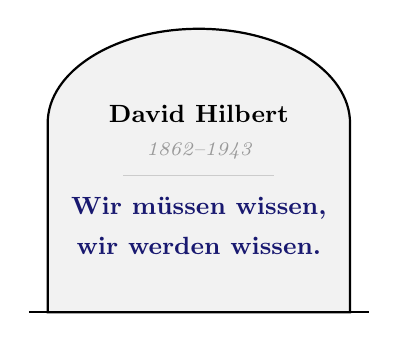
\begin{tikzpicture}[scale=1.2]
    % Gravestone outline (half-width 1.6, so the quote clears the sides)
    \draw[thick, fill=gray!10] (-1.6, 0) -- (-1.6, 2.0) arc (180:0:1.6 and 1.0) -- (1.6, 0) -- cycle;
    \draw[thick] (-1.8, 0) -- (1.8, 0);
    
    % Inscription
    \node[font=\bfseries\small, text=black] at (0, 2.1) {David Hilbert};
    \node[font=\scriptsize\itshape, text=gray!80] at (0, 1.7) {1862--1943};
    \draw[gray!40, thin] (-0.8, 1.45) -- (0.8, 1.45);
    \node[font=\small\bfseries, text=MidnightBlue] at (0, 1.1) {\qt{Wir müssen wissen,}};
    \node[font=\small\bfseries, text=MidnightBlue] at (0, 0.7) {\qt{wir werden wissen.}};
\end{tikzpicture}
\end{center}
\end{content}

\begin{aiNote}[Beyond the Lecture: Where the Word \qt{Ideal} Comes From]
% [PERSISTENT, ADDITION]
The lecturer places the term around $1900$ and names Hilbert. The history goes further back: Ernst Kummer introduced \emph{ideal numbers} in the 1840s to restore unique prime factorization in cyclotomic integer rings, and Richard Dedekind formalized them as ideals. For the integers $\mathbb{Z}$, every ideal is simply the set of multiples $n\mathbb{Z}$ of an actual integer. In more general rings where unique factorization fails, ideals serve as the generalized, \qt{idealized} numbers that recover unique prime decomposition.
\end{aiNote}

\begin{hidden}
% timestamp: 00:07:18
% topic: Ideals of Z, Hilbert's epitaph, historical origin of ideal numbers
% board_state: def:principal-ideal-z, rem:ideals-z-convention
% next_goal: Prove that every ideal in Z is of the form nZ
% open_loops: none
\end{hidden}

\subsection{Proof: Every Ideal of \texorpdfstring{$\mathbb{Z}$}{Z} is Principal}

\begin{content}[Classification Theorem for Ideals in $\mathbb{Z}$]
\begin{theorem}[Ideals of $\mathbb{Z}$ are Principal]\label[theorem]{thm:ideals-of-z-are-principal}
Every ideal $I \subset \mathbb{Z}$ is of the form:
\[
I = n\mathbb{Z}
\]
for a unique integer $n \ge 0$.
\end{theorem}
\end{content}

\begin{proofWrapper}[Proof of \cref{thm:ideals-of-z-are-principal}]

\begin{speech}[00:50:43 - 00:52:00]
\inlinemetanote{writes \qt{Proof:}} What do we have to prove? Let $I$ be an ideal in $\mathbb{Z}$: \inlinemetanote{writes \qt{Let $I \subset \mathbb{Z}$ be an ideal.}}.

I want to prove it's this. What am I going to do here? Maybe you prove it.

I don't like proofs that much, you know. Actually, about math, what I like is truth: proof is good, but truth is better. And this stuff is true, so, you know... But anyway, we should prove it; it's a math course.

If you want to prove it, you have to think: well, okay, Case $1$... \inlinemetanote{writes \qt{Case (i) $I = (0) \implies 0\mathbb{Z}$}}

Case $1$ is that $I$ could be just the zero set. That's fine. And this means it's $0$ times $\mathbb{Z}$. It's kind of a degenerate case, but that's possible. And that's an ideal: zero is an ideal.

Case $2$ is that $I$ has some non-zero element. \inlinemetanote{writes \qt{Case (ii) $I$ has some non-zero element}} It has to have zero, because $I$ is an additive subgroup. If it has only zero, you're in this case. If you're not in this case, you have to have some non-zero element. Let's call that element $x$: \inlinemetanote{writes: $x \in I$, $x \in \mathbb{Z}$}.
\end{speech}

\begin{content}[Case Analysis: Zero vs. Non-Zero Ideal]
\textbf{Case (i) ($I = (0)$):}
If $I$ contains only $0$, then $I = (0) \implies I = 0\mathbb{Z}$, which corresponds to $n = 0$.

\textbf{Case (ii) ($I$ has some non-zero element):}
There exists $x \in I$ with $x \neq 0$.
\end{content}

\begin{speech}[00:52:00 - 00:53:05]
Now, $x$ is an integer. It has a non-zero element, so, $x$ is an integer; then we can multiply by $\pm 1$ and get a positive integer: \inlinemetanote{writes: $\to \pm 1$, get $\pm x \in \mathbb{Z}_{>0}$}. One of these is a positive integer.

So, if it has a non-zero element, then $I$ has a positive integer: \inlinemetanote{writes \qt{$I$ has positive integer}}. I hope that's clear.
\end{speech}

\begin{content}[Existence of Positive Elements in $I$]
Since $(I, +, 0)$ is an additive subgroup of $\mathbb{Z}$, for any $x \in I$, its additive inverse $-x = (-1) \cdot x$ is also in $I$. Since $x \neq 0$, exactly one of $x$ or $-x$ is strictly positive:
\[
x \in I \setminus \{0\} \implies |x| \in I \cap \mathbb{Z}_{>0}.
\]
Therefore, the subset of positive integers in $I$ is non-empty:
\[
I \cap \mathbb{Z}_{>0} \neq \emptyset.
\]
\end{content}

\begin{speech}[00:53:05 - 00:53:19]
And if it has a positive integer, what am I going to say now? This is where you pretend to be like an LLM: What am I going to say?

Yeah?
\end{speech}

\begin{student}[Student Answer]
It has a minimum.
\end{student}

\begin{speech}[00:53:19 - 00:53:46]
Yeah, it has a least positive integer. That's the next line: \inlinemetanote{moves to the lower left board and writes: $I$ has a least positive integer}. As I said, for basically every property of the integers, at some point you have to use this principle. Once it has a least positive integer, let's call that one $n$. So, $n$ is equal to the least positive integer of $I$: \inlinemetanote{writes: $n =$ least pos. int. of $I$}.
\end{speech}

\begin{content}[The Least Positive Element of $I$]
Every non-empty subset of positive integers has a least element (\cref{fact:pre-well-ordering}), so the non-empty set $I \cap \mathbb{Z}_{>0}$ contains a unique minimum element:
\begin{equation}\label{eq:n-minimal-pos}
n := \min(I \cap \mathbb{Z}_{>0}).
\end{equation}
\end{content}

\begin{speech}[00:53:46 - 00:54:50]
Now what we have to show is that $I$ is actually $n\mathbb{Z}$. That's what we want to show, all right? \inlinemetanote{writes \qt{We have now to show $I = n\mathbb{Z}$}}

Suppose not: \inlinemetanote{writes \qt{Suppose not}}. Then there's some element $y \in I$ that's not a multiple. Well, maybe I don't want to suppose not --- you can do it two different ways. You look at $y$: $y$ is some element of $I$: \inlinemetanote{writes: $y \in I$}.

There's only one thing you can do now, which is the division algorithm. The division algorithm says $y$ is equal to some multiple of $n$ plus a remainder term, right? \inlinemetanote{writes: $y = qn + r$ by division} That's long division.

And the important part of this remainder term is that $0 \le r < n$: \inlinemetanote{writes \qt{$0 < r < n$}, a slip for $0 \le r < n$}.
\end{speech}

\begin{content}[Division Algorithm Setup]
We show $I = n\mathbb{Z}$:
\begin{itemize}
    \item \textbf{Inclusion $n\mathbb{Z} \subseteq I$:} Since $n \in I$ and $I$ is an ideal, by multiplicative absorption $\forall k \in \mathbb{Z} \colon kn \in I$, so $n\mathbb{Z} \subseteq I$.
    \item \textbf{Inclusion $I \subseteq n\mathbb{Z}$:} Let $y \in I$ be arbitrary. By the \newterm{division algorithm} (\cref{fact:pre-division}), there exist unique quotient and remainder integers $q, r \in \mathbb{Z}$ such that:
    \begin{equation}\label{eq:division-remainder}
    y = q \cdot n + r \quad \text{with} \quad 0 \le r < n.
    \end{equation}
\end{itemize}
\end{content}

\begin{speech}[00:54:50 - 00:56:10]
Consider this element $y \in I$. Suppose it's not in $n\mathbb{Z}$: that means that it's not divisible, so, there is a remainder term. But this remainder term is equal to $y - qn$, and so, the remainder term is also in $I$. Because $y$ is in $I$, and $n$ is in $I$, so, $qn$ is in $I$; and since $I$ is an additive subgroup, this is also in $I$: \inlinemetanote{writes: $r = y - qn \in I$}.

It's not here, so, we can't have zero, because otherwise it would be divisible, right? So, this $r$ is strictly between zero and $n$. That's the logic: we say \qt{suppose not}, and we use the division algorithm. It can't be zero, because otherwise it would divide, so, long division says $r$ is between zero and $n$. But then $r$ is a lesser positive integer in $I$, which is a contradiction: \inlinemetanote{writes \qt{but $r$ is a less pos. int. in $I$ (contradiction)}}.

I don't know what the symbol for contradiction is. Anyway. Okay, that's the proof.
\end{speech}

\begin{speech}[00:56:10 - 00:56:31]
We used what you have to use for integers: you use this fact that non-empty subsets of positive integers have a least element. Once you have that least element, you know what you're trying to prove, and then you use the long division algorithm and the remainder. This is what you always do with these kinds of elementary properties of integers.

That proves this claim. \inlinemetanote{draws a separating line on the board}
\end{speech}

\begin{content}[Consolidated Proof: Ideals of $\mathbb{Z}$]
\begin{proof}[Complete Derivation of \cref{thm:ideals-of-z-are-principal}]
Let $I \subset \mathbb{Z}$ be an ideal.
\begin{description}
    \item[Case 1:] \textbf{$I = \{0\}$:} Then $I = 0\mathbb{Z}$, and $n = 0$ is unique.
    \item[Case 2:] \textbf{$I \neq \{0\}$:} Choose any non-zero $x \in I$. Since $I$ is an additive subgroup, $-x = (-1) \cdot x \in I$. Thus, $|x| \in I \cap \mathbb{Z}_{>0} \neq \emptyset$.
    
    The non-empty set of positive elements in $I$ has a least element:
    \[
    n := \min(I \cap \mathbb{Z}_{>0}) > 0.
    \]
    We show that $I = n\mathbb{Z}$:
    \begin{itemize}
        \item Since $n \in I$ and $I$ is an ideal, $k \cdot n \in I$ for all $k \in \mathbb{Z}$, whence $n\mathbb{Z} \subseteq I$.
        \item Conversely, let $y \in I$ be arbitrary. Applying the division algorithm to divide $y$ by $n$:
        \[
        y = q \cdot n + r \quad \text{with} \quad 0 \le r < n.
        \]
        Rearranging for the remainder yields:
        \[
        r = y - q \cdot n.
        \]
        Since $y \in I$ and $n \in I$ (which implies $q \cdot n \in I$), closure under subtraction implies $r \in I$.
        
        If $r > 0$, then $r \in I \cap \mathbb{Z}_{>0}$ is a strictly positive element of $I$ satisfying $r < n$, directly contradicting the minimality of $n = \min(I \cap \mathbb{Z}_{>0})$.
        
        Therefore, we must have $r = 0$, which gives $y = q \cdot n \in n\mathbb{Z}$.
    \end{itemize}
    Hence, $I = n\mathbb{Z}$. Uniqueness follows because distinct non-negative integers generate distinct sets of positive multiples ($n = \min(n\mathbb{Z} \cap \mathbb{Z}_{>0})$ for $n > 0$).
\end{description}
\end{proof}
\end{content}

\end{proofWrapper}


\subsection{Trivial Ideals and Comparison with Fields}

\begin{speech}[00:56:31 - 00:57:05]
That's the most basic property of ideals in the integers. For any ring $R$, we've seen before that we have: zero is an ideal, and the whole ring is an ideal: \inlinemetanote{writes: $R \to (0)$ is ideal, $R$ is ideal}.

We haven't discussed fields at all today, but we discussed last time that if you have a field, these are the only two ideals (Recall: \cref{thm:ideals-in-a-field}). But the integers have a lot of ideals: all these $n\mathbb{Z}$'s are ideals. These are all ideals.
\end{speech}

\begin{content}[Trivial Ideals in Rings and Fields]
\recap{That a field has only these two ideals was shown in Week~1 (\cref{thm:ideals-in-a-field}).}

\begin{proposition}[Trivial Ideals]\label[proposition]{prop:trivial-ideals}
For any ring $(R, +, \cdot, 0, 1)$, the zero ideal $\{0\} = (0)$ and the entire ring $R = (1)$ are always ideals (called \newterm{trivial ideals}). Here $(a) := aR = \{ra \mid r \in R\}$ denotes the ideal generated by $a$, defined in Week~4 (\cref{def:ideal-generated-by-elements}).
\end{proposition}

\begin{proposition}[Ideals in a Field]\label[proposition]{prop:field-ideals}
If $F$ is a field, its only ideals are $(0)$ and $F$.
\end{proposition}

\begin{proof}
The lecturer recalls this from the previous lecture, where the argument is given (\cref{thm:ideals-in-a-field}).
\end{proof}
\end{content}

\begin{aiNote}[Beyond the Lecture: PID vs. Field Structure]
% [PERSISTENT, ADDITION]
An integral domain (\cref{def:integral-domain}) in which every ideal is generated by a single element (i.e., $I = aR$) is called a \emph{principal ideal domain} (\emph{PID}), a name the lecture introduces later. By \cref{thm:ideals-of-z-are-principal}, $\mathbb{Z}$ is a PID, but not a field, because it contains infinitely many non-trivial proper ideals $n\mathbb{Z}$ for $n \ge 2$. In contrast, in a field $F$, every non-zero element is invertible, instantly forcing any non-zero ideal to absorb $1$ and expand to the entire ring.
\end{aiNote}

\section{Ideals in Rings of Smooth Functions}

\subsection{The Ring \texorpdfstring{$C^\infty(\mathbb{R})$}{C-infinity(R)} and Compactly Supported Functions}

\begin{speech}[00:57:05 - 00:58:27]
Let's try another example. As I said, this course has several purposes, but one of them is to give you some way of looking at objects you know in mathematics and thinking about them in terms of algebra. An object you certainly know in mathematics, if I take the real numbers --- I think there's a whole class on real numbers --- is that you can take $C^\infty$ functions: \inlinemetanote{writes: $\mathbb{R} \to C^\infty(\mathbb{R})$}.

Are you happy with this? You don't have to take $C^\infty$; you could take $17$ times differentiable functions, but we'll just go to infinity. These are infinitely differentiable functions: \inlinemetanote{writes \qt{$C^\infty(\mathbb{R})$ $\infty$ diff. functions}}.

Are you happy with this terminology? Is it what you use? It's standard. An element here is some function $f \colon \mathbb{R} \to \mathbb{R}$, which I can differentiate as many times as I want, so, it has a nice graph. I can graph it like this: \inlinemetanote{draws a wave curve}. There it is.

And this beautiful object is a ring, \inlinemetanote{writes: $(C^\infty(\mathbb{R}), +, \cdot, 0, 1)$} because why? You can add functions, you can multiply functions, zero is just the constant function zero, and one is the constant function one. Is that clear? It's a ring: \inlinemetanote{writes \qt{Ring}}.

Yeah?
\end{speech}

\begin{student}[Student Question]
What is written after $C^\infty(\mathbb{R})$?
\end{student}

\begin{speech}[00:58:27 - 00:58:45]
Here? Which board?

Here? Infinitely differentiable functions.

Yeah, sorry, good. My handwriting's not good: functions. And it's not because I have this wrist injury --- it's not because of that! I just have bad handwriting.
\end{speech}

\begin{speech}[00:58:45 - 00:59:33]
And I don't even know how I got this wrist injury. It's not like I'm an MMA fighter or anything like that. It just started hurting at one point.

I thought it was going to be a career-ending injury, but it turns out that if I wear this thing, it's fine.
\end{speech}

\begin{content}[The Ring of Smooth Functions]
\begin{definition}[Ring of Smooth Functions $C^\infty(\mathbb{R})$]\label[definition]{def:smooth-functions-ring}
The set of infinitely differentiable real-valued functions on $\mathbb{R}$,
\[
C^\infty(\mathbb{R}) := \{ f \colon \mathbb{R} \to \mathbb{R} \mid f \text{ is smooth} \},
\]
forms a commutative ring $(C^\infty(\mathbb{R}), +, \cdot, 0, 1)$ under pointwise operations:
\begin{align*}
(f + g)(x) &:= f(x) + g(x), \\
(f \cdot g)(x) &:= f(x) \cdot g(x),
\end{align*}
with additive identity $0(x) \equiv 0$ and multiplicative identity $1(x) \equiv 1$. Sums and products of smooth functions are smooth (\cref{fact:pre-compact}), so the operations stay inside $C^\infty(\mathbb{R})$.
\end{definition}

\begin{center}
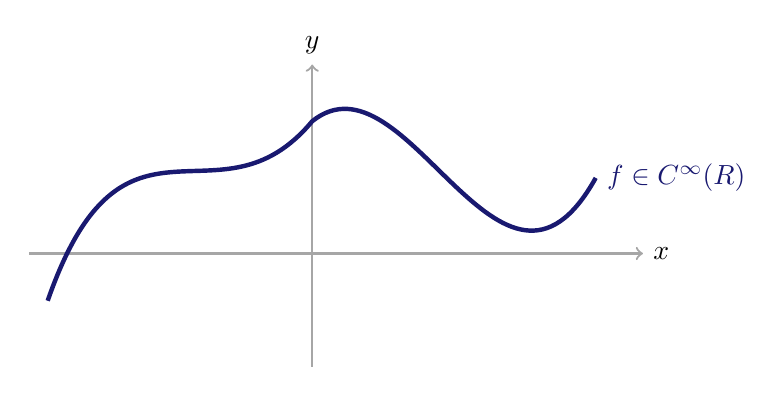
\begin{tikzpicture}[scale=1.2]
    \draw[->, thick, gray!70] (-3.0, 0) -- (3.5, 0) node[right, text=black] {$x$};
    \draw[->, thick, gray!70] (0, -1.2) -- (0, 2.0) node[above, text=black] {$y$};
    
    \draw[ultra thick, MidnightBlue] (-2.8, -0.5) 
        .. controls (-2.0, 1.8) and (-1.0, 0.2) .. (0.0, 1.4)
        .. controls (1.0, 2.2) and (2.0, -1.0) .. (3.0, 0.8)
        node[right] {$f \in C^\infty(\mathbb{R})$};
\end{tikzpicture}
\end{center}
\end{content}

\subsection{The Ideal of Compactly Supported Smooth Functions}

\begin{speech}[00:59:33 - 01:01:30]
There are a lot of things to say about this ring. This class is not primarily about such rings of differentiable functions --- that's some other class --- but I can show you something interesting in it.

There's an interesting ideal inside $C^\infty(\mathbb{R})$: \inlinemetanote{writes: $I \subset C^\infty(\mathbb{R})$} functions with compact support: \inlinemetanote{writes \qt{functions with compact support}}.

First, you have to understand what this is as a set: it's the set of functions with compact support. A general function can do whatever it wants, totally unconstrained. But a function with compact support means that... Are you happy with this analysis terminology: \qt{compact support}? It means that its entire life happens somewhere compact. It has to be zero here, and then suddenly it comes to life, and then it goes to zero. It's like these hat functions that look like that, okay? \inlinemetanote{draws a bump function graph on the board} That's a function with compact support.

Is this an ideal? You have to ask: Who's in here? To be an ideal, it has to be the case that zero is there; and very fortunately, zero has compact support. What does not have compact support is the constant one function; that does not have compact support. So, whatever it is, it's surely not a subring, because it does not have the constant one function.

Then you have to check that if you add compactly supported things, they have compact support; that's true. And the interesting thing is: if I take a function of compact support and multiply it by any function, it still has compact support. Because once this function is zero, it just cannot be brought back to life, no matter how much you multiply. That's an example.
\end{speech}

\begin{content}[Compactly Supported Smooth Functions as an Ideal]
\begin{definition}[Compactly Supported Smooth Functions]\label[definition]{def:compact-support-ideal}
The \newterm{support} of a function $f \colon \mathbb{R} \to \mathbb{R}$ is the topological closure (\cref{def:pre-open-closure}) of the set where $f$ does not vanish:
\[
\operatorname{supp}(f) := \overline{\{ x \in \mathbb{R} \mid f(x) \neq 0 \}}.
\]
The set of smooth functions with compact support is denoted:
\[
I := \{ f \in C^\infty(\mathbb{R}) \mid \operatorname{supp}(f) \text{ is compact in } \mathbb{R} \}.
\]
By Heine--Borel, $\operatorname{supp}(f)$ is compact if and only if it is bounded (\cref{fact:pre-compact}).
\end{definition}

\begin{center}
% \begin{hidden}
% [TikZ Plan: Compactly supported bump function]
% Canvas: x in [-2.8, 2.8], y in [-0.5, 1.5].
% Element order:
% 1. Horizontal axis with labels a, b.
% 2. Support indicator bracket [a, b].
% 3. Smooth bump function curve vanishing outside [a, b].
% Coordinates:
% - Axis: (-2.8, 0) to (2.8, 0).
% - Support boundary points: a at (-1.5, 0), b at (1.5, 0).
% - Smooth bump: zero for x < -1.5, rising smoothly to maximum ~ 1.2, descending to zero at x = 1.5.
% \end{hidden}
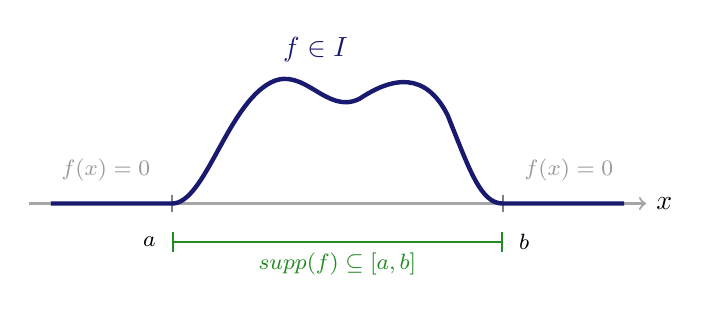
\begin{tikzpicture}[scale=1.4]
    % Axis
    \draw[->, thick, gray!70] (-2.8, 0) -- (2.8, 0) node[right, text=black] {$x$};
    
    % Support points on axis
    \draw[thick, gray] (-1.5, 0.08) -- (-1.5, -0.08);
    \draw[thick, gray] (1.5, 0.08) -- (1.5, -0.08);

    % Compact support bracket indicator; a and b sit beside its end bars (below the ticks, the bars crossed them)
    \draw[thick, ForestGreen, |-|] (-1.5, -0.35) -- (1.5, -0.35) node[midway, below, font=\footnotesize] {$\operatorname{supp}(f) \subseteq [a, b]$};
    \node[anchor=east, font=\footnotesize] at (-1.56, -0.35) {$a$};
    \node[anchor=west, font=\footnotesize] at (1.56, -0.35) {$b$};

    % Bump function profile
    \draw[ultra thick, MidnightBlue] (-2.6, 0) -- (-1.5, 0)
        .. controls (-1.2, 0) and (-1.0, 0.9) .. (-0.6, 1.1)
        .. controls (-0.3, 1.25) and (-0.1, 0.8) .. (0.2, 0.95)
        .. controls (0.5, 1.15) and (0.8, 1.2) .. (1.0, 0.8)
        .. controls (1.2, 0.3) and (1.3, 0) .. (1.5, 0) -- (2.6, 0);

    % Labels
    \node[MidnightBlue, font=\bfseries] at (-0.2, 1.4) {$f \in I$};
    \node[font=\footnotesize, gray!80] at (-2.1, 0.3) {$f(x) = 0$};
    \node[font=\footnotesize, gray!80] at (2.1, 0.3) {$f(x) = 0$};
\end{tikzpicture}
\end{center}

\begin{proposition}[$I$ is an Ideal, but not a Subring]\label[proposition]{prop:compact-support-ideal}
The set $I \subset C^\infty(\mathbb{R})$ of compactly supported smooth functions is an ideal of $C^\infty(\mathbb{R})$, but is not a subring.
\end{proposition}

\begin{proof}
We check the ideal properties:
\begin{enumerate}[label=\textbf{(\arabic*)}]
    \item \textbf{Additive Subgroup:} The zero function has $\operatorname{supp}(0) = \emptyset$, which is compact, so $0 \in I$. For $f, g \in I$, $\operatorname{supp}(f + g) \subseteq \operatorname{supp}(f) \cup \operatorname{supp}(g)$. The union of two compact sets is compact, so $f + g \in I$ and $-f \in I$.
    \item \textbf{Multiplicative Absorption:} Let $g \in C^\infty(\mathbb{R})$ be an \emph{arbitrary} smooth function, and let $f \in I$. Since $(g \cdot f)(x) = 0$ whenever $f(x) = 0$, we have:
    \[
    \operatorname{supp}(g \cdot f) \subseteq \operatorname{supp}(f).
    \]
    As a closed subset of the compact set $\operatorname{supp}(f)$, $\operatorname{supp}(g \cdot f)$ is compact. Thus, $g \cdot f \in I$.
\end{enumerate}
However, the multiplicative identity $1(x) \equiv 1$ has support $\operatorname{supp}(1) = \mathbb{R}$, which is not compact. Hence $1 \notin I$, so $I$ is not a subring.
\end{proof}

The lecturer returns to this ideal in Week~5 and shows that it is not a prime ideal (\cref{ex:compact-support-not-prime-p4}).
\end{content}

\begin{aiNote}[Notation: Compactly Supported Functions]
% [PERSISTENT]
Many textbooks write $C_c^\infty(\mathbb{R})$ for this ideal. The lecturer calls it $I$.
\end{aiNote}

\subsection{A Strictly Larger Ideal: Functions Vanishing on a Right Half-Line}

\begin{speech}[01:01:30 - 01:03:45]
You can ask other questions in analysis about this. I'm not going to talk about that so much, but this is a kind of interesting ideal.

Maybe I'll ask you a question: Is there some ideal $J$ that's bigger? \inlinemetanote{writes: $I \subsetneq J \neq C^\infty(\mathbb{R})$} Can you find an ideal that's bigger than this, and not the whole ring, of course? Because that's always an ideal that's bigger.

One of the strange things about the way math is taught is that we take all these subjects and divide them. The traditional vision of classical education in mathematics --- which has changed over the years --- is that there's an algebra direction, an analysis direction, and a geometry direction. But actually, it doesn't really make sense to separate them all: it's all just one way of looking at numbers. I don't know why I said that, but can you think of a way to make this ideal bigger?

We used the fact that it's zero on both sides here, but that's not necessary, right? Can't we just say: functions that eventually go to zero on the right? Those are more, and it satisfies the same thing. So, here you can say $J$ --- I'll write it colloquially: functions that become zero for all sufficiently large $x$: \inlinemetanote{writes: $J = \{ f \text{ that become } 0 \text{ for all suff.\ large } x \}$}.

Those are functions that look like... They do whatever they want, and then eventually they become zero: \inlinemetanote{draws a second graph: function wiggles on the left then becomes identically zero on the right}. These functions are certainly inside there, but there are more of them! As these drawings perfectly prove, there are more of these functions. And these things are also an ideal, because if you multiply by something that's zero here, it's going to stay zero. You might wonder: Are there bigger and bigger ideals? These are kind of interesting questions we're not going to address now, unfortunately.
\end{speech}

\begin{content}[Construction of a Strictly Larger Proper Ideal]
\begin{center}
% \begin{hidden}
% [TikZ Plan: Function vanishing on a right half-line]
% Canvas: x in [-2.6, 2.6], y in [-0.4, 1.8].
% Element order:
% 1. Horizontal axis with threshold point M.
% 2. Smooth function curve oscillating arbitrarily on the left (x < M) and identically zero for x >= M.
% 3. Text labels identifying the function and the vanishing ray [M, \infty).
% Coordinates:
% - Axis: (-2.6, 0) to (2.6, 0).
% - Boundary point M at (0.8, 0).
% - Curve wiggles between x = -2.4 and x = 0.8, then lies flat on the axis from (0.8, 0) to (2.4, 0).
% \end{hidden}
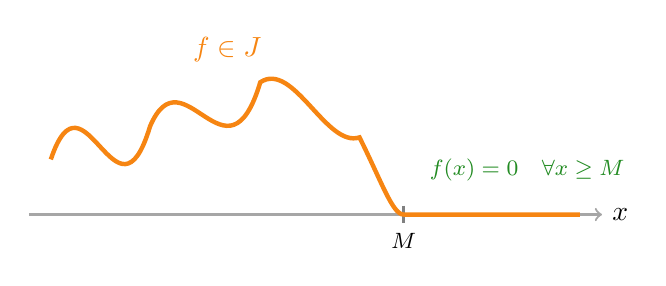
\begin{tikzpicture}[scale=1.4]
    % Axis
    \draw[->, thick, gray!70] (-2.6, 0) -- (2.6, 0) node[right, text=black] {$x$};
    \draw[thick, gray] (0.8, 0.08) -- (0.8, -0.08) node[below, font=\footnotesize, text=black] {$M$};

    % Function wiggling arbitrarily on left, then identically zero to the right
    \draw[ultra thick, BurntOrange] (-2.4, 0.5)
        .. controls (-2.1, 1.4) and (-1.8, -0.2) .. (-1.5, 0.8)
        .. controls (-1.2, 1.5) and (-0.8, 0.2) .. (-0.5, 1.2)
        .. controls (-0.2, 1.4) and (0.1, 0.6) .. (0.4, 0.7)
        .. controls (0.6, 0.3) and (0.7, 0) .. (0.8, 0) -- (2.4, 0);

    % Labels
    \node[BurntOrange, font=\bfseries] at (-0.8, 1.5) {$f \in J$};
    \node[font=\footnotesize, ForestGreen, anchor=west] at (0.95, 0.4) {$f(x) = 0 \quad \forall x \ge M$};
\end{tikzpicture}
\end{center}

\begin{proposition}[A Strictly Larger Proper Ideal]\label[proposition]{prop:larger-ideal-smooth}
Let $J$ be the set of smooth functions that vanish identically on some right ray $[M, \infty)$:
\begin{equation}\label{eq:j-ideal-def}
J := \{ f \in C^\infty(\mathbb{R}) \mid \exists M \in \mathbb{R} \text{ such that } f(x) = 0 \text{ for all } x \ge M \}.
\end{equation}
Then $J$ is an ideal of $C^\infty(\mathbb{R})$, and with the ideal $I$ of \cref{def:compact-support-ideal}:
\[
I \subsetneq J \neq C^\infty(\mathbb{R}).
\]
\end{proposition}

\begin{proof}
\begin{itemize}
    \item \textbf{$J$ is an ideal:} If $f(x) = 0$ for $x \ge M_1$ and $g(x) = 0$ for $x \ge M_2$, then $(f+g)(x) = 0$ for $x \ge \max(M_1, M_2)$; also $0 \in J$ and $-f = (-1) \cdot f \in J$. Furthermore, for any $h \in C^\infty(\mathbb{R})$, $(h \cdot f)(x) = h(x) \cdot 0 = 0$ for all $x \ge M_1$.
    \item \textbf{Proper inclusions:} If $f \in I$, its support is bounded, so it vanishes for large positive $x$, whence $I \subseteq J$. A smooth function that is zero for $x \ge 0$ but non-zero on all of $(-\infty, 0)$, such as $x \mapsto e^{1/x}$ for $x < 0$ and $0$ for $x \ge 0$ (\cref{fact:pre-flat-function}), belongs to $J$ but not to $I$, so $I \subsetneq J$. Finally, the constant function $1 \notin J$, so $J \subsetneq C^\infty(\mathbb{R})$.
\end{itemize}
\end{proof}
\end{content}

\subsection{The Restriction Homomorphism on Function Spaces}

\begin{speech}[01:03:45 - 01:05:45]
Maybe I'll say one more thing, just for fun. If I look at $C^\infty$ functions on $\mathbb{R}$, \inlinemetanote{writes: $C^\infty(\mathbb{R})$} there's a ring homomorphism to $C^\infty$ functions on $\mathbb{R}_{>0}$: \inlinemetanote{writes: $\to C^\infty(\mathbb{R}_{>0})$}.

This is a good example of a homomorphism, and this is called restriction; maybe I'll call it $\operatorname{Res}$: \inlinemetanote{writes \qt{Res} over the arrow}.

If I have a $C^\infty$ function here, it's a function from all of $\mathbb{R}$ to $\mathbb{R}$: \inlinemetanote{writes: $f \colon \mathbb{R} \to \mathbb{R}$}. And if I have one, I can restrict it: $f|_{\mathbb{R}_{>0}} \colon \mathbb{R}_{>0} \to \mathbb{R}$: \inlinemetanote{writes: $f_{\operatorname{Res}} \colon \mathbb{R}_{>0} \to \mathbb{R}$}.

Is that clear? I can restrict a function. I have a function here; this is a ring. Every element here I can just restrict, and that gives me a map. First, it's a map on sets, and then you have to show it respects zero --- of course, the zero function restricts to the zero function; and if I restrict a function that is constant one, it's the function here that is constant one. Also, addition and multiplication behave well under restriction. So, this is a legitimate ring homomorphism: \inlinemetanote{writes \qt{Ring hom}}.

For function spaces, restriction is a very useful way of making ring homomorphisms.

Okay, now your analysis question: Is this surjective? That's properly a question in your analysis class. You can think about that. If you understood all the examples in your analysis class, you should be able to tell me the answer.
\end{speech}

\begin{speech}[01:05:45 - 01:06:13]
It's just been a long time since I taught analysis --- like $25$ years, I think.
\inlinemetanote{begins cleaning the center and left chalkboards} Are you prepared to tell me?

Okay, you can think about it.
\end{speech}

\begin{content}[The Restriction Homomorphism]
\begin{definition}[Restriction Homomorphism]\label[definition]{def:restriction-hom}
The \newterm{restriction map}
\[
C^\infty(\mathbb{R}) \xrightarrow{\operatorname{Res}} C^\infty(\mathbb{R}_{>0}), \qquad (f \colon \mathbb{R} \to \mathbb{R}) \longmapsto (f_{\operatorname{Res}} := f|_{\mathbb{R}_{>0}} \colon \mathbb{R}_{>0} \to \mathbb{R}),
\]
is a ring homomorphism:
\begin{enumerate}[label=\textbf{(\roman*)}]
    \item $\operatorname{Res}(f + g) = (f + g)|_{\mathbb{R}_{>0}} = f|_{\mathbb{R}_{>0}} + g|_{\mathbb{R}_{>0}} = \operatorname{Res}(f) + \operatorname{Res}(g)$.
    \item $\operatorname{Res}(f \cdot g) = (f \cdot g)|_{\mathbb{R}_{>0}} = f|_{\mathbb{R}_{>0}} \cdot g|_{\mathbb{R}_{>0}} = \operatorname{Res}(f) \cdot \operatorname{Res}(g)$.
    \item $\operatorname{Res}(1_{\mathbb{R}}) = 1_{\mathbb{R}_{>0}}$.
\end{enumerate}
\end{definition}

\begin{question}
Is the restriction homomorphism $\operatorname{Res} \colon C^\infty(\mathbb{R}) \to C^\infty(\mathbb{R}_{>0})$ surjective? (The lecturer leaves this to the students; the answer follows in \cref{prop:res-not-surjective}.)
\end{question}
\end{content}

\begin{hidden}
% timestamp: 00:22:48
% topic: Smooth function rings, ideals C_c^infty and J, restriction homomorphism
% board_state: def:smooth-functions-ring, def:compact-support-ideal, prop:larger-ideal-smooth, def:restriction-hom
% next_goal: Introduce Category Theory (Objects, Morphisms, Category of Groups)
% open_loops: none
\end{hidden}

\section{Introduction to Category Theory}

\subsection{Definition of a Category}

\begin{speech}[01:06:13 - 01:07:09]
All right, so, there's a topic that's in some of the reading. There are two foundational topics which I've avoided discussing, but I think I'll discuss now, and it has to do with category theory and Zorn's lemma.

You had this foundations, this Grundstrukturen class. Did you discuss categories there?

You can say no.
\end{speech}

\begin{student}[Student Answer]
No.
\end{student}

\begin{speech}[01:07:09 - 01:07:57]
Okay, so, category. We discuss categories: \inlinemetanote{writes \qt{Category}}.

A category consists of objects and homs \inlinemetanote{writes: Category consists of Objects and Homs}.

Homs are sometimes called morphisms, \inlinemetanote{writes: $\begin{cases} \text{morphisms} \\ \text{arrows} \end{cases}$} so, the language differs. Different authors take a different choice of language: sometimes homs are called morphisms; sometimes they're called arrows. The first thing to know about a category: it has objects and it has homs.

More specifically, given two objects in the category --- \inlinemetanote{writes \qt{Given $A, B$ objects in Category,}} given $A$ and $B$ objects in the category --- there is a set of homs, and this set has a name: $\operatorname{Hom}(A, B)$: \inlinemetanote{writes: $\operatorname{Hom}(A, B)$}.
\end{speech}

\begin{content}[Definition of a Category]
\begin{definition}[Category]\label[definition]{def:category-foundations}
A \newterm{category} $\operatorname{Cat}$ consists of the following data:
\begin{enumerate}[label=\textbf{(\arabic*)}]
    \item A collection of \newterm{objects}, denoted $\operatorname{Obj}(\operatorname{Cat})$.
    \item For every pair of objects $A, B \in \operatorname{Obj}(\operatorname{Cat})$, a set of \newterm{morphisms} (also called \newterm{homs} or \newterm{arrows}), denoted:
    \[
    \operatorname{Hom}(A, B).
    \]
\end{enumerate}
\end{definition}

\begin{steps}[Terminology Across Literature]
In modern mathematical literature:
\begin{itemize}
    \item \textbf{Objects:} The structural spaces (e.g., sets, groups, rings, vector spaces, topological spaces).
    \item \textbf{Homs / Morphisms / Arrows:} The structure-preserving mappings between objects ($f \colon A \to B$).
\end{itemize}
\end{steps}
\end{content}

\begin{aiNote}[Notation: Categories]
% [PERSISTENT]
The lecturer writes $\operatorname{Cat}$ for any category and $\widehat{\operatorname{Cat}}$ for a second one, and these notes follow him. Textbooks write $\mathcal{C}$ and $\mathcal{D}$, and they keep $\mathbf{Cat}$ for one particular category, that of all small categories.
\end{aiNote}

\subsection{The Category of Groups}

\begin{speech}[01:07:57 - 01:09:08]
Of course, there are some conditions this has to satisfy, but before I give you the conditions, I will give you the model: for example, the category of groups: \inlinemetanote{writes \qt{category of Groups}}.

The category of groups is a category. This category has objects, \inlinemetanote{writes \qt{Objects $\leftarrow$ are}} and the objects are groups: \inlinemetanote{writes: $(G, \cdot, e)$}.

An object is a group; that means it's a group with an operation and a neutral element. Those are the objects. When you think about the category of groups, somehow you think about this world where all these groups are: they're all over the place, lots of different groups; every possible group is in here. That's in the category.

And what are the arrows going to be? The homs: if I have two particular groups, \inlinemetanote{writes: $\operatorname{Hom}(G, \hat{G})$} then this is going to be the set of group homomorphisms \inlinemetanote{writes \qt{$= \text{set of group homomorphisms}$}} from $G$ to $\hat{G}$: \inlinemetanote{writes \qt{from $G$ to $\hat{G}$}}.
\end{speech}

\begin{content}[The Category of Groups \texorpdfstring{$\mathbf{Grp}$}{Grp}]
\begin{example}[The Category of Groups]\label[example]{ex:cat-groups}
In the category of groups, standardly denoted $\mathbf{Grp}$:
\begin{itemize}
    \item \textbf{Objects:} All groups $(G, \cdot, e)$.
    \item \textbf{Morphisms:} For any two groups $G, \hat{G}$, the set of morphisms from $G$ to $\hat{G}$ is the set of all group homomorphisms:
    \begin{equation}\label{eq:hom-groups-def}
    \operatorname{Hom}_{\mathbf{Grp}}(G, \hat{G}) := \{ f \colon G \to \hat{G} \mid f \text{ is a group homomorphism} \}.
    \end{equation}
\end{itemize}
\end{example}
\end{content}

\subsection{Categories of Rings and Vector Spaces}

\begin{speech}[01:09:10 - 01:10:24]
Okay, that's the model. Is that clear?

The idea of a category is that we want to think about groups and their relationships abstractly. We can think about the category of groups, we think of all groups, and if I pick two groups in that world of all groups, I get the set of homs, okay?

As I said, there are going to be some conditions. But another example is the category of rings: \inlinemetanote{writes \qt{Category of Rings}}. That's also fine.

There, the objects are rings, as we've defined in this class, meaning the objects are rings with the full data: \inlinemetanote{writes: $(R, +, \cdot, 0, 1)$}.

And the homs, which will not surprise you, are ring homomorphisms: \inlinemetanote{writes \qt{are ring homs}}.

From last year, you could consider the category of vector spaces over whatever field you want --- say, vector spaces over the complex numbers: \inlinemetanote{writes \qt{Category of Vector Spaces/$\mathbb{C}$}}. In the category of vector spaces over the complex numbers, the objects are vector spaces over the complex numbers, and the homs are linear maps.

Those are all examples of categories.
\end{speech}

\begin{content}[Categories of Rings and Vector Spaces]
\begin{example}[The Category of Rings \texorpdfstring{$\mathbf{Ring}$}{Ring}]\label[example]{ex:cat-rings}
In the category of rings, standardly denoted $\mathbf{Ring}$:
\begin{itemize}
    \item \textbf{Objects:} Rings $(R, +, \cdot, 0, 1)$, as defined in this class.
    \item \textbf{Morphisms:} Ring homomorphisms $f \colon R \to \hat{R}$ (satisfying additivity, multiplicativity, and $f(1) = \hat{1}$).
\end{itemize}
\end{example}

\begin{example}[The Category of Complex Vector Spaces \texorpdfstring{$\mathbf{Vect}_{\mathbb{C}}$}{VectC}]\label[example]{ex:cat-vect}
In the category of complex vector spaces, denoted $\mathbf{Vect}_{\mathbb{C}}$:
\begin{itemize}
    \item \textbf{Objects:} Vector spaces $V$ over the field $\mathbb{C}$.
    \item \textbf{Morphisms:} $\mathbb{C}$-linear transformations $T \colon V \to W$.
\end{itemize}
\end{example}
\end{content}

\subsection{Interlude: Non-Surjectivity of the Restriction Map}

\begin{speech}[01:10:24 - 01:10:54]
Then, of course, I have to give you the conditions. To be a category, if I want to tell you what a category is, I have to tell you what the objects are; given two objects, I have to tell you what the homs are; and the resulting structure has to have some properties.

All of these will have that property.
\end{speech}

\begin{speech}[01:10:54 - 01:11:01]
\inlinemetanote{points at the restriction map equation on the right board} Did you figure this out?

Yeah?
\end{speech}

\begin{student}[Student Answer]
I think $\sin(1/x)$...
\end{student}

\begin{speech}[01:11:01 - 01:11:29]
Yeah, so, the answer is no, it's not surjective.

I'll draw the picture. A picture is worth a thousand words!

The picture is: you have an element here that's not there. This is zero, and this is this element --- that one: \inlinemetanote{draws a sketch of $\sin(1/x)$ oscillating wildly as $x \to 0^+$}.

You should recognize that from your analysis class, I would think. Maybe not drawn with such enthusiasm!

You know this function, right?
\end{speech}

\begin{content}[Resolution: The Restriction Map is Not Surjective]
\begin{proposition}[Non-Surjectivity of Smooth Restriction]\label[proposition]{prop:res-not-surjective}
The restriction homomorphism $\operatorname{Res} \colon C^\infty(\mathbb{R}) \to C^\infty(\mathbb{R}_{>0})$ is not surjective.
\end{proposition}

\begin{proof}
Consider the function $f \colon \mathbb{R}_{>0} \to \mathbb{R}$ defined by:
\[
f(x) := \sin\left(\frac{1}{x}\right).
\]
By standard calculus rules, $f$ is infinitely differentiable on $(0, \infty)$, so $f \in C^\infty(\mathbb{R}_{>0})$. However, as $x \to 0^+$, $f(x)$ oscillates infinitely often between $-1$ and $1$, so $\lim_{x \to 0^+} f(x)$ does not exist. Consequently, $f$ cannot even be extended continuously to $x = 0$ (\cref{fact:pre-continuity}), let alone smoothly to all of $\mathbb{R}$. Thus, $f \notin \operatorname{Im}(\operatorname{Res})$.
\end{proof}

\begin{center}
% \begin{hidden}
% [TikZ Plan: Function sin(1/x) near x = 0]
% Canvas: x in [-0.3, 3.2], y in [-1.3, 1.4].
% Element order:
% 1. Coordinate axes x and y.
% 2. Dashed amplitude bounds y = 1 and y = -1.
% 3. Smooth plot of sin(1/x) for x in [0.08, 3.0].
% 4. Denser hatching lines near x = 0 to visually represent infinite wild oscillations.
% Coordinates:
% - Origin at (0, 0).
% - Amplitude horizontal guides y = 1 and y = -1.
% - Plot: samples = 300, domain = 0.08:3.0.
% \end{hidden}
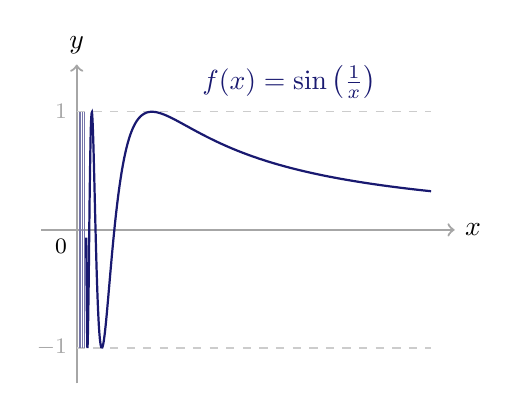
\begin{tikzpicture}[scale=1.5]
    \draw[->, thick, gray!70] (-0.3, 0) -- (3.2, 0) node[right, text=black] {$x$};
    \draw[->, thick, gray!70] (0, -1.3) -- (0, 1.4) node[above, text=black] {$y$};
    \node[below left, font=\footnotesize] at (0,0) {$0$};

    % Amplitude envelope lines
    \draw[dashed, gray!40] (0, 1) -- (3.0, 1);
    \draw[dashed, gray!40] (0, -1) -- (3.0, -1);
    \node[left, font=\footnotesize, gray!70] at (0, 1) {$1$};
    \node[left, font=\footnotesize, gray!70] at (0, -1) {$-1$};

    % Graph of sin(1/x)
    \draw[thick, MidnightBlue, samples=300, domain=0.08:3.0, smooth] 
        plot (\x, {sin((1/\x)*180/pi)});

    % Wild oscillation dense hatching near x=0
    \foreach \t in {0.02, 0.035, 0.05, 0.065} {
        \draw[MidnightBlue!60, thin] (\t, -1) -- (\t, 1);
    }

    \node[MidnightBlue, font=\bfseries] at (1.8, 1.25) {$f(x) = \sin\left(\frac{1}{x}\right)$};
\end{tikzpicture}
\end{center}
\end{content}

\begin{speech}[01:11:29 - 01:12:07]
\inlinemetanote{erases the graph of $\sin(1/x)$ and thoroughly cleans the lower blackboard to prepare for the category axioms}
\end{speech}

\begin{hidden}
% timestamp: 00:06:50
% topic: Category theory introduction, models of categories, non-surjectivity of smooth restriction
% board_state: def:category-data, ex:category-groups, ex:category-rings, ex:category-vect, prop:res-not-surjective
% next_goal: Formal axioms of a category: Hom-sets, composition law, identity morphisms
% open_loops: none
\end{hidden}

\subsection{Axioms of a Category: Homs, Composition, and Identity}

\begin{speech}[01:12:07 - 01:14:06]
Okay, so, the properties that the homs have to satisfy for a category are very simple properties.

The first property, as I said, is that $\operatorname{Hom}(A, B)$ is a set: \inlinemetanote{writes \qt{$\bullet \operatorname{Hom}(A, B)$ is a set}}. That's almost a ridiculous property, and we're not going to think about it too much, but it's...

The second is that there is composition: \inlinemetanote{writes \qt{$\bullet$ Composition}}.

Composition means that if I have three objects, $A$, $B$, and $C$, \inlinemetanote{writes: $A \quad B \quad C$} then here I have the set of homs from $A$ to $B$, \inlinemetanote{writes: $\operatorname{Hom}(A, B)$} and I also have homs from $B$ to $C$: \inlinemetanote{writes: $\times \operatorname{Hom}(B, C)$}. This composition means that if I'm giving you the category, I have to tell you the composition rule. Whenever I have this diagram: $A$, $B$, and $C$, there has to be a rule, which is called composition, that tells you how, if you have a hom from $A$ to $B$ and a hom from $B$ to $C$, this gives me a hom from $A$ to $C$: \inlinemetanote{writes: $\to \operatorname{Hom}(A, C)$}.

That is part of the data of the category. If I'm telling you a category, it's up to me to tell you how to compose homs. And in all examples, you just compose them, okay?

So, what's the content? For groups, of course, if I have a hom from $G$ to $\hat{G}$ and another one from $\hat{G}$ to $\hat{\hat{G}}$, you can compose them as functions --- you can always compose functions --- but then you have to show that the composition is a group hom, all right? Which I leave to you to check.

That's the content of this: to say that this category of groups is a category, there are groups, there are homs, and there's a natural composition of homs; and it's very important that when I have a group hom here and a group hom here, when I compose them, I get a group hom. Okay?
\end{speech}

\begin{content}[Axioms of a Category: Hom-Sets and Composition]
\textbf{Axiom 1 (Hom-Sets):} For any two objects $A, B \in \operatorname{Obj}(\operatorname{Cat})$, the collection $\operatorname{Hom}(A, B)$ is a well-defined set.

\textbf{Axiom 2 (Composition Law):} For any three objects $A, B, C \in \operatorname{Obj}(\operatorname{Cat})$, there is a composition mapping:
\begin{align*}
\circ \colon \operatorname{Hom}(A, B) \times \operatorname{Hom}(B, C) &\longrightarrow \operatorname{Hom}(A, C) \\
(f, g) &\longmapsto g \circ f.
\end{align*}
\end{content}

\begin{speech}[01:14:06 - 01:16:30]
And there's one more: inside $\operatorname{Hom}(A, A)$ --- \inlinemetanote{writes: $\bullet \operatorname{Hom}(A, A) \ni \operatorname{Id}_A$} which is legal to do; I said you pick two objects of the category, and they could be the same object --- there is a distinguished element called the identity. That's part of the data, okay?

There's one more condition, which is how the identity relates to composition, which is not going to be a surprise to you.

If we go back to this example of groups: objects are groups, homs are group homs, composition is composition of functions --- and we're lucky that composition of functions takes group homs to group homs --- and there is an identity: if you take the group and you do nothing, that is definitely a group hom. So, that's here.

And then there's the final property: if you take the identity on $A$ --- we take here $A$, $A$, and $B$ \inlinemetanote{writes: $A \quad A \quad B$} --- then I can take the identity here, \inlinemetanote{writes: $\operatorname{Id}_A \in \operatorname{Hom}(A, A)$} and I can take any element $f$ here, \inlinemetanote{writes: $f \in \operatorname{Hom}(A, B)$} and I can compose it, because composition is given data. I do the identity first and then I do $f$: $f \circ \operatorname{Id}_A$. \inlinemetanote{writes: $f \circ \operatorname{Id}_A$} This has to be an element of $\operatorname{Hom}(A, B)$. \inlinemetanote{writes: $\operatorname{Hom}(A, B)$} And what do you think the axiom is going to say?

What do you think the axiom is going to say here? If I do the identity first, and then I do $f$, what do you think this should be equal to?

Yeah: $f$! \inlinemetanote{writes: $= f$} That's the identity axiom. This is an axiom of the category.

And also the other way: you can also have $A$, $B$, and $B$. \inlinemetanote{writes: $A \quad B \quad B$} If I put $f$ here and I put $\operatorname{Id}_B$, \inlinemetanote{writes: $A \xrightarrow{f} B \xrightarrow{\operatorname{Id}_B} B$} then if you do $f$ first and then $\operatorname{Id}_B$, this should just be $f$, okay? \inlinemetanote{writes: $\operatorname{Id}_B \circ f = f$} That's actually the full category stuff.
\end{speech}

\begin{content}[Axioms of a Category: Identity and Unit Laws]
\textbf{Axiom 3 (Identity Morphisms):} For every object $A \in \operatorname{Obj}(\operatorname{Cat})$, there exists a distinguished morphism, called the \newterm{identity morphism}:
\[
\operatorname{Id}_A \in \operatorname{Hom}(A, A).
\]

\textbf{Axiom 4 (Identity Laws / Unit Axioms):}
For every morphism $f \in \operatorname{Hom}(A, B)$:
\begin{align}
f \circ \operatorname{Id}_A &= f \in \operatorname{Hom}(A, B), \label{eq:left-id} \\
\operatorname{Id}_B \circ f &= f \in \operatorname{Hom}(A, B). \label{eq:right-id}
\end{align}
\end{content}

\begin{speech}[01:16:30 - 01:17:26]
The data of this category is supposed to capture what happens when we think about these algebraic objects.

Of course, it can be applied to many other settings. But if you think about groups, what is the abstract structure of the group? We have objects, we have homs, the homs compose, there is an identity hom, and they satisfy these identity properties.

It's the same for rings, and for vector spaces.

And then there's a whole development which most people find kind of dull, but anyway...

Is there a question about what the definition of a category is?

I'll just say it again: a category has objects, it has homs, the homs have to be endowed with a composition rule, there is an identity element, and we have this property. Okay?
\end{speech}

\begin{content}[Consolidated Definition of a Category]
\begin{definition}[Formal Category]\label[definition]{def:category-full}
A \newterm{category} $\operatorname{Cat}$ consists of:
\begin{enumerate}[label=\textbf{(\arabic*)}]
    \item A collection of objects $\operatorname{Obj}(\operatorname{Cat})$.
    \item A set of morphisms $\operatorname{Hom}(A, B)$ for every pair $A, B \in \operatorname{Obj}(\operatorname{Cat})$.
    \item A composition operation:
    \[
    \circ \colon \operatorname{Hom}(A, B) \times \operatorname{Hom}(B, C) \longrightarrow \operatorname{Hom}(A, C), \quad (f, g) \longmapsto g \circ f,
    \]
    \item For each object $A \in \operatorname{Obj}(\operatorname{Cat})$, an identity morphism $\operatorname{Id}_A \in \operatorname{Hom}(A, A)$ satisfying the \textbf{unit laws}:
    \[
    f \circ \operatorname{Id}_A = f \quad \text{and} \quad \operatorname{Id}_B \circ f = f \quad \forall f \in \operatorname{Hom}(A, B).
    \]
\end{enumerate}
\end{definition}

\begin{center}
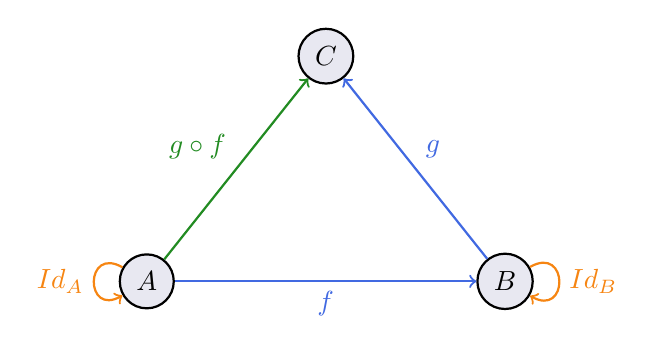
\begin{tikzpicture}[scale=1.3]
    \node (A) at (0,0) [circle, draw, fill=MidnightBlue!10, thick, font=\bfseries] {$A$};
    \node (B) at (3.5,0) [circle, draw, fill=MidnightBlue!10, thick, font=\bfseries] {$B$};
    \node (C) at (1.75,2.2) [circle, draw, fill=MidnightBlue!10, thick, font=\bfseries] {$C$};

    \draw[->, thick, RoyalBlue] (A) -- node[below] {$f$} (B);
    \draw[->, thick, RoyalBlue] (B) -- node[above right] {$g$} (C);
    \draw[->, thick, ForestGreen] (A) -- node[above left] {$g \circ f$} (C);

    % Identity loops
    \draw[->, thick, BurntOrange] (A) to[out=150, in=210, looseness=4] node[left] {$\operatorname{Id}_A$} (A);
    \draw[->, thick, BurntOrange] (B) to[out=30, in=-30, looseness=4] node[right] {$\operatorname{Id}_B$} (B);
\end{tikzpicture}
\end{center}

\end{content}

\begin{aiNote}[Beyond the Lecture: Associativity of Composition]
% [PERSISTENT, ADDITION]
The board lists Hom-sets, composition, identity morphisms and the two unit laws, and not associativity: $h \circ (g \circ f) = (h \circ g) \circ f$ for all $f \in \operatorname{Hom}(A, B)$, $g \in \operatorname{Hom}(B, C)$, $h \in \operatorname{Hom}(C, D)$. The lecturer adds this axiom the next day (\cref{ax:category-axioms-w2wed}). It holds in all of the examples above, since composition of maps is associative.
\end{aiNote}

\subsection{Categorical Definition of Isomorphism}

\begin{speech}[01:17:26 - 01:19:18]
I just assert that all these things --- groups, rings, fields, vector spaces... \inlinemetanote{writes \qt{Groups, Rings, Fields, Vector spaces...}} and many other structures --- give you categories.

If you have a category, built into the category is a notion of isomorphic objects.

Suppose we have a category: $\operatorname{Cat}$ is a category \inlinemetanote{writes: Suppose $\operatorname{Cat}$ is a category}. I want to define the notion of isomorphism purely in categorical terms \inlinemetanote{writes: I want to define the notion of isomorphism purely in categorical terms.}.

There is a very straightforward way to do this. That's why I say just \qt{$\operatorname{Cat}$ is a category} --- that means you don't know anything about it. All you know is that there are some objects, they have homs, and they satisfy these principles.

Suppose I have a category, and I take two objects. I want to know: Is there a notion of isomorphism in that category? Which is to say: Is there a purely arrow-theoretic notion of isomorphism? Category-theoretic.

Sorry... \inlinemetanote{adjusts microphone wire} Oh, here we go.

And the answer is yes, and I will explain this.
\end{speech}

\begin{hidden}
% timestamp: 00:13:50
% topic: Categorical definition of isomorphism
% board_state: def:formal-category, def:categorical-isomorphism
% next_goal: Define isomorphism via existence of a two-sided inverse morphism g
% open_loops: none
\end{hidden}

\begin{speech}[01:19:18 - 01:20:08]
In the reading section, there are a few pages on the definition of these categories --- the reading for this week.

Are the readings for this week already on the website? No? Maybe they are. In any case, as I said, if you ever want to know what's on the website, you can go to $2018$; it's all there. You don't have to wait.
\end{speech}

\begin{note}[Course Literature and Reading Assignments]
The lecturer reminds students that reading assignments detailing category theory are provided in the syllabus materials, which are also archived on the $2018$ course website.
\end{note}

\begin{speech}[01:20:08 - 01:21:17]
I was in the middle of trying to explain the categorical definition of isomorphism.

I have this category $\operatorname{Cat}$, \inlinemetanote{writes: $\operatorname{Cat}$} and I have two objects: $A$ and $B$ are in the objects of my $\operatorname{Cat}$: \inlinemetanote{writes: $A, B \in \operatorname{Obj}(\operatorname{Cat})$}. Definition: \inlinemetanote{writes \qt{Def:}} if I have $f \in \operatorname{Hom}(A, B)$ --- that means if I have an arrow here: \inlinemetanote{writes \qt{$f \in \operatorname{Hom}(A, B)$}, draws $A \xrightarrow{f} B$} --- then $f$ is an isomorphism --- this is a definition, not a theorem --- \inlinemetanote{writes \qt{then $f$ is an isomorphism}} if... \inlinemetanote{writes \qt{if}}

Now you're supposed to complete this for me: What would you do here?

What do you normally need for an isomorphism? You need a map the other way. If there exists a $g$, which is an arrow in the other direction, \inlinemetanote{writes: $\exists \, g \in \operatorname{Hom}(B, A)$} --- that means there exists a $g$ going in the other direction: \inlinemetanote{draws $B \xrightarrow{g} A$} --- such that what?

Yeah?
\end{speech}

\begin{student}[Student Answer]
The two compositions are the identity.
\end{student}

\begin{speech}[01:21:21 - 01:21:46]
Yeah, the two compositions give the identity. There exists a $g$ in the other direction such that \inlinemetanote{writes \qt{such that}} if I do $g$ first, then $f$ --- then you have to concentrate: this is the identity on $B$: \inlinemetanote{writes: $f \circ g = \operatorname{Id}_B$} --- and if I do $f$ first, then $g$, this is the identity on $A$: \inlinemetanote{writes: $g \circ f = \operatorname{Id}_A$}.

That's the definition! That's a purely category-theoretic definition of isomorphism.

Is that confusing or clear?
\end{speech}

\begin{content}[Categorical Definition of Isomorphism]
\begin{definition}[Isomorphism in a Category]\label[definition]{def:categorical-isomorphism}
Let $\operatorname{Cat}$ be a category, and let $A, B \in \operatorname{Obj}(\operatorname{Cat})$. A morphism $f \in \operatorname{Hom}(A, B)$ (denoted $f \colon A \to B$) is called an \newterm{isomorphism} if there exists a morphism $g \in \operatorname{Hom}(B, A)$ (denoted $g \colon B \to A$) such that:
\begin{equation}\label{eq:isomorphism-conditions}
f \circ g = \operatorname{Id}_B \quad \text{and} \quad g \circ f = \operatorname{Id}_A.
\end{equation}
Two objects $A$ and $B$ are called \newterm{isomorphic} (written $A \cong B$) if there exists an isomorphism between them.
\end{definition}

\begin{center}
% \begin{hidden}
% [TikZ Plan: Categorical isomorphism]
% Canvas: x in [-0.5, 4.0], y in [-1.0, 1.0].
% Element order:
% 1. Object nodes A and B.
% 2. Forward curved arrow f: A -> B.
% 3. Backward curved arrow g: B -> A.
% Coordinates:
% - A at (0, 0), B at (3.5, 0).
% - f bends upwards by 25 degrees, g bends downwards by 25 degrees.
% \end{hidden}
\begin{tikzpicture}[scale=1.4, >=Stealth]
    \node[circle, draw=MidnightBlue, fill=MidnightBlue!10, thick, font=\bfseries] (A) at (0,0) {$A$};
    \node[circle, draw=ForestGreen, fill=ForestGreen!10, thick, font=\bfseries] (B) at (3.5,0) {$B$};

    \draw[->, thick, MidnightBlue] (A) to[bend left=25] node[midway, above] {$f$} (B);
    \draw[->, thick, ForestGreen] (B) to[bend left=25] node[midway, below] {$g$} (A);
\end{tikzpicture}
\end{center}

\begin{steps}[Arrow-Theoretic vs. Element-Theoretic Isomorphism]
Going beyond the lecture: in standard concrete algebra, an isomorphism is typically introduced as a \emph{bijective homomorphism}. In abstract category theory, where objects may not have \qt{elements} and morphisms are not necessarily \qt{functions}, bijectivity cannot even be formulated. Instead, category theory characterizes isomorphisms purely through arrows via the existence of a two-sided inverse morphism $g$. In concrete categories this recovers the familiar notions:
\begin{itemize}
    \item In $\mathbf{Grp}$, categorical isomorphisms are precisely bijective group homomorphisms (\cref{prop:isomorphism-inverse-characterization}).
    \item In $\mathbf{Ring}$, categorical isomorphisms are bijective ring homomorphisms (\cref{def:ring-isomorphism}).
    \item In $\mathbf{Vect}_K$, categorical isomorphisms are bijective linear transformations (invertible matrices in finite dimension, \cref{fact:pre-matrices}).
\end{itemize}
\end{steps}
\end{content}


\begin{speech}[01:21:46 - 01:22:27]
In particular, once I tell you the categories of groups or rings, I tell you the homs, the identity, and this property, that already tells you what the notion of isomorphism is. I told you anyway what the notion of isomorphism is, but in some sense I didn't have to: it was just this categorical notion of isomorphism.

And there's one more thing that I hope I'll finish before this ends, because this is kind of boring and dry, this category stuff. But it's kind of an organizational way to think about these structures.

There's nothing deep happening here, really nothing. It's just language.
\end{speech}

\subsection{Definition of a Functor}

\begin{speech}[01:22:27 - 01:23:55]
There's the notion of a functor: \inlinemetanote{writes \qt{Functor}}.

This is maybe cooler: \inlinemetanote{writes \qt{Functor}}.

A functor is kind of a notion of a map from one category to another. A category is a thing, and you might have two categories, and you want to compare them --- just like we have groups, and we might want to compare groups. Functors, in some sense, compare two different categories \inlinemetanote{writes \qt{Functor Compare categories}} --- or it could be the same category: compare categories.

The idea of a functor is: if I have some category here, and I have another category, $\widehat{\operatorname{Cat}}$, \inlinemetanote{writes: $\operatorname{Cat} \xrightarrow{F} \widehat{\operatorname{Cat}}$} then the functor $F$ is written as a map from one category to the other.

And what's the data of the functor? \inlinemetanote{writes \qt{Data:}}

If I'm giving you the functor, then it's on me to provide all this data. The data is that for every object $A$ in the first category, \inlinemetanote{writes \qt{for $A$ object in $\operatorname{Cat}$,}} I have to give you an object in the second category: $F(A) \in \widehat{\operatorname{Cat}}$: \inlinemetanote{writes: $F(A) \in \widehat{\operatorname{Cat}}$}.

That's part of the data of the functor. This is like, you know, if I give you a function, it's my responsibility to tell you where every point goes; that's totally on me if I'm giving you the function. Here, if I'm giving you a functor, I have to tell you, whenever I have an object on one side, how to get the object on the other side. But that's not enough.
\end{speech}

\begin{speech}[01:23:55 - 01:25:22]
\inlinemetanote{cleans a section of the right chalkboard} I have to tell you whenever I have a hom for $\operatorname{Cat}$, the first one: \inlinemetanote{writes: $\operatorname{Hom}(A, B)$ for $\operatorname{Cat}$}. If I have $A$ and I have an arrow here --- \inlinemetanote{writes: $A \xrightarrow{f} B$} that's on the $\operatorname{Cat}$ side --- I've already told you what these objects are, \inlinemetanote{writes: $F(A) \quad F(B)$} but I also have to tell you how this hom goes to a hom between these on the other side: \inlinemetanote{writes: $F(A) \xrightarrow{F(f)} F(B)$}.

That's, again, on me to do that. So, it's a lot of things I have to tell you.

And it can't just be anything: it has to respect all of the structure, which means this rule must take the identity to the identity, and it must respect composition --- which I don't write, but it's kind of clear what it is: \inlinemetanote{writes \qt{must respect identity, composition}}.

You can look that up, and I will give you an example. Let me just say it: it must respect identity and composition. You can look in the book, or you can imagine it yourself: there's only one thing you can do here.

That's the notion of a functor.
\end{speech}

\begin{content}[Definition of a Functor]
\begin{definition}[Covariant Functor]\label[definition]{def:functor}
Let $\operatorname{Cat}$ and $\widehat{\operatorname{Cat}}$ be categories. A \newterm{functor} (or \newterm{covariant functor}) $F \colon \operatorname{Cat} \to \widehat{\operatorname{Cat}}$ consists of the following data:
\begin{enumerate}[label=\textbf{(\arabic*)}]
    \item \textbf{Object Assignment:} To every object $A \in \operatorname{Obj}(\operatorname{Cat})$, an object $F(A) \in \operatorname{Obj}(\widehat{\operatorname{Cat}})$.
    \item \textbf{Morphism Assignment:} To every morphism $f \in \operatorname{Hom}(A, B)$ of $\operatorname{Cat}$, a morphism of $\widehat{\operatorname{Cat}}$:
    \[
    F(f) \in \operatorname{Hom}\bigl(F(A), F(B)\bigr),
    \]
\end{enumerate}
satisfying the following structural compatibility axioms:
\begin{enumerate}[label=\textbf{(\roman*)}]
    \item \textbf{Preservation of Identity:} For every object $A \in \operatorname{Obj}(\operatorname{Cat})$:
    \[
    F(\operatorname{Id}_A) = \operatorname{Id}_{F(A)}.
    \]
    \item \textbf{Preservation of Composition:} For all morphisms $f \in \operatorname{Hom}(A, B)$ and $g \in \operatorname{Hom}(B, C)$:
    \[
    F(g \circ f) = F(g) \circ F(f).
    \]
\end{enumerate}
\end{definition}

\begin{center}
% \begin{hidden}
% [TikZ Plan: Functor mapping categories C and D]
% Canvas: x in [0, 7.7], y in [-0.2, 1.7].
% Element order:
% 1. Category C bounded box with objects A, B and morphism f.
% 2. Thick functor arrow F connecting the two categories.
% 3. Category D bounded box with objects F(A), F(B) and morphism F(f).
% Coordinates:
% - Category C box: [0, 2.7] x [-0.2, 1.7], nodes at (0.6, 0.5) and (2.1, 0.5).
% - Functor arrow: from (3.0, 0.75) to (4.4, 0.75).
% - Category D box: [5.0, 7.7] x [-0.2, 1.7], nodes at (5.6, 0.5) and (7.1, 0.5).
% \end{hidden}
\begin{tikzpicture}[scale=1.3, >=Stealth]
    % Category C
    \node[font=\bfseries, text=MidnightBlue] at (1.35, 1.4) {$\operatorname{Cat}$};
    \draw[thick, dashed, MidnightBlue!40, rounded corners=8pt] (0, -0.2) rectangle (2.7, 1.7);
    \node (A) at (0.6, 0.5) {$A$};
    \node (B) at (2.1, 0.5) {$B$};
    \draw[->, thick, MidnightBlue] (A) -- node[above, font=\footnotesize] {$f$} (B);

    % Functor arrow F
    \draw[->, ultra thick, BurntOrange] (3.0, 0.75) -- node[above, font=\bfseries] {$F$} (4.4, 0.75);

    % Category D
    \node[font=\bfseries, text=ForestGreen] at (6.35, 1.4) {$\widehat{\operatorname{Cat}}$};
    \draw[thick, dashed, ForestGreen!40, rounded corners=8pt] (5.0, -0.2) rectangle (7.7, 1.7);
    \node (FA) at (5.6, 0.5) {$F(A)$};
    \node (FB) at (7.1, 0.5) {$F(B)$};
    \draw[->, thick, ForestGreen] (FA) -- node[above, font=\footnotesize] {$F(f)$} (FB);
\end{tikzpicture}
\end{center}
\end{content}

\begin{hidden}
% timestamp: 00:20:20
% topic: Categorical definition of functors and examples
% board_state: def:category-data, def:formal-category, def:categorical-isomorphism, def:functor
% next_goal: Examples of functors: forgetful functor from Rings to Groups, double dual functor on Vector Spaces
% open_loops: none
\end{hidden}

\subsection{Examples of Functors: From Rings to Groups}

\begin{speech}[01:25:22 - 01:27:44]
And what's an example of a functor? \inlinemetanote{erases the middle chalkboard}

There's one that's been staring us in the face the whole time: if I take the category of rings, there's a way to get to the category of groups. This is going to be totally underwhelming, but it's just taking the additive structure of the ring. That's a rule to go from rings to groups, and that is a functor. I'll write it.

You can criticize this whole discussion, this lecture, as being basically nonsensical, and that's basically the correct point of view, I think. But it's kind of useful eventually. Maybe I should say: it's not an incorrect point of view; let's put it like that.

The first example of a functor --- this whole direction is not really the point of this class --- I take the category of rings: \inlinemetanote{writes: $\underline{\text{Ring}}$}. Sometimes people take terminology like $\operatorname{Ring}$ to denote the category of rings, \inlinemetanote{underlines $\underline{\text{Ring}}$} and $\operatorname{Grp}$ to denote the category of groups: \inlinemetanote{writes: $\underline{\text{Group}}$}. There's a functor $F$: \inlinemetanote{writes: $\underline{\text{Ring}} \xrightarrow{F} \underline{\text{Group}}$}. This functor is defined by: if I take a ring, which is all of this data, $(R, +, \cdot, 0, 1)$, \inlinemetanote{writes: $F(R, +, \cdot, 0, 1)$} I need to make a group out of it. And so, I could just do this: $(R, +, 0)$: \inlinemetanote{writes: $= (R, +, 0)$}. Totally underwhelming, but anyway, that's definitely a group.

This functor associates the ring to a group, so, it gives an object here to an object there. And then you have to check that it does all the things that you want. I have to also tell you: if I have a hom on the ring side, how do I get a hom on the group side? Well, the hom on the ring side is just a way to get from elements from one ring to the other; it also gives you an additive homomorphism here.

Again, almost nothing is happening; it's just reinterpretation. But that's an example, kind of a dumb example.
\end{speech}

\begin{content}[The Functor from Rings to Groups]
\begin{example}[The Additive Functor $F \colon \mathbf{Ring} \to \mathbf{Grp}$]\label[example]{ex:forgetful-functor-rings-groups}
There is a canonical functor:
\[
F \colon \mathbf{Ring} \longrightarrow \mathbf{Grp}
\]
defined by forgetting the multiplicative structure:
\begin{itemize}
    \item \textbf{On Objects:} For every ring $(R, +, \cdot, 0, 1) \in \operatorname{Obj}(\mathbf{Ring})$:
    \[
    F(R, +, \cdot, 0, 1) := (R, +, 0) \in \operatorname{Obj}(\mathbf{Grp}).
    \]
    \item \textbf{On Morphisms:} For any ring homomorphism $f \colon R \to \hat{R}$, $F(f)$ is the same underlying mapping regarded as an additive group homomorphism:
    \[
    F(f) := f \colon (R, +, 0) \longrightarrow (\hat{R}, +, \hat{0}).
    \]
\end{itemize}
Since ring homomorphisms satisfy $f(a + b) = f(a) + f(b)$ and $f(0) = \hat{0}$, $F(f)$ is a group homomorphism. Furthermore, $F(\operatorname{Id}_R) = \operatorname{Id}_{(R, +)}$ and $F(g \circ f) = F(g) \circ F(f)$, verifying all functor axioms.
\end{example}

\begin{steps}[Forgetful Functors in Algebra]
Going beyond the lecture: this construction is the standard prototype of a \emph{forgetful functor}: it strips away (forgets) a layer of algebraic structure (the multiplication $\cdot$ and unit $1$), leaving only the underlying additive group $(R, +, 0)$.
\end{steps}
\end{content}

\subsection{The Double Dual Functor on Vector Spaces}

\begin{speech}[01:27:44 - 01:30:03]
A more interesting one you know --- this is actually a much more interesting example that you learned, but probably...

If I take vector spaces... I can do anything I want, but let's just take complex vector spaces, because I like the complex numbers: \inlinemetanote{writes \qt{VectorSpace/$\mathbb{C}$}}. Is that clear? This is the category of complex vector spaces: the objects are complex vector spaces, and the homs are linear maps. You should be totally happy to think about this category; in some sense, your whole linear algebra class was about this category.

There's a very nice functor here to itself: \inlinemetanote{writes \qt{VectorSpace/$\mathbb{C}$ $\xrightarrow{F}$ VectorSpace/$\mathbb{C}$}}. There's no reason you can't have a functor from the category to itself.

This functor takes $V$: \inlinemetanote{writes: $V$}. What can you do with $V$? One thing you can do is take its dual: \inlinemetanote{writes: $V^*$}. If you take its dual, it reverses the arrows. Technically, what I've defined is a covariant functor, which means that the composition goes forward. The dual switches the arrows; it's confusing. But something that doesn't switch the arrows is the double dual: \inlinemetanote{writes: $(V^*)^*$}.

That's a really beautiful thing you can do: take a vector space to its double dual. To every vector space, you can associate its double dual. And the claim is that this is a functor: \inlinemetanote{writes \qt{is a functor}}.

It takes an object here and canonically associates an object here, and also the maps. In linear algebra, if you have a map between vector spaces \inlinemetanote{writes: $V \xrightarrow{f} W$}, that gives you a map the other way \inlinemetanote{writes: $W^* \xrightarrow{f^*} V^*$}. You get a map this way --- the dual --- and then if you do it again, you get a map in the correct direction \inlinemetanote{writes: $(V^*)^* \xrightarrow{f^{**}} (W^*)^*$}.

This is to say that this functor takes arrows to the, you know, $f$ double dual arrow: \inlinemetanote{writes: $F(f) = f^{**}$}. You can think about it.
\end{speech}

\begin{student}[Student Question]
Is the dimension of vector spaces also only finite or can it also be infinite?
\end{student}

% [WORD-CHECKED: the recording clearly says "motion", but "notion" must be meant, so the text keeps the spoken word and adds (notion?).]
\begin{speech}[01:30:08 - 01:30:50]
Well, I didn't say anything.

You could, if you want, say you want the category of finite-dimensional vector spaces. That's a nice category inside, but the way I said it, it's anything.

For finite-dimensional vector spaces, it happens that the double dual is isomorphic. I'm not saying any of that; I'm just saying there's a motion (notion?) giving a vector space another one, and that's the double dual, and it's functorial in this sense.

You've seen this double dual business, right? Usually, in linear algebra, you spend all your time dualing and double dualing.

Okay, good, that's it. \inlinemetanote{students applaud}
\end{speech}

\begin{content}[The Double Dual Functor on Vector Spaces]
\begin{example}[The Double Dual Functor]\label[example]{ex:double-dual-functor}
Let $\mathbf{Vect}_{\mathbb{C}}$ denote the category of complex vector spaces and $\mathbb{C}$-linear maps. The double dual construction defines a functor from this category to itself:
\[
F \colon \mathbf{Vect}_{\mathbb{C}} \longrightarrow \mathbf{Vect}_{\mathbb{C}}
\]
defined by:
\begin{itemize}
    \item \textbf{On Objects:} For every vector space $V \in \operatorname{Obj}(\mathbf{Vect}_{\mathbb{C}})$:
    \[
    V \longmapsto V^{**} := (V^*)^*, \quad \text{where } V^* := \operatorname{Hom}_{\mathbb{C}}(V, \mathbb{C}).
    \]
    \item \textbf{On Morphisms:} For any linear map $f \colon V \to W$, the dual map $f^* \colon W^* \to V^*$ (\cref{def:pre-dual-space}) reverses direction:
    \[
    f^*(\varphi) := \varphi \circ f \quad \forall \varphi \in W^*.
    \]
    Applying the dual operation a second time reverses the arrow direction once more, restoring covariance:
    \[
    f^{**} \colon V^{**} \longrightarrow W^{**}, \quad (f^{**}(\psi))(\varphi) := \psi(f^*(\varphi)) = \psi(\varphi \circ f) \quad \forall \psi \in V^{**}.
    \]
\end{itemize}
\end{example}

\begin{center}
% \begin{hidden}
% [TikZ Plan: Double dual functor commutative diagram]
% Canvas: x in [0, 3.5], y in [0, 2.0].
% Element order:
% 1. Upper row: V and W with linear map f: V -> W.
% 2. Middle row: Dual spaces W* and V* with reversed map f*: W* -> V*.
% 3. Lower row: Double dual spaces V** and W** with restored covariant map f**: V** -> W**.
% Coordinates:
% - V at (0, 2.0), W at (3.5, 2.0).
% - W* at (3.5, 1.0), V* at (0, 1.0).
% - V** at (0, 0.0), W** at (3.5, 0.0).
% \end{hidden}
\begin{tikzpicture}[scale=1.3, >=Stealth]
    \node (V) at (0, 2.0) {$V$};
    \node (W) at (3.5, 2.0) {$W$};
    \draw[->, thick, MidnightBlue] (V) -- node[above] {$f$} (W);

    \node (Ws) at (3.5, 1.0) {$W^*$};
    \node (Vs) at (0, 1.0) {$V^*$};
    \draw[->, thick, BrickRed] (Ws) -- node[above] {$f^*$} (Vs);

    \node (Vss) at (0, 0.0) {$V^{**}$};
    \node (Wss) at (3.5, 0.0) {$W^{**}$};
    \draw[->, thick, ForestGreen] (Vss) -- node[above] {$f^{**} = (f^*)^*$} (Wss);
\end{tikzpicture}
\end{center}

\begin{steps}[Covariance, Contravariance, and Canonical Isomorphism]
Going beyond the lecture:
\begin{itemize}
    \item \textbf{Single Dual is Contravariant:} The mapping $V \mapsto V^*$ and $f \mapsto f^*$ reverses arrow directions ($f \colon V \to W \implies f^* \colon W^* \to V^*$), making the dual functor a \newterm{contravariant functor}.
    \item \textbf{Functoriality:} $(\operatorname{Id}_V)^{**} = (\operatorname{Id}_{V^*})^* = \operatorname{Id}_{V^{**}}$, and for $U \xrightarrow{g} V \xrightarrow{f} W$ the dual satisfies $(f \circ g)^* = g^* \circ f^*$, so
    \[
    (f \circ g)^{**} = (g^* \circ f^*)^* = f^{**} \circ g^{**}.
    \]
    \item \textbf{Double Dual is Covariant:} Dualizing twice reverses the arrows twice, so $F$ preserves morphism directions ($f \colon V \to W \implies f^{**} \colon V^{**} \to W^{**}$), forming a valid covariant functor.
    \item \textbf{Finite vs.\ Infinite Dimensions:} For finite-dimensional vector spaces, the evaluation mapping $\operatorname{ev} \colon V \to V^{**}$, $v \mapsto (\varphi \mapsto \varphi(v))$, is a canonical isomorphism ($V \cong V^{**}$, \cref{fact:pre-double-dual}). For infinite-dimensional spaces, $\operatorname{ev}$ remains an injective linear map, but is generally not surjective. The functorial construction $V \mapsto V^{**}$, however, is universally defined across all vector spaces regardless of dimension.
\end{itemize}
\end{steps}
\end{content}

\begin{overview}[Summary of Key Concepts]
This lecture established the following central algebraic and categorical foundations:
\begin{itemize}
    \item \textbf{Uniqueness of Identity and Inverses:} In any group $(G, \cdot, e)$, associativity inherently guarantees that both the identity element and inverse elements are strictly unique.
    \item \textbf{Homomorphisms and Isomorphisms:} Group homomorphisms preserve products and automatically map identities to identities ($f(e) = \hat{e}$). Two groups are isomorphic if and only if there exists a two-sided inverse homomorphism. Notably, the exponential function establishes an isomorphism between the additive reals $(\mathbb{R}, +, 0)$ and the strictly positive multiplicative reals $(\mathbb{R}^*_{>0}, \cdot, 1)$.
    \item \textbf{Subgroups and Symmetry Breaking in Rings:} For group homomorphisms, both the kernel $\operatorname{ker}(f) \le G$ and image $\operatorname{Im}(f) \le \hat{G}$ are subgroups. In ring theory, this symmetry breaks: the image $\operatorname{Im}(f) \subset \hat{R}$ is a subring, whereas the kernel $\operatorname{ker}(f) \subset R$ is an ideal absorbing ring multiplication.
    \item \textbf{Ideals of $\mathbb{Z}$ and $C^\infty(\mathbb{R})$:} Every ideal of $\mathbb{Z}$ is principal ($I = n\mathbb{Z}$ with $n \ge 0$), proven via the least positive element of an ideal and the division algorithm. In the ring of smooth functions $C^\infty(\mathbb{R})$, the compactly supported functions form an ideal $I$ that is strictly contained within larger proper ideals, such as functions vanishing on a right half-line $[M, \infty)$.
    \item \textbf{Categories and Functors:} A category $\operatorname{Cat}$ formalizes collections of objects and morphism sets with composition, identity morphisms and unit laws. Isomorphisms are characterized purely arrow-theoretically by two-sided inverses. Functors formalize structure-preserving maps between categories, exemplified by the functor $\mathbf{Ring} \to \mathbf{Grp}$ and the covariant double dual functor $(-)^{**} \colon \mathbf{Vect}_{\mathbb{C}} \to \mathbf{Vect}_{\mathbb{C}}$.
\end{itemize}
\end{overview}
% ==========================================
% Merged version (2026-10-10), done by Claude (claude-opus-5-5):
% Speech blocks (with their board notes) from the Gemini 3.8 run of 2026-10-10
% (pipeline headers below); content blocks from the reviewed Gemini 3.6 version
% (commits e58d893, 21a0c92, e2c35c5), corrected against frames of the
% 2026-09-23 board. The U(Z/7Z) -> Z/6Z diagram is from the new run.
% ==========================================
% ==========================================
% Step 4/4 - Final refinement (refinement step 3)
% Output: step4-2026-09-23-wednesday-week2-algebra-1-offset-final.tex
% Input: step3-2026-09-23-wednesday-week2-algebra-1-offset-speech_refined.tex
% Model: gemini-3.8-flash
% Temperature: 0.35
% TopP: 0.9
% TopK: 10
% MaxOutputTokens: 65535
% ThinkingBudget: 4096
% ThinkingLevel: HIGH
% Processed on: 2026-10-10 12:20:47
% ------------------------------------------
% Token Usage (1 Request(s)):
%   - Total Prompt Tokens : 58’152 (gesamter Prompt, inkl. Cache)
%   - Cached Context      : 0 (aus Google Context-Cache, rabattiert)
%   - Fresh Input Tokens  : 58’152 (neu verrechneter Input)
%   - Output Tokens       : 24’917 (generiertes LaTeX, ohne Thinking)
%   - Thinking Tokens     : 32’484 (Denk-Tokens, als Output verrechnet)
% ==========================================
% ==========================================
% Step 3/4 - Speech refinement (refinement step 2)
% Output: step3-2026-09-23-wednesday-week2-algebra-1-offset-speech_refined.tex
% Input: step2-2026-09-23-wednesday-week2-algebra-1-offset-merged.tex
% Model: gemini-3.8-flash
% Temperature: 0.35
% TopP: 0.9
% TopK: 10
% MaxOutputTokens: 65535
% ThinkingBudget: 4096
% ThinkingLevel: HIGH
% Processed on: 2026-10-10 12:14:11
% ------------------------------------------
% Token Usage (1 Request(s)):
%   - Total Prompt Tokens : 152’207 (gesamter Prompt, inkl. Cache)
%   - Cached Context      : 0 (aus Google Context-Cache, rabattiert)
%   - Fresh Input Tokens  : 152’207 (neu verrechneter Input)
%   - Output Tokens       : 25’464 (generiertes LaTeX, ohne Thinking)
%   - Thinking Tokens     : 29’011 (Denk-Tokens, als Output verrechnet)
% ==========================================
% ==========================================
% Step 2/4 - Merge & timestamp alignment (refinement step 1)
% Output: step2-2026-09-23-wednesday-week2-algebra-1-offset-merged.tex
% Input: step1-2026-09-23-wednesday-week2-algebra-1-all-offset.tex
% Model: gemini-3.8-flash
% Temperature: 0.4
% TopP: 0.95
% TopK: 40
% MaxOutputTokens: 65535
% ThinkingBudget: 32765
% ThinkingLevel: HIGH
% Processed on: 2026-10-10 12:05:55
% ------------------------------------------
% Token Usage (1 Request(s)):
%   - Total Prompt Tokens : 121’752 (gesamter Prompt, inkl. Cache)
%   - Cached Context      : 0 (aus Google Context-Cache, rabattiert)
%   - Fresh Input Tokens  : 121’752 (neu verrechneter Input)
%   - Output Tokens       : 26’156 (generiertes LaTeX, ohne Thinking)
%   - Thinking Tokens     : 16’281 (Denk-Tokens, als Output verrechnet)
% ==========================================
% ==========================================
% Step 1/4 - Transcription, 2 part(s) combined
% Output: step1-2026-09-23-wednesday-week2-algebra-1-all-offset.tex
% Source video: 2026-09-23-wednesday-week2-algebra-1.mp4
% Model: gemini-3.8-flash
% Temperature: 0.36
% TopP: 0.95
% TopK: 40
% MaxOutputTokens: 65535
% ThinkingBudget: 32765
% ThinkingLevel: HIGH
% Processed on: 2026-10-10 11:33:26
% ------------------------------------------
% Parts:
%   - Part 1: 2026-09-23-wednesday-week2-algebra-1-part1.mp4 | start 00:00:00 | model gemini-3.8-flash | processed 2026-10-10 11:22:43 | prompt 330’307 | output 14’054 | thinking 28’124
%   - Part 2: 2026-09-23-wednesday-week2-algebra-1-part2.mp4 | start 00:19:24 | model gemini-3.8-flash | processed 2026-10-10 11:33:26 | prompt 344’821 | output 15’469 | thinking 25’219
% ------------------------------------------
% Token Usage of this run (2 Request(s)):
%   - Total Prompt Tokens : 675’128 (gesamter Prompt, inkl. Cache)
%   - Cached Context      : 245’999 (aus Google Context-Cache, rabattiert)
%   - Fresh Input Tokens  : 429’129 (neu verrechneter Input)
%   - Output Tokens       : 29’523 (generiertes LaTeX, ohne Thinking)
%   - Thinking Tokens     : 53’343 (Denk-Tokens, als Output verrechnet)
% ==========================================

% Primary Language: English
% End of the video: 00:42:48

\lecturechapter[2]{Wednesday}{23 Sep}{23 September 2026}{Categories, Integral Domains, and the Group of Units}
% Old chapter title: Categories, Integral Domains, and Units

\begin{overview}[Course Content Overview]
This lecture begins with administrative guidance regarding enrollment, problem set submissions, and exam scope before reviewing the foundational abstractions of category theory and advancing into commutative ring theory. The main topics covered are:
\begin{itemize}
    \item \textbf{Category Theory Review:} Foundational data (objects, hom-sets, composition laws, identity morphisms), category axioms (associativity and identity laws), and categorical formulations of isomorphisms, monomorphisms (injectivity), and epimorphisms (surjectivity).
    \item \textbf{Integral Domains:} Definition of integral domains (with explicit treatment of the non-triviality condition $R \neq \{0\}$), followed by a complete proof that $\mathbb{Z}/m\mathbb{Z}$ is an integral domain if and only if $m$ is prime, along with edge-case considerations for $m \le 1$.
    \item \textbf{Divisibility and Units in Commutative Rings:} Generalization of divisibility to arbitrary commutative rings, definitions of units and multiplicative inverses, linguistic conventions (\qt{the units}, \qt{the unit}, and \qt{a unit}), and the proof that the units form an abelian group $(\mathcal{U}_R, \cdot, 1)$.
    \item \textbf{Units in Modular Arithmetic:} The units of $\mathbb{Z}/m\mathbb{Z}$ are the classes $\bar{x}$ with $\operatorname{GCD}(x, m) = 1$; explicit computation of $\operatorname{Unit}(\mathbb{Z}/7\mathbb{Z})$, and the construction of an explicit group isomorphism with the additive cyclic group $(\mathbb{Z}/6\mathbb{Z}, +, \bar{0})$ generated by powers of $a = \bar{3} \pmod 7$.
\end{itemize}
\end{overview}

\section{Course Logistics and Announcements}

\begin{speech}[00:00:00 - 00:01:26]
Okay, so, we start. I wanted to make this comment: There were several questions about the course. The first one is, if you want to watch the lectures, you have to be enrolled. So, if you're not enrolled, it will stop you. And there's not much I can do about that, or if there is, I don't know what to do. But the idea is you should enroll in the course if you want to watch the lectures.

Other people had some difficulty uploading the problem sets. Maybe you have to be enrolled in the course for that, too. I don't know, but many people were successful; so, if you have difficulty, find someone who was successful, because I don't know how to solve the problem in another way.

A question that's more about the actual course was that every week there are these suggested pages to read in the book. And the question is: How do they relate to the course? That's a good question.

And the answer is that, roughly speaking, I do that so you can find the parallel material on which I'm lecturing in the book. And I don't always follow exactly the order there, I don't follow exactly the notation, I don't follow exactly the text of the definitions. But I do something that's logically equivalent, so it can be helpful. As far as matters like the exam, I will only test you on material that has appeared in the lecture. Okay? So, this is my best statement about this so far. Okay.
\end{speech}

\begin{note}[Administrative Policies]
The lecturer outlines three organizational guidelines:
\begin{itemize}
    \item \textbf{Lecture Access:} Enrolled status is required to stream or access recorded lecture videos.
    \item \textbf{Problem Sets:} Submission portals are restricted to enrolled students; technical submission difficulties should be resolved peer-to-peer or via course administrators.
    \item \textbf{Course Literature vs.\ Exam Scope:} Weekly reading assignments provide parallel textbook treatment, but examinations are strictly based on definitions, theorems, and proofs presented during the live lectures.
\end{itemize}
\end{note}

\section{Review of Categories: Data and Axioms}

\begin{speech}[00:01:26 - 00:02:53]
So, the last topic yesterday was categories, and I wanted to say a few things.

When I had this discussion about categories yesterday, it was mixed in with all the examples. So, I want to just very quickly give the pure abstract definition and two small points. But this course is not about category theory. It's a topic here because it's natural to introduce when you talk about these algebraic objects; so, anyway, the course is not about category theory.

A category has data, two types of data \inlinemetanote{writes \qt{Category} and \qt{$\operatorname{Cat} \Rightarrow$}}: It has objects, as we said, and it has homs \inlinemetanote{writes \qt{$\operatorname{Obj} \ni A$} and \qt{Homs $\operatorname{Hom}(A, B)$}}. So, maybe $A$ can be an object; and for homs, if you pick any two objects, you get a hom-space \inlinemetanote{writes \qt{$\operatorname{Hom}(A, B)$} with a brace}, sometimes called morphisms.

And the properties, the abstract properties of this hom-space --- I said them, but... --- is that it's a set \inlinemetanote{writes \qt{$\bullet$ Set}}. That's a technical property; that's to avoid some contradictions in foundations, which I'm not going to discuss now. The second is that there's a composition law \inlinemetanote{writes \qt{$\bullet$ Comp Law}}. And the third is that there are identity elements --- existence of identity, so \inlinemetanote{writes \qt{$\bullet$ $1_A \in \operatorname{Hom}(A, B)$}, a slip for $\operatorname{Hom}(A, A)$}...

Okay, that's the data. Is there any question about this data?
\end{speech}

\begin{content}[Constituents of a Category: Data]
\recap{Categories were introduced the day before, mixed in with examples (\cref{def:category-foundations}, \cref{def:category-full}). The lecturer now repeats the abstract definition on its own.}

\begin{definition}[Category Data]\label[definition]{def:category-data-w2wed}
A \newterm{category} $\operatorname{Cat}$ consists of the following mathematical data:
\begin{itemize}
    \item \textbf{Objects:} A class of objects, denoted $\operatorname{Obj}(\operatorname{Cat})$. We write $A \in \operatorname{Obj}(\operatorname{Cat})$ (or simply $A \in \operatorname{Cat}$) to denote that $A$ is an object of $\operatorname{Cat}$.
    \item \textbf{Morphism Sets (Homs):} For any pair of objects $A, B \in \operatorname{Obj}(\operatorname{Cat})$, a set of morphisms from $A$ to $B$, denoted:
    \[
    \operatorname{Hom}(A, B).
    \]
    An element $f \in \operatorname{Hom}(A, B)$ is represented diagrammatically as an arrow $f \colon A \to B$.
    \item \textbf{Composition Law:} For any three objects $A, B, C \in \operatorname{Obj}(\operatorname{Cat})$, a binary composition mapping:
    \begin{align*}
        \circ \colon \operatorname{Hom}(B, C) \times \operatorname{Hom}(A, B) &\to \operatorname{Hom}(A, C), \\
        (g, f) &\mapsto g \circ f.
    \end{align*}
    \item \textbf{Identities:} For each object $A \in \operatorname{Obj}(\operatorname{Cat})$, a designated morphism called the identity morphism on $A$:
    \[
    \operatorname{Id}_A \in \operatorname{Hom}(A, A) \quad (\text{or } 1_A \in \operatorname{Hom}(A, A)).
    \]
\end{itemize}
\end{definition}

\begin{steps}[Foundational Remark on Hom-Sets]
Going beyond the lecture: the requirement that $\operatorname{Hom}(A, B)$ forms a legitimate set (rather than a proper class, a collection too large to be a set, like the collection of all sets) is a standard set-theoretic convention defining a \emph{locally small category}. This prevents Russell-style self-referential paradoxes when indexing collections of arrows.
\end{steps}
\end{content}

\begin{speech}[00:02:53 - 00:03:45]
And then there are the axioms. The axioms... \inlinemetanote{writes \qt{Axioms}} The first one is that the composition law is associative \inlinemetanote{writes \qt{$-$ Comp Law Associative}}, which means, you know, if you have three things, you can compose them in the two different ways. I hope I don't have to say that more.

And then the second is the axioms about the identity, which is roughly: If I do this, $f \circ \operatorname{Id}_A$, this is $f$ \inlinemetanote{writes \qt{$f \cdot \operatorname{Id}_A = f$}}, and the other way around also \inlinemetanote{writes \qt{$\operatorname{Id}_B \cdot g = g$}}.

So, the identity doesn't change the... We just discussed this last time, so, I wanted to say.
\end{speech}

\begin{content}[Associativity and Identity Axioms]
\begin{definition}[Category Axioms]\label[definition]{ax:category-axioms-w2wed}
The data of a category $\operatorname{Cat}$ must satisfy the following two fundamental axioms:
\begin{enumerate}[label=\textbf{(\arabic*)}]
    \item \textbf{Associativity of Composition:} For all objects $A, B, C, D \in \operatorname{Obj}(\operatorname{Cat})$ and all morphisms $f \in \operatorname{Hom}(A, B)$, $g \in \operatorname{Hom}(B, C)$, and $h \in \operatorname{Hom}(C, D)$, composition is associative:
    \begin{equation}\label{eq:cat-assoc}
    (h \circ g) \circ f = h \circ (g \circ f).
    \end{equation}
    \item \textbf{Identity Axioms (Neutrality):} For all morphisms $f, g \in \operatorname{Hom}(A, B)$, composition with the respective identity morphisms changes nothing (on the board, with a dot for the composition: $f \cdot \operatorname{Id}_A = f$ and $\operatorname{Id}_B \cdot g = g$):
    \begin{align}
        f \circ \operatorname{Id}_A &= f, \label{eq:cat-id-right} \\
        \operatorname{Id}_B \circ g &= g. \label{eq:cat-id-left}
    \end{align}
\end{enumerate}
\end{definition}

{\centering
\begin{tikzpicture}[scale=1.4, >=Stealth, auto]
    \node (A) at (0, 0) {$A$};
    \node (B) at (2, 1.3) {$B$};
    \node (C) at (4, 0) {$C$};

    \draw[->, thick] (A) to node {$f$} (B);
    \draw[->, thick] (B) to node {$g$} (C);
    \draw[->, thick, MidnightBlue] (A) to node[below] {$g \circ f$} (C);

    \path[->, thick] (A) edge[out=150, in=210, looseness=4] node[left] {$\operatorname{Id}_A$} (A);
    \path[->, thick] (B) edge[out=60, in=120, looseness=4] node[above] {$\operatorname{Id}_B$} (B);
    \path[->, thick] (C) edge[out=330, in=30, looseness=4] node[right] {$\operatorname{Id}_C$} (C);
\end{tikzpicture}\par}
\end{content}

\subsection{Categorical Isomorphisms}

\begin{speech}[00:03:45 - 00:05:37]
So, that's the abstract... There's really not that much here. We discussed this last time, and we had lots of examples.

And so, you could say: Well, why do we want to do this? And as I said, many concepts that we talk about when we talk about groups, rings, fields, vector spaces, they're categorical concepts, meaning that they only depend on this structure. So, it simplifies some kind of thought to think about them all together.

I already told you about isomorphism. \inlinemetanote{writes \qt{$\bullet$ Isomorphism}}

The categorical isomorphism is that if I have this arrow from $A$ to $B$ \inlinemetanote{writes \qt{$A \xrightarrow{f} B$}} --- this picture means $f \in \operatorname{Hom}(A, B)$ \inlinemetanote{writes \qt{$f \in \operatorname{Hom}(A, B)$}}. In category theory, you can say this, or you can say that; you mean the same thing.

This $f$ is an isomorphism \inlinemetanote{writes \qt{$f$ is an isom.}} --- that's a definition --- if and only if there exists $g$ the other way \inlinemetanote{writes \qt{$\iff \exists A \xleftarrow{g} B$}}, such that \inlinemetanote{writes \qt{such that}} the two compositions are identities.

And if you want to say which identity, you have to be careful. So, $g$ starts with $B$, so you do $g$ first, then $f$ back --- this should be the identity in $B$ \inlinemetanote{writes \qt{$f \circ g = \operatorname{Id}_B$}}. And this is the identity in $A$ \inlinemetanote{writes \qt{$g \circ f = \operatorname{Id}_A$}}.

So, that's the abstract definition of isomorphism. And in all of the categories we discussed, that coincides with the notion of isomorphism in the category that you already know, like, for example, isomorphism of vector spaces.
\end{speech}

\begin{hidden}
% timestamp: 00:05:40
% topic: Review of category data, axioms, and categorical isomorphism
% board_state: def:category-data, ax:category-axioms, def:categorical-isomorphism
% next_goal: Define categorical monomorphisms and epimorphisms
% open_loops: none
\end{hidden}

\begin{content}[Categorical Isomorphism]
\recap{The categorical isomorphism was defined the day before (\cref{def:categorical-isomorphism}); the lecturer restates it.}

\begin{definition}[Isomorphism]\label[definition]{def:categorical-isomorphism-w2wed}
Let $\operatorname{Cat}$ be a category and let $f \in \operatorname{Hom}(A, B)$ (written $f \colon A \to B$). The morphism $f$ is an \newterm{isomorphism} if and only if there exists a morphism $g \in \operatorname{Hom}(B, A)$ (written $g \colon B \to A$) such that:
\begin{align}
    f \circ g &= \operatorname{Id}_B, \label{eq:isom-right-inverse} \\
    g \circ f &= \operatorname{Id}_A. \label{eq:isom-left-inverse}
\end{align}
If such a morphism $g$ exists, it is uniquely determined, called the \newterm{inverse} of $f$, and denoted $f^{-1} := g$. Two objects $A$ and $B$ are said to be \newterm{isomorphic} (written $A \cong B$) if there exists an isomorphism between them.
\end{definition}

{\centering
\begin{tikzpicture}[scale=1.5, >=Stealth, auto]
    \node (A) at (0,0) {$A$};
    \node (B) at (3,0) {$B$};

    \draw[->, thick, RoyalBlue] (A) to[bend left=25] node {$f$} (B);
    \draw[->, thick, BurntOrange] (B) to[bend left=25] node {$g = f^{-1}$} (A);

    % caption below the label of the lower arc (arc dips to y = -0.33, its label to about y = -0.55)
    \node at (1.5, -1.15) {\footnotesize $f \circ g = \operatorname{Id}_B \quad \text{and} \quad g \circ f = \operatorname{Id}_A$};
\end{tikzpicture}\par}

\begin{steps}[Consistency across Concrete Categories]
Going beyond the lecture: in concrete categories where objects are sets endowed with structure and morphisms are structure-preserving maps (homomorphisms):
\begin{itemize}
    \item In the category $\mathbf{Set}$ (objects: all sets; morphisms: all maps between them), isomorphisms are precisely bijective functions (\cref{fact:pre-inverse-map}).
    \item In $\mathbf{Grp}$, $\mathbf{Ring}$, and $\mathbf{Vect}_K$, isomorphisms are bijective homomorphisms (for groups: \cref{prop:isomorphism-inverse-characterization}).
\end{itemize}
The power of the categorical definition is that it never inspects elements $x \in A$; it characterizes invertibility purely through diagrammatic composition.
\end{steps}
\end{content}

\subsection{Monomorphisms and Epimorphisms}

\begin{speech}[00:05:37 - 00:07:22]
There are two other notions, and that's the last thing I want to say. And this is the notion of monomorphism. \inlinemetanote{writes \qt{$\bullet$ Monomorphism}}

So, $f$ from $A$ to $B$ is a monomorphism \inlinemetanote{writes \qt{$A \xrightarrow{f} B$ is a monomorphism}} --- that's a long word, that's a definition --- if \inlinemetanote{writes \qt{if}} for all $g_1$ arrows... this is another object $X$, and another one... \inlinemetanote{writes \qt{$\forall X \xrightarrow{g_1} A, X \xrightarrow{g_2} A$}} We take any two, then the composition \inlinemetanote{writes \qt{then $f \circ g_1 = f \circ g_2$}} implies $g_1 = g_2$ \inlinemetanote{writes \qt{$\implies g_1 = g_2$}}.

I hope I wrote that clearly here, okay?

It's a little bit complicated to say. So, I'm defining: If I have an arrow in the category, it may or may not be a monomorphism. I'm defining a monomorphism.

And the condition of being a monomorphism means that whenever I take an object $X$ and map it two ways to $A$, the composition with $f$ being equal implies they were equal to start with. Of course, if they're equal to start with, the composition is equal, but it's the other implication. That's the definition of a monomorphism.

You know, you have to think about this and unwind it. But once you have this definition, you can imagine: What is a monomorphism in all of those categories you know? And what do you think it is?
\end{speech}

\begin{speech}[00:07:22 - 00:08:27]
So, I leave this for you to think about, but roughly speaking, a monomorphism is injective. \inlinemetanote{writes \qt{(injective)} and circles it on the blackboard}

Just imagine they're sets. If this is injective, if you take any two maps, you can compare them after you do $f$. So, you have to think about it.

But this is the definition. Once you take this definition, you can say: Okay, I can take the category of sets and functions, and what is a monomorphism there? And the answer is injective. That's the \qt{mono} in monomorphism.

This is a categorical formulation of being injective.

I don't know if you find this appealing or not, but that's what this discussion is about. Because the nice thing of this formulation is that it applies to all examples of categories. Every single one we discussed, and all the other ones you can think about, there's a notion of monomorphism.

And you can imagine this one has a sibling, or a partner --- I don't know their relationship --- which is... Whenever you talk about injective, you can also talk about surjective, and the categorical term there is epimorphism.
\end{speech}

\begin{content}[Monomorphisms]
\begin{definition}[Monomorphism]\label[definition]{def:monomorphism}
Let $\operatorname{Cat}$ be a category. A morphism $f \in \operatorname{Hom}(A, B)$ (or $f \colon A \to B$) is called a \newterm{monomorphism} if for every object $X \in \operatorname{Obj}(\operatorname{Cat})$ and all pairs of parallel morphisms $g_1, g_2 \in \operatorname{Hom}(X, A)$,
\begin{equation}\label{eq:monomorphism-cond}
f \circ g_1 = f \circ g_2 \implies g_1 = g_2.
\end{equation}
\end{definition}

{\centering
\begin{tikzpicture}[scale=1.5, >=Stealth, auto]
    \node (X) at (0,0) {$X$};
    \node (A) at (2.2,0) {$A$};
    \node (B) at (4.4,0) {$B$};

    \draw[->, thick] (X) to[bend left=25] node {$g_1$} (A);
    \draw[->, thick] (X) to[bend right=25] node[below] {$g_2$} (A);
    \draw[->, thick, ForestGreen] (A) to node {$f$} (B);

    % caption below the g_2 label (lower arc dips to y = -0.24, its label to about y = -0.5)
    \node at (2.2, -1.0) {\footnotesize $f \circ g_1 = f \circ g_2 \implies g_1 = g_2 \quad (\text{Categorical Injective})$};
\end{tikzpicture}\par}

\begin{proof}[Why Monomorphisms Characterize Injectivity (beyond the lecture)]
The lecture leaves this to the students (\qt{I leave this for you to think about}). In the category of sets ($\mathbf{Set}$), suppose $f \colon A \to B$ is a monomorphism. To test whether $f$ is injective on points $a_1, a_2 \in A$, let $X = \{*\}$ be a one-element set and define two maps $g_1, g_2 \colon \{*\} \to A$ by $g_1(*) := a_1$ and $g_2(*) := a_2$.
Then $(f \circ g_1)(*) = f(a_1)$ and $(f \circ g_2)(*) = f(a_2)$. Thus:
\[
f(a_1) = f(a_2) \implies f \circ g_1 = f \circ g_2 \implies g_1 = g_2 \implies a_1 = a_2.
\]
Hence, left-cancellation with respect to arbitrary test objects $X$ precisely recovers element-wise injectivity without mentioning elements. Conversely, an injective $f$ is a monomorphism: if $f \circ g_1 = f \circ g_2$, then $f(g_1(x)) = f(g_2(x))$ for every $x \in X$, so $g_1(x) = g_2(x)$ by injectivity, that is, $g_1 = g_2$.
\end{proof}
\end{content}

\begin{speech}[00:08:27 - 00:09:20]
So, you can define epimorphism \inlinemetanote{writes: epimorphism}. If you have $f$ from $A$ to $B$, it is an epimorphism if for all \inlinemetanote{writes: $A \xrightarrow{f} B$ is an epimorphism if}...

And this is now about this kind of feeling of mathematics: How do you think I'm going to define the opposite notion of injective?

Like here we had injective by $X$ mapping to $A$. So, what do you think I should do here?

You should guess. Guessing is like one of the most important tools of a mathematician.

Yeah?
\end{speech}

\begin{student}[Student Answer]
Well, you do the same, except we only switch like with the arrows...
\end{student}

\begin{speech}[00:09:25 - 00:10:37]
This is a long answer. You should just say... Here we map $X$ to $A$, so the opposite of that is mapping from $B$. It's like the other side.

So, for every $B \xrightarrow{g_1} X$, $B \xrightarrow{g_2} X$ \inlinemetanote{writes \qt{$\forall B \xrightarrow{g_1} X, B \xrightarrow{g_2} X$}}, then...

This is the kind of opposite of that, by just flipping everything on the other side. So, for every one of these, then we can consider $f$. In this one, it was the $g$'s first, then the $f$. Now it's the $f$ first, then the $g$'s: $g_1 \circ f = g_2 \circ f$ implies $g_1 = g_2$ \inlinemetanote{writes \qt{then $g_1 \circ f = g_2 \circ f \implies g_1 = g_2$}}.

So, that's the categorical notion of epimorphism, and it's somehow just dual to the monomorphism. If you like this world, it almost makes epimorphism and monomorphism the same definition up to this flipping. And thinking about things categorically is good for such understanding.

If you look at this definition, and you look at it for the examples we know, this is surjectivity.
\end{speech}

\begin{content}[Epimorphisms]
\begin{definition}[Epimorphism]\label[definition]{def:epimorphism}
Let $\operatorname{Cat}$ be a category. A morphism $f \in \operatorname{Hom}(A, B)$ (or $f \colon A \to B$) is called an \newterm{epimorphism} if for every object $X \in \operatorname{Obj}(\operatorname{Cat})$ and all pairs of parallel morphisms $g_1, g_2 \in \operatorname{Hom}(B, X)$,
\begin{equation}\label{eq:epimorphism-cond}
g_1 \circ f = g_2 \circ f \implies g_1 = g_2.
\end{equation}
\end{definition}

{\centering
\begin{tikzpicture}[scale=1.5, >=Stealth, auto]
    \node (A) at (0,0) {$A$};
    \node (B) at (2.2,0) {$B$};
    \node (X) at (4.4,0) {$X$};

    \draw[->, thick, BrickRed] (A) to node {$f$} (B);
    \draw[->, thick] (B) to[bend left=25] node {$g_1$} (X);
    \draw[->, thick] (B) to[bend right=25] node[below] {$g_2$} (X);

    % caption below the g_2 label (lower arc dips to y = -0.24, its label to about y = -0.5)
    \node at (2.2, -1.0) {\footnotesize $g_1 \circ f = g_2 \circ f \implies g_1 = g_2 \quad (\text{Categorical Surjective})$};
\end{tikzpicture}\par}
\end{content}

\begin{aiNote}[Beyond the Lecture: Epimorphisms Need Not Be Surjective]
% [PERSISTENT, ADDITION]
The lecturer says that for the examples we know, epimorphism means surjectivity. This holds in $\mathbf{Set}$, $\mathbf{Grp}$ and $\mathbf{Vect}_K$, but not in $\mathbf{Ring}$: the inclusion $\iota \colon \mathbb{Z} \hookrightarrow \mathbb{Q}$ is an epimorphism without being surjective. Indeed, if $g_1, g_2 \colon \mathbb{Q} \to R$ are ring homomorphisms with $g_1 \circ \iota = g_2 \circ \iota$, then for $b \neq 0$ the element $g_k(b)$ is invertible with inverse $g_k(\frac{1}{b})$, so $g_1(\frac{a}{b}) = g_1(a) \, g_1(b)^{-1} = g_2(a) \, g_2(b)^{-1} = g_2(\frac{a}{b})$. For monomorphisms the slogan is safe: in $\mathbf{Set}$, $\mathbf{Grp}$, $\mathbf{Ring}$ and $\mathbf{Vect}_K$ they are exactly the injective homomorphisms. In particular, $\iota$ is both a monomorphism and an epimorphism in $\mathbf{Ring}$ without being an isomorphism: there is no ring homomorphism $\mathbb{Q} \to \mathbb{Z}$ at all, since $\frac{1}{2}$ would have to go to an inverse of $2$ in $\mathbb{Z}$.
\end{aiNote}

\begin{aiNote}[Beyond the Lecture: The Opposite Category]
% [PERSISTENT, ADDITION]
The lecturer calls the epimorphism dual to the monomorphism. This can be made precise: if we construct the opposite category $\operatorname{Cat}^{\text{op}}$ by reversing all arrows ($f^{\text{op}} \colon B \to A$ for every $f \colon A \to B$), then
\[
f \text{ is a monomorphism in } \operatorname{Cat} \iff f^{\text{op}} \text{ is an epimorphism in } \operatorname{Cat}^{\text{op}}.
\]
Every statement about monomorphisms yields a dual statement about epimorphisms by reversing all arrows.
\end{aiNote}

\begin{speech}[00:10:37 - 00:11:03]
Okay, so, that's the end of this discussion about categories. If you like it, you can go read more. As I said, this course is not a course in categories. There's a bunch of other things that I would say here, but I'm not going to, because... yeah.

Maybe I will at the end if I have time.
\end{speech}

\begin{hidden}
% timestamp: 00:11:03
% topic: Conclusion of category theory review; transition back to ring theory
% board_state: def:monomorphism, def:epimorphism
% next_goal: Define zero divisors, introduce integral domains, and discuss fields
% open_loops: none
\end{hidden}

\section{Integral Domains}

\subsection{Zero Divisors and the Definition of Integral Domains}

\begin{speech}[00:11:03 - 00:12:35]
So, let us return to rings now. \inlinemetanote{writes \qt{Rings $(R, +, \cdot, 0, 1)$}}

This was kind of a foundational side, so, we have this ring $(R, +, \cdot, 0, 1)$ (Recall: commutative with unit, \cref{rem:ring-convention}).

And the rings here, there's kind of a different flavor of rings. There's the rings that are like $\mathbb{Z}$ \inlinemetanote{writes \qt{$\mathbb{Z}$}}, where when you have things that are non-zero and you multiply them, they stay non-zero. That's one of the principles of $\mathbb{Z}$.

But it's not true for rings like $\mathbb{Z}/6\mathbb{Z}$, this ring \inlinemetanote{writes \qt{$\mathbb{Z}/6\mathbb{Z}$}}. I can take two elements here, like the residue class of $2$ times the residue class of $3$, neither of which is zero. So, this is not zero \inlinemetanote{writes \qt{$\bar{2} \neq \bar{0}, \bar{3} \neq \bar{0} \text{ in } \mathbb{Z}/6\mathbb{Z}$}}, and that is not zero.

So, I take two elements that are legitimately not zero, but I can multiply them; and when I multiply these residue classes, this is six, and that is zero \inlinemetanote{writes \qt{$\bar{2} \cdot \bar{3} = \bar{6} = \bar{0}$}}.

That's a different type of multiplication. It's a multiplication where when you multiply things, you get zero, which is unexpected from the point of view of the integers. And this is also related to the fact that there's no hope of having a multiplicative inverse if you're mapping things to zero.

So, there are these two differences, and there's a definition for this.
\end{speech}

\begin{content}[Multiplication in $\mathbb{Z}/6\mathbb{Z}$]
Let $(R, +, \cdot, 0, 1)$ be a commutative ring (\cref{rem:ring-convention}).

\begin{example}[Multiplication in \texorpdfstring{$\mathbb{Z}/6\mathbb{Z}$}{Z/6Z}]\label[example]{ex:z6z-zero-divisors}
In the ring of residue classes modulo $6$ (\cref{def:residue-class-ring}), denoted $\mathbb{Z}/6\mathbb{Z}$:
\begin{align*}
    \bar{2} &\neq \bar{0}, \\
    \bar{3} &\neq \bar{0}.
\end{align*}
However, their product in the ring is:
\[
\bar{2} \cdot \bar{3} = \overline{2 \cdot 3} = \bar{6} = \bar{0} \in \mathbb{Z}/6\mathbb{Z}.
\]
\end{example}

\begin{steps}[Zero Divisors vs. Invertibility]
Going beyond the lecture: non-zero elements whose product is zero are called \newterm{zero divisors}. If an element $a \in R$ is a zero divisor (with $a \cdot b = 0$ for some $b \neq 0$), it can never possess a multiplicative inverse $a^{-1}$:
\[
b = 1 \cdot b = (a^{-1} \cdot a) \cdot b = a^{-1} \cdot (a \cdot b) = a^{-1} \cdot 0 = 0,
\]
which contradicts $b \neq 0$. Hence, rings containing zero divisors fail to exhibit regular arithmetic cancellation.
\end{steps}
\end{content}

\begin{speech}[00:12:35 - 00:14:26]
A ring $R$ is an integral domain \inlinemetanote{writes \qt{Def. A ring $R$ is an integral domain}} --- so it's a definition of this term, integral domain. And some authors would just say it's a domain. Also, if you speak about rings, very often mathematicians will say it's a domain.

If... whenever I have $a$ and $b$, neither of which is zero --- so, maybe I'll just be really explicit: whenever I have $a \neq 0$ and $b \neq 0$ \inlinemetanote{writes \qt{if $\forall a \neq 0, b \neq 0$}} --- this implies the product is not equal to zero \inlinemetanote{writes \qt{$\implies ab \neq 0$}}.

So, that's the definition. That's a really basic definition in ring theory, and it separates this type of ring from that type of ring. Is that clear?

Fields, for example --- for example, fields are always domains \inlinemetanote{writes \qt{For example: Fields are always domains.}} because you have the multiplicative inverse, if you think about it, okay?

So, see, I did that already there: I called it a domain, not an integral domain, because it takes a lot of syllables to say integral domain. Formally, this is defined as an integral domain; colloquially, almost everyone says domain.
\end{speech}

\begin{content}[Definition of an Integral Domain (Initial Board State)]
\begin{definition}[Integral Domain / Domain]\label[definition]{def:integral-domain-prelim}
A commutative ring $R$ is called an \newterm{integral domain} (or simply a \newterm{domain}) if for all $a, b \in R$:
\begin{equation}\label{eq:integral-domain-cond}
a \neq 0 \quad \text{and} \quad b \neq 0 \implies a \cdot b \neq 0.
\end{equation}
Equivalently, taking the contrapositive:
\[
a \cdot b = 0 \implies a = 0 \quad \text{or} \quad b = 0.
\]
A few minutes later the lecturer adds the condition $R \neq 0$; the definition used from then on is \cref{def:integral-domain}.
\end{definition}

\begin{example}[Fields are Domains]\label[example]{ex:fields-are-domains}
Every field $F$ is an integral domain: if $a \neq 0$ and $a \cdot b = 0$, then multiplying by the inverse $a^{-1} \in F$ immediately yields:
\[
b = 1 \cdot b = (a^{-1} a) b = a^{-1} (a b) = a^{-1} \cdot 0 = 0.
\]
\end{example}
\end{content}

\subsection{Student Discussion: Monomorphisms in Linear Algebra}

\begin{speech}[00:14:26 - 00:14:43]
These terms, monomorphism and epimorphism, have you ever heard these terms before? In which context?
\end{speech}

\begin{student}[Student Answer]
Linear algebra.
\end{student}

\begin{speech}[00:14:45 - 00:14:50]
Ah, okay. And they were just used synonymously with injection and surjection?
\end{speech}

\begin{student}[Student Answer]
They were introduced, but then we went back to using injective and surjective.
\end{student}

\begin{speech}[00:14:54 - 00:14:57]
Okay, yeah.
\end{speech}

\begin{student}[Student Answer]
Still they were like injective and surjective homomorphisms.
\end{student}

\begin{speech}[00:15:02 - 00:15:33]
Yes, exactly. Yes, injective and surjective homomorphisms.

That's precisely what this categorical thing says, right? Because in the category of groups, the arrows are homomorphisms; and when a homomorphism is a monomorphism, it's an injective homomorphism.

In my experience with undergraduates, some really like the idea of categories, and they really like to think in that language, and others like the examples. So, it can be... yeah, either way is okay.
\end{speech}

\subsection{\texorpdfstring{Characterization of $\mathbb{Z}/m\mathbb{Z}$ as a Domain}{Characterization of Z/mZ as a Domain}}

\begin{speech}[00:15:33 - 00:16:03]
All right, so, here we come to the first proposition, which is something my guess is you are already familiar with, but we do it again.

We take this ring, $(\mathbb{Z} / m\mathbb{Z}, +, \cdot, \bar{0}, \bar{1})$ \inlinemetanote{writes \qt{Prop. $(\mathbb{Z}/m\mathbb{Z}, +, \cdot, \bar{0}, \bar{1}) \quad m \in \mathbb{Z}_{>0}$}}, and the claim is that this $\mathbb{Z} / m\mathbb{Z}$ is a domain if and only if... And what am I going to write here?
\end{speech}

\begin{student}[Student Answer]
$m$ is prime.
\end{student}

\begin{speech}[00:16:05 - 00:17:09]
Yeah, $m$ is prime. $m$ is prime. \inlinemetanote{writes \qt{$\mathbb{Z}/m\mathbb{Z}$ is a domain $\iff m$ is prime}}

Oh, yeah, I should say one thing about domains which is important, which I didn't say, and it's kind of annoying. Part of the domain... I should put that in because it's... \inlinemetanote{pulls down the middle blackboard to modify the earlier definition}

It's a super annoying thing to talk about, but I talk about any ring here, so my definition has to deal with the zero ring --- the one that, you know, is unpleasant to think about. And you could think about: What would this definition be for the zero ring? Because for all $a$ and $b$, there are no $a$'s and $b$'s that are not equal to zero. So, formally this statement, in the formal deductive logical sense, is true for a zero ring.

So, it is part of the definition: a ring $R$ which is not the zero ring is a domain \inlinemetanote{adds $\neq 0$ under the $R$ of the definition on the board}. Zero rings are not allowed to be domains, by fiat, in the definition. \inlinemetanote{pushes the blackboard back up}
\end{speech}

\begin{content}[Correction: Exclusion of the Zero Ring]
The lecturer corrects \cref{def:integral-domain-prelim} by adding condition (i):

\begin{definition}[Integral Domain (Formal Standard Definition)]\label[definition]{def:integral-domain}
A commutative ring $R$ is an \newterm{integral domain} (or \newterm{domain}) if:
\begin{enumerate}[label=\textbf{(\roman*)}]
    \item $R \neq 0$ (that is, $1_R \neq 0_R$: the zero ring is excluded; cf.\ \cref{prop:zero-ring}).
    \item For all $a, b \in R$:
    \[
    a \neq 0 \quad \text{and} \quad b \neq 0 \implies a \cdot b \neq 0.
    \]
\end{enumerate}
\end{definition}

\begin{steps}[Why the Zero Ring Satisfies the Conditional Vacuously]
In the zero ring $R = \{0\}$, the only element is $0$. Therefore, there exist no non-zero elements $a, b \in R$. The premise $(a \neq 0 \land b \neq 0)$ is vacuously false for all elements, making the logical implication $(a \neq 0 \land b \neq 0 \implies ab \neq 0)$ vacuously true! To avoid having the degenerate zero ring classified as a domain, mathematicians add $R \neq 0$ explicitly by fiat.
\end{steps}
\end{content}

\begin{content}[Proposition: When Residue Class Rings are Domains]
\begin{proposition}[When Residue Class Rings are Domains]\label[proposition]{prop:z-mod-m-domain}
Let $m \in \mathbb{Z}_{>0}$ be a positive integer. The residue class ring $(\faktor{\mathbb{Z}}{m\mathbb{Z}}, +, \cdot, \bar{0}, \bar{1})$ is an integral domain if and only if $m$ is a prime number:
\begin{equation}\label{eq:z-mod-m-equiv}
\faktor{\mathbb{Z}}{m\mathbb{Z}} \text{ is an integral domain} \iff m \text{ is prime}.
\end{equation}
\end{proposition}
\end{content}

\begin{hidden}
% timestamp: 00:17:09
% topic: Correction of integral domain definition (R != 0) and setup for proof of prop:zmod-domain
% board_state: def:integral-domain, prop:zmod-domain
% next_goal: Prove direction 1 (m not prime => not domain) and direction 2 (m prime => domain)
% open_loops: none
\end{hidden}

\begin{proofWrapper}[Proof of \cref{prop:z-mod-m-domain}]

\begin{speech}[00:17:09 - 00:19:24]
Okay, $\faktor{\mathbb{Z}}{m\mathbb{Z}}$ is a domain if and only if $m$ is prime. So, let's try to prove this.

Proof. \inlinemetanote{writes \qt{Proof}}

This is like one of the issues I said: this issue about the zero ring is a little bit problematic everywhere in the statements. Because for any statement you write, \qt{let $R$ be a ring}, you have to think --- if you want that statement to be literally true in the mathematical sense from the definitions in this class --- what that statement could mean for the zero ring and whether it's true. And, as I said, I don't view it as a deep or really important thing to do, but in terms of bookkeeping and saying things correctly, you have to say it.

Okay, so, let's try to prove this: it is a domain if and only if $m$ is prime.

\textbf{(1)}: Suppose $m$ is not prime. \inlinemetanote{writes \qt{(1) Suppose $m$ is not prime}}

We have $m$ here as some positive integer. If $m$ is not prime, then this means that $m$ admits a factorization into $ab$ \inlinemetanote{writes \qt{$m = ab$}}, where $a$ is strictly greater than $1$, strictly less than $m$ \inlinemetanote{writes \qt{$1 < a < m$}}, and $b$ is strictly like this: $1 < b < m$ \inlinemetanote{writes \qt{$1 < b < m$}}. That's what it means: If it's not prime, I can factor it; and if I can factor it, I break it in two, into smaller pieces.

And then if I look at this equation as a residue class, this equals that, which is equal to zero in $\faktor{\mathbb{Z}}{m\mathbb{Z}}$ \inlinemetanote{writes \qt{$\bar{a} \cdot \bar{b} = \bar{m} = \bar{0} \in \faktor{\mathbb{Z}}{m\mathbb{Z}}$}}. And this shows that $\bar{a}$ is not zero \inlinemetanote{writes \qt{$\bar{a} \neq \bar{0}$}}, and this shows that $\bar{b}$ is not zero \inlinemetanote{writes \qt{$\bar{b} \neq \bar{0}$}}.

Okay? So, this says that if $m$ is not prime, there's no way for it to be a domain, because it factors, and those factors precisely give the violation of that property (i.e., condition \textbf{(ii)} of \cref{def:integral-domain}). All right?
\end{speech}

\begin{content}[Proof of Proposition: Direction 1 (Non-Prime Case)]
\textbf{Direction 1: \texorpdfstring{$m$}{m} Not Prime \texorpdfstring{$\implies \faktor{\mathbb{Z}}{m\mathbb{Z}}$}{=> Z/mZ} Not a Domain.}

Suppose $m$ is not prime. If $m = 1$, then $\faktor{\mathbb{Z}}{1\mathbb{Z}} = \{\bar{0}\}$ is the zero ring, which is not a domain by condition (i) of \cref{def:integral-domain} (see also \cref{rem:boundary-cases-mod-rings}). Otherwise $m > 1$ is composite and admits a proper non-trivial factorization in $\mathbb{Z}$:
\begin{align}
    m &= a \cdot b, \label{eq:composite-m-factor} \\
    1 &< a < m, \nonumber \\
    1 &< b < m. \nonumber
\end{align}
Passing to the residue classes in the quotient ring $\faktor{\mathbb{Z}}{m\mathbb{Z}}$:
\begin{equation}\label{eq:prod-zero-divisors}
\bar{a} \cdot \bar{b} = \overline{a \cdot b} = \bar{m} = \bar{0} \in \faktor{\mathbb{Z}}{m\mathbb{Z}}.
\end{equation}
However, because $1 < a < m$ and $1 < b < m$, neither $a$ nor $b$ is divisible by $m$. Therefore:
\begin{equation}\label{eq:nonzero-factors}
\bar{a} \neq \bar{0} \quad \text{and} \quad \bar{b} \neq \bar{0}.
\end{equation}
The existence of non-zero elements $\bar{a}, \bar{b} \in \faktor{\mathbb{Z}}{m\mathbb{Z}}$ satisfying $\bar{a} \cdot \bar{b} = \bar{0}$ demonstrates that $\faktor{\mathbb{Z}}{m\mathbb{Z}}$ is not an integral domain.
\end{content}

\begin{speech}[00:19:24 - 00:21:50]
So, then the other thing is: Suppose it is prime.

Suppose $m = p$ is prime \inlinemetanote{writes: Suppose $m = p$ is prime}. Then let $a$ and $b$ be integers such that $\bar{a} \cdot \bar{b} = \bar{0}$ in $\faktor{\mathbb{Z}}{p\mathbb{Z}}$ \inlinemetanote{writes: Then let $a, b \in \mathbb{Z}$ such that $\bar{a} \cdot \bar{b} = \bar{0} \in \faktor{\mathbb{Z}}{p\mathbb{Z}}$}.

All right? What are we going to do here? If I translate this equation on residue classes to integers, this means that $a \cdot b$ is equal to some integer $d \cdot p$ \inlinemetanote{writes \qt{$ab = dp$}}.

I am using this notation and arithmetic in $\faktor{\mathbb{Z}}{m\mathbb{Z}}$ freely here, because I assume you've seen this before. Is this true? If it's not, you should tell me. All right. If you haven't seen it, you should study it.

So, if I take these two residue classes and they multiply to zero, that exactly means that the product is divisible by $p$, and that is that difference. Is that clear?

And then this means that $p$ divides $ab$, because $ab$ is $d$ times $p$ \inlinemetanote{writes \qt{$p \mid ab$}}. And then there's the principle of Euclid we discussed in the first week that says: either $p \mid a$ or $p \mid b$ \inlinemetanote{writes \qt{$\implies \text{Euclid either } p \mid a \text{ or } p \mid b$}}. It wasn't such a long time ago; it was just last week, right?

And if this is true, then that means $\bar{a} = \bar{0}$ \inlinemetanote{writes \qt{$\implies \bar{a} = \bar{0}$}}; and if this is true, that means $\bar{b} = \bar{0}$ \inlinemetanote{writes \qt{or $\bar{b} = \bar{0}$}}.

So, we've proven that if the product is zero in $\faktor{\mathbb{Z}}{p\mathbb{Z}}$, the only way that happens is one of them is zero. And that's logically equivalent to this: If they were both not zero, then the product is not zero. Or the logical equivalent, which is the contrapositive, is that if the product is zero, then one of the factors must be zero, which we've established. So, this proposition is proven.
\end{speech}

\begin{content}[Proof of Proposition: Direction 2 (Prime Case via Euclid's Lemma)]
\textbf{Direction 2: \texorpdfstring{$m = p$}{m=p} Prime \texorpdfstring{$\implies \faktor{\mathbb{Z}}{p\mathbb{Z}}$}{=> Z/pZ} Is a Domain.}

Suppose $m = p$ is a prime number. Let $\bar{a}, \bar{b} \in \faktor{\mathbb{Z}}{p\mathbb{Z}}$ and assume that their product vanishes:
\begin{equation}\label{eq:prime-prod-zero}
\bar{a} \cdot \bar{b} = \bar{0} \in \faktor{\mathbb{Z}}{p\mathbb{Z}}.
\end{equation}
By definition of modular multiplication, this implies $\overline{a \cdot b} = \bar{0}$, meaning that $a \cdot b$ is congruent to $0 \pmod p$. Hence, there exists some integer $d \in \mathbb{Z}$ such that:
\begin{equation}\label{eq:divisible-by-p}
a \cdot b = d \cdot p \implies p \mid (a \cdot b).
\end{equation}
By Euclid's Lemma (which holds whenever $p$ is prime, \cref{fact:pre-euclid}):
\begin{equation}\label{eq:euclids-lemma}
p \mid (a \cdot b) \implies p \mid a \quad \text{or} \quad p \mid b.
\end{equation}
Translating each case back into modular equivalence in $\faktor{\mathbb{Z}}{p\mathbb{Z}}$:
\begin{itemize}
    \item If $p \mid a$, then $\bar{a} = \bar{0} \in \faktor{\mathbb{Z}}{p\mathbb{Z}}$.
    \item If $p \mid b$, then $\bar{b} = \bar{0} \in \faktor{\mathbb{Z}}{p\mathbb{Z}}$.
\end{itemize}
Thus, $\bar{a} \cdot \bar{b} = \bar{0}$ implies $\bar{a} = \bar{0}$ or $\bar{b} = \bar{0}$. Because $p \ge 2$, $\faktor{\mathbb{Z}}{p\mathbb{Z}}$ contains at least two distinct elements ($\bar{0} \neq \bar{1}$), so $\faktor{\mathbb{Z}}{p\mathbb{Z}}$ is not the zero ring. Therefore, $\faktor{\mathbb{Z}}{p\mathbb{Z}}$ is an integral domain.
\end{content}

\end{proofWrapper}

\subsection{Boundary Cases and Principle of Lecturing}

\begin{speech}[00:21:50 - 00:23:18]
You could say again in this proposition: When someone writes this, I here put $m$ to be a positive number, and now it matches carefully. But these boundary cases... There's some aspect of this foundational part where you have to be careful yourself about the boundary cases.

So, if I put $m = 1$, then I get the zero ring; but $1$ is not considered a prime number, so it matches. You could say: What happens if I put zero? It's not here. We don't think about the primality of zero, so zero is left out of this. But you could still say: If $m$ is zero, this is $\mathbb{Z}$, and it is a domain. Okay?

All right.

Sometimes being too clear is actually more confusing in lectures. There's this kind of principle of lecturing where you lie about all the little details, and the lectures come out cleaner if you do that. Nah. And it's not clear didactically that that isn't a better way to do it. \inlinemetanote{erases the middle and right blackboards}

There's a certain kind of mathematician that takes pleasure in these edge cases, and you can tell that I'm not one of them.
\end{speech}

\begin{content}[Pedagogical Analysis of Boundary Cases]
\begin{remark}[Boundary Cases: \texorpdfstring{$m = 1$}{m=1} and \texorpdfstring{$m = 0$}{m=0}]\label[remark]{rem:boundary-cases-mod-rings}
The proposition specifies $m \in \mathbb{Z}_{>0}$. Let us examine the boundary cases:
\begin{itemize}
    \item \textbf{Case $m = 1$:} The ideal is $1\mathbb{Z} = \mathbb{Z}$. The quotient ring is the zero ring:
    \[
    \mathbb{Z}/1\mathbb{Z} \cong \{0\},
    \]
    where $\bar{1} = \bar{0}$. Since the definition of an integral domain explicitly requires $R \neq \{0\}$, $\mathbb{Z}/1\mathbb{Z}$ is \emph{not} an integral domain. This perfectly matches the number-theoretic convention that $1$ is not a prime number.
    \item \textbf{Case $m = 0$:} The zero ideal is $0\mathbb{Z} = \{0\}$. The quotient ring is canonically isomorphic to the integers:
    \[
    \mathbb{Z}/0\mathbb{Z} \cong \mathbb{Z}.
    \]
    The integers $\mathbb{Z}$ are the prototypical integral domain.
\end{itemize}
\end{remark}
\end{content}

\section{Divisibility and Units in Commutative Rings}

\subsection{Divisibility in General Rings}

\begin{speech}[00:23:18 - 00:24:29]
Okay, so, something more fun is we get to talk about units, and this is actually pretty fun.

This has to do with every ring; so, let's say here, we take a ring $R$ \inlinemetanote{writes \qt{$R$ ring}}. It's our ring.

And this is now related to last week; in fact, it was the point of the discussion last week. There we discussed the ring $\mathbb{Z}$, but now we can take any ring.

So, the definition here is that if we have elements $a$ and $b$ in the ring \inlinemetanote{writes: Def. if $a, b \in R$}, then we say --- this is the definition of the term --- we say $a$ divides $b$ \inlinemetanote{writes: we say $a$ divides $b$}. What this means is there exists some element of the ring $c$ such that $a \cdot c = b$ \inlinemetanote{writes \qt{$\exists c \in R$} and \qt{$ac = b$}}.

Okay? That's just the actual definition of division, and it's the same definition as with the integers. So, this is a notion of division for any ring.
\end{speech}

\begin{content}[Divisibility Relations]
Let $R$ be a ring (commutative, as always in this course).

\begin{definition}[Divisibility in a Ring]\label[definition]{def:divisibility-ring}
Let $a, b \in R$. We say that \newterm{$a$ divides $b$}, denoted:
\begin{equation}\label{eq:divisibility-notation}
a \mid b,
\end{equation}
if there exists an element $c \in R$ such that:
\begin{equation}\label{eq:divisibility-def}
a \cdot c = b.
\end{equation}
In this case, we also say that $b$ is a \newterm{multiple} of $a$, or that $a$ is a \newterm{divisor} of $b$.
\end{definition}

\begin{steps}[Connection with Principal Ideals]
Going beyond the lecture: in ideal-theoretic language, $a \mid b$ in a commutative ring $R$ is equivalent to the statement that the principal ideal generated by $b$ is contained in the principal ideal generated by $a$ (principal ideals $(a) = aR$: \cref{def:ideal-generated-by-elements}, Week~4):
\[
a \mid b \iff b \in aR \iff (b) \subset (a).
\]
\end{steps}
\end{content}

\subsection{Units and Multiplicative Inverses}

\begin{speech}[00:24:29 - 00:26:22]
Now, $u \in R$ is a unit \inlinemetanote{writes \qt{$u \in R$ is a unit}} --- that's the definition of a unit. The definition is: if $u$ divides $1$ \inlinemetanote{writes: $\stackrel{\text{def}}{\iff} u \mid 1$}.

Oh, I should say that also: \qt{$a$ divides $b$}, that's how you say it in English, and the symbol for that is $a \mid b$ \inlinemetanote{writes \qt{$(a \mid b)$}}.

So, here this is now a definition: An element is a unit if $u$ divides $1$. And that is equivalent to: There exists a $w$ such that $u \cdot w = 1$ \inlinemetanote{writes: $\iff \exists w$ such that $uw = 1$}. I never have to worry about the order here, because I said that for the rings for this course, unless I tell you explicitly otherwise, we're always in commutative rings. Okay?

So, this is the definition, this is just the equivalence unwinding division; and if I want to unwind this using English --- so, this is the definition of division \inlinemetanote{writes \qt{Def of div}} --- this is just English, which we say: if and only if $u$ has a multiplicative inverse \inlinemetanote{writes \qt{$\iff u \text{ has mult. inverse in } R$}}. Multiplicative inverse in $R$.

This is a really fundamental definition: a unit in a ring.

Are you happy with this? That's the definition, this is just translation, and that's what you say: $u$ has a multiplicative inverse, $w$ is the multiplicative inverse. Is there any problem with this?
\end{speech}

\begin{content}[Invertible Elements]
\begin{definition}[Unit in a Ring]\label[definition]{def:unit-ring}
Let $R$ be a commutative ring with unity $1$. An element $u \in R$ is called a \newterm{unit} if $u$ divides $1$:
\begin{equation}\label{eq:unit-div-1}
u \text{ is a unit} \stackrel{\text{def}}{\iff} u \mid 1.
\end{equation}
By the definition of divisibility (\cref{def:divisibility-ring}), this is equivalent to:
\begin{equation}\label{eq:unit-mult-inv}
u \mid 1 \stackrel{\text{def}}{\iff} \exists w \in R \quad \text{such that} \quad u \cdot w = 1.
\end{equation}
In words, $u$ is a unit if and only if $u$ has a multiplicative inverse in $R$. The element $w$ is uniquely determined and denoted $u^{-1} := w$.
\end{definition}

\begin{steps}[Equivalence of Characterizations on the Blackboard]
The blackboard outlines three equivalent perspectives on units:
\begin{enumerate}[label=\textbf{(\arabic*)}]
    \item \textbf{Divisibility Perspective:} $u \mid 1$ (the element divides the multiplicative identity).
    \item \textbf{Algebraic Perspective (Unwinding Division):} $\exists w \in R$ such that $u \cdot w = 1$.
    \item \textbf{Verbal Perspective (English):} $u$ possesses a multiplicative inverse in $R$.
\end{enumerate}
Since all rings considered here are commutative, left-inverses and right-inverses coincide.
\end{steps}
\end{content}

\subsection{Linguistic Conventions: The Units, The Unit, and A Unit}

\begin{speech}[00:26:22 - 00:28:16]
Actually, people asked me some questions about language, and, you know, English is a language I know, which means that I actually speak it without thinking. It was pointed out to me that the use of \qt{unit} is subtle; and I was doing it already in the first week, and if you were sensitive to language, you'd have seen.

So, for $\mathbb{Z}$ here, what are the units for $\mathbb{Z}$? \inlinemetanote{writes \qt{What are units in $\mathbb{Z} = $}} In $\mathbb{Z}$, and it comes as no surprise, this is $+1$ and $-1$ \inlinemetanote{writes \qt{$\{1, -1\}$}}. Those are the only invertible elements in it.

So, the inertia of language: \qt{The units} \inlinemetanote{writes \qt{The units:}} --- if I say \qt{the units} here, that means all of them: $\{1, -1\}$ \inlinemetanote{writes \qt{$\{1, -1\}$}}. The units.

If I say \qt{the unit} \inlinemetanote{writes \qt{The unit:}} --- this is standard use of mathematical English --- if I say \qt{the unit}, that's just $1$ \inlinemetanote{writes \qt{$1$}}. That's the one. If I have a ring and say, \qt{let's consider the unit}, that means $1$.

You could say \qt{a unit} \inlinemetanote{writes \qt{A unit:}}. If I say, \qt{let's consider a ring, and let's consider a unit}, that could be either one \inlinemetanote{writes \qt{could be either}}. We don't know; it could be either. A unit: this could be either.

So, that's actually standard usage. It's a little confusing, but once you get used to it, you know, it's just language. Is it clear? It was pointed out to me that I was doing that, and anyway, that's right. But if someone comes to you with a ring and says \qt{consider the unit}, that person means $1$.
\end{speech}

\begin{content}[Units of the Integers and Linguistic Distinctions]
\begin{example}[Units of the Ring of Integers \texorpdfstring{$\mathbb{Z}$}{Z}]\label[example]{ex:units-of-integers}
In the ring of integers $\mathbb{Z}$, the only elements possessing multiplicative inverses are $1$ and $-1$:
\begin{equation}\label{eq:units-of-integers}
\text{The units of } \mathbb{Z} = \{1, -1\}.
\end{equation}
\end{example}

\begin{remark}[Linguistic Distinction in Mathematical English]\label[remark]{rem:unit-terminology}
In mathematical English, the word \qt{unit} carries three distinct grammatical usages depending on the article:
\begin{itemize}
    \item \textbf{\qt{The units} (Plural):} Refers to the entire set of all invertible elements in the ring $R$, denoted $\mathcal{U}_R$. For $\mathbb{Z}$, the units are $\{1, -1\}$.
    \item \textbf{\qt{The unit} (Singular, Definite Article):} Refers specifically to the multiplicative identity element $1_R \in R$.
    \item \textbf{\qt{A unit} (Singular, Indefinite Article):} Refers to an arbitrary invertible element $u \in R$ (i.e., any element $u \in \mathcal{U}_R$). For $\mathbb{Z}$, \qt{a unit} could be either $1$ or $-1$.
\end{itemize}
\end{remark}
\end{content}

\subsection{The Group of Units \texorpdfstring{$\mathcal{U}_R$}{U\_R}}

\begin{speech}[00:28:16 - 00:29:52]
We discussed the units of the Gaussian integers (Recall: $\pm 1, \pm i$, Week~1, \cref{prop:gaussian-units}), and now, since everything is defined, I recommend proving what the units of the Gaussian integers are. We wrote them last time, but let's do something else now. \inlinemetanote{erases upper middle board and writes \qt{Ex. Prove units of $\mathbb{Z}[i]$ are $\{\pm 1, \pm i\}$}}

This is an exercise: Prove the units of the Gaussian integers are $\pm 1, \pm i$. You need an argument for that, and that argument comes from the norm in complex analysis so that you prove it.

Okay, so, observation \inlinemetanote{writes \qt{Observation}} --- and it's really an important observation: If I take any ring $R$... So, let $R$ be a ring, and let, say, $\mathcal{U}$ (you could put $\mathcal{U}$ of $R$ if you want) be the set of units of $R$ \inlinemetanote{writes \qt{$R$ ring} and \qt{let $\mathcal{U}_R$ be the set of units of $R$}}.

Then this observation is: If I take the units, I take multiplication --- that's multiplication in the ring --- and I take the unit $1$, this is a group \inlinemetanote{writes \qt{$(\mathcal{U}_R, \cdot, 1) \leftarrow$ Group}}...
\end{speech}

\begin{content}[Exercise: Units of the Gaussian Integers]
\begin{exercise}[Units of the Gaussian Integers]\label[exercise]{exer:units-gaussian-integers}
Prove that the units of the ring of Gaussian integers $\mathbb{Z}[i] = \{a + bi \mid a, b \in \mathbb{Z}\}$ are precisely:
\begin{equation}\label{eq:units-gaussian-integers}
\mathcal{U}_{\mathbb{Z}[i]} = \{\pm 1, \pm i\}.
\end{equation}
\end{exercise}

The lecturer writes out this proof in Week~3 (\cref{prop:units-gaussian-integers}).

\end{content}

\begin{speech}[00:29:52 - 00:30:47]
What does it say? If I take two units and I multiply them, I get a unit.

And that's clear because, you know, if I have two elements here, $u_1, u_2 \in \mathcal{U}_R$ \inlinemetanote{writes \qt{$u_1, u_2 \in \mathcal{U}_R$}}, if I multiply them \inlinemetanote{writes \qt{$u_1 u_2$}}, I have to show that's a unit. That means I have to show that if I multiply by some more stuff, I get $1$.

But $u_1$ is a unit, so there's already its multiplicative inverse; and $u_2$ is a unit, so there's already its multiplicative inverse \inlinemetanote{writes \qt{$u_1 u_2 w_1 w_2 = 1$}}. So, when I multiply these together, I get $1$, because I can flip the order around. This says that the units are closed under multiplication.

And there's the neutral element; and then you have to show the existence of an inverse, but a unit is a unit because it has an inverse (Recall: \cref{def:unit-ring}).

So, that's the proof of this. This is a good thing to think about: this is always a group.
\end{speech}

\begin{content}[The Group of Units]
\begin{proposition}[Group of Units]\label[proposition]{prop:group-of-units}
Let $R$ be a (commutative) ring with unity $1_R$, and let $\mathcal{U}_R$ (also denoted $U(R)$) be the set of units of $R$:
\begin{equation}\label{eq:unit-set-def}
\mathcal{U}_R := \{u \in R \mid \exists w \in R \colon u \cdot w = 1_R\}.
\end{equation}
Then $(\mathcal{U}_R, \cdot, 1_R)$ is a group (\cref{def:group}) under the multiplication of $R$.
\end{proposition}

\begin{proof}
We verify the group axioms for $(\mathcal{U}_R, \cdot, 1_R)$:
\begin{itemize}
    \item \textbf{Closure under Multiplication:} Let $u_1, u_2 \in \mathcal{U}_R$. By definition, there exist $w_1, w_2 \in R$ such that $u_1 w_1 = 1_R$ and $u_2 w_2 = 1_R$. Since $R$ is commutative:
    \[
    u_1 u_2 w_1 w_2 = (u_1 w_1)(u_2 w_2) = 1_R \cdot 1_R = 1_R.
    \]
    Thus, $u_1 u_2$ has a two-sided multiplicative inverse in $R$, which shows $u_1 u_2 \in \mathcal{U}_R$.
    \item \textbf{Associativity:} Multiplicative associativity in $\mathcal{U}_R$ is directly inherited from the ring $R$.
    \item \textbf{Identity Element:} Since $1_R \cdot 1_R = 1_R$, the unity $1_R$ is its own inverse, so $1_R \in \mathcal{U}_R$. For all $u \in \mathcal{U}_R$, $1_R \cdot u = u$.
    \item \textbf{Existence of Inverses:} For any $u \in \mathcal{U}_R$, there exists $w \in R$ such that $u w = 1_R$. By symmetry of the relation $w u = 1_R$, $w$ is also invertible with inverse $u$, so $w = u^{-1} \in \mathcal{U}_R$.
\end{itemize}
Hence, $(\mathcal{U}_R, \cdot, 1_R)$ is a group in the sense of \cref{def:group}. If $R$ is commutative, $\mathcal{U}_R$ is an abelian group.
\end{proof}
\end{content}

\begin{aiNote}[Notation: Units in the Lecture and in Textbooks]
% [PERSISTENT]
Many textbooks write $R^\times$ for the group of units of $R$. The lecture does not use this symbol: the board has $\mathcal{U}_R$ here (aloud the lecturer says $\mathcal{U}$ and adds that one could put \qt{$\mathcal{U}$ of $R$}, meaning $\mathcal{U}_R$ or $\mathcal{U}(R)$), then $\operatorname{Unit}_R$ and $\operatorname{Unit}(R)$ from Week~3 on, where the lecturer also calls $(\faktor{\mathbb{Z}}{m\mathbb{Z}})^*$ the usual notation for the units of $\faktor{\mathbb{Z}}{m\mathbb{Z}}$ and adds that $R^*$ could denote units (\cref{prop:units-mod-m-w3}). These notes follow the board.
\end{aiNote}

\begin{hidden}
% timestamp: 00:11:30
% topic: Group of units; transitioning to units of modular arithmetic rings Z/mZ
% board_state: def:ring-divisibility, def:unit-ring, prop:group-of-units
% next_goal: Characterize units of Z/mZ via gcd(x, m) = 1 (coprimality)
% open_loops: none
\end{hidden}

\section{Units in Residue Class Rings \texorpdfstring{$\faktor{\mathbb{Z}}{m\mathbb{Z}}$}{Z/mZ}}

\subsection{Characterization of Units via Coprimality}

\begin{speech}[00:30:47 - 00:32:27]
A very natural question, and one of the first things to think about regarding $\faktor{\mathbb{Z}}{m\mathbb{Z}}$... If I take this ring $R = \faktor{\mathbb{Z}}{m\mathbb{Z}}$ \inlinemetanote{writes \qt{$R = \faktor{\mathbb{Z}}{m\mathbb{Z}}$}} --- and that was implicit there --- I will always consider $m > 0$ here when I do this \inlinemetanote{writes \qt{$m > 0$}}, because there's no reason to consider the negative ones, because it's just counting everything twice.

And then there's the confusing thing when $m = 0$, which is usually a special case, so I exclude it. Usually we allow $m = 1$, which is the zero ring, but anyway, this is kind of standard. When I write $\faktor{\mathbb{Z}}{m\mathbb{Z}}$, I always mean this; and typically I also mean it's bigger than $1$, but anyway.

So, the question is: What are the units of $\faktor{\mathbb{Z}}{m\mathbb{Z}}$ \inlinemetanote{writes: Question: What are the units of $\faktor{\mathbb{Z}}{m\mathbb{Z}}$?}?

Suppose we have $\bar{x} \in \faktor{\mathbb{Z}}{m\mathbb{Z}}$, and $\bar{x}$ is a unit \inlinemetanote{writes: Suppose $\bar{x} \in \faktor{\mathbb{Z}}{m\mathbb{Z}}$ and $\bar{x}$ is a unit} --- a unit. This means that there exists $\bar{y}$ such that $\bar{x}\bar{y} = \bar{1}$ in $\faktor{\mathbb{Z}}{m\mathbb{Z}}$ \inlinemetanote{writes: $\exists \bar{y}$ such that $\bar{x}\bar{y} = \bar{1} \in \faktor{\mathbb{Z}}{m\mathbb{Z}}$}. That's what it means to be a unit; I'm just repeating it, right?
\end{speech}

\begin{speech}[00:32:27 - 00:33:32]
And then I can translate: What does this mean in this ring? What does it mean for the integers $x, y$, and $1$?

This is equivalent to: $xy$ is equal to $1$ plus some multiple of $m$ \inlinemetanote{writes \qt{$xy = 1 + dm$}}. Do you agree with that? That's what it means, for some $d$. Okay?

And this, if you remember from the first week (Recall: Bézout's Identity), means that $x$ and $m$ have $\operatorname{GCD}$ equal to $1$ \inlinemetanote{writes \qt{$(x, m) \text{ have } \operatorname{GCD} = 1$}}. The only integer that could divide both $x$ and $m$ would also have to divide $1$. So, that's what we say: $\operatorname{GCD}$ equal to $1$.

And in English, this condition is usually said as: $x$ and $m$ are relatively prime \inlinemetanote{writes \qt{$x, m$ are relatively prime}}. Those are just words that express $\operatorname{GCD} = 1$, okay?
\end{speech}

\begin{speech}[00:33:32 - 00:35:02]
We have now discovered what the units of $\faktor{\mathbb{Z}}{m\mathbb{Z}}$ are: They're all the elements which are relatively prime. Because if it is a unit, it's the residue class of a relatively prime integer. If you have $\operatorname{GCD} = 1$, then you go backwards in this diagram.

If you write this as a result, then it says that the units of $\faktor{\mathbb{Z}}{m\mathbb{Z}}$ consist of all elements $\bar{x}$ where $\operatorname{GCD}(x, m) = 1$ \inlinemetanote{writes: The units of $\faktor{\mathbb{Z}}{m\mathbb{Z}}$ consist of $\{\bar{x} \mid \gcd(x, m) = 1\}$}.

Did I write GCD here? Maybe GCD. Okay? Is that clear?

And so, the thing we've learned is that this unit group, the units of $\faktor{\mathbb{Z}}{m\mathbb{Z}}$, are a group \inlinemetanote{writes \qt{$\mathcal{U}_{\faktor{\mathbb{Z}}{m\mathbb{Z}}}$ are a group}}. In particular, if you take $\faktor{\mathbb{Z}}{m\mathbb{Z}}$ and you take the residue classes that are relatively prime to $m$, they form a group under multiplication.
\end{speech}

\begin{content}[Units of the Quotient Ring \texorpdfstring{$\faktor{\mathbb{Z}}{m\mathbb{Z}}$}{Z/mZ}]
\begin{theorem}[Units in $\faktor{\mathbb{Z}}{m\mathbb{Z}}$]\label[theorem]{thm:units-z-mod-m}
Let $m \in \mathbb{Z}_{>0}$ be a positive integer. An element $\bar{x} \in \faktor{\mathbb{Z}}{m\mathbb{Z}}$ is a unit if and only if $x$ and $m$ are coprime (this does not depend on the representative $x$, since $\operatorname{GCD}(x + km, m) = \operatorname{GCD}(x, m)$):
\begin{equation}\label{eq:units-z-mod-m}
\mathcal{U}_{\faktor{\mathbb{Z}}{m\mathbb{Z}}} = \left\{ \bar{x} \in \faktor{\mathbb{Z}}{m\mathbb{Z}} \;\big|\; \operatorname{GCD}(x, m) = 1 \right\}.
\end{equation}
\end{theorem}

\begin{proof}
We establish the equivalence by unwinding the definition of divisibility:
\begin{itemize}
    \item \textbf{Forward Direction ($\implies$):} Suppose $\bar{x} \in \mathcal{U}_{\faktor{\mathbb{Z}}{m\mathbb{Z}}}$. Then there exists $\bar{y} \in \faktor{\mathbb{Z}}{m\mathbb{Z}}$ such that:
    \[
    \bar{x} \cdot \bar{y} = \bar{1} \in \faktor{\mathbb{Z}}{m\mathbb{Z}}.
    \]
    In terms of integer divisibility, this means $x y \equiv 1 \pmod m$. Hence, there exists an integer $d \in \mathbb{Z}$ such that:
    \[
    x y = 1 + d \cdot m \iff x y - d \cdot m = 1.
    \]
    Any common divisor $g \in \mathbb{Z}$ of $x$ and $m$ must divide the linear combination $x y - d m = 1$. Therefore, $g \mid 1$, which forces $\operatorname{GCD}(x, m) = 1$.
    \item \textbf{Reverse Direction ($\impliedby$):} Conversely, suppose $\operatorname{GCD}(x, m) = 1$. By Bézout's Identity (\cref{fact:pre-bezout}; computed in \cref{ex:pre-euclidean-algorithm}), there exist integers $y, k \in \mathbb{Z}$ such that:
    \[
    x \cdot y + m \cdot k = 1 \implies x \cdot y \equiv 1 \pmod m.
    \]
    Projecting this relation into residue classes in $\faktor{\mathbb{Z}}{m\mathbb{Z}}$, we obtain $\bar{x} \cdot \bar{y} = \bar{1}$. Thus, $\bar{x}$ is invertible, so $\bar{x} \in \mathcal{U}_{\faktor{\mathbb{Z}}{m\mathbb{Z}}}$.
\end{itemize}
By \cref{prop:group-of-units}, $(\mathcal{U}_{\faktor{\mathbb{Z}}{m\mathbb{Z}}}, \cdot, \bar{1})$ forms a finite abelian group.
\end{proof}
\end{content}

\subsection{The Units of \texorpdfstring{$\faktor{\mathbb{Z}}{7\mathbb{Z}}$}{Z/7Z} and Cyclic Generator Calculations}

\begin{speech}[00:35:02 - 00:36:08]
Let's do an example: $\faktor{\mathbb{Z}}{7\mathbb{Z}}$ \inlinemetanote{writes \qt{$\faktor{\mathbb{Z}}{7\mathbb{Z}}$}}. That's actually a prime one, but let's do this example.

The elements of this are $\bar{0}, \bar{1}, \bar{2}, \bar{3}, \bar{4}, \bar{5}, \bar{6}$ \inlinemetanote{writes \qt{$= \{\bar{0}, \bar{1}, \bar{2}, \bar{3}, \bar{4}, \bar{5}, \bar{6}\}$}}, right? And which of these residue classes come here? They're classes of $x$ where $x$ and $7$ are relatively prime.

So, the question is: What are the units? \inlinemetanote{writes \qt{Unit of $\faktor{\mathbb{Z}}{7\mathbb{Z}} = $}}

Of course, it's some of these. Well, which of these residue classes correspond to $x$ and $7$ being relatively prime? What would you say? As I said, if you don't know, guess.
\end{speech}

\begin{student}[Student Answer]
All of them.
\end{student}

\begin{speech}[00:36:11 - 00:36:14]
All of them? Well, what about this one? \inlinemetanote{points at $\bar{0}$}
\end{speech}

\begin{student}[Student Answer]
Only $1$, $1$ to $6$ are the units.
\end{student}

\begin{speech}[00:36:16 - 00:36:50]
Exactly. The answer to this question is these: \inlinemetanote{writes \qt{$\{\bar{1}, \bar{2}, \bar{3}, \bar{4}, \bar{5}, \bar{6}\}$}}.

And the reason is because, look, this was the answer: It's the residue classes of those numbers that are relatively prime to $7$. If you're $0 \pmod 7$, then you're not relatively prime to $7$. As an example, $0 \pmod 7$ would be $14$, and that's not relatively prime to $7$. So, it's these.

Is that clear?
\end{speech}

\begin{content}[The Unit Group of \texorpdfstring{$\faktor{\mathbb{Z}}{7\mathbb{Z}}$}{Z/7Z}]
\begin{example}[Units of $\faktor{\mathbb{Z}}{7\mathbb{Z}}$]\label[example]{ex:units-z7z}
Consider the quotient ring $\faktor{\mathbb{Z}}{7\mathbb{Z}}$. The elements of the ambient ring are:
\[
\faktor{\mathbb{Z}}{7\mathbb{Z}} = \{\bar{0}, \bar{1}, \bar{2}, \bar{3}, \bar{4}, \bar{5}, \bar{6}\}.
\]
Since $7$ is a prime number, every non-zero residue class $\bar{x} \in \{\bar{1}, \bar{2}, \bar{3}, \bar{4}, \bar{5}, \bar{6}\}$ satisfies $\operatorname{GCD}(x, 7) = 1$. The zero class $\bar{0}$ is not coprime to $7$ (since $\operatorname{GCD}(0, 7) = 7 \neq 1$, or for example $14 \equiv 0 \pmod 7$ where $\operatorname{GCD}(14, 7) = 7$).
Consequently, the group of units is:
\begin{equation}\label{eq:units-z7z-set}
\operatorname{Unit}(\faktor{\mathbb{Z}}{7\mathbb{Z}}) = \{\bar{1}, \bar{2}, \bar{3}, \bar{4}, \bar{5}, \bar{6}\}.
\end{equation}
The order of the unit group is $|\operatorname{Unit}(\faktor{\mathbb{Z}}{7\mathbb{Z}})| = 6$.
\end{example}
\end{content}

\begin{aiNote}[Beyond the Lecture: Euler's Totient Function]
% [PERSISTENT, ADDITION]
The order of $\mathcal{U}_{\faktor{\mathbb{Z}}{m\mathbb{Z}}}$ is Euler's totient function $\phi(m)$, which the lecturer names in Week~3 (\cref{def:eulers-totient}). For example, $\phi(7) = 7 - 1 = 6$.
\end{aiNote}

\begin{speech}[00:36:50 - 00:37:28]
Okay, and the claim is this is a group under multiplication. Well, anyway, $\faktor{\mathbb{Z}}{7\mathbb{Z}}$ is a group under addition; but if you take the relatively prime ones, this is a group under multiplication.

So, we should be able to figure out: What's the group?

What's the neutral element of this group? Yeah, $1$ --- it's going to be $\bar{1}$.

What is this group? It's a commutative group of order $6$. And so, later we'll see that we know all commutative groups of order $6$. We'd like to know which one this is. It's isomorphic to some group we know.

And so, it matters which element you pick. I propose we pick $3$.
\end{speech}

\begin{hidden}
% timestamp: 00:17:40
% topic: Structure of U_{Z/7Z}; cyclic computation of powers of a = 3 mod 7
% board_state: thm:units-zmod, ex:units-z7
% next_goal: Compute successive powers of a = 3 mod 7 to show order is 6
% open_loops: none
\end{hidden}

\begin{speech}[00:37:28 - 00:38:51]
Let's say we take this element in this group, $a = \bar{3}$ \inlinemetanote{writes \qt{$a = \bar{3} \in \operatorname{Unit}(\faktor{\mathbb{Z}}{7\mathbb{Z}})$}}. That's an element of this unit group.

And let's try to consider its powers. That's the neutral element \inlinemetanote{writes \qt{$\bar{1}$}}, then I can take $a, a^2, a^3, a^4, a^5, a^6$ \inlinemetanote{writes \qt{$\bar{1}, a, a^2, a^3, a^4, a^5, a^6$}}. You should know the powers of $3$. Okay, let's see how many powers of $3$ you know.

So, what is this one? I'm just going to do this: This is $\bar{1}$ \inlinemetanote{writes \qt{$\bar{1}$} under $\bar{1}$}.

What is $a$? Well, that's just $\bar{3}$ \inlinemetanote{writes \qt{$\bar{3}$} under $a$}.

What is this? That's the square of $a$. That's the residue class of $3^2$, which is $9$. So, I should put a $2$ here, right? \inlinemetanote{writes \qt{$\bar{2}$} under $a^2$} Are you happy with this?

And this is $a^3$: $3^3$ is $27$. For $27$, the residue modulo $7$ is $6$, right? \inlinemetanote{writes \qt{$\bar{6}$} under $a^3$}

$a^4$ is $3^4$, which is $81$; and the residue modulo $7$ of $81$ is $4$, I think \inlinemetanote{writes \qt{$\bar{4}$} under $a^4$}.

$3^5$ is $243$, and its residue is going to be $5$ \inlinemetanote{writes \qt{$\bar{5}$} under $a^5$}.
\end{speech}

\begin{speech}[00:38:51 - 00:39:45]
What do you think this is going to be? \inlinemetanote{points at $a^6$}

Do you know what $3^6$ is? $3^6$ is $729$ \inlinemetanote{writes \qt{$729 = 3^6$}}. That's $3^6$. And if I look at its residue class modulo $7$ --- well, $7$ is already here, and $28$ is divisible --- its residue class is $1$ \inlinemetanote{writes \qt{$\bar{1}$} under $a^6$}. This is back to $1$.

So, this is understanding the group. You should know the powers of $3$; they're very useful.

This is what happens when you multiply in this group: You take $a$; $a^2$ is the next one; $a^3$ the next one; $a^4$ the next one; $a^5$ this one; and then when you go to the sixth, you go back to the identity.

What group do you know this happens in? Does this remind you of anything? Yeah.
\end{speech}

\begin{student}[Student Answer]
It's a cyclic group.
\end{student}

\begin{speech}[00:39:48 - 00:39:54]
It's $\mathbb{Z}$... The proposition that we've kind of proven here...
\end{speech}

\begin{content}[Powers of the Generator \texorpdfstring{$a = \bar{3}$}{a = 3} in \texorpdfstring{$\operatorname{Unit}(\faktor{\mathbb{Z}}{7\mathbb{Z}})$}{U(Z/7Z)}]
To examine the internal structure of the abelian group $\operatorname{Unit}(\faktor{\mathbb{Z}}{7\mathbb{Z}})$ of order $6$, we choose the candidate generator $a := \bar{3} \in \operatorname{Unit}(\faktor{\mathbb{Z}}{7\mathbb{Z}})$ and compute its successive powers:

\begin{center}
\begin{tabular}{c|ccccccc}
\toprule
\textbf{Power} & $a^0$ & $a^1$ & $a^2$ & $a^3$ & $a^4$ & $a^5$ & $a^6$ \\
\midrule
\textbf{Symbolic} & $\bar{1}$ & $a$ & $a^2$ & $a^3$ & $a^4$ & $a^5$ & $a^6$ \\
\textbf{Value in $\mathbb{Z}$} & $1$ & $3$ & $9$ & $27$ & $81$ & $243$ & $729$ \\
\textbf{Residue modulo $7$} & $\bar{1}$ & $\bar{3}$ & $\bar{2}$ & $\bar{6}$ & $\bar{4}$ & $\bar{5}$ & $\bar{1}$ \\
\bottomrule
\end{tabular}
\end{center}

\begin{steps}[Modular Arithmetic Derivations for Powers of $3$]
\begin{align*}
    a^0 &= \bar{1}, \\
    a^1 &= \bar{3}, \\
    a^2 &= \overline{3^2} = \bar{9} = \bar{2} && (9 = 7 \cdot 1 + 2), \\
    a^3 &= \overline{3^3} = \overline{27} = \bar{6} && (27 = 7 \cdot 3 + 6), \\
    a^4 &= \overline{3^4} = \overline{81} = \bar{4} && (81 = 7 \cdot 11 + 4), \\
    a^5 &= \overline{3^5} = \overline{243} = \bar{5} && (243 = 7 \cdot 34 + 5), \\
    a^6 &= \overline{3^6} = \overline{729} = \bar{1} && (729 = 7 \cdot 104 + 1).
\end{align*}
Because the powers of $a = \bar{3}$ exhaust all $6$ elements of $\operatorname{Unit}(\faktor{\mathbb{Z}}{7\mathbb{Z}})$ before returning to the identity $\bar{1}$ at exponent $6$, the element $\bar{3}$ is a \newterm{generator}. Consequently, $\operatorname{Unit}(\faktor{\mathbb{Z}}{7\mathbb{Z}})$ is a cyclic group of order $6$ (\cref{def:pre-cyclic}).
\end{steps}
\end{content}

\subsection{Isomorphism with the Additive Cyclic Group \texorpdfstring{$(\faktor{\mathbb{Z}}{6\mathbb{Z}}, +, \bar{0})$}{(Z/6Z, +, 0)}}

\begin{speech}[00:39:54 - 00:41:19]
We've proven... that calculation of powers of $3$ --- and I picked $3$, you know, I picked the $3$; if you picked another one, it would have maybe been slightly different --- but that calculation proves a group isomorphism, which maybe I write here and we think about. \inlinemetanote{erases lower left blackboard}

You should check my powers of $3$, and then after you take the power of $3$, you have to take the residue modulo $7$.

This great 20th-century Hungarian mathematician (i.e., Paul Erd\H{o}s) said that if numbers aren't beautiful, I don't know what is. That's kind of the mathematical perspective on numbers.

We have here the units of $\faktor{\mathbb{Z}}{7\mathbb{Z}}$ \inlinemetanote{writes \qt{$(\operatorname{Unit}_{\faktor{\mathbb{Z}}{7\mathbb{Z}}}, \cdot, \bar{1})$}}, and then there's another group, which is $\faktor{\mathbb{Z}}{6\mathbb{Z}}$ with $+$ and $\bar{0}$ \inlinemetanote{writes \qt{$(\faktor{\mathbb{Z}}{6\mathbb{Z}}, +, \bar{0})$}}, and I claim these are isomorphic \inlinemetanote{writes \qt{$\cong$}}.

This is the units with multiplication and $1$. This group is isomorphic to that group. And what is the isomorphism? It's written on the board.
\end{speech}

\begin{insight}[Paul Erd\H{o}s on the Beauty of Numbers]
The lecturer references the celebrated quote by the Hungarian mathematician Paul Erd\H{o}s (1913--1996): \qt{If numbers are not beautiful, I don't know what is.} The unexpected isomorphism between the unit group $\operatorname{Unit}(\faktor{\mathbb{Z}}{7\mathbb{Z}})$ and the simple additive clock arithmetic of $\faktor{\mathbb{Z}}{6\mathbb{Z}}$ is a classic embodiment of this aesthetic: multiplication modulo $7$ transforms into addition modulo $6$ via the powers of $\bar{3}$.
\end{insight}

\begin{speech}[00:41:19 - 00:42:48]
The isomorphism... This is a slightly painful way to write the isomorphism, but let's just be painful about it.

Here $\bar{1}$ is going to go to $\bar{0}$ \inlinemetanote{writes \qt{$\bar{1} \longrightarrow \bar{0}$}}. And bar means something different: It means modulo $7$ here, and modulo $6$ here, right?

$a$ --- that's the $3$ here, $a$ is $\bar{3}$. So, the nice way to do it is: $a$ goes to $\bar{1}$ \inlinemetanote{writes \qt{$a \longrightarrow \bar{1}$}}, $a^2$ goes to $\bar{2}$ \inlinemetanote{writes \qt{$a^2 \longrightarrow \bar{2}$}} --- I guess I could write this in slightly better notation, but anyway, you get the pattern.

Well, there's not so many more: $a^3, a^4, a^5$ \inlinemetanote{writes \qt{$a^3, a^4, a^5$}}. This goes to $\bar{3}, \bar{4}, \bar{5}$ \inlinemetanote{writes \qt{$\longrightarrow \bar{3}, \bar{4}, \bar{5}$}}.

This is the simple way to write it. And the reason this is true is because on this side, when we multiply, we just add up the exponents; on this side, we add up those. And the important thing is the sixth one goes to zero, which is what we have here, okay?

And if you want to say this explicitly here, you have to write these $a$'s in terms of the elements of the units, which I've done there. So, this is totally explicit.

Okay, let's stop. \inlinemetanote{lecture concludes; students applaud}
\end{speech}

\begin{content}[Group Isomorphism: \texorpdfstring{$\operatorname{Unit}(\faktor{\mathbb{Z}}{7\mathbb{Z}}) \cong (\faktor{\mathbb{Z}}{6\mathbb{Z}}, +, \bar{0})$}{U(Z/7Z) isomorphic to (Z/6Z, +, 0)}]
\begin{proposition}[Cyclic Group Isomorphism]\label[proposition]{prop:z7z-cyclic-isomorphism}
The multiplicative group of units $(\operatorname{Unit}(\faktor{\mathbb{Z}}{7\mathbb{Z}}), \cdot, \bar{1})$ is isomorphic to the additive cyclic group $(\faktor{\mathbb{Z}}{6\mathbb{Z}}, +, \bar{0})$:
\begin{equation}\label{eq:z7z-isom-group}
(\operatorname{Unit}(\faktor{\mathbb{Z}}{7\mathbb{Z}}), \cdot, \bar{1}) \cong (\faktor{\mathbb{Z}}{6\mathbb{Z}}, +, \bar{0}).
\end{equation}
\end{proposition}

\begin{proof}
Let $a = \bar{3} \in \operatorname{Unit}(\faktor{\mathbb{Z}}{7\mathbb{Z}})$. We define the mapping $\Phi \colon \operatorname{Unit}(\faktor{\mathbb{Z}}{7\mathbb{Z}}) \to \faktor{\mathbb{Z}}{6\mathbb{Z}}$ by sending powers of the generator $a$ to their integer exponents modulo $6$:
\begin{align*}
    \Phi \colon \operatorname{Unit}(\faktor{\mathbb{Z}}{7\mathbb{Z}}) &\to \faktor{\mathbb{Z}}{6\mathbb{Z}}, \\
    \bar{1} = a^0 &\mapsto \bar{0}, \\
    \bar{3} = a^1 &\mapsto \bar{1}, \\
    \bar{2} = a^2 &\mapsto \bar{2}, \\
    \bar{6} = a^3 &\mapsto \bar{3}, \\
    \bar{4} = a^4 &\mapsto \bar{4}, \\
    \bar{5} = a^5 &\mapsto \bar{5}.
\end{align*}
\textbf{Homomorphism Property:} For any exponents $j, k \in \{0, 1, 2, 3, 4, 5\}$, multiplication in the unit group corresponds to addition of exponents:
\[
a^j \cdot a^k = a^{j+k} = a^{(j+k) \bmod 6},
\]
since $a^6 = \bar{1}$. Applying the map $\Phi$:
\[
\Phi(a^j \cdot a^k) = \overline{j + k} = \bar{j} + \bar{k} = \Phi(a^j) + \Phi(a^k) \in \faktor{\mathbb{Z}}{6\mathbb{Z}}.
\]
Hence, $\Phi$ is a group homomorphism. Because $\Phi$ maps the generator $a$ of order $6$ to the generator $\bar{1}$ of order $6$, $\Phi$ is a bijective homomorphism, establishing the isomorphism.
\end{proof}

\begin{hidden}
% - Canvas: scale=1.3, two parallel vertical columns with horizontal spacing of 3.5cm
% - Left column: powers of a in U_{Z/7Z} at x = 0, y from 0 down to -5 (step 0.9)
% - Right column: residues in Z/6Z at x = 3.5, y from 0 down to -5 (step 0.9)
% - Connecting horizontal arrows \mapsto with label \Phi
% - Color palette: MidnightBlue for domain, BrickRed for codomain, ForestGreen for mapping arrows
\end{hidden}
\begin{center}
\begin{tikzpicture}[scale=1.1, >=Stealth]
    % Domain column: (U_{Z/7Z}, *)
    \node[MidnightBlue, font=\bfseries] at (0, 0.8) {$(\operatorname{Unit}(\faktor{\mathbb{Z}}{7\mathbb{Z}}), \cdot)$};
    \node[MidnightBlue] (u0) at (0, 0.0) {$a^0 = \bar{1}$};
    \node[MidnightBlue] (u1) at (0, -0.8) {$a^1 = \bar{3}$};
    \node[MidnightBlue] (u2) at (0, -1.6) {$a^2 = \bar{2}$};
    \node[MidnightBlue] (u3) at (0, -2.4) {$a^3 = \bar{6}$};
    \node[MidnightBlue] (u4) at (0, -3.2) {$a^4 = \bar{4}$};
    \node[MidnightBlue] (u5) at (0, -4.0) {$a^5 = \bar{5}$};

    % Codomain column: (Z/6Z, +)
    \node[BrickRed, font=\bfseries] at (4.0, 0.8) {$(\faktor{\mathbb{Z}}{6\mathbb{Z}}, +)$};
    \node[BrickRed] (z0) at (4.0, 0.0) {$\bar{0}$};
    \node[BrickRed] (z1) at (4.0, -0.8) {$\bar{1}$};
    \node[BrickRed] (z2) at (4.0, -1.6) {$\bar{2}$};
    \node[BrickRed] (z3) at (4.0, -2.4) {$\bar{3}$};
    \node[BrickRed] (z4) at (4.0, -3.2) {$\bar{4}$};
    \node[BrickRed] (z5) at (4.0, -4.0) {$\bar{5}$};

    % Isomorphism mapping arrows
    \draw[|->, thick, ForestGreen] (u0) -- (z0);
    \draw[|->, thick, ForestGreen] (u1) -- (z1);
    \draw[|->, thick, ForestGreen] (u2) -- (z2);
    \draw[|->, thick, ForestGreen] (u3) -- (z3);
    \draw[|->, thick, ForestGreen] (u4) -- (z4);
    \draw[|->, thick, ForestGreen] (u5) -- (z5);

    % Map label
    \node[ForestGreen, above, font=\small] at (2.0, 0.1) {$\Phi$};
\end{tikzpicture}
\end{center}

\begin{steps}[Disambiguating Residue Class Notations Across Groups]
The bar notation $\bar{\cdot}$ operates over two distinct moduli in this isomorphism:
\begin{itemize}
    \item In the domain $(\operatorname{Unit}(\faktor{\mathbb{Z}}{7\mathbb{Z}}), \cdot)$, bars denote residue classes modulo $7$ under multiplication: $\bar{x} = x + 7\mathbb{Z}$.
    \item In the codomain $(\faktor{\mathbb{Z}}{6\mathbb{Z}}, +)$, bars denote residue classes modulo $6$ under addition: $\bar{k} = k + 6\mathbb{Z}$.
\end{itemize}
Going beyond the lecture: the isomorphism $\Phi$ is the \emph{discrete logarithm} with respect to the base $3$ modulo $7$.
\end{steps}
\end{content}

\begin{overview}[Summary of Key Concepts]
\begin{itemize}
    \item \textbf{Category Data and Axioms:} A category $\operatorname{Cat}$ consists of objects $\operatorname{Obj}(\operatorname{Cat})$, morphism sets $\operatorname{Hom}(A, B)$, an associative composition law $\circ$, and identity morphisms $\operatorname{Id}_A \in \operatorname{Hom}(A, A)$ satisfying left and right identity laws.
    \item \textbf{Categorical Morphisms:}
    \begin{itemize}
        \item \textbf{Isomorphism:} A morphism $f \colon A \to B$ admitting a two-sided inverse $g \colon B \to A$ satisfying $f \circ g = \operatorname{Id}_B$ and $g \circ f = \operatorname{Id}_A$.
        \item \textbf{Monomorphism:} A morphism with ($f \circ g_1 = f \circ g_2 \implies g_1 = g_2$), corresponding to injectivity in standard concrete categories.
        \item \textbf{Epimorphism:} A morphism with ($g_1 \circ f = g_2 \circ f \implies g_1 = g_2$), corresponding to surjectivity in $\mathbf{Set}$, $\mathbf{Grp}$ and $\mathbf{Vect}_K$.
    \end{itemize}
    \item \textbf{Integral Domains:} An integral domain is a commutative ring with $R \neq \{0\}$ in which $ab = 0$ implies $a = 0$ or $b = 0$. In modular arithmetic, the residue class ring $\faktor{\mathbb{Z}}{m\mathbb{Z}}$ ($m \in \mathbb{Z}_{>0}$) is an integral domain if and only if $m$ is prime.
    \item \textbf{Divisibility and Units:} An element $u \in R$ is a unit if $u \mid 1$ (i.e., $\exists w \in R$ such that $uw = 1$). The units of any commutative ring $R$ form an abelian group $(\mathcal{U}_R, \cdot, 1)$ under ring multiplication.
    \item \textbf{Modular Units and Cyclic Generators:} The unit group $\mathcal{U}_{\faktor{\mathbb{Z}}{m\mathbb{Z}}}$ consists precisely of the residue classes coprime to $m$: $\mathcal{U}_{\faktor{\mathbb{Z}}{m\mathbb{Z}}} = \{\bar{x} \in \faktor{\mathbb{Z}}{m\mathbb{Z}} \mid \operatorname{GCD}(x, m) = 1\}$. For $p = 7$, $\operatorname{Unit}(\faktor{\mathbb{Z}}{7\mathbb{Z}}) = \{\bar{1}, \dots, \bar{6}\}$ is a cyclic group of order $6$ generated by $a = \bar{3}$, isomorphic to the additive cyclic group $(\faktor{\mathbb{Z}}{6\mathbb{Z}}, +, \bar{0})$.
\end{itemize}
\end{overview}


% week3:
% ==========================================
% Merged version (2026-10-10), done by Claude (claude-opus-5-5):
% Speech blocks (with their board notes) from the Gemini 3.8 run of 2026-10-10
% (pipeline headers below); content blocks from the reviewed 2026-10-04 version
% (commits e58d893, 21a0c92, e2c35c5, f8e1024), checked against frames of the
% 2026-09-29 board. The 2026-10-10 transcription dropped the passage at
% 00:28:48 - 00:30:05 and three student answers; those come from the 2026-10-04 run.
% Checked 2026-11-15 against the Hydrogen XHIGH rerun, a hearing of the whole audio and frames:
% the speech-block times between 00:28:48 and 00:32:03 were 9 to 25 s early, those between
% 00:39:19 and 00:45:05 and between 00:51:50 and 01:12:32 were up to 72 s late; they are
% re-timed (rerun block edges where they coincide, else the audio).
% ==========================================
% ==========================================
% Step 4/4 - Final refinement (refinement step 3)
% Output: step4-2026-09-29-tuesday-week3-algebra-1-offset-final.tex
% Input: step3-2026-09-29-tuesday-week3-algebra-1-offset-speech_refined.tex
% Model: gemini-3.8-flash
% Temperature: 0.35
% TopP: 0.9
% TopK: 10
% MaxOutputTokens: 65535
% ThinkingBudget: 4096
% ThinkingLevel: MEDIUM
% Processed on: 2026-10-10 19:28:21
% ------------------------------------------
% Token Usage (1 Request(s)):
%   - Total Prompt Tokens : 77’405 (gesamter Prompt, inkl. Cache)
%   - Cached Context      : 0 (aus Google Context-Cache, rabattiert)
%   - Fresh Input Tokens  : 77’405 (neu verrechneter Input)
%   - Output Tokens       : 43’965 (generiertes LaTeX, ohne Thinking)
%   - Thinking Tokens     : 6’695 (Denk-Tokens, als Output verrechnet)
% ==========================================
% ==========================================
% Step 3/4 - Speech refinement (refinement step 2)
% Output: step3-2026-09-29-tuesday-week3-algebra-1-offset-speech_refined.tex
% Input: step2-2026-09-29-tuesday-week3-algebra-1-offset-merged.tex
% Model: gemini-3.8-flash
% Temperature: 0.35
% TopP: 0.9
% TopK: 10
% MaxOutputTokens: 65535
% ThinkingBudget: 4096
% ThinkingLevel: MEDIUM
% Processed on: 2026-10-10 19:20:16
% ------------------------------------------
% Token Usage (2 Request(s)):
%   - Total Prompt Tokens : 506’467 (gesamter Prompt, inkl. Cache)
%   - Cached Context      : 52’083 (aus Google Context-Cache, rabattiert)
%   - Fresh Input Tokens  : 454’384 (neu verrechneter Input)
%   - Output Tokens       : 45’327 (generiertes LaTeX, ohne Thinking)
%   - Thinking Tokens     : 48’344 (Denk-Tokens, als Output verrechnet)
% ==========================================
% ==========================================
% Step 2/4 - Merge & timestamp alignment (refinement step 1)
% Output: step2-2026-09-29-tuesday-week3-algebra-1-offset-merged.tex
% Input: step1-2026-09-29-tuesday-week3-algebra-1-all-offset.tex
% Model: gemini-3.8-flash
% Temperature: 0.4
% TopP: 0.95
% TopK: 40
% MaxOutputTokens: 65535
% ThinkingBudget: 32765
% ThinkingLevel: HIGH
% Processed on: 2026-10-10 12:26:57
% ------------------------------------------
% Token Usage (2 Request(s)):
%   - Total Prompt Tokens : 472’757 (gesamter Prompt, inkl. Cache)
%   - Cached Context      : 0 (aus Google Context-Cache, rabattiert)
%   - Fresh Input Tokens  : 472’757 (neu verrechneter Input)
%   - Output Tokens       : 47’104 (generiertes LaTeX, ohne Thinking)
%   - Thinking Tokens     : 32’619 (Denk-Tokens, als Output verrechnet)
% ==========================================
% ==========================================
% Step 1/4 - Transcription, 4 part(s) combined
% Output: step1-2026-09-29-tuesday-week3-algebra-1-all-offset.tex
% Source video: 2026-09-29-tuesday-week3-algebra-1.mp4
% Model: gemini-3.8-flash
% Temperature: 0.36
% TopP: 0.95
% TopK: 40
% MaxOutputTokens: 65535
% ThinkingBudget: 32765
% ThinkingLevel: HIGH
% Processed on: 2026-10-10 12:00:47
% ------------------------------------------
% Parts:
%   - Part 1: 2026-09-29-tuesday-week3-algebra-1-part1.mp4 | start 00:00:00 | model gemini-3.8-flash | processed 2026-10-10 11:28:19 | prompt 336’232 | output 14’826 | thinking 25’266
%   - Part 2: 2026-09-29-tuesday-week3-algebra-1-part2.mp4 | start 00:21:30 | model gemini-3.8-flash | processed 2026-10-10 11:39:01 | prompt 351’523 | output 11’898 | thinking 22’862
%   - Part 3: 2026-09-29-tuesday-week3-algebra-1-part3.mp4 | start 00:43:00 | model gemini-3.8-flash | processed 2026-10-10 11:45:38 | prompt 363’763 | output 13’290 | thinking 25’073
%   - Part 4: 2026-09-29-tuesday-week3-algebra-1-part4.mp4 | start 01:04:30 | model gemini-3.8-flash | processed 2026-10-10 12:00:47 | prompt 377’395 | output 15’262 | thinking 30’408
% ------------------------------------------
% Token Usage of this run (4 Request(s)):
%   - Total Prompt Tokens : 1’428’913 (gesamter Prompt, inkl. Cache)
%   - Cached Context      : 245’144 (aus Google Context-Cache, rabattiert)
%   - Fresh Input Tokens  : 1’183’769 (neu verrechneter Input)
%   - Output Tokens       : 55’276 (generiertes LaTeX, ohne Thinking)
%   - Thinking Tokens     : 103’609 (Denk-Tokens, als Output verrechnet)
% ==========================================

% Primary Language: English
% End of the video: 01:30:00

\lecturechapter[3]{Tuesday}{29 Sep}{29 September 2026}{Groups of Units, Fields of Fractions, and Polynomial Rings}
% Old chapter title: Rings, Groups of Units, and Fields of Fractions

\begin{overview}[Course Content Overview]
This lecture investigates the transition from commutative rings to fields and polynomials, focusing on the invertible elements of rings, the construction that produces the smallest field containing an integral domain, and the algebraic construction of polynomial rings:
\begin{itemize}
    \item \textbf{The Group of Units $\operatorname{Unit}(R)$:} Structure of multiplicatively invertible elements, characterization of units in $\mathbb{Z}$ and the Gaussian integers $\mathbb{Z}[i]$ via the norm, and the group of units of residue class rings $(\faktor{\mathbb{Z}}{m\mathbb{Z}})^*$.
    \item \textbf{Euler's Totient Function $\phi(m)$:} Definition as the order of $(\faktor{\mathbb{Z}}{m\mathbb{Z}})^*$, with explicit computations for prime powers $\phi(p) = p-1$ and $\phi(p^2) = p(p-1)$.
    \item \textbf{Universal Property of $\mathbb{Q}$:} Rigorous formulation of $\mathbb{Q}$ as the smallest field containing $\mathbb{Z}$, and the unique extension of ring embeddings into fields.
    \item \textbf{Construction of the Field of Fractions $\operatorname{Frac}(R)$:} Generalization to arbitrary integral domains via equivalence classes of formal pairs $(x, y) \in R \times (R \setminus \{0\})$, verification of well-defined operations, and canonical embedding $i \colon R \hookrightarrow \operatorname{Frac}(R)$.
    \item \textbf{Concrete Quotient Fields:} Field of fractions of $\mathbb{Z}$, the Gaussian rationals $\mathbb{Q}[i] = \operatorname{Frac}(\mathbb{Z}[i])$, subrings of $\mathbb{Q}$ such as $\mathbb{Z}_{1/3}$, and self-isomorphism for existing fields $\operatorname{Frac}(R) \cong R$.
    \item \textbf{Polynomial Rings $R[x]$:} Intuitive formulation via formal linear combinations, rigorous foundation using sequences in $R^{\mathbb{N}_0}$ that are eventually zero, componentwise addition, and Cauchy product multiplication.
\end{itemize}
\end{overview}

\section{Review: The Group of Units of a Ring}

\begin{speech}[00:00:00 - 00:01:40]
Okay, so, we start. About the quiz: as I said, I'm very much pro-guessing in mathematics --- you're never penalized for getting the wrong answer. Lycka said that there was some implementation problem and some people were penalized for getting the right answer, and she's going to fix that.

If you think the quiz was too easy, too hard, or too medium, tell us. As I said, I've never gone through this quiz thing before.

Last week we discussed rings, \inlinemetanote{writes: $(R, +, \cdot, 0, 1)$} and associated to a ring, there is an additive group. \inlinemetanote{draws arrow to $(R, +, 0)$} This is easy, this is part of the definition. But there's another group, which was also discussed in the last lecture (Recall: \cref{prop:group-of-units}), which is the group of units. \inlinemetanote{draws arrow and writes \qt{the group of unit}} And I remind you that this group... \inlinemetanote{writes: $\operatorname{Unit}_R$} Various people use different notation for describing it, but here I just say $\operatorname{Unit}(R)$, so there's no question: it's the group of units of the ring $R$.

It's those elements such that there exists somebody else where the product is $1$ \inlinemetanote{writes: $= \{x \mid \exists y, \, xy = 1\}$} --- so, it's those elements with a multiplicative inverse. And this is a group; we discussed this last week. So, this group here is $\operatorname{Unit}(R)$, and it has, well, the units by this definition, multiplication, and $1$. \inlinemetanote{writes: $\operatorname{Unit}_R = (\text{Units}, \cdot, 1)$}

Whenever you see a ring, you immediately have these two groups. And this one is often the more complicated one to think about, because it's not part of the definition in some sense.
\end{speech}

\begin{content}[The Group of Units]
\recap{Units and the group of units were introduced in Week~2 as $\mathcal{U}_R$ (\cref{def:unit-ring}, \cref{prop:group-of-units}), with $\operatorname{Unit}(\mathbb{Z}/7\mathbb{Z})$ in the example.}

Let $(R, +, \cdot, 0, 1)$ be a ring with unity. Associated with $R$ are two natural canonical groups:
\begin{enumerate}[label=\textbf{(\arabic*)}]
    \item \textbf{The Additive Group:} $(R, +, 0)$, which forms an abelian group by the ring axioms.
    \item \textbf{The Group of Units:} The set of multiplicatively invertible elements in $R$:
    \begin{equation}\label{eq:unit-group-def-w3}
    \operatorname{Unit}_R = \operatorname{Unit}(R) := \{ x \in R \mid \exists y \in R \text{ such that } xy = 1 \}.
    \end{equation}
\end{enumerate}

Under ring multiplication, $(\operatorname{Unit}(R), \cdot, 1)$ forms a group with identity element $1$.

\begin{steps}[Multiplicative Group Structure]
The group of units is closed under multiplication: if $x, z \in \operatorname{Unit}(R)$ with inverses $x^{-1}, z^{-1} \in R$, then $(xz)(z^{-1}x^{-1}) = 1$, so $xz \in \operatorname{Unit}(R)$. Associativity is inherited from the ring, and the multiplicative identity $1$ is invertible since $1 \cdot 1 = 1$.
\end{steps}
\end{content}

\begin{aiNote}[Notation: The Lecturer Changes $\mathcal{U}_R$ to $\operatorname{Unit}_R$]
% [PERSISTENT]
The lecturer changes his own notation here. Week~2 wrote $\mathcal{U}_R$ for the group of units (\cref{prop:group-of-units}); from now on the board has $\operatorname{Unit}_R$, and he says $\operatorname{Unit}(R)$. Both mean the same group.
\end{aiNote}

\subsection{Units in the Integers and the Gaussian Integers}

\begin{speech}[00:01:40 - 00:02:45]
We'd seen this --- I just review, but you know this: if you take $\mathbb{Z}$, \inlinemetanote{writes: $\mathbb{Z} \to \text{Units } \{\pm 1\}$} the units are $\pm 1$. And I said this many times, but maybe since I didn't actually ever give a proof: \inlinemetanote{writes: $\mathbb{Z}[i] \to \text{Units } \{\pm 1, \pm i\}$} the units are $\pm 1, \pm i$ (Recall: \cref{exer:units-gaussian-integers}).

If you're taking complex analysis, you should be able to prove this. But let's actually write a proof; I don't think I ever wrote the proof for this.

So, proof. \inlinemetanote{writes \qt{Proof}} This is proof that these are the only invertible elements in this ring. Is that clear what I'm trying to prove?

Proof: let $a + bi \in \mathbb{Z}[i]$ be a unit. \inlinemetanote{writes \qt{Let $a + bi \in \mathbb{Z}[i]$ be a unit.}}
\end{speech}

\begin{speech}[00:02:45 - 00:03:55]
When I write this, of course that means that $a$ and $b$ are integers, okay? \inlinemetanote{writes: $(a, b \in \mathbb{Z})$} That's what this being in there means.

All right, so, then there exists somebody else, $c + di$, also here, \inlinemetanote{writes: Then $\exists \, c + di \in \mathbb{Z}[i]$} such that $(a+bi)(c+di) = 1$. \inlinemetanote{writes: s.t. $(a+bi)(c+di) = 1$} And this is multiplication of complex numbers. The whole idea of the proof is understanding multiplication of complex numbers.

If you've taken a complex numbers class, or you've met complex numbers, however you know: when you multiply complex numbers, there's a length of a complex number \inlinemetanote{sketches axes and a complex number vector} --- the norm of the complex number. So, if you multiply two complex numbers, their angles add and their lengths multiply, right?

So, we just take the norm, the lengths, take the norms. \inlinemetanote{writes \qt{take the norms:}} The norm here is the square root of $a^2 + b^2$, \inlinemetanote{writes: $\sqrt{a^2 + b^2}$} that's the length of this one. I hope that's not controversial --- that's Euclid or something. This one is the square root of $c^2 + d^2$, \inlinemetanote{writes: $\cdot \sqrt{c^2 + d^2}$} and their norms multiply, so this has to be just $1$. \inlinemetanote{writes: $= 1$} Okay?
\end{speech}

\begin{speech}[00:03:55 - 00:05:14]
This is pretty restrictive: $a, b, c$, and $d$ are all integers. So, we can square that equation: \inlinemetanote{writes: $(a^2 + b^2)(c^2 + d^2) = 1$} $(a^2 + b^2)(c^2 + d^2) = 1^2$, which is $1$.

Now you have an equation where you have integers all multiplying to $1$, and you know the only way this can happen is if this integer itself is $\pm 1$ --- because you can't factor $1$ in integers without having just $1 \cdot 1$ or $(-1)(-1)$. Is that clear?

So, how could this be $1$? Well, $a^2$ for an integer is either $0$, $1$, or something bigger. So, the only way this could be $\pm 1$ is if $a = 0$ or $\pm 1$, and $b = 0$ or $\pm 1$ \inlinemetanote{writes \qt{$a = 0, \pm 1$} and \qt{$b = 0, \pm 1$}} --- those are the only cases. If these are both positive integers, it's going to be bigger than $1$. So, you only have to check these cases. Is that clear? And if you look at these cases, well, these are the answers. \inlinemetanote{points at $\{\pm 1, \pm i\}$}

Okay? So, that's a complete proof --- that's as complete a proof as you get in this class. I think this proof was $100$ percent complete. But that's a nice fact, and if you draw them, they look like this: \inlinemetanote{draws a coordinate plane with four points at $1, -1, i, -i$} Those are the four units in the Gaussian integers.
\end{speech}

\begin{content}[Classification of Units in the Gaussian Integers]
\recap{The units of $\mathbb{Z}$ were determined in Week~2 (\cref{ex:units-of-integers}), and those of $\mathbb{Z}[i]$ were stated in Week~1 and set as an exercise (\cref{exer:units-gaussian-integers}). The proof below settles that exercise.}

\begin{example}[Units of the Integers]\label[example]{ex:units-integers-w3}
For the ring of integers $\mathbb{Z}$:
\[
\operatorname{Unit}(\mathbb{Z}) = \{1, -1\}.
\]
\end{example}

\begin{proposition}[Units of the Gaussian Integers]\label[proposition]{prop:units-gaussian-integers}
The group of units of the Gaussian integers $\mathbb{Z}[i] = \{ a + bi \mid a, b \in \mathbb{Z} \}$ is:
\[
\operatorname{Unit}(\mathbb{Z}[i]) = \{1, -1, i, -i\}.
\]
\end{proposition}

\begin{proof}
Let $z = a + bi \in \mathbb{Z}[i]$ be a unit with $a, b \in \mathbb{Z}$. By definition, there exists $w = c + di \in \mathbb{Z}[i]$ ($c, d \in \mathbb{Z}$) such that:
\begin{equation}\label{eq:gaussian-unit-prod}
(a + bi)(c + di) = 1.
\end{equation}
Taking the norms (the lengths of the complex numbers) on both sides of \eqref{eq:gaussian-unit-prod}:
\[
|a + bi| \cdot |c + di| = |1| = 1 \implies \sqrt{a^2 + b^2} \cdot \sqrt{c^2 + d^2} = 1.
\]
Squaring this relation yields an equation in non-negative integers:
\begin{equation}\label{eq:norm-mult-equation}
(a^2 + b^2)(c^2 + d^2) = 1.
\end{equation}
Since $a^2 + b^2 \in \mathbb{Z}_{\ge 0}$ and divides $1$, we must have:
\[
a^2 + b^2 = 1.
\]
Because $a, b \in \mathbb{Z}$, the only integer solutions to $a^2 + b^2 = 1$ are:
\begin{align*}
a = \pm 1, \quad b = 0 &\implies z = \pm 1, \\
a = 0, \quad b = \pm 1 &\implies z = \pm i.
\end{align*}
Conversely, $1 \cdot 1 = 1$, $(-1)(-1) = 1$, and $i(-i) = 1$, so all four elements are invertible. Thus:
\[
\operatorname{Unit}(\mathbb{Z}[i]) = \{1, -1, i, -i\}.
\]
\end{proof}

\begin{center}
\begin{tikzpicture}[scale=1.2, >=Stealth]
    % \begin{hidden}
    % - Canvas: scale 1.2, real and imaginary axes from -0.5 to 2.5
    % - Order: (1) coordinate axes, (2) vector z = a + bi, (3) projection lines, (4) angle arc theta
    % - Coordinates: origin (0,0), z = (2.0, 1.2)
    % - Computations: length = sqrt(2^2 + 1.2^2) = sqrt(5.44) \approx 2.33; angle = atan(1.2/2) \approx 31 deg
    % - Labels: Re and Im on axes, a and b on projections, |z| midway on vector
    % - Collisions: none, spacious first quadrant
    % \end{hidden}
    \draw[->, thick, gray!70] (-0.5, 0) -- (2.6, 0) node[right, text=black] {$\operatorname{Re}$};
    \draw[->, thick, gray!70] (0, -0.5) -- (0, 2.0) node[above, text=black] {$\operatorname{Im}$};
    
    \coordinate (Z) at (2.0, 1.2);
    \draw[dashed, gray!60] (2.0, 0) -- (Z) -- (0, 1.2);
    \node[below, font=\footnotesize] at (2.0, 0) {$a$};
    \node[left, font=\footnotesize] at (0, 1.2) {$b$};
    
    \draw[->, ultra thick, MidnightBlue] (0, 0) -- (Z) node[above right] {$z = a + bi$};
    % only |z| on the vector: the full formula crossed the Im axis (above left) and, rotated along the
    % vector, does not fit between the vector, the dashed line at height b and theta; the proof states it
    \node[MidnightBlue, font=\footnotesize, rotate={atan(1.2/2.0)}, anchor=south] at (1.0, 0.6) {$|z|$};
    
    \draw[ForestGreen, thick] (0.6, 0) arc (0:{atan(1.2/2.0)}:0.6);
    \node[ForestGreen, font=\footnotesize] at (0.85, 0.25) {$\theta$};
\end{tikzpicture}
\end{center}

\begin{center}
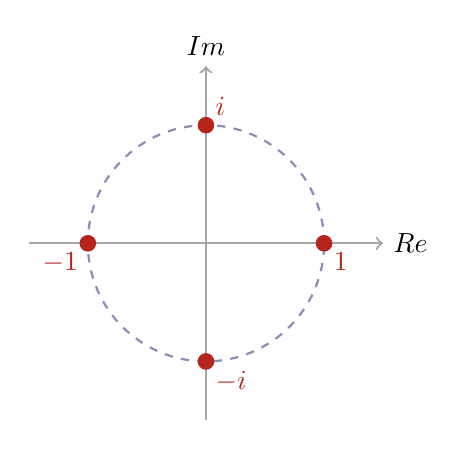
\begin{tikzpicture}[scale=1.5]
% \begin{hidden}
% - Canvas: scale=1.5, x in [-1.5, 1.5], y in [-1.5, 1.5]
% - Elements: coordinate axes, dashed unit circle, four unit points marked with labels
% - Coordinates: (1,0) for 1, (-1,0) for -1, (0,1) for i, (0,-1) for -i
% - Occlusion: axes in background, dashed circle in midground, dots and labels in foreground
% \end{hidden}
    % Axes
    \draw[->, thick, gray!70] (-1.5, 0) -- (1.5, 0) node[right, text=black] {$\operatorname{Re}$};
    \draw[->, thick, gray!70] (0, -1.5) -- (0, 1.5) node[above, text=black] {$\operatorname{Im}$};

    % Unit Circle (radius 1 coordinate unit)
    \draw[dashed, MidnightBlue!50, thick] (0,0) circle (1);

    % Four Units
    \fill[BrickRed] (1, 0) circle (2pt) node[below right, text=BrickRed, font=\bfseries] {$1$};
    \fill[BrickRed] (-1, 0) circle (2pt) node[below left, text=BrickRed, font=\bfseries] {$-1$};
    \fill[BrickRed] (0, 1) circle (2pt) node[above right, text=BrickRed, font=\bfseries] {$i$};
    \fill[BrickRed] (0, -1) circle (2pt) node[below right, text=BrickRed, font=\bfseries] {$-i$};
\end{tikzpicture}
\end{center}

\end{content}

\begin{aiNote}[Beyond the Lecture: The Norm in Textbooks]
% [PERSISTENT, ADDITION]
The lecturer's \qt{norm} is the length $\sqrt{a^2 + b^2}$ of a complex number, and he squares the equation only at the end. Textbooks usually work with the square directly: the \emph{field norm} $N(a + bi) = a^2 + b^2$ of $\mathbb{Q}[i]$ over $\mathbb{Q}$ is multiplicative, $N(zw) = N(z) N(w)$, and takes non-negative integer values on $\mathbb{Z}[i]$. So, $zw = 1$ gives $N(z) N(w) = N(1) = 1$ in one step, hence $N(z) = 1$. The only lattice points on the circle of radius $1$ are the four points shown above.
\end{aiNote}

\subsection{The Group of Units of \texorpdfstring{$\faktor{\mathbb{Z}}{m\mathbb{Z}}$}{Z/mZ}}

\begin{speech}[00:05:14 - 00:07:18]
We did a much more interesting example last time, which was also with proof, but since various people asked me about it afterwards, I want to do just another example. And that was this ring: $\faktor{\mathbb{Z}}{m\mathbb{Z}}$. \inlinemetanote{writes: $\faktor{\mathbb{Z}}{m\mathbb{Z}}$} That's a nice ring, and so it has a group of units: $\operatorname{Unit}(\faktor{\mathbb{Z}}{m\mathbb{Z}})$. \inlinemetanote{writes: $\to \text{Units } \faktor{\mathbb{Z}}{m\mathbb{Z}}$}

This was a result I proved last time (Recall: \cref{thm:units-z-mod-m}): the units, this is equal to those classes such that $\operatorname{GCD}(x, m) = 1$. \inlinemetanote{writes: $= \{\bar{x} \mid (x, m) = 1\}$} And as I said, it's standard here to say $m$ is at least $2$, so we're not with the zero ring. \inlinemetanote{draws a box around $m \ge 2$} That's the units, and these are the residue classes which are relatively prime. And I did an example last time (Recall: $\faktor{\mathbb{Z}}{7\mathbb{Z}}$, \cref{ex:units-z7z}). This is a very interesting thing to study; it's just not a trivial thing.

In the sense that, one might say that if I take here the additive structure, \inlinemetanote{writes: $\faktor{\mathbb{Z}}{m\mathbb{Z}} \to (\faktor{\mathbb{Z}}{m\mathbb{Z}}, +, 0)$} this is very simple to think about. It's just adding up integers $\bmod m$. In some sense, most people learn about this under one name or the other in school. But this thing, the units, are more complicated, are more interesting. \inlinemetanote{writes \qt{units are more interesting}}

And so, I wanted to do another... there were various people asking me some questions, so, let's try this: $10\mathbb{Z}$ (i.e., $\faktor{\mathbb{Z}}{10\mathbb{Z}}$), just to say a little bit.

The standard notation for this is that: \inlinemetanote{writes: $(\faktor{\mathbb{Z}}{m\mathbb{Z}})^*$} This is the usual notation for units of $\faktor{\mathbb{Z}}{m\mathbb{Z}}$, and also this notation is sometimes used in general. $R^*$ sometimes denotes --- could denote --- units, depends on the author. So, I've just been writing $\operatorname{Unit}$, so there's no question about what I mean. But in this case, it's so common to use the star here, I also use the star. Is that clear? So, this is it.
\end{speech}

\subsubsection{Example: Units of \texorpdfstring{$\faktor{\mathbb{Z}}{10\mathbb{Z}}$}{Z/10Z}}

\begin{speech}[00:07:18 - 00:08:43]
How to think about this? Well, I'll just do an example because, as I said, there were various questions. This is all the residue classes that are relatively prime. So, you can just write them all first and cross them out: $\bar{0}, \bar{1}, \bar{2}, \bar{3}, \bar{4}, \bar{5}, \bar{6}, \bar{7}, \bar{8}, \bar{9}$. \inlinemetanote{writes: $\bar{0}, \bar{1}, \bar{2}, \dots, \bar{9}$} Maybe I should have picked something less than $10$.

These are all the residue classes, and then we have to cancel all the ones that are not relatively prime.

Which one? Is $\bar{0}$ relatively prime? No, so, we cross that out. \inlinemetanote{crosses out $\bar{0}$} $\bar{1}$ is relatively prime --- $\bar{1}$ is always relatively prime. What about $\bar{2}$? No. \inlinemetanote{crosses out $\bar{2}$} $\bar{3}$? Yes, so, we skip it. $\bar{4}$? That has a $2$ in it and $10$ has a $2$, so, we cross that out. \inlinemetanote{crosses out $\bar{4}$} $\bar{5}$ --- $10$ has a $5$ in it, we cross that one out. \inlinemetanote{crosses out $\bar{5}$} Cross that one out, \inlinemetanote{crosses out $\bar{6}$ and $\bar{8}$} and what's left? Four, yeah, so, these are the four residue classes left. \inlinemetanote{circles $\bar{1}, \bar{3}, \bar{7}, \bar{9}$}

The group of units here consists of these residue classes: \inlinemetanote{writes: $\{\bar{1}, \bar{3}, \bar{7}, \bar{9}\} \subset (\faktor{\mathbb{Z}}{10\mathbb{Z}})^*$} $\{\bar{1}, \bar{3}, \bar{7}, \bar{9}\}$. And the claim is: this is a group under multiplication. That's what that claim is.

For example, $\bar{3}$ is in this group, so, what is its inverse? \inlinemetanote{writes: $\bar{3} \in (\faktor{\mathbb{Z}}{10\mathbb{Z}})^*$, what is its inverse?}
\end{speech}

\begin{student}[Student Answer]
$7$.
\end{student}

\begin{speech}[00:08:44 - 00:09:45]
Seven, because $7 \times 3 = 21$, and so on. So, anyway, you can play with this.

This is a more interesting object, and in fact you could ask: what is the order? This is a basic question in elementary number theory: what is the order of this group? \inlinemetanote{writes \qt{What is the order of $(\faktor{\mathbb{Z}}{m\mathbb{Z}})^*$?}}

And by order, this word means for groups the number of elements. \inlinemetanote{writes \qt{\# of elements}} So, when I say order of a group, if it's a finite group, I just mean the number of elements. What is the order of this? Sometimes this order is denoted by just straight lines --- the bars: \inlinemetanote{writes: $|(\faktor{\mathbb{Z}}{m\mathbb{Z}})^*|$} You should be familiar with this set-theoretic notation; these two bars usually denote order. Is that clear? That's kind of standard set-theoretic notation.

First of all, let's do $10$. What is this? Well, the answer is $4$ --- you just have to compute these. \inlinemetanote{writes: $|(\faktor{\mathbb{Z}}{10\mathbb{Z}})^*| = 4$}
\end{speech}

\begin{content}[Units in \texorpdfstring{$\faktor{\mathbb{Z}}{m\mathbb{Z}}$}{Z/mZ} and the Example \texorpdfstring{$\faktor{\mathbb{Z}}{10\mathbb{Z}}$}{Z/10Z}]
\recap{This characterization was proved in Week~2 (\cref{thm:units-z-mod-m}); the lecturer restates it with the notation $(\faktor{\mathbb{Z}}{m\mathbb{Z}})^*$.}

\begin{proposition}[Units in the Residue Class Ring]\label[proposition]{prop:units-mod-m-w3}
Let $m \in \mathbb{Z}_{\ge 2}$. The group of units of the residue class ring $\faktor{\mathbb{Z}}{m\mathbb{Z}}$ (frequently denoted by $(\faktor{\mathbb{Z}}{m\mathbb{Z}})^*$ or $R^*$ for general rings) consists of those residue classes whose representatives are coprime to $m$ (on the board: $(x, m) = 1$):
\begin{equation}\label{eq:units-mod-m}
(\faktor{\mathbb{Z}}{m\mathbb{Z}})^* = \operatorname{Unit}(\faktor{\mathbb{Z}}{m\mathbb{Z}}) = \{ \bar{x} \in \faktor{\mathbb{Z}}{m\mathbb{Z}} \mid \operatorname{GCD}(x, m) = 1 \}.
\end{equation}
\end{proposition}

\begin{example}[Computing the Units of $\faktor{\mathbb{Z}}{10\mathbb{Z}}$]\label[example]{ex:units-z10z}
Consider the ring $\faktor{\mathbb{Z}}{10\mathbb{Z}} = \{ \bar{0}, \bar{1}, \bar{2}, \bar{3}, \bar{4}, \bar{5}, \bar{6}, \bar{7}, \bar{8}, \bar{9} \}$. To find the units, we eliminate all classes that share a common divisor with $10$ greater than $1$:
\begin{itemize}
    \item \textbf{Class $\bar{0}$:} $\operatorname{GCD}(0, 10) = 10 \ne 1$ (eliminate $\bar{0}$),
    \item \textbf{Even classes:} $\operatorname{GCD}(2, 10) = 2$, $\operatorname{GCD}(4, 10) = 2$, $\operatorname{GCD}(6, 10) = 2$, $\operatorname{GCD}(8, 10) = 2$ (eliminate $\bar{2}, \bar{4}, \bar{6}, \bar{8}$),
    \item \textbf{Class $\bar{5}$:} $\operatorname{GCD}(5, 10) = 5$ (eliminate $\bar{5}$).
\end{itemize}
The remaining coprime residue classes form the group of units:
\[
(\faktor{\mathbb{Z}}{10\mathbb{Z}})^* = \{ \bar{1}, \bar{3}, \bar{7}, \bar{9} \}.
\]
This is an abelian group of order $4$ under multiplication modulo $10$. For instance, the inverse of $\bar{3}$ is $\bar{7}$, since:
\[
\bar{3} \cdot \bar{7} = \overline{21} = \bar{1} \in \faktor{\mathbb{Z}}{10\mathbb{Z}}.
\]
\end{example}
\end{content}

\begin{aiNote}[{Notation: The Lecturer Adds $(\faktor{\mathbb{Z}}{m\mathbb{Z}})^*$}]
% [PERSISTENT]
The lecturer changes his notation again here. For the units of $\faktor{\mathbb{Z}}{m\mathbb{Z}}$ he now writes $(\faktor{\mathbb{Z}}{m\mathbb{Z}})^*$, which the board calls the usual notation, and adds that $R^*$ could denote units. The condition $\operatorname{GCD}(x, m) = 1$ of Week~2 now appears on the board as $(x, m) = 1$. The next lecture goes back to $\operatorname{Unit}(R)$.
\end{aiNote}

\section{Euler's Totient Function}

\begin{speech}[00:10:36 - 00:12:03]
You can ask this question in general, and that's a fun thing to think about. We'll say more about this a bit later, but the definition can be given now: \inlinemetanote{writes \qt{Order of $(\faktor{\mathbb{Z}}{m\mathbb{Z}})^* \stackrel{\text{def}}{=} \phi(m)$}} the order of $(\faktor{\mathbb{Z}}{m\mathbb{Z}})^*$, the group of units, has a name.

Do you know the name of this function? Yes, yeah, it's $\phi$... It's Euler's totient function, that's just the definition. That's the definition of this function --- it's just the order.

And you could ask: can you compute this? There's different ways to compute it, but it has to do with the factorization, and we will get to that later. So, you could say... this is maybe a question for you now: \inlinemetanote{writes \qt{Question: Try to compute $\phi(m)$}} Question: Try to compute Euler's totient function.

Euler is like the most famous Swiss person that ever lived. A few years ago it might have been Federer, but now he's retired, so now it's Euler. And it turns out that Euler and Federer are both from Basel --- you can check it.

You know, my first trip to Switzerland was when I was a kid in the '80s, and the Swiss still had Euler on the $10$ Swiss franc note. I don't know if you've ever seen that; it's a beautiful note. You should go look it up.
\end{speech}

\subsection{Evaluating \texorpdfstring{$\phi(p)$}{phi(p)} and \texorpdfstring{$\phi(p^2)$}{phi(p\texttwosuperior)} for a Prime \texorpdfstring{$p$}{p}}

\begin{speech}[00:12:03 - 00:12:15]
Okay, so, let's do one example to compute this. Well, let's do two examples. Suppose you have a prime $p$ \inlinemetanote{writes: $\phi(p) =$} --- then what is this?
\end{speech}

\begin{student}[Student Answer]
$p - 1$.
\end{student}

\begin{speech}[00:12:16 - 00:12:20]
Yeah, $p - 1$. And why is that?
\end{speech}

\begin{student}[Student Answer]
Because any number less than $p$ is coprime to $p$.
\end{student}

% [TIMESTAMP-ESTIMATED: block split for the student answer, whose words come from the 2026-10-04 run]
\begin{speech}[00:12:22 - 00:13:48]
In other words, if you write this, you'll write $p$ elements, and you'll cross out $0$, and everybody else is relatively prime. So, it's $p - 1$. \inlinemetanote{writes: $p - 1$}

And so, what about this one? \inlinemetanote{writes: $\phi(p^2) = ?$} Do you know how to do this? What you do --- I mean, of course once you do this, you can do the general case for powers of a prime --- you write all the elements. This is a really primitive way to do it, but let's just do it: $0, 1, 2, \dots, p^2 - 1$. \inlinemetanote{writes: $0, 1, 2, \dots, p^2 - 1$} That's what we did there, right?

So, it starts out, and then you cross out all of the... here you're going to cross out $0$, so, it's $p^2 - 1$, but you have to take away... of course you don't want $0$, but you have to take away all the multiples of $p$, right?

And so, now you have to concentrate really hard: how many multiples of $p$? Well, there's $p$ here, there's $2p$ here, and what's the last one? The last one you have to cross out is $p(p - 1)$ --- that's the last one. \inlinemetanote{writes: $p, 2p, \dots, p(p-1)$} Is that clear?

So, we have to take away $p - 1$, so, the answer is $p^2 - p$. \inlinemetanote{writes: $(p^2 - 1) - (p - 1) = p^2 - p$} The answer to this is $p^2 - p$. Okay, that's the beginning; you can play with it a bit. All right?
\end{speech}

\begin{content}[Euler's Totient Function and Prime Power Formulas]
\begin{definition}[Euler's Totient Function]\label[definition]{def:eulers-totient}
The \newterm{Euler totient function} (or Euler's $\phi$-function) $\phi \colon \mathbb{Z}_{\ge 1} \to \mathbb{Z}_{\ge 1}$ is defined as the order of the group of units of $\faktor{\mathbb{Z}}{m\mathbb{Z}}$:
\begin{equation}\label{eq:totient-def}
\phi(m) \stackrel{\text{def}}{=} |(\faktor{\mathbb{Z}}{m\mathbb{Z}})^*| = \#\{ x \in \{0, 1, \dots, m-1\} \mid \operatorname{GCD}(x, m) = 1 \}.
\end{equation}
\end{definition}

\begin{proposition}[Totient Values for Primes and Prime Squares]\label[proposition]{prop:phi-prime-powers}
Let $p$ be a prime number. Then:
\begin{align}
\phi(p) &= p - 1, \label{eq:phi-prime} \\
\phi(p^2) &= p^2 - p = p(p - 1). \label{eq:phi-prime-square}
\end{align}
\end{proposition}

\begin{proof}
We evaluate the number of coprime residue classes in each case:
\begin{itemize}
    \item \textbf{For a prime $p$:} The representatives are $\{0, 1, 2, \dots, p - 1\}$. The only representative sharing a non-trivial factor with $p$ is $0$. Thus, the remaining $p - 1$ elements are all coprime to $p$, giving $\phi(p) = p - 1$ (e.g., $\phi(7) = 6$, as in \cref{ex:units-z7z}).
    \item \textbf{For $p^2$:} The representatives are $\{0, 1, 2, \dots, p^2 - 1\}$. An element $x$ shares a non-trivial factor with $p^2$ if and only if $p \mid x$. The multiples of $p$ in this range are:
    \[
    0, \ p, \ 2p, \ \dots, \ (p - 1)p.
    \]
    There are exactly $p$ such multiples. Subtracting these from the total of $p^2$ elements yields:
    \[
    \phi(p^2) = p^2 - p = p(p - 1).
    \]
\end{itemize}
\end{proof}

\begin{steps}[Generalization to Prime Powers]
Going beyond the lecture (he returns to this in Week~5): for any prime power $p^k$ with $k \ge 1$, an integer $x \in \{0, 1, \dots, p^k - 1\}$ shares a factor with $p^k$ if and only if $p \mid x$. The multiples of $p$ are $0, p, 2p, \dots, (p^{k-1}-1)p$, totaling $p^{k-1}$ elements. Hence, $\phi(p^k) = p^k - p^{k-1} = p^k (1 - 1/p)$. For a general $n$, the Chinese Remainder Theorem splits $\faktor{\mathbb{Z}}{n\mathbb{Z}}$ into prime-power factors, which gives $\phi(n) = n \prod_{p \mid n} (1 - 1/p)$ (Week~5, \cref{thm:euler-totient-product}).
\end{steps}
\end{content}

\section{Fields of Fractions: The Model Case \texorpdfstring{$\mathbb{Z} \subset \mathbb{Q}$}{Z in Q}}

\begin{speech}[00:13:48 - 00:15:30]
The next topic in the course has to do with fields of fractions. \inlinemetanote{writes \qt{Fields of fractions}} And this is a peculiar subject.

It starts with this idea that $\mathbb{Z}$ is inside $\mathbb{Q}$. \inlinemetanote{writes: $\mathbb{Z} \subset \mathbb{Q}$} So, $\mathbb{Z}$ is a ring, it's an integral domain \inlinemetanote{writes arrow from $\mathbb{Z}$ to \qt{int. domain}} and $\mathbb{Q}$ is a field, \inlinemetanote{writes arrow from $\mathbb{Q}$ to \qt{field}} and $\mathbb{Z}$ sits inside $\mathbb{Q}$. But the relationship is not just of any ring inside any field. In some sense, $\mathbb{Q}$ is the smallest field that contains $\mathbb{Z}$. This understanding will lead to the study of the field of fractions.

Let's try to first make this precise; let's try to make precise the qualitative statement that... \inlinemetanote{writes \qt{Make precise the statement that \qt{$\mathbb{Q}$ is the smallest field which contains $\mathbb{Z}$}}} Here's the statement: \qt{$\mathbb{Q}$ is the smallest field which contains $\mathbb{Z}$}. That's a statement that probably you feel is true. It's not a $100$ percent mathematical statement, so, let's try to make this precise.

You don't contradict the meaning of this statement, right?
\end{speech}

\begin{speech}[00:15:30 - 00:17:25]
\inlinemetanote{moves the boards and begins erasing the lower board}
One thing that when one starts studying these fields of fractions and $\mathbb{Q}$'s, you get this kind of strange feeling that maybe you never checked everything in $\mathbb{Q}$ works. Have you checked everything in $\mathbb{Q}$ works?

It's kind of a strange feeling, because you learn about the rational numbers in school, but it's not like the definitions there are checked to work. You just accept them, which is pretty reasonable --- they are correct.

And what do I mean by that? $\mathbb{Q}$ is a much more complicated thing than $\mathbb{Z}$ conceptually, because $\mathbb{Z}$ is really great: there are these objects and they have names, and everybody has one name. That's what's great about $\mathbb{Z}$.

The thing that's confusing about $\mathbb{Q}$ is that they're objects, but they have many names. You know, you can have... \inlinemetanote{writes: $5/7 = 60/84$} That's kind of confusing: all these numbers have many, many different names. And when I said, \qt{Have you ever checked it works?}, it means that whatever operations you do, you have to be able to do them with any name, and it has to give the same answer, so to speak. That's what I mean. And so, the question is: have you ever checked that?

It's a weird question. But kind of the ideal math question is in first grade or second grade, whenever you're adding fractions, you should ask, say: \qt{But why is it well-defined?} That's the question you should ask. And if you'd asked that question, then we wouldn't have to give this lecture today, actually.
\end{speech}

\begin{content}[Multiple Representations of Rational Numbers and Well-Definedness]
A fundamental conceptual distinction between $\mathbb{Z}$ and $\mathbb{Q}$ is the uniqueness of representation:
\begin{itemize}
    \item \textbf{Integers ($\mathbb{Z}$):} Each element has a unique canonical name: $0, 1, -1, 2, -2, \dots$
    \item \textbf{Rationals ($\mathbb{Q}$):} Each number has infinitely many equivalent representations as a quotient of integers:
    \[
    \frac{5}{7} = \frac{60}{84} = \frac{10}{14} = \dots
    \]
\end{itemize}

Consequently, every operation on fractions (addition, multiplication, evaluation) must be proved to be \newterm{well-defined}, meaning the resulting value is strictly independent of the chosen fractional representative.
\end{content}

\subsection{The Universal Property of \texorpdfstring{$\mathbb{Q}$}{Q}}

\begin{speech}[00:17:25 - 00:19:32]
I try to make precise the statement that $\mathbb{Q}$ is the smallest field which contains $\mathbb{Z}$. And there's different ways to do it, but one way is to say it like this:

Suppose I have $f \colon \mathbb{Z} \to F$, \inlinemetanote{writes: Suppose $f \colon \mathbb{Z} \to F$} where $F$ is a field \inlinemetanote{writes arrow from $F$ to \qt{field}} --- this big $F$ is a field, and this little $f$ is an injection of rings, so, an injective homomorphism of rings. \inlinemetanote{writes \qt{injection of rings / homomorphism of rings}}

So, I start with this: I take any possible field --- maybe a field that I might think is smaller than $\mathbb{Q}$, or whatever field, take any field you want --- and I start with a ring homomorphism which is injective. That means that I view this as $\mathbb{Z}$ sitting inside $F$, okay?

Then I claim... \inlinemetanote{writes \qt{Then I claim $\exists ! \, g$}} The typical way you write this is with a diagram: this is $f$, then I claim there exists a unique $g$... So, this is $\mathbb{Z}$ sitting inside $\mathbb{Q}$, and here there exists a unique $g$ \inlinemetanote{draws diagram with $\mathbb{Z} \to \mathbb{Q}$, $\mathbb{Z} \to F$, and dashed arrow $\mathbb{Q} \to F$ labeled $g$} such that $g$ is an injective homomorphism of fields. \inlinemetanote{writes \qt{such that $g$ is inj. hom of fields}}

And the diagram commutes, meaning I can take an integer here and go here, or I consider it in $\mathbb{Q}$ and go this way. We would say the diagram commutes: if you have $x$ here, I can get to here going straight across, or I can go inside $\mathbb{Q}$ and come around, so, that would say that $f(x) = g(x)$. \inlinemetanote{writes \qt{s.t. $\forall x \in \mathbb{Z}, \, f(x) = g(x)$}}
\end{speech}

\begin{content}[Universal Property of the Rational Field]
\textbf{Qualitative Observation:} $\mathbb{Q}$ is the \qt{smallest} field containing the integral domain $\mathbb{Z}$.

\begin{theorem}[Universal Property of $\mathbb{Q}$]\label[theorem]{thm:universal-property-q}
Let $F$ be a field, and let $f \colon \mathbb{Z} \to F$ be an injective ring homomorphism (embedding of rings).
Then there exists a unique field homomorphism $g \colon \mathbb{Q} \to F$ such that the following diagram commutes:
\begin{center}
\begin{tikzpicture}[scale=1.5, >=Stealth]
% \begin{hidden}
% - Canvas: scale=1.5, triangle diagram with vertices Z at (0,0), Q at (0,1.5), F at (2.2,0)
% - Nodes: Z at (0,0), Q at (0,1.5), F at (2.2,0)
% - Arrows: Z -> Q canonical inclusion \iota (vertical up)
%   Z -> F map f (horizontal right)
%   Q -> F unique map g (dashed diagonal down-right)
% \end{hidden}
    \node (Z) at (0, 0) {$\mathbb{Z}$};
    \node (Q) at (0, 1.5) {$\mathbb{Q}$};
    \node (F) at (2.2, 0) {$F$};

    \draw[right hook->, thick] (Z) -- (Q) node[midway, left] {$\iota$};
    \draw[->, thick] (Z) -- (F) node[midway, below] {$f$};
    \draw[->, dashed, thick, BrickRed] (Q) -- (F) node[midway, above right] {$\exists! \, g$};
\end{tikzpicture}
\end{center}
that is, $g|_{\mathbb{Z}} = f$, meaning $g(x) = f(x)$ for all $x \in \mathbb{Z}$. Furthermore, $g$ is automatically injective.
\end{theorem}

Injectivity is automatic, because every ring homomorphism from a field to a non-zero ring is injective (see \cref{thm:ideals-in-a-field} and the steps after it, Week~1).

\begin{steps}[Universal Property as Categorical Minimality]
Going beyond the lecture: in category theory, this universal mapping property identifies $\mathbb{Q}$ as the initial object among the fields containing a copy of $\mathbb{Z}$, that is, the fields of characteristic $0$. Any field $F$ containing a copy of $\mathbb{Z}$ must necessarily contain a subfield isomorphic to $\mathbb{Q}$, showing that $\mathbb{Q}$ cannot be compressed or embedded into any strictly smaller field.
\end{steps}
\end{content}

\subsection{Construction and Well-Definedness of the Field Extension}

\begin{speech}[00:19:32 - 00:21:20]
I'll give a little proof of this. This is now totally precise mathematics; it makes that statement, which is somehow slightly qualitative, into a mathematical statement.

Do you accept that? When I say $\mathbb{Q}$ is the smallest field which contains $\mathbb{Z}$, it means that if I have any other candidate field $F$, I can actually squeeze $\mathbb{Q}$ into it. And that means that $\mathbb{Q}$ is smaller than $F$. Does that make sense?

Okay, but I haven't proven it, so, let's try to prove it. I won't prove the whole thing, because it's of course kind of painful.

So, let us see: I have to prove this, which means I get to start with the data I suppose. That's what \qt{suppose} is about --- \qt{suppose} means I get to start with this data, which is here, all right? And then the whole claim is existence. To prove this, what I have to do is produce $g$.

Proof, more or less: \inlinemetanote{writes \qt{Proof I have to construct $g$}} I have to construct $g$. So, I write down... \inlinemetanote{self-correction} a complex number, $x$ over $y$, where $x$ and $y$ are integers and $y \neq 0$ --- sorry, a rational number, that's what a rational number is: $x/y$, where $x, y \in \mathbb{Z}$ and $y \neq 0$. \inlinemetanote{writes: $g(x/y) =$, $x, y \in \mathbb{Z}, y \neq 0$} I hope you're happy with that; that's what a rational number is.

This is my responsibility: I have to define this, or we define. \inlinemetanote{writes \qt{we define}} So, how am I going to define this?
\end{speech}

\begin{student}[Student Answer]
$f(x) / f(y)$.
\end{student}

\begin{speech}[00:21:23 - 00:21:51]
Yeah, so, formally, of course we'll write it the way you said, but formally we write it like this: \inlinemetanote{writes: $= f(x) f(y)^{-1}$} $f(x) f(y)^{-1}$.

Because $f(x)$ is in the field $F$, and $f(y)$ is in the field $F$, and I want to take its inverse. This is the kind of field language. Why am I allowed to take its inverse? You cannot take inverses of everything.
\end{speech}

\begin{student}[Student Answer]
Because $F$ is a field and we chose... $y \ne 0$.
\end{student}

% [TIMESTAMP-ESTIMATED: block split for the student answer, whose words come from the 2026-10-04 run]
\begin{speech}[00:21:58 - 00:23:11]
Yeah, but you have to check --- and this is the whole thing, which is that you have to check. This is legal so long as $f(y) \neq 0$. \inlinemetanote{writes \qt{legal as long as $f(y) \neq 0$}} And why is $f(y)$ not zero? It's because $f$ is injective, and $y \neq 0$. \inlinemetanote{writes \qt{and this is because $f$ is injective and $y \neq 0$}} That's actually using this thing here. So, this is legal. Is that clear?

And as was implicit in the answer, we will often write this as that, \inlinemetanote{writes: $= \frac{f(x)}{f(y)}$} because it's charming to do that. And in a field, if you see this, all that means is that the fellow downstairs can be put upstairs by multiplicative inverse. And you're only legally allowed to write it if you know this is not zero --- just like in normal arithmetic, you can't divide by zero.

When we write this, it means various things: it means in particular this one's not zero, and you can put it up here, and you can put it on either side, it doesn't matter because our fields are commutative. Okay?
\end{speech}

\begin{content}[Candidate Definition of the Field Homomorphism \texorpdfstring{$g$}{g}]
\begin{definition}[Candidate Map for Field Embedding]\label[definition]{def:candidate-map-g}
Let $f \colon \mathbb{Z} \to F$ be an injective ring homomorphism into a field $F$. For a rational number represented by $\frac{x}{y} \in \mathbb{Q}$ with $x, y \in \mathbb{Z}$ and $y \ne 0$, we define:
\begin{equation}\label{eq:candidate-g-def}
g\left(\frac{x}{y}\right) \stackrel{\text{def}}{=} f(x) \cdot f(y)^{-1} = \frac{f(x)}{f(y)} \in F.
\end{equation}
\end{definition}

\begin{steps}[Legitimacy of Inversion in the Field $F$]
The inverse $f(y)^{-1}$ exists in $F$ if and only if $f(y) \ne 0_F$:
\begin{enumerate}[label=\textbf{(\arabic*)}]
    \setcounter{enumi}{0} \item \textbf{Non-Zero Denominator:} In the rational representation $\frac{x}{y}$, we require $y \ne 0$ in $\mathbb{Z}$.
    \setcounter{enumi}{1} \item \textbf{Injectivity of Ring Embedding:} Since $f \colon \mathbb{Z} \to F$ is an injective ring homomorphism, its kernel is trivial: $\ker(f) = \{0\}$.
    \setcounter{enumi}{2} \item \textbf{Non-Vanishing Image:} It follows immediately that $y \ne 0 \implies f(y) \ne f(0) = 0_F$ (\cref{prop:homomorphism-preserves-zero}). Since $F$ is a field, every non-zero element has a unique multiplicative inverse $f(y)^{-1} \in F$.
\end{enumerate}
\end{steps}
\end{content}

\begin{speech}[00:23:11 - 00:25:18]
We managed to prove... But is this a definition? The answer is, of course, not: all you did was pick a particular name of this, and you gave a definition. You have to check that all the names give the same definition. That's the business about the rational numbers, which no one ever thinks about --- and it's better not to think about it, but unfortunately today we have to think about it.
\inlinemetanote{moves to the lower board to erase and write}

What do we have to do? \inlinemetanote{writes \qt{We are done with the Def of $g$}} We are done with the definition of $g$. But we must further check that if $x_1/y_1 = x_2/y_2$, \inlinemetanote{writes \qt{We must check that if $\frac{x_1}{y_1} = \frac{x_2}{y_2}$}} then $g(x_1/y_1) = g(x_2/y_2)$. \inlinemetanote{writes \qt{then $g(\frac{x_1}{y_1}) = g(\frac{x_2}{y_2})$}}

You understand we have to check this, because that's the slipperiness of the rational numbers: they don't have a unique name.
\end{speech}

\begin{speech}[00:25:18 - 00:27:08]
All right, but you accept we have to check this? Otherwise, if we can't check this, whatever was there was nonsense.

So, we have to check it. And how are we going to check it? Well, so, we have here: \inlinemetanote{writes \qt{$g\left(\frac{x_1}{y_1}\right) = \frac{f(x_1)}{f(y_1)}$} and \qt{$g\left(\frac{x_2}{y_2}\right) = \frac{f(x_2)}{f(y_2)}$}}

And we want to figure out whether these things are equal: do we have... \inlinemetanote{writes \qt{do we have $\frac{f(x_1)}{f(y_1)} \stackrel{?}{=} \frac{f(x_2)}{f(y_2)}$}} That's the question.

Using the fact that these are invertible, and we can multiply by them, this question is equivalent to what's called clearing the denominators. So, by clearing the denominators, this is equivalent \inlinemetanote{draws $\iff$ and writes: $f(x_1) f(y_2) = f(x_2) f(y_1)$} to $f(x_1) f(y_2) = f(x_2) f(y_1)$ by just multiplying both sides by $f(y_1) f(y_2)$ \inlinemetanote{writes: $\cdot f(y_1) f(y_2)$} --- that's a legal move in fields. And since these are invertible, this implies that, and this implies the other way, because they're both non-zero. Everything here is invertible.

We're using all the time that when we write this, \inlinemetanote{writes: $y_1, y_2 \neq 0 \implies f(y_1), f(y_2) \neq 0$} neither $y_1$ nor $y_2$ is zero, which implies $f(y_1)$ and $f(y_2)$ are not zero, okay?
\end{speech}

\begin{speech}[00:27:08 - 00:27:50]
And now, these things are all integers, and everything's upstairs --- there's no division. This is if and only if \inlinemetanote{draws $\Updownarrow$} you can use the homomorphism property: \inlinemetanote{writes: $f(x_1 y_2) = f(x_2 y_1)$} $f(x_1 y_2) = f(x_2 y_1)$, right? Because $f$ is a homomorphism.

And this is if and only if \inlinemetanote{draws $\Updownarrow$ and writes: $f(x_1 y_2 - x_2 y_1) = 0$} $f(x_1 y_2 - x_2 y_1) = 0$, okay?

Why would this be the case? Yeah?
\end{speech}

\begin{student}[Student Answer]
We could rearrange...
\end{student}

% [TIMESTAMP-ESTIMATED: block split for the student answer, whose words come from the 2026-10-04 run]
\begin{speech}[00:27:52 - 00:28:57]
Well, you have to say what this means. What does this mean? This goes to the heart of the issue about whether you learned the rational numbers correctly, and the answer is: this means \inlinemetanote{points to $\frac{x_1}{y_1} = \frac{x_2}{y_2}$ and writes below: $x_1 y_2 = x_2 y_1$} that $x_1 y_2 = x_2 y_1$. It means nothing more or less than that; it just actually means that.

So, if we start with this, we have this equation: \inlinemetanote{writes: $x_1 y_2 - x_2 y_1 = 0$ in the integers} $x_1 y_2 - x_2 y_1 = 0$ in the integers. That's what this means.

And very fortunately, that's what we need: we need this to be zero, so, this is true \inlinemetanote{places a checkmark next to $f(x_1 y_2 - x_2 y_1) = 0$} --- and so, everything is true, and this is well-defined. All right?

That means I have defined a map, but there's a lot of things to check, which of course I'm not going to check. You have to do it, so to speak, on your own time.
\end{speech}

\begin{content}[Well-Definedness of the Extension Map \texorpdfstring{$g$}{g}]
\begin{claim}[Well-Definedness of $g$]\label[claim]{clm:g-well-defined}
The map $g \colon \mathbb{Q} \to F$ defined in \eqref{eq:candidate-g-def} is well-defined; that is, if $\frac{x_1}{y_1} = \frac{x_2}{y_2}$ in $\mathbb{Q}$, then $g\left(\frac{x_1}{y_1}\right) = g\left(\frac{x_2}{y_2}\right)$ in $F$.
\end{claim}

\begin{proof}
Let $\frac{x_1}{y_1}, \frac{x_2}{y_2} \in \mathbb{Q}$ with $y_1, y_2 \in \mathbb{Z} \setminus \{0\}$ such that $\frac{x_1}{y_1} = \frac{x_2}{y_2}$.

\textbf{1. Meaning of Equality in $\mathbb{Q}$:}
By definition of the rational numbers as fractions, equality $\frac{x_1}{y_1} = \frac{x_2}{y_2}$ means precisely that the cross-multiplied relation holds in $\mathbb{Z}$:
\begin{equation}\label{eq:cross-mult-z}
x_1 y_2 = x_2 y_1 \iff x_1 y_2 - x_2 y_1 = 0 \in \mathbb{Z}.
\end{equation}

\textbf{2. Algebraic Chain in $F$:}
We want to establish whether:
\[
g\left(\frac{x_1}{y_1}\right) \overset{?}{=} g\left(\frac{x_2}{y_2}\right) \iff \frac{f(x_1)}{f(y_1)} \overset{?}{=} \frac{f(x_2)}{f(y_2)}.
\]
Since $y_1, y_2 \ne 0$ and $f$ is injective, $f(y_1) \ne 0$ and $f(y_2) \ne 0$. Multiplying both sides by $f(y_1)f(y_2) \in F \setminus \{0\}$ (clearing denominators) yields an equivalent equality in $F$:
\begin{align}
\frac{f(x_1)}{f(y_1)} = \frac{f(x_2)}{f(y_2)} &\iff f(x_1) \cdot f(y_2) = f(x_2) \cdot f(y_1) \nonumber \\
&\iff f(x_1 y_2) = f(x_2 y_1) && \text{(since $f$ is a ring homomorphism)} \nonumber \\
&\iff f(x_1 y_2) - f(x_2 y_1) = 0_F \nonumber \\
&\iff f(x_1 y_2 - x_2 y_1) = 0_F. \label{eq:hom-zero-check}
\end{align}

\textbf{3. Conclusion:}
By \eqref{eq:cross-mult-z}, $x_1 y_2 - x_2 y_1 = 0 \in \mathbb{Z}$. Since any ring homomorphism maps $0$ to $0$ (\cref{prop:homomorphism-preserves-zero}):
\[
f(x_1 y_2 - x_2 y_1) = f(0) = 0_F.
\]
Thus, condition \eqref{eq:hom-zero-check} holds, which proves that $g\left(\frac{x_1}{y_1}\right) = g\left(\frac{x_2}{y_2}\right)$.
\end{proof}

\begin{steps}[Core Pedagogical Principle: Non-Unique Names of Fractions]
A rational number has infinitely many equivalent names (e.g., $\frac{1}{2} = \frac{2}{4} = \frac{-3}{-6}$). Any function defined on rational numbers using numerator and denominator symbols must be proven invariant under replacement of representatives. As shown above, this reduces entirely to the cross-multiplication identity in the underlying ring $\mathbb{Z}$.
\end{steps}
\end{content}

% [TIMESTAMP-CHECKED: missing from the 2026-10-10 transcription; text from the 2026-10-04 run
% (there 00:29:02 - 00:30:32). The Hydrogen rerun (00:29:03) and the audio agree with those times]
\begin{speech}[00:29:02 - 00:30:30]
I have now defined the map $g$, finally. Then you have to check that this map $g$ is actually... I mean, all of the properties of $g$, that it's a homomorphism of fields. You have to check that it respects addition, and you have to check that it respects multiplication.

All of it is slightly painful, because at first blush it's obvious: you just pick representatives for $\mathbb{Q}$ as $x_1/y_1$, and then you just check it. But then you have to check that all of that stuff respects the different choices, the different names of elements of $\mathbb{Q}$, just like we did here.

And the checks are all the same, so you can do it yourself. That's the end of what I'm going to give as the proof of this; you can check the rest. We're going to have to do many more things like this, so...
\end{speech}

\begin{speech}[00:30:30 - 00:32:03]
We have now, successfully, defined $g$. Then we need to check that $g$ is indeed a homomorphism of fields. \inlinemetanote{writes \qt{We have defined $g$. We need to check that $g$ is indeed a hom. of fields.}} I leave this to you. We're going to have to do things like this anyway, and it's all just unraveling the definitions.

Meaning you have to check... \inlinemetanote{writes \qt{You have to check}} You check something like: \inlinemetanote{writes: $g\left(\frac{x_1}{y_1}\right) + g\left(\frac{x_2}{y_2}\right) = g\left(\frac{x_1}{y_1} + \frac{x_2}{y_2}\right)$} $g(x_1/y_1) + g(x_2/y_2) = g(x_1/y_1 + x_2/y_2)$. You have to go check that; that's what you have to check.

And you can see when you write this, this side... Okay, I'm going to do part of it for you --- I don't know why I'm feeling compassionate today here. This one is $f(x_1)/f(y_1) + f(x_2)/f(y_2)$. \inlinemetanote{writes: $\stackrel{\text{def}}{=} \frac{f(x_1)}{f(y_1)} + \frac{f(x_2)}{f(y_2)}$} That's the definition here. And this has a different definition.

First of all, how do we do it? We first have to add this fraction, right? Because our definition only applies to names of rational numbers, and this is the sum. So, we first have to do this, but you know how to add fractions: this is equal to \inlinemetanote{writes: $= g\left(\frac{x_1 y_2 + x_2 y_1}{y_1 y_2}\right)$} $g$ of $(x_1 y_2 + x_2 y_1)/(y_1 y_2)$. At least I hope you know how to add fractions --- at least I hope I know how to add fractions, right? Okay, so, that's the addition of the fraction.
\end{speech}

\begin{speech}[00:32:03 - 00:32:50]
And then this, by definition --- use the definition --- is $f(x_1 y_2 + x_2 y_1)/f(y_1 y_2)$. \inlinemetanote{writes: $\stackrel{\text{def}}{=} \frac{f(x_1 y_2 + x_2 y_1)}{f(y_1 y_2)}$} Okay?

So, that's the one side to check, and that's supposed to equal this side, all right? And how are you going to check this? Well, you use the homomorphism property, you move everything upstairs, and then finally you're going to use the thing I erased --- this, okay?

So, I leave it to you. There's nothing really I can add to this; you have to do it. But I do say it's painful --- painful for me to write it on the board even.
\end{speech}

\begin{content}[Verification of the Field Homomorphism Axioms]
\begin{claim}[Preservation of Field Operations]\label[claim]{clm:g-field-hom}
The map $g \colon \mathbb{Q} \to F$ is a field homomorphism; that is, for all $q_1, q_2 \in \mathbb{Q}$:
\begin{align}
g(q_1 + q_2) &= g(q_1) + g(q_2), \label{eq:g-add} \\
g(q_1 \cdot q_2) &= g(q_1) \cdot g(q_2), \label{eq:g-mult} \\
g(1_\mathbb{Q}) &= 1_F. \label{eq:g-unit}
\end{align}
\end{claim}

\begin{proof}[Why $g$ Is a Field Homomorphism (beyond the lecture)]
The lecture leaves this to the students. Let $q_1 = \frac{x_1}{y_1}$ and $q_2 = \frac{x_2}{y_2}$ with $x_i, y_i \in \mathbb{Z}$ and $y_i \ne 0$.

\paragraph{1. Verification of Additivity \eqref{eq:g-add}:}
Adding fractions according to standard rational arithmetic:
\[
q_1 + q_2 = \frac{x_1}{y_1} + \frac{x_2}{y_2} = \frac{x_1 y_2 + x_2 y_1}{y_1 y_2}.
\]
Applying the definition of $g$ and the ring homomorphism properties of $f$:
\begin{align*}
g(q_1 + q_2) &= g\left(\frac{x_1 y_2 + x_2 y_1}{y_1 y_2}\right) \\
&\stackrel{\text{def}}{=} \frac{f(x_1 y_2 + x_2 y_1)}{f(y_1 y_2)} \\
&= \frac{f(x_1)f(y_2) + f(x_2)f(y_1)}{f(y_1)f(y_2)}.
\end{align*}
On the other hand, evaluating the sum of images in the field $F$:
\begin{align*}
g(q_1) + g(q_2) &\stackrel{\text{def}}{=} \frac{f(x_1)}{f(y_1)} + \frac{f(x_2)}{f(y_2)} \\
&= f(x_1)f(y_1)^{-1} + f(x_2)f(y_2)^{-1}.
\end{align*}
Bringing both terms over the common denominator $f(y_1)f(y_2)$ in the field $F$:
\[
\frac{f(x_1)}{f(y_1)} + \frac{f(x_2)}{f(y_2)} = \frac{f(x_1)f(y_2) + f(x_2)f(y_1)}{f(y_1)f(y_2)}.
\]
Both expressions coincide identically, establishing \eqref{eq:g-add}. By \cref{clm:g-well-defined}, this value is independent of the choice of fraction representatives.

\paragraph{2. Verification of Multiplicativity \eqref{eq:g-mult}:}
Multiplying fractions inside $\mathbb{Q}$:
\[
q_1 \cdot q_2 = \frac{x_1}{y_1} \cdot \frac{x_2}{y_2} = \frac{x_1 x_2}{y_1 y_2}.
\]
Applying the definition of $g$ and the multiplicativity of $f$:
\begin{align*}
g(q_1 \cdot q_2) &= g\left(\frac{x_1 x_2}{y_1 y_2}\right) \\
&= \frac{f(x_1 x_2)}{f(y_1 y_2)} \\
&= \frac{f(x_1) f(x_2)}{f(y_1) f(y_2)} \\
&= \frac{f(x_1)}{f(y_1)} \cdot \frac{f(x_2)}{f(y_2)} \\
&= g(q_1) \cdot g(q_2),
\end{align*}
establishing \eqref{eq:g-mult}.

\paragraph{3. Preservation of Multiplicative Identity \eqref{eq:g-unit}:}
Representing $1_\mathbb{Q} \in \mathbb{Q}$ as $\frac{1_\mathbb{Z}}{1_\mathbb{Z}}$:
\[
g(1_\mathbb{Q}) = g\left(\frac{1_\mathbb{Z}}{1_\mathbb{Z}}\right) = \frac{f(1_\mathbb{Z})}{f(1_\mathbb{Z})}.
\]
Since $f \colon \mathbb{Z} \to F$ is a unital ring homomorphism, $f(1_\mathbb{Z}) = 1_F$. Thus:
\[
g(1_\mathbb{Q}) = \frac{1_F}{1_F} = 1_F,
\]
establishing \eqref{eq:g-unit}. Thus, $g$ is a field homomorphism.
\end{proof}

\begin{proof}[Extension and Uniqueness (beyond the lecture)]
The lecture proves existence only (\qt{the whole claim is existence}). The map $g$ extends $f$: for $x \in \mathbb{Z}$, $g(\frac{x}{1}) = f(x) f(1)^{-1} = f(x)$, since $f(1) = 1_F$. For uniqueness, let $\psi \colon \mathbb{Q} \to F$ be any field homomorphism with $\psi(x) = f(x)$ for all $x \in \mathbb{Z}$. For $y \neq 0$, $\psi(y) \, \psi(\frac{1}{y}) = \psi(1) = 1_F$, so $\psi(\frac{1}{y}) = f(y)^{-1}$, and therefore
\[
\psi\left(\frac{x}{y}\right) = \psi(x) \, \psi\left(\frac{1}{y}\right) = f(x) f(y)^{-1} = g\left(\frac{x}{y}\right).
\]
Hence, $\psi = g$.
\end{proof}
\end{content}

\section{Formal Fractions over an Integral Domain}

\begin{speech}[00:32:50 - 00:35:03]
That's the story about $\mathbb{Z}$. Their fates are really closely tied: $\mathbb{Z}$ and $\mathbb{Q}$. \inlinemetanote{writes: $\mathbb{Z} \subset \mathbb{Q}$} $\mathbb{Q}$ is not just any field that $\mathbb{Z}$ is in --- it's the smallest field it's in. So, we could ask: can we construct this relationship for other rings? Because we really like this relationship.

If you study the integers, it's very useful sometimes to be able to divide; so, that's the movement to the field. Let's try this with a ring in general.

Suppose $R$ is an integral domain. \inlinemetanote{writes \qt{Suppose $R$ is an integral domain}} It turns out that this is extremely important, and we will see in the definition --- it may not be clear from the discussion so far --- but let's say $R$ is an integral domain.

Can we find the analogue of $\mathbb{Q}$, which is the \qt{smallest} field containing $R$? \inlinemetanote{writes \qt{Can we find \qt{smallest} field containing $R$?}} Already in this language, if we find a field containing $R$, \inlinemetanote{writes: $R \subset F$} that means $R$ has to be a domain (Recall: \cref{def:integral-domain}), because a domain means that two elements that are non-zero, when you multiply them, stay non-zero. If you're inside a field, that's always the case, okay? This is one of the reasons why we're talking only about integral domains.

So, that's the question: if you find on the street an integral domain, can you put it in its smallest field? The answer is yes, and that construction is called the field of fractions. And I will show you how to do it.

In some ways, there's lots of conceptual nice things about it, but this pain, you can imagine, we're not going to get away from it --- it's just going to be more abstract. One of the things you will see here is that when we define the field of fractions of a ring, it will have this property that the elements are not single objects, but equivalence classes. And you should expect that answer, because that already happens for the rational numbers.
\end{speech}

\begin{speech}[00:35:03 - 00:36:16]
By the way, for a rational number, the objection --- and I'm surprised no one made it --- is that you could say that you could fix the name by taking the numerator and denominator and cancelling all common factors. There's still a sign issue, but we leave that aside.

If you try to do arithmetic with that, it's super painful, because you have to do a lot of cancellation. So, that is the argument against it. The argument that that's kind of a lie is that that's not really how you do arithmetic in the rational numbers. But that is the argument against what I was saying about the rational numbers.

In a sense, if you do that, it's kind of even more painful, because then when you write these expressions, you can't write these expressions --- you have to cancel everywhere, and you know...
\end{speech}

\begin{content}[Generalization from Integers to Integral Domains]
\begin{remark}[Why Integral Domains?]\label[remark]{rem:why-integral-domains}
If a commutative ring $R$ embeds into a field $F$ via an injective homomorphism $\iota \colon R \hookrightarrow F$, then $R$ must necessarily have no zero divisors:
\[
a, b \in R \setminus \{0\} \implies \iota(a), \iota(b) \ne 0 \implies \iota(ab) = \iota(a)\iota(b) \ne 0 \implies ab \ne 0.
\]
Moreover, $R$ is not the zero ring: $\iota(1) = 1 \neq 0 = \iota(0)$ in $F$, so $1 \neq 0$ in $R$. Thus, the property of being an \newterm{integral domain} (\cref{def:integral-domain}) is a strictly necessary prerequisite for any ring to be embedded into a field of fractions.
\end{remark}

\begin{highlight}{MidnightBlue}[The Goal: Field of Fractions]
Given an arbitrary integral domain $R$, our goal is to construct the minimal field containing $R$, called the \newterm{field of fractions} (or quotient field) $\operatorname{Frac}(R)$, generalizing the classical relationship:
\[
\mathbb{Z} \hookrightarrow \mathbb{Q} = \operatorname{Frac}(\mathbb{Z}).
\]
\end{highlight}
\end{content}

\subsection{Construction of the Set of Formal Fractions}

\begin{speech}[00:36:16 - 00:38:05]
Let's think about this in the abstract. The main thing is just the definition. Here is our ring $R$: we don't know what it is, it's just any ring, but it's an integral domain. \inlinemetanote{writes: $R$ int. domain} We want to construct a field containing $R$. \inlinemetanote{writes \qt{We want to construct a field containing $R$}}

The field should have elements that are like $x$ over $y$, where $x, y \in R$ and $y \neq 0$. \inlinemetanote{writes: $F \ni \frac{x}{y}$, $x, y \in R, y \neq 0$} This should be the element of that field, because if it contains $R$, I should be able to take $x$ and multiply it by the inverse of $y$ in the field, so, it should have these elements in it. Is that clear? That's what happened with the rational numbers.

So, we can just define it that way. We start with: let $S$ be the set of pairs. \inlinemetanote{writes \qt{Let $S = \{(x, y) \mid y \neq 0, x, y \in R\} \subset R \times R$}} This whole thing is going to be a big disappointment if you think something fun is going to happen --- I just tell you ahead of time, this is going to be a big disappointment. But some things in life are like that.

So, here: $y \neq 0$, and $x, y \in R$. Okay, that's the set of pairs. For the integers, if we start with the integers, we just get the set of pairs of integers where the second one is not zero, okay? But we can think about this set of pairs for any $R$. Is that clear? This is inside $R \times R$ --- it's just some subset of pairs.
\end{speech}

\subsection{Digression: Equivalence Relations and Partitions}

\begin{speech}[00:38:05 - 00:39:19]
All right, and now the thing that will come is that there is an equivalence relation. \inlinemetanote{writes \qt{There is an equivalence relation on $S$}} There is an equivalence relation on $S$, so maybe we call this equivalence relation... \inlinemetanote{writes \qt{$\sim$}, then changes to \qt{$\equiv$}} You can use various symbols for equivalence, that's kind of standard. How about three lines?

Do you know what an equivalence relation is? This was in your Foundations class. An equivalence relation on a set --- maybe a little aside \inlinemetanote{writes \qt{Aside on $T$}} --- an equivalence relation on a set $T$ tells you when two elements are related, and the rules for the equivalence relation are:

$x$ is always related to itself --- this is the reflexive property; \inlinemetanote{writes: $x \equiv x$, reflexive}

if $x$ is related to $y$, then $y$ is related to $x$ --- this is the symmetric property; \inlinemetanote{writes: $x \equiv y \implies y \equiv x$, symmetric}

and if you know the definition, what's the third one? Yeah?
\end{speech}

\begin{student}[Student Answer]
Transitivity.
\end{student}

\begin{speech}[00:39:20 - 00:40:21]
The transitive property. It says that if we have $x$ related to $y$ and $y$ related to $z$, then $x$ is related to $z$. \inlinemetanote{writes: $x \equiv y \land y \equiv z \implies x \equiv z$, transitive} That's the whole thing of equivalence relations. It comes up many times in mathematics, and it will come up again in this course, so, if you have not seen it, think about it.

And the main thing we use about this equivalence relation is that if I have $T$ with this equivalence relation, then I have another set --- sometimes it's called this --- which is the set of equivalence classes. \inlinemetanote{writes: $T_{\equiv} = \{$set of equiv.\ classes$\}$} That's going to be very important for us.

Whenever we have a set with an equivalence relation, that equivalence relation divides the set up into equivalence classes --- disjoint equivalence classes, okay? And this thing here is the set of equivalence classes. There's three objects in this kind of abstract situation: there's the set that we start with, there's the equivalence relation, and then there's the set of equivalence classes.
\end{speech}

\begin{content}[The Set of Pairs and General Equivalence Relations]
\begin{definition}[The Set of Formal Fractions $S$]\label[definition]{def:set-of-pairs-s}
Let $R$ be an integral domain. On the Cartesian product $R \times R$ (\cref{not:pre-notation}), we define the set of formal numerator-denominator pairs $S$ by:
\begin{equation}\label{eq:set-of-pairs}
S := \{ (x, y) \in R \times R \mid y \ne 0 \} \subset R \times R.
\end{equation}
\end{definition}

\begin{remark}[Review: Equivalence Relations and Partitions]\label[remark]{rem:equivalence-relation-review}
An \newterm{equivalence relation} $\equiv$ on a set $T$ is a binary relation satisfying three foundational axioms (\cref{def:pre-equivalence-relation}):
\begin{enumerate}[label=\textbf{(\roman*)}]
    \item \textbf{Reflexivity:} $\forall x \in T \colon x \equiv x$.
    \item \textbf{Symmetry:} $\forall x, y \in T \colon x \equiv y \implies y \equiv x$.
    \item \textbf{Transitivity:} $\forall x, y, z \in T \colon (x \equiv y \land y \equiv z) \implies x \equiv z$.
\end{enumerate}
The set of \newterm{equivalence classes} is written $T_{\equiv}$ on the board (textbooks write $\faktor{T}{{\equiv}}$ and call it the quotient set, \cref{def:pre-quotient-set}). The classes partition $T$ into mutually disjoint subsets.
\end{remark}

\begin{center}
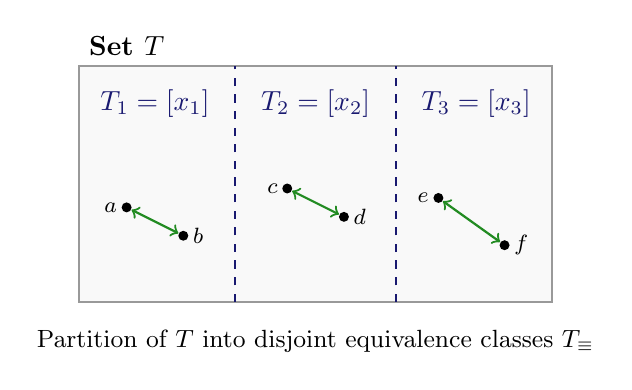
\begin{tikzpicture}[scale=1.2]
% \begin{hidden}
% - Canvas: scale=1.2, set T as an outer rectangle [0,5] x [0,2.8], divided into 3 disjoint blocks
% - Subsets: T_1 at [0,1.7], T_2 at [1.7,3.4], T_3 at [3.4,5]
% - Elements: dots inside each class representing elements related by \equiv
% - Labels: T_1, T_2, T_3 above each partition, T overall
% \end{hidden}
    % Outer bounding box T
    \draw[thick, gray!80, fill=gray!5] (0,0) rectangle (5, 2.5);
    \node[above right, font=\bfseries] at (0, 2.5) {Set $T$};

    % Vertical partition lines
    \draw[thick, dashed, MidnightBlue] (1.65, 0) -- (1.65, 2.5);
    \draw[thick, dashed, MidnightBlue] (3.35, 0) -- (3.35, 2.5);

    % Equivalence Classes
    \node[MidnightBlue, font=\bfseries] at (0.8, 2.1) {$T_1 = [x_1]$};
    \node[MidnightBlue, font=\bfseries] at (2.5, 2.1) {$T_2 = [x_2]$};
    \node[MidnightBlue, font=\bfseries] at (4.2, 2.1) {$T_3 = [x_3]$};

    % Representative dots: labels left of the first and right of the second point, away from the arrows
    \fill (0.5, 1.0) circle (1.5pt) node[left] {\footnotesize $a$};
    \fill (1.1, 0.7) circle (1.5pt) node[right] {\footnotesize $b$};
    \draw[<->, shorten <=2pt, shorten >=2pt, thick, ForestGreen] (0.5, 1.0) -- (1.1, 0.7);

    \fill (2.2, 1.2) circle (1.5pt) node[left] {\footnotesize $c$};
    \fill (2.8, 0.9) circle (1.5pt) node[right] {\footnotesize $d$};
    \draw[<->, shorten <=2pt, shorten >=2pt, thick, ForestGreen] (2.2, 1.2) -- (2.8, 0.9);

    \fill (3.8, 1.1) circle (1.5pt) node[left] {\footnotesize $e$};
    \fill (4.5, 0.6) circle (1.5pt) node[right] {\footnotesize $f$};
    \draw[<->, shorten <=2pt, shorten >=2pt, thick, ForestGreen] (3.8, 1.1) -- (4.5, 0.6);

    \node[below, font=\small] at (2.5, -0.2) {Partition of $T$ into disjoint equivalence classes $T_{\equiv}$};
\end{tikzpicture}
\end{center}
\end{content}

\subsection{The Equivalence Relation on Formal Fractions}

\begin{speech}[00:40:22 - 00:41:01]
We have to define the equivalence relation. We now define an equivalence relation on our set $S$, which is the set of pairs \inlinemetanote{writes \qt{We now define $\equiv$ on $S$}} --- and you should think about these pairs as numerator and denominator, but those are just words here.

We need to define when $(x_1, y_1)$ is equivalent to $(x_2, y_2)$. \inlinemetanote{writes: $(x_1, y_1) \equiv (x_2, y_2)$} We need a definition for this. What's the answer going to be? Yeah?
\end{speech}

\begin{student}[Student Answer]
$x_1 y_2 = x_2 y_1$.
\end{student}

\begin{speech}[00:41:05 - 00:43:24]
Okay, very good. This is the definition: \inlinemetanote{writes: $\stackrel{\text{def}}{\iff} x_1 y_2 = x_2 y_1$} it's just exactly what you do with integer arithmetic. If you have a fraction, you say they're equal if $x_1 y_2 = x_2 y_1$, okay? That's the definition. There's nothing more or less than that --- that's the whole definition.

And it's motivated by the integers. It's very important for this definition that this is only about $R$. \inlinemetanote{writes \qt{only about $R$}} This whole discussion starts with $R$, so, we can only say things that are about $R$.

We can make these pairs --- that's only about $R$. We want to define this equivalence relation. At the end, these things are only in $R$, and the definition is only about some equation in $R$, okay? We haven't gotten out of $R$ in some sense in this whole discussion. Is that clear?

Now we come to an issue: why is this an equivalence relation? This is the question you should have asked your teacher in first grade or whatever it was. That's like the whole question about the rational numbers in some sense --- the foundations.
\inlinemetanote{washes and erases the left part of the bottom chalkboard}

This is the first part where we have to do a little bit of algebra. The first two properties, $x = x$, that's just identically true, okay? That's not a problem. We have to check three properties. \inlinemetanote{writes \qt{3 properties}}
\end{speech}

\begin{content}[Definition of the Equivalence Relation on \texorpdfstring{$S$}{S}]
\begin{definition}[Equivalence Relation on $S$]\label[definition]{def:equiv-relation-S}
On the set $S = \{ (x, y) \in R \times R \mid y \ne 0 \}$, we define the relation $\equiv$ by:
\begin{equation}\label{eq:equiv-relation-formula}
(x_1, y_1) \equiv (x_2, y_2) \stackrel{\text{def}}{\iff} x_1 y_2 = x_2 y_1 \quad (\text{in } R).
\end{equation}
\end{definition}

\begin{steps}[Conceptual Motivation: Cross-Multiplication]
This relation is the formal algebraic counterpart to equating cross-products of fractions:
\[
\frac{x_1}{y_1} = \frac{x_2}{y_2} \iff x_1 y_2 = x_2 y_1.
\]
Crucially, formula \eqref{eq:equiv-relation-formula} involves only multiplication within the ring $R$, without invoking any external concept of division or fraction.
\end{steps}
\end{content}

\begin{speech}[00:43:24 - 00:45:05]
The first is: if I take $(x_1, y_1)$, this is equivalent to $(x_1, y_1)$. \inlinemetanote{writes: $(x_1, y_1) \equiv (x_1, y_1)$} And why is this? Because by definition this is equal to $x_1 y_1 = x_1 y_1$, \inlinemetanote{writes: $\iff x_1 y_1 = x_1 y_1$ \checkmark} so, we're very happy about that. There was nothing to do here.

You also have to check the symmetric property: that if we have $(x_1, y_1) \equiv (x_2, y_2)$, then the other way around is fine, and it'll just be the same equation. There's nothing to check about that.

The interesting one is the transitive property. \inlinemetanote{writes \qt{Transitive}} This is the only fun one to check. We start with this one: \inlinemetanote{writes \qt{$(x_1, y_1) \equiv (x_2, y_2)$} and \qt{$(x_2, y_2) \equiv (x_3, y_3)$}} these are the inputs.

And we must show --- this is for us to do --- that $(x_1, y_1)$ is congruent (i.e., equivalent) to $(x_3, y_3)$. \inlinemetanote{writes: $\implies (x_1, y_1) \equiv (x_3, y_3)$}

The thing that's a little funny about this is... let's try to do this. We have to write the first equation. This is what we have: \inlinemetanote{writes \qt{What we have}} that's what we've assumed, that's in the left column.
\inlinemetanote{the lecture bell rings}

Okay. You'll have to wait until after the break for this excitement to continue.
\end{speech}

\begin{content}[Verification of Reflexivity and Symmetry on \texorpdfstring{$S$}{S}]
\begin{proposition}[Reflexivity and Symmetry of $\equiv$]\label[proposition]{prop:equiv-refl-sym}
The relation $\equiv$ defined on $S = \{ (x, y) \in R \times R \mid y \ne 0 \}$ by:
\begin{equation}\label{eq:equiv-def-recap}
(x_1, y_1) \equiv (x_2, y_2) \stackrel{\text{def}}{\iff} x_1 y_2 = x_2 y_1
\end{equation}
is reflexive and symmetric.
\end{proposition}

\begin{proof}
Let $(x_1, y_1), (x_2, y_2) \in S$:
\begin{itemize}
    \item \textbf{Reflexivity:} Trivially $x_1 y_1 = x_1 y_1$, which by \eqref{eq:equiv-def-recap} immediately implies:
    \[
    (x_1, y_1) \equiv (x_1, y_1).
    \]
    \item \textbf{Symmetry:} Assume $(x_1, y_1) \equiv (x_2, y_2)$. Then $x_1 y_2 = x_2 y_1$. By symmetry of equality in $R$:
    \[
    x_2 y_1 = x_1 y_2 \implies (x_2, y_2) \equiv (x_1, y_1).
    \]
\end{itemize}
\end{proof}
\end{content}

\begin{pause}[Mid-Lecture Break]
The bell rings, and the lecturer pauses the class for a short break. The lecture resumes at timestamp 00:45:05.
\end{pause}

\begin{speech}[00:45:05 - 00:45:33]
Okay, so, let's start. I should say that very few people have found my office, and it turns out I'll be in this visitor office for most of the semester, because they're clearing some kind of nuclear waste from my current office. So, my office now is HG G 65.1 \inlinemetanote{writes \qt{HG G 65.1}} if you want to find me there. And yeah, I'm afraid I'll be there for most of the semester.
\end{speech}

\begin{note}[Administrative Announcement: Office Relocation]
The lecturer writes \qt{HG G 65.1} on the far right of the chalkboard and informs students that he will be stationed in this visitor office for the majority of the semester.
\end{note}

\begin{speech}[00:45:33 - 00:47:00]
We come to this point that's kind of fun and interesting. We started with an integral domain, and led by the analogy with the rational numbers, we come to start defining this field as some equivalence class of pairs. And I should have said this. I did say it, but I didn't write it: the way to think about this \inlinemetanote{writes \qt{Think of as $\frac{x}{y} \leftarrow (x, y) \in S$}} --- this is the mathematical text --- you think of this pair in $S$ as $x/y$, okay? Just like with the integers.

As an object, it's this formal object. And then there was this proposal, which was correct, of how to define the equivalence relation. And now we actually need to check something: is it an equivalence relation?

Here we have to prove the transitive property. And so, we start with: what do we have? We have that equivalence, so, if we translate that into equations, it says $x_1 y_2 = x_2 y_1$ --- and you have to be very careful with the subscripts, otherwise you'll confuse yourself: \inlinemetanote{writes: $x_1 y_2 = x_2 y_1$} $x_1 y_2 = x_2 y_1$. And then what we also have here is $x_2 y_3 = x_3 y_2$. \inlinemetanote{writes: $x_2 y_3 = x_3 y_2$}
\end{speech}

\begin{speech}[00:47:20 - 00:48:40]
And what we want, \inlinemetanote{writes \qt{Want}} we want this thing, which is $x_1 y_3 = x_3 y_1$. \inlinemetanote{writes: $x_1 y_3 = x_3 y_1$}

The puzzling thing about this is: we have these quadratic equations and we need to get another quadratic equation. It seems a little bit unfortunate, because you might think you have to do some linear algebra with quadratic equations, and that's not going to work --- you're not going to get a new quadratic equation from these.

The correct answer is we're supposed to multiply here. The clever thing is to multiply the top equation by $y_3$ \inlinemetanote{writes \qt{mult. by $y_3$}} --- $y_3$ is what we want. So, we get $x_1 y_2 y_3 = x_2 y_1 y_3$. \inlinemetanote{writes: $x_1 y_2 y_3 = x_2 y_1 y_3$}

This is kind of good: we see the $x_1 y_3$ here. Can you see what we have to do next? This is actually algebra. What?
\inlinemetanote{inaudible answer from a student}
Yeah, you could do that, but why don't we just take this $y_2 y_3$ here and use this equation? It's the same thing. So, we take the $y_2 y_3$ and use this equation to flip them. This is all about subscripts, and I should just tell you that subscripts have always been difficult for me. Do you accept that? Because I just took this and flipped them using this equation. \inlinemetanote{writes \qt{$x_3 y_1 y_2$} under $x_2 y_1 y_3$}
\end{speech}

\begin{speech}[00:48:40 - 00:50:02]
Now what do we do? Well, we have here $x_1 y_3$ --- that looks pretty good --- and we have $y_3 y_1$, but they're both multiplied by $y_2$, right?

Now we use the fact that in these pairs, the second one is always born non-zero: to be in this set, the second one has to be non-zero. And this is an integral domain. So, we have this equation --- this one equals that one --- and then we use the integral domain property. \inlinemetanote{writes \qt{use int. domain}}

I said this is a place where it's extremely important it's an integral domain. Since $y_2 \neq 0$, \inlinemetanote{writes \qt{since $y_2 \neq 0$}} we can cancel, \inlinemetanote{writes \qt{$\implies$ cancel}} okay? Because an integral domain says that's the cancellation property. Is that okay?

If $y_2$ is not zero, we can cancel it. This is kind of dramatic, but we cancel it here. \inlinemetanote{crosses out $y_2$ on both sides} And that's what we want.

We have now proven transitivity. You see there was a little bit of cleverness here; it's easy to confuse yourself.
\end{speech}

\begin{content}[Proof of Transitivity and the Role of the Integral Domain]
\begin{proposition}[Transitivity of $\equiv$ on $S$]\label[proposition]{prop:equiv-on-S}
Let $R$ be an integral domain. The relation $\equiv$ on $S$ defined by $(x_1, y_1) \equiv (x_2, y_2) \stackrel{\text{def}}{\iff} x_1 y_2 = x_2 y_1$ is transitive. Consequently, $\equiv$ is an equivalence relation on $S$.
\end{proposition}

\begin{proof}
Let $(x_1, y_1), (x_2, y_2), (x_3, y_3) \in S$, which implies $y_1, y_2, y_3 \in R \setminus \{0\}$.

\textbf{1. Assumptions:}
We assume the relations:
\begin{align}
(x_1, y_1) \equiv (x_2, y_2) &\implies x_1 y_2 = x_2 y_1, \label{eq:trans-hyp1} \\
(x_2, y_2) \equiv (x_3, y_3) &\implies x_2 y_3 = x_3 y_2. \label{eq:trans-hyp2}
\end{align}

\textbf{2. Target:}
We must prove that $(x_1, y_1) \equiv (x_3, y_3)$, which means showing that:
\begin{equation}\label{eq:trans-target}
x_1 y_3 = x_3 y_1.
\end{equation}

\textbf{3. Derivation via Multiplication and Substitution:}
Multiplying equation \eqref{eq:trans-hyp1} on both sides by $y_3 \in R$:
\begin{equation}\label{eq:trans-mult}
(x_1 y_2) y_3 = (x_2 y_1) y_3 \iff (x_1 y_3) y_2 = (x_2 y_3) y_1.
\end{equation}
Substituting $x_2 y_3 = x_3 y_2$ from \eqref{eq:trans-hyp2} into the right-hand side of \eqref{eq:trans-mult}:
\begin{equation}\label{eq:trans-subst}
(x_1 y_3) y_2 = (x_3 y_2) y_1 = (x_3 y_1) y_2.
\end{equation}
Subtracting the right-hand side gives:
\begin{equation}\label{eq:trans-factored}
(x_1 y_3 - x_3 y_1) y_2 = 0.
\end{equation}

\textbf{4. Cancellation via the Integral Domain Property:}
By definition of $S$, $y_2 \ne 0$. Because $R$ is an \textbf{integral domain}, it contains no zero divisors:
\[
ab = 0 \text{ with } b \ne 0 \implies a = 0.
\]
Applying this cancellation property to \eqref{eq:trans-factored} with $b = y_2 \ne 0$:
\[
x_1 y_3 - x_3 y_1 = 0 \implies x_1 y_3 = x_3 y_1.
\]
Thus, $(x_1, y_1) \equiv (x_3, y_3)$, which completes the proof.
\end{proof}

\begin{steps}[Why Integral Domains Are Essential for Transitivity]
Going beyond the lecture: notice where the ring axioms alone would fail: equation \eqref{eq:trans-factored} holds in any commutative ring. However, to deduce $x_1 y_3 = x_3 y_1$ from $(x_1 y_3 - x_3 y_1)y_2 = 0$, we must divide out and cancel the non-zero element $y_2$. If $R$ has zero divisors, the relation $\equiv$ can \emph{fail} to be transitive. For instance, in $\mathbb{Z}/6\mathbb{Z}$ (with $y_2 = \bar{2}$ and $x_1 y_3 - x_3 y_1 = \bar{3}$): $(\bar{3}, \bar{1}) \equiv (\bar{0}, \bar{2})$ since $\bar{3} \cdot \bar{2} = \bar{0} = \bar{0} \cdot \bar{1}$, and $(\bar{0}, \bar{2}) \equiv (\bar{0}, \bar{1})$ since $\bar{0} \cdot \bar{1} = \bar{0} = \bar{0} \cdot \bar{2}$, but $(\bar{3}, \bar{1}) \not\equiv (\bar{0}, \bar{1})$ since $\bar{3} \cdot \bar{1} = \bar{3} \neq \bar{0} = \bar{0} \cdot \bar{1}$.
\end{steps}
\end{content}

\begin{speech}[00:50:02 - 00:51:06]
We have come so far as to define $S$ as a set with an equivalence relation. So, now we can define the points of the field that we're constructing, which will be the equivalence classes.
\inlinemetanote{washes and erases the upper chalkboard}
This was almost like the first piece of algebra in this class, I think. I don't remember if we had any algebra before. By that I mean playing with equations. Which in the end... I'm saying a lot of words, but in the end the subject is about equations, you know.
\end{speech}

\section{Defining \texorpdfstring{$F$}{F} and Embedding \texorpdfstring{$R$}{R} into It}

\subsection{Construction of the Field of Fractions}

\begin{speech}[00:51:06 - 00:51:50]
Where are we? We started with $R$ as an integral domain. \inlinemetanote{writes: $R$ int. domain} We constructed $S$ with an equivalence relation, \inlinemetanote{writes: $S = \dots$ with $\equiv$} and from this we define $F$. The name of this is the field of fractions of $R$. \inlinemetanote{writes \qt{$\implies F = S_{\equiv}$} and \qt{Field of Fractions of $R$}} Field of fractions of $R$ --- that's the name of this object: $F$ is equal to the set of equivalence classes of $S$. \inlinemetanote{writes: $F = S_{\equiv}$}

Is it completely clear what this thing is? We defined $S$, we defined an equivalence relation, and we took great pains to check all of its properties, so, we get the set of equivalence classes and that is $F$.
\end{speech}

\subsection{The Canonical Embedding of \texorpdfstring{$R$}{R} into \texorpdfstring{$F$}{F}}

\begin{speech}[00:51:50 - 00:52:36]
Then we need to do a lot of things. But let's start by defining the map which is the inclusion from $R$ to $F$, \inlinemetanote{writes: $R \to F$} because we said this $F$ should be a field that contains $R$. That means we have to have some way of getting points from $R$ to $F$. And what's that way going to be?

This $i$, the inclusion: we have to put $R$ in $F$. \inlinemetanote{writes \qt{We have to put $R \stackrel{i}{\to} F$}} This is by $i$. In other words, if I have some $r$ --- normally people don't even write it --- if I have an element of $R$, we have to put it into $F$. \inlinemetanote{writes \qt{$i(r) =$} and below it \qt{$r \in R$}} That means we have to assign it an equivalence class in this set. What are we going to do? Yeah?
\end{speech}

\begin{student}[Student Answer]
The equivalence class of $(r, 1)$.
\end{student}

% [BOARD-CHECKED: frames 00:52:50, 00:53:08, 00:53:24, 00:53:34 and 00:53:40 (2026-11-15)]
\begin{speech}[00:52:38 - 00:53:15]
Yeah, that's a good idea: $(r, 1)$. \inlinemetanote{writes: $(r, 1)$} It has some advantages: $1 \neq 0$, and an integral domain is never the zero ring (Recall: \cref{def:integral-domain}). So, this is legal: this is an element of $S$, \inlinemetanote{writes: $\in S$} and then we can take its equivalence class.

I'm not going to write equivalence classes because it becomes too complicated, but you could formally take its equivalence class like this. If you start doing this, you commit to writing things like, you know, $\overline{\frac{3}{4}}$ \inlinemetanote{writes: $\overline{\frac{3}{4}}$} for rational numbers, and no one ever does that. We don't want to do it, but this would be kind of more logically correct.
\end{speech}

\begin{speech}[00:53:15 - 00:53:42]
When I write this, it's just an equivalence class. I looked at what the book does, and the book says that this is an element of $S$ and that is its equivalence class. \inlinemetanote{erases $\overline{\frac{3}{4}}$ and writes \qt{$[r, 1]$} below $(r, 1)$} That's a very clever solution; I wouldn't say it's totally standard, but anyway. Standard is just to ignore the issue. \inlinemetanote{erases $[r, 1]$} So, this is the equivalence class here. \inlinemetanote{changes \qt{$\in S$} to \qt{$\in S_{\equiv}$}, so that the line reads $i(r) = (r, 1) \in S_{\equiv}$}

Is this reasonable? It better at least be... yeah.
\end{speech}

\begin{student}[Student Question]
The set $S$, is this all of $R \times R$ or is it just any subset of $R \times R$?
\end{student}

\begin{speech}[00:53:50 - 00:54:22]
No, the set $S$ was very precisely defined on a previous board: $S$ is equal to those elements in $R \times R$ where $y \neq 0$. \inlinemetanote{writes: $S = \{ (x, y) \mid x, y \in R, \ y \neq 0 \}$} That's $S$.

And this is an element of $S$ because $1 \neq 0$; and $1 \neq 0$ because $R$ is an integral domain, and an integral domain is by definition not the zero ring. That's the full logic --- that's the full logical certificate if you want it.
\end{speech}

\begin{speech}[00:54:22 - 00:56:32]
Still, we'd like more: we'd like this to be an injection. Is $i$ injective? \inlinemetanote{writes \qt{Is $i$ injective?}}

This means: when are $(r, 1)$ and $(\hat{r}, 1)$ in the same equivalence class of $S$? \inlinemetanote{writes \qt{When are $(r, 1)$ and $(\hat{r}, 1)$ in the same equiv. class of $S$?}} That's what injectivity is about, right?

How do we check this? The answer is that these are in the same equivalence class if and only if that equivalence class identity holds --- that one. \inlinemetanote{points at $(x_1, y_1) \equiv (x_2, y_2) \iff x_1 y_2 = x_2 y_1$}

It's if and only if $r \cdot 1 = \hat{r} \cdot 1$, \inlinemetanote{writes: $\iff r \cdot 1 = \hat{r} \cdot 1$} which is if and only if $r = \hat{r}$, \inlinemetanote{writes: $\iff r = \hat{r}$} which is great for us because it shows that this is an injection. \inlinemetanote{places a checkmark}

There's a lot of things to do in this construction --- it's like a big house: you have to build all the pieces of it. So, now we not only have defined $F$, we've defined $i$, and we've put $R$ inside $F$, and this placement is injective. Okay?
\end{speech}

\begin{content}[Definition of the Field of Fractions and Canonical Embedding]
\begin{definition}[Field of Fractions]\label[definition]{def:field-of-fractions}
Let $R$ be an integral domain, and let $S := \{ (x, y) \in R \times R \mid y \ne 0 \}$. The \newterm{field of fractions} (or quotient field) of $R$, denoted by $\operatorname{Frac}(R)$ or $F$, is defined as the quotient set:
\begin{equation}\label{eq:field-of-fractions-def}
F := S_{\equiv} = \{ [(x, y)] \mid (x, y) \in S \}.
\end{equation}
The equivalence class $[(x, y)]$ is commonly written as $\frac{x}{y}$.
\end{definition}

\begin{definition}[Canonical Inclusion Map]\label[definition]{def:canonical-inclusion}
We define the canonical embedding $i \colon R \to F$ by assigning to each $r \in R$ the equivalence class of the pair $(r, 1)$:
\begin{equation}\label{eq:canonical-inclusion-def}
i(r) := [(r, 1)] \in F.
\end{equation}
\end{definition}

\begin{proposition}[Injectivity of the Canonical Inclusion]\label[proposition]{prop:inclusion-injective}
The canonical map $i \colon R \to F$ is injective.
\end{proposition}

\begin{proof}
Let $r, \hat{r} \in R$. By definition of equality in the quotient set $F = S_{\equiv}$:
\begin{align*}
i(r) = i(\hat{r}) &\iff [(r, 1)] = [(\hat{r}, 1)] \\
&\iff (r, 1) \equiv (\hat{r}, 1) \\
&\iff r \cdot 1 = \hat{r} \cdot 1 \\
&\iff r = \hat{r}.
\end{align*}
Therefore, $i$ is injective.
\end{proof}

\begin{steps}[Why $1_R \ne 0_R$ Is Guaranteed]
For the pair $(r, 1)$ to belong to $S$, the denominator must satisfy $1 \ne 0$. By condition (i) of \cref{def:integral-domain}, an integral domain must satisfy $1_R \ne 0_R$ (i.e., it cannot be the trivial zero ring). Hence, $(r, 1) \in S$ is unconditionally valid for every $r \in R$.
\end{steps}
\end{content}

\section{Addition and Multiplication on \texorpdfstring{$F$}{F}}

\subsection{Definition of Zero, One, and Addition on \texorpdfstring{$F$}{F}}

\begin{speech}[00:56:33 - 00:58:40]
This is just the beginning of the story. $R$ already is born with all of the data: $R$, $+$, multiplication, $0, 1$. \inlinemetanote{writes: $R, +, \cdot, 0, 1$} We need to define all the structures on $F$ and show this is a homomorphism also. \inlinemetanote{draws arrow to $F$, gestures, and pushes the upper chalkboard up to reveal the lower board}
We have to start talking about all the structures for $F$ as a field. And for many of them we don't have any choice: the zero in $F$ has to correspond to the zero in $R$ for it to be a homomorphism. So, the zero in $F$ has to be $(0, 1)$, \inlinemetanote{writes \qt{Zero in $F$ has to be $(0, 1)$}} okay? Also, the unit in $F$ has to be $(1, 1)$, \inlinemetanote{writes \qt{unit in $F$ has to be $(1, 1)$}} because it has to correspond to the unit in $R$ by the rule of getting $R$ to $F$. We don't really have any choice in this matter.

But we have to define $+$ and multiplication on $F$. \inlinemetanote{writes \qt{We have to define $+$, $\cdot$ on $F$}} That's something that we have to construct. We have to define it, check it's compatible with $R$, check it satisfies the field axioms --- it's a lot of long and boring work, but the interesting part to start with is we have to define it.

If we have an element here, $(x_1, y_1) \in S$, \inlinemetanote{writes: $(x_1, y_1) \in S$} and we have another one, $(x_2, y_2) \in S$, \inlinemetanote{writes: $(x_2, y_2) \in S$} then we have to define this operation. This is up to us: we must define $(x_1, y_1) + (x_2, y_2) = \dots$ \inlinemetanote{writes \qt{$(x_1, y_1) + (x_2, y_2) =$} and \qt{we must define}}

That's the problem. How are we going to define this? What do you think? Tell me.
\end{speech}

\begin{student}[Student Answer]
$x_1 y_2 + x_2 y_1$ over $y_1 y_2$.
\end{student}

% [WORD-CHECKED: he says "how you multiply fractions", a slip while defining addition
% (Hydrogen rerun and a Flash hearing agree on the spoken word, 2026-11-15)]
\begin{speech}[00:58:43 - 01:00:01]
Yeah, so, we just use the standard definition for how you multiply (i.e., add) fractions: this one times that one plus this one times that one over $y_1 y_2$, okay? \inlinemetanote{writes: $= (x_1 y_2 + x_2 y_1, y_1 y_2)$}

Meaning you pretend that it's this problem, which it kind of is: \inlinemetanote{writes: $\frac{x_1}{y_1} + \frac{x_2}{y_2} = \frac{x_1 y_2 + x_2 y_1}{y_1 y_2}$} $\frac{x_1}{y_1} + \frac{x_2}{y_2} = \frac{x_1 y_2 + x_2 y_1}{y_1 y_2}$. You know how to do this. I hope I got the subscripts right; you should tell me if I get the subscripts wrong.

This is the definition --- that's just it, nothing more, nothing less.

Now, is it a legal definition? There's an easy part: for it to be legal, this better be non-zero, \inlinemetanote{points at $y_1 y_2$ and writes \qt{non-zero}} because in our set $S$, the denominator --- that's the one in the basement --- always has to be non-zero.

We have here: this guy is non-zero, that guy is non-zero, and that implies the product is non-zero, because $R$ is an integral domain. \inlinemetanote{writes \qt{because $R$ is an int. domain}} We use it again here. Is that clear? Otherwise, if this were zero, this would not be legal.
\end{speech}

\subsection{Well-Definedness of Addition}

\begin{speech}[01:00:01 - 01:02:20]
That's the easy part. The hard part is: you have to check that while this is a definition on $S$, it's well-defined on equivalence classes.

That means if I trade this person for another one in the same equivalence class, and I trade this for another person in the same equivalence class, the result has to be in the same equivalence class. Is that clear? That's the check of rational arithmetic --- the check that I claim you should have done in school to understand the rational numbers.

Otherwise, what are you doing? You're doing some random manipulation. So, you have to check this: \inlinemetanote{writes \qt{You have to check the indep. of choices of equiv. class}} independence of choices of equivalence class.

And we've already done this kind of thing twice in the lecture. If you just do it and follow your nose, you'll see it all unwinds. You just use the definition: you have to say formally that this result respects our definition of equivalence classes.

In various books they do it; mostly it's left as an exercise. It's really important, so, you should do it. If I do it, it's just a bunch of indices --- it doesn't really help, and you have to go through it yourself.

Is it clear what the problem is? I recommend trying this yourself, and if you get stuck, look at the book --- the book does it. It'll give you a line of things, and you can imagine it's probably true. If you have the correct point of view, it's fun.
\end{speech}

\begin{content}[Neutral Elements and Addition on the Field of Fractions]
\begin{definition}[Neutral Elements in $F$]\label[definition]{def:neutral-elements-F}
The zero element and multiplicative unit in $F$ are defined by:
\begin{align}
0_F &:= i(0_R) = [(0, 1)], \label{eq:zero-F} \\
1_F &:= i(1_R) = [(1, 1)]. \label{eq:unit-F}
\end{align}
\end{definition}

\begin{definition}[Addition on $F$]\label[definition]{def:addition-F}
For any two equivalence classes $[(x_1, y_1)]$, $[(x_2, y_2)] \in F$, addition is defined by:
\begin{equation}\label{eq:addition-F-formula}
[(x_1, y_1)] + [(x_2, y_2)] \stackrel{\text{def}}{=} [(x_1 y_2 + x_2 y_1, y_1 y_2)].
\end{equation}
\end{definition}

\begin{proposition}[Legitimacy and Well-Definedness of Addition]\label[proposition]{prop:addition-well-defined}
Addition on $F$ as given in \eqref{eq:addition-F-formula} is well-defined.
\end{proposition}

\begin{proof}[Why Addition Is Well-Defined (beyond the lecture)]
The lecture checks the denominator and leaves the independence of the representatives to the students. We verify two essential requirements:
\begin{enumerate}[label=\textbf{(\arabic*)}]
    \item \textbf{Legitimacy of the Denominator:} For $(x_1 y_2 + x_2 y_1, y_1 y_2)$ to lie in $S$, we must have $y_1 y_2 \ne 0$. Since $(x_1, y_1), (x_2, y_2) \in S$, we know $y_1 \ne 0$ and $y_2 \ne 0$. Because $R$ is an \textbf{integral domain}, the product of two non-zero elements is non-zero:
    \[
    y_1 \ne 0 \land y_2 \ne 0 \implies y_1 y_2 \ne 0.
    \]
    Thus, $(x_1 y_2 + x_2 y_1, y_1 y_2) \in S$.
    
    \item \textbf{Independence of Representatives:} Suppose $(x_1, y_1) \equiv (\hat{x}_1, \hat{y}_1)$ and $(x_2, y_2) \equiv (\hat{x}_2, \hat{y}_2)$, meaning:
    \begin{equation}\label{eq:add-well-def-hyp}
    x_1 \hat{y}_1 = \hat{x}_1 y_1 \quad \text{and} \quad x_2 \hat{y}_2 = \hat{x}_2 y_2.
    \end{equation}
    We must show that $(x_1 y_2 + x_2 y_1, y_1 y_2) \equiv (\hat{x}_1 \hat{y}_2 + \hat{x}_2 \hat{y}_1, \hat{y}_1 \hat{y}_2)$, which requires:
    \[
    (x_1 y_2 + x_2 y_1)(\hat{y}_1 \hat{y}_2) \overset{?}{=} (\hat{x}_1 \hat{y}_2 + \hat{x}_2 \hat{y}_1)(y_1 y_2).
    \]
    Expanding the left-hand side and applying \eqref{eq:add-well-def-hyp}:
    \begin{align*}
    (x_1 y_2 + x_2 y_1)\hat{y}_1 \hat{y}_2 &= (x_1 \hat{y}_1)(y_2 \hat{y}_2) + (x_2 \hat{y}_2)(y_1 \hat{y}_1) \\
    &= (\hat{x}_1 y_1)(y_2 \hat{y}_2) + (\hat{x}_2 y_2)(y_1 \hat{y}_1) \\
    &= (\hat{x}_1 \hat{y}_2 + \hat{x}_2 \hat{y}_1)y_1 y_2.
    \end{align*}
    This establishes equivalence, confirming that addition is independent of the choice of representative.
\end{enumerate}
\end{proof}
\end{content}

\subsection{Definition and Well-Definedness of Multiplication on \texorpdfstring{$F$}{F}}

\begin{speech}[01:02:20 - 01:03:18]
Also you have to do it with multiplication. \inlinemetanote{washes the chalkboard to the left} Multiplication is a bit easier --- that was the most painful one.

Also define multiplication, \inlinemetanote{writes \qt{Also define $\cdot$}} which is $(x_1, y_1) \cdot (x_2, y_2)$ \inlinemetanote{writes: $(x_1, y_1) \cdot (x_2, y_2) \stackrel{\text{def}}{=}$} --- it will surprise no one that this is $(x_1 x_2, y_1 y_2)$, okay? \inlinemetanote{writes: $(x_1 x_2, y_1 y_2)$} That's the definition.

And again, next is plus check \inlinemetanote{writes \qt{+ check}} of compatibility with the equivalence classes. \inlinemetanote{writes \qt{compatibility with $\equiv$}} And this check is easy, so, I'll do it since it's easy.
\end{speech}

\begin{speech}[01:03:19 - 01:05:38]
Suppose we have here $(x_1, y_1) \equiv (\hat{x}_1, \hat{y}_1)$ \inlinemetanote{writes: $(x_1, y_1) \equiv (\hat{x}_1, \hat{y}_1)$} and $(x_2, y_2) \equiv (\hat{x}_2, \hat{y}_2)$. \inlinemetanote{writes: $(x_2, y_2) \equiv (\hat{x}_2, \hat{y}_2)$} That's the input, right?

Then we must show \inlinemetanote{writes \qt{We must show}} that $(x_1 x_2, y_1 y_2)$ is in the same equivalence class as if we chose the other representatives: $(\hat{x}_1 \hat{x}_2, \hat{y}_1 \hat{y}_2)$, \inlinemetanote{writes: $(x_1 x_2, y_1 y_2) \equiv (\hat{x}_1 \hat{x}_2, \hat{y}_1 \hat{y}_2)$} okay? That's what we have to do.

What we know is this: that equation that this is in the same equivalence class is $x_1 \hat{y}_1 = \hat{x}_1 y_1$, \inlinemetanote{writes: $x_1 \hat{y}_1 = \hat{x}_1 y_1$} and this equation is $x_2 \hat{y}_2 = \hat{x}_2 y_2$ \inlinemetanote{writes: $x_2 \hat{y}_2 = \hat{x}_2 y_2$} --- all very confusing.

And now we just multiply them together! These are what we know, and having these two equations, we can multiply them all together, and we get $x_1 x_2 \hat{y}_1 \hat{y}_2 = \hat{x}_1 \hat{x}_2 y_1 y_2$. \inlinemetanote{writes: $x_1 x_2 \hat{y}_1 \hat{y}_2 = \hat{x}_1 \hat{x}_2 y_1 y_2$} Now there's subscripts and hats.

And that equation is exactly the certificate that these things are in the same equivalence class, okay? \inlinemetanote{draws double arrow $\iff$ and checkmark} This implies that.

So, this shows that if I pick different equivalence classes here, the result doesn't matter. This one I did completely, because it's easy: all you do is multiply. For the other one, you have to do the kind of tricks we were doing before, where you have to clear the denominators, etc. You can do that, so to speak, on your own time.
\end{speech}

\subsection{Compatibility of the Operations with the Canonical Embedding}

\begin{speech}[01:05:39 - 01:06:43]
Then you have to check that these definitions are compatible with $R$. They're just all defined that way, meaning we have to check \inlinemetanote{writes \qt{Check $i \colon R \to F$ is a hom of rings}} that this $i \colon R \to F$ is a homomorphism of rings.

Again, there's really nothing to this: it means that if you take $r + \hat{r}$ \inlinemetanote{writes: $r + \hat{r} \stackrel{i}{\longrightarrow} (r + \hat{r}, 1)$} and you go by $i$, you get $(r + \hat{r}, 1)$. Then you have to check that this thing is equal to $(r, 1) + (\hat{r}, 1)$, \inlinemetanote{writes: $= (r, 1) + (\hat{r}, 1)$} and that's the same by the definition that we used there. But you have to check it.

You also have to check it for multiplication. So, it's just a bunch of checking. By here, all the cards are played, and you just have to check everything.
\end{speech}

\begin{content}[Multiplication on $F$ and Ring Homomorphism Properties]
\begin{definition}[Multiplication on $F$]\label[definition]{def:multiplication-F}
For any $[(x_1, y_1)], [(x_2, y_2)] \in F$, multiplication is defined by:
\begin{equation}\label{eq:multiplication-F-formula}
[(x_1, y_1)] \cdot [(x_2, y_2)] \stackrel{\text{def}}{=} [(x_1 x_2, y_1 y_2)].
\end{equation}
\end{definition}

\begin{proposition}[Well-Definedness of Multiplication]\label[proposition]{prop:mult-well-defined}
Multiplication on $F$ is well-defined and independent of the choice of representative.
\end{proposition}

\begin{proof}
The pair $(x_1 x_2, y_1 y_2)$ lies in $S$, since $y_1 y_2 \neq 0$ in the integral domain $R$ (as for addition, \cref{prop:addition-well-defined}).

Let $(x_1, y_1) \equiv (\hat{x}_1, \hat{y}_1)$ and $(x_2, y_2) \equiv (\hat{x}_2, \hat{y}_2)$ in $S$. By definition of $\equiv$:
\begin{equation}\label{eq:mult-hyp}
x_1 \hat{y}_1 = \hat{x}_1 y_1 \quad \text{and} \quad x_2 \hat{y}_2 = \hat{x}_2 y_2.
\end{equation}
Multiplying these two equations in the commutative ring $R$:
\[
(x_1 \hat{y}_1)(x_2 \hat{y}_2) = (\hat{x}_1 y_1)(\hat{x}_2 y_2) \implies (x_1 x_2)(\hat{y}_1 \hat{y}_2) = (\hat{x}_1 \hat{x}_2)(y_1 y_2).
\]
By \eqref{eq:equiv-def-recap}, this algebraic identity is precisely the condition for equivalence:
\[
(x_1 x_2, y_1 y_2) \equiv (\hat{x}_1 \hat{x}_2, \hat{y}_1 \hat{y}_2).
\]
Thus, $[(x_1 x_2, y_1 y_2)] = [(\hat{x}_1 \hat{x}_2, \hat{y}_1 \hat{y}_2)]$, proving well-definedness.
\end{proof}

\begin{proposition}[$i$ is an Injective Ring Homomorphism]\label[proposition]{prop:i-is-homomorphism}
The canonical inclusion $i \colon R \hookrightarrow F$ is an injective ring homomorphism:
\begin{align}
i(r + \hat{r}) &= i(r) + i(\hat{r}), \label{eq:i-add} \\
i(r \cdot \hat{r}) &= i(r) \cdot i(\hat{r}), \label{eq:i-mult} \\
i(1_R) &= 1_F. \label{eq:i-unit}
\end{align}
\end{proposition}

\begin{proof}
Evaluating the definitions directly:
\begin{itemize}
    \item \textbf{Additivity:}
    \[
    i(r) + i(\hat{r}) = [(r, 1)] + [(\hat{r}, 1)] = [(r \cdot 1 + \hat{r} \cdot 1, 1 \cdot 1)] = [(r + \hat{r}, 1)] = i(r + \hat{r}).
    \]
    \item \textbf{Multiplicativity:}
    \[
    i(r) \cdot i(\hat{r}) = [(r, 1)] \cdot [(\hat{r}, 1)] = [(r \hat{r}, 1 \cdot 1)] = [(r \hat{r}, 1)] = i(r \hat{r}).
    \]
    \item \textbf{Identity:}
    \[
    i(1_R) = [(1, 1)] = 1_F.
    \]
\end{itemize}
Injectivity was already established in \cref{prop:inclusion-injective}.
\end{proof}

\begin{proof}[Multiplicative Inverses in $F$ (beyond the lecture)]
The lecture leaves the field axioms, inverses included, to the students (\qt{a lot of long and boring work}). To confirm that $F$ is indeed a field, let $[(x, y)] \in F$ with $[(x, y)] \ne 0_F = [(0, 1)]$. Then $(x, y) \not\equiv (0, 1) \implies x \cdot 1 \ne 0 \cdot y \implies x \ne 0$. Thus, $(y, x) \in S$, and:
\[
[(x, y)] \cdot [(y, x)] = [(xy, yx)] = [(1, 1)] = 1_F.
\]
Therefore, every non-zero element in $F$ possesses a multiplicative inverse $[(x, y)]^{-1} = [(y, x)]$.
\end{proof}

\begin{proof}[The Remaining Field Axioms (beyond the lecture)]
The lecture leaves these checks to the students as well; they reduce to computations in $R$ on representatives. The key tool is that $(x s, y s) \equiv (x, y)$ for every $s \neq 0$, since $x s \cdot y = x \cdot y s$: a common non-zero factor can be cancelled.
\begin{itemize}
    \item \textbf{Commutativity} of $+$ and $\cdot$ is visible in the formulas of \cref{def:addition-F} and \cref{def:multiplication-F}, since $R$ is commutative.
    \item \textbf{Associativity:} both ways of bracketing a sum of three classes give the same class,
    \begin{align*}
    \bigl([(x_1, y_1)] + [(x_2, y_2)]\bigr) + [(x_3, y_3)]
    &= [(x_1 y_2 y_3 + x_2 y_1 y_3 + x_3 y_1 y_2, \, y_1 y_2 y_3)] \\
    &= [(x_1, y_1)] + \bigl([(x_2, y_2)] + [(x_3, y_3)]\bigr),
    \end{align*}
    and both ways of bracketing a product give $[(x_1 x_2 x_3, \, y_1 y_2 y_3)]$.
    \item \textbf{Neutral elements and negatives:} $[(x, y)] + [(0, 1)] = [(x, y)]$, $[(x, y)] \cdot [(1, 1)] = [(x, y)]$, and $[(x, y)] + [(-x, y)] = [(0, y^2)] = [(0, 1)]$.
    \item \textbf{Distributivity:} expanding both sides gives
    \begin{align*}
    [(x_1, y_1)] \cdot \bigl([(x_2, y_2)] + [(x_3, y_3)]\bigr) &= [(x_1 x_2 y_3 + x_1 x_3 y_2, \, y_1 y_2 y_3)], \\
    [(x_1, y_1)] \cdot [(x_2, y_2)] + [(x_1, y_1)] \cdot [(x_3, y_3)] &= [(x_1 x_2 y_1 y_3 + x_1 x_3 y_1 y_2, \, y_1^2 y_2 y_3)],
    \end{align*}
    and the two right-hand sides are the same class after cancelling the factor $y_1 \neq 0$.
    \item \textbf{$0_F \neq 1_F$:} $(0, 1) \not\equiv (1, 1)$, since $0 \cdot 1 \neq 1 \cdot 1$ in the integral domain $R$.
\end{itemize}
\end{proof}
\end{content}

\subsection{Summary of the Field of Fractions Construction}

\begin{speech}[01:06:49 - 01:08:00]
That is the construction. When you understand it, you'll realize that actually you knew the whole thing anyway in your understanding of the rational numbers: you were subconsciously doing all of this. Not explicitly, but somehow underneath the surface, you were assuming all of these properties were true --- it made the rational number arithmetic work.

There's different ways to try to learn this material, but the way that's foundational is you actually go yourself and check all the things that you're supposed to check. That takes a little bit of time and it's somewhat painful, but you only have to do it once in your life.

You can read the book too. I think that doesn't help so much, because then you just read what the author has written, and it's just a bunch of things with equalities --- you can convince yourself of anything if you read what someone else did. The best thing is to go through all of it yourself; then you'll understand it once in your life.

And that's the construction. We're done with this construction.
\end{speech}

\begin{speech}[01:08:00 - 01:09:44]
The construction I just summarize here: \inlinemetanote{writes \qt{Construction}} we start with $R$ is an integral domain, \inlinemetanote{writes \qt{Start with $R$ int. domain}} and then we construct explicitly --- that's as explicit a math construction as you get. You just take $R$, and you make some sets and equivalence classes and relations; it's totally explicit. Construct this $F$, which is the field of fractions. \inlinemetanote{writes \qt{Construct $F = \text{field of fractions}$}}

And $R$ sits inside $F$ by this map: $r$ goes to $(r, 1)$. \inlinemetanote{writes: $R \hookrightarrow F$, $r \mapsto (r, 1)$}

When you get used to it, the way an algebraist always thinks about this is: you have elements in $R$, \inlinemetanote{writes: $r \in R$} and the elements of $F$ are just $r$ over $s$. That's the element of $F$; you just view them as kind of fractions in $R$. \inlinemetanote{writes: $\frac{r}{s} \in F$}

This is a perfectly reasonable way to think about it. In our language, when someone writes this, what they really mean is the equivalence class of $(r, s)$ in this set $S$. That's what it actually means. \inlinemetanote{writes: $(r, s) \in S$}

And it's only legal if the bottom one is not zero, which you're not allowed to write anyway if the bottom one's not zero. And then you can add fractions, multiply fractions, just as you would normally do, and they exactly correspond to the rules that were prescribed here. So, that's the natural way to think about it.

Once all of this is done, you just start using it like you normally would anyway. But this is the underlying foundation.

Are there any conceptual questions about that?
\end{speech}

\begin{content}[Summary of the Construction of the Field of Fractions]
\begin{theorem}[Existence and Structure of the Field of Fractions]\label[theorem]{thm:field-of-fractions-summary}
Let $R$ be an integral domain. There exists a field $F$, called the \newterm{field of fractions} of $R$ (denoted $\operatorname{Frac}(R)$), and an injective ring homomorphism:
\[
i \colon R \hookrightarrow F, \quad r \mapsto [(r, 1)],
\]
such that:
\begin{enumerate}[label=\textbf{(\arabic*)}]
    \item \textbf{Field Structure:} $F$ is a field with zero $0_F = [(0, 1)]$ and multiplicative identity $1_F = [(1, 1)]$.
    \item \textbf{Quotient Representation:} Every element of $F$ can be written as a quotient of elements in the image of $R$:
    \begin{equation}\label{eq:frac-quotient-representation}
    \forall q \in F \ \exists r, s \in R \ (s \ne 0) \quad \text{such that} \quad q = i(r) \cdot i(s)^{-1} = \frac{i(r)}{i(s)}.
    \end{equation}
\end{enumerate}
\end{theorem}
\end{content}

\begin{content}[Algebraic View: Working with Fractions]
In mathematical practice, once the formal construction of $F = S_{\equiv}$ is established, we identify $R$ with its image $i(R) \subset F$ and adopt standard fraction notation:
\begin{equation}\label{eq:fraction-notation-standard}
\frac{r}{s} := [(r, s)] \in \operatorname{Frac}(R) \quad (r, s \in R, \ s \ne 0).
\end{equation}

\textbf{Arithmetic in the Field of Fractions:}
Under this notation, the field operations on $\operatorname{Frac}(R)$ take the standard form familiar from elementary arithmetic:
\begin{align}
\text{Equality:} && \frac{r_1}{s_1} &= \frac{r_2}{s_2} \iff r_1 s_2 = r_2 s_1, \label{eq:frac-eq} \\
\text{Addition:} && \frac{r_1}{s_1} + \frac{r_2}{s_2} &= \frac{r_1 s_2 + r_2 s_1}{s_1 s_2}, \label{eq:frac-add} \\
\text{Multiplication:} && \frac{r_1}{s_1} \cdot \frac{r_2}{s_2} &= \frac{r_1 r_2}{s_1 s_2}, \label{eq:frac-mult} \\
\text{Inverse:} && \left(\frac{r}{s}\right)^{-1} &= \frac{s}{r} \quad (\text{provided } r \ne 0). \label{eq:frac-inv}
\end{align}
\end{content}

\section{Examples: \texorpdfstring{$\mathbb{Z}$, $\mathbb{Z}[i]$ and $\mathbb{Z}_{1/3}$}{Z, Z[i] and Z\_1/3}}

\begin{speech}[01:09:44 - 01:10:46]
If I take $\mathbb{Z}$, \inlinemetanote{writes: $\mathbb{Z} \to$ What is field of fractions?} we can ask: what is the field of fractions?

The answer is going to be $\mathbb{Q}$, \inlinemetanote{writes: $\mathbb{Q}$} which means that if you start with $\mathbb{Z}$ and you do this crazy construction, you get the rational numbers. I hope that's clear by now. All right?

But what happens if I do something else? What happens if I start with the ring of Gaussian integers? What is the field of fractions? \inlinemetanote{writes: $\mathbb{Z}[i] \to$ What is the field of fractions?}

That's a strange question, because I've just explained what the field of fractions is: you take the Gaussian integers, you do this construction, that's the field of fractions. When I say \qt{what is the field of fractions?}, what the question is actually asking is: what's another way of thinking about the answer?

Do you have a proposal for what that is? Yeah?
\end{speech}

\begin{student}[Student Answer]
$\mathbb{Q}$ adjoined $i$.
\end{student}

\begin{speech}[01:10:46 - 01:11:22]
Yeah, so, the answer is $\mathbb{Q}[i]$, \inlinemetanote{writes: $\mathbb{Z}[i] \subset \mathbb{Q}[i] \rightsquigarrow \{a + bi \mid a, b \in \mathbb{Q}\}$} which is equal to the set $a + bi$ where $a$ and $b$ are in $\mathbb{Q}$.

It's correct, but to check this is correct, you have to do a bunch of things: one is you have to show this is a field --- you can invert --- and then you have to show that this sits inside, and everything here is a ratio of that. It's all true. But that's the answer here, and requires some checking.

All right, this is correct.
\end{speech}

\subsection{Fields of Fractions of Intermediate Rings and Fields}

\begin{speech}[01:11:22 - 01:12:32]
What about this? We saw last week that there are some funny rings that sit inside $\mathbb{Z}$ and $\mathbb{Q}$. \inlinemetanote{writes: $\mathbb{Z} \subset \mathbb{Z}_{1/3} \subset \mathbb{Q}$}

This ring is the set $a / 3^b$, where $a \in \mathbb{Z}$ and $b \ge 0$, right? \inlinemetanote{writes: $\{a / 3^b \mid a \in \mathbb{Z}, b \ge 0\}$}

We discussed this last week (Recall: \cref{ex:dyadic-rationals-subring}): the subrings that sit in between. I hope you remember. Do you remember?

This is an integral domain also, \inlinemetanote{writes \qt{int. domain}} because it sits inside $\mathbb{Q}$. What is the field of fractions of... \inlinemetanote{writes \qt{What is field of fractions of $\mathbb{Z}_{1/3}$?}} I just gave it a name, $\mathbb{Z}_{1/3}$, because you're allowed to have threes in the bottom. There's two standard names for this: one is $\mathbb{Z}_{1/3}$, and the other's... that's a better name, okay.

So, what is the field of fractions of this integral domain? Yeah?
\end{speech}

\begin{student}[Student Answer]
$\mathbb{Q}$.
\end{student}

\begin{speech}[01:12:33 - 01:13:22]
Also $\mathbb{Q}$. \inlinemetanote{writes: $\mathbb{Q}$}

Nothing says it can't be $\mathbb{Q}$. It certainly sits inside $\mathbb{Q}$, and everything in $\mathbb{Q}$ is a ratio of numbers here --- it's already a ratio of numbers here. So, it's just $\mathbb{Q}$! If you go through this definition, you get $\mathbb{Q}$.

As I said, you think about this field of fractions as the smallest field that contains the integral domain, and you can't really contain something smaller than $\mathbb{Q}$, because it already has $\mathbb{Z}$ in it, and $\mathbb{Z}$ already gives you everything in $\mathbb{Q}$.

So, what is the field of fractions of this? The answer: also $\mathbb{Q}$.

In fact, if you take any ring --- any integral domain that sits in between $\mathbb{Z}$ and $\mathbb{Q}$ --- the field of fractions is just $\mathbb{Q}$.
\end{speech}

\begin{content}[Examples: Fractions of the Integers, Gaussian Integers, and Subrings of \texorpdfstring{$\mathbb{Q}$}{Q}]
\begin{example}[The Integers]\label[example]{ex:frac-integers}
For the ring of integers $\mathbb{Z}$:
\[
\operatorname{Frac}(\mathbb{Z}) = \mathbb{Q}.
\]
\end{example}

\begin{example}[The Gaussian Integers]\label[example]{ex:frac-gaussian-integers}
For the ring of Gaussian integers $\mathbb{Z}[i] = \{ a + bi \mid a, b \in \mathbb{Z} \}$:
\[
\operatorname{Frac}(\mathbb{Z}[i]) = \mathbb{Q}[i] := \{ a + bi \mid a, b \in \mathbb{Q} \}.
\]
The field $\mathbb{Q}[i]$ is called the field of \newterm{Gaussian rationals}.
\end{example}

\begin{example}[Denominators that Are Powers of $3$]\label[example]{ex:frac-triadic}
Consider the ring $\mathbb{Z}_{1/3}$ (the case $k = 3$ of the generalization after \cref{ex:dyadic-rationals-subring}), defined by:
\[
\mathbb{Z}_{1/3} := \left\{ \frac{a}{3^b} \;\middle|\; a \in \mathbb{Z}, \ b \in \mathbb{Z}_{\ge 0} \right\} \subset \mathbb{Q}.
\]
Since $\mathbb{Z} \subset \mathbb{Z}_{1/3} \subset \mathbb{Q}$, any fraction of elements from $\mathbb{Z}_{1/3}$ is already a rational number, and every rational number $\frac{p}{q}$ can be written as a quotient of elements in $\mathbb{Z} \subset \mathbb{Z}_{1/3}$. Thus:
\[
\operatorname{Frac}\left(\mathbb{Z}_{1/3}\right) = \mathbb{Q}.
\]
\end{example}

\begin{proposition}[Intermediate Subrings of $\mathbb{Q}$]\label[proposition]{prop:subrings-q-frac}
Let $R$ be any subring of $\mathbb{Q}$ with $\mathbb{Z} \subset R \subset \mathbb{Q}$. Then:
\begin{equation}\label{eq:intermediate-frac-q}
\operatorname{Frac}(R) = \mathbb{Q}.
\end{equation}
\end{proposition}

\begin{center}
\begin{tikzpicture}[scale=1.3, >=Stealth]
% \begin{hidden}
% - Canvas: scale=1.3, vertical tower of inclusions: Z at (0,0), Z[1/3] at (0,1.3), Q at (0,2.6)
% - Right side: Frac map arrows from Z, Z[1/3], and Q all pointing to Q at (3.5, 1.3)
% - Colors: MidnightBlue for rings, BrickRed for fields, ForestGreen for arrows
% \end{hidden}
    % Ring Tower on Left
    \node[MidnightBlue, font=\bfseries] (Z) at (0, 0) {$\mathbb{Z}$};
    \node[MidnightBlue, font=\bfseries] (Z3) at (0, 1.3) {$\mathbb{Z}_{1/3}$};
    \node[BrickRed, font=\bfseries] (Qleft) at (0, 2.6) {$\mathbb{Q}$};

    \draw[right hook->, thick, MidnightBlue] (Z) -- (Z3);
    \draw[right hook->, thick, MidnightBlue] (Z3) -- (Qleft);

    % Common Field of Fractions on Right
    \node[draw=BrickRed, fill=BrickRed!10, rounded corners, inner sep=6pt, font=\bfseries] (Qtarget) at (3.5, 1.3) {$\operatorname{Frac} = \mathbb{Q}$};

    \draw[->, thick, ForestGreen] (Z.east) to[bend right=20] node[midway, below, sloped, font=\footnotesize] {$\operatorname{Frac}$} (Qtarget.south west);
    \draw[->, thick, ForestGreen] (Z3.east) -- node[midway, above, font=\footnotesize] {$\operatorname{Frac}$} (Qtarget.west);
    \draw[->, thick, ForestGreen] (Qleft.east) to[bend left=20] node[midway, above, sloped, font=\footnotesize] {$\operatorname{Frac}$} (Qtarget.north west);
\end{tikzpicture}
\end{center}

\begin{steps}[Why All Intermediate Subrings Yield $\mathbb{Q}$]
Going beyond the lecture: the universal property was only proved for $\mathbb{Z}$ (\cref{thm:universal-property-q}), so here is a direct argument. Since $R \subset \mathbb{Q}$, a formal fraction $\frac{r}{s} \in \operatorname{Frac}(R)$ can be read as an actual rational number, which gives a map
\[
\Phi \colon \operatorname{Frac}(R) \to \mathbb{Q}, \qquad [(r, s)] \mapsto r s^{-1}.
\]
It is well-defined: $(r, s) \equiv (r', s')$ means $r s' = r' s$, hence $r s^{-1} = r' s'^{-1}$ in $\mathbb{Q}$. It is a ring homomorphism, because the operations of $\operatorname{Frac}(R)$ (\cref{def:addition-F}, \cref{def:multiplication-F}) are the usual fraction rules of $\mathbb{Q}$. As a homomorphism out of a field into a non-zero ring it is injective (\cref{thm:ideals-in-a-field} and the steps after it). It is surjective, since every rational number is $\frac{p}{q}$ with $p, q \in \mathbb{Z} \subset R$, $q \neq 0$. Hence, $\Phi$ is an isomorphism, $\operatorname{Frac}(R) \cong \mathbb{Q}$.
\end{steps}
\end{content}

\begin{aiNote}[{Beyond the Lecture: Universal Property of $\operatorname{Frac}(R)$ and $\operatorname{Frac}(\mathbb{Z}[i]) \cong \mathbb{Q}[i]$}]
% [PERSISTENT, ADDITION — Gemini 4 Argon]
Textbooks usually write the field $\mathbb{Q}[i]$ of these notes as $\mathbb{Q}(i)$, and the ring $\mathbb{Z}_{1/3}$ as $\mathbb{Z}[\frac{1}{3}]$. The proof of \cref{thm:universal-property-q} carries over verbatim from $\mathbb{Z} \subset \mathbb{Q}$ to any integral domain $R$ and its canonical embedding $\iota \colon R \hookrightarrow \operatorname{Frac}(R)$, $r \mapsto \frac{r}{1}$: for every injective ring homomorphism $f \colon R \hookrightarrow K$ into a field $K$, there exists a unique ring homomorphism $g \colon \operatorname{Frac}(R) \to K$ with $g \circ \iota = f$, given by $g\bigl(\frac{r}{s}\bigr) = f(r) f(s)^{-1}$ (which is injective because $\operatorname{Frac}(R)$ is a field). In particular, for $\mathbb{Z}[i] \subset \mathbb{Q}[i] := \{a + bi \mid a, b \in \mathbb{Q}\} \subset \mathbb{C}$, every non-zero element $a + bi \in \mathbb{Q}[i]$ has $a^2 + b^2 > 0$ in $\mathbb{Q}$ and inverse $(a + bi)^{-1} = \frac{a}{a^2+b^2} - \frac{b}{a^2+b^2}i \in \mathbb{Q}[i]$, so $\mathbb{Q}[i]$ is a field. By the universal property, the inclusion $\mathbb{Z}[i] \hookrightarrow \mathbb{Q}[i]$ extends to an injective homomorphism $\Phi \colon \operatorname{Frac}(\mathbb{Z}[i]) \hookrightarrow \mathbb{Q}[i]$. Since every $\frac{a_1}{b_1} + \frac{a_2}{b_2}i = \frac{a_1 b_2 + a_2 b_1 i}{b_1 b_2}$ is a ratio of elements in $\mathbb{Z}[i]$, $\Phi$ is also surjective, proving $\operatorname{Frac}(\mathbb{Z}[i]) \cong \mathbb{Q}[i]$ (\cref{ex:frac-gaussian-integers}).
\end{aiNote}

\begin{speech}[01:13:22 - 01:14:49]
Now a stranger question: what happens if... well, yeah.
\inlinemetanote{washes the board}
You know, on the business of guessing, once I was in a conference, and the conference had some math researchers and some high school teachers. At dinner I was sitting next to some teachers, and I was trying to explain to them my theory of how you should teach children math. And the outcome was that they wanted me disbarred from academics! \inlinemetanote{laughter}

The theory, by the way, was that on exams you should make the kids just guess the answers: no calculations, just guess everything. That's maybe a little excessive, but maybe a compromise: like, half the exam they should just guess everything. But I think that would be really somehow more in the spirit of mathematics than...
\inlinemetanote{finishes drying the board}
\end{speech}

\begin{speech}[01:14:49 - 01:15:25]
A stranger question is: suppose I start with a field. \inlinemetanote{writes \qt{Suppose $R$ is a field}} Then, of course, it's still an integral domain, \inlinemetanote{writes \qt{$R$ is int. domain}} because every field is an integral domain (Recall: \cref{ex:fields-are-domains}). Then what is the field of fractions? \inlinemetanote{writes \qt{What is the field of fractions?}}

What do you think the field of fractions is going to be here? Yeah?
\end{speech}

\begin{student}[Student Answer]
$R$ itself.
\end{student}

\begin{speech}[01:15:28 - 01:16:00]
Yes, $R$ itself. And the answer is $R$ itself. \inlinemetanote{writes \qt{$R$ itself}}

To prove that: again, this fits in this view that it's the smallest field. If it's already a field, how could there be a smaller field that contains it? It's already a field.

To prove it, you have to go through this construction and show that in the case where $R$ is a field, that construction just reconstructs $R$. To do that, you have to go through that construction and see it. So, that's also an exercise for you.

Those are really the basic facts.
\end{speech}

\begin{content}
\begin{proposition}[Field of Fractions of a Field]\label[proposition]{prop:frac-of-a-field}
Let $R$ be a field. Then the canonical inclusion $i \colon R \hookrightarrow \operatorname{Frac}(R)$ is an isomorphism of fields:
\begin{equation}\label{eq:frac-field-itself}
\operatorname{Frac}(R) \cong R.
\end{equation}
\end{proposition}

\begin{proof}[Why $i$ Is an Isomorphism (beyond the lecture)]
The lecture leaves this to the students. By \cref{prop:i-is-homomorphism}, $i \colon R \hookrightarrow \operatorname{Frac}(R)$ is an injective field homomorphism. To establish surjectivity, let $[(x, y)] \in \operatorname{Frac}(R)$ with $x, y \in R$ and $y \ne 0$.
Since $R$ is a field, $y$ has a multiplicative inverse $y^{-1} \in R$. Then:
\[
(x, y) \equiv (x y^{-1}, 1) \iff x \cdot 1 = (x y^{-1}) \cdot y = x.
\]
Consequently:
\[
[(x, y)] = [(x y^{-1}, 1)] = i(x y^{-1}).
\]
Every element of $\operatorname{Frac}(R)$ is the image of the element $x y^{-1} \in R$. Hence, $i$ is surjective and constitutes a field isomorphism.
\end{proof}
\end{content}

\section{Polynomial Rings}

\begin{speech}[01:16:00 - 01:18:05]
The next topic this week is about polynomial rings. These are really fun. \inlinemetanote{writes \qt{Polynomial rings, Power series rings}} We talk about polynomial rings, and in some sense even more fun than polynomial rings are power series rings. Again, in some sense you've been using all of this already in the first year, but here we take a formal approach.

The idea is: if I take $R$ as a ring \inlinemetanote{writes \qt{$R$ is a ring}} --- and now no assumptions, meaning not an integral domain, so, this just means for us commutative ring with unit: \inlinemetanote{writes \qt{(comm. ring with unit)}} that's our basic ring. I would say a ring with no assumptions: commutative ring with unit (Recall: \cref{rem:ring-convention}). In particular, everything today so far, $R$ was an integral domain; now I don't care if it's an integral domain, just a commutative ring with unit.

Then I make here a new ring: $R[x]$. \inlinemetanote{writes: $R[x]$} $x$ is the variable, or sometimes it's called indeterminate \inlinemetanote{writes \qt{the indeterminate}} --- that's kind of a fancy name, but it's just $x$, right? \inlinemetanote{writes \qt{or the variable}}

The name of this ring is the polynomial ring with coefficients in $R$. \inlinemetanote{writes \qt{(Poly. ring with the coeff's in $R$)}}

Or if you want to be even more precise: the polynomial ring in one variable with coefficients in $R$. That's kind of a long sentence, but if you want to be totally precise. If you meet a mathematician and say, \qt{I'm going to consider the polynomial ring in one variable with coefficients in $R$}, as long as you agree what a ring is, it's just absolutely unambiguous: the person will know exactly what you're talking about.
\end{speech}

\subsection{Informal Definition of Polynomials as Formal Expressions}

\begin{speech}[01:18:05 - 01:19:08]
What is this? Well, I have to tell you what it is as a set. So, the first thing is: what's the set? \inlinemetanote{writes \qt{What is the set?}}

Here the definition is: it's the set of polynomials in $x$ with coefficients in $R$. Polynomials look like this: $a_0 + a_1 x + a_2 x^2 + \dots$ \inlinemetanote{writes: $R[x] = \{a_0 + a_1 x + a_2 x^2 + \dots\}$}

It's these symbols, and one of the properties of a polynomial is that it's not infinite: a polynomial is finite. That's part of the definition always in mathematics of a polynomial. That means we stop somewhere: some $n$, $a_n$. So, the elements of this ring are such symbols --- just formal combinations of $a_0, \dots, a_n$, where these $a_i$'s are in $R$, okay? \inlinemetanote{writes: $+ a_n x^n \mid a_i \in R, n \in \mathbb{Z}_{\ge 0}\}$}

And possibly different $n$'s, and this $n$ is some integer greater than or equal to zero.
\end{speech}

\subsection{Examples and Constant Polynomials}

\begin{speech}[01:19:08 - 01:20:48]
If I have $\mathbb{Z}[x]$, \inlinemetanote{writes: $\mathbb{Z}[x] \ni f(x)$} the elements in here are sometimes written $f(x)$, because we like to write polynomials with the variable. It could be, for example, $f(x) = 3 + 2x + 15x^2 + 345x^{200}$. \inlinemetanote{writes: $= 3 + 2x + 15x^2 + 345x^{200}$} This is a totally legitimate element of it. Other times you'll see people just write this as just $f$, and just suppress the variable. \inlinemetanote{writes: or $f$} Those are two different ways you can write polynomials.

For $R[x]$, it's just the same thing: you just write an element here, $f(x)$ \inlinemetanote{writes: $R[x] \ni f(x) = a_0 + a_1 x + \dots + a_n x^n$} --- you pick some elements of $R$, some finite number of elements of $R$ as the coefficients, all the way to $a_n$, and then you just put the $x$'s here.

$x$ is a formal variable, so, $x$ is just in some sense a placeholder. Those are the elements of $R[x]$.

And $R[x]$ has a confusing element, just like the integers; there's a confusing polynomial: the constant polynomial. If I put here $17$, \inlinemetanote{writes: $17 \in \mathbb{Z}[x]$} that is also here. That's the polynomial that only has a constant term: it just happens that there's no $x$. It can happen: there's no $x$ in that. So, it's weird to write this polynomial as a function of $x$, but it is a function of $x$ --- it's a constant function.

In this ring there are also the constant polynomials --- the ones with no $x$.
\end{speech}

\begin{content}[{The Polynomial Ring \texorpdfstring{$R[x]$}{R[x]}: Informal Formulation}]
\recap{Polynomial rings were already used informally: $\mathbb{Z}[x] \subset \mathbb{Q}[x] \subset \mathbb{R}[x] \subset \mathbb{C}[x]$ in Week~1 (\cref{ex:inclusions-standard-rings}) and $\mathbb{Z}[x^2] \subset \mathbb{Z}[x]$ in Week~2 (\cref{ex:even-polynomials-subring}). Here they are defined formally.}

\begin{definition}[Polynomial Ring over a Commutative Ring]\label[definition]{def:poly-ring-informal}
Let $R$ be a commutative ring with unit $1_R$. The \newterm{polynomial ring in one variable} (or indeterminate) $x$ with coefficients in $R$, denoted $R[x]$, is defined as the set of formal expressions:
\begin{equation}\label{eq:poly-set-def}
R[x] := \left\{ \sum_{i=0}^n a_i x^i = a_0 + a_1 x + a_2 x^2 + \dots + a_n x^n \;\middle|\; n \in \mathbb{N}_0, \ a_i \in R \right\}.
\end{equation}
\end{definition}

\begin{example}[{Polynomials in $\mathbb{Z}[x]$}]\label[example]{ex:poly-zx}
In the ring $\mathbb{Z}[x]$, an element may be denoted $f(x)$ or simply $f$:
\[
f(x) = 3 + 2x + 15x^2 + 345x^{200} \in \mathbb{Z}[x].
\]
Constant elements such as $17 \in \mathbb{Z}$ correspond to polynomials of degree $0$ with $n = 0$:
\[
17 = 17 \cdot x^0 \in \mathbb{Z}[x].
\]
\end{example}

\begin{steps}[The Indeterminate as a Formal Placeholder]
Crucially, $x$ is not an element of $R$, nor does it represent an unknown numerical value in this context. It is an \newterm{indeterminate} (formal variable) acting as a positional placeholder. The symbols $+$ and $x^i$ in \eqref{eq:poly-set-def} are purely typographical markers separating the coefficients $a_i \in R$, rather than evaluations of operations.
\end{steps}
\end{content}

\subsection{Formal Rigorous Definition of \texorpdfstring{$R[x]$}{R[x]} as Sequences}

\begin{speech}[01:20:48 - 01:22:05]
Is it clear what this set is? You take $R$ and then you take an $x$ that has nothing to do with $R$ --- it's just some kind of Platonic, ideal indeterminate --- and then you just consider these formal linear combinations. That's what a polynomial is.

In particular, I don't mean really anything by this plus: it's just a formal linear combination. Some authors don't like to write this, because they think you might think that this plus here means something, which is a legitimate thing to think, actually.

So, if you look at books where they're really formally correct, \inlinemetanote{pushes upper chalkboard upward} they'll do some weird things just so you don't get confused.

I will explain it for a moment, but I don't do that because I think that it's a little dishonest. When I give these lectures, I try to actually give the lectures in the way I think about the subject: there's some kind of underlying honesty in the lecture.
\end{speech}

\begin{speech}[01:22:05 - 01:23:58]
If I were to be dishonest and formally correct, the way you define these polynomials is the following:
\inlinemetanote{washes and dries the board}
You say a polynomial, an element of $R[x]$ \inlinemetanote{writes \qt{An element of $R[x]$ is a tuple of elements of $R$}}, is a tuple of elements of $R$: $(a_0, a_1, a_2, \dots)$, \inlinemetanote{writes: $(a_0, a_1, a_2, \dots)$} an infinite tuple such that there exists some big $N$ so that for all $m > N$, the element in this tuple is zero, okay? \inlinemetanote{writes \qt{and that $\exists N \ \forall m > N, \ a_m = 0$}}

That's a formal definition of a polynomial in one variable, where I just give you the coefficients. The coefficients are $a_0, a_1, a_2, \dots$ --- they're all elements of $R$. \inlinemetanote{writes: $a_i \in R$}

I just give you the coefficients, and they could be lots and lots of them --- any finite number --- but eventually this sequence of coefficients is all zero. That's the formal definition of a polynomial.

It's actually the same thing that I'm saying, but it's much more reasonable to think about it with the $x$'s. This way is just so that you don't get confused formally.

That's the set. I hope there's no confusion about the set.
\end{speech}

\subsection{The Indeterminate and the Ring Operations on \texorpdfstring{$R[x]$}{R[x]}}

\begin{speech}[01:23:58 - 01:24:24]
In this abstract way, what is the variable $x$? \inlinemetanote{writes: $x = \dots$}

You have five minutes to figure it out.

What's the variable $x$? In mine, there's an $x$. Here there's no $x$. So, what's $x$ here? Yeah?
\end{speech}

\begin{student}[Student Answer]
$(0, 1, 0, \dots)$
\end{student}

\begin{speech}[01:24:27 - 01:25:20]
Yeah, so, $x$ is this: \inlinemetanote{writes: $x = (0, 1, 0, \dots)$} zero, one, and then all zeros. That's $x$ if you think about it this way, okay?

That's the set. Once you agree what the set is --- and I gave you two ways to think about it: one way, which is a very simple way; this way is more formally correct --- I need to give you the addition rule, the multiplication rule, zero, and one. \inlinemetanote{writes: $R[x], +, \cdot, 0, 1$}

Zero is just the zero polynomial: in my case, just the polynomial zero. In this case, you have to write an infinite number of zeros, which takes a long time. \inlinemetanote{writes \qt{$0$} under $0$, and $(0, 0, \dots)$}

And one is just the constant one polynomial. Here it's the $(1, 0, 0, \dots)$ polynomial. \inlinemetanote{writes \qt{$1$} and \qt{$(1, 0, \dots)$}} Yeah?
\end{speech}

\begin{student}[Student Question]
Is the plus in that definition not the plus from the ring?
\end{student}

\begin{speech}[01:25:25 - 01:26:05]
It is eventually, but I haven't defined the plus for the ring. That's the reason why this definition is a little bit better; this is a good thing to think about.

I'm defining $R[x]$ as a set first. Then I'll define addition. When I finish, it will be, but when it's born, it's just a set. Is that clear?
\inlinemetanote{Student nods}
It's a good question. That's the reason why thinking about it this way is slightly confusing. Although I encourage you to think about it this way, because you have a lot of experience with polynomials, and in the end, nothing will go wrong.
\end{speech}

\begin{content}[Formal Definition of Polynomials as Sequences]
\begin{definition}[{Rigorous Definition of $R[x]$ via Coefficient Tuples}]\label[definition]{def:poly-rigorous-sequences}
Let $R$ be a commutative ring with unit. The polynomial ring $R[x]$ is formally defined as the set of sequences $(a_k)_{k \in \mathbb{N}_0}$ of elements in $R$ (elements of $R^{\mathbb{N}_0}$, \cref{not:pre-notation}) that are eventually zero:
\begin{equation}\label{eq:poly-formal-sequence}
R[x] := \left\{ (a_0, a_1, a_2, \dots) \in R^{\mathbb{N}_0} \;\middle|\; \exists N \in \mathbb{N}_0 \ \forall m > N \colon a_m = 0 \right\}.
\end{equation}
\end{definition}

\begin{proposition}[Identification of the Indeterminate $x$ and Constants]\label[proposition]{prop:x-identification}
Under the sequence model \eqref{eq:poly-formal-sequence}:
\begin{enumerate}[label=\textbf{(\arabic*)}]
    \item \textbf{Indeterminate $x$:} The indeterminate $x$ corresponds to the elementary sequence with $1$ in position $1$:
    \begin{equation}\label{eq:x-as-sequence}
    x := (0, 1, 0, 0, \dots).
    \end{equation}
    \item \textbf{Constant Elements:} For any $a \in R$, the constant polynomial corresponds to the sequence:
    \begin{equation}\label{eq:constant-as-sequence}
    a = (a, 0, 0, 0, \dots).
    \end{equation}
\end{enumerate}
\end{proposition}

\begin{center}
\begin{tikzpicture}[scale=1.2, >=Stealth]
% \begin{hidden}
% - Canvas: scale=1.2, horizontal sequence of boxes representing sequence indices k=0, 1, 2, ..., N, N+1, ...
% - Box 0 has a_0, Box 1 has a_1, Box N has a_N (highlighted MidnightBlue), Box N+1 to infty have 0 (gray!40)
% - Bracket below indicates "Finite Support / Vanishing Tail"
% \end{hidden}
    % Sequence slots
    \foreach \x/\label in {0/{$a_0$}, 1/{$a_1$}, 2/{$a_2$}, 3/{$\dots$}, 4/{$a_N$}} {
        \draw[thick, MidnightBlue, fill=MidnightBlue!10] (\x*1.2, 0) rectangle ++(1.0, 0.8);
        \node at (\x*1.2 + 0.5, 0.4) {\label};
    }
    % Zero tail slots
    \foreach \x/\label in {5/{$0$}, 6/{$0$}, 7/{$\dots$}} {
        \draw[thick, gray!60, fill=gray!10] (\x*1.2, 0) rectangle ++(1.0, 0.8);
        \node[gray!70] at (\x*1.2 + 0.5, 0.4) {\label};
    }

    % Indices: boxes are 1.0 wide with 0.2 gaps (1.2 tikz units = 1.44 cm per slot), so each label must stay
    % narrower than that; "k =" is written once at the left and the slots carry only the index
    \node[left, font=\footnotesize] at (0, -0.2) {$k =$};
    \node[below, font=\footnotesize] at (0.5, 0) {$0$};
    \node[below, font=\footnotesize] at (1.7, 0) {$1$};
    \node[below, font=\footnotesize] at (2.9, 0) {$2$};
    \node[below, font=\footnotesize] at (5.3, 0) {$N$};
    \node[below, font=\footnotesize] at (6.5, 0) {$N+1$};
    \node[below, font=\footnotesize] at (7.7, 0) {$N+2$};

    % Annotations: braces at y = -0.55, below the index labels (which end near y = -0.35)
    \draw[thick, BrickRed, decorate, decoration={brace, amplitude=6pt, mirror}] (0, -0.55) -- (5.8, -0.55)
        node[midway, below=8pt, text=BrickRed, font=\small\bfseries] {Arbitrary coefficients in $R$};

    \draw[thick, ForestGreen, decorate, decoration={brace, amplitude=6pt, mirror}] (6.0, -0.55) -- (9.4, -0.55)
        node[midway, below=8pt, text=ForestGreen, font=\small\bfseries] {All zero for $m > N$};
\end{tikzpicture}
\end{center}
\end{content}

\subsection{Addition in \texorpdfstring{$R[x]$}{R[x]}}

\begin{speech}[01:26:05 - 01:26:28]
You have to agree what the set is, and I gave you two different ways to think about the set. Then you have to define addition. You can define addition in that way as addition of polynomials, which is very good, because I don't have to write it, because you already know how to add polynomials. Is that correct?

If I write it here, then I have to decide how to add polynomials, and that's not hard. How do you add polynomials here? Yeah?
\end{speech}

\begin{student}[Student Answer]
Componentwise addition.
\end{student}

\begin{speech}[01:26:30 - 01:27:08]
Componentwise addition. Which is also how you add polynomials there: componentwise addition.

And it will be the case there that if I take the constant polynomial and I take this polynomial and I add them, \inlinemetanote{writes \qt{$a_0$}, \qt{$x$}, \qt{$a_0 + x$}} I get the thing I call this, which is also kind of nice. All right?

Addition is easy. Then they have to define multiplication. Multiplication is more of a pain. And if you think about it there, you already know how to multiply polynomials: you have to do this thing where you distribute and whatever --- you know how to do it.

How do you define polynomial multiplication here? Let's try to do that.
\end{speech}

\subsection{Multiplication in \texorpdfstring{$R[x]$}{R[x]} and the Cauchy Product}

\begin{speech}[01:27:08 - 01:27:43]
If I use this list of coefficients, here's my first polynomial, $f$, \inlinemetanote{writes: $f = (a_0, a_1, a_2, \dots)$} and my second polynomial, $g$. \inlinemetanote{writes: $g = (b_0, b_1, b_2, \dots)$} Then I have to define this polynomial, which is $f \times g$. \inlinemetanote{writes: $fg = ($}

How do I do it? What's this coefficient going to be? What do you think? Yeah?
\end{speech}

\begin{student}[Student Answer]
$a_0 b_0$.
\end{student}

\begin{speech}[01:27:44 - 01:28:55]
Yeah, because it's just the constant... The secret, the way to do this is you write this thing out... This is a definition, but the way to understand this definition is you write this out as a polynomial: \inlinemetanote{writes: $a_0 + a_1 x + \dots$} that's the easy way to think about it. And so on: write this as a polynomial, \inlinemetanote{writes: $b_0 + b_1 x + \dots$} and you do polynomial multiplication, and the constant term is that: $a_0 b_0$. \inlinemetanote{writes: $a_0 b_0$}

What is this term? Well, it's going to be $a_1 b_0 + a_0 b_1$. \inlinemetanote{writes: $a_1 b_0 + a_0 b_1$} The second term is going to be $a_2 b_0 + a_1 b_1 + a_0 b_2$. \inlinemetanote{writes: $+ a_2 b_0 + a_1 b_1 + a_0 b_2, \dots$}

Formally, this is the definition of polynomial multiplication. Is that clear?

So, if you want to be on the formal side, polynomials are these lists of coefficients that eventually become all zero. They contain the zero and the one, by the element here and all those zeros. You can add them by componentwise addition, and the interesting thing is multiplying them, and you use this rule. Yeah?
\end{speech}

% [WORD-CHECKED: the student says "Cantor diagonalization" and speaks of diagonals, not "Cauchy product"
% (Hydrogen rerun and a Flash hearing, 2026-11-15); the end of the question is hard to hear]
\begin{student}[Student Question]
So, is this essentially like... how should I call it... like with the Cantor diagonalization, where you go along a diagonal...
\end{student}

\begin{speech}[01:29:05 - 01:29:40]
Yeah, you do this thing. \inlinemetanote{gestures diagonal grouping} That's what you're saying? Yeah, that's what you do. That's how you multiply polynomials.

This is the same rule as you'd get here. Look: if you take the linear term, how do you get an $x$ here? You have to take $x$ times a constant --- those are the two ways to get the $x$. So, you get this rule.
\end{speech}

\begin{content}[{The Ring Structure of \texorpdfstring{$R[x]$}{R[x]}}]
\begin{definition}[{Ring Operations on $R[x]$}]\label[definition]{def:poly-ring-operations}
Let $R$ be a commutative ring with unit $1_R$. The polynomial ring $(R[x], +, \cdot, 0_{R[x]}, 1_{R[x]})$ is equipped with the following structures:
\begin{enumerate}[label=\textbf{(\arabic*)}]
    \item \textbf{Neutral Elements:}
    \begin{align}
    0_{R[x]} &:= (0_R, 0_R, 0_R, \dots), \label{eq:poly-zero} \\
    1_{R[x]} &:= (1_R, 0_R, 0_R, \dots). \label{eq:poly-one}
    \end{align}
    \item \textbf{Addition (Componentwise):} For $f = (a_k)_{k \ge 0}$ and $g = (b_k)_{k \ge 0}$:
    \begin{equation}\label{eq:poly-addition}
    (a_0, a_1, a_2, \dots) + (b_0, b_1, b_2, \dots) := (a_0 + b_0, \ a_1 + b_1, \ a_2 + b_2, \ \dots).
    \end{equation}
    \item \textbf{Multiplication (Cauchy Product):} The product $f \cdot g = (c_k)_{k \ge 0}$ is defined by:
    \begin{equation}\label{eq:poly-multiplication}
    c_k := \sum_{i=0}^k a_i b_{k-i} = a_0 b_k + a_1 b_{k-1} + \dots + a_k b_0.
    \end{equation}
    Explicitly:
    \begin{equation}\label{eq:poly-mult-explicit}
    f \cdot g = \bigl( a_0 b_0, \ a_0 b_1 + a_1 b_0, \ a_0 b_2 + a_1 b_1 + a_2 b_0, \ \dots \bigr).
    \end{equation}
\end{enumerate}
Both results are again eventually zero: if $a_k = 0$ for $k > N$ and $b_k = 0$ for $k > M$, then $a_k + b_k = 0$ for $k > \max(N, M)$, and $c_k = 0$ for $k > N + M$ (each term $a_i b_{k-i}$ has $i > N$ or $k - i > M$).
\end{definition}

\begin{center}
\begin{tikzpicture}[scale=1.3, >=Stealth]
% \begin{hidden}
% - Canvas: scale=1.3, grid of terms a_i b_j with anti-diagonals i+j = k
% - Elements: coordinate lattice (i, j) for i, j in {0, 1, 2, 3}
% - Diagonal bands in BurntOrange and BrickRed showing terms summing to c_0, c_1, c_2, c_3
% \end{hidden}
    % Axes
    \draw[->, thick, gray!70] (-0.3, 0) -- (3.5, 0) node[right, text=black] {$i$ (Index of $a_i$)};
    \draw[->, thick, gray!70] (0, -0.3) -- (0, 3.5) node[above, text=black] {$j$ (Index of $b_j$)};

    % Points
    \foreach \i in {0, 1, 2, 3} {
        \foreach \j in {0, 1, 2, 3} {
            \fill (\i, \j) circle (1.8pt);
            \node[above right, font=\tiny, text=gray!80] at (\i, \j) {$a_{\i} b_{\j}$};
        }
    }

    % Anti-diagonal lines for Cauchy product: i + j = k. Each diagonal ends at (0, k) on the j-axis, and its
    % label c_k sits just left of that point (anchored east at (-0.35, k)), outside the grid, so no label
    % overlaps a lattice point, an a_i b_j label or another diagonal.
    \draw[ultra thick, BrickRed] (0, 0) circle (3pt);
    \node[text=BrickRed, font=\footnotesize, left] at (-0.35, 0) {$c_0 = a_0 b_0$};

    \draw[very thick, BurntOrange, dashed] (1, 0) -- (0, 1);
    \node[text=BurntOrange, font=\footnotesize, left] at (-0.35, 1) {$c_1 = a_1 b_0 + a_0 b_1$};

    \draw[very thick, ForestGreen, dashed] (2, 0) -- (0, 2);
    \node[text=ForestGreen, font=\footnotesize, left] at (-0.35, 2) {$c_2 = a_2 b_0 + a_1 b_1 + a_0 b_2$};

    \draw[very thick, MidnightBlue, dashed] (3, 0) -- (0, 3);
    \node[text=MidnightBlue, font=\footnotesize, left] at (-0.35, 3) {$c_3 = \sum_{i+j=3} a_i b_j$};
\end{tikzpicture}
\end{center}

\begin{steps}[Connection to the Cauchy Product]
The formula $c_k = \sum_{i=0}^k a_i b_{k-i}$ exactly mirrors:
\begin{enumerate}[label=\textbf{(\arabic*)}]
    \item \textbf{Distributive Expansion:} In formal series notation:
    \[
    \left(\sum_{i=0}^n a_i x^i\right)\left(\sum_{j=0}^m b_j x^j\right) = \sum_{i=0}^n \sum_{j=0}^m a_i b_j x^{i+j} = \sum_{k=0}^{n+m} \left(\sum_{i+j=k} a_i b_j\right) x^k.
    \]
    The powers of the indeterminate $x$ naturally collect all terms where the sum of indices equals $k$.
    \item \textbf{Cauchy Product of Power Series:} In analysis, the product of two absolutely convergent power series $\sum a_n x^n$ and $\sum b_n x^n$ is given by the exact same formula (\cref{fact:pre-series}).
    \item \textbf{The Student's Diagonals:} When the products $a_i b_j$ are arranged in a grid as in the figure above, the terms of $c_k$ are exactly those on the diagonal $i + j = k$. Cantor's counting of all pairs $(i, j)$ of natural numbers runs along these same diagonals; this is the picture the student has in mind. It is not Cantor's diagonal argument for uncountability, which the word \qt{diagonalization} usually means.
\end{enumerate}
\end{steps}
\end{content}

\subsection{Conclusion of the Lecture}

\begin{speech}[01:29:40 - 01:30:00]
That's the ring; we're going to talk about it more next time. It's a little bit of a subtle matter, and it's good to make sure you completely understand it. Given a ring, there's a polynomial ring. A polynomial is actually just a list of coefficients. It's very helpful to think about the polynomial that way, because that's how you normally think about it, and you won't go wrong thinking about it that way.

Okay, we'll stop. \inlinemetanote{students applaud}
\end{speech}

\begin{aiNote}[Outlook: Formal Power Series in the Next Lecture]
% [PERSISTENT]
In the lecture introduction, the professor remarked that \qt{in some sense even more fun than polynomial rings are power series rings}. This lecture formalized the polynomial ring $R[x]$ as sequences of coefficients that are eventually zero. Dropping this requirement leads directly to the ring of \newterm{formal power series} $R[[x]]$, consisting of arbitrary infinite sequences $(a_0, a_1, a_2, \dots)$ equipped with the same Cauchy product multiplication, which is systematically investigated at the start of the next lecture (\cref{def:power-series-ring-formal}).
\end{aiNote}

\begin{overview}[Summary of Key Concepts]
\begin{itemize}
    \item \textbf{The Group of Units $\operatorname{Unit}(R)$ (also denoted $U(R)$ or $R^*$):} The set of multiplicatively invertible elements $\operatorname{Unit}(R) = \{x \in R \mid \exists y \in R \colon xy = 1\}$ forms an abelian group under ring multiplication. Key examples include $\operatorname{Unit}(\mathbb{Z}) = \{\pm 1\}$, $\operatorname{Unit}(\mathbb{Z}[i]) = \{\pm 1, \pm i\}$ (characterized via $a^2 + b^2 = 1$), and $(\faktor{\mathbb{Z}}{m\mathbb{Z}})^* = \{\bar{x} \mid \operatorname{GCD}(x, m) = 1\}$.
    \item \textbf{Euler's Totient Function $\phi(m)$:} Defined as the order $|(\faktor{\mathbb{Z}}{m\mathbb{Z}})^*|$, with explicit values $\phi(p) = p - 1$ and $\phi(p^2) = p^2 - p$.
    \item \textbf{Universal Property of $\mathbb{Q}$:} As the minimal field containing the integral domain $\mathbb{Z}$, any injective ring homomorphism $f \colon \mathbb{Z} \to F$ into a field $F$ factors uniquely through an injective field homomorphism $g \colon \mathbb{Q} \to F$ defined by $g(x/y) = f(x)f(y)^{-1}$.
    \item \textbf{Field of Fractions $\operatorname{Frac}(R)$:} For any integral domain $R$, the field of fractions is constructed as the quotient of formal pairs $S = R \times (R \setminus \{0\})$ by the cross-multiplication equivalence relation $(x_1, y_1) \equiv (x_2, y_2) \stackrel{\text{def}}{\iff} x_1 y_2 = x_2 y_1$. Transitivity and the non-vanishing of the denominators $y_1 y_2 \neq 0$ crucially rely on the zero-divisor-free property of $R$.
    \item \textbf{Canonical Inclusion and Examples:} The map $i \colon R \hookrightarrow \operatorname{Frac}(R)$, $r \mapsto [(r, 1)]$, is an injective ring embedding. Examples include $\operatorname{Frac}(\mathbb{Z}) = \mathbb{Q}$, $\operatorname{Frac}(\mathbb{Z}[i]) = \mathbb{Q}[i]$, $\operatorname{Frac}(\mathbb{Z}_{1/3}) = \mathbb{Q}$, and $\operatorname{Frac}(R) \cong R$ for any existing field $R$.
    \item \textbf{Polynomial Rings $R[x]$:} For a commutative ring with unity $R$, the polynomial ring $R[x]$ is formally defined as the ring of sequences $(a_k)_{k \in \mathbb{N}_0}$ in $R^{\mathbb{N}_0}$ that are eventually zero. It is equipped with componentwise addition and Cauchy product multiplication $c_k = \sum_{i=0}^k a_i b_{k-i}$, with indeterminate $x = (0, 1, 0, 0, \dots)$.
\end{itemize}
\end{overview}

% ==========================================
% Merged version (2026-10-11), done by Claude (claude-opus-5-5):
% Speech blocks (with their board notes) from the Gemini 3.8 run of 2026-10-10
% (pipeline headers below); content blocks from the reviewed 2026-10-04 version
% (commits 6b5331c, 5fd6ddf), checked against frames of the 2026-09-30 board.
% The 2026-10-10 run had the student exchange at 00:18 - 00:21 out of order and
% missed one student question; times and question come from the 2026-10-04 run.
% Checked 2026-11-15 against the Hydrogen XHIGH rerun and a hearing of the whole audio:
% block times agree within 20 s; three spoken words and one student line corrected.
% ==========================================
% ==========================================
% Step 4/4 - Final refinement (refinement step 3)
% Output: step4-2026-09-30-wednesday-week3-algebra-1-all-offset-copy-1-offset-final.tex
% Input: step3-2026-09-30-wednesday-week3-algebra-1-all-offset-copy-1-offset-speech_refined.tex
% Model: gemini-3.8-flash
% Temperature: 0.35
% TopP: 0.9
% TopK: 10
% MaxOutputTokens: 65535
% ThinkingBudget: 4096
% ThinkingLevel: HIGH
% Processed on: 2026-10-10 12:22:56
% ------------------------------------------
% Token Usage (1 Request(s)):
%   - Total Prompt Tokens : 53’309 (gesamter Prompt, inkl. Cache)
%   - Cached Context      : 0 (aus Google Context-Cache, rabattiert)
%   - Fresh Input Tokens  : 53’309 (neu verrechneter Input)
%   - Output Tokens       : 21’419 (generiertes LaTeX, ohne Thinking)
%   - Thinking Tokens     : 26’047 (Denk-Tokens, als Output verrechnet)
% ==========================================
% ==========================================
% Step 3/4 - Speech refinement (refinement step 2)
% Output: step3-2026-09-30-wednesday-week3-algebra-1-all-offset-copy-1-offset-speech_refined.tex
% Input: step2-2026-09-30-wednesday-week3-algebra-1-all-offset-copy-1-offset-merged.tex
% Model: gemini-3.8-flash
% Temperature: 0.35
% TopP: 0.9
% TopK: 10
% MaxOutputTokens: 65535
% ThinkingBudget: 4096
% ThinkingLevel: HIGH
% Processed on: 2026-10-10 12:16:50
% ------------------------------------------
% Token Usage (2 Request(s)):
%   - Total Prompt Tokens : 316’110 (gesamter Prompt, inkl. Cache)
%   - Cached Context      : 54’047 (aus Google Context-Cache, rabattiert)
%   - Fresh Input Tokens  : 262’063 (neu verrechneter Input)
%   - Output Tokens       : 21’413 (generiertes LaTeX, ohne Thinking)
%   - Thinking Tokens     : 50’323 (Denk-Tokens, als Output verrechnet)
% ==========================================
% ==========================================
% Step 2/4 - Merge & timestamp alignment (refinement step 1)
% Output: step2-2026-09-30-wednesday-week3-algebra-1-all-offset-copy-1-offset-merged.tex
% Input: step1-2026-09-30-wednesday-week3-algebra-1-all-offset-copy-1.tex
% Model: gemini-3.8-flash
% Temperature: 0.4
% TopP: 0.95
% TopK: 40
% MaxOutputTokens: 65535
% ThinkingBudget: 32765
% ThinkingLevel: HIGH
% Processed on: 2026-10-10 12:04:44
% ------------------------------------------
% Token Usage (1 Request(s)):
%   - Total Prompt Tokens : 116’677 (gesamter Prompt, inkl. Cache)
%   - Cached Context      : 0 (aus Google Context-Cache, rabattiert)
%   - Fresh Input Tokens  : 116’677 (neu verrechneter Input)
%   - Output Tokens       : 22’105 (generiertes LaTeX, ohne Thinking)
%   - Thinking Tokens     : 35’666 (Denk-Tokens, als Output verrechnet)
% ==========================================
% ==========================================
% Step 1/4 - Transcription, 2 part(s) combined
% Output: step1-2026-09-30-wednesday-week3-algebra-1-all-offset-copy-1.tex
% Source video: 2026-09-30-wednesday-week3-algebra-1.mp4
% Model: gemini-3.8-flash
% Temperature: 0.36
% TopP: 0.95
% TopK: 40
% MaxOutputTokens: 65535
% ThinkingBudget: 32765
% ThinkingLevel: HIGH
% Processed on: 2026-10-10 11:33:51
% ------------------------------------------
% Parts:
%   - Part 1: 2026-09-30-wednesday-week3-algebra-1-part1.mp4 | start 00:00:00 | model gemini-3.8-flash | processed 2026-10-10 11:22:59 | prompt 330’402 | output 11’245 | thinking 18’084
%   - Part 2: 2026-09-30-wednesday-week3-algebra-1-part2.mp4 | start 00:19:25 | model gemini-3.8-flash | processed 2026-10-10 11:33:51 | prompt 342’021 | output 13’025 | thinking 33’764
% ------------------------------------------
% Token Usage of this run (2 Request(s)):
%   - Total Prompt Tokens : 672’423 (gesamter Prompt, inkl. Cache)
%   - Cached Context      : 245’986 (aus Google Context-Cache, rabattiert)
%   - Fresh Input Tokens  : 426’437 (neu verrechneter Input)
%   - Output Tokens       : 24’270 (generiertes LaTeX, ohne Thinking)
%   - Thinking Tokens     : 51’848 (Denk-Tokens, als Output verrechnet)
% ==========================================

% Primary Language: English
% End of the video: 00:42:50

\lecturechapter[3]{Wednesday}{30 Sep}{30 September 2026}{Field of Fractions, Polynomial Rings, and Formal Power Series}

\begin{overview}[Context]
Continuing from the previous lecture, we review the construction and intuitive arithmetic of the field of fractions $\operatorname{Frac}(R)$ for an integral domain $R$. We then return to the polynomial ring $R[x]$ over an arbitrary commutative ring with identity, establish its universal mapping property, and determine its units when $R$ is an integral domain. Finally, we introduce the formal power series ring $R[[x]]$, define its ring operations, and characterize its units via formal geometric series.
\end{overview}

\section{Field of Fractions and Ring Constructions}

\subsection{Field of Fractions of an Integral Domain}

\begin{speech}[00:00:00 - 00:01:00]
Can I start? Okay, we start.

The topic this week was... the first part was $R$ is an integral domain \inlinemetanote{writes: $R$ int domain}, and then it's the construction of the field of fractions \inlinemetanote{writes \qt{$\implies R \subset F$} and \qt{field of fraction of $R$}} of $R$ (Recall: \cref{def:field-of-fractions}). Sometimes this is denoted by $\operatorname{Frac}(R)$ \inlinemetanote{writes: $F = \operatorname{Frac}(R)$}.

And then the other two topics are: if $R$ is any ring \inlinemetanote{writes: $R$ any ring}, which for us is commutative with unit, then there's the construction of the polynomials \inlinemetanote{writes: $R[x]$} --- we started that, I'll say more --- and also of the power series \inlinemetanote{writes: $R[[x]]$}. This is the universal symbol for polynomial \inlinemetanote{writes: poly}, and this is the universal mathematical way of describing power series, the power series ring \inlinemetanote{writes: power series}.

So, I'll talk about these topics.
\end{speech}

\begin{content}[Topic Overview: Integral Domains and Ring Constructions]
\begin{itemize}
    \item \textbf{Field of Fractions:} If $R$ is an integral domain, there exists an embedding into a field:
    \[
    R \subset F := \operatorname{Frac}(R),
    \]
    where $F$ is called the \newterm{field of fractions} of $R$.
    \item \textbf{Polynomial and Power Series Rings:} If $R$ is any commutative ring with identity $1$, we construct:
    \begin{itemize}
        \item $R[x]$: the \newterm{polynomial ring} in the indeterminate $x$ with coefficients in $R$,
        \item $R[[x]]$: the \newterm{formal power series ring} in the indeterminate $x$ with coefficients in $R$.
    \end{itemize}
\end{itemize}
\end{content}

\begin{speech}[00:01:00 - 00:01:46]
I'll just say one more thing about the field of fractions. I gave you this very formal way to think about the field of fractions, which is you take some set $S$ of pairs \inlinemetanote{writes: $S \subset R^2$} --- I won't review the whole thing now --- a set $S$ of pairs, then you have an equivalence relation \inlinemetanote{writes: $\equiv$}, and you look at the objects in this field of fractions as being equivalence classes in this equivalence relation \inlinemetanote{writes: $S_{\equiv} \ni f$}. And then you can define everything at this formal level and then check all the properties.

And that is, you know, the underlying mathematical formalism of the field of fractions --- meaning that if you're ever thinking about the field of fractions and you're wondering about something, you can always resolve it foundationally by saying, \qt{I know what the definition is. It's this, this, and this, precisely.}
\end{speech}

\begin{content}[Formal Construction of the Field of Fractions]
\recap{The field of fractions was constructed in the previous lecture: the set of pairs (\cref{def:set-of-pairs-s}), the equivalence relation (\cref{def:equiv-relation-S}, \cref{prop:equiv-on-S}) and the quotient set (\cref{def:field-of-fractions}). The lecturer summarizes it again.}

Let $R$ be an integral domain. To construct the field of fractions formally:
\begin{enumerate}[label=\textbf{(\arabic*)}]
    \setcounter{enumi}{0} \item \textbf{Set of Pairs:} Consider the Cartesian product $S := R \times (R \setminus \{0\}) \subset R^2$.
    \setcounter{enumi}{1} \item \textbf{Equivalence Relation:} Define the relation $\equiv$ on $S$ by:
    \[
    (r, s) \equiv (t, w) \stackrel{\text{def}}{\iff} rw - st = 0.
    \]
    \setcounter{enumi}{2} \item \textbf{Equivalence Classes:} The field of fractions is defined as the quotient set:
    \[
    F = \operatorname{Frac}(R) := S_{\equiv}.
    \]
\end{enumerate}
\end{content}

% [TIMESTAMP-CORRECTED: cut at 00:01:46 as in the 2026-10-04 run; frames show R \ni r, s being written at
% 00:01:54, so the 2026-10-10 run's 00:02:08 is late]
\begin{speech}[00:01:46 - 00:03:25]
No one ever thinks about it that way. The way you think about it is: if $R$ is an integral domain \inlinemetanote{writes: $R \ni r, s$} --- these are elements in $R$, if you have some elements $r$ and $s$ --- then for an element of the field of fractions \inlinemetanote{writes: $\operatorname{Frac}(R) =$}, you just say this is $r/s$ \inlinemetanote{writes: $r/s$}. That's it, you know? And when you do this, you make sure $s$ is not zero \inlinemetanote{writes: $s \neq 0$}, because that was the second one there, just like you would with rational numbers.

And if you want to add, multiply, all of this, you just use the rules you did with rational numbers. Like if you want to add $r/s + t/w$ \inlinemetanote{writes: $\frac{r}{s} + \frac{t}{w}$}, you know how to add fractions: you just do it here. It's just the right answer; it's this \inlinemetanote{writes: $= \frac{rw+st}{sw}$}. And so on. If you multiply, then you multiply fractions; whatever rules you use to manipulate fractions, they're just correct here.

In particular, why is this a field? If I take $r/s$, if this is not zero \inlinemetanote{writes: $\frac{r}{s} \neq 0$}, that implies that $r$ is not zero \inlinemetanote{writes: $\implies r \neq 0$}. If $r$ were zero, then that's the zero element of this. And you can go check by the definitions that if $r$ is zero, this is the zero element. So, if this is not zero, $r$ must not be equal to zero. And then it has an inverse, and that's the multiplicative inverse \inlinemetanote{writes: $(\frac{r}{s})^{-1} = \frac{s}{r}$}. And it's legal because $r$'s not zero, so I can put him downstairs.

Anyway, the way you think about it --- I mean, you get to think about it however you want --- the way typically people think about the field of fractions is you just write the fractions. That's why it's called the field of fractions. And you just go forward. And the rules of this formalism are designed so that this actually works. Okay.
\end{speech}

\begin{content}[Intuitive Arithmetic in the Field of Fractions]
\recap{These fraction rules were already listed in the previous lecture (\cref{eq:frac-eq,eq:frac-add,eq:frac-mult,eq:frac-inv}).}

In mathematical practice, elements of $\operatorname{Frac}(R)$ are represented as formal fractions $\frac{r}{s}$ with $r, s \in R$ and $s \neq 0$:
\begin{align}
    \operatorname{Frac}(R) &= \left\{ \frac{r}{s} \;\middle|\; r, s \in R, \ s \neq 0 \right\}. \label{eq:frac-field-elements}
\end{align}
The field operations are defined analogously to elementary fraction arithmetic:
\begin{align}
    \text{\textbf{Addition:}} && \frac{r}{s} + \frac{t}{w} &= \frac{rw + st}{sw}, \label{eq:frac-field-add} \\
    \text{\textbf{Multiplication:}} && \frac{r}{s} \cdot \frac{t}{w} &= \frac{rt}{sw}, \label{eq:frac-field-mult} \\
    \text{\textbf{Multiplicative Inverse:}} && \left( \frac{r}{s} \right)^{-1} &= \frac{s}{r} \qquad \left(\text{valid whenever } \frac{r}{s} \neq 0 \text{, i.e., } r \neq 0\right). \label{eq:frac-field-inv}
\end{align}

\begin{steps}[Why the Integral Domain Assumption Is Essential]
For the denominator $sw$ in \eqref{eq:frac-field-add} and \eqref{eq:frac-field-mult} to be non-zero, we must have:
\[
s \neq 0 \text{ and } w \neq 0 \implies sw \neq 0.
\]
This property holds if and only if $R$ has no zero divisors, which is precisely the defining condition of an \textbf{integral domain} (\cref{def:integral-domain}). Furthermore, the zero element of $\operatorname{Frac}(R)$ is $\frac{0}{1} = \frac{0}{s}$ (\cref{def:neutral-elements-F}). Thus, $\frac{r}{s} \neq 0$ implies $r \neq 0$, guaranteeing that $\left(\frac{r}{s}\right)^{-1} = \frac{s}{r}$ is a well-defined fraction with non-zero denominator.
\end{steps}
\end{content}

\begin{speech}[00:03:25 - 00:04:45]
This is a basic issue that comes up very often in math education about how to think. The first time this comes up, which you've already passed, is the real numbers. To define the real numbers is complicated: you have to either define them as Cauchy sequences or Dedekind cuts. And that's pretty complicated to define, and then you have to check that it satisfies the properties. That's all fine --- that's kind of like some logical underlayer --- but no one thinks about real numbers that way.

And it's just that that's part of learning mathematics: that there's some kind of logical underlayer, and then there's the way you think about it. And usually they have nothing to do with each other. Okay, that's maybe an exaggeration, but... \inlinemetanote{laughter}

Actually, about the real numbers, I can't help now but comment that Dedekind cuts was discovered by Richard Dedekind, who had moved to Zurich in the second part of the 19th century. And he's an algebraist; he's a very famous mathematician. He's, of course, passed away by now. And he was assigned to teach analysis. He writes it very beautifully in this book that he wrote about the real numbers: he was assigned to teach analysis, and he's an algebraist, and he said, \qt{Well, I had a difficult time teaching analysis because I don't know what a real number is.} And then he spends the class constructing the real numbers. It's kind of amazing to read the introduction to that. You can find it.
\end{speech}

\begin{insight}[The Logical Underlayer vs. Working Mathematical Intuition]
The lecturer highlights a fundamental pedagogical dichotomy in abstract mathematics: the distinction between the \emph{foundational underlayer} and the \emph{working mathematical intuition}. 

Whether constructing $\mathbb{R}$ via Dedekind cuts or Cauchy sequences (\cref{fact:pre-reals}), or constructing $\operatorname{Frac}(R)$ via quotient sets of ordered pairs $S_{\equiv}$ (\cref{def:equiv-relation-S,def:pre-quotient-set}), the foundational machinery serves solely to establish rigorous existence and soundness. Once established, mathematicians operate with the intuitive rules (e.g., standard fraction manipulations $\frac{r}{s}$) without thinking of the underlying equivalence classes.
\end{insight}

\begin{aiNote}[Beyond the Lecture: Dedekind's Book on the Real Numbers]
% [PERSISTENT, ADDITION]
The book the lecturer refers to is Richard Dedekind's \emph{Stetigkeit und irrationale Zahlen} (\qt{Continuity and Irrational Numbers}, 1872). In its preface Dedekind recalls teaching the differential calculus at the Polytechnikum in Zurich (today's ETH) in 1858 and feeling the lack of a truly rigorous foundation of arithmetic; the book introduces what are now called Dedekind cuts.
\end{aiNote}

\section{Polynomial Rings}

\subsection{Definition and Structure of \texorpdfstring{$R[x]$}{R[x]}}

\begin{speech}[00:04:45 - 00:06:30]
Okay, so, we go to polynomials.

I explained yesterday (Recall: \cref{def:poly-ring-informal}) that the way to think about polynomials is just the way you always think about polynomials. Elements of this ring, I advise you to think about this way: \inlinemetanote{writes: $R[x] = \{ a_0 + a_1 x + a_2 x^2 + \dots + a_n x^n \mid a_i \in R \}$}

But in all things, you get your own choice how to think about them. So, they're polynomials that have this formal variable $x$ that's denoted here, and you consider polynomials in $x$ with coefficients in $R$.

And this polynomial ring, that's the set, and it has addition; and the addition is you add it like polynomials. So, whatever power, you keep the power the same, and you add the coefficients of the power. You know how to add polynomials, so you just do it here.

This is more complicated, multiplying polynomials, but you already know how to multiply polynomials, and you just do it here. You can define it formally, which I did last time (Recall: \cref{def:poly-ring-operations}), but you just do it.

And it has the zero polynomial and the one polynomial, and this is the ring of polynomials \inlinemetanote{writes: $(R[x], +, \cdot, 0, 1)$ ring: poly in $x$ with coef in $R$} --- ring of polynomials in the variable $x$ with coefficients in $R$.

So, we can do this for any ring --- I said that. This is important to keep track of: sometimes we make assumptions on rings, sometimes not. Here we needed the assumption (i.e., $R$ an integral domain), that's kind of crucial; here we don't need the assumption.
\end{speech}

\begin{content}[The Polynomial Ring over a Commutative Ring]
\recap{The polynomial ring was introduced in the previous lecture, informally (\cref{def:poly-ring-informal}) and as sequences of coefficients (\cref{def:poly-rigorous-sequences}, \cref{def:poly-ring-operations}). The lecturer recalls it.}

\begin{definition}[Polynomial Ring]\label[definition]{def:polynomial-ring-w3wed}
Let $R$ be an arbitrary commutative ring with identity $1$. The \newterm{polynomial ring} in the variable $x$ with coefficients in $R$, denoted $R[x]$, is the set of formal sums:
\begin{equation}\label{eq:polynomial-set-def}
R[x] := \left\{ a_0 + a_1 x + a_2 x^2 + \dots + a_n x^n \;\middle|\; n \in \mathbb{N}, \ a_i \in R \right\}.
\end{equation}
Equipped with the standard polynomial addition and Cauchy multiplication:
\begin{align}
    \left( \sum_{i=0}^n a_i x^i \right) + \left( \sum_{i=0}^n b_i x^i \right) &:= \sum_{i=0}^n (a_i + b_i) x^i, \label{eq:poly-addition-w3wed} \\
    \left( \sum_{i=0}^n a_i x^i \right) \cdot \left( \sum_{j=0}^m b_j x^j \right) &:= \sum_{k=0}^{n+m} \left( \sum_{i+j=k} a_i b_j \right) x^k, \label{eq:poly-multiplication-w3wed}
\end{align}
the structure $(R[x], +, \cdot, 0, 1)$ forms a commutative ring with identity $1 \in R \subset R[x]$ and zero element $0 \in R \subset R[x]$.
\end{definition}

\begin{steps}[Generality of the Polynomial Construction]
Unlike the construction of the field of fractions $\operatorname{Frac}(R)$, which strictly requires $R$ to be an integral domain, the polynomial ring $R[x]$ is well-defined for \textbf{any} commutative ring with identity $R$. Zero divisors in $R$ do not obstruct the definition of polynomial addition or multiplication.
\end{steps}
\end{content}

\begin{hidden}
% timestamp: 00:06:23
% topic: Review of field of fractions and definition of polynomial rings
% board_state: def:field-of-fractions, def:polynomial-ring-w3wed
% next_goal: Universal property of polynomial rings (extension theorem)
% open_loops: none
\end{hidden}

\subsection{The Universal Property of Polynomial Rings}

\begin{speech}[00:06:30 - 00:09:00]
Okay, so, properties of this polynomial ring. The first is --- this is somehow the most basic property of polynomial rings:

Suppose $R$ and $S$ are rings \inlinemetanote{writes: Suppose $R, S$ are rings} --- which I say commutative rings with unit, just for us --- and I have an element $y \in S$ \inlinemetanote{writes: $y \in S$}. Okay?

Then, given any homomorphism \inlinemetanote{writes: Then given $\phi \colon R \to S$ homomorphism of rings} --- so, you have some homomorphism from $R$ to $S$, a homomorphism of rings --- there exists a unique extension \inlinemetanote{writes: $\exists!$ extension}, I will say what this means in a moment, from the polynomial ring to $S$ \inlinemetanote{writes: $\hat{\phi} \colon R[x] \to S$} which satisfies these properties \inlinemetanote{writes: which satisfies 2 properties}, two properties:

Property \textbf{(1)} is that if I take a constant polynomial \inlinemetanote{writes: $\bullet\ \hat{\phi}(r) = \phi(r)$ (const)}... So, this is just the constant polynomial, which is to say that $R$ sits inside $R[x]$ as the constants \inlinemetanote{writes: $R \subset R[x]$}, okay? If I take a constant polynomial, this should just be the value that I've already specified here, okay?

And the second property is: I have to say what happens to $x$, because that's not specified here. And I just say $x$ goes to $y$ \inlinemetanote{writes: $\bullet\ \hat{\phi}(x) = y$}.

Okay, so, that's the claim. If I start with these two rings --- there's the ring where my maps are starting, and the ring where the target map, where my maps are ending, the homomorphisms are ending --- and I pick an element $y$, I can take any homomorphism from $R$ to $S$ and I can extend it to the polynomial ring by just setting $x$ to $y$.
\end{speech}

\begin{content}[The Universal Property of Polynomial Rings]
\begin{theorem}[{Universal Mapping Property of $R[x]$}]\label[theorem]{thm:universal-property-polynomial-ring}
Let $R$ and $S$ be commutative rings with identity, let $\phi \colon R \to S$ be a ring homomorphism, and let $y \in S$.
Then there exists a unique ring homomorphism $\hat{\phi} \colon R[x] \to S$ extending $\phi$ such that:
\begin{enumerate}[label=\textbf{(\arabic*)}]
    \setcounter{enumi}{0} \item \textbf{Extension of Constants:} For every constant polynomial $r \in R \subset R[x]$:
    \begin{equation}\label{eq:univ-prop-constants}
    \hat{\phi}(r) = \phi(r).
    \end{equation}
    \setcounter{enumi}{1} \item \textbf{Evaluation at $y$:} The indeterminate $x$ is mapped to $y$:
    \begin{equation}\label{eq:univ-prop-indeterminate}
    \hat{\phi}(x) = y.
    \end{equation}
\end{enumerate}
\end{theorem}

\begin{steps}[Evaluation Homomorphism and Factorization]
Going beyond the lecture: the map $\hat{\phi}$ is often called the \newterm{evaluation homomorphism} associated with $\phi$ and $y$. In the special case where $S = R$ and $\phi = \operatorname{Id}_R$, $\hat{\phi}$ is simply the evaluation map $\operatorname{ev}_y \colon R[x] \to R$ given by $f(x) \mapsto f(y)$. 

The universal property states that $R[x]$ is the \qt{freest} ring containing $R$ and an additional generator $x$: mapping $R[x]$ to any ring $S$ requires only choosing a base ring homomorphism $\phi \colon R \to S$ and choosing where to send $x$. It is the same kind of statement as the universal property of $\mathbb{Q}$ from the previous lecture (\cref{thm:universal-property-q}): a homomorphism defined on a smaller ring extends uniquely to the bigger one (for $R[x]$, once the image of $x$ has been chosen).
\end{steps}
\end{content}

\begin{proofWrapper}[Proof of \cref{thm:universal-property-polynomial-ring}]

% [TIMESTAMP-CORRECTED: cut at 00:09:00 as in the 2026-10-04 run; frames show the board still without
% "Proof" at 00:08:58, so the 2026-10-10 run's 00:08:40 is early]
\begin{speech}[00:09:00 - 00:09:48]
Okay, and the proof of this is just by the formula. So, the proof: \inlinemetanote{writes: Proof} I have to define $\hat{\phi}$ on any polynomial. So, a polynomial looks like this: \inlinemetanote{writes: Def $\hat{\phi}(a_0 + a_1 x + \dots + a_n x^n) =$}

And I have to define it. Formally, I would have to first define it, then check that it's a homomorphism --- so I can say it extends to a homomorphism: I have to define it, check it's a homomorphism, then show it satisfies these two properties. That's the task at hand, so to speak.

So, how am I going to define this?
\end{speech}

\begin{student}[Student Answer]
Evaluate the coefficients, and then replace each $x$ with $y$.
\end{student}

% [WORD-CHECKED: he says "I know one element of x, that's y", a slip for S (Hydrogen and Flash hearings, 2026-11-15)]
\begin{speech}[00:09:53 - 00:10:45]
Yeah. So, this is the definition: I have to somehow take this data and get to $S$. Any element here... so, these $a_i$'s, that's part of the definition of polynomial, they're in $R$ \inlinemetanote{writes: $a_i \in R$}. And I only have on the board one way to ship elements from $R$ to $S$: it's here. So, I can't make up another one, that's, you know.

So, all these coefficients I just move by the only way I know how to get to $S$. So, that's the constant coefficient, then I move this coefficient to $S$, because this result has to be in $S$. And then the question is: how do I move $x$ to $S$? Well, I know one element of $x$ (i.e., of $S$), that's $y$. And then I do this: $\phi(a_2) y^2$ and so on, to $y^n$. \inlinemetanote{writes: $\stackrel{\text{def}}{=} \phi(a_0) + \phi(a_1) \cdot y + \phi(a_2) y^2 + \dots + \phi(a_n) y^n$}
\end{speech}

\begin{speech}[00:10:45 - 00:12:20]
So, I just define that. The first thing is you have to accept this definition makes sense. And, you know, when you define a map, usually if I define it so that if you give me anything, I tell you what the answer is, that's the definition of the map --- I mean, as long as it takes any possibility here, which it does.

In the case when you have equivalence classes, the matter is a little subtle, because, you know, it could be that in equivalence classes things have different names, and you have to be careful. But that's not what's going on here. This is not equivalence classes: the field of fractions was equivalence classes, but the polynomial ring, that is not equivalence classes. I tell you specifically who is a polynomial, and everyone has just one name.

So, that's the definition. Okay. But is that the end? No, I have to check that it satisfies this property, on constant polynomials. But for constant polynomials, well, it does satisfy that property: that would just mean there's none of this, so just by definition it satisfies that property.

So, I have to check constants \inlinemetanote{writes \qt{$\bullet$ Check consts}}, and I have to check $x$ \inlinemetanote{writes \qt{$\bullet$ Check $x$}}. What is $\hat{\phi}(x)$ by this definition? Well, that would be just one $x$ here and everything else is zero or one. Formally, I'd have to put like $\phi(0)$ and $\phi(1)$. I mean, yeah, I'm not going to write that, but you could write that. But $\phi(0) = 0$ and $\phi(1) = 1$, so you don't have to write it. So, this is just $y$ \inlinemetanote{writes: $\hat{\phi}(x) = y$}.

Okay, so, I have now checked these things, but the one thing I haven't checked is that it's a homomorphism. Let's think about how you'd check that.
\end{speech}

\begin{content}[Definition of \texorpdfstring{$\hat{\phi}$}{phi-hat} and Verification of Conditions]
\textbf{1. Definition of the Candidate Map:}
Let $f(x) = a_0 + a_1 x + a_2 x^2 + \dots + a_n x^n \in R[x]$ with $a_i \in R$. We define the map $\hat{\phi} \colon R[x] \to S$ by:
\begin{equation}\label{eq:phi-hat-def}
\hat{\phi}(a_0 + a_1 x + \dots + a_n x^n) \stackrel{\text{def}}{=} \phi(a_0) + \phi(a_1) \cdot y + \phi(a_2) y^2 + \dots + \phi(a_n) y^n.
\end{equation}
Since every polynomial in $R[x]$ has a unique representation as a formal sum of powers of $x$ (unlike equivalence classes in $\operatorname{Frac}(R)$, there are no ambiguous representatives), $\hat{\phi}$ is unconditionally well-defined.

\textbf{2. Verification of Properties \textbf{(1)} and \textbf{(2)}:}
\begin{itemize}
    \item \textbf{Constant Polynomials:} If $f(x) = r \in R$, then $a_0 = r$ and $a_i = 0$ for all $i \ge 1$. Hence:
    \[
    \hat{\phi}(r) = \phi(r).
    \]
    \item \textbf{Image of $x$:} For $f(x) = x$, we have $a_0 = 0$, $a_1 = 1$, and $a_i = 0$ for all $i \ge 2$. Since $\phi(0) = 0$ and $\phi(1) = 1$:
    \[
    \hat{\phi}(x) = \phi(0) + \phi(1) y = 0 + 1 \cdot y = y.
    \]
\end{itemize}
\end{content}

\begin{hidden}
% timestamp: 00:12:19
% topic: Proving the universal property of polynomial rings
% board_state: thm:universal-property-polynomial-ring, eq:phi-hat-def
% next_goal: Verify additivity and multiplicativity of the extension homomorphism
% open_loops: none
\end{hidden}

\begin{speech}[00:12:20 - 00:14:25]
To check it's a homomorphism, you have to check some things about zero going to zero, and one goes to one, which it certainly does. So, the main thing to check is that $\hat{\phi}$ of two polynomials... so $f$ and $g$ now are my polynomials: \inlinemetanote{writes: $\hat{\phi}(f + g) = \hat{\phi}(f) + \hat{\phi}(g)$, $f, g \in R[x]$}.

Okay? For this, you need to know... sorry, these are $f$, right? So, you need to know how to add the polynomials here, and then you need to know how to add elements of $S$. So, this addition is addition of polynomials \inlinemetanote{writes: addition of polys}, and this addition is addition in $S$ \inlinemetanote{writes: addition in $S$}, right?

And the way this thing works: what are we going to do here? Let's say that we take this $\hat{\phi}$; if $f$ is given by $a$'s, it's $a_0 + a_1 x$, let's say --- let's say that's the $f$, just a linear one --- plus $b_0 + b_1 x$ \inlinemetanote{writes: $\hat{\phi}(\underbrace{a_0 + a_1 x}_{f} + \underbrace{b_0 + b_1 x}_{g})$}.

If we add them first in polynomials, then this is $(a_0 + b_0) + (a_1 + b_1) x$ \inlinemetanote{writes \qt{$\hat{\phi}((a_0 + b_0) + (a_1 + b_1) x)$} below}.

And then, if we go over by the definition, then this is $\phi(a_0 + b_0) + \phi(a_1 + b_1) y$ \inlinemetanote{writes: $\implies \phi(a_0 + b_0) + \phi(a_1 + b_1) y$}, right?
\end{speech}

\begin{speech}[00:14:25 - 00:16:30]
And this, I can now use the homomorphism property of $R$ and write as $\phi(a_0) + \phi(a_1) y + \phi(b_0) + \phi(b_1) y$ \inlinemetanote{writes: $= \phi(a_0) + \phi(a_1) y + \phi(b_0) + \phi(b_1) y$}. I don't know if this is really worth doing all out, but...

And that, at the end, is $\hat{\phi}(a_0 + a_1 x) + \hat{\phi}(b_0 + b_1 x)$ \inlinemetanote{writes: $= \hat{\phi}(a_0 + a_1 x) + \hat{\phi}(b_0 + b_1 x)$}.

Okay. So, what did I do here? I just expanded out by the definition, and at a certain point I have to use the homomorphism property of $R$. Nothing happened here, actually; it was just a lot of waste of chalk. But I just follow... at a certain point I have to use the homomorphism property of $R$. There. And I did this with linear polynomials, but it's just the same with more coefficients.

And then you have to check something that's more complicated with the indices: that if I take $f \cdot g$, this is equal to $\hat{\phi}(f) \cdot \hat{\phi}(g)$ \inlinemetanote{writes: $\hat{\phi}(fg) = \hat{\phi}(f) \cdot \hat{\phi}(g)$}. And, again, this follows from the same expansion.

So, I tried to do some checking for you, but in the end I don't know how successful that was. The fact of the matter is: I give you the definition, and then you have to check the compatibility; and when you check the compatibility, all you use is the homomorphism property of this.

That's one way, one abstract property of polynomial rings: that if you can map $R$ to something, then you can pick any place, any landing point for $x$, and it gives you a homomorphism. Sometimes this is called the universal property of polynomial rings.
\end{speech}

\begin{content}[Verification of Additivity]
\textbf{3. Verification of Additivity ($\hat{\phi}(f + g) = \hat{\phi}(f) + \hat{\phi}(g)$):}
Let $f, g \in R[x]$. We verify additivity explicitly for linear polynomials $f(x) = a_0 + a_1 x$ and $g(x) = b_0 + b_1 x$:
\begin{align}
    \hat{\phi}(f + g) &= \hat{\phi}\bigl( (a_0 + a_1 x) + (b_0 + b_1 x) \bigr) \nonumber \\
    &= \hat{\phi}\bigl( (a_0 + b_0) + (a_1 + b_1) x \bigr) && \text{(addition in $R[x]$)} \nonumber \\
    &= \phi(a_0 + b_0) + \phi(a_1 + b_1) y && \text{(by definition of $\hat{\phi}$)} \nonumber \\
    &= \bigl(\phi(a_0) + \phi(b_0)\bigr) + \bigl(\phi(a_1) + \phi(b_1)\bigr) y && \text{($\phi \colon R \to S$ is a homomorphism)} \nonumber \\
    &= \bigl(\phi(a_0) + \phi(a_1) y\bigr) + \bigl(\phi(b_0) + \phi(b_1) y\bigr) && \text{(reordering in ring $S$)} \nonumber \\
    &= \hat{\phi}(a_0 + a_1 x) + \hat{\phi}(b_0 + b_1 x) \nonumber \\
    &= \hat{\phi}(f) + \hat{\phi}(g). \label{eq:additivity-check}
\end{align}
The same argument works for polynomials of arbitrary degree: writing $f = \sum_{i=0}^n a_i x^i$ and $g = \sum_{i=0}^n b_i x^i$ (padding the shorter one with zero coefficients),
\[
\hat{\phi}(f + g) = \sum_{i=0}^n \phi(a_i + b_i) \, y^i = \sum_{i=0}^n \phi(a_i) \, y^i + \sum_{i=0}^n \phi(b_i) \, y^i = \hat{\phi}(f) + \hat{\phi}(g).
\]
\end{content}

\begin{content}[Verification of Multiplicativity]
\textbf{4. Verification of Multiplicativity ($\hat{\phi}(fg) = \hat{\phi}(f) \cdot \hat{\phi}(g)$):}
Let $f(x) = \sum_{i=0}^n a_i x^i$ and $g(x) = \sum_{j=0}^m b_j x^j$. Using the Cauchy product in $R[x]$:
\begin{align}
    \hat{\phi}(f \cdot g) &= \hat{\phi}\left( \sum_{k=0}^{n+m} \left( \sum_{i+j=k} a_i b_j \right) x^k \right) \nonumber \\
    &= \sum_{k=0}^{n+m} \phi\left( \sum_{i+j=k} a_i b_j \right) y^k && \text{(by definition of $\hat{\phi}$)} \nonumber \\
    &= \sum_{k=0}^{n+m} \left( \sum_{i+j=k} \phi(a_i) \phi(b_j) \right) y^k && \text{($\phi$ is a ring homomorphism)} \nonumber \\
    &= \left( \sum_{i=0}^n \phi(a_i) y^i \right) \cdot \left( \sum_{j=0}^m \phi(b_j) y^j \right) && \text{(distributivity and Cauchy product in $S$)} \nonumber \\
    &= \hat{\phi}(f) \cdot \hat{\phi}(g). \label{eq:multiplicativity-check}
\end{align}
Furthermore, $\hat{\phi}(1) = \phi(1) = 1_S$. Thus, $\hat{\phi}$ is a ring homomorphism.

\begin{proof}[Uniqueness (beyond the lecture)]
The lecture states uniqueness on the board without proving it. Any ring homomorphism $\psi \colon R[x] \to S$ satisfying conditions \textbf{(1)} and \textbf{(2)} of \cref{thm:universal-property-polynomial-ring} must preserve sums and products:
\[
\psi\left( \sum_{i=0}^n a_i x^i \right) = \sum_{i=0}^n \psi(a_i) \psi(x)^i = \sum_{i=0}^n \phi(a_i) y^i = \hat{\phi}\left( \sum_{i=0}^n a_i x^i \right).
\]
Hence, $\psi = \hat{\phi}$, proving uniqueness.
\end{proof}
\end{content}

\end{proofWrapper}

\subsection{Units in the Polynomial Ring over an Integral Domain}

\begin{speech}[00:16:30 - 00:18:16]
\inlinemetanote{erases the lower board}

So, let's think about... We know that if you have rings, you can think about their units. So, we can ask: What are the units in a polynomial ring? That's a very reasonable question. And that question actually turns out to have some wrinkles.

Let's start with: Suppose $R$ is an integral domain \inlinemetanote{writes: Suppose $R$ is an integral domain}. Then the question is: What are the units in the polynomial ring? \inlinemetanote{writes: What are the units in $R[x]$?} Which is to say: which elements of this polynomial ring have a multiplicative inverse?

So, what do you think the answer to this is? Well, let's say if I have some $f$ in the polynomial ring, it's $a_0 + a_1 x + \dots + a_n x^n$ \inlinemetanote{writes: $f = a_0 + a_1 x + \dots + a_n x^n$}. And if it's a unit, that means that there exists a multiplicative inverse --- there exists $g = b_0 + b_1 x + \dots + \text{some different number, } b_m x^m$ \inlinemetanote{writes: $\exists \ g = b_0 + b_1 x + \dots + b_m x^m$} --- and I multiply them so that I get $1$, the constant polynomial \inlinemetanote{writes: $f g = 1$}.

That would mean that if $f$ is a unit, then there exists a $g$ such that when I multiply them I get the unit, the constant polynomial $1$.

How could this happen?

Yeah?
\end{speech}

% [TIMESTAMP-CORRECTED: the 2026-10-10 run had this exchange out of order (00:20:10 - 00:21:40 before
% 00:20:12 - 00:20:37). Frames show f = a \in Unit(R) written at 00:19:04 - 00:19:16, Unit(R) \subset Unit(R[x])
% at 00:19:45 and "Ans." at 00:20:20, as in the 2026-10-04 run; the times below follow that run, the cut at
% 00:18:31 / 00:18:33 is estimated. The first student question is from the 2026-10-04 run.]
\begin{student}[Student Question]
If there is an element in $R$, you can plug it in and then it goes to zero?
\end{student}

\begin{speech}[00:18:21 - 00:18:25]
There exists an element of... Sorry, I didn't... You have to speak louder.
\end{speech}

\begin{student}[Student Answer]
When there exists an inverse of...
\end{student}

\begin{speech}[00:18:27 - 00:18:31]
Well, this $x$ stays. You can't replace $x$. We're talking about this polynomial ring.
\end{speech}

\begin{student}[Student Answer]
These are the units...
\end{student}

% [WORD-CHECKED: he says "multiply this R with g", a slip for f (Hydrogen and Flash hearings, 2026-11-15)]
\begin{speech}[00:18:33 - 00:18:56]
Yeah, these are... I mean, but actually the discussion is kind of more simple. Just if I multiply this $R$ (i.e., $f$) with $g$, I get another polynomial. And for it to be $1$, all of its higher terms have to somehow cancel, right? So, the question is: can you arrange it so all the higher terms cancel? That's the real question.

Yeah?
\end{speech}

% [WORD-CHECKED: the student says "if there's a constant term", without naming f (Hydrogen and Flash hearings, 2026-11-15)]
\begin{student}[Student Answer]
I suppose if there's a constant term?
\end{student}

\begin{speech}[00:18:59 - 00:20:09]
Yeah, so, one way to do it is: the answer is that a unit... if I take the polynomial to be a constant, $f$ equals a constant polynomial \inlinemetanote{writes: $f = a$}, and this happens to be a unit for $R$ \inlinemetanote{completes the line to $f = a \in \operatorname{Unit}(R)$}.

Right? So, that's a good... So, he's saying that just forget it: we could have just the constants, take that to be a constant polynomial, and if I further choose that to be a unit, then I know it has a friend, because it has a unit in $R$.

This part, I hope, is good: that the units of the original ring sit inside the units of this polynomial ring, and they sit inside as the constant polynomials \inlinemetanote{writes \qt{$\operatorname{Unit}(R) \subset \operatorname{Unit}(R[x])$} with \qt{Const Polys} below}.

Okay. I hope that's clear.

So, the question is: could there be any more units here?

And you should, in the way I presented this, be sensitive to the fact that I didn't take any ring, I took an integral domain. So, you might want to think: why did I do that?

Yeah?
\end{speech}

\begin{content}[Constant Units in the Polynomial Ring]
Let $R$ be a commutative ring with identity, and consider $R[x]$:
\begin{itemize}
    \item A polynomial $f(x) \in R[x]$ is a \newterm{unit} (\cref{def:unit-ring}) if there exists $g(x) \in R[x]$ such that:
    \begin{equation}\label{eq:poly-unit-condition}
    f(x) \cdot g(x) = 1.
    \end{equation}
    \item Any unit $u \in \operatorname{Unit}(R)$ has an inverse $u^{-1} \in R$. Considered as constant polynomials in $R[x]$:
    \[
    u \cdot u^{-1} = 1 \implies u \in \operatorname{Unit}(R[x]).
    \]
    Thus, the units of $R$ always embed into the units of $R[x]$:
    \begin{equation}\label{eq:units-embedding}
    \operatorname{Unit}(R) \subset \operatorname{Unit}(R[x]) \quad \text{(as constant polynomials)}.
    \end{equation}
\end{itemize}
\end{content}

\begin{student}[Student Answer]
There are no more units?
\end{student}

\begin{speech}[00:20:12 - 00:20:37]
Yes, so, the answer here is that there's no more. It's actually equal. So, the answer is that there are no more units; the units in $R$ equal the units in $R[x]$ \inlinemetanote{writes \qt{Ans.\ $\operatorname{Unit}(R) = \operatorname{Unit}(R[x])$}}.

And I just remind you, because otherwise this is going to be wrong: $R$ is an integral domain \inlinemetanote{writes: $R$ is an int domain}.

And how are you going to use this condition?
\end{speech}

\begin{student}[Student Answer]
So, we have the general form of $f$ and $g$, and if we multiply them, then the term with the highest power...
\end{student}

\begin{speech}[00:20:45 - 00:22:05]
Yeah, this is the right answer. When you multiply polynomials --- and as I said, you must have had some years of experience multiplying polynomials, and you should not forget these years of experience --- if you multiply polynomials, in the middle is a complicated mess of things: you have to add up all the things, it's some complicated mess. But there are two terms which are very simple.

If you want the constant polynomial of the product, that's the product of the constants, right? \inlinemetanote{writes: $\operatorname{Const}(fg) = a_0 b_0$}

And if you want the highest term in the product, that's the product of the highest terms. \inlinemetanote{writes \qt{highest term $=$}}

So, with polynomials, if you're multiplying them, before you do all the multiplication, you should think: is what I'm thinking about resolved by understanding what happens to the constants or the highest term? Because those are the easiest ones, because there's not a big sum there.

As I said, you know polynomials: the constant term of $fg$ is equal to just $a_0 b_0$.

And the highest term, meaning the highest-degree term in $x$...
\end{speech}

\begin{content}[Leading and Constant Terms in Polynomial Multiplication]
Let $R$ be a commutative ring with identity, and let $f(x), g(x) \in R[x]$ be non-zero polynomials represented in canonical form:
\begin{align}
    f(x) &= a_0 + a_1 x + \dots + a_n x^n, \quad a_n \neq 0 \ (\deg(f) = n), \label{eq:poly-f-rep} \\
    g(x) &= b_0 + b_1 x + \dots + b_m x^m, \quad b_m \neq 0 \ (\deg(g) = m). \label{eq:poly-g-rep}
\end{align}
When multiplying $f(x)$ and $g(x)$, the extremal coefficients take an uncomplicated form:
\begin{align}
    \text{\textbf{Constant Term:}} && \operatorname{Const}(fg) &= a_0 b_0, \label{eq:const-term-fg} \\
    \text{\textbf{Highest Degree Term:}} && \operatorname{highest}(fg) &= (a_n x^n) \cdot (b_m x^m) = a_n b_m x^{n+m}. \label{eq:highest-term-fg}
\end{align}
\end{content}

\begin{speech}[00:22:05 - 00:23:22]
...the highest term comes from the highest term of $f$ times the highest term of $g$.

So, if I write it like this, when I take this highest term... Usually when they write polynomials --- but you have to be careful about the conventions and the convention of whatever author you're reading --- the typical thing is when you write a polynomial like this, you could say $a_n$ is not zero \inlinemetanote{writes: $a_n \neq 0$}, because if it were zero, then you wouldn't have written it. So, it's kind of standard that when you write a polynomial like this, the highest term you say is not zero, because as I said, if it were zero, you didn't have to write it.

And this one \inlinemetanote{points at $b_m$} is not zero \inlinemetanote{writes: $b_m \neq 0$}, because otherwise I wouldn't have to write it.

So, when I take these polynomials, then this is the highest term, and that's the highest term. So, this would be the highest term here: $a_n x^n$. That would be the highest term there: $b_m x^m$. And the highest term would be $a_n \times b_m \times x^{n+m}$ \inlinemetanote{writes \qt{$(a_n x^n) \cdot (b_m x^m)$}, with \qt{highest of $f$} and \qt{highest of $g$} below, and \qt{$a_n \cdot b_m \, x^{n+m}$}}: $n + m$, that would be the highest term.

And if we're in an integral domain, this product, if they start out to be not zero, they end up to be not zero. So, this would still be non-zero if $R$ is an integral domain \inlinemetanote{writes: $\neq 0$ if $R$ int domain}.
\end{speech}

\begin{content}[Units of the Polynomial Ring over an Integral Domain]
\begin{theorem}[{Units in $R[x]$ for an Integral Domain $R$}]\label[theorem]{thm:units-polynomial-ring-integral-domain}
Let $R$ be an integral domain. Then the units of the polynomial ring $R[x]$ are precisely the units of the base ring $R$, regarded as constant polynomials:
\begin{equation}\label{eq:units-rx-equals-units-r}
\operatorname{Unit}(R[x]) = \operatorname{Unit}(R).
\end{equation}
\end{theorem}

\begin{proof}
The inclusion $\operatorname{Unit}(R) \subset \operatorname{Unit}(R[x])$ holds trivially because any unit $u \in \operatorname{Unit}(R)$ has an inverse $u^{-1} \in R$, which satisfies $u \cdot u^{-1} = 1$ in $R[x]$ as constant polynomials.

Conversely, suppose $f(x) \in \operatorname{Unit}(R[x])$. Then there exists an inverse polynomial $g(x) \in R[x]$ such that:
\begin{equation}\label{eq:unit-inverse-rel}
f(x) \cdot g(x) = 1.
\end{equation}
Both $f$ and $g$ are non-zero, since $f g = 1 \neq 0$ (an integral domain has $1 \neq 0$). Write $f(x) = \sum_{i=0}^n a_i x^i$ with $a_n \neq 0$ and $g(x) = \sum_{j=0}^m b_j x^j$ with $b_m \neq 0$.
The leading term of the product is given by:
\[
\operatorname{highest}(f \cdot g) = a_n b_m x^{n+m}.
\]
Because $R$ is an \textbf{integral domain}, the absence of non-trivial zero divisors ensures:
\[
a_n \neq 0 \text{ and } b_m \neq 0 \implies a_n b_m \neq 0 \quad \text{in } R.
\]
On the other hand, the constant polynomial $1$ has degree $0$. Thus, comparing degrees on both sides of \eqref{eq:unit-inverse-rel} yields:
\[
n + m = \deg(fg) = \deg(1) = 0.
\]
Since $n, m \in \mathbb{N} = \{0, 1, 2, \dots\}$, this forces:
\[
n = 0 \quad \text{and} \quad m = 0.
\]
Therefore, $f(x) = a_0$ is a constant polynomial. The constant term relation gives:
\[
\operatorname{Const}(fg) = a_0 b_0 = 1 \implies a_0 \in \operatorname{Unit}(R).
\]
This proves that every unit in $R[x]$ is a constant polynomial coming from $\operatorname{Unit}(R)$.
\end{proof}

\begin{steps}[Degree Formula in Integral Domains]
The proof relies on the fundamental degree formula:
\[
\deg(f \cdot g) = \deg(f) + \deg(g),
\]
which holds for all non-zero polynomials $f, g \in R[x]$ if and only if $R$ has no zero divisors. If $R$ possessed non-trivial zero divisors, the leading coefficient $a_n b_m$ could vanish, causing $\deg(f \cdot g) < \deg(f) + \deg(g)$.
\end{steps}
\end{content}

\begin{speech}[00:23:22 - 00:25:19]
This means that if you ever take a polynomial which has a positive-degree part --- meaning it's not the constant polynomial, meaning one of these coefficients with $x$'s is not zero --- you will never be able to find an inverse, because when you multiply it by somebody else, you'll always have a term in $n+m$; and if one of them is $1$ (i.e., if $n \ge 1$ or $m \ge 1$), this will never be a constant term.

Does that make sense? In other words, if your ring is an integral domain, when you multiply two polynomials with $x$'s, the $x$'s will never go away, because you can always look at the highest one, and they will persist.

So, the answer is: if it's an integral domain, you'll have no more units.

Of course, this begs the question: What happens when it's not? \inlinemetanote{writes \qt{What happen when $R$ is \underline{not} an int domain.}}

Okay, so, I leave this to you to think about. That's kind of a fun thing; maybe we'll discuss it later.

You should either prove that this argument somehow can be fixed, or you should find a ring that's not an integral domain where there are more units. Those are the two possible solutions.

But my memory from school --- which was really a long time ago --- was there were a lot of polynomials in school, weren't there? Huh?

So, you know, you should have some experience with adding, subtracting, multiplying polynomials; and as I said, all that experience is directly applicable here.
\end{speech}

\begin{content}[The Non-Integral Domain Question]
\begin{question}
What happens when $R$ is not an integral domain?
\end{question}
\end{content}

\begin{aiNote}[{Beyond the Lecture: Non-Constant Units in $R[x]$}]
% [PERSISTENT, ADDITION]
When $R$ is not an integral domain, $R[x]$ can have non-constant units. In general, a polynomial $f(x) = a_0 + a_1 x + \dots + a_n x^n \in R[x]$ is a unit if and only if $a_0 \in \operatorname{Unit}(R)$ and all higher coefficients $a_1, \dots, a_n \in R$ are \newterm{nilpotent}, that is, $a_i^k = 0$ for some $k \ge 1$. 

For a concrete counterexample, consider the ring $R = \mathbb{Z}/4\mathbb{Z}$ (which is not an integral domain since $2 \cdot 2 = 0$). In $(\mathbb{Z}/4\mathbb{Z})[x]$, consider the linear polynomial $f(x) = 1 + 2x$. We compute:
\[
(1 + 2x)^2 = 1 + 4x + 4x^2 \equiv 1 \pmod 4.
\]
Thus, $f(x) = 1 + 2x$ is a unit of degree $1$ with $f(x)^{-1} = 1 + 2x$.
\end{aiNote}

\begin{hidden}
% timestamp: 00:25:20
% topic: Units of polynomial rings R[x] over integral domains
% board_state: thm:units-polynomial-ring-integral-domain, eq:units-rx-equals-units-r
% next_goal: Formal definition and operations of formal power series rings R[[x]]
% open_loops: student reflection on units in R[x] when R is not an integral domain
\end{hidden}

\section{Formal Power Series Rings}

\subsection{Definition and Ring Operations in \texorpdfstring{$R[[x]]$}{R[[x]]}}

\begin{speech}[00:25:19 - 00:27:02]
\inlinemetanote{moves to the lower left chalkboard and writes: Power Series}

Okay, so, the next thing is power series. And this is maybe... You may have less experience manipulating power series, I don't know. But it's a beautiful thing.

Here, I have to define for you the power series ring \inlinemetanote{writes: $R[[x]] \ni$}. And the reason there are two brackets here, somehow, is because there are a lot more $x$'s, you know? \inlinemetanote{laughter}

An element of the power series ring... And, of course, we now have, as with polynomial rings, two ways to think about it: the formal way, or the way people actually think about it.

Now, the formal way: we had before, a polynomial was given by a sequence of elements of $R$ \inlinemetanote{writes: $(a_0, a_1, a_2, \dots, a_n$}, and that sequence had a highest term and then had an infinite number of zeros afterwards \inlinemetanote{continues with $0, 0, 0$}. This was the definition of polynomial, if you remember from yesterday (Recall: \cref{def:poly-rigorous-sequences}). You could add these, subtract these, multiply them, and it would just be the same thing as the $x$'s, but this is the abstract discussion.

From this point of view, power series are easy: you just don't put this condition of zeros. It's just infinite elements. \inlinemetanote{erases the zeros and continues the sequence with further coefficients}

So, from this abstract point of view, elements of the power series ring are infinite lists, infinite vectors, of elements of $R$ \inlinemetanote{writes: Elements of $R[[x]]$ are infinite vectors of elements of $R$}. Before, we had lists that eventually become all zero, and now we don't; we just lift that condition. You can do anything you want.
\end{speech}

\begin{content}[Formal Definition of Power Series as Sequences]
\begin{definition}[Formal Power Series Ring]\label[definition]{def:power-series-ring-formal}
Let $R$ be a commutative ring with identity $1$. 
\begin{enumerate}[label=\textbf{(\arabic*)}]
    \setcounter{enumi}{0} \item \textbf{Sequence Perspective:} Formally, a \newterm{formal power series} with coefficients in $R$ is an infinite sequence of elements of $R$:
    \begin{equation}\label{eq:power-series-sequence}
    (a_0, a_1, a_2, \dots, a_n, \dots) \in R^{\mathbb{N}}.
    \end{equation}
    In contrast to polynomials in $R[x]$ (sequences $(a_0, a_1, \dots, a_n, 0, 0, 0, \dots)$ with $a_k = 0$ for all sufficiently large $k$), no vanishing condition is imposed on the terms of a formal power series.
    \setcounter{enumi}{1} \item \textbf{Notation:} The set of all formal power series in the indeterminate $x$ with coefficients in $R$ is denoted by:
    \begin{equation}\label{eq:power-series-ring-symbol}
    R[[x]].
    \end{equation}
\end{enumerate}
\end{definition}
\end{content}

\begin{speech}[00:27:02 - 00:29:00]
Now, the way to think about it as power series: all this means is that before, for polynomials, we had the condition that eventually you stop --- that's a polynomial \inlinemetanote{points to the sequence}. And for power series, you just don't stop: you can go forever \inlinemetanote{writes \qt{$a_0 + a_1 x + \dots + a_n x^n + \dots$} after $R[[x]] \ni$}.

It's hard to go forever, so typically you would write the following thing: the elements of the power series ring are the sum from $i = 0$ to infinity of $a_i x^i$ \inlinemetanote{writes: $R[[x]] = \sum_{i=0}^\infty a_i x^i$, \ $a_i \in R$}, where the $a_i$'s are in $R$.

You can see this is exactly the same data as that. The $x$, as I said, is just the variable; it's not influencing the $a$'s. Like here, it just makes clear that $x$ is just a placeholder, right? And that's all it's doing here also.

Okay, so, that's power series. You must have had whole classes on power series --- which is good, because I'm not going to teach you about them this way.

So, do you know how to add power series, multiply power series?

The zero is just the zero power series, that's where every coefficient forever is zero. The one power series is just a one and then everybody else is zero \inlinemetanote{writes \qt{$(R[[x]], +, \cdot, 0, 1)$} and below it \qt{$(0, 0, 0, \dots)$, $(1, 0, 0, 0, \dots)$}}.

Do you know how to add power series? I say that you do know how to add power series: in every analysis class, I think you add power series.

Here's the rule, which will surprise no one: \inlinemetanote{writes: $\sum_{i=0}^\infty a_i x^i + \sum_{i=0}^\infty b_i x^i \stackrel{\text{def}}{=} \sum_{i=0}^\infty (a_i + b_i) x^i$}.

It's a lot of work to write all of these things, so it's... yeah.

Okay, so, that's the exciting rule: it's component-wise addition.
\end{speech}

\begin{content}[Representation as Formal Sums]
Every formal power series $(a_n)_{n \in \mathbb{N}} \in R[[x]]$ is represented as a formal infinite sum:
\begin{equation}\label{eq:power-series-sum-notation}
a_0 + a_1 x + a_2 x^2 + \dots = \sum_{i=0}^\infty a_i x^i, \quad a_i \in R.
\end{equation}

\begin{steps}[Algebraic Meaning of the Infinite Sum]
In algebra, the expression $\sum_{i=0}^\infty a_i x^i$ is purely a formal symbol representing the sequence of coefficients $(a_0, a_1, a_2, \dots)$. There are no questions of convergence, metrics, or limits involved, and the symbol $x$ serves solely as an algebraic placeholder tracking positions.
\end{steps}
\end{content}

\begin{content}[{Ring Structure and Addition in \texorpdfstring{$R[[x]]$}{R[[x]]}}]
The formal power series ring is equipped with a ring structure $(R[[x]], +, \cdot, 0, 1)$:
\begin{itemize}
    \item \textbf{Additive Identity ($0$):}
    \begin{equation}\label{eq:power-series-zero}
    0_{R[[x]]} := (0, 0, 0, \dots) = \sum_{i=0}^\infty 0 \cdot x^i.
    \end{equation}
    \item \textbf{Multiplicative Identity ($1$):}
    \begin{equation}\label{eq:power-series-one}
    1_{R[[x]]} := (1, 0, 0, \dots) = 1 + \sum_{i=1}^\infty 0 \cdot x^i.
    \end{equation}
    \item \textbf{Addition:} Defined componentwise:
    \begin{equation}\label{eq:power-series-addition}
    \sum_{i=0}^\infty a_i x^i + \sum_{i=0}^\infty b_i x^i \stackrel{\text{def}}{=} \sum_{i=0}^\infty (a_i + b_i) x^i.
    \end{equation}
\end{itemize}
\end{content}

\begin{speech}[00:29:00 - 00:30:25]
More complicated is: how do you multiply power series?

Again, that's a definition, by the way: \inlinemetanote{writes: $\sum_{i=0}^\infty a_i x^i \cdot \sum_{i=0}^\infty b_i x^i \stackrel{\text{def}}{=}$}.

Here... I must say that I really dislike indices in mathematics, somehow. Okay.

So, we have to define this. How are we going to define this? As I said, this is how we define it: you define it to be the sum from $i = 0$ to infinity of $c_i x^i$ \inlinemetanote{writes: $\sum_{i=0}^\infty c_i x^i$}, and then I have to define for you the $c_i$'s --- I have to define what $c_i$ is.

Let's say $c_k$ is... You can write this as a sum from $i = 0$ to $k$, and I write $a_{k-i} b_i$ \inlinemetanote{writes: $c_k = \sum_{i=0}^k a_{k-i} b_i$}.

Okay. All right, I did it.

But you know this: this is how you multiply power series.
\end{speech}

\begin{content}[{Cauchy Multiplication in \texorpdfstring{$R[[x]]$}{R[[x]]}}]
\begin{definition}[Cauchy Product of Power Series]\label[definition]{def:power-series-multiplication}
Let $\sum_{i=0}^\infty a_i x^i$ and $\sum_{i=0}^\infty b_i x^i$ be formal power series in $R[[x]]$. Their product is defined by:
\begin{equation}\label{eq:power-series-mult}
\left( \sum_{i=0}^\infty a_i x^i \right) \cdot \left( \sum_{i=0}^\infty b_i x^i \right) \stackrel{\text{def}}{=} \sum_{k=0}^\infty c_k x^k,
\end{equation}
where each coefficient $c_k \in R$ is given by the Cauchy product formula:
\begin{equation}\label{eq:cauchy-coeff-formula}
c_k := \sum_{i=0}^k a_{k-i} b_i = \sum_{i+j=k} a_i b_j.
\end{equation}
\end{definition}

\begin{steps}[Finiteness of Each Coefficient Calculation]
Notice that to determine any individual coefficient $c_k$ of the product, only the finite collection of coefficients $\{a_0, \dots, a_k\}$ and $\{b_0, \dots, b_k\}$ is involved. The sum in \eqref{eq:cauchy-coeff-formula} has exactly $k+1$ terms in $R$, meaning that no infinite sums in the base ring $R$ are required to define the product (unlike the Cauchy product of analytic power series in $\mathbb{C}$, \cref{fact:pre-series}, no convergence issues arise).
\end{steps}
\end{content}

\begin{speech}[00:30:25 - 00:31:28]
That is a ring. So, is it a ring? Well, then you have to check.

Formally, you have to check all the axioms. The specific axiom that probably you don't see in your head immediately, unless you've thought about it, is... Like, it's kind of obvious this is associative, commutative, everything, because all we're doing is component-wise; really nothing's happening here.

This one may be more interesting if you haven't thought about it: this is somehow a slightly strange rule that tells you how to get the new power series from the old power series. You have to check that this is associative, et cetera.

Commutative is kind of obvious, even though, you know, I've broken the symmetry here; but if you think about it, that's kind of clear that it's commutative. But then you have to check it's associative. And, you know, formally you have to check it, unless somehow you already know that it's true.

And the formal way to check it is you have to multiply three things, and you multiply them in two different ways, and then you go look at the coefficients, and it's an identity, and it will work out.

So, you know, you have to decide how you interact with math; but formally, if you want to say you understand what a power series ring is, you have to check that the multiplication is associative.
\end{speech}

\begin{content}[{Ring Structure of \texorpdfstring{$R[[x]]$}{R[[x]]}}]
Equipped with addition \eqref{eq:power-series-addition} and multiplication \eqref{eq:power-series-mult}, the tuple $(R[[x]], +, \cdot, 0, 1)$ forms a commutative ring with unit $1_{R[[x]]}$.

\begin{proof}[Verification of Ring Axioms (beyond the lecture)]
The lecture leaves this to the students.
\begin{itemize}
    \item \textbf{Abelian Group under Addition:} Follows immediately from component-wise addition inheriting associativity, commutativity, and inverses from $(R, +)$.
    \item \textbf{Commutativity of Multiplication:} By substituting $j = k - i$:
    \[
    c_k = \sum_{i=0}^k a_{k-i} b_i = \sum_{j=0}^k b_{k-j} a_j.
    \]
    \item \textbf{Associativity of Multiplication:} For three series $f = \sum a_i x^i$, $g = \sum b_j x^j$, $h = \sum d_l x^l$ in $R[[x]]$, the $n$-th coefficient of both $(f \cdot g) \cdot h$ and $f \cdot (g \cdot h)$ evaluates to:
    \[
    \sum_{i+j+l=n} a_i b_j d_l,
    \]
    which establishes $((f \cdot g) \cdot h)_n = (f \cdot (g \cdot h))_n$ for all $n \in \mathbb{N}$.
    \item \textbf{Multiplicative Identity:} The unit is the series $1 = 1 + 0x + 0x^2 + \cdots$, with coefficients $e_0 = 1$ and $e_i = 0$ for $i \ge 1$. For $f = \sum a_i x^i$, the $k$-th coefficient of $f \cdot 1$ is $\sum_{i=0}^k a_{k-i} e_i = a_k$, so $f \cdot 1 = f$, and $1 \cdot f = f$ by commutativity.
    \item \textbf{Distributivity:} With $f$, $g$, $h$ as above, the $k$-th coefficient of $f \cdot (g + h)$ is
    \[
    \sum_{i=0}^k a_{k-i} (b_i + d_i) = \sum_{i=0}^k a_{k-i} b_i + \sum_{i=0}^k a_{k-i} d_i,
    \]
    the $k$-th coefficient of $f \cdot g + f \cdot h$; the other distributive law follows by commutativity.
\end{itemize}
\end{proof}
\end{content}

\begin{speech}[00:31:28 - 00:32:38]
\inlinemetanote{pushes the power series board up; the board with the units of $R[x]$ comes down, and erases it}

One of the issues about the power series ring is: if you want to communicate to someone else an element of the power series ring, it's a lot harder than the polynomial ring. The polynomial ring, you just write it: it's a finite amount of data, you know, you just write like seven coefficients, that's it.

With the power series ring, a priori, there's like an infinite amount of data there. So, if you want to communicate it, you know, you have to give some rule, or something like that. We'll do some examples eventually, but it's, you know, somehow a more complicated ring.

When you encounter power series in analysis, you know, they could be like the Taylor expansion of trigonometric functions, and they have rules; that's a way to explain it.

Anyway, if you have not encountered these before, you should make yourself comfortable with the idea of polynomials in $R$, power series in $R$, how to add, multiply, how to manipulate them.
\end{speech}

\begin{hidden}
% timestamp: 00:32:34
% topic: Ring structure and operations of formal power series R[[x]]
% board_state: def:power-series-ring-formal, def:power-series-multiplication
% next_goal: Determine the units of the formal power series ring R[[x]]
% open_loops: none
\end{hidden}

\subsection{Units in the Formal Power Series Ring}

% [TIMESTAMP-CORRECTED: frames show the lower board clean at 00:32:30 and "What are unit R[[x]]?" being
% written at 00:32:45; the 2026-10-10 run ended the block before with this sentence and cut at 00:33:10]
\begin{speech}[00:32:38 - 00:35:07]
So, let's try to ask this question: What are the units of this ring? \inlinemetanote{writes \qt{What are unit $R[[x]]$?}}

So, again, that means we start with a particular power series $f$: $a_0 + a_1 x + a_2 x^2 + \dots$ \inlinemetanote{writes: $f = a_0 + a_1 x + a_2 x^2 + \dots$}.

And it goes forever, in principle. Of course, it could also all be zero: a polynomial is a power series, just one that doesn't last too long, because zero is fine.

And $g$: $b_0 + b_1 x + b_2 x^2 + \dots$ \inlinemetanote{writes: $g = b_0 + b_1 x + b_2 x^2 + \dots$}.

Okay, and for this to be a unit, if $f$ is a unit, then there exists $g$ such that $f \times g = 1$ \inlinemetanote{writes \qt{If $f$ is a unit, $\exists g \implies f \cdot g = 1$}}.

And to be $1$ is dramatic! It means when you multiply this, the rule in principle gives you infinitely many terms. If it's $1$, it means almost all of them are zero.

If we multiply them, $f \times g$, we get: the first term is $a_0 b_0$ \inlinemetanote{writes: $fg = a_0 b_0 +$}. The second term is $(a_1 b_0 + a_0 b_1) x$ \inlinemetanote{writes: $(a_1 b_0 + a_0 b_1)x +$}.

You can tell I've been spending too much time in Europe because I say \qt{nought} all the time. \inlinemetanote{laughter}

Here, $a_2$... That was a complicated joke. \inlinemetanote{writes: $(a_2 b_0 + a_1 b_1 + a_0 b_2)x^2 + \dots$}

Okay, so, that's how the power series multiplication works, right? How is it possible that this could be $1$?

Well, could this be $1$? $1$, I remind you, is $1 + 0 \times x + 0 \times x^2$, and so on \inlinemetanote{writes \qt{$1$, $0 \cdot x$, $0 \cdot x^2$} under the terms of $fg$}. So, the only way it can be $1$ is that this is $1$ \inlinemetanote{points to $a_0 b_0$}. So, this would imply that $a_0 b_0 = 1$ \inlinemetanote{writes: $\implies a_0 b_0 = 1$}. This means that the constant term of $f$ is a unit \inlinemetanote{writes: $\implies \operatorname{Const}(f)$ is a unit}. Right?

What about all this other stuff? So, what's your feeling about that?
\end{speech}

\begin{content}[{Setting up the Invertibility Condition in \texorpdfstring{$R[[x]]$}{R[[x]]}}]
Let $f(x) \in R[[x]]$ be a formal power series:
\begin{equation}\label{eq:f-series-def}
f(x) = a_0 + a_1 x + a_2 x^2 + \dots = \sum_{i=0}^\infty a_i x^i.
\end{equation}
By definition, $f(x)$ is a \newterm{unit} in $R[[x]]$ if and only if there exists an inverse series $g(x) = \sum_{j=0}^\infty b_j x^j \in R[[x]]$ such that:
\begin{equation}\label{eq:fg-equals-one}
f(x) \cdot g(x) = 1_{R[[x]]} = 1 + 0 \cdot x + 0 \cdot x^2 + \dots
\end{equation}
\end{content}

\begin{content}[The Constant Term Invertibility Condition]
Multiplying $f(x)$ and $g(x)$ via Cauchy multiplication:
\begin{align}
    f(x) \cdot g(x) &= a_0 b_0 + (a_1 b_0 + a_0 b_1) x + (a_2 b_0 + a_1 b_1 + a_0 b_2) x^2 + \dots \nonumber \\
    &\stackrel{!}{=} 1 + 0 \cdot x + 0 \cdot x^2 + \dots \label{eq:fg-expansion-matched}
\end{align}
Equating coefficients power by power, the constant term yields:
\begin{equation}\label{eq:const-coeff-relation}
a_0 b_0 = 1 \implies a_0 = \operatorname{Const}(f) \in \operatorname{Unit}(R).
\end{equation}
Thus, a necessary condition for $f(x)$ to be invertible in $R[[x]]$ is that its constant term $a_0$ is a unit in the base ring $R$.
\end{content}

\begin{speech}[00:35:07 - 00:36:51]
Of course, it's also true that the constants --- if we take the units of $R$ --- sit inside the units of the power series \inlinemetanote{writes: $\operatorname{Unit}(R) \subset \operatorname{Unit}(R[[x]])$}, by just this unit $a$ going to the constant power series $a$ \inlinemetanote{writes: $a \mapsto a$}. That's also true, right?

So, the same question as above: Is this an equality?

And now we come to something interesting, because what was the argument before (i.e., the proof of \cref{thm:units-polynomial-ring-integral-domain})? The argument before was that --- at least when $R$ was an integral domain --- you go to the two polynomials, take their highest piece, and multiply them together. That was a great argument for polynomials; it absolutely fails for power series, because power series, you know, have no highest piece. So, this is problematic from the point of view of using that argument.

Maybe instead of... Since we don't have so much time, I'll tell you the answer, which I'm always reluctant to do --- this is part of my job, actually, but I'm still...

Something that's kind of surprising here is that $f$ is a unit in $R[[x]]$ if and only if the constant term is a unit in $R$ \inlinemetanote{writes \qt{$f$ is a unit in $R[[x]]$ $\iff$ $\operatorname{Const}(f) \in$ Unit in $R$}}.

All I have to do to check whether it's a unit is whether the constant term is a unit.

So, that's a weird thing, isn't it?
\end{speech}

\begin{content}[{Characterization of Units in \texorpdfstring{$R[[x]]$}{R[[x]]}}]
As for polynomials, the units of $R$ sit inside as constant series: $\operatorname{Unit}(R) \subset \operatorname{Unit}(R[[x]])$, $a \mapsto a$. Unlike for $R[x]$, there are many more:

\begin{theorem}[Units in the Formal Power Series Ring]\label[theorem]{thm:units-power-series-ring}
Let $R$ be an arbitrary commutative ring with identity $1$. A formal power series $f(x) = \sum_{i=0}^\infty a_i x^i \in R[[x]]$ is a unit if and only if its constant term $a_0 = \operatorname{Const}(f)$ is a unit in $R$:
\begin{equation}\label{eq:units-power-series-characterization}
f(x) \in \operatorname{Unit}(R[[x]]) \iff a_0 \in \operatorname{Unit}(R).
\end{equation}
\end{theorem}

\begin{steps}[Striking Contrast with Polynomial Rings]
Recall from \cref{thm:units-polynomial-ring-integral-domain} that in $R[x]$ (over an integral domain), a polynomial is a unit if and only if it is a constant unit: no positive-degree terms may appear. 

In radical contrast, in $R[[x]]$, a power series can have completely arbitrary non-zero coefficients $a_1, a_2, a_3, \dots$ for all higher powers of $x$ without restriction; as long as the single scalar $a_0$ is invertible in $R$, the entire infinite series $f(x)$ possesses an exact multiplicative inverse in $R[[x]]$!
\end{steps}
\end{content}

\begin{speech}[00:36:51 - 00:37:45]
It shouldn't surprise you if you've played with polynomials.

Well, I wanted to give two proofs; we will see. You should always be suspicious when a mathematician says that they will give you two proofs: it usually means both will be sloppy. \inlinemetanote{laughter}

By the way, since people didn't seem to recognize this Euler note (Recall: the old 10-franc note from the previous lecture), I brought some copies, so you can see if you're interested: the Swiss franc Euler note from the previous century \inlinemetanote{holds up copies of the former Swiss 10-franc banknote featuring Leonhard Euler}. When I came to Switzerland, I went to a used coin shop and bought a booklet of them.
\end{speech}

\begin{aiNote}[Beyond the Lecture: The Euler Banknote]
% [PERSISTENT, ADDITION]
The banknote is the 10-franc note of the sixth series of Swiss banknotes, in circulation from 1979 to 2000. Its front shows Leonhard Euler (born 1707 in Basel); its back shows a water turbine, the solar system and the path of light through lenses, three subjects of his work.
\end{aiNote}

\begin{hidden}
% timestamp: 00:37:45
% topic: Proving the unit criterion for formal power series R[[x]]
% board_state: thm:units-power-series-ring, eq:units-power-series-characterization
% next_goal: Construct the inverse series via reduction to 1 and geometric series expansion
% open_loops: none
\end{hidden}

\begin{proofWrapper}[Proof of \cref{thm:units-power-series-ring}]

\begin{speech}[00:37:45 - 00:39:07]
Okay, so, I'll try to prove this. I want to prove this statement at the end.

Suppose $f$ has the form $a_0 + a_1 x + a_2 x^2 + \dots$, where $a_0 \in R$ is a unit \inlinemetanote{writes: Suppose $f = a_0 + a_1 x + a_2 x^2 + \dots$, $a_0 \in R$ is a unit}. That means that there exists some $y \in R$ such that $a_0 y = 1$ in $R$ \inlinemetanote{writes: $\exists y \in R$, $a_0 y = 1$ in $R$}, right?

So, the first thing I can do is just multiply $f$ by $y$ \inlinemetanote{writes: $f \cdot y =$}.

Is that clear? Whenever I think about this, $y$ is now the constant power series. Are you happy with this?

And who knows what I get here, but I know one thing: it starts with $1$, because when I multiply by a constant power series, it just multiplies all these by $y$, right? So, whatever it is, it starts with $1$, and then it's $(a_1 y) x$ \inlinemetanote{writes: $= 1 + (a_1 y) x + (a_2 y) x^2 + \dots$} --- $y$ is an element of the ring, it has nothing to do with $x$ --- $(a_2 y) x^2$, and so on.

Okay, so, the first step is: I use the fact it's a unit, I multiply by something in $R$ and make this $1$.
\end{speech}

\begin{content}[Step 1: Normalization to Constant Term 1]
\textbf{1. Forward Implication ($\Rightarrow$):}
As established in \eqref{eq:const-coeff-relation}, if $f(x) \cdot g(x) = 1$, then $\operatorname{Const}(f) \cdot \operatorname{Const}(g) = a_0 b_0 = 1$, forcing $a_0 \in \operatorname{Unit}(R)$.

\textbf{2. Reverse Implication ($\Leftarrow$) --- Normalization:}
Suppose $a_0 \in \operatorname{Unit}(R)$. Then there exists an inverse element $y \in R$ such that:
\begin{equation}\label{eq:y-inverse-a0}
a_0 y = 1 \quad \text{in } R.
\end{equation}
Multiplying $f(x)$ by the constant power series $y \in R \subset R[[x]]$:
\begin{align}
    f(x) \cdot y &= (a_0 + a_1 x + a_2 x^2 + \dots) \cdot y \nonumber \\
    &= a_0 y + (a_1 y) x + (a_2 y) x^2 + \dots \nonumber \\
    &= 1 + (a_1 y) x + (a_2 y) x^2 + \dots \label{eq:normalized-series-fy}
\end{align}
Because $y \in \operatorname{Unit}(R) \subset \operatorname{Unit}(R[[x]])$, $f(x)$ is invertible if and only if the normalized series $f(x) \cdot y$ is invertible. Indeed, if $(f(x) \cdot y)^{-1}$ exists, then $f(x)^{-1} = y \cdot (f(x) \cdot y)^{-1}$.
\end{content}

\begin{speech}[00:39:07 - 00:40:25]
Okay? Then it's enough to invert this, because inversion means that there's somebody else I multiply to get $1$.

So, then it's sufficient to find $g \in R[[x]]$ \inlinemetanote{writes: Sufficient to find $g \in R[[x]]$} such that $g$ times this result, $1 + \dots$ \inlinemetanote{writes: $g \cdot (1 + b_1 x + b_2 x^2 + \dots) = 1$}. And now I just make these coefficients $b$'s, because I don't want to write $a_1 y$, and I don't know anything about them anyway, so I might as well make it $b$.

So, it's sufficient to find a $g$ such that whenever I have something of this form, which is what I have there, this is equal to $1$.

Meaning I only have to invert such things. All I've done is use the fact it's a unit to change the first coefficient to $1$. And then it's sufficient to invert that; because once I invert that, then I can just multiply it by $y$, and then, you know...

So, I have to invert this: $(1 + b_1 x + b_2 x^2 + \dots)^{-1}$ \inlinemetanote{writes: $(1 + b_1 x + b_2 x^2 + \dots)^{-1}$}.

Okay, well, you never finish, so maybe like this: I have to invert this.
\end{speech}

\begin{content}[Step 2: Reduction to Inverting $1 + \gamma$]
Setting $b_k := a_k y \in R$ for all $k \ge 1$, the normalized series \eqref{eq:normalized-series-fy} reads $1 + b_1 x + b_2 x^2 + \dots$. It is therefore sufficient to find $g \in R[[x]]$ such that:
\begin{equation}\label{eq:one-plus-b-series}
g \cdot (1 + b_1 x + b_2 x^2 + \dots) = 1,
\end{equation}
that is, to show that the inverse $(1 + b_1 x + b_2 x^2 + \dots)^{-1}$ exists in $R[[x]]$. Then $f^{-1} = y \cdot g$.
\end{content}

\begin{speech}[00:40:25 - 00:41:31]
Now, you know how to do this, right? You definitely know how to do this. It's, you know, somehow in your brain; you have to bring it out.

So, you write this whole thing, let's say as $\gamma$ \inlinemetanote{writes: $\gamma = b_1 x + b_2 x^2 + \dots$}: $\gamma$ is equal to this power series. And this power series has $x$'s in it, okay?

So, you can say: I want to invert this, $1 + \gamma$ \inlinemetanote{writes: $(1 + \gamma)^{-1}$}. And if I write this as $1 / (1 + \gamma)$ \inlinemetanote{writes: $= \frac{1}{1 + \gamma}$}, surely you know how to invert this: it's equal to $1 - \gamma + \gamma^2 - \gamma^3$, and so on \inlinemetanote{writes: $= 1 - \gamma + \gamma^2 - \gamma^3 + \dots$}.

That's the answer! This actually proves it's invertible. And you have to think: why does it prove...? You know this, this is like some identity from your previous life. I just write it, and I claim this is the formula for the inverse.
\end{speech}

\begin{content}[Step 3: The Formal Geometric Series]
Define the auxiliary power series $\gamma(x) \in R[[x]]$ consisting of all higher-degree terms:
\begin{equation}\label{eq:gamma-def}
\gamma := b_1 x + b_2 x^2 + b_3 x^3 + \dots = \sum_{k=1}^\infty b_k x^k.
\end{equation}
The expression to invert is simply $1 + \gamma$. Inspired by the classical geometric series $\frac{1}{1 - z} = \sum_{k=0}^\infty z^k$ (\cref{fact:pre-series}), we substitute $z = -\gamma$ to propose the candidate inverse formula:
\begin{equation}\label{eq:geometric-series-gamma}
(1 + \gamma)^{-1} \stackrel{\text{formal}}{=} \frac{1}{1 + \gamma} = 1 - \gamma + \gamma^2 - \gamma^3 + \gamma^4 - \dots = \sum_{k=0}^\infty (-1)^k \gamma^k.
\end{equation}
\end{content}

\begin{speech}[00:41:31 - 00:42:50]
And the reason is that this thing makes sense. It looks like an infinite sum, but this $\gamma$ has $x$'s in it. $\gamma$ is divisible by $x$, so $x$ divides $\gamma$ \inlinemetanote{writes: $x \mid \gamma$}. That means $x^2$ divides $\gamma^2$ \inlinemetanote{writes: $x^2 \mid \gamma^2$}, and $x^k$ divides $\gamma^k$ \inlinemetanote{writes: $x^k \mid \gamma^k$}.

So, when I expand this, if I want the coefficient of the power series in any particular $x$, only finitely many of these terms enter.

The whole point of this argument is that this thing is a well-defined element of the power series ring \inlinemetanote{writes \qt{well defined elem of $R[[x]]$}}.

That is what you have to convince yourself of: just that it makes sense to write this. And I gave you the argument, but that's different than you accepting the argument. But it just says that if you do this, every one of these terms is well-defined. And you're not allowed to add infinitely many things in algebra, but since the powers of $x$ get bigger and bigger, you don't have to do it.

So, maybe we'll talk a little bit more about that next time. \inlinemetanote{claps hands and turns toward desk, students applaud}
\end{speech}

\begin{content}[Step 4: Well-Definedness via Divisibility by Powers of $x$]
\textbf{Why the Infinite Sum of Power Series Is Algebraically Sound:}
In an arbitrary ring, infinite sums are not defined. However, because $\gamma$ has no constant term (its lowest degree term is $b_1 x$), $x$ divides $\gamma$:
\begin{equation}\label{eq:x-divisibility-chain}
x \mid \gamma \implies x^2 \mid \gamma^2 \implies \dots \implies x^k \mid \gamma^k.
\end{equation}
Consequently, the lowest power of $x$ appearing with non-zero coefficient in $\gamma^k$ is at least $x^k$:
\[
\gamma^k = (b_1 x + b_2 x^2 + \dots)^k = b_1^k x^k + (\text{terms of degree } \ge k+1).
\]
Now consider the coefficient of $x^N$ in the formal sum $\sum_{k=0}^\infty (-1)^k \gamma^k$:
\begin{itemize}
    \item For every $k > N$, every term in $\gamma^k$ has degree at least $k > N$.
    \item Therefore, terms with $k > N$ contribute strictly $0$ to the coefficient of $x^N$!
\end{itemize}
Hence, for any fixed power $x^N$, only the finitely many terms $k \in \{0, 1, \dots, N\}$ contribute to its coefficient:
\begin{equation}\label{eq:finite-coeff-contribution}
[x^N]\left( \sum_{k=0}^\infty (-1)^k \gamma^k \right) = [x^N]\left( \sum_{k=0}^N (-1)^k \gamma^k \right) \in R.
\end{equation}
Because every individual coefficient of the resulting power series is computed as a finite sum of elements in $R$, the series:
\[
g(x) := \sum_{k=0}^\infty (-1)^k \gamma(x)^k
\]
is a rigorous, well-defined element of $R[[x]]$. Multiplying by $(1 + \gamma)$ explicitly cancels all terms by telescoping:
\[
(1 + \gamma) \cdot \sum_{k=0}^\infty (-1)^k \gamma^k = \sum_{k=0}^\infty (-1)^k \gamma^k + \sum_{k=0}^\infty (-1)^k \gamma^{k+1} = 1.
\]
This manipulation of infinite sums is legitimate because it can be checked coefficient by coefficient: for the coefficient of $x^N$, only the finitely many terms with $k \le N$ contribute, and for these the identity is the finite telescoping sum $(1 + \gamma) \sum_{k=0}^{N} (-1)^k \gamma^k = 1 + (-1)^N \gamma^{N+1}$, whose last term has no $x^N$ component.
Thus, $(1 + \gamma)$ is invertible, completing the proof that $f(x)$ is a unit in $R[[x]]$.
\end{content}

\end{proofWrapper}

\begin{aiNote}[Beyond the Lecture: The Recursive Coefficient-by-Coefficient Proof]
% [PERSISTENT, ADDITION — Gemini 4 Argon]
At timestamp 00:36:51, the lecturer mentions a second proof of \cref{thm:units-power-series-ring}. Instead of substituting $\gamma$ into the geometric series, one can solve $\bigl(\sum_{n=0}^\infty a_n x^n\bigr)\bigl(\sum_{n=0}^\infty b_n x^n\bigr) = 1$ directly for the coefficients $b_n \in R$ by induction on $n$, using the Cauchy product (\cref{def:power-series-multiplication}):
\begin{itemize}
    \item \textbf{Base case ($n = 0$):} $a_0 b_0 = 1$, which has the unique solution $b_0 = a_0^{-1} \in R$ since $a_0 \in \operatorname{Unit}(R)$.
    \item \textbf{Inductive step ($n \ge 1$):} Having uniquely determined $b_0, \dots, b_{n-1} \in R$, the $x^n$-coefficient of the product is $\sum_{k=0}^n a_k b_{n-k} = a_0 b_n + \sum_{k=1}^n a_k b_{n-k} = 0$, which uniquely determines $b_n = -a_0^{-1} \sum_{k=1}^n a_k b_{n-k} \in R$.
\end{itemize}
\end{aiNote}

\begin{overview}[Summary of Key Concepts]
\begin{itemize}
    \item \textbf{Field of Fractions:} For an integral domain $R$, $\operatorname{Frac}(R)$ is formally the set of equivalence classes of pairs $(r, s) \in R \times (R \setminus \{0\})$ with $(r, s) \equiv (t, w) \stackrel{\text{def}}{\iff} rw = st$. In practice one computes with fractions $\frac{r}{s}$ by the usual rules; the integral domain property guarantees that the denominators $sw$ stay non-zero, and every $\frac{r}{s} \neq 0$ has the inverse $\frac{s}{r}$.
    \item \textbf{Polynomial Rings:} $R[x]$ exists for every commutative ring $R$ with unit. Its universal property: for every ring homomorphism $\phi \colon R \to S$ and every $y \in S$, there is a unique ring homomorphism $\hat{\phi} \colon R[x] \to S$ with $\hat{\phi}|_R = \phi$ and $\hat{\phi}(x) = y$, namely $\hat{\phi}\bigl(\sum a_i x^i\bigr) = \sum \phi(a_i) y^i$.
    \item \textbf{Units of $R[x]$:} If $R$ is an integral domain, then $\operatorname{Unit}(R[x]) = \operatorname{Unit}(R)$, because the leading coefficient of a product is the product of the leading coefficients. Whether there can be more units without this assumption is left to the students.
    \item \textbf{Formal Power Series:} $R[[x]]$ consists of all sequences $(a_0, a_1, a_2, \dots)$ of elements of $R$, written $\sum_{i \ge 0} a_i x^i$, with componentwise addition and the Cauchy product $c_k = \sum_{i=0}^k a_{k-i} b_i$; every coefficient of a product is a finite sum.
    \item \textbf{Units of $R[[x]]$:} For every commutative ring $R$ with unit, $f \in R[[x]]$ is a unit if and only if its constant term is a unit in $R$. After normalizing the constant term to $1$, the inverse of $1 + \gamma$ is the formal geometric series $\sum_{k \ge 0} (-1)^k \gamma^k$, which is well-defined because $x^k \mid \gamma^k$.
\end{itemize}
\end{overview}


% week 4:
% ==========================================
% Merged version (2026-10-11), done by Claude (claude-opus-5-5):
% Speech blocks (with their board notes) from the Gemini 3.8 run of 2026-10-11
% (step 5, pipeline headers below); sections, content blocks and labels from the
% reviewed 2026-10-09 version (commits 9b60a61, f8e1024). Board notes and the
% content's board formulas checked against frames of the 2026-10-06 board.
% The 2026-10-11 run skipped the speech at 00:20:12 - 00:21:10; it comes from
% the 2026-10-09 run, and the audio has speech there.
% ==========================================
% Checked 2026-11-16 against the Hydrogen XHIGH rerun (2026-11-15), clips heard by Gemini Hydrogen
% and Flash, and the recording's pauses: block times between 00:32:50 and 00:35:13, at 01:00:17 and
% between 01:22:55 and 01:25:52 were 23 to 70 s late and are re-timed; one sentence at 00:20 moved
% back to where he says it; spoken slips (S for R, i^2 + 1 for x^2 + 1) and two student lines restored.
% ==========================================
% PDF repair after step 4/4, round 1
% Output: step5-2026-10-06-tuesday-week4-algebra-1-offset-last_try1.tex
% Model: gemini-3.8-flash
% Temperature: 0.35
% TopP: 0.9
% TopK: 10
% MaxOutputTokens: 65535
% ThinkingBudget: 4096
% ThinkingLevel: MEDIUM
% Processed on: 2026-10-11 13:31:19
% ------------------------------------------
% Token Usage (2 Request(s)):
%   - Total Prompt Tokens : 130’076 (gesamter Prompt, inkl. Cache)
%   - Cached Context      : 0 (aus Google Context-Cache, rabattiert)
%   - Fresh Input Tokens  : 130’076 (neu verrechneter Input)
%   - Output Tokens       : 50’384 (generiertes LaTeX, ohne Thinking)
%   - Thinking Tokens     : 2’036 (Denk-Tokens, als Output verrechnet)
% ==========================================
% ==========================================
% Step 4/4 - Final refinement (refinement step 3)
% Output: step4-2026-10-06-tuesday-week4-algebra-1-offset-final.tex
% Input: step3-2026-10-06-tuesday-week4-algebra-1-offset-speech_refined.tex
% Model: gemini-3.8-flash
% Temperature: 0.35
% TopP: 0.9
% TopK: 10
% MaxOutputTokens: 65535
% ThinkingBudget: 4096
% ThinkingLevel: MEDIUM
% Processed on: 2026-10-11 13:17:07
% ------------------------------------------
% Token Usage (1 Request(s)):
%   - Total Prompt Tokens : 80’980 (gesamter Prompt, inkl. Cache)
%   - Cached Context      : 0 (aus Google Context-Cache, rabattiert)
%   - Fresh Input Tokens  : 80’980 (neu verrechneter Input)
%   - Output Tokens       : 48’956 (generiertes LaTeX, ohne Thinking)
%   - Thinking Tokens     : 12’517 (Denk-Tokens, als Output verrechnet)
% ==========================================
% ==========================================
% Step 3/4 - Speech refinement (refinement step 2)
% Output: step3-2026-10-06-tuesday-week4-algebra-1-offset-speech_refined.tex
% Input: step2-2026-10-06-tuesday-week4-algebra-1-offset-merged.tex
% Model: gemini-3.8-flash
% Temperature: 0.35
% TopP: 0.9
% TopK: 10
% MaxOutputTokens: 65535
% ThinkingBudget: 4096
% ThinkingLevel: MEDIUM
% Processed on: 2026-10-11 13:07:17
% ------------------------------------------
% Token Usage (2 Request(s)):
%   - Total Prompt Tokens : 504’551 (gesamter Prompt, inkl. Cache)
%   - Cached Context      : 51’964 (aus Google Context-Cache, rabattiert)
%   - Fresh Input Tokens  : 452’587 (neu verrechneter Input)
%   - Output Tokens       : 49’003 (generiertes LaTeX, ohne Thinking)
%   - Thinking Tokens     : 76’758 (Denk-Tokens, als Output verrechnet)
% ==========================================
% ==========================================
% Step 2/4 - Merge & timestamp alignment (refinement step 1)
% Output: step2-2026-10-06-tuesday-week4-algebra-1-offset-merged.tex
% Input: step1-2026-10-06-tuesday-week4-algebra-1-all-offset.tex
% Model: gemini-3.8-flash
% Temperature: 0.4
% TopP: 0.95
% TopK: 40
% MaxOutputTokens: 65535
% ThinkingBudget: 32765
% ThinkingLevel: MEDIUM
% Processed on: 2026-10-11 12:48:41
% ------------------------------------------
% Token Usage (1 Request(s)):
%   - Total Prompt Tokens : 221’885 (gesamter Prompt, inkl. Cache)
%   - Cached Context      : 0 (aus Google Context-Cache, rabattiert)
%   - Fresh Input Tokens  : 221’885 (neu verrechneter Input)
%   - Output Tokens       : 49’712 (generiertes LaTeX, ohne Thinking)
%   - Thinking Tokens     : 15’466 (Denk-Tokens, als Output verrechnet)
% ==========================================
% ==========================================
% Step 1/4 - Transcription, 4 part(s) combined
% Output: step1-2026-10-06-tuesday-week4-algebra-1-all-offset.tex
% Source video: 2026-10-06-tuesday-week4-algebra-1.mp4
% Model: gemini-3.8-flash
% Temperature: 0.36
% TopP: 0.95
% TopK: 40
% MaxOutputTokens: 65535
% ThinkingBudget: 32765
% ThinkingLevel: HIGH
% Processed on: 2026-10-11 12:31:31
% ------------------------------------------
% Parts:
%   - Part 1: 2026-10-06-tuesday-week4-algebra-1-part1.mp4 | start 00:00:00 | model gemini-3.8-flash | processed 2026-10-10 21:56:24 | prompt 336’667 | output 14’757 | thinking 21’351 | aus Cache
%   - Part 2: 2026-10-06-tuesday-week4-algebra-1-part2.mp4 | start 00:21:33 | model gemini-3.8-flash | processed 2026-10-10 22:03:52 | prompt 351’000 | output 14’277 | thinking 36’499 | aus Cache
%   - Part 3: 2026-10-06-tuesday-week4-algebra-1-part3.mp4 | start 00:43:07 | model gemini-3.8-flash | processed 2026-10-10 22:15:12 | prompt 364’506 | output 14’544 | thinking 26’971 | aus Cache
%   - Part 4: 2026-10-06-tuesday-week4-algebra-1-part4.mp4 | start 01:04:41 | model gemini-3.8-flash | processed 2026-10-11 12:31:31 | prompt 379’651 | output 14’712 | thinking 28’423
% ------------------------------------------
% Token Usage of this run (1 Request(s)):
%   - Total Prompt Tokens : 379’651 (gesamter Prompt, inkl. Cache)
%   - Cached Context      : 0 (aus Google Context-Cache, rabattiert)
%   - Fresh Input Tokens  : 379’651 (neu verrechneter Input)
%   - Output Tokens       : 14’712 (generiertes LaTeX, ohne Thinking)
%   - Thinking Tokens     : 28’423 (Denk-Tokens, als Output verrechnet)
% ==========================================

% Primary Language: English
% End of the video: 01:30:14

\lecturechapter[4]{Tuesday}{6 Oct}{6 October 2026}{Polynomial Rings, Laurent Series, Quotient Rings, and the First Isomorphism Theorem}
% Old chapter title: Polynomial Rings, Laurent Series, and Ideals

\begin{overview}[Course Content Overview]
This lecture explores fundamental algebraic ring constructions, bridging polynomial extensions, localized series, and residue structures:
\begin{itemize}
    \item \textbf{Polynomial and Power Series Rings:} Multivariable polynomial rings, the binomial theorem in commutative rings, and the identity $(x+y)^p = x^p + y^p$ over $\faktor{\mathbb{Z}}{p\mathbb{Z}}$.
    \item \textbf{Fields of Fractions and Laurent Series:} The field of rational functions $R(x)$ and formal Laurent series, which over a field $K$ give $K((x)) \cong \operatorname{Frac}(K[[x]])$.
    \item \textbf{Ideals and Quotient Rings:} Review of ideals and kernels, the linear algebra analogy, and the construction of the quotient ring $\faktor{R}{I}$ from scratch (highlighting how ideal absorption ensures well-defined multiplication of classes).
    \item \textbf{The First Isomorphism Theorem for Rings:} Formulation and complete three-step proof of $\faktor{R}{\ker(f)} \cong \operatorname{Im}(f)$.
    \item \textbf{Ideals Generated by Elements and Polynomial Quotients:} Contrasting the quotients $\faktor{\mathbb{C}[x]}{(x^2+1)}$ (which possesses zero divisors) and $\faktor{\mathbb{Q}[x]}{(x^2+1)} \cong \mathbb{Q}[i]$ (which forms the field of Gaussian rationals).
\end{itemize}
\end{overview}

\section{Review: Polynomial Rings and Power Series}

\begin{speech}[00:00:00 - 00:01:55]
Okay, so, we start, and I wanted to start with some things from last week. \inlinemetanote{walks to the board and writes on the blackboard} If $R$ is a ring, we had defined this polynomial ring in one variable, and also the power series ring. \inlinemetanote{writes: $R \to R[x], R[[x]]$} And just some comments: the polynomial ring is a subring of the power series ring. \inlinemetanote{writes: $R[x] \subset R[[x]]$} That's important to note, because every polynomial you can view as a finite power series. 

So, this is one comment. The second comment is that --- and people were asking me after class --- what happens if I have two variables or three variables? \inlinemetanote{writes: $\to R[x,y]$} There's two ways to approach this. One is you could just define this in the same way as we define this, \inlinemetanote{writes: $\to$ defined} which is: it's the set of finite sums $a_{i,j} x^i y^j$, where these indices go over some finite set, and the coefficients are in $R$, \inlinemetanote{writes: $\{ \sum_{0 \le i, j \in \mathbb{N}} a_{i,j} x^i y^j \mid a_{i,j} \in R \}$} and it's just the same definition as before. So, that's one way to do it. I hope that's clear --- it's just multiplying with more polynomials. 

But there's a more formal way, which is that $R$ is a ring, so then we've already defined this, that's where we add one variable, \inlinemetanote{writes: $R \Rightarrow R[x]$} and so this is a ring, so we can also define this: this is a ring, and have one more variable. \inlinemetanote{writes: $\Rightarrow R[x][y]$} And you could take this to be the definition of $R[x, y]$. \inlinemetanote{writes: $= R[x,y]$} So, it's just: we add the variables one at a time, as this is a polynomial ring over the polynomial ring over $R$. 

So, it's another way. And of course, if you have two different paths, then you have the burden of proving they're both the same, etc., and I leave this burden for you to carry, all right? So, and these are the same, maybe I'll just say that: \inlinemetanote{draws a double arrow between the two definitions and writes \qt{SAME}} same.
\end{speech}

\begin{content}[Polynomial Rings in One and Several Variables]
Let $R$ be a commutative ring with identity. Recall the construction of the \newterm{polynomial ring} $R[x]$ (\cref{def:poly-ring-informal}) and the \newterm{formal power series ring} $R[[x]]$ (\cref{def:power-series-ring-formal}). Every polynomial can be naturally identified with a formal power series having only finitely many non-zero coefficients, yielding the subring inclusion:
\[
R[x] \subset R[[x]].
\]

\begin{definition}[Polynomial Ring in Two Variables]\label[definition]{def:two-variable-polynomial-ring}
For two indeterminates $x$ and $y$, the polynomial ring $R[x, y]$ can be defined in two equivalent ways:
\begin{enumerate}[label=\textbf{(\arabic*)}]
    \item \textbf{Explicit Definition (Finite Linear Combinations):}
    \[
    R[x, y] := \left\{ \sum_{i, j \ge 0}^{\text{finite}} a_{i,j} x^i y^j \;\middle|\; a_{i,j} \in R \right\}.
    \]
    \item \textbf{Iterative Definition (Polynomials over Polynomials):}
    Viewing $R[x]$ as the coefficient ring, we form the univariate polynomial ring in $y$:
    \[
    R \longrightarrow R[x] \longrightarrow (R[x])[y] =: R[x, y].
    \]
\end{enumerate}
\end{definition}

\begin{proof}[Equivalence of Definitions (beyond the lecture)]
The lecture leaves this check to the students. Both constructions yield canonically isomorphic rings:
\[
(R[x])[y] \cong R[x, y] \cong (R[y])[x].
\]
In the iterative perspective, an element is a polynomial $P(y) = \sum_{j=0}^m p_j(x) y^j$, where each coefficient $p_j(x) = \sum_{i=0}^{k_j} a_{i,j} x^i \in R[x]$. Expanding via the distributive law expresses $P(y)$ uniquely as the finite double sum $\sum_{i, j} a_{i,j} x^i y^j$. By induction, this extends to $n$ variables:
\[
R[x_1, \dots, x_n] \cong (R[x_1, \dots, x_{n-1}])[x_n].
\]
\end{proof}
\end{content}

\subsection{The Binomial Formula in Commutative Rings}

\begin{speech}[00:01:55 - 00:03:48]
Okay, so, then there's some comments from essentially... Well, something you should know is if I have this polynomial ring in two variables, \inlinemetanote{writes \qt{$R[x,y]$} on the board} and I take $x + y$, that's in this polynomial ring of two variables. And I can raise it to the $n$, \inlinemetanote{writes: $(x+y)^n =$} and this is something you know: this is this binomial expansion, or I don't know how it's called, binomial formula... \inlinemetanote{writes \qt{binomial expansion}}

This is equal to the sum --- so, this is from $a = 0$ to $n$ --- \inlinemetanote{writes: $\sum_{a=0}^n$} of $x^{n-a} y^a \binom{n}{a}$. \inlinemetanote{writes: $x^{n-a} y^a \binom{n}{a}$}

Okay? That's the binomial formula. Are you familiar with this binomial formula? So, for example, $(x+y)^5$ \inlinemetanote{writes: $(x+y)^5 =$} is equal to $1 x^5 + 5 x^4 y + 10 x^3$... \inlinemetanote{writes: $1 x^5 + 5x^4 y + 10x^3$} I guess I should have done a smaller one. \inlinemetanote{finishes the line: $(x+y)^5 = 1 x^5 + 5x^4 y + 10x^3 y^2 + 10x^2 y^3 + 5xy^4 + y^5$}

Okay, so, that's an example. And this holds in every ring, because these elements $x$ and $y$ are here, and we've already discussed: these numbers make sense in any ring, they're just how you add up $1$ (Recall: \cref{def:canonical-map-z}). Is that clear? So, this formula holds in any ring. 

And to prove it, it's just the same as by induction we do. If you wanted to prove this formula in any ring, you just write it out as $(x+y)(x+y)$ and use the distributive law, and you get $x^2$, and you regroup everything, and you get $xy + xy + y^2$, and that gives you the formula; and then you prove it by induction. \inlinemetanote{writes: $(x+y)^2 = (x+y)(x+y) = x^2 + xy + xy + y^2$}
\end{speech}

\begin{content}[The Binomial Expansion]
Let $R$ be any commutative ring with identity $1_R$. For integers $k \in \mathbb{Z}$, the integer scalar $k \cdot 1_R$ is canonically defined by repeated addition or negation of $1_R$ (\cref{def:integer-multiples}). Consequently, the binomial coefficients $\binom{n}{a} \in \mathbb{N}$ act canonically as coefficients in $R$.

\begin{theorem}[Binomial Formula in Commutative Rings]\label[theorem]{thm:binomial-formula}
In the polynomial ring $R[x, y]$, or for any two commuting elements $x, y \in R$ ($x y = y x$), the following identity holds for all $n \in \mathbb{N}$:
\begin{equation}\label{eq:binomial-formula}
(x + y)^n = \sum_{a=0}^n x^{n-a} y^a \binom{n}{a}.
\end{equation}
\end{theorem}

\begin{example}[Expansion for $n=5$ and $n=2$]\label[example]{ex:binomial-5}
For $n = 5$:
\[
(x + y)^5 = x^5 + 5 x^4 y + 10 x^3 y^2 + 10 x^2 y^3 + 5 x y^4 + y^5.
\]
For $n = 2$, distributivity and commutativity ($y x = x y$) give:
\[
(x + y)^2 = (x + y)(x + y) = x^2 + x y + x y + y^2 = x^2 + 2 x y + y^2.
\]
\end{example}

\begin{proof}[Proof by Induction (beyond the lecture)]
The lecture expands $(x + y)^2$ and says that induction does the rest. The general identity follows by induction on $n$. For $n = 0$, both sides equal $1 = \binom{0}{0}$. For the induction step:
\begin{align*}
(x + y)^{n+1} &= (x + y) \sum_{a=0}^n \binom{n}{a} x^{n-a} y^a \\
&= \sum_{a=0}^n \binom{n}{a} x^{n+1-a} y^a + \sum_{a=0}^n \binom{n}{a} x^{n-a} y^{a+1} \\
&= x^{n+1} + \sum_{k=1}^n \left[ \binom{n}{k} + \binom{n}{k-1} \right] x^{n+1-k} y^k + y^{n+1} \\
&= \sum_{k=0}^{n+1} \binom{n+1}{k} x^{n+1-k} y^k,
\end{align*}
using Pascal's identity $\binom{n}{k} + \binom{n}{k-1} = \binom{n+1}{k}$ (\cref{fact:pre-binomial}).
\end{proof}
\end{content}

\subsection{The Binomial Formula for a Prime Exponent (in textbooks: Frobenius Identity)}

\begin{speech}[00:03:48 - 00:05:44]
Okay, so, there's one comment here, which is kind of a fun comment. That holds in any ring, that binomial formula. But what happens if we take this ring $\faktor{\mathbb{Z}}{p\mathbb{Z}}$, \inlinemetanote{writes \qt{$\faktor{\mathbb{Z}}{p\mathbb{Z}}$} on the bottom blackboard} where $p$ is a prime? \inlinemetanote{writes \qt{prime} under it, with an arrow from the $p$} So, for example, and then in this ring, you could take this ring $(\faktor{\mathbb{Z}}{p\mathbb{Z}})[x, y]$, and the fun thing to consider there is $(x+y)^p$. \inlinemetanote{writes: $(x+y)^p$}

So, that's an example. And so, if I take this formula in $\faktor{\mathbb{Z}}{p\mathbb{Z}}$ --- $\faktor{\mathbb{Z}}{5\mathbb{Z}}$ in this case, where it's the same exponent as here --- something kind of nice happens: all these internal coefficients here, they all have a $5$ in it, so they all go away. And this is true just in general. In $\faktor{\mathbb{Z}}{p\mathbb{Z}}$, if you take $(x+y)^p$, you get this formula that you secretly wanted anyway, which is this: \inlinemetanote{writes: $= x^p + y^p$} $x^p + y^p$. It's a simple formula.

And the reason is because for all of the binomial coefficients, $\binom{p}{a}$, $p$ divides $\binom{p}{a}$ \inlinemetanote{writes: $p \mid \binom{p}{a}$} when $a$ goes from $1$ to $p-1$. \inlinemetanote{writes: when $1 \le a \le p-1$} All the internal coefficients, $p$ divides that. And why is that? It's because this binomial starts with a $p!$, \inlinemetanote{writes: $\frac{p!}{a!(p-a)!}$} and there's no $p$'s here to cancel the $p$ in the $p!$, because these are all lesser numbers. Is that clear? 

So, you'll always have... if you look at the exponent being prime in this binomial theorem, all of the middle coefficients here will all have that prime in it. So, if I look at it in $\faktor{\mathbb{Z}}{p\mathbb{Z}}$, I get this great formula where there's no... So, this is a well-known formula, it will come up. Okay. So, that's an aside about the binomial formula.
\end{speech}

\begin{content}[The Binomial Formula Modulo \texorpdfstring{$p$}{p}]
\begin{lemma}[Divisibility of Binomial Coefficients by a Prime]\label[lemma]{lem:prime-divides-binomial}
Let $p$ be a prime number. For every integer $a \in \{1, 2, \dots, p-1\}$, the prime $p$ divides the binomial coefficient $\binom{p}{a}$:
\begin{equation}\label{eq:prime-divides-binom}
p \mathrel{\Big|} \binom{p}{a}.
\end{equation}
\end{lemma}

\begin{proof}
Recall the algebraic formula:
\[
\binom{p}{a} = \frac{p!}{a! (p-a)!} \implies a! (p-a)! \binom{p}{a} = p! = p \cdot (p-1)!.
\]
Thus, $p$ divides the product $a! (p-a)! \binom{p}{a}$. Since $1 \le a \le p-1$, every factor occurring in the factorials $a! = 1 \cdot 2 \dots a$ and $(p-a)! = 1 \cdot 2 \dots (p-a)$ is strictly less than $p$. Because $p$ is prime, Euclid's lemma (\cref{fact:pre-euclid}), applied factor by factor, shows that $p$ does not divide $a! (p-a)!$. By Euclid's lemma once more, $p$ must divide the remaining factor $\binom{p}{a}$.
\end{proof}

\begin{proposition}[The Binomial Formula Modulo $p$ (in textbooks: Frobenius Identity)]\label[proposition]{prop:frobenius-identity}
Let $p$ be a prime. In the polynomial ring $(\faktor{\mathbb{Z}}{p\mathbb{Z}})[x, y]$, we have:
\begin{equation}\label{eq:frobenius-freshmans-dream}
(x + y)^p = x^p + y^p.
\end{equation}
\end{proposition}

\begin{proof}
Expanding $(x + y)^p$ via \cref{thm:binomial-formula}:
\[
(x + y)^p = x^p + \sum_{a=1}^{p-1} \binom{p}{a} x^{p-a} y^a + y^p.
\]
By \cref{lem:prime-divides-binomial}, $p \mid \binom{p}{a}$ for all $1 \le a \le p-1$, so the coefficient $\binom{p}{a} \cdot 1 = \overline{\binom{p}{a}}$ is $\bar{0}$ in $\faktor{\mathbb{Z}}{p\mathbb{Z}}$. Hence, each intermediate term vanishes, leaving $(x + y)^p = x^p + y^p$.
\end{proof}
\end{content}

\begin{aiNote}[Beyond the Lecture: Characteristic $p$ and the Frobenius Endomorphism]
% [PERSISTENT, ADDITION]
Textbooks call this statement the Frobenius identity, informally also the Freshman's Dream. The proof of \cref{prop:frobenius-identity} only uses that $p \cdot 1 = 0$ in the coefficient ring. A non-zero commutative ring $R$ with $p \cdot 1_R = 0$ is said to have \newterm{characteristic} $p$ (the characteristic is the least $n \ge 1$ with $n \cdot 1_R = 0$); examples are $\faktor{\mathbb{Z}}{p\mathbb{Z}}$ and the polynomial rings over it. In every such ring, $(a + b)^p = a^p + b^p$ for all $a, b \in R$, by the same proof. Together with $1^p = 1$ and $(ab)^p = a^p b^p$, this says that $a \mapsto a^p$ is a ring homomorphism $R \to R$, the \newterm{Frobenius endomorphism} of $R$.
\end{aiNote}

\begin{hidden}
% timestamp: 00:05:43
% topic: Review of multivariable polynomials, binomial theorem, and Frobenius identity in characteristic p.
% board_state: def:two-variable-polynomial-ring, thm:binomial-formula, lem:prime-divides-binomial, prop:frobenius-identity
% next_goal: Discuss integral domains for R[x] and R[[x]], and fields of fractions.
% open_loops: none
\end{hidden}

\section{Integral Domains, Fields of Fractions, and Laurent Series}

\subsection{Polynomial Rings and Power Series Rings as Integral Domains}

\begin{speech}[00:05:44 - 00:06:39]
And then there were some definitions: if I take $R$ now to be an integral domain, \inlinemetanote{writes: $R$ int.\ domain} we had defined here $R[x]$, that's polynomials in one variable, this is also an integral domain. \inlinemetanote{writes: $R[x]$ also int. domain} We discussed that (Recall: the highest-term argument in \cref{thm:units-polynomial-ring-integral-domain}). You use the highest term, and if $R$ is an integral domain, when you multiply polynomials, the highest term lives, so it stays an integral domain. 

But what I didn't say is this is also an integral domain: $R[[x]]$. \inlinemetanote{writes: $R[[x]]$ also int. domain} And one needs a different argument here, because power series don't have highest terms. And so, the answer is, well, what do you think the answer is? You can't use the highest term here, so what should you use?
\end{speech}

\begin{student}[Student Answer]
Lowest term.
\end{student}

\begin{speech}[00:06:41 - 00:07:07]
Lowest term, exactly. You could have used the lowest term here, but psychologically with polynomials, you go to the highest term. But it turns out lowest term is a better idea here, because for a power series, a power series does have a lowest term. And when you multiply the two lowest terms of power series, it's the lowest term of the product. So, it's the same argument here, it just uses the lowest term, which is, you know, psychologically a little strange. You could have used the lowest term here, but you didn't. 

But, okay, so, this is also an integral domain.
\end{speech}

\begin{content}[Integral Domain Properties: Highest and Lowest Terms]
\begin{theorem}[Preservation of the Integral Domain Property]\label[theorem]{thm:domain-poly-power-series}
If $R$ is an integral domain, then:
\begin{enumerate}[label=\textbf{(\arabic*)}]
    \item The polynomial ring $R[x]$ is an integral domain.
    \item The formal power series ring $R[[x]]$ is an integral domain.
\end{enumerate}
\end{theorem}

\begin{proof}
Since $1 \neq 0$ in $R$, also $1 \neq 0$ in $R[x]$ and in $R[[x]]$; it remains to show that there are no zero divisors. Let $f, g$ be non-zero elements in the respective ring.
\begin{enumerate}[label=\textbf{(\arabic*)}]
    \item \textbf{For $R[x]$ (Highest Degree Term):}
    Let $f = a_n x^n + \dots + a_0$ and $g = b_m x^m + \dots + b_0$ with $a_n \neq 0$ and $b_m \neq 0$. As in \eqref{eq:highest-term-fg}, the leading term of the product $f g$ is:
    \[
    a_n b_m x^{n+m}.
    \]
    Since $R$ is an integral domain, $a_n b_m \neq 0$. Thus, $f g \neq 0$ and $\deg(f g) = \deg(f) + \deg(g)$.
    \item \textbf{For $R[[x]]$ (Lowest Term):}
    A power series does not have a highest term, but every non-zero series has a lowest term. We write $f = x^n (a_n + a_{n+1} x + \dots)$ with $a_n \neq 0$, and $g = x^m (b_m + b_{m+1} x + \dots)$ with $b_m \neq 0$. The lowest non-vanishing term of the Cauchy product (\cref{def:power-series-multiplication}) is:
    \[
    a_n b_m x^{n+m}.
    \]
    Since $R$ is an integral domain, $a_n b_m \neq 0$. Consequently, $f g \neq 0$.
\end{enumerate}
\end{proof}
\end{content}

\subsection{Fields of Fractions: Rational Functions and Laurent Series}

\begin{speech}[00:07:07 - 00:08:35]
And the point I wanted to make here is that the main construction last week was the field of fractions (Recall: \cref{thm:field-of-fractions-summary}). \inlinemetanote{writes \qt{field of fractions} over an arrow} We'll have a different construction this week, but that was the field of fractions, and the important thing about a field of fractions: you can only build that on an integral domain. So, if I have an integral domain, I could take the field of fractions of that integral domain. That was a construction. 

But I could also take the field of fractions of polynomials, because that's an integral domain, and that is called... well, the symbol for that is $R$ with parentheses, that's brackets: \inlinemetanote{writes: $R(x)$} $R(x)$. That's the name of the field of fractions of the polynomial ring when $R$ is an integral domain. And it's called the field of rational functions. \inlinemetanote{writes \qt{field of rational functions}}

So, maybe rational functions with coefficients in $R$. This is polynomials with coefficients in $R$, that's the field of rational functions. And you know how to think about this, because we've thought about the field of fractions: an element here in rational functions is a polynomial divided by another polynomial. So, both of these, $f$ and $g$, are polynomials, and of course $g$ is not allowed to be zero. \inlinemetanote{writes: $R(x) \ni \frac{f(x)}{g(x)}$, $f, g \in R[x]$, $g \neq 0$} So, that's how to think about an element here, and you know, that's that. Okay.
\end{speech}

\begin{content}[The Field of Rational Functions]
Recall that for any integral domain $R$, its \newterm{field of fractions} $\operatorname{Frac}(R)$ consists of equivalence classes of formal quotients $\frac{a}{b}$ with $a, b \in R$ and $b \neq 0$ (\cref{def:field-of-fractions}).

\begin{definition}[Field of Rational Functions $R(x)$]\label[definition]{def:rational-functions}
Let $R$ be an integral domain, so that $R[x]$ is an integral domain (\cref{thm:domain-poly-power-series}). The field of fractions of the polynomial ring $R[x]$ is denoted by round parentheses $R(x)$ and is called the \newterm{field of rational functions}:
\begin{equation}\label{eq:field-rational-functions}
R(x) := \operatorname{Frac}(R[x]) = \left\{ \frac{f(x)}{g(x)} \;\middle|\; f(x), g(x) \in R[x], \ g(x) \neq 0 \right\}.
\end{equation}
\end{definition}
\end{content}

\begin{speech}[00:08:35 - 00:10:15]
Now, power series are also an integral domain, so we can again consider the field of fractions, and the symbol for that is two parentheses: $R((x))$. \inlinemetanote{writes: $R((x))$} All right? So, this is kind of universal math notation. There's the integral domain, you have the polynomial ring, power series, field of fractions, and this one has a special name. Does anyone know what the name of this thing is? It's called the field of Laurent series. \inlinemetanote{writes \qt{field of Laurent series}}

Actually, I'm having some doubts about how to spell Laurent. Is it with an a? No, I think it's with an e. I'm not 100\% sure about that. 

So, this is the field of Laurent series, and this will come up in your complex analysis classes for sure, but with a $\mathbb{C}$ here, and usually the argument is called $z$ in complex analysis. So, the field of Laurent series --- this is actually something... you could say we've already constructed the field of fractions, so why do I have to talk about it here? You could say this field of Laurent series we think about the same way as $f/g(x)$, where $f$ and $g$ are power series. \inlinemetanote{writes: $R((x)) = \frac{f(x)}{g(x)}$, $f, g \in R[[x]], g \neq 0$} And this would be absolutely correct. That would be correct, and $g$ is not equal to zero. It's just there's a nicer way to think about it, and that has to do with the last thing I said yesterday... not yesterday, last week (Recall: \cref{thm:units-power-series-ring}).
\end{speech}

\begin{content}[The Field of Fractions of Formal Power Series]
\begin{definition}[Field of Fractions $R((x))$]\label[definition]{def:frac-power-series}
Let $R$ be an integral domain. Since $R[[x]]$ is an integral domain (\cref{thm:domain-poly-power-series}), we define its field of fractions, denoted with double round parentheses $R((x))$:
\begin{equation}\label{eq:frac-power-series}
R((x)) := \operatorname{Frac}(R[[x]]) = \left\{ \frac{f(x)}{g(x)} \;\middle|\; f(x), g(x) \in R[[x]], \ g(x) \neq 0 \right\}.
\end{equation}
It is called the \newterm{field of Laurent series}: when $R = K$ is a field, it is isomorphic to the field of formal Laurent series over $K$ (\cref{thm:laurent-field-isomorphism}).
\end{definition}
\end{content}

\subsection{Formal Laurent Series with Finitely Many Negative Powers}

% [WORD-CHECKED (2026-11-25): he says "negative coefficients" both times (Gemini Neon hearing of a 60 s clip) and writes
% "negative powers"; the anchor gives what is meant.]
\begin{speech}[00:10:48 - 00:12:45]
Have you seen Laurent series already in the complex analysis class? No? All right, well, we'll see. 

So, you won't go wrong if you think about it this way --- that's the definition, that's how we constructed it. But there's another way, which is why it's called the field of Laurent series. So, what is a Laurent series? A Laurent series is a power series where you are allowed to have finitely many negative coefficients (i.e., negative powers), that's the definition. 

So, I can say this: \inlinemetanote{writes on the board: Laurent series in $x$} Laurent series in a variable $x$, this is a power series with --- and this is the crucial thing --- \inlinemetanote{writes \qt{is a power series with}} finitely many negative coefficients... \inlinemetanote{writes \qt{finitely many negative powers}} You can have as many positive coefficients, positive degree coefficients as you want, it's a power series, but only finitely many negative powers. So, that's the crucial thing for a Laurent series. 

So, what is a power series? A power series might be like the power series for $e^x$, \inlinemetanote{writes: $1 + x + \frac{x^2}{2!} + \frac{x^3}{3!} + \dots \in R[[x]]$} we've seen these also anyway. So, that's a power series; these are elements of the ring, the power series ring. 

In Laurent series, you're allowed to have some negative, so you could have some $x^{-12} + 3 x^{-2} + x^{-1}$, then the constant term... I got too excited about the constant term! $17 + x + x^{15} + \dots$. \inlinemetanote{writes: $x^{-12} + 3x^{-2} + x^{-1} + 17 + x + x^{15} + \dots$} So, that is a Laurent series. So, have you seen these objects in mathematics? Okay, well, maybe it's the first time, but you can imagine: you just take power series, you're allowed to have negative terms, but only finitely many. And it's extremely important you have only finitely many.
\end{speech}

\begin{content}[Formal Definition and Arithmetic of Laurent Series]
\begin{definition}[Formal Laurent Series]\label[definition]{def:laurent-series}
A \newterm{formal Laurent series} in the indeterminate $x$ over a ring $R$ is a formal sum of the form:
\begin{equation}\label{eq:laurent-series-def}
f(x) = \sum_{n = -N}^\infty a_n x^n = a_{-N} x^{-N} + a_{-N+1} x^{-N+1} + \dots + a_0 + a_1 x + a_2 x^2 + \dots
\end{equation}
where $N \in \mathbb{Z}$ and $a_n \in R$ for all $n \ge -N$. That is, $f(x)$ contains at most \textbf{finitely many negative powers} of $x$.
\end{definition}

\begin{example}[Power Series vs. Laurent Series]\label[example]{ex:laurent-series}
\begin{itemize}
    \item \textbf{Power Series:} Elements of $R[[x]]$ contain only non-negative powers:
    \[
    1 + x + \frac{x^2}{2!} + \frac{x^3}{3!} + \dots \in R[[x]].
    \]
    (For this series, $R$ must contain $\mathbb{Q}$, e.g.\ $R = \mathbb{R}$, so that the coefficients $\frac{1}{k!}$ lie in $R$.)
    \item \textbf{Laurent Series:} Elements can have negative exponents up to some lowest power; over a field $K$, such a series is an element of $K((x))$ (\cref{thm:laurent-field-isomorphism}):
    \[
    x^{-12} + 3 x^{-2} + x^{-1} + 17 + x + x^{15} + \dots \in K((x)).
    \]
\end{itemize}
\end{example}
\end{content}

\begin{speech}[00:12:45 - 00:14:25]
And you'll find: if you have only finitely many, you can add them, and when you add them, you'll still only have finitely many because two of them only had finitely many. When you multiply them, the lowest term now --- you know, if I multiply this with something with lowest term $-7$ \inlinemetanote{writes: $x^{-7}$}, its lowest term will be $x^{-19}$ --- so, it will still have only finitely many. Is that clear? 

And here's the great thing: if you're non-zero here, you can divide. That's why the Laurent series turns out to be a field. And this is something you should think about. We discussed this last time. So, if you have a power series... maybe I just say this, because this is maybe now departing a little bit from the course, but it is the case that if I take this field of Laurent series, \inlinemetanote{writes \qt{field of Laurent series}} this is isomorphic to $R((x))$, \inlinemetanote{writes: $\cong R((x))$} the field of fractions of the power series. And what you have to show there is: if you have Laurent series, you can divide. That's the interesting thing. 

And that has to do with the last thing I said last week, which is that it's pretty easy to divide power series: all you have to do is find the first non-zero coefficient, then use this rule I explained last week (Recall: \cref{thm:units-power-series-ring}), and then you can play with this power to take it out. So, I leave this for you.
\end{speech}

\begin{speech}[00:14:25 - 00:15:20]
I'll say one thing: why don't we allow power series with infinitely many negative terms? Because if you try to multiply them, then you have to do infinite sums. And we don't do infinite sums in algebra, we only do finite sums. Because if you do infinite sums, you need convergence, and you can try to do that, and that's an interesting subject, but in this class, we're not doing infinite sums. And if you have finitely many negative terms, when you multiply, you see you'll never have to do infinite sums. It's just the same. 

So, anyway, that's just this comment here. This field of Laurent series, it turns out, is just a nice way of thinking about this field of fractions for power series. And you can imagine, it's nicer to think about this kind of object than the ratio. And this second way of looking at things is not available for polynomials. There's only one way to think about it there: as ratios of polynomials. Okay.
\end{speech}

\begin{content}[Isomorphism between Laurent Series and the Field of Fractions]
\begin{theorem}[Algebraic Characterization of $K((x))$]\label[theorem]{thm:laurent-field-isomorphism}
When $K$ is a field, the set of formal Laurent series over $K$ with finitely many negative powers (\cref{def:laurent-series}) forms a field under formal addition and multiplication, and this field is naturally isomorphic to the field of fractions $K((x)) = \operatorname{Frac}(K[[x]])$ of \cref{def:frac-power-series}:
\begin{equation}\label{eq:laurent-isomorphism}
\{\text{formal Laurent series over } K\} \cong K((x)) = \operatorname{Frac}(K[[x]]).
\end{equation}
\end{theorem}

\begin{steps}[Why Invertibility Holds and Why Infinitely Many Negative Terms Fail]
The lecture sketches both points; in detail:
\begin{enumerate}[label=\textbf{(\arabic*)}]
    \item \textbf{Invertibility in $K((x))$:}
    Any non-zero Laurent series can be factored as $f(x) = x^k u(x)$, where $k \in \mathbb{Z}$ is the minimal index with $a_k \neq 0$, and $u(x) = a_k + a_{k+1} x + \dots \in K[[x]]$ with $a_k \neq 0$. Since $K$ is a field, the leading coefficient $a_k$ is a unit in $K$, so $u(x)$ is an invertible unit in the power series ring $K[[x]]$ (\cref{thm:units-power-series-ring}). Its multiplicative inverse is:
    \[
    f(x)^{-1} = x^{-k} u(x)^{-1} \in K((x)).
    \]
    \item \textbf{Failure of Infinitely Many Negative Terms:}
    If series with infinitely many negative powers were permitted ($\sum_{n=-\infty}^\infty a_n x^n$), the coefficient of $x^k$ in the product of two such series would require evaluating the infinite sum:
    \[
    c_k = \sum_{j=-\infty}^\infty a_j b_{k-j}.
    \]
    Without topological convergence, such an infinite sum is undefined in pure algebra. Restricting to finitely many negative powers ensures that for each $k$, only finitely many non-zero products $a_j b_{k-j}$ occur, keeping all algebraic operations purely finite.
\end{enumerate}
\end{steps}
\end{content}

\begin{aiNote}[Beyond the Lecture: Why $K$ Must Be a Field]
% [PERSISTENT, ADDITION]
For an integral domain $R$ that is not a field, the Laurent series with coefficients in $R$ do not form a field, so they cannot be all of $R((x)) = \operatorname{Frac}(R[[x]])$. For $R = \mathbb{Z}$, the constant series $2$ has no inverse among the Laurent series over $\mathbb{Z}$: comparing constant terms in $2 \cdot g = 1$ would give $2 c_0 = 1$ with $c_0 \in \mathbb{Z}$. Yet $\frac{1}{2}$ lies in $\operatorname{Frac}(\mathbb{Z}[[x]])$. In general, the Laurent series over $R$ form a subring of $\operatorname{Frac}(R[[x]])$, via $x^{-N} g \mapsto \frac{g}{x^N}$, and the two coincide precisely when $R$ is a field. For a field $K$, one can also write $K((x)) = K[[x]][x^{-1}]$.
\end{aiNote}

\begin{hidden}
% timestamp: 00:15:20
% topic: Laurent series as field of fractions R((x)); introduction of ideals and quotient rings.
% board_state: def:rational-functions, def:frac-power-series, def:laurent-series, thm:laurent-field-isomorphism
% next_goal: Formal definition of ideals and ring homomorphisms.
% open_loops: none
\end{hidden}

\section{Ideals and Ring Homomorphisms}

\subsection{Definition and Axioms of an Ideal}

\begin{speech}[00:15:33 - 00:16:29]
Okay, so, the main topic this week is about ideals and quotient rings, and the main construction is that of a quotient ring. 

If you like polynomial rings, the class will talk about results of polynomial rings, but mostly polynomial rings in one variable. The subject of polynomial rings in several variables is kind of very important in mathematics, and there's a whole class about it more or less, which is... the class is called commutative algebra.
\end{speech}

\begin{speech}[00:16:29 - 00:18:33]
Okay, so, now we finish these constructions and we start something new. $R$ is our ring, \inlinemetanote{writes: $R$ ring} and the first thing: we've already defined $I$ is an ideal. \inlinemetanote{writes: $I \subset R$ is an ideal} So, we've already defined this (Recall: \cref{def:ideal}), but I'll just review it briefly because now it's crucial for this week. 

$I$ is an ideal if it satisfies that, if I take $R$ plus and $0$... this is a subgroup of the additive part of the ring. \inlinemetanote{writes: $\bullet (I, +, 0) \subset (R, +, 0)$ subgroup} And the second is: if I take anybody in the ring and anybody in the ideal, then their product lies in the ideal. \inlinemetanote{writes: $\bullet \ \forall r \in R, \forall a \in I$ then $r \cdot a \in I$} This says that the ideal is an additive subgroup under addition, but there's another condition. The ideal has kind of two constraints: one is the addition constraint, and the other is the multiplication constraint. They're just different, because they're talking about two different operations.

And our example we had seen... we did some examples anyway, but a place where we know we always get ideals: if I take a homomorphism... \inlinemetanote{writes: $f \colon R \to S$} maybe I should put it here... so, $f$ is a homomorphism of rings, \inlinemetanote{writes: $f$ is a hom of rings} then whenever you have a homomorphism of rings, you get an ideal for free. Sorry. \inlinemetanote{chalk slips}

And we discussed this also before: then the kernel of $f$, which is defined to be all the people in the ring such that $f(a) = 0$, is an ideal. \inlinemetanote{writes: $\implies \ker(f) = \{a \in R \mid f(a) = 0\}$ is an ideal} So, we proved this in one of the early weeks (Recall: \cref{prop:kernel-is-ideal}).
\end{speech}

\begin{content}[Definition of Ideals and the Kernel of a Homomorphism]
\recap{Ideals and the kernel of a ring homomorphism were defined in Week~1 (\cref{def:ideal}, \cref{def:kernel-ring-hom}), where the kernel was also shown to be an ideal (\cref{prop:kernel-is-ideal}); both statements were restated in Week~2 (\cref{def:ideal-w2}, \cref{prop:kernel-is-ideal-w2}). The lecturer reviews them because the quotient ring construction of this lecture rests on them.}

Let $R$ be a commutative ring with identity.

\begin{definition}[Ideal]\label[definition]{def:ideal-w4}
A subset $I \subset R$ is called an \newterm{ideal} of $R$ if it satisfies the following two conditions:
\begin{enumerate}[label=\textbf{(\arabic*)}]
    \item \textbf{Additive Subgroup Condition:}
    $(I, +, 0)$ is a subgroup of the additive group $(R, +, 0)$. That is, $0 \in I$, and for all $x, y \in I$, $x - y \in I$.
    \item \textbf{Absorption / Multiplication Constraint:}
    $I$ absorbs multiplication by arbitrary elements of the ambient ring $R$:
    \[
    \forall r \in R, \quad \forall a \in I \colon r \cdot a \in I.
    \]
\end{enumerate}
\end{definition}

\begin{proposition}[Kernel of a Ring Homomorphism as an Ideal]\label[proposition]{prop:kernel-is-ideal-w4}
Let $f \colon R \to S$ be a homomorphism of commutative rings. The \newterm{kernel} of $f$, defined by:
\begin{equation}\label{eq:kernel-definition}
\ker(f) := \{ a \in R \mid f(a) = 0_S \},
\end{equation}
is an ideal of $R$.
\end{proposition}

\begin{proof}
We verify the two defining conditions of \cref{def:ideal-w4}:
\begin{enumerate}[label=\textbf{(\arabic*)}]
    \item \textbf{Additive Subgroup:} Since $f(0_R) = 0_S$, $0_R \in \ker(f)$. For $x, y \in \ker(f)$, additivity of $f$ yields $f(x - y) = f(x) - f(y) = 0_S - 0_S = 0_S$, so $x - y \in \ker(f)$.
    \item \textbf{Multiplicative Absorption:} For any $r \in R$ and $x \in \ker(f)$, multiplicativity gives:
    \[
    f(r \cdot x) = f(r) \cdot f(x) = f(r) \cdot 0_S = 0_S.
    \]
    Thus, $r \cdot x \in \ker(f)$.
\end{enumerate}
\end{proof}
\end{content}

\subsection{The Linear Algebra Analogy: Kernels, Images, and Isomorphisms}

\begin{speech}[00:18:33 - 00:20:12]
So, in general, just when you study algebra, even in linear algebra, I remind you in the study of linear algebra... \inlinemetanote{writes \qt{Reminder} on the middle board} this is a reminder: if you have a vector space $V$ and you have a linear transformation, let's call it $\phi$... \inlinemetanote{writes: $\phi \colon V \to W$} so, if these are two vector spaces --- so, $V, W$ are vector spaces over some field, \inlinemetanote{writes: $V, W$ vector spaces $/\mathbb{C}$} it's not relevant for this example, I don't know, say complex numbers --- and this is a linear transformation. I don't know what you called homomorphisms of vector spaces, linear transformation. \inlinemetanote{writes: $\phi$ linear transformation}

So, in the abstract study of linear algebra, when you have such a linear transformation, you automatically get two other vector spaces, so to speak for free. So, the two vector spaces are the kernel, this is a subspace of $V$, and the image, this is a subspace of $W$. \inlinemetanote{writes: $\ker(\phi) \subset V$, $\operatorname{Im}(\phi) \subset W$} And there is a theorem that links this data. If you remember, it says that if I take $V$ and I quotient by the kernel... I hope you remember this, it's kind of crucial here... if you take $V$ and you quotient by the kernel, this is isomorphic as vector spaces to the image. \inlinemetanote{writes: $\faktor{V}{\ker(\phi)} \cong \operatorname{Im}(\phi)$}

All right, so, this is kind of a model. It's some aspect of your... Did you learn it in these terms? I've never taught linear algebra here. Okay.
\end{speech}

\begin{overview}[Linear Algebra Analogy: The First Isomorphism Theorem]
For a linear transformation $\phi \colon V \to W$ between vector spaces over a field $\mathbb{F}$:
\begin{itemize}
    \item \textbf{Kernel:} $\ker(\phi) = \{ v \in V \mid \phi(v) = 0 \} \subset V$ is a vector subspace of $V$.
    \item \textbf{Image:} $\operatorname{Im}(\phi) = \{ \phi(v) \mid v \in V \} \subset W$ is a vector subspace of $W$.
    \item \textbf{First Isomorphism Theorem for Vector Spaces:}
    \[
    \faktor{V}{\ker(\phi)} \cong \operatorname{Im}(\phi).
    \]
\end{itemize}
In ring theory, we seek an identical structural correspondence for a ring homomorphism $f \colon R \to S$.
\end{overview}

% [TIMESTAMP-CORRECTED: the 2026-10-11 run has no speech here (a "sip of water" note for 00:20:12 - 00:21:10).
% The 2026-10-09 run has this passage at 00:20:20 - 00:21:11; the audio has speech from 00:20:04 to 00:20:47,
% then silence until 00:21:11 while the board is cleaned.]
\begin{speech}[00:20:12 - 00:21:10]
Okay, so, we would like to think a little bit about this kind of construction for rings. And we see a lot of it... to start.

Yeah, I haven't taught linear algebra for... I don't know, it's possible not in this century. But it's a great class, linear algebra. I used to tell students it's like the most important math class, linear algebra, because humans are actually pretty good at solving linear equations and pretty terrible at solving any other kind of equation.

That's not true, I did teach it. \inlinemetanote{cleans and wipes the lower board}
\end{speech}

\subsection{Ring Homomorphisms vs. Linear Transformations}

\begin{speech}[00:21:10 - 00:23:08]
Okay, so, if I have this ring homomorphism... so, these are both rings now, so, I try to make the parallel here: $R$ and $S$ are rings, \inlinemetanote{writes: $f \colon R \to S$, $R, S$ are rings} and I remind you, they're commutative rings with unit, and $f$ always takes unit... I don't remind you of all the definitions, but it's consistent with our previous... $f$ takes the $1$ to $1$, that's the definition of a ring (i.e., ring homomorphism; Recall: \cref{def:ring-homomorphism}). And $f$ is a homomorphism. \inlinemetanote{writes: $f$ hom} So, we just want to complete that board.

So, we get now in this situation, we get two objects for free. Or I don't know, free might be the wrong word, but anyway, this gives us two objects: one is the kernel inside $R$, \inlinemetanote{writes: $\to \ker(f) \subset R$} but this is not... so, there, everything was vector spaces. But this is not a ring now, this is an ideal. \inlinemetanote{writes \qt{ideal}} 

All right, but we also get the image of $f$ inside $S$, \inlinemetanote{writes: $\operatorname{Im}(f) \subset S$} and that is a subring. \inlinemetanote{writes \qt{subring}} All right, so, we saw that was a subring, the image (Recall: \cref{prop:image-ring-hom-subring}). 

So, that's kind of the parallel there. And then we're going to work on this quotient business, but you see the matter is slightly... you know, in the vector space world, everything is a vector space. But in the ring world, sometimes you get rings, and sometimes you get ideals, and they're slightly different objects, so, we have to come to terms with that.

So, let me just say that the statements there that you know... so, basic statements: \inlinemetanote{writes \qt{STATEMENT}} One is that $f$ is surjective if and only if this subring is the whole ring. \inlinemetanote{writes: (i) $f$ is surjective $\iff \operatorname{Im}(f) = S$} That's almost like a tautology, right? That's what surjective means: you get everybody here, and if the image is everybody, it's surjective. So, that's essentially a tautology.
\end{speech}

\begin{content}[The Morphism Data for Rings: Ideals vs. Subrings]
When comparing linear transformations $\phi \colon V \to W$ and ring homomorphisms $f \colon R \to S$, a crucial categorical divergence arises:
\begin{center}
\begin{tabular}{@{}L{0.24\linewidth} L{0.30\linewidth} L{0.38\linewidth}@{}}
    \toprule
    \textbf{Structure} & \textbf{Linear Algebra ($\phi \colon V \to W$)} & \textbf{Ring Theory ($f \colon R \to S$)} \\
    \midrule
    \textbf{Domain Sub-object} & $\ker(\phi) \subset V$ (Vector Subspace) & $\ker(f) \subset R$ (\textbf{Ideal}, not a subring with $1_R$) \\
    \textbf{Codomain Sub-object} & $\operatorname{Im}(\phi) \subset W$ (Vector Subspace) & $\operatorname{Im}(f) \subset S$ (\textbf{Subring}, contains $1_S = f(1_R)$) \\
    \bottomrule
\end{tabular}
\end{center}

\begin{proposition}[Surjectivity Criterion]\label[proposition]{prop:surjective-image}
Let $f \colon R \to S$ be a ring homomorphism. Then $f$ is surjective if and only if:
\begin{equation}\label{eq:surjective-criterion}
\operatorname{Im}(f) = S.
\end{equation}
\end{proposition}
\end{content}

\begin{hidden}
% timestamp: 00:23:08
% topic: Parallel between linear transformations and ring homomorphisms; properties of kernel and image.
% board_state: def:ideal-w4, prop:kernel-is-ideal-w4, prop:surjective-image
% next_goal: Characterization of injectivity via the zero ideal (statement 2).
% open_loops: none
\end{hidden}

\subsection{Injectivity and the Zero Ideal}

\begin{speech}[00:23:08 - 00:24:34]
The second statement --- and that's also true there --- the second statement: \inlinemetanote{writes: (ii)} $f$ is injective if and only if... \inlinemetanote{writes: $f$ is injective $\iff$} so, what's the statement going to be? It's going to be about the kernel: the kernel of $f$ is the zero ideal. \inlinemetanote{writes: $\ker(f) = (0)$ zero ideal}

This is the standard terminology for the zero ideal, the standard notation for the zero ideal. The zero ideal is the ideal that has zero and nothing else. If you look at the definition of an ideal, the ideal that has the single element zero... So, this is going to be used a lot, so, it should be completely clear. \inlinemetanote{moves to the right and writes: Zero ideal, $(0)$, $0$, $\{0\}$}

The zero ideal: sometimes this is denoted like this: $(0)$, sometimes it's just denoted $0$, but the zero ideal is the ideal that contains one element: zero. So, it's definitely a subgroup, because it's just zero. Zero, when you add it, stays zero; it has inverses; there's nothing wrong with zero. And the second one is: it's closed under multiplication, because if you take zero in the ideal and multiply by anybody, you stay zero. So, that's the zero ideal. 

And this last statement says $f$ is injective if and only if the kernel is the zero ideal.
\end{speech}

\begin{content}[Injectivity and the Zero Ideal]
\begin{definition}[The Zero Ideal]\label[definition]{def:zero-ideal}
In any ring $R$, the singleton set consisting solely of the additive neutral element:
\begin{equation}\label{eq:zero-ideal-def}
(0) := \{0\}
\end{equation}
is an ideal of $R$, called the \newterm{zero ideal}. It is also written simply as $0$.
\end{definition}

\begin{proposition}[Injectivity and the Kernel]\label[proposition]{prop:injective-kernel}
Let $f \colon R \to S$ be a ring homomorphism. Then $f$ is injective if and only if its kernel is trivial:
\begin{equation}\label{eq:injective-kernel-criterion}
f \text{ is injective} \iff \ker(f) = (0).
\end{equation}
\end{proposition}
\end{content}

\begin{proofWrapper}[Proof of \cref{prop:injective-kernel}]

\begin{speech}[00:24:34 - 00:25:38]
So, let's try to see what the argument for that is; that's almost a tautology. So, proof of \textbf{(2)}. \inlinemetanote{writes: Proof (ii).}

We have to do two things. Suppose $f$ is injective. \inlinemetanote{writes: Suppose $f$ is injective} Then let $a$ in $R$ be not zero. \inlinemetanote{writes: let $a \in R, a \neq 0$} Then $f(a)$ is not equal to $f(0)$, because injective means you take different elements, they go to different places --- that's what injective means. So, if it's injective, this implies that $a$... oh, and $f(0) = 0$, so, that means $f(a)$ is not zero, \inlinemetanote{writes: then $f(a) \neq f(0) = 0$} so, this implies $a$ is not in the kernel of $f$. \inlinemetanote{writes: $\implies a \notin \ker(f)$} 

So, if we have $f$ is injective, nobody who's not zero is in the kernel of $f$, so, this implies the kernel of $f$ equals zero. \inlinemetanote{writes: $\implies \ker(f) = 0$}

So, that's one half of it. I assume it's injective, and I deduce the kernel of $f$ is zero; there can only be one element in it.
\end{speech}

\begin{content}[Forward Direction: Injectivity Implies Trivial Kernel]
\begin{proof}[Forward Implication ($\implies$)]
Suppose $f$ is injective. Let $a \in R$ with $a \neq 0$.
Since $f$ is injective and $a \neq 0$:
\[
f(a) \neq f(0).
\]
Since $f$ is a ring homomorphism, $f(0) = 0_S$ (\cref{prop:homomorphism-preserves-zero}). Thus:
\[
f(a) \neq 0_S \implies a \notin \ker(f).
\]
Consequently, no non-zero element of $R$ belongs to $\ker(f)$. Since $0 \in \ker(f)$ always holds, we conclude:
\[
\ker(f) = (0).
\]
\end{proof}
\end{content}

\begin{speech}[00:25:38 - 00:26:43]
The other way around is: suppose the kernel of $f$ is zero, \inlinemetanote{writes: Suppose $\ker(f) = 0$} and as I said, it's just standard to use both things, depending on what you want to emphasize. 

Suppose the kernel of $f$ is zero; then let $f(a) = f(b)$. \inlinemetanote{writes: let $f(a) = f(b)$} We're assuming it's zero, and then we pick two elements $a, b$ in the ring that go to the same place. 

So, this implies, by the homomorphism property, $f(a) - f(b) = f(a - b)$... \inlinemetanote{writes: $\implies f(a - b) = f(a) - f(b) = 0$} which equals zero, because I'm assuming they're the same. So, this implies that $a - b$ is in the kernel, \inlinemetanote{writes: $\implies a - b \in \ker(f)$} but we're assuming the kernel is zero, so, this implies $a - b = 0$, which implies $a = b$. \inlinemetanote{writes \qt{$\implies a - b = 0 \implies a = b$} and boxes \qt{$a = b$}} 

So, that's the second implication. 

That's a basic implication, and actually, if you look at this proof, it's the same proof as you had in linear algebra. There's actually no difference.
\end{speech}

\begin{content}[Reverse Direction: Trivial Kernel Implies Injectivity]
\begin{proof}[Reverse Implication ($\impliedby$)]
Suppose $\ker(f) = (0)$. Let $a, b \in R$ such that $f(a) = f(b)$.
Using the additive homomorphism property of $f$:
\[
f(a) - f(b) = f(a - b) = 0_S.
\]
By definition of the kernel, this implies:
\[
a - b \in \ker(f).
\]
Since $\ker(f) = (0) = \{0\}$ by hypothesis, it follows that:
\[
a - b = 0_R \implies a = b.
\]
Thus, $f$ is injective, completing the proof of \cref{prop:injective-kernel}.
\end{proof}
\end{content}

\end{proofWrapper}

\begin{hidden}
% timestamp: 00:26:39
% topic: Equivalence of injectivity and trivial kernel; parallel to linear algebra.
% board_state: prop:surjective-image, def:zero-ideal, prop:injective-kernel
% next_goal: Transition to the quotient ring construction R/I.
% open_loops: none
\end{hidden}

\begin{speech}[00:26:43 - 00:28:05]
So, we want now... for this linear algebra picture, we've recovered all the pieces except this one, \inlinemetanote{pushes up the lower blackboard and points at $\faktor{V}{\ker(\phi)} \cong \operatorname{Im}(\phi)$ on the upper board} which says that $V \bmod$ the kernel is the image, and we now want to recover that. And for that, we need a construction. 

And there was a construction already in linear algebra you needed, which was the notion of a quotient vector space, which is, if you remember that, it's going to be very helpful. 

The idea of a math education is that, actually, you're not allowed to forget anything you've learned. That's one theory. The other theory is that education is what's left after you've forgotten everything you've learned. You can decide which theory of education you'd like to subscribe to.
\end{speech}

\section{The Construction of Quotient Rings}

\begin{speech}[00:28:05 - 00:29:59]
Okay, so, the task at hand is to understand this quotient. And now we do this not just for the kernel --- we'll get back to the kernel --- but for any ideal. So, we let $I$ in $R$ be an ideal. \inlinemetanote{writes on the lower left board: Let $I \subset R$ be an ideal} 
 
And now, this is the main construction for this week: we will construct the quotient ring. \inlinemetanote{writes: we will construct the quotient ring} So, that's the name: quotient ring. And the symbol is $R \bmod I$. \inlinemetanote{writes \qt{$\faktor{R}{I}$} and circles it} That's the symbol. So, we have to construct it. 

And what's the parallel to linear algebra, of course, is $R \bmod$ the kernel; that's the quotient ring. So, we'll get back to that in a moment. We forget about this linear algebra analogy, etc., and we go for this construction. We need to construct this. 

So, is that clear? We have $I$ is an ideal, so, our hypothesis is: $R$ is a ring, $I$ is an ideal, and we need to construct the quotient. But we need to construct this object as a ring. That means, as usual, it's a multi-step construction: we have to first construct it as a set, then we have to find zero in it, we have to find one in it, \inlinemetanote{writes: $(\faktor{R}{I}, +, \cdot, 0, 1)$} zero and one, and we have to find an addition and multiplication. So, you have to construct the whole thing. That's just what you have to do; there's no other way around it. 

So, Step 1... there's a lot of steps, and as usual, I don't do all of them... \inlinemetanote{writes: Step 1: What is the set $\faktor{R}{I}$?}
\end{speech}

\begin{content}[The Quotient Ring Construction: Roadmap]
Let $R$ be a commutative ring with identity $1$, and let $I \subset R$ be an ideal. Our objective is to construct a new ring:
\begin{equation}\label{eq:quotient-ring-symbol}
\faktor{R}{I} = (\faktor{R}{I}, +, \cdot, 0_{\faktor{R}{I}}, 1_{\faktor{R}{I}}),
\end{equation}
called the \newterm{quotient ring} (or residue class ring) of $R$ modulo $I$.

\begin{steps}[The Five Stages of Constructing a Ring from Scratch]
To endow the quotient $\faktor{R}{I}$ with a complete ring structure, we must rigorously execute the following stages:
\begin{description}
    \item[Step 1:] \textbf{Underlying Set:} Define an equivalence relation on $R$ and take $\faktor{R}{I}$ to be the set of its equivalence classes.
    \item[Step 2:] \textbf{Distinguished Elements:} Identify the additive zero $0_{\faktor{R}{I}}$ and multiplicative identity $1_{\faktor{R}{I}}$.
    \item[Step 3:] \textbf{Addition Operation:} Define binary addition $+$ on equivalence classes and prove it is \emph{well-defined}.
    \item[Step 4:] \textbf{Multiplication Operation:} Define binary multiplication $\cdot$ on equivalence classes and prove it is \emph{well-defined} using the ideal absorption property.
    \item[Step 5:] \textbf{Ring Axioms Verification:} Verify associativity, commutativity, distributivity, and existence of inverses.
\end{description}
\end{steps}
\end{content}

\subsection{Step 1: The Underlying Set and Equivalence Relation Modulo an Ideal}

\begin{speech}[00:29:59 - 00:31:57]
Step 1: What is the set $R \bmod I$? And here the notation is totally standard. We have $I$ and $R$, $R \bmod I$. Everybody uses just this notation. What is the set? And this should, now if you remember linear algebra, that should help you now. 

So, the step for this is: we define an equivalence relation \inlinemetanote{writes: We define an equivalence relation $\equiv$} on $R$. Sometimes this equivalence relation could be denoted by this, but you have to carry around a lot of stuff, so, I'm just going to leave that $I$ out. Going to define an equivalence relation on $R$. 

Here's the definition: we say that if I have $x$ and $y$ in $R$, then $x$ is equivalent to $y$ \inlinemetanote{writes: Def: $x, y \in R$, $x \equiv y$} --- and as I said, if you like, you can put $I$ here because the equivalence relation depends on $I$ --- if and only if $x - y$ is in the ideal $I$. \inlinemetanote{writes: $\iff x - y \in I$} That's the definition. 

And in words --- so, as I said, if you want to be really precise, so, this is an aside, \inlinemetanote{writes: (Aside $\equiv_I$,} if you want to be really precise, you could define it like this, because this thing depends on $I$ --- in words, this is usually put: $x$ is equivalent to $y \bmod I$. \inlinemetanote{writes \qt{$x$ is equivalent to $y \bmod I$})} This is very standard language: $\bmod I$. $x$ is equivalent to $y \bmod I$. That's what this equivalence relation is. It's just like for the integers. 

Anyway, that's the symbol. And so, formally now, you have to check it's an equivalence relation. And to do that, you have to remember the three properties of an equivalence relation (Recall: \cref{rem:equivalence-relation-review}). And the three properties are: $x$ is equivalent to $x$, which is zero being in the ideal; the other property is: if $x$ is equivalent to $y$, then $y$ is equivalent to $x$, and that would just put a sign here, but we know that $I$ is a subgroup under addition, so, it's closed under the sign; and the last one is transitive. Maybe I do the last one: the transitive property.
\end{speech}

\begin{content}[The Equivalence Relation Modulo an Ideal]
\begin{definition}[Congruence Modulo an Ideal]\label[definition]{def:congruence-modulo-ideal}
Let $R$ be a ring and $I \subset R$ an ideal. For elements $x, y \in R$, we define the relation of \newterm{congruence modulo $I$} (denoted $x \equiv_I y$ or simply $x \equiv y$) by:
\begin{equation}\label{eq:congruence-def}
x \equiv y :\iff x - y \in I.
\end{equation}
In words, we say that \qt{$x$ is equivalent to $y$ modulo $I$}.
\end{definition}

\begin{steps}[Connection to Modular Arithmetic in $\mathbb{Z}$]
This directly generalizes congruence modulo $n$ in the integers:
\[
x \equiv y \pmod n \iff x - y \in n\mathbb{Z},
\]
where $I = n\mathbb{Z} = (n)$ is the principal ideal generated by $n$ (\cref{def:principal-ideals-z}).
\end{steps}
\end{content}

\begin{speech}[00:31:57 - 00:32:50]
\inlinemetanote{writes: Transitive:} The transitive property says: if $x$ is equivalent to $y$ and $y$ is equivalent to $z$, then $x$ is equivalent to $z$. \inlinemetanote{writes: If $x \equiv y$ and $y \equiv z$, then $x \equiv z$} 

$x$ is equivalent to $y$ means, if I translate this now in the definition, $x - y$ is in $I$, \inlinemetanote{writes: $x - y \in I$} and this is $y - z$ is in $I$. \inlinemetanote{writes: $y - z \in I$} 

What I need to show is: $x - z$ is in $I$. But these two elements are in $I$, so, I can add them. \inlinemetanote{writes: $(x - y) + (y - z) \in I$} These two assumptions, since $I$ is closed under addition, I can add them. Is that clear? 

And then happily the $y$ falls out, so, you get $x - z$ is in $I$, \inlinemetanote{writes: $x - z \in I$} and we're happy about that, okay? So, that's the proof of the transitivity.
\end{speech}

\begin{content}[Verification: Equivalence Relation Properties]
\begin{proposition}[$\equiv_I$ is an Equivalence Relation]\label[proposition]{prop:equiv-rel-modulo-ideal}
Let $I \subset R$ be an ideal. The relation $\equiv_I$ is an equivalence relation on $R$.
\end{proposition}

\begin{proof}
We verify the three defining axioms:
\begin{enumerate}[label=\textbf{(\arabic*)}]
    \item \textbf{Reflexivity ($x \equiv x$):}
    For any $x \in R$, $x - x = 0 \in I$ because $(I, +, 0)$ is a subgroup. Thus, $x \equiv x$.
    \item \textbf{Symmetry ($x \equiv y \implies y \equiv x$):}
    If $x \equiv y$, then $x - y \in I$. Since $(I, +, 0)$ contains additive inverses:
    \[
    y - x = -(x - y) \in I \implies y \equiv x.
    \]
    \item \textbf{Transitivity ($x \equiv y \land y \equiv z \implies x \equiv z$):}
    Suppose $x \equiv y$ and $y \equiv z$. By definition:
    \[
    x - y \in I \quad \text{and} \quad y - z \in I.
    \]
    Since $I$ is closed under addition, their sum lies in $I$:
    \[
    (x - y) + (y - z) \in I \implies x - z \in I \implies x \equiv z.
    \]
\end{enumerate}
\end{proof}

\begin{steps}[Subgroup Property Sufficiency]
Notice that verifying that $\equiv_I$ is an equivalence relation relies \textbf{exclusively} on the fact that $(I, +, 0)$ is an additive subgroup of $(R, +, 0)$. The multiplicative absorption condition $R \cdot I \subset I$ has not yet been utilized!
\end{steps}
\end{content}

\begin{hidden}
% timestamp: 00:33:28
% topic: Definition of congruence modulo an ideal and proof that it is an equivalence relation.
% board_state: def:congruence-modulo-ideal, prop:equiv-rel-modulo-ideal
% next_goal: Define the quotient set R/I as equivalence classes and examine naming conventions.
% open_loops: none
\end{hidden}

% [TIMESTAMP-CORRECTED: was 00:33:28 - 00:34:47, and the next two blocks 00:34:47 - 00:36:03 and from 00:36:03.
% The Hydrogen XHIGH rerun and clips heard by Gemini (2026-11-16) put "If you think about what we've used" at
% about 00:32:50 and "How do I name an element in R mod I?" at about 00:35:13; the recording is quiet from
% 00:33:37 to 00:34:17 while he writes, and "Now we can define the set" follows at 00:34:17.]
\begin{speech}[00:32:50 - 00:33:37]
If you think about what we've used: we've used zero is in $I$, we've used the minus is in $I$, and we've used $I$ is closed under addition, so, we've kind of used all the group conditions for $I$. We couldn't get away with less for the ideal. 

What we have not used is the multiplicative condition. That's going to come later. Because an ideal has two assumptions: one is the additive structure, it's a subgroup, and we've used it all here. But we have not touched the multiplicative condition; that'll come in a moment. 

Okay, so, if it's an equivalence relation, then you can imagine that we're going to take its equivalence classes.
\end{speech}

% [WORD-CHECKED: he says "S mod I" and writes S/I, a slip for R (Hydrogen rerun and a Hydrogen hearing, 2026-11-16);
% a minute later he notices it: "I don't know why I write S".]
\begin{speech}[00:34:17 - 00:35:13]
Now we can define the set: $S \bmod I$ (i.e., $R \bmod I$) as a set is equal to the set of equivalence classes \inlinemetanote{writes: $\faktor{S}{I} =$ Set of equivalence classes} of this relation, let us say, on $R$. \inlinemetanote{writes: of $\equiv_I$ on $R$}

Okay, so, I've defined this as a set. And now the question of names: how do I name things? And that's a separate discussion. It's the same discussion we had about the rational numbers, the same for the field of fractions, that one of the conceptual issues about the quotient is that people do not have unique names. And this is just, you know, something you have to live with. 

So, the question is: how do I name an element? \inlinemetanote{writes: How do I name an element in $\faktor{R}{I}$?}
\end{speech}

\begin{content}
\begin{definition}[The Quotient Set \texorpdfstring{$\faktor{R}{I}$}{R/I}]\label[definition]{def:quotient-set}
The underlying set of the quotient ring $\faktor{R}{I}$ is defined as the set of all equivalence classes of $R$ with respect to the equivalence relation $\equiv_I$:
\begin{equation}\label{eq:quotient-set-def}
\faktor{R}{I} := \{ \bar{x} \mid x \in R \}.
\end{equation}
\end{definition}
\end{content}

\subsection{Naming Conventions for Equivalence Classes}

\begin{speech}[00:35:13 - 00:37:33]
How do I name an element in $R \bmod I$? One way to do it is: you take $x$ in $R$, \inlinemetanote{writes: $x \in R$} then $x$ is in $R$, so, it determines an equivalence class: the equivalence class which $x$ lies in. And that is usually called $\bar{x}$. \inlinemetanote{writes: $\bar{x} \in \faktor{S}{I}$} I don't know why I write $S$. \inlinemetanote{changes $S$ to $R$ and writes \qt{the equiv. class that $x$ lies in}} So, this is the equivalence class that $x$ lies in --- the equivalence class that $x$ lies in. Okay, that's not beautiful English, but anyway, that's what it is. You take $x$, you get an equivalence class; that's usually denoted $\bar{x}$. That's what we do with integers also. Is that okay? 

Another standard way to denote it... there's kind of three ways to denote this: if $x$ is in $R$, we can take $\bar{x}$ in $R \bmod I$; \inlinemetanote{writes: $\bar{x} \in \faktor{R}{I}$} if you really want to write things out really explicitly, you can write it like that: \inlinemetanote{writes: $x + I \in \faktor{R}{I}$} because the equivalence class of $x$ is the set of things where you take... the equivalence class of $x$ is equal to all those things $x + i$ where $i$ is in $I$. \inlinemetanote{writes: $\bar{x} = \{x + i \mid i \in I\}$} Is that clear? Because if you're equivalent to $x$, your difference is in $I$. So, this is explicitly what the equivalence class is. And since it's $x$ plus something in $I$, some people will write it like this: \inlinemetanote{points to $x + I$} okay? It's kind of messy to keep that around, but in some arguments it's nice, so, that's a second way to write it. 

The third way to write it, which is by far the most common, is you just call it $x$. \inlinemetanote{writes: $x \in \faktor{R}{I}$} That's by far the most common, because you can see that... then if you use this, you have to be very careful. Sometimes, like in this, when $x$ was born, it was an element, and then when you put it here, it becomes an equivalence class, and you have to keep track of the data type of $x$ in your head. But I would say that that's kind of the three ways to do it. They all have their own advantages. Well, this one has limited advantage, but okay.
\end{speech}

\begin{content}[Three Standard Notations for Residue Classes]
An element of $\faktor{R}{I}$ is an equivalence class containing elements of $R$. Because representations are not unique (different representatives can specify the exact same class), three standard notations are commonly employed:

\begin{description}
    \item[1. Overline Notation:] \textbf{$\bar{x} \in \faktor{R}{I}$:} Denoted $\bar{x} \in \faktor{R}{I}$. This is compact and mirrors the notation used for residue classes $\faktor{\mathbb{Z}}{n\mathbb{Z}}$ (\cref{def:residue-class-ring}).
    \item[2. Shift Notation:] \textbf{$x + I \subset R$:} Explicitly writing the equivalence class as an affine shift of the ideal:
    \begin{equation}\label{eq:coset-explicit-def}
    \bar{x} = x + I := \{ x + i \mid i \in I \} \subset R.
    \end{equation}
    Since $y \equiv x \iff y - x = i \in I \iff y = x + i$, the equivalence class of $x$ is literally the subset $x + I$.
    \item[3. Bare Representative:] \textbf{$x \in \faktor{R}{I}$:} Writing simply $x \in \faktor{R}{I}$, by abuse of notation. While by far the most common, this requires carefully tracking whether $x$ represents an individual ring element in $R$ or an entire equivalence class in $\faktor{R}{I}$ (the \qt{data type} in one's head).
\end{description}
\end{content}

\begin{aiNote}[Terminology: Cosets]
% [PERSISTENT]
Many textbooks call the set $x + I$ a \emph{coset} of $I$. The lecture does not use this word: the lecturer says equivalence class or residue class. These notes follow him. In that language, the operations defined below read $(x + I) + (y + I) = (x + y) + I$ and $(x + I) \cdot (y + I) = (x \cdot y) + I$.
\end{aiNote}

\subsection{Step 2 \& 3: Distinguished Elements and the Well-Definedness of Addition}

\begin{speech}[00:37:33 - 00:39:08]
All right, so, since we've defined the set, we need to now define addition. So, let's do the zero and one. First, we define zero in $R \bmod I$: \inlinemetanote{writes: $0 \in \faktor{R}{I}$, Def: $0 = \bar{0}$} $0$ is equal to $\bar{0}$, okay? Because this is the equivalence class of zero. Zeros are always called zeros. 

So, that's the zero here: it's the equivalence class of zero, which is not a surprise. And similarly, the definition of one is: it's the equivalence class of one. \inlinemetanote{writes: Def: $1 = \bar{1}$} So, now we have at least this $R \bmod I$, and we have some distinguished elements: zero, one. 

Okay, so, now let us define addition. \inlinemetanote{writes: Let us define $+$} And it's still called plus. Very formally, you shouldn't call the binary operation in two different rings the same thing, because they're kind of different. But no one does that; everyone calls it plus, and it makes following the definitions... it makes you have to concentrate to follow the definitions. 

So, let's define plus. What does that mean? To define plus, I take an element --- this is an element of $R \bmod I$ --- and I take another element of $R \bmod I$, and I have to define this plus. I have to define it: \inlinemetanote{writes: $\bar{x} + \bar{y} \underset{\text{DEF}}{=} \overline{x+y}$} okay? This equation here is going to define it. This is the definition. And how am I going to define it? Well, I only know how to add $x$ and $y$ one way, because they were born in $R$, and it's the only thing I know how to do. So, this is the only thing possibly I could write.
\end{speech}

\begin{content}[Distinguished Elements and the Definition of Addition]
\begin{definition}[Zero and Identity in \texorpdfstring{$\faktor{R}{I}$}{R/I}]\label[definition]{def:distinguished-elements}
The distinguished neutral elements in the quotient ring $\faktor{R}{I}$ are defined by the classes of the respective identities in $R$:
\begin{align}
0_{\faktor{R}{I}} &:= \bar{0} = 0 + I = I, \label{eq:zero-quotient-def} \\
1_{\faktor{R}{I}} &:= \bar{1} = 1 + I. \label{eq:one-quotient-def}
\end{align}
\end{definition}

\begin{definition}[Addition on \texorpdfstring{$\faktor{R}{I}$}{R/I}]\label[definition]{def:addition-quotient}
For any two equivalence classes $\bar{x}, \bar{y} \in \faktor{R}{I}$, their sum is defined by adding representatives in $R$:
\begin{equation}\label{eq:addition-quotient-formula}
\bar{x} + \bar{y} \stackrel{\text{def}}{=} \overline{x + y}.
\end{equation}
\end{definition}
\end{content}

\begin{speech}[00:39:08 - 00:40:48]
So, that's the definition, and as I said, to read it, you have to concentrate on what's being defined in this whole thing. This is being defined; that was already previously known, because it was in $R$. All right? So, this whole equation is a definition of plus, and it's not a full definition, because you have to check it's well-defined, because these things could have different names. So, that's kind of a pain. 

So, let's check it's well-defined. \inlinemetanote{writes: Let us check $+$ is well defined in $\faktor{R}{I}$} What could we do? We could have $\bar{x}$ is equal to some $\overline{x'}$, \inlinemetanote{writes: $\bar{x} = \overline{x'}$} where $x'$ is equal to $x + i$, \inlinemetanote{writes: $x' = x + i$} where $i$ is in $I$. \inlinemetanote{writes: $i \in I$} So, we could have just had a different name for the same equivalence class. And if we had a different name, what we know is that it will just be some shift of $x$ by $I$, because if they're in the same equivalence class, their difference is an element of $I$ --- that's by definition. Okay? 

Similarly for $y$, we could have a different name here: \inlinemetanote{writes: $\bar{y} = \overline{y'}$, $y' = y + j$, $j \in I$} $j$, where $j$ is in $I$. 

So, now we have to test that this definition is the same. We already have the formula for the names $x$ and $y$, so, let's try to see what happened if we use these names. We better get the same answer.
\end{speech}

\begin{speech}[00:40:48 - 00:42:05]
If we use these names, this definition would give us $\overline{x'} + \overline{y'}$; \inlinemetanote{writes: $\overline{x'} + \overline{y'} = \overline{x' + y'}$} then we use the formulas for $x' + y'$, and then I regroup them --- so, this is... well, okay, maybe I don't... \inlinemetanote{writes: $= \overline{x+i+y+j}$} $x + i$, $y + j$, and then I regroup it: $x + y + i + j$, \inlinemetanote{writes: $= \overline{x+y+(i+j)}$} but now $i + j$ has to be in the ideal $I$ because $I$ is closed under addition. 

And so, this equivalence class is actually the same as that equivalence class, because it's the equivalence class of the same thing shifted by an element of $I$. 

The answer is: we have checked that if I use different names and combined them with addition, we get the same equivalence class on the right side. So, this proves it's well-defined, okay? 

And if you remember, I said from linear algebra, you've done all of this before.
\end{speech}

\begin{content}[Proof that Addition is Well-Defined on \texorpdfstring{$\faktor{R}{I}$}{R/I}]
\begin{proposition}[Well-Definedness of Addition]\label[proposition]{prop:quotient-addition-well-defined}
The addition operation defined in \cref{def:addition-quotient} is well-defined: it is independent of the choice of representatives.
\end{proposition}

\begin{proof}
Suppose $\bar{x} = \bar{x}'$ and $\bar{y} = \bar{y}'$ in $\faktor{R}{I}$. By \cref{def:congruence-modulo-ideal}, there exist elements $i, j \in I$ such that:
\begin{align}
x' &= x + i, \label{eq:x-prime-shift} \\
y' &= y + j. \label{eq:y-prime-shift}
\end{align}
Evaluating the sum using the primed representatives yields:
\begin{align*}
\bar{x}' + \bar{y}' &= \overline{x' + y'} \\
&= \overline{(x + i) + (y + j)} \\
&= \overline{(x + y) + (i + j)}.
\end{align*}
Since $(I, +, 0)$ is an additive subgroup, $i, j \in I$ implies $i + j \in I$. Therefore, $(x + y) + (i + j) \equiv (x + y) \pmod I$, which implies:
\[
\overline{(x + y) + (i + j)} = \overline{x + y} = \bar{x} + \bar{y}.
\]
Thus, the sum is independent of representatives.
\end{proof}

\begin{proof}[The Quotient Additive Group (beyond the lecture)]
The lecture leaves this to the students. Since addition is well-defined, associativity, commutativity, the identity $\bar{0}$, and inverses $-\bar{x} = \overline{-x}$ all inherit directly from $(R, +, 0)$. Hence, $(\faktor{R}{I}, +, \bar{0})$ forms an abelian group.
\end{proof}
\end{content}

\begin{speech}[00:42:05 - 00:43:13]
Then formally, we have to show... now I've defined addition and the zero, you have to now formally check this addition is associative, and that zero plays the role of a zero, and there's additive inverses, and I leave all of this to you. 

But there is multiplication, and that's worth doing carefully, because so far we have not used the multiplicative part of the hypothesis on the ideal, and it comes out now, and it's kind of crucial. So, I will try to do this carefully, maybe after the break, but let me just say for...
\end{speech}

\subsection{Step 4: Multiplication and the Crucial Role of the Ideal Absorption Property}

\begin{speech}[00:43:13 - 00:45:11]
The next step is define multiplication on $R \bmod I$. \inlinemetanote{writes: Define $\cdot$ on $\faktor{R}{I}$:} That means if we have this $x$, it's exactly as before, we need to define this: \inlinemetanote{writes: $\bar{x} \cdot \bar{y} \underset{\text{DEF}}{=} \overline{xy}$} and this is going to be the answer, this is the definition. And how are you going to define it? You don't know... you only know how to do one thing to define things. So, you really have no choice except this. Okay? I could put the dot there too if I want. 

This just says that if I want to multiply two equivalence classes, I take one element of one equivalence class, another element of the other equivalence class, I multiply them in the ring, and then take the resulting equivalence class. Is that clear? 

And so, then I have to prove this is well-defined. \inlinemetanote{writes: Prove well defined:}

So, I use the same different choices for $x, x'$. Suppose I have... if I pick these different names, \inlinemetanote{writes: $\overline{x'} \cdot \overline{y'} \stackrel{\text{def}}{=} \overline{x' \cdot y'}$} and I use the definition, then I get... and then I use their formulas: $(x + i)(y + j)$, \inlinemetanote{writes: $= \overline{(x+i)(y+j)}$} and when I multiply them out, this is the crucial part: if I multiply them out, I get... sorry, there's no primes here, I get $x y$, and then I get $i \cdot y + j \cdot x$ --- it's commutative, so, I can write it either way --- plus $i j$. \inlinemetanote{writes: $\overline{x y + i y + j x + i j}$} 

This is with one name, I get that; with the other name, I get this, and the difference is this. So, the only way this is well-defined is if this whole thing is in $I$. \inlinemetanote{underlines $i y + j x + i j$ and writes \qt{is in $I$}} That's the only way it could be well-defined. 

And it is in $I$, and here finally we use the fact that if you have an element of $I$ and multiply it by anything, you stay in $I$. So, that's why it's used here. Okay, so...
\end{speech}

\begin{content}[Definition of Multiplication on \texorpdfstring{$\faktor{R}{I}$}{R/I}]
\begin{definition}[Multiplication on \texorpdfstring{$\faktor{R}{I}$}{R/I}]\label[definition]{def:multiplication-quotient}
For equivalence classes $\bar{x}, \bar{y} \in \faktor{R}{I}$, their product is defined by multiplying representatives in $R$:
\begin{equation}\label{eq:multiplication-quotient-def}
\bar{x} \cdot \bar{y} \stackrel{\text{def}}{=} \overline{x \cdot y}.
\end{equation}
\end{definition}
\end{content}

\begin{content}[Proof that Multiplication is Well-Defined on \texorpdfstring{$\faktor{R}{I}$}{R/I}]
\begin{proposition}[Well-Definedness of Multiplication]\label[proposition]{prop:multiplication-well-defined}
The multiplication operation defined in \cref{def:multiplication-quotient} is well-defined.
\end{proposition}

\begin{proof}
Let $\bar{x}' = \bar{x}$ and $\bar{y}' = \bar{y}$. Then $x' = x + i$ and $y' = y + j$ for some $i, j \in I$. Expanding the product of the alternative representatives:
\begin{align*}
\bar{x}' \cdot \bar{y}' &\stackrel{\text{def}}{=} \overline{x' \cdot y'} \\
&= \overline{(x + i)(y + j)} \\
&= \overline{x y + i y + j x + i j}.
\end{align*}
To establish that $\overline{(x + i)(y + j)} = \overline{x y}$, we must verify that the difference belongs to $I$:
\[
(x y + i y + j x + i j) - x y = i y + j x + i j \stackrel{?}{\in} I.
\]
We examine each of the three cross-terms:
\begin{itemize}
    \item $i \in I$ and $y \in R \implies i \cdot y \in I$ by the \textbf{multiplicative absorption property} of ideals ($I \cdot R \subset I$).
    \item $j \in I$ and $x \in R \implies j \cdot x \in I$ by the \textbf{multiplicative absorption property} ($R \cdot I \subset I$).
    \item $i, j \in I \implies i \cdot j \in I$ (in fact, $I \cdot I \subset I$).
\end{itemize}
Since $(I, +, 0)$ is closed under addition:
\[
i y + j x + i j \in I \implies \overline{x y + i y + j x + i j} = \overline{x y} = \bar{x} \cdot \bar{y}.
\]
Therefore, multiplication on $\faktor{R}{I}$ is well-defined.
\end{proof}

\begin{steps}[Why Subrings Fail and Ideals are Necessary]
Going beyond the lecture: if $I$ were merely an additive subgroup or a subring (closed under multiplication within itself, but not absorbing arbitrary elements of $R$), the terms $i y$ and $j x$ would generally fail to lie in $I$, causing the multiplication on equivalence classes to collapse! \textbf{This step is the sole reason why ideals, rather than general subrings, are required to define quotient rings.}
\end{steps}
\end{content}

\begin{hidden}
% timestamp: 00:45:11
% topic: Well-definedness of multiplication in R/I and mid-lecture break.
% board_state: def:multiplication-quotient, prop:multiplication-well-defined
% next_goal: Recap of ideal axioms and why absorption is crucial after the break.
% open_loops: none
\end{hidden}

\begin{pause}[Mid-Lecture Break]
The lecturer takes a short pause for the mid-lecture break. The lecture resumes at timestamp 00:45:11 with a pedagogical recap of the essential role played by the ideal axioms.
\end{pause}

\subsection{Recap: The Crucial Role of the Ideal Axioms}

\begin{speech}[00:45:11 - 00:47:25]
Okay, so, we start, and the last moment in the first half of the class was about this observation, and it's a really important thing, so, I repeat it now. This is the only time... 

If you remember, the definition of an ideal \inlinemetanote{writes on the right board: Def of Ideal} had two clauses: the first is that \inlinemetanote{writes: $\bullet \ (I, +, 0) \subset (R, +, 0)$ Subgroup} this is an additive subgroup, and we've used that repeatedly. This has been used repeatedly in the definition of the equivalence relation, in the definition of addition, if you wanted to prove associativity and you wanted to prove all of those properties that I didn't prove, you'd be using them here. 

But it has a second property, which was the multiplicative property, which is that for every element of the ring and for every $a$ in the ideal, the product is in the ideal. \inlinemetanote{writes: $\bullet \ \forall r \in R, \forall a \in I \implies r a \in I$} That's just a totally separate property, because this one doesn't have anything to do with multiplication, this one has to do with multiplication, and this is the first time we use it. 

And it's used to show that this definition of multiplication --- which I tried to say philosophically you didn't have very much choice: if you want to multiply two equivalence classes, you pick an element in one equivalence class, you pick an element in the other, you multiply those elements, and you take the equivalence class. That's pretty much the only choice you have to define it, because you start with just an abstract ring. 

And to show this is well-defined, which I did here quickly at the end with different elements in those equivalence classes, you come to this issue: you're taking the equivalence class of this element, it has to be the same as the equivalence class of that element. And the only way it is the same is if the extra terms, when you combine them, are all in $I$. And to see that: this is a product of two elements of $I$. So, that's okay, because it's any element of $R$ and any element of $I$ --- you only need one element of $I$. So, this one is in $I$, and these two have one element of $I$ and one element of $R$ each, because this $x$ and $y$ are arbitrary elements of $R$. So, these are three times we apply this rule.
\end{speech}

\begin{content}[Review: The Two Defining Axioms of an Ideal]
\recap{This is the definition from the start of this lecture (\cref{def:ideal-w4}), which the lecturer writes on the board again.}

\begin{definition}[Ideal Axioms Reviewed]\label[definition]{def:ideal-axioms-reviewed}
A subset $I \subset R$ is an ideal if and only if:
\begin{enumerate}[label=\textbf{(\arabic*)}]
    \item \textbf{Additive Subgroup Axiom:}
    \[
    (I, +, 0) \subset (R, +, 0) \quad \text{is an additive subgroup.}
    \]
    \item \textbf{Multiplicative Absorption Axiom:}
    \[
    \forall r \in R, \quad \forall a \in I \colon r \cdot a \in I.
    \]
\end{enumerate}
\end{definition}

\begin{steps}[Division of Labor Between the Two Axioms]
\begin{itemize}
    \item Axiom \textbf{(1)} governs all additive aspects: that $\equiv_I$ is an equivalence relation (\cref{prop:equiv-rel-modulo-ideal}), well-definedness of addition, additive identity, and additive inverses in $\faktor{R}{I}$.
    \item Axiom \textbf{(2)} is reserved solely for multiplication: ensuring that products of classes do not depend on the representative chosen.
\end{itemize}
\end{steps}
\end{content}

\subsection{Completion of the Quotient Ring Structure}

\begin{speech}[00:47:25 - 00:48:47]
Okay, so, that proves the... \inlinemetanote{walks across the front} And this is one aspect of the construction which is not in your linear algebra class. Although it's not far from what happened in your linear algebra class when you considered the problem of scalar multiplication on the quotient, which I don't repeat. But anyway, even that shouldn't be totally foreign to you. 

So, now we've constructed this: we have plus, we have multiplication, we have zero and one. \inlinemetanote{writes: $(\faktor{R}{I}, +, \cdot, \bar{0}, \bar{1})$} The tricky part --- it's not even that tricky --- but the part that requires the foundational work is the definition as equivalence classes and making sure these are well-defined. The rest just follow the nose, that the identities... I mean, you can imagine: you have to check this times that, so, by definition this is that, and so, that's that, so, that checks one of the identity properties; and there's like $10$ other properties you have to check, and they're all checked like this. \inlinemetanote{writes: $\bar{1} \cdot \bar{x} = \overline{1 \cdot x} = \bar{x}$} 

So, that's the construction, and that's the main construction this week. Last week we had the construction of the field of fractions, which you should understand completely, and now there is this construction, which is the construction of the quotient ring, which is your task to understand really completely this week: the construction. 

Okay, so, are there any questions about this?
\end{speech}

\begin{content}[The Complete Quotient Ring Structure]
\begin{theorem}[The Quotient Ring \texorpdfstring{$(\faktor{R}{I}, +, \cdot, \bar{0}, \bar{1})$}{(R/I, +, ., 0, 1)}]\label[theorem]{thm:quotient-ring-structure}
Let $R$ be a commutative ring with identity, and let $I \subset R$ be an ideal. The quintuple:
\begin{equation}\label{eq:quotient-ring-quintuple}
(\faktor{R}{I}, +, \cdot, \bar{0}, \bar{1})
\end{equation}
equipped with the operations on classes:
\[
\bar{x} + \bar{y} \stackrel{\text{def}}{=} \overline{x + y}, \qquad \bar{x} \cdot \bar{y} \stackrel{\text{def}}{=} \overline{x \cdot y}, \qquad 0_{\faktor{R}{I}} := \bar{0}, \qquad 1_{\faktor{R}{I}} := \bar{1},
\]
forms a commutative ring with identity.
\end{theorem}

\begin{proof}[The Remaining Ring Axioms (beyond the lecture)]
The lecture checks the identity and leaves the rest to the students. Having proven that addition and multiplication are well-defined, the remaining ring axioms follow directly from the ring axioms of $R$ applied to representatives:
\begin{itemize}
    \item \textbf{Multiplicative Identity:} $\bar{1} \cdot \bar{x} = \overline{1 \cdot x} = \bar{x}$ for all $\bar{x} \in \faktor{R}{I}$.
    \item \textbf{Associativity:} $(\bar{x} \cdot \bar{y}) \cdot \bar{z} = \overline{(x y) z} = \overline{x (y z)} = \bar{x} \cdot (\bar{y} \cdot \bar{z})$.
    \item \textbf{Distributivity:} $\bar{x} \cdot (\bar{y} + \bar{z}) = \overline{x (y + z)} = \overline{x y + x z} = (\bar{x} \cdot \bar{y}) + (\bar{x} \cdot \bar{z})$.
    \item \textbf{Commutativity:} $\bar{x} \cdot \bar{y} = \overline{x y} = \overline{y x} = \bar{y} \cdot \bar{x}$.
\end{itemize}
\end{proof}
\end{content}

\begin{hidden}
% timestamp: 00:48:47
% topic: Completion of the quotient ring construction R/I.
% board_state: def:multiplication-quotient, prop:multiplication-well-defined, thm:quotient-ring-structure
% next_goal: Address student question regarding relationship of lectures to textbook and exam scope.
% open_loops: none
\end{hidden}

\begin{speech}[00:48:47 - 00:50:58]
So, people were asking me: what's the relationship of this class to the book? That's a really good question. 

Every week I picked out some... there were some pages, and that book is a huge book. And somehow the class covers a very small part of the book, so, it's not your goal to read that book from cover to cover, although it's not a bad thing to do. 

So, every week I pick out some topics there, and my lectures are roughly on those topics. Now, my notation is sometimes different, the presentation is sometimes different in the book. The book is useful if you want... I skip some details in lectures; if you want all the details, sometimes they're in the book. 

The book also... that selection for the whole semester covers the actual curriculum I'm required to cover more or less for this course, so, it's helpful for me. But I would say: use the book if it's helpful for you. If not, you can use the lectures. What happened when I taught this course at ETH in $2018$ was that some students wrote some notes, and they're really great notes. Of course, they sent it to me afterwards, but it's $8$ years ago, I couldn't find them. But you know, probably some of your colleagues write some good notes, you can also use that. The lectures are recorded, so, you can also look at that. 

Another option is that I gave some really good references, some really classic algebra references. They have the unfortunate quality of not being... their PDF file is not available through the library. But you can look at those books also. But if you look at the other books, the data won't be exactly in the order I'm giving you. If you want a book where it's in the order I'm giving you, then you should follow those page numbers in the actual reference. And that book is freely available on the ETH website. 

So, that's a discussion about the book. Use it if it's helpful. For the exam material and things, I will only use material that I lectured in class, not some exotic topic in the book that I didn't lecture. 

Okay.
\end{speech}

\begin{note}[Course References and Exam Scope]
The lecturer answers student inquiries regarding the course literature:
\begin{itemize}
    \item \textbf{Textbook Alignment:} Weekly reading assignments correspond to specific sections of the comprehensive course textbook (freely accessible to students via the ETH website). The textbook provides supplementary proofs and alternative presentations.
    \item \textbf{Exam Scope:} The examinations will strictly test the concepts, definitions, and theorems presented during the lectures, rather than extraneous textbook topics.
\end{itemize}
\end{note}

\section{The First Isomorphism Theorem for Rings}

\begin{speech}[00:50:58 - 00:52:37]
All right, so, we go back to this issue now. We've made some progress. 

If I have $R$ to $S$... \inlinemetanote{writes: $f \colon R \to S$, $R, S$ rings, $f$ is a hom} So, this $R$ and $S$ are rings, $f$ is a homomorphism. Now, this is sometimes called the First Isomorphism Theorem, \inlinemetanote{writes: First Isom. Thm} and it plays the role of the missing piece that we had in linear algebra that I wanted to develop here, and that says that this ring, $R \bmod$ the kernel \inlinemetanote{writes: $\faktor{R}{\ker(f)}$} --- because when you have here, we have the kernel is an ideal; if we have an ideal, we can take the quotient, because that's what the last $45$ minutes were about --- this ring is canonically isomorphic to the image. \inlinemetanote{writes: $\cong \operatorname{Im}(f)$} Okay? 

So, that plays the role of the statement in vector spaces. Is that clear? That's the replacement. So, we have to prove this. 

So, let us see what we have to do. We start with this $f$ from $R$ to $S$, \inlinemetanote{writes: We start $f \colon R \to S$} and we will define a homomorphism \inlinemetanote{writes: we will define a hom} $\bar{f}$ from $R \bmod$ the kernel of $f$ to $S$, \inlinemetanote{writes: $\bar{f} \colon \faktor{R}{\ker(f)} \to S$} just to start. 

And how do you think we're going to define this?
\end{speech}

\begin{content}[Statement of the First Isomorphism Theorem for Rings]
\begin{theorem}[First Isomorphism Theorem for Rings]\label[theorem]{thm:first-isomorphism-theorem-statement}
Let $f \colon R \to S$ be a homomorphism of commutative rings. Then the kernel $\ker(f)$ is an ideal of $R$ (\cref{prop:kernel-is-ideal-w4}), the image $\operatorname{Im}(f)$ is a subring of $S$ (\cref{prop:image-ring-hom-subring}), and there exists a canonical ring isomorphism:
\begin{equation}\label{eq:first-isomorphism-ring}
\bar{f} \colon \faktor{R}{\ker(f)} \overset{\cong}{\longrightarrow} \operatorname{Im}(f), \qquad \bar{x} \mapsto f(x).
\end{equation}
In particular, if $f$ is surjective, then $\faktor{R}{\ker(f)} \cong S$ (\cref{prop:surjective-image}).
\end{theorem}

\begin{center}
\begin{tikzpicture}[scale=1.2, >=Stealth]
    % \begin{hidden}
    % - Canvas: scale 1.2; square diagram R (0,2), S (4,2), R/ker(f) (0,0), Im(f) (4,0)
    % - Arrows: f on top, quotient map pi on the left (two-headed), fbar (iso) at the bottom, inclusion iota on the right
    % - Labels on the outer side of each arrow; no crossings
    % \end{hidden}
    \node (R) at (0, 2) {$R$};
    \node (S) at (4, 2) {$S$};
    \node (Quot) at (0, 0) {$\faktor{R}{\ker(f)}$};
    \node (Im) at (4, 0) {$\operatorname{Im}(f)$};
    \draw[->, thick] (R) -- node[above] {$f$} (S);
    \draw[->>, thick] (R) -- node[left] {$\pi$} (Quot);
    \draw[->, thick, dashed] (Quot) -- node[below] {$\bar{f}$, $\cong$} (Im);
    \draw[right hook->, thick] (Im) -- node[right] {$\iota$} (S);
\end{tikzpicture}
\end{center}

The same theorem holds for groups, with a normal subgroup in the role of the ideal: $\faktor{G_1}{\ker(f)} \cong \operatorname{Im}(f)$ for every group homomorphism $f \colon G_1 \to G_2$ (Week~8, \cref{thm:first-isomorphism-theorem-groups}).
\end{content}

\begin{proofWrapper}[Proof of the First Isomorphism Theorem]

\subsection{Step 1: Construction and Well-Definedness of the Induced Map \texorpdfstring{$\bar{f}$}{fbar}}

\begin{speech}[00:53:31 - 00:54:07]
Okay, so, we have to define $\bar{f}$. What does it mean? We have to define this, this is the definition. So, define $\bar{f}$: it is a homomorphism that starts from $R \bmod \ker(f)$. So, what this thing eats is elements of $R \bmod \ker(f)$. \inlinemetanote{writes: $\bar{f}(\bar{x})$} We have to define this function, and it eats equivalence classes. \inlinemetanote{writes: $\bar{x} \in \faktor{R}{\ker(f)}$} 

What do you think we're going to do here?
\end{speech}

\begin{student}[Student Answer]
Send it to $f(x)$.
\end{student}

\begin{speech}[00:54:08 - 00:55:09]
Yeah. I mean, in this kind of generality, there's very little you can do, because we start... you can imagine $R$ is like one country, $S$ is another, there's only one flight here between them, and you've got to take it. There's no other way. There's just no other way. So, to get in here, you've got to get on $f$ somehow, and that's the only way. 

So, that's the definition. \inlinemetanote{writes: Def: $\bar{f}(\bar{x}) = f(x) \in S$} When you define it like this, as I said, it's the standard pain about this naming business. And you know, I say it slightly facetiously, but this name is an incredibly crucial thing in this. If you study mathematics more and more, you'll see this idea of what you can name, what you can name precisely, how you can name it, turns out to be an incredibly important, subtle point. So, it's good to get used to thinking about that. 

Anyway, so, the point: we have to show this is well-defined. \inlinemetanote{writes: Show $\bar{f}$ is well defined}
\end{speech}

\begin{speech}[00:55:09 - 00:56:41]
So, what does that mean? If we take another name with somebody else in the equivalence class, it satisfies this equation; \inlinemetanote{writes: $x' = x + i, \ i \in \ker(f), \ \bar{x'} = \bar{x}$} then we must check that $\bar{f}$ of this is equal to $\bar{f}$ of that. \inlinemetanote{writes: We must check $\bar{f}(\bar{x'}) = \bar{f}(\bar{x})$} We have to check it. 

Well, let's see. What is this? $\bar{f}$ of this --- here we use the definition --- that's $f$ of $x'$, \inlinemetanote{writes: $\bar{f}(\bar{x'}) \stackrel{\text{def}}{=} f(x')$} and then we use the definition of $x'$, that's $f$ of $x + i$. \inlinemetanote{writes: $= f(x + i)$} Okay, now what do we do? 

I should have said here very carefully that $i$ is in the kernel. \inlinemetanote{adds $i \in \ker(f)$} Yeah, so, what do we do here? Well, maybe you should expand this as $f(x) + f(i)$, \inlinemetanote{writes: $= f(x) + f(i)$} because $f$ itself is a homomorphism. Now $i$ is in the kernel, so, this is equal to $f(x)$, \inlinemetanote{writes: $= f(x)$} because $f(i)$ is zero. \inlinemetanote{writes \qt{$f(i) = 0$} underneath} And that's what we wanted, right? And this is equal to $\bar{f}$ of $\bar{x}$. \inlinemetanote{writes: $= \bar{f}(\bar{x})$} Okay, yeah.
\end{speech}

\begin{student}[Student Question]
Don't you need to first show that $\bar{f}$ is a homomorphism, because we are using the argument that $\bar{f}(\bar{i})$ which is $\bar{f}(\bar{0})$ is zero, but...
\end{student}

\begin{speech}[00:56:55 - 00:57:33]
No, I'm just showing it's well-defined. I only want to show this is that. \inlinemetanote{points at $\bar{f}(\bar{x'}) = \bar{f}(\bar{x})$} 

All this $f$ stuff is fine, because $f$ is a homomorphism. Remember that? There, $f$ is a homomorphism. \inlinemetanote{points at the top board} 

We have to do all the things you're saying, but there's a certain order you do it. So, I define $f$ --- well, this is part of the definition of $\bar{f}$. I propose a definition here. The problem with this definition is it may depend on which element I check. And now I check that it doesn't depend. But I haven't proven this is a homomorphism yet. I will have to do that.
\end{speech}

\begin{student}[Student Question]
Where do we know that $i$ is in the kernel?
\end{student}

\begin{speech}[00:57:37 - 00:57:45]
Well, that's here. \inlinemetanote{points at $x' = x + i$} For another name, that's what it means: it's in the kernel.
\end{speech}

\begin{student}[Student Answer]
Oh yeah, makes sense.
\end{student}

\begin{speech}[00:57:48 - 00:58:44]
Okay, so, maybe if that were confusing, I say it again, because it's kind of important. 

I just propose this as a definition, but it has the flaw that I have to check this definition does not depend on which element of the equivalence class I chose. And this is another element of the equivalence class. Every element of the equivalence class... their difference is an element of the kernel. So, that's the equation there. I use this equation to show this thing is well-defined. 

And actually I wrote out all the steps. In my experience in teaching, it doesn't help writing all the steps. It just doesn't help. But I did it, maybe it was a mistake. Because there's a lot of steps, and every time you have to check what I'm using at every equality. And you have to do that. I already know, but you have to do it, and if I just write it, it doesn't always help. But...
\end{speech}

\begin{content}[Definition of $\bar{f}$ and Proof of Well-Definedness]
We define the induced map:
\begin{equation}\label{eq:induced-map-def}
\bar{f} \colon \faktor{R}{\ker(f)} \longrightarrow S, \qquad \bar{f}(\bar{x}) := f(x).
\end{equation}

\begin{claim}[$\bar{f}$ is Well-Defined]\label[claim]{clm:fbar-well-defined}
The map $\bar{f}$ is independent of the choice of representative in the class $\bar{x}$.
\end{claim}

\begin{proof}
Suppose $\bar{x}' = \bar{x}$ in $\faktor{R}{\ker(f)}$. By definition of congruence modulo $\ker(f)$, there exists an element $i \in \ker(f)$ such that:
\[
x' = x + i.
\]
Applying the definition of $\bar{f}$ and the additive homomorphism property of $f$:
\begin{align*}
\bar{f}(\bar{x}') &\stackrel{\text{def}}{=} f(x') && \text{(by definition of $\bar{f}$)} \\
&= f(x + i) && \text{(since $x' = x + i$)} \\
&= f(x) + f(i) && \text{(since $f$ is a ring homomorphism)} \\
&= f(x) + 0_S && \text{(since $i \in \ker(f) \implies f(i) = 0_S$)} \\
&= f(x) \\
&= \bar{f}(\bar{x}).
\end{align*}
Thus, $\bar{f}(\bar{x}') = \bar{f}(\bar{x})$, proving that $\bar{f}$ is well-defined as a set-theoretic function.
\end{proof}
\end{content}

\begin{speech}[00:58:44 - 01:00:17]
So, that was a little painful. But we're not done with the pain: this just shows it's well-defined. So, we have $\bar{f} \colon \faktor{R}{\ker(f)} \to S$ is a function now. \inlinemetanote{writes: $\bar{f} \colon \faktor{R}{I} \to S$ function} And we have to show all the properties to show it's a ring homomorphism. 

So, we'd have to show, for example, $\bar{f}(\bar{0})$... well, what is this? We use our definition, and that's equal to $f(0)$, that's what that definition says, and $f(0)$ has to be zero because $f$ itself is a homomorphism. \inlinemetanote{writes: $\bar{f}(\bar{0}) \stackrel{\text{def}}{=} f(0) = 0$} So, that's good: it's sending zero to zero. That's maybe what you were worried about. Now we've shown it. 

Well, we also have to show $\bar{f}(\bar{x} + \bar{y}) = \bar{f}(\bar{x}) + \bar{f}(\bar{y})$. \inlinemetanote{writes: $\bar{f}(\bar{x} + \bar{y}) = \bar{f}(\bar{x}) + \bar{f}(\bar{y})$} We also have to show this. And now you just have to expand these sides completely, and if you do that, you'll get a chain like this, more or less similar to that, and you'll find that it's compatible with the definition. Okay, so, expand yourself. \inlinemetanote{writes \qt{expand yourself}} As I said, you'll get a chain where...
\end{speech}

% [TIMESTAMP-CORRECTED: was 01:01:06 - 01:01:57. The Hydrogen XHIGH rerun and a clip heard by Gemini (2026-11-16)
% put "That's the additive structure" at about 01:00:17; the recording is then quiet from 01:00:28 to 01:01:06
% while he writes the check, and his voice resumes at 01:01:06 ("So you also have to check that f bar ...").]
\begin{speech}[01:00:17 - 01:01:57]
That's the additive structure. Then you also have to show that $\bar{f}$ respects the multiplicative structure: \inlinemetanote{writes: Check $\bar{f}(\bar{x} \cdot \bar{y}) \overset{?}{=} \bar{f}(\bar{x}) \cdot \bar{f}(\bar{y})$} 

Check this, and if we do that, this is defined to be... first we have the definition of the product, that's this, \inlinemetanote{writes: $\bar{f}(\overline{x y})$} and then this is the definition of $\bar{f}$, that's $f(x y)$, \inlinemetanote{writes: $= f(x y)$} and if we expand this side, this is $f(x) \cdot f(y)$. \inlinemetanote{writes: $= f(x) f(y)$} So, you see, and that's true because $f$ is a homomorphism. \inlinemetanote{writes: True because $f$ is hom $R \to S$.} 

So, true because $f$ was born a homomorphism. Okay.
\end{speech}

\begin{speech}[01:01:57 - 01:02:41]
So, you have to concentrate with the bars, but really the proofs of this is just unraveling definitions. 

So, that's the first step in the proof. I remind you here: we have this $R \xrightarrow{f} S$, \inlinemetanote{writes: $f \colon R \to S$} and the kernel of $f$ is my ideal, \inlinemetanote{writes: $\ker(f) \subset R$} and we've defined this $\bar{f}$ from $R \bmod$ the kernel of $f$ to $S$. \inlinemetanote{writes: $\bar{f} \colon \faktor{R}{\ker(f)} \to S$} Okay? And this is a homomorphism, \inlinemetanote{writes: is a hom} meaning that we know this is a ring --- that was the first part of this class --- we've defined $\bar{f}$, and then the claim is that's a ring homomorphism.
\end{speech}

\begin{content}[Proof that $\bar{f}$ is a Ring Homomorphism]
\begin{claim}[$\bar{f}$ is a Ring Homomorphism]\label[claim]{clm:fbar-is-homomorphism}
The well-defined map $\bar{f} \colon \faktor{R}{\ker(f)} \to S$ preserves zero, identity, addition, and multiplication.
\end{claim}

\begin{proof}
Using the definitions of the classes in $\faktor{R}{\ker(f)}$ and the ring homomorphism properties of $f \colon R \to S$:
\begin{enumerate}[label=\textbf{(\arabic*)}]
    \item \textbf{Preservation of Zero:}
    \[
    \bar{f}(\bar{0}) \stackrel{\text{def}}{=} f(0_R) = 0_S.
    \]
    \item \textbf{Preservation of Identity:}
    \[
    \bar{f}(\bar{1}) = f(1_R) = 1_S.
    \]
    \item \textbf{Preservation of Addition:}
    \begin{align*}
    \bar{f}(\bar{x} + \bar{y}) &= \bar{f}(\overline{x + y}) && \text{(by definition of addition in $\faktor{R}{\ker(f)}$)} \\
    &= f(x + y) && \text{(by definition of $\bar{f}$)} \\
    &= f(x) + f(y) && \text{(since $f$ is a ring homomorphism)} \\
    &= \bar{f}(\bar{x}) + \bar{f}(\bar{y}). && \text{(by definition of $\bar{f}$)}
    \end{align*}
    \item \textbf{Preservation of Multiplication:}
    \begin{align*}
    \bar{f}(\bar{x} \cdot \bar{y}) &= \bar{f}(\overline{x \cdot y}) && \text{(by definition of multiplication in $\faktor{R}{\ker(f)}$)} \\
    &= f(x \cdot y) && \text{(by definition of $\bar{f}$)} \\
    &= f(x) \cdot f(y) && \text{(since $f$ is a ring homomorphism)} \\
    &= \bar{f}(\bar{x}) \cdot \bar{f}(\bar{y}). && \text{(by definition of $\bar{f}$)}
    \end{align*}
\end{enumerate}
Therefore, $\bar{f}$ is a homomorphism of commutative rings.
\end{proof}
\end{content}

\begin{hidden}
% timestamp: 01:02:03
% topic: Well-definedness of induced map \bar{f} and verification that it is a ring homomorphism (Step 1).
% board_state: thm:first-isomorphism-theorem-statement, clm:fbar-well-defined, clm:fbar-is-homomorphism
% next_goal: Step 2: Surjectivity onto the image of f; Step 3: Injectivity via kernel of \bar{f}.
% open_loops: none
\end{hidden}

\subsection{Step 2: Surjectivity of \texorpdfstring{$\bar{f}$}{fbar} onto \texorpdfstring{$\operatorname{Im}(f)$}{Im(f)}}

\begin{speech}[01:02:41 - 01:04:17]
All right, so, that's the first step. Next, Step 2: what is the image of $\bar{f}$? \inlinemetanote{writes: Step 2: What is $\operatorname{Im}(\bar{f})$?} 

That means, where do we go here? And the answer is: it's the same as the image of $f$. So, actually $\bar{f}$ goes from $R \bmod \ker(f)$ to the image of $f$. \inlinemetanote{writes: $\bar{f} \colon \faktor{R}{\ker(f)} \to \operatorname{Im}(f)$} This is some subring of $S$. \inlinemetanote{writes \qt{$\cap$} and \qt{$S$} under $\operatorname{Im}(f)$} 

Why? Because the definition just says that if I take an equivalence class, I choose an element, I go to $f(x)$. So, everything I get is in the image of $f$. On the other hand, if I'm in the image of $f$, that means that I come from some element of $R$, and I can take its equivalence class. So, I get exactly the image of $f$. 

That's Step 2, and this is a surjection. So, I call $\bar{f}$ the same thing, so, $\bar{f}$ is surjective onto the image of $f$, okay? \inlinemetanote{writes: $\bar{f}$ is surjective onto the image of $f$} Sometimes in math, you write this kind of two arrows for surjectivity; do you follow that kind of stuff or not? Okay, I won't give you more notation now.
\end{speech}

\begin{content}[Surjectivity of the Induced Homomorphism onto the Image]
\begin{claim}[Surjectivity of $\bar{f}$ onto $\operatorname{Im}(f)$]\label[claim]{clm:fbar-surjective}
The image of $\bar{f}$ is precisely the subring $\operatorname{Im}(f) \subset S$. Consequently, the restricted codomain map:
\begin{equation}\label{eq:fbar-surjective-map}
\bar{f} \colon \faktor{R}{\ker(f)} \twoheadrightarrow \operatorname{Im}(f)
\end{equation}
is a surjective ring homomorphism.
\end{claim}

\begin{proof}
We verify mutual inclusion of sets:
\begin{itemize}
    \item \textbf{$\operatorname{Im}(\bar{f}) \subset \operatorname{Im}(f)$:} For any class $\bar{x} \in \faktor{R}{\ker(f)}$, $\bar{f}(\bar{x}) = f(x) \in \operatorname{Im}(f)$ by definition of the image of $f$.
    \item \textbf{$\operatorname{Im}(f) \subset \operatorname{Im}(\bar{f})$:} Let $y \in \operatorname{Im}(f)$. By definition of the image, there exists an element $x \in R$ such that $f(x) = y$. Considering the class $\bar{x} \in \faktor{R}{\ker(f)}$, we have:
    \[
    \bar{f}(\bar{x}) = f(x) = y.
    \]
    Thus, $y \in \operatorname{Im}(\bar{f})$.
\end{itemize}
Hence, $\operatorname{Im}(\bar{f}) = \operatorname{Im}(f)$, proving that $\bar{f}$ maps $\faktor{R}{\ker(f)}$ surjectively onto the subring $\operatorname{Im}(f)$.
\end{proof}
\end{content}

\subsection{Step 3: Injectivity and Trivial Kernel of \texorpdfstring{$\bar{f}$}{fbar}}

\begin{speech}[01:04:17 - 01:06:42]
So, first we define this $\bar{f}$, and $\bar{f}$ is defined in like the only possible way you can. The second step is we realize it's surjective onto the image of $f$. 

And the third step --- and this one requires some real concentration --- is: what is the kernel? What is the kernel of $\bar{f}$? \inlinemetanote{writes: Step 3: What is the $\ker(\bar{f})$?} 

Let's try to think about that. That means: suppose I have $\bar{x}$ in $R \bmod I$... \inlinemetanote{writes: Suppose $\bar{x} \in \faktor{R}{I}$ and $\bar{f}(\bar{x}) = 0 \in S$, $\bar{x} \in \ker(\bar{f})$} This is another way of saying $\bar{x}$ is in the kernel of $\bar{f}$. Suppose I have that. 

Then what can I conclude? Well, I can use the definition: the definition of this is $f(x)$, right? So, then this implies that actually $f(x)$ is equal to zero in $S$, right? \inlinemetanote{writes: Then $f(x) = 0 \in S$} And this implies $x$ is in the kernel of $f$. \inlinemetanote{writes: $\implies x \in \ker(f)$} 

All right? So, what have we done here? We said: we start with any equivalence class; if it's in the kernel of $\bar{f}$, then that element has to be in the kernel of $f$. And that means that equivalence class is the zero equivalence class, because it's equivalent to zero. This means that $x$ is equivalent using the kernel relation to zero. \inlinemetanote{writes: $\implies x \equiv_{\ker(f)} 0$} 

And this means that actually, you know, $x$ is equal to zero in $R \bmod I$. \inlinemetanote{writes: $\implies \bar{x} = \bar{0} \in \faktor{R}{I}$} 

So, that proves that the kernel of $\bar{f}$ is zero. So, the conclusion here --- let me sorry... that's Step 3 --- the conclusion is the kernel of $\bar{f}$ is zero.
\end{speech}

\begin{content}[Injectivity of $\bar{f}$ via Triviality of the Kernel]
\begin{claim}[$\bar{f}$ is Injective]\label[claim]{clm:fbar-injective}
The kernel of the homomorphism $\bar{f} \colon \faktor{R}{\ker(f)} \to \operatorname{Im}(f)$ is the zero ideal of the quotient ring:
\begin{equation}\label{eq:kernel-fbar-zero}
\ker(\bar{f}) = (\bar{0}).
\end{equation}
Consequently, $\bar{f}$ is injective.
\end{claim}

\begin{proof}
Let $\bar{x} \in \ker(\bar{f}) \subset \faktor{R}{\ker(f)}$. By definition of the kernel:
\[
\bar{f}(\bar{x}) = 0_S.
\]
Using the definition of the map $\bar{f}(\bar{x}) := f(x)$, this means:
\[
f(x) = 0_S \implies x \in \ker(f).
\]
By definition of classes modulo $\ker(f)$, an element belongs to the ideal if and only if its class coincides with the zero class:
\[
x \in \ker(f) \iff x \equiv_{\ker(f)} 0 \iff \bar{x} = \bar{0} \in \faktor{R}{\ker(f)}.
\]
Hence, the only element in $\ker(\bar{f})$ is the zero class $\bar{0}$, establishing:
\[
\ker(\bar{f}) = (\bar{0}).
\]
By the injectivity criterion established earlier in \cref{prop:injective-kernel}, a ring homomorphism is injective if and only if its kernel is trivial. Therefore, $\bar{f}$ is injective.
\end{proof}

\begin{steps}[Conclusion of the Isomorphism]
Combining the three steps:
\begin{description}
    \item[Step 1:] \textbf{Well-Defined Homomorphism:} $\bar{f} \colon \faktor{R}{\ker(f)} \to \operatorname{Im}(f)$ is a well-defined ring homomorphism.
    \item[Step 2:] \textbf{Surjectivity:} $\bar{f}$ is surjective onto $\operatorname{Im}(f)$.
    \item[Step 3:] \textbf{Injectivity:} $\bar{f}$ is injective, having trivial kernel.
\end{description}
A bijective ring homomorphism is an isomorphism (\cref{def:ring-isomorphism}). Thus, $\faktor{R}{\ker(f)} \cong \operatorname{Im}(f)$, which completes the proof of the First Isomorphism Theorem (\cref{thm:first-isomorphism-theorem-statement}).
\end{steps}
\end{content}

\end{proofWrapper}

\subsection{Recapitulation and the Anatomy of the Theorem}

\begin{speech}[01:06:43 - 01:07:37]
So, those are the three steps. You have to define $\bar{f}$, you show it's surjective onto the image, and you show its kernel is zero. And the reason why the last one is confusing is: you have to understand who is zero where. The kernel of $f$ is not zero, the kernel of $f$ is the kernel of $f$. But we quotient by the kernel of $f$, so, the kernel of $\bar{f}$ is zero. 

So, that's an admittedly confusing state of affairs, but you have to somehow come to terms with that.
\end{speech}

\begin{speech}[01:07:47 - 01:09:13]
So, I say it in words because it's confusing. We start with $f$ from $R$ to $S$. This has a kernel, which we call the kernel of $f$, \inlinemetanote{writes \qt{$f \colon R \to S$} and \qt{This has kernel $\ker(f)$}} which could be anything --- maybe zero, maybe not, could be anything in the world. 

Then from this, we make $\bar{f}$ from $R \bmod \ker(f)$ to $S$ --- well, it goes to the image of $f$, that subring inside $S$. \inlinemetanote{writes: $\bar{f} \colon \faktor{R}{\ker(f)} \to \operatorname{Im}(f) \subset S$} So, we study this, and the last step is that the kernel of $\bar{f}$... 

This is an ideal in $R \bmod \ker(f)$, right? \inlinemetanote{writes: $\ker(\bar{f}) \subset \faktor{R}{\ker(f)}$} Because it's an ideal here in this ring. And this ideal is the zero ideal --- the zero ideal in this quotient ring. \inlinemetanote{writes: $\ker(\bar{f}) = (0) \subset \faktor{R}{\ker(f)}$} 

So, the kernel of $f$ may not be zero, but when I consider the kernel of $\bar{f}$ in the quotient ring, it's zero. And the way to think about that is kind of --- and we'll discuss this more tomorrow --- is that you can write this kernel of $\bar{f}$ as kind of whatever was in the kernel before, but now we quotient out by $f$ (i.e., $\ker(f)$), and then that's just the zero group. \inlinemetanote{writes: $\ker(\bar{f}) = \faktor{\ker(f)}{\ker(f)} = 0$} 

That's a nice way to think about it. I'll explain tomorrow how this kind of logic makes sense. But roughly speaking: there was a kernel, but when we quotient out, we quotient out by that kernel, so, after we quotient out, we have no kernel. Okay?
\end{speech}

\begin{speech}[01:09:13 - 01:10:35]
So, these three steps, if you take Steps 1 to 3 together --- because first we defined $\bar{f}$, we show it's surjective onto the image of $f$, and now we show the kernel is zero, so, that means it's also injective. I remind you: the kernel being zero implies that $\bar{f}$ is injective. \inlinemetanote{writes: $\implies \bar{f}$ is injective} We started the lecture with that, I think (Recall: \cref{prop:injective-kernel}). 

So, Steps 1 to 3 show that $\bar{f}$ from $R \bmod \ker(f)$ to the image of $f$ is well-defined, injective, and surjective, so, $\bar{f}$ is an isomorphism of rings. \inlinemetanote{writes: STEP 1--3: $\bar{f} \colon \faktor{R}{\ker(f)} \to \operatorname{Im}(f)$, $\bar{f}$ is isom.} 

So, that's the end of the proof of the First Isomorphism Theorem. Okay.

There was a lot of chalk on the board, but if you really understand this, you'll see there's actually nothing happening in this proof. It's just somehow you have to follow the definitions at every stage. I think it's similar to when you really understand that linear algebra result: the fact that the image is the space mod the kernel, there's almost nothing happening in that proof. You almost... the definitions make it so, and that's what happens here also.
\end{speech}

\begin{content}[Summary: Anatomy of the First Isomorphism Theorem]
The architecture of the First Isomorphism Theorem relies on distinguishing the three rings and their respective kernels:
\begin{center}
\begin{tabular}{@{}l l L{0.5\linewidth}@{}}
    \toprule
    \textbf{Mapping} & \textbf{Domain / Codomain} & \textbf{Kernel} \\
    \midrule
    $f$ & $R \longrightarrow S$ & $\ker(f) \subset R$ (Arbitrary ideal of $R$) \\
    $\bar{f}$ & $\faktor{R}{\ker(f)} \overset{\cong}{\longrightarrow} \operatorname{Im}(f)$ & $\ker(\bar{f}) = (\bar{0}) \subset \faktor{R}{\ker(f)}$ (The zero ideal in $\faktor{R}{\ker(f)}$) \\
    \bottomrule
\end{tabular}
\end{center}

\begin{align}
f \colon R &\longrightarrow S && \text{with kernel } \ker(f) \subset R, \label{eq:f-kernel-summary} \\
\bar{f} \colon \faktor{R}{\ker(f)} &\overset{\sim}{\longrightarrow} \operatorname{Im}(f) \subset S && \text{with kernel } \ker(\bar{f}) = (0) \subset \faktor{R}{\ker(f)}. \label{eq:fbar-kernel-summary}
\end{align}
Heuristically, the kernel of $f$ has been quotiented out by itself (the next lecture makes this precise):
\[
\ker(\bar{f}) = \faktor{\ker(f)}{\ker(f)} = 0.
\]
\end{content}

\section{Ideals Generated by Elements}

\begin{speech}[01:10:37 - 01:12:08]
So, let's do an example.

Maybe I have some room here, I can say: one of the things to think about rings and their ideals and quotient rings is that we need to have some way of writing down ideals, otherwise we can't have too much fun with examples. 

A standard way of writing an ideal is: let $x_1$ to $x_n$ be elements of the ring $R$, \inlinemetanote{writes on the board: Let $x_1, \dots, x_n \in R$} then... they could also be infinite, but in this class typically it's finite, but anyway...

Then if you have some list of elements in $R$, the standard notation is you put parentheses around them, and you define an ideal. This is the definition of this: it is the ideal defined by this equation, \inlinemetanote{writes: then $(x_1, \dots, x_n) \subset R$ is the ideal defined by} so, I have to just tell you who is in this ideal: this is equal to those elements that are of the form $a_1 x_1$... in language you could say this is $R$-linear combinations of these elements: $a_n x_n$, where the $a_i$'s are in $R$. \inlinemetanote{writes: $(x_1, \dots, x_n) = \{ a_1 x_1 + \dots + a_n x_n \mid a_i \in R \}$} So, this is a particular set.
\end{speech}

\begin{speech}[01:12:08 - 01:13:39]
As I said, you could say in language: they're $R$-linear combinations of the $x_i$. \inlinemetanote{writes: $R$-linear combs. of the $x_i$} Other language is that this is the ideal generated by the $x_i$. That's also language used: ideal generated by the $x_i$. \inlinemetanote{writes: ideal generated by the $x_i$} 

Those are two different ways to express the same thing. And it's just this set. So, in order for you to accept that this is an ideal, you have to show that... well, zero's here --- of course zero's here if I take all these elements to be zero. You have to show if something is here, then its minus is here --- I just flip all the signs of all the $a_i$'s. You have to show if something's here, when I add it to something else, it's still here --- and then I just add the coefficients of the linear combination. And finally, I have to show the multiplicative property: if something's here and I multiply it by an $r$, then it's still there --- but view that $r$ as a scalar, and it just multiplies all these coefficients. Okay? 

So, you have to check it. Actually, I just checked it for you, but, you know. 

So, this is a very nice way: if you take a ring, you can just pick any elements, and you get an ideal. It's the ideal generated by that. Are there questions about this? This is kind of a really fundamental way of generating ideals.
\end{speech}

\begin{content}[Definition of Ideals Generated by Elements]
Let $R$ be a commutative ring with identity $1$.

\begin{definition}[Ideal Generated by Finitely Many Elements]\label[definition]{def:ideal-generated-by-elements}
Let $x_1, \dots, x_n \in R$. The \newterm{ideal generated by} $x_1, \dots, x_n$, denoted by $(x_1, \dots, x_n)$, is the set of all $R$-linear combinations of the generators:
\begin{equation}\label{eq:finitely-generated-ideal-def}
(x_1, \dots, x_n) := \left\{ \sum_{i=1}^n a_i x_i \;\middle|\; a_1, \dots, a_n \in R \right\}.
\end{equation}
When $n = 1$, the ideal $(x) = \{ a x \mid a \in R \} = x R$ is called a \newterm{principal ideal} (for $R = \mathbb{Z}$, these are the ideals $n\mathbb{Z}$ of \cref{def:principal-ideals-z}).
\end{definition}
\end{content}

\begin{content}[Verification of the Ideal Axioms for \texorpdfstring{$(x_1, \dots, x_n)$}{(x1, ..., xn)}]
\begin{proposition}[$(x_1, \dots, x_n)$ is an Ideal]\label[proposition]{prop:finitely-generated-is-ideal}
For any elements $x_1, \dots, x_n \in R$, the set $(x_1, \dots, x_n)$ defined in \cref{def:ideal-generated-by-elements} is indeed an ideal of $R$.
\end{proposition}

\begin{proof}
We check the two defining conditions of an ideal:
\begin{enumerate}[label=\textbf{(\arabic*)}]
    \item \textbf{Additive Subgroup:}
    \begin{itemize}
        \item Setting $a_1 = \dots = a_n = 0$ yields $0 = \sum_{i=1}^n 0 \cdot x_i \in (x_1, \dots, x_n)$.
        \item For any element $u = \sum_{i=1}^n a_i x_i$, its additive inverse is $-u = \sum_{i=1}^n (-a_i) x_i \in (x_1, \dots, x_n)$.
        \item If $u = \sum_{i=1}^n a_i x_i$ and $v = \sum_{i=1}^n b_i x_i$, their sum is:
        \[
        u + v = \sum_{i=1}^n (a_i + b_i) x_i \in (x_1, \dots, x_n).
        \]
    \end{itemize}
    \item \textbf{Multiplicative Absorption:}
    For any ring element $r \in R$ and $u = \sum_{i=1}^n a_i x_i \in (x_1, \dots, x_n)$:
    \[
    r \cdot u = r \sum_{i=1}^n a_i x_i = \sum_{i=1}^n (r a_i) x_i.
    \]
    Since $R$ is a ring, each coefficient $r a_i \in R$, so $r \cdot u \in (x_1, \dots, x_n)$.
\end{enumerate}
\end{proof}
\end{content}

\begin{aiNote}[Beyond the Lecture: The Smallest Ideal Containing the $x_i$]
% [PERSISTENT, ADDITION]
The name \qt{ideal generated by the $x_i$} reflects a minimality property: $(x_1, \dots, x_n)$ is the smallest ideal of $R$ containing $x_1, \dots, x_n$. It contains each $x_i = 1 \cdot x_i$. Conversely, an ideal $J$ containing $x_1, \dots, x_n$ contains every $a_i x_i$ by absorption, hence every sum $\sum_{i=1}^n a_i x_i$ by additive closure, so $(x_1, \dots, x_n) \subset J$.
\end{aiNote}

\subsection{Quotients of Univariate Polynomial Rings}

\begin{speech}[01:13:39 - 01:14:41]
I have a few minutes, let's do some examples. 

So, now you have a very flexible way of generating really a lot of rings. And these rings already --- the rings that you have the power to generate --- have all sorts of interesting, different behavior. And part of the course is exploring some of that structure, by far not all of it.
\end{speech}

\begin{speech}[01:14:41 - 01:16:10]
Okay, so, for example, I can take my ring $R$ to be polynomials in one variable: \inlinemetanote{writes: $R = \mathbb{C}[x]$} $R = \mathbb{C}[x]$. You should be totally happy with this ring: it's polynomials with complex coefficients, all right? 

And I can take an element here, $f$, to be like $x^2 + 1$. \inlinemetanote{writes: $f = x^2 + 1 \in R$} That's a polynomial. And then, I'm using the notation there: if you have one element, that's an element; if I put parentheses around it, this is the ideal. \inlinemetanote{writes \qt{$(f) \subset R$} with an arrow to \qt{ideal}} 

Very concretely, using that definition, this is just the ideal of $f$ times a polynomial where the polynomial is in the ring. \inlinemetanote{writes: $(f) = \{ f \cdot p \mid p \in R \}$} That's what it is: it's just one linear combination. So, all this is is polynomials that have an $x^2 + 1$ factor. Okay? 

What we've done today is that we have a new ring now: $R \bmod$ this ideal. \inlinemetanote{writes: $\faktor{R}{(f)}$} $R \bmod$ this ideal, this is the quotient ring. Are you happy to think about that? We take this polynomial ring, we take this ideal, and we have this quotient ring. I should put here $\mathbb{C}[x] \dots$ \inlinemetanote{writes: $\faktor{\mathbb{C}[x]}{(f)}$} Okay. 

Do you accept that all the symbols on this board have been defined?
\end{speech}

\begin{speech}[01:16:10 - 01:16:41]
So, I can ask you now any question about this ring. For example: is this an integral domain? \inlinemetanote{writes: Is this an int. domain?}

What's your opinion about that?
\end{speech}

% [WORD-CHECKED: the student starts with a false start (heard as "x minus one" or "x minus i"), then says
% "x minus i times, like, x plus i" (Hydrogen rerun, Hydrogen and Flash hearings, 2026-11-16).]
\begin{student}[Student Answer]
No, because... $x - i$ times, like, $x + i$.
\end{student}

\begin{speech}[01:16:43 - 01:17:31]
Yeah. So, the answer is no, \inlinemetanote{writes \qt{No!} and circles it} and the reason is: I can take $x + i$ times $x - i$, because $x + i$ and $x - i$ are here, so, I can put bars, they're in the quotient ring. \inlinemetanote{writes: $\overline{x+i} \cdot \overline{x-i}$} 

And the claim is that this is equal to, by definition, that, \inlinemetanote{writes: $= \overline{x^2+1}$} and then this is zero, \inlinemetanote{writes: $= \bar{0}$} right? This is the beginning of your argument. That's a totally solid start.

But to be an integral domain says that if these are zero... you know, what if one of these are zero? To be an integral... so, the answer is no, then you have to find two non-zero things that multiply to zero. You found two things that multiply to zero. Why are these non-zero?
\end{speech}

% [WORD-CHECKED: Hydrogen and Flash hearings (2026-11-16) agree on "their difference to zero ... of x squared plus one,
% but if you multiply x squared plus one by a polynomial, it always..."; the end is too quiet to hear.]
\begin{student}[Student Answer]
That would be like... their difference to zero would be a multiple of $x^2 + 1$, but if you multiply $x^2 + 1$ by a polynomial, it always...
\end{student}

\begin{speech}[01:17:43 - 01:18:56]
Okay, that's the correct argument. So, now, this is the beginning to say it's no, then we have to show that $x + i$ is not equal to zero, and $x - i$ is not equal to zero. \inlinemetanote{writes: But $\overline{x+i} \neq \bar{0}$ and $\overline{x-i} \neq \bar{0}$} 

If we have these three statements --- that equals zero, the product was zero, and they're both not equal to zero --- then it's not an integral domain. You agree with that? 

And he gave the correct argument for that: because if $x + i$ were equivalent to zero, \inlinemetanote{writes: If $x + i \equiv 0$} this means that $x + i$ is in this ideal generated by $x^2 + 1$, \inlinemetanote{writes: $\iff x + i \in (x^2+1)$} but the ideal generated by $x^2 + 1$ has $x^2 + 1$ times things in it, times polynomials, and you can never lower the degree to a linear polynomial by taking a quadratic polynomial and multiplying it by another polynomial. 

So, that's the full argument, the full painful argument that says the answer is no. Okay.
\end{speech}

\begin{content}[Zero Divisors in the Quotient Ring \texorpdfstring{$\faktor{\mathbb{C}[x]}{(x^2+1)}$}{C[x]/(x^2+1)}]
\begin{example}[Non-Domain Quotient Ring]\label[example]{ex:cx-quotient-not-domain}
Consider the polynomial ring $R = \mathbb{C}[x]$ and the principal ideal generated by $f(x) = x^2 + 1$:
\[
I = (x^2 + 1) = \{ (x^2 + 1) p(x) \mid p(x) \in \mathbb{C}[x] \}.
\]
The quotient ring $\faktor{\mathbb{C}[x]}{(x^2 + 1)}$ is \textbf{not an integral domain}.
\end{example}

\begin{proof}
In $\mathbb{C}[x]$, the polynomial $x^2 + 1$ factors into linear factors:
\[
x^2 + 1 = (x + i)(x - i).
\]
In the quotient ring $\faktor{\mathbb{C}[x]}{(x^2 + 1)}$, consider the classes $\overline{x + i}$ and $\overline{x - i}$:
\begin{enumerate}[label=\textbf{(\arabic*)}]
    \item \textbf{Their Product is Zero:}
    \[
    \overline{x + i} \cdot \overline{x - i} = \overline{(x + i)(x - i)} = \overline{x^2 + 1} = \bar{0} \in \faktor{\mathbb{C}[x]}{(x^2 + 1)}.
    \]
    \item \textbf{Neither Factor is Zero:}
    Suppose $\overline{x + i} = \bar{0}$. Then $x + i \in (x^2 + 1)$, which means there exists $p(x) \in \mathbb{C}[x]$ such that:
    \[
    x + i = (x^2 + 1) p(x).
    \]
    If $p(x) = 0$, the right-hand side is $0 \neq x + i$. If $p(x) \neq 0$, comparing degrees gives:
    \[
    1 = \deg(x + i) = \deg(x^2 + 1) + \deg(p) = 2 + \deg(p) \ge 2,
    \]
    a contradiction. Thus, $\overline{x + i} \neq \bar{0}$. By identical degree considerations, $\overline{x - i} \neq \bar{0}$.
\end{enumerate}
Since $\overline{x + i}$ and $\overline{x - i}$ are non-zero elements whose product is zero, they are zero divisors. Hence, $\faktor{\mathbb{C}[x]}{(x^2 + 1)}$ is not an integral domain.
\end{proof}
\end{content}

\subsection{The Quotient \texorpdfstring{$\faktor{\mathbb{Q}[x]}{(x^2+1)}$}{Q[x]/(x\texttwosuperior+1)} and the Gaussian Rationals}

\begin{speech}[01:18:56 - 01:20:11]
What about this one? \inlinemetanote{writes: $\faktor{\mathbb{Q}[x]}{(x^2+1)}$} 

This is kind of cutting closer to what this class is about, actually. Is this an integral domain? 

His argument you cannot use exactly here, because $i$ is not a rational number, right? You agree you can't use the same argument. But I can ask the same question, though: what do you think the answer to that is? 

This is really a question that the last part of the class is about. But I'm going to give you a proof of this. The answer is: this is an integral domain. \inlinemetanote{writes: is an int.\ dom.} Actually, more than that: \inlinemetanote{writes: Field} actually, it's a field! 

It doesn't look like it immediately here, but I will try to give you a proof in the next few minutes about this. 

There's a lot of ways to prove it, and I said a certain part of the class is about such things called field extensions. And if you take the successor in the spring, that's like entirely about this kind of stuff --- at least Galois theory, etc. But it's a very good example to think about.
\end{speech}

\begin{speech}[01:20:11 - 01:20:56]
So far, the only thing you're supposed to understand is that the argument proposed for the complex numbers does not work here. But let's try to find an argument that does work, that's related to this lecture. 

In some sense, that question is kind of like searching for the complex numbers. Because $x^2 + 1$, you know the roots, so, somehow built into that question is this quest for the complex numbers.
\end{speech}

\begin{content}[The Rational Quotient \texorpdfstring{$\faktor{\mathbb{Q}[x]}{(x^2+1)}$}{Q[x]/(x^2+1)}]
\begin{question}
Is the quotient ring $\faktor{\mathbb{Q}[x]}{(x^2 + 1)}$ an integral domain?
\end{question}

\begin{answer}
\textbf{Yes! In fact, it is a field.}
Notice that the factorization $x^2 + 1 = (x + i)(x - i)$ used over $\mathbb{C}$ is unavailable in $\mathbb{Q}[x]$, because $i \notin \mathbb{Q}$. We will prove that $\faktor{\mathbb{Q}[x]}{(x^2 + 1)}$ is isomorphic to the field of Gaussian rationals $\mathbb{Q}[i]$.
\end{answer}
\end{content}

\begin{aiNote}[Beyond the Lecture: $x^2 + 1$ Has No Factorization over $\mathbb{Q}$]
% [PERSISTENT, ADDITION]
The polynomial $x^2 + 1$ is not a product of two non-constant polynomials in $\mathbb{Q}[x]$: such a factorization would consist of two linear factors and give a rational root of $x^2 + 1$. In the language of Week~6, it is irreducible in $\mathbb{Q}[x]$ (\cref{def:irreducible}).
\end{aiNote}

\subsection{Evaluation at \texorpdfstring{$i$}{i}}

\begin{speech}[01:20:56 - 01:22:36]
We know the complex numbers, so, we write it down. \inlinemetanote{writes: $\mathbb{C}$} And I take $\mathbb{Q}$... \inlinemetanote{writes: $\mathbb{Q} \to \mathbb{C}$} $\mathbb{Q}$ embeds in the complex numbers. There is no doubt about that. And now I look at the polynomial ring. \inlinemetanote{writes \qt{$\cap$} and \qt{$\mathbb{Q}[x]$} under $\mathbb{Q}$} 

And we proved that if I can choose any value of $x$, I get a homomorphism from the polynomial ring (Recall: \cref{thm:universal-property-polynomial-ring}). Do you remember that? 

So, I'm going to choose a homomorphism $f$ that takes... for constants, it just commutes, but $f$ on $x$ is $i$. \inlinemetanote{draws an arrow $f$ from $\mathbb{Q}[x]$ to $\mathbb{C}$ and writes: $f(x) = i$} I just do that. I get to do it. Because I told you: for the polynomial ring, if I know how the original ring maps to any other ring, I can always extend the map to anything I want for $x$. So, I get to just do this. It's somehow my right from the previous lectures. 

In other words, I define a homomorphism $f$ from polynomials to the complex numbers, \inlinemetanote{writes: $f \colon \mathbb{Q}[x] \to \mathbb{C}$} where $f$ of a polynomial equals the polynomial evaluated at $i$. \inlinemetanote{writes: $f(p(x)) = p(i)$} Okay? 

Do you accept this? 

And you can, even if you forgot that, you can just check that this is a legal definition: given any polynomial, I just evaluate at $i$, get a complex number, and it's a ring homomorphism. \inlinemetanote{writes: Ring hom.} 

So, as I said, you can just prove that from scratch in your head here, because I gave you the formula; or you can remember it has to be true because I said you could always do that --- I can just take this $x$ going to anywhere. Okay.
\end{speech}

\begin{hidden}
% timestamp: 01:22:36
% topic: Defining the evaluation homomorphism f: Q[x] -> C, p(x) -> p(i).
% board_state: def:evaluation-homomorphism-i
% next_goal: Compute Im(f) = Q(i) and apply the First Isomorphism Theorem.
% open_loops: none
\end{hidden}

\begin{content}[Evaluation at \texorpdfstring{$i$}{i}]
Let $\iota \colon \mathbb{Q} \hookrightarrow \mathbb{C}$ denote the canonical inclusion of fields. By the universal property of polynomial rings (\cref{thm:universal-property-polynomial-ring}), specifying the image of the indeterminate $x$ uniquely determines a ring homomorphism extending $\iota$.

\begin{center}
\begin{tikzpicture}[scale=1.2, >=Stealth]
    % \begin{hidden}
    % - Canvas: scale 1.2, commutative triangle with Q at (0,1.5), C at (3.5,1.5), Q[x] at (0,0)
    % - Elements: inclusion Q into C, canonical inclusion Q into Q[x], evaluation homomorphism f from Q[x] to C
    % - Labels: iota on top, inc on left, f: p(x) -> p(i) on hypotenuse
    % \end{hidden}
    \node (Q) at (0, 1.5) {$\mathbb{Q}$};
    \node (C) at (3.5, 1.5) {$\mathbb{C}$};
    \node (Qx) at (0, 0) {$\mathbb{Q}[x]$};
    
    \draw[right hook->, thick] (Q) -- node[above] {$\iota$} (C);
    \draw[right hook->, thick] (Q) -- node[left] {$\mathrm{inc}$} (Qx);
    \draw[->, thick, MidnightBlue] (Qx) -- node[below right] {$f \colon p(x) \mapsto p(i)$} (C);
\end{tikzpicture}
\end{center}

\begin{definition}[Evaluation at $i$]\label[definition]{def:evaluation-homomorphism-i}
We define the homomorphism given by evaluation at the imaginary unit $i \in \mathbb{C}$:
\begin{equation}\label{eq:eval-homomorphism-def}
f \colon \mathbb{Q}[x] \longrightarrow \mathbb{C}, \qquad f(p(x)) := p(i).
\end{equation}
Explicitly, if $p(x) = \sum_{k=0}^m a_k x^k \in \mathbb{Q}[x]$, then $f(p(x)) = \sum_{k=0}^m a_k i^k \in \mathbb{C}$.
\end{definition}

\begin{steps}[Homomorphism Property Verification]
For any $p(x), q(x) \in \mathbb{Q}[x]$:
\begin{align*}
f(p(x) + q(x)) &= (p + q)(i) = p(i) + q(i) = f(p(x)) + f(q(x)), \\
f(p(x) \cdot q(x)) &= (p \cdot q)(i) = p(i) \cdot q(i) = f(p(x)) \cdot f(q(x)), \\
f(1) &= 1.
\end{align*}
The middle equalities, such as $(p \cdot q)(i) = p(i) \cdot q(i)$, are not automatic: they hold because $f$ is the homomorphism $\hat{\iota}$ of \cref{thm:universal-property-polynomial-ring} for $\phi = \iota$ and $y = i$, whose proof checks them for arbitrary polynomials. Thus, $f$ is a well-defined homomorphism of commutative rings with identity.
\end{steps}
\end{content}

\subsection{The Image of Evaluation at \texorpdfstring{$i$}{i} and the First Isomorphism Theorem}

% [TIMESTAMP-CORRECTED: was 01:22:36 - 01:23:27, and the next blocks 01:23:27 - 01:24:50, 01:24:50 - 01:26:25 and
% from 01:26:25. The Hydrogen XHIGH rerun and clips heard by Gemini Hydrogen and Flash (2026-11-16) put the
% student's answer at 01:23:00, "Well, one thing that's definitely in the kernel" at about 01:24:02, the end of
% "prove this thing is the kernel" at about 01:25:38 and "Let us try to think" at 01:25:52, before a pause of
% about 25 s; "We have f from Q[x] to C" follows at 01:26:25.]
\begin{speech}[01:22:36 - 01:22:55]
What is the image of this? \inlinemetanote{writes: What is $\operatorname{Im}(f) = ?$} 

What is the image, do you know what that is? Yeah?
\end{speech}

\begin{student}[Student Answer]
I mean, if you consider polynomials of degree $1$ with the constants, you get the Gaussian integers?
\end{student}

\begin{speech}[01:23:04 - 01:24:02]
Yeah, and you don't get any more than that, because if you take a polynomial, all the quadratic terms give you $-1$, and all you get is $i$. So, the answer is: the image of this is what we'd call the Gaussian integers (i.e., Gaussian rationals $\mathbb{Q}[i]$)... \inlinemetanote{writes: $\operatorname{Im}(f) = \mathbb{Q}[i]$} 

If you take a polynomial with rational coefficients and you evaluate it at $i$, all the even terms just give you rational numbers, and all the odd terms give you $i$'s, and the coefficients are all rational numbers. And you can get anyone you want here. 

So, that's kind of interesting. That says that... so, now we'll use our First Isomorphism Theorem! \inlinemetanote{writes: First Isom. Thm} 

That says that $\mathbb{Q}[x] \bmod$ the kernel of $f$ is isomorphic to the image of $f$, which is the Gaussian integers (i.e., $\mathbb{Q}[i]$), which, by the way, is a field! \inlinemetanote{writes: $\faktor{\mathbb{Q}[x]}{\ker(f)} \cong \operatorname{Im}(f) = \mathbb{Q}[i]$} It's a domain, and it's a field. 

So, now it would be nice to know what this kernel is. What is the kernel? \inlinemetanote{writes: What is the $\ker(f)$?}
\end{speech}

\begin{content}[Image of $f$ and Application of the First Isomorphism Theorem]
\begin{proposition}[Image of the Evaluation Map]\label[proposition]{prop:image-eval-map}
The image of the homomorphism $f \colon \mathbb{Q}[x] \to \mathbb{C}$ is the field of Gaussian rationals (\cref{ex:frac-gaussian-integers}):
\begin{equation}\label{eq:image-gaussian-rationals}
\operatorname{Im}(f) = \mathbb{Q}[i] := \{ a + b i \mid a, b \in \mathbb{Q} \} \subset \mathbb{C}.
\end{equation}
\end{proposition}

\begin{proof}
Let $p(x) = a_n x^n + \dots + a_1 x + a_0 \in \mathbb{Q}[x]$. Since $i^2 = -1$, every even power $i^{2k} = (-1)^k \in \mathbb{Q}$ and every odd power $i^{2k+1} = (-1)^k i$. Collecting the even and odd terms yields:
\[
p(i) = \left( \sum_{k \ge 0} a_{2k} (-1)^k \right) + \left( \sum_{k \ge 0} a_{2k+1} (-1)^k \right) i = a + b i,
\]
where $a, b \in \mathbb{Q}$. Conversely, for any $a + b i \in \mathbb{Q}[i]$, the linear polynomial $p(x) = b x + a \in \mathbb{Q}[x]$ satisfies $f(p(x)) = a + b i$. Thus, $\operatorname{Im}(f) = \mathbb{Q}[i]$.
\end{proof}

\begin{theorem}[First Isomorphism Theorem Application]\label[theorem]{thm:first-isom-applied-qi}
Applying the First Isomorphism Theorem (\cref{thm:first-isomorphism-theorem-statement}) to $f \colon \mathbb{Q}[x] \to \mathbb{C}$:
\begin{equation}\label{eq:isom-qi-statement}
\faktor{\mathbb{Q}[x]}{\ker(f)} \cong \operatorname{Im}(f) = \mathbb{Q}[i].
\end{equation}
Since $\mathbb{Q}[i]$ is a subfield of $\mathbb{C}$ (\cref{def:pre-field}), the quotient $\faktor{\mathbb{Q}[x]}{\ker(f)}$ is an integral domain and a field.
\end{theorem}
\end{content}

\begin{aiNote}[Terminology Note: Gaussian Rationals vs.\ Gaussian Integers]
% [PERSISTENT]
Here the lecturer calls $\mathbb{Q}[i] = \{ a + b i \mid a, b \in \mathbb{Q} \}$ the \qt{Gaussian integers}. The Gaussian integers are $\mathbb{Z}[i] = \{ a + b i \mid a, b \in \mathbb{Z} \}$ (\cref{def:gaussian-integers}), while $\mathbb{Q}[i] = \operatorname{Frac}(\mathbb{Z}[i])$ is the field of \newterm{Gaussian rationals} (\cref{ex:frac-gaussian-integers}), often written $\mathbb{Q}(i)$ in textbooks. These notes keep the board's $\mathbb{Q}[i]$.
\end{aiNote}

\subsection{Computing the Kernel via Polynomial Long Division}

\begin{speech}[01:24:02 - 01:25:40]
Well, one thing that's definitely in the kernel is this polynomial: $x^2 + 1$ is definitely in the kernel. \inlinemetanote{writes: $x^2 + 1 \in \ker(f)$} Because if I take this polynomial --- that's the $P$ --- if I take $f$... I write it here, it's closer to the definition: $f(x^2 + 1)$, by definition this is equal to $i^2 + 1$, which is zero, \inlinemetanote{writes: $f(x^2+1) = i^2+1 = 0$} right? 

So, whatever the kernel is, it definitely has this polynomial. Okay? 

Then we'd like to see whether there's anything else in the kernel. Once this is in the kernel, then the whole ideal generated by this polynomial is also in the kernel. \inlinemetanote{writes: $(x^2+1) \subset \ker(f)$} Because if I take this polynomial and multiply it by something else, it'll still be in the kernel. 

So, the question now is: is there anything else? The question here is: is the ideal generated by this polynomial equal to the kernel of $f$? \inlinemetanote{writes: Is $(x^2+1) = \ker(f)$?} 

Okay? If the answer is yes, then I've answered that question! Because here it is, it's $\mathbb{Q}[x] \bmod$... and spoiler: it's going to be yes. If it were yes, then I will have answered this question, because I've computed the kernel here, and I've showed it's isomorphic to the ring of Gaussian integers (i.e., $\mathbb{Q}[i]$). 

Actually, that is a way of writing the ring of Gaussian integers (i.e., $\mathbb{Q}[i]$) in slightly hidden form. All I have to do is prove this thing is the kernel.
\end{speech}

\begin{content}[Containment of the Principal Ideal $(x^2+1)$ in the Kernel]
\begin{lemma}[Ideal Containment in the Kernel]\label[lemma]{lem:ideal-contained-in-kernel}
The principal ideal $(x^2 + 1)$ is contained in $\ker(f)$:
\begin{equation}\label{eq:ideal-contained-ker}
(x^2 + 1) \subset \ker(f).
\end{equation}
\end{lemma}

\begin{proof}
Evaluating $f$ on the generator $x^2 + 1$:
\[
f(x^2 + 1) = i^2 + 1 = -1 + 1 = 0 \implies x^2 + 1 \in \ker(f).
\]
Since $\ker(f)$ is an ideal of $\mathbb{Q}[x]$ (\cref{prop:kernel-is-ideal-w4}), it must absorb multiplication by any polynomial $q(x) \in \mathbb{Q}[x]$:
\[
\forall q(x) \in \mathbb{Q}[x] \colon q(x)(x^2 + 1) \in \ker(f).
\]
Hence, $(x^2 + 1) \subset \ker(f)$.
\end{proof}
\end{content}

% [WORD-CHECKED: twice he says "i squared plus one" where x^2 + 1 is meant (Hydrogen rerun and a Hydrogen hearing,
% 2026-11-16); the board has x^2 + 1, so the text keeps the spoken words and adds (i.e., x^2 + 1).]
\begin{speech}[01:25:52 - 01:28:30]
Let us try to think really what we have to do to prove it's the kernel. You have to actually understand the definitions of the class. 

We have $f$ from $\mathbb{Q}[x]$ to $\mathbb{C}$, \inlinemetanote{writes: $f \colon \mathbb{Q}[x] \to \mathbb{C}$} and $f$ eats polynomials --- that's an element here --- and it gives back a complex number, which is $p(i)$. \inlinemetanote{writes: $f(p(x)) = p(i)$} 

And the kernel of $f$: a polynomial is in the kernel of $f$ if and only if $p(i)$ is zero. \inlinemetanote{writes: $\ker(f) \ni p(x) \iff p(i) = 0$} In real life, you say $i$ is a root of $p$, \inlinemetanote{writes \qt{$i$ is root of $p$}} right? So, the ones in the kernel are those polynomials where $i$ is a root. Okay? 

So, we have to see how that's related to this $i^2 + 1$ (i.e., $x^2 + 1$).

There's different ways to say this, but we could do the following thing: we try to divide $p(x)$ by $i^2 + 1$ (i.e., $x^2 + 1$), \inlinemetanote{writes: $x^2 + 1 \mid p(x)$} right? This is some polynomial, and we try to divide it, and everything's happening in this algebra of polynomials $\mathbb{Q}[x]$. \inlinemetanote{writes: $\mathbb{Q}[x]$} 

This is what's called polynomial long division, which you should have learned in school: as you have a polynomial, you can start dividing it. And the answer is that this will be equal to some polynomial $q(x)$ times $x^2 + 1$ plus a remainder term. \inlinemetanote{writes: $p(x) = q(x) \cdot (x^2+1) + r(x)$} 

Do you remember polynomial long division? You just keep taking out the highest powers all the way down. I don't know, did you learn this stuff? 

If you do polynomial long division, you start dividing, and you'll eventually get some polynomial times this, plus a remainder term. And this remainder term, since this is a quadratic polynomial, this remainder term is a linear polynomial! \inlinemetanote{writes: linear poly.} So, this remainder term is some $r_1 x + r_2$. \inlinemetanote{writes: $r_1 x + r_2$} Of course, these could be zero. All right.
\end{speech}

\begin{content}[Polynomial Division by \texorpdfstring{$x^2+1$}{x^2+1}]
\begin{lemma}[{Division Algorithm in $\mathbb{Q}[x]$}]\label[lemma]{lem:poly-division-algorithm}
For any polynomial $p(x) \in \mathbb{Q}[x]$, there exist unique polynomials $q(x), r(x) \in \mathbb{Q}[x]$ such that:
\begin{equation}\label{eq:poly-division-x2-plus-1}
p(x) = q(x)(x^2 + 1) + r(x), \quad \text{with } r = 0 \text{ or } \deg(r) < 2.
\end{equation}
In particular, the remainder $r(x)$ is a linear polynomial with rational coefficients (which may be zero):
\begin{equation}\label{eq:remainder-linear-form}
r(x) = r_1 x + r_2, \qquad r_1, r_2 \in \mathbb{Q}.
\end{equation}
\end{lemma}
This is the case $K = \mathbb{Q}$, $g = x^2 + 1$ of division with remainder for polynomials (\cref{fact:pre-poly-division}); the lecture uses it without proof.
\end{content}

\begin{speech}[01:28:30 - 01:29:15]
That's polynomial long division, that's something you learn in school, and you should remember it now. 

Now, I just stick $i$ in this equation: \inlinemetanote{writes: $p(i) = q(i)(i^2+1) + r(i)$} $p(i)$... I put $i$'s everywhere: $q(i) \cdot (i^2 + 1) + r(i)$. 

And now, the assumption is $p(i) = 0$, so, this side is zero. \inlinemetanote{writes \qt{$0$} under $p(i)$} This term is also zero, because $i^2 + 1$ is zero. \inlinemetanote{crosses out $(i^2+1)$} 

That means that the conclusion is $r(i)$ is zero! \inlinemetanote{writes: $\implies r(i) = 0$} 

How could that be? $r$ is a linear polynomial, the remainder is a linear polynomial; how could it be zero? There's only one way it could be zero. Which is what? Yeah?
\end{speech}

\begin{student}[Student Answer]
Both coefficients must be zero.
\end{student}

\begin{speech}[01:29:20 - 01:30:14]
Yeah, the only way, because $i$ is not... if this were a non-zero polynomial, these are rational numbers, the only way when you stick in $i$ this is zero is if this is the zero polynomial! Because $i$ is not a rational number. 

So, this implies that $r$ is the zero polynomial, \inlinemetanote{writes: $\implies r = 0$} so, actually it's not here, and this $p$ is in the ideal! \inlinemetanote{crosses out $r(x)$ in the equation} 

And that finishes the argument, actually. 

So, the conclusion is that $p(i) = 0$ implies $p(x)$ is in this ideal. \inlinemetanote{writes: $p(i) = 0 \implies p(x) \in (x^2+1)$} 

And the final conclusion, using the First Isomorphism Theorem, is this: $\mathbb{Q}[x] \bmod (x^2 + 1)$ is isomorphic to this ring of Gaussian integers (i.e., $\mathbb{Q}[i]$). \inlinemetanote{writes: $\faktor{\mathbb{Q}[x]}{(x^2+1)} \cong \mathbb{Q}[i]$} 

Okay, I did it in time. That's it. \inlinemetanote{puts down the chalk and concludes the lecture}
\end{speech}

\begin{content}[Proof that \texorpdfstring{$\ker(f) = (x^2+1)$}{ker(f) = (x^2+1)} and Final Isomorphism]
\begin{theorem}[Equality of Kernel and Principal Ideal]\label[theorem]{thm:kernel-equals-ideal}
The kernel of the homomorphism $f \colon \mathbb{Q}[x] \to \mathbb{C}$ is precisely the principal ideal generated by $x^2 + 1$:
\begin{equation}\label{eq:kernel-equals-ideal}
\ker(f) = (x^2 + 1).
\end{equation}
\end{theorem}

\begin{proof}
We established in \cref{lem:ideal-contained-in-kernel} that $(x^2 + 1) \subset \ker(f)$. We now prove the reverse inclusion $\ker(f) \subset (x^2 + 1)$.

Let $p(x) \in \ker(f)$. By definition, $p(i) = 0$. By \cref{lem:poly-division-algorithm}, divide $p(x)$ by $x^2 + 1$:
\[
p(x) = q(x)(x^2 + 1) + r(x), \quad \text{where } r(x) = r_1 x + r_2 \text{ with } r_1, r_2 \in \mathbb{Q}.
\]
Evaluating both sides at $x = i$:
\[
p(i) = q(i)(i^2 + 1) + r(i).
\]
Since $p(i) = 0$ and $i^2 + 1 = -1 + 1 = 0$, we obtain:
\[
0 = q(i) \cdot 0 + r(i) \implies r(i) = 0.
\]
Substituting the linear form of $r(x)$:
\[
r(i) = r_1 i + r_2 = 0 \implies r_2 + r_1 i = 0.
\]
Since $r_1, r_2 \in \mathbb{Q}$ and $i \notin \mathbb{Q}$ (so $1$ and $i$ are linearly independent over $\mathbb{Q}$), this forces:
\[
r_1 = 0 \quad \text{and} \quad r_2 = 0 \implies r(x) = 0.
\]
Therefore, the remainder vanishes identically, and:
\[
p(x) = q(x)(x^2 + 1) \in (x^2 + 1).
\]
Thus, $\ker(f) \subset (x^2 + 1)$, which completes the proof that $\ker(f) = (x^2 + 1)$.
\end{proof}

\begin{corollary}[Realization of the Gaussian Rationals as a Quotient Ring]\label[corollary]{cor:gaussian-rationals-quotient}
Combining \cref{thm:first-isom-applied-qi} and \cref{thm:kernel-equals-ideal}, there is a canonical isomorphism of fields:
\begin{equation}\label{eq:gaussian-rationals-quotient-isom}
\faktor{\mathbb{Q}[x]}{(x^2 + 1)} \overset{\cong}{\longrightarrow} \mathbb{Q}[i], \qquad \overline{p(x)} \mapsto p(i).
\end{equation}
In particular, $\faktor{\mathbb{Q}[x]}{(x^2 + 1)}$ is an integral domain and a field.
\end{corollary}
\end{content}

\begin{overview}[Summary of Key Concepts]
\begin{itemize}
    \item \textbf{Several Variables and the Binomial Formula:} $R[x, y]$ consists of the finite sums $\sum a_{i,j} x^i y^j$, or equivalently $R[x, y] = (R[x])[y]$. The binomial formula $(x + y)^n = \sum_{a=0}^n x^{n-a} y^a \binom{n}{a}$ holds in every commutative ring; since $p \mid \binom{p}{a}$ for $0 < a < p$, it becomes $(x + y)^p = x^p + y^p$ over $\faktor{\mathbb{Z}}{p\mathbb{Z}}$.
    \item \textbf{Polynomial and Power Series Rings:} The rings $R[x]$ and $R[[x]]$ preserve the integral domain property of $R$, relying on the highest term and the lowest term, respectively.
    \item \textbf{Laurent Series and Rational Functions:} The field of rational functions $R(x)$ is $\operatorname{Frac}(R[x])$, while over a field $K$ the field of formal Laurent series $K((x))$ (finitely many negative powers) is naturally isomorphic to $\operatorname{Frac}(K[[x]])$.
    \item \textbf{Ideals and Well-Defined Quotients:} An ideal $I \subset R$ requires additive closure and multiplicative absorption ($R \cdot I \subset I$). In constructing the quotient ring $\faktor{R}{I}$, the additive subgroup condition guarantees well-defined addition, while the absorption property is strictly required to ensure well-defined multiplication of classes.
    \item \textbf{The First Isomorphism Theorem for Rings:} Every ring homomorphism $f \colon R \to S$ induces a canonical ring isomorphism $\bar{f} \colon \faktor{R}{\ker(f)} \overset{\cong}{\to} \operatorname{Im}(f)$ via $\bar{x} \mapsto f(x)$.
    \item \textbf{Generated Ideals and Polynomial Quotients:} Elements $x_1, \dots, x_n$ generate the ideal $(x_1, \dots, x_n)$ of their $R$-linear combinations. Modding out by $x^2+1$ over $\mathbb{C}$ produces zero divisors via $(x+i)(x-i) \equiv 0$, whereas over $\mathbb{Q}$, evaluation at $i$, the First Isomorphism Theorem and division with remainder by $x^2 + 1$ give $\faktor{\mathbb{Q}[x]}{(x^2+1)} \cong \mathbb{Q}[i]$, the field of Gaussian rationals.
\end{itemize}
\end{overview}

% Checked 2026-11-16 against the Hydrogen XHIGH rerun (finished 2026-11-16) and video frames, without new
% audio hearings (Gemini quota): speech 95.6% word-identical; one block edge re-timed (00:11:51, was 54 s
% late); the remaining differences are wording variants or need the audio, so the text stays.
% The board's symbol for the set of ideals (frame 00:18:30: a curl plus a tall loop) was read as "cl" until
% 2026-11-16; he says "I of this ring", "I K of R" (Hydrogen rerun and a Flash hearing of 00:17:00-00:19:35),
% so it is a script I: \mathscr{I}(R/K), \mathscr{I}_K(R), here and in Week 5 (125 places, one convention).
% ==========================================
% Step 4/4 - Final refinement (refinement step 3)
% Output: step4-2026-10-07-wednesday-week3-algebra-1-offset-final.tex
% Input: step3-2026-10-07-wednesday-week3-algebra-1-offset-speech_refined.tex
% Model: gemini-3.8-flash
% Temperature: 0.35
% TopP: 0.9
% TopK: 10
% MaxOutputTokens: 65535
% ThinkingBudget: 4096
% ThinkingLevel: HIGH
% Processed on: 2026-10-09 11:46:39
% ------------------------------------------
% Token Usage (1 Request(s)):
%   - Total Prompt Tokens : 53’711 (gesamter Prompt, inkl. Cache)
%   - Cached Context      : 0 (aus Google Context-Cache, rabattiert)
%   - Fresh Input Tokens  : 53’711 (neu verrechneter Input)
%   - Output Tokens       : 21’542 (generiertes LaTeX, ohne Thinking)
%   - Thinking Tokens     : 34’082 (Denk-Tokens, als Output verrechnet)
% ==========================================
% ==========================================
% LatexRefinement Step Output: step3-2026-10-07-wednesday-week3-algebra-1-offset-speech_refined.tex
% Model: gemini-3.8-flash
% Temperature: 0.35
% TopP: 0.9
% TopK: 10
% MaxOutputTokens: 65535
% ThinkingBudget: 4096
% ThinkingLevel: HIGH
% Prompt Tokens: 173’281
% Candidates Tokens: 161 (inkl. Thinking Tokens)
% Cached Tokens: 0
% Processed on: 2026-10-09 09:53:19
% ==========================================

% Primary Language: English
% End of the video: 00:43:42

\lecturechapter[4]{Wednesday}{7 Oct}{7 October 2026}{Quotient Rings, the Correspondence Theorem for Ideals, and Maximal Ideals}

\begin{overview}[Context and Overview]
In this lecture, we explore the algebraic architecture of quotient rings and the structural behavior of ideals under ring homomorphisms:
\begin{itemize}
    \item \textbf{Review of Quotient Rings and the Quotient Map:} We revisit the construction of $\faktor{R}{I}$ for an ideal $I \subset R$ and the quotient map $q \colon R \to \faktor{R}{I}$ with $\ker(q) = I$. We also recall the First Isomorphism Theorem for rings.
    \item \textbf{Pullbacks vs.\ Pushforwards of Ideals:} We prove that the preimage (pullback) $f^{-1}(J)$ of an ideal $J \subset S$ under any ring homomorphism $f \colon R \to S$ is always an ideal of $R$, whereas images of ideals generally fail to be ideals.
    \item \textbf{The Correspondence Theorem for Ideals:} We prove the correspondence of ideals: a bijection between the ideals of the quotient ring $\faktor{R}{K}$ and the ideals of $R$ containing $K$.
    \item \textbf{Maximal Ideals and Fields:} We introduce maximal proper ideals, examine concrete examples in $\mathbb{Z}$, and establish the characterization that a ring $R$ is a field if and only if the zero ideal $(0)$ is maximal.
\end{itemize}
\end{overview}

\section{Review: Ideals and the Quotient Ring Construction}

\begin{speech}[00:00:05 - 00:01:10]
Okay, so, we start. And I remind you of yesterday --- it wasn't a long time ago, so you probably haven't forgotten.

So, if we have an ideal inside a ring... Typically, when I write $R$, it's a ring; $I$ is an ideal, so it's an ideal \inlinemetanote{writes \qt{$I \subset R$}, with an arrow from $I$ to \qt{ideal} and one from $R$ to \qt{ring}} in a ring.

Then I want to say there are three main things to take away from yesterday. The first \inlinemetanote{writes: (i) Construction of $\faktor{R}{I}$} is the construction of the quotient $\faktor{R}{I}$ (Recall: \cref{thm:quotient-ring-structure}) --- and we went through this rather carefully, not fully; there were things to check that are left to you, but this is equal to, as a set, the set of equivalence classes of this relation $\equiv_I$ \inlinemetanote{writes: $=$ set of equiv. classes of $\equiv_I$}. And then we defined on top of that --- I don't review it here, but --- we defined addition, multiplication; there's a zero element and a one element (Recall: \cref{def:addition-quotient,def:multiplication-quotient,def:distinguished-elements}). \inlinemetanote{writes: $(\faktor{R}{I}, +, \cdot, \bar{0}, \bar{1})$}
\end{speech}

\begin{content}[Review: Construction of the Quotient Ring]
\recap{The quotient ring was constructed in the previous lecture: congruence modulo $I$ (\cref{def:congruence-modulo-ideal}, \cref{prop:equiv-rel-modulo-ideal}), the quotient set (\cref{def:quotient-set}), the operations and their well-definedness (\cref{def:addition-quotient}, \cref{prop:quotient-addition-well-defined}, \cref{def:multiplication-quotient}, \cref{prop:multiplication-well-defined}), and the resulting ring (\cref{thm:quotient-ring-structure}). The lecturer reviews it as the first of three main points.}

\begin{definition}[Quotient Ring]\label[definition]{def:quotient-ring-w4wed}
Let $R$ be a ring and $I \subset R$ an ideal. The quotient ring $\faktor{R}{I}$ is defined as the set of equivalence classes under the congruence relation modulo $I$:
\[
x \equiv_I y :\iff x - y \in I.
\]
The equivalence class of an element $x \in R$ is the set:
\[
\bar{x} := x + I = \{ x + a \mid a \in I \}.
\]
As a set:
\[
\faktor{R}{I} := \{ \bar{x} \mid x \in R \}.
\]
Equipped with the operations:
\begin{align}
\bar{x} + \bar{y} &\stackrel{\text{def}}{=} \overline{x + y}, \label{eq:quotient-add} \\
\bar{x} \cdot \bar{y} &\stackrel{\text{def}}{=} \overline{x \cdot y}, \label{eq:quotient-mult}
\end{align}
additive identity $\bar{0} = 0 + I = I$, and multiplicative identity $\bar{1} = 1 + I$, the structure $(\faktor{R}{I}, +, \cdot, \bar{0}, \bar{1})$ is a ring.
\end{definition}

In Week~8 the same construction, with a normal subgroup $N \subset G$ in place of the ideal, gives the quotient group $\faktor{G}{N}$ (\cref{thm:quotient-group}).
\end{content}

\subsection{The Quotient Map}

\begin{speech}[00:01:10 - 00:02:45]
So, then something I didn't say as explicitly, but will be the topic today, is that there is a map called the quotient map. We'll discuss this today. I didn't say this yesterday, but: \inlinemetanote{writes: (ii) $q \colon R \to \faktor{R}{I}$} $R$ to $\faktor{R}{I}$, and this map takes an element here to its equivalence class: \inlinemetanote{writes: $q(x) = \bar{x}$} $q(x) = \bar{x}$.

Okay? So, it was implicit last time, but now it'll be explicit. So, after we've made this construction, there's a rule that if I take an element here, I can take it to its equivalence class. You accept that, right? It's the most basic way.

And the claim, which is implicit in the construction, but now I make explicit, is that this $q$ --- which is called the quotient map, that's why I called it $q$ --- is a ring homomorphism. \inlinemetanote{writes: Claim: $q$ is ring hom.} These are both rings; this is a ring homomorphism. And why is that? That's exactly just by the understanding of the definition: how we define addition here and multiplication here.

So, to check this, we'd have to check something like: what is $q(x + y)$? \inlinemetanote{writes: $q(x+y) = \overline{x+y}$} This is, by this map, that. And what is $q(x) + q(y)$? That's, by this map, that \inlinemetanote{writes: $q(x) + q(y) = \bar{x} + \bar{y}$}. And why are they equal? Well, that's how we define addition here. \inlinemetanote{underlines the two terms} Okay? Is that clear?

And the same is for multiplication. This is in some sense a review of the definition: what is $q(xy)$? By this map, it's the equivalence class of $xy$. \inlinemetanote{writes: $q(xy) = \overline{xy}$} What's $q(x) q(y)$? \inlinemetanote{writes: $q(x) \cdot q(y) = \bar{x} \cdot \bar{y}$} It's that. And why are these equal? Because that's how we define multiplication in the quotient.
\end{speech}

\begin{content}
\begin{definition}[Quotient Map]\label[definition]{def:canonical-quotient-map}
Let $R$ be a ring and $I \subset R$ an ideal. The \newterm{quotient map} is defined by:
\begin{equation}\label{eq:quotient-map-def}
q \colon R \to \faktor{R}{I}, \quad x \mapsto q(x) := \bar{x} = x + I.
\end{equation}
\end{definition}

\begin{claim}[Homomorphism Property of the Quotient Map]\label[claim]{clm:q-is-homomorphism}
The quotient map $q \colon R \to \faktor{R}{I}$ is a ring homomorphism.
\end{claim}

\begin{proof}
By definition of the algebraic operations in the quotient ring $\faktor{R}{I}$:
\begin{align}
q(x + y) &= \overline{x + y} = \bar{x} + \bar{y} = q(x) + q(y), \label{eq:q-preserves-add} \\
q(x \cdot y) &= \overline{x \cdot y} = \bar{x} \cdot \bar{y} = q(x) \cdot q(y). \label{eq:q-preserves-mult}
\end{align}
Furthermore, $q(1) = \bar{1} = 1 + I$. Thus, $q$ preserves addition, multiplication, and the multiplicative identity, so it is a ring homomorphism (\cref{def:ring-homomorphism}).
\end{proof}
\end{content}

\begin{speech}[00:02:45 - 00:04:13]
So, it's another way to think about our construction: it is defined so that the map that takes $x$ to its equivalence class is a ring homomorphism. That's another way to think about it.

What is that? Is that my phone? \inlinemetanote{microphone emits loud electronic static and whistling noise; lecturer checks pocket and audio pack} What aspect of me is at fault? \inlinemetanote{checks transmitter} Ah! I think it was just not twisted correctly... I'm not sure it was my fault, but... \inlinemetanote{fiddles with audio jack}

Anyway, so, that's another way of thinking about what we did yesterday: is that we take $R$, we have the set of equivalence classes, and we want to define a ring structure on it for which this quotient --- this map, $x$ goes to its equivalence class --- is a ring homomorphism. And we just define all the structure so it is. That's another way of thinking about what happened yesterday.

But anyway, the outcome is that we've constructed it, and this quotient map is a ring homomorphism. And just so we're somehow on the same page here, if it's a ring homomorphism...

Now it's turned it off... \inlinemetanote{audio receiver clicks off} Okay, it's turned it off. This is not good news.
\end{speech}

\begin{note}[Technical Difficulties: Microphone Interference]
The wireless microphone emits feedback and electronic static. The lecturer pauses the mathematical exposition to troubleshoot the audio transmitter and cable connection.
\end{note}

\begin{speech}[00:04:21 - 00:05:34]
Let's try this one. \inlinemetanote{untangles replacement microphone cable and clips it on} Okay, now I switch... Can you hear me?

We had this problem before, right? Could it be my phone? It can't be the phone... \inlinemetanote{checks phone in pocket} Does anyone have an idea? Now it's off. Maybe they were both on, that might have been the problem. All right.

How's that? We will see. So, maybe the solution was turning this one off, maybe.
\end{speech}

\begin{note}[Technical Difficulties Resolved]
The lecturer replaces the faulty microphone transmitter with a secondary unit and confirms the audio is functioning properly before resuming the lecture.
\end{note}

\begin{speech}[00:05:35 - 00:06:17]
Okay, so, this is all review from yesterday. So, if we're on the same page, let's say this $q$, this ring homomorphism, is surjective \inlinemetanote{writes: $q$ is surjective}. That's clear, because everything here is the equivalence class of somebody. Okay?

So, that's one of the properties of the quotient map: it's always surjective.

What is the kernel of $q$? \inlinemetanote{writes: $\ker(q) = {?}$} If I have a ring homomorphism, it always has a kernel; the kernel is always an ideal (Recall: \cref{prop:kernel-is-ideal}). So, when you answer this question, you have to give me an ideal in $R$. And what's the answer to this question?

Yeah?
\end{speech}

\begin{student}[Student Answer]
$I$.
\end{student}

\begin{speech}[00:06:17 - 00:07:05]
$I$. It kind of has to be $I$ \inlinemetanote{writes: $I$} because, you know, there's no other ideal in the picture. Maybe you could say it could be zero or the full ring, but it's $I$. And the proof of this --- you should really make sure that you understand it, because this is really about whether you understand the construction.

For this, we have to find those elements \inlinemetanote{writes: Find those $x \in R$ such that}, those $x$ in $R$, such that $q(x)$, which equals $\bar{x}$, is equal to zero \inlinemetanote{writes: $q(x) = \bar{x} = \bar{0}$}; and zero is the equivalence class of $I$. So, this is the same thing as $x$ being in $I$ \inlinemetanote{writes: $\bar{x} = \bar{0} \iff x \in I$}. So, it's $I$. It's good to understand that.
\end{speech}

\begin{content}[Properties of the Quotient Map]
\begin{proposition}[Surjectivity and Kernel of the Quotient Map]\label[proposition]{prop:properties-of-q}
Let $R$ be a ring, $I \subset R$ an ideal, and $q \colon R \to \faktor{R}{I}$ the quotient map. Then:
\begin{enumerate}[label=\textbf{(\roman*)}]
    \item $q$ is surjective.
    \item $\ker(q) = I$.
\end{enumerate}
\end{proposition}

\begin{proof}
We verify each statement directly:
\begin{enumerate}[label=\textbf{(\roman*)}]
    \item \textbf{Surjectivity:} Every element of $\faktor{R}{I}$ is of the form $\bar{x} = x + I$ for some $x \in R$. By definition, $q(x) = \bar{x}$, so $q$ maps $R$ onto $\faktor{R}{I}$.
    \item \textbf{Kernel:} By definition of the kernel of a ring homomorphism (\cref{def:kernel-ring-hom}):
    \[
    \ker(q) = \{ x \in R \mid q(x) = \bar{0} \}.
    \]
    Since the zero element in $\faktor{R}{I}$ is the class $\bar{0} = 0 + I = I$, we have:
    \[
    q(x) = \bar{0} \iff \bar{x} = \bar{0} \iff x - 0 \in I \iff x \in I,
    \]
    where the middle equivalence is the definition of congruence modulo $I$ (\cref{def:congruence-modulo-ideal}).
    Thus, $\ker(q) = I$.
\end{enumerate}
\end{proof}
\end{content}

\begin{hidden}
% timestamp: 00:07:05
% topic: Canonical quotient homomorphism properties (surjectivity and kernel)
% board_state: def:quotient-ring-w4wed, def:canonical-quotient-map, clm:q-is-homomorphism, prop:properties-of-q
% next_goal: Review the First Isomorphism Theorem for rings and introduce pullbacks of ideals
% open_loops: none
\end{hidden}

\subsection{Review: The First Isomorphism Theorem for Rings}
% Old section structure: unsectioned content block under Section 1

\begin{speech}[00:07:05 - 00:08:04]
All right, so, the third property is the one we discussed carefully last time (Recall: \cref{thm:first-isomorphism-theorem-statement}), which is that if I have a homomorphism \inlinemetanote{writes: (iii) $R \xrightarrow{f} S$, $f$ is a hom.}, $R \xrightarrow{f} S$, where it's a homomorphism, then we have this data, which is somehow analogous to the linear algebra situation: that this kernel here is an ideal \inlinemetanote{writes: $\ker(f) \subset R$ ideal}, and the image of $f$ is a subring \inlinemetanote{writes: $\operatorname{Im}(f) \subset S$ subring}, such that the image is canonically --- and that's a complicated word in mathematics, \qt{canonically}, but anyway, I just wrote it down explicitly --- this image is isomorphic to $R \bmod \ker(f)$ \inlinemetanote{writes: $\operatorname{Im}(f) \cong \faktor{R}{\ker(f)}$}.

So, that's like the three basic properties of the quotient construction, and you should really make sure that you understand them. In some sense, that's the main thing this week.
\end{speech}

\begin{content}
\recap{The First Isomorphism Theorem was stated and proved in the previous lecture (\cref{thm:first-isomorphism-theorem-statement}); parts (i) and (ii) are \cref{prop:kernel-is-ideal-w4} and \cref{prop:image-ring-hom-subring}. The lecturer recalls it as the third main point.}

\begin{theorem}[First Isomorphism Theorem for Rings]\label[theorem]{thm:first-isomorphism-theorem-w4wed}
Let $f \colon R \to S$ be a homomorphism of rings. Then:
\begin{enumerate}[label=\textbf{(\roman*)}]
    \item $\ker(f)$ is an ideal of $R$.
    \item $\operatorname{Im}(f)$ is a subring of $S$.
    \item There is a canonical ring isomorphism $\operatorname{Im}(f) \cong \faktor{R}{\ker(f)}$, given by:
    \begin{equation}\label{eq:first-iso-rings}
    \bar{f} \colon \faktor{R}{\ker(f)} \xrightarrow{\sim} \operatorname{Im}(f), \quad \bar{x} \mapsto f(x).
    \end{equation}
\end{enumerate}
\end{theorem}
\end{content}

\section{Pullbacks of Ideals under Ring Homomorphisms}

% [TIMESTAMP-CORRECTED: the block before ended 00:08:15 and this one started 00:08:05, a 10-second overlap. Measured from the recording's audio level and frames, words not heard: the lecturer's voice pauses at 00:08:03.5-04.2 as he reaches the left board, the 30 words before the pause fit from 00:07:53.8, and he starts writing "Let f" at about 00:08:10.]
\begin{speech}[00:08:04 - 00:10:25]
So, we'll explore \textbf{(ii)} (i.e., the quotient map $q \colon R \to \faktor{R}{I}$, \cref{def:canonical-quotient-map}) a bit more today. The first statement is: let $f$ from $R$ to $S$ be any homomorphism of rings \inlinemetanote{writes: Let $f \colon R \to S$ be any hom. of rings}, and then let $J$ in $S$ be an ideal \inlinemetanote{writes: Let $J \subset S$ be an ideal}.

All right, so, what we have here in the picture is that inside here is $J$, which is an ideal. Then the claim, so the proposition --- and this is kind of an important proposition --- is: if I take the inverse image of $J$ \inlinemetanote{writes: Proposition: $f^{-1}(J) \subset R$ is an ideal}... Are you happy with this set-theoretic terminology? This is just a map: if I take a set here, I can take its inverse image. The inverse image lives here. This is inside $R$. That's clear --- that would not be a proposition, that's just, you know, by definition... It is an ideal.

So, the statement here is: if I have a homomorphism and if I have an ideal here, I can always bring it back here, and it'll be an ideal.

I am not saying the other way around. If I have an ideal here, I can also take the image of that ideal. I'm not saying that's an ideal, and it may not be an ideal. An example, for example: if you take $\mathbb{Z}$ goes to $\mathbb{Q}$ \inlinemetanote{writes: $\mathbb{Z} \hookrightarrow \mathbb{Q}$}, and I take the ideal $2\mathbb{Z}$ \inlinemetanote{writes: $2\mathbb{Z}$}, that's an ideal here. If I view it here --- this is an injection, this is still $2\mathbb{Z}$, so to speak \inlinemetanote{writes: $2\mathbb{Z}$} --- that's not an ideal here. Is that clear?

Because if it were an ideal here, it would have to be closed under multiplication by any element of $\mathbb{Q}$; in particular, it would have to be closed under multiplication by a half. And even numbers are not closed under multiplication by a half.

So, there's kind of a difference: if you have an ideal here, you can bring it back; if you have an ideal here, you're not allowed, without any conditions, to get an ideal there as an image. All right? But anyway, we're not proving the thing that's wrong; we're proving the thing that's correct.
\end{speech}

\begin{content}[Preimage of an Ideal under a Homomorphism]
\begin{proposition}[Preimage of an Ideal is an Ideal]\label[proposition]{prop:preimage-of-ideal}
Let $f \colon R \to S$ be a homomorphism of rings, and let $J \subset S$ be an ideal. Then the preimage (or pullback) of $J$ under $f$:
\begin{equation}\label{eq:preimage-ideal-def}
f^{-1}(J) := \{ x \in R \mid f(x) \in J \}
\end{equation}
is an ideal of $R$.
\end{proposition}

\begin{example}[Direct Images of Ideals Need Not Be Ideals]\label[example]{ex:forward-image-not-ideal}
Consider the canonical inclusion homomorphism:
\[
\iota \colon \mathbb{Z} \hookrightarrow \mathbb{Q}, \quad n \mapsto n.
\]
In the domain $\mathbb{Z}$, the set of even integers $2\mathbb{Z}$ is an ideal (\cref{ex:even-integers-ideal}). However, its direct image $\iota(2\mathbb{Z}) = 2\mathbb{Z}$ is \textbf{not} an ideal in $\mathbb{Q}$.
\end{example}

\begin{steps}[Why the Direct Image Fails the Ideal Property]
For $2\mathbb{Z}$ to be an ideal of the field $\mathbb{Q}$, it would have to absorb multiplication by all rational scalars:
\[
\forall q \in \mathbb{Q}, \ \forall x \in 2\mathbb{Z} \colon q \cdot x \in 2\mathbb{Z}.
\]
However, taking $q = \frac{1}{2} \in \mathbb{Q}$ and $x = 2 \in 2\mathbb{Z}$, we obtain:
\[
q \cdot x = \frac{1}{2} \cdot 2 = 1 \notin 2\mathbb{Z}.
\]
Thus, the image of an ideal under a ring homomorphism need not be an ideal. Going beyond the lecture: under a surjective homomorphism it is an ideal, by the argument given below for the quotient map.
\end{steps}
\end{content}

\begin{speech}[00:10:33 - 00:11:51]
Okay, so, let's try to prove this. Let $x$ and $y$ be in $f^{-1}(J)$, right? \inlinemetanote{writes: Proof: Let $x, y \in f^{-1}(J)$} This means that $f(x)$ is in $J$ and $f(y)$ is in $J$ \inlinemetanote{writes \qt{$\Updownarrow$} and below it \qt{$f(x) \in J, f(y) \in J$}}. That's what it means to be in $f^{-1}(J)$.

And to check that $f^{-1}(J)$ is an ideal, I have to show that if I pick any two elements in $f^{-1}(J)$, then certain properties are closed. There's a list of properties, and we'll start them.

So, then, for example, if I take $x + y$ and I take $f$ of it, that's equal to $f(x) + f(y)$ --- that's using the homomorphism property of $f$, right? \inlinemetanote{writes: $f(x+y) = f(x) + f(y)$}

Now, both of these are in $J$, so that means --- and then using the fact that $J$ is an ideal --- this is in $J$ \inlinemetanote{writes: $\in J$}. So, that implies that $x + y$ is in $f^{-1}(J)$ \inlinemetanote{writes: $\implies x+y \in f^{-1}(J)$}.

So, that's, you know, the beginning of checking that this set $f^{-1}(J)$ is an ideal. I've checked already for you that if you pick any two elements in it, their sum is in it, which is a good start.
\end{speech}

% [TIMESTAMP-CORRECTED (2026-11-16): was 00:12:45 - 00:14:42. The Hydrogen XHIGH rerun puts this block's first words at
% about 00:11:51, and frames agree: at 00:11:45 the addition step is finished and he faces the class, at 00:12:20 he is
% already writing "Let r in R, x in f^{-1}(J), f(r." and at 00:12:44 "f(r x) = f(r) f(x) in J" is complete.]
\begin{speech}[00:11:51 - 00:14:42]
You could also check whether zero is in it, but... let me do something a little fancier. So, I checked that it's closed under addition. Do you accept that?

Let us check also that: let $r$ be any element of $R$ \inlinemetanote{writes: Let $r \in R$}, and let $x$ be an element of $f^{-1}(J)$ \inlinemetanote{writes: $x \in f^{-1}(J)$}. Now, we have to consider $f(r \cdot x)$ \inlinemetanote{writes: $f(r \cdot x)$}. Using the homomorphism property of $f$, this is $f(r) \cdot f(x)$ \inlinemetanote{writes: $= f(r) \cdot f(x)$}. Now, $f(x)$ is in $J$, and using that $J$ is an ideal, if I take someone in $J$ and multiply it by any person, it stays in $J$. So, this stays in $J$ \inlinemetanote{writes: $\in J$}.

Okay? So, this shows that $r \cdot x$ is in $f^{-1}(J)$ \inlinemetanote{writes: $\implies r \cdot x \in f^{-1}(J)$}.

So, we have these two properties of this set: if I take any two elements, it's closed under addition; and the other is, if I take any element and any element of $R$, it's closed under the product. And the claim is that that's actually all you have to check to be an ideal --- only these two properties. The other ones follow from it.

For example, we'd have to check: if $x$ is in $f^{-1}(J)$, we would have to check $-x$ is in $f^{-1}(J)$ \inlinemetanote{writes: If $x \in f^{-1}(J) \implies -x \in f^{-1}(J)$}? But $-x$ is $(-1) \cdot x$. So, it's checked by this property. Is that okay? I mean, so we use here that $-x$ is $(-1) \cdot x$ \inlinemetanote{writes: $-x = (-1) \cdot x$}, so we use the second property. That already gets negative.

Once you have $x$ and negative, you can get zero. Zero's in it anyway. Yeah, and then you can add $x$ and $-x$ and get zero. I think formally we should check zero's in it, because otherwise this whole thing could be empty. But anyway. So, let me say here: we also know that $f(0) = 0 \in J$, because zero goes to zero \inlinemetanote{writes \qt{$0 \in f^{-1}(J)$} above the proof}.

Okay? So, anyway, the precise statement is: you need to check zero's in it, these two properties, and then you can check the definition. You can also just check the definition from the beginning.

So, this is a complete argument that if I take $J$ here and I consider $f^{-1}(J)$, this is an ideal if we started with an ideal there.
\end{speech}

\begin{content}
\begin{proof}[Proof of \cref{prop:preimage-of-ideal}]
Let $f \colon R \to S$ be a ring homomorphism and $J \subset S$ an ideal. To prove that $f^{-1}(J)$ is an ideal of $R$, we verify the ideal axioms (\cref{def:ideal}):

\textbf{1. Closure under Addition:}
Let $x, y \in f^{-1}(J)$. By definition of the preimage (\cref{def:pre-image-preimage}):
\[
f(x) \in J \quad \text{and} \quad f(y) \in J.
\]
Evaluating $f$ on the sum $x + y$:
\[
f(x + y) = f(x) + f(y).
\]
Since $J$ is an ideal, it is closed under addition, so $f(x) + f(y) \in J$. Therefore:
\[
f(x + y) \in J \implies x + y \in f^{-1}(J).
\]

\textbf{2. Ideal Absorption (Multiplication by Ring Elements):}
Let $r \in R$ and $x \in f^{-1}(J)$. Then $f(x) \in J$. Using the multiplicativity of $f$:
\[
f(r \cdot x) = f(r) \cdot f(x).
\]
Because $J$ is an ideal in $S$ and $f(r) \in S$, the ideal absorbs multiplication:
\[
f(r) \cdot f(x) \in J \implies r \cdot x \in f^{-1}(J).
\]

\textbf{3. Closure under Negatives:}
For any $x \in f^{-1}(J)$, we have $-x = (-1) \cdot x$ (\cref{lem:additive-inverse-product}). This is an element of $R$ times an element of $f^{-1}(J)$, so Step~2 with $r = -1$ gives $-x \in f^{-1}(J)$.

\textbf{4. The Zero Element:}
Since $f$ is a ring homomorphism, $f(0) = 0$ (\cref{prop:homomorphism-preserves-zero}), and $0 \in J$ because $J$ is an ideal. Thus, $0 \in f^{-1}(J)$; in particular, $f^{-1}(J)$ is not empty.

Hence, $f^{-1}(J)$ is an ideal of $R$.
\end{proof}
\end{content}

\begin{hidden}
% timestamp: 00:14:45
% topic: Proof that preimage of an ideal is an ideal
% board_state: prop:preimage-of-ideal, ex:forward-image-not-ideal
% next_goal: Specialize pullbacks to the quotient map q: R -> R/K and state the Correspondence Theorem
% open_loops: none
\end{hidden}

\section{The Correspondence Theorem for Ideals}

\begin{speech}[00:14:42 - 00:16:01]
Okay, so, then we're going to look at this in the case at hand, and then there's something that's kind of pretty that happens there. \inlinemetanote{erases the right and bottom boards}

So, you know, we have zero in it, it's closed under addition, and closed under minus, and closed under multiplication. I guess I checked them all, the properties there.

So, now we're going to study this pullback of ideals. Often, if we start with $J$, if you want to say what that $f^{-1}(J)$ is in English, you'd say it's the pullback of $J$ under $f$ --- you know, the inverse image or the pullback, something like that.

So, we want to study this for the quotient map, and there we learn something that's kind of fundamental in the behavior of ideals in algebra in general. So, we start with some definitions.
\end{speech}

\subsection{Sets of Ideals and Notation}

\begin{speech}[00:16:01 - 00:18:40]
So, we consider now the situation of the quotient map $q \colon R \to \faktor{R}{I}$ \inlinemetanote{writes: $q \colon R \to \faktor{R}{I}$}. So, we start with some... $I$ is an ideal in $R$, we construct the quotient, and we consider the quotient map. And I want to now start pulling back ideals here to here.

Since we have $I$'s in there, let's just --- to avoid the notation --- call this one $K$, because we can use $I$ and $K$ \inlinemetanote{corrects notation on board: changes $I$ to $K$ in $q \colon R \to \faktor{R}{K}, K \subset R$}. Sorry about that. So, we start with an ideal $K$, because I want to keep $I$ and $J$ for my ideals that I play with, rather than fix it.

So, we have an ideal $K$ inside $R$, and I consider this quotient map. And I want to understand here --- and this part of the quotient map is crucial to understand --- I want to understand \inlinemetanote{writes: I want to understand the pullback of ideals here} what this pullback of ideals looks like here in this situation.

For that, I need some definitions. \textbf{Definition 1} \inlinemetanote{writes: Definition I}: let's look at ideals here. So, let $\mathscr{I}$ of this ring \inlinemetanote{writes: $\mathscr{I}(\faktor{R}{K})$} be the set of ideals. So, this equals the set of ideals of this ring \inlinemetanote{writes: $=$ Set of ideals of $\faktor{R}{K}$}. This is a ring, it has some set of ideals; just let this be the set of ideals of that ring. It could be infinite, could be small, but anyway, it's a set of ideals.

And \textbf{Definition 2} \inlinemetanote{writes: Definition II} is: let $\mathscr{I}_K(R)$ \inlinemetanote{writes: $\mathscr{I}_K(R)$} be the set of ideals of $R$ which contain $K$ \inlinemetanote{writes: $=$ Set of ideals of $R$ which contain $K$}.

So, these definitions are kind of important. Let me just say it, and I'll write them again in case you don't: $\mathscr{I}(\faktor{R}{K})$ equals all $J$ in $\faktor{R}{K}$ where $J$ is an ideal \inlinemetanote{writes: $\mathscr{I}(\faktor{R}{K}) = \{ J \subset \faktor{R}{K} \mid J \text{ is an ideal} \}$}. This is just writing slightly more mathematically what I said there.

And this $\mathscr{I}_K(R)$ is equal to the set of $I$, ideals in $R$, such that $K$ is inside $I$ and $I$ is an ideal \inlinemetanote{writes: $\mathscr{I}_K(R) = \{ I \subset R \mid K \subset I, I \text{ ideal} \}$}. Okay? So, I just said it again, but the definitions are crucial.
\end{speech}

\begin{content}
\begin{notation}[Ideal Sets for the Quotient Setting]\label[notation]{not:ideal-sets-k}
Let $R$ be a ring and $K \subset R$ an ideal. We consider the quotient map:
\[
q \colon R \to \faktor{R}{K}, \quad x \mapsto \bar{x} = x + K.
\]
We define two collections of ideals:
\begin{enumerate}[label=\textbf{(\Roman*)}]
    \item \textbf{Ideals of the Quotient Ring:}
    \begin{align}
    \mathscr{I}(\faktor{R}{K}) &:= \{ J \subset \faktor{R}{K} \mid J \text{ is an ideal of } \faktor{R}{K} \}. \label{eq:def-id-quotient}
    \end{align}
    \item \textbf{Ideals Containing the Kernel:}
    \begin{align}
    \mathscr{I}_K(R) &:= \{ I \subset R \mid K \subset I \text{ and } I \text{ is an ideal of } R \}. \label{eq:def-id-k}
    \end{align}
\end{enumerate}
\end{notation}
\end{content}

\subsection{Statement of the Correspondence}

\begin{speech}[00:18:40 - 00:20:07]
So, is there any confusion about these definitions? I'm going to consider any ideal here, that's that set; and I consider here not any ideal, just ideals that contain the original $K$. Is that okay?

So, the proposition, which is kind of fundamental here, is the relationship. And the proposition is that there is a bijection \inlinemetanote{writes: There is a bijection}, and this bijection is between, on the left side, $\mathscr{I}_K(R)$ \inlinemetanote{writes: $\mathscr{I}_K(R)$} (so those are ideals in $R$ which contain $K$). They're in bijective correspondence --- this is the bijection \inlinemetanote{draws double arrow $\longleftrightarrow$ with label \qt{bijection}} --- with this $\mathscr{I}(\faktor{R}{K})$ \inlinemetanote{writes: $\mathscr{I}(\faktor{R}{K})$}. That's what we're going to prove.

So, we're going to prove this statement.

This is some kind of very nice way of thinking about ideals. We start with $R$ --- maybe it's a ring you know, you're comfortable with --- you can make a quotient. And for this quotient ring, you know, it's maybe sometimes more complicated to think about, an interesting object; but if you want to answer the question: \qt{What do the ideals look like here?}, this bijection tells you how to think about the ideals in this quotient ring: they're just the same as ideals before you quotient, but the ideals before you quotient have to contain $K$.
\end{speech}

\begin{content}
\begin{proposition}[Correspondence of Ideals (in textbooks: Correspondence Theorem)]\label[proposition]{prop:correspondence-theorem-ideals}
Let $R$ be a ring and $K \subset R$ an ideal. There is a canonical bijection:
\begin{equation}\label{eq:correspondence-bijection}
\mathscr{I}_K(R) \longleftrightarrow \mathscr{I}\left(\faktor{R}{K}\right).
\end{equation}
That is, the ideals of the quotient ring $\faktor{R}{K}$ are in exact one-to-one correspondence with the ideals of $R$ that contain $K$.
\end{proposition}

\begin{center}
\begin{tikzpicture}[scale=1.2, >=Stealth]
% \begin{hidden}
% - Canvas: scale 1.2, x in [-4.3, 4.3], y in [-1.2, 1.2]; two boxes, two arrows between them
% - Left box \mathscr{I}_K(R) centred at (-2.9, 0), right box \mathscr{I}(R/K) centred at (2.9, 0), each 3.2cm x 2.2cm
%   (node sizes do not scale): centres at +-3.48cm, inner edges at +-1.88cm
% - Pullback arrow at y = 0.45 from x = 1.25 to x = -1.25 (+-1.5cm, pointing left), label above;
%   image arrow at y = -0.45 from x = -1.25 to x = 1.25 (pointing right), label below; labels about 2cm wide fit the 3cm
% - Collisions: the arrows are 0.9 apart; each label sits on the outer side of its arrow
% \end{hidden}
    \node[draw, thick, rounded corners, fill=MidnightBlue!10, minimum width=3.2cm, minimum height=2.2cm, align=center] at (-2.9, 0) {
        $\mathscr{I}_K(R)$\\[4pt]
        \footnotesize ideals $I \subset R$\\
        \footnotesize with $K \subset I$
    };
    \node[draw, thick, rounded corners, fill=ForestGreen!10, minimum width=3.2cm, minimum height=2.2cm, align=center] at (2.9, 0) {
        $\mathscr{I}(\faktor{R}{K})$\\[4pt]
        \footnotesize ideals $J \subset \faktor{R}{K}$
    };
    \draw[->, thick, BrickRed] (1.25, 0.45) -- node[above, font=\small] {$q^{-1}(J) \leftarrow J$} (-1.25, 0.45);
    \draw[->, thick, BurntOrange] (-1.25, -0.45) -- node[below, font=\small] {$I \mapsto q(I)$} (1.25, -0.45);
\end{tikzpicture}
\end{center}

\begin{steps}[Conceptual Meaning of the Bijection]
This theorem reveals the internal structure of quotient rings:
\begin{itemize}
    \item \textbf{Ideals in \texorpdfstring{$\faktor{R}{K}$}{R/K} Are Pre-Existing Ideals in $R$:} One does not need to search for new, exotic ideals in the quotient ring $\faktor{R}{K}$. Every ideal in $\faktor{R}{K}$ arises directly from an ideal of $R$ that happens to contain $K$.
\end{itemize}
\end{steps}
\end{content}

\begin{hidden}
% timestamp: 00:20:07
% topic: Formulating the Correspondence Theorem for Ideals
% board_state: not:ideal-sets-k, prop:correspondence-theorem-ideals
% next_goal: Construct the explicit bidirectional mapping and verify well-definedness
% open_loops: none
\end{hidden}

\begin{proofWrapper}[Proof of the Correspondence Theorem for Ideals]
\subsubsection{Well-Definedness of the Correspondence Maps}
% Old section name: \subsection{Construction and Well-Definedness of the Correspondence Maps}

\begin{speech}[00:20:07 - 00:22:05]
All right, so, on this bijection, to prove it, I have to give you maps. If I have $J$ here \inlinemetanote{writes: $J \in \mathscr{I}(\faktor{R}{K})$}, in $\faktor{R}{K}$, I have to take it to get an ideal here, right? \inlinemetanote{writes: $J \mapsto \dots$} And the map this way is going to be $f^{-1}(J)$ --- this is an ideal here \inlinemetanote{writes: $q^{-1}(J) \in \mathscr{I}_K(R)$}, okay?

Let's first understand it. First, we said that if you take any ideal here, when you take $f^{-1}$, it is an ideal (Recall: \cref{prop:preimage-of-ideal}). I'm saying more now: not only is it an ideal, but it also contains $K$. And why does it contain $K$? Because if I take zero here, the inverse image of zero is all of $K$.

So, this requires some justification that you have to think about. The claim here is that $f^{-1}$ --- it's not $f$ here, it's $q$, sorry: \inlinemetanote{corrects $f^{-1}$ to $q^{-1}$ on board} $q^{-1}$ for the quotient map --- $q^{-1}(J)$ has to contain this ideal $K$ \inlinemetanote{writes: Claim: $q^{-1}(J) \supset K$}.

And why is that? Well, we've already seen that $q^{-1}(0)$, that's the kernel, and that equals $K$ (Recall: \cref{prop:properties-of-q}) \inlinemetanote{writes: $q^{-1}(0) = K$}. And this $J$ contains zero \inlinemetanote{writes: $0 \in J$}. So, $q^{-1}(J)$ has to contain $K$.

Are you happy with this statement? It's kind of important, because, you know, it's saying that we're trying to prove this bijection between all ideals here and ideals that contain $K$. And the claim is that if I take any ideal here and I take this $q^{-1}$ to get it to this side, it will always contain $K$, because this $q^{-1}$ certainly contains all the things that go to zero, because zero is in here, and the things that go to zero are exactly $K$.
\end{speech}

\begin{content}[The Leftward Map: Pullback under the Quotient Map]
\begin{claim}[Well-Definedness of the Pullback Map]\label[claim]{clm:pullback-well-defined}
For any ideal $J \in \mathscr{I}(\faktor{R}{K})$, its preimage under $q$:
\begin{equation}\label{eq:pullback-ideal-map}
q^{-1}(J) = \{ x \in R \mid q(x) \in J \}
\end{equation}
is an ideal of $R$ that contains $K$, i.e., $q^{-1}(J) \in \mathscr{I}_K(R)$.
\end{claim}

\begin{proof}
By \cref{prop:preimage-of-ideal}, the preimage of any ideal under a ring homomorphism is an ideal of the domain, so $q^{-1}(J)$ is an ideal of $R$.
It remains to show that $q^{-1}(J) \supset K$:
Since $J$ is an ideal in $\faktor{R}{K}$, it contains the additive identity $\bar{0} \in J$. By the definition of preimage and the kernel of $q$ (\cref{prop:properties-of-q}):
\[
K = \ker(q) = q^{-1}(\bar{0}) \subset q^{-1}(J).
\]
Hence, $K \subset q^{-1}(J)$, which proves that $q^{-1}(J) \in \mathscr{I}_K(R)$.
\end{proof}
\end{content}

\begin{speech}[00:22:05 - 00:23:35]
That's one direction. Now we have to do the other direction. If I have an ideal $I$ here \inlinemetanote{writes: $I \in \mathscr{I}_K(R)$} --- I have an ideal here, $I$ --- I have to be able to go this way and get an ideal of $\faktor{R}{K}$ \inlinemetanote{writes: $I \mapsto \dots$}.

And the natural thing to do is just to take $q$ of this \inlinemetanote{writes: $q(I)$}.

But I had just told you: in general, if you start with an ideal, you can't just take $q$ of it and get an ideal. But in this case, in the case of a quotient, you can! So, this requires some justification also \inlinemetanote{writes: requires justification}, which we will do in a second.

As I said, if you take an ideal in the domain of a ring homomorphism, you can't always just take the image and have it be an ideal. We did an example where that failed (Recall: $\mathbb{Z} \hookrightarrow \mathbb{Q}$ and $2\mathbb{Z}$, \cref{ex:forward-image-not-ideal}). But for the quotient map, it is true.

So, these are the two motions. I mean, it's a bijection, so you have to say how to go left and how to go right, and here they are explicitly. And so, we have to prove some things about them being well-defined and why this is an ideal, etc.; and then I have to prove that the compositions are the same.

Anyway, that's the task at hand.
\end{speech}

\begin{content}[The Explicit Bijection Maps]
To establish the correspondence $\mathscr{I}_K(R) \longleftrightarrow \mathscr{I}\left(\faktor{R}{K}\right)$, we define two mutually inverse maps:
\begin{align}
\Phi &\colon \mathscr{I}\left(\faktor{R}{K}\right) \to \mathscr{I}_K(R), \quad J \mapsto q^{-1}(J), \label{eq:map-phi} \\
\Psi &\colon \mathscr{I}_K(R) \to \mathscr{I}\left(\faktor{R}{K}\right), \quad I \mapsto q(I) = \{ \bar{x} \in \faktor{R}{K} \mid x \in I \}. \label{eq:map-psi}
\end{align}

\begin{steps}[Why the Forward Image $q(I)$ is an Ideal for the Quotient Map]
Earlier, \cref{ex:forward-image-not-ideal} demonstrated that forward images of ideals generally fail to be ideals. However, $q$ is \textbf{surjective} (\cref{prop:properties-of-q}).
For any ideal $I \subset R$, $q(I)$ is an additive subgroup of $\faktor{R}{K}$ because $q$ is a homomorphism. To check ideal absorption:
Let $\bar{r} \in \faktor{R}{K}$ and $\bar{x} \in q(I)$ with $x \in I$. Since $q$ is surjective, $\bar{r} = q(r)$ for some $r \in R$. Then:
\[
\bar{r} \cdot \bar{x} = q(r) \cdot q(x) = q(r \cdot x).
\]
Since $I$ is an ideal of $R$, $r \cdot x \in I$. Thus, $q(r \cdot x) \in q(I)$, showing that $q(I)$ absorbs multiplication from all elements of $\faktor{R}{K}$.
\end{steps}
\end{content}

\begin{speech}[00:23:35 - 00:25:06]
To prove the left arrow, this arrow \inlinemetanote{points at $\longleftarrow$ on the board}, is well-defined \inlinemetanote{writes: To prove the $\longleftarrow$ is well defined}, which we already did (Recall: \cref{clm:pullback-well-defined}), but I'll just write it formally: we must show that $K$ is inside $q^{-1}(J)$ \inlinemetanote{writes: we must show that $K \subset q^{-1}(J)$}.

And the proof of that, the argument for that, is: well, $J$ is an ideal, so $0$ is in $J$ \inlinemetanote{writes: $0 \in J$ so}. So, $q^{-1}(0)$ is in $q^{-1}(J)$ \inlinemetanote{writes: $q^{-1}(0) \subset q^{-1}(J)$}, and $q^{-1}(0)$ is exactly $K$ \inlinemetanote{writes: $K$} --- that's the kernel of the quotient map. So, that's the argument there.

Next, to prove this arrow \inlinemetanote{points at $\longrightarrow$ on the board} is well-defined \inlinemetanote{writes: To prove $\longrightarrow$ is well defined}, we just have to prove that \inlinemetanote{writes: we have to prove that} $q(I)$ inside this quotient is an ideal \inlinemetanote{writes: $q(I) \subset \faktor{R}{K}$ is an ideal}. That's all we have to do.

All right, so, how are we going to prove it's an ideal? You know, we have to check these properties in general. So, we just...
\end{speech}

\begin{content}[Verification: Well-Definedness of Both Directions]
\textbf{1. Left Arrow ($\longleftarrow$ is Well-Defined):}
To show $\Phi(J) = q^{-1}(J) \in \mathscr{I}_K(R)$, we must show that $K \subset q^{-1}(J)$:
\[
\bar{0} \in J \implies q^{-1}(\bar{0}) \subset q^{-1}(J).
\]
Since $q^{-1}(\bar{0}) = \ker(q) = K$ (\cref{prop:properties-of-q}), we obtain $K \subset q^{-1}(J)$.

\textbf{2. Right Arrow ($\longrightarrow$ is Well-Defined):}
To show $\Psi(I) = q(I) \in \mathscr{I}\left(\faktor{R}{K}\right)$, we must show that for any ideal $I \in \mathscr{I}_K(R)$:
\[
q(I) \subset \faktor{R}{K} \quad \text{is an ideal.}
\]
\end{content}

\begin{speech}[00:25:06 - 00:26:54]
So, if I have an element here \inlinemetanote{writes: $R \to \faktor{R}{K}$} --- $\faktor{R}{K}$, and inside here we have $q(I)$ \inlinemetanote{writes: $q(I)$}, and here's the map $q$ \inlinemetanote{writes: $q$}...

If we pick two elements here... I want to show it's an ideal, so in particular I have to show it's closed under addition. First of all, let's just get zero out of the way. Zero is definitely in $q(I)$, because zero is in $I$, and if I apply $q$ to zero, I get zero, right? \inlinemetanote{writes: $\bar{0} \in q(I)$} Is this clear? Because $0$ is in $I$, so $q(0)$ is in $q(I)$, and $q(0) = 0$ \inlinemetanote{writes \qt{Because $0 \in I \implies q(0) \in q(I)$}, and \qt{$\bar{0}$} above $q(0)$}. So, zero is definitely here.

Then I have to check: if two people are here, that their sum is here, so it's closed under addition. So, let us pick some people --- how are we going to say who's here? Let's pick two elements. Well, everything that's in here is in the image of $I$, so I can pick elements in here such that $x$ and $y$ are in $I$, so that two general elements here are those that come from $I$. So, I can write them like this: \inlinemetanote{writes \qt{$q(I) \ni \bar{x}, \bar{y}$} and \qt{$x, y \in I$}}.

So, I pick some elements here; both of them come from $I$. Since $I$ is an ideal \inlinemetanote{writes: $I$ ideal}, this means $x + y$ is in $I$ \inlinemetanote{writes: $\implies x+y \in I$}, and then that means that that is in $q(I)$ \inlinemetanote{writes: $\implies \overline{x+y} \in q(I)$}.

Okay? So, that shows that $q(I)$ has zero and it's closed under addition.
\end{speech}

\begin{content}[Proof that \texorpdfstring{$q(I)$}{q(I)} is an Additive Subgroup]
We verify that $q(I)$ is an additive subgroup of $\faktor{R}{K}$:

\textbf{Zero Element:}
Since $I$ is an ideal of $R$, we have $0 \in I$. Thus:
\[
q(0) \in q(I) \implies \bar{0} \in q(I).
\]

\textbf{Closure under Addition:}
Let $\bar{x}, \bar{y} \in q(I)$. Since elements of $q(I)$ are images of elements in $I$, there exist $x, y \in I$ such that:
\[
q(x) = \bar{x} \quad \text{and} \quad q(y) = \bar{y}.
\]
Because $I$ is an ideal, it is closed under addition:
\[
x + y \in I.
\]
Applying the homomorphism $q$:
\[
q(x + y) \in q(I) \implies \overline{x + y} = \bar{x} + \bar{y} \in q(I).
\]
Thus, $q(I)$ contains $\bar{0}$ and is closed under addition. (Negatives need no separate check: $-\bar{x} = (-\bar{1}) \cdot \bar{x}$ lies in $q(I)$ by the absorption shown next, just as in the proof of \cref{prop:preimage-of-ideal}.)
\end{content}

\begin{speech}[00:26:54 - 00:28:26]
So, finally, we have to do the multiplication part.

Suppose we have to take an element $x$ --- that's an arbitrary element here, where $x$ is in $I$ --- and we take its equivalence class; and then we have to multiply it by any element of the quotient ring, any single element, nothing to do with $I$, right? Well, that's some element, but that element is still some element of $R$.

So, in this multiplication case, we have to show that this set is closed by picking any element in that set --- that's here, $\bar{x} \in q(I)$ \inlinemetanote{writes \qt{$\bar{r} \cdot \bar{x}$} and below it \qt{$\bar{x} \in q(I)$}} --- and multiplying it by any element. But for both of those, we can find preimages in $R$, because the quotient map is surjective. So, whatever element here is, I can write it as $\bar{r}$ of something; and here, since it's in $q(I)$, I can write $\bar{x}$ where $x \in I$.

Okay? And then, since $I$ is an ideal, $r \cdot x$ is in $I$ \inlinemetanote{writes: $r \in R, x \in I \implies rx \in I$}, and that implies that this product is in $q(I)$ \inlinemetanote{writes: $\implies \bar{r} \cdot \bar{x} \in q(I)$}.

So, now I've checked it. I've checked that this is well-defined. So, they're both well-defined. That's a good start. But then I have to show that if you go one way and back, or the other way and back, you get the identity. As usual, there's a bunch of steps.
\end{speech}

\begin{content}[Ideal Absorption under Multiplication]
Let $\bar{r} \in \faktor{R}{K}$ be an arbitrary element of the quotient ring, and let $\bar{x} \in q(I)$ with $x \in I$.
Because the quotient map $q \colon R \to \faktor{R}{K}$ is \textbf{surjective}, the element $\bar{r}$ has a preimage $r \in R$ such that $q(r) = \bar{r}$.

Since $I$ is an ideal of $R$, it absorbs multiplication by any ring element:
\[
r \in R, \ x \in I \implies r \cdot x \in I.
\]
Applying the quotient map $q$:
\[
q(r \cdot x) \in q(I) \implies \overline{r \cdot x} = \bar{r} \cdot \bar{x} \in q(I).
\]
Similarly, $\bar{x} \cdot \bar{r} = \overline{x \cdot r} \in q(I)$.
Hence, $q(I)$ satisfies all ideal axioms, proving that $q(I) \subset \faktor{R}{K}$ is an ideal.
\end{content}

\begin{hidden}
% timestamp: 00:28:30
% topic: Well-definedness of both directions in the Correspondence Theorem
% board_state: clm:pullback-well-defined, eq:map-phi, eq:map-psi
% next_goal: Prove that the compositions q(q^{-1}(J)) = J and q^{-1}(q(I)) = I yield the identity
% open_loops: none
\end{hidden}

\subsubsection{Bijectivity of the Correspondence}
% Old section structure: unsectioned step transition inside proofWrapper

\begin{speech}[00:28:35 - 00:30:18]
And the trick now is to try to prove these steps without erasing the claim.

So, I'm going to erase the definitions of this that you're supposed to remember (Recall: \cref{not:ideal-sets-k}). \inlinemetanote{erases Def 1 and Def 2 from the center chalkboard}

To prove it's a bijection, we should prove that if I go here and then back, I get the same thing. That's the first thing; and then I have to do it the other way, you know.

So, now... \inlinemetanote{writes: Now proof of the bijective property} proof of the bijective property. There are two steps. The first step, maybe \textbf{Step (A)} \inlinemetanote{writes: (A)}, is: start with an ideal $J$ in the quotient --- we start there \inlinemetanote{writes: Start with $J \subset \faktor{R}{K}$}.

And then I have to show that if I take the pullback and then I take $q$ of that, this equals $J$ \inlinemetanote{writes: $q(q^{-1}(J)) = J$}, okay? That's what I have to show. That's saying that if I do the motion left and then the motion right, I have altogether done nothing.

And the claim is: this is clear \inlinemetanote{writes: This is clear}. This is clear because $q$ is surjective \inlinemetanote{writes: because $q$ is surjective}.

Okay, and I'm going to draw you a picture. So, here's $\faktor{R}{K}$, here's $R$...
\end{speech}

\begin{speech}[00:30:18 - 00:31:26]
And it's surjective. That means that every single point --- if you take a point here --- is always hit, maybe by several, but it's definitely always hit, right?

So, if I take a point that happens to be in $J$, then I go over here, that's a point in $q^{-1}(J)$. If I do $q$, I just go back to $J$, and in fact I go back to the point I started with. Because every point is hit. So, I take any point in $J$, it's hit by somebody, so that gives me some point here; and then when I do $q$, I go back to it.

What would have been a problem is if there was a point here that nobody hit; then when I went back here and forward, I would not get it. But since this is surjective, this is clear just for set-theoretic reasons, not algebra-theoretic reasons. So, this is true. \inlinemetanote{writes: (TRUE) after $q(q^{-1}J) = J$}

So, we're happy about that. Okay, then we have one more thing to check.
\end{speech}

\begin{content}[Bijective Property Part (A): \texorpdfstring{$q(q^{-1}(J)) = J$}{q(q^{-1}(J)) = J}]
Let $J \in \mathscr{I}\left(\faktor{R}{K}\right)$ be an ideal of the quotient ring. We show:
\begin{equation}\label{eq:composition-step-a}
q(q^{-1}(J)) = J.
\end{equation}
This equality holds purely set-theoretically because the quotient map $q \colon R \to \faktor{R}{K}$ is \textbf{surjective}:
\begin{itemize}
    \item \textbf{Inclusion $(\subset)$:} The relation $q(q^{-1}(J)) \subset J$ always holds by the general definition of the preimage (\cref{fact:pre-image-preimage}).
    \item \textbf{Inclusion $(\supset)$:} Conversely, let $\bar{y} \in J$. By surjectivity of $q$, there exists $x \in R$ such that $q(x) = \bar{y}$. Thus, $x \in q^{-1}(J)$, which implies $\bar{y} = q(x) \in q(q^{-1}(J))$.
\end{itemize}

\begin{center}
% \begin{hidden}
% Canvas: x from -2.8 to 6.3, y from -2.2 to 1.7
% Element order: Domain ellipse R at (-1, 0), Codomain ellipse R/K at (4.5, 0)
% Subsets: Preimage ellipse q^{-1}(J) at (-0.9, -0.2), Ideal ellipse J at (4.4, -0.2)
% Coordinates: x at (-0.6, -0.1), \bar{y} at (4.1, -0.1); the arc between them peaks near y = 0.37 at x = 1.75 and stays below y = 0.15 for x > 3.3
% Mapping arrow: from (0.8, 0.8) to (2.7, 0.8)
% Collision check: q^{-1}(J) label above its ellipse (y 0.6 to 0.95, x -1.4 to -0.4), inside R (R spans x -2.1 to 0.1 at y = 0.95), left of the q arrow (x from 0.8); J label above its ellipse (y 0.5 to 0.85), clear of the arc; \bar{y} label inside J (x 4.2 to 4.5); caption two lines at y = -1.85 (-1.6 to -2.1), below both ellipses (bottoms at -1.3)
% \end{hidden}
\begin{tikzpicture}[scale=1.1, >=Stealth]
    % Domain R
    \draw[thick, MidnightBlue] (-1, 0) ellipse (1.6cm and 1.3cm);
    \node[MidnightBlue, above] at (-1, 1.3) {$R$};
    
    % Codomain R/K
    \draw[thick, ForestGreen] (4.5, 0) ellipse (1.6cm and 1.3cm);
    \node[ForestGreen, above] at (4.5, 1.3) {$\faktor{R}{K}$};
    
    % Mapping arrow q
    \draw[->, thick] (0.8, 0.8) -- node[above] {$q$ (surjective)} (2.7, 0.8);
    
    % Ideal J in R/K
    \draw[thick, BurntOrange, fill=BurntOrange!10] (4.4, -0.2) ellipse (0.9cm and 0.7cm);
    \node[BurntOrange, above] at (4.4, 0.5) {$J$};
    
    % Preimage q^{-1}(J) in R
    \draw[thick, BrickRed, fill=BrickRed!10] (-0.9, -0.2) ellipse (1.0cm and 0.8cm);
    \node[BrickRed, above] at (-0.9, 0.6) {$q^{-1}(J)$};
    
    % Points and mapping
    \coordinate (X) at (-0.6, -0.1);
    \coordinate (Y) at (4.1, -0.1);
    \fill[black] (X) circle (1.8pt) node[left] {$x$};
    \fill[black] (Y) circle (1.8pt) node[right] {$\bar{y}$};
    \draw[->, thick, BurntOrange] (X) to[bend left=20] (Y);
    
    % Explanatory caption node
    \node[align=center, font=\footnotesize, text=gray!80] at (1.8, -1.85) {Every element $\bar{y} \in J$ has a preimage $x \in q^{-1}(J)$ with $q(x) = \bar{y}$,\\so $q(q^{-1}(J)) = J$.};
\end{tikzpicture}
\end{center}
\end{content}

\begin{speech}[00:31:26 - 00:32:06]
\inlinemetanote{erases the upper chalkboard} Okay, I'm going to erase this board.

The usual thing I tell students is that all the stuff I talk about, it's much easier to learn than German. German is a much harder language to learn than this, yeah. And I can tell you that from personal experience, yeah.
\end{speech}

\begin{speech}[00:32:06 - 00:34:06]
So, we need now to prove... We started on the right-hand side, so we need to start on this side now. We start with some $I$ that contains $K$, and this is an ideal \inlinemetanote{writes: $K \subset I \subset R$} --- so, it's an ideal that contains that ideal $K$. And then we go with $I$ to the right-hand side, so we just take $q(I)$; and then we have to go back to $q^{-1}$, so we take $q(I)$ and then we take the pullback, and we need to show that this is $I$, okay? \inlinemetanote{writes: $I \longrightarrow q^{-1}(q(I)) \stackrel{?}{=} I$}

And now it's not true for set-theoretic reasons. So, with the same diagram \inlinemetanote{draws two blobs for $R$ and $\faktor{R}{K}$}... Then we have some $I$ here, and here is $R$ and $\faktor{R}{K}$. And when we go forward, we just go with whatever $q$; so $q$ sends points all over here, right? So, it just sends points to some image, that's $q(I)$ \inlinemetanote{draws arrows from $I$ to $q(I)$}. Okay?

And now you see the problem, because then when we go back, there could be a point here: there's some point $x$ here that goes to $\bar{x}$, but then there could be a $y$ that also goes to that. And we get nervous now, because I want this to be $I$, but this $y$ makes me nervous, because these two things could have gone here, so this $y$ is definitely in $q^{-1}(q(I))$ \inlinemetanote{writes: $y \in q^{-1}(q(I))$}, okay? And it makes me very nervous.

So, I need to prove: whenever this happens, actually $y$ was already in $I$. I need to prove that. But it's not true for set-theoretic reasons. That one (i.e., \cref{eq:composition-step-a}) was true for set-theoretic reasons, but this one is not. Because the $q$ map is not a bijection; you know, it puts things together.
\end{speech}

\begin{speech}[00:34:06 - 00:34:45]
All right, so, how could this happen? We have this: $x$ is in $I$ \inlinemetanote{writes: $x \in I$}, and so then on this side we have $\bar{x}$ \inlinemetanote{writes: $\bar{x}$}, and we have some $y$ in $R$ \inlinemetanote{writes: $y \in R$}. And what we have here is that $\bar{y}$ --- that's what $q$ does, it takes $y$ to $\bar{y}$ --- $\bar{y}$ might equal $\bar{x}$ \inlinemetanote{writes: $\bar{y} = \bar{x}$}. That's the situation we have, okay?

And we need to now do something about it. And you see, that gives us a piece of information. What does it mean that $\bar{y} = \bar{x}$? It only means one thing, which you should now repeat to me.
\end{speech}

\begin{student}[Student Answer]
Their difference is in $K$.
\end{student}

\begin{speech}[00:34:49 - 00:36:36]
Yeah, so, what's the equation? \inlinemetanote{student speaks}

Well, the equation is: this is if and only if there exists some element $z$ in $K$ such that $x - y = z$, right? \inlinemetanote{writes: $\exists z \in K \colon x - y = z$} That's exactly the equivalence. Or I could write it the other way... Let's write it... okay, anyway, let's write it the other way: $y - x = z$ \inlinemetanote{corrects to $y - x = z$}, because it doesn't matter, it's symmetric. Okay?

So, that's the crucial thing. Since their equivalence classes are the same, it means their difference is in $K$. So, that means that $y$ --- if I just now logically conclude this --- $y = x + z$ \inlinemetanote{writes: $y = x + z$}, okay?

But $x$ is in $I$ and $z$ is in $K$, and so finally we use this funny condition that we're always assuming: $K$ is inside $I$. So, here we have $x$ is in $I$, $z$ is in $K$, but $K$ is inside $I$, so they're both inside $I$ \inlinemetanote{writes: $x \in I, z \in K \subset I$}. So, this thing is in $I$ \inlinemetanote{writes: $\implies \in I$}. That means this funny $y$ is actually in $I$ \inlinemetanote{writes: $y \in I$}.

That's the argument. So, what happens: it looks like this can happen, and it can happen set-theoretically, but the algebraic hypothesis says that it actually does not happen. And that's the argument: if it were to happen, they'd have the same equivalence class. If they had the same equivalence class, their difference must be in $K$, and then I can write $y$ as something in $I$ plus something in $K$; but since $K$ is in $I$, that whole thing is still in $I$. So, that's the argument.

So, now I've proven that bijection. All right.
\end{speech}

\begin{content}[Bijective Property Part (B): \texorpdfstring{$q^{-1}(q(I)) = I$}{q^{-1}(q(I)) = I}]
Let $I \in \mathscr{I}_K(R)$ be an ideal containing $K$ (so $K \subset I \subset R$). We show:
\begin{equation}\label{eq:composition-step-b}
q^{-1}(q(I)) = I.
\end{equation}
The inclusion $I \subset q^{-1}(q(I))$ always holds set-theoretically (\cref{fact:pre-image-preimage}).
For the reverse inclusion, let $y \in q^{-1}(q(I))$.
By definition of the preimage:
\[
q(y) \in q(I) \implies \bar{y} \in q(I).
\]
Thus, there exists some $x \in I$ such that:
\[
\bar{y} = \bar{x}.
\]
By definition of congruence modulo $K$ (\cref{def:congruence-modulo-ideal}):
\[
\bar{y} = \bar{x} \iff y - x \in K \iff \exists z \in K \text{ such that } y - x = z.
\]
Rearranging yields:
\[
y = x + z.
\]
Since $x \in I$ and $z \in K$, and by hypothesis $K \subset I$, we have $z \in I$. Because $I$ is an ideal (hence closed under addition):
\[
x \in I \quad \text{and} \quad z \in I \implies y = x + z \in I.
\]
Therefore, $q^{-1}(q(I)) \subset I$, which proves $q^{-1}(q(I)) = I$.

\begin{center}
% \begin{hidden}
% - Canvas: scale=1.1, x-range [-3.0, 6.3], y-range [-2.3, 1.7]
% - Elements: (1) R, ellipse at (-1, 0), radii 1.8 and 1.4; (2) R/K at (4.5, 0), radii 1.6 and 1.3;
%   (3) arrow q at y = 0.8 from x = 0.9 to 2.8; (4) I at (-0.8, 0.1), radii 1.1 and 0.9;
%   (5) K at (-0.6, -0.25), radii 0.5 and 0.4, dashed; (6) q(I) at (4.4, 0), radii 0.9 and 0.7;
%   (7) points, the two arrows into ImgXY, caption
% - Key coordinates: y must lie in I but outside K (a point of K would not show the problem).
%   K spans x in [-1.1, -0.1], so PtY = (-1.45, -0.2). PtX = (-0.5, 0.4) lies in I above K (K's top is y = 0.15).
%   ImgXY = (4.0, 0) leaves room for its label inside q(I).
% - Label sizes: node text does not grow with scale=1.1; a letter is about 0.25 wide and 0.3 tall,
%   "x \in I" and "\bar{x} = \bar{y}" are about 0.9 wide, a footnotesize caption line about 0.32 tall
% - Label placement: "y" below PtY, x in [-1.55, -1.35], y in [-0.5, -0.3]; "x \in I" left of PtX,
%   x in [-1.5, -0.6], y in [0.25, 0.55]; "\bar{x} = \bar{y}" right of ImgXY, x in [4.1, 5.0];
%   "I" left of I at (-2.2, -0.45), between the outlines of I and R (2026-10-30: above I's top it sat on
%   both outlines in the rendered PDF); "q(I)" above q(I)'s top (4.4, 0.7), y in [0.7, 1.0];
%   caption (two lines) centred at (1.8, -1.95), y in [-2.3, -1.6]
% - Collisions: an ellipse with centre (cx, cy) and radii rx, ry crosses height h at
%   x = cx +- rx * sqrt(1 - ((h - cy)/ry)^2).
%   "y": I at h = -0.5 is x = -1.62 < -1.55, K at h = -0.45 is x = -1.03 > -1.35, clear.
%   "x \in I": I at h = 0.55 is x = -1.75 < -1.5, clear.
%   "\bar{x} = \bar{y}": q(I) at h = 0 ends at x = 5.3 > 5.0, clear.
%   "I": at h = -0.45, I's outline is at x = -1.65 and R's at x = -2.70, so x in [-2.3, -2.1] is clear of both.
%   "q(I)": R/K at h = 1.0 spans x in [3.48, 5.52], and the R/K label starts at y = 1.3, clear.
%   Caption top -1.6 is below the bottoms of R (-1.4) and R/K (-1.3), clear.
% \end{hidden}
\begin{tikzpicture}[scale=1.1, >=Stealth]
    % Domain R
    \draw[thick, MidnightBlue] (-1, 0) ellipse (1.8cm and 1.4cm);
    \node[MidnightBlue, above] at (-1, 1.4) {$R$};
    
    % Codomain R/K
    \draw[thick, ForestGreen] (4.5, 0) ellipse (1.6cm and 1.3cm);
    \node[ForestGreen, above] at (4.5, 1.3) {$\faktor{R}{K}$};
    
    % Mapping arrow q
    \draw[->, thick] (0.9, 0.8) -- node[above] {$q$} (2.8, 0.8);
    
    % Ideal I in R
    \draw[thick, BurntOrange, fill=BurntOrange!10] (-0.8, 0.1) ellipse (1.1cm and 0.9cm);
    % I is labelled at its left, between I and R (above I it sat on both outlines)
    \node[BurntOrange] at (-2.2, -0.45) {$I$};

    % Modulo ideal K nested inside I
    % K sits right of centre, leaving room for the label of y below its point
    \draw[dashed, thick, gray!80, fill=gray!20] (-0.6, -0.25) ellipse (0.5cm and 0.4cm);
    \node[gray!80, font=\footnotesize] at (-0.6, -0.25) {$K$};
    
    % Image q(I) in R/K
    \draw[thick, BurntOrange, fill=BurntOrange!10] (4.4, 0) ellipse (0.9cm and 0.7cm);
    \node[BurntOrange, above] at (4.4, 0.7) {$q(I)$};
    
    % Points and mapping arrows
    \coordinate (PtX) at (-0.5, 0.4);
    \coordinate (PtY) at (-1.45, -0.2);
    \coordinate (ImgXY) at (4.0, 0);
    
    \fill[black] (PtX) circle (1.8pt) node[left] {$x \in I$};
    \fill[BrickRed] (PtY) circle (1.8pt) node[below, text=BrickRed] {$y$};
    \fill[black] (ImgXY) circle (1.8pt) node[right] {$\bar{x} = \bar{y}$};
    
    \draw[->, thick, BurntOrange] (PtX) to[bend left=15] (ImgXY);
    \draw[->, thick, BrickRed, dashed] (PtY) to[bend right=15] (ImgXY);
    
    % Explanatory caption node
    \node[align=center, font=\footnotesize, text=gray!80] at (1.8, -1.95) {For $y \in q^{-1}(q(I))$: since $\bar{y} = \bar{x}$, we have $y - x = z \in K$.\\Since $K \subset I$, $y = x + z \in I$, so $y$ is forced into $I$.};
\end{tikzpicture}
\end{center}
Together, Steps (A) and (B) establish that $\Phi$ and $\Psi$ are mutually inverse bijections, completing the proof of the Correspondence Theorem (\cref{prop:correspondence-theorem-ideals}).
\end{content}
\end{proofWrapper}

\begin{aiNote}[Beyond the Lecture: The Correspondence Preserves Inclusions]
% [PERSISTENT, ADDITION]
The bijection of \cref{prop:correspondence-theorem-ideals} respects inclusions in both directions, which is why it is also called the lattice theorem. For ideals $I_1, I_2 \in \mathscr{I}_K(R)$, $I_1 \subset I_2$ clearly gives $q(I_1) \subset q(I_2)$; conversely, $q(I_1) \subset q(I_2)$ gives $I_1 = q^{-1}(q(I_1)) \subset q^{-1}(q(I_2)) = I_2$ by Step (B) (\cref{eq:composition-step-b}). In the same way, $J_1 \subset J_2$ holds in $\mathscr{I}\left(\faktor{R}{K}\right)$ if and only if $q^{-1}(J_1) \subset q^{-1}(J_2)$, using Step (A) (\cref{eq:composition-step-a}).
\end{aiNote}

\begin{hidden}
% timestamp: 00:36:36
% topic: Conclusion of Correspondence Theorem proof
% board_state: eq:composition-step-a, eq:composition-step-b, prop:correspondence-theorem-ideals
% next_goal: Introduce maximal ideals and study their properties and examples
% open_loops: none
\end{hidden}

\begin{speech}[00:36:36 - 00:37:56]
And this is kind of uncharacteristic: I really proved every single step of it. I don't know whether you like that or not. Normally, in the middle I would start waving my hands, but this time I proved every single step of it.
\inlinemetanote{erases the boards}

But it's very good to understand this, because it shows some non-trivial aspect of this construction. And it really allows you to grasp what the ideals of the quotient are. I wanted to say some more things about fields; I don't have so much time, unfortunately. Anyway, maybe I can start.

So, the next topic, related to the ideas here, is the notion of a maximal ideal. Now we've finished two themes in the class; the third one is the notion of a maximal ideal.
\end{speech}

\section{Maximal Ideals}

\begin{speech}[00:37:56 - 00:40:01]
Okay, so, there are different ways to define a maximal ideal. The most simple one is that \inlinemetanote{writes: Notion of a maximal ideal $m \subset R$}:

\textbf{(i)} $m$ is an ideal, of course. \inlinemetanote{writes: (i) $m$ is ideal} This is going to be a definition: maximal ideal. To be a maximal ideal, of course, you have to be an ideal.

\textbf{(ii)} This ideal is not allowed to be the whole thing. So, this normally is said that you should be a proper ideal \inlinemetanote{writes: (ii) $m \neq R$ (proper ideal)}. Normally you'd say that in one: $m$ is a proper ideal, which means it's an ideal that's not the whole thing. Because the whole thing is cheating, it turns out, for a maximal ideal.

\textbf{(iii)} And this is the maximal property: if I have another ideal, another proper ideal \inlinemetanote{writes: (iii) If $\hat{m} \subset R$, $\hat{m}$ proper ideal}, which has the property that $m$ is inside it... \inlinemetanote{writes: which has the property $m \subset \hat{m}$}

When I use this notation, I hope this is clear: this means that this is a subset of that. It's just silent on whether it's equal or not. Is that how you use it? You know, so this means that this is a subset of that. It could be equal; in fact, it's okay. If you wanted to be specific, you could say like that --- that means it's not equal. Anyway, it's important here. So, which has the property that whenever this is inside that, that actually means they're equal \inlinemetanote{writes: $\implies m = \hat{m}$}.

That's the maximality property. It's saying that, well, first of all, it's a proper ideal; and the second one says there's nobody above it that's a proper ideal. Is that clear? So, the reason why you want to rule out $R$ always is because $R$ is the biggest ideal, and no one ever beats $R$ because it's the whole ring. So, it kind of has an unfair role in that.
\end{speech}

\begin{speech}[00:40:01 - 00:40:55]
So, for a maximal ideal... It's a confusing thing, and, you know, it's a point that's related to the confusion about definitions of what a zero ring is, or whether a field is trivial or not; it's the same kind of confusion there. And we will discuss that in the next lecture. But it's important to understand: it has to be proper, and nobody's bigger.

So, for example, if you take the integers: the multiples of $4$ --- sometimes we write that as $4\mathbb{Z}$ (Recall: \cref{def:principal-ideals-z}) --- this is definitely an ideal; is it a maximal ideal? \inlinemetanote{writes \qt{$\mathbb{Z}$}, then \qt{$(4) \subset \mathbb{Z}$} and \qt{$4\mathbb{Z} \subset \mathbb{Z}$}}
\end{speech}

\begin{student}[Student Answer]
No.
\end{student}

\begin{speech}[00:40:57 - 00:41:18]
No, because it sits inside multiples of $2$ \inlinemetanote{writes: $4\mathbb{Z} \subset 2\mathbb{Z}$}. And this is not equal \inlinemetanote{writes \qt{$\neq$} under the $\subset$, giving $4\mathbb{Z} \subsetneq 2\mathbb{Z}$}. So, it would be contradicted by this fact: if there's somebody bigger that's not the full ring, then that's not a maximal ideal.

So, what are the maximal ideals for $\mathbb{Z}$?
\end{speech}

\begin{student}[Student Answer]
Prime numbers.
\end{student}

\begin{speech}[00:41:21 - 00:43:42]
Yeah, so, if you have $p\mathbb{Z}$ inside $\mathbb{Z}$, where $p$ is prime \inlinemetanote{writes: If $p\mathbb{Z} \subset \mathbb{Z}$ where $p$ is prime}, then these are the maximal ideals \inlinemetanote{writes: then these are max ideals}. This is if and only if... yeah, these are the maximal ideals.

In fact, you can kind of draw... Or maybe I'll do it next time; I'll talk about the pictures of this.

If you have a field, so if $F$ is a field \inlinemetanote{writes: $F$ is a field}, what are the maximal ideals there?

Well, if you remember, a field only has two ideals (Recall: \cref{thm:ideals-in-a-field}) \inlinemetanote{writes: has only 2 ideals: $0, F$}: it has the zero ideal and the whole thing. And when we talk about maximal ideals, we don't talk about the whole thing. So, it only has one proper ideal, and that proper ideal is maximal.

So, you can say: field $F$ has $0$ as a maximal ideal \inlinemetanote{writes: Field $F$ has $0$ as a max. ideal}.

And the converse is maybe the last thing I say today: let $R$ be a ring \inlinemetanote{writes: Let $R$ be a ring} with $0$ in $R$ a maximal ideal \inlinemetanote{writes: $0 \subset R$ a max. ideal}. So, we take any ring, and suppose you find out, one way or the other, that $0$ is a maximal ideal.

Then what am I going to write here? Well, $R$ is a field \inlinemetanote{writes: $\implies R$ is a field}.

And the reason for this is: first of all, you know $R$ is not the zero ring. A field is not the zero ring (i.e., $1 \neq 0$, \cref{def:field}). So, you know $R$ is not the zero ring because zero is a maximal ideal, and zero in the zero ring is not a maximal ideal because it's the whole thing. So, this hypothesis secretly says that $R$ is not the zero ring. And then I will explain this next time: that has to be a field. \inlinemetanote{video ends, students applaud}
\end{speech}

\begin{content}[Definition of Maximal Ideals and Examples]
\begin{definition}[Maximal Ideal]\label[definition]{def:maximal-ideal}
Let $R$ be a ring. A subset $m \subset R$ is called a \newterm{maximal ideal} if:
\begin{enumerate}[label=\textbf{(\roman*)}]
    \item $m$ is an ideal of $R$.
    \item $m \neq R$ ($m$ is a \newterm{proper ideal}).
    \item Whenever $\hat{m} \subset R$ is a proper ideal of $R$ with $m \subset \hat{m}$, then:
    \[
    m = \hat{m}.
    \]
\end{enumerate}
\end{definition}

\begin{notation}[$\subset$ on the Board]\label[notation]{not:subset-board}
As the lecturer explains here, $A \subset B$ on the board says only that $A$ is a subset of $B$ and allows $A = B$, like $A \subseteq B$. For a strict inclusion, he writes $A \subsetneq B$. These notes follow him throughout, in the boxes too.
\end{notation}

\begin{examples}[Maximal Ideals in $\mathbb{Z}$]\label[examples]{ex:maximal-ideals-integers}
Consider the ring of integers $\mathbb{Z}$:
\begin{itemize}
    \item \textbf{The Ideal $4\mathbb{Z}$ is Not Maximal:} We have the chain of inclusions:
    \[
    4\mathbb{Z} \subsetneq 2\mathbb{Z} \subsetneq \mathbb{Z}.
    \]
    Since $2\mathbb{Z}$ is a proper ideal strictly containing $4\mathbb{Z}$, the ideal $4\mathbb{Z} = (4)$ (\cref{def:ideal-generated-by-elements}) is not maximal.
    \item \textbf{The Ideals $p\mathbb{Z}$ for Primes $p$:} The maximal ideals of $\mathbb{Z}$ are the principal ideals $p\mathbb{Z} = (p)$ for prime numbers $p$.
\end{itemize}
\end{examples}

\begin{proof}[Proof that the maximal ideals of $\mathbb{Z}$ are the $p\mathbb{Z}$ (beyond the lecture)]
The lecture states this without proof. Every ideal of $\mathbb{Z}$ is $I = n\mathbb{Z}$ with $n \ge 0$ (\cref{thm:ideals-of-z-are-principal}), and $p\mathbb{Z} \subset n\mathbb{Z}$ means $n \mid p$, so $n = 1$ (then $I = \mathbb{Z}$ is not proper) or $n = p$. The remaining ideals are not maximal: $n\mathbb{Z} \subsetneq a\mathbb{Z} \subsetneq \mathbb{Z}$ for $n = ab$ with $1 < a < n$, and $0\mathbb{Z} \subsetneq 2\mathbb{Z} \subsetneq \mathbb{Z}$, while $1\mathbb{Z} = \mathbb{Z}$ is not proper.
\end{proof}

\begin{proposition}[Characterization of Fields via the Zero Ideal]\label[proposition]{prop:field-zero-ideal-maximal}
Let $R$ be a ring. Then $R$ is a field if and only if the zero ideal $(0) = \{0\}$ is a maximal ideal in $R$:
\begin{equation}\label{eq:field-iff-zero-maximal}
R \text{ is a field} \iff (0) \text{ is a maximal ideal of } R.
\end{equation}
\end{proposition}

\begin{steps}[Why \texorpdfstring{$(0)$}{(0)} Being Maximal Characterizes Fields]
\begin{itemize}
    \item \textbf{Forward Direction ($\implies$):} If $F$ is a field, its only ideals are $(0)$ and $F$ (\cref{thm:ideals-in-a-field}). Since $(0) \neq F$ (because $1 \neq 0$ in a field, \cref{def:field}), $(0)$ is the unique proper ideal, hence maximal: the only proper ideal containing $(0)$ is $(0)$ itself.
    \item \textbf{Backward Direction ($\impliedby$):} If $(0)$ is maximal, then $(0)$ is a proper ideal, so $(0) \neq R \implies R \neq \{0\}$ (ruling out the trivial zero ring). The lecturer stops here and explains in the next lecture why $R$ must then be a field (\cref{prop:field-zero-maximal}): for a non-zero $x \in R$, the principal ideal $(x)$ (\cref{def:ideal-generated-by-elements}) strictly contains $(0)$, so $(x) = R$ by maximality; hence $x y = 1$ for some $y \in R$, and every non-zero element is invertible.
\end{itemize}
\end{steps}
\end{content}

\begin{aiNote}[Notation: Maximal Ideals]
% [PERSISTENT]
Many textbooks write a maximal ideal as $\mathfrak{m}$. The lecturer writes a plain $m$ on the board, here and in Week~5, and these notes follow him.
\end{aiNote}

\begin{aiNote}[Beyond the Lecture: Quotients by Maximal Ideals]
% [PERSISTENT, ADDITION — refined by Gemini 4 Argon]
Combining \cref{prop:field-zero-ideal-maximal} with the inclusion-preserving Correspondence Theorem (\cref{prop:correspondence-theorem-ideals}) immediately yields the fundamental characterization of maximal ideals via quotient rings: for any ideal $m \subset R$, the quotient ring $\faktor{R}{m}$ is a field if and only if $(\bar{0}) = q(m)$ is a maximal ideal in $\faktor{R}{m}$, which holds if and only if $m = q^{-1}((\bar{0}))$ is a maximal ideal in $R$.
\end{aiNote}

\begin{overview}[Summary of Key Concepts]
\begin{itemize}
    \item \textbf{Quotient Rings and the Quotient Map:} For any ideal $I \subset R$, the quotient $\faktor{R}{I}$ is a ring under the operations on classes $\bar{x} + \bar{y} = \overline{x+y}$ and $\bar{x} \bar{y} = \overline{x y}$. The quotient map $q \colon R \to \faktor{R}{I}$ with $x \mapsto \bar{x}$ is a surjective ring homomorphism with $\ker(q) = I$. By the First Isomorphism Theorem, every homomorphism $f \colon R \to S$ induces an isomorphism $\faktor{R}{\ker(f)} \cong \operatorname{Im}(f)$.
    \item \textbf{Pullbacks vs.\ Pushforwards of Ideals:} Under any ring homomorphism $f \colon R \to S$, the preimage $f^{-1}(J)$ of an ideal $J \subset S$ is always an ideal of $R$. Conversely, direct images $f(I)$ generally fail to be ideals (e.g., $2\mathbb{Z} \subset \mathbb{Z} \hookrightarrow \mathbb{Q}$).
    \item \textbf{The Correspondence Theorem for Ideals:} For an ideal $K \subset R$, the ideals of $\faktor{R}{K}$ are in canonical bijection with the ideals of $R$ containing $K$:
    \[
    \mathscr{I}_K(R) \longleftrightarrow \mathscr{I}\left(\faktor{R}{K}\right), \quad I \mapsto q(I), \quad J \mapsto q^{-1}(J).
    \]
    Surjectivity of $q$ ensures $q(q^{-1}(J)) = J$, while the condition $K \subset I$ ensures $q^{-1}(q(I)) = I$.
    \item \textbf{Maximal Ideals and Fields:} An ideal $m \subsetneq R$ is maximal if no proper ideal strictly contains it. In $\mathbb{Z}$, the maximal ideals are precisely the ideals $p\mathbb{Z}$ for primes $p$. A commutative ring $R$ is a field if and only if the zero ideal $(0)$ is a maximal ideal.
\end{itemize}
\end{overview}

% week 5:
% Date corrected 2026-11-22: Tuesday 13 October 2026, not 14 (the pipeline files were named one day
% late; 14 October 2026 is a Wednesday). File renamed from step4-2026-10-14-tuesday-week5-...
% Checked 2026-11-16 against the Hydrogen XHIGH rerun (2026-11-15), clips heard by Gemini Hydrogen
% and the recording's pauses: two block starts re-timed (00:18:56 was 20 s late, 01:14:40 was 28 s
% early), the block at 00:14:48 now ends at 00:15:30, two passages the book had dropped restored
% (00:15, 00:25), one spoken slip (product for sum) and one student line (2·5 − 3·3, rerun only)
% restored, the block at 01:15:33 split around it. The other flagged times (00:32:38, 01:26:33) were right.
% ==========================================
% Step 4/4 - Final refinement (refinement step 3)
% Output: step4-2026-10-14-tuesday-week5-algebra-1-offset-final.tex
% Input: step3-2026-10-14-tuesday-week5-algebra-1-offset-speech_refined.tex
% Model: gemini-3.8-flash
% Temperature: 0.35
% TopP: 0.9
% TopK: 10
% MaxOutputTokens: 65535
% ThinkingBudget: 4096
% ThinkingLevel: MEDIUM
% Processed on: 2026-10-16 22:52:36
% Thought summaries: step4-2026-10-14-tuesday-week5-algebra-1-offset-final-thoughts.md
% ------------------------------------------
% Token Usage (1 Request(s)):
%   - Total Prompt Tokens : 77’068 (gesamter Prompt, inkl. Cache)
%   - Cached Context      : 0 (aus Google Context-Cache, rabattiert)
%   - Fresh Input Tokens  : 77’068 (neu verrechneter Input)
%   - Output Tokens       : 42’655 (generiertes LaTeX, ohne Thinking)
%   - Thinking Tokens     : 15’219 (Denk-Tokens, als Output verrechnet)
% ==========================================
% ==========================================
% Step 3/4 - Speech refinement (refinement step 2)
% Output: step3-2026-10-14-tuesday-week5-algebra-1-offset-speech_refined.tex
% Input: step2-2026-10-14-tuesday-week5-algebra-1-offset-merged.tex
% Model: gemini-3.8-flash
% Temperature: 0.35
% TopP: 0.9
% TopK: 10
% MaxOutputTokens: 65535
% ThinkingBudget: 4096
% ThinkingLevel: MEDIUM
% Processed on: 2026-10-16 22:41:41
% Thought summaries: step3-2026-10-14-tuesday-week5-algebra-1-offset-speech_refined-thoughts.md
% ------------------------------------------
% Token Usage (2 Request(s)):
%   - Total Prompt Tokens : 510’931 (gesamter Prompt, inkl. Cache)
%   - Cached Context      : 52’158 (aus Google Context-Cache, rabattiert)
%   - Fresh Input Tokens  : 458’773 (neu verrechneter Input)
%   - Output Tokens       : 44’714 (generiertes LaTeX, ohne Thinking)
%   - Thinking Tokens     : 48’811 (Denk-Tokens, als Output verrechnet)
% ==========================================
% ==========================================
% Step 2/4 - Merge & timestamp alignment (refinement step 1)
% Output: step2-2026-10-14-tuesday-week5-algebra-1-offset-merged.tex
% Input: step1-2026-10-14-tuesday-week5-algebra-1-all-offset.tex
% Model: gemini-3.8-flash
% Temperature: 0.4
% TopP: 0.95
% TopK: 40
% MaxOutputTokens: 65535
% ThinkingBudget: 32765
% ThinkingLevel: MEDIUM
% Processed on: 2026-10-16 22:06:49
% Thought summaries: step2-2026-10-14-tuesday-week5-algebra-1-offset-merged-thoughts.md
% ------------------------------------------
% Token Usage (1 Request(s)):
%   - Total Prompt Tokens : 213’047 (gesamter Prompt, inkl. Cache)
%   - Cached Context      : 0 (aus Google Context-Cache, rabattiert)
%   - Fresh Input Tokens  : 213’047 (neu verrechneter Input)
%   - Output Tokens       : 46’551 (generiertes LaTeX, ohne Thinking)
%   - Thinking Tokens     : 13’885 (Denk-Tokens, als Output verrechnet)
% ==========================================
% ==========================================
% Step 1/4 - Transcription, 4 part(s) combined
% Output: step1-2026-10-14-tuesday-week5-algebra-1-all-offset.tex
% Source video: 2026-10-14-tuesday-week5-algebra-1.mp4
% Model: gemini-3.8-flash
% Temperature: 0.36
% TopP: 0.95
% TopK: 40
% MaxOutputTokens: 65535
% ThinkingBudget: 32765
% ThinkingLevel: HIGH
% Processed on: 2026-10-16 21:49:37
% ------------------------------------------
% Parts:
%   - Part 1: 2026-10-14-tuesday-week5-algebra-1-part1.mp4 | start 00:00:00 | model gemini-3.8-flash | processed 2026-10-16 21:23:52 | prompt 345’284 | output 12’876 | thinking 22’157
%   - Part 2: 2026-10-14-tuesday-week5-algebra-1-part2.mp4 | start 00:21:48 | model gemini-3.8-flash | processed 2026-10-16 21:32:13 | prompt 357’780 | output 13’431 | thinking 20’728
%   - Part 3: 2026-10-14-tuesday-week5-algebra-1-part3.mp4 | start 00:43:36 | model gemini-3.8-flash | processed 2026-10-16 21:41:06 | prompt 364’516 | output 14’527 | thinking 14’884
%   - Part 4: 2026-10-14-tuesday-week5-algebra-1-part4.mp4 | start 01:05:24 | model gemini-3.8-flash | processed 2026-10-16 21:49:37 | prompt 371’821 | output 15’453 | thinking 32’276
% ------------------------------------------
% Token Usage of this run (4 Request(s)):
%   - Total Prompt Tokens : 1’439’401 (gesamter Prompt, inkl. Cache)
%   - Cached Context      : 0 (aus Google Context-Cache, rabattiert)
%   - Fresh Input Tokens  : 1’439’401 (neu verrechneter Input)
%   - Output Tokens       : 56’287 (generiertes LaTeX, ohne Thinking)
%   - Thinking Tokens     : 90’045 (Denk-Tokens, als Output verrechnet)
% ==========================================

% Primary Language: English
% End of the video: 01:31:12

\lecturechapter[5]{Tuesday}{13 Oct}{13 October 2026}{Quotient Rings, Maximal and Prime Ideals, and the Chinese Remainder Theorem}

\begin{overview}[Course Content Overview]
In this lecture, we explore the structural theory of ideals in commutative rings and their corresponding quotient rings:
\begin{itemize}
    \item \textbf{The Ideal Correspondence and Quotients of Quotients:} We review the bijection between ideals of $R$ containing $K$ and ideals of the quotient $\faktor{R}{K}$, and use it to describe a quotient of a quotient: $\faktor{\left(\faktor{R}{K}\right)}{J} \cong \faktor{R}{q^{-1}(J)}$.
    \item \textbf{Maximal Ideals and Fields:} We define maximal ideals within the poset of proper ideals $(\mathscr{I}^*(R), \subset)$ and prove that $\faktor{R}{m}$ is a field if and only if $m$ is maximal. Furthermore, we show via Zorn's Lemma that every non-zero commutative ring contains at least one maximal ideal, discussing its non-constructive foundational nature.
    \item \textbf{Prime Ideals and Integral Domains:} In parallel, we define prime ideals and establish that $\faktor{R}{P}$ is an integral domain if and only if $P$ is prime, deducing that every maximal ideal is prime. We examine a non-prime ideal: the smooth functions with compact support inside $C^\infty(\mathbb{R})$.
    \item \textbf{The Chinese Remainder Theorem for Rings:} We define ideal arithmetic (sums and products) and coprime ideals ($I + J = (1)$), formulating the general Chinese Remainder Theorem as a ring isomorphism $\phi \colon \faktor{R}{IJ} \xrightarrow{\sim} \faktor{R}{I} \times \faktor{R}{J}$ and completing the proof of injectivity.
\end{itemize}
\end{overview}

\section{Ideals in Quotient Rings}

\subsection{The Correspondence Theorem for Ideals}

\begin{speech}[00:00:01 - 00:01:36]
Okay, so, we will start. And I remind you, last week we had this correspondence: If $R$ is a ring and $K$ inside $R$ is an ideal \inlinemetanote{writes: $K \subset R$ ideal}, then we constructed last week this quotient map $q$ to $R \bmod K$ \inlinemetanote{writes: $R \xrightarrow{q} \faktor{R}{K}$}, so that was one. And then there was this correspondence, which I remind you. For algebraists, this correspondence --- it's the correspondence of ideals, and it's really deep in the brain of an algebraist, like almost to the reptilian brain.

This correspondence says: If we take here the ideals of $R$ \inlinemetanote{writes: $\mathscr{I}_K(R)$} --- and this is the set of ideals inside $R$, so $I$ is an ideal \inlinemetanote{writes: $\{ I \subset R \mid I \text{ ideal}\}$}, and $K$ is inside $I$ \inlinemetanote{writes: $K \subset I \}$} --- on one hand, and on the other hand we take the ideals of $R \bmod K$ \inlinemetanote{writes: $\mathscr{I}(\faktor{R}{K})$}, and this is just every ideal \inlinemetanote{writes: $\{ J \subset \faktor{R}{K} \mid J \text{ is an ideal} \}$}.

And the correspondence we proved last time, which I said, it's just absolutely fundamental. Almost for an algebraist, if you see a ring and this quotient map, this correspondence is so fundamental, one basically identifies these two sets in your brain --- just identify they're the same set.
\end{speech}

\begin{content}[The Correspondence Theorem for Ideals: Setup]
Let $R$ be a ring and $K \subset R$ an ideal. Consider the quotient map:
\begin{equation}\label{eq:canonical-quotient-map}
q \colon R \to \faktor{R}{K}, \quad x \mapsto \bar{x} = x + K.
\end{equation}

We define the following sets of ideals:
\begin{align}
\mathscr{I}_K(R) &:= \left\{ I \subset R \;\middle|\; I \text{ is an ideal of } R \text{ with } K \subset I \right\}, \label{eq:ideals-containing-k} \\
\mathscr{I}\left(\faktor{R}{K}\right) &:= \left\{ J \subset \faktor{R}{K} \;\middle|\; J \text{ is an ideal of } \faktor{R}{K} \right\}. \label{eq:ideals-in-quotient}
\end{align}
\end{content}

\begin{aiNote}[Notation: The Set of Ideals $\mathscr{I}(R)$]
% [PERSISTENT]
% [WORD-CHECKED: the board letter is a script I (frame Week 4 Wed 00:18:30: a curl and a tall loop, earlier read as
% "cl"), and he says "I of R", "I K of R" (Hydrogen reruns of Week 4 Wed and Week 5 Tue, Flash hearing 2026-11-16).]
The lecturer writes a script $\mathscr{I}$ for the set of ideals and reads it aloud as \qt{I of $R$}: $\mathscr{I}(R)$ is the set of ideals of $R$, $\mathscr{I}_K(R)$ the set of ideals containing $K$, and $\mathscr{I}^*(R)$ the set of proper ideals. Some textbooks write $\operatorname{Id}(R)$ or $\mathcal{I}(R)$.
\end{aiNote}

\begin{speech}[00:01:36 - 00:02:37]
The bijection which we discussed last time is this: There's a bijection here to ideals of $R \bmod K$ \inlinemetanote{writes: $\mathscr{I}_K(R) \longleftrightarrow \mathscr{I}(\faktor{R}{K})$}, and it takes a $J$ here, this way goes to $q^{-1}(J)$ \inlinemetanote{writes: $q^{-1}(J) \mathrel{\reflectbox{$\mapsto$}} J$}, and if you take an $I$ here which contains $K$, this goes to $q(I)$ \inlinemetanote{writes: $I \mapsto q(I)$}. Sometimes this $q(I)$ is called $I \bmod K$ \inlinemetanote{writes: $= \faktor{I}{K}$}.

Okay, so, that's the correspondence. We discussed this extremely carefully because I thought it wasn't really explained so carefully in the book.

So, one more step of this is that this is a way to just, if you have ideals here, it's the same thing as certain ideals there. All right? Are there any questions about this? As I said, this is absolutely fundamental; it's just used all the time. And as I said, for the algebraist, these sets are so strongly identified, they're just viewed as like the same set. Yeah.
\end{speech}

\begin{content}
\recap{The correspondence theorem was proved at the end of the previous lecture (\cref{prop:correspondence-theorem-ideals}); the lecturer restates it as a bijection.}
\end{content}

\begin{content}[The Correspondence Theorem for Ideals: Bijection]
\begin{theorem}[Ideal Correspondence Theorem]\label[theorem]{thm:ideal-correspondence}
Let $R$ be a ring and $K \subset R$ an ideal, with quotient map $q \colon R \to \faktor{R}{K}$. The assignment:
\begin{equation}\label{eq:ideal-bijection}
\begin{aligned}
\mathscr{I}_K(R) &\longleftrightarrow \mathscr{I}\left(\faktor{R}{K}\right) \\
I &\longmapsto q(I) = \faktor{I}{K} \\
q^{-1}(J) &\mathrel{\reflectbox{$\longmapsto$}} J
\end{aligned}
\end{equation}
is an inclusion-preserving bijection between the set of ideals of $R$ containing $K$ and the set of all ideals of the quotient ring $\faktor{R}{K}$.
\end{theorem}

\begin{steps}[Properties of the Correspondence Map]
Under this bijection, the following structural properties hold for any $I \in \mathscr{I}_K(R)$ and $J \in \mathscr{I}(\faktor{R}{K})$:
\begin{itemize}
    \item \textbf{Pre-image of an Ideal:} For any ideal $J \subset \faktor{R}{K}$, the full pre-image $q^{-1}(J) = \{ x \in R \mid q(x) \in J \}$ is an ideal of $R$ that automatically contains $\ker(q) = K$.
    \item \textbf{Forward Image of an Ideal:} For any ideal $I \subset R$ containing $K$, the image $q(I) = \{ x + K \mid x \in I \}$ is an ideal of $\faktor{R}{K}$, commonly denoted as $\faktor{I}{K}$.
    \item \textbf{Order Preservation:} For ideals $I_1, I_2 \in \mathscr{I}_K(R)$, one has $I_1 \subset I_2 \iff q(I_1) \subset q(I_2)$.
\end{itemize}
\end{steps}

Week~9 recalls this theorem and states its counterpart for groups: for a normal subgroup $N \subset G$, the subgroups of $G$ containing $N$ correspond to the subgroups of $\faktor{G}{N}$ (\cref{thm:correspondence-groups}).
\end{content}

\subsection{Quotients of Quotients (in textbooks: Third Isomorphism Theorem)}

\begin{speech}[00:02:37 - 00:03:48]
So, you could ask, for example: What happens if I take a $J$ over here, an ideal $J$ in $R \bmod K$ \inlinemetanote{writes: What happens $J \subset \faktor{R}{K}$ ideal}? We know that from this, I can construct a quotient: $R \bmod K$, that's the ring, and that's an ideal, so this is the quotient \inlinemetanote{writes: $\to \faktor{(\faktor{R}{K})}{J}$}.

This is confusing notation sometimes, but this is the ring, this is an ideal in the ring, so I can construct the quotient.

That's on this side of the correspondence: If I have an ideal in this ring, I can construct the quotient. You can ask: Well, what is that on the other side of the correspondence?

To understand that: What is this quotient on the other side of the correspondence? \inlinemetanote{writes: What is this quotient on the other side of the corr.?} Because for this quotient, I picked an ideal here, now I'm taking the quotient, and you can view that on the $R \bmod K$ side of the correspondence. So, what is that construction on the $R$ side of the correspondence?

And that has a very nice answer. The answer for this is we look at this quotient map: We have a quotient map $R$ to $R \bmod K$ \inlinemetanote{writes: Ans: $R \xrightarrow{q} \faktor{R}{K}$}.
\end{speech}

\begin{content}[Quotient of a Quotient Ring: Problem Setup]
Given an ideal $J \subset \faktor{R}{K}$, the quotient ring $\faktor{(\faktor{R}{K})}{J}$ is well-defined.
\begin{question}
What is the structural meaning of the double quotient $\faktor{(\faktor{R}{K})}{J}$ in terms of the original ring $R$? That is, what does this quotient correspond to on the $R$-side of the ideal correspondence?
\end{question}
\end{content}

\begin{speech}[00:03:48 - 00:05:06]
That's realizing $R \bmod K$ as a quotient of $R$, and we can compose that with another quotient map to $(R \bmod K) \bmod J$ \inlinemetanote{writes: $\xrightarrow{\hat{q}} \faktor{(\faktor{R}{K})}{J}$}. This is the quotient map: Since $J$ is an ideal of $R \bmod K$, I can consider that quotient map, and I can consider the composition.

Let me consider this composition. For $f$, I do $q$ first and then I do $\hat{q}$ \inlinemetanote{writes: $f = \hat{q} \circ q$}. So, this is $f$ going from $R$ all the way to $(R \bmod K) \bmod J$ \inlinemetanote{writes: $f \colon R \to \faktor{(\faktor{R}{K})}{J}$}. And since both of these are surjective --- $q$ was surjective, $\hat{q}$ is surjective --- this $f$ is surjective. Is that clear? \inlinemetanote{writes: $f$ is surjective since both $q, \hat{q}$ are}

Okay. So...
\end{speech}

\begin{content}[Composition of the Canonical Quotient Maps]
We consider the two canonical surjective quotient homomorphisms:
\begin{align}
q &\colon R \longrightarrow \faktor{R}{K}, \quad x \longmapsto x + K, \label{eq:first-quotient-map} \\
\hat{q} &\colon \faktor{R}{K} \longrightarrow \faktor{\left(\faktor{R}{K}\right)}{J}, \quad y + K \longmapsto (y + K) + J. \label{eq:second-quotient-map}
\end{align}
Their composition is defined by:
\begin{equation}\label{eq:composed-homomorphism}
f := \hat{q} \circ q \colon R \longrightarrow \faktor{\left(\faktor{R}{K}\right)}{J}.
\end{equation}

Since both $q$ and $\hat{q}$ are surjective ring homomorphisms, their composition $f$ is also surjective:
\begin{equation}\label{eq:f-surjective}
f \text{ is surjective since both } q, \hat{q} \text{ are surjective}.
\end{equation}
\end{content}

\begin{speech}[00:05:06 - 00:06:29]
In order to understand this ring homomorphism --- we already know it's surjective --- we'd like to know what the kernel is. Because if we knew what the kernel is, then we could use our first isomorphism theorem.

So, the question here: What is the kernel? What is the kernel of $f$? \inlinemetanote{writes: What is the $\ker(f) = ?$} We'd like to know that. The question is: If I have some person in $R$, and you know, I go all the way to the right object, when does that person go to zero? Well, that's the question of the kernel.

If I have somebody here \inlinemetanote{writes \qt{$x$} under $R$}, when does this person go all the way to zero here? \inlinemetanote{writes \qt{$0$} under $\faktor{(\faktor{R}{K})}{J}$} Well, that happens... I can take $q(x)$, and then $q(x)$ should be in the kernel \inlinemetanote{writes: $q(x) \in \ker(\hat{q})$}. So, if $x$ goes all the way to zero here, that means $q(x)$ is in the kernel of this one, right?

What is the kernel of that map? Well, we know the kernel of that map is $J$ \inlinemetanote{writes: $= J$}, because that's the quotient map; the kernel of the quotient map is $J$. So, the only way $x$ can get to zero here is if $q(x)$ is in $J$.
\end{speech}

\begin{content}[Kernel Computation for the Composed Map]
To apply the First Isomorphism Theorem to $f$, we determine its kernel:
\[
\ker(f) = \{ x \in R \mid f(x) = 0 \}.
\]
Tracking an element $x \in R$ across the composition:
\begin{equation}\label{eq:kernel-derivation-diagram}
\begin{aligned}
R &\xrightarrow{\quad q \quad} \faktor{R}{K} \xrightarrow{\quad \hat{q} \quad} \faktor{\left(\faktor{R}{K}\right)}{J} \\
x &\longmapsto q(x) \longmapsto \hat{q}(q(x)) = 0
\end{aligned}
\end{equation}
By the definition of the quotient map $\hat{q}$, we have:
\[
\hat{q}(q(x)) = 0 \iff q(x) \in \ker(\hat{q}) = J.
\]
Thus, an element $x \in R$ satisfies $f(x) = 0$ if and only if $q(x) \in J$, which means:
\begin{equation}\label{eq:ker-f-preimage}
x \in q^{-1}(J).
\end{equation}
\end{content}

\begin{speech}[00:06:29 - 00:07:38]
Okay? That tells us what the kernel is in this correspondence. Sorry.

The answer is, the kernel of $f$ is $q^{-1}(J)$, which is that correspondence \inlinemetanote{writes: $\ker(f) = q^{-1}(J)$}. The kernel is exactly those people in $R$ where, when I move them to $R \bmod K$ with $q$, I end up in $J$, which is exactly $q^{-1}(J)$. Okay?

Then, using that first isomorphism theorem, we can answer this question \inlinemetanote{writes: First Isom Theorem $\implies$}. The first isomorphism theorem says that if I take the image, which is the whole thing, it's isomorphic to that modulo the kernel.

The first isomorphism theorem says this: $R$ modulo the kernel of $f$ is isomorphic to $(R \bmod K) \bmod J$ \inlinemetanote{writes: $\faktor{R}{\ker(f)} \cong \faktor{(\faktor{R}{K})}{J}$}. Are you happy that's just recalling what that is?

Now we know what the kernel of $f$ is, so we can restate that as saying $R \bmod q^{-1}(J)$ is isomorphic to $(R \bmod K) \bmod J$ \inlinemetanote{writes: $\faktor{R}{q^{-1}(J)} \cong \faktor{(\faktor{R}{K})}{J}$}. So, we've proven that.
\end{speech}

\begin{content}[Application of the First Isomorphism Theorem]
From \eqref{eq:ker-f-preimage}, we obtain:
\begin{equation}\label{eq:kernel-f-identity}
\ker(f) = q^{-1}(J).
\end{equation}

By the First Isomorphism Theorem for rings applied to the surjective homomorphism $f \colon R \to \faktor{(\faktor{R}{K})}{J}$:
\begin{equation}\label{eq:first-isom-quotient}
\faktor{R}{\ker(f)} \cong \operatorname{Im}(f) = \faktor{\left(\faktor{R}{K}\right)}{J}.
\end{equation}
Substituting $\ker(f) = q^{-1}(J)$ yields:
\begin{equation}\label{eq:third-isom-j-form}
\faktor{R}{q^{-1}(J)} \cong \faktor{\left(\faktor{R}{K}\right)}{J}.
\end{equation}
\end{content}

\begin{speech}[00:07:38 - 00:09:12]
It just used an understanding of quotients and the first isomorphism theorem.

It's usually not written this way \inlinemetanote{draws a box around $\faktor{R}{q^{-1}(J)} \cong \faktor{(\faktor{R}{K})}{J}$}. It's usually written on the $I$ side. Equivalently, I can take $q^{-1}(J)$ and call that $I$. This is just another way of writing it, starting on the $I$ side: This is isomorphic to $(R \bmod K) \bmod q(I)$ \inlinemetanote{writes: $\faktor{R}{I} \cong \faktor{(\faktor{R}{K})}{q(I)}$}.

This is just writing the same thing, because if we say $q^{-1}(J)$ is equal to some ideal $I$, this $I$ has to be some ideal that contains $K$. This is writing it, so to speak, starting with the $J$ side; this is writing it starting with $I$ \inlinemetanote{boxes $\faktor{R}{I} \cong \faktor{(\faktor{R}{K})}{q(I)}$}. Okay?

So, you'll see both formulations. And the way you normally see this is you use this notation $q(I) = I \bmod K$, which is a very sensible notation. Then the way you normally see this in books is: $R \bmod I$ is equal to $\faktor{(R \bmod K)}{(I \bmod K)}$ \inlinemetanote{writes: $\faktor{R}{I} \cong \faktor{\faktor{R}{K}}{\faktor{I}{K}}$}. That's exactly a third way of expressing the same thing, just in new notation. Okay?

And this is very convenient, because you can try to prove it by saying $\faktor{R}{K}$ times $\faktor{K}{I}$ is equal to $\faktor{R}{I}$ \inlinemetanote{writes: $\frac{R}{K} \cdot \frac{K}{I} = \frac{R}{I}$}. That's a very convenient mnemonic for it. It's not exactly a proof, but you know, the notation works perfectly.

We shouldn't write these things during the lectures, so maybe I cross this out \inlinemetanote{crosses out $\frac{R}{K} \cdot \frac{K}{I} = \frac{R}{I}$}. But that's why the notation works perfectly.
\end{speech}

\begin{content}
\begin{theorem}[Quotients of Quotients (in textbooks: Third Isomorphism Theorem)]\label[theorem]{thm:third-isomorphism-theorem}
Let $R$ be a ring, $K \subset R$ an ideal with quotient map $q \colon R \to \faktor{R}{K}$, and $J \subset \faktor{R}{K}$ an ideal. Then there is a canonical ring isomorphism:
\begin{equation}\label{eq:third-isomorphism-theorem}
\faktor{R}{q^{-1}(J)} \cong \faktor{\left(\faktor{R}{K}\right)}{J}.
\end{equation}
\end{theorem}

\begin{steps}[Three Equivalent Formulations]
Depending on whether one starts from the ideal $J \subset \faktor{R}{K}$ or the ideal $I \subset R$ containing $K$, the isomorphism is expressed as:
\begin{enumerate}[label=\textbf{(\arabic*)}]
    \setcounter{enumi}{0} \item \textbf{Formulation starting with $J \subset \faktor{R}{K}$:}
    \[
    \boxed{\faktor{R}{q^{-1}(J)} \cong \faktor{\left(\faktor{R}{K}\right)}{J}}
    \]
    \setcounter{enumi}{1} \item \textbf{Formulation starting with $I \subset R$ ($K \subset I$):}
    \[
    \boxed{\faktor{R}{I} \cong \faktor{\left(\faktor{R}{K}\right)}{q(I)}}
    \]
    \setcounter{enumi}{2} \item \textbf{The way it is usually seen in books (writing $q(I) = \faktor{I}{K}$):}
    \[
    \faktor{R}{I} \cong \faktor{\left(\faktor{R}{K}\right)}{\left(\faktor{I}{K}\right)}
    \]
\end{enumerate}
\end{steps}
\end{content}

\begin{aiNote}[Beyond the Lecture: The Name]
% [PERSISTENT, ADDITION]
Textbooks call this statement the Third Isomorphism Theorem. The lecturer gives it no name.
\end{aiNote}

\begin{overview}[On the Board: Informal Fraction Mnemonic]
The lecturer writes down an informal arithmetic mnemonic to remember the cancellation of quotient rings:
\[
\sout{\frac{R}{K} \cdot \frac{K}{I} = \frac{R}{I}}
\]
While algebraically suggestive (formally mimicking the cancellation of fractions), the lecturer crosses it out immediately, emphasizing that it serves only as a mental mnemonic rather than a valid mathematical deduction.
\end{overview}

\begin{speech}[00:09:12 - 00:09:28]
All right, so, that's this correspondence. And as I said, this is really an extremely basic thing that if you study mathematics, it will also go to your reptilian brain eventually, if it's not there already. \inlinemetanote{takes sponge and begins wiping the middle and right boards}
\end{speech}

\section{Maximal Ideals}

\subsection{Definition of Maximal Ideals}

\begin{speech}[00:10:11 - 00:11:04]
Okay, so, the other topic that we started last week was that of maximal ideals. We will prove some theorems about this now.

Let $R$ be a ring \inlinemetanote{writes: Let $R$ be a ring}. We have this notation now $\mathscr{I}(R)$ --- this is the set of all ideals --- but I want this new set $\mathscr{I}^*(R)$ \inlinemetanote{writes: $\mathscr{I}^*(R)$}: This is the set of ideals $I$ in $R$ where $I$ is a proper ideal \inlinemetanote{writes: $\{ I \subset R \mid I \text{ is proper ideal} \}$}.

Or equivalently, this just means that $I$ is an ideal not equal to the whole ring, okay? \inlinemetanote{writes: $I \neq R$} We had this definition last time. So, this is of course a subset of all ideals \inlinemetanote{writes: $\mathscr{I}^*(R) \subset \mathscr{I}(R)$}, and more or less, I throw out the ideal which is the whole ring. All right?
\end{speech}

\begin{content}[Proper Ideals]
Let $R$ be a ring. The set of all ideals of $R$ is denoted by $\mathscr{I}(R)$. We denote the collection of all \newterm{proper ideals} of $R$ by:
\begin{equation}\label{eq:proper-ideals-def}
\mathscr{I}^*(R) := \{ I \subset R \mid I \text{ is a proper ideal} \} = \{ I \in \mathscr{I}(R) \mid I \neq R \}.
\end{equation}
Clearly, $\mathscr{I}^*(R) \subset \mathscr{I}(R)$ is obtained by excluding the unit ideal $R$ itself.
\end{content}

\begin{speech}[00:11:04 - 00:12:36]
And then we say --- and this is a definition --- $m$ is a maximal ideal if it satisfies two properties \inlinemetanote{writes: $m \subset R$ is a maximal ideal $\stackrel{\text{def}}{\iff}$}. The first is that $m$ is in this $\mathscr{I}^*(R)$ \inlinemetanote{writes: 1. $m \in \mathscr{I}^*(R)$}. This is just a fancy way of saying that $m$ is not the full ring \inlinemetanote{writes: $(m \neq R)$}, okay?

Maximal ideals are not allowed to be the full ring. This is a source of standard confusion, but it's really important in the definition. Maximal ideals are not the full ring --- that's cheating for a maximal ideal.

And the second is it's maximal: That means that for any other ideal in here \inlinemetanote{writes: 2. $\forall \hat{m} \in \mathscr{I}^*(R)$}, if $\hat{m}$ contains $m$, this means that $\hat{m} = m$ \inlinemetanote{writes: if $\hat{m} \supset m \implies \hat{m} = m$}. Okay?

So, if you view this set of ideals as some kind of tournament where one ideal is a better player than the other if it contains that ideal, then this maximal ideal says you're kind of at the top: No one beats you; no one's on top of you. If anyone tries to be on top of you, they have to be equal.

And you can see why we throw out $R$ here, because $R$ would be on top of everybody, and this whole definition would be kind of silly if we involved $R$. Is that clear? Because $R$ would just be... I mean, there'd only be one maximal ideal, $R$, and we don't want that.
\end{speech}

\begin{content}
\recap{Maximal ideals were defined in the previous lecture (\cref{def:maximal-ideal}); the lecturer restates the definition here.}

\begin{definition}[Maximal Ideal]\label[definition]{def:maximal-ideal-w5}
Let $R$ be a ring and let $m \subset R$ be an ideal. Then $m$ is a \newterm{maximal ideal} $\stackrel{\text{def}}{\iff}$ the following two conditions hold:
\begin{enumerate}[label=\textbf{(\arabic*)}]
    \setcounter{enumi}{0} \item \textbf{Properness:} $m \in \mathscr{I}^*(R)$, i.e., $m \neq R$.
    \setcounter{enumi}{1} \item \textbf{Maximality:} For every proper ideal $\hat{m} \in \mathscr{I}^*(R)$,
    \[
    \hat{m} \supset m \implies \hat{m} = m.
    \]
\end{enumerate}
Equivalently, there are no ideals strictly between $m$ and $R$: if $I$ is an ideal of $R$ with $m \subset I \subset R$, then $I = m$ or $I = R$.
\end{definition}
\end{content}

\begin{insight}[The \qt{Tournament} Intuition for Maximal Ideals]
The lecturer visualizes the partially ordered set of proper ideals $(\mathscr{I}^*(R), \subset)$ as a tournament: an ideal $\hat{m}$ \qt{beats} $m$ if $\hat{m} \supset m$. A maximal ideal is an undefeated player at the very top: no proper ideal strictly contains it. The entire ring $R$ is excluded from the competition by definition; otherwise, $R$ would trivialise the concept by containing every ideal.
\end{insight}

\subsection{Fields and the Zero Ideal}

\begin{speech}[00:12:36 - 00:13:28]
Okay, so, that's the definition of maximal ideal. We had some examples last time, but now we go...

So, here we have a proposition: $R$ is a field if and only if $(0)$ in $R$ is a maximal ideal \inlinemetanote{writes: Prop. $R$ is a field $\iff (0) \subset R$ is a max ideal}.

This is relating the idea of a field --- some rings are fields --- so it's a field if and only if zero is a maximal ideal. Now there are some edge cases here which it's good to think about carefully.

Let's just do this.
\end{speech}

\begin{content}
\recap{This statement was begun in the previous lecture (\cref{prop:field-zero-ideal-maximal}): one direction was proved there before the bell. The lecturer now proves both directions.}
\end{content}

\begin{content}[Characterization of Fields via the Zero Ideal]
\begin{proposition}[Fields via the Zero Ideal]\label[proposition]{prop:field-zero-maximal}
Let $R$ be a ring. Then $R$ is a field if and only if the zero ideal $(0) \subset R$ is a maximal ideal.
\end{proposition}
\end{content}

\begin{speech}[00:13:28 - 00:14:48]
Let's try to prove this. This is not hard, but you have to say the words carefully. Proof: We're going to do the first direction, so, assume $R$ is a field \inlinemetanote{writes: Proof: Assume $R$ is a field}. Okay.

We have --- and this is the edge case business --- for a field, you're not allowed to be the zero ring, right? So, in particular, $R$ is not the zero ring \inlinemetanote{writes: ($R \neq 0$ ring)}.

And then the set of ideals of $R$ consists of two ideals: There's the zero ideal and there's the full ideal \inlinemetanote{writes: The $\mathscr{I}(R) = \{ (0), R \}$}. And these are different ideals, because $R$ is not the zero ring.

If you take $\mathscr{I}^*(R)$ here, it consists of just the zero ideal \inlinemetanote{writes: The $\mathscr{I}^*(R) = \{ (0) \}$}. Okay?

And so, this of course means that $(0)$ is a maximal ideal \inlinemetanote{writes: $\implies (0) \subset R$ is a max ideal}. Because the set $\mathscr{I}^*(R)$ only has one element, it's this. And so, certainly no one beats it --- there's no one there to beat it, anyway.

There's a small meeting of definitions here... I mean, you should think about these edge cases: They're all treated perfectly. When it's a field, it's not the zero ring.
\end{speech}

\begin{content}[Proof of Proposition: Forward Implication]
\begin{proof}[Proof of \cref{prop:field-zero-maximal} ($\implies$)]
Assume $R$ is a field. By convention, a field is not the zero ring ($R \neq \{0\}$, so $1 \neq 0$).

Since every non-zero element $x \in R \setminus \{0\}$ has a multiplicative inverse $x^{-1}$, any ideal $I \subset R$ containing a non-zero element $x$ also contains $1 = x^{-1} x$, which implies $I = R$. 

Hence, the only ideals of $R$ are the zero ideal and the whole ring:
\begin{equation}\label{eq:field-ideals-w5}
\mathscr{I}(R) = \{ (0), R \}.
\end{equation}
Excluding the improper ideal $R$, the set of proper ideals contains exactly one element:
\begin{equation}\label{eq:field-proper-ideals}
\mathscr{I}^*(R) = \{ (0) \}.
\end{equation}
Since $(0)$ is the unique element in $\mathscr{I}^*(R)$, it cannot be strictly contained in any proper ideal. Thus, $(0) \subset R$ is a maximal ideal.
\end{proof}
\end{content}

% [TIMESTAMP-CORRECTED (2026-11-16): was 00:14:48 - 00:15:02; with the restored aside ("by the way, if you put this in
% your brain ...", Hydrogen rerun and a Hydrogen hearing) he speaks until about 00:15:30, then cleans the board in
% silence until about 00:15:55.]
\begin{speech}[00:14:48 - 00:15:30]
Now let's do the other way. There's nothing to these proofs here; it's just somehow organizing the definitions in your head correctly. So, by this one, by the way: if you put this in your brain, you'll never forget it. It's too, too simple to forget. And I don't know what was in your linear algebra class, but there's an analogous thing in linear algebra. Did you prove that? No? All right, well... \inlinemetanote{takes sponge to clean the rightmost board panel}
\end{speech}

\begin{speech}[00:15:58 - 00:16:17]
Okay, so, we still have to prove the other way, which is... So, now the other way: We suppose $(0)$ in $R$ is a maximal ideal \inlinemetanote{writes: Suppose $(0) \subset R$ is a max ideal}. We want to prove $R$ is a field then. Yeah?
\end{speech}

\begin{student}[Student Question]
I wanted to ask before, for the definition of a maximal ideal, does it always exist? Or can you have two disjoint ideals, or like partially disjoint ideals, where their union would also be an ideal, and therefore, you wouldn't have a maximal ideal?
\end{student}

\begin{speech}[00:16:30 - 00:16:51]
Yeah. It's a good question; we're going to prove it. The question is --- maybe I say it --- if $R$ is a ring, does there always exist a maximal ideal? Is that your question? That's a good question; we're going to prove it. The answer is going to be yes.

But you might be disappointed. You might nevertheless be disappointed, maybe I'll say.
\end{speech}

\begin{aiNote}[Beyond the Lecture: Krull's Theorem on the Existence of Maximal Ideals]
% [PERSISTENT, ADDITION]
The assertion that every non-zero unital commutative ring possesses at least one maximal ideal is known as \emph{Krull's Theorem}. Its proof requires Zorn's Lemma (and is in fact equivalent to the Axiom of Choice), which is why the lecturer hints that the student \qt{might nevertheless be disappointed} by its non-constructive nature.
\end{aiNote}

\begin{speech}[00:16:51 - 00:18:05]
Suppose $(0)$ is a maximal ideal. I want to prove that $R$ is a field; that's what I have to do here. Do you agree?

And now the edge case is that since $(0)$ is a maximal ideal, this implies that $(0)$ is not $R$ \inlinemetanote{writes: $(0) \neq R$}, because $R$ is not a maximal ideal. So, this implies that $R$ is not the zero ring \inlinemetanote{writes: $\implies R \neq 0$ ring}. Which is good, because we're going to have to prove that $R$ is a field, and in particular it can't be the zero ring. I'm just trying to point out the edge cases matching here. Okay.

We must prove that $R$ is a field \inlinemetanote{writes: We must prove that $R$ is a field}. How do I show something is a field if it's already a ring? I have to show the existence of multiplicative inverses for non-zero elements, right?

So, let $x \in R$ be non-zero \inlinemetanote{writes: Let $x \in R$, $x \neq 0$}. Okay?
\end{speech}

\begin{content}[Reverse Implication: Setup]
Assume $(0) \subset R$ is a maximal ideal.
\begin{itemize}
    \item \textbf{Non-triviality of $R$:} By definition of a maximal ideal, $(0) \in \mathscr{I}^*(R)$, meaning $(0) \neq R$. Therefore, $R$ is not the zero ring ($R \neq 0$).
    \item \textbf{Goal:} To show that $R$ is a field, we must establish that every non-zero element $x \in R \setminus \{0\}$ has a multiplicative inverse in $R$.
\end{itemize}
\end{content}

\begin{speech}[00:18:05 - 00:18:56]
And I have to produce a multiplicative inverse for this person $x$, just from the assumptions. So, what can I do here?

Well, I have this ideal $(0)$. Since $x$ is not zero, I can make an ideal that's generated... so I can take the ideal generated by $x$ \inlinemetanote{writes: $0 \subsetneq (x)$}. We discussed this symbol last time. So, I just take the ideal generated by $x$ \inlinemetanote{writes: $(x)$ ideal gen by $x$}. It's given by all linear combinations and multiples of $x$, right? In this case, just all multiples of $x$.

This is an ideal, because that is always an ideal: the ideal generated by some elements. It's definitely not the zero ideal, because $x$ is not zero. Okay?

So, what can it be?
\end{speech}

\begin{content}[Reverse Implication: Principal Ideal Generation]
Let $x \in R$ with $x \neq 0$. Consider the principal ideal generated by $x$:
\begin{equation}\label{eq:principal-ideal-x}
(x) := \{ z x \mid z \in R \}.
\end{equation}
Since $x \in (x)$ and $x \neq 0$, the ideal $(x)$ strictly contains $(0)$:
\begin{equation}\label{eq:zero-strictly-in-x}
(0) \subsetneq (x).
\end{equation}
\end{content}

% [TIMESTAMP-CORRECTED: was 00:19:16 - 00:20:21. The Hydrogen XHIGH rerun and a clip heard by Gemini (2026-11-16) put
% "(0) is a maximal ideal" at about 00:18:50-56, after "So, what can it be?" and a short pause.]
\begin{speech}[00:18:56 - 00:20:21]
$(0)$ is a maximal ideal, so it's an ideal that's on top of it. There are no proper ideals on top of it. So, it has to be this \inlinemetanote{writes: $(x) = R$}: That's by the assumption of $(0)$ being maximal \inlinemetanote{writes: $0 \subset (x) \implies (x) = R$ by max}.

That's kind of the crucial step of this argument: $(0)$ is a maximal ideal, this is some ideal, it's not zero, it's bigger than zero, it certainly contains zero, so it has to be the whole thing. Because our assumption is a very strong assumption: $(0)$ is a maximal ideal.

If it's the whole thing, then this has to be the unit ideal. It has to be $R$. So, in particular, $1 \in (x)$ \inlinemetanote{writes: $1 \in (x)$}.

And as I said, $(x)$ is defined to be all the elements that look like $z x$ where $z \in R$ \inlinemetanote{writes: $(x) = \{ z x \mid z \in R \}$}. That's the ideal generated by $x$, that's it. And $1$ is in it.

Since $1 \in (x)$ \inlinemetanote{writes: Since $1 \in (x)$}, that means there must exist some $z$ such that $z x = 1$ \inlinemetanote{writes: $\exists z$ such that $z x = 1$}. And that's the multiplicative inverse.

So, $z$ is the multiplicative inverse \inlinemetanote{writes: $z$ is the multiplicative inverse}.
\end{speech}

\begin{content}[Reverse Implication: Invertibility and Conclusion]
Since $(0)$ is a maximal ideal and $(0) \subsetneq (x)$, the ideal $(x)$ cannot be a proper ideal. Therefore:
\begin{equation}\label{eq:x-equals-r}
(x) = R.
\end{equation}
Because $1 \in R = (x)$, there exists some $z \in R$ such that:
\begin{equation}\label{eq:mult-inverse-z}
z x = 1.
\end{equation}
Thus, $z$ is the multiplicative inverse of $x$. Since every non-zero element $x \in R \setminus \{0\}$ has a multiplicative inverse, $R$ is a field.
\end{content}

\subsection{Quotients by Maximal Ideals}

\begin{speech}[00:20:21 - 00:21:28]
So, that's the proof the other way. If I assume that zero is a maximal ideal, I can use this maximality assumption to show that all non-zero elements have a multiplicative inverse.

I have now proven this proposition: $R$ is a field if and only if $(0)$ is a maximal ideal.

The next proposition, which is a kind of strengthening of that one, is: $R \bmod m$ is a field if and only if $m \subset R$ is a maximal ideal \inlinemetanote{writes: Prop: $\faktor{R}{m}$ is a field $\iff m \subset R$ is a maximal ideal}.

That's a strengthening of this statement: That says $R$ is a field if zero is a maximal ideal; actually I say it for any ideal here: This is a field if and only if that's a maximal ideal. Okay?

In particular, if I take this statement and specialize to $m = (0)$, I get that statement \inlinemetanote{writes: specialize to $m = 0$}, because $R \bmod (0)$ is $R$. So, this is the more general one; we prove this next.
\end{speech}

\begin{content}[Characterization of Maximal Ideals via Field Quotients]
\begin{proposition}[Maximal Ideals via Field Quotients]\label[proposition]{prop:quotient-field-maximal}
Let $R$ be a ring and $m \subset R$ an ideal. Then the quotient ring $\faktor{R}{m}$ is a field if and only if $m$ is a maximal ideal of $R$.
\end{proposition}

\begin{steps}[Specialization to $m = (0)$]
Notice that \cref{prop:quotient-field-maximal} directly generalizes \cref{prop:field-zero-maximal}: specializing $m = (0)$ yields:
\[
\faktor{R}{(0)} \cong R \text{ is a field} \iff (0) \subset R \text{ is a maximal ideal}.
\]
\end{steps}
\end{content}

\begin{speech}[00:21:28 - 00:21:49]
This is somehow one of the reasons that maximal ideals are very important, because they are those ideals such that the quotient is a field. It's just another way of saying what a maximal ideal is.
\end{speech}

\begin{speech}[00:22:36 - 00:23:14]
Okay, so, we want to prove that.

The proof is: $R \bmod m$ is a field if and only if --- now we use this proposition that's already on the board --- if and only if $(0)$ in $R \bmod m$ is a maximal ideal \inlinemetanote{writes \qt{Proof: $\faktor{R}{m}$ is a field $\iff (0) \subset \faktor{R}{m}$ is a max ideal} on the lower board}.

We've proven this --- already proven, right? \inlinemetanote{writes: already proven} I just use this proposition here for $R \bmod m$. Okay? Yeah.
\end{speech}

\begin{student}[Student Question]
Could you say what you wrote down as specialize?
\end{student}

\begin{speech}[00:23:17 - 00:23:57]
Specialize this thing to the ideal $m = (0)$. If you specialize to $(0)$, then $R$ at the top is $R \bmod (0)$, which is $R$, and it says $R$ is a field if and only if $(0)$ is a maximal ideal, which is what we have here. So, that's strictly more general than this.

But we're going to use this --- that's why I strategically left it on the board. With my years of professorial experience, you know. \inlinemetanote{laughter}

So, here $R \bmod m$ is a field, and we just use the statement for a field: This is a field if and only if $(0)$ is a maximal ideal. All right?
\end{speech}

\begin{speech}[00:23:57 - 00:25:02]
Now, the next statement is that $(0)$ is a maximal ideal here if and only if $m$ is a maximal ideal in $R$ \inlinemetanote{writes: $\iff m \subset R$ is a max ideal}.

And this statement is the bijection that I said should be deep in your brain. Because ideals in this quotient correspond to ideals in $R$ which contain $m$, right? So, if this is maximal, there's nothing over zero, and this means that there's nothing here over $m$.

Because of that bijection that I started this lecture with, which we proved last time. Okay? So, this has to do with the bijection \inlinemetanote{writes: $\iff$ bijection}.

The bijection says any ideal here corresponds to ideals here that contain $m$. And this is saying that if this is a maximal ideal, then there aren't any ideals here above zero, and there's nothing here above $m$. It's just exactly the bijection.

So, that's the proof of this proposition.
\end{speech}

\begin{content}[Proof of Proposition: Characterization of Maximal Ideals]
\begin{proof}[Proof of \cref{prop:quotient-field-maximal}]
We combine \cref{prop:field-zero-maximal} with the Ideal Correspondence Theorem (\cref{thm:ideal-correspondence}):
\begin{align*}
\faktor{R}{m} \text{ is a field} &\iff (0) \subset \faktor{R}{m} \text{ is a maximal ideal} && (\text{by \cref{prop:field-zero-maximal}}) \\
&\iff m \subset R \text{ is a maximal ideal} && (\text{by \cref{thm:ideal-correspondence}}).
\end{align*}
\end{proof}

\begin{steps}[Why the Bijection Yields the Equivalence]
Under the quotient map $q \colon R \to \faktor{R}{m}$, the bijection:
\[
\mathscr{I}_m(R) \longleftrightarrow \mathscr{I}\left(\faktor{R}{m}\right)
\]
preserves strict inclusions and identifies the zero ideal $(0) \in \mathscr{I}(\faktor{R}{m})$ with $m = q^{-1}((0)) \in \mathscr{I}_m(R)$.
Therefore:
\begin{itemize}
    \item $(0)$ is maximal in $\faktor{R}{m} \iff$ there are no ideals strictly between $(0)$ and $\faktor{R}{m}$.
    \item By the correspondence, there are no ideals strictly between $m$ and $R \iff m$ is maximal in $R$.
\end{itemize}
\end{steps}
\end{content}

\begin{speech}[00:25:02 - 00:26:03]
And that's one of the ways that the idea of a maximal ideal is important. If you have a ring $R$ --- this is another way to say it --- you have this ring $R$ \inlinemetanote{writes: $R$}, you have this set of proper ideals $\mathscr{I}^*(R)$ \inlinemetanote{writes: $\mathscr{I}^*(R)$}, and the ones in here, the maximal ideals here, are exactly those ideals for which the quotient is a field \inlinemetanote{writes: max ideals are exactly those ideals for which $\faktor{R}{m}$ is a field}.

That's actually a very normal way of thinking about it. You could take this as the definition, even.

So, of all these ideals in your ring, some of them have quotients which are fields: Those are exactly the maximal ideals.

Okay, so, let's try to prove the existence of maximal ideals.
\end{speech}

\begin{content}[Summary Diagram: Maximal Ideals and Field Quotients]
On the blackboard, the lecturer summarizes the characterization of maximal ideals within the collection of proper ideals:
\begin{align*}
R \qquad \mathscr{I}^*(R) \qquad & \\
&\Big\downarrow \\
&\text{max ideals here are exactly those ideals for which } \faktor{R}{m} \text{ is a field.}
\end{align*}

\begin{corollary}[Alternative Characterization of Maximal Ideals]\label[corollary]{cor:maximal-ideal-quotient-char}
Let $R$ be a ring. By \cref{prop:quotient-field-maximal}, the set of maximal ideals of $R$ is precisely the collection of proper ideals whose quotient ring is a field:
\begin{equation}\label{eq:max-ideals-field-quotients}
\{ m \subset R \mid m \text{ is a maximal ideal} \} = \left\{ m \in \mathscr{I}^*(R) \;\middle|\; \faktor{R}{m} \text{ is a field} \right\}.
\end{equation}
\end{corollary}
\end{content}

\section{Zorn's Lemma and the Existence of Maximal Ideals}

\subsection{Partially Ordered Sets (Posets)}

\begin{speech}[00:26:28 - 00:27:00]
This existence has to do with chains and posets and Zorn. This is maybe the first time I'll say things clearly about Zorn.

The first thing is: Do you remember what a poset is? Or do you know what a poset is? I will define it anyway, but this comes up in the foundations class, or where have you learned what a poset is? Yeah?
\end{speech}

\begin{student}[Student Remark]
Maybe not with this name, but we definitely know about partially ordered sets.
\end{student}

\begin{speech}[00:27:04 - 00:28:38]
Ah, yeah! Right. Yeah, you could call it a partially ordered set. But the standard mathematical English is poset.

What is a poset? \inlinemetanote{writes: What is a poset? POSet} This means partially ordered set. You see, one of the things I teach you here is also mathematical English, which happens to be a language I know. As I get older, I feel like it's the only language I know. \inlinemetanote{laughter}

What is a poset? A poset $S$ is a set, and it has what's called a partial ordering \inlinemetanote{writes: $S$ is a set and partial ordering}.

The partial ordering means that I might be able to compare two elements. So, a partial ordering means if I have $x$ and $y$ in $S$ \inlinemetanote{writes: $x, y \in S$}, I might have this \inlinemetanote{writes: $x \le y$}, I might have that \inlinemetanote{writes: $y \le x$}, or they could be not comparable \inlinemetanote{writes: (or could be incomparable)} --- incomparable \inlinemetanote{writes: incomparable}.

And this incomparability is getting to the worry of the question.

It satisfies some properties. I could say this formally: The standard thing for any kind of relation is it's a subset of the product, and the subset of the product says it has... you know. I'll give you an example. But is this okay? I have a set and I have this relation, that's the partial ordering; sometimes I'm allowed to use it, sometimes I'm not. We'll do an example in a second.
\end{speech}

\begin{speech}[00:28:38 - 00:29:58]
Maybe the crucial example here is if I take $R$ a ring \inlinemetanote{writes: $R$}, and I take my set to be the set of all proper ideals \inlinemetanote{writes: $S = \mathscr{I}^*(R)$}, and I take the partial ordering to be set inclusion, the subset condition \inlinemetanote{writes \qt{set inclusion} and \qt{subset}}. So, it means if I have ideals $I$ and $J$ that are proper ideals \inlinemetanote{writes: $I, J \in \mathscr{I}^*(R)$}, then the partial ordering is... the definition is: $I$ is a subset of $J$ \inlinemetanote{writes: $I \le J \stackrel{\text{def}}{\iff} I \subset J$}.

That's kind of a standard partial ordering. Because if I have two ideals, one might be a subset of the other, the other might be a subset of the first, or they may have no subset relation at all. That's why it's called a partial ordering: I cannot always compare two elements. That's the partial part of the partial ordering.

This is the abstract poset; this is ours. This is going to be the one that plays a role: It's the set of proper ideals with the subset relation. Okay?
\end{speech}

\begin{content}
\recap{Partial orders are among the prerequisites (\cref{def:pre-partial-order}). The lecturer first describes posets informally and gives the axioms a few minutes later (\cref{def:poset-axioms}).}
\end{content}

\begin{content}

\begin{remark}[Partially Ordered Set / Poset, Informally]\label[remark]{rem:poset-informal}
A \newterm{partially ordered set} (or \newterm{poset}) is a pair $(S, \le)$ consisting of a set $S$ and a binary relation $\le$ on $S$ satisfying the axioms of \cref{def:poset-axioms}. Unlike in a total order, two elements need not be comparable: for $x, y \in S$, any of the following may occur:
\begin{itemize}
    \item $x \le y$ ($x$ precedes or is equal to $y$),
    \item $y \le x$ ($y$ precedes or is equal to $x$),
    \item $x$ and $y$ are \newterm{incomparable} (neither $x \le y$ nor $y \le x$ holds).
\end{itemize}
\end{remark}

\begin{example}[The Canonical Poset of Proper Ideals]\label[example]{ex:poset-proper-ideals}
Let $R$ be a ring. The primary poset of interest is the set of all proper ideals of $R$ ordered by set inclusion:
\begin{equation}\label{eq:poset-proper-ideals}
S = \mathscr{I}^*(R) = \{ I \in \mathscr{I}(R) \mid I \neq R \},
\end{equation}
equipped with the partial order:
\begin{equation}\label{eq:poset-inclusion-order}
I \le J \stackrel{\text{def}}{\iff} I \subset J.
\end{equation}
Two proper ideals $I, J \in \mathscr{I}^*(R)$ are incomparable if neither $I \subset J$ nor $J \subset I$ holds.
\end{example}
\end{content}

\begin{aiNote}[Notation: $\subset$ Allows Equality]
% [PERSISTENT]
As the lecturer explained in Week~4 (\cref{not:subset-board}) and says again just below, $I \subset J$ allows $I = J$, so $\subset$ is exactly the order $\le$ of this poset; a strict inclusion is $I \subsetneq J$. Many textbooks write $I \subseteq J$.
\end{aiNote}

\begin{speech}[00:29:58 - 00:31:18]
And now, of course, partial orderings are axiomatic. They have three axiomatic properties. So, the axioms of a poset... \inlinemetanote{writes: Axioms of a poset}

You've never heard the term poset? \inlinemetanote{laughter}

Okay, the axioms of a poset: \textbf{(1)} is that if I take any element, you can compare it to itself, all right? \inlinemetanote{writes: (i) $x \le x$}

And let's just check that our poset here satisfies it. That says if I have an ideal, it's a subset of itself, which is true, right? \inlinemetanote{writes: $S = \mathscr{I}^*(R), I \subset I$}

Do we agree on this symbol? \inlinemetanote{points to $\subset$} It means subset. It leaves open the possibility of being equal, right?

The second one is --- this is sometimes called antisymmetry, I don't know --- it says if you have this, if you're so fortunate that you can compare that one and the other way, then it implies that they're equal. \inlinemetanote{writes: (ii) $x \le y$ and $y \le x \implies x = y$}

That's the second axiom of a poset. How is that here? That says that if I have $I$ and $J$ such that $I$ is inside $J$ and $J$ is inside $I$, then they're equal, which is true, right? \inlinemetanote{writes: $I \subset J, J \subset I \implies I = J$} So, we also satisfy that.
\end{speech}

% [TIMESTAMP-CORRECTED: original 00:31:18 - 00:32:23, split around "Transitivity." at an estimated 00:31:22/24, which the recording's audio level confirms, words not heard: the lecturer's voice stops at 00:31:21.8 and resumes at 00:31:24.0.]
\begin{speech}[00:31:18 - 00:31:22]
And the third axiom of a poset: What am I going to write here? Yeah?
\end{speech}

\begin{student}[Student Answer]
Transitivity.
\end{student}

% [TIMESTAMP-CORRECTED: start 00:31:24 confirmed; see the comment on the block before the student's answer.]
\begin{speech}[00:31:24 - 00:32:23]
Transitivity, which says that if I'm so fortunate that I can compare $x$ and $y$, and $y$ and $z$ in this order, then this implies that $x \le z$ in the poset. \inlinemetanote{writes: (iii) $x \le y, y \le z \implies x \le z$}

Those are the full axioms of a poset. A poset is a very simple mathematical structure: It's a set with a partial ordering that satisfies \textbf{(1)}, \textbf{(2)}, and \textbf{(3)}. That's what a poset is.

And for this proof, we're going to use this: It's very important that our set of proper ideals is a poset. It's the proper ideals, and the partial ordering is the subset relation. Certainly $I$ is a subset of itself; in this order we get equality; and this one is also equally simple: If $I$ is inside $J$ and $J$ is inside $K$, this of course implies that $I$ is inside $K$. \inlinemetanote{writes: $I \subset J, J \subset K \implies I \subset K$}

So, we've checked all the poset relations.

Okay, so, we've done nothing really; this is just saying that the set of proper ideals is a poset.
\end{speech}

\begin{content}[Axioms of a Poset and Verification for Ideals]
\begin{definition}[Axioms of a Partially Ordered Set]\label[definition]{def:poset-axioms}
A binary relation $\le$ on a set $S$ is a \newterm{partial order} if it satisfies the following three axioms for all $x, y, z \in S$:
\begin{enumerate}[label=\textbf{(\arabic*)}]
    \setcounter{enumi}{0} \item \textbf{Reflexivity:} $x \le x$.
    \setcounter{enumi}{1} \item \textbf{Antisymmetry:} If $x \le y$ and $y \le x$, then $x = y$.
    \setcounter{enumi}{2} \item \textbf{Transitivity:} If $x \le y$ and $y \le z$, then $x \le z$.
\end{enumerate}
\end{definition}

\begin{example}[Verification of Poset Axioms for Proper Ideals]\label[example]{ex:ideal-poset-verification}
For the set $S = \mathscr{I}^*(R)$ equipped with the subset relation $\subset$:
\begin{enumerate}[label=\textbf{(\arabic*)}]
    \setcounter{enumi}{0} \item \textbf{Reflexivity:} For any ideal $I \in \mathscr{I}^*(R)$, clearly $I \subset I$.
    \setcounter{enumi}{1} \item \textbf{Antisymmetry:} For any $I, J \in \mathscr{I}^*(R)$, if $I \subset J$ and $J \subset I$, then $I = J$ by definition of set equality.
    \setcounter{enumi}{2} \item \textbf{Transitivity:} For any $I, J, K \in \mathscr{I}^*(R)$, if $I \subset J$ and $J \subset K$, then $I \subset K$.
\end{enumerate}
Thus, $(\mathscr{I}^*(R), \subset)$ is a poset.
\end{example}
\end{content}

\subsection{Maximal Elements in Posets}

\begin{speech}[00:32:38 - 00:33:55]
Now, in posets, there's a notion of a maximal element of a poset. And that, in our example, is going to correspond exactly to the notion of a maximal ideal of a ring.

If $S$ is an abstract poset --- we have here $(S, \le)$ is a poset \inlinemetanote{writes: $(S, \le)$ is a Poset} --- there's a definition of a maximal element: $x \in S$ is a maximal element of $S$ \inlinemetanote{writes: $x \in S$ is a max element of $S$}. And the definition for that --- and again, you can guess this --- the definition is: If somebody is on top of $x$, then this implies actually $x = y$ \inlinemetanote{writes: $\stackrel{\text{def}}{\iff}$ if $x \le y \implies x = y$}.

No one is on top of it. That's what it means. Okay? That's the definition of a maximal element: In any poset you can define a maximal element; it means that there's nobody on top of it here.
\end{speech}

\begin{speech}[00:33:55 - 00:34:33]
And in our case, the poset here \inlinemetanote{writes: $\mathscr{I}^*(R), \subset$}, the notion of maximal element of this poset is the same as a maximal ideal \inlinemetanote{writes: max element of this Poset $=$ max ideal}.

It's just the same definition. If I take this as my poset and I use the abstract definition of maximal element, then that means my element is a maximal ideal. Is that clear? It's just saying there's nobody on top of it here. Okay?
\end{speech}

\begin{content}
\begin{definition}[Maximal Element of a Poset]\label[definition]{def:maximal-element-poset}
Let $(S, \le)$ be a partially ordered set. An element $x \in S$ is a \newterm{maximal element} of $S$ $\stackrel{\text{def}}{\iff}$
\begin{equation}\label{eq:maximal-element-def}
\forall y \in S \colon \quad x \le y \implies x = y.
\end{equation}
In words: no element in $S$ is strictly greater than $x$.
\end{definition}

\begin{proposition}[Equivalence with Maximal Ideals]\label[proposition]{prop:max-element-ideal-equiv}
Let $R$ be a ring. An ideal $m \subset R$ is a maximal ideal of $R$ in the sense of \cref{def:maximal-ideal-w5} if and only if $m$ is a maximal element of the poset $(\mathscr{I}^*(R), \subset)$.
\end{proposition}

\begin{steps}[Maximal Element vs. Maximum / Greatest Element]
Going beyond the lecture: it is crucial to distinguish between a \textbf{maximal element} and a \textbf{greatest element} (or maximum):
\begin{itemize}
    \item \textbf{Greatest Element (Maximum):} An element $g \in S$ such that $y \le g$ for \emph{all} $y \in S$. A greatest element must be comparable to every element in the poset.
    \item \textbf{Maximal Element:} An element $x \in S$ such that \emph{no} element strictly exceeds it ($x \le y \implies x = y$). There can be multiple incomparable maximal elements in a poset!
\end{itemize}
In $(\mathscr{I}^*(R), \subset)$, there is generally no greatest element, but there can be many distinct maximal ideals (e.g., in $\mathbb{Z}$, the ideals $(2), (3), (5), \dots$ are all maximal elements of $\mathscr{I}^*(\mathbb{Z})$, and $(2)$ and $(3)$ are incomparable).
\end{steps}

\begin{center}
\begin{tikzpicture}[scale=1.2, >=Stealth]
% \begin{hidden}
% - Canvas: scale=1.2, width ~6cm, height ~4cm.
% - Elements: Hasse diagram of a poset showing maximal elements and incomparable branches.
% - Points: Base 0 at (2,0); elements a at (0.75,1.3), b at (3,1.3); elements m1 at (0,2.7), m2 at (1.5,2.7), m3 at (3,2.7).
% - Edges: bot -> a, bot -> b; a -> m1, a -> m2; b -> m3.
% - Colors: Base gray, internal nodes NavyBlue, maximal elements BrickRed.
% \end{hidden}
    \node[circle, draw, fill=gray!20, inner sep=1.5pt, label=below:{\footnotesize bottom}] (bot) at (2, 0) {$\bot$};
    \node[circle, draw=NavyBlue, fill=NavyBlue!10, inner sep=1.5pt] (a) at (0.75, 1.3) {$a$};
    \node[circle, draw=NavyBlue, fill=NavyBlue!10, inner sep=1.5pt] (b) at (3.0, 1.3) {$b$};

    % maximal elements 1.5 apart, so their "maximal" labels do not run together
    \node[circle, draw=BrickRed, fill=BrickRed!20, inner sep=2pt, label=above:{\textcolor{BrickRed}{\textbf{maximal}}}] (m1) at (0.0, 2.7) {$m_1$};
    \node[circle, draw=BrickRed, fill=BrickRed!20, inner sep=2pt, label=above:{\textcolor{BrickRed}{\textbf{maximal}}}] (m2) at (1.5, 2.7) {$m_2$};
    \node[circle, draw=BrickRed, fill=BrickRed!20, inner sep=2pt, label=above:{\textcolor{BrickRed}{\textbf{maximal}}}] (m3) at (3.0, 2.7) {$m_3$};
    
    \draw[thick] (bot) -- (a);
    \draw[thick] (bot) -- (b);
    \draw[thick, NavyBlue] (a) -- (m1);
    \draw[thick, NavyBlue] (a) -- (m2);
    \draw[thick, NavyBlue] (b) -- (m3);
\end{tikzpicture}
\end{center}
\end{content}

\begin{speech}[00:34:33 - 00:36:33]
This existence of a maximal ideal, that was the question. Question of existence in $\mathscr{I}^*(R)$ of a maximal ideal \inlinemetanote{writes: Question: existence in $\mathscr{I}^*(R)$ of a max ideal}: This is really the same as some kind of abstract question of existence of maximal elements of posets \inlinemetanote{writes: Question of existence of max elts of Posets}.

And we haven't done anything yet, because not all posets have maximal elements.

There is a tool, which is essentially in foundations and logic, about when posets have maximal elements, and that's Zorn's lemma \inlinemetanote{writes: Zorn's Lemma}.

Presumably you've all heard of Zorn's lemma? I don't know if you've heard it in this context, but I will explain it, because it's crucial here.

And this is why I would view this whole answer as kind of disappointing, because it's hard to like Zorn's lemma. \inlinemetanote{laughter}

Actually, his name is Max Zorn, which is kind of ironic, but... \inlinemetanote{laughter}
\end{speech}

\subsection{Zorn's Lemma and Chains}

\begin{speech}[00:36:33 - 00:38:18]
What does Zorn say? Zorn's lemma tells you: If you have a poset that satisfies what's called a chain condition, then it always has a maximal element. Let's first say what that is.

Zorn: Let $(S, \le)$ be a poset in which every --- I have to explain it --- every chain is bounded \inlinemetanote{writes: Zorn: Let $(S, \le), S \neq \emptyset$ be a Poset in which every chain is bounded}... Somehow my handwriting has deteriorated a bit... every chain is bounded.

I have to explain chain and bounded.

Zorn: We have an abstract poset --- I've already explained poset --- in which every chain is bounded, then $S$ must contain a maximal element \inlinemetanote{writes: then $S$ must contain a max element}.

And there's one more thing: $S$ not empty, of course, because that would be silly, all right? \inlinemetanote{writes: $S \neq \emptyset$} So, you have a non-empty poset in which every chain is bounded, then $S$ must contain a maximal element. That's Zorn's lemma.

To explain it...

And by the way, foundationally this is some manifestation of the Axiom of Choice \inlinemetanote{writes: (Axiom of Choice)}. And if you make the right hypothesis, it's equivalent to the Axiom of Choice.
\end{speech}

\begin{content}
\begin{lemma}[Zorn's Lemma]\label[lemma]{lem:zorns-lemma}
Let $(S, \le)$ be a non-empty partially ordered set ($S \neq \emptyset$). If every chain in $S$ is bounded (i.e., has an upper bound in $S$), then $S$ contains at least one maximal element.
\end{lemma}
\end{content}

\begin{aiNote}[Beyond the Lecture: Zorn's Lemma and the Axiom of Choice]
% [PERSISTENT, ADDITION]
Within Zermelo--Fraenkel set theory ($\text{ZF}$), Zorn's Lemma is logically equivalent to the Axiom of Choice ($\text{AC}$) and the Well-Ordering Theorem ($\text{WOT}$). Max Zorn formulated this maximum principle in 1935, although equivalent formulations were independently discovered earlier by Kazimierz Kuratowski (1922).
\end{aiNote}

\begin{speech}[00:38:18 - 00:39:26]
Okay, so, I have to explain what \qt{every chain is bounded} means.

Let $T$ be a subset of $S$ of our poset \inlinemetanote{writes: Let $T \subset S$}. Then $T$ is a chain \inlinemetanote{writes: $T$ is a chain} --- that's a definition --- if for all elements $x$ and $y$ in $T$, either $x \le y$ or $y \le x$ \inlinemetanote{writes \qt{if $\forall x, y \in T$} and \qt{either $x \le y$ or $y \le x$}}.

This means, for a poset, not all elements are comparable, as we've discussed. So, a subset is a chain if every two elements are comparable. Okay?

We say it's a chain because then you kind of view them all being in an order, because you can compare them all and you can sort them and put them in order. And remember, when I say \qt{either/or}, the proper mathematical usage of that in English allows for both things to be true; it's not exclusive.

It's not \qt{entweder \dots oder}, which would be wrong if I wrote that, but in English this is correct: either that or that.
\end{speech}

\begin{speech}[00:39:26 - 00:40:43]
This is a chain. What is a chain here in our poset of proper ideals? A chain is a set $T$ of ideals such that if I take any two of them, $I \in T$ and $J \in T$ \inlinemetanote{writes \qt{$\mathscr{I}^*(R), T = \{ \dots \}$} and \qt{$I, J \in T$}}, we either have one inside the other or the other inside one \inlinemetanote{writes \qt{$I \subset J$} and \qt{$J \subset I$}}.

You view this chain as basically... this is not correct, because the index set could be uncountable numbers and all that nonsense from whatever foundations class you took, but the way you think about it is, a chain is like this: \inlinemetanote{writes: $I_1 \subset I_2 \subset \dots$}

A chain here is a sequence of ideals where they just kind of grow, because what a chain means is that for any two of them, one is inside the other. So, you can think of a chain like this. Of course, as an object it's much more general, because this would be like a countable chain, but I could consider uncountable chains, or the first uncountable ordinal, or whatever you want.

That's the definition of a chain. That's the abstract definition of a chain, and this is what it means to be here.
\end{speech}

\begin{content}
\begin{definition}[Chain]\label[definition]{def:chain-poset}
Let $(S, \le)$ be a partially ordered set. A subset $T \subset S$ is called a \newterm{chain} if every two elements in $T$ are comparable:
\begin{equation}\label{eq:chain-condition}
\forall x, y \in T \colon \quad x \le y \quad \lor \quad y \le x.
\end{equation}
\end{definition}

\begin{example}[Chains of Proper Ideals]\label[example]{ex:chain-proper-ideals}
In the poset of proper ideals $(\mathscr{I}^*(R), \subset)$, a chain is a collection of proper ideals $T \subset \mathscr{I}^*(R)$ such that for any $I, J \in T$:
\begin{equation}\label{eq:ideal-chain-condition}
I \subset J \quad \lor \quad J \subset I.
\end{equation}
Heuristically, one often visualizes a chain as an ascending nested sequence of ideals:
\[
I_1 \subset I_2 \subset I_3 \subset \dots \subset I_n \subset \dots,
\]
although a chain may be arbitrarily infinite and uncountably indexed.
\end{example}
\end{content}

\begin{speech}[00:40:43 - 00:42:03]
Now, for a chain to be bounded: A chain $T$ in $S$ is bounded \inlinemetanote{writes: a chain $T \subset S$ is bounded} --- now, this is the definition of bounded --- means there exists a $z \in S$ such that $z$ beats everybody, such that for every $x$ on the chain, $x \le z$ \inlinemetanote{writes: $\exists z \in S$ s.t. $\forall x \in T, x \le z$}.

So, $z$ is on top of everybody in the chain. That's what a chain being bounded is. What's important here is this $z$ need only be in $S$; it doesn't have to be in the chain. Okay?

This is saying that whenever I have this chain, I can find somebody that contains all of them. That's what it means.

Are you happy with this?

For an abstract poset, I have a notion of poset, I have a notion of chain --- chain is just a subset where everybody is ordered --- and this chain is bounded if I can reach into $S$ somewhere, find somebody who's on top of everybody in that chain.
\end{speech}

\begin{content}
\begin{definition}[Bounded Chain / Upper Bound]\label[definition]{def:bounded-chain}
Let $(S, \le)$ be a poset and $T \subset S$ a chain. The chain $T$ is said to be \newterm{bounded} (above) in $S$ if there exists an element $z \in S$ such that:
\begin{equation}\label{eq:upper-bound-def}
\forall x \in T \colon \quad x \le z.
\end{equation}
Such an element $z$ is called an \newterm{upper bound} for $T$. Crucially, $z$ must belong to the parent poset $S$, but $z$ is \emph{not} required to belong to the chain $T$ itself.
\end{definition}
\end{content}

\subsection{Proof of the Existence of Maximal Ideals (in textbooks: Krull's Theorem)}

\begin{speech}[00:42:03 - 00:42:52]
Now we come to the first question in this discussion which isn't nonsense: If I have this poset of proper ideals, I have a notion of chain: Are chains bounded here? That's actually the crucial thing; this really cuts to the heart of the matter.
\inlinemetanote{writes on board: Are chains in $(\mathscr{I}^*(R), \subset)$ bounded?}

That means: If I take any chain, can I find another ideal that's on top of all of them? This is actually the only part that isn't formal here.

How would I do that? Yeah?
\end{speech}

\begin{student}[Student Answer]
I think we can take their union.
\end{student}

\begin{speech}[00:42:54 - 00:44:24]
Yeah! This is the only idea in the whole application of Zorn: just one single idea!

You have this $T$, that's a chain. I want somebody to beat all of them, so, I'll call it $K$, and $K$ is the ideal which is the union over all the ideals in $T$ of $I$ \inlinemetanote{writes: $K = \bigcup_{I \in T} I \subset R$}. That's inside $R$. Okay?

That's a set-theoretic thing: I just take my chain and I take the union of everybody. But then I have to prove --- or whoever asserted it has to prove --- this $K$ is an element of $\mathscr{I}^*(R)$ \inlinemetanote{writes: I have to prove $K \in \mathscr{I}^*(R)$}.

And that's kind of fun!

First, you have to prove this $K$ is an ideal. Now, how do you prove that $K$ is an ideal? Well, it should have zero, but all the ideals have zero. If $a$ and $b$ are in $K$, we need to show that their sum is in $K$. That means $a$ is in some $I$ and $b$ is in some $I'$, but either $I \subset I'$ or $I' \subset I$ \inlinemetanote{writes: $a \in I, b \in I', I \subset I'$ or $I' \subset I$}. So, you take the bigger one, and then their sum is in the bigger one, so it's okay also. And also for closing on the product property.

Finally, to be in here it has to be a proper ideal. Why is this a proper ideal?
\end{speech}

\begin{student}[Student Question]
Does it contain $1$?
\end{student}

\begin{speech}[00:44:26 - 00:45:20]
Yeah, because none of these contain $1$, so this doesn't contain $1$. And if it were not a proper ideal, it would contain $1$, it would contain everything. So, it's also a proper ideal.

So, there's a little lemma here which is fun to do. It says that this element $K$, the union --- that's the only part of this that isn't formal --- if I take this poset of proper ideals, in that poset every chain is bounded, and it's by just this construction.

And so, then we can apply Zorn's lemma! In our poset, we satisfy all the conditions here: It's a poset in which every chain is bounded, then it must contain a maximal element, and that's a maximal ideal.

So, that's the official proof that every ring has a maximal ideal. It's an application of Zorn's lemma, and for every mathematician I would view this as deeply disappointing.

Okay, that's it.
\end{speech}

\begin{content}[Bounding Chains of Ideals and the Existence of Maximal Ideals]
\begin{lemma}[Chains of Proper Ideals Are Bounded]\label[lemma]{lem:chains-ideals-bounded}
Let $R$ be a non-zero ring and let $T \subset \mathscr{I}^*(R)$ be a non-empty chain of proper ideals. Then the union:
\begin{equation}\label{eq:union-of-chain-ideals}
K := \bigcup_{I \in T} I
\end{equation}
is a proper ideal of $R$ ($K \in \mathscr{I}^*(R)$) and serves as an upper bound for $T$ under inclusion.
\end{lemma}

\begin{proof}
We verify that $K = \bigcup_{I \in T} I$ satisfies the required conditions:
\begin{enumerate}[label=\textbf{(\arabic*)}]
    \setcounter{enumi}{0} \item \textbf{$K$ is non-empty:} Since $T$ is non-empty and every ideal $I \in T$ contains $0$, we have $0 \in K$.
    \item \textbf{Additive Closure:} Let $a, b \in K$. By definition of the union, there exist ideals $I, I' \in T$ such that $a \in I$ and $b \in I'$. Since $T$ is a chain, either $I \subset I'$ or $I' \subset I$. Assume without loss of generality that $I \subset I'$. Then both $a, b \in I'$. Since $I'$ is an ideal, $a + b \in I' \subset K$.
    \item \textbf{Absorption (Ideal Property):} Let $r \in R$ and $a \in K$. Then $a \in I$ for some $I \in T$. Since $I$ is an ideal, $ra \in I \subset K$.
    \item \textbf{Properness ($K \neq R$):} Since every ideal $I \in T$ is a proper ideal ($I \in \mathscr{I}^*(R)$), none of them contains the multiplicative identity $1$ (for if $1 \in I$, then $I = R$). Therefore, $1 \notin \bigcup_{I \in T} I = K$. Since $1 \notin K$, it follows that $K \neq R$, so $K \in \mathscr{I}^*(R)$.
\end{enumerate}
Finally, for every $I \in T$, clearly $I \subset K$. Hence, $K$ is an upper bound for $T$ in the poset $(\mathscr{I}^*(R), \subset)$.
\end{proof}

\begin{theorem}[Existence of Maximal Ideals (in textbooks: Krull's Theorem)]\label[theorem]{thm:krulls-theorem-maximal-ideals}
Every non-zero commutative ring $R \neq 0$ contains at least one maximal ideal.
\end{theorem}

\begin{proof}
Let $R \neq 0$ be a non-zero ring. Consider the poset $S = \mathscr{I}^*(R)$ of proper ideals ordered by inclusion.
\begin{itemize}
    \item Since $R \neq 0$, the zero ideal $(0)$ is a proper ideal ($(0) \neq R$), so $S = \mathscr{I}^*(R)$ is non-empty.
    \item By \cref{lem:chains-ideals-bounded}, every non-empty chain $T \subset S$ has an upper bound in $S$, namely $K = \bigcup_{I \in T} I \in S$; the empty chain is bounded by any element of $S$.
\end{itemize}
By Zorn's Lemma (\cref{lem:zorns-lemma}), the poset $S$ contains at least one maximal element $m$. By \cref{prop:max-element-ideal-equiv}, $m$ is a maximal ideal of $R$.
\end{proof}

\begin{steps}[Why the Chain Property is Crucial for Unions of Ideals]
Going beyond the lecture: in general, the union of two ideals $I_1 \cup I_2$ need not be an ideal. For example, in $\mathbb{Z}$, the union $(2) \cup (3)$ contains $2$ and $3$, but not $2 + 3 = 5$.
For a chain $T$, the union $\bigcup_{I \in T} I$ is an ideal: any two elements $a, b \in K$ lie in one common ideal of $T$, so additive closure holds.
\end{steps}
\end{content}

\subsection{Foundational Discussion and Mathematical Philosophy}

\begin{note}[Board Writing]
The lecturer pushes the middle blackboard upward and writes the following foundational summary on the lower board panel:
\[
\text{Zorn} \implies \text{Every ring } \neq 0 \text{ has a max ideal} \quad \uparrow (\text{Axiom of Choice})
\]
\end{note}

\begin{speech}[00:45:22 - 00:46:53]
Okay, so, because of this Zorn argument, we have the statement here that every ring has a maximal ideal \inlinemetanote{writes: Zorn $\implies$ Every ring $\neq 0$ has a max ideal}.

And for this, you of course have to take every ring that's not zero, because for the zero ring, $\mathscr{I}^*(R)$ is empty, and it doesn't satisfy Max Zorn's condition. So, every non-zero ring has a maximal ideal.

The reason I say the proof is deeply disappointing is because this depended on Zorn, which has to do --- and you know, formally Zorn is proven by the Axiom of Choice --- and so it depends on the foundational organization of mathematics. And it's extremely unfortunate, because maybe you meet a Martian who comes from a different math culture, and the Martians have a different foundation, and it's possible you could have the same definition of rings, where you assert it has a maximal ideal, and the Martian says you can't prove it. That is unfortunate \inlinemetanote{writes: $\uparrow$ (Axiom of Choice)}.

There are different ways to think about this, but it is something that I view as unfortunate.

In particular, this argument doesn't give you any hint of how to construct a maximal ideal. It doesn't help you that way. The statement is just that our logical conventions are such that every ring has a maximal ideal. And you know, you could have different logical conventions.
\end{speech}

\begin{speech}[00:46:52 - 00:47:51]
Does this affect me practically? No, because I work on... Some people asked about what my own research is, and Lycka put some links to some public talks, so you can look at it. Part of what I think about is algebra, and the other half is geometry. Actually, I view myself mostly as a geometer.

This issue about Zorn's lemma doesn't affect me personally.

The reason is because I work in certain classes of rings where, rather than the abstract general ring, if you work in some kind of specialized classes of rings, then you can construct maximal ideals and show their existence by some other methods. You don't use Zorn.

Actually, I don't like the idea that the work in math I do is dependent on these logical foundations. I just don't want to do that kind of math. Other people can, but...
\end{speech}

\begin{content}[Foundational Summary: Zorn and Maximal Ideals]
\begin{center}
\begin{tikzpicture}[scale=1.3, >=Stealth]
% \begin{hidden}
% - Canvas: scale=1.3, width ~8cm, height ~3cm.
% - Elements: Diagram illustrating the foundational dependency chain from Choice to Zorn to Krull.
% - Nodes: AC at (0, 1.5), Zorn at (4.2, 1.5), Krull at (4.2, 0).
% \end{hidden}
    \node[draw, thick, rounded corners, fill=MidnightBlue!10, inner sep=6pt] (ac) at (0, 1.5) {\textbf{Axiom of Choice ($\text{AC}$)}};
    \node[draw, thick, rounded corners, fill=BurntOrange!15, inner sep=6pt] (zorn) at (4.2, 1.5) {\textbf{Zorn's Lemma}};
    \node[draw, thick, rounded corners, fill=ForestGreen!15, inner sep=6pt] (krull) at (4.2, 0) {\textbf{Every Ring $R \neq 0$ Has a Maximal Ideal}};
    
    % two lines: on one line the label was wider than the gap and ran into both boxes
    \draw[<->, ultra thick, MidnightBlue] (ac) -- node[above, font=\footnotesize, align=center] {$\text{ZF}$-\\equivalent} (zorn);
    \draw[->, ultra thick, ForestGreen] (zorn) -- node[right, font=\footnotesize] {applied to $(\mathscr{I}^*(R), \subset)$} (krull);
\end{tikzpicture}
\end{center}
\end{content}

\begin{insight}[The Martian Thought Experiment and Non-Constructive Mathematics]
The lecturer highlights a fundamental philosophical dilemma in algebra: the existence of maximal ideals relies on Zorn's Lemma, which is a form of the Axiom of Choice. Consequently, the proof gives no hint of how to construct a maximal ideal. A \qt{Martian} from a different mathematical culture, with different foundations, could have the same definition of rings and say that the statement cannot be proved. In the specialized classes of rings the lecturer works with, maximal ideals can be constructed by other methods, without Zorn's Lemma.
\end{insight}

\begin{aiNote}[Beyond the Lecture: Rings Where No Zorn Is Needed]
% [PERSISTENT, ADDITION]
In coordinate rings of algebraic varieties, for example, maximal ideals correspond to points by Hilbert's Nullstellensatz, so they can be written down without Zorn's Lemma.
\end{aiNote}

\section{Prime Ideals}

\subsection{Definition of Prime Ideals}

\begin{speech}[00:47:51 - 00:49:27]
Okay, so, sorry, that was a small discussion there.

That was the end of our introduction to maximal ideals, and there's now a parallel discussion of prime ideals \inlinemetanote{writes: Parallel discussion of prime ideals}. So, this is a new definition: prime ideals.

Let us say it: An ideal $P$ inside our ring is prime \inlinemetanote{writes: An ideal $P \subset R$ is prime} --- and this is the definition of prime \inlinemetanote{writes: $\stackrel{\text{def}}{\iff}$} --- and there are two properties:

The first property is that $P$ is in our $\mathscr{I}^*(R)$ \inlinemetanote{writes: $* \ P \in \mathscr{I}^*(R)$}. This means it's an ideal and it's not the whole ring again. It's in the same class. In other words, $P$ is not the whole ring \inlinemetanote{writes: $P \neq R$}. Maximal ideals can't be the whole ring, and prime ideals can't either, all right?

The second one is the reason why it's called prime. It says that for all elements $a, b \in R$, if $a \notin P$ and $b \notin P$, then this implies their product $ab \notin P$ \inlinemetanote{writes \qt{$* \ \forall a, b \in R$}, \qt{if $a \notin P$}, \qt{$b \notin P$} and \qt{$\implies ab \notin P$}}. So, that's the condition that has teeth.

All right, so, that's the definition of a prime ideal, and you have to digest it a little bit. The main thing is, a prime ideal is an ideal, it's not the whole ring, and it has this property: If I take two people outside it and multiply, they stay out.
\end{speech}

\begin{content}
\begin{definition}[Prime Ideal]\label[definition]{def:prime-ideal}
Let $R$ be a commutative ring and let $P \subset R$ be an ideal. Then $P$ is a \newterm{prime ideal} $\stackrel{\text{def}}{\iff}$ the following two conditions hold:
\begin{enumerate}[label=\textbf{(\arabic*)}]
    \setcounter{enumi}{0} \item \textbf{Properness:} $P \in \mathscr{I}^*(R)$, which means:
    \[
    P \neq R \quad (\text{equivalently, } 1 \notin P).
    \]
    \setcounter{enumi}{1} \item \textbf{Prime Condition:} For all elements $a, b \in R$:
    \begin{equation}\label{eq:prime-ideal-condition}
    a \notin P \text{ and } b \notin P \implies a b \notin P.
    \end{equation}
\end{enumerate}
\end{definition}

\begin{steps}[Contrapositive Formulation of the Prime Condition]
Going beyond the lecture: the prime condition written on the board:
\[
a \notin P \land b \notin P \implies a b \notin P
\]
is logically equivalent to its contrapositive:
\[
a b \in P \implies a \in P \lor b \in P.
\]
This directly mirrors Euclid's Lemma for prime numbers: if a prime $p$ divides a product $a b$, then $p \mid a$ or $p \mid b$.
\end{steps}
\end{content}

\subsection{Prime Ideals in the Integers}

\begin{speech}[00:49:27 - 00:50:54]
All right. And so, why is it called a prime ideal?

You can call it anything you want, but the reason it's called a prime ideal... \inlinemetanote{writes: Reason for the name:}

The reason for the name is that if I take this ideal $n$... \inlinemetanote{drops chalk} Oops. You can imagine what the reason is: If I take the ideal generated by $n$ \inlinemetanote{writes: $(n) \subset \mathbb{Z}$}, which we sometimes also call $n\mathbb{Z}$ inside $\mathbb{Z}$ \inlinemetanote{writes: $n\mathbb{Z}$}, then the claim is that... I mean, zero is always special, and we'll discuss that in a second, but if we have some positive integer greater than or equal to $2$ \inlinemetanote{writes: Claim: If $n \in \mathbb{Z}_{\ge 2}$ (or $n \in \mathbb{N}_{\ge 2}$)} --- because if $n = 1$, it's not a prime ideal --- so, if you have some integer here with $n \in \{2, 3, 4, \dots\}$ \inlinemetanote{writes: $n = \{2, 3, 4, \dots\}$}, then this is a prime ideal if and only if $n$ is a prime number \inlinemetanote{writes: Then $n\mathbb{Z}$ is prime ideal $\iff n$ is prime number}.

There are the boundary cases here: If we take zero, this ideal \inlinemetanote{writes: $(0) \subset \mathbb{Z}$}, is this ideal prime or not?
\end{speech}

\begin{student}[Student Answer]
It is, because $\mathbb{Z}$ is an integral domain.
\end{student}

\begin{speech}[00:51:03 - 00:51:36]
Yeah, the answer is yes: prime \inlinemetanote{writes: is PRIME}.

Because it's not all of $\mathbb{Z}$, it passes this condition, and this condition says if I take two elements and they're both not there, then their product is not there. In this case, it says if I take two elements that are not zero, their product is not zero, which is true here, okay? So, that's one special case.

Is this a prime ideal? \inlinemetanote{writes: $(1) \subset \mathbb{Z}$}
\end{speech}

\begin{student}[Student Answer]
No, it's the whole space.
\end{student}

\begin{speech}[00:51:37 - 00:53:20]
Yeah, it's not prime \inlinemetanote{writes: is NOT prime}. And that's because it fails this property: It's the whole thing, it's all of $\mathbb{Z}$.

Anyway, once you're out of these special cases, the notion of prime is it's a prime number, and you should make sure you believe this statement, all right?

I'm not going to give you the proof of it. For example, if you take the ideal $(4)$ inside $\mathbb{Z}$, why is it not prime? Because if I take $2$, the number $2$ is not in this ideal, because $2$ is not a multiple of $4$. Actually, maybe I should do $6$ then. \inlinemetanote{erases $4$, writes: $(6) \subset \mathbb{Z}$}

$2 \notin (6)$ and $3 \notin (6)$ \inlinemetanote{writes \qt{$2 \notin (6)$} and \qt{$3 \notin (6)$}}, but if I multiply them, $2 \cdot 3 \in (6)$ \inlinemetanote{writes: $2 \cdot 3 \in (6)$}.

This shows that $(6)$ is not prime \inlinemetanote{writes: NOT Prime!}, because to be prime, if you take two people outside and multiply, they have to stay outside. And here we don't: You have two people outside, you multiply, and you got inside. That's bad --- you're not prime.

That's an example of this: It's prime if and only if the number is prime; $6$ is not prime. This is essentially a proof if you just think about it. I leave this to you: exercise \inlinemetanote{writes: Exercise}.

It's good to understand; that's why it's called a prime ideal. I said that this term ideal comes from the idea of an idealized number: Instead of integers we consider rings, and instead of a number we consider an ideal. This is not perfect, and there are different ways to think about it, but in that way of thinking about the language, this idea of prime corresponds in some sense to a prime number. There are other ways to do it, but that's part of the language.
\end{speech}

\begin{content}[Prime Ideals in the Ring of Integers $\mathbb{Z}$]
\begin{claim}[Prime Ideals in $\mathbb{Z}$]\label[claim]{clm:prime-ideals-in-z}
Let $n \in \mathbb{Z}_{\ge 2}$. The principal ideal $(n) = n\mathbb{Z} \subset \mathbb{Z}$ is a prime ideal if and only if $n$ is a prime number.
\end{claim}

\textbf{Boundary Cases for Principal Ideals in $\mathbb{Z}$:}
\begin{itemize}
    \item \textbf{The Zero Ideal $(0) \subset \mathbb{Z}$ (\textcolor{ForestGreen}{PRIME}):}
    Since $\mathbb{Z}$ has no zero divisors ($a \neq 0 \land b \neq 0 \implies a b \neq 0$), $(0)$ satisfies \eqref{eq:prime-ideal-condition}. Moreover, $(0) \neq \mathbb{Z}$, so $(0)$ is indeed a prime ideal.
    \item \textbf{The Unit Ideal $(1) = \mathbb{Z}$ (\textcolor{BrickRed}{NOT PRIME}):}
    Since $(1) = \mathbb{Z}$, it is not a proper ideal ($(1) \notin \mathscr{I}^*(\mathbb{Z})$), violating the properness axiom.
\end{itemize}

\begin{example}[Why $(6) \subset \mathbb{Z}$ is Not Prime]\label[example]{ex:ideal-6-not-prime}
Consider the principal ideal $(6) = 6\mathbb{Z} \subset \mathbb{Z}$. Taking $a = 2$ and $b = 3$:
\[
2 \notin (6) \quad \text{and} \quad 3 \notin (6), \qquad \text{but} \qquad 2 \cdot 3 = 6 \in (6).
\]
Because two elements outside the ideal produce a product inside the ideal, $(6)$ is \textbf{not} a prime ideal.
\end{example}

\begin{exercise}[Characterization of Prime Ideals in $\mathbb{Z}$]\label[exercise]{exer:prime-ideals-in-z}
Prove \cref{clm:prime-ideals-in-z}: Show that for $n \in \mathbb{N}_{\ge 2}$, $(n)$ is a prime ideal in $\mathbb{Z}$ if and only if $n$ is a prime number.
\end{exercise}
\end{content}

\subsection{Quotients by Prime Ideals and Integral Domains}

\begin{speech}[00:53:20 - 00:54:40]
Then we want to prove a theorem like the field theorem that says: \inlinemetanote{writes: Prop: $\faktor{R}{P}$ is an int. domain $\iff P \subset R$ is a prime ideal}

$R \bmod P$ is an integral domain --- this is a proposition --- $R \bmod P$ is an integral domain if and only if $P \subset R$ is a prime ideal \inlinemetanote{writes: $\iff P \subset R$ is a prime ideal}.

I want to prove this, and I remind you of the proposition from the first lecture, which I have not had the skill enough to leave on the board: $R \bmod m$ is a field if and only if $m \subset R$ is a maximal ideal \inlinemetanote{writes: Prop: $\faktor{R}{m}$ is a field $\iff m \subset R$ is a max ideal}.

This was the statement that we already proved just a few minutes ago, and this is the analogous statement for integral domains. Everything is just analogous: Here we want to consider which ideals have quotients that are fields, and the answer is those are the maximal ideals; and here we ask which ideals have the property that the quotient is an integral domain, and those are the prime ideals, okay? So, we have to prove this one. But the parallelism here should be clear.
\end{speech}

\begin{content}[Characterization of Prime Ideals via Integral Domains]
\begin{proposition}[Prime Ideals via Integral Domains]\label[proposition]{prop:quotient-integral-domain-prime}
Let $R$ be a commutative ring and $P \subset R$ an ideal. Then the quotient ring $\faktor{R}{P}$ is an integral domain if and only if $P$ is a prime ideal of $R$.
\end{proposition}
\end{content}

\begin{overview}[Parallelism: Maximal Ideals vs. Prime Ideals]
The two fundamental classes of ideals in commutative ring theory correspond precisely to key algebraic properties of their quotient rings:
\begin{align*}
\faktor{R}{m} \text{ is a field} &\iff m \subset R \text{ is a maximal ideal}, \\
\faktor{R}{P} \text{ is an integral domain} &\iff P \subset R \text{ is a prime ideal}.
\end{align*}
\end{overview}

\begin{speech}[00:54:41 - 00:56:19]
We prove the proposition about prime ideals \inlinemetanote{writes: Proof Prop (Prime ideals)}.

We have to start somewhere. Let $P \subset R$ be a prime ideal \inlinemetanote{writes: Let $P \subset R$ be a prime ideal}, okay?

Again, we have to think about the ground cases carefully. We must prove that $R \bmod P$ is an integral domain \inlinemetanote{writes: $\implies$ we must prove that $\faktor{R}{P}$ is an int. domain}.

Now, one of the properties in the definition of integral domains is you cannot be the zero ring. That was one of the properties in the definition: Integral domains by definition are not the zero ring \inlinemetanote{writes: (not zero ring)}.

So, the first thing to prove this is an integral domain, we need to know this is not the zero ring. And that's true, because to be prime you can't be the whole ring, okay?

That makes the matching of all of these border cases in the definitions work: To be prime you can't be everything, so that means this thing is not the zero ring. It at least passes that part of the definition. Is that clear?

Okay, but that's not the teeth of the definition of an integral domain.
\end{speech}

\begin{speech}[00:56:19 - 00:57:18]
We have to show that given elements $\bar{x}$ and $\bar{y}$ in $R \bmod P$ \inlinemetanote{writes: We have to show given $\bar{x}, \bar{y} \in \faktor{R}{P}$} --- with $x, y \in R$ \inlinemetanote{writes: (with $x, y \in R$)}, these are the equivalence classes of $x$ and $y$ --- such that $\bar{x} \neq \bar{0}$ and $\bar{y} \neq \bar{0}$, then I need to show that $\bar{x}\bar{y} \neq \bar{0}$ \inlinemetanote{writes: such that $\bar{x} \neq \bar{0}$ and $\bar{y} \neq \bar{0} \implies \bar{x}\bar{y} \neq \bar{0}$}. Is that clear?

Now, I've just used bars everywhere here. Sometimes I do, sometimes I don't, and that's just how it goes. But anyway, in this proof I'm going to use bars everywhere. Yeah?
\end{speech}

\begin{student}[Student Question]
I have a question about the prime ideals... If every field is also a ring, wouldn't that field have a prime ideal that covers the whole thing and therefore has to be the zero ring, therefore break this definition? Or does this proposition exclude...
\end{student}

% [TIMESTAMP-CORRECTED: original 00:57:40 - 00:58:06, split around the student's two remarks at estimated times. Measured from the recording's audio level, words not heard: the lecturer's voice runs 00:57:40.0-43.5 and 00:57:45.8-46.5, then stops until 00:57:53.5.]
\begin{speech}[00:57:40 - 00:57:44]
No, it's okay to be a field. A field is also an integral domain.
\end{speech}

\begin{student}[Student Interjection]
What if $R$ is a field?
\end{student}

% [TIMESTAMP-CORRECTED: moved from the estimated 00:57:47-48; see the comment on the block before the student's answer.]
\begin{speech}[00:57:46 - 00:57:47]
Yeah...
\end{speech}

\begin{student}[Student Question, continued]
Then the prime ideal...
\end{student}

% [TIMESTAMP-CORRECTED: start moved from the estimated 00:57:50 to 00:57:53; see the comment on the first block of this exchange.]
\begin{speech}[00:57:53 - 00:58:06]
Wait. Maybe we discuss this point afterward. If $R$ is a field, there is only one prime ideal, which is zero, because the prime ideals are never allowed to be everything. Does that answer the question? Okay.
\end{speech}

\begin{speech}[00:58:07 - 00:58:38]
I need to prove this statement: We assume it's a prime ideal, and I need to prove that $R \bmod P$ is an integral domain.

And again, there's nothing happening here: This proof has like zero ideas; you just have to unravel the definitions.

We check here these two elements, and assuming that neither of them is zero, we need to know the product is not zero.
\end{speech}

\begin{speech}[00:58:38 - 01:00:16]
I warn you in a lot of these proofs that there's nothing happening. It doesn't mean you shouldn't pay attention. It's just that there's a kind of proof and statement in mathematics where nothing is actually happening in it --- it's just kind of unraveling the definitions.

It doesn't mean it's not confusing or it doesn't require concentration; it just means that there's no actual interesting logical motion happening in the proof, and this is one of them.

Sometimes as a student it's useful to know whether that's the case or not.

In this kind of math class, there are a lot of definitions. And these definitions have taken a lot of time to be written in a very careful and concise way. Usually, these definitions come after like a century of mathematical exploration before the absolutely perfect and complete definitions are created.

And these definitions contain a lot. That's why all these proofs just unravel themselves: because the definitions are all perfect.

Another way of saying this is, Nietzsche has this great sentence where he says that \qt{I try to write in ten sentences what other men take a whole book to write.} And you can say this a little bit about mathematics: These definitions in ten sentences take a century to develop.

Nietzsche was also a professor in Basel, if we're keeping track.
\end{speech}

\begin{note}[Nietzsche's Maxim on Conciseness]
While discussing the nature of mathematical definitions, the lecturer quotes Friedrich Nietzsche's aphorism from \emph{Götzen-Dämmerung} (Twilight of the Idols): \qt{In zehn Sätzen zu sagen, was jeder andere in einem Buche sagt --- was jeder andere in einem Buche \emph{nicht} sagt...}
\end{note}

\begin{speech}[01:00:16 - 01:01:22]
Okay, so, let's try to prove this. That was a long board erase.

$\bar{x} \neq \bar{0}$ means that $x \notin P$ \inlinemetanote{writes: $\bar{x} \neq \bar{0} \implies x \notin P$}. That's what it means to be non-zero in the quotient, right?

The language here is that when I write things without a bar, they're in $R$, and with this bar, they're in $R \bmod P$.

And $\bar{y} \neq \bar{0}$ implies that $y \notin P$ \inlinemetanote{writes: $\bar{y} \neq \bar{0} \implies y \notin P$}.

Then I have to check that their product is not zero in the quotient ring. Now we use the fact that $P$ is prime \inlinemetanote{writes: $P$ prime}. This means that $xy \notin P$ \inlinemetanote{writes: $xy \notin P$} --- that's actually using the prime property for the first time.

And this means that $\bar{x}\bar{y} \neq \bar{0}$ \inlinemetanote{writes: $\implies \bar{x}\bar{y} \neq \bar{0}$}. So, we've shown that $R \bmod P$ is an integral domain \inlinemetanote{writes: $\faktor{R}{P}$ is an int. domain}.

You will agree that there was no idea in this proof; it was just unraveling.
\end{speech}

\begin{speech}[01:01:22 - 01:02:08]
And I leave the other way for you. Exercise: Do the other arrow \inlinemetanote{writes: Ex $\Downarrow$ (again no ideas)}. You'll find again there's no ideas, just unraveling. The way that prime ideals have been defined just matches perfectly with what it means to be an integral domain.

So, this is an exercise: again, no ideas, which does not mean it's not confusing. It can be very confusing to have no ideas; that's a separate issue. \inlinemetanote{laughter} But I leave this for you to unravel.

All right?
\end{speech}

\begin{content}[Proof of Proposition: Quotients by Prime Ideals]
\begin{proof}[Proof of \cref{prop:quotient-integral-domain-prime}]
Let $R$ be a commutative ring and $P \subset R$ an ideal.

\textbf{Forward Direction ($\implies$): Assume $P$ is a prime ideal.}
\begin{itemize}
    \item \textbf{Non-triviality of the Quotient Ring:} Since $P$ is prime, $P \in \mathscr{I}^*(R)$, meaning $P \neq R$. Therefore, $1 \notin P$, which implies $\bar{1} \neq \bar{0}$ in $\faktor{R}{P}$. Thus, $\faktor{R}{P}$ is not the zero ring.
    \item \textbf{Absence of Zero Divisors:} Let $\bar{x}, \bar{y} \in \faktor{R}{P}$ with representatives $x, y \in R$. Suppose $\bar{x} \neq \bar{0}$ and $\bar{y} \neq \bar{0}$.
    By definition of equivalence classes in the quotient ring:
    \begin{align*}
    \bar{x} \neq \bar{0} &\implies x \notin P, \\
    \bar{y} \neq \bar{0} &\implies y \notin P.
    \end{align*}
    Since $P$ is a prime ideal, the prime property \eqref{eq:prime-ideal-condition} directly implies:
    \[
    x y \notin P.
    \]
    Translating this back to the quotient ring:
    \[
    x y \notin P \implies \bar{x} \bar{y} = \overline{x y} \neq \bar{0}.
    \]
    Hence, $\faktor{R}{P}$ has no zero divisors.
\end{itemize}
Combining non-triviality and zero-divisor freeness, $\faktor{R}{P}$ is an integral domain.
\end{proof}

\begin{exercise}[Reverse Direction of \cref{prop:quotient-integral-domain-prime}]\label[exercise]{exer:quotient-prime-converse}
Prove the converse implication ($\impliedby$): Assume $\faktor{R}{P}$ is an integral domain.
\begin{enumerate}[label=\textbf{(\arabic*)}]
    \setcounter{enumi}{0} \item Since $\faktor{R}{P}$ is not the zero ring, deduce that $P \subsetneq R$ (so $P \in \mathscr{I}^*(R)$).
    \setcounter{enumi}{1} \item Let $a, b \in R$ with $a b \in P$. Show that $\bar{a} \bar{b} = \bar{0}$ in $\faktor{R}{P}$, and use the integral domain property to conclude that $a \in P$ or $b \in P$.
\end{enumerate}
\end{exercise}
\end{content}

\subsection{Corollaries: Maximal Ideals Are Prime}

\begin{speech}[01:02:08 - 01:03:02]
Some consequences of this (and this is maybe related to the question before):

From this, you can draw some conclusions.

For example: $m \subset R$ is maximal implies that $m$ is prime \inlinemetanote{writes: $m \subset R$ is max $\implies m \subset R$ is prime}.

Because if $m$ is maximal, then $R \bmod m$ is a field, every field is an integral domain, and that means that $m$ must be prime, all right?

This is just a linguistic consequence of these two.

In particular, that's one consequence: Every ring has a prime ideal \inlinemetanote{writes \qt{$\rightarrow$ Every Ring has a prime ideal. (Zorn)}, a slip for every ring $\neq 0$}.

This is also Zorn, because every ring has a maximal ideal, and a maximal ideal is prime, so in particular every ring has a prime ideal.

All right.
\end{speech}

\begin{content}[Maximal Ideals are Prime]
\begin{corollary}[Maximal Ideals are Prime]\label[corollary]{cor:maximal-is-prime}
Let $R$ be a commutative ring and $m \subset R$ an ideal. If $m$ is a maximal ideal, then $m$ is a prime ideal:
\begin{equation}\label{eq:max-implies-prime}
m \text{ maximal} \implies m \text{ prime}.
\end{equation}
\end{corollary}

\begin{proof}
If $m \subset R$ is a maximal ideal, then by \cref{prop:quotient-field-maximal}, the quotient ring $\faktor{R}{m}$ is a field. Since every field is an integral domain, $\faktor{R}{m}$ is an integral domain. By \cref{prop:quotient-integral-domain-prime}, this implies that $m$ is a prime ideal.
\end{proof}

\begin{corollary}[Existence of Prime Ideals]\label[corollary]{cor:existence-of-prime-ideals}
Every non-zero commutative ring $R \neq 0$ contains at least one prime ideal.
\end{corollary}

\begin{proof}
By \cref{thm:krulls-theorem-maximal-ideals}, every non-zero commutative ring $R \neq 0$ possesses at least one maximal ideal $m$. By \cref{cor:maximal-is-prime}, $m$ is also a prime ideal.
\end{proof}
\end{content}

\begin{speech}[01:03:02 - 01:03:44]
We'll do some more things with these later, but that's like the basic aspects of maximal and prime ideals.

They correspond just exactly: A summary of this is that every ideal is associated to a quotient ring, and the ideal is maximal if and only if the quotient ring is a field, and an ideal is prime if and only if the quotient ring is an integral domain.

Those notions are perfectly lined up: maximal and field, and integral domain and prime.
\end{speech}

\subsection{A Non-Prime Ideal: Smooth Functions with Compact Support}

\begin{speech}[01:03:44 - 01:04:41]
Maybe we do one example.

It was an example on the quiz. By the way, people do very well on the quizzes, so I asked various people whether I should make the quizzes harder, and the uniform answer was no, I should not make the quizzes harder. \inlinemetanote{laughter}

Which is fine with me. As I said, I took almost a decade off from teaching because I had some desk job. But now that I've come back, the world has changed a bit, and you know, I'm not used to these kinds of things.

Actually, it's fun to lecture. I hadn't lectured for a while, and it's kind of fun. Yeah.
\end{speech}

\begin{speech}[01:04:41 - 01:05:24]
Okay, so, now we do an example that was related to the quiz.

The example is, I take $C^\infty$ functions on $\mathbb{R}$ \inlinemetanote{writes: $C^\infty(\mathbb{R})$}, and I take the ideal of compactly supported functions \inlinemetanote{writes: $I \subset C^\infty(\mathbb{R})$, compactly supported functions}.

That was a problem on the quiz. Question now: Is $I$ a prime ideal? \inlinemetanote{writes: Is $I \subset C^\infty(\mathbb{R})$ a prime ideal?} This wasn't on the quiz, because... well, is $I$ a prime ideal? I think the quiz question was whether it was a maximal ideal, right? Anyway, we can now ask: Is this a prime ideal?
\end{speech}

% [TIMESTAMP-CORRECTED: the block before ended 01:05:40 and this one started 01:05:24, a 16-second overlap. Frames: the question mark of "a prime ideal?" is finished at 01:05:23 and "Ans: No." is written at 01:05:24-28. The recording's audio level, words not heard: the lecturer's voice stops at 01:05:24.2 and resumes at 01:05:25.5. So 01:05:40 was the wrong time.]
\begin{speech}[01:05:25 - 01:07:17]
And the answer is no. \inlinemetanote{writes: Ans: No.}

To show something is not a prime ideal, it's pretty simple: I have to find two things that are not in the ideal, that when I multiply, become in that ideal. That's what I have to do, right?

I will give you two things: Let $a$ be the function that looks... So, here is $\mathbb{R}$, and this is $0$, $1$... Let $a$ be a smooth function that is non-zero, and then becomes somehow zero here \inlinemetanote{draws graph of $a$}. That's $a$.

And you can imagine what $b$ is going to be; maybe I draw it with another color.

$b$ is the function that comes here and goes like that \inlinemetanote{draws graph of $b$}. That's $b$, all right?

$a$ and $b$ definitely don't have compact support individually. Is that clear? Because the support of $a$ goes all the way that way, and the support of $b$ goes all the way this way.

If I multiply $a \cdot b$ \inlinemetanote{writes \qt{$ab$} below the axis}, that function... It's the green function, so that's $a \cdot b$, green: It's zero always here, and then it has some life, and then it goes to zero again. So, that's compact support.

This is an example where $a \notin I$ \inlinemetanote{writes: $a \notin I$}, $b \notin I$ \inlinemetanote{writes: $b \notin I$}, but $ab \in I$ \inlinemetanote{writes: $ab \in I$}. That means that $I$ is not prime \inlinemetanote{writes: $\implies I$ is not prime}.

Okay? That's kind of a fun example.
\end{speech}

\begin{content}[Counterexample: Compactly Supported Smooth Functions]
\begin{example}[Compactly Supported Functions Do Not Form a Prime Ideal]\label[example]{ex:compact-support-not-prime-p4}
Let $R = C^\infty(\mathbb{R})$ be the ring of smooth functions under pointwise operations. Consider the ideal of functions with compact support (Week~2, \cref{def:compact-support-ideal}, \cref{prop:compact-support-ideal}):
\begin{equation}\label{eq:compact-support-ideal-p4}
I := \{ f \in C^\infty(\mathbb{R}) \mid \operatorname{supp}(f) \text{ is compact} \}.
\end{equation}
\begin{question}
Is $I$ a prime ideal of $C^\infty(\mathbb{R})$?
\end{question}
\begin{answer}
\textcolor{BrickRed}{\textbf{No}}, $I$ is not a prime ideal.
\end{answer}
\end{example}

\begin{center}
\begin{tikzpicture}[scale=1.2, >=Stealth]
% \begin{hidden}
% - Canvas: scale 1.2, x-axis from -3.2 to 4.2, y in [-0.4, 1.6]
% - Order: (1) real axis with ticks at 1 and 2; (2) function a(x) in BrickRed;
%   (3) function b(x) in NavyBlue; (4) product function (ab)(x) in ForestGreen; (5) labels
% - Coordinates & formulas:
%   a(x) = 1 for x <= 1, drops smoothly via cosine bump to 0 on [1, 2], and 0 for x >= 2.
%   b(x) = 0 for x <= 1, rises smoothly via cosine bump to 1 on [1, 2], and 1 for x >= 2.
%   (ab)(x) = a(x)*b(x) is identically 0 outside (1, 2), non-zero on (1, 2).
% - Labels: a(x) above left in BrickRed, b(x) above right in NavyBlue, (ab)(x) centered at bump in ForestGreen.
% - Collisions: none; paths and labels are well-separated vertically.
% \end{hidden}
    \draw[->, thick, gray!70] (-3.2, 0) -- (4.2, 0) node[right, text=black] {$\mathbb{R}$};
    \draw[thick] (1, 0.08) -- (1, -0.08) node[below, font=\small] {$0$};
    \draw[thick] (2, 0.08) -- (2, -0.08) node[below, font=\small] {$1$};
    
    % Function a(x) in BrickRed
    \draw[ultra thick, BrickRed, domain=1:2, samples=40] 
        plot (\x, {0.5 * (1 + cos(deg(pi * (\x - 1))))});
    \draw[ultra thick, BrickRed] (-3.0, 1.0) -- (1, 1.0);
    \draw[ultra thick, BrickRed] (2, 0) -- (4.0, 0);
    \node[BrickRed, font=\bfseries] at (-2.0, 1.3) {$a(x)$};
    
    % Function b(x) in NavyBlue
    \draw[ultra thick, NavyBlue, domain=1:2, samples=40] 
        plot (\x, {0.5 * (1 - cos(deg(pi * (\x - 1))))});
    \draw[ultra thick, NavyBlue] (-3.0, 0) -- (1, 0);
    \draw[ultra thick, NavyBlue] (2, 1.0) -- (4.0, 1.0);
    \node[NavyBlue, font=\bfseries] at (3.5, 1.3) {$b(x)$};
    
    % Product (ab)(x) in ForestGreen
    \draw[ultra thick, ForestGreen, domain=1:2, samples=50] 
        plot (\x, {1.8 * 0.25 * (1 + cos(deg(pi * (\x - 1)))) * (1 - cos(deg(pi * (\x - 1))))});
    % beside the bump with a pointer (at (1.5, 0.75) it sat on the crossing of a and b)
    \node[ForestGreen, font=\bfseries, anchor=west] at (2.3, 0.5) {$(ab)(x)$};
    \draw[->, thin, ForestGreen] (2.3, 0.5) -- (1.72, 0.42);
\end{tikzpicture}
\end{center}

\begin{proof}[Verification of Counterexample]
We construct two smooth functions $a, b \in C^\infty(\mathbb{R})$:
\begin{align*}
a(x) &= \begin{cases} > 0 & \text{for } x < 1, \\ 0 & \text{for } x \ge 1, \end{cases} \\
b(x) &= \begin{cases} 0 & \text{for } x \le 0, \\ > 0 & \text{for } x > 0. \end{cases}
\end{align*}
Then:
\begin{itemize}
    \item $\operatorname{supp}(a) = (-\infty, 1]$ is unbounded, so $a \notin I$.
    \item $\operatorname{supp}(b) = [0, \infty)$ is unbounded, so $b \notin I$.
    \item However, their pointwise product satisfies $(a \cdot b)(x) = 0$ for all $x \notin [0, 1]$. Thus, $\operatorname{supp}(a \cdot b) \subset [0, 1]$ is compact, which means:
    \[
    a \cdot b \in I.
    \]
\end{itemize}
Since $a \notin I$ and $b \notin I$, yet $a b \in I$, the ideal $I$ is not a prime ideal.
\end{proof}
\end{content}

\begin{aiNote}[Notation: Compactly Supported Functions]
% [PERSISTENT]
Many textbooks write $C_c^\infty(\mathbb{R})$ for this ideal (\cref{def:compact-support-ideal}). The lecturer calls it $I$.
\end{aiNote}

\section{The Chinese Remainder Theorem}

\subsection{Elementary Formulation for the Integers}

\begin{speech}[01:07:17 - 01:08:58]
All right, so, the next topic, which I start today, is the famous Chinese Remainder Theorem.

Do you know this theorem? This is kind of standard: Chinese Remainder Theorem \inlinemetanote{writes: Chinese Remainder Theorem}. We're going to do some fancier version of it, but the plain version of it is kind of where we start, because it's common in schools --- I guess particularly in Chinese schools, I don't know.

It's called the Chinese Remainder Theorem because the first shadow of it was found in some manuscript from the fifth century AD in China, I think.

The very basic one, the version you learn in school, is: Let $a$ and $b$ be numbers that are relatively prime. So, $a$ and $b$ are some integers that are relatively prime \inlinemetanote{writes: Let $(a, b) = 1, \ a, b \in \mathbb{Z}$}.

Then choose $x, y \in \mathbb{Z}$ to be some other integers \inlinemetanote{writes: choose $x, y \in \mathbb{Z}$}.

The Chinese Remainder Theorem is about the solution of a certain system. We want to solve for a third integer $z$ that satisfies the equations: $z \equiv x \pmod a$ and $z \equiv y \pmod b$ \inlinemetanote{writes \qt{We want for $z \in \mathbb{Z}, z \equiv x \bmod a$} and \qt{$z \equiv y \bmod b$}}.

That's what we have to solve. Is this familiar to you?

And the answer, the Chinese Remainder Theorem: You can always do it \inlinemetanote{writes: Ans: You can do it.}.
\end{speech}

\begin{content}[The Chinese Remainder Theorem over $\mathbb{Z}$ (Classical Form)]
\begin{theorem}[Classical Chinese Remainder Theorem for Coprime Integers]\label[theorem]{thm:crt-classical-integers}
Let $a, b \in \mathbb{Z}$ be coprime integers, that is, $\operatorname{GCD}(a, b) = 1$. Then for any integers $x, y \in \mathbb{Z}$, there exists an integer $z \in \mathbb{Z}$ satisfying the simultaneous system of congruences:
\begin{equation}\label{eq:crt-congruences-classical}
\begin{aligned}
z &\equiv x \pmod a, \\
z &\equiv y \pmod b.
\end{aligned}
\end{equation}
\end{theorem}
\end{content}

\begin{speech}[01:09:07 - 01:10:32]
We would like to pursue this in the context of general rings, and let us try to do it in that context. Maybe do an example first if you haven't seen it --- it's not necessary that you've seen it.

If you haven't seen it, we'll do a small example, and then I'll do the general case. We take here $\bmod 5$, and say we want $z \equiv 2 \pmod 5$ and $z \equiv 1 \pmod 7$ \inlinemetanote{writes \qt{$z \equiv 2 \bmod 5$} and \qt{$z \equiv 1 \bmod 7$}}.

How do you do this? I look at the numbers $\bmod 5$: There's $2$. What's $2 \bmod 5$? Well, I can add $7$... that doesn't seem to work... $12$... that's more failure... $17$... $22$... Ah, $22$ is pretty good! \inlinemetanote{circles $22$}

So, $22$: $22 \equiv 2 \pmod 5$ and $1 \pmod 7$, see? And the Chinese Remainder Theorem says you can always do this; you'll always succeed.
\end{speech}

\begin{content}[Numerical Example: Simultaneous Congruences in $\mathbb{Z}$]
\begin{example}[Solving a System of Two Congruences]\label[example]{ex:crt-numerical-integers}
We seek an integer $z \in \mathbb{Z}$ satisfying:
\begin{equation}\label{eq:num-congruence-system}
\begin{aligned}
z &\equiv 2 \pmod 5, \\
z &\equiv 1 \pmod 7.
\end{aligned}
\end{equation}
Since $\operatorname{GCD}(5, 7) = 1$, the Chinese Remainder Theorem guarantees a solution.

Testing successive integers congruent to $2 \pmod 5$:
\[
z \in \{2, 7, 12, 17, 22, \dots\}
\]
Evaluating these candidates modulo $7$:
\begin{align*}
2 &\equiv 2 \pmod 7 && (\text{fails}) \\
7 &\equiv 0 \pmod 7 && (\text{fails}) \\
12 &\equiv 5 \pmod 7 && (\text{fails}) \\
17 &\equiv 3 \pmod 7 && (\text{fails}) \\
22 &\equiv 1 \pmod 7 && (\text{\textcolor{ForestGreen}{success!}})
\end{align*}
Thus, $z = 22$ is a solution.
\end{example}
\end{content}

\begin{aiNote}[Beyond the Lecture: Uniqueness of the Solution]
% [PERSISTENT, ADDITION]
The solution is unique modulo $ab$: this follows from the injectivity of $\phi$ in the next lecture (\cref{thm:crt-two-ideals}). In this example, the solutions are exactly the integers $z \equiv 22 \pmod{35}$.
\end{aiNote}

\subsection{Operations on Ideals: Sum, Product, and Coprimality}

\begin{speech}[01:10:32 - 01:12:09]
Okay. So, we want to pursue this in the full context of rings. Let $R$ be a ring \inlinemetanote{writes: Let $R$ be a ring}, and I want to consider two ideals, $I$ and $J$ \inlinemetanote{writes: $I, J \subset R$ ideals}.

In the context here, the ideals would be the ideal generated by $a$ and the ideal generated by $b$. Those are ideals.

The whole idea of the ideal is some kind of idealized number. So, before we even get to the Chinese Remainder Theorem, there are some things to talk about.

This is totally general: If I have a ring with two ideals, there's an ideal which is the sum --- I'm going to define it. I take two ideals, and I can consider their sum. By definition \inlinemetanote{writes: $I + J \stackrel{\text{def}}{=} \{ i + j \mid i \in I, j \in J \} \subset R$}, this is equal to the set of elements $i + j$, where $i$ is in the first ideal and $j$ is in the second ideal, all right?

Is it clear what this definition is? Then you have to check that this is an ideal. In particular, zero should be here, which it is, because $0 \in I$ and $0 \in J$. Then you have to check that if two things are here, when you add them, they're also in here, and you have to check it's also closed under scalar multiplication. I leave all those checks for you: They're all simple; there's nothing going on in those checks. But this is a very important definition.

Are there any questions about this definition? If I take two ideals, I have the ideal sum, $I + J$.
\end{speech}

\begin{content}
\begin{definition}[Sum of Ideals]\label[definition]{def:sum-of-ideals}
Let $R$ be a ring and let $I, J \subset R$ be ideals. The \newterm{sum} of $I$ and $J$ is defined as:
\begin{equation}\label{eq:sum-of-ideals-def}
I + J \stackrel{\text{def}}{=} \{ i + j \mid i \in I, j \in J \} \subset R.
\end{equation}
\end{definition}

\begin{proof}[Verification of the Ideal Axioms for $I + J$ (beyond the lecture)]
The lecture checks $0 \in I + J$ and leaves the rest to the students (\qt{I leave all those checks for you}). To confirm that $I + J$ is an ideal of $R$:
\begin{enumerate}[label=\textbf{(\arabic*)}]
    \setcounter{enumi}{0} \item \textbf{Non-emptiness and Zero:} Since $0 \in I$ and $0 \in J$, we have $0 = 0 + 0 \in I + J$.
    \setcounter{enumi}{1} \item \textbf{Additive Closure:} Let $x, y \in I + J$. Then $x = i_1 + j_1$ and $y = i_2 + j_2$ for some $i_1, i_2 \in I$ and $j_1, j_2 \in J$. Using the associativity and commutativity of addition in $R$:
    \[
    x + y = (i_1 + i_2) + (j_1 + j_2) \in I + J \quad \text{since } i_1 + i_2 \in I \text{ and } j_1 + j_2 \in J.
    \]
    Similarly, $-x = (-i_1) + (-j_1) \in I + J$.
    \setcounter{enumi}{2} \item \textbf{Absorption under Ring Multiplication:} For any $r \in R$ and $x = i + j \in I + J$:
    \[
    r x = r (i + j) = r i + r j \in I + J \quad \text{since } r i \in I \text{ and } r j \in J.
    \]
\end{enumerate}
Thus, $I + J$ is indeed an ideal of $R$. In fact, $I + J$ is the smallest ideal containing both $I$ and $J$.
\end{proof}
\end{content}

\begin{speech}[01:12:09 - 01:14:40]
And you can imagine what I'm going to write next: There's also $IJ$, the ideal product \inlinemetanote{writes: $I \cdot J$}. The definition here is slightly more complicated: \inlinemetanote{writes: $\stackrel{\text{def}}{=} \{ \sum_{r=1}^k i_r j_r \mid i_r \in I, j_r \in J \} \subset R$}

For the ideal product, I take all finite linear combinations of the products, where one element is in one ideal and the other is in the other. Okay? It's slightly different than this one. Here, it's literally the sum of two elements, one in one and the other in the other.

You could say: Why don't I just take this to be the set of elements $ij$ where $i \in I$ and $j \in J$? That's a good question. Are you going to ask this question? You have no curiosity about this fact? Okay, then I... \inlinemetanote{laughter}

The reason is that that is problematic: If I defined it to just be elements $ij$, then I'd have to show that if I take two of them \inlinemetanote{writes: $i_1 j_1 + i_2 j_2$}, this is equal to $i_3 j_3$ \inlinemetanote{writes: $= i_3 j_3$}, because the ideal should be closed under addition.

So, if my definition was just products, then I'd have to say that if I take a product plus another product, since an ideal should be closed under addition, it should be a product. And that doesn't seem $100\%$ likely, right?

We solve the problem by saying we take all sums of products, because this thing here is a sum of products. This is a subtle point, but it's important to understand.

That's the definition. Take any ring and take two ideals: You can take their ideal sum and the ideal product, all right? There's a slight difference in the definition based on this small issue I said.
\end{speech}

\begin{content}
\begin{definition}[Product of Ideals]\label[definition]{def:product-of-ideals}
Let $R$ be a ring and let $I, J \subset R$ be ideals. The \newterm{product} of $I$ and $J$, denoted by $IJ$ (or $I \cdot J$), is defined as the set of all finite sums of products of elements from $I$ and $J$:
\begin{equation}\label{eq:product-of-ideals-def}
I \cdot J \stackrel{\text{def}}{=} \left\{ \sum_{r=1}^k i_r j_r \;\middle|\; k \in \mathbb{N}, \ i_r \in I, \ j_r \in J \right\} \subset R.
\end{equation}
\end{definition}

\begin{steps}[Why the Product Ideal Requires Finite Sums]
A student might naturally ask: \emph{Why not simply define the product ideal as the naive set of single products $\{ i j \mid i \in I, j \in J \}$?}
\begin{itemize}
    \item \textbf{Failure of Additive Closure:} The set of simple products $\{ i j \mid i \in I, j \in J \}$ is in general \textbf{not} closed under addition!
    \item \textbf{The Sum of Products:} If $i_1, i_2 \in I$ and $j_1, j_2 \in J$, the sum:
    \[
    i_1 j_1 + i_2 j_2
    \]
    cannot generally be factored into a single product $i_3 j_3$ with $i_3 \in I$ and $j_3 \in J$.
    \item \textbf{Ideal Generation:} To ensure that $IJ$ forms a legitimate ideal that is closed under addition, one must take the additive group generated by all products $\{ij\}$, which consists precisely of all finite sums $\sum_{r=1}^k i_r j_r$.
\end{itemize}
\end{steps}
\end{content}

% [TIMESTAMP-CORRECTED: was 01:14:12 - 01:14:51. A clip from 01:13:50 heard by Gemini (2026-11-16) has about 120 words
% before this sentence, which puts it at about 01:14:40 (rerun: 01:14:36); he then waits for an answer until 01:14:52.]
% [WORD-CHECKED: he says "ideal product" where the sum (3) + (5) on the board is meant, as the answer shows
% (Hydrogen rerun and a Hydrogen hearing, 2026-11-16); the text keeps the spoken word and adds (i.e., sum).]
\begin{speech}[01:14:40 - 01:14:51]
For example, what is the ideal product (i.e., sum) here when I consider the ring $\mathbb{Z}$? \inlinemetanote{writes: $\mathbb{Z}$, $(3) + (5) = $} What is that?
\end{speech}

\begin{student}[Student Answer]
It's the entire $\mathbb{Z}$.
\end{student}

\begin{speech}[01:14:52 - 01:15:31]
It's the entire $\mathbb{Z}$, yeah. This is a weird calculus, all right? It's $(1)$ \inlinemetanote{writes: $(1)$}, because you can write anything in $\mathbb{Z}$ because they're relatively prime. You have to concentrate when you do this calculus.

What about this: \inlinemetanote{writes: $(3) \cdot (5) = $}

I just want an answer: What number is it? \inlinemetanote{laughter}
\end{speech}

\begin{student}[Student Answer]
One?
\end{student}

% [TIMESTAMP-CORRECTED: was one block 01:15:33 - 01:16:00, now split around the student's answer, which falls in a
% pause of the lecturer's voice at about 01:15:40-45 (recording's pauses and a Gemini hearing, 2026-11-16).]
\begin{speech}[01:15:33 - 01:15:40]
One? Why? The proposal is $(1)$ \inlinemetanote{writes: $(1)$}. Well, why would you say that?
\end{speech}

% [WORD-CHECKED: the Hydrogen rerun gives "2 times 5 minus 3 times 3"; a Hydrogen hearing (2026-11-16) hears only
% "... minus ..." in the quiet student voice.]
\begin{student}[Student Answer]
Uh, $2 \cdot 5 - 3 \cdot 3$...
\end{student}

\begin{speech}[01:15:45 - 01:16:00]
Well, this would say... remember the definition: To be in here, you have to be a multiple of $3$ times a multiple of $5$, and then a sum of things that are multiples of $3$ times multiples of $5$. So, you can't be $1$, because...
\end{speech}

\begin{student}[Student Answer]
Is it $15$?
\end{student}

\begin{speech}[01:16:02 - 01:16:29]
It's $(15)$, yeah. This one worked, actually. \inlinemetanote{erases $(1)$, writes: $(15)$}

You just have to look at this definition: To be in here, you have to be a sum of things that are all multiples of $3$ times multiples of $5$, so, every summand is a multiple of $15$, so the whole thing must be a multiple of $15$; and of course every multiple of $15$ is in there.

Although the definition is somehow more delicate, here it behaves better. Anyway, you have to be careful. That was my exercise in showing you have to be careful.
\end{speech}

\begin{content}[Examples of Ideal Sums and Products in $\mathbb{Z}$]
\begin{example}[Ideal Sum vs. Ideal Product for $(3)$ and $(5)$ in $\mathbb{Z}$]\label[example]{ex:ideal-sum-prod-z}
Consider the principal ideals $(3) = 3\mathbb{Z}$ and $(5) = 5\mathbb{Z}$ in the ring $R = \mathbb{Z}$:
\begin{enumerate}[label=\textbf{(\arabic*)}]
    \setcounter{enumi}{0} \item \textbf{Ideal Sum:}
    \begin{equation}\label{eq:ideal-sum-3-5}
    (3) + (5) = (1) = \mathbb{Z}.
    \end{equation}
    Since $\operatorname{GCD}(3, 5) = 1$, Bézout's identity provides $2 \cdot 3 + (-1) \cdot 5 = 1 \in (3) + (5)$. Because $1 \in (3) + (5)$, the sum is the entire unit ideal $\mathbb{Z}$.
    \setcounter{enumi}{1} \item \textbf{Ideal Product:}
    \begin{equation}\label{eq:ideal-prod-3-5}
    (3) \cdot (5) = (15).
    \end{equation}
    Every element in $(3) \cdot (5)$ is a finite sum of terms of the form $(3a)(5b) = 15ab$, which is a multiple of $15$. Conversely, any multiple $15k = 3 \cdot (5k)$ is a product of an element from $(3)$ and an element from $(5)$.
\end{enumerate}
\end{example}
\end{content}

\begin{speech}[01:16:29 - 01:17:39]
If we go back to the general development: The definition is that $I$ and $J$ in $R$ are called coprime \inlinemetanote{writes: Def: $I, J \subset R$ are coprime}.

The definition of this is that $I + J = (1)$ \inlinemetanote{writes: $\stackrel{\text{def}}{\iff} I + J = (1)$}.

When I write the unit ideal here, another way of writing it is just $R$, okay? Those are two equivalent things. That's the definition: It's coprime.

This definition makes sense here: If I specialize this to $\mathbb{Z}$, the notion of coprime is the standard notion of coprime.

All right, so, now we can state the Chinese Remainder Theorem in these definitions.
\end{speech}

\begin{content}
\begin{definition}[Coprime Ideals]\label[definition]{def:coprime-ideals}
Let $R$ be a ring. Two ideals $I, J \subset R$ are called \newterm{coprime} if their sum is the unit ideal:
\begin{equation}\label{eq:coprime-ideals-def}
I, J \text{ are coprime} \stackrel{\text{def}}{\iff} I + J = (1) = R.
\end{equation}
Equivalently, $I$ and $J$ are coprime if and only if there exist elements $i \in I$ and $j \in J$ such that:
\begin{equation}\label{eq:coprime-elements-identity}
i + j = 1.
\end{equation}
\end{definition}

\begin{steps}[Compatibility with Elementary Coprimality in $\mathbb{Z}$]
Going beyond the lecture: in the ring of integers $\mathbb{Z}$, every ideal is principal: $I = (a)$ and $J = (b)$.
The sum of two principal ideals is generated by their greatest common divisor:
\[
(a) + (b) = (\operatorname{GCD}(a, b)).
\]
Thus, $(a) + (b) = (1) \iff \operatorname{GCD}(a, b) = 1$, showing that \cref{def:coprime-ideals} generalizes the elementary notion of coprime numbers to arbitrary rings.
\end{steps}
\end{content}

\subsection{The Chinese Remainder Theorem for General Rings}

\begin{speech}[01:18:15 - 01:19:50]
This is actually a pretty nice theorem in the sense that it's not hard to prove, but there are some ideas. It's not like that vacuous stuff that falls straight from definitions.

For the Chinese Remainder Theorem: We have $I, J \subset R$ \inlinemetanote{writes: CRT: $I, J \subset R$}.

These are the assumptions: $I + J = (1)$ \inlinemetanote{writes: $I + J = (1)$}.

Then --- and I have to explain this --- there's a natural ring homomorphism from $R \bmod IJ$ \inlinemetanote{writes: $\phi \colon \faktor{R}{IJ} \to$}. Given these ideals, there's an ideal which is the product, and I can take its quotient; I'm allowed to do that: This is a ring. Do you accept that?

It turns out there's a homomorphism to $(R \bmod I) \times (R \bmod J)$ \inlinemetanote{writes: $\faktor{R}{I} \times \faktor{R}{J}$}. I'll explain all this. And $\phi$ is an isomorphism of rings \inlinemetanote{writes: $\phi$ is an isomorphism of rings}.

That's the conclusion of the Chinese Remainder Theorem. You take any two ideals in any ring such that they're coprime, then there is this map, and the conclusion of the Chinese Remainder Theorem is that this is an isomorphism of rings.

What is this map? First of all, we know what these three rings are; they've been defined \inlinemetanote{points at $\faktor{R}{IJ}, \faktor{R}{I}, \faktor{R}{J}$}. These are just our quotients: We have the ideal $I$, we have the ideal $J$, and we have the ideal $IJ$. So, these are well-defined rings. You accept that?
\end{speech}

\begin{content}
\begin{theorem}[Chinese Remainder Theorem for Rings]\label[theorem]{thm:crt-general-rings}
Let $R$ be a commutative ring and let $I, J \subset R$ be coprime ideals ($I + J = (1)$).
Then there exists a canonical ring isomorphism:
\begin{equation}\label{eq:crt-general-isomorphism}
\phi \colon \faktor{R}{IJ} \xrightarrow{\quad \sim \quad} \faktor{R}{I} \times \faktor{R}{J}.
\end{equation}
\end{theorem}
\end{content}

\begin{speech}[01:19:50 - 01:21:59]
If I have any ring, I can consider the product. This is a new ring \inlinemetanote{writes: $\faktor{R}{I} \times \faktor{R}{J} = \{ (\bar{a}, \bar{b}) \mid \bar{a} \in \faktor{R}{I}, \bar{b} \in \faktor{R}{J} \}$}. This ring consists of elements $(\bar{a}, \bar{b})$ where $\bar{a} \in R \bmod I$ and $\bar{b} \in R \bmod J$. And the way you add and multiply them is just componentwise, all right?

We've seen some things like this, but I haven't formally defined it. This definition can be made for any rings: If $S_1$ and $S_2$ are rings \inlinemetanote{writes: ($S_1, S_2$ are rings $\implies S_1 \times S_2$ is ring) (cpt. wise)}, then $S_1 \times S_2$ is a ring in the natural way, where you do componentwise addition, componentwise multiplication, the zero element is of course $(0, 0)$, the identity element is $(1, 1)$, etc., okay?

That's the explanation of what this is: I take the two quotients, and I take the product. And this one you know, so I have to tell you what the map is. This is kind of fun.

I have to tell you, if I start with the equivalence class of some element in $R \bmod IJ$ \inlinemetanote{writes: $\phi(\bar{z} \in \faktor{R}{IJ}) \to$}, how to get a product. And it's going to be perfect: It's just $(\bar{z}, \bar{z})$ \inlinemetanote{writes: $(\bar{z}, \bar{z})$}.

Actually, you could write this --- and this is maybe a slightly malicious way to write it --- but it's just this: $\phi(\bar{z}) = (\bar{z}, \bar{z})$ \inlinemetanote{writes: $\phi(\bar{z}) = (\bar{z}, \bar{z})$}. We'll discuss this in a second. Many people would just write it without the bars: $\phi(z) = (z, z)$ \inlinemetanote{writes: $\phi(z) = (z, z)$}. All right?

Let's try to understand what this means. Does it make sense? Because I take an equivalence class here, and I send it to the equivalence class... this is an equivalence class in $R \bmod I$, and this is an equivalence class in $R \bmod J$ \inlinemetanote{writes \qt{$\faktor{R}{I}$} under first $\bar{z}$, and \qt{$\faktor{R}{J}$} under second $\bar{z}$}. Okay?
\end{speech}

\begin{content}[Direct Product of Rings and Definition of the Map $\phi$]
\begin{definition}[Direct Product of Rings]\label[definition]{def:direct-product-rings}
Let $S_1$ and $S_2$ be rings. The \newterm{direct product} $S_1 \times S_2$ is the Cartesian product equipped with componentwise ring operations:
\begin{align*}
(a_1, a_2) + (b_1, b_2) &:= (a_1 + b_1, a_2 + b_2), \\
(a_1, a_2) \cdot (b_1, b_2) &:= (a_1 \cdot b_1, a_2 \cdot b_2).
\end{align*}
The zero element is $0_{S_1 \times S_2} := (0_{S_1}, 0_{S_2})$ and the identity element is $1_{S_1 \times S_2} := (1_{S_1}, 1_{S_2})$.
\end{definition}

\begin{definition}[The Canonical CRT Homomorphism $\phi$]\label[definition]{def:crt-canonical-homomorphism}
Let $R$ be a ring and $I, J \subset R$ ideals. The canonical assignment:
\begin{equation}\label{eq:crt-map-def}
\begin{aligned}
\phi \colon \faktor{R}{IJ} &\longrightarrow \faktor{R}{I} \times \faktor{R}{J}, \\
z + IJ &\longmapsto (z + I, \ z + J),
\end{aligned}
\end{equation}
is denoted concisely on the blackboard as $\phi(\bar{z}) \stackrel{\text{def}}{=} (\bar{z}, \bar{z})$ (or informally $\phi(z) = (z, z)$).
\end{definition}
\end{content}

\begin{speech}[01:21:59 - 01:24:09]
Let me say a few words about that. You have to prove it's well-defined, etc. I can say, whatever was on that scroll in the fifth century AD, it wasn't this statement. \inlinemetanote{laughter}

To really understand and get started, we have to be on the same page about this $\phi$. As I said, I take some element $z \in R$, and I get a $\bar{z}$ here --- this is a class in $R \bmod IJ$, right? \inlinemetanote{writes \qt{$\phi(\bar{z}) \stackrel{\text{def}}{=} (\bar{z}, \bar{z})$}, with \qt{$z \in R$}, \qt{$\bar{z} \in \faktor{R}{IJ}$}, and \qt{$\faktor{R}{I}, \faktor{R}{J}$} under the tuple}

And I define this to be the class $(\bar{z}, \bar{z})$, where the bars mean different things! That's the confusing thing about this, which I warned you comes: This $\bar{z}$ means this bar is the equivalence class in $R \bmod I$, and this bar is the equivalence class in $R \bmod J$, okay?

Why is this well-defined? Because this guy is only defined up to shifting by some $\gamma \in IJ$, right? \inlinemetanote{writes: $\bar{z} = \overline{z + \gamma}, \gamma \in IJ$}

If I shifted it by $\gamma$, this should be the same thing: If I write that, I would get $(\overline{z + \gamma}, \overline{z + \gamma})$ \inlinemetanote{writes: $\phi(\overline{z + \gamma}) = (\overline{z + \gamma}, \overline{z + \gamma})$}.

It had better be the case that these shifts respect the different equivalence classes here. And this is okay \inlinemetanote{writes: OK because $\gamma \in IJ$ and $IJ \subset I$ and $IJ \subset J$}, because $\gamma \in IJ$, and $IJ \subset I$ and $IJ \subset J$.
\end{speech}

\begin{content}
\begin{lemma}[Well-Definedness of $\phi$]\label[lemma]{lem:phi-well-defined}
The mapping $\phi \colon \faktor{R}{IJ} \to \faktor{R}{I} \times \faktor{R}{J}$ given by $\phi(z + IJ) = (z + I, z + J)$ is well-defined.
\end{lemma}

\begin{proof}
Let $z, z' \in R$ such that $z + IJ = z' + IJ$ in $\faktor{R}{IJ}$.
Then $z' = z + \gamma$ for some $\gamma \in IJ$.
To show that $\phi(z' + IJ) = \phi(z + IJ)$, we must verify:
\[
(z + \gamma + I, \ z + \gamma + J) = (z + I, \ z + J).
\]
This holds if and only if $\gamma \in I$ and $\gamma \in J$.
Since $IJ \subset I$ and $IJ \subset J$ (as established in \cref{lem:product-subset-intersection}), we have $\gamma \in I$ and $\gamma \in J$.
Consequently:
\[
z + \gamma + I = z + I \quad \text{and} \quad z + \gamma + J = z + J.
\]
Thus, the value of $\phi(z + IJ)$ is independent of the chosen representative $z$.
\end{proof}
\end{content}

\begin{speech}[01:24:09 - 01:24:55]
Why is $IJ$ in $I$? Remember, $IJ$ is equal to sums of the form $i_1 j_1 + i_2 j_2 + \dots + i_k j_k$ \inlinemetanote{writes: $IJ = \{ \sum_{r=1}^k i_r j_r \mid i_r \in I, j_r \in J \}$}. Since this is in $I$ and that's something else, each one of these terms is both in $I$ and in $J$.

A very important property of $IJ$ (I just put it in a box here): This is always inside $I$ and it's always inside $J$ \inlinemetanote{draws box with $IJ \subset I$ and $IJ \subset J$}. Okay?

The ambiguity here is that I could change the name with a shift of somebody in $IJ$, and that would change this; but this shift is still in $I$, and this shift is still in $J$, so the answer is the same, yeah.
\end{speech}

\begin{student}[Student Question]
Do we need to assume that multiplication is commutative for this or... because if we look at it like this, I would argue that $j$ or the $ij$'s are in $J$, but then is $IJ$ the same as $JI$?
\end{student}

\begin{speech}[01:25:13 - 01:26:33]
Yes! We're in commutative rings! An interesting question is: How do you define this for non-commutative rings? What you're getting to is that if you want to do this theory for non-commutative rings --- which we're not doing in this class --- you have to be, at the very beginning, very careful about what you mean by an ideal, and whether it's left multiplication or right multiplication.

His concern is that if I view this element of $J$, the $i$ is sitting on the left, which is what we normally do. But if I view this as an element of $I$, the $j$ is sitting on the right. That's your concern. But we're commutative, so you can always move the chairs.

If you're doing non-commutative ring theory, then you have to be super organized about what you mean by an ideal, etc. But we're not doing it.

Did I convince you this map is well-defined? The matter here is a little bit of confusion, and that confusion goes to this issue that I said: In quotients, there's a deep philosophical confusion that it's hard to name anybody; they all have lots of different names. It'd be like if humans each had a countable number of names, which would make the world pretty interesting, I think.

Once you're on top of this naming ambiguity, you see that this map makes sense: It works. And then you have to check it's a homomorphism, which I leave to you.
\end{speech}

\begin{content}
\begin{lemma}[Inclusion in Component Ideals]\label[lemma]{lem:product-subset-intersection}
For any two ideals $I, J$ in a commutative ring $R$:
\begin{equation}\label{eq:product-subset-both}
IJ \subset I \quad \text{and} \quad IJ \subset J \qquad (\text{hence } IJ \subset I \cap J).
\end{equation}
\end{lemma}

\begin{proof}
Let $\gamma \in IJ$. By \cref{def:product-of-ideals}, $\gamma = \sum_{r=1}^k i_r j_r$ with $i_r \in I$ and $j_r \in J$.
\begin{itemize}
    \item Since $I$ is an ideal, each term $i_r j_r \in I$ by ideal absorption. Because $I$ is closed under finite sums, $\gamma \in I$.
    \item Since $J$ is an ideal and $R$ is commutative, $i_r j_r = j_r i_r \in J$ by ideal absorption. Since $J$ is closed under finite sums, $\gamma \in J$.
\end{itemize}
Therefore, $IJ \subset I$ and $IJ \subset J$, which implies $IJ \subset I \cap J$.
\end{proof}
\end{content}

\begin{speech}[01:26:33 - 01:27:32]
You must check $\phi$ is a homomorphism of rings \inlinemetanote{writes: You must check $\phi$ is a homomorphism of rings}.

There's nothing to this. The only issue is this naming, because you'd have to check something like $\phi(\bar{z}_1 \bar{z}_2) = \phi(\bar{z}_1) \phi(\bar{z}_2)$ \inlinemetanote{writes: $\phi(\bar{z}_1 + \bar{z}_2) = \phi(\bar{z}_1) + \phi(\bar{z}_2)$}. When you do this, you'll see that all that mattered was that this was legal; the rest will work out.

You can see that $0 \mapsto (0, 0)$ and $1 \mapsto (1, 1)$, so, this is a homomorphism of rings.

Finally, that's the explanation of this: The Chinese Remainder Theorem says that this is an isomorphism of rings \inlinemetanote{writes: CRT: $\phi$ is isomorphism of rings}.

All right, so, we don't have much time, but I should be able to prove at least half of this. Let's try.
\end{speech}

\begin{content}
\begin{lemma}[$\phi$ is a Ring Homomorphism]\label[lemma]{lem:phi-is-homomorphism}
The map $\phi \colon \faktor{R}{IJ} \to \faktor{R}{I} \times \faktor{R}{J}$ is a ring homomorphism.
\end{lemma}

\begin{proof}[Checking the Homomorphism Property (beyond the lecture)]
The lecture leaves this to the students. Let $\bar{z}_1 = z_1 + IJ$ and $\bar{z}_2 = z_2 + IJ$ in $\faktor{R}{IJ}$.
\begin{enumerate}[label=\textbf{(\arabic*)}]
    \setcounter{enumi}{0} \item \textbf{Additive Homomorphism:}
    \begin{align*}
    \phi(\bar{z}_1 + \bar{z}_2) &= \phi((z_1 + z_2) + IJ) \\
    &= (z_1 + z_2 + I, \ z_1 + z_2 + J) \\
    &= (z_1 + I, \ z_1 + J) + (z_2 + I, \ z_2 + J) \\
    &= \phi(\bar{z}_1) + \phi(\bar{z}_2).
    \end{align*}
    \setcounter{enumi}{1} \item \textbf{Multiplicative Homomorphism:}
    \begin{align*}
    \phi(\bar{z}_1 \cdot \bar{z}_2) &= \phi(z_1 z_2 + IJ) \\
    &= (z_1 z_2 + I, \ z_1 z_2 + J) \\
    &= (z_1 + I, \ z_1 + J) \cdot (z_2 + I, \ z_2 + J) \\
    &= \phi(\bar{z}_1) \cdot \phi(\bar{z}_2).
    \end{align*}
    \setcounter{enumi}{2} \item \textbf{Preservation of Identity:}
    \[
    \phi(1 + IJ) = (1 + I, \ 1 + J) = 1_{\faktor{R}{I} \times \faktor{R}{J}}.
    \]
\end{enumerate}
Thus, $\phi$ is a ring homomorphism.
\end{proof}
\end{content}

\subsubsection{Proof of Injectivity}

\begin{speech}[01:27:55 - 01:29:47]
I will in the end explain how this is related to the Chinese Remainder Theorem as I said at the beginning. The answer is, it's directly related.

We want to prove it's an isomorphism, so, this basically always means you have to prove two things: that it's injective and surjective.

Let us prove $\phi$ is injective \inlinemetanote{writes: Let us prove $\phi$ is inj.}.

Our hypothesis, our assumption, is that $I + J = (1)$ \inlinemetanote{writes: hypothesis $I + J = (1)$}. That's our assumption.

This means that there exists an $i \in I$ and a $j \in J$ such that $i + j = 1$ \inlinemetanote{writes \qt{$\implies \exists i \in I, j \in J$} and \qt{$i + j = 1$}}. That's our basic assumption of these ideals, all right?

And we need to now show... I'll do it quickly and we'll discuss it again next time: Suppose we have $\phi(\bar{z}) = (\bar{0}, \bar{0})$ \inlinemetanote{writes: Suppose $\phi(\bar{z}) = (\bar{0}, \bar{0})$}.

That's in the kernel. That means that our $\bar{z} \in R \bmod IJ$ is in the kernel: $\bar{z} \in \ker(\phi)$ \inlinemetanote{writes: $\bar{z} \in \faktor{R}{IJ}, \bar{z} \in \ker(\phi)$}. That's what it means to be in the kernel, right?
\end{speech}

\begin{speech}[01:29:47 - 01:31:12]
How can it be in the kernel? That means that if I take $\bar{z} \in R \bmod I$, this has to be zero: $\bar{0} = \bar{z} \in R \bmod I \implies z \in I$ \inlinemetanote{writes: $\bar{0} = \bar{z} \in \faktor{R}{I} \implies z \in I$}. This first zero says that $z \in I$, okay?

Then zero has to be equal to $\bar{z} \in R \bmod J$: $\bar{0} = \bar{z} \in R \bmod J \implies z \in J$ \inlinemetanote{writes: $\bar{0} = \bar{z} \in \faktor{R}{J} \implies z \in J$}.

And then I want to show that $z \in IJ$. I'll do this next time also: I do a great thing, which is the whole point of this --- I take that equation $i + j = 1$ and multiply it by $z$ \inlinemetanote{writes: $z \in IJ, i + j = 1, i z + j z = z$}: $iz + jz = z$.

This is the main trick in the whole Chinese Remainder Theorem: I just multiply it by $z$. And this is $z$, and both of these are in $IJ$ \inlinemetanote{underlines $iz$ and $jz$, writes \qt{$\in IJ$} under each}.

This means that $z \in IJ$ \inlinemetanote{writes: $\implies z \in IJ$}, and that means that $\bar{z} = \bar{0} \in R \bmod IJ$ \inlinemetanote{writes: $\implies \bar{z} = \bar{0} \in \faktor{R}{IJ}$}.

So, that's the end of it. I'll explain it again next time.

But that's the cool idea in this. We'll discuss it next time. Okay? \inlinemetanote{students applaud}
\end{speech}

\begin{content}[Proof of Injectivity of the Canonical Map $\phi$]
\begin{proof}[Proof of Injectivity in \cref{thm:crt-general-rings}]
To prove that the ring homomorphism $\phi$ is injective, it suffices to show that its kernel is trivial:
\[
\ker(\phi) = \{ \bar{0} \}.
\]

Let $\bar{z} = z + IJ \in \ker(\phi)$ with representative $z \in R$.
By definition of $\phi$:
\[
\phi(\bar{z}) = (z + I, \ z + J) = (\bar{0}, \bar{0}) = (0 + I, \ 0 + J).
\]
This yields two conditions on $z$:
\begin{equation}\label{eq:z-in-both-ideals}
z + I = 0 + I \implies z \in I, \qquad \text{and} \qquad z + J = 0 + J \implies z \in J.
\end{equation}
Therefore, $z \in I \cap J$.

We now use the hypothesis that $I$ and $J$ are coprime:
\[
I + J = (1) \implies \exists i \in I, \ j \in J \quad \text{such that} \quad i + j = 1.
\]
Multiplying this identity through by $z$:
\begin{equation}\label{eq:crt-magic-trick}
z = z \cdot 1 = z(i + j) = z i + z j = i z + j z.
\end{equation}
We examine the two terms on the right-hand side of \eqref{eq:crt-magic-trick}:
\begin{itemize}
    \item For $i z$: We know $i \in I$, and from \eqref{eq:z-in-both-ideals} we have $z \in J$. Thus, $i z \in I J$.
    \item For $j z$: We know $j \in J$, and from \eqref{eq:z-in-both-ideals} we have $z \in I$. By commutativity, $j z = z j \in I J$.
\end{itemize}
Since both $i z \in I J$ and $j z \in I J$, their sum belongs to the ideal $I J$:
\[
z = i z + j z \in I J.
\]
Consequently:
\[
\bar{z} = z + IJ = 0 + IJ = \bar{0} \quad \text{in } \faktor{R}{IJ}.
\]
This proves $\ker(\phi) = \{ \bar{0} \}$, and hence, $\phi$ is injective.
\end{proof}

\begin{steps}[The Essential Mechanism of the Injectivity Proof]
Going beyond the lecture: the proof shows that for any two coprime ideals $I$ and $J$ in a commutative ring:
\[
I \cap J = I J.
\]
While the inclusion $I J \subset I \cap J$ holds unconditionally (\cref{lem:product-subset-intersection}), the reverse inclusion $I \cap J \subset I J$ relies crucially on coprimality:
\begin{enumerate}[label=\textbf{(\arabic*)}]
    \setcounter{enumi}{0} \item \textbf{Coprimality Decomposition:} $1 = i + j$ with $i \in I, j \in J$.
    \setcounter{enumi}{1} \item \textbf{Splitting Any Common Element:} Any $z \in I \cap J$ splits as $z = i z + j z$.
    \item \textbf{Trapping in the Product:} In $i z$, the factor $i$ belongs to $I$ and $z$ belongs to $J$, forcing $i z \in I J$. In $j z$, $z \in I$ and $j \in J$, forcing $j z \in I J$.
\end{enumerate}
This identity $I \cap J = I J$ ensures that $\ker(\phi) = \faktor{(I \cap J)}{IJ} = \{ \bar{0} \}$, establishing injectivity.
\end{steps}
\end{content}

\begin{overview}[Summary of Key Concepts]
\begin{itemize}
    \item \textbf{Ideal Correspondence Theorem:} For an ideal $K \subset R$, the projection $q \colon R \to \faktor{R}{K}$ induces an inclusion-preserving bijection between ideals of $R$ containing $K$ and all ideals of the quotient $\faktor{R}{K}$.
    \item \textbf{Quotients of Quotients:} For an ideal $K \subset R$ and an ideal $J \subset \faktor{R}{K}$, there is a canonical ring isomorphism $\faktor{R}{q^{-1}(J)} \cong \faktor{\left(\faktor{R}{K}\right)}{J}$.
    \item \textbf{Maximal Ideals and Fields:} An ideal $m \subset R$ is maximal if and only if $\faktor{R}{m}$ is a field. In particular, a commutative ring $R$ is a field if and only if $(0) \subset R$ is a maximal ideal.
    \item \textbf{Maximal Ideals via Zorn's Lemma:} Every non-zero commutative ring contains at least one maximal ideal. The proof uses Zorn's Lemma on the poset of proper ideals $(\mathscr{I}^*(R), \subset)$, where every chain is bounded above by the union of its members.
    \item \textbf{Prime Ideals and Integral Domains:} An ideal $P \subset R$ is prime if and only if $\faktor{R}{P}$ is an integral domain. Consequently, every maximal ideal is prime, and every non-zero commutative ring possesses at least one prime ideal.
    \item \textbf{Chinese Remainder Theorem:} For coprime ideals $I + J = (1)$, the canonical homomorphism $\phi \colon \faktor{R}{IJ} \to \faktor{R}{I} \times \faktor{R}{J}$ defined by $z + IJ \mapsto (z + I, z + J)$ is an isomorphism. Injectivity follows from the decomposition $1 = i + j$, multiplied by $z$.
\end{itemize}
\end{overview}
% Checked 2026-11-22 against the Hydrogen XHIGH rerun of 2026-11-21 (reruns/week5-wed-xhigh-3parts)
% and video frames: the speech text stays (94.8% word-identical, no passage or slip gained), but
% from 00:24 on the block times were late by 35 s growing to 2 min 50 s. The 16 blocks from
% 00:23:46 on are re-timed to the rerun's times of their first and last words; nine frames
% (00:25:00, 00:27:05, 00:29:05, 00:30:40, 00:32:15, 00:34:05, 00:36:25, 00:38:55, 00:40:50)
% show the board at each new time and not yet at the old one. Date corrected: Wednesday 14 October,
% not 15 (one day late, like the Tuesday); file renamed from step4-2026-10-15-wednesday-week5-...
% ==========================================
% Step 4/4 - Final refinement (refinement step 3)
% Output: step4-2026-10-15-wednesday-week5-algebra-1-offset-final.tex
% Input: step3-2026-10-15-wednesday-week5-algebra-1-offset-speech_refined.tex
% Model: gemini-3.8-flash
% Temperature: 0.35
% TopP: 0.9
% TopK: 10
% MaxOutputTokens: 65535
% ThinkingBudget: 4096
% ThinkingLevel: MEDIUM
% Processed on: 2026-10-17 00:18:10
% Thought summaries: step4-2026-10-15-wednesday-week5-algebra-1-offset-final-thoughts.md
% ------------------------------------------
% Token Usage (1 Request(s)):
%   - Total Prompt Tokens : 57’121 (gesamter Prompt, inkl. Cache)
%   - Cached Context      : 0 (aus Google Context-Cache, rabattiert)
%   - Fresh Input Tokens  : 57’121 (neu verrechneter Input)
%   - Output Tokens       : 25’061 (generiertes LaTeX, ohne Thinking)
%   - Thinking Tokens     : 10’873 (Denk-Tokens, als Output verrechnet)
% ==========================================
% ==========================================
% Step 3/4 - Speech refinement (refinement step 2)
% Output: step3-2026-10-15-wednesday-week5-algebra-1-offset-speech_refined.tex
% Input: step2-2026-10-15-wednesday-week5-algebra-1-offset-merged.tex
% Model: gemini-3.8-flash
% Temperature: 0.35
% TopP: 0.9
% TopK: 10
% MaxOutputTokens: 65535
% ThinkingBudget: 4096
% ThinkingLevel: MEDIUM
% Processed on: 2026-10-17 00:11:53
% Thought summaries: step3-2026-10-15-wednesday-week5-algebra-1-offset-speech_refined-thoughts.md
% ------------------------------------------
% Token Usage (1 Request(s)):
%   - Total Prompt Tokens : 149’973 (gesamter Prompt, inkl. Cache)
%   - Cached Context      : 0 (aus Google Context-Cache, rabattiert)
%   - Fresh Input Tokens  : 149’973 (neu verrechneter Input)
%   - Output Tokens       : 24’568 (generiertes LaTeX, ohne Thinking)
%   - Thinking Tokens     : 12’763 (Denk-Tokens, als Output verrechnet)
% ==========================================
% ==========================================
% Step 2/4 - Merge & timestamp alignment (refinement step 1)
% Output: step2-2026-10-15-wednesday-week5-algebra-1-offset-merged.tex
% Input: step1-2026-10-15-wednesday-week5-algebra-1-all-offset.tex
% Model: gemini-3.8-flash
% Temperature: 0.4
% TopP: 0.95
% TopK: 40
% MaxOutputTokens: 65535
% ThinkingBudget: 32765
% ThinkingLevel: MEDIUM
% Processed on: 2026-10-17 00:06:24
% Thought summaries: step2-2026-10-15-wednesday-week5-algebra-1-offset-merged-thoughts.md
% ------------------------------------------
% Token Usage (1 Request(s)):
%   - Total Prompt Tokens : 111’253 (gesamter Prompt, inkl. Cache)
%   - Cached Context      : 0 (aus Google Context-Cache, rabattiert)
%   - Fresh Input Tokens  : 111’253 (neu verrechneter Input)
%   - Output Tokens       : 24’858 (generiertes LaTeX, ohne Thinking)
%   - Thinking Tokens     : 10’505 (Denk-Tokens, als Output verrechnet)
% ==========================================
% ==========================================
% Step 1/4 - Transcription, 2 part(s) combined
% Output: step1-2026-10-15-wednesday-week5-algebra-1-all-offset.tex
% Source video: 2026-10-15-wednesday-week5-algebra-1.mp4
% Model: gemini-3.8-flash
% Temperature: 0.36
% TopP: 0.95
% TopK: 40
% MaxOutputTokens: 65535
% ThinkingBudget: 32765
% ThinkingLevel: HIGH
% Processed on: 2026-10-16 23:39:15
% ------------------------------------------
% Parts:
%   - Part 1: 2026-10-15-wednesday-week5-algebra-1-part1.mp4 | start 00:00:00 | model gemini-3.8-flash | processed 2026-10-16 23:30:40 | prompt 342’052 | output 13’964 | thinking 31’270
%   - Part 2: 2026-10-15-wednesday-week5-algebra-1-part2.mp4 | start 00:19:01 | model gemini-3.8-flash | processed 2026-10-16 23:39:15 | prompt 355’684 | output 14’088 | thinking 25’646
% ------------------------------------------
% Token Usage of this run (2 Request(s)):
%   - Total Prompt Tokens : 697’736 (gesamter Prompt, inkl. Cache)
%   - Cached Context      : 0 (aus Google Context-Cache, rabattiert)
%   - Fresh Input Tokens  : 697’736 (neu verrechneter Input)
%   - Output Tokens       : 28’052 (generiertes LaTeX, ohne Thinking)
%   - Thinking Tokens     : 56’916 (Denk-Tokens, als Output verrechnet)
% ==========================================

% Primary Language: English
% End of the video: 00:42:03

\lecturechapter[5]{Wednesday}{14 Oct}{14 October 2026}{The Chinese Remainder Theorem and Polynomial Rings}
% Old chapter title: The Chinese Remainder Theorem and Polynomial Rings

\begin{overview}[Course Content Overview]
In this lecture, we complete the general ideal-theoretic formulation of the Chinese Remainder Theorem for commutative rings and begin the theory of polynomial rings over fields:
\begin{itemize}
    \item \textbf{The Canonical Product Homomorphism:} Definition of the canonical map $\phi \colon \faktor{R}{IJ} \to \faktor{R}{I} \times \faktor{R}{J}$ and verification of well-definedness via the ideal inclusions $IJ \subset I, J$.
    \item \textbf{Failure of Isomorphism for Non-Coprime Ideals:} A concrete counterexample in $\mathbb{Z}$ with $I = (4)$ and $J = (6)$, illustrating that $\phi$ fails to be either injective or surjective when ideals are not coprime.
    \item \textbf{The Chinese Remainder Theorem:} Proof that coprimality ($I + J = (1)$) implies that $\phi$ is an isomorphism, using the identity $i + j = 1$.
    \item \textbf{Applications to $\mathbb{Z}$ and Euler's Totient Function:} Iterated factorization into prime powers, the multiplicative structure of unit groups, and the derivation of Euler's product formula for $\phi^{\text{tot}}(n)$ alongside the prime $691$ and the Bernoulli number $B_{12}$.
    \item \textbf{Polynomial Rings over Fields:} Rigorous definition of the degree function on $k[x]$, the convention of leaving $\deg(0)$ undefined, and polynomial long division with remainder.
    \item \textbf{Principal Ideal Domains (PIDs):} Proof via well-ordering of degrees that every ideal in $k[x]$ is principal, the formal definition of a PID, and non-examples such as $\mathbb{Z}[x]$ and $\mathbb{C}[x, y]$.
\end{itemize}
\end{overview}

\section{The Chinese Remainder Theorem for Commutative Rings}

\subsection{Ideals and the Canonical Homomorphism}

\begin{speech}[00:00:00 - 00:02:30]
Okay, so, we start. And yesterday I was in the middle of this discussion of the Chinese Remainder Theorem. \inlinemetanote{writes: Chinese RT:}

And I will complete it now, but we start from a slightly different perspective. Let's just start with $I$ and $J$ \inlinemetanote{writes: $I, J$}... Isn't that loud? Doesn't it seem loud? No? I think that's somehow louder than usual.

Okay, so, we start with $I$ and $J$ inside a ring $R$ \inlinemetanote{writes: $\subset R$}, so, these are ideals \inlinemetanote{writes: ideals}. And I had discussed... ah, thanks. \inlinemetanote{student brings chalk} Thanks.

I had discussed last time that there's a notion of adding ideals \inlinemetanote{writes: $I+J$} and multiplying ideals \inlinemetanote{writes: $IJ$}. So, these are both ideals of $R$ \inlinemetanote{writes: ideals of $R$}.

And without... just assuming just this thing: we take $I$ and $J$ are ideals of $R$, we can construct this quotient $R \bmod IJ$ \inlinemetanote{writes: $\faktor{R}{IJ}$}, and we could construct $R \bmod I \times R \bmod J$ \inlinemetanote{writes: $\faktor{R}{I} \times \faktor{R}{J}$}. And moreover, we can construct this homomorphism $\phi$ \inlinemetanote{writes: $\phi \colon \faktor{R}{IJ} \to \faktor{R}{I} \times \faktor{R}{J}$}, and the rule for $\phi$ is $\phi(\bar{z}) = (\bar{z}, \bar{z})$ \inlinemetanote{writes: $\phi(\bar{z}) = (\bar{z}, \bar{z})$}. So, it's kind of almost a silly, tautological formula.

And the interesting thing is you have to remember that this $\bar{z}$ is... the bar here is $\bmod IJ$ \inlinemetanote{writes \qt{$\bmod IJ$} under the first $\bar{z}$}, and the bar here is $\bmod I$ \inlinemetanote{writes \qt{$\bmod I$} under the second $\bar{z}$}, and the bar here means $\bmod J$ \inlinemetanote{writes \qt{$\bmod J$} under the third $\bar{z}$}. So, the three bars have three different meanings, which you have to be able to read from the place they appear in this formula.

And this is always a homomorphism: $\phi$ is a homomorphism in general \inlinemetanote{writes: $\phi$ is a hom.}. A ring homomorphism in general. This part of the theory just holds in arbitrary generality. Just because the only thing we had to check here was that this definition works, and it works because this is well-defined \inlinemetanote{writes: Well defined} --- I mentioned this, but I'll say it explicitly --- well-defined because $IJ$ is inside $I$ \inlinemetanote{writes: $IJ \subset I$} and $IJ$ is inside $J$ \inlinemetanote{writes: $IJ \subset J$}. That makes this association well-defined. All right?
\end{speech}

\begin{content}
\recap{Sums and products of ideals (\cref{def:sum-of-ideals}, \cref{def:product-of-ideals}), the canonical map $\phi$ (\cref{def:crt-canonical-homomorphism}) with its well-definedness (\cref{lem:phi-well-defined}), and the statement of the Chinese Remainder Theorem (\cref{thm:crt-general-rings}) are from the previous lecture. The lecturer recalls them and proves the theorem today.}
\end{content}

\begin{content}[The Canonical Product Homomorphism]
Let $R$ be a commutative ring with identity, and let $I, J \subset R$ be ideals.
\begin{itemize}
    \item \textbf{Sum of Ideals:} $I + J \stackrel{\text{def}}{=} \{ i + j \mid i \in I, \, j \in J \}$ is an ideal of $R$.
    \item \textbf{Product of Ideals:} $IJ \stackrel{\text{def}}{=} \left\{ \sum_{r=1}^k i_r j_r \;\middle|\; k \in \mathbb{N}, \, i_r \in I, \, j_r \in J \right\}$ is an ideal of $R$ with $IJ \subset I$ and $IJ \subset J$, so $IJ \subset I \cap J$.
\end{itemize}

\begin{definition}[Canonical Product Homomorphism]\label[definition]{def:canonical-crt-map}
The canonical map between quotient rings is defined by:
\begin{equation}\label{eq:canonical-crt-map}
\begin{aligned}
\phi \colon \faktor{R}{IJ} &\longrightarrow \faktor{R}{I} \times \faktor{R}{J}, \\
z + IJ &\longmapsto (z + I, \, z + J),
\end{aligned}
\end{equation}
which on the blackboard is written compactly with class bars as:
\[
\phi(\underbrace{\bar{z}}_{\bmod IJ}) = (\underbrace{\bar{z}}_{\bmod I}, \, \underbrace{\bar{z}}_{\bmod J}).
\]
\end{definition}

\begin{proposition}[Well-Definedness and Homomorphism Property]\label[proposition]{prop:phi-well-defined}
The mapping $\phi$ is a well-defined homomorphism of rings with identity.
\end{proposition}

\begin{proof}
Let $z, z' \in R$ with $\bar{z} = \bar{z}'$ in $\faktor{R}{IJ}$, meaning $z - z' \in IJ$. Since $IJ \subset I$ and $IJ \subset J$, we immediately have:
\[
z - z' \in I \implies z + I = z' + I \quad \text{and} \quad z - z' \in J \implies z + J = z' + J.
\]
Hence, $\phi(z + IJ) = \phi(z' + IJ)$, proving well-definedness. That $\phi$ preserves addition, multiplication, and the identity $(1 + I, 1 + J)$ follows directly from the componentwise definition of ring operations in the direct product.
\end{proof}

\begin{steps}[Semantic Meaning of the Class Bars]
Although the symbol $\bar{z}$ appears on both sides of $\phi(\bar{z}) = (\bar{z}, \bar{z})$, the three occurrences denote equivalence classes in three distinct quotient rings:
\begin{enumerate}[label=\textbf{(\arabic*)}]
    \setcounter{enumi}{0} \item \textbf{Domain Class:} The argument $\bar{z}$ represents the class $z + IJ \in \faktor{R}{IJ}$.
    \setcounter{enumi}{1} \item \textbf{First Component:} The first component $\bar{z}$ represents the class $z + I \in \faktor{R}{I}$.
    \setcounter{enumi}{2} \item \textbf{Second Component:} The second component $\bar{z}$ represents the class $z + J \in \faktor{R}{J}$.
\end{enumerate}
\end{steps}
\end{content}

\subsection{A Counterexample to Isomorphism in \texorpdfstring{$\mathbb{Z}$}{Z}}

\begin{speech}[00:02:30 - 00:04:48]
And so, let's do an example before we go to the Chinese Remainder Theorem. Example is, let's say, we have the ideal $(4)$ \inlinemetanote{writes: $(4) = I$}, that's equal to $I$, and the ideal $(6)$ that's equal to $J$ \inlinemetanote{writes: $(6) = J$}. And these are ideals inside, of course, our favorite ring, the integers \inlinemetanote{writes: $\subset \mathbb{Z}$}. Well, maybe it's your favorite ring, I don't know. It's not my favorite ring, but... okay.

So, then what we claim here is that we have $\mathbb{Z}$... and now this is the product ideal, and we discussed last time that the product ideal here is just $(24)$; it's the product \inlinemetanote{writes: $\faktor{\mathbb{Z}}{(24)} = \faktor{\mathbb{Z}}{(4)(6)}$}. That's equal to the product ideal $(4)(6)$ \inlinemetanote{writes: $(4)(6)$}, okay? Do you agree?

And this thing maps, by that map on the board, to $\mathbb{Z} \bmod 4$ --- so, what's this $(4)$? --- and $\mathbb{Z} \bmod 6$ \inlinemetanote{writes: $\xrightarrow{\phi} \faktor{\mathbb{Z}}{(4)} \times \faktor{\mathbb{Z}}{(6)}$}. Sorry. So, sometimes we write this $(4)$ as $4\mathbb{Z}$, it just means the same thing; it depends on your mood. Here I write it in this... these are different ways of writing an ideal, right? Today we're writing it like that.

Okay, so, this is the map. So, first of all, is $\phi$ surjective? \inlinemetanote{writes: Is $\phi$ surjective?} And I'm just going to answer this for you: the answer is going to be no \inlinemetanote{writes: No.}.

And why? For example, I could consider the point here that's given, so, consider $(0, 1)$ \inlinemetanote{writes: consider $(0, 1)$}. All right, that's a point, $0$ and $1$. Could that come from anything? Well, it would have to come from something divisible by $4$, so, it would have to be even. But then it's $1 \bmod 6$, so, it would have to be odd. It's very hard for it to be both even and odd; it's not possible, in fact. So, this is not in the image \inlinemetanote{writes: $(0, 1) \notin \operatorname{Im}(\phi)$}. Are you happy with that argument?

So, it's not surjective. Is it injective? \inlinemetanote{writes: Is $\phi$ inj.?} And the answer is going to be also no. But can you tell me an element here that goes to zero? An element that's not zero that goes to zero? Yeah?
\end{speech}

\begin{student}[Student Answer]
12.
\end{student}

\begin{speech}[00:04:51 - 00:05:25]
Well, zero is zero, so $12$ is... So, if you take here $\phi(\bar{12})$ \inlinemetanote{writes: $\phi(\bar{12})$}, this is equal to $(\bar{0}, \bar{0})$ \inlinemetanote{writes: $= (\bar{0}, \bar{0})$}. So, that shows that $\bar{12}$ goes to zero. And it's not zero because $24 \nmid 12$.

So, it's neither injective nor surjective. That's the typical thing. If you pick some ring with these ideals, you can construct this map, it looks pretty good, it's a homomorphism, but in general it's neither injective, nor is it surjective. And so, what the Chinese Remainder Theorem says...
\end{speech}

\begin{content}[Failure of Isomorphism for Non-Coprime Ideals]
\begin{example}[The Homomorphism for $I = (4)$ and $J = (6)$ in $\mathbb{Z}$]\label[example]{ex:non-coprime-crt}
In the ring of integers $R = \mathbb{Z}$, consider the principal ideals $I = (4) = 4\mathbb{Z}$ and $J = (6) = 6\mathbb{Z}$.
Their product ideal is:
\[
IJ = (4)(6) = (24) = 24\mathbb{Z}.
\]
The canonical homomorphism is:
\[
\phi \colon \faktor{\mathbb{Z}}{24\mathbb{Z}} \longrightarrow \faktor{\mathbb{Z}}{4\mathbb{Z}} \times \faktor{\mathbb{Z}}{6\mathbb{Z}}, \quad z + 24\mathbb{Z} \longmapsto (z + 4\mathbb{Z}, \, z + 6\mathbb{Z}).
\]
\begin{itemize}
    \item \textbf{Failure of Surjectivity:} Consider the element $(0 + 4\mathbb{Z}, 1 + 6\mathbb{Z}) \in \faktor{\mathbb{Z}}{4\mathbb{Z}} \times \faktor{\mathbb{Z}}{6\mathbb{Z}}$. If there existed a pre-image $z + 24\mathbb{Z}$, it would have to satisfy the system of congruences:
    \begin{align*}
    z &\equiv 0 \pmod 4 \implies z \text{ is even}, \\
    z &\equiv 1 \pmod 6 \implies z \text{ is odd},
    \end{align*}
    which is impossible. Hence:
    \[
    (0, 1) \notin \operatorname{Im}(\phi),
    \]
    so $\phi$ is not surjective.
    \item \textbf{Failure of Injectivity:} The element $12 + 24\mathbb{Z} \in \faktor{\mathbb{Z}}{24\mathbb{Z}}$ is non-zero since $24 \nmid 12$. However:
    \[
    \phi(12 + 24\mathbb{Z}) = (12 + 4\mathbb{Z}, \, 12 + 6\mathbb{Z}) = (0 + 4\mathbb{Z}, \, 0 + 6\mathbb{Z}) = (\bar{0}, \bar{0}).
    \]
    Thus, $12 + 24\mathbb{Z} \in \ker(\phi) \setminus \{0\}$, so $\phi$ is not injective.
\end{itemize}
\end{example}

\begin{steps}[Algebraic Reason for the Failure]
Going beyond the lecture: notice that $| \faktor{\mathbb{Z}}{24\mathbb{Z}} | = 24$, whereas $| \faktor{\mathbb{Z}}{4\mathbb{Z}} \times \faktor{\mathbb{Z}}{6\mathbb{Z}} | = 4 \times 6 = 24$. Even though the two finite rings have the exact same cardinality, $\phi$ fails to be bijective because:
\begin{enumerate}[label=\textbf{(\alph*)}]
    \setcounter{enumi}{0} \item The sum of the ideals is $(4) + (6) = \operatorname{GCD}(4, 6)\mathbb{Z} = 2\mathbb{Z} \neq \mathbb{Z}$, so $4$ and $6$ are not coprime.
    \setcounter{enumi}{1} \item The intersection $I \cap J = \operatorname{LCM}(4, 6)\mathbb{Z} = 12\mathbb{Z}$ strictly contains the product ideal $IJ = 24\mathbb{Z}$, and the kernel of $\phi$ consists of the classes of the elements of $I \cap J$, so it is not zero.
\end{enumerate}
\end{steps}
\end{content}

\subsection{Statement and Proof of the Chinese Remainder Theorem}

\begin{speech}[00:05:25 - 00:06:11]
Sorry. Maybe I don't want that shadow here. \inlinemetanote{adjusts the blackboard position}

Okay, the Chinese Remainder Theorem says: if we have the additional assumption that $I$ and $J$ are what we called coprime, that their sum is equal to the unit ideal: $I + J = (1)$ \inlinemetanote{writes: CRT: If $I+J=(1)$}. If this is true, if that holds, then $\phi$ is an isomorphism \inlinemetanote{writes: then $\phi$ is an isom.}.

So, in particular, it means it's both injective and surjective. And we have to prove both; we get neither of them for free, because, you know, they failed here. So, okay, the proof. \inlinemetanote{writes: Proof}

Let us start with $\phi$ is injective \inlinemetanote{writes: $\phi$ is injective}. So, we have to prove that.
\end{speech}

\begin{content}
\begin{theorem}[Chinese Remainder Theorem for Two Ideals]\label[theorem]{thm:crt-two-ideals}
Let $R$ be a commutative ring with identity, and let $I, J \subset R$ be ideals such that they are coprime, meaning:
\begin{equation}\label{eq:crt-comaximal-hypothesis}
I + J = (1) = R.
\end{equation}
Then the canonical ring homomorphism:
\begin{equation}\label{eq:crt-isomorphism}
\phi \colon \faktor{R}{IJ} \xrightarrow{\quad \sim \quad} \faktor{R}{I} \times \faktor{R}{J}, \quad \bar{z} \longmapsto (\bar{z}, \bar{z})
\end{equation}
is an isomorphism of rings.
\end{theorem}
\end{content}

\begin{hidden}
% timestamp: 00:06:15
% topic: Chinese Remainder Theorem for two ideals
% board_state: thm:crt-two-ideals, ex:non-coprime-crt
% next_goal: Prove injectivity of phi using the comaximal identity i + j = 1
% open_loops: none
\end{hidden}

\begin{proofWrapper}[Proof of \cref{thm:crt-two-ideals}]

\subsubsection{Injectivity of \texorpdfstring{$\phi$}{phi}}

\begin{speech}[00:06:11 - 00:07:50]
So, suppose we have $\bar{z}$ in $R \bmod IJ$ \inlinemetanote{writes: Suppose $\bar{z} \in \faktor{R}{IJ}$} such that $\phi(\bar{z}) = (\bar{0}, \bar{0})$ \inlinemetanote{writes \qt{such that $\phi(\bar{z}, \bar{z}) = (\bar{0}, \bar{0})$}, a slip for $\phi(\bar{z})$}. So, we just have to study the kernel for injectivity, okay?

Then what do we know? Since that means that $\bar{z} = 0 \bmod I$ and $z = 0 \bmod J$ \inlinemetanote{writes: Since $\bar{z} = 0 \bmod I$ and $z = 0 \bmod J$}. That's what those two zeros mean, okay? You agree?

And so, this means that $z$ is in $I$ and $z$ is in $J$ \inlinemetanote{writes \qt{$z \in I$} and \qt{$z \in J$}}. That's how you're zero $\bmod I$ and $J$.

Okay, but we need to show that $z$ is in $IJ$. We have to somehow use the fact that $z$ is in $I$ and $z$ is in $J$ to show it's in $IJ$, which is a hard thing to do in general, not true; but we have to use this equation. So, but we know --- we haven't used it yet, but we know --- that there exists some $i \in I$ and there exists a $j \in J$ such that $i + j = 1$ \inlinemetanote{writes: But we know $\exists i \in I, j \in J$ such that $i+j=1$}. That's the kind of magic of this assumption. That's exactly what this assumption says: there's an $i$ in $I$, a little $i$ in $I$, and a little $j$ in $J$ such that they sum to $1$.
\end{speech}

\begin{speech}[00:07:50 - 00:09:25]
And the whole idea of this injectivity is just one idea. Up to here there have been no ideas. And you just multiply this by $z$. So, the idea is: multiply this by $z$. And $iz + jz$ --- it's a very simple idea --- is equal to $z$ \inlinemetanote{writes: $iz + jz = z$}. There.

So, that's undeniable: I multiply by $z$, I get this. And then I look at this equation: this is $z$... This one, this $i$ is in $I$, but $z$ we know is already in $J$ \inlinemetanote{draws arrows showing $i \in I$ and $z \in J$}. This $j$ is in $J$, but $z$ we know is in $I$ \inlinemetanote{draws arrows showing $j \in J$ and $z \in I$}. So, both of these things on the right are in $IJ$, in different ways. We use the fact that $z$ is both in $I$ and $J$ in this analysis.

And if I look at it, that means this term is in $IJ$, that term is in $IJ$, and since $IJ$ is an ideal, the conclusion is $z \in IJ$ \inlinemetanote{writes: $z \in IJ$}. That's the conclusion, which is the one we wanted, because if $z$ is in $IJ$, then it was zero up here. And this implies, so, $\bar{z} = 0$ in $R \bmod IJ$ \inlinemetanote{writes: So $\bar{z} = 0 \in \faktor{R}{IJ}$}.

So, that shows it's injective. And as I said, this whole proof only has one idea. Here, just following your nose, writing the data, and the only idea is: you take this, multiply by $z$, that's it.
\end{speech}

\begin{content}[Proof of Injectivity]
\begin{proof}[Verification of Injectivity]
To prove that $\phi$ is injective, we study its kernel. Suppose $\bar{z} = z + IJ \in \faktor{R}{IJ}$ satisfies:
\[
\phi(\bar{z}) = (\bar{0}, \bar{0}) \in \faktor{R}{I} \times \faktor{R}{J}.
\]
By the definition of the component classes, this means:
\[
z \equiv 0 \pmod I \implies z \in I, \qquad \text{and} \qquad z \equiv 0 \pmod J \implies z \in J.
\]
Thus, $z \in I \cap J$. To show that $\bar{z} = 0 \in \faktor{R}{IJ}$, we must prove that $z \in IJ$.

\par\vspace{1ex}\noindent
By assumption, $I + J = (1)$, so there exist elements $i \in I$ and $j \in J$ such that:
\begin{equation}\label{eq:crt-unit-decomp}
i + j = 1.
\end{equation}
Multiplying both sides of \eqref{eq:crt-unit-decomp} by $z$ yields:
\begin{equation}\label{eq:crt-injectivity-identity}
z = (i + j)z = iz + jz.
\end{equation}
We now analyze each of the two summands in \eqref{eq:crt-injectivity-identity}:
\begin{description}
    \item[First Summand:] \textbf{$iz \in IJ$:} In the product $iz$, we have $i \in I$ and $z \in J$, so $iz \in IJ$.
    \item[Second Summand:] \textbf{$jz \in IJ$:} In the product $jz$, we have $j \in J$ and $z \in I$, so $jz \in JI = IJ$ (by commutativity of $R$).
\end{description}
Since $IJ$ is an ideal, it is closed under addition, which implies:
\[
z = \underbrace{iz}_{\in IJ} + \underbrace{jz}_{\in IJ} \in IJ.
\]
Therefore, $z \in IJ$, which implies $\bar{z} = 0$ in $\faktor{R}{IJ}$. This shows that $\ker(\phi) = \{0\}$, so $\phi$ is injective.
\end{proof}
\end{content}

\subsubsection{Surjectivity of \texorpdfstring{$\phi$}{phi}}

\begin{speech}[00:09:25 - 00:11:15]
Okay, but as I said, we don't get anything for free. Now we have to prove surjectivity, which looks a little more complicated.

So, now we have to prove that this map is surjective \inlinemetanote{writes: $\phi$ is surjective}.

Surjective means we start: so, choose any $\bar{x} \in R \bmod I$ and $\bar{y} \in R \bmod J$ \inlinemetanote{writes: Choose any $\bar{x} \in \faktor{R}{I}, \bar{y} \in \faktor{R}{J}$}, right? Then we have to find... we have to construct a $\bar{z} \in R \bmod IJ$ such that \inlinemetanote{writes: We have to construct a $\bar{z} \in \faktor{R}{IJ}$ such that} $z$ is congruent to $x \bmod I$ and $z$ is congruent to $y \bmod J$ \inlinemetanote{writes \qt{$z \equiv x \bmod I$} and \qt{$z \equiv y \bmod J$}}. If I do that, that's surjectivity. That's the Chinese Remainder problem that we talked about at the beginning. So, you pick where that you want, and you have to find the $z$ that satisfies that.

Okay, so, how are we going to do that? Well, what I know is $i + j = 1$ \inlinemetanote{writes: $i+j=1$}. That's all I know. So, now I need to do something. And what do you suggest I do here?

Well, before, the only thing we had was $z$. That was our putative element of the kernel. And we took this equation, we multiplied by $z$. Now, what we have in our hands are $x$ and $y$. So, we have this equation, so it's more or less reasonable we multiply this by $x$ and $y$. What else could we do? Let's multiply it by $x$.
\end{speech}

\begin{speech}[00:11:15 - 00:12:57]
$ix + jx = x$ \inlinemetanote{writes: $ix + jx = x$}. That's an interesting equation.

If I look at this term here, $jx$ \inlinemetanote{circles $jx$}, this is congruent to $x \bmod I$ \inlinemetanote{writes: $jx \equiv x \bmod I$}, because this equation says that if I look $\bmod I$, this is congruent to $x$, okay? So, just this equation shows that $jx$ is congruent to $x \bmod I$. Is that clear?

And $jx$, that's congruent to $0 \bmod J$ \inlinemetanote{writes: $jx \equiv 0 \bmod J$}, because it has a $j$ in it. It's in the ideal.

All right, so, that was some progress. You can imagine now we should multiply it by $y$ \inlinemetanote{writes \qt{$i+j=1$}}: $iy + jy = y$ \inlinemetanote{writes: $iy + jy = y$}. And now we want to look at this one \inlinemetanote{circles $iy$}: $iy$ is congruent to $0 \bmod I$ \inlinemetanote{writes: $iy \equiv 0 \bmod I$}, because it has an $i$ in it. But $iy$ is congruent to $y \bmod J$ \inlinemetanote{writes: $iy \equiv y \bmod J$}, because of this equation. If I look at this $\bmod J$, that goes away, and $iy$ is congruent...

So, that's perfect. We've used this... there was only one trick in this whole thing. We used it once for injectivity, and we're going to use it twice for surjectivity. So, what should $z$ be here? Then I claim that we're now prepared to construct $z$. What should I write $z$ here? Yeah?
\end{speech}

\begin{student}[Student Answer]
$jx + iy$.
\end{student}

\begin{speech}[00:12:59 - 00:13:45]
Yeah, did you get it right? $jx + iy$, yes: $jx + iy$ \inlinemetanote{writes: $\implies z = jx + iy$}. Because this thing, you just add them up now. It's $x \bmod I$ and $y \bmod J$, that's it.

So, that's the end of surjectivity. So, here for this one, $\phi(\bar{z})$ is exactly equal to $(\bar{x}, \bar{y})$ \inlinemetanote{writes: $\phi(\bar{z}) = (\bar{x}, \bar{y})$}. And that's the end of the proof of the Chinese Remainder Theorem. And the proof... so, it's not a proof with no ideas. In some sense, it's one idea used three times.

But if you, I mean, if you understand this proof, you'll never forget it for the rest of your life, I think, somehow, maybe, I don't know.
\end{speech}

\begin{content}[Proof of Surjectivity and Full Restatement]
\begin{proof}[Verification of Surjectivity]
Let $\bar{x} = x + I \in \faktor{R}{I}$ and $\bar{y} = y + J \in \faktor{R}{J}$ be arbitrary elements. We must construct an element $z \in R$ satisfying the simultaneous congruences:
\begin{equation}\label{eq:crt-congruences-goal}
z \equiv x \pmod I \qquad \text{and} \qquad z \equiv y \pmod J.
\end{equation}
We use the elements $i \in I$ and $j \in J$ with $i + j = 1$:
\begin{itemize}
    \item \textbf{Action on $x$:} Multiplying $i + j = 1$ by $x$ gives $ix + jx = x$. Analyzing the term $jx$:
    \begin{align}
    jx &= x - ix \equiv x \pmod I && (\text{since } i \in I \implies ix \in I), \label{eq:jx-mod-I} \\
    jx &\equiv 0 \pmod J && (\text{since } j \in J \implies jx \in J). \label{eq:jx-mod-J}
    \end{align}
    \item \textbf{Action on $y$:} Multiplying $i + j = 1$ by $y$ gives $iy + jy = y$. Analyzing the term $iy$:
    \begin{align}
    iy &\equiv 0 \pmod I && (\text{since } i \in I \implies iy \in I), \label{eq:iy-mod-I} \\
    iy &= y - jy \equiv y \pmod J && (\text{since } j \in J \implies jy \in J). \label{eq:iy-mod-J}
    \end{align}
\end{itemize}
Now define:
\begin{equation}\label{eq:crt-explicit-z}
z := jx + iy.
\end{equation}
Evaluating $z$ modulo each ideal:
\begin{align*}
z &\equiv jx + iy \equiv x + 0 \equiv x \pmod I, \\
z &\equiv jx + iy \equiv 0 + y \equiv y \pmod J.
\end{align*}
Thus, $\phi(z + IJ) = (z + I, z + J) = (x + I, y + J) = (\bar{x}, \bar{y})$. This proves that $\phi$ is surjective.
Having established both injectivity and surjectivity, $\phi$ is an isomorphism of rings.
\end{proof}
\end{content}

\end{proofWrapper}

\begin{aiNote}[Beyond the Lecture: The Equation $i + j = 1$ as a Partition of Unity]
% [PERSISTENT, ADDITION]
The equation $i + j = 1$ with $i \in I$ and $j \in J$ works like an algebraic \qt{partition of unity}: $j \equiv 1 \pmod I$ and $j \equiv 0 \pmod J$, while $i \equiv 0 \pmod I$ and $i \equiv 1 \pmod J$. The explicit solution $z = jx + iy$ combines these two elements with the target values $x$ and $y$. This mirrors orthogonal projection bases in linear algebra and Lagrange interpolation polynomials in numerical analysis.
\end{aiNote}

\begin{hidden}
% timestamp: 00:13:45
% topic: Completed proof of Chinese Remainder Theorem
% board_state: thm:crt-two-ideals, eq:crt-explicit-z
% next_goal: Applications to the integers Z and prime power decomposition
% open_loops: none
\end{hidden}

\subsection{The Chinese Remainder Theorem in \texorpdfstring{$\mathbb{Z}$}{Z}}

\begin{speech}[00:13:45 - 00:15:00]
And you can... yeah. This is how it works, the Chinese Remainder Theorem. You just take that $i + j = 1$ and use it. \inlinemetanote{erases the lower board}

Okay, so, let's go back to the integers, because you can use this now many, many times, and you get some fun results about the integers, which, you know, are very closely related to topics in school, but maybe usually not made explicit there.

So, this says that if I just write this theorem, the Chinese Remainder Theorem for $R = \mathbb{Z}$ \inlinemetanote{writes: CRT in $R = \mathbb{Z}$}, then it says that if $a$ and $b$ are relatively prime \inlinemetanote{writes: $(a, b) = 1$} --- this is in the language of the Chinese Remainder Theorem, this says that the ideal of $a$ plus the ideal of $b$ is equal to $(1)$ \inlinemetanote{writes \qt{$\iff (a) + (b) = 1$}, a slip for $= (1)$} --- then $\mathbb{Z} \bmod ab$ is isomorphic to $\mathbb{Z} \bmod a \times \mathbb{Z} \bmod b$ \inlinemetanote{writes: then $\faktor{\mathbb{Z}}{(ab)} \cong \faktor{\mathbb{Z}}{(a)} \times \faktor{\mathbb{Z}}{(b)}$}, okay?
\end{speech}

\begin{content}
\begin{corollary}[Chinese Remainder Theorem for Coprime Integers]\label[corollary]{cor:crt-integers}
Let $R = \mathbb{Z}$, and let $a, b \in \mathbb{Z}$ be coprime integers, i.e., $\operatorname{GCD}(a, b) = 1$. By Bézout's identity, this is equivalent to coprime principal ideals:
\[
(a) + (b) = (\operatorname{GCD}(a, b)) = (1) = \mathbb{Z}.
\]
Since the product of principal ideals in $\mathbb{Z}$ is $(a)(b) = (ab)$, \cref{thm:crt-two-ideals} yields a ring isomorphism:
\begin{equation}\label{eq:crt-integers-formula}
\faktor{\mathbb{Z}}{ab\mathbb{Z}} \xrightarrow{\quad \sim \quad} \faktor{\mathbb{Z}}{a\mathbb{Z}} \times \faktor{\mathbb{Z}}{b\mathbb{Z}}, \quad z \bmod ab \longmapsto (z \bmod a, \, z \bmod b).
\end{equation}
\end{corollary}
\end{content}

\begin{speech}[00:15:00 - 00:17:15]
So, you think, okay, but this is only two, what if I factor in more? But you can do them one at a time. So, for example, if I take some number like $3 \times 5 \times 7$, that has... it has $105$, it has three factors \inlinemetanote{writes: $3 \cdot 5 \cdot 7 = 105$}.

So, how should I do with $a$, $b$, and $c$? Well, I can always group it as $a = 3$, $b = 35$ \inlinemetanote{writes: $a = 3, b = 35$}. And then the first step is that $\mathbb{Z} \bmod 105$ is isomorphic to $\mathbb{Z} \bmod 3 \times \mathbb{Z} \bmod 35$ \inlinemetanote{writes: $\faktor{\mathbb{Z}}{(105)} \cong \faktor{\mathbb{Z}}{(3)} \times \faktor{\mathbb{Z}}{(35)}$}, right?

And then I can again now do it to the $35$ and split it further. So, this further isomorphic, I just apply it now to the $35$ \inlinemetanote{writes: $\cong \faktor{\mathbb{Z}}{(3)} \times \faktor{\mathbb{Z}}{(7)} \times \faktor{\mathbb{Z}}{(5)}$}. We could have stated this at the very beginning, but there's no reason to. So, it says I can just write them all out as long as I'm at every time splitting coprime factors out. Is that clear?

And so, then the fanciest way to write it is: suppose I have $m$ that's an integer... let's call it $n$. There's a prime factorization: $p_1^{k_1} \dots$, where these are the distinct primes that come here, $p_r^{k_r}$ \inlinemetanote{writes: $n = p_1^{k_1} p_2^{k_2} \cdots p_r^{k_r}$}. So, this is the prime factorization of $n$. It has some distinct primes to various powers. There's a unique way to write that. That's the unique factorization of primes.

And then if I just apply this, I'm not allowed to separate the prime factors, because if I separate $p$ and, you know, $p^2$ and $p$, they're not relatively prime. But I can separate different prime factors. So, what this shows, this Chinese Remainder Theorem shows that this is isomorphic to the product... \inlinemetanote{writes: $\faktor{\mathbb{Z}}{(n)} \cong \faktor{\mathbb{Z}}{(p_1^{k_1})} \times \dots \times \faktor{\mathbb{Z}}{(p_r^{k_r})}$}. I just separate out the primes. The primes all come apart.

Okay? So, I don't know whether this was... I mean, whatever happens in school is usually not in this language.
\end{speech}

\begin{content}[Iterated Factoring and Prime-Power Decomposition]
\begin{example}[Iterated Decomposition of \texorpdfstring{$\faktor{\mathbb{Z}}{(105)}$}{Z/(105)}]\label[example]{ex:crt-105}
Consider $n = 105 = 3 \cdot 5 \cdot 7$. Grouping the factors as $a = 3$ and $b = 35$, with $\operatorname{GCD}(3, 35) = 1$:
\[
\faktor{\mathbb{Z}}{105\mathbb{Z}} \cong \faktor{\mathbb{Z}}{3\mathbb{Z}} \times \faktor{\mathbb{Z}}{35\mathbb{Z}}.
\]
Since $\operatorname{GCD}(5, 7) = 1$, we decompose $\faktor{\mathbb{Z}}{35\mathbb{Z}} \cong \faktor{\mathbb{Z}}{5\mathbb{Z}} \times \faktor{\mathbb{Z}}{7\mathbb{Z}}$, which yields:
\[
\faktor{\mathbb{Z}}{105\mathbb{Z}} \cong \faktor{\mathbb{Z}}{3\mathbb{Z}} \times \faktor{\mathbb{Z}}{5\mathbb{Z}} \times \faktor{\mathbb{Z}}{7\mathbb{Z}}.
\]
\end{example}

\begin{corollary}[Prime-Power Factorization of \texorpdfstring{$\faktor{\mathbb{Z}}{n\mathbb{Z}}$}{Z/nZ}]\label[corollary]{cor:crt-prime-power-decomp}
Let $n \in \mathbb{N}_{\ge 2}$ have the prime factorization into distinct primes $p_1 < p_2 < \dots < p_r$:
\begin{equation}\label{eq:n-prime-factorization}
n = p_1^{k_1} p_2^{k_2} \cdots p_r^{k_r}, \quad k_i \ge 1.
\end{equation}
Since $\operatorname{GCD}(p_i^{k_i}, p_j^{k_j}) = 1$ for all $i \neq j$, induction on $r$ gives the canonical ring isomorphism:
\begin{equation}\label{eq:crt-prime-power-isom}
\faktor{\mathbb{Z}}{n\mathbb{Z}} \xrightarrow{\quad \sim \quad} \faktor{\mathbb{Z}}{p_1^{k_1}\mathbb{Z}} \times \faktor{\mathbb{Z}}{p_2^{k_2}\mathbb{Z}} \times \dots \times \faktor{\mathbb{Z}}{p_r^{k_r}\mathbb{Z}} = \prod_{i=1}^r \faktor{\mathbb{Z}}{p_i^{k_i}\mathbb{Z}}.
\end{equation}
\end{corollary}

\begin{steps}[Why Prime Powers Cannot Be Split Further]
Going beyond the lecture: while distinct prime powers $p_i^{k_i}$ and $p_j^{k_j}$ are coprime and can be separated, factors involving the same prime cannot be split via the Chinese Remainder Theorem. For example:
\[
\faktor{\mathbb{Z}}{p^2\mathbb{Z}} \not\cong \faktor{\mathbb{Z}}{p\mathbb{Z}} \times \faktor{\mathbb{Z}}{p\mathbb{Z}},
\]
because $\operatorname{GCD}(p, p) = p \neq 1$. The ring $\faktor{\mathbb{Z}}{p^2\mathbb{Z}}$ contains non-zero nilpotent elements ($p + p^2\mathbb{Z} \neq 0$, but $(p + p^2\mathbb{Z})^2 = 0$), whereas $\faktor{\mathbb{Z}}{p\mathbb{Z}} \times \faktor{\mathbb{Z}}{p\mathbb{Z}}$ is a direct product of fields and has no non-zero nilpotents.
\end{steps}
\end{content}

\begin{hidden}
% timestamp: 00:18:00
% topic: Units of Z/nZ and Euler's totient function
% board_state: cor:crt-prime-power-decomp, eq:n-prime-factorization
% next_goal: Deduce Euler's totient formula phi(n) and discuss Bernoulli number B_12
% open_loops: none
\end{hidden}

\subsection{Units in \texorpdfstring{$\faktor{\mathbb{Z}}{n\mathbb{Z}}$}{Z/nZ} and Euler's Totient Function}

\begin{speech}[00:17:15 - 00:19:16]
Now we can consider the units. So, we have this idea of the units. We consider the units of this ring \inlinemetanote{writes: $\operatorname{Unit}(\faktor{\mathbb{Z}}{(n)})$} $\mathbb{Z} \bmod n\mathbb{Z}$... Let me just write it, because I don't want to confuse the notation: the units of this ring $\mathbb{Z} \bmod n\mathbb{Z}$, $\mathbb{Z} \bmod n$.

The units. Those are the invertible elements here. But remember, $1$ here is just $(1, 1)$, everybody is just $1$, the unit here is the unit everywhere. So, how can you be invertible on this side? Well, you have to be invertible in every factor. So, this says the units here are also just the product here: it's the product of the units \inlinemetanote{writes: $= \operatorname{Unit}(\faktor{\mathbb{Z}}{(p_1^{k_1})}) \times \dots \times \operatorname{Unit}(\faktor{\mathbb{Z}}{(p_r^{k_r})})$}.
\inlinemetanote{writes \qt{$\operatorname{Unit}(\faktor{\mathbb{Z}}{(p_r^{k_r})})$} on the far right} This was bad board management.

$p_r^{k_r}$, okay? So, if you're interested in the units of this ring, this is extremely useful, because it just tells you the units are just the product. You have to pick a unit here, a unit here, a unit here, that's all it is. And moreover, then it also tells you how many there are!

Because I hinted at this last... whenever we discussed this a few weeks ago. But this is related to this Euler totient function. That Euler totient function is the number of units. And this says if you want to know the number of units of $\mathbb{Z} \bmod n\mathbb{Z}$, it's just the product of the number of units of all of these prime ones, prime power ones. But it's easy to calculate the number of units in the prime power, which I just remind you, I think... maybe I left it as an exercise. If so, I'll leave it as an exercise again.
\end{speech}

\begin{content}[Group of Units of the Direct Product]
\begin{proposition}[Multiplicative Group of Units of a Product Ring]\label[proposition]{prop:unit-group-product}
Let $R_1, \dots, R_r$ be commutative rings with identity. An element $(u_1, \dots, u_r) \in \prod_{i=1}^r R_i$ is a unit if and only if each component $u_i \in \operatorname{Unit}(R_i)$ is a unit. Therefore, taking unit groups commutes with finite direct products:
\begin{equation}\label{eq:unit-group-isomorphism}
\operatorname{Unit}\left(\prod_{i=1}^r R_i\right) \cong \prod_{i=1}^r \operatorname{Unit}(R_i).
\end{equation}
Applying this to the prime-power decomposition \eqref{eq:crt-prime-power-isom} of $\faktor{\mathbb{Z}}{n\mathbb{Z}}$:
\begin{equation}\label{eq:units-zn-formula}
\operatorname{Unit}\left(\faktor{\mathbb{Z}}{n\mathbb{Z}}\right) \cong \operatorname{Unit}\left(\faktor{\mathbb{Z}}{p_1^{k_1}\mathbb{Z}}\right) \times \operatorname{Unit}\left(\faktor{\mathbb{Z}}{p_2^{k_2}\mathbb{Z}}\right) \times \dots \times \operatorname{Unit}\left(\faktor{\mathbb{Z}}{p_r^{k_r}\mathbb{Z}}\right).
\end{equation}
\end{proposition}
\end{content}

\begin{speech}[00:19:16 - 00:20:45]
If I take $\phi$ of a power of a prime \inlinemetanote{erases part of the lower board and writes: $\phi^{\text{tot}}(p^k) =$} --- and let me just follow the notation here: $p$, but any prime, no index, with a $k$ --- so, what is this?

Well, this is all the numbers in $\mathbb{Z} \bmod p^k \mathbb{Z}$ that are relatively... all the numbers that are relatively prime to $p^k$ that are less than $p^k$. And how are you going to be a common factor? You have to have a $p$ in it. And so, how many people have $p$'s in it? Well, exactly $1/p$ of these has $p$ in it. So, the answer is $p^k - p^{k-1}$ \inlinemetanote{writes: $= p^k - p^{k-1}$}, or you can write this as $p^{k-1}(p - 1)$ \inlinemetanote{writes: $= p^{k-1}(p - 1)$}. Okay?

So, that gives a solution, a kind of formula to this Euler totient. It says that if I want to know what this totient function is, that's the order of the units \inlinemetanote{writes: $\phi^{\text{tot}}(n) =$}, this is equal to the product from $i = 1$ to $r$, in that language, of $p_i^{k_i - 1}(p_i - 1)$ \inlinemetanote{writes: $= \prod_{i=1}^r p_i^{k_i - 1}(p_i - 1)$}. That's a pretty good formula for it, probably the fastest way to calculate it.

But it's a confusing formula, like you might think... okay, so, this is the part that I view as perhaps related to things that may have been in school.
\end{speech}

\begin{content}
\recap{Euler's totient function was introduced in Week~3 (\cref{def:eulers-totient}), with its values $\phi(p)$ and $\phi(p^2)$ (\cref{prop:phi-prime-powers}); the units of $\faktor{\mathbb{Z}}{m\mathbb{Z}}$ were determined in Week~2 (\cref{thm:units-z-mod-m}). The Chinese Remainder Theorem now gives the general formula.}
\end{content}

\begin{content}[Derivation of Euler's Product Formula]
\begin{definition}[Euler's Totient Function]\label[definition]{def:euler-totient}
The \newterm{Euler totient function} $\phi^{\text{tot}}(n)$ counts the number of invertible elements in the ring $\faktor{\mathbb{Z}}{n\mathbb{Z}}$:
\begin{equation}\label{eq:totient-def-w5wed}
\phi^{\text{tot}}(n) \stackrel{\text{def}}{=} \left| \operatorname{Unit}\left(\faktor{\mathbb{Z}}{n\mathbb{Z}}\right) \right| = \left| \{ m \in \{1, \dots, n\} \mid \operatorname{GCD}(m, n) = 1 \} \right|.
\end{equation}
\end{definition}

\begin{theorem}[Euler's Product Formula]\label[theorem]{thm:euler-totient-product}
For a prime power $p^k$ ($k \ge 1$), the elements in $\{1, 2, \dots, p^k\}$ that are \emph{not} coprime to $p^k$ are precisely the multiples of $p$:
\[
\{ p, \, 2p, \, 3p, \, \dots, \, p^{k-1} p = p^k \}.
\]
There are exactly $\frac{p^k}{p} = p^{k-1}$ such multiples. Subtracting these from the total of $p^k$ elements gives:
\begin{equation}\label{eq:phi-prime-power}
\phi^{\text{tot}}(p^k) = p^k - p^{k-1} = p^{k-1}(p - 1).
\end{equation}
Since the order of a direct product of finite groups is the product of their orders, taking cardinalities in \eqref{eq:units-zn-formula} yields:
\begin{equation}\label{eq:euler-general-formula}
\phi^{\text{tot}}(n) = \prod_{i=1}^r \phi^{\text{tot}}\left(p_i^{k_i}\right) = \prod_{i=1}^r p_i^{k_i - 1}(p_i - 1).
\end{equation}
\end{theorem}
\end{content}

\begin{aiNote}[Beyond the Lecture: The Formula with Fractions]
% [PERSISTENT, ADDITION]
Textbooks often write these formulas as $\phi(p^k) = p^k \left(1 - \frac{1}{p}\right)$ and $\phi(n) = n \prod_{i=1}^r \left(1 - \frac{1}{p_i}\right)$.
\end{aiNote}

\begin{speech}[00:20:45 - 00:22:20]
It's a formula that almost looks like if you know what this totient thing, since all the primes are here, it seems like you could reconstruct the actual number, because all its prime factorization is here. But it's not true! It's because of these $(p_i - 1)$'s. They confuse the issue. Like if you take a prime number... well, I can tell you a personal thing: my favorite prime number.

If I take $691$ \inlinemetanote{writes: $\phi(691) =$} --- which I assume you know is a prime number; this is an extremely famous prime number in mathematics --- but this is a prime number, and if I take that, it's just the $p - 1$, so, this is $690$ \inlinemetanote{writes: $= 690$}, and that has a lot of factors in it. It has, you know, some $3$ and $23$, $5$ and $2$ \inlinemetanote{writes: $= 3 \cdot 23 \cdot 5 \cdot 2$}. So, you somehow lose... If you start with some nice prime number, this totient function gives you lots of primes and they get mixed up here. So, you can't recover, even though it almost looks like it, you can't recover the $n$ from the totient value, because this $p - 1$ kind of factors everything out.

Have you ever heard of this prime number? It's like one of the most famous prime numbers in mathematics. It comes from Bernoulli $12$ \inlinemetanote{writes: $B_{12} =$} which is just a great Bernoulli number. It's $-691 / 2730$ \inlinemetanote{writes: $-\frac{691}{2730}$}. But have you learned about the Bernoulli numbers? They're also a local product, made in Basel. Because the Bernoullis were in Basel, that's why.

Okay, so, I think this is more or less what I wanted to say about the Chinese Remainder Theorem.
\end{speech}

\begin{content}[The Prime 691 and Bernoulli Numbers]
\begin{example}[Euler's Totient on the Prime 691]\label[example]{ex:prime-691}
For the prime $p = 691$, the value of Euler's totient function is:
\begin{equation}\label{eq:phi-691}
\phi(691) = 691 - 1 = 690 = 2 \cdot 3 \cdot 5 \cdot 23.
\end{equation}
The prime $691$ is famous in mathematics as the numerator of the 12th Bernoulli number $B_{12}$:
\begin{equation}\label{eq:bernoulli-12}
B_{12} = -\frac{691}{2730}.
\end{equation}
\end{example}

\begin{steps}[Irreversibility of Euler's Totient Function]
Going beyond the lecture: even though the prime factorization of $n$ determines $\phi^{\text{tot}}(n)$ via formula \eqref{eq:euler-general-formula}, one cannot generally reconstruct $n$ from $\phi^{\text{tot}}(n)$. The presence of the terms $(p_i - 1)$ mixes new prime factors (such as $23$ appearing in $\phi(691) = 690$) that have no relation to the original prime $p = 691$. In modern cryptography (e.g., the RSA cryptosystem), the computational difficulty of finding $\phi^{\text{tot}}(n) = (p - 1)(q - 1)$ without knowing the prime factors $p$ and $q$ of a large integer $n = pq$ provides the trapdoor mechanism for secure encryption.
\end{steps}
\end{content}

\begin{aiNote}[Beyond the Lecture: Kummer's Regularity Criterion and $B_{12}$]
% [PERSISTENT, ADDITION]
The prime $691$ is the prototypical example of an \newterm{irregular prime}. In 1850, Ernst Kummer proved Fermat's Last Theorem for all regular prime exponents. Kummer showed that a prime $p$ is regular if and only if $p$ does not divide the numerator of any of the even Bernoulli numbers $B_2, B_4, \dots, B_{p-3}$. Since $691$ divides the numerator of $B_{12}$, it is irregular, and it plays a prominent role in modern modular forms and arithmetic geometry (e.g., Ramanujan's $\tau$-function congruences $\tau(n) \equiv \sigma_{11}(n) \pmod{691}$).
\end{aiNote}

\section{Polynomial Rings over Fields}

\subsection{Definitions and the Degree Function}

\begin{speech}[00:22:20 - 00:23:46]
And so, the last topic of the week, which is going to go on to next week, has to do with polynomials \inlinemetanote{writes: Polynomials}.

And we've talked about these things in various ways, but I'll try to say it now clearly from the beginning. So, we start with $k$ is a field \inlinemetanote{writes: $k$ is a field}.

And we've discussed before there is a ring which is polynomials in one variable \inlinemetanote{writes: $k[x]$ polys in a single variable} with coefficients in $k$ \inlinemetanote{writes: with coeffs in $k$}.

Okay. And now here is something that one has to just state a little bit carefully: it's the degree of a polynomial. We've said it kind of informally, but now I'm going to say it carefully, and there's only one point that's... All right, so, we would like to define the degree of a polynomial \inlinemetanote{writes: $\deg(f(x))$}. This seems kind of silly to even talk about, but we're going to say. So, we have some element of this ring \inlinemetanote{writes: $f(x) \in k[x]$}, and we want to find the degree of the polynomial.
\end{speech}

\begin{hidden}
% timestamp: 00:05:00
% topic: Definition of polynomial rings k[x] and the degree function
% board_state: def:polynomial-ring, def:degree-polynomial
% next_goal: Define the degree for non-zero polynomials and discuss deg(0)
% open_loops: none
\end{hidden}

% [TIMESTAMP-CORRECTED (2026-11-22): was 00:23:46-00:25:16; rerun and frames]
\begin{speech}[00:23:46 - 00:24:40]
And so, the degree of the polynomial is that you write the polynomial, you find some coefficient, the highest coefficient which is not zero \inlinemetanote{writes \qt{$c_d x^d$} above}, so, this is the highest coefficient \inlinemetanote{writes: highest coeff.} which is not zero \inlinemetanote{writes: which is not zero}.

And that makes sense, because a polynomial is just some list of these coefficients. You find the highest one that's not zero, you look at the $d$ index, and that's the degree. So, this is the degree of this polynomial. Another way to write it informally: the degree of $f$ is equal to this $d$ \inlinemetanote{writes: $\deg(f) = d$}, where $d$ is the coefficient of the highest not zero (i.e., the index of the highest non-zero coefficient). Okay, is that clear?

And the only subtle point of this is: what is the degree of the zero polynomial? \inlinemetanote{writes: $\deg(0)$} That is a super unpleasant thing to think about, because it has no coefficient that's not zero.
\end{speech}

% [TIMESTAMP-CORRECTED (2026-11-22): was 00:25:16-00:26:46; rerun and frames]
\begin{speech}[00:24:41 - 00:25:40]
So, there's some kind of conventions about it, but the convention that's correct is that this is undefined \inlinemetanote{writes: undefined}.

You can make up your own conventions, but the convention that works the best is it's undefined. So, that was my whole point of having the degree, right? It's kind of an annoying thing, but you see that this recipe makes no sense, because you're supposed to write it out, find the highest coefficient which is not zero, and say that's the degree. But if it's zero, all the coefficients are zero, so, you're kind of, you know...

Anyway, so, it's an important thing and it sounds silly, and in a sense it's silly, but when you talk about degrees, you're not allowed to talk about the degree of the zero polynomial.

The degree of a constant is okay. The degree of a constant, like the degree of the polynomial $7$, as long as that $7$ is not zero, that has degree zero. But the degree of zero, you don't talk about.
\end{speech}

% [TIMESTAMP-CORRECTED (2026-11-22): was 00:26:46-00:27:36; rerun and frames]
\begin{speech}[00:25:40 - 00:26:17]
I hope that wasn't too polemic, but that's just the standard mathematical definition, and since I'm supposed to be teaching you mathematics, I tell you the definition.

So, that should have been also when you learned about polynomials in school, you should have asked your teacher: what is the degree of the zero polynomial? You should have asked that question. \inlinemetanote{erases the middle chalkboard to the left}

I think that's the only thing I'm going to say about polynomials that most people don't learn in school. The rest I'm going to talk about today is stuff you've learned in school, but this particular point is that...
\end{speech}

\begin{content}
\recap{Polynomial rings were defined in Week~3 (\cref{def:poly-ring-informal}, \cref{def:polynomial-ring-w3wed}), division with remainder in $\mathbb{Q}[x]$ was used in Week~4 (\cref{lem:poly-division-algorithm}), and division with remainder for polynomials is among the prerequisites (\cref{fact:pre-poly-division}). The lecturer now treats $k[x]$ over a field systematically.}
\end{content}

\begin{content}[Polynomial Ring and the Degree of a Polynomial]
\begin{definition}[Polynomial Ring over a Field]\label[definition]{def:poly-ring-k}
Let $k$ be a field. The \newterm{polynomial ring in one variable} over $k$, denoted by $k[x]$, is the set of formal expressions:
\begin{equation}\label{eq:poly-general-form}
f(x) = \sum_{i=0}^n c_i x^i = c_0 + c_1 x + c_2 x^2 + \dots + c_n x^n, \quad c_i \in k,
\end{equation}
equipped with standard polynomial addition and Cauchy product multiplication.
\end{definition}

\begin{definition}[Degree of a Polynomial]\label[definition]{def:poly-degree}
Let $f(x) \in k[x]$.
\begin{enumerate}[label=\textbf{(\arabic*)}]
    \setcounter{enumi}{0} \item \textbf{Non-Zero Polynomials:} If $f(x) \neq 0$, write $f(x) = \sum_{i=0}^n c_i x^i$. The \newterm{degree} of $f$, denoted by $\deg(f)$ or $\deg(f(x))$, is the highest index $d \in \mathbb{N}_0$ such that the coefficient $c_d \neq 0$:
    \begin{equation}\label{eq:deg-formula}
    \deg(f) = d \quad :\iff \quad c_d \neq 0 \quad \text{and} \quad c_i = 0 \quad \forall i > d.
    \end{equation}
    The non-zero element $c_d \in k \setminus \{0\}$ is called the \newterm{leading coefficient}.
    \setcounter{enumi}{1} \item \textbf{Non-Zero Constants:} For any non-zero constant $c \in k \setminus \{0\}$, we have $\deg(c) = 0$.
    \setcounter{enumi}{2} \item \textbf{The Zero Polynomial:} For the zero polynomial $f(x) = 0$, the degree is explicitly:
    \begin{equation}\label{eq:deg-zero}
    \deg(0) \longleftarrow \text{Undefined}.
    \end{equation}
\end{enumerate}
\end{definition}

\begin{remark}[Conventions for the Degree of the Zero Polynomial]\label[remark]{rem:deg-zero-convention}
There are several conventions here. The one the lecturer calls correct, because it works best, leaves the degree of the zero polynomial \textbf{undefined}.
\end{remark}

\begin{steps}[Why the Leading Coefficient Recipe Fails for Zero]
The algorithmic recipe for the degree requires identifying the \qt{highest non-zero coefficient $c_d$}. For the zero polynomial $0 \in k[x]$, all coefficients in $0 = \sum 0 \cdot x^i$ are identically zero, so no such index $d$ exists.
\end{steps}
\end{content}

\begin{aiNote}[Beyond the Lecture: The Convention $\deg(0) = -\infty$]
% [PERSISTENT, ADDITION]
Some textbooks set $\deg(0) := -\infty$, so that the degree formula $\deg(f \cdot g) = \deg(f) + \deg(g)$ remains formally valid when one factor is zero (with $-\infty + d = -\infty$).
\end{aiNote}

\subsection{Polynomial Long Division}

% [TIMESTAMP-CORRECTED (2026-11-22): was 00:27:36-00:29:16; rerun and frames]
\begin{speech}[00:26:17 - 00:28:09]
Okay, so, very important for us, and I'm not going to review it because you definitely learned it in school. At least I think you did. I think I went to school, but it's been a long time since I remember, but...

So, this is polynomial long division \inlinemetanote{writes: Poly long div}.

It says the following. So, suppose... and the twist here is it's now for any field, but the fact of the matter is whatever you learned in school also applies here. So, suppose we have two polynomials $f$ and $g$ in this polynomial ring \inlinemetanote{writes: $f(x), g(x) \in k[x]$}. So, coefficients in a field, that's important.

And we're going to do division, so when doing division, you always have to assume somebody's not zero. This one's not zero \inlinemetanote{writes: $g \neq 0$}. You can't divide by zero.

Then polynomial long division says that there exist unique polynomials \inlinemetanote{writes: $\exists!$} $q(x)$ and $r(x)$ \inlinemetanote{writes: $q(x), r(x)$} that satisfy these two properties. The first property is that $f(x)$ --- $q$ is for quotient, it's kind of the division --- times $g$, and $r$ is the remainder \inlinemetanote{writes: $f(x) = q(x) g(x) + r(x)$}. And then there's the constraint on $r$. So, the constraint is either $r$ is zero \inlinemetanote{writes: either $r(x) = 0$}... and it's the either here because then I'm going to talk about the degree of $r$. I cannot talk about the degree of $r$ formally if it's zero. So, either $r$ is zero or $r$ is not zero \inlinemetanote{writes: or $r(x) \neq 0$} and the degree of $r$ is strictly less than the degree of $g$ \inlinemetanote{writes: and $\deg(r) < \deg(g)$}. Okay, that's the one we're dividing. And you see, I assumed $g$ is not zero, so, I'm allowed to talk about the degree of $g$.
\end{speech}

\begin{content}[Polynomial Long Division (Division with Remainder)]
\begin{theorem}[{Polynomial Long Division in $k[x]$}]\label[theorem]{thm:poly-long-division}
Let $k$ be a field, and let $f(x), g(x) \in k[x]$ with $g(x) \neq 0$.
Then there exist uniquely determined polynomials $q(x), r(x) \in k[x]$ such that:
\begin{equation}\label{eq:poly-long-division}
f(x) = q(x) g(x) + r(x),
\end{equation}
where the remainder $r(x)$ satisfies the dichotomy:
\begin{equation}\label{eq:poly-remainder-condition}
r(x) = 0 \quad \text{or} \quad \bigl( r(x) \neq 0 \ \text{ and } \ \deg(r) < \deg(g) \bigr).
\end{equation}
The polynomial $q(x)$ is called the \newterm{quotient}, and $r(x)$ is called the \newterm{remainder}.
\end{theorem}

\begin{steps}[Handling the Remainder Condition with Undefined Degree]
Because $\deg(0)$ is undefined, one cannot simply state the degree condition as $\deg(r) < \deg(g)$ without excluding the case $r(x) = 0$. The explicit case separation \qt{either $r(x) = 0$ or $\deg(r) < \deg(g)$} preserves strict mathematical consistency with the definition of degree.
\end{steps}
\end{content}

\begin{hidden}
% timestamp: 00:11:00
% topic: Uniqueness of polynomial long division
% board_state: thm:poly-long-division, eq:poly-long-division, eq:poly-remainder-condition
% next_goal: Prove uniqueness by taking the difference of two representations
% open_loops: none
\end{hidden}

% [TIMESTAMP-CORRECTED (2026-11-22): was 00:29:16-00:30:46; rerun and frames]
\begin{speech}[00:28:10 - 00:29:08]
So, that's polynomial long division, and as I said, you know this. I'm not going to talk about how to prove it. But maybe we talk about some things about the uniqueness. So, polynomial long division is maybe you have some like $3x + 1$, that's your $g$, and this is... I can't believe I'm writing this thing, $x^4$ like this \inlinemetanote{writes: $3x+1 \overline{\smash{\big)}\, x^4 + \dots}$}, and then you divide it, okay? And when you divide it, you get somebody, that's this, and what's left over is that. And if you think about it, they'll satisfy these properties. That's as much as I can possibly say about this.

Okay, so, what about... Did you write it like this?

Okay, good. As I said, I think I went to school, but it's been a long time.

So, maybe something that you didn't emphasize in school is the uniqueness, so, maybe we talk a little bit about that.

So, this says that if I have... \inlinemetanote{writes \qt{$f(x) = q(x) g(x) + r(x)$} and below \qt{$\hat{q}(x) g(x) + \hat{r}(x)$}}
\end{speech}

% [TIMESTAMP-CORRECTED (2026-11-22): was 00:30:46-00:32:21; rerun and frames]
\begin{speech}[00:29:08 - 00:30:46]
I think if you remember every single thing you learned in school, you could almost be a professor.

So, suppose if I have two of these things here. So, if I have two ways to write it, I have to show that they're the same as long as they satisfy these conditions. So, of course, what do I do? I subtract them \inlinemetanote{writes: $0 = (q - \hat{q}) g + (r - \hat{r})$}. I get zero is equal to $q$ minus $q$ hat (I don't always write the $x$'s, that's just, you know, for emphasis it's a polynomial): $(q - \hat{q})g + (r - \hat{r})$. Okay.

So, now then the cases are: so, $g$ is not zero, that was the very beginning. So, suppose this is not zero \inlinemetanote{points to $q - \hat{q}$}. If this is not zero, then this product will have degree at least $g$ \inlinemetanote{writes \qt{$\deg \ge \deg(g)$} under $(q-\hat{q})g$}. And this thing has... again there's some cases about somebody's being zero or not, but this thing can never have degree $g$ or higher, because they're both either zero or born lower. So, that means that the first one has to be zero. So, the first part of this logic is that $q - \hat{q}$ has to be zero \inlinemetanote{writes: $q - \hat{q} = 0$}, which of course means $q = \hat{q}$. Now, once this is zero, then this part dies, then you have this equation, and then again there's some cases, but if they're both not zero, it means they're equal; if one of them is zero, the other one is zero. So, that's the uniqueness. Okay?

All right. \inlinemetanote{erases the long division example on the blackboard}
\end{speech}

\begin{content}[Uniqueness of Polynomial Long Division]
\begin{proof}[Proof of Uniqueness for \cref{thm:poly-long-division}]
Suppose there exist two representations for $f(x)$ upon division by $g(x) \neq 0$:
\begin{align}
f(x) &= q(x) g(x) + r(x), \label{eq:rep1} \\
f(x) &= \hat{q}(x) g(x) + \hat{r}(x), \label{eq:rep2}
\end{align}
where both remainder polynomials $r(x)$ and $\hat{r}(x)$ satisfy condition \eqref{eq:poly-remainder-condition}.
Subtracting \eqref{eq:rep2} from \eqref{eq:rep1} gives:
\begin{equation}\label{eq:uniqueness-diff}
0 = \bigl(q(x) - \hat{q}(x)\bigr) g(x) + \bigl(r(x) - \hat{r}(x)\bigr) \implies \bigl(q(x) - \hat{q}(x)\bigr) g(x) = \hat{r}(x) - r(x).
\end{equation}
We show that $q(x) - \hat{q}(x) = 0$:
\begin{itemize}
    \item \textbf{Case $q \neq \hat{q}$:} Assume for contradiction that $q(x) - \hat{q}(x) \neq 0$. Since $k$ is a field and $g(x) \neq 0$, the degree of a product equals the sum of the degrees:
    \[
    \deg\Bigl(\bigl(q(x) - \hat{q}(x)\bigr) g(x)\Bigr) = \deg(q - \hat{q}) + \deg(g) \ge \deg(g).
    \]
    \item \textbf{Degree Contradiction:} On the other hand, each of $r(x)$ and $\hat{r}(x)$ is either zero or has degree strictly less than $\deg(g)$. The difference $\hat{r}(x) - r(x)$ is therefore either zero or satisfies:
    \[
    \deg(\hat{r} - r) \le \max\bigl(\deg(\hat{r}), \, \deg(r)\bigr) < \deg(g).
    \]
\end{itemize}
This forces $\deg(g) \le \deg\bigl((q - \hat{q})g\bigr) = \deg(\hat{r} - r) < \deg(g)$, an impossible contradiction.
Therefore:
\[
q(x) - \hat{q}(x) = 0 \implies q(x) = \hat{q}(x).
\]
Substituting this back into \eqref{eq:uniqueness-diff} yields:
\[
0 \cdot g(x) = \hat{r}(x) - r(x) \implies \hat{r}(x) - r(x) = 0 \implies r(x) = \hat{r}(x).
\]
Hence, the quotient $q(x)$ and remainder $r(x)$ are uniquely determined.
\end{proof}

\begin{proof}[Proof of Existence for \cref{thm:poly-long-division} (beyond the lecture)]
The lecture does not prove existence (\qt{I'm not going to talk about how to prove it}) and starts one long division example. The existence of $q(x)$ and $r(x)$ is proved by induction on the degree of $f(x)$. If $\deg(f) < \deg(g)$ or $f = 0$, we set $q(x) = 0$ and $r(x) = f(x)$. If $\deg(f) = n \ge m = \deg(g)$, write $f(x) = a_n x^n + \dots$ and $g(x) = b_m x^m + \dots$. Since $k$ is a field, $b_m \in k \setminus \{0\}$ is invertible. The polynomial $f_1(x) := f(x) - a_n b_m^{-1} x^{n-m} g(x)$ has degree strictly less than $n$ (or is zero). By the induction hypothesis, $f_1(x) = q_1(x) g(x) + r(x)$ with $\deg(r) < \deg(g)$ or $r = 0$, which yields $f(x) = \bigl(a_n b_m^{-1} x^{n-m} + q_1(x)\bigr) g(x) + r(x)$.
\end{proof}
\end{content}

\subsection{Every Ideal in \texorpdfstring{$k[x]$}{k[x]} is Principal}

% [TIMESTAMP-CORRECTED (2026-11-22): was 00:32:21-00:34:09; rerun and frames]
\begin{speech}[00:30:47 - 00:32:22]
But this is an extremely important way to think about these polynomials. I mean, the long division is just an important thing. It sounds silly, but it's important.

It seems like if you went to high school in Basel, you should learn about the Bernoulli numbers, though. If I were in charge of the curriculum... \inlinemetanote{erases the middle chalkboard}

Okay, so, let us say now some things maybe you haven't thought about. So, let $I$ be an ideal \inlinemetanote{writes: Let $I \subset k[x]$ be an ideal}, okay? So, any ideal. Then I claim, so, the proposition --- and this is totally fundamental about polynomial rings --- is that there exists a polynomial in $I$ \inlinemetanote{writes: Prop. $\exists f \in I$ such} such that the whole ideal is just generated by that single thing \inlinemetanote{writes: that $I = (f)$}. It's just like the integers. Integers also have this property: if I take any ideal, it's always just the ideal generated by one person.

So, this is called a principal ideal \inlinemetanote{writes: Principal ideal}. A principal ideal is an ideal generated by one element, and this says that every ideal is principal, just like for the integers. There'll be a definition in a moment. So, let's prove this.
\end{speech}

\begin{content}
\begin{proposition}[{Principal Ideals in $k[x]$}]\label[proposition]{prop:kx-ideals-principal}
Let $k$ be a field, and let $I \subset k[x]$ be an ideal. Then there exists a polynomial $f \in I$ such that:
\begin{equation}\label{eq:ideal-generated-single}
I = (f) = f \cdot k[x] = \{ q(x) f(x) \mid q(x) \in k[x] \}.
\end{equation}
That is, every ideal in the polynomial ring $k[x]$ is a \newterm{principal ideal}.
\end{proposition}
\end{content}

\begin{proofWrapper}[Proof of \cref{prop:kx-ideals-principal}]

% [TIMESTAMP-CORRECTED (2026-11-22): was 00:34:09-00:35:48; rerun and frames]
\begin{speech}[00:32:22 - 00:34:07]
Proof. \inlinemetanote{writes: Proof} So, again, we take $I$ \inlinemetanote{writes: $I \subset k[x]$}. We know nothing about $I$ except it's an ideal.

So, the first case, which is annoying, is that $I$ could be the zero ideal \inlinemetanote{writes: $I = (0)$}. And then we're okay, we're happy \inlinemetanote{writes: $\implies$ happy, $0 \in I$}, since zero is in $I$, because $I$ is... So, this case is fine.

So, the second case is there exist elements $g$ in $I$ such that $g$ is not zero \inlinemetanote{writes: $\exists g \in I, g \neq 0$}. So, either $I$ is just the zero ideal, or there exist some non-zero elements. And now those non-zero elements, we can take their degrees.

So, then, now here's the whole choice, here's the whole proof, actually, in this line: pick $f$ in $I$, $f$ non-zero, such that the degree of $f$ is minimal \inlinemetanote{writes: Pick $f \in I, f \neq 0$ s.t. $\deg(f)$ is minimal}.

Because the set of degrees are some set of integers. As long as it's not empty, well, we can pick a minimal one, and that's what we do. Okay, that's actually the whole proof, this line. You look in $I$, you pick an element such that its degree is minimal, meaning it's minimal among all polynomials in $I$. Maybe I write that: minimal among all elements not zero of $I$ \inlinemetanote{writes: (among all elts $\neq 0$ of $I$)}. All right? So, do you agree I can do that? That has to do with the fact that you can pick lowest integers in a set of non-negative integers. But that's the whole proof here.
\end{speech}

\begin{hidden}
% timestamp: 00:16:30
% topic: Proof that every ideal in k[x] is principal
% board_state: prop:kx-ideals-principal, selection of minimal degree f in I
% next_goal: Divide an arbitrary g in I by f and show the remainder is zero
% open_loops: none
\end{hidden}

\begin{content}[Case 1 and the Choice of the Minimal Degree Generator]
\begin{description}
    \item[Case 1:] \textbf{$I = \{0\}$:} If $I$ contains only the zero polynomial, then $I = (0) = 0 \cdot k[x]$, which is principal.
    \item[Case 2:] \textbf{$I \neq \{0\}$:} If $I$ contains non-zero elements, pick $f \in I \setminus \{0\}$ whose degree is minimal among all non-zero elements of $I$; this is possible because every non-empty set of non-negative integers has a least element (\cref{fact:pre-well-ordering}):
    \begin{equation}\label{eq:minimal-degree-f}
    \deg(f) = \min \{ \deg(g) \mid g \in I, \, g \neq 0 \}.
    \end{equation}
\end{description}
\end{content}

% [TIMESTAMP-CORRECTED (2026-11-22): was 00:35:48-00:37:19; rerun and frames]
\begin{speech}[00:34:07 - 00:35:15]
So, now we have to prove it. So, then let $g$ in $I$ be any element \inlinemetanote{writes: Let $g \in I$ be any element}. I'm going to use now polynomial long division. Except I'm going to divide $g$ by $f$, so, it's $q(x) \cdot f + r$ \inlinemetanote{writes: $g = q(x) \cdot f + r(x)$}, which is the opposite I did there, but nevertheless, okay?

So, I take this $g$, here's my $f$ that's the lowest, that's the minimal one. I take any $g$ and I use this polynomial long division, all right? So, now remember the cases are... So, the first thing I notice about this polynomial long division is that $f$ is in $I$ \inlinemetanote{writes \qt{$\in I$} under $f$}, so, this whole product is in $I$ \inlinemetanote{writes \qt{$\in I$} under $q(x)f$}, and $g$ is in $I$ \inlinemetanote{writes \qt{$\in I$} under $g$}, so, the conclusion is $r(x)$ is in $I$ \inlinemetanote{writes: $\implies r(x) \in I$}, okay?

For this polynomial long division, I spend my time, eventually get this remainder; the remainder is in $I$, it has to be.
\end{speech}

\begin{content}[Division of an Arbitrary Element by the Minimal Polynomial]
Let $g \in I$ be an arbitrary element. We apply Polynomial Long Division (\cref{thm:poly-long-division}) to divide $g(x)$ by $f(x) \neq 0$:
\begin{equation}\label{eq:div-g-by-f}
g(x) = q(x) f(x) + r(x), \quad \text{where } r(x) = 0 \text{ or } \deg(r) < \deg(f).
\end{equation}
Since $f \in I$ and $I$ is an ideal, the multiple $q(x) f(x) \in I$. Furthermore, $g \in I$.
Rearranging for the remainder yields:
\begin{equation}\label{eq:remainder-in-ideal}
r(x) = \underbrace{g(x)}_{\in I} - \underbrace{q(x) f(x)}_{\in I} \in I.
\end{equation}
Thus, the remainder $r(x)$ is itself an element of the ideal $I$.
\end{content}

% [TIMESTAMP-CORRECTED (2026-11-22): was 00:37:19-00:38:47; rerun and frames]
\begin{speech}[00:35:16 - 00:36:26]
Okay, so, what are the possibilities for the remainder? The remainder could be zero \inlinemetanote{writes: $r(x) = 0$}. That's good for us, because then we're happy again, because then that means that $g$ is in \inlinemetanote{writes: $\implies g \in (f)$}... because if this is zero, that means $g$ is in the ideal generated by $f$. Okay?

What's the other possibility? This $r(x)$ is not zero \inlinemetanote{writes: $r(x) \neq 0$} and the degree of $r$ is strictly less than the degree of $f$ \inlinemetanote{writes: $\implies \deg(r) < \deg(f)$}. But that's not possible, because that $r$ would then be an element of $I$ with degree strictly less than $f$, which doesn't exist, because $f$ is minimal with respect to degree.

So, this is not possible \inlinemetanote{writes: not possible} because of the choice of $f$ \inlinemetanote{writes: bec of choice of $f$}.

So, this thing can't happen. We can cross it out with purple \inlinemetanote{crosses out with purple chalk}. So, it has to be this, and that's the proof.
\end{speech}

\begin{content}[Full Restatement: Proof that Every Ideal in $k[x]$ is Principal]
\begin{proof}[Complete Proof of \cref{prop:kx-ideals-principal}]
Let $I \subset k[x]$ be an ideal.
\begin{description}
    \item[Step 1:] \textbf{Zero Ideal:} If $I = \{0\}$, then $I = (0)$ is principal.
    \item[Step 2:] \textbf{Minimal Degree Choice:} If $I \neq \{0\}$, choose $f \in I \setminus \{0\}$ of minimal degree among all non-zero polynomials in $I$.
    \item[Step 3:] \textbf{First Inclusion ($(f) \subset I$):} Clearly, the principal ideal $(f) = f \cdot k[x] \subset I$, because $f \in I$ and $I$ is an ideal.
    \item[Step 4:] \textbf{Reverse Inclusion ($I \subset (f)$):} Conversely, take any $g \in I$. By \cref{thm:poly-long-division}, there exist $q(x), r(x) \in k[x]$ such that:
    \[
    g = q f + r, \quad \text{with } r = 0 \text{ or } \deg(r) < \deg(f).
    \]
    Then $r = g - q f \in I$. If $r \neq 0$, then $r \in I \setminus \{0\}$ would satisfy $\deg(r) < \deg(f)$, directly contradicting the minimality of $\deg(f)$.
    \item[Step 5:] \textbf{Conclusion:} Therefore, $r = 0$, which implies:
    \[
    g = q f \in (f).
    \]
    Since $g \in I$ was arbitrary, $I \subset (f)$.
\end{description}
Combining inclusions gives $I = (f)$, proving that $I$ is principal.
\end{proof}

\begin{steps}[Parallel with the Integers]
This proof mirrors the classical proof that every ideal in $\mathbb{Z}$ is principal ($I = (n)$):
\begin{itemize}
    \item \textbf{Ring of Integers $\mathbb{Z}$:} One selects the non-zero element $n \in I$ with the smallest absolute value (or smallest positive integer) and uses integer division with remainder $a = q n + r$ ($0 \le r < |n|$).
    \item \textbf{Polynomial Ring $k[x]$:} One selects the non-zero polynomial $f \in I$ with the smallest degree and uses polynomial division with remainder $g = q f + r$ ($r = 0$ or $\deg(r) < \deg(f)$).
\end{itemize}
\end{steps}
\end{content}

\end{proofWrapper}

\subsection{Principal Ideal Domains (PIDs)}

% [TIMESTAMP-CORRECTED (2026-11-22): was 00:38:47-00:40:01; rerun and frames]
\begin{speech}[00:36:27 - 00:37:20]
So, the outcome of this is that one can think --- of course, this breaks down at a certain point, but it's useful to think about these polynomial rings a little bit like the way you think about the integers. Integers have... I mean, this kind of polynomial in one variable with a field, that they have this property that all the ideals are just generated by one element, just like in the integers. And there's a name for such rings, and they'll play a role later in the class, but maybe I say it.

So, in words, the definition is: $R$ is... so, the ring $R$ is a principal ideal domain, which is called PID, but not \qt{pid}. Yeah.
\end{speech}

\begin{student}[Student Question]
Why is $q$ in the ideal?
\end{student}

% [TIMESTAMP-CORRECTED (2026-11-22): was 00:40:04-00:40:09; rerun and frames]
\begin{speech}[00:37:24 - 00:37:30]
$q$? I never said $q$'s in the ideal. So, I can't answer that question.
\end{speech}

\begin{student}[Student Clarification]
Ah, das ist ein Elementzeichen... \inlinemetanote{realizes the chalk inscription was $f \in I$, not $q \in I$}
\end{student}

% [TIMESTAMP-CORRECTED (2026-11-22): was 00:40:09-00:40:29; rerun and frames]
\begin{speech}[00:37:34 - 00:37:39]
$f$ is in the ideal, and this is for the product.
\end{speech}

\begin{student}[Student Acknowledgment]
Oh, okay. Thank you.
\end{student}

% [TIMESTAMP-CORRECTED (2026-11-22): was 00:40:29-00:41:37; rerun and frames]
\begin{speech}[00:37:40 - 00:39:52]
Okay, so, $R$ is a principal ideal domain in words if every ideal $I \subset R$ is principal \inlinemetanote{writes: $R$ is a PID if every ideal $I \subset R$ is principal}.

So, that's in words. It means exactly: for every ideal in $R$, there exists some element of the ideal such that the ideal is generated by that element \inlinemetanote{writes: $[\forall$ ideal $I \subset R, \, \exists f \in I$ s.t. $I = (f)]$}, okay? This is just repeating it.

So, that's a special kind of domain. I should say that when I say $R$ is a principal ideal domain, it should be a domain too. I didn't write it, I guess, because it's already there. $R$ is a principal ideal domain if every ideal of $R$ is principal, and $R$ is a domain \inlinemetanote{adds: and $R$ is a domain}.

Okay? But it's already in the... right. So, to be a principal ideal domain, you have to be a domain, of course.

So, what we've seen in the class so far: $\mathbb{Z}$, I mean, many of them, but let's say $\mathbb{Z}$ is a PID \inlinemetanote{writes: $\mathbb{Z} \leftarrow$ PID}.

What about $\mathbb{Z} \bmod 6\mathbb{Z}$? \inlinemetanote{writes: $\faktor{\mathbb{Z}}{6\mathbb{Z}}$} Well, no, because it's not a domain \inlinemetanote{writes: not a domain}.

A field is a principal ideal domain. It's kind of a dumb principal ideal domain, because there's not many ideals, but it is \inlinemetanote{writes: A field is a PID, because $(0), (1)$}. Because there are only two ideals in a field: one ideal is this one, and one ideal is that one. So, it's also a principal ideal domain --- not, as I said, not the most interesting way to look at a field. That's an interesting principal ideal domain, and then today we see that if $k$ is a field, then this is a principal ideal domain \inlinemetanote{writes \qt{$k[x] \leftarrow$ PID} and \qt{field} with an arrow pointing to $k$}.
\end{speech}

\begin{hidden}
% timestamp: 00:22:00
% topic: Definition and examples of Principal Ideal Domains (PIDs)
% board_state: def:pid, ex:pid-examples, non-examples Z[x] and C[x, y]
% next_goal: Discuss non-PIDs with multiple generators and wrap up the lecture
% open_loops: none
\end{hidden}

\begin{content}
\begin{definition}[Principal Ideal Domain (PID)]\label[definition]{def:pid}
An integral domain $R$ is called a \newterm{principal ideal domain} (abbreviated \newterm{PID}) if every ideal $I \subset R$ is principal, meaning:
\begin{equation}\label{eq:pid-condition}
\forall \text{ ideal } I \subset R, \ \exists f \in I \quad \text{such that} \quad I = (f).
\end{equation}
\end{definition}

\begin{examples}[Examples and Non-Examples of PIDs]\label[examples]{ex:pid-overview}
\begin{enumerate}[label=\textbf{(\arabic*)}]
    \setcounter{enumi}{0} \item \textbf{The Integers $\mathbb{Z}$ (\textcolor{ForestGreen}{PID}):} Every ideal in $\mathbb{Z}$ has the form $n\mathbb{Z} = (n)$. Since $\mathbb{Z}$ is an integral domain, $\mathbb{Z}$ is a PID.
    \setcounter{enumi}{1} \item \textbf{Quotient Ring \texorpdfstring{$\faktor{\mathbb{Z}}{6\mathbb{Z}}$}{Z/6Z} (\textcolor{BrickRed}{NOT a PID}):} $\faktor{\mathbb{Z}}{6\mathbb{Z}}$ is \emph{not} an integral domain because it contains zero divisors ($2 \cdot 3 \equiv 0 \pmod 6$).
    \setcounter{enumi}{2} \item \textbf{Any Field $k$ (\textcolor{ForestGreen}{PID}):} If $k$ is a field, its only ideals are $(0)$ and $(1) = k$. Both are principal, and $k$ is an integral domain, so every field is a PID.
    \setcounter{enumi}{3} \item \textbf{Polynomial Ring $k[x]$ over a Field (\textcolor{ForestGreen}{PID}):} By \cref{prop:kx-ideals-principal}, every ideal in $k[x]$ is principal. Since $k[x]$ has no zero divisors when $k$ is a field, $k[x]$ is a PID.
\end{enumerate}
\end{examples}
\end{content}

\begin{aiNote}[Beyond the Lecture: The Ideals of $\faktor{\mathbb{Z}}{6\mathbb{Z}}$]
% [PERSISTENT, ADDITION]
Every ideal of $\faktor{\mathbb{Z}}{6\mathbb{Z}}$ is principal. The ring fails to be a PID only because it is not an integral domain.
\end{aiNote}

\subsection{Rings that are Not Principal Ideal Domains}

% [TIMESTAMP-CORRECTED (2026-11-22): was 00:41:37-00:41:50; rerun and frames]
\begin{speech}[00:39:52 - 00:40:44]
Something I should have said kind of clearly here is that that division algorithm that you learn in school uses the fact that you have a field, because, you know, you might have to divide by the leading coefficients. So, that was used in the way that the division algorithm works.

So, some things that are not... rings that are not principal ideal domains \inlinemetanote{writes: Rings that are not PIDs}.

Well, one which is kind of close is that if I take polynomials over $\mathbb{Z}$ in one variable \inlinemetanote{writes: $\mathbb{Z}[x]$}, because you can't use the division algorithm the same way, because you can't divide. So, can you give me an ideal here that's probably not principal?

I don't expect you to give me a proof of it, but what do you think would be probably not principal here?
\end{speech}

\begin{student}[Student Suggestion]
$x^2 + 1$?
\end{student}

% [TIMESTAMP-CORRECTED (2026-11-22): was 00:41:52-00:42:03; rerun and frames]
\begin{speech}[00:40:48 - 00:42:03]
Yeah, I think that might be principal. But, you know, if you're just using the $x$ part with leading terms $1$... yeah, okay, you can think about that ideal, I think that one is principal. The standard example is you use something from $\mathbb{Z}$, like the $2$, and something from $x$ on this side \inlinemetanote{writes: $\supset (2, x)$}. This is like the canonical one.

Yeah, yours is principal, I'd say. I think.

All right, so, this is the standard one that's not principal. And the reason, as I said, you take something from the $\mathbb{Z}$ side and something from the two side. And so, this should be an exercise for you: prove it's not principal \inlinemetanote{writes: Prove not principal}.

And another way you could do it, if you have a field with polynomials in two variables over a field, then you can take the ideal $(x, y)$ \inlinemetanote{writes \qt{$\mathbb{C}[x, y] \supset (x, y)$} and \qt{Prove not princ.}}. And that's also clearly not going to be principal, because there's no way you can find one polynomial that generates both $x$ and $y$. Okay. That's it. \inlinemetanote{students applaud}
\end{speech}

\begin{content}[Non-Principal Ideals in Multi-Variable and Integer Polynomial Rings]
\begin{examples}[Rings that are Not Principal Ideal Domains]\label[examples]{ex:non-pids}
\begin{enumerate}[label=\textbf{(\arabic*)}]
    \setcounter{enumi}{0} \item \textbf{Polynomials over the Integers $\mathbb{Z}[x]$ (\textcolor{BrickRed}{NOT a PID}):}
    The ideal generated by $2$ and $x$:
    \begin{equation}\label{eq:ideal-2-x}
    I := (2, x) = \{ 2 p(x) + x q(x) \mid p(x), q(x) \in \mathbb{Z}[x] \}
    \end{equation}
    cannot be generated by a single polynomial, so $\mathbb{Z}[x]$ is not a PID.
    
    \setcounter{enumi}{1} \item \textbf{Polynomials in Two Variables $\mathbb{C}[x, y]$ (\textcolor{BrickRed}{NOT a PID}):}
    In the polynomial ring in two variables over $\mathbb{C}$ (or any field $k$), the ideal:
    \begin{equation}\label{eq:ideal-x-y}
    J := (x, y) = \{ x p(x, y) + y q(x, y) \mid p, q \in \mathbb{C}[x, y] \}
    \end{equation}
    requires at least two generators. No single polynomial in $\mathbb{C}[x, y]$ can divide both $x$ and $y$ simultaneously while generating all elements in $J$; a proof is given at the start of Week~6 (\cref{ans:kx-ky-pid}).
\end{enumerate}
\end{examples}

\begin{exercise}[{Proving that $(2, x)$ is Not Principal in $\mathbb{Z}[x]$}]\label[exercise]{exer:prove-2-x-not-principal}
Prove that the ideal $(2, x) \subset \mathbb{Z}[x]$ is not principal.
\end{exercise}

\begin{proof}[Proof Hint for \cref{exer:prove-2-x-not-principal} (beyond the lecture)]
The lecture leaves this as an exercise. Suppose $(2, x) = (f(x))$ for some $f(x) \in \mathbb{Z}[x]$. Since $2 \in (f(x))$, $f(x)$ must divide $2$ in $\mathbb{Z}[x]$, say $2 = f(x) h(x)$. Since $\mathbb{Z}$ is an integral domain, degrees add (Week~3): $0 = \deg(2) = \deg(f) + \deg(h)$, so $f(x)$ is a constant integer dividing $2$, which forces $f(x) = \pm 1$ or $f(x) = \pm 2$. If $f(x) = \pm 1$, then $(f(x)) = \mathbb{Z}[x]$, but every element $2 p(x) + x q(x)$ of $(2, x)$ has an even constant term, so $1 \notin (2, x)$. If $f(x) = \pm 2$, then $x \in (2)$, which would mean $x = 2 q(x)$ for some $q(x) \in \mathbb{Z}[x]$, which is impossible since the leading coefficient of $x$ is $1$, not divisible by $2$. Thus, no single generator exists.
\end{proof}
\end{content}

\begin{overview}[Summary of Key Concepts]
\begin{itemize}
    \item \textbf{Canonical Product Homomorphism:} For any ideals $I, J \subset R$, the natural map $\phi \colon \faktor{R}{IJ} \to \faktor{R}{I} \times \faktor{R}{J}$ given by $\bar{z} \mapsto (\bar{z}, \bar{z})$ is a well-defined ring homomorphism. Without coprimality, $\phi$ generally fails to be injective or surjective (e.g., $I = (4)$ and $J = (6)$ in $\mathbb{Z}$).
    \item \textbf{Chinese Remainder Theorem:} When $I + J = (1) = R$, there exist $i \in I$ and $j \in J$ such that $i + j = 1$. This equation ensures that $\phi$ is an isomorphism, yielding explicit solutions $z = jx + iy$ to simultaneous systems of congruences.
    \item \textbf{Arithmetic in $\mathbb{Z}$ and Euler's Totient Function:} Iterated application yields $\faktor{\mathbb{Z}}{n\mathbb{Z}} \cong \prod_{i=1}^r \faktor{\mathbb{Z}}{p_i^{k_i}\mathbb{Z}}$. Taking unit groups gives $\phi^{\text{tot}}(n) = \prod_{i=1}^r p_i^{k_i - 1}(p_i - 1)$. The terms $p_i - 1$ mix the primes, so $n$ cannot be recovered from this value (for example $\phi^{\text{tot}}(691) = 690$).
    \item \textbf{Polynomial Rings $k[x]$ over Fields:} For a field $k$, polynomials have long division with unique quotient and remainder ($r = 0$ or $\deg(r) < \deg(g)$). The degree of the zero polynomial $\deg(0)$ is left strictly undefined.
    \item \textbf{Principal Ideal Domains (PIDs):} Using the well-ordering of degrees, every ideal $I \subset k[x]$ is generated by any non-zero element of minimal degree, proving that $k[x]$ is a PID. Multi-variable polynomial rings like $\mathbb{C}[x, y]$ and polynomial rings over non-fields like $\mathbb{Z}[x]$ fail to be PIDs due to non-principal ideals such as $(x, y)$ and $(2, x)$.
\end{itemize}
\end{overview}

% week 6:
% ==========================================
% Built into the book on 2026-10-24 by Claude (claude-opus-5-5), from the pipeline's step-4
% output below: week-tagged labels and \recap lines for what earlier weeks already stated,
% recall anchors and cross-references, and the math fixes found in a review of the lecture.
% ==========================================
% Checked 2026-11-16 against the Hydrogen XHIGH rerun (2026-11-15) and clips heard by Gemini Flash:
% the speech-block edges between 00:05:18 and 00:15:52 were 28 to 120 s late, those at 00:21:02,
% 01:15:35, 01:21:45, 01:23:55 and 01:26:29 were 41 to 55 s early; all re-timed where the rerun and
% the hearing agree. About 80 s of speech before "Minimum." (01:23-01:24), which the book had lost,
% restored from the rerun and confirmed by the hearing; one spoken slip (PID for UFD) restored.
% ==========================================
% ==========================================
% Step 4/4 - Final refinement (refinement step 3)
% Output: step4-10-20-2026-tuesday-week6-Algebra_I-offset-final.tex
% Input: step3-10-20-2026-tuesday-week6-Algebra_I-offset-speech_refined.tex
% Model: gemini-3.7-flash
% Temperature: 0.35
% TopP: 0.9
% TopK: 10
% MaxOutputTokens: 65535
% ThinkingBudget: 4096
% ThinkingLevel: MEDIUM
% Processed on: 2026-10-24 15:13:39
% ------------------------------------------
% Token Usage (1 Request(s)):
%   - Total Prompt Tokens : 79'803 (gesamter Prompt, inkl. Cache)
%   - Cached Context      : 0 (aus Google Context-Cache, rabattiert)
%   - Fresh Input Tokens  : 79'803 (neu verrechneter Input)
%   - Output Tokens       : 45'442 (generiertes LaTeX, ohne Thinking)
%   - Thinking Tokens     : 15'813 (Denk-Tokens, als Output verrechnet)
% ==========================================
% ==========================================
% Step 3/4 - Speech refinement (refinement step 2)
% Output: step3-10-20-2026-tuesday-week6-Algebra_I-offset-speech_refined.tex
% Input: step2-10-20-2026-tuesday-week6-Algebra_I-offset-merged.tex
% Model: gemini-3.7-flash
% Temperature: 0.35
% TopP: 0.9
% TopK: 10
% MaxOutputTokens: 65535
% ThinkingBudget: 4096
% ThinkingLevel: MEDIUM
% Processed on: 2026-10-24 14:59:03
% ------------------------------------------
% Token Usage (2 Request(s)):
%   - Total Prompt Tokens : 535'976 (gesamter Prompt, inkl. Cache)
%   - Cached Context      : 0 (aus Google Context-Cache, rabattiert)
%   - Fresh Input Tokens  : 535'976 (neu verrechneter Input)
%   - Output Tokens       : 46'045 (generiertes LaTeX, ohne Thinking)
%   - Thinking Tokens     : 27'237 (Denk-Tokens, als Output verrechnet)
% ==========================================
% ==========================================
% Step 2/4 - Merge & timestamp alignment (refinement step 1)
% Output: step2-10-20-2026-tuesday-week6-Algebra_I-offset-merged.tex
% Input: step1-10-20-2026-tuesday-week6-Algebra_I-all-offset.tex
% Model: gemini-3.7-flash
% Temperature: 0.4
% TopP: 0.95
% TopK: 40
% MaxOutputTokens: 65535
% ThinkingBudget: 32765
% ThinkingLevel: MEDIUM
% Processed on: 2026-10-24 14:36:08
% ------------------------------------------
% Token Usage (1 Request(s)):
%   - Total Prompt Tokens : 211'912 (gesamter Prompt, inkl. Cache)
%   - Cached Context      : 0 (aus Google Context-Cache, rabattiert)
%   - Fresh Input Tokens  : 211'912 (neu verrechneter Input)
%   - Output Tokens       : 47'579 (generiertes LaTeX, ohne Thinking)
%   - Thinking Tokens     : 16'378 (Denk-Tokens, als Output verrechnet)
% ==========================================
% ==========================================
% Step 1/4 - Transcription, 4 part(s) combined
% Output: step1-10-20-2026-tuesday-week6-Algebra_I-all-offset.tex
% Source video: 10-20-2026-tuesday-week6-Algebra_I.mp4
% Model: gemini-3.7-flash
% Temperature: 0.36
% TopP: 0.95
% TopK: 40
% MaxOutputTokens: 65535
% ThinkingBudget: 32765
% ThinkingLevel: HIGH
% Processed on: 2026-10-24 14:18:35
% ------------------------------------------
% Parts:
%   - Part 1: 10-20-2026-tuesday-week6-Algebra_I-part1.mp4 | start 00:00:00 | model gemini-3.8-flash | processed 2026-10-24 13:10:00 | prompt 364'939 | output 14'091 | thinking 35'638 | aus Cache
%   - Part 2: 10-20-2026-tuesday-week6-Algebra_I-part2.mp4 | start 00:21:31 | model gemini-3.7-flash | processed 2026-10-24 14:00:30 | prompt 379'661 | output 14'055 | thinking 4'354
%   - Part 3: 10-20-2026-tuesday-week6-Algebra_I-part3.mp4 | start 00:43:02 | model gemini-3.7-flash | processed 2026-10-24 14:11:36 | prompt 394'043 | output 15'064 | thinking 23'837
%   - Part 4: 10-20-2026-tuesday-week6-Algebra_I-part4.mp4 | start 01:04:34 | model gemini-3.7-flash | processed 2026-10-24 14:18:35 | prompt 409'334 | output 14'435 | thinking 23'260
% ------------------------------------------
% Token Usage of this run (3 Request(s)):
%   - Total Prompt Tokens : 1'183'038 (gesamter Prompt, inkl. Cache)
%   - Cached Context      : 0 (aus Google Context-Cache, rabattiert)
%   - Fresh Input Tokens  : 1'183'038 (neu verrechneter Input)
%   - Output Tokens       : 43'554 (generiertes LaTeX, ohne Thinking)
%   - Thinking Tokens     : 51'451 (Denk-Tokens, als Output verrechnet)
% ==========================================

% Primary Language: English
% End of the video: 01:30:05

\lecturechapter[6]{Tuesday}{20 Oct}{20 October 2026}{Unique Factorization Domains and Factorization in PIDs}
% Old chapter title: Unique Factorization Domains

\begin{overview}[Course Content Overview]
This lecture formally develops the theory of unique factorization domains (UFDs) and establishes their fundamental relationship with principal ideal domains (PIDs):
\begin{itemize}
    \item \textbf{Review and Motivation:} We examine why multivariate polynomial rings fail to be principal ideal domains (e.g., $(x, y) \subset k[x, y]$ is non-principal, and $(x^2, xy, y^2)$ requires three generators), motivating the Hilbert Basis Theorem and Emmy Noether's concept of a Noetherian ring.
    \item \textbf{Foundations of Factorization:} The foundational notions of units $\mathcal{U}_R$ and irreducible elements are established for arbitrary integral domains, highlighting the critical distinction between irreducible elements and prime elements in abstract ring theory.
    \item \textbf{Unique Factorization Domains:} We define UFDs via the existence and uniqueness of irreducible factorizations (up to permutation and unit associates). We examine standard examples ($\mathbb{Z}$, fields $k$, $k[x]$, and multivariate polynomial rings $k[x_1, \dots, x_n]$ via Gauss's Theorem B) and investigate an explicit non-example: the subring $R = \mathbb{Q}[x^2, x^3] \subset \mathbb{Q}[x]$ of polynomials lacking a linear term, whose picture, the lecturer says, is a cusp.
    \item \textbf{Proof of Theorem A ($\text{PID} \implies \text{UFD}$):} The core theorem is established across three sequential steps:
    \begin{description}
        \item[Step 1:] \textbf{Uniqueness Property:} If every irreducible element in a domain generates a prime ideal, factorizations into irreducibles are unique up to permutation and unit associates.
        \item[Step 2:] \textbf{Irreducible Implies Prime in a PID:} In any PID, every irreducible element generates a prime ideal, establishing the uniqueness property for all PIDs.
        \item[Step 3:] \textbf{Existence Property:} By analyzing a recursive binary factorization tree, we show that any non-terminating factorization branch yields a strictly ascending chain of principal ideals $(x_0) \subsetneq (x_1) \subsetneq (x_2) \subsetneq \dots$, which is ruled out by the PID property on the union ideal $J = \bigcup_{n=0}^\infty (x_n) = (w)$.
    \end{description}
    \item \textbf{GCD, LCM, and Power Series:} We express greatest common divisors and least common multiples in arbitrary UFDs via prime factorizations, analyze associate classes and unit ambiguities, prove the identity $\operatorname{GCD}(x, y) \cdot \operatorname{LCM}(x, y) \sim x \cdot y$, and conclude with the exercise that formal power series rings $k[[x]]$ are PIDs and UFDs.
\end{itemize}
\end{overview}

\section{Review: Polynomial Rings and Ideals in Several Variables}

\begin{speech}[00:00:00 - 00:01:19]
Okay, so, we start. And first, some comments from last week.

Last week we had $k$ is a field, \inlinemetanote{writes: $k$ field} and we proved, using the division algorithm (Recall: \cref{thm:poly-long-division}) --- so, this was from last week --- that if I take the polynomial ring, this is a PID, \inlinemetanote{writes: $\to k[x]$ is a PID} a principal ideal domain. And this means that \inlinemetanote{draws curved arrow} every ideal \inlinemetanote{writes: any ideal is of the form $(f) = I$} is of the form... an ideal... every ideal is of this form, where $f$ is just one element, is generated by one element.

And so, there were several questions which were interesting, so, I'll say a little bit about it.

So, what about \inlinemetanote{writes: What about} if I take $k[x, y]$, \inlinemetanote{writes: $k[x, y]$} so, polynomials in two variables? Is this a PID? \inlinemetanote{writes: is this a PID}

And the answer is no. \inlinemetanote{writes: Answer: No}

You can just take the ideal generated by $x$ and $y$, \inlinemetanote{writes: $I = (x, y)$} and then you have to prove yourself that this ideal does not have a single generator, which is elementary, it's believable.
\end{speech}

\begin{content}
\recap{Principal ideal domains were defined in the previous lecture (\cref{def:pid}), where it was proved that every ideal of $k[x]$ is principal (\cref{prop:kx-ideals-principal}), using polynomial long division (\cref{thm:poly-long-division}). That lecture also named $(x, y) \subset \mathbb{C}[x, y]$ as a non-principal ideal and left the proof as an exercise (\cref{ex:non-pids}). The lecturer recalls both.}
\end{content}

\begin{content}[Review of Univariate Polynomial Rings and the Failure of the PID Property in Two Variables]
\begin{proposition}[{$k[x]$} is a Principal Ideal Domain]\label[proposition]{prop:kx-ideals-principal-w6}
Let $k$ be a field. Then the polynomial ring in one variable $k[x]$ is a \newterm{principal ideal domain} (PID). That is, for every ideal $I \subseteq k[x]$, there exists a single polynomial $f \in k[x]$ such that:
\begin{equation}\label{eq:kx-principal-ideal}
I = (f) = f \cdot k[x].
\end{equation}
\end{proposition}

\begin{steps}[Why the Division Algorithm Yields a PID]
If $I = (0)$, then $I = (0)$ is principal. If $I \neq (0)$, choose a non-zero polynomial $f \in I$ of minimal degree. For any $g \in I$, polynomial division with remainder yields $g = q \cdot f + r$ with $q, r \in k[x]$ and either $r = 0$ or $\deg(r) < \deg(f)$. Since $r = g - q \cdot f \in I$, the minimality of $\deg(f)$ forces $r = 0$. Hence, $g \in (f)$, proving $I = (f)$.
\end{steps}

\begin{question}[{Is $k[x, y]$ a PID?}]\label[question]{q:kx-ky-pid}
What about $k[x, y]$: is this a PID?
\end{question}

\begin{answer}[to \cref{q:kx-ky-pid}]\label[answer]{ans:kx-ky-pid}
\textcolor{BrickRed}{\textbf{No}}. The ideal generated by the two variables:
\[
I := (x, y) = \{ a(x, y)x + b(x, y)y \mid a, b \in k[x, y] \}
\]
is not principal.
\end{answer}

\begin{proof}[{Proof that $(x, y)$ is not Principal in $k[x, y]$} (beyond the lecture)]
The lecture leaves this to the students. Suppose $(x, y) = (f)$ for some $f \in k[x, y]$. Every element of $(x, y)$ has constant term $0$, so $1 \notin (x, y)$; hence $f$ is not a non-zero constant, and $f \neq 0$ since $x \in (f)$. So $f$ has total degree $\ge 1$. From $x \in (f)$ we get $x = f g$; total degrees add in $k[x, y]$ (the top-degree parts of $f$ and $g$ multiply to a non-zero polynomial, as $k[x, y]$ is a domain by \cref{thm:domain-poly-power-series}), so $\deg f = 1$ and $g = c \in k \setminus \{0\}$, that is, $f = c^{-1} x$. Then $y \in (f) = (x)$, so $y = x h$ for some $h \in k[x, y]$; setting $x = 0$ gives $y = 0$, a contradiction. Hence $(x, y)$ cannot be generated by a single polynomial; this settles the exercise of \cref{ex:non-pids}.
\end{proof}
\end{content}

\begin{speech}[00:01:19 - 00:02:03]
Then the second question, related, well: are all ideals \inlinemetanote{writes: Are all ideals} of $k[x, y]$ \inlinemetanote{writes: of $k[x, y]$} generated by at most two elements? \inlinemetanote{writes: generated by at most 2 elements?} These are good questions. \inlinemetanote{inserts \qt{at most} with a caret} So, at most two elements?

That's a reasonable thing to guess from this answer. And the answer is no. \inlinemetanote{writes: No:} And you can take the ideal \inlinemetanote{writes: $I = (x^2, xy, y^2)$} $x^2, xy, y^2$. This one needs at least three elements, which I leave you to prove also.
\end{speech}

\begin{content}[Ideals Requiring More Than Two Generators]
\begin{question}[{Are All Ideals of $k[x, y]$ Generated by at Most Two Elements?}]\label[question]{q:kx-ky-two-generators}
Are all ideals of $k[x, y]$ generated by at most $2$ elements?
\end{question}

\begin{answer}[to \cref{q:kx-ky-two-generators}]\label[answer]{ans:kx-ky-two-generators}
\textcolor{BrickRed}{\textbf{No}}. The ideal:
\begin{equation}\label{eq:three-generator-ideal}
I := (x^2, xy, y^2) \subset k[x, y]
\end{equation}
requires at least $3$ generators.
\end{answer}

\begin{proof}[Why $(x^2, xy, y^2)$ Needs at Least Three Generators (beyond the lecture)]
The lecture leaves this to the students (\qt{which I leave you to prove also}). Consider the maximal ideal $m = (x, y) \subset k[x, y]$ and the ideal $m I \subseteq I$ (products, \cref{def:product-of-ideals}). The quotient $I / m I$ is a vector space over $k[x, y]/m \cong k$. Every element of $I$ has all its terms of degree $\ge 2$, and every element of $m I$ has all its terms of degree $\ge 3$; so a $k$-linear combination of $x^2, xy, y^2$ lies in $m I$ only if it is $0$, and the images of $x^2, xy, y^2$ are linearly independent: $\dim_k(I / m I) \ge 3$. If $I = (g_1, \dots, g_s)$, then every element of $I$ is $\sum r_i g_i$, and modulo $m I$ only the constant terms of the $r_i$ matter; so the images of $g_1, \dots, g_s$ span $I / m I$, and $s \ge 3$.
\end{proof}
\end{content}

\begin{speech}[00:02:03 - 00:03:30]
So, then, the question is: what could be true? \inlinemetanote{writes: What could be true} This is the third question, \inlinemetanote{chuckles} maybe a more general question: what could be true? And there's a great answer here, which really goes somehow to the beginning of commutative algebra and the work of David Hilbert, a hundred years ago, \inlinemetanote{chuckles} a hundred twenty years ago.

The thing that is true is a famous theorem which is called the Hilbert Basis Theorem. \inlinemetanote{draws curved arrow and writes: Hilbert Basis Thm} This is not for this class. \inlinemetanote{chuckles}

And Hilbert proves that if \inlinemetanote{writes: If} $I$ is an ideal in a polynomial ring over a field in finitely many variables --- \inlinemetanote{writes: $I \subset k[x_1, \dots, x_n]$} so, this is finitely many variables, that's why I write $n$, it's an ideal in this ring ---, then \inlinemetanote{writes: then} $I$ has finitely many generators; $I$ is generated by finitely many elements. \inlinemetanote{writes: $I$ is generated by finitely many elements}

This means that $I$ \inlinemetanote{writes: $I = (f_1, \dots, f_m)$} is the ideal generated by some number of elements, $f_1 \dots f_m$, some finite number. This number is not that, it's just some finite number. So, it says that at least ideals are finitely generated. That's the best you can do for these.
\end{speech}

\begin{content}[The Hilbert Basis Theorem]
\begin{theorem}[Hilbert Basis Theorem]\label[theorem]{thm:hilbert-basis}
Let $k$ be a field, and let $k[x_1, \dots, x_n]$ be the polynomial ring in $n$ variables over $k$. If $I \subseteq k[x_1, \dots, x_n]$ is an ideal, then $I$ is finitely generated:
\begin{equation}\label{eq:hilbert-basis-ideal}
I = (f_1, \dots, f_m) \quad \text{for some finite collection } f_1, \dots, f_m \in k[x_1, \dots, x_n].
\end{equation}
\end{theorem}

\begin{steps}[Finite Generation vs. Uniform Bounds]
Going beyond the lecture: although $k[x_1, \dots, x_n]$ is not a PID for $n \ge 2$, and there is no universal upper bound on the minimal number of generators an ideal may require, every ideal is guaranteed to admit a finite generating set.
\end{steps}
\end{content}

\begin{speech}[00:03:30 - 00:04:50]
And the next step in the story is... This theorem, it's kind of an interesting theorem, it's not even so hard to prove. In fact, I could prove it in this lecture for you, but I'm not going to do that, because it's not for this course. But this theorem kind of changes how to think about rings in many variables. And it leads to a definition by Emmy Noether: \inlinemetanote{draws curved arrow and writes: Noetherian Ring} Noetherian ring.

And the definition \inlinemetanote{writes: Def: $R$ is a Noetherian Ring} is that $R$ is a Noetherian ring --- this is also on the order of a hundred years ago --- Noetherian ring. There are various ways to define it: if and only if every ideal \inlinemetanote{writes: Every $I \subset R$ is finitely gen.} is finitely generated, in the sense of David Hilbert.

And so, this is an example: if you look at the flow of mathematics, there's kind of a standard slogan, which maybe you've heard, or if not, you should think about it. The slogan is that every great theorem becomes a definition. This is a perfect example of that.

And these ideas are the topic, kind of the central topic of the Commutative Algebra course. We're not going in this direction.
\end{speech}

\begin{content}[Noetherian Rings]
\begin{definition}[Noetherian Ring]\label[definition]{def:noetherian-ring}
A ring $R$ is called a \newterm{Noetherian ring} if every ideal $I \subseteq R$ is finitely generated:
\begin{equation}\label{eq:noetherian-def}
\forall I \subseteq R, \quad \exists f_1, \dots, f_m \in R \quad \text{such that} \quad I = (f_1, \dots, f_m).
\end{equation}
\end{definition}

\begin{steps}[Equivalent Formulation via the Ascending Chain Condition]
Going beyond the lecture: equivalently, a ring $R$ is Noetherian if it satisfies the \newterm{Ascending Chain Condition} (ACC) on ideals: every chain of ideals
\[
I_1 \subseteq I_2 \subseteq I_3 \subseteq \dots
\]
eventually stabilizes, i.e., there exists $N \ge 1$ such that $I_k = I_N$ for all $k \ge N$. (If every ideal is finitely generated, the union of the chain is an ideal, generated by finitely many elements that all lie in some $I_N$; conversely, a non-finitely-generated ideal yields a strictly ascending chain by adding one element at a time.) Step~3 of the proof of Theorem~A below uses exactly this argument for chains of principal ideals. In its general form, the Hilbert Basis Theorem says: if a commutative ring $R$ is Noetherian, then so is $R[x]$, and by induction $R[x_1, \dots, x_n]$; for $R = k$ a field (whose only ideals are $(0)$ and $(1)$, \cref{thm:ideals-in-a-field}) this gives \cref{thm:hilbert-basis}.
\end{steps}
\end{content}

\begin{insight}[``Every Great Theorem Becomes a Definition'']
The lecturer gives a standard slogan: \qt{every great theorem becomes a definition.} This is a perfect example of it: David Hilbert proved that every ideal in $k[x_1, \dots, x_n]$ is finitely generated (the Basis Theorem), and this property became Emmy Noether's definition of a \newterm{Noetherian ring}, the central topic of the Commutative Algebra course.
\end{insight}

\section{Unique Factorization Domains}

\begin{speech}[00:04:50 - 00:05:18]
Okay, so, what is the topic of this week? The topic of this week are unique factorization domains. \inlinemetanote{writes: Unique Factorization Domains}

Also, you don't have to wait to next year to take this course, you can just read about it also.

Factorization domains. \inlinemetanote{writes: Factorization Domains} So, that's the topic this week. And the first step, of course, is I have to define it.

First, though, it's going to take a little bit of time to define, so, you have to be patient about that.
\end{speech}

\begin{hidden}
% timestamp: 00:06:00
% topic: Transition from Noetherian rings to Unique Factorization Domains
% board_state: prop:kx-ideals-principal-w6, q:kx-ky-pid, q:kx-ky-two-generators, thm:hilbert-basis, def:noetherian-ring
% next_goal: Define integral domains convention, units, irreducible elements, and UFDs
% open_loops: none
\end{hidden}

\subsection{Integral Domains, Units, and Irreducible Elements}

% [TIMESTAMP-CORRECTED (2026-11-16): the block edges from here to 00:15:52 were 28 to 120 s late (they were 00:06:05,
% 00:07:00, 00:08:45, 00:09:50, 00:11:05, 00:12:10, 00:13:40, 00:15:05, 00:16:20). New edges where the Hydrogen XHIGH
% rerun and a Gemini Flash hearing of clips from 00:04:30 agree within about 10 s on each block's first words.]
\begin{speech}[00:05:18 - 00:06:03]
So, first of all, we are going to consider domains. \inlinemetanote{writes: $R$ is a domain} $R$ is a domain.

The whole week is about domains. I will try to say it every time, but of course if I say unique factorization domain, principal ideal domain, there's the domain in the name, and it means that the ring is a domain.

And we want to consider these domains where we have this factorization, and the domain that you should have in your head as kind of motivation, inspiration for this is of course the integers. The integers are a domain, and they have unique factorization (Recall: \cref{fact:pre-unique-factorization}), which I don't repeat now. But we want to now consider those ideas in the context of arbitrary domains.
\end{speech}

\begin{content}[Standing Convention: Integral Domains]
\begin{remark}[Standing Convention: Domains]\label[remark]{rem:standing-convention-domains}
Throughout this chapter, $R$ will always denote an \newterm{integral domain} (or simply a \newterm{domain}): a commutative ring with identity $1 \neq 0$ containing no zero divisors, that is:
\begin{equation}\label{eq:integral-domain-def}
\forall a, b \in R \colon \quad a \cdot b = 0 \implies a = 0 \text{ or } b = 0.
\end{equation}
The integers $\mathbb{Z}$ serve as the primary archetype and motivation for factorization theory. Integral domains were defined in Week~2 (\cref{def:integral-domain}); in a domain, a non-zero factor can be cancelled ($a c = b c$, $c \neq 0 \implies a = b$), which the proofs below use repeatedly.
\end{remark}
\end{content}

\begin{speech}[00:06:03 - 00:06:58]
About the domain, there's some special elements: zero, \inlinemetanote{writes: $0 \in R$ zero} and then there's the set of units. \inlinemetanote{writes: Units $\in R$}

So, these two classes of elements, the zeros and units, play a special role. Like in the integers, when you talk about factorization, you're not talking about zero. Zero is not in the picture.

Units complicate the factorization. The units in the integers are plus/minus one, and they confuse the matter of the unique factorization because you could always take $15$ \inlinemetanote{writes: $15 = 3 \cdot 5$} is equal to $3 \times 5$, or $15$ equals minus three \inlinemetanote{writes: $= (-3) \cdot (-5)$} times minus five, and there's this unfortunate confusion about the units. That's because this is the effect of this unit minus one. \inlinemetanote{writes: $-1$}

So, we have to be careful about the units when we state unique factorization.
\end{speech}

\begin{content}
\recap{Units and the group of units were introduced in Week~2 (\cref{def:unit-ring}, \cref{prop:group-of-units}), and the units of $\mathbb{Z}$ were found to be $\pm 1$ (\cref{ex:units-of-integers}).}
\end{content}

\begin{content}[Zero and Units in an Integral Domain]
In any domain $R$, two classes of elements are distinguished and excluded from the building blocks of factorization:
\begin{description}
    \item[The Zero Element:] \textbf{$0 \in R$:} Factorization of zero is degenerate and excluded.
    \item[The Group of Units:] \textbf{$\mathcal{U}_R \subset R$:} The set of multiplicatively invertible elements:
    \begin{equation}\label{eq:units-def}
    \mathcal{U}_R = \operatorname{Units}(R) := \{ u \in R \mid \exists v \in R \text{ such that } u \cdot v = 1 \}.
    \end{equation}
\end{description}

\begin{example}[Units in the Integers]\label[example]{ex:units-integers}
In $\mathbb{Z}$, the only units are $\operatorname{Units}(\mathbb{Z}) = \{1, -1\}$. They introduce trivial variations in factorizations:
\[
15 = 3 \cdot 5 = (-3) \cdot (-5) = (-1) \cdot 3 \cdot (-5).
\]
Any rigorous definition of unique factorization must allow for ambiguities arising from units.
\end{example}
\end{content}

\begin{speech}[00:06:58 - 00:07:50]
All right. So, the first definition --- so, I have not defined UFD, I will eventually define it. The first definition here \inlinemetanote{writes: Def:} is: let $x$ \inlinemetanote{writes: let $x \in R$, $x \neq 0$, $x$ not unit} be an element of $R$ where $x$ is not zero and not a unit. So, it's going to be one of the elements we will consider factorization. We don't consider factorization of zero or the units.

Then the definition: $x$ is irreducible \inlinemetanote{writes: $x$ is irreducible} --- so, this is the term that's being defined --- if and only if, \inlinemetanote{writes: $\iff$} whenever \inlinemetanote{writes: whenever} we have a factorization $x = y z$, \inlinemetanote{writes: $x = y z$} then \inlinemetanote{writes: then} --- whenever $x = y z$, then --- either $y$ \inlinemetanote{writes: either $y$ is a unit} is a unit or $z$ \inlinemetanote{writes: or $z$ is a unit.} is a unit.

Okay. So, this is the first definition to try to understand.
\end{speech}

\begin{content}[Definition of Irreducible Elements]
\begin{definition}[Irreducible Element]\label[definition]{def:irreducible}
Let $R$ be an integral domain, and let $x \in R$ with $x \neq 0$ and $x \notin \mathcal{U}_R$ (so $x$ is non-zero and not a unit). We say that $x$ is \newterm{irreducible} if and only if whenever $x$ factors as:
\begin{equation}\label{eq:irreducible-def}
x = y \cdot z \quad (y, z \in R),
\end{equation}
then either $y$ is a unit or $z$ is a unit ($y \in \mathcal{U}_R$ or $z \in \mathcal{U}_R$).
\end{definition}

\begin{steps}[Meaning of Irreducibility]
An element is irreducible if it cannot be decomposed into a product of two \qt{strictly smaller} (non-unit) elements. Any factorization $x = yz$ is trivial in the sense that one factor is an invertible unit and the other is an associate of $x$.
\end{steps}
\end{content}

\begin{speech}[00:07:50 - 00:09:28]
So, if I have a ring, which I said for this week is always a domain, if I have a domain, I can take an element of it --- and as I said, we don't talk about zero or the units --- I take this element, it can be either irreducible or reducible. Reducible is not irreducible.

So, irreducible has this property that every time I try to factor it, I don't really make much progress, because I can always factor it where one element is a unit, right? So, it kind of says that I can't reduce it at all, that's why it's called irreducible.

And you should think, of course: why am I calling it irreducible? Why don't I call it prime? Because in the integers... so, this is an aside. \inlinemetanote{writes: [Aside:}

And this is actually genuine confusion. The terminology is used very precisely here, but it is confusing because of these two notions.

So, the aside is: when $R$ is the integers, \inlinemetanote{writes: $R = \mathbb{Z}$} when is $x$ irreducible? \inlinemetanote{writes: when is $x$ irreducible?} And the answer for that is going to be: this is if and only if \inlinemetanote{writes: $\iff$} $x$ is prime, \inlinemetanote{writes: $x$ is prime]} the conventional high school notion of prime. Although here it also uses minus prime, you know.

Is that clear? The only numbers in the integers that have this property are the prime numbers, or minus prime numbers is okay.
\end{speech}

\begin{content}[Irreducibility in the Integers]
\begin{remark}[Aside: Irreducible vs. Prime in $\mathbb{Z}$]\label[remark]{rem:aside-z-irreducible-prime}
When $R = \mathbb{Z}$, a non-zero, non-unit integer $x \in \mathbb{Z} \setminus \{0, 1, -1\}$ is irreducible if and only if $x$ is a prime number or the negation of a prime number:
\begin{equation}\label{eq:z-irreducible-prime}
x \text{ is irreducible in } \mathbb{Z} \iff x = \pm p \quad (p \text{ is a prime number}).
\end{equation}
\end{remark}

\begin{steps}[Why Distinguish Irreducible from Prime?]
In high school arithmetic over $\mathbb{Z}$, the words \qt{prime} and \qt{irreducible} are used interchangeably. In abstract ring theory, however, they represent two fundamentally different concepts:
\begin{description}
    \item[Irreducible:] \textbf{$x = yz \implies y \in \mathcal{U}_R \lor z \in \mathcal{U}_R$:} A multiplicative property stating that $x$ cannot be broken into non-trivial factors.
    \item[Prime:] \textbf{$p \mid yz \implies p \mid y \lor p \mid z$:} A divisibility property stating that if $p$ divides a product, it must divide at least one of the factors (equivalent to the principal ideal $(p)$ being a prime ideal).
\end{description}
Going beyond the lecture: in any integral domain, every prime element is irreducible (\cref{exer:irred-prime-ufd} in the next lecture). The converse fails in general domains: in $\mathbb{Q}[x^2, x^3]$ below, $x^2$ is irreducible but not prime (\cref{ex:r-not-ufd}), and in $\mathbb{Z}[\sqrt{-5}]$ the irreducible $2$ divides $6 = (1 + \sqrt{-5})(1 - \sqrt{-5})$ but neither factor. It holds in every UFD (\cref{exer:irred-prime-ufd}), and in particular in every PID (Step~2 below, \cref{lem:step2-pid-irr-implies-prime}).
\end{steps}

\begin{remark}[Week~1 Used \qt{Prime} for \qt{Irreducible}]\label[remark]{rem:week1-prime-means-irreducible}
In Week~1, the elements of $\mathbb{Z}[i]$ whose only divisors are units and associates were called \qt{prime (irreducible)} (\cref{def:primes-associates}). In the language of this week, that definition describes \emph{irreducible} elements (\cref{def:irreducible}); \qt{prime} now means that the principal ideal is a prime ideal (\cref{def:prime-element}). For $\mathbb{Z}$ the two notions agree (Euclid's lemma, \cref{fact:pre-euclid}); for $\mathbb{Z}[i]$ they agree as well, since $\mathbb{Z}[i]$ has division with remainder, hence is a PID, hence a UFD by Theorem~A (\cref{thm:pid-implies-ufd}) --- a fact these notes do not prove.
\end{remark}
\end{content}

\subsection{Definition of a Unique Factorization Domain}

\begin{speech}[00:09:28 - 00:11:04]
So, the question you should be asking from a terminological point of view is: why don't I call this prime? And that's the kind of confusion that we're going to address. And the reason is that there's already a notion of prime: prime ideals (Recall: \cref{def:prime-ideal}).

All right. So, is there a question about this definition? It's kind of the crucial definition for this week, so, you should ask.

And as I said, part of this week is going to be a certain confusion about this word irreducible, and your idea of what prime is. But anyway, this is already an aspect of that confusion: for in the integers, $x$ is irreducible if and only if it's prime. Okay?

So, now, I can tell you the definition \inlinemetanote{writes: Def of a UFD} of a UFD. That's a unique factorization domain.

So, $R$ is a UFD \inlinemetanote{writes: $R$ is a UFD} if --- and I don't repeat that it's a domain, because there's the domain in the name --- if, for every \inlinemetanote{writes: if $\forall x \in R$, $x \neq 0$, $x$ not unit} $x$ in $R$, where $x$ is not equal to zero and not a unit --- so, we don't talk about those --- two factorization properties hold. \inlinemetanote{writes: two factorization properties hold:}
\end{speech}

\begin{hidden}
% timestamp: 00:12:00
% topic: Definition of Unique Factorization Domain setup
% board_state: def:irreducible, rem:aside-z-irreducible-prime
% next_goal: Write out the two factorization properties (Existence and Uniqueness)
% open_loops: none
\end{hidden}

\begin{speech}[00:11:04 - 00:11:55]
So, I'll number them, but I need the other board. \inlinemetanote{pushes the middle blackboard up and pulls down the second board} Hold on.
\inlinemetanote{begins wiping the lower right blackboard with a wet sponge} There's a great picture of Emmy Noether on a boat in Zurich that I found when I taught the Commutative Algebra class. She was here in the '30s for the ICM (i.e., the International Congress of Mathematicians, Zurich 1932), and she gave a lecture in this building.

I don't know where that photo is, but probably if you asked Lycka, she can put it on the web page if you're curious. \inlinemetanote{finishes wiping the board with the sponge}
\end{speech}

\begin{insight}[Emmy Noether at the 1932 Zurich ICM]
The lecturer mentions a great picture of Emmy Noether on a boat in Zurich: she was here in the 1930s for the International Congress of Mathematicians (ICM), and she gave a lecture in this building.
\end{insight}

\begin{aiNote}[Beyond the Lecture: Noether's Address]
% [PERSISTENT, ADDITION]
At the ICM in Zurich in September 1932, Noether gave a plenary address, \qt{Hyperkomplexe Systeme in ihren Beziehungen zur kommutativen Algebra und zur Zahlentheorie}.
\end{aiNote}

\begin{speech}[00:11:55 - 00:14:32]
Okay, so, the two properties of factorization. So, we're in the middle of the definition of a UFD, I'm still in the middle of it, so, I have to give you the two properties of the factorization.

The first is existence. \inlinemetanote{writes: $(\exists)$} The existence property says that $x$ \inlinemetanote{writes: $x = p_1 p_2 \cdots p_n$} is equal to $p_1 p_2 \cdots p_n$, where \inlinemetanote{writes: where the $p_i$ are irreducibles} the $p_i$ are irreducibles.

Okay, so, this says that if I have a... I'm still in the middle of the definition of unique factor--- so, actually, I'm kind of toward the end now, but nevertheless.

So, it's a UFD if for every element that's not zero or a unit, then the first is the existence, that I can factor that person into irreducibles, okay? That's existence.

And the second is the uniqueness. \inlinemetanote{writes: $(!)$} So, those are the symbols: this is existence, uniqueness. And uniqueness says that if I have two different factorizations of any element... \inlinemetanote{writes: if $p_1 \cdots p_n = q_1 \cdots q_m$}

So, these are two different factorizations of an element in irreducibles, where all $p_i$ and $q_j$ \inlinemetanote{writes: where all $p_i$ and $q_j$ are irreducibles} are irreducibles, then \inlinemetanote{writes: then} the uniqueness statement says that the first thing is that $n = m$, \inlinemetanote{writes: $n = m$} that means that the number on both sides has to be the same.

And once the numbers are the same... formally you would say that there is a permutation \inlinemetanote{writes: and there is a permutation of $q_j$ such that} of the $q_j$ such that... after the permutation --- I don't know how you write permutations, like $\sigma$ from the set $1$ to $n$, \inlinemetanote{writes: $\sigma \colon \{1, \dots, n\} \to \{1, \dots, m\}$} $1$ to $m$. So, it's a permutation, I'm just switching the indices around.

There exists a permutation such that $p_i$ \inlinemetanote{writes: $p_i = u_i q_{\sigma(i)}$} equals $q_{\sigma(i)}$ up to some unit, $u_i$. So, this is a unit. \inlinemetanote{labels $u_i$ \qt{unit} with an arrow} This one's irreducible, \inlinemetanote{labels $q_{\sigma(i)}$ \qt{irr} with an arrow} and that one's irreducible. \inlinemetanote{labels $p_i$ \qt{irr} with an arrow}
\end{speech}

\begin{content}[Definition of a Unique Factorization Domain]
\begin{definition}[Unique Factorization Domain (UFD)]\label[definition]{def:ufd}
Let $R$ be an integral domain. We say that $R$ is a \newterm{unique factorization domain} (UFD) if for every $x \in R$ with $x \neq 0$ and $x \notin \mathcal{U}_R$, two factorization properties hold:
\begin{enumerate}[label=\textbf{(\roman*)}]
    \item[\textbf{($\exists$)}] \textbf{Existence of Factorization:} There exist irreducible elements $p_1, \dots, p_n \in R$ such that:
    \begin{equation}\label{eq:ufd-existence}
    x = p_1 \cdot p_2 \cdots p_n.
    \end{equation}
    \item[\textbf{(!)}] \textbf{Uniqueness of Factorization:} If $x$ has two factorizations into irreducible elements:
    \begin{equation}\label{eq:ufd-uniqueness-setup}
    p_1 \cdot p_2 \cdots p_n = q_1 \cdot q_2 \cdots q_m,
    \end{equation}
    where all $p_i$ and $q_j$ are irreducible in $R$, then:
    \begin{itemize}
        \item $n = m$ (the number of irreducible factors is the same), and
        \item there exists a permutation $\sigma \colon \{1, \dots, n\} \to \{1, \dots, n\}$ and units $u_1, \dots, u_n \in \mathcal{U}_R$ such that:
        \begin{equation}\label{eq:ufd-uniqueness-relation}
        p_i = u_i \cdot q_{\sigma(i)} \quad \text{for all } i \in \{1, \dots, n\}.
        \end{equation}
    \end{itemize}
\end{enumerate}
\end{definition}

\begin{steps}[Uniqueness up to Permutation and Associates]
In words: two factorizations of an element into irreducibles can differ only by:
\begin{enumerate}[label=\textbf{(\arabic*)}]
    \item reordering the factors (the permutation $\sigma$), and
    \item multiplying individual factors by units ($p_i \sim q_{\sigma(i)}$).
\end{enumerate}
\end{steps}
\end{content}

\begin{speech}[00:14:32 - 00:15:52]
Okay. So, colloquially, we'd say that the uniqueness says that if I have two different factorizations of some number into irreducibles, these two factorizations are unique, meaning that I can reorder these and then I can correct by units and then they're equal.

All right? So, this is supposed to explain, as I said: if I take $15$ in the integers, \inlinemetanote{writes: $15 = 3 \cdot 5$} it's $3 \times 5$, and it's also minus five \inlinemetanote{writes: $= (-5) \cdot (-3)$} times minus three. These are two different factorizations --- so, I could write $3 \times 5$ \inlinemetanote{writes: $3 \cdot 5 = (-5) \cdot (-3)$} is equal to minus... this looks almost silly to do it, but anyway. And I want a uniqueness statement.

The statement is that I have to permute these to get them in the right order. So, I'd first permute them, \inlinemetanote{draws curved arrow and writes: $= (-3) \cdot (-5)$} I put minus three, minus five, and then these are the same up to units: minus three is minus one times three, and minus five is minus one times five.

Okay? So, that's the statement here.

So, if these two properties hold, then $R$ is a UFD. So, that's the end of the definition. Long definition: \inlinemetanote{writes: End of definition} end of definition.
\end{speech}

\begin{content}[Illustration of Uniqueness up to Associates and Permutation]
\begin{example}[Matching Factorizations of $15$ in $\mathbb{Z}$]\label[example]{ex:matching-15}
Consider the two factorizations of $15 \in \mathbb{Z}$ into irreducibles:
\[
p_1 \cdot p_2 = 3 \cdot 5 \quad \text{and} \quad q_1 \cdot q_2 = (-5) \cdot (-3).
\]
To show that these match according to \cref{def:ufd}:
\begin{enumerate}[label=\textbf{(\arabic*)}]
    \item \textbf{Equal length:} $n = 2$ and $m = 2$, so $n = m$.
    \item \textbf{Permutation:} Swap the order of factors in the second factorization via the permutation $\sigma = (1\,2)$:
    \[
    q_{\sigma(1)} = q_2 = -3, \qquad q_{\sigma(2)} = q_1 = -5.
    \]
    \item \textbf{Unit correction:} Choose units $u_1 = -1$ and $u_2 = -1 \in \operatorname{Units}(\mathbb{Z})$:
    \begin{align*}
    p_1 = 3 &= (-1) \cdot (-3) = u_1 \cdot q_{\sigma(1)}, \\
    p_2 = 5 &= (-1) \cdot (-5) = u_2 \cdot q_{\sigma(2)}.
    \end{align*}
\end{enumerate}
Thus, the factorizations are identical up to reordering and unit associates.
\end{example}
\end{content}

\subsection{Main Theorems on Unique Factorization Domains}

\begin{speech}[00:15:52 - 00:17:25]
Okay, so, that's what a UFD is. It has this property that if you take any element that's not zero or a unit, I can find a factorization into irreducibles, and any two factorizations into irreducibles are the same up to these two moves: you might have to spin around one side, and then you might have to correct by units.

All right? So, that's the definition.

% [WORD-CHECKED: he says "if R is a PID" and writes PID, then "Sorry, screwed up" and corrects it to UFD (Hydrogen
% rerun and a Gemini Flash hearing, 2026-11-16; the board note already had the erased PID).]
All right, so, the theorems this week are the two main theorems. Today, Theorem A, \inlinemetanote{writes: Thm A:} and that's going to be: if $R$ is a PID, \inlinemetanote{writes: If $R$ is a PID} then $R$ is a UFD. \inlinemetanote{writes: then $R$ is a UFD.} Or colloquially you could just say that \inlinemetanote{writes: (PID $\implies$ UFD)} PID implies UFD. Okay, that's going to be the theorem today, hopefully.

Theorem B, for tomorrow, \inlinemetanote{writes: Thm B:} is that if $R$ is a PID (i.e., a UFD), then the polynomial ring is a U... Sorry, screwed up. \inlinemetanote{erases \qt{PID} and writes: UFD} Is a UFD, then the polynomial ring is a UFD. \inlinemetanote{writes: then the $R[x]$ is a UFD.} Then the polynomial ring is a UFD.

So, this says that PID gives us a UFD automatically, and if you have a UFD, you can always add variables to it. Okay?
\end{speech}

\begin{content}[The Two Main Theorems]
\begin{theorem}[Theorem A: PIDs are UFDs]\label[theorem]{thm:pid-implies-ufd}
If $R$ is a principal ideal domain (PID), then $R$ is a unique factorization domain (UFD):
\begin{equation}\label{eq:pid-implies-ufd}
R \text{ is a PID} \implies R \text{ is a UFD}.
\end{equation}
\end{theorem}

\begin{theorem}[Theorem B: Polynomial Extensions of UFDs]\label[theorem]{thm:ufd-polynomial-ring}
If $R$ is a unique factorization domain (UFD), then the polynomial ring $R[x]$ is also a unique factorization domain (UFD):
\begin{equation}\label{eq:ufd-polynomial-ring}
R \text{ is a UFD} \implies R[x] \text{ is a UFD}.
\end{equation}
\end{theorem}

\begin{steps}[Core Takeaways of Theorems A and B]
\begin{itemize}
    \item \textbf{Theorem A} establishes that principal ideal domains (such as $\mathbb{Z}$ or univariate polynomial rings $k[x]$ over a field) automatically possess unique factorization.
    \item \textbf{Theorem B} (Gauss's Theorem) guarantees that the UFD property is preserved under adjoining polynomial variables. While $k[x, y]$ is not a PID, Theorem B implies that it is nonetheless a UFD. Theorem~A is proved in this lecture (Steps 1--3 below), Theorem~B in the next one (\cref{thm:ufd-polynomial-ring-w6wed}).
\end{itemize}
\end{steps}
\end{content}

\subsection{Examples and Non-Examples of UFDs}

\begin{speech}[00:17:25 - 00:18:35]
So, once we know these two theorems, \inlinemetanote{pushes board up to reveal lower panel} it gives us a lot of examples, the standard examples in the first algebra course. And this is why we study it, because a lot of the basic examples of rings are UFDs. The basic examples of domains that arise naturally are UFDs --- by no means all of them.

But a lot of the basic ones are, and you can imagine when you're working inside a ring, if it's a UFD, you'd want to know that, because it gives you a lot of insight into how the multiplication works in that ring. \inlinemetanote{wipes the board clean on the left}

So, I hope that I have time today to prove the first one, probably.

Maybe it's good in this context... Oh yeah, so, maybe, first I state some consequences so, you're motivated to pay attention to the proof.

So, first of all: examples. \inlinemetanote{writes: Ex:} This is the best example: $\mathbb{Z}$ is a UFD. \inlinemetanote{writes: $\mathbb{Z}$ is a UFD} And the proof of this is what you learned in high school about unique factorization. It just probably wasn't written this formally, but that is the content of the unique factorization you learn in high school.
\end{speech}

\begin{hidden}
% timestamp: 00:18:00
% topic: Examples of Unique Factorization Domains
% board_state: thm:pid-implies-ufd, thm:ufd-polynomial-ring, ex:z-ufd
% next_goal: Discuss field examples, polynomial rings k[x_1, ..., x_n], and a non-example
% open_loops: none
\end{hidden}

\begin{content}[The Integers as a UFD]
\begin{example}[$\mathbb{Z}$ is a UFD]\label[example]{ex:z-ufd}
The ring of integers $\mathbb{Z}$ is a unique factorization domain: this is the unique factorization of school (\cref{fact:pre-unique-factorization}), now with signs, since the units are $\pm 1$.
\end{example}
\end{content}

\begin{aiNote}[Beyond the Lecture: The Integers via Theorem A]
% [PERSISTENT, ADDITION]
This statement is also called the Fundamental Theorem of Arithmetic. It also follows from the theory of this week: every ideal of $\mathbb{Z}$ is principal (\cref{thm:ideals-of-z-are-principal}), so $\mathbb{Z}$ is a PID, and therefore a UFD by Theorem A (\cref{thm:pid-implies-ufd}).
\end{aiNote}

\begin{speech}[00:18:35 - 00:21:02]
I mean, usually when you learn this in school, no one cares about the signs, because you only talk about positive numbers, and you factor into positive primes, so, the business about the units doesn't play a role. And the second thing is that, of course, there's this reordering, but, you know, you can always with numbers just write them in the increasing order, so, you don't have to worry about that either. So, generally speaking, these matters are silenced in the school treatment.

Anyway, this is formally a UFD.

There's a dumber example: \inlinemetanote{writes: $k$ is a field} $k$ is a field implies $k$ is a UFD. \inlinemetanote{writes: $\implies k$ is a UFD}

And why do I say this is a little silly? Because the UFD condition is about factoring elements that are not zero and not units, but in a field everything is zero or a unit, so, the whole condition is empty there. \inlinemetanote{writes: (silly)} You know, so, there's nothing to check. So, this is kind of silly, but it's formally true.

Those are two basic examples. Then once you have these two, you can start building examples, like the first one: we know that $k[x]$ is a PID. \inlinemetanote{writes: we know $k[x]$ is a PID} That's what we know from last week (Recall: \cref{prop:kx-ideals-principal}). So, this implies by Theorem A \inlinemetanote{writes: $\xrightarrow{\text{Thm A}} k[x] \text{ UFD}$} that this is a UFD.

Actually, also by Theorem B, \inlinemetanote{writes: $\xrightarrow[\text{Thm B}]{} k[x] \text{ UFD}$} you can also use Theorem B for this, because $k$ is also a UFD, so, either one. And this is kind of a useful thing to know if you haven't thought about it: it says if you have a polynomial ring in one variable, you can think about factorization just like you think about factorization in the integers. There's irreducibles, that have unique factorization into irreducibles. So, that's a useful way of thinking about polynomials in one variable if you haven't somehow incorporated that in your view of polynomials in one variable.
\end{speech}

\begin{content}[Fields and Univariate Polynomial Rings as UFDs]
\begin{example}[Fields are Vacuously UFDs]\label[example]{ex:field-ufd}
If $k$ is a field, then $k$ is a UFD. Every non-zero element of $k$ is a unit ($k \setminus \{0\} = \mathcal{U}_k$), so there are no non-zero, non-unit elements to factor. The conditions of \cref{def:ufd} hold vacuously.
\end{example}

\begin{example}[{Univariate Polynomial Rings $k[x]$}]\label[example]{ex:kx-ufd}
Let $k$ be a field. The polynomial ring $k[x]$ is a UFD:
\begin{itemize}
    \item \textbf{Via Theorem A (\cref{thm:pid-implies-ufd}):} $k[x]$ is a PID (\cref{prop:kx-ideals-principal}), and every PID is a UFD.
    \item \textbf{Via Theorem B (\cref{thm:ufd-polynomial-ring}):} Since $k$ is a UFD, the polynomial ring $k[x]$ is a UFD.
\end{itemize}
Consequently, every non-constant polynomial in $k[x]$ factors uniquely into a product of irreducible polynomials, up to reordering and scalar multiplication by units $c \in \mathcal{U}_k$.
\end{example}
\end{content}

% [TIMESTAMP-CORRECTED (2026-11-16): was 00:20:20; the Hydrogen XHIGH rerun and a Gemini Flash hearing put "But if I start using B" at about 00:21:01-02.]
\begin{speech}[00:21:02 - 00:22:15]
Okay, but if I start using B, I can get many more. So, for example, \inlinemetanote{writes: for example $B \implies$} Theorem B also implies that $k[x_1, \dots, x_n]$ \inlinemetanote{writes: $k[x_1, \dots, x_n]$ is a UFD} is a UFD, because I just keep using B one time after the other. Why is this? I take $k$, that's a UFD; that implies the first one, and that's still a UFD, so, then that gives me the next one, \inlinemetanote{writes: $k \implies k[x] \implies k[x, y] \dots$} and so on. So, I just keep applying B.

And so, that's kind of fancier, probably you haven't thought about this too much, but if I take a polynomial ring in several variables, it is a UFD, which means your intuition about factorization to a certain extent is correct there --- depends of course what you put in that intuition ---, but a lot of that intuition about unique factorization, if it just uses these axioms, is correct. I mean, if I have a polynomial in many variables, I can factor it into these irreducibles, there's a unique way of doing it, and it's a very useful way of thinking about these polynomials.
\end{speech}

\begin{content}[Multivariate Polynomial Rings are UFDs]
\begin{example}[{Multivariate Polynomial Rings $k[x_1, \dots, x_n]$}]\label[example]{ex:multivariate-poly-ufd}
Let $k$ be a field. By iterated application of Theorem B (\cref{thm:ufd-polynomial-ring}):
\[
k \ \text{UFD} \implies k[x_1] \ \text{UFD} \implies k[x_1, x_2] \ \text{UFD} \implies \dots \implies k[x_1, \dots, x_n] \ \text{UFD}.
\]
Therefore, despite failing to be PIDs for $n \ge 2$, multivariate polynomial rings $k[x_1, \dots, x_n]$ are always unique factorization domains.
\end{example}

\begin{steps}[PIDs vs. UFDs Hierarchy]
Going beyond the lecture: this yields the strict containment of classes of integral domains:
\[
\{\text{Euclidean domains}\} \subsetneq \{\text{PIDs}\} \subsetneq \{\text{UFDs}\} \subsetneq \{\text{integral domains}\}.
\]
The ring $k[x, y]$ is a prime example of a domain that is a UFD but not a PID (\cref{ans:kx-ky-pid}); so is $\mathbb{Z}[x]$ (a UFD by Theorem~B, not a PID by \cref{ex:non-pids}). The first inclusion is strict as well, but the standard example, $\mathbb{Z}[\frac{1 + \sqrt{-19}}{2}]$, is beyond this course; Euclidean domains are not defined in these notes.
\end{steps}
\end{content}

\begin{speech}[00:22:15 - 00:23:45]
Okay, so, it might be useful here... pedagogically, anyway, it might be useful to give an example of a ring that doesn't have this unique factorization domain property. So, let me do that before I do the proof. Whether this is a good idea pedagogically, we will see.

So, what is a domain \inlinemetanote{writes: What is a domain that does not have} that does not have this unique factorization domain property? \inlinemetanote{writes: this UFD property?}

A simple example is: I look in rational numbers \inlinemetanote{writes: $\mathbb{Q}[x]$} in one variable. Of course, this one does have the UFD property, because it's an example here. But I'm going to take a cunning subring of this, \inlinemetanote{writes: $R \subset \mathbb{Q}[x]$} right?

This subring... this is a set of all polynomials. So, this subring is defined to be those polynomials --- this is the definition, \inlinemetanote{writes: Def:} and it's going to be a strange definition, or maybe at least one that you haven't thought of: those polynomials with no linear term. \inlinemetanote{writes: those polys with no linear term.} So, have you ever thought of this ring?
\end{speech}

\begin{hidden}
% timestamp: 00:24:00
% topic: Non-example of a UFD: subring of Q[x] without linear term
% board_state: ex:z-ufd, ex:field-ufd, ex:kx-ufd, ex:multivariate-poly-ufd
% next_goal: Show that R is a ring and demonstrate failure of unique factorization
% open_loops: none
\end{hidden}

\begin{content}[A Non-UFD Candidate: Polynomials with No Linear Term]
\begin{definition}[Subring of Polynomials with No Linear Term]\label[definition]{def:poly-no-linear-term}
We define the subset $R \subset \mathbb{Q}[x]$ as the set of all polynomials with rational coefficients having no linear term (i.e., the coefficient of $x$ is zero):
\begin{equation}\label{eq:no-linear-term-def}
R := \bigl\{ a_0 + a_2 x^2 + a_3 x^3 + \dots + a_d x^d \;\big|\; a_i \in \mathbb{Q} \bigr\}.
\end{equation}
In other words, $R = \mathbb{Q}[x^2, x^3] \subset \mathbb{Q}[x]$.
\end{definition}
\end{content}

\begin{speech}[00:23:45 - 00:25:05]
So, who's in this ring, $R$? Well, you can be any polynomial, something like $13 x^3 + 12 x^2$ \inlinemetanote{writes: $R \ni 13 x^3 + 12 x^2$} plus something, plus $17$, \inlinemetanote{writes: $+ 17$} but you're not allowed to have a linear term, that's what it is. So, just this one has to not be there, that's it. Okay? Is that clear what this definition is?

So, that's a strange definition, and you can't just make up any definition you want, but we should check \inlinemetanote{writes: Check: $R$ is a ring} $R$ is a ring. Well, the addition is all fine, because addition is kind of linear algebra, and if it has a zero here, when you add them, they still have zeros here, it's not a problem. And of course $1$ is okay, and $0$'s okay. The thing you should be concerned about is multiplication.

And so, the question is: if a polynomial does not have a linear term, and you multiply it by another polynomial that doesn't have a linear term, can a linear term come? And if you think about it for a moment, it can't come, because where would it come from? That's proof.

All right? Check this is a ring, all right? Because the linear term can't come from nowhere, it certainly can't come from any of these terms. \inlinemetanote{chuckles}

So, it's a weird ring.
\end{speech}

\begin{content}[Verification that $R$ is a Subring of $\mathbb{Q}[x]$]
\textbf{Verification of Subring Properties:} We verify that $R$ is a subring of $\mathbb{Q}[x]$:
\begin{itemize}
    \item \textbf{Additive Subgroup:} $0 \in R$. If $f, g \in R$, their linear coefficients are both zero, so the linear coefficient of $f - g$ is $0 - 0 = 0$, whence $f - g \in R$.
    \item \textbf{Identity:} The constant polynomial $1 = 1 + 0\cdot x \in R$.
    \item \textbf{Multiplicative Closure:} Let $f(x) = a_0 + a_2 x^2 + \dots$ and $g(x) = b_0 + b_2 x^2 + \dots$. In the product $f(x) \cdot g(x)$, the coefficient of $x^1$ is:
    \[
    a_0 \cdot 0 + 0 \cdot b_0 = 0.
    \]
    Since the linear term vanishes, $f(x) \cdot g(x) \in R$.
\end{itemize}
Since $R \subset \mathbb{Q}[x]$ is a subring of an integral domain containing $1$, $R$ is an integral domain.
\end{content}

\begin{speech}[00:25:07 - 00:26:18]
So, who's in this ring? Well, $x^2$ is in the ring, \inlinemetanote{writes: $R \ni x^2$} it has no linear term. $x^3$ is in the ring, \inlinemetanote{writes: , $x^3$} it has no linear term. And also, of course, all the numbers are in there, like $17$, \inlinemetanote{writes: , $17$} and anything like that.

Okay. So, then, we can think about this ring.

$x^2$: \inlinemetanote{writes: $x^2$} it's definitely not a unit, so, this is not zero, not a unit. \inlinemetanote{writes: $\neq 0, \text{unit}$}

So, now: is $x^2$ irreducible? \inlinemetanote{writes: is $x^2$ irr.?}

And if you think about it, the answer is going to be yes, because how could I have two things and multiply to get $x^2$?

When you try, you're going to see you're going to want to write some linear terms. And so, it turns out --- I'll leave this for you to check: is $x^2$ irreducible? Yes. \inlinemetanote{writes: Yes}

Is $x^3$ irreducible? \inlinemetanote{writes: is $x^3$ irr.?} Also, yes. \inlinemetanote{writes: Yes}

If I have two things to get a three, one of them has got to be a one, roughly speaking.

So, I leave these for you to check; this is an example. In this ring, both these elements are irreducible. \inlinemetanote{writes \qt{irr} with arrows to $x^2$ and $x^3$}
\end{speech}

\begin{content}[Irreducible Elements in $R$]
The subring $R$ contains all constants $\mathbb{Q}$, as well as monomials of degree $\ge 2$:
\[
R = \mathbb{Q}[x^2, x^3] \ni x^2, x^3, 17, 13x^3 + 12x^2 + 17.
\]

\begin{observation}[Irreducibility of $x^2$ and $x^3$ in $R$]\label[observation]{obs:x2-x3-irreducible}
In the domain $R = \mathbb{Q}[x^2, x^3]$:
\begin{enumerate}[label=\textbf{(\arabic*)}]
    \item The units of $R$ are precisely the non-zero rational constants:
    \[
    \mathcal{U}_R = \mathcal{U}_{\mathbb{Q}} = \mathbb{Q} \setminus \{0\}.
    \]
    \item The elements $x^2$ and $x^3$ are non-zero, non-units, and \newterm{irreducible} in $R$.
\end{enumerate}
\end{observation}

\begin{proof}[Why $x^2$ and $x^3$ Are Irreducible (beyond the lecture)]
The lecture leaves this to the students.
\begin{itemize}
    \item If $x^2 = f(x) \cdot g(x)$ with $f, g \in R$, then by degree considerations in $\mathbb{Q}[x]$ we have $\deg(f) + \deg(g) = 2$. In $\mathbb{Q}[x]$, the only factorizations into non-constant polynomials have $\deg(f) = 1$ and $\deg(g) = 1$. But $R$ contains no polynomials of degree $1$. Thus, either $\deg(f) = 0$ or $\deg(g) = 0$, meaning $f \in \mathcal{U}_R$ or $g \in \mathcal{U}_R$. Hence, $x^2$ is irreducible in $R$.
    \item If $x^3 = f(x) \cdot g(x)$ with $f, g \in R$, then $\deg(f) + \deg(g) = 3$. The only partitions of $3$ into non-negative integers are $3 + 0$ and $2 + 1$. Since $R$ has no elements of degree $1$, any factorization must have one factor of degree $0$, which is a unit in $\mathcal{U}_R$. Hence, $x^3$ is irreducible in $R$.
\end{itemize}
\end{proof}
\end{content}

\begin{speech}[00:26:18 - 00:27:06]
So, what am I going to do? I can take $x^6$. \inlinemetanote{writes: $x^6 \in R$} That is in $R$, and it's not zero, not a unit. \inlinemetanote{writes: not $0$, not a unit}

And I can write $x^6$ as $x^2 x^2 x^2$, \inlinemetanote{writes: $x^6 = x^2 \cdot x^2 \cdot x^2$} and I can also write it as $x^3 x^3$. \inlinemetanote{writes: $= x^3 \cdot x^3$}

So, these are two different ways I'm writing an element in terms of irreducibles.

And they're just really different. They're not different up to reordering and units, they're just really different.

Okay? So, this is an example of a ring which is not a UFD.
\end{speech}

\begin{content}[Failure of Unique Factorization in $R$]
\begin{example}[{$R = \mathbb{Q}[x^2, x^3]$ is not a UFD}]\label[example]{ex:r-not-ufd}
The element $x^6 \in R$ is non-zero and not a unit, and admits two completely distinct factorizations into irreducible elements of $R$:
\begin{equation}\label{eq:failure-ufd-x6}
x^6 = \underbrace{x^2 \cdot x^2 \cdot x^2}_{3 \text{ irreducible factors}} = \underbrace{x^3 \cdot x^3}_{2 \text{ irreducible factors}}.
\end{equation}
The first factorization contains $n = 3$ irreducible factors, whereas the second contains $m = 2$ irreducible factors. Since $3 \neq 2$, no permutation and unit modification can transform one factorization into the other. Thus, $R$ is not a unique factorization domain.
\end{example}

\begin{steps}[The Irreducible $x^2$ Is Not Prime]
Going beyond the lecture: the same equation shows that the irreducible $x^2$ is not prime in $R$: $x^2$ divides $x^3 \cdot x^3 = x^2 \cdot x^4$ in $R$, but $x^2 \nmid x^3$, since $x^3 = x^2 \cdot h$ forces $h = x \notin R$. This is exactly the property that Step~1 of the proof of Theorem~A (\cref{clm:step1-uniqueness}) needs and that fails here.
\end{steps}
\end{content}

\begin{speech}[00:27:06 - 00:28:25]
I mean, to really prove this, you have to check all the assertions. They're all pretty elementary assertions. Anyway, I leave all of these things to check. But that's the example where it's not.

And you could say: where does this come from?

Yeah, this is also kind of an aside. But let me just say that rings have pictures. It's not about this class, a different class, that's algebraic geometry, which is a subject I really love. Rings have pictures. And the picture of this ring is that: \inlinemetanote{sketches a plane curve with a sharp cusp at the origin}

It's a cusp.

And somehow it's that singularity that gives you this problem.

All right, so, if you want to know how rings have pictures, that's a different subject. Not this class. \inlinemetanote{begins wiping the blackboard with a wet sponge}

But from the point of view of the geometry, this example is not exotic. It's basically an obvious example. Because you consider the picture of the polynomial ring is just a straight line.
\end{speech}

\begin{content}[Geometric Perspective: The Cusp Singularity]
\begin{hidden}
- Canvas: u in [-0.8, 2.6], v in [-2.2, 2.2], scale 1.2
- Curve: Parametrized by (t^2, t^3), t in [0, 1.25], so u <= 1.56 and |v| <= 1.95 stay inside the axes
- Drawing: u = t^2 >= 0, v = \pm t^3
- Order: (1) Coordinate axes in gray; (2) The cuspidal cubic in BrickRed; (3) Annotation pointing to the cusp singularity at (0, 0)
\end{hidden}
\begin{center}
\begin{tikzpicture}[scale=1.2, >=Stealth]
    \draw[->, thick, gray!60] (-0.8, 0) -- (2.6, 0) node[right, text=black] {$u$};
    \draw[->, thick, gray!60] (0, -2.2) -- (0, 2.2) node[above, text=black] {$v$};

    % Cuspidal curve: u = t^2, v = t^3
    \draw[ultra thick, BrickRed, domain=0:1.25, samples=100] plot ({\x*\x}, {\x*\x*\x});
    \draw[ultra thick, BrickRed, domain=0:1.25, samples=100] plot ({\x*\x}, {-\x*\x*\x});

    % Cusp marker
    \fill[black] (0, 0) circle (2pt);
    \node[below left=2pt, font=\small] at (0, 0) {Cusp $(0,0)$};
    \node[BrickRed, right] at (1.65, 1.6) {$v^2 = u^3$};
\end{tikzpicture}
\end{center}

\begin{steps}[Geometric Intuition from Algebraic Geometry]
Going beyond the lecture: The ring $R = \mathbb{Q}[x^2, x^3]$ can be identified via $u = x^2$ and $v = x^3$ with the coordinate ring of the affine algebraic curve:
\[
\mathbb{Q}[u, v] / (v^2 - u^3).
\]
(The map $\mathbb{Q}[u, v] \to R$, $u \mapsto x^2$, $v \mapsto x^3$, is surjective with kernel $(v^2 - u^3)$; by the first isomorphism theorem, \cref{thm:first-isomorphism-theorem-statement}, this identifies the two rings.) In algebraic geometry, this curve is the \newterm{cuspidal cubic} (Neil's parabola), which has a sharp singular point (cusp) at the origin $(0, 0)$. The failure of unique factorization in $R$ is the algebraic shadow of this singularity. One way to see the connection: a UFD contains every element of its field of fractions that is a root of a monic polynomial with coefficients in it. Here $t = x^3 / x^2 \in \operatorname{Frac}(R)$ is a root of $T^2 - x^2 \in R[T]$, but $t = x \notin R$. The \qt{missing} element $x$ is what would resolve the cusp: adding it gives back $\mathbb{Q}[x]$, the ring of the straight line the lecturer mentions.
\end{steps}
\end{content}

\begin{hidden}
% timestamp: 00:28:20
% topic: Preparing to prove Theorem A (PID implies UFD)
% board_state: thm:pid-implies-ufd, ex:r-not-ufd
% next_goal: Formulate Step 1 of the proof of Theorem A (irreducible implies prime yields uniqueness)
% open_loops: none
\end{hidden}

\section{Proof of Theorem A: PIDs are UFDs}

\begin{speech}[00:28:25 - 00:30:11]
All right, so, we now try to prove Theorem A. \inlinemetanote{continues wiping the boards with a sponge}

To prove Theorem A, to remind you, we start with a PID and we want to show that it has the unique factorization property. And there are several steps there, and the logic is a little bit intricate, so, you have to pay attention. \inlinemetanote{finishes wiping the middle lower board}

Theorem A: \inlinemetanote{writes: Thm A} PID \inlinemetanote{writes: PID} implies \inlinemetanote{writes: $\implies$} UFD. \inlinemetanote{writes: UFD}

Okay, so, there's three steps. We start with Step 1; it'll take some time.

\textbf{Step 1}. \inlinemetanote{writes: STEP I} This concerns the issue that I was saying is somehow a confusing issue: Step 1 concerns this issue that if I have $R$ as a domain, \inlinemetanote{writes: $R$ is domain} and I take an element in $R$ --- and always this element is not zero and not a unit ---, \inlinemetanote{writes: $x \in R$, $x \neq 0, \text{unit}$} then I have two ways to talk about this element, two names I can give.

There's two things I can say: $x$ is irreducible... \inlinemetanote{writes: $x$ irr} We've defined that $x$ is irreducible. Sometimes I'll write $\text{irr}$ for irreducible.

$x$ is irreducible, and I remind you, since it was a few minutes ago: this means if $x = y z$, \inlinemetanote{writes: $(x = yz$} then at least one \inlinemetanote{writes: at least one of $y, z$ is a unit)} of $y, z$ is a unit.
\end{speech}

\begin{speech}[00:30:11 - 00:32:16]
Then there's another thing, and that's I can take the ideal generated by $x$, \inlinemetanote{writes: $(x)$} right? And this ideal could be prime. \inlinemetanote{writes: prime}

Those are two different things I can do with $x$. I can ask whether it's irreducible, and I can ask whether its ideal is prime. And this I said, there's a certain amount of... you have to really concentrate on the notation here.

And I remind you what this means is: if I take $a b$ in this ideal, \inlinemetanote{writes \qt{$(ab \in (p)$}, with $p$ a slip for $x$} then either $a$ is in the ideal \inlinemetanote{writes: then either $a \in (p)$} or $b$ is in the ideal. \inlinemetanote{writes: or $b \in (p))$}

So, these are two formally different notions. Is that clear?

I take a domain, I have an element, I've defined what irreducible is, and last week or some week, we talked about what prime ideals were (Recall: \cref{def:prime-ideal}).

Okay? And this unique factorization property has something to do with the relationship from our element being irreducible with the ideal being prime.

It's one of the reasons we don't use prime here, \inlinemetanote{points at irreducible} because we've already used prime --- I mean the word prime --- for this. \inlinemetanote{points at $(x)$ prime}

Okay?
\end{speech}

\begin{content}
\recap{Prime ideals were defined in Week~5 (\cref{def:prime-ideal}): a proper ideal $P$ with $ab \in P \implies a \in P$ or $b \in P$; equivalently, $\faktor{R}{P}$ is an integral domain (\cref{prop:quotient-integral-domain-prime}).}
\end{content}

\begin{content}[Irreducible Elements vs. Prime Elements and Prime Ideals]
\begin{definition}[Prime Elements and Principal Prime Ideals]\label[definition]{def:prime-element}
Let $R$ be an integral domain, and let $x \in R$ with $x \neq 0$ and $x \notin \mathcal{U}_R$. We distinguish two fundamental mathematical concepts:
\begin{enumerate}[label=\textbf{(\arabic*)}]
    \item \textbf{$x$ is Irreducible ($\text{irr}$):} Whenever $x$ factors as a product:
    \begin{equation}\label{eq:irr-def-review}
    x = y \cdot z \implies y \in \mathcal{U}_R \text{ or } z \in \mathcal{U}_R.
    \end{equation}
    \item \textbf{$(x)$ is a Prime Ideal ($x$ is Prime):} The principal ideal $(x) = x R$ is a prime ideal, meaning that whenever a product of elements lies in $(x)$:
    \begin{equation}\label{eq:prime-def-review}
    a \cdot b \in (x) \implies a \in (x) \text{ or } b \in (x).
    \end{equation}
    In terms of divisibility: $x \mid (a \cdot b) \implies x \mid a \text{ or } x \mid b$. Since $x$ is not a unit, $(x) \neq R$, so the properness required in \cref{def:prime-ideal} holds automatically. An $x$ with this property is called a \newterm{prime element}.
\end{enumerate}
\end{definition}

\begin{steps}[Terminology Distinction]
In abstract ring theory, calling an element $x$ \newterm{prime} strictly refers to the ideal-theoretic condition that $(x)$ is a prime ideal in $R$. Calling $x$ \newterm{irreducible} refers to the non-factorability condition. Establishing that irreducible elements generate prime ideals will be the key to proving uniqueness of factorizations.
\end{steps}
\end{content}

\subsection{Step 1: Irreducible Implies Prime Yields Uniqueness}

\begin{speech}[00:32:16 - 00:33:39]
Okay. So, \textbf{Step 1} \inlinemetanote{writes: STEP 1} says: suppose --- Step 1 in the proof, there's three steps in the proof --- Step 1 is: suppose \inlinemetanote{writes: Suppose} $R$ satisfies the following property: \inlinemetanote{writes: $R$ satisfies the following property}

For all $x$ not equal to zero or a unit, \inlinemetanote{writes: $\forall x \neq 0, \text{unit}$} $x$ is irreducible \inlinemetanote{writes: $x$ irr} implies \inlinemetanote{erases \qt{$x$ is prime} and draws arrow: $\implies (x)$ is prime} $(x)$ is prime.

So, that's the property. \inlinemetanote{draws a box around: $\forall x \neq 0, \text{unit} \quad x$ irr $\implies (x)$ is prime}

For an integral domain, we have these two different notions for an element $x$: an element $x$ could be irreducible, I've defined it, or the ideal generated by $x$ could be prime.

So, you're happy with this terminology: if I write these parentheses, it means the ideal. Are you happy with that?

This is the ideal \inlinemetanote{writes: ideal gen by $x$ in $R$} generated by $x$ in $R$. I've been using it.

And so, Step 1 is: I just assume I have a domain that has this property: every irreducible one, the ideal is prime. Okay?

And then the claim \inlinemetanote{writes: Claim:} is that $R$ satisfies \inlinemetanote{writes: $R$ satisfies} the uniqueness property \inlinemetanote{writes: the (!) of UFD} of the UFD definition.

To be a UFD you have to have two properties: existence and uniqueness. And in Step 1, I'm going to assume this condition, and then claim that if $R$ satisfies this condition, it satisfies the uniqueness property. Okay?

As I said, there's three steps here, so, you have to be patient.
\end{speech}

\begin{speech}[00:33:39 - 00:36:03]
Actually, the proof isn't hard, it's just that there's a certain amount of terminology, and this issue with factorization is you have your own terminology in your head from school about factorization, and it's best maybe to silence that. It's very important, you should turn it on later, but in the middle of this proof, there's all of these notions for an arbitrary ring, and one has to keep the terminology straight.

Roughly speaking, the three steps each have their own idea. Maybe the idea in the third step is the coolest, so, you should pay attention to that one at least. \inlinemetanote{finishes wiping the middle chalkboard}

All right, so, this is what I want to do now: I assume that every irreducible ideal is prime, then I want to show it satisfies the uniqueness property, okay?

So, now, I'm trying to prove the claim: proof of claim. \inlinemetanote{writes: Proof of claim}

I assume all of that, and now... so, this is by induction.

First, suppose $p_1$ is equal to $q_1 \cdots q_m$. \inlinemetanote{writes: $p_1 = q_1 \cdots q_m$}

I remind you that with this uniqueness property, I'm not dealing with existence. The uniqueness property, maybe I should just remind you what that is, because it's been a while. The uniqueness property says that if $p_1 \cdots p_n = q_1 \cdots q_m$, \inlinemetanote{writes on middle board: (!) If $p_1 \cdots p_n = q_1 \cdots q_m$} all elements here are irreducible, \inlinemetanote{writes: all irr} then $n = m$, \inlinemetanote{writes: then $n = m$} and the factorizations \inlinemetanote{writes: and the factorizations} are the same \inlinemetanote{writes: are the same} up to reordering \inlinemetanote{writes: up to reordering} and units. \inlinemetanote{writes: and units.}

All right? Just to remind you, because that's what we're going to prove here.
\end{speech}

\begin{content}[Formulation of Step 1 and the Uniqueness Claim]
\begin{claim}[Step 1: Irreducible Implies Prime Yields Uniqueness]\label[claim]{clm:step1-uniqueness}
Let $R$ be an integral domain satisfying the property that every irreducible element is prime:
\begin{equation}\label{eq:condition-irr-implies-prime}
\forall x \in R \setminus (\{0\} \cup \mathcal{U}_R), \quad x \text{ is irreducible} \implies (x) \text{ is a prime ideal}.
\end{equation}
Then $R$ satisfies the uniqueness of factorization property of a UFD (\cref{def:ufd}, condition \textbf{(!)}).
\end{claim}
\end{content}

\begin{proofWrapper}[Proof of \cref{clm:step1-uniqueness}]
\begin{speech}[00:36:03 - 00:37:55]
Okay, so, the proof is going to be by induction on that $n$, the number of $p$'s. As such, we have to understand the $n = 1$ case first.

Suppose we have $p_1$ is equal to some list of $q$'s. \inlinemetanote{points at $p_1 = q_1 \cdots q_m$}

The assumption is $p_1$ is irreducible. \inlinemetanote{writes: $p_1$ is irr.} That's the assumption.

Because that's the assumption when we have to check the uniqueness: everybody's irreducible. Then by that box, \inlinemetanote{points to boxed condition} that's the assumption on the ring, this means that this ideal \inlinemetanote{writes \qt{$\implies (p_1) \subset R$ is prime}, with a boxed $R$ over the arrow} is prime.

Of course we have to use that, and we're going to use it in the first step. If this is prime, that means that $q_1 \cdots q_m$ are inside this prime ideal, \inlinemetanote{writes: $q_1 \cdots q_m \in (p_1)$} because this product is $p_1$, and $p_1$ is inside the prime ideal. Okay?

And so, then, I have to use the property of a prime ideal.

This means that there exists some $q_j$ \inlinemetanote{writes: This means $\exists q_j$} in that list such that \inlinemetanote{writes: such that} $q_j$ is in the prime ideal. \inlinemetanote{writes: $q_j \in (p_1)$}

Because that's the property of prime ideals. Normally we say it for two, but you keep splitting it up. Are you happy with that?

That if you have a product in the prime, then at least one person has to be in the prime.

The definition of prime is with two: if you have a product in the prime, then at least one of them has to be in the prime. But if I have a list, I can just keep separating them off one at a time using if two. So, one of them has to be in this prime.
\end{speech}

\begin{speech}[00:37:55 - 00:39:17]
What does that mean? Specifically, it means $q_j$ is equal to... let's not bias it: $x p_1$, \inlinemetanote{writes: $q_j = x p_1$} for some \inlinemetanote{writes: for some} $x$ in the ring, or if we've already used $x$... Anyway, $x$ has also been used a lot, let's do $y$, just so there's no bias here. \inlinemetanote{erases $x$ and writes \qt{$y$} and \qt{for some $y \in R$}}

All right?

Now, this is hypothesis that this is irreducible, that's by hypothesis. \inlinemetanote{points at $q_j$}

Because that's what we start with. And the property of being irreducible means that if I factor it, then one of these has to be a unit, right?

So, one of $y, p_1$, \inlinemetanote{writes: So one of $y, p_1$} at least one, \inlinemetanote{inserts: (at least one)} has to be a unit. \inlinemetanote{writes: has to be a unit}

Okay. So, which one could be a unit? It can't be $p_1$, because $p_1$'s irreducible, and to be irreducible, you can't be a unit.

So, there's only one possibility: $y$ has to be a unit. So, we have here: $y$ is a unit. \inlinemetanote{writes: So $y$ is a unit}

All right, so, this is kind of useful.
\end{speech}

\begin{content}[Base Case of the Induction ($n = 1$)]
We proceed by induction on $n$, the number of irreducible factors on the left-hand side.

\textbf{Base Case ($n = 1$):} Suppose that:
\begin{equation}\label{eq:base-case-setup}
p_1 = q_1 \cdot q_2 \cdots q_m,
\end{equation}
where $p_1$ and all $q_j$ are irreducible elements in $R$.

\begin{description}
    \item[Step 1:] \textbf{Primality of the Ideal $(p_1)$:} Since $p_1$ is irreducible, the hypothesis \eqref{eq:condition-irr-implies-prime} implies that the principal ideal $(p_1) = R p_1$ is prime.
    \item[Step 2:] \textbf{Membership in $(p_1)$:} Clearly $p_1 \in (p_1)$, so:
    \[
    q_1 \cdot q_2 \cdots q_m \in (p_1).
    \]
    By splitting off one factor at a time in the defining property of prime ideals, if a finite product lies in a prime ideal, at least one factor must belong to that ideal:
    \begin{equation}\label{eq:qj-in-p1}
    \exists j \in \{1, \dots, m\} \quad \text{such that} \quad q_j \in (p_1).
    \end{equation}
    \item[Step 3:] \textbf{Divisibility and Unit Associate:} The condition $q_j \in (p_1)$ means that:
    \begin{equation}\label{eq:qj-y-p1}
    q_j = y \cdot p_1 \quad \text{for some } y \in R.
    \end{equation}
    Since $q_j$ is irreducible, any factorization of $q_j$ into two elements must contain at least one unit. But $p_1$ is irreducible and therefore cannot be a unit ($p_1 \notin \mathcal{U}_R$). Hence, we must have:
    \begin{equation}\label{eq:y-is-unit}
    y \in \mathcal{U}_R \quad (y \text{ is a unit}).
    \end{equation}
\end{description}
\end{content}

\begin{speech}[00:39:17 - 00:41:44]
So, now, we go back to the original equation: \inlinemetanote{writes on right board: $p_1 =$}

$p_1$ is equal to... I put the $q_j$ out first, and then I take the product of all of them, \inlinemetanote{writes: $q_j (q_1 \dots$} $q_1$... and the standard mathematical way of writing this is $\widehat{q_j}$. \inlinemetanote{writes: $\widehat{q_j} \dots q_m)$}

I just put $q_j$ in the front, and this means I take it out.

Do you use this notation? It's kind of standard notation. The hat means that it's omitted here.

Anyway, I just put the $q_j$ in the front, and then I write the one thing I know about $q_j$: \inlinemetanote{writes: $p_1 = y p_1 (q_1 \dots \widehat{q_j} \dots q_m)$}

Now, since it's a domain and $p_1$ is not zero, because it's irreducible, I can cancel.

We've discussed this before: for domains, there's cancellation (Recall: \cref{def:integral-domain}).

Since $R$ is a domain, I can just cancel this: \inlinemetanote{cancels $p_1$ on both sides and writes: $1 = y (q_1 \dots \widehat{q_j} \dots q_m)$}

Okay, this is using the fact that $R$ is a domain. \inlinemetanote{writes: $R$ is domain}

That's an interesting equation. It shows that... we take $y$; $y$ is a unit, we already knew $y$ was a unit.

All of these things are also units then, because I can multiply them to get $1$. So, everybody here must be a unit. \inlinemetanote{underlines $(q_1 \dots \widehat{q_j} \dots q_m)$ and writes: every element is a unit}

But in this list, they're all irreducible! Irreducibles can't be units.

So, that means that this list actually doesn't exist. There's nobody there.

And this means actually then $y$ is $1$.

So, this list doesn't exist, and $y$ is equal to $1$. \inlinemetanote{writes: $1 = y \implies y = 1$}

And then we've precisely proved the ground case, because we took this arbitrary possibility, and we picked out a $q_j$, and we actually said this $p_1$ is equal to that $q_j$ and there's nothing else. \inlinemetanote{circles $p_1$ and writes $q_j$ above it}

So, that proved the uniqueness in this case, the ground case. Okay? That was a modest start.
\end{speech}

\begin{content}[Conclusion of the Base Case]
We return to the equality $p_1 = q_1 \cdots q_m$ and isolate the chosen factor $q_j$:
\begin{equation}\label{eq:base-case-isolation}
p_1 = q_j \cdot \prod_{k \neq j} q_k = q_j \cdot (q_1 \cdots \widehat{q_j} \cdots q_m),
\end{equation}
where $\widehat{q_j}$ denotes the omission of $q_j$. Substituting $q_j = y \cdot p_1$ from \eqref{eq:qj-y-p1} gives:
\begin{equation}\label{eq:base-case-subst}
p_1 = y \cdot p_1 \cdot (q_1 \cdots \widehat{q_j} \cdots q_m).
\end{equation}
Since $R$ is an integral domain and $p_1 \neq 0$, we can cancel $p_1$ from both sides:
\begin{equation}\label{eq:base-case-canceled}
1 = y \cdot (q_1 \cdots \widehat{q_j} \cdots q_m).
\end{equation}
This implies that every factor in the remaining product $q_1 \cdots \widehat{q_j} \cdots q_m$ divides $1$, and is therefore a unit in $\mathcal{U}_R$. However, every $q_k$ is irreducible by assumption, and by \cref{def:irreducible} an irreducible element cannot be a unit.

Consequently, the product $q_1 \cdots \widehat{q_j} \cdots q_m$ must be the empty product (which equals $1$). Hence:
\begin{equation}\label{eq:base-case-m-equals-1}
m = 1 \quad \text{and} \quad q_j = q_1.
\end{equation}
Equation \eqref{eq:base-case-canceled} then reduces to $1 = y \cdot 1$, so $y = 1$. Substituting back into \eqref{eq:qj-y-p1}:
\begin{equation}\label{eq:base-case-final}
p_1 = q_1.
\end{equation}
Thus, $n = m = 1$, and the factorizations are identical, establishing the base case.
\end{content}

\begin{speech}[00:41:44 - 00:43:15]
So, now, let's prove the induction case. I should be able to do that before the break. \inlinemetanote{wipes the middle-right board}

The induction case is the same. I just did this ground case very slowly, so, let's do the induction case.

It is actually just literally the same. \inlinemetanote{continues wiping the board with sponge}

So, I will do it more quickly.

Now we have $p_1 \cdots p_n$, \inlinemetanote{writes: $\underline{n > 1}: \quad p_1 \cdots p_n$} where $n$ is greater than one, equals $q_1 \cdots q_m$. \inlinemetanote{writes: $= q_1 \cdots q_m$}

We still concentrate on this $p_1$.

$p_1$ is irreducible, \inlinemetanote{writes: $p_1$ is irr.} so, by the assumption on $R$, this implies that this ideal is prime, \inlinemetanote{writes \qt{$\implies (p_1) \subset R$ is prime}, with a boxed $R$ over the arrow} just as before.

These $q$'s still lie in that ideal. So, we still have $q_1 \cdots q_m$ is in this ideal, \inlinemetanote{writes: $q_1 \cdots q_m \in (p_1)$} because this ideal contains everything that's a multiple of $p_1$, so, the left-hand side is a multiple of $p_1$, so, the right-hand side is in it.
\end{speech}

\begin{speech}[00:43:15 - 00:45:19]
So, then, by the same logic, there exists some $q_j$ in the list \inlinemetanote{writes: $\exists q_j$ such that $q_j \in (p_1)$} such that $q_j$ is in the ideal $(p_1)$.

And then we have the same logic here: once $q_j$ is irreducible in the ideal $(p_1)$, this means that $q_j$... I'll use the same: $y p_1$. \inlinemetanote{writes: $q_j = y p_1$} It's just the same. And this is a unit, \inlinemetanote{writes: $y$ is a unit} by the logic above.

And so, then, I can go back and play the cancelling game, and this will finish it. So, we go up here: I write $p_1 \cdots p_n$, \inlinemetanote{writes: $p_1 p_2 \cdots p_n$} and I write $q_j$ in the front, and then here's everybody else: \inlinemetanote{writes: $= q_j (q_1 \cdots \widehat{q_j} \cdots q_m)$}

Then I use this equation, and I'm going to erase it now, which is not outstanding board technique, but since we did it so carefully up there, I'm going to erase it and substitute this: \inlinemetanote{erases: $q_j$ and replaces it with: $y p_1$, writing: $p_1 p_2 \cdots p_n = y p_1 (q_1 \cdots \widehat{q_j} \cdots q_m)$}

And then I cancel. \inlinemetanote{cancels $p_1$ on both sides}

So, then, I have $p_2 \cdots p_n$ is equal to $y$, and then this is the list of everybody besides $q_j$. So, it has $q_1$ all the way to $q_{j-1}$, and then it has $q_{j+1}$, and then all the way to $q_m$. \inlinemetanote{writes: $p_2 \cdots p_n = y (q_1 \cdots \widehat{q_j} \cdots q_m) = (y q_1) \cdots q_{j-1} q_{j+1} \cdots q_m$}

Now we have basically the same equation with one fewer factor on this side: there are only $n - 1$ terms on this side. So, we can apply the induction step.

Because we found the partner of $p_1$, that's the point. It was $q_j$. \inlinemetanote{draws arrow pairing $p_1$ with $q_j$}

So, then, apply induction, and then we're done. \inlinemetanote{writes: Apply induction $\square$}

You might wonder what happens to this unit, but you can just put the unit in $q_1$. Just change $q_1$ to be $q_1$ times the unit; that's another irreducible.

Okay, so, that's the end of Step 1, and I proved that if $R$ has this property that irreducibles are prime, then $R$ satisfies the uniqueness property of the UFD. Okay?
\end{speech}

\begin{content}[Inductive Step ($n > 1$)]
\textbf{Inductive Step:} Let $n > 1$, and assume the uniqueness property holds for any product of fewer than $n$ irreducible elements. Suppose:
\begin{equation}\label{eq:induction-setup}
p_1 \cdot p_2 \cdots p_n = q_1 \cdot q_2 \cdots q_m,
\end{equation}
where all $p_i$ and $q_k$ are irreducible in $R$.

\begin{description}
    \item[Step 1:] \textbf{Primality of $(p_1)$ and Finding the Partner:} As in the base case, $p_1$ is irreducible, so $(p_1)$ is prime by hypothesis \eqref{eq:condition-irr-implies-prime}. Since the product $q_1 \cdots q_m = p_1 \cdots p_n \in (p_1)$, there exists some index $j \in \{1, \dots, m\}$ such that:
    \begin{equation}\label{eq:induction-qj-in-p1}
    q_j \in (p_1) \implies q_j = y \cdot p_1 \quad \text{for some } y \in R.
    \end{equation}
    Because $q_j$ is irreducible and $p_1 \notin \mathcal{U}_R$, the factor $y$ must be a unit: $y \in \mathcal{U}_R$. Thus, $p_1$ and $q_j$ are associate irreducibles.
    
    \item[Step 2:] \textbf{Cancelling $p_1$ via Domain Property:} Commuting $q_j$ to the front of the right-hand side product and substituting $q_j = y \cdot p_1$:
    \begin{equation}\label{eq:induction-subst}
    p_1 \cdot (p_2 \cdots p_n) = y \cdot p_1 \cdot (q_1 \cdots \widehat{q_j} \cdots q_m).
    \end{equation}
    Since $R$ is an integral domain and $p_1 \neq 0$, we cancel $p_1$:
    \begin{equation}\label{eq:induction-canceled}
    p_2 \cdots p_n = y \cdot (q_1 \cdots \widehat{q_j} \cdots q_m).
    \end{equation}
    
    \item[Step 3:] \textbf{Absorbing the Unit and Applying Induction Hypothesis:} The product $q_1 \cdots \widehat{q_j} \cdots q_m$ is not empty: otherwise $p_2 \cdots p_n = y$ would be a unit, so $p_2$ would divide $1$ and be a unit itself, which an irreducible element is not. So $m \ge 2$, and we absorb the unit $y \in \mathcal{U}_R$ into one of the remaining factors $q_k$, $k \neq j$, replacing it by the associate irreducible $\tilde{q}_k := y \cdot q_k$ (an associate of an irreducible element is irreducible). Renumbering so that $k = 1$:
    \begin{equation}\label{eq:induction-reduced-chain}
    p_2 \cdots p_n = \tilde{q}_1 \cdots \widehat{q_j} \cdots q_m.
    \end{equation}
    The left-hand side is now a product of $n - 1$ irreducible factors. By the induction hypothesis:
    \begin{itemize}
        \item The number of factors must match: $n - 1 = m - 1 \implies n = m$.
        \item The remaining factors $\{p_2, \dots, p_n\}$ match the factors $\{q_k\}_{k \neq j}$ up to a permutation and multiplication by units.
    \end{itemize}
    Together with $p_1 = y^{-1} q_j$, this proves that the original factorizations in \eqref{eq:induction-setup} are identical up to reordering and unit associates.
\end{description}
This completes the induction and establishes \cref{clm:step1-uniqueness}.
\end{content}
\end{proofWrapper}

\subsection{Step 2: In a PID, Every Irreducible Element is Prime}

\begin{speech}[00:45:19 - 00:47:07]
\inlinemetanote{pauses and taps the microphone} Can you hear me? Yeah?

Okay, so, we proved Step 1.

And Step 1 has nothing to do with PIDs. The goal is to prove Theorem A. Maybe I keep that on the board so, we keep our eye on the target. \inlinemetanote{writes on the right board: Goal: Thm A: PID $\implies$ UFD}

Our goal is to prove this; we proved Step 1, and unfortunately Step 1 has nothing to do with PIDs: it's just an abstract statement that says if $R$ satisfies this irreducible implies prime, then $R$ satisfies the uniqueness part of the UFD. So, there are many things not satisfactory about this: first, it has nothing to do with PIDs; second, the conclusion was only half of the unique factorization.

So, we address that in Step 2.

\textbf{Step 2} \inlinemetanote{writes: STEP II} is: if $R$ is a PID, \inlinemetanote{writes: If $R$ is a PID, then} then --- now I switch to $p$ here --- $p$ irreducible \inlinemetanote{writes: $p$ irr} implies \inlinemetanote{writes: $\implies$} $(p)$ prime. \inlinemetanote{writes: $(p)$ prime}

Okay? This is going to be important, because then that allows us to use this for PIDs. So, after I prove Step 2 and I use Step 1, I will have proved half of the UFD property for PIDs: I will have proved the uniqueness part.

And in Step 3, we'll have to prove the other part, the existence part.

Okay? So, this is a crucial step in the proof, so, let us see.
\end{speech}

\begin{content}[Formulation of Step 2: Irreducible Elements in a PID Generate Prime Ideals]
\begin{lemma}[Step 2: Irreducible Implies Prime in a PID]\label[lemma]{lem:step2-pid-irr-implies-prime}
Let $R$ be a principal ideal domain (PID). If $p \in R$ is an irreducible element, then the principal ideal $(p)$ is a prime ideal:
\begin{equation}\label{eq:step2-statement}
p \text{ is irreducible in } R \implies (p) \text{ is prime in } R.
\end{equation}
\end{lemma}

\begin{steps}[Overview of the Architecture of the Proof of Theorem A]
The proof of Theorem A ($R \text{ is a PID} \implies R \text{ is a UFD}$) is structured into three distinct steps:
\begin{description}
    \item[Step 1:] \textbf{General Domains:} If in an integral domain every irreducible element generates a prime ideal, then factorizations into irreducibles are unique (Uniqueness Property).
    \item[Step 2:] \textbf{PIDs (Uniqueness):} In any PID, every irreducible element generates a prime ideal. Combining Step 2 with Step 1 proves the Uniqueness of factorizations in every PID.
    \item[Step 3:] \textbf{PIDs (Existence):} In a PID, every ascending chain of principal ideals stabilizes (the argument of \cref{def:noetherian-ring}); from this one proves that every non-zero, non-unit element factors into a product of irreducibles (Existence Property).
\end{description}
\end{steps}
\end{content}

\begin{proofWrapper}[Proof of \cref{lem:step2-pid-irr-implies-prime}]
\begin{speech}[00:47:07 - 00:48:42]
So, let $p$ in $R$ \inlinemetanote{writes: Let $p \in R$} be an irreducible element. \inlinemetanote{writes: be an irr. element}

And then let $a, b$ in $R$ \inlinemetanote{writes: Let $a, b \in R$} satisfy $a$ times $b$ is in this ideal, all right? \inlinemetanote{writes: satisfy $a b \in (p)$}

To prove it's prime, we have to show that either $a$ or $b$ is in the ideal themselves, right?

And then further suppose --- this is a standard move --- further suppose \inlinemetanote{writes: further suppose} $a$ is not in this ideal. \inlinemetanote{writes: $a \notin (p)$}

Then we must prove \inlinemetanote{writes: then we must prove} $b$ is in the ideal. \inlinemetanote{writes: $b \in (p)$}

Okay? So, that's the logic; it's totally standard logic. We have some assumption: this is irreducible; we want to prove that this ideal is prime. So, we write down any two elements $a, b$ that are in the ideal, and we assume the first one's not in the ideal, then we prove the second one is, right? Because that's logically fine. To prove it's prime, we need to prove one of these two is in: so, if the first one's in, then we go home; if it's not in it, then we use that, okay?
\end{speech}

\begin{content}[Proof Setup for Step 2]
Let $R$ be a PID, and let $p \in R$ be an irreducible element. To prove that $(p)$ is a prime ideal, let $a, b \in R$ satisfy:
\begin{equation}\label{eq:part3-ab-in-p}
a \cdot b \in (p).
\end{equation}
We must show that $a \in (p)$ or $b \in (p)$.

By standard logic, we may assume without loss of generality that:
\begin{equation}\label{eq:part3-a-not-in-p}
a \notin (p).
\end{equation}
Our objective is then to prove that:
\begin{equation}\label{eq:part3-goal-b-in-p}
b \in (p).
\end{equation}
\end{content}

\begin{speech}[00:48:42 - 00:50:42]
All right, so, how are we going to do this? It's nice to write the assumptions here: \inlinemetanote{draws a bracket and lists assumptions}

$p$ is irreducible, that's one of the assumptions. $a$ is not in $(p)$, that's another assumption. And the other assumption is $ab$ is in $(p)$. These are the three assumptions, all right? And we need to somehow make it to this faraway place where $b$ is in $(p)$, all right? \inlinemetanote{writes: $\rightsquigarrow b \in (p)$}

So, we have to traverse this.

And there's one other assumption that's extremely important, at the beginning: that $R$ is a PID. \inlinemetanote{writes: $R$ is a PID} All right.

We have to use the PID property somehow. We have $p$ and $a$: this is an ideal. We take the ideal generated by $a$ and $p$. \inlinemetanote{writes: $I = (a, p) \subset R$} We're allowed to do that.

This is an ideal in $R$, okay?

And since $R$ is a PID, \inlinemetanote{writes: Since $R$ is a PID} this means that there is somebody in $R$ \inlinemetanote{writes: $\exists z \in R$} such that this ideal is this principal ideal generated by $z$. \inlinemetanote{writes: such that $(a, p) = (z)$}

Because that's what it means to be a principal ideal: every single ideal is principal; in particular this ideal is principal, and so, it's generated by this element, okay?

And what does this mean? This means $a$ is equal to some element $k$ times $z$, and $p$ is equal to some element $\ell$ times $z$. \inlinemetanote{writes: This means: $a = k z$, $p = \ell z$ ($k, \ell \in R$)}
\end{speech}

\begin{hidden}
% timestamp: 00:50:40
% topic: Proof of Step 2 (PID => irreducible generates prime ideal)
% board_state: lem:step2-pid-irr-implies-prime, eq:part3-ab-in-p, eq:part3-a-not-in-p
% next_goal: Deduce whether l or z is a unit from p = l * z
% open_loops: none
\end{hidden}

\begin{speech}[00:50:42 - 00:50:50]
All right. So, what do we do with those? Can someone tell me what I'm supposed to do here?

Yeah?
\end{speech}

\begin{student}[Student Answer]
Because $p$ is irreducible, we can conclude that one of the elements is a unit.
\end{student}

\begin{content}[The Ideal $(a, p)$ and Principal Generator $z$]
We compile the operative hypotheses:
\begin{enumerate}[label=\textbf{(\arabic*)}]
    \item $p \in R$ is irreducible.
    \item $a \notin (p)$.
    \item $a \cdot b \in (p)$.
    \item $R$ is a principal ideal domain (PID).
\end{enumerate}

Consider the ideal generated by $a$ and $p$:
\begin{equation}\label{eq:part3-def-ideal-iap}
I := (a, p) = \{ r \cdot a + s \cdot p \mid r, s \in R \} \subseteq R.
\end{equation}
Since $R$ is a PID, the ideal $I$ is principal. Thus, there exists an element $z \in R$ such that:
\begin{equation}\label{eq:part3-ideal-z}
(a, p) = (z).
\end{equation}
Since $a \in (a, p) = (z)$ and $p \in (a, p) = (z)$, $z$ divides both $a$ and $p$. That is, there exist $k, \ell \in R$ such that:
\begin{align}
a &= k \cdot z, \label{eq:part3-a-kz} \\
p &= \ell \cdot z. \label{eq:part3-p-lz}
\end{align}
\end{content}

\begin{speech}[00:50:50 - 00:52:42]
Exactly! So, we have to use that. The next step here, there's only one step you can do, and you have to use the fact that $p$'s irreducible. So, this was the correct answer: use that $p$ is irreducible. \inlinemetanote{pushes board up and writes on lower board: Use that $p$ is irr.}

And we look at the second one, and it's very natural to use it, because we've deduced here some factoring of $p$. If you know $p$'s irreducible, and you have a factoring of $p$, you should definitely use the irreducibility property.

So, $p$... what was the letter? $\ell$, right? $\ell z$. \inlinemetanote{writes: $p = \ell z$} But this is irreducible. This means one of these, \inlinemetanote{writes: one of these is a unit in $R$} one of these is a unit in $R$.

And of course we're very curious which one it is. Could it be $\ell$? \inlinemetanote{writes: Could it be $\ell$?}

Well, if $\ell$ is a unit, \inlinemetanote{writes: If $\ell$ is a unit} then I can use this equation here to write... then it has an inverse. Then we have $\ell^{-1}$ times $\ell z$, that's just... \inlinemetanote{writes: $\ell \ell^{-1} = 1$} If it's a unit, there's some element where I can multiply to get $1$.

And then I can use the second equation: $a = kz$, and I can write that as $z = \ell^{-1} p$, right? \inlinemetanote{writes: $a = k z = k \ell^{-1} p$}

And what's the problem with this? Well, then $a$ is in the ideal generated by $p$! \inlinemetanote{writes: $\implies a \in (p)$}

Because I've just written that $a$ is equal to something times $p$. \inlinemetanote{underlines $a = k \ell^{-1} p$} Okay?
\end{speech}

\begin{speech}[00:52:42 - 00:54:02]
Is it okay for me to write this $\ell^{-1}$? Sometimes people get scared by that. $\ell^{-1}$ is just some element, is some element such that \inlinemetanote{writes: is some element such that $\ell^{-1} \ell = 1$} $\ell^{-1} \ell = 1$, because it's a unit. If it's a unit, that means there's somebody; it's traditional to call it $\ell^{-1}$, but sometimes people get confused by it. I could call it something else, you know, like $W$ or Fred or anything, doesn't really matter.

Okay, so, this is not possible! This is a contradiction! \inlinemetanote{writes: Contradiction!}

Because one of our assumptions is $a$ is not in $(p)$. \inlinemetanote{points at assumption: $a \notin (p)$}

So, as I said, when we're here, we can apply the definition of irreducibility to deduce that one of these is a unit, and as I said, we're very curious which one. And the first path was what we consider $\ell$: that is not possible. I showed here by contradiction it could not be $\ell$; $\ell$ couldn't be the unit.
\end{speech}

\begin{content}[Eliminating the Possibility that $\ell$ is a Unit]
From equation \eqref{eq:part3-p-lz}, we have a factorization of $p$ in $R$:
\[
p = \ell \cdot z.
\]
By assumption, $p$ is irreducible. According to \cref{def:irreducible}, this forces at least one of the factors $\ell$ or $z$ to be an invertible unit in $\mathcal{U}_R$.

\textbf{Case 1: Suppose $\ell$ is a unit ($\ell \in \mathcal{U}_R$).}

If $\ell \in \mathcal{U}_R$, there exists an inverse $\ell^{-1} \in R$ such that $\ell \cdot \ell^{-1} = 1$. Multiplying \eqref{eq:part3-p-lz} by $\ell^{-1}$ gives:
\begin{equation}\label{eq:part3-z-is-linv-p}
z = \ell^{-1} \cdot p.
\end{equation}
Substituting this expression for $z$ into equation \eqref{eq:part3-a-kz} for $a$:
\begin{equation}\label{eq:part3-a-in-p-contradiction}
a = k \cdot z = k \cdot (\ell^{-1} \cdot p) = (k \cdot \ell^{-1}) \cdot p \in (p).
\end{equation}
This contradicts our standing hypothesis \eqref{eq:part3-a-not-in-p} that $a \notin (p)$. 

Therefore, $\ell$ cannot be a unit ($\ell \notin \mathcal{U}_R$).
\end{content}

\begin{speech}[00:54:02 - 00:55:24]
So, there's only one other possibility: that $z$ is a unit. So, we conclude that $z$ must be a unit. \inlinemetanote{writes: $z$ is a unit.} $z$ is a unit.

This means that this ideal, which is generated by $a$ and $p$, is equal to the unit ideal. \inlinemetanote{writes: This means $I = (a, p) = (1)$}

Because once I have an element $z$ which is a unit, I can multiply it by its inverse and get the unit ideal, so, it's the whole ideal.

This means there exist some elements in the ring such that $na + mp = 1$. \inlinemetanote{writes: So $\exists n, m \in R \implies n a + m p = 1$}

Because this ideal is just the combinations of $R$ times this element and $R$ times that element; that's what that ideal is. Okay?

Okay, so, what do you think we should do now?

Yeah?
\end{speech}

\begin{student}[Student Answer]
We can multiply by $b$.
\end{student}

\begin{speech}[00:55:30 - 00:56:32]
Yeah! This is kind of a standard trick; we've done it many times in this class (Recall: Euclid's lemma, \cref{fact:pre-euclid}, and the Chinese Remainder Theorem, \cref{thm:crt-two-ideals}). So, you see this, and now we multiply by $b$. \inlinemetanote{writes: Mult. by $b$}

We get $nab + mbp = b$. \inlinemetanote{writes: $n a b + m b p = b$} And that's really great for us, because then this already is in the ideal generated by $p$, because there's a $p$, \inlinemetanote{circles $m b p$ and writes: $\in (p)$}

and this one is in the ideal generated by $p$, \inlinemetanote{underlines $n a b$ and writes: $\in (p)$}

because that's an assumption! This assumption: $ab \in (p)$. \inlinemetanote{points at assumption: $a b \in (p)$}

So, we conclude that $b$ is in the ideal generated by $p$. So, we're very happy about that; that's the end of Step 2. Okay? \inlinemetanote{writes: $\implies b \in (p) \quad \square$}
\end{speech}

\begin{content}[Case 2: $z$ is a Unit]
Since $p = \ell \cdot z$ is irreducible and $\ell \notin \mathcal{U}_R$, the only remaining possibility is:
\begin{equation}\label{eq:part3-z-is-unit}
z \in \mathcal{U}_R \quad (z \text{ is a unit}).
\end{equation}
Since $z$ is an invertible unit, the principal ideal $(z)$ contains $z \cdot z^{-1} = 1$, which implies:
\begin{equation}\label{eq:part3-ideal-unit}
I = (a, p) = (z) = (1) = R.
\end{equation}
Since $1 \in (a, p)$, there exist elements $n, m \in R$ such that:
\begin{equation}\label{eq:part3-bezout-identity}
n \cdot a + m \cdot p = 1.
\end{equation}
Multiplying both sides of \eqref{eq:part3-bezout-identity} by $b$:
\begin{equation}\label{eq:part3-multiply-b}
n \cdot (a \cdot b) + m \cdot b \cdot p = b.
\end{equation}
We analyze the terms on the left-hand side:
\begin{itemize}
    \item $a \cdot b \in (p)$ by hypothesis \eqref{eq:part3-ab-in-p}, so $n \cdot (a \cdot b) \in (p)$.
    \item $m \cdot b \cdot p = (m \cdot b) \cdot p \in (p)$ is an explicit multiple of $p$.
\end{itemize}
Since ideals are closed under addition, the sum lies in $(p)$:
\begin{equation}\label{eq:part3-b-in-p-final}
b = \underbrace{n \cdot (a \cdot b)}_{\in (p)} + \underbrace{(m \cdot b) \cdot p}_{\in (p)} \in (p).
\end{equation}
Hence, $b \in (p)$. Since $p$ is not a unit, $(p) \neq R$; so $(p)$ is a prime ideal (\cref{def:prime-ideal}), completing the proof of \cref{lem:step2-pid-irr-implies-prime}.
\end{content}
\end{proofWrapper}

\begin{aiNote}[Beyond the Lecture: Bézout, Euclid and Maximal Ideals]
% [PERSISTENT, ADDITION]
The equation $n \cdot a + m \cdot p = 1$ is a \newterm{Bézout identity}, and Step~2 is the argument of Euclid's lemma in $\mathbb{Z}$ (\cref{fact:pre-euclid}), with the PID property in place of Bézout's identity. The proof shows even more: $(a, p) = R$ for every $a \notin (p)$, so $(p)$ is a maximal ideal (\cref{def:maximal-ideal}).
\end{aiNote}

\begin{speech}[00:56:32 - 00:57:42]
All right, so, that's Step 1 and Step 2. So, now, we're getting close. \inlinemetanote{wipes the blackboard on the left with a wet sponge}

Maybe I have the summary of Step 1 and Step 2, and we have one more step. But this argument about Step 2 is kind of like the fun algebra in this class, where we use the things several ways and several times, and of course it works out perfectly.

I always feel a little guilty teaching these classes because everything works out so perfectly.

You could ask: why does everything work out perfectly? That's an interesting question.

And the answer is: because of the definitions.

And if you follow that line, you realize that actually the definitions are an incredibly important part of this class.

In the actual development of mathematics, the definitions come at the end of the development --- that's kind of standard --- not at the beginning. So, the whole way it's presented is kind of dishonest. Anyway, that's an aside.
\end{speech}

\begin{insight}[The Organic Evolution of Mathematical Definitions]
The lecturer asks why everything in this class works out so perfectly, and answers: because of the definitions. In the actual development of mathematics, the definitions come at the end, not at the beginning, so the way it is presented is, in his words, kind of dishonest.
\end{insight}

\subsection{Step 3: Existence of Factorizations in a PID}

\begin{speech}[00:57:42 - 00:59:02]
\textbf{Step 3}. So, what do we have here with Step 1 plus 2?
\inlinemetanote{writes: Step I + II $\implies$ If $R$ is a PID, then we have the (!) of UFD.}

Right? Do you agree with that? That was the logic in Step 1 and 2; it gives us that.

So, the last, Step 3, is that if $R$ is a PID, then we have the existence part of the definition of UFD. \inlinemetanote{writes: STEP III: If $R$ is a PID, then we have the $(\exists)$ part of UFD.}

And when I finish Step 3, then we've proven the goal. So, then, Steps 1 + 2 + 3 imply this Theorem A: PID implies UFD. \inlinemetanote{writes: Steps I, II, + III $\implies$ (Thm A) PID $\implies$ UFD}

Okay, so, this is the last thing I have to prove.
\end{speech}

\begin{content}[Cumulative Progress Towards Theorem A]
\begin{proposition}[Cumulative Progress Towards Theorem A]\label[proposition]{prop:part3-summary-steps12}
Combining Step 1 and Step 2:
\begin{description}
    \item[Step 1:] \textbf{\cref{clm:step1-uniqueness}:} $(\forall x \text{ irr} \colon (x) \text{ prime}) \implies R \text{ satisfies Uniqueness } (!)$.
    \item[Step 2:] \textbf{\cref{lem:step2-pid-irr-implies-prime}:} $R \text{ is a PID} \implies (\forall p \text{ irr} \colon (p) \text{ prime})$.
\end{description}
Therefore, every principal ideal domain $R$ satisfies the \textbf{Uniqueness Property (!)} of a unique factorization domain.

It remains to establish Step 3:
\begin{equation}\label{eq:part3-step3-statement}
\text{STEP 3}\colon \quad R \text{ is a PID} \implies R \text{ satisfies the Existence Property } (\exists) \text{ of a UFD}.
\end{equation}
\end{proposition}
\end{content}

\begin{content}[Formal Goal of Step 3]
\begin{lemma}[Step 3: Existence of Factorization into Irreducibles]\label[lemma]{lem:part3-step3-existence}
Let $R$ be a principal ideal domain (PID). Every non-zero, non-unit element $x \in R \setminus (\{0\} \cup \mathcal{U}_R)$ can be factored into a finite product of irreducible elements:
\begin{equation}\label{eq:part3-existence-goal}
x = p_1 \cdot p_2 \cdots p_n \quad (n \ge 1, \ p_i \in R \text{ irreducible}).
\end{equation}
\end{lemma}
\end{content}

\begin{proofWrapper}[Proof of \cref{lem:part3-step3-existence}]
\begin{speech}[00:59:02 - 01:00:37]
Specifically, explicitly what I have to prove is that we have $R$ is a PID, and $x \neq 0$, not a unit, is an element. \inlinemetanote{writes: $R$ is a PID, $x \neq 0$, not a unit, $x \in R$}

So, we must find or construct or show the existence of... we must find a factorization: \inlinemetanote{writes: We must find a fact. $x = p_1 \cdots p_n$ where the $p_i$ are all irr.}

Okay, that's our goal. Is that kind of clear?

And, you know, this is like the existence part. For integers, you could say: if I have an integer, how do I know I can factor it into primes? And the answer is: well, it could be prime, and then I stop. If it's not prime, it means that I can factor it somehow. And, you know, I break it, and then I keep breaking those parts, and eventually I stop. That's kind of a proof, because the parts get smaller and smaller.

That's the proof for the integers, which you probably have thought about before.
\end{speech}

\begin{speech}[01:00:37 - 01:02:42]
And we'd like to use that intuition for a ring. So, let's try to do it.

Somehow the idea is: either $x$ is born irreducible, and then we're done, \inlinemetanote{writes: Idea: either $x$ is irr. $\implies$ done}

or $x$ has a factorization where neither $y$ nor $z$ are units. \inlinemetanote{writes: or $x$ has a fact. $x = y z$ where neither $y$ nor $z$ are units.}

Right? Because if every factorization of $x$ had one of them being units, then it would be irreducible. If it's not irreducible, then there's some legitimate, proper factorization where neither are units, okay?

And then we just apply this idea to each factor, and we just keep going down. So, we have to show that this process somehow finishes, terminates. I'll draw a picture of it.

And for integers, it does terminate, because the numbers get smaller, and there's only a limit to how small the integers can get.

But for a ring, the matter is a little bit more confusing, because we don't have this kind of ordering of elements in the ring; that's not part of the data. This is any ring.

So, let's try to... As I said, for me, this is the most interesting part of the proof. It's the most fun to think about. \inlinemetanote{cleans the blackboard with a sponge}
\end{speech}

\begin{content}[The Factorization Strategy and Termination Question]
\textbf{The Natural Algorithm:}
Given $x \in R \setminus (\{0\} \cup \mathcal{U}_R)$:
\begin{description}
    \item[Case A:] \textbf{$x$ is Irreducible:} Factorization complete ($n = 1$).
    \item[Case B:] \textbf{$x$ is Reducible:} There exists a non-trivial factorization $x = y \cdot z$ with $y, z \notin \mathcal{U}_R$.
\end{description}
We recursively repeat this split on each non-unit factor.

\begin{steps}[Why General Rings Differ from the Integers]
In $\mathbb{Z}$, a proper factorization $x = y \cdot z$ yields $|y| < |x|$ and $|z| < |x|$. The positive integers are well-ordered, so this splitting process must terminate after finitely many steps. In an arbitrary PID, however, there is no such ordering of the elements; termination must instead be deduced from the algebraic structure of the ideals.
\end{steps}
\end{content}

\begin{speech}[01:02:42 - 01:04:42]
Okay, so, let's try to write this in some kind of algorithmic flowchart.

We start with $x$. That's the person that we want to find a factorization for. And let's just call this person $x_0$, because we're going to have some subtrees. \inlinemetanote{writes: $x = x_0$}

So, $x_0$ is here, $x = x_0$; that's the beginning.

And so, either $x_0$ is already irreducible, or we can factor it into some $y$ and $z$. \inlinemetanote{draws tree branching down from $x_0$ to $y$ and $z$}

And whenever I go down, I always mean this is a non-trivial factorization, a legitimate factorization. In this diagram, whenever I factor, it means I factor where neither of them are units, okay?

So, either this is irreducible, or I can factor. Then I look at these guys. If this is irreducible, maybe I make a block here, and I end it. \inlinemetanote{draws a square around $y$}

If not... so, let's say $y$ is irreducible, then that's going to be one of my end states. And then I factor this, maybe that's reducible, so, then that will be some... I started kind of late in the alphabet, which was bad; let's go back to the beginning. \inlinemetanote{erases and labels branches with $A$ and $B$}

Okay? Every time, if it's not irreducible, I can factor. So, I keep going down, and then maybe go down some more, and some more, and then maybe I find some irreducible people, and then I have some more. And that's pretty good; I have all of these irreducibles. If I found them all irreducible, then I'd be done, right? Then I'd be finished.

But it could be that there's some other $C$ here, and I keep going down... \inlinemetanote{draws tree continuing downwards with branches and boxes}

You see, the problem is that there's an infinite structure here. It's possible... So, what's the problem? The only problem is this:
\end{speech}

\begin{content}[The Factorization Tree Diagram]
\begin{hidden}
- Canvas: scale 1.1, x in [-3.5, 3.5], y in [-4.2, 0.5]
- Hierarchy (Painter's algorithm):
  (1) Root node x = x_0 at (0, 0)
  (2) Level 1: Left factor y at (-1.6, -1.0) enclosed in a rectangular box (irreducible leaf); Right factor z at (1.6, -1.0)
  (3) Level 2: z splits into A at (0.6, -2.0) and B at (2.6, -2.0)
  (4) Level 3: A splits into boxed irreducible leaf at (-0.2, -3.0) and non-unit at (1.1, -3.0); B splits into boxed leaf at (2.0, -3.0) and C at (3.1, -3.0)
  (5) Level 4: Downward arrows from C indicating infinite branching descent
- Labels and styles:
  Irreducible terminal factors indicated by solid boxes (\boxed{\dots})
  Branching arrows drawn with standard -{Stealth} lines
  All text in math mode
- Collisions: checked, coordinates are horizontally spaced by at least 0.8 units between adjacent siblings
\end{hidden}
\begin{center}
\begin{tikzpicture}[scale=1.1, >=Stealth, font=\small,
    irred/.style={draw=BrickRed, fill=BrickRed!10, thick, inner sep=3pt, rounded corners=1pt},
    split/.style={font=\bfseries}]

    % Root
    \node (x0) at (0, 0) {$x = x_0$};

    % Level 1
    \node[irred] (y) at (-1.6, -1.0) {$y \text{ (irr.)}$};
    \node (z) at (1.6, -1.0) {$z$};

    \draw[->, thick] (x0) -- (y);
    \draw[->, thick] (x0) -- (z);

    % Level 2
    \node (A) at (0.6, -2.0) {$A$};
    \node (B) at (2.6, -2.0) {$B$};

    \draw[->, thick] (z) -- (A);
    \draw[->, thick] (z) -- (B);

    % Level 3
    \node[irred] (leafA1) at (-0.2, -3.0) {irr.};
    \node (A2) at (1.1, -3.0) {$\dots$};
    \node[irred] (leafB1) at (2.0, -3.0) {irr.};
    \node (C) at (3.1, -3.0) {$C$};

    \draw[->, thick] (A) -- (leafA1);
    \draw[->, thick] (A) -- (A2);
    \draw[->, thick] (B) -- (leafB1);
    \draw[->, thick] (B) -- (C);

    % Infinite descent indication
    \draw[->, dashed, thick, BurntOrange] (C) -- ++(-0.4, -0.9);
    \draw[->, dashed, thick, BurntOrange] (C) -- ++(0.4, -0.9);
    \node[BurntOrange, below] at (3.1, -3.9) {$\vdots$ \footnotesize(infinite branch?)};
\end{tikzpicture}
\end{center}

\begin{steps}[Mechanics of the Factorization Tree]
In this binary tree:
\begin{itemize}
    \item Every downward split represents a non-trivial factorization into two non-units ($u = v \cdot w$ with $v, w \notin \mathcal{U}_R$).
    \item Whenever a factor is irreducible, the branch terminates in a leaf (boxed in red).
    \item If every branch terminates, the leaves form a finite factorization $x = p_1 \cdots p_n$.
    \item The only obstacle to the existence of a factorization is the occurrence of an infinite branch that never terminates.
\end{itemize}
\end{steps}
\end{content}

\begin{speech}[01:04:42 - 01:06:02]
I have some $x_0$, and I factor it, and I get some $x_1$, some $y$. \inlinemetanote{draws path: $x_0$ to $x_1$ and $y$}

And then I factor this: I get some $x_2$, $z$, and maybe these are all... The only problem is if I keep factoring, and I get this infinite chain that goes forever, and I never finish. So, do you accept that?

We will arrive either at a finite factorization, or an infinite chain in this diagram. \inlinemetanote{writes: We will arrive either at a finite fact. $x = p_1 \cdots p_n$ or an infinite chain}

And the infinite chain will have $x_0$, and then $(x_0)$ will be inside $(x_1)$, because the equation here is $x_0 = x_1 y$, so, it'll be inside that ideal. \inlinemetanote{writes: $(x_0) \subseteq (x_1)$}

And then $(x_1)$ will be inside the ideal $(x_2)$ by the same logic, and it'll be inside the ideal $(x_3)$ by the same logic: this infinite chain of ideals, okay? \inlinemetanote{writes: $(x_0) \subseteq (x_1) \subseteq (x_2) \subseteq (x_3) \subseteq \dots$}

We're going to say more about this. But the first thing you have to accept for this proof is that we try to factor it, and we think about what could happen, and what happens is two outcomes: either we finish, or this process is infinite.

And if this process is infinite, it means we have this chain, because we just take a path which realizes the infinity there.
\end{speech}

\begin{content}[The Infinite Branch and the Associated Chain of Ideals]
\begin{hidden}
- Canvas: scale 1.1, x in [-1.5, 3.0], y in [-3.8, 0.5]
- Hierarchy:
  (1) Path nodes: x_0 at (0, 0), x_1 at (1.0, -1.0), x_2 at (1.8, -2.0), x_3 at (2.4, -3.0)
  (2) Sibling nodes: y at (-1.0, -1.0), z at (0.2, -2.0), w at (1.0, -3.0)
  (3) Connecting downward arrows with -{Stealth}
  (4) Infinite dashed dots along the path of x_k
\end{hidden}
\begin{center}
\begin{tikzpicture}[scale=1.1, >=Stealth, font=\small]
    \node (x0) at (0, 0) {$x_0$};
    
    \node (y) at (-1.0, -1.0) {$y$};
    \node[MidnightBlue, font=\bfseries] (x1) at (1.0, -1.0) {$x_1$};
    \draw[->, thick] (x0) -- (y);
    \draw[->, thick, MidnightBlue] (x0) -- (x1);
    
    \node (z) at (0.2, -2.0) {$z$};
    \node[MidnightBlue, font=\bfseries] (x2) at (1.8, -2.0) {$x_2$};
    \draw[->, thick] (x1) -- (z);
    \draw[->, thick, MidnightBlue] (x1) -- (x2);
    
    \node (w) at (1.0, -3.0) {$w$};
    \node[MidnightBlue, font=\bfseries] (x3) at (2.4, -3.0) {$x_3$};
    \draw[->, thick] (x2) -- (w);
    \draw[->, thick, MidnightBlue] (x2) -- (x3);
    
    \draw[->, dashed, ultra thick, MidnightBlue] (x3) -- ++(0.5, -0.8) node[below] {$\vdots$};
\end{tikzpicture}
\end{center}

The infinite path can be chosen explicitly. Suppose $x_0 = x$ has no factorization into irreducibles. Then $x_0$ is not irreducible, so $x_0 = x_1 \cdot y$ with $x_1, y$ non-units (and non-zero, as $x_0 \neq 0$). If both $x_1$ and $y$ had factorizations into irreducibles, their concatenation would factor $x_0$; so at least one of them has none, and we call that one $x_1$. Repeating the argument with $x_1$ in place of $x_0$, and so on, gives an infinite path of non-trivial factorizations in which no $x_k$ has a factorization:
\begin{equation}\label{eq:part3-infinite-factorization-chain}
x_0 = x_1 \cdot y, \quad x_1 = x_2 \cdot z, \quad x_2 = x_3 \cdot w, \quad \dots \qquad (y, z, w, \ldots \notin \mathcal{U}_R).
\end{equation}
Since each element is a multiple of its successor, this produces an ascending chain of principal ideals:
\begin{equation}\label{eq:part3-ascending-chain-prelim}
(x_0) \subseteq (x_1) \subseteq (x_2) \subseteq (x_3) \subseteq \dots
\end{equation}
\end{content}

\begin{speech}[01:06:02 - 01:07:12]
Okay, so, now, there's something extremely important, which is... of course, here we're done, so, we don't worry about it. Our concern here, we have to address this case. \inlinemetanote{circles the infinite chain and writes: Address this case}

And there's something that's extremely important about these ideals, and that is that they actually strictly increase. \inlinemetanote{modifies $\subseteq$ to $\subsetneq$ on the board: $(x_0) \subsetneq (x_1) \subsetneq (x_2) \subsetneq \dots$}

Let's look at this $x_0, x_1$ and $y$, this factorization. \inlinemetanote{writes: $x_0 = x_1 y$}

The equation is $x_0 = x_1 y$, and this equation shows that $x_0$ is in the ideal of $x_1$. That's what I'm saying: $x_0$ is inside here; that's just from this equation.

So, now, we can ask: \inlinemetanote{writes: Can $x_1 \in (x_0)$?}

Can $x_1$ be in the ideal of $x_0$? This thing just means this is a subset of that. Now I want to wonder whether this is an equality or not. So, this is a question.
\end{speech}

\begin{content}[Strictness of the Ideal Inclusions]
\begin{question}[Can $(x_1)$ Equal $(x_0)$?]\label[question]{q:part3-strict-inclusion}
In a proper factorization $x_0 = x_1 \cdot y$ where $y \notin \mathcal{U}_R$, can $x_1$ belong to $(x_0)$? That is, can the inclusion $(x_0) \subseteq (x_1)$ fail to be strict?
\end{question}
\end{content}

\begin{speech}[01:07:11 - 01:09:39]
Suppose yes. Suppose $x_1 = x_0 z$. \inlinemetanote{writes: Suppose $x_1 = x_0 z$}

That will mean $x_1$ is in this ideal, all right?

Then what am I going to do? I'll go back to that equation: $x_0 = x_1 y$. \inlinemetanote{writes: $x_0 = x_1 y$} I can stick this in; I get $x_0 = x_0 z y$, \inlinemetanote{writes: $x_0 = x_0 z y$} okay? You agree?

And now, I did this in the first half, and someone asked: this is a domain; all of these things are neither zero nor units, so, I can cancel this. \inlinemetanote{writes: $1 = z y$}

This is the cancellation property for domains. Are you happy with that? The proof of this is: I subtract $x_0 - x_0 z y = 0$, then I factor out the $x_0$: $x_0(1 - z y) = 0$. This is not zero, so, that must be zero. \inlinemetanote{writes: $x_0 - x_0 z y = 0 \implies x_0(1 - z y) = 0 \implies 1 - z y = 0 \implies 1 = z y$}

So, this is zero. What do we deduce from that? This is an interesting deduction: that means both $z$ and $y$ are units! \inlinemetanote{writes: $\implies z, y$ units}

But $y$ here was assumed not to be a unit! So, this cannot happen.

So, the answer is: can $x_1$ be in $(x_0)$? The answer is: NO. \inlinemetanote{writes: NO!}

Because if it were the case, we would deduce $y$ is a unit, and it's not allowed. In this diagram, every time we factor, the factoring is a legitimate factoring at every stage: there are no units produced.

So, that says that not only are these ideals contained, they're never equal. It's the same argument at every stage: they're never equal.

Okay. So, this is actually the crucial... this is like the heart of this proof: first we say that either we succeed or there's an infinite chain, and then the really technical point is that this chain is not only increasing, it is strictly increasing.
\inlinemetanote{pushes the middle board up}

That strictly increasing is what was argued here. \inlinemetanote{points at the algebraic contradiction on the right}

So, then...
\end{speech}

\begin{content}[Proof that the Ascending Chain is Strictly Increasing]
\begin{answer}[to \cref{q:part3-strict-inclusion}]\label[answer]{ans:part4-strict-inclusion}
\textcolor{BrickRed}{\textbf{No}}. The inclusion is strictly proper: $(x_0) \subsetneq (x_1)$.
\end{answer}

Since $x_0 = x_1 \cdot y$, we have $x_0 \in (x_1)$, which guarantees $(x_0) \subseteq (x_1)$.

Suppose for contradiction that $x_1 \in (x_0)$. Then there exists some element $z \in R$ such that:
\begin{equation}\label{eq:part4-suppose-x1-in-x0}
x_1 = x_0 \cdot z.
\end{equation}
Substituting \eqref{eq:part4-suppose-x1-in-x0} into the factorization $x_0 = x_1 \cdot y$:
\begin{equation}\label{eq:part4-subst-cancel}
x_0 = (x_0 \cdot z) \cdot y = x_0 \cdot (z \cdot y).
\end{equation}
Subtracting $x_0 \cdot (z \cdot y)$ from both sides yields:
\begin{equation}\label{eq:part4-cancel-domain}
x_0 - x_0 \cdot (z \cdot y) = 0 \implies x_0 \cdot (1 - z \cdot y) = 0.
\end{equation}
Because $R$ is an integral domain and $x_0 \neq 0$, the zero-divisor property forces:
\begin{equation}\label{eq:part4-zy-one}
1 - z \cdot y = 0 \implies z \cdot y = 1.
\end{equation}
This implies that $y$ is a unit in $R$ ($y \in \mathcal{U}_R$).

However, this directly contradicts our foundational assumption that $x_0 = x_1 \cdot y$ is a proper non-trivial factorization with $y \notin \mathcal{U}_R$.

Hence, $x_1 \notin (x_0)$. By identical reasoning applied at each successive stage $x_k = x_{k+1} \cdot y_k$, every inclusion in the chain must be strictly proper:
\begin{equation}\label{eq:part4-strictly-ascending-chain}
(x_0) \subsetneq (x_1) \subsetneq (x_2) \subsetneq (x_3) \subsetneq \dots
\end{equation}
\end{content}

\begin{speech}[01:09:39 - 01:12:09]
\inlinemetanote{cleans the lower blackboard with a wet sponge}

Then we apply an idea that came up already in the discussion of Max Zorn (Recall: \cref{lem:zorns-lemma}, \cref{lem:chains-ideals-bounded})... which is that I have this ascending chain of ideals. And the question is: can this happen in a PID?

And we're going to see that, no, it can't happen; that ascending chain of ideals can never happen in a PID, and that will rule out the second branch and say that the first branch is the only possibility.

So, to find a contradiction here... \inlinemetanote{writes: To find a contradiction: Let $J = \bigcup_{n \ge 0} (x_n)$}

We have this strictly increasing set of ideals, we just take their union, right?

$J$ inside $R$ is an ideal. \inlinemetanote{writes: $J \subset R$ is an ideal.}

You have to check that. We discussed this with Zorn: zero is in all of them.

If I have two elements here... this is an aside: \inlinemetanote{writes: aside} if I have $a$ and $b$ in $J$, I need to show that $a + b$ is in $J$.

That means $a$ is in one of these --- like $a$ might be in $(x_{342})$, \inlinemetanote{writes: $a \in (x_{342})$} and $b$ is in another one, like $(x_{759})$. \inlinemetanote{writes: $b \in (x_{759})$} They have to be somewhere.

And then these things are in order, so, one of these is inside the other. You can just take, in this case, the bigger one, so, they're both in the bigger one, and you can add them there because that's an ideal, okay?

So, $J$ is an ideal; all the properties are like this. This is maybe the most interesting one to prove. So, it's an ideal.
\end{speech}

\begin{content}[The Ascending Union of Ideals]
To derive a contradiction from the existence of an infinite strictly ascending chain:
\[
(x_0) \subsetneq (x_1) \subsetneq (x_2) \subsetneq (x_3) \subsetneq \dots
\]
we define the set $J$ as the union of all ideals in the chain:
\begin{equation}\label{eq:part4-def-union-ideal-j}
J := \bigcup_{n=0}^\infty (x_n) \subset R.
\end{equation}

\begin{claim}[$J$ is an Ideal in $R$]\label[claim]{clm:union-chain-ideal}
The union $J = \bigcup_{n=0}^\infty (x_n)$ is an ideal of $R$.
\end{claim}

This is the argument of \cref{lem:chains-ideals-bounded} (Week~5), where the union of a chain of proper ideals was shown to be a proper ideal on the way to \cref{thm:krulls-theorem-maximal-ideals}.

\begin{proof}
We verify the three defining properties of an ideal:
\begin{enumerate}[label=\textbf{(\arabic*)}]
    \item \textbf{Non-emptiness:} $0 \in (x_0) \subseteq J$, so $J \neq \emptyset$.
    \item \textbf{Additive Closure:} Let $a, b \in J$. By definition of the union, there exist indices $j, k \in \mathbb{N}$ such that $a \in (x_j)$ and $b \in (x_k)$. Without loss of generality, assume $j \le k$. Since the chain is ordered by inclusion:
    \[
    (x_j) \subseteq (x_k) \implies a, b \in (x_k).
    \]
    Since $(x_k)$ is an ideal, $a + b \in (x_k) \subseteq J$.
    \item \textbf{Absorption under Multiplication:} Let $r \in R$ and $a \in J$. There exists some $n \in \mathbb{N}$ such that $a \in (x_n)$. Because $(x_n)$ is an ideal:
    \[
    r \cdot a \in (x_n) \subseteq J.
    \]
\end{enumerate}
Thus, $J$ is an ideal of $R$.
\end{proof}
\end{content}

\begin{hidden}
% timestamp: 01:12:00
% topic: Contradiction via PID property on the union ideal J
% board_state: eq:part4-strictly-ascending-chain, eq:part4-def-union-ideal-j, clm:union-chain-ideal
% next_goal: Deduce J = (w), locate w in (x_N), force stabilization, contradict strict inclusion
% open_loops: none
\end{hidden}

\begin{speech}[01:12:09 - 01:15:35]
Okay, so, what do we know about ideals? They're principal. That's what we assume, right?

For Step 3, we assume $R$ is a principal ideal domain, and we want to show that it has this existence property.

But we know $R$ is a PID, so, $J = (w)$, $w \in R$. \inlinemetanote{writes: But we know $R$ is a PID, so $J = (w)$, $w \in R$}

This means that this ideal is generated by one person. I don't know, let's call it $w$, okay?

That means this whole ideal, the union of everybody, is generated by one person. What this means is that in this chain, if I were taller I could just write it there, but... \inlinemetanote{writes: $(x_0) \subsetneq (x_1) \subsetneq \dots (x_{691}) \dots$}

In this chain, $w$ sits somewhere. $w$ is in this ideal, and this ideal is just the union of all of these $(x_i)$, so, it must sit somewhere.

We can find somewhere, like I don't know, okay, let's have it in $(x_{691})$, why not there? \inlinemetanote{writes \qt{$(x_{691})$} with \qt{$w$} underneath}

$w$ is there somewhere. But then it generates everything! In particular, this shows that this is equal to the next one: \inlinemetanote{writes: $= (x_{692}) = \dots = J$}

Because $w$ generates the whole ideal, so, it means it in particular generates everything here, because that's also in $J$. So, all of them become equal after that.

We first find where $w$ is, and then everything has to become equal after that, because it contains $w$, and the whole ideal is just the ideal generated by $w$. So, they're just all equal. In fact, this is equal to $J$: $J, J, J$, they're all equal after that. \inlinemetanote{writes: $= J = J = J$}

And that contradicts the strictly increasing property there. That's the contradiction!

This contradicts the strictly increasing property! \inlinemetanote{writes: This contradicts the strictly increasing property! $\square$}

Okay, and that's the end. This is a more delicate argument, so, probably you have to think about this argument. But it's an interesting argument in the sense that, as I said, with integers we don't really face this problem, because it's kind of obvious: when you factor integers you're going to stop. But in an arbitrary principal ideal domain, we have to face it.

And it's handled by using the PID property in a clever way here. Specifically, it exactly rules out... you just cannot have this infinite chain.
\end{speech}

\begin{content}[Completion of Step 3: Termination of Factorization in a PID]
Since $R$ is a principal ideal domain (PID), every ideal in $R$ is principal. In particular, the union ideal $J$ must be generated by a single element $w \in R$:
\begin{equation}\label{eq:part4-j-equals-w}
J = (w) = R w \quad \text{for some } w \in R.
\end{equation}

Since $w \in J = \bigcup_{n=0}^\infty (x_n)$, the generator $w$ must belong to some specific ideal in the chain:
\begin{equation}\label{eq:part4-w-in-specific-xn}
\exists N \in \mathbb{N} \quad \text{such that} \quad w \in (x_N).
\end{equation}

Since $w \in (x_N)$, the principal ideal generated by $w$ is contained in $(x_N)$:
\[
(w) \subseteq (x_N).
\]
Combining this with the chain inclusions for any $k \ge N$:
\begin{equation}\label{eq:part4-collapse-chain}
J = (w) \subseteq (x_N) \subseteq (x_k) \subseteq J.
\end{equation}
This forces equality across all subsequent ideals in the chain:
\begin{equation}\label{eq:part4-chain-stabilization}
(x_N) = (x_{N+1}) = (x_{N+2}) = \dots = J.
\end{equation}

However, equation \eqref{eq:part4-chain-stabilization} directly contradicts \eqref{eq:part4-strictly-ascending-chain}, which established that every step in the chain is strictly proper ($(x_N) \subsetneq (x_{N+1})$).

\textbf{Conclusion:} No infinite branch can exist in the factorization tree. Hence the assumption that $x$ has no factorization was false: every non-zero, non-unit element $x \in R$ factors into a finite product of irreducible elements:
\[
x = p_1 \cdot p_2 \cdots p_n \quad (p_i \text{ irreducible}).
\]
This completes Step 3 and establishes \cref{lem:part3-step3-existence}.
\end{content}
\end{proofWrapper}

\begin{content}[Conclusion of Theorem A]
\checkline[Theorem A proved]{Steps 1--3 together prove \cref{thm:pid-implies-ufd}: every principal ideal domain is a unique factorization domain.}

\begin{steps}[Summary of the Three-Step Proof]
\begin{description}
    \item[Step 1:] \textbf{\cref{clm:step1-uniqueness}:} In any domain where irreducible elements are prime, factorizations into irreducibles are unique up to permutation and associates (\textbf{Uniqueness}).
    \item[Step 2:] \textbf{\cref{lem:step2-pid-irr-implies-prime}:} In a PID, every irreducible element generates a prime ideal. By Step 1, factorizations in a PID are unique.
    \item[Step 3:] \textbf{\cref{lem:part3-step3-existence}:} In a PID, there is no strictly ascending infinite chain of principal ideals (every ascending chain stabilizes), ruling out infinite factorization branches and proving that every non-zero non-unit admits a factorization into irreducibles (\textbf{Existence}).
\end{description}
\end{steps}
\end{content}

% [TIMESTAMP-CORRECTED (2026-11-16): was 01:14:44; the Hydrogen XHIGH rerun and a Gemini Flash hearing put "All right, so that finishes the proof of Theorem A" at 01:15:31-39.]
\begin{speech}[01:15:35 - 01:15:54]
\inlinemetanote{wipes the blackboards with a wet sponge}

All right, so, that finishes the proof of Theorem A, and as I said, the logic there is slightly intricate, maybe more intricate than the results we've proven so far in this class.
\end{speech}

\section{Greatest Common Divisors and Least Common Multiples in UFDs}

\subsection{Definition of GCD and LCM in Unique Factorization Domains}

\begin{speech}[01:15:54 - 01:18:14]
So, this is Theorem A, and that's PID implies UFD. \inlinemetanote{writes: Thm A PID $\implies$ UFD}

And there's a lot of room to be confused about this result. So, let's just say a couple of things.

If I take something like the rational numbers, if I use this, $\mathbb{Q}[x]$ is a PID, so, this implies that $\mathbb{Q}[x]$ is a UFD. \inlinemetanote{writes: $\mathbb{Q}[x]$ is a PID $\implies \mathbb{Q}[x]$ is a UFD}

And these rings behave similarly to the integers in the way you expect for this UFD property: which is the fact that they have GCDs and LCMs. Most of those properties hold for any UFD, but there's the possibility of saying things that are incorrect, which I'm trying to explain here. So, let's see, how should I do this?

First of all, let $R$ be a UFD. \inlinemetanote{writes: $R$ be a UFD}

Then the first thing is these two ideas, which hold for integers, also hold for UFDs: the greatest common divisor \inlinemetanote{writes: $\bullet$ GCD} and least common multiple. \inlinemetanote{writes: $\bullet$ LCM} Say you have two elements, $x$ and $y$. \inlinemetanote{writes: $(x, y)$}

Let us try to define these. You must have learned about greatest common divisors and least common multiples for integers (Recall: \cref{def:pre-divisibility}, \cref{fact:pre-lcm}), yes?

Okay, so, the claim is that if $R$ is a UFD, those principles, those definitions, hold without any change.

Definition: \inlinemetanote{writes: Def: $z = \operatorname{GCD}(x, y)$ if $z \mid x$}
\end{speech}

\begin{content}
\recap{Divisibility in a ring was defined in Week~2 (\cref{def:divisibility-ring}), and associates --- elements that differ by a unit factor --- appeared in Week~1 for $\mathbb{Z}$ and $\mathbb{Z}[i]$ (in the discussion after \cref{def:primes-associates}). The lecturer restates divisibility and then names associates in general (\cref{def:associate-elements}).}
\end{content}

\begin{content}[Definition of Divisibility and Greatest Common Divisor]
\begin{notation}[Divisibility]\label[notation]{not:divisibility}
Let $R$ be an integral domain, and let $z, x \in R$. We say that \newterm{$z$ divides $x$} (written $z \mid x$) if there exists an element $q \in R$ such that:
\begin{equation}\label{eq:part4-divisibility-def}
x = q \cdot z.
\end{equation}
Equivalently, $z \mid x \iff (x) \subseteq (z)$.
\end{notation}

\begin{definition}[Greatest Common Divisor (GCD)]\label[definition]{def:gcd-ufd}
Let $R$ be a unique factorization domain (UFD), and let $x, y \in R \setminus \{0\}$. An element $z \in R$ is called a \newterm{greatest common divisor} of $x$ and $y$ (written $z = \operatorname{GCD}(x, y)$) if the following two conditions hold:
\begin{enumerate}[label=\textbf{(\roman*)}]
    \item \textbf{Common Divisor:} $z \mid x$ and $z \mid y$.
    \item \textbf{Greatest Divisor:} If $w \in R$ satisfies $w \mid x$ and $w \mid y$, then $w \mid z$.
\end{enumerate}
\end{definition}
\end{content}

\begin{speech}[01:18:14 - 01:21:45]
We say $z$ equals the GCD of $x$ and $y$ if $z$ divides $x$ --- and when I write this, $z$ divides $x$, all I mean is that $x$ equals something times $z$, \inlinemetanote{writes: $(x = q z)$} I don't know, $q$, that's what this symbol means.

So, the GCD: $z$ divides $x$, $z$ divides $y$, \inlinemetanote{writes: $z \mid y$} and if $w$ divides $x$ and $w$ divides $y$, then $w$ divides $z$. \inlinemetanote{writes: and if $w \mid x$ and $w \mid y \implies w \mid z$}

That's it: $z$ is the greatest common divisor, it's the biggest person that divides them both. Okay? That's how it was also defined for integers.

And what is the relation to unique factorization?

Well, you can write $x$ as... \inlinemetanote{writes: $x =$} Now I group everything, so, the standard way to write this is $p_1^{n_1} p_2^{n_2} \cdots p_k^{n_k}$, and then maybe times some unit, \inlinemetanote{writes: $x = u \cdot p_1^{n_1} \dots p_k^{n_k}$ ($u$ unit)}

and $y$ is equal to some different unit times $p_1^{m_1} p_2^{m_2} \cdots p_k^{m_k}$. \inlinemetanote{writes: $y = \hat{u} \cdot p_1^{m_1} \dots p_k^{m_k}$ ($\hat{u}$ unit)}

This is also what you do with integers: you take $x$, and the irreducibles you group, so that all the irreducibles that differ just by a unit, you put them all together. Meaning you don't write $-3$ and $3$, you would write that as minus --- that's the unit part --- and $3^2$. \inlinemetanote{writes: $(-3)(3) = -1 \cdot 3^2$}

So, you put all of the unit stuff here, and then you put all the primes, the distinct classes of primes that do not differ by units.

This is what we do with integers, and what we do also in a UFD.

When you write this for a UFD, there's some kind of background, and the background is a little unpleasant to say, but maybe I should say it: here's the whole UFD: \inlinemetanote{draws a large closed region representing $R$}

And if I pick some irreducible, \inlinemetanote{draws point $p$} that's an irreducible, it has a lot of people that differ by units, because it depends on how big the unit group is. \inlinemetanote{draws a small contour surrounding $p$ and other elements} You just take this irreducible $p$, it has all its friends that differ by the units. So, this is some kind of class of irreducibles. And we just pick one of them.

Because we don't need to worry, and we put all the units out here front. That's what we do with integers also; in the integers, this would be like $17$ and $-17$. \inlinemetanote{draws small bubble with $17$ and $-17$} That's irreducible, and that's the only other one, that differs by a sign.

So, if I look at this UFD, I can consider these classes of irreducibles that differ just by multiplication by units. Often they're called associates.
\end{speech}

\begin{content}[Equivalence Classes of Associates and Grouped Factorizations]
\begin{definition}[Associate Elements]\label[definition]{def:associate-elements}
Let $R$ be an integral domain. Two elements $p, \hat{p} \in R$ are called \newterm{associates} (denoted $p \sim \hat{p}$) if they differ only by multiplication by an invertible unit:
\begin{equation}\label{eq:part4-associate-def}
p \sim \hat{p} :\iff \exists u \in \mathcal{U}_R \quad \text{such that} \quad p = u \cdot \hat{p}.
\end{equation}
\end{definition}

\begin{hidden}
- Canvas: scale 1.2, x in [-3.5, 3.5], y in [-1.8, 1.8]
- Order of elements:
  (1) Outer domain R: large smooth closed boundary, light gray fill
  (2) Equivalence classes of associates: small dashed ellipses inside R
  (3) Points inside associate classes: representative p_i and its unit associates u * p_i
  (4) Labels: R, associate classes, p \sim \hat{p}
- Coordinates:
  Domain boundary drawn with smooth cycle
  Class 1 centered at (-1.2, 0.3), Class 2 at (1.4, -0.4)
- Anti-overlap: verified, all labels positioned outside dashed bubbles
\end{hidden}
\begin{center}
\begin{tikzpicture}[scale=1.2, >=Stealth, font=\small]
    % Domain R boundary
    \draw[thick, MidnightBlue, fill=MidnightBlue!5] 
        (-3.0, -1.5) to[out=30, in=180] (0, -1.6) to[out=0, in=210] (3.0, -1.2)
        to[out=60, in=-30] (2.8, 1.3) to[out=150, in=20] (0, 1.6)
        to[out=200, in=90] (-2.8, 1.0) to[out=-90, in=120] cycle;
    \node[MidnightBlue, font=\bfseries] at (-2.3, 1.2) {$R$};

    % Associate class 1 (generic irreducible p)
    \draw[dashed, thick, BurntOrange, fill=BurntOrange!10] (-1.2, 0.3) ellipse (1.1cm and 0.7cm);
    \fill[black] (-1.5, 0.4) circle (1.5pt) node[left=1pt] {$p$};
    \fill[black] (-0.9, 0.5) circle (1.5pt) node[right=1pt] {$u_1 p$};
    \fill[black] (-1.1, 0.0) circle (1.5pt) node[right=1pt] {$u_2 p$}; % below, it sat on the outline
    \node[BurntOrange, font=\footnotesize] at (-1.2, -0.6) {Class of associates of $p$};

    % Integer comparison bubble {17, -17}
    \draw[dashed, thick, ForestGreen, fill=ForestGreen!10] (1.4, -0.4) ellipse (1.0cm and 0.6cm);
    % labels above the dots: to the right, -17 crossed the outline
    \fill[black] (1.0, -0.45) circle (1.5pt) node[above=1pt] {$17$};
    \fill[black] (1.8, -0.45) circle (1.5pt) node[above=1pt] {$-17$};
    \node[ForestGreen, font=\footnotesize] at (1.4, -1.2) {In $\mathbb{Z}$: $\{17, -17\}$};
\end{tikzpicture}
\end{center}

\begin{steps}[Grouping Irreducibles into Canonical Factorizations]
In any UFD, the relation of being associate is an equivalence relation on the set of irreducible elements. To represent factorizations systematically without duplicate associate factors:
\begin{itemize}
    \item We choose ahead of time a fixed set of representatives $\mathcal{P} \subset R$, selecting exactly one irreducible element from each associate equivalence class (analogous to choosing positive primes in $\mathbb{Z}$).
    \item Any two non-zero elements $x, y \in R$ can then be simultaneously expressed over the same finite set of pairwise non-associate irreducibles $\{p_1, \dots, p_k\} \subset \mathcal{P}$:
    \begin{align}
    x &= u \cdot p_1^{n_1} \cdot p_2^{n_2} \cdots p_k^{n_k}, \label{eq:part4-x-grouped-fact} \\
    y &= v \cdot p_1^{m_1} \cdot p_2^{m_2} \cdots p_k^{m_k}, \label{eq:part4-y-grouped-fact}
    \end{align}
    where $u, v \in \mathcal{U}_R$ are units and the exponents satisfy $n_i, m_i \ge 0$ (setting exponents to $0$ if an irreducible divides one element but not the other).
\end{itemize}
\end{steps}
\end{content}

\begin{aiNote}[Beyond the Lecture: Associates and Ideals]
% [PERSISTENT, ADDITION]
In an integral domain, $p \sim \hat{p} \iff (p) = (\hat{p})$.
\end{aiNote}

\subsection{Formulas for GCD and LCM in Terms of Factorizations}

% [TIMESTAMP-CORRECTED (2026-11-16): was 01:21:04; the Hydrogen XHIGH rerun and a Gemini Flash hearing put "When we write this unique factorization" at 01:21:43-48.]
\begin{speech}[01:21:45 - 01:23:55]
\inlinemetanote{writes: $p \sim \hat{p}$ are associates if $p = \text{unit} \times \hat{p}$}

When we write this unique factorization, the typical way to do it is we, ahead of time, pick one irreducible element for every class of associates, so, we don't confuse ourselves.

For the primes, this is like picking always the positive prime number.

And then we raise that to the number of times it occurs. So, you write $x$ as some unit, and when we write this, silently we've decided how to pick one irreducible element for every class.

And then we do the same for $y$. So, we write them like this.

This was a kind of confusing thing. It's not deep, and almost no one ever says it, but in a UFD, if you have two elements, if you look at a book, they'll just say $x$ is equal to unit times this, and $y$ is equal to unit times that.

And what they mean here, it's important that you pick the same $p$'s here, just so you don't confuse yourself, right?

Somehow I feel like this wasn't as clear as it could be. It's the same issue about having elements with too many names.

And the reason --- the punchline, of course --- the reason why you want to do that is then you can write down the formulas for the GCD and the LCM, right?

So, here's the... I mean, this stuff has all to do with the fact that the irreducibles, if you multiply them by a unit, you get another irreducible, and it just leads to confusion. And the confusion for the integers is minor, because that's just the sign, but for a ring with a lot of units, it can be genuinely confusing. And it's better not to think about it, actually.

Okay, so, modulo this discussion about picking an irreducible for every class of associates --- which I've implemented there, and as I said, if you open up a book, people will just always write that without any words at all, just assume you're going to do that... \inlinemetanote{wipes part of the board with a wet cloth}
\end{speech}

% [TIMESTAMP-CORRECTED: original 01:23:12 - 01:25:34, split around "Minimum." at an estimated 01:24:47/48. Measured from the recording's audio level and frames, words not heard: the lecturer's voice stops at 01:24:45.6 and resumes at 01:24:46.5; he faces the class at 01:24:44-46 and starts writing "min" at 01:24:48.]
% [TIMESTAMP-CORRECTED (2026-11-16): the book had lost about 80 s of speech here, from "I mean, this stuff" to
% "the standard formula from school"; restored from the Hydrogen XHIGH rerun, which a Gemini Flash hearing of the
% clips from 01:21:00 and 01:22:54 confirms sentence by sentence. "So, given that" falls at about 01:23:55,
% after a pause from 01:23:40 to 01:23:49 while he wipes the board, so this block now starts there.]
\begin{speech}[01:23:55 - 01:24:46]
So, given that, what is the formula for the greatest common divisor? What should it be here? \inlinemetanote{writes: $\operatorname{GCD} =$} Well, it should be a product of the same irreducibles that occur in both. I should say --- you could have said: why do the same ones occur in both? Well, one of the $m$'s could be $0$ and the other one not $0$, so I'm not assuming that they both occur. Is that okay? These primes are the ones that occur --- sorry, the irreducibles are the ones that occur in both $x$ and $y$.

Anyway, the standard formula from school for this is this: \inlinemetanote{writes: $p_1$} What should I put here? What's the exponent? Yeah?
\end{speech}

\begin{student}[Student Answer]
Minimum.
\end{student}

% [TIMESTAMP-CORRECTED: start moved from the estimated 01:24:48 to 01:24:47; see the comment on the block before the student's answer.]
\begin{speech}[01:24:47 - 01:26:29]
The minimum, yeah. This is why we like to write it like this: minimum of --- what did I call them? --- $n_1$ and $m_1$ \inlinemetanote{writes \qt{$\min(n_1, m_1)$} and \qt{$\dots p_k^{\min(n_k, m_k)}$}}.

Okay. And then, so, that's the GCD, and then you can see that there's also this confusion that I could have put any unit here also: \inlinemetanote{writes: any unit $\times$} any unit. And it'll still satisfy that property.

So, that's the other confusion: the actual fact of the matter is that GCDs exist in UFDs, \inlinemetanote{writes: GCD exist in UFD} meaning that the GCD of $x$ and $y$ --- and as I said, we never talk about $x$ and $y$ being zero or units, so, if you take an $x$ and $y$ that's not zero or a unit, it has a GCD, the GCD exists, it's given by this formula ---, but the GCD itself is only unique up to multiplication by a unit. \inlinemetanote{writes: only unique up to mult. by a unit} Okay?

So, like $6$ and $4$, the GCD, from our point of view, of $6$ and $4$... well, $6 = 2 \cdot 3$, and $4 = 2 \cdot 2$ --- I hope this is not a surprise to anyone, $2 \times 2$. \inlinemetanote{writes: $6 = 2 \cdot 3$, $4 = 2^2 \cdot 3^0$} And so, the GCD, I have to take... so, there's a $3^0$, so, the zero gives me only $3^0$ here, and this gives me the min as $2$, so, the GCD is $2$, but actually it's $\pm 2$ because I could have a unit anywhere. So, that's the answer. \inlinemetanote{writes: $\operatorname{GCD}(6, 4) = 2 \cdot 3^0 = \pm 2$}

So, yeah, anyway.
\end{speech}

\begin{content}[Formula for the Greatest Common Divisor in a UFD]
\begin{theorem}[GCD Formula via Prime Exponents]\label[theorem]{thm:gcd-formula-ufd}
Let $R$ be a unique factorization domain, and let $x, y \in R \setminus \{0\}$ be factored simultaneously as:
\[
x = u \cdot \prod_{i=1}^k p_i^{n_i} \quad \text{and} \quad y = v \cdot \prod_{i=1}^k p_i^{m_i} \quad (u, v \in \mathcal{U}_R, \ n_i, m_i \ge 0).
\]
Then the greatest common divisor $\operatorname{GCD}(x, y)$ exists in $R$ and is given by:
\begin{equation}\label{eq:part4-gcd-formula}
\operatorname{GCD}(x, y) \sim \prod_{i=1}^k p_i^{\min(n_i, m_i)}.
\end{equation}
Any greatest common divisor is unique up to multiplication by an invertible unit:
\begin{equation}\label{eq:part4-gcd-unit-ambiguity}
z \sim \operatorname{GCD}(x, y) \iff z = w \cdot \prod_{i=1}^k p_i^{\min(n_i, m_i)} \quad \text{for some } w \in \mathcal{U}_R.
\end{equation}
\end{theorem}

\begin{proof}[Why the Formula Holds (beyond the lecture)]
The lecture states the formula without proof. Write $d := \prod_i p_i^{\min(n_i, m_i)}$; it divides $x$ and $y$. The key fact is: \emph{in a UFD, a non-zero $c$ divides $x$ if and only if every irreducible factor of $c$ is associate to some $p_i$, with exponent at most $n_i$.} (If $x = c t$, factor $c$ and $t$ into irreducibles; their concatenation is a factorization of $x$, and uniqueness matches it with $u \, p_1^{n_1} \cdots p_k^{n_k}$.) So a common divisor $c$ of $x$ and $y$ has the form $c = \varepsilon \prod_i p_i^{e_i}$ with $\varepsilon \in \mathcal{U}_R$ and $e_i \le \min(n_i, m_i)$, hence $c \mid d$. If $z$ is another greatest common divisor, then $z \mid d$ and $d \mid z$, so $z = w d$ and $d = w' z$ give $d = w' w d$, and cancelling $d \neq 0$ shows that $w$ is a unit.
\end{proof}

\begin{example}[GCD Computation for $6$ and $4$ in $\mathbb{Z}$]\label[example]{ex:part4-gcd-6-4}
Over the domain of integers $\mathbb{Z}$, factor $6$ and $4$ using the non-associate primes $2$ and $3$:
\begin{align*}
6 &= 2^1 \cdot 3^1, \\
4 &= 2^2 \cdot 3^0.
\end{align*}
Applying formula \eqref{eq:part4-gcd-formula}:
\[
\operatorname{GCD}(6, 4) = 2^{\min(1, 2)} \cdot 3^{\min(1, 0)} = 2^1 \cdot 3^0 = 2.
\]
Because $\operatorname{Units}(\mathbb{Z}) = \{1, -1\}$, both $2$ and $-2$ are greatest common divisors of $6$ and $4$ in the ring-theoretic sense: $\operatorname{GCD}(6, 4) = \pm 2$.
\end{example}
\end{content}

\subsection{Least Common Multiples and the Product Formula}

% [TIMESTAMP-CORRECTED (2026-11-16): was 01:25:34; the Hydrogen XHIGH rerun and a Gemini Flash hearing put "So that's how the GCD works for any UFD" at 01:26:28-30.]
\begin{speech}[01:26:29 - 01:27:19]
So, that's how the GCD works for any UFD.

And when I said this confusion, it's always this confusion about everybody has a lot of names, and that always causes confusion in mathematics.

Okay, and then the formula for the least common multiple is the same formula, except now we have maybe a different unit --- it's only well-defined up to a unit --- and then what I put here is the max. That's what happens for integers, right \inlinemetanote{writes: $\operatorname{LCM} = \hat{w} \cdot p_1^{\max(n_1, m_1)} \dots p_k^{\max(n_k, m_k)}$}?

Okay?
\end{speech}

\begin{content}[Definition and Formula for the Least Common Multiple]
\begin{definition}[Least Common Multiple (LCM)]\label[definition]{def:lcm-ufd}
Let $R$ be a unique factorization domain, and let $x, y \in R \setminus \{0\}$. An element $\ell \in R$ is called a \newterm{least common multiple} of $x$ and $y$ (written $\ell = \operatorname{LCM}(x, y)$) if:
\begin{enumerate}[label=\textbf{(\roman*)}]
    \item \textbf{Common Multiple:} $x \mid \ell$ and $y \mid \ell$.
    \item \textbf{Least Multiple:} If $w \in R$ satisfies $x \mid w$ and $y \mid w$, then $\ell \mid w$.
\end{enumerate}
\end{definition}

\begin{theorem}[LCM Formula via Prime Exponents]\label[theorem]{thm:lcm-formula-ufd}
Under the simultaneous factorizations \eqref{eq:part4-x-grouped-fact} and \eqref{eq:part4-y-grouped-fact}, the least common multiple $\operatorname{LCM}(x, y)$ exists in $R$, is unique up to multiplication by units, and satisfies:
\begin{equation}\label{eq:part4-lcm-formula}
\operatorname{LCM}(x, y) \sim \prod_{i=1}^k p_i^{\max(n_i, m_i)}.
\end{equation}
\end{theorem}
\end{content}

% [TIMESTAMP-CORRECTED: original 01:27:19 - 01:28:56, split around "$x \times y$." at an estimated 01:28:17/18, which the recording's audio level and frames confirm, words not heard: he waits in silence from 01:28:13, faces the class at 01:28:17, the lecturer's voice resumes at 01:28:18.2, and "x y" goes on the board at about 01:28:19-20.]
\begin{speech}[01:27:19 - 01:28:17]
All right, so, that's the confusing discussion of GCDs and LCMs.

So, the summary of this is: once you have a UFD, since we have this factorization, the matter is just the same as for integers, except the confusion about the units is greater. That's all.

If you can conquer that confusion in your head, everything is just the same.

And then we get the standard equation from school (Recall: \cref{fact:pre-lcm}): $\operatorname{GCD}(x, y) \times \operatorname{LCM}(x, y)$... Does anyone remember what this is? I should put it here: $\operatorname{GCD}(x, y) \times \operatorname{LCM}(x, y)$, what should that be equal to?
\end{speech}

\begin{student}[Student Answer]
$x \times y$.
\end{student}

% [TIMESTAMP-CORRECTED: start 01:28:18 confirmed; see the comment on the block before the student's answer.]
\begin{speech}[01:28:18 - 01:28:56]
Yeah, $x \times y$, yeah. That's an equation I never used in my life, but nevertheless, it's a standard one. \inlinemetanote{writes: $\operatorname{GCD}(x, y) \cdot \operatorname{LCM}(x, y) = x y$}

And this equation, by the way, if we're honest, is up to a unit, of course, \inlinemetanote{adds the unit $\hat{\hat{w}}$ before $x y$} because the left-hand side is only defined up to units.

For integers, you can get rid of all this by making positive choices everywhere.
\end{speech}

\begin{content}[The GCD--LCM Product Identity in a UFD]
\begin{proposition}[GCD--LCM Product Identity]\label[proposition]{prop:gcd-lcm-product-identity}
Let $R$ be a unique factorization domain. For any two non-zero elements $x, y \in R \setminus \{0\}$, the product of their greatest common divisor and least common multiple equals the product $x \cdot y$ up to an invertible unit:
\begin{equation}\label{eq:part4-gcd-lcm-product}
\operatorname{GCD}(x, y) \cdot \operatorname{LCM}(x, y) \sim x \cdot y.
\end{equation}
That is, there exists a unit $u \in \mathcal{U}_R$ such that $\operatorname{GCD}(x, y) \cdot \operatorname{LCM}(x, y) = u \cdot x \cdot y$.
\end{proposition}

\begin{proof}[Why the Identity Holds (beyond the lecture)]
The lecture states this identity without proof. Using the canonical factorizations \eqref{eq:part4-x-grouped-fact} and \eqref{eq:part4-y-grouped-fact}:
\begin{align*}
\operatorname{GCD}(x, y) \cdot \operatorname{LCM}(x, y) &\sim \left( \prod_{i=1}^k p_i^{\min(n_i, m_i)} \right) \cdot \left( \prod_{i=1}^k p_i^{\max(n_i, m_i)} \right) \\
&= \prod_{i=1}^k p_i^{\min(n_i, m_i) + \max(n_i, m_i)}.
\end{align*}
For any two real numbers (or non-negative integers), $\min(n_i, m_i) + \max(n_i, m_i) = n_i + m_i$. Therefore:
\[
\prod_{i=1}^k p_i^{\min(n_i, m_i) + \max(n_i, m_i)} = \prod_{i=1}^k p_i^{n_i + m_i} = \left( \prod_{i=1}^k p_i^{n_i} \right) \cdot \left( \prod_{i=1}^k p_i^{m_i} \right) \sim x \cdot y.
\]
This establishes the identity up to multiplication by units.
\end{proof}
\end{content}

\begin{aiNote}[Beyond the Lecture: The GCD as a Linear Combination]
% [PERSISTENT, ADDITION]
In a PID, the ideal $(x, y)$ is principal, say $(x, y) = (d)$. Then $d$ is a greatest common divisor of $x$ and $y$: it divides both, as $x, y \in (d)$; and every common divisor $w$ of $x$ and $y$ divides every element $a x + b y$ of $(x, y)$, in particular $d$. Since $d \in (x, y)$, we get \newterm{Bézout's identity} $d = a x + b y$ for some $a, b \in R$, as in $\mathbb{Z}$ (\cref{fact:pre-bezout}).

In a UFD that is not a PID this fails. In $k[x, y]$, the elements $x$ and $y$ are non-associate irreducibles, so $\operatorname{GCD}(x, y) \sim 1$, but $(x, y) \neq (1)$ (\cref{ans:kx-ky-pid}): $1$ is not of the form $a x + b y$. Likewise $\operatorname{GCD}(2, x) \sim 1$ in $\mathbb{Z}[x]$, while $(2, x)$ is a proper ideal (\cref{ex:non-pids}). In a general UFD, greatest common divisors exist (\cref{thm:gcd-formula-ufd}) but need not be linear combinations.
\end{aiNote}

\section{Formal Power Series as a PID}

\begin{speech}[01:28:56 - 01:30:05]
Okay, so, anyway, we've proven something today which was that PID implies UFD.

And there was another really good question from last time, which I will address for one minute if I have time for it, which is: what other PIDs do we know?

And we know another one. I don't think I explicitly said it, but it's a very fun thing to think about. Well, relatively fun.

If I take a field, and I take the power series (Recall: \cref{def:power-series-ring-formal}), this turns out to be a PID! \inlinemetanote{writes: $k[[x]]$ is a PID!}

Is that obvious to you? You should think about this. Maybe I leave this to you: prove this. \inlinemetanote{writes: Prove this}

And then in particular, this means that the power series ring is a UFD, because PID implies UFD. \inlinemetanote{writes: $k[[x]]$ is a UFD!}

And the hint for the proof is that... okay, no hint for the proof. You get to do it yourself. \inlinemetanote{laughter} You can see if you can figure it out. It's a good thing to think about.

All right. \inlinemetanote{unclips the microphone and packs up; students applaud}
\end{speech}

\begin{content}[The Formal Power Series Ring $k[[x]]$]
\begin{exercise}[{$k[[x]]$ is a Principal Ideal Domain}]\label[exercise]{exer:power-series-pid}
Let $k$ be a field, and let $k[[x]]$ denote the ring of formal power series in one variable over $k$.
\begin{enumerate}[label=\textbf{(\arabic*)}]
    \item Prove that $k[[x]]$ is a principal ideal domain (PID).
    \item Deduce from Theorem A (\cref{thm:pid-implies-ufd}) that $k[[x]]$ is a unique factorization domain (UFD).
\end{enumerate}
The lecturer sketches the proof in Week~7 (\cref{ex:power-series-pid-ufd}, \cref{exer:ideals-power-series}).
\end{exercise}

\begin{steps}[{Structure of Ideals in $k[[x]]$}]
Going beyond the lecture: The ring $k[[x]]$ is an integral domain (\cref{thm:domain-poly-power-series}), and a power series is a unit exactly when its constant term is non-zero (\cref{thm:units-power-series-ring}, as $k$ is a field). Hence every non-zero formal power series $f \in k[[x]]$ can be uniquely written, by factoring out the lowest power of $x$ that occurs, as:
\[
f(x) = x^d \cdot u(x), \qquad d = \operatorname{ord}(f) \in \mathbb{N}_0, \quad u(x) \in \mathcal{U}_{k[[x]]} \ (u(0) \neq 0),
\]
where $\operatorname{ord}(f)$, the \newterm{order} of $f$, is the smallest exponent with a non-zero coefficient.
Consequently, if $I \subseteq k[[x]]$ is a non-zero ideal, let $d := \min \{ \operatorname{ord}(f) \mid f \in I, \ f \neq 0 \}$. Then $I = (x^d)$: an $f \in I$ of order $d$ is $x^d u$ with $u$ a unit, so $x^d = u^{-1} f \in I$; and every $g \in I \setminus \{0\}$ is $x^{e} v = x^d \cdot x^{e - d} v$ with $e \ge d$. Every non-zero ideal is generated by a single power of $x$. Thus, the only ideals of $k[[x]]$ are the powers $(x^0) = (1) \supsetneq (x) \supsetneq (x^2) \supsetneq (x^3) \supsetneq \dots \supsetneq (0)$. This proves that $k[[x]]$ is a PID (and in fact a discrete valuation ring), which immediately implies that $k[[x]]$ is a UFD.
\end{steps}
\end{content}

\begin{overview}[Summary of Key Concepts]
This lecture established the core structural theorems linking principal ideal domains and unique factorization domains:
\begin{itemize}
    \item \textbf{Ideals and Polynomials:} While univariate polynomial rings $k[x]$ over a field are PIDs, multivariate polynomial rings $k[x_1, \dots, x_n]$ are never PIDs for $n \ge 2$ (e.g., $(x, y)$ is non-principal, and $(x^2, xy, y^2)$ requires three generators). By the Hilbert Basis Theorem, they are Noetherian rings (every ideal is finitely generated).
    \item \textbf{Factorization Terminology:} In an integral domain $R$, an irreducible element cannot be factored into two non-units ($x = yz \implies y \in \mathcal{U}_R \lor z \in \mathcal{U}_R$). A prime element generates a principal prime ideal ($p \mid ab \implies p \mid a \lor p \mid b$). In a PID, every irreducible element generates a prime ideal (Step~2).
    \item \textbf{Unique Factorization Domains:} A domain is a UFD if every non-zero, non-unit factors into irreducibles (Existence) uniquely up to permutation and unit associates (Uniqueness). The subring $R = \mathbb{Q}[x^2, x^3] \subset \mathbb{Q}[x]$ (whose picture is a cusp) fails to be a UFD because $x^6 = (x^2)^3 = (x^3)^2$.
    \item \textbf{Theorem A ($\text{PID} \implies \text{UFD}$):}
    \begin{description}
        \item[Step 1:] \textbf{Uniqueness Criterion:} Irreducible implies prime yields uniqueness of factorizations.
        \item[Step 2:] \textbf{Irreducible Implies Prime:} In a PID, every irreducible element generates a prime ideal, establishing uniqueness.
        \item[Step 3:] \textbf{No Infinite Chains:} In a PID, a strictly ascending chain $(x_0) \subsetneq (x_1) \subsetneq \dots$ cannot go on forever, because the union ideal $J = \bigcup_{n=0}^\infty (x_n) = (w)$ is principal, forcing $(x_N) = J$. This rules out infinite factorization branches and establishes existence.
    \end{description}
    \item \textbf{GCD, LCM, and Power Series:} GCDs and LCMs exist in any UFD via minimum and maximum exponents of prime factorizations (unique up to units), satisfying $\operatorname{GCD}(x, y) \cdot \operatorname{LCM}(x, y) \sim x \cdot y$. Finally, formal power series rings $k[[x]]$ are PIDs, hence UFDs.
\end{itemize}
\end{overview}
% ==========================================
% Built into the book on 2026-10-24 by Claude (claude-opus-5-5), from the pipeline's step-4
% output below. The pipeline named a lecturer ("Alexander Gorodnik") who did not give this
% lecture; the name is removed (the user confirmed it is wrong, and the lecturer refers back to
% "Theorem B that I said" yesterday). Further: week-tagged labels and \recap lines, recall
% anchors and cross-references, the math fixes of a review, and the end-of-lecture checkpoint
% resolved (the proof is continued in the next lecture; its completion is the aiNote).
% ==========================================
% ==========================================
% Step 4/4 - Final refinement (refinement step 3)
% Output: step4-10-21-2026-wednesday-week6-Algebra_I-offset-final.tex
% Input: step3-10-21-2026-wednesday-week6-Algebra_I-offset-speech_refined.tex
% Model: gemini-3.8-flash
% Temperature: 0.35
% TopP: 0.9
% TopK: 10
% MaxOutputTokens: 65535
% ThinkingBudget: 4096
% ThinkingLevel: MEDIUM
% Processed on: 2026-10-24 14:19:36
% ------------------------------------------
% Token Usage (1 Request(s)):
%   - Total Prompt Tokens : 56'561 (gesamter Prompt, inkl. Cache)
%   - Cached Context      : 0 (aus Google Context-Cache, rabattiert)
%   - Fresh Input Tokens  : 56'561 (neu verrechneter Input)
%   - Output Tokens       : 23'646 (generiertes LaTeX, ohne Thinking)
%   - Thinking Tokens     : 23'673 (Denk-Tokens, als Output verrechnet)
% ==========================================
% ==========================================
% Step 3/4 - Speech refinement (refinement step 2)
% Output: step3-10-21-2026-wednesday-week6-Algebra_I-offset-speech_refined.tex
% Input: step2-10-21-2026-wednesday-week6-Algebra_I-offset-merged.tex
% Model: gemini-3.8-flash
% Temperature: 0.35
% TopP: 0.9
% TopK: 10
% MaxOutputTokens: 65535
% ThinkingBudget: 4096
% ThinkingLevel: MEDIUM
% Processed on: 2026-10-24 14:09:40
% ------------------------------------------
% Token Usage (1 Request(s)):
%   - Total Prompt Tokens : 151'195 (gesamter Prompt, inkl. Cache)
%   - Cached Context      : 0 (aus Google Context-Cache, rabattiert)
%   - Fresh Input Tokens  : 151'195 (neu verrechneter Input)
%   - Output Tokens       : 22'279 (generiertes LaTeX, ohne Thinking)
%   - Thinking Tokens     : 11'456 (Denk-Tokens, als Output verrechnet)
% ==========================================
% ==========================================
% Step 2/4 - Merge & timestamp alignment (refinement step 1)
% Output: step2-10-21-2026-wednesday-week6-Algebra_I-offset-merged.tex
% Input: step1-10-21-2026-wednesday-week6-Algebra_I-all-offset.tex
% Model: gemini-3.8-flash
% Temperature: 0.4
% TopP: 0.95
% TopK: 40
% MaxOutputTokens: 65535
% ThinkingBudget: 32765
% ThinkingLevel: MEDIUM
% Processed on: 2026-10-24 14:02:58
% ------------------------------------------
% Token Usage (1 Request(s)):
%   - Total Prompt Tokens : 108'826 (gesamter Prompt, inkl. Cache)
%   - Cached Context      : 0 (aus Google Context-Cache, rabattiert)
%   - Fresh Input Tokens  : 108'826 (neu verrechneter Input)
%   - Output Tokens       : 23'182 (generiertes LaTeX, ohne Thinking)
%   - Thinking Tokens     : 11'693 (Denk-Tokens, als Output verrechnet)
% ==========================================
% ==========================================
% Step 1/4 - Transcription, 2 part(s) combined
% Output: step1-10-21-2026-wednesday-week6-Algebra_I-all-offset.tex
% Source video: 10-21-2026-wednesday-week6-Algebra_I.mp4
% Model: gemini-3.8-flash
% Temperature: 0.36
% TopP: 0.95
% TopK: 40
% MaxOutputTokens: 65535
% ThinkingBudget: 32765
% ThinkingLevel: HIGH
% Processed on: 2026-10-24 13:53:55
% ------------------------------------------
% Parts:
%   - Part 1: 10-21-2026-wednesday-week6-Algebra_I-part1.mp4 | start 00:00:00 | model gemini-3.8-flash | processed 2026-10-24 13:10:47 | prompt 357'493 | output 11'656 | thinking 24'529
%   - Part 2: 10-21-2026-wednesday-week6-Algebra_I-part2.mp4 | start 00:19:22 | model gemini-3.8-flash | processed 2026-10-24 13:53:55 | prompt 741'314 | output 13'666 | thinking 78'020
% ------------------------------------------
% Token Usage of this run (3 Request(s)):
%   - Total Prompt Tokens : 1'098'807 (gesamter Prompt, inkl. Cache)
%   - Cached Context      : 262'427 (aus Google Context-Cache, rabattiert)
%   - Fresh Input Tokens  : 836'380 (neu verrechneter Input)
%   - Output Tokens       : 25'322 (generiertes LaTeX, ohne Thinking)
%   - Thinking Tokens     : 102'549 (Denk-Tokens, als Output verrechnet)
% ==========================================

% Primary Language: English
% End of the video: 00:42:45

\lecturechapter[6]{Wednesday}{21 Oct}{21 October 2026}{Gauss's Theorem on Polynomial Rings over UFDs}

\begin{overview}[Lecture Context \& Content Overview]
This lecture proves Gauss's Theorem on polynomial rings (Theorem~B of the previous lecture, \cref{thm:ufd-polynomial-ring}): if $R$ is a unique factorization domain (UFD), then the polynomial ring $R[x]$ is also a unique factorization domain. The last case of the proof is cut off by the end of the hour and finished in the next lecture; its completion is recorded at the end of this chapter.

The lecture is organized into two primary components:
\begin{itemize}
    \item \textbf{Foundational Preliminaries:}
    \begin{itemize}
        \item Review of the equivalence between irreducible elements and prime elements in any UFD.
        \item Definition and computation of the \newterm{content} $C(f)$ of a non-zero polynomial, uniquely determined up to associates in $R$.
        \item Canonical decomposition $f = C(f) \cdot f^*$ into content and a \newterm{primitive} polynomial $f^*$.
        \item Proof of \emph{Gauss's Lemma}: the product of primitive polynomials is primitive ($C(f) \sim 1 \land C(g) \sim 1 \implies C(fg) \sim 1$).
        \item Divisibility property of primitive polynomials: for primitive $g \in R[x]$, $g \mid bf \implies g \mid f$ for any non-zero scalar $b \in R$.
    \end{itemize}
    \item \textbf{Proof of Gauss's Theorem (Theorem B):}
    \begin{description}
        \item[Step 1:] \textbf{Existence:} Existence of irreducible factorizations in $R[x]$ via induction on $\deg(f)$, using primitivity to rule out non-unit degree-zero factors.
        \item[Step 2:] \textbf{Uniqueness:} Uniqueness via proving that every irreducible element in $R[x]$ is prime:
        \begin{itemize}
            \item \textbf{Case 1 ($\deg(p) = 0$):} Constant irreducibles in $R$ remain prime in $R[x]$ via coefficient divisibility and Gauss's Lemma.
            \item \textbf{Case 2 ($\deg(p) > 0$):} Positive-degree irreducibles analyzed via minimal-degree elements in the ideal $(p, f)$, division with remainder in $Q[x]$ over the field of fractions $Q = \operatorname{Frac}(R)$, and denominator clearing.
        \end{itemize}
    \end{description}
\end{itemize}
\end{overview}

\section{Gauss's Theorem and Preliminaries on Content}
% Old section name: Gauss's Theorem on Polynomial Rings over UFDs

\begin{speech}[00:00:00 - 00:00:41]
Okay, so, we start, and the goal today is this Theorem B that I said, which is that $R$ is a UFD implies the polynomial ring is a UFD. \inlinemetanote{writes: Thm B: $R$ is a UFD $\implies R[x]$ is a UFD} And this theorem is, generally, well, it's a theorem of Carl Friedrich Gauss \inlinemetanote{writes: (C.F. Gauss)}, whose ghost hovers over mathematics.

And it has also an argument which has some intricacy, like the last argument we had.

Doesn't it seem like there's an echo? Or not? No? Okay, good.
\end{speech}

\begin{content}
\recap{Theorem~B was stated in the previous lecture (\cref{thm:ufd-polynomial-ring}), together with its consequence that $k[x_1, \dots, x_n]$ is a UFD (\cref{ex:multivariate-poly-ufd}). The lecturer restates it.}
\end{content}

\begin{content}
\begin{theorem}[Gauss's Theorem on Polynomial Rings (Theorem B)]\label[theorem]{thm:ufd-polynomial-ring-w6wed}
Let $R$ be a unique factorization domain (UFD). Then the polynomial ring in one variable $R[x]$ is also a unique factorization domain.
\end{theorem}

\begin{steps}[Overview and Significance of Gauss's Theorem]
Going beyond the lecture: Theorem B generalizes the classical result that if $k$ is a field, then $k[x]$ is a UFD (in fact, a Principal Ideal Domain, \cref{prop:kx-ideals-principal}). However, when $R$ is merely a UFD (such as $R = \mathbb{Z}$), the polynomial ring $R[x]$ is a PID only if $R$ is a field (for instance, the ideal $(2, x) \subset \mathbb{Z}[x]$ cannot be generated by a single element, \cref{exer:prove-2-x-not-principal}; for a non-unit $a \neq 0$ of $R$, the ideal $(a, x)$ plays the same role). Consequently, proving that $R[x]$ is nonetheless a UFD requires a delicate analysis of polynomial factorization using the concepts of \emph{content} and \emph{primitive polynomials}.
\end{steps}
\end{content}

\subsection{Irreducible Elements and Prime Ideals in a UFD}

\begin{speech}[00:00:41 - 00:01:51]
So, the first thing that I will say is an exercise which I really encourage you to do. It says that if $R$ is a UFD, then we have an equivalence --- because it's part of this language that the equivalence is that $p$ is irreducible (that is the notion we had defined) if and only if the ideal is prime. \inlinemetanote{writes: [Ex. If $R$ is a UFD, then $p$ is irred. $\iff (p)$ is prime]}

So, this is an exercise; I don't do it here. I very much encourage you to do it because it has the ideas that we used a lot in the last lecture. You have to use, in one way, the property of being a UFD, and in the other way, the definition of a prime ideal.

And this exercise allows us to conflate, if we're in a UFD, then these two notions of being irreducible and $p$ prime are the same notion. It's like the integers; the integers have this property. So, I encourage you to do that. Actually, I strongly encourage you to do this exercise. It's part of understanding the definitions, etc., in the previous lecture.
\end{speech}

\begin{content}
\begin{exercise}[Equivalence of Irreducible Elements and Prime Elements in a UFD]\label[exercise]{exer:irred-prime-ufd}
Let $R$ be a unique factorization domain, and let $p \in R \setminus \{0\}$. Prove that $p$ is an irreducible element if and only if the principal ideal $(p) = pR$ is a prime ideal (or equivalently, $p$ is a prime element).
\end{exercise}

\begin{proof}[Proof Outline for the Exercise (beyond the lecture)]
The lecture leaves this as an exercise (\qt{I don't do it here}). In any integral domain $R$, a prime element is always irreducible:
\begin{itemize}
    \item \textbf{Prime implies Irreducible:} If $(p)$ is prime and $p = ab$, then $ab \in (p)$, so $p \mid a$ or $p \mid b$. If $p \mid a$, write $a = pr$. Then $p = prb \implies 1 = rb$, so $b$ is a unit in $R$. Thus, $p$ is irreducible.
    \item \textbf{Irreducible implies Prime (requires UFD):} Suppose $p$ is irreducible and $p \mid ab$. Then $ab = pc$ for some $c \in R$. If $a = 0$ or $b = 0$, there is nothing to prove; if $a$ is a unit, then $p \mid a^{-1} a b = b$, and similarly if $b$ is a unit. Otherwise, factoring $a, b$ (and $c$, unless it is a unit) into products of irreducible elements, the irreducible element $p$ appearing on the right-hand side must, by uniqueness of factorization up to associates, be associate to one of the irreducible factors of $a$ or of $b$. Hence, $p \mid a$ or $p \mid b$, which implies $(p)$ is a prime ideal.
\end{itemize}
The second half is the generalization of Euclid's lemma (\cref{fact:pre-euclid}) to UFDs; for PIDs it was proved directly as Step~2 of Theorem~A (\cref{lem:step2-pid-irr-implies-prime}). The first half, together with Step~1 of Theorem~A (\cref{clm:step1-uniqueness}), shows: a domain in which every non-zero non-unit has a factorization into irreducibles is a UFD if and only if every irreducible element is prime.
\end{proof}
\end{content}

\subsection{The Content of a Polynomial}

\begin{speech}[00:01:51 - 00:02:55]
Okay, so, there's a new notion here which is content, which is an extremely useful notion. \inlinemetanote{writes: Content} And the idea here is if I have a polynomial here --- and for this discussion of content, I don't consider the zero polynomial \inlinemetanote{writes: $f \in R[x], f \neq 0$} ---, I write $f$ as $a_0$, a constant term, a linear term, and so on, and at some point it stops, because a polynomial always stops. \inlinemetanote{writes: $f = a_0 + a_1 x + \dots + a_n x^n$}

Then, this is the definition: the content --- so, the word for that is the content --- is equal to the $\operatorname{GCD}$ of these elements here: $a_0, a_1, \dots, a_n$. \inlinemetanote{writes: $\operatorname{Def.} C(f) = \operatorname{GCD}(a_0, a_1, \dots, a_n)$} Okay?

So, why are we allowed to consider $\operatorname{GCD}$? It's because this $R$ is a UFD. I should say this content, and for the whole lecture today, $R$ is a UFD. \inlinemetanote{writes \qt{$R$ is a UFD} above} Okay?
\end{speech}

\begin{content}
\begin{definition}[Content of a Polynomial]\label[definition]{def:content-poly}
Let $R$ be a unique factorization domain, and let $f \in R[x] \setminus \{0\}$ be a non-zero polynomial written as:
\[
f(x) = a_0 + a_1 x + a_2 x^2 + \dots + a_n x^n \in R[x].
\]
The \newterm{content} of $f$, denoted $C(f)$, is defined as the greatest common divisor of all the non-zero coefficients of $f$:
\begin{equation}\label{eq:content-def}
C(f) := \operatorname{GCD}(a_0, a_1, \dots, a_n).
\end{equation}
\end{definition}
\end{content}

\begin{speech}[00:02:55 - 00:04:53]
And then, this is how it's typically written, and what do I mean by this? Well, we already discussed what $\operatorname{GCD}$ is. You're not allowed to have any zeros here. So, if any of these coefficients are zero, you just strike them out, because we don't do $\operatorname{GCD}$ of zero.

So, this is how it's typically written, but what it means is you take $f$, you put here the non-zero coefficients \inlinemetanote{writes \qt{non-zero} under $a_0, a_1, \dots, a_n$} --- non-zero coefficients ---, and then take their $\operatorname{GCD}$s, as we discussed yesterday (Recall: \cref{def:gcd-ufd}, \cref{thm:gcd-formula-ufd}).

The way you take $\operatorname{GCD}$s is for every one of these, like this one, if it's non-zero... There has to be some of these that are non-zero because $f$ is not zero. So, there's at least one that's not zero. You put the list of all the ones that are non-zero, and for each one you take the prime factorization, which is, you know, some unit and then some product of $p_i$ to the $k_i$ --- let's say $k_{i0}$ for the zero one \inlinemetanote{writes: $a_0 = u_0 \prod p_i^{k_{i0}}$}, and then $a_1$ would be some unit one, $p_i$ to the $k_{i1}$ \inlinemetanote{writes: $a_1 = u_1 \prod p_i^{k_{i1}}$}.

And then to get the $\operatorname{GCD}$ --- it's the greatest common divisor ---, you take the minimal power in each prime. We discussed it for two, but you can also discuss it for several. It's just like for the integers.

Okay? So, that's the definition of the content: you just take your polynomial, put the coefficients which are not zero, take the $\operatorname{GCD}$ of them, which is well-defined since it's a UFD.

And there's another unpleasant ambiguity here: these $\operatorname{GCD}$s are always defined only up to unit. So, this thing is defined up to unit. \inlinemetanote{boxes: up to unit} That's just how it is, but people will just talk about the content, even though implicitly it's defined only up to unit.
\end{speech}

\begin{content}[Explicit Computation of Content in a UFD]
Let $R$ be a UFD. Every non-zero coefficient $a_j \neq 0$ admits a unique prime factorization:
\[
a_j = u_j \prod_{i=1}^m p_i^{k_{ij}},
\]
where $u_j \in \mathcal{U}_R$ is a unit, $p_1, \dots, p_m$ are pairwise non-associate irreducible (prime) elements, and $k_{ij} \ge 0$.
The greatest common divisor of several elements is defined as for two (\cref{def:gcd-ufd}: a common divisor that every common divisor divides), and the argument of \cref{thm:gcd-formula-ufd} gives it by minimal exponents. So the greatest common divisor of the non-zero coefficients is:
\begin{equation}\label{eq:gcd-prime-powers}
\operatorname{GCD}(a_0, a_1, \dots, a_n) = \prod_{i=1}^m p_i^{\min \{ k_{ij} \mid a_j \neq 0 \}}.
\end{equation}

\begin{remark}[Ambiguity Up to Units]\label[remark]{rem:content-unit-ambiguity}
Because the greatest common divisor in an arbitrary UFD is uniquely determined only up to multiplication by a unit in $\mathcal{U}_R$, the content $C(f)$ is defined only up to a unit. People still just talk about the content.
\end{remark}
\end{content}

\begin{aiNote}[Beyond the Lecture: The Content as an Associate Class]
% [PERSISTENT, ADDITION]
Formally, $C(f)$ is well defined as an associate class (\cref{def:associate-elements}), an element of the quotient set of $R$ by the equivalence relation $\sim$ (\cref{def:pre-quotient-set}), sometimes written $C(f) \in R / \mathcal{U}_R$. By convention, $C(f) = d$ means that $C(f)$ is associate to $d$, or one fixes a canonical choice of associates whenever one is naturally available (such as positive integers in $\mathbb{Z}$ or monic polynomials in $k[x]$).
\end{aiNote}

\subsection{Canonical Decomposition of Polynomials}

\begin{speech}[00:04:53 - 00:06:10]
All right, some properties of the content. If I take this $f$ --- and whenever I consider contents, I always have $f \neq 0$ ---, then I can write $f$ as the content times $f^*$ \inlinemetanote{writes: $f \neq 0, f = C(f) \cdot f^*$}, because since it's a $\operatorname{GCD}$, I can divide all the coefficients by the content, and I can write this equation. So, $f$ is in polynomials in $R$, this content is a number, so it's in $R$, and this is also in polynomials in $R$ \inlinemetanote{writes \qt{$R[x]$} under $f$, \qt{$R$} under $C(f)$, and \qt{$R[x]$} under $f^*$}. Since the content is the $\operatorname{GCD}$, I can just divide it out of all of them, and I get a polynomial here. Okay?

And if you think about this, what happens for this polynomial? What is the content of this polynomial? What do you think the answer to that is? It's just like I take the coefficients, they have a $\operatorname{GCD}$, I divide out the $\operatorname{GCD}$... yeah, one, yeah. \inlinemetanote{writes: What is $C(f^*) \overset{\text{unit}}{=} 1$} So, the answer is, this is one. And whenever I say something like this or whenever it's written, people will just write this, but what is meant is that this is up to multiplication by a unit, one, because that depends on how you did it. Because you've just taken out all of the common divisors, what's left is just units.
\end{speech}

\begin{content}
\begin{proposition}[Factorization into Content and Primitive Part]\label[proposition]{prop:canonical-decomp}
Let $R$ be a UFD and let $f \in R[x] \setminus \{0\}$. Then $f$ can be factored as:
\begin{equation}\label{eq:f-cf-fstar}
f = C(f) \cdot f^*,
\end{equation}
where $C(f) \in R$ and $f^* \in R[x]$. Furthermore, the content of $f^*$ satisfies:
\begin{equation}\label{eq:c-fstar-one}
C(f^*) \sim 1 \quad (\text{up to a unit in } R).
\end{equation}
\end{proposition}

\begin{steps}[Algebraic Justification]
Let $f(x) = \sum_{j=0}^n a_j x^j$ with $C(f) = d \in R$. By definition of the greatest common divisor, $d \mid a_j$ for all $j \in \{0, \dots, n\}$. Therefore, each quotient $a_j^* := a_j / d$ belongs to $R$, defining the polynomial:
\[
f^*(x) := \sum_{j=0}^n a_j^* x^j \in R[x].
\]
If an irreducible element $p \in R$ divided every non-zero coefficient $a_j^*$ of $f^*$, then $p \cdot d$ would be a common divisor of all $a_j = d \cdot a_j^*$ in $R$, hence would divide $d$: $d = p d r$, and cancelling $d \neq 0$ gives $1 = p r$, so $p$ would be a unit, which an irreducible is not. Thus no irreducible divides all $a_j^*$; since every non-unit has an irreducible factor, $\operatorname{GCD}(a_0^*, \dots, a_n^*) \sim 1$.
\end{steps}
\end{content}

\begin{speech}[00:06:10 - 00:07:13]
So, example. Let's say $R$ is the integers, that's maybe our favorite ring that's a UFD, and I take some polynomial in the integers. Okay, let's say $17x^{17} + 289$. \inlinemetanote{writes: Example: $R = \mathbb{Z}, f = 17x^{17} + 289$} Okay, how about this polynomial? What's the content of this polynomial?

Well, you can take the $17$ out --- this is maybe excessive $17$s: $x^{17} + 17$, because $289$ is the square of $17$, as you surely know. \inlinemetanote{writes: $= 17(x^{17} + 17)$} So, the content is $17$. \inlinemetanote{writes: $C(f) = 17$}

So, it's not a complicated notion, but it's going to be important. Whenever we have a polynomial with coefficients in $R$, we can somehow take out the $\operatorname{GCD}$ of all the coefficients, just like we did here --- just take it out. That's all this content is.
\end{speech}

\begin{content}
\begin{example}[Computing Content over the Integers]\label[example]{ex:content-integers}
Let $R = \mathbb{Z}$, which is a UFD. Consider the polynomial:
\[
f(x) = 17 x^{17} + 289 \in \mathbb{Z}[x].
\]
Since $289 = 17^2$, the coefficients are $a_{17} = 17$, $a_0 = 289$, and all intermediate coefficients are $0$. Factoring out the greatest common divisor of the non-zero coefficients yields:
\[
f(x) = 17 \cdot (x^{17} + 17).
\]
Therefore, the content is $C(f) = 17$ (up to the units $\pm 1$), and the remaining factor is $f^*(x) = x^{17} + 17$.
\end{example}
\end{content}

\begin{aiNote}[Beyond the Lecture: Eisenstein's Criterion]
% [PERSISTENT, ADDITION]
The primitive part $x^{17} + 17$ is even irreducible in $\mathbb{Q}[x]$, by \emph{Eisenstein's criterion} at $p = 17$: $17$ divides every coefficient except the leading one, and $17^2 \nmid 17$. The lecture does not cover this criterion.
\end{aiNote}

\begin{hidden}
% timestamp: 00:07:13
% topic: Content of polynomials and canonical decomposition f = C(f) f*
% board_state: thm:ufd-polynomial-ring-w6wed, exer:irred-prime-ufd, def:content-poly, prop:canonical-decomp, ex:content-integers
% next_goal: Define primitive polynomials and state Gauss's Lemma
% open_loops: none
\end{hidden}

\subsection{Primitive Polynomials}

\begin{speech}[00:07:13 - 00:08:12]
So, there's a definition that's important. Definition: $g \in R[x]$, $g \neq 0$, is primitive --- that's the word that's being defined --- if the content of $g$ is equal to one, and of course I always mean up to a unit, okay? \inlinemetanote{writes: Def. $g \in R[x]$, $g \neq 0$, is primitive if $C(g) \overset{\text{unit}}{=} 1$}

That's the notion, that's the definition of primitive. Primitive are those polynomials where, if I take their coefficients, there's no $\operatorname{GCD}$. Like this one here. \inlinemetanote{points at $x^{17} + 17$} $17$ is $\operatorname{GCD}$; this one has no $\operatorname{GCD}$, because of a one and a $17$.

So, in particular, if I take this $f \neq 0$, and I take $f = C(f) \cdot f^*$, this one is primitive. \inlinemetanote{writes \qt{primitive} under $f^*$} Okay?
\end{speech}

\begin{content}
\begin{definition}[Primitive Polynomial]\label[definition]{def:primitive-poly}
Let $R$ be a UFD. A non-zero polynomial $g \in R[x] \setminus \{0\}$ is called \newterm{primitive} if its content is a unit in $R$:
\begin{equation}\label{eq:primitive-def}
C(g) \sim 1.
\end{equation}
In other words, the non-zero coefficients of $g$ share no common non-unit divisors in $R$.
\end{definition}

\begin{observation}[Primitive Factor in Canonical Decomposition]\label[observation]{obs:fstar-primitive}
For any non-zero polynomial $f \in R[x] \setminus \{0\}$, the polynomial factor $f^*$ in the canonical decomposition:
\[
f = C(f) \cdot f^*
\]
is always a primitive polynomial in $R[x]$. For instance, in \cref{ex:content-integers}, the polynomial $x^{17} + 17 \in \mathbb{Z}[x]$ is primitive because $\operatorname{GCD}(1, 17) = 1$.
\end{observation}
\end{content}

\begin{speech}[00:08:12 - 00:10:10]
And the next simple observation is: suppose $f = \gamma \cdot g$, where $\gamma$ is a scalar and $g$ is a polynomial that is primitive. \inlinemetanote{writes: Suppose $f = \gamma \cdot g, \gamma \in R, g \in R[x]$ primitive} Okay, suppose I have any expression, where $f$ is just some polynomial in $R[x]$, always not zero, and I write this polynomial as some scalar times a polynomial which is primitive. We already know one way to do that. Here, I've written it as some scalar times a polynomial that's primitive.

And the answer is that if I do this, it must be the case that this content is equal to $\gamma$ up to a unit, and $f^*$ is equal to $g$, again, up to a unit. \inlinemetanote{writes: $\implies C(f) \overset{\text{unit}}{=} \gamma, f^* \overset{\text{unit}}{=} g$} And the reason is because this is the $\operatorname{GCD}$ of all the coefficients. If I'm able to take this scalar out, then this scalar must divide the $\operatorname{GCD}$, because it's a divisor and it should divide the greatest common divisor. And if there's anything left over, then this wouldn't be primitive.

So, you just have to think about it. There's actually nothing going on in these statements except understanding this move of taking out the $\operatorname{GCD}$ from all of the coefficients. So, this is going to be useful for us.

Those are the basic facts about content: this content exists, and when you take $f$, you can take out the content, and then you get a primitive. And anytime you see $f$ as a scalar times a primitive, it's essentially the content and the primitive associated with the content. Okay. So, this is going to play a role in the proof.
\end{speech}

\begin{content}
\begin{proposition}[Uniqueness of Scalar and Primitive Factorization]\label[proposition]{prop:primitive-decomp-uniqueness}
Let $R$ be a UFD and let $f \in R[x] \setminus \{0\}$. Suppose that $f$ is written as:
\begin{equation}\label{eq:f-gamma-g}
f = \gamma \cdot g,
\end{equation}
where $\gamma \in R \setminus \{0\}$ and $g \in R[x]$ is a primitive polynomial. Then:
\begin{equation}\label{eq:gamma-is-content}
\gamma \sim C(f) \quad \text{and} \quad g \sim f^* \quad (\text{up to units in } R).
\end{equation}
\end{proposition}

\begin{proof}
Let $g(x) = \sum_{j=0}^n b_j x^j$. Then $f(x) = \sum_{j=0}^n (\gamma b_j) x^j$. Computing the content of $f$ using the properties of the greatest common divisor yields:
\[
C(f) = \operatorname{GCD}(\gamma b_0, \dots, \gamma b_n) \sim \gamma \cdot \operatorname{GCD}(b_0, \dots, b_n) = \gamma \cdot C(g).
\]
Since $g$ is primitive, $C(g) \sim 1$, which immediately implies:
\[
C(f) \sim \gamma \cdot 1 = \gamma.
\]
Writing $\gamma = u \cdot C(f)$ for some unit $u \in \mathcal{U}_R$, substituting back into \eqref{eq:f-gamma-g} gives:
\[
C(f) \cdot f^* = f = u C(f) \cdot g \implies C(f)(f^* - u g) = 0.
\]
Since $R[x]$ is an integral domain and $C(f) \neq 0$, it follows that $f^* = u g$, so $g \sim f^*$.
\end{proof}
\end{content}

\subsection{Gauss's Lemma}

\begin{speech}[00:10:10 - 00:11:20]
So, then there's two observations. The first observation is by Gauss, and this is a rather famous observation. It says that suppose $f$ and $g$ are primitive, then $f \times g$ is primitive. \inlinemetanote{writes: $\implies$ Gauss: Suppose $f, g \in R[x]$ are primitive, then $fg \in R[x]$ is primitive}

Remember, primitive means that the coefficients of the polynomial have no non-trivial $\operatorname{GCD}$; the $\operatorname{GCD}$ is just a unit. And it says if I take two of those and I multiply them, it stays primitive.

So, this is saying something extremely explicit. It's saying, for example, for integers, if you have a polynomial with integer coefficients --- two of them --- such that this one has no $\operatorname{GCD}$ --- well, the $\operatorname{GCD}$ of its coefficients is one --- and that one has a $\operatorname{GCD}$ of coefficients one, when you multiply them, the resulting polynomial has $\operatorname{GCD}$ of its coefficients one. That's something extremely explicit.

Okay, the proof of this by now for us is also very simple.
\end{speech}

\begin{content}
\begin{lemma}[Gauss's Lemma]\label[lemma]{lem:gauss-lemma}
Let $R$ be a unique factorization domain. If $f, g \in R[x]$ are primitive polynomials, then their product $fg \in R[x]$ is also a primitive polynomial:
\begin{equation}\label{eq:gauss-lemma}
C(f) \sim 1 \quad \text{and} \quad C(g) \sim 1 \implies C(fg) \sim 1.
\end{equation}
\end{lemma}
\end{content}

\begin{speech}[00:11:20 - 00:13:25]
So, we're going to proceed by contradiction. So, assume that the content of the product is not a unit. \inlinemetanote{writes: Proof: Contradiction. Assume $C(fg)$ is not a unit.} All right?

Then there exists some prime that divides this content by the unique factorization property. \inlinemetanote{writes: then $\exists p \mid C(fg)$ by UFD} Because if I have some element that's not a unit, I can factorize it. Primitive stuff is always non-zero, because to be primitive you're not zero. So, if it were not primitive, then this would not be a unit, because being primitive is if and only if this is a unit. So, then there exists some prime that divides it.

And then comes the idea in the proof: for this prime is irreducible, so that implies that the ideal is a prime ideal --- that's that exercise (Recall: \cref{exer:irred-prime-ufd}). \inlinemetanote{writes: $p$ irr $\implies (p)$ is prime ideal} And then we do something interesting, which is we look at this map, a homomorphism from $R[x]$ to... So, there's a quotient map $R$ to $R \pmod p$. \inlinemetanote{writes: $R \to R/(p)$} That's the quotient map from previous weeks (Recall: \cref{def:canonical-quotient-map}). That's a homomorphism. And that also gives me a homomorphism from polynomials by just applying this quotient map to the coefficients of the polynomials. \inlinemetanote{writes: $R[x] \to (R/(p))[x]$} And this is a ring homomorphism.

Now, this is an integral domain. \inlinemetanote{writes \qt{int. domain} under $R/(p)$ and $(R/(p))[x]$} Why is it an integral domain? It's because this is a prime ideal. Prime ideal means this is an integral domain (Recall: \cref{prop:quotient-integral-domain-prime}). All right?
\end{speech}

\begin{speech}[00:13:25 - 00:15:16]
So, now I consider $\phi(f) \cdot \phi(g)$. That's equal to, because of the homomorphism property, $\phi(fg)$. \inlinemetanote{writes: $\phi(f) \cdot \phi(g) = \phi(fg)$} And by this hypothesis that $p$ divides all the coefficients of $fg$, this is equal to zero. \inlinemetanote{writes: $= 0$ (since $p \mid$ all coeffs)} Since $p$ divides all the coefficients of $fg$, it's equal to zero.

That means, since this is an integral domain... If I take a polynomial ring in one variable over an integral domain, the whole ring is an integral domain (Recall: \cref{thm:domain-poly-power-series}). So, we have two things multiplying to zero in an integral domain; that means either $\phi(f) = 0$ or --- let me erase that --- $\phi(g) = 0$. \inlinemetanote{writes: $\implies \phi(f) = 0$ or $\phi(g) = 0$}

One of these two holds, but that contradicts the assumption. Because for either of these to hold, that means $p$ divides all their coefficients. But the assumption is that these are primitive, so no irreducible divides all their coefficients.

So, that's the proof. It's a simple proof. Gauss must have been very happy when he thought of it. And it's something, yeah, you can think about.

To understand this proof, you have to remember all these constructions: that given this ring, I take this prime ideal, I get an integral domain; integral domains stay integral when I take a polynomial ring, and then I use that property here.
\end{speech}

\begin{content}
\begin{proof}[Proof of \cref{lem:gauss-lemma}]
We proceed by contradiction. Suppose that $fg$ is not primitive. Then its content $C(fg)$ is not a unit in $R$.
Since $R$ is a UFD and $C(fg) \neq 0$ is a non-unit, there exists an irreducible element $p \in R$ such that:
\[
p \mid C(fg).
\]
By \cref{exer:irred-prime-ufd}, because $R$ is a UFD, the irreducible element $p$ generates a prime ideal $(p) \subset R$. Consequently, the quotient ring:
\[
R / (p)
\]
is an integral domain (\cref{prop:quotient-integral-domain-prime}).
The quotient map $R \to R / (p)$ (\cref{def:canonical-quotient-map}) induces a ring homomorphism on polynomial rings (by the universal property, \cref{thm:universal-property-polynomial-ring}, sending $x \mapsto x$; it reduces every coefficient):
\begin{align*}
\phi \colon R[x] &\to (R/(p))[x], \\
\sum_{j=0}^m c_j x^j &\mapsto \sum_{j=0}^m \overline{c_j} x^j.
\end{align*}
Since $R/(p)$ is an integral domain, the polynomial ring $(R/(p))[x]$ is likewise an integral domain (\cref{thm:domain-poly-power-series}).
Applying $\phi$ to the product $fg$ and using the ring homomorphism property yields:
\[
\phi(f) \cdot \phi(g) = \phi(fg).
\]
Because $p \mid C(fg)$, the prime $p$ divides every coefficient of $fg$. Therefore, every coefficient of $fg$ maps to $0$ in $R/(p)$, which implies:
\[
\phi(fg) = 0 \in (R/(p))[x].
\]
Thus, in the integral domain $(R/(p))[x]$, we have:
\[
\phi(f) \cdot \phi(g) = 0 \implies \phi(f) = 0 \quad \text{or} \quad \phi(g) = 0.
\]
If $\phi(f) = 0$, then every coefficient of $f$ is divisible by $p$, meaning $p \mid C(f)$, which contradicts the assumption that $f$ is primitive ($C(f) \sim 1$). Similarly, if $\phi(g) = 0$, then $p \mid C(g)$, contradicting the assumption that $g$ is primitive.
This contradiction proves that $fg$ must be primitive.
\end{proof}
\end{content}

\begin{hidden}
% timestamp: 00:15:16
% topic: Gauss's Lemma proven via reduction modulo a prime ideal (p)
% board_state: thm:ufd-polynomial-ring-w6wed, lem:gauss-lemma, def:primitive-poly, prop:primitive-decomp-uniqueness
% next_goal: Prove divisibility property of primitive polynomials
% open_loops: none
\end{hidden}

\subsection{A Divisibility Property of Primitive Polynomials}

\begin{speech}[00:15:16 - 00:16:14]
\inlinemetanote{wipes the right-hand boards clean with a sponge}
Okay, and there's one more property of contents that we have to discuss before I go to the proof of Gauss's theorem, Theorem B. Oh, it's already gone.

So, the first property was Gauss; the second property that I need is the following claim, which is also a kind of pretty claim. \inlinemetanote{writes: Claim: $g$ is primitive, $g \in R[x]$} Suppose that $g$ is primitive, so $g$ is in here, and $g$ divides $b \times f$ \inlinemetanote{writes: and $g \mid bf$}, where $b$ is a scalar that's not equal to zero \inlinemetanote{writes: $b \in R, b \neq 0$}, and $f$ is some element here \inlinemetanote{writes: $f \in R[x]$}. So, these are the assumptions: it's primitive, and this assumption.

Then the conclusion is that $g$ divides $f$. \inlinemetanote{writes: then $g \mid f$} Okay?
\end{speech}

\begin{content}
\begin{claim}[Divisibility Property of Primitive Polynomials]\label[claim]{clm:primitive-divisibility}
Let $R$ be a UFD. Suppose $g \in R[x]$ is a primitive polynomial, and suppose that:
\begin{equation}\label{eq:claim-hyp}
g \mid bf \quad \text{in } R[x],
\end{equation}
for some non-zero scalar $b \in R \setminus \{0\}$ and some polynomial $f \in R[x]$. Then:
\begin{equation}\label{eq:claim-concl}
g \mid f \quad \text{in } R[x].
\end{equation}
\end{claim}
\end{content}

\begin{speech}[00:16:14 - 00:17:55]
The first time you see these things, you just have to follow, but then you can think about it and understand the arguments for this. So, let us try to prove this.

We know that $g$ divides $bf$. That's the assumption. This is just language: $g$ divides $bf$ means that there exists some $h$ such that $bf = gh$ --- maybe $hg$, doesn't matter, but okay. \inlinemetanote{writes: Proof: $g \mid bf \implies \exists h \in R[x]: bf = hg$} That's what it means to say that $g$ divides $bf$. All right.

And now, we take the content of both sides. Well, take the content of this side: it says this polynomial here is the content of $bf$ times $f^*$, and I can take $h$ and take the content of $h$ times $h^* g$. \inlinemetanote{writes: $C(bf) f^* = C(h) h^* g$} Okay? So, this is just rewriting the left-hand side and the right-hand side in the contents.

Now, by the lemma of Gauss, we think about this object here: $h^* g$. $h^*$ is primitive because that's what you do when you take $h$. $h$ may not be primitive, but we took the content of $h$ out, so $h^*$ is primitive. $g$ is primitive by assumption. So, then by Gauss upstairs (Recall: \cref{lem:gauss-lemma}), $h^* \times g$ is primitive. \inlinemetanote{writes: $h^* g: h^*$ primitive, $g$ primitive $\implies h^* g$ is primitive by Gauss} Okay?
\end{speech}

\begin{speech}[00:17:55 - 00:19:24]
So, then we look at this equation: this is primitive, and this is primitive. And I said that whenever we have such an equation where we have the primitive part times the content, then the only possibility is that the primitives are equal up to a unit (Recall: \cref{prop:primitive-decomp-uniqueness}). This is a content equation: this is a primitive times some content. That was one of the comments up there.

So, this means that $f^*$, up to units, is this. \inlinemetanote{writes: $f^* \overset{\text{unit}}{=} h^* g$} The consequence is that $g$ divides $f^*$, because that's what this equation means. And this means $g$ divides $f$, since $f = C(f) f^*$ (Recall: \cref{prop:canonical-decomp}). \inlinemetanote{writes: so $g \mid f^* \implies g \mid f$ since $f = C(f) f^*$} If you divide $f^*$, you also divide $f$.

So, that's the proof of this too. Now with these preliminaries, we can finally prove Gauss's theorem.
\end{speech}

\begin{content}
\begin{proof}[Proof of \cref{clm:primitive-divisibility}]
By assumption, $g \mid bf$ in $R[x]$, which means there exists a polynomial $h \in R[x]$ such that:
\begin{equation}\label{eq:bf-hg}
bf = hg.
\end{equation}
We express each side in terms of its canonical decomposition into content and primitive part:
\begin{align*}
\text{Left-hand side:} \quad bf &= C(bf) \cdot (bf)^* \sim b \cdot C(f) \cdot f^*, \\
\text{Right-hand side:} \quad hg &= (C(h) \cdot h^*) \cdot g = C(h) \cdot (h^* g).
\end{align*}
By \cref{obs:fstar-primitive}, $h^*$ is primitive. Since $g$ is primitive by assumption, Gauss's Lemma (\cref{lem:gauss-lemma}) implies that the product $h^* g$ is primitive:
\[
C(h^* g) \sim 1.
\]
Equating the two decompositions gives:
\[
C(bf) \cdot f^* = C(h) \cdot (h^* g).
\]
On both sides, we have a scalar in $R$ multiplied by a primitive polynomial ($f^*$ on the left, and $h^* g$ on the right). By the uniqueness of the primitive decomposition (\cref{prop:primitive-decomp-uniqueness}), the primitive parts must be associate in $R[x]$:
\[
f^* \sim h^* g.
\]
Hence, $g \mid f^*$ in $R[x]$. Since $f = C(f) \cdot f^*$, it follows immediately that:
\[
g \mid f \quad \text{in } R[x].
\]
\end{proof}
\end{content}

\begin{speech}[00:19:24 - 00:20:34]
It's a new idea, this content, and I've given you the definition and various properties of it. But it takes a little bit of time to understand how to use them and how to think about them, and you have to spend that time. But the idea of the content is in some sense a very simple idea: if you have this polynomial with coefficients in a UFD, you just take out the common divisor of all the coefficients, and you put it out.

And these properties I'm talking about are something about what happens to what's left. These primitive polynomials become a little bit special.

So, now we come to Theorem B, which is the second theorem for the week. And it also, as I said, has a little bit of an intricate logic. I did look at the book to try to follow more or less the notation. It's not going to be perfect, but I did try to at least match the notation. \inlinemetanote{finishes erasing the upper chalkboard}
\end{speech}

\begin{hidden}
% timestamp: 00:20:34
% topic: Preliminaries complete; transition to Proof of Theorem B (R UFD => R[x] UFD)
% board_state: thm:ufd-polynomial-ring-w6wed, clm:primitive-divisibility, lem:gauss-lemma
% next_goal: State Theorem B and prove Step 1 (Existence of factorization into irreducibles)
% open_loops: none
\end{hidden}

\section{Proof of Gauss's Theorem}

\begin{speech}[00:20:34 - 00:21:44]
Okay, so, we want to prove: $R$ is a UFD implies $R[x]$ is a UFD. \inlinemetanote{writes: Thm. $R$ UFD $\implies R[x]$ is a UFD} So, for $R[x]$, we must prove two things: we must prove the existence statement --- existence of factorization into irreducibles in $R[x]$ \inlinemetanote{writes: for $R[x]$, we must prove: $\exists$ factorization into irreducibles in $R[x]$} ---, and then we must prove the uniqueness statement: uniqueness \inlinemetanote{writes: $!$ uniqueness}.

There's no shortcut to that: we have to prove existence and uniqueness to prove it's a UFD.

So, let us start this time with existence. Step 1 is the existence result. \inlinemetanote{writes: STEP I $\exists$}
\end{speech}

\begin{content}[Statement of Theorem B and Two-Part Strategy]
The lecturer writes Theorem~B on the board once more (\cref{thm:ufd-polynomial-ring-w6wed}):
\[
R \text{ is a UFD} \implies R[x] \text{ is a UFD}.
\]
To establish that $R[x]$ is a UFD (\cref{def:ufd}), we must prove two fundamental assertions for every non-zero, non-unit polynomial $f \in R[x]$:
\begin{enumerate}[label=\textbf{(\arabic*)}]
    \item \textbf{Existence of Factorization:} Every non-zero, non-unit $f \in R[x]$ can be factored into a product of irreducible elements in $R[x].$
    \item \textbf{Uniqueness of Factorization:} Such factorization into irreducibles is unique up to permutation and associate elements.
\end{enumerate}
\end{content}

\begin{proofWrapper}[Proof of Gauss's Theorem (\cref{thm:ufd-polynomial-ring-w6wed})]

\subsection{Step 1: Existence of Factorization}

\begin{speech}[00:21:44 - 00:23:58]
For this there's a ground case and an induction.

The ground case is: suppose $f \in R[x]$... \inlinemetanote{writes: Ground case:} Here $f$ is not zero, not a unit, and suppose the degree of $f$ is zero. \inlinemetanote{writes: Suppose $f \in R[x], f \neq 0, \text{unit}$ and suppose $\deg(f) = 0$}

We're going to prove existence based on induction of the degree of the polynomial. All right? The polynomials have degree in any ring, so we're going to start with the case where the degree is zero. What does that mean, the degree is zero? If $f$ is a degree-zero polynomial, then it's like $a_0$ plus nothing else. So, this means $f$ is a scalar, actually. This means $f$ is just a scalar and it lives in $R$. \inlinemetanote{writes: $f = a_0 \implies$ This means $f \in R$} A degree-zero polynomial is just a scalar.

So, you can imagine, in this ground case, we need to factor something in $R$. How are we going to do that? Well, we can't do that; we just assumed that from the beginning: $R$ is a unique factorization domain. So, we can just factor it.

We can factor $f$, since it's a scalar, into some irreducible factors: \inlinemetanote{writes: We factor $f = q_1 \cdots q_n$, irreducible in $R$} irreducibles in $R$. And every irreducible in $R$ --- these are also irreducibles in $R[x]$, \inlinemetanote{writes: these are also irreducibles in $R[x]$} because irreducibility is a condition on what happens when you factor. And if you have a scalar, when you factor you don't get any $x$'s, because the $x$'s would never go.

All right? So, that's the ground case. In the ground case, we have degree zero, and then it's just a scalar. We don't really do anything; all we do is just take this assumption: it's a UFD, so we can factor the scalars. So, actually nothing happened in this ground case.
\end{speech}

\begin{content}[{Existence: Ground Case \texorpdfstring{($\deg(f) = 0$)}{(deg(f) = 0)}}]
\textbf{Ground Case ($\deg(f) = 0$):}
Suppose $f \in R[x]$ is a non-zero, non-unit polynomial with $\deg(f) = 0$.
Then $f = a_0 \in R$. Since $f$ is not a unit in $R[x]$, $a_0$ is a non-zero, non-unit element of $R$.

Because $R$ is a UFD by assumption, $a_0$ factors into a product of irreducible elements in $R$:
\[
f = q_1 \cdot q_2 \cdots q_m, \quad \text{where each } q_i \in R \text{ is irreducible in } R.
\]
Furthermore, every element $q \in R$ that is irreducible in $R$ remains irreducible as a constant polynomial in $R[x]$.

\begin{steps}[{Why Irreducibles in $R$ Remain Irreducible in $R[x]$}]
Suppose an irreducible element $q \in R$ factors in $R[x]$ as $q = g(x) h(x)$ for some $g, h \in R[x]$.
Since $R$ is an integral domain, the degree of a product equals the sum of degrees (the product of the leading coefficients is non-zero):
\[
0 = \deg(q) = \deg(g) + \deg(h) \implies \deg(g) = 0 \quad \text{and} \quad \deg(h) = 0.
\]
Thus, $g, h \in R$. Because $q$ is irreducible in $R$, either $g$ or $h$ must be a unit in $R$. Since the units of $R[x]$ are precisely the units of $R$ (\cref{thm:units-polynomial-ring-integral-domain}), it follows that either $g$ or $h$ is a unit in $R[x]$. Hence, $q$ remains irreducible as an element of $R[x]$.
\end{steps}
\end{content}

\begin{speech}[00:23:58 - 00:25:57]
The induction case is slightly more interesting.

In the induction case, suppose we have this $f \in R[x]$, not zero, not equal to zero or a unit. \inlinemetanote{writes: Induction case: Suppose $f \in R[x] \neq 0, \text{unit}$, $\deg(f) > 0$} And now the degree of $f$ is positive. We want to show that there exists a factorization into irreducibles in the polynomial ring. And now we actually have to do something. We didn't here, because that was just assumption.

Let us see.

As far as Theorem B is concerned, this is the first moment where an idea is needed. We need to prove existence. We're not necessarily a scalar, so we can't just use the assumption; we're some actual bona fide polynomial, so we have here $f$. And the idea here is we know one thing that I taught at the beginning of the class: we can write $f$ as $C(f)$ times $f^*$ (Recall: \cref{prop:canonical-decomp}). \inlinemetanote{writes: $f = C(f) \cdot f^*$} That's the content, and this is primitive. \inlinemetanote{writes \qt{primitive} above $f^*$} Okay?

So, we need to factor $f$. We need to show there exists a factorization of $f$ into irreducibles for $R[x]$. We already have a kind of factorization here. And remember, this is a scalar \inlinemetanote{writes \qt{$R$} under $C(f)$} and this is in $R[x]$ \inlinemetanote{writes \qt{$R[x]$} under $f^*$}. And since the degree of $f$ is positive, the degree of this is positive. So, I just write that explicitly: the degree of $f^*$ is equal to the degree of $f$, which is positive \inlinemetanote{writes: $\deg(f^*) = \deg(f) > 0$}, because this is just a scalar, okay?

Now, we have to think: what could happen here? So, what could happen? \inlinemetanote{writes: What could happen?}
\end{speech}

\begin{content}[Induction Step: Canonical Decomposition Setup]
\textbf{Induction Step ($\deg(f) > 0$):}
Suppose $f \in R[x]$ is a non-zero, non-unit polynomial with $\deg(f) > 0$.
By \cref{prop:canonical-decomp}, $f$ can be decomposed into its content and primitive part:
\[
f = C(f) \cdot f^*,
\]
where $C(f) \in R \setminus \{0\}$ and $f^* \in R[x]$ is a primitive polynomial ($C(f^*) \sim 1$).
Since $C(f)$ is a non-zero scalar, $\deg(C(f)) = 0$. By additivity of degrees in the integral domain $R[x]$:
\[
\deg(f) = \deg(C(f)) + \deg(f^*) = 0 + \deg(f^*) \implies \deg(f^*) = \deg(f) > 0.
\]
If $C(f) \in R$ is not a unit, the UFD property of $R$ guarantees that $C(f)$ factors into a product of irreducible elements in $R$, each of which remains irreducible in $R[x]$. Therefore, to obtain a complete factorization of $f$ into irreducibles in $R[x]$, it suffices to factor the primitive polynomial $f^*$.
\end{content}

\begin{speech}[00:25:57 - 00:27:36]
Well, one thing that could happen --- the first case --- is that $f^*$ in $R[x]$ is irreducible. \inlinemetanote{writes: \textbf{(i)} $f^* \in R[x]$ is irred.} Okay?

If this happens, we're in really good shape. Because suppose this is irreducible, then we look at $f = C(f) \cdot f^*$. \inlinemetanote{writes: $f = C(f) \cdot f^*$} And in this branch, this is irreducible in $R[x]$. \inlinemetanote{writes \qt{irred. in $R[x]$} under $f^*$} Now, this is a scalar, so we can apply the UFD property of $R$ and factor that into irreducibles. \inlinemetanote{writes \qt{UFD of $R$} under $C(f)$} Okay?

So, then we're done, because we have irreducibles and irreducibles, so we are done. We are done with this case. \inlinemetanote{writes: We are done with this case}

This is not really a surprise: at the very beginning, anything in $R$ we can already factor into irreducibles, so we're interested in being able to factor that into irreducibles. If I just assume it's irreducible, then I'm done.
\end{speech}

\begin{content}[{Case (i): Primitive Factor \texorpdfstring{$f^*$}{f*} is Irreducible}]
\textbf{Case (i): $f^*$ is irreducible in $R[x]$.}
If $f^*$ is already irreducible in $R[x]$, then:
\begin{description}
    \item[Unit Content:] \textbf{$C(f) \in \mathcal{U}_R$:} If $C(f) \in \mathcal{U}_R$ is a unit, then $f = C(f) f^*$ is associate to $f^*$ and is therefore itself irreducible in $R[x]$.
    \item[Non-Unit Content:] \textbf{$C(f) \notin \mathcal{U}_R$:} If $C(f) \notin \mathcal{U}_R$, then $C(f)$ is a non-zero, non-unit scalar in the UFD $R$. Thus, $C(f)$ factors into a finite product of irreducible elements in $R$:
    \[
    C(f) = q_1 \cdot q_2 \cdots q_k \quad (q_i \in R \text{ irreducible in } R).
    \]
    Since each $q_i$ remains irreducible in $R[x]$, the product:
    \[
    f = q_1 \cdot q_2 \cdots q_k \cdot f^*
    \]
    is a complete factorization of $f$ into irreducible elements in $R[x]$.
\end{description}
In either sub-case, the existence of a factorization into irreducibles is established.
\end{content}

\begin{speech}[00:27:36 - 00:29:34]
The other case, of course, is that $f^*$ in $R[x]$ is not irreducible. \inlinemetanote{writes: \textbf{(ii)} $f^* \in R[x]$ is not irred.} Okay, that's the case where I have to worry. And then again you can imagine what I'm going to do: if it's not irreducible, that means $f^*$ factors into some $A$ and $B$, \inlinemetanote{writes: $f^* = A \cdot B$} where $A$ and $B$ are in $R[x]$ \inlinemetanote{writes: $A, B \in R[x]$}, and $A$ is not a unit and $B$ is not a unit. \inlinemetanote{writes: $A$ is not a unit, $B$ is not a unit} Because if it's not irreducible, then there's a legitimate factorization. Okay? That's the other world: either it's irreducible, or there's a legitimate factorization.

And we would like to now use induction on it. If $A$ and $B$ have degree less than $f$, we are done by induction. \inlinemetanote{writes: If $A, B$ have degree $< \deg(f)$, we are done by induction} Because we're proceeding by induction on $f$, and if these are of lower degree, then we just use the induction statement to factor them. This is how you factor integers.

So, this is almost the whole proof, but now there's one case we have to worry about. Normally, if you factor a polynomial, these things will be of degree less, but there's one case they won't. The only remaining worry to consider, let's say it that way, \inlinemetanote{writes: Only remaining worry to consider is} is if one of these, say $A$, is a scalar --- that means the degree of $A$ is zero. \inlinemetanote{writes: $A \in R, \deg(A) = 0$} Because if the degree of $A$ is zero, then the degree of $B$ is the degree of $f^*$, and we can't use induction. Is that clear? That's actually the whole point of the argument, the only interesting point of the argument here. Up to now we've been just kind of shuffling the pawns around, but this is the actual point where something happens.
\end{speech}

\begin{content}[Case (ii): Reducible Primitive Factor and the Degree Obstacle]
\textbf{Case (ii): $f^*$ is reducible in $R[x]$.}
If $f^*$ is reducible in $R[x]$, then by definition there exist non-units $A, B \in R[x]$ such that:
\begin{equation}\label{eq:fstar-AB}
f^* = A \cdot B.
\end{equation}
Because $R$ is an integral domain, the degree is additive on products of non-zero polynomials:
\[
\deg(f^*) = \deg(A) + \deg(B).
\]
\begin{itemize}
    \item \textbf{The Desired Induction Step:} If both $\deg(A) < \deg(f^*) = \deg(f)$ and $\deg(B) < \deg(f^*) = \deg(f)$, then by the induction hypothesis, both $A$ and $B$ factor into products of irreducible elements in $R[x]$. Multiplying these factorizations together would immediately produce a factorization of $f^*$, and hence of $f = C(f) f^*$.
    \item \textbf{The Potential Degree Obstacle:} The induction hypothesis fails if one of the factors, say $A$, has degree zero:
    \[
    \deg(A) = 0 \implies A \in R.
    \]
    In that scenario, $\deg(B) = \deg(f^*) = \deg(f)$, meaning that the degree has not strictly decreased.
\end{itemize}
\end{content}

\begin{speech}[00:29:34 - 00:29:46]
So, this is the case to worry about. How can we exclude that? You tell me: how do we exclude this case?
\end{speech}

\begin{student}[Student Answer]
Because $f^*$ is primitive.
\end{student}

\begin{speech}[00:29:48 - 00:30:58]
Yes! $f^*$ is primitive. There is no common factor for all of its coefficients. If this were not a unit, this would be a common factor for all the coefficients.

So, the only way this happens... Since $f^*$ is primitive, this would imply $A$ is a unit. \inlinemetanote{writes: Since $f^*$ is primitive, $A$ is a unit} But that's a contradiction, because $A$ is not a unit; it's born not a unit. \inlinemetanote{writes: Contradiction}

The logic is: if this is reducible, I get $A$ and $B$, neither of which are units. And they both have degree strictly less than $f$, unless one of them is a scalar, and that's excluded because this is primitive. This is why that definition was made in the first place for that step in the argument.

Okay, so, this finishes the existence!

Now there's uniqueness. Uniqueness is fun, maybe more fun.
\end{speech}

\begin{content}[Resolution via Primitivity and Conclusion of Step 1]
\begin{claim}[Exclusion of Degree-Zero Factors]\label[claim]{clm:exclude-deg0-factors}
In the factorization $f^* = AB$ of the primitive polynomial $f^*$, neither factor can have degree zero.
\end{claim}

\begin{proof}[Proof of \cref{clm:exclude-deg0-factors}]
Suppose for contradiction that $\deg(A) = 0$, so $A = a \in R$.
Since $A$ is not a unit in $R[x]$ by assumption, $a$ is not a unit in $R$.
Because $a$ divides $f^* = aB$ in $R[x]$, $a$ must divide every coefficient of $f^*$.
Consequently, $a$ divides the content of $f^*$:
\[
a \mid C(f^*) \quad \text{in } R.
\]
However, $f^*$ is primitive (\cref{def:primitive-poly}), which means $C(f^*) \sim 1$. Thus, $a \mid 1$ in $R$, implying that $a \in \mathcal{U}_R$ is a unit in $R$.
This contradicts the fact that $A$ is not a unit in $R[x]$.
\end{proof}

\begin{steps}[Conclusion of the Induction Step for Existence]
Since degree-zero non-unit factors cannot occur, we have:
\[
\deg(A) \ge 1 \quad \text{and} \quad \deg(B) \ge 1.
\]
Because $\deg(A) + \deg(B) = \deg(f^*) = \deg(f)$, it follows that:
\[
\deg(A) < \deg(f) \quad \text{and} \quad \deg(B) < \deg(f).
\]
By the induction hypothesis on the degree, both $A$ and $B$ factor into products of irreducible elements in $R[x]$. Therefore, $f^* = AB$ factors into irreducibles, and combining this with the irreducible factorization of the scalar content $C(f) \in R$ yields a complete factorization of $f = C(f) f^*$ into irreducible elements in $R[x]$.
This completes the proof of Step 1 (Existence of Factorization).
\end{steps}
\end{content}

\begin{hidden}
% timestamp: 00:31:17
% topic: Completed Step 1 (Existence) of Gauss's Theorem; transitioning to Step 2 (Uniqueness)
% board_state: thm:ufd-polynomial-ring-w6wed, prop:canonical-decomp, lem:gauss-lemma, clm:primitive-divisibility
% next_goal: Prove that irreducibles in R[x] are prime to deduce uniqueness
% open_loops: none
\end{hidden}

\begin{speech}[00:30:58 - 00:31:28]
So, you see how cunning this definition was. As I said, if you're working on this problem, the first thing you would not do is write down the definition. It comes only after you understand the argument. Then you can go back to the beginning and write down the definition for content. \inlinemetanote{wipes the lower-left chalkboard clean with a sponge}
\end{speech}

\subsection{Step 2: Uniqueness of Factorization}

\begin{speech}[00:31:28 - 00:33:17]
Okay, so, now we have to prove the uniqueness, and the path to proving uniqueness was already explained in the previous lecture.

Step 2: prove uniqueness. \inlinemetanote{writes: Step. Prove (!)} We already had shown a method to prove uniqueness: we already had shown that if $p$ irreducible implies $p$ prime, then uniqueness holds. \inlinemetanote{writes \qt{We already have shown: If $p$ irr $\implies (p) \subset R[x]$ prime} and, on the next line, \qt{the uniqueness holds}} Because that was one of our steps yesterday (Recall: \cref{clm:step1-uniqueness}): if I have any ring where irreducible implies prime, then I get uniqueness.

So, I have to prove this now. That's the last thing I have to do.

You should look at the lecture from yesterday: we must prove that if $p \in R[x]$ is irreducible, \inlinemetanote{writes: We must prove: $p \in R[x]$ irred} then it's prime. The way you do that is you have to say that we have the assumption: $p$ is irreducible, $fg \in (p)$, \inlinemetanote{writes: $fg \in (p)$} $f \notin (p)$, \inlinemetanote{writes: $f \notin (p)$} and we must prove under these hypotheses that $g \in (p)$. \inlinemetanote{writes: $\implies g \in (p)$} That's the last thing.

If we prove this --- you assume it's irreducible, these things lie in $(p)$, $f$ is not in $(p)$, and then $g$ is in $(p)$ ---, then that finishes the proof of Gauss's theorem.
\end{speech}

\begin{content}[{Strategy for Uniqueness: Irreducible Implies Prime in \texorpdfstring{$R[x]$}{R[x]}}]
\textbf{Step 2 (Uniqueness):}
By Step~1 of the proof of Theorem~A (\cref{clm:step1-uniqueness}), in any integral domain where every irreducible element is a prime element, factorization into irreducibles is unique up to permutation and associate elements.

Therefore, to prove that $R[x]$ is a UFD, it suffices to prove that every irreducible element in $R[x]$ is prime:
\begin{equation}\label{eq:irred-implies-prime-goal}
p \in R[x] \text{ is irreducible} \implies p \text{ is a prime element in } R[x].
\end{equation}
In terms of principal ideals, this means that for any $f, g \in R[x]$:
\begin{equation}\label{eq:prime-ideal-condition-w6wed}
fg \in (p) \quad \text{and} \quad f \notin (p) \implies g \in (p),
\end{equation}
which is equivalent to:
\[
p \mid fg \quad \text{and} \quad p \nmid f \implies p \mid g \quad \text{in } R[x].
\]
We divide the verification of \eqref{eq:prime-ideal-condition-w6wed} into two distinct cases based on the degree of $p$:
\begin{description}
    \item[Case 1:] \textbf{$\deg(p) = 0$:} $p$ is a constant scalar in $R$.
    \item[Case 2:] \textbf{$\deg(p) > 0$:} $p$ is a polynomial of positive degree.
\end{description}
\end{content}

\subsubsection{Case 1: Degree Zero Irreducibles (\texorpdfstring{$\deg(p) = 0$}{deg(p) = 0})}

\begin{speech}[00:33:17 - 00:34:58]
Okay, so, this is what we have to prove. And to start, there's a case that helps separately. Case: \inlinemetanote{writes: Case} just as before, $\deg(p) = 0$. \inlinemetanote{writes: $\deg(p) = 0$}

This case means that $p$ is a scalar: $p \in R$. \inlinemetanote{writes: $p \in R$} All right.

What do we have here? We need to prove this implication. $fg$ is equal to the content of $f$ times $f^*$ times the content of $g$ times $g^*$. \inlinemetanote{writes: $fg = C(f) f^* \cdot C(g) g^*$} I just used the content equation for $f$, the content equation for $g$, and then I put them in order here: content of $f$, content of $g$, $f^*$, $g^*$. \inlinemetanote{writes: $= C(f) C(g) f^* g^*$} All right?

And the second thing says that $p$ divides this: $p$ divides the whole thing \inlinemetanote{writes: $p \mid C(f) C(g) f^* g^*$} --- content of $f$, content of $g$, times these polynomials $f^*$, $g^*$.

Now, $f^*$ is primitive because that's what happens when you extract the content. \inlinemetanote{writes \qt{primitive} under $f^*$} This one is also primitive \inlinemetanote{writes \qt{primitive} under $g^*$} --- that's what happens when you extract the content. So, the whole thing is primitive. \inlinemetanote{writes \qt{primitive} under $f^* g^*$} That's by the Gauss claim (Recall: \cref{lem:gauss-lemma}): Gauss says that the whole thing is primitive. \inlinemetanote{writes: Gauss $\implies f^* g^*$ is primitive}
\end{speech}

\begin{content}[Case 1: Decomposition of the Product]
\textbf{Case 1 ($\deg(p) = 0$):}
Suppose $p \in R[x]$ is irreducible with $\deg(p) = 0$. Then $p = c \in R$.
Since $p$ is irreducible in $R[x]$, it is irreducible in $R$ (a factorization in $R$ is one in $R[x]$, and the units agree). Because $R$ is a UFD, $p$ is a prime element in $R$ (\cref{exer:irred-prime-ufd}).

Suppose $p \mid fg$ in $R[x]$ and $p \nmid f$.
Decomposing $f$ and $g$ into their content and primitive parts:
\[
f = C(f) \cdot f^* \quad \text{and} \quad g = C(g) \cdot g^*,
\]
where $f^*, g^* \in R[x]$ are primitive, we express the product $fg$ as:
\[
fg = \bigl(C(f) f^*\bigr) \cdot \bigl(C(g) g^*\bigr) = \bigl(C(f) C(g)\bigr) \cdot (f^* g^*).
\]
By Gauss's Lemma (\cref{lem:gauss-lemma}), since $f^*$ and $g^*$ are primitive, their product:
\[
f^* g^* \in R[x] \quad \text{is also primitive}.
\]
Since $p \mid fg$, the scalar $p$ divides the polynomial $\bigl(C(f) C(g)\bigr) \cdot (f^* g^*)$ in $R[x]$.
\end{content}

\begin{speech}[00:34:58 - 00:36:57]
But that's interesting. $p$ divides... This is a scalar, that's a scalar, and it divides every coefficient of this polynomial, which is primitive.

There must be one coefficient of this polynomial which $p$ does not divide. $p$ cannot divide every coefficient of this polynomial, otherwise this polynomial would not be primitive.

So, there's some coefficient, let's say $a_{17}$. That's the coefficient \inlinemetanote{writes: $a_{17}$ is the coeff.} of $f^* g^*$ \inlinemetanote{writes: of $f^* g^*$} which $p$ does not divide. \inlinemetanote{writes: which $p$ does not divide} I could put a variable there too, but $17$ in this class is kind of a variable anyway. $p$ does not divide.

This means that $p$ does not divide $a_{17}$ \inlinemetanote{writes: $p \nmid a_{17}$}, but $p$ divides all of these things together: it divides $C(f) C(g) a_{17}$. \inlinemetanote{writes: $p \mid C(f) C(g) a_{17}$} Because it must divide all of this, but it doesn't divide $a_{17}$.

These are all scalars now, and we have unique factorization. So, $p$ doesn't divide that.

$p$ doesn't divide the content of $f$ either, because if $p$ divided the content of $f$, then $f$ would be in this ideal \inlinemetanote{writes: $f \notin (p) \implies p \nmid C(f)$}, because $f = C(f) \cdot f^*$. If $p$ divided the content of $f$, $f$ would be in that ideal, but it's not.

So, it doesn't divide that, doesn't divide that. By unique factorization, $p$ must divide the content of $g$ \inlinemetanote{writes: $p \mid C(g)$}, and this implies $p$ divides the polynomial $g$ \inlinemetanote{writes: $\implies p \mid g$}, which says that $g$ is in the ideal. \inlinemetanote{writes: $\implies g \in (p)$}

So, that handles the degree-zero case, and I have five minutes, and I will do the last case, hopefully.
\end{speech}

\begin{content}[{Case 1: Conclusion that \texorpdfstring{$g \in (p)$}{g in (p)}}]
\begin{proof}[Completion of Case 1 ($\deg(p) = 0$)]
Write the primitive polynomial $f^* g^*$ as:
\[
f^* g^* = \sum_{j=0}^N d_j x^j \in R[x].
\]
Since $f^* g^*$ is primitive, $\operatorname{GCD}(d_0, \dots, d_N) \sim 1$. Therefore, the prime element $p \in R$ cannot divide all coefficients $d_j$. Thus, there exists an index $k$ (the lecturer calls it $17$, writing $a_{17}$ for $d_k$) such that:
\[
p \nmid d_k \quad \text{in } R.
\]
Because $p \mid fg$ with $p \in R$ a constant, $p$ must divide every coefficient of $fg = C(f) C(g) (f^* g^*)$ in $R$. In particular, the $k$-th coefficient gives:
\begin{equation}\label{eq:p-divides-coeff}
p \mid C(f) C(g) d_k \quad \text{in } R.
\end{equation}
Since $p$ is a prime element in the UFD $R$, \eqref{eq:p-divides-coeff} implies:
\[
p \mid C(f) \quad \text{or} \quad p \mid C(g) \quad \text{or} \quad p \mid d_k.
\]
We already know $p \nmid d_k$. Moreover, if $p \mid C(f)$, then $C(f) = p \cdot r$ for some $r \in R$, which implies:
\[
f = C(f) f^* = p \cdot (r f^*) \implies p \mid f \quad \text{in } R[x] \implies f \in (p),
\]
directly contradicting the hypothesis that $f \notin (p)$.
Consequently, we must have:
\[
p \mid C(g) \quad \text{in } R.
\]
Writing $C(g) = p \cdot s$ for some $s \in R$, we conclude:
\[
g = C(g) g^* = p \cdot (s g^*) \implies p \mid g \quad \text{in } R[x] \implies g \in (p).
\]
This proves that every irreducible constant element $p \in R$ generates a prime ideal in $R[x]$.
\end{proof}
\end{content}

\begin{hidden}
% timestamp: 00:36:57
% topic: Case 1 (deg(p) = 0) complete; starting Case 2 (deg(p) > 0) using field of fractions Q = Fraction(R)
% board_state: thm:ufd-polynomial-ring-w6wed, eq:irred-implies-prime-goal, lem:gauss-lemma, clm:primitive-divisibility
% next_goal: Construct minimal degree polynomial m in (p, f) and apply division algorithm in Q[x]
% open_loops: none
\end{hidden}

\subsubsection{Case 2: Positive Degree Irreducibles (\texorpdfstring{$\deg(p) > 0$}{deg(p) > 0})}

\begin{speech}[00:36:57 - 00:39:16]
The last case is the most interesting. Let's try to do this.

The last case is that we have those hypotheses, the same on the board, but Case: \inlinemetanote{writes: Case} now the degree of $p$ is positive. \inlinemetanote{writes: $\deg(p) > 0$}

We make an ideal: $I$ is the ideal generated by $p$ and $f$. \inlinemetanote{writes: $I = (p, f) \subset R[x]$} This is an ideal in $R[x]$.

It's just some ideal. But we have the degree function here, and this is the first idea in the proof: choose an element here which is not zero --- we're never interested in zero here --- such that $m$ has minimal degree. \inlinemetanote{writes: choose $m \in I, m \neq 0$ such that $m$ has minimal degree}

We can do that, because you can always pick things of minimal degree; you can always pick the smallest number which occurs. It's important that $m$ is not zero.

A crucial thing is we're going to show now: we will show the degree of $m$ is zero. \inlinemetanote{writes: We will show $\deg(m) = 0$} So, it's a scalar. And that has a very clever argument.

What we would like to do is use the division algorithm. But we cannot use the division algorithm. We would very much like to use the division algorithm for polynomial rings. \inlinemetanote{writes: We would like to use the div. alg.} We can't do it, because the division algorithm requires a field (Recall: \cref{thm:poly-long-division}). So, we give ourselves a field. What field? The field of fractions!

Let $Q$ be the field of fractions. \inlinemetanote{writes: Let $Q =$ Fraction $(R)$} $R$ is a domain; we've seen that to every domain you associate a field of fractions (Recall: \cref{def:field-of-fractions}). We let $Q$ be this field of fractions: $Q = \operatorname{Frac}(R)$.

So, then in $Q[x]$ we have the division algorithm. \inlinemetanote{writes: So in $Q[x]$ we have div. alg.}
\end{speech}

\begin{content}[{Case 2: The Ideal \texorpdfstring{$(p, f)$}{(p, f)} and the Field of Fractions \texorpdfstring{$Q$}{Q}}]
\textbf{Case 2 ($\deg(p) > 0$):}
Suppose $p \in R[x]$ is irreducible with $\deg(p) > 0$. We assume $fg \in (p)$ and $f \notin (p)$, and we must show $g \in (p)$.

Consider the ideal in $R[x]$ generated by $p$ and $f$:
\begin{equation}\label{eq:ideal-I-def}
I := (p, f) = \{ A p + B f \mid A, B \in R[x] \} \subset R[x].
\end{equation}
Because $p \in I$ and $p \neq 0$, the set of degrees of non-zero polynomials in $I$:
\[
\{ \deg(h) \mid h \in I \setminus \{0\} \} \subset \mathbb{N}_0
\]
is non-empty. By the Well-Ordering Principle of $\mathbb{N}_0$, there exists an element of minimal degree:
\begin{equation}\label{eq:m-minimal-def}
m \in I \setminus \{0\} \quad \text{such that } \deg(m) \le \deg(h) \quad \text{for all } h \in I \setminus \{0\}.
\end{equation}
\textbf{Core Objective:} We claim that $\deg(m) = 0$, meaning $m \in R \setminus \{0\}$ is a scalar.

\begin{steps}[Why We Introduce the Field of Fractions $Q$]
In $k[x]$, where $k$ is a field, division with remainder (\cref{thm:poly-long-division}) shows that an element of minimal degree in an ideal generates the entire ideal (\cref{prop:kx-ideals-principal}). However, $R[x]$ is not a PID when $R$ is not a field.
To exploit division with remainder, we embed $R$ into its field of fractions (\cref{def:field-of-fractions}):
\[
Q := \operatorname{Frac}(R).
\]
Then $R[x] \subset Q[x]$, and $Q[x]$ has division with remainder.
\end{steps}
\end{content}

\begin{speech}[00:39:16 - 00:41:26]
What does that mean? We can write $f = \hat{q} m + \hat{r}$, \inlinemetanote{writes: $f = \hat{q} m + \hat{r}$} where these $\hat{q}, \hat{r}$ are in the field of fractions. \inlinemetanote{writes: $\hat{q}, \hat{r} \in Q[x]$} And the division algorithm has the usual properties that $\hat{r}$ is either zero or the degree of $\hat{r}$ is strictly less than the degree of $m$. \inlinemetanote{writes: $\hat{r} = 0$ or $\deg(\hat{r}) < \deg(m)$}

And we can also do it with $p$: $p = \hat{\hat{q}} m + \hat{\hat{r}}$. \inlinemetanote{writes: $p = \hat{\hat{q}} m + \hat{\hat{r}}$} Same thing: $\hat{\hat{q}}, \hat{\hat{r}} \in Q[x]$. \inlinemetanote{writes: $\hat{\hat{q}}, \hat{\hat{r}} \in Q[x]$} Maybe I just call it $Q$, I don't need to put that here. And again, now with $\hat{\hat{r}} = 0$ or the degree of $\hat{\hat{r}}$ is less than the degree of $m$. \inlinemetanote{writes: $\hat{\hat{r}} = 0 \text{ or } \deg(\hat{\hat{r}}) < \deg(m)$}

So, that's one of the ideas: we use the division algorithm in the field of fractions.

But we want to be in $R$! We want to be in the ring $R$, and these things can have denominators. And it's not a problem: we just multiply by the denominators to clear the denominators. By clearing the denominators, we will multiply by some $b \in R$. \inlinemetanote{writes: $b \in R$}

So, if we just multiply by the denominators, I get an equation: $b' f = q' m + r'$, \inlinemetanote{writes: $b' f = q' m + r'$} and similarly $b'' p = q'' m + r''$. \inlinemetanote{writes: $b'' p = q'' m + r''$}

And now, if you look at this, everything is in $R$: all the terms here are in the ring $R$. \inlinemetanote{writes: Everything in $R$}
\end{speech}

\begin{content}[{Division with Remainder in \texorpdfstring{$Q[x]$}{Q[x]} and Clearing Denominators}]
Applying division with remainder in $Q[x]$ (\cref{thm:poly-long-division}, with $k = Q$) to divide $f$ and $p$ by $m \neq 0$, there exist unique quotients and remainders $\hat{q}, \hat{r}, \hat{\hat{q}}, \hat{\hat{r}} \in Q[x]$ such that:
\begin{align}
f &= \hat{q} m + \hat{r}, && \text{with } \hat{r} = 0 \text{ or } \deg(\hat{r}) < \deg(m), \label{eq:div-f-Q} \\
p &= \hat{\hat{q}} m + \hat{\hat{r}}, && \text{with } \hat{\hat{r}} = 0 \text{ or } \deg(\hat{\hat{r}}) < \deg(m). \label{eq:div-p-Q}
\end{align}
Since the coefficients of $\hat{q}, \hat{r}$ and $\hat{\hat{q}}, \hat{\hat{r}}$ are fractions in $Q = \operatorname{Frac}(R)$, we clear the denominators. By multiplying \eqref{eq:div-f-Q} by a common denominator $b' \in R \setminus \{0\}$ of all coefficients of $\hat{q}$ and $\hat{r}$ (for instance the product of their denominators) and multiplying \eqref{eq:div-p-Q} by $b'' \in R \setminus \{0\}$, we obtain equations with coefficients entirely in $R$:
\begin{align}
b' f &= q' m + r', && \text{with } b' \in R \setminus \{0\} \text{ and } q', r' \in R[x], \label{eq:cleared-f-div} \\
b'' p &= q'' m + r'', && \text{with } b'' \in R \setminus \{0\} \text{ and } q'', r'' \in R[x], \label{eq:cleared-p-div}
\end{align}
where $q' := b' \hat{q}$, $r' := b' \hat{r}$, $q'' := b'' \hat{\hat{q}}$, and $r'' := b'' \hat{\hat{r}}$ all lie in $R[x]$ by the choice of $b'$ and $b''$.
Multiplying by non-zero scalars in $R$ leaves polynomial degrees unchanged:
\[
r' = 0 \quad \text{or} \quad \deg(r') < \deg(m), \qquad \text{and} \qquad r'' = 0 \quad \text{or} \quad \deg(r'') < \deg(m).
\]
\end{content}

\begin{speech}[00:41:26 - 00:42:45]
When I clear the denominators, I don't change the degree here.

Now, this is in $I$, that is in $I$ because $m$ is in $I$, so $r'$ is in $I$. But $m$ is the least-degree element in $I$ --- you can't be lower than that.

So, these cases are not possible, and they must be zero. So, actually these terms go away. \inlinemetanote{erases $+ r'$ and $+ r''$}

So, we have $b' f = q' m$ \inlinemetanote{writes: $b' f = q' m$} and $b'' p = q'' m$. \inlinemetanote{writes: $b'' p = q'' m$}

And we can write this on the right-hand side as a content: this equals $q' C(m) m^*$ \inlinemetanote{writes: $= q' C(m) m^*$}, and this is $q'' C(m) m^*$. \inlinemetanote{writes: $= q'' C(m) m^*$}

So, that means $m^*$, which is primitive, divides this product.

Ah, I failed! \inlinemetanote{the bell rings, marking the end of the lecture hour}

I'll finish it next time. We're basically almost... I'll do it next time, there's no reason to go over. I need another three minutes.

This lecture was maybe a little bit faster than usual.

But... \inlinemetanote{the lecture ends; students applaud and pack up}
\end{speech}

\begin{content}[{Vanishing of Remainders and Divisibility by Primitive \texorpdfstring{$m^*$}{m*}}]
\begin{claim}[Vanishing of Remainders]\label[claim]{clm:remainders-zero}
The cleared remainders in \eqref{eq:cleared-f-div} and \eqref{eq:cleared-p-div} must vanish identically:
\[
r' = 0 \quad \text{and} \quad r'' = 0.
\]
\end{claim}

\begin{proof}[Proof of \cref{clm:remainders-zero}]
Rearranging \eqref{eq:cleared-f-div} and \eqref{eq:cleared-p-div} gives:
\begin{align*}
r' &= b' f - q' m, \\
r'' &= b'' p - q'' m.
\end{align*}
Recall that $I = (p, f)$. Since $f \in I$ and $m \in I$, any $R[x]$-linear combination of $f$ and $m$ belongs to $I$, so $r' \in I$.
Similarly, since $p \in I$ and $m \in I$, $r'' \in I$.

By definition \eqref{eq:m-minimal-def}, $m$ was chosen to be a non-zero element of minimal degree in $I$.
If $r' \neq 0$, then $r' \in I \setminus \{0\}$ with $\deg(r') < \deg(m)$, which contradicts the minimality of $\deg(m)$. Therefore, $r' = 0$.
The identical argument shows that $r'' = 0$.
\end{proof}

\begin{steps}[Divisibility of $b'f$ and $b''p$ by the Primitive Factor $m^*$]
Substituting $r' = 0$ and $r'' = 0$ into \eqref{eq:cleared-f-div} and \eqref{eq:cleared-p-div}, we obtain exact factorization identities in $R[x]$:
\begin{align}
b' f &= q' m, \label{eq:exact-bprime-f} \\
b'' p &= q'' m. \label{eq:exact-bprime-p}
\end{align}
Expressing $m$ via its canonical content decomposition $m = C(m) \cdot m^*$, where $C(m) \in R$ and $m^* \in R[x]$ is primitive, equations \eqref{eq:exact-bprime-f} and \eqref{eq:exact-bprime-p} become:
\begin{align}
b' f &= q' \cdot C(m) \cdot m^*, \label{eq:div-bprime-f-mstar} \\
b'' p &= q'' \cdot C(m) \cdot m^*. \label{eq:div-bprime-p-mstar}
\end{align}
Thus, the primitive polynomial $m^* \in R[x]$ satisfies:
\[
m^* \mid b' f \quad \text{and} \quad m^* \mid b'' p \quad \text{in } R[x],
\]
for non-zero scalars $b', b'' \in R \setminus \{0\}$.
By the divisibility property of primitive polynomials (\cref{clm:primitive-divisibility}), this immediately implies:
\[
m^* \mid f \quad \text{and} \quad m^* \mid p \quad \text{in } R[x].
\]
Here the lecture stops, at the bell. The proof that $\deg(m) = 0$, and from it $g \in (p)$, is continued in the next lecture (proof of \cref{thm:ufd-polynomial-ring-w7tue}); the remaining argument is given below.
\end{steps}
\end{content}

\begin{content}
% The pipeline's "End of Lecture / Board State Checkpoint" note stood here. Resolved on 2026-10-24:
% the lecture ended normally at the bell, and the cut-off argument is completed below, as the
% lecturer announced for the next lecture. The checkpoint's board state is the last content box above.
% Since 2026-11-07 unmarked steps, not an addition: the prompt fills in a proof cut short by the
% end of the lecture with the lecturer's own argument, which the next lecture gives.
\begin{steps}[Completion of the Argument for $\deg(p) > 0$]
The bell ended the lecture a few minutes before the end of the proof (\qt{I'll do it next time}). The remaining argument, which the next lecture gives in full (\cref{thm:ufd-polynomial-ring-w7tue}), runs as follows; it uses only the results of this lecture.

At the end of the lecture, $m^* \mid f$ and $m^* \mid p$ in $R[x]$, where $m^*$ is the primitive part of the element $m \in I = (p, f)$ of minimal degree.
\begin{description}
    \item[Step 1:] \textbf{$m^*$ is a Unit:} Write $p = m^* t$ with $t \in R[x]$. Since $p$ is irreducible, $m^*$ or $t$ is a unit. If $t$ were a unit, then $p = m^* t$ would divide $f$ (as $m^* \mid f$), that is, $f \in (p)$, contradicting the hypothesis $f \notin (p)$. Hence $m^*$ is a unit of $R[x]$, so $m^* \in \mathcal{U}_R$ has degree $0$ (\cref{thm:units-polynomial-ring-integral-domain}).
    \item[Step 2:] \textbf{$m$ is a Non-Zero Constant:} Since $m = C(m) \cdot m^*$ with both factors in $R$, $m =: c \in R \setminus \{0\}$; this is the claim $\deg(m) = 0$ written on the board.
    \item[Step 3:] \textbf{$p$ is Primitive:} $p = C(p) \cdot p^*$ with $\deg(p^*) = \deg(p) > 0$, so $p^*$ is not a unit, and the irreducibility of $p$ forces $C(p)$ to be a unit.
    \item[Step 4:] \textbf{Deducing $g \in (p)$:} Because $c = m \in I = (p, f)$, there exist polynomials $A, B \in R[x]$ such that:
    \[
    c = A p + B f.
    \]
    Multiplying both sides by $g$ yields:
    \[
    c g = A p g + B (f g).
    \]
    Since $p \mid p g$ and by hypothesis $p \mid f g$, it follows that $p \mid cg$ in $R[x]$.
    Applying the divisibility property of primitive polynomials (\cref{clm:primitive-divisibility}) to the primitive polynomial $p$ and $p \mid c g$ with $c \in R \setminus \{0\}$, we conclude:
    \[
    p \mid g \quad \text{in } R[x] \implies g \in (p).
    \]
\end{description}
Together with Case~1, every irreducible element $p \in R[x]$ is prime (and $(p) \neq R[x]$, since $p$ is not a unit). By Step~1 of Theorem~A (\cref{clm:step1-uniqueness}), factorizations in $R[x]$ are therefore unique; with the existence proved in Step~1 above, this concludes the proof of Gauss's Theorem (\cref{thm:ufd-polynomial-ring-w6wed}).
\end{steps}
\end{content}

\end{proofWrapper}

\begin{overview}[Summary of Key Concepts]
\begin{itemize}
    \item \textbf{Content of a Polynomial:} For a UFD $R$ and non-zero polynomial $f(x) = \sum_{j=0}^n a_j x^j \in R[x] \setminus \{0\}$, the content is $C(f) := \operatorname{GCD}(a_0, \dots, a_n)$, determined up to units in $R$.
    \item \textbf{Primitive Polynomials:} A polynomial $g \in R[x]$ is primitive if $C(g) \sim 1$. Every non-zero polynomial factors uniquely up to units as $f = C(f) \cdot f^*$, where $f^*$ is primitive.
    \item \textbf{Gauss's Lemma:} If $f, g \in R[x]$ are primitive, then their product $fg$ is primitive ($C(fg) \sim 1$). The proof utilizes reduction modulo a prime ideal $(p) \subset R$, exploiting the fact that $(R/(p))[x]$ is an integral domain.
    \item \textbf{Divisibility by Primitive Polynomials:} If $g \in R[x]$ is primitive and $g \mid bf$ for some non-zero scalar $b \in R$, then $g \mid f$ in $R[x]$.
    \item \textbf{Gauss's Theorem on Polynomial Rings:} If $R$ is a UFD, then $R[x]$ is a UFD:
    \begin{description}
        \item[Step 1:] \textbf{Existence of Factorization:} Proven by induction on polynomial degree. Factoring $f = C(f) f^*$ reduces the problem to primitive polynomials; reducibility $f^* = AB$ cannot yield degree-zero non-unit factors because $C(f^*) \sim 1$, ensuring strictly decreasing degrees $\deg(A), \deg(B) < \deg(f)$.
        \item[Step 2:] \textbf{Uniqueness of Factorization:} Proven by showing that every irreducible element is prime. Constant irreducibles ($\deg(p) = 0$) are handled by Gauss's Lemma and prime divisibility in $R$; positive-degree irreducibles ($\deg(p) > 0$) are analyzed using division with remainder in $Q[x] = (\operatorname{Frac}(R))[x]$ and clearing denominators. The bell ended the lecture just before the last step ($\deg(m) = 0$, hence $g \in (p)$), which the next lecture completes (\cref{thm:ufd-polynomial-ring-w7tue}); the steps box \emph{Completion of the Argument for $\deg(p) > 0$} at the end of this lecture gives it.
    \end{description}
\end{itemize}
\end{overview}

% week 7:
% Curated book edition: XHIGH (300k 2-part Long Decode) base with cross-references, label compatibility, corrected Part-2 metadata timestamps, and selected proofs/notes integrated from the previous curated Week 7 book edition.
% ==========================================
% Step 4/4 - Final refinement (refinement step 3)
% Output: step4-10-27-2026-tuesday-week7-Algebra_I-offset-final.tex
% Input: step3-10-27-2026-tuesday-week7-Algebra_I-offset-speech_refined.tex
% Model: gemini-4-hydrogen
% Temperature: 0.35
% TopP: 0.9
% TopK: 10
% MaxOutputTokens: 300000
% ThinkingBudget: 4096
% ThinkingLevel: XHIGH
% Processed on: 2026-11-14 01:33:56
% Thought summaries: step4-10-27-2026-tuesday-week7-Algebra_I-offset-final-thoughts.md
% ------------------------------------------
% Token Usage (2 Request(s)):
%   - Total Prompt Tokens : 236'604 (gesamter Prompt, inkl. Cache)
%   - Cached Context      : 0 (aus Google Context-Cache, rabattiert)
%   - Fresh Input Tokens  : 236'604 (neu verrechneter Input)
%   - Output Tokens       : 52'172 (generiertes LaTeX, ohne Thinking)
%   - Thinking Tokens     : 58'764 (Denk-Tokens, als Output verrechnet)
% ==========================================
% ==========================================
% Step 3/4 - Speech refinement (refinement step 2)
% Output: step3-10-27-2026-tuesday-week7-Algebra_I-offset-speech_refined.tex
% Input: step2-10-27-2026-tuesday-week7-Algebra_I-offset-merged.tex
% Model: gemini-4-hydrogen
% Temperature: 0.35
% TopP: 0.9
% TopK: 10
% MaxOutputTokens: 300000
% ThinkingBudget: 4096
% ThinkingLevel: XHIGH
% Processed on: 2026-11-14 01:24:08
% Thought summaries: step3-10-27-2026-tuesday-week7-Algebra_I-offset-speech_refined-thoughts-2.md
% Non-speech guard: all 66 segments outside speech match the input
% ------------------------------------------
% Token Usage (3 Request(s)):
%   - Total Prompt Tokens : 1'045'029 (gesamter Prompt, inkl. Cache)
%   - Cached Context      : 0 (aus Google Context-Cache, rabattiert)
%   - Fresh Input Tokens  : 1'045'029 (neu verrechneter Input)
%   - Output Tokens       : 51'164 (generiertes LaTeX, ohne Thinking)
%   - Thinking Tokens     : 90'030 (Denk-Tokens, als Output verrechnet)
% ==========================================
% ==========================================
% Step 2/4 - Merge & timestamp alignment (refinement step 1)
% Output: step2-10-27-2026-tuesday-week7-Algebra_I-offset-merged.tex
% Input: step1-10-27-2026-tuesday-week7-Algebra_I-all-offset.tex
% Model: gemini-4-hydrogen
% Temperature: 0.4
% TopP: 0.95
% TopK: 40
% MaxOutputTokens: 300000
% ThinkingBudget: 32765
% ThinkingLevel: XHIGH
% Processed on: 2026-11-14 01:02:29
% Thought summaries: step2-10-27-2026-tuesday-week7-Algebra_I-offset-merged-thoughts.md
% ------------------------------------------
% Token Usage (2 Request(s)):
%   - Total Prompt Tokens : 555'341 (gesamter Prompt, inkl. Cache)
%   - Cached Context      : 0 (aus Google Context-Cache, rabattiert)
%   - Fresh Input Tokens  : 555'341 (neu verrechneter Input)
%   - Output Tokens       : 52'349 (generiertes LaTeX, ohne Thinking)
%   - Thinking Tokens     : 28'592 (Denk-Tokens, als Output verrechnet)
% ==========================================
% ==========================================
% Step 1/4 - Transcription, 2 part(s) combined
% Output: step1-10-27-2026-tuesday-week7-Algebra_I-all-offset.tex
% Source video: 10-27-2026-tuesday-week7-Algebra_I-speed-1-compressed.mp4
% Model: gemini-4-hydrogen
% Temperature: 0.36
% TopP: 0.95
% TopK: 40
% MaxOutputTokens: 300000
% ThinkingBudget: 32765
% ThinkingLevel: XHIGH
% Processed on: 2026-11-14 00:48:35
% ------------------------------------------
% Parts:
%   - Part 1: 10-27-2026-tuesday-week7-Algebra_I-part1.mp4 | start 00:00:00 | model gemini-4-hydrogen | processed 2026-11-14 00:34:19 | prompt 1'241'543 | output 25'374 | thinking 53'173
%   - Part 2: 10-27-2026-tuesday-week7-Algebra_I-part2.mp4 | start 00:42:09 | model gemini-4-hydrogen | processed 2026-11-14 00:48:35 | prompt 1'293'978 | output 30'429 | thinking 50'393
% ------------------------------------------
% Token Usage of this run (4 Request(s)):
%   - Total Prompt Tokens : 2'535'521 (gesamter Prompt, inkl. Cache)
%   - Cached Context      : 0 (aus Google Context-Cache, rabattiert)
%   - Fresh Input Tokens  : 2'535'521 (neu verrechneter Input)
%   - Output Tokens       : 55'803 (generiertes LaTeX, ohne Thinking)
%   - Thinking Tokens     : 103'566 (Denk-Tokens, als Output verrechnet)
% ==========================================

% Primary Language: English
% End of the video: 01:28:18

\lecturechapter[7]{Tuesday}{27 Oct}{27 October 2026}{Gauss's Theorem on UFDs and Introduction to Groups}

\begin{overview}[Course Content Overview]
This lecture finishes the proof of Gauss's theorem on polynomial rings over unique factorization domains and transitions to the study of groups:
\begin{itemize}
    \item \textbf{Gauss's Theorem and Classical UFDs:} Reviewing Theorem~B ($R$ is a UFD $\implies R[x]$ is a UFD), classical polynomial ring examples ($\mathbb{Z}[x], \mathbb{Z}[x,y], \dots$, $\mathbb{F}_p[x,y,z,\dots]$, and $\mathbb{Q}[x,y,z]$), the Gaussian integers $\mathbb{Z}[i]$, and formal power series $k[[x]]$ over a field (proving $k[[x]]$ is a PID and classifying all its ideals).
    \item \textbf{Proof of Gauss's Theorem (Case $\deg(p) > 0$):} Reviewing content, primitive polynomials, and Gauss's Lemma, then proving that every positive-degree irreducible $p \in R[x]$ generates a prime ideal via passing to the fraction field $Q(R)[x]$, clearing denominators, and applying primitivity.
    \item \textbf{Reflections on Studying Mathematics:} Discussing the three pillars of learning the subject (definitions, theorems, and examples) alongside philosophical remarks on independent thinking.
    \item \textbf{Group Theory Foundations:} Reviewing the group axioms, uniqueness of the identity and inverses, left/right cancellation, generalized associativity (and Catalan numbers), the inverse map, subgroups, and group homomorphisms.
    \item \textbf{Symmetric Groups and Element Orders:} Defining $S_n$ ($|S_n| = n!$) and cycle decomposition notation (illustrating non-commutativity in $S_3$), proving every element $x$ in a finite group $G$ has finite order $\operatorname{Ord}(x)$, establishing $|\langle x \rangle| = \operatorname{Ord}(x)$, and stating that $\langle x \rangle \subset G$ is a subgroup isomorphic to $(\faktor{\mathbb{Z}}{\operatorname{Ord}(x)\mathbb{Z}}, +, 0)$.
\end{itemize}
\end{overview}

\section{Gauss's Theorem and Classical Examples of UFDs}

\begin{speech}[00:00:00 - 00:00:47]
Okay, so, the last lecture I was almost at the end of this theorem (Recall: \cref{thm:ufd-polynomial-ring-w6wed}), which I will state again. So, this is Carl Friedrich, and the theorem is: $R$ is a UFD implies the polynomial ring is also a UFD \inlinemetanote{writes \qt{CFG} and \qt{$R \text{ is a UFD} \implies R[x] \text{ is a UFD}$}}.

And there were many steps in the logic here, and maybe I take a chance to review some of the things and also explain some of the ideas. So, this is an intricate proof, and as I said, at the end of the last lecture, I came to within $5$ minutes of completing it. But anyway, I'll take some time now.

So, the first thing to notice --- this is not about the proof... This was what was labeled before Theorem B last week (Recall: \cref{thm:ufd-polynomial-ring}) \inlinemetanote{writes \qt{Thm B} inside a box below \qt{CFG}}.
\end{speech}

\begin{content}
\recap{Theorem~B was stated in Week~6 (\cref{thm:ufd-polynomial-ring}) and restated in the previous lecture (\cref{thm:ufd-polynomial-ring-w6wed}), where the bell cut its proof short. The lecturer restates it and completes the proof below.}

\begin{theorem}[Gauss's Theorem (Theorem B)]\label[theorem]{thm:ufd-polynomial-ring-w7tue}
If $R$ is a unique factorization domain (UFD), then the polynomial ring $R[x]$ is also a UFD:
\[
R \text{ is a UFD} \implies R[x] \text{ is a UFD}.
\]
\end{theorem}

\begin{steps}[Historical Context and Scope of the Theorem]
Going beyond the lecture: Gauss proved a form of the key lemma on primitive polynomials (\cref{lem:gauss-lemma}) for integer polynomials in his \emph{Disquisitiones Arithmeticae} (1801, Art.~42); the statement for an arbitrary UFD $R$ is the modern form of his argument. By induction on the number of variables $n$, the theorem extends to multivariate polynomial rings (as in \cref{ex:multivariate-poly-ufd}):
\[
R[x_1, \dots, x_n] \cong (R[x_1, \dots, x_{n-1}])[x_n].
\]
\end{steps}
\end{content}

\subsection{Standard Examples of Unique Factorization Domains}

\begin{speech}[00:00:47 - 00:02:16]
So, the first thing to note, which is not about the proof, it's just about examples \inlinemetanote{writes: Examples} --- that if you know this result, then you can take any UFD you want, like $\mathbb{Z}$ is a UFD, so this result implies if I take the polynomial ring in one variable, or two variables, or any number of variables \inlinemetanote{writes \qt{$\mathbb{Z}$} and \qt{$\implies \mathbb{Z}[x], \mathbb{Z}[x, y], \dots$}} --- you can just keep applying this one after the other \inlinemetanote{points at \cref{thm:ufd-polynomial-ring-w7tue} on the board} --- that these are all UFDs.

And also --- these are kind of the standard classical examples --- if I take the finite field $\mathbb{Z} \bmod p\mathbb{Z}$: every field is a UFD, so that means I take polynomials in finite fields, these, however many variables you want, as long as it's finitely many \inlinemetanote{writes \qt{$\mathbb{F}_p = \faktor{\mathbb{Z}}{p\mathbb{Z}}$} and \qt{$\implies \faktor{\mathbb{Z}}{p\mathbb{Z}}[x, y, z, \dots]$}}. These obey all the factorization rules that you are familiar with for the integers. The idea of: you have a polynomial, there's unique factorization into prime polynomials, and just whatever you remember about the integers --- not every single statement, but the parts about unique factorization, they apply here.

And the other classical examples: you take the fields $\mathbb{Q}, \mathbb{C}, \mathbb{R}$, these are like the classical examples \inlinemetanote{writes \qt{$\mathbb{Q}, \mathbb{C}, \mathbb{R}$} and \qt{$\implies \mathbb{Q}[x, y, z]$}}. And one of the aspects of this course is that, if you see these rings --- there's a huge study of these rings, and this course is only the very beginning of this study ---, but at least you'll know that you can factor things, and the rules of factorization work like in integers.
\end{speech}

\begin{content}
\begin{examples}[Classical Examples of UFDs]
\label[examples]{exm:classical-ufds}
Applying \cref{thm:ufd-polynomial-ring-w7tue} iteratively to standard UFDs yields unique factorization domains in finitely many indeterminates:
\begin{enumerate}[label=\textbf{\arabic*.}]
    \item \textbf{Polynomials over the Integers:} Since $\mathbb{Z}$ is a UFD,
    \[
    \mathbb{Z} \implies \mathbb{Z}[x], \; \mathbb{Z}[x, y], \dots
    \]
    are all UFDs.
    \item \textbf{Polynomials over Finite Fields:} For any prime $p$, the finite field $\mathbb{F}_p = \faktor{\mathbb{Z}}{p\mathbb{Z}}$ is a field (\cref{prop:z-mod-m-domain}) and hence a UFD, so
    \[
    \mathbb{F}_p = \faktor{\mathbb{Z}}{p\mathbb{Z}} \implies \faktor{\mathbb{Z}}{p\mathbb{Z}}[x, y, z, \dots]
    \]
    is a UFD in any finite number of variables.
    \item \textbf{Polynomials over Standard Number Fields:} The fields $\mathbb{Q}, \mathbb{C}, \mathbb{R}$ are UFDs, so polynomial rings such as
    \[
    \mathbb{Q}, \mathbb{C}, \mathbb{R} \implies \mathbb{Q}[x, y, z]
    \]
    (and likewise over $\mathbb{C}$ and $\mathbb{R}$ in any finite number of variables) are UFDs.
\end{enumerate}
\end{examples}

\begin{steps}[Iterative Application of Gauss's Theorem]
For two variables, $R[x, y] \cong (R[x])[y]$. If $R$ is a UFD, \cref{thm:ufd-polynomial-ring-w7tue} guarantees that $R[x]$ is a UFD, and applying \cref{thm:ufd-polynomial-ring-w7tue} a second time with $R[x]$ as the base ring shows that $(R[x])[y]$ is a UFD. By induction, any polynomial ring $R[x_1, \dots, x_n]$ in finitely many variables over a UFD $R$ is again a UFD.
\end{steps}
\end{content}

\begin{aiNote}[Beyond the Lecture: Contrast Between UFDs and PIDs]
% [PERSISTENT, ADDITION]
While the polynomial ring $k[x]$ in one variable over a field $k$ is a principal ideal domain (PID) by division with remainder (\cref{prop:kx-ideals-principal}), the rings $\mathbb{Z}[x]$ (coefficients not in a field) and $k[x, y]$ (two variables) are \emph{not} PIDs: the ideals $(2, x) \subset \mathbb{Z}[x]$ and $(x, y) \subset k[x, y]$ cannot be generated by any single polynomial (\cref{exer:prove-2-x-not-principal}, \cref{ex:non-pids}). Nevertheless, by Gauss's Theorem (\cref{thm:ufd-polynomial-ring-w7tue}), both rings are unique factorization domains.
\end{aiNote}

\subsection{The Gaussian Integers \texorpdfstring{$\mathbb{Z}[i]$}{Z[i]}}

\begin{speech}[00:02:16 - 00:03:11]
Okay, so, you could ask, say: what about other rings? So, it was kind of an example in this class, this ring of Gaussian integers (Recall: \cref{def:gaussian-integers}) \inlinemetanote{writes: $\mathbb{Z}[i]$}. What about this ring? That's not exactly in this context, and it's not... So, it turns out this --- Gaussian integers --- is a PID \inlinemetanote{writes: $\text{is PID}$}. We haven't proven it. You can go look in the book. It was not in the topics in the course, but this is a PID, so it implies that this ring, the Gaussian integers, is also a UFD \inlinemetanote{writes: $\implies \mathbb{Z}[i] \text{ is UFD}$}.

So, the argument it's a PID is not hard; it's just a page in the book. There's a notion of Euclidean domains, and well, you need to know --- so, you have to look in the book for it --- there's a notion of a division algorithm here \inlinemetanote{writes \qt{division alg} below \qt{is PID}}. Then that shows it's a PID, and so, if you're interested, you can read it, you can find it; it's a page in the book basically. But that's also a UFD.
\end{speech}

\begin{content}
\begin{example}[{The Gaussian Integers $\mathbb{Z}[i]$}]
\label[example]{ex:gaussian-integers-ufd}
The ring of Gaussian integers $\mathbb{Z}[i]$ (\cref{def:gaussian-integers}) possesses a division algorithm (it is a Euclidean domain), so (\cref{thm:pid-implies-ufd}):
\[
\mathbb{Z}[i] \text{ is a PID} \implies \mathbb{Z}[i] \text{ is a UFD}.
\]
\end{example}
\end{content}

\begin{aiNote}[Beyond the Lecture: Why \texorpdfstring{$\mathbb{Z}[i]$}{Z[i]} is a Euclidean Domain]
% [PERSISTENT, ADDITION]
The Euclidean norm on $\mathbb{Z}[i]$ is $N(a + bi) := a^2 + b^2$ for $a, b \in \mathbb{Z}$. Given $\alpha, \beta \in \mathbb{Z}[i]$ with $\beta \neq 0$, writing $\alpha/\beta = u + vi \in \mathbb{Q}[i]$ ($u, v \in \mathbb{Q}$) and rounding $u, v$ to the nearest integers $m, n \in \mathbb{Z}$ gives $q := m + ni \in \mathbb{Z}[i]$ and $r := \alpha - q\beta$ with $N(r) \le \bigl(\frac{1}{4} + \frac{1}{4}\bigr) N(\beta) = \frac{1}{2} N(\beta) < N(\beta)$. Hence, $\mathbb{Z}[i]$ is Euclidean, therefore a PID, and therefore a UFD.
\end{aiNote}

\subsection{Formal Power Series over a Field \texorpdfstring{$k[[x]]$}{k[[x]]}}

\begin{speech}[00:03:11 - 00:03:56]
What about rings like... if I take a field, $\mathbb{Q}$ --- let's say $k$: $k$ is a field \inlinemetanote{writes: $k \text{ field}$}. What about the rings --- so, these are polynomial rings \inlinemetanote{points at $\mathbb{Z}[x], \mathbb{Z}[x, y]$} --- what about power series \inlinemetanote{writes: $k[[x]]?$}?

That's not covered here. And it's actually an interesting, complicated topic, but in this particular case it's not complicated. And the answer --- and I hinted at this (Recall: \cref{exer:power-series-pid}) --- is that actually this power series in a field is a PID, so it's also a UFD \inlinemetanote{writes \qt{Ans: $k[[x]] \text{ is PID}$} and \qt{$\implies \text{UFD}$}}.

And I said that I was not going to give a hint about the proof, but I will now basically give the proof. More or less.
\end{speech}

\begin{content}
\begin{proposition}[{Principal Ideal Property of $k[[x]]$}]
\label[proposition]{ex:power-series-pid-ufd}
Let $k$ be a field. Then the ring of formal power series $k[[x]]$ (\cref{def:power-series-ring-formal}) is a principal ideal domain (PID), and consequently a UFD (\cref{thm:pid-implies-ufd}):
\[
k[[x]] \text{ is a PID} \implies k[[x]] \text{ is a UFD}.
\]
(This was posed in Week~6 as \cref{exer:power-series-pid}; the lecturer now sketches the proof.)
\end{proposition}
\end{content}

\begin{proofWrapper}[{Proof of \cref{ex:power-series-pid-ufd}}]

\begin{speech}[00:03:56 - 00:05:31]
So, proof \inlinemetanote{writes: Proof:}. Let $I$ --- I have to prove it's a PID, because we proved earlier that PIDs are UFDs (Recall: \cref{thm:pid-implies-ufd}). So, let $I$ be any ideal \inlinemetanote{writes: Let $I \subset k[[x]]$ ideal}.

Then either $I$ could be $0$ \inlinemetanote{writes: $I = (0)$} --- that's one possibility --- or $I$ is not the zero ideal \inlinemetanote{writes: $I \neq (0)$}. Here, of course, there's nothing to prove if it's the zero ideal.

So, if it's not the zero ideal, choose a power series in here --- choose $f$ in here that has minimal lowest degree \inlinemetanote{writes \qt{$\implies$ choose $f \in k[[x]]$} and \qt{that has min lowest degree} below, later adding \qt{$\in I$} under $k[[x]]$}. Power series don't have highest degrees; you don't think about... you think about lowest degree. So, it's the minimal lowest degree; that means $f$ starts somewhere, like $x^{17} + x^{18} + 3x^{19}$ \inlinemetanote{writes: $f = x^{17} + x^{18} + 3x^{19} + \dots$} --- so, $f$ starts somewhere. And so here, or it could be, you know, there's some element in the field; anyway, something non-zero in the field \inlinemetanote{inserts \qt{$2$} before $x^{17}$}. It starts somewhere, and you find the element here in $I$, so $f$ is in $I$ of lowest degree.

Okay? So, do you accept you can do that? Once it's non-zero, it has some elements, and then you can find the one of lowest degree. All right.
\end{speech}

\begin{content}[Minimal Lowest-Degree Element in an Ideal]
Let $I \subset k[[x]]$ be an arbitrary ideal. We distinguish two cases:
\begin{itemize}
    \item \textbf{Case $I = (0)$:} The zero ideal is generated by the single element $0$, so there is nothing to prove.
    \item \textbf{Case $I \neq (0)$:} Choose a non-zero formal power series $f \in I$ of minimal lowest degree among all non-zero elements of $I$. For instance, $f$ begins at some smallest index with a non-zero coefficient in $k$, such as
    \[
    f = 2x^{17} + x^{18} + 3x^{19} + \dots
    \]
\end{itemize}
\end{content}

\begin{aiNote}[Board Note on the Choice of \texorpdfstring{$f$}{f} and Coefficient \texorpdfstring{$2$}{2}]
% [PERSISTENT]
On the board, the lecturer initially wrote \qt{$\implies$ choose $f \in k[[x]]$} and later added \qt{$\in I$} underneath $k[[x]]$ when clarifying aloud that $f$ is chosen in $I$. Moreover, the example coefficient $2$ stands as an arbitrary non-zero element of $k$ (assuming $\operatorname{char}(k) \neq 2$); in general, the leading lowest-degree term is $a_d x^d$ with $a_d \in k \setminus \{0\}$.
\end{aiNote}

\begin{speech}[00:05:31 - 00:05:44]
Then this is --- now, this is the part for you, exercise \inlinemetanote{writes: Ex: prove $I =$}. I did most of it. Prove $I$ --- what am I going to write here? Yeah?
\end{speech}

\begin{student}[Student Answer]
It's generated by $f$.
\end{student}

\begin{speech}[00:05:46 - 00:06:56]
Yeah, you could say that, but there's a more elegant way to say it. I went to all this trouble writing the minimal degree here. It's generated by the lowest term, in this case $x^{17}$ \inlinemetanote{writes: $(x^{17})$}. It's generated by the lowest term.

So, in general, if you have $f$ is in $I$ of minimal degree, then this is generated by the monomial $x$ to the minimal \inlinemetanote{writes: $f \in I$ min.\ degree $\implies I = (x^m)$} --- that's the one, the monomial where the first one comes, okay? And the reason is that --- well, I mean, we discussed these things, I'll leave that as an exercise for you to think.

This shows that not only is this power series ring a principal ideal domain, because every ideal is generated by one element --- in this case $17$ or some other power ---, but actually I just told you all the ideals in the ring: all the ideals are of the form $x$ to the some number; that's it, those are the only ideals. So, there are very few --- I mean, there's infinitely many, but in some conceptual sense very few ideals.

Okay, those are all PIDs. Sorry --- these rings are all PIDs, so they're all UFDs. Okay, now let's go back to the proof \inlinemetanote{erases the middle and right boards, leaving Theorem B on the upper left}.
\end{speech}

\begin{content}
\begin{exercise}[{Generator of a Non-Zero Ideal in $k[[x]]$}]
\label[exercise]{exer:ideals-power-series}
For $f \in I \setminus \{0\}$ of minimal lowest degree (for instance $f = 2x^{17} + x^{18} + 3x^{19} + \dots$), prove that
\[
I = (x^{17}),
\]
and in general, if $f \in I$ has minimal lowest degree $m$, then
\[
I = (x^m).
\]
\end{exercise}

\begin{proof}[Proof of \cref{exer:ideals-power-series} (beyond the lecture)]
The lecture leaves the proof that $I = (x^m)$ as an exercise. Let $m$ be the minimal lowest degree among non-zero elements of $I$, and write $f = x^m \sum_{j=0}^\infty a_{m+j} x^j = x^m u$ with $a_{m+j} \in k$ and $a_m \in k \setminus \{0\}$. Since $k$ is a field and the constant term $a_m$ of $u$ is non-zero, $u$ is a unit in $k[[x]]$ (\cref{thm:units-power-series-ring}). Therefore, $x^m = u^{-1} f \in I$, which gives $(x^m) \subseteq I$.

Conversely, let $h = \sum_{j=0}^\infty c_j x^j \in I$ be any element. If $h = 0$, then $h \in (x^m)$ trivially. If $h \neq 0$, its lowest degree $n$ satisfies $n \ge m$ by the minimality of $m$. Factoring out $x^m$ yields $h = x^m \sum_{j=n}^\infty c_j x^{j-m} \in (x^m)$. Thus, $I = (x^m)$.
\end{proof}
\end{content}

\end{proofWrapper}

\begin{insight}[{All Ideals of $k[[x]]$}]
As the lecturer emphasizes, this argument does more than show $k[[x]]$ is a PID: it classifies every ideal in the ring. Every non-zero ideal of $k[[x]]$ is of the form $(x^d)$ for some $d \ge 0$, so although there are infinitely many ideals, in a conceptual sense there are very few.
\end{insight}

\begin{hidden}
% timestamp: 00:06:56
% topic: Completed review of Gauss's theorem statement, examples (Z, F_p, Q, C, R, Z[i], k[[x]]), and proof that k[[x]] is a PID
% board_state: thm:ufd-polynomial-ring-w7tue, exm:classical-ufds, ex:gaussian-integers-ufd, ex:power-series-pid-ufd, exer:ideals-power-series
% next_goal: Review content, primitive polynomials, and the two properties from Gauss's Lemma
% open_loops: none
\end{hidden}

\section{Preliminaries: Content, Primitive Polynomials, and Gauss's Lemma}

\begin{speech}[00:06:56 - 00:08:38]
So, the ideas of this proof --- there were several new ideas, which I just comment on, so we're going to use them. If I have $f$ as a polynomial and $f$ is not zero \inlinemetanote{writes: $f \in R[x], \; f \neq 0$} --- we don't like factoring zeros ---, if $f$'s not zero, then we define the content \inlinemetanote{writes \qt{$C(f)$} and \qt{Content of $f$} (in quotes) below}. This is the content of $f$; that's the words for it, and it equals the $\operatorname{GCD}$ of the non-zero coefficients of $f$ \inlinemetanote{writes: $= \operatorname{GCD}(\text{nonzero coeffs of } f)$}. Okay? Since $f$ is not zero, it has at least one coefficient that's non-zero. And that's a $\operatorname{GCD}$, and it's only defined up to a unit \inlinemetanote{adds \qt{$u$} above the equals sign}.

And the ways we think about this is: given any $f$ --- always, you know, non-zero \inlinemetanote{writes: $f \in R[x], \; f \neq 0$} ---, $f$ non-zero, then we can write $f$ is equal to the content --- where we just pull out the $\operatorname{GCD}$ \inlinemetanote{writes: $\implies f = C(f)$} --- and then we multiply by what's left, and this is what's called primitive \inlinemetanote{writes \qt{$\cdot f^*$} and draws an arrow from $f^*$ up to \qt{primitive}}. And the definition of the term primitive was: the content is equal to $1$ up to a unit \inlinemetanote{draws an arrow from $f^*$ down to \qt{$C(f^*) \stackrel{u}{=} 1$}}.

Okay? So, this is review from last time (Recall: \cref{def:content-poly}, \cref{def:primitive-poly}). And the two properties that we use about this, which are really important: the first one is another theorem by Carl Friedrich, that says that if $f$ and $g$ are primitive, then their product is primitive \inlinemetanote{writes \qt{$\bullet \; \text{CFG:}$}, \qt{$\text{if } f, g \text{ are primitive}$}, and \qt{$\implies fg \text{ primitive}$}}. Okay? So, we proved that (Recall: \cref{lem:gauss-lemma}).
\end{speech}

\begin{content}
\recap{Content and primitive polynomials were defined in the previous lecture (\cref{def:content-poly}, \cref{def:primitive-poly}), with the canonical decomposition $f = C(f) f^*$ (\cref{prop:canonical-decomp}). Gauss's Lemma (\cref{prop:gauss-lemma-product} below) was proved there as \cref{lem:gauss-lemma}.}

\begin{definition}[Content and Primitive Polynomial]\label[definition]{def:content-primitive}
Let $R$ be a UFD and let $f \in R[x]$ with $f \neq 0$.
\begin{itemize}
    \item The \newterm{content} of $f$, denoted $C(f)$, is the greatest common divisor of the non-zero coefficients of $f$, defined up to a unit in $R$ (denoted $\stackrel{u}{=}$):
    \[
    C(f) \stackrel{u}{=} \operatorname{GCD}(\text{nonzero coefficients of } f).
    \]
    \item Factoring out the content decomposes any non-zero polynomial $f \in R[x]$ as
    \begin{equation}\label{eq:content-factorization}
    f = C(f) \cdot f^*,
    \end{equation}
    where $f^* \in R[x]$ is \newterm{primitive}, meaning that
    \[
    C(f^*) \stackrel{u}{=} 1.
    \]
\end{itemize}
\end{definition}

\begin{proposition}[Gauss's Lemma: Product of Primitive Polynomials]\label[proposition]{prop:gauss-lemma-product}
Let $R$ be a UFD. If $f, g \in R[x]$ are primitive polynomials, then their product $fg$ is also primitive:
\[
f, g \text{ are primitive} \implies fg \text{ is primitive}.
\]
\end{proposition}
\end{content}

\begin{speech}[00:08:38 - 00:10:17]
And that was a very nice proof actually; it used the fact about polynomial rings over integral domains being integral domains (Recall: \cref{thm:domain-poly-power-series}). And what the content of this is, is if you take something like --- let's take the integers --- $(2x$, I don't know, plus something, $5)$ times $(3x + 17)$ \inlinemetanote{writes: $(2x + 5)(3x + 17)$}.

So, like these two things, these two polynomials --- this is $f$ and this is $g$ \inlinemetanote{labels $2x + 5$ as $f$ and $3x + 17$ as $g$ below} ---, this one's primitive, because $2$ and $5$ don't have any common factors; this one's also primitive, because $3$ and $17$ don't have any common factors. And what our friend Carl Friedrich is asserting here is if I multiply these, it'll also have that property.

So, then to check it, we can multiply. So, we have to do some multiplication here: $6x^2$ plus something, plus $17$ times $5$, $85$, and this is the one where you have to add: I think it's $49$ \inlinemetanote{writes: $= 6x^2 + 49x + 85$}. Is that right? Anyway, you can do some multiplication. It's important to get this right. Looks reasonable.

Okay, so, then if you factor this, you get $2 \times 3$, $7^2$, and this is $5 \times 17$, and you see they have no common factors \inlinemetanote{writes $2 \cdot 3$, $7^2$, and $5 \cdot 17$ beneath $6$, $49$, and $85$}. And that's the assertion he's saying: every single time you do this, that happens. You can't...

And the thing that's tricky --- I mean, we proved it, so I'm not repeating the proof ---, but the thing that's tricky here is that although these things are relatively prime, when you multiply, there's all sorts of addition that happens, and he's saying that doesn't stop his claim from being true. Okay, that's one principle.
\end{speech}

\begin{content}
\begin{example}[{Numerical Verification of Gauss's Lemma in $\mathbb{Z}[x]$}]
\label[example]{ex:gauss-lemma-integers}
Consider the two polynomials in $\mathbb{Z}[x]$:
\[
f = 2x + 5, \qquad g = 3x + 17.
\]
Both $f$ and $g$ are primitive because $\operatorname{GCD}(2, 5) = 1$ and $\operatorname{GCD}(3, 17) = 1$. Multiplying them gives:
\[
(2x + 5)(3x + 17) = 6x^2 + 49x + 85.
\]
\checkline{Checking the middle coefficient and prime factorizations: $2 \cdot 17 + 5 \cdot 3 = 34 + 15 = 49$, and factoring each coefficient yields $6 = 2 \cdot 3$, $49 = 7^2$, and $85 = 5 \cdot 17$, which share no common factor: $\operatorname{GCD}(6, 49, 85) = 1$, confirming that $fg$ is primitive.}
\end{example}
\end{content}

\begin{speech}[00:10:17 - 00:11:19]
The second one was that if I take... \inlinemetanote{starts writing \qt{$a\,b$}, then erases it} If $g$ divides $b$ times $f$, and the assumptions are: $g$ is primitive --- so that means, you know, $g$ is some polynomial, primitive polynomial ---, $b$ is a scalar not equal to $0$, and $f$ is some polynomial \inlinemetanote{writes \qt{$\bullet \; g \mid bf$}, with \qt{primitive} and \qt{$g \in R[x]$} below $g$, \qt{scalar}, \qt{$\in R$}, and \qt{$b \neq 0$} below $b$, and \qt{$f \in R[x]$} below $f$} --- the fact that $g$ is primitive implies $g$ actually divides $f$ \inlinemetanote{writes: $\implies g \mid f$}.

So, those are the two things that we're going to use. I'm not going to prove them again; I proved them last time (Recall: \cref{lem:gauss-lemma}, \cref{clm:primitive-divisibility}). But if you've never seen the content, it's worth playing with; it's kind of useful --- a useful idea. Ah, here it is.
\end{speech}

\begin{content}
\recap{This is \cref{clm:primitive-divisibility} of the previous lecture.}

\begin{proposition}[Divisibility by a Primitive Polynomial]\label[proposition]{prop:primitive-divisibility}
Let $R$ be a UFD, $g, f \in R[x]$, and $b \in R$ with $b \neq 0$. If $g$ is primitive and $g \mid bf$ in $R[x]$, then $g$ divides $f$ in $R[x]$:
\[
\bigl( g \mid bf \text{ in } R[x], \; g \text{ primitive}, \; b \in R \setminus \{0\} \bigr) \implies g \mid f \text{ in } R[x].
\]
\end{proposition}
\end{content}

\begin{aiNote}[Beyond the Lecture: A Second Proof of the Primitive Divisor Lemma]
% [PERSISTENT, ADDITION]
With \cref{prop:gauss-lemma-product}, \cref{prop:primitive-divisibility} also follows directly: we may assume $f \neq 0$, and write $b f = g h$ for some $h \in R[x]$. Taking contents gives $b \, C(f) \stackrel{u}{=} C(b f) = C(g h) \stackrel{u}{=} C(h)$ because $g$ is primitive (\cref{prop:gauss-lemma-product}, applied to $g$ and $h^*$). Hence $b \mid C(h)$ in $R$, so $h = b h'$ with $h' \in R[x]$, and cancelling $b \neq 0$ in the domain $R[x]$ yields $f = g h'$.
\end{aiNote}

\section{Structure of the Proof of Gauss's Theorem}

\begin{speech}[00:11:19 - 00:12:13]
Okay, so, now we come to the structure of the proof. So, it's intricate, and there are many steps we've already done, which I don't repeat, but I'll just show you the structure. So, we want to prove this: $R$ UFD implies $R[x]$ UFD \inlinemetanote{writes: $R \text{ UFD} \implies R[x] \text{ UFD}$}.

For $R[x]$, we have to prove the existence \inlinemetanote{writes: For $R[x]$, we have to prove} --- that's the existence for factorization into irreducibles \inlinemetanote{writes: $\exists \text{ --- Factorization } \to \text{ irr. \checkmark}$} ---, that's the existence part, and I did that all last time. That was some induction on degree.

Then we also have to prove uniqueness; so, that's the uniqueness statement \inlinemetanote{writes: $! \text{ --- Uniqueness}$}.
\end{speech}

\begin{content}[High-Level Structure: Existence and Uniqueness]
To prove \cref{thm:ufd-polynomial-ring-w7tue} ($R \text{ UFD} \implies R[x] \text{ UFD}$), we must establish two properties for $R[x]$:
\begin{itemize}
    \item \textbf{Existence ($\exists$):} Every non-zero, non-unit polynomial in $R[x]$ factors into irreducibles. (Already proved in the preceding lecture by induction on the degree.)
    \item \textbf{Uniqueness ($!$):} Factorization into irreducibles in $R[x]$ is unique up to order and associates.
\end{itemize}
\end{content}

\begin{speech}[00:12:13 - 00:13:52]
And for uniqueness, we use this principle that we proved last time, and this principle is that, if we have $p$ in $R[x]$ is irreducible \inlinemetanote{opens a large square bracket and writes: $p \in R[x] \text{ irr.}$}: if this implies the ideal in $R[x]$ is prime \inlinemetanote{writes: $\implies (p) \subset R[x] \text{ prime}$} --- so, if I can prove this statement \inlinemetanote{closes the square bracket}, then that implies the uniqueness of factorization into irreducibles \inlinemetanote{draws $\Downarrow$ and writes: $! \text{ --- Factorization into irreducibles}$}.

This is a principle we proved last Tuesday (Recall: \cref{clm:step1-uniqueness}), that if I have a ring such that the irreducibles are prime, then there the uniqueness statement holds, if you remember that. So, we're going to use it now. We need to prove this.

So, reminder: $p$ not equal to $0$ or a unit is irreducible if we have: whenever $p = AB$, then at least one of these is a unit --- then $A$ is a unit or $B$ is a unit \inlinemetanote{writes \qt{Reminder:}, \qt{$p \neq 0, \text{ unit}$ is irr.}, \qt{if $p = AB$}, and \qt{then $A \text{ unit}$ or $B \text{ unit}$}}. That's just the definition of... just I remind you.

We have to prove that whenever I have an irreducible person here \inlinemetanote{points at $p \in R[x] \text{ irr.}$}, the ideal generated is prime. That will prove the uniqueness --- we already have existence --- and then we will have proved Gauss's theorem.
\end{speech}

\begin{content}[Reduction of Uniqueness to Primality of Irreducibles]
\recap{The reduction to prime ideals is \cref{clm:step1-uniqueness} (Week~6 Tuesday), and irreducible elements were defined in \cref{def:irreducible}; the existence part ($\exists$) was proved in the previous lecture.}

By \cref{clm:step1-uniqueness} (existence of factorization into irreducibles together with every irreducible generating a prime ideal implies UFD), uniqueness reduces to proving the implication:
\begin{multline*}
\Bigl[\, p \in R[x] \text{ irreducible} \implies (p) \subset R[x] \text{ prime} \,\Bigr] \\
\implies \text{Uniqueness ($!$) of factorization into irreducibles.}
\end{multline*}
\recap{An element $p \neq 0$ which is not a unit is \emph{irreducible} (\cref{def:irreducible}) if whenever $p = AB$, then $A$ is a unit or $B$ is a unit.}
\end{content}

\begin{hidden}
% timestamp: 00:13:52
% topic: Review of content, primitive polynomials, Gauss's Lemma, and structural reduction of Gauss's Theorem
% board_state: def:content-primitive, prop:gauss-lemma-product, ex:gauss-lemma-integers, prop:primitive-divisibility
% next_goal: Split (p) prime into Case (i) deg(p) = 0 and Case (ii) deg(p) > 0, then prove Case (ii)
% open_loops: none
\end{hidden}

\begin{speech}[00:13:52 - 00:15:33]
All right, so, even this I started last time. Our goal here is: we must prove that implication --- $p$ in $R[x]$ irreducible implies the ideal $(p)$ is prime \inlinemetanote{writes \qt{We must prove} and \qt{$p \in R[x] \text{ irr.} \implies (p) \subset R[x] \text{ is prime}$}}. This is the statement we must prove.

And even for this, there were two cases. Case \textbf{(1)} is that the degree of $p$ is $0$ \inlinemetanote{writes: CASE (i) $\deg(p) = 0$}. So, what does it mean if $p$ is a polynomial of degree $0$? This means really $p$ is a scalar; it's in $R$ \inlinemetanote{writes: $p \in R$}. And we discussed this case last time. But this case should certainly not surprise you, because once $p$ is in $R$, we're assuming $R$ is a UFD, so we just factorize in $R$ --- that's basically the summary of that proof. So, we discussed this last time; I'm not going to discuss it again. This is essentially because $R$ is a UFD, we're just assuming \inlinemetanote{writes: $\longleftarrow R \text{ is UFD}$}. It's not a problem.

So, the interesting case --- and that's actually the most interesting case of the whole proof, which is why I try to do it carefully --- is the degree positive one \inlinemetanote{writes: CASE (ii) $\deg(p) > 0$}. Okay, and that's the statement I was in the middle of, or actually almost at the end of last time. But it is an intricate --- I mean, at least for the kind of arguments we've had in this class, it is a slightly intricate one. So, let's do it slowly, and it's pretty actually. As I said, most of the arguments for these things are proofs that prove themselves. This is not one; you have to actually have some ideas.
\end{speech}

\begin{content}[Goal and Case Split by Degree]
We must prove the implication:
\begin{equation}\label{eq:irred-implies-prime}
p \in R[x] \text{ irreducible} \implies (p) \subset R[x] \text{ is prime}.
\end{equation}
This divides into two cases according to the degree of $p$:
\begin{itemize}
    \item \textbf{Case (i):} $\deg(p) = 0$, i.e., $p \in R$. Since $p$ is irreducible in $R[x]$ and constant, $p$ is irreducible in $R$. Because $R$ is a UFD, $p$ is prime in $R$ (\cref{exer:irred-prime-ufd}), which implies $(p) \subset R[x]$ is prime (already completed in the previous lecture).
    \item \textbf{Case (ii):} $\deg(p) > 0$. This is the core case proved below.
\end{itemize}
\end{content}

\begin{aiNote}[Beyond the Lecture: Quotient Polynomial Ring Proof of Case (i)]
% [PERSISTENT, ADDITION]
Reduction of coefficients modulo $(p)$ defines a surjective ring homomorphism $\pi \colon R[x] \to \bigl(\faktor{R}{(p)}\bigr)[x]$ with $\ker(\pi) = (p) \subset R[x]$, so $\faktor{R[x]}{(p)} \cong \bigl(\faktor{R}{(p)}\bigr)[x]$ by the First Isomorphism Theorem (\cref{thm:first-isomorphism-theorem-statement}). Since $p$ is prime in $R$, the quotient $\faktor{R}{(p)}$ is an integral domain (\cref{prop:quotient-integral-domain-prime}), hence $\bigl(\faktor{R}{(p)}\bigr)[x]$ is also an integral domain (\cref{thm:domain-poly-power-series}), and therefore $(p) \subset R[x]$ is a prime ideal.
\end{aiNote}

\section{Proof of Case (ii): Positive-Degree Irreducible Polynomials}

\begin{proofWrapper}[{Proof of Case (ii): \texorpdfstring{$(p)$}{(p)} is Prime for \texorpdfstring{$\deg(p) > 0$}{deg(p) > 0}}]

\subsection{Setup and Minimal-Degree Element in \texorpdfstring{$I = (f, p)$}{I = (f, p)}}

\begin{speech}[00:15:33 - 00:16:43]
Okay, so, what do we have to do? Let's write the assumptions \inlinemetanote{writes: Assumptions:}. So, one is that $p \in R[x]$ is irreducible, and the degree of $p$ is positive \inlinemetanote{writes: $\bullet \; p \in R[x] \text{ is irr., } \deg(p) > 0$}. That's where we are in the logic.

We want to prove that the ideal is prime, so then we can assume $fg$ is in the ideal, and we assume $f$ is not in the ideal \inlinemetanote{writes \qt{$\bullet \; fg \in (p)$} and \qt{$\bullet \; f \notin (p)$}}. All right? And we need to show --- this is our goal \inlinemetanote{draws an implication arrow labeled \qt{Goal} to the right} --- is to show that then $g$ is in the ideal \inlinemetanote{writes: $g \in (p)$}.

All right, so if we can do this, it says: these are our assumptions, and this last part is it being prime: take any two where the first one's not, then the second one has to be. So, that's what we have to do. Okay. That's the logical thing we have to do. Is that clear?
\end{speech}

\begin{content}[Assumptions and Goal]
To prove that $(p) \subset R[x]$ is a prime ideal when $\deg(p) > 0$, we start from the following assumptions:
\begin{itemize}
    \item $p \in R[x]$ is irreducible and $\deg(p) > 0$,
    \item $fg \in (p)$,
    \item $f \notin (p)$.
\end{itemize}
\textbf{Goal:} Prove that $g \in (p)$.
\end{content}

\begin{speech}[00:16:43 - 00:18:50]
All right, so the proof of this is: the first idea is we construct this ideal generated by $f$ and $p$, and it's an ideal in this polynomial ring \inlinemetanote{writes \qt{Proof:} and \qt{$I := (f, p) \subset R[x]$}}. So, just to be clear here: everything here --- $p, f, g$ --- are polynomials \inlinemetanote{writes inside a box below the assumptions: $p, f, g \in R[x]$}. All right.

And so I can take the ideal here. Now I select this element --- and this is an idea that we've used many times: if I have this ideal in a ring, like in this polynomial ring, it's a very good idea often to select the element of lowest degree. So, now we're here \inlinemetanote{writes: Select $m \in I$ so that $m \neq 0$ is of lowest degree among all non-zero elements of $I$}.

Okay? Again, you know, this ideal has some people in it. In particular, $p$ is irreducible, so it's not zero, so this ideal is not zero. So, it has some non-zero elements; we choose one of lowest degree, which we're allowed to. It's not unique, but we're allowed to choose an element of lowest degree. Are you happy with that?

And now, the subgoal here is that we will show that $m$ is a constant: $m$ is in $R$ \inlinemetanote{writes inside square brackets: $[\text{We will show } m \in R]$}. In other words, $m$ is of degree $0$. We will show that; that's going to be the goal of the next part of the argument.
\end{speech}

\begin{content}[{Constructing $I = (f, p)$ and Selecting $m$ of Lowest Degree}]
Here $p, f, g \in R[x]$. Define the ideal generated by $f$ and $p$:
\begin{equation}\label{eq:ideal-fp}
I := (f, p) \subset R[x].
\end{equation}
Since $p \in I$ is irreducible, $p \neq 0$, so $I \neq (0)$. By the well-ordering of $\mathbb{N}_0$, we may select a non-zero element $m \in I$ of lowest degree among all non-zero elements of $I$:
\begin{equation}\label{eq:minimal-m}
m \in I \setminus \{0\} \quad \text{such that} \quad \deg(m) \le \deg(h) \quad \forall h \in I \setminus \{0\}.
\end{equation}
\textbf{Subgoal:} We will show that $m \in R$ (i.e., $\deg(m) = 0$).
\end{content}

\begin{hidden}
% timestamp: 00:18:50
% topic: Proof of Case (ii): assumptions, ideal I = (f, p), selection of minimal-degree m in I, subgoal m in R
% board_state: eq:irred-implies-prime, eq:ideal-fp, eq:minimal-m
% next_goal: Pass to fraction field Q(R) to apply division algorithm in Q[x] and clear denominators
% open_loops: none
\end{hidden}

\subsection{Division Algorithm in \texorpdfstring{$Q[x]$}{Q[x]} and Clearing Denominators}

\begin{speech}[00:18:50 - 00:20:57]
Now, what we normally do in the case when we have a field is we use the division algorithm (Recall: \cref{thm:poly-long-division}). So, we'd very much like to use the division algorithm, and this is one of the ideas in this proof, and it's part of the reason why the notion of the fraction field was introduced. So, we would like to use the division algorithm \inlinemetanote{writes: We would like to use the division alg. in $R[x]$}.

But we can't, because this is not a field. So, the solution here --- and this is, as I said, one of the ideas in the proof --- is that... So, the problem is that $R$ need not be a field \inlinemetanote{writes: But the problem is that $R$ need not be a field}. And for the division algorithm you need a field because you're dividing.

So, the idea here --- and this idea is to use the field of fractions \inlinemetanote{writes: Idea:}. And as I said, it's kind of why we introduced it. So, let $Q(R)$ be the field of fractions (Recall: \cref{def:field-of-fractions}) \inlinemetanote{writes: Let $Q(R)$ be the field of fractions of $R$}. So, remember, $R$ sits inside --- I'm just going to call it $Q$ --- sits inside $Q$ \inlinemetanote{writes: $R \subset Q$}, and this is the field of fractions. Every element of $Q$ --- an element of $Q$ is some kind of $r$ over $b$ where $b$ is not zero \inlinemetanote{writes: $\ni \frac{r}{b}, \; b \neq 0$}.

All right? So, all of these things we can consider --- we can view, maybe is a better word \inlinemetanote{writes: We can view} --- all of these people, $p, f, g$, to be inside this polynomial ring over this field \inlinemetanote{writes: $p, f, g \in Q[x]$}, because they live inside $R$, so we just view them inside the field. Okay? And the advantage for this is we can run the division algorithm in the field. That's the whole purpose of this idea. \inlinemetanote{video cuts as the filled board is pushed up to expose a clean lower board}
\end{speech}

\begin{content}[{Passing to the Field of Fractions $Q(R)$}]
We would like to apply the division algorithm in $R[x]$, but $R$ need not be a field. Instead, let $Q := Q(R)$ be the field of fractions of the integral domain $R$ (\cref{def:field-of-fractions}):
\[
R \subset Q \ni \frac{r}{b} \quad (r, b \in R, \; b \neq 0).
\]
Since $R \subset Q$, we may view $p, f, g \in R[x]$ inside the polynomial ring $Q[x]$, where the division algorithm (\cref{thm:poly-long-division}) is valid because $Q$ is a field.
\end{content}

\begin{speech}[00:20:58 - 00:23:05]
So, what does it mean we can run the division algorithm? This means that we can take $f$ and $m$ --- I should put $m$ also there in that list, sorry, just so I'm complete \inlinemetanote{walks to the upper right board and inserts \qt{$m,$} before \qt{$p, f, g \in Q[x]$}}. Also, we've already selected $m$ too, so $m$ is on this list. Sorry, what's going on? Wrong one.

We want to apply the division algorithm. We have $f$: I want to divide --- division algorithm in here, for division by $m$ \inlinemetanote{writes: $f \longrightarrow \text{division alg in } Q[x] \text{, div by } m$}. Okay? So, the consequence of that is I can write $f$ is equal to the quotient times $m$ plus some remainder \inlinemetanote{writes: $f = \hat{q} \cdot m + \hat{r}$}. And these hats signify that these elements may be in this ring \inlinemetanote{writes: $\hat{q}, \hat{r} \in Q[x]$}. Right? Because $f$ and $m$ are also in $Q[x]$, but these things we know are actually in the smaller place --- that they're here \inlinemetanote{marks $f$ and $m$ as belonging to $R[x]$}.

Okay, but we can't apply the division algorithm in this $R$ --- polynomials in $R$ ---, but we can with polynomials with coefficients in $Q$. So, we apply the division algorithm and we get this quotient and remainder, but they live here \inlinemetanote{points at $\hat{q}, \hat{r} \in Q[x]$}. Is that clear?

And the condition that comes out of the division algorithm is that either $\hat{r}$ is zero or the degree of $\hat{r}$ is strictly less than the degree of $m$ \inlinemetanote{writes: $\text{either } \hat{r} = 0 \text{ or } \deg(\hat{r}) < \deg(m)$}, okay? Are you happy with that?
\end{speech}

\begin{content}[{Division of $f$ by $m$ in $Q[x]$}]
Viewing $m, p, f, g \in Q[x]$ and dividing $f \in R[x] \subset Q[x]$ by $m \in R[x] \setminus \{0\} \subset Q[x]$ via the division algorithm in $Q[x]$ yields polynomials $\hat{q}, \hat{r} \in Q[x]$ such that
\begin{equation}\label{eq:div-f-qhat}
f = \hat{q} \cdot m + \hat{r}, \qquad \text{with either } \hat{r} = 0 \text{ or } \deg(\hat{r}) < \deg(m).
\end{equation}
\end{content}

\begin{speech}[00:23:05 - 00:25:01]
And now comes the next step: this step which is called \qt{clear the denominators} \inlinemetanote{writes: Clear the denoms}. Which is: we don't want to work in polynomials with coefficients in this field. Somehow the theorem is about polynomials with coefficients in $R$, so we'd like to get back to polynomials with coefficients in $R$.

And the only problem here --- so, this is a polynomial with coefficients in $Q[x]$ (i.e., $Q$) ---, so this has some, you know, some $c_6 x^6 + c_5 x^5 + \dots + c_0$ \inlinemetanote{writes: $\hat{q} = c_6 x^6 + c_5 x^5 + \dots + c_0$}. Now, all of these coefficients are in the field of fractions of $R$ \inlinemetanote{writes: $c_i \in Q(R)$}. So, I can write them instead as elements in $R$: $\frac{a_6}{b_6}$, $\frac{a_5}{b_5}$ --- this is kind of explicit --- $\frac{a_0}{b_0}$, where all of these $a_i, b_i$ are in $R$ and moreover the denominators are not zero \inlinemetanote{writes \qt{$\frac{a_6}{b_6}, \frac{a_5}{b_5}, \dots, \frac{a_0}{b_0}$} above $c_6, c_5, \dots, c_0$ and writes \qt{$a_i, b_i \in R, \; b_i \neq 0$}}, right? So, I can just write it like this.

So, that means that if I multiply by all these denominators, I can have $b$ times $\hat{q}$ is equal to $a_6' x^6 + a_5' x^5 + \dots + a_0'$, where this $b$ is the product of the $b_i$ \inlinemetanote{writes \qt{$b \hat{q} = a_6' x^6 + a_5' x^5 + \dots + a_0'$} and \qt{$b = \prod b_i$}} --- that's clearing the denominators ---, and then these are all in the ring also \inlinemetanote{writes: $a_i' \in R$}.

Okay? That's clearing the denominators. I did this really explicitly, but you know how to clear denominators; we just clear the denominators. And the price of clearing the denominators --- what's good about clearing the denominators is you land in this ring; the price is you have to multiply by $b$.
\end{speech}

\begin{content}[{Clearing Denominators for Polynomials in $Q[x]$}]
Any polynomial $\hat{q} \in Q[x]$, illustrated for degree $6$ by
\[
\hat{q} = c_6 x^6 + c_5 x^5 + \dots + c_0 = \frac{a_6}{b_6} x^6 + \frac{a_5}{b_5} x^5 + \dots + \frac{a_0}{b_0},
\]
has coefficients $c_i = \frac{a_i}{b_i} \in Q(R)$ with $a_i, b_i \in R$ and $b_i \neq 0$ (for $i = 0, \dots, 6$). Defining $b := \prod_{i=0}^{6} b_i \in R \setminus \{0\}$ (non-zero because $R$ is an integral domain and each $b_i \neq 0$, and analogously $b := \prod_{i=0}^{d} b_i$ for general degree $d$) clears all denominators:
\[
b \hat{q} = a_6' x^6 + a_5' x^5 + \dots + a_0' \in R[x], \qquad \text{where } a_i' \in R \text{ for } i = 0, \dots, 6.
\]
\end{content}

\begin{hidden}
% timestamp: 00:25:01
% topic: Division of f by m in Q[x] and explicit method of clearing denominators
% board_state: eq:div-f-qhat
% next_goal: Apply denominator clearing to f = qhat*m + rhat, deduce r' = 0, and conclude m* | f
% open_loops: none
\end{hidden}

\begin{speech}[00:25:01 - 00:26:40]
So, I can just do that here. Take here: I have $f = \hat{q} m + \hat{r}$ \inlinemetanote{writes: $f = \hat{q} m + \hat{r}$}. So, there exists some $b'$ in $R$, $b'$ not equal to $0$, which clears the denominators of this \inlinemetanote{writes: $\exists\, b' \in R, \; b' \neq 0$}. That means I multiply by $b'$: $b' f$, then I get a new $q'$ and a new $r'$ \inlinemetanote{writes: $b' f = q' m + r'$}. And now $b'$ is in $R$, as I said not equal to $0$, and $q'$ and $r'$ are polynomials with coefficients here \inlinemetanote{writes: $0 \neq b' \in R, \; q', r' \in R[x]$}, okay?

I'm saying it very explicitly, but all I do is I take this, there might be some denominators, I clear them --- which, you know, you've been clearing denominators for a long time by now, I assume. Okay. So, are you happy with this?

And now I look at this $r'$. So, $r'$ --- when I clear denominators, I don't change the degree. So, we have the same thing: $r'$ is equal to $0$ --- because when you clear the denominators, if it were $0$, clearing the denominators will keep it $0$ ---, or, so either $r'$ is $0$ or the degree of $r'$ is less than the degree of $m$, because multiplication by a scalar does not change the degree \inlinemetanote{writes \qt{$r' = 0$} and \qt{or $\deg(r') < \deg(m)$} below $r'$}. We took $\hat{r}$ and we cleared the denominators; it does not change the degree.
\end{speech}

\begin{content}[{Clearing Denominators in $f = \hat{q} m + \hat{r}$}]
Multiplying \eqref{eq:div-f-qhat} by a common denominator $b' \in R \setminus \{0\}$ of all coefficients of $\hat{q}$ and $\hat{r}$ yields:
\begin{equation}\label{eq:cleared-f}
b' f = q' m + r', \qquad \text{with } 0 \neq b' \in R \text{ and } q' := b' \hat{q}, \; r' := b' \hat{r} \in R[x].
\end{equation}
Since $R$ is an integral domain and $b' \neq 0$, scalar multiplication by $b'$ preserves zero and degree:
\[
r' = 0 \quad \text{or} \quad \deg(r') < \deg(m).
\]
\end{content}

\begin{speech}[00:26:40 - 00:28:07]
All right, but when I look at this equation, I notice that $m$ is in $I$ and $f$ is in $I$ \inlinemetanote{writes: $m \in I, \; f \in I$}, because $m$ was the lowest element in $I$ and $f$ is born in $I$. So, this implies that $r'$ is in $I$ \inlinemetanote{writes: $\implies r' \in I$}. Right?

But $r'$ cannot be lower than $m$ in $I$, because $m$ is an element of the lowest degree in $I$. So, this possibility is impossible \inlinemetanote{crosses out \qt{$\deg(r') < \deg(m)$}}. So, it must be that $r'$ is $0$ \inlinemetanote{writes: $\implies r' = 0$}.

Which is kind of what we were expecting; that was the argument for a field if you use that. But this is the way to come to this conclusion even when $R$ is not a field, by going to the field. Okay, so, the conclusion here is that we have $b' f = q' m$ \inlinemetanote{writes: $b' f = q' m$}.

All right, and then if we write this in terms of contents, we have $b' f = q' \, C(m) \, m^*$ \inlinemetanote{writes: $b' f = q' \, C(m) \, m^*$}, so the conclusion is that $m^*$ divides $f$ \inlinemetanote{writes inside a box: $m^* \mid f$}. This uses one of our principles (Recall: \cref{prop:primitive-divisibility}), because $m^*$ is primitive \inlinemetanote{writes \qt{prim} below $m^*$}: the primitive is dividing this product, so it has to divide one of them (namely $f$). All right? So, this is one of our conclusions. Okay.
\end{speech}

\begin{content}[{Vanishing of $r'$ and Proof that $m^* \mid f$}]
Since $m \in I$ and $f \in I$, equation \eqref{eq:cleared-f} gives
\[
r' = b' f - q' m \in I.
\]
By \eqref{eq:minimal-m}, no non-zero element of $I$ can have degree strictly smaller than $\deg(m)$. Thus, the alternative $\deg(r') < \deg(m)$ is impossible, forcing $r' = 0$. Substituting $r' = 0$ into \eqref{eq:cleared-f} and factoring $m = C(m) m^*$ via \eqref{eq:content-factorization} gives:
\begin{equation}\label{eq:bprime-f}
b' f = q' m = q' C(m) m^*.
\end{equation}
Hence, $m^* \mid b' f$ in $R[x]$. Because $m^*$ is primitive and $b' \in R \setminus \{0\}$, \cref{prop:primitive-divisibility} implies:
\begin{equation}\label{eq:mstar-div-f}
m^* \mid f \quad \text{in } R[x].
\end{equation}

\begin{steps}[Why $m^* \mid b'f$ Implies $m^* \mid f$]
From $b' f = \bigl(q' C(m)\bigr) \cdot m^*$, we see directly that $m^*$ divides the product $b' f$ in $R[x]$ with quotient $q' C(m) \in R[x]$. Since $m^*$ is the primitive part of $m \neq 0$, it is primitive, and $b'$ is a non-zero scalar in $R$. Applying \cref{prop:primitive-divisibility} directly cancels the scalar $b'$ and yields $m^* \mid f$.
\end{steps}
\end{content}

\begin{speech}[00:28:07 - 00:29:05]
So, this proof is now going at about half the speed as I was going last time. Which I don't know is good or bad. \inlinemetanote{erases the lower board silently}

You can also just watch the video at half the speed, I guess --- or twice the speed, or whatever you want. But I'm telling you more details of the argument.
\end{speech}

\subsection{Repeating for \texorpdfstring{$p$}{p} and Using Irreducibility to Deduce \texorpdfstring{$m \in R$}{m in R}}

\begin{speech}[00:29:05 - 00:30:33]
All right, so, we did this whole board with the division algorithm; we divided $f$ by $m$, so do the whole board again: repeat for $p$ divided by $m$ \inlinemetanote{writes: Repeat for $p$ divided by $m$:}. So, what happened there?

We take now $p$ here, and now we have some different quotients --- they're double hats because I already used one hat \inlinemetanote{writes: $p = \hat{\hat{q}}\, m + \hat{\hat{r}}$} ---, and again, these two are in the polynomial ring with coefficients in the field \inlinemetanote{writes: $\hat{\hat{q}}, \hat{\hat{r}} \in Q[x]$}, just as they were there \inlinemetanote{points at the upper board}. We just do the same division algorithm.

And now we clear, just as before --- clear denominators \inlinemetanote{writes: Clear denoms} ---, and the conclusion is we get $b$ double hat --- double prime $p$ is equal to $q'' m + r''$, where now all the same conclusions: $0$ is not equal to $b''$ in $R$, and $q'', r''$ are here \inlinemetanote{writes \qt{$b'' p = q'' m + r''$} and \qt{$0 \neq b'' \in R, \; q'', r'' \in R[x]$}}, okay?

So, here I just do the same thing I did upstairs; I just do it with $p$ instead of $f$, and I reach the same conclusion, of course with different possible coefficients.
\end{speech}

\begin{content}[{Division of $p$ by $m$ and Clearing Denominators}]
Repeating the exact same division and denominator-clearing procedure for $p$ divided by $m$ in $Q[x]$ gives
\[
p = \hat{\hat{q}}\, m + \hat{\hat{r}} \qquad \bigl(\hat{\hat{q}}, \hat{\hat{r}} \in Q[x], \; \hat{\hat{r}} = 0 \text{ or } \deg(\hat{\hat{r}}) < \deg(m)\bigr).
\]
Clearing denominators via a common non-zero scalar $b'' \in R \setminus \{0\}$ yields:
\begin{equation}\label{eq:cleared-p}
b'' p = q'' m + r'',
\end{equation}
with $0 \neq b'' \in R$, $q'', r'' \in R[x]$, and $r'' = 0$ or $\deg(r'') < \deg(m)$.
\end{content}

\begin{hidden}
% timestamp: 00:30:33
% topic: Repeated division algorithm and clearing denominators for p
% board_state: eq:bprime-f, eq:mstar-div-f, eq:cleared-p
% next_goal: Deduce r'' = 0, m* | p, and use irreducibility of p to show m in R
% open_loops: none
\end{hidden}

\begin{speech}[00:30:33 - 00:31:57]
But then again, the next step was we notice that $m$ is in $I$ and $p$ is in $I$ \inlinemetanote{writes: $m \in I, \; p \in I$}, because $p$ is also born inside $I$ --- remind you, $I$ is $(f, p)$ \inlinemetanote{writes inside a box above: $I = (f, p)$}. And so the same conclusion holds, that $r''$ is in $I$, and as a consequence, $r''$ must be zero by the same logic \inlinemetanote{writes \qt{$\implies r'' \in I$} and \qt{$\implies r'' = 0$}}.

So, we get the equation --- conclude \inlinemetanote{writes: Conclude}, just as above; in fact, this whole board is just writing that whole argument again --- that $b'' p$ is equal to $q'' m$ \inlinemetanote{writes: $b'' p = q'' m$}. Okay?

We conclude here that this $m^*$ has to divide $p$ \inlinemetanote{writes inside a box: $m^* \mid p$}, for the same reason that this $m^*$ divides $f$ \inlinemetanote{points at \qt{$m^* \mid f$} on the upper board}, because $m$... Well, we can write it further the next step if you want, but it's the same thing: $q'' \, C(m) \, m^*$; this is primitive, it divides the product, so it must divide $p$ \inlinemetanote{writes \qt{$= q'' \, C(m) \, m^*$} after $b'' p = q'' m$ and writes \qt{prim} below $m^*$}, all right? So, it's just the same. It's not surprising the conclusion's the same, because the steps are the same.
\end{speech}

\begin{content}[{Vanishing of $r''$ and Proof that $m^* \mid p$}]
Since $m \in I$ and $p \in I = (f, p)$, equation \eqref{eq:cleared-p} implies $r'' = b'' p - q'' m \in I$. By minimality of $\deg(m)$ in \eqref{eq:minimal-m}, we must have $r'' = 0$. Therefore:
\begin{equation}\label{eq:bdoubleprime-p}
b'' p = q'' m = q'' C(m) m^*.
\end{equation}
Because $m^*$ is primitive and $b'' \in R \setminus \{0\}$, \cref{prop:primitive-divisibility} gives:
\begin{equation}\label{eq:mstar-div-p}
m^* \mid p \quad \text{in } R[x].
\end{equation}
\end{content}

\begin{speech}[00:31:57 - 00:33:18]
All right, so, what does this mean? This means $p$ is equal to $m^*$ times something \inlinemetanote{writes: $p = m^* \cdot B$}. That's what \qt{$m^*$ divides $p$} is: it means $p$ is equal to $m^*$ times something.

So, now we have to use the irreducibility, all right? Since $p$ is irreducible, this implies one of these: either $m^*$ is a unit or $B$ is a unit \inlinemetanote{writes \qt{$p \text{ irr.}$}, \qt{$\implies m^* \text{ unit} \in R[x]$}, and \qt{or $B \text{ unit} \in R[x]$}}. Since it's irreducible --- we have to use it's irreducible now ---, one of these is true.

And the claim is: $B$, this is impossible \inlinemetanote{crosses out \qt{$B$}}. Because if $B$ were a unit, then $p$ would be $m^*$ up to a unit. But $m^*$ divides $f$, so if this were true, then $p$ would divide $f$ \inlinemetanote{writes below: $\implies p \mid f$}. That would mean $f$ is in the ideal generated by $p$ \inlinemetanote{writes: $\implies f \in (p)$}. But our hypothesis is exactly: $f$ is not in the ideal generated by $p$. This contradicts that hypothesis \inlinemetanote{writes \qt{CONTRA} in red and crosses out that branch}. Okay?
\end{speech}

\begin{content}[{Using Irreducibility of $p$ to Rule Out $B$ Being a Unit}]
From \eqref{eq:mstar-div-p}, there exists $B \in R[x]$ such that
\begin{equation}\label{eq:p-mstar-B}
p = m^* \cdot B.
\end{equation}
Since $p$ is irreducible in $R[x]$, one of the two factors must be a unit in $R[x]$:
\[
p \text{ irreducible} \implies m^* \text{ is a unit in } R[x] \quad \text{or} \quad B \text{ is a unit in } R[x].
\]
We rule out the second case by contradiction:
\begin{itemize}
    \item Suppose $B$ were a unit in $R[x]$. Then $m^* = p B^{-1}$, so $p \mid m^*$.
    \item Combining this with $m^* \mid f$ from \eqref{eq:mstar-div-f} yields $p \mid f$, i.e., $f \in (p)$.
    \item This contradicts our assumption that $f \notin (p)$.
\end{itemize}
\end{content}

\begin{speech}[00:33:18 - 00:34:35]
So, here is where we're using irreducibility --- here we start using the hypotheses. Irreducible means we have this dichotomy, and then when we go on the second branch, $B$ is a unit, we get a contradiction: it contradicts that --- so, one of the hypotheses, if you remember, assumption on that board \inlinemetanote{points at the upper board} was that $f$ is not in $(p)$ \inlinemetanote{writes \qt{(Ass $f \notin (p)$)} in red}; that was one of our assumptions. But if you go on this branch, we get $f$ is in $(p)$.

It has to be that $m^*$ is a unit \inlinemetanote{points at \qt{$m^* \text{ unit} \in R[x]$}}, okay? How can $m^*$ be a unit? $m^*$ is a polynomial. The only way it can be a unit is if it's a constant. So, this implies --- that's the conclusion we were seeking: conclusion, $m^*$ is in $R$ \inlinemetanote{writes: Conclude $m^* \in R$}. The only way you can be a unit in a polynomial ring over an integral domain is if you're a constant (Recall: \cref{thm:units-polynomial-ring-integral-domain}). Right?

And this implies that $m$ was actually in $R$ too, because they differ just by the content \inlinemetanote{writes: $\implies m \in R$}. And that's what I said the goal here is. So, after all this work, we selected this $m$ to be an element in the ideal of lowest degree, and we concluded that it has to be in $R$. So, we're almost done now.
\end{speech}

\begin{content}[{Concluding $m^* \in R$ and $m \in R$}]
Since $B$ cannot be a unit, $m^*$ must be a unit in $R[x]$. Because the only units of a polynomial ring over an integral domain $R$ are units of the base ring $R$ (\cref{thm:units-polynomial-ring-integral-domain}), it follows that $m^* \in R$ (in fact $m^* \in \mathcal{U}_R$). Since $m = C(m) \cdot m^*$ with $C(m) \in R$, we conclude:
\begin{equation}\label{eq:m-in-R}
m \in R \setminus \{0\}.
\end{equation}
\end{content}

\begin{speech}[00:34:35 - 00:35:26]
\inlinemetanote{erases the lower board} I think I tried to give this whole argument in like $10$ minutes last time, roughly speaking. So, we are very close to the end of the argument.
\end{speech}

\subsection{Multiplying by \texorpdfstring{$g$}{g}, Primitivity of \texorpdfstring{$p$}{p}, and Conclusion}

\begin{speech}[00:35:26 - 00:36:27]
Okay, so: we have $m$ is in the ideal \inlinemetanote{writes: $m \in I = (f, p)$} --- this is the ideal generated by $f$ and $p$. So, this means we have $m = Af + Bp$ \inlinemetanote{writes: $m = Af + Bp$}, where everything here --- $m, A, f, B, p$ --- are in the ring \inlinemetanote{writes: $m, A, f, B, p \in R[x]$}. Okay? So, this is just because it's in the ideal generated by them.

But now we know something more: we also know that this is in $R$, this is a scalar \inlinemetanote{writes \qt{$0 \neq m \in R$} to the left of $m$}. This $m$ is in $R$; it's a non-zero element of $R$. Okay?

So, we have to get $g$ in the picture. The whole goal is to prove $g$ is in the ideal generated by $p$, and we haven't seen $g$ at all. So, how are we going to get $g$ in this picture? This is the trick we've used many, many times. Yeah?
\end{speech}

\begin{student}[Student Answer]
Multiply by $g$.
\end{student}

\begin{speech}[00:36:28 - 00:37:11]
Multiply by $g$, exactly. We use this many times. Multiply by $g$ \inlinemetanote{writes: $mg = Afg + Bgp$}. Okay? And this is not equal to $0$ \inlinemetanote{writes \qt{$0 \neq$} below $m$}. Okay.

Now, we know this is in the ideal generated by $p$ \inlinemetanote{draws a bracket under $Afg$ labeled \qt{$(p)$}}. That was one of our assumptions: $fg$ is in the ideal generated by $p$. So, this term is in the ideal generated by $p$. This term is in the ideal generated by $p$ \inlinemetanote{circles $Bgp$}. So, this means that $p$ divides $m$ times $g$; $m$ is a non-zero scalar \inlinemetanote{writes $p \mid m \cdot g$ with $\neq 0$ below $m$}. Okay?
\end{speech}

\begin{content}[{Writing $m = Af + Bp$ and Multiplying by $g$}]
Since $m \in I = (f, p)$, there exist polynomials $A, B \in R[x]$ such that
\begin{equation}\label{eq:m-linear-combo}
m = Af + Bp \qquad (m, A, f, B, p \in R[x]),
\end{equation}
and by \eqref{eq:m-in-R}, $m$ is a non-zero scalar ($0 \neq m \in R$). Multiplying \eqref{eq:m-linear-combo} by $g$ yields:
\begin{equation}\label{eq:mg-combo}
mg = Afg + Bgp.
\end{equation}
Since $fg \in (p)$ by assumption, we have $Afg \in (p)$, and clearly $Bgp \in (p)$. Therefore, $mg \in (p)$, which means:
\begin{equation}\label{eq:p-div-mg}
p \mid mg \quad \text{in } R[x], \qquad \text{with } m \in R \setminus \{0\}.
\end{equation}
\end{content}

\begin{hidden}
% timestamp: 00:37:11
% topic: Linear combination m = Af + Bp, multiplying by g, deducing p | mg
% board_state: eq:m-in-R, eq:mg-combo, eq:p-div-mg
% next_goal: Prove p irr. and deg(p) > 0 => p is primitive, and conclude p | g
% open_loops: none
\end{hidden}

\begin{speech}[00:37:11 - 00:39:17]
So, now the last thing is: what is the assumption on $p$? $p$ is irreducible \inlinemetanote{writes: $p \text{ is irr.}$}. If we knew $p$ were primitive, we'd be done \inlinemetanote{writes: If $p$ is primitive:}. Then we could use the principle that primitive $p$ divides $m$ times $g$, $m$ not equal to $0$, primitive --- we've used this principle (Recall: \cref{prop:primitive-divisibility}) \inlinemetanote{points at the upper board} --- implies $p$ divides $g$, and so $g$ is in $(p)$, and we're done \inlinemetanote{writes \qt{$p \text{ (prim)} \mid m g \text{ ($m \neq 0$)}$}, \qt{$\implies p \mid g$}, and \qt{$g \in (p)$ \checkmark}}.

All we need to show is: we must show that $p$ irreducible --- and now we use the assumption the degree of $p$ is positive --- implies $p$ is primitive \inlinemetanote{writes \qt{We must show} and \qt{$p \text{ irr., } \deg(p) > 0 \implies p \text{ is primitive}$}}. Okay? That's the last step, the last step in this intricate argument: $p$ irreducible, degree positive, it's primitive.

So, we factor $p$ as the content of $p$ times $p^*$ \inlinemetanote{writes: $p = C(p) \, p^*$}, all right? That's the content factorization of $p$. The fact that $p$ is irreducible: one of these two must be units --- $p$ irreducible implies either $C(p)$ or $p^*$ is a unit \inlinemetanote{writes: $p \text{ irr.} \implies C(p) \text{ or } p^* \text{ unit}$}. That's what it means to be irreducible: one of these two is a unit.

This thing \inlinemetanote{points at $p^*$} cannot be a unit --- why is that? Because it has the same degree as $p$, which is positive, and positive-degree things are not units. So, this thing \inlinemetanote{points at $C(p)$} has to be a unit. So, that can't be a unit because it's positive degree, so that has to be a unit, and that means that $p$ is primitive \inlinemetanote{crosses out \qt{$p^*$}, circles \qt{$C(p)$}, writes \qt{$\deg > 0$} under $p^*$ and \qt{unit} under $C(p)$, and writes \qt{$\implies p \text{ is primitive}$}}.

So, at the very last stage, we used the hypothesis that the degree is greater than $0$. And that's the end of the proof.
\end{speech}

\begin{content}[{Primitivity of $p$ and Final Deduction $g \in (p)$}]
To finish from \eqref{eq:p-div-mg}, it suffices to show that $p$ is primitive; then \cref{prop:primitive-divisibility} applied to $p \mid mg$ with $m \in R \setminus \{0\}$ yields $p \mid g$, i.e., $g \in (p)$.

\begin{claim}[Irreducible Polynomials of Positive Degree Are Primitive]
\label[claim]{clm:irr-pos-deg-primitive}
If $p \in R[x]$ is irreducible and $\deg(p) > 0$, then $p$ is primitive.
\end{claim}

\begin{proof}[Proof of \cref{clm:irr-pos-deg-primitive}]
Factor $p$ via its content as
\[
p = C(p) \, p^*,
\]
where $C(p) \in R$ and $p^* \in R[x]$ is primitive. Since $p$ is irreducible in $R[x]$, either $C(p)$ or $p^*$ must be a unit in $R[x]$. However, $\deg(p^*) = \deg(p) > 0$, and no polynomial of positive degree can be a unit in $R[x]$ (since $R$ is an integral domain). Therefore, $p^*$ is not a unit, which forces $C(p)$ to be a unit in $R$. By definition ($C(p) \stackrel{u}{=} 1$), $p$ is primitive.
\end{proof}

Applying \cref{prop:primitive-divisibility} to $p \mid mg$ with $p$ primitive and $m \in R \setminus \{0\}$ now gives $p \mid g$, hence $g \in (p)$.
\end{content}

\begin{content}[Complete Proof Summary: Case (ii) of Gauss's Theorem]
We assemble all steps of Case (ii) into a single continuous argument:

\textbf{1. Setup and Minimal-Degree Element:} Assume $p \in R[x]$ is irreducible with $\deg(p) > 0$, $fg \in (p)$, and $f \notin (p)$. Set $I := (f, p) \subset R[x]$ as in \eqref{eq:ideal-fp}. Since $p \neq 0$, $I \neq (0)$, so we may choose $m \in I \setminus \{0\}$ of minimal degree as in \eqref{eq:minimal-m}.

\textbf{2. Passing to $Q(R)[x]$ and Clearing Denominators:} Viewing $m, p, f, g$ in $Q[x]$ over the fraction field $Q := Q(R)$, the division algorithm in $Q[x]$ gives $f = \hat{q} m + \hat{r}$ \eqref{eq:div-f-qhat} with $\hat{r} = 0$ or $\deg(\hat{r}) < \deg(m)$. Multiplying by a common non-zero denominator $b' \in R \setminus \{0\}$ yields $b' f = q' m + r'$ in $R[x]$ \eqref{eq:cleared-f}, with $r' = 0$ or $\deg(r') < \deg(m)$. Since $r' = b'f - q'm \in I$, minimality of $\deg(m)$ forces $r' = 0$. Factoring $m = C(m) m^*$ gives $b' f = q' C(m) m^*$ \eqref{eq:bprime-f}; since $m^*$ is primitive and $b' \neq 0$, \cref{prop:primitive-divisibility} yields $m^* \mid f$ \eqref{eq:mstar-div-f}.

\textbf{3. Repeating for $p$ and Using Irreducibility:} Applying the exact same division and denominator-clearing step to $p$ gives $b'' p = q'' m = q'' C(m) m^*$ \eqref{eq:bdoubleprime-p}, whence $m^* \mid p$ \eqref{eq:mstar-div-p} and $p = m^* B$ \eqref{eq:p-mstar-B} for some $B \in R[x]$. By irreducibility of $p$, either $m^*$ or $B$ is a unit in $R[x]$. If $B$ were a unit, then $p \mid m^*$ and thus $p \mid f$, contradicting $f \notin (p)$. Hence, $m^*$ is a unit in $R[x]$, so $m^* \in R$, and therefore, $m = C(m) m^* \in R \setminus \{0\}$ \eqref{eq:m-in-R}.

\textbf{4. Concluding $g \in (p)$:} Writing $m = Af + Bp$ for $A, B \in R[x]$ \eqref{eq:m-linear-combo} and multiplying by $g$ yields $mg = Afg + Bgp$ \eqref{eq:mg-combo}. Since $fg \in (p)$, we have $p \mid mg$ \eqref{eq:p-div-mg} with $m \in R \setminus \{0\}$. Finally, factoring $p = C(p) p^*$ and using $\deg(p^*) = \deg(p) > 0$ shows $p^*$ is not a unit, so irreducibility of $p$ forces $C(p)$ to be a unit; thus, $p$ is primitive (\cref{clm:irr-pos-deg-primitive}). By \cref{prop:primitive-divisibility}, $p \mid g$, so $g \in (p)$.

Combining Case (i) ($\deg(p) = 0$) and Case (ii) ($\deg(p) > 0$) shows that every irreducible in $R[x]$ generates a prime ideal; together with existence of factorizations, this completes the proof that $R[x]$ is a UFD (\cref{thm:ufd-polynomial-ring-w7tue}).
\end{content}

\end{proofWrapper}

\section{Reflections on Studying Rings and the Nature of Learning}

\begin{speech}[00:39:17 - 00:40:59]
So, that's the whole argument, and as I said, it has a certain intricacy; it uses most of the things we've discussed about rings. And that, unfortunately, is the last result about rings in this class. That's not really true --- there's a little bit at the end ---, but insofar as the development of the theory of rings, we are finished, so you can bid a tearful goodbye to rings now.

The next topic is groups, but I want to say a few things, because people asked me some questions, and they're good questions. Like, the first question is: how are you supposed to study this material? That's a really good question. \inlinemetanote{begins erasing the lower board}

Another question is: how did I learn the material? That's not such a good question; it's not so relevant, but... Maybe a deeper question, which goes to the heart of the matter, is, you know: what are we doing here? That's a really good question. And if you're studying, you should take some time to think about these questions. There are different ways. So, maybe I try to answer these questions in different --- I have a few minutes, maybe it's worth giving a few.

So, the first question about how to study the material: you can say, what have I taught in this class about rings? And you can say there's kind of three things. One is definitions --- and as I said many, many times, those are incredibly important; it's what makes all these proofs work perfectly. And they're not tautological: at the end we prove some actual non-trivial results, but the definitions are --- there's a lot of mathematical insight and knowledge in the definitions \inlinemetanote{walks to the far left board}.
\end{speech}

\begin{speech}[00:40:59 - 00:41:36]
So, I would say study the definitions, then there's theorems, and then there's examples \inlinemetanote{writes \qt{Def}, \qt{Thms}, and \qt{Examples}}. These are like the three things you should really kind of try to understand \inlinemetanote{circles \qt{Def}, \qt{Examples}, and \qt{Thms} and connects them with lines into a triangle}. I don't know how to say more than that, but they are somehow equal weights in the class.

If you understand the definitions, the theorems --- you know, these definitions and the objects are like chess pieces, and each of them has certain moves, and the theorems involve playing out those moves. So, if you understand this, you'll understand that also. That's like at the lowest level.
\end{speech}

\begin{content}[The Three Pillars of Studying the Material]
\definecolor{figBlue}{HTML}{07608F} % RGB (7, 96, 143): petrol blue (MidnightBlue)
\definecolor{figGray}{HTML}{666665} % RGB (102, 102, 101): dark gray (gray!80!black)
\begin{hidden}
- Canvas: no scale, cm; triangle of three equal-weight pillars drawn on the board: Def, Examples, Thms. Picture spans
  x in [-0.3, 5.9], y in [-0.3, 4.7]
- Order: (1) circle fills and outlines for Def, Examples, Thms; (2) connecting edges between node borders; (3) text last
- Nodes (text at \small, 0.18 per character):
  def: centre (2.8, 3.8), circle minimum size 1.7 cm (radius 0.85); "Def" (3 chars, 0.54 -> 32 % of 1.7)
  ex:  centre (0.8, 0.8), circle minimum size 2.2 cm (radius 1.10); "Examples" (8 chars, 1.44 -> 65 % of 2.2)
  thm: centre (4.8, 0.8), circle minimum size 2.2 cm (radius 1.10); "Thms" (4 chars, 0.72 -> 33 % of 2.2)
- Gaps: ex-thm centre distance 4.0, border gap 4.0 - 2.2 = 1.8 cm; def-ex and def-thm centre distances
  sqrt(2^2 + 3^2) = 3.61, border gaps 3.61 - 0.85 - 1.10 = 1.66 cm.
- Collisions: no labels outside the three nodes; lines terminate cleanly at node boundaries; text drawn last inside nodes.
\end{hidden}
\begin{center}
\begin{tikzpicture}[font=\small]
    % (1) Node circles
    \node[circle, draw=figBlue, thick, fill=figBlue!10, minimum size=1.7cm] (def) at (2.8, 3.8) {};
    \node[circle, draw=figBlue, thick, fill=figBlue!10, minimum size=2.2cm] (ex)  at (0.8, 0.8) {};
    \node[circle, draw=figBlue, thick, fill=figBlue!10, minimum size=2.2cm] (thm) at (4.8, 0.8) {};

    % (2) Connecting edges between the three pillars
    \draw[thick, figGray] (def) -- (ex) (ex) -- (thm) (thm) -- (def);

    % (3) Text last
    \node[figBlue] at (def) {Def};
    \node[figBlue] at (ex)  {Examples};
    \node[figBlue] at (thm) {Thms};
\end{tikzpicture}
\end{center}
\end{content}

\begin{insight}[Definitions as Chess Pieces]
The lecturer captures the relation between the three pillars with a chess analogy: \qt{these definitions and the objects are like chess pieces, and each of them has certain moves, and the theorems involve playing out those moves.} Rather than being mere tautologies, the definitions encode deep mathematical insight, so mastering them unlocks how the theorems operate.
\end{insight}

\begin{speech}[00:41:36 - 00:43:02]
But this question about what are we doing here --- that's an interesting question. And many people have written about it; it's been, you know, $2000$ years of intellectual history about that, and you can go look at it.

One thing that I recommend my students read is an essay by Schopenhauer, which is called \qt{On Thinking for Yourself}, which I like a lot. He's a very dense, repetitive author, so you can read just half the essay; it's a short essay. The German is \qt{Selbstdenken}; it's a nice essay. Most of the students don't like it after they read it, but anyway, it's a really good essay. It's kind of about this topic.

And, you know, all the greats have written about it. If you read the past --- I mean, there's a lot of things to say, I could give a whole lecture ---, but if you read Plato, his \qt{Republic}, he talks about what education is about; Socrates, he didn't write, but there's a lot of stuff there.

The one sentence which I like the best is Confucius --- and you think, is he going to quote Confucius in this class? ---, but I will quote it: I think the statement that best captures what we do is Confucius wrote about teaching, he says --- roughly speaking --- \qt{the truth has $4$ corners; as a teacher I can show you $1$, the other $3$ are for the student to discover themselves.} That's what we're doing here. Okay, that's it. \inlinemetanote{video cuts slightly after a pause for student questions}
\end{speech}

\begin{insight}[{Confucius on Teaching and Independent Discovery}]
To answer \qt{what are we doing here?}, the lecturer points students to Schopenhauer's essay \emph{On Thinking for Yourself} (\emph{Selbstdenken}), Plato's \emph{Republic}, and Confucius's remark on teaching (\emph{Analects}~VII.8): \qt{the truth has $4$ corners; as a teacher I can show you $1$, the other $3$ are for the student to discover themselves.}
\end{insight}

\begin{hidden}
% timestamp: 00:43:02
% topic: End of ring theory, study advice (Def/Examples/Theorems), and philosophical reflection on learning
% board_state: triangle diagram (Def, Examples, Thms)
% next_goal: Address student question on where deg(p) > 0 was used in Case (ii), then begin Groups
% open_loops: none
\end{hidden}

\subsection{Addendum: Where \texorpdfstring{$\deg(p) > 0$}{deg(p) > 0} Was Used}

\begin{speech}[00:43:02 - 00:44:10]
Okay, so, there were some questions about the proof. The question, roughly speaking, was: in that whole hour, I was assuming the degree of $p$ is positive \inlinemetanote{writes: $\deg(p) > 0$}: where do I use it?

And it was just --- it's like a player who sits on the bench for the whole game, but at the end we use this: $p$ irreducible, degree of $p$ positive implies $p$ primitive \inlinemetanote{writes: $p \text{ irr., } \deg(p) > 0 \implies p \text{ is primitive}$}. That was what we needed at the last moment. So, this player just sits on the bench, at the last moment scores the winning goal. That's the only time it's used, at the end \inlinemetanote{circles the implication}. You can look at the argument, but it's the only time it's used.

Or... yeah, so if anyone reads Schopenhauer, you should tell me.

Oh yeah, and finally the question about how did I learn it: the answer is, at a certain point in my life I studied very hard. That's how you learn it. That's the only way. So, it's not very helpful, I think. Okay, so...
\end{speech}

\begin{content}[{Exact Point Where $\deg(p) > 0$ Enters the Proof}]
Throughout Case (ii) of \cref{thm:ufd-polynomial-ring-w7tue}, the hypothesis $\deg(p) > 0$ is used in only one place, at the very end (\cref{clm:irr-pos-deg-primitive}):
\[
p \text{ irreducible}, \; \deg(p) > 0 \implies p \text{ is primitive}.
\]
Specifically, when factoring $p = C(p) p^*$, $\deg(p^*) = \deg(p) > 0$ ensures that $p^*$ cannot be a unit in $R[x]$, forcing $C(p) \in \mathcal{U}_R$.
\end{content}

\begin{insight}[{The \qt{Player on the Bench} Analogy}]
The lecturer compares the hypothesis $\deg(p) > 0$ to \qt{a player who sits on the bench for the whole game} and \qt{at the last moment scores the winning goal}: every step up to $p \mid mg$ holds even if $\deg(p) = 0$, and $\deg(p) > 0$ is needed solely to deduce that $p$ is primitive from its irreducibility.
\end{insight}

\section{Introduction to Groups}

\subsection{Group Axioms and Elementary Properties}

\begin{speech}[00:44:10 - 00:45:56]
Yeah, so, now we switch to groups \inlinemetanote{writes and underlines \qt{Groups}}. And we've already seen the definition, so I don't really say so much about it (Recall: \cref{def:group}). A group is... first: Groups --- that's the topic now \inlinemetanote{underlines \qt{Groups} again} ---, so $G$ with a binary operation and a neutral element is a group \inlinemetanote{writes: $(G, \cdot, e) \text{ is a group}$}.

Here we have associativity, the unit property, and the existence of inverse \inlinemetanote{writes \qt{$\bullet \text{ Associativity}$}, \qt{$\bullet \text{ Unit property}$}, and \qt{$\bullet \text{ Existence of inv.}$}}. So, we've seen all of this; I'm not going to say so much about it except mostly about notation. Associativity --- they're all interesting and they're worth thinking about again now, because I defined all of this maybe at the beginning of the semester, and you've probably seen the definition of a group even before.

So, associativity is something that says that if I do the binary operation in two different ways, it's the same \inlinemetanote{writes: $(x \cdot y) \cdot z = x \cdot (y \cdot z)$}. We haven't said anything about associativity also for rings, so maybe I say a moment --- I'll say in a moment.

The unit property says that there exists a unit such that $ex = xe = x$ for all $x$ in the group \inlinemetanote{writes: $\exists\, e \text{ s.t. } ex = xe = x \;\; \forall x \in G$}.

And the existence of inverse says that for all $x$ in the group, there exists $y$ such that $xy = yx$ equals the unit \inlinemetanote{writes: $\forall x \in G, \; \exists\, y \text{ s.t. } xy = yx = e$}.
\end{speech}

\begin{content}
\recap{Groups were defined in Week~2 (\cref{def:group}), together with uniqueness of the neutral element and of inverses (\cref{prop:uniqueness-neutral-element}, \cref{prop:uniqueness-inverse}). The lecturer reviews them below.}

\begin{definition}[Group]\label[definition]{def:group-w7tue}
A tuple $(G, \cdot, e)$, consisting of a set $G$, a binary operation $\cdot$, and a neutral element $e \in G$, is a \newterm{group} if it satisfies the following three axioms:
\begin{itemize}
    \item \textbf{(G1) Associativity:} $(x \cdot y) \cdot z = x \cdot (y \cdot z)$ for all $x, y, z \in G$.
    \item \textbf{(G2) Unit property:} $\exists\, e \in G$ such that $ex = xe = x \quad \forall x \in G$.
    \item \textbf{(G3) Existence of inverses:} $\forall x \in G, \; \exists\, y \in G$ such that $xy = yx = e$.
\end{itemize}
\end{definition}
\end{content}

\begin{speech}[00:45:56 - 00:46:33]
And there are many things to say, and I leave this to you --- you can say that, you know, the unit is unique \inlinemetanote{writes: $\leftarrow \text{Unit is unique}$}. I will say one thing here, because unit... \inlinemetanote{puts parentheses around \qt{Unit}, giving \qt{(Unit) is unique}}

These proofs are all very simple. So, the idea is that if we have both --- these are both units \inlinemetanote{opens a parenthesis and writes: $e, \hat{e} \text{ units in } G$} ---, this is a simple proof, then I just take $e$ times $\hat{e}$ \inlinemetanote{writes: $e \hat{e}$}. Using the unit property of $e$, I get this is equal to $\hat{e}$, and using the unit property of $\hat{e}$, I get this is equal to $e$ \inlinemetanote{writes \qt{$= \hat{e}$}, writes a vertical equals sign below $e\hat{e}$ with $e$ beneath it, and then closes the parenthesis}. So, this shows the unit is unique.
\end{speech}

\begin{content}
\begin{proposition}[Uniqueness of the Unit]\label[proposition]{prop:group-unit-unique}
In a group $(G, \cdot, e)$, the unit (neutral element) is unique.
\end{proposition}

\begin{proof}
Suppose $e$ and $\hat{e}$ are both units in $G$, and consider the product $e \hat{e}$. Since $e$ is a unit in $G$, we have $e \hat{e} = \hat{e}$; since $\hat{e}$ is a unit in $G$, we have $e \hat{e} = e$. Combining the two equalities gives $e = e \hat{e} = \hat{e}$. Thus, the unit is unique.
\end{proof}
\end{content}

\begin{speech}[00:46:33 - 00:47:40]
Something that we use a lot in groups is left and right cancellation \inlinemetanote{writes and underlines: $\text{Left / right cancellation}$}. This says that if I have an equation $xa = xb$, then I can cancel $x$: this implies $a$ is equal to $b$ \inlinemetanote{writes \qt{$\text{if } xa = xb$} and \qt{$\implies a = b$}}. In a group you can always cancel.

And the reason is because I take this equation $xa = xb$, and I multiply by this inverse of $x$ \inlinemetanote{writes: $xa = xb$}. I can then use $y$ is equal to the inverse of $x$ \inlinemetanote{writes: $\text{use } y = \text{inv. of } x$}, and I act on this: I get $yxa = yxb$ \inlinemetanote{writes: $yxa = yxb$}. And then these are units: it's the neutral element, and this implies $a = b$ \inlinemetanote{writes parentheses around $(yx)$ on both sides, writes \qt{$ea = eb$} below, and writes \qt{$\implies a = b$}}.

So, we'll use this all the time, also on the other side. That's the left and right cancellation property.
\end{speech}

\begin{content}
\begin{proposition}[Left and Right Cancellation]\label[proposition]{prop:cancellation-laws}
Let $(G, \cdot, e)$ be a group and $x, a, b \in G$.
\begin{enumerate}[label=\textbf{(\arabic*)}]
    \item \textbf{Left cancellation:} If $xa = xb$, then $a = b$.
    \item \textbf{Right cancellation:} If $ax = bx$, then $a = b$.
\end{enumerate}
\end{proposition}

\begin{proof}
\textbf{Left cancellation:} Suppose $xa = xb$. Let $y \in G$ be an inverse of $x$ (\textbf{(G3)}), so that $yx = e$. Multiplying both sides on the left by $y$ gives:
\begin{align*}
yxa &= yxb \\
(yx)a &= (yx)b && \text{(by associativity \textbf{(G1)})} \\
ea &= eb && \text{(since $yx = e$)} \\
a &= b && \text{(by the unit property \textbf{(G2)}).}
\end{align*}

\textbf{Right cancellation:} Analogously, if $ax = bx$, multiplying both sides on the right by an inverse $y \in G$ of $x$ (using $xy = e$) gives $(ax)y = (bx)y$, and hence, $a(xy) = b(xy)$ by \textbf{(G1)}, $ae = be$, and $a = b$ by \textbf{(G2)}.
\end{proof}
\end{content}

\begin{speech}[00:47:40 - 00:48:15]
The final thing is --- I'll say it here, I've said all these things before, but maybe just some... the inverse is unique \inlinemetanote{draws a large opening parenthesis above the unit-uniqueness proof, writes and underlines: $\text{Inv of } x \text{ is unique}$}.

That means if I have $xy$ is equal to $e$, and this also equals $x\hat{y}$ \inlinemetanote{writes: $xy = e = x\hat{y}$} --- so, that's like $y$ and $\hat{y}$ are now two putative inverses ---, then I get $xy$ is equal to $x\hat{y}$, and then I use the cancellation property (Recall: \cref{prop:cancellation-laws}) \inlinemetanote{writes \qt{$xy = x\hat{y}$} and \qt{$\implies y = \hat{y}$}, closes the parenthesis, and points at the cancellation rule}.

Okay, so, those are the really basic aspects of it.
\end{speech}

\begin{content}
\begin{proposition}[Uniqueness of Inverses]\label[proposition]{prop:group-inverse-unique}
For each element $x$ in a group $(G, \cdot, e)$, its inverse is unique.
\end{proposition}

\begin{proof}
Suppose $y, \hat{y} \in G$ are both inverses of $x$. In particular,
\[
xy = e = x\hat{y}.
\]
Hence, $xy = x\hat{y}$, and left cancellation (\cref{prop:cancellation-laws}) immediately implies $y = \hat{y}$.
\end{proof}
\end{content}

\begin{aiNote}[Beyond the Lecture: A Second Proof of Uniqueness of Inverses]
We also saw a direct associativity proof of uniqueness of inverses in Week~2 (\cref{prop:uniqueness-inverse}) that avoids appealing to cancellation separately: if $y$ and $\hat{y}$ are both inverses of $x$, then $y = ye = y(x\hat{y}) = (yx)\hat{y} = e\hat{y} = \hat{y}$. The cancellation argument given here packages the exact same computation into \cref{prop:cancellation-laws}.
\end{aiNote}

\begin{hidden}
% timestamp: 00:48:15
% topic: Group definition and basic properties (uniqueness of unit, left/right cancellation, uniqueness of inverses)
% board_state: def:group-w7tue, prop:group-unit-unique, prop:cancellation-laws, prop:group-inverse-unique
% next_goal: Discuss focus on finite non-commutative groups, ring additive groups, notation, and preview S_n
% open_loops: associativity for n-fold products (mentioned at 00:45:24)
\end{hidden}

\subsection{Focus of the Course, Notation, and First Examples}

\begin{speech}[00:48:15 - 00:50:18]
So, about groups: in some sense it's algebra just like about rings --- rings have more structure. We were very much interested, because of the classical examples, primarily in rings that have infinite numbers of elements --- not exclusively, but primarily, our classical examples. Our focus on groups will be primarily on groups with finite numbers of elements \inlinemetanote{pushes the upper board down, moves to the new lower board, and writes: $\longrightarrow \text{Groups with finite numbers of elements}$}.

Groups can have, of course, infinite numbers of elements. So, we will primarily be interested in groups with finite numbers of elements. That's a different perspective than our study of rings, where I would say we were primarily interested in rings which were infinite rings.

And we will primarily be interested in groups that are not commutative \inlinemetanote{writes \qt{$\longrightarrow \text{groups which are not commutative}$} and underlines \qt{not} twice}. So, that's another difference.

We have now for this period about groups to be extremely careful never to switch order. I was cavalier about that; I never cared about the order because our rings were commutative, but now when we apply the group operation, you have to be very careful about the order. You're not allowed to switch the order unless you have a special reason for it.

Okay. And the examples, of course, the examples we've seen before: if you take $R$ is any ring --- that's a ring ---, then you can make a group \inlinemetanote{writes \qt{$(R, +, \cdot, 0, 1)$} and \qt{$\longrightarrow (R, +, 0) \text{ Grp}$}}. And that was our definition of a ring (Recall: \cref{def:ring}): the additive structure is always a group. These are abelian groups; they're commutative groups. They won't be primarily what we're interested in, but that's a solid example of a group.
\end{speech}

\begin{content}[Scope of Group Theory in the Course and Additive Ring Groups]
Unlike the preceding study of rings --- which focused primarily on infinite, commutative rings (\cref{rem:ring-convention}) --- the study of groups in this course will focus primarily on:
\begin{itemize}
    \item groups with finite numbers of elements, and
    \item groups which are \emph{not} commutative (so the order of factors in a product may never be switched without justification).
\end{itemize}

\begin{example}[Additive Group of a Ring]\label[example]{ex:ring-additive-group}
Every ring $(R, +, \cdot, 0, 1)$ (\cref{def:ring}) gives rise to an abelian (commutative) group under addition by forgetting multiplication:
\[
(R, +, \cdot, 0, 1) \longrightarrow (R, +, 0) \quad \text{(a group)}.
\]
\end{example}
\end{content}

\begin{speech}[00:50:18 - 00:51:50]
And you see here the notation for the group; it's a good point here. I said $G$ and dot is the standard for the operation in the group, and $e$ is standard for the neutral element \inlinemetanote{writes: $(G, \cdot, e)$}. The neutral element is also sometimes denoted by $1$, because the dot kind of suggests multiplication, and $1$, psychologically, is helpful --- I don't know \inlinemetanote{draws a downward arrow from $e$ and writes \qt{$1$}}. Sometimes people will write $1_G$ \inlinemetanote{writes \qt{$1_G$} below $1$}. These are just accepted terms when you use dot.

But you can name this anything you want; you could also name it plus. If you name it plus, usually the neutral element is called $0$ \inlinemetanote{writes: $(G, +, 0)$}. But this is just a question about names: you can name this binary operation anything you want and the neutral element anything you want. It's just, you know, if you do too crazy choices you'll confuse everybody. But these are kind of the standard --- so, that's why when I write plus, $0$ is the neutral element.

So, there's lots of examples here. The example that's more relevant for the way we think about groups --- the interesting things we're going to prove about groups --- is the \newterm{symmetric group}, $S_n$; that's the permutation group \inlinemetanote{writes: $S_n = \text{permutation group on } n \text{ elements}$}. I'm going to review this. I think I mentioned this in passing. And in some sense this is like the most interesting finite group --- I will make that claim.

That's... and you should think about these --- you know, I already presented the definitions earlier, but you should think about them.
\end{speech}

\begin{content}
\begin{notation}[Multiplicative and Additive Group Notation]\label[notation]{not:group-notation}
\begin{itemize}
    \item In general multiplicative notation, a group is written $(G, \cdot, e)$; the neutral element $e$ is also commonly denoted $1$ or $1_G$.
    \item When the group operation is written additively, the group is denoted $(G, +, 0)$, with neutral element $0$.
\end{itemize}
\end{notation}

A central example of a finite group is the \emph{symmetric group}:
\[
S_n = \text{permutation group on } n \text{ elements},
\]
which will be defined and studied formally below (\cref{def:symmetric-group}).
\end{content}

\subsection{Generalized Associativity and Catalan Numbers}

\begin{speech}[00:51:50 - 00:53:41]
And there's a lot of interesting things here which we don't think --- like I didn't talk at all about this associativity property. And in some sense in your education it's kind of late to talk about associativity, because you've been, you know, using operations which are associative since childhood, and not thinking about them.

So, maybe take a moment for, like, mathematical culture: if I have this product of $4$ elements in the group \inlinemetanote{writes: $x_1 \cdot x_2 \cdot x_3 \cdot x_4$}, we just write it like this, like if you're multiplying numbers, etc. But what do you mean by this? Because you're only allowed to do $2$ elements at a time.

One thing you could mean is this: you do these two, get an answer, and do these two, get an answer, and that is equal to your answer \inlinemetanote{writes: $(x_1 \cdot x_2) \cdot (x_3 \cdot x_4) = ?$}. That makes sense, because I do these two at a time and those two at a time, right?

Or I could do these two, and then I could do that one, and then I could send it to that one at the end \inlinemetanote{writes: $((x_1 \cdot x_2) \cdot x_3) \cdot x_4 = ?$}. That's a different way of doing it.

And the associativity axiom says that these two are the same, which you prove by induction --- which probably you've never done, or I don't know whether you've done it. Unless you're really deeply paranoid, you probably have never done that. But it might be fun to do it.

And if you do it, you discover some beautiful things. So --- this is now nothing to do with the class, but mathematical culture ---, you can ask: how many different ways can I put these brackets \inlinemetanote{writes: $\text{How many ways can}$ / $\text{put these brackets}$}? Meaning if I have $x_1 \cdots x_n$ \inlinemetanote{writes: $x_1 \cdots x_n$}, I can group them --- I can do this operation in many different ways. How many ways?
\end{speech}

\begin{content}[Parenthesizing Multi-Factor Products]
Because a group operation is binary, an unparenthesized $4$-fold product
\[
x_1 \cdot x_2 \cdot x_3 \cdot x_4
\]
can be evaluated via different binary groupings, such as
\[
(x_1 \cdot x_2) \cdot (x_3 \cdot x_4) \qquad \text{or} \qquad \bigl((x_1 \cdot x_2) \cdot x_3\bigr) \cdot x_4.
\]
By induction using the associativity axiom, all valid parenthesizations of a product yield the same group element.

\begin{question}[Number of Parenthesizations]\label[question]{q:catalan-brackets}
How many ways can brackets be placed to evaluate an $n$-fold product $x_1 \cdots x_n$ using a binary operation?
\end{question}
\end{content}

\begin{speech}[00:53:41 - 00:55:19]
And that has an extremely famous answer, which is part of math culture, which I am going to write. The hint to this is --- I'm kind of really bad at languages, but anyway, it's this \inlinemetanote{writes: $\text{u, u, dos, cinc, catorze, \dots}$}: maybe like that. Does anyone recognize these numbers? No one?

Aren't there any Catalan speakers in this room? Does anyone speak Catalan? You speak Catalan? \inlinemetanote{student responds inaudibly} So, you don't recognize if I got it right. \inlinemetanote{student responds inaudibly} Spanish --- Spanish is close enough, but...

You seriously don't recognize these numbers? Well, this was supposed to be a huge hint: $1, 1, 2, 5, 14$ \inlinemetanote{writes $1, 1, 2, 5, 14$ underneath \qt{u, u, dos, cinc, catorze}}. So, these are the Catalan numbers! That's actually Catalan --- that's my attempt to write them in Catalan. They don't come from the language; there's a French mathematician named Catalan.

The formula for this is $C_n$ is equal to $\frac{1}{n+1} \binom{2n}{n}$ \inlinemetanote{writes: $C_n = \frac{1}{n+1}\binom{2n}{n}$}. And these are some of the most famous numbers in mathematics --- which doesn't mean... they're some of the most famous numbers in mathematics, but they probably don't occur in any course, I don't know. So, that's the $n$-th Catalan number. It's a totally beautiful object.

And if you solve this problem correctly, the number of ways to bracket $n$ things, this is equal to $C_{n-1}$ \inlinemetanote{writes \qt{$C_{n-1}$} below $x_1 \cdots x_n$}: it's the $(n-1)$-st Catalan number.

Anyway. So, that's already just trying to unpack associativity, what it means. If you do it, and you follow your nose, eventually you get to the Catalan numbers.
\end{speech}

\begin{content}[{Catalan Numbers and Answer to \cref{q:catalan-brackets}}]
\begin{answer}[to \cref{q:catalan-brackets}]\label[answer]{ans:catalan-brackets}
The number of ways to parenthesize an $n$-fold product $x_1 \cdots x_n$ is the $(n-1)$-st \newterm{Catalan number} $C_{n-1}$, where the sequence of Catalan numbers starts with
\[
1, \; 1, \; 2, \; 5, \; 14, \dots
\]
(written on the board in Catalan as \qt{u, u, dos, cinc, catorze, \dots}) and has the closed-form formula
\begin{equation}\label{eq:catalan-formula}
C_n = \frac{1}{n+1} \binom{2n}{n} \qquad (n \ge 0).
\end{equation}
\end{answer}

\begin{steps}[Indexing Check for Small Numbers of Factors]
With index $k = 0, 1, 2, 3, 4$, \eqref{eq:catalan-formula} gives $C_0 = 1$, $C_1 = 1$, $C_2 = \frac{1}{3}\binom{4}{2} = 2$, $C_3 = \frac{1}{4}\binom{6}{3} = 5$, and $C_4 = \frac{1}{5}\binom{8}{4} = 14$.
\begin{itemize}
    \item For $3$ factors $x_1 x_2 x_3$, there are $C_2 = 2$ bracketings: $(x_1 x_2)x_3$ and $x_1(x_2 x_3)$.
    \item For $4$ factors $x_1 x_2 x_3 x_4$, there are $C_3 = 5$ bracketings: the two shown earlier, plus $x_1\bigl((x_2 x_3) x_4\bigr)$, $x_1\bigl(x_2 (x_3 x_4)\bigr)$, and $\bigl(x_1(x_2 x_3)\bigr) x_4$.
\end{itemize}
\end{steps}
\end{content}

\begin{aiNote}[Beyond the Lecture: Generalized Associativity]
% [PERSISTENT, ADDITION]
Textbooks call the statement that every valid parenthesization of $x_1 \cdots x_n$ yields the same product the \emph{generalized associative law}.
\end{aiNote}

\begin{aiNote}[Beyond the Lecture: Catalan Numbers and Eugène Charles Catalan]
% [PERSISTENT, ADDITION]
The Catalan numbers are named after the Belgian/French mathematician Eugène Charles Catalan (1814--1894). In combinatorics, $C_n$ also counts the number of Dyck paths of length $2n$, rooted binary trees with $n$ internal vertices, and triangulations of a convex polygon with $n+2$ vertices.
\end{aiNote}

\begin{speech}[00:55:19 - 00:56:29]
But have you seen the definition of the Catalan numbers before? Yeah, that's a tragedy.

\inlinemetanote{erases the lower chalkboard} But I don't think they occur in any class, I don't know; maybe they do, hard to say. You can't actually learn mathematics by going to class; that's the other problem.

So, the number of ways you can do $3$ things is $2$, and the number of ways you can do $4$ things is $5$. That's what they are in the...
\end{speech}

\begin{hidden}
% timestamp: 00:56:29
% topic: Course focus on finite non-commutative groups, notation, and Catalan numbers
% board_state: ex:ring-additive-group, not:group-notation, q:catalan-brackets, ans:catalan-brackets, eq:catalan-formula
% next_goal: Frame group inverse as a map, define subgroups and group homomorphisms, prove f(e_1) = e_2
% open_loops: none
\end{hidden}

\subsection{Inverse Map, Subgroups, and Group Homomorphisms}

\begin{speech}[00:56:29 - 00:57:52]
Okay, so, then there's other things that also follow from what I already explained. If I have a group \inlinemetanote{writes: $G$} --- another way to think about the operations: there's this binary operation \inlinemetanote{writes: $\bullet \text{ binary}$}, and we have the neutral element \inlinemetanote{writes: $e \in G$}, and it's nice to think also about inverse being a map: inverse from the group to the group \inlinemetanote{writes: $\operatorname{Inv}\colon G \to G$}. Meaning if I have $x$, I have a unique inverse $x^{-1}$ \inlinemetanote{writes: $x \mapsto x^{-1}$}. So, it's a function from the group to the group; it takes an element to its inverse.

All right. And so there's a notion of a \newterm{subgroup} \inlinemetanote{writes and underlines \qt{Subgroup}, then writes: $S \subset G$}. So, it's a subset, and it should be closed under the operation, meaning if I take two elements of the subset and I use the group operation I stay in it; it should contain the neutral element; and one more thing is $S$ should have inverses, the inverse maps $S$ to $S$ \inlinemetanote{writes and circles \qt{$(S, \cdot, e)$}, and writes \qt{$\cdot \colon S \times S \to S$}, \qt{$e \in S$}, and \qt{$\operatorname{Inv} \colon S \to S$}}. So, every element in $S$ has its inverse in $S$. That's what a subgroup is. Okay?
\end{speech}

\begin{content}
\recap{Subgroups and group homomorphisms were defined in Week~2 (\cref{def:subgroup}, \cref{def:group-homomorphism}), where $f(e_1) = e_2$ was also shown (\cref{prop:hom-preserves-identity}).}

\begin{remark}[The Inverse Map on a Group]\label[remark]{rem:inverse-map}
Because inverses in a group $G$ are unique (\cref{prop:group-inverse-unique}), inversion defines a function $\operatorname{Inv} \colon G \to G$ sending $x \mapsto x^{-1}$. Thus, a group $G$ comes equipped with a binary operation, a neutral element $e \in G$, and the map $\operatorname{Inv} \colon G \to G$.
\end{remark}

\begin{definition}[Subgroup]\label[definition]{def:subgroup-w7tue}
A subset $S \subset G$ (throughout this course, $\subset$ allows equality, i.e., $\subseteq$) of a group $(G, \cdot, e)$ is a \newterm{subgroup} (so $(S, \cdot, e)$ is a group under the restricted operation) if:
\begin{enumerate}[label=\textbf{(\arabic*)}]
    \item $S$ is closed under multiplication: $\cdot \colon S \times S \to S$,
    \item $S$ contains the neutral element: $e \in S$,
    \item $S$ is closed under inverses: $\operatorname{Inv} \colon S \to S$ (i.e., $x^{-1} \in S$ for all $x \in S$).
\end{enumerate}
\end{definition}
\end{content}

\begin{speech}[00:57:52 - 00:58:47]
And we have a notion of \newterm{group homomorphisms} \inlinemetanote{writes: $\text{Homs:}$}. If $G_1$ and $G_2$ --- well, let me write them out: $G_1$ with a neutral element and $G_2$ are groups \inlinemetanote{writes: $(G_1, \cdot, e_1), (G_2, \cdot, e_2)$ are groups}, then $f$ from $G_1$ to $G_2$ is --- this is a definition --- a group hom, group homomorphism \inlinemetanote{writes \qt{$f \colon G_1 \to G_2$}, writes \qt{is a group hom. if}, and underlines \qt{group hom.}}. When I underline things, I always mean definition. It is a group homomorphism if $f(xy)$ is equal to $f(x) f(y)$ \inlinemetanote{writes: $f(xy) = f(x) \cdot f(y)$}.

So, here is where I use the group operation on $G_1$ \inlinemetanote{points at $xy$}, and here I use the group operation on $G_2$ \inlinemetanote{points at $f(x) \cdot f(y)$}. So, that's the whole definition --- just this condition.
\end{speech}

\begin{content}
\begin{definition}[Group Homomorphism]\label[definition]{def:group-homomorphism-w7tue}
Let $(G_1, \cdot_1, e_1)$ and $(G_2, \cdot_2, e_2)$ be groups. A map $f \colon G_1 \to G_2$ is a \newterm{group homomorphism} if for all $x, y \in G_1$:
\[
f(xy) = f(x) \cdot f(y),
\]
where the product $xy$ on the left is computed using $\cdot_1$ in $G_1$ and the product $f(x) \cdot f(y)$ on the right is computed using $\cdot_2$ in $G_2$ (explicitly, $f(x \cdot_1 y) = f(x) \cdot_2 f(y)$).
\end{definition}
\end{content}

\begin{speech}[00:58:47 - 01:00:00]
So, you could wonder what happens to the neutral element: so, what happens to $e_1$ \inlinemetanote{writes: $\text{What happens to } e_1?$}?

I just plug it in: $f(e_1 e_1)$ has to be $f(e_1) f(e_1)$ \inlinemetanote{writes: $f(e_1 e_1) = f(e_1) \cdot f(e_1)$}, right? But this thing, by using the unit property, is equal to $f(e_1)$ \inlinemetanote{writes \qt{$f(e_1)$} beneath $f(e_1 e_1)$}, because $e_1 e_1$ is $e_1$, right?

And then I can use cancellation. So, I look at this equation, I just write it: $f(e_1) = f(e_1) \cdot f(e_1)$ \inlinemetanote{writes: $f(e_1) = f(e_1) \cdot f(e_1)$}. So, this is an equation, group equation in $G_2$, right \inlinemetanote{writes: $\in G_2$}? Everything's in $G_2$.

But now I can cancel --- if I want, for this cancellation, I could then put an $e_2$ here \inlinemetanote{inserts \qt{$\cdot e_2$} after $f(e_1)$ on the left}, because that uses the identity in $G_2$, and then I can cancel \inlinemetanote{slashes out $f(e_1)$ on the left and the first $f(e_1)$ on the right, then writes and boxes: $e_2 = f(e_1)$}.

So, that's the answer: what happens to $e_1$? What happens to the neutral element: it has to go to the neutral element in the second one. Okay? It's implied by this condition \inlinemetanote{points at $f(xy) = f(x) \cdot f(y)$}. I don't have to impose it as an additional condition --- I could, it would be harmless to do it, but I don't have to do it.
\end{speech}

\begin{speech}[01:00:00 - 01:01:12]
Then I leave for you to check yourself what happens to $f$ of an inverse \inlinemetanote{writes: $\text{What happens to } f(x^{-1})?$}. And the answer --- it's just the same argument --- is that $f$ of an inverse is equal to the inverse here \inlinemetanote{writes and boxes: $\text{Ans: } f(x^{-1}) = f(x)^{-1}$}. I leave this for you to check, okay? It's the same argument; it respects the inverse operation also.

So, we're going to study the kernels and images just as before for groups, and that'll lead to a theorem which is parallel to what we called the First Isomorphism Theorem (Recall: \cref{thm:first-isomorphism-theorem-statement}) --- but we're not doing that today.

I thought I would do some example, think about the symmetric group, because it's totally crucial to understand that for your future mathematical life. But the symmetric group must have come up in many classes of yours, I would guess. But I won't assume you know anything about it. \inlinemetanote{begins erasing the lower board}
\end{speech}

\begin{content}
\begin{proposition}[Preservation Properties of Homomorphisms]\label[proposition]{prop:hom-preserves-structure}
If $f \colon G_1 \to G_2$ is a group homomorphism, then $f$ automatically preserves the neutral element and inverses:
\begin{enumerate}[label=\textbf{(\arabic*)}]
    \item $f(e_1) = e_2$,
    \item $f(x^{-1}) = f(x)^{-1}$ for every $x \in G_1$.
\end{enumerate}
\end{proposition}

\begin{proof}
Applying the homomorphism property to $e_1 e_1 = e_1$ in $G_1$ gives:
\[
f(e_1) = f(e_1 e_1) = f(e_1) \cdot f(e_1) \quad \text{in } G_2.
\]
Using the unit property of $e_2$ in $G_2$, we rewrite the left-hand side as $f(e_1) \cdot e_2$:
\[
f(e_1) \cdot e_2 = f(e_1) \cdot f(e_1).
\]
By left cancellation in $G_2$ (\cref{prop:cancellation-laws}), we cancel $f(e_1)$ on both sides to obtain
\[
e_2 = f(e_1).
\]
This proves (1). The proof of (2) is left to the students.
\end{proof}

\begin{proof}[Preservation of Inverses (beyond the lecture)]
The lecture leaves part (2) to the students (\qt{I leave for you to check yourself}). Since $x x^{-1} = x^{-1} x = e_1$ in $G_1$, applying $f$ and using part (1) yields:
\[
f(x) \cdot f(x^{-1}) = f(x x^{-1}) = f(e_1) = e_2
\]
and likewise $f(x^{-1}) \cdot f(x) = f(x^{-1} x) = f(e_1) = e_2$. By uniqueness of inverses in $G_2$ (\cref{prop:group-inverse-unique}), $f(x^{-1}) = f(x)^{-1}$.
\end{proof}
\end{content}

\begin{hidden}
% timestamp: 01:01:35
% topic: Inverse map, subgroups, group homomorphisms (preservation of identity and inverses)
% board_state: rem:inverse-map, def:subgroup-w7tue, def:group-homomorphism-w7tue, prop:hom-preserves-structure
% next_goal: Define [n], symmetric group S_n, composition order, arrow diagrams for S_1, S_2, S_3, and |S_n| = n!
% open_loops: kernels, images, and First Isomorphism Theorem for groups (deferred to future lectures)
\end{hidden}

\subsection{The Symmetric Group \texorpdfstring{$S_n$}{S\_n}}

\begin{speech}[01:01:35 - 01:03:34]
So, if we start formally with a discussion of the symmetric group --- and this is, in the trichotomy I said about the subject, this is not definition, this is not theorem, it's example, but it's an incredibly important example: the \newterm{symmetric group} \inlinemetanote{writes and underlines: $\text{Symmetric group:}$}.

The first symbol, which is kind of standard, is square brackets $n$ to be the set of numbers from $1$ to $n$ \inlinemetanote{writes: $[n] = \{1, \dots, n\}$}. It's the $n$-element set, so it's exactly the integers from $1$ to $n$.

And the symmetric group $S_n$ equals the set of functions $f$ from $[n]$ to $[n]$ such that $f$ is bijective \inlinemetanote{writes: $S_n = \{ f \colon [n] \to [n] \mid f \text{ is bijective} \}$}. That's as a set. So, it's just the set of bijections; I hope that's clear.

I need to tell you the operation, and the operation is composition of functions, and I have to give you the neutral element: it's the identity \inlinemetanote{writes and circles $(S_n, \circ, \operatorname{Id})$, then adds a brace and \qt{$\text{def}$} beneath}. That's the identity. There's a unique identity, which takes $1$ to $1$, $2$ to $2$, so on. And that's the definition of the symmetric group. That's the full definition, and you have to think about it, make sure you understand.

One of the important things to think about is what this composition means: if I take $f$ composed with $g$, where $g$ is from $[n]$ to $[n]$ and $f$ is from $[n]$ to $[n]$ \inlinemetanote{writes \qt{$f \circ g$}, with \qt{$g \colon [n] \to [n]$} and \qt{$f \colon [n] \to [n]$} below}. This means --- so, this acts on some number, and the answer is you do $g$ first, and then you do $f$ \inlinemetanote{writes \qt{$(i)$} after $f \circ g$ and writes \qt{$= f(g(i))$}}. That's the definition of composition, right?

Even though, you know, you can confuse yourself by this, because you see $f$ first, nevertheless, the mathematical convention for this symbol \inlinemetanote{points at $f \circ g$} is you do $g$ first, then you do $f$. Okay?
\end{speech}

\begin{content}
\begin{notation}[Standard $n$-Element Set]\label[notation]{not:n-element-set}
For a positive integer $n$, we denote by $[n]$ the standard $n$-element set of integers from $1$ to $n$:
\[
[n] := \{1, \dots, n\}.
\]
\end{notation}

\begin{definition}[{The Symmetric Group $S_n$}]\label[definition]{def:symmetric-group}
As a set, the \newterm{symmetric group} $S_n$ on $n$ elements is the set of all bijections from $[n]$ to itself:
\[
S_n := \{ f \colon [n] \to [n] \mid f \text{ is bijective} \}.
\]
Equipped with composition of functions $\circ$ and the identity map $\operatorname{Id}$, the tuple
\[
(S_n, \circ, \operatorname{Id})
\]
is the symmetric group on $n$ elements.
\end{definition}

\begin{remark}[The Right-to-Left Convention of Composition]\label[remark]{rem:composition-order}
For functions $g \colon [n] \to [n]$ and $f \colon [n] \to [n]$, composition $f \circ g$ is evaluated right-to-left: first $g$, then $f$ (for example, on $1$, and in general $(f \circ g)(k) = f(g(k))$ for $k \in [n]$):
\[
(f \circ g)(1) = f(g(1)).
\]
\end{remark}
\end{content}

\begin{speech}[01:03:34 - 01:04:54]
So, that's the full definition of the group. And you could say: have I checked the axioms? Well, you're supposed to understand that composition of bijective functions gives you a bijective function; you have to also say that the bijective functions have an inverse; and you have to show that composition is associative. I leave all of this to you --- none of those are surprises.

That's the definition of $S_n$, but then there's a question about how to think about it, and that's an interesting question; it's a question about names. How are we going to talk about elements of $S_n$?

So, the primitive way is, say, if you're taking $S_1$, there's nothing to do \inlinemetanote{writes: $S_1 = \{1 \to 1\}$}: $S_1$ has one element, because it's the number of bijections from $1$ to $1$. So, you could say: okay, I could say here's $1$, and here's the map from $1$ to $1$, and it's a bijection \inlinemetanote{draws a diagram mapping $1 \to 1$}. It has one element --- it's not so exciting.

$S_2$, we have bijections from the set of $2$ elements, and one bijection is the identity \inlinemetanote{writes: $S_2 :$}. Do you accept this drawing as a function: $1$ goes to $1$, $2$ goes to $2$ \inlinemetanote{draws a diagram mapping $1 \to 1$ and $2 \to 2$}? That's one element. Another element is $1$ goes to $2$ and $2$ goes to $1$ \inlinemetanote{draws a diagram mapping $1 \to 2$ and $2 \to 1$}. And those are pretty much the only two bijections, right?
\end{speech}

\begin{content}
\begin{exercise}[{Group Axioms for $S_n$}]\label[exercise]{ex:sn-group-axioms}
Verify that $(S_n, \circ, \operatorname{Id})$ satisfies the group axioms: closure under composition, associativity of $\circ$, the unit property for $\operatorname{Id}$, and existence of a bijective inverse $f^{-1} \in S_n$ for every $f \in S_n$.
\end{exercise}

\begin{proof}[Proof (beyond the lecture)]
The lecture leaves the verification of the group axioms for $S_n$ to the students (\qt{I leave all of this to you}). Let $f, g, h \in S_n$.

\textbf{Closure:} The composition $f \circ g \colon [n] \to [n]$ of two bijections is again a bijection: for $a, b \in [n]$, if $f(g(a)) = f(g(b))$, injectivity of $f$ gives $g(a) = g(b)$ and injectivity of $g$ gives $a = b$; for any $c \in [n]$, surjectivity of $f$ gives $b \in [n]$ with $f(b) = c$ and surjectivity of $g$ gives $a \in [n]$ with $g(a) = b$, so $(f \circ g)(a) = c$.

\textbf{Associativity:} For all $k \in [n]$,
\[
\bigl((f \circ g) \circ h\bigr)(k) = (f \circ g)(h(k)) = f\bigl(g(h(k))\bigr) = f\bigl((g \circ h)(k)\bigr) = \bigl(f \circ (g \circ h)\bigr)(k).
\]

\textbf{Unit property:} Clearly $\operatorname{Id} \in S_n$, and $(\operatorname{Id} \circ f)(k) = f(k) = (f \circ \operatorname{Id})(k)$ for all $k \in [n]$.

\textbf{Inverses:} Since $f$ is bijective, its set-theoretic inverse $f^{-1} \colon [n] \to [n]$ is also bijective and satisfies $f \circ f^{-1} = f^{-1} \circ f = \operatorname{Id}$.
\end{proof}

\begin{examples}[{Representing Elements of $S_1$ and $S_2$ via Arrow Diagrams}]\label[examples]{exm:s1-s2-diagrams}
For small $n$, bijections on $[n]$ can be drawn explicitly as arrow diagrams:
\definecolor{figBlue}{HTML}{07608F} % RGB (7, 96, 143): petrol blue (MidnightBlue)
\definecolor{figOrange}{HTML}{CC7E2B} % RGB (204, 126, 43): ochre orange (BurntOrange!80!black)
\begin{hidden}
- Canvas: no scale, cm; three arrow diagrams side by side: S_1 (unique map), S_2 (identity), S_2 (transposition).
  Panel centres at x = 0.9, 5.1, 9.3 (shifted by 4.2 cm each); picture spans x in [-0.8, 11.0], y in [-0.9, 1.5]
- Order: (1) arrows with shorten >=3pt, shorten <=3pt so arrowheads clear the dots; (2) dots; (3) all text last
- Panel 1 (S_1): dots at (0, 1.2) and (1.8, 1.2); labels "1" anchor east at (0, 1.2) (x in [-0.35, -0.15]) and anchor
  west at (1.8, 1.2) (x in [1.95, 2.15]), inner sep 0.15cm
- Panel 2 (S_2 identity): dots at (4.2, 1.2), (4.2, 0.2), (6.0, 1.2), (6.0, 0.2); labels "1", "2" anchor east at x = 4.2
  and anchor west at x = 6.0; vertical dot spacing 1.0 cm > 0.45 + 0.15 = 0.60 cm
- Panel 3 (S_2 swap): dots at (8.4, 1.2), (8.4, 0.2), (10.2, 1.2), (10.2, 0.2); crossed arrows in figOrange
- Gaps: Panel 1 right label ends at 2.15, Panel 2 left label starts at 3.85 (gap 1.70); Panel 2 right ends at 6.35,
  Panel 3 left starts at 8.05 (gap 1.70). Captions (text width 3.4cm, align=flush center) anchor north at y = -0.35:
  centres 4.2 cm apart -> 0.8 cm gap between neighbouring caption boxes.
\end{hidden}
\begin{center}
\begin{tikzpicture}[>=Stealth]
    % (1) Arrows
    \draw[->, thick, figBlue, shorten >=3pt, shorten <=3pt] (0, 1.2) -- (1.8, 1.2);
    \draw[->, thick, figBlue, shorten >=3pt, shorten <=3pt] (4.2, 1.2) -- (6.0, 1.2);
    \draw[->, thick, figBlue, shorten >=3pt, shorten <=3pt] (4.2, 0.2) -- (6.0, 0.2);
    \draw[->, thick, figOrange, shorten >=3pt, shorten <=3pt] (8.4, 1.2) -- (10.2, 0.2);
    \draw[->, thick, figOrange, shorten >=3pt, shorten <=3pt] (8.4, 0.2) -- (10.2, 1.2);

    % (2) Dots
    \fill (0, 1.2) circle (2pt) (1.8, 1.2) circle (2pt);
    \fill (4.2, 1.2) circle (2pt) (4.2, 0.2) circle (2pt) (6.0, 1.2) circle (2pt) (6.0, 0.2) circle (2pt);
    \fill (8.4, 1.2) circle (2pt) (8.4, 0.2) circle (2pt) (10.2, 1.2) circle (2pt) (10.2, 0.2) circle (2pt);

    % (3) Text last
    \node[anchor=east, inner sep=0.15cm] at (0, 1.2) {$1$};
    \node[anchor=west, inner sep=0.15cm] at (1.8, 1.2) {$1$};
    \node[anchor=east, inner sep=0.15cm] at (4.2, 1.2) {$1$};
    \node[anchor=east, inner sep=0.15cm] at (4.2, 0.2) {$2$};
    \node[anchor=west, inner sep=0.15cm] at (6.0, 1.2) {$1$};
    \node[anchor=west, inner sep=0.15cm] at (6.0, 0.2) {$2$};
    \node[anchor=east, inner sep=0.15cm] at (8.4, 1.2) {$1$};
    \node[anchor=east, inner sep=0.15cm] at (8.4, 0.2) {$2$};
    \node[anchor=west, inner sep=0.15cm] at (10.2, 1.2) {$1$};
    \node[anchor=west, inner sep=0.15cm] at (10.2, 0.2) {$2$};
    \node[anchor=north, text width=3.4cm, align=flush center, inner sep=0.15cm] at (0.9, -0.35) {$S_1$: unique map};
    \node[anchor=north, text width=3.4cm, align=flush center, inner sep=0.15cm] at (5.1, -0.35) {$S_2$: identity};
    \node[anchor=north, text width=3.4cm, align=flush center, inner sep=0.15cm] at (9.3, -0.35) {$S_2$: swap};
\end{tikzpicture}
\end{center}
\end{examples}
\end{content}

\begin{speech}[01:04:54 - 01:05:56]
But this is kind of unfortunate --- if we're going to have to draw a picture for every element, that's kind of unfortunate. Like $S_3$, you know, things get more complicated: you could have $1, 2, 3$ --- you could have $1$ goes to $2$, $2$ goes to $3$, $3$ goes to $1$; that's a nice element \inlinemetanote{writes \qt{$S_3:$} and draws the diagram mapping $1 \to 2$, $2 \to 3$, $3 \to 1$}. But you can imagine, this is not a very good way of naming the function, by just giving its full... somehow it takes too much chalk, let's say. So, that's one element.

I should say that it should be clear that $S_n$ is a finite group, and its order --- I mean, the standard notation for order is putting these straight lines --- is $n$ factorial \inlinemetanote{writes \qt{$S_n \text{ is finite group}$} and \qt{$|S_n| = n!$}}. That's how many bijections there are, and that's a standard formula, because you can take the first one to any $n$, and then that position's occupied, the second one has to go to $n - 1$, and so on. That's kind of a proof.
\end{speech}

\begin{content}[{Order of $S_n$ and an Element of $S_3$}]
As $n$ grows, drawing arrow diagrams for individual elements of $S_n$ (such as the cyclic permutation in $S_3$ shown below) quickly becomes unwieldy:
\definecolor{figBlue}{HTML}{07608F} % RGB (7, 96, 143): petrol blue (MidnightBlue)
\begin{hidden}
- Canvas: no scale, cm; bipartite diagram for the 3-cycle 1 -> 2 -> 3 -> 1 in S_3.
  Left dots at x = 0, right dots at x = 2.4, y = 2.0, 1.0, 0.0; picture spans x in [-0.4, 2.8], y in [-0.4, 2.3]
- Order: (1) arrows with shorten >=3pt, shorten <=3pt; (2) dots; (3) text last
- Labels: "1", "2", "3" anchor east at (0, y) and anchor west at (2.4, y) with inner sep 0.15cm.
- Collisions: vertical spacing 1.0 cm clears 0.45 cm label heights; arrows run strictly inside x in [0, 2.4].
\end{hidden}
\begin{center}
\begin{tikzpicture}[>=Stealth]
    % (1) Arrows: 1 -> 2, 2 -> 3, 3 -> 1
    \draw[->, thick, figBlue, shorten >=3pt, shorten <=3pt] (0, 2.0) -- (2.4, 1.0);
    \draw[->, thick, figBlue, shorten >=3pt, shorten <=3pt] (0, 1.0) -- (2.4, 0.0);
    \draw[->, thick, figBlue, shorten >=3pt, shorten <=3pt] (0, 0.0) -- (2.4, 2.0);

    % (2) Dots
    \fill (0, 2.0) circle (2pt) (0, 1.0) circle (2pt) (0, 0.0) circle (2pt);
    \fill (2.4, 2.0) circle (2pt) (2.4, 1.0) circle (2pt) (2.4, 0.0) circle (2pt);

    % (3) Text last
    \node[anchor=east, inner sep=0.15cm] at (0, 2.0) {$1$};
    \node[anchor=east, inner sep=0.15cm] at (0, 1.0) {$2$};
    \node[anchor=east, inner sep=0.15cm] at (0, 0.0) {$3$};
    \node[anchor=west, inner sep=0.15cm] at (2.4, 2.0) {$1$};
    \node[anchor=west, inner sep=0.15cm] at (2.4, 1.0) {$2$};
    \node[anchor=west, inner sep=0.15cm] at (2.4, 0.0) {$3$};
\end{tikzpicture}
\end{center}

\begin{proposition}[{Order of the Symmetric Group $S_n$}]\label[proposition]{prop:order-symmetric-group}
The symmetric group $S_n$ is a finite group of order
\[
|S_n| = n!.
\]
\end{proposition}

\begin{proof}
To construct a bijection $f \colon [n] \to [n]$, there are $n$ choices for $f(1)$. Once $f(1)$ is chosen, that image is occupied, leaving $n - 1$ choices for $f(2)$. Continuing inductively, there are $n - k + 1$ choices for $f(k)$, down to $1$ choice for $f(n)$. Hence, there are $n(n-1)\cdots 1 = n!$ elements in $S_n$.
\end{proof}
\end{content}

\begin{speech}[01:06:04 - 01:06:39]
Okay, so, far, the question is: how are we going to talk about these elements of the symmetric group? And there's a standard way, which is about the \newterm{cycle decomposition}, so I'll try to write it, and it's really useful notation.

In some sense it's again about names. We need to find some nice way to name these elements that will allow us to manipulate them both in our head and on the board and on paper. Logically, one doesn't have to do this --- logically, you can view those diagrams as the data type. \inlinemetanote{erases the lower chalkboard}
\end{speech}

\begin{hidden}
% timestamp: 01:07:00
% topic: Definition and order of the symmetric group S_n
% board_state: not:n-element-set, def:symmetric-group, rem:composition-order, ex:sn-group-axioms, exm:s1-s2-diagrams, prop:order-symmetric-group
% next_goal: Introduce cycle decomposition notation, list all elements of S_3, compute inverses and products
% open_loops: none
\end{hidden}

\subsection{Cycle Decomposition Notation}

\begin{speech}[01:07:00 - 01:08:56]
But there is a standard way to do it, which is the cycle decomposition, and once you understand it --- maybe you already understand it --- you'll find this a very nice way to do it \inlinemetanote{writes \qt{$\text{How to name elmts. of } S_n$} and writes and underlines \qt{$\text{Cycle decomp. notation}$}}.

And how this works: let me do an example. I'll do it in a couple examples, and then you should be able to see. So, if I take the $3$ case, let's do this one: $1$ goes to $2$, $2$ goes to $1$, $3$ goes to $3$ \inlinemetanote{draws the arrow diagram mapping $1 \to 2$, $2 \to 1$, $3 \to 3$}. So, this is one of the bijections: I flip $1$ and $2$, and $3$ stays the same. Okay?

And the way to represent it in the cycle decomposition is I start by --- I open a parenthesis, and I put $1$ here \inlinemetanote{writes: $(1$}. And then next to $1$, I write where $1$ goes. So, where does $1$ go? It goes to $2$ \inlinemetanote{writes: $2$}. Okay? And then I look, and where does $2$ go? Well, $2$ goes back to $1$, so then that closes the cycle \inlinemetanote{closes the parenthesis, giving \qt{$(1\,2)$}}.

And then I take the first thing that's not here, which is $3$, so I open a parenthesis and I see where $3$ goes, but $3$ goes back to itself \inlinemetanote{writes: $(3)$}. So, the cycle decomposition of this would be that \inlinemetanote{points at $(1\,2)(3)$}. All right?

Another example: the one I had there, this one \inlinemetanote{draws the arrow diagram mapping $1 \to 2$, $2 \to 3$, $3 \to 1$}. So, again, I start, I open the parenthesis and there's $1$; $1$ goes to $2$ again; now $2$ goes to $3$; and $3$ goes back to $1$, I close the cycle \inlinemetanote{writes: $(1\,2\,3)$}. So, that's a...
\end{speech}

\begin{content}[Cycle Decomposition Examples in \texorpdfstring{$S_3$}{S\_3}]
To name elements of $S_n$ compactly, we write each permutation in \newterm{cycle decomposition notation}. Starting from an element, we open a parenthesis, write each successive image beside its preimage, and close the parenthesis once the chain returns to the starting element; we then repeat from the smallest element not yet listed.

\begin{definition}[Cycle]\label[definition]{def:cycle}
A permutation $\sigma \in S_n$ is called a \newterm{$k$-cycle} (or cycle of length $k$), denoted $(i_1 \, i_2 \, \dots \, i_k)$, if
\[
\sigma(i_1) = i_2, \quad \sigma(i_2) = i_3, \quad \dots, \quad \sigma(i_{k-1}) = i_k, \quad \sigma(i_k) = i_1,
\]
and $\sigma(j) = j$ for all $j \in [n] \setminus \{i_1, \dots, i_k\}$.
\end{definition}

\definecolor{figBlue}{HTML}{07608F} % RGB (7, 96, 143): petrol blue (MidnightBlue)
\definecolor{figGray}{HTML}{666665} % RGB (102, 102, 101): dark gray (gray!80!black)
\begin{hidden}
- Canvas: no scale, cm; two bipartite arrow diagrams in S_3 side by side: (1 2)(3) on the left (x = 0 to 2.2),
  (1 2 3) on the right (x = 5.6 to 7.8); y dots at 2.0, 1.0, 0.0; picture spans x in [-0.4, 8.2], y in [-1.1, 2.3]
- Order: (1) arrows with shorten >=3pt, shorten <=3pt; (2) dots; (3) text last (1, 2, 3 labels and cycle captions)
- Left diagram (1 2)(3): 1 -> 2 and 2 -> 1 in figBlue, 3 -> 3 in figGray; caption "(1 2)(3)" anchor north at (1.1, -0.45)
- Right diagram (1 2 3): 1 -> 2, 2 -> 3, 3 -> 1 in figBlue; caption "(1 2 3)" anchor north at (6.7, -0.45)
- Gaps: left panel right labels end at x = 2.55, right panel left labels start at x = 5.25 (gap 2.70 cm);
  vertical spacing between rows 1.0 cm clears 0.45 cm labels.
\end{hidden}
\begin{center}
\begin{tikzpicture}[>=Stealth]
    % (1) Arrows: Left = (1 2)(3)
    \draw[->, thick, figBlue, shorten >=3pt, shorten <=3pt] (0, 2.0) -- (2.2, 1.0);
    \draw[->, thick, figBlue, shorten >=3pt, shorten <=3pt] (0, 1.0) -- (2.2, 2.0);
    \draw[->, thick, figGray, shorten >=3pt, shorten <=3pt] (0, 0.0) -- (2.2, 0.0);

    % Right = (1 2 3)
    \draw[->, thick, figBlue, shorten >=3pt, shorten <=3pt] (5.6, 2.0) -- (7.8, 1.0);
    \draw[->, thick, figBlue, shorten >=3pt, shorten <=3pt] (5.6, 1.0) -- (7.8, 0.0);
    \draw[->, thick, figBlue, shorten >=3pt, shorten <=3pt] (5.6, 0.0) -- (7.8, 2.0);

    % (2) Dots
    \fill (0, 2.0) circle (2pt) (0, 1.0) circle (2pt) (0, 0.0) circle (2pt);
    \fill (2.2, 2.0) circle (2pt) (2.2, 1.0) circle (2pt) (2.2, 0.0) circle (2pt);
    \fill (5.6, 2.0) circle (2pt) (5.6, 1.0) circle (2pt) (5.6, 0.0) circle (2pt);
    \fill (7.8, 2.0) circle (2pt) (7.8, 1.0) circle (2pt) (7.8, 0.0) circle (2pt);

    % (3) Text last
    \node[anchor=east, inner sep=0.15cm] at (0, 2.0) {$1$};
    \node[anchor=east, inner sep=0.15cm] at (0, 1.0) {$2$};
    \node[anchor=east, inner sep=0.15cm] at (0, 0.0) {$3$};
    \node[anchor=west, inner sep=0.15cm] at (2.2, 2.0) {$1$};
    \node[anchor=west, inner sep=0.15cm] at (2.2, 1.0) {$2$};
    \node[anchor=west, inner sep=0.15cm] at (2.2, 0.0) {$3$};

    \node[anchor=east, inner sep=0.15cm] at (5.6, 2.0) {$1$};
    \node[anchor=east, inner sep=0.15cm] at (5.6, 1.0) {$2$};
    \node[anchor=east, inner sep=0.15cm] at (5.6, 0.0) {$3$};
    \node[anchor=west, inner sep=0.15cm] at (7.8, 2.0) {$1$};
    \node[anchor=west, inner sep=0.15cm] at (7.8, 1.0) {$2$};
    \node[anchor=west, inner sep=0.15cm] at (7.8, 0.0) {$3$};

    \node[anchor=north, inner sep=0.15cm] at (1.1, -0.45) {$(1\,2)(3)$};
    \node[anchor=north, inner sep=0.15cm] at (6.7, -0.45) {$(1\,2\,3)$};
\end{tikzpicture}
\end{center}
\end{content}

\begin{speech}[01:08:56 - 01:10:55]
So, if I write down now what is $S_3$, I can write down all the cycle decompositions \inlinemetanote{writes: $S_3 =$}. The first one is the trivial one; that's where no one goes anywhere \inlinemetanote{writes: $(1)(2)(3)$}. Then there's these ones: $(1\,2)(3)$, $(1\,3)(2)$, $(1)(2\,3)$ \inlinemetanote{writes \qt{$(1\,2)(3)$}, \qt{$(1\,3)(2)$}, and \qt{$(1)(2\,3)$}}. And that's already $4$, I need $2$ more: there's $(1\,2\,3)$ and $(1\,3\,2)$ \inlinemetanote{writes \qt{$(1\,2\,3)$} and \qt{$(1\,3\,2)$} below}. So, here I've listed all $6$ elements.

Do you understand this notation? Like, if I pick this \inlinemetanote{points at $(1\,2\,3)$} --- these cycles just tell you where everything goes. Like, if I take this one \inlinemetanote{points at $(1\,2\,3)$} and I want to know where $2$ goes, I find $2$, and then it goes to the next one ($3$). And $3$, if I want to know $3$ --- whenever the cycle ends, it means you go to the first one ($1$). And if you're by yourself \inlinemetanote{points at $(1)$ in $(1)(2)(3)$}, it means you don't go anywhere: you're a fixed point.

So, are you satisfied with this? You have to play with it. But it's much more efficient, because I've already written for you the $6$ elements in $S_3$.

Traditionally --- I mean, the custom is you don't write these fixed points, because they're kind of a waste of chalk also. So, the standard is that if they don't appear, they're fixed. So, the standard way I would write this would be: that, I would just call it $e$, the neutral element \inlinemetanote{writes \qt{Standard} underlined and \qt{$e$} below it}; and this I would say $(1\,2)$, $(1\,3)$, $(2\,3)$, $(1\,2\,3)$, $(1\,3\,2)$ \inlinemetanote{writes \qt{$(1\,2)$}, \qt{$(1\,3)$}, \qt{$(2\,3)$}, \qt{$(1\,2\,3)$}, and \qt{$(1\,3\,2)$}}. That would be the standard: if they're not there, it means nothing's happening to them. That's kind of the standard way to represent it.

And, you know, this way I picked some way to break symmetry, but, you know, you could also write this $(2\,3)$ as $(3\,2)$, because $2$ goes to $3$ and $3$ goes to $2$, and here $3$ goes to $2$, $2$ goes to $3$ \inlinemetanote{writes \qt{$(3\,2)$} to the left of $(2\,3)$}. You can also write it like that if you want, but this \inlinemetanote{points at the Standard list} is a canonical way of doing it. All right.
\end{speech}

\begin{content}
\begin{examples}[{All Six Elements of $S_3$ in Full and Standard Cycle Notation}]\label[examples]{exm:s3-cycles}
Listing every cycle explicitly (including $1$-cycles for fixed points) versus the standard shorthand (omitting $1$-cycles and denoting the identity by $e$):
\begin{center}
\begin{tabular}{l l}
    \toprule
    \textbf{Full Cycle Decomposition} & \textbf{Standard Notation} \\
    \midrule
    $(1)(2)(3)$   & $e$ \\
    $(1\,2)(3)$   & $(1\,2)$ \\
    $(1\,3)(2)$   & $(1\,3)$ \\
    $(1)(2\,3)$   & $(2\,3)$ \\
    $(1\,2\,3)$   & $(1\,2\,3)$ \\
    $(1\,3\,2)$   & $(1\,3\,2)$ \\
    \bottomrule
\end{tabular}
\end{center}
Note that a cycle can also be written starting from a different entry --- for instance, $(2\,3) = (3\,2)$ --- whereas writing the smallest element of each cycle first gives a canonical way of representing it.
\end{examples}

\begin{notation}[Suppression of $1$-Cycles]\label[notation]{not:omitting-1-cycles}
In standard cycle notation, $1$-cycles (fixed points) are omitted: the identity permutation $(1)(2)\cdots(n)$ is denoted $e$ (or $\operatorname{Id}$), and a cycle permutation such as $(i\,j)(k)$ is written compactly as $(i\,j)$ with fixed points left implicit.
\end{notation}
\end{content}

\begin{aiNote}[Notation: Transpositions]
% [PERSISTENT]
Many books call a $2$-cycle a \emph{transposition}. The lecturer mostly says \qt{two-cycle} (using \qt{transposition} once in \cref{prop:im-phi-hat}).
\end{aiNote}

\begin{aiNote}[Beyond the Lecture: The Inverse of a Cycle]
% [PERSISTENT, ADDITION]
The inverse of any cycle $(i_1 \, i_2 \, \dots \, i_k)$ is obtained by reversing the order of its entries:
\[
(i_1 \, i_2 \, \dots \, i_k)^{-1} = (i_k \, i_{k-1} \, \dots \, i_1).
\]
For example, $(1\,2\,3)^{-1} = (3\,2\,1) = (1\,3\,2)$.
\end{aiNote}

\begin{speech}[01:10:55 - 01:12:53]
So, that works of course for any $n$, and the rule is: if you have this kind of function, it tells you the cycle decomposition; if you have the cycle decomposition, it tells you the function. But it's much more efficient.

And so let us try to... in this notation, what is the inverse map \inlinemetanote{writes and underlines \qt{Inv}, with an arrow from \qt{Standard} to \qt{Inv}}?

Of course, the inverse of $e$ is, of course, $e$, right \inlinemetanote{draws an arrow from $e$ to $e$}? Neutral element. What's the inverse of this element \inlinemetanote{points at $(1\,2)$}? \inlinemetanote{inaudible answer from a student} Yeah. Itself \inlinemetanote{draws an arrow from $(1\,2)$ to $(1\,2)$}.

If I apply it twice --- so, now I have to tell you how to multiply in the cycle notation. So, here I take $(1\,2)$, that's $1$ times --- I can just put the cycles together; that's it, I just put them together \inlinemetanote{writes: $(1\,2)(1\,2) =$}. And now I have to figure out what cycle to write here.

So, then I have to find out where $1$ --- I open it up, I find out where $1$ goes \inlinemetanote{writes: $($}: $1$ goes to $2$, and then I go to the next one, now $2$ goes back to $1$, so $1$ stays by itself \inlinemetanote{writes: $1)($}. And I start here, $2$: $2$ goes to $1$, $1$ goes back to $2$, so $2$ goes to $2$ \inlinemetanote{writes: $2)$}. That's the identity. Also you can just see it in functions. But there's just rules.

Of course, these are all the same, so this is the inverse; that's the inverse \inlinemetanote{draws arrows from $(1\,3)$ to $(1\,3)$ and from $(2\,3)$ to $(2\,3)$}. What's the inverse of this person \inlinemetanote{points at $(1\,2\,3)$}? \inlinemetanote{inaudible answer from a student} Yeah, the other one. So, they flip around here: $(1\,3\,2)$ and $(1\,2\,3)$ \inlinemetanote{draws arrows $(1\,2\,3) \to (1\,3\,2)$ and $(1\,3\,2) \to (1\,2\,3)$}. So, that's the inverse map.

These are more complicated: $(1\,2\,3)$, let us say, $(1\,3\,2)$ \inlinemetanote{writes: $(1\,2\,3)(1\,3\,2) =$}. So, let's do this one slowly, just for fun --- I don't know how fun it is, but anyway: $1$ --- so, to figure out where $1$ goes, you start with $1$ in the first cycle you see (on the right), where $1$ is, and this cycle tells you $1$ goes to $3$. And then you keep going left: ah, you still see a $3$, so $3$ is going somewhere; $3$ goes back to $1$ \inlinemetanote{writes \qt{$1 \to 3 \to 1$} below}. That's kind of nice. So, that's $(1)$, and you'll see $(2)$ and $(3)$ \inlinemetanote{writes \qt{$(1)$} and \qt{$(2)(3)$}}.
\end{speech}

\begin{content}[{Inverses in $S_3$ and Multiplying Cycles}]
To multiply two permutations in cycle notation, we concatenate them and trace each element from right to left (matching function composition $f \circ g$). Applying this gives the inverse map $\operatorname{Inv} \colon S_3 \to S_3$:
\begin{center}
\begin{tabular}{l c l}
    \toprule
    \textbf{Element} & & \textbf{Inverse} \\
    \midrule
    $e$          & $\longmapsto$ & $e$ \\
    $(1\,2)$     & $\longmapsto$ & $(1\,2)$ \\
    $(1\,3)$     & $\longmapsto$ & $(1\,3)$ \\
    $(2\,3)$     & $\longmapsto$ & $(2\,3)$ \\
    $(1\,2\,3)$  & $\longmapsto$ & $(1\,3\,2)$ \\
    $(1\,3\,2)$  & $\longmapsto$ & $(1\,2\,3)$ \\
    \bottomrule
\end{tabular}
\end{center}
Direct cycle multiplication verifies these inverses:
\begin{align*}
(1\,2)(1\,2) &= (1)(2) && (= e), \\
(1\,2\,3)(1\,3\,2) &= (1)(2)(3) && (= e).
\end{align*}

\begin{steps}[Tracing Elements Right-to-Left]
In $(1\,2\,3)(1\,3\,2)$:
\begin{itemize}
    \item $1 \mapsto 3$ (under $(1\,3\,2)$) $\mapsto 1$ (under $(1\,2\,3)$), closing the $1$-cycle $(1)$.
    \item $2 \mapsto 1$ (under $(1\,3\,2)$) $\mapsto 2$ (under $(1\,2\,3)$), closing $(2)$.
    \item $3 \mapsto 2$ (under $(1\,3\,2)$) $\mapsto 3$ (under $(1\,2\,3)$), closing $(3)$.
\end{itemize}
Hence, $(1\,2\,3)(1\,3\,2) = (1)(2)(3) = e$.
\end{steps}
\end{content}

\begin{speech}[01:12:53 - 01:14:18]
Okay, let's try some... That's the inverse map, but we should be able to multiply anything. Like, what is $(1\,3)$ times $(2\,3)$ \inlinemetanote{writes: $(1\,3)(2\,3) =$}?

So, to do this, as I said, just start out with $1$: $1$ doesn't do anything here (in $(2\,3)$), but it goes to $3$ (in $(1\,3)$), so over there \inlinemetanote{writes: $(1\,3$}. So, now we do $3$: $3$ goes to $2$ (in $(2\,3)$); $2$ doesn't go anywhere here (in $(1\,3)$), right? So, it stays at $2$ \inlinemetanote{writes: $2$}. $2$ goes to $3$ (in $(2\,3)$), and $3$ goes to $1$ (in $(1\,3)$), so it's that cycle \inlinemetanote{closes the parenthesis, giving \qt{$(1\,3\,2)$}}. That's the product.

And as I said, this is notation; you have to see how it works. You could, if you're suspicious about this notation, every time you see this, make one of those diagrams and put them together \inlinemetanote{points at the arrow diagrams on the left board}, but it's not a good idea; it's better to get to understand this notation. That's how people actually work with the cycles.

So, an exercise that you should do, if you've never seen it... but have you seen this kind of cycle notation in other classes? No? Some people have, some people haven't.

It's just notation, and there's not much more I can say: you have to become familiar with it yourself. \inlinemetanote{erases the lower left arrow diagram and middle-left board silently}
\end{speech}

\begin{content}[{Sample Product in $S_3$: $(1\,3)(2\,3)$}]
Computing the product $(1\,3)(2\,3)$ directly from right to left yields:
\[
(1\,3)(2\,3) = (1\,3\,2).
\]

\begin{steps}[Step-by-Step Cycle Tracing]
\begin{itemize}
    \item Starting at $1$: $(2\,3)$ fixes $1$, and $(1\,3)$ sends $1 \mapsto 3$, so $1 \mapsto 3$.
    \item Continuing from $3$: $(2\,3)$ sends $3 \mapsto 2$, and $(1\,3)$ fixes $2$, so $3 \mapsto 2$.
    \item Continuing from $2$: $(2\,3)$ sends $2 \mapsto 3$, and $(1\,3)$ sends $3 \mapsto 1$, closing the cycle $(1\,3\,2)$.
\end{itemize}
\end{steps}
\end{content}

\begin{hidden}
% timestamp: 01:14:18
% topic: Cycle decomposition notation, full list of S_3, inverses, and sample cycle products
% board_state: def:cycle, exm:s3-cycles, not:omitting-1-cycles
% next_goal: Compute (2 3)(1 3) to illustrate non-commutativity, assign S_3 multiplication table exercise, then study finite groups
% open_loops: none
\end{hidden}

\begin{speech}[01:14:45 - 01:15:45]
Oh, I should do one more example while I'm there, by the way. Let's do one more. What if I do it in the different way: $(2\,3)(1\,3)$ \inlinemetanote{writes: $(2\,3)(1\,3) =$}?

Then... so now you tell me: $1$, where does $1$ go? Someone should say $2$. Yeah, $1$ goes to $2$, because you go: $1$ goes to $3$ (in $(1\,3)$), then $3$ gets bumped to $2$ (in $(2\,3)$) \inlinemetanote{writes: $(1\,2$}.

And where does $2$ go? Well, $2$ doesn't see anything here (in $(1\,3)$), but then gets bumped to $3$ (in $(2\,3)$), and then $3$ gets bumped to $1$ here (in $(1\,3)$)... so that's it \inlinemetanote{writes \qt{$3$} and closes the parenthesis, giving \qt{$(1\,2\,3)$}}. So, actually, this is already showing that it's not commutative, because you got the two different elements when you do them in different order \inlinemetanote{points at $(1\,3)(2\,3) = (1\,3\,2)$ and $(2\,3)(1\,3) = (1\,2\,3)$}.

So, what I advocate --- what I was trying to say --- is I advocate, if you are learning this cycle notation, to go home and write the multiplication table of $S_3$.
\end{speech}

\begin{content}[{Non-Commutativity of $S_3$: Comparing $(1\,3)(2\,3)$ and $(2\,3)(1\,3)$}]
\begin{observation}[Non-Commutativity in $S_3$]\label[observation]{obs:s3-non-commutative}
Reversing the order of factors in the product above gives:
\[
(2\,3)(1\,3) = (1\,2\,3).
\]
Since $(1\,3)(2\,3) = (1\,3\,2) \neq (1\,2\,3) = (2\,3)(1\,3)$, this example explicitly shows that $S_3$ is non-commutative.
\end{observation}
\end{content}

\begin{aiNote}[Beyond the Lecture: The Smallest Non-Abelian Group]
% [PERSISTENT, ADDITION]
$S_3$, of order $6$, is the smallest non-abelian group.
\end{aiNote}

\begin{speech}[01:15:45 - 01:17:00]
So, $S_3$ --- it's not that many; I mean, most of them we know, we've already done. $S_3$ --- the multiplication table, of course, is this table where I write the elements of $S_3$ here, and I write dot, and then I write them again here \inlinemetanote{draws a table header above the $S_3$ column with \qt{$\cdot$} and \qt{$(1)(2)(3) \ \dots \ (1\,3\,2)$}}. So, there's $36$ elements and you just fill it out --- that's a good exercise. Most of them we've already done, actually. After you do that, you'll understand.

You can do it for $S_4$ too, but it has more elements: that has $576$ elements, so you might... \inlinemetanote{erases the lower chalkboard} take the afternoon off and do that.

But one way or the other, you should make sure you understand what this symmetric group is, how to think about its elements, how to compose --- it's a kind of important part of this class. And whatever direction your future mathematical life will go, it will have the symmetric group. It's like one of the really basic objects in mathematics. You cannot get away from the symmetric group.
\end{speech}

\begin{content}
\begin{exercise}[{Multiplication Table of $S_3$}]\label[exercise]{ex:s3-cayley-table}
Fill out the $6 \times 6$ ($36$-entry) multiplication table of $S_3$ (whose header was sketched on the board as shown below, with the column header retaining the full $1$-cycle form $(1)(2)(3)$ for $e$):
\begin{center}
\begin{tabular}{c | c c c c c c}
    $\cdot$ & $(1)(2)(3)$ & $(1\,2)$ & $(1\,3)$ & $(2\,3)$ & $(1\,2\,3)$ & $(1\,3\,2)$ \\
    \hline
    $e$         & & & & & & \\
    $(1\,2)$    & & & & & & \\
    $(1\,3)$    & & & & & & \\
    $(2\,3)$    & & & & & & \\
    $(1\,2\,3)$ & & & & & & \\
    $(1\,3\,2)$ & & & & & &
\end{tabular}
\end{center}
(In contrast, the table for $S_4$ has $24 \times 24 = 576$ entries.)
\end{exercise}

\begin{proof}[Solution to \cref{ex:s3-cayley-table} (beyond the lecture)]
The lecture leaves filling out the $6 \times 6$ multiplication table of $S_3$ as an exercise. Using right-to-left composition ($f \cdot g$ means apply $g$ first, then $f$), where the row labels give $f$ and the column labels give $g$:
\begin{center}
\begin{tabular}{c | c c c c c c}
    \toprule
    \diagbox{$f$}{$g$} & $e$ & $(1\,2)$ & $(1\,3)$ & $(2\,3)$ & $(1\,2\,3)$ & $(1\,3\,2)$ \\
    \midrule
    $e$         & $e$         & $(1\,2)$    & $(1\,3)$    & $(2\,3)$    & $(1\,2\,3)$ & $(1\,3\,2)$ \\
    $(1\,2)$    & $(1\,2)$    & $e$         & $(1\,3\,2)$ & $(1\,2\,3)$ & $(2\,3)$    & $(1\,3)$ \\
    $(1\,3)$    & $(1\,3)$    & $(1\,2\,3)$ & $e$         & $(1\,3\,2)$ & $(1\,2)$    & $(2\,3)$ \\
    $(2\,3)$    & $(2\,3)$    & $(1\,3\,2)$ & $(1\,2\,3)$ & $e$         & $(1\,3)$    & $(1\,2)$ \\
    $(1\,2\,3)$ & $(1\,2\,3)$ & $(1\,3)$    & $(2\,3)$    & $(1\,2)$    & $(1\,3\,2)$ & $e$ \\
    $(1\,3\,2)$ & $(1\,3\,2)$ & $(2\,3)$    & $(1\,2)$    & $(1\,3)$    & $e$         & $(1\,2\,3)$ \\
    \bottomrule
\end{tabular}
\end{center}
\end{proof}
\end{content}

\begin{aiNote}[Beyond the Lecture: Cayley's Theorem]
% [PERSISTENT, ADDITION]
As the lecturer remarks about the ubiquity of $S_n$, Cayley's Theorem (\cref{thm:cayley}, \cref{thm:cayley-embedding}) makes this precise: every finite group of order $n$ is isomorphic to a subgroup of $S_n$. Thus, permutations capture the complete structural diversity of all finite group operations.
\end{aiNote}

\begin{hidden}
% timestamp: 01:17:00
% topic: Non-commutativity of S_3 and multiplication table exercise
% board_state: obs:s3-non-commutative, ex:s3-cayley-table
% next_goal: Study finite groups, define abelian groups, prove every element of a finite group has finite order (x^m = e)
% open_loops: none
\end{hidden}

\subsection{Powers and Orders of Elements in Finite Groups}

\begin{speech}[01:17:00 - 01:18:13]
Okay, so: let $G$ be a finite group \inlinemetanote{writes: $\text{Let } G \text{ be a finite group}$}. So, this will be the assumption for many statements now for the next couple weeks.

And always by this, I, you know, talk about this $(G, \cdot, e)$ \inlinemetanote{writes: $(G, \cdot, e)$}, and I do not assume it's commutative \inlinemetanote{writes \qt{I don't assume Commutative!} and underlines \qt{not}}. I never assume it. I mean, sorry --- I never silently assume it. Sometimes I'll say \qt{let $G$ be a commutative group}, but I will never silently assume it. If I just say a group, it means that I am considering in my head a group possibly non-commutative.

I should say --- and I made this definition before --- that a commutative group: when $x \cdot y = y \cdot x$ for all $x, y$ \inlinemetanote{writes: $\text{When } x \cdot y = y \cdot x \;\; \forall x, y$}, then we say $G$ is \newterm{abelian} \inlinemetanote{writes \qt{then $G$ is Abelian} and underlines \qt{Abelian}}. That's the standard. A commutative group --- the definition, it's abelian, that's what.

So, I will... I said, if I say $G$ is a group, you should not assume it's abelian.
\end{speech}

\begin{content}[Standing Assumption: Finite Groups and Abelian Groups]
Unless explicitly stated otherwise, let $G = (G, \cdot, e)$ be a finite group; commutativity is never silently assumed.

\begin{definition}[Abelian Group]\label[definition]{def:abelian-group}
A group $(G, \cdot, e)$ is called \newterm{abelian} (or commutative) if
\[
x \cdot y = y \cdot x \qquad \forall x, y \in G.
\]
\end{definition}
\end{content}

\begin{speech}[01:18:13 - 01:20:22]
So, we take $G$ is a finite group, and let $x$ be an element of $G$ \inlinemetanote{writes: $\text{Let } x \in G$}.

All right, so the first thing I can do is consider this: $x^1$ --- $x$ to the power $1$, which is just $x$ --- $x^2, x^3$, so on \inlinemetanote{writes: (i) $x, x^2, x^3, \dots$}. And what I mean by this, which is what everybody means: $x^2$ is just $x \cdot x$, and $x^3$ is $x \cdot x \cdot x$, so on \inlinemetanote{writes \qt{$x^2 = x \cdot x$} and \qt{$x^3 = x \cdot x \cdot x$}}, okay? That's what this notation means: just apply the group operation to itself.

All right, and I just consider all of these: $x^4, x^5$, and eventually there'll be some $x^{17}$, and eventually $x^{691}$, and so on \inlinemetanote{writes: $x^4, x^5, \dots, x^{17}, \dots, x^{691}, \dots$}. And you'll see that there are infinitely many elements in this list, but $G$ is a finite group. So, two of them have to be... there must be that some of these are coincident; these cannot all be distinct \inlinemetanote{writes \qt{Can not all be distinct} with a brief note underneath regarding $G$}. They can't all be distinct, because $G$ is finite and this list is infinite. I hope you view that as a solid argument. Sometimes this is called something like the pigeonhole principle, or something like that; that seems like a fancy word for it.

So, if they're not distinct, that means there exists some $k$ less than $\ell$ such that $x^k$ is equal to $x^\ell$ \inlinemetanote{writes: $\exists\, k < \ell \text{ such that } x^k = x^\ell$}. That's what it means that they're not all distinct: if they're not all distinct, there must be at least $2$ that are the same, and then I just name them $k$ and $\ell$ with $k$ less than $\ell$. Okay?

And now, by cancellation, I can cancel all the powers of $k$ --- $k$ is less than $\ell$ ---, so by cancellation, this means the neutral element is equal to $x$ to the $\ell - k$ \inlinemetanote{writes: $\text{by cancellation} \implies e = x^{\ell - k}$}. I just keep canceling powers of $x$ until I have none here. Okay?
\end{speech}

\begin{content}[Powers of an Element in a Finite Group]
Let $x \in G$, where $G$ is a finite group. Consider the infinite list of positive powers of $x$:
\begin{equation}\label{eq:powers-list}
x, \; x^2, \; x^3, \; x^4, \; x^5, \; \dots, \; x^{17}, \; \dots, \; x^{691}, \; \dots
\end{equation}
where $x^2 = x \cdot x$, $x^3 = x \cdot x \cdot x$, and in general $x^n$ denotes the $n$-fold product of $x$ with itself.

Since all elements of the infinite list \eqref{eq:powers-list} lie in the finite group $G$, they cannot all be distinct (by the pigeonhole principle). Thus, there exist integers $1 \le k < \ell$ such that
\[
x^k = x^\ell.
\]
Canceling $k$ factors of $x$ on both sides (applying \cref{prop:cancellation-laws} $k$ times) yields
\[
e = x^{\ell - k},
\]
with $\ell - k > 0$.
\end{content}

\begin{speech}[01:20:22 - 01:21:56]
So, this is what we've proven: we have proven that for $x$ in $G$, where $G$ is finite, there exists a positive number $m$ such that $x$ to the $m$ is the neutral element \inlinemetanote{writes \qt{$\text{We have proven}$ / $\text{that for } x \in G, \; G \text{ finite}$} and writes and boxes \qt{$\exists\, m > 0, \text{ such that } x^m = e$}}.

This is what we've proven. So, for $x$ in $G$, for any element of a finite group, there's some positive number that when I raise the element to that power I get the neutral element. We've proven it.

Okay, this is not true for infinite groups, because you could take the infinite group to be the integers, and you could take our element $x$ to be $1$, and then power for the integers is adding it more and more times to itself, and you can add $1$ to itself as many times as you want; you're never going to get $0$. And the reason that argument --- the proof fails, of course --- is that for the integers, these \inlinemetanote{points at the list $x, x^2, x^3, \dots$} are all distinct. And you have to be clear, you know, when I'm talking about the integers with addition, so... It's easy to confuse yourself.
\end{speech}

\begin{content}
\begin{proposition}[Existence of a Positive Power Equal to the Identity]\label[proposition]{prop:finite-group-identity-power}
For any element $x \in G$ of a finite group $G$, there exists a positive integer $m > 0$ such that
\[
x^m = e.
\]
\end{proposition}

\begin{proof}
As derived above, the infinite sequence $x, x^2, x^3, \dots$ in the finite group $G$ must contain a repetition $x^k = x^\ell$ for some $1 \le k < \ell$. By $k$-fold cancellation (\cref{prop:cancellation-laws}), $e = x^{\ell - k}$. Setting $m := \ell - k > 0$ gives $x^m = e$.
\end{proof}

\begin{example}[Failure in Infinite Groups: \texorpdfstring{$(\mathbb{Z}, +, 0)$}{(Z, +, 0)}]\label[example]{ex:infinite-group-z-order}
\cref{prop:finite-group-identity-power} fails when $G$ is infinite. In the additive group $(\mathbb{Z}, +, 0)$, the $m$-th \qt{power} of $x = 1$ is the $m$-fold sum $m \cdot 1 = m$. Because all terms $1, 2, 3, \dots$ are pairwise distinct in $\mathbb{Z}$, there is no positive integer $m > 0$ with $m \cdot 1 = 0$.
\end{example}
\end{content}

\begin{speech}[01:21:56 - 01:23:02]
All right, so, we've proven this --- that's an extremely basic property of groups, and it's a very important one: if I have a group, a finite group, and I have an element, that element --- if I apply powers of that element --- eventually gets back to the unit, the neutral element.

And so we come to a definition \inlinemetanote{writes: $\text{Def:}$}: let $x$ be an element of $G$, $G$ finite, then the \newterm{order} of $x$ \inlinemetanote{writes \qt{$\text{Let } x \in G, \; G \text{ finite}$}, writes \qt{$\text{then } \operatorname{Ord}(x) \text{ is the}$}, and underlines \qt{$\operatorname{Ord}(x)$}} --- that's a definition --- is the minimal $m$, minimal positive $m$ such that $x^m$ is the neutral element \inlinemetanote{writes: $\min m > 0 \text{ such that } x^m = e.$}. All right?

So, once we have --- yeah, once we have \emph{some}, we can always take the minimal. And so that's a canonical number associated: anytime you have a group that's finite and you have an element, that element has a number, which is its order, and it's an extremely important aspect of that element. That's how many times you have to apply the group operation to itself to get back the neutral element.
\end{speech}

\begin{content}
\begin{definition}[Order of an Element]\label[definition]{def:element-order}
Let $G$ be a finite group and $x \in G$. The \newterm{order} of $x$, denoted $\operatorname{Ord}(x)$, is the smallest positive integer $m > 0$ such that
\[
x^m = e.
\]
\end{definition}

\begin{steps}[Why the Minimum Exists]
By \cref{prop:finite-group-identity-power}, the set $\{ m \in \mathbb{N}_{>0} \mid x^m = e \}$ is non-empty whenever $G$ is finite; by the well-ordering principle of $\mathbb{N}_{>0}$ (\cref{fact:pre-well-ordering}), it has a unique smallest element $\operatorname{Ord}(x)$.
\end{steps}
\end{content}

\begin{speech}[01:23:02 - 01:24:34]
So, let us try to think about $S_3$ \inlinemetanote{writes and underlines: $S_3$}: what is the order of $e$ \inlinemetanote{writes: $e \to$}? Well, this order of $e$ is $1$, because you don't have to --- you apply $e$ to the $1$ is $e$ (i.e., $e^1 = e$) \inlinemetanote{writes: $\operatorname{Ord}(e) = 1$}. It's kind of silly, all right, anyway.

So, what's the order of this element: $(1\,2)$ \inlinemetanote{writes: $(1\,2) \to$}? \inlinemetanote{long pause while students think; a student answers inaudibly} Yeah. $2$, because if I take --- this one is not $e$, so the order is not $1$ \inlinemetanote{writes: $(1\,2) \neq e \quad \text{ord} \neq 1$}. If I apply it to itself, I have to figure out what the square is, and the square is that --- and we calculated it, that's $e$, so the order is $2$ \inlinemetanote{writes: $(1\,2)(1\,2) = e \quad \text{ord} : 2$}.

And, of course, for all the $2$-cycles --- this thing is called a \newterm{$2$-cycle} ---, so these are all order $2$ \inlinemetanote{writes \qt{$(1\,3) \to \text{ord} = 2$} with \qt{$(2\,3)$} below it}: these are all order $2$, for all of them.

And then the other one's this one: $(1\,2\,3)$ \inlinemetanote{writes: $(1\,2\,3) \to$}. What's the order of this? Well, again, you can imagine what it is. Well, what are you going to guess this thing is? \inlinemetanote{inaudible answer from a student} $3$, yeah, $3$. Good guess \inlinemetanote{writes: $\text{ord} = 3$}.

And because you have to apply this thing $3$ times to get back to $1$: if you take $1$, when you apply it once it goes to $2$; if you apply it twice you get $3$, it's not the identity; if you do it $3$ times, you get back to $1$. So, that's that.
\end{speech}

\begin{content}
\begin{example}[{Element Orders in $S_3$}]\label[example]{ex:orders-s3}
In the symmetric group $S_3$:
\begin{itemize}
    \item $e \longrightarrow \operatorname{Ord}(e) = 1$, since $e^1 = e$.
    \item $(1\,2) \longrightarrow \operatorname{Ord}((1\,2)) = 2$, because $(1\,2) \neq e \implies \operatorname{Ord}((1\,2)) \neq 1$, whereas $(1\,2)(1\,2) = e \implies \operatorname{Ord}((1\,2)) = 2$.
    \item Every $2$-cycle (transposition) has order $2$:
    \[
    (1\,3) \longrightarrow \operatorname{Ord} = 2, \qquad (2\,3) \longrightarrow \operatorname{Ord} = 2.
    \]
    \item $(1\,2\,3) \longrightarrow \operatorname{Ord} = 3$, since $(1\,2\,3)$ sends $1 \mapsto 2$, its square sends $1 \mapsto 3$, and its cube fixes $1$ (as well as $2$ and $3$), giving $(1\,2\,3)^3 = e$.
\end{itemize}
\end{example}
\end{content}

\begin{hidden}
% timestamp: 01:24:34
% topic: Existence of finite order x^m = e, definition of order of an element, examples in S_3
% board_state: def:abelian-group, eq:powers-list, prop:finite-group-identity-power, ex:infinite-group-z-order, def:element-order, ex:orders-s3
% next_goal: Define cyclic subgroup <x>, prove its size is ord(x), state subgroup property and isomorphism with Z/ord(x)Z
% open_loops: none
\end{hidden}

\subsection{The Cyclic Subgroup Generated by an Element}

\begin{speech}[01:24:34 - 01:26:26]
Okay, and you will notice here that part of the definition... let $x$ in $G$ be an element, where $G$ is finite \inlinemetanote{writes: $x \in G, \; G \text{ finite}$}. Then I can consider this set, which is usually called this: and it's the set that contains the neutral element, $x$, and all the way up to $x$ to the order of $x$ minus $1$ \inlinemetanote{writes \qt{$\langle x \rangle =$}, \qt{$\{e, x, \dots, x^{\operatorname{Ord}(x)-1}\}$}, and adds \qt{$\text{def}$} underneath the equals sign}. Okay? I don't put order, because order is the neutral element --- that's the definition of the order, so I leave out the next one. All right?

And the claim is these are all... so, proposition --- if I'm with this definition, this is the definition, and now maybe lemma: the size of this set is exactly the order of $x$ \inlinemetanote{writes \qt{$\text{Lemma:}$}, \qt{$|\{e, x, \dots, x^{\operatorname{Ord}(x)-1}\}|$}, and \qt{$= \operatorname{Ord}(x)$}}.

And by that I mean: certainly I've written that many symbols, order of $x$, because there's $1$ to the order of $x$ minus $1$, plus the neutral element. So, there's certainly that many things I've written, but to say that this set has this order means that they're all distinct.

So, what I have to prove to prove this lemma: I have to show all these people here are distinct elements \inlinemetanote{writes \qt{I have to show all these are distinct elmts.} with an arrow pointing up to the set}. Because, you know, over here I wrote down a set of infinite... they weren't distinct \inlinemetanote{points at the earlier list $x, x^2, x^3, \dots$}.

So, why is it that when I go from the neutral up to $\operatorname{Ord}(x) - 1$, they're distinct? Why is that? Yeah.
\end{speech}

\begin{student}[Student Answer]
Because the order was defined as the minimal element... \inlinemetanote{trails off inaudibly}
\end{student}

\begin{speech}[01:26:31 - 01:27:11]
Yeah, so, look --- I mean, it could be like what happens: like this neutral element, it certainly can't be one of these \inlinemetanote{points at $x, \dots, x^{\operatorname{Ord}(x)-1}$}, because if it was like, you know, $3$ here, it can't be that, because then that would be lower than the order \inlinemetanote{writes \qt{$3$} under the dots between $x$ and $x^{\operatorname{Ord}(x)-1}$}. So, nothing here could be the neutral element.

More interesting is why can none of these two be equal \inlinemetanote{points at two powers between $x$ and $x^{\operatorname{Ord}(x)-1}$}? And again for the same reason: if these two are equal, then I could use my cancellation argument (Recall: \cref{prop:cancellation-laws}), and I would get a power of $m$ --- $m$ lower --- that's the neutral. So, you should think about that; it's an elementary argument, but it's certainly crucial. So, these things are just totally crucial aspects about group theory; we'll discuss them.
\end{speech}

\begin{content}[{The Set $\langle x \rangle$ and Its Cardinality}]
\begin{definition}[{Powers Generated by $x$}]\label[definition]{def:cyclic-subgroup}
Let $G$ be a finite group and $x \in G$. We define
\[
\langle x \rangle \underset{\text{def}}{=} \{ e, x, \dots, x^{\operatorname{Ord}(x)-1} \}.
\]
\end{definition}

\begin{lemma}[{Cardinality of $\langle x \rangle$}]\label[lemma]{lem:cyclic-subgroup-order}
The elements listed in \cref{def:cyclic-subgroup} are all pairwise distinct, so
\[
|\langle x \rangle| = \bigl|\{ e, x, \dots, x^{\operatorname{Ord}(x)-1} \}\bigr| = \operatorname{Ord}(x).
\]
\end{lemma}

\begin{proof}
Write $m := \operatorname{Ord}(x)$ and $x^0 := e$. There are $m$ expressions $x^0, x^1, \dots, x^{m-1}$, so we must show they are pairwise distinct.

First, no $x^j$ with $1 \le j \le m - 1$ can equal $e$, because $m$ is by definition the minimal positive integer with $x^m = e$.

More generally, suppose $x^i = x^j$ for some $0 \le i < j \le m - 1$. By $i$-fold cancellation (\cref{prop:cancellation-laws}), we obtain
\[
e = x^{j - i}.
\]
Since $0 < j - i \le m - 1 < m$, this contradicts the minimality of $m = \operatorname{Ord}(x)$.

Hence, all $m$ elements $e, x, \dots, x^{\operatorname{Ord}(x)-1}$ are distinct, and $|\langle x \rangle| = \operatorname{Ord}(x)$.
\end{proof}
\end{content}

\begin{hidden}
% timestamp: 01:27:11
% topic: Defined <x> and proved |<x>| = ord(x)
% board_state: def:cyclic-subgroup, lem:cyclic-subgroup-order
% next_goal: State that <x> is a subgroup isomorphic to Z/ord(x)Z and close the lecture
% open_loops: full proof that <x> is a subgroup and <x> isomorphic to Z/ord(x)Z (postponed to next lecture)
\end{hidden}

\begin{speech}[01:27:11 - 01:27:30]
So, let me say the final thing, then the bell's going to ring.

Actually, this set is a subgroup, and moreover this subgroup is isomorphic to something \inlinemetanote{writes \qt{$\langle x \rangle \subset G \text{ is a subgroup}$} and \qt{$\langle x \rangle \cong$}}. And what is it isomorphic to? Yeah.
\end{speech}

\begin{student}[Student Answer]
$\mathbb{Z}$ mod $\operatorname{Ord}(x)$.
\end{student}

\begin{speech}[01:27:32 - 01:28:18]
$\mathbb{Z}$ mod $\operatorname{Ord}(x)\mathbb{Z}$ \inlinemetanote{writes: $\faktor{\mathbb{Z}}{\operatorname{Ord}(x)\mathbb{Z}}$}.

So, it's a subgroup: it says that if I multiply anything here or their inverse, I... I have to first show it's closed under multiplication, and it closes under inverse --- I'll do that next time. It's kind of basic, so I'll... I mean, it's kind of important, so I'll do it next time.

But the first thing is you have to show when you multiply these together, you stay in this set, and you have to show the inverses are there, and finally what the subgroup is is just this with addition and zero \inlinemetanote{places parentheses around the quotient and writes \qt{$, +, 0)$}, giving $(\faktor{\mathbb{Z}}{\operatorname{Ord}(x)\mathbb{Z}}, +, 0)$}.

So, I'll explain that next time.
\end{speech}

\begin{content}[{Subgroup Property and Isomorphism of $\langle x \rangle$}]
\begin{proposition}[{Cyclic Subgroup Generated by $x$}]\label[proposition]{prop:cyclic-isomorphism}
Let $G$ be a finite group and $x \in G$. Then:
\begin{enumerate}[label=\textbf{(\arabic*)}]
    \item $\langle x \rangle \subset G$ is a subgroup of $G$.
    \item As a group, $\langle x \rangle$ is isomorphic to the additive group of integers modulo $\operatorname{Ord}(x)$:
    \[
    \langle x \rangle \cong \left(\faktor{\mathbb{Z}}{\operatorname{Ord}(x)\mathbb{Z}}, +, 0\right).
    \]
\end{enumerate}
\end{proposition}

\begin{steps}[Roadmap for the Next Lecture]
The lecturer proves \cref{prop:cyclic-isomorphism} in the next lecture (\cref{prop:cyclic-subgroup}, \cref{cor:cyclic-subgroup-isomorphism}), checking three points:
\begin{itemize}
    \item \textbf{Closure under multiplication:} the product of any two elements in $\langle x \rangle$ stays in $\langle x \rangle$ (using division with remainder $i + j = qm + r$ for $m = \operatorname{Ord}(x)$).
    \item \textbf{Closure under inverses:} the inverse of $x^i \in \langle x \rangle$ ($0 < i < m$) is $x^{m-i} \in \langle x \rangle$.
    \item \textbf{Isomorphism:} showing that $\langle x \rangle \cong \bigl(\faktor{\mathbb{Z}}{\operatorname{Ord}(x)\mathbb{Z}}, +, 0\bigr)$ via the explicit isomorphism $\bar{k} \mapsto x^k$ (well-defined because $x^m = e$, and bijective because both sides have cardinality $m$ by \cref{lem:cyclic-subgroup-order}).
\end{itemize}
\end{steps}
\end{content}

\begin{aiNote}[Beyond the Lecture: Cyclic Subgroups]
% [PERSISTENT, ADDITION]
The subgroup $\langle x \rangle$ is also called the \emph{cyclic subgroup} generated by $x$, and it can equivalently be written as $\{ x^k \mid k \in \mathbb{Z} \}$.
\end{aiNote}

\begin{overview}[Summary of Key Concepts]
\begin{itemize}
    \item \textbf{Gauss's Theorem (Theorem~B) and Examples of UFDs:} If $R$ is a UFD, then $R[x]$ is a UFD (\cref{thm:ufd-polynomial-ring-w7tue}). Iterating yields UFDs such as $\mathbb{Z}[x], \mathbb{Z}[x, y], \dots$, $\mathbb{F}_p[x, y, z, \dots]$, and $\mathbb{Q}[x, y, z]$ (\cref{exm:classical-ufds}). In addition, $\mathbb{Z}[i]$ (\cref{ex:gaussian-integers-ufd}) and the formal power series ring $k[[x]]$ over a field $k$ (\cref{ex:power-series-pid-ufd}) are PIDs and hence UFDs; every non-zero ideal of $k[[x]]$ is of the form $(x^m)$ with $m \ge 0$ (\cref{exer:ideals-power-series}).
    \item \textbf{Content, Primitive Polynomials, and Gauss's Lemma:} Any non-zero $f \in R[x]$ decomposes as $f = C(f) f^*$ where $C(f)$ is the $\operatorname{GCD}$ of its non-zero coefficients up to a unit and $C(f^*) \stackrel{u}{=} 1$ (\cref{def:content-primitive}). Products of primitive polynomials are primitive (\cref{prop:gauss-lemma-product}), and if a primitive $g \in R[x]$ divides $bf$ ($0 \neq b \in R$), then $g \mid f$ (\cref{prop:primitive-divisibility}).
    \item \textbf{Proof of Case (ii) ($\deg(p) > 0$) of Gauss's Theorem:} Given $p \in R[x]$ irreducible of positive degree, $fg \in (p)$, and $f \notin (p)$, choosing $m \in I = (f, p)$ of minimal degree, dividing $f$ and $p$ by $m$ in $Q(R)[x]$, clearing denominators, and using irreducibility of $p$ forces $m \in R \setminus \{0\}$. Writing $mg = Afg + Bgp$ gives $p \mid mg$; since $\deg(p) > 0$ implies $p$ is primitive (\cref{clm:irr-pos-deg-primitive}), it follows that $p \mid g$, so $g \in (p)$.
    \item \textbf{Group Axioms and Elementary Properties:} A group $(G, \cdot, e)$ satisfies associativity \textbf{(G1)}, the unit property \textbf{(G2)}, and existence of inverses \textbf{(G3)} (\cref{def:group-w7tue}). The unit and inverses are unique (\cref{prop:group-unit-unique} and \cref{prop:group-inverse-unique}), left and right cancellation hold (\cref{prop:cancellation-laws}), and counting parenthesizations of an $n$-fold product gives the Catalan number $C_{n-1}$, where $C_n = \frac{1}{n+1}\binom{2n}{n}$ (\cref{ans:catalan-brackets}).
    \item \textbf{Subgroups, Homomorphisms, and $S_n$:} A subgroup $S \subset G$ is closed under multiplication, contains $e$, and is closed under $\operatorname{Inv}$ (\cref{def:subgroup-w7tue}). Any group homomorphism $f \colon G_1 \to G_2$ (\cref{def:group-homomorphism-w7tue}) satisfies $f(e_1) = e_2$ and $f(x^{-1}) = f(x)^{-1}$ (\cref{prop:hom-preserves-structure}). The symmetric group $S_n$ of bijections $[n] \to [n]$ has order $n!$ (\cref{def:symmetric-group} and \cref{prop:order-symmetric-group}); cycle notation (\cref{def:cycle}, \cref{not:omitting-1-cycles}) efficiently represents its elements and illustrates that $S_3$ is non-abelian (\cref{exm:s3-cycles}, \cref{obs:s3-non-commutative}).
    \item \textbf{Orders of Elements in Finite Groups:} For every element $x$ in a finite group $G$, there exists $m > 0$ with $x^m = e$ (\cref{prop:finite-group-identity-power}), and the minimal such $m$ is $\operatorname{Ord}(x)$ (\cref{def:element-order}). The set $\langle x \rangle = \{e, x, \dots, x^{\operatorname{Ord}(x)-1}\}$ has cardinality $\operatorname{Ord}(x)$ (\cref{def:cyclic-subgroup} and \cref{lem:cyclic-subgroup-order}) and forms a subgroup of $G$ isomorphic to $(\faktor{\mathbb{Z}}{\operatorname{Ord}(x)\mathbb{Z}}, +, 0)$ (\cref{prop:cyclic-isomorphism}).
\end{itemize}
\end{overview}
% ==========================================
% Curated book edition: XHIGH (300k 1-part Long Decode) base integrated into book
% Preserves Week 7 Tuesday / Week 8 cross-references & theorem/proposition labels,
% adds \recap links, and retains all updated TikZ figures, speech, and board notes.
% ==========================================
% ==========================================
% Step 4/4 - Final refinement (refinement step 3)
% Output: step4-10-28-2026-wednesday-week7-Algebra_I-final.tex
% Input: step3-10-28-2026-wednesday-week7-Algebra_I-speech_refined.tex
% Model: gemini-4-hydrogen
% Temperature: 0.35
% TopP: 0.9
% TopK: 10
% MaxOutputTokens: 300000
% ThinkingBudget: 4096
% ThinkingLevel: XHIGH
% Processed on: 2026-11-14 10:58:08
% Thought summaries: step4-10-28-2026-wednesday-week7-Algebra_I-final-thoughts.md
% ------------------------------------------
% Token Usage (2 Request(s)):
%   - Total Prompt Tokens : 199'159 (gesamter Prompt, inkl. Cache)
%   - Cached Context      : 0 (aus Google Context-Cache, rabattiert)
%   - Fresh Input Tokens  : 199'159 (neu verrechneter Input)
%   - Output Tokens       : 34'231 (generiertes LaTeX, ohne Thinking)
%   - Thinking Tokens     : 59'393 (Denk-Tokens, als Output verrechnet)
% ==========================================
% ==========================================
% Step 3/4 - Speech refinement (refinement step 2)
% Output: step3-10-28-2026-wednesday-week7-Algebra_I-speech_refined.tex
% Input: step1-10-28-2026-wednesday-week7-Algebra_I.tex
% Model: gemini-4-hydrogen
% Temperature: 0.35
% TopP: 0.9
% TopK: 10
% MaxOutputTokens: 300000
% ThinkingBudget: 4096
% ThinkingLevel: XHIGH
% Processed on: 2026-11-14 10:41:52
% Thought summaries: step3-10-28-2026-wednesday-week7-Algebra_I-speech_refined-thoughts.md
% Non-speech guard: not applied (speech begin/end tags do not alternate in the input, line 942); the answer is used unchecked outside speech
% ------------------------------------------
% Token Usage (2 Request(s)):
%   - Total Prompt Tokens : 424'067 (gesamter Prompt, inkl. Cache)
%   - Cached Context      : 0 (aus Google Context-Cache, rabattiert)
%   - Fresh Input Tokens  : 424'067 (neu verrechneter Input)
%   - Output Tokens       : 33'039 (generiertes LaTeX, ohne Thinking)
%   - Thinking Tokens     : 77'611 (Denk-Tokens, als Output verrechnet)
% ==========================================
% ==========================================
% Step 1/4 - Transcription (single part, 1 of 1)
% Output: step1-10-28-2026-wednesday-week7-Algebra_I.tex
% Source video: 10-28-2026-wednesday-week7-Algebra_I-speed-1-compressed.mp4
% Source segment: 10-28-2026-wednesday-week7-Algebra_I.mp4
% Model: gemini-4-hydrogen
% Temperature: 0.36
% TopP: 0.95
% TopK: 40
% MaxOutputTokens: 300000
% ThinkingBudget: 32765
% ThinkingLevel: XHIGH
% Processed on: 2026-11-14 10:28:56
% Thought summaries: step1-10-28-2026-wednesday-week7-Algebra_I-thoughts.md
% ------------------------------------------
% Token Usage (2 Request(s)):
%   - Total Prompt Tokens : 1'223'002 (gesamter Prompt, inkl. Cache)
%   - Cached Context      : 0 (aus Google Context-Cache, rabattiert)
%   - Fresh Input Tokens  : 1'223'002 (neu verrechneter Input)
%   - Output Tokens       : 33'700 (generiertes LaTeX, ohne Thinking)
%   - Thinking Tokens     : 72'542 (Denk-Tokens, als Output verrechnet)
% ==========================================

% Primary Language: English
% End of the video: 00:43:54
% Lecturer(s): Unknown

\lecturechapter[7]{Wednesday}{28 Oct}{28 October 2026}{Lagrange's Theorem, Symmetric Groups, and Symmetries of Platonic Solids}

\begin{overview}[Context and Overview]
This lecture continues the study of groups with a focus on finite and non-Abelian groups, moving from element orders to Lagrange's theorem and concrete geometric examples of finite symmetry groups:
\begin{itemize}
    \item \textbf{Review of Groups and Cyclic Subgroups:} Contrasting symmetric groups $S_n$ and cyclic Abelian groups $\faktor{\mathbb{Z}}{n\mathbb{Z}}$; reviewing element order $\operatorname{Ord}(x)$ and proving that $\langle x \rangle \subset G$ is a subgroup isomorphic to $(\faktor{\mathbb{Z}}{\operatorname{Ord}(x)\mathbb{Z}}, +, 0)$.
    \item \textbf{Lagrange's Theorem:} Motivating divisibility of $|G|$ via element orders in $S_3$, stating Lagrange's theorem ($|H| \mid |G|$ for any subgroup $H \subset G$ of a finite group $G$), and proving it using an equivalence relation on $G$ and a bijection $\phi \colon H \to E$ onto each equivalence class.
    \item \textbf{Cycle Decomposition in $S_n$:} Visualizing permutations $\sigma \in S_7$ dynamically on $[7]$ to obtain disjoint cycle decompositions and integer partitions.
    \item \textbf{Symmetries of the Platonic Solids:} Counting rotational symmetries of the cube ($24$), tetrahedron ($12$), and octahedron ($24$), formulating the geometric isomorphism $\operatorname{Rot}(\text{Cube}) \cong S_4$ via the four long diagonals, and identifying $\operatorname{Rot}(\text{Tetrahedron}) \cong A_4$ inside $S_4$.
\end{itemize}
\end{overview}

\section{Review of Groups and Cyclic Subgroups}

\subsection{Finite and Non-Abelian Groups}

\begin{speech}[00:00:00 - 00:01:02]
Okay, so, we start. I hope you have now concluded your study of Confucius, Plato, and Schopenhauer, and we can come back to the discussion of groups.

So, I defined last time group, $G$ is a group, which I don't repeat now \inlinemetanote{writes \qt{$G$ group} and \qt{$(G, \cdot, e)$}}. And I remind you --- because it's kind of important for the perspective of the discussion about group theory --- that we will normally... or our interest will be here mainly, but not exclusively, focused on finite groups, but not always \inlinemetanote{writes: $\Rightarrow$ Mainly focused on finite grps.}.

And also our main interest, but not always, is on non-commutative groups \inlinemetanote{writes: $\Rightarrow$ on non-Abelian.}. So, non-Abelian. But not always. So, you should have in your mind: when I say \qt{group}, it's a finite group, and not necessarily Abelian.
\end{speech}

\begin{content}[Scope and Perspective of the Group Theory Discussion]
\recap{Groups $(G, \cdot, e)$ were defined in the previous lecture (\cref{def:group-w7tue}).}

Let $(G, \cdot, e)$ denote a group with group operation $\cdot$ and neutral element $e$ (as defined in the previous lecture). Throughout our study of group theory, our primary focus will be on:
\begin{itemize}
    \item \textbf{Finite Groups:} Groups $G$ with finitely many elements ($|G| < \infty$), though infinite groups are not excluded.
    \item \textbf{Non-Abelian Groups:} Groups in which the operation $\cdot$ is not necessarily commutative ($xy \neq yx$ in general).
\end{itemize}
\end{content}

\begin{speech}[00:01:02 - 00:02:02]
So, the two examples, the two families of examples on extremes, are the family of the symmetric groups $S_n$ \inlinemetanote{writes: $S_n$} --- we'll say more, I said a little bit about this before, but I will say more --- symmetric group, and this is of course a finite group of size $n$ factorial \inlinemetanote{writes \qt{Symmetric grp} and \qt{$|S_n| = n!$}}. And that's somehow the richest family that we will speak about, and in some sense --- in a sense I'll make precise later --- really a very rich family of finite groups, maybe the richest family of finite groups.

And then there's the simplest family, $\mathbb{Z} \bmod n\mathbb{Z}$, that's with $+$ and $0$ \inlinemetanote{writes: $(\faktor{\mathbb{Z}}{n\mathbb{Z}}, +, 0)$}. These are the Abelian groups we've seen before, and these are called cyclic. So, this is the word we haven't really used before: \newterm{cyclic} Abelian \inlinemetanote{writes: cyclic abelian}. If you meet someone and they say they're considering a cyclic Abelian group of order $n$, they mean this group, exactly this group. It's cyclic --- well, it's because the one element generates it all in a big cycle.
\end{speech}

\begin{content}
\begin{examples}[Extreme Families of Finite Groups]
\label[examples]{exm:extreme-families-groups}
We contrast two fundamental families at opposite extremes of complexity:
\begin{enumerate}[label=\textbf{\arabic*.}]
    \item \textbf{The Symmetric Groups $S_n$:} The symmetric group on $n$ elements (\cref{def:symmetric-group}) is a finite (in general non-Abelian for $n \ge 3$, \cref{obs:s3-non-commutative}) group of order (\cref{prop:order-symmetric-group}):
    \[
    |S_n| = n!
    \]
    It represents the richest family of finite groups we will study.
    \item \textbf{Cyclic Abelian Groups $\faktor{\mathbb{Z}}{n\mathbb{Z}}$:} The additive group of integers modulo $n$,
    \[
    \left(\faktor{\mathbb{Z}}{n\mathbb{Z}}, +, 0\right),
    \]
    is the simplest family of finite groups. Such a group is called \newterm{cyclic} (and Abelian) because a single element (such as the residue class $\bar{1}$, \cref{def:residue-class-ring}) generates the entire group in one cycle.
\end{enumerate}
\end{examples}
\end{content}

\subsection{Order of an Element and Subgroup Generated by an Element}

\begin{speech}[00:02:02 - 00:03:18]
So, we were discussing in the second period last time: the setup of the discussion was $G$ is a group, and a finite one, and $x$ is an element \inlinemetanote{draws a double vertical line divider and writes \qt{$G$ is group,}, \qt{finite}, and \qt{$x \in G$}}.

And we had proven some things already. So, we had defined --- it's kind of a theorem-definition --- we had seen that the order of $x$ is well-defined \inlinemetanote{writes \qt{\textbf{(1)} We had seen the} and \qt{order of $x$ is well-defined.}}.

And I'll just remind you what the order is: this order of $x$ is the minimal $m$, a positive integer, such that $x$ to the $m$ is the neutral element in $G$ \inlinemetanote{writes \qt{$\operatorname{Ord}(x) =$} and \qt{the min $m > 0$ s.t. $x^m = e \in G$}}. So, to say it's well-defined, you have to first show that there exists some, and then it's a non-empty set and you can pick the minimal one. So, we proved all of this last time.
\end{speech}

\begin{content}[Recap: Order of an Element in a Finite Group]
\recap{The order of an element was defined in the previous lecture (\cref{def:element-order}), which showed that it is well-defined (\cref{prop:finite-group-identity-power}).}

Let $G$ be a finite group and let $x \in G$.

\begin{definition}[Order of an Element]\label[definition]{def:order-of-element}
\textbf{(1)} As established previously, the \newterm{order} of $x$, denoted $\operatorname{Ord}(x)$, is well-defined and given by the minimal positive integer $m > 0$ such that $x^m = e \in G$:
\[
\operatorname{Ord}(x) := \min \{ m \in \mathbb{Z}_{>0} \mid x^m = e \}.
\]
\end{definition}

\begin{steps}[Why Well-Definedness Requires Proof]
To establish that $\operatorname{Ord}(x)$ is well-defined for a finite group $G$, one first shows (by the pigeonhole principle applied to the powers $e, x, x^2, \dots$ together with group cancellation, \cref{prop:cancellation-laws}) that the set $\{ m > 0 \mid x^m = e \}$ is non-empty (\cref{prop:finite-group-identity-power}). The Well-Ordering Principle on $\mathbb{Z}_{>0}$ (\cref{fact:pre-well-ordering}) then guarantees the existence of a unique minimal element.
\end{steps}
\end{content}

\begin{speech}[00:03:18 - 00:04:05]
And I think that the point where I stopped was this discussion: so, another definition is I use these triangular parentheses, the triangle brackets \inlinemetanote{writes: (ii) $\langle x \rangle$}. This is by definition the set of elements that includes the neutral element, $x$, $x^2$, all the way to $x$ to the order of $x$ minus $1$ \inlinemetanote{writes \qt{$\stackrel{\text{def}}{=} \langle e, x, x^2, \dots, x^{\operatorname{Ord}(x)-1} \rangle \subset G$}, using angle brackets on the right as a slip for set braces}. Okay, this is a subset of $G$. That's a definition; sometimes in words this is the... well, let me say the words later. So, that's where we were last time. Are there questions about this? That's in my memory where we were last time.
\end{speech}

\begin{content}
\recap{This is \cref{def:cyclic-subgroup} of the previous lecture, where \cref{lem:cyclic-subgroup-order} showed that the listed powers are distinct. That $\langle x \rangle$ is a subgroup isomorphic to $(\faktor{\mathbb{Z}}{\operatorname{Ord}(x)\mathbb{Z}}, +, 0)$ was stated there (\cref{prop:cyclic-isomorphism}) and is proved next.}

\begin{definition}[Powers Generated by \texorpdfstring{$x$}{x}]\label[definition]{def:powers-subset}
\textbf{(2)} For an element $x \in G$ of a finite group $G$, we define the subset $\langle x \rangle \subset G$ by:
\[
\langle x \rangle \stackrel{\text{def}}{=} \{ e, x, x^2, \dots, x^{\operatorname{Ord}(x)-1} \} \subset G.
\]
\end{definition}
\end{content}

\begin{aiNote}[Board Notation Conventions: \texorpdfstring{$\subset$}{subset} and Angle-Bracket Slip]
% [PERSISTENT]
Two conventions from the blackboard are noted here:
\begin{itemize}
    \item As everywhere in these notes (\cref{not:subset-board}), $\subset$ stands for any subset or subgroup, proper or not; many textbooks write $\subseteq$ or $\le$.
    \item In defining $\langle x \rangle$ on the board, the lecturer wrote $\langle x \rangle \stackrel{\text{def}}{=} \langle e, x, x^2, \dots, x^{\operatorname{Ord}(x)-1} \rangle \subset G$, repeating the angle brackets $\langle \dots \rangle$ on the right-hand side as a slip for set braces $\{ \dots \}$. In the formal definition above, standard set braces are used.
\end{itemize}
\end{aiNote}

\begin{speech}[00:04:05 - 00:04:19]
So, the statement now, proposition, is that this subset in $G$ is a subgroup \inlinemetanote{writes: Prop. $\langle x \rangle \subset G$ is a subgroup.}.
\end{speech}

\begin{content}
\begin{proposition}\label[proposition]{prop:cyclic-subgroup}
Let $G$ be a finite group and $x \in G$. Then $\langle x \rangle \subset G$ is a subgroup of $G$.
\end{proposition}
\end{content}

\begin{proofWrapper}[Proof of \cref{prop:cyclic-subgroup}]
\begin{speech}[00:04:19 - 00:05:34]
All right, and what's the proof \inlinemetanote{writes: Proof:}? Well, to check it's a subgroup, I have to check several things. The first is that this subset is closed under the group product \inlinemetanote{writes: $\langle x \rangle$ is closed under $\cdot$}. Okay? So, I have to check that.

So, is this true? That means I take some person here, $x^k$, and take another one, $x^\ell$, and I apply the group product; this is $x$ $k$ times, this is $x$ $\ell$ times, so when I put them together, I get $x$ $k+\ell$ times \inlinemetanote{writes \qt{$x^k \cdot x^\ell$} and \qt{$= x^{k+\ell}$}, and indicates $k$ and $\ell$ factors of $x$ underneath}.

And then I get slightly worried because $k + \ell$ might be bigger than this \inlinemetanote{points at $\operatorname{Ord}(x)-1$}, but of course, we know that $x$ to the $\operatorname{Ord}$ is $e$, is the neutral element, so I can keep removing this; so, all that matters is that it's the residue modulo this number \inlinemetanote{writes \qt{$x^{\operatorname{Ord}(x)} = e$} and writes \qt{$\bmod \operatorname{Ord}$} above $k + \ell$}. Is that clear? So, I hope that's clear: it's closed under product, because if I come up over here, I can always take out the $\operatorname{Ord}(x)$ part, because it's just the neutral element.
\end{speech}

\begin{content}[Closure Under the Group Product]
We verify the three subgroup criteria for $\langle x \rangle \subset G$.

\textbf{Closure under $\cdot$:} Let $x^k, x^\ell \in \langle x \rangle$, where $0 \le k, \ell \le \operatorname{Ord}(x) - 1$. Multiplying them gives:
\[
x^k \cdot x^\ell = \underbrace{(x \cdots x)}_{k \text{ times}} \cdot \underbrace{(x \cdots x)}_{\ell \text{ times}} = x^{k+\ell}.
\]
Even if $k + \ell \ge \operatorname{Ord}(x)$, we know that $x^{\operatorname{Ord}(x)} = e$, so factors of $x^{\operatorname{Ord}(x)}$ can be repeatedly removed without changing the element. Only the remainder of $k + \ell$ modulo $\operatorname{Ord}(x)$ matters.

\begin{steps}[Formalizing the Reduction via Division with Remainder]
By Euclidean division, write $k + \ell = q \cdot \operatorname{Ord}(x) + r$ for some integer $q \ge 0$ and remainder $0 \le r \le \operatorname{Ord}(x) - 1$. Then:
\[
x^{k+\ell} = x^{q \cdot \operatorname{Ord}(x) + r} = \left(x^{\operatorname{Ord}(x)}\right)^q \cdot x^r = e^q \cdot x^r = x^r \in \langle x \rangle.
\]
Hence, $\langle x \rangle$ is closed under the group product.
\end{steps}
\end{content}

\begin{speech}[00:05:34 - 00:06:34]
Okay, so, then we have to show that... well, I should have said this first: $e$ is in here, but that was just in the list \inlinemetanote{writes: $e \in \langle x \rangle \ \checkmark$}.

And the last one we have to show is that if someone is here, then the inverse is also here \inlinemetanote{writes: if $y \in \langle x \rangle$, then $y^{-1} \in \langle x \rangle$}. So, this should also be clear: if I pick one of these elements $x^k$, where $k$ is in this list, I can always multiply it by $x$ to the $\operatorname{Ord}(x) - k$, and it will also be in this list, unless $k$ is $0$ \inlinemetanote{writes: $x^{\operatorname{Ord}(x)-k}$} --- there's a boundary case you can check, but it's fine also.

But this times this is equal to $x$ to the $\operatorname{Ord}(x)$, which is $e$ \inlinemetanote{writes: $x^k \cdot x^{\operatorname{Ord}(x)-k} = x^{\operatorname{Ord}(x)} = e$}. So, that means the inverse is also in this list. Okay? So, all these three things are satisfied, and it is a fact that this construction --- if I take $x$ and I take the neutral element and I go all the way up to the order minus $1$ --- is a nice subset and it is a subgroup.
\end{speech}

\begin{content}[Neutral Element and Closure Under Inverses]
\textbf{Neutral element:} Directly from the definition of $\langle x \rangle$, we have $e \in \langle x \rangle$.

\textbf{Closure under inverses:} Let $y \in \langle x \rangle$, so $y = x^k$ for some $0 \le k \le \operatorname{Ord}(x) - 1$.
\begin{itemize}
    \item If $k = 0$, then $y = x^0 = e$, whose inverse is $e^{-1} = e \in \langle x \rangle$.
    \item If $1 \le k \le \operatorname{Ord}(x) - 1$, then $1 \le \operatorname{Ord}(x) - k \le \operatorname{Ord}(x) - 1$, so $x^{\operatorname{Ord}(x)-k} \in \langle x \rangle$. Multiplying gives:
    \[
    x^k \cdot x^{\operatorname{Ord}(x)-k} = x^{\operatorname{Ord}(x)} = e,
    \]
    and symmetrically $x^{\operatorname{Ord}(x)-k} \cdot x^k = x^{\operatorname{Ord}(x)} = e$. Thus, $y^{-1} = x^{\operatorname{Ord}(x)-k} \in \langle x \rangle$.
\end{itemize}
All three subgroup conditions hold, so $\langle x \rangle \subset G$ is a subgroup.
\end{content}
\end{proofWrapper}

\begin{speech}[00:06:34 - 00:07:24]
And moreover, if you understood what this product rule is, where you take this and this --- and maybe I'll just write it is equal to $r$, where $r$ is $k + \ell \bmod$ the order \inlinemetanote{writes \qt{$= x^r$} and \qt{$r = k+\ell \bmod \operatorname{Ord}$}} --- if you understand this product rule, I write it as a corollary, maybe it's a corollary of the proof: actually, this group is isomorphic to $\mathbb{Z} \bmod \operatorname{Ord}(x)\mathbb{Z}$ with addition and $0$ \inlinemetanote{writes: Cor: $\langle x \rangle \cong (\faktor{\mathbb{Z}}{\operatorname{Ord}(x)\mathbb{Z}}, +, 0)$}. Okay?
\end{speech}

\begin{content}[Structure of \texorpdfstring{$\langle x \rangle$}{<x>}]
From the proof above, for any integers $k, \ell \ge 0$ (in particular, $0 \le k, \ell < \operatorname{Ord}(x)$), the product of powers satisfies:
\[
x^k \cdot x^\ell = x^{k+\ell} = x^r, \qquad \text{where } r = (k + \ell) \bmod \operatorname{Ord}(x).
\]

\begin{corollary}\label[corollary]{cor:cyclic-subgroup-isomorphism}
For any element $x$ of a finite group $G$, there is a group isomorphism:
\[
\langle x \rangle \cong \left(\faktor{\mathbb{Z}}{\operatorname{Ord}(x)\mathbb{Z}}, +, 0\right).
\]
\end{corollary}

\begin{steps}[Explicit Isomorphism and Distinctness of Powers]
The map $\psi \colon \faktor{\mathbb{Z}}{\operatorname{Ord}(x)\mathbb{Z}} \to \langle x \rangle$ sending $\bar{k} \mapsto x^{k \bmod \operatorname{Ord}(x)}$ (or simply $\bar{k} \mapsto x^k$ for $0 \le k < \operatorname{Ord}(x)$) is well-defined and a homomorphism precisely because $x^k \cdot x^\ell = x^r$ with $r = (k+\ell) \bmod \operatorname{Ord}(x)$. Moreover, the elements $e, x, x^2, \dots, x^{\operatorname{Ord}(x)-1}$ are pairwise distinct (\cref{lem:cyclic-subgroup-order}): if $x^i = x^j$ for $0 \le i < j < \operatorname{Ord}(x)$, then $x^{j-i} = e$ with $0 < j - i < \operatorname{Ord}(x)$, contradicting the minimality of $\operatorname{Ord}(x)$. Hence, $|\langle x \rangle| = \operatorname{Ord}(x)$ and $\psi$ is a bijection.
\end{steps}
\end{content}

\begin{speech}[00:07:24 - 00:07:55]
And the words for this --- now I tell you the words because I didn't want to bias the issue --- is that this symbol... the words for it is the \newterm{subgroup generated by} the element $x$ \inlinemetanote{writes: $\langle x \rangle \subset G$, \qt{Subgroup gen. by $x$}}. Okay? I didn't want to say at the beginning because then it'd bias the issue, but now we know it's a subgroup, I can say.
\end{speech}

\begin{content}
\begin{definition}[Subgroup Generated by an Element]\label[definition]{def:subgroup-generated}
Given a finite group $G$ and $x \in G$, the subgroup $\langle x \rangle \subset G$ is called the \newterm{subgroup generated by $x$}.
\end{definition}
\end{content}

\begin{hidden}
% timestamp: 00:07:55
% topic: Review of element order, cyclic subgroup <x>, and isomorphism with Z/ord(x)Z
% board_state: def:order-of-element, def:powers-subset, prop:cyclic-subgroup, cor:cyclic-subgroup-isomorphism, def:subgroup-generated
% next_goal: Motivate Lagrange's theorem using element orders in S_3, state and prove Lagrange's theorem.
% open_loops: none
\end{hidden}

\section{Lagrange's Theorem}

\subsection{Motivation: Element Orders in \texorpdfstring{$S_3$}{S3} and Statement of Lagrange's Theorem}

\begin{speech}[00:07:55 - 00:08:57]
All right, so, like in our example for $S_3$, we had some elements like these $2$-cycles, this element --- and I said sometimes I write this, sometimes I don't; it's just, you know, however I feel --- but often people don't write the singletons \inlinemetanote{writes: $S_3$, $(1\,2)(3)$}.

If I take this element, we saw it has order $2$, so this has order $2$, and this has order $3$ \inlinemetanote{writes \qt{$\rightsquigarrow \operatorname{Ord} = 2$} and \qt{$(1\,2\,3) \rightsquigarrow \operatorname{Ord} = 3$}}.

And one of the things you notice here is: what is the order of this group? It's $3$ factorial, which is $6$ \inlinemetanote{writes: $|S_3| = 3! = 6$}. So, we find here the orders of the elements --- at least in this example --- orders of elements seem to divide the order of the group, at least in this case \inlinemetanote{writes: $\operatorname{Ord}\text{s of elmts.} \mid |S_3|$}. So, you can wonder whether this is always the case. So, this is a kind of interesting question.
\end{speech}

\begin{content}
\begin{example}[Orders of Elements in \texorpdfstring{$S_3$}{S3}]
\label[example]{ex:s3-element-orders}
Consider the symmetric group $S_3$ (\cref{ex:orders-s3}), which has order $|S_3| = 3! = 6$. Examining the orders of its elements (noting that $1$-cycles such as $(3)$ are often omitted in cycle notation, \cref{def:cycle}):
\begin{align*}
(1\,2)(3) &\rightsquigarrow \operatorname{Ord} = 2, \\
(1\,2\,3) &\rightsquigarrow \operatorname{Ord} = 3.
\end{align*}
In this group, both $2$ and $3$ divide $6$:
\[
\text{Orders of elements} \mid |S_3|.
\]
\end{example}
\end{content}

\begin{speech}[00:08:57 - 00:10:04]
So, I said, like, this kind of question is a question about finite groups. Because if $G$ has infinite order, we can't really talk... well, if $G$ was a group with infinite order, the elements may not have finite order, and in any case we can't talk about this division property. That's why I say we're focusing on finite groups.

So, anyway, in this case we find that the order of the elements divides the order of the group, so one can wonder: is this always the case \inlinemetanote{writes: Is this always true?}? So, specifically, if $x$ is an element of $G$, a finite group, does the order of $x$ divide the order of $G$ \inlinemetanote{writes: If $x \in G$ finite group, does $\operatorname{Ord}(x) \mid |G|$?}? That's a very specific question, and the answer is going to be yes \inlinemetanote{writes: YES}. And actually, the proof is that a much more general property holds, and that's the main topic of today's lecture...
\end{speech}

\begin{content}[Divisibility of Group Order by Element Order]
For an infinite group, elements need not have finite order, and divisibility of $|G|$ is not defined; thus, the divisibility question is specific to finite groups.

\begin{question}\label[question]{q:ord-divides-group}
If $G$ is a finite group and $x \in G$, does $\operatorname{Ord}(x) \mid |G|$ always hold?
\end{question}

\begin{answer}[to \cref{q:ord-divides-group}]\label[answer]{ans:ord-divides-group}
\textcolor{ForestGreen}{\textbf{Yes.}} This follows from a much more general theorem concerning all subgroups of a finite group.
\end{answer}
\end{content}

\begin{speech}[00:10:04 - 00:12:05]
...which is really, in some sense, usually the first theorem in finite group theory, and it's a theorem of Joseph-Louis Lagrange \inlinemetanote{writes: J. L. Lagrange}. And it's that if $H$ is a subgroup of $G$ \inlinemetanote{writes: If $H \subset G$} --- $H$ is a subgroup and $G$ is finite \inlinemetanote{writes: $H$ is subgroup and $G$ is finite} --- so that's the hypothesis: we have a finite group and a subgroup. I don't have to say the subgroup is finite because once the group is finite, the subgroup is also finite. So, then --- this is what Joseph-Louis says --- the order of $H$ always divides the order of $G$ \inlinemetanote{writes: Then: $|H| \mid |G|$}. Okay?

So, it's usually the very first actual theorem about finite groups, and I'll prove it --- the proof is simple, it's conceptual. One interesting thing is that he lived in the $18$th century, and the definition of a group came like half a century after he passed away, so you can wonder: how did he prove this theorem? And, you know, of course he didn't prove this theorem. He proved something about symmetric groups that people have interpreted to be this theorem \inlinemetanote{draws a double vertical line after the theorem}.

But this is the same Lagrange that's responsible for Lagrangian mechanics and the calculus of variations, which is a fantastic topic. Whether that's covered in the math curriculum, I don't know. Part of my life was a physicist, and I liked that part. That's a great topic. So, he's done a lot of amazing stuff. But you've taken this stuff like Lagrangian mechanics at some point? Calculus of variations, do you take that? Yeah. Those are really great subjects.
\end{speech}

\begin{content}
\begin{theorem}[Lagrange's Theorem]\label[theorem]{thm:lagrange}
Let $G$ be a finite group and let $H \subset G$ be a subgroup. Then the order of $H$ divides the order of $G$:
\[
|H| \mid |G|.
\]
\end{theorem}
\end{content}

\begin{insight}[Historical Context: Lagrange and the Origin of His Theorem]
Joseph-Louis Lagrange lived in the $18$th century, roughly half a century before the abstract definition of a group was formulated. Rather than proving \cref{thm:lagrange} for abstract finite groups, he proved a concrete result on symmetric groups that was later interpreted and generalized into the abstract theorem. He is also the same Lagrange celebrated for Lagrangian mechanics and the calculus of variations.
\end{insight}

\begin{aiNote}[Beyond the Lecture: Historical Origin of Lagrange's Theorem]
% [PERSISTENT, ADDITION]
Lagrange's original result on symmetric groups arose in his work on solving polynomial equations via permutations of their roots.
\end{aiNote}

\begin{speech}[00:12:05 - 00:12:34]
Okay, so, we're going to prove this \inlinemetanote{writes: Proof:}. So, is there any question about this theorem? And you see, this theorem certainly implies this \inlinemetanote{points at \cref{q:ord-divides-group}} statement, because if I have an element, the order of this element is the size of that subgroup \inlinemetanote{points at $\langle x \rangle$}. So, in particular, if every subgroup divides the order of $G$, the order always divides the order of $G$, okay?
\end{speech}

\begin{content}[Consequence for Element Orders]
\begin{corollary}[Element Order Divides Group Order]\label[corollary]{cor:ord-divides-group}
Let $G$ be a finite group and $x \in G$. Then $\operatorname{Ord}(x) \mid |G|$.
\end{corollary}

\begin{proof}
By \cref{prop:cyclic-subgroup}, $\langle x \rangle \subset G$ is a subgroup of $G$, and by \cref{cor:cyclic-subgroup-isomorphism} its order is $|\langle x \rangle| = \operatorname{Ord}(x)$. Applying Lagrange's theorem (\cref{thm:lagrange}) to $H = \langle x \rangle$ yields $\operatorname{Ord}(x) \mid |G|$.
\end{proof}
\end{content}

\begin{proofWrapper}[Proof of \cref{thm:lagrange}]
\subsection{Equivalence Relation on \texorpdfstring{$G$}{G} Induced by \texorpdfstring{$H$}{H}}

\begin{speech}[00:12:34 - 00:13:17]
So, then this is the much more general result. So, how are we going to prove it? It's an extremely nice proof, and... yeah. So, the proof is: we start by defining an equivalence relation on the set $G$ \inlinemetanote{writes: We start by defining an equivalence relation on set $G$.}. And then we will count $G$ by counting up the size of the equivalence classes. And this equivalence relation is just incredibly important for group theory, so we will define it.
\end{speech}

\begin{content}[Proof Strategy]
We start by defining a specific equivalence relation on the set $G$. Partitioning $G$ into its equivalence classes will allow us to count $|G|$ by summing the sizes of those equivalence classes.
\end{content}

\begin{speech}[00:13:17 - 00:14:52]
The notion of a group, while I erase I say, is that, you know, it has many fewer axioms than a ring, and in some sense it's a more primitive notion in mathematics, which means that it's more widely applicable and in some sense more fundamental than the notion of a ring \inlinemetanote{erases the upper-left and middle boards}. But the ring is motivated by number systems, so somehow it is a natural choice for the first topic in the course since most people have familiarity with number systems. But the group is a more ubiquitous notion because of course it has fewer axioms so you can find it more generally.

And it's motivated --- I mean, it has many motivations --- but a very strong motivation about the group is about symmetries of geometric objects. It's like a totally different motivation than a ring, which is about number systems that you encounter in school. So, while they're in the same class, and in some sense one thinks about them algebraically in the same space, the motivations that led to them are pretty much different, that I would say.

But they're both really amazingly interesting, intricate topics. And a lot of the moves, the algebraic moves, are similar; maybe that justifies having them in the same course. Sometimes the course is taught with groups first and then rings. I've taught it with rings first, then groups. It doesn't really matter, of course.
\end{speech}

\begin{insight}[Groups vs.\ Rings: Axiomatic Simplicity and Geometric Motivation]
Although groups and rings share similar algebraic techniques in the same course, they arise from very different motivations. Rings are modeled on familiar number systems, whereas groups have far fewer axioms and are strongly motivated by the symmetries of geometric objects --- making the group concept more primitive, fundamental, and ubiquitous across mathematics.
\end{insight}

\begin{speech}[00:14:52 - 00:15:48]
All right, so, for the proof of this theorem I'm going to define an equivalence relation. So, that means if you have $x$ and $y$ in $G$, I have to tell you how to define this relation \inlinemetanote{writes: $x, y \in G$}. The definition is that we say $x$ is related to $y$ if and only if --- it's a definition --- if there exists an $h$ in the subgroup such that $xh$ is equal to $y$ \inlinemetanote{writes: $x \sim y \stackrel{\text{def}}{\iff} \exists h \in H \text{ s.t. } xh = y$}. All right?

Now, you could say: why do I put $h$ on the right side? Could I put it on the left side? And you could do that. That would be your own equivalence relation, and it's totally equivalent for this proof and the proof will be fine, but since the groups are not commutative, not necessarily commutative, I have to decide, and I have decided to put it on the right, okay? That's the first comment.
\end{speech}

\begin{content}[Defining the Equivalence Relation on \texorpdfstring{$G$}{G}]
For elements $x, y \in G$, we define a binary relation $\sim$ on $G$ by:
\begin{equation}\label{eq:coset-equiv-relation}
x \sim y \stackrel{\text{def}}{\iff} \exists h \in H \text{ such that } xh = y.
\end{equation}

\begin{proposition}[Equivalence Relation Induced by a Subgroup]\label[proposition]{prop:equiv-relation-subgroup}
The relation $\sim$ defined in \eqref{eq:coset-equiv-relation} is an equivalence relation on $G$.
\end{proposition}

\begin{steps}[Choice of Right Multiplication]
Because $G$ is not necessarily commutative, multiplying by $h \in H$ on the right ($xh = y$) is in general different from multiplying on the left ($hx = y$). Defining the relation via $hx = y$ would produce a different equivalence relation, which would serve equally well for proving Lagrange's theorem; we simply fix the right-multiplication convention \eqref{eq:coset-equiv-relation}.
\end{steps}
\end{content}

\begin{aiNote}[Beyond the Lecture: Left and Right Cosets]
% [PERSISTENT, ADDITION]
The equivalence classes of the relation $x \sim y \iff \exists h \in H \colon xh = y$ are known in group theory as the \newterm{left cosets} $xH := \{xh \mid h \in H\}$ of $H$ in $G$. Using the alternative convention $hx = y$ yields the \newterm{right cosets} $Hx := \{hx \mid h \in H\}$ instead.
\end{aiNote}

\begin{speech}[00:15:48 - 00:16:15]
So, then for an equivalence relation, I have to check the properties. And normally I leave this to you, but here, this is so fundamental I'm going to do it --- it's probably a mistake, but nevertheless. So, the first property is that $x$ is related to itself \inlinemetanote{writes: $\bullet\ x \sim x$}. And that's if and only if I can find an $h$ in this group that satisfies that \inlinemetanote{points at $\exists h \in H \text{ s.t. } xh = y$}, and which one is that? Yeah?
\end{speech}

\begin{student}[Student Answer]
Neutral element.
\end{student}

\begin{speech}[00:16:17 - 00:17:27]
Neutral element. It's because $e$ has to be here because it's a subgroup, and then of course I have this equation, so that's fine \inlinemetanote{writes: $\iff e \in H, \ xe = x\;\checkmark$}.

Now, that's the reflexive... no, yeah, that's the reflexive property; then the symmetric property is: if $x$ is related to $y$, then $y$ is related to $x$ \inlinemetanote{writes: $\bullet\ x \sim y$ then $y \sim x$}. So, we have to prove this: $x$ is related to $y$ means that there exists an $h$ such that $xh = y$ \inlinemetanote{writes: $\iff xh = y$}. And then what do I write on the \qt{then} side \inlinemetanote{writes: then}?

If I have this, I can just multiply by $h^{-1}$, right? So, then I get... sorry... \inlinemetanote{wipes an aborted start and writes: $x = y h^{-1}$} so I can multiply by $h^{-1}$, which will make this $h$ go away and put an $h^{-1}$ there. And then this means that $y$ is related to $x$ --- I can write this again, if you really want to fit the definition \inlinemetanote{writes: $y h^{-1} = x$}. This says that $y$ is related to $x$, because if you have an element of $H$, the inverse is also in $H$. That's a property of being a subgroup. All right?
\end{speech}

\begin{content}[Verification of Reflexivity and Symmetry]
We verify the first two defining properties of an equivalence relation for $\sim$:

\textbf{Reflexivity ($x \sim x$):} For any $x \in G$, since $H \subset G$ is a subgroup, the neutral element satisfies $e \in H$, and
\[
x e = x \implies x \sim x.
\]

\textbf{Symmetry ($x \sim y \implies y \sim x$):} Suppose $x, y \in G$ satisfy $x \sim y$. By \eqref{eq:coset-equiv-relation}, there exists $h \in H$ such that $xh = y$. Multiplying both sides on the right by $h^{-1}$ gives:
\[
x = (xh)h^{-1} = y h^{-1} \implies y h^{-1} = x.
\]
Since $H$ is a subgroup and $h \in H$, we have $h^{-1} \in H$. Therefore, $y \sim x$.
\end{content}

\begin{speech}[00:17:27 - 00:18:54]
And the third one then is transitivity, which says that if I have $x$ related to $y$ and $y$ related to $z$, then I have to show that $x$ is related to $z$ \inlinemetanote{writes: $\bullet$ If $x \sim y$ and $y \sim z \implies x \sim z$}. And if I do this using the definition, this means that there exists some $h_1$ that satisfies this equation, and this one means there's some $h_2$ that satisfies this equation \inlinemetanote{writes \qt{$x h_1 = y$} and \qt{$y h_2 = z$}}. And then I have to find this relation equation \inlinemetanote{points at $x \sim z$}, and you can imagine what I do: I just take here $x h_1 h_2 = z$ \inlinemetanote{writes: $x h_1 h_2 = z$}. All right? And why does this work? It's because it's a subgroup, so $H$ is closed under product \inlinemetanote{writes: $H$ closed under $\cdot$}.

So, that's the proof that it's an equivalence relation, and you see the proof is perfect in a way that I need to check three properties to be an equivalence relation, and those are exactly the same three properties that $H$ is a subgroup. I've used everything exactly: the neutral element's there, it's closed under inverse, it's closed under product. So, in some sense, this statement that this definition is... on one hand, on this side it's an equivalence relation, and that side $H$ is a subgroup, they just perfectly align.
\end{speech}

\begin{content}[Verification of Transitivity]
\textbf{Transitivity (If $x \sim y$ and $y \sim z$, then $x \sim z$):} Suppose $x, y, z \in G$ satisfy $x \sim y$ and $y \sim z$. By definition \eqref{eq:coset-equiv-relation}, there exist elements $h_1, h_2 \in H$ such that
\[
x h_1 = y \qquad \text{and} \qquad y h_2 = z.
\]
Substituting $y = x h_1$ into the second equation and using associativity in $G$ yields:
\[
x (h_1 h_2) = (x h_1) h_2 = y h_2 = z.
\]
Since $H$ is a subgroup, $H$ is closed under the group product, so $h_1 h_2 \in H$. Hence, $x \sim z$.

Thus, $\sim$ is an equivalence relation on $G$, proving \cref{prop:equiv-relation-subgroup}.

\begin{steps}[Exact Alignment of Subgroup and Equivalence-Relation Axioms]
Notice how each equivalence-relation property corresponds one-to-one with a subgroup axiom of $H$:
\begin{itemize}
    \item \textbf{Reflexivity} $\longleftrightarrow$ $e \in H$ (existence of the neutral element).
    \item \textbf{Symmetry} $\longleftrightarrow$ $h \in H \implies h^{-1} \in H$ (closure under inverses).
    \item \textbf{Transitivity} $\longleftrightarrow$ $h_1, h_2 \in H \implies h_1 h_2 \in H$ (closure under the group product).
\end{itemize}
\end{steps}
\end{content}

\begin{hidden}
% timestamp: 00:18:54
% topic: Proof of Lagrange's Theorem: equivalence relation verified
% board_state: thm:lagrange, eq:coset-equiv-relation, prop:equiv-relation-subgroup
% next_goal: Partition G into equivalence classes, state |E_i| = |H|, construct bijection phi: H -> E
% open_loops: none
\end{hidden}

\subsection{Partition of \texorpdfstring{$G$}{G} into Equivalence Classes and the Claim \texorpdfstring{$|E_i| = |H|$}{|Ei| = |H|}}

\begin{speech}[00:18:54 - 00:20:32]
All right, so, we have proven that. Okay, so, now we have a picture: here is the group $G$, the finite group \inlinemetanote{draws a closed region labeled $G$}, so there's some people here \inlinemetanote{draws dots inside $G$}. And I have an equivalence relation, so whenever you have an equivalence relation, it divides the set into equivalence classes.

So, our equivalence relation divides it into equivalence classes: maybe here's one equivalence class, $E_1$ \inlinemetanote{draws a closed contour $E_1$ around two dots}, then there's some equivalence class here, $E_2$ \inlinemetanote{draws $E_2$ around three dots}, and then there's another equivalence class, $E_3$ \inlinemetanote{draws $E_3$ around two dots}. I don't know. There's finitely many --- it's a finite set, so there's finitely many equivalence classes --- so we can write an equation.

And this equation you can always write for equivalence classes on finite sets, and it's an equation that is so naive you think it couldn't possibly be useful. The equation is that the size of $G$ is equal to the sum from $i = 1$ to the $k$ --- which, $k$ is the number of equivalence classes \inlinemetanote{writes \qt{$|G| = \sum_{i=1}^k |E_i|$} and \qt{$k = \text{\# of equiv. classes}$}}. There's some finite number of equivalence classes, it's a finite group, you sum over the number of equivalence classes, and it's the size of the equivalence class.

So, that's the equation. It's a pretty naive equation; as I said, it looks so silly it seems hard to believe that it's useful, but it's just saying you take this $G$, equivalence relation, make some equivalence classes, and you account for everybody in $G$, and that equation just says you've accounted for everybody, exactly once.
\end{speech}

\begin{content}[Partition of \texorpdfstring{$G$}{G} into Equivalence Classes]
Because $\sim$ is an equivalence relation on the finite set $G$, it partitions $G$ into finitely many pairwise disjoint, non-empty equivalence classes $E_1, E_2, \dots, E_k$:

\definecolor{figBlue}{HTML}{076090} % RGB (7, 96, 144): petrol blue (MidnightBlue)
\definecolor{figGreen}{HTML}{3D8252} % RGB (61, 130, 82): dark green (ForestGreen!70!black)
\begin{hidden}
- Canvas: no scale, cm; G = ellipse centre (0, 0), radii 4.0 and 2.7; picture x in [-4.0, 4.4], y in [-2.7, 2.7]
- Order: (1) fill of G (figBlue!6); (2) fills of E_1, E_2, E_3 (figGreen!10); (3) outlines of G and E_1, E_2, E_3;
  (4) element dots inside each class; (5) all text last
- Containment check ((x/4.0)^2 + (y/2.7)^2 < 1):
  E_1: centre (-1.6, 0.95), radii 1.25 and 0.85 (x in [-2.85, -0.35], y in [0.10, 1.80]);
    farthest corner (-2.5, 1.55): (-2.5/4)^2 + (1.55/2.7)^2 = 0.39 + 0.33 = 0.72 < 1.
  E_2: centre (1.7, 0.15), radii 1.40 and 1.00 (x in [0.30, 3.10], y in [-0.85, 1.15]);
    farthest corner (2.7, 0.85): (2.7/4)^2 + (0.85/2.7)^2 = 0.46 + 0.10 = 0.56 < 1.
  E_3: centre (-1.1, -1.15), radii 1.25 and 0.80 (x in [-2.35, 0.15], y in [-1.95, -0.35]);
    farthest corner (-2.0, -1.75): (-2.0/4)^2 + (-1.75/2.7)^2 = 0.25 + 0.42 = 0.67 < 1.
- Disjointness: E_1 (x <= -0.35) vs E_2 (x >= 0.30): horizontal gap 0.65;
  E_1 (y >= 0.10) vs E_3 (y <= -0.35): vertical gap 0.45;
  E_2 (x >= 0.30) vs E_3 (x <= 0.15): horizontal gap 0.15, plus centres 1.3 apart in y.
- Dots: E_1 at (-2.1, 0.65), (-1.1, 0.65); E_2 at (1.1, -0.25), (1.7, -0.35), (2.3, -0.20);
  E_3 at (-1.6, -1.45), (-0.6, -1.45).
- Labels (normal size, 0.20 per character, height 0.45):
  "E_1" centred at (-1.6, 1.30): y in [1.08, 1.52], 0.28 below E_1 top (1.80), 0.43 above dots (0.65)
  "E_2" centred at (1.7, 0.55): y in [0.33, 0.77], 0.38 below E_2 top (1.15), 0.58 above dots (-0.20)
  "E_3" centred at (-1.1, -0.82): y in [-1.04, -0.60], 0.25 below E_3 top (-0.35), 0.41 above dots (-1.45)
  "G" anchor south west at (4.0 cos 35, 2.7 sin 35) = (3.28, 1.55), inner sep 0.15cm, outside G
\end{hidden}
\begin{center}
\begin{tikzpicture}
    % (1) Fill of G
    \fill[figBlue!6] (0, 0) ellipse (4.0 and 2.7);

    % (2) Fills of equivalence classes E_1, E_2, E_3
    \fill[figGreen!10] (-1.6, 0.95) ellipse (1.25 and 0.85);
    \fill[figGreen!10] (1.7, 0.15) ellipse (1.40 and 1.00);
    \fill[figGreen!10] (-1.1, -1.15) ellipse (1.25 and 0.80);

    % (3) Outlines
    \draw[thick, figBlue] (0, 0) ellipse (4.0 and 2.7);
    \draw[thick, figGreen] (-1.6, 0.95) ellipse (1.25 and 0.85);
    \draw[thick, figGreen] (1.7, 0.15) ellipse (1.40 and 1.00);
    \draw[thick, figGreen] (-1.1, -1.15) ellipse (1.25 and 0.80);

    % (4) Group elements as dots inside each class
    \fill (-2.1, 0.65) circle (1.8pt) (-1.1, 0.65) circle (1.8pt);
    \fill (1.1, -0.25) circle (1.8pt) (1.7, -0.35) circle (1.8pt) (2.3, -0.20) circle (1.8pt);
    \fill (-1.6, -1.45) circle (1.8pt) (-0.6, -1.45) circle (1.8pt);

    % (5) Text last
    \node[figGreen] at (-1.6, 1.30) {$E_1$};
    \node[figGreen] at (1.7, 0.55) {$E_2$};
    \node[figGreen] at (-1.1, -0.82) {$E_3$};
    \node[anchor=south west, inner sep=0.15cm, figBlue, font=\large] at (3.28, 1.55) {$G$};
\end{tikzpicture}
\end{center}

Summing the cardinalities of these disjoint classes accounts for every element of $G$ exactly once:
\begin{equation}\label{eq:lagrange-sum-classes}
|G| = \sum_{i=1}^k |E_i|,
\end{equation}
where $k$ is the number of equivalence classes.
\end{content}

\begin{speech}[00:20:32 - 00:22:30]
Okay. So, this fellow, Joseph-Louis, he was actually born Italian. And his name at birth was Giuseppe Luigi, as far as I can tell. But he became French somehow in his life. Yeah. His name was always Lagrange as far... but he was born in Turin \inlinemetanote{erases the lower-left and middle boards}. But then the standard place in the undergraduate curriculum where you learn the calculus of variations would be a mathematical class on classical mechanics, which is often taught probably in the physics department, I don't know. But that's probably the work that is his greatest work --- Lagrange's greatest work. This is not his greatest work. But it's very well known.

All right, so, what are we going to do here? We have to prove this, and the observation --- which is an incredibly simple observation --- so the claim, which will prove everything, is that for all equivalence classes, the size of this equivalence class is actually the size of $H$ \inlinemetanote{writes and boxes: Claim: $\forall i,\ |E_i| = |H|$}. All right? So, that sum is actually just adding up $H$, the order of $H$. And so, of course, that proves it.

So, claim: if I prove this --- so I have to prove this claim --- then Lagrange's theorem follows \inlinemetanote{writes: Then Lagrange's Thm follows:}. Then we rewrite that equation as: the size of $G$ is equal to the sum $i = 1$ to the $k$, $|E_i|$, but all of these are just the size of $H$, so this is actually $k$ times $|H|$ \inlinemetanote{writes: $|G| = \sum_{i=1}^k |E_i| = k \cdot |H|$}. So, that shows that... as a consequence, the order of $H$ divides the order of $G$ \inlinemetanote{writes: $\implies |H| \mid |G|\;\square$}. So, that's the end of the theorem, and I have just to prove this \inlinemetanote{points at the boxed claim}, okay?
\end{speech}

\begin{content}[Reduction of Lagrange's Theorem to Equal Class Sizes]
\begin{highlight}{MidnightBlue}[Key Claim]
\begin{claim}\label[claim]{clm:class-size-equals-h}
For all $i \in \{1, \dots, k\}$,
\[
|E_i| = |H|.
\]
\end{claim}
\end{highlight}

Assuming \cref{clm:class-size-equals-h}, Lagrange's theorem (\cref{thm:lagrange}) follows immediately from \eqref{eq:lagrange-sum-classes}:
\[
|G| = \sum_{i=1}^k |E_i| = \sum_{i=1}^k |H| = k \cdot |H| \implies |H| \mid |G|.
\]
It therefore remains only to prove \cref{clm:class-size-equals-h}.
\end{content}

\begin{aiNote}[Beyond the Lecture: The Index of a Subgroup]
% [PERSISTENT, ADDITION]
The integer $k = |G|/|H|$, counting the number of distinct equivalence classes (left cosets) of $H$ in $G$, is called the \newterm{index} of $H$ in $G$, conventionally denoted $[G : H] := k$. In particular, any subgroup of index $[G : H] = 2$ is automatically normal (proved in Week~9, \cref{prop:index-2-normal}).
\end{aiNote}

\subsection{Bijection Between \texorpdfstring{$H$}{H} and Each Equivalence Class}

\begin{speech}[00:22:30 - 00:23:52]
So, let us see: how are we going to prove that? So, let $E = E_i$ be an equivalence class in $G$ \inlinemetanote{writes: Let $E = E_i$ be an equiv. class in $G$}. So, we have some equivalence class in $G$: here is the picture of $G$, here is $E$ \inlinemetanote{writes $E \subset G$ and draws a region $G$ containing a smaller region $E$ with dots}. And I need to show that the cardinality of $E$ is exactly $|H|$.

So, the first thing I do is I reach into $E$ and I pick a person in it, which of course I call $x$ \inlinemetanote{marks a dot in $E$}, right? So, I have $x \in E$ \inlinemetanote{writes: $x \in E$}. I can do that because it's an equivalence class; it's not empty. We don't consider the empty equivalence class.

Okay, so, then I would like to make a map from $H$ to $E$ \inlinemetanote{writes: $\phi \colon H \to E$}, and I define this: $\phi(h)$ equals... \inlinemetanote{writes: $\phi(h) =$} and what do you think I'm going to write here? I have to write something that's definitely in $E$, and all I know about $E$ is it has $x$ in it, so you have to remember what this equivalence relation is. So, yeah, what would you propose I write? I can't... yeah?
\end{speech}

\begin{student}[Student Answer]
$xh$.
\end{student}

\begin{speech}[00:23:54 - 00:24:43]
$xh$ \inlinemetanote{writes: $xh$}. I have to write something, and whatever I write has to be in $E$. And the things that are in $E$, remember: $x$ is equivalent to $y$, that's if and only if we have this equation $xh = y$ for some $h$ in $H$ \inlinemetanote{writes: $x \sim y \iff xh = y, \text{ some } h \in H$}. So, these things for sure are equivalent to $x$. Is that clear? This is more or less the only thing you could possibly write in this situation.

So, that gives a map, so at least $\phi$ maps $H$ to $E$ \inlinemetanote{writes: At least $\phi \colon H \to E$}. That means if you put in any $h$ in here, you get something in the equivalence class.
\end{speech}

\begin{content}[Constructing the Map \texorpdfstring{$\phi \colon H \to E$}{phi: H -> E}]
Let $E = E_i \subset G$ be an arbitrary equivalence class in $G$. Since equivalence classes are non-empty, we may choose an element $x \in E$.

\definecolor{figBlue}{HTML}{076090} % RGB (7, 96, 144): petrol blue (MidnightBlue)
\definecolor{figGreen}{HTML}{3D8252} % RGB (61, 130, 82): dark green (ForestGreen!70!black)
\definecolor{figRed}{HTML}{B5261C} % RGB (181, 38, 28): brick red (BrickRed)
\begin{hidden}
- Canvas: no scale, cm; G = ellipse centre (0, 0), radii 3.2 and 2.1; E = ellipse centre (-0.2, -0.1), radii 1.65 and 1.15;
  picture x in [-3.2, 3.6], y in [-2.1, 2.1]
- Order: (1) fill of G (figBlue!6); (2) fill of E (figGreen!10); (3) outlines of G and E; (4) dots in E, x in figRed;
  (5) all text last
- Containment: E spans x in [-1.85, 1.45], y in [-1.25, 1.05]; farthest corner (-1.37, 0.71):
  (-1.37/3.2)^2 + (0.71/2.1)^2 = 0.18 + 0.11 = 0.29 < 1, well inside G.
- Dots in E: x = (-0.55, 0.10), other elements at (0.55, 0.20) and (0.20, -0.60).
- Labels (inner sep 0.15cm):
  "x" anchor south at x = (-0.55, 0.10): x in [-0.65, -0.45], y in [0.25, 0.70], 0.35 below E's top (1.05)
  "E" anchor south west at E's outline point (-0.2 + 1.65 cos 40, -0.1 + 1.15 sin 40) = (1.06, 0.64):
    x in [1.21, 1.41], y in [0.79, 1.24]; check corner (1.41, 1.24) in G: (1.41/3.2)^2 + (1.24/2.1)^2 = 0.19 + 0.35 = 0.54 < 1
  "G" anchor south west at G's outline point (3.2 cos 35, 2.1 sin 35) = (2.62, 1.20), outside G
\end{hidden}
\begin{center}
\begin{tikzpicture}
    % (1), (2) Fills
    \fill[figBlue!6] (0, 0) ellipse (3.2 and 2.1);
    \fill[figGreen!10] (-0.2, -0.1) ellipse (1.65 and 1.15);

    % (3) Outlines
    \draw[thick, figBlue] (0, 0) ellipse (3.2 and 2.1);
    \draw[thick, figGreen] (-0.2, -0.1) ellipse (1.65 and 1.15);

    % (4) Elements inside E
    \fill (0.55, 0.20) circle (1.6pt) (0.20, -0.60) circle (1.6pt);
    \fill[figRed] (-0.55, 0.10) circle (2.2pt);

    % (5) Text last
    \node[anchor=south, inner sep=0.15cm, figRed] at (-0.55, 0.10) {$x$};
    \node[anchor=south west, inner sep=0.15cm, figGreen] at (1.06, 0.64) {$E$};
    \node[anchor=south west, inner sep=0.15cm, figBlue, font=\large] at (2.62, 1.20) {$G$};
\end{tikzpicture}
\end{center}

We define a map $\phi \colon H \to E$ by:
\[
\phi(h) := xh.
\]
\textbf{Well-definedness (at least $\phi \colon H \to E$):} Recall that for any $y \in G$, $x \sim y \iff xh' = y$ for some $h' \in H$. For every $h \in H$, setting $y = xh$ gives $x \sim xh$. Since $x \in E$, every element equivalent to $x$ belongs to $E$, so $\phi(h) = xh \in E$ for all $h \in H$.
\end{content}

\begin{hidden}
% timestamp: 00:24:43
% topic: Proof of Lagrange's Theorem: map phi: H -> E defined
% board_state: thm:lagrange, clm:class-size-equals-h, eq:lagrange-sum-classes
% next_goal: Prove phi is a bijection (surjective and injective), concluding Lagrange's theorem.
% open_loops: none
\end{hidden}

\begin{speech}[00:24:43 - 00:26:58]
So, now we want to prove... the last step is we should prove, we will prove (let's be confident here) that $\phi$ is a bijection \inlinemetanote{writes: We will prove that $\phi$ is a bijection.}. So, if we do that, then we're happy because we need to show that the cardinality of $E$ is the same as the cardinality of $H$, and if I show this map is a bijection, then I will have shown that.

All right, so, for this, to start, we need to prove that $\phi$ is surjective \inlinemetanote{writes: $\bullet\ \phi$ is surjective}. And this is true because anybody in $E$ is someone that's related to $x$, and all people related to $x$ are of this form \inlinemetanote{points at $\phi(h) = xh$}. So, it's surjective by definition of this equivalence relation \inlinemetanote{writes: (True by def.)}. Meaning the only way to be in this equivalence class of $x$ is to satisfy such a relation for some $h$.

Okay, then we have to prove $\phi$ is injective, and then we will be done \inlinemetanote{writes: $\bullet\ \phi$ is injective.}. Okay, so, we have to prove this. Why? Why would this be true? So, injectivity means we have to study the equation $\phi(h_1) = \phi(h_2)$ \inlinemetanote{writes: $\phi(h_1) = \phi(h_2), \ h_1, h_2 \in H$}. We have to study that equation, right?

So, let's see: suppose $\phi(h_1) = \phi(h_2)$ where $h_1$ and $h_2$ are in $H$. So, we suppose this is true. Well, what do we do next? We write down the definitions: this thing is $x h_1$, and that should equal $x h_2$ \inlinemetanote{writes: $G \ni x h_1 = x h_2$}. All right. But this is an equation that holds in the group. So, well, now we use the cancellation property, so by the cancellation property, we can get rid of this \inlinemetanote{cancels $x$ on both sides}. So, this implies $h_1 = h_2$, and that's injectivity \inlinemetanote{writes: $\implies h_1 = h_2\;\square$}. So, we finished the proof.
\end{speech}

\begin{content}[Proof of Bijectivity and Unified Proof of Lagrange's Theorem]
\begin{proof}[Proof of \cref{clm:class-size-equals-h}]
We show that $\phi \colon H \to E$, $\phi(h) = xh$, is a bijection.

\textbf{Surjectivity:} Let $y \in E$ be arbitrary. Because $E$ is the equivalence class containing $x$, we have $x \sim y$. By the definition \eqref{eq:coset-equiv-relation} of $\sim$, there exists $h \in H$ such that $xh = y$, i.e., $\phi(h) = y$. Hence, $\phi$ is surjective (directly by definition).

\textbf{Injectivity:} Suppose $\phi(h_1) = \phi(h_2)$ for $h_1, h_2 \in H$. By definition of $\phi$, this means:
\[
x h_1 = x h_2.
\]
Using the left cancellation property in the group $G$ (\cref{prop:cancellation-laws}, equivalently multiplying both sides on the left by $x^{-1}$), we cancel $x$:
\[
\cancel{x} h_1 = \cancel{x} h_2 \implies h_1 = h_2.
\]
Hence, $\phi$ is injective.

Since $\phi \colon H \to E$ is both surjective and injective, it is a bijection, so $|E| = |H|$.
\end{proof}

\begin{steps}[Complete Summary of the Proof of Lagrange's Theorem]
Combining all steps gives the complete proof of \cref{thm:lagrange}:
\begin{enumerate}[label=\textbf{\arabic*.}]
    \item Define $x \sim y \stackrel{\text{def}}{\iff} \exists h \in H \text{ such that } xh = y$. The subgroup axioms of $H$ guarantee that $\sim$ is reflexive ($e \in H$), symmetric ($h^{-1} \in H$), and transitive ($h_1 h_2 \in H$).
    \item Because $G$ is finite, $\sim$ partitions $G$ into finitely many disjoint equivalence classes $E_1, \dots, E_k$, so $|G| = \sum_{i=1}^k |E_i|$.
    \item For each $i \in \{1, \dots, k\}$, choosing $x \in E_i$, the map $\phi \colon H \to E_i$ given by $\phi(h) = xh$ is a bijection (surjective by definition of $\sim$, injective by group cancellation), so $|E_i| = |H|$ for every $i$.
    \item Therefore, $|G| = k \cdot |H|$, which proves $|H| \mid |G|$.
\end{enumerate}
\end{steps}
\end{content}
\end{proofWrapper}

\begin{speech}[00:26:58 - 00:27:49]
Yeah, that's the whole proof. It's an extremely simple proof, and if you understand it, you will never forget it.

So, when you first see this, it's a very strange property that if you have these groups, these finite groups, and you assemble these subgroups, you can try as hard as you want, but you'll never be able to make a subgroup that doesn't have order which divides the group. In particular, if your group has prime order, it's extremely hard to make subgroups, because there's very few numbers that divide prime numbers. So, this is going to be used over and over again in the study of finite groups \inlinemetanote{erases the lower board}.
\end{speech}

\begin{content}
\begin{remark}[Subgroups of Groups of Prime Order]\label[remark]{rem:prime-order-groups}
By Lagrange's theorem (\cref{thm:lagrange}), if a finite group $G$ has prime order $|G| = p$, the only possible orders for a subgroup $H \subset G$ are $1$ and $p$. Consequently, any group of prime order has no proper non-trivial subgroups (only $\{e\}$ and $G$ itself). In particular, choosing any $x \in G \setminus \{e\}$ yields a subgroup $\langle x \rangle \subset G$ with $1 < |\langle x \rangle|$ and $|\langle x \rangle| \mid p$, forcing $|\langle x \rangle| = p = |G|$, so $\langle x \rangle = G$ and $\operatorname{Ord}(x) = p$; by \cref{cor:cyclic-subgroup-isomorphism}, every group of prime order $p$ is cyclic ($G \cong \bigl(\faktor{\mathbb{Z}}{p\mathbb{Z}}, +, 0\bigr)$; revisited in Week~9, \cref{clm:prime-order-cyclic}).
\end{remark}
\end{content}

\section{Examples of Groups}

\subsection{Cycle Decomposition in the Symmetric Group \texorpdfstring{$S_n$}{Sn}}

\begin{speech}[00:27:49 - 00:29:43]
Okay, I wanted to do some examples of groups, because that's the fun part of group theory --- or at least for me, the fun part of group theory is this rich source of examples \inlinemetanote{erases the lower-left and middle boards}.

So, I mean, I can't somehow say enough how much you should understand, how much you should make sure you understand $S_n$, understand the cycle notation, etc. It's extremely important: if you learn anything in this class that you'll learn later in your life, you'll regret not thinking about $S_n$.

So, let me say some more comments about it. Maybe I say it again just because I don't know whether you've... but this is actually --- I don't know whether this is all things you've studied before or not --- but $S_n$ I write now \inlinemetanote{writes $S_n$ and draws a region with six dots}: this is not $S_n$, this is the set of $n$ points, so I should maybe write it differently \inlinemetanote{erases the region with dots}. I'll try to say one more thing about the cycle notation, because as I said, it's extremely important, and it's not like I gave you a totally formal presentation of the cycle notation. I gave you a little bit and it's kind of your responsibility to work out the cycle notation from that, but I'll give you one more hint.

So, if I take here the set $[n]$, which is the set $1, 2, 3$... and now I write them as dots, $n$ \inlinemetanote{writes: $[n] = \{ \bullet, \bullet, \bullet, \dots, \bullet \}$ with numbers underneath}. Okay, let's make it $7$. Is that $7$? Four, five, six, seven, very good \inlinemetanote{labels the seven dots $1, 2, 3, 4, 5, 6, 7$}.

Okay, so, this is my set; if I take an element in here, in $S_7$, then it maps this set... it's a bijection \inlinemetanote{changes $S_n$ to $S_7 \ni \sigma$ and writes \qt{$\sigma \colon [n] \to [n]$}}. That's by definition: it's a bijection from this set to itself.
\end{speech}

\begin{content}[{Permutations as Bijections on \texorpdfstring{$[n]$}{[n]}}]
\begin{notation}[{The Set \texorpdfstring{$[n]$}{[n]} and Symmetric Group \texorpdfstring{$S_7$}{S7}}]\label[notation]{not:set-n-bijection}
We denote the finite set of $n$ elements by $[n] := \{1, 2, \dots, n\}$ (taking $n = 7$ as a concrete example, $[7] = \{1, 2, 3, 4, 5, 6, 7\}$). An element $\sigma \in S_n$ (here $\sigma \in S_7$, \cref{def:symmetric-group}) is, by definition, a bijection:
\[
\sigma \colon [n] \to [n].
\]
\end{notation}
\end{content}

\begin{speech}[00:29:43 - 00:31:21]
So, how do I see the cycles, if I want to see it as a picture? So, I pick $1$, and $\sigma$ takes it to somewhere, so maybe $\sigma$ takes $1$ to $4$ \inlinemetanote{draws an arrow from $1$ to $4$ labeled $\sigma$}. It has to go somewhere, and then maybe it goes to $6$ \inlinemetanote{draws an arrow from $4$ to $6$}. It keeps going, but eventually this path has to repeat, right? Because there's only finitely many elements; it can't keep going to different points, eventually it has to repeat.

Could it repeat like this \inlinemetanote{draws a tentative arrow from $6$ back to $4$}? Could it be like going here, here, here, here? And the answer is no, because it's a bijection. We already know who comes to that \inlinemetanote{points at $4$}; there can't be something else that comes to that. So, it cannot repeat like that \inlinemetanote{erases the arrow from $6$ to $4$}. It has to repeat, and the only way it can repeat is to go back to the beginning \inlinemetanote{draws an arrow from $6$ back to $1$ underneath}. That's the only way it can repeat.

So, another way to think about these cycles is just you look at it dynamically: there's the seven points, or however many points; you pick $1$, it goes, and eventually it comes back to $1$, and that's the cycle for $1$. And in this case, it would be $(1\,4\,6)$ \inlinemetanote{writes: $(1\,4\,6)$}.

And then we take this stuff out and we go with the points that are remaining, again. Now we start with $2$: $2$ has to go, and has to be a cycle, and has to come back to $2$, and it can never interfere with the cycle here because of the bijective property. So, you just take out another cycle. You do that, and now you get the cycle decomposition. So, let's pretend here $2$ goes to $3$ and comes back, then this would be $(2\,3)$ \inlinemetanote{draws arrows between $2$ and $3$ and writes: $(2\,3)$}. And what's left? $7$ by himself \inlinemetanote{draws a loop at $7$ and writes: $(7)$}, all right? So, that would be in this case, but that's how you visually see it.
\end{speech}

\begin{content}[Visualizing Cycle Decomposition (Initial Sketch)]
Following the action of a bijection $\sigma \in S_7$ dynamically on the elements $\{1, 2, 3, 4, 5, 6, 7\}$ must eventually repeat because the set is finite. Because $\sigma$ is injective, no two elements can map to the same target; thus, the path starting at $1$ cannot branch into an already-visited interior point (such as $4$), and the only way it can repeat is by returning directly to its starting point $1$. Removing that cycle and repeating on the remaining elements produces disjoint cycles.

\definecolor{figBlue}{HTML}{076090} % RGB (7, 96, 144): petrol blue (MidnightBlue)
\definecolor{figGreen}{HTML}{3D8252} % RGB (61, 130, 82): dark green (ForestGreen!70!black)
\definecolor{figOrange}{HTML}{CC7E2B} % RGB (204, 126, 43): ochre orange (BurntOrange!80!black)
\begin{hidden}
- Canvas: no scale, cm; seven circular nodes v1..v7 (radius 0.28cm, minimum size 0.56cm) at y = 0,
  x = 1.5, 3.3, 5.1, 6.9, 8.7, 10.5, 12.3 (spacing 1.8cm). Picture spans x in [1.2, 13.5], y in [-1.4, 1.9].
- Order: (1) vertices v1..v7; (2) arrows for cycle (1 4 6) in figBlue, (2 3) in figGreen, self-loop at v7 in figOrange;
  (3) label \sigma last
- Arrows:
  v1 -> v4 above: (v1.north) .. controls (2.5, 1.9) and (5.9, 1.9) .. (v4.north); apex y = 0.25*0.28 + 0.75*1.9 = 1.50
  v4 -> v6 above: (v4.60) .. controls (7.8, 1.85) and (9.6, 1.85) .. (v6.120); apex y ~ 1.46
  v6 -> v1 below: (v6.south) .. controls (9.5, -1.6) and (2.5, -1.6) .. (v1.south); nadir y = -1.27
  v2 -> v3 above: (v2.north) .. controls (3.8, 0.75) and (4.6, 0.75) .. (v3.north); apex y = 0.63 (below 1->4 which is > 1.2 at x=3.3..5.1)
  v3 -> v2 below: (v3.south) .. controls (4.6, -0.75) and (3.8, -0.75) .. (v2.south); nadir y = -0.63 (above 6->1 which is < -1.1 at x=3.3..5.1)
  v7 self-loop: \path (v7) edge[loop right, min distance=8mm] (v7);
- Note: 5 is momentarily omitted on the board before the lecturer notices and corrects it in the next step.
- Label "\sigma" anchor south at (4.2, 1.55), inner sep 0.15cm, above the apex (4.2, 1.50) of v1 -> v4.
\end{hidden}
\begin{center}
\begin{tikzpicture}[>=Stealth]
    % (1) Vertices 1..7
    \node[circle, draw, minimum size=0.56cm, inner sep=0pt] (v1) at (1.5, 0) {$1$};
    \node[circle, draw, minimum size=0.56cm, inner sep=0pt] (v2) at (3.3, 0) {$2$};
    \node[circle, draw, minimum size=0.56cm, inner sep=0pt] (v3) at (5.1, 0) {$3$};
    \node[circle, draw, minimum size=0.56cm, inner sep=0pt] (v4) at (6.9, 0) {$4$};
    \node[circle, draw, minimum size=0.56cm, inner sep=0pt] (v5) at (8.7, 0) {$5$};
    \node[circle, draw, minimum size=0.56cm, inner sep=0pt] (v6) at (10.5, 0) {$6$};
    \node[circle, draw, minimum size=0.56cm, inner sep=0pt] (v7) at (12.3, 0) {$7$};

    % (2) Cycle (1 4 6), Cycle (2 3), and initial loop on 7 (5 temporarily missed)
    \draw[->, thick, figBlue] (v1.north) .. controls (2.5, 1.9) and (5.9, 1.9) .. (v4.north);
    \draw[->, thick, figBlue] (v4.60) .. controls (7.8, 1.85) and (9.6, 1.85) .. (v6.120);
    \draw[->, thick, figBlue] (v6.south) .. controls (9.5, -1.6) and (2.5, -1.6) .. (v1.south);
    \draw[->, thick, figGreen] (v2.north) .. controls (3.8, 0.75) and (4.6, 0.75) .. (v3.north);
    \draw[->, thick, figGreen] (v3.south) .. controls (4.6, -0.75) and (3.8, -0.75) .. (v2.south);
    \path[->, thick, figOrange] (v7) edge[loop right, min distance=8mm] (v7);

    % (3) Text last
    \node[anchor=south, inner sep=0.15cm, figBlue] at (4.2, 1.55) {$\sigma$};
\end{tikzpicture}
\end{center}

Initial incomplete board expression (element $5$ momentarily omitted):
\[
(1\,4\,6)(2\,3)(7) \quad \text{(Incomplete)}
\]
\end{content}

\begin{hidden}
% timestamp: 00:31:21
% topic: Symmetric group S_7 cycle decomposition initial sketch
% board_state: not:set-n-bijection
% next_goal: Correct omitted element 5 to (5 7), relate cycle lengths to partitions, introduce Platonic solids.
% open_loops: none
\end{hidden}

\begin{speech}[00:31:21 - 00:32:34]
You notice: out of this cycle decomposition --- and this would be for $\sigma$ \inlinemetanote{writes \qt{$\sigma =$} to the left of $(1\,4\,6)(2\,3)(7)$} --- you get a certain set of numbers: the lengths of the cycles. And you get $7$ equals... \inlinemetanote{writes: $7 =$} I don't know, it's not working. We missed one! $5$, sorry \inlinemetanote{draws arrows between $5$ and $7$ and changes $(7)$ to $(5\,7)$}. There. You get $7$ is equal to $3 + 2 + 2$ \inlinemetanote{writes: $3 + 2 + 2$}.

So, whenever you have... because at the end you have to account for all the points --- every point has to be in one of the cycles --- so you get all the points and that's the lengths of the cycles. So, this gives you a connection to partitions, and that's an extremely deep connection. So, this is a partition, do you know that? That's like an object, how to take a number and break it up into other numbers. So, there's a very deep connection between the symmetric group and the study of partitions \inlinemetanote{writes: $S_n \longleftrightarrow \operatorname{Part}(n)$}.

Maybe I'll say a little bit about this later, but have you ever thought about this, the study of partitions? Maybe I'll say a little bit about it. But not today. That's a great subject --- okay, but not today.
\end{speech}

\begin{content}[Correction: Including Element 5 and Connection to Partitions]
Recognizing that element $5$ had been omitted from the initial diagram, the lecturer links $5$ and $7$ into a $2$-cycle $(5\,7)$, giving the complete disjoint cycle decomposition:
\[
\sigma = (1\,4\,6)(2\,3)(5\,7).
\]

\definecolor{figBlue}{HTML}{076090} % RGB (7, 96, 144): petrol blue (MidnightBlue)
\definecolor{figGreen}{HTML}{3D8252} % RGB (61, 130, 82): dark green (ForestGreen!70!black)
\definecolor{figOrange}{HTML}{CC7E2B} % RGB (204, 126, 43): ochre orange (BurntOrange!80!black)
\begin{hidden}
- Canvas: no scale, cm; same seven nodes v1..v7 at x = 1.5, 3.3, 5.1, 6.9, 8.7, 10.5, 12.3, y = 0. Picture x in [1.2, 12.6], y in [-1.4, 1.9].
- Order: (1) vertices v1..v7; (2) arrows for (1 4 6) in figBlue, (2 3) in figGreen, and corrected (5 7) in figOrange;
  (3) label \sigma last
- Corrected cycle (5 7):
  v5 -> v7 above: (v5.north) .. controls (9.6, 0.95) and (11.4, 0.95) .. (v7.north); apex y = 0.25*0.28 + 0.75*0.95 = 0.78;
    crosses v4->v6 cleanly near x = 9.9 (where v4->v6 descends from 1.46 to 0.28) in a distinct hue (figOrange vs figBlue)
  v7 -> v5 below: (v7.south) .. controls (11.4, -0.85) and (9.6, -0.85) .. (v5.south); nadir y = -0.71 (above v6->v1 which is at -1.07 around x=8.7, crossing cleanly near x = 9.95)
- Label "\sigma" anchor south at (4.2, 1.55), inner sep 0.15cm.
\end{hidden}
\begin{center}
\begin{tikzpicture}[>=Stealth]
    % (1) Vertices 1..7
    \node[circle, draw, minimum size=0.56cm, inner sep=0pt] (v1) at (1.5, 0) {$1$};
    \node[circle, draw, minimum size=0.56cm, inner sep=0pt] (v2) at (3.3, 0) {$2$};
    \node[circle, draw, minimum size=0.56cm, inner sep=0pt] (v3) at (5.1, 0) {$3$};
    \node[circle, draw, minimum size=0.56cm, inner sep=0pt] (v4) at (6.9, 0) {$4$};
    \node[circle, draw, minimum size=0.56cm, inner sep=0pt] (v5) at (8.7, 0) {$5$};
    \node[circle, draw, minimum size=0.56cm, inner sep=0pt] (v6) at (10.5, 0) {$6$};
    \node[circle, draw, minimum size=0.56cm, inner sep=0pt] (v7) at (12.3, 0) {$7$};

    % (2) Disjoint cycles (1 4 6), (2 3), and (5 7)
    \draw[->, thick, figBlue] (v1.north) .. controls (2.5, 1.9) and (5.9, 1.9) .. (v4.north);
    \draw[->, thick, figBlue] (v4.60) .. controls (7.8, 1.85) and (9.6, 1.85) .. (v6.120);
    \draw[->, thick, figBlue] (v6.south) .. controls (9.5, -1.6) and (2.5, -1.6) .. (v1.south);
    \draw[->, thick, figGreen] (v2.north) .. controls (3.8, 0.75) and (4.6, 0.75) .. (v3.north);
    \draw[->, thick, figGreen] (v3.south) .. controls (4.6, -0.75) and (3.8, -0.75) .. (v2.south);
    \draw[->, thick, figOrange] (v5.north) .. controls (9.6, 0.95) and (11.4, 0.95) .. (v7.north);
    \draw[->, thick, figOrange] (v7.south) .. controls (11.4, -0.85) and (9.6, -0.85) .. (v5.south);

    % (3) Text last
    \node[anchor=south, inner sep=0.15cm, figBlue] at (4.2, 1.55) {$\sigma$};
\end{tikzpicture}
\end{center}

Because every element of $[7]$ belongs to a unique cycle in the disjoint cycle decomposition, the cycle lengths sum to $7$:
\[
7 = 3 + 2 + 2.
\]
% [BOARD-CHECKED: frame 00:32:30 (2026-11-18): the board has S_n <-> Part(n), with 7 = 3 + 2 + 2 below it]
This decomposition yields an integer \newterm{partition} of $n$, a way to break $n$ up into a sum of positive integers, where the order of the summands does not matter. Writing $\operatorname{Part}(n)$ for the set of partitions of $n$, this gives a deep connection:
\[
S_n \longleftrightarrow \operatorname{Part}(n).
\]
Week~8 makes it exact: the conjugacy classes of $S_n$ correspond bijectively to the partitions of $n$ (\cref{thm:sn-conjugacy-classes-partitions}, \cref{cor:conjugacy-classes-partitions}), and their number is the partition function $p(n)$ (\cref{def:partition-function}, \cref{thm:euler-partition-product}).
\end{content}

\subsection{Rotational Symmetry Groups of the Platonic Solids}

\begin{speech}[00:32:34 - 00:33:22]
So, I want to do some examples. And the example should be symmetry groups of geometric objects, and the most famous geometric objects are the Platonic solids --- in some sense, the most famous.

You could take the tetrahedron \inlinemetanote{draws a tetrahedron}, the cube \inlinemetanote{draws a cube}, and then there's the octahedron --- I'm not gifted \inlinemetanote{draws an octahedron}, but that's not terrible --- and then there's a dodecahedron, which is much harder to draw \inlinemetanote{draws a dodecahedron}, you know, I don't know, but you know what this thing is, right? But that's not bad, so this is the one with $12$ sides \inlinemetanote{writes \qt{$12$} underneath the dodecahedron}. And then of course there's the icosahedron, which is even more complicated to draw \inlinemetanote{draws an icosahedron}.

So, those are the five Platonic solids...
\end{speech}

\begin{content}[The Five Platonic Solids]
The five Platonic solids --- the regular, convex polyhedra in $\mathbb{R}^3$ whose faces are congruent regular polygons and whose vertices have identical valency --- provide classic geometric examples of finite symmetry groups:

\definecolor{figBlue}{HTML}{076090} % RGB (7, 96, 144): petrol blue (MidnightBlue)
\definecolor{figGray}{HTML}{666665} % RGB (102, 102, 101): dark gray (gray!80!black)
\begin{hidden}
- Canvas: no scale, cm; five polyhedra arranged horizontally, centres at x = 1.2, 3.9, 6.6, 9.3, 12.0 (2.7 cm apart),
  vertical range y in [0.03, 1.87], captions below at y = -0.25. Picture spans x in [0.0, 13.2], y in [-1.2, 1.9].
- Order: (1) dashed hidden edges (where drawn); (2) solid visible edges; (3) text captions last
- Coordinates (each solid ~1.8 wide, gap ~0.9 between neighbouring solids):
  1. Tetrahedron (x around 1.2): T=(1.2, 1.85), L=(0.4, 0.40), F=(1.3, 0.15), R=(2.0, 0.55); hidden L--R dashed.
  2. Cube (x around 3.9): front (3.1, 0.25)-(4.2, 1.35), back shifted +(0.5, 0.45) to (3.6, 0.70)-(4.7, 1.80);
     hidden edges meeting at back-bottom-left (3.6, 0.70) dashed.
  3. Octahedron (x around 6.6): N=(6.6, 1.85), S=(6.6, 0.05), W=(5.8, 0.95), F=(6.45, 0.70), E=(7.4, 0.95), B=(6.75, 1.20);
     back edges meeting at B dashed.
  4. Dodecahedron (x around 9.3, centre C4=(9.3, 0.95), orthographic front projection looking down a 5-fold face axis):
     outer decagon r_2 = 0.92 at 90, 126, 162, 198, 234, 270, 306, 342, 18, 54 deg;
     inner front pentagon r_1 = r_2 / phi = 0.92 / 1.618 = 0.57 at 90, 162, 234, 306, 18 deg;
     5 radial spokes from (a:0.57) to (a:0.92), forming 1 central regular pentagon + 5 surrounding pentagons.
  5. Icosahedron (x around 12.0, centre C5=(12.0, 0.95)): inner triangle r=0.44 at 90, 210, 330 deg;
     outer hexagon r=0.90 at 30, 90, 150, 210, 270, 330 deg; each inner vertex a connects to outer a and a+-60.
- Captions: anchor north at (x_i, -0.25), text width 2.3cm, align flush center, 0.4 apart;
  under Dodecahedron: "Dodecahedron\\($12$ faces)" preserving the board's "12".
\end{hidden}
\begin{center}
\begin{tikzpicture}[thick]
    % 1. Tetrahedron
    \draw[dashed, figGray] (0.4, 0.40) -- (2.0, 0.55);
    \draw[figBlue] (1.2, 1.85) -- (0.4, 0.40) -- (1.3, 0.15) -- (2.0, 0.55) -- (1.2, 1.85) -- (1.3, 0.15);

    % 2. Cube
    \draw[dashed, figGray] (3.1, 0.25) -- (3.6, 0.70) -- (4.7, 0.70) (3.6, 0.70) -- (3.6, 1.80);
    \draw[figBlue] (3.1, 0.25) rectangle (4.2, 1.35);
    \draw[figBlue] (3.1, 1.35) -- (3.6, 1.80) -- (4.7, 1.80) -- (4.2, 1.35);
    \draw[figBlue] (4.2, 0.25) -- (4.7, 0.70) -- (4.7, 1.80);

    % 3. Octahedron
    \draw[dashed, figGray] (6.6, 1.85) -- (6.75, 1.20) -- (6.6, 0.05) (5.8, 0.95) -- (6.75, 1.20) -- (7.4, 0.95);
    \draw[figBlue] (6.6, 1.85) -- (5.8, 0.95) -- (6.6, 0.05) -- (7.4, 0.95) -- (6.6, 1.85) -- (6.45, 0.70) -- (6.6, 0.05);
    \draw[figBlue] (5.8, 0.95) -- (6.45, 0.70) -- (7.4, 0.95);

    % 4. Dodecahedron (front orthographic projection)
    \coordinate (C4) at (9.3, 0.95);
    \draw[figBlue] ($(C4)+(90:0.57)$) -- ($(C4)+(162:0.57)$) -- ($(C4)+(234:0.57)$)
        -- ($(C4)+(306:0.57)$) -- ($(C4)+(18:0.57)$) -- cycle;
    \draw[figBlue] ($(C4)+(90:0.92)$) -- ($(C4)+(126:0.92)$) -- ($(C4)+(162:0.92)$)
        -- ($(C4)+(198:0.92)$) -- ($(C4)+(234:0.92)$) -- ($(C4)+(270:0.92)$)
        -- ($(C4)+(306:0.92)$) -- ($(C4)+(342:0.92)$) -- ($(C4)+(18:0.92)$)
        -- ($(C4)+(54:0.92)$) -- cycle;
    \foreach \a in {90, 162, 234, 306, 18} {
        \draw[figBlue] ($(C4)+(\a:0.57)$) -- ($(C4)+(\a:0.92)$);
    }

    % 5. Icosahedron (front projection)
    \coordinate (C5) at (12.0, 0.95);
    \draw[figBlue] ($(C5)+(90:0.44)$) -- ($(C5)+(210:0.44)$) -- ($(C5)+(330:0.44)$) -- cycle;
    \draw[figBlue] ($(C5)+(30:0.90)$) -- ($(C5)+(90:0.90)$) -- ($(C5)+(150:0.90)$) -- ($(C5)+(210:0.90)$)
        -- ($(C5)+(270:0.90)$) -- ($(C5)+(330:0.90)$) -- cycle;
    \foreach \a [evaluate=\a as \am using \a-60, evaluate=\a as \ap using \a+60] in {90, 210, 330} {
        \draw[figBlue] ($(C5)+(\a:0.44)$) -- ($(C5)+(\a:0.90)$);
        \draw[figBlue] ($(C5)+(\a:0.44)$) -- ($(C5)+(\am:0.90)$);
        \draw[figBlue] ($(C5)+(\a:0.44)$) -- ($(C5)+(\ap:0.90)$);
    }

    % Text last
    \node[anchor=north, text width=2.3cm, align=flush center, font=\small] at (1.2, -0.25) {Tetrahedron};
    \node[anchor=north, text width=2.3cm, align=flush center, font=\small] at (3.9, -0.25) {Cube};
    \node[anchor=north, text width=2.3cm, align=flush center, font=\small] at (6.6, -0.25) {Octahedron};
    \node[anchor=north, text width=2.3cm, align=flush center, font=\small] at (9.3, -0.25) {Dodecahedron\\($12$ faces)};
    \node[anchor=north, text width=2.3cm, align=flush center, font=\small] at (12.0, -0.25) {Icosahedron};
\end{tikzpicture}
\end{center}
\end{content}

\begin{speech}[00:33:22 - 00:35:30]
...and one thing in this class, at some point, you should be familiar with what the groups of rotational symmetries of these objects are. And if you remember a long time ago --- well, it couldn't be that long, since the beginning of the class --- we discussed this. So, for every one of these there's a group of rotational symmetries, which means you imagine this object and you look at the rotations that move the faces to the faces. And we discussed this one before. So, this one \inlinemetanote{points at the cube}, let's just review this: how many rotational symmetries does this have \inlinemetanote{writes under the cube: how many rotations?}?

So, you just imagine you have a cube, and you can just... really you could just pick up a cube and do this: how many ways can you rotate it? And the group is rotation and composition. The neutral element is \qt{do nothing}. And the inverse element is \qt{undo what you did}. That's the proof it's a group. So, how many rotational symmetries does this have? You can just like rotate the cube in your head.

The standard way to count this --- there's many different ways to count it --- but one way to count it is you take the top side. You can suppose, just take like the top of the box. You can ask: how many ways can I rotate it in keeping that the top of the box? And the answer is clearly four; you can, you know, rotate it this... I mean, if you want to keep it to be the top, there's four things you can do. Do you agree? So, that's four \inlinemetanote{writes: $4$}.

And what else can you do? I can move the top of the box to any other side. And how many sides are there? Six. And it turns out that's all you can do, because you can just think about it. I've already... I mean, yeah, you should think about this yourself. That's the only thing you can do: you can either rotate the box or move it to that side \inlinemetanote{writes: $4 \cdot 6 = 24$}.

But these things, I said, this is the geometric part of the class, and geometry is all about the camera in your head, and at some point, if you want to understand geometry, you have to develop the camera in your head; there's no other way, in some sense. Okay, and I can't really help you do that.
\end{speech}

\begin{content}[Rotational Symmetries of the Cube]
For any Platonic solid, the set of rotational symmetries forms a group under composition:
\begin{itemize}
    \item \textbf{Operation:} Composition of $3\text{D}$ rotations carrying the solid onto itself (faces to faces).
    \item \textbf{Neutral element:} Doing nothing (the identity rotation).
    \item \textbf{Inverse:} Undoing a rotation (rotating by the opposite angle about the same axis).
\end{itemize}

\begin{example}[Counting the Rotational Symmetries of a Cube]\label[example]{ex:cube-rotations-count}
To count the number of rotations of a cube:
\begin{itemize}
    \item Fixing which face sits on top, there are $4$ rotations that keep that face on top (rotations by $0^\circ, 90^\circ, 180^\circ, 270^\circ$).
    \item The top face can be moved to any of the $6$ faces of the cube.
\end{itemize}
Therefore, the total number of rotational symmetries is:
\[
4 \cdot 6 = 24.
\]
\end{example}
\end{content}

\begin{speech}[00:35:30 - 00:35:45]
So, what about this one \inlinemetanote{points at the tetrahedron}? How many rotational symmetries does this have? So, this time you should use the same logic.
\end{speech}

\begin{student}[Student Answer]
Twelve.
\end{student}

\begin{speech}[00:35:47 - 00:35:50]
Twelve, twelve is good. Why do you say it's twelve?
\end{speech}

\begin{student}[Student Answer, continued]
If I fix the lower... the bottom...
\end{student}

\begin{speech}[00:35:53 - 00:35:54]
Yeah.
\end{speech}

\begin{student}[Student Answer, continued]
...I can rotate it \inlinemetanote{partially inaudible}...
\end{student}

\begin{speech}[00:35:55 - 00:35:56]
Three ways, exactly.
\end{speech}

\begin{student}[Student Answer, continued]
...and then \inlinemetanote{partially inaudible} by four.
\end{student}

\begin{speech}[00:35:58 - 00:36:06]
Yeah, so, this and this way --- there's lots of different ways, there's no unique way to do it. This one is, well, I don't know, $3 \times 4 = 12$ \inlinemetanote{writes under the tetrahedron: $3 \cdot 4 = 12$}.
\end{speech}

\begin{content}[Rotational Symmetries of the Tetrahedron]
\begin{example}[Counting the Rotational Symmetries of a Tetrahedron]\label[example]{ex:tetrahedron-rotations-count}
Fixing one triangular face at the bottom, there are $3$ rotations keeping it at the bottom, and that face can be moved to any of the $4$ faces of the tetrahedron:
\[
3 \cdot 4 = 12.
\]
\end{example}
\end{content}

\begin{speech}[00:36:06 - 00:36:39]
And what about this one \inlinemetanote{points at the octahedron}? So, let's just do this together: we could pick one of the triangles --- do you know what these things are, right? You've seen them? It's not, you know... So, if you take one of the triangle sides, there's three motions around, and eight ways it can go, so it's $24$ also. We'll leave these \inlinemetanote{points at the dodecahedron and icosahedron}; these are more fun and we'll discuss them later. These are easy to think about, relatively.
\end{speech}

\begin{content}[Rotational Symmetries of the Octahedron]
\begin{example}[Counting the Rotational Symmetries of an Octahedron]\label[example]{ex:octahedron-rotations-count}
Fixing one triangular face, there are $3$ rotational symmetries that preserve that face, and $8$ triangular faces to which it can be sent:
\[
3 \cdot 8 = 24.
\]
\end{example}

\begin{steps}[Why the Face-Counting Rule Applies to Platonic Solids]
Unlike an arbitrary polyhedron, a Platonic solid has congruent regular polygonal faces on which its rotational symmetry group $\operatorname{Rot}(P)$ acts transitively: any chosen face can be rotated onto any other face, and the rotations keeping a face in place are the in-plane rotations of that regular polygon. Thus, for all five Platonic solids,
\[
|\operatorname{Rot}(P)| = (\text{rotations keeping one face in place}) \times (\text{number of faces}),
\]
which likewise gives $5 \cdot 12 = 60$ for the dodecahedron and $3 \cdot 20 = 60$ for the icosahedron (deferred to Week~9, \cref{thm:platonic-solids-symmetries}; this face-counting paradigm is formalized via the Orbit--Stabilizer Theorem, \cref{thm:orbit-stabilizer}).
\end{steps}
\end{content}

\begin{hidden}
% timestamp: 00:36:39
% topic: Platonic solids rotational symmetry counts (cube: 24, tetrahedron: 12, octahedron: 24)
% board_state: ex:cube-rotations-count, ex:tetrahedron-rotations-count, ex:octahedron-rotations-count
% next_goal: Ask whether Rot(cube) is isomorphic to S_4 and prove it geometrically via the 4 long diagonals.
% open_loops: dodecahedron and icosahedron symmetry groups deferred to later lecture
\end{hidden}

\subsection{Isomorphism Between the Rotation Group of the Cube and \texorpdfstring{$S_4$}{S4}}

\begin{speech}[00:36:39 - 00:38:42]
This one \inlinemetanote{points at the cube} is a super fun thing to think about. So, that's a group of order $24$. So, the rotations of this cube is a group of order $24$ \inlinemetanote{writes \qt{$\operatorname{Rot}(\square)$ is grp. of order $24$}, a small cube drawn inside the parentheses}. What group is it? Do you know any groups of order $24$?

Well, $24$ happens to be a factorial. $24$ happens to be $4$ factorial. That's a group of order $24$ factorial (i.e., $24$). But we know another group of order $24$: $S_4$ is also a group of order $24$ \inlinemetanote{writes: $S_4$}. So, this is now a beautiful geometric question: is this rotational group, this rotations here --- I guess this cube, this is bad terminology, but anyway, it's not great notation, but it's very convincing if I do it --- is it isomorphic to $S_4$ \inlinemetanote{writes \qt{Is $\operatorname{Rot}(\square)$} and \qt{$\cong S_4$?}}? That's a beautiful question, and I don't know whether I should solve it for you or not... Like, maybe I solve it for you --- I do this one for you.

There's, again, many ways you can do this. One way to do it is you write down the multiplication table for this rotation group: you name all $24$ elements --- you have to make up your own names, now you can be like Fred, Bob, Jane, you can just name whatever you want --- you name $24$ elements here, you name the $24$ elements for the $S_4$, and those are already named by the cycle decompositions, and then you find some bijection that respects the product. That is a hard way to do it, but you could do it that way. It's a hard way to do it because you have two sets of $24$ elements and very few of them are the correct bijection. So, that's not a great way of doing it.

There is a beautiful way of doing it which I will show you in a moment, and it's kind of... maybe it's good to show this because it shows, you know, the power of geometry here.
\end{speech}

\begin{content}[Identifying the Rotation Group of the Cube]
The group of rotational symmetries $\operatorname{Rot}(\text{Cube})$ is a finite group of order $24 = 4!$, matching the order $|S_4| = 4! = 24$ of the symmetric group $S_4$.

\begin{question}\label[question]{q:rot-cube-s4}
Is the rotation group of the cube isomorphic to $S_4$, i.e.,
\[
\operatorname{Rot}(\text{Cube}) \cong S_4?
\]
\end{question}
\end{content}

\begin{aiNote}[Pictogram Notation and Spoken Slip (\texorpdfstring{$24!$ vs.\ $24$}{24! vs. 24})]
% [PERSISTENT]
On the blackboard, the lecturer draws a small wireframe cube inside $\operatorname{Rot}(\dots)$ instead of writing the word \qt{cube}; we denote this $\operatorname{Rot}(\text{Cube})$. In the audio, the lecturer also briefly misspeaks \qt{$24$ factorial} when referring to the order $24 = 4!$ of $\operatorname{Rot}(\text{Cube})$ and $S_4$.
\end{aiNote}

\begin{speech}[00:38:42 - 00:40:54]
So, it helps here to have a professor who's artistically gifted, and you do not have this luck, unfortunately \inlinemetanote{draws a cube on the lower-middle board}. This is not a hard diagram; I should be able to handle it. So, here is the cube, all right?

And it turns out there is a set of four things here --- there's a beautiful geometric set of four things --- and those are the four long diagonals. So, if I take this point of the cube, there's an opposite point, and there's a long diagonal \inlinemetanote{draws the first long diagonal across the cube}. Okay? So, if you imagine a box, for every point in the cube there's an opposite point. Meaning if that point has coordinates $+1, +1, +1$ in the cube, it's $-1, -1, -1$, if the cube has side length $2$ --- so, it has an opposite, and there's one of them. And there's eight vertices, so there's four long diagonals.

So, I'll try to draw them; I don't know if it's so helpful... \inlinemetanote{draws two more long diagonals passing through the center} Ah, it's not so good --- they all pass through the origin \inlinemetanote{marks the center in red chalk}. I think I missed one, too: one, two... where is it? One, two, three... this one. No, this one's hidden, yeah, it's there \inlinemetanote{draws the fourth long diagonal}. Okay. I told you. So, there's one, two, three, four.

But still, I said, it's much better to have the camera in your head: there's the box, and there's four long diagonals; they all go through the middle, this origin. Is that clear?

And now, they shouldn't all be... you label these, let's say $a, b, c, d$ --- which is, where is $d$? $d$ \inlinemetanote{labels the four long diagonals $a$, $b$, $c$, $d$}. So, there's four of them; you give them different names. And you can see now when you rotate this cube, you permute these four long diagonals. That's just a fact; I mean, you move them, the long diagonals go to other long diagonals. So, that's kind of an amazing thing; that shows that there is a way to get... a rotation of the cube gives you a permutation of the long diagonals.
\end{speech}

\begin{content}[The Four Long Diagonals of the Cube]
A cube $[-1, 1]^3$ of side length $2$ centered at the origin has $8$ vertices $(\pm 1, \pm 1, \pm 1)$, arranged in $4$ pairs of opposite vertices $\pm v$. Connecting each opposite pair produces $4$ \newterm{long diagonals} $a, b, c, d$, all passing through the origin:

\definecolor{figBlue}{HTML}{076090} % RGB (7, 96, 144): petrol blue (MidnightBlue)
\definecolor{figGreen}{HTML}{3D8252} % RGB (61, 130, 82): dark green (ForestGreen!70!black)
\definecolor{figOrange}{HTML}{CC7E2B} % RGB (204, 126, 43): ochre orange (BurntOrange!80!black)
\definecolor{figRed}{HTML}{B5261C} % RGB (181, 38, 28): brick red (BrickRed)
\definecolor{figGray}{HTML}{666665} % RGB (102, 102, 101): dark gray (gray!80!black)
\definecolor{figLightGray}{HTML}{A6A6A5} % RGB (166, 166, 165): light gray (gray!70)
\begin{hidden}
- Canvas: no scale, cm; parallel 3D projection x = (1, 0), y = (13/18, 6/18), z = (0, 1) with half-side s = 1.8,
  so a point (x, y, z) lands at (x + (13/18) y, z + (6/18) y); half-depth shift is (1.3, 0.6), full front-to-back shift is (2.6, 1.2).
  Picture spans x in [-3.6, 3.6], y in [-2.5, 3.1].
- 8 cube vertices (exact page coordinates):
  Vppp = ( 1.8,  1.8,  1.8) = ( 3.1,  2.4)   Vpmp = ( 1.8, -1.8,  1.8) = ( 0.5,  1.2)
  Vmpp = (-1.8,  1.8,  1.8) = (-0.5,  2.4)   Vmmp = (-1.8, -1.8,  1.8) = (-3.1,  1.2)
  Vppm = ( 1.8,  1.8, -1.8) = ( 3.1, -1.2)   Vpmm = ( 1.8, -1.8, -1.8) = ( 0.5, -2.4)
  Vmpm = (-1.8,  1.8, -1.8) = (-0.5, -1.2)   Vmmm = (-1.8, -1.8, -1.8) = (-3.1, -2.4)
- Order: (1) hidden cube edges meeting at Vmpm (-0.5, -1.2), dashed figLightGray; (2) visible cube edges, figGray;
  (3) four long diagonals through (0, 0): a (Vmmp--Vppm, figBlue), b (Vmpp--Vpmm, figGreen), c (Vppp--Vmmm, figOrange),
  d (Vpmp--Vmpm, figRed); (4) centre origin dot in figRed; (5) labels a, b, c, d last
- Labels (normal size, 0.20 per character, height 0.45, inner sep 0.15cm):
  "a" anchor east at Vmmp = (-3.1, 1.2): x in [-3.45, -3.25], y in [0.98, 1.42]; nothing left of -3.1.
  "b" anchor south at Vmpp = (-0.5, 2.4): x in [-0.60, -0.40], y in [2.55, 3.00]; nothing above 2.4.
  "c" anchor south west at Vppp = (3.1, 2.4): x in [3.25, 3.45], y in [2.55, 3.00]; nothing right/above (3.1, 2.4).
  "d" anchor south east at Vpmp = (0.5, 1.2): x in [0.15, 0.35], y in [1.35, 1.80].
- Collisions check for "d":
  front-top edge (y = 1.2) is 0.15 below; top-right depth edge starts at (0.5, 1.2), 0.21 from (0.35, 1.35);
  back-top edge (y = 2.4) is 0.60 above; diagonal b passes y = 1.35 at x = -0.28, 0.43 to the left;
  diagonal d ends at (0.5, 1.2), 0.21 away. All four labels are >= 0.15cm clear of every edge and diagonal.
\end{hidden}
\begin{center}
\begin{tikzpicture}
    % Coordinates
    \coordinate (Vppp) at (3.1, 2.4);
    \coordinate (Vpmp) at (0.5, 1.2);
    \coordinate (Vmpp) at (-0.5, 2.4);
    \coordinate (Vmmp) at (-3.1, 1.2);
    \coordinate (Vppm) at (3.1, -1.2);
    \coordinate (Vpmm) at (0.5, -2.4);
    \coordinate (Vmpm) at (-0.5, -1.2);
    \coordinate (Vmmm) at (-3.1, -2.4);

    % (1) Hidden edges meeting at back-bottom-left Vmpm
    \draw[dashed, figLightGray] (Vmpm) -- (Vmpp) (Vmpm) -- (Vppm) (Vmpm) -- (Vmmm);

    % (2) Visible edges of the cube
    \draw[thick, figGray] (Vmmm) -- (Vpmm) -- (Vpmp) -- (Vmmp) -- (Vmmm);
    \draw[thick, figGray] (Vmmp) -- (Vmpp) -- (Vppp) -- (Vpmp);
    \draw[thick, figGray] (Vpmm) -- (Vppm) -- (Vppp);

    % (3) The four long diagonals passing through the origin (0, 0)
    \draw[thick, figBlue] (Vmmp) -- (Vppm);
    \draw[thick, figGreen] (Vmpp) -- (Vpmm);
    \draw[thick, figOrange] (Vppp) -- (Vmmm);
    \draw[thick, figRed] (Vpmp) -- (Vmpm);

    % (4) Origin dot
    \fill[figRed] (0, 0) circle (2pt);

    % (5) Text last
    \node[anchor=east, inner sep=0.15cm, figBlue] at (Vmmp) {$a$};
    \node[anchor=south, inner sep=0.15cm, figGreen] at (Vmpp) {$b$};
    \node[anchor=south west, inner sep=0.15cm, figOrange] at (Vppp) {$c$};
    \node[anchor=south east, inner sep=0.15cm, figRed] at (Vpmp) {$d$};
\end{tikzpicture}
\end{center}

Any rotation of the cube must carry opposite vertices to opposite vertices, and therefore permutes the four long diagonals $\{a, b, c, d\}$.
\end{content}

\begin{speech}[00:40:54 - 00:42:34]
And the proof is just that: take the rotations of this cube --- this is a group --- and there's a homomorphism to the permutation group of the long diagonals, which is $S_4$ \inlinemetanote{writes: $\operatorname{Rot}(\square) \xrightarrow{\phi} S_4$}. And the claim is this: rotations go to permutations of the long diagonals \inlinemetanote{writes: $\phi \colon$ rotations $\to$ permutations of the long diagonals}. I say long diagonals all the time here, but I mean, you know, if you pick two points on the same face, then there's kind of a short diagonal that's on the side, but there's four... so, every time you rotate, you permute the long diagonals. And the claim is this is an isomorphism \inlinemetanote{writes: This is an iso.}.

So, how are you going to prove this is an isomorphism? It's not going to be too hard: you just have to check every time you rotate, you do move some long diagonal --- it's not trivial. Because the groups already have order $24$, so if it's injective, then it has to be surjective. Or you could also prove it's injective and surjective. But you have to think about how, when you move this cube, it cannot be the case that if you do a non-trivial rotation, all the long diagonals stay fixed.

So, I leave that to you to think about. But that's a totally geometric proof, a beautiful geometric proof, which is way better than trying to write down this table, which, you know, probably you will not succeed in doing.
\end{speech}

\begin{content}[Isomorphism \texorpdfstring{$\operatorname{Rot}(\text{Cube}) \cong S_4$}{Rot(Cube) isomorphic to S4}]
\begin{answer}[to \cref{q:rot-cube-s4}]\label[answer]{ans:rot-cube-s4}
\textcolor{ForestGreen}{\textbf{Yes}}, $\operatorname{Rot}(\text{Cube}) \cong S_4$.
\end{answer}

\begin{theorem}[Rotational Symmetry Group of the Cube]\label[theorem]{thm:cube-rotations-isomorphism}
The group of rotational symmetries of a cube is isomorphic to the symmetric group on four letters:
\[
\operatorname{Rot}(\text{Cube}) \cong S_4.
\]
\end{theorem}

Consider the group homomorphism
\[
\phi \colon \operatorname{Rot}(\text{Cube}) \to S_4, \qquad \text{Rotation} \mapsto \text{permutation of the long diagonals } \{a, b, c, d\}.
\]
Since $|\operatorname{Rot}(\text{Cube})| = 24 = |S_4|$, proving that $\phi$ is injective automatically implies that $\phi$ is bijective, and hence an isomorphism (this is left to the reader).

\begin{proof}[Proof of Injectivity (beyond the lecture)]
The lecture leaves injectivity to the students (\qt{I leave that to you to think about}). Let the four long diagonals of $[-1, 1]^3$ be spanned by the vectors
\[
v_1 = (1, 1, 1), \quad v_2 = (-1, 1, 1), \quad v_3 = (1, -1, 1), \quad v_4 = (1, 1, -1).
\]
Suppose a rotation $R \in \operatorname{Rot}(\text{Cube})$ lies in $\ker(\phi)$, meaning $R$ maps each long diagonal line $\mathbb{R}v_i$ onto itself. Since $R$ preserves lengths and sends vertices to vertices, we must have $R v_i = \lambda_i v_i$ with $\lambda_i \in \{+1, -1\}$ for each $i \in \{1, 2, 3, 4\}$.

Observe that $v_1 = v_2 + v_3 + v_4$, and that $\{v_2, v_3, v_4\}$ is linearly independent in $\mathbb{R}^3$ (its determinant is $4 \neq 0$). By linearity of $R$:
\[
\lambda_1 (v_2 + v_3 + v_4) = \lambda_1 v_1 = R(v_1) = R(v_2) + R(v_3) + R(v_4) = \lambda_2 v_2 + \lambda_3 v_3 + \lambda_4 v_4.
\]
Comparing coefficients in the basis $\{v_2, v_3, v_4\}$ forces $\lambda_1 = \lambda_2 = \lambda_3 = \lambda_4$. If all four were $-1$, then $R = -I$, which has determinant $\det(-I) = (-1)^3 = -1$, contradicting the fact that every rotation has $\det(R) = +1$. Thus, $\lambda_1 = \lambda_2 = \lambda_3 = \lambda_4 = +1$, so $R$ fixes a basis of $\mathbb{R}^3$ and hence, $R = I$. Therefore, $\ker(\phi)$ is trivial, $\phi$ is injective, and by equal finite cardinalities $|\operatorname{Rot}(\text{Cube})| = |S_4| = 24$, $\phi$ is an isomorphism.
\end{proof}
\end{content}

\begin{hidden}
% timestamp: 00:42:34
% topic: Proof that Rot(cube) \cong S_4 via permutation of the 4 long diagonals
% board_state: q:rot-cube-s4, ans:rot-cube-s4, thm:cube-rotations-isomorphism
% next_goal: Study Rot(tetrahedron) -> S_4 (image A_4) and why Rot(cube) -> S_8 is not an isomorphism.
% open_loops: none
\end{hidden}

\subsection{Rotational Symmetries of the Tetrahedron and the Cube's Vertices}

\begin{speech}[00:42:34 - 00:43:31]
Okay, so, we have one more moment here. So, what about this one \inlinemetanote{draws a tetrahedron on the lower-left board}? This is order $12$, right? We said that the rotations of this has order $12$ \inlinemetanote{writes: $\operatorname{Rot}(\triangle)$ and \qt{$\text{ord} = 12$} beneath it}. This sits inside... there's a homomorphism here to $S_4$ again, because any rotation permutes the four vertices \inlinemetanote{writes \qt{$\xrightarrow{\tilde{\phi}} S_4$} and \qt{$24$} beneath $S_4$}.

It's a different geometric object: here \inlinemetanote{points at the cube}, this is a much more sophisticated thing, the long diagonals; this one's kind of obvious: every time I rotate, I permute the four vertices. And this is also injective. But this is not an isomorphism: this is $24$, this is order $12$; it goes to a subgroup, and that subgroup's a very well-known, important subgroup --- it's called $A_4$. So, the answer... I'm not defining this now, but this is just the name: this thing here is actually isomorphic to what's called $A_4$; we'll talk about it more \inlinemetanote{writes: $A_4 \cong \operatorname{Rot}(\triangle)$}. So, it's not the whole thing.
\end{speech}

\begin{content}[Homomorphism from \texorpdfstring{$\operatorname{Rot}(\text{Tetrahedron})$}{Rot(Tetrahedron)} to \texorpdfstring{$S_4$}{S4}]
\definecolor{figBlue}{HTML}{076090} % RGB (7, 96, 144): petrol blue (MidnightBlue)
\definecolor{figGray}{HTML}{666665} % RGB (102, 102, 101): dark gray (gray!80!black)
\begin{hidden}
- Canvas: no scale, cm; tetrahedron vertices: P1=(0, 2.4), P2=(-1.5, -0.3), P3=(0.3, -0.8), P4=(1.7, 0.2).
  Picture spans x in [-2.0, 2.2], y in [-1.4, 2.9].
- Order: (1) hidden back edge P2--P4 dashed figGray; (2) solid front edges; (3) vertex dots in figBlue;
  (4) vertex labels 1, 2, 3, 4 (augmented to match the homomorphism into S_4) last
- Labels (inner sep 0.15cm):
  "1" anchor south at P1 (0, 2.4); "2" anchor north east at P2 (-1.5, -0.3);
  "3" anchor north at P3 (0.3, -0.8); "4" anchor west at P4 (1.7, 0.2).
  All four labels sit outside the tetrahedron silhouette in wide free angles.
\end{hidden}
\begin{center}
\begin{tikzpicture}[thick]
    \coordinate (P1) at (0, 2.4);
    \coordinate (P2) at (-1.5, -0.3);
    \coordinate (P3) at (0.3, -0.8);
    \coordinate (P4) at (1.7, 0.2);

    % (1) Back edge dashed
    \draw[dashed, figGray] (P2) -- (P4);

    % (2) Visible edges
    \draw[figBlue] (P1) -- (P2) -- (P3) -- (P4) -- (P1) -- (P3);

    % (3) Vertices
    \fill[figBlue] (P1) circle (2pt) (P2) circle (2pt) (P3) circle (2pt) (P4) circle (2pt);

    % (4) Text last (augmented vertex labels illustrating the permutation action)
    \node[anchor=south, inner sep=0.15cm, figBlue] at (P1) {$1$};
    \node[anchor=north east, inner sep=0.15cm, figBlue] at (P2) {$2$};
    \node[anchor=north, inner sep=0.15cm, figBlue] at (P3) {$3$};
    \node[anchor=west, inner sep=0.15cm, figBlue] at (P4) {$4$};
\end{tikzpicture}
\end{center}

\begin{theorem}[Rotational Symmetry Group of the Tetrahedron]\label[theorem]{thm:tetrahedron-isomorphism}
The group of rotational symmetries of a regular tetrahedron is isomorphic to a subgroup $A_4$ of $S_4$:
\[
\operatorname{Rot}(\text{Tetrahedron}) \cong A_4.
\]
\end{theorem}

For the tetrahedron, there is an analogous group homomorphism induced by permuting the $4$ vertices:
\[
\operatorname{Rot}(\text{Tetrahedron}) \xrightarrow{\tilde{\phi}} S_4,
\]
where $|\operatorname{Rot}(\text{Tetrahedron})| = 12$ and $|S_4| = 24$. While $\tilde{\phi}$ is injective, it cannot be surjective (and hence is not an isomorphism) because $12 < 24$. Instead, its image is a subgroup of order $12$ inside $S_4$ called $A_4$ (to be defined in the next week, \cref{def:alternating-group}, \cref{thm:rot-tetrahedron-a4}):
\[
A_4 \cong \operatorname{Rot}(\text{Tetrahedron}).
\]
\end{content}

\begin{aiNote}[Beyond the Lecture: The Alternating Group \texorpdfstring{$A_4$}{A4}]
% [PERSISTENT, ADDITION]
The subgroup $A_4 \subset S_4$ is the \newterm{alternating group} of degree $4$, consisting of all even permutations of four elements (of order $4! / 2 = 12$; see \cref{def:alternating-group} and \cref{thm:rot-tetrahedron-a4}). Injectivity of $\tilde{\phi} \colon \operatorname{Rot}(\text{Tetrahedron}) \to S_4$ holds because any rotation fixing all $4$ vertices of the regular tetrahedron fixes three linearly independent vectors in $\mathbb{R}^3$ (e.g., from the centroid to three vertices) and hence must be the identity. Geometrically, the $12$ rotations of the regular tetrahedron correspond to the identity, eight $3$-cycles ($\pm 120^\circ$ rotations around a vertex and the center of the opposite face), and three products of two disjoint $2$-cycles such as $(1\,2)(3\,4)$ ($180^\circ$ rotations around midpoints of opposite edges): $1 + 8 + 3 = 12$.
\end{aiNote}

\begin{speech}[00:43:31 - 00:43:54]
You could say: why didn't we do that here \inlinemetanote{points at the cube}? The rotation group also has a homomorphism to the permutation group of the eight vertices. It does, but that's clearly not an isomorphism because $8$ factorial is a lot bigger than $24$ factorial (i.e., $24$). Okay, so, I stop.
\end{speech}

\begin{aiNote}[Spoken Slip and Vertex Action on the Cube]
% [PERSISTENT]
At the end of the lecture, the lecturer again says \qt{$24$ factorial} when referring to the order $24$ of $\operatorname{Rot}(\text{Cube})$, contrasting it with $|S_8| = 8!$, the size of the permutation group of the $8$ vertices of the cube. Because $|S_8| = 8! > 24$, the homomorphism $\operatorname{Rot}(\text{Cube}) \to S_8$ cannot be an isomorphism onto $S_8$.
\end{aiNote}

\begin{aiNote}[Beyond the Lecture: Injectivity of the Vertex Action on the Cube]
% [PERSISTENT, ADDITION]
Permuting the $8$ vertices gives a homomorphism $\operatorname{Rot}(\text{Cube}) \to S_8$. It is injective because a rotation fixing all $8$ vertices fixes $\mathbb{R}^3$ and is the identity. Its image is a subgroup of order $24$, tiny inside $S_8$, since $|S_8| = 8! = 40\,320 \gg 24$.
\end{aiNote}

\begin{overview}[Summary of Key Concepts]
\begin{itemize}
    \item \textbf{Finite and Non-Abelian Perspective:} Group theory here focuses primarily on finite and not necessarily Abelian groups, bracketed by the rich family of symmetric groups $S_n$ ($|S_n| = n!$) and the cyclic Abelian groups $(\faktor{\mathbb{Z}}{n\mathbb{Z}}, +, 0)$.
    \item \textbf{Element Order and Generated Subgroup:} For $x \in G$ in a finite group $G$, $\operatorname{Ord}(x) := \min \{ m \in \mathbb{Z}_{>0} \mid x^m = e \}$ is well-defined, and the set $\langle x \rangle := \{e, x, x^2, \dots, x^{\operatorname{Ord}(x)-1}\} \subset G$ is a subgroup (the subgroup generated by $x$) isomorphic to $(\faktor{\mathbb{Z}}{\operatorname{Ord}(x)\mathbb{Z}}, +, 0)$.
    \item \textbf{Lagrange's Theorem:} For every finite group $G$ and subgroup $H \subset G$, $|H| \mid |G|$. The proof defines the equivalence relation $x \sim y \stackrel{\text{def}}{\iff} \exists h \in H \text{ such that } xh = y$ on $G$, partitions $G$ into equivalence classes $E_1, \dots, E_k$, and shows via $\phi \colon H \to E_i$, $\phi(h) = xh$, that $|E_i| = |H|$ for all $i$. As consequences, $\operatorname{Ord}(x) \mid |G|$ for every $x \in G$, and groups of prime order have no proper non-trivial subgroups.
    \item \textbf{Cycle Decomposition and Partitions:} Viewing a permutation $\sigma \in S_n$ as a bijection $[n] \to [n]$ decomposes $[n]$ into disjoint cycles whose lengths sum to $n$ (for instance, $\sigma = (1\,4\,6)(2\,3)(5\,7) \in S_7$ gives $7 = 3 + 2 + 2$), connecting $S_n$ to integer partitions.
    \item \textbf{Rotational Symmetries of Platonic Solids:} Under composition of rotations, $|\operatorname{Rot}(\text{Cube})| = 4 \cdot 6 = 24$, $|\operatorname{Rot}(\text{Tetrahedron})| = 3 \cdot 4 = 12$, and $|\operatorname{Rot}(\text{Octahedron})| = 3 \cdot 8 = 24$. Permuting the $4$ long diagonals of the cube defines a homomorphism $\operatorname{Rot}(\text{Cube}) \to S_4$ that is an isomorphism $\operatorname{Rot}(\text{Cube}) \cong S_4$ (with injectivity left to the reader), whereas permuting the $4$ vertices of the tetrahedron defines an injective homomorphism $\operatorname{Rot}(\text{Tetrahedron}) \to S_4$ with image $A_4 \cong \operatorname{Rot}(\text{Tetrahedron})$ of order $12$.
\end{itemize}
\end{overview}

% week 8:
% ==========================================
% Step 4/4 - Final refinement (refinement step 3)
% Output: step4-11-03-2026-tuesday-week8-algebra_I-offset-final.tex
% Input: step3-11-03-2026-tuesday-week8-algebra_I-offset-speech_refined.tex
% Model: gemini-4-hydrogen
% Temperature: 0.35
% TopP: 0.9
% TopK: 10
% MaxOutputTokens: 300000
% ThinkingBudget: 4096
% ThinkingLevel: XHIGH
% Processed on: 2026-11-14 14:12:51
% Thought summaries: step4-11-03-2026-tuesday-week8-algebra_I-offset-final-thoughts.md
% ------------------------------------------
% Token Usage (2 Request(s)):
%   - Total Prompt Tokens : 254'516 (gesamter Prompt, inkl. Cache)
%   - Cached Context      : 0 (aus Google Context-Cache, rabattiert)
%   - Fresh Input Tokens  : 254'516 (neu verrechneter Input)
%   - Output Tokens       : 61'180 (generiertes LaTeX, ohne Thinking)
%   - Thinking Tokens     : 65'105 (Denk-Tokens, als Output verrechnet)
% ==========================================
% ==========================================
% Step 3/4 - Speech refinement (refinement step 2)
% Output: step3-11-03-2026-tuesday-week8-algebra_I-offset-speech_refined.tex
% Input: step2-11-03-2026-tuesday-week8-algebra_I-offset-merged.tex
% Model: gemini-4-hydrogen
% Temperature: 0.35
% TopP: 0.9
% TopK: 10
% MaxOutputTokens: 300000
% ThinkingBudget: 4096
% ThinkingLevel: XHIGH
% Processed on: 2026-11-14 13:58:25
% Thought summaries: step3-11-03-2026-tuesday-week8-algebra_I-offset-speech_refined-thoughts.md
% Non-speech guard: all 81 segments outside speech match the input
% ------------------------------------------
% Token Usage (2 Request(s)):
%   - Total Prompt Tokens : 653'246 (gesamter Prompt, inkl. Cache)
%   - Cached Context      : 0 (aus Google Context-Cache, rabattiert)
%   - Fresh Input Tokens  : 653'246 (neu verrechneter Input)
%   - Output Tokens       : 60'277 (generiertes LaTeX, ohne Thinking)
%   - Thinking Tokens     : 25'064 (Denk-Tokens, als Output verrechnet)
% ==========================================
% ==========================================
% Step 2/4 - Merge & timestamp alignment (refinement step 1)
% Output: step2-11-03-2026-tuesday-week8-algebra_I-offset-merged.tex
% Input: step1-11-03-2026-tuesday-week8-algebra_I-all-offset.tex
% Model: gemini-4-hydrogen
% Temperature: 0.4
% TopP: 0.95
% TopK: 40
% MaxOutputTokens: 300000
% ThinkingBudget: 32765
% ThinkingLevel: XHIGH
% Processed on: 2026-11-14 13:38:12
% Thought summaries: step2-11-03-2026-tuesday-week8-algebra_I-offset-merged-thoughts-2.md
% ------------------------------------------
% Token Usage (2 Request(s)):
%   - Total Prompt Tokens : 584'640 (gesamter Prompt, inkl. Cache)
%   - Cached Context      : 0 (aus Google Context-Cache, rabattiert)
%   - Fresh Input Tokens  : 584'640 (neu verrechneter Input)
%   - Output Tokens       : 61'424 (generiertes LaTeX, ohne Thinking)
%   - Thinking Tokens     : 27'008 (Denk-Tokens, als Output verrechnet)
% ==========================================
% ==========================================
% Step 1/4 - Transcription, 2 part(s) combined
% Output: step1-11-03-2026-tuesday-week8-algebra_I-all-offset.tex
% Source video: 11-03-2026-tuesday-week8-algebra_I.mp4
% Model: gemini-4-hydrogen
% Temperature: 0.36
% TopP: 0.95
% TopK: 40
% MaxOutputTokens: 300000
% ThinkingBudget: 32765
% ThinkingLevel: XHIGH
% Processed on: 2026-11-14 12:08:22
% ------------------------------------------
% Parts:
%   - Part 1: 11-03-2026-tuesday-week8-algebra_I-part1.mp4 | start 00:00:00 | model gemini-4-hydrogen | processed 2026-11-14 11:44:39 | prompt 1'242'475 | output 32'676 | thinking 78'023
%   - Part 2: 11-03-2026-tuesday-week8-algebra_I-part2.mp4 | start 00:42:40 | model gemini-4-hydrogen | processed 2026-11-14 12:08:22 | prompt 1'308'971 | output 35'655 | thinking 81'981
% ------------------------------------------
% Token Usage of this run (4 Request(s)):
%   - Total Prompt Tokens : 2'551'446 (gesamter Prompt, inkl. Cache)
%   - Cached Context      : 0 (aus Google Context-Cache, rabattiert)
%   - Fresh Input Tokens  : 2'551'446 (neu verrechneter Input)
%   - Output Tokens       : 68'331 (generiertes LaTeX, ohne Thinking)
%   - Thinking Tokens     : 160'004 (Denk-Tokens, als Output verrechnet)
% ==========================================

% Primary Language: English
% End of the video: 01:29:21

\lecturechapter[8]{Tuesday}{3 Nov}{3 November 2026}{Homomorphisms of Groups, Quotient Groups, and Conjugacy Classes}

\begin{overview}[Course Content Overview]
This lecture studies group homomorphisms, normal subgroups, quotient groups, and conjugacy classes:
\begin{itemize}
    \item \textbf{Homomorphisms and Subgroups:} Definition of group homomorphisms $f \colon G_1 \to G_2$, proof that $\operatorname{Im}(f) \subset G_2$ is a subgroup, and surjectivity and injectivity criteria via the image and kernel.
    \item \textbf{Matrix Representation, Sign, and Alternating Group:} Construction of the permutation matrix homomorphism $\Phi_{\text{mat}} \colon S_n \to \operatorname{GL}_n(\mathbb{Q})$, composition with $\det$ to define the sign homomorphism $\operatorname{Sign} \colon S_n \to \{\pm 1\}$ and the alternating group $A_n = \ker(\operatorname{Sign})$, classification of all $24$ elements of $S_4$ by cycle type, and identification of $A_4$ with $\operatorname{Rot}(\text{Tetrahedron})$.
    \item \textbf{Normal Subgroups and Quotient Groups:} Definition of normal subgroups via conjugation, proof that $\ker(f) \subset G_1$ is always normal alongside the non-normal counterexample $\{e, (1\,2)\} \subset S_3$, construction of the quotient group $(\faktor{G}{N}, \cdot, \bar{e})$ and quotient homomorphism $q \colon G \to \faktor{G}{N}$ with $\ker(q) = N$, and statement of the First Isomorphism Theorem $\faktor{G_1}{\ker(f)} \cong \operatorname{Im}(f)$ in comparison with vector spaces and rings.
    \item \textbf{Conjugacy Classes and Partitions:} Conjugacy as an equivalence relation, indexing conjugacy classes of $\operatorname{GL}_n(\mathbb{C})$ by Jordan normal form and of $S_n$ by integer partitions of $n$, and an introduction to the partition function $p(n)$, Euler's product formula, and Ramanujan's congruences.
\end{itemize}
\end{overview}

\section{Homomorphisms of Groups}

\begin{speech}[00:00:00 - 00:01:15]
Okay, so, we start, and the topic this week is about the study of homomorphisms. Homs of groups \inlinemetanote{writes \qt{Homs of Groups} on the upper left board}.

So, this means we think about the image, the kernel, the first isomorphism theorem, and in some sense this is the third time for you. You did the study for vector spaces last year, and then a few weeks ago we did the same study for the rings, ring homomorphisms, and you will see the pattern here is very, very similar, but there are little differences, so you should be sensitive to those differences. And of course also the examples are different, so...

So, we start with a \newterm{homomorphism} from one group to another group \inlinemetanote{underlines \qt{Homs of Groups} and writes: $f \colon G_1 \to G_2$}. This group here is some $G_1$ with some product and some neutral element, and this is $G_2$ with some product and some neutral element \inlinemetanote{writes $(G_1, \cdot_1, e_1)$ and $(G_2, \cdot_2, e_2)$}.

And I remind you that $f$, the homomorphism condition, is that $f(xy)$ is equal to $f(x)$ times $f(y)$ for all $x, y$ in $G_1$ \inlinemetanote{writes \qt{Hom Def: $f(xy) = f(x) \cdot f(y)$, $\forall x, y \in G_1$}}. And this product of course then is in $G_1$ \inlinemetanote{points at $xy$}, and this product is in $G_2$ \inlinemetanote{points at $\cdot$ in $f(x) \cdot f(y)$}. So, that's the homomorphism definition.
\end{speech}

\begin{content}
\recap{Group homomorphisms were defined in Week~2 (\cref{def:group-homomorphism}) and again in the previous week (\cref{def:group-homomorphism-w7tue}), which showed $f(e_1) = e_2$ and left $f(x^{-1}) = f(x)^{-1}$ to the students (\cref{prop:hom-preserves-structure}).}

\begin{definition}[Group Homomorphism]\label[definition]{def:group-homomorphism-w8tue}
Let $(G_1, \cdot, e_1)$ and $(G_2, \cdot, e_2)$ be two groups. A map $f \colon G_1 \to G_2$ is called a \newterm{group homomorphism} (or simply \newterm{homomorphism}) if it satisfies the multiplicative compatibility condition:
\[
f(xy) = f(x) \cdot f(y) \qquad \forall x, y \in G_1.
\]
Here, the product $xy$ on the left-hand side is taken in $G_1$, while the product $f(x) \cdot f(y)$ on the right-hand side is taken in $G_2$.
\end{definition}
\end{content}

\subsection{Image of a Homomorphism}

\begin{speech}[00:01:15 - 00:01:42]
Okay, so, the first proposition is not a surprise, and Proposition $1$ is that the \newterm{image} of $f$ --- this is a subset of $G_2$ --- is a subgroup \inlinemetanote{writes \qt{Prop 1: $\operatorname{Im}(f) \subset G_2$ is subgrp}}.

So, I remind you, for a linear map, the image is a subvector space, and for a ring homomorphism, the image was a subring. So, this is exactly in that.
\end{speech}

\begin{content}
\recap{Week~2 stated this and left the proof to the students (\cref{prop:image-is-subgroup}).}

\begin{proposition}[Image of a Homomorphism]\label[proposition]{prop:image-subgroup}
Let $f \colon G_1 \to G_2$ be a group homomorphism. Then the image of $f$,
\[
\operatorname{Im}(f) := \bigl\{ f(x) \;\big|\; x \in G_1 \bigr\} \subset G_2,
\]
is a subgroup of $G_2$.
\end{proposition}
\end{content}

\begin{aiNote}[Notation: \texorpdfstring{$\subset$}{subset} for Subgroups]
% [PERSISTENT]
As everywhere in these notes (\cref{not:subset-board}), $\subset$ stands for any subset, proper or not; for a subgroup the lecturer writes $\subset$ as well and says \qt{subgroup} in words. Many textbooks write $\subseteq$ for subsets and $\le$ for subgroups.
\end{aiNote}

\begin{proofWrapper}[Proof of \cref{prop:image-subgroup}]

\begin{speech}[00:01:42 - 00:02:19]
And so, the proof of this, well, what do we have to prove? Proof: we have to check the properties of a subgroup \inlinemetanote{writes \qt{Proof. Check properties of subgroup.}}.

So, the first one is that $f(e_1)$ is equal to $e_2$ \inlinemetanote{writes: $f(e_1) = e_2$} --- that's something we'd already derived about homomorphisms --- so, this implies that $e_2$ is in the image of $f$ \inlinemetanote{writes: $\implies e_2 \in \operatorname{Im}(f)$}. That's one of the properties: in order for a subset to be a subgroup, the neutral element must be there, and the neutral element is the image of the neutral element.
\end{speech}

\begin{content}[Checking the Neutral Element]
To verify that $\operatorname{Im}(f) \subset G_2$ is a subgroup, we check the three subgroup properties:

\textbf{Neutral element:} Since $f$ is a group homomorphism, it sends the neutral element of $G_1$ to the neutral element of $G_2$, so:
\[
f(e_1) = e_2 \implies e_2 \in \operatorname{Im}(f).
\]

\begin{steps}[Why \texorpdfstring{$f(e_1) = e_2$}{f(e\_1) = e\_2} Holds]
By the homomorphism property and the neutrality of $e_1$ in $G_1$, we have $f(e_1) = f(e_1 \cdot e_1) = f(e_1) \cdot f(e_1)$. Multiplying both sides on the left (or right) by $f(e_1)^{-1} \in G_2$ yields $e_2 = f(e_1)$.
\end{steps}
\end{content}

\begin{speech}[00:02:19 - 00:03:27]
The second is that if, let's say, I take $a$ and $b$ in the image, we must check that $a$ times $b$ is in the image \inlinemetanote{writes \qt{$a, b \in \operatorname{Im}(f)$, we must check that $a \cdot b \in \operatorname{Im}(f)$}}. And the proof of this is that let $x$ and $y$ in $G_1$ be such that --- let's go over here \inlinemetanote{draws a vertical divider and moves to the third panel} --- $f(x) = a$ and $f(y) = b$ \inlinemetanote{writes \qt{Let $x, y \in G_1$ s.t.} and \qt{$f(x) = a$, $f(y) = b$}}. This is possible because we're saying $a$ and $b$ are in the image.

Okay, then we'll just look at $f(xy)$: this is equal to $f(x)$ times $f(y)$ --- that's the homomorphism property --- and this is equal to $a$ times $b$, and so this says that $a$ times $b$ is in the image \inlinemetanote{writes: $f(x \cdot y) = f(x) \cdot f(y) = a \cdot b \implies a \cdot b \in \operatorname{Im}(f)$}. Okay, so, that's that.
\end{speech}

\begin{content}[Closure Under Multiplication]
Suppose $a, b \in \operatorname{Im}(f)$; we must check that $a \cdot b \in \operatorname{Im}(f)$.

Since $a, b \in \operatorname{Im}(f)$, we can choose elements $x, y \in G_1$ such that
\[
f(x) = a \quad \text{and} \quad f(y) = b.
\]
Applying the homomorphism property to the product $xy \in G_1$, we compute:
\begin{align*}
f(xy) &= f(x) \cdot f(y) && \text{(homomorphism property)} \\
&= a \cdot b.
\end{align*}
Since $xy \in G_1$, it follows that $a \cdot b \in \operatorname{Im}(f)$.
\end{content}

\begin{speech}[00:03:27 - 00:04:34]
And the last one --- I won't do all these arguments so carefully. The third property for the subgroup we have to check is: suppose $a$ is in the image of $f$, we must check that $a$ inverse is in the image of $f$ \inlinemetanote{draws a vertical divider and writes \qt{Suppose $a \in \operatorname{Im}(f)$, we must check $a^{-1} \in \operatorname{Im}(f)$}}.

And so, how to do that? It's just like all of these other ones: we first choose some $x$ in $G_1$ such that $f(x) = a$ \inlinemetanote{writes \qt{Choose $x \in G_1$ s.t. $f(x) = a$}}. And then we have to find something in $G_1$ that goes to the inverse, and the natural guess is: consider $f(x^{-1})$ \inlinemetanote{writes \qt{consider $f(x^{-1})$}}. This is a very reasonable thing to consider for the guess.

So, consider $f(x^{-1})$, and what equation do we have? The equation, the homomorphism property equation, is $f(x) \cdot f(x^{-1})$ (i.e., $f(x \cdot x^{-1})$) is equal to $f(x)$ times $f(x^{-1})$, that's the hom property \inlinemetanote{writes \qt{$f(x \cdot x^{-1}) = f(x) \cdot f(x^{-1})$ hom. prop.}}.
\end{speech}

\begin{content}[Closure Under Inverses: Setup]
Suppose $a \in \operatorname{Im}(f)$; we must check that $a^{-1} \in \operatorname{Im}(f)$.

Choose $x \in G_1$ such that $f(x) = a$, and consider $f(x^{-1})$. By the homomorphism property applied to $x$ and $x^{-1}$, we have:
\begin{equation}\label{eq:hom-inv-setup}
f(x \cdot x^{-1}) = f(x) \cdot f(x^{-1}) \qquad \text{(homomorphism property)}.
\end{equation}
\end{content}

\begin{speech}[00:04:34 - 00:05:53]
Okay, and then we just analyze this. So, as I said, in these equations you have to understand where the products are occurring here \inlinemetanote{points at $f(x \cdot x^{-1}) = f(x) \cdot f(x^{-1})$}. That's just something when you read this: you have to see that this product \inlinemetanote{points at $x \cdot x^{-1}$} means it's before $f$, so it's in $G_1$; this product \inlinemetanote{points at $\cdot$ in $f(x) \cdot f(x^{-1})$} is after $f$, so it's in $G_2$. So, you should just, when you read it, be able to read that.

You know, as I said, formally one could make a different symbol for the product in $G_1$ and $G_2$, but nobody does that. It's just too much work and generally speaking, in all of these equations, if you just read them --- so to speak, whether the thing's happening before or after $f$ --- you can tell whether it's $G_1$ or $G_2$. Is that clear?

Okay, so, then this is happening before, and that's $x$ and $x$ inverse, that's $f(e_1)$, right? And this is $f(x)$ times $f(x^{-1})$ \inlinemetanote{writes: $f(e_1) = f(x) \cdot f(x^{-1})$}. And $f(e_1)$ is $e_2$ \inlinemetanote{writes \qt{$e_2 =$} before $f(e_1)$}. So, then we can conclude that $f(x^{-1})$ is equal to $(f(x))^{-1}$ \inlinemetanote{writes: $f(x^{-1}) = (f(x))^{-1}$}. And this is the inverse in $G_1$ \inlinemetanote{points at $x^{-1}$}, and that's the inverse in $G_2$ \inlinemetanote{points at $(f(x))^{-1}$}, because I have that times that is equal to $e_2$. So, that concludes the three properties.
\end{speech}

\begin{content}[Complete Proof of \cref{prop:image-subgroup}]
We finish checking inverses and collect all three subgroup properties of $\operatorname{Im}(f) \subset G_2$:

\textbf{1. Neutral element:} Since $f$ is a group homomorphism, $f(e_1) = e_2$, which implies $e_2 \in \operatorname{Im}(f)$.

\textbf{2. Closure under multiplication:} Let $a, b \in \operatorname{Im}(f)$. Choose $x, y \in G_1$ such that $f(x) = a$ and $f(y) = b$. Then:
\[
f(xy) = f(x) \cdot f(y) = a \cdot b \implies a \cdot b \in \operatorname{Im}(f).
\]

\textbf{3. Closure under inverses:} Let $a \in \operatorname{Im}(f)$, and choose $x \in G_1$ such that $f(x) = a$. Consider $f(x^{-1})$. Evaluating \eqref{eq:hom-inv-setup} using $x \cdot x^{-1} = e_1$ in $G_1$ and $f(e_1) = e_2$ in $G_2$ gives:
\[
e_2 = f(e_1) = f(x \cdot x^{-1}) = f(x) \cdot f(x^{-1}).
\]
(Notice that the product and inverse inside $f(x \cdot x^{-1})$ are taken in $G_1$, while the product $f(x) \cdot f(x^{-1})$ is taken in $G_2$.) By uniqueness of inverses in $G_2$ (and checking the symmetric equation $f(x^{-1}) \cdot f(x) = f(x^{-1} \cdot x) = f(e_1) = e_2$), we conclude:
\[
f(x^{-1}) = \bigl(f(x)\bigr)^{-1} = a^{-1},
\]
so $a^{-1} \in \operatorname{Im}(f)$.

Since $\operatorname{Im}(f)$ contains $e_2$ and is closed under products and inverses, $\operatorname{Im}(f) \subset G_2$ is a subgroup.

\begin{steps}[Why One Side of \texorpdfstring{$f(x \cdot x^{-1}) = e_2$}{f(x * x\textasciicircum -1) = e\_2} Suffices]
In a group $G_2$, if an element $y = f(x^{-1})$ satisfies $f(x) \cdot y = e_2$, then multiplying on the left by $f(x)^{-1}$ immediately yields $y = f(x)^{-1}$, without needing a separate check of $y \cdot f(x) = e_2$ (though $f(x^{-1}) \cdot f(x) = f(x^{-1} \cdot x) = f(e_1) = e_2$ holds identically).
\end{steps}
\end{content}

\end{proofWrapper}

\begin{insight}[Reading Overloaded Group Operations by Position]
In group theory, writing distinct multiplication symbols (such as $\cdot_1$ and $\cdot_2$) and distinct inverse notations for $G_1$ and $G_2$ quickly becomes unwieldy. As the lecturer emphasizes, you resolve the ambiguity by reading the position relative to $f$: operations occurring \emph{before} $f$ is applied take place in the domain $G_1$, whereas operations occurring \emph{after} $f$ is applied take place in the codomain $G_2$.
\end{insight}

\begin{hidden}
% timestamp: 00:05:53
% topic: Definition of group homomorphism and Proposition 1 (image is a subgroup)
% board_state: def:group-homomorphism-w8tue, prop:image-subgroup, eq:hom-inv-setup
% next_goal: Transition from general subgroup properties to the permutation matrix homomorphism S_n -> GL_n(Q)
% open_loops: none
\end{hidden}

\begin{speech}[00:05:53 - 00:06:20]
So, we have to check these kinds of things a couple times today, and I did the first one carefully; the later ones I will not do so carefully. So, this is not a surprise; it says when you have this homomorphism, the image is a subgroup.

So much more interesting than that claim --- which, as I said, this proof, there's nothing to this proof, it's just every line writes itself, you just have to make sure you don't fall off the path --- so much more interesting are some examples, so, as I said, the guiding...
\end{speech}

\section{Matrix Representation of the Symmetric Group}

\subsection{Definition of \texorpdfstring{$\Phi_{\text{mat}} \colon S_n \to \operatorname{GL}_n(\mathbb{Q})$}{Phi\_mat: S\_n -> GL\_n(Q)}}

\begin{speech}[00:06:20 - 00:08:02]
...guiding, most interesting example is the symmetric group, and there is an extremely important homomorphism in mathematics from the symmetric group to $\operatorname{GL}_n$ --- and let me just put $\mathbb{Q}$ here, you have a lot of choices for what this is, but let's just put $\mathbb{Q}$ because you studied linear algebra over fields \inlinemetanote{writes: $\Phi_{\text{mat}} \colon S_n \to \operatorname{GL}_n(\mathbb{Q})$}.

So, first of all, do we remember what this ($\operatorname{GL}_n(\mathbb{Q})$) is? I defined this before. This is the group of $n \times n$ invertible matrices with rational coefficients \inlinemetanote{draws a downward arrow from $\operatorname{GL}_n(\mathbb{Q})$ and writes \qt{group of $n \times n$ invertible matrices with rational coeff's}}. So, this is something that... and it has matrix multiplication and it has the identity matrix \inlinemetanote{adds parentheses, multiplication, and $I_n$ to form $(\operatorname{GL}_n(\mathbb{Q}), \cdot, I_n)$}.

So, are you happy with this group? We discussed it as an example in the beginning of class, but this is a group in some sense you should be happy with from linear algebra. It's just about the matrices are invertible and you multiply them.

And $S_n$, this is this group that, as I said, you should really spend some time, if you're not comfortable with it, making yourself comfortable. It's one of the most important objects in mathematics, the \newterm{symmetric group}. And this is the group of elements that are bijections from the $n$-element set to itself, so those are the bijections \inlinemetanote{draws a downward arrow from $S_n$ and writes \qt{elts}, \qt{$[n] \to [n]$}, \qt{bijections}}. I don't define it again; we've defined it several times. So, elements here are bijections from the $n$-element set to the $n$-element set, and this is the $\operatorname{GL}$ group.

So, what is this homomorphism? So, in words...
\end{speech}

\begin{content}[Domain and Codomain of \texorpdfstring{$\Phi_{\text{mat}}$}{Phi\_mat}]
\recap{The symmetric group was defined in the previous week (\cref{def:symmetric-group}), with $[n] = \{1, \dots, n\}$ (\cref{not:n-element-set}) and products read from right to left (\cref{rem:composition-order}).}

We construct a group homomorphism
\[
\Phi_{\text{mat}} \colon S_n \longrightarrow \bigl(\operatorname{GL}_n(\mathbb{Q}), \cdot, I_n\bigr),
\]
where:
\begin{itemize}
    \item \textbf{Domain ($S_n$):} The \emph{symmetric group}, whose elements are bijections $[n] \to [n]$ from the $n$-element set $[n] := \{1, 2, \dots, n\}$ to itself (under function composition).
    \item \textbf{Codomain ($\operatorname{GL}_n(\mathbb{Q})$):} The general linear group of $n \times n$ invertible matrices with rational coefficients, equipped with matrix multiplication ($\cdot$) and the identity matrix $I_n$.
\end{itemize}
\end{content}

\begin{speech}[00:08:02 - 00:09:57]
Okay, let's not do words. In symbols! To write it down, this has a very simple formula, but you have to think about it. So, the first thing to write this down is I'm going to pick some basis vectors for this vector space. So, let $v_1$ be $(1, 0, \dots, 0)$, $v_2$ is equal to $(0, 1, 0, \dots)$ and so on --- so, these are the standard basis vectors --- and $v_n$ is the last one, the coordinate basis vectors \inlinemetanote{writes $v_1 = (1, 0, \dots, 0)$, $v_2 = (0, 1, 0, \dots, 0)$, and $v_n = (0, \dots, 0, 1)$}. So, this is a basis of this vector space $\mathbb{Q}^n$, okay \inlinemetanote{writes \qt{basis $\mathbb{Q}^n$}}?

And in order to give you a matrix, I just have to tell you what it does on the basis vectors; that's linear algebra. So, what do I have to do? I have to define this object, this homomorphism. So, it eats an element --- this is an element of the symmetric group \inlinemetanote{writes $\Phi_{\text{mat}}(\sigma)$ with a downward arrow to $\sigma \in S_n$}. So, you give it this homomorphism, it eats that, and it gives you a matrix, okay? So, I have to explain what this matrix is.

How do I explain what the matrix is? Of course, I could write the matrix, and I'm going to do that in an example, but writing the matrix is $n^2$ --- it's a data of $n^2$ things and I have to write it out, and most of them are $0$. So, a better way to do it is just explain what this does to each basis vector, okay \inlinemetanote{writes \qt{$(v_i)$} after $\Phi_{\text{mat}}(\sigma)$}?

So, again, when you read this, you have to understand how to read this. This is the homomorphism, it eats an element of the symmetric group, this whole thing is therefore a matrix, and so I can act on this basis vector, okay? And in order to tell what this matrix is, I only have to tell you what its actions are on the matrix vectors (i.e., basis vectors); that's some linear algebra.

Okay, what do you think I'm going to write here? Well, the thing about an element of $S_n$ is it eats indices. These indices go from $1$ to $n$, so you can just feed it that \inlinemetanote{writes: $= v_{\sigma(i)}$}. So, that's the answer.
\end{speech}

\begin{content}[Defining \texorpdfstring{$\Phi_{\text{mat}}$}{Phi\_mat} on Standard Basis Vectors]
Let $v_1, v_2, \dots, v_n$ denote the standard coordinate basis vectors of the vector space $\mathbb{Q}^n$:
\begin{align*}
v_1 &= (1, 0, \dots, 0)^T, \\
v_2 &= (0, 1, 0, \dots, 0)^T, \\
&\;\;\vdots \\
v_n &= (0, \dots, 0, 1)^T.
\end{align*}
Since a linear map (and hence an $n \times n$ matrix) is uniquely determined by its action on a basis of $\mathbb{Q}^n$, we define the matrix $\Phi_{\text{mat}}(\sigma)$ for each permutation $\sigma \in S_n$ by specifying its action on each $v_i$ ($i \in \{1, \dots, n\}$):
\begin{definition}[Matrix Map of \texorpdfstring{$S_n$}{S\_n}]\label[definition]{def:phi-mat}
For each $\sigma \in S_n$, the linear map (matrix) $\Phi_{\text{mat}}(\sigma) \in \operatorname{GL}_n(\mathbb{Q})$ is defined on the standard basis $\{v_1, \dots, v_n\}$ by
\[
\Phi_{\text{mat}}(\sigma)(v_i) := v_{\sigma(i)} \qquad \text{for all } i \in \{1, \dots, n\}.
\]
\end{definition}

\begin{steps}[Why \texorpdfstring{$\Phi_{\text{mat}}(\sigma)$}{Phi\_mat(sigma)} Is Invertible]
Going beyond the lecture: since $\sigma \colon [n] \to [n]$ is a bijection, the assignment $v_i \mapsto v_{\sigma(i)}$ maps the basis $\{v_1, \dots, v_n\}$ bijectively onto itself. A linear map that takes a basis to a basis is an isomorphism $\mathbb{Q}^n \to \mathbb{Q}^n$ (with inverse $\Phi_{\text{mat}}(\sigma^{-1})$), so its matrix lies in $\operatorname{GL}_n(\mathbb{Q})$.
\end{steps}
\end{content}

\begin{speech}[00:09:57 - 00:10:48]
It's like almost a solipsistic answer, just totally inward-looking into the indices. So, do you understand this? This is like the standard kind of thing a pure mathematician writes without thinking. And to understand it, you have to just understand how to take apart these things.

The notation is always just a tiny bit sloppy; it's not perfect notation, because to write perfect notation is too much work. So, maybe a more perfect notation would be you take here... it eats this symmetric group, this gives a matrix, and maybe you should put parentheses here: that whole matrix acts on $v_i$ \inlinemetanote{writes \qt{$\bigl(\Phi_{\text{mat}}(\sigma)\bigr)(v_i)$} and crosses it out}. That's like less ambiguous. But no one writes this, because it's just too much. It's too much. People write that \inlinemetanote{points at $\Phi_{\text{mat}}(\sigma)(v_i)$}.
\end{speech}

\begin{content}
\begin{notation}[Parenthesization Convention in \texorpdfstring{$\Phi_{\text{mat}}(\sigma)(v_i)$}{Phi\_mat(sigma)(v\_i)}]\label[notation]{not:phi-mat-parens}
Written with explicit grouping parentheses, the expression $\Phi_{\text{mat}}(\sigma)(v_i)$ means
\[
\bigl(\Phi_{\text{mat}}(\sigma)\bigr)(v_i),
\]
where $\Phi_{\text{mat}}$ first evaluates on $\sigma \in S_n$ to produce an $n \times n$ matrix $\Phi_{\text{mat}}(\sigma) \in \operatorname{GL}_n(\mathbb{Q})$, and that matrix then acts on the basis vector $v_i \in \mathbb{Q}^n$.
\end{notation}
\end{content}

\subsection{Verification of the Homomorphism Property}

\begin{speech}[00:10:48 - 00:12:46]
Okay, so, this is just the definition, so we have to check that this map is a homomorphism \inlinemetanote{writes \qt{Check $\Phi_{\text{mat}}$ is hom.}}. So, we have to check that. What's the homomorphism property? On the one hand, I have to see what happens when I send the composition in $S_n$ --- so, these are two elements of $S_n$, and I compose them in $S_n$ --- and then I send that to a vector \inlinemetanote{writes: $\Phi_{\text{mat}}(\hat{\sigma}\sigma)(v_i)$}. And the other thing I can do --- this is the homomorphism property I have to check --- is whether that's the same thing as this matrix, so this is a matrix, now this is matrix multiplication, and then at the end it can also eat $v_i$ \inlinemetanote{writes: $\stackrel{?}{=} \Phi_{\text{mat}}(\hat{\sigma}) \cdot \Phi_{\text{mat}}(\sigma)(v_i)$ with \qt{Mat} below the dot}. So, I have to check whether these two things are equal, all right?

Well, what is this \inlinemetanote{points at $\Phi_{\text{mat}}(\hat{\sigma}\sigma)(v_i)$}? By definition, this is $v$, and then this composition is still an element of $S_n$, so this composition can eat an index \inlinemetanote{writes: $\stackrel{\text{def}}{=} v_{\hat{\sigma}\sigma(i)}$}.

And what is this one \inlinemetanote{points at $\Phi_{\text{mat}}(\hat{\sigma}) \cdot \Phi_{\text{mat}}(\sigma)(v_i)$}? Well, first I do this \inlinemetanote{points at $\Phi_{\text{mat}}(\sigma)(v_i)$}, so again by definition, we know what the answer for this is: this is $v_{\sigma(i)}$ \inlinemetanote{writes: $= \Phi_{\text{mat}}(\hat{\sigma}) v_{\sigma(i)}$}. And then I apply the definition again, and that's $\text{mat}$... oh sorry, so it's this one acting on that, it's $v$ of $\hat{\sigma}$ eating $\sigma(i)$ \inlinemetanote{writes: $v_{\hat{\sigma}(\sigma(i))}$}. So, simplifying the right-hand side gets $v$ of $\hat{\sigma}$ eating $\sigma(i)$, and this is $\hat{\sigma}, \sigma$ composed eating $i$, but these things are equal because that's the definition of what composition is in the symmetric group \inlinemetanote{writes \qt{def $\circ$ in $S_n$} over a double arrow between $v_{\hat{\sigma}\sigma(i)}$ and $v_{\hat{\sigma}(\sigma(i))}$}. All right? So, this whole thing is kind of tautological.
\end{speech}

\begin{content}
\begin{proposition}[Homomorphism Property of \texorpdfstring{$\Phi_{\text{mat}}$}{Phi\_mat}]\label[proposition]{prop:phi-mat-hom}
The map $\Phi_{\text{mat}} \colon S_n \to \operatorname{GL}_n(\mathbb{Q})$ is a group homomorphism.
\end{proposition}

\begin{proof}[Checking the Homomorphism Property]
We must check whether for all $\hat{\sigma}, \sigma \in S_n$ and every basis vector $v_i$ ($i \in \{1, \dots, n\}$),
\[
\underbrace{\Phi_{\text{mat}}(\hat{\sigma} \circ \sigma)}_{\text{composition in } S_n}(v_i) \stackrel{?}{=} \bigl(\Phi_{\text{mat}}(\hat{\sigma}) \cdot \Phi_{\text{mat}}(\sigma)\bigr)(v_i),
\]
where $\cdot$ denotes matrix multiplication (composition of linear operators on $\mathbb{Q}^n$).

\textbf{Left-hand side:} Since $\hat{\sigma} \circ \sigma \in S_n$, applying \cref{def:phi-mat} directly to the composite permutation gives:
\[
\Phi_{\text{mat}}(\hat{\sigma} \circ \sigma)(v_i) = v_{(\hat{\sigma} \circ \sigma)(i)}.
\]

\textbf{Right-hand side:} Matrix multiplication corresponds to applying $\Phi_{\text{mat}}(\sigma)$ first and $\Phi_{\text{mat}}(\hat{\sigma})$ second. Applying \cref{def:phi-mat} twice, we obtain:
\begin{align*}
\bigl(\Phi_{\text{mat}}(\hat{\sigma}) \cdot \Phi_{\text{mat}}(\sigma)\bigr)(v_i)
&= \Phi_{\text{mat}}(\hat{\sigma})\bigl(\Phi_{\text{mat}}(\sigma)(v_i)\bigr) \\
&= \Phi_{\text{mat}}(\hat{\sigma})(v_{\sigma(i)}) \\
&= v_{\hat{\sigma}(\sigma(i))}.
\end{align*}

By the definition of function composition in $S_n$, we have $(\hat{\sigma} \circ \sigma)(i) = \hat{\sigma}(\sigma(i))$ for every $i \in \{1, \dots, n\}$. Hence,
\[
v_{(\hat{\sigma} \circ \sigma)(i)} = v_{\hat{\sigma}(\sigma(i))}
\]
for all $i \in \{1, \dots, n\}$. Since the matrices $\Phi_{\text{mat}}(\hat{\sigma} \circ \sigma)$ and $\Phi_{\text{mat}}(\hat{\sigma}) \cdot \Phi_{\text{mat}}(\sigma)$ agree on the basis $\{v_1, \dots, v_n\}$, they are equal as matrices, so $\Phi_{\text{mat}}(\hat{\sigma} \circ \sigma) = \Phi_{\text{mat}}(\hat{\sigma}) \cdot \Phi_{\text{mat}}(\sigma)$.
\end{proof}

\begin{steps}[Why Evaluating on Basis Vectors Proves Matrix Equality]
Two $n \times n$ matrices $A, B \in \operatorname{GL}_n(\mathbb{Q})$ are equal if and only if they have the same columns, and the $i$-th column of $A$ is precisely $A v_i$. Checking $A(v_i) = B(v_i)$ for all $i \in \{1, \dots, n\}$ therefore establishes $A = B$.
\end{steps}
\end{content}

\begin{speech}[00:12:46 - 00:13:40]
But yeah, it's good to learn how to think about it this way. Once you understand the notation, it's very clear; there's only one thing you can do all the time, and the notation is essentially perfect except for this kind of certain sloppiness about parentheses. But it takes a while --- I mean, you know, as I said --- it takes a while to understand how to write that.

So, that's the fancier way to think about it. Then, what it is in words is much simpler. So, maybe, yeah, there's a question whether I should give the fancy way first. In words, it's much simpler: this $S_n$, it permutes the $n$ indices, so it just permutes the basis vectors. So, if you view it as the map that takes one basis vector to the permuted basis vector, that's the matrix, and that's what's going on here. That's what it is in words. And then the last thing is to give an example.
\end{speech}

\begin{insight}[Symbolic Index Manipulation vs. the Verbal Basis-Vector Picture]
As the lecturer contrasts, there are two complementary ways to understand $\Phi_{\text{mat}}$:
\begin{itemize}
    \item \textbf{In words (conceptual picture):} A permutation $\sigma \in S_n$ permutes the indices $\{1, \dots, n\}$, so $\Phi_{\text{mat}}(\sigma)$ is simply the matrix whose linear transformation permutes the standard basis vectors $v_1, \dots, v_n$ accordingly.
    \item \textbf{In symbols (algebraic tool):} Writing $\Phi_{\text{mat}}(\sigma)(v_i) = v_{\sigma(i)}$ looks almost tautological, yet makes algebraic proofs --- such as verifying the homomorphism property --- automatic once you track the parenthesization $\bigl(\Phi_{\text{mat}}(\sigma)\bigr)(v_i)$.
\end{itemize}
\end{insight}

\begin{hidden}
% timestamp: 00:13:40
% topic: Definition and homomorphism verification of Phi_mat: S_n -> GL_n(Q)
% board_state: def:phi-mat, not:phi-mat-parens, prop:phi-mat-hom
% next_goal: Work out all 6 permutation matrices of S_3 explicitly, then compose with det
% open_loops: none
\end{hidden}

\subsection{Example: Permutation Matrices for \texorpdfstring{$S_3$}{S\_3}}

\begin{speech}[00:14:18 - 00:15:36]
So, let's do $S_3$. Let's try $S_3$. So, $S_3$ has these elements, like $(1\,2)$, $(1\,3)$, $(3\,2)$, $(1\,2\,3)$, $(1\,3\,2)$, and of course the neutral element \inlinemetanote{writes the elements of $S_3$: \qt{$(1\,2)$}, \qt{$(1\,3)$}, \qt{$(3\,2)$}, \qt{$(1\,2\,3)$}, \qt{$(1\,3\,2)$}, and \qt{$e$} above them}. And this goes to $\operatorname{GL}_3(\mathbb{Q})$, so they're $3 \times 3$ matrices, so it's not so bad \inlinemetanote{writes \qt{$\Phi_{\text{mat}} \colon$} before $S_3$ and \qt{$\to \operatorname{GL}_3(\mathbb{Q})$} after it}.

So, where does $e$ go \inlinemetanote{writes: $\Phi_{\text{mat}}(e) =$ }? Well, it better go to the identity matrix because it's a homomorphism, but you can also just see that $e$ is the $\sigma$ that takes every index to itself, so it just takes every vector to itself, so it's the identity matrix. Is this clear? So, this is this matrix \inlinemetanote{writes the $3 \times 3$ identity matrix}.

All right, so, what about this one \inlinemetanote{writes: $\Phi_{\text{mat}}(1\,2) =$ }? Okay, what do you think this is? Here, let's try the first column. What should the first column be? Yeah? Someone say it.
\end{speech}

\begin{student}[Student Answer]
$0, 1, 0$.
\end{student}

\begin{speech}[00:15:38 - 00:17:02]
Yeah, $0, 1, 0$, because the first basis vector should go to the second one, and that's the matrix that does it \inlinemetanote{writes the first column $(0, 1, 0)^T$}. And then this one is that, and then it's that, all right \inlinemetanote{completes $\Phi_{\text{mat}}(1\,2)$}?

And these other ones are the same, the same idea. This takes the first one to the third, so this is $0, 0, 1$, the second one stays the same, and the third one goes to the first, so it's that \inlinemetanote{writes $\Phi_{\text{mat}}(1\,3)$}.

Okay, and there's one more --- let's just do them all for completeness, why not? This one \inlinemetanote{writes: $\Phi_{\text{mat}}(2\,3) =$}: the first one stays the same, the second one goes to the third, so it looks like this \inlinemetanote{writes the matrix for $\Phi_{\text{mat}}(2\,3)$}, all right?

And now there's only two more. So, what does this one look like \inlinemetanote{writes: $\Phi_{\text{mat}}(1\,2\,3) =$}: well, $1$ goes to $2$, so this one goes here, $2$ goes to $3$, $3$ goes to $1$, so it's this matrix \inlinemetanote{writes the matrix for $\Phi_{\text{mat}}(1\,2\,3)$}.

And the last one: $(1\,3\,2)$ \inlinemetanote{writes: $\Phi_{\text{mat}}(1\,3\,2) =$}. So, $1$ goes to $3$, $3$ goes to $2$, and $2$ goes to $1$ \inlinemetanote{writes the matrix for $\Phi_{\text{mat}}(1\,3\,2)$}. So, that's totally explicit now. But this is just exactly doing that, writing it out. And as I said, you can think about it however you want, but that's the answer and it's for all.
\end{speech}

\begin{content}
\begin{example}[Explicit Matrix Representation \texorpdfstring{$\Phi_{\text{mat}} \colon S_3 \to \operatorname{GL}_3(\mathbb{Q})$}{Phi\_mat: S\_3 -> GL\_3(Q)}]\label[example]{ex:s3-matrices}
For $n = 3$, the symmetric group $S_3$ has the six elements $e, (1\,2), (1\,3), (3\,2) = (2\,3), (1\,2\,3), (1\,3\,2)$, and $\Phi_{\text{mat}} \colon S_3 \to \operatorname{GL}_3(\mathbb{Q})$ maps each to a $3 \times 3$ matrix whose $j$-th column is the basis vector $v_{\sigma(j)}$:
\begin{align*}
\Phi_{\text{mat}}(e) &= \begin{pmatrix} 1 & 0 & 0 \\ 0 & 1 & 0 \\ 0 & 0 & 1 \end{pmatrix}, &
\Phi_{\text{mat}}(1\,2) &= \begin{pmatrix} 0 & 1 & 0 \\ 1 & 0 & 0 \\ 0 & 0 & 1 \end{pmatrix}, &
\Phi_{\text{mat}}(1\,3) &= \begin{pmatrix} 0 & 0 & 1 \\ 0 & 1 & 0 \\ 1 & 0 & 0 \end{pmatrix}, \\[6pt]
\Phi_{\text{mat}}(2\,3) &= \begin{pmatrix} 1 & 0 & 0 \\ 0 & 0 & 1 \\ 0 & 1 & 0 \end{pmatrix}, &
\Phi_{\text{mat}}(1\,2\,3) &= \begin{pmatrix} 0 & 0 & 1 \\ 1 & 0 & 0 \\ 0 & 1 & 0 \end{pmatrix}, &
\Phi_{\text{mat}}(1\,3\,2) &= \begin{pmatrix} 0 & 1 & 0 \\ 0 & 0 & 1 \\ 1 & 0 & 0 \end{pmatrix}.
\end{align*}
\end{example}

\begin{steps}[Reading the Columns of a Permutation Matrix]
Because the $j$-th column of a matrix $A$ is $A v_j$, the $j$-th column of $\Phi_{\text{mat}}(\sigma)$ is $\Phi_{\text{mat}}(\sigma)(v_j) = v_{\sigma(j)}$, which has a $1$ in row $\sigma(j)$ and $0$ elsewhere. For instance, for $\sigma = (1\,2\,3)$ we have $1 \mapsto 2$, $2 \mapsto 3$, $3 \mapsto 1$, so column $1$ is $v_2 = (0, 1, 0)^T$, column $2$ is $v_3 = (0, 0, 1)^T$, and column $3$ is $v_1 = (1, 0, 0)^T$.
\end{steps}
\end{content}

\begin{aiNote}[Beyond the Lecture: Textbook Names]
% [PERSISTENT, ADDITION]
Textbooks call $\Phi_{\mathrm{mat}}$ the \emph{permutation representation} of $S_n$, and its matrices \emph{permutation matrices}. The lecturer says \qt{matrix homomorphism} and \qt{the matrix for this $(1\,2)$}.
\end{aiNote}

\subsection{Composing with the Determinant: \texorpdfstring{$\hat{\Phi}_{\text{mat}}$}{Phi-hat\_mat}}

\begin{speech}[00:17:02 - 00:18:32]
All right, so, that's really a basic thing, but its interest increases when we do one more thing. There's another homomorphism, which you did learn also, maybe not in this language: the determinant \inlinemetanote{draws a vertical dividing line and writes \qt{$\det$}}.

If I take $\operatorname{GL}_n(\mathbb{Q})$ --- and we could have picked other fields, like $\mathbb{Q}$ wasn't so important here, we could have put $\mathbb{R}$ or $\mathbb{C}$, it doesn't matter, but we'll just do $\mathbb{Q}$ --- so, $\operatorname{GL}_n(\mathbb{Q})$: there's a determinant that goes to this group $(\mathbb{Q}^*, \cdot, 1)$ \inlinemetanote{writes: $\det \colon \operatorname{GL}_n(\mathbb{Q}) \to (\mathbb{Q}^*, \cdot, 1)$}.

That's the determinant. What's certainly true if I have an invertible matrix: I take the determinant, I get a number. And if the matrix has rational coefficients, the number is a rational number, and it's not $0$ --- that's one of the theorems in linear algebra: if the matrix is invertible, you can get lots of determinants, but you can never get $0$, all right? So, that means it maps here.

And what is the homomorphism property? The homomorphism property is like the most important property of determinant: that $\det(A \cdot B)$ --- if I have two matrices --- they equal that \inlinemetanote{writes: $\det(A \cdot B) = \det(A) \cdot \det(B)$}. So, this multiplicative property of determinant exactly says this map is a homomorphism. It literally says that. It says nothing more, nothing less.

So, this is the right way to understand the determinant: it's a homomorphism from this $\operatorname{GL}_n$ to $\mathbb{Q}^*$. So, $\mathbb{Q}^*$, I remind you, this notation: this is everybody in $\mathbb{Q}$ except for $0$ \inlinemetanote{writes: $\mathbb{Q}^* = \mathbb{Q} \setminus \{0\}$}.
\end{speech}

\begin{content}[The Determinant Homomorphism]
Let $\mathbb{Q}^* := \mathbb{Q} \setminus \{0\}$ denote the multiplicative group $(\mathbb{Q}^*, \cdot, 1)$ of non-zero rational numbers. Since an $n \times n$ matrix $A \in \operatorname{GL}_n(\mathbb{Q})$ with rational entries is invertible if and only if $\det(A) \neq 0$, the determinant defines a map
\[
\det \colon \operatorname{GL}_n(\mathbb{Q}) \longrightarrow (\mathbb{Q}^*, \cdot, 1).
\]
The multiplicative property of the determinant,
\[
\det(A \cdot B) = \det(A) \cdot \det(B) \qquad \forall A, B \in \operatorname{GL}_n(\mathbb{Q}),
\]
states precisely that $\det$ is a group homomorphism.
\end{content}

\begin{speech}[00:18:32 - 00:19:50]
So, if you put them together, you get something kind of interesting. I take here $S_n$, and I go to $\operatorname{GL}_n(\mathbb{Q})$, and then I go to $(\mathbb{Q}^*, \cdot, 1)$ \inlinemetanote{writes: $S_n \to \operatorname{GL}_n(\mathbb{Q}) \to (\mathbb{Q}^*, \cdot, 1)$}. So, this is my matrix homomorphism \inlinemetanote{writes $\Phi_{\text{mat}}$ over the first arrow}, this is $\det$ \inlinemetanote{writes $\det$ over the second arrow}, and if I put them together all the way --- the direct flight here --- this is $\hat{\Phi}_{\text{mat}}$ equals: so $\det$ is second, and this one first \inlinemetanote{draws a curved arrow underneath from $S_n$ to $(\mathbb{Q}^*, \cdot, 1)$ labeled $\hat{\Phi}_{\text{mat}}$ and writes: $\hat{\Phi}_{\text{mat}} = \det \circ \Phi_{\text{mat}}$}, okay?

And it's a fact that if I take --- so this is a homomorphism \inlinemetanote{points at $\Phi_{\text{mat}}$} and that's a homomorphism \inlinemetanote{points at $\det$} --- if you compose homomorphisms, you also get a homomorphism. So, this guy is a homomorphism \inlinemetanote{writes: $\hat{\Phi}_{\text{mat}} \colon S_n \to (\mathbb{Q}^*, \cdot, 1)$ with \qt{hom} underneath}. This is a homomorphism, okay?

And now the question is: what could I get here? This is a finite group \inlinemetanote{writes \qt{$|S_n| = n!$} below $S_n$}, right? We know it has $n$ factorial. So, whatever the image is, it's a finite subgroup of $\mathbb{Q}^*$, all right?
\end{speech}

\begin{content}[Composition \texorpdfstring{$\hat{\Phi}_{\text{mat}} := \det \circ \Phi_{\text{mat}}$}{Phi-hat\_mat := det o Phi\_mat}]
Composing $\Phi_{\text{mat}}$ and $\det$ gives the composite map $\hat{\Phi}_{\text{mat}} := \det \circ \Phi_{\text{mat}} \colon S_n \to (\mathbb{Q}^*, \cdot, 1)$:

\definecolor{figBlue}{HTML}{07608F} % RGB (7, 96, 143): petrol blue (MidnightBlue)
\begin{hidden}
- Canvas: no scale, cm; three group nodes in one horizontal row, curved composite arrow below; picture spans x in [-0.5, 9.8], y in [-2.2, 1.0]
- Order: (1) nodes Sn, GL, Qs; (2) straight arrows Phi_mat and det; (3) curved arrow below from Sn.south to Qs.south; (4) arrow labels last
- Coordinates (positioning):
  Sn at (0, 0): "$S_n$" (~0.5 wide)
  GL right=2.6cm of Sn: "$\operatorname{GL}_n(\mathbb{Q})$" (~1.6 wide), center near x = 3.65
  Qs right=2.6cm of GL: "$(\mathbb{Q}^*, \cdot, 1)$" (~1.5 wide), center near x = 7.8
- Curved arrow: Sn.south to Qs.south, bend right=28; coordinate[midway] (phimid) sits at the lowest point (~1.05 below y = -0.25, so y ~ -1.30), well below GL
- Labels (attached with inner sep=0.15cm):
  "\Phi_{\text{mat}}" by auto on (Sn)--(GL) (above the first arrow)
  "\det" by auto on (GL)--(Qs) (above the second arrow)
  "\hat{\Phi}_{\text{mat}}" anchor north at (phimid) (below the curved arrow, clear of GL)
- Collisions: 2.6 cm gaps hold \Phi_{\text{mat}} (~0.9 wide) and \det (~0.6 wide) with > 0.8 cm clearance on each side; \hat{\Phi}_{\text{mat}} hangs below the bottom of the curved arrow.
\end{hidden}
\begin{center}
\begin{tikzpicture}[>=Stealth]
    % (1) Group nodes
    \node (Sn) at (0, 0) {$S_n$};
    \node[right=2.6cm of Sn] (GL) {$\operatorname{GL}_n(\mathbb{Q})$};
    \node[right=2.6cm of GL] (Qs) {$(\mathbb{Q}^*, \cdot, 1)$};

    % (2), (3) Arrows
    \draw[->, thick] (Sn) -- (GL);
    \draw[->, thick] (GL) -- (Qs);
    \draw[->, thick, figBlue] (Sn.south) to[bend right=28] coordinate[midway] (phimid) (Qs.south);

    % (4) Labels last
    \path (Sn) -- (GL) node[midway, auto, inner sep=0.15cm] {$\Phi_{\text{mat}}$};
    \path (GL) -- (Qs) node[midway, auto, inner sep=0.15cm] {$\det$};
    \node[anchor=north, inner sep=0.15cm, figBlue] at (phimid) {$\hat{\Phi}_{\text{mat}}$};
\end{tikzpicture}
\end{center}

Since the composition of two group homomorphisms is again a group homomorphism, the map
\[
\hat{\Phi}_{\text{mat}} \colon S_n \longrightarrow (\mathbb{Q}^*, \cdot, 1)
\]
is a group homomorphism. Furthermore, since $|S_n| = n!$ is finite, the image $\operatorname{Im}(\hat{\Phi}_{\text{mat}}) \subset \mathbb{Q}^*$ must be a finite subgroup of $\mathbb{Q}^*$.

\begin{steps}[Why a Composition of Homomorphisms Is a Homomorphism]
Going beyond the lecture: to verify this property directly, take any $\sigma, \tau \in S_n$:
\begin{align*}
\hat{\Phi}_{\text{mat}}(\sigma \circ \tau) &= \det\bigl(\Phi_{\text{mat}}(\sigma \circ \tau)\bigr) \\
&= \det\bigl(\Phi_{\text{mat}}(\sigma) \cdot \Phi_{\text{mat}}(\tau)\bigr) && \text{($\Phi_{\text{mat}}$ is a homomorphism)} \\
&= \det\bigl(\Phi_{\text{mat}}(\sigma)\bigr) \cdot \det\bigl(\Phi_{\text{mat}}(\tau)\bigr) && \text{($\det$ is a homomorphism)} \\
&= \hat{\Phi}_{\text{mat}}(\sigma) \cdot \hat{\Phi}_{\text{mat}}(\tau).
\end{align*}
\end{steps}
\end{content}

\begin{hidden}
% timestamp: 00:19:50
% topic: Determinant homomorphism and composite map Phi-hat_mat: S_n -> Q*
% board_state: prop:phi-mat-hom, ex:s3-matrices
% next_goal: Characterize finite subgroups of Q*, determine Im(Phi-hat_mat) = {+-1}, define Sign and even/odd permutations
% open_loops: What is the image of Phi-hat_mat inside Q*?
\end{hidden}

\begin{speech}[00:20:13 - 00:20:47]
So, I'm erasing it \inlinemetanote{erases the lower board}, but you see why this notation ($\Phi_{\text{mat}}(\sigma)(v_i) = v_{\sigma(i)}$) is much better than keeping data of the square matrix. That's clearer, but it's harder to manipulate in algebraic arguments. So, it's good to make sure you understand both of them.
\end{speech}

\subsection{The Sign Homomorphism and Parity of Permutations}

\begin{speech}[00:20:47 - 00:21:33]
Okay, so, I have constructed this homomorphism from the group $S_n$ to $\mathbb{Q}^*$, and now I want to argue that the image is very simple. So, the image of this $\hat{\Phi}_{\text{mat}}$, it's a subgroup of $\mathbb{Q}^*$ --- subgroup, because we proved that images are always subgroups \inlinemetanote{writes: $\operatorname{Im}(\hat{\Phi}_{\text{mat}}) \subset \mathbb{Q}^*$ with \qt{subgroup} below an underbrace under $\operatorname{Im}(\hat{\Phi}_{\text{mat}})$}, all right?

If it's a subgroup... and moreover, it's not only a subgroup, let me write it out: this is a subgroup, but it's not only a subgroup, it's a finite subgroup \inlinemetanote{writes \qt{finite} before \qt{subgroup} and underlines both}.

So, what are the finite subgroups of $\mathbb{Q}^*$? Yeah?
\end{speech}

\begin{student}[Student Answer]
Just one.
\end{student}

\begin{speech}[00:21:35 - 00:21:51]
So, one proposal: you mean just the element containing $1$ \inlinemetanote{writes: $\{1\} \subset \mathbb{Q}^*$}. So, that is indeed a finite subgroup. That's a correct answer, but it's not the only one. Yeah?
\end{speech}

\begin{student}[Student Answer]
Plus and minus one.
\end{student}

\begin{speech}[00:21:52 - 00:22:17]
Plus and minus one. This is the full characterization. This is also a finite subgroup \inlinemetanote{writes: $\{1, -1\} \subset \mathbb{Q}^*$}. There are no other finite subgroups, because any other element, when you start taking powers of it, either goes to infinity or goes to $0$. So, these are the only two.

Okay. So, this means that the image has to be one of these two groups. And which one do you think it is? Yeah?
\end{speech}

\begin{student}[Student Answer]
I think it's minus one, one.
\end{student}

\begin{speech}[00:22:19 - 00:23:44]
Yeah, it has to be this one \inlinemetanote{circles $\{1, -1\}$}. So, to show it's this one, you just have to find one element that has determinant $-1$. And the claim is: if I take this for any $S_n$, if I take just the transposition, if I take just the element $(1\,2)$, this thing is $-1$ \inlinemetanote{writes: $\hat{\Phi}_{\text{mat}}(1\,2) = -1$}, because this one... the matrix for this $(1\,2)$ is that these guys get switched, and everybody else stays the same \inlinemetanote{writes $(1\,2)$ beside the block matrix with $\begin{smallmatrix} 0 & 1 \\ 1 & 0 \end{smallmatrix}$ and $1$'s on the remaining diagonal}, and the determinant of this block is $-1$, all right?

So, that proves the proposition here: the image of this is equal to the subgroup $\{\pm 1\}$ \inlinemetanote{writes \qt{Prop: $\operatorname{Im}(\hat{\Phi}_{\text{mat}}) = \{\pm 1\}$}}.

Okay, and so then we change the notation for everything, and this is the standard mathematical notation, as it's called --- of course that's the sign. So, the standard notation is that there is a homomorphism from $S_n$ to the group $\{\pm 1\}$ --- this is a group with multiplication --- and this homomorphism is called the \newterm{sign}, which really makes sense, because you're assigning every permutation a sign \inlinemetanote{writes: Standard notation: $\operatorname{Sign} \colon S_n \to \{\pm 1\}$}. And in the language of this lecture, the sign is by definition this homomorphism $\hat{\Phi}_{\text{mat}}$ \inlinemetanote{writes: $\operatorname{Sign} \stackrel{\text{def}}{=} \hat{\Phi}_{\text{mat}}$}, okay?
\end{speech}

\begin{content}[Image of \texorpdfstring{$\hat{\Phi}_{\text{mat}}$}{Phi-hat\_mat} and the Sign Homomorphism]
By \cref{prop:image-subgroup}, $\operatorname{Im}(\hat{\Phi}_{\text{mat}}) \subset \mathbb{Q}^*$ is a subgroup, and because $S_n$ is finite, $\operatorname{Im}(\hat{\Phi}_{\text{mat}})$ is a \emph{finite} subgroup of $\mathbb{Q}^*$.

The only finite subgroups of $(\mathbb{Q}^*, \cdot, 1)$ are $\{1\}$ and $\{\pm 1\}$ (since any $q \in \mathbb{Q}^*$ with $|q| > 1$ has $|q^k| \to \infty$ as $k \to \infty$, and any $q$ with $0 < |q| < 1$ has $|q^k| \to 0$ as $k \to \infty$, so only $\pm 1$ generate finite subgroups).

\begin{proposition}[Image of \texorpdfstring{$\hat{\Phi}_{\text{mat}}$}{Phi-hat\_mat}]\label[proposition]{prop:im-phi-hat}
For $n \ge 2$, the image of $\hat{\Phi}_{\text{mat}} \colon S_n \to \mathbb{Q}^*$ is
\[
\operatorname{Im}(\hat{\Phi}_{\text{mat}}) = \{\pm 1\}.
\]
\end{proposition}

\begin{proof}
Since $\operatorname{Im}(\hat{\Phi}_{\text{mat}})$ must be either $\{1\}$ or $\{\pm 1\}$, it suffices to exhibit one element of $S_n$ whose image is $-1$. Consider the transposition $(1\,2) \in S_n$. Its permutation matrix swaps the first two basis vectors $v_1 \leftrightarrow v_2$ and fixes $v_3, \dots, v_n$:
\[
\Phi_{\text{mat}}(1\,2) =
\begin{pmatrix}
0 & 1 & & & \\
1 & 0 & & & \\
& & 1 & & \\
& & & \ddots & \\
& & & & 1
\end{pmatrix}.
\]
Taking the determinant of this block-diagonal matrix (the upper-left $2 \times 2$ block has determinant $0 \cdot 0 - 1 \cdot 1 = -1$ and the remaining diagonal entries are $1$) gives
\[
\hat{\Phi}_{\text{mat}}(1\,2) = \det\bigl(\Phi_{\text{mat}}(1\,2)\bigr) = -1.
\]
Hence, $-1 \in \operatorname{Im}(\hat{\Phi}_{\text{mat}})$, so $\operatorname{Im}(\hat{\Phi}_{\text{mat}}) = \{\pm 1\}$.
\end{proof}

\begin{definition}[Sign Homomorphism]\label[definition]{def:sign-homomorphism}
In standard notation, the \newterm{sign homomorphism} is the group homomorphism
\[
S_n \xrightarrow{\operatorname{Sign}} \{\pm 1\}
\]
(where $\{\pm 1\}$ is equipped with multiplication), defined in our setting by
\[
\operatorname{Sign} \stackrel{\text{def}}{=} \hat{\Phi}_{\text{mat}}.
\]
\end{definition}
\end{content}

\begin{aiNote}[Missing Edge Case: \texorpdfstring{$n = 1$}{n = 1}]
% [PERSISTENT]
On the board and in speech, the lecturer omits the hypothesis $n \ge 2$ in \cref{prop:im-phi-hat}. Strictly speaking, the statement $\operatorname{Im}(\hat{\Phi}_{\text{mat}}) = \{\pm 1\}$ holds for all $n \ge 2$ (where the transposition $(1\,2) \in S_n$ exists); for $n = 1$, $S_1 = \{e\}$ is the trivial group, so $\operatorname{Im}(\hat{\Phi}_{\text{mat}}) = \{1\}$.
\end{aiNote}

\begin{aiNote}[Notation: The Sign]
% [PERSISTENT]
The board writes $\operatorname{Sign}$, for the map and for its values ($\operatorname{Sign}(\sigma) = +1$), and these notes follow it. Textbooks also write $\operatorname{sgn}(\sigma)$, and some call it the \emph{signature} of $\sigma$.
\end{aiNote}

\begin{speech}[00:23:44 - 00:25:00]
And so, that's kind of an interesting thing: for every permutation you get a sign. And the language is that permutations are \newterm{even} or \newterm{odd}. If you have $\sigma$ in $S_n$, then $\sigma$ is called even or odd, and it's even if and only if the sign is $+1$, and it's odd if and only if the sign is $-1$ \inlinemetanote{draws a branching diagram from $\sigma \in S_n$ to \qt{even $\iff \operatorname{Sign}(\sigma) = +1$} and \qt{odd $\iff \operatorname{Sign}(\sigma) = -1$}}.

And what we've seen here is the $2$-cycle, where we just move two elements, that is always odd. And moreover, this is a homomorphism, so that means that if you take a product of permutations, the sign is multiplicative. So, we'll get back to that.

But in some sense, if you see a permutation, there are now two things you can ask --- and we'll get back to this theme --- but the first thing, if you see a permutation, you can ask: what is its cycle decomposition? That gives you a partition. Another thing you can ask is: what is its sign? And these questions are related; I will say a little bit about it.
\end{speech}

\begin{content}[Even and Odd Permutations]
\begin{definition}[Even and Odd Permutations]\label[definition]{def:even-odd-permutations}
Let $\sigma \in S_n$.
\begin{itemize}
    \item $\sigma$ is called \newterm{even} $\iff \operatorname{Sign}(\sigma) = +1$.
    \item $\sigma$ is called \newterm{odd} $\iff \operatorname{Sign}(\sigma) = -1$.
\end{itemize}
\end{definition}

\begin{steps}[Two Key Properties of the Sign]
\begin{enumerate}[label=\textbf{\arabic*.}]
    \item Every $2$-cycle (transposition) $(i\,j)$ is odd, because $\Phi_{\text{mat}}(i\,j)$ differs from the identity matrix by swapping two rows (or columns), which gives determinant $-1$.
    \item Because $\operatorname{Sign} \colon S_n \to \{\pm 1\}$ is a homomorphism, the sign is multiplicative: $\operatorname{Sign}(\sigma \circ \tau) = \operatorname{Sign}(\sigma) \cdot \operatorname{Sign}(\tau)$ for all $\sigma, \tau \in S_n$.
\end{enumerate}
\end{steps}
\end{content}

\begin{speech}[00:25:25 - 00:25:43]
But that's the absolute standard mathematical notation: the sign of a permutation. And the sign is a homomorphism into $\{\pm 1\}$.
\end{speech}

\begin{hidden}
% timestamp: 00:25:43
% topic: Image of Phi-hat_mat, Sign homomorphism, even and odd permutations
% board_state: prop:im-phi-hat, def:sign-homomorphism, def:even-odd
% next_goal: Return to general homomorphisms (kernel), define A_n = ker(Sign), analyze S_4
% open_loops: Relation between cycle decomposition (partitions) and Sign
\end{hidden}

\subsection{The Kernel of a Homomorphism and the Alternating Group}

\begin{speech}[00:25:43 - 00:27:01]
Okay, so, this was the example, then we come back to the analysis of the homomorphism. So, we have here $f$ from $G_1$ to $G_2$, and the first proposition was that the image is a subgroup, and we checked this \inlinemetanote{writes \qt{Prop: $\operatorname{Im}(f) \subset G_2$ is a subgroup}}. That's already done, and I should have said that we never used anything about finite groups here, all right? That was not used.

So, the next proposition, you can guess, is that the \newterm{kernel} --- which I'll define in a moment --- is a subgroup \inlinemetanote{writes \qt{Prop: $\ker(f) \subset G_1$ is a subgroup}}. And here the definition --- we've defined it before: the kernel of $f$ is equal to all those people in $G_1$ such that when you apply $f$ to them, you get $e_2$ \inlinemetanote{writes \qt{Def: $\ker(f) = \{ x \in G_1 \mid f(x) = e_2 \}$}}, right?

So, that's the definition, and this kernel's a subgroup. And this is proved in the same way, and I don't prove this one at all; I leave this for you, so you can check \inlinemetanote{writes \qt{You can check} next to the formula}. There's nothing there to really do, okay? You have to check that $e_1$ is there, the product's there, so I leave this to you. I did the first one very carefully.
\end{speech}

\begin{content}[The Kernel of a Group Homomorphism]
\recap{The kernel was defined in Week~2 (\cref{def:kernel}), which also stated that it is a subgroup (\cref{prop:kernel-is-subgroup}).}

Returning to an arbitrary group homomorphism $f \colon G_1 \to G_2$ (without assuming $G_1$ or $G_2$ is finite), we recall that $\operatorname{Im}(f) \subset G_2$ is a subgroup (\cref{prop:image-subgroup}) and state the corresponding result for the kernel:

\begin{proposition}[Kernel of a Homomorphism]\label[proposition]{prop:ker-subgroup}
Let $f \colon G_1 \to G_2$ be a group homomorphism. Then $\ker(f) \subset G_1$ is a subgroup.
\end{proposition}

\begin{definition}[Kernel of a Homomorphism]\label[definition]{def:kernel-w8tue}
The \newterm{kernel} of a group homomorphism $f \colon G_1 \to G_2$ is defined as
\[
\ker(f) := \bigl\{ x \in G_1 \;\big|\; f(x) = e_2 \bigr\}.
\]
\end{definition}

\begin{proof}[Proof of \cref{prop:ker-subgroup} (beyond the lecture)]
The lecture leaves this to the students (\qt{You can check}). We verify the three subgroup properties for $\ker(f) \subset G_1$:

\textbf{1. Neutral element:} Since $f(e_1) = e_2$, we have $e_1 \in \ker(f)$.

\textbf{2. Closure under multiplication:} Let $x, y \in \ker(f)$, so $f(x) = e_2$ and $f(y) = e_2$. By the homomorphism property:
\[
f(x \cdot y) = f(x) \cdot f(y) = e_2 \cdot e_2 = e_2 \implies x \cdot y \in \ker(f).
\]

\textbf{3. Closure under inverses:} Let $x \in \ker(f)$, so $f(x) = e_2$. Since $f(x^{-1}) = (f(x))^{-1}$ (as shown in the proof of \cref{prop:image-subgroup}), we obtain:
\[
f(x^{-1}) = e_2^{-1} = e_2 \implies x^{-1} \in \ker(f).
\]
Hence, $\ker(f) \subset G_1$ is a subgroup.
\end{proof}
\end{content}

\begin{speech}[00:27:01 - 00:29:18]
Okay. So, if we go back to the example then, the sign from $S_n$ to this $\{\pm 1\}$ \inlinemetanote{writes: $\operatorname{Sign} \colon S_n \to \{\pm 1\}$} --- I write it as $\{\pm 1\}$ to indicate it's a group with multiplication --- this $\{\pm 1\}$, this group is isomorphic to $\mathbb{Z}$ mod $2\mathbb{Z}$, with addition and $0$, right, where $+1$ goes to $\bar{0}$ and $-1$ goes to $\bar{1}$ \inlinemetanote{writes: $\cong (\faktor{\mathbb{Z}}{2\mathbb{Z}}, +, \bar{0})$, $+1 \mapsto \bar{0}$, and $-1 \mapsto \bar{1}$}. So, it's another way to think about it. Is that clear? But it's more natural to write it as $\{\pm 1\}$ here because we call it the sign.

Okay, so, what is the kernel of the sign homomorphism \inlinemetanote{writes: What is the ker of Sign hom?}? Well, we don't know what it is, but we know at least it's a subgroup, all right? So, by that second proposition (\cref{prop:ker-subgroup}).

So, there's a definition --- and this is a very important group: $A_n$ \inlinemetanote{writes \qt{Def: $A_n \subset S_n$}}. You know, there's a little bit of some kind of botany in this group theory where all these groups have names; it's, you know, like collecting plants. And it goes a long way, but there's no way to get around it. There's the groups, there's some kind of collection of groups, and mathematicians have studied them for a long time and we've agreed upon names, and part of the subject, if you want to understand it, is you have to learn some names.

So, this is called $A_n$, and $A_n$ is for \newterm{alternating group}: $A_n$ inside of $S_n$, and this $A_n$ is by definition the kernel of the sign homomorphism \inlinemetanote{writes: $A_n \stackrel{\text{def}}{=} \ker(\operatorname{Sign})$}. In other words, equivalently, $A_n$ is equal to the subgroup of even permutations \inlinemetanote{writes \qt{$A_n =$ the subgrp of even permutations}}. Because the even ones are $1$, that's in the kernel. So, that's another way to think about it.
\end{speech}

\begin{content}[The Alternating Group \texorpdfstring{$A_n$}{A\_n}]
Notice that the multiplicative group $(\{\pm 1\}, \cdot, 1)$ is isomorphic to $(\faktor{\mathbb{Z}}{2\mathbb{Z}}, +, \bar{0})$ via the bijection
\[
+1 \longmapsto \bar{0}, \qquad -1 \longmapsto \bar{1}.
\]
Because $\operatorname{Sign} \colon S_n \to \{\pm 1\}$ is a homomorphism, its kernel is a subgroup of $S_n$ by \cref{prop:ker-subgroup}.

\begin{definition}[Alternating Group]\label[definition]{def:alternating-group}
The \newterm{alternating group} $A_n \subset S_n$ is defined as the kernel of the sign homomorphism:
\[
A_n \stackrel{\text{def}}{=} \ker(\operatorname{Sign}).
\]
Equivalently, since the neutral element of $\{\pm 1\}$ is $+1$, $A_n$ is the subgroup of all even permutations in $S_n$:
\[
A_n = \bigl\{ \sigma \in S_n \;\big|\; \operatorname{Sign}(\sigma) = +1 \bigr\}.
\]
\end{definition}

\begin{remark}[Multiplicative \texorpdfstring{$\{\pm 1\}$}{plus-minus 1} vs.\ Additive \texorpdfstring{$\faktor{\mathbb{Z}}{2\mathbb{Z}}$}{Z/2Z}]\label[remark]{rem:z2z-isomorphism}
The multiplicative group $(\{\pm 1\}, \cdot, 1)$ is isomorphic to $(\faktor{\mathbb{Z}}{2\mathbb{Z}}, +, \bar{0})$ via $+1 \mapsto \bar{0}$, $-1 \mapsto \bar{1}$, under which multiplying signs mirrors addition modulo $2$:
\[
(-1) \cdot (-1) = +1 \iff \bar{1} + \bar{1} = \bar{0}.
\]
\end{remark}
\end{content}

\begin{speech}[00:29:18 - 00:29:30]
\inlinemetanote{pulls the lower board up and starts wiping it} So, that $A$ is called alternating.
\end{speech}

\subsection{The Alternating Group \texorpdfstring{$A_4$}{A\_4} and Rotational Symmetries of the Tetrahedron}

\begin{speech}[00:29:38 - 00:31:56]
Okay, so, let's try to do an example, because it turns out in some nice cases these groups are ones you've seen before.

All right, so, let's try for $S_4$. $S_4$ has $24$ elements \inlinemetanote{writes: $|S_4| = 4! = 24$}. All right, so, let's try to write them. First of all, there's the neutral element \inlinemetanote{writes: $e$}. And then we write the sign of it: the sign of this is $+1$, because it does nothing and has determinant $1$ \inlinemetanote{writes: $+1$}, okay?

Then there are the $2$-cycles, so you can choose... there are $4$ of them, I mean, there are $6$ of them: $(1\,2)$, $(1\,3)$, $(1\,4)$, $(2\,3)$, $(2\,4)$, $(3\,4)$ \inlinemetanote{writes the six $2$-cycles in a column}. So, that's $\binom{4}{2}$, there's $6$ $2$-cycles. When I write this, I don't write the ones that don't do anything. I could write them, and maybe I will sometimes, but here I've chosen not to write them just to save chalk.

All right, and so what we decided also, the signs of all of these: these all have sign $-1$ \inlinemetanote{writes \qt{$-1$} beside the column, fetches red chalk, and rewrites \qt{$+1$} and \qt{$-1$} in red}. Maybe I write... I try a new pedagogical strategy: I'll write the sign in red. So, all these have sign $-1$. Do you agree? Because we said that they correspond to switching just $2$, and that's a theorem also in linear algebra: if you switch, you get a minus sign for the determinant, which I hope you remember, okay?

And this corresponds to the partition by the way --- well, I can use red again, we'll see how long this continues --- this corresponds to the partition $1+1+1+1$ \inlinemetanote{writes \qt{$1+1+1+1$} in red above $e$}, because if I wrote them all out, there'd just be a bunch of $1$'s. This corresponds to the partition $2+1+1$ \inlinemetanote{writes \qt{$2+1+1$} in red above the $2$-cycles}, because if I wrote them out, there'd be two singletons. Let me write this one out so I don't get... you know. So, if I wrote this one fully out, it would be like that \inlinemetanote{writes: $(1\,2)(3)(4)$}, and so it has a partition $2+1+1$, okay?
\end{speech}

\begin{content}[Cycle Types in \texorpdfstring{$S_4$}{S\_4}: Identity and Transpositions]
\definecolor{chalkRed}{HTML}{C62828}
The symmetric group $S_4$ has $|S_4| = 4! = 24$ elements. Grouping the elements by their cycle-type partition of $4$ and marking each sign in red:
\begin{itemize}
    \item \textbf{Partition $\textcolor{chalkRed}{1+1+1+1}$ ($1$ element):} The identity element $e = (1)(2)(3)(4)$, with sign $\textcolor{chalkRed}{+1}$ (since $\Phi_{\text{mat}}(e) = I_4$ has $\det(I_4) = 1$).
    \item \textbf{Partition $\textcolor{chalkRed}{2+1+1}$ ($6$ elements):} The $\binom{4}{2} = 6$ transpositions ($2$-cycles), written in full as e.g.\ $(1\,2)(3)(4)$ and omitting $1$-cycles (\cref{not:omitting-1-cycles}) as:
    \[
    (1\,2), \quad (1\,3), \quad (1\,4), \quad (2\,3), \quad (2\,4), \quad (3\,4),
    \]
    each having sign $\textcolor{chalkRed}{-1}$ (since swapping two basis vectors flips the sign of the determinant).
\end{itemize}
\end{content}

\begin{hidden}
% timestamp: 00:31:56
% topic: Kernel of homomorphism, A_n = ker(Sign), S_4 classification (1+1+1+1 and 2+1+1)
% board_state: prop:ker-subgroup, def:kernel-w8tue, def:alternating-group
% next_goal: List remaining partitions of 4 (2+2, 3+1, 4), compute signs, count 4-cycles, identify A_4 with Rot(Delta)
% open_loops: none
\end{hidden}

\begin{speech}[00:31:56 - 00:33:05]
So, what other partitions of $4$ are there? Well, there's this partition $3$... let's do the $2+2$ partition \inlinemetanote{writes \qt{$2+2$} in red}. All right, so, what are these? Well, then I have to pick a $2$-cycle, and then another one, and they're disjoint, right? And so, how many ways can I do this, by the way? Do you know \inlinemetanote{writes: $(1\,2)(3\,4)$}?

Well, you know, you have to pick any $2$-cycle here, so I could pick another one. So, what's another one? Well, they're here, like $(1\,3)$, but then this one determines the opposite one, $(2\,4)$ \inlinemetanote{writes: $(1\,3)(2\,4)$}. And there's one more: $(1\,4)$ and $(2\,3)$ \inlinemetanote{writes: $(1\,4)(2\,3)$}. And that's all I can do. This is some kind of partition combinatorics, because I've just figured out every way I can write the cycle decomposition in $2, 2$. I mean, if I put them in different order it doesn't matter, because those cycles commute. So, these are the only ones. Are you happy with that? And what's the sign of this? Yeah?
\end{speech}

\begin{student}[Student Answer]
$+1$.
\end{student}

\begin{speech}[00:33:06 - 00:34:27]
$+1$, because each one of these has sign $-1$, and sign is a homomorphism, so there's two of them, so it becomes $+1$, okay \inlinemetanote{writes \qt{$+1$} in red beside the $2+2$ column}? All right, so, this is...

What else can I do? $3+1$ \inlinemetanote{writes: $3+1$}. So, I could do something like: I keep $4$ fixed and I do $(1\,2\,3)$; I keep $4$ fixed, I do $(1\,3\,2)$ \inlinemetanote{writes \qt{$(4)(1\,2\,3)$} and \qt{$(4)(1\,3\,2)$}}. All right. And there's more of them. And yeah, so this is, you know... there's going to be, the total list here is $8$, because I get to decide which one to keep fixed, and once I decide that fixed-kept, there's the $3$-cycle and there's two of the $3$-cycles, so it's going to be $2 \times 4$, which is $8$. So, this would be $(3)(1\,2\,4)$, $(3)(1\,4\,2)$, $(2)(1\,3\,4)$, $(2)(1\,4\,3)$, and what am I missing? $(1)(2\,3\,4)$, $(1)(2\,4\,3)$ \inlinemetanote{writes the remaining six $3$-cycles with their fixed $1$-cycles}. Okay, that's $8$ of them. And what's their sign? This is a more complicated question and you have to think. \inlinemetanote{pauses for students to think} Okay, if you don't think, you can guess. All right. Yeah?
\end{speech}

\begin{content}[Cycle Types in \texorpdfstring{$S_4$}{S\_4}: Double Transpositions and \texorpdfstring{$3$}{3}-Cycles]
\definecolor{chalkRed}{HTML}{C62828}
Continuing the partition classification of $S_4$:
\begin{itemize}
    \item \textbf{Partition $\textcolor{chalkRed}{2+2}$ ($3$ elements):} Products of two disjoint $2$-cycles. Choosing the partner of $1$ determines the remaining pair, and disjoint cycles commute, giving exactly $3$ elements:
    \[
    (1\,2)(3\,4), \qquad (1\,3)(2\,4), \qquad (1\,4)(2\,3).
    \]
    Since $\operatorname{Sign}$ is a homomorphism and each $2$-cycle has sign $-1$, each double transposition has sign
    \[
    (-1) \cdot (-1) = \textcolor{chalkRed}{+1}.
    \]
    \item \textbf{Partition $3+1$ ($8$ elements):} There are $4$ choices for the fixed element and $2$ distinct $3$-cycles on the remaining three elements, yielding $2 \times 4 = 8$ elements:
    \begin{align*}
    &(4)(1\,2\,3), && (4)(1\,3\,2), && (3)(1\,2\,4), && (3)(1\,4\,2), \\
    &(2)(1\,3\,4), && (2)(1\,4\,3), && (1)(2\,3\,4), && (1)(2\,4\,3).
    \end{align*}
\end{itemize}
\end{content}

\begin{student}[Student Answer]
Minus one, since we're swapping three times, since we have to do three \inlinemetanote{partially muffled} to get...
\end{student}

\begin{speech}[00:34:33 - 00:34:40]
It's a convincing argument, but it's not correct. Yeah?
\end{speech}

\begin{student}[Student Answer]
Plus one.
\end{student}

\begin{speech}[00:34:41 - 00:36:21]
Yeah, it's very good. If that one's not correct, it has to be $+1$. This was a good application of logic. So, the reason here is that if you have an $(a\,b\,c)$ \inlinemetanote{writes: $(a\,b\,c)$}, I have to figure out how I can write this as a product of $2$-cycles. So, we could try something --- I mean, you have to play around. So, let's see: what if I write that \inlinemetanote{writes: $= (a\,b)(b\,c)$}?

So, if I look at what happens to $a$: $a$ goes to $b$; what happens to $a$ here? There's no $a$ (in $(b\,c)$), so $a$ goes to $b$. What happens to $b$ here? $b$'s supposed to go to $c$, so $b$ goes to $c$, and it's fine. And what happens to $c$? $c$ goes to $a$, and then here $c$ goes to $b$ and $b$ goes to $a$. So, this actually works.

And it works in general. There's a very nice formula for how to write a long cycle in terms of $2$-cycles, and you have to concentrate --- or I have to concentrate --- and you just do it in the simplest way possible: you write this thing is equal to $(a_1\,a_2)(a_2\,a_3)$ all the way to $(a_{\ell-1}\,a_\ell)$ \inlinemetanote{writes: $(a_1\,a_2\,\dots\,a_\ell) = (a_1\,a_2)(a_2\,a_3)\cdots(a_{\ell-1}\,a_\ell)$}. And it's a very good formula to understand. So, it's a way of writing this long chain in terms of $2$-cycles, and to prove it, you just check it works, that's all.

And what was wrong with the first argument was that to swap all three, you actually only need two swaps to do it. So, what's the answer then finally? $+1$ --- these are all $+1$ \inlinemetanote{writes \qt{$+1$} below the $3+1$ columns}.
\end{speech}

\begin{content}[Cycle Decomposition into Transpositions and Sign of a Cycle]
To find the sign of a $3$-cycle $(a\,b\,c)$, we factor it into transpositions ($2$-cycles):
\[
(a\,b\,c) = (a\,b)(b\,c).
\]
Reading the composition from right to left: $a$ is fixed by $(b\,c)$ and then sent to $b$ by $(a\,b)$; $b$ is sent to $c$ by $(b\,c)$ and fixed by $(a\,b)$; and $c$ is sent to $b$ by $(b\,c)$ and then to $a$ by $(a\,b)$. Thus, only two transpositions are required, so every $3$-cycle has sign
\[
\operatorname{Sign}(a\,b\,c) = \operatorname{Sign}(a\,b) \cdot \operatorname{Sign}(b\,c) = (-1)(-1) = +1.
\]

\begin{lemma}[Factorization of Cycles into Transpositions]\label[lemma]{lem:cycle-to-transpositions}
An arbitrary $\ell$-cycle in $S_n$ ($\ell \ge 2$) decomposes into a product of $\ell - 1$ transpositions via
\[
(a_1\,a_2\,\dots\,a_\ell) = (a_1\,a_2)(a_2\,a_3)\cdots(a_{\ell-1}\,a_\ell).
\]
In particular, $\operatorname{Sign}(a_1\,a_2\,\dots\,a_\ell) = (-1)^{\ell - 1}$.
\end{lemma}

\begin{steps}[Verifying the General \texorpdfstring{$\ell$}{l}-Cycle Formula and Its Sign]
Tracking each element through $(a_1\,a_2)(a_2\,a_3)\cdots(a_{\ell-1}\,a_\ell)$ from right to left (\cref{rem:composition-order}):
\begin{itemize}
    \item For $k \in \{1, \dots, \ell - 1\}$, $a_k$ does not appear in $(a_{k+1}\,a_{k+2}) \cdots (a_{\ell-1}\,a_\ell)$, is sent to $a_{k+1}$ by $(a_k\,a_{k+1})$, and $a_{k+1}$ does not appear in any factor further to the left; thus, $a_k \mapsto a_{k+1}$.
    \item $a_\ell$ is sent successively $a_\ell \mapsto a_{\ell-1} \mapsto \dots \mapsto a_2 \mapsto a_1$.
    \item Every element outside $\{a_1, \dots, a_\ell\}$ is fixed by every factor, hence by the product.
\end{itemize}
Since this uses $\ell - 1$ transpositions and $\operatorname{Sign}$ is a homomorphism, $\operatorname{Sign}(a_1\,a_2\,\dots\,a_\ell) = (-1)^{\ell - 1}$. In particular, a $3$-cycle ($\ell = 3$) has sign $(-1)^2 = +1$.
\end{steps}

\begin{steps}[Parity versus Cycle Length]
Notice the essential parity flip:
\begin{itemize}
    \item \textbf{Odd-length cycles ($\ell$ odd):} An odd-length cycle factors into an \emph{even} number ($\ell - 1$) of transpositions, so it is an even permutation (e.g., $3$-cycles have sign $(-1)^2 = +1$).
    \item \textbf{Even-length cycles ($\ell$ even):} An even-length cycle factors into an \emph{odd} number ($\ell - 1$) of transpositions, so it is an odd permutation (e.g., $2$-cycles have sign $-1$ and $4$-cycles have sign $(-1)^3 = -1$).
\end{itemize}
\end{steps}
\end{content}

\begin{speech}[00:36:21 - 00:36:33]
All right. And I'm missing one partition of $4$, and which one is it? It's the one that you normally forget about. Yeah?
\end{speech}

\begin{student}[Student Answer]
Four.
\end{student}

\begin{speech}[00:36:34 - 00:38:01]
$4$ itself. It's the dumb partition. Let us erase this \inlinemetanote{erases the cycle-decomposition calculation}. This is all somehow stuff that you have to learn, you know, you have to make your own peace with; if you look at a book, maybe it has this formula and maybe not, but in order to learn the subject, you have to become comfortable with these things. It's just like learning addition and subtraction, except now it's multiplication of elements in the symmetric group, and it has these twists where it's not commutative, that's... All right, so, we have to do $4$ \inlinemetanote{writes \qt{$4$} as the fourth column header}.

And this is now more interesting. First of all, these are all the partitions. So, the numbers we have here, the numbers we have are $1$, and then there's $6$, and then there's $3$ here, right? $1, 2, 3$, and here is $8$, and then we have to find the last partitions there are --- I mean, that's the only possible cycle left --- and this equals $24$, so you can figure out how many things I have to write here, right \inlinemetanote{writes: $1 + 6 + 3 + 8 + \square = 24$}? And the answer is $6$. So, I have to write $6$, and of course one of them is $(1\,2\,3\,4)$ --- that's one of them \inlinemetanote{writes: $6 \ \{ \ (1\,2\,3\,4)$}.
\end{speech}

\begin{content}[Counting the Remaining \texorpdfstring{$4$}{4}-Cycles in \texorpdfstring{$S_4$}{S\_4}]
The remaining partition of $4$ is $4$ itself (the $4$-cycles, such as $(1\,2\,3\,4)$). Since the counts across all partitions must sum to $|S_4| = 24$,
\[
1 + 6 + 3 + 8 + \underline{\phantom{6}} = 24 \implies \text{there are } 6 \text{ $4$-cycles.}
\]
\end{content}

\begin{speech}[00:38:01 - 00:39:33]
And this problem --- the reason this is $6$, like I said I'm not going to write all $6$, I could --- there's a way to think about this problem which is kind of basic: the question of how many... if you have a long cycle like this, how many different ones can you write with the same indices?

And this problem, if you study combinatorics, is the problem of \newterm{knights on the round table}. Have you seen this problem? It's a kind of standard high school problem where you have a table and you have some knights, and they have different names: $A, B, C$, I don't know \inlinemetanote{draws a circle with five labeled points $A, B, C, D, E$}. You have some knights on the round table, and you want to know, if you're arranging a dinner party, how many different ways can you seat them?

And the idea is the rotational symmetry doesn't matter because they're still seated in the same way. And the answer is: if you have $k$ knights, you can put them any way you want --- that's $k!$ --- but if you put them and you rotate it, it's equivalent. So, there's a bunch of these that are the same, and that's divided by $k$, so the answer to this knight problem is $(k-1)!$ \inlinemetanote{writes: $\frac{k!}{k} = (k-1)!$}.

And that's the exact same problem here: we have these $1, 2, 3, 4$, and we want to put them in a long cycle all together; the number of ways you can do it is $4! / 4$, which is exactly $6$, that's the way you can do it \inlinemetanote{writes: $= \frac{4!}{4} = 6$}. So, that's all of them, and by the way, what's the sign of that? Well, you have to use that \inlinemetanote{points at the cycle-decomposition area}... yeah?
\end{speech}

\begin{student}[Student Answer]
Minus one.
\end{student}

\begin{speech}[00:39:34 - 00:40:28]
Minus one, because we just said that this is a product of three $2$-cycles, so these signs are all $-1$ \inlinemetanote{writes \qt{$-1$} below $(1\,2\,3\,4)$}. All right, so, now we're in a position to say what the subgroup, the alternating group here, is: it's the ones with $+1$, so it's this one --- in the alternating group, I circle in red \inlinemetanote{circles $e$, the three $2+2$ elements, and the eight $3+1$ elements in red chalk} --- so this is in the alternating group, this is in the alternating group, and these guys are in the alternating group. So, that's totally explicit.

So, this $A_4$ inside $S_4$ has order $12$ \inlinemetanote{writes \qt{$A_4 \subset S_4$, order 12}}, right? Because that's $8 + 3 + 1$, which is $12$. And by the theorem we proved last week (Recall: the order of a subgroup divides the order of the group), whatever its order is, it has to divide the order of $S_4$, and the order of $S_4$ is $24$, so it's, you know, at least reasonable that $12$ does divide $24$.
\end{speech}

\begin{content}[Counting \texorpdfstring{$4$}{4}-Cycles and Complete Classification of \texorpdfstring{$S_4$}{S\_4} and \texorpdfstring{$A_4$}{A\_4}]
\definecolor{figBlue}{HTML}{07608F} % RGB (7, 96, 143): petrol blue (MidnightBlue)
\definecolor{figLightGray}{HTML}{A6A6A5} % RGB (166, 166, 165): light gray (gray!70)
\definecolor{chalkRed}{HTML}{C62828}
\begin{hidden}
- Canvas: no scale, cm; round table circle of radius 1.4cm centered at (0, 0); picture spans x in [-2.2, 2.4], y in [-2.0, 2.2]
- Board: five knights A, B, C, D, E around the circle, clockwise from the upper left (frame 00:41:59).
- Order: (1) round table circle; (2) seats at 162, 90, 18, -54, -126 deg; (3) curved arrow for rotation; (4) labels last
- Labels: radial, 0.2cm outside the circle; the arrow runs from 60 to 30 deg at radius 1.95cm, between B and C.
- Collisions: checked in the render.
\end{hidden}
\begin{center}
\begin{tikzpicture}[>=Stealth, font=\small]
    \draw[thick, figLightGray] (0, 0) circle (1.4cm);
    \foreach \a/\l in {162/A, 90/B, 18/C, -54/D, -126/E} {
        \fill (\a:1.4) circle (2pt);
        \node at (\a:1.75) {$\l$};
    }
    \draw[->, thick, figBlue] (60:1.95) arc (60:30:1.95);
\end{tikzpicture}
\end{center}

\begin{proposition}[Number of Circular Arrangements]\label[proposition]{prop:circular-permutations}
For $k \ge 1$, the number of distinct $k$-cycles formed from $k$ given elements (up to cyclic rotation around the table) is
\begin{equation}\label{eq:knights-formula}
\frac{k!}{k} = (k - 1)!.
\end{equation}
In particular, for $k = 4$, there are $\frac{4!}{4} = 3! = 6$ distinct $4$-cycles in $S_4$ (such as $(1\,2\,3\,4)$), each having sign $-1$ because a $4$-cycle decomposes into three $2$-cycles (\cref{lem:cycle-to-transpositions}).
\end{proposition}

\begin{steps}[Combinatorics of Circular Equivalences]
There are $k!$ linear arrangements of $k$ objects, and cycle notation identifies all $k$ cyclic shifts $(a_1\, a_2\, \dots\, a_k) = (a_2\, a_3\, \dots\, a_k\, a_1) = \dots = (a_k\, a_1\, \dots\, a_{k-1})$, leaving $\frac{k!}{k} = (k-1)!$ distinct $k$-cycles.
\end{steps}

Collecting all $24$ elements of $S_4$ by cycle type (highlighting in red and boxing the $12$ even permutations forming $A_4 = \ker(\operatorname{Sign})$):

\begin{center}
\setlength{\tabcolsep}{4.5pt}
\begin{tabular}{l c c >{\raggedright\arraybackslash}p{7.1cm} c}
\toprule
\textbf{Partition} & \textbf{Count} & \textbf{Sign} & \textbf{Elements} & \textbf{In $A_4$?} \\
\midrule
$\textcolor{chalkRed}{1+1+1+1}$ & $1$ & $\textcolor{chalkRed}{+1}$ & $\boxed{e}$ & Yes \\
\addlinespace
$2+1+1$ & $6$ & $-1$ & $(1\,2)$, $(1\,3)$, $(1\,4)$, $(2\,3)$, $(2\,4)$, $(3\,4)$ & No \\
\addlinespace
$\textcolor{chalkRed}{2+2}$ & $3$ & $\textcolor{chalkRed}{+1}$ & $\boxed{(1\,2)(3\,4),\ (1\,3)(2\,4),\ (1\,4)(2\,3)}$ & Yes \\
\addlinespace
$\textcolor{chalkRed}{3+1}$ & $8$ & $\textcolor{chalkRed}{+1}$ & $\boxed{\begin{aligned}
&(4)(1\,2\,3),\ (4)(1\,3\,2),\ (3)(1\,2\,4),\\
&(3)(1\,4\,2),\ (2)(1\,3\,4),\ (2)(1\,4\,3),\\
&(1)(2\,3\,4),\ (1)(2\,4\,3)
\end{aligned}}$ & Yes \\
\addlinespace
$4$ & $6$ & $-1$ & $(1\,2\,3\,4)$, $(1\,2\,4\,3)$, $(1\,3\,2\,4)$, $(1\,3\,4\,2)$, $(1\,4\,2\,3)$, $(1\,4\,3\,2)$ & No \\
\midrule
\textbf{Total} & $\mathbf{24}$ & & $1 + 6 + 3 + 8 + 6 = 24$ & $|A_4| = \mathbf{12}$ \\
\bottomrule
\end{tabular}
\end{center}

Thus, $A_4 \subset S_4$ has order $1 + 3 + 8 = 12$, which divides $|S_4| = 24$.
\end{content}

\recap{The fact that the order of a subgroup $H \subset G$ divides $|G|$ was established in the previous lecture (\cref{thm:lagrange}, Lagrange's Theorem).}

\begin{aiNote}[Beyond the Lecture: Lagrange's Theorem]
% [PERSISTENT, ADDITION]
The theorem from the previous week cited by the lecturer --- that the order of a subgroup $H \subset G$ divides the order of a finite group $G$ --- is known as \emph{Lagrange's Theorem} (\cref{thm:lagrange}).
\end{aiNote}

\begin{hidden}
% timestamp: 00:40:28
% topic: Full S_4 cycle classification, 4-cycles via Knights on Round Table, explicit elements of A_4 (order 12)
% board_state: def:alternating-group
% next_goal: Identify A_4 with Rot(Delta), the rotational symmetries of the tetrahedron
% open_loops: Proof that Rot(Delta) = A_4
\end{hidden}

\subsubsection{Rotational Symmetries of the Tetrahedron}

\begin{speech}[00:40:28 - 00:41:16]
And you've seen this group! If you take the rotational symmetries of the tetrahedron --- I try to draw it, I try to draw it slightly better this time \inlinemetanote{draws a tetrahedron} --- that's a tetrahedron.

So, we discussed this group of rotational symmetries of the tetrahedron, and we said that the order of this group is $12$, and we also know that this group sits inside the symmetric group $4$, because every rotation moves the $4$ vertices \inlinemetanote{writes $|\operatorname{Rot}(\triangle)| = 12$ and $\operatorname{Rot}(\triangle) \subset S_4$}. Is that clear? It's a subgroup of $S_4$, and it has order $12$, so it seems pretty likely it's going to be this group ($A_4$).
\end{speech}

\begin{content}[Rotational Symmetries of the Tetrahedron Inside \texorpdfstring{$S_4$}{S\_4}]
\definecolor{figBlue}{HTML}{07608F} % RGB (7, 96, 143): petrol blue (MidnightBlue)
\begin{hidden}
- Canvas: no scale, cm; regular-perspective tetrahedron matching the board sketch; picture spans x in [-1.8, 1.8], y in [-1.0, 2.5]
- Order: (1) dashed back edge B--D; (2) solid front edges A--B, A--C, A--D, B--C, C--D; (3) vertex dots
- Coordinates: A = (0.20, 2.30), B = (-1.60, 0), C = (0.60, -0.80), D = (1.60, 0)
- Collisions: no vertex labels drawn in this initial overview sketch, matching the board.
\end{hidden}
\begin{center}
\begin{tikzpicture}
    % (1) Back edge dashed
    \draw[dashed, thick, figBlue!70] (-1.60, 0) -- (1.60, 0);

    % (2) Front edges solid
    \draw[thick, figBlue] (0.20, 2.30) -- (-1.60, 0) -- (0.60, -0.80) -- (1.60, 0) -- (0.20, 2.30) -- (0.60, -0.80);

    % (3) Vertices
    \fill[figBlue] (0.20, 2.30) circle (1.8pt) (-1.60, 0) circle (1.8pt) (0.60, -0.80) circle (1.8pt) (1.60, 0) circle (1.8pt);
\end{tikzpicture}
\end{center}

Let $\operatorname{Rot}(\text{Tetrahedron})$ denote the group of rotational symmetries of the regular tetrahedron. Each rotation faithfully permutes the $4$ vertices (since a rigid rotation in $\mathbb{R}^3$ fixing all $4$ non-coplanar vertices fixes three linearly independent vectors and must therefore be the identity), giving an inclusion
\[
\operatorname{Rot}(\text{Tetrahedron}) \subset S_4, \qquad \text{with } |\operatorname{Rot}(\text{Tetrahedron})| = 12.
\]
\end{content}

\begin{theorem}[Rotational Symmetries of the Regular Tetrahedron]\label[theorem]{thm:rot-tetrahedron-a4}
The group $\operatorname{Rot}(\text{Tetrahedron})$ of rotational symmetries of the regular tetrahedron, viewed inside $S_4$ through the permutations of the vertices, coincides with the alternating group $A_4 \subset S_4$:
\[
\operatorname{Rot}(\text{Tetrahedron}) = A_4.
\]
\end{theorem}

\recap{Compare \cref{thm:tetrahedron-isomorphism}, where $|\operatorname{Rot}(\text{Tetrahedron})| = 12$ was first computed via the orbit-stabilizer / counting argument.}

\begin{proofWrapper}[Proof that \texorpdfstring{$\operatorname{Rot}(\text{Tetrahedron}) = A_4$}{Rot(Tetrahedron) = A\_4}]

\begin{speech}[00:41:16 - 00:43:02]
But all you have to do to check it's this group (you don't have to do much actually, but let's say), to check this is our $A_4$, all you have to do is to show --- maybe \qt{see} is a better word: is to see every rotation gives an even permutation of the $4$ vertices \inlinemetanote{writes \qt{To check $\operatorname{Rot}(\triangle) = A_4$, all you have to do is see every rotation gives an even perm. of $4$ vertices.}}. And so, let's just see that. Is that clear? Because then it sits inside it and it's order $12$, and it has to be just the same. So, this is one of the basic ways this $A_4$ shows up in nature: it's the actual rotational symmetries of that tetrahedron.

Why is it even? Well, there's kind of two types of symmetries \inlinemetanote{draws a tetrahedron with vertices labeled $A, B, C, D$}. If I hold the top of this tetrahedron fixed, then I can rotate it by $120$ degrees \inlinemetanote{draws a vertical rotation axis through $A$ with a curved rotation arrow}. And if you see, what is that? That's the $3$-cycle --- this is $A, B, C, D$ --- if I rotate this, that's the $B$ goes to $C$ goes to $D$ $3$-cycle, and $A$ is fixed \inlinemetanote{writes: $(B\,C\,D)$}. So, that's this type \inlinemetanote{points at the $3+1$ permutations in $A_4$}, and those are all $+1$, right? But that's only $8$. Of course, there's the one when you do nothing --- that's the rotational symmetry where you were just about to start to rotate and you decided not to do nothing, that's a legitimate symmetry --- and it's this one \inlinemetanote{points at $e$}.
\end{speech}

\begin{content}[Goal, Identity, and Vertex-Face Rotations]
To prove $\operatorname{Rot}(\text{Tetrahedron}) = A_4$, since both $\operatorname{Rot}(\text{Tetrahedron})$ and $A_4$ are subgroups of $S_4$ of order $12$, it suffices to show that $\operatorname{Rot}(\text{Tetrahedron}) \subset A_4$, i.e., that every rotational symmetry of the tetrahedron acts as an even permutation on the $4$ vertices $\{A, B, C, D\}$:
\begin{itemize}
    \item \textbf{Identity ($1$ element):} Doing nothing corresponds to $e \in A_4$, which has sign $+1$.
    \item \textbf{Rotations by $120^\circ$ around a vertex-face axis ($8$ elements):} Holding one vertex fixed (say $A$) and rotating around the axis through $A$ and the center of the opposite face $BCD$ by $\pm 120^\circ$ induces the $3$-cycles $(B\,C\,D)$ and $(B\,D\,C)$. With $4$ choices of fixed vertex and $2$ non-trivial rotation angles each, this accounts for $4 \times 2 = 8$ rotations, all of cycle type $3+1$ and hence even (sign $+1$).
\end{itemize}
\end{content}

\begin{speech}[00:43:02 - 00:44:00]
So, what is this \inlinemetanote{points at the $2+2$ elements in $A_4$}? That's the one where you take the midpoint here --- that's a cool one. You take the midpoint here, you take the midpoint here, and you draw a line through them, and you rotate it by $180$'s --- it's like a skewer, if you have like a tetrahedral kebab and you rotate it \inlinemetanote{marks midpoints of opposite edges $AB$ and $CD$ and draws the skewer axis through them}. Then these guys get flipped and those guys get flipped \inlinemetanote{points at the pairs of vertices}. Is that clear? Anyway, you should think about it. I said part of geometry is about a camera in your head. And so, that rotation flips these two and those two simultaneously, so it's of this form \inlinemetanote{points at $(1\,2)(3\,4)$}, and you can get three of them because there's three different ways to do it.

So, from the point of view of mathematics I've given you a totally complete proof that the rotational symmetries is $A_4$, but there's a lot of little things you should check for yourself to make sure you believe every step of it.
\end{speech}

\begin{content}[Edge-Midpoint Skewer Rotations and Conclusion]
\definecolor{figBlue}{HTML}{07608F} % RGB (7, 96, 143): petrol blue (MidnightBlue)
\definecolor{figRed}{HTML}{B5241C} % RGB (181, 36, 28): brick red (BrickRed)
\definecolor{figGreen}{HTML}{3D8252} % RGB (61, 130, 82): dark green (ForestGreen!70!black)
\begin{hidden}
- Canvas: no scale, cm; two side-by-side panels separated by xshift=5.6cm (on the board both axes share one tetrahedron; separated here for legibility); picture spans x in [-2.4, 8.0], y in [-2.8, 3.5]
- Panel 1 (left, origin (0,0)):
  Vertices: A1 = (0.20, 2.30), B1 = (-1.60, 0), C1 = (0.60, -0.80), D1 = (1.60, 0).
  Opposite face BCD centroid: G1 = ((-1.60+1.60+0.60)/3, (0+0-0.80)/3) = (0.20, -0.267).
  Vertical rotation axis at x = 0.20:
  - upper solid ray from A1 = (0.20, 2.30) to (0.20, 3.40)
  - interior dashed segment from A1 = (0.20, 2.30) to G1 = (0.20, -0.267)
  - lower solid ray from G1 = (0.20, -0.267) to (0.20, -1.25)
  - elliptical arrow at (0.20, 3.10), radii 0.44 and 0.14, arc from 195 to 355 deg (clear above A label)
  Labels (inner sep=0.15cm):
  - "A" anchor=south west at A1 = (0.20, 2.30) (occupies x > 0.35, y in [2.45, 2.75], well below arc y in [2.96, 3.24] and clear of A--D1)
  - "B" anchor=east at B1 = (-1.60, 0)
  - "C" anchor=north west at C1 = (0.60, -0.80) (clear right of axis x = 0.20)
  - "D" anchor=west at D1 = (1.60, 0) (ends around x = 2.10, leaving 1.4 cm gap to Panel 2's B label starting at 5.6 - 1.6 - 0.5 = 3.5)
- Panel 2 (right, xshift=5.6cm):
  Same vertices A2 = (0.20, 2.30), B2 = (-1.60, 0), C2 = (0.60, -0.80), D2 = (1.60, 0).
  Opposite edges AB and CD:
  - M1 = ((-1.60+0.20)/2, (0+2.30)/2) = (-0.70, 1.15)
  - M2 = ((0.60+1.60)/2, (-0.80+0)/2) = (1.10, -0.40)
  - Vector M2 - M1 = (1.80, -1.55), length 2.375, unit u = (0.758, -0.652)
  - Skewer ends: S1 = M1 - 0.9 u = (-1.38, 1.74); S2 = M2 + 0.9 u = (1.78, -0.99)
  - Draw S1--M1 solid, M1--M2 dashed, M2--S2 solid; rotation arc near S1 around (-1.15, 1.54)
  Labels (inner sep=0.15cm):
  - "A" anchor=south at A2; "B" anchor=east at B2; "C" anchor=north at C2; "D" anchor=west at D2
- Captions below both panels: at y = -1.65, anchor=north, text width=4.6cm, align=flush center (panels 5.6 apart, so captions keep 1.0 cm gap).
\end{hidden}
\begin{center}
\begin{tikzpicture}[>=Stealth]
    % --- Panel 1: 120 deg vertex-face axis ---
    \begin{scope}[shift={(0, 0)}]
        \coordinate (A1) at (0.20, 2.30);
        \coordinate (B1) at (-1.60, 0);
        \coordinate (C1) at (0.60, -0.80);
        \coordinate (D1) at (1.60, 0);
        \coordinate (G1) at (0.20, -0.267);

        % (1) Back edge
        \draw[dashed, thick, figBlue!70] (B1) -- (D1);

        % (2) Axis (interior dashed, exterior solid) and curved arrow
        \draw[dashed, thick, figRed] (A1) -- (G1);
        \draw[thick, figRed] (A1) -- (0.20, 3.40);
        \draw[thick, figRed] (G1) -- (0.20, -1.25);
        \draw[->, thick, figRed] (-0.22, 3.06) arc (195:355:0.44 and 0.14);

        % (3) Front edges
        \draw[thick, figBlue] (A1) -- (B1) -- (C1) -- (D1) -- (A1) -- (C1);

        % (4) Points
        \fill[figBlue] (A1) circle (1.8pt) (B1) circle (1.8pt) (C1) circle (1.8pt) (D1) circle (1.8pt);
        \fill[figRed] (G1) circle (1.5pt);

        % (5) Text last
        \node[anchor=south west, inner sep=0.15cm] at (A1) {$A$};
        \node[anchor=east, inner sep=0.15cm] at (B1) {$B$};
        \node[anchor=north west, inner sep=0.15cm] at (C1) {$C$};
        \node[anchor=west, inner sep=0.15cm] at (D1) {$D$};
        \node[anchor=north, text width=4.6cm, align=flush center, font=\small, inner sep=0.15cm] at (0.0, -1.65)
            {Type $1$: $120^\circ$ rotation fixing $A$\\($8$ elements of form $(B\,C\,D)$)};
    \end{scope}

    % --- Panel 2: 180 deg edge-midpoint skewer ---
    \begin{scope}[shift={(5.6, 0)}]
        \coordinate (A2) at (0.20, 2.30);
        \coordinate (B2) at (-1.60, 0);
        \coordinate (C2) at (0.60, -0.80);
        \coordinate (D2) at (1.60, 0);
        \coordinate (M1) at (-0.70, 1.15);
        \coordinate (M2) at (1.10, -0.40);
        \coordinate (S1) at (-1.38, 1.74);
        \coordinate (S2) at (1.78, -0.99);

        % (1) Back edge
        \draw[dashed, thick, figBlue!70] (B2) -- (D2);

        % (2) Skewer axis (interior dashed, exterior solid) and curved arrow
        \draw[dashed, thick, figGreen] (M1) -- (M2);
        \draw[thick, figGreen] (S1) -- (M1) (M2) -- (S2);
        \draw[->, thick, figGreen] (-1.35, 1.38) to[bend right=45] (-0.98, 1.76);

        % (3) Front edges
        \draw[thick, figBlue] (A2) -- (B2) -- (C2) -- (D2) -- (A2) -- (C2);

        % (4) Points
        \fill[figBlue] (A2) circle (1.8pt) (B2) circle (1.8pt) (C2) circle (1.8pt) (D2) circle (1.8pt);
        \fill[figGreen] (M1) circle (1.8pt) (M2) circle (1.8pt);

        % (5) Text last
        \node[anchor=south, inner sep=0.15cm] at (A2) {$A$};
        \node[anchor=east, inner sep=0.15cm] at (B2) {$B$};
        \node[anchor=north, inner sep=0.15cm] at (C2) {$C$};
        \node[anchor=west, inner sep=0.15cm] at (D2) {$D$};
        \node[anchor=north, text width=4.6cm, align=flush center, font=\small, inner sep=0.15cm] at (0.0, -1.65)
            {Type $2$: $180^\circ$ skewer through midpoints\\($3$ elements of form $(A\,B)(C\,D)$)};
    \end{scope}
\end{tikzpicture}
\end{center}

\begin{itemize}
    \item \textbf{Rotations by $180^\circ$ around an opposite-edge-midpoint skewer ($3$ elements):} Joining the midpoint of an edge (such as $AB$) to the midpoint of its opposite edge ($CD$) and rotating by $180^\circ$ simultaneously swaps both pairs ($A \leftrightarrow B$ and $C \leftrightarrow D$), giving the double transposition $(A\,B)(C\,D)$. There are $3$ pairs of opposite edges, yielding $3$ rotations of cycle type $2+2$, all of sign $+1$.
\end{itemize}

Summing all rotational symmetries gives $1 + 8 + 3 = 12$ rotations, every one of which is an even permutation. Therefore, $\operatorname{Rot}(\text{Tetrahedron}) \subset A_4$, and since $|\operatorname{Rot}(\text{Tetrahedron})| = 12 = |A_4|$, it follows that
\[
\operatorname{Rot}(\text{Tetrahedron}) = A_4.
\]
\end{content}

\end{proofWrapper}

\begin{insight}[The \qt{Tetrahedral Kebab} and Geometry as a \qt{Camera in Your Head}]
To visualize the three $180^\circ$ rotations in $\operatorname{Rot}(\text{Tetrahedron})$, the lecturer compares the axis joining the midpoints of two opposite edges to a skewer through a \qt{tetrahedral kebab}: spinning the skewer by $180^\circ$ simultaneously flips the two vertices on one skew edge and the two vertices on the opposite skew edge, producing the double transposition $(A\,B)(C\,D)$ of cycle type $2+2$. As he notes, spatial geometry relies on building \qt{a camera in your head} to see why all $12$ rigid rotations preserve orientation (give even permutations), whereas orientation-reversing symmetries of the tetrahedron (such as reflections swapping two vertices) give odd permutations.
\end{insight}

\begin{speech}[00:44:00 - 00:44:05]
Okay, maybe we take the break now. I have to do something.
\end{speech}

\begin{pause}[Mid-Lecture Break]
The lecturer announces a short break. After the break, the video resumes in front of clean chalkboards.
\end{pause}

\begin{hidden}
% timestamp: 00:44:05
% topic: End of S_4 / A_4 / tetrahedron rotational symmetry proof; mid-lecture break
% board_state: def:alternating-group (A_4 = Rot(Delta))
% next_goal: Return to general homomorphisms, state surjectivity/injectivity lemma, begin normal subgroup definition
% open_loops: none
\end{hidden}

\section{Kernels, Injectivity, and Normal Subgroups}

\subsection{Surjectivity and Injectivity Criteria}

\begin{speech}[00:44:18 - 00:45:34]
Okay, so, we go back to the general situation where we have $G_1$ is a group, $G_2$ is a group, and we have $f$ from $G_1$ to $G_2$ \inlinemetanote{writes: $f \colon G_1 \to G_2$}. And in these general statements that I wrote, there was no condition that $G_1$ and $G_2$ are finite; they're just groups.

So, the first statement was the image of $f$ in $G_2$ is a subgroup \inlinemetanote{writes: $\operatorname{Im}(f) \subset G_2$ is subgp}. The second one was the kernel of $f$ in $G_1$ is a subgroup \inlinemetanote{writes: $\ker(f) \subset G_1$ is subgp}. And I just remind you, the kernel is those elements that go to the neutral element here \inlinemetanote{points at $G_2$}, so there was a question about that.

So, there are some lemmas here that I leave to you to prove, and they're the same in the other things we've studied. Lemma is that $f$ is surjective if and only if image of $f$ is $G_2$ \inlinemetanote{writes \qt{Lemma: $f$ is surjective $\iff \operatorname{Im}(f) = G_2$}}. It's hardly even reasonable to call that a lemma; it's almost just the definition.

The second one is $f$ is injective... \inlinemetanote{writes: $f$ is injective $\iff$} so what am I going to write here? Yeah?
\end{speech}

\begin{student}[Student Answer]
The kernel is trivial.
\end{student}

\begin{speech}[00:45:35 - 00:45:37]
The kernel is, and what does trivial mean?
\end{speech}

\begin{student}[Student Answer]
Just the neutral element.
\end{student}

\begin{speech}[00:45:38 - 00:45:54]
Yeah, it consists of just the neutral element \inlinemetanote{writes: $\ker(f) = \{e_1\}$}. Okay, so, this one is, I mean, I think just by definition of surjective. This one uses a little argument which I leave to you. So, anyway, these are the most basic facts of the images and kernels, except for one.
\end{speech}

\begin{content}[Image and Kernel Recap and Surjectivity/Injectivity Criteria]
For an arbitrary group homomorphism $f \colon G_1 \to G_2$ (between not necessarily finite groups), we recall:
\begin{itemize}
    \item $\operatorname{Im}(f) \subset G_2$ is a subgroup (\cref{prop:image-subgroup}).
    \item $\ker(f) \subset G_1$ is a subgroup (\cref{prop:ker-subgroup}), consisting of all elements of $G_1$ mapped to $e_2 \in G_2$.
\end{itemize}

\begin{lemma}[Surjectivity and Injectivity Criteria]\label[lemma]{lem:inj-surj-criteria}
Let $f \colon G_1 \to G_2$ be a group homomorphism. Then:
\begin{enumerate}[label=\textbf{\arabic*.}]
    \item $f$ is surjective $\iff \operatorname{Im}(f) = G_2$.
    \item $f$ is injective $\iff \ker(f) = \{e_1\}$.
\end{enumerate}
\end{lemma}

\begin{proof}[Proof of \cref{lem:inj-surj-criteria} (beyond the lecture)]
The lecture notes that part 1 holds by definition and leaves part 2 to the students.

\textbf{1. Surjectivity:} By definition, $f \colon G_1 \to G_2$ is surjective if and only if for every $y \in G_2$ there exists $x \in G_1$ with $f(x) = y$, which is precisely the statement $\operatorname{Im}(f) = G_2$.

\textbf{2. Injectivity:}

\textbf{($\Rightarrow$):} Suppose $f$ is injective, and let $x \in \ker(f)$. Then $f(x) = e_2 = f(e_1)$. By injectivity of $f$, $x = e_1$. Since $e_1 \in \ker(f)$ always holds, $\ker(f) = \{e_1\}$.

\textbf{($\Leftarrow$):} Suppose $\ker(f) = \{e_1\}$, and let $x, y \in G_1$ satisfy $f(x) = f(y)$. Multiplying both sides on the right by $f(y)^{-1} = f(y^{-1})$ in $G_2$ gives:
\[
e_2 = f(x) \cdot f(y)^{-1} = f(x) \cdot f(y^{-1}) = f(x \cdot y^{-1}).
\]
Thus, $x \cdot y^{-1} \in \ker(f) = \{e_1\}$, so $x \cdot y^{-1} = e_1$, which implies $x = y$. Hence, $f$ is injective.
\end{proof}
\end{content}

\subsection{Normal Subgroups}

\begin{speech}[00:45:54 - 00:47:29]
The most interesting fact comes now, and that's a new definition, and that's the most interesting definition for the week is that $S$ --- let's maybe put $N$ --- $N$ inside $G$ is a \newterm{normal subgroup} \inlinemetanote{draws a vertical divider and writes \qt{$N \subset G$ is a \underline{normal} subgroup}}. So, I'm defining normal subgroup.

This is the definition \inlinemetanote{writes \qt{Def} beside a vertical double-headed arrow}. The first point is of course $N$ is a subgroup \inlinemetanote{writes \qt{$N \subset G$ is a subgrp}}, and that's hardly a surprise. And the second is the actual interesting part of the definition, and says if I take any person in $G$ and anyone in $N$, then if I do conjugation --- conjugation is this: I take $x$ times $n$ times $x$ inverse, this stays in $N$ \inlinemetanote{writes \qt{$\forall x \in G, \forall n \in N$, then $x n x^{-1} \in N$}}. So, that's the conclusion, all right?

So, this is the part that has some teeth, okay? To be a normal subgroup, you have to be a subgroup, of course, and then you have to have this peculiar property that every time I pick any element in that group and I conjugate it by anybody --- so, any element in the subgroup and I conjugate by anybody in the full group --- I have to stay in the subgroup, okay?

Are there any questions about this definition? You know, it's just a definition, but it's super important for group theory, and in particular for today.
\end{speech}

\begin{content}
\begin{definition}[Normal Subgroup]\label[definition]{def:normal-subgroup}
Let $G$ be a group. A subset $N \subset G$ is called a \newterm{normal subgroup} of $G$ if:
\begin{itemize}
    \item $N \subset G$ is a subgroup;
    \item for all $x \in G$ and all $n \in N$, the conjugate $x n x^{-1}$ remains in $N$:
    \[
    \forall x \in G, \ \forall n \in N \colon \qquad x n x^{-1} \in N.
    \]
\end{itemize}
\end{definition}
\end{content}

\begin{aiNote}[Beyond the Lecture: Normal Subgroups in Abelian Groups]
% [PERSISTENT, ADDITION]
If $G$ is abelian, then $x n x^{-1} = x x^{-1} n = n \in N$ automatically for every subgroup $N \subset G$, so every subgroup of an abelian group is normal (proved in the following lecture, \cref{cor:abelian-subgroups-normal}). In a non-abelian group, however, $x$ and $n$ need not commute, making invariance under conjugation a genuine extra requirement.
\end{aiNote}

\begin{aiNote}[Notation: Normal Subgroups]
% [PERSISTENT]
The lecturer writes \qt{$N \subset G$ is a normal subgroup} in words, and these notes follow that convention. Textbooks also write $N \trianglelefteq G$ or $N \lhd G$ (the same symbol many textbooks use for ideals).
\end{aiNote}

\begin{aiNote}[Beyond the Lecture: Other Forms of Normality]
% [PERSISTENT, ADDITION]
Textbooks often state the condition for all of $N$ at once: $x N x^{-1} \subset N$ for every $x \in G$, where $x N x^{-1} = \{x n x^{-1} \mid n \in N\}$. Applied to $x^{-1}$ as well, this gives $x N x^{-1} = N$, which is equivalent to $x N = N x$. Thus, a subgroup is normal precisely when every left coset $x N$ (\cref{def:coset-set}) equals the corresponding right coset $N x$ (verified in Week~9, \cref{prop:normal-left-right-cosets}). \Cref{lem:commutation-normality} uses this equality one element at a time: $n_1 y \in N y = y N$.
\end{aiNote}

\subsection{Kernels Are Normal Subgroups}

\begin{speech}[00:47:29 - 00:48:26]
And the reason is... so, proposition: that the kernel of $f$ inside $G_1$ is a normal subgroup \inlinemetanote{draws a vertical divider and writes \qt{Prop: $\ker(f) \subset G_1$ is a normal subgrp}}.

All right, so, I will say a little bit about... You know that when we study these homomorphisms for vector spaces, then the kernel and image are both vector spaces, and there's nothing more than that. When we study this for rings, the kernel is not a ring, it's an ideal; there's already a twist there. And for groups, the kernel is a subgroup, but it's not any subgroup --- it actually has to be a normal subgroup. It's a very special kind of subgroup. So, that's one of the first things about homomorphisms of groups: the kernels are subgroups, but they're not any subgroups, they're these normal subgroups --- very special subgroups.
\end{speech}

\begin{content}
\begin{proposition}[Kernels Are Normal Subgroups]\label[proposition]{prop:kernel-normal}
Let $f \colon G_1 \to G_2$ be a group homomorphism. Then $\ker(f) \subset G_1$ is a normal subgroup.
\end{proposition}
\end{content}

\begin{insight}[What Kernels Look Like Across Algebraic Structures]
Comparing the three settings the course has studied reveals why normal subgroups enter the picture:
\begin{itemize}
    \item \textbf{Vector spaces:} The kernel of a linear map is simply another subspace --- the exact same kind of object.
    \item \textbf{Rings:} The kernel of a ring homomorphism is not merely a subring; it is an \emph{ideal} (closed under multiplication by all elements of the ambient ring).
    \item \textbf{Groups:} The kernel of a group homomorphism is not merely a subgroup; it is a \emph{normal subgroup} (closed under conjugation by all elements of the ambient group).
\end{itemize}
\end{insight}

\begin{proofWrapper}[Proof of \cref{prop:kernel-normal}]

\begin{speech}[00:48:26 - 00:48:59]
So, what's the proof of it? There's nothing to this proof. Proof is: we have to check the kernel has this property. So, proof is let $x$ be in $G$ and let $n$ be in the kernel \inlinemetanote{writes \qt{Proof: Let $x \in G$} and \qt{and $n \in \ker(f)$}}.

All right, so, then we have to consider this conjugation \inlinemetanote{points at $x n x^{-1} \in N$}: consider $x n x$ inverse \inlinemetanote{writes \qt{Consider $x n x^{-1} \in G$}}. That's certainly in $G$, and we have to decide whether it's in the kernel. How do we test whether it's in the kernel?

How are we going to test whether it's in the kernel? We just apply $f$ to it and see where it goes, right?
\end{speech}

\begin{content}[Setup for Conjugation in the Kernel]
We already know that $\ker(f) \subset G_1$ is a subgroup (\cref{prop:ker-subgroup}). To verify the second condition of \cref{def:normal-subgroup}, let $x \in G_1$ and $n \in \ker(f)$, and consider the conjugate
\[
x n x^{-1} \in G_1.
\]
To test whether $x n x^{-1} \in \ker(f)$, we apply $f$ to it and check whether the result equals $e_2$.
\end{content}

\begin{aiNote}[Board Shorthand in Kernel Proof: \texorpdfstring{$G$ for $G_1$}{G for G\_1}]
% [PERSISTENT]
In the statement of \cref{prop:kernel-normal}, the domain group is denoted $G_1$, while in the proof on the board the lecturer writes $x \in G$ and $x n x^{-1} \in G$ as shorthand for $G_1$.
\end{aiNote}

\begin{speech}[00:48:59 - 00:50:37]
So, we apply $f$ to $x n x$ inverse \inlinemetanote{writes: $f(x n x^{-1})$}, and here we use the homomorphism property --- actually I guess we use it twice --- and it just gives $f(x)$, then $f(n)$, $f(x^{-1})$ \inlinemetanote{writes: $\stackrel{\text{hom}}{=} f(x) f(n) f(x^{-1})$}, okay?

And now what do we do? Well, we know that $n$ is in the kernel, so this \inlinemetanote{points at $f(n)$} is the neutral element for the second one, right? So, this is equal to $f(x)$, and now we put the neutral element here, this is because $n$ is in the kernel \inlinemetanote{writes \qt{$= f(x) e_2 f(x^{-1})$} and \qt{$n \in \ker(f)$}}, okay?

And the neutral element doesn't do anything, we can just erase it, right? So, it goes away \inlinemetanote{writes: $= f(x) f(x^{-1})$}. That's the property of the neutral element, because $e$ is neutral --- I don't know what to say here \inlinemetanote{writes: $e_2 \in G_2$}, right? It's the neutral element.

And this thing ($f(x^{-1})$) goes away too, because we know that $f$ of $x$ inverse is the inverse of $f(x)$ --- we did that at the beginning of the class. Or if you really want to be pedantic, you can then use this property \inlinemetanote{writes: $= f(x x^{-1}) = f(e_1) = e_2$}. Okay?

So, that's the complete proof that says that when I take any element of the kernel \inlinemetanote{points at $n \in \ker(f)$} and I take any element of $G$ \inlinemetanote{points at $x \in G$}, if I consider the conjugation, I stay in the kernel, because when I apply $f$ of it I still get $e_2$.
\end{speech}

\begin{content}[Evaluating \texorpdfstring{$f(x n x^{-1})$}{f(x n x\textasciicircum -1)} and Conclusion]
Evaluating $f$ on the conjugate $x n x^{-1}$:
\begin{align*}
f(x n x^{-1}) &\stackrel{\text{hom}}{=} f(x) f(n) f(x^{-1}) && \text{(applying the homomorphism property twice)} \\
&= f(x) \, e_2 \, f(x^{-1}) && \text{(since } n \in \ker(f) \text{)} \\
&= f(x) f(x^{-1}) && \text{(since } e_2 \in G_2 \text{ is the neutral element)} \\
&= f(x x^{-1}) = f(e_1) && \text{(or } f(x) f(x)^{-1}\text{ by \cref{prop:hom-preserves-structure})} \\
&= e_2.
\end{align*}
Since $f(x n x^{-1}) = e_2$, it follows that $x n x^{-1} \in \ker(f)$. Therefore, $\ker(f) \subset G_1$ is a normal subgroup.

\begin{steps}[Checking Why \texorpdfstring{$f(x^{-1}) = f(x)^{-1}$}{f(x\textasciicircum -1) = f(x)\textasciicircum -1}]
By the homomorphism property and $f(e_1) = e_2$, we have $f(x) \cdot f(x^{-1}) = f(x \cdot x^{-1}) = f(e_1) = e_2$. Uniqueness of inverses in $G_2$ therefore gives $f(x^{-1}) = f(x)^{-1}$.
\end{steps}
\end{content}

\end{proofWrapper}

\begin{hidden}
% timestamp: 00:50:37
% topic: Surjectivity/injectivity criteria, definition of normal subgroup, proof that ker(f) is normal
% board_state: lem:inj-surj-criteria, def:normal-subgroup, prop:ker-normal
% next_goal: Counterexample of a non-normal subgroup K = {e, (1 2)} in S_3, then construct quotient group G/N
% open_loops: none
\end{hidden}

\begin{speech}[00:50:37 - 00:51:01]
In some sense it's a little bit... yeah, I don't want to say things that are distracting, but anyway. It is the case that you get subgroups for kernels, but you get very special subgroups, these normal subgroups. So, you might ask: is it the case that every subgroup is normal? And I'm kind of implying that that's not the case. So, what's an example?
\end{speech}

\subsection{Example of a Non-Normal Subgroup in \texorpdfstring{$S_3$}{S\_3}}

\begin{speech}[00:51:01 - 00:52:43]
Example \inlinemetanote{moves to the left of the lower chalkboard and writes \qt{Ex:}}: if I take $S_3$, and I take the subgroup which is the neutral element in $S_3$ and $(1\,2)$ \inlinemetanote{writes: $\{e, (1\,2)\} \subset S_3$}. This is a subgroup in $S_3$, because if I take the square of this \inlinemetanote{points at $(1\,2)$}, it's the neutral element. So, do you accept this is a subgroup of $S_3$?

And so, then the claim is this subgroup $S$ --- maybe I should call it $K$ \inlinemetanote{writes \qt{$K =$} before $\{e, (1\,2)\}$} --- $K$ is not normal \inlinemetanote{writes \qt{Claim: $K$ is not normal in $S_3$}}.

And for that, to show it's not normal, I just have to take one element of it, $(1\,2)$ \inlinemetanote{writes: $(1\,2)$}, and take any element of $S_3$, and show the conjugation is not here. So, which element of $S_3$ should I take? \inlinemetanote{pauses briefly for student suggestions}

I mean, most elements will work; there's some... if you're unlucky, you'll pick the wrong one. Well, it'd be bad to take $(1\,2)$, but you can take anything else, like $(1\,3)$ --- the inverse of $(1\,3)$ is $(1\,3)$ \inlinemetanote{writes: $(1\,3)(1\,2)(1\,3)$} --- so this is $x$ \inlinemetanote{points at the first $(1\,3)$} and that's $x$ inverse \inlinemetanote{points at the second $(1\,3)$}. And if you multiply this out, you get: $1$ goes to $3$, $3$ goes to $1$, so $1$ is fixed here; $2$ goes to $1$, $1$ goes to $3$, so this is $(2\,3)$ \inlinemetanote{writes: $= (2\,3)$}. Okay?

So, this is an element of our subgroup $K$ \inlinemetanote{marks $(1\,2)$ as belonging to $K$}, and this is the conjugation, and it's not in $K$ \inlinemetanote{writes \qt{$\notin K$} below $(2\,3)$}.
\end{speech}

\begin{content}
\begin{example}[Non-Normal Subgroup in $S_3$]\label[example]{ex:s3-non-normal}
Consider the symmetric group $S_3$ and the subset
\[
K := \{e, (1\,2)\} \subset S_3.
\]
Since $(1\,2)^2 = e$, $K$ is a subgroup of $S_3$ (closed under products and inverses).

\begin{claim}[$K$ Is Not Normal in $S_3$]\label[claim]{clm:k-not-normal}
The subgroup $K = \{e, (1\,2)\}$ is not a normal subgroup of $S_3$.
\end{claim}

\begin{proof}
To refute normality, it suffices to exhibit one element $n \in K$ and one element $x \in S_3$ such that $x n x^{-1} \notin K$. Choose $n = (1\,2) \in K$ and $x = (1\,3) \in S_3$. Since $(1\,3)$ is a transposition, its inverse is $x^{-1} = (1\,3)$. Computing the conjugate:
\[
\underbrace{(1\,3)}_{x} \underbrace{(1\,2)}_{n \in K} \underbrace{(1\,3)}_{x^{-1}} = (2\,3) \notin K.
\]
Because $(2\,3) \notin \{e, (1\,2)\} = K$, the subgroup $K$ fails the conjugation condition of \cref{def:normal-subgroup} and is therefore not normal in $S_3$.
\end{proof}
\end{example}

\begin{steps}[Tracing the Cycle Multiplication \texorpdfstring{$(1\,3)(1\,2)(1\,3)$}{(1 3)(1 2)(1 3)}]
Composing permutations in $S_3$ from right to left:
\begin{itemize}
    \item $1 \xrightarrow{(1\,3)} 3 \xrightarrow{(1\,2)} 3 \xrightarrow{(1\,3)} 1$, so $1$ is fixed;
    \item $2 \xrightarrow{(1\,3)} 2 \xrightarrow{(1\,2)} 1 \xrightarrow{(1\,3)} 3$, so $2 \mapsto 3$;
    \item $3 \xrightarrow{(1\,3)} 1 \xrightarrow{(1\,2)} 2 \xrightarrow{(1\,3)} 2$, so $3 \mapsto 2$.
\end{itemize}
Thus, $(1\,3)(1\,2)(1\,3) = (2\,3)$. Note also why choosing $x = (1\,2)$ or $x = e$ would have been \qt{unlucky}: both commute with $(1\,2)$ and give $(1\,2) \in K$, whereas showing non-normality only requires \emph{one} counterexample $(x, n)$.
\end{steps}

\begin{observation}[Impossibility of \texorpdfstring{$K$}{K} as a Kernel]\label[observation]{obs:k-not-kernel}
By \cref{prop:kernel-normal}, the kernel of any group homomorphism must be a normal subgroup. Consequently, there cannot exist \emph{any} group homomorphism $f \colon S_3 \to H$ into any group $H$ such that $\ker(f) = \{e, (1\,2)\}$.
\end{observation}
\end{content}

\begin{speech}[00:52:43 - 00:53:13]
Are you happy with this calculation? So, this shows that this subgroup is not a normal subgroup. It just fails the criteria of being a normal subgroup. In particular, this shows that there is no homomorphism of $S_3$ to anything whose kernel is this group. It's not possible, because kernels are always normal subgroups.

I mean, if you meet a subgroup of a group, roughly speaking, the very first question to ask is: is it normal or not? Because it just changes how you think about it.
\end{speech}

\section{Quotient Groups}

\subsection{Constructing the Quotient Group \texorpdfstring{$\faktor{G}{N}$}{G/N}}

\begin{speech}[00:53:13 - 00:55:02]
Okay, so, once one understands that the kernels are always normal, then one proceeds to prove this kind of first isomorphism theorem. So, we'll do this slowly.

We start with an abstract statement: let $N$ in $G$ be a normal subgroup \inlinemetanote{draws a vertical divider and writes \qt{Let $N \subset G$ be a normal subgrp.}}. Then we will construct --- and this will be very similar to the way we construct quotient rings and the quotient map --- then we will construct a quotient group, which is called $G$ mod $N$, which has its own element (i.e., operation) and its own neutral element \inlinemetanote{writes \qt{Then we will construct} and \qt{$(\faktor{G}{N}, \cdot, \bar{e})$}}. We'll construct this as a group, and a quotient homomorphism with the property that the kernel of the quotient homomorphism is exactly the normal subgroup we started with \inlinemetanote{writes \qt{and quotient hom. $q \colon G \to \faktor{G}{N}$} and \qt{with the prop. that $\ker(q) = N$}}.

So, this says that if you're not normal, you cannot be a kernel of a homomorphism. This, what we'll prove here, this construction will show if you are normal, then you do arise as the kernel of a group homomorphism. In fact, we will construct the quotient and its kernel. And this is very, very similar to what happened with the rings. There was ideals, and there's some slight differences, so, as usual, you have to concentrate to pick up the slight differences.
\end{speech}

\begin{content}[Goal: Realizing Any Normal Subgroup as a Kernel]
\recap{Compare the analogous construction of quotient rings and the canonical quotient ring homomorphism from Week~4 (\cref{def:quotient-ring-w4wed}, \cref{def:canonical-quotient-map}).}

\begin{theorem}[Quotient Group and Quotient Homomorphism]\label[theorem]{thm:quotient-group}
Let $N \subset G$ be a normal subgroup. Then one can construct a \newterm{quotient group} $(\faktor{G}{N}, \cdot, \bar{e})$ and a \newterm{quotient homomorphism} $q \colon G \to \faktor{G}{N}$ with the property that
\[
\ker(q) = N.
\]
\end{theorem}

\begin{steps}[Normal Subgroups as Exact Characterizations of Kernels]
Combining \cref{prop:kernel-normal} and \cref{thm:quotient-group} gives an exact characterization: a subgroup $N \subset G$ is the kernel of some group homomorphism out of $G$ if and only if $N$ is normal in $G$. In particular, $K = \{e, (1\,2)\} \subset S_3$ from \cref{ex:s3-non-normal} can never occur as the kernel of any homomorphism from $S_3$.
\end{steps}
\end{content}

\begin{proofWrapper}[Construction and Proof of \cref{thm:quotient-group}]

\subsubsection{Equivalence Relation and Underlying Set \texorpdfstring{$\faktor{G}{N}$}{G/N}}

\begin{speech}[00:55:02 - 00:56:50]
All right, so, Step 1 is we have to construct this \inlinemetanote{draws a vertical divider and writes \qt{Step 1: Construct quotient group $(\faktor{G}{N}, \cdot, \bar{e})$}}. And we've done this actually already: construct the quotient group $(\faktor{G}{N}, \cdot, \bar{e})$.

And this is always done by an equivalence relation, and we've seen the equivalence relation before. So, remember from last week the equivalence relation with respect to a subgroup $N$. That says that $x$ is equivalent to $y$ if and only if $y$ equals $x n$ for some $n$ in $N$ \inlinemetanote{writes \qt{Remember the $\sim_N$, $x \sim_N y \iff y = x n \text{ some } n \in N$}}, okay? So, that was the equivalence relation from last week. Do you remember it?

And the proof that this was an equivalence relation required $N$ to be a subgroup. It did not require $N$ to be a normal subgroup. It just required $N$ to be a subgroup. The normality condition is crucial --- it's going to come later.

So, anyway, just because it's a subgroup, we have this equivalence relation, and so we define the set $G$ mod $N$ to be the set of equivalence classes of this relation \inlinemetanote{writes \qt{Def: $\faktor{G}{N} = \text{Set of equiv. classes of } \sim_N$}}. Okay?

We used this construction to prove Lagrange's theorem last time. But the discussion today is slightly different. It's different in two ways: one is that we're going to be using it for a normal subgroup, not just any subgroup; and the second is for Lagrange's theorem, the whole point of it was proving some divisibility which had to do with finite groups, and there's nothing here about finite groups. I mean, I haven't made any assumption about finite groups here.
\end{speech}

\begin{content}[Step 1: The Equivalence Relation \texorpdfstring{$\sim_N$}{tilde\_N} and Set \texorpdfstring{$\faktor{G}{N}$}{G/N}]
Recall the equivalence relation $\sim_N$ on $G$ induced by a subgroup $N \subset G$ (\cref{eq:coset-equiv-relation}, \cref{prop:equiv-relation-subgroup}):
\[
x \sim_N y \iff y = x n \quad \text{for some } n \in N.
\]
\begin{definition}[The Quotient Set \texorpdfstring{$\faktor{G}{N}$}{G/N}]\label[definition]{def:coset-set}
We define the underlying set $\faktor{G}{N}$ to be the set of equivalence classes of $\sim_N$:
\[
\faktor{G}{N} := \text{Set of equivalence classes of } \sim_N.
\]
\end{definition}
Here no assumption is made that $G$ is finite (unlike in the counting argument for Lagrange's Theorem).

\begin{steps}[Why \texorpdfstring{$\sim_N$}{tilde\_N} Only Requires \texorpdfstring{$N$}{N} to Be a Subgroup]
The three equivalence-relation axioms follow directly from the subgroup axioms of $N$:
\begin{itemize}
    \item \textbf{Reflexive:} $x = x e$ with $e \in N$, so $x \sim_N x$.
    \item \textbf{Symmetric:} If $y = x n$ with $n \in N$, then $x = y n^{-1}$ with $n^{-1} \in N$, so $y \sim_N x$.
    \item \textbf{Transitive:} If $y = x n_1$ and $z = y n_2$ with $n_1, n_2 \in N$, then $z = x (n_1 n_2)$ with $n_1 n_2 \in N$, so $x \sim_N z$.
\end{itemize}
Normality is not used until we define multiplication on $\faktor{G}{N}$.
\end{steps}
\end{content}

\begin{hidden}
% timestamp: 00:56:50
% topic: Counterexample K in S_3, Theorem statement for G/N, equivalence relation ~_N and underlying set G/N
% board_state: ex:s3-non-normal, thm:quotient-group
% next_goal: Define coset multiplication on G/N and verify well-definedness via normality
% open_loops: Well-definedness of bar(x)*bar(y) = bar(xy), group axioms for G/N, properties of quotient map q
\end{hidden}

\subsubsection{Equivalence Classes and Well-Definedness of Multiplication}

\begin{speech}[00:57:35 - 00:58:41]
Okay, so, there's the usual discussion of names: how to name things in the equivalence class. Here we have $G$ of $N$ (i.e., $\faktor{G}{N}$), and we name things by saying $\bar{x}$ here, where $x$ is in $G$ and $\bar{x}$ is the equivalence class of $x$ under the equivalence relation \inlinemetanote{writes \qt{$\bar{x} \in \faktor{G}{N}$, $x \in G$, $\bar{x}$ is equiv. class of $x$ under $\sim_N$}}. That's one convention. Another convention is you just write $x N$ is an element of $G$ mod $N$ \inlinemetanote{writes: $x N \in \faktor{G}{N}$}, because actually the equivalence class, as we said before, is just all the people who are $x$ times some element of $N$. So, it's just another way of writing it. I'll tend to use this notation ($\bar{x}$), because it's slightly more efficient, but if you look, sometimes people will write this ($x N$).

Okay, so, the main issue is to define the group product: we take some element here ($\bar{x}$), here ($\bar{y}$), so we want to define it \inlinemetanote{writes \qt{Main issue: $\bar{x} \cdot \bar{y} \stackrel{\text{def}}{=}$}}. All right, so, what do you think we're going to define this as? This is not a hard question. Yeah?
\end{speech}

\begin{student}[Student Answer]
\inlinemetanote{quietly} $\overline{xy}$.
\end{student}

\begin{speech}[00:58:43 - 00:59:08]
Yeah, what else could you do? Nothing else. You just have to write this \inlinemetanote{writes: $\overline{xy}$}. Okay, so, that's how you define it, but the issue is whether this is well-defined. So, the heart of the matter is not this, but the heart of the matter is: is this rule well-defined \inlinemetanote{writes \qt{Is this rule well defined?}}?
\end{speech}

\begin{content}[Equivalence Classes and Candidate Product on \texorpdfstring{$\faktor{G}{N}$}{G/N}]
\begin{notation}[Equivalence Class Notation]\label[notation]{not:coset-bar-vs-xn}
For any $x \in G$, let $\bar{x} \in \faktor{G}{N}$ denote the equivalence class of $x$ under $\sim_N$. It consists of all products $x n$ with $n \in N$, and the lecture also writes it as $x N$:
\[
\bar{x} = x N = \{ x n \mid n \in N \}.
\]
\end{notation}

\begin{definition}[Multiplication on \texorpdfstring{$\faktor{G}{N}$}{G/N}]\label[definition]{def:coset-multiplication}
For any $\bar{x}, \bar{y} \in \faktor{G}{N}$, we attempt to define their group product by
\begin{equation}\label{eq:coset-prod}
\bar{x} \cdot \bar{y} \stackrel{\text{def}}{=} \overline{xy}.
\end{equation}
\end{definition}

\begin{question}[The Well-Definedness Problem]\label[question]{q:well-definedness}
Does the product \eqref{eq:coset-prod} depend on the choice of representatives $x$ and $y$? That is, for all $x, y \in G$ and $n_1, n_2 \in N$, does $\overline{xy} \stackrel{?}{=} \overline{x n_1 y n_2}$ hold?
\end{question}
\end{content}

\begin{aiNote}[Beyond the Lecture: Cosets]
% [PERSISTENT]
Textbooks call the equivalence class $\bar{x} = \{x n \mid n \in N\}$ the \emph{left coset} $x N$, and $\faktor{G}{N}$ the set of left cosets; this lecture says \qt{equivalence classes}. Left and right cosets appear in the next week (\cref{def:left-coset}).
\end{aiNote}

\begin{speech}[00:59:08 - 01:00:08]
And this has to do with the problem about names which I've discussed several times, because every equivalence class has many names when I use the bar notation. I could transfer $x$... And for this to be a definition, when I change the names here \inlinemetanote{points at $\bar{x} \cdot \bar{y}$}, I have to be someone in the same equivalence class. And that's really the heart of the matter, and this is where all the action is in this definition.

So, let us check what happens when we change the names \inlinemetanote{writes \qt{Let us check when we change the names.}}. This means that we have $\bar{x}$ is equal to $\overline{x n_1}$, where $n_1$ is in $N$ \inlinemetanote{writes: $\bar{x} = \overline{x n_1}$, $n_1 \in N$}, because that's the definition of the equivalence class: instead of taking $x$, I can take any element of $N$, $n_1$, and just call it that, right? And $\bar{y}$ is equal to $\overline{y n_2}$, for some $n_2$ in $N$ \inlinemetanote{writes: $\bar{y} = \overline{y n_2}$, $n_2 \in N$}.
\end{speech}

\begin{content}[Changing Representatives of Equivalence Classes]
Since each equivalence class has many representatives, suppose we replace $x$ and $y$ by arbitrary equivalent representatives:
\begin{align*}
\bar{x} &= \overline{x n_1} && (n_1 \in N), \\
\bar{y} &= \overline{y n_2} && (n_2 \in N).
\end{align*}
\end{content}

\begin{speech}[01:00:08 - 01:01:37]
So, in order for this definition to make sense, what do I have to check? I should check --- I have to check, or maybe I must check \inlinemetanote{writes \qt{I must check}} --- that if I take this, then this should be in the same equivalence... I wonder: is this in the same equivalence class as this \inlinemetanote{writes \qt{$\overline{xy}$} and \qt{$\stackrel{?}{=} \overline{x n_1 y n_2}$}}?

That's what I wonder, because I'm trying to define a multiplication on the level of equivalence classes, and the rule is: I select one representative of the first equivalence class and another representative of the second one, and I just say it's the equivalence class of the product. But I could have picked different representatives, and the only way this is well-defined is if the equivalence class of the product is the same. Is that clear?

So, now we have to check; it looks extremely unlikely. Are these the same equivalence classes \inlinemetanote{writes \qt{are these the same equiv. classes?}}? And it looks extremely unlikely, because we cannot switch these orders \inlinemetanote{points at $n_1 y$} using the group axioms. If we could switch these orders, we'd be happy, because I could switch this over here ($n_1$ past $y$), and then this would be $x y$ times $n_1 n_2$, and that would be in the same equivalence class. Is it clear?

But I can't --- I'm not allowed to do that. I have one thing in my pocket, which is the fact that it's a normal subgroup. I have to use it.
\end{speech}

\begin{content}[The Well-Definedness Target]
We must check whether changing representatives produces the same equivalence class:
\[
\overline{xy} \stackrel{?}{=} \overline{x n_1 y n_2}.
\]
In a general (non-abelian) group $G$, we cannot simply commute $n_1$ past $y$ to move it next to $n_2$. Instead, we must invoke the normality of $N$.
\end{content}

\begin{speech}[01:01:37 - 01:03:35]
So, we're going to use the fact that $N$ is normal \inlinemetanote{writes \qt{Use $N$ is \underline{normal}}}. And we want to switch this order \inlinemetanote{points at $n_1 y$}. So, the idea is you look at $n_1$, and $y$ is an element of the group: this is a conjugation \inlinemetanote{writes: $y^{-1} n_1 y$}. Do you agree it's a conjugation?

And because it's normal, this thing is equal to something \inlinemetanote{writes: $\in N$}. That's using the normality: that this conjugation, this exact conjugation, is equal to something in the group (i.e., in $N$). Is that clear? Actually, this is the crucial step. And this is where the normality condition comes: we have to confront this naming problem and the well-definedness of the product, and if you want to try to address it, there's just no way to do it besides switching this order. You have to somehow be able to switch this order.

And this normality gives you a sneaky way to switch the order, because normality says that this element ($y^{-1} n_1 y$), whatever it is, is some other element in $N$, $\hat{n}_1$ in $N$. So, that means I get this equation: $y^{-1} n_1 y = \hat{n}_1$ \inlinemetanote{writes: $y^{-1} n_1 y = \hat{n}_1$}. I mean, I could have called it $n_3$ or anything, I'm just calling it $\hat{n}_1$.

Then I can multiply by $y$ \inlinemetanote{points at the left side}. If I multiply by $y$, it's $y y^{-1}$, so that goes away, and this is $y \hat{n}_1$ \inlinemetanote{writes: $n_1 y = y \hat{n}_1$}. And this is extremely pleasant for me, because we are now allowed to switch the order. Well, it's not switching the order exactly; it's giving us a rule for switching the order. If we want to move the $y$ to this side, we can get something else which is still in $N$, that's the key.

So, let's do this carefully, since, as I said, this is kind of the crucial part. But that's all --- I mean, this step is where all the action in the definition is.
\end{speech}

\begin{content}[Normality Commutation Rule]
\begin{lemma}[Commutation via Normality]\label[lemma]{lem:commutation-normality}
Let $N \subset G$ be a normal subgroup. For any $y \in G$ and any $n_1 \in N$, there exists an element $\hat{n}_1 \in N$ such that
\begin{equation}\label{eq:normality-commutation}
n_1 y = y \hat{n}_1.
\end{equation}
\end{lemma}

\begin{proof}
Because $N \subset G$ is normal and $y^{-1} \in G$, conjugating $n_1 \in N$ by $y^{-1}$ remains in $N$:
\[
\hat{n}_1 := y^{-1} n_1 y \in N.
\]
Multiplying both sides on the left by $y$ yields $y \hat{n}_1 = y (y^{-1} n_1 y) = (y y^{-1}) n_1 y = e n_1 y = n_1 y$, giving \eqref{eq:normality-commutation}.
\end{proof}

\begin{steps}[Why Normality Applies to \texorpdfstring{$y^{-1} n_1 y$}{y\textasciicircum -1 n\_1 y}]
By \cref{def:normal-subgroup}, $x n x^{-1} \in N$ holds for \emph{every} $x \in G$ and $n \in N$. Setting $x := y^{-1} \in G$ (so $x^{-1} = (y^{-1})^{-1} = y$) and $n := n_1 \in N$ gives $y^{-1} n_1 y \in N$. Although $n_1$ itself does not commute with $y$, passing $y$ across $n_1$ simply replaces $n_1$ by another element $\hat{n}_1 \in N$.
\end{steps}
\end{content}

\begin{hidden}
% timestamp: 01:03:35
% topic: Coset multiplication and normality commutation rule n_1 y = y n-hat_1
% board_state: def:normal-subgroup, not:coset-bar-vs-xn, eq:normality-commutation
% next_goal: Finish well-definedness proof, verify group structure of G/N, define quotient map q
% open_loops: Well-definedness final calculation and properties of q
\end{hidden}

\begin{speech}[01:03:59 - 01:04:30]
And the standard thing with this kind of math is that this problem was anticipated before the whole argument started, and the definition was arranged precisely correctly to solve this problem when you found it \inlinemetanote{erases the left and middle panels of the lower chalkboard}.
\end{speech}

\begin{speech}[01:04:30 - 01:06:27]
Okay, so, the last step here, which maybe is already implicit: we have to think about whether this equals $x n_1 y n_2$ bar \inlinemetanote{writes: $\overline{xy} \stackrel{?}{=} \overline{x n_1 y n_2}$}.

We write here: $x n_1 y n_2$ \inlinemetanote{writes: $x n_1 y n_2 =$}. This equals --- now using that rule, I'm allowed to switch this: $x y \hat{n}_1 n_2$ \inlinemetanote{writes: $x y \hat{n}_1 n_2$ with a checkmark}. So, that was using the normality, for some $\hat{n}_1$.

This means that $\overline{x n_1 y n_2}$ is equal to this ($\overline{x y \hat{n}_1 n_2}$) \inlinemetanote{writes: $\overline{x n_1 y n_2} = \overline{x y \hat{n}_1 n_2}$}, and that is equal to that ($\overline{xy}$) \inlinemetanote{underlines $\hat{n}_1 n_2$ and writes: $= \overline{xy}$}, as we want. So, we're very happy with that, because these two things are in the same equivalence class, because they differ by an $N$-multiplication on the right. These are two $N$'s ($\hat{n}_1$ and $n_2$), but when you multiply two $N$'s, you stay in $N$ because it's a group. Okay?

That's the proof that if I take this set of equivalence classes, at least we've defined this: this is well-defined \inlinemetanote{writes: $(\faktor{G}{N}, \cdot, \bar{e})$ with \qt{Well def.} below $\cdot$}. And of course what is going to be the neutral element? It's the equivalence class of the neutral element \inlinemetanote{points at $\bar{e}$}.

And the rest is just checking a bunch of compatibilities for the construction, which I leave to you --- this was the exciting part. So, then I leave the other checks to you \inlinemetanote{writes \qt{I leave the other checks to you.}}. There's not much to do here. You have to check something like that if I take the equivalence class... the inverse is equal to... like that \inlinemetanote{writes: $\bar{x}^{-1} = \overline{x^{-1}}$}, and some other things like that to check the group axioms. But all of it is straightforward; the interesting step is that it's well-defined, and that's where we used the normality.
\end{speech}

\begin{content}[Well-Definedness Proof and Group Structure on \texorpdfstring{$\faktor{G}{N}$}{G/N}]
Applying \eqref{eq:normality-commutation} to the product of representatives $x n_1$ and $y n_2$:
\[
x n_1 y n_2 = x (n_1 y) n_2 = x (y \hat{n}_1) n_2 = x y (\hat{n}_1 n_2).
\]
Since $N$ is a subgroup and $\hat{n}_1, n_2 \in N$, their product $\hat{n}_1 n_2$ also lies in $N$. Therefore, $x n_1 y n_2 \sim_N x y$, so
\[
\overline{x n_1 y n_2} = \overline{x y \hat{n}_1 n_2} = \overline{xy}.
\]
\begin{proposition}[Group Axioms for \texorpdfstring{$\faktor{G}{N}$}{G/N}]\label[proposition]{prop:quotient-group-axioms}
With the well-defined multiplication $\bar{x} \cdot \bar{y} := \overline{xy}$, the triple $(\faktor{G}{N}, \cdot, \bar{e})$ satisfies associativity, neutrality of $\bar{e}$, and existence of inverses $\bar{x}^{-1} = \overline{x^{-1}}$, and hence forms a group.
\end{proposition}

\begin{proof}[Verification of the Group Axioms for \texorpdfstring{$\faktor{G}{N}$}{G/N} (beyond the lecture)]
The lecture leaves these compatibility checks to the students. Since multiplication on $\faktor{G}{N}$ is well-defined, the group axioms are inherited directly from $G$:

\textbf{Associativity:} For all $\bar{x}, \bar{y}, \bar{z} \in \faktor{G}{N}$,
\[
(\bar{x} \cdot \bar{y}) \cdot \bar{z} = \overline{xy} \cdot \bar{z} = \overline{(xy)z} = \overline{x(yz)} = \bar{x} \cdot \overline{yz} = \bar{x} \cdot (\bar{y} \cdot \bar{z}).
\]

\textbf{Neutral element:} For every $\bar{x} \in \faktor{G}{N}$,
\[
\bar{x} \cdot \bar{e} = \overline{xe} = \bar{x} = \overline{ex} = \bar{e} \cdot \bar{x}.
\]

\textbf{Inverses:} For every $\bar{x} \in \faktor{G}{N}$, taking $\overline{x^{-1}} \in \faktor{G}{N}$ gives
\[
\bar{x} \cdot \overline{x^{-1}} = \overline{x x^{-1}} = \bar{e} = \overline{x^{-1} x} = \overline{x^{-1}} \cdot \bar{x},
\]
so $\bar{x}^{-1} = \overline{x^{-1}}$.

Hence, $(\faktor{G}{N}, \cdot, \bar{e})$ is a group.
\end{proof}
\end{content}

\subsubsection{The Quotient Homomorphism \texorpdfstring{$q$}{q} and Its Kernel}

\begin{speech}[01:06:27 - 01:07:52]
Okay, so, we have this $G$ mod $N$, and then there's the map $G$ to $G$ mod $N$ \inlinemetanote{writes: $G \xrightarrow{q} \faktor{G}{N}$}, which takes... so, this is the definition of the quotient map, of the quotient: I have to define it, and it's $g(x)$ for $x$ in $G$... so $q$, sorry \inlinemetanote{writes \qt{def of $q$: $q(x) = \bar{x}$}}. Definition of $q$, the quotient map: I have to define it for every element of $G$, and how are you going to define this? It's again some kind of tautological definition, okay? That's the definition ($q(x) = \bar{x}$). It's actually exactly what we did for the rings and also what happened for vector spaces.

And then there's the claim that $q$ is a group homomorphism, $q$ is surjective, and the kernel of $q$ is exactly $N$ \inlinemetanote{writes \qt{Claim: $q$ is a group hom, $q$ is surjective, $\ker(q) = N$}}. All right? So, those are three claims \inlinemetanote{slides the lower board up, revealing the older chalkboard at the bottom}.
\end{speech}

\begin{content}[The Quotient Map \texorpdfstring{$q$}{q} and Its Properties]
\begin{definition}[Quotient Map]\label[definition]{def:quotient-map}
The \newterm{quotient map} $q \colon G \to \faktor{G}{N}$ is defined for every $x \in G$ by
\[
q(x) := \bar{x}.
\]
\end{definition}

\begin{proposition}[Properties of the Quotient Map]\label[proposition]{prop:canonical-quotient-map}
The map $q \colon G \to \faktor{G}{N}$ satisfies:
\begin{enumerate}[label=\textbf{\arabic*.}]
    \item $q$ is a group homomorphism;
    \item $q$ is surjective;
    \item $\ker(q) = N$.
\end{enumerate}
\end{proposition}
\end{content}

\begin{speech}[01:07:52 - 01:08:46]
And they're proven just the same way we proved it for the rings and you proved it before for the vector spaces. So, again, maybe I leave it to you this time \inlinemetanote{erases the revealed lower chalkboard}.

Okay, so, that's the construction of the quotient. I skipped some steps, but I think I did the crucial steps, and so to understand it, you have to go through all the steps of the construction of the quotient. As I said, we already went through this once with the quotient ring; it's very, very similar. The main issue is this normality, and with groups you should always remember you can't switch things around without explaining.
\end{speech}

\begin{content}[Verification of the Quotient Map Properties]
\begin{proof}[Proof of \cref{prop:canonical-quotient-map} (beyond the lecture)]
The lecture leaves the verification of these three claims to the students. We verify each in turn:

\textbf{1. Homomorphism:} For any $x, y \in G$, the definition of multiplication in $\faktor{G}{N}$ gives
\[
q(xy) = \overline{xy} = \bar{x} \cdot \bar{y} = q(x) \cdot q(y).
\]

\textbf{2. Surjectivity:} Every element of $\faktor{G}{N}$ is an equivalence class $\bar{x}$ for some representative $x \in G$, and $\bar{x} = q(x) \in \operatorname{Im}(q)$.

\textbf{3. Kernel:} An element $x \in G$ lies in $\ker(q)$ if and only if $q(x) = \bar{e}$, i.e., $\bar{x} = \bar{e}$, which means $x \sim_N e$. By definition of $\sim_N$:
\[
x \sim_N e \iff e = x n \text{ for some } n \in N \iff x = n^{-1} \text{ for some } n \in N.
\]
Since $N$ is a subgroup of $G$, $n \in N \iff n^{-1} \in N$. Hence, $x \in \ker(q) \iff x \in N$, proving $\ker(q) = N$.
\end{proof}
\end{content}

\end{proofWrapper}

\begin{hidden}
% timestamp: 01:08:46
% topic: Completion of quotient group G/N construction and quotient homomorphism q
% board_state: thm:quotient-group, eq:normality-commutation, def:quotient-map, clm:quotient-map-props
% next_goal: State First Isomorphism Theorem for groups and compare diagrams for vector spaces, rings, and groups
% open_loops: Proof of First Isomorphism Theorem postponed to next lecture
\end{hidden}

\section{The First Isomorphism Theorem}

\begin{speech}[01:08:46 - 01:09:43]
All right, so, then we come to this First Isomorphism Theorem, which is exactly parallel \inlinemetanote{writes \qt{\underline{First Isom Thm for Groups}}}.

It says that... let $f$ from $G_1$ to $G_2$ be a group homomorphism \inlinemetanote{writes \qt{Let $f \colon G_1 \to G_2$ be a group hom.}}. Then the First Isomorphism Theorem is that $G$ mod kernel of $f$ is isomorphic to the image of $f$ \inlinemetanote{writes \qt{then $\faktor{G}{\ker(f)} \cong \operatorname{Im}(f)$}, a slip for $\faktor{G_1}{\ker(f)}$}, okay?

So, that was what we had for the rings and also for the vector spaces. In fact, the diagram here... and the proof is just the same in all of these things. But maybe I'll just review the diagram so you don't... so, if you have here...
\end{speech}

\begin{content}[Statement of the First Isomorphism Theorem]
\begin{theorem}[First Isomorphism Theorem for Groups]\label[theorem]{thm:first-isomorphism-theorem-groups}
Let $f \colon G_1 \to G_2$ be a group homomorphism. Then
\[
\faktor{G_1}{\ker(f)} \cong \operatorname{Im}(f).
\]
\end{theorem}
\end{content}

\recap{Compare the ring-theoretic counterpart stated earlier (\cref{thm:first-isomorphism-theorem-statement}). The full proof of \cref{thm:first-isomorphism-theorem-groups} is given in the following lecture (\cref{thm:first-isomorphism-theorem}).}

\begin{aiNote}[Board Slip in First Isomorphism Theorem: \texorpdfstring{$G$ for $G_1$}{G for G\_1}]
% [PERSISTENT]
On the board, the lecturer writes $\faktor{G}{\ker(f)} \cong \operatorname{Im}(f)$, a slip for $\faktor{G_1}{\ker(f)} \cong \operatorname{Im}(f)$, where $G_1$ is the domain of $f \colon G_1 \to G_2$; the theorem above states it with $G_1$.
\end{aiNote}

\subsection{Comparing the First Isomorphism Theorem Across Vector Spaces, Rings, and Groups}

\begin{speech}[01:09:43 - 01:10:54]
So, this is some review of these diagrams \inlinemetanote{draws a vertical divider and writes \qt{Review: $3 \times 1^{\text{st}}$ Isom}}. This is a review of $3$ times First Isomorphism.

The first time you see it is if $f$ from $V_1$ to $V_2$ is a linear transformation of vector spaces over some field $F$ \inlinemetanote{writes \qt{$\bullet\ f \colon V_1 \to V_2$ lin. trans. of vector spaces / $F$}}. Then the First Isomorphism Theorem says that we have here $V_1$, $V_2$ \inlinemetanote{writes: $V_1 \to V_2$}, and then inside here is the kernel of $f$, that is a subspace \inlinemetanote{writes \qt{$\ker(f) \subset$} before $V_1$}, then we have the quotient map to $V_1$ modulo the kernel of $f$ \inlinemetanote{draws a diagonal arrow down-right from $V_1$ to $\faktor{V_1}{\ker(f)}$}, and this is the image of $f$, that's inside $V_2$ \inlinemetanote{inserts \qt{$\operatorname{Im}(f) \subset$} before $V_2$}, and this is an isomorphism \inlinemetanote{draws a diagonal arrow up-right from $\faktor{V_1}{\ker(f)}$ to $\operatorname{Im}(f)$ labeled $\cong$}. Okay?

So, that's the First Isomorphism Theorem in linear algebra. Was it called that, or I don't know, maybe not. Okay.
\end{speech}

\begin{content}[First Isomorphism Theorem for Vector Spaces]
Let $f \colon V_1 \to V_2$ be a linear transformation of vector spaces over a field $F$. Then $\ker(f) \subset V_1$ is a subspace, and the induced map gives an isomorphism $\faktor{V_1}{\ker(f)} \cong \operatorname{Im}(f)$:

\definecolor{figBlue}{HTML}{07608F} % RGB (7, 96, 143): petrol blue (MidnightBlue)
\begin{hidden}
- Canvas: no scale, cm; commutative triangle diagram; picture spans x in [-2.2, 6.2], y in [-2.3, 0.5]
- Order: (1) text nodes for top row and quotient; (2) arrows; (3) arrow label last
- Coordinates (positioning):
  V1 at (0, 0) ("$V_1$"); Ker left=0.15cm of V1 ("$\ker(f) \subset$");
  Im at (4.4, 0) ("$\operatorname{Im}(f)$"); V2 right=0.15cm of Im ("$\subset V_2$");
  Q at (2.2, -1.7) ("$\faktor{V_1}{\ker(f)}$").
  Horizontal arrow from V1 to Im (gap ~3.4 cm).
  Down-right arrow from V1.south east to Q.north west; up-right arrow from Q.north east to Im.south west.
- Labels: "\cong" on up-right arrow by [auto, swap, inner sep=0.15cm] (outside the triangle, below-right of the arrow).
- Collisions: Ker is strictly left of V1, V2 strictly right of Im, so diagonal arrows stay well inside [0, 4.4] and touch neither.
\end{hidden}
\begin{center}
\begin{tikzpicture}[>=Stealth]
    % (1) Nodes
    \node (V1) at (0, 0) {$V_1$};
    \node[left=0.15cm of V1] (Ker) {$\ker(f) \subset$};
    \node (Im) at (4.4, 0) {$\operatorname{Im}(f)$};
    \node[right=0.15cm of Im] (V2) {$\subset V_2$};
    \node (Q) at (2.2, -1.7) {$\faktor{V_1}{\ker(f)}$};

    % (2) Arrows
    \draw[->, thick] (V1) -- (Im);
    \draw[->, thick] (V1.south east) -- (Q.north west);
    \draw[->, thick, figBlue] (Q.north east) -- (Im.south west);

    % (3) Labels last
    \path (V1) -- (Im) node[midway, auto, inner sep=0.15cm] {$f$};
    \path (V1.south east) -- (Q.north west) node[midway, auto, swap, inner sep=0.15cm] {$q$};
    \path (Q.north east) -- (Im.south west) node[midway, auto, swap, inner sep=0.15cm, figBlue] {$\cong$};
\end{tikzpicture}
\end{center}
\end{content}

\begin{speech}[01:10:54 - 01:11:44]
That's for linear algebra. For the ring theory, we had the same thing: we have here $R_1$ is a ring, there's a ring homomorphism, that's the image of $f$, that's in $R_2$ \inlinemetanote{writes: $\bullet\ R_1 \to \operatorname{Im}(f) \subset R_2$}, and inside there's the kernel --- the kernel's now an ideal \inlinemetanote{writes \qt{$\ker(f) \subset$} before $R_1$ and \qt{\underline{Ideal}} below $\ker(f)$}. And since I don't want to... Then there's the quotient map from $R_1$ to the kernel of $f$ (i.e., $\faktor{R_1}{\ker(f)}$), and that's isomorphic to the image \inlinemetanote{draws arrows down-right to $\faktor{R_1}{\ker(f)}$ and up-right labeled $\cong$ to $\operatorname{Im}(f)$}. That was the First Isomorphism Theorem for rings.
\end{speech}

\begin{content}[First Isomorphism Theorem for Rings]
For a ring homomorphism $f \colon R_1 \to R_2$, the kernel $\ker(f) \subset R_1$ is an \emph{ideal}, and the quotient ring satisfies $\faktor{R_1}{\ker(f)} \cong \operatorname{Im}(f)$:

\definecolor{figBlue}{HTML}{07608F} % RGB (7, 96, 143): petrol blue (MidnightBlue)
\definecolor{figRed}{HTML}{B5241C} % RGB (181, 36, 28): brick red (BrickRed)
\begin{hidden}
- Canvas: no scale, cm; same geometry as vector spaces diagram; picture spans x in [-2.2, 6.2], y in [-2.3, 0.5]
- Order: (1) nodes R1, Ker, Im, R2, Q, and annotation "Ideal" below Ker; (2) arrows; (3) label \cong last
- Coordinates (positioning):
  R1 at (0, 0); Ker left=0.15cm of R1 ("$\ker(f) \subset$");
  Im at (4.4, 0); R2 right=0.15cm of Im ("$\subset R_2$");
  Q at (2.2, -1.7) ("$\faktor{R_1}{\ker(f)}$");
  IdealNote below=0.35cm of Ker ("\underline{Ideal}" in figRed).
- Collisions: IdealNote sits at x ~ -1.2, y ~ -0.75; the diagonal arrow leaves R1.south east at (0.25, -0.25) heading down-right toward Q, > 1.4 cm clear of IdealNote.
\end{hidden}
\begin{center}
\begin{tikzpicture}[>=Stealth]
    % (1) Nodes
    \node (R1) at (0, 0) {$R_1$};
    \node[left=0.15cm of R1] (Ker) {$\ker(f) \subset$};
    \node[below=0.35cm of Ker, figRed] {\underline{Ideal}};
    \node (Im) at (4.4, 0) {$\operatorname{Im}(f)$};
    \node[right=0.15cm of Im] (R2) {$\subset R_2$};
    \node (Q) at (2.2, -1.7) {$\faktor{R_1}{\ker(f)}$};

    % (2) Arrows
    \draw[->, thick] (R1) -- (Im);
    \draw[->, thick] (R1.south east) -- (Q.north west);
    \draw[->, thick, figBlue] (Q.north east) -- (Im.south west);

    % (3) Labels last
    \path (R1) -- (Im) node[midway, auto, inner sep=0.15cm] {$f$};
    \path (R1.south east) -- (Q.north west) node[midway, auto, swap, inner sep=0.15cm] {$q$};
    \path (Q.north east) -- (Im.south west) node[midway, auto, swap, inner sep=0.15cm, figBlue] {$\cong$};
\end{tikzpicture}
\end{center}
\end{content}

\begin{speech}[01:11:44 - 01:12:30]
And for groups --- that's the one we're in the middle of proving --- the issue here \inlinemetanote{points at the vector spaces diagram} was the kernel is always just a vector space, it's exactly the same flavor as all the objects; here \inlinemetanote{points at the rings diagram} the kernel's different, it's an ideal, that was the twist here.

For groups, again, it's the same picture here: we have $G_1$, it maps to image of $f$ inside $G_2$ \inlinemetanote{writes: $\bullet\ G_1 \to \operatorname{Im}(f) \subset G_2$}, and $G_1$ maps to $G_1$ mod kernel of $f$ \inlinemetanote{draws a diagonal arrow down-right to $\faktor{G_1}{\ker(f)}$}. Kernel of $f$ \inlinemetanote{writes \qt{$\ker(f) \subset$} before $G_1$} is a subgroup, but what's special here is it's a normal subgroup \inlinemetanote{writes \qt{\underline{Normal}} below $\ker(f)$}. And this is isomorphic \inlinemetanote{draws a diagonal arrow up-right from $\faktor{G_1}{\ker(f)}$ to $\operatorname{Im}(f)$ labeled $\cong$}.

So, those are the three --- that's three times First Isomorphism, and they're just formally the same. One thinks of them as basically the same structure, and the part you have to be careful about is that the nature of the kernel is a little bit different in the three cases.
\end{speech}

\begin{content}[First Isomorphism Theorem for Groups]
For a group homomorphism $f \colon G_1 \to G_2$, the kernel $\ker(f) \subset G_1$ is a \emph{normal} subgroup, and the quotient group satisfies $\faktor{G_1}{\ker(f)} \cong \operatorname{Im}(f)$:

\definecolor{figBlue}{HTML}{07608F} % RGB (7, 96, 143): petrol blue (MidnightBlue)
\definecolor{figRed}{HTML}{B5241C} % RGB (181, 36, 28): brick red (BrickRed)
\begin{hidden}
- Canvas: no scale, cm; same geometry as the vector space and ring diagrams; picture spans x in [-2.2, 6.2], y in [-2.3, 0.5]
- Order: (1) nodes G1, Ker, Im, G2, Q, and annotation "Normal" below Ker; (2) arrows; (3) label \cong last
- Coordinates (positioning):
  G1 at (0, 0); Ker left=0.15cm of G1 ("$\ker(f) \subset$");
  Im at (4.4, 0); G2 right=0.15cm of Im ("$\subset G_2$");
  Q at (2.2, -1.7) ("$\faktor{G_1}{\ker(f)}$");
  NormalNote below=0.35cm of Ker ("\underline{Normal}" in figRed).
- Collisions: NormalNote sits left of G1, > 1.4 cm away from the down-right arrow.
\end{hidden}
\begin{center}
\begin{tikzpicture}[>=Stealth]
    % (1) Nodes
    \node (G1) at (0, 0) {$G_1$};
    \node[left=0.15cm of G1] (Ker) {$\ker(f) \subset$};
    \node[below=0.35cm of Ker, figRed] {\underline{Normal}};
    \node (Im) at (4.4, 0) {$\operatorname{Im}(f)$};
    \node[right=0.15cm of Im] (G2) {$\subset G_2$};
    \node (Q) at (2.2, -1.7) {$\faktor{G_1}{\ker(f)}$};

    % (2) Arrows
    \draw[->, thick] (G1) -- (Im);
    \draw[->, thick] (G1.south east) -- (Q.north west);
    \draw[->, thick, figBlue] (Q.north east) -- (Im.south west);

    % (3) Labels last
    \path (G1) -- (Im) node[midway, auto, inner sep=0.15cm] {$f$};
    \path (G1.south east) -- (Q.north west) node[midway, auto, swap, inner sep=0.15cm] {$q$};
    \path (Q.north east) -- (Im.south west) node[midway, auto, swap, inner sep=0.15cm, figBlue] {$\cong$};
\end{tikzpicture}
\end{center}

\begin{steps}[Structural Parallel Across the Three Settings]
All three First Isomorphism Theorems share the exact same factoring diagram $A \xrightarrow{q} \faktor{A}{\ker(f)} \xrightarrow{\cong} \operatorname{Im}(f) \subset B$; only the algebraic condition required on $\ker(f)$ to form the quotient changes:
\begin{itemize}
    \item \textbf{Vector spaces:} $\ker(f) \subset V_1$ is a subspace.
    \item \textbf{Rings:} $\ker(f) \subset R_1$ is an ideal.
    \item \textbf{Groups:} $\ker(f) \subset G_1$ is a normal subgroup.
\end{itemize}
\end{steps}

\begin{proof}[Proof of \cref{thm:first-isomorphism-theorem-groups} (beyond the lecture)]
The lecture defers the proof of the First Isomorphism Theorem to the next lecture (\cref{thm:first-isomorphism-theorem}). Let $N := \ker(f) \subset G_1$; by \cref{prop:kernel-normal}, $N$ is a normal subgroup, so $\faktor{G_1}{\ker(f)}$ is a well-defined group by \cref{thm:quotient-group}. Define
\[
\bar{f} \colon \faktor{G_1}{\ker(f)} \longrightarrow \operatorname{Im}(f), \qquad \bar{f}(\bar{x}) := f(x).
\]
\textbf{Well-definedness and injectivity:} For $x, y \in G_1$,
\begin{align*}
\bar{x} = \bar{y}
&\iff y = x n \text{ for some } n \in \ker(f)
\iff x^{-1} y \in \ker(f) \\
&\iff f(x^{-1} y) = e_2
\iff f(x) = f(y).
\end{align*}
Reading left-to-right shows $\bar{f}$ is well-defined; reading right-to-left shows $\bar{f}$ is injective.

\textbf{Homomorphism:} For all $\bar{x}, \bar{y} \in \faktor{G_1}{\ker(f)}$,
\[
\bar{f}(\bar{x} \cdot \bar{y}) = \bar{f}(\overline{xy}) = f(xy) = f(x) \cdot f(y) = \bar{f}(\bar{x}) \cdot \bar{f}(\bar{y}).
\]
\textbf{Surjectivity:} Every element of $\operatorname{Im}(f)$ has the form $f(x) = \bar{f}(\bar{x})$ for some $x \in G_1$. Thus, $\bar{f}$ is an isomorphism $\faktor{G_1}{\ker(f)} \cong \operatorname{Im}(f)$. With $q \colon G_1 \to \faktor{G_1}{\ker(f)}$ the quotient map and $\iota \colon \operatorname{Im}(f) \hookrightarrow G_2$ the inclusion, $f = \iota \circ \bar{f} \circ q$, yielding the commutative triangle above.
\end{proof}
\end{content}

\begin{speech}[01:12:30 - 01:13:12]
\inlinemetanote{slides the lower board up, revealing the older chalkboard at the bottom} Okay, so, maybe I leave it at this. I have one more lecture on this topic tomorrow, so I will come back to say more about the proof here \inlinemetanote{points at the First Isomorphism Theorem}. The proof is all tautological. But I want to use the last few minutes to do some example stuff, so I'll come back to...

And somehow, since we already went through this path once, it seems unnecessary to spend a lot of time going through the path again \inlinemetanote{starts erasing the revealed lower chalkboard}. But I will do a little bit tomorrow.
\end{speech}

\section{Conjugacy Classes and Partitions}

\subsection{Conjugacy as an Equivalence Relation}

\begin{speech}[01:13:37 - 01:15:12]
Okay, so, let's go back to $S_n$. And the notion here that comes up is \newterm{conjugation}. It already came up in the definition of a normal subgroup. So, if $x$ and $y$ in a group $G$ are \newterm{conjugate} \inlinemetanote{writes \qt{Def: $x$ and $y \in G$ are \underline{conjugate}}} --- so, this is the definition of this term \qt{conjugate} --- if and only if there exists some other element in the group such that $z$ conjugates $x$ to $y$ \inlinemetanote{writes: $\exists z \in G$, $z x z^{-1} = y$}, okay? So, that's not a surprising definition.

And one can say that a normal subgroup is a group that, if it contains an element, it contains all of that element's conjugates --- that's another way of just saying what a normal subgroup is. I can maybe say that in words: $N$ in $G$ is a normal subgroup if and only if --- well, of course, $N$ is a subgroup, and if $n$ is in $N$, then all the conjugates of $n$ are also in $N$ \inlinemetanote{draws a vertical divider and writes \qt{$N \subset G$ is a normal subgrp}, \qt{$N$ subgrp} and \qt{if $n \in N$, then all conjugates of $n$ are in $N$}}. That's just a restatement of the definition of normal subgroup.
\end{speech}

\begin{content}[Conjugate Elements and Normal Subgroups via Conjugation]
\begin{definition}[Conjugate Elements]\label[definition]{def:conjugate-elements}
Two elements $x$ and $y$ in a group $G$ are called \newterm{conjugate} if and only if there exists an element $z \in G$ such that
\[
z x z^{-1} = y.
\]
\end{definition}

\begin{remark}[Restatement of Normality via Conjugates]\label[remark]{rem:normal-conjugate-closed}
A subset $N \subset G$ is a normal subgroup if and only if $N$ is a subgroup and whenever $n \in N$, all conjugates of $n$ (by elements of $G$) are also in $N$.
\end{remark}
\end{content}

\begin{hidden}
% timestamp: 01:15:12
% topic: First Isomorphism Theorem comparison across V, R, G; definition of conjugate elements
% board_state: thm:first-isomorphism-theorem-groups, def:conjugate-elements, rem:normal-conjugate-closed
% next_goal: Conjugacy as an equivalence relation, conjugacy classes in GL_n(C) (JNF) and S_n (partitions)
% open_loops: Proof of First Isomorphism Theorem postponed until tomorrow's lecture
\end{hidden}

\begin{speech}[01:15:12 - 01:17:21]
So, in every group there's a notion of \newterm{conjugacy}, and this is an equivalence relation: that $x$ --- so, maybe conjugacy $y$ --- $x$ and $y$ are conjugate in $G$ \inlinemetanote{draws a vertical divider and writes: $x \sim_{\text{conj}} y \iff x \text{ and } y \text{ are conjugate in } G$}. So, conjugacy defines an equivalence relation on $G$ \inlinemetanote{writes \qt{Conjugacy defines an equiv. relation on $G$.}}.

This is a different kind of equivalence relation: we already said that if you have a subgroup, that defines an equivalence relation; if you have a normal subgroup, that defines an equivalence relation. But on the group $G$ there's just a notion of equivalence that has nothing to do with any choice of subgroups: it's just when two elements are conjugate.

So, you can always, as I said --- here's the group $G$ --- it's in some kind of equivalence classes, so these are called the \newterm{conjugacy classes} \inlinemetanote{draws an oval $G$ partitioned into a small circle containing $e$ and four larger oval regions, with a curly brace labeled \qt{Conjugacy classes}}. You can decompose $G$ into the conjugacy classes, which are the equivalence classes of this conjugacy relation, all right?

And you'll maybe be surprised at this moment to learn --- well, one thing you're not surprised --- that the neutral element is by itself. The neutral element's conjugacy class is very small \inlinemetanote{points at the singleton class $\{e\}$}. The only way to be conjugate to the neutral element is if you are the neutral element, because if you try to conjugate the neutral element, you don't go anywhere. So, that's a very small conjugacy class; other conjugacy classes could be large.

The fact of the matter is that most of linear algebra is the study of conjugacy classes. That's just a fact of the matter --- probably like at least $50$ percent of the course. It's usually not said that way, but that's what it is.

So, there's a theorem in linear algebra which is: what are the conjugacy classes of $\operatorname{GL}_n(\mathbb{C})$? And that's like basically the best theorem in the linear algebra class. It's a matter of taste, I guess. But you know what theorem I'm talking about?
\end{speech}

\begin{content}[Conjugacy Equivalence Relation and Conjugacy Classes]
Define the relation $\sim_{\text{conj}}$ on a group $G$ by
\[
x \sim_{\text{conj}} y \iff x \text{ and } y \text{ are conjugate in } G.
\]

\begin{proposition}[Conjugacy Is an Equivalence Relation]\label[proposition]{prop:conj-equiv}
Conjugacy defines an equivalence relation on $G$. Its equivalence classes are called the \newterm{conjugacy classes} of $G$, and they partition $G$ into disjoint subsets. In particular, the neutral element $e \in G$ forms its own singleton conjugacy class $\{e\}$, since $z e z^{-1} = z z^{-1} = e$ for every $z \in G$.
\end{proposition}

\definecolor{figBlue}{HTML}{07608F} % RGB (7, 96, 143): petrol blue (MidnightBlue)
\definecolor{figOrange}{HTML}{CC7E2A} % RGB (204, 126, 42): ochre orange (BurntOrange!80!black)
\definecolor{figGray}{HTML}{666666} % RGB (102, 102, 102): dark gray (gray!80!black)
\begin{hidden}
- Canvas: no scale, cm; outer ellipse G centered at (0, 0), radii 4.2 and 2.0 (x in [-4.2, 4.2], y in [-2.0, 2.0]);
  picture spans x in [-4.4, 4.8], y in [-3.1, 2.5].
- Order: (1) fills of singleton class {e} and four larger conjugacy classes; (2) outer boundary of G and class boundaries;
  (3) dot for e; (4) curly brace below G and thin pointer arrow to {e}; (5) all text last.
- Coordinates and containment check in G ((x/4.2)^2 + (y/2.0)^2 < 1):
  Class 1 ({e}): circle center (-2.8, 0), r = 0.55 (x in [-3.35, -2.25], y in [-0.55, 0.55]); at (-2.8, +-0.55): 0.444 + 0.076 = 0.520 < 1.
  Class 2: ellipse center (-1.3, -0.1), radii 0.65 and 1.05 (x in [-1.95, -0.65], y in [-1.15, 0.95]); gap to Class 1 = 0.30; at (-1.3, 0.95): 0.096 + 0.226 = 0.322 < 1.
  Class 3: ellipse center (0.2, -0.1), radii 0.60 and 1.15 (x in [-0.40, 0.80], y in [-1.25, 1.05]); gap to Class 2 = 0.25; at (0.2, -1.25): 0.002 + 0.391 = 0.393 < 1.
  Class 4: ellipse center (1.65, -0.15), radii 0.58 and 0.95 (x in [1.07, 2.23], y in [-1.10, 0.80]); gap to Class 3 = 0.27; at (2.23, 0.80): 0.282 + 0.160 = 0.442 < 1.
  Class 5: ellipse center (2.95, -0.15), radii 0.45 and 0.75 (x in [2.50, 3.40], y in [-0.90, 0.60]); gap to Class 4 = 0.27; at (3.40, -0.15): 0.655 + 0.006 = 0.661 < 1.
- Labels (inner sep=0.15cm):
  "G" (\large) at outline point (4.2 cos 45, 2.0 sin 45) = (2.97, 1.41), anchor=south west (outside G);
  "e" anchor=north at (-2.8, 0.08) inside Class 1 (dot at (-2.8, 0.12));
  "Conjugacy classes" anchor=north at (0.025, -2.55) below the brace spanning x in [-3.35, 3.40] at y = -2.25;
  "{e} (singleton class)" note anchor=east at (-3.7, -2.1) with thin arrow stopping on Class 1 boundary at (-3.08, -0.47).
\end{hidden}
\begin{center}
\begin{tikzpicture}[>=Stealth]
    % (1) Class fills
    \fill[figOrange!12] (-2.8, 0) circle (0.55);
    \fill[figBlue!10] (-1.3, -0.1) ellipse (0.65 and 1.05);
    \fill[figBlue!10] (0.2, -0.1) ellipse (0.60 and 1.15);
    \fill[figBlue!10] (1.65, -0.15) ellipse (0.58 and 0.95);
    \fill[figBlue!10] (2.95, -0.15) ellipse (0.45 and 0.75);

    % (2) Group G and class outlines
    \draw[thick, figGray] (0, 0) ellipse (4.2 and 2.0);
    \draw[thick, figOrange] (-2.8, 0) circle (0.55);
    \draw[thick, figBlue] (-1.3, -0.1) ellipse (0.65 and 1.05);
    \draw[thick, figBlue] (0.2, -0.1) ellipse (0.60 and 1.15);
    \draw[thick, figBlue] (1.65, -0.15) ellipse (0.58 and 0.95);
    \draw[thick, figBlue] (2.95, -0.15) ellipse (0.45 and 0.75);

    % (3) Neutral element dot
    \fill (-2.8, 0.12) circle (1.8pt);

    % (4) Brace for conjugacy classes and thin pointer to {e}
    \draw[decorate, decoration={brace, amplitude=6pt, mirror}, thick, figBlue]
        (-3.35, -2.25) -- (3.40, -2.25);
    \draw[->, thin, figOrange] (-3.7, -2.1) -- (-3.08, -0.47);

    % (5) Text last
    \node[anchor=south west, inner sep=0.15cm, figGray, font=\large] at (2.97, 1.41) {$G$};
    \node[anchor=north, inner sep=0.15cm] at (-2.8, 0.08) {$e$};
    \node[anchor=north, inner sep=0.15cm, figBlue] at (0.025, -2.55) {Conjugacy classes};
    \node[anchor=east, inner sep=0.15cm, figOrange] at (-3.7, -2.1) {$\{e\}$ (singleton class)};
\end{tikzpicture}
\end{center}

\begin{proof}[Proof of \cref{prop:conj-equiv} (beyond the lecture)]
The lecture states that conjugacy is an equivalence relation without writing out the three checks. We verify the three axioms on $G$:

\textbf{Reflexivity:} $e x e^{-1} = x$, so $x \sim_{\text{conj}} x$ for all $x \in G$.

\textbf{Symmetry:} If $x \sim_{\text{conj}} y$, then $z x z^{-1} = y$ for some $z \in G$. Conjugating by $z^{-1} \in G$ gives $(z^{-1}) y (z^{-1})^{-1} = z^{-1} (z x z^{-1}) z = x$, so $y \sim_{\text{conj}} x$.

\textbf{Transitivity:} If $z_1 x z_1^{-1} = y$ and $z_2 y z_2^{-1} = w$ for some $z_1, z_2 \in G$, then
\[
(z_2 z_1) x (z_2 z_1)^{-1} = z_2 (z_1 x z_1^{-1}) z_2^{-1} = z_2 y z_2^{-1} = w,
\]
so $x \sim_{\text{conj}} w$.

Unlike the equivalence relation $\sim_N$ (which depended on choosing a subgroup $N \subset G$), $\sim_{\text{conj}}$ is intrinsic to the group $G$ itself.
\end{proof}
\end{content}

\subsection{Conjugacy Classes in \texorpdfstring{$\operatorname{GL}_n(\mathbb{C})$}{GL\_n(C)} and \texorpdfstring{$S_n$}{S\_n}}

\begin{speech}[01:17:21 - 01:18:09]
\inlinemetanote{slides the lower board up and begins erasing the revealed lower chalkboard} The problem in general can be hard, but the one place where there's a nice classical solution is matrices with complex coefficients, and you can ask: when are two matrices in the same conjugacy class, or how are the conjugacy classes indexed? And the answer is what? How are conjugacy classes indexed in $\operatorname{GL}_n(\mathbb{C})$? Yeah?
\end{speech}

\begin{student}[Student Answer]
Jordan normal form.
\end{student}

\begin{speech}[01:18:11 - 01:19:03]
Exactly, Jordan normal form. That's the answer. That's like the whole point of that is that. So, if you look at $\operatorname{GL}_n(\mathbb{C})$, this is a group with matrix multiplication and identity \inlinemetanote{writes: $(\operatorname{GL}_n(\mathbb{C}), \cdot, \operatorname{Id})$}. And the statement is that the conjugacy classes of this group are in bijective correspondence to the Jordan normal form \inlinemetanote{writes: Conjugacy classes $\xleftrightarrow{\text{bij}} \mathrm{JNF}$}. That's actually the whole purpose of the Jordan normal form: it's how to index the conjugacy classes.

So, that's a really cool answer, and yeah, that's the group-theoretic meaning of it: you're just trying to figure out what the conjugacy classes are. Because, you know, in linear algebra this conjugacy stuff is about change of basis or whatever it's called there, but it's just conjugacy in the group.
\end{speech}

\begin{content}[Conjugacy Classes in \texorpdfstring{$\operatorname{GL}_n(\mathbb{C})$}{GL\_n(C)}]
Consider the general linear group $(\operatorname{GL}_n(\mathbb{C}), \cdot, \operatorname{Id})$. Two matrices $A, B \in \operatorname{GL}_n(\mathbb{C})$ are conjugate ($B = P A P^{-1}$ for some $P \in \operatorname{GL}_n(\mathbb{C})$) if and only if they represent the same linear operator in different bases (change of basis / similarity). The classification theorem of linear algebra asserts that:
\[
\text{Conjugacy classes of } \operatorname{GL}_n(\mathbb{C}) \xleftrightarrow{\text{bij}} \text{JNF} \quad (\text{Jordan normal forms}).
\]

\begin{steps}[Indexing by Jordan Normal Form]
Going beyond the lecture: every invertible complex $n \times n$ matrix $A$ is conjugate in $\operatorname{GL}_n(\mathbb{C})$ to a Jordan normal form (with non-zero eigenvalues on the diagonal), and this Jordan normal form is unique up to permuting the Jordan blocks. Thus, Jordan normal forms provide a canonical complete set of representatives for the conjugacy classes of $\operatorname{GL}_n(\mathbb{C})$.
\end{steps}
\end{content}

\begin{aiNote}[Beyond the Lecture: More on Conjugacy Classes]
% [PERSISTENT, ADDITION]
Textbooks write the conjugacy class of $x$ as $\operatorname{Cl}(x)$ or $x^G$. An element $x \in G$ sits alone in its conjugacy class $\{x\}$ exactly when $z x z^{-1} = x$ for all $z \in G$, that is, when $x$ commutes with every element of $G$; these elements form the \emph{center} $Z(G)$, which the next lecture introduces as the kernel of the conjugation map (\cref{def:center-of-group}). By \cref{rem:normal-conjugate-closed}, a subgroup $N \subset G$ is normal exactly when it is a union of conjugacy classes. In linear algebra, conjugate matrices in $\operatorname{GL}_n(\mathbb{C})$ are called \emph{similar}.
\end{aiNote}

\begin{speech}[01:19:03 - 01:19:31]
So, you could ask now, for $S_n$ --- the parallel result: $S_n$, with our $S_n$ product and the neutral element \inlinemetanote{writes: $(S_n, \cdot, e)$} --- what are the conjugacy classes here? Do you have a guess for that? How do you index the conjugacy classes of this? This question is like which elements are conjugate? How about guessing? Yeah?
\end{speech}

\begin{student}[Student Answer]
My guess would be there's one of every type that we listed earlier, so...
\end{student}

\begin{speech}[01:19:35 - 01:19:38]
Yeah, yeah, and that type is called what?
\end{speech}

\begin{student}[Student Answer, continued]
The size of... the size of the interchange classes, like the unique combination...
\end{student}

\begin{speech}[01:19:45 - 01:19:59]
But when we had the board, you're talking about... which red parts are you saying? I don't know, we need some more specific guessing. Yeah?
\end{speech}

\begin{student}[Student Answer]
Are the even ones and the odd ones each in a class?
\end{student}

\begin{speech}[01:20:03 - 01:20:26]
You would say that there's only two classes? No, there's many more than that. So, I mean, I did one thing: if you take like this $2$-cycle, and you conjugate it, you get another $2$-cycle \inlinemetanote{points at $(1\,3)(1\,2)(1\,3) = (2\,3)$}. I did this calculation. This means that this cycle \inlinemetanote{underlines $(1\,2)$} and that cycle \inlinemetanote{underlines $(2\,3)$} are in the same conjugacy class. Yeah?
\end{speech}

\begin{student}[Student Answer]
Partitions.
\end{student}

\begin{speech}[01:20:28 - 01:21:37]
Partitions! This is the correct answer. This is one of the reasons why partitions are so intimately related here. So, the answer to this is that the conjugacy classes of $S_n$ are in bijective correspondence to the partitions of $n$ \inlinemetanote{writes: $\text{Conjugacy classes of } S_n \longleftrightarrow \text{Partitions of } n$}. And this correspondence is by the cycle decomposition \inlinemetanote{writes \qt{by cycle dec.} below the arrow}. If you have an element, you get a cycle decomposition, which is a partition. And so, you have to show that if you have an element with a cycle decomposition and you conjugate it, it stays the same cycle decomposition. That's what you have to show: that conjugacy does not change the cycle decomposition.

And in a sense, this is a confusing thing. Conjugacy, it turns out, is confusing. Humans aren't good at conjugacy, because it has to do with some aspect of, again, something non-commutative. But the fact that if you take a permutation and you conjugate it, the cycle decomposition stays the same --- there's almost nothing to this fact except keeping yourself not confused about what's being said.
\end{speech}

\begin{content}[Conjugacy Classes in \texorpdfstring{$S_n$}{S\_n}]
For the symmetric group $(S_n, \cdot, e)$, we observed earlier (\cref{ex:s3-non-normal}) that conjugating the $2$-cycle $(1\,2)$ by $(1\,3)$ produces another $2$-cycle:
\[
(1\,3)\underline{(1\,2)}(1\,3) = \underline{(2\,3)},
\]
showing that $(1\,2)$ and $(2\,3)$ lie in the same conjugacy class. In general:
\[
\text{Conjugacy classes of } S_n \xleftrightarrow{\text{by cycle decomposition}} \text{Partitions of } n.
\]
Two permutations in $S_n$ are conjugate if and only if they share the same cycle decomposition shape (the same partition of $n$).
\end{content}

\begin{speech}[01:21:37 - 01:23:51]
So, I'll try to explain a little bit about... Suppose we have some... \inlinemetanote{writes a vertical column: $1, 2, 3, \dots$} Suppose we have some set from $1$ to $n$, and let's just take the cycle $(1\,2\,3)$, all right \inlinemetanote{writes: $(1\,2\,3)$}? There's a cycle here, $(1\,2\,3)$, and then let's say our conjugacy element is some $z$ that maps this $1, 2$ to some other numbers \inlinemetanote{draws horizontal arrows from $1, 2, 3$ labeled $z$ above}. So, it maps things like, I don't know, maybe $1$ goes to $6$, $2$ goes to $8$, $3$ goes to $17$ \inlinemetanote{writes $6, 8, 17, \dots$ at the ends of the arrows}. And it does everything, so this is maybe for $S_{17}$; it doesn't really matter. So, I'm interested in these three \inlinemetanote{points at $1, 2, 3$}, and I want to conjugate it by $z$ \inlinemetanote{writes: $z(1\,2\,3)z^{-1}$}: I want to calculate this conjugacy.

This is a $3$-cycle here, and then $z$ is some rule that gets me from these indices to those indices, however many they are. So, let's just say there's at least $17$ in this set, and then I fill it out somewhere --- irrelevant --- but you fill it out however you want. I want to calculate this ($z(1\,2\,3)z^{-1}$) --- to this $3$-cycle.

So, what happens to $6$ here? $6$ inverse (i.e., $z^{-1}(6)$) goes to $1$ \inlinemetanote{traces $6 \xrightarrow{z^{-1}} 1$}. So, $6$ inverse would go to $1$, $1$ goes to $2$ \inlinemetanote{traces $1 \to 2$}, then $2$ goes to $8$ \inlinemetanote{traces $2 \xrightarrow{z} 8$}. So, if you just calculate this, you'll find this goes to $(6\,8\,17)$ \inlinemetanote{writes: $= (6\,8\,17)$}.

If I conjugate a $3$-cycle by some map, all I do is relabel the numbers there. That's just all I'm doing. And in general, if I take any cycle decomposition and I take the conjugacy, all that happens in this conjugacy is relabeling the numbers, so the cycle decomposition stays the same. And moreover, if I take any two with the same cycle decomposition, there is a relabeling that will take one to the other. You have to think about that.

This is part of understanding how the symmetric group works. If you think about this example carefully, you'll see that there's nothing happening with conjugation; it's just a relabeling.

So, that proves this statement: the conjugacy classes of $S_n$ are in bijective correspondence with partitions. And I'll say more about it. I don't expect you to fully understand rigorously the whole argument from what I said --- although there is enough to understand it --- but it takes some time to think about these things.
\end{speech}

\begin{content}[Conjugation as Relabeling in \texorpdfstring{$S_n$}{S\_n}]
To see why conjugation preserves cycle structure, consider the $3$-cycle $(1\,2\,3)$ and a permutation $z \in S_n$ (for instance $n \ge 17$) mapping $1 \mapsto 6$, $2 \mapsto 8$, and $3 \mapsto 17$:

\definecolor{figBlue}{HTML}{07608F} % RGB (7, 96, 143): petrol blue (MidnightBlue)
\definecolor{figRed}{HTML}{B5241C} % RGB (181, 36, 28): brick red (BrickRed)
\begin{hidden}
- Canvas: no scale, cm; left column at x = 0, right column at x = 3.2; rows at y = 3.3, 2.2, 1.1, 0.0; picture spans x in [-2.4, 5.8], y in [-0.3, 4.1]
- Order: (1) number nodes on left and right, plus vertical ellipsis; (2) horizontal z arrows (gap 2.5 cm) and curved 3-cycle arrows; (3) arrow and cycle labels last
- Left column: L1=(0, 3.3) "1", L2=(0, 2.2) "2", L3=(0, 1.1) "3", Ldots=(0, 0.0) "\vdots".
  Right column: R1=(3.2, 3.3) "6", R2=(3.2, 2.2) "8", R3=(3.2, 1.1) "17", Rdots=(3.2, 0.0) "\vdots".
- Cycle (1 2 3) on left (figBlue): L1.south -- L2.north, L2.south -- L3.north, and return arc L3.west to[out=165, in=195] coordinate[midway] (cL) L1.west.
  Cycle (6, 8, 17) on right (figRed): R1.south -- R2.north, R2.south -- R3.north, and return arc R3.east to[out=15, in=-15] coordinate[midway] (cR) R1.east.
- Labels (inner sep=0.15cm):
  "z" by auto on L1--R1 (above top horizontal arrow);
  "(1\,2\,3)" anchor=east at (cL) (outside left return arc);
  "(6, 8, 17)" anchor=west at (cR) (outside right return arc).
- Collisions: 1.1 cm vertical spacing leaves ~0.65 cm vertical gap for arrows between numbers; horizontal z arrows sit strictly in [0.3, 2.9]; cycle labels sit outside the return arcs at x ~ -1.1 and x ~ 4.3.
\end{hidden}
\begin{center}
\begin{tikzpicture}[>=Stealth]
    % (1) Column elements
    \node (L1) at (0, 3.3) {$1$};
    \node (L2) at (0, 2.2) {$2$};
    \node (L3) at (0, 1.1) {$3$};
    \node (Ldots) at (0, 0.0) {$\vdots$};

    \node (R1) at (3.2, 3.3) {$6$};
    \node (R2) at (3.2, 2.2) {$8$};
    \node (R3) at (3.2, 1.1) {$17$};
    \node (Rdots) at (3.2, 0.0) {$\vdots$};

    % (2) Horizontal z maps and cycle arrows
    \draw[->, thick] (L1) -- (R1);
    \draw[->, thick] (L2) -- (R2);
    \draw[->, thick] (L3) -- (R3);

    \draw[->, thick, figBlue] (L1.south) -- (L2.north);
    \draw[->, thick, figBlue] (L2.south) -- (L3.north);
    \draw[->, thick, figBlue] (L3.west) to[out=165, in=195] coordinate[midway] (cL) (L1.west);

    \draw[->, thick, figRed] (R1.south) -- (R2.north);
    \draw[->, thick, figRed] (R2.south) -- (R3.north);
    \draw[->, thick, figRed] (R3.east) to[out=15, in=-15] coordinate[midway] (cR) (R1.east);

    % (3) Labels last
    \path (L1) -- (R1) node[midway, auto, inner sep=0.15cm] {$z$};
    \node[anchor=east, inner sep=0.15cm, figBlue] at (cL) {$(1\,2\,3)$};
    \node[anchor=west, inner sep=0.15cm, figRed] at (cR) {$(6, 8, 17)$};
\end{tikzpicture}
\end{center}

Tracking the action of $z(1\,2\,3)z^{-1}$ from right to left sends $6 \xrightarrow{z^{-1}} 1 \xrightarrow{(1\,2\,3)} 2 \xrightarrow{z} 8$, $8 \xrightarrow{z^{-1}} 2 \xrightarrow{(1\,2\,3)} 3 \xrightarrow{z} 17$, and $17 \xrightarrow{z^{-1}} 3 \xrightarrow{(1\,2\,3)} 1 \xrightarrow{z} 6$, while fixing all remaining elements, yielding
\[
z(1\,2\,3)z^{-1} = (6, 8, 17)
\]
(where commas separate multi-digit entries such as $17$; in comma-free cycle notation this is $(6\,8\,17)$).
\begin{lemma}[Conjugation Relabels Cycles in \texorpdfstring{$S_n$}{S\_n}]\label[lemma]{lem:conjugation-relabeling}
For any cycle $(a_1\,a_2\,\dots\,a_\ell) \in S_n$ and any permutation $z \in S_n$,
\[
z (a_1\,a_2\,\dots\,a_\ell) z^{-1} = \bigl(z(a_1)\,z(a_2)\,\dots\,z(a_\ell)\bigr).
\]
That is, conjugating by $z$ relabels each entry $a \mapsto z(a)$ without altering the cycle lengths.
\end{lemma}

\begin{theorem}[Conjugacy Classes of \texorpdfstring{$S_n$}{S\_n}]\label[theorem]{thm:sn-conjugacy-classes-partitions}
Two permutations in $S_n$ are conjugate if and only if they have the same cycle decomposition type (i.e., correspond to the same partition of $n$).
\end{theorem}

\begin{proof}[Proof of \cref{thm:sn-conjugacy-classes-partitions} (beyond the lecture)]
The lecture illustrates this with $z (1\,2\,3) z^{-1} = (6\,8\,17)$ and returns to the general conjugation formula in the next lecture (\cref{thm:conjugation-sn-formula}). Let $\sigma \in S_n$ be written as a product of disjoint cycles $\sigma = c_1 c_2 \cdots c_r$ (including $1$-cycles so the cycle lengths partition $n$), and let $z \in S_n$.

\textbf{($\Rightarrow$) Conjugation preserves cycle type:} For a single cycle $c = (a_1\,a_2\,\dots\,a_\ell)$ and any $k \in \{1, \dots, \ell\}$ (with indices modulo $\ell$),
\[
(z c z^{-1})(z(a_k)) = z(c(a_k)) = z(a_{k+1}),
\]
and if $y \notin \{z(a_1), \dots, z(a_\ell)\}$ then $z^{-1}(y) \notin \{a_1, \dots, a_\ell\}$, so $c(z^{-1}(y)) = z^{-1}(y)$ and $(z c z^{-1})(y) = y$. Hence,
\[
z (a_1\,a_2\,\dots\,a_\ell) z^{-1} = \bigl(z(a_1)\,z(a_2)\,\dots\,z(a_\ell)\bigr).
\]
Since conjugation by $z$ is multiplicative ($z (c_1 \cdots c_r) z^{-1} = (z c_1 z^{-1}) \cdots (z c_r z^{-1})$) and $z$ is bijective, the resulting cycles remain disjoint and have the exact same lengths as $c_1, \dots, c_r$.

\textbf{($\Leftarrow$) Same cycle type implies conjugate:} Suppose $\sigma = c_1 \cdots c_r$ and $\tau = d_1 \cdots d_r$ have the same cycle lengths after ordering their disjoint cycles (including $1$-cycles) by length. Define $z \in S_n$ by mapping the $j$-th entry of $c_i$ to the $j$-th entry of $d_i$ for every $i$ and $j$. Because both decompositions partition $\{1, \dots, n\}$, $z$ is a bijection in $S_n$, and by the formula above, $z \sigma z^{-1} = \tau$.
\end{proof}
\end{content}

\begin{insight}[Conjugacy as Relabeling vs.\ Change of Basis]
The lecturer highlights a structural parallel between the two main matrix/permutation groups:
\begin{itemize}
    \item In $\operatorname{GL}_n(\mathbb{C})$, conjugation $P A P^{-1}$ is \emph{change of basis}, and conjugacy classes are indexed by Jordan normal form.
    \item In $S_n$, conjugation $z \sigma z^{-1}$ is \emph{relabeling the indices} $a \mapsto z(a)$, and conjugacy classes are indexed by integer partitions of $n$.
\end{itemize}
\end{insight}

\begin{hidden}
% timestamp: 01:23:51
% topic: Conjugacy classes in GL_n(C) (JNF) and S_n (partitions), relabeling proof
% board_state: prop:conj-equiv, prop:sn-conjugacy-partitions
% next_goal: Define partition function p(n), state Euler's product formula and Ramanujan's congruences
% open_loops: Proof of First Isomorphism Theorem postponed to tomorrow
\end{hidden}

\subsection{The Partition Function \texorpdfstring{$p(n)$}{p(n)}, Euler's Formula, and Ramanujan's Congruences}

\begin{speech}[01:23:51 - 01:25:10]
But I promised to say a few words about partitions, and partitions are one of the coolest objects in mathematics. So, if we look at this $p(n)$, that's the \newterm{partition function}, goes: number of partitions of $n$ \inlinemetanote{writes: $p(n) = \# \text{ partitions of } n$}. So, $n$ should be positive here.

$p(1)$ is $1$ \inlinemetanote{writes: $p(1) = 1$}; $p(2)$, there's two ways to partition $2$ \inlinemetanote{writes: $p(2) = 2$}, this is like $2$ and $1 + 1$ \inlinemetanote{writes: $2$, $1+1$}; partitions of $3$, there's three ways \inlinemetanote{writes: $p(3) = 3$}, you can think about it; partitions of $4$, well we saw on the board there's five ways of this \inlinemetanote{writes: $p(4) = 5$}; partitions of $5$, if you count there's seven \inlinemetanote{writes: $p(5) = 7$}; partitions of $6$, you will see there's eleven \inlinemetanote{writes: $p(6) = 11$}. I don't have them all memorized, but...

And so, you can ask: what are... these are very interesting numbers, I mean, even if you're interested in the group theory, they give you the number of conjugacy classes. And you could say: how do you calculate this partition number? There's been a lot of work on those things, but the most famous formula is due to none other than Euler, and that's a great formula, which I'll write down in a moment.
\end{speech}

\begin{content}[The Partition Function \texorpdfstring{$p(n)$}{p(n)}]
\begin{definition}[Partition Function]\label[definition]{def:partition-function}
For any positive integer $n \ge 1$, the \newterm{partition function} $p(n)$ is defined as the number of partitions of $n$:
\[
p(n) := \# \text{ partitions of } n.
\]
Here a partition of $n$ breaks $n$ up into a sum of positive integers, $n = k_1 + \dots + k_r$, where the order of the summands does not matter (so one may list them as $k_1 \ge \dots \ge k_r \ge 1$).
\end{definition}

The first six values of $p(n)$ (matching the number of conjugacy classes of $S_n$) are:
\begin{align*}
p(1) &= 1, \\
p(2) &= 2 && (2,\; 1+1), \\
p(3) &= 3, \\
p(4) &= 5, \\
p(5) &= 7, \\
p(6) &= 11.
\end{align*}

\begin{steps}[Listing the Partitions for \texorpdfstring{$n = 3, 4, 5$}{n = 3, 4, 5}]
\begin{itemize}
    \item $n = 3$ ($p(3) = 3$): $3$, $2+1$, $1+1+1$.
    \item $n = 4$ ($p(4) = 5$): $4$, $3+1$, $2+2$, $2+1+1$, $1+1+1+1$ (the five cycle types of $S_4$ found earlier).
    \item $n = 5$ ($p(5) = 7$): $5$, $4+1$, $3+2$, $3+1+1$, $2+2+1$, $2+1+1+1$, $1+1+1+1+1$.
\end{itemize}
\end{steps}

\begin{example}[All Partitions for \texorpdfstring{$n = 1, \dots, 6$}{n = 1, ..., 6}]\label[example]{ex:small-partitions}
Listing every unordered integer partition for $1 \le n \le 6$ confirms the values $p(1), \dots, p(6)$ written on the board:
\begin{center}
\renewcommand{\arraystretch}{1.2}
\begin{tabular}{cc>{\raggedright\arraybackslash}p{9.2cm}}
\toprule
$n$ & $p(n)$ & \textbf{Partitions} \\
\midrule
$1$ & $1$ & $1$ \\
$2$ & $2$ & $2, \ 1+1$ \\
$3$ & $3$ & $3, \ 2+1, \ 1+1+1$ \\
$4$ & $5$ & $4, \ 3+1, \ 2+2, \ 2+1+1, \ 1+1+1+1$ \\
$5$ & $7$ & $5, \ 4+1, \ 3+2, \ 3+1+1, \ 2+2+1, \ 2+1+1+1, \ 1+1+1+1+1$ \\
$6$ & $11$ & $6, \ 5+1, \ 4+2, \ 4+1+1, \ 3+3, \ 3+2+1, \ 3+1+1+1, \ 2+2+2, \ 2+2+1+1, \ 2+1+1+1+1, \ 1+1+1+1+1+1$ \\
\bottomrule
\end{tabular}
\end{center}
\end{example}
\end{content}

\begin{speech}[01:25:10 - 01:25:55]
\inlinemetanote{slides the lower board up and erases the revealed lower chalkboard} So, by what I was saying, this is telling me how many conjugacy classes the symmetric group has. And $S_4$ we did by hand, and if you remember or look at your notes or look in your brain, there were five of them.

But these partitions are really a basic mathematical structure; they're connected to lots of different subjects. And, as usual, they are not usually explained too much in any class, but...
\end{speech}

\begin{speech}[01:25:55 - 01:27:25]
...so, there's the Euler product formula: Euler \inlinemetanote{writes \qt{Euler:}}. He says that you should consider the function --- so $1$ plus then the sum of all integers $n$ greater than or equal to $1$, then I put this number $p(n)$, that's the number of partitions, $q$ to the $n$ \inlinemetanote{writes: $1 + \sum_{n \ge 1} p(n) q^n$}. So, this is what's called a \newterm{generating series}: he's just writing down a series whose Taylor expansion gives the partitions.

And his formula says that --- he gives a product --- this is a summation, he gives a product formula, and this is this Euler product formula: he says you now, instead of taking the sum... Because we don't know what this is, right? So, on the right-hand side, for equality, it's most useful when there's one side you don't know and the other side you know; that's like the bread and butter of mathematics. This side should be stuff we know. And he says that you should do this: $\frac{1}{1 - q^n}$ \inlinemetanote{writes: $= \prod_{n \ge 1} \frac{1}{1 - q^n}$}. So, it's an infinite product. He says this infinite sum equals that infinite product, and if you've never thought about it, you should play with this. It's a really cool formula. Have you seen this before? Yeah, so, this is the standard product formula, and I just leave it to you to play.

You might think: how does this make sense, like you're doing an infinite product? And that can be a problem, but these coefficients of $q$ get higher and higher, so if you cut off this product at any finite power of $q$, then there's only finitely many terms. And then I leave it to you --- you can, you know, walk in Euler's footsteps and prove this thing. It's not hard.
\end{speech}

\begin{content}[Euler's Generating Series and Product Formula]
\begin{theorem}[Euler's Product Formula for Partitions]\label[theorem]{thm:euler-partition-product}
The \newterm{generating series} for the partition function $p(n)$ satisfies
\[
1 + \sum_{n \ge 1} p(n) \, q^n = \prod_{n \ge 1} \frac{1}{1 - q^n}.
\]
\end{theorem}

\begin{steps}[Why the Infinite Product Is Well-Defined at Any Finite Power of \texorpdfstring{$q$}{q}]
Because the $k$-th factor $\frac{1}{1 - q^k} = 1 + q^k + q^{2k} + \cdots$ differs from $1$ only in powers $q^{mk}$ with exponent at least $k$, every factor with $k > N$ contributes only $1$ to the terms of degree $\le N$. Truncating the product at any finite power $q^N$ therefore involves only finitely many non-trivial factors and finitely many terms.
\end{steps}

\begin{proof}[Proof of \cref{thm:euler-partition-product} (beyond the lecture)]
The lecture leaves the power-series proof of Euler's product formula to the students. Expanding each factor as a geometric series in the formal power series ring $\mathbb{Z}[[q]]$ gives
\[
\prod_{k \ge 1} \frac{1}{1 - q^k} = \prod_{k \ge 1} \Bigl(1 + q^k + q^{2k} + q^{3k} + \cdots\Bigr).
\]
Choosing $q^{k \cdot m_k}$ from the $k$-th factor (with $m_k \in \mathbb{Z}_{\ge 0}$, only finitely many non-zero) yields a monomial $q^n$ with exponent
\[
n = \sum_{k \ge 1} k \cdot m_k.
\]
Such a tuple $(m_1, m_2, \dots)$ corresponds bijectively to a partition of $n$ having $m_k$ parts equal to $k$. Consequently, the coefficient of $q^n$ ($n \ge 1$) is precisely $p(n)$, and the constant term ($n = 0$) is $1$.
\end{proof}
\end{content}

\begin{speech}[01:27:25 - 01:29:00]
Some other crazy things --- so that's a long time ago --- Ramanujan found lots of crazy things about partitions, so I'll tell you a little bit \inlinemetanote{draws a vertical divider and writes \qt{Ramanujan:}}.

If you look at the $5$, you can see... he says that if you take this $p(5k + 4)$, this should be congruent to $0 \pmod 5$ \inlinemetanote{writes: $p(5k + 4) = 0 \bmod 5$}. That's his first congruence, this Ramanujan congruence. If you take $k = 0$, that's what's on the board \inlinemetanote{points at $p(4) = 5$}.

% [WORD-CHECKED: the recording says "7k + 6" (clip 01:27:55-01:28:17, heard by the user), as on the board; he corrects it to 7k + 5 at 01:29:11, so the text keeps the spoken slip and the aiNote at the end explains it.]
And then he also proves that if you take $7k + 6$, this is congruent to $0 \pmod 7$ \inlinemetanote{writes: $p(7k + 6) = 0 \bmod 7$}. That's a really strange thing. That's the first time it occurs \inlinemetanote{points toward the upper chalkboard}, and he says it's always like that.

And also $p(11k + 7)$ should be congruent to $0 \pmod{11}$ \inlinemetanote{writes: $p(11k + 7) = 0 \bmod{11}$}. So, those are kind of totally wild statements about the properties of the partition, and there's a whole list of studies about properties of this partition function; those are just two (i.e., three). And this one \inlinemetanote{points at $p(11k + 7) = 0 \bmod{11}$} is really hard to prove --- this one, and this one \inlinemetanote{points at $p(7k + 6)$} is related to modular forms, a totally different subject.

But this one \inlinemetanote{points at Euler's product formula} you can prove if you have played with power series at all. Have you played with power series --- didn't you learn about power series in some class? Anyway, you can try to prove this. And as I said, the whole subject of partitions is intimately connected to the symmetric group because of this. Okay, good. I see you tomorrow.
\end{speech}

\begin{speech}[01:29:11 - 01:29:21]
Oh. This was wrong, by the way \inlinemetanote{walks back and corrects $7k + 6$ to $7k + 5$ and $11k + 7$ to $11k + 6$}. Six, look \inlinemetanote{video cuts off}.
\end{speech}

\begin{content}[Ramanujan's Partition Congruences]
\begin{theorem}[Ramanujan's Partition Congruences]\label[theorem]{thm:ramanujan-congruences}
For all integers $k \ge 0$, the partition function satisfies the three Ramanujan congruences:
\begin{align*}
p(5k + 4) &\equiv 0 \pmod 5, \\
p(7k + 5) &\equiv 0 \pmod 7, \\
p(11k + 6) &\equiv 0 \pmod{11}.
\end{align*}
\end{theorem}

\checkline[Ramanujan Base Cases]{For $k = 0$: $p(4) = 5 \equiv 0 \pmod 5$, $p(5) = 7 \equiv 0 \pmod 7$, and $p(6) = 11 \equiv 0 \pmod{11}$.}
\end{content}

\begin{aiNote}[Board Correction: Two Ramanujan Congruences]
% [PERSISTENT]
The lecturer first writes $p(7k + 6) = 0 \bmod 7$ and $p(11k + 7) = 0 \bmod 11$. After the students applaud at the end of class, he walks back to the board and corrects them to $p(7k + 5)$ and $p(11k + 6)$, which match the cases $k = 0$ in the partition table: $p(5) = 7$ and $p(6) = 11$. On the board each congruence reads \qt{$= 0 \bmod m$}; the box writes $\equiv 0 \pmod{m}$.
\end{aiNote}

\begin{overview}[Summary of Key Concepts]
\begin{itemize}
    \item \textbf{Group Homomorphisms, Images, and Kernels:} A map $f \colon G_1 \to G_2$ satisfying $f(xy) = f(x) \cdot f(y)$ for all $x, y \in G_1$ is a group homomorphism (\cref{def:group-homomorphism-w8tue}). Both $\operatorname{Im}(f) \subset G_2$ (\cref{prop:image-subgroup}) and $\ker(f) := \{x \in G_1 \mid f(x) = e_2\} \subset G_1$ (\cref{prop:ker-subgroup}, \cref{def:kernel-w8tue}) are subgroups, with $f$ surjective $\iff \operatorname{Im}(f) = G_2$ and $f$ injective $\iff \ker(f) = \{e_1\}$ (\cref{lem:inj-surj-criteria}).
    \item \textbf{Matrix Representation, Sign, and the Alternating Group:} Acting on the standard basis of $\mathbb{Q}^n$ by $\Phi_{\text{mat}}(\sigma)(v_i) := v_{\sigma(i)}$ yields a homomorphism $\Phi_{\text{mat}} \colon S_n \to \operatorname{GL}_n(\mathbb{Q})$ (\cref{def:phi-mat}, \cref{prop:phi-mat-hom}). Composing with $\det \colon \operatorname{GL}_n(\mathbb{Q}) \to (\mathbb{Q}^*, \cdot, 1)$ gives the sign homomorphism $\operatorname{Sign} := \hat{\Phi}_{\text{mat}} \colon S_n \to \{\pm 1\}$ (\cref{prop:im-phi-hat}, \cref{def:sign-homomorphism}), separating permutations into even ($\operatorname{Sign} = +1$) and odd ($\operatorname{Sign} = -1$) (\cref{def:even-odd-permutations}). Every $2$-cycle is odd, and an $\ell$-cycle decomposes into $\ell - 1$ transpositions. The kernel $A_n := \ker(\operatorname{Sign}) \subset S_n$ is the alternating group of even permutations (\cref{def:alternating-group}); in $S_4$ ($24$ elements across five cycle-type partitions), $A_4$ has order $12$ and coincides with the rotational symmetry group $\operatorname{Rot}(\text{Tetrahedron})$ of the regular tetrahedron.
    \item \textbf{Normal Subgroups and Quotient Groups:} A subgroup $N \subset G$ is normal if $x n x^{-1} \in N$ for all $x \in G$ and $n \in N$ (\cref{def:normal-subgroup}, \cref{rem:normal-conjugate-closed}). Every kernel $\ker(f) \subset G_1$ is normal (\cref{prop:kernel-normal}), whereas $\{e, (1\,2)\} \subset S_3$ is a non-normal subgroup (\cref{ex:s3-non-normal}). When $N \subset G$ is normal, the commutation rule $n_1 y = y \hat{n}_1$ (\eqref{eq:normality-commutation}) makes the multiplication $\bar{x} \cdot \bar{y} := \overline{xy}$ well-defined on the $\sim_N$-equivalence classes, yielding the quotient group $(\faktor{G}{N}, \cdot, \bar{e})$ and the surjective quotient homomorphism $q \colon G \to \faktor{G}{N}$ with $\ker(q) = N$ (\cref{thm:quotient-group}, \cref{def:quotient-map}, \cref{prop:canonical-quotient-map}).
    \item \textbf{First Isomorphism Theorem:} For any group homomorphism $f \colon G_1 \to G_2$, $\faktor{G_1}{\ker(f)} \cong \operatorname{Im}(f)$ (\cref{thm:first-isomorphism-theorem-groups}, proof deferred to the following lecture), matching the parallel results for vector spaces (subspace kernels) and rings (ideal kernels).
    \item \textbf{Conjugacy Classes and Partitions:} Conjugacy ($y = z x z^{-1}$) defines an equivalence relation partitioning $G$ into conjugacy classes (\cref{def:conjugate-elements}, \cref{prop:conj-equiv}). Conjugacy classes of $\operatorname{GL}_n(\mathbb{C})$ are indexed by Jordan normal forms, while conjugacy classes of $S_n$ correspond bijectively via cycle decomposition to integer partitions of $n$ (\cref{thm:sn-conjugacy-classes-partitions}). The partition function $p(n)$ (\cref{def:partition-function}) satisfies Euler's product formula $1 + \sum_{n \ge 1} p(n) q^n = \prod_{n \ge 1} (1 - q^n)^{-1}$ (\cref{thm:euler-partition-product}) as well as Ramanujan's congruences (\cref{thm:ramanujan-congruences}).
\end{itemize}
\end{overview}
% ==========================================
% Integrated into the book on 2026-11-14: took the 2026-11-14 gemini-4-hydrogen (XHIGH, 300k Long Decode, 1-part)
% Step 4 output as the base and merged all verified improvements from the 2026-11-07 book version
% (cross-chapter \recap boxes and forward/backward \cref anchors for Week 4, Week 7, and Tuesday Week 8;
% frame-verified board conventions: \operatorname{Sign}, \subset, \faktor, lowercase c_z for conjugation;
% head TA name Lycka Drakengren; added insight, steps, proposition, beyond-the-lecture proof/aiNote boxes;
% and fixed duplicate label def:alternating-group -> def:alternating-group-w8wed while preserving
% inbound targets thm:first-isomorphism-theorem, def:center-of-group, and thm:conjugation-sn-formula).
% ==========================================
% ==========================================
% Step 4/4 - Final refinement (refinement step 3)
% Output: step4-11-04-2026-wednesday-week8-algebra_I-final.tex
% Input: step3-11-04-2026-wednesday-week8-algebra_I-speech_refined.tex
% Model: gemini-4-hydrogen
% Temperature: 0.35
% TopP: 0.9
% TopK: 10
% MaxOutputTokens: 300000
% ThinkingBudget: 4096
% ThinkingLevel: XHIGH
% Processed on: 2026-11-14 15:42:26
% Thought summaries: step4-11-04-2026-wednesday-week8-algebra_I-final-thoughts.md
% ------------------------------------------
% Token Usage (2 Request(s)):
%   - Total Prompt Tokens : 180'576 (gesamter Prompt, inkl. Cache)
%   - Cached Context      : 0 (aus Google Context-Cache, rabattiert)
%   - Fresh Input Tokens  : 180'576 (neu verrechneter Input)
%   - Output Tokens       : 24'533 (generiertes LaTeX, ohne Thinking)
%   - Thinking Tokens     : 51'614 (Denk-Tokens, als Output verrechnet)
% ==========================================
% ==========================================
% Step 3/4 - Speech refinement (refinement step 2)
% Output: step3-11-04-2026-wednesday-week8-algebra_I-speech_refined.tex
% Input: step1-11-04-2026-wednesday-week8-algebra_I.tex
% Model: gemini-4-hydrogen
% Temperature: 0.35
% TopP: 0.9
% TopK: 10
% MaxOutputTokens: 300000
% ThinkingBudget: 4096
% ThinkingLevel: XHIGH
% Processed on: 2026-11-14 15:30:55
% Thought summaries: step3-11-04-2026-wednesday-week8-algebra_I-speech_refined-thoughts.md
% Non-speech guard: restored 1 of 35 segments outside speech from the input (input line 24)
% ------------------------------------------
% Token Usage (2 Request(s)):
%   - Total Prompt Tokens : 399'157 (gesamter Prompt, inkl. Cache)
%   - Cached Context      : 0 (aus Google Context-Cache, rabattiert)
%   - Fresh Input Tokens  : 399'157 (neu verrechneter Input)
%   - Output Tokens       : 23'156 (generiertes LaTeX, ohne Thinking)
%   - Thinking Tokens     : 48'269 (Denk-Tokens, als Output verrechnet)
% ==========================================
% ==========================================
% Step 1/4 - Transcription (single part, 1 of 1)
% Output: step1-11-04-2026-wednesday-week8-algebra_I.tex
% Source video: 11-04-2026-wednesday-week8-algebra_I.mp4
% Source segment: 11-04-2026-wednesday-week8-algebra_I.mp4
% Model: gemini-4-hydrogen
% Temperature: 0.36
% TopP: 0.95
% TopK: 40
% MaxOutputTokens: 300000
% ThinkingBudget: 32765
% ThinkingLevel: XHIGH
% Processed on: 2026-11-14 15:14:18
% Thought summaries: step1-11-04-2026-wednesday-week8-algebra_I-thoughts.md
% ------------------------------------------
% Token Usage (2 Request(s)):
%   - Total Prompt Tokens : 1'207'574 (gesamter Prompt, inkl. Cache)
%   - Cached Context      : 0 (aus Google Context-Cache, rabattiert)
%   - Fresh Input Tokens  : 1'207'574 (neu verrechneter Input)
%   - Output Tokens       : 23'827 (generiertes LaTeX, ohne Thinking)
%   - Thinking Tokens     : 72'292 (Denk-Tokens, als Output verrechnet)
% ==========================================

% Primary Language: English
% End of the video: 00:42:21
% Lecturer(s): Pandharipande

\lecturechapter[8]{Wednesday}{4 Nov}{4 November 2026}{The First Isomorphism Theorem, Conjugation, Automorphisms, and Symmetric Groups}

\begin{overview}[Context and Overview]
Building on the previous lecture's introduction of group homomorphisms, kernels, normal subgroups, and quotient groups, this lecture proves the First Isomorphism Theorem and develops the theory of conjugation in groups and in the symmetric group $S_n$:
\begin{itemize}
    \item \textbf{Review of Kernels and Quotients:} Properties of $\ker(f)$ as a normal subgroup, the quotient group $\bigl(\faktor{G_1}{\ker(f)}, \cdot, \bar{e}_1\bigr)$, the quotient map $q \colon G_1 \to \faktor{G_1}{\ker(f)}$, and how subgroup equivalence relations differ between Lagrange's Theorem and quotient groups.
    \item \textbf{The First Isomorphism Theorem:} Statement via the commutative triangle diagram, full four-question proof of the isomorphism $g \colon \faktor{G_1}{\ker(f)} \cong \operatorname{Im}(f)$, and application computing $|A_n| = \frac{n!}{2}$ (for $n \ge 2$).
    \item \textbf{Conjugation and Automorphisms:} The conjugation map $c_z(x) = z x z^{-1}$, its triviality for abelian groups (implying all subgroups of an abelian group are normal), proof that $c_z \in \operatorname{Aut}(G)$, the homomorphism $\operatorname{Conj} \colon G \to \operatorname{Aut}(G)$ with kernel $Z(G)$ (the center) and image the inner automorphisms, outer automorphisms (illustrated by $x \mapsto -x$ on $\faktor{\mathbb{Z}}{n\mathbb{Z}}$), normality of inner automorphisms in $\operatorname{Aut}(G)$, and the exceptional case $S_6$.
    \item \textbf{Conjugation in $S_n$:} Disjoint cycle decomposition including $1$-cycles ($\sum_{i=1}^r k_i = n$), the explicit relabeling formula for $z \sigma z^{-1}$, the bijection between conjugacy classes of $S_n$ and partitions of $n$, and the cycle-length sign formula $\operatorname{Sign}(\sigma) = (-1)^{n-r}$.
\end{itemize}
\end{overview}

\section{Review: Kernels, Normal Subgroups, and Quotient Groups}

\begin{speech}[00:00:00 - 00:01:18]
Okay, so, we return to the topic we started yesterday, where we have a homomorphism from two groups \inlinemetanote{writes: $f \colon G_1 \longrightarrow G_2$, hom}.

And the kernel of $f$ is equal to those people in $G_1$ such that the image is the neutral element \inlinemetanote{writes: $\ker(f) = \{ x \in G_1 \mid f(x) = e_2 \}$}. And we had seen yesterday that --- there were lots of ideas actually in the lecture yesterday. So, the first was that this kernel is not only a subgroup --- it's a subgroup, but also a normal subgroup \inlinemetanote{writes $\ker(f) \subset G$ (a slip for $G_1$) with an upward arrow to $\subset$ labeled \qt{Subgroup, but \underline{Normal} Subgrp}}.

And I just remind you that normal means that for all elements $n$ in this group and for all $x$ in $G$, if we conjugate --- that was another idea, and we'll talk more about it --- the conjugate lives inside the kernel \inlinemetanote{writes: $\forall n \in \ker(f), \forall x \in G, \ x n x^{-1} \in \ker(f)$}.
\end{speech}

\begin{content}[Kernel and Normality]
\recap{The previous lecture defined the kernel (\cref{def:kernel-w8tue}) and normal subgroups (\cref{def:normal-subgroup}), and proved that kernels are normal (\cref{prop:kernel-normal}).}

Let $f \colon G_1 \longrightarrow G_2$ be a group homomorphism. Its \newterm{kernel} is the preimage of the neutral element $e_2 \in G_2$:
\begin{equation}\label{eq:kernel-def-w8wed}
\ker(f) := \{ x \in G_1 \mid f(x) = e_2 \} \subset G_1.
\end{equation}

\begin{proposition}[Normality of the Kernel]\label[proposition]{prop:kernel-normal-w8wed}
The kernel $\ker(f)$ is not merely a subgroup of $G_1$, but a \newterm{normal subgroup}: it is closed under conjugation by every element of $G_1$, meaning
\begin{equation}\label{eq:normal-subgroup-condition-w8wed}
\forall n \in \ker(f), \ \forall x \in G_1 \colon \quad x n x^{-1} \in \ker(f).
\end{equation}
\end{proposition}

\begin{steps}[Verification of Normality]
As proved in the previous lecture (\cref{prop:kernel-normal}), for any $n \in \ker(f)$ and $x \in G_1$,
\[
f(x n x^{-1}) = f(x) f(n) f(x^{-1}) = f(x) e_2 f(x)^{-1} = e_2,
\]
so $x n x^{-1} \in \ker(f)$.
\end{steps}
\end{content}

\begin{speech}[00:01:18 - 00:02:39]
So, that was the beginning, and then one of the main parts from last time was that whenever we have a normal subgroup, in particular the kernel, we constructed a quotient group. We constructed this quotient group with its multiplication and its neutral element \inlinemetanote{draws a vertical divider and writes: $(\faktor{G_1}{\ker(f)}, \cdot, \bar{e}_1)$}.

And moreover, there is a quotient map that takes the group $G_1$ to this quotient group, and this quotient map takes $x$ to the equivalence class of $x$, that is to say, $q(x)$ is equal to the equivalence class of $x$ \inlinemetanote{writes \qt{$q \colon G_1 \longrightarrow \faktor{G_1}{\ker(f)}$}, \qt{$q \colon x \longrightarrow \bar{x}$}, and \qt{$q(x) = \bar{x}$}}.

And just to remember the terminology from last time: as a set, $G_1$ mod $\ker(f)$, this is equal to the set of equivalence classes under this equivalence relation that's related to this subgroup --- that is defined by the subgroup \inlinemetanote{writes \qt{as a set}, \qt{$\faktor{G_1}{\ker(f)} =$ set equiv.\ classes}, and \qt{$\sim_{\ker(f)}$}}.

This equivalence relation defined by a subgroup has come up twice: once in the proof of Lagrange's theorem, and in that case the subgroup was any subgroup --- we did not require it to be normal... yeah. \inlinemetanote{inaudible question from a student}
\end{speech}

\begin{content}[Quotient Group and Quotient Map]
\recap{The previous lecture built the quotient group of a normal subgroup (\cref{def:coset-set,thm:quotient-group,prop:quotient-group-axioms}) and its canonical quotient map (\cref{prop:canonical-quotient-map}).}

For a subgroup $N \subset G_1$ (in particular $N = \ker(f)$), the associated equivalence relation is
\begin{equation}\label{eq:equiv-rel-subgroup}
x \sim_N y \iff x^{-1} y \in N \iff y \in xN.
\end{equation}
As a set, $\faktor{G_1}{N}$ is the set of equivalence classes of $G_1$ under $\sim_N$:
\begin{equation}\label{eq:quotient-set-def-w8wed}
\faktor{G_1}{N} := \{ \bar{x} \mid x \in G_1 \} = \{ xN \mid x \in G_1 \}.
\end{equation}
Because $\ker(f)$ is a normal subgroup of $G_1$, multiplication $\bar{x} \cdot \bar{y} := \overline{xy}$ is well-defined and the quotient carries a group structure
\[
\left( \faktor{G_1}{\ker(f)}, \, \cdot, \, \bar{e}_1 \right),
\]
equipped with the \newterm{quotient map}
\begin{align}
q \colon G_1 &\longrightarrow \faktor{G_1}{\ker(f)} \label{eq:quotient-map-canonical} \\
x &\longmapsto \bar{x}, \qquad \text{so that } q(x) = \bar{x}. \nonumber
\end{align}
\end{content}

\begin{aiNote}[Notation Conventions in the Lecture]
% [PERSISTENT]
Many algebra textbooks write $G_1 / \ker(f)$ inline for quotients, $\le$ for subgroups, $\trianglelefteq$ (or $\triangleleft$) for normal subgroups, and $\pi$ for the canonical quotient map. Throughout this lecture, the lecturer writes quotients as slanted fractions $\faktor{G_1}{\ker(f)}$, subgroups and normal subgroups with $\subset$ accompanied by text, the quotient map as $q$, the sign map as $\operatorname{Sign}$, the identity map as $\operatorname{Id}$, and conjugation by $z$ as $c_z$; we preserve the lecture's board notation.
\end{aiNote}

\begin{speech}[00:02:40 - 00:03:49]
Okay, so, anyway, the point I was trying to make is we've used this equivalence class twice. If you have a subgroup of a group, we've used this idea of this equivalence relation and the set of equivalence classes twice: once in the proof of Lagrange's theorem, and in that proof we did not care whether the subgroup was normal --- that was not an issue --- although in Lagrange's theorem, since that was a matter of division of integers, what was important in Lagrange's theorem was that the objects were finite groups.

Now we're using this equivalence relation in the context where we're not assuming these groups are finite groups --- they have not been assumed to be finite groups --- but the subgroup is normal. That was very important to define the multiplication on the quotient. So, this relation was used twice, slightly different perspectives both times, and it's good to keep that clear in your head.

Okay. And it was crucial --- it was a point from yesterday --- it was crucial that if you want to define the product here \inlinemetanote{points at $(\faktor{G_1}{\ker(f)}, \cdot, \bar{e}_1)$}, and to have that well-defined, this subgroup \inlinemetanote{points at $\sim_{\ker(f)}$} has to be a normal subgroup.
\end{speech}

\begin{insight}[Two Roles of the Same Equivalence Relation]
The equivalence relation $\sim_H$ defined by a subgroup $H \subset G$ serves two distinct purposes across group theory:
\begin{enumerate}[label=\textbf{(\arabic*)}]
    \item \textbf{Counting in finite groups (Lagrange's Theorem):} For any subgroup $H$ of a finite group $G$, the equivalence classes $xH$ split $G$ into disjoint subsets of size $|H|$ each. This needs \emph{no normality} and yields $|G| = \bigl|\faktor{G}{H}\bigr| \cdot |H|$ (\cref{thm:lagrange}).
    \item \textbf{Building a new group (quotient groups):} To multiply classes via $\overline{x} \cdot \overline{y} = \overline{xy}$ (or $(xH)(yH) = (xy)H$), the product must not depend on the chosen representatives, which requires $H$ to be a \emph{normal} subgroup. Here finiteness plays no role.
\end{enumerate}
\end{insight}

\section{The First Isomorphism Theorem}

\subsection{Statement and Diagram}

\begin{speech}[00:03:49 - 00:05:13]
All right, so, the situation for the first isomorphism theorem is $G_1$ maps by $q$ to $G_1$ mod the kernel of $f$, and here $f$ maps to the image of $f$, which is always a subgroup inside $G_2$ --- and, of course, inside here there's the kernel of $f$ \inlinemetanote{draws the commutative triangle diagram with $\ker(f) \subset G_1 \xrightarrow{q} \faktor{G_1}{\ker(f)}$ and $G_1 \xrightarrow{f} \operatorname{Im}(f) \subset G_2$}.

So, this is kind of the picture for the first isomorphism theorem, and the first isomorphism theorem says that there exists a group isomorphism $g$ \inlinemetanote{adds the downward isomorphism arrow labeled $g$ from $\faktor{G_1}{\ker(f)}$ to $\operatorname{Im}(f)$ marked with $\wr$}, which now I will just write. And this is the same that we did with rings. So, the first isomorphism theorem says that we have this isomorphism $g$ from the source group modulo the kernel to the image \inlinemetanote{writes: The $1^{\text{st}}$ ISOM Thrm says that $\exists\, g \colon \faktor{G_1}{\ker(f)} \cong \operatorname{Im}(f)$}.

So, I just wanted to define it and talk about some of its properties. Sorry.
\end{speech}

\begin{content}[Diagram and Statement]
\recap{The previous lecture stated this theorem (\cref{thm:first-isomorphism-theorem-groups}) and deferred the proof to this lecture, mirroring the ring-theoretic counterpart proved in Week~4 (\cref{thm:first-isomorphism-theorem-statement}).}

\definecolor{figBlue}{HTML}{07608F} % RGB (7, 96, 143): petrol blue (MidnightBlue)
\definecolor{figRed}{HTML}{B5241C} % RGB (181, 36, 28): brick red (BrickRed)
\begin{hidden}
- Canvas: no scale, coordinates in cm; x in [-2.0, 6.8], y in [-0.8, 3.6]
- Order: (1) arrows f, q, g; (2) all text nodes and arrow labels last
- Coordinates:
  G1 expression "\ker(f) \subset G_1" anchored east at (0.35, 0), so G_1 ends near x = 0.20, y in [-0.25, 0.25].
  Q = "\faktor{G_1}{\ker(f)}" centred at (4.80, 2.80) (about 1.4 wide, 0.9 tall: x in [4.1, 5.5], y in [2.35, 3.25]).
  Imf expression "\operatorname{Im}(f) \subset G_2" anchored west at (4.10, 0), so \operatorname{Im}(f) starts at x = 4.25
  and centres near x = 4.80, ending around x = 6.2.
- Arrows (>=Stealth):
  f: (0.45, 0) -- (4.05, 0) (horizontal, 3.60 cm long, clear of G_1 and Im(f))
  q: (0.35, 0.32) -- (3.95, 2.40) (diagonal, 4.16 cm long, clear of G_1 and Q)
  g: (4.80, 2.20) -- (4.80, 0.40) (vertical downward, 1.80 cm long, clear of Q above and Im(f) below)
- Labels (attached with inner sep=0.15cm):
  "q" by [midway, auto, inner sep=0.15cm] on q (runs north-east, so north-west of diagonal)
  "f" by [midway, auto, swap, inner sep=0.15cm] on f (runs east, so below horizontal arrow)
  "g" by [midway, auto, inner sep=0.15cm] on g (runs south, so east of vertical arrow at x ~ 5.1, y = 1.30)
  "\wr" by [midway, auto, swap, inner sep=0.15cm] on g (west of vertical arrow, as on the board)
- Collisions: "\ker(f) \subset G_1" lies left of x = 0.20; "\operatorname{Im}(f) \subset G_2" lies right of x = 4.25 along y = 0; "q" sits above-left of the diagonal; "f" sits below the horizontal; "\wr" and "g" sit on opposite sides of the vertical arrow at y = 1.30, well separated from Q and Im(f) \subset G_2.
\end{hidden}
\begin{center}
\begin{tikzpicture}[>=Stealth]
    % (1) Arrows
    \draw[->, thick] (0.45, 0) -- (4.05, 0);
    \draw[->, thick, figBlue] (0.35, 0.32) -- (3.95, 2.40);
    \draw[->, thick, figRed] (4.80, 2.20) -- (4.80, 0.40);

    % (2) Text nodes and arrow labels last
    \node[anchor=east, inner sep=0.15cm] at (0.35, 0) {$\ker(f) \subset G_1$};
    \node[inner sep=0.15cm] at (4.80, 2.80) {$\faktor{G_1}{\ker(f)}$};
    \node[anchor=west, inner sep=0.15cm] at (4.10, 0) {$\operatorname{Im}(f) \subset G_2$};
    \path (0.35, 0.32) -- (3.95, 2.40) node[midway, auto, inner sep=0.15cm, figBlue] {$q$};
    \path (0.45, 0) -- (4.05, 0) node[midway, auto, swap, inner sep=0.15cm] {$f$};
    \path (4.80, 2.20) -- (4.80, 0.40) node[midway, auto, inner sep=0.15cm, figRed] {$g$} node[midway, auto, swap, inner sep=0.15cm, figRed] {$\wr$};
\end{tikzpicture}
\end{center}

\begin{theorem}[First Isomorphism Theorem for Groups]\label[theorem]{thm:first-isomorphism-theorem}
Let $f \colon G_1 \to G_2$ be a group homomorphism, and let $q \colon G_1 \to \faktor{G_1}{\ker(f)}$ be the quotient map. Then there exists a group isomorphism
\begin{equation}\label{eq:first-isom-map}
g \colon \faktor{G_1}{\ker(f)} \xrightarrow{\cong} \operatorname{Im}(f)
\end{equation}
such that $g \circ q = f$, i.e., $g(q(x)) = f(x)$ for all $x \in G_1$ (as depicted in the commutative diagram above). In particular,
\begin{equation}\label{eq:first-isom-isomorphism}
\faktor{G_1}{\ker(f)} \cong \operatorname{Im}(f).
\end{equation}
\end{theorem}
\end{content}

\subsection{Proof of the First Isomorphism Theorem}

\begin{proofWrapper}[Proof of \cref{thm:first-isomorphism-theorem}]

\begin{speech}[00:05:13 - 00:05:40]
So, the first step is to define it. How are we going to define $g$? So, we have to define $g$ \inlinemetanote{writes: Define $g$:}. We have to say, what is $g$ of somebody in the quotient \inlinemetanote{points at $\faktor{G_1}{\ker(f)}$}? A person in the quotient, we say, is the equivalence class of $x$, and we need to define $g$ of this \inlinemetanote{writes: $g(\bar{x}) =$}. So, how do you think we're going to do this?
\end{speech}

\begin{student}[Student Answer]
Say it just maps to the equivalence class?
\end{student}

\begin{speech}[00:05:44 - 00:05:54]
Equivalence class of what? \inlinemetanote{student murmurs quietly} What?

So, what is the goal? $g$ better live in the image of $f$, because that's what we're trying to do.
\end{speech}

\begin{student}[Student Answer, continued]
Yeah, sorry, I meant, uh, to the... map it to something in the image of $f$, so...
\end{student}

\begin{speech}[00:05:59 - 00:06:01]
Yeah, what?
\end{speech}

\begin{student}[Student Answer]
$f(x)$.
\end{student}

\begin{speech}[00:06:02 - 00:07:08]
$f(x)$, yes! What else could we do here \inlinemetanote{writes: $f(x)$}? Do you agree? It's more or less the only way. You have to get to the image of $f$. You have to start with somebody in $x$ (i.e., $G_1$) and get to the image of $f$ --- there's only one way, it's that.

All right, so then we come to the normal problems: is this well-defined? It's the usual questions \inlinemetanote{writes: Is this well-def.?}. And the problem is that we could have a different name for this equivalence class: it could be $\overline{xn}$, where $n$ is in the kernel, because that's how the equivalence class is --- another name for the same equivalence class is that \inlinemetanote{writes \qt{$g(\overline{xn})$} and \qt{$n \in \ker(f)$}}. So, we have to check this gives the same thing.

So, let's see: by that definition, this would give $f(xn)$, but since $f$ is a homomorphism, this is $f(x) f(n)$, and since $n$ is in the kernel, this is $f(x) e_2$, which is $f(x)$ \inlinemetanote{writes: $= f(xn) = f(x) f(n) = f(x) e_2 = f(x)$}. So, we're extremely happy; it gives the same, so at least it's well-defined. Okay?
\end{speech}

\begin{content}[Step 1: Definition of \texorpdfstring{$g$}{g} and Well-Definedness]
We define the candidate map $g \colon \faktor{G_1}{\ker(f)} \to \operatorname{Im}(f)$ on equivalence classes by
\begin{equation}\label{eq:first-isom-def-g}
g(\bar{x}) := f(x).
\end{equation}

\textbf{Is $g$ well-defined?} Suppose $\overline{xn}$ is another representative name for the equivalence class $\bar{x}$, where $n \in \ker(f)$. Applying \eqref{eq:first-isom-def-g} yields:
\begin{align}
g(\overline{xn}) &= f(xn) && \text{(by definition of $g$)} \nonumber \\
&= f(x) f(n) && \text{(since $f$ is a homomorphism)} \nonumber \\
&= f(x) e_2 && \text{(since $n \in \ker(f)$ implies $f(n) = e_2$)} \nonumber \\
&= f(x) = g(\bar{x}). \label{eq:first-isom-welldef}
\end{align}
Thus, the value $g(\bar{x})$ is independent of the choice of representative, so $g$ is well-defined.

\begin{steps}[Why Equivalent Representatives Have the Form \texorpdfstring{$xn$}{xn}]
Recall from \eqref{eq:equiv-rel-subgroup} that two elements $x, x' \in G_1$ satisfy $x \sim_{\ker(f)} x'$ if and only if $x^{-1} x' \in \ker(f)$, which means $x' = x n$ for some $n \in \ker(f)$. Checking $g(\overline{xn}) = g(\bar{x})$ therefore tests every representative of the equivalence class $\bar{x}$.
\end{steps}
\end{content}

\begin{hidden}
% timestamp: 00:07:08
% topic: Proof of the First Isomorphism Theorem (definition and well-definedness of g)
% board_state: thm:first-isomorphism-theorem, eq:first-isom-def-g, eq:first-isom-welldef
% next_goal: Prove that g is a homomorphism, surjective, and injective
% open_loops: none
\end{hidden}

\begin{speech}[00:07:08 - 00:08:16]
So, then you have to check --- okay, that's the first check: is it well-defined? --- is this a homomorphism \inlinemetanote{writes: Is this a hom.?}? Then we have to check what is $g$ of $\bar{x}$ times $\bar{y}$ \inlinemetanote{writes: $g(\bar{x} \cdot \bar{y})$}. And this is, by definition of the product in the quotient, $g(\overline{xy})$, and then by the rule, this is $f(xy)$ \inlinemetanote{writes: $= g(\overline{xy}) = f(xy)$}. And by the fact that $f$ is a homomorphism, this is $f(x)$ times $f(y)$ \inlinemetanote{writes: $= f(x) f(y)$}. And then we undo the process of the definitions: this is $g(\bar{x})$ times $g(\bar{y})$ \inlinemetanote{writes \qt{$= g(\bar{x}) g(\bar{y})$} and \qt{Yes}}. So, yes, the answer is yes, it's a homomorphism.

Mostly these kinds of checks, they don't mean anything unless you do them yourself, you know, because I'm just going through the motions and telling you the argument each step, but you should be able to do this yourself. So, first it's well-defined, second it's a homomorphism, but we need to prove it's an isomorphism.
\end{speech}

\begin{content}[Step 2: Verification of the Homomorphism Property]
\textbf{Is $g$ a homomorphism?} For any classes $\bar{x}, \bar{y} \in \faktor{G_1}{\ker(f)}$, we compute:
\begin{align}
g(\bar{x} \cdot \bar{y}) &= g(\overline{xy}) && \text{(by definition of multiplication in $\faktor{G_1}{\ker(f)}$)} \nonumber \\
&= f(xy) && \text{(by \eqref{eq:first-isom-def-g})} \nonumber \\
&= f(x) f(y) && \text{(since $f$ is a homomorphism)} \nonumber \\
&= g(\bar{x}) \cdot g(\bar{y}) && \text{(by \eqref{eq:first-isom-def-g})}. \label{eq:first-isom-hom}
\end{align}
Therefore, the answer is \emph{Yes}: $g$ is a group homomorphism.
\end{content}

\begin{speech}[00:08:16 - 00:08:52]
So, is it surjective \inlinemetanote{writes: Is $g$ surj.?}? That's the third question. That means, can we get everything in the image of $f$? And the answer here is very simply yes, because everything in the image of $f$ is $f$ of something. And if it's $f$ of something, then we can take $g$ of that something's equivalence class here \inlinemetanote{points at $g(\bar{x}) = f(x)$}. So, this is essentially tautological. So, yes, and I just maybe say essentially tautological \inlinemetanote{writes \qt{Yes} and \qt{(essent.\ tautological)}}.
\end{speech}

\begin{content}[Step 3: Surjectivity of \texorpdfstring{$g$}{g}]
\textbf{Is $g$ surjective?} Let $y \in \operatorname{Im}(f)$. By definition of the image, there exists some $x \in G_1$ such that $y = f(x)$. Taking the equivalence class $\bar{x} = q(x) \in \faktor{G_1}{\ker(f)}$, we immediately have
\begin{equation}\label{eq:first-isom-surj}
g(\bar{x}) = f(x) = y.
\end{equation}
Hence, every element of $\operatorname{Im}(f)$ has a preimage under $g$, so the answer is \emph{Yes} (essentially tautological): $g$ is surjective onto $\operatorname{Im}(f)$.
\end{content}

\begin{speech}[00:08:52 - 00:11:02]
Okay, so, what's the last question? Is it surjective? Is it injective \inlinemetanote{writes: Is it injective?}? So, if it's injective, there's the principle that a group homomorphism is injective if and only if the kernel is trivial --- if the kernel consists only of the neutral element. So, I stated that, you can check it, so here we have to check what's in the kernel \inlinemetanote{writes: We have check $\ker(g)$}.

Okay, well, who's in the kernel? The kernel would be some element... $g(\bar{x})$ which goes to the neutral element here, right? $e_2$ \inlinemetanote{writes: $g(\bar{x}) = e_2$}. That's how we get in the kernel.

So, what does this mean actually? This means that we have $f$ of $x$ is equal to $e_2$ \inlinemetanote{writes: $f(x) = e_2$}. This means $x$ is in the kernel of $f$ \inlinemetanote{writes: $x \in \ker(f)$}.

And the kernel of $f$ is the neutral element in the quotient. So, this says that this equivalence class is the equivalence class of $e$ (i.e., $e_1$). All right? Here you have to understand --- maybe I say this, I should have emphasized this --- that the neutral element in this $G$ mod $\ker$ (i.e., $\faktor{G_1}{\ker(f)}$) is the equivalence class which corresponds to the entire kernel. And to show that the kernel's trivial, we have to show this $x$ lies in the kernel, and that's what we have done here.

So, you have to go through these steps somehow carefully in your head to believe all of them. So, the outcome of that is that we have this first isomorphism theorem.
\end{speech}

\begin{content}[Step 4: Injectivity and Conclusion]
\textbf{Is $g$ injective?} Recall that a group homomorphism is injective if and only if its kernel is trivial (\cref{lem:inj-surj-criteria}). We therefore check $\ker(g)$. Suppose $\bar{x} \in \ker(g)$. Then:
\begin{equation}\label{eq:injectivity-kernel-step}
g(\bar{x}) = e_2 \implies f(x) = e_2 \implies x \in \ker(f).
\end{equation}
In the quotient group $\faktor{G_1}{\ker(f)}$, the neutral element is the class of the identity, $\bar{e}_1 = \ker(f)$. Since $x \in \ker(f)$, its equivalence class satisfies
\begin{equation}\label{eq:first-isom-inj}
\bar{x} = x \ker(f) = \ker(f) = \bar{e}_1.
\end{equation}
Therefore, $\ker(g) = \{\bar{e}_1\}$, so $g$ is injective.

\begin{steps}[Summary of the Four Proof Steps]
We have verified:
\begin{enumerate}[label=\textbf{(\arabic*)}]
    \item \textbf{Well-definedness:} $g(\bar{x})$ does not depend on the choice of representative $x$ \eqref{eq:first-isom-welldef}.
    \item \textbf{Homomorphism:} $g(\bar{x} \cdot \bar{y}) = g(\bar{x}) \cdot g(\bar{y})$ \eqref{eq:first-isom-hom}.
    \item \textbf{Surjectivity:} Every element of $\operatorname{Im}(f)$ is attained by $g$ \eqref{eq:first-isom-surj}.
    \item \textbf{Injectivity:} $\ker(g) = \{\bar{e}_1\}$ \eqref{eq:first-isom-inj}, so distinct classes map to distinct elements.
\end{enumerate}
Consequently, $g \colon \faktor{G_1}{\ker(f)} \cong \operatorname{Im}(f)$ is a bijective group homomorphism (hence an isomorphism) satisfying $g \circ q = f$, completing the proof of \cref{thm:first-isomorphism-theorem}.
\end{steps}
\end{content}

\end{proofWrapper}

\subsection{Application: The Order of the Alternating Group \texorpdfstring{$A_n$}{A\_n}}

\begin{speech}[00:11:02 - 00:12:55]
And then I can tell you what some people were asking me after the class yesterday about the number of elements of the alternating group in general. So, let's just do that quickly. \inlinemetanote{erases the upper left and middle boards; brief video cut}

There's other ways to do it, but we can use this first isomorphism theorem --- we should use it for something.

Okay, so, we had defined --- and this was one of the other ideas from yesterday, which is a very important idea --- the sign homomorphism. The sign homomorphism goes from the symmetric group to the group plus minus $1$ \inlinemetanote{writes: $\operatorname{Sign} \colon S_n \longrightarrow \{\pm 1\}$}. And this group is the group where $1$ is the neutral element and $-1$ is the only other element.

And the definition here was the alternating group \inlinemetanote{writes: Def: $A_n$}. And this map is surjective; we also know that \inlinemetanote{writes: surjective}. This is surjective. If it weren't surjective, it would be a really dumb map: it'd just take every element to $1$, and we wouldn't really be talking about it. But it is surjective. The definition of this is equal to the kernel of the sign map, the sign homomorphism \inlinemetanote{writes: $= \ker(\operatorname{Sign})$}. It's surjective and it's a homomorphism, both things \inlinemetanote{writes: hom}.

So, it's the kernel of this sign homomorphism, so that says that $A_n$ is a group \inlinemetanote{writes: $A_n$ is group}. And not only that, it's a normal subgroup, because kernels are always normal subgroups \inlinemetanote{writes: normal subgrp} --- it's a special kind of group. And so, the question is: well, we did this calculation by listing, or, more honestly, I did the calculation by listing all of the elements of $A_4$ --- and that's, of course, not a very good way to do the calculation, but now we can just do this in general.
\end{speech}

\begin{content}[The Sign Homomorphism and Alternating Group]
\recap{The sign map was defined in the previous lecture (\cref{def:sign-homomorphism}), with $A_n$ introduced as its kernel (\cref{def:alternating-group}).}

\begin{definition}[Sign Homomorphism and Alternating Group]\label[definition]{def:alternating-group-w8wed}
For $n \ge 2$, the \newterm{sign homomorphism} is the surjective group homomorphism
\begin{equation}\label{eq:sign-homomorphism}
\operatorname{Sign} \colon S_n \longrightarrow \{\pm 1\},
\end{equation}
where $\{\pm 1\} = \{+1, -1\}$ is the two-element multiplicative group with neutral element $1$. The \newterm{alternating group} $A_n$ is defined as the kernel of the sign homomorphism:
\begin{equation}\label{eq:alternating-group-def-w8wed}
A_n := \ker(\operatorname{Sign}).
\end{equation}
Since kernels are always normal subgroups (\cref{prop:kernel-normal-w8wed}), $A_n$ is a group and in fact a normal subgroup of $S_n$.
\end{definition}

\begin{steps}[Surjectivity Hypothesis]
For $n \ge 2$, $S_n$ contains transpositions (which have sign $-1$), so $\operatorname{Sign} \colon S_n \to \{\pm 1\}$ is surjective. (In the degenerate case $n = 1$, $S_1 = \{e\}$ is trivial and $\operatorname{Sign}(S_1) = \{+1\}$.)
\end{steps}
\end{content}

\begin{hidden}
% timestamp: 00:12:55
% topic: Sign homomorphism and alternating group A_n
% board_state: def:alternating-group-w8wed
% next_goal: State and prove |A_n| = |S_n|/2 = n!/2 using Lagrange's theorem and the First Isomorphism Theorem
% open_loops: none
\end{hidden}

\begin{speech}[00:12:55 - 00:13:09]
So, the proposition is that the order of $A_n$ is equal to the order of $S_n$ over $2$, which is $n!$ over $2$ \inlinemetanote{writes: Prop: $|A_n| = \frac{|S_n|}{2} = \frac{n!}{2}$}.
\end{speech}

\begin{content}
\begin{proposition}[Order of the Alternating Group]\label[proposition]{prop:order-alternating-group}
For any integer $n \ge 2$, the order of $A_n$ is half the order of $S_n$:
\begin{equation}\label{eq:order-an}
|A_n| = \frac{|S_n|}{2} = \frac{n!}{2}.
\end{equation}
\end{proposition}
\end{content}

\begin{aiNote}[Hypotheses on \texorpdfstring{$n$}{n} in \cref{prop:order-alternating-group}]
% [PERSISTENT]
On the board, the lecturer states $|A_n| = \frac{|S_n|}{2} = \frac{n!}{2}$ without writing an explicit bound on $n$. Because surjectivity of $\operatorname{Sign} \colon S_n \to \{\pm 1\}$ requires $n \ge 2$ (for $n = 1$, $|S_1| = |A_1| = 1$), the hypothesis $n \ge 2$ has been made explicit in \cref{prop:order-alternating-group}.
\end{aiNote}

\begin{proofWrapper}[Proof of \cref{prop:order-alternating-group}]

\begin{speech}[00:13:09 - 00:14:25]
And what is the proof of that? The proof is that --- and we saw from Lagrange's theorem that this order of $A_n$ has to divide the order of $S_n$, right \inlinemetanote{writes \qt{Proof}, \qt{Lagrange}, and \qt{$|A_n| \mid |S_n|$}}? And moreover, this division is equal to the number of equivalence classes of this tilde $A_n$ \inlinemetanote{writes: $\frac{|S_n|}{|A_n|} = \# \text{ equiv.\ classes of } \sim_{A_n}$}. That's from Lagrange --- that's exactly how we proved Lagrange's theorem: that if you have any subgroup of a group, there's a division, and moreover the quotient is the number of equivalence classes.

All we have to do is figure out the number of equivalence classes, but the number of equivalence classes here is this quotient, $S_n$ mod $A_n$, and by the first isomorphism theorem, that's isomorphic to plus minus $1$, so there's $2$ equivalence classes \inlinemetanote{writes \qt{$\faktor{S_n}{A_n} \cong \{\pm 1\}$} and circles \qt{$2$}}. Okay? So, that's the proof.
\end{speech}

\begin{content}
By Lagrange's Theorem (\cref{thm:lagrange}), the order of the subgroup $A_n \subset S_n$ divides the order of $S_n$, i.e., $|A_n| \mid |S_n|$, and the ratio equals the number of equivalence classes under the subgroup relation $\sim_{A_n}$:
\begin{equation}\label{eq:lagrange-index}
\frac{|S_n|}{|A_n|} = \#\bigl(\text{equivalence classes of } \sim_{A_n}\bigr) = \left| \faktor{S_n}{A_n} \right|.
\end{equation}
Since $\operatorname{Sign} \colon S_n \to \{\pm 1\}$ is a surjective homomorphism with $\ker(\operatorname{Sign}) = A_n$ (\cref{def:alternating-group-w8wed}), the First Isomorphism Theorem (\cref{thm:first-isomorphism-theorem}) yields
\begin{equation}\label{eq:sn-an-isomorphism}
\faktor{S_n}{A_n} \cong \operatorname{Im}(\operatorname{Sign}) = \{\pm 1\}.
\end{equation}
Because $|\{\pm 1\}| = 2$, there are $2$ equivalence classes:
\begin{equation}\label{eq:coset-count-two}
\left| \faktor{S_n}{A_n} \right| = |\{\pm 1\}| = 2.
\end{equation}
Substituting \eqref{eq:coset-count-two} into \eqref{eq:lagrange-index} and using $|S_n| = n!$ gives $|A_n| = \frac{|S_n|}{2} = \frac{n!}{2}$.

\begin{steps}[Elegance of the Homomorphism Approach]
In the previous lecture, verifying $|A_4| = \frac{4!}{2} = 12$ required explicitly listing all permutations in $S_4$ by cycle type (\cref{thm:rot-tetrahedron-a4}). Via the First Isomorphism Theorem, the order $|A_n| = \frac{n!}{2}$ follows immediately for all $n \ge 2$ without combinatorial casework, solely because $\operatorname{Im}(\operatorname{Sign}) = \{\pm 1\}$ has size $2$.
\end{steps}
\end{content}

\end{proofWrapper}

\begin{speech}[00:14:25 - 00:15:48]
Okay, so, that was some discussion about the first isomorphism theorem, and as I said, the proofs on this level, I sometimes do them, sometimes I don't. And maybe the principle is that I don't spend the whole class doing them because it'd be kind of boring. But if you want to understand the subject, you really have to understand every step of this proof.

% [WORD-CHECKED: earlier pipeline runs transcribed "Lukas" and the Nov 14 rerun transcribed "Lika"; the user identified the head TA of the course, Lycka Drakengren (2026-11-07).]
So, by the way, Lycka sent me some link --- one of you put some $500$-page transcript of my lectures, and there's a link for that. I don't know if it's helpful, I don't know if it's correct, but --- I mean, it was AI generated, of course. And anyway, the $500$ pages is trying to check all of this. I don't know if that's really useful, but if you like it, you can look at it.

In my research group we have some kind of AI maximalists and AI minimalists. I am an AI pragmatist. But at least the check in the group of the $500$ pages seemed to say that it was kind of correct, I don't know. But if you use it, maybe you can tell me whether it is useful. But I think it just expands all of these things. \inlinemetanote{erases the lower board}
\end{speech}

\begin{note}[Classroom Aside: AI Lecture Transcripts and Proof Pedagogics]
The lecturer comments on a $500$-page AI-generated transcript of his lectures, which the head TA, Lycka Drakengren, sent him. He remarks that while he deliberately avoids spending entire lectures writing out every routine verification on the board, students still need to work through and master every step of those derivations themselves. Calling himself an \qt{AI pragmatist} amidst AI maximalists and minimalists in his research group, he notes that the AI transcript expands all of those intermediate checks.
\end{note}

\section{Conjugation and Automorphisms of Groups}

\subsection{Conjugation by a Group Element}

\begin{speech}[00:15:49 - 00:17:18]
Okay, so, one of the ideas from yesterday was this idea of a normal subgroup, the quotient, and the first isomorphism theorem, and I am finished talking about that, more or less. The other idea, which is a very interesting idea, is what comes up here: the idea of conjugation. So, I'll say a little bit about that \inlinemetanote{writes: Conjugation:}.

So, this came up in the definition of a normal subgroup: a normal subgroup is a subgroup such that all the conjugates of its elements lie in the subgroup. But the notion of conjugation is deeper, and I'll try to say a few words about this.

Suppose $z$ is in the group --- suppose here $G$ is a group, and suppose I pick an element in $z$ (i.e., $G$) \inlinemetanote{writes \qt{$(G, \cdot, e)$ group} and \qt{$z \in G$}}. Then I can conjugate everybody by $z$. So, that gives me a map $c_z$ --- the name for this is conjugation by $z$ \inlinemetanote{writes \qt{$c_z \colon G \to G$} and \qt{conj.\ by $z$}}. And it's a map that takes a group element and gives you back an element of the group. And the definition is: $c_z$ of any element $x$ is equal to $z x z^{-1}$, okay \inlinemetanote{writes: Def $c_z(x) = z x z^{-1}$, $x \in G$}? If you fix your $z$, you can just conjugate everybody.

It's not a useful --- let me say this: it's pointless to think about this conjugation if the group is abelian.
\end{speech}

\begin{content}[Definition of Conjugation by an Element]
\begin{definition}[Conjugation by a Group Element]\label[definition]{def:conjugation-cz}
Let $(G, \cdot, e)$ be a group and let $z \in G$ be a fixed element. The map \newterm{conjugation by $z$} is defined as
\begin{align}
c_z \colon G &\to G \nonumber \\
x &\mapsto c_z(x) := z x z^{-1} \qquad (x \in G). \label{eq:def-cz}
\end{align}
\end{definition}

\begin{steps}[Connection to Normal Subgroups]
In terms of the maps $c_z$, a subgroup $N \subset G$ is normal (\cref{def:normal-subgroup}) precisely when it is invariant under conjugation by every element of $G$:
\[
c_z(N) \subset N \quad \text{for all } z \in G.
\]
\end{steps}
\end{content}

\begin{speech}[00:17:18 - 00:19:03]
So, the first observation is: if $G$ is abelian, $c_z$ is the identity map from $G$ to $G$ \inlinemetanote{writes: If $G$ is abelian, $c_z = \operatorname{Id} \colon G \to G$}. Because if it's abelian, then I can commute this $z^{-1}$ by $z$ \inlinemetanote{points at $z x z^{-1}$}, and then it meets its inverse and it goes away, so it's just the identity map. Is that clear? So, it is pointless to talk about this conjugation in the case of abelian groups --- pointless may not be the right word, but you're not going to profit from it. It's just always trivial.

And in particular, this shows, as a consequence of this line of thought, every subgroup of an abelian group is normal \inlinemetanote{writes and frames: \qt{(Every subgroup of abelian group is Normal)}}. That's a consequence of this fact that conjugation never does anything for abelian groups; so, in particular, the only conjugates of any element are itself: there's no other elements that are conjugate to it.

So, every subgroup of an abelian group is normal, which is, in a way, not bad news: it means if you have an abelian group, it's easy to find groups where there's quotients, because you can take any subgroup, you can make a quotient. If you have a non-abelian group, you're only allowed to use this quotient construction for subgroups that are normal, so it's a higher bar, but if you have an abelian group, you can just quotient by any subgroup. That's the good side of it. The bad side of it is this interesting idea of conjugation doesn't really tell you anything in the abelian case.

Okay, but this is just to warn you that when we talk about these ideas, they're rich for non-abelian groups.
\end{speech}

\begin{content}[Conjugation in Abelian Groups]
\begin{observation}[Triviality of Conjugation in Abelian Groups]\label[observation]{obs:conjugation-abelian}
If $G$ is abelian, then for every $z \in G$ and every $x \in G$,
\begin{equation}\label{eq:abelian-conjugation-identity}
c_z(x) = z x z^{-1} = x z z^{-1} = x e = x,
\end{equation}
so
\begin{equation}\label{eq:cz-identity}
c_z = \operatorname{Id} \colon G \to G.
\end{equation}
\end{observation}

\begin{highlight}{MidnightBlue}
\begin{corollary}[Subgroups of Abelian Groups]\label[corollary]{cor:abelian-subgroups-normal}
Every subgroup $H$ of an abelian group $G$ is a normal subgroup (\cref{def:normal-subgroup}).
\end{corollary}
\end{highlight}

\begin{steps}[Why Normality Holds Automatically]
For any subgroup $H \subset G$ of an abelian group $G$, any $h \in H$, and any $z \in G$, we have $z h z^{-1} = c_z(h) = h \in H$, so the only conjugate of $h$ is $h$ itself and $H$ is automatically closed under conjugation.
\end{steps}
\end{content}

\begin{insight}[The Trade-off Between Abelian and Non-Abelian Groups]
As the lecturer points out, abelian and non-abelian groups exhibit opposite conveniences here: in an abelian group, every element is conjugate only to itself and every subgroup $H$ is normal, so forming quotient groups $\faktor{G}{H}$ is unrestricted, yet conjugation carries no nontrivial information. In a non-abelian group, only normal subgroups yield quotients, which sets a higher bar --- yet conjugation itself becomes a rich structural tool.
\end{insight}

\begin{hidden}
% timestamp: 00:19:03
% topic: Conjugation c_z and triviality for abelian groups
% board_state: def:conjugation-cz, obs:conjugation-abelian, cor:abelian-subgroups-normal
% next_goal: State and prove that c_z is a group isomorphism (automorphism)
% open_loops: none
\end{hidden}

\subsection{Conjugation as a Group Isomorphism}

\begin{speech}[00:19:03 - 00:19:43]
All right, so, the next lemma for conjugation, which is an interesting one --- and I don't know if it's completely obvious to you right here: does anyone know what I'm going to write here \inlinemetanote{writes: Lemma:}? \inlinemetanote{pauses briefly; no student answers} Well, we have a map from a group to a group \inlinemetanote{points at $c_z \colon G \to G$}, and if you have such a map, you might think whether it's a homomorphism. So, not only is this a homomorphism, it's an isomorphism. It's a group isomorphism \inlinemetanote{writes: $c_z$ is group isom.}.

So, that's kind of interesting, that you can write down --- if you have a group, you can conjugate by anybody and get some group isomorphism.
\end{speech}

\begin{content}
\begin{lemma}[Conjugation as a Group Isomorphism]\label[lemma]{lem:cz-group-isomorphism}
For any group $(G, \cdot, e)$ and any element $z \in G$, the conjugation map $c_z \colon G \to G$ is a group isomorphism (an \newterm{automorphism} of $G$).
\end{lemma}
\end{content}

\begin{proofWrapper}[Proof of \cref{lem:cz-group-isomorphism}]

\begin{speech}[00:19:43 - 00:21:29]
So, the proof of this --- there is nothing to the proof of this. You just have to think, was this an isomorphism or not. So, how do we want to prove? Well, you have to prove like $c_z(xy)$ is equal to $c_z(x)$ times $c_z(y)$ \inlinemetanote{writes: $c_z(xy) = c_z(x) c_z(y)$}. That would be the homomorphism property. So, this is: is it a homomorphism \inlinemetanote{writes: is it hom?}? This is like the Socratic method of proofs: you ask questions. Is it a homomorphism? So, you have to check this, right?

We just expand the definition: the definition of this is $z x y z^{-1}$, and the definition of this side is $z x z^{-1}$ and this one is $z y z^{-1}$ \inlinemetanote{writes \qt{$z x y z^{-1}$} below $c_z(xy)$ and \qt{$z x z^{-1} z y z^{-1}$} below $c_z(x) c_z(y)$, and circles $z^{-1} z$}. And you see that these nicely cancel, and you get the fact that it is a homomorphism \inlinemetanote{writes: Yes}. Okay? You must have done this in your life before, but maybe you didn't realize you were doing this calculation.

It is a homomorphism. Then you have to find out whether it's an isomorphism. So, is it surjective \inlinemetanote{writes: is it surj.?}? That means that we start --- I can raise the board \inlinemetanote{raises the lower board} --- we start: suppose we have $y$ in $G$; can we find some $\hat{y}$ such that $c_z(\hat{y})$ is equal to $y$ \inlinemetanote{writes \qt{Supp.\ $y \in G$}, \qt{can we find $\hat{y}$}, and \qt{$c_z(\hat{y}) = y$}}? That's the assertion of surjectivity. And the answer is yes, and what am I going to write for $\hat{y}$? And the answer is yes \inlinemetanote{writes: YES}, and you got $\hat{y}$ equals what? Yeah.
\end{speech}

\begin{student}[Student Answer]
$z^{-1} y z$.
\end{student}

\begin{speech}[00:21:30 - 00:23:12]
Yeah, you flip them around: $z^{-1} y z$ \inlinemetanote{writes: $\hat{y} = z^{-1} y z$}, and then when you stick it into $c$ (i.e., $c_z$), the $z$'s will arrange so that they will disappear on both sides.

Finally, you have to check whether it's injective, and for that, you have to see --- okay, let's use here \inlinemetanote{draws a box and writes: is $c_z$ injective?}. I don't propose you really follow this method of writing a proof, but it's the way I think about it. I am proving it, but you know. Is it injective? Now you ask this question.

So, then you have to check, well, what happens --- so it's injective, we have to check who's in the kernel. We have to check what happens if I have $c_x$ (i.e., $c_z(x)$) equals $e$, right \inlinemetanote{writes: $c_z(x) = e$}? Then this implies $z x z^{-1}$ equals $e$ \inlinemetanote{writes: $\implies z x z^{-1} = e$}, and now I bring all the $z$'s to the other side, where they go away. Is that clear? So, this implies $x$ equals $e$ \inlinemetanote{writes $x = e$ below it, with a check mark}, so the answer is yes --- actually, answers to all the questions are yes \inlinemetanote{writes \qt{Yes} next to \qt{is it surj.?}}. So, it's a group isomorphism.

That's a kind of interesting thing: the group --- as I said, one of the origins of groups is symmetries of other objects, but you can also do this kind of introspective thing where if you have a group, you think about its own symmetries --- symmetries as a group. And if the group is an interesting group, like, for example, if it's an abelian group, this whole line of thought is totally pointless, because, you know, it's true this is a group isomorphism, but it's the identity isomorphism, so it's not that interesting. But if you have an interesting group, it will give you interesting isomorphisms.
\end{speech}

\begin{content}[Verification of the Isomorphism Properties]
We check the three conditions required for $c_z \colon G \to G$ to be a group isomorphism:

\textbf{1. Homomorphism property (is it hom?):} We test whether $c_z(xy) \stackrel{?}{=} c_z(x) \cdot c_z(y)$ for arbitrary $x, y \in G$:
\begin{align}
c_z(x) \cdot c_z(y) &= z x \cancel{z^{-1}} \cdot \cancel{z} y z^{-1} \nonumber \\
&= z x e y z^{-1} = z x y z^{-1} = c_z(xy). \label{eq:cz-hom}
\end{align}
Thus, \emph{Yes}, $c_z$ is a homomorphism.

\textbf{2. Surjectivity (is it surj.?):} Suppose $y \in G$. Can we find $\hat{y} \in G$ such that $c_z(\hat{y}) = y$? \emph{Yes}: choose $\hat{y} := z^{-1} y z \in G$. Then
\begin{equation}\label{eq:cz-surj}
c_z(\hat{y}) = z (z^{-1} y z) z^{-1} = (z z^{-1}) y (z z^{-1}) = e y e = y.
\end{equation}
Thus, \emph{Yes}, $c_z$ is surjective.

\textbf{3. Injectivity (is $c_z$ injective?):} Checking the kernel $\ker(c_z)$ (\cref{lem:inj-surj-criteria}), suppose $x \in G$ satisfies $c_z(x) = e$. Then:
\begin{align}
c_z(x) = e &\implies z x z^{-1} = e \nonumber \\
&\implies z x = z \nonumber \\
&\implies x = z^{-1} z = e. \label{eq:cz-inj}
\end{align}
Hence, $\ker(c_z) = \{e\}$ is trivial, so $c_z$ is injective.

By \eqref{eq:cz-hom}, \eqref{eq:cz-surj}, and \eqref{eq:cz-inj}, $c_z$ is a bijective group homomorphism from $G$ to itself, i.e., a group isomorphism.
\end{content}

\begin{aiNote}[Beyond the Lecture: The Inverse of \texorpdfstring{$c_z$}{c\_z}]
% [PERSISTENT, ADDITION]
Bijectivity of $c_z$ also follows in one step: conjugation by $z^{-1}$, namely $c_{z^{-1}}$, is an explicit two-sided inverse of $c_z$, since $(c_z \circ c_{z^{-1}})(x) = z (z^{-1} x z) z^{-1} = x$ and likewise $(c_{z^{-1}} \circ c_z)(x) = x$ for all $x \in G$. The lecture's $\hat{y} = z^{-1} y z$ is precisely $c_{z^{-1}}(y)$.
\end{aiNote}

\end{proofWrapper}

\subsection{The Automorphism Group \texorpdfstring{$\operatorname{Aut}(G)$}{Aut(G)} and Inner Automorphisms}

\begin{speech}[00:23:12 - 00:25:15]
But before we do an example, maybe I state some things that are fun to think about. \inlinemetanote{raises the lower board and erases the upper boards; brief video cut}

So, as I said, I don't view it as my purpose of this class to teach you how to write proofs, so you don't have to follow my example.

Okay, let's do some fun stuff before we do the example. If you have a group --- as I said, you can think about the symmetries of that group \inlinemetanote{writes: $G$}. So, you can associate to this group the automorphisms --- this is $\operatorname{Aut}(G)$, and this is the set of $f$ from $G$ to $G$ where $f$ is a group isomorphism \inlinemetanote{writes: $G \rightsquigarrow \operatorname{Aut}(G) = \{ f \colon G \to G \mid f \text{ is group isom.} \}$}. So, that's the set of all group isomorphisms. Does that make sense? If you have a group, you can think about maps from $G$ to $G$, and they may or may not be isomorphisms, and we just consider the set of all isomorphisms. So, there's no difficulty.

And now you will see --- and this always happens with automorphisms and symmetries, so it should not be a surprise to you --- $\operatorname{Aut}(G)$ is a group \inlinemetanote{writes: $\operatorname{Aut}(G)$ is group}. So, do you believe that? It's just because there's the identity here, you can compose them, there's inverses. So, the set of group isomorphisms of a group is itself a group. So, it's a group.

And conjugation gives a map from $G$ to $\operatorname{Aut}(G)$, where an element here goes to $c_z$ \inlinemetanote{writes \qt{$\operatorname{Conj} \colon G \longrightarrow \operatorname{Aut}(G)$} and \qt{$z \longrightarrow c_z$}}. All right? Does that make sense that we said that? And the claim is this is a group homomorphism. So, I leave that for you to check \inlinemetanote{writes \qt{group hom} and \qt{(you can check)}}. There is nothing to this check; you just have to write it.
\end{speech}

\begin{content}[The Automorphism Group and the Conjugation Homomorphism]
\begin{definition}[Automorphism Group]\label[definition]{def:aut-group}
An \newterm{automorphism} of a group $G$ is a group isomorphism from $G$ to itself. To any group $G$ we associate its \newterm{automorphism group}:
\begin{equation}\label{eq:automorphism-group-def}
G \rightsquigarrow \operatorname{Aut}(G) := \{ f \colon G \to G \mid f \text{ is a group isomorphism} \}.
\end{equation}
Under composition of maps (with neutral element $\operatorname{Id}_G$ and inverse maps as group inverses), $(\operatorname{Aut}(G), \circ)$ is a group.
\end{definition}

\begin{steps}[Verification of the Group Axioms for \texorpdfstring{$\operatorname{Aut}(G)$}{Aut(G)}]
\begin{enumerate}[label=\textbf{(\arabic*)}]
    \item \textbf{Closure under composition:} If $f, g \in \operatorname{Aut}(G)$, then both are bijective homomorphisms, so their composition $f \circ g \colon G \to G$ is also a bijective homomorphism, hence $f \circ g \in \operatorname{Aut}(G)$.
    \item \textbf{Associativity:} Composition of maps is always associative: $(f \circ g) \circ h = f \circ (g \circ h)$.
    \item \textbf{Neutral element:} The identity map $\operatorname{Id}_G \colon G \to G$, $\operatorname{Id}_G(x) = x$, is an isomorphism satisfying $f \circ \operatorname{Id}_G = \operatorname{Id}_G \circ f = f$ for all $f \in \operatorname{Aut}(G)$.
    \item \textbf{Inverses:} Every bijective homomorphism $f \in \operatorname{Aut}(G)$ has an inverse mapping $f^{-1} \colon G \to G$, which is again a bijective group homomorphism, so $f^{-1} \in \operatorname{Aut}(G)$ and $f \circ f^{-1} = f^{-1} \circ f = \operatorname{Id}_G$.
\end{enumerate}
\end{steps}

\begin{claim}[Conjugation Gives a Homomorphism into \texorpdfstring{$\operatorname{Aut}(G)$}{Aut(G)}]\label[claim]{clm:conj-hom}
By \cref{lem:cz-group-isomorphism}, every conjugation map $c_z$ belongs to $\operatorname{Aut}(G)$. Thus, conjugation defines a map
\begin{align}
\operatorname{Conj} \colon G &\longrightarrow \operatorname{Aut}(G) \label{eq:conj-map-definition} \\
z &\longmapsto c_z, \nonumber
\end{align}
which is a group homomorphism, i.e., $c_{z w} = c_z \circ c_w$ for all $z, w \in G$.
\end{claim}

\begin{proof}[Proof of \cref{clm:conj-hom} (beyond the lecture)]
The lecture leaves this verification to the students (\qt{you can check}). Let $z, w \in G$. For every $x \in G$, we compute
\begin{align}
(\operatorname{Conj}(zw))(x) &= c_{zw}(x) = (zw) x (zw)^{-1} \nonumber \\
&= z w x w^{-1} z^{-1} \nonumber \\
&= z (w x w^{-1}) z^{-1} = c_z(c_w(x)) = (c_z \circ c_w)(x). \label{eq:conj-hom-check}
\end{align}
Hence, $\operatorname{Conj}(zw) = \operatorname{Conj}(z) \circ \operatorname{Conj}(w)$, proving that $\operatorname{Conj}$ is a group homomorphism.
\end{proof}
\end{content}

\begin{hidden}
% timestamp: 00:25:15
% topic: Automorphism group Aut(G) and the homomorphism Conj: G -> Aut(G)
% board_state: def:aut-group, clm:conj-hom
% next_goal: Find the kernel of Conj (the center Z(G)) and the image of Conj (inner automorphisms)
% open_loops: none
\end{hidden}

\begin{speech}[00:25:15 - 00:26:10]
So, given any group, there's a natural map to its automorphisms by conjugation. That's like, again, even further understanding of conjugation --- it's a deep idea, conjugation --- and it makes this a homomorphism. And if you have a homomorphism, you should immediately think about who's in the kernel and who's not --- yeah, think about the first isomorphism theorem. So, the next step in this line is: well, what is the kernel of this map \inlinemetanote{writes \qt{Next step} and \qt{$\ker(\operatorname{Conj}) =$}}? It's some normal subgroup of $G$. So, how can you be in the kernel? The kernel consists of some elements $z$ such that $c_z$ is $\operatorname{Id}$ \inlinemetanote{writes \qt{$\{ z \mid c_z = \operatorname{Id} \}$} and waits briefly for a response}. Right? Yeah.
\end{speech}

\begin{student}[Student Answer]
This happens if $z$ commutes with everything.
\end{student}

\begin{speech}[00:26:12 - 00:26:54]
Exactly. And so, if $c_z$ is $\operatorname{Id}$, this means $z x z^{-1}$ is equal to $x$ for all $x$ \inlinemetanote{writes: $z x z^{-1} = x \ \forall x$}. And that means that $z x = x z$ \inlinemetanote{writes: $z x = x z$}. It's perfect!

So, you're in the kernel if and only if $z$ commutes with everybody. And the kernel, in general, is the set of elements of $G$ that commute with every other person, and that has a name. So, that's just the definition of the kernel, and the name is: this is called the center of $G$. Usually it's called $Z(G)$, the center \inlinemetanote{writes below $\ker(\operatorname{Conj})$, joined by a vertical $=$: \qt{Center($G$)}, circled, and $Z(G)$ under it}. That's the name of this thing. So, it's the elements that commute with everybody.
\end{speech}

\begin{content}[The Kernel of Conjugation: The Center of a Group]
\begin{definition}[Center of a Group]\label[definition]{def:center-of-group}
The \newterm{center} of a group $G$, denoted $Z(G)$ (or $\operatorname{Center}(G)$), is the set of all elements of $G$ that commute with every element of $G$:
\begin{equation}\label{eq:center-def}
Z(G) := \{ z \in G \mid z x = x z \ \forall x \in G \}.
\end{equation}
\end{definition}

\begin{proposition}[The Center as Kernel of Conjugation]\label[proposition]{prop:center-as-kernel}
The kernel of the conjugation homomorphism $\operatorname{Conj} \colon G \to \operatorname{Aut}(G)$ is precisely the center $Z(G)$:
\begin{equation}\label{eq:ker-conj-center}
\ker(\operatorname{Conj}) = Z(G).
\end{equation}
Consequently, because kernels are always normal subgroups (\cref{prop:kernel-normal-w8wed}), $Z(G)$ is always a normal subgroup of $G$.
\end{proposition}

\begin{steps}[Algebraic Derivation of the Center Condition]
For any element $z \in G$, membership in $\ker(\operatorname{Conj})$ is characterized by:
\begin{align*}
z \in \ker(\operatorname{Conj}) &\iff \operatorname{Conj}(z) = \operatorname{Id}_G \\
&\iff c_z = \operatorname{Id}_G \\
&\iff \forall x \in G \colon c_z(x) = x \\
&\iff \forall x \in G \colon z x z^{-1} = x \\
&\iff \forall x \in G \colon z x = x z \\
&\iff z \in Z(G).
\end{align*}
Thus, $z$ acts trivially on $G$ by conjugation if and only if $z$ commutes with every element of $G$.
\end{steps}
\end{content}

\begin{speech}[00:26:54 - 00:29:09]
And now you could think: well, what about the other side? There's also the image \inlinemetanote{writes: $\operatorname{Im}(\operatorname{Conj}) \subset \operatorname{Aut}(G)$}. This is a subgroup of the automorphism group, and this has a name too --- this is called the subgroup of what are called inner automorphisms \inlinemetanote{writes and circles: Subgrp, Inner Auts}. That's the name of this group: the image of this is called inner automorphisms. And you could ask: well, is it surjective? And those are all interesting questions.

So, the answer is: of course it can't be surjective, because you could take an abelian group. For an abelian group, this conjugation map is just trivial, so you're not getting anything interesting here. So, if you find one abelian group with an interesting automorphism, that'll show that this map is not surjective, and of course there are, like you take $\mathbb{Z}$ mod $n\mathbb{Z}$ \inlinemetanote{writes: $\faktor{\mathbb{Z}}{n\mathbb{Z}}$}, and the automorphism is like $x$ goes to $x$ --- sorry, $x$ minus --- you take minus $1$ \inlinemetanote{writes: $x \mapsto -x$}. That's an automorphism of that group, and anyway, I leave this to you. So, it's not always surjective: there can be automorphisms that are not inner automorphisms.

And okay, I'll just say some things now, you can check them if you want --- they're not, I think, really part of this class, but they're fun to know. So, this is not always surjective. The automorphisms here that are not inner automorphisms, you can imagine they're called outer automorphisms. So, there's the outer automorphisms.

You can ask about this subgroup --- you can always ask of a subgroup: is this a normal subgroup or not? That's a reasonable question. And the answer is that --- so, question: is the image of conjugation inside all automorphisms a normal subgroup \inlinemetanote{writes \qt{Question:} and \qt{Is $\operatorname{Im}(\operatorname{Conj}) \subset \operatorname{Aut}(G)$ a normal subgrp?}}? That's a good question, and the answer is yes \inlinemetanote{writes and circles: YES}. And this is a kind of fun thing to prove. It requires a little idea. I leave this to you to prove.
\end{speech}

\begin{content}[Inner Automorphisms and Normality]
\begin{definition}[Inner and Outer Automorphisms]\label[definition]{def:inner-automorphisms}
The image $\operatorname{Im}(\operatorname{Conj}) \subset \operatorname{Aut}(G)$ is a subgroup of $\operatorname{Aut}(G)$ (\cref{prop:image-subgroup}), called the subgroup of \newterm{inner automorphisms}:
\begin{equation}\label{eq:inner-automorphism-group-def}
\operatorname{Im}(\operatorname{Conj}) = \{ c_z \mid z \in G \} \subset \operatorname{Aut}(G).
\end{equation}
Automorphisms $\varphi \in \operatorname{Aut}(G) \setminus \operatorname{Im}(\operatorname{Conj})$ that do not lie in $\operatorname{Im}(\operatorname{Conj})$ (i.e., do not come from conjugation by an element of $G$) are called \newterm{outer automorphisms}.
\end{definition}

\begin{example}[Non-Inner Automorphism of \texorpdfstring{$\faktor{\mathbb{Z}}{n\mathbb{Z}}$}{Z/nZ}]\label[example]{ex:znz-negation}
Consider the additive cyclic group $\faktor{\mathbb{Z}}{n\mathbb{Z}}$ ($n \ge 3$) and the negation map
\[
\psi \colon \faktor{\mathbb{Z}}{n\mathbb{Z}} \longrightarrow \faktor{\mathbb{Z}}{n\mathbb{Z}}, \qquad x \longmapsto -x.
\]
This defines a nontrivial automorphism of $\faktor{\mathbb{Z}}{n\mathbb{Z}}$ which is not inner, showing that $\operatorname{Conj} \colon G \to \operatorname{Aut}(G)$ need not be surjective in general.
\end{example}

\begin{proof}[Why \texorpdfstring{$\psi$}{psi} Is a Non-Inner Automorphism (beyond the lecture)]
The lecture leaves this check to the students (\qt{I leave this to you}). Because addition in $\faktor{\mathbb{Z}}{n\mathbb{Z}}$ is commutative, $\psi(x + y) = -(x + y) = (-x) + (-y) = \psi(x) + \psi(y)$, so $\psi$ is a homomorphism, and $\psi \circ \psi = \operatorname{Id}$ makes it bijective; hence $\psi \in \operatorname{Aut}\bigl(\faktor{\mathbb{Z}}{n\mathbb{Z}}\bigr)$. Meanwhile, since $\faktor{\mathbb{Z}}{n\mathbb{Z}}$ is abelian, every inner automorphism is the identity (\cref{obs:conjugation-abelian}), giving $\operatorname{Im}(\operatorname{Conj}) = \{\operatorname{Id}\}$. For $n \ge 3$, $\psi(\bar{1}) = \overline{-1} \neq \bar{1}$, so $\psi \neq \operatorname{Id}$ cannot lie in $\operatorname{Im}(\operatorname{Conj})$. (By contrast, for $n = 1, 2$, $-x \equiv x \pmod n$, so $\psi$ coincides with $\operatorname{Id}$.)
\end{proof}

\begin{question}[Normality of Inner Automorphisms]\label[question]{q:inn-normal}
Is $\operatorname{Im}(\operatorname{Conj}) \subset \operatorname{Aut}(G)$ a normal subgroup?
\end{question}

\begin{answer}[to \cref{q:inn-normal}]\label[answer]{ans:inn-normal}
\textcolor{ForestGreen}{\textbf{Yes}}, $\operatorname{Im}(\operatorname{Conj})$ is a normal subgroup of $\operatorname{Aut}(G)$.
\end{answer}

\begin{proof}[Proof of \cref{ans:inn-normal} (beyond the lecture)]
The lecture leaves this proof to the students (\qt{I leave this to you to prove}). Let $\varphi \in \operatorname{Aut}(G)$ be any automorphism and let $c_z \in \operatorname{Im}(\operatorname{Conj})$ (with $z \in G$). For every $x \in G$, we compute
\begin{align*}
(\varphi \circ c_z \circ \varphi^{-1})(x) &= \varphi\bigl(c_z(\varphi^{-1}(x))\bigr) \\
&= \varphi\bigl(z \, \varphi^{-1}(x) \, z^{-1}\bigr) \\
&= \varphi(z) \, \varphi\bigl(\varphi^{-1}(x)\bigr) \, \varphi(z^{-1}) && \text{(since $\varphi$ is a homomorphism)} \\
&= \varphi(z) \, x \, \varphi(z)^{-1} \\
&= c_{\varphi(z)}(x).
\end{align*}
Hence, $\varphi \circ c_z \circ \varphi^{-1} = c_{\varphi(z)} \in \operatorname{Im}(\operatorname{Conj})$, showing that $\operatorname{Im}(\operatorname{Conj})$ is closed under conjugation in $\operatorname{Aut}(G)$ and is therefore a normal subgroup of $\operatorname{Aut}(G)$.
\end{proof}
\end{content}

\begin{aiNote}[Beyond the Lecture: \texorpdfstring{$\faktor{G}{Z(G)}$}{G/Z(G)}, \texorpdfstring{$\operatorname{Inn}(G)$}{Inn(G)}, and \texorpdfstring{$\operatorname{Out}(G)$}{Out(G)}]
% [PERSISTENT, ADDITION]
Earlier in the lecture, the lecturer emphasized immediately checking the kernel and image of any homomorphism in light of the First Isomorphism Theorem. Applying \cref{thm:first-isomorphism-theorem} to $\operatorname{Conj} \colon G \to \operatorname{Aut}(G)$, whose kernel is the center $Z(G)$ (\cref{prop:center-as-kernel}), yields
\[
\faktor{G}{Z(G)} \cong \operatorname{Im}(\operatorname{Conj}).
\]
Textbooks denote the inner automorphism subgroup $\operatorname{Im}(\operatorname{Conj})$ by $\operatorname{Inn}(G)$. Since $\operatorname{Inn}(G)$ is normal in $\operatorname{Aut}(G)$ (\cref{ans:inn-normal}), one can form the quotient group $\operatorname{Out}(G) := \faktor{\operatorname{Aut}(G)}{\operatorname{Inn}(G)}$, known as the \emph{outer automorphism group} (note that an individual \qt{outer automorphism} as defined above is an element of $\operatorname{Aut}(G) \setminus \operatorname{Inn}(G)$, whereas $\operatorname{Out}(G)$ is the quotient of equivalence classes modulo inner automorphisms).
\end{aiNote}

\begin{speech}[00:29:09 - 00:30:38]
And then if we say one more comment about this, which is fun: what about for the symmetric group \inlinemetanote{raises the lower board}? Because the symmetric group is a very non-commutative group, so it's interesting to think about conjugation for the symmetric group. And we're going to do this explicitly here. I did it also yesterday, but it was kind of fast. \inlinemetanote{erases the left and middle panels of the upper-shifted board}

So, I'll do it explicitly for the symmetric group, but I'll say that for the symmetric group, this question about whether the inner automorphisms are the full automorphism group of the symmetric group has a fantastically interesting answer. And the answer is yes in all cases, except for $S_6$! $S_6$ has some exotic automorphism. \inlinemetanote{erases the remaining text on the board}

$S_6$ has a strange automorphism that's not related to conjugation, and, you know, this is one of the fun things about group theory: in some sense there's principles, there's patterns that hold for many groups, but then there's some exceptions, and the exceptions are always very interesting cases. Okay, so, that's the end of this kind of idea of conjugation in general, and as I said, if you're interested in that, you can go look.
\end{speech}

\begin{insight}[Automorphisms of Symmetric Groups and the Exception \texorpdfstring{$S_6$}{S\_6}]
Although $S_n$ is highly non-commutative and might be expected to admit additional symmetries, every automorphism of $S_n$ is inner for all $n$ except $n = 6$ (with $\operatorname{Aut}(S_n) = \operatorname{Inn}(S_n) \cong S_n$ for all $n \ge 3$, $n \neq 6$, and trivial $\operatorname{Aut}(S_n) = \operatorname{Inn}(S_n) = \{\operatorname{Id}\}$ for $n = 1, 2$). The symmetric group $S_6$ is the unique exception in the entire family, possessing an exotic outer automorphism not coming from conjugation; in fact,
\[
\operatorname{Out}(S_6) = \faktor{\operatorname{Aut}(S_6)}{\operatorname{Inn}(S_6)} \cong \faktor{\mathbb{Z}}{2\mathbb{Z}}.
\]
As the lecturer notes, group theory frequently combines broad general patterns with striking exceptional cases.
\end{insight}

\begin{hidden}
% timestamp: 00:30:38
% topic: Inner automorphisms, center Z(G), and the S_6 exception
% board_state: def:center-of-group, prop:center-as-kernel, def:inner-automorphisms, ex:znz-negation, q:inn-normal, ans:inn-normal
% next_goal: Analyze conjugation explicitly on cycle decompositions in the symmetric group S_n
% open_loops: none
\end{hidden}

\section{Conjugation in the Symmetric Group \texorpdfstring{$S_n$}{S\_n}}

\subsection{Cycle Decomposition Notation}

\begin{speech}[00:30:39 - 00:32:20]
But so, let's look at conjugation again, now more carefully for the symmetric group, because that really is part of this class --- at least I think it is, I don't know. And if you are interested in mathematics, you will not waste any time thinking about the symmetric group --- I mean, any amount of time thinking about it will be useful, because it comes up everywhere, and it's a fantastically interesting group.

Okay, so, let's talk about conjugation again, and now more carefully than last time. So, I am in $S_n$ and I pick an element in $S_n$ \inlinemetanote{writes: $\sigma \in S_n$}, and I've said many times: to this element I can associate a cycle decomposition.

This cycle decomposition has a certain number of cycles: the first one --- I didn't want to put the notation last time, but $a_{11}, a_{12}, \dots, a_{1 k_1}$ \inlinemetanote{writes: $\sigma \mapsto (a_{11} a_{12} \dots a_{1 k_1})$}. That's the first cycle. I can't tell you what the elements are because I don't know what the thing is, but if I take a particular element of $S_n$, I can write it in the cycle decomposition, and this will be the first cycle, then there'll be the next cycle \inlinemetanote{writes: $(a_{21} a_{22} \dots a_{2 k_2})$}. And then there'll be some more cycles, and then there'll be the last cycle: $a_{r1}$ to $a_{r k_r}$ \inlinemetanote{writes: $\cdots (a_{r1} \dots a_{r k_r})$}.
\end{speech}

\begin{content}[Cycle Decomposition of \texorpdfstring{$\sigma \in S_n$}{sigma in S\_n}]
To any permutation $\sigma \in S_n$ of $\{1, 2, \dots, n\}$, we associate its disjoint \newterm{cycle decomposition}:
\[
\sigma \longmapsto (a_{11}, a_{12} \dots a_{1 k_1}) (a_{21}, a_{22} \dots a_{2 k_2}) \cdots (a_{r1} \dots a_{r k_r}).
\]
\end{content}

\begin{speech}[00:32:20 - 00:33:22]
Okay, are you happy with this notation? So, that means that when I write this out, there are $r$ cycles, and the lengths of the cycles are $k_1, k_2$, all the way to $k_r$, okay \inlinemetanote{writes: $r$-cycles, $k_1, k_2, \dots, k_r$}? And when I do it now, I'm going to write everything, meaning I include all the $1$-cycles too. In this thing --- because I said sometimes, depending on mood, you can include the $1$-cycles or not, depending on how you want to write --- here I include all $1$-cycles \inlinemetanote{writes: include all $1$-cycles}. Okay? So, that's the cycle decomposition, and we've discussed that several times --- you should make sure you're able to do it, and you understand it.

So, first of all... yeah, so then the question is: what is this number, by the way? If I take here $k_i$ from $i = 1$ to $r$, what is this number \inlinemetanote{writes: $\sum_{i=1}^r k_i =$ }? This is if you understand the notation. Yeah.
\end{speech}

\begin{student}[Student Answer]
$n$.
\end{student}

\begin{speech}[00:33:24 - 00:33:35]
$n$, because this is saying that every element appears somewhere in one of the cycles, exactly once \inlinemetanote{writes: $n$}. Okay?
\end{speech}

\begin{content}[Cycle Lengths and Partition of Elements]
In the full disjoint cycle decomposition
\begin{equation}\label{eq:full-cycle-decomp}
\sigma = (a_{11}\, a_{12} \dots a_{1 k_1})(a_{21}\, a_{22} \dots a_{2 k_2}) \cdots (a_{r1} \dots a_{r k_r}),
\end{equation}
there are $r \ge 1$ disjoint cycles (written \qt{$r$-cycles} on the board) with lengths $k_1, k_2, \dots, k_r \ge 1$, where we explicitly \emph{include all $1$-cycles} (fixed points), so the entries form a disjoint partition
\begin{equation}\label{eq:disjoint-union-elements}
\bigsqcup_{i=1}^r \{a_{i1}, a_{i2}, \dots, a_{i k_i}\} = \{1, 2, \dots, n\}.
\end{equation}

\begin{proposition}[Sum of Cycle Lengths]\label[proposition]{prop:sum-cycle-lengths}
Because every element of $\{1, \dots, n\}$ appears in exactly one of the $r$ disjoint cycles, the cycle lengths sum to $n$:
\begin{equation}\label{eq:sum-cycle-lengths}
\sum_{i=1}^r k_i = n.
\end{equation}
\end{proposition}

\begin{steps}[Why \texorpdfstring{$1$}{1}-Cycles Must Be Included]
Earlier, Week~7 allowed omitting $1$-cycles $(x)$ for fixed points $\sigma(x) = x$ (\cref{not:omitting-1-cycles}). Here, retaining all $1$-cycles is essential so that \eqref{eq:sum-cycle-lengths} holds identically for every $\sigma \in S_n$ and matches the partitions of $n$.
\end{steps}
\end{content}

\subsection{Explicit Formula for Conjugation of Cycles}

\begin{speech}[00:33:35 - 00:35:00]
All right, so, now let us take $z$ as a map from $[n]$ to $[n]$ \inlinemetanote{writes: $z \colon [n] \longrightarrow [n]$}, right? So, $z$ is some element of $S_n$ \inlinemetanote{writes: $z \in S_n$}. It's a map from $[n]$ to $[n]$, so we have $1, 2, 3, \dots, n$, and then here's $1, 2, 3, \dots, n$, and $z$ is this rule that takes --- a bijection from $[n]$ to $[n]$ \inlinemetanote{draws the two columns $1, 2, 3, \dots, n$ with an arrow labeled $z$ between them}.

And the goal to study the conjugation is we want to understand the conjugate, and I will write it as $z \sigma z^{-1}$, right \inlinemetanote{writes \qt{We want to understand} and \qt{$z \sigma z^{-1}$}}? So, this is explicit: we have this explicit cycle, we have some explicit bijection, also an element of $S_n$, and I want to write this. And this is what I was hinting at last time, and I kind of said a little bit and waved my hands, but here I'm going to actually write the formula, in a moment of honesty.
\end{speech}

\begin{content}[{Conjugation Setup via \texorpdfstring{$z \colon [n] \to [n]$}{z: [n] -> [n]}}]
Let $z \in S_n$, viewed as a bijection $z \colon [n] \longrightarrow [n]$ (where $[n] := \{1, \dots, n\}$):
\definecolor{figBlue}{HTML}{07608F} % RGB (7, 96, 143): petrol blue (MidnightBlue)
\begin{hidden}
- Canvas: no scale, coordinates in cm; x in [-0.8, 4.4], y in [-0.4, 2.8]
- Order: (1) arrow z between the two columns; (2) all text nodes last (the two columns 1, 2, 3, \vdots, n and label z)
- Coordinates:
  Left column at x = 0: "1" at (0, 2.4), "2" at (0, 1.8), "3" at (0, 1.2), "\vdots" at (0, 0.65), "n" at (0, 0).
  Right column at x = 3.6: "1" at (3.6, 2.4), "2" at (3.6, 1.8), "3" at (3.6, 1.2), "\vdots" at (3.6, 0.65), "n" at (3.6, 0).
  Arrow from (0.45, 1.2) to (3.15, 1.2) (length 2.70 cm, 0.45 clear of "3" at both ends).
- Label (attached with inner sep=0.15cm): "z" by [midway, auto, inner sep=0.15cm] on the arrow (runs east, so above the arrow at x = 1.8).
- Collisions: vertical spacing 0.6 cm between rows is clear of 0.45 cm text height; arrow sits at y = 1.2 between x = 0.45 and 3.15, clear of both columns; "z" sits centred above the arrow in empty space.
\end{hidden}
\begin{center}
\begin{tikzpicture}[>=Stealth]
    % (1) Mapping arrow z
    \draw[->, thick, figBlue] (0.45, 1.2) -- (3.15, 1.2);

    % (2) Text last
    \node[inner sep=0.15cm] at (0, 2.4) {$1$};
    \node[inner sep=0.15cm] at (0, 1.8) {$2$};
    \node[inner sep=0.15cm] at (0, 1.2) {$3$};
    \node[inner sep=0.15cm] at (0, 0.65) {$\vdots$};
    \node[inner sep=0.15cm] at (0, 0) {$n$};
    \node[inner sep=0.15cm] at (3.6, 2.4) {$1$};
    \node[inner sep=0.15cm] at (3.6, 1.8) {$2$};
    \node[inner sep=0.15cm] at (3.6, 1.2) {$3$};
    \node[inner sep=0.15cm] at (3.6, 0.65) {$\vdots$};
    \node[inner sep=0.15cm] at (3.6, 0) {$n$};
    \path (0.45, 1.2) -- (3.15, 1.2) node[midway, auto, inner sep=0.15cm, figBlue] {$z$};
\end{tikzpicture}
\end{center}
We want to understand the conjugate permutation
\begin{equation}\label{eq:conjugate-perm-def}
z \sigma z^{-1} \in S_n
\end{equation}
explicitly in cycle notation.
\end{content}

\begin{speech}[00:35:00 - 00:37:24]
So, yeah, what am I going to write? All the data is there: $z$ is this data, how to move from this side to this side, and I have that cycle, so I hinted at it last time. Let us see why. Suppose I want to find out --- and this is already a hint --- what happens to $z(a_{11})$ \inlinemetanote{writes: $(z(a_{11})$}? So, I started my first cycle.

These $a$'s are all elements --- these $a_{ij}$'s give me the set $1$ to $n$ \inlinemetanote{writes: $\{a_{ij}\} = \{1, \dots, n\}$}. So, $z$ eats them, yeah? So, $z$ of this. Where is this going to go? If I want to find out where this index goes, I first apply $z^{-1}$: it goes to $a_{11}$, right? Then I apply $\sigma$: $a_{11}$ goes to $a_{12}$. And then I apply $z$ again, so this goes to $z(a_{12})$ \inlinemetanote{writes: $z(a_{12})$}. Okay? Is that clear, when I start doing the cycle?

I'm trying to find the cycle notation of this \inlinemetanote{points at $z \sigma z^{-1}$}, so my first idea is to see where this $z(a_{11})$ goes, and I go through this argument and it goes to $z(a_{12})$, which is kind of nice. And so, you think, where does $z(a_{12})$ go? And it's not going to be a surprise: it goes to $z(a_{13})$, and so on until you get to $z(a_{1 k_1})$, and the cycle closes \inlinemetanote{writes: $z(a_{13}) \dots z(a_{1 k_1}))$}. That's what happens if you just apply this to $z(a_{11})$: you get this cycle. All right?

As I said, you pretty much have to do this yourself and convince yourself of it. That's the first cycle. What about the second cycle? Here I wrote them very nicely all in a row \inlinemetanote{points at the left board}; here I kind of ran out of room, so it's going to be in different lines, but you think about it as one element of the group. So, what's going to happen to the next one? Well, this is $z(a_{21})$, and it's just going to be $z$'s applied to everybody: $z(a_{2 k_2})$ \inlinemetanote{writes: $(z(a_{21}) \dots z(a_{2 k_2})) \cdots$}.

That's the second cycle, and then so on, and then we get to the last cycle. I'll just talk a little bit about it, but this is $r1$, $z$ --- I have never in my whole mathematical life liked indices, so I mostly try to avoid writing formulas. It's hard to write them correctly \inlinemetanote{writes: $(z(a_{r1}) \dots z(a_{r k_r}))$}. So, you should look at it, see if you like it, see if you believe it's correct --- all the indices are correct.
\end{speech}

\begin{content}
\recap{The previous lecture stated this formula on the concrete example $z (1\,2\,3) z^{-1} = (6\,8\,17)$ and left the general formula as a task (\cref{lem:conjugation-relabeling}); the derivation below gives the general case.}

\begin{theorem}[Conjugation Formula in \texorpdfstring{$S_n$}{S\_n}]\label[theorem]{thm:conjugation-sn-formula}
Let $\sigma \in S_n$ have the full cycle decomposition \eqref{eq:full-cycle-decomp}, where $\{a_{ij}\} = \{1, \dots, n\}$, and let $z \in S_n$. Then the conjugate $z \sigma z^{-1}$ has the cycle decomposition obtained by applying $z$ to every entry:
\begin{equation}\label{eq:conjugate-cycle-formula}
\begin{aligned}
z \sigma z^{-1} = \bigl(&z(a_{11})\; z(a_{12})\; z(a_{13})\; \dots\; z(a_{1 k_1})\bigr) \\
&\cdot \bigl(z(a_{21})\; \dots\; z(a_{2 k_2})\bigr) \cdots \bigl(z(a_{r1})\; \dots\; z(a_{r k_r})\bigr).
\end{aligned}
\end{equation}
\end{theorem}

\begin{proof}
Since $\{a_{ij}\} = \{1, \dots, n\}$ and $z$ is a bijection on $[n]$, the images $\{z(a_{ij})\}$ also cover $\{1, \dots, n\}$ without repetition. Tracing first the leading element $z(a_{11})$ of the first cycle gives
\begin{equation}\label{eq:conjugate-step-1}
(z \sigma z^{-1})\bigl(z(a_{11})\bigr) = z\Bigl(\sigma\bigl(z^{-1}(z(a_{11}))\bigr)\Bigr) = z\bigl(\sigma(a_{11})\bigr) = z(a_{12}),
\end{equation}
followed by $z(a_{12}) \mapsto z(a_{13}) \mapsto \dots \mapsto z(a_{1 k_1}) \mapsto z(a_{11})$. In general, for any $1 \le i \le r$ and $1 \le j \le k_i$ (interpreting $a_{i, k_i + 1} := a_{i 1}$), evaluating from right to left gives:
\[
(z \sigma z^{-1})\bigl(z(a_{ij})\bigr) = z\Bigl(\sigma\bigl(z^{-1}(z(a_{ij}))\bigr)\Bigr) = z\bigl(\sigma(a_{ij})\bigr) = z(a_{i, j+1}).
\]
Thus, every cycle $(a_{i1} \dots a_{i k_i})$ maps to $\bigl(z(a_{i1}) \dots z(a_{i k_i})\bigr)$, yielding \eqref{eq:conjugate-cycle-formula}.
\end{proof}

\begin{steps}[Tracking the Three-Step Composition and Relabeling]
For each entry $z(a_{ij})$, the permutation $z \sigma z^{-1}$ acts in three steps (reading right to left):
\begin{enumerate}[label=\textbf{\arabic*.}]
    \item First apply $z^{-1}$ to $z(a_{ij})$, returning $a_{ij}$.
    \item Next apply $\sigma$, advancing $a_{ij}$ to $a_{i, j+1}$ in its cycle (wrapping $a_{i k_i}$ back to $a_{i1}$).
    \item Finally apply $z$, sending $a_{i, j+1}$ to $z(a_{i, j+1})$.
\end{enumerate}
Hence conjugation by $z$ acts purely as a bijective relabeling of the symbols: each cycle of length $k_i$ becomes a disjoint cycle of the same length $k_i$, and the total number of cycles $r$ as well as the multiset of cycle lengths $k_1, \dots, k_r$ are preserved.
\end{steps}
\end{content}

\begin{hidden}
% timestamp: 00:37:24
% topic: Explicit cycle decomposition of z \sigma z^{-1}
% board_state: eq:full-cycle-decomp, eq:sum-cycle-lengths, thm:conjugation-sn-formula, eq:conjugate-cycle-formula
% next_goal: Connect conjugacy classes of S_n to partitions of n, and compute Sign(\sigma) from cycle lengths
% open_loops: none
\end{hidden}

\begin{speech}[00:37:24 - 00:38:57]
Okay. This is a better presentation than last time, where I just said you should do it yourself. Now I've mostly done it for you. But still, for you to really understand it, you have to understand what I'm doing. It says that if you take this explicit element in the cycle decomposition \inlinemetanote{points at the cycle decomposition of $\sigma$}, you write some bijection, and you calculate the conjugation, all you do is take this cycle and you apply $z$ to the elements there, and you get a new cycle decomposition. Okay?

And there is actually nothing going on here except understanding the notation. Just some kind of --- you have to concentrate for some amount of time and keep all the definitions in your head, maybe a few minutes, but all it is is understanding the notation. But the conclusion is extremely nice: it says that $\sigma$ and the conjugate have the same cycle... yeah? \inlinemetanote{inaudible question from a student}

We're not getting rid of it. We just have to figure out what happens to this element \inlinemetanote{points at $z(a_{11})$}. The first thing we do is apply $z^{-1}$: it gets rid of itself, yeah. It's a good question.

A lot of times in mathematics, the goal is just to not stay confused for a few minutes --- if you can do that at certain junctures, you can get very far as a mathematician, because it's very confusing.
\end{speech}

\subsection{Conjugacy Classes and Partitions of \texorpdfstring{$n$}{n}}

\begin{speech}[00:38:57 - 00:40:06]
Okay, so, this calculation shows several things. If you understand it correctly, it shows the set of equivalence classes under conjugation of $S_n$ --- that's the set of equivalence classes --- is in bijective correspondence to the partitions of $n$ \inlinemetanote{writes: \qt{Set of equiv.\ classes under Conjugation of $S_n \longleftrightarrow \{\text{Partitions } n\}$}}.

Because all that matters here is what the cycle lengths are. This says that if I take any $\sigma$ here and I conjugate it, I get somebody with the same cycle lengths. Conversely, if I have two people with the same cycle lengths, I can find a $z$. So, it exactly shows that the conjugacy classes of $S_n$ are the partitions. All right? And so, that's another step, but this one calculation shows that.
\end{speech}

\begin{content}
\recap{The previous lecture stated this correspondence (\cref{thm:sn-conjugacy-classes-partitions}); here it follows directly from \cref{thm:conjugation-sn-formula}.}

\begin{corollary}[Conjugacy Classes of \texorpdfstring{$S_n$}{S\_n} and Partitions of \texorpdfstring{$n$}{n}]\label[corollary]{cor:conjugacy-classes-partitions}
There is a bijective correspondence
\begin{equation}\label{eq:conjugacy-classes-partitions-bijection}
\bigl\{ \text{equivalence classes of } S_n \text{ under conjugation} \bigr\} \longleftrightarrow \bigl\{ \text{partitions of } n \bigr\}.
\end{equation}
In words, two permutations in $S_n$ are conjugate if and only if their full cycle decompositions (with all $1$-cycles included) have the same cycle lengths $k_1, \dots, k_r$ up to order.
\end{corollary}

\begin{steps}[Both Directions of the Bijection]
\begin{itemize}
    \item \textbf{Conjugates have the same cycle lengths ($\implies$):} By \cref{thm:conjugation-sn-formula}, conjugating $\sigma$ by any $z \in S_n$ replaces each cycle $(a_{i1} \dots a_{i k_i})$ by $(z(a_{i1}) \dots z(a_{i k_i}))$, preserving the number of cycles $r$ and their lengths $k_1, \dots, k_r$ (which form a partition of $n$ by \eqref{eq:sum-cycle-lengths}).
    \item \textbf{Same cycle lengths imply conjugacy ($\impliedby$):} Conversely, if $\sigma$ and $\tau$ have the same cycle lengths $k_1, \dots, k_r$, order their cycles so that $\sigma = (a_{11} \dots a_{1 k_1}) \cdots (a_{r1} \dots a_{r k_r})$ and $\tau = (b_{11} \dots b_{1 k_1}) \cdots (b_{r1} \dots b_{r k_r})$. Since each decomposition partitions $\{1, \dots, n\}$, defining $z(a_{ij}) := b_{ij}$ yields a bijection $z \in S_n$ satisfying $z \sigma z^{-1} = \tau$ by \eqref{eq:conjugate-cycle-formula}.
\end{itemize}
\end{steps}
\end{content}

\begin{aiNote}[Beyond the Lecture: Cycle Type]
% [PERSISTENT, ADDITION]
Textbooks refer to the multiset (or non-increasing list) of cycle lengths of $\sigma \in S_n$, with all $1$-cycles included, as its \emph{cycle type}. \Cref{cor:conjugacy-classes-partitions} states that two permutations in $S_n$ are conjugate if and only if they share the same cycle type.
\end{aiNote}

\subsection{The Sign of a Permutation from Its Cycle Decomposition}

\begin{speech}[00:40:06 - 00:40:42]
Okay, and I'll say some other things that are kind of useful here. If I have an element of $S_n$, and I have this cycle decomposition --- I don't write it again, just all those cycle decompositions --- you can say: what is the sign of $\sigma$ \inlinemetanote{writes \qt{$\sigma \in S_n$} and \qt{What is sign of $\sigma$?}}? So, can you tell me what that is? Meaning, if I take $\sigma$ and I write it in terms of this cycle data, what is the sign? This requires a small amount of understanding of the notation again. Yeah.
\end{speech}

\begin{student}[Student Answer]
$n$ minus $r$.
\end{student}

\begin{speech}[00:40:44 - 00:40:59]
$n$ minus $r$, very good! $\operatorname{Sign}$ equals $n$ minus $r$ (i.e., $(-1)^{n-r}$) \inlinemetanote{writes \qt{$\operatorname{Sign}(\sigma) = n - r$}, a slip for $(-1)^{n-r}$}. And why do you say that with such confidence? Yeah. \inlinemetanote{student begins to answer inaudibly; video cut}
\end{speech}

\begin{aiNote}[Board Correction: Missing Base \texorpdfstring{$(-1)$}{(-1)} in \texorpdfstring{$\operatorname{Sign}(\sigma)$}{Sign(sigma)}]
% [PERSISTENT]
Here both the student and the lecturer state $n - r$ (the exponent) rather than $(-1)^{n-r}$, and the lecturer writes $\operatorname{Sign}(\sigma) = n - r$ on the upper board; the chime rings at the end of the derivation before he revisits that line. On the lower board immediately below, he writes the sign of each cycle above it ($-1^{(k_1 - 1)}$, $-1^{(k_2 - 1)}$, \dots, $(-1)^{k_r - 1}$, the first two without brackets around the $-1$) and multiplies them, which gives the true formula $\operatorname{Sign}(\sigma) = (-1)^{n-r}$.
\end{aiNote}

\begin{content}
\begin{proposition}[Sign of a Permutation via Cycle Lengths]\label[proposition]{prop:sign-from-cycles}
Let $\sigma \in S_n$ have full cycle decomposition \eqref{eq:full-cycle-decomp} with $r$ cycles of lengths $k_1, k_2, \dots, k_r$ (including all $1$-cycles). Then
\begin{equation}\label{eq:sign-formula-n-minus-r}
\operatorname{Sign}(\sigma) = (-1)^{n - r}.
\end{equation}
\end{proposition}
\end{content}

\begin{proofWrapper}[Proof of \cref{prop:sign-from-cycles}]

\begin{speech}[00:41:00 - 00:42:08]
So, the proof of this is: $\operatorname{Sign}$ is multiplicative, so I only need to know the sign --- I only need to calculate the sign for each cycle. The sign for each cycle is this --- the cycle has length $k_1$, so its sign, we said before, is $k_1$ minus $1$, the sign of this \inlinemetanote{writes above the first cycle: $-1^{(k_1 - 1)}$}. Do you remember that? The sign of a cycle of length $k$ minus $1$ --- a cycle of length $k_1$ --- is $k_1$ minus $1$. Okay?

And then it's multiplicative, so I just have to take $k_1 - 1$, $k_2 - 1$... This is the exponent: the sign is $(-1)^{k_1 - 1}$, and this sign is $(-1)^{k_2 - 1}$, and this is $(-1)^{k_r - 1}$ \inlinemetanote{writes above the second and the last cycle: $-1^{(k_2 - 1)}$ and $(-1)^{k_r - 1}$}.

So, that's the sign of each one of these, and then to get the sign of the whole thing, I multiply these all together, and the $k$ part, they add up to $n$... Well, that's too bad. Minus $1$ --- they all add up to minus $r$.
\end{speech}

\begin{content}
By the previous lecture (\cref{lem:cycle-to-transpositions}), a single cycle of length $k_i \ge 2$ factors into $k_i - 1$ transpositions and therefore has sign
\begin{equation}\label{eq:sign-single-cycle}
\operatorname{Sign}\bigl((a_{i1} \dots a_{i k_i})\bigr) = (-1)^{k_i - 1},
\end{equation}
while each $1$-cycle is the identity permutation with sign $+1 = (-1)^{1 - 1}$. Because $\operatorname{Sign} \colon S_n \to \{\pm 1\}$ is a homomorphism (hence multiplicative across products of cycles):
\[
\sigma = \underbrace{(a_{11}, a_{12} \dots a_{1 k_1})}_{(-1)^{k_1 - 1}} \underbrace{(a_{21}, a_{22} \dots a_{2 k_2})}_{(-1)^{k_2 - 1}} \cdots \underbrace{(a_{r1} \dots a_{r k_r})}_{(-1)^{k_r - 1}}.
\]
Multiplying these cycle signs together and applying \cref{prop:sum-cycle-lengths} ($\sum_{i=1}^r k_i = n$) together with $\sum_{i=1}^r 1 = r$ yields:
\begin{align*}
\operatorname{Sign}(\sigma) &= \prod_{i=1}^r \operatorname{Sign}\bigl((a_{i1} \dots a_{i k_i})\bigr) \\
&= \prod_{i=1}^r (-1)^{k_i - 1} \\
&= (-1)^{\sum_{i=1}^r (k_i - 1)} \\
&= (-1)^{\left(\sum_{i=1}^r k_i\right) - \left(\sum_{i=1}^r 1\right)} \\
&= (-1)^{n - r}.
\end{align*}
\end{content}

\end{proofWrapper}

\begin{aiNote}[Beyond the Lecture: Parity of Even and Odd Permutations via Cycles]
% [PERSISTENT, ADDITION]
Together with the definition of even and odd permutations from the previous lecture (\cref{def:even-odd-permutations}), \cref{prop:sign-from-cycles} says that $\sigma \in S_n$ is even (i.e., $\sigma \in A_n$) if and only if $n$ and the total number $r$ of disjoint cycles (including $1$-cycles) have the same parity, and odd when $n$ and $r$ have opposite parity.
\end{aiNote}

\begin{speech}[00:42:08 - 00:42:21]
\inlinemetanote{a chime rings on the lecturer's desk} Huh, I guess the class is over.

Okay, anyway, it's over.

Let's see who that is.
\end{speech}

\begin{overview}[Summary of Key Concepts]
\begin{itemize}
    \item \textbf{Kernels, Normal Subgroups, and Quotient Groups:} For any group homomorphism $f \colon G_1 \to G_2$, $\ker(f) = \{x \in G_1 \mid f(x) = e_2\}$ is a normal subgroup of $G_1$ (\cref{prop:kernel-normal-w8wed}), making the product on $\bigl(\faktor{G_1}{\ker(f)}, \cdot, \bar{e}_1\bigr)$ well-defined with quotient map $q \colon G_1 \to \faktor{G_1}{\ker(f)}$, $x \mapsto \bar{x}$. Unlike Lagrange's Theorem (which counts equivalence classes in finite groups without needing normality), quotient groups require normality rather than finiteness.
    \item \textbf{The First Isomorphism Theorem (\cref{thm:first-isomorphism-theorem}):} For any group homomorphism $f \colon G_1 \to G_2$, the rule $g(\bar{x}) := f(x)$ defines a group isomorphism $g \colon \faktor{G_1}{\ker(f)} \cong \operatorname{Im}(f)$ satisfying $g \circ q = f$.
    \item \textbf{Order of the Alternating Group (\cref{def:alternating-group-w8wed,prop:order-alternating-group}):} The alternating group $A_n := \ker(\operatorname{Sign})$ is normal in $S_n$. For $n \ge 2$, $\operatorname{Sign} \colon S_n \to \{\pm 1\}$ is surjective, so $\faktor{S_n}{A_n} \cong \{\pm 1\}$ by the First Isomorphism Theorem, and Lagrange's Theorem yields $|A_n| = \frac{|S_n|}{2} = \frac{n!}{2}$.
    \item \textbf{Conjugation and Automorphisms (\cref{def:conjugation-cz,obs:conjugation-abelian,cor:abelian-subgroups-normal,lem:cz-group-isomorphism,def:aut-group}):} For fixed $z \in G$, conjugation $c_z(x) := z x z^{-1}$ is a group isomorphism $G \to G$, hence an element of $\operatorname{Aut}(G)$. When $G$ is abelian, $c_z = \operatorname{Id}$ for every $z \in G$, so conjugation is trivial and every subgroup of an abelian group is normal.
    \item \textbf{The Conjugation Homomorphism, Center, and Inner Automorphisms (\cref{clm:conj-hom,def:center-of-group,prop:center-as-kernel,def:inner-automorphisms,ans:inn-normal}):} The map $\operatorname{Conj} \colon G \to \operatorname{Aut}(G)$, $z \mapsto c_z$, is a group homomorphism with kernel the center $Z(G) = \{z \in G \mid zx = xz \ \forall x \in G\}$ and image $\operatorname{Inn}(G) = \operatorname{Im}(\operatorname{Conj}) \cong \faktor{G}{Z(G)}$, which is a normal subgroup of $\operatorname{Aut}(G)$. Outer automorphisms exist in general (e.g., $x \mapsto -x$ on $\faktor{\mathbb{Z}}{n\mathbb{Z}}$ for $n \ge 3$); for symmetric groups, all automorphisms are inner except for $S_6$ ($\operatorname{Out}(S_6) \cong \faktor{\mathbb{Z}}{2\mathbb{Z}}$).
    \item \textbf{Conjugation and Sign in $S_n$ (\cref{prop:sum-cycle-lengths,thm:conjugation-sn-formula,cor:conjugacy-classes-partitions,prop:sign-from-cycles}):} Writing $\sigma \in S_n$ as a product of $r$ disjoint cycles of lengths $k_1, \dots, k_r$ (including all $1$-cycles, with $\sum_{i=1}^r k_i = n$), conjugating by $z \in S_n$ replaces every entry $a_{ij}$ with $z(a_{ij})$. Thus, conjugacy classes of $S_n$ correspond bijectively to partitions of $n$, and $\operatorname{Sign}(\sigma) = \prod_{i=1}^r (-1)^{k_i - 1} = (-1)^{n - r}$.
\end{itemize}
\end{overview}


% week 9:
% ==========================================
% Curated book edition: XHIGH (200k Long Decode) base with frame-verified board corrections from the reviewed edition (commit d076faf)
% Step 4/4 - Final refinement (refinement step 3)
% Output: step4-11-10-2026-tuesday-week9-Algebra_1-offset-final.tex
% Input: step3-11-10-2026-tuesday-week9-Algebra_1-offset-speech_refined.tex
% Model: gemini-4-hydrogen
% Temperature: 0.35
% TopP: 0.9
% TopK: 10
% MaxOutputTokens: 200000
% ThinkingBudget: 4096
% ThinkingLevel: XHIGH
% Processed on: 2026-11-13 19:16:52
% Thought summaries: step4-11-10-2026-tuesday-week9-Algebra_1-offset-final-thoughts.md
% ------------------------------------------
% Token Usage (3 Request(s)):
%   - Total Prompt Tokens : 494'727 (gesamter Prompt, inkl. Cache)
%   - Cached Context      : 0 (aus Google Context-Cache, rabattiert)
%   - Fresh Input Tokens  : 494'727 (neu verrechneter Input)
%   - Output Tokens       : 65'298 (generiertes LaTeX, ohne Thinking)
%   - Thinking Tokens     : 83'970 (Denk-Tokens, als Output verrechnet)
% ==========================================
% ==========================================
% Step 3/4 - Speech refinement (refinement step 2)
% Output: step3-11-10-2026-tuesday-week9-Algebra_1-offset-speech_refined.tex
% Input: step2-11-10-2026-tuesday-week9-Algebra_1-offset-merged.tex
% Model: gemini-4-hydrogen
% Temperature: 0.35
% TopP: 0.9
% TopK: 10
% MaxOutputTokens: 200000
% ThinkingBudget: 4096
% ThinkingLevel: XHIGH
% Processed on: 2026-11-13 18:59:54
% Thought summaries: step3-11-10-2026-tuesday-week9-Algebra_1-offset-speech_refined-thoughts.md
% Non-speech guard: all 76 segments outside speech match the input; kept 4 flag line(s); kept 2 new student block(s)
% ------------------------------------------
% Token Usage (3 Request(s)):
%   - Total Prompt Tokens : 1'058'401 (gesamter Prompt, inkl. Cache)
%   - Cached Context      : 0 (aus Google Context-Cache, rabattiert)
%   - Fresh Input Tokens  : 1'058'401 (neu verrechneter Input)
%   - Output Tokens       : 65'155 (generiertes LaTeX, ohne Thinking)
%   - Thinking Tokens     : 79'736 (Denk-Tokens, als Output verrechnet)
% ==========================================
% ==========================================
% Step 2/4 - Merge & timestamp alignment (refinement step 1)
% Output: step2-11-10-2026-tuesday-week9-Algebra_1-offset-merged.tex
% Input: step1-11-10-2026-tuesday-week9-Algebra_1-all-offset.tex
% Model: gemini-4-hydrogen
% Temperature: 0.4
% TopP: 0.95
% TopK: 40
% MaxOutputTokens: 200000
% ThinkingBudget: 32765
% ThinkingLevel: XHIGH
% Processed on: 2026-11-13 18:46:46
% Thought summaries: step2-11-10-2026-tuesday-week9-Algebra_1-offset-merged-thoughts.md
% ------------------------------------------
% Token Usage (2 Request(s)):
%   - Total Prompt Tokens : 591'015 (gesamter Prompt, inkl. Cache)
%   - Cached Context      : 0 (aus Google Context-Cache, rabattiert)
%   - Fresh Input Tokens  : 591'015 (neu verrechneter Input)
%   - Output Tokens       : 63'884 (generiertes LaTeX, ohne Thinking)
%   - Thinking Tokens     : 45'971 (Denk-Tokens, als Output verrechnet)
% ==========================================
% ==========================================
% Step 1/4 - Transcription, 4 part(s) combined
% Output: step1-11-10-2026-tuesday-week9-Algebra_1-all-offset.tex
% Source video: 11-10-2026-tuesday-week9-Algebra_1.mp4
% Model: gemini-4-hydrogen
% Temperature: 0.36
% TopP: 0.95
% TopK: 40
% MaxOutputTokens: 200000
% ThinkingBudget: 32765
% ThinkingLevel: XHIGH
% Processed on: 2026-11-13 18:23:18
% ------------------------------------------
% Parts:
%   - Part 1: 11-10-2026-tuesday-week9-Algebra_1-part1.mp4 | start 00:00:00 | model gemini-4-hydrogen | processed 2026-11-13 17:50:01 | prompt 1'067'797 | output 18'816 | thinking 91'671
%   - Part 2: 11-10-2026-tuesday-week9-Algebra_1-part2.mp4 | start 00:20:05 | model gemini-4-hydrogen | processed 2026-11-13 18:01:32 | prompt 1'106'696 | output 26'946 | thinking 50'089
%   - Part 3: 11-10-2026-tuesday-week9-Algebra_1-part3.mp4 | start 00:40:10 | model gemini-4-hydrogen | processed 2026-11-13 18:14:12 | prompt 1'161'378 | output 16'252 | thinking 72'491
%   - Part 4: 11-10-2026-tuesday-week9-Algebra_1-part4.mp4 | start 01:00:15 | model gemini-4-hydrogen | processed 2026-11-13 18:23:14 | prompt 1'194'304 | output 18'650 | thinking 58'239
% ------------------------------------------
% Token Usage of this run (8 Request(s)):
%   - Total Prompt Tokens : 4'530'175 (gesamter Prompt, inkl. Cache)
%   - Cached Context      : 0 (aus Google Context-Cache, rabattiert)
%   - Fresh Input Tokens  : 4'530'175 (neu verrechneter Input)
%   - Output Tokens       : 80'664 (generiertes LaTeX, ohne Thinking)
%   - Thinking Tokens     : 272'490 (Denk-Tokens, als Output verrechnet)
% ==========================================

% Primary Language: English
% End of the video: 01:24:20

\lecturechapter[9]{Tuesday}{10 Nov}{10 November 2026}{Cosets, Quotient Groups, Symmetries, Group Actions, and Cayley's Theorem}
% Old chapter title: Cosets, Quotient Groups, Symmetries, and Group Actions

\begin{overview}[Course Content Overview]
This lecture begins by reviewing cosets, quotient groups, and subgroup theorems, then explores symmetry groups of polyhedra and polygons, compares infinite groups up to isomorphism, and introduces group actions. It covers the following topics:
\begin{itemize}
    \item \textbf{Cosets and Quotient Groups:} Left versus right cosets, equality of left and right cosets for normal subgroups, and notation conventions for subgroups and normal subgroups.
    \item \textbf{Index-$2$ Subgroups, the Correspondence Theorem, and Prime-Order Groups:} Normality of subgroups of index $2$, the Correspondence Theorem for groups (in parallel with rings), and the proof that every group of prime order is cyclic.
    \item \textbf{Symmetries of Polyhedra and Polygons:} Duality and rotation groups of the Platonic solids ($A_4$, $S_4$, $A_5$), and planar symmetries of regular $n$-gons defining the dihedral groups $D_{2n}$ (including $D_6 \cong S_3$ and $D_8$).
    \item \textbf{Comparing Infinite Groups Up to Isomorphism:} Non-isomorphism tests via divisibility, single generators, order-$2$ elements, and quotients modulo $2$ ($(\mathbb{Q},+,0) \not\cong (\mathbb{Z},+,0)$, $(\mathbb{Q}^*,\cdot,1) \not\cong (\mathbb{Z},+,0)$, $\mathbb{Z} \not\cong \mathbb{Z} \oplus \mathbb{Z}$, $\mathbb{Z}^{17} \not\cong \mathbb{Z}^{691}$), contrasted with $(\mathbb{R},+,0) \cong (\mathbb{C},+,0)$ as additive groups (via $\mathbb{Q}$-vector space bases) and the exercise $(\mathbb{Q}^*,\cdot,1) \cong \faktor{\mathbb{Z}}{2\mathbb{Z}} \oplus \mathbb{Z}^\infty$.
    \item \textbf{Group Actions:} Axioms of a group action, induced bijections in $\operatorname{Sym}(T)$, geometric and algebraic examples ($S_n$, tetrahedron symmetries, $\operatorname{GL}_n(\mathbb{C})$, $\operatorname{U}(1)$), equivalence with homomorphisms $G \to \operatorname{Sym}(T)$, embedding every finite group of order $n$ into $S_n$ via the left multiplication action, and the conjugation action (including its triviality for abelian groups).
\end{itemize}
\end{overview}

\section{Cosets and Quotient Groups}

\subsection{Review: Lagrange's Equivalence Relation and Quotient Sets}

\begin{speech}[00:00:02 - 00:01:04]
Okay, so, for the past week or two we've been thinking about groups. So, $G$ is a group, and the idea of a subgroup \inlinemetanote{writes \qt{$G$ is group} and \qt{$H \subset G$ subgroup}}.

So, I wanted to say some things --- some things we've said before and also some things maybe said now slightly differently.

$H$ is a subgroup. We proved this theorem of Lagrange, that in the case where everything is finite, the order of the subgroup divides the order of the group. And in the proof, there was a construction that's very important. So, in the proof of Lagrange, we defined an equivalence relation, which had to do with $H$, and this was if there exists an $h$ in $H$ such that this holds \inlinemetanote{writes \qt{in the proof of Lagrange:}, \qt{$x \sim_H y$}, and \qt{$\stackrel{\text{def}}{\iff} xh = y \ \exists\, h \in H$}}.
\end{speech}

\begin{content}[Group, Subgroup, and Lagrange's Equivalence Relation]
\recap{The equivalence relation $\sim_H$ was introduced in Week~7 to prove Lagrange's Theorem (\cref{prop:equiv-relation-subgroup,thm:lagrange}), and used again in Week~8 to define the quotient group $\faktor{G}{N}$ when $N$ is normal (\cref{def:coset-set,thm:quotient-group}).}

Let $G$ be a group and let $H \subset G$ be a subgroup. In the proof of Lagrange's theorem, we defined an equivalence relation $\sim_H$ on $G$ associated with $H$ by:
\[
x \sim_H y \stackrel{\text{def}}{\iff} xh = y \quad (\exists\, h \in H).
\]
\end{content}

\begin{speech}[00:01:04 - 00:01:51]
And if you remember, the outcome of this equivalence relation was that it divided the set $G$ into equivalence classes. So, $G$ into equivalence classes for this equivalence relation, and actually all of those equivalence classes had a size which was in bijective correspondence to $H$ \inlinemetanote{writes: $G$ into eq.\ classes}.

So, the part I want to just say here is that here we have $G$; it's very common to use this symbol --- which is a quotient symbol, it's a little unfortunate, but it's very common --- to use this symbol for the set of equivalence classes of our equivalence relation \inlinemetanote{writes \qt{$\faktor{G}{H}$}, draws $\leftarrow$, and writes \qt{set of equiv.\ classes of $x \sim_H y$}}.
\end{speech}

\begin{content}[Partition into Equivalence Classes and Quotient Notation]
The equivalence relation $\sim_H$ partitions $G$ into equivalence classes, each of which stands in bijective correspondence with $H$ (and thus has the same cardinality as $H$). The set of equivalence classes of $x \sim_H y$ is commonly denoted by:
\[
\faktor{G}{H} \quad \text{(set of equivalence classes of } x \sim_H y\text{)}.
\]
\end{content}

\begin{speech}[00:01:51 - 00:02:53]
And there's two unfortunate things about this notation. One is because later we defined a group structure on the set of equivalence classes, but not in the context of a subgroup, but in the context of a normal subgroup. So, as I said, there's two drawbacks for this notation.

First is: if $H$ is a normal subgroup of $G$, then we proved that this set of equivalence classes carries a product and a neutral element, and this is the quotient subgroup --- quotient group, sorry \inlinemetanote{writes \qt{$\bullet$ If $H$ is normal subgp of $G$,}, \qt{then we proved}, and \qt{$(\faktor{G}{N}, \cdot, \bar{e}) \longleftarrow \text{quotient group}$}, writing $N$ for $H$}.

So, when it happens that $H$ is normal, the set of equivalence classes has this additional structure of being a group. If $H$ is not normal, we can still think about this set of equivalence classes, but it's not necessarily a group. So, this is a little confusing. Is this more or less okay?
\end{speech}

\begin{content}[First Drawback: Group Structure Requires Normality]
Although the notation $\faktor{G}{H}$ looks like a quotient object, it does not carry a natural group structure for an arbitrary subgroup $H \subset G$:
\begin{itemize}
    \item If $H$ is a \emph{normal subgroup} of $G$, then the set of equivalence classes inherits a well-defined multiplication and a neutral element, forming the \newterm{quotient group}
    \[
    \left(\faktor{G}{H}, \cdot, \bar{e}\right).
    \]
    \item If $H$ is \emph{not} normal, the quotient set $\faktor{G}{H}$ of equivalence classes still exists as a set, but it is not in general a group.
\end{itemize}
\end{content}

\subsection{Left Cosets vs. Right Cosets}

\begin{speech}[00:02:53 - 00:03:38]
And there's another level of confusion, which is going to come today, which is that why did we define the set of equivalence classes this way \inlinemetanote{points at $x \sim y \stackrel{\text{def}}{\iff} xh = y$ on the upper-left board}?

So, here, the way we defined it is $G \bmod H$ ($\faktor{G}{H}$) is the set of equivalence classes, and there are these what are called the \newterm{left cosets}. They're the sets $xH$, because the way the equivalence relation works is $y$ is equivalent to $x$ if it differs by a multiplication by $h$ on the right \inlinemetanote{writes: $\faktor{G}{H} = \{ \text{Left cosets},\ xH \}$}. So, this is called a left coset because $x$ sits on the left, okay? Is that clear?
\end{speech}

\begin{content}
Under the equivalence relation $x \sim_H y \stackrel{\text{def}}{\iff} xh = y \ (\exists\, h \in H)$, an element $y$ is equivalent to $x$ precisely when $y$ differs from $x$ by right-multiplication by some $h \in H$.

\begin{definition}[Left Coset]\label[definition]{def:left-coset}
For any $x \in G$, the equivalence class of $x$ under $\sim_H$ is the \newterm{left coset} $xH := \{ xh \mid h \in H \}$. Hence, as $x$ ranges over $G$,
\[
\faktor{G}{H} = \{ \text{Left cosets},\ xH \}.
\]
\end{definition}
\end{content}

\begin{speech}[00:03:38 - 00:05:36]
But we could have defined another equivalence relation \inlinemetanote{writes: We could have defined}. So, and now we go back and say that... be very clear that this was about the left cosets \inlinemetanote{points at the upper-left board}. We could define another equivalence relation, and maybe I put a hat here or something like this to show it's a different equivalence relation \inlinemetanote{writes: $x \hat{\sim}_H y \stackrel{\text{def}}{\iff}$}. It's now just the same equation, but you put $h$ on the other side, which in group theory is always a different thing, in general. So, this is where $h$ is on this side \inlinemetanote{writes: $hx = y$}.

So, we could have just started the whole thing --- and if you did that, you would prove Lagrange's theorem, just the way we did, because it was left to right --- doesn't matter that much, just stay all on the other side. You would get a different proof of Lagrange's theorem, but you'd have a different notion of these cosets.

This is a definition, and if we use this, we get a different notion of cosets \inlinemetanote{writes: $\hat{\sim}$ diff't notion of cosets.}. And you can imagine that these are called \newterm{right cosets}.

The equivalence classes here are the set of right cosets that look not like this \inlinemetanote{points to $xH$}, but where the element is on the right ($Hx$). So, this is like $G \bmod H$, and now maybe it's nice to somehow indicate that the theory we're doing is left cosets, and you can do now $G \bmod H$ with right cosets: this is the set of right cosets \inlinemetanote{writes \qt{$\faktor{G}{H}$}, adds subscript $L$ to the earlier $\faktor{G}{H}$ as \qt{$(\faktor{G}{H})_L$}, and adds subscript $R$ as \qt{$(\faktor{G}{H})_R = \{ \text{Right cosets},\ Hx \}$}}.

Okay? So, we could have just proven Lagrange's theorem using right cosets. There's nothing particularly important about left or right, okay?

This is an essentially confusing discussion that's not telling you any more math; it's just confusing you.
\end{speech}

\begin{content}[Right Cosets and Disambiguated Quotient Notation]
Alternatively, we could have defined a second equivalence relation $\hat{\sim}_H$ on $G$ by multiplying by $h \in H$ on the left instead of on the right:
\[
x \hat{\sim}_H y \stackrel{\text{def}}{\iff} hx = y \quad (\exists\, h \in H).
\]

\begin{definition}[Right Coset]\label[definition]{def:right-coset}
The relation $\hat{\sim}$ yields a different notion of cosets, namely the \newterm{right cosets} $Hx := \{ hx \mid h \in H \}$, where the group element $x \in G$ sits on the right.
\end{definition}

To distinguish the two quotient sets (as $x$ ranges over $G$), we write:
\begin{align*}
\left(\faktor{G}{H}\right)_L &= \{ \text{Left cosets},\ xH \}, \\
\left(\faktor{G}{H}\right)_R &= \{ \text{Right cosets},\ Hx \}.
\end{align*}
Using right cosets throughout would yield an equally valid proof of Lagrange's theorem.
\end{content}

% [WORD-CHECKED (2026-11-22): "it's a very good answer" is what he says (Stage 1 and a Gemini Neon hearing); kept.]
\begin{speech}[00:05:36 - 00:06:39]
So, then we come to some kind of new perspectives on that. As I said, the way to think about it is if you have a subgroup of a group, you can consider this equivalence relation on the left, the equivalence relation on the right; you get left cosets, right cosets.

If it happens you're so lucky as your group (i.e., subgroup) is normal, then you get a group structure on the set of cosets, and you could say, well, do you get a group structure on the right cosets or left cosets? That's a good question. And what do you think the answer to that is?

It's a strange question. So, the answer is that it's a very good answer. If $H$ is a normal subgroup, then the set of left cosets equals the set of right cosets \inlinemetanote{writes: If $H$ is a normal subgp of $G$,}. That's the right answer. Is that what you were going to say? \inlinemetanote{inaudible student response} What?
\end{speech}

\begin{student}[Student Remark]
You already gave the answer.
\end{student}

\begin{speech}[00:06:41 - 00:07:03]
I just gave it now, if you were too late.

So, if $H$ is a normal subgroup, then we're going to get that the left cosets are the same as right cosets \inlinemetanote{writes: the lefts are same as right cosets}.

This is very philosophically comforting, because it says that you could have taken either of these paths, and you're going to get the same group at the end.
\end{speech}

\begin{content}
\begin{proposition}[Equality of Left and Right Cosets for Normal Subgroups]
\label[proposition]{prop:normal-left-right-cosets}
If $H \subset G$ is a normal subgroup of $G$, then the left cosets are the same as the right cosets; specifically, $xH = Hx$ for every $x \in G$, and therefore
\[
\left(\faktor{G}{H}\right)_L = \left(\faktor{G}{H}\right)_R.
\]
\end{proposition}
\end{content}

\begin{hidden}
% timestamp: 00:07:03
% topic: Left vs. right cosets and normality
% board_state: prop:normal-left-right-cosets
% next_goal: Prove that xH = Hx for every x in G when H is normal.
% open_loops: none
\end{hidden}

\begin{proofWrapper}[Proof of \cref{prop:normal-left-right-cosets}]

\begin{speech}[00:07:03 - 00:08:20]
And what's the proof of that? So, let's have the proof \inlinemetanote{writes: Proof.}.

Suppose we have here $H$ inside $G$ is normal, and I take an $x$ in $G$, then I consider this left coset \inlinemetanote{writes \qt{$H \subset G$ is normal}, \qt{$x \in G$, then I cons.}, and \qt{$xH$}}.\ I consider this left coset, and I want to show that it's the right coset. So, what's an element in here? An element in here is something $xh$, all right \inlinemetanote{writes: $\ni xh$}?

But then I know since $H$ is normal, this implies that $x h x^{-1}$ is in $H$ \inlinemetanote{writes \qt{$H$ is normal $\implies$} and \qt{$x h x^{-1} \in H$}}. That's the definition of normal, right?

So, this means that $x h x^{-1}$ is equal to somebody else in $H$, $\hat{h}$ \inlinemetanote{writes: $x h x^{-1} = \hat{h}$}. And if I rewrite this, it's $xh$ is equal to... if I right-multiply by $x^{-1}$ (i.e., by $x$), I get this \inlinemetanote{writes: $xh = \hat{h}x$}.

This means that this element ($xh$), which was in the left coset, is actually also in the right coset \inlinemetanote{circles $xh$ in $xH \ni xh$ and writes: $xh \in Hx$}.

Okay? And then you can do it the other way around too, the symmetry.
\end{speech}

\begin{content}
\begin{proof}[Proof of \cref{prop:normal-left-right-cosets}]
Assume $H \subset G$ is normal, and let $x \in G$ be arbitrary. Consider the left coset $xH$.

\textbf{Inclusion $xH \subset Hx$:} Take any element $xh \in xH$ (with $h \in H$), i.e., $xH \ni xh$. Since $H$ is normal in $G$, conjugation preserves $H$:
\[
x h x^{-1} \in H.
\]
Hence, there exists some element $\hat{h} \in H$ such that
\[
x h x^{-1} = \hat{h}.
\]
Multiplying both sides on the right by $x$ yields
\[
xh = \hat{h}x.
\]
Since $\hat{h} \in H$, the right-hand side belongs to $Hx$, so $xh \in Hx$. As $xh \in xH$ was arbitrary, we have $xH \subset Hx$.

\textbf{Reverse inclusion $Hx \subset xH$:} By symmetry, starting with any $hx \in Hx$ and applying normality with $x^{-1}$ (i.e., $x^{-1} h x = \tilde{h} \in H$, so $hx = x \tilde{h} \in xH$) yields $Hx \subset xH$.

Combining both inclusions gives $xH = Hx$ for every $x \in G$, so the left cosets coincide with the right cosets.
\end{proof}

\begin{steps}[Why We Multiply by $x$ on the Right]
In the audio, the lecturer briefly says \qt{if I right-multiply by $x^{-1}$}. Algebraically, to cancel the trailing $x^{-1}$ on the left-hand side of $x h x^{-1} = \hat{h}$, we multiply both sides on the right by $x$ itself:
\[
(x h x^{-1}) x = \hat{h} x \implies x h (x^{-1} x) = \hat{h} x \implies x h = \hat{h} x.
\]
\end{steps}
\end{content}

\begin{aiNote}[Verbal Slip on Right-Multiplication]
% [PERSISTENT]
At 00:08:04, the lecturer says \qt{right-multiply by $x^{-1}$} while writing $xh = \hat{h}x$ from $x h x^{-1} = \hat{h}$. The actual operation used to isolate $xh$ is right-multiplication by $x$.
\end{aiNote}

\end{proofWrapper}

\begin{speech}[00:08:20 - 00:08:45]
So, there's something that's kind of satisfying about that: there are these two paths, you can go left or right, but if you're normal, the left cosets, they're just the same as the right cosets. And so, there's not like two different ideas of quotient groups. There's only one idea of a quotient group. Okay? This was a kind of pedantic point, but it's important.
\end{speech}

\begin{insight}[Why Quotient Groups Do Not Depend on Handedness]
Although Lagrange's theorem can be proved identically using either left cosets $xH$ or right cosets $Hx$, these two partitions of $G$ generally differ when $H$ is an arbitrary subgroup. Requiring $H$ to be normal forces $xH = Hx$ for all $x \in G$, which resolves the apparent ambiguity: there is only one quotient group $\faktor{G}{H}$, regardless of whether one starts from the left or from the right.
\end{insight}

\subsection{Subgroup Notation Conventions}

% [WORD-CHECKED (2026-11-22): three hearings: the Flash run's Stage 1 "a hard question, you don't know the answer", the Hydrogen XHIGH run's Stage 1 (the base of this text) "a hard question, not the answer", a Gemini Neon hearing "a hard question know the answer"; the Flash reading explains the other two.]
\begin{speech}[00:08:45 - 00:09:50]
\inlinemetanote{draws a vertical dividing line on the lower board} And I would say that some other things about language are that if someone writes $H$ is a subgroup of $G$, then you have to decide whether this person means a normal subgroup or any subgroup, and it's a very different way of thinking about groups \inlinemetanote{writes: $H \subset G$ subgroup}.

I mean, the subgroup --- whether it's normal or not --- is extremely important. So, when you meet a subgroup, you should decide whether it's normal, or maybe it's a hard question, you don't know the answer, but you should at least consider it, because it changes the way you think about it.

If someone writes $N$ is a subgroup of $G$, this is a strong indication that that person means it's normal, but it doesn't always \inlinemetanote{writes: $N \subset G$}. So, I'd say that's kind of a convention. And then there's other... So, this usually means normal, but you should ask \inlinemetanote{writes: $\longleftarrow \text{usually means normal}$}.

And then, often there's some notation with triangles and everything, but, you know, the best is when you meet a subgroup, then you should investigate yourself whether the person means it's normal or not \inlinemetanote{draws a vertical dividing line to the right}.
\end{speech}

\begin{content}
\begin{notation}[Subgroup and Normal Subgroup Conventions]
\label[notation]{not:subgroup-conventions}
In group theory literature, notation and naming conventions carry informal hints about normality, though they must always be verified from context:
\begin{itemize}
    \item \textbf{General subgroup:} Writing $H \subset G$ and calling $H$ a subgroup says that $H$ is a subgroup of $G$; one must still check whether $H$ is normal or arbitrary.
    \item \textbf{Suggested normality:} Naming a subgroup $N$ (as in $N \subset G$) usually indicates that $N$ is assumed to be normal, though this is only an informal convention and not guaranteed.
\end{itemize}
\end{notation}
\end{content}

\begin{aiNote}[Notation: Subgroup Symbols on the Board]
% [PERSISTENT]
On the board, the lecturer writes $H \subset G$ for a subgroup and $N \subset G$ for a subgroup that is meant to be normal, and says which one he means in words; these notes follow him. Many textbooks write $H \le G$ for subgroups and $N \trianglelefteq G$ or $N \triangleleft G$ (the \qt{notation with triangles} mentioned in speech) specifically for normal subgroups.
\end{aiNote}

\section{Subgroups of Index \texorpdfstring{$2$}{2}}

\begin{speech}[00:09:50 - 00:11:05]
Okay, and now if you really understood this well, there's a little proposition which is totally standard in group theory. It says: suppose I have a subgroup of index $2$ \inlinemetanote{writes \qt{Prop.\ Suppose} and \qt{$H \subset G$ of index $2$}}.

So, as an aside, index $2$ means that the equivalence class $G \bmod H$ ($\faktor{G}{H}$) --- remember, I'm not assuming it's normal, just the set of equivalence classes --- this is equal to two things: $H$ and one more \inlinemetanote{writes \qt{(index $2$ means} and \qt{$\faktor{G}{H} = \{ H, xH \}$)}}. There's just two equivalence classes. That's what index $2$ means.

The index is the number of equivalence classes. So, index need not be finite, but if it's finite, this means there's two equivalence classes. Is that clear? That's what index $2$ means.

So, if you find a subgroup of index $2$, then this implies: then $H$ must be normal \inlinemetanote{writes \qt{$\implies$} and \qt{then $H$ must be normal.}}. This is the cheapest way to show a subgroup is normal. If you ever have a subgroup that's half the size of the group, it has to be normal \inlinemetanote{slides the lower chalkboard up and pulls the upper chalkboard down}.
\end{speech}

\begin{content}
\begin{definition}[Subgroup of Index \texorpdfstring{$2$}{2}]
\label[definition]{def:index-2}
The \newterm{index} of a subgroup $H \subset G$ is the cardinality of the quotient set $\faktor{G}{H}$ of equivalence classes (cosets) of $H$ in $G$. In particular, $H \subset G$ has \newterm{index $2$} means that
\[
\faktor{G}{H} = \{ H, xH \} \qquad (x \notin H),
\]
consisting of exactly two equivalence classes: $H$ itself and one additional coset $xH$ for any $x \in G \setminus H$. (For a finite group $G$, this means $|H| = \frac{1}{2}|G|$.)
\end{definition}

\begin{proposition}[Subgroups of Index \texorpdfstring{$2$}{2} Are Normal]
\label[proposition]{prop:index-2-normal}
Suppose $H \subset G$ is a subgroup of index $2$. Then $H$ must be normal in $G$.
\end{proposition}
\end{content}

\begin{proofWrapper}[Proof of \cref{prop:index-2-normal}]

\begin{speech}[00:11:05 - 00:12:01]
And the proof of that --- there's actually nothing to this proof, except understanding what I said. Let's try to do it, though \inlinemetanote{erases the newly lowered chalkboard}.

Okay, so, we have to prove this result. The proof is: let $x$ in $G$ be any element, and, so, consider... \inlinemetanote{writes \qt{Proof.} and \qt{Let $x \in G$}}

I already used $x$ there (on the upper board), so maybe let $y$ in $G$ be any element, and we consider one possibility \inlinemetanote{changes $x$ to $y$}. So, first possibility is $y$ is in $N$ \inlinemetanote{writes: $\bullet \ y \in N$}. Then, of course, $y N y^{-1}$ equals $N$, because when you multiply by $y$, it's already in $N$, so it doesn't get out of $N$, all right \inlinemetanote{writes: $\implies y N y^{-1} = N$}?
\end{speech}

\begin{content}
To prove that the index-$2$ subgroup (denoted here by $N$ on the board) is normal, let $y \in G$ be an arbitrary element. We consider two possibilities depending on whether $y \in N$ or $y \notin N$:

\textbf{Case 1 ($y \in N$):} If $y \in N$, then multiplying $N$ on the left by $y$ and on the right by $y^{-1} \in N$ stays inside $N$ (in fact, equals $N$ because left and right multiplication by elements of $N$ are bijections $N \to N$):
\[
y \in N \implies y N y^{-1} = N.
\]
\end{content}

\begin{speech}[00:12:01 - 00:13:20]
So, the second possibility is $y$ is not in $N$ \inlinemetanote{writes: $\bullet \ y \notin N$}. Then I consider the left coset $yN$, and I consider the right coset $Ny$ \inlinemetanote{writes \qt{then I cons.}, \qt{$yN$}, \qt{and I cons.}, and \qt{$Ny$}}.

This coset is not equal to $N$, that coset, because $y$ is not in $N$, and this one's not equal to $N$ \inlinemetanote{writes \qt{$\neq N$} after $yN$ and \qt{$\neq N$} after $Ny$}.

Although it's index $2$, so that means that both of these things are all the things that are not in $N$, so they have to be equal. So, the index $2$ hypothesis implies that both the left coset is the other one from $N$ and the right coset's the other one, but there's only two, so they have to be the same set of elements: this equals this set of elements \inlinemetanote{writes \qt{Index $2 \implies$} and \qt{$yN = Ny$}}. And this actually implies that it's stable under conjugation \inlinemetanote{writes: $\implies y N y^{-1} = N$}.

So, you can check this. This proof is written with some notational convenience --- it's correct, but you should go check through it carefully \inlinemetanote{draws a vertical dividing line on the lower board}.

If it's index $2$, the point is there's only one other coset besides the coset of the neutral element. And if they're equal, that means it stabilizes. Okay.
\end{speech}

\begin{content}
\textbf{Case 2 ($y \notin N$):} Suppose $y \notin N$. Consider both the left coset $yN$ and the right coset $Ny$. Since $y = y \cdot e \in yN$ and $y = e \cdot y \in Ny$ while $y \notin N$, neither coset can equal $N$:
\[
yN \neq N \quad \text{and} \quad Ny \neq N.
\]
Because $N$ has index $2$ in $G$, the left cosets partition $G$ into exactly two disjoint sets ($N$ and $G \setminus N$), and likewise the right cosets partition $G$ into two disjoint sets ($N$ and $G \setminus N$). Since $yN \neq N$, we must have $yN = G \setminus N$; similarly, $Ny \neq N$ forces $Ny = G \setminus N$. Thus:
\[
\text{Index } 2 \implies yN = Ny \implies y N y^{-1} = N,
\]
where the last implication follows by multiplying both sides of $yN = Ny$ on the right by $y^{-1}$ ($y N y^{-1} = N y y^{-1} = N$).

\textbf{Full Proof Consolidation:} Combining both cases, for every $y \in G$ we have either $y \in N$ (giving $y N y^{-1} = N$ directly) or $y \notin N$ (giving $yN = G \setminus N = Ny$, hence $y N y^{-1} = N$). Therefore, $N$ is stable under conjugation by all $y \in G$, so $N$ is normal in $G$.

\begin{steps}[Why the Index-$2$ Partition Forces $yN = Ny$]
For any subgroup $N \subset G$, the set of left cosets partitions $G$ into disjoint equivalence classes, and the set of right cosets also partitions $G$ into disjoint equivalence classes. When the index is $2$, there are only two parts in each partition: $N$ itself (the coset of the neutral element $e$) and its complement $G \setminus N$. For the left cosets this is the hypothesis (the index counts left cosets); for the right cosets it follows, also for infinite $G$, because inversion $g \mapsto g^{-1}$ maps each left coset $x N$ onto the right coset $(x N)^{-1} = N x^{-1}$ and $N$ onto itself, so it maps the left coset $G \setminus N$ onto $G \setminus N$, which is therefore a single right coset. Any coset that is not $N$ must therefore equal $G \setminus N$, forcing the unique non-trivial left coset and the unique non-trivial right coset to be the exact same subset of $G$.
\end{steps}
\end{content}

\begin{aiNote}[Notation Switch from $H$ to $N$]
% [PERSISTENT]
In the statement of \cref{prop:index-2-normal} on the upper board, the subgroup of index $2$ is denoted by $H$, whereas in the proof on the lower board the lecturer switches to calling the subgroup $N$ (reflecting his remark in \cref{not:subgroup-conventions} that $N$ is commonly used for normal subgroups). Both symbols refer to the same subgroup.
\end{aiNote}

\end{proofWrapper}

\begin{hidden}
% timestamp: 00:13:20
% topic: Proof that subgroups of index 2 are normal
% board_state: def:index-2, prop:index-2-normal
% next_goal: Recall the First Isomorphism Theorem and the Correspondence Theorem for rings, then state it for groups.
% open_loops: none
\end{hidden}

\section{The Correspondence Theorem}

\subsection{Review: First Isomorphism Theorem and Ring Correspondence}

\begin{speech}[00:13:20 - 00:14:14]
So, that's one aspect I wanted to emphasize. The other thing is there's one more thing about the isomorphism theorems.

The next thing we proved was that if we have a homomorphism from one group to another, then we know that the kernel --- this is not only a subgroup, but a normal subgroup, so this quotient exists as a group \inlinemetanote{writes \qt{$f_1 \colon G_1 \to G_2$} and \qt{$\faktor{G_1}{\ker(f_1)}$}}. So, this is a group quotient \inlinemetanote{draws an upward arrow $\uparrow$ and writes: group quot.}.

And that first isomorphism theorem says that this group quotient is isomorphic to the image of $f_1$, which is a subgroup, all right \inlinemetanote{writes: $\cong \operatorname{Im}(f_1)$}? So, that's just repeating \inlinemetanote{draws a vertical dividing line on the lower board}.
\end{speech}

\begin{content}
\recap{The First Isomorphism Theorem for groups was stated at the end of Week~8 Tuesday (\cref{thm:first-isomorphism-theorem-groups}) and proved on Week~8 Wednesday (\cref{thm:first-isomorphism-theorem}).}

\begin{theorem}[First Isomorphism Theorem for Groups]
\label[theorem]{thm:first-iso-groups}
Let $f_1 \colon G_1 \to G_2$ be a group homomorphism. Then $\ker(f_1)$ is a normal subgroup of $G_1$, so the quotient $\faktor{G_1}{\ker(f_1)}$ exists as a group quotient, and it is isomorphic to the image subgroup $\operatorname{Im}(f_1) \subset G_2$:
\[
\faktor{G_1}{\ker(f_1)} \cong \operatorname{Im}(f_1).
\]
\end{theorem}
\end{content}

\begin{speech}[00:14:14 - 00:16:05]
And in the context of rings, we proved this, but we proved another property about quotient rings. So, it's the second property I want to emphasize also for groups. I'm not going to prove it because the proof's just identical. So, this is one property we proved for both groups and rings \inlinemetanote{points at the first isomorphism theorem}.

Then there was another property proved for rings which I remind you here, which is if $R$ is a ring and $I$ is an ideal, then we had this quotient map: $R$ goes to $R \bmod I$ \inlinemetanote{writes \qt{$I \subset R$, idl.} and \qt{$R \to \faktor{R}{I}$}}. And for groups, we have here $N$ in $G$, and $N$ is a normal subgroup, and then we have a quotient map: $G$ goes to $G \bmod N$ \inlinemetanote{writes \qt{$N \subset G$, $N$ normal subgp} and \qt{$G \xrightarrow{q} \faktor{G}{N}$}}. So, this is the quotient, quotient \inlinemetanote{adds $q$ above the arrow in $R \xrightarrow{q} \faktor{R}{I}$}.

And the part I wanted to remind you --- which we did discuss for rings, and it's entirely parallel here and it's really important --- is this correspondence: we put here the set of ideals of $R$ which contain $I$, and the result was that there's a bijection here and this is the set of ideals of $R \bmod I$ \inlinemetanote{writes \qt{$\{ \text{Set of ideals of } R \text{ which contain } I \}$}, \qt{$\xleftrightarrow{\text{biject.}}$}, and \qt{$\{ \text{Set of ideals of } \faktor{R}{I} \}$}}.

Okay? So, do you remember this? And the idea here is if we start on this side, we have an ideal $J$ which contains $I$ in $R$, and the motion here is you just take $q(J)$ \inlinemetanote{writes \qt{$I \supset J \supset R$} (a board slip for $I \subset J \subset R$) and \qt{$\longmapsto q(J)$}}. And on the other hand, if you have some $\hat{J}$ which is an ideal of $R \bmod I$, the motion back is you take $q^{-1}$ of $\hat{J}$ \inlinemetanote{writes \qt{$\hat{J} \subset \faktor{R}{I}$} and \qt{$q^{-1}(\hat{J}) \longleftarrow$}}. And this was a bijection; we proved this --- actually proved this kind of carefully.
\end{speech}

\begin{content}
\recap{The Correspondence Theorem for ideals in quotient rings was established in Week~5 (\cref{thm:ideal-correspondence}; see also Week~4, \cref{prop:correspondence-theorem-ideals}).}

For a ring $R$ with an ideal $I \subset R$ we have the quotient map $R \xrightarrow{q} \faktor{R}{I}$, and in parallel, for a group $G$ with a normal subgroup $N \subset G$ we have the quotient map $G \xrightarrow{q} \faktor{G}{N}$.

\begin{theorem}[Correspondence Theorem for Rings]
\label[theorem]{thm:correspondence-rings}
Let $R$ be a ring, let $I \subset R$ be an ideal, and let $q \colon R \to \faktor{R}{I}$ be the quotient homomorphism. There is a bijection between the set of ideals of $R$ containing $I$ and the set of all ideals of $\faktor{R}{I}$:
\[
\begin{array}{ccc}
\left\{ \parbox{3.8cm}{\centering Set of ideals of $R$ which contain $I$} \right\}
& \xleftrightarrow{\;\text{bijection}\;} &
\left\{ \parbox{3.2cm}{\centering Set of ideals of $\faktor{R}{I}$} \right\} \\[1.4em]
I \subset J \subset R & \longmapsto & q(J) \\[0.6em]
q^{-1}(\hat{J}) & \longleftarrow & \hat{J} \subset \faktor{R}{I}
\end{array}
\]
\end{theorem}
\end{content}

\begin{speech}[00:16:05 - 00:16:39]
So, I hope you remember that. And it is the absolute natural way to think about, and to use backwards and forwards both ways, but if you have a quotient object and you want to think about the ideals, more or less one way or the other you have to use this correspondence. It'll come up naturally.

And the exact parallel result holds for groups with subgroups. It's just literally the same, and the proof is the same. So, I'm not going to give the proof here, but I'll at least state it \inlinemetanote{erases the lower-left and lower-middle boards; brief video cut}.
\end{speech}

\subsection{The Correspondence Theorem for Groups}

\begin{speech}[00:16:41 - 00:18:22]
Okay, so, you can imagine what I'm going to say here. On the left side... so, here is the $G$ side, and the quotient goes to $G \bmod N$ \inlinemetanote{writes: $G \xrightarrow{q} \faktor{G}{N}$}.

And on this side is the set of subgroups of $G$ which contain $N$, and this is going to be in bijective correspondence with here the set of all subgroups of $G \bmod N$ \inlinemetanote{writes \qt{$\{ \text{Set of subgroups of } G \text{ which contain } N \}$}, \qt{$\xleftrightarrow{\text{biject.}}$}, and \qt{$\{ \text{Set of all subgps of } \faktor{G}{N} \}$}}.

And the movements are exactly the same. So, if I start with a subgroup here that contains $N$ --- this is the subgroup --- I get to this side by just taking $q$ of the subgroup \inlinemetanote{writes \qt{$N \subset S \subset G$} and \qt{$\longmapsto q(S)$}}. And if I start here with any subgroup, I get back by taking $q^{-1}$ \inlinemetanote{writes \qt{$\hat{S} \subset \faktor{G}{N}$} and \qt{$q^{-1}(\hat{S}) \longleftarrow$}}.

And the proof that these are bijections is just exactly the same as before, and I encourage you to think about that.

And there's even a stronger statement here, because this is just about subgroups, so you could imagine: what happens to the normal subgroups? That's also reasonable. Like, this is just saying this set is bijective to that set. But inside all subgroups of $G$ which contain $N$ are those which are normal, and inside here (subgroups of $\faktor{G}{N}$) are also distinguished those which are normal, and this bijection preserves that normality. So, I leave these two things for you to check, all right?
\end{speech}

\begin{content}[Group Correspondence Setup]
Let $G$ be a group, $N \subset G$ a normal subgroup, and $q \colon G \to \faktor{G}{N}$ the quotient homomorphism. Parallel to \cref{thm:correspondence-rings}, the subgroups of $G$ containing $N$ stand in bijective correspondence with all subgroups of $\faktor{G}{N}$:
\[
\begin{array}{ccc}
\left\{ \parbox{4.1cm}{\centering Set of subgroups of $G$ which contain $N$} \right\}
& \xleftrightarrow{\;\text{bijection}\;} &
\left\{ \parbox{3.5cm}{\centering Set of all subgroups of $\faktor{G}{N}$} \right\} \\[1.4em]
N \subset S \subset G & \longmapsto & q(S) \\[0.6em]
q^{-1}(\hat{S}) & \longleftarrow & \hat{S} \subset \faktor{G}{N}
\end{array}
\]
\end{content}

\begin{speech}[00:18:22 - 00:18:54]
So, maybe I just write it \inlinemetanote{writes and frames in a box: Bijection here preserves Normality}.

If you really check all the details here, it's some work, but it's worth it, in the sense of understanding the subject. But at this level the results are kind of parallel to the isomorphism theorems for rings.
\end{speech}

\begin{content}
\begin{theorem}[Correspondence Theorem for Groups]
\label[theorem]{thm:correspondence-groups}
Let $G$ be a group, let $N \subset G$ be a normal subgroup, and let $q \colon G \to \faktor{G}{N}$ be the quotient homomorphism. Then the maps $S \mapsto q(S)$ and $\hat{S} \mapsto q^{-1}(\hat{S})$ are mutually inverse bijections between the set of subgroups of $G$ containing $N$ and the set of all subgroups of $\faktor{G}{N}$. Furthermore:
\[
\boxed{\text{Bijection here preserves Normality}}
\]
That is, a subgroup $S$ with $N \subset S \subset G$ is normal in $G$ if and only if $q(S)$ is normal in $\faktor{G}{N}$.
\end{theorem}

\begin{proof}[Proof of \cref{thm:correspondence-groups} (beyond the lecture)]
The lecture states the Correspondence Theorem and remarks that checking the details is left to the students.

\textbf{Well-definedness of $S \mapsto q(S)$ and $\hat{S} \mapsto q^{-1}(\hat{S})$:}
For any subgroup $S \subset G$, its image $q(S)$ is a subgroup of $\faktor{G}{N}$ because $q$ is a homomorphism ($q(e) = \bar{e}$, $q(s_1)q(s_2) = q(s_1 s_2) \in q(S)$, and $q(s)^{-1} = q(s^{-1}) \in q(S)$). Conversely, for any subgroup $\hat{S} \subset \faktor{G}{N}$, the preimage $q^{-1}(\hat{S})$ is a subgroup of $G$ (since $q(e) = \bar{e} \in \hat{S}$, and if $a, b \in q^{-1}(\hat{S})$, then $q(ab) = q(a)q(b) \in \hat{S}$ and $q(a^{-1}) = q(a)^{-1} \in \hat{S}$), and since $q(N) = \{\bar{e}\} \subset \hat{S}$, we automatically have $N \subset q^{-1}(\hat{S})$.

\textbf{Mutual inverses:}
Since $q$ is surjective, $q(q^{-1}(\hat{S})) = \hat{S}$ for every $\hat{S} \subset \faktor{G}{N}$. For the reverse composition, $S \subset q^{-1}(q(S))$ always holds. Conversely, if $g \in q^{-1}(q(S))$, then $q(g) = q(s)$ for some $s \in S$, so $q(g s^{-1}) = \bar{e}$, meaning $g s^{-1} \in \ker(q) = N \subset S$. Since $s \in S$ and $S$ is closed under multiplication, $g = (g s^{-1}) s \in S$. Thus, $q^{-1}(q(S)) = S$, proving both maps are bijections.

\textbf{Preservation of normality:}
Suppose $S$ is normal in $G$ with $N \subset S \subset G$. Take any $\bar{g} = q(g) \in \faktor{G}{N}$ (using surjectivity of $q$) and any $q(s) \in q(S)$ with $s \in S$. Since $g s g^{-1} \in S$, we have
\[
\bar{g}\, q(s)\, \bar{g}^{-1} = q(g)\, q(s)\, q(g)^{-1} = q(g s g^{-1}) \in q(S),
\]
so $q(S)$ is normal in $\faktor{G}{N}$. Conversely, suppose $\hat{S} = q(S)$ is normal in $\faktor{G}{N}$, and take $g \in G$ and $s \in S$. Then
\[
q(g s g^{-1}) = q(g)\, q(s)\, q(g)^{-1} \in q(S),
\]
so $g s g^{-1} \in q^{-1}(q(S)) = S$. Hence, $S$ is normal in $G$.
\end{proof}
\end{content}

\begin{hidden}
% timestamp: 00:18:54
% topic: Correspondence theorems for rings and groups
% board_state: thm:first-iso-groups, thm:correspondence-rings, thm:correspondence-groups
% next_goal: State and prove that every group of prime order is cyclic.
% open_loops: none
\end{hidden}

\section{Groups of Prime Order}

\begin{speech}[00:18:54 - 00:19:36]
Okay, then finally a comment which probably should have been made last week is: suppose $G$ is a finite group --- has order $p$, where $p$ is a prime \inlinemetanote{draws a vertical dividing line and writes \qt{Suppose} and \qt{$G$ has order $p$, $p$ prime.}}.

So, it's a group of order $17$. Then the claim is: then $G$ must be the cyclic group $\mathbb{Z} \bmod p\mathbb{Z}$, addition, zero \inlinemetanote{writes: Then $G$ must be isomorphic to $(\faktor{\mathbb{Z}}{p\mathbb{Z}}, +, 0)$.}.

If a group has prime... there's very few groups of prime order.
\end{speech}

\begin{content}
\recap{This claim strengthens the remark on groups of prime order from Week~7 (\cref{rem:prime-order-groups}); see also \cref{prop:cyclic-isomorphism} for the classification of finite cyclic groups.}

\begin{claim}[Groups of Prime Order Are Cyclic]
\label[claim]{clm:prime-order-cyclic}
Suppose $G$ has order $p$, where $p$ is prime. Then $G$ must be isomorphic to the cyclic group $\left(\faktor{\mathbb{Z}}{p\mathbb{Z}}, +, 0\right)$.
\end{claim}
\end{content}

\begin{proofWrapper}[Proof of \cref{clm:prime-order-cyclic}]

% Cross-chunk seam 00:19:36--00:20:59 verified against the 00:20:15 board frame.
\begin{speech}[00:19:36 - 00:20:59]
And the proof of this is that pick any non-neutral element of $G$, pick any one you want. It has to have one because prime means $2, 3$, it's, you know, at least $2$.

So, proof: $p$ is at least $2$, so pick any element $x$ in $G$ where $x$ is not the neutral element \inlinemetanote{writes \qt{Proof.} and \qt{$p \ge 2$, so pick any $x \in G,\ x \neq e$}}. You can, because it's at least $2$.

Then the subgroup generated by $x$, this subgroup has to have order dividing the order of $G$ \inlinemetanote{writes: then $\langle x \rangle \subset G$}. There's very few things that divide prime numbers, so it has to actually be the whole thing. It could be $1$ or the prime; it can't be $1$ because it has some element that's not $1$ (i.e., $e$). So, this then has to have the order divide $p$, which means that the order of this could be $1$ or it could be $p$ \inlinemetanote{writes \qt{has to $|\langle x \rangle| \mid p$} and \qt{$\implies |\langle x \rangle| = 1$ or $p$}}. This one's ruled out because we have at least two elements: the one that's not... neutral element and $x$, so it must be this \inlinemetanote{crosses out \qt{$1$} and circles \qt{$p$}}.

And this means that this must be the whole group, and then that's a cyclic group \inlinemetanote{writes: $\langle x \rangle = G$}. Okay?
\end{speech}

\begin{content}
\begin{proof}[Proof of \cref{clm:prime-order-cyclic}]
Since $p$ is prime, we have $p \ge 2$, so $G$ has at least two elements and we may pick an element $x \in G$ with $x \neq e$.

Consider the cyclic subgroup $\langle x \rangle \subset G$ generated by $x$. By Lagrange's theorem (\cref{thm:lagrange}), the order of this subgroup must divide $|G| = p$:
\[
|\langle x \rangle| \mid p \implies |\langle x \rangle| = \cancel{1} \text{ or } \boxed{p}.
\]
Because $x \in \langle x \rangle$ and $x \neq e$, the subgroup $\langle x \rangle$ contains at least the two distinct elements $e$ and $x$, which rules out $|\langle x \rangle| = 1$. Therefore, $|\langle x \rangle| = p = |G|$. Since $\langle x \rangle \subset G$ and both finite sets have the same cardinality $p$, it follows that
\[
\langle x \rangle = G.
\]
Hence, $G$ is a cyclic group of order $p$, and therefore, $G \cong \left(\faktor{\mathbb{Z}}{p\mathbb{Z}}, +, 0\right)$.
\end{proof}

\begin{steps}[Why Every Cyclic Group of Prime Order $p$ Is Isomorphic to $\faktor{\mathbb{Z}}{p\mathbb{Z}}$]
Since $\langle x \rangle = G$ has order $p$, the element $x$ itself has order $p$, and the $p$ powers $e, x, x^2, \dots, x^{p-1}$ are all distinct and exhaust $G$. The map $\varphi \colon \faktor{\mathbb{Z}}{p\mathbb{Z}} \to G$ given by $\varphi(\bar{k}) := x^k$ is well-defined (since $x^p = e$), a homomorphism ($x^{k+\ell} = x^k x^\ell$), and bijective, establishing the isomorphism $G \cong \left(\faktor{\mathbb{Z}}{p\mathbb{Z}}, +, 0\right)$.
\end{steps}
\end{content}

\end{proofWrapper}

\begin{speech}[00:20:59 - 00:21:19]
So, those are two pieces of luck you can encounter with groups: if you find a group that's of prime order, then you know what group it is; if you find a subgroup that's half the order of the group, then you know it's normal \inlinemetanote{points to the upper boards; brief video cut while erasing the lower-right board}.
\end{speech}

\begin{speech}[00:21:21 - 00:21:48]
There's a whole subject about classifying groups, and the order of the group is extremely important, of course --- the prime divisors of the order. And this is the first step in that direction \inlinemetanote{erases the lower-left board}.

It's not true, by the way, that if you have a group of order $p$ times $q$, where $p$ and $q$ are prime, it has to be cyclic, because, for example, $S_3$ has order $6$, which is $2$ times $3$, and it's not even commutative. Okay, so...
\end{speech}

\begin{insight}[Order, Prime Divisors, and Non-Commutativity in \texorpdfstring{$S_3$}{S\_3}]
As the lecturer emphasizes, a group of prime order $p$ is completely determined up to isomorphism: it must be cyclic and isomorphic to $\faktor{\mathbb{Z}}{p\mathbb{Z}}$. However, this rigidity breaks down as soon as the order is composite --- even for a product $pq$ of two primes --- as illustrated by the symmetric group $S_3$, which has order $6 = 2 \cdot 3$ yet is not even commutative (and therefore not cyclic).
\end{insight}

\section{Symmetry Groups and Duality of the Platonic Solids}

\begin{speech}[00:21:48 - 00:23:24]
All right, so, then I'm not going to say anything more about the Platonic solids, but I'll say some things because it seems like people had never thought about these Platonic solids before. So, I'll just say a few words.

So, we talked about this one \inlinemetanote{draws a tetrahedron}, and we had the rotation group. We proved that this is $A_4$ \inlinemetanote{writes: $A_4$}.

We proved this \inlinemetanote{draws a cube} is $S_4$, if you believe that proof, which was geometric \inlinemetanote{writes: $S_4$}.

Then the other one is the eight-sided one, which is hard to draw \inlinemetanote{draws an octahedron}... That's not actually terrible, all right? And the claim is this is also $S_4$ \inlinemetanote{writes: $S_4$}. And this is obvious because the Platonic solids --- it's one of their most basic properties, probably due already to the Greeks, certainly due to the Greeks --- is that they have a \newterm{duality}, which is: if you have a Platonic solid, you can take the middle of every face \inlinemetanote{marks dots at the center of the visible faces of the cube} and make that the vertices and connect them, and you get another Platonic solid.

And if you do that with the cube, if you take the midpoint of every face, there's eight faces --- sorry, yeah, there's six faces, right? Take the midpoint of every face, then you get this octahedron. Can you see that?

And if you take this one (the octahedron) and you take the midpoint of every triangle --- there are eight of them --- you get back the cube. That's the duality.

So, you should think about it; it's fun to think about if you've never seen it. You could say, why doesn't this one (the tetrahedron) have a friend? And the answer is we take the midpoint of all of them and just get back the tetrahedron \inlinemetanote{taps the tetrahedron}, so it's \newterm{self-dual}.

This shows that the automorphism groups, if you think about it, have to be the same, because you just get one... like, they just tell you how to get from one automorphism to the other.
\end{speech}

\begin{content}[Tetrahedron, Cube, Octahedron, and Duality]
\recap{The rotation groups of the cube (\cref{thm:cube-rotations-isomorphism}) and regular tetrahedron (\cref{thm:tetrahedron-isomorphism}, identified with $A_4$ in \cref{thm:rot-tetrahedron-a4}) were studied in Weeks~7--8.}

We recall the rotation groups of the first three Platonic solids and explain why the cube and the octahedron share the same symmetry group via \newterm{duality}:

\definecolor{figBlue}{HTML}{076090} % RGB (7, 96, 144): petrol blue (MidnightBlue)
\definecolor{figRed}{HTML}{B5251C} % RGB (181, 37, 28): brick red (BrickRed)
\begin{hidden}
- Canvas: no scale, cm; three polyhedra side by side matching the board, x in [0.0, 11.8], y in [-0.85, 2.55]
- Order: (1) hidden back edges dashed in figBlue!55; (2) visible edges solid thick figBlue; (3) face-center dots on the
  cube in figRed; (4) all text last
- Coordinates:
  Tetrahedron: T1 = (0.2, 0.35), T2 = (1.5, 0.0), T3 = (2.5, 0.65), T4 = (1.35, 2.35). Back edge T1--T3 dashed; front
  edges T1--T2, T2--T3, T3--T4, T4--T1, T4--T2 solid.
  Cube: front square C00=(4.3,0.0), C10=(6.1,0.0), C11=(6.1,1.8), C01=(4.3,1.8); depth shift (0.75, 0.65) gives
  D00=(5.05,0.65), D10=(6.85,0.65), D11=(6.85,2.45), D01=(5.05,2.45). Back edges from D00 dashed; front/top/right solid.
  Visible face centers on the cube (averages of each face's 4 corners): front (5.2, 0.9), top (5.575, 2.125),
  right (6.475, 1.225).
  Octahedron: OT=(10.2, 2.5), OB=(10.2, -0.1), OL=(8.8, 1.2), OR=(11.6, 1.2), OF=(9.95, 0.75), OK=(10.45, 1.65).
  Back edges to OK dashed; hull OT--OL--OB--OR--OT and front edges to OF solid.
- Labels (normal size, 0.20 per character, height 0.45):
  "A_4" anchor north at (1.35, -0.35): x in [1.15, 1.55], y in [-0.80, -0.35]
  "S_4" anchor north at (5.55, -0.35): x in [5.35, 5.75], y in [-0.80, -0.35]
  "S_4" anchor north at (10.2, -0.35): x in [10.0, 10.4], y in [-0.80, -0.35]
- Collisions: each label sits at y = -0.35, 0.35 below T2 and C00--C10, 0.25 below OB; horizontally > 4 cm apart.
\end{hidden}
\begin{center}
\begin{tikzpicture}
    % (1) Hidden back edges
    \draw[dashed, figBlue!55] (0.2, 0.35) -- (2.5, 0.65);
    \draw[dashed, figBlue!55] (5.05, 0.65) -- (4.3, 0.0) (5.05, 0.65) -- (6.85, 0.65) (5.05, 0.65) -- (5.05, 2.45);
    \draw[dashed, figBlue!55] (8.8, 1.2) -- (10.45, 1.65) -- (11.6, 1.2) (10.2, 2.5) -- (10.45, 1.65) -- (10.2, -0.1);

    % (2) Visible edges
    \draw[thick, figBlue] (0.2, 0.35) -- (1.5, 0.0) -- (2.5, 0.65) -- (1.35, 2.35) -- cycle (1.35, 2.35) -- (1.5, 0.0);
    \draw[thick, figBlue] (4.3, 0.0) rectangle (6.1, 1.8);
    \draw[thick, figBlue] (4.3, 1.8) -- (5.05, 2.45) -- (6.85, 2.45) -- (6.1, 1.8) (6.85, 2.45) -- (6.85, 0.65) -- (6.1, 0.0);
    \draw[thick, figBlue] (10.2, 2.5) -- (8.8, 1.2) -- (10.2, -0.1) -- (11.6, 1.2) -- cycle;
    \draw[thick, figBlue] (8.8, 1.2) -- (9.95, 0.75) -- (11.6, 1.2) (10.2, 2.5) -- (9.95, 0.75) -- (10.2, -0.1);

    % (3) Face-center dots on the cube
    \fill[figRed] (5.2, 0.9) circle (1.6pt) (5.575, 2.125) circle (1.6pt) (6.475, 1.225) circle (1.6pt);

    % (4) Text last
    \node[anchor=north] at (1.35, -0.35) {$A_4$};
    \node[anchor=north] at (5.55, -0.35) {$S_4$};
    \node[anchor=north] at (10.2, -0.35) {$S_4$};
\end{tikzpicture}
\end{center}

\begin{itemize}
    \item \textbf{Tetrahedron:} Its rotation group is isomorphic to $A_4$. Placing a vertex at the midpoint of each of its $4$ triangular faces produces another tetrahedron, so it is \newterm{self-dual}.
    \item \textbf{Cube and Octahedron:} The rotation group of the cube is $S_4$. Taking the midpoint of each of the cube's $6$ faces as a vertex and connecting midpoints of adjacent faces produces the $6$-vertex, $8$-faced octahedron; conversely, taking the midpoints of the $8$ triangular faces of the octahedron recovers the $8$-vertex, $6$-faced cube. Because they are dual to one another, their rotation (and full symmetry) groups coincide, so the rotation group of the octahedron is also $S_4$.
\end{itemize}

\definecolor{figBlue}{HTML}{076090} % RGB (7, 96, 144): petrol blue (MidnightBlue)
\definecolor{figRed}{HTML}{B5251C} % RGB (181, 37, 28): brick red (BrickRed)
\begin{hidden}
- AI-augmented helper diagram (not drawn separately on the board): cube--octahedron duality, showing how the 6 face
  centers of the cube form the vertices of the dual octahedron.
- Canvas: no scale, cm; cube front face [0, 3.2]^2, depth shift (1.4, 1.1); picture spans x in [-0.2, 4.8], y in [-1.55, 4.35]
- Coordinates of the 6 face centers (exact averages of each face's 4 vertices):
  Front F=(1.6, 1.6), Back K=(3.0, 2.7), Top T=(2.3, 3.75), Bottom B=(2.3, 0.55), Left L=(0.7, 2.15), Right R=(3.9, 2.15).
  Slopes from T and B to {L, F, K, R} are (+1.00, +3.07, -1.50, -1.00) and (-1.00, -1.50, +3.07, +1.00), all distinct.
  Outer hull of octahedron: T--L--B--R--T; front edges to F solid, back edges to K dashed.
- Order: (1) cube back edges dashed figBlue!35; (2) cube front edges solid figBlue!60; (3) octahedron back edges dashed
  figRed!60; (4) octahedron front/hull edges solid thick figRed; (5) 6 face-center dots; (6) legend below the cube.
- Legend (normal size, 0.20 per character, height 0.45), placed cleanly below y = 0:
  samples from x = 0.0 to 0.55 at y = -0.6 and y = -1.2; text anchor west at x = 0.75:
  "cube (6 faces, 8 vertices)" (26 chars, 5.2) at (0.75, -0.6): y in [-0.82, -0.38]
  "dual octahedron (6 face centers)" (32 chars, 6.4) at (0.75, -1.2): y in [-1.42, -0.98]
- Collisions: cube bottom is y = 0, 0.38 above top legend line; legend lines 0.6 apart (0.16 vertical clearance).
\end{hidden}
\begin{center}
\begin{tikzpicture}
    % (1), (2) Cube wireframe (translucent outer reference)
    \draw[dashed, figBlue!35] (1.4, 1.1) -- (0, 0) (1.4, 1.1) -- (4.6, 1.1) (1.4, 1.1) -- (1.4, 4.3);
    \draw[thick, figBlue!60] (0, 0) rectangle (3.2, 3.2);
    \draw[thick, figBlue!60] (0, 3.2) -- (1.4, 4.3) -- (4.6, 4.3) -- (3.2, 3.2) (4.6, 4.3) -- (4.6, 1.1) -- (3.2, 0);

    % (3) Dual octahedron back edges (to K = (3.0, 2.7))
    \draw[dashed, thick, figRed!65] (2.3, 3.75) -- (3.0, 2.7) (0.7, 2.15) -- (3.0, 2.7) (2.3, 0.55) -- (3.0, 2.7) (3.9, 2.15) -- (3.0, 2.7);

    % (4) Dual octahedron convex hull and front edges (to F = (1.6, 1.6))
    \draw[very thick, figRed] (2.3, 3.75) -- (0.7, 2.15) -- (2.3, 0.55) -- (3.9, 2.15) -- cycle;
    \draw[very thick, figRed] (2.3, 3.75) -- (1.6, 1.6) (0.7, 2.15) -- (1.6, 1.6) (2.3, 0.55) -- (1.6, 1.6) (3.9, 2.15) -- (1.6, 1.6);

    % (5) The 6 face centers
    \fill[figRed] (1.6, 1.6) circle (2pt) (3.0, 2.7) circle (2pt) (2.3, 3.75) circle (2pt)
                  (2.3, 0.55) circle (2pt) (0.7, 2.15) circle (2pt) (3.9, 2.15) circle (2pt);

    % (6) Legend samples and text last
    \draw[thick, figBlue!60] (0.0, -0.6) -- (0.55, -0.6);
    \draw[very thick, figRed] (0.0, -1.2) -- (0.55, -1.2);
    \node[anchor=west, figBlue] at (0.75, -0.6) {cube ($6$ faces, $8$ vertices)};
    \node[anchor=west, figRed] at (0.75, -1.2) {dual octahedron ($6$ face centers)};
\end{tikzpicture}
\end{center}

\begin{steps}[Reading the Duality Construction]
Each vertex of the red octahedron sits at the midpoint of one of the $6$ square faces of the blue cube, and each edge joins the centers of two faces sharing an edge. Because any rotation of the cube permutes its faces and preserves face adjacency, it induces a rotation of the inscribed octahedron, and vice versa.
\end{steps}
\end{content}

\begin{speech}[00:23:24 - 00:24:15]
So, then there's other ones that are harder to draw: the $12$-sided one, the dodecahedron, and the $20$-sided one, the icosahedron \inlinemetanote{writes \qt{$12$-sid.} and \qt{$20$-sid.}}. This one has a face that looks like this \inlinemetanote{draws a pentagon with short extending edge stubs}, and this has a triangular face \inlinemetanote{draws a triangle with short extending edge stubs}, and then they have lots more faces.

These things are also dual. That's kind of fun to think about, all right? I recommend thinking about that. They're also dual, and so their rotational groups are the same.

And what is the rotational group? Well, it was an exercise, or maybe it was on the quiz, that this rotational group has order $60$ \inlinemetanote{writes: Rot.\ grp.\ has order $60$}. And the only interesting group you know of order $60$ is the alternating group inside $S_5$, because this has order $120$ and that's exactly half, so it's $60$ \inlinemetanote{writes \qt{$A_5 \subset S_5$}, \qt{$60$} below $A_5$, and \qt{$120$} below $S_5$}.

And it's a very nice geometric fact that this is $A_5$ \inlinemetanote{writes: $\cong A_5$}.
\end{speech}

\begin{content}[Dodecahedron, Icosahedron, and Rotation Group \texorpdfstring{$A_5$}{A\_5}]
The remaining two Platonic solids are the $12$-sided \newterm{dodecahedron} (pentagonal faces) and the $20$-sided \newterm{icosahedron} (triangular faces), which are dual to one another and therefore share the same rotation group:

\definecolor{figBlue}{HTML}{076090} % RGB (7, 96, 144): petrol blue (MidnightBlue)
\begin{hidden}
- Canvas: no scale, cm; pentagon centered at (0, 0), triangle centered at (6.5, 0); picture spans x in [-2.2, 8.7], y in [-2.15, 1.65]
- Order: (1) pentagon (radius 1.1, vertices at 90, 162, 234, 306, 18 deg) with radial continuation stubs of length 0.45;
  (2) triangle (radius 1.1, vertices at 90, 210, 330 deg) with radial continuation stubs of length 0.45; (3) text last.
- Extents: pentagon stubs reach x in [-1.47, 1.47], y in [-1.25, 1.55]; triangle stubs reach x in [5.16, 7.84], y in [-0.78, 1.55].
- Labels (normal size, 0.20 per character, height 0.45), placed at y = -1.65:
  "$12$-sid. (dodecahedron)" (22 chars, 4.4) anchor north at (0, -1.65): x in [-2.2, 2.2], y in [-2.10, -1.65]
  "$20$-sid. (icosahedron)" (21 chars, 4.2) anchor north at (6.5, -1.65): x in [4.4, 8.6], y in [-2.10, -1.65]
- Collisions: horizontal gap between captions 2.2 cm (x = 2.2 to 4.4); vertical clearance 0.40 below lowest pentagon stub.
\end{hidden}
\begin{center}
\begin{tikzpicture}
    % (1) Pentagon with edge stubs (dodecahedron face)
    \draw[thick, figBlue] (90:1.1) -- (162:1.1) -- (234:1.1) -- (306:1.1) -- (18:1.1) -- cycle;
    \foreach \a in {90, 162, 234, 306, 18} {
        \draw[dashed, figBlue] (\a:1.1) -- (\a:1.55);
    }

    % (2) Triangle with edge stubs (icosahedron face)
    \begin{scope}[shift={(6.5, 0)}]
    \draw[thick, figBlue] (90:1.1) -- (210:1.1) -- (330:1.1) -- cycle;
    \foreach \a in {90, 210, 330} {
        \draw[dashed, figBlue] (\a:1.1) -- (\a:1.55);
    }
    \end{scope}

    % (3) Text last
    \node[anchor=north] at (0, -1.65) {$12$-sided (dodecahedron)};
    \node[anchor=north] at (6.5, -1.65) {$20$-sided (icosahedron)};
\end{tikzpicture}
\end{center}

Their common rotation group has order $60$, and is in fact isomorphic to the alternating group $A_5$:
\begin{align*}
|\text{rotation group}| &= 60, \qquad \text{rotation group} \cong A_5, \\
\underbrace{A_5}_{60} &\subset \underbrace{S_5}_{120}.
\end{align*}

\begin{theorem}[Rotational Symmetries of the Five Platonic Solids]\label[theorem]{thm:platonic-solids-symmetries}
The orientation-preserving rotational symmetry groups $\operatorname{Rot}(P) \subset \operatorname{SO}(3)$ of the five Platonic solids are given by:
\begin{center}
\begin{tabular}{lcccc}
\toprule
\textbf{Solid} & \textbf{Faces} & \textbf{Vertices} & \textbf{Rotation group} & \textbf{Order} \\
\midrule
Tetrahedron (self-dual) & $4$ triangles & $4$ & $A_4$ & $12$ \\
Cube & $6$ squares & $8$ & $S_4$ & $24$ \\
Octahedron (dual: cube) & $8$ triangles & $6$ & $S_4$ & $24$ \\
Dodecahedron & $12$ pentagons & $20$ & $A_5$ & $60$ \\
Icosahedron (dual: dodec.) & $20$ triangles & $12$ & $A_5$ & $60$ \\
\bottomrule
\end{tabular}
\end{center}
\end{theorem}
\end{content}

\begin{speech}[00:24:15 - 00:25:16]
And the proof of this requires a little bit of work. So, I recommend doing it --- I mean, the best way to do this is go get yourself a model of one of these and think about it.

And if you look hard enough, you know, the way this was proven \inlinemetanote{points to the cube} was finding these four long diagonals and the rotations permuting them and that giving an isomorphism.

Here \inlinemetanote{points to the dodecahedron}, it's trickier. You have to find five objects in here, and it turns out that the dodecahedron has five inscribed cubes, and when you rotate it you swap around these five inscribed cubes, and you have to do an even permutation, so that's an isomorphism. It's incredibly beautiful.

I recommend, if you're interested in it, just go look, you know: either you can find a reference which will draw you this dodecahedron and the five inscribed cubes, or you can find them yourself, but you have to, you know, play with the actual model.

Okay, that's more or less all I want to say about that. And basically I'm saying here is that we did all of this except for the actual isomorphism to $A_5$, which is an interesting thing, and I leave that to you to do \inlinemetanote{draws a vertical dividing line to the right}.
\end{speech}

\begin{insight}[Geometric Proof Idea: Diagonals of the Cube and Five Inscribed Cubes]
Just as the isomorphism from the cube's rotation group onto $S_4$ comes from permuting the $4$ long space diagonals of the cube, the isomorphism from the rotation group of the dodecahedron onto $A_5$ comes from permuting a $5$-element geometric configuration inside it: the $5$ inscribed cubes inside the dodecahedron. Each rotation induces an even permutation of these $5$ cubes, and only the identity leaves all $5$ in place; since both groups have order $60$, this gives an isomorphism with $A_5 \subset S_5$.
\end{insight}

\begin{aiNote}[Beyond the Lecture: Cycle Types on the Five Inscribed Cubes]
% [PERSISTENT, ADDITION]
Permuting the $5$ inscribed cubes is a homomorphism $\operatorname{Rot}(\text{Dodecahedron}) \to S_5$. Besides the identity there are $24$ rotations about an axis through the centers of two opposite faces ($5$-cycles), $20$ about an axis through two opposite vertices (type $3+1+1$: two cubes stay in place), and $15$ about an axis through the midpoints of two opposite edges (type $2+2+1$: one cube stays in place): $1 + 24 + 20 + 15 = 60$. None of the $59$ leaves all five cubes in place, so the homomorphism is injective, and all of them are even, so its image lies in $A_5$.
\end{aiNote}

\begin{hidden}
% timestamp: 00:25:16
% topic: Symmetry groups and duality of Platonic solids
% board_state: Platonic solids diagrams (A_4, S_4, A_5), duality notes
% next_goal: Symmetries of regular n-gons and the dihedral group D_{2n}.
% open_loops: isomorphism of dodecahedron/icosahedron rotation group with A_5 left to students
\end{hidden}

\section{Dihedral Groups and Symmetries of Regular \texorpdfstring{$n$}{n}-Gons}

\subsection{Rotational Symmetries of a Regular \texorpdfstring{$n$}{n}-Gon}

\begin{speech}[00:25:16 - 00:26:09]
So, some more classical symmetry groups that come from objects are if I take an $n$-gon in the plane \inlinemetanote{sketches a hexagon}... I don't know, that's supposed to be an $n$-gon, all right \inlinemetanote{writes: $n$-gon}?

Like, for example, the triangle, I can draw a solid triangle \inlinemetanote{draws a triangle below the $n$-gon}. I can rotate it, just rotate it in the plane, just its rotational symmetries. So, this is now not... these beautiful Platonic solids are three-dimensional objects, but now I'm talking about things in the plane.

So, I can just rotate it, and if I just looked at the rotational symmetries of this $n$-gon, that's not that interesting, because that's just a cyclic group \inlinemetanote{writes: $\operatorname{Rot}(n\text{-gon})$}. This is isomorphic to $\mathbb{Z} \bmod n\mathbb{Z}$, because I just rotate by that angle $2\pi$ over $n$ \inlinemetanote{writes: $\cong \faktor{\mathbb{Z}}{n\mathbb{Z}}$}.

Is that clear? Like here \inlinemetanote{points to the triangle}, you get $3$ rotations; that's the cyclic group. That's not interesting.
\end{speech}

\begin{content}[Rotational Symmetry Group of the \texorpdfstring{$n$}{n}-Gon]
Unlike the three-dimensional Platonic solids, consider a regular $n$-gon in the plane (such as the triangle for $n = 3$ or a general $n$-gon):

\definecolor{figBlue}{HTML}{076090} % RGB (7, 96, 144): petrol blue (MidnightBlue)
\definecolor{figRed}{HTML}{B5251C} % RGB (181, 37, 28): brick red (BrickRed)
\definecolor{figLightGray}{HTML}{A6A6A6} % RGB (166, 166, 166): light gray (gray!70)
\begin{hidden}
- Canvas: no scale, cm; hexagon centered at (0, 0) with radius 1.2; triangle centered at (5.5, 0) with radius 1.2;
  picture spans x in [-1.5, 7.2], y in [-2.0, 1.7]
- Order: (1) regular hexagon (vertices at 0, 60, 120, 180, 240, 300 deg) and equilateral triangle (90, 210, 330 deg)
  in figBlue; (2) radial guide lines to 0 and 60 deg and curved rotation arrow from 10 to 55 deg at radius 1.55 in figRed;
  (3) all text last
- Coordinates:
  Hexagon spans x in [-1.2, 1.2], y in [-1.04, 1.04]; rotation arc at radius 1.55 from 10 to 55 deg: midpoint at
  (32.5:1.55) = (1.31, 0.83).
  Triangle vertices: (5.5, 1.2), (4.46, -0.6), (6.54, -0.6).
- Labels (normal size, 0.20 per character, height 0.45):
  "\frac{2\pi}{n}" (3 chars, 0.6, height 0.6) anchor south west at (32.5:1.72) = (1.45, 0.92): x in [1.45, 2.05], y in [0.92, 1.52]
  "regular $n$-gon" (14 chars, 2.8) anchor north at (0, -1.55): x in [-1.4, 1.4], y in [-2.00, -1.55]
  "triangle ($n = 3$)" (16 chars, 3.2) anchor north at (5.5, -1.55): x in [3.9, 7.1], y in [-2.00, -1.55]
- Collisions: "\frac{2\pi}{n}" is 0.17 outside the rotation arc (r = 1.55), and 0.65 from the hexagon's nearest vertex (1.2, 0).
  Captions sit at y = -1.55, 0.51 below the hexagon bottom (-1.04) and 0.95 below the triangle bottom (-0.6); gap between
  captions is 2.5 cm (x = 1.4 to 3.9).
\end{hidden}
\begin{center}
\begin{tikzpicture}[>=Stealth]
    % (1) Hexagon (representing n-gon) and triangle
    \draw[thick, figBlue] (0:1.2) -- (60:1.2) -- (120:1.2) -- (180:1.2) -- (240:1.2) -- (300:1.2) -- cycle;
    \draw[thick, figBlue] (5.5, 1.2) -- (4.46, -0.6) -- (6.54, -0.6) -- cycle;

    % (2) Radial guides and rotation angle 2\pi/n
    \draw[dashed, figLightGray] (0, 0) -- (0:1.45) (0, 0) -- (60:1.45);
    \draw[->, thick, figRed] (10:1.55) arc (10:55:1.55);

    % (3) Text last
    \node[anchor=south west, figRed] at (1.45, 0.92) {$\frac{2\pi}{n}$};
    \node[anchor=north] at (0, -1.55) {regular $n$-gon};
    \node[anchor=north] at (5.5, -1.55) {triangle ($n = 3$)};
\end{tikzpicture}
\end{center}

Considering only planar rotational symmetries (generated by rotation through the angle $\frac{2\pi}{n}$) gives a cyclic group of order $n$:
\[
\operatorname{Rot}(n\text{-gon}) \cong \faktor{\mathbb{Z}}{n\mathbb{Z}}.
\]
\end{content}

\subsection{Definition of the Dihedral Group \texorpdfstring{$D_{2n}$}{D\_2n}}

\begin{speech}[00:26:09 - 00:27:14]
Much more interesting is what's called the \newterm{dihedral group}. So, dihedral \inlinemetanote{writes: Dihedral}.

And the usual indexing of this is dihedral $D_{2n}$, and this is now just the name, the \newterm{dihedral group} of order $2n$ \inlinemetanote{writes \qt{$D_{2n}$}, \qt{$=$ Dihedral group}, and \qt{of order $2n$}}.

And what's the definition? Definition is: this is the symmetries of the $n$-gon, the same one there, obtained by both rotations and flips \inlinemetanote{writes \qt{Def:}, \qt{Symmetries of $n$-gon}, and \qt{obt'd by both rotations and flips}}.

Okay, so, we can just think about this for a moment, but I invite you to think about this. This is more interesting. It's, from the language of the class, it's a new group, which is to say we didn't have a name for it before \inlinemetanote{slides the lower chalkboard up and brings a clean board into the lower position}.
\end{speech}

\begin{content}
\begin{definition}[Dihedral Group \texorpdfstring{$D_{2n}$}{D\_2n}]
\label[definition]{def:dihedral-group}
The \newterm{dihedral group} $D_{2n}$ (of order $2n$) is the group of all symmetries of a regular $n$-gon in the plane obtained by both rotations and flips (reflections).
\end{definition}

\begin{steps}[Indexing Convention]
Notice that the subscript $2n$ in $D_{2n}$ denotes the \emph{order} (number of elements) of the group, which consists of $n$ rotations together with $n$ reflections.
\end{steps}
\end{content}

\begin{aiNote}[Beyond the Lecture: Alternative Notation \texorpdfstring{$D_n$ vs.\ $D_{2n}$}{D\_n vs. D\_2n}]
% [PERSISTENT, ADDITION]
Some algebra textbooks denote this exact same dihedral group of order $2n$ by $D_n$, indexing by the number of vertices $n$ rather than by the group order $2n$. Always check a text's convention when reading about dihedral groups; in this lecture, $D_{2n}$ has order $2n$. A regular $n$-gon needs $n \ge 3$; for $n = 2$ and $n = 1$ some authors extend the definition by the relations $r^n = s^2 = e$, $s r s^{-1} = r^{-1}$ that hold for the rotation $r$ by $\frac{2\pi}{n}$ and a flip $s$ when $n \ge 3$, which give $D_4 \cong \faktor{\mathbb{Z}}{2\mathbb{Z}} \oplus \faktor{\mathbb{Z}}{2\mathbb{Z}}$ and $D_2 \cong \faktor{\mathbb{Z}}{2\mathbb{Z}}$.
\end{aiNote}

\subsection{Examples: \texorpdfstring{$D_6$}{D\_6} (Triangle) and \texorpdfstring{$D_8$}{D\_8} (Square)}

\begin{speech}[00:27:14 - 00:29:07]
So, the flips are... I'll draw, just show it on the board, but basically you draw a line in the plane and you flip it along that line. And if you do that, you get twice as many elements of the group, so it has order $2n$.

For example, if you have the triangle \inlinemetanote{draws an equilateral triangle}, there are $3$ rotations: the rotations where you don't do anything, one by $120$ degrees and one by $240$ degrees. But there are also $3$ flips, which are... you can flip it here \inlinemetanote{draws the first reflection axis through the triangle}. So, if you flip it, you're really changing it from the view of the plane, meaning that what was on the upside of the plane is now on the downside. Is that clear?

So, I can also flip it here \inlinemetanote{draws the second reflection axis} and I can flip it here \inlinemetanote{draws the third reflection axis}. Well, they should have been...

There's $6$ rotations and flips. I can rotate it and I can flip it; I can rotate it, I can rotate it a bit, then flip it, then rotate it back, etcetera. So, if it's not obvious to you, you should first think: is it really a group, meaning that if I do some flips and rotations and flips and rotations, I don't get any more than the $6$ elements? That's true. Is that obvious to you? It's about how a flip commutes with a rotation, so you should think about that.

And if you believe that, the order of this group... well, it's also by definition, this is $D_6$, and it has order $6$ \inlinemetanote{writes \qt{$D_6$} and \qt{$|D_6| = 6$}}. And which group do you think this is? Well, it's going to be $S_3$. There's not so many groups of order $6$, and this $D_6$, it happens, is isomorphic to the symmetric group $S_3$, by looking where the vertices go \inlinemetanote{writes: $D_6 \cong S_3$}. When you rotate, you could only get a $3$-cycle. But now when you flip, you could also get the $2$-cycles. So, you get the whole group.
\end{speech}

\begin{content}
\begin{example}[The Dihedral Group \texorpdfstring{$D_6$}{D\_6}]\label[example]{ex:dihedral-d6-s3}
For the equilateral triangle ($n = 3$), there are $3$ planar rotations (by $0^\circ$, $120^\circ$, and $240^\circ$) and $3$ flips across the three symmetry axes passing through each vertex and the midpoint of the opposite side:

\definecolor{figBlue}{HTML}{076090} % RGB (7, 96, 144): petrol blue (MidnightBlue)
\definecolor{figRed}{HTML}{B5251C} % RGB (181, 37, 28): brick red (BrickRed)
\begin{hidden}
- Canvas: no scale, cm; equilateral triangle centered at (0, 0) with circumradius 1.6, legend to the right from x = 2.4;
  picture spans x in [-2.0, 9.2], y in [-1.5, 2.2]
- Exact coordinates:
  Vertices: V1 = (0, 1.6), V2 = (-1.386, -0.8), V3 = (1.386, -0.8).
  Opposite side midpoints: M1 = (0, -0.8), M2 = (0.693, 0.4), M3 = (-0.693, 0.4).
  Axes extend 0.45 past vertex and midpoint:
  Axis 1 (90/270 deg): (0, -1.25) to (0, 2.05).
  Axis 2 (30/210 deg): (-1.776, -1.025) to (1.083, 0.625).
  Axis 3 (150/330 deg): (1.776, -1.025) to (-1.083, 0.625).
- Order: (1) triangle edges solid thick figBlue; (2) 3 reflection axes dashed thick figRed; (3) legend samples and text last.
- Legend (normal size, 0.20 per character, height 0.45):
  samples x = 2.4 to 2.95 at y = 0.4 and y = -0.4; text anchor west at x = 3.15:
  "equilateral triangle" (20 chars, 4.0) at (3.15, 0.4): x in [3.15, 7.15], y in [0.18, 0.62]
  "$3$ reflection axes ($D_6$, order $6$)" (30 chars, 6.0) at (3.15, -0.4): x in [3.15, 9.15], y in [-0.62, -0.18]
- Collisions: rightmost triangle vertex is at x = 1.386, rightmost axis tip at 1.776, 0.62 left of legend start (2.4);
  legend rows are 0.8 apart (0.36 vertical clearance).
\end{hidden}
\begin{center}
\begin{tikzpicture}
    % (1) Equilateral triangle
    \draw[thick, figBlue] (0, 1.6) -- (-1.386, -0.8) -- (1.386, -0.8) -- cycle;

    % (2) Three reflection axes and center dot
    \draw[dashed, thick, figRed] (0, -1.25) -- (0, 2.05);
    \draw[dashed, thick, figRed] (-1.776, -1.025) -- (1.083, 0.625);
    \draw[dashed, thick, figRed] (1.776, -1.025) -- (-1.083, 0.625);
    \fill[figRed] (0, 0) circle (2pt);

    % (3) Legend samples and text last
    \draw[thick, figBlue] (2.4, 0.4) -- (2.95, 0.4);
    \draw[dashed, thick, figRed] (2.4, -0.4) -- (2.95, -0.4);
    \node[anchor=west, figBlue] at (3.15, 0.4) {equilateral triangle};
    \node[anchor=west, figRed] at (3.15, -0.4) {$3$ reflection axes ($D_6$, order $6$)};
\end{tikzpicture}
\end{center}

Hence, $|D_6| = 6$, and tracking the induced permutations of the $3$ vertices gives an isomorphism with the symmetric group $S_3$ (\cref{def:symmetric-group,ex:s3-cayley-table}):
\[
D_6 \cong S_3.
\]
\end{example}

\begin{steps}[Why $D_6$ Gives All of $S_3$]
Rotations alone act on the $3$ vertices as the identity and the two $3$-cycles. Each reflection fixes one vertex and swaps the other two, producing a $2$-cycle. Since $3$-cycles and $2$-cycles generate $S_3$ (and $|D_6| = 6 = |S_3|$), the vertex-permutation homomorphism $D_6 \to S_3$ is an isomorphism. Going beyond the lecture: all compositions of rotations and reflections close inside this $6$-element group because conjugation by a reflection $s$ inverts a rotation $r$, namely $s r s^{-1} = r^{-1}$ (equivalently $sr = r^{-1}s$).
\end{steps}
\end{content}

\begin{speech}[00:29:07 - 00:29:42]
But that's not true for the next case, meaning the next case is the square \inlinemetanote{draws a square}. This is now $D_8$ \inlinemetanote{writes: $D_8$}.

And it has, of course, $4$ rotations, and it has $1, 2, 3, 4$ flips \inlinemetanote{draws the vertical, horizontal, and two diagonal reflection axes across the square}. You can flip in any one of these $4$ axes.

Anyway, that's the dihedral group. And this one now is not $S_4$, because $S_4$ has order $24$ and this only has order $8$. But that's a group, you can play with it. It's another standard classical group. Okay, so, I leave that for you to think about \inlinemetanote{draws a vertical dividing line}.
\end{speech}

\begin{content}
\begin{example}[The Dihedral Group \texorpdfstring{$D_8$}{D\_8}]\label[example]{ex:dihedral-d8}
For the square ($n = 4$), we obtain the dihedral group $D_8$, which consists of $4$ planar rotations (by $0^\circ, 90^\circ, 180^\circ, 270^\circ$) and $4$ reflections (across the horizontal midline, the vertical midline, and the two diagonals):

\definecolor{figBlue}{HTML}{076090} % RGB (7, 96, 144): petrol blue (MidnightBlue)
\definecolor{figRed}{HTML}{B5251C} % RGB (181, 37, 28): brick red (BrickRed)
\begin{hidden}
- Canvas: no scale, cm; square [-1.3, 1.3]^2 centered at (0, 0), legend to the right from x = 2.5;
  picture spans x in [-1.8, 9.6], y in [-1.8, 1.8]
- Exact coordinates:
  Square corners: (-1.3, -1.3), (1.3, -1.3), (1.3, 1.3), (-1.3, 1.3).
  Midline axes extend 0.45 past sides: (-1.75, 0) to (1.75, 0) and (0, -1.75) to (0, 1.75).
  Diagonal axes extend 0.45 past corners along 45 deg (0.45 / sqrt(2) = 0.318):
  (-1.618, -1.618) to (1.618, 1.618) and (-1.618, 1.618) to (1.618, -1.618).
- Order: (1) square solid thick figBlue; (2) 4 reflection axes dashed thick figRed; (3) legend samples and text last.
- Legend (normal size, 0.20 per character, height 0.45):
  samples x = 2.5 to 3.05 at y = 0.4 and y = -0.4; text anchor west at x = 3.25:
  "square" (6 chars, 1.2) at (3.25, 0.4): x in [3.25, 4.45], y in [0.18, 0.62]
  "$4$ reflection axes ($D_8$, order $8$)" (30 chars, 6.0) at (3.25, -0.4): x in [3.25, 9.25], y in [-0.62, -0.18]
- Collisions: rightmost axis end is at x = 1.75, 0.75 left of legend start (2.5); legend rows 0.8 apart.
\end{hidden}
\begin{center}
\begin{tikzpicture}
    % (1) Square
    \draw[thick, figBlue] (-1.3, -1.3) rectangle (1.3, 1.3);

    % (2) Four reflection axes (midlines and diagonals)
    \draw[dashed, thick, figRed] (-1.75, 0) -- (1.75, 0);
    \draw[dashed, thick, figRed] (0, -1.75) -- (0, 1.75);
    \draw[dashed, thick, figRed] (-1.618, -1.618) -- (1.618, 1.618);
    \draw[dashed, thick, figRed] (-1.618, 1.618) -- (1.618, -1.618);

    % (3) Legend samples and text last
    \draw[thick, figBlue] (2.5, 0.4) -- (3.05, 0.4);
    \draw[dashed, thick, figRed] (2.5, -0.4) -- (3.05, -0.4);
    \node[anchor=west, figBlue] at (3.25, 0.4) {square};
    \node[anchor=west, figRed] at (3.25, -0.4) {$4$ reflection axes ($D_8$, order $8$)};
\end{tikzpicture}
\end{center}

Notice that $D_8$ is \emph{not} isomorphic to $S_4$: while every symmetry of the square permutes its $4$ vertices (giving an injective homomorphism $D_8 \hookrightarrow S_4$), $|D_8| = 8$ whereas $|S_4| = 24$, so $D_8$ is only a proper subgroup of $S_4$.
\end{example}
\end{content}

\begin{speech}[00:29:42 - 00:30:40]
That's kind of fun if you've never thought about it before. But in all of these things, if you're interested in the symmetries of this, you should go make a model and look at it.

Actually, you know, a really good exercise --- I remember I forgot about this, I used to say this --- a really good exercise in group theory is go get the Rubik's Cube and solve it. That's just like straight group theory, you know? If you've never done that, just go get the Rubik's Cube and solve it. The way you solve it --- I mean, you can solve it with education or without education. By now it's too late, it's only for you with education.

It's just the whole thing is working in a certain kind of group, and the main issue with the group... do you know what I'm talking about, the Rubik's Cube? The main issue with the Rubik's Cube is understanding the commutators. But that's actually a really good exercise: just go buy a Rubik's Cube and solve it. Yeah, if you can do that, it means you understood a little bit of group theory.
\end{speech}

\begin{insight}[The Rubik's Cube and Commutators]
As the lecturer notes, solving a Rubik's Cube is a hands-on exercise in non-abelian group theory centered on understanding \newterm{commutators}.
\end{insight}

\begin{aiNote}[Beyond the Lecture: Commutators and the Rubik's Cube]
% [PERSISTENT, ADDITION]
In a group $G$, the \emph{commutator} of two elements $g, h \in G$ is the element $g h g^{-1} h^{-1}$ (which equals the identity $e$ if and only if $g$ and $h$ commute). On a Rubik's Cube, the moves generate a large permutation group of the colored facelets, and commutators allow one to alter just a small subset of pieces (for instance, permuting three corners or flipping two edges) while restoring the rest of the cube.
\end{aiNote}

\begin{hidden}
% timestamp: 00:30:40
% topic: Dihedral groups D_{2n}, D_6, D_8, and Rubik's Cube remark
% board_state: def:dihedral-group, ex:dihedral-d6-s3, ex:dihedral-d8
% next_goal: Pose and resolve isomorphism questions for infinite groups (Q vs Z, Q* vs Z, Z vs Z+Z, Z^17 vs Z^691, R vs C).
% open_loops: none
\end{hidden}

\section{Comparing Infinite Groups Up to Isomorphism}

\subsection{Are \texorpdfstring{$(\mathbb{Q}, +, 0)$}{(Q, +, 0)} and \texorpdfstring{$(\mathbb{Z}, +, 0)$}{(Z, +, 0)} Isomorphic?}

\begin{speech}[00:30:40 - 00:31:44]
Okay, so, now some questions that are kind of embarrassing questions to you \inlinemetanote{writes: Questions:}. We can ask some questions.

Question $1$: and it's important in kind of math culture to know the answers to these questions. Is $\mathbb{Q}$ as an additive group --- so, everything here is additive group, there's going to be no... well, no, that's not true --- is $\mathbb{Q}$, let me just write it down, is $\mathbb{Q}$ isomorphic to $\mathbb{Z}$ \inlinemetanote{writes \qt{\textbf{(1)}} and \qt{is $(\mathbb{Q}, +, 0) \stackrel{?}{\cong} (\mathbb{Z}, +, 0)$}}?

That's kind of an embarrassing question. What's the answer to this? \inlinemetanote{pauses, looking at the class}

Well, they're groups, they're both commutative. If one were not commutative, then they couldn't be isomorphic, but they're both commutative, they're both countable. So, what's the answer? What do you think? Yeah.
\end{speech}

\begin{student}[Student Answer]
I want to say yes, since \inlinemetanote{rest of remark indistinct}
\end{student}

\begin{speech}[00:31:47 - 00:32:43]
Aha, yeah. So, this is why it's embarrassing, because that answer is, well, slightly convincing, completely wrong.

So, the simplest way to see it's wrong is this group has a very special property: it's called a \newterm{divisible group} \inlinemetanote{crosses out $\cong$ and writes \qt{Divisible grp.} below $\mathbb{Q}$}. A divisible group has the property that if I take any element of it and I take any number, for example $17$, which is a number, then I can solve this equation: $17$ times $y$ equals $x$, I can solve it \inlinemetanote{writes \qt{$x \in \mathbb{Q}$}, \qt{$17 \in \text{Num}$}, and \qt{Sol.\ $17 \cdot y = x$}}. And this makes sense in a group, because the $17$, remember, is just $y + y + y$ $17$ times \inlinemetanote{writes \qt{$y + y + \dots$} below $17 \cdot y$}.

This is an equation in the group, and I can always solve it for any number in $\mathbb{Q}$. You agree with that? I cannot do that here \inlinemetanote{points to $(\mathbb{Z}, +, 0)$}.

This actually proves they're not isomorphic. Okay? \inlinemetanote{draws a vertical double dividing line}
\end{speech}

\begin{content}
\begin{question}\label[question]{q:q-iso-z}
Is $(\mathbb{Q}, +, 0) \stackrel{?}{\cong} (\mathbb{Z}, +, 0)$?
\end{question}

\begin{definition}[Divisible Group]\label[definition]{def:divisible-group}
An additive group $(A, +, 0)$ is called a \newterm{divisible group} if for every element $x \in A$ and every positive integer $n \in \mathbb{N}_{\ge 1}$ (for example $n = 17$), the equation
\[
n y = \underbrace{y + y + \dots + y}_{n \text{ times}} = x
\]
is solvable for some $y \in A$.
\end{definition}

\begin{answer}[to \cref{q:q-iso-z}]\label[answer]{ans:q-iso-z}
\textcolor{BrickRed}{\textbf{No:}} $(\mathbb{Q}, +, 0) \not\cong (\mathbb{Z}, +, 0)$.
\end{answer}

\begin{proof}[Proof of \cref{ans:q-iso-z}]
Both groups are countable and abelian, so cardinality and commutativity do not distinguish them. However, divisibility is an invariant under group isomorphisms.

\textbf{Divisibility in $(\mathbb{Q}, +, 0)$:} For every $x \in \mathbb{Q}$ and any fixed positive integer (say $17$), the equation
\[
17y = x \quad \bigl(\text{where } 17y := \underbrace{y + y + \dots + y}_{17 \text{ times}}\bigr)
\]
always has the solution $y = \frac{x}{17} \in \mathbb{Q}$. Thus, $(\mathbb{Q}, +, 0)$ is a divisible group.

\textbf{Non-divisibility in $(\mathbb{Z}, +, 0)$:} Taking $x = 1 \in \mathbb{Z}$, the equation $17y = 1$ has no solution $y \in \mathbb{Z}$.

Suppose $\varphi \colon (\mathbb{Q}, +, 0) \to (\mathbb{Z}, +, 0)$ were a group isomorphism. Pick $x \in \mathbb{Q}$ with $\varphi(x) = 1$ (by surjectivity). Since $\mathbb{Q}$ is divisible, there exists $y \in \mathbb{Q}$ with $17y = x$. Applying the homomorphism $\varphi$ gives
\[
17\varphi(y) = \underbrace{\varphi(y) + \dots + \varphi(y)}_{17 \text{ times}} = \varphi(17y) = \varphi(x) = 1
\]
in $\mathbb{Z}$, which is impossible. Therefore, $(\mathbb{Q}, +, 0) \not\cong (\mathbb{Z}, +, 0)$.
\end{proof}

\begin{steps}[Why $ny = x$ Is Purely Group-Theoretic]
Notice that writing $17y$ does not assume a ring or scalar-multiplication structure on the group: for any additive group $(A, +, 0)$, $17y$ is shorthand for the $17$-fold sum $y + y + \dots + y$, which is preserved by every group homomorphism $\varphi$ via $\varphi(17y) = 17\varphi(y)$.
\end{steps}
\end{content}

\subsection{Are \texorpdfstring{$(\mathbb{Q}^*, \cdot, 1)$}{(Q*, *, 1)} and \texorpdfstring{$(\mathbb{Z}, +, 0)$}{(Z, +, 0)} Isomorphic?}

\begin{speech}[00:32:43 - 00:33:24]
All right, so, another embarrassing question is if I take the rational numbers and I take out zero, and I look at this group: is this now isomorphic to $\mathbb{Z}$ plus zero \inlinemetanote{writes \qt{$(\mathbb{Q}^*, \cdot, 1)$} and \qt{$\stackrel{?}{\cong} (\mathbb{Z}, +, 0)$}}?

Well, this is a question. So, this is the question, and the answer is... No. What happened to my red? \inlinemetanote{picks up red chalk from the tray and crosses out $\cong$ in red chalk} The answer is no.

So, what about this one? Now, I take here multiplication. This is a very interesting thing to think about. Yeah, do you have an opinion about this?
\end{speech}

\begin{student}[Student Answer]
Yeah, I think \inlinemetanote{partly inaudible} just that element, like, to some power or multiple...
\end{student}

\begin{speech}[00:33:29 - 00:34:44]
Yeah, this is generated by one element \inlinemetanote{writes \qt{$\langle 1 \rangle$} below $(\mathbb{Z}, +, 0)$}. You could have used this argument here also \inlinemetanote{points back to Question 1}. So, the argument here is that $\mathbb{Z}$ is actually generated by one element, this element \inlinemetanote{taps $\langle 1 \rangle$}. So, it's a subgroup generated by a single element.

And here \inlinemetanote{points to $\mathbb{Q}^*$}, there's no element that generates everything because you can have bigger and bigger prime divisors. You could have used this argument here also, by the way \inlinemetanote{points back to Question 1}. So, it's a different argument, and the argument here is that $\mathbb{Z}$ is generated by a single element, for example $\mathbb{Z}$ is equal to the subgroup generated by $1$, and $\mathbb{Q}^*$ is not generated by a single element \inlinemetanote{writes \qt{$\mathbb{Z}$ is gen'd by a single elt.}, \qt{$\mathbb{Z} = \langle 1 \rangle$}, and \qt{$\mathbb{Q}^*$ is not gen'd by a single elt.}}.

And so, they can't be isomorphic. And why is $\mathbb{Q}^*$ not generated by a single element? Well, if you pick your favorite single element, it'll be some rational number $n$ over $m$ \inlinemetanote{writes: $\frac{n}{m}$}. And since in multiplication the generation is by powers, in the bottom you will never see primes that weren't already there in $m$ \inlinemetanote{taps $m$}. But $\mathbb{Q}$ has, in principle, any prime you want in the bottom.

So, that's an argument.
\end{speech}

\begin{content}
\recap{For groups generated by one element, finite or infinite, see \cref{def:pre-cyclic}.}

\begin{question}\label[question]{q:qstar-iso-z}
Is $(\mathbb{Q}^*, \cdot, 1) \stackrel{?}{\cong} (\mathbb{Z}, +, 0)$?
\end{question}

\begin{answer}[to \cref{q:qstar-iso-z}]\label[answer]{ans:qstar-iso-z}
\textcolor{BrickRed}{\textbf{No:}} $(\mathbb{Q}^*, \cdot, 1) \not\cong (\mathbb{Z}, +, 0)$.
\end{answer}

\begin{proof}[Proof 1 of \cref{ans:qstar-iso-z} (Single Generator / Cyclic Structure)]
The group $(\mathbb{Z}, +, 0)$ is cyclic (generated by a single element), for example $\mathbb{Z} = \langle 1 \rangle$. Being generated by a single element is preserved by any group isomorphism: if $\varphi \colon G_1 \to G_2$ is an isomorphism and $G_1 = \langle g \rangle$, then $G_2 = \langle \varphi(g) \rangle$.

However, $(\mathbb{Q}^*, \cdot, 1)$ is \emph{not} generated by a single element. Indeed, take any candidate generator $\frac{n}{m} \in \mathbb{Q}^*$ (with $n, m \in \mathbb{Z} \setminus \{0\}$). Under multiplication, the subgroup $\left\langle \frac{n}{m} \right\rangle$ consists solely of integer powers
\[
\left(\frac{n}{m}\right)^k \quad (k \in \mathbb{Z}).
\]
Written in reduced form, the denominator (and numerator) of any such power can only contain prime factors that already divide $m$ or $n$. Choosing a prime $p$ that divides neither $n$ nor $m$, the element $\frac{1}{p} \in \mathbb{Q}^*$ cannot lie in $\left\langle \frac{n}{m} \right\rangle$. Hence, $\mathbb{Q}^* \neq \left\langle \frac{n}{m} \right\rangle$ for every $\frac{n}{m} \in \mathbb{Q}^*$, so $(\mathbb{Q}^*, \cdot, 1) \not\cong (\mathbb{Z}, +, 0)$.
\end{proof}

\begin{steps}[Remark on Applying This Argument to \cref{q:q-iso-z}]
As the lecturer notes, the same single-generator (cyclicity) argument also immediately shows $(\mathbb{Q}, +, 0) \not\cong (\mathbb{Z}, +, 0)$ in \cref{q:q-iso-z}: any subgroup $\left\langle \frac{n}{m} \right\rangle \subset (\mathbb{Q}, +, 0)$ consists of integer multiples $\frac{kn}{m}$ ($k \in \mathbb{Z}$), so $\frac{1}{p}$ is missed for every prime $p$ not dividing $m$ (since $\frac{kn}{m} = \frac{1}{p}$ would give $knp = m$).
\end{steps}
\end{content}

\begin{speech}[00:34:45 - 00:35:57]
A different argument, by the way --- I mean, there's many ways you can prove it. These are not hard questions, but it forces you to think about some things. Another way to prove this is that there's a neutral element here \inlinemetanote{points to $1$ in $(\mathbb{Q}^*, \cdot, 1)$}. That's the neutral element. An isomorphism would have to take that neutral element to zero \inlinemetanote{writes \qt{$1 \longleftrightarrow 0$} above}; that's what isomorphisms do, right?

So, it's confusing to think about this because this is multiplication on this side and addition on that side. Formally, there's no difficulty, but in practice it's confusing.

$\mathbb{Q}^*$ has a special element, this element $-1$ \inlinemetanote{writes \qt{$(-1)$} above $\mathbb{Q}^*$}. $-1$ has the property that if I apply the group law to itself, I get $1$, right \inlinemetanote{writes: $(-1)^2 = 1$}? And $-1$ is not $1$.

So, if there were an isomorphism, it would mean that there should be here \inlinemetanote{draws an arrow from $(-1)$ to a spot above $\mathbb{Z}$} some element that if I apply the group law to itself I get zero, which is not zero. And that's not true, right?

This is another proof. This is a way you can prove things are different, by looking for special elements in the structure. I don't know if you understood this proof, but it's just the existence of $-1$ \inlinemetanote{taps $(-1)$}: there's no element here \inlinemetanote{points to $\mathbb{Z}$} that can play that role. \inlinemetanote{switches chalkboards, sliding the lower board up and bringing a clean board into the lower position}
\end{speech}

\begin{content}[Alternative Proof via the Order-\texorpdfstring{$2$}{2} Element \texorpdfstring{$-1$}{-1}]
\begin{proof}[Proof 2 of \cref{ans:qstar-iso-z} (Order-$2$ Element)]
Suppose $\varphi \colon (\mathbb{Q}^*, \cdot, 1) \to (\mathbb{Z}, +, 0)$ were a group isomorphism. Because any group homomorphism sends the neutral element to the neutral element, we must have $\varphi(1) = 0$.

In $(\mathbb{Q}^*, \cdot, 1)$, consider the element $-1 \neq 1$. Applying the multiplicative group law to itself yields:
\[
(-1)^2 = (-1) \cdot (-1) = 1.
\]
Under $\varphi$, let $k := \varphi(-1) \in \mathbb{Z}$. Since $\varphi$ is injective and $\varphi(1) = 0$, we must have $k \neq 0$. Yet by the homomorphism property:
\[
k + k = \varphi(-1) + \varphi(-1) = \varphi\bigl((-1) \cdot (-1)\bigr) = \varphi(1) = 0.
\]
Thus, $2k = 0$ in $\mathbb{Z}$ with $k \neq 0$, which is impossible since $\mathbb{Z}$ has no nonzero elements of finite order. Hence, no such isomorphism $\varphi$ exists.
\end{proof}

\begin{steps}[Comparing the Two Proofs]
Both arguments detect a structural property preserved by every group isomorphism, regardless of whether the group operation is written multiplicatively or additively:
\begin{itemize}
    \item \textbf{Proof 1 (Cyclicity):} $\mathbb{Z}$ is generated by one element, whereas $\mathbb{Q}^*$ is not.
    \item \textbf{Proof 2 (Torsion / Elements of Order $2$):} $\mathbb{Q}^*$ contains an element of order $2$ (namely $-1$), whereas every nonzero element of $\mathbb{Z}$ has infinite order.
\end{itemize}
\end{steps}
\end{content}

\subsection{Are \texorpdfstring{$\mathbb{Z}$}{Z} and \texorpdfstring{$\mathbb{Z} \oplus \mathbb{Z}$}{Z + Z} Isomorphic?}

\begin{speech}[00:35:57 - 00:36:19]
Okay, what about this one: is $\mathbb{Z}$ isomorphic to $\mathbb{Z} \oplus \mathbb{Z}$ \inlinemetanote{writes: $\mathbb{Z} \stackrel{?}{\cong} \mathbb{Z} \oplus \mathbb{Z}$}?

What's your view on that? \inlinemetanote{pauses, looking at the class} Well, we had a bunch of ways to check, and you can use some of them now. Yeah.
\end{speech}

\begin{student}[Student Answer]
$\mathbb{Z}$ is still generated by $1$...
\end{student}

\begin{speech}[00:36:21 - 00:36:49]
Yeah, this one's generated by $1$, and this one is not singly generated \inlinemetanote{writes \qt{$\langle 1 \rangle$} below $\mathbb{Z}$ and \qt{not singly gen.} below $\mathbb{Z} \oplus \mathbb{Z}$}. Because you have to pick $2$ numbers and they have some ratio, and, you know, not everybody has that ratio, right? Is that clear?

So, this is also not \inlinemetanote{crosses out $?$ and overwrites $\cong$ with $\not\cong$ in red}. The answer to this is no. Sadly, all the answers to all these questions are no, it seems, so it says.
\end{speech}

\begin{content}
\begin{question}\label[question]{q:z-iso-zz}
Is $\mathbb{Z} \stackrel{?}{\cong} \mathbb{Z} \oplus \mathbb{Z}$?
\end{question}

\begin{answer}[to \cref{q:z-iso-zz}]\label[answer]{ans:z-iso-zz}
\textcolor{BrickRed}{\textbf{No:}} $\mathbb{Z} \not\cong \mathbb{Z} \oplus \mathbb{Z}$.
\end{answer}

\begin{proof}[Proof of \cref{ans:z-iso-zz}]
The group $(\mathbb{Z}, +, 0)$ is singly generated, namely $\mathbb{Z} = \langle 1 \rangle$.

By contrast, $(\mathbb{Z} \oplus \mathbb{Z}, +, (0,0))$ is not singly generated. Indeed, pick any single element $(a, b) \in \mathbb{Z} \oplus \mathbb{Z}$. The subgroup it generates is
\[
\langle (a, b) \rangle = \{ (ka, kb) \mid k \in \mathbb{Z} \},
\]
whose elements all lie on a single integer ratio line (every multiple satisfies $b x - a y = 0$ for $(x, y) \in \langle (a, b) \rangle$). If $(a, b) = (0, 0)$, then $\langle (0,0) \rangle = \{(0,0)\} \neq \mathbb{Z} \oplus \mathbb{Z}$. If $(a, b) \neq (0,0)$, choosing an element not sharing that ratio --- for example $(0, 1)$ when $a \neq 0$, or $(1, 0)$ when $a = 0$ --- gives an element of $\mathbb{Z} \oplus \mathbb{Z}$ outside $\langle (a, b) \rangle$. Thus, $\mathbb{Z} \oplus \mathbb{Z}$ cannot be cyclic, and hence, $\mathbb{Z} \not\cong \mathbb{Z} \oplus \mathbb{Z}$.
\end{proof}

\begin{steps}[Why the \qt{Ratio} Argument Works]
Any element $(x, y)$ generated by a single pair $(a, b)$ must satisfy $b x - a y = 0$. When $a \neq 0$, the pair $(0, 1)$ gives $b \cdot 0 - a \cdot 1 = -a \neq 0$, and when $a = 0$ (so $b \neq 0$), the pair $(1, 0)$ gives $b \cdot 1 - 0 = b \neq 0$. Thus, one element can never generate all of $\mathbb{Z} \oplus \mathbb{Z}$.
\end{steps}
\end{content}

\begin{hidden}
% timestamp: 00:36:49
% topic: Infinite group isomorphism questions 1, 2, and 3a
% board_state: q:q-iso-z, ans:q-iso-z, def:divisible-group, q:qstar-iso-z, ans:qstar-iso-z, q:z-iso-zz, ans:z-iso-zz
% next_goal: Ask whether Z^17 is isomorphic to Z^691 and reduce via quotients mod 2 to Z/2Z-vector spaces.
% open_loops: none
\end{hidden}

\subsection{Are \texorpdfstring{$\mathbb{Z}^{17}$}{Z\textasciicircum 17} and \texorpdfstring{$\mathbb{Z}^{691}$}{Z\textasciicircum 691} Isomorphic?}

\begin{speech}[00:36:49 - 00:37:13]
How about if I take $\mathbb{Z}$ to some powers, like $17$, direct sum of $17$ --- is this isomorphic to $\mathbb{Z}$ to something else, like $691$ \inlinemetanote{writes: $\mathbb{Z}^{17} \stackrel{?}{\cong} \mathbb{Z}^{691}$}? How about that?

That's kind of unlikely. Is that true or not? I mean, this argument's not going to work because neither of them is singly generated. So, you need a new argument. Yeah.
\end{speech}

\begin{student}[Student Answer]
The first one is generated by $17$ elements \inlinemetanote{trailing words indistinct}...
\end{student}

\begin{speech}[00:37:18 - 00:38:21]
Yeah, it's true the first one is generated by $17$ elements, but how do you know this one's not generated by $17$ elements? \inlinemetanote{pauses, waiting for an answer}

I mean, yeah, so, there's many ways to see this, and the argument is correct. So, let me try to give the simplest way.

So, the argument is that roughly speaking, there's a $17$ on this side, which is roughly speaking how many generators you need, and this is $691$ --- you can't somehow match those two.

And the difficulty... you know, if these were vector spaces, there's an invariant of a vector space, which is the dimension. You proved --- at least I hope you proved --- if you have two vector spaces over a field, the only way they can be isomorphic as vector spaces is if they have the same dimension. And it's kind of the argument you want to use, but you can't because these are not vector spaces. So, the trick is you can make them vector spaces.

So, we can look: if you have this abelian group, $A$ is an abelian group, we can consider $2A$ \inlinemetanote{writes \qt{$A$} and \qt{$2A \subset A$}}. That's the subgroup of all things you get by taking twice things in $A$, all right?
\end{speech}

\begin{content}
\begin{question}\label[question]{q:z17-iso-z691}
Is $\mathbb{Z}^{17} \stackrel{?}{\cong} \mathbb{Z}^{691}$?
\end{question}

\begin{answer}[to \cref{q:z17-iso-z691}]\label[answer]{ans:z17-iso-z691}
\textcolor{BrickRed}{\textbf{No:}} $\mathbb{Z}^{17} \not\cong \mathbb{Z}^{691}$.
\end{answer}

Because neither $\mathbb{Z}^{17}$ nor $\mathbb{Z}^{691}$ is singly generated, the single-generator argument no longer applies. Instead, we turn both abelian groups into vector spaces over the field $\faktor{\mathbb{Z}}{2\mathbb{Z}}$ by passing to quotients.

For any abelian group $(A, +, 0)$, define the subgroup of even (doubled) elements:
\[
2A := \{ a + a \mid a \in A \} = \{ 2a \mid a \in A \} \subset A.
\]
(Note that $2A$ is indeed a subgroup of $A$, since $2(0) = 0$, $2a_1 + 2a_2 = 2(a_1 + a_2)$, and $-(2a) = 2(-a)$; moreover, because $A$ is abelian, every subgroup is normal, so the quotient $\faktor{A}{2A}$ is well-defined.)
\end{content}

\begin{speech}[00:38:21 - 00:39:55]
And so, if we had an isomorphism $\mathbb{Z}^{17}$ to $\mathbb{Z}^{691}$, then this would imply that there'd be an isomorphism between this: $2$ times $17$ and $2$ times $691$ \inlinemetanote{writes \qt{If}, \qt{$\mathbb{Z}^{17} \cong \mathbb{Z}^{691}$}, \qt{$\implies$}, and \qt{$\faktor{\mathbb{Z}^{17}}{2\mathbb{Z}^{17}} \cong \faktor{\mathbb{Z}^{691}}{2\mathbb{Z}^{691}}$}}.

And now what are these? This one actually is $\mathbb{Z} \bmod 2\mathbb{Z}$ to the $17$, and this on the right side is $\mathbb{Z} \bmod 2\mathbb{Z}$ to the $691$ \inlinemetanote{writes \qt{$\left(\faktor{\mathbb{Z}}{2\mathbb{Z}}\right)^{17}$} and \qt{$\cong \left(\faktor{\mathbb{Z}}{2\mathbb{Z}}\right)^{691}$}}. Those are what the quotient groups are.

And now these are vector spaces. And then your argument can apply. So, then these would have to be isomorphic like this, and then you have to make an argument that this would imply actually these vector spaces are isomorphic as vector spaces --- this is a field, $\mathbb{Z} \bmod 2\mathbb{Z}$ is a field, that's the point \inlinemetanote{writes \qt{actual isom.\ as} and \qt{$\faktor{\mathbb{Z}}{2\mathbb{Z}}$ v.\ sp.}}.

And then you could say that's impossible because of the theory of dimension in linear algebra \inlinemetanote{writes \qt{$\implies \text{impossible}$} and \qt{because of dim.\ theory}}.

So, this is the way to make your argument complete. Because then you can really have a field, and then you can really talk about dimension. So, the consequence of this is they're never isomorphic unless these numbers are the same \inlinemetanote{crosses out $?$ and writes $\not\cong$ in red on $\mathbb{Z}^{17} \stackrel{?}{\cong} \mathbb{Z}^{691}$}.
\end{speech}

\begin{content}[Complete Proof via Quotients Modulo \texorpdfstring{$2$}{2}]
\begin{proof}[Proof of \cref{ans:z17-iso-z691}]
Suppose for contradiction that there exists a group isomorphism
\[
\varphi \colon \mathbb{Z}^{17} \xrightarrow{\;\sim\;} \mathbb{Z}^{691}.
\]

\textbf{Step 1 (Passing to the quotient by $2A$):} For every $x \in \mathbb{Z}^{17}$, the homomorphism property gives $\varphi(2x) = \varphi(x + x) = \varphi(x) + \varphi(x) = 2\varphi(x)$. Since $\varphi$ is surjective, it follows that $\varphi(2\mathbb{Z}^{17}) = 2\mathbb{Z}^{691}$. Consequently, the composite map $\mathbb{Z}^{17} \xrightarrow{\varphi} \mathbb{Z}^{691} \xrightarrow{q} \faktor{\mathbb{Z}^{691}}{2\mathbb{Z}^{691}}$ is surjective and has kernel precisely $\varphi^{-1}(2\mathbb{Z}^{691}) = 2\mathbb{Z}^{17}$, so by the First Isomorphism Theorem (\cref{thm:first-iso-groups}) it induces a group isomorphism:
\[
\faktor{\mathbb{Z}^{17}}{2\mathbb{Z}^{17}} \cong \faktor{\mathbb{Z}^{691}}{2\mathbb{Z}^{691}}.
\]

\textbf{Step 2 (Identifying the quotients):} Because $2\mathbb{Z}^n = (2\mathbb{Z})^n$ inside $\mathbb{Z}^n$, reducing each coordinate modulo $2$ identifies $\faktor{\mathbb{Z}^n}{2\mathbb{Z}^n}$ with $\left(\faktor{\mathbb{Z}}{2\mathbb{Z}}\right)^n$ via $[(a_1, \dots, a_n)] \mapsto (\bar{a}_1, \dots, \bar{a}_n)$. Thus, we obtain an isomorphism of abelian groups:
\[
\left(\faktor{\mathbb{Z}}{2\mathbb{Z}}\right)^{17} \cong \left(\faktor{\mathbb{Z}}{2\mathbb{Z}}\right)^{691}.
\]

\textbf{Step 3 (Upgrade to $\faktor{\mathbb{Z}}{2\mathbb{Z}}$-vector space isomorphism):} Because $\faktor{\mathbb{Z}}{2\mathbb{Z}} = \{\bar{0}, \bar{1}\}$ is a field, both $\left(\faktor{\mathbb{Z}}{2\mathbb{Z}}\right)^{17}$ and $\left(\faktor{\mathbb{Z}}{2\mathbb{Z}}\right)^{691}$ are vector spaces over $\faktor{\mathbb{Z}}{2\mathbb{Z}}$. Every additive group homomorphism $\psi \colon V \to W$ between $\faktor{\mathbb{Z}}{2\mathbb{Z}}$-vector spaces is automatically $\faktor{\mathbb{Z}}{2\mathbb{Z}}$-linear, because the only scalars are $\bar{0}$ and $\bar{1}$:
\[
\psi(\bar{0} \cdot v) = \psi(0_V) = 0_W = \bar{0} \cdot \psi(v) \quad \text{and} \quad \psi(\bar{1} \cdot v) = \psi(v) = \bar{1} \cdot \psi(v).
\]
Hence, the group isomorphism above is an actual isomorphism of $\faktor{\mathbb{Z}}{2\mathbb{Z}}$-vector spaces.

\textbf{Step 4 (Contradiction via dimension theory):} By dimension theory in linear algebra, two finite-dimensional vector spaces over the same field $\faktor{\mathbb{Z}}{2\mathbb{Z}}$ are isomorphic if and only if they have the same dimension. Here
\[
\dim_{\faktor{\mathbb{Z}}{2\mathbb{Z}}} \left(\faktor{\mathbb{Z}}{2\mathbb{Z}}\right)^{17} = 17 \neq 691 = \dim_{\faktor{\mathbb{Z}}{2\mathbb{Z}}} \left(\faktor{\mathbb{Z}}{2\mathbb{Z}}\right)^{691},
\]
which is impossible. Therefore, $\mathbb{Z}^{17} \not\cong \mathbb{Z}^{691}$ (and more generally, $\mathbb{Z}^m \cong \mathbb{Z}^n \iff m = n$).
\end{proof}
\end{content}

\begin{aiNote}[Beyond the Lecture: Cardinality Comparison and Generalization to \texorpdfstring{$A/pA$}{A/pA}]
% [PERSISTENT, ADDITION]
Once one reaches the group isomorphism $\left(\faktor{\mathbb{Z}}{2\mathbb{Z}}\right)^{17} \cong \left(\faktor{\mathbb{Z}}{2\mathbb{Z}}\right)^{691}$, an even quicker finish is simply to compare cardinalities ($2^{17} \neq 2^{691}$). However, the lecturer's dimension-theory approach via $\faktor{A}{2A}$ (or more generally $\faktor{A}{pA}$ for any prime $p$) is far more general: it continues to distinguish free abelian groups $\mathbb{Z}^{(I)} \cong \mathbb{Z}^{(J)} \iff |I| = |J|$ even when the index sets $I, J$ are infinite, and underlies the invariant basis number property for modules over commutative rings.
\end{aiNote}

\subsection{Are \texorpdfstring{$(\mathbb{R}, +, 0)$}{(R, +, 0)} and \texorpdfstring{$(\mathbb{C}, +, 0)$}{(C, +, 0)} Isomorphic?}

\begin{speech}[00:39:55 - 00:40:13]
Okay, so, let's see, how about this question: are $\mathbb{R}$ and the complex numbers isomorphic \inlinemetanote{writes \qt{Are $(\mathbb{R}, +, 0)$} and \qt{$\stackrel{?}{\cong} (\mathbb{C}, +, 0)$}}? What do you think about this one?
\end{speech}

\begin{student}[Student Answer]
\inlinemetanote{partly inaudible} ...real vector space.
\end{student}

\begin{speech}[00:40:15 - 00:42:19]
It's a very convincing argument, but it shows that they're not isomorphic as real vector spaces, but it's not the question. So, it's true that these two things are not isomorphic as real vector spaces \inlinemetanote{points to $(\mathbb{R}, +, 0) \stackrel{?}{\cong} (\mathbb{C}, +, 0)$}, which you've given an argument for, using the dimension theory. But it's not the question. I'm asking whether they are isomorphic as abelian groups.

This is a tricky question. Actually, secretly I knew all of you would be tricked by these questions, because I've done this before in my life. So, can someone give me the right answer then? Well, \qt{no} was the wrong answer. \inlinemetanote{inaudible student murmur} Yes, it's right. So, why is this true? This one happens to be yes \inlinemetanote{writes and underlines \qt{Yes} beneath $(\mathbb{R}, +, 0) \stackrel{?}{\cong} (\mathbb{C}, +, 0)$}.

So, why is that? \inlinemetanote{pauses, looking at the class} But you understand why your answer is incorrect? Because... I mean, you gave a correct answer that they're not isomorphic as real vector spaces. But that real vector spaces is more structure than I'm asking for: I'm asking for just an abelian group.

The proof of this is a weird proof. The proof is that: let's consider them as $\mathbb{Q}$-vector spaces \inlinemetanote{writes: Let's consider them as $\mathbb{Q}$-vect.\ spaces}. I have the right to do that: they're both $\mathbb{Q}$-vector spaces. And every $\mathbb{Q}$-vector space has a basis, and they both have an uncountable basis --- it's actually the first uncountable ordinal. And so, they're both $\mathbb{Q}$-vector spaces with bases of the same cardinality. So, they have to be isomorphic. If they're isomorphic as $\mathbb{Q}$-vector spaces, that implies they're also isomorphic as additive groups \inlinemetanote{writes: addit.\ grps.}.

That's a weird proof. Non-constructive, but uses the fact that every vector space has a basis. If you don't believe that, then there's no proof of this, but if you believe that every vector space has a basis, then I view this as a $\mathbb{Q}$-vector space: it has a basis which is in bijection with the reals --- the first uncountable ordinal --- and this one also has a basis which is in bijective correspondence with the reals. And if you have two vector spaces with bases which are in bijective correspondence, then they're isomorphic. It's a really weird proof, and it doesn't respect the $\mathbb{R}$ structure. Okay, good, that's it.
\end{speech}

\begin{content}
\begin{question}\label[question]{q:r-iso-c}
Are $(\mathbb{R}, +, 0) \stackrel{?}{\cong} (\mathbb{C}, +, 0)$?
\end{question}

\begin{answer}[to \cref{q:r-iso-c}]\label[answer]{ans:r-iso-c}
\textcolor{ForestGreen}{\textbf{Yes:}} $(\mathbb{R}, +, 0) \cong (\mathbb{C}, +, 0)$ as additive groups!
\end{answer}

\begin{proof}[Proof of \cref{ans:r-iso-c}]
While $\mathbb{R}$ and $\mathbb{C}$ are \emph{not} isomorphic as $\mathbb{R}$-vector spaces (since $\dim_{\mathbb{R}}(\mathbb{R}) = 1 \neq 2 = \dim_{\mathbb{R}}(\mathbb{C})$), here we are only asking for an isomorphism of additive groups.

Let's consider both $(\mathbb{R}, +, 0)$ and $(\mathbb{C}, +, 0)$ as $\mathbb{Q}$-vector spaces (by restricting scalar multiplication to $\mathbb{Q}$). Using the fact that every vector space admits a basis, both $\mathbb{R}$ and $\mathbb{C}$ possess a basis over $\mathbb{Q}$.

Both $\mathbb{R}$ and $\mathbb{C}$ are uncountable sets of the same cardinality $|\mathbb{R}| = |\mathbb{C}| = \mathfrak{c}$ (since $\mathbb{C} \cong \mathbb{R}^2$ as sets). Because $\mathbb{Q}$ is countable while each vector in a $\mathbb{Q}$-vector space is a \emph{finite} $\mathbb{Q}$-linear combination of basis elements, a $\mathbb{Q}$-vector space with a countable basis $B$ would have cardinality at most $|\mathbb{Q}^{<\omega}| = \aleph_0$, which is impossible; more precisely, for any infinite basis $B$, the set of finite $\mathbb{Q}$-linear combinations has cardinality $|B| \cdot \aleph_0 = |B|$. Hence, any $\mathbb{Q}$-basis $B_{\mathbb{R}}$ of $\mathbb{R}$ and any $\mathbb{Q}$-basis $B_{\mathbb{C}}$ of $\mathbb{C}$ have the same cardinality:
\[
|B_{\mathbb{R}}| = |\mathbb{R}| = |\mathbb{C}| = |B_{\mathbb{C}}|.
\]
Therefore, there exists a bijection $\beta \colon B_{\mathbb{R}} \xrightarrow{\;\sim\;} B_{\mathbb{C}}$. Extending $\beta$ by $\mathbb{Q}$-linearity yields an isomorphism of $\mathbb{Q}$-vector spaces $\Phi \colon \mathbb{R} \xrightarrow{\;\sim\;} \mathbb{C}$.

Since every $\mathbb{Q}$-vector space isomorphism in particular preserves addition, $\Phi$ is an isomorphism of the underlying additive groups:
\[
(\mathbb{R}, +, 0) \cong (\mathbb{C}, +, 0).
\]
\end{proof}

\begin{steps}[Why This Proof Is Non-Constructive and Breaks $\mathbb{R}$-Linearity]
The resulting group isomorphism $\Phi \colon (\mathbb{R}, +, 0) \to (\mathbb{C}, +, 0)$ relies on the existence of a basis of $\mathbb{R}$ over $\mathbb{Q}$ and cannot be written down explicitly. Moreover, $\Phi$ only preserves scalar multiplication by rational numbers ($\Phi(qx) = q\Phi(x)$ for $q \in \mathbb{Q}$) and does not respect the $\mathbb{R}$-vector space structure. Going beyond the lecture: such a basis over $\mathbb{Q}$ is called a \emph{Hamel basis}, its existence requires the Axiom of Choice, and any such isomorphism necessarily fails to be continuous.
\end{steps}
\end{content}

\begin{aiNote}[Clarification on Basis Cardinality and the Continuum Hypothesis]
% [PERSISTENT]
In the spoken explanation, the lecturer refers to the cardinality of the $\mathbb{Q}$-bases of $\mathbb{R}$ and $\mathbb{C}$ as \qt{the first uncountable ordinal} ($\omega_1$, of cardinality $\aleph_1$). In ZFC, the cardinality of any Hamel basis of $\mathbb{R}$ or $\mathbb{C}$ over $\mathbb{Q}$ is the cardinality of the continuum $\mathfrak{c} = 2^{\aleph_0}$, which equals $\aleph_1$ if and only if the Continuum Hypothesis holds. Regardless of whether $\mathfrak{c} = \aleph_1$, both $B_{\mathbb{R}}$ and $B_{\mathbb{C}}$ have cardinality $\mathfrak{c}$ in ZFC, so the bijection between them and the resulting isomorphism $(\mathbb{R}, +, 0) \cong (\mathbb{C}, +, 0)$ hold unconditionally in ZFC.
\end{aiNote}

\begin{hidden}
% timestamp: 00:42:19
% topic: Infinite group isomorphism questions 3b and 4
% board_state: q:z17-iso-z691, ans:z17-iso-z691, q:r-iso-c, ans:r-iso-c
% next_goal: Exercise on the structure of (Q*, *, 1), then introduce Group Actions.
% open_loops: none
\end{hidden}

\begin{pause}[Mid-Lecture Break]
A break occurs in the recording; when the lecture resumes, all chalkboards have been erased clean.
\end{pause}

\subsection{Exercise: Structure of \texorpdfstring{$(\mathbb{Q}^*, \cdot, 1)$}{(Q*, *, 1)}}

\begin{speech}[00:42:21 - 00:43:32]
Okay, so, the last thing I wanted to point out was something I leave for an exercise, is that there's actually a nice understanding of what this is \inlinemetanote{writes: $(\mathbb{Q}^*, \cdot, 1)$}. That's the rational numbers without zero and multiplication --- this group.

And at the end of the last session, we proved that this was not the integers. But this is what it is. So, this is actually something true, as opposed to all the false things I was mostly writing there \inlinemetanote{points toward the previously used chalkboard}: this is $\mathbb{Z} \bmod 2\mathbb{Z}$ direct sum $\mathbb{Z}$ to the infinity \inlinemetanote{writes: $\cong \faktor{\mathbb{Z}}{2\mathbb{Z}} \oplus \mathbb{Z}^\infty$}.

So, I haven't even defined these terms, but I leave this as an exercise for you \inlinemetanote{frames $(\mathbb{Q}^*, \cdot, 1) \cong \faktor{\mathbb{Z}}{2\mathbb{Z}} \oplus \mathbb{Z}^\infty$ in a box}. In the theme of thinking for yourself: the exercise is to understand what is meant by $\mathbb{Z}$ to the infinity and prove this \inlinemetanote{writes \qt{Ex:}, \qt{Understand what is meant by $\mathbb{Z}^\infty$}, and \qt{and prove this.}}.

And the hint is it only uses high school mathematics \inlinemetanote{draws a vertical dividing line to the right}, all right? But that's actually an actual answer.
\end{speech}

\begin{content}
\begin{exercise}[Structure of \texorpdfstring{$(\mathbb{Q}^*, \cdot, 1)$}{(Q*, *, 1)}]\label[exercise]{ex:qstar-structure}
Understand what is meant by $\mathbb{Z}^\infty$ and prove that
\[
\boxed{(\mathbb{Q}^*, \cdot, 1) \cong \faktor{\mathbb{Z}}{2\mathbb{Z}} \oplus \mathbb{Z}^\infty}
\]
(\emph{Hint:} It only uses high school mathematics.)
\end{exercise}

\begin{proof}[Solution to \cref{ex:qstar-structure} (beyond the lecture)]
The lecture leaves this isomorphism as an exercise using unique prime factorization. Let $\mathcal{P} = \{2, 3, 5, 7, 11, \dots\}$ be the countably infinite set of all prime numbers.

\textbf{Meaning of $\mathbb{Z}^\infty$:} Here $\mathbb{Z}^\infty$ denotes the \newterm{countable weak direct sum} (the restricted direct product) of infinitely many copies of $(\mathbb{Z}, +, 0)$, indexed by the primes $p \in \mathcal{P}$:
\[
\mathbb{Z}^\infty := \bigoplus_{p \in \mathcal{P}} \mathbb{Z} = \left\{ (e_p)_{p \in \mathcal{P}} \in \prod_{p \in \mathcal{P}} \mathbb{Z} \;\middle|\; e_p = 0 \text{ for all but finitely many } p \in \mathcal{P} \right\},
\]
with componentwise addition. (Notice why this must be the direct sum of finitely supported sequences rather than the full direct product $\prod_{p \in \mathcal{P}} \mathbb{Z}$: a full product is uncountable, whereas $\mathbb{Q}^*$ is countable.)

\textbf{Constructing the isomorphism:} By the Fundamental Theorem of Arithmetic (unique prime factorization of positive integers), every nonzero rational number $q \in \mathbb{Q}^*$ can be written \emph{uniquely} in the form
\[
q = (-1)^{\varepsilon} \prod_{p \in \mathcal{P}} p^{v_p(q)},
\]
where $\varepsilon \in \{0, 1\}$ records the sign of $q$ (with $\varepsilon = 0$ if $q > 0$ and $\varepsilon = 1$ if $q < 0$), and each $v_p(q) \in \mathbb{Z}$ is the $p$-adic valuation (exponent of $p$ in the reduced fraction representation of $|q|$), with $v_p(q) = 0$ for all but finitely many primes $p \in \mathcal{P}$.

Define the map
\[
\Phi \colon (\mathbb{Q}^*, \cdot, 1) \longrightarrow \faktor{\mathbb{Z}}{2\mathbb{Z}} \oplus \bigoplus_{p \in \mathcal{P}} \mathbb{Z}, \qquad \Phi(q) := \bigl(\bar{\varepsilon},\, (v_p(q))_{p \in \mathcal{P}}\bigr).
\]
For any $q_1, q_2 \in \mathbb{Q}^*$ with signs $(-1)^{\varepsilon_1}, (-1)^{\varepsilon_2}$ and prime factorizations $\prod p^{v_p(q_1)}, \prod p^{v_p(q_2)}$, multiplying them gives
\[
q_1 q_2 = (-1)^{\varepsilon_1 + \varepsilon_2} \prod_{p \in \mathcal{P}} p^{v_p(q_1) + v_p(q_2)},
\]
where $(-1)^{\varepsilon_1 + \varepsilon_2}$ depends only on $\overline{\varepsilon_1 + \varepsilon_2} = \bar{\varepsilon}_1 + \bar{\varepsilon}_2 \in \faktor{\mathbb{Z}}{2\mathbb{Z}}$. Thus, $\Phi(q_1 q_2) = \Phi(q_1) + \Phi(q_2)$, so $\Phi$ is a group homomorphism.

Finally, by uniqueness of the sign and prime factorization, $\Phi$ has the explicit two-sided inverse
\[
\Psi\bigl(\bar{\varepsilon},\, (e_p)_{p \in \mathcal{P}}\bigr) := (-1)^{\varepsilon} \prod_{p \in \mathcal{P}} p^{e_p}
\]
(choosing a representative $\varepsilon \in \{0, 1\}$ of $\bar{\varepsilon}$, which is well-defined since $(-1)^{\varepsilon + 2k} = (-1)^{\varepsilon}$), and the product is well-defined because only finitely many $e_p$ are nonzero. Hence, $\Phi$ is a group isomorphism, establishing $(\mathbb{Q}^*, \cdot, 1) \cong \faktor{\mathbb{Z}}{2\mathbb{Z}} \oplus \mathbb{Z}^\infty$.
\end{proof}
\end{content}

\section{Group Actions}

\begin{speech}[00:43:32 - 00:44:23]
Okay, so, the next topic in the class is like one of the coolest topics in the class, and that's group actions \inlinemetanote{writes: Group Actions}.

So, as I said, groups come from kind of a different space in mathematics than rings, and a lot of how we treat them so far has been similar to the way we think about rings. But they actually come from a different place: they come from symmetries.

And the way this is normally found... so, if you meet a group, you know, if you meet a group that's, so to speak, not in captivity, a wild group, it will almost always occur as a symmetry object. And this is made explicit in this notion of group action, which is another way to say: when you meet a group, typically in mathematics, it will be acting.
\end{speech}

\subsection{Definition and Axioms of a Group Action}

\begin{speech}[00:44:24 - 00:45:05]
So, the group action: you need a group, and this could be finite or infinite \inlinemetanote{writes: $G$ group}. A special part of this discussion will be for finite groups, but group actions are for both finite and infinite groups, and they could be abelian and non-abelian --- just a group.

And then you need a set $T$. This is a set --- this is the set on which $G$ acts \inlinemetanote{writes: $T$ set on which $G$ acts}.

And the symbol for a group acting on a set is a great symbol: it's $G$, $T$, and it's like this \inlinemetanote{writes \qt{$G \curvearrowright T$} with a curved clockwise arrow from $G$ to $T$}. That's kind of fun to draw. That's $G$ acting on $T$. All right, so, I have to tell you what a group action is.
\end{speech}

\begin{content}[Group Action Setup and Notation]
To formalize how a group $G$ acts as symmetries on a mathematical object, we consider:
\begin{itemize}
    \item a group $G$,
    \item a set $T$ on which $G$ acts.
\end{itemize}
An action of $G$ on $T$ is denoted schematically by a curved arrow arching from $G$ to $T$:
\[
G \curvearrowright T.
\]
\end{content}

\begin{speech}[00:45:06 - 00:46:40]
So, a group action of $G$ on $T$ is --- this is the definition of a group action of $G$ on $T$ --- nothing more or less than a map from $G \times T$ to $T$ \inlinemetanote{moves right and writes: A \underline{group action} of $G$ on $T$ is $\phi \colon G \times T \to T$}. That's it, okay? And it satisfies some conditions.

The first condition is that $\phi$ of the neutral element times any element $t$ is just $t$. So, this is where $e \in G$ is the neutral element --- I don't have to write this because that's what my convention is --- and $t$ is anything \inlinemetanote{writes: $\mathbf{(i)}$ $\phi(e, t) = t$ \quad $e \in G$ neutral, $\forall t \in T$}. So, this means that when the group acts, the action by the neutral element doesn't do anything.

And the second one is this associativity property. For the second one, it's better to write... we usually... this is now some notation: we write $\phi(g, t)$ as just $g \cdot t$ \inlinemetanote{writes \qt{$\mathbf{(ii)}$ We write $\phi(g, t) = g \cdot t$} with \qt{$G$} underneath $g$ and \qt{$T$} underneath $t$}. In algebra, typically every operation is just labeled by dot. So, you have to concentrate when you see like $g \cdot t$: this means $t$ is an element of $T$ and $g$ is an element of $G$, and the dot is that, okay?
\end{speech}

\begin{content}[Group Action Map and Axiom (i)]
A \emph{group action} of $G$ on $T$ is a map
\[
\phi \colon G \times T \longrightarrow T
\]
satisfying two axioms. The first axiom requires that the neutral element acts trivially:
\[
\mathbf{(i)} \quad \phi(e, t) = t \qquad (e \in G \text{ neutral},\ \forall t \in T).
\]
To state the second axiom concisely, we introduce the dot shorthand notation:
\[
\text{We write } \phi(g, t) = \underset{\substack{\downarrow\\G}}{g} \cdot \underset{\substack{\downarrow\\T}}{t},
\]
where the element on the left of the dot belongs to $G$ and the element on the right belongs to $T$.
\end{content}

\begin{speech}[00:46:41 - 00:47:23]
So, to write the second one --- this was just an aside --- to write the second property, it's the associativity property \inlinemetanote{moves to the rightmost panel and writes: $\mathbf{(ii)}$ Associativity}. And it's much easier to write in this notation: that if I take $g_1 \cdot t$ and I have $g_2$, this is equal to $(g_2 g_1) \cdot t$ \inlinemetanote{writes: $g_2 \cdot (g_1 \cdot t) = (g_2 \cdot g_1) \cdot t$}.

And to read this, we can make everything explicit. So, this is the action, this is group multiplication \inlinemetanote{draws arrows downward from \qt{Grp.} to the dot in $g_2 \cdot g_1$ and from \qt{$\phi$} to the outer dot before $t$}. Here, this is the action and this is group multiplication \inlinemetanote{draws a downward arrow from \qt{$\phi$} to the inner dot of $g_1 \cdot t$, and an upward arrow from \qt{group} below to the outer dot after $g_2$, a slip for $\phi$ that he corrects after the student's question below}. Okay? So, does that make sense?
\end{speech}

\begin{content}[Axiom (ii): Associativity]
On the rightmost panel, the lecturer writes the associativity condition and labels each dot with the operation it stands for:
\[
g_2 \overset{\substack{\phi\\\downarrow}}{\cdot} \bigl(g_1 \overset{\substack{\phi\\\downarrow}}{\cdot} t\bigr)
=
\bigl(g_2 \; \overset{\substack{\text{Grp.}\\\downarrow}}{\cdot} \; g_1\bigr) \overset{\substack{\phi\\\downarrow}}{\cdot} t.
\]
Both dots on the left are the action $\phi$, since each joins an element of $G$ to an element of $T$; only the dot between $g_2$ and $g_1$ is group multiplication.
\end{content}

% Exchange 00:47:24--00:48:58 verified against the 00:47:22 board frame.
\begin{speech}[00:47:24 - 00:47:25]
When you have... yeah?
\end{speech}

\begin{student}[Student Question]
How is that group multiplication, if it sends to an element of $T$?
\end{student}

\begin{speech}[00:47:29 - 00:47:30]
Which one \inlinemetanote{looks toward the right side of the audience and points first to $(g_2 \cdot g_1) \cdot t$}?
\end{speech}

\begin{student}[Student Follow-up]
$g_2$, not --- on the left, $g_2$...
\end{student}

\begin{speech}[00:47:34 - 00:48:58]
Yeah, sorry \inlinemetanote{points to $g_2 \cdot (g_1 \cdot t)$}. I confused myself, yes. They're both actions \inlinemetanote{erases \qt{group} below the first dot of $g_2 \cdot (g_1 \cdot t)$ and draws a second arrow from $\phi$ to it}.

So, you can write this out in terms of the $\phi$, but it's a little unpleasant. This would be $\phi\bigl(g_2, \phi(g_1, t)\bigr)$, and this is $\phi(g_2 g_1, t)$ here \inlinemetanote{writes below it: $\phi\bigl(g_2, \phi(g_1, t)\bigr) = \phi(g_2 g_1, t)$}. That's the associativity here, written out explicitly in terms of the action.

Okay? This is just a translation of that. So, in principle, there's never any reason to be confused, because when you have a dot... when you consider group actions, there'll be two things, and there could be dots between them. And in principle there's no reason to be confused, because if both things are group elements, then the dot is group multiplication. If one thing is a group element and the other one is an element of the set $T$, then it's the action \inlinemetanote{gestures between the two dots on the board and points back to $\phi \colon G \times T \to T$}. You're not allowed to put dots between two things in $T$, because we do not have a map that takes two things in $T$ to something else.

Okay? So, that's it: a group action is this map that takes an element of the group, an element of $T$ to $T$, and when you put the neutral element it does nothing, and it has this associativity. The consequence of this associativity is great \inlinemetanote{slides the lower chalkboard upward}.
\end{speech}

\begin{content}
\begin{definition}[Group Action]\label[definition]{def:group-action}
Let $G$ be a group with neutral element $e$ and let $T$ be a set. A \newterm{group action} of $G$ on $T$ is a map
\[
\phi \colon G \times T \longrightarrow T, \qquad (g, t) \longmapsto \phi(g, t) =: g \cdot t,
\]
satisfying the following two axioms for all $t \in T$ and all $g_1, g_2 \in G$:
\begin{enumerate}[label=\textbf{(\roman*)}]
    \item \textbf{Identity:} $\phi(e, t) = t$ (equivalently, $e \cdot t = t$).
    \item \textbf{Associativity:} $\phi\bigl(g_2,\, \phi(g_1, t)\bigr) = \phi(g_2 g_1,\, t)$, which in dot notation reads
    \[
    g_2 \overset{\substack{\phi\text{ (action)}\\\downarrow}}{\cdot} \bigl(g_1 \overset{\substack{\phi\text{ (action)}\\\downarrow}}{\cdot} t\bigr)
    =
    \bigl(g_2 \; \overset{\substack{\text{Grp.}\\\downarrow}}{\cdot} \; g_1\bigr) \overset{\substack{\phi\text{ (action)}\\\downarrow}}{\cdot} t.
    \]
\end{enumerate}
\end{definition}

\begin{steps}[Why Both Dots on the Left-Hand Side Are the Action]
To tell whether a dot $\cdot$ denotes group multiplication in $G$ or the group action $G \times T \to T$, check the types of the elements on its left and right:
\begin{itemize}
    \item \textbf{Group multiplication:} Both arguments lie in $G$, as in $g_2 \cdot g_1 \in G$.
    \item \textbf{Group action:} The left argument lies in $G$ and the right argument lies in $T$, giving an output in $T$. Thus, $g_1 \cdot t \in T$, so applying $g_2$ to $(g_1 \cdot t)$ in $g_2 \cdot (g_1 \cdot t)$ is again the action!
    \item \textbf{Type safety:} We can never place a dot between two elements $t_1, t_2 \in T$, because $T$ is merely a set and has no internal binary operation.
\end{itemize}
\end{steps}
\end{content}

\begin{hidden}
% timestamp: 00:48:58
% topic: Definition and axioms of a group action (identity, dot notation, associativity)
% board_state: q:r-iso-c, ans:r-iso-c, ex:qstar-structure, def:group-action
% next_goal: Prove that each g in G induces a bijection sigma_g : T -> T.
% open_loops: none
\end{hidden}

\subsection{Group Elements Act as Bijections}

\begin{speech}[00:49:20 - 00:50:03]
So, let me say that first. Well, there's very few hypotheses here. The consequence of this associativity is pretty big.

Let's say if you have here $\phi$ on $G \times T$ to $T$ is a group action, and then let $g$ be an element of $G$ \inlinemetanote{writes on the lower-left board \qt{$\phi \colon G \times T \to T$ is a group action.} and \qt{Let $g \in G$.}}. Then we can define, say, $\sigma_g$ to be a map from $T$ to $T$, where $\sigma_g(t)$ is equal to $g \cdot t$, okay \inlinemetanote{writes \qt{Define $\sigma_g \colon T \to T$} and \qt{$\sigma_g(t) = g \cdot t$}}? So, given any element in the group, it kind of spins elements of $T$. All right?
\end{speech}

\begin{content}[Action Maps \texorpdfstring{$\sigma_g$}{sigma\_g}]
Let $\phi \colon G \times T \to T$ be a group action. For each fixed group element $g \in G$, we define a map $\sigma_g \colon T \to T$ by:
\[
\sigma_g(t) := g \cdot t \qquad (\forall t \in T).
\]
\end{content}

\begin{speech}[00:50:04 - 00:51:34]
And the claim is, because of what we know, that if I take the neutral element, this is the identity map from $T$ to $T$ \inlinemetanote{moves to the lower-middle board, writes \qt{$\sigma_e = \operatorname{Id} \colon T \to T \quad \mathbf{(i)}$}, and points up to axiom \textbf{(i)}}. That's from \textbf{(i)}. So, when I take the neutral element, it does nothing to $T$.

And then the other thing is if I take $\sigma_g \sigma_{g^{-1}}$ --- so, this is a composition --- that this is equal to $\sigma_{g g^{-1}}$, so this is equal to $\sigma$ neutral element, and it equals the identity \inlinemetanote{writes: $\sigma_g \cdot \sigma_{g^{-1}} = \sigma_{g g^{-1}} = \sigma_e = \operatorname{Id}$}.

So, if you expand this: if I do $\sigma_g \sigma_{g^{-1}}(t)$, this is equal to first doing that ($\sigma_{g^{-1}}(t) = g^{-1} \cdot t$), and then doing the next one ($g \cdot (g^{-1} \cdot t)$), and then by associativity this is this one ($(g \cdot g^{-1}) \cdot t$), and then this is $e \cdot t$, which is $t$ \inlinemetanote{writes: $\sigma_g \cdot \sigma_{g^{-1}}(t) = \sigma_g(g^{-1} \cdot t) = g \cdot (g^{-1} \cdot t) = (g \cdot g^{-1}) \cdot t = e \cdot t = t$}.

That means for every element I have some map from $T$ to $T$, and its inverse map comes from doing the group action for the inverse element. Right?
\end{speech}

\begin{content}[Identity and Inverse Composition for \texorpdfstring{$\sigma_g$}{sigma\_g}]
From axiom \textbf{(i)} of \cref{def:group-action}, the neutral element $e \in G$ induces the identity map on $T$:
\[
\sigma_e = \operatorname{Id} \colon T \longrightarrow T \qquad \text{(by \textbf{(i)})}.
\]
More generally, composing $\sigma_g$ with $\sigma_{g^{-1}}$ gives:
\[
\sigma_g \sigma_{g^{-1}} = \sigma_{g g^{-1}} = \sigma_e = \operatorname{Id}.
\]
Explicitly, for every $t \in T$:
\begin{align*}
\sigma_g \sigma_{g^{-1}}(t) &= \sigma_g(g^{-1} \cdot t) \\
&= g \cdot (g^{-1} \cdot t) \\
&= (g \cdot g^{-1}) \cdot t && \text{(by associativity \textbf{(ii)})} \\
&= e \cdot t \\
&= t && \text{(by identity \textbf{(i)})}.
\end{align*}
\end{content}

\begin{speech}[00:51:35 - 00:52:54]
So, in particular, these elements are all bijections. The corollary here is that $\sigma_g$ from $T$ to $T$ is a bijection \inlinemetanote{moves to the lower-right board and writes: Cor.\ $\sigma_g \colon T \to T$ is a bijection.}. To show that that's a bijection has these two parts: you need to know that the neutral element does nothing, it's identity, and then use associativity \inlinemetanote{points back up to axioms \textbf{(i)} and \textbf{(ii)} and to the computation on the middle board}.

So, you can say that this group action is... for this $G$, every element of $G$, I get some bijection, which is kind of a symmetry. And that's why this group action can be viewed as some kind of symmetry.

This is all kind of formal. So, let's do some examples. But are there questions about this?

I would say that once you get used to this notation, you just use these dots liberally and now just don't worry about them. If you're doing things correctly, the dots will always line up in the correct way. And the main point is you're not allowed to put any dots between two elements of $T$, because there's no rule, given two elements of $T$, to get a new element. If you ever study group actions and you're writing dots between two elements of $T$, you've done something terribly wrong \inlinemetanote{slides the lower chalkboard up into the upper position}.

So far, I've just defined what a group action is, and the formal definition has these two properties, and the first consequence I drew from these two properties is that when you have a group action, every element of $G$ gives you a bijection from $T$ to $T$. It has to be a bijection, because its inverse is given by the action of the inverse element.
\end{speech}

\begin{content}
\begin{corollary}[Every Group Element Acts as a Bijection]\label[corollary]{cor:action-bijection}
For any group action $\phi \colon G \times T \to T$ and any element $g \in G$, the map $\sigma_g \colon T \to T$ given by $\sigma_g(t) := g \cdot t$ is a bijection.
\end{corollary}

\begin{proof}[Proof of \cref{cor:action-bijection}]
By axiom \textbf{(i)} of \cref{def:group-action}, for every $t \in T$ we have $\sigma_e(t) = e \cdot t = t$, so $\sigma_e = \operatorname{Id}_T$.

Now fix $g \in G$ and consider $\sigma_{g^{-1}} \colon T \to T$. Using associativity \textbf{(ii)} and the identity property \textbf{(i)}, we evaluate the composition $\sigma_g \circ \sigma_{g^{-1}}$ at an arbitrary $t \in T$:
\begin{align*}
\sigma_g \sigma_{g^{-1}}(t) &= \sigma_g(g^{-1} \cdot t) \\
&= g \cdot (g^{-1} \cdot t) \\
&= (g \cdot g^{-1}) \cdot t \\
&= e \cdot t \\
&= t.
\end{align*}
Hence, $\sigma_g \sigma_{g^{-1}} = \sigma_{g g^{-1}} = \sigma_e = \operatorname{Id}$. Replacing $g$ by $g^{-1}$ (so $(g^{-1})^{-1} = g$) yields symmetrically:
\[
\sigma_{g^{-1}} \sigma_g(t) = g^{-1} \cdot (g \cdot t) = (g^{-1} \cdot g) \cdot t = e \cdot t = t,
\]
so $\sigma_{g^{-1}} \sigma_g = \operatorname{Id}$ as well. Thus, $\sigma_{g^{-1}}$ is a two-sided inverse to $\sigma_g$, which proves that $\sigma_g \colon T \to T$ is a bijection.
\end{proof}
\end{content}

\subsection{Geometric and Algebraic Examples of Group Actions}

\subsubsection{The Symmetric Group \texorpdfstring{$S_n$}{S\_n} Acting on \texorpdfstring{$\{1, \dots, n\}$}{\{1, ..., n\}}}

\begin{speech}[00:53:26 - 00:55:37]
Okay, so, we can do some examples, and usually the examples clear up some of the issues in understanding. So, the canonical example, the most basic example, is one that you already know. The most fundamental example --- I don't know, maybe that's an exaggeration, but anyway, for this class --- is you take $S_n$: that's our group, and it acts on the set $T$, and the set $T$ is the set of numbers $1, 2$ to $n$ \inlinemetanote{writes on the lower-left board \qt{The most fundamental} and \qt{$S_n \curvearrowright \{1, 2, \dots, n\}$} with \qt{$= T$} below $\{1, 2, \dots, n\}$}.

All right, so, this is $T$. And so, we need to define an action: there is a canonical action of the symmetric group on the set $1$ to $n$. And so, what do we have to do? We have to say what happens when I have an element of the symmetric group, $\gamma$, and an element of the set from $1$ to $n$, and we just feed this element to the symmetric group \inlinemetanote{prepends \qt{$\phi \colon$}, overwrites $\curvearrowright$ with $\times$, and writes \qt{$\phi(\gamma, t) = \gamma(t)$}}. Because the symmetric group is the set of bijections from the $n$-element set to itself. So, this defines a group action.

Okay, and then you have to check the two properties. Well, if this were the neutral element of the symmetric group, well, that neutral element doesn't move anybody, so that's fine. And then you have to check the associativity of the group action, and that is because that's exactly how composition is defined in the symmetric group: the group law in the symmetric group is composition, and that shows the associativity property of this group action.

So, here there's two things to check: check \textbf{(i)} and \textbf{(ii)}, and when you do it, they both are because of the definitions of the neutral element and composition in the symmetric group \inlinemetanote{moves slightly right and writes \qt{Check $\mathbf{(i)} + \mathbf{(ii)}$} with a downward arrow to \qt{both are because of defs.\ of $e, \circ$ in $S_n$}}.

So, it's good to make sure you understand that --- it's kind of the motivating example \inlinemetanote{points back to $\phi \colon S_n \times \{1, 2, \dots, n\}$}. You can see like this is almost... to go from this example to the whole definition is not a big leap, actually. Right? So, it's very good to understand this example.
\end{speech}

\begin{content}
\begin{example}[Canonical Action of \texorpdfstring{$S_n$}{S\_n}]\label[example]{ex:sn-action}
Take $G = S_n$ (the symmetric group on $n$ elements) and $T = \{1, 2, \dots, n\}$. The canonical group action
\[
\phi \colon S_n \times \{1, 2, \dots, n\} \longrightarrow \{1, 2, \dots, n\}
\]
is defined by evaluating the permutation $\gamma \in S_n$ on $t \in \{1, 2, \dots, n\}$:
\[
\phi(\gamma, t) := \gamma(t).
\]
\end{example}

\begin{proof}[Verification of Axioms \textbf{(i)} and \textbf{(ii)} (beyond the lecture)]
The lecture notes verbally and on the board (\qt{Check $\mathbf{(i)} + \mathbf{(ii)}$}) that both group action axioms follow directly from the definitions of the neutral element $e$ and group composition $\circ$ in $S_n$:

\textbf{(i) Identity:} The neutral element $e \in S_n$ is the identity bijection $\operatorname{Id} \colon \{1, \dots, n\} \to \{1, \dots, n\}$, so for every $t \in \{1, \dots, n\}$:
\[
\phi(e, t) = e(t) = t.
\]

\textbf{(ii) Associativity:} Multiplication in $S_n$ is defined as function composition ($\gamma_2 \circ \gamma_1$ means apply $\gamma_1$ first, then $\gamma_2$). Hence, for all $\gamma_1, \gamma_2 \in S_n$ and $t \in \{1, \dots, n\}$:
\[
\phi\bigl(\gamma_2,\, \phi(\gamma_1, t)\bigr) = \gamma_2\bigl(\gamma_1(t)\bigr) = (\gamma_2 \circ \gamma_1)(t) = \phi(\gamma_2 \circ \gamma_1,\, t).
\]
\end{proof}
\end{content}

\begin{hidden}
% timestamp: 00:55:37
% topic: Induced bijections corollary and canonical S_n action
% board_state: cor:action-bijection, ex:sn-action
% next_goal: Example of the rotation group of the tetrahedron acting on vertices, edges, and faces.
% open_loops: none
\end{hidden}

\subsubsection{Rotation Group of the Tetrahedron Acting on Vertices, Edges, and Faces}

\begin{speech}[00:55:38 - 00:57:10]
So, another example that we've talked about is if I take, let's say, the tetrahedron \inlinemetanote{moves to the lower-middle board and sketches a tetrahedron (initially with $5$ edges, omitting the back edge $AC$)}. I can take $G$ to be the rotation group of the tetrahedron, which we know is $A_4$, but I don't say what it is, it's not necessary, and $T$ to be the set of vertices, let's say \inlinemetanote{writes $G = \operatorname{Rot}(\triangle)$ with a small tetrahedron sketch inside the parentheses}. Let's name these vertices: $A, B, C, D$ \inlinemetanote{labels the vertices $D$ (top), $A$ (left), $B$ (front), and $C$ (right)}. So, $T$ is the set $\{A, B, C, D\}$ of vertices \inlinemetanote{writes: $T = \{A, B, C, D\}$}.

And then this action --- group times $T$ goes to $T$ --- means I have to take: if I have a rotation and I have a vertex, then what do I get here \inlinemetanote{writes: $\phi \colon G \times T \to T$}? Well, I can just rotate that vertex and get another vertex \inlinemetanote{writes: $r \times v \to r(v)$}. Is that clear?

This is how it's acting as a symmetry of the object, that it acts... Is that clear? So, again, to do this, then you have to go check carefully all those things are true. And when you do that, you'll find that it's all somehow tautologically true: like the trivial element here, the neutral element here was the rotation that doesn't do anything. If it doesn't do anything, it just takes the vertex to itself. And then you have to check associativity, and associativity in these groups of symmetries is always a consequence because the group structure is defined by composition, and that's what's needed there. So, you have to check that for yourself carefully, that you believe it.
\end{speech}

\begin{content}
\begin{example}[Action on Vertices of a Tetrahedron]\label[example]{ex:tet-vertices}
Let $G = \operatorname{Rot}(\text{tetrahedron})$ be the rotation group of a regular tetrahedron (isomorphic to $A_4$ by \cref{thm:rot-tetrahedron-a4}; cf.\ \cref{thm:platonic-solids-symmetries}), with $4$ vertices labeled $A, B, C, D$, and let $T = \{A, B, C, D\}$ be the set of vertices:

\definecolor{figBlue}{HTML}{076090} % RGB (7, 96, 144): petrol blue (MidnightBlue)
\begin{hidden}
- Canvas: no scale, cm; initial board sketch of the tetrahedron (5 edges drawn initially; back edge A--C is omitted until
  the 00:57:55 frame); vertex letters match the board: D top, A left, B front, C right; picture spans x in [-0.3, 3.9], y in [-0.7, 3.5]
- Coordinates: D = (1.6, 2.8), A = (0.2, 0.4), B = (1.8, 0.0), C = (3.4, 1.0).
- Order: (1) the 5 edges drawn in this segment (D--A, A--B, B--C, C--D, D--B) in figBlue; (2) vertices; (3) labels last.
- Labels (normal size, 0.20 per character, height 0.45):
  "D" anchor south at (1.6, 2.95): x in [1.5, 1.7], y in [2.95, 3.40]
  "A" anchor north east at (0.08, 0.30): x in [-0.12, 0.08], y in [-0.15, 0.30]
  "B" anchor north at (1.8, -0.15): x in [1.7, 1.9], y in [-0.60, -0.15]
  "C" anchor west at (3.55, 1.0): x in [3.55, 3.75], y in [0.78, 1.22]
- Collisions: each label sits at least 0.15 outside its vertex, in a free sector away from every incident edge.
\end{hidden}
\begin{center}
\begin{tikzpicture}
    % (1) Initial 5 edges on the board (back edge A--C added later)
    \draw[thick, figBlue] (1.6, 2.8) -- (0.2, 0.4) -- (1.8, 0.0) -- (3.4, 1.0) -- (1.6, 2.8) -- (1.8, 0.0);

    % (2) Vertices
    \fill[figBlue] (1.6, 2.8) circle (1.6pt) (0.2, 0.4) circle (1.6pt) (1.8, 0.0) circle (1.6pt) (3.4, 1.0) circle (1.6pt);

    % (3) Text last
    \node[anchor=south] at (1.6, 2.95) {$D$};
    \node[anchor=north east] at (0.08, 0.30) {$A$};
    \node[anchor=north] at (1.8, -0.15) {$B$};
    \node[anchor=west] at (3.55, 1.0) {$C$};
\end{tikzpicture}
\end{center}

The group $G$ acts naturally on the vertex set $T$ via:
\[
\phi \colon G \times T \longrightarrow T, \qquad (r, v) \longmapsto r(v),
\]
sending each rotation $r \in G$ and vertex $v \in T$ to the rotated vertex $r(v) \in T$.
\end{example}

\begin{steps}[Axiom Verification for Symmetry Groups]
As with any group of geometric symmetries acting on its features:
\begin{itemize}
    \item \textbf{(i) Identity:} The neutral element of $G$ is the trivial rotation (fixing every point), so $e(v) = v$.
    \item \textbf{(ii) Associativity:} Group multiplication in $G$ is composition of rotations in $\mathbb{R}^3$, so applying $r_1$ then $r_2$ to a vertex $v$ agrees with applying the composite rotation $r_2 \circ r_1$: $r_2(r_1(v)) = (r_2 \circ r_1)(v)$.
\end{itemize}
\end{steps}
\end{content}

\begin{speech}[00:57:11 - 00:58:28]
Okay, but why should I take the vertices? Why not take some other set? $\hat{T}$ is the set of edges --- I can do that also \inlinemetanote{moves to the lower-right panel and writes $\hat{T} = \{ \text{set of edges} \}$ with $6$ underneath \qt{edges}}. Set of edges. There are, you know... Can you see all of the edges here \inlinemetanote{walks back to the tetrahedron sketch}? There's one missing --- this one \inlinemetanote{draws the sixth back edge $AC$}.

So, the set of edges: I don't label them all, but there's six edges here --- set of edges, six edges. And then there's another action, which is the rotation group acting on $\hat{T}$ \inlinemetanote{returns to $\hat{T}$ and writes \qt{$G \times \hat{T} \to \hat{T}$} and \qt{$r \, e \to r(e)$}}. So, here it's spinning around the edges. Just as before, if you give a rotation and an edge, then you can rotate that edge and you get another edge. So, that's a different group action with the same geometry.

And there's no reason to stop here: you can also take here the set of faces \inlinemetanote{moves farther right and writes: $\hat{\hat{T}} = \text{set of faces}$}. There's four faces, and you can also take $G$ acting on $\hat{\hat{T}}$, where again if I rotate a face, I get the rotated face \inlinemetanote{writes \qt{$G \times \hat{\hat{T}} \to \hat{\hat{T}}$} and \qt{$r \times f \to r(f)$}}. Those are all group actions from this \inlinemetanote{slides the lower chalkboard up}.
\end{speech}

\begin{content}
\begin{example}[Actions on Edges and Faces of a Tetrahedron]\label[example]{ex:tet-edges-faces}
Having added the sixth edge $AC$ to complete the $6$-edge tetrahedron sketch:

\definecolor{figBlue}{HTML}{076090} % RGB (7, 96, 144): petrol blue (MidnightBlue)
\begin{hidden}
- Canvas: no scale, cm; complete 6-edge tetrahedron matching the board at 00:57:55 (D top, A left, B front, C right);
  picture spans x in [-0.3, 3.9], y in [-0.7, 3.5]
- Coordinates: D = (1.6, 2.8), A = (0.2, 0.4), B = (1.8, 0.0), C = (3.4, 1.0).
- Order: (1) back edge A--C dashed in figBlue!55; (2) 5 front/outer edges D--A, A--B, B--C, C--D, D--B solid thick figBlue;
  (3) 4 vertices; (4) labels last.
- Labels (normal size, 0.20 per character, height 0.45):
  "D" anchor south at (1.6, 2.95), "A" anchor north east at (0.08, 0.30),
  "B" anchor north at (1.8, -0.15), "C" anchor west at (3.55, 1.0).
- Collisions: identical free-sector clearances (>= 0.15 cm from vertex and incident edges).
\end{hidden}
\begin{center}
\begin{tikzpicture}
    % (1) Back edge A--C added on the board
    \draw[dashed, figBlue!55] (0.2, 0.4) -- (3.4, 1.0);

    % (2) Front/outer edges
    \draw[thick, figBlue] (1.6, 2.8) -- (0.2, 0.4) -- (1.8, 0.0) -- (3.4, 1.0) -- (1.6, 2.8) -- (1.8, 0.0);

    % (3) Vertices
    \fill[figBlue] (1.6, 2.8) circle (1.6pt) (0.2, 0.4) circle (1.6pt) (1.8, 0.0) circle (1.6pt) (3.4, 1.0) circle (1.6pt);

    % (4) Text last
    \node[anchor=south] at (1.6, 2.95) {$D$};
    \node[anchor=north east] at (0.08, 0.30) {$A$};
    \node[anchor=north] at (1.8, -0.15) {$B$};
    \node[anchor=west] at (3.55, 1.0) {$C$};
\end{tikzpicture}
\end{center}

The exact same rotation group $G = \operatorname{Rot}(\text{tetrahedron})$ also acts naturally on other geometric feature sets of the tetrahedron:
\begin{itemize}
    \item \textbf{Action on edges:} Letting $\hat{T} = \{ \text{set of edges} \}$ (with $|\hat{T}| = 6$), we obtain an action
    \[
    G \times \hat{T} \longrightarrow \hat{T}, \qquad (r, e) \longmapsto r(e),
    \]
    where $e \in \hat{T}$ denotes an edge (the letter on the board), not the neutral element of $G$.
    \item \textbf{Action on faces:} Letting $\hat{\hat{T}} = \text{set of faces}$ (with $|\hat{\hat{T}}| = 4$), we obtain a third action
    \[
    G \times \hat{\hat{T}} \longrightarrow \hat{\hat{T}}, \qquad (r, f) \longmapsto r(f).
    \]
\end{itemize}
\end{example}

\begin{steps}[One Group, Multiple Sets]
This illustrates a central principle: a single group $G$ does not have just one group action. Depending on which set $T$ of geometric objects we track ($4$ vertices, $6$ edges, or $4$ triangular faces), the same symmetry group $G$ yields distinct group actions with different set sizes and behavior.
\end{steps}
\end{content}

\subsubsection{The General Linear Group \texorpdfstring{$\operatorname{GL}_n(\mathbb{C})$}{GL\_n(C)} Acting on \texorpdfstring{$\mathbb{C}^n$}{C\textasciicircum n}}

\begin{speech}[00:58:29 - 01:00:01]
So, another place symmetries come up is in linear algebra \inlinemetanote{erases the newly lowered chalkboard while speaking and gesturing to the class}. In a sense, a lot of that course is about symmetry --- it's just that it's not said that way, for some historical reasons. But a lot of the mathematical content about linear algebra is about symmetries of the vector space.

The standard action from your linear algebra class is the following group action: you take $\operatorname{GL}$ --- whatever field, it doesn't really matter, but let's just pick one --- $\operatorname{GL}_n$, complex numbers \inlinemetanote{writes on the lower-left board: $\operatorname{GL}_n(\mathbb{C})$}. Remember, this is the group of invertible $n \times n$ matrices with complex coefficients, and it has the neutral element usually called the identity matrix; it's this one \inlinemetanote{writes a downward arrow to \qt{group of inv.\ $n \times n$ matrices with $\mathbb{C}$-coeffs.} and writes \qt{$\operatorname{Id} = \begin{pmatrix} 1 & & 0 \\ & \ddots & \\ 0 & & 1 \end{pmatrix}$}}. We've discussed this group before, right? Okay.

It acts on the vector space $\mathbb{C}^n$. And what is this action? It's not going to surprise you what this action is. Given an element of this group, which is a matrix, and an element here, which is a vector, the matrix acts on the vector \inlinemetanote{extends the top line to \qt{$\phi \colon \operatorname{GL}_n(\mathbb{C}) \times \mathbb{C}^n \to \mathbb{C}^n$} and writes \qt{$\phi(g, v) = gv$}}. That's just, you know, I don't know --- it's also dot, okay? So, this is the matrix acting on the vector \inlinemetanote{draws a square matrix box next to a tall column-vector box beneath $gv$}. That's a group action.
\end{speech}

\begin{content}
\begin{example}[Action of \texorpdfstring{$\operatorname{GL}_n(\mathbb{C})$}{GL\_n(C)} on \texorpdfstring{$\mathbb{C}^n$}{C\textasciicircum n}]\label[example]{ex:glnc-action}
Let $G = \operatorname{GL}_n(\mathbb{C})$, the group of invertible $n \times n$ matrices with complex coefficients, whose neutral element is the identity matrix
\[
\operatorname{Id} =
\begin{pmatrix}
1 &        & 0 \\
  & \ddots &   \\
0 &        & 1
\end{pmatrix}.
\]
Taking $T = \mathbb{C}^n$, the standard action from linear algebra is matrix-vector multiplication:
\[
\phi \colon \operatorname{GL}_n(\mathbb{C}) \times \mathbb{C}^n \longrightarrow \mathbb{C}^n, \qquad \phi(g, v) := gv.
\]

\definecolor{figBlue}{HTML}{076090} % RGB (7, 96, 144): petrol blue (MidnightBlue)
\definecolor{figRed}{HTML}{B5251C} % RGB (181, 37, 28): brick red (BrickRed)
\begin{hidden}
- Canvas: no scale, cm; reproduces the lecturer's matrix-times-column-vector sketch under g \cdot v;
  picture spans x in [0, 3.5], y in [-0.75, 1.9]
- Order: (1) n x n matrix square [0, 1.8]^2 filled figBlue!10; (2) n x 1 column vector [2.5, 3.1] x [0, 1.8] filled figRed!10;
  (3) text last.
- Labels (normal size, 0.20 per character, height 0.45):
  "g" centered at (0.9, 0.9), inside the square; "v" centered at (2.8, 0.9), inside the column
  "\cdot" centered at (2.15, 0.9), in the 0.7-wide gap between x = 1.8 and x = 2.5
  "n \times n" (5 chars, 1.0) anchor north at (0.9, -0.2): x in [0.4, 1.4], y in [-0.65, -0.20]
  "n \times 1" (5 chars, 1.0) anchor north at (2.8, -0.2): x in [2.3, 3.3], y in [-0.65, -0.20]
- Collisions: horizontal gap between "n \times n" and "n \times 1" is 2.3 - 1.4 = 0.90 cm; both sit 0.20 below their boxes.
\end{hidden}
\begin{center}
\begin{tikzpicture}
    % (1) Square matrix g
    \draw[thick, figBlue, fill=figBlue!10] (0, 0) rectangle (1.8, 1.8);

    % (2) Column vector v
    \draw[thick, figRed, fill=figRed!10] (2.5, 0) rectangle (3.1, 1.8);

    % (3) Text last
    \node[figBlue] at (0.9, 0.9) {$g$};
    \node at (2.15, 0.9) {$\cdot$};
    \node[figRed] at (2.8, 0.9) {$v$};
    \node[anchor=north, figBlue] at (0.9, -0.2) {$n \times n$};
    \node[anchor=north, figRed] at (2.8, -0.2) {$n \times 1$};
\end{tikzpicture}
\end{center}
\end{example}

\begin{steps}[Verifying the Group Action Axioms]
For every $v \in \mathbb{C}^n$ and $g_1, g_2 \in \operatorname{GL}_n(\mathbb{C})$:
\begin{itemize}
    \item \textbf{(i) Identity:} Multiplying any vector by the identity matrix leaves it unchanged: $\operatorname{Id} \cdot v = v$.
    \item \textbf{(ii) Associativity:} Matrix multiplication is associative, so $g_2 \cdot (g_1 \cdot v) = (g_2 g_1) \cdot v$.
\end{itemize}
\end{steps}
\end{content}

\subsubsection{The Unit Circle Group \texorpdfstring{$\operatorname{U}(1)$}{U(1)} Acting on \texorpdfstring{$\mathbb{C}$}{C}}

\begin{speech}[01:00:05 - 01:01:29]
\inlinemetanote{draws a vertical dividing line to the right of the $\operatorname{GL}_n(\mathbb{C})$ panel} And a group action which is kind of natural from complex analysis is you can take here $G$ to be... this is just a list of examples. We're going to stop soon.

So, if you take $G$ to be the unit complex numbers \inlinemetanote{writes: $G =$ unit complex numbers}. Have you thought about this group? This group is usually called $\operatorname{U}(1)$. This is the group of complex numbers such that the norm is equal to $1$ \inlinemetanote{writes: $\operatorname{U}(1) = \{ z \mid |z| = 1 \}$}. It has a neutral element because $1$ is in it \inlinemetanote{writes: $1 \in \operatorname{U}(1)$}.

And its multiplication is multiplication of complex numbers. Are you happy with this group?

If you draw a picture of this group, it's complex numbers of norm $1$, so it looks like this \inlinemetanote{draws coordinate axes and the unit circle}. So, an element here is equal to $e^{i\theta}$, where $\theta$'s a real number \inlinemetanote{marks a point in the first quadrant and writes: $z = e^{i\theta}$}.

It's a nice group --- in fact, it's a group that's a circle. Yeah, we haven't discussed this group, but it's a fun group to think about. It gives a group structure on the circle. So, the neutral element is here \inlinemetanote{marks and labels $1$ on the positive real axis}, and so on.
\end{speech}

\begin{content}
\begin{definition}[The Circle Group \texorpdfstring{$\operatorname{U}(1)$}{U(1)}]\label[definition]{def:u1-group}
Let $G$ be the group of \newterm{unit complex numbers} under complex multiplication, denoted $\operatorname{U}(1)$:
\[
\operatorname{U}(1) := \{ z \in \mathbb{C} \mid |z| = 1 \}, \qquad 1 \in \operatorname{U}(1).
\]
Geometrically, $\operatorname{U}(1)$ is the unit circle in the complex plane $\mathbb{C}$, whose elements have the polar form $z = e^{i\theta}$ ($\theta \in \mathbb{R}$) and whose neutral element is $1$:

\definecolor{figBlue}{HTML}{076090} % RGB (7, 96, 144): petrol blue (MidnightBlue)
\definecolor{figRed}{HTML}{B5251C} % RGB (181, 37, 28): brick red (BrickRed)
\definecolor{figLightGray}{HTML}{A6A6A6} % RGB (166, 166, 166): light gray (gray!70)
\begin{hidden}
- Canvas: no scale, cm; unit circle of radius 1.8 centered at (0, 0), axes from -2.4 to 2.7 in x and -2.4 to 2.5 in y;
  picture spans x in [-2.4, 2.8], y in [-2.4, 2.5]
- Order: (1) crossed coordinate axes in figLightGray; (2) unit circle radius 1.8 in figBlue; (3) marked points (1.8, 0) for 1
  and (50:1.8) = (1.157, 1.379) for z = e^{i\theta} in figRed; (4) text last.
- Labels (normal size, 0.20 per character, height 0.45):
  "z = e^{i\theta}" (7 chars, 1.4) anchor south west at (50:1.98) = (1.27, 1.52): x in [1.27, 2.67], y in [1.52, 1.97]
  "1" (1 char, 0.2) anchor north west at (1.96, -0.15): x in [1.96, 2.16], y in [-0.60, -0.15]
- Collisions: "z = e^{i\theta}" starts 0.18 radially outside the circle; "1" has corner (1.96, -0.15) at distance
  sqrt(1.96^2 + 0.15^2) = 1.966 from origin (0.166 outside the circle) and sits 0.15 below the horizontal axis.
\end{hidden}
\begin{center}
\begin{tikzpicture}[>=Stealth]
    % (1) Axes
    \draw[->, figLightGray] (-2.4, 0) -- (2.7, 0);
    \draw[->, figLightGray] (0, -2.4) -- (0, 2.5);

    % (2) Unit circle |z| = 1
    \draw[thick, figBlue] (0, 0) circle (1.8);

    % (3) Marked points: 1 and z = e^{i\theta}
    \fill[figRed] (1.8, 0) circle (1.8pt);
    \fill[figRed] (50:1.8) circle (1.8pt);

    % (4) Text last
    \node[anchor=south west, figRed] at (1.27, 1.52) {$z = e^{i\theta}$};
    \node[anchor=north west, figRed] at (1.96, -0.15) {$1$};
\end{tikzpicture}
\end{center}
\end{definition}

\begin{steps}[Why \texorpdfstring{$\operatorname{U}(1)$}{U(1)} Forms a Group]
The identity $1$ satisfies $|1| = 1$. For any $z_1, z_2 \in \operatorname{U}(1)$, multiplicativity of the complex modulus gives $|z_1 z_2| = |z_1|\,|z_2| = 1 \cdot 1 = 1$, and for each $z = e^{i\theta} \in \operatorname{U}(1)$ the inverse $z^{-1} = e^{-i\theta} = \bar{z}$ satisfies $|z^{-1}| = |z|^{-1} = 1$. Associativity holds because $\operatorname{U}(1) \subset \mathbb{C}^*$.
\end{steps}
\end{content}

\begin{speech}[01:01:30 - 01:01:49]
Okay, and this thing naturally acts on the complex numbers. Again, just by multiplication \inlinemetanote{writes \qt{$G \times \mathbb{C} \to \mathbb{C}$} and \qt{$g \cdot z \to gz$}}. Just multiplication. It just rotates all the complex numbers \inlinemetanote{draws a double vertical dividing line to the right}.
\end{speech}

\begin{content}
\begin{example}[Rotation Action of \texorpdfstring{$\operatorname{U}(1)$}{U(1)} on \texorpdfstring{$\mathbb{C}$}{C}]\label[example]{ex:u1-action}
The unit circle group $G = \operatorname{U}(1)$ acts naturally on $T = \mathbb{C}$ via complex multiplication:
\[
G \times \mathbb{C} \longrightarrow \mathbb{C}, \qquad (g, z) \longmapsto gz.
\]
Writing $g = e^{i\theta} \in \operatorname{U}(1)$, multiplication sends $z \mapsto e^{i\theta} z$, which rotates every complex number counterclockwise around the origin by the angle $\theta$.
\end{example}

\begin{steps}[Verification of Group Action Axioms]
\textbf{(i) Identity:} Since $1 \in \operatorname{U}(1)$ is the neutral element, $1 \cdot z = z$ for all $z \in \mathbb{C}$.

\textbf{(ii) Associativity:} Complex multiplication is associative, so $g_2 \cdot (g_1 \cdot z) = (g_2 g_1) \cdot z$ for all $g_1, g_2 \in \operatorname{U}(1)$ and $z \in \mathbb{C}$.
\end{steps}
\end{content}

\begin{speech}[01:01:50 - 01:02:17]
Okay, there's an endless list of group actions, but as I said, when you encounter groups in mathematics, typically it's because they're acting as symmetries.

So, here \inlinemetanote{points to $\operatorname{GL}_n(\mathbb{C})$} the group is acting as the symmetry of a vector space --- $\operatorname{GL}$ is symmetry of the vector space. Here \inlinemetanote{points to $\operatorname{U}(1)$} the unit complex numbers are rotational symmetries of $\mathbb{C}$. $S_n$ \inlinemetanote{points up to $S_n$ on the upper-left board} is just defined to be the symmetries of that set, $1$ to $n$, so it's basically defined by that group action.
\end{speech}

\begin{insight}[Groups as Symmetries of Mathematical Objects]
Rather than arising abstractly in isolation, groups typically appear in mathematics as symmetries acting on some structure $T$: $\operatorname{GL}_n(\mathbb{C})$ captures the invertible linear symmetries of the vector space $\mathbb{C}^n$, $\operatorname{U}(1)$ captures the rotational symmetries of the complex plane $\mathbb{C}$, and the symmetric group $S_n$ is defined directly by its action as the symmetries (permutations) of the finite set $\{1, \dots, n\}$.
\end{insight}

\subsection{Actions of a Group on Itself}

\begin{speech}[01:02:18 - 01:03:34]
And then there's a different source of group actions which are very important for us, which are the ways the group can act on itself. These are slightly solipsistic group actions, but they're very important. \inlinemetanote{slides the lower chalkboard up into the upper position and erases the newly lowered chalkboard clean}

In order to understand this definition, which is kind of simple, the simplest way is to go look at these examples and make sure you believe that the two properties that are required for a group action are true in all of these cases.

Okay, so, another source of examples is that of the group acting on itself \inlinemetanote{writes \qt{Another source of examples is that of the $G$ acting on itself.}, doubly underlining \qt{itself}}. As I said, this is kind of a group looking inward, because the group itself has a lot of symmetries, so the group can act on itself.
\end{speech}

\begin{content}[A Group Acting on Itself]
Another important source of group actions consists of actions where the group $G$ acts on \emph{itself} (i.e., taking the target set to be $T = G$):
\[
\text{Another source of examples is that of the group } G \text{ acting on \emph{itself}.}
\]
\end{content}

\begin{speech}[01:03:35 - 01:05:38]
So, the most basic one here is Example 1: $\phi \colon G \times G \to G$ \inlinemetanote{writes \qt{\underline{Example 1}} and \qt{$\phi \colon G \times G \to G$}}. Here, you know, now one has to be a little bit concentrated. This is the group \inlinemetanote{points to the first $G$}, and it's acting on itself, so $T$ is also the group \inlinemetanote{writes \qt{$= T$} obliquely above the second $G$}.

How do you think I'm going to be able to define this, because how am I going to define this \inlinemetanote{writes: $\phi(g, h) =$}? Yeah? \inlinemetanote{inaudible student response} Yeah, what else could I do? All I know about the group is group multiplication, and this is group multiplication \inlinemetanote{writes: $gh$}. So, now it's even more confusing.

That's the group acting on itself, just by group multiplication. Sometimes this is called the \newterm{left action} of the group by itself. Does this make sense? Well, formally it makes sense: to give an action, I have to have the group \inlinemetanote{points to the first $G$}, I have to have who it's acting on \inlinemetanote{points to the second $G$}, and I have to give a map \inlinemetanote{points to $\to G$}.

And in this case everybody's $G$: that's logically all right, although confusing. And so, I have to give a rule when I take a group element acting on another element of $G$, and it's just multiplication.

And this rule better satisfy \textbf{(i)}, which is that if I put the neutral element and it acts on somebody, then that's the somebody \inlinemetanote{writes \qt{$\mathbf{(i)}$} and \qt{$e \cdot h = h$}}. That's true, because that's how the neutral element acts in $G$.

And the other one is the associativity: if I have this action of $g$ (i.e., $g_1$) on $h$ and I put $g_2$ here, this better be this \inlinemetanote{writes \qt{$\mathbf{(ii)}$}, \qt{$g_2 \cdot (g_1 \cdot h)$}, and \qt{$= (g_2 \cdot g_1) \cdot h$}}. And that's true, because it's associativity in the group. And now all the dots are just group multiplication.

So, again, there's nothing to check; it's just rewriting the definitions. Okay? This is actually, as silly as it looks, kind of a fundamental action. So, let's make sure you... Are there any questions about this action, the $G$ action on itself by left multiplication?
\end{speech}

\begin{content}
\begin{example}[Left Action of \texorpdfstring{$G$}{G} on Itself]\label[example]{ex:left-action-self}
Take the acting group to be $G$ and the set acted upon to be $T = G$ itself:
\[
\phi \colon G \times \overset{\substack{T\\\downarrow}}{G} \longrightarrow G, \qquad \phi(g, h) := gh,
\]
using the group's own multiplication. This is called the \newterm{left action} of $G$ on itself (by left multiplication).
\end{example}

\begin{proof}[Verification of the Group Action Axioms]
Both axioms reduce directly to the group axioms of $G$, because every dot $\cdot$ here is simply group multiplication in $G$:

\textbf{(i) Identity:} For the neutral element $e \in G$ and every $h \in G$,
\[
e \cdot h = h.
\]

\textbf{(ii) Associativity:} For all $g_1, g_2, h \in G$,
\[
g_2 \cdot (g_1 \cdot h) = (g_2 \cdot g_1) \cdot h,
\]
which holds identically by associativity of multiplication in $G$.
\end{proof}
\end{content}

\begin{student}[Student Question]
\inlinemetanote{partly inaudible} ...for this example?
\end{student}

\subsection{Two Equivalent Formulations of a Group Action}

\subsubsection{The Symmetric Group \texorpdfstring{$\operatorname{Sym}(T)$}{Sym(T)} and Associated Bijections}

\begin{speech}[01:05:40 - 01:07:37]
Okay, it's a good question. I'm going to give you the answer. That's not a question about understanding this example, just saying why do we think of this example. All right, I will answer that directly.

So, if you accept this is an example that everything fits \inlinemetanote{draws a vertical dividing line to the right of Example 1}, then I explained also that if I take a group action... so, let $G$ be a group, and $T$ be a set \inlinemetanote{writes: Let $G$ be a group and $T$ be a set.}. And if I have this group action, then I explained that from this group action you get a certain object \inlinemetanote{writes: $G \curvearrowright T$}. So, this is a group action; this just means I have this action map \inlinemetanote{writes: $\phi \colon G \times T \to T$}.

If I have this, I explained I associate to every element of $G$... for every element $g$ in $G$, I can associate a bijection, $\sigma_g$, from $T$ to $T$ \inlinemetanote{writes \qt{$\forall g \in G \longrightarrow$} and \qt{$\sigma_g \colon T \to T$}}. And the rule was that $\sigma_g$ of $t$ is equal to $g \cdot t$ \inlinemetanote{writes: $\sigma_g(t) = g \cdot t$}. So, that's a way of associating for every element a bijection, okay?

The set of bijections is a group. This is an aside \inlinemetanote{writes: $(\ast)$}. Let $\operatorname{Sym}(T)$ be the set of bijections \inlinemetanote{writes: Let $\operatorname{Sym}(T) = \{ f \mid f \colon T \to T \text{ bijection} \}$}. Okay?

So, if $\operatorname{Sym}$ (i.e., $T$) is a finite set, then this is kind of like the things we've thought about, but anyway: any set acting... and this is a group with composition, and it is a group \inlinemetanote{writes: $(\operatorname{Sym}(T), \circ, \operatorname{Id})$ group}.
\end{speech}

\begin{content}[Associated Bijections and the Group \texorpdfstring{$\operatorname{Sym}(T)$}{Sym(T)}]
Let $G$ be a group and $T$ be a set. Given a group action $G \curvearrowright T$, i.e., an action map $\phi \colon G \times T \to T$, we associate to every element $g \in G$ a bijection $\sigma_g \colon T \to T$ (\cref{cor:action-bijection}) defined by:
\[
\forall g \in G \longrightarrow \sigma_g \colon T \to T, \qquad \sigma_g(t) := g \cdot t.
\]

\begin{definition}[Symmetric Group of a Set \texorpdfstring{$T$}{T}]\label[definition]{def:sym-t}
Let $\operatorname{Sym}(T)$ be the set of all bijections from $T$ to $T$:
\[
(\ast) \qquad \operatorname{Sym}(T) := \{ f \mid f \colon T \to T \text{ bijection} \}.
\]
Equipped with function composition $\circ$ and the identity map $\operatorname{Id} \colon T \to T$ as neutral element,
\[
(\operatorname{Sym}(T), \circ, \operatorname{Id})
\]
is a group.
\end{definition}

\begin{steps}[Checking the Group Axioms for \texorpdfstring{$\operatorname{Sym}(T)$}{Sym(T)}]
The composition of two bijections $T \to T$ is again a bijection $T \to T$, and function composition is associative. The identity map $\operatorname{Id}$ satisfies $f \circ \operatorname{Id} = f = \operatorname{Id} \circ f$, and every bijection $f \colon T \to T$ has a two-sided inverse $f^{-1} \colon T \to T$ that is also a bijection. When $T = \{1, \dots, n\}$ is finite, $\operatorname{Sym}(T) = S_n$.
\end{steps}
\end{content}

\begin{hidden}
% timestamp: 01:07:37
% topic: Left action of G on itself (Example 1) and the symmetric group Sym(T)
% board_state: def:u1-group, ex:u1-action, ex:left-action-self, def:sym-t
% next_goal: Present and prove the equivalence between Way I (action map) and Way II (homomorphism into Sym(T)).
% open_loops: student question on the motivation for studying G acting on itself
\end{hidden}

\subsubsection{Equivalence of Way I and Way II}

\begin{speech}[01:07:38 - 01:08:56]
And there's a different way to think about group... I'm getting to your question. \inlinemetanote{slides the lower chalkboard upward into the upper position and erases the newly lowered chalkboard clean} This just takes a little while.

There's a different way to think about group actions, which is extremely useful. And if I say how do I think about group actions, it's half the time what I already told you, and half the way is this other way. And they're, of course, logically equivalent, but they have some kind of different connotations.

So, the first way, Way I, is that a group action is given by $G \times T \to T$ that satisfies \textbf{(i)} $+$ \textbf{(ii)} \inlinemetanote{writes \qt{\underline{Way I}}, \qt{$\phi \colon G \times T \to T$}, and \qt{$\mathbf{(i)} + \mathbf{(ii)}$}}.

Way II is: a group action is a homomorphism, let's call it $\sigma$, from $G$ to $\operatorname{Sym}(T)$, where now we just ask this to be a homomorphism \inlinemetanote{writes \qt{\underline{Way II}}, \qt{$\sigma \colon G \to \operatorname{Sym}(T)$}, and \qt{$\sigma$ is a \underline{hom.}}}.

So, it's a different way of thinking about it, just a homomorphism. All right? And I claim these are equivalent.
\end{speech}

\begin{content}
\begin{proposition}[Two Equivalent Formulations of a Group Action]\label[proposition]{prop:action-hom-equiv}
Let $G$ be a group and $T$ be a set. The following two ways of specifying a group action of $G$ on $T$ are equivalent:
\begin{itemize}
    \item \textbf{Way I:} A map $\phi \colon G \times T \to T$ satisfying axioms \textbf{(i)} and \textbf{(ii)} of \cref{def:group-action}.
    \item \textbf{Way II:} A map $\sigma \colon G \to \operatorname{Sym}(T)$ such that $\sigma$ is a group homomorphism.
\end{itemize}
\end{proposition}
\end{content}

\begin{proofWrapper}[Equivalence of Way I and Way II]

\begin{speech}[01:08:57 - 01:09:54]
So, let's try to prove they're equivalent. If we're given Action I, that's the top one, then we have this $\phi \colon G \times T \to T$ \inlinemetanote{writes \qt{If given Action I,} and \qt{$\phi \colon G \times T \to T$}}. And then I define $\sigma$ by: $\sigma$ of $g$ takes $T$ to $T$ the way I said, $\sigma_g(t)$ is equal to $g \cdot t$ \inlinemetanote{writes \qt{Then I define} and \qt{$\sigma_g \colon T \to T$, $\sigma_g(t) = g \cdot t$}}. Okay?

That gives me a bijection, and so I have this data, I get a bijection for every element of $G$, exactly here, which I've been saying.

And the condition of \textbf{(i)} and \textbf{(ii)} translates --- I leave this to you to check --- to this being a homomorphism \inlinemetanote{points from $\mathbf{(i)} + \mathbf{(ii)}$ to \qt{$\sigma$ is a hom.}}. All right?
\end{speech}

\begin{content}[Direction 1: From Action I to Action II]
Suppose we are given Action I, i.e., a map $\phi \colon G \times T \to T$ satisfying \textbf{(i)} and \textbf{(ii)}. Then we define $\sigma \colon G \to \operatorname{Sym}(T)$, $g \mapsto \sigma_g$, by setting for each $g \in G$:
\[
\sigma_g \colon T \longrightarrow T, \qquad \sigma_g(t) := g \cdot t.
\]
By \cref{cor:action-bijection}, each $\sigma_g$ is indeed a bijection, so $\sigma_g \in \operatorname{Sym}(T)$.

\begin{proof}[Verification that \texorpdfstring{$\sigma$}{sigma} is a homomorphism (beyond the lecture)]
The lecture leaves this check to the students (\qt{I leave this to you to check}). We verify that axioms \textbf{(i)} and \textbf{(ii)} imply that $\sigma \colon G \to (\operatorname{Sym}(T), \circ, \operatorname{Id}_T)$ preserves the neutral element and multiplication:

\textbf{Preservation of identity:} By axiom \textbf{(i)}, for every $t \in T$, $\sigma_e(t) = e \cdot t = t = \operatorname{Id}_T(t)$, so $\sigma(e) = \sigma_e = \operatorname{Id}_T$.

\textbf{Preservation of multiplication:} Let $g_1, g_2 \in G$. By axiom \textbf{(ii)}, for every $t \in T$:
\[
\sigma_{g_2 g_1}(t) = (g_2 g_1) \cdot t = g_2 \cdot (g_1 \cdot t) = \sigma_{g_2}\bigl(\sigma_{g_1}(t)\bigr) = (\sigma_{g_2} \circ \sigma_{g_1})(t).
\]
Since two functions on $T$ that agree on every $t \in T$ are equal, $\sigma(g_2 g_1) = \sigma(g_2) \circ \sigma(g_1)$. Thus, $\sigma \colon G \to \operatorname{Sym}(T)$ is a group homomorphism.
\end{proof}
\end{content}

\begin{speech}[01:09:55 - 01:10:49]
The other way is: if given Action in form II, then I start with this homomorphism $G \to \operatorname{Sym}(T)$, and then I have to define the action $\phi$ of $g, t$ \inlinemetanote{writes \qt{If given Action II,}, \qt{$G \to \operatorname{Sym}(T)$}, \qt{Then I define}, and \qt{$\phi(g, t) =$}}. Okay, what am I going to write here? \inlinemetanote{pauses, looking at the class}

So, what I have is this homomorphism. What am I going to write here? Well, I need to find a way to have $G$ act on $T$. What I know is how to make $G$ in this $\operatorname{Sym}(T)$, but $\operatorname{Sym}(T)$ is a set of bijections from $T$ to $T$, so it can eat $t$ \inlinemetanote{writes: $\sigma_g(t)$}. So, it's that. Okay?
\end{speech}

\begin{content}[Direction 2: From Action II to Action I]
Conversely, suppose we are given Action in form II, i.e., a group homomorphism $\sigma \colon G \to \operatorname{Sym}(T)$ (sending $g \mapsto \sigma_g$). Then we define the action map $\phi \colon G \times T \to T$ by evaluating the bijection $\sigma_g$ at $t$:
\[
\phi(g, t) := \sigma_g(t).
\]

\begin{proof}[Verification of Axioms \textbf{(i)}, \textbf{(ii)} and Mutual Invertibility (beyond the lecture)]
The lecture states the definition $\phi(g, t) := \sigma_g(t)$ and leaves the verification of the action axioms and mutual invertibility to the students.

\textbf{(i) Identity:} Because $\sigma$ is a group homomorphism, it sends the neutral element $e \in G$ to the neutral element $\operatorname{Id}_T \in \operatorname{Sym}(T)$, so for all $t \in T$:
\[
\phi(e, t) = \sigma_e(t) = \operatorname{Id}_T(t) = t.
\]

\textbf{(ii) Associativity:} Because $\sigma$ preserves multiplication, $\sigma_{g_2 g_1} = \sigma_{g_2} \circ \sigma_{g_1}$ for all $g_1, g_2 \in G$. Hence, for all $t \in T$:
\[
\phi\bigl(g_2, \phi(g_1, t)\bigr) = \sigma_{g_2}\bigl(\sigma_{g_1}(t)\bigr) = (\sigma_{g_2} \circ \sigma_{g_1})(t) = \sigma_{g_2 g_1}(t) = \phi(g_2 g_1, t).
\]

\textbf{Mutual invertibility:} Starting from $\phi$, defining $\sigma_g(t) := \phi(g, t)$ and then $\tilde{\phi}(g, t) := \sigma_g(t)$ recovers $\tilde{\phi} = \phi$; starting from $\sigma$, defining $\phi(g, t) := \sigma_g(t)$ and then $\tilde{\sigma}_g(t) := \phi(g, t)$ recovers $\tilde{\sigma} = \sigma$. Thus, the two ways are in canonical bijection.
\end{proof}
\end{content}

\end{proofWrapper}

\begin{speech}[01:10:50 - 01:11:56]
So, this is just like a tautological recasting of the data. Here \inlinemetanote{points to Way I} is the idea of the group as an actor that's spinning $T$, which is, you know, kind of a dynamic view of the group, and then you have these two conditions \inlinemetanote{points to $\mathbf{(i)} + \mathbf{(ii)}$}.

The other way \inlinemetanote{points to Way II} is all you do is you take a homomorphism to this set of $\operatorname{Sym}(T)$. The set of $\operatorname{Sym}(T)$ are the spins of $T$: they're the bijections from $T$ to $T$. So, you just take that as a homomorphism, then the homomorphism has its own conditions, and they turn out to be equivalent to this, and this is the way to go back and forth. Okay?

So, that's a useful thing to think about --- slightly philosophical perspective. And I said, personally, I spend about half my time thinking about these two; it depends on what you want to emphasize. But they are just equivalent.

We're coming to your question. You asked it $10$ minutes too early in the lecture.
\end{speech}

\begin{insight}[Dynamic Actor View vs.\ Structural Homomorphism View]
Way~I ($\phi \colon G \times T \to T$) and Way~II ($\sigma \colon G \to \operatorname{Sym}(T)$) encode the exact same mathematical data, just organized differently:
\begin{itemize}
    \item \textbf{Way~I (Dynamic View):} Pictures the group $G$ as an actor directly \qt{spinning} or permuting elements of the set $T$, subject to the two action axioms \textbf{(i)} and \textbf{(ii)}.
    \item \textbf{Way~II (Homomorphism View):} Packages those two axioms automatically into the requirement that $\sigma \colon G \to \operatorname{Sym}(T)$ be a group homomorphism into the group of all \qt{spins} (bijections) of $T$, opening the door to kernels, images, and the First Isomorphism Theorem.
\end{itemize}
\end{insight}

\begin{hidden}
% timestamp: 01:11:56
% topic: Equivalence of Way I and Way II for group actions
% board_state: prop:action-hom-equiv
% next_goal: Apply Way II to the left action of a finite group G on itself to prove that G embeds into S_n.
% open_loops: answering the student's question on the motivation for Example 1
\end{hidden}

\subsection{Embedding Finite Groups into Symmetric Groups}

\begin{speech}[01:11:57 - 01:13:42]
So, we come to Example 1 (Recall: \cref{ex:left-action-self}), which is the group acting on itself \inlinemetanote{erases the lower chalkboard completely}, and let's restrict ourselves to finite groups here, because we can prove something which I think the first time one sees it is slightly surprising.

Especially since we haven't really been doing anything here; all I've been doing is talking. You know, it's been all definitions, but really important definitions.

So, let $G$ be a finite group of order $n$, okay \inlinemetanote{writes \qt{Let $G$ be a finite group} and \qt{of order $n$.}}? Just a finite group with some order.

Then Example 1 was this group action of $G$ on itself, right \inlinemetanote{writes \qt{Ex.\ 1} and \qt{$\phi \colon G \times G \to G$}}? This is by $\phi(g, h)$ is equal to $gh$ \inlinemetanote{writes: $\phi(g, h) = gh$}.

So, by the equivalence (Recall: \cref{prop:action-hom-equiv}), I can consider this rather as a homomorphism --- I translate this \inlinemetanote{draws a vertical equivalence arrow} to a homomorphism from $G$ to $\operatorname{Sym}(G)$, okay \inlinemetanote{writes \qt{By equiv.} and \qt{$\sigma \colon G \to \operatorname{Sym}(G)$}}? Because that's what that equivalence was. I'm given this actual group action; I can instead view it as a homomorphism from $G$ to $\operatorname{Sym}(G)$.

Now, what is $\operatorname{Sym}(G)$? $\operatorname{Sym}(G)$ is just $\operatorname{Sym}_n$ (i.e., $S_n$), because if it has $n$ elements, the group of bijections from $G$ to $G$ is $S_n$ \inlinemetanote{writes: $\cong S_n$}. Do you agree?
\end{speech}

\begin{content}[Translating the Left Action into a Homomorphism \texorpdfstring{$G \to S_n$}{G -> S\_n}]
Let $G$ be a finite group of order $n = |G|$. In Example~1 (\cref{ex:left-action-self}), we have the left action of $G$ on itself:
\[
\phi \colon G \times G \longrightarrow G, \qquad \phi(g, h) = gh.
\]
By the equivalence in \cref{prop:action-hom-equiv}, this group action translates into a group homomorphism into $\operatorname{Sym}(G)$. Since $G$ is a finite set of cardinality $n$, the group $\operatorname{Sym}(G)$ of all bijections $G \to G$ is isomorphic to the symmetric group $S_n$:
\[
\sigma \colon G \longrightarrow \operatorname{Sym}(G) \cong S_n,
\]
where $\sigma(g) = \sigma_g \colon G \to G$ is left multiplication by $g$, i.e., $\sigma_g(h) = gh$.
\end{content}

\begin{speech}[01:13:43 - 01:14:36]
So, I get --- it seems like almost from nowhere --- I have a homomorphism $\sigma$ from $G$ to $S_n$ \inlinemetanote{writes \qt{I have a} and \qt{$\sigma \colon G \to S_n.$}}. Like, where did that come from? But I have it. The data of the group knows some homomorphism from $G$ to $S_n$, okay? And as I said, it's just thinking about the data in a different way. Actually, you can look: I haven't really done anything, it's just about viewing the data.

Now, the thing that's kind of amazing is that this is an injection \inlinemetanote{writes: This is an \underline{injection}.}. So, that's a claim \inlinemetanote{writes \qt{\underline{Claim:}} before \qt{This is an injection.}}. Which is to say, the kernel of this is just the neutral element \inlinemetanote{draws a vertical double arrow $\Updownarrow$ and writes: $\operatorname{Ker}(\sigma) = e$}. Nobody is going to the kernel here.
\end{speech}

\begin{content}
\begin{claim}[Injectivity of the Left-Action Homomorphism]\label[claim]{clm:left-action-injective}
For the homomorphism $\sigma \colon G \to S_n$ induced by the left action of $G$ on itself, the map $\sigma$ is an injection; equivalently, its kernel is trivial:
\[
\ker(\sigma) = \{e\}.
\]
\end{claim}
\end{content}

\begin{proofWrapper}[Proof of \cref{clm:left-action-injective}]

\begin{speech}[01:14:37 - 01:15:27]
And why is that? So, let $x$ be in $G$ \inlinemetanote{writes: Let $x \in G$,}. We have to answer ourselves: can this bijection from $G$ to $G$ be the identity \inlinemetanote{writes: Can $\sigma_x \colon G \to G$ be the identity?}?

So, what is the identity? The identity is someone that moves nobody, right? We can just calculate this bijection on $e$, the neutral element \inlinemetanote{writes: $\sigma_x(e) =$}. And what is that? Well, by definition it's this, and that's $x$ \inlinemetanote{writes \qt{$x \cdot e$} and \qt{$= x$}}.

And if $x$ were not the neutral element, then $\sigma$ of $x$ is not the identity \inlinemetanote{writes: If $x \neq e \implies \sigma_x \neq \operatorname{Id}.$}. Okay? Because, well, just look: it moves the neutral element to $x$ \inlinemetanote{points from $\sigma_x(e)$ to $x$}.
\end{speech}

\begin{content}
\begin{proof}[Proof of \cref{clm:left-action-injective}]
Let $x \in G$. We ask: can $\sigma_x \colon G \to G$ be the identity map $\operatorname{Id}_G$?

To be the identity map, $\sigma_x$ would have to fix every element of $G$, and in particular the neutral element $e \in G$. Evaluating $\sigma_x$ at $e$ gives directly from the definition:
\[
\sigma_x(e) = x \cdot e = x.
\]
Hence, if $x \neq e$, then $\sigma_x(e) = x \neq e$, meaning $\sigma_x$ moves $e$ and therefore:
\[
\text{If } x \neq e \implies \sigma_x \neq \operatorname{Id}.
\]
Thus, no non-neutral element can belong to $\ker(\sigma)$, so $\ker(\sigma) = \{e\}$. Since a group homomorphism is injective if and only if its kernel is trivial (\cref{lem:inj-surj-criteria}), $\sigma \colon G \to S_n$ is injective.
\end{proof}

\definecolor{figBlue}{HTML}{076090} % RGB (7, 96, 144): petrol blue (MidnightBlue)
\definecolor{figRed}{HTML}{B5251C} % RGB (181, 37, 28): brick red (BrickRed)
\begin{hidden}
- AI-augmented helper diagram: why x != e forces sigma_x != Id_G (it moves e to x != e).
- Canvas: no scale, cm; all text at normal size (0.20 per character, height 0.45).
- Boxes: name | lines | w x h (cm) | placed
  G1 | empty container for domain G, holds dots e and h with labels on the left | 2.8 x 2.8 | first box, center (0, 0), x in [-1.4, 1.4], y in [-1.4, 1.4]
  G2 | empty container for codomain G, holds dots x and xh with labels on the right | 3.2 x 2.8 | right=3.0cm of G1, so x in [4.4, 7.6], y in [-1.4, 1.4], center (6.0, 0)
- Gaps: G1--G2 3.0 cm (x in [1.4, 4.4]).
- Order: (1) rounded boxes G1, G2 filled figBlue!8; (2) arrows from (0.42, 0.6) to (4.88, 0.6) and from (0.42, -0.6) to (4.88, -0.6);
  (3) dots at (0.3, 0.6), (0.3, -0.6), (5.0, 0.6), (5.0, -0.6); (4) text last.
- Labels:
  "G" anchor south at (0, 1.55) and (6.0, 1.55): y in [1.55, 2.00], 0.15 above top edges (y = 1.4)
  "e" anchor east at (0.15, 0.6): x in [-0.05, 0.15], y in [0.38, 0.82]
  "h" anchor east at (0.15, -0.6): x in [-0.05, 0.15], y in [-0.82, -0.38]
  "x \cdot e = x" (7 chars, 1.4) anchor west at (5.15, 0.6): x in [5.15, 6.55], y in [0.38, 0.82] (1.05 inside G2's right edge 7.6)
  "x \cdot h" (4 chars, 0.8) anchor west at (5.15, -0.6): x in [5.15, 5.95], y in [-0.82, -0.38]
  "\sigma_x" (2 chars, 0.4) anchor south at (2.65, 0.75): x in [2.45, 2.85], y in [0.75, 1.20], 0.15 above upper arrow, 1.05 from G1 and 1.55 from G2
  "\sigma_x" (2 chars, 0.4) anchor south at (2.65, -0.45): x in [2.45, 2.85], y in [-0.45, 0.00], 0.15 above lower arrow
  caption "If $x \neq e$, then $\sigma_x(e) = x \neq e$, so $\sigma_x \neq \operatorname{Id}_G$." (34 chars, 6.8) anchor north at (3.1, -1.75): y in [-2.20, -1.75], 0.35 below boxes
- Collisions: no label crosses a box border, arrow, or another label.
\end{hidden}
\begin{center}
\begin{tikzpicture}[>=Stealth]
    % (1) Domain and codomain copies of G
    \draw[thick, figBlue, fill=figBlue!8, rounded corners=4pt] (-1.4, -1.4) rectangle (1.4, 1.4);
    \draw[thick, figBlue, fill=figBlue!8, rounded corners=4pt] (4.4, -1.4) rectangle (7.6, 1.4);

    % (2) Action arrows
    \draw[->, thick, figRed] (0.42, 0.6) -- (4.88, 0.6);
    \draw[->, thick, figBlue] (0.42, -0.6) -- (4.88, -0.6);

    % (3) Element dots
    \fill[figRed] (0.3, 0.6) circle (2pt) (5.0, 0.6) circle (2pt);
    \fill[figBlue] (0.3, -0.6) circle (2pt) (5.0, -0.6) circle (2pt);

    % (4) Text last
    \node[anchor=south, figBlue] at (0, 1.55) {$G$};
    \node[anchor=south, figBlue] at (6.0, 1.55) {$G$};
    \node[anchor=east, figRed] at (0.15, 0.6) {$e$};
    \node[anchor=east, figBlue] at (0.15, -0.6) {$h$};
    \node[anchor=west, figRed] at (5.15, 0.6) {$x \cdot e = x$};
    \node[anchor=west, figBlue] at (5.15, -0.6) {$x \cdot h$};
    \node[anchor=south, figRed] at (2.65, 0.75) {$\sigma_x$};
    \node[anchor=south, figBlue] at (2.65, -0.45) {$\sigma_x$};
    \node[anchor=north] at (3.1, -1.75) {If $x \neq e$, then $\sigma_x(e) = x \neq e$, so $\sigma_x \neq \operatorname{Id}_G$.};
\end{tikzpicture}
\end{center}
\end{content}

\end{proofWrapper}

\begin{speech}[01:15:28 - 01:16:32]
So, given just the data of the group, not only do we have this homomorphism of the group to $S_n$, in the finite case, this is an injection.

If it's an injection, it means... so, as a consequence, $G$ is isomorphic to $G \bmod$ the kernel, because the kernel is just the neutral element \inlinemetanote{draws a horizontal line below \qt{be the identity?} and writes: $G \cong \faktor{G}{\operatorname{Ker}\sigma}$}. And that's isomorphic to the image inside $S_n$ \inlinemetanote{writes \qt{$\cong \operatorname{Im}$} and \qt{$\subset S_n$}}.

So, we have proven --- doing almost nothing, really --- we've proven the following theorem, which is a basic theorem: every finite group $G$ is a subgroup of some symmetric group, where $n$ is equal to the order of $G$ \inlinemetanote{frames a corner box and writes \qt{Thm: Every finite group $G$ is subgroup of $S_n$, $n = |G|$.}}.
\end{speech}

\begin{content}
\begin{theorem}[Embedding Finite Groups into \texorpdfstring{$S_n$}{S\_n} (Cayley's Theorem)]\label[theorem]{thm:cayley}
Every finite group $G$ of order $n = |G|$ is isomorphic to a subgroup of $S_n$.
\end{theorem}

\begin{proof}[Proof of \cref{thm:cayley}]
Let $G$ be a finite group of order $n = |G|$, and let $\sigma \colon G \to \operatorname{Sym}(G) \cong S_n$ be the homomorphism associated with the left multiplication action $\phi(g, h) = gh$.

By \cref{clm:left-action-injective}, $\ker(\sigma) = \{e\}$. Applying the First Isomorphism Theorem (\cref{thm:first-iso-groups}) therefore yields:
\[
G \cong \faktor{G}{\ker(\sigma)} \cong \operatorname{Im}(\sigma) \subset S_n.
\]
Since the image $\operatorname{Im}(\sigma)$ is a subgroup of $S_n$, $G$ is isomorphic to a subgroup of $S_n$.
\end{proof}
\end{content}

\begin{aiNote}[Beyond the Lecture: Cayley's Theorem]
% [PERSISTENT, ADDITION]
In algebra textbooks, \cref{thm:cayley} is known as \emph{Cayley's theorem}. The exact same proof (using $\sigma \colon G \to \operatorname{Sym}(G)$ without identifying $\operatorname{Sym}(G)$ with $S_n$) also shows that every arbitrary group $G$, finite or infinite, is isomorphic to a subgroup of the symmetric group $\operatorname{Sym}(G)$.
\end{aiNote}

\begin{speech}[01:16:33 - 01:17:42]
So, this also justifies why the symmetric groups... I said they're somehow the richest groups. Any group you find, you can always put it in $S_n$. And you can put it in by doing almost nothing, just understanding what it means to be a group action. It just sits there as a subgroup.

In other words, there's a sense in which if you're studying group theory --- this is not a very useful sense --- but there's a sense in which if you're studying group theory: you never have to look at any groups besides the symmetric group and their subgroups. That covers every single group in the world, every single finite group in the world.

So, this is one of the answers to your question, right?

And yeah, you should look at this proof. You know, it's a very strange thing, because when you first see it, you think how could that be? Because almost nothing has happened. All I've done is somehow taken the definitions and rewritten them in a way that there's been almost no complicated logic at all. Which is true. \inlinemetanote{erases the left side of the lowered Way~I/Way~II chalkboard}
\end{speech}

\subsubsection{Significance and Practical Limitations of the Embedding}

\begin{speech}[01:17:43 - 01:19:29]
So, by the way, maybe make a comment: why this result is kind of important for the view of groups --- if you have a finite group, it's not like some unknowable thing: it has to sit inside the symmetric group, and maybe you know the symmetric group, it's not like a total mystery what groups are, they're subgroups of symmetric groups.

But the problem with this is you see that this group \inlinemetanote{points up to $S_n$, $n = |G|$} is sitting inside a symmetric group on the size of the group. So, like, if you take $A_4$ --- I mean, we know $A_4$ already sits in $S_4$. But suppose you take a group of order $12$, then this theorem shows that it's a subgroup of the symmetric group $S_{12}$, and that's a pretty big group.

So, there's a kind of price you pay for this theorem, which is the symmetric group is very big, and that price generally means that, you know, you could say that instead of studying groups of order $12$, I could study subgroups of $S_{12}$ --- it's better to study groups of order $12$, because $12$ is too big. \inlinemetanote{erases the remainder of the lower chalkboard clean} So, it's not so useful in practice.

But as a kind of understanding of where groups sit, it's kind of useful. And this is considered a kind of basic result in group theory, that if you have a finite group, you can find it as a subgroup of the symmetric group.

In particular, you could write some program that enumerates all groups by just taking one symmetric group at a time and enumerating all the subgroups. This program won't get very far, but nevertheless.
\end{speech}

\begin{insight}[Significance and Cost of the Embedding into \texorpdfstring{$S_n$}{S\_n}]
Conceptually, \cref{thm:cayley} shows that finite groups are not completely mysterious abstract objects: every finite group of order $n$ occurs concretely as a subgroup of $S_n$ (so in principle, enumerating all subgroups of all $S_n$ would capture every finite group). In practice, however, $S_n$ is vastly larger than $G$: a group of order $12$ (such as $A_4$) embeds via Cayley's theorem into $S_{12}$, which has order $12! = 479{,}001{,}600$, whereas we already know geometrically that $A_4 \subset S_4$ (\cref{thm:rot-tetrahedron-a4}), which has order only $4! = 24$. Hence, studying $G$ directly (or via smaller natural actions) is usually far easier than studying subgroups of $S_{|G|}$.
\end{insight}

\begin{hidden}
% timestamp: 01:19:29
% topic: Proof and limitations of embedding finite groups into S_n
% board_state: clm:left-action-injective, thm:cayley
% next_goal: Present Example 2 (action of G on itself by conjugation), verify its axioms, and examine the abelian case.
% open_loops: none
\end{hidden}

\subsection{Conjugation Action of a Group on Itself}
% Old section name: Example 2: Action of a Group on Itself by Conjugation

\begin{speech}[01:19:30 - 01:21:15]
Okay, so, the next way the group acts on itself, we've also seen. Example 2 of the group acting on itself is something you've also seen \inlinemetanote{writes: \underline{Ex.\ 2}}. That one's called $G$ acts on itself usually by the left action of $G$ on itself, because $G$ is acting on the left \inlinemetanote{points up to the upper board}. This one is $G$ acts on itself by \newterm{conjugation} \inlinemetanote{writes: \underline{$G$ acts on itself by conjugation.}}. We've also studied this.

And the formula for the action then is $\phi \colon G \times G \to G$, and $\phi$ of $g$ comma $h$ is equal to $g h g$ inverse \inlinemetanote{writes \qt{$\phi \colon G \times G \to G$} and \qt{$\phi(g, h) = g h g^{-1}$}}. Okay? So, that's the formula.

And then you have to go check whether this formula works. You have to check \textbf{(i)}, that $\phi(e, h)$... we have to go check that \inlinemetanote{writes \qt{$\mathbf{(i)}$} and \qt{$\phi(e, h) =$}}. Well, that's $e h e^{-1}$, that's $h$, so that's the identity, that's good \inlinemetanote{writes \qt{$e h e^{-1}$} and \qt{$= h$}}.

And then you have to check that if I do $g_1$ of $h$ and then $g_2$: this one by definition is $g_1^{-1}$ --- sorry, $g h g_1^{-1}$ (i.e., $g_1 h g_1^{-1}$), and then I do that one, that's $g_2 g_1 h g_1^{-1} g_2^{-1}$, that's this side \inlinemetanote{writes \qt{$\mathbf{(ii)}$ $\phi(g_2, \phi(g_1, h)) =$}, \qt{$g_2 g_1 h g_1^{-1}$}, and \qt{$g_2^{-1}$}}. And you have to check that that equals $g_2 g_1$ acting on $h$ \inlinemetanote{writes: $\phi(g_2 g_1, h) =$}. And then you need to know that this is $g_2 g_1 h$, and then the question's: what's the inverse of $g_2 g_1$ \inlinemetanote{writes \qt{$g_2 g_1 h$} and \qt{$(g_2 g_1)^{-1}$}}? And that's that \inlinemetanote{points between $g_2 g_1 h g_1^{-1} g_2^{-1}$ and $g_2 g_1 h (g_2 g_1)^{-1}$}. Okay?
\end{speech}

\begin{content}
\begin{example}[Conjugation Action of \texorpdfstring{$G$}{G} on Itself]\label[example]{ex:conjugation-action}
A second canonical action of a group $G$ on itself ($T = G$) is the action by \newterm{conjugation}:
\[
\phi \colon G \times G \longrightarrow G, \qquad \phi(g, h) := g h g^{-1}.
\]
\end{example}

\begin{proof}[Verification of the Group Action Axioms]
We verify both axioms of \cref{def:group-action} for $\phi(g, h) = g h g^{-1}$:

\textbf{(i) Identity:} Since the neutral element satisfies $e^{-1} = e$, for every $h \in G$ we have
\[
\phi(e, h) = e h e^{-1} = e h e = h.
\]

\textbf{(ii) Associativity:} Let $g_1, g_2, h \in G$. Applying $\phi$ twice gives:
\[
\phi\bigl(g_2, \phi(g_1, h)\bigr) = \phi(g_2,\, g_1 h g_1^{-1}) = g_2 (g_1 h g_1^{-1}) g_2^{-1} = g_2 g_1 h g_1^{-1} g_2^{-1}.
\]
On the other hand, applying the product $g_2 g_1$ directly gives:
\[
\phi(g_2 g_1, h) = (g_2 g_1) h (g_2 g_1)^{-1} = g_2 g_1 h (g_2 g_1)^{-1}.
\]
In any group $G$, the inverse of a product reverses the order of the factors, i.e., $(g_2 g_1)^{-1} = g_1^{-1} g_2^{-1}$, because
\[
(g_2 g_1)(g_1^{-1} g_2^{-1}) = g_2 (g_1 g_1^{-1}) g_2^{-1} = g_2 e g_2^{-1} = e
\]
(and similarly $(g_1^{-1} g_2^{-1})(g_2 g_1) = e$). Substituting $(g_2 g_1)^{-1} = g_1^{-1} g_2^{-1}$ yields:
\[
\phi\bigl(g_2, \phi(g_1, h)\bigr) = g_2 g_1 h g_1^{-1} g_2^{-1} = g_2 g_1 h (g_2 g_1)^{-1} = \phi(g_2 g_1, h).
\]
Hence, conjugation is indeed a well-defined group action of $G$ on itself.
\end{proof}
\end{content}

\begin{speech}[01:21:16 - 01:22:54]
So, that's a whole different action. It's a very different action than Example~1 (Recall: \cref{ex:left-action-self}) \inlinemetanote{points up to Example~1 on the upper board}. And maybe, since there are only a few minutes, instead of writing some theorems, I'll say a little bit about that.

They have totally different flavor. This action, this left action of $G$ on itself, is always kind of an interesting action, because, as I said, every element of $G$ acts nontrivially on itself: it pushes $G$ around. If you have an element of $G$, it can't act trivially on $G$ by left multiplication --- it'd have to be the identity. So, it's something nontrivial that's always spinning $G$ around.

This conjugation is different. The amount that an element spins $G$ by conjugation depends on how commutative it is.

For example, if $G$ is a commutative group, then nothing is happening here --- nothing at all. If $G$ is a commutative group, then... yeah, maybe this is just a definition: if $G$ is abelian, then this conjugation action is silly \inlinemetanote{writes: If $G$ is abelian}. We would say: is trivial \inlinemetanote{writes: Conjugate action is \underline{trivial}}. Which means that conjugation takes $g, h$ just to $h$ \inlinemetanote{writes: $\phi(g, h) = h$}; it just doesn't care what $g$ is.

Another way of saying it's trivial is the corresponding homomorphism from $G$ to $\operatorname{Sym}(G)$, this is the trivial homomorphism: it takes $\sigma_g$ equal to the neutral element everywhere \inlinemetanote{writes \qt{$\to \sigma \colon G \to \operatorname{Sym}(G)$} and \qt{$\sigma_g = e$}}.

Nothing at all is happening with it.
\end{speech}

\begin{content}
\begin{proposition}[Conjugation Action on an Abelian Group Is Trivial]\label[proposition]{prop:conjugation-abelian-trivial}
If $G$ is abelian, then the conjugate (conjugation) action of $G$ on itself is \newterm{trivial}; that is, for all $g, h \in G$:
\[
\phi(g, h) = g h g^{-1} = h.
\]
Equivalently, the corresponding homomorphism $\sigma \colon G \to \operatorname{Sym}(G)$ is the trivial homomorphism sending every $g \in G$ to the neutral element $\operatorname{Id}_G \in \operatorname{Sym}(G)$:
\[
\sigma_g = e \quad (= \operatorname{Id}_G) \qquad \forall g \in G.
\]
\end{proposition}
\end{content}

\begin{hidden}
% timestamp: 01:22:54
% topic: Conjugation action of G on itself and triviality in the abelian case
% board_state: ex:conjugation-action, prop:conjugation-abelian-trivial
% next_goal: Compare conjugation with left multiplication and give the outlook on Sylow theorems.
% open_loops: none
\end{hidden}

\subsubsection{Comparison of Self-Actions and Outlook on the Sylow Theorems}

\begin{speech}[01:22:55 - 01:24:20]
So, conjugation is a different kind of action. It is interesting only when the group is non-abelian, in which case then it can be very interesting, because it tells you in some sense how the non-abelianness of the group is working. So, in some sense, yeah, they have completely different flavors, even though they just come from the definition in the group.

In particular, you can't use the conjugation action to prove the group is a subgroup of the symmetric group in the same way, because it could be that you're an abelian group, in which case the statement that fails here \inlinemetanote{walks left and points up to $\operatorname{Ker}(\sigma) = e$ and $\sigma_x \neq \operatorname{Id}$ on the upper board} is this \qt{Can you have a bijection which is the identity?} (Recall: \cref{clm:left-action-injective}). For the left group action, you cannot, unless it's the neutral element. But here you could, so you couldn't use this to prove that.

So, I think that for this course we have something like a week and a half more about groups, and it will all be about actions, and the fanciest theorems there are traditionally the Sylow theorems, which have to do with $p$-subgroups, and they're proved by studying the group actions, and they're all proved in kind of magical ways, in the sense that... the funny thing about this group action idea is that it's such a simple idea, but it's incredibly powerful.

Okay, good. We stop here.
\end{speech}

\begin{insight}[Left Action vs.\ Conjugation Action, and Course Outlook]
Although both the left multiplication action and the conjugation action use only the group operation on $G$ itself, they behave completely differently:
\begin{itemize}
    \item \textbf{Faithfulness of left multiplication:} Every non-neutral element $x \neq e$ moves $e$ to $x$, so $\ker(\sigma) = \{e\}$ and \cref{thm:cayley} always embeds $G$ injectively into $S_{|G|}$. (Going beyond the lecture: left multiplication is also \emph{transitive}, since for any $h_1, h_2 \in G$, the element $g = h_2 h_1^{-1}$ maps $h_1$ to $h_2$.)
    \item \textbf{Non-faithfulness of conjugation:} Conjugation detects non-abelianness; for an abelian group, $\sigma_g = \operatorname{Id}_G$ for every $g \in G$ (so $\ker(\sigma) = G$), and conjugation cannot be used in the same way to embed $G$ into $S_n$. (Going beyond the lecture: in general, the kernel of conjugation is the \newterm{center} $Z(G) = \{ g \in G \mid ghg^{-1} = h \ \forall h \in G \}$ studied in \cref{def:center-of-group,prop:center-as-kernel}, and its orbits partition $G$ into conjugacy classes.)
\end{itemize}
In the remaining lectures on group theory, the theory of group actions is developed next via orbits, stabilizers, and the Orbit--Stabilizer Theorem (\cref{thm:orbit-stabilizer,prop:orbit-decomposition}), and will serve as the primary tool for proving the \newterm{Sylow theorems} concerning $p$-subgroups.
\end{insight}

\begin{overview}[Summary of Key Concepts]
\begin{itemize}
    \item \textbf{Left and Right Cosets (\cref{def:left-coset,def:right-coset,prop:normal-left-right-cosets}):} Right-multiplication by $H$ ($xh = y$) partitions $G$ into left cosets $xH$, whereas left-multiplication ($hx = y$) partitions $G$ into right cosets $Hx$. When $H$ is a normal subgroup, $xH = Hx$ for every $x \in G$, so $\left(\faktor{G}{H}\right)_L = \left(\faktor{G}{H}\right)_R$ carries a single, unambiguous quotient group structure.
    \item \textbf{Subgroups of Index $2$ (\cref{def:index-2,prop:index-2-normal}):} Any subgroup $H \subset G$ of index $2$ has only two cosets ($H$ and $G \setminus H$), which forces $yH = Hy$ for all $y \in G$; hence every subgroup of index $2$ is normal.
    \item \textbf{Correspondence Theorem and Prime-Order Groups (\cref{thm:correspondence-groups,clm:prime-order-cyclic}):} For any normal subgroup $N \subset G$ with quotient map $q \colon G \to \faktor{G}{N}$, the maps $S \mapsto q(S)$ and $\hat{S} \mapsto q^{-1}(\hat{S})$ give a normality-preserving bijection between subgroups of $G$ containing $N$ and subgroups of $\faktor{G}{N}$. Every finite group of prime order $p$ is cyclic and isomorphic to $\left(\faktor{\mathbb{Z}}{p\mathbb{Z}}, +, 0\right)$.
    \item \textbf{Symmetries of Platonic Solids and Regular $n$-Gons (\cref{thm:platonic-solids-symmetries,def:dihedral-group,ex:dihedral-d6-s3,ex:dihedral-d8}):} Duality equates the rotation groups of the cube and octahedron ($S_4$), and of the dodecahedron and icosahedron ($A_5$, order $60$), while the tetrahedron is self-dual ($A_4$). Planar rotations of a regular $n$-gon form $\faktor{\mathbb{Z}}{n\mathbb{Z}}$, whereas including reflections yields the dihedral group $D_{2n}$ of order $2n$ (with $D_6 \cong S_3$ and $D_8 \subset S_4$).
    \item \textbf{Comparing Infinite Groups (\cref{ans:q-iso-z,ans:qstar-iso-z,ans:z-iso-zz,ans:z17-iso-z691,ans:r-iso-c,ex:qstar-structure}):} Algebraic invariants distinguish $(\mathbb{Q},+,0) \not\cong (\mathbb{Z},+,0)$ (divisibility), $(\mathbb{Q}^*,\cdot,1) \not\cong (\mathbb{Z},+,0)$ (single generator and $-1$ of order $2$), $\mathbb{Z} \not\cong \mathbb{Z} \oplus \mathbb{Z}$ (single generator), and $\mathbb{Z}^{17} \not\cong \mathbb{Z}^{691}$ (dimension of $\faktor{A}{2A}$ over $\faktor{\mathbb{Z}}{2\mathbb{Z}}$). By contrast, $(\mathbb{R},+,0) \cong (\mathbb{C},+,0)$ as additive groups via $\mathbb{Q}$-vector space bases; proving $(\mathbb{Q}^*,\cdot,1) \cong \faktor{\mathbb{Z}}{2\mathbb{Z}} \oplus \mathbb{Z}^\infty$ is assigned as an exercise.
    \item \textbf{Group Actions and Finite-Group Embeddings (\cref{def:group-action,cor:action-bijection,prop:action-hom-equiv,thm:cayley,ex:conjugation-action,prop:conjugation-abelian-trivial}):} A group action $\phi \colon G \times T \to T$ ($g \cdot t$) satisfying $e \cdot t = t$ and $g_2 \cdot (g_1 \cdot t) = (g_2 g_1) \cdot t$ is equivalent to a group homomorphism $\sigma \colon G \to \operatorname{Sym}(T)$ ($\sigma_g(t) = g \cdot t$), so each $g \in G$ acts as a bijection on $T$. Applying this equivalence to the left multiplication action $G \curvearrowright G$ yields an injective homomorphism $\sigma \colon G \hookrightarrow S_{|G|}$, proving Cayley's theorem that every finite group of order $n$ is isomorphic to a subgroup of $S_n$; by contrast, the conjugation action $\phi(g,h) = ghg^{-1}$ is trivial whenever $G$ is abelian.
\end{itemize}
\end{overview}
% ==========================================
% Curated book edition: XHIGH (200k Long Decode) base with selected clarifications/cleanups from HIGH
% Step 4/4 - Final refinement (refinement step 3)
% Output: step4-11-11-2026-wednesday-week9-algebra_1-offset-final.tex
% Input: step3-11-11-2026-wednesday-week9-algebra_1-offset-speech_refined.tex
% Model: gemini-4-hydrogen
% Temperature: 0.35
% TopP: 0.9
% TopK: 10
% MaxOutputTokens: 200000
% ThinkingBudget: 4096
% ThinkingLevel: XHIGH
% Processed on: 2026-11-13 15:23:16
% ------------------------------------------
% Token Usage (2 Request(s)):
%   - Total Prompt Tokens : 202'582 (gesamter Prompt, inkl. Cache)
%   - Cached Context      : 0 (aus Google Context-Cache, rabattiert)
%   - Fresh Input Tokens  : 202'582 (neu verrechneter Input)
%   - Output Tokens       : 35'868 (generiertes LaTeX, ohne Thinking)
%   - Thinking Tokens     : 55'299 (Denk-Tokens, als Output verrechnet)
% ==========================================
% ==========================================
% Step 3/4 - Speech refinement (refinement step 2)
% Output: step3-11-11-2026-wednesday-week9-algebra_1-offset-speech_refined.tex
% Input: step2-11-11-2026-wednesday-week9-algebra_1-offset-merged.tex
% Model: gemini-4-hydrogen
% Temperature: 0.35
% TopP: 0.9
% TopK: 10
% MaxOutputTokens: 200000
% ThinkingBudget: 4096
% ThinkingLevel: XHIGH
% Processed on: 2026-11-13 15:07:15
% Non-speech guard: all 31 segments outside speech match the input
% ------------------------------------------
% Token Usage (2 Request(s)):
%   - Total Prompt Tokens : 421'490 (gesamter Prompt, inkl. Cache)
%   - Cached Context      : 0 (aus Google Context-Cache, rabattiert)
%   - Fresh Input Tokens  : 421'490 (neu verrechneter Input)
%   - Output Tokens       : 34'914 (generiertes LaTeX, ohne Thinking)
%   - Thinking Tokens     : 50'464 (Denk-Tokens, als Output verrechnet)
% ==========================================
% ==========================================
% Step 2/4 - Merge & timestamp alignment (refinement step 1)
% Output: step2-11-11-2026-wednesday-week9-algebra_1-offset-merged.tex
% Input: step1-11-11-2026-wednesday-week9-algebra_1-all-offset.tex
% Model: gemini-4-hydrogen
% Temperature: 0.4
% TopP: 0.95
% TopK: 40
% MaxOutputTokens: 100000
% ThinkingBudget: 32765
% ThinkingLevel: XHIGH
% Processed on: 2026-11-13 14:25:32
% ------------------------------------------
% Token Usage (1 Request(s)):
%   - Total Prompt Tokens : 144'213 (gesamter Prompt, inkl. Cache)
%   - Cached Context      : 0 (aus Google Context-Cache, rabattiert)
%   - Fresh Input Tokens  : 144'213 (neu verrechneter Input)
%   - Output Tokens       : 35'782 (generiertes LaTeX, ohne Thinking)
%   - Thinking Tokens     : 23'350 (Denk-Tokens, als Output verrechnet)
% ==========================================
% ==========================================
% Step 1/4 - Transcription, 2 part(s) combined
% Output: step1-11-11-2026-wednesday-week9-algebra_1-all-offset.tex
% Source video: 11-11-2026-wednesday-week9-algebra_1.mp4
% Model: gemini-4-hydrogen
% Temperature: 0.36
% TopP: 0.95
% TopK: 40
% MaxOutputTokens: 100000
% ThinkingBudget: 32765
% ThinkingLevel: XHIGH
% Processed on: 2026-11-13 13:48:38
% ------------------------------------------
% Parts:
%   - Part 1: 11-11-2026-wednesday-week9-algebra_1-part1.mp4 | start 00:00:00 | model gemini-4-hydrogen | processed 2026-11-13 13:31:52 | prompt 1'994'899 | output 19'878 | thinking 224'262
%   - Part 2: 11-11-2026-wednesday-week9-algebra_1-part2.mp4 | start 00:19:07 | model gemini-4-hydrogen | processed 2026-11-13 13:48:38 | prompt 1'043'758 | output 23'289 | thinking 74'913
% ------------------------------------------
% Token Usage of this run (6 Request(s)):
%   - Total Prompt Tokens : 3'038'657 (gesamter Prompt, inkl. Cache)
%   - Cached Context      : 0 (aus Google Context-Cache, rabattiert)
%   - Fresh Input Tokens  : 3'038'657 (neu verrechneter Input)
%   - Output Tokens       : 43'167 (generiertes LaTeX, ohne Thinking)
%   - Thinking Tokens     : 299'175 (Denk-Tokens, als Output verrechnet)
% ==========================================

% Primary Language: English
% End of the video: 00:42:14

\lecturechapter[9]{Wednesday}{11 Nov}{11 November 2026}{Group Actions and the Orbit--Stabilizer Theorem}

\begin{overview}[Course Content Overview]
This lecture begins by addressing questions and clarifications from the previous session on group actions $G \curvearrowright T$ and algebraic structures, then develops and proves the Orbit--Stabilizer Theorem along with its counting consequences for finite groups and finite sets:
\begin{itemize}
    \item \textbf{Clarifications on Group Actions and Isomorphisms:} Cardinality of $\operatorname{Sym}(T)$ for finite and infinite sets (showing $\operatorname{Sym}(\mathbb{Z})$ is uncountable), subscript vs.\ functional notation for the homomorphism $\sigma \colon G \to \operatorname{Sym}(T)$, the meaning of canonical subgroup embeddings of finite groups into $S_{|G|}$, and how isomorphisms between $\mathbb{R}$ and $\mathbb{C}$ depend on the underlying algebraic structure (rings, $\mathbb{R}$-vector spaces, or abelian groups).
    \item \textbf{Orbits and Stabilizers:} The orbit equivalence relation on $T$ and the resulting partition of $T$ into orbits $\operatorname{Orb}(x)$, the canonical surjection $A \colon G \to \operatorname{Orb}(x)$, the definition of the stabilizer $\operatorname{Stab}(x) \subset G$ and the lemma that it is a subgroup, and the $G$-invariance of orbits.
    \item \textbf{The Orbit--Stabilizer Theorem:} Construction of the map $C \colon \faktor{G}{\operatorname{Stab}(x)} \to \operatorname{Orb}(x)$, proofs that $C$ is well-defined, surjective, and injective, and the resulting commutative diagram $C \circ B = A$.
    \item \textbf{Consequences for Finite Groups and Finite Sets:} Divisibility $|\operatorname{Orb}(x)| \mid |G|$ when $G$ is finite (via Lagrange's theorem) and the counting formula $|T| = \sum |\operatorname{Orb}(x)| = \sum \left|\faktor{G}{\operatorname{Stab}(x)}\right|$ when both $G$ and $T$ are finite.
\end{itemize}
\end{overview}

\section{Clarifications on Group Actions and Isomorphisms}

\subsection{The Symmetric Group \texorpdfstring{$\operatorname{Sym}(T)$}{Sym(T)} and Its Cardinality}

\begin{speech}[00:00:00 - 00:01:24]
Okay, so, maybe we start. The topic yesterday and today will be the actions of a group on a set $T$ \inlinemetanote{writes \qt{$G \curvearrowright T$} and pauses briefly as background chatter settles}.

So, we're going to talk about group actions on $T$ like we did yesterday, and there were a lot of comments after the lecture, so I'll start with some of them.

The first is that this action, as we saw, was related to this group which we denote $\operatorname{Sym}(T)$, which is the group of bijections $f$, where $f$ is a bijection \inlinemetanote{writes: $\operatorname{Sym}(T) = \{ f \mid f \colon T \xrightarrow{\text{biject.}} T \}$}.

So, the first thing is how to think about this group $\operatorname{Sym}(T)$ in general. And it's a hard group to think about. When $T$ is finite, a finite set of $n$, then this $\operatorname{Sym}(T)$ is isomorphic to this symmetric group $n$ (i.e., $S_n$) --- once we pick a bijection, that should be clear \inlinemetanote{writes \qt{$|T| = n$, then $\operatorname{Sym}(T) \cong S_n$}}. So, this is a very good group to think about, and I said in some sense it's the most important finite group.

But if this (i.e., $|T|$) is infinite, in whichever infinity you want, this $\operatorname{Sym}(T)$ is a very complicated group \inlinemetanote{writes \qt{$|T| = \infty$} and \qt{$\operatorname{Sym}(T)$ complicated}}. So, we don't normally think about it.
\end{speech}

\begin{content}[The Group \texorpdfstring{$\operatorname{Sym}(T)$}{Sym(T)} for Finite and Infinite Sets]
\recap{For a group $G$ acting on a set $T$ (written $G \curvearrowright T$), the action is closely related to the \emph{symmetric group} on $T$, defined as the group of all bijections from $T$ to itself under composition:
\[
\operatorname{Sym}(T) = \bigl\{ f \;\big|\; f \colon T \xrightarrow{\text{bijective}} T \bigr\}.
\]}

Depending on the cardinality of $T$, the structure of $\operatorname{Sym}(T)$ behaves very differently:
\begin{itemize}
    \item \textbf{Finite case ($|T| = n$):} Once we choose a bijection $T \to \{1, \dots, n\}$, we obtain an isomorphism
    \[
    \operatorname{Sym}(T) \cong S_n.
    \]
    \item \textbf{Infinite case ($|T| = \infty$):} The group $\operatorname{Sym}(T)$ becomes enormously large and complicated.
\end{itemize}
\end{content}

\begin{speech}[00:01:24 - 00:02:17]
So, the first thing to think about is what is the cardinality of $\operatorname{Sym}(\mathbb{Z})$ \inlinemetanote{writes: \qt{What is the cardinality of $\operatorname{Sym}(\mathbb{Z})$?}}? That's like all the ways you can permute the integers. And the answer is it's huge --- it's uncountable.

And to see it's uncountable is kind of simple, because you can just take here $1, 2, 3, 4, 5, 6$, and you can switch --- the bijection --- you can just switch neighboring integers, and as such, you can encode the binary expansion of any real number from $0$ to $1$ \inlinemetanote{writes \qt{$1 \quad 2 \quad 3 \quad 4 \quad 5 \quad 6$} and draws curved double-headed swap arrows beneath $(1, 2)$, $(3, 4)$, and $(5, 6)$}. So, it should be clear: by just these flips, it's already an uncountable number. So, it's a very big group; we don't normally think about it.
\end{speech}

\begin{content}[Cardinality of \texorpdfstring{$\operatorname{Sym}(\mathbb{Z})$}{Sym(Z)}]
\begin{question}\label[question]{q:card-sym-z}
What is the cardinality of $\operatorname{Sym}(\mathbb{Z})$?
\end{question}

\begin{answer}[to \cref{q:card-sym-z}]\label[answer]{ans:card-sym-z}
$\operatorname{Sym}(\mathbb{Z})$ is uncountable.
\end{answer}

To see why, partition the positive integers into disjoint pairs $\{1, 2\}, \{3, 4\}, \{5, 6\}, \dots$ and, for each pair $\{2k-1, 2k\}$, independently decide whether to fix both elements or swap them:

\definecolor{figBlue}{HTML}{07608F} % RGB (7, 96, 143): petrol blue (MidnightBlue)
\begin{hidden}
- Canvas: no scale, cm; x in [-0.2, 6.3], y in [-0.85, 0.25]
- Order: (1) three downward-curving swap arcs with arrows at both ends under pairs (1,2), (3,4), (5,6); (2) numbers 1..6 last
- Coordinates: digits at (0, 0), (1.1, 0), (2.5, 0), (3.6, 0), (5.0, 0), (6.1, 0).
  Arcs run from (x_a, -0.37) to (x_b, -0.37) with out=-60, in=-120 (curving downward to about y = -0.70)
- Labels (normal size, 0.20 per character, height 0.45): digits at y = 0 span y in [-0.22, 0.22], 0.15 above arc endpoints
- Collisions: pairs separated by 1.4 horizontally; arcs end 0.15 below the digit boxes
\end{hidden}
\begin{center}
\begin{tikzpicture}[>=Stealth]
    % (1) Swap arcs below each disjoint pair
    \draw[<->, thick, figBlue] (0, -0.37) to[out=-60, in=-120] (1.1, -0.37);
    \draw[<->, thick, figBlue] (2.5, -0.37) to[out=-60, in=-120] (3.6, -0.37);
    \draw[<->, thick, figBlue] (5.0, -0.37) to[out=-60, in=-120] (6.1, -0.37);

    % (2) Text last
    \node at (0, 0) {$1$};
    \node at (1.1, 0) {$2$};
    \node at (2.5, 0) {$3$};
    \node at (3.6, 0) {$4$};
    \node at (5.0, 0) {$5$};
    \node at (6.1, 0) {$6$};
\end{tikzpicture}
\end{center}

\begin{steps}[Encoding Real Numbers via Disjoint Swaps]
Each sequence $(b_1, b_2, b_3, \dots) \in \{0, 1\}^{\mathbb{N}}$ corresponds to a distinct bijection $f_b \in \operatorname{Sym}(\mathbb{Z})$ that leaves non-positive integers fixed and, for each $k \ge 1$, acts on $\{2k-1, 2k\}$ as the identity if $b_k = 0$ and swaps $2k-1 \leftrightarrow 2k$ if $b_k = 1$. Since $\{0, 1\}^{\mathbb{N}}$ is uncountable (coding the binary expansions of real numbers in $[0, 1]$), $\operatorname{Sym}(\mathbb{Z})$ contains an uncountable subset and is therefore uncountable.
\end{steps}
\end{content}

\begin{speech}[00:02:17 - 00:03:08]
So, you could say, well, what's the point of writing this? And, you know, this is a really complicated question, which has a kind of deep answer, in the sense that when you study these $T$'s later in life, they're usually not just naked sets; they're manifolds, or they're algebraic varieties, or they're some sets with additional structure. And you want this group action to act in a way that respects the additional structure on $T$.

That'll come later; it's not the topic for today or for this class --- here we consider all group actions. But later, when you consider group actions on infinite sets, it will often be the case that these group actions respect some auxiliary structure: they should be continuous, algebraic, differentiable, or something like that, to cut down this absurd complexity. Not just anything. Okay, so, that's one point.
\end{speech}

\begin{insight}[Actions on Structured Infinite Sets]
Although $\operatorname{Sym}(T)$ is overwhelmingly large for an arbitrary infinite set $T$, in later mathematics the set $T$ typically carries extra structure --- for example, as a manifold or an algebraic variety. One then restricts attention to group actions that preserve this auxiliary structure (continuous, differentiable, or algebraic maps), taming the complexity of $\operatorname{Sym}(T)$. In this course, however, we study general group actions on sets without extra assumptions.
\end{insight}

\subsection{Action Maps vs.\ Homomorphisms: Notation for \texorpdfstring{$\sigma$}{sigma}}

\begin{speech}[00:03:08 - 00:05:17]
The second question was, why do I write --- I said that given a group action \inlinemetanote{writes: \qt{Given $G \curvearrowright T$}}... And I remind you, the group action is a map $\varphi$, which we write as $(g, t)$ goes to $g \cdot t$ \inlinemetanote{writes \qt{$\varphi \colon G \times T \to T$} and \qt{$(g, t) \mapsto g \cdot t$}}. And, as I said, there are two ways to look at a group action: one is this way \inlinemetanote{points at $\varphi$}, and the other is by a homomorphism --- so, this is way one, and the second way is a homomorphism $\sigma$ (I should write the $\sigma$ a little better so it doesn't look like my $G$) --- the $\sigma$ from this (i.e., $G$) to $\operatorname{Sym}(T)$ \inlinemetanote{writes and rewrites $\sigma$ more clearly: $\sigma \colon G \to \operatorname{Sym}(T)$}. This was the equivalent way.

And the way, if we start with that group action \inlinemetanote{points at $\varphi$}, how to get this $\sigma$ is... So, the question was, why do I write --- $\sigma$ takes an element $g$ to... I wrote it like $\sigma_g$ \inlinemetanote{writes: $g \mapsto \sigma_g$}. And the traditional way a function eats an element would be rather $g$ goes to $\sigma(g)$ \inlinemetanote{writes: $g \mapsto \sigma(g)$}.

Why do I write it like this and not like that? And it's just totally stylistic. It's just that the next thing I'm going to do is I'm going to feed it an element of $T$. And so, if I wrote it this way --- you know, $\sigma_g$ maps $T$ to $T$ --- it's very easy in this notation to feed it a $t$ \inlinemetanote{writes \qt{$\sigma_g \colon T \to T$} and \qt{$\sigma_g(t)$}}. If I write it this way, you can still feed it a $t$, but you get this unpleasant kind of construction here \inlinemetanote{writes \qt{$\sigma(g) \colon T \to T$} and \qt{$\sigma(g)(t)$}}. So, this is why I avoid this, but it's totally stylistic. I mean, this is kind of not a really beautiful way of writing mathematics, so I write it like this. I hope that answers that question.

And I left it for you to check --- and you should check --- that in this construction they are equivalent. So, that's really the basic thing which I leave --- I checked part of it, but it's essentially a tautology.
\end{speech}

\begin{content}[Two Equivalent Views of a Group Action and Stylistic Notation]
Given a group action $G \curvearrowright T$, there are two equivalent ways to describe it:
\begin{enumerate}[label=\textbf{\arabic*.}]
    \item \textbf{As an action map:} A map
    \[
    \varphi \colon G \times T \to T, \qquad (g, t) \mapsto g \cdot t,
    \]
    satisfying $e \cdot t = t$ and $(g_1 g_2) \cdot t = g_1 \cdot (g_2 \cdot t)$ for all $g_1, g_2 \in G$ and $t \in T$.
    \item \textbf{As a group homomorphism:} A homomorphism
    \[
    \sigma \colon G \to \operatorname{Sym}(T),
    \]
    sending each $g \in G$ to a bijection on $T$.
\end{enumerate}

The lecturer prefers the subscript notation $\sigma_g$ over the traditional function evaluation $\sigma(g)$ for purely stylistic convenience when evaluating the resulting bijection at an element $t \in T$:
\begin{align*}
    g \mapsto \sigma_g \qquad &\text{yields} \qquad \sigma_g \colon T \to T \qquad \text{and evaluation} \qquad \sigma_g(t), \\
    g \mapsto \sigma(g) \qquad &\text{yields} \qquad \sigma(g) \colon T \to T \qquad \text{and evaluation} \qquad \sigma(g)(t).
\end{align*}
Writing $\sigma_g(t)$ avoids the nested parentheses of $\sigma(g)(t)$.

\begin{proof}[Verification of Equivalence (beyond the lecture)]
Given $\varphi \colon G \times T \to T$, define $\sigma \colon G \to \operatorname{Sym}(T)$ by $\sigma_g(t) := \varphi(g, t) = g \cdot t$. For each $g \in G$, $\sigma_g$ is a bijection on $T$ with inverse $\sigma_{g^{-1}}$, because by the action axioms
\[
\sigma_{g^{-1}}(\sigma_g(t)) = g^{-1} \cdot (g \cdot t) = (g^{-1}g) \cdot t = e \cdot t = t,
\]
and similarly $\sigma_g(\sigma_{g^{-1}}(t)) = t$. Moreover, $\sigma$ is a homomorphism because for all $g_1, g_2 \in G$ and $t \in T$,
\[
\sigma_{g_1 g_2}(t) = (g_1 g_2) \cdot t = g_1 \cdot (g_2 \cdot t) = (\sigma_{g_1} \circ \sigma_{g_2})(t).
\]
Conversely, given a homomorphism $\sigma \colon G \to \operatorname{Sym}(T)$, define $\varphi(g, t) := \sigma_g(t)$. Then $\varphi(e, t) = \sigma_e(t) = \id_T(t) = t$ (since a group homomorphism sends $e$ to the identity bijection), and $\varphi(g_1 g_2, t) = \sigma_{g_1 g_2}(t) = (\sigma_{g_1} \circ \sigma_{g_2})(t) = \sigma_{g_1}(\sigma_{g_2}(t)) = \varphi(g_1, \varphi(g_2, t))$. These two constructions are mutually inverse bijections between group actions $G \curvearrowright T$ and homomorphisms $G \to \operatorname{Sym}(T)$.
\end{proof}
\end{content}

\begin{hidden}
% timestamp: 00:05:17
% topic: Clarifications on Sym(T) and notation \sigma_g
% board_state: q:card-sym-z, ans:card-sym-z
% next_goal: Address subgroup embedding ("is" vs. "canonically isomorphic") and R vs. C isomorphisms
% open_loops: none
\end{hidden}

\subsection{The Meaning of \qt{Is a Subgroup} of \texorpdfstring{$S_{|G|}$}{S\_|G|}}
% Old section name: Cayley's Theorem and the Meaning of \qt{Is a Subgroup}

\begin{speech}[00:05:17 - 00:07:35]
Then the third question that was asked, which was a good question, is: one of the things we proved yesterday was this theorem --- which I said is a conceptually important theorem --- where if $G$ is a finite group, then I wrote $G$, and I wrote \qt{is} a subgroup of $S_{|G|}$ \inlinemetanote{writes \qt{Thm: $G$ is a finite group,} and \qt{then $G$ \underline{is} a subgrp of $S_{|G|}$}}.

And the question was, what do I mean by \qt{is}? That's a great question, actually. That's a really great question. You know, I write it because, as I said, one of the languages I speak is mathematical English; I just speak it, I don't really think about it. I've spoken it for most of my life and, you know...

But what's the notion --- what does this \qt{is} mean? That's a great question. So, the proposal was this \qt{is} should be \qt{is isomorphic to}: \qt{is} could mean $G$ is isomorphic to a subgroup \inlinemetanote{writes \qt{is isomorphic to} below \qt{is}}. And that's a reasonable way to say it.

But the reason I wrote \qt{is} is that \qt{is} is... the construction in the proof that made $G$ a subgroup of the symmetric group on itself was totally canonical; there were no choices. If you remember, that proof had $G$ maps to $\operatorname{Sym}$ on the set $G$ --- this is this $\sigma$ map --- and this comes from the left group action, well, the group action of $G$ on $G$ \inlinemetanote{writes $G \xrightarrow{\sigma} \operatorname{Sym}(G)$ and $G \curvearrowright G$}.

So, it's just totally canonical, no choices, meaning that everybody would just agree that it's actually in here. This \qt{is} is slightly stronger; maybe a way to say this more precisely, if you don't like \qt{is}, is \qt{is canonically isomorphic to} a subgroup \inlinemetanote{writes \qt{\underline{canonically} to} below \qt{isomorphic to} and \qt{a subgrp} beneath it}. This is maybe two expansions of this line: this is a weaker statement \inlinemetanote{points at \qt{is isomorphic to}}, this says it's canonically isomorphic \inlinemetanote{points at \qt{canonically}} --- making $G$ a subgroup of that by making no choices, that everyone would agree on it. Okay, that was a small linguistic digression.
\end{speech}

\begin{content}[Canonical Embeddings of Finite Groups into \texorpdfstring{$S_{|G|}$}{S\_|G|}]
\begin{theorem}\label[theorem]{thm:cayley-board}
If $G$ is a finite group, then $G$ \underline{is} a subgroup of $S_{|G|}$.
\end{theorem}

The word \qt{is} in \cref{thm:cayley-board} admits two progressively more precise expansions:
\begin{enumerate}[label=\textbf{\arabic*.}]
    \item \textbf{Weaker phrasing:} $G$ \qt{is isomorphic to} a subgroup of $S_{|G|}$.
    \item \textbf{Stronger, more accurate phrasing:} $G$ \qt{is \underline{canonically} isomorphic to} a subgroup of $S_{|G|}$.
\end{enumerate}

Explicitly, the embedding arises without any arbitrary choices from the left group action of $G$ on itself:
\[
G \curvearrowright G \qquad \text{inducing} \qquad G \xrightarrow{\sigma} \operatorname{Sym}(G).
\]

\begin{steps}[Why \qt{Is} Captures Canonicality]
To identify $\operatorname{Sym}(G)$ with $S_{|G|}$, one chooses a bijection with $\{1, \dots, |G|\}$, which is why the statement is often phrased as \qt{$G$ is isomorphic to a subgroup of $S_{|G|}$.} However, the underlying homomorphism $\sigma \colon G \to \operatorname{Sym}(G)$ induced by the left action of $G$ on itself requires no arbitrary choices whatsoever --- it is completely canonical, so every mathematician agrees that $G$ sits naturally inside $\operatorname{Sym}(G)$.
\end{steps}
\end{content}

\begin{aiNote}[Beyond the Lecture: Cayley's Theorem and \texorpdfstring{$\operatorname{Sym}(G)$ vs.\ $S_{|G|}$}{Sym(G) vs. S\_|G|}]
% [PERSISTENT, ADDITION]
The theorem recalled on the board --- that every finite group $G$ embeds into $S_{|G|}$ (and, more generally, every group $G$ embeds into $\operatorname{Sym}(G)$ via the left multiplication action $\sigma_g(h) := gh$) --- is commonly known as \emph{Cayley's Theorem}. Strictly speaking, the left action $G \curvearrowright G$ gives a canonical embedding $G \hookrightarrow \operatorname{Sym}(G)$ with no choices; passing from $\operatorname{Sym}(G)$ to $S_{|G|} = \operatorname{Sym}(\{1, \dots, |G|\})$ requires choosing an enumeration of the elements of $G$.
\end{aiNote}

\subsection{Structure-Dependent Isomorphisms Between \texorpdfstring{$\mathbb{R}$ and $\mathbb{C}$}{R and C}}

\begin{speech}[00:07:35 - 00:09:16]
The third point was this confusion about --- I said that $\mathbb{R}$... these issues about $\mathbb{R}$ and $\mathbb{C}$ \inlinemetanote{writes: $\mathbb{R}$, $\mathbb{C}$}. And I just want to say these things clearly because it depends on what you mean. So, $\mathbb{R}$ is many things. When I write the symbol $\mathbb{R}$, I could view it as a ring --- that's a bunch of structure; I could view it as an abelian group; or I could view it as a real vector space. Those are three different structures on the same set. And they're different structures because an abelian group just has addition. A ring also has multiplication. As a real vector space, it also has scalar multiplication. So, there's the same object $\mathbb{R}$, but you view it three different ways.

And so, the answer here is $\mathbb{R}$ is not isomorphic to $\mathbb{C}$ as rings \inlinemetanote{writes: $\mathbb{R} \not\cong \mathbb{C}$ as rings}. And the reason for that is you'll consider this equation $x^2 - 1$ (i.e., $x^2 + 1 = 0$) \inlinemetanote{writes: $(x^2 + 1)$}. If they were isomorphic, then the existence of solutions wouldn't matter which way you took, and there's a solution here (in $\mathbb{C}$) and not a solution there (in $\mathbb{R}$). Okay? So, they're not isomorphic as rings.

$\mathbb{R}$ is not isomorphic to $\mathbb{C}$ as real vector spaces \inlinemetanote{writes: $\mathbb{R} \not\cong \mathbb{C}$ as $\mathbb{R}$-vector spaces}. And the reason for that is the dimension theory \inlinemetanote{writes: $(\dim)$}. This (i.e., $\mathbb{R}$) has dimension $1$ as a real vector space, this (i.e., $\mathbb{C}$) has dimension $2$ as a real (vector space), so they're not isomorphic.

But they are isomorphic as abelian groups \inlinemetanote{writes: $\mathbb{R} \cong \mathbb{C}$ as abelian groups}. So, that's the situation --- maybe I don't know whether you find that confusing or not, but it just matters what structures you put on them to decide whether they are isomorphic or not. Okay, so...
\end{speech}

\begin{content}[Isomorphisms of \texorpdfstring{$\mathbb{R}$ and $\mathbb{C}$}{R and C} Under Different Algebraic Structures]
The set $\mathbb{R}$ can be equipped with different levels of algebraic structure, and the same holds for $\mathbb{C}$. Whether $\mathbb{R}$ and $\mathbb{C}$ are isomorphic depends strictly on which structure we ask an isomorphism to preserve:
\begin{align*}
    \mathbb{R} &\not\cong \mathbb{C} \quad \text{as rings} && \text{(e.g., via $x^2 + 1$)}, \\
    \mathbb{R} &\not\cong \mathbb{C} \quad \text{as $\mathbb{R}$-vector spaces} && \text{(by dimension)}, \\
    \mathbb{R} &\cong \mathbb{C} \quad \text{as abelian groups.} &&
\end{align*}

\begin{steps}[Distinguishing the Three Structures]
\begin{itemize}
    \item \textbf{As rings (addition and multiplication):} Any ring isomorphism $\psi \colon \mathbb{R} \to \mathbb{C}$ satisfies $\psi(1) = 1$; hence, $\psi(x^2 + 1) = \psi(x)^2 + 1$. The equation $x^2 + 1 = 0$ has a solution $x = i \in \mathbb{C}$ but no solution in $\mathbb{R}$, so no ring isomorphism can exist.
    \item \textbf{As $\mathbb{R}$-vector spaces (addition and real scalar multiplication):} Dimension is invariant under vector space isomorphisms, yet $\dim_{\mathbb{R}}(\mathbb{R}) = 1$ whereas $\dim_{\mathbb{R}}(\mathbb{C}) = 2$.
    \item \textbf{As abelian groups (addition only):} Ignoring multiplication and real scalar multiplication removes these obstructions, leaving $\mathbb{R}$ and $\mathbb{C}$ isomorphic as additive groups.
\end{itemize}
\end{steps}
\end{content}

\begin{aiNote}[Spoken Slip vs.\ Board Equation: \texorpdfstring{$x^2 - 1$ vs.\ $x^2 + 1$}{x\textasciicircum 2 - 1 vs. x\textasciicircum 2 + 1}]
% [PERSISTENT]
In the audio, the lecturer says \qt{$x^2 - 1$} while clearly writing $(x^2 + 1)$ on the board. Since $x^2 - 1 = 0$ has solutions $\pm 1$ in both $\mathbb{R}$ and $\mathbb{C}$, the intended polynomial distinguishing the two rings is $x^2 + 1$, as written on the board.
\end{aiNote}

\begin{aiNote}[Beyond the Lecture: Why \texorpdfstring{$\mathbb{R} \cong \mathbb{C}$}{R is isomorphic to C} as Abelian Groups]
% [PERSISTENT, ADDITION]
Viewing both $(\mathbb{R}, +)$ and $(\mathbb{C}, +)$ as vector spaces over the rational field $\mathbb{Q}$, any additive homomorphism is automatically $\mathbb{Q}$-linear. Assuming the Axiom of Choice, both $\mathbb{R}$ and $\mathbb{C}$ admit Hamel bases over $\mathbb{Q}$ of the same cardinality (the continuum $\mathfrak{c}$, since for any infinite $\mathbb{Q}$-basis $B$ the set of finite $\mathbb{Q}$-linear combinations has cardinality $|B|$, forcing $|B| = |\mathbb{R}| = |\mathbb{C}|$). Any bijection between their $\mathbb{Q}$-bases extends to an isomorphism of $\mathbb{Q}$-vector spaces, and in particular to an isomorphism of abelian groups $(\mathbb{R}, +) \cong (\mathbb{C}, +)$.
\end{aiNote}

\section{The Orbit--Stabilizer Theorem}

\begin{speech}[00:09:16 - 00:09:49]
So, the topic today is what's called the Orbit--Stabilizer Theorem \inlinemetanote{writes \qt{Topic today: Orbit--Stabilizer Thm.}}, which is absolutely fundamental, and it's kind of... it gives you some insight into how to think about group actions, so you should like it.
\end{speech}

\subsection{The Orbit Equivalence Relation}

\begin{speech}[00:09:49 - 00:11:11]
So, we start with $G$ acting on $T$ \inlinemetanote{writes: $G \curvearrowright T$}. And in the discussion we have here, there are no assumptions on this, meaning $G$ could be finite or infinite, $T$ could be finite or infinite --- I'm not making any assumptions, so...

The first step here is that this action defines an equivalence relation \inlinemetanote{writes \qt{The action defines an eq.\ relation}}. All right, and what is this equivalence relation? The equivalence relation on $T$ \inlinemetanote{adds \qt{on $T$}}.

So, what is this equivalence relation? If I take $x$ and $y$ in $T$, then we have $x$ is equivalent to $y$ --- and this is a definition now \inlinemetanote{writes: $x, y \in T$}. I mean, if you name this action, you could put this here \inlinemetanote{gestures below $\sim$} to make sure that everyone knows you're making this equivalence relation related to that action, but we only have one action here, so I just...

This is a definition: if and only if there exists a $g$ in $G$ such that if I act on $x$, I get $y$ \inlinemetanote{writes: $x \sim y \stackrel{\text{def}}{\iff} \exists g \in G \text{ s.t.\ } g \cdot x = y$}. Okay?

That's the equivalence relation, and so, immediately when I write this, you have to check the three conditions --- we've done this like many times in this class. \inlinemetanote{raises the lower-right chalkboard up and pulls down a clean panel}
\end{speech}

\begin{content}
\begin{definition}[Equivalence Relation Induced by a Group Action]\label[definition]{def:orbit-equiv-rel}
Let $G \curvearrowright T$ be a group action (with no finiteness assumptions on $G$ or $T$). For elements $x, y \in T$, we define $x$ and $y$ to be \newterm{equivalent} (written $x \sim y$) by:
\[
x \sim y \stackrel{\text{def}}{\iff} \exists g \in G \text{ such that } g \cdot x = y.
\]
\end{definition}
\end{content}

\begin{speech}[00:11:11 - 00:12:21]
Actually, I love questions about language. I come from a family of kind of linguistically gifted people and I'm by far the worst there, so I always feel good that... My mother was a linguist, actually. She's retired, of course, but...

Okay, so, we have to check these three. Check the three conditions \inlinemetanote{writes \qt{Check 3 conditions:}}. Should I do this or maybe not, I don't know --- let's try.

So, we need to check that $x$ is equivalent to $x$, and that's, of course: we let $g$ equal $e$ \inlinemetanote{writes \qt{$x \sim x$} and \qt{$g = e$}}.

Then you have to check $x$ is equivalent to $y$ implies $y$ is equivalent to $x$, and that's because you can take $g$ on one side and then try $g^{-1}$ on the other \inlinemetanote{writes \qt{$x \sim y \implies y \sim x$} and \qt{$g$} over \qt{$g^{-1}$}}. That's pretty clear.

And then the final one comes from --- the last one is the transitivity, and what's here is the associativity \inlinemetanote{writes \qt{Trans.} and \qt{Assoc.}}. Okay, so I kind of checked it, that you can check. I mean, in these checks, the definitions here just work perfectly, so there's almost nothing to check.
\end{speech}

\begin{content}[Verification of the Equivalence Relation Axioms]
\begin{proposition}[Orbit Relation Is an Equivalence Relation]\label[proposition]{prop:orbit-is-equiv}
The relation $\sim$ on $T$ from \cref{def:orbit-equiv-rel} is an equivalence relation.
\end{proposition}

\begin{proof}
We check the three defining conditions of an equivalence relation:

\textbf{Reflexivity ($x \sim x$):} Let $g = e \in G$. By the identity axiom of a group action, $e \cdot x = x$, so $x \sim x$.

\textbf{Symmetry ($x \sim y \implies y \sim x$):} Suppose $x \sim y$, so there exists $g \in G$ with $g \cdot x = y$. Acting on both sides by $g^{-1} \in G$ and using associativity and the identity axiom gives:
\[
g^{-1} \cdot y = g^{-1} \cdot (g \cdot x) = (g^{-1} g) \cdot x = e \cdot x = x.
\]
Hence, $y \sim x$ via $g^{-1}$.

\textbf{Transitivity ($x \sim y \text{ and } y \sim z \implies x \sim z$):} Suppose $x \sim y$ and $y \sim z$, so there exist $g_1, g_2 \in G$ such that $g_1 \cdot x = y$ and $g_2 \cdot y = z$. By the associativity axiom of a group action:
\[
(g_2 g_1) \cdot x = g_2 \cdot (g_1 \cdot x) = g_2 \cdot y = z.
\]
Since $g_2 g_1 \in G$, we conclude $x \sim z$.
\end{proof}
\end{content}

\begin{hidden}
% timestamp: 00:12:21
% topic: Verification that G \curvearrowright T defines an equivalence relation on T
% board_state: def:orbit-equiv-rel, prop:orbit-is-equiv
% next_goal: Visualize partition of T into equivalence classes (orbits) and introduce the canonical surjection G -> Orb(x)
% open_loops: none
\end{hidden}

\subsection{Orbits and the Partition of \texorpdfstring{$T$}{T}}

\begin{speech}[00:12:21 - 00:13:24]
So, you should view this $T$ as having... that's just $T$ by itself, and then this $G$ is acting on it, and the $G$-action, because of this equivalence relation, breaks up $T$ into all of these countries, which are the equivalence classes \inlinemetanote{draws a closed contour labeled $T$, writes $G$ with a curved arrow toward $T$, and draws three curves dividing the interior of $T$ into regions}.

Then we write $T$ is a disjoint union of the equivalence classes, where this is in the set of equivalence classes of $E$ \inlinemetanote{writes: $T = \coprod_{E \in \text{set of equiv.\ classes}} E$}. So, do you like this symbol \inlinemetanote{points at $\coprod$}? That means disjoint union. That means it's a union so that nobody overlaps. So, that's what we have --- it's just that $T$ gets broken up into that.

That's the picture. And it comes --- you know, that's one of the things: the group action's a funny thing, because it looks very simple, but it puts a lot of structure on $T$. Immediately when you have a group action, you get to fracture $T$ into this equivalence relation --- that's one of the first things you think about with a group action. It's separating $T$ into all these different countries, which are the equivalence classes.
\end{speech}

\begin{content}[Partition of \texorpdfstring{$T$}{T} into Equivalence Classes]
Because $\sim$ is an equivalence relation on $T$ (\cref{prop:orbit-is-equiv}), the action $G \curvearrowright T$ partitions the set $T$ into pairwise disjoint equivalence classes (visualized as \qt{countries} inside $T$):
\[
T = \coprod_{E \in \text{set of equiv.\ classes}} E.
\]

\definecolor{figBlue}{HTML}{07608F} % RGB (7, 96, 143): petrol blue (MidnightBlue)
\definecolor{figGray}{HTML}{666665} % RGB (102, 102, 101): dark gray (gray!80!black)
\begin{hidden}
- Canvas: no scale, cm; x in [-2.5, 4.4], y in [-2.0, 2.2]
- Order: (1) light fill of T; (2) outer boundary of T and three partition curves clipped to T; (3) curved action arrow
  from G toward T; (4) all text last
- Coordinates: T = ellipse centre (1.8, 0), radii a = 2.4, b = 2.0 (x in [-0.6, 4.2], y in [-2.0, 2.0]).
  Partition curves inside clip:
  c1: y_1(x) = 1.15 + 0.04 (x - 1.8)^2 (at x = 1.8, y = 1.15; at x = -0.6 or 4.2, y = 1.38)
  c2: y_2(x) = -0.05 (x - 1.8) + 0.12 sin(90 (x - 1.8)) (stays in [-0.24, 0.24])
  c3: y_3(x) = -1.15 - 0.04 (x - 1.8)^2 (stays in [-1.38, -1.15])
  Action arrow from (-1.75, 1.35) to (-0.28, 1.15) via out=25, in=135; at y = 1.15, T's left edge is
  1.8 - 2.4 * sqrt(1 - (1.15/2)^2) = -0.165, so the tip stops 0.115 outside T.
- Labels (normal size, 0.20 per character, height 0.45):
  "G" anchor east at (-1.9, 1.35): x in [-2.15, -1.9], y in [1.13, 1.57]
  "T" anchor south west at (3.6, 1.55): x in [3.6, 3.85], y in [1.55, 2.0]
- Collisions: "G": 0.15 left of arrow start, 1.3 left of T. "T": at y = 1.55, T's right edge is
  1.8 + 2.4 * sqrt(1 - (1.55/2)^2) = 3.32, 0.28 left of "T". The three curves stay >= 0.91 apart vertically.
\end{hidden}
\begin{center}
\begin{tikzpicture}[>=Stealth]
    % (1) Light fill of T
    \fill[figBlue!6] (1.8, 0) ellipse (2.4 and 2.0);

    % (2) Partition curves clipped inside T, then outline of T
    \begin{scope}
        \clip (1.8, 0) ellipse (2.4 and 2.0);
        \draw[figGray, domain=-0.6:4.2, samples=50, smooth]
            plot (\x, {1.15 + 0.04*(\x - 1.8)*(\x - 1.8)});
        \draw[figGray, domain=-0.6:4.2, samples=50, smooth]
            plot (\x, {-0.05*(\x - 1.8) + 0.12*sin(90*(\x - 1.8))});
        \draw[figGray, domain=-0.6:4.2, samples=50, smooth]
            plot (\x, {-1.15 - 0.04*(\x - 1.8)*(\x - 1.8)});
    \end{scope}
    \draw[thick, figBlue] (1.8, 0) ellipse (2.4 and 2.0);

    % (3) Action arrow from G toward T
    \draw[->, thick] (-1.75, 1.35) to[out=25, in=135] (-0.28, 1.15);

    % (4) Text last
    \node[anchor=east] at (-1.9, 1.35) {$G$};
    \node[anchor=south west, figBlue] at (3.6, 1.55) {$T$};
\end{tikzpicture}
\end{center}
\end{content}

\begin{speech}[00:13:24 - 00:14:51]
And then there's a special term: if I take a point here like this one, there's the equivalence class that this point belongs to --- that's this country here \inlinemetanote{draws a dot labeled $x$ inside one region of $T$ and shades the region containing $x$}.

And this has a special name for group actions; this is called the \newterm{orbit} --- orbit of $x$ --- or sometimes it's called $\operatorname{Orb}_x$ \inlinemetanote{writes: $E(x) = \operatorname{Orb}(x)$ and $\operatorname{Orb}_x$ underneath}. This is just on the topic of group actions: the equivalence classes are called orbits.

And they're called orbits for a very good reason, which is that both the equivalence class and the orbit of $x$ --- this is defined to be all of the elements that are $g \cdot x$ as $g$ moves in $G$ \inlinemetanote{writes: $\operatorname{Orb}(x) = \{ g \cdot x \mid g \in G \}$}. It's what you get by taking $x$ and pushing it around by all the $g$'s.

And the reason this is true is because, well, that's what it means to be in the equivalence class --- where's the definition now? There \inlinemetanote{points toward the upper-right board}. If you want to be equivalent to $x$, you have to be somebody that you can get to $x$ (or from $x$) by applying $g$ to. So, this is just by definition. And the reason it's called the orbit is because, you know, you view this as kind of a movement by $g$, and then that's like the full motion. It's maybe slightly physically suggestive, but anyway, that's why it's called the orbit.
\end{speech}

\begin{content}[Orbits as Equivalence Classes]
\begin{definition}[Orbit of an Element]\label[definition]{def:orbit}
Let $G \curvearrowright T$ and $x \in T$. The equivalence class $E(x)$ of $x$ under $\sim$ is called the \newterm{orbit} of $x$, denoted $\operatorname{Orb}(x)$ or $\operatorname{Orb}_x$:
\[
E(x) = \operatorname{Orb}(x) = \operatorname{Orb}_x := \{ g \cdot x \mid g \in G \}.
\]
\end{definition}

\definecolor{figBlue}{HTML}{07608F} % RGB (7, 96, 143): petrol blue (MidnightBlue)
\definecolor{figGray}{HTML}{666665} % RGB (102, 102, 101): dark gray (gray!80!black)
\definecolor{figLightGray}{HTML}{A6A6A6} % RGB (166, 166, 166): light gray (gray!70)
\begin{hidden}
- Canvas: no scale, cm; same T and G layout as above, extended right to x = 5.75 for the pointer label Orb(x);
  picture spans x in [-2.5, 5.75], y in [-2.0, 2.2]
- Order: (1) light fill of T; (2) shaded band for Orb(x) between c1 and c2, clipped to T; (3) partition curves and
  outline of T; (4) action arrow and pointer arrow to Orb(x); (5) point x; (6) all text last
- Coordinates: T = ellipse (1.8, 0), radii 2.4 and 2.0.
  At x_pt = 1.6: y_1(1.6) = 1.152, y_2(1.6) = -0.027; midpoint y = 0.56. Point P = (1.6, 0.56).
  Pointer arrow for Orb(x) from (4.5, 0.56) to (3.8, 0.56): T's right edge at y = 0.56 is
  1.8 + 2.4 * sqrt(1 - (0.56/2)^2) = 4.10, so (3.8, 0.56) lies 0.30 inside the shaded band.
- Labels (normal size, 0.20 per character, height 0.45):
  "G" anchor east at (-1.9, 1.35)
  "T" anchor south west at (3.6, 1.55)
  "x" anchor west at (1.75, 0.56): x in [1.75, 2.0], y in [0.34, 0.78]
  "\operatorname{Orb}(x)" (6 characters, 1.2) anchor west at (4.55, 0.56): x in [4.55, 5.75], y in [0.34, 0.78]
- Collisions: "x": 0.37 below c1 (y = 1.15) and 0.34 above c2 (y ~ 0). "\operatorname{Orb}(x)": 0.45 right of T's
  edge (4.10) and 0.99 below "T" (1.55).
\end{hidden}
\begin{center}
\begin{tikzpicture}[>=Stealth]
    % (1) Base fill of T
    \fill[figGray!5] (1.8, 0) ellipse (2.4 and 2.0);

    % (2), (3) Shaded orbit region E(x) = Orb(x) and partition curves clipped inside T
    \begin{scope}
        \clip (1.8, 0) ellipse (2.4 and 2.0);
        \fill[figBlue!14]
            plot[domain=-0.6:4.2, samples=50] (\x, {1.15 + 0.04*(\x - 1.8)*(\x - 1.8)})
            -- plot[domain=4.2:-0.6, samples=50] (\x, {-0.05*(\x - 1.8) + 0.12*sin(90*(\x - 1.8))})
            -- cycle;
        \draw[figGray, domain=-0.6:4.2, samples=50, smooth]
            plot (\x, {1.15 + 0.04*(\x - 1.8)*(\x - 1.8)});
        \draw[figGray, domain=-0.6:4.2, samples=50, smooth]
            plot (\x, {-0.05*(\x - 1.8) + 0.12*sin(90*(\x - 1.8))});
        \draw[figGray, domain=-0.6:4.2, samples=50, smooth]
            plot (\x, {-1.15 - 0.04*(\x - 1.8)*(\x - 1.8)});
    \end{scope}
    \draw[thick, figBlue] (1.8, 0) ellipse (2.4 and 2.0);

    % (4) Action arrow and pointer arrow to shaded orbit
    \draw[->, thick] (-1.75, 1.35) to[out=25, in=135] (-0.28, 1.15);
    \draw[->, figLightGray] (4.5, 0.56) -- (3.8, 0.56);

    % (5) Point x
    \fill (1.6, 0.56) circle (2pt);

    % (6) Text last
    \node[anchor=east] at (-1.9, 1.35) {$G$};
    \node[anchor=south west, figBlue] at (3.6, 1.55) {$T$};
    \node[anchor=west] at (1.75, 0.56) {$x$};
    \node[anchor=west, figBlue] at (4.55, 0.56) {$\operatorname{Orb}(x)$};
\end{tikzpicture}
\end{center}

\begin{steps}[Why the Orbit Equals the Equivalence Class]
By \cref{def:orbit-equiv-rel}, an element $y \in T$ lies in $E(x)$ if and only if $x \sim y$, which means precisely that there exists some $g \in G$ with $y = g \cdot x$. Thus, $E(x)$ consists of all points obtained by moving $x$ around via all elements of $G$, motivating the geometric term \newterm{orbit}.
\end{steps}
\end{content}

\begin{speech}[00:14:51 - 00:16:08]
And there is a map here: if you take $G$, there's a map to the orbit of $x$ --- once I've picked $x$. So, I pick an $x$ in $T$ \inlinemetanote{writes: $x \in T$}. Then there's a canonical map from $G$ to the orbit of $x$, which takes $g$ to $g \cdot x$ \inlinemetanote{writes \qt{$G \to \operatorname{Orb}(x)$} and \qt{$g \mapsto g \cdot x$}}. All right?

Is that clear? We can call this $A$; we'll have some three maps here \inlinemetanote{adds $A$ above the arrow: $G \xrightarrow{A} \operatorname{Orb}(x)$}.

So, this is also just one of the very simple, but very important, things to think about. The first thing we do is we break up this $T$, and then if we pick a point \inlinemetanote{points at $x$ in the diagram}, once we have that $x$, then we have this map from $G$ to the orbit, where I just take an element to what I get by pushing $x$ around.

That's the map, and this map is certainly surjective --- this map $A$ is surjective by definition of the orbit of $x$ \inlinemetanote{writes: $A$ is \underline{surjective} by definition of $\operatorname{Orb}(x)$}. Because that's just surjective by definition.
\end{speech}

\begin{content}[The Canonical Surjection onto an Orbit]
Fix an element $x \in T$. We obtain a canonical map
\[
A \colon G \to \operatorname{Orb}(x), \qquad g \mapsto g \cdot x.
\]

\begin{proposition}[Surjectivity of \texorpdfstring{$A$}{A}]\label[proposition]{prop:orbit-map-surjective}
The map $A \colon G \to \operatorname{Orb}(x)$ is surjective.
\end{proposition}

\begin{proof}
By \cref{def:orbit}, every element $y \in \operatorname{Orb}(x)$ has the form $y = g \cdot x$ for some $g \in G$, meaning $y = A(g)$. Hence, $A$ is surjective by definition of $\operatorname{Orb}(x)$.
\end{proof}
\end{content}

\begin{speech}[00:16:08 - 00:17:14]
Okay, so then there's another piece of data that comes, that also when you study group actions you're always thinking about, and that's the stabilizer \inlinemetanote{slides the boards containing the orbit definitions upward and erases the lower-left and lower-middle chalkboards}. You can imagine that's coming because the thing is called the Orbit--Stabilizer Theorem, so there's the orbit, so the stabilizer has to come.

So, I said my mother speaks a half dozen languages; I speak only mathematical English, that's my... Actually, on this topic, the only time I ever get to speak German is when I travel, and it's usually to cab drivers. And the best thing that has ever happened to me is once I was in Berlin, and I had a long conversation in German, and the cab driver said, \qt{Aber warum haben Sie eine Schweizer Aussprache?} And that was like the best thing that ever happened to me. That was like the best thing that ever happened to me in German. But in Zurich no one speaks German anyway, so, unfortunately.

Well, yeah, my current view is I speak less than one language. It's...
\end{speech}

\subsection{Stabilizers}

\begin{speech}[00:17:14 - 00:18:47]
Okay, so, the next thing is: what is the stabilizer \inlinemetanote{writes: What is \underline{Stabilizer}?}? We need the stabilizer for the Orbit--Stabilizer Theorem, and that is related to this map.

If we look here, we have this $T$, we have this point $x$, and we have this $G$-action \inlinemetanote{draws a closed contour $T$ with a point $x$ inside}. One part of this is $G$ pushing $x$ around --- that's the orbit. But you can also think about what parts of $G$ don't go anywhere.

So, this is the definition: $\operatorname{Stab}(x)$, the definition, is those $g$ in $G$ such that when I try to push $x$ around, I don't go anywhere \inlinemetanote{writes: $\operatorname{Stab}(x) \stackrel{\text{def}}{=} \{ g \in G \mid g \cdot x = x \}$}. All right? That's why it's called the \newterm{stabilizer}: stabilizer somehow --- the word for that means that you're not falling.

Okay, and this is a subset of the group \inlinemetanote{writes: $\operatorname{Stab}(x) \subset G$}. And I should just write here: orbit is a subset of $T$ \inlinemetanote{writes: $\operatorname{Orb}(x) \subset T$}. All right? That's the situation.

Now $T$ is just a set, so we can't really expect any structure immediately on $\operatorname{Orb}$, but we'll say that in a second. But this stabilizer is a subset of a group, so it's natural to ask: is it a subgroup?
\end{speech}

\begin{content}[The Stabilizer of an Element]
\begin{question}\label[question]{q:what-is-stabilizer}
What is the stabilizer of an element $x \in T$?
\end{question}

\begin{definition}[Stabilizer]\label[definition]{def:stabilizer}
Let $G \curvearrowright T$ and $x \in T$. The \newterm{stabilizer} of $x$ is the set of all group elements that leave $x$ fixed:
\[
\operatorname{Stab}(x) \stackrel{\text{def}}{=} \{ g \in G \mid g \cdot x = x \}.
\]
\end{definition}

Note the ambient spaces in which these two sets live:
\[
\operatorname{Stab}(x) \subset G, \qquad \operatorname{Orb}(x) \subset T.
\]

\definecolor{figBlue}{HTML}{07608F} % RGB (7, 96, 143): petrol blue (MidnightBlue)
\begin{hidden}
- Canvas: no scale, cm; x in [-0.4, 4.2], y in [-1.8, 2.0]
- Order: (1) light fill and outline of T; (2) point x; (3) text last
- Coordinates: T = ellipse centre (1.8, 0), radii 2.2 and 1.8 (x in [-0.4, 4.0], y in [-1.8, 1.8]).
  Point x at (1.8, 0).
- Labels (normal size, 0.20 per character, height 0.45):
  "x" anchor north at (1.8, -0.15): x in [1.7, 1.9], y in [-0.6, -0.15]
  "T" anchor south west at (3.5, 1.5): x in [3.5, 3.75], y in [1.5, 1.95]
- Collisions: "x" lies well inside T (centre at (1.8, 0), radii 2.2 and 1.8). "T": at y = 1.5, T's right edge
  is 1.8 + 2.2 * sqrt(1 - (1.5/1.8)^2) = 3.016, so "T" sits 0.48 right of the outline.
\end{hidden}
\begin{center}
\begin{tikzpicture}
    % (1) Set T
    \fill[figBlue!6] (1.8, 0) ellipse (2.2 and 1.8);
    \draw[thick, figBlue] (1.8, 0) ellipse (2.2 and 1.8);

    % (2) Element x in T
    \fill (1.8, 0) circle (2pt);

    % (3) Text last
    \node[anchor=north] at (1.8, -0.15) {$x$};
    \node[anchor=south west, figBlue] at (3.5, 1.5) {$T$};
\end{tikzpicture}
\end{center}
\end{content}

\begin{aiNote}[Notation: \texorpdfstring{$\subset$ vs.\ $\subseteq$}{subset vs. subseteq}]
% [PERSISTENT]
Many textbooks write $\subseteq$ for an arbitrary (not necessarily proper) subset. In this lecture, the symbol $\subset$ is written for any subset relation ($\operatorname{Stab}(x) \subset G$ and $\operatorname{Orb}(x) \subset T$), without implying strict inclusion.
\end{aiNote}

\begin{speech}[00:18:47 - 00:20:19]
So, the first lemma is that $\operatorname{Stab}(x)$ in $G$ is a subgroup \inlinemetanote{writes: Lemma: $\operatorname{Stab}(x) \subset G$ is subgrp}. And there's nothing to the proof of this, again. It's always, you know... Proof is: there's nothing to it, nothing almost \inlinemetanote{writes: Proof: Nothing.}.

We can check it, though. You need to check, for example, that $e$ is in $\operatorname{Stab}(x)$, so then we have to check that $e \cdot x$ is equal to $x$, but that's condition \textbf{(i)} of the group action \inlinemetanote{writes: $e \in \operatorname{Stab}(x) \Leftarrow e \cdot x = x$ \textbf{(i)}}.

The other one you have to check is if $g_1$ and $g_2$ are in $\operatorname{Stab}(x)$, you have to check that $g_1$ times $g_2$ is in $\operatorname{Stab}(x)$ \inlinemetanote{writes \qt{$g_1, g_2 \in \operatorname{Stab}(x)$} and \qt{$g_1 g_2 \in \operatorname{Stab}(x)$}}. Let's try to do that. We have to figure out what happens when I take this and apply it to $x$ \inlinemetanote{writes: $(g_1 g_2) \cdot x =$}.

So, what do we use here? Well, we have to use some property --- we'll use property \textbf{(ii)}, associativity, which says that exactly this thing is $g_1 (g_2 x)$ \inlinemetanote{writes \qt{$g_1 \cdot (g_2 \cdot x)$} and \textbf{(ii)} by the equals sign}. Okay? And then since this (i.e., $g_2 \cdot x$) is in the stabilizer (i.e., $g_2 \in \operatorname{Stab}(x)$, so $g_2 \cdot x = x$), this is equal to $g_1 \cdot x$, and since $g_1$'s in the stabilizer, this is $x$ \inlinemetanote{writes \qt{$= g_1 \cdot x$} and \qt{$= x$} underneath}. So, we checked it.

And you also have to check the inverse thing, which I leave to you, but they're all checked the same. There's essentially nothing to do in this proof; you just follow. So, that's good.
\end{speech}

\begin{content}[Stabilizer as a Subgroup]
\begin{lemma}[The Stabilizer Is a Subgroup]\label[lemma]{lem:stab-is-subgroup}
For every $x \in T$, $\operatorname{Stab}(x) \subset G$ is a subgroup of $G$.
\end{lemma}

\begin{proof}
We verify the subgroup axioms for $\operatorname{Stab}(x)$:

\textbf{Identity:} We need $e \in \operatorname{Stab}(x)$, which holds because $e \cdot x = x$ by axiom \textbf{(i)} of a group action.

\textbf{Closure under multiplication:} Let $g_1, g_2 \in \operatorname{Stab}(x)$, so that $g_1 \cdot x = x$ and $g_2 \cdot x = x$. To check that $g_1 g_2 \in \operatorname{Stab}(x)$, we apply $g_1 g_2$ to $x$ using axiom \textbf{(ii)} (associativity of the group action):
\begin{align*}
    (g_1 g_2) \cdot x &= g_1 \cdot (g_2 \cdot x) && \text{(by axiom \textbf{(ii)})} \\
    &= g_1 \cdot x && \text{(since $g_2 \in \operatorname{Stab}(x)$)} \\
    &= x && \text{(since $g_1 \in \operatorname{Stab}(x)$).}
\end{align*}
Thus, $g_1 g_2 \in \operatorname{Stab}(x)$.

\textbf{Closure under inverses:} Left to the reader (verified analogously).
\end{proof}

\begin{proof}[Verification of Inverse Closure (beyond the lecture)]
Let $g \in \operatorname{Stab}(x)$, so $g \cdot x = x$. Applying $g^{-1}$ to both sides and using the group action axioms \textbf{(i)} and \textbf{(ii)} yields:
\[
g^{-1} \cdot x = g^{-1} \cdot (g \cdot x) = (g^{-1} g) \cdot x = e \cdot x = x.
\]
Hence, $g^{-1} \in \operatorname{Stab}(x)$.
\end{proof}
\end{content}

\begin{hidden}
% timestamp: 00:20:19
% topic: Stabilizer definition and proof that Stab(x) is a subgroup of G
% board_state: def:stabilizer, lem:stab-is-subgroup
% next_goal: Show that Orb(x) is G-invariant and begin relating G, Orb(x), and Stab(x) via maps
% open_loops: inverse closure of Stab(x) left to students (proved in marked sub-proof)
\end{hidden}

\subsection{\texorpdfstring{$G$}{G}-Invariance of Orbits}

\begin{speech}[00:20:19 - 00:22:37]
So, as I said, this $\operatorname{Orb}(x)$ inside here (i.e., $T$) --- this is a subset \inlinemetanote{writes \qt{$\operatorname{Orb}(x) \subset T$} with \qt{subset} below $\subset$}. There's no notion of being a subgroup here or anything, but it has one property, which is that the $G$-action --- $G$ acts like this \inlinemetanote{writes: $G \times T \to T$}, right?

We could wonder what happens if I try to see what happens on $\operatorname{Orb}$. $G \times T$ maps to $T$ --- that's the action. So, we could see what happens when I put $G$ here and $\operatorname{Orb}$ here \inlinemetanote{writes: $G \times \operatorname{Orb}(x)$}. If we pick a random set, it could go anywhere in $T$, right? But what actually happens is it stays in $\operatorname{Orb}$ \inlinemetanote{completes the arrow: $G \times \operatorname{Orb}(x) \to \operatorname{Orb}(x)$}.

All right? If I take the restriction of the group action, it actually takes $\operatorname{Orb}$ to $\operatorname{Orb}$ \inlinemetanote{writes the restriction symbol $\varphi\big|$ to the left of $G \times \operatorname{Orb}(x)$}. Okay? In this sense, it has a special structure: it's not a random subset of $T$; you could say it's a $G$-invariant subset, it's a subset which respects the $G$-action.

And why is this? Let's check this. This is a claim: it says that if I take $g$ and I take an element in $\operatorname{Orb}$ --- an element in $\operatorname{Orb}$ is something like that \inlinemetanote{writes $g \cdot (h \cdot x)$, with \qt{$\in G$} under $g$ and \qt{$\in \operatorname{Orb}(x)$} under $(h \cdot x)$}. It's some element of the group times $x$. This is an arbitrary element in $G$, and this is an arbitrary element in $\operatorname{Orb}$, okay?

And if I want to check this property, I have to check that when I apply $g$ to an element of $\operatorname{Orb}$, I stay in $\operatorname{Orb}$. Let's just try to do it. Well, we're going to get $g \cdot h \cdot x$ \inlinemetanote{writes: $= g \cdot (h \cdot x)$}.

So, what are we going to do? Well, we have to use associativity. There are only two things to do with the group action: you can either use associativity or this trivial property \inlinemetanote{points at axiom \textbf{(i)} on the previous board}. And the trivial property is so trivial, you don't even have to think about it, so pretty much the only thing you can do is apply associativity. This says that it's $g$ times $h$, $x$ \inlinemetanote{writes: $(gh) \cdot x$}. And then this means it's in $\operatorname{Orb}$, because it's some element of $G$ --- that's the group product --- times $x$ \inlinemetanote{writes \qt{$\operatorname{Orb}(x) \ni$} to the left of $(gh) \cdot x$}. Okay?

So, that's the two structures you get: the stabilizer is a subgroup, and the orbit is a subset, but it's a subset that respects this $G$-action. All right, so...
\end{speech}

\begin{content}[The Action Restricted to an Orbit]
Unlike $\operatorname{Stab}(x) \subset G$, the orbit $\operatorname{Orb}(x) \subset T$ is merely a subset of $T$, so it cannot be a subgroup. Nevertheless, restricting the group action $G \times T \to T$ to $\operatorname{Orb}(x)$ stays inside $\operatorname{Orb}(x)$:
\[
\text{res.}\ G \times \operatorname{Orb}(x) \to \operatorname{Orb}(x).
\]

\begin{claim}[\texorpdfstring{$G$}{G}-Invariance of Orbits]\label[claim]{clm:orbit-g-invariant}
For any $x \in T$, $\operatorname{Orb}(x) \subset T$ is a \newterm{$G$-invariant} subset of $T$: for every $g \in G$ and every $y \in \operatorname{Orb}(x)$, we have
\[
g \cdot y \in \operatorname{Orb}(x).
\]
\end{claim}

\begin{proof}
Let $g \in G$ be an arbitrary group element and let $y = h \cdot x \in \operatorname{Orb}(x)$ (with $h \in G$) be an arbitrary element of the orbit. Acting on $h \cdot x$ by $g$ and applying the associativity axiom \textbf{(ii)} gives:
\[
\underbrace{g}_{\in G} \cdot \underbrace{(h \cdot x)}_{\in \operatorname{Orb}(x)} = g \cdot (h \cdot x) = (gh) \cdot x \in \operatorname{Orb}(x),
\]
since $gh \in G$ by closure of the group operation. (Equivalently, $\operatorname{Orb}(x) \ni (gh) \cdot x$.)
\end{proof}

\begin{steps}[Summary of the Two Structures]
Every group action $G \curvearrowright T$ and choice of $x \in T$ produces two structured subsets:
\begin{itemize}
    \item $\operatorname{Stab}(x) \subset G$ is a \emph{subgroup} of $G$ (\cref{lem:stab-is-subgroup}).
    \item $\operatorname{Orb}(x) \subset T$ is a \emph{$G$-invariant subset} of $T$ (\cref{clm:orbit-g-invariant}), so $G$ restricts to a well-defined action on $\operatorname{Orb}(x)$ itself.
\end{itemize}
\end{steps}
\end{content}

\subsection{Connecting \texorpdfstring{$G$}{G}, Orbits, and Stabilizers}

\begin{speech}[00:22:37 - 00:24:48]
Okay, so then we can put some of these things together with some maps \inlinemetanote{raises the lower-left chalkboard}. Here we have $G$ \inlinemetanote{writes: $G$}.

And the picture is always: we have this $T$ here, and $G$'s acting on $T$, and we have a particular element $x$, and we have this orbit \inlinemetanote{draws a closed contour $T$ below $G$ with an arrow from $G$ to $T$, a point $x$ inside a region of $T$, and shades the region}. Okay, that's what we're concentrating on here: the country $x$'s in, which is the orbit.

So, one map I've already written: we had $A$ goes to $\operatorname{Orb}(x)$ \inlinemetanote{writes: $G \xrightarrow{A} \operatorname{Orb}(x)$}. And this map $A$ takes $g$ to $g$ times $x$ \inlinemetanote{writes: $A\colon g \mapsto g \cdot x$}, okay?

Now we also have the stabilizer, and since the stabilizer's a subgroup, I can consider $G$ mod $\operatorname{Stab}(x)$ \inlinemetanote{writes $\faktor{G}{\operatorname{Stab}(x)}$ above $G \xrightarrow{A} \operatorname{Orb}(x)$}. And I don't know whether it's a normal subgroup. So, by here I mean the set of left cosets. This is the set of left cosets, okay? Do I have to write that?

This is the standard confusion, when, you know... I have not asserted this is a normal subgroup, so I'm not asserting that this quotient is a group, but it is nevertheless a set of cosets; that's what this is. Maybe I write that here \inlinemetanote{writes \qt{set of left cosets} at the upper left and draws an arrow pointing to $\faktor{G}{\operatorname{Stab}(x)}$}.

Okay? And there's a map here, which I call $B$ \inlinemetanote{draws an arrow labeled $B$ from $G$ to $\faktor{G}{\operatorname{Stab}(x)}$}. This map $B$ takes an element $g$ here \inlinemetanote{points at $G$} to $g$ times $\operatorname{Stab}$ \inlinemetanote{writes $g \mapsto g \cdot \operatorname{Stab}(x)$ beside the $B$ arrow} --- takes an element to the left coset. All right?

Maybe, since I don't want to get too crowded there... \inlinemetanote{moves to the right side of the lower-left board} $B$ maps $G$ to $G$ mod $\operatorname{Stab}(x)$ \inlinemetanote{writes: $B \colon G \to \faktor{G}{\operatorname{Stab}(x)}$}. $A$ maps $G$ to $\operatorname{Orb}(x)$ \inlinemetanote{writes: $A \colon G \to \operatorname{Orb}(x)$}. And this takes $g$ to $g$ times $\operatorname{Stab}(x)$, which just takes an element here to that coset, to that equivalence class \inlinemetanote{writes $g \mapsto g \cdot \operatorname{Stab}(x)$ above $B \colon G \to \faktor{G}{\operatorname{Stab}(x)}$}. And this thing here takes $g$ to $g$ times $x$ \inlinemetanote{writes $g \mapsto g \cdot x$ below $A \colon G \to \operatorname{Orb}(x)$}. Is that clear?
\end{speech}

\begin{content}[The Maps \texorpdfstring{$A$}{A} and \texorpdfstring{$B$}{B}]
Fix $x \in T$. Focusing on the orbit $\operatorname{Orb}(x)$ inside $T$ under the action $G \curvearrowright T$:

\definecolor{figBlue}{HTML}{07608F} % RGB (7, 96, 143): petrol blue (MidnightBlue)
\definecolor{figGray}{HTML}{666665} % RGB (102, 102, 101): dark gray (gray!80!black)
\definecolor{figLightGray}{HTML}{A6A6A6} % RGB (166, 166, 166): light gray (gray!70)
\begin{hidden}
- Canvas: no scale, cm; x in [-0.6, 5.75], y in [-2.0, 2.8]
- Order: (1) light fill of T; (2) shaded oval Orb(x) inside T; (3) outlines of Orb(x) and T;
  (4) action arrow from G to T and pointer arrow to Orb(x); (5) point x; (6) all text last
- Coordinates: T = ellipse centre (1.8, 0), radii 2.4 and 2.0 (x in [-0.6, 4.2], y in [-2.0, 2.0]).
  Orb(x) = ellipse centre (1.6, 0.2), radii 1.4 and 0.85 (x in [0.2, 3.0], y in [-0.65, 1.05]).
  Point x at (1.4, 0.2).
  G at (-0.1, 2.45); action arrow from (0.15, 2.45) to (0.55, 1.82) via out=5, in=115 (T's top at x = 0.55 is 1.71).
  Pointer arrow to Orb(x) from (4.5, 0.2) to (2.85, 0.2).
- Labels (normal size, 0.20 per character, height 0.45):
  "G" anchor east at (0.05, 2.45): x in [-0.2, 0.05], y in [2.23, 2.67]
  "T" anchor south west at (3.6, 1.55): T's right edge at y = 1.55 is 3.32
  "x" anchor west at (1.55, 0.2): x in [1.55, 1.8], y in [-0.02, 0.42]
  "\operatorname{Orb}(x)" anchor west at (4.55, 0.2): x in [4.55, 5.75], y in [-0.02, 0.42]
- Collisions: "G" is 0.45 above T; "T" is 0.28 right of outline; "x" inside Orb(x); "\operatorname{Orb}(x)" 0.36 right of T.
\end{hidden}
\begin{center}
\begin{tikzpicture}[>=Stealth]
    % (1) Base fill of T
    \fill[figGray!5] (1.8, 0) ellipse (2.4 and 2.0);

    % (2) Shaded orbit region inside T
    \fill[figBlue!14] (1.6, 0.2) ellipse (1.4 and 0.85);

    % (3) Outlines of Orb(x) and T
    \draw[thick, figBlue] (1.6, 0.2) ellipse (1.4 and 0.85);
    \draw[thick, figBlue] (1.8, 0) ellipse (2.4 and 2.0);

    % (4) Action arrow and pointer arrow
    \draw[->, thick] (0.15, 2.45) to[out=5, in=115] (0.55, 1.82);
    \draw[->, figLightGray] (4.5, 0.2) -- (2.85, 0.2);

    % (5) Point x
    \fill (1.4, 0.2) circle (2pt);

    % (6) Text last
    \node[anchor=east] at (0.05, 2.45) {$G$};
    \node[anchor=south west, figBlue] at (3.6, 1.55) {$T$};
    \node[anchor=west] at (1.55, 0.2) {$x$};
    \node[anchor=west, figBlue] at (4.55, 0.2) {$\operatorname{Orb}(x)$};
\end{tikzpicture}
\end{center}

We now place two canonical maps out of $G$ side by side:
\begin{align*}
    B \colon G &\to \faktor{G}{\operatorname{Stab}(x)}, & g &\mapsto g \cdot \operatorname{Stab}(x), \\
    A \colon G &\to \operatorname{Orb}(x), & g &\mapsto g \cdot x.
\end{align*}

\definecolor{figBlue}{HTML}{07608F} % RGB (7, 96, 143): petrol blue (MidnightBlue)
\definecolor{figGray}{HTML}{666665} % RGB (102, 102, 101): dark gray (gray!80!black)
\definecolor{figLightGray}{HTML}{A6A6A6} % RGB (166, 166, 166): light gray (gray!70)
\begin{hidden}
- Canvas: no scale, cm; first box G placed at (0, 0), every other node placed relative to G or Cosets
- Boxes: name | lines | w x h (cm) | placed
  G      | 1, "$G$" (1 char, 0.2)                      | 0.8 x 0.75 | first, at (0, 0)
  Orb    | 1, "$\operatorname{Orb}(x)$" (6 chars, 1.2) | 1.8 x 0.75 | right=4.8cm of G
  Cosets | 1, "$\faktor{G}{\operatorname{Stab}(x)}$" (7 chars, 1.4, tall 0.7) | 2.0 x 1.0 | above right=2.4cm and 2.2cm of G
  note   | 1, "set of left cosets" (18 chars at \small = 3.24) | 3.8 x 0.75 | left=1.2cm of Cosets
- Coordinates: G centre (0, 0), Orb centre (6.1, 0), Cosets centre (3.6, 2.9 + 0.375) = (3.6, 3.275).
  G spans x in [-0.4, 0.4], y in [-0.375, 0.375].
  Orb spans x in [5.2, 7.0], y in [-0.375, 0.375].
  Cosets spans x in [2.6, 4.6], y in [2.775, 3.775].
  note spans x in [-2.4, 1.4], y in [2.90, 3.65].
- Gaps: G-Orb 4.8; Cosets-note 1.2; note-G (vertically) 2.52.
- Arrows and labels:
  Arrow A from G.east (0.4, 0) to Orb.west (5.2, 0), length 4.8.
  Midpoint Amid = (2.8, 0). "A" above=0.15cm of Amid: y in [0.15, 0.60].
  "A\colon g \mapsto g \cdot x" (10 chars at \small, 1.8) below=0.15cm of Amid: x in [1.9, 3.7], y in [-0.60, -0.15].
  Arrow B from G.north east (0.4, 0.375) to Cosets.south west (2.6, 2.775), length sqrt(2.2^2 + 2.4^2) = 3.26.
  Midpoint Bmid = (1.5, 1.575).
  "B" anchor north west 0.15 below-right of Bmid, at (1.65, 1.425).
  "g \mapsto g \cdot \operatorname{Stab}(x)" (12 chars at \small, 2.16) anchor south east 0.15 above-left of Bmid,
  at (1.35, 1.725): ends below y = 2.20, 0.70 below note (y in [2.90, 3.65]).
- Collisions: note is 1.2 left of Cosets (connected by thin pointer arrow); arrow labels sit on opposite sides of B
  (above-left and below-right) and opposite sides of A (above and below), all >= 0.15 from arrows and >= 0.70 from boxes.
\end{hidden}
\begin{center}
\begin{tikzpicture}[>=Stealth]
    % (1) Text nodes placed via positioning library (first node at origin)
    \node[minimum width=0.8cm, minimum height=0.75cm] (G) at (0, 0) {$G$};
    \node[minimum width=1.8cm, minimum height=0.75cm, right=4.8cm of G] (Orb) {$\operatorname{Orb}(x)$};
    \node[minimum width=2.0cm, minimum height=1.0cm, above right=2.4cm and 2.2cm of G] (Cosets) {$\faktor{G}{\operatorname{Stab}(x)}$};
    \node[minimum width=3.8cm, minimum height=0.75cm, left=1.2cm of Cosets, font=\small, figGray] (note) {set of left cosets};

    % (2) Mapping arrows and pointer arrow
    \draw[->, thick] (G.east) -- coordinate[midway] (Amid) (Orb.west);
    \draw[->, thick, figBlue] (G.north east) -- coordinate[midway] (Bmid) (Cosets.south west);
    \draw[->, figLightGray] (note.east) -- (Cosets.west);

    % (3) Arrow labels last
    \node[anchor=south, yshift=0.15cm] at (Amid) {$A$};
    \node[anchor=north, yshift=-0.15cm, font=\small] at (Amid) {$A\colon g \mapsto g \cdot x$};
    \node[anchor=north west, xshift=0.15cm, yshift=-0.15cm, figBlue] at (Bmid) {$B$};
    \node[anchor=south east, xshift=-0.15cm, yshift=0.15cm, font=\small, figBlue] at (Bmid) {$g \mapsto g \cdot \operatorname{Stab}(x)$};
\end{tikzpicture}
\end{center}

\begin{steps}[Why \texorpdfstring{$\faktor{G}{\operatorname{Stab}(x)}$}{G / Stab(x)} Is Only a Set Here]
Because $\operatorname{Stab}(x) \subset G$ is guaranteed to be a subgroup (\cref{lem:stab-is-subgroup}) but need not be a \emph{normal} subgroup of $G$, the quotient $\faktor{G}{\operatorname{Stab}(x)}$ does not carry a group structure in general. It is, however, always well-defined as the \emph{set of left cosets} $g \cdot \operatorname{Stab}(x)$ for $g \in G$, and $B$ is the canonical quotient projection sending each group element to its left coset.
\end{steps}
\end{content}

\subsection{The Canonical Bijection \texorpdfstring{$C \colon \faktor{G}{\operatorname{Stab}(x)} \to \operatorname{Orb}(x)$}{C: G / Stab(x) -> Orb(x)}}

\begin{speech}[00:24:48 - 00:25:53]
All right, and so then the first part of this Orbit--Stabilizer Theorem says that there exists a map $C$ --- $A, B, C$ \inlinemetanote{writes: $\exists\, C \colon \faktor{G}{\operatorname{Stab}(x)} \to \operatorname{Orb}(x)$}. And where's this map going to go? It's going to go $G$ mod $\operatorname{Stab}(x)$ to $\operatorname{Orb}(x)$, okay?

So, I first have to define it. The definition is that $C$ --- so what does $C$ eat? It's one of these equivalence classes \inlinemetanote{points at $\faktor{G}{\operatorname{Stab}(x)}$}. I have to define it, I have to feed it an equivalence class \inlinemetanote{writes: $\text{Def}\colon C(g \cdot \operatorname{Stab}(x)) =$}. Okay? And it returns an element of the orbit.

What element of the orbit do you think it's going to return? This is kind of a linguistic question because you have to complete this. What do you think? It should be an element of the orbit, so it should be $x$ times something, 'cause that's what an element of the orbit is \inlinemetanote{writes $x$ on the right-hand side}. And $x$ times what? Yeah?
\end{speech}

\begin{student}[Student Answer]
Times, like, there's some sort of combination of $g$ and $h$?
\end{student}

\begin{speech}[00:25:56 - 00:25:58]
But what --- there's no $h$ on the board.
\end{speech}

\begin{student}[Student Answer, continued]
Oh, right, just $g$.
\end{student}

\begin{speech}[00:26:00 - 00:26:42]
Okay, yeah, this is the solid answer, because there's nothing else on the board \inlinemetanote{writes $g \cdot$ in front of $x$}. I submit there's nothing else you could write here. Because if you want to define a map from here to the orb \inlinemetanote{points at $\faktor{G}{\operatorname{Stab}(x)} \to \operatorname{Orb}(x)$}, the only data you have here is this \inlinemetanote{points at $g \cdot \operatorname{Stab}(x)$}, and you have to produce an element in the orbit, so it should be $x$ times something --- it's $g$.

But this is a proposal of a definition for the usual reasons, because we have to check what happens \inlinemetanote{writes \qt{Proposal} above the equals sign}. So, we have to check the standard stuff: Check, is this well-defined \inlinemetanote{writes: Check: is this well-defined?}?
\end{speech}

\begin{content}[Proposed Definition of \texorpdfstring{$C$}{C}]
We seek a map
\[
\exists\, C \colon \faktor{G}{\operatorname{Stab}(x)} \to \operatorname{Orb}(x).
\]
Given a left coset $g \cdot \operatorname{Stab}(x) \in \faktor{G}{\operatorname{Stab}(x)}$, the natural candidate definition is:
\[
C\bigl(g \cdot \operatorname{Stab}(x)\bigr) \stackrel{\text{Proposal}}{=} g \cdot x.
\]

\begin{question}\label[question]{q:c-well-defined}
Is the proposed map $C\bigl(g \cdot \operatorname{Stab}(x)\bigr) = g \cdot x$ well-defined?
\end{question}

\begin{steps}[Why Well-Definedness Must Be Checked]
A left coset $g \cdot \operatorname{Stab}(x)$ is an equivalence class of group elements, so it can have many different representatives ($g$ and $\hat{g}$ with $g \cdot \operatorname{Stab}(x) = \hat{g} \cdot \operatorname{Stab}(x)$). Because the proposed formula $g \cdot x$ uses the chosen representative $g$, we must verify that choosing a different representative $\hat{g}$ of the same coset yields the exact same element in $\operatorname{Orb}(x)$.
\end{steps}
\end{content}

\begin{hidden}
% timestamp: 00:07:35
% topic: Definition proposal for C: G / Stab(x) -> Orb(x)
% board_state: q:c-well-defined, lem:stab-is-subgroup, clm:orbit-g-invariant
% next_goal: Verify that C is well-defined, surjective, and injective, then state the Orbit--Stabilizer Theorem
% open_loops: q:c-well-defined
\end{hidden}

\begin{speech}[00:26:42 - 00:28:49]
So, let's try to check it. Suppose we have $C$ of $g$ times $\operatorname{Stab}(x)$ \inlinemetanote{writes: $C(g \cdot \operatorname{Stab}(x))$}. Is this equal, under this proposal, to $C$ of $\hat{g}$ times $\operatorname{Stab}(x)$ \inlinemetanote{writes: $\stackrel{?}{=} C(\hat{g} \cdot \operatorname{Stab}(x))$}, because it's this usual naming problem: this is a coset, it's an equivalence class, it has many names?

Well, let's try to check. So, this side, this would be $g$ times $x$, and this side here is $\hat{g}$ times $x$ \inlinemetanote{writes $g \cdot x$ beneath $C(g \cdot \operatorname{Stab}(x))$ and $\hat{g} \cdot x$ beneath $C(\hat{g} \cdot \operatorname{Stab}(x))$}. But what's the assumption? We check this under the assumption that $g \operatorname{Stab}(x)$ equals $\hat{g} \operatorname{Stab}(x)$ \inlinemetanote{writes: Under $g \cdot \operatorname{Stab}(x) = \hat{g} \cdot \operatorname{Stab}(x)$}. That means we take two cosets, they're the same, take two different representatives, we get two things \inlinemetanote{points at $g \cdot x$ and $\hat{g} \cdot x$}, and the question is: are these the same? So, the question about \qt{well-defined} is: is this the same \inlinemetanote{writes $\stackrel{?}{=}$ between $g \cdot x$ and $\hat{g} \cdot x$}?

We have to see: well, what this means is that $\hat{g}$ is equal to $g$ times something \inlinemetanote{writes: $\hat{g} = g \cdot s$}. Because $\hat{g}$ is here (in $\hat{g} \cdot \operatorname{Stab}(x)$), and if it's in that equivalence class, $\hat{g}$'s something times something, where the something --- I'll try to write my $s$'s here cursive --- $s$ is in the stabilizer \inlinemetanote{writes: $s \in \operatorname{Stab}(x)$}.

Okay, then we can check: $\hat{g}$ (acting on $x$), this is equal to $g s x$, okay, using this equation \inlinemetanote{points at $\hat{g} = g \cdot s$ and writes \qt{$= g \cdot s \cdot x$}}. But now $s$ is in the stabilizer, so when $s$ acts on $x$, it does nothing. So, this is $g x$ \inlinemetanote{writes: $= g \cdot x$}. This $s$ acting on $x$ goes away --- that's how you become an element of the stabilizer. So, the answer is well-defined.

So, are there questions about this? This is the kind of thing we've done probably like half a dozen times in this class already. It's just always in slightly different context. But it should not surprise you.

That's kind of good news: $C$ is well-defined. \inlinemetanote{raises the lower-middle board}
\end{speech}

\begin{content}[Well-Definedness of \texorpdfstring{$C$}{C}]
\begin{answer}[to \cref{q:c-well-defined}]\label[answer]{ans:c-well-defined}
Yes, the map $C \colon \faktor{G}{\operatorname{Stab}(x)} \to \operatorname{Orb}(x)$ given by $C\bigl(g \cdot \operatorname{Stab}(x)\bigr) := g \cdot x$ is well-defined.
\end{answer}

\begin{claim}[Well-Definedness of \texorpdfstring{$C$}{C}]\label[claim]{clm:c-well-defined}
If $g, \hat{g} \in G$ satisfy $g \cdot \operatorname{Stab}(x) = \hat{g} \cdot \operatorname{Stab}(x)$, then $g \cdot x = \hat{g} \cdot x$.
\end{claim}

\begin{proof}
Suppose $g \cdot \operatorname{Stab}(x) = \hat{g} \cdot \operatorname{Stab}(x)$. Since $\hat{g} = \hat{g} \cdot e \in \hat{g} \cdot \operatorname{Stab}(x)$, we have $\hat{g} \in g \cdot \operatorname{Stab}(x)$, which means there exists an element $s \in \operatorname{Stab}(x)$ such that:
\[
\hat{g} = g \cdot s.
\]
Comparing the proposed values for the two representatives $\hat{g}$ and $g$, we compute:
\begin{align*}
    \hat{g} \cdot x &= (g \cdot s) \cdot x && \text{(since $\hat{g} = g \cdot s$)} \\
    &= g \cdot (s \cdot x) && \text{(by associativity of the action)} \\
    &= g \cdot x && \text{(since $s \in \operatorname{Stab}(x)$, so $s \cdot x = x$).}
\end{align*}
Hence, the proposed value $g \cdot x$ does not depend on the choice of coset representative, so $C$ is well-defined.
\end{proof}
\end{content}

\begin{speech}[00:28:49 - 00:30:04]
Is $C$ surjective? \inlinemetanote{erases the lower-left chalkboard} Oh, yeah, the other language I speak is Portuguese, by the way.

Okay, so, we have $C$ is well-defined. Now, is $C$ surjective \inlinemetanote{writes: Is $C$ surjective?}?

So, what's the answer to that? Well, $C$, you see, you put in any equivalence class, you get $g(x)$ (i.e., $g \cdot x$), but $g \cdot x$ reflects every single element of the orbit, right? 'Cause that's the way: an arbitrary element of an orbit is $x$ pushed around by some $g$. So, it's just surjective by definition.

Is $C$ surjective? And that's yes, by definition \inlinemetanote{writes: Yes, by definition.}. Is that clear? It's just --- you know, what was the definition of the orbit? It's those things that you get by pushing $x$ around by some group element. And whatever the group element of that is, you can make it in the equivalence class and go to that \inlinemetanote{points along the diagram arrows from $G$ through $\faktor{G}{\operatorname{Stab}(x)}$ to $\operatorname{Orb}(x)$}. So, it's actually just by definition it's surjective. It's not really a mathematical statement; it's just by definition.
\end{speech}

\begin{content}[Surjectivity of \texorpdfstring{$C$}{C}]
\begin{claim}[Surjectivity of \texorpdfstring{$C$}{C}]\label[claim]{clm:c-surjective}
The map $C \colon \faktor{G}{\operatorname{Stab}(x)} \to \operatorname{Orb}(x)$ is surjective.
\end{claim}

\begin{proof}
By definition, any element $y \in \operatorname{Orb}(x)$ is of the form $y = g \cdot x$ for some $g \in G$ (\cref{def:orbit}). Taking the left coset $g \cdot \operatorname{Stab}(x) \in \faktor{G}{\operatorname{Stab}(x)}$ gives $C\bigl(g \cdot \operatorname{Stab}(x)\bigr) = g \cdot x = y$.
\end{proof}
\end{content}

\begin{speech}[00:30:04 - 00:31:04]
Now, what about: is $C$ injective \inlinemetanote{writes: Is $C$ injective?}?

So, let's try to check about this. That has to do with: if I take $C$ of $g$ $\operatorname{Stab}(x)$ --- this is one equivalence class --- and suppose it equals $C$ of another equivalence class \inlinemetanote{writes \qt{$C(g \cdot \operatorname{Stab}(x))$} and \qt{$= C(\hat{g} \cdot \operatorname{Stab}(x))$}}. By definition, this is $g$ of $x$ (i.e., $g \cdot x$), and then this is $\hat{g}$ of $x$ (i.e., $\hat{g} \cdot x$) \inlinemetanote{writes $g \cdot x$ beneath $C(g \cdot \operatorname{Stab}(x))$ and $\hat{g} \cdot x$ beneath $C(\hat{g} \cdot \operatorname{Stab}(x))$}. And these things are equal.

If $C$ of somebody is equal, then we get the equation $gx = \hat{g}x$, and this equation is in $T$ \inlinemetanote{writes: We get $g \cdot x = \hat{g} \cdot x \in T$}.

What do you think we should do here? \inlinemetanote{pauses for a response from the class} Yeah?
\end{speech}

\begin{student}[Student Answer]
Like, multiply with $\hat{g}$ inverse?
\end{student}

\begin{speech}[00:31:07 - 00:32:51]
Or $g$ inverse, yeah, let's try that. So, if we multiply with $g$ inverse, we get $x = g^{-1} \hat{g} x$ \inlinemetanote{writes: $x = g^{-1} \hat{g} x$}. That's just... these are elements of $T$, so I can act with any element of $G$ on top of this, and I act with $g^{-1}$. When I act with $g^{-1}$, these things cancel out and the $g^{-1}$ is over there.

Okay, and what do we deduce from this? Well, we deduce --- which is what you're going to say next --- that $g^{-1} \hat{g}$ is in the stabilizer \inlinemetanote{writes: We deduce $g^{-1} \hat{g} \in \operatorname{Stab}(x)$}. 'Cause that's the definition --- that's the ticket to being in the stabilizer of $x$, is when you act on $x$ you don't do anything.

So, that means that $g^{-1} \hat{g}$ is equal to $s$, where $s$ is in the stabilizer \inlinemetanote{writes: $g^{-1} \hat{g} = s \in \operatorname{Stab}(x)$}. And so, the conclusion is: multiply now --- we undo it: this is an element in the group, so we multiply by $g$ on both sides. If we multiply by $g$ on both sides, we get $\hat{g}$ is equal to $gs$, and this is an equation in the group \inlinemetanote{writes: $\hat{g} = g s, \in G$}.

And this shows that... that says that the equivalence classes are the same; that's what it means --- this means that $\hat{g}$ was in this equivalence class. So, this implies that $g \operatorname{Stab}(x) = \hat{g} \operatorname{Stab}(x)$ in the set of equivalence classes \inlinemetanote{writes: $\implies g \cdot \operatorname{Stab}(x) = \hat{g} \cdot \operatorname{Stab}(x) \in \faktor{G}{\operatorname{Stab}(x)}$}.

Okay, so, that's great! Not only did we define $C$, not only is it well-defined, it's injective and surjective, so it's bijective. Yeah?
\end{speech}

\begin{content}[Injectivity of \texorpdfstring{$C$}{C}]
\begin{claim}[Injectivity of \texorpdfstring{$C$}{C}]\label[claim]{clm:c-injective}
The map $C \colon \faktor{G}{\operatorname{Stab}(x)} \to \operatorname{Orb}(x)$ is injective.
\end{claim}

\begin{proof}
Suppose that two left cosets have the same image under $C$:
\[
C\bigl(g \cdot \operatorname{Stab}(x)\bigr) = C\bigl(\hat{g} \cdot \operatorname{Stab}(x)\bigr).
\]
By definition of $C$, this gives the equality in $T$:
\[
g \cdot x = \hat{g} \cdot x \in T.
\]
Since $g \cdot x$ and $\hat{g} \cdot x$ are elements of $T$, we may act on both sides by $g^{-1} \in G$. Using the group action axioms \textbf{(i)} and \textbf{(ii)}:
\[
x = e \cdot x = (g^{-1} g) \cdot x = g^{-1} \cdot (g \cdot x) = g^{-1} \cdot (\hat{g} \cdot x) = (g^{-1} \hat{g}) \cdot x.
\]
Hence, $x = (g^{-1} \hat{g}) \cdot x$, from which we deduce by \cref{def:stabilizer} that
\[
g^{-1} \hat{g} \in \operatorname{Stab}(x).
\]
Writing $g^{-1} \hat{g} = s$ for some $s \in \operatorname{Stab}(x)$ and multiplying on the left by $g$ inside the group $G$, we obtain:
\[
\hat{g} = g s \in G.
\]
Because $\hat{g} = g s \in g \cdot \operatorname{Stab}(x)$, the two left cosets coincide:
\[
g \cdot \operatorname{Stab}(x) = \hat{g} \cdot \operatorname{Stab}(x) \in \faktor{G}{\operatorname{Stab}(x)}.
\]
Thus, $C$ is injective. Combining \cref{clm:c-well-defined,clm:c-surjective,clm:c-injective}, $C$ is a bijection.
\end{proof}
\end{content}

\begin{student}[Student Question]
Why can't we just multiply by, uh, $x$ inverse?
\end{student}

\begin{speech}[00:32:54 - 00:33:05]
$x$ you can't multiply --- $x$ is in $T$. Yeah, yeah --- I mean, $T$ is different. Yeah.
\end{speech}

\begin{student}[Student Question]
What's the difference between this proof and that proof?
\end{student}

\begin{speech}[00:33:09 - 00:33:52]
That --- yeah, I mean, we're riding the train in kind of different directions, not so much different.

This is where... here we're trying to find out whether $C$ is well-defined \inlinemetanote{points at the upper-middle board}. So, we take two equivalence classes that we know at the beginning are the same, and then we show that the value of $C$ is the same.

This \inlinemetanote{points at the lower-middle board}, we wanted to prove injectivity, so we take two equivalence classes that we don't know are the same, but their $C$ is the same, and then we deduce that they're the same.

But, I mean, the comment is reasonable; it's like there's one train, and we're riding it one way and then back the other way. It's kind of the same argument in reverse.
\end{speech}

\begin{insight}[Well-Definedness vs.\ Injectivity: \qt{Riding the Train} in Opposite Directions]
Proving well-definedness (\cref{clm:c-well-defined}) and proving injectivity (\cref{clm:c-injective}) are the two reverse directions of the exact same equivalence chain, with $g^{-1}\hat{g} \in \operatorname{Stab}(x)$ as the shared bridge:
\begin{align*}
\text{Well-definedness:} \quad & g \cdot \operatorname{Stab}(x) = \hat{g} \cdot \operatorname{Stab}(x) \implies g^{-1}\hat{g} \in \operatorname{Stab}(x) \implies g \cdot x = \hat{g} \cdot x, \\
\text{Injectivity:} \quad & g \cdot x = \hat{g} \cdot x \implies g^{-1}\hat{g} \in \operatorname{Stab}(x) \implies g \cdot \operatorname{Stab}(x) = \hat{g} \cdot \operatorname{Stab}(x).
\end{align*}
Also note why one cannot \qt{cancel $x$}: $x$ lives in the set $T$, which has no group multiplication or inverses --- only elements of $G$ (such as $g^{-1}$) can act on both sides of $g \cdot x = \hat{g} \cdot x$.
\end{insight}

\begin{hidden}
% timestamp: 00:14:45
% topic: Well-definedness, surjectivity, and injectivity of C verified; student Q&A resolved
% board_state: clm:c-well-defined, clm:c-surjective, clm:c-injective
% next_goal: Formally state the Orbit--Stabilizer Theorem with commutative diagrams
% open_loops: none
\end{hidden}

\subsection{Statement of the Orbit--Stabilizer Theorem}

\begin{speech}[00:33:52 - 00:34:58]
Okay, so now we can state the Orbit--Stabilizer Theorem in the first version. \inlinemetanote{raises the lower boards up and erases the boards moved down to clear fresh space}

But, as always in this class, I mean, all the definitions are perfect, so, you know, everything just works. You have to allow the definitions to prove the theorems; in some sense that's all you have to do. Which, another way of saying it, is: if you understand the definitions correctly, then all of the stuff I'm lecturing here will just prove itself.

I mean, in this discussion of group actions there'll be some non-trivial theorems, like the Sylow theorems, that have additional ideas, but we haven't come to them yet. This is all just exploration of the definitions, basically. Okay, so...
\end{speech}

\begin{speech}[00:34:58 - 00:36:49]
So, we complete the diagram. This Orbit--Stabilizer Theorem is that when we have $G$ acting on $T$ and $x$ in $T$, then we have this picture: $G$ with the map $A$ to $\operatorname{Orb}(x)$, and then we have the map $B$ to $G$ mod $\operatorname{Stab}(x)$, and then the Orbit--Stabilizer Theorem says that there exists a $C$ here, which we've constructed \inlinemetanote{writes \qt{\underline{Orb--Stab Thm:}}, \qt{$G \curvearrowright T$}, \qt{$x \in T$}, and \qt{then:}, and draws the commutative triangle $G \xrightarrow{A} \operatorname{Orb}(x)$, $G \xrightarrow{B} \faktor{G}{\operatorname{Stab}(x)}$, and $\faktor{G}{\operatorname{Stab}(x)} \xrightarrow{\exists\, C} \operatorname{Orb}(x)$}.

And it has several properties. One is $C$ of the formula I gave; this is a well-defined map \inlinemetanote{writes: $\bullet\; C(g \cdot \operatorname{Stab}(x)) = g \cdot x$}. The second is that $C$ is a bijection \inlinemetanote{writes: $\bullet\; C \text{ is bijection.}$}. And the third is that this diagram commutes \inlinemetanote{writes: $\bullet\; \text{Diagram commutes}$}. Do you know that terminology? This is kind of standard math terminology: the diagram commutes, meaning that you can take $G$, you can go here (to $\faktor{G}{\operatorname{Stab}(x)}$) and go by $C$, or you can go straight to $A$ (i.e., along $A$ to $\operatorname{Orb}(x)$), and the answer's the same.

And the last one is if you take $g$, and if you go up, that's $g$ times $\operatorname{Stab}(x)$, and then if this is by $B$, if you go then by $C$, the answer, by the definition of $C$, is $g$ times $x$, and that's the same as just going over here \inlinemetanote{draws the element-level triangle with $g \mapsto g \cdot \operatorname{Stab}(x)$ via $B$, $g \cdot \operatorname{Stab}(x) \mapsto g \cdot x$ via $C$, and $g \mapsto g \cdot x$ via $A$}. So, that's the diagram commuting.

This is the basic aspect of the Orbit--Stabilizer Theorem. There's one more refinement which I'll talk about next time. Yeah.
\end{speech}

\begin{content}
\begin{theorem}[Orbit--Stabilizer Theorem]\label[theorem]{thm:orbit-stabilizer}
Let $G \curvearrowright T$ be a group action and let $x \in T$. Then there exists a map
\[
C \colon \faktor{G}{\operatorname{Stab}(x)} \to \operatorname{Orb}(x)
\]
defined by $C\bigl(g \cdot \operatorname{Stab}(x)\bigr) := g \cdot x$ such that:
\begin{itemize}
    \item $C$ is a well-defined bijection (\cref{clm:c-well-defined,clm:c-surjective,clm:c-injective}), and
    \item the diagram below commutes (i.e., $C \circ B = A$):
\end{itemize}

\definecolor{figBlue}{HTML}{07608F} % RGB (7, 96, 143): petrol blue (MidnightBlue)
\definecolor{figGreen}{HTML}{3D8252} % RGB (61, 130, 82): dark green (ForestGreen!70!black)
\definecolor{figRed}{HTML}{B5251C} % RGB (181, 37, 28): brick red (BrickRed)
\begin{hidden}
- Canvas: no scale, cm; two triangles side by side, placed purely relative to the first node G (left) and g (right)
- Left triangle boxes: name | lines | w x h (cm) | placed
  G      | 1, "$G$"                                    | 0.8 x 0.75 | first, at (0, 0)
  Orb    | 1, "$\operatorname{Orb}(x)$"                | 1.8 x 0.75 | right=4.4cm of G
  Cosets | 1, "$\faktor{G}{\operatorname{Stab}(x)}$"   | 2.0 x 1.0  | above right=2.4cm and 1.2cm of G
- Left triangle positions:
  G in [-0.4, 0.4] x [-0.375, 0.375]; Orb in [4.8, 6.6] x [-0.375, 0.375];
  Cosets south west = (0.4 + 1.2, 0.375 + 2.4) = (1.6, 2.775), so Cosets in [1.6, 3.6] x [2.775, 3.775].
  Arrows:
  A: G.east (0.4, 0) -- Orb.west (4.8, 0), midpoint (2.6, 0). Label "A" above=0.15cm of Amid.
  B: G.north east (0.4, 0.375) -- Cosets.south west (1.6, 2.775), midpoint (1.0, 1.575). Label "B" above left=0.15cm of Bmid.
  \exists C: Cosets.south east (3.6, 2.775) -- Orb.north west (4.8, 0.375), midpoint (4.2, 1.575). Label "\exists C" above right=0.15cm of Cmid.
- Right triangle boxes (element-wise action):
  g     | 1, "$g$"                        | 0.8 x 0.75 | right=2.2cm of Orb (west = 8.8, centre = 9.2)
  gx    | 1, "$g \cdot x$"                | 1.2 x 0.75 | right=3.8cm of g (west = 13.4, east = 14.6)
  gstab | 1, "$g \cdot \operatorname{Stab}(x)$" | 2.6 x 0.75 | above right=2.4cm and 0.8cm of g (south west = (10.4, 2.775), x in [10.4, 13.0], y in [2.775, 3.525])
- Right triangle arrows (|->):
  g.east -- gx.west (A above=0.15cm of amid2), g.north east -- gstab.south west (B above left=0.15cm of bmid2),
  gstab.south east -- gx.north west (C above right=0.15cm of cmid2).
- Gaps: left-to-right triangles 2.2cm between Orb and g; horizontal arrows 4.4 and 3.8 long; all edge labels >= 0.15cm from arrows and >= 0.8cm from boxes.
\end{hidden}
\begin{center}
\begin{tikzpicture}[>=Stealth, scale=0.88, transform shape]
    % Left triangle: maps between sets
    \node[minimum width=0.8cm, minimum height=0.75cm] (G) at (0, 0) {$G$};
    \node[minimum width=1.8cm, minimum height=0.75cm, right=4.4cm of G] (Orb) {$\operatorname{Orb}(x)$};
    \node[minimum width=2.0cm, minimum height=1.0cm, above right=2.4cm and 1.2cm of G] (Cosets) {$\faktor{G}{\operatorname{Stab}(x)}$};

    \draw[->, thick] (G.east) -- coordinate[midway] (Amid) (Orb.west);
    \draw[->, thick, figBlue] (G.north east) -- coordinate[midway] (Bmid) (Cosets.south west);
    \draw[->, thick, figRed] (Cosets.south east) -- coordinate[midway] (Cmid) (Orb.north west);

    \node[above=0.15cm] at (Amid) {$A$};
    \node[above left=0.15cm, figBlue] at (Bmid) {$B$};
    \node[above right=0.15cm, figRed] at (Cmid) {$\exists\, C$};

    % Right triangle: element-wise correspondence
    \node[minimum width=0.8cm, minimum height=0.75cm, right=2.2cm of Orb] (g) {$g$};
    \node[minimum width=1.2cm, minimum height=0.75cm, right=3.8cm of g] (gx) {$g \cdot x$};
    \node[minimum width=2.6cm, minimum height=0.75cm, above right=2.4cm and 0.8cm of g] (gstab) {$g \cdot \operatorname{Stab}(x)$};

    \draw[|->, thick] (g.east) -- coordinate[midway] (amid2) (gx.west);
    \draw[|->, thick, figBlue] (g.north east) -- coordinate[midway] (bmid2) (gstab.south west);
    \draw[|->, thick, figRed] (gstab.south east) -- coordinate[midway] (cmid2) (gx.north west);

    \node[above=0.15cm] at (amid2) {$A$};
    \node[above left=0.15cm, figBlue] at (bmid2) {$B$};
    \node[above right=0.15cm, figRed] at (cmid2) {$C$};
\end{tikzpicture}
\end{center}
\end{theorem}

\begin{steps}[Meaning of Commutativity]
Saying that the diagram \emph{commutes} means that following the two-step path $G \xrightarrow{B} \faktor{G}{\operatorname{Stab}(x)} \xrightarrow{C} \operatorname{Orb}(x)$ produces the exact same result as taking the direct path $G \xrightarrow{A} \operatorname{Orb}(x)$:
\[
(C \circ B)(g) = C\bigl(g \cdot \operatorname{Stab}(x)\bigr) = g \cdot x = A(g) \qquad \forall g \in G.
\]
\end{steps}
\end{content}

\subsection{Consequences for Finite Groups and Finite Sets}

\begin{speech}[00:36:49 - 00:39:35]
So, it has interesting consequences \inlinemetanote{draws a vertical line separating the right side of the lower-right board}. And one of them is: if $G$ --- let's say $G$ and $T$ --- actually, you just need: suppose $G$ is finite, and $T$ can be anything \inlinemetanote{writes: $G \text{ is finite},\; T \text{ anything}$}. Right? So, we have here $T$ --- meaning that $T$ could be finite or infinite \inlinemetanote{draws a closed contour $T$ with curved partition lines and a shaded orbit region containing a dot $x$}.

And if $G$ is finite, then these countries here, the orb \inlinemetanote{points at the shaded orbit region} --- $G$ finite implies, of course, the orbit of $x$ is also finite \inlinemetanote{writes \qt{$G$ finite} with a downward $\implies$ to \qt{$\operatorname{Orb}(x)$ finite}}. Because, if you remember, the way that you get the orbit of $x$ is by pushing around by elements of $G$, so if $G$'s finite, you only have finitely many possibilities.

But this Orbit--Stabilizer Theorem tells you something great, which is it says: what is the size of this orbit \inlinemetanote{writes: $|\operatorname{Orb}(x)| =$ }? The size of the orbit, since this is a bijection \inlinemetanote{points back at the bullet \qt{$C$ is bijection} on the left}, is actually the size of $G$, the number of cosets of the stabilizer \inlinemetanote{writes: $\left|\faktor{G}{\operatorname{Stab}(x)}\right|$}. Okay?

And we've already proven by Lagrange's Theorem that this is a divisor of $G$, the number of elements of $G$. So, as a consequence, the size of the orbit --- it cannot be any number; it has to be some number that divides the order of $G$ \inlinemetanote{writes: $|\operatorname{Orb}(x)| \mid |G|$}.

This is one of the consequences of the Orbit--Stabilizer Theorem: that when you have a finite group, it's spinning around this $T$ in crazy ways, but each orbit --- it's extremely constrained how big that orbit is: it has to be a divisor of $G$ (i.e., $|G|$).

I remind you, though, that there are two divisors which are kind of common: one is that it could be $1$ --- you know, $1$ is always a divisor of $G$, that's always legal --- or it could be all of $G$. Those are sometimes the most common. And in the case of $1$, it has a special name, so let me say that... \inlinemetanote{looks at the remaining boards and walks back toward the middle}

Yes. But this is a very strong constraint. And this is typically how the Orbit--Stabilizer Theorem is used, for this deduction that the size of the orbit has to divide the order of $G$ in the finite case.

I remind you, the Orbit--Stabilizer Theorem is a statement that did not require anybody to be finite. If $G$ and $T$ are infinite, these orbits and the number of cosets could be infinite; that's okay for this theorem. It's just saying $C$ is a bijection, which is an okay statement even if it's infinite.
\end{speech}

\begin{content}[Orbit Sizes When \texorpdfstring{$G$}{G} Is Finite]
\begin{corollary}[Divisibility of Orbit Sizes]\label[corollary]{cor:orbit-divides-group}
Suppose $G$ is a finite group acting on an arbitrary (possibly infinite) set $T$, and let $x \in T$. Then $\operatorname{Orb}(x)$ is finite, its cardinality equals the index of the stabilizer,
\[
|\operatorname{Orb}(x)| = \left|\faktor{G}{\operatorname{Stab}(x)}\right|,
\]
and consequently the size of every orbit divides the order of $G$:
\[
|\operatorname{Orb}(x)| \mid |G|.
\]
\end{corollary}

\definecolor{figBlue}{HTML}{07608F} % RGB (7, 96, 143): petrol blue (MidnightBlue)
\definecolor{figGray}{HTML}{666665} % RGB (102, 102, 101): dark gray (gray!80!black)
\definecolor{figLightGray}{HTML}{A6A6A6} % RGB (166, 166, 166): light gray (gray!70)
\begin{hidden}
- Canvas: no scale, cm; T = ellipse centre (0, 0), radii 2.3 and 1.8 (x in [-2.3, 2.3], y in [-1.8, 1.8]);
  picture spans x in [-2.3, 4.1], y in [-1.8, 1.85]
- Order: (1) light fill of T; (2) shaded orbit band between c1 and c2, clipped to T; (3) partition curves and outline of T;
  (4) pointer arrow to Orb(x); (5) point x; (6) all text last
- Coordinates: curves inside T:
  c1: y = 0.85 + 0.04*x^2
  c2: y = -0.15 + 0.10*sin(90*x)
  c3: y = -0.95 - 0.04*x^2
  Point x at (0.2, 0.35), between c1 (0.85) and c2 (-0.12).
  Pointer arrow for Orb(x) from (2.7, 0.35) to (2.0, 0.35); T's right edge at y = 0.35 is 2.26.
- Labels (normal size, 0.20 per character, height 0.45):
  "T" anchor south west at (1.75, 1.40): T's right edge at y = 1.40 is 1.45, 0.30 left
  "x" anchor west at (0.35, 0.35): x in [0.35, 0.60], y in [0.13, 0.57]
  "\operatorname{Orb}(x)" (6 chars, 1.2) anchor west at (2.75, 0.35): x in [2.75, 3.95], y in [0.13, 0.57]
- Collisions: "x" 0.28 below c1 and 0.25 above c2; "\operatorname{Orb}(x)" 0.49 right of T's edge (2.26); "T" 0.30 right of T.
\end{hidden}
\begin{center}
\begin{tikzpicture}[>=Stealth]
    % (1) Base fill of T
    \fill[figGray!5] (0, 0) ellipse (2.3 and 1.8);

    % (2), (3) Shaded orbit region and partition curves clipped inside T
    \begin{scope}
        \clip (0, 0) ellipse (2.3 and 1.8);
        \fill[figBlue!14]
            plot[domain=-2.3:2.3, samples=50] (\x, {0.85 + 0.04*\x*\x})
            -- plot[domain=2.3:-2.3, samples=50] (\x, {-0.15 + 0.10*sin(90*\x)})
            -- cycle;
        \draw[figGray, domain=-2.3:2.3, samples=50, smooth] plot (\x, {0.85 + 0.04*\x*\x});
        \draw[figGray, domain=-2.3:2.3, samples=50, smooth] plot (\x, {-0.15 + 0.10*sin(90*\x)});
        \draw[figGray, domain=-2.3:2.3, samples=50, smooth] plot (\x, {-0.95 - 0.04*\x*\x});
    \end{scope}
    \draw[thick, figBlue] (0, 0) ellipse (2.3 and 1.8);

    % (4) Pointer arrow to shaded orbit
    \draw[->, figLightGray] (2.7, 0.35) -- (2.0, 0.35);

    % (5) Point x
    \fill (0.2, 0.35) circle (2pt);

    % (6) Text last
    \node[anchor=south west, figBlue] at (1.75, 1.40) {$T$};
    \node[anchor=west] at (0.35, 0.35) {$x$};
    \node[anchor=west, figBlue] at (2.75, 0.35) {$\operatorname{Orb}(x)$};
\end{tikzpicture}
\end{center}

\begin{proof}
Because $G$ is finite and $\operatorname{Orb}(x) = \{ g \cdot x \mid g \in G \}$, $\operatorname{Orb}(x)$ is also finite. By the Orbit--Stabilizer Theorem (\cref{thm:orbit-stabilizer}), $C \colon \faktor{G}{\operatorname{Stab}(x)} \to \operatorname{Orb}(x)$ is a bijection, so
\[
|\operatorname{Orb}(x)| = \left|\faktor{G}{\operatorname{Stab}(x)}\right|.
\]
Since $\operatorname{Stab}(x) \subset G$ is a subgroup (\cref{lem:stab-is-subgroup}), Lagrange's Theorem implies that the number of left cosets $\left|\faktor{G}{\operatorname{Stab}(x)}\right| = [G : \operatorname{Stab}(x)] = \frac{|G|}{|\operatorname{Stab}(x)|}$ divides $|G|$. Hence, $|\operatorname{Orb}(x)| \mid |G|$.
\end{proof}

\begin{steps}[Extreme Cases and Infinite Generality]
\begin{itemize}
    \item \textbf{Common divisors:} Two particularly frequent orbit sizes are $1$ (whose special name is deferred to the next lecture) and $|G|$.
    \item \textbf{No finiteness needed in \cref{thm:orbit-stabilizer}:} The Orbit--Stabilizer Theorem itself holds without assuming $G$ or $T$ is finite: even when both $\operatorname{Orb}(x)$ and $\faktor{G}{\operatorname{Stab}(x)}$ are infinite, $C$ remains a bijection between them.
\end{itemize}
\end{steps}
\end{content}

\begin{aiNote}[Beyond the Lecture: Fixed Points and Orbits of Size \texorpdfstring{$|G|$}{|G|}]
% [PERSISTENT, ADDITION]
For any group $G$ (finite or infinite) acting on $T$, $|\operatorname{Orb}(x)| = 1$ if and only if $\operatorname{Stab}(x) = G$, meaning $g \cdot x = x$ for all $g \in G$; such an element $x \in T$ is called a \emph{fixed point} of the action. When $G$ is finite, $|\operatorname{Orb}(x)| = \left|\faktor{G}{\operatorname{Stab}(x)}\right| = \frac{|G|}{|\operatorname{Stab}(x)|}$, so $|\operatorname{Orb}(x)| = |G|$ if and only if $\operatorname{Stab}(x) = \{e\}$ (only the identity fixes $x$).
\end{aiNote}

\begin{hidden}
% timestamp: 00:20:28
% topic: Divisibility corollary for finite G acting on arbitrary T
% board_state: thm:orbit-stabilizer, cor:orbit-divides-group
% next_goal: Orbit counting formula when both G and T are finite
% open_loops: fixed-point definition ("one special number 1") deferred to next week
\end{hidden}

\begin{speech}[00:39:35 - 00:42:14]
\inlinemetanote{erases the lower-left and lower-middle boards} Another language I speak partially well is Marathi, which is an Indian language, and, you know... \inlinemetanote{finishes erasing} I feel I have to give a full accounting now. All right.

Okay, so, one gets this equation. Now let's say $G$ is finite and $T$ is finite \inlinemetanote{writes: $G \text{ is finite}$, $T \text{ is finite}$}.

Then we have this equation: that the size of $T$ is equal to the sum over all equivalence classes of our equivalence relation from the action, of the size of the equivalence class \inlinemetanote{writes: $|T| = \sum_{E \in \text{Equiv.\ classes of } \sim} |E|$}. That's just saying we've taken this (i.e., $T$) and we've divided it up.

And now we can write this as the sum over --- for each equivalence class, we pick an $x$. So, for each equivalence class we pick an $x$, and we sum over choice of one $x$ per equivalence class \inlinemetanote{writes: $= \sum_{\text{choice of one } x \text{ per equiv.\ class}}$}.

This is standard notation, but it's a little confusing, because, you know, we have this $T$ here, and it's divided into equivalence classes, and we just pick one $x$ for each one \inlinemetanote{draws a contour $T$ divided by curves into regions, placing points $x_1$ and $x_2$ in the top two regions}. All right? That's what we're going to sum over, and then we just put here the orbit \inlinemetanote{writes: $|\operatorname{Orb}(x)|$}. Okay?

And then, by the Orbit--Stabilizer Theorem, this is the sum over $G$ mod $\operatorname{Stab}(x_i)$ (i.e., $\faktor{G}{\operatorname{Stab}(x)}$) \inlinemetanote{writes: $= \sum \left|\faktor{G}{\operatorname{Stab}(x)}\right|$}.

So, this is a way of counting the elements of $T$ in terms of their orbits. And the thing that comes out here is that we're counting the elements of $T$ in terms of a sum of numbers, and all of these numbers are divisors of $G$ --- the order of $G$ \inlinemetanote{points back at $|\operatorname{Orb}(x)| \mid |G|$ on the lower-right board} --- every single one of these.

We find this $T$ (i.e., $|T|$) is a sum of things that divide $G$ (i.e., $|G|$). Of course, there's this one special number, $1$. So, there's a definition --- we'll see this more tomorrow --- definition \inlinemetanote{writes: $\text{Def}\colon$} --- no, not tomorrow, next week.

Okay, well, we can define it next week. Makes more sense. \inlinemetanote{students applaud; video cuts off}
\end{speech}

\begin{content}[Counting Formula via Orbits for Finite \texorpdfstring{$G$}{G} and \texorpdfstring{$T$}{T}]
Suppose now that both $G$ and $T$ are finite. Partitioning $T$ into the equivalence classes (orbits) of $\sim$ and choosing one representative $x$ per equivalence class yields a counting equation for $|T|$ in terms of its orbits:

\definecolor{figBlue}{HTML}{07608F} % RGB (7, 96, 143): petrol blue (MidnightBlue)
\definecolor{figGray}{HTML}{666665} % RGB (102, 102, 101): dark gray (gray!80!black)
\begin{hidden}
- Canvas: no scale, cm; T = ellipse centre (0, 0), radii 2.2 and 1.7 (x in [-2.2, 2.2], y in [-1.7, 1.7]);
  picture spans x in [-2.2, 2.6], y in [-1.7, 1.7]
- Order: (1) light fill of T; (2) three partition curves clipped inside T; (3) outline of T; (4) representative
  points x_1, x_2 in the top two regions; (5) all text last
- Coordinates: curves clipped inside T:
  c1: y = 0.85 + 0.03*x^2 (top region y in [0.85, 1.7])
  c2: y = 0.05 + 0.04*x (second region y in [0.05, 0.85] at x = 0)
  c3: y = -0.80 - 0.03*x^2
  Representative points: x_1 at (-0.3, 1.25), x_2 at (-0.1, 0.45).
- Labels (normal size, 0.20 per character, height 0.45):
  "x_1" anchor west at (-0.15, 1.25): x in [-0.15, 0.25], y in [1.03, 1.47]
  "x_2" anchor west at (0.05, 0.45): x in [0.05, 0.45], y in [0.23, 0.67]
  "T" anchor south west at (1.75, 1.30): T's right edge at y = 1.30 is 1.42, 0.33 left
- Collisions: "x_1": bottom 1.03 is 0.18 above c1 (0.85); top 1.47 is well below T's top at x = 0.25 (y = 1.69).
  "x_2": top 0.67 is 0.18 below c1 (0.85); bottom 0.23 is 0.18 above c2 (0.05).
\end{hidden}
\begin{center}
\begin{tikzpicture}
    % (1) Light fill of T
    \fill[figBlue!6] (0, 0) ellipse (2.2 and 1.7);

    % (2) Partition curves clipped inside T
    \begin{scope}
        \clip (0, 0) ellipse (2.2 and 1.7);
        \draw[figGray, domain=-2.2:2.2, samples=40, smooth] plot (\x, {0.85 + 0.03*\x*\x});
        \draw[figGray] (-2.2, -0.04) -- (2.2, 0.14);
        \draw[figGray, domain=-2.2:2.2, samples=40, smooth] plot (\x, {-0.80 - 0.03*\x*\x});
    \end{scope}

    % (3) Outline of T
    \draw[thick, figBlue] (0, 0) ellipse (2.2 and 1.7);

    % (4) Chosen orbit representatives
    \fill (-0.3, 1.25) circle (2pt);
    \fill (-0.1, 0.45) circle (2pt);

    % (5) Text last
    \node[anchor=west] at (-0.15, 1.25) {$x_1$};
    \node[anchor=west] at (0.05, 0.45) {$x_2$};
    \node[anchor=south west, figBlue] at (1.75, 1.30) {$T$};
\end{tikzpicture}
\end{center}

\begin{proposition}\label[proposition]{prop:orbit-decomposition}
If $G$ and $T$ are finite and $G \curvearrowright T$, then
\[
|T| = \sum_{E \in \text{Equiv.\ classes of } \sim} |E|
= \sum_{\substack{\text{choice of one } x \\ \text{per equiv.\ class}}} |\operatorname{Orb}(x)|
= \sum \left| \faktor{G}{\operatorname{Stab}(x)} \right|.
\]
\end{proposition}

\begin{steps}[Divisibility Constraint on Every Summand]
By \cref{cor:orbit-divides-group}, each summand $|\operatorname{Orb}(x)| = \left|\faktor{G}{\operatorname{Stab}(x)}\right|$ is a positive divisor of $|G|$. Thus, $|T|$ is expressed as a sum of divisors of $|G|$. In particular, the lecturer highlights the special orbit size $1$, whose formal definition is deferred to the next lecture.
\end{steps}

$\text{Def}\colon$ \inlinemetanote{video cuts off}
\end{content}

\begin{overview}[Summary of Key Concepts]
\begin{itemize}
    \item \textbf{The Symmetric Group $\operatorname{Sym}(T)$:} For $|T| = n$, $\operatorname{Sym}(T) \cong S_n$; for infinite $T$, $\operatorname{Sym}(T)$ is vastly larger (for instance, $\operatorname{Sym}(\mathbb{Z})$ is uncountable by encoding sequences in $\{0, 1\}^{\mathbb{N}}$ via disjoint swaps of $\{2k-1, 2k\}$), which is why later settings typically restrict to actions preserving extra structure on $T$.
    \item \textbf{Notation and Canonical Embeddings:} A group action $G \curvearrowright T$ corresponds equivalently to a map $\varphi \colon G \times T \to T$ or a homomorphism $\sigma \colon G \to \operatorname{Sym}(T)$ (stylistically written $\sigma_g(t)$). In \cref{thm:cayley-board}, saying a finite group $G$ \qt{is} a subgroup of $S_{|G|}$ expresses that $G$ is canonically isomorphic to a subgroup of $\operatorname{Sym}(G)$ via $G \curvearrowright G$.
    \item \textbf{Structure-Dependent Isomorphisms:} $\mathbb{R} \not\cong \mathbb{C}$ as rings (distinguished by $x^2 + 1 = 0$) and as $\mathbb{R}$-vector spaces ($\dim_{\mathbb{R}} \mathbb{R} = 1 \neq 2 = \dim_{\mathbb{R}} \mathbb{C}$), whereas $\mathbb{R} \cong \mathbb{C}$ as abelian groups.
    \item \textbf{Orbits and Stabilizers:} Any group action $G \curvearrowright T$ induces the equivalence relation $x \sim y \iff \exists g \in G \text{ s.t.\ } g \cdot x = y$ (\cref{def:orbit-equiv-rel,prop:orbit-is-equiv}), partitioning $T = \coprod E$ into $G$-invariant orbits $\operatorname{Orb}(x) = \{g \cdot x \mid g \in G\}$ (\cref{def:orbit,clm:orbit-g-invariant}). For each $x \in T$, the stabilizer $\operatorname{Stab}(x) = \{g \in G \mid g \cdot x = x\}$ is a subgroup of $G$ (\cref{def:stabilizer,lem:stab-is-subgroup}).
    \item \textbf{The Orbit--Stabilizer Theorem (\cref{thm:orbit-stabilizer}):} For any $G \curvearrowright T$ and $x \in T$, the map $C \colon \faktor{G}{\operatorname{Stab}(x)} \to \operatorname{Orb}(x)$ defined by $C\bigl(g \cdot \operatorname{Stab}(x)\bigr) = g \cdot x$ is a well-defined bijection satisfying $C \circ B = A$, where $B(g) = g \cdot \operatorname{Stab}(x)$ and $A(g) = g \cdot x$.
    \item \textbf{Finite Counting Consequences:} When $G$ is finite, every orbit $\operatorname{Orb}(x)$ is finite and $|\operatorname{Orb}(x)| = \left|\faktor{G}{\operatorname{Stab}(x)}\right|$ divides $|G|$ by Lagrange's Theorem (\cref{cor:orbit-divides-group}). When both $G$ and $T$ are finite, choosing one representative $x$ per equivalence class gives $|T| = \sum_x |\operatorname{Orb}(x)| = \sum_x \left|\faktor{G}{\operatorname{Stab}(x)}\right|$ (\cref{prop:orbit-decomposition}), expressing $|T|$ as a sum of divisors of $|G|$.
\end{itemize}
\end{overview}

% week 10:
% ==========================================
% Step 4/4 - Final refinement (refinement step 3)
% Output: step4-11-18-2026-tuesday-week10-offset-final.tex
% Input: step3-11-18-2026-tuesday-week10-offset-speech_refined.tex
% Model: gemini-4-hydrogen
% Temperature: 0.35
% TopP: 0.9
% TopK: 10
% MaxOutputTokens: 300000
% ThinkingBudget: 4096
% ThinkingLevel: HIGH
% Processed on: 2026-11-20 23:27:44
% Thought summaries: step4-11-18-2026-tuesday-week10-offset-final-thoughts.md
% ------------------------------------------
% Token Usage (2 Request(s)):
%   - Total Prompt Tokens : 278'682 (gesamter Prompt, inkl. Cache)
%   - Cached Context      : 0 (aus Google Context-Cache, rabattiert)
%   - Fresh Input Tokens  : 278'682 (neu verrechneter Input)
%   - Output Tokens       : 69'660 (generiertes LaTeX, ohne Thinking)
%   - Thinking Tokens     : 33'645 (Denk-Tokens, als Output verrechnet)
% ==========================================
% ==========================================
% Step 3/4 - Speech refinement (refinement step 2)
% Output: step3-11-18-2026-tuesday-week10-offset-speech_refined.tex
% Input: step2-11-18-2026-tuesday-week10-offset-merged.tex
% Model: gemini-4-hydrogen
% Temperature: 0.35
% TopP: 0.9
% TopK: 10
% MaxOutputTokens: 300000
% ThinkingBudget: 4096
% ThinkingLevel: HIGH
% Processed on: 2026-11-20 22:59:18
% Thought summaries: step3-11-18-2026-tuesday-week10-offset-speech_refined-thoughts-5.md
% Non-speech guard: restored 1 of 82 segments outside speech from the input (input line 2156)
% ------------------------------------------
% Token Usage (2 Request(s)):
%   - Total Prompt Tokens : 680'267 (gesamter Prompt, inkl. Cache)
%   - Cached Context      : 0 (aus Google Context-Cache, rabattiert)
%   - Fresh Input Tokens  : 680'267 (neu verrechneter Input)
%   - Output Tokens       : 71'608 (generiertes LaTeX, ohne Thinking)
%   - Thinking Tokens     : 19'116 (Denk-Tokens, als Output verrechnet)
% ==========================================
% ==========================================
% Step 2/4 - Merge & timestamp alignment (refinement step 1)
% Output: step2-11-18-2026-tuesday-week10-offset-merged.tex
% Input: step1-11-18-2026-tuesday-week10-all-offset.tex
% Model: gemini-4-hydrogen
% Temperature: 0.4
% TopP: 0.95
% TopK: 40
% MaxOutputTokens: 150000
% ThinkingBudget: 32765
% ThinkingLevel: XHIGH
% Processed on: 2026-11-20 02:27:17
% Thought summaries: step2-11-18-2026-tuesday-week10-offset-merged-thoughts.md
% ------------------------------------------
% Token Usage (2 Request(s)):
%   - Total Prompt Tokens : 643'780 (gesamter Prompt, inkl. Cache)
%   - Cached Context      : 0 (aus Google Context-Cache, rabattiert)
%   - Fresh Input Tokens  : 643'780 (neu verrechneter Input)
%   - Output Tokens       : 72'725 (generiertes LaTeX, ohne Thinking)
%   - Thinking Tokens     : 41'344 (Denk-Tokens, als Output verrechnet)
% ==========================================
% ==========================================
% Step 1/4 - Transcription, 5 part(s) combined
% Output: step1-11-18-2026-tuesday-week10-all-offset.tex
% Source video: 11-18-2026-tuesday-week10.mp4
% Model: gemini-4-hydrogen
% Temperature: 0.36
% TopP: 0.95
% TopK: 40
% MaxOutputTokens: 150000
% ThinkingBudget: 32765
% ThinkingLevel: XHIGH
% Processed on: 2026-11-20 02:05:52
% ------------------------------------------
% Parts:
%   - Part 1: 11-18-2026-tuesday-week10-part1.mp4 | start 00:00:00 | model gemini-4-hydrogen | processed 2026-11-18 23:51:34 | prompt 988'394 | output 13'596 | thinking 71'066 | aus Cache
%   - Part 2: 11-18-2026-tuesday-week10-part2.mp4 | start 00:17:08 | model gemini-4-hydrogen | processed 2026-11-19 00:01:52 | prompt 1'016'838 | output 16'201 | thinking 53'947 | aus Cache
%   - Part 3: 11-18-2026-tuesday-week10-part3.mp4 | start 00:34:16 | model gemini-4-hydrogen | processed 2026-11-19 08:13:51 | prompt 1'049'963 | output 23'698 | thinking 43'756 | aus Cache
%   - Part 4: 11-18-2026-tuesday-week10-part4.mp4 | start 00:51:24 | model gemini-4-hydrogen | processed 2026-11-19 22:17:19 | prompt 1'098'028 | output 22'280 | thinking 47'607 | aus Cache
%   - Part 5: 11-18-2026-tuesday-week10-part5.mp4 | start 01:08:32 | model gemini-4-hydrogen | processed 2026-11-20 02:05:52 | prompt 538'850 | output 21'357 | thinking 43'301
% ------------------------------------------
% Token Usage of this run (1 Request(s)):
%   - Total Prompt Tokens : 538'850 (gesamter Prompt, inkl. Cache)
%   - Cached Context      : 0 (aus Google Context-Cache, rabattiert)
%   - Fresh Input Tokens  : 538'850 (neu verrechneter Input)
%   - Output Tokens       : 21'357 (generiertes LaTeX, ohne Thinking)
%   - Thinking Tokens     : 43'301 (Denk-Tokens, als Output verrechnet)
% ==========================================

% Primary Language: English
% End of the video: 01:29:40

% Date: the video file is named 11-18 after its download day; the lecture was Tuesday 2026-11-17.
\lecturechapter[10]{Tuesday}{17 Nov}{17 November 2026}{Equivariance, the Upgraded Orbit-Stabilizer Theorem, and Applications}

\begin{overview}[Course Content Overview]
This lecture reviews the Orbit-Stabilizer Theorem without finiteness assumptions, upgrades it to an equivariant statement about sets with $G$-actions, and applies it to combinatorics and finite linear algebra:
\begin{itemize}
    \item \textbf{Orbit-Stabilizer Review and Cardinality:} Recalling the set-level bijection $C \colon \faktor{G}{\operatorname{Stab}(x)} \to \operatorname{Orb}(x)$ and how $\left|\faktor{G}{\operatorname{Stab}(x)}\right| = |\operatorname{Orb}(x)|$ specializes to $\frac{|G|}{|\operatorname{Stab}(x)|} = |\operatorname{Orb}(x)|$ when $G$ is finite.
    \item \textbf{Canonical $G$-Actions, Upgrade, and Equivariance:} Introducing left multiplication and conjugation on $G$, the canonical left action on left cosets $\faktor{G}{H}$, and $G$-equivariant maps between sets with $G$-actions, and proving that $C$ is $G$-equivariant.
    \item \textbf{Application I (Binomial Non-Divisibility):} Proving $p \nmid \binom{n}{p^k}$ for $n = p^k m$ ($p \nmid m$) by letting $G = \faktor{\mathbb{Z}}{p^k\mathbb{Z}}$ act on the set $T$ of $p^k$-element subsets of $G \times \{1, \dots, m\}$ and counting $G$-fixed points modulo $p$.
    \item \textbf{Application II (Order of $\mathrm{GL}_n(\mathbb{F}_p)$):} Computing $\left|\mathrm{GL}_n(\mathbb{F}_p)\right| = (p^n - 1)(p^n - p)\cdots(p^n - p^{n-1})$ via the action of $\mathrm{GL}_n(\mathbb{F}_p)$ on $\mathbb{F}_p^n$ (and verifying the formula by row counting), then showing $\mathrm{GL}_2(\mathbb{F}_2) \cong S_3$.
\end{itemize}
\end{overview}

\section{Review of the Orbit-Stabilizer Theorem}

\begin{speech}[00:00:00 - 00:00:58]
Okay, so, we start, and the topic last time was this orbit-stabilizer theorem, which I review now, and we will make a slight upgrade today \inlinemetanote{writes \qt{Orbit-Stab Thm}, underlined twice}.

So, the starting point is you have a group action $G \times T \to T$, and for this group action there's no finiteness, no finiteness assumed \inlinemetanote{writes \qt{$\phi \colon G \times T \to T$} and \qt{(no finiteness assumed)}}. Which means that $G$ could be infinite, $T$ could be infinite, they could both be infinite. It's just not an issue here.

And if I... so here's the picture, here's $T$, and I pick a certain point in $T$, any one I want, $x$, then there's the orbit \inlinemetanote{draws a loop labeled $T$ containing a point $x$ and a smaller loop labeled $\operatorname{Orb}(x)$}. So, we have this orbit of $x$ inside $T$ \inlinemetanote{writes: $\operatorname{Orb}(x) \subset T$}.
\end{speech}

\begin{content}[Setup and Orbit Picture]
Let a group $G$ act on a set $T$ via a group action
\[
\phi \colon G \times T \to T \qquad \text{(no finiteness assumed)}.
\]
Neither $G$ nor $T$ is assumed to be finite; either or both may be infinite. Choosing any point $x \in T$, its \newterm{orbit} $\operatorname{Orb}(x) \subset T$ forms a subset inside $T$:

\definecolor{figBlue}{HTML}{07608F} % RGB (7, 96, 143): petrol blue (MidnightBlue)
\definecolor{figGray}{HTML}{666666} % RGB (102, 102, 102): dark gray (gray!80!black)
\definecolor{figLightGray}{HTML}{A6A6A6} % RGB (166, 166, 166): light gray (gray!70)
\begin{hidden}
- Canvas: no scale, cm; outer ellipse T centered at (0, 0) with radii 2.7 and 1.7; picture spans x in [-2.7, 3.2], y in [-1.7, 2.1]
- Order: (1) light fill of T and of Orb(x); (2) outline of T; (3) outline of Orb(x); (4) point x; (5) all text last
- Coordinates:
  T: ellipse centered at (0, 0), radii 2.7 and 1.7.
  Orb(x): ellipse centered at (0, 0), radii 1.8 and 0.9; inside T with >= 0.8 cm horizontal and vertical clearance on all sides.
  Point x: at (-1.05, 0), inside Orb(x) ((-1.05/1.8)^2 = 0.34 < 1).
- Labels (attached, inner sep=0.15cm):
  "T" at outline point (45:2.7 and 1.7) = (1.909, 1.202) with anchor=south west (grows outward to upper right, matching the board).
  "x" at (-1.05, 0) with anchor=east: occupies roughly x in [-1.45, -1.20], leaving 0.35 cm to the left boundary (-1.8).
  "\operatorname{Orb}(x)" centered at (0.45, 0): roughly 1.3 cm wide (x in [-0.20, 1.10]), leaving 0.85 cm to dot x, 0.70 cm to right boundary (1.8), and 0.67 cm to top/bottom boundaries (+-0.9).
- Collisions: no labels overlap each other or any boundary.
\end{hidden}
\begin{center}
\begin{tikzpicture}[>=Stealth]
    % (1) Fills
    \fill[figLightGray!12] (0, 0) ellipse (2.7 and 1.7);
    \fill[figBlue!10] (0, 0) ellipse (1.8 and 0.9);

    % (2), (3) Outlines of T and Orb(x)
    \draw[thick, figGray] (0, 0) ellipse (2.7 and 1.7);
    \draw[thick, figBlue] (0, 0) ellipse (1.8 and 0.9);

    % (4) Chosen point x inside Orb(x)
    \fill (-1.05, 0) circle (2pt);

    % (5) Text last
    \path (1.909, 1.202) node[anchor=south west, inner sep=0.15cm, figGray] {$T$};
    \node[anchor=east, inner sep=0.15cm] at (-1.05, 0) {$x$};
    \node[inner sep=0.15cm, figBlue] at (0.45, 0) {$\operatorname{Orb}(x)$};
\end{tikzpicture}
\end{center}
\end{content}

\begin{speech}[00:00:58 - 00:02:28]
And the orbit-stabilizer theorem is about these maps: $G$, there's the map $A$ to the orbit of $x$, where $A(g)$ is equal to $g \cdot x$ \inlinemetanote{writes \qt{$G \xrightarrow{A} \operatorname{Orb}(x)$} and \qt{$A(g) = g \cdot x$}}. Then there's also a map $B$ to the left coset space $\faktor{G}{\operatorname{Stab}(x)}$, and the stabilizer of $x$ sits here as a subgroup: this is those $g$ in $G$ such that $g x$ is equal to $x$ \inlinemetanote{draws arrow $G \xrightarrow{B} \faktor{G}{\operatorname{Stab}(x)}$ and writes \qt{$\operatorname{Stab}(x) \subset G$}, with a curly brace down to \qt{$g \in G$ such that $g \cdot x = x$}}. That's the stabilizer.

That's the space of left cosets, and the claim of the orbit-stabilizer theorem is about this map $C$, when we defined $C$ last time: it's from this left coset space to $\operatorname{Orb}(x)$ \inlinemetanote{draws arrow $\faktor{G}{\operatorname{Stab}(x)} \xrightarrow{C} \operatorname{Orb}(x)$ and writes: $C \colon \faktor{G}{\operatorname{Stab}(x)} \to \operatorname{Orb}(x)$}. And it's defined by: $C$ of some particular left coset --- I mean, left cosets can always be written in this form --- is equal to $g \cdot x$ \inlinemetanote{writes: $C(g \cdot \operatorname{Stab}(x)) \stackrel{\text{def}}{=} g \cdot x$}. That's the definition.

And we checked several things. In particular, we checked that this $C$ is well-defined, and we also checked that $C$ is bijective \inlinemetanote{writes \qt{$C$ is well defined} and \qt{$C$ is bijective}}.
\end{speech}

\begin{content}[Maps, Stabilizer, and the Orbit-Stabilizer Bijection]
The orbit-stabilizer theorem (Week 9, \cref{thm:orbit-stabilizer}) relates the group $G$, the left coset space $\faktor{G}{\operatorname{Stab}(x)}$, and the orbit $\operatorname{Orb}(x)$ via three maps $A$, $B$, and $C$:

\definecolor{figBlue}{HTML}{07608F} % RGB (7, 96, 143): petrol blue (MidnightBlue)
\definecolor{figRed}{HTML}{B5241C} % RGB (181, 36, 28): brick red (BrickRed)
\begin{hidden}
- Canvas: no scale, cm; G at (0, 0), Orb(x) at (4.8, 0), G/Stab(x) at (4.8, 2.8); picture spans x in [-0.5, 6.0], y in [-0.5, 3.5]
- Order: (1) set nodes G, Orb(x), G/Stab(x); (2) directed arrows A, B, C; (3) arrow labels last
- Coordinates:
  G at (0, 0), Orb at (4.8, 0), Coset at (4.8, 2.8).
  Arrow A: (G.east) to (Orb.west), horizontal (~3.7 cm long).
  Arrow B: (G.north east) to (Coset.south west), diagonal (~4.3 cm long).
  Arrow C: (Coset.south) to (Orb.north), vertical downward (~1.8 cm long).
- Labels (attached, inner sep=0.15cm):
  "A" by auto on (G.east)--(Orb.west): runs east, so auto places it above the arrow around (2.2, 0.35).
  "B" by auto on (G.north east)--(Coset.south west): runs north-east, so auto places it above-left of the diagonal around (1.9, 1.65).
  "C" by auto on (Coset.south)--(Orb.north): runs south, so auto places it east (right) of the vertical arrow around (5.1, 1.3), matching the board.
- Collisions: "A" and "B" are > 1.3 cm apart; "C" sits to the right of the vertical edge, clear of all nodes.
\end{hidden}
\begin{center}
\begin{tikzpicture}[>=Stealth]
    % (1) Nodes
    \node[inner sep=0.2cm] (G) at (0, 0) {$G$};
    \node[inner sep=0.2cm] (Orb) at (4.8, 0) {$\operatorname{Orb}(x)$};
    \node[inner sep=0.2cm] (Coset) at (4.8, 2.8) {$\faktor{G}{\operatorname{Stab}(x)}$};

    % (2) Arrows
    \draw[->, thick, figBlue] (G.east) -- (Orb.west);
    \draw[->, thick, figBlue] (G.north east) -- (Coset.south west);
    \draw[->, thick, figRed] (Coset.south) -- (Orb.north);

    % (3) Arrow labels last
    \path (G.east) -- (Orb.west) node[midway, auto, inner sep=0.15cm, figBlue] {$A$};
    \path (G.north east) -- (Coset.south west) node[midway, auto, inner sep=0.15cm, figBlue] {$B$};
    \path (Coset.south) -- (Orb.north) node[midway, auto, inner sep=0.15cm, figRed] {$C$};
\end{tikzpicture}
\end{center}

Here, the orbit map $A \colon G \to \operatorname{Orb}(x)$ is given by
\[
A(g) = g \cdot x,
\]
$B \colon G \to \faktor{G}{\operatorname{Stab}(x)}$ is the projection onto left cosets, and the stabilizer subgroup $\operatorname{Stab}(x) \subset G$ (\cref{def:stabilizer}) is
\[
\operatorname{Stab}(x) = \{ g \in G \text{ such that } g x = x \}.
\]

\begin{theorem}[Orbit-Stabilizer Theorem, Set-Level Form]\label[theorem]{thm:orbit-stabilizer-set}
Let $G \times T \to T$ be a group action and let $x \in T$. Define $C \colon \faktor{G}{\operatorname{Stab}(x)} \to \operatorname{Orb}(x)$ by
\[
C\bigl(g \cdot \operatorname{Stab}(x)\bigr) \stackrel{\text{def}}{=} g \cdot x.
\]
Then:
\begin{itemize}
    \item $C$ is well defined (independent of the coset representative $g$).
    \item $C$ is bijective.
\end{itemize}
\end{theorem}
\end{content}

\begin{aiNote}[Board Notation Conventions]
% [PERSISTENT]
The lecturer writes $\subset$ for subset and subgroup inclusions (e.g., $\operatorname{Orb}(x) \subset T$ and $\operatorname{Stab}(x) \subset G$), where many textbooks write $\subseteq$ or $\le$ (Week 4, \cref{not:subset-board}).
\end{aiNote}

\subsection{Cardinality and the Finite Case}

\begin{speech}[00:02:28 - 00:04:46]
So, that's the first pass with the orbit-stabilizer theorem. We'll do an upgrade today, but I want to just say some things because people asked me last time.

So, this says that this $C$ is a bijection \inlinemetanote{writes: $C \colon \faktor{G}{\operatorname{Stab}(x)} \xrightarrow{\text{biject.}} \operatorname{Orb}(x)$}. This is $\faktor{G}{\operatorname{Stab}(x)}$, this is a set, and this is a bijection to another set, which is this (i.e., $\operatorname{Orb}(x)$), this is another set. So, there's two sets, and it's a bijection.

And I was asked why don't I write, for example, that the... so I think I wrote this: these symbols mean the number of elements \inlinemetanote{writes \qt{$|\operatorname{Orb}(x)| =$} on the board}. And the issue here, the subtlety here is about whether it's finite or not. If it's finite, this is just the number of elements. If it's infinite, then it's maybe a little bit unclear what these symbols mean, but anyway, since it's a bijection --- I should write it on the same side \inlinemetanote{erases \qt{$|\operatorname{Orb}(x)| =$}} --- since it's a bijection, you can say the cardinality of the left set is equal to the cardinality of the right set \inlinemetanote{writes: $\left|\faktor{G}{\operatorname{Stab}(x)}\right| = |\operatorname{Orb}(x)|$}. This is not such a controversial statement, meaning if one of them is infinite, the other one's infinite. If they're finite, then they're equal.

So, the question was why didn't I write it like this --- so you might want to write it like this: the cardinality of $G$ divided by the cardinality of $\operatorname{Stab}(x)$ \inlinemetanote{writes: $\frac{|G|}{|\operatorname{Stab}(x)|}$} --- because when we proved Lagrange's theorem, we showed that the number of left cosets here (i.e., $\left|\faktor{G}{\operatorname{Stab}(x)}\right|$) is equal to the cardinality of $G$ divided by the cardinality of the stabilizer when they're finite.

So, this statement (i.e., $\left|\faktor{G}{\operatorname{Stab}(x)}\right| = |\operatorname{Orb}(x)|$) is just always true \inlinemetanote{underlines $|\operatorname{Orb}(x)|$}, and in case we have $G$ is finite, then we can write the left-hand side as the size of $G$ divided by the size of the stabilizer --- that was from the proof of Lagrange's theorem \inlinemetanote{writes \qt{In case $|G|$ finite $\implies$}}. And in this case, in particular, that means that the orbit is finite and you have this equality \inlinemetanote{writes \qt{$= |\operatorname{Orb}(x)|$}, underlined}. So, this is why in the general case I don't write this (i.e., $\frac{|G|}{|\operatorname{Stab}(x)|} = |\operatorname{Orb}(x)|$), because, you know, if they're not finite, this doesn't really make so much sense. This (i.e., $\left|\faktor{G}{\operatorname{Stab}(x)}\right| = |\operatorname{Orb}(x)|$) always makes sense.

But in the finite case, of course, in the finite case this is a very useful thing and we will use it.
\end{speech}

\begin{content}[General Cardinality vs. the Finite Case]
Because the map
\[
C \colon \faktor{G}{\operatorname{Stab}(x)} \xrightarrow{\text{biject.}} \operatorname{Orb}(x)
\]
is a bijection between two sets, the cardinalities of the two sides are always equal (the lecturer briefly began writing $|\operatorname{Orb}(x)| =$ on the left, then erased it so that the sides match the order of $C$):
\begin{equation}\label{eq:orb-stab-card-general}
\left| \faktor{G}{\operatorname{Stab}(x)} \right| = |\operatorname{Orb}(x)|.
\end{equation}
Equation \eqref{eq:orb-stab-card-general} holds unconditionally (if one side is infinite, so is the other; if finite, their numbers of elements agree).

In the special case where the group is finite (\qt{in case $|G|$ finite}), the proof of Lagrange's theorem (\cref{thm:lagrange}) gives $\left|\faktor{G}{\operatorname{Stab}(x)}\right| = \frac{|G|}{|\operatorname{Stab}(x)|}$. Substituting this into \eqref{eq:orb-stab-card-general} yields the finite-group cardinality formula (and shows in particular that $\operatorname{Orb}(x)$ is finite):
\begin{equation}\label{eq:orb-stab-card-finite}
\text{in case } |G| \text{ finite} \implies \frac{|G|}{|\operatorname{Stab}(x)|} = |\operatorname{Orb}(x)|.
\end{equation}

\begin{steps}[Why the General Form Avoids Division]
When $G$ is infinite, dividing $|G|$ by $|\operatorname{Stab}(x)|$ is not meaningful as ordinary arithmetic. Going beyond the lecture: for instance, both $|G|$ and $|\operatorname{Stab}(x)|$ could be infinite while the index $\left|\faktor{G}{\operatorname{Stab}(x)}\right|$ is finite or infinite. Stating the theorem in terms of the bijection $C$ and the coset cardinality \eqref{eq:orb-stab-card-general} keeps the statement completely general, while \eqref{eq:orb-stab-card-finite} recovers the familiar counting formula whenever $|G|$ is finite.
\end{steps}
\end{content}

\section{Upgrading the Orbit-Stabilizer Theorem}

\begin{speech}[00:04:46 - 00:05:39]
All right, that's not the upgrade. The upgrade concerns the fact that... sorry, I'm pressing the wrong one.

This bijection is great on the level of sets, meaning if you're interested in this orbit as a set --- you know, there's $T$, there's $x$, and there's its orbit \inlinemetanote{points at the diagram of $T$ and $\operatorname{Orb}(x)$} --- if you're interested in the orbit as a set, this orbit-stabilizer theorem gives you the answer: it's this set, it's in bijection with this set \inlinemetanote{points at $\faktor{G}{\operatorname{Stab}(x)}$ and $\operatorname{Orb}(x)$}.

And why is this considered an answer? Because this set (i.e., $\faktor{G}{\operatorname{Stab}(x)}$) is somehow internal to $G$. There's $G$, and the stabilizer is inside $G$. You just have to look at $G$ to figure out what's going on, you don't have to look at $T$. So, it's kind of an answer, that's kind of a philosophical answer to this question, that gives you the understanding of the orbit by looking inside $G$.
\end{speech}

\begin{hidden}
% timestamp: 00:05:39
% topic: Review of set-level Orbit-Stabilizer Theorem and cardinality; motivating the upgrade
% board_state: thm:orbit-stabilizer-set, eq:orb-stab-card-general, eq:orb-stab-card-finite
% next_goal: Show that Orb(x) carries a G-action and state the goal of understanding this action
% open_loops: none
\end{hidden}

\subsection{The \texorpdfstring{$G$}{G}-Action on an Orbit}

\begin{speech}[00:05:39 - 00:07:16]
So, why is an upgrade possible? And the upgrade is possible because this orbit is more than a set. So, the orbit of $x$ in $T$ has more structure, which is to say it's not just a set, not just the subset --- or not just a set \inlinemetanote{writes \qt{$\operatorname{Orb}(x) \subset T$ has more structure} and \qt{(not just subset)}, with \qt{not} underlined} --- and that's because there is a $G$-action.

We discussed this last time: there's a $G$-action $G \times \operatorname{Orb}(x) \to \operatorname{Orb}(x)$ \inlinemetanote{writes \qt{There is a $G$-action} and \qt{$G \times \operatorname{Orb}(x) \to \operatorname{Orb}(x)$}}. We discussed this last time: it's what's called a $G$-invariant subset. If you take anything in $\operatorname{Orb}(x)$ and you have $G$ act on it, it stays in $\operatorname{Orb}(x)$.

And the reason for this is not hard to see --- we did discuss this last time --- an element of $\operatorname{Orb}(x)$... so this is like an element in $\operatorname{Orb}(x)$ \inlinemetanote{writes: $h \cdot x \in \operatorname{Orb}(x)$}, because this orbit set is all of the things you can get by taking an element of $G$ and acting on $x$, so this is an arbitrary element of $\operatorname{Orb}(x)$. And if I take this element and I apply $g$ to it, then this by the associativity is that, and so it stays in $\operatorname{Orb}(x)$ \inlinemetanote{writes \qt{$g(h \cdot x) = (gh)x \in \operatorname{Orb}(x)$} enclosed in square brackets with the line above}. So, this is just a justification of this line (i.e., $G \times \operatorname{Orb}(x) \to \operatorname{Orb}(x)$).

So, the orbit is not just a set --- this is an extremely important aspect of it --- it also has a $G$-action: $G$ spins the orbit around.
\end{speech}

\begin{content}[The Induced \texorpdfstring{$G$}{G}-Action on the Orbit]
Beyond being a subset of $T$, the orbit $\operatorname{Orb}(x) \subset T$ has more structure (it is not just a subset): it is a $G$-invariant subset (Week 9, \cref{clm:orbit-g-invariant}), so it carries its own restricted $G$-action:
\[
\text{There is a } G\text{-action:} \qquad G \times \operatorname{Orb}(x) \to \operatorname{Orb}(x).
\]
Specifically, any arbitrary element of $\operatorname{Orb}(x)$ has the form
\[
h \cdot x \in \operatorname{Orb}(x) \qquad (h \in G),
\]
and for any $g \in G$, applying $g$ yields
\[
g(h \cdot x) = (gh)x \in \operatorname{Orb}(x)
\]
by the associativity axiom of the group action on $T$. Since $gh \in G$, the result $(gh)x$ remains in $\operatorname{Orb}(x)$. Thus, $G$ acts on $\operatorname{Orb}(x)$ by spinning the elements of the orbit among themselves.
\end{content}

\begin{speech}[00:07:16 - 00:08:32]
And so, this is why this (i.e., the set-level statement) is slightly unsatisfying, because the way we've stated the orbit-stabilizer theorem tells us what the orbit is as a set, but it doesn't tell us... we haven't made any claim about the identification of the $G$-action on the orbit, which is like how $G$ spins the orbit around. And so, this is where the upgrade is.

So, the proximate goal is to upgrade to understand the $G$-action on $\operatorname{Orb}(x)$ \inlinemetanote{writes \qt{Upgrade to understand} and \qt{the $G$-action on $\operatorname{Orb}(x)$}}. It's not going to be a surprise what's going to happen here. In fact, the simplest thing is going to be true, but in order to say it we have to make some comments, all right? So, anyway, that's what we're going to do. Now...

% [RESTORED: missing from this run's Stage 1 (XHIGH, 2026-11-18 23:51). Taken from the independent Stage 1 of the
%  2026-11-18 22:35 run (Hydrogen HIGH, extracted_output_xhigh_longdecode_300k_2parts), which hears it here, before
%  the erasing pause 00:08:32-00:09:12; it leads into "we're going to get back to this upgrade in a moment".]
If we're going to identify the $G$-action, we need to know some $G$-actions. Otherwise, how are we going to say what the $G$-action is? \inlinemetanote{erases the lower blackboard}
\end{speech}

\begin{content}[Goal of the Upgrade]
The set-level Orbit-Stabilizer Theorem (\cref{thm:orbit-stabilizer-set}) identifies $\operatorname{Orb}(x)$ only as a set, without saying how the $G$-action on $\operatorname{Orb}(x)$ behaves. Our proximate goal is therefore:
\[
\text{Upgrade to understand the } G\text{-action on } \operatorname{Orb}(x).
\]
\end{content}

\section{Canonical \texorpdfstring{$G$}{G}-Actions}

\subsection{Two \texorpdfstring{$G$}{G}-Actions on \texorpdfstring{$G$}{G} That Come for Free}

\begin{speech}[00:09:12 - 00:10:16]
So, we're going to get back to this upgrade in a moment. We have to first think a little bit about $G$-actions.

So, if you have a group, say you went and bought a group $G$ --- $G$ is a group \inlinemetanote{writes \qt{$G$ is grp.}} --- then you get two $G$-actions that are included, so to speak, in the price. These are the ones I said are somehow solipsistic: there's two $G$-actions that come immediately in the box with $G$.

The first is the left $G$-action, which is $G \times G \to G$, where $g, h$ goes to $g$ times $h$ \inlinemetanote{writes \qt{$\longrightarrow$ left $G$-action}, \qt{$G \times G \to G$}, and \qt{$g, h \to gh$}}. So, you get that one for free.

And there's another $G$-action you get for free: the conjugation action. And that $G$-action is $g, h$ goes to $g h g^{-1}$ \inlinemetanote{writes \qt{$\longrightarrow$ conj. $G$-action} and \qt{$g, h \to g h g^{-1}$}}. So, these are two actions you get for free. They're always there.
\end{speech}

\begin{content}
Suppose $G$ is a group. Two canonical $G$-actions of $G$ on itself come automatically with the group structure (both from Week 9, \cref{ex:left-action-self,ex:conjugation-action}):

\begin{examples}[\texorpdfstring{$G$}{G}-Actions on a Group \texorpdfstring{$G$}{G} That Come for Free]
\label[examples]{exm:free-g-actions}
\begin{enumerate}[label=\textbf{\arabic*.}]
    \item \textbf{Left $G$-action:} The map $G \times G \to G$ defined by left multiplication:
    \[
    g, h \mapsto gh.
    \]
    \item \textbf{Conjugation $G$-action (\qt{conj. $G$-action}):} The map $G \times G \to G$ defined by conjugation:
    \[
    g, h \mapsto g h g^{-1}.
    \]
\end{enumerate}
\end{examples}
\end{content}

\begin{aiNote}[Beyond the Lecture: \qt{Free} Actions in Textbooks]
% [PERSISTENT, ADDITION]
Here \qt{for free} means \qt{at no extra cost}: these actions come with every group. In textbooks, an action is called \emph{free} when only $e$ fixes a point; left multiplication is free in that sense, conjugation is not (every $g$ fixes $e$).
\end{aiNote}

\subsection{Left Action on Cosets \texorpdfstring{$\faktor{G}{H}$}{G/H}}

\begin{speech}[00:10:16 - 00:12:14]
But there's another kind of action that is extremely useful, and it's not quite for free: you need to pick a subgroup. So, suppose you pick a subgroup $H$ in $G$ \inlinemetanote{writes \qt{Suppose you pick} and \qt{$H \subset G$}}. Then you get another action. And as I said, this is not quite for free because you have to pick a subgroup --- maybe it costs extra, I don't know, but, you know.

But if you have a subgroup, you get another action, and this is the left action on the cosets $\faktor{G}{H}$ \inlinemetanote{writes \qt{left action on coset $\faktor{G}{H}$}}. So, I explain a little bit about it because we haven't seen it before, but of course it's extremely relevant to this orbit-stabilizer theorem.

So, we've said many times $\faktor{G}{H}$, this is the space --- this is equal, definition --- space of left... set of left cosets of $H$ in $G$ \inlinemetanote{writes \qt{$\faktor{G}{H} \stackrel{\text{def}}{=}$ Set of left cosets of $H$ in $G$}}. So, an element of this looks like some element of $G$ --- I don't want to use $x$ since I already used it here, I don't know --- so, if you have a $\gamma$ in $G$, then an element here would be some $\gamma H$, that's a left coset \inlinemetanote{writes \qt{$\gamma \in G$} and \qt{$\gamma H \in \faktor{G}{H}$}}. Okay? So, we've discussed this many times.

And it turns out once you pick $H$, there's a canonical left action on this space of left cosets. So, here's the $G$-action on the space of left cosets \inlinemetanote{writes \qt{$G$-action on $\faktor{G}{H}$}}. And this is: if you have a $g$ and you have a left coset, I have to give you another left coset. And what could you possibly do here? Not much. You can just take this --- this is an element of $G$ (i.e., $g$), that's an element of $G$ (i.e., $\gamma$) --- you can multiply these together, and you get a new left coset, okay \inlinemetanote{writes: $\phi(g, \gamma H) = g \gamma H$}? This is more or less the only thing you could possibly write.
\end{speech}

\begin{content}[The Canonical Left Action on Left Cosets]
Suppose we pick a subgroup $H \subset G$. We define the space of left cosets of $H$ in $G$ by
\[
\faktor{G}{H} \stackrel{\text{def}}{=} \text{Set of left cosets of } H \text{ in } G.
\]
For any group element $\gamma \in G$, its corresponding left coset is $\gamma H \in \faktor{G}{H}$.

\begin{definition}[Left Action on Cosets]\label[definition]{def:coset-left-action}
Given a subgroup $H \subset G$, the canonical \newterm{left action on coset space} $\faktor{G}{H}$ is the map $\phi \colon G \times \faktor{G}{H} \to \faktor{G}{H}$ defined by left multiplication of the representative:
\begin{equation}\label{eq:coset-action-def}
\phi(g, \gamma H) = g \gamma H \qquad \text{for all } g \in G \text{ and } \gamma H \in \faktor{G}{H}.
\end{equation}
\end{definition}
\end{content}

\begin{aiNote}[Silent Map Symbol \texorpdfstring{$\phi$}{phi}]
% [PERSISTENT]
On the board, the lecturer writes the action map on $\faktor{G}{H}$ as $\phi(g, \gamma H) = g\gamma H$ without pronouncing the letter name $\phi$ aloud.
\end{aiNote}

\begin{hidden}
% timestamp: 00:12:14
% topic: Canonical G-actions on G and on the left coset space G/H
% board_state: exm:free-g-actions, def:coset-left-action, eq:coset-action-def
% next_goal: State the verification steps for the coset action and discuss H = {e}
% open_loops: none
\end{hidden}

\begin{speech}[00:12:14 - 00:12:56]
And now you have to check --- so I leave this to you, we've done this many times, many times --- you have to check that this is a $G$-action \inlinemetanote{writes \qt{You have to check this is a $G$-action}}.

So, the steps there, which I don't do, but you have to first check it's well-defined, by the usual naming issues, well-defined \inlinemetanote{writes \qt{- well def.}}. Then it has the identity property --- that's obvious because it's the neutral element, nothing's happening here --- identity property \inlinemetanote{writes \qt{- Id}}. And the third is the associativity \inlinemetanote{writes \qt{- Associativity}}. And that's also obvious. Actually, all three are obvious, but nevertheless you should check it. We've checked a lot of these things.
\end{speech}

\begin{content}[Verification of the Left Coset Action]
\begin{proposition}[Canonical Left \texorpdfstring{$G$}{G}-Action on \texorpdfstring{$\faktor{G}{H}$}{G/H}]\label[proposition]{prop:left-action-cosets}
The map $\phi \colon G \times \faktor{G}{H} \to \faktor{G}{H}$ from \cref{def:coset-left-action} defines a valid $G$-action. Specifically, one must check three properties:
\begin{itemize}
    \item \textbf{Well-definedness (well def.)}
    \item \textbf{Identity property (Id)}
    \item \textbf{Associativity}
\end{itemize}
\end{proposition}

\begin{proof}[Proof (beyond the lecture)]
The lecture leaves this check to the students (\qt{I leave this to you, we've done this many times}; \qt{all three are obvious, but nevertheless you should check it}).

\textbf{Well-definedness:} Suppose $\gamma, \gamma' \in G$ represent the same left coset, so $\gamma H = \gamma' H$. Then there exists $h \in H$ such that $\gamma' = \gamma h$. For any $g \in G$, left multiplication gives
\[
g\gamma' = g(\gamma h) = (g\gamma)h,
\]
and since $h \in H$, it follows that $(g\gamma') H = (g\gamma) H$. Thus, $\phi(g, \gamma H)$ does not depend on the choice of coset representative.

\textbf{Identity property:} Let $e \in G$ denote the neutral element. For any $\gamma H \in \faktor{G}{H}$,
\[
\phi(e, \gamma H) = (e\gamma) H = \gamma H.
\]

\textbf{Associativity:} Let $g_1, g_2 \in G$ and $\gamma H \in \faktor{G}{H}$. By associativity of multiplication in $G$,
\[
\phi\bigl(g_1, \phi(g_2, \gamma H)\bigr) = \phi(g_1, g_2\gamma H) = \bigl(g_1(g_2\gamma)\bigr)H = \bigl((g_1 g_2)\gamma\bigr)H = \phi(g_1 g_2, \gamma H).
\]
Hence, $\phi$ is a left $G$-action on $\faktor{G}{H}$.
\end{proof}
\end{content}

\begin{speech}[00:12:56 - 00:14:10]
So, that's kind of nice that you get this: anytime you have a subset (i.e., subgroup), there's a canonical $G$-action on the left cosets. If that subset, by the way... you could try to cheat this and make that subset be just the... Sorry, it's $H$: when you have a subgroup $H$, you get a canonical $G$-action on these left cosets here.

You could say, well, what happens if $H$ is the trivial subgroup which consists of just the neutral element? And what's the answer for that? Because that seems like another free choice. Yeah? \inlinemetanote{inaudible answer from a student}

Yeah, it's the left one that's already there, so you don't get that for free. Well, you already had it, so you don't get another one for free. If $H$ is the trivial subgroup with just the neutral element, then this action is the same as this action of $G$ on itself.

Okay, so, now you can imagine what this upgrade of this orbit-stabilizer theorem is going to be.
\end{speech}

\begin{insight}[Why the Trivial Subgroup Gives Nothing New]
Taking $H = \{e\}$ (the trivial subgroup consisting only of the neutral element) gives a subgroup \qt{for free} without any real choice, so one might wonder whether it yields a third action for free. However, the cosets $\gamma \{e\} = \{\gamma\}$ simply identify $\faktor{G}{\{e\}}$ with $G$ itself, so the left coset action reduces to the left $G$-action $g, \gamma \mapsto g\gamma$ that $G$ already has for free.
\end{insight}

\section{Proving the Orbit-Stabilizer Upgrade}

\begin{speech}[00:14:29 - 00:16:01]
So, we have all the assumptions I already wrote, so I maybe only write in abbreviated form. So, upgrade to this orbit-stabilizer theorem \inlinemetanote{writes \qt{Upgrade to Orbit-Stab Thm}, underlined}. There we had this $G \times T \to T$ is like $G$-action, and we have $x \in T$ \inlinemetanote{writes \qt{$\phi \colon G \times T \to T$} and \qt{$x \in T$}}. And we have here $G$... the output so far is we constructed this bijection $C$ from this left coset space to $\operatorname{Orb}(x)$ \inlinemetanote{writes \qt{$\implies$ We constructed} and \qt{$C \colon \faktor{G}{\operatorname{Stab}(x)} \to \operatorname{Orb}(x)$}}.

And the upgrade statement --- upgrade claim \inlinemetanote{writes \qt{Upgrade claim:}, underlined} --- is that, well, we have $G$ acting on this $\faktor{G}{\operatorname{Stab}(x)}$ (that's what we just discussed: the stabilizer is a subgroup, this is the set of left cosets, so $G$ acts naturally on this, that's what we just discussed) \inlinemetanote{writes: $G \curvearrowright \faktor{G}{\operatorname{Stab}(x)}$}, and $G$ acts naturally on this orbit space \inlinemetanote{writes: $G \curvearrowright \operatorname{Orb}(x)$}.

So, this (i.e., $C$) is just a map of sets, but we have $G$-actions on both sides, and the upgrade claim is that --- so this is the claim --- $C$ respects the $G$-actions \inlinemetanote{writes \qt{$C$ respects the $G$-actions}, with \qt{the $G$-actions} underlined}.
\end{speech}

\begin{content}[Statement of the Orbit-Stabilizer Upgrade]
Assuming, as before, a group action $G \times T \to T$ and a point $x \in T$, we previously constructed the bijection
\[
C \colon \faktor{G}{\operatorname{Stab}(x)} \to \operatorname{Orb}(x), \qquad C\bigl(g \cdot \operatorname{Stab}(x)\bigr) = g \cdot x.
\]
Both the domain and the codomain naturally carry $G$-actions:
\begin{itemize}
    \item $G \curvearrowright \faktor{G}{\operatorname{Stab}(x)}$ via the canonical left action on cosets (\cref{def:coset-left-action}, since $\operatorname{Stab}(x) \subset G$ is a subgroup), and
    \item $G \curvearrowright \operatorname{Orb}(x)$ via the restricted action from $T$.
\end{itemize}

\begin{claim}[Upgrade Claim: \texorpdfstring{$C$}{C} Respects the \texorpdfstring{$G$}{G}-Actions]\label[claim]{clm:c-respects-g-actions}
The bijection $C \colon \faktor{G}{\operatorname{Stab}(x)} \to \operatorname{Orb}(x)$ respects the $G$-actions on both sides.
\end{claim}
\end{content}

% [WORD-CHECKED (2026-11-22, not heard): "take this flight by $C$" stays: the lecturer uses the same metaphor for following an arrow in Week 8 Tuesday ("the direct flight here", step4-2026-11-03 line 492); found by Gemini Argon. Clip 00:16:25-00:17:15 if it is ever disputed.]
\begin{speech}[00:16:01 - 00:17:55]
Okay. So, what does this mean by definition? This is what we have to check. The statement $G$ respects the $G$-actions (i.e., $C$ respects the $G$-actions) by definition means: if I take any coset here --- this is a coset in $\faktor{G}{\operatorname{Stab}(x)}$, so you take anybody left... so this is a little bit cramped, but I hope you can read it (so this is an arbitrary coset) --- and you take any element of the group \inlinemetanote{draws an arrow down from \qt{respects} and writes \qt{$\forall \, \gamma \operatorname{Stab}(x) \in \faktor{G}{\operatorname{Stab}(x)}$} and \qt{$\forall \, g \in G$}}.

Then we can do two things: we can either take this coset and apply the $G$-action, and then take this flight by $C$ to get to the orbit space, or we can apply $C$ first, and then apply the group action. So, this is the question about \qt{respects}, so the definition is: this is always true \inlinemetanote{writes and boxes: $C(g \cdot \gamma \operatorname{Stab}(x)) = g \cdot C(\gamma \operatorname{Stab}(x))$}. Okay, this box.

So, the claim is $C$ respects the $G$-action. What \qt{$C$ respects the $G$-action} means is that for any element of the left coset (i.e., any left coset in $\faktor{G}{\operatorname{Stab}(x)}$) and any $g$, you can do the $G$-action inside and then apply $C$, or it's the same thing as doing $C$ first, then $g$ outside. All right? That's what it means by \qt{respects}.

And so, let's prove... I'll say more about this because this is an interesting idea, and in some sense, explaining it in the context where it's already true in the end of the orbit-stabilizer theorem is not the clearest way to explain it. But anyway, this is the statement. Is this statement clear?
\end{speech}

\begin{content}[What It Means for \texorpdfstring{$C$}{C} to Respect the \texorpdfstring{$G$}{G}-Actions]
By definition, the statement that $C$ respects the $G$-actions means that for every left coset $\gamma \operatorname{Stab}(x) \in \faktor{G}{\operatorname{Stab}(x)}$ and every group element $g \in G$, applying the $G$-action before $C$ yields the same result as applying $C$ first and then acting by $g$:
\begin{equation}\label{eq:equivariance-goal}
\boxed{C\bigl(g \cdot \gamma \operatorname{Stab}(x)\bigr) = g \cdot C\bigl(\gamma \operatorname{Stab}(x)\bigr)}
\end{equation}
Here, the dot inside $C(\dots)$ on the left-hand side denotes the left coset action of $g$ on $\gamma \operatorname{Stab}(x)$, whereas the dot on the right-hand side denotes the $G$-action of $g$ on the orbit element $C(\gamma \operatorname{Stab}(x)) \in \operatorname{Orb}(x)$.
\end{content}

\begin{aiNote}[Beyond the Lecture: Morphisms of \texorpdfstring{$G$}{G}-Sets]
% [PERSISTENT, ADDITION]
A few minutes later the lecturer gives this property its name: a map satisfying \eqref{eq:equivariance-goal} is \emph{$G$-equivariant} (\cref{def:g-equivariant}). Textbooks also call it a morphism of $G$-sets, and, since $C$ is a bijection, an isomorphism of $G$-sets.
\end{aiNote}

\begin{hidden}
% timestamp: 00:17:55
% topic: Statement of the Orbit-Stabilizer Upgrade and definition of respecting G-actions
% board_state: clm:c-respects-g-actions, eq:equivariance-goal
% next_goal: Prove that C respects the G-actions by expanding both sides
% open_loops: none
\end{hidden}

\begin{speech}[00:17:55 - 00:19:25]
So, we have to check it. Why is this true \inlinemetanote{writes: Why is true}? Well, we just have to expand the definitions on both sides.

So, let's start with the left side. What is this: $C$ of $g$ times this? Well, this is first --- this is the left coset --- we have to apply the $G$-action to it, and the $G$-action just will say that we take the left coset of these two elements multiplied in $G$. So, this is by definition of the action: this is $C$ multiplying them together times $\operatorname{Stab}(x)$, okay? And then by the definition of $C$, this is $g \gamma$ times $x$, okay \inlinemetanote{writes: $C(g \cdot \gamma \operatorname{Stab}(x)) = C((g\gamma)\operatorname{Stab}(x)) = (g\gamma)x$}?

So, that's the left-hand side. What about the right-hand side? This check, well, is entirely underwhelming, by the way, I should just tell you. So, we first apply $C$, by definition that's $x$ (i.e., $\gamma \cdot x$), and this was the one that was out there (i.e., $g \cdot$). And the fact that these are equal is by associativity \inlinemetanote{writes \qt{$g \cdot C(\gamma \operatorname{Stab}(x)) = g \cdot (\gamma \cdot x)$} and \qt{Associativity} in quotation marks}.

Okay. That's the proof that this map we defined respects the $G$-action. There's also nothing going on in this proof. It's just that the definitions have been set up so it does work from the beginning.
\end{speech}

\begin{content}[Proof of the Upgrade]
\begin{proof}[Proof of \cref{clm:c-respects-g-actions}]
(\qt{Why is true?}) Let $\gamma \operatorname{Stab}(x) \in \faktor{G}{\operatorname{Stab}(x)}$ and $g \in G$ be arbitrary. We expand both sides of \eqref{eq:equivariance-goal} directly from the definitions:

\textbf{Left-hand side:} Applying the canonical left $G$-action on $\faktor{G}{\operatorname{Stab}(x)}$ (\cref{def:coset-left-action}) and then the definition of $C$ (\cref{thm:orbit-stabilizer-set}) gives
\[
C\bigl(g \cdot \gamma \operatorname{Stab}(x)\bigr) = C\bigl((g\gamma)\operatorname{Stab}(x)\bigr) = (g\gamma)x.
\]

\textbf{Right-hand side:} Applying $C$ first and then the $G$-action on $\operatorname{Orb}(x)$ gives
\[
g \cdot C\bigl(\gamma \operatorname{Stab}(x)\bigr) = g \cdot (\gamma \cdot x).
\]

By the associativity axiom (\qt{Associativity}) of the group action of $G$ on $T$, we have $(g\gamma)x = g \cdot (\gamma \cdot x)$. Hence,
\[
C\bigl(g \cdot \gamma \operatorname{Stab}(x)\bigr) = g \cdot C\bigl(\gamma \operatorname{Stab}(x)\bigr),
\]
so $C$ respects the $G$-actions.
\end{proof}

\begin{steps}[Why the Two Sides Match]
Every step in the calculation traces how the two operations interact:
\begin{enumerate}[label=\textbf{\arabic*.}]
    \item On the left-hand side, $g \cdot \gamma \operatorname{Stab}(x)$ uses the \emph{coset action}, which multiplies $g$ and $\gamma$ inside $G$ to give the coset $(g\gamma)\operatorname{Stab}(x)$. Applying $C$ then drops $\operatorname{Stab}(x)$ and acts on $x$ by $g\gamma$, giving $(g\gamma)x$.
    \item On the right-hand side, $C$ first maps $\gamma\operatorname{Stab}(x)$ to $\gamma \cdot x \in \operatorname{Orb}(x)$, and $g$ then acts on that point in $\operatorname{Orb}(x)$, giving $g \cdot (\gamma \cdot x)$.
    \item Because $G \times T \to T$ is a group action, its associativity axiom states precisely that $(g\gamma) \cdot x = g \cdot (\gamma \cdot x)$ for all $g, \gamma \in G$ and $x \in T$.
\end{enumerate}
\end{steps}
\end{content}

\begin{speech}[00:19:25 - 00:20:48]
But it has this consequence that with this upgrade, not only do we identify this orbit as a set with this (i.e., $\faktor{G}{\operatorname{Stab}(x)}$), but we also understand how $G$ spins this around: it spins around the way it spins these cosets around. So, it gives a full understanding of the orbit in terms of data internal to $G$, both as a set and also how it's acting.

All right. So, let me say some more about this because, you know, it's all tautological and confusing. It's one of the issues with these algebraic arguments, is you can check every line and still not understand them, but that's just how it works. You have to... the understanding is somehow something else. Hard to say what it is, actually.
\end{speech}

\begin{insight}[What the Upgrade Achieves]
With this upgrade, the Orbit-Stabilizer Theorem describes $\operatorname{Orb}(x)$ not merely as a bare set in bijection with $\faktor{G}{\operatorname{Stab}(x)}$, but together with its $G$-action: $G$ moves points of $\operatorname{Orb}(x)$ in the exact same way it moves the left cosets of $\operatorname{Stab}(x)$ in $G$. Everything about both the orbit and the action on it is captured purely in terms of data internal to $G$. At the same time, as the lecturer notes, checking the algebraic identities line by line is almost tautological and does not by itself supply geometric or structural intuition --- which is why he turns next to examining maps that respect $G$-actions in a broader setting.
\end{insight}

\section{Maps Respecting \texorpdfstring{$G$}{G}-Actions}

\begin{speech}[00:20:48 - 00:21:05]
Okay, so, we're going to come at this idea about $G$ respects the $G$-action (i.e., a map respects $G$-actions) from a different direction, and this should help you understand that. So, let $G$ act on $T_1$ and $T_2$ \inlinemetanote{writes: let $G$ act on $T_1, T_2$}.
\end{speech}

\begin{speech}[00:21:06 - 00:21:24]
So, that means we have here one way to say this in symbols is $G$ acts on $T_1$, $G$ acts on $T_2$ \inlinemetanote{writes: $G \curvearrowright T_1, \; G \curvearrowright T_2$} --- these are two sets --- or we could just, you know, give the actions \inlinemetanote{writes: $\phi_1 \colon G \times T_1 \to T_1, \; \phi_2 \colon G \times T_2 \to T_2$}. So, we have two sets where $G$ acts. All right?
\end{speech}

\begin{content}[Setup: Two Sets with \texorpdfstring{$G$}{G}-Actions]
Let a group $G$ act on two sets $T_1$ and $T_2$ (\qt{let $G$ act on $T_1, T_2$}). In symbols, we write this either as
\[
G \curvearrowright T_1, \qquad G \curvearrowright T_2,
\]
or explicitly by specifying the two action maps:
\[
\phi_1 \colon G \times T_1 \to T_1, \qquad \phi_2 \colon G \times T_2 \to T_2.
\]
\end{content}

\begin{speech}[00:21:25 - 00:23:08]
Then here is the definition: definition, $f$ from $T_1$ to $T_2$ is \newterm{$G$-equivariant} \inlinemetanote{writes \qt{Def: $f \colon T_1 \to T_2$} and \qt{is $G$-equivariant}, underlining \qt{$G$-equivariant}}. So, $f$ is just a function from one set to another, and we're defining the term \qt{is $G$-equivariant}. That's if and only if \inlinemetanote{writes: if and only if} --- for every element in the first set (that's for every $t$ in $T_1$) and for every element of the group \inlinemetanote{writes: $\forall \, t \in T_1, \; \forall \, g \in G$} --- we have this equation we wrote there \inlinemetanote{points at the boxed equation on the upper board}, which we can take $t$ and we can move over by $f$ and apply $g$, or we can apply... I guess I wrote it there the other way first. I can't see with the glare. Let's do it that way then \inlinemetanote{begins writing \qt{$g \cdot f(t) = f($}, pauses, and erases it}.

We can take $t$, apply $g$ first --- that's the left side there --- or we can take $t$, apply $f$ first and then apply $g$ \inlinemetanote{writes: $f(g \cdot t) = g \cdot f(t)$}. So, that's the notion of $G$-equivariant \inlinemetanote{boxes \qt{$G$-equivariant}}.

And the standard... I mean these two things are synonymous: the term that $f$ respects the $G$-action --- this phrase \inlinemetanote{writes \qt{$f$ respects the $G$-action}} --- is the same thing as saying (I mean this is just how language is used) $f$ respects the $G$-action is the same as $f$ is $G$-equivariant \inlinemetanote{writes \qt{$=$} and \qt{$f$ is $G$-equivariant}, underlining \qt{$G$-equivariant}}. This is a slightly more fancy way of saying it: $G$-equivariant.
\end{speech}

\begin{content}[Equivariant Maps Between Sets with \texorpdfstring{$G$}{G}-Actions]
\begin{definition}[\texorpdfstring{$G$}{G}-Equivariant Map]\label[definition]{def:g-equivariant}
Let $G$ act on two sets $T_1$ and $T_2$. A function $f \colon T_1 \to T_2$ is called \newterm{$G$-equivariant} if and only if
\begin{equation}\label{eq:g-equivariant-def}
\forall \, t \in T_1, \; \forall \, g \in G \colon \qquad f(g \cdot t) = g \cdot f(t).
\end{equation}
\end{definition}

The two phrases are completely synonymous:
\[
\text{\qt{$f$ respects the $G$-action}} \quad = \quad f \text{ is } G\text{-equivariant}.
\]
\end{content}

\begin{speech}[00:23:08 - 00:24:22]
So, that's a definition in the context of anytime $G$ acts on two sets and you have a way of getting from one set to the other, you can ask whether this way respects the $G$-action. And it respects it if and only if this equation holds whenever it makes sense \inlinemetanote{points at $f(g \cdot t) = g \cdot f(t)$}.

And what that is saying here is that another way of saying what's there \inlinemetanote{points at the upper board} is that the upgrade to the orbit-stabilizer theorem is just the statement that $C$ is $G$-equivariant \inlinemetanote{draws a vertical line, writes \qt{Upgrade to Orbit-Stab.} with an upward arrow above it, and writes \qt{$C$ is $G$-equivariant}, boxed}.

I mean we already know it's a bijection, but it's $G$-equivariant. And this, if you have, from the language of that --- we discussed categories --- you know, if you have fixed a group $G$, then you can consider sets with $G$-actions as a category, and the morphisms are $G$-equivariant maps. Okay, so, that's the upgrade, and now we'll do some applications, which is actually the fun part of the group actions.
\end{speech}

\begin{content}[The Upgrade Restated as \texorpdfstring{$G$}{G}-Equivariance]
Using \cref{def:g-equivariant}, the upgrade to the Orbit-Stabilizer Theorem (\cref{clm:c-respects-g-actions}) can be restated concisely:
\[
\text{Upgrade to Orbit-Stab.:} \qquad \boxed{C \text{ is } G\text{-equivariant}.}
\]
Because we already know from \cref{thm:orbit-stabilizer-set} that $C \colon \faktor{G}{\operatorname{Stab}(x)} \to \operatorname{Orb}(x)$ is a bijection, saying that $C$ respects the $G$-actions means simply that $C$ is a $G$-equivariant bijection.
\end{content}

\begin{insight}[Sets with \texorpdfstring{$G$}{G}-Actions as a Category]
In the language of categories discussed earlier in the course (Week 2, \cref{def:category-foundations}), fixing a group $G$ gives rise to a category whose objects are sets equipped with a $G$-action and whose morphisms are the $G$-equivariant maps between them. In these terms, the upgraded Orbit-Stabilizer Theorem says that the bijection $C$ is a morphism of this category. Going beyond the lecture: the inverse of a $G$-equivariant bijection is again $G$-equivariant, so $C$ is an isomorphism there (\cref{def:categorical-isomorphism}).
\end{insight}

\begin{hidden}
% timestamp: 00:24:22
% topic: G-equivariant maps and restating the Orbit-Stabilizer upgrade as G-equivariance
% board_state: clm:c-respects-g-actions, eq:equivariance-goal, def:g-equivariant, eq:g-equivariant-def
% next_goal: Transition to Application I (non-divisibility of a binomial coefficient by p)
% open_loops: none
\end{hidden}

\begin{speech}[00:24:32 - 00:25:27]
But the mathematics around this orbit-stabilizer theorem, it looks like it's very simple and there's nothing going on, which is correct, but it's incredibly useful, and it's surprisingly useful.

I mean all the proofs are basically tautologies. And as I said, that's because the definitions have been engineered correctly from the beginning.
\end{speech}

\section{Application I: Non-Divisibility of \texorpdfstring{$\binom{n}{p^k}$}{Binomial Coefficients} by \texorpdfstring{$p$}{p}}

\subsection{Setup, Example, and Divisibility Claim}

\begin{speech}[00:25:27 - 00:26:14]
All right, so, we start. The first application is a very strange claim about binomial coefficients, which turns out to be useful for us.

So, this is Application... maybe the first application \inlinemetanote{writes \qt{Applicat. I:}, underlined}. So, we let $n$ be an integer --- so, positive integer \inlinemetanote{writes: Let $n = \text{positive integer}$}. And let $p$ be a prime number \inlinemetanote{writes: $p$ prime}.

Then by unique factorization, we can write $n$ is equal to $p$ to the $k$ times $m$, where $p$ does not divide $m$ \inlinemetanote{writes: $\implies n = p^k \cdot m$ where $p \nmid m$}. So, we just take out the biggest power of $p$ that's there. This is not controversial.
\end{speech}

\begin{content}
(\qt{Applicat. I:}) Let $n$ be a positive integer ($n = \text{positive integer}$) and let $p$ be a prime number ($p$ prime). By unique prime factorization, we can factor out the highest power of $p$ dividing $n$ and write
\begin{equation}\label{eq:n-pk-m-decomp}
n = p^k m, \qquad \text{where } p \nmid m,
\end{equation}
with $k \in \mathbb{Z}_{\ge 0}$ and $m \in \mathbb{Z}_{>0}$.
\end{content}

\begin{speech}[00:26:14 - 00:27:26]
So, example. And we're going to be doing this for the next, you know... also in the context of Sylow's theorems, we'll very often see such an expression. So, example, if you're confused by this, is if $n = 12$ and $p = 2$, we can write $n$ is equal to $2$ to the $2$ times $3$, if I'm not mistaken \inlinemetanote{writes \qt{Ex: $n = 12, \; p = 2$} and \qt{$n = 2^2 \cdot 3$}}. Okay? So, here's the $p$ to the $k$ part, and $3$, okay?

So, the first very strange claim (that's the application) is: if I take $n$ choose $p$ to the $k$ \inlinemetanote{writes \qt{Claim:} and \qt{$\binom{n}{p^k}$}} --- and remember, it's extremely important in all of this you're taking the biggest power of $p$ that divides $n$, all right? --- then $p$ does not divide it \inlinemetanote{writes \qt{$p \nmid$} in front of $\binom{n}{p^k}$}. In other words... okay, that's the claim. That's a strange claim.

Because if you take, you know, the definition of $n$ choose $p$ to the $k$, it has some, you know, $n$ factorial, and $p^k$ factorial, and $n$ minus $p^k$ factorial \inlinemetanote{writes: $\binom{n}{p^k} = \frac{n!}{(p^k)! (n - p^k)!}$}. And, you know, there's $p$'s all over the place here, and it's saying somehow they just all cancel out, all right? Is this claim clear?
\end{speech}

\begin{content}[Numerical Example and Statement of the Claim]
\begin{example}[Factoring Out the Highest Power of \texorpdfstring{$2$}{2} from \texorpdfstring{$12$}{12}]\label[example]{ex:n12-p2}
Let $n = 12$ and $p = 2$. Writing $n$ in the form \eqref{eq:n-pk-m-decomp} gives
\[
n = 2^2 \cdot 3,
\]
so here $p^k = 2^2 = 4$ and $m = 3$ (indeed $2 \nmid 3$).
\end{example}

\begin{claim}[Non-Divisibility of \texorpdfstring{$\binom{n}{p^k}$}{Binomial Coefficient} by \texorpdfstring{$p$}{p}]\label[claim]{clm:binomial-nondivisibility}
Let $n = p^k m$ be as in \eqref{eq:n-pk-m-decomp}, where $p$ is prime and $p^k$ is the \emph{largest} power of $p$ dividing $n$ (so $p \nmid m$). Then
\begin{equation}\label{eq:binomial-claim}
p \nmid \binom{n}{p^k}.
\end{equation}
\end{claim}

Expanding the binomial coefficient in terms of factorials gives
\[
\binom{n}{p^k} = \frac{n!}{(p^k)! \, (n - p^k)!}.
\]
Even though powers of $p$ appear throughout the factorials in both the numerator and the denominator, \cref{clm:binomial-nondivisibility} asserts that all factors of $p$ cancel completely in the quotient. The next lecture uses it to prove Sylow I (\cref{thm:sylow-1}).
\end{content}

\begin{speech}[00:27:26 - 00:28:14]
So, let's try it. Let's try it. It says here if I take $12$, and I take the biggest power of $2$, $12$ choose $4$ \inlinemetanote{writes: $\binom{12}{4} =$}. What is $12$ choose $4$? Who knows what $12$ choose $4$ is, but it's $12 \times 11 \times 10 \times 9$ over $4$ factorial, which is $24$, right \inlinemetanote{writes: $\frac{12 \cdot 11 \cdot 10 \cdot 9}{24}$}? And if you cancel this, this $12$ cancels the $24$, it leaves a $2$, the $2$ cancels that to $5$ \inlinemetanote{cancels $12$ and $24$ leaving $2$, then cancels $2$ and $10$ leaving $5$}, and you see there's no $2$'s left there. It works out perfectly.

All right? This is not a proof of the general thing, it's an example. So, how are you going to prove such a crazy thing? One way is you could just try to be very careful in bookkeeping where the primes occur. And if you're careful enough, you will succeed. But there's a very clever way using the group actions. So, let's try to do this.
\end{speech}

\begin{content}[Numerical Check for \texorpdfstring{$n = 12, p = 2$}{n = 12, p = 2}]
\checkline[For $n = 12, p = 2$]{Since $12 = 2^2 \cdot 3$, we have $p^k = 4$, and indeed $2 \nmid \binom{12}{4}$:
\[
\binom{12}{4} = \frac{12 \cdot 11 \cdot 10 \cdot 9}{24} = \frac{\cancel{12} \cdot 11 \cdot \cancelto{5}{10} \cdot 9}{\cancel{24}_{\cancel{2}}} = 11 \cdot 5 \cdot 9 = 495,
\]
which has no remaining factors of $2$.}
\end{content}

\begin{proofWrapper}[Proof of \cref{clm:binomial-nondivisibility}]

\subsection{Constructing the Group \texorpdfstring{$G$}{G} and the Base Set \texorpdfstring{$\widehat{T}$}{T-hat}}

\begin{speech}[00:28:14 - 00:29:38]
Okay, so, proof \inlinemetanote{writes \qt{Proof:}, underlined}. The proof here... and if you do these arguments with the group actions, they're always a little bit magical, because you have to produce the group that's relevant and the action. So, it's not clear why you'd want to do this. It's clever, it's an idea.

So, you take $G$ to be the group $\mathbb{Z} \bmod p^k \mathbb{Z}$ \inlinemetanote{writes: $G = \faktor{\mathbb{Z}}{p^k\mathbb{Z}}$}. This is a group that has order $p^k$ \inlinemetanote{writes: $|G| = p^k$}. Okay?

And I will make my set $\widehat{T}$ \inlinemetanote{writes: $\widehat{T}$} --- and the hat means it's not... at the end I'm going to apply the group action theory to $T$, so this is an intermediate, so the hat will come off later, but this is the start. This is a set, and it's the set $\mathbb{Z} \bmod p^k \mathbb{Z}$ (that group) cross $1$ to $m$ \inlinemetanote{writes: $= \faktor{\mathbb{Z}}{p^k\mathbb{Z}} \times \{1, \dots, m\}$}. Remember $m$ is this part that's left over \inlinemetanote{points at $m$ in $n = p^k m$}. Okay? So, I just made that up --- or, I mean, whoever made this argument up wasn't me, it's an old argument. So, just write down this group --- you're certainly allowed to do it --- you write down this set.

And you observe the cardinality of the set --- everything's finite here --- so, what's the cardinality of this set \inlinemetanote{writes: $|\widehat{T}| =$ }? This is not a hard question. Yeah?
\end{speech}

\begin{student}[Student Answer]
$p^k$ times $m$.
\end{student}

\begin{speech}[00:29:39 - 00:29:46]
Yeah, which is $p^k$ times $m$, which is $n$, right \inlinemetanote{writes: $p^k \cdot m = n$}? All right? So...
\end{speech}

\begin{content}
We choose the cyclic group
\[
G := \faktor{\mathbb{Z}}{p^k\mathbb{Z}}, \qquad |G| = p^k,
\]
and define an auxiliary set $\widehat{T}$ (the hat indicates an intermediate set that will be used to build the final set $T$ with a $G$-action):
\[
\widehat{T} := \faktor{\mathbb{Z}}{p^k\mathbb{Z}} \times \{1, \dots, m\}.
\]
Since everything here is finite, its cardinality is
\begin{equation}\label{eq:card-t-hat}
|\widehat{T}| = p^k \cdot m = n.
\end{equation}
\end{content}

\subsection{The Set \texorpdfstring{$T$}{T} of \texorpdfstring{$p^k$}{p\textasciicircum k}-Element Subsets}

\begin{speech}[00:29:46 - 00:30:44]
The next idea is that we let $T$ --- that's the one we're going to actually play with, with the actions --- be the set of $p^k$-element subsets of $\widehat{T}$ \inlinemetanote{writes: $T = \text{set of } p^k\text{-element subsets of } \widehat{T}$}. Okay? Surely I'm allowed to do this also.

So, is this set okay with you? I mean this set $\widehat{T}$ is some finite set here with exactly $n$ elements \inlinemetanote{draws a loop labeled $\widehat{T}$ containing scattered dots}. And then from this finite set, I make another finite set: it's the set of subsets of this, where each subset has exactly $p^k$ elements. So, an element here is a subset of that: it's some subset that has exactly $p^k$ elements \inlinemetanote{draws a dashed loop inside $\widehat{T}$ enclosing a cluster of dots}. Okay?
\end{speech}

\begin{content}
Next, we define $T$ to be the set on which we will ultimately let $G$ act:
\[
T := \text{set of } p^k\text{-element subsets of } \widehat{T}.
\]
Concretely, $\widehat{T}$ is a finite set of $n$ elements, and each element of $T$ is a subset $S \subset \widehat{T}$ consisting of exactly $p^k$ of those elements:

\definecolor{figBlue}{HTML}{07608F} % RGB (7, 96, 143): petrol blue (MidnightBlue)
\definecolor{figRed}{HTML}{B5241C} % RGB (181, 36, 28): brick red (BrickRed)
\definecolor{figGray}{HTML}{666666} % RGB (102, 102, 102): dark gray (gray!80!black)
\definecolor{figLightGray}{HTML}{A6A6A6} % RGB (166, 166, 166): light gray (gray!70)
\begin{hidden}
- Canvas: no scale, cm; ellipse \widehat{T} centered at (0, 0) with radii 2.8 and 1.8; picture spans x in [-6.5, 3.0], y in [-1.9, 2.4]
- Order: (1) light fill of \widehat{T} and of the subset S; (2) outline of \widehat{T}; (3) dashed outline of S; (4) dots inside \widehat{T}; (5) thin pointer arrow from outside note to S; (6) all text last
- Coordinates:
  \widehat{T}: ellipse at (0, 0), radii 2.8 and 1.8.
  Subset S (p^k elements): dashed ellipse at (-0.6, 0.1), radii 1.1 and 0.75 (x in [-1.7, 0.5], y in [-0.65, 0.85]); well inside \widehat{T}.
  Dots inside S: (-1.05, 0.25), (-0.55, -0.15), (-0.15, 0.30).
  Dots outside S inside \widehat{T}: (0.95, 0.85), (1.45, 0.15), (1.10, -0.85), (-0.20, -1.15), (-1.55, -0.90).
  Outside note arrow: from (-3.4, 0.1) to (-1.7, 0.1), crossing \widehat{T}'s left boundary at (-2.8, 0.1) clear of all dots.
- Labels (attached, inner sep=0.15cm):
  "\widehat{T}" at top (0, 1.8) with anchor=south.
  "p^k\text{-element subset } S \in T" outside to the left at (-3.4, 0.1) with anchor=east (note goes outside per Breathing Room).
- Collisions: "\widehat{T}" sits above the outer ellipse; the outside note sits left of (-3.4, 0.1), well clear of the outer ellipse (-2.8) and connected by a horizontal pointer to (-1.7, 0.1).
\end{hidden}
\begin{center}
\begin{tikzpicture}[>=Stealth]
    % (1) Fills
    \fill[figLightGray!12] (0, 0) ellipse (2.8 and 1.8);
    \fill[figRed!10] (-0.6, 0.1) ellipse (1.1 and 0.75);

    % (2), (3) Outlines of \widehat{T} and a p^k-element subset
    \draw[thick, figGray] (0, 0) ellipse (2.8 and 1.8);
    \draw[thick, dashed, figRed] (-0.6, 0.1) ellipse (1.1 and 0.75);

    % (4) Elements of \widehat{T}
    \fill[figRed] (-1.05, 0.25) circle (1.8pt) (-0.55, -0.15) circle (1.8pt) (-0.15, 0.30) circle (1.8pt);
    \fill[figBlue] (0.95, 0.85) circle (1.8pt) (1.45, 0.15) circle (1.8pt) (1.10, -0.85) circle (1.8pt) (-0.20, -1.15) circle (1.8pt) (-1.55, -0.90) circle (1.8pt);

    % (5) Pointer from outside note
    \draw[->, thin, figRed] (-3.4, 0.1) -- (-1.7, 0.1);

    % (6) Text last
    \node[anchor=south, inner sep=0.15cm, figGray] at (0, 1.8) {$\widehat{T}$};
    \node[anchor=east, inner sep=0.15cm, figRed] at (-3.4, 0.1) {$p^k$-element subset $S \in T$};
\end{tikzpicture}
\end{center}
\end{content}

\begin{hidden}
% timestamp: 00:30:44
% topic: Definition of G = Z/p^k, base set \widehat{T}, and subset space T
% board_state: clm:binomial-nondivisibility, eq:n-pk-m-decomp, eq:binomial-claim, eq:card-t-hat
% next_goal: Determine |T| = \binom{n}{p^k} and define the G-actions on \widehat{T} and T
% open_loops: complete the proof of Claim clm:binomial-nondivisibility
\end{hidden}

\begin{speech}[00:31:37 - 00:31:52]
Okay, so, maybe I still write it up there, sorry \inlinemetanote{walks back to the upper board below the diagram of $\widehat{T}$}. What is the cardinality of this \inlinemetanote{writes \qt{$|\widehat{T}| =$}, a slip for $|T|$}? Yeah?
\end{speech}

\begin{student}[Student Answer]
$\binom{n}{p^k}$.
\end{student}

\begin{speech}[00:31:54 - 00:32:35]
$\binom{n}{p^k}$, exactly \inlinemetanote{writes: $\binom{n}{p^k}$}. That's good news for us, because at the end of the day we're trying to prove some claim about $\binom{n}{p^k}$, so you could imagine it's good to have it in the board somewhere.

If I take a set with $n$ elements and I look at the set of subsets of $p^k$ elements, then the number of them is $\binom{n}{p^k}$. That's like the definition of $\binom{n}{p^k}$. It's the combinatorial definition of $\binom{n}{p^k}$.

Okay, so, is that clear? Are there any questions about this? Like, first we have this group --- that's a group you know --- the set $\widehat{T}$, we just cross it with an $m$-element set, and then we do this strange thing of taking the set of subsets.
\end{speech}

\begin{content}[Cardinality of \texorpdfstring{$T$}{T}]
Because $|\widehat{T}| = n$ by \eqref{eq:card-t-hat}, the number of $p^k$-element subsets of $\widehat{T}$ is given directly by the combinatorial definition of the binomial coefficient:
\begin{equation}\label{eq:card-t}
|T| = \binom{n}{p^k}.
\end{equation}

\begin{steps}[Why \texorpdfstring{$|T|$}{|T|} Matches the Target Binomial Coefficient]
The proof aims to show $p \nmid \binom{n}{p^k}$. By constructing a finite set $T$ with a $G$-action whose cardinality \eqref{eq:card-t} is literally $\binom{n}{p^k}$, any divisibility information about $|T|$ obtained from the orbits and stabilizers of $G \curvearrowright T$ will translate immediately into divisibility information about $\binom{n}{p^k}$.
\end{steps}
\end{content}

\subsection{Group Actions on \texorpdfstring{$\widehat{T}$}{T-hat} and \texorpdfstring{$T$}{T}}

\begin{speech}[00:32:35 - 00:33:12]
So, we write an element of $\widehat{T}$, we write that as, let's say, $(\beta, i)$, where $\beta$ is an element of $\mathbb{Z} \bmod p^k \mathbb{Z}$, and $i$ is in here \inlinemetanote{writes \qt{We write an element of $\widehat{T}$}, \qt{$(\beta, i)$}, \qt{$\beta \in \faktor{\mathbb{Z}}{p^k\mathbb{Z}}$}, and \qt{$i \in \{1, \dots, m\}$}}.

Okay? Is that reasonable? That's how you write a product: the left-hand side is in one side of the product, the right-hand side is in the other side of the product.
\end{speech}

\begin{content}
We write an element of $\widehat{T} = \faktor{\mathbb{Z}}{p^k\mathbb{Z}} \times \{1, \dots, m\}$ as an ordered pair
\[
(\beta, i), \qquad \text{where } \beta \in \faktor{\mathbb{Z}}{p^k\mathbb{Z}} \text{ and } i \in \{1, \dots, m\}.
\]
\end{content}

\begin{speech}[00:33:12 - 00:34:48]
Okay, so far there's been no action, so let's put some actions. The first action is that $G$, that $\mathbb{Z} \bmod p^k$, acts on this set $\widehat{T}$ \inlinemetanote{writes: (1) $\faktor{\mathbb{Z}}{p^k\mathbb{Z}} \times \widehat{T} \to \widehat{T}$}.

So, what does that mean? If I take class $\alpha$ here (this is why I cunningly chose $\beta$), if I take $\alpha$ here and I take this $(\beta, i)$ --- so $\alpha$ and $\beta$ are both in $\mathbb{Z} \bmod p^k \mathbb{Z}$ \inlinemetanote{writes \qt{$(\alpha, (\beta, i)) \longmapsto$} and \qt{$\alpha, \beta \in \faktor{\mathbb{Z}}{p^k\mathbb{Z}}$}} --- I have to find a way to get over here, right, to $\widehat{T}$: that's what the action is. Okay, and what do you think I'm going to do here? That's kind of an unfair question, but I mean that you have to find a way: take an element here $\alpha$ and $(\beta, i)$ and combine it, and you know, this $i$ has nothing to do with anything here. So, I guess you could make up some way where it uses $i$, but anyway, the answer here --- that was an unfair question because, you know, there are different ways --- anyway, this is what you're going to do \inlinemetanote{writes: $(\alpha + \beta, i)$}.

So, that's a rule that takes an element of the group, an element of this $\widehat{T}$ set, and gets another $\widehat{T}$. Are you happy with that?

And then you have to check it's an action. It's certainly well-defined because addition is well-defined in that group --- the addition is in this group \inlinemetanote{draws an arrow from $+$ down to \qt{addition in $\faktor{\mathbb{Z}}{p^k\mathbb{Z}}$}}. So, it's certainly well-defined, but then you have to check it satisfies the group axioms: like, if you take the neutral element here, the neutral element is $0$, and it doesn't change anything, that's correct. And then you have to check associativity, and associativity holds because addition is associative.
\end{speech}

\begin{content}[Step (1): The \texorpdfstring{$G$}{G}-Action on \texorpdfstring{$\widehat{T}$}{T-hat}]
\textbf{(1)} We first define a group action of $G = \faktor{\mathbb{Z}}{p^k\mathbb{Z}}$ on $\widehat{T}$:
\begin{align}
\faktor{\mathbb{Z}}{p^k\mathbb{Z}} \times \widehat{T} &\longrightarrow \widehat{T}, \nonumber \\
\bigl(\alpha, (\beta, i)\bigr) &\longmapsto (\alpha + \beta, i) \qquad \Bigl(\alpha, \beta \in \faktor{\mathbb{Z}}{p^k\mathbb{Z}},\; i \in \{1, \dots, m\}\Bigr), \label{eq:action-on-that}
\end{align}
where $+$ denotes addition in $\faktor{\mathbb{Z}}{p^k\mathbb{Z}}$ (leaving the second coordinate $i$ unchanged).

\begin{steps}[Verification of the Group Action Axioms]
We check that \eqref{eq:action-on-that} defines a valid group action of $\faktor{\mathbb{Z}}{p^k\mathbb{Z}}$ on $\widehat{T}$:
\begin{itemize}
    \item \textbf{Well-definedness:} Addition $\alpha + \beta$ is a well-defined operation in $\faktor{\mathbb{Z}}{p^k\mathbb{Z}}$, and $i \in \{1, \dots, m\}$ remains unchanged, so $(\alpha + \beta, i) \in \widehat{T}$.
    \item \textbf{Identity axiom:} The neutral element of $\faktor{\mathbb{Z}}{p^k\mathbb{Z}}$ is $0$ (modulo $p^k$). Acting by $0$ gives $(0, (\beta, i)) \longmapsto (0 + \beta, i) = (\beta, i)$.
    \item \textbf{Associativity axiom:} For all $\alpha_1, \alpha_2 \in \faktor{\mathbb{Z}}{p^k\mathbb{Z}}$ and $(\beta, i) \in \widehat{T}$, associativity of addition in $\faktor{\mathbb{Z}}{p^k\mathbb{Z}}$ gives
    \[
    \bigl(\alpha_1, (\alpha_2 + \beta, i)\bigr) \longmapsto \bigl(\alpha_1 + (\alpha_2 + \beta), i\bigr) = \bigl((\alpha_1 + \alpha_2) + \beta, i\bigr),
    \]
    matching the action of $\alpha_1 + \alpha_2$ on $(\beta, i)$.
\end{itemize}
\end{steps}
\end{content}

\begin{speech}[00:34:48 - 00:36:53]
Okay, so, in the pictures, here there's $\widehat{T}$ \inlinemetanote{draws a loop labeled $\widehat{T}$ and $|\widehat{T}| = n$ containing scattered dots} --- and this $\widehat{T}$ has order $n$ --- and there's the $n$ elements here, and the group is moving this stuff around, in a way we're going to have to think about. But anyway, if I take an element of the group, it moves this stuff in $\widehat{T}$ around by this rule \inlinemetanote{points at $(\alpha, (\beta, i)) \longmapsto (\alpha + \beta, i)$}. Okay?

And then I claim that if I have a group action on this set $\widehat{T}$, I get canonically --- which means no further choices --- I get canonically the group action $\faktor{\mathbb{Z}}{p^k\mathbb{Z}}$ on $T$ \inlinemetanote{draws a rightward arrow labeled \qt{I get canonically} and writes: $\faktor{\mathbb{Z}}{p^k\mathbb{Z}} \times T \to T$}. Because what is $T$? An element of $T$ is a subset of $\widehat{T}$ with $p^k$ elements. So, if I want to get a new element, I just apply the group action to $\widehat{T}$, and it moves each one of those elements around, and that gives me another element, another element of $p^k$ elements.

So, we will try to say this. I can try to write a formula for this: if I have an element $\alpha$ here, and now an element of $T$ is some subset (I don't know, $S$), and I need to get a new subset, $S'$, right \inlinemetanote{writes \qt{$(\alpha \times S) \to S'$}, a slip for $(\alpha, S)$}? That's what... I take an element of $\mathbb{Z} \bmod p^k \mathbb{Z}$ and I have to get a subset, I get a new subset. And all I do is I take every element of the subset and I act by the $G$-action we had before \inlinemetanote{writes: $s \longmapsto \phi(\alpha, s)$}, and if I do that to every element here, I get a new subset. I just act on every element, and I get a new subset.

Somehow I feel this wasn't fully convincing. So, we can try to draw a picture.
\end{speech}

\begin{content}[Step (2): Canonical Induced \texorpdfstring{$G$}{G}-Action on \texorpdfstring{$T$}{T}]
From the group action $\phi \colon \faktor{\mathbb{Z}}{p^k\mathbb{Z}} \times \widehat{T} \to \widehat{T}$ moving the $n$ elements of $\widehat{T}$ around, we obtain \emph{canonically} (without any further choices) a group action on the set $T$ of $p^k$-element subsets of $\widehat{T}$:

\definecolor{figBlue}{HTML}{07608F} % RGB (7, 96, 143): petrol blue (MidnightBlue)
\definecolor{figGray}{HTML}{666666} % RGB (102, 102, 102): dark gray (gray!80!black)
\definecolor{figLightGray}{HTML}{A6A6A6} % RGB (166, 166, 166): light gray (gray!70)
\begin{hidden}
- Canvas: no scale, cm; ellipse \widehat{T} at (0, 0) with radii 2.2 and 1.5; target node Act at (6.2, 0); picture spans x in [-2.6, 7.6], y in [-1.6, 2.1]
- Order: (1) light fill of \widehat{T}; (2) outline of \widehat{T}; (3) scattered dots inside \widehat{T}; (4) rightward arrow from \widehat{T} to Act; (5) all text last
- Coordinates:
  \widehat{T}: ellipse centered at (0, 0), radii 2.2 and 1.5.
  Dots inside \widehat{T}: (-0.9, 0.6), (-0.2, 0.8), (0.8, 0.5), (-1.1, -0.3), (0.1, 0.0), (1.0, -0.4), (-0.2, -0.8); all well inside.
  Rightward arrow: from (2.4, 0) (0.2 cm clear of ellipse right edge 2.2) to (4.8, 0) (0.2 cm clear of Act left edge ~5.0).
  Target Act centered at (6.2, 0) holding "\faktor{\mathbb{Z}}{p^k\mathbb{Z}} \times T \to T" (~2.2 cm wide, x in [5.1, 7.3]).
- Labels (attached, inner sep=0.15cm):
  "\widehat{T}" at ellipse point (125:2.2 and 1.5) = (-1.26, 1.23) with anchor=south east.
  "|\widehat{T}| = n" at ellipse point (55:2.2 and 1.5) = (1.26, 1.23) with anchor=south west.
  Two-line arrow label "I get / canonically" by [auto, swap] on (2.4, 0)--(4.8, 0), placing it below the 2.4 cm arrow (widest line 11 chars at \small ~ 2.0 cm <= 2.4 cm).
- Collisions: "\widehat{T}" and "|\widehat{T}| = n" grow away from each other (>= 2.5 cm gap); arrow label sits under the arrow in empty space between x = 2.4 and 4.8.
\end{hidden}
\begin{center}
\begin{tikzpicture}[>=Stealth]
    % (1), (2) Set \widehat{T}
    \fill[figLightGray!12] (0, 0) ellipse (2.2 and 1.5);
    \draw[thick, figGray] (0, 0) ellipse (2.2 and 1.5);

    % (3) Elements of \widehat{T}
    \fill[figBlue] (-0.9, 0.6) circle (1.8pt) (-0.2, 0.8) circle (1.8pt) (0.8, 0.5) circle (1.8pt)
                   (-1.1, -0.3) circle (1.8pt) (0.1, 0.0) circle (1.8pt) (1.0, -0.4) circle (1.8pt) (-0.2, -0.8) circle (1.8pt);

    % (4) Arrow to canonical induced action
    \draw[->, thick, figBlue] (2.4, 0) -- (4.8, 0);

    % (5) Text last
    \node[anchor=south east, inner sep=0.15cm, figGray] at (-1.26, 1.23) {$\widehat{T}$};
    \node[anchor=south west, inner sep=0.15cm, figGray] at (1.26, 1.23) {$|\widehat{T}| = n$};
    \path (2.4, 0) -- (4.8, 0) node[midway, auto, swap, align=center, font=\small, inner sep=0.15cm] {I get\\canonically};
    \node[inner sep=0.2cm] at (6.2, 0) {$\faktor{\mathbb{Z}}{p^k\mathbb{Z}} \times T \to T$};
\end{tikzpicture}
\end{center}

Explicitly, given $\alpha \in \faktor{\mathbb{Z}}{p^k\mathbb{Z}}$ and a $p^k$-element subset $S \in T$, we map $(\alpha, S)$ to the new subset $S' \in T$ formed by acting on every element $s \in S$ via the action $\phi$ from \eqref{eq:action-on-that}:
\begin{align}
(\alpha, S) &\longmapsto S' := \{ \phi(\alpha, s) \mid s \in S \}, \nonumber \\
s &\longmapsto \phi(\alpha, s). \label{eq:induced-action-on-t}
\end{align}

\begin{steps}[Why \texorpdfstring{$S'$}{S'} Has Exactly \texorpdfstring{$p^k$}{p\textasciicircum k} Elements and Gives a Valid \texorpdfstring{$G$}{G}-Action]
Going beyond the lecture, which only says that moving each element gives \qt{another element of $p^k$ elements} (a student asks about this after the break, below):
\begin{enumerate}[label=\textbf{\arabic*.}]
    \item \textbf{Cardinality preservation ($S' \in T$):} For any fixed $\alpha \in \faktor{\mathbb{Z}}{p^k\mathbb{Z}}$, the map $\phi(\alpha, \cdot) \colon \widehat{T} \to \widehat{T}$ is a bijection (its inverse is $\phi(-\alpha, \cdot)$). Therefore, distinct elements of $S$ map to distinct elements in $\widehat{T}$, so $|S'| = |S| = p^k$ and indeed $S' \in T$.
    \item \textbf{Action axioms on $T$:} Acting by $0 \in \faktor{\mathbb{Z}}{p^k\mathbb{Z}}$ fixes every $s \in S$ ($\phi(0, s) = s$), hence fixes $S$; and by the associativity of $\phi$ on $\widehat{T}$, acting by $\alpha_1$ after $\alpha_2$ maps each $s \in S$ to $\phi(\alpha_1, \phi(\alpha_2, s)) = \phi(\alpha_1 + \alpha_2, s)$, agreeing with the action of $\alpha_1 + \alpha_2$.
\end{enumerate}
\end{steps}
\end{content}

\begin{speech}[00:36:58 - 00:37:04]
We're going to use this construction several times, so it's good to go through this slowly so we really understand it.
\end{speech}

\subsection{Concrete Picture for a Three-Element Subset}

\begin{speech}[00:37:36 - 00:39:04]
Okay, so, we'll try to draw the picture. Here is our $T$ --- that's the $n$-element subset (i.e., set $\widehat{T}$) --- and it has some elements like this \inlinemetanote{writes \qt{$T$} and \qt{$|\widehat{T}| = n$}, then draws a circle containing seven dots}.

Okay, and this $\widehat{T}$... so that's the $\widehat{T}$, sorry \inlinemetanote{adds a hat to $T$ above the circle}. $T$ is equal to the set of $p^k$-element subsets of $\widehat{T}$ \inlinemetanote{writes: $T = \{ p^k\text{-elmt subsets of } \widehat{T} \}$}.

So, let's just suppose it was a three-element subset. The picture here is of the $n$-element set, and then I take a subset like this \inlinemetanote{draws a loop around three dots inside $\widehat{T}$}. This is a subset. And I need to know how $G$ acts on the set of subsets.

But I already know how $G$ acts on the elements here --- that's here, right \inlinemetanote{points at the upper board}? So, $G$ maybe moves this element to there, and that element to there \inlinemetanote{draws arrows from the three dots inside the subset to three other dots inside $\widehat{T}$} --- if I pick some $\alpha$ in $G$, then $\alpha$ maybe moves this element there, and that... it moves them somewhere, who knows where \inlinemetanote{writes $\alpha$ above the top arrow}. Right? So, then I can say it moves this whole subset to this new subset \inlinemetanote{draws a loop around the three target dots}. That's the action on the subsets. You just see what happens to the elements and it makes a new subset.

So, are there any questions? Is this confusing or do you understand this? \inlinemetanote{pauses briefly; no questions are asked}

But it's something to think about: if I have a $G$-action on a set, I always get a $G$-action on the set of pairs, the set of triples, or any set of any subsets, because it just acts on the elements.
\end{speech}

\begin{content}[Visualizing the Induced Action on Subsets]
Recall that
\[
T = \{ p^k\text{-element subsets of } \widehat{T} \}.
\]
To see how $G$ acts on $T$, imagine a $3$-element subset $S \subset \widehat{T}$. Acting by a group element $\alpha \in G$ translates each individual element of $S$ within $\widehat{T}$ according to the action on $\widehat{T}$, carrying the entire subset $S$ to a new $3$-element subset $S'$:

\definecolor{figBlue}{HTML}{07608F} % RGB (7, 96, 143): petrol blue (MidnightBlue)
\definecolor{figRed}{HTML}{B5241C} % RGB (181, 36, 28): brick red (BrickRed)
\definecolor{figGray}{HTML}{666666} % RGB (102, 102, 102): dark gray (gray!80!black)
\definecolor{figLightGray}{HTML}{A6A6A6} % RGB (166, 166, 166): light gray (gray!70)
\begin{hidden}
- Canvas: no scale, cm; ellipse \widehat{T} centered at (0, 0) with radii 3.5 and 2.4; outside notes at x = -4.0 and x = 4.0; picture spans x in [-6.5, 6.5], y in [-2.5, 2.9]
- Order: (1) fills of \widehat{T}, S, S'; (2) outline of \widehat{T}; (3) outlines of S and S'; (4) action arrows for \alpha and pointer arrows; (5) 7 dots inside \widehat{T}; (6) all text last
- Coordinates:
  \widehat{T}: ellipse at (0, 0), radii 3.5 and 2.4.
  Source subset S: ellipse at (-1.35, 0.70), radii 0.90 and 0.75 (x in [-2.25, -0.45], y in [-0.05, 1.45]). Check outer bound: (-2.25/3.5)^2 + (1.45/2.4)^2 = 0.41 + 0.36 = 0.77 < 1.
  Dots in S: s1 = (-1.75, 0.90), s2 = (-0.95, 1.05), s3 = (-1.35, 0.25).
  Target subset S': dashed ellipse at (1.35, -0.55), radii 0.95 and 0.80 (x in [0.40, 2.30], y in [-1.35, 0.25]). Check outer bound: (2.30/3.5)^2 + (-1.35/2.4)^2 = 0.43 + 0.32 = 0.75 < 1.
  Dots in S': t1 = (0.90, -0.35), t2 = (1.85, -0.25), t3 = (1.35, -1.10).
  Remaining dot: u1 = (-1.65, -1.15) (outside both S and S').
  Arrows:
    (s2) to[bend left=15] coordinate[midway] (amid) (t2);
    (s1) -- (t1); (s3) -- (t3) (parallel slopes ~ -0.48, spaced ~0.50 cm apart vertically, non-intersecting).
  Outside pointers: (-4.0, 0.70) -- (-2.25, 0.70) to S; (4.0, -0.55) -- (2.30, -0.55) to S'.
- Labels (attached, inner sep=0.15cm):
  "\widehat{T}" at (125:3.5 and 2.4) = (-2.01, 1.97) with anchor=south east.
  "|\widehat{T}| = n" at (55:3.5 and 2.4) = (2.01, 1.97) with anchor=south west.
  "\alpha" at (amid) with anchor=south (around (0.55, 0.60), clear of S and S').
  "subset $S$" at (-4.0, 0.70) with anchor=east; "image subset $S'$" at (4.0, -0.55) with anchor=west.
- Collisions: top labels grow outward above \widehat{T}; "\alpha" sits above the top bent arrow in open interior space; subset descriptions sit cleanly outside \widehat{T} via thin pointers.
\end{hidden}
\begin{center}
\begin{tikzpicture}[>=Stealth]
    % (1) Fills
    \fill[figLightGray!12] (0, 0) ellipse (3.5 and 2.4);
    \fill[figBlue!10] (-1.35, 0.70) ellipse (0.90 and 0.75);
    \fill[figRed!10] (1.35, -0.55) ellipse (0.95 and 0.80);

    % (2), (3) Outlines
    \draw[thick, figGray] (0, 0) ellipse (3.5 and 2.4);
    \draw[thick, figBlue] (-1.35, 0.70) ellipse (0.90 and 0.75);
    \draw[thick, dashed, figRed] (1.35, -0.55) ellipse (0.95 and 0.80);

    % (4) Action arrows and outside note pointers
    \coordinate (s1) at (-1.75, 0.90);
    \coordinate (s2) at (-0.95, 1.05);
    \coordinate (s3) at (-1.35, 0.25);
    \coordinate (t1) at (0.90, -0.35);
    \coordinate (t2) at (1.85, -0.25);
    \coordinate (t3) at (1.35, -1.10);
    \draw[->, thick, figRed] (s2) to[bend left=15] coordinate[midway] (amid) (t2);
    \draw[->, thick, figRed] (s1) -- (t1);
    \draw[->, thick, figRed] (s3) -- (t3);
    \draw[->, thin, figBlue] (-4.0, 0.70) -- (-2.25, 0.70);
    \draw[->, thin, figRed] (4.0, -0.55) -- (2.30, -0.55);

    % (5) Elements of \widehat{T}
    \fill[figBlue] (s1) circle (1.8pt) (s2) circle (1.8pt) (s3) circle (1.8pt);
    \fill[figRed] (t1) circle (1.8pt) (t2) circle (1.8pt) (t3) circle (1.8pt);
    \fill[figGray] (-1.65, -1.15) circle (1.8pt);

    % (6) Text last
    \node[anchor=south east, inner sep=0.15cm, figGray] at (-2.01, 1.97) {$\widehat{T}$};
    \node[anchor=south west, inner sep=0.15cm, figGray] at (2.01, 1.97) {$|\widehat{T}| = n$};
    \node[anchor=south, inner sep=0.15cm, figRed] at (amid) {$\alpha$};
    \node[anchor=east, inner sep=0.15cm, figBlue] at (-4.0, 0.70) {subset $S$};
    \node[anchor=west, inner sep=0.15cm, figRed] at (4.0, -0.55) {image subset $S'$};
\end{tikzpicture}
\end{center}

More generally, whenever a group $G$ acts on a set, it automatically induces a $G$-action on the set of pairs, triples, or subsets of any fixed cardinality, simply by acting elementwise.
\end{content}

\subsection{Orbit Decomposition and Divisibility by \texorpdfstring{$p$}{p}}

\begin{speech}[00:39:05 - 00:40:58]
All right, so, if you accept that, we have here $G$, which is our $\mathbb{Z} \bmod p^k \mathbb{Z}$, it acts on $T$, and the size of $T$ is $n$ choose $p^k$ \inlinemetanote{writes \qt{$G = \faktor{\mathbb{Z}}{p^k \mathbb{Z}} \curvearrowright T$} and \qt{$|T| = \binom{n}{p^k}$}}. All right?

And now this is a picture of $T$, which is different than $\widehat{T}$ --- but you know, I can't draw it differently --- here's $T$, and then it's broken up into its orbits \inlinemetanote{draws a loop labeled $T$ divided by curved lines into orbits}.

As we said, we have this equation that the number of elements of $T$, which we know is $n$ choose $p^k$, is equal to the sum, where we choose an $x_i$ for every orbit --- we pick an element $x_1, x_2$, such that it generates the orbit \inlinemetanote{marks dots labeled $x_1, x_2$ in two of the orbits} --- and then we have to put here the size of the orbit \inlinemetanote{writes \qt{$|T| = \sum_{x_i \in \text{Orbits}} |\operatorname{Orb}(x_i)|$} with \qt{$\binom{n}{p^k}$} written below $|T|$}. Right? So, this is our formula for taking $T$ and breaking it up into all of its orbits. The elements of $T$ add up to $n$ choose $p^k$, and it's the sum over all the orbits. Okay.

Now we can use the Orbit-Stabilizer theorem, and maybe I should just put sum over $x_i$ \inlinemetanote{writes: $= \sum_{x_i}$}. For each $x_i$, there's the Orbit-Stabilizer theorem that says this is the size of $\mathbb{Z} \bmod p^k \mathbb{Z}$ mod the stabilizer \inlinemetanote{writes: $\frac{\left|\faktor{\mathbb{Z}}{p^k\mathbb{Z}}\right|}{|\operatorname{Stab}(x_i)|}$}. Okay? Now I'm using the Orbit-Stabilizer theorem in the context of something finite, so I can take it and write it as the order of the group and the order of the stabilizer \inlinemetanote{points at $|\faktor{\mathbb{Z}}{p^k\mathbb{Z}}|$ and $|\operatorname{Stab}(x_i)|$}.
\end{speech}

\begin{content}[Orbit Partition of \texorpdfstring{$T$}{T} and the Orbit-Stabilizer Sum]
We now have the finite group $G = \faktor{\mathbb{Z}}{p^k\mathbb{Z}}$ acting on the finite set $T$ of cardinality $|T| = \binom{n}{p^k}$. Partitioning $T$ into its disjoint $G$-orbits and choosing one representative $x_i \in T$ from each orbit gives the following picture:

\definecolor{figBlue}{HTML}{07608F} % RGB (7, 96, 143): petrol blue (MidnightBlue)
\definecolor{figGray}{HTML}{666666} % RGB (102, 102, 102): dark gray (gray!80!black)
\definecolor{figLightGray}{HTML}{A6A6A6} % RGB (166, 166, 166): light gray (gray!70)
\begin{hidden}
- Canvas: no scale, cm; ellipse T centered at (0, 0) with radii 2.8 and 2.0; picture spans x in [-3.1, 3.0], y in [-2.1, 2.4]
- Order: (1) light fill of T; (2) orbit partition lines clipped inside T; (3) outline of T; (4) representative points x_1, x_2, ...; (5) all text last
- Coordinates:
  T: ellipse at (0, 0), radii 2.8 and 2.0.
  Clipped dividers:
    (-3.0, 0.75) to[out=10, in=170] (3.0, 0.65);
    (-3.0, -0.55) to[out=-10, in=190] (3.0, -0.45);
    (0.0, -0.50) to[out=-80, in=100] (-0.2, -2.1).
  Representatives:
    x_1 at (-0.5, 1.25) (top orbit, y in [0.75, 2.0]);
    x_2 at (0.2, 0.10) (middle orbit, y in [-0.50, 0.70]);
    bottom-left dot at (-1.3, -1.15); bottom-right dot at (1.1, -1.15).
- Labels (attached, inner sep=0.15cm):
  "T" at (130:2.8 and 2.0) = (-1.80, 1.53) with anchor=south east.
  "x_1" at (-0.5, 1.25) with anchor=west; "x_2" at (0.2, 0.10) with anchor=west.
- Collisions: x_1 and x_2 sit >= 0.45 cm away from every divider and outline; T sits outside the upper-left boundary.
\end{hidden}
\begin{center}
\begin{tikzpicture}
    % (1) Fill of T
    \fill[figLightGray!12] (0, 0) ellipse (2.8 and 2.0);

    % (2) Orbit boundaries clipped inside T
    \begin{scope}
        \clip (0, 0) ellipse (2.8 and 2.0);
        \draw[thick, figGray] (-3.0, 0.75) to[out=10, in=170] (3.0, 0.65);
        \draw[thick, figGray] (-3.0, -0.55) to[out=-10, in=190] (3.0, -0.45);
        \draw[thick, figGray] (0.0, -0.50) to[out=-80, in=100] (-0.2, -2.1);
    \end{scope}

    % (3) Outline of T
    \draw[thick, figBlue] (0, 0) ellipse (2.8 and 2.0);

    % (4) Orbit representatives
    \fill ( -0.5, 1.25) circle (1.8pt);
    \fill (  0.2, 0.10) circle (1.8pt);
    \fill[figGray] (-1.3, -1.15) circle (1.6pt);
    \fill[figGray] ( 1.1, -1.15) circle (1.6pt);

    % (5) Text last
    \node[anchor=south east, inner sep=0.15cm, figBlue] at (-1.80, 1.53) {$T$};
    \node[anchor=west, inner sep=0.15cm] at (-0.5, 1.25) {$x_1$};
    \node[anchor=west, inner sep=0.15cm] at (0.2, 0.10) {$x_2$};
\end{tikzpicture}
\end{center}

Summing the sizes of the disjoint orbits (as in Week 9, \cref{prop:orbit-decomposition}) and applying the finite Orbit-Stabilizer Theorem \eqref{eq:orb-stab-card-finite} to each orbit yields
\begin{align}
|T| = \binom{n}{p^k} &= \sum_{x_i \in \text{Orbits}} |\operatorname{Orb}(x_i)| \nonumber \\
&= \sum_{x_i} \frac{\left|\faktor{\mathbb{Z}}{p^k\mathbb{Z}}\right|}{|\operatorname{Stab}(x_i)|}. \label{eq:orbit-sum-stabilizer}
\end{align}
\end{content}

\begin{hidden}
% timestamp: 00:40:58
% topic: Orbit partition of T and Orbit-Stabilizer sum for \binom{n}{p^k}
% board_state: clm:binomial-nondivisibility, eq:card-t, eq:action-on-that, eq:induced-action-on-t, eq:orbit-sum-stabilizer
% next_goal: Analyze divisors of p^k, reduce modulo p to fixed points, and handle mid-lecture break
% open_loops: identify the fixed points of G on T to evaluate \binom{n}{p^k} mod p
\end{hidden}

\begin{speech}[00:40:58 - 00:41:53]
And the observation here is that the top is $p^k$ \inlinemetanote{draws an arrow from $|\faktor{\mathbb{Z}}{p^k\mathbb{Z}}|$ up-right to $p^k$}. And the stabilizer has to then divide $p^k$. So, this number here \inlinemetanote{circles $\frac{|\faktor{\mathbb{Z}}{p^k\mathbb{Z}}|}{|\operatorname{Stab}(x_i)|}$} is a divisor of $p^k$ \inlinemetanote{writes \qt{is a divisor of $p^k$}}, just because you take a number --- this is $p^k$ --- and you're quotienting $p^k$ by some integer, so the result here is a divisor of $p^k$.

And such divisors of $p^k$ are always divisible by $p$ \inlinemetanote{writes \qt{which is always div by $p$}}, except in one case. So, when is this not divisible by $p$? Yeah?
\end{speech}

\begin{speech}[00:41:53 - 00:42:32]
\inlinemetanote{faint, partly inaudible answer from a student} Yeah. If the stabilizer's the whole thing, then it's $1$. You know, $1$ is a divisor of $p^k$, but it's not divisible by $p$. So, it's always divisible by $p$ except when the stabilizer of $x$ is equal to the whole thing \inlinemetanote{writes \qt{except when $\operatorname{Stab}(x) = \faktor{\mathbb{Z}}{p^k\mathbb{Z}}$}}. Okay?

So, we get kind of a strange equation.
\end{speech}

\begin{content}[Divisibility of Orbit Sizes by \texorpdfstring{$p$}{p}]
In each summand $\frac{\left|\faktor{\mathbb{Z}}{p^k\mathbb{Z}}\right|}{|\operatorname{Stab}(x_i)|}$ of \eqref{eq:orbit-sum-stabilizer}, the numerator is $|\faktor{\mathbb{Z}}{p^k\mathbb{Z}}| = p^k$, and $|\operatorname{Stab}(x_i)|$ divides $p^k$ by Lagrange's theorem (\cref{thm:lagrange}). Therefore, every orbit size
\[
|\operatorname{Orb}(x_i)| = \frac{p^k}{|\operatorname{Stab}(x_i)|} \quad \text{is a divisor of } p^k.
\]
Since $p$ is prime, the positive divisors of $p^k$ are precisely $1, p, p^2, \dots, p^k$. Consequently, each orbit size is \emph{always divisible by $p$} except in the single case where the quotient equals $1$ --- namely, when $\operatorname{Stab}(x_i)$ is the entire group $G = \faktor{\mathbb{Z}}{p^k\mathbb{Z}}$:
\[
p \;\Big|\; \frac{p^k}{|\operatorname{Stab}(x_i)|} \qquad \text{except when } \operatorname{Stab}(x_i) = G \text{ (in which case } |\operatorname{Orb}(x_i)| = 1\text{)}.
\]
\end{content}

\begin{speech}[00:43:03 - 00:45:00]
We get this strange equation that says that the size of $T$, which I remind you is $n$ choose $p^k$, is equal to the number of fixed points --- I'll explain --- $\bmod\; p$ \inlinemetanote{writes \qt{$|T| = \text{\# Fixed point mod } p$} and \qt{$\binom{n}{p^k}$} below $|T|$}.

So, the fixed points here... this is $G$ acts on $T$ \inlinemetanote{writes \qt{$G \curvearrowright T$} and \qt{$= \faktor{\mathbb{Z}}{p^k\mathbb{Z}}$} vertically beneath $G$}, and a fixed point $x$ in $T$, by definition, is a point such that the stabilizer of $x$ is all of the $G$ here \inlinemetanote{writes: a fixed pt $x \in T \stackrel{\text{def}}{\iff} \operatorname{Stab}(x) = G$}. All right?

So, I'm using $G$, but $G$ is, if you remember, $\faktor{\mathbb{Z}}{p^k\mathbb{Z}}$. So, $G$ acts on our set $T$, and there's those points where the stabilizer is all of $G$, and they give us $1$'s in this equation \inlinemetanote{points at $\sum_{x_i} \frac{|\faktor{\mathbb{Z}}{p^k\mathbb{Z}}|}{|\operatorname{Stab}(x_i)|}$ on the upper board}. Because the stabilizer's all of it, so it's just $1$. Every one of those counts as $1$, and, you know, that's the number of fixed points \inlinemetanote{points at \qt{\# Fixed point}}. And then every other orbit, every other issue here \inlinemetanote{points at the remaining terms of the sum} is divisible by $p$. The fixed points are the only ones where it's not divisible by $p$, so they will be giving something with a $p$ in it. So, we get this equation.

And so, the final thing is: what are the fixed points of this $G = \mathbb{Z} \bmod p^k \mathbb{Z}$ action on $T$ \inlinemetanote{writes: What are Fixed points of $G = \faktor{\mathbb{Z}}{p^k\mathbb{Z}}$ action on $T$?}?

Okay, I'll explain this. \inlinemetanote{classroom bell chimes; video fades to black for the mid-lecture break}
\end{speech}

\begin{content}[Fixed-Point Congruence Modulo \texorpdfstring{$p$}{p}]
\begin{definition}[Fixed Point]\label[definition]{def:g-fixed-point}
Let $G = \faktor{\mathbb{Z}}{p^k\mathbb{Z}}$ act on $T$ ($G \curvearrowright T$). An element $x \in T$ is called a \newterm{fixed point} if its stabilizer is the entire group:
\[
x \in T \text{ is a fixed point} \stackrel{\text{def}}{\iff} \operatorname{Stab}(x) = G.
\]
\end{definition}

Separating the sum \eqref{eq:orbit-sum-stabilizer} into fixed points (each contributing $|\operatorname{Orb}(x_i)| = 1$) and all non-trivial orbits (each of size divisible by $p$) leaves the equation modulo $p$ (written informally with $=$ on the board: $|T| = \text{\# Fixed point mod } p$):
\begin{equation}\label{eq:fixed-pt-congruence}
|T| = \binom{n}{p^k} \equiv \#\text{Fixed points} \pmod{p}.
\end{equation}
Thus, to finish the proof, the remaining question is:
\[
\text{What are the fixed points of the } G = \faktor{\mathbb{Z}}{p^k\mathbb{Z}} \text{ action on } T\text{?}
\]
\end{content}

\begin{pause}[Mid-Lecture Break]
The classroom bell rings and the video fades out as the lecturer pauses before answering what the fixed points of the $\faktor{\mathbb{Z}}{p^k\mathbb{Z}}$-action on $T$ are. When the recording resumes after the break, the projection screen covers the upper board area, the lower chalkboard has been wiped clean, and students are returning to their seats.
\end{pause}

\subsection{Rebuilding the Proof After the Break}

\begin{speech}[00:45:02 - 00:47:01]
Okay, so, we start, and I'm going to start kind of again at the beginning of this argument, because there were a lot of questions and... you know, this argument is not logically complicated. The argument will turn out, when you understand it, to be logically simple, but the part that's complicated is the construction of all the group actions. It's a strange kind of argument because all the ideas are in the setup of the group actions. And so, you have to understand that, and the good news is I can explain it, and it's not that hard. You just have to, you know... yeah, so it's a weird kind of proof that way.

So, we're trying to prove this strange property that $n$ is equal to $p^k$ times $m$, where that's all of the $p$'s in $n$, and we want to prove that this $p$ does not divide \inlinemetanote{writes \qt{$n = p^k m$} and \qt{$p \nmid \binom{n}{p^k}$}}. That's our goal \inlinemetanote{writes \qt{Goal} and underlines $p \nmid \binom{n}{p^k}$ twice}.

And the strategy is, out of nowhere, to have this group $G$, $\mathbb{Z} \bmod p^k \mathbb{Z}$ \inlinemetanote{writes: $G = \faktor{\mathbb{Z}}{p^k\mathbb{Z}}$}. And I will in the argument just always call it $G$ instead of always writing this $p^k$. That was maybe part of the confusion.

So, that's the group, and then we want to construct --- again, this is where the idea in this proof is --- we need to construct an action onto a set. And you can imagine if we're going to use this Orbit-Stabilizer theorem at the end, we need to find a set that has order $n$ choose $p^k$. That's our goal. All right?

And the way that this went before --- the way the argument went --- is that the first thing I do is I construct this set $\widehat{T}$, and this set is just $G$ cross $1$ to $m$ \inlinemetanote{writes: $\widehat{T} = G \times \{1, \dots, m\}$}. And this set has order $n$, which is $p^k$ --- that's from this side --- times $m$ from that side \inlinemetanote{writes: $|\widehat{T}| = n = p^k \cdot m$}.

And this is of course not the set we're going to eventually want to study, because we need to have a set that has this $n$ choose $p^k$. But this set, it's good to maybe understand more carefully than I did, because I went a little bit fast on that.
\end{speech}

\begin{content}[Goal and Auxiliary Set \texorpdfstring{$\widehat{T}$}{T-hat} Restated]
Writing $n = p^k m$ (with $p \nmid m$), our goal is to prove
\[
p \nmid \binom{n}{p^k}.
\]
To keep notation clean, we fix the cyclic group
\[
G := \faktor{\mathbb{Z}}{p^k\mathbb{Z}}, \qquad |G| = p^k,
\]
and refer to it simply as $G$. As a first auxiliary step, we form the set
\[
\widehat{T} := G \times \{1, \dots, m\},
\]
which has cardinality
\[
|\widehat{T}| = n = p^k \cdot m.
\]
\end{content}

\begin{speech}[00:47:01 - 00:48:14]
So, it's incredibly important in this to understand the action $G$ cross $\widehat{T}$ to $\widehat{T}$, because that's the source of the action on the subsets \inlinemetanote{writes: $G \times \widehat{T} \to \widehat{T}$}. This is saying: if I have this element $g$ here, and this thing here is $(h, i)$, then this goes to $(gh, i)$, okay \inlinemetanote{writes: $g \times (h, i) \to (gh, i)$}?

In our case it's this group $\mathbb{Z} \bmod p^k$ in addition. So, all it's doing is acting on the first coordinate. So, I had written this before as: this $G$ is $\mathbb{Z} \bmod p^k \mathbb{Z}$, and this is cross $\mathbb{Z} \bmod p^k \mathbb{Z}$ cross $1$ to $m$ \inlinemetanote{writes: $\faktor{\mathbb{Z}}{p^k\mathbb{Z}} \times \left( \faktor{\mathbb{Z}}{p^k\mathbb{Z}} \times \{1, \dots, m\} \right)$}. And I wrote it as $\alpha$, and then I have to say what $(\beta, i)$ goes to, and this goes to $(\alpha + \beta, i)$ \inlinemetanote{writes: $\alpha \times (\beta, i) \longmapsto (\alpha + \beta, i)$}.

So, this action is not a very difficult one to think about: it's just the $G$-action on itself, and then it's that $G$-action on itself put together $m$ times. You know, that's all that's going on here.
\end{speech}

\begin{content}[The \texorpdfstring{$G$}{G}-Action on \texorpdfstring{$\widehat{T}$}{T-hat} in Multiplicative and Additive Notation]
The source of the entire construction is the action $G \times \widehat{T} \to \widehat{T}$ acting solely on the first coordinate by left translation:
\[
g, (h, i) \longmapsto (gh, i) \qquad \bigl(g, h \in G,\; i \in \{1, \dots, m\}\bigr).
\]
Writing $G = \faktor{\mathbb{Z}}{p^k\mathbb{Z}}$ explicitly in additive notation, this is the map
\begin{align*}
\faktor{\mathbb{Z}}{p^k\mathbb{Z}} \times \left( \faktor{\mathbb{Z}}{p^k\mathbb{Z}} \times \{1, \dots, m\} \right) &\longrightarrow \faktor{\mathbb{Z}}{p^k\mathbb{Z}} \times \{1, \dots, m\}, \\
\alpha, (\beta, i) &\longmapsto (\alpha + \beta, i).
\end{align*}
Conceptually, this is simply the left translation action of $G$ on itself, replicated in parallel across $m$ independent copies of $G$.
\end{content}

\begin{speech}[00:48:14 - 00:49:30]
So, it's the first thing to understand, that there is this set $\widehat{T}$ \inlinemetanote{writes $\widehat{T}$ and draws a large loop}. And you can imagine this set $\widehat{T}$, if you want to picture it, is that there's one copy of $\mathbb{Z} \bmod p \mathbb{Z}$ (i.e., $\faktor{\mathbb{Z}}{p^k\mathbb{Z}}$)... $p\mathbb{Z}$ to the $k$ here, and there's another copy, another copy, there's another copy, there's another copy \inlinemetanote{draws five vertical columns of dots inside $\widehat{T}$}. The number of copies is $m$ \inlinemetanote{draws a brace above the columns labeled $m$}. You just put it in $m$ times, one for every index here \inlinemetanote{points at $\{1, \dots, m\}$}. Right? And then its action is just spinning the way that the group acts on itself, on each one of these \inlinemetanote{gestures rotating along one column}. Okay?

So, is that clear how it's going on here? This is the first idea, is to make this set. And it's not clear why you do this --- of course in this kind of argument, the reasons all come at the end, in the punchline --- but we make this set. And this is not the set which we apply the Orbit-Stabilizer theorem to. It's an auxiliary step, it's a first step.

But is it clear what this thing is? And what's very important is its order is $n$ \inlinemetanote{writes \qt{$= n$} next to $\widehat{T}$}. And as I said, if you want to picture it, you just picture it like that \inlinemetanote{points at the $m$-column picture of $\widehat{T}$}: there's my group, and I just put it together --- just as a set --- put it together $m$ times. This is $m$ of them. Okay?
\end{speech}

\begin{content}[Visualizing \texorpdfstring{$\widehat{T}$}{T-hat} as \texorpdfstring{$m$}{m} Parallel Copies of \texorpdfstring{$G$}{G}]
We can picture $\widehat{T}$ (of total size $|\widehat{T}| = n$) as $m$ disjoint columns sitting side by side, each column being one copy of $G = \faktor{\mathbb{Z}}{p^k\mathbb{Z}}$ on which $G$ acts independently by cyclic translation:

\definecolor{figBlue}{HTML}{07608F} % RGB (7, 96, 143): petrol blue (MidnightBlue)
\definecolor{figGray}{HTML}{666666} % RGB (102, 102, 102): dark gray (gray!80!black)
\definecolor{figLightGray}{HTML}{A6A6A6} % RGB (166, 166, 166): light gray (gray!70)
\begin{hidden}
- Canvas: no scale, cm; ellipse \widehat{T} centered at (0, 0) with radii 3.6 and 2.5; note outside right at (4.1, 0); picture spans x in [-3.6, 6.8], y in [-2.6, 2.9]
- Order: (1) light fill of \widehat{T}; (2) light rounded box highlighting the rightmost copy of G; (3) outline of \widehat{T}; (4) brace above the 5 columns; (5) 5 columns of 4 dots each; (6) pointer arrow to rightmost copy; (7) all text last
- Coordinates:
  \widehat{T}: ellipse at (0, 0), radii 3.6 and 2.5.
  5 columns at x = -2.0, -1.0, 0.0, 1.0, 2.0 (1.0 cm horizontal spacing); 4 dots per column at y = 0.9, 0.3, -0.3, -0.9 (0.6 cm vertical spacing).
  At x = +-2.0, ellipse y = +-2.5 * sqrt(1 - (2.0/3.6)^2) = +-2.08 (dots at y = +-0.9 stay 1.18 cm inside!).
  Rightmost copy box: rounded rectangle (1.65, -1.15) to (2.35, 1.15).
  Curly brace above columns: from (-2.1, 1.30) to (2.1, 1.30), amplitude 6pt (top ~1.51; at x = +-2.1, ellipse y = +-2.03 > 1.51).
  Pointer from outside note: (4.1, 0) to (2.35, 0) (crosses right edge (3.6, 0) cleanly between rows y = +-0.3).
- Labels (attached, inner sep=0.15cm):
  "\widehat{T}" at (130:3.6 and 2.5) = (-2.31, 1.92) with anchor=south east.
  "|\widehat{T}| = n" at (50:3.6 and 2.5) = (2.31, 1.92) with anchor=south west.
  "m" at (0, 1.50) with anchor=south (top around 1.95, 0.55 cm below ellipse top 2.5).
  "one copy of $G$" at (4.1, 0) with anchor=west.
- Collisions: "m" sits 0.55 cm below the top of \widehat{T} and 0.20 cm above the brace; outer labels sit outside \widehat{T} in free directions; outside note lies right of (4.1, 0).
\end{hidden}
\begin{center}
\begin{tikzpicture}[>=Stealth]
    % (1), (2) Background fill and highlight of one copy of G
    \fill[figLightGray!12] (0, 0) ellipse (3.6 and 2.5);
    \filldraw[fill=figBlue!10, draw=figBlue!60, rounded corners=4pt] (1.65, -1.15) rectangle (2.35, 1.15);

    % (3) Outline of \widehat{T}
    \draw[thick, figGray] (0, 0) ellipse (3.6 and 2.5);

    % (4) Curly brace over the m columns
    \draw[thick, decorate, decoration={brace, amplitude=6pt}] (-2.1, 1.30) -- (2.1, 1.30);

    % (5) Columns representing copies of G = Z/p^kZ
    \foreach \colx in {-2.0, -1.0, 0.0, 1.0, 2.0} {
        \foreach \rowy in {0.9, 0.3, -0.3, -0.9} {
            \fill[figBlue] (\colx, \rowy) circle (1.8pt);
        }
    }

    % (6) Pointer from outside note
    \draw[->, thin, figBlue] (4.1, 0) -- (2.35, 0);

    % (7) Text last
    \node[anchor=south east, inner sep=0.15cm, figGray] at (-2.31, 1.92) {$\widehat{T}$};
    \node[anchor=south west, inner sep=0.15cm, figGray] at (2.31, 1.92) {$|\widehat{T}| = n$};
    \node[anchor=south, inner sep=0.15cm] at (0, 1.50) {$m$};
    \node[anchor=west, inner sep=0.15cm, figBlue] at (4.1, 0) {one copy of $G$};
\end{tikzpicture}
\end{center}
\end{content}

\begin{hidden}
% timestamp: 00:49:30
% topic: Rebuilt auxiliary set \widehat{T} as m columns of G = Z/p^kZ
% board_state: clm:binomial-nondivisibility, eq:fixed-pt-congruence
% next_goal: Redraw the induced action of G on the subset space T and partition T into orbits
% open_loops: answer the fixed-point question to compute \binom{n}{p^k} mod p
\end{hidden}

\begin{speech}[00:49:31 - 00:51:04]
So, then the action for this proof doesn't occur on this set. It acts on this set $T$, which is the set of $p^k$-element subsets of $\widehat{T}$ \inlinemetanote{writes: $T = \{ \text{set of } p^k\text{-elmt subsets of } \widehat{T} \}$}.

All right, so, what is a $p^k$-element subset? It means I go here and I pick $p^k$ elements --- so I could pick them like this \inlinemetanote{draws a red loop enclosing elements across columns inside $\widehat{T}$}, you know, I don't know, however --- you pick some subset of $p^k$ elements. All right?

And the claim is that there's an action here: $G \times T$ goes to $T$ \inlinemetanote{writes: $G \times T \to T$ action}. And the action is just: if you give me a $p^k$-element subset --- that's this thing in red \inlinemetanote{points at the red loop inside $\widehat{T}$} --- I need to get a new $p^k$-element subset, that's what action is. And I just take my element of $G$ and just move each element, and that gives me a new $p^k$-element subset. So, is that clear?

And then you have to check it's an action --- that's always nothing to check --- so, if you understand the setup, we have this group $G$, $\faktor{\mathbb{Z}}{p^k\mathbb{Z}}$, and it acts on this set $T$ goes to $T$ \inlinemetanote{writes: $\faktor{\mathbb{Z}}{p^k\mathbb{Z}} \times T \to T$}. All right? And it's impossible to understand this proof unless you understand this picture, what's happening there, because that's where all the ideas in the proof are pretty much, setting this up.
\end{speech}

\begin{content}[The Subset Space \texorpdfstring{$T$}{T} and the Induced \texorpdfstring{$G$}{G}-Action]
The actual action used in the proof takes place on
\[
T = \{ \text{set of } p^k\text{-element subsets of } \widehat{T} \}.
\]
Each element $S \in T$ is a subset of $p^k$ points chosen inside the $m$ copies of $G$ making up $\widehat{T}$ (shown in red below):

\definecolor{chalkRed}{HTML}{D2645A} % RGB (210, 100, 90): red chalk read from the frame
\definecolor{figBlue}{HTML}{07608F} % RGB (7, 96, 143): petrol blue (MidnightBlue)
\definecolor{figGray}{HTML}{666666} % RGB (102, 102, 102): dark gray (gray!80!black)
\definecolor{figLightGray}{HTML}{A6A6A6} % RGB (166, 166, 166): light gray (gray!70)
\begin{hidden}
- Canvas: no scale, cm; ellipse \widehat{T} centered at (0, 0) with radii 3.6 and 2.5; note below at (-0.5, -2.9); picture spans x in [-3.6, 4.2], y in [-3.5, 2.9]
- Order: (1) light fill of \widehat{T}; (2) red subset fill inside \widehat{T}; (3) outline of \widehat{T} and red subset outline; (4) curly brace above columns; (5) dots (4 red inside subset, rest blue); (6) pointer from below note; (7) all text last
- Coordinates:
  \widehat{T}: ellipse at (0, 0), radii 3.6 and 2.5.
  Columns: x = -2.0, -1.0, 0.0, 1.0, 2.0; rows: y = 0.9, 0.3, -0.3, -0.9.
  Red subset S: ellipse at (-0.50, 0.0), radii 0.85 and 0.55 (x in [-1.35, 0.35], y in [-0.55, 0.55]).
  Check membership:
    (-1.0, +-0.3) and (0.0, +-0.3): ((-0.5)/0.85)^2 + (0.3/0.55)^2 = 0.346 + 0.298 = 0.644 < 1 (strictly inside).
    All other dots are at least 0.35 cm outside S (e.g., (-2.0, 0.3) is 0.65 left, (-1.0, 0.9) is 0.35 above).
  Pointer from below note: from (-0.5, -2.9) straight up to (-0.5, -0.55), running right down the 1.0 cm corridor between columns x = -1.0 and x = 0.0.
- Labels (attached, inner sep=0.15cm):
  "\widehat{T}" at (130:3.6 and 2.5) = (-2.31, 1.92) anchor=south east;
  "|\widehat{T}| = n" at (50:3.6 and 2.5) = (2.31, 1.92) anchor=south west;
  "m" at (0, 1.50) anchor=south;
  "subset $S \in T$ ($|S| = p^k$)" at (-0.5, -2.9) anchor=north (below \widehat{T}, clear of y = -2.5).
- Collisions: vertical pointer at x = -0.5 passes midway between columns 2 and 3 (0.5 cm from all dots); outside note sits 0.4 cm below the bottom of \widehat{T}.
\end{hidden}
\begin{center}
\begin{tikzpicture}[>=Stealth]
    % (1), (2) Fills
    \fill[figLightGray!12] (0, 0) ellipse (3.6 and 2.5);
    \fill[chalkRed!12] (-0.50, 0.0) ellipse (0.85 and 0.55);

    % (3) Outlines
    \draw[thick, figGray] (0, 0) ellipse (3.6 and 2.5);
    \draw[thick, chalkRed!80!black] (-0.50, 0.0) ellipse (0.85 and 0.55);

    % (4) Curly brace over the m columns
    \draw[thick, decorate, decoration={brace, amplitude=6pt}] (-2.1, 1.30) -- (2.1, 1.30);

    % (5) Column dots (red inside S, blue outside)
    \foreach \colx in {-2.0, 1.0, 2.0} {
        \foreach \rowy in {0.9, 0.3, -0.3, -0.9} {
            \fill[figBlue] (\colx, \rowy) circle (1.8pt);
        }
    }
    \foreach \colx in {-1.0, 0.0} {
        \foreach \rowy in {0.9, -0.9} {
            \fill[figBlue] (\colx, \rowy) circle (1.8pt);
        }
        \foreach \rowy in {0.3, -0.3} {
            \fill[chalkRed!80!black] (\colx, \rowy) circle (1.8pt);
        }
    }

    % (6) Pointer from outside note
    \draw[->, thin, chalkRed!80!black] (-0.5, -2.9) -- (-0.5, -0.55);

    % (7) Text last
    \node[anchor=south east, inner sep=0.15cm, figGray] at (-2.31, 1.92) {$\widehat{T}$};
    \node[anchor=south west, inner sep=0.15cm, figGray] at (2.31, 1.92) {$|\widehat{T}| = n$};
    \node[anchor=south, inner sep=0.15cm] at (0, 1.50) {$m$};
    \node[anchor=north, inner sep=0.15cm, chalkRed!80!black] at (-0.5, -2.9) {subset $S \in T$ ($|S| = p^k$)};
\end{tikzpicture}
\end{center}

Acting on $S \in T$ by an element $g \in G = \faktor{\mathbb{Z}}{p^k\mathbb{Z}}$ moves every element of $S$ within its column, yielding a new $p^k$-element subset and thus defining the group action
\[
G \times T \longrightarrow T \qquad \left(\text{i.e., } \faktor{\mathbb{Z}}{p^k\mathbb{Z}} \times T \to T\right).
\]
\end{content}

\begin{speech}[00:51:05 - 00:51:20]
Okay, so, then, how to use this group action is we use the way we know how to count sets by their orbits. So, here's my picture of $T$ \inlinemetanote{draws a loop labeled $T$ on the lower-left board}. And the elements of $T$ are these red things \inlinemetanote{points at the red subset inside $\widehat{T}$}. Yeah?
\end{speech}

\begin{student}[Student Question]
How do we know a $p^k$-element subset necessarily maps to a $p^k$-element subset?
\end{student}

\begin{speech}[00:51:26 - 00:51:46]
Good question. And how do you know that? \inlinemetanote{student pauses to think} It's because every element of $G$ acts by bijection in a group action.

If you have a group action, $G$ spins your $T$ (i.e., $\widehat{T}$) or whatever subset around, but it's always a bijection. And the reason it's always a bijection is the group has an inverse element, and when you apply it, you get the identity.
\end{speech}

\begin{student}[Student Remark]
Okay, thank you.
\end{student}

\begin{speech}[00:51:48 - 00:53:29]
All right. No, that's a good question. He's worried that if I take this $p^k$-element subset and I apply the elements of $G$, some points could, I don't know, crash together or something bad could happen. It can't happen. When the group acts on this, it's a bijection.

Okay, so, here's $T$, that's our set of the red subsets. Maybe in an impromptu pedagogical move, I will put the points here to be red \inlinemetanote{draws four red dots inside $T$}. So, each red point corresponds to the subset \inlinemetanote{points at the red subset inside $\widehat{T}$}. Okay? And the white points \inlinemetanote{points at the white dots in $\widehat{T}$} are the actual elements of $\widehat{T}$.

And now we know that $T$ --- it's a finite set, it has cardinality $n$, $p^k$ \inlinemetanote{writes: $|T| = \binom{n}{p^k}$} --- and it has the $G$-action, so I can divide it up into its orbits \inlinemetanote{draws curved partition lines inside $T$}. All right? So, that's its division into its orbits, and I pick one element $x_i$ in every orbit so I can talk about it \inlinemetanote{marks dots labeled $x_1, x_2$ in two of the orbits}. It has these orbits, finitely many orbits. For each orbit I pick one element.

And then I write down my equation, which says that the size of $T$ is equal to the sum over all of these $x_i$, and then the size of the orbit \inlinemetanote{writes \qt{$|T| = \sum_{x_i} |\operatorname{Orb}(x_i)|$} and writes \qt{$\binom{n}{p^k}$} underneath $|T|$}. So, this is an entirely uncontroversial statement: I've just taken this $P$ (i.e., $T$) and I've cut it up into the orbits. And now I want to apply the Orbit-Stabilizer theorem for each one of these --- remember, this is $n$, $p^k$ --- so to each one of these I apply the Orbit-Stabilizer theorem.
\end{speech}

\begin{content}[Counting \texorpdfstring{$T$}{T} by Its Orbits]
We now visualize $T$ itself as a finite set of cardinality $|T| = \binom{n}{p^k}$ whose points (drawn in red) correspond to the $p^k$-element subsets of $\widehat{T}$, partitioned into finitely many disjoint $G$-orbits with chosen representatives $x_i$:

\definecolor{chalkRed}{HTML}{D2645A} % RGB (210, 100, 90): red chalk read from the frame
\definecolor{figBlue}{HTML}{07608F} % RGB (7, 96, 143): petrol blue (MidnightBlue)
\definecolor{figGray}{HTML}{666666} % RGB (102, 102, 102): dark gray (gray!80!black)
\definecolor{figLightGray}{HTML}{A6A6A6} % RGB (166, 166, 166): light gray (gray!70)
\begin{hidden}
- Canvas: no scale, cm; ellipse T centered at (0, 0) with radii 2.8 and 2.0; picture spans x in [-3.1, 3.0], y in [-2.1, 2.4]
- Order: (1) light fill of T; (2) orbit dividers clipped inside T; (3) outline of T; (4) red subset dots and representative dots; (5) all text last
- Coordinates:
  T: ellipse at (0, 0), radii 2.8 and 2.0.
  Clipped dividers:
    (-3.0, 0.75) to[out=10, in=170] (3.0, 0.65);
    (-3.0, -0.55) to[out=-10, in=190] (3.0, -0.45);
    (0.0, -0.50) to[out=-80, in=100] (-0.2, -2.1).
  Red dots (subsets in T): (-1.2, 1.15), (1.2, 1.15), (-0.9, 0.15), (1.2, -0.05), (-1.55, -1.15), (1.0, -1.25).
  Chosen representatives: x_1 at (-0.1, 1.25) (between (-1.2, 1.15) and (1.2, 1.15)); x_2 at (0.1, 0.15) (between (-0.9, 0.15) and (1.2, -0.05)).
- Labels (attached, inner sep=0.15cm):
  "T" at (130:2.8 and 2.0) = (-1.80, 1.53) with anchor=south east.
  "x_1" at (-0.1, 1.25) with anchor=west (ends around x = 0.45, leaving 0.75 cm before (1.2, 1.15)).
  "x_2" at (0.1, 0.15) with anchor=west (ends around x = 0.65, leaving 0.55 cm before (1.2, -0.05)).
- Collisions: x_1 and x_2 lie cleanly inside their orbits, well clear of all red dots and dividers.
\end{hidden}
\begin{center}
\begin{tikzpicture}
    % (1) Fill of T
    \fill[figLightGray!12] (0, 0) ellipse (2.8 and 2.0);

    % (2) Orbit dividers clipped inside T
    \begin{scope}
        \clip (0, 0) ellipse (2.8 and 2.0);
        \draw[thick, figGray] (-3.0, 0.75) to[out=10, in=170] (3.0, 0.65);
        \draw[thick, figGray] (-3.0, -0.55) to[out=-10, in=190] (3.0, -0.45);
        \draw[thick, figGray] (0.0, -0.50) to[out=-80, in=100] (-0.2, -2.1);
    \end{scope}

    % (3) Outline of T
    \draw[thick, figBlue] (0, 0) ellipse (2.8 and 2.0);

    % (4) Points in T (red dots = subsets of \widehat{T}) and representatives x_1, x_2
    \fill[chalkRed!80!black] (-1.2, 1.15) circle (1.8pt) (1.2, 1.15) circle (1.8pt)
                             (-0.9, 0.15) circle (1.8pt) (1.2, -0.05) circle (1.8pt)
                             (-1.55, -1.15) circle (1.8pt) (1.0, -1.25) circle (1.8pt);
    \fill (-0.1, 1.25) circle (1.8pt);
    \fill ( 0.1, 0.15) circle (1.8pt);

    % (5) Text last
    \node[anchor=south east, inner sep=0.15cm, figBlue] at (-1.80, 1.53) {$T$};
    \node[anchor=west, inner sep=0.15cm] at (-0.1, 1.25) {$x_1$};
    \node[anchor=west, inner sep=0.15cm] at (0.1, 0.15) {$x_2$};
\end{tikzpicture}
\end{center}

Summing over the orbit representatives $x_i$ yields
\[
|T| = \binom{n}{p^k} = \sum_{x_i} |\operatorname{Orb}(x_i)|.
\]

\begin{steps}[Why Acting by \texorpdfstring{$g \in G$}{g in G} Preserves Subset Cardinality]
Because $G \times \widehat{T} \to \widehat{T}$ is a group action, every $g \in G$ acts on $\widehat{T}$ by a \emph{bijection} (Week 9, \cref{cor:action-bijection}): its inverse map is the action of $g^{-1} \in G$ (since $g^{-1} \cdot (g \cdot y) = (g^{-1} g) \cdot y = e \cdot y = y$ and $g \cdot (g^{-1} \cdot y) = y$). Therefore, no two distinct elements of a subset $S \subset \widehat{T}$ can collide under $g$, so $|g \cdot S| = |S| = p^k$ always holds.
\end{steps}
\end{content}

\begin{hidden}
% timestamp: 00:53:29
% topic: Redrawn T partitioned into orbits with red points representing p^k-element subsets
% board_state: clm:binomial-nondivisibility, def:g-fixed-point, eq:fixed-pt-congruence
% next_goal: Reduce goal modulo p, distinguish 1-point orbits from larger orbits of size p^\ell
% open_loops: prove that non-trivial orbits have size p^\ell and count fixed points
\end{hidden}

\begin{speech}[00:53:29 - 00:55:07]
And at the very beginning, what we're interested in... I just remind you: our goal is $p$ does not divide the order here \inlinemetanote{writes \qt{Goal:} and \qt{$p \nmid \binom{n}{p^k}$}}. Okay? This is equivalent to saying that this binomial is not congruent to $0 \bmod p$. That's what we're trying to show \inlinemetanote{writes: $\iff \binom{n}{p^k} \neq 0 \bmod p$}. Okay?

So, everything is really about this fellow $\bmod\; p$ \inlinemetanote{points at $|T| = \sum_{x_i} |\operatorname{Orb}(x_i)|$}. We're interested in this fellow $\bmod\; p$. So, with that in mind, we look at this orbit.

This orbit of $x_i$ \inlinemetanote{writes: $\operatorname{Orb}(x_i)$}, it could be $1$ point \inlinemetanote{writes: $1\text{ pt}$}. That's possible, meaning that this $x_i$ is all by itself. That's the whole orbit. \inlinemetanote{circles a lone red dot inside $T$ and writes $x_{17}$ beside it} $x_{17}$, here he is, he's all by himself. Right? That could happen.

In which case, if it's $1$ point, then this $\operatorname{Orb}(x_i)$ counts as $1$ here in this sum \inlinemetanote{writes: $\longrightarrow |\operatorname{Orb}(x_i)| = 1$}. And this is by definition --- there's a definition which may be confusing in this part --- $x_i$ here is a \newterm{$G$-fixed point}. That's a definition \inlinemetanote{writes: $(x_i \text{ is } G\text{-fixed pt})$}. If you have an element in a $G$-action that doesn't go anywhere, it's called $G$-fixed for the reason that it doesn't go anywhere: the orbit is just itself. $G$ doesn't move it anywhere, it's called $G$-fixed.

So, in this thing, $x_i$ could be $1$ point --- the orbit could just consist of $1$ point --- and then it contributes $1$ here, clearly, right?
\end{speech}

\begin{content}[Goal Modulo \texorpdfstring{$p$}{p} and Singleton Orbits]
Recall our objective:
\[
\text{Goal:} \qquad p \nmid \binom{n}{p^k} \iff \binom{n}{p^k} \not\equiv 0 \pmod{p}.
\]
Because we only need $\binom{n}{p^k}$ modulo $p$, we examine the possible sizes of an orbit $\operatorname{Orb}(x_i)$. The first possibility is a $1$-point orbit ($1\text{ pt}$), such as a lone element $x_{17}$ sitting by itself in $T$:

\definecolor{chalkRed}{HTML}{D2645A} % RGB (210, 100, 90): red chalk read from the frame
\definecolor{figBlue}{HTML}{07608F} % RGB (7, 96, 143): petrol blue (MidnightBlue)
\definecolor{figGray}{HTML}{666666} % RGB (102, 102, 102): dark gray (gray!80!black)
\definecolor{figLightGray}{HTML}{A6A6A6} % RGB (166, 166, 166): light gray (gray!70)
\begin{hidden}
- Canvas: no scale, cm; ellipse T centered at (0, 0) with radii 2.8 and 2.0; picture spans x in [-3.1, 3.0], y in [-2.1, 2.4]
- Order: (1) light fill of T and of singleton circle around x_{17}; (2) orbit dividers clipped inside T; (3) outline of T and singleton circle; (4) red dots and representative dots; (5) all text last
- Coordinates:
  T: ellipse at (0, 0), radii 2.8 and 2.0.
  Clipped dividers: as before.
  Singleton orbit x_{17}: lone red dot at (-1.55, -1.15) enclosed by a circle of radius 0.32 (x in [-1.87, -1.23]).
  Vertical divider at y = -1.15 sits near x = -0.08, leaving 1.15 cm to the right.
- Labels (attached, inner sep=0.15cm):
  "T" at (-1.80, 1.53) anchor=south east; "x_1" at (-0.15, 1.30) anchor=west; "x_2" at (0.05, 0.15) anchor=west;
  "x_{17}" at (-1.23, -1.15) anchor=west (ends near x = -0.55, leaving >= 0.45 cm before the vertical divider).
- Collisions: x_{17} lies strictly inside the lower-left orbit, clear of its circle and the vertical divider.
\end{hidden}
\begin{center}
\begin{tikzpicture}
    % (1) Fills
    \fill[figLightGray!12] (0, 0) ellipse (2.8 and 2.0);
    \fill[chalkRed!12] (-1.55, -1.15) circle (0.32);

    % (2) Orbit dividers clipped inside T
    \begin{scope}
        \clip (0, 0) ellipse (2.8 and 2.0);
        \draw[thick, figGray] (-3.0, 0.75) to[out=10, in=170] (3.0, 0.65);
        \draw[thick, figGray] (-3.0, -0.55) to[out=-10, in=190] (3.0, -0.45);
        \draw[thick, figGray] (0.0, -0.50) to[out=-80, in=100] (-0.2, -2.1);
    \end{scope}

    % (3) Outlines of T and singleton orbit
    \draw[thick, figBlue] (0, 0) ellipse (2.8 and 2.0);
    \draw[thick, chalkRed!80!black] (-1.55, -1.15) circle (0.32);

    % (4) Points
    \fill[chalkRed!80!black] (-1.2, 1.25) circle (1.8pt) (1.2, 1.20) circle (1.8pt)
                             (-1.0, 0.10) circle (1.8pt) (1.25, 0.05) circle (1.8pt)
                             (-1.55, -1.15) circle (1.8pt) (1.05, -1.20) circle (1.8pt);
    \fill (-0.15, 1.30) circle (1.8pt);
    \fill ( 0.05, 0.15) circle (1.8pt);

    % (5) Text last
    \node[anchor=south east, inner sep=0.15cm, figBlue] at (-1.80, 1.53) {$T$};
    \node[anchor=west, inner sep=0.15cm] at (-0.15, 1.30) {$x_1$};
    \node[anchor=west, inner sep=0.15cm] at (0.05, 0.15) {$x_2$};
    \node[anchor=west, inner sep=0.15cm, chalkRed!80!black] at (-1.23, -1.15) {$x_{17}$};
\end{tikzpicture}
\end{center}

For $\operatorname{Orb}(x_i)$, the first case is:
\[
1\text{ pt} \longrightarrow |\operatorname{Orb}(x_i)| = 1 \qquad (x_i \text{ is } G\text{-fixed pt}).
\]
\begin{definition}[\texorpdfstring{$G$}{G}-Fixed Point]\label[definition]{def:g-fixed-pt-singleton}
An element $x_i \in T$ whose orbit consists only of itself ($|\operatorname{Orb}(x_i)| = 1$, i.e., $G$ does not move $x_i$ anywhere) is called a \newterm{$G$-fixed point}. Each $G$-fixed point contributes $1$ to $\sum_{x_i} |\operatorname{Orb}(x_i)|$.
\end{definition}
\end{content}

\begin{speech}[00:55:07 - 00:56:59]
Or it could be more points \inlinemetanote{draws an arrow down from $\operatorname{Orb}(x_i)$ and writes: more pts}. It's at least $1$ point because it has $x_i$ in it. And the claim here, if it's more points, the number of points has to be $p$ to the $\ell$ with $\ell$ positive \inlinemetanote{writes: $\longrightarrow \#\text{ pts have } p^{\ell > 0}$}. In other words, the size of the orbit is equal to $p$ to the $\ell$, where $\ell$ is positive \inlinemetanote{writes: $|\operatorname{Orb}(x_i)| = p^{\ell > 0}$}.

And the reason is that the size of this orbit, by the Orbit-Stabilizer theorem, is equal to the size of $G$ divided by the size of the stabilizer \inlinemetanote{writes: $\operatorname{Orb}(x_i) = \frac{|\faktor{\mathbb{Z}}{p^k\mathbb{Z}}|}{|\operatorname{Stab}(x_i)|}$, without bars on the left}. That's the Orbit-Stabilizer theorem. The guy on top here is $p$ to the $k$ \inlinemetanote{writes \qt{$\leftarrow p^k$} next to the numerator}. And if you take $p$ to the $k$ and you divide something to get a number, you could get $1$, that's if the stabilizer's the whole thing --- that's this case \inlinemetanote{points at the $1\text{ pt}$ branch}. But if you don't get $1$, you get a power of $p$, that's with $p$ to the $\ell$ with $\ell$ greater than $0$. Is that clear?

So, here, since the top is $p$ to the $k$, the result is either $1$ or $p$ to the $\ell$ with $\ell$ positive, and the $1$ was already this case, so it's not this one \inlinemetanote{writes \qt{so result is either $1$ or $p^{\ell > 0}$} and crosses out $1$}. Okay?

So, you happy with that logic? It's because this group has been cunningly chosen to have order a power of $p$, and this Orbit-Stabilizer theorem has to do with divisors of the size of that group, and $p$ to the $k$ has very few divisors. It's part of the cunningness of the setup here.

Then you come to the last equation I wrote.
\end{speech}

\begin{content}[Orbits With More Than One Point Have Size \texorpdfstring{$p^\ell$}{p\textasciicircum l}]
\begin{claim}[Cardinality of Non-Singleton Orbits]\label[claim]{clm:nontrivial-orbit-size}
If $\operatorname{Orb}(x_i)$ has more points ($\text{more pts}$, i.e., $|\operatorname{Orb}(x_i)| > 1$), then it has to have $p^\ell$ points with $\ell > 0$:
\[
|\operatorname{Orb}(x_i)| = p^\ell \qquad (\ell \ge 1).
\]
\end{claim}

\begin{proof}[Proof of \cref{clm:nontrivial-orbit-size}]
By the finite Orbit-Stabilizer Theorem \eqref{eq:orb-stab-card-finite},
\[
|\operatorname{Orb}(x_i)| = \frac{|G|}{|\operatorname{Stab}(x_i)|}.
\]
Since $|G| = \left|\faktor{\mathbb{Z}}{p^k\mathbb{Z}}\right| = p^k$, the quotient $\frac{p^k}{|\operatorname{Stab}(x_i)|}$ must be a positive divisor of $p^k$. Because $p$ is prime, its positive divisors are $1, p, p^2, \dots, p^k$; thus, the result is either $1$ or $p^\ell$ with $\ell > 0$. Since the case $|\operatorname{Orb}(x_i)| = 1$ (where $\operatorname{Stab}(x_i) = G$) was already separated out as the $1$-point fixed-point case, any orbit with more than one point must have cardinality $|\operatorname{Orb}(x_i)| = p^\ell$ for some $\ell > 0$.
\end{proof}
\end{content}

\begin{hidden}
% timestamp: 00:56:59
% topic: Completed orbit-size classification (1 vs. p^\ell) in the proof of p \nmid \binom{n}{p^k}
% board_state: clm:binomial-nondivisibility, def:g-fixed-pt-singleton, clm:nontrivial-orbit-size
% next_goal: Reduce |T| mod p to #fixed pts and determine the fixed points of G on T
% open_loops: identify the fixed points of G on T
\end{hidden}

\begin{speech}[00:57:08 - 00:58:20]
So, was this a good idea to have the red points? Maybe I keep it.

Actually, normally people... when I taught before, which I said I left the... I know people complain about my improvisational style of lecturing, but somehow this year I haven't really received too many complaints, so I don't know what the... There have been some complaints, not... yeah \inlinemetanote{inaudible question from a student}?

Because it's already there, it's in that case \inlinemetanote{points at the $1\text{ pt}$ branch on the upper board}. If you're in this branch, it has more than, you know, this \qt{more points}, not one point \inlinemetanote{points at the \qt{more pts} branch}. So, the one is one point, and the other is more than... maybe I could put \qt{more than one} \inlinemetanote{gestures at \qt{more pts}}. \inlinemetanote{inaudible follow-up from the student} Well, it's not a possibility when you're in the \qt{more points}. That's already been taken care of.

Okay, so, let's see if I can finish here.
\end{speech}

\subsubsection{Reduction to Fixed Points Modulo \texorpdfstring{$p$}{p}}

\begin{speech}[00:58:20 - 00:59:55]
So, if you rewrite this equation here \inlinemetanote{points at $|T| = \sum_{x_i} |\operatorname{Orb}(x_i)|$ on the upper board}, we get this equation that $n$ choose $p$ to the $k$, which is what we're interested in, is equal to the size of $T$, and this is equal to the number of fixed points $\bmod\; p$ \inlinemetanote{writes: $\binom{n}{p^k} = |T| = \#\text{fixed pts} \bmod p$}.

Why is that? Because I said, if you have a fixed point, it contributes $1$ \inlinemetanote{points at $|\operatorname{Orb}(x_i)| = 1$}. That's why we have the number of fixed points: each fixed point contributes $1$. Anything that's not a fixed point, it's in this \qt{more points}, and those orbits are all divisible by $p$ \inlinemetanote{points at $|\operatorname{Orb}(x_i)| = p^\ell$}. So, if I take $\bmod\; p$, they just go away. Okay? Are you happy with that? I just look at every one of these: this orbit is either $1$, then it contributes the fixed point, or this orbit is divisible by $p$, so it's $0 \bmod p$, so it contributes $0$ in this equation.

Okay, so, this is really good news for us, because the whole goal was to prove --- or \qt{is}, maybe \qt{is} is better tense --- is to prove this $n$, $p$ $k$ (i.e., $\binom{n}{p^k}$) is not equal to $0 \bmod p$ \inlinemetanote{writes \qt{Goal is to prove:} and \qt{$\binom{n}{p^k} \neq 0 \bmod p$}}. That's what we have to prove. And this equation says that this is now equivalent to the number of fixed points is not $0 \bmod p$ \inlinemetanote{draws a double-headed arrow labeled \qt{Equiv} and writes: $\#\text{fixed pts}$ is not $0 \bmod p$}. So, that's what we need to prove.
\end{speech}

\begin{content}[Reduction of the Divisibility Goal to Fixed Points]
Summing the orbit sizes in $|T| = \sum_{x_i} |\operatorname{Orb}(x_i)|$ and reducing modulo $p$, every non-singleton orbit has cardinality $p^\ell \equiv 0 \pmod{p}$ ($\ell > 0$) by \cref{clm:nontrivial-orbit-size} and drops out, while each $G$-fixed point contributes $1$:
\begin{equation}\label{eq:binomial-mod-p-fixed-pts}
\binom{n}{p^k} = |T| \equiv \#\text{fixed pts} \pmod{p} \qquad \text{(written on the board as } \binom{n}{p^k} = |T| = \#\text{fixed pts} \bmod p\text{)}.
\end{equation}
Consequently, our goal becomes:
\[
\text{Goal is to prove: } \binom{n}{p^k} \neq 0 \bmod p \quad \stackrel{\text{Equiv}}{\Longleftrightarrow} \quad \#\text{fixed pts is not } 0 \bmod p,
\]
that is, $\binom{n}{p^k} \not\equiv 0 \pmod{p}$ holds if and only if $\#\text{fixed pts} \not\equiv 0 \pmod{p}$.
\end{content}

\begin{aiNote}[Informal Congruence Signs on the Board]
% [PERSISTENT]
On the board, the lecturer writes $=$ and $\neq$ followed by $\bmod\; p$ rather than $\equiv$ and $\not\equiv$. Both forms are recorded above so that the board notation stays visible alongside the standard congruence symbols.
\end{aiNote}

\begin{speech}[00:59:55 - 01:01:12]
Which is already kind of geometrically cool. So, we've constructed this group action on the set $T$. And our problem, which is kind of a problem in arithmetic, which is trying to understand this binomial coefficient $\bmod\; p$, we've transferred that to a geometry problem, which is to find the number of fixed points of our group action on $T$, which is kind of a geometrical problem. So, let us try to do that.

That's the last step: we have to actually figure out what the fixed points are. So, do you have questions of this stuff up to here? As I said, we're going to do this argument again, so it's good to go slowly.

And as I said, yeah, you know, it's been a long time since I learned this thing, so I don't really remember all of the struggles involved. But it is the case that the main issue is you have to understand the setup. And this is typical with the group action arguments: the logic at the end is going to be simple, but the setting up of the group actions is interesting. There's a lot of moving pieces and sets moving around.

All right, so, we have this last problem is to figure out what the fixed points are. So, let us try to do that.
\end{speech}

\begin{insight}[Translating Arithmetic into Geometry via Fixed Points]
As the lecturer emphasizes, congruence \eqref{eq:binomial-mod-p-fixed-pts} converts an arithmetic question ($\binom{n}{p^k} \not\equiv 0 \pmod{p}$) into a geometric one: counting the fixed points of a carefully designed $G$-action on the set $T$. As is typical in group-action proofs, once the action is set up properly, the final deduction becomes simple.
\end{insight}

\subsection{Identifying the Fixed Points and Concluding the Proof}

\begin{speech}[01:01:58 - 01:03:08]
So, remember here $n$ is equal to $p$ to the $k$ times $m$ \inlinemetanote{writes: $n = p^k \cdot m$}, and we have our set $\widehat{T}$, and this set $\widehat{T}$ has this picture. And this picture is very important to understand, so we have one copy --- I draw it in one line --- this is one copy of $\mathbb{Z} \bmod p$ to the $k$ $\mathbb{Z}$ \inlinemetanote{draws a column of dots with a brace on the left labeled $\faktor{\mathbb{Z}}{p^k\mathbb{Z}}$ and an upward arrow}. So, this line has $p$ to the $k$ elements in it, okay?

This is the one where, like, $i$ is equal to $1$, and then we have another copy, this is where $i$ is equal to $2$, and then we finish and we have $i$ is equal to $m$ in the notation \inlinemetanote{draws columns of dots labeled $i=1$, $i=2$, $\dots$, $i=m$}. And this is another copy.

Meaning that in this $i$-th line we have elements $(\alpha, i)$, where $\alpha$ is in $\mathbb{Z} \bmod p$ to the $k$ $\mathbb{Z}$ \inlinemetanote{writes: $(\alpha, i) \quad \alpha \in \faktor{\mathbb{Z}}{p^k\mathbb{Z}}$}. Okay, so, this is the picture. I can draw it kind of like... it's a product, you know, by definition, this is a product $\mathbb{Z} \bmod p$ to the $k$ $\mathbb{Z}$ cross this set \inlinemetanote{draws large outer parentheses around the $m$-column grid}. Every product you can write as a box, and this is the $\mathbb{Z} \bmod p$ to the $k$, and this is the $i$. Okay? So, that's the set.
\end{speech}

\begin{content}[Product Grid Picture of \texorpdfstring{$\widehat{T}$}{T-hat}]
Recall $n = p^k \cdot m$. Because $\widehat{T} = \faktor{\mathbb{Z}}{p^k\mathbb{Z}} \times \{1, \dots, m\}$ is a Cartesian product, we arrange its elements as a rectangular grid of $m$ vertical columns (indexed by $i = 1, 2, \dots, m$), where each column is one copy of $\faktor{\mathbb{Z}}{p^k\mathbb{Z}}$ consisting of $p^k$ elements $(\alpha, i)$ ($\alpha \in \faktor{\mathbb{Z}}{p^k\mathbb{Z}}$) cyclically shifted vertically by the group action:

\definecolor{figBlue}{HTML}{07608F} % RGB (7, 96, 143): petrol blue (MidnightBlue)
\definecolor{figGray}{HTML}{666666} % RGB (102, 102, 102): dark gray (gray!80!black)
\begin{hidden}
- Canvas: no scale, cm; columns at x = 0.0 (i=1), 1.5 (i=2), \cdots at 2.65, 3.8 (i=m); 5 rows at y = 1.6, 0.8, 0.0, -0.8, -1.6; picture spans x in [-3.6, 4.7], y in [-2.0, 2.4]
- Order: (1) outer product parentheses around the columns; (2) vertical dots for columns 1, 2, m and horizontal \cdots between columns 2 and m; (3) left curly brace spanning column height and upward shift arrow; (4) all text last
- Coordinates:
  Columns at x = 0.0, 1.5, 3.8; dots at y = 1.6, 0.8, 0.0, -0.8, -1.6 (0.8 cm apart vertically).
  Parentheses: curved arcs at x = -0.65 (bowing left to -0.95) and x = 4.45 (bowing right to 4.75), spanning y in [-1.85, 1.85].
  Curly brace: from (-1.2, -1.75) to (-1.2, 1.75), amplitude 6pt (bulge reaches x = -1.41).
  Upward shift arrow: from (-3.4, -1.4) to (-3.4, 1.4) (moved left at review: the slanted quotient label is wider than a stacked fraction).
- Labels (attached, inner sep=0.15cm):
  "i = 1" at (0.0, 1.95) anchor=south; "i = 2" at (1.5, 1.95) anchor=south; "i = m" at (3.8, 1.95) anchor=south.
  (Widths ~0.9 cm at \small -> 0.6 cm gap between "i = 1" and "i = 2".)
  "\faktor{\mathbb{Z}}{p^k\mathbb{Z}}" at (-1.45, 0.0) anchor=east (slanted quotient, width ~1.3 cm, ends at x = -3.0, leaving 0.40 cm before the upward shift arrow at x = -3.4).
- Collisions: column headers sit above the dots and parentheses; left quotient label sits cleanly between the brace (-1.41) and the shift arrow (-3.4).
\end{hidden}
\begin{center}
\begin{tikzpicture}[>=Stealth]
    % (1) Outer product parentheses
    \draw[thick, figGray] (-0.65, -1.85) .. controls (-1.05, -0.8) and (-1.05, 0.8) .. (-0.65, 1.85);
    \draw[thick, figGray] (4.45, -1.85) .. controls (4.85, -0.8) and (4.85, 0.8) .. (4.45, 1.85);

    % (2) Columns of dots and horizontal ellipsis
    \foreach \colx in {0.0, 1.5, 3.8} {
        \foreach \rowy in {1.6, 0.8, 0.0, -0.8, -1.6} {
            \fill[figBlue] (\colx, \rowy) circle (1.8pt);
        }
    }
    \node[figGray] at (2.65, 0.0) {$\cdots$};

    % (3) Left brace and vertical shift arrow
    \draw[thick, decorate, decoration={brace, amplitude=6pt}] (-1.2, -1.75) -- (-1.2, 1.75);
    \draw[->, thick, figGray] (-3.4, -1.4) -- (-3.4, 1.4);

    % (4) Text last
    \node[anchor=south, font=\small, inner sep=0.15cm] at (0.0, 1.95) {$i = 1$};
    \node[anchor=south, font=\small, inner sep=0.15cm] at (1.5, 1.95) {$i = 2$};
    \node[anchor=south, font=\small, inner sep=0.15cm] at (3.8, 1.95) {$i = m$};
    \node[anchor=east, inner sep=0.15cm] at (-1.45, 0.0) {$\faktor{\mathbb{Z}}{p^k\mathbb{Z}}$};
\end{tikzpicture}
\end{center}
\end{content}

\begin{hidden}
% timestamp: 01:03:08
% topic: Product grid visualization of \widehat{T} = Z/p^kZ x {1, ..., m}
% board_state: clm:binomial-nondivisibility, eq:binomial-mod-p-fixed-pts
% next_goal: Identify the fixed points of G acting on T and finish Application I
% open_loops: count fixed points to conclude \binom{n}{p^k} \equiv m \not\equiv 0 mod p
\end{hidden}

\begin{speech}[01:03:08 - 01:04:30]
But that's not the set we're interested in. We're interested in this set $T$, which is the $p^k$-element subsets of $T$ (i.e., $\widehat{T}$) \inlinemetanote{writes: $T = \{ p^k\text{-elmt subsets of } \widehat{T} \}$}. And on the top board, what we're really interested in: we must understand the $\mathbb{Z} \bmod p$ to the $k$ $\mathbb{Z}$ fixed points on this set $T$ \inlinemetanote{writes: We must understand the $\faktor{\mathbb{Z}}{p^k\mathbb{Z}}$-fixed pts on $T$}.

So, this set $T$ looks like this \inlinemetanote{draws a loop labeled $T$}, and using this color idea that we take some subset here --- I don't know, who knows what it looks like, but that's some subset \inlinemetanote{colors several dots across columns inside $\widehat{T}$ red} --- that corresponds to a single point here \inlinemetanote{draws a red dot inside $T$}.

And the group moves this point around by coming over here \inlinemetanote{points at $\widehat{T}$} and moving these points around \inlinemetanote{gestures translating elements vertically in $\widehat{T}$}, and that gives me a new subset, okay?

So, the question is: how could a subset be fixed, meaning how could I have this red object that when I move all the elements by the group, it stays the same? That means whenever I move, I have to stay within the red set. If I ever get out, it won't be fixed. So, how could that happen? Yeah?
\end{speech}

\begin{content}[Fixed-Point Condition on \texorpdfstring{$T$}{T}]
We recall
\[
T = \{ p^k\text{-element subsets of } \widehat{T} \},
\]
and the problem reduces to:
\[
\text{We must understand the } \faktor{\mathbb{Z}}{p^k\mathbb{Z}}\text{-fixed points on } T.
\]
Each point in $T$ corresponds to a $p^k$-element subset $S \subset \widehat{T}$, and an element $\alpha \in \faktor{\mathbb{Z}}{p^k\mathbb{Z}}$ moves $S$ to a new subset by shifting every element of $S$ vertically within its own column. Thus, for $S \in T$ to be a fixed point, every cyclic shift of every element of $S$ must land back inside $S$ itself.
\end{content}

\begin{student}[Student Answer]
If we pick the columns.
\end{student}

\begin{speech}[01:04:32 - 01:05:03]
Yeah, if we pick a column. So, if we want to pick something that when I act by the $\mathbb{Z} \bmod p$ it stays inside, this is an idea \inlinemetanote{draws a vertical loop enclosing the entire $i=m$ column in $\widehat{T}$}. And this has exactly $\mathbb{Z}$ to the $p$... this has exactly $p$ to the $k$ elements. And it's an idea, because then if I move elements, it stays in the set.

Of course I could also pick this one \inlinemetanote{draws a vertical loop enclosing the entire $i=1$ column in $\widehat{T}$}. And could I pick anything else? Yeah?
\end{speech}

\begin{student}[Student Answer]
Well, I mean, except for the empty set, no?
\end{student}

\begin{speech}[01:05:05 - 01:05:07]
But the empty set is not in this set.
\end{speech}

\begin{student}[Student Answer, continued]
Except if you had any... if you had an element...
\end{student}

\begin{speech}[01:05:10 - 01:06:15]
So, if you ever had an element like here and here \inlinemetanote{points at elements in two distinct columns of $\widehat{T}$}, then with this one you could generate all of this \inlinemetanote{traces down the first column}, and with this one you could generate all of this \inlinemetanote{traces down the second column}, so they would cover something more than just $p$ to the $k$, so it couldn't be.

That's the next step, to understand that actually these vertical lines are the only fixed points. And there's actually nothing to that argument. It's just understanding what it means to be a fixed point. A fixed point means that when you move by the group, you stay in it, you can't get out of it, otherwise it would be a different point. And these are the only ones, these vertical ones. The claim that they are fixed points is very simple because you just apply the group to it. The claim that they're the only ones, you have to understand a little bit, but there's not much to that argument either.

So, we write the equation --- what is that equation? We have the equation $n$ choose $p$ to the $k$ is equal to the size \inlinemetanote{writes: $\binom{n}{p^k} = |T|$}, and this is equal to the number of fixed points $\bmod\; p$ \inlinemetanote{writes: $= \#\text{fixed pts} \bmod p$}, that's the equation. But now we know the number of fixed points. What is the number of fixed points? Yeah?
\end{speech}

\begin{student}[Student Answer]
$m$.
\end{student}

\begin{speech}[01:06:17 - 01:06:51]
$m$, so we get the equation $n$ choose $p$ to the $k$ is equal to $m \bmod p$ \inlinemetanote{writes: $\binom{n}{p^k} = m \bmod p$}. And we're very happy with this equation because $m$ at the very beginning is born not $0 \bmod p$ \inlinemetanote{points at $n = p^k \cdot m$ on the far left}. Because this $m$, all the $p$'s have come out over here, so $m$ is not $0 \bmod p$.

$m$ is not $0 \bmod p$ \inlinemetanote{writes: $m \neq 0 \bmod p$}, so we are done \inlinemetanote{draws a QED square $\square$}. So, that's a pretty wild proof. That's the end of the proof.
\end{speech}

\begin{content}[Classification of Fixed Points and Conclusion of the Proof]
\begin{claim}[Characterization of the \texorpdfstring{$G$}{G}-Fixed Points on \texorpdfstring{$T$}{T}]\label[claim]{clm:fixed-pts-columns}
The $G$-fixed points in $T$ are \emph{precisely} the $m$ vertical columns $\faktor{\mathbb{Z}}{p^k\mathbb{Z}} \times \{i\}$ for $i \in \{1, \dots, m\}$. In particular,
\[
\#\text{fixed pts} = m.
\]
\end{claim}

\definecolor{figGreen}{HTML}{3D8252} % RGB (61, 130, 82): dark green (ForestGreen!70!black)
\definecolor{figBlue}{HTML}{07608F} % RGB (7, 96, 143): petrol blue (MidnightBlue)
\definecolor{figRed}{HTML}{B5241C} % RGB (181, 36, 28): brick red (BrickRed)
\definecolor{figGray}{HTML}{666666} % RGB (102, 102, 102): dark gray (gray!80!black)
\begin{hidden}
- Canvas: no scale, cm; columns at x = 0.0 (i=1, fixed), 2.3 (i=2, non-fixed), 3.6 (i=3, non-fixed), \cdots at 4.75, 5.9 (i=m, fixed); 5 rows at y = 1.4, 0.7, 0.0, -0.7, -1.4; picture spans x in [-1.2, 7.1], y in [-2.6, 2.3]
- Order: (1) green rounded column boxes around i=1 and i=m; (2) dashed red vertical boxes around columns 2 and 3; (3) dots in all columns (green in fixed columns, red/blue in mixed columns); (4) pointer lines from bottom labels; (5) all text last
- Coordinates:
  Fixed column i=1 box: (-0.38, -1.70) to (0.38, 1.70).
  Fixed column i=m box: (5.52, -1.70) to (6.28, 1.70).
  Mixed subset: contains (2.3, 0.7) and (3.6, -0.7) (red dots). Dashed red vertical bars at x = 2.3 and x = 3.6 indicate that shifting by G fills both columns (2p^k > p^k).
  Bottom annotations at y = -1.95 with anchor=north (0.25 cm below boxes at -1.70):
    "fixed column / $p^k$ pts" at (0.0, -1.95) (width ~2.1 cm -> x in [-1.05, 1.05]).
    "mixed columns: / $\ge 2p^k > p^k$ pts" at (2.95, -1.95) (width ~2.5 cm -> x in [1.70, 4.20]).
    "fixed column / $p^k$ pts" at (5.9, -1.95) (width ~2.1 cm -> x in [4.85, 6.95]).
    Gaps: [-1.05, 1.05] vs [1.70, 4.20] -> 0.65 cm; [1.70, 4.20] vs [4.85, 6.95] -> 0.65 cm. Zero collisions.
- Labels (attached, inner sep=0.15cm):
  "i = 1" at (0.0, 1.85) anchor=south; "i = 2" at (2.3, 1.85) anchor=south; "i = 3" at (3.6, 1.85) anchor=south; "i = m" at (5.9, 1.85) anchor=south.
  Bottom annotations at y = -1.95 with anchor=north.
\end{hidden}
\begin{center}
\begin{tikzpicture}[>=Stealth]
    % (1) Green rounded boxes for fixed full columns
    \filldraw[fill=figGreen!12, draw=figGreen, thick, rounded corners=4pt] (-0.38, -1.70) rectangle (0.38, 1.70);
    \filldraw[fill=figGreen!12, draw=figGreen, thick, rounded corners=4pt] (5.52, -1.70) rectangle (6.28, 1.70);

    % (2) Dashed red indicators showing full columns generated by mixed elements
    \draw[dashed, thick, figRed, rounded corners=4pt] (1.92, -1.70) rectangle (2.68, 1.70);
    \draw[dashed, thick, figRed, rounded corners=4pt] (3.22, -1.70) rectangle (3.98, 1.70);

    % (3) Dots in all columns
    \foreach \rowy in {1.4, 0.7, 0.0, -0.7, -1.4} {
        \fill[figGreen] (0.0, \rowy) circle (1.8pt);
        \fill[figGreen] (5.9, \rowy) circle (1.8pt);
    }
    \foreach \rowy in {1.4, 0.0, -0.7, -1.4} {
        \fill[figBlue] (2.3, \rowy) circle (1.8pt);
    }
    \fill[figRed] (2.3, 0.7) circle (2.2pt);
    \foreach \rowy in {1.4, 0.7, 0.0, -1.4} {
        \fill[figBlue] (3.6, \rowy) circle (1.8pt);
    }
    \fill[figRed] (3.6, -0.7) circle (2.2pt);
    \node[figGray] at (4.75, 0.0) {$\cdots$};

    % (4) Pointer lines from bottom labels to their boxes
    \draw[->, thin, figGreen] (0.0, -1.95) -- (0.0, -1.70);
    \draw[->, thin, figRed] (2.55, -1.95) -- (2.30, -1.70);
    \draw[->, thin, figRed] (3.35, -1.95) -- (3.60, -1.70);
    \draw[->, thin, figGreen] (5.9, -1.95) -- (5.9, -1.70);

    % (5) Text last
    \node[anchor=south, font=\small, inner sep=0.15cm] at (0.0, 1.85) {$i = 1$};
    \node[anchor=south, font=\small, inner sep=0.15cm] at (2.3, 1.85) {$i = 2$};
    \node[anchor=south, font=\small, inner sep=0.15cm] at (3.6, 1.85) {$i = 3$};
    \node[anchor=south, font=\small, inner sep=0.15cm] at (5.9, 1.85) {$i = m$};
    \node[anchor=north, align=center, font=\small, inner sep=0.15cm, figGreen] at (0.0, -1.95) {fixed column\\$p^k$ pts};
    \node[anchor=north, align=center, font=\small, inner sep=0.15cm, figRed] at (2.95, -1.95) {mixed columns:\\$\ge 2p^k > p^k$ pts};
    \node[anchor=north, align=center, font=\small, inner sep=0.15cm, figGreen] at (5.9, -1.95) {fixed column\\$p^k$ pts};
\end{tikzpicture}
\end{center}

\begin{proof}[Proof of \cref{clm:fixed-pts-columns}]
\textbf{Every column is fixed:} For any fixed $i \in \{1, \dots, m\}$, the column $S_i := \faktor{\mathbb{Z}}{p^k\mathbb{Z}} \times \{i\}$ has $|S_i| = p^k$ (so $S_i \in T$), and acting by any $\alpha \in \faktor{\mathbb{Z}}{p^k\mathbb{Z}}$ maps $(\beta, i) \mapsto (\alpha + \beta, i) \in S_i$, returning the same column $S_i$.

\textbf{No other subset is fixed:} Suppose $S \in T$ is $G$-fixed. Since $|S| = p^k > 0$, $S$ is non-empty (the empty set is not in $T$). Choose any element $(\beta, i) \in S$. Because $S$ is fixed under $G$, for every $\alpha \in \faktor{\mathbb{Z}}{p^k\mathbb{Z}}$ we must have $(\alpha + \beta, i) \in S$; as $\alpha$ ranges over $\faktor{\mathbb{Z}}{p^k\mathbb{Z}}$, this generates all $p^k$ elements of column $i$, so $S_i \subset S$. If $S$ also contained an element from any second column $j \neq i$, the same argument would force $S_j \subset S$, yielding $|S| \ge |S_i| + |S_j| = 2p^k > p^k$, a contradiction. Thus, $S$ lies in a single column, so $S = S_i$.
\end{proof}

Substituting $\#\text{fixed pts} = m$ into \eqref{eq:binomial-mod-p-fixed-pts} gives
\[
\binom{n}{p^k} = |T| = \#\text{fixed pts} \bmod p \implies \binom{n}{p^k} = m \bmod p.
\]
By our initial decomposition $n = p^k m$ in \eqref{eq:n-pk-m-decomp}, all powers of $p$ were factored out of $n$, so $p \nmid m$, i.e.,
\[
m \neq 0 \bmod p \qquad \bigl(\text{formally, } \binom{n}{p^k} \equiv m \not\equiv 0 \pmod{p}\bigr).
\]
Hence, $p \nmid \binom{n}{p^k}$, completing the proof of \cref{clm:binomial-nondivisibility}.
\end{content}
\end{proofWrapper}

\begin{speech}[01:07:04 - 01:08:04]
So, are you happy with this proof?

Let's do another example. This is going to be used in the Sylow next. I looked at the syllabus: this is our last week, unfortunately, of group theory, right when it's getting interesting. Too bad. But after this we go back to fields.

That book, by the way, the one that's the text we have... that book is written with no love at all. I don't recommend reading it. Every time I look at it... it's just not written very nicely.

But anyway, it tracks what's in the material for the class, and you can read it in any book. You can also read it in that book. I don't think it's mostly not wrong --- I don't know, maybe it's wrong. Well also, it's possible. But I'm not a fan of that book, that's for sure.
\end{speech}

\begin{hidden}
% timestamp: 01:08:04
% topic: End of Application I and transition to Application II
% board_state: clm:binomial-nondivisibility, clm:fixed-pts-columns
% next_goal: Define GL_n(F_p) and compute its cardinality using group actions
% open_loops: upcoming Sylow theorems next; syllabus transition back to fields after this week
\end{hidden}

\section{Application II: The Order of \texorpdfstring{$\mathrm{GL}_n(\mathbb{F}_p)$}{GL\_n(F\_p)}}

\begin{speech}[01:08:04 - 01:10:05]
Okay, so, let's do another example: Application $2$ \inlinemetanote{writes \qt{Applicat. II:}, underlined}. This one we're going to get back to, so it's really good to understand it. In fact, we're going to get back to it tomorrow, so you have like $24$ hours to understand it.

Application $2$ is about these groups $\mathrm{GL}_n(\mathbb{F}_p)$, which is $\mathrm{GL}_n(\mathbb{Z} \bmod p \mathbb{Z})$ \inlinemetanote{writes: $\mathrm{GL}_n(\mathbb{F}_p)$ and $\mathrm{GL}_n\left(\faktor{\mathbb{Z}}{p\mathbb{Z}}\right)$}. So, as you know, $\mathbb{Z} \bmod p \mathbb{Z}$ is a field \inlinemetanote{writes: $\faktor{\mathbb{Z}}{p\mathbb{Z}}$ field}, and you're supposed to know linear algebra over the field. And this $\mathrm{GL}_n(\mathbb{Z} \bmod p \mathbb{Z})$ is equal to the group of $n$ by $n$ invertible matrices with coefficients in $\mathbb{Z} \bmod p \mathbb{Z}$ \inlinemetanote{writes: $\mathrm{GL}_n\left(\faktor{\mathbb{Z}}{p\mathbb{Z}}\right) = \{ \text{grp of } n \times n \text{ invbl mat w/ coeff in } \faktor{\mathbb{Z}}{p\mathbb{Z}} \}$}.

Are you happy with that? This is an object you should have... maybe not with this notation, I don't know what notation you used, but it's an object from linear algebra. And it's a group, and it's obviously a finite group because, you know, there's $n$ by $n$ matrices, there's only finitely many places, and you can only put finitely many numbers, so it's obviously a finite group. So, $\mathrm{GL}_n(\mathbb{Z} \bmod p \mathbb{Z})$ is a finite group \inlinemetanote{writes: $\mathrm{GL}_n\left(\faktor{\mathbb{Z}}{p\mathbb{Z}}\right)$ is a finite grp}.

It's a very interesting group. It's also an incredibly important group, and in this class we've mostly concentrated on the symmetric groups, which are somehow the most universal family of finite groups. These are incredibly important. They're the beginning of these groups called groups of Lie type. It's kind of a different world, a different way to think about it, not really for this class.

But you can ask, the most basic question is: what is the order of this group? That's a very reasonable question \inlinemetanote{writes: $\left|\mathrm{GL}_n\left(\faktor{\mathbb{Z}}{p\mathbb{Z}}\right)\right| = \text{?}$}.
\end{speech}

\begin{aiNote}[Not Taken Up the Next Day]
% [PERSISTENT]
The Wednesday lecture of this week (Sylow's theorems, \cref{thm:sylow-1}) does not come back to $\mathrm{GL}_n(\mathbb{F}_p)$, although the lecturer announces it here.
\end{aiNote}

\begin{content}[The General Linear Group Over \texorpdfstring{$\mathbb{F}_p$}{F\_p} and Its Order]
(\qt{Applicat. II:}) Let $p$ be prime, so that $\mathbb{F}_p := \faktor{\mathbb{Z}}{p\mathbb{Z}}$ is a finite field.

\begin{definition}[General Linear Group Over \texorpdfstring{$\mathbb{F}_p$}{F\_p}]\label[definition]{def:gl-n-fp}
The group $\mathrm{GL}_n(\mathbb{F}_p) = \mathrm{GL}_n\left(\faktor{\mathbb{Z}}{p\mathbb{Z}}\right)$ is the group of $n \times n$ invertible matrices with coefficients in $\faktor{\mathbb{Z}}{p\mathbb{Z}}$ (under matrix multiplication):
\[
\mathrm{GL}_n\left(\faktor{\mathbb{Z}}{p\mathbb{Z}}\right) = \left\{ \text{group of } n \times n \text{ invertible matrices with coefficients in } \faktor{\mathbb{Z}}{p\mathbb{Z}} \right\}.
\]
\end{definition}

Because an $n \times n$ matrix has finitely many ($n^2$) entries and each entry is chosen from the finite set $\faktor{\mathbb{Z}}{p\mathbb{Z}}$ of size $p$, $\mathrm{GL}_n\left(\faktor{\mathbb{Z}}{p\mathbb{Z}}\right)$ is a finite group. The basic question we now address is:
\begin{question}[Order of \texorpdfstring{$\mathrm{GL}_n(\mathbb{F}_p)$}{GL\_n(F\_p)}]\label[question]{q:order-gl-n-fp}
What is the order $\left|\mathrm{GL}_n\left(\faktor{\mathbb{Z}}{p\mathbb{Z}}\right)\right| = \text{?}$
\end{question}
\end{content}

\begin{insight}[Symmetric Groups vs. Groups of Lie Type]
While this course has focused mostly on symmetric groups --- the most universal family of finite groups --- the finite general linear groups $\mathrm{GL}_n(\mathbb{F}_p)$ are equally fundamental as the simplest examples of \newterm{groups of Lie type}. Although they belong to a different circle of ideas that goes beyond the scope of the course, computing their order gives a striking showcase of group actions.
\end{insight}

\subsection{The Action of \texorpdfstring{$\mathrm{GL}_n(\mathbb{F}_p)$}{GL\_n(F\_p)} on \texorpdfstring{$\mathbb{F}_p^n$}{F\_p\textasciicircum n}}

\begin{speech}[01:10:05 - 01:10:56]
Okay, so, we're going to solve this question using the group actions. We need to think of a group. Well, here we don't have to be so imaginative: you can imagine $G$ is equal to the group in question \inlinemetanote{writes: $G = \mathrm{GL}_n\left(\faktor{\mathbb{Z}}{p\mathbb{Z}}\right)$}.

Okay, and then we need to find $G$ acting on something. And this group is born acting. It's a group of $n$ by $n$ matrices and they act on $n$-dimensional space. So, this acts on $V$ to $V$ \inlinemetanote{writes: $G \times V \to V$}, where $V$ is this $\mathbb{F}_p$ to the $n$ \inlinemetanote{writes: $V = \mathbb{F}_p^n$}, which is just the, you know, direct sum of $n$ copies... I don't need to explain this, right? This is the space of column vectors \inlinemetanote{writes: $= \begin{pmatrix} \cdot \\ \cdot \\ \cdot \end{pmatrix}$}.

This is what linear algebra is about. Actually, this line \inlinemetanote{points at $G \times V \to V$} is exactly what half the class is about, I think. So, you have a group acting on the vector space. Okay?
\end{speech}

\begin{content}[Natural Action on the Column Vector Space \texorpdfstring{$V$}{V}]
To compute $\left|\mathrm{GL}_n\left(\faktor{\mathbb{Z}}{p\mathbb{Z}}\right)\right|$ via group actions, we take the group itself,
\[
G := \mathrm{GL}_n\left(\faktor{\mathbb{Z}}{p\mathbb{Z}}\right),
\]
acting by standard matrix-vector multiplication on the $n$-dimensional vector space of column vectors over $\mathbb{F}_p$:
\[
G \times V \longrightarrow V, \qquad V := \mathbb{F}_p^n = \left\{ \begin{pmatrix} \cdot \\ \cdot \\ \cdot \end{pmatrix} \right\} = \left\{ \begin{pmatrix} v_1 \\ \vdots \\ v_n \end{pmatrix} \;\middle|\; v_1, \dots, v_n \in \mathbb{F}_p \right\}.
\]
\end{content}

\begin{speech}[01:10:57 - 01:11:16]
All right. So, here's the picture of the vector space $V$ \inlinemetanote{draws a loop labeled $V$}. What are the orbits here? Like, are there any fixed points? Yeah?
\end{speech}

\begin{student}[Student Answer]
Just zero.
\end{student}

\begin{speech}[01:11:18 - 01:11:47]
Zero is certainly a fixed point. So, $0$ \inlinemetanote{draws a dot labeled $0$ inside $V$ and circles it}, this is the zero vector, which is $(0, 0, 0, 0, 0)$, and this person sits alone. So, this is like an orbit by itself. It's a fixed point. Because once it's $0$, no matter what group element... whatever matrix you apply to $0$, you cannot resurrect it: it will stay $0$.

Okay, so, that's one orbit. What about the rest? Yeah?
\end{speech}

\begin{student}[Student Answer]
The space minus zero.
\end{student}

\begin{speech}[01:11:50 - 01:12:40]
Yeah, so, everything else is an orbit too. It's hard to draw here, but... \inlinemetanote{shades the region of $V$ outside the circle around $0$} There's two orbits: there's $0$ by itself and everything else.

So, this is really one of the most basic aspects of linear algebra here, that $V$ has two orbits for this group action: two orbits \inlinemetanote{writes: $V$ has $2$ orb.}. There's $0$ by itself, that's one orbit \inlinemetanote{writes: $\{0\}$}, and then there's $V$ minus $0$, this is another orbit \inlinemetanote{writes: $V \setminus \{0\}$}. This is the statement that if I have a non-zero vector, I can always move that non-zero vector to any other non-zero vector by an invertible matrix.

Which, if it's not clear to you, you should think about it. It's not usually said this way, but that is the picture of the action, and it looks so simple, and so pointless, you might think I can't learn anything from it, but that is not correct.
\end{speech}

\begin{content}[The Two Orbits of \texorpdfstring{$\mathrm{GL}_n(\mathbb{F}_p)$}{GL\_n(F\_p)} on \texorpdfstring{$V$}{V}]
Under the action of $G = \mathrm{GL}_n(\mathbb{F}_p)$ on $V = \mathbb{F}_p^n$, the vector space splits into exactly two orbits ($V$ has $2$ orbits):
\begin{enumerate}[label=\textbf{\arabic*.}]
    \item \textbf{The zero orbit ($0$):} The zero vector $0 = (0, \dots, 0)^T$ is a $G$-fixed point sitting in an orbit by itself, because $A \cdot 0 = 0$ for every invertible matrix $A \in \mathrm{GL}_n(\mathbb{F}_p)$.
    \item \textbf{The non-zero orbit ($V \setminus \{0\}$):} Every non-zero vector can be sent to any other non-zero vector by some invertible matrix, so $V \setminus \{0\}$ forms a single orbit.
\end{enumerate}

\definecolor{figBlue}{HTML}{07608F} % RGB (7, 96, 143): petrol blue (MidnightBlue)
\definecolor{figRed}{HTML}{B5241C} % RGB (181, 36, 28): brick red (BrickRed)
\definecolor{figGray}{HTML}{666666} % RGB (102, 102, 102): dark gray (gray!80!black)
\begin{hidden}
- Canvas: no scale, cm; ellipse V centered at (0, 0) with radii 3.0 and 2.1; outside note at x = 3.6; picture spans x in [-3.1, 6.2], y in [-2.2, 2.5]
- Order: (1) blue-tinted fill of V (representing the non-zero orbit V - {0}); (2) light red fill and circle of the singleton fixed-point orbit {0}; (3) outline of V; (4) dot at 0; (5) pointer arrow from outside label to V - {0}; (6) all text last
- Coordinates:
  V: ellipse at (0, 0), radii 3.0 and 2.1.
  Singleton orbit {0}: circle centered at (-0.3, -0.1) with radius 0.75 (x in [-1.05, 0.45], y in [-0.85, 0.65]); filled figRed!10 so it visually contrasts with the blue-shaded complement V - {0}.
  Dot for zero vector: at (-0.3, -0.1).
  Pointer from outside note: (3.6, -0.5) to (2.2, -0.5), crossing V's right side into the blue-shaded region clear of the {0} circle (right edge 0.45).
- Labels (attached, inner sep=0.15cm):
  "V" at outline point (50:3.0 and 2.1) = (1.93, 1.61) with anchor=south west.
  "0" at (-0.3, -0.1) with anchor=north (occupies y in [-0.65, -0.25], leaving 0.20 cm above the circle's bottom edge -0.85).
  "orbit $V \setminus \{0\}$" at (3.6, -0.5) with anchor=west.
- Collisions: "0" remains strictly inside its 0.75-cm circle; "V" grows outward upper-right; "orbit $V \setminus \{0\}$" sits cleanly outside V with a thin pointer arrow into the shaded complement.
\end{hidden}
\begin{center}
\begin{tikzpicture}[>=Stealth]
    % (1) Fill of V (representing the non-zero orbit V - {0})
    \fill[figBlue!10] (0, 0) ellipse (3.0 and 2.1);

    % (2) Isolated fixed-point orbit {0}
    \filldraw[fill=figRed!10, draw=figRed, thick] (-0.3, -0.1) circle (0.75);

    % (3) Outline of V
    \draw[thick, figBlue] (0, 0) ellipse (3.0 and 2.1);

    % (4) Zero vector dot
    \fill[figRed] (-0.3, -0.1) circle (2pt);

    % (5) Outside pointer to the non-zero orbit
    \draw[->, thin, figBlue] (3.6, -0.5) -- (2.2, -0.5);

    % (6) Text last
    \node[anchor=south west, inner sep=0.15cm, figBlue] at (1.93, 1.61) {$V$};
    \node[anchor=north, inner sep=0.15cm, figRed] at (-0.3, -0.1) {$0$};
    \node[anchor=west, inner sep=0.15cm, figBlue] at (3.6, -0.5) {orbit $V \setminus \{0\}$};
\end{tikzpicture}
\end{center}

\begin{proof}[Proof that \texorpdfstring{$V \setminus \{0\}$}{V - \{0\}} is one orbit (beyond the lecture)]
The lecture leaves this to the students (\qt{if it's not clear to you, you should think about it}).

Let $v, w \in V \setminus \{0\}$ be any two non-zero vectors in $\mathbb{F}_p^n$. Since $v \neq 0$, the singleton $\{v\}$ is linearly independent and can be extended to a basis $(v_1, v_2, \dots, v_n)$ of $\mathbb{F}_p^n$ with $v_1 = v$. Similarly, since $w \neq 0$, $\{w\}$ extends to a basis $(w_1, w_2, \dots, w_n)$ of $\mathbb{F}_p^n$ with $w_1 = w$. There is a unique invertible linear map $L \colon \mathbb{F}_p^n \to \mathbb{F}_p^n$ mapping $v_j \mapsto w_j$ for all $j = 1, \dots, n$. Representing $L$ in the standard basis yields a matrix $A \in \mathrm{GL}_n(\mathbb{F}_p)$ satisfying $Av = w$. Hence, any two non-zero vectors lie in the same $G$-orbit.
\end{proof}
\end{content}

\subsection{Applying Orbit-Stabilizer and Computing the Stabilizer}

\begin{speech}[01:12:43 - 01:12:54]
So, we're going to use the Orbit-Stabilizer theorem --- well, there's two orbits, and we're not going to use it on zero, because, you know, as a general principle you don't learn much from zero.

So, we're going to use it on the other one.
\end{speech}

\begin{speech}[01:13:33 - 01:14:31]
Okay, so, now we think about this Orbit-Stabilizer theorem: let us pick a point that's not there (i.e., not zero). Let's pick the basis vector that has a $1$ in the top, okay? So, this is one of the vectors: $1$, then all zeros \inlinemetanote{writes \qt{$\operatorname{Orb}$} of the column vector $(1, 0, \dots, 0)^T$ and that column vector $\in V$ below it}. This is inside our $V$, all right?

I can pick anyone I want, but I want to say that the size of that orbit is equal to the full group --- this is the thing we want to calculate --- divided... and everything's finite here, so I can, you know... by the stabilizer of this fellow \inlinemetanote{writes absolute value bars around the orbit, equal to $\frac{|\mathrm{GL}_n(\mathbb{F}_p)|}{|\operatorname{Stab}|}$ of the same column vector}.

Okay, so, that's the Orbit-Stabilizer theorem. The left-hand side we know. Oh yeah, what is the order of this \inlinemetanote{points at the orbit size on the left}? I was about to tell you, but yeah?
\end{speech}

\begin{student}[Student Answer]
It's the... $p$ squared... $p$ to the $n$ minus $1$.
\end{student}

\begin{speech}[01:14:35 - 01:15:22]
Yeah, so, this left-hand side is $p$ to the $n$ minus $1$ \inlinemetanote{writes: $p^n - 1 =$}, because the vector space has $p$ to the $n$ elements --- because I can put each coordinate to be anything I want from $\mathbb{F}_p$, so it's $p$ to the $n$ --- and I have to take out the origin, so it's $p$ to the $n$ minus $1$. That's here, all right? So, that's good.

Meaning that if we want to use this to solve for this \inlinemetanote{points at $|\mathrm{GL}_n(\mathbb{F}_p)|$}, we have to understand all the other terms --- that's like basic math --- so it's good we know this one \inlinemetanote{points at $p^n - 1$}. All right? And here's the one we want \inlinemetanote{writes $\left|\mathrm{GL}_n(\mathbb{F}_p)\right|$ in the numerator}. This is a small amount of progress, but we're still slightly frustrated, because it's not telling us the order of this group, it's telling us the order divided by the stabilizer \inlinemetanote{writes $\left|\operatorname{Stab}\right|$ of the column vector $(1, 0, \dots, 0)^T$ in the denominator}.

So, in order to use this, we need to think about the stabilizer --- this is unavoidable. What is the stabilizer?
\end{speech}

\begin{content}[Orbit-Stabilizer Equation for the First Basis Vector]
Choosing the standard basis vector
\[
\begin{pmatrix} 1 \\ 0 \\ \vdots \\ 0 \end{pmatrix} \in V,
\]
the finite Orbit-Stabilizer Theorem gives
\[
\left|\operatorname{Orb}\begin{pmatrix} 1 \\ 0 \\ \vdots \\ 0 \end{pmatrix}\right| = \frac{\left|\mathrm{GL}_n(\mathbb{F}_p)\right|}{\left|\operatorname{Stab}\begin{pmatrix} 1 \\ 0 \\ \vdots \\ 0 \end{pmatrix}\right|}.
\]
Because every non-zero vector lies in the same orbit $V \setminus \{0\}$, and $|V| = |\mathbb{F}_p^n| = p^n$ (each of the $n$ coordinates has $p$ choices in $\mathbb{F}_p$), removing the zero vector leaves $\left|\operatorname{Orb}(1, 0, \dots, 0)^T\right| = |V \setminus \{0\}| = p^n - 1$. Substituting this on the left-hand side gives
\begin{equation}\label{eq:gln-orb-stab-step1}
p^n - 1 = \frac{\left|\mathrm{GL}_n(\mathbb{F}_p)\right|}{\left|\operatorname{Stab}\begin{pmatrix} 1 \\ 0 \\ \vdots \\ 0 \end{pmatrix}\right|}.
\end{equation}
\end{content}

\begin{hidden}
% timestamp: 01:15:22
% topic: Orbit-Stabilizer equation for (1, 0, ..., 0)^T in V = F_p^n
% board_state: def:gl-n-fp, q:order-gl-n-fp, eq:gln-orb-stab-step1
% next_goal: Determine the block-matrix structure and cardinality of Stab((1, 0, ..., 0)^T)
% open_loops: solve for |GL_n(F_p)| from the resulting recursion
\end{hidden}

\begin{speech}[01:15:22 - 01:16:08]
So, the stabilizer of $1, 0, 0, 0, 0$ here \inlinemetanote{writes $\operatorname{Stab}$ of the column vector $(1, 0, \dots, 0)^T$}, this sits inside the space $\mathrm{GL}_n(\mathbb{F}_p)$ \inlinemetanote{writes: $\subset \mathrm{GL}_n(\mathbb{F}_p)$}, and we need to be able to think about it.

Elements here are some $n$ by $n$ matrices \inlinemetanote{draws large matrix brackets below $\operatorname{Stab}$}, which are like this, you know, I could put \inlinemetanote{draws a second pair of matrix brackets to the right with dots for an arbitrary $n \times n$ matrix}... I don't know, looks like that, that's the element here. An $n$ by $n$ matrix with determinant not zero, of course, right, not any of them.

So, how do I know whether I'm in the stabilizer?
\end{speech}

\begin{student}[Student Answer]
The first column is equal to $1, 0, \dots, 0$.
\end{student}

\begin{speech}[01:16:14 - 01:16:48]
So, this is an arbitrary matrix \inlinemetanote{points at the dotted matrix on the right}, and the question is: how do I know whether this matrix is in the stabilizer? And the answer is I take this matrix and I apply $1, 0, 0, 0$ and I should get back $1, 0, 0$. And so, the answer was correct: to be in here \inlinemetanote{points at the left matrix brackets}, this thing better be $1$, because when I apply it I need to get $1$ \inlinemetanote{writes $1$ in the top-left entry}. And all of these better be $0$, because otherwise my $1$ would pick it up and mess up the equation \inlinemetanote{writes zeros down the first column and draws a vertical dividing line}.

Is that correct? And then what happens here \inlinemetanote{draws a box around the lower-right $(n-1) \times (n-1)$ block and taps it}? What happens there? Yeah?
\end{speech}

\begin{student}[Student Answer]
It doesn't matter.
\end{student}

\begin{speech}[01:16:51 - 01:16:54]
Well, it does matter because I can't put all zeros.
\end{speech}

\begin{student}[Student Answer, continued]
No, right, it has to be a complete invertible matrix with the $1, 0, 0, 0$, so total rank $n$, but...
\end{student}

\begin{speech}[01:17:01 - 01:17:04]
But what does it look like then?
\end{speech}

\begin{student}[Student Answer, continued]
It's the one that has the determinant $1$... it does not...
\end{student}

\begin{speech}[01:17:08 - 01:17:12]
Yeah, okay, but still, you're not telling me something that I can work with. Yeah?
\end{speech}

\begin{student}[Student Answer]
Those are the matrices in $\mathrm{GL}_{n-1}$.
\end{student}

\begin{speech}[01:17:16 - 01:17:41]
Yeah, so, the crucial observation here --- which is probably what you were about to say, but you should say it at the beginning --- is that there's a square matrix here \inlinemetanote{taps the lower-right block}, and that matrix has to be invertible, because when you calculate the determinant, this matrix only picks up that $1$ \inlinemetanote{points at the top-left $1$}. So, this element here has to be in a $\mathrm{GL}_{n-1}(\mathbb{F}_p)$ \inlinemetanote{writes $\mathrm{GL}_{n-1}(\mathbb{F}_p)$ inside the lower-right block}. Okay? That block has to be invertible. That's the kind of crucial observation.

There's one other observation: what about these people above \inlinemetanote{points at the $n-1$ entries to the right of $1$ in the first row}? Yeah?
\end{speech}

\begin{student}[Student Answer]
Doesn't matter at all.
\end{student}

\begin{speech}[01:17:43 - 01:18:02]
Yeah, doesn't matter at all. You can put anything you want here \inlinemetanote{writes stars across the rest of the first row with an overbrace labeled \qt{anything}}.

So, the answer to who is in the stabilizer: it's exactly this picture. You take a $\mathrm{GL}_{n-1}$, you put it in the lower right-hand corner, you put a $1$ here, and you populate this in any random way you want. Okay?
\end{speech}

\begin{content}[Block Structure of the Stabilizer]
We wish to characterize the subgroup
\[
\operatorname{Stab}\begin{pmatrix} 1 \\ 0 \\ \vdots \\ 0 \end{pmatrix} \subset \mathrm{GL}_n(\mathbb{F}_p).
\]
An $n \times n$ matrix $A \in \mathrm{GL}_n(\mathbb{F}_p)$ fixes the first standard basis vector $(1, 0, \dots, 0)^T$ if and only if its first column equals $(1, 0, \dots, 0)^T$. Moreover, expanding $\det(A)$ down the first column gives $1 \cdot \det(B)$, where $B$ is the lower-right $(n-1) \times (n-1)$ submatrix; thus, $A$ is invertible if and only if $B \in \mathrm{GL}_{n-1}(\mathbb{F}_p)$, leaving the remaining $n-1$ entries of the first row completely arbitrary:
\begin{equation}\label{eq:stab-block-matrix}
\operatorname{Stab}\begin{pmatrix} 1 \\ 0 \\ \vdots \\ 0 \end{pmatrix} = \left\{ \left[ \begin{array}{c|c} 1 & \overbrace{\ast \ \cdots \ \ast}^{\text{anything}} \\[4pt] \cline{2-2} \begin{matrix} 0 \\ \vdots \\ 0 \end{matrix} & \mathrm{GL}_{n-1}(\mathbb{F}_p) \end{array} \right] \right\}.
\end{equation}

\begin{steps}[Verifying the Block Characterization]
Let $A = (a_{ij}) \in M_n(\mathbb{F}_p)$.
\begin{enumerate}[label=\textbf{\arabic*.}]
    \item \textbf{Fixing the vector:} Multiplying $A$ on the right by $(1, 0, \dots, 0)^T$ extracts the first column of $A$. Hence, $A(1, 0, \dots, 0)^T = (1, 0, \dots, 0)^T$ if and only if $a_{11} = 1$ and $a_{21} = \dots = a_{n1} = 0$.
    \item \textbf{Invertibility condition:} When the first column is $(1, 0, \dots, 0)^T$, expanding the determinant along the first column yields
    \[
    \det(A) = 1 \cdot \det(B),
    \]
    where $B$ is the $(n-1) \times (n-1)$ submatrix obtained by deleting the first row and first column. Therefore, $\det(A) \neq 0$ in $\mathbb{F}_p$ if and only if $\det(B) \neq 0$, i.e., $B \in \mathrm{GL}_{n-1}(\mathbb{F}_p)$, completely independent of the $n-1$ entries $(a_{12}, \dots, a_{1n}) \in \mathbb{F}_p^{n-1}$ in the first row.
\end{enumerate}
\end{steps}
\end{content}

\begin{speech}[01:18:02 - 01:18:59]
So, we can use this to get an equation, and that equation is $p$ to the $n$, minus $1$ --- that's the left-hand side \inlinemetanote{writes: $p^n - 1 =$}. The top is $\mathrm{GL}_n(\mathbb{F}_p)$ \inlinemetanote{writes: $|\mathrm{GL}_n(\mathbb{F}_p)|$}.

And then, maybe you can tell me: what should I write in the bottom now? Well, the bottom is the order of this stabilizer --- the bottom here has to be the order of the stabilizer of $1, 0, 0, 0$ \inlinemetanote{writes $\left|\operatorname{Stab}\right|$ of the column vector $(1, 0, \dots, 0)^T$ below the denominator as a label} --- and we're prepared to write a formula for it. What should I write there?

Well, I have to just figure out how many matrices are of this form \inlinemetanote{points at the block matrix}, right? One component, of course, is going to be the lower one, which I don't know, but it's okay. I still write it, I don't know the answer, that \inlinemetanote{writes $\left|\mathrm{GL}_{n-1}(\mathbb{F}_p)\right|$ in the denominator}. And then times what? Yeah?
\end{speech}

\begin{student}[Student Answer]
$p$ to the $n$ minus $1$.
\end{student}

\begin{speech}[01:19:01 - 01:19:57]
Yeah, so, this is times $p$ to the $n$ minus $1$ \inlinemetanote{writes $p^{n-1} \cdot$ in front of $|\mathrm{GL}_{n-1}(\mathbb{F}_p)|$ in the denominator}. And why $n - 1$? Every entry here \inlinemetanote{points at the $n-1$ free entries in the first row of the block matrix} you get a $p$, and then you have to count how many entries there are here, and there's not this one \inlinemetanote{points at the top-left $1$}, so it's $p$ to the $n - 1$.

So, this is a pretty good equation: it solves the problem, right? Because you just start from the beginning and solve the problem. So, this solves the problem \inlinemetanote{draws an arrow and writes: Solves the problem}.

Because it tells you if you know the lower one, you can calculate this one \inlinemetanote{points at $|\mathrm{GL}_{n-1}(\mathbb{F}_p)|$ and $|\mathrm{GL}_n(\mathbb{F}_p)|$}. And the first one, $\mathrm{GL}_1(\mathbb{F}_p)$ \inlinemetanote{writes: $\left|\mathrm{GL}_1(\mathbb{F}_p)\right| =$}, this is $1$ by $1$ invertible matrices, and you know that to be a $1$ by $1$ invertible matrix, you can put any element there except $0$. So, this is $p$ minus $1$ \inlinemetanote{writes: $p - 1$}.

Okay? So, that solves the problem, but we can write a formula: then you get a recursion, and it's a simple matter to write the solution, which I'll just write, and then you can check it satisfies the recursion.
\end{speech}

\begin{content}[Recursion Formula and Base Case]
From the block characterization \eqref{eq:stab-block-matrix}, the first column is fixed, the lower-right block ranges freely over $\mathrm{GL}_{n-1}(\mathbb{F}_p)$, and each of the $n - 1$ starred entries in the first row (excluding the leading $1$) takes any of the $p$ values in $\mathbb{F}_p$, giving $p^{n-1}$ independent choices. Therefore,
\[
\left|\operatorname{Stab}\begin{pmatrix} 1 \\ 0 \\ \vdots \\ 0 \end{pmatrix}\right| = p^{n-1} \cdot \left|\mathrm{GL}_{n-1}(\mathbb{F}_p)\right|.
\]
Substituting this into \eqref{eq:gln-orb-stab-step1} yields the recurrence relation (which \qt{Solves the problem}):
\begin{equation}\label{eq:gln-recursion}
p^n - 1 = \frac{\left|\mathrm{GL}_n(\mathbb{F}_p)\right|}{p^{n-1} \cdot \left|\mathrm{GL}_{n-1}(\mathbb{F}_p)\right|}, \qquad \text{i.e.,} \qquad \left|\mathrm{GL}_n(\mathbb{F}_p)\right| = (p^n - 1)\, p^{n-1} \left|\mathrm{GL}_{n-1}(\mathbb{F}_p)\right|.
\end{equation}
For the base case $n = 1$, a $1 \times 1$ matrix over $\mathbb{F}_p$ is invertible if and only if its single entry is non-zero, so
\begin{equation}\label{eq:gl1-base-case}
\left|\mathrm{GL}_1(\mathbb{F}_p)\right| = p - 1.
\end{equation}
\end{content}

\begin{hidden}
% timestamp: 01:20:41
% topic: Stabilizer block structure, recursion formula, and base case |GL_1(F_p)| = p - 1
% board_state: eq:gln-orb-stab-step1, eq:stab-block-matrix, eq:gln-recursion, eq:gl1-base-case
% next_goal: State the closed-form product formula for |GL_n(F_p)|, verify it against the recursion, and give a second proof
% open_loops: none
\end{hidden}

\subsection{Closed-Form Order Formula and Recursion Check}

\begin{speech}[01:20:41 - 01:22:06]
Okay, so, the formula is that if you want to know the order of $\mathrm{GL}_n(\mathbb{F}_p)$ \inlinemetanote{writes: $\left|\mathrm{GL}_n(\mathbb{F}_p)\right| =$}, you start with $p^n - 1$, then you do $p^n - p$, and then you do $p^n - p^2$, and you go all the way to $p^n - p^{n-1}$ \inlinemetanote{writes: $(p^n - 1)(p^n - p)(p^n - p^2) \cdots (p^n - p^{n-1})$}. That's the answer, and, okay, that's the answer to this recursion.

And this answer has exactly $n$ terms in it \inlinemetanote{draws a brace under the product and writes: $n\text{ terms}$}, because this is $p^0$, $p^1$, all the way... So, this has $n$ terms in it.

And why does this solve the recursion? Because, you know, if you want that $\mathrm{GL}_n$, you should have one more term than the $\mathrm{GL}_{n-1}$, and that one more term is the $p^n - 1$ --- that's the minus $1$ \inlinemetanote{points at the $(p^n - 1)$ factor}. And then you take all the terms for the $n - 1$, and you have to promote each one of them by $p$ to get in this form \inlinemetanote{gestures multiplying the remaining factors by $p$}.

So, you can just check it yourself --- I mean I gave you the answer, that's the recursion, you can go check it, okay? You don't seem so confident... you don't seem like you believe me. \inlinemetanote{pauses briefly}
\end{speech}

\begin{content}[Closed-Form Formula for \texorpdfstring{$\left|\mathrm{GL}_n(\mathbb{F}_p)\right|$}{|GL\_n(F\_p)|}]
\begin{proposition}[Order of \texorpdfstring{$\mathrm{GL}_n(\mathbb{F}_p)$}{GL\_n(F\_p)}]\label[proposition]{prop:order-gl-n-fp}
For every prime $p$ and every positive integer $n \ge 1$, the order of $\mathrm{GL}_n(\mathbb{F}_p)$ is given by the product of $n$ factors:
\begin{equation}\label{eq:gln-closed-form}
\left|\mathrm{GL}_n(\mathbb{F}_p)\right| = \underbrace{(p^n - 1)(p^n - p)(p^n - p^2) \cdots (p^n - p^{n-1})}_{n\text{ terms}}.
\end{equation}
\end{proposition}

\begin{proof}[Proof via Recursion \eqref{eq:gln-recursion}]
We check by induction on $n \ge 1$ that \eqref{eq:gln-closed-form} satisfies the base case \eqref{eq:gl1-base-case} and the recursion \eqref{eq:gln-recursion}:

\textbf{Base case ($n = 1$):} Formula \eqref{eq:gln-closed-form} consists of the single term $p^1 - 1 = p - 1$, which agrees with $\left|\mathrm{GL}_1(\mathbb{F}_p)\right| = p - 1$ in \eqref{eq:gl1-base-case}.

\textbf{Inductive step ($n - 1 \to n$):} Assume \eqref{eq:gln-closed-form} holds for $n - 1$, so that
\[
\left|\mathrm{GL}_{n-1}(\mathbb{F}_p)\right| = (p^{n-1} - 1)(p^{n-1} - p) \cdots (p^{n-1} - p^{n-2}) = \prod_{j=0}^{n-2} (p^{n-1} - p^j),
\]
a product of $n - 1$ terms. Writing $p^{n-1} = \underbrace{p \cdot p \cdots p}_{n-1\text{ copies}}$ and distributing one factor of $p$ into each of the $n - 1$ factors (\qt{promoting} each factor by $p$) gives
\begin{align*}
p^{n-1} \left|\mathrm{GL}_{n-1}(\mathbb{F}_p)\right| &= \prod_{j=0}^{n-2} p(p^{n-1} - p^j) \\
&= \prod_{j=0}^{n-2} (p^n - p^{j+1}) \\
&= (p^n - p)(p^n - p^2) \cdots (p^n - p^{n-1}).
\end{align*}
Multiplying by the new leading factor $(p^n - 1)$ in \eqref{eq:gln-recursion} then yields
\[
\left|\mathrm{GL}_n(\mathbb{F}_p)\right| = (p^n - 1)(p^n - p)(p^n - p^2) \cdots (p^n - p^{n-1}),
\]
which has $n$ terms and completes the induction.
\end{proof}
\end{content}

\subsection{Alternative Proof by Row Counting}

\begin{proofWrapper}[Alternative Proof of \cref{prop:order-gl-n-fp}]

\begin{speech}[01:22:06 - 01:23:27]
Okay, so, let's try a different way. This is a really basic problem in linear algebra. So, can you prove this a different way if you don't believe it? \inlinemetanote{pauses briefly; no answer}

Here's a different proof, so maybe you believe me more --- but as I said, you can just stick it in the recursion. So, let's try a different proof \inlinemetanote{writes \qt{Different proof:}, underlined}.

We're trying to count the number of elements of $\mathrm{GL}_n(\mathbb{F}_p)$ \inlinemetanote{writes: Count the \# $\mathrm{GL}_n(\mathbb{F}_p)$}, which is the same as counting the number of invertible $n$ by $n$ matrices over $\mathbb{F}_p$ coefficients \inlinemetanote{draws a double vertical arrow below $\mathrm{GL}_n(\mathbb{F}_p)$ leading to \qt{invbl $n \times n$ mat / $\mathbb{F}_p$}}.

And so, let's just try to count them \inlinemetanote{draws large parentheses for an $n \times n$ matrix}. This is $n$ by $n$, so if we count them, we have to first pick the first row, right \inlinemetanote{draws a horizontal line below the first row and marks vertical entry dividers}? And how do we pick the first row? We start throwing in some... I really dislike indices, they confuse me all the time here. This is already a bad choice, maybe it's like $1, 1$, $1, 2$, $1, 3$ \inlinemetanote{writes: $\alpha_{11}, \alpha_{12}, \alpha_{13}, \dots$}. We have to pick these elements here, right?

So, how many ways can we pick that first row? Yeah?
\end{speech}

\begin{student}[Student Answer]
$p$ to the $n$ minus $1$.
\end{student}

\begin{speech}[01:23:29 - 01:24:12]
Yeah, you can pick any vector you want here, as long as it's not the zero vector. It's a theorem in linear algebra that as long as the vector is not the zero vector, you can make up for it and make the determinant non-zero at the end, right? So, for the first row there's $p^n - 1$ \inlinemetanote{draws a rightward arrow from row $1$ and writes: $p^n - 1$}. Which is somehow... maybe you think it corresponds to this $p^n - 1$ \inlinemetanote{points at the factor $(p^n - 1)$ on the left}. It's anyway a little bit reassuring.

Okay, so, once I've picked the first row, then I have to start picking the second row \inlinemetanote{writes $\alpha_{21}, \alpha_{22}, \alpha_{23}, \dots$ and draws a horizontal line beneath row $2$}. And how many choices do I have for the second row? Yeah?
\end{speech}

\begin{student}[Student Answer]
$p$ to the $n$ minus $p$.
\end{student}

\begin{speech}[01:24:14 - 01:24:22]
Yeah, very good, you can look at the answer \inlinemetanote{writes $p^n - p$ to the right of row $2$, then points at $(p^n - p)$ on the left}. But why is that? Yeah?
\end{speech}

\begin{student}[Student Answer]
It has to be linearly independent, and it can't... so it cannot be in the span of the first row.
\end{student}

\begin{speech}[01:24:27 - 01:25:42]
Yeah, so, the first one gives me a $1$-dimensional subspace, and it's really $1$-dimensional because I didn't pick the zero vector. Here's my $V$ \inlinemetanote{draws a curve representing $V$ on the right}, and the first row gave me some vector here --- let me draw it in red \inlinemetanote{draws a red line through $V$} --- and this is a $1$-dimensional subspace. And whatever happens here, I cannot pick a vector in that $1$-dimensional subspace, because then there's no way to make this linearly independent. Because it's one of the theorems in linear algebra that the span of the row space is equal to the full thing, whatever. Yeah, so, I have to pick something that's not in this red guy. And the number of elements in this vector space (i.e., $1$-dimensional subspace) is exactly $p$, including the zero. So, I do that.

And then you can see the pattern here, that for the one after that \inlinemetanote{writes $\alpha_{31}, \alpha_{32}, \dots$ on row $3$ and draws a horizontal line beneath it}, how do I pick this one? Well, I have to pick an element in the vector space, that's $p^n$, and I'm fine as long as I don't pick a vector in a space that's in the span of the first two \inlinemetanote{draws a second red line crossing the first}. And the first two were already picked linearly independently, so they give a $p^2$ \inlinemetanote{writes $p^n - p^2$ to the right of row $3$}.

And so, it's actually exactly this equation \inlinemetanote{points at the closed-form formula on the left}. It's exactly this equation. So, there's two different proofs of it. You should believe it now at least.
\end{speech}

\begin{content}[Row-by-Row Construction of an Invertible Matrix]
(\qt{Different proof:}) We count the number of elements of $\mathrm{GL}_n(\mathbb{F}_p)$ directly, which equals the number of invertible $n \times n$ matrices over $\mathbb{F}_p$ (\qt{invbl $n \times n$ mat / $\mathbb{F}_p$}), by choosing the rows $r_1, r_2, \dots, r_n \in \mathbb{F}_p^n$ one at a time:
\[
\begin{array}{c@{\qquad}l}
\left(
\begin{array}{cccc}
\alpha_{11} & \alpha_{12} & \alpha_{13} & \cdots \\
\hline
\alpha_{21} & \alpha_{22} & \alpha_{23} & \cdots \\
\hline
\alpha_{31} & \alpha_{32} & \cdots & \\
\hline
\vdots & \vdots & & \ddots
\end{array}
\right)
&
\begin{array}{l}
\longrightarrow \; p^n - 1 \\[4pt]
\longrightarrow \; p^n - p \\[4pt]
\longrightarrow \; p^n - p^2 \\[4pt]
\phantom{\longrightarrow} \; \vdots
\end{array}
\end{array}
\]

An $n \times n$ matrix over $\mathbb{F}_p$ is invertible if and only if its $n$ rows span $\mathbb{F}_p^n$, i.e., if and only if they are linearly independent:
\begin{itemize}
    \item \textbf{Row $1$:} The first row $(\alpha_{11}, \alpha_{12}, \alpha_{13}, \dots, \alpha_{1n}) \in \mathbb{F}_p^n$ may be any vector except the zero vector $0$ (any non-zero vector can be completed to a basis, giving a non-zero determinant). Thus, there are $p^n - 1$ choices, and the span $\operatorname{Span}(r_1)$ is a $1$-dimensional subspace containing $p$ vectors.
    \item \textbf{Row $2$:} The second row must lie outside $\operatorname{Span}(r_1)$ to remain linearly independent of $r_1$. Since $|\operatorname{Span}(r_1)| = p$, there are $p^n - p$ valid choices. Together, $r_1$ and $r_2$ span a $2$-dimensional subspace of size $p^2$.
    \item \textbf{Row $3$ and beyond:} The third row must lie outside the $2$-dimensional subspace $\operatorname{Span}(r_1, r_2)$, leaving $p^n - p^2$ choices. Continuing inductively, when choosing row $i$ ($1 \le i \le n$), the preceding $i - 1$ linearly independent rows span an $(i - 1)$-dimensional subspace of size $p^{i-1}$, leaving $p^n - p^{i-1}$ choices.
\end{itemize}

\definecolor{chalkRed}{HTML}{D2645A} % RGB (210, 100, 90): red chalk read from the frame
\definecolor{figBlue}{HTML}{07608F} % RGB (7, 96, 143): petrol blue (MidnightBlue)
\definecolor{figGray}{HTML}{666666} % RGB (102, 102, 102): dark gray (gray!80!black)
\begin{hidden}
- Canvas: no scale, cm; ellipse V centered at (0, 0) with radii 2.8 and 2.0; two outside notes on the right at x = 3.5; picture spans x in [-3.0, 7.6], y in [-2.2, 2.4]
- Order: (1) light fill of V and light shaded 2D plane span inside V; (2) outline of V; (3) two intersecting red lines representing 1D span(r_1) and second spanning direction; (4) origin dot; (5) pointer arrows from outside notes; (6) all text last
- Coordinates:
  V: ellipse at (0, 0), radii 2.8 and 2.0.
  Origin at (0, -0.2).
  Red line 1 (1D span of r_1): from (-1.6, -1.2) to (1.8, 0.925), slope 0.625, passing through (0, -0.2).
  Red line 2 (2D span direction): from (-1.4, 0.9) to (1.6, -1.457), slope -0.7857, passing through (0, -0.2).
  2D span parallelogram inside V: (-1.7, -0.8) -- (0.3, 1.0) -- (1.8, 0.2) -- (-0.2, -1.6) -- cycle (all vertices strictly inside V).
  Outside notes:
    Note 1 (top right): at (3.5, 0.9), pointer to (1.4, 0.675) on red line 1 (-0.2 + 0.625*1.4 = 0.675).
    Note 2 (bottom right): at (3.5, -0.8), pointer to (0.9, -0.3) strictly inside the 2D span parallelogram (at x = 0.9, bottom-right edge is -1.6 + 0.9*1.1 = -0.61 < -0.3 < 0.68 = 1.0 - (0.8/1.5)*0.6) and clear of both red lines.
- Labels (attached, inner sep=0.15cm):
  "V = \mathbb{F}_p^n" at (130:2.8 and 2.0) = (-1.80, 1.53) anchor=south east.
  "1D: $\operatorname{Span}(r_1)$ ($p$ pts)" at (3.5, 0.9) anchor=west.
  "2D: $\operatorname{Span}(r_1, r_2)$ ($p^2$ pts)" at (3.5, -0.8) anchor=west.
- Collisions: vertical gap between the two outside notes at y = 0.9 and y = -0.8 is 1.7 cm; V label sits top-left outside V.
\end{hidden}
\begin{center}
\begin{tikzpicture}[>=Stealth]
    % (1) Ambient space V and 2D span highlight
    \fill[figBlue!6] (0, 0) ellipse (2.8 and 2.0);
    \filldraw[fill=chalkRed!12, draw=chalkRed!50, dashed] (-1.7, -0.8) -- (0.3, 1.0) -- (1.8, 0.2) -- (-0.2, -1.6) -- cycle;

    % (2) Outline of V
    \draw[thick, figBlue] (0, 0) ellipse (2.8 and 2.0);

    % (3) Red lines illustrating 1D and 2D subspaces forbidden to subsequent rows
    \draw[very thick, chalkRed!80!black] (-1.6, -1.2) -- (1.8, 0.925);
    \draw[thick, chalkRed!80!black] (-1.4, 0.9) -- (1.6, -1.457);

    % (4) Origin dot
    \fill (0, -0.2) circle (2pt);

    % (5) Outside pointer arrows
    \draw[->, thin, chalkRed!80!black] (3.5, 0.9) -- (1.4, 0.675);
    \draw[->, thin, chalkRed!80!black] (3.5, -0.8) -- (0.9, -0.3);

    % (6) Text last
    \node[anchor=south east, inner sep=0.15cm, figBlue] at (-1.80, 1.53) {$V = \mathbb{F}_p^n$};
    \node[anchor=west, inner sep=0.15cm, chalkRed!80!black] at (3.5, 0.9) {1D: $\operatorname{Span}(r_1)$ ($p$ pts)};
    \node[anchor=west, inner sep=0.15cm, chalkRed!80!black] at (3.5, -0.8) {2D: $\operatorname{Span}(r_1, r_2)$ ($p^2$ pts)};
\end{tikzpicture}
\end{center}

Multiplying the numbers of independent choices for all $n$ rows gives
\[
\left|\mathrm{GL}_n(\mathbb{F}_p)\right| = (p^n - 1)(p^n - p)(p^n - p^2) \cdots (p^n - p^{n-1}),
\]
confirming \cref{prop:order-gl-n-fp} by a second proof.

\begin{steps}[Why an \texorpdfstring{$(i-1)$}{(i-1)}-Dimensional Subspace Has \texorpdfstring{$p^{i-1}$}{p\textasciicircum(i-1)} Elements]
Once rows $r_1, \dots, r_{i-1}$ have been chosen to be linearly independent, every vector in $\operatorname{Span}(r_1, \dots, r_{i-1})$ can be written \emph{uniquely} as a linear combination
\[
c_1 r_1 + c_2 r_2 + \dots + c_{i-1} r_{i-1} \qquad \text{with } c_1, \dots, c_{i-1} \in \mathbb{F}_p.
\]
Since each coefficient $c_j$ has $|\mathbb{F}_p| = p$ choices and distinct tuples $(c_1, \dots, c_{i-1})$ yield distinct vectors by linear independence, there are exactly $p^{i-1}$ forbidden vectors in the span, leaving $p^n - p^{i-1}$ valid choices for row $i$.
\end{steps}
\end{content}

\end{proofWrapper}

\begin{hidden}
% timestamp: 01:26:43
% topic: Closed-form formula for |GL_n(F_p)| and alternative row-counting proof
% board_state: prop:order-gl-n-fp, eq:gln-closed-form
% next_goal: Evaluate |GL_2(F_2)| = 6 and show GL_2(F_2) \cong S_3
% open_loops: none
\end{hidden}

\subsection{Example: \texorpdfstring{$\mathrm{GL}_2(\mathbb{F}_2) \cong S_3$}{GL\_2(F\_2) cong S\_3}}

\begin{speech}[01:26:43 - 01:27:45]
So, some of these groups you know, like if you take here $\mathrm{GL}$... I think maybe like $\mathrm{GL}_2(\mathbb{F}_2)$ \inlinemetanote{writes: $\left|\mathrm{GL}_2(\mathbb{F}_2)\right| =$}. What does that formula say here? This is $2$ to the $2$ minus $1$, and then there's one more, right, $2$ to the $2$ minus $2$ \inlinemetanote{writes: $(2^2 - 1)(2^2 - 2)$}. And if you calculate this very carefully, you'll get $6$ \inlinemetanote{writes: $= 6$}.

And that $6$... this is a group, this is $2$ by $2$ matrices and they have only zeros and ones --- I mean they have elements that look like this, et cetera \inlinemetanote{writes a $2 \times 2$ matrix with top row $0, 1$ and bottom row $1, 0$, followed by $\dots$}. I mean they're $2$ by $2$ matrices with zeros and one, with non-zero determinant, and there's six of them.

And you can imagine this group is isomorphic to $S_3$ \inlinemetanote{writes: $\cong S_3$}, which is true, and, you know, I leave this as an exercise to you.

Actually, maybe we do this exercise. How are you going to prove that? If you're going to prove that, how would you prove that? Yeah?
\end{speech}

\begin{content}[Computing \texorpdfstring{$\left|\mathrm{GL}_2(\mathbb{F}_2)\right|$}{|GL\_2(F\_2)|} and Posing the Isomorphism Exercise]
\begin{example}[Order of \texorpdfstring{$\mathrm{GL}_2(\mathbb{F}_2)$}{GL\_2(F\_2)}]\label[example]{ex:order-gl2-f2}
Specializing \eqref{eq:gln-closed-form} to $n = 2$ and $p = 2$ yields
\[
\left|\mathrm{GL}_2(\mathbb{F}_2)\right| = (2^2 - 1)(2^2 - 2) = 3 \cdot 2 = 6.
\]
Its elements are the $2 \times 2$ matrices with entries in $\{0, 1\} = \mathbb{F}_2$ and non-zero determinant, such as
\[
\begin{pmatrix} 0 & 1 \\ 1 & 0 \end{pmatrix}, \dots
\]
and there are $6$ such matrices in total.
\end{example}

\begin{exercise}[Isomorphism with \texorpdfstring{$S_3$}{S\_3}]\label[exercise]{exer:gl2-f2-s3}
Show that
\[
\mathrm{GL}_2(\mathbb{F}_2) \cong S_3.
\]
\end{exercise}
\end{content}

\begin{student}[Student Proposal]
So, you can identify each column, I think, with the binary representation of a number, and then it is, I think, a number between $0$, $1$, and... $0, 1, 2, 3$, and then you can identify... no, wait.
\end{student}

\begin{speech}[01:28:00 - 01:28:05]
Yeah, doesn't seem so likely to me. I mean, it's not totally wrong, so...
\end{speech}

\begin{student}[Student Remark]
...like an exercise sheet...
\end{student}

\begin{speech}[01:28:08 - 01:29:23]
I don't look at exercise sheets. I don't know, could be.

So, here: here's a way to think about it. $\mathrm{GL}_2(\mathbb{F}_2)$ acts on $V$, right \inlinemetanote{writes: $\mathrm{GL}_2(\mathbb{F}_2) \curvearrowright V$}? Where $V$ is now $\mathbb{F}_2 \times \mathbb{F}_2$ \inlinemetanote{writes: $\mathbb{F}_2 \times \mathbb{F}_2$}. It's not unrelated to what you're saying actually, okay? That's what we've been talking about, right?

And this space has four elements in it, right \inlinemetanote{draws a circle for $V$}? There's the zero --- I have one minute to finish this, I think --- there's the zero \inlinemetanote{draws a red dot inside $V$}, and that's one orbit, and the rest is all one orbit, right? And the rest are these three things, these three vectors \inlinemetanote{draws three white dots inside $V$}. This is the part that's not unrelated to what you're saying: there's these three non-zero vectors \inlinemetanote{writes the three non-zero column vectors $(1, 0)^T$, $(0, 1)^T$, and $(1, 1)^T$ to the right of $V$}, okay?

And $\mathrm{GL}_2(\mathbb{F}_2)$ permutes these three guys and keeps this one fixed \inlinemetanote{points at the three white dots and the red zero dot inside $V$}. This gives you a map: if you understand this picture, what I've just drawn gives you a homomorphism from this $\mathrm{GL}_2(\mathbb{F}_2)$ to $S_3$ \inlinemetanote{writes: $\mathrm{GL}_2(\mathbb{F}_2) \to S_3$}, by: this matrix spins these guys around \inlinemetanote{gestures permuting the three non-zero dots inside $V$}. And that's the isomorphism. Okay, that's it, that's enough.
\end{speech}

\begin{content}[Constructing the Isomorphism via the Action on \texorpdfstring{$\mathbb{F}_2 \times \mathbb{F}_2$}{F\_2 x F\_2}]
\begin{proof}[Proof of \cref{exer:gl2-f2-s3} (injectivity and surjectivity beyond the lecture)]
Consider the natural action of $\mathrm{GL}_2(\mathbb{F}_2)$ on the $2$-dimensional vector space
\[
\mathrm{GL}_2(\mathbb{F}_2) \curvearrowright V, \qquad V = \mathbb{F}_2 \times \mathbb{F}_2.
\]
This space $V$ contains $2^2 = 4$ elements: the zero vector (fixed by every matrix in $\mathrm{GL}_2(\mathbb{F}_2)$) and the three non-zero vectors
\[
\begin{pmatrix} 1 \\ 0 \end{pmatrix}, \qquad \begin{pmatrix} 0 \\ 1 \end{pmatrix}, \qquad \begin{pmatrix} 1 \\ 1 \end{pmatrix}.
\]

\definecolor{chalkRed}{HTML}{D2645A} % RGB (210, 100, 90): red chalk read from the frame
\definecolor{figBlue}{HTML}{07608F} % RGB (7, 96, 143): petrol blue (MidnightBlue)
\definecolor{figLightGray}{HTML}{A6A6A6} % RGB (166, 166, 166): light gray (gray!70)
\begin{hidden}
- Canvas: no scale, cm; circle V centered at (0, 0) with radius 2.0; picture spans x in [-2.6, 5.8], y in [-2.2, 2.4]
- Order: (1) light fill of V; (2) dashed orbit loop enclosing the three non-zero vectors; (3) outline of V; (4) red dot for 0 and three blue dots for the non-zero vectors; (5) pointer arrow from right note to the 0 dot; (6) all text last
- Coordinates:
  V: circle centered at (0, 0), radius 2.0.
  Zero vector dot (red): at (0, 1.05).
  Three non-zero vector dots: (-0.85, -0.45), (0.0, -0.85), (0.85, -0.45); enclosed in dashed ellipse at (0, -0.60) with radii 1.35 and 0.65 (check: (-0.85/1.35)^2 + (0.15/0.65)^2 = 0.40 + 0.05 = 0.45 < 1; (0, -0.25/0.65)^2 = 0.15 < 1; ellipse bottom -1.25 stays 0.75 inside circle bottom -2.0).
  Pointer from outside note for 0: (2.6, 1.05) to (0.15, 1.05).
  Pointer from outside note for non-zero orbit: (2.6, -0.60) to (1.35, -0.60).
- Labels (attached, inner sep=0.15cm):
  "V = \mathbb{F}_2 \times \mathbb{F}_2" at (130:2.0) = (-1.29, 1.53) with anchor=south east.
  "fixed zero vector $(0,0)^T$" at (2.6, 1.05) with anchor=west.
  "3 non-zero vectors: $(1,0)^T, (0,1)^T, (1,1)^T$" at (2.6, -0.60) with anchor=west.
- Collisions: "V = F_2 x F_2" sits upper-left outside V; the two outside notes at y = 1.05 and y = -0.60 are 1.65 cm apart vertically and clear of V (x = 2.0).
\end{hidden}
\begin{center}
\begin{tikzpicture}[>=Stealth]
    % (1) Fill of V
    \fill[figLightGray!10] (0, 0) circle (2.0);

    % (2) Dashed orbit enclosing the 3 non-zero vectors
    \filldraw[fill=figBlue!10, draw=figBlue, dashed, thick] (0, -0.60) ellipse (1.35 and 0.65);

    % (3) Outline of V
    \draw[thick, figBlue] (0, 0) circle (2.0);

    % (4) Red fixed zero dot and three non-zero dots
    \fill[chalkRed!80!black] (0, 1.05) circle (2.2pt);
    \fill[figBlue] (-0.85, -0.45) circle (2.0pt) (0.0, -0.85) circle (2.0pt) (0.85, -0.45) circle (2.0pt);

    % (5) Outside pointers
    \draw[->, thin, chalkRed!80!black] (2.6, 1.05) -- (0.15, 1.05);
    \draw[->, thin, figBlue] (2.6, -0.60) -- (1.35, -0.60);

    % (6) Text last
    \node[anchor=south east, inner sep=0.15cm, figBlue] at (-1.29, 1.53) {$V = \mathbb{F}_2 \times \mathbb{F}_2$};
    \node[anchor=west, inner sep=0.15cm, chalkRed!80!black] at (2.6, 1.05) {fixed zero vector $(0,0)^T$};
    \node[anchor=west, inner sep=0.15cm, figBlue] at (2.6, -0.60) {$3$ non-zero vectors: $(1,0)^T, (0,1)^T, (1,1)^T$};
\end{tikzpicture}
\end{center}

Because every matrix $A \in \mathrm{GL}_2(\mathbb{F}_2)$ acts bijectively on $V$ and fixes $0$, it permutes the three non-zero vectors $V \setminus \{0\}$. This action defines a group homomorphism into the symmetric group on those three vectors:
\[
\Phi \colon \mathrm{GL}_2(\mathbb{F}_2) \to S_3.
\]
Going beyond the lecture, which stops at \qt{that's the isomorphism}: to see that $\Phi$ is an isomorphism, we verify injectivity and surjectivity.

\textbf{Injectivity:} If $A \in \ker(\Phi)$, then $A$ fixes all three non-zero vectors of $V$, and in particular fixes the standard basis vectors $\begin{pmatrix} 1 \\ 0 \end{pmatrix}$ and $\begin{pmatrix} 0 \\ 1 \end{pmatrix}$. Since the columns of $A$ are $A\begin{pmatrix} 1 \\ 0 \end{pmatrix}$ and $A\begin{pmatrix} 0 \\ 1 \end{pmatrix}$, we must have $A = I_2$. Thus, $\ker(\Phi) = \{I_2\}$, so $\Phi$ is injective.

\textbf{Surjectivity (via cardinality):} By \cref{ex:order-gl2-f2}, $\left|\mathrm{GL}_2(\mathbb{F}_2)\right| = 6 = 3! = |S_3|$. Since $\Phi$ is an injective map between two finite sets of the same cardinality $6$, $\Phi$ is also surjective, and hence a group isomorphism $\mathrm{GL}_2(\mathbb{F}_2) \cong S_3$.
\end{proof}
\end{content}

\begin{speech}[01:29:24 - 01:29:40]
Some of this was off-piste, I don't know if it's in the book, we'll see... But it's on the videotape, at least.
\end{speech}

\begin{overview}[Summary of Key Concepts]
\begin{itemize}
    \item \textbf{Set-Level Orbit-Stabilizer Theorem and Cardinality:} For any group action $G \times T \to T$ (without finiteness assumptions) and any $x \in T$, the map $C \colon \faktor{G}{\operatorname{Stab}(x)} \to \operatorname{Orb}(x)$ defined by $C(g \cdot \operatorname{Stab}(x)) = g \cdot x$ is a bijection, giving $\left|\faktor{G}{\operatorname{Stab}(x)}\right| = |\operatorname{Orb}(x)|$ in general and $\frac{|G|}{|\operatorname{Stab}(x)|} = |\operatorname{Orb}(x)|$ whenever $|G|$ is finite.
    \item \textbf{Canonical $G$-Actions:} A group $G$ always carries the left multiplication action ($g, h \mapsto gh$) and the conjugation action ($g, h \mapsto ghg^{-1}$). Picking any subgroup $H \subset G$ yields the canonical left action $\phi(g, \gamma H) = g\gamma H$ on the left coset space $\faktor{G}{H}$ (which reduces to left multiplication on $G$ when $H = \{e\}$).
    \item \textbf{$G$-Equivariance and the Upgraded Orbit-Stabilizer Theorem:} Given two sets $T_1, T_2$ with $G$-actions, a map $f \colon T_1 \to T_2$ is \emph{$G$-equivariant} (synonymously, \emph{respects the $G$-action}) if $f(g \cdot t) = g \cdot f(t)$ for all $t \in T_1$ and $g \in G$. Since $\operatorname{Orb}(x) \subset T$ is $G$-invariant, the Orbit-Stabilizer bijection $C$ is $G$-equivariant, identifying $\operatorname{Orb}(x)$ together with its $G$-action internally in terms of $\faktor{G}{\operatorname{Stab}(x)}$.
    \item \textbf{Application I ($p \nmid \binom{n}{p^k}$):} Writing $n = p^k m$ with $p$ prime and $p \nmid m$, the group $G = \faktor{\mathbb{Z}}{p^k\mathbb{Z}}$ acts on $\widehat{T} = G \times \{1, \dots, m\}$ by translation on the first factor and canonically on the set $T$ of $p^k$-element subsets of $\widehat{T}$ ($|T| = \binom{n}{p^k}$). Every non-singleton orbit has cardinality $p^\ell$ ($\ell > 0$), while the $G$-fixed points are precisely the $m$ columns $G \times \{i\}$, yielding $\binom{n}{p^k} \equiv m \not\equiv 0 \pmod{p}$.
    \item \textbf{Application II (Order of $\mathrm{GL}_n(\mathbb{F}_p)$ and $\mathrm{GL}_2(\mathbb{F}_2) \cong S_3$):} Letting $\mathrm{GL}_n(\mathbb{F}_p)$ act on $V = \mathbb{F}_p^n$ splits $V$ into the fixed orbit $\{0\}$ and the non-zero orbit $V \setminus \{0\}$ of size $p^n - 1$. Computing $\left|\operatorname{Stab}(1, 0, \dots, 0)^T\right| = p^{n-1} \left|\mathrm{GL}_{n-1}(\mathbb{F}_p)\right|$ gives the closed-form product $\left|\mathrm{GL}_n(\mathbb{F}_p)\right| = (p^n - 1)(p^n - p)\cdots(p^n - p^{n-1})$, confirmed independently by counting linearly independent rows. For $n = p = 2$, the permutation action on the three non-zero vectors of $\mathbb{F}_2 \times \mathbb{F}_2$ yields $\mathrm{GL}_2(\mathbb{F}_2) \cong S_3$.
\end{itemize}
\end{overview}
% ==========================================
% Step 4/4 - Final refinement (refinement step 3)
% Output: step4-11-19-2026-wednesday-week10-algebra_1-offset-final.tex
% Input: step3-11-19-2026-wednesday-week10-algebra_1-offset-speech_refined.tex
% Model: gemini-4-hydrogen
% Temperature: 0.35
% TopP: 0.9
% TopK: 10
% MaxOutputTokens: 300000
% ThinkingBudget: 4096
% ThinkingLevel: HIGH
% Processed on: 2026-11-21 18:58:57
% Thought summaries: step4-11-19-2026-wednesday-week10-algebra_1-offset-final-thoughts.md
% ------------------------------------------
% Token Usage (1 Request(s)):
%   - Total Prompt Tokens : 62'814 (gesamter Prompt, inkl. Cache)
%   - Cached Context      : 0 (aus Google Context-Cache, rabattiert)
%   - Fresh Input Tokens  : 62'814 (neu verrechneter Input)
%   - Output Tokens       : 28'115 (generiertes LaTeX, ohne Thinking)
%   - Thinking Tokens     : 16'510 (Denk-Tokens, als Output verrechnet)
% ==========================================
% ==========================================
% Step 3/4 - Speech refinement (refinement step 2)
% Output: step3-11-19-2026-wednesday-week10-algebra_1-offset-speech_refined.tex
% Input: step2-11-19-2026-wednesday-week10-algebra_1-offset-merged.tex
% Model: gemini-4-hydrogen
% Temperature: 0.35
% TopP: 0.9
% TopK: 10
% MaxOutputTokens: 300000
% ThinkingBudget: 4096
% ThinkingLevel: HIGH
% Processed on: 2026-11-21 18:48:19
% Thought summaries: step3-11-19-2026-wednesday-week10-algebra_1-offset-speech_refined-thoughts.md
% Non-speech guard: all 36 segments outside speech match the input
% ------------------------------------------
% Token Usage (1 Request(s)):
%   - Total Prompt Tokens : 172'920 (gesamter Prompt, inkl. Cache)
%   - Cached Context      : 0 (aus Google Context-Cache, rabattiert)
%   - Fresh Input Tokens  : 172'920 (neu verrechneter Input)
%   - Output Tokens       : 27'876 (generiertes LaTeX, ohne Thinking)
%   - Thinking Tokens     : 33'101 (Denk-Tokens, als Output verrechnet)
% ==========================================
% ==========================================
% Step 2/4 - Merge & timestamp alignment (refinement step 1)
% Output: step2-11-19-2026-wednesday-week10-algebra_1-offset-merged.tex
% Input: step1-11-19-2026-wednesday-week10-algebra_1-all-offset.tex
% Model: gemini-4-hydrogen
% Temperature: 0.4
% TopP: 0.95
% TopK: 40
% MaxOutputTokens: 300000
% ThinkingBudget: 32765
% ThinkingLevel: HIGH
% Processed on: 2026-11-21 18:37:04
% Thought summaries: step2-11-19-2026-wednesday-week10-algebra_1-offset-merged-thoughts.md
% ------------------------------------------
% Token Usage (1 Request(s)):
%   - Total Prompt Tokens : 139'800 (gesamter Prompt, inkl. Cache)
%   - Cached Context      : 0 (aus Google Context-Cache, rabattiert)
%   - Fresh Input Tokens  : 139'800 (neu verrechneter Input)
%   - Output Tokens       : 28'626 (generiertes LaTeX, ohne Thinking)
%   - Thinking Tokens     : 7'775 (Denk-Tokens, als Output verrechnet)
% ==========================================
% ==========================================
% Step 1/4 - Transcription, 3 part(s) combined
% Output: step1-11-19-2026-wednesday-week10-algebra_1-all-offset.tex
% Source video: 11-19-2026-wednesday-week10-algebra_1.mp4
% Model: gemini-4-hydrogen
% Temperature: 0.36
% TopP: 0.95
% TopK: 40
% MaxOutputTokens: 300000
% ThinkingBudget: 32765
% ThinkingLevel: HIGH
% Processed on: 2026-11-21 18:21:27
% ------------------------------------------
% Parts:
%   - Part 1: 11-19-2026-wednesday-week10-algebra_1-part1.mp4 | start 00:00:00 | model gemini-4-hydrogen | processed 2026-11-21 17:42:04 | prompt 448'770 | output 13'530 | thinking 23'186
%   - Part 2: 11-19-2026-wednesday-week10-algebra_1-part2.mp4 | start 00:12:50 | model gemini-4-hydrogen | processed 2026-11-21 17:49:42 | prompt 462'965 | output 13'448 | thinking 25'103
%   - Part 3: 11-19-2026-wednesday-week10-algebra_1-part3.mp4 | start 00:25:40 | model gemini-4-hydrogen | processed 2026-11-21 18:21:27 | prompt 476'758 | output 11'028 | thinking 35'435
% ------------------------------------------
% Token Usage of this run (3 Request(s)):
%   - Total Prompt Tokens : 1'388'493 (gesamter Prompt, inkl. Cache)
%   - Cached Context      : 0 (aus Google Context-Cache, rabattiert)
%   - Fresh Input Tokens  : 1'388'493 (neu verrechneter Input)
%   - Output Tokens       : 38'006 (generiertes LaTeX, ohne Thinking)
%   - Thinking Tokens     : 83'724 (Denk-Tokens, als Output verrechnet)
% ==========================================

% Primary Language: English
% End of the video: 00:42:30

\lecturechapter[10]{Wednesday}{19 Nov}{19 November 2026}{Sylow's Theorems}

\begin{overview}[Course Content Overview]
This lecture covers the four Sylow theorems for a finite group $G$ of order $n = p^k m$ with $p$ prime and $(m, p) = 1$:
\begin{itemize}
    \item \textbf{Sylow I:} Existence of a $p$-Sylow subgroup $S \subset G$ of order $p^k$, proved via the left translation action of $G$ on the set $T$ of all $p^k$-element subsets of $G$ and the Orbit--Stabilizer Theorem.
    \item \textbf{Sylow II:} Every subgroup $H \subset G$ of order $p^\ell$ is contained in a $p$-Sylow subgroup $S \subset G$, proved by restricting the left coset action to $H \curvearrowright \frac{G}{P}$ to obtain an $H$-fixed coset $x P$ and taking the conjugate $x P x^{-1}$.
    \item \textbf{Sylow III:} All $p$-Sylow subgroups of $G$ are conjugate, deduced directly from the Sylow II argument.
    \item \textbf{Sylow IV:} The number of $p$-Sylow subgroups of $G$ is congruent to $1 \pmod p$, stated with a conjugation-action hint as an exercise.
\end{itemize}
\end{overview}

\section{Sylow's First Theorem}

\begin{speech}[00:00:00 - 00:00:53]
Okay, so we start, and the topic today is Sylow \inlinemetanote{writes: Sylow:}.

So, the idea here is: let $G$ be a finite group, and we have the order of $G$, which will be $n$, and let $p$ be a prime \inlinemetanote{writes \qt{Let $G$ be finite group}, \qt{$|G| = n$}, and \qt{Let $p$ prime.}}.

And we do as we did last time, so we can take the $p$-part out of $n$. This is all in the statement of Sylow: it's a finite group of order $n$, and then you get to choose a prime, any one you want, and then we write $n$ is equal to $p$ to the $k$, $m$, where this is $p$-free \inlinemetanote{writes: $\implies n = p^k m$ with $(m, p) = 1$ below $m$}. We just take... So, that's the kind of factorization we also did last time, okay?
\end{speech}

\begin{content}[Setup and Factorization of the Group Order]
Let $G$ be a finite group of order $|G| = n$, and let $p$ be any prime number. Factoring out the highest power of $p$ dividing $n$, we write:
\begin{equation}\label{eq:sylow-order-factorization}
n = p^k m \qquad \text{with } (m, p) = 1,
\end{equation}
where $(m, p) = 1$ (i.e., $\gcd(m, p) = 1$, so $m$ is $p$-free) and $k \in \mathbb{N}_0$.
\end{content}

\begin{aiNote}[Notation: \texorpdfstring{$(m, p) = 1$ and $\subset$ for Subgroups}{(m, p) = 1 and subset for Subgroups}]
% [PERSISTENT]
In this lecture, the greatest common divisor $\gcd(m, p) = 1$ is written $(m, p) = 1$, and subsets/subgroups are written with $\subset$ rather than $\le$ or $\subseteq$.
\end{aiNote}

\begin{speech}[00:00:53 - 00:01:22]
So, so far I haven't done anything. I've just picked the group: it's finite, has an $n$, I pick a prime, and I take the prime part out.

And so, Sylow part $1$ says that there exists a subgroup $S$ inside $G$, where the order of $S$ is $p$ to the $k$ \inlinemetanote{writes: Sylow I: $\exists$ subgroup $S \subset G$ where $|S| = p^k$}.
\end{speech}

\begin{content}
\begin{theorem}[Sylow I]\label[theorem]{thm:sylow-1}
Let $G$ be a finite group of order $n = p^k m$ with $p$ prime and $(m, p) = 1$. Then there exists a subgroup $S \subset G$ such that:
\[
|S| = p^k.
\]
\end{theorem}
\end{content}

\begin{speech}[00:01:22 - 00:02:18]
So, this is a partial converse to the Lagrange theorem. I just say this, this is not part of the Sylow theorem: this can be viewed as a partial converse to Lagrange \inlinemetanote{writes: (Partial converse to Lagrange}. Because, you remember, Lagrange says that if I take any subgroup of $G$, the order of that subgroup divides the order of $G$.

So, a full converse to Lagrange would say that if you take any divisor, you can find a subgroup of that order. That would be the full converse. That is actually not true. The full converse to Lagrange is not true, and the example is that $A_4$, which is order $12$, does not have a subgroup of order $6$ \inlinemetanote{writes: Ex: $A_4$ does not have a subgroup of order $6$)}.
\end{speech}

\begin{content}[Relationship to Lagrange's Theorem]
\begin{remark}[Partial Converse to Lagrange's Theorem]\label[remark]{rem:partial-converse-lagrange}
Lagrange's Theorem states that the order of any subgroup $H \subset G$ divides $|G|$. A \emph{full} converse would assert that for every divisor $d \mid |G|$, there exists a subgroup of order $d$, which is false in general. Sylow's First Theorem (\cref{thm:sylow-1}) provides a \emph{partial} converse: for the largest power $p^k$ of any prime $p$ dividing $|G|$, a subgroup of order $p^k$ is guaranteed to exist.
\end{remark}

\begin{exercise}[Failure of the Full Converse in \texorpdfstring{$A_4$}{A4}]\label[exercise]{exer:a4-no-order-6}
Show that the alternating group $A_4$ (of order $12$) does not have a subgroup of order $6$, even though $6 \mid 12$.
\end{exercise}
\end{content}

\begin{speech}[00:02:18 - 00:03:00]
So, this is an exercise. $A_4$ is order $12$. Lagrange permits it to have a subgroup of order $6$, because $6$ divides $12$, but that subgroup does not exist. And I leave this as an exercise --- it's a fun exercise to do.

There's different ways to do it. One is by some kind of thought. The other is you can do it by brute force. In this case, you have to be a somewhat forceful brute to do it, but anyway, you can do it one way or the other.

So, the full converse to Lagrange is impossible because of this example. Sylow gives you a partial converse. It says at least if you take the biggest $p$-th power, you can find a subgroup there. Is that clear? All right, so we're going to prove this.
\end{speech}

\begin{proofWrapper}[Proof of \cref{thm:sylow-1}]

\subsection{Group Action on \texorpdfstring{$p^k$}{p\textasciicircum k}-Element Subsets}

\begin{speech}[00:03:00 - 00:04:17]
Proof \inlinemetanote{writes: Proof.}. And for this proof, it's very important that you understand the constructions from yesterday, as you'll see. That's why I did them so slowly and repeatedly.

So, we start with $G$ \inlinemetanote{writes: $G$}. And $G$ acts on $G$ via the left action \inlinemetanote{writes: $G$ acts on $G$ via left action}. So, you have here $G$ cross $G$ goes to $G$, by the usual left action, $g, h$ goes to $g h$ \inlinemetanote{writes \qt{$G \times G \to G$} and \qt{$g, h \mapsto g h$}}.

All right, but $G$ is order $n$ \inlinemetanote{writes: $|G| = n$ above $G$}. And we're looking for a subgroup of order $p$ to the $k$, and now, as I said, the idea in this proof is about setting up the group actions. It's not at all clear, but maybe from yesterday you can imagine, we consider a set $T$, and this set $T$ will be the set of all subsets of $G$ of order $p$ to the $k$ \inlinemetanote{writes: $T = \text{set of all subsets of } G \text{ of order } p^k$}. So, it's precisely the kind of construction we had yesterday.
\end{speech}

\begin{content}[Left Action and the Set \texorpdfstring{$T$}{T}]
We begin with the group $G$ of order $|G| = n$, acting on itself via the standard left multiplication action:
\[
G \times G \to G, \qquad (g, h) \mapsto g h.
\]
We now define the set $T$ to be the collection of all subsets of $G$ of cardinality $p^k$:
\begin{equation}\label{eq:def-set-T}
T := \bigl\{ X \subset G \;\big|\; |X| = p^k \bigr\}.
\end{equation}
\end{content}

\begin{speech}[00:04:17 - 00:05:45]
And I tried to draw the picture yesterday. So, here's $G$, and $G$ has some elements. Maybe I write them by letters that are low in the alphabet --- some elements, you know, some finite number of elements, actually $n$ of them \inlinemetanote{draws a closed contour labeled $G$ with elements $a, b, c$ and dots inside}.

And this $T$ is the set of subsets, so an element of $T$ is some subset. That's not red enough, right? This is redder \inlinemetanote{switches chalk to a brighter red}. So, an element of $T$ is a subset. That's why I draw it in red, it's a subset, so it grabs some elements of $G$, and precisely $p$ to the $k$ elements \inlinemetanote{draws a red loop around $a, b, c$ inside $G$}.

So, then there's this set $T$, and it has elements too, and I draw them in red to remind you that they are subsets here. I still have to name them, so maybe I try to name them with letters at the end of the alphabet, okay? So, this $X$ here corresponds to that subset \inlinemetanote{draws a contour labeled $T$ containing a red dot $X$ linked to the red subset in $G$}.

And as we saw yesterday, $G$ acts on $T$, because if I have a subset I can just move it by the element of $G$. That's what we saw yesterday. So, we're going to study this $G$-action, which is very close to what was happening yesterday \inlinemetanote{writes \qt{$G \curvearrowright T$} and pushes the middle-right board up}.
\end{speech}

\begin{content}[Visualizing the Induced Action \texorpdfstring{$G \curvearrowright T$}{G acts on T}]
Since $G$ acts on itself by left multiplication, this induces a natural group action $G \curvearrowright T$ given by left translation of subsets: for $g \in G$ and $X \in T$,
\[
g \cdot X := \{ g x \mid x \in X \} \in T,
\]
since left multiplication by $g$ is a bijection on $G$ and therefore preserves cardinality ($|g \cdot X| = |X| = p^k$).

\definecolor{figBlue}{HTML}{07608F} % RGB (7, 96, 143): petrol blue (MidnightBlue)
\definecolor{figRed}{HTML}{B5251C} % RGB (181, 37, 28): brick red (BrickRed)
\definecolor{figGray}{HTML}{666665} % RGB (102, 102, 101): dark gray (gray!80!black)
\begin{hidden}
- Canvas: no scale, cm; G centred at (0, 0) (radii 2.5 and 2.0), T centred at (6.2, 0) (radii 2.1 and 1.7);
  picture spans x in [-2.6, 8.6], y in [-2.2, 2.5].
- Order: (1) light fill and outline of the red subset inside G; (2) outer contour G and outer contour T;
  (3) elements a, b, c and exterior dots in G, and the red point X in T; (4) dashed correspondence arrow from the
  red subset in G to X in T; (5) all text last.
- Coordinates: red subset X in G = ellipse centred at (-0.1, -0.15), radii 1.45 and 0.85: check containment in G,
  max ((x)/2.5)^2 + ((y)/2.0)^2 at (-1.55, -0.15) is (1.55/2.5)^2 + (0.15/2)^2 = 0.39 < 1, well inside G.
  Elements inside the red subset: a = (-0.9, -0.15), b = (-0.1, -0.15), c = (0.7, -0.15); exterior dots in G at
  (0.2, 1.25) and (-1.3, 1.05).
  Red point X in T at (6.0, 0.0). Correspondence arrow from right edge of the red subset (1.35, -0.15) to X = (6.0, 0.0)
  with bend left=18 (bows gently upward across the gap between G and T).
- Labels (attached with inner sep=0.15cm):
  "G" anchor=north west at (1.92, -1.29) (lower-right outline of G at -40 deg: 2.5 cos(-40) = 1.92, 2.0 sin(-40) = -1.29);
  "T" anchor=north west at (7.81, -1.09) (lower-right outline of T at -40 deg: 6.2 + 2.1 cos(-40) = 7.81, 1.7 sin(-40) = -1.09);
  "G \curvearrowright T" anchor=south at (6.2, 1.7) (top of T);
  "a", "b", "c" anchor=north below their dots at y = -0.15 (bottom of the red subset at x = +-0.9 is -0.84, leaving 0.69);
  "X" anchor=north at (6.0, 0.0) (arrow enters X from the upper-left, so below X is completely free).
- Collisions: "a", "b", "c" are 0.8 apart horizontally and stay inside the red subset above its lower arc;
  "X" sits below its dot while the arrow approaches from above; "G", "T", and "G \curvearrowright T" grow outward
  from the outer boundaries of G and T.
\end{hidden}
\begin{center}
\begin{tikzpicture}[>=Stealth]
    % (1) Red subset of order p^k inside G
    \fill[figRed!10] (-0.1, -0.15) ellipse (1.45 and 0.85);
    \draw[thick, figRed] (-0.1, -0.15) ellipse (1.45 and 0.85);

    % (2) Outer sets G and T
    \draw[thick, figBlue] (0, 0) ellipse (2.5 and 2.0);
    \draw[thick, figGray] (6.2, 0) ellipse (2.1 and 1.7);

    % (3) Elements in G and element X in T
    \fill (-0.9, -0.15) circle (1.5pt) (-0.1, -0.15) circle (1.5pt) (0.7, -0.15) circle (1.5pt);
    \fill (0.2, 1.25) circle (1.5pt) (-1.3, 1.05) circle (1.5pt);
    \fill[figRed] (6.0, 0.0) circle (2pt);

    % (4) Correspondence between the subset in G and the point X in T
    \draw[->, dashed, thick, figRed] (1.35, -0.15) to[bend left=18] (5.92, 0.04);

    % (5) Text last
    \node[anchor=north west, inner sep=0.15cm, figBlue] at (1.92, -1.29) {$G$};
    \node[anchor=north west, inner sep=0.15cm, figGray] at (7.81, -1.09) {$T$};
    \node[anchor=south, inner sep=0.15cm] at (6.2, 1.7) {$G \curvearrowright T$};
    \node[anchor=north, inner sep=0.15cm] at (-0.9, -0.15) {$a$};
    \node[anchor=north, inner sep=0.15cm] at (-0.1, -0.15) {$b$};
    \node[anchor=north, inner sep=0.15cm] at (0.7, -0.15) {$c$};
    \node[anchor=north, inner sep=0.15cm, figRed] at (6.0, 0.0) {$X$};
\end{tikzpicture}
\end{center}
\end{content}

\begin{hidden}
% timestamp: 00:05:45
% topic: Proof of Sylow I -- setup of the set T of p^k-subsets and the action G \curvearrowright T
% board_state: thm:sylow-1, eq:sylow-order-factorization, eq:def-set-T
% next_goal: Compute |T| = \binom{n}{p^k}, recall p \nmid |T|, and bound |\operatorname{Stab}(X)| \le p^k
% open_loops: Exercise on A_4 having no subgroup of order 6 (left to students)
\end{hidden}

\begin{speech}[00:05:45 - 00:06:39]
So, what is the size of $T$? The size of $T$: it's the set of all $p$ to the $k$ element subsets, so it's $n$ choose $p$ to the $k$ \inlinemetanote{writes: $|T| = \binom{n}{p^k}$}. All right?

And our result from yesterday is this number: $p$ does not divide $n$ choose $p$ to the $k$ \inlinemetanote{writes boxed $p \nmid \binom{n}{p^k}$ labeled \qt{Yesterday}}. We proved that yesterday, and we're going to use it. All right?

Okay, so we're going to study this $G$-action on this set $T$ \inlinemetanote{writes: $G \curvearrowright T$}. And as I said, the confusing part of this proof is to keep track of all the actions. There's the pictures --- perhaps they could be more clear, but they couldn't be much more clear, it's relatively clear there.
\end{speech}

\begin{content}[Cardinality of \texorpdfstring{$T$}{T}]
Since $T$ consists of all $p^k$-element subsets of the $n$-element set $G$, its cardinality is:
\begin{equation}\label{eq:cardinality-T}
|T| = \binom{n}{p^k}.
\end{equation}
From the previous lecture, we recall the key divisibility property for $n = p^k m$ with $(m, p) = 1$:
\begin{equation}\label{eq:p-not-div-binom}
\boxed{p \nmid \binom{n}{p^k}}.
\end{equation}
\end{content}

\subsection{Bounding the Stabilizer Size}

\begin{speech}[00:06:39 - 00:07:47]
So, we take our $X$ in $T$ \inlinemetanote{writes: $X \in T$}. This $X$ is itself equal to some $a_1, a_2$ up to $a_{p^k}$, okay, inside $G$ \inlinemetanote{writes: $X = \{a_1, a_2, \dots, a_{p^k}\} \subset G$}.

All right. And now one of the ideas in the proof --- and this proof is a really cool proof actually --- is to study the stabilizer of $X$. I see this is going to be difficult for me to manage this whole thing, but all right. Stabilizer of $X$ --- I'm not sure I'll be able to pull it off, but anyway --- stabilizer in $G$ \inlinemetanote{writes: $\operatorname{Stab}(X) \subset G$}.

All right, so first you have to accept what we're doing here. We pick some element in this set $T$. It is an element --- it's a subset of $G$ --- and since $G$ acts on $T$, I can contemplate the stabilizer of any element. I want the stabilizer of this one. Okay?
\end{speech}

\begin{content}[Choosing an Element \texorpdfstring{$X \in T$}{X in T} and Its Stabilizer]
Let $X \in T$ be an arbitrary element. As a subset of $G$, we write:
\[
X = \{a_1, a_2, \dots, a_{p^k}\} \subset G.
\]
With respect to the group action $G \curvearrowright T$, we consider the stabilizer subgroup of $X$ in $G$:
\[
\operatorname{Stab}(X) := \{ g \in G \mid g \cdot X = X \} \subset G.
\]
\end{content}

\begin{speech}[00:07:47 - 00:08:10]
And the first lemma says that, well, who knows what the stabilizer is, but the size of the stabilizer --- and as I said, I don't know if I'll be able to pull it off the whole way --- the size of the stabilizer is less than or equal to $p$ to the $k$, all right \inlinemetanote{writes: Lemma: $|\operatorname{Stab}(X)| \le p^k$}? So, that's just the first statement: the stabilizers cannot be too big.
\end{speech}

\begin{content}
\begin{lemma}[Upper Bound on Stabilizer Size]\label[lemma]{lem:stab-upper-bound}
For every $X \in T$, the order of its stabilizer satisfies:
\[
|\operatorname{Stab}(X)| \le p^k.
\]
\end{lemma}
\end{content}

\begin{speech}[00:08:10 - 00:10:03]
So, how are we going to do that? Well, the stabilizer has a particular element $a_1$ in it \inlinemetanote{points at $a_1$ in $X$}. I can pick any one I want. So, here's $a_1$, all right? This set has an $a_1$ in it. This is in $G$ \inlinemetanote{draws a contour labeled $G$ with a point $a_1$ inside}. This $a_1$ is, let's say, one of the elements of this set $X$. I just pick one.

Here is $a_1$, and this whole thing is the set $X$. Ah, it's the pink one again. All right, let's get rid of this thing \inlinemetanote{discards the pink chalk, switches to white chalk, and draws an inner contour around $a_1$ labeled $X$}.

Okay. Here's the picture. Now, let's test: if I have a $g$ in the stabilizer of $X$ \inlinemetanote{writes: $g \in \operatorname{Stab}(X)$}, what does that mean? That means that $g$, where can it move $a_1$? It has to be a stabilizer of this whole $X$, so this $g$ has to move $a_1$ to some $g a_1$ that's still inside $X$ \inlinemetanote{draws an arrow from $a_1$ to $g a_1$ inside $X$}. Do you agree?

So, as this $g$ varies --- so I could take maybe another $g'$ inside $\operatorname{Stab}$ \inlinemetanote{writes: $g' \in \operatorname{Stab}(X)$} --- take another one, it maybe moves to another one \inlinemetanote{draws an arrow from $a_1$ to $g' a_1$ inside $X$}. But it has to stay inside $X$. Right?

Can it be that they ever coincide here? And the answer is no, because there's a cancellation property. So, if I take this $a_1$ and I start moving it with elements of the stabilizer, they all have to go to different elements. Because if they were ever equal --- this is inside the group --- I could cancel the $a_1$ off because it's an element of a group. So, that's a very important argument that we're doing inside the group.
\end{speech}

\begin{aiNote}[Slip of the Tongue: \qt{the stabilizer has a particular element $a_1$ in it}]
% [PERSISTENT]
In the preceding explanation, the lecturer briefly says \qt{the stabilizer has a particular element $a_1$ in it}, immediately clarifying a few seconds later that $a_1$ is an element of the subset $X$ (\qt{this set has an $a_1$ in it... one of the elements of this set $X$}).
\end{aiNote}

\begin{content}[Action of Stabilizer Elements on \texorpdfstring{$a_1 \in X$}{a1 in X}]
Fix an element $a_1 \in X$. For any $g, g' \in \operatorname{Stab}(X)$, since $g \cdot X = X$ and $g' \cdot X = X$, both images $g \cdot a_1$ and $g' \cdot a_1$ must remain inside $X$.

\definecolor{figBlue}{HTML}{07608F} % RGB (7, 96, 143): petrol blue (MidnightBlue)
\definecolor{figRed}{HTML}{B5251C} % RGB (181, 37, 28): brick red (BrickRed)
\definecolor{figGreen}{HTML}{3D8252} % RGB (61, 130, 82): dark green (ForestGreen!70!black)
\definecolor{figGray}{HTML}{666665} % RGB (102, 102, 101): dark gray (gray!80!black)
\begin{hidden}
- Canvas: no scale, cm; G centred at (0, 0) (radii 3.5 and 2.5), X centred at (-0.2, -0.15) (radii 2.4 and 1.6);
  picture spans x in [-3.6, 3.8], y in [-2.6, 2.7].
- Order: (1) fill of X; (2) outline of G and outline of X; (3) curved arrows a_1 -> g a_1 (figRed) and a_1 -> g' a_1 (figGreen);
  (4) points a_1, g a_1, g' a_1; (5) all text last.
- Coordinates inside X:
  a_1 = (-1.5, -0.4): ((-1.3)/2.4)^2 + ((-0.25)/1.6)^2 = 0.32 < 1;
  g a_1 = (0.8, 0.55): (1.0/2.4)^2 + (0.7/1.6)^2 = 0.37 < 1;
  g' a_1 = (0.9, -0.85): (1.1/2.4)^2 + (-0.7/1.6)^2 = 0.43 < 1.
  Check X inside G: max at (-2.6, -0.15) gives (2.6/3.5)^2 + (0.15/2.5)^2 = 0.56 < 1.
- Labels (attached with inner sep=0.15cm):
  "G" anchor=south west at G's upper-right outline (2.47, 1.77) (3.5 cos 45, 2.5 sin 45);
  "X" anchor=south east at X's upper-left outline (-1.58, 1.16) (-0.2 + 2.4 cos 125, -0.15 + 1.6 sin 125),
  where G's outline is at y = 2.23, leaving 1.07 above X;
  "a_1" anchor=east at (-1.5, -0.4) (arrows leave to the upper-right and lower-right, so west is free; X's left edge
  is at -2.6, leaving 1.1 cm);
  "g a_1" anchor=west at (0.8, 0.55) (X's right edge at y = 0.55 is -0.2 + 2.4 * sqrt(1 - (0.7/1.6)^2) = 1.96, leaving 1.16 cm);
  "g' a_1" anchor=west at (0.9, -0.85) (X's right edge at y = -0.85 is 1.96, leaving 1.06 cm);
  "g" by auto on (a_1) to[bend left=15] (g a_1) (path runs north-east, so auto puts "g" north-west above the curve);
  "g'" by [auto, swap] on (a_1) to[bend right=15] (g' a_1) (path runs south-east, so [auto, swap] puts "g'" below the curve).
- Collisions: "a_1" stays well inside X's left edge; "g a_1" and "g' a_1" stay well inside X's right edge and 1.4 apart vertically;
  "g" and "g'" sit on opposite outer sides of the two diverging arrows, far from X's boundary.
\end{hidden}
\begin{center}
\begin{tikzpicture}[>=Stealth]
    % (1) Fill of X
    \fill[figBlue!8] (-0.2, -0.15) ellipse (2.4 and 1.6);

    % (2) Outlines of G and X
    \draw[thick, figGray] (0, 0) ellipse (3.5 and 2.5);
    \draw[thick, figBlue] (-0.2, -0.15) ellipse (2.4 and 1.6);

    % (3) Action arrows from a_1 to g a_1 and g' a_1 inside X
    \coordinate (a1) at (-1.5, -0.4);
    \coordinate (ga1) at (0.8, 0.55);
    \coordinate (gpa1) at (0.9, -0.85);
    \draw[->, thick, figRed] (a1) to[bend left=15] coordinate[midway] (gmid) (ga1);
    \draw[->, thick, figGreen] (a1) to[bend right=15] coordinate[midway] (gpmid) (gpa1);

    % (4) Points
    \fill (a1) circle (2pt);
    \fill[figRed] (ga1) circle (2pt);
    \fill[figGreen] (gpa1) circle (2pt);

    % (5) Text last
    \node[anchor=south west, inner sep=0.15cm, figGray] at (2.47, 1.77) {$G$};
    \node[anchor=south east, inner sep=0.15cm, figBlue] at (-1.58, 1.16) {$X$};
    \node[anchor=east, inner sep=0.15cm] at (a1) {$a_1$};
    \node[anchor=west, inner sep=0.15cm, figRed] at (ga1) {$g a_1$};
    \node[anchor=west, inner sep=0.15cm, figGreen] at (gpa1) {$g' a_1$};
    \node[anchor=south east, inner sep=0.1cm, figRed] at (gmid) {$g$};
    \node[anchor=north east, inner sep=0.1cm, figGreen] at (gpmid) {$g'$};
\end{tikzpicture}
\end{center}
\end{content}

\begin{speech}[00:10:03 - 00:11:18]
So, as I do this, there's a map here from this to $X$, where $g$ goes to $g \cdot a_1$ \inlinemetanote{writes: $\operatorname{Stab}(X) \to X$, $g \mapsto g \cdot a_1$}, okay? And this is an injection \inlinemetanote{writes \qt{INJ} above the arrow} by this argument. So, I just move this around, and they can never bump into each other, because if they did, I could cancel and the two elements of $G$ are the same. All right?

And I know that $X$ has cardinality... Ah, I don't know why I keep getting these. I keep getting the pink ones. I don't know what's... I don't know. I give up. Because it's all pink except for one little red one, that's the problem.

Okay, the cardinality of this is $p$ to the $k$ \inlinemetanote{writes: $|X| = p^k$}. And since the stabilizer injects, this proves the lemma, okay \inlinemetanote{draws a QED square}? Are you happy with this argument? This proves the lemma.
\end{speech}

\begin{content}
\begin{proof}[Proof of \cref{lem:stab-upper-bound}]
Fix an element $a_1 \in X$. For every $g \in \operatorname{Stab}(X)$, we have $g \cdot X = X$, and hence $g \cdot a_1 \in X$. This gives a well-defined map:
\[
\operatorname{Stab}(X) \xrightarrow{\text{INJ}} X, \qquad g \mapsto g \cdot a_1.
\]
We check that this map is injective. Suppose $g, g' \in \operatorname{Stab}(X)$ map to the same element of $X$:
\[
g \cdot a_1 = g' \cdot a_1.
\]
Since this equality holds inside the group $G$, we may multiply on the right by $a_1^{-1}$ (the cancellation law in $G$) to obtain $g = g'$.

Because $\operatorname{Stab}(X)$ injects into $X$ and $|X| = p^k$, it follows immediately that:
\[
|\operatorname{Stab}(X)| \le |X| = p^k.
\]
\end{proof}
\end{content}

\begin{speech}[00:11:18 - 00:11:55]
Okay. So, this is for any $X$ --- meaning any $X$ in $T$, like any subset --- the stabilizer of that group action has size bounded by $p^k$. Now, this is kind of close to what we want, because the stabilizer is a subgroup.

We're trying to find a subgroup of order \emph{exactly} $p$ to the $k$. And, you know, well, we didn't fully succeed here, but it's not totally far away from what we're looking for. It would be nice if we could find one of these orbits where the stabilizer has the other inequality. \inlinemetanote{pushes the middle-right board up}
\end{speech}

\begin{hidden}
% timestamp: 00:11:55
% topic: Completed upper bound |\operatorname{Stab}(X)| \le p^k; moving to orbit decomposition of T
% board_state: thm:sylow-1, eq:cardinality-T, eq:p-not-div-binom, lem:stab-upper-bound
% next_goal: Decompose T into G-orbits, find an orbit with p \nmid |\operatorname{Orb}(X_j)|, and apply Orbit-Stabilizer
% open_loops: none in the proof
\end{hidden}

\subsection{Orbit Decomposition and the Orbit--Stabilizer Theorem}

\begin{speech}[00:11:55 - 00:12:49]
So, here is $T$ \inlinemetanote{draws a closed contour labeled $T$}. And we considered one of the $X$'s, but there could be others, and so the way we normally do this, as we did in the last class, is we divide $T$ up into its orbits, and each orbit has an $X$ that generates that orbit, so on \inlinemetanote{partitions $T$ into regions with dots representing elements}.

$T$ is finite: the $G$-action divides $T$ into finitely many orbits, and each orbit has some $X$ that generates that orbit. So, this is how we look at this, and we get this equation: that the size of $T$ is equal to the sum over these $X_i$'s, then the size of that orbit \inlinemetanote{writes: $|T| = \sum_{X_i} |\operatorname{Orb}(X_i)|$}. This is our general orbit method to calculate... okay? So, that's this, right?
\end{speech}

\begin{content}[Partitioning \texorpdfstring{$T$}{T} into \texorpdfstring{$G$}{G}-Orbits]
Since $T$ is finite, the action $G \curvearrowright T$ partitions $T$ into finitely many disjoint orbits. Choosing a representative $X_i \in T$ from each orbit, we obtain the orbit decomposition formula:
\begin{equation}\label{eq:orbit-decomp-T}
|T| = \sum_{X_i} |\operatorname{Orb}(X_i)|.
\end{equation}

\definecolor{figBlue}{HTML}{07608F} % RGB (7, 96, 143): petrol blue (MidnightBlue)
\definecolor{figRed}{HTML}{B5251C} % RGB (181, 37, 28): brick red (BrickRed)
\begin{hidden}
- Canvas: no scale, cm; ellipse T centred at (0, 0) with radii 2.6 and 1.9; picture spans x in [-2.7, 3.0], y in [-2.0, 2.2].
- Order: (1) light fill of T; (2) partition curves clipped inside T; (3) outer outline of T; (4) representative dots X_1..X_4;
  (5) all text last.
- Partition curves (clipped inside ellipse 2.6 x 1.9):
  Curve 1 (left orbit): (-0.6, -2.0) to[out=70, in=-70] (-0.5, 2.0);
  Curve 2 (horizontal split across right side): (-0.55, 0.1) to[out=10, in=160] (2.7, -0.3);
  Curve 3 (vertical split in upper right): (1.1, 0.05) to[out=80, in=-100] (1.2, 2.0).
- Representative dots, each well inside its cell:
  X_1 = (-1.5, 0.1) (left of curve 1 at x ~ -0.55);
  X_2 = (0.25, 0.95) (between x = -0.5 and 1.15, above y = 0.1);
  X_3 = (0.5, -0.95) (right of curve 1, below curve 2);
  X_4 = (1.8, 0.6) (right of curve 3, above curve 2).
- Labels (attached with inner sep=0.15cm):
  "T" anchor=south west at (1.99, 1.22) (2.6 cos 40, 1.9 sin 40, outside T);
  "X_1" anchor=south at X_1; "X_2" anchor=south at X_2; "X_3" anchor=north at X_3; "X_4" anchor=south at X_4.
- Collisions: every label sits inside its own orbit cell at least 0.3 cm from the nearest boundary curve.
\end{hidden}
\begin{center}
\begin{tikzpicture}
    % (1) Fill of T
    \fill[figBlue!6] (0, 0) ellipse (2.6 and 1.9);

    % (2) Orbit partition lines clipped to T
    \begin{scope}
        \clip (0, 0) ellipse (2.6 and 1.9);
        \draw[thick, figBlue!70] (-0.6, -2.0) to[out=70, in=-70] (-0.5, 2.0);
        \draw[thick, figBlue!70] (-0.55, 0.1) to[out=10, in=160] (2.7, -0.3);
        \draw[thick, figBlue!70] (1.1, 0.05) to[out=80, in=-100] (1.2, 2.0);
    \end{scope}

    % (3) Outer boundary of T
    \draw[thick, figBlue] (0, 0) ellipse (2.6 and 1.9);

    % (4) Orbit representatives
    \fill[figRed] (-1.5, 0.1) circle (1.8pt)
                  (0.25, 0.95) circle (1.8pt)
                  (0.5, -0.95) circle (1.8pt)
                  (1.8, 0.6) circle (1.8pt);

    % (5) Text last
    \node[anchor=south west, inner sep=0.15cm, figBlue] at (1.99, 1.22) {$T$};
    \node[anchor=south, inner sep=0.15cm, figRed] at (-1.5, 0.1) {$X_1$};
    \node[anchor=south, inner sep=0.15cm, figRed] at (0.25, 0.95) {$X_2$};
    \node[anchor=north, inner sep=0.15cm, figRed] at (0.5, -0.95) {$X_3$};
    \node[anchor=south, inner sep=0.15cm, figRed] at (1.8, 0.6) {$X_4$};
\end{tikzpicture}
\end{center}
\end{content}

\begin{speech}[00:12:49 - 00:14:00]
Now, the left-hand side, this is $n$ choose $p$ to the $k$, okay \inlinemetanote{writes $\binom{n}{p^k}$ below $|T|$}? And what we know about this is $p$ does not divide this \inlinemetanote{writes: $p \nmid |T|$}. That's where we started. That means that $p$ cannot divide every orbit.

So, the conclusion here is: there must exist some orbit --- there must exist some $X_i$ --- such that $p$ does not divide the size of that orbit \inlinemetanote{writes: So $\exists \, X_i$ such that $p \nmid |\operatorname{Orb}(X_i)|$}, okay? Because if it divided all of them, it'd divide this, but it can't divide that.

We're going to look at that one, this $X_i$. Maybe I should call it $X_j$, because there exists some $X_j$ \inlinemetanote{changes $X_i$ to $X_j$} --- that's the $j$ letter --- there's some very special $X_j$ such that $p$ does not divide the orbit size.
\end{speech}

\begin{content}[Existence of an Orbit Not Divisible by \texorpdfstring{$p$}{p}]
Using \eqref{eq:cardinality-T}, \eqref{eq:p-not-div-binom}, and \eqref{eq:orbit-decomp-T}, we have:
\[
|T| = \binom{n}{p^k} = \sum_{X_i} |\operatorname{Orb}(X_i)|, \qquad \text{with } p \nmid |T|.
\]
If $p$ divided $|\operatorname{Orb}(X_i)|$ for every orbit representative $X_i$, then $p$ would divide the sum $|T|$, contradicting $p \nmid |T|$. Therefore, there exists at least one distinguished representative $X_j \in T$ (renaming the index from $i$ to $j$) such that:
\begin{equation}\label{eq:orbit-xj-coprime}
p \nmid |\operatorname{Orb}(X_j)|.
\end{equation}
\end{content}

\begin{speech}[00:14:00 - 00:15:50]
All right, so now we use the Orbit--Stabilizer Theorem for that orbit \inlinemetanote{wipes a spot on the lower-right board and writes: Use Orb-Stab Thm}. So, use this Orbit--Stabilizer Theorem, and what does it say? It says the size of $G$ divided by the size of the stabilizer of that $X_j$ equals the size of this orbit \inlinemetanote{writes: $\frac{|G|}{|\operatorname{Stab}(X_j)|} = |\operatorname{Orb}(X_j)|$}. That's the Orbit--Stabilizer Theorem.

Okay, and what do we know? That this thing here --- the size of $G$ --- is $n$, and $n$ is equal to $p$ to the $k$ times $m$, okay \inlinemetanote{writes $p^k m$ with an arrow to $|G|$}? That's what the top is here, right?

And this thing has no $p$'s, because $p$ does not divide this, okay \inlinemetanote{writes \qt{has no $p$'s} with an arrow to $|\operatorname{Orb}(X_j)|$}? So, where could all the $p$'s go? How can you have this? We've got a lot of $p$'s here, no $p$'s here. How could this happen?

All the $p$'s have to be here \inlinemetanote{points at $|\operatorname{Stab}(X_j)|$}. They have to kill all the $p$'s. So, the conclusion here is that $p$ to the $k$ divides the stabilizer --- well, the size of the stabilizer \inlinemetanote{writes: $\implies p^k \mid |\operatorname{Stab}(X_j)|$}. Because there's conservation of $p$'s, they can't just leave.

Okay, is that clear? We got a big number of $p$'s here, $p$ to the $k$, and there's no $p$'s here. The only way to get rid of them is if we had divided them out, okay?
\end{speech}

\begin{content}[Applying the Orbit--Stabilizer Theorem]
Applying the Orbit--Stabilizer Theorem to the distinguished element $X_j \in T$ gives:
\[
\frac{\overbrace{|G|}^{p^k m}}{|\operatorname{Stab}(X_j)|} = \underbrace{|\operatorname{Orb}(X_j)|}_{\text{has no } p\text{'s}}.
\]
Cross-multiplying, we have $p^k m = |\operatorname{Stab}(X_j)| \cdot |\operatorname{Orb}(X_j)|$. Since $p$ is prime and $p \nmid |\operatorname{Orb}(X_j)|$ by \eqref{eq:orbit-xj-coprime}, Euclid's lemma (unique prime factorization) forces all $k$ factors of $p$ in $p^k m$ to divide $|\operatorname{Stab}(X_j)|$:
\begin{equation}\label{eq:pk-divides-stab}
p^k \mid |\operatorname{Stab}(X_j)|.
\end{equation}
\end{content}

\begin{speech}[00:15:50 - 00:16:33]
And so this proves, for this special one --- for this very special $X_j$ \inlinemetanote{writes: for $X_j$} --- the order of the stabilizer is... I'm never going to do this again \inlinemetanote{discards a chalk stick}. It is at least $p$ to the $k$, otherwise how could it divide it \inlinemetanote{writes: $|\operatorname{Stab}(X_j)| \ge p^k$}? It's not zero.

Okay, and that's it. That's like an amazingly gorgeous proof. So, we found the group now: it's the stabilizer of this particular one. It has size less than $p$ to the $k$ and greater than $p$ to the $k$, so it has size $p$ to the $k$ and we're done \inlinemetanote{writes boxed $|\operatorname{Stab}(X_j)| = p^k$ and draws a QED square}. So, that is an amazing proof. \inlinemetanote{pushes the bottom board up}
\end{speech}

\begin{content}[Conclusion of the Proof]
For $X_j \in T$, since $|\operatorname{Stab}(X_j)|$ is a positive integer divisible by $p^k$ by \eqref{eq:pk-divides-stab}, it satisfies:
\[
|\operatorname{Stab}(X_j)| \ge p^k.
\]
Combining this lower bound with \cref{lem:stab-upper-bound} ($|\operatorname{Stab}(X_j)| \le p^k$) yields:
\[
\boxed{|\operatorname{Stab}(X_j)| = p^k.}
\]
Thus, $S := \operatorname{Stab}(X_j) \subset G$ is the desired subgroup of order $p^k$, completing the proof of \cref{thm:sylow-1}.

\begin{steps}[Summary of the Proof Strategy]
The existence of a subgroup of order $p^k$ is obtained by sandwiching the order of $\operatorname{Stab}(X_j)$ from both sides:
\begin{enumerate}[label=\textbf{\arabic*.}]
    \item \textbf{Upper bound (for every $X \in T$):} Left translation of a single fixed element $a_1 \in X$ yields an injection $\operatorname{Stab}(X) \hookrightarrow X$, so $|\operatorname{Stab}(X)| \le |X| = p^k$.
    \item \textbf{Lower bound (for a special $X_j \in T$):} Because $p \nmid |T| = \binom{n}{p^k}$, at least one orbit $\operatorname{Orb}(X_j)$ has size coprime to $p$. By the Orbit--Stabilizer Theorem, $p^k \mid |\operatorname{Stab}(X_j)|$, so $|\operatorname{Stab}(X_j)| \ge p^k$.
\end{enumerate}
Hence, $|\operatorname{Stab}(X_j)| = p^k$, and the stabilizer subgroup $\operatorname{Stab}(X_j)$ itself is the subgroup $S$ required by Sylow I.
\end{steps}
\end{content}

\end{proofWrapper}

\begin{speech}[00:16:33 - 00:17:03]
\inlinemetanote{pushes the lower board up} So, this is a proof that shows the power of thinking about these group actions, but it's a really amazing proof.

Okay, that's Sylow $1$, that we have one of the subgroups now. \inlinemetanote{pushes the lower-left board up}
\end{speech}

\begin{hidden}
% timestamp: 00:04:13
% topic: Proof of Sylow I completed; transitioning to Sylow's Second Theorem
% board_state: thm:sylow-1, lem:stab-upper-bound, eq:p2-pk-divides-stab
% next_goal: State Sylow II, define p-Sylow subgroup, and begin proof of Sylow II
% open_loops: none
\end{hidden}

\section{Sylow's Second Theorem}

\begin{speech}[00:17:03 - 00:18:39]
Okay, so Sylow $2$ says something else. So, we're going to state Sylow $2$ \inlinemetanote{writes: Sylow II}. It's the same hypotheses. I don't write them again: we have $G$ is a group of order $n$, and we have $p$ to the $k$ is the biggest power of $p$ that divides $n$. Maybe I write it anyway, so we don't get confused \inlinemetanote{writes \qt{Let $H \subset G$} and \qt{$|G| = n = m \cdot p^k$, $(p, m) = 1$}}.

So, let $H$ be any subgroup of order $p$ to the $\ell$, okay \inlinemetanote{writes \qt{be any subgroup} and \qt{of order $p^\ell$}}? So, we just take any subgroup of order $p$ to the $\ell$. Of course, in this case, $\ell$ has to be less than or equal to $k$ by Lagrange \inlinemetanote{writes: ($\ell \le k$ by Lagrange)}. Because a subgroup has to have an order which divides. So, we take any one.

Then Sylow $2$ says that $H$ lies in a subgroup $S$... Let me write it as \qt{there exists}: there exists $S$ in $G$ such that $H$ is in $S$ and the order of $S$ is $p$ to the $k$ \inlinemetanote{writes boxed \qt{$\exists \, S \subset G$ such that $H \subset S$, $|S| = p^k$}}. So, this says that if you take any subgroup of order $p$ to the $\ell$, actually it sits inside one of our subgroups of order $p$ to the $k$.
\end{speech}

\begin{content}
\begin{theorem}[Sylow II]\label[theorem]{thm:sylow-2}
Let $G$ be a finite group with $|G| = n = m \cdot p^k$, where $p$ is prime and $(p, m) = 1$. Let $H \subset G$ be any subgroup of order $p^\ell$ (note that $\ell \le k$ by Lagrange's Theorem, since $|H| \mid |G|$ and $(p, m) = 1$). Then:
\[
\boxed{\exists \, S \subset G \quad \text{such that} \quad H \subset S, \; |S| = p^k.}
\]
\end{theorem}
\end{content}

\begin{speech}[00:18:39 - 00:19:58]
So, the terminology for this, by the way, is that for $G$, if $S$ is a subgroup of $G$ where $S$ is of order $p$ to the $k$, then this is the definition: $S$ is called a \newterm{$p$-Sylow subgroup} \inlinemetanote{writes \qt{For $S \subset G$, $|S| = p^k$} and boxed \qt{$S$ is called a $p$-Sylow subgroup}}.

If you have a finite group, and you take this maximal power of $p$, if you ever find a subgroup of that order, it's called a $p$-Sylow subgroup. Sylow $1$ says there exist $p$-Sylow subgroups. Sylow $2$ says that if I take any subgroup of order $p$ to the $\ell$, it actually sits inside a $p$-Sylow subgroup, okay?

So, maybe I write that in words: Sylow $2$ says that every subgroup $H$ in $G$, where $H$ has some power of $p$ order, sits in a $p$-Sylow subgroup \inlinemetanote{writes: Sylow II: every subgroup $H \subset G$ with $|H| = p^\ell$, $H$ sits in a $p$-Sylow subgroup}. I'm just saying over what I've said already. So, we have to prove it.
\end{speech}

\begin{content}[Terminology and Reformulation of Sylow II]
\begin{definition}[$p$-Sylow Subgroup]\label[definition]{def:p-sylow-subgroup}
Let $G$ be a finite group of order $|G| = n = m \cdot p^k$ with $(p, m) = 1$. A subgroup $S \subset G$ with $|S| = p^k$ (the highest power of $p$ dividing $|G|$) is called a \newterm{$p$-Sylow subgroup} of $G$.
\end{definition}

\begin{remark}[Reformulation of Sylow I and Sylow II]\label[remark]{rem:sylow-1-2-terminology}
In this terminology, Sylow I (\cref{thm:sylow-1}) asserts that $p$-Sylow subgroups of $G$ exist, and Sylow II (\cref{thm:sylow-2}) states that every subgroup $H \subset G$ whose order is a power of $p$ ($|H| = p^\ell$) is contained in some $p$-Sylow subgroup of $G$ ($H \subset S$).
\end{remark}
\end{content}

\begin{proofWrapper}[Proof of \cref{thm:sylow-2}]

\subsection{Setup and Reduction to \texorpdfstring{$\ell > 0$}{l > 0}}

\begin{speech}[00:19:58 - 00:21:10]
All right, so we have to name one, so let's call it $P$. I'm going to give the proof now \inlinemetanote{writes: Proof.}.

So, let $P$ in $G$ be a $p$-Sylow subgroup \inlinemetanote{writes: Let $P \subset G$ be a $p$-Sylow subgp.}. The size of this is $p$ to the $k$ \inlinemetanote{writes: $|P| = p^k$}. It's capital $P$. This exists by Sylow $1$ \inlinemetanote{writes: (Sylow I)}.

And now we have $H$: we are given a subgroup $H$ in $G$ where the order of $H$ is $p$ to the $\ell$ \inlinemetanote{writes: We are given $H \subset G$, $|H| = p^\ell$}. And first of all, we can just assume $\ell$ is positive \inlinemetanote{writes: $\ell > 0$}, because if we were given a subgroup of order $p$ to the zero, that subgroup is order $1$, which means it's only the neutral element, and the neutral element sits inside here (i.e., inside $P$), so we don't have to confuse ourselves with this case. So, we can assume that $\ell$ is positive.

Okay, and we're going to use a group action, of course. \inlinemetanote{pushes the lower-right board up}
\end{speech}

\begin{content}[Choice of \texorpdfstring{$P$}{P} and Reduction to \texorpdfstring{$\ell > 0$}{l > 0}]
Let $P \subset G$ be a $p$-Sylow subgroup, so that $|P| = p^k$; such a subgroup exists by Sylow I (\cref{thm:sylow-1}).

We are given a subgroup $H \subset G$ of order $|H| = p^\ell$. We may assume $\ell > 0$: if $\ell = 0$, then $|H| = p^0 = 1$, so $H = \{e\}$ consists solely of the identity element, which automatically lies in $P$ (since $P$ is a subgroup of $G$).
\end{content}

\begin{hidden}
% timestamp: 00:08:20
% topic: Proof of Sylow II -- setup of P and H, reduction to l > 0
% board_state: thm:sylow-2, def:p-sylow-subgroup, rem:sylow-1-2-terminology
% next_goal: Define restricted left coset action H \curvearrowright G/P and find an H-fixed point
% open_loops: none
\end{hidden}

\subsection{Restricting the Left Coset Action to \texorpdfstring{$H$}{H}}

\begin{speech}[00:21:10 - 00:22:43]
So, the question is: which group action do we use for this \inlinemetanote{erases the lower-left board}?

We have $G$ and our $p$-Sylow subgroup $P$ \inlinemetanote{writes: $P \subset G$}, so we can consider this coset space: this is the set of left cosets \inlinemetanote{writes: $\frac{G}{P}$ set of left cosets}. And we have seen that $G$ acts on this \inlinemetanote{writes: $G \curvearrowright \frac{G}{P}$}. That's the standard action on left cosets \inlinemetanote{writes \qt{standard action on left cosets} with an arrow to $\curvearrowright$}. We discussed this yesterday.

Okay, but that's not $H$, there's no $H$ there. But we can always act by a subgroup here. So, this is the standard action, and we can just restrict this to inside $H$, so we get $H$ cross $G$ mod $P$ to $G$ mod $P$, okay \inlinemetanote{writes \qt{$G \times \frac{G}{P} \to \frac{G}{P}$}, $\cup$ below $G$, and \qt{$H \times \frac{G}{P} \to \frac{G}{P}$}}?

So, this is the action we're going to take. Is this restriction clear? We already know how $G$ acts on left cosets. $H$ is a subgroup, so it just acts as if it were an element of $G$. Okay, so this is the action we'll consider: we consider this action in the proof \inlinemetanote{writes \qt{We consider this action} with an arrow to $H \times \frac{G}{P} \to \frac{G}{P}$}.
\end{speech}

\begin{content}[The Restricted Action \texorpdfstring{$H \curvearrowright \frac{G}{P}$}{H acts on G/P}]
Given $P \subset G$, let $\frac{G}{P} := \{ g P \mid g \in G \}$ be the set of left cosets of $P$ in $G$. Recall the standard left-multiplication action of $G$ on $\frac{G}{P}$:
\[
G \curvearrowright \frac{G}{P}, \qquad g \cdot (x P) := (g x) P.
\]
Since $H \subset G$ is a subgroup, we restrict this standard action from $G$ to $H$:
\[
\begin{array}{c@{}c@{}c@{}l}
G & \times & \dfrac{G}{P} & \longrightarrow \dfrac{G}{P} \\[6pt]
\cup & & & \\[4pt]
H & \times & \dfrac{G}{P} & \longrightarrow \dfrac{G}{P}
\end{array}
\]
given by $h \cdot (x P) := (h x) P$ for $h \in H$ and $x P \in \frac{G}{P}$. We analyze this restricted action $H \curvearrowright \frac{G}{P}$ in the remainder of the proof.
\end{content}

\begin{aiNote}[Notation: \texorpdfstring{$\frac{G}{P}$}{G/P} for the Set of Left Cosets]
% [PERSISTENT]
On the board, the lecturer writes the set of left cosets of $P$ in $G$ vertically with a horizontal bar as $\frac{G}{P}$ (pronouncing it \qt{$G$ mod $P$}) rather than inline $G/P$, because $P$ is not assumed normal and the cardinality $|\frac{G}{P}|$ equals $\frac{|G|}{|P|}$. We preserve $\frac{G}{P}$ throughout.
\end{aiNote}

\begin{speech}[00:22:43 - 00:23:47]
Okay, so what are we going to do with this action? I'll try to make big $P$'s here so you don't get confused. What are we going to do with this action? Well, we'd like to know what is the size of this set \inlinemetanote{writes: $\left|\frac{G}{P}\right|$}. And the answer is that we know this is $n$, and this is $p$ to the $k$, and so this is $m$ \inlinemetanote{writes: $= \frac{n}{p^k} = m$}. Because Lagrange says that the size of this is equal to the size of $G$, size of $P$ \inlinemetanote{writes $\frac{|G|}{|P|}$ below $\left|\frac{G}{P}\right|$}, okay?

So, that's $m$. And we know one thing about $m$: $p$ does not divide $m$ \inlinemetanote{writes: $p \nmid m$}. All right?

This means we have $H$ acting on this $G$ mod $P$, and the size of this set here is not divisible by $p$ \inlinemetanote{writes \qt{$H \curvearrowright \frac{G}{P}$} and \qt{$\left|\frac{G}{P}\right|$ is not div. by $p$}}.
\end{speech}

\begin{content}[Cardinality of \texorpdfstring{$\frac{G}{P}$}{G/P} and Non-Divisibility by \texorpdfstring{$p$}{p}]
By Lagrange's Theorem, the number of left cosets of $P$ in $G$ is:
\[
\left|\frac{G}{P}\right| = \frac{|G|}{|P|} = \frac{n}{p^k} = m.
\]
Since $(p, m) = 1$, we have $p \nmid m$. Consequently, for the action $H \curvearrowright \frac{G}{P}$, the set $\frac{G}{P}$ has cardinality not divisible by $p$:
\begin{equation}\label{eq:p2-gp-not-div-p}
p \nmid \left|\frac{G}{P}\right|.
\end{equation}
\end{content}

\subsection{Existence of an \texorpdfstring{$H$}{H}-Fixed Point in \texorpdfstring{$\frac{G}{P}$}{G/P}}

\begin{speech}[00:23:47 - 00:25:07]
All right. So, the conclusion --- and we've seen this kind of argument before --- the conclusion we will see is that there must be a fixed point, an $H$-fixed point in $G$ mod $P$, all right \inlinemetanote{writes: Conclusion is that there must be an $H$-fixed pt in $\frac{G}{P}$}?

I'll give you an argument for this, but it should not be a surprise. Well, I'll say it in words and I'll write it down clear, because we can divide this \inlinemetanote{points at $\frac{G}{P}$} in terms of the orbits, right? And the orbits always have orders that are divisible by the order of $H$. That's by the Orbit--Stabilizer Theorem.

This (i.e., $|H|$) is a power of $p$. So, the only possibility for the orbits are powers of $p$. If all the orbits took positive powers of $p$, then this (i.e., $\left|\frac{G}{P}\right|$) would be divisible by $p$. But it's not divisible by $p$. So, there must be one orbit that takes the only power of $p$ that's not divisible by $p$, which is $p$ to the zero, and that would be a fixed point. That's the argument in words, we can write it. But we've done this argument before. \inlinemetanote{pushes the lower-left board up}
\end{speech}

\begin{content}[Fixed-Point Claim]
\begin{claim}[Existence of an $H$-Fixed Point in $\frac{G}{P}$]\label[claim]{clm:h-fixed-point-gp}
Under the action $H \curvearrowright \frac{G}{P}$, there exists an $H$-fixed point in $\frac{G}{P}$ (i.e., an orbit of size $1 = p^0$).
\end{claim}
\end{content}

\begin{aiNote}[Slip of the Tongue: \qt{orders that are divisible by the order of $H$}]
% [PERSISTENT]
In the preceding explanation, the lecturer says that the orbits \qt{have orders that are divisible by the order of $H$}. By the Orbit--Stabilizer Theorem, $|\operatorname{Orb}(z)| = \frac{|H|}{|\operatorname{Stab}(z)|}$, so the size of each orbit \emph{divides} the order of $H$ (rather than being divisible by $|H|$). Since $|H| = p^\ell$ is a power of $p$, every divisor of $|H|$ is itself a power of $p$, as the lecturer states immediately afterward.
\end{aiNote}

\begin{speech}[00:25:14 - 00:27:23]
What's important in this argument is the size of $H$ is a power of $p$, and the size of the set does not divide $p$... $p$ is not divisible by that, sorry. $p$ does not divide the size of the set \inlinemetanote{erases the lower-right board}.

So, let's try to write it out somehow longhand. The picture that we've drawn many times now: here $H$ is acting on this set, this is cosets here \inlinemetanote{draws a closed contour labeled $\frac{G}{P}$ with $H \curvearrowright$}. So, this breaks up into the orbit spaces, okay \inlinemetanote{partitions $\frac{G}{P}$ into orbit regions}?

And the Orbit--Stabilizer Theorem says --- I mean, sorry, the size here, this is equal to $m$, is equal to the sum of all the orbits. It's the same thing we always write. So, maybe I put $z_i$ here \inlinemetanote{writes: $m = \left|\frac{G}{P}\right| = \sum_{z_i} |\operatorname{Orb}(z_i)|$}. We have some $z_1$ here, and $z_2$ here, and so on, okay \inlinemetanote{marks points $z_1, z_2$ inside the orbit regions}? This is what we always write.

Now, the Orbit--Stabilizer Theorem says that the size of this orbit is equal to the size of $H$ divided by the size of the stabilizer, okay \inlinemetanote{writes: $|\operatorname{Orb}(z_i)| = \frac{|H|}{|\operatorname{Stab}(z_i)|}$}? This thing, $H$ upstairs, is a power of $p$ --- that's all it is, there's nothing else. The order of $H$ is a power of $p$, that was the assumption \inlinemetanote{writes $p^\ell$ above $|H|$}. So, the only possibilities for this orbit are powers of $p$. That's it.

But it cannot be that every orbit is a positive power of $p$, because then this thing (i.e., $m$) would be divisible by $p$, and it's not divisible by $p$, because $m$ is not divisible by $p$. So, there must be one orbit whose size is not a positive power of $p$. It has to be a power of $p$, but not a positive power of $p$. So, the only possibility is $p$ to the zero, and that orbit is a fixed point.
\end{speech}

\begin{content}[Orbit Decomposition of \texorpdfstring{$\frac{G}{P}$}{G/P} and Orbit--Stabilizer Proof]
\begin{proof}[Proof of \cref{clm:h-fixed-point-gp}]
Decomposing $\frac{G}{P}$ into its disjoint $H$-orbits and choosing a representative $z_i \in \frac{G}{P}$ from each orbit, we obtain:
\begin{equation}\label{eq:p2-gp-orbit-sum}
m = \left|\frac{G}{P}\right| = \sum_{z_i} |\operatorname{Orb}(z_i)|.
\end{equation}

\definecolor{figBlue}{HTML}{07608F} % RGB (7, 96, 143): petrol blue (MidnightBlue)
\definecolor{figRed}{HTML}{B5251C} % RGB (181, 37, 28): brick red (BrickRed)
\begin{hidden}
- Canvas: no scale, cm; ellipse G/P centred at (0, 0) with radii 2.6 and 1.9; picture spans x in [-3.1, 3.0], y in [-2.0, 2.2].
- Order: (1) light fill of G/P; (2) orbit partition curves clipped inside the ellipse; (3) outer outline of G/P;
  (4) representative dots z_1 and z_2; (5) all text last.
- Partition curves (clipped inside ellipse 2.6 x 1.9):
  Curve 1 (top cell boundary): (-2.7, 0.65) to[out=-15, in=195] (2.7, 0.65);
  Curve 2 (middle split): (-2.7, -0.4) to[out=10, in=170] (2.7, -0.35);
  Curve 3 (vertical split across lower cells): (-0.2, 0.62) to[out=-85, in=95] (0.1, -1.95).
- Representative dots, well inside their cells:
  z_1 = (0.0, 1.25) in the top cell (0.60 above curve 1, 0.65 below the ellipse top 1.9);
  z_2 = (-1.25, 0.12) in the middle-left cell (between y = -0.35 and 0.62, and 1.05 left of curve 3).
- Labels (attached with inner sep=0.15cm):
  "H \curvearrowright" anchor=south east at (-1.95, 1.40) (outside the upper-left outline at 135 deg, (-1.84, 1.34));
  "\frac{G}{P}" anchor=south west at (1.99, 1.22) (outside the upper-right outline at 40 deg);
  "z_1" anchor=west at (0.0, 1.25) (right of dot, inside top cell where ellipse reaches x = 1.96);
  "z_2" anchor=west at (-1.25, 0.12) (right of dot, clear of curve 3 at x ~ -0.15).
- Collisions: both exterior labels sit outside the ellipse on opposite sides; z_1 and z_2 stay inside their own orbit cells
  at least 0.4 cm from every partition curve.
\end{hidden}
\begin{center}
\begin{tikzpicture}
    % (1) Fill of G/P
    \fill[figBlue!6] (0, 0) ellipse (2.6 and 1.9);

    % (2) Orbit partition curves clipped inside G/P
    \begin{scope}
        \clip (0, 0) ellipse (2.6 and 1.9);
        \draw[thick, figBlue!70] (-2.7, 0.65) to[out=-15, in=195] (2.7, 0.65);
        \draw[thick, figBlue!70] (-2.7, -0.4) to[out=10, in=170] (2.7, -0.35);
        \draw[thick, figBlue!70] (-0.2, 0.62) to[out=-85, in=95] (0.1, -1.95);
    \end{scope}

    % (3) Outer boundary of G/P
    \draw[thick, figBlue] (0, 0) ellipse (2.6 and 1.9);

    % (4) Orbit representatives
    \fill[figRed] (0.0, 1.25) circle (1.8pt) (-1.25, 0.12) circle (1.8pt);

    % (5) Text last
    \node[anchor=south east, inner sep=0.15cm] at (-1.95, 1.40) {$H \curvearrowright$};
    \node[anchor=south west, inner sep=0.15cm, figBlue] at (1.99, 1.22) {$\dfrac{G}{P}$};
    \node[anchor=west, inner sep=0.15cm, figRed] at (0.0, 1.25) {$z_1$};
    \node[anchor=west, inner sep=0.15cm, figRed] at (-1.25, 0.12) {$z_2$};
\end{tikzpicture}
\end{center}

By the Orbit--Stabilizer Theorem applied to the action of $H$, the size of each orbit is:
\[
|\operatorname{Orb}(z_i)| = \frac{\overbrace{|H|}^{p^\ell}}{|\operatorname{Stab}(z_i)|}.
\]
Because $|H| = p^\ell$ is a power of the prime $p$, every divisor of $|H|$ is also a power of $p$. Thus, $|\operatorname{Orb}(z_i)| = p^{r_i}$ for some integer $r_i$ with $0 \le r_i \le \ell$.

If every orbit had size $p^{r_i}$ with $r_i \ge 1$ (a positive power of $p$), then $p$ would divide every term in \eqref{eq:p2-gp-orbit-sum}, implying $p \mid m = \left|\frac{G}{P}\right|$, which contradicts \eqref{eq:p2-gp-not-div-p}. Therefore, at least one orbit must have size not divisible by $p$, so $r_i = 0$ and $|\operatorname{Orb}(z_i)| = p^0 = 1$. That representative $z_i$ is an $H$-fixed point in $\frac{G}{P}$.
\end{proof}
\end{content}

\begin{hidden}
% timestamp: 00:14:33
% topic: Proof of H-fixed point in G/P completed; expressing fixed point as coset xP
% board_state: thm:sylow-2, clm:h-fixed-point-gp, eq:p2-gp-not-div-p, eq:p2-gp-orbit-sum
% next_goal: Write the fixed point z_i as a left coset x P and derive h x P = x P for all h \in H
% open_loops: none
\end{hidden}

\begin{speech}[00:27:23 - 00:29:23]
So, there exists $z_i$ such that $\operatorname{Orb}(z_i)$ is equal to $p$ to the zero, and then $z_i$ is an $H$-fixed point \inlinemetanote{writes: $\exists \, z_i \text{ s.t. } |\operatorname{Orb}(z_i)| = p^0$, $\text{then } z_i \text{ is } H\text{-fixed pt.}$}, because it means that the stabilizer takes up all of $H$, and it's a fixed point.

All right, so we found one $z_i$. This $z_i$, this one that's a fixed point, is an element of this \inlinemetanote{writes: $z_i \in \frac{G}{P}$}, right? So, it's a coset space, so we can write $z_i$ as some $x P$ \inlinemetanote{writes: $z_i = x P$}. That's the left coset of $x$, where $x$ is in $G$ \inlinemetanote{writes: $x \in G$}. So, this $z_i$ is an element of this coset space, and now I'm just writing it explicitly as a coset.

And what we know about this is it's a fixed point. That means we know, since it's an $H$-fixed point... I don't have to say $H$-fixed, I could just say fixed for the action we're considering, but since there's $G$'s and $H$'s, I'm just being very specific and saying $H$-fixed point. It's an $H$-fixed point. We know that if I take any element in $H$, if I take $h x$, this coset, it has to be just this coset, okay \inlinemetanote{writes \qt{We know (H-fixed pt.)} and \qt{$\forall h$, $h x P = x P$}}? That's what it means, for any $h$.

All right, so we're going to look at this equation: what does it say \inlinemetanote{pushes the lower-right board up}? But the whole point of this analysis of this action of $H$ on the left coset space was to find this fixed point. That was the whole purpose of that analysis. Well, we found it now, and that fixed point has this property. \inlinemetanote{erases the lower-left board}
\end{speech}

\begin{content}[The Fixed Coset and Its Invariance Equation]
By \cref{clm:h-fixed-point-gp}, there exists $z_i \in \frac{G}{P}$ such that $|\operatorname{Orb}(z_i)| = p^0 = 1$, meaning $z_i$ is an $H$-fixed point. Writing $z_i$ explicitly as a left coset of $P$ in $G$, we have:
\[
z_i = x P \qquad \text{for some } x \in G.
\]
Since $z_i$ is an $H$-fixed point under the left-multiplication action of $H$ on $\frac{G}{P}$, every element $h \in H$ leaves $x P$ invariant:
\begin{equation}\label{eq:p2-fixed-coset}
\forall h \in H, \qquad h x P = x P.
\end{equation}
\end{content}

\subsection{Concluding the Containment from the Fixed-Point Equation}

\begin{speech}[00:29:24 - 00:30:35]
So, let's try to think about this fixed-point equation. We remember here that $P$ inside $G$, to start, was a $p$-Sylow subgroup \inlinemetanote{writes: $P \subset G$ is $p$-Sylow subgp.}. So, in particular, the order of this is $p$ to the $k$ \inlinemetanote{writes: $|P| = p^k$}.

And now we have the fixed-point equation \inlinemetanote{writes: Fixed point equation}. The fixed-point equation says --- I just repeat it --- for every $h$, if I take $h$ times this coset, I get back this coset \inlinemetanote{writes: $\forall h \in H$, $h x P = x P$}. All right, so I write here: $x P$ in $\frac{G}{P}$ is $H$-fixed \inlinemetanote{writes: $x P \in \frac{G}{P}$ is $H$-fixed}.

So, this is the summary from the previous part. We start with this $p$-Sylow subgroup. It has the right order for the maximum power of $p$. There's the $H$-action. By our analysis of this Orbit--Stabilizer Theorem, there is some coset here which is $H$-fixed. This is the $H$-fixed equation, and that's for every $h$ --- oh, it's already written there \inlinemetanote{writes \qt{$\forall h$} at the bottom left and points at $\forall h \in H$ above}.
\end{speech}

\begin{content}[Summary of the Fixed-Point Setup]
Summarizing the ingredients obtained so far:
\begin{itemize}
    \item $P \subset G$ is a $p$-Sylow subgroup, so $|P| = p^k$.
    \item $x P \in \frac{G}{P}$ is an $H$-fixed point, satisfying the fixed-point equation:
    \[
    \forall h \in H, \qquad h x P = x P.
    \]
\end{itemize}
\end{content}

\begin{speech}[00:30:35 - 00:32:09]
Okay, so we need to think a little bit about what this means. When I write this \inlinemetanote{writes: $h x P$}, I hope you understand what this coset is, you know: $x$ is an element of $G$, $h$ is an element of $H$ inside $G$, so when I multiply $h$ times $x$, that's inside $G$, and this is the coset \inlinemetanote{writes \qt{$x \in G$} and \qt{$h \in H \subset G$}}.

All right? So, in particular, $h x$ is in this coset, because in this $P$ you could put $1$ there \inlinemetanote{writes \qt{$h x P \ni h x$} and \qt{$h x \in h x P$}}. But it better be also in this coset. So, that means $h x$ must also be here, in $x P$ \inlinemetanote{writes: $h x$ must also be in $x P$}.

What does that mean? That means that there must be some element $z$ in $P$ such that $h x$ equals $x z$, where this is an element of $P$, this is an element of $G$, this is an element of $G$ --- that's the fixed one \inlinemetanote{writes \qt{$\exists \, z \in P$ such that $h x = x z$} and \qt{$\in P$} below $z$}. We're not ever moving $x$, $x$ is already chosen here. So, these are some fixed... maybe I should erase it, because I don't have... $x$ is fixed. We start with $h$, $x$ is fixed, then we can always solve --- it's saying we can always solve this equation.

I mean, we found our $x$, and it says that for every $h$, we can solve this equation: that $h x$ equals $x$ times something in $P$, we can always solve it. That's what it says.
\end{speech}

\begin{content}[Coset Membership and the Equation \texorpdfstring{$h x = x z$}{h x = x z}]
Let $h \in H \subset G$ and $x \in G$. Since $P$ is a subgroup, it contains the identity element $e \in P$ (written $1$ in multiplicative notation), and thus the coset $h x P$ contains $h x \cdot 1 = h x$:
\[
h x P \ni h x \qquad (\text{i.e., } h x \in h x P).
\]
By the fixed-point equation \eqref{eq:p2-fixed-coset}, $h x P = x P$, so $h x$ must also belong to $x P$. By the definition of the left coset $x P = \{ x z \mid z \in P \}$, there exists an element $z \in P$ such that:
\begin{equation}\label{eq:p3-hx-xz}
h x = x z.
\end{equation}
\end{content}

\begin{hidden}
% timestamp: 00:06:29
% topic: Proof of Sylow II -- rewriting h x P = x P as h x = x z with z in P
% board_state: thm:sylow-2, eq:p3-fixed-coset, eq:p3-hx-xz
% next_goal: Solve for h = x z x^{-1}, conclude H \subset x P x^{-1}, finish Sylow II, and state/prove Sylow III
% open_loops: none
\end{hidden}

\begin{speech}[00:32:09 - 00:33:27]
So, what does that mean? That means that actually $h$ is equal to $x z x$ inverse \inlinemetanote{writes: $h = x z x^{-1}$}. And if I rewrite this, this means that $h$ is in the conjugation of $P$ \inlinemetanote{writes: $h \in x P x^{-1}$}.

Remember conjugation: conjugation is a group automorphism. So, if $P$ is a subgroup of $G$, then $x P x$ inverse is also a subgroup of $G$ \inlinemetanote{writes \qt{$P \subset G$} and \qt{$x P x^{-1}$}}. It may be a different subgroup, maybe not, but anyway, it's a subgroup of $G$. And it's also a $p$-Sylow subgroup. The order of this is the same as the order of $P$, because conjugation is a bijective operation \inlinemetanote{writes \qt{$|x P x^{-1}|$} and \qt{$= |P|$}}. And the order is $p$ to the $k$ \inlinemetanote{writes: $= p^k$}.

And this is for any $h$. That means $H$ is inside $x P x$ inverse, and then we're done \inlinemetanote{writes \qt{$H \subset x P x^{-1}$} and draws a QED square}. Because this is a conjugate of the subgroup $P$ that we started with. Such a conjugate has the same order as $P$, so in particular the conjugate's also a $p$-Sylow subgroup, and we were trying to find a $p$-Sylow subgroup that contains $H$, and we found it. So, that's the end of the proof.
\end{speech}

\begin{content}[Conjugation of \texorpdfstring{$P$}{P} and Containment of \texorpdfstring{$H$}{H}]
Multiplying \eqref{eq:p3-hx-xz} on the right by $x^{-1}$ in $G$ gives:
\[
h = x z x^{-1}.
\]
Since $z \in P$, this means $h \in x P x^{-1}$.

Because conjugation by $x \in G$ (namely, the map $g \mapsto x g x^{-1}$) is a group automorphism of $G$, it maps the subgroup $P \subset G$ to a subgroup $x P x^{-1} \subset G$ of the exact same cardinality:
\[
|x P x^{-1}| = |P| = p^k.
\]
Hence, $S := x P x^{-1}$ is also a $p$-Sylow subgroup of $G$. Since $h \in x P x^{-1}$ held for an arbitrary $h \in H$, we conclude:
\[
H \subset x P x^{-1}.
\]
Thus, $H$ is contained in the $p$-Sylow subgroup $S = x P x^{-1}$, completing the proof of Sylow II (\cref{thm:sylow-2}).

\begin{steps}[How Conjugation Produces the Containing \texorpdfstring{$p$}{p}-Sylow Subgroup]
We began with an arbitrary $p$-Sylow subgroup $P \subset G$ and needed a $p$-Sylow subgroup containing $H$. Since $H$ may not lie inside $P$ itself, we shifted $P$ by conjugation to $x P x^{-1}$, where $x \in G$ came from an $H$-fixed coset $x P \in \frac{G}{P}$. The fixed-point condition $h x P = x P$ for all $h \in H$ translates directly into $x^{-1} h x \in P$, i.e., $H \subset x P x^{-1}$.
\end{steps}
\end{content}

\end{proofWrapper}

\begin{speech}[00:33:27 - 00:34:35]
So, in some sense, in this Sylow argument we've used two different actions. In the first action, we had to find this particular $X_i$ such that its orbit was not divisible by $p$, and that produced for us the $p$-Sylow subgroup. And in the second part, we start with $H$, and we need to find some way to conjugate our given $p$-Sylow subgroup such that $H$ sits in it. And the search for that conjugation turns out to be a search for this fixed point, and the fixed point exists, again for these arithmetic reasons.

These are really great arguments, and they're not obvious arguments at all. It's not like the connection of the definitions to the results. They are real ideas in these arguments, which are really pretty cool ideas. So, usually when there's an argument with an actual idea, it means you don't fully understand it the first time you see it, you have to think about it. But these... \inlinemetanote{pushes the lower board up and pulls the upper board down} ...but these are really incredibly cool arguments.
\end{speech}

\begin{insight}[The Two Group Actions Behind Sylow I and Sylow II]
Both Sylow I and Sylow II rely on non-obvious group actions combined with modular-arithmetic counting via the Orbit--Stabilizer Theorem:
\begin{itemize}
    \item \textbf{Sylow I ($G \curvearrowright T$):} Left multiplication on the set $T$ of $p^k$-element subsets of $G$ produces an orbit whose size is not divisible by $p$ (because $p \nmid \binom{n}{p^k}$), forcing the stabilizer of a representative $X_j$ to have order $p^k$.
    \item \textbf{Sylow II ($H \curvearrowright \frac{G}{P}$):} Left multiplication by $H$ on the coset space $\frac{G}{P}$ (of size $m$ coprime to $p$) forces an $H$-fixed coset $x P$, and the element $x \in G$ provides the exact conjugation $x P x^{-1}$ containing $H$.
\end{itemize}
\end{insight}

\section{Sylow's Third Theorem}

\begin{speech}[00:34:35 - 00:36:42]
So, that's Sylow $2$. Sylow $1$ says the existence of a $p$-Sylow subgroup, Sylow $2$ says that any subgroup of order $p$ to the $\ell$ sits inside a $p$-Sylow subgroup, and there's Sylow $3$. Sylow $3$ says that all $p$-Sylow subgroups are conjugate \inlinemetanote{erases the lower-right board}. I'll write it.

And as I said, it's kind of sad that this is the last lecture on group theory, because it's exactly the point where the subject gets interesting, but, you know. The topic from next week will be the study of fields, which is also an interesting topic. But we'll start back logically at the beginning, you know, somehow.

All right, so Sylow $3$ says that all $p$-Sylow subgroups --- remember, $p$-Sylow means that you're a subgroup of the maximal $p$-size, meaning $P$ inside $G$ with $P$ (i.e., $|P|$) equal to $p$ to the $k$, the maximal $k$: if you say a subgroup is $p$-Sylow, it's not small $p$, it's the biggest $p$ you can have, that's the definition --- so all $p$-Sylow subgroups of $G$ are conjugate \inlinemetanote{writes \qt{Sylow III}, \qt{All $p$-Sylow subgroups}, \qt{($P \subset G$ with $|P| = p^k$)}, and \qt{of $G$ are conjugate}}.

So, more precisely, it means that if $P_1$ and $P_2$ are both $p$-Sylow subgroups --- that have the property that the size of $P_1$ is equal to the size of $P_2$ is equal to $p$ to the $k$, where that's the biggest one always --- then there exists an $x$ in $G$ such that conjugation takes one (let's make it the other one) to the other \inlinemetanote{writes \qt{If $P_1, P_2 \subset G$}, \qt{have the property $|P_1| = |P_2| = p^k$}, and \qt{then $\exists \, x \in G$ s.t. $x P_2 x^{-1} = P_1$}}. You could write it either way, but anyway. That's what it means. That's totally explicit, that you just move around.
\end{speech}

\begin{content}
\begin{theorem}[Sylow III]\label[theorem]{thm:sylow-3}
Let $G$ be a finite group of order $n = p^k m$ with $p$ prime and $(m, p) = 1$. All $p$-Sylow subgroups of $G$ (i.e., subgroups $P \subset G$ with $|P| = p^k$) are conjugate.

More explicitly, if $P_1, P_2 \subset G$ are two subgroups satisfying $|P_1| = |P_2| = p^k$, then there exists $x \in G$ such that:
\[
x P_2 x^{-1} = P_1.
\]
\end{theorem}
\end{content}

\begin{speech}[00:36:42 - 00:37:26]
We've said several times, maybe I didn't emphasize it enough, that if you have a group, conjugation gives you this group automorphism. So, if you have a subgroup, you can always move it around. If it's an abelian group, there's no movement, but nevertheless, if it's a non-abelian group, any structure you can move around by conjugation. So, in particular, if you have one $p$-Sylow subgroup, you can move it around.

Sylow $3$ says something non-trivial. It says if you take any two $p$-Sylow subgroups, you can always move one to the other. So, in some sense they're all conjugate. In a way, it's saying that if you find one, you kind of know all of them. There's really kind of only one up to conjugation.
\end{speech}

\begin{insight}[Only One \texorpdfstring{$p$}{p}-Sylow Subgroup Up to Conjugation]
While conjugation always lets us move any single subgroup around within a non-abelian group to produce isomorphic copies, Sylow III goes much further: \emph{every} two $p$-Sylow subgroups of $G$ are linked by conjugation. Thus, in a strong structural sense, there is only one $p$-Sylow subgroup up to conjugation.
\end{insight}

\begin{proofWrapper}[Proof of \cref{thm:sylow-3}]

\begin{speech}[00:37:26 - 00:39:23]
Oh, what's the proof? We don't have to do anything to prove this. Proof \inlinemetanote{writes: Proof.}. We already proved this \inlinemetanote{writes: We already proved this.}.

Why? Because you just take $H$ equals $P_1$ \inlinemetanote{writes: $H = P_1$}, right? Because the hypothesis for Sylow $2$ was $H$ has order $p$ to the $\ell$. So, this one has order $p$ to the $\ell$ --- it has order $p$ to the $k$ \inlinemetanote{writes \qt{order $p^k$} below $H = P_1$}. So, we could just run part $2$ with $P_1$.

And what was the conclusion of Sylow $2$? That if we just run that argument, Sylow $2$, we found --- so, we run it with $H$ equal to $P_1$ and $P$ equal to $P_2$, all right \inlinemetanote{draws a right-pointing arrow labeled \qt{Sylow II} and writes \qt{$P = P_2$}}? So, for this argument for Sylow $2$, we had a subgroup whose order was a power of $p$. We take that to be the first Sylow group, which has order $p$ to the $k$, and in that argument we had a Sylow subgroup we started with, and I just take that to be $P_2$. All right?

And what we proved was that there exists an $x$ --- it's still on the board --- where $H$, which is $P_1$, is inside the conjugation of $P_2$ \inlinemetanote{writes: $\exists \, x, \; P_1 \subset x P_2 x^{-1}$}. This was the conclusion of the argument, and it's still there \inlinemetanote{writes \qt{Concl. of Arg II} with an arrow pointing to $P_1 \subset x P_2 x^{-1}$}.

Okay? So, we have $P_1$ inside the conjugation, but this thing has order $p$ to the $k$, and this one also has order $p$ to the $k$ \inlinemetanote{writes \qt{order $p^k$} below $P_1$ and \qt{$p^k$} below $x P_2 x^{-1}$}. So, the only way they can sit inside each other is if that is actually equality. All right? So, this implies that $P_1$ equals $x P_2 x$ inverse, so that's done \inlinemetanote{writes \qt{$\implies P_1 = x P_2 x^{-1}$} and draws a QED square}. Actually, there's no new argument here, it's just understanding what we did before. Okay?
\end{speech}

\begin{content}[Deduction from Sylow II]
\begin{proof}
We already proved this as a direct consequence of the proof of Sylow II (\cref{thm:sylow-2}). Given two $p$-Sylow subgroups $P_1, P_2 \subset G$ (both of order $p^k$), apply the argument of Sylow II with:
\[
H := P_1 \quad (\text{of order } p^k, \text{ i.e., } \ell = k) \qquad \text{and} \qquad P := P_2.
\]
By the conclusion of the Sylow II argument, there exists $x \in G$ such that:
\[
P_1 \subset x P_2 x^{-1}.
\]
However, both sides are finite subsets of the same cardinality: $|P_1| = p^k$ and $|x P_2 x^{-1}| = |P_2| = p^k$. A subset of a finite set having the same cardinality as the ambient set must equal the entire set, so:
\[
P_1 = x P_2 x^{-1}.
\]
\end{proof}
\end{content}

\end{proofWrapper}

\begin{hidden}
% timestamp: 00:13:43
% topic: Proof of Sylow III completed via Sylow II; transitioning to Sylow IV
% board_state: thm:sylow-2, thm:sylow-3
% next_goal: State Sylow IV (number of p-Sylow subgroups is 1 mod p) and assign its proof as an exercise
% open_loops: none
\end{hidden}

\begin{speech}[00:39:23 - 00:40:20]
So, that's three parts. This is the standard Sylow trilogy, but there is a fourth part. It's like an encore \inlinemetanote{pushes the lower board up and pulls the upper board down, then erases the lower-left board}, which is also cool. I looked at --- by the way, I said that I'm not a fan of the book, I probably shouldn't say more because the lectures are recorded --- but Emmanuel's notes are very nice actually. You know, I saw now that for this section there's some notes written by Emmanuel Kowalski. They're very nice. So, you can just read those.

I'm not sure he has the Sylow $4$ in it, but it doesn't matter because I'm not going to prove it here, it's going to be an exercise for you. So, maybe it does matter, I don't know.
\end{speech}

\section{Sylow's Fourth Theorem}

\begin{speech}[00:40:20 - 00:41:47]
So, in this Sylow land --- this Sylow direction --- we know we have a group, it has these Sylow subgroups, they're the biggest groups of order prime power you can find, and part $3$ says that they're all conjugate. So, you might wonder how many of them there are. Sylow $4$ is about that.

Sylow $4$ answers the question: how many $p$-Sylow subgroups of $G$ are there \inlinemetanote{writes \qt{Sylow IV} and \qt{Question: How many $p$-Sylow subgroups of $G$ are there?}}? And Sylow $4$ answers that question \inlinemetanote{draws an arrow $\implies$}: Sylow $4$ says that the number of $p$-Sylow subgroups of $G$... well, it's not going to tell you the number, like, what do you expect? It depends on the group and $p$ and everything. So, it says it is $1 \bmod p$ \inlinemetanote{writes \qt{Number of $p$-Sylow subgps of $G$} and \qt{is $1 \bmod p$}}. That's what it tells you. It tells you a little bit about this number. All right?
\end{speech}

\begin{content}
\begin{question}[Number of $p$-Sylow Subgroups]\label[question]{q:num-sylow-subgroups}
How many $p$-Sylow subgroups of $G$ are there?
\end{question}

\begin{theorem}[Sylow IV]\label[theorem]{thm:sylow-4}
Let $G$ be a finite group and $p$ a prime. Then the number of $p$-Sylow subgroups of $G$ is congruent to $1 \pmod p$.
\end{theorem}
\end{content}

\begin{speech}[00:41:47 - 00:42:30]
So, proof: I'm not going to prove this for you, although I could, and you could understand the proof, it's just that we have one minute left --- but one minute's enough to convey how the proof goes --- we let here be the set... ah, maybe it's not \inlinemetanote{writes \qt{Proof.} and draws a closed contour labeled $S$}. All right. Well, you have to prove it yourself. We can discuss it next time. It's a really good exercise to think about how to prove this.

And you can imagine there's a set of $p$-Sylow subgroups, they're all conjugate, so the group acts on that by conjugation. So, you should study the conjugation action on that. We can discuss it next time if you have any questions, but... I recommend really trying to prove this.
\end{speech}

\begin{content}[Proof Idea and Exercise for Sylow IV]
\textbf{Board Sketch:} On the board, the lecturer begins writing \qt{Proof.} and draws a set $S$ (the collection of all $p$-Sylow subgroups of $G$) before stopping due to lack of time.

\definecolor{figBlue}{HTML}{07608F} % RGB (7, 96, 143): petrol blue (MidnightBlue)
\begin{hidden}
- Canvas: no scale, cm; ellipse S centred at (0, 0) with radii 1.8 and 1.2; picture spans x in [-2.0, 2.0], y in [-1.4, 1.4].
- Order: (1) light fill and outline of S; (2) label "S" last.
- Label: "S" centred at (0, 0) inside the contour (no other elements inside S).
\end{hidden}
\begin{center}
\begin{tikzpicture}
    % (1) Contour for the set S of p-Sylow subgroups
    \fill[figBlue!6] (0, 0) ellipse (1.8 and 1.2);
    \draw[thick, figBlue] (0, 0) ellipse (1.8 and 1.2);

    % (2) Text last
    \node[figBlue, font=\large] at (0, 0) {$S$};
\end{tikzpicture}
\end{center}

\begin{exercise}[Proof of Sylow IV]\label[exercise]{exer:sylow-4-proof}
Prove \cref{thm:sylow-4} by considering the set $S$ of all $p$-Sylow subgroups of $G$ and studying the conjugation action on $S$.
\end{exercise}

\begin{proof}[Proof of \cref{thm:sylow-4} (beyond the lecture)]
Let $S$ be the set of all $p$-Sylow subgroups of $G$, and fix one $p$-Sylow subgroup $P \in S$ (which exists by \cref{thm:sylow-1}). We restrict the conjugation action $G \curvearrowright S$ (given by $g \cdot Q := g Q g^{-1}$) to the subgroup $P \subset G$, obtaining an action $P \curvearrowright S$.

Decomposing $S$ into $P$-orbits with representatives $Q_i \in S$, we have:
\[
|S| = \sum_{Q_i} |\operatorname{Orb}_P(Q_i)|.
\]
By the Orbit--Stabilizer Theorem, each orbit size $|\operatorname{Orb}_P(Q_i)| = \frac{|P|}{|\operatorname{Stab}_P(Q_i)|}$ divides $|P| = p^k$, and is therefore a power of $p$.

We determine which elements $Q \in S$ are $P$-fixed points (i.e., form orbits of size $1$). Clearly, $x P x^{-1} = P$ for all $x \in P$, so $P$ itself is a $P$-fixed point.

Conversely, suppose $Q \in S$ is $P$-fixed, so $x Q x^{-1} = Q$ for all $x \in P$. This means $P \subset N_G(Q)$, where $N_G(Q) := \{ g \in G \mid g Q g^{-1} = Q \}$ is the normalizer of $Q$ in $G$. Note also that $Q \subset N_G(Q)$ (as $q Q q^{-1} = Q$ for all $q \in Q$). Because $|P| = |Q| = p^k$ is the highest power of $p$ dividing $|G|$ and $|N_G(Q)| \mid |G|$, $p^k$ is also the highest power of $p$ dividing $|N_G(Q)|$; hence, $P$ and $Q$ are both $p$-Sylow subgroups of $N_G(Q)$. Applying Sylow III (\cref{thm:sylow-3}) to the group $N_G(Q)$, there exists $g \in N_G(Q)$ such that $P = g Q g^{-1}$. Since $g \in N_G(Q)$, we have $g Q g^{-1} = Q$, and therefore $P = Q$.

Thus, $\{P\}$ is the unique $P$-orbit of size $1$, while every other $P$-orbit in $S$ has size $p^{r_i}$ with $r_i \ge 1$ and is therefore divisible by $p$. Reducing the orbit sum modulo $p$ yields:
\[
|S| = 1 + \sum_{Q_i \neq P} |\operatorname{Orb}_P(Q_i)| \equiv 1 \pmod p.
\]
\end{proof}
\end{content}

\begin{overview}[Summary of Key Concepts]
For a finite group $G$ of order $n = p^k m$ with $p$ prime and $(m, p) = 1$, a subgroup $S \subset G$ of order $|S| = p^k$ is called a \newterm{$p$-Sylow subgroup} of $G$. The lecture established the following results:
\begin{itemize}
    \item \textbf{Sylow I (\cref{thm:sylow-1}):} $G$ contains at least one $p$-Sylow subgroup $S \subset G$ of order $p^k$. This acts as a partial converse to Lagrange's Theorem (whereas the full converse fails, e.g., $A_4$ has order $12$ but no subgroup of order $6$). The proof sets $T = \{ X \subset G \mid |X| = p^k \}$, uses $p \nmid \binom{n}{p^k}$ to find an orbit $\operatorname{Orb}(X_j)$ with $p \nmid |\operatorname{Orb}(X_j)|$, and combines $|\operatorname{Stab}(X_j)| \le p^k$ (via injection $g \mapsto g \cdot a_1$) with the Orbit--Stabilizer Theorem ($p^k \mid |\operatorname{Stab}(X_j)|$) to obtain $|\operatorname{Stab}(X_j)| = p^k$.
    \item \textbf{Sylow II (\cref{thm:sylow-2}):} Every subgroup $H \subset G$ of order $p^\ell$ is contained in some $p$-Sylow subgroup of $G$. Fixing a $p$-Sylow subgroup $P \subset G$ and restricting the left coset action to $H \curvearrowright \frac{G}{P}$ (where $|\frac{G}{P}| = m$ is coprime to $p$) yields an $H$-fixed coset $x P$, giving $H \subset x P x^{-1}$.
    \item \textbf{Sylow III (\cref{thm:sylow-3}):} All $p$-Sylow subgroups of $G$ are conjugate: for any two $p$-Sylow subgroups $P_1, P_2 \subset G$, there exists $x \in G$ with $P_1 = x P_2 x^{-1}$, deduced immediately from the Sylow II argument with $H = P_1$ and $P = P_2$.
    \item \textbf{Sylow IV (\cref{thm:sylow-4}):} The number of $p$-Sylow subgroups of $G$ is congruent to $1 \pmod p$, left as an exercise to prove via the conjugation action on the set $S$ of all $p$-Sylow subgroups.
\end{itemize}
\end{overview}

\end{document}
'
% The multiples come from the earlier pt/ex values, so text, statements and proofs look as before.
% Boxes and headings were brought into harmony: boxes stand 1 L apart, and every heading has 1 L
% below it (where its first box follows) and clearly more above it, so it belongs to what follows.
%
%   line break                         0
%   paragraph                          0.21 L           \parskip (\customparskip, 3pt)
%   block: statement, proof, steps,    0.30 L + 0.21 L  \customenvspace plus the paragraph skip
%     run-in heading
%   display formula                    0.25 L           (short: 0.10 L above, 0.17 L below)
%   centred figure or table            0.63 L + 0.21 L  \topsep of center, plus \parskip
%   box (speech, content, notes, ...)  1 L              tcolorbox before/after skip
%   subsubsection / subsection /       2 / 2.25 / 2.5 L above, 1 L below
%     section; titled long proof       2 L above, 1 L below
%   footnotes                          1.12 L           above the footnote rule
%
% (The contents pages keep their own ex-based spacing, and so do the insides of boxes and formulas.)
\providecommand{\textlinespread}{1.05}
\linespread{\textlinespread}
\newlength{\textline}
\makeatletter
\newcommand{\rhythm@displayskips}{%
  \setlength{\abovedisplayskip}{0.25\textline plus 0.18\textline minus 0.07\textline}%
  \setlength{\belowdisplayskip}{0.25\textline plus 0.18\textline minus 0.07\textline}%
  \setlength{\abovedisplayshortskip}{0.10\textline plus 0.07\textline}%
  \setlength{\belowdisplayshortskip}{0.17\textline plus 0.07\textline minus 0.04\textline}}
% \normalsize resets the display skips to the class's 11pt; this keeps ours.
\g@addto@macro\normalsize{\ifdim\textline>\z@\rhythm@displayskips\fi}
\AtBeginDocument{%
  \normalsize
  \setlength{\textline}{\baselineskip}%
  \setlength{\customparskip}{0.21\textline plus 0.105\textline minus 0.035\textline}%
  \setlength{\parskip}{\customparskip}%
  \setlength{\customenvspace}{0.30\textline plus 0.066\textline minus 0.033\textline}%
  \rhythm@displayskips
  \setlength{\topsep}{0.63\textline plus 0.21\textline minus 0.35\textline}%
  \setlength{\partopsep}{0.21\textline plus 0.07\textline minus 0.07\textline}%
  \setlength{\intextsep}{0.315\textline plus 0.36\textline minus 0.36\textline}%
  \setlength{\textfloatsep}{0.42\textline plus 0.36\textline minus 0.36\textline}%
  \setlength{\skip\footins}{1.12\textline plus 0.28\textline minus 0.14\textline}%
}
\makeatother

\newlength{\standardparindent}
\setlength{\standardparindent}{17pt}

% The values below are placeholders until \begin{document} sets them from \textline.
\newlength{\customparskip}
\setlength{\customparskip}{3pt plus 1.5pt minus 0.5pt}

\setlength{\parindent}{0pt}
\setlength{\parskip}{\customparskip}

\newlength{\customenvspace}
\setlength{\customenvspace}{0.9ex plus 0.2ex minus 0.1ex}

% Inline-Mathe "Atemluft"
\setlength{\mathsurround}{1pt}

% Matrix- und Tabellen-Zeilen
\renewcommand{\arraystretch}{1.15}

% --- LIST SPACING FIX & VIBRANT COLORS ---
\usepackage{enumitem}

% 2026-10-25: All bullet points for itemize and enumerate set to purple (EnvTheorem) regardless of nesting depth.
% (Previously alternated: Level 1 = EnvTheorem, Level 2 = MidnightBlue, Level 3 = EnvTheorem):
\colorlet{ItemizeBullet}{EnvTheorem}
\colorlet{EnumerateBullet}{EnvTheorem}

\setlist{
  topsep=0pt, 
  partopsep=0pt, 
  % parsep ist der Abstand zwischen Absätzen. Wir halbieren ihn für Listen, 
  % damit mehrzeilige Punkte gut aussehen, aber nicht auseinanderfallen.
  parsep=0.5\customparskip, 
  % itemsep ist der ZUSÄTZLICHE Abstand zwischen zwei Punkten. 
  % Den setzen wir jetzt auf 0, damit die Liste schön kompakt wird.
  itemsep=0pt, 
}



\setlist[itemize]{
  label=\textcolor{ItemizeBullet}{\textbullet}
}

\setlist[enumerate]{
  % Every label in the enumerate color and sans-serif bold, however it is written: the default
  % (a), label=(1), or label=\textbf{(i)} (TextBoldColor is redirected for \textbf).
  font=\sffamily\bfseries\color{EnumerateBullet}\colorlet{TextBoldColor}{EnumerateBullet},
  label=(\alph*),
  ref=(\alph*)
}

\setlist[description]{
  style=unboxed,
  leftmargin=0pt,
  font=\sffamily\bfseries\color{EnumerateBullet}\colorlet{TextBoldColor}{EnumerateBullet},
  topsep=\dimexpr\customenvspace-\customparskip\relax,
  partopsep=0pt,
  itemsep=\dimexpr\customenvspace-\customparskip\relax,
  parsep=\customparskip,
  labelsep=0.5em
}

% Abstände bei geschachtelten Listen 
\setlist[itemize,2]{topsep=0pt, itemsep=0pt, parsep=0pt}
\setlist[itemize,3]{topsep=0pt, itemsep=0pt, parsep=0pt}
\setlist[itemize,4]{topsep=0pt, itemsep=0pt, parsep=0pt}
\setlist[enumerate,2]{topsep=0pt, itemsep=0pt, parsep=0pt}
\setlist[enumerate,3]{topsep=0pt, itemsep=0pt, parsep=0pt}
\setlist[enumerate,4]{topsep=0pt, itemsep=0pt, parsep=0pt}

% --- FIX: LISTEN DIREKT NACH THEOREM-HEADING ---
\makeatletter
\newcommand{\fixlistaftertheorem}{%
  \if@inlabel 
    \leavevmode \par 
  \fi
}
\BeforeBeginEnvironment{itemize}{\fixlistaftertheorem}
\BeforeBeginEnvironment{enumerate}{\fixlistaftertheorem}
\BeforeBeginEnvironment{description}{\fixlistaftertheorem}
\makeatother

% ==========================================
% HEADER, FOOTER & COMMANDS
% ==========================================
\usepackage{fancyhdr}
\usepackage{extramarks}
\usepackage{lastpage}
\pagestyle{fancy}
\fancyhf{}

% FIX: \parbox[b] sorgt dafür, dass sich mehrzeilige Header nach oben ausdehnen 
% und immer perfekt bündig mit der Seitenzahl auf der Linie aufliegen.
\fancyhead[L]{\parbox[b]{0.8\textwidth}{\sloppy\raggedright\small\sffamily\color{HeaderFooterFaint}\leftmark}}
\fancyhead[R]{\parbox[b]{0.18\textwidth}{\sloppy\raggedleft\small\sffamily\color{HeaderFooterFaint}\textbf{\thepage} / \pageref*{LastPage}}}

\fancyfoot[L]{\parbox[t]{0.47\textwidth}{\sloppy\raggedright\small\sffamily\color{HeaderFooterFaint}\rightmark}}
\fancyfoot[R]{\parbox[t]{0.47\textwidth}{\sloppy\raggedleft\small\sffamily\color{HeaderFooterFaint}\lastxmark}}

% 2026-10-26: Header and footer rule thickness matched to nice box (overview) and aiNote at 1pt (previously 0.5pt):
\renewcommand{\headrule}{\hbox to\headwidth{\color{HeaderFooterLine}\leaders\hrule height 1pt\hfill}}
\renewcommand{\footrule}{\hbox to\headwidth{\color{HeaderFooterLine}\leaders\hrule height 1pt\hfill}}

\fancypagestyle{plain}{%
  \fancyhf{}%
  \fancyfoot[C]{\small\sffamily\color{HeaderFooterFaint}\textbf{\thepage} / \pageref*{LastPage}}%
  \renewcommand{\headrule}{}%
  \renewcommand{\footrule}{}%
}

% 2026-11-22: Contents pages show "Contents" in the header only. report's \tableofcontents puts it
% into both marks, and the footer prints the right mark, so it appeared twice on every page.
\makeatletter
\let\lecture@tableofcontents\tableofcontents
\renewcommand{\tableofcontents}{\begingroup\def\@mkboth##1##2{\markboth{##1}{}}\lecture@tableofcontents\endgroup}
\makeatother

% 2026-11-22: Footnotes are never split across pages (a split one broke inside a word), and there is
% more room above the footnote rule, which touched displayed equations and tall fractions.
\interfootnotelinepenalty=10000
\setlength{\skip\footins}{16pt plus 4pt minus 2pt}

\renewcommand{\chaptermark}[1]{}
\renewcommand{\sectionmark}[1]{%
\markright{\thesection.\ #1}%
\extramarks{}{}%
}
\renewcommand{\subsectionmark}[1]{%
\extramarks{\thesubsection.\ #1}{\thesubsection.\ #1}%
}

% Fail-Safe TikZ Configuration
\usepackage{tikz}
\usetikzlibrary{calc, arrows.meta, positioning, 3d, shapes.geometric, decorations.pathreplacing, patterns, shadows}
\usetikzlibrary{fit}
\usetikzlibrary{arrows} % legacy arrow tips (stealth', right hook, ...) alongside arrows.meta
\usetikzlibrary{babel}  % keeps ngerman's active " from breaking TikZ/tikz-cd labels ("f")
\usetikzlibrary{angles, quotes, intersections} % pic {right angle}, "label" syntax, name intersections (Stage 1 rules assume them)
\usetikzlibrary{automata, matrix, backgrounds, shapes.misc, shapes.arrows, decorations.markings, decorations.pathmorphing} % state diagrams, matrices of nodes, layers, crosses, arrows on paths, springs
\usepackage{tikz-cd}
\usepackage{pgfplots}
\pgfplotsset{compat=1.18}
\usepgfplotslibrary{fillbetween} % shaded areas between plots
\usepackage{circuitikz}          % circuit diagrams (engineering, physics)
\usepackage[nobottomtitles*]{titlesec}
\renewcommand{\bottomtitlespace}{3.5\baselineskip}
\usepackage{titletoc}

\setcounter{secnumdepth}{3}
\setcounter{tocdepth}{3}

% ==========================================
% TABLE OF CONTENTS TYPOGRAPHY & COLORS
% ==========================================
\contentsmargin{4.7ex}

% Left indent of a TOC entry at depth n (1 section, 2 subsection, 3 subsubsection). Depths 4 and
% more only occur for entries inside a titled proofWrapper, which are listed one level deeper.
\newcommand{\tocindent}[1]{\ifcase\numexpr#1\relax 0pt\or 4.2ex\or 8.5ex\or 13.5ex\or 18.5ex\or 23.5ex\else 28.5ex\fi}

% --- TITLED PROOFS IN THE TOC ---
% A proofWrapper with its own title (\begin{proofWrapper}[Proof of \cref{...}]) writes, in this
% order, \proofwrappertocbegin{<depth of the heading it sits under>}, its own entry (one level
% below that heading), the entries of the headings inside the proof, and \proofwrappertocend.
% The first heading inside the proof fixes how many levels these entries move down, so that
% they sit one level below the proof entry: Week 4 has a \section > proof > \subsection
% and a \subsection > proof > \subsubsection.
\makeatletter
\def\proofwrapper@tocparent{-1} % -1: not inside a titled proof
\def\proofwrapper@tocshift{-1}  % -1: no heading inside the proof yet
\newcommand{\proofwrappertocbegin}[1]{\gdef\proofwrapper@tocparent{#1}\gdef\proofwrapper@tocshift{-1}}
\newcommand{\proofwrappertocend}{\gdef\proofwrapper@tocparent{-1}}
% Called by the section levels with their own depth #1; does nothing outside a titled proof.
\newcommand{\proofwrapper@tocinner}[1]{%
  \ifnum\proofwrapper@tocparent<\z@\else
    \ifnum\proofwrapper@tocshift<\z@
      \count@=\numexpr\proofwrapper@tocparent+2-#1\relax
      \ifnum\count@<\z@ \count@=\z@ \fi
      \xdef\proofwrapper@tocshift{\the\count@}%
    \fi
    \setlength\leftskip{\tocindent{#1+\proofwrapper@tocshift}}%
  \fi}
% titletoc needs a level for the entry type: shown up to tocdepth 3
\def\ttll@proofwrapper{3}
% Inside the entry, references are printed without a link of their own: the whole entry is a link.
\newcommand{\proofwrappertoctitle}[1]{{\let\proofwrapper@cref\cref\let\proofwrapper@Cref\Cref
  \def\cref{\proofwrapper@cref*}\def\Cref{\proofwrapper@Cref*}#1}}

% Level 0 (Part): Grouped by Week, heading a block of lectures
\titlecontents{part}[0ex]
  {\addvspace{4.5ex}\hypersetup{linkcolor=TocPartColor}\sffamily\bfseries\Large\color{TocPartColor}}
  {\color{ThemeWeekNumber}\MakeUppercase{\partname}\ \thecontentslabel\hspace{1.5ex}\color{TocPartColor}}
  {}
  {}

% Level 1 (Chapter): Individual Lecture. The icon is a macro so that the prerequisites chapter can
% switch it inside the .toc (\prerequisiteschapter writes the switch and the switch back).
\newcommand{\tocchaptericon}{\faCalendarDay}
\titlecontents{chapter}[0ex]
  {\addvspace{2.2ex}\hypersetup{linkcolor=TocChapColor}\sffamily\bfseries\normalsize\color{TocChapColor}}
  {\color{ThemePrimary!85!black}\tocchaptericon\hspace{0.6em}}
  {}
  {\color{HeaderFooterLine}\titlerule*[0.6pc]{.}\color{ThemeWeekNumber}\contentspage}

% Level 2 (Section): Lecture Sections
\titlecontents{section}[\tocindent{1}]
  {\addvspace{0.8ex}\proofwrapper@tocinner{1}\hypersetup{linkcolor=TocSecColor}\sffamily\small\color{TocSecColor}}
  {{\bfseries\color{TocSecNumColor}\thecontentslabel}\hspace{1.2ex}\color{TocSecColor}}
  {}
  {\color{HeaderFooterLine}\titlerule*[0.6pc]{.}\color{TocSecColor}\contentspage}

% Level 3 (Subsection): Subsections
\titlecontents{subsection}[\tocindent{2}]
  {\addvspace{0.4ex}\proofwrapper@tocinner{2}\hypersetup{linkcolor=TocSubsecColor}\sffamily\footnotesize\color{TocSubsecColor}}
  {{\bfseries\color{TocSubsecNumColor}\thecontentslabel}\hspace{1.2ex}\color{TocSubsecColor}}
  {}
  {\color{HeaderFooterLine}\titlerule*[0.6pc]{.}\color{TocSubsecColor}\contentspage}

% Level 4 (Subsubsection): Subsubsections
\titlecontents{subsubsection}[\tocindent{3}]
  {\addvspace{0.2ex}\proofwrapper@tocinner{3}\hypersetup{linkcolor=TocSubsubColor}\sffamily\footnotesize\color{TocSubsubColor}}
  {{\bfseries\color{TocSubsubNumColor}\thecontentslabel}\hspace{1.2ex}\color{TocSubsubColor}}
  {}
  {\normalfont\sffamily\color{HeaderFooterLine}\titlerule*[0.6pc]{.}\color{TocSubsubColor}\contentspage}

% Titled proofWrapper: pen nib in place of a number, one level below the heading it sits under
\titlecontents{proofwrapper}[0pt]
  {\addvspace{0.2ex}\setlength\leftskip{\tocindent{\proofwrapper@tocparent+1}}\hypersetup{linkcolor=TocProofColor}\sffamily\footnotesize\color{TocProofColor}}
  {}
  {\faPenNib\hspace{0.6em}\itshape}
  {\normalfont\sffamily\color{HeaderFooterLine}\titlerule*[0.6pc]{.}\color{TocProofColor}\contentspage}

% Summary of Key Concepts: note icon in place of a number, aligned at section level
\def\ttll@summary{1}
\def\toclevel@summary{1}
\titlecontents{summary}[\tocindent{1}]
  {\addvspace{0.6ex}\hypersetup{linkcolor=TocSummaryColor}\sffamily\small\color{TocSummaryColor}}
  {}
  {{\color{TocSummaryIconColor}\faStickyNote}\hspace{0.6em}}
  {\normalfont\sffamily\color{HeaderFooterLine}\titlerule*[0.6pc]{.}\color{TocSummaryColor}\contentspage}
\makeatother

% Math operators
\DeclareMathOperator{\id}{id}
\DeclareMathOperator{\Vol}{Vol}
% \bigtimes: the large cross of a Cartesian product, which transcription.md requires. No loaded
% package has it (mathabx would replace most symbols), so \times is scaled; limits go below in display.
\providecommand{\bigtimes}{\mathop{\mathchoice
  {\vcenter{\hbox{\scalebox{1.8}{$\displaystyle\times$}}}}
  {\vcenter{\hbox{\scalebox{1.35}{$\textstyle\times$}}}}
  {\vcenter{\hbox{\scalebox{1.2}{$\scriptstyle\times$}}}}
  {\vcenter{\hbox{\scalebox{1.2}{$\scriptscriptstyle\times$}}}}}\displaylimits}
\providecommand{\dv}{\odv} % the physics package's name for an ordinary derivative
% Operators and delimiters Gemini commonly writes; transcription.md lists them as preloaded.
\providecommand{\rank}{\operatorname{rank}}
\providecommand{\Hom}{\operatorname{Hom}}
\providecommand{\End}{\operatorname{End}}
\providecommand{\Aut}{\operatorname{Aut}}
\providecommand{\sgn}{\operatorname{sgn}}
\providecommand{\diag}{\operatorname{diag}}
\providecommand{\tr}{\operatorname{tr}}
\providecommand{\Span}{\operatorname{span}}
\providecommand{\im}{\operatorname{im}}
\providecommand{\lcm}{\operatorname{lcm}}
\ifdefined\abs\else\DeclarePairedDelimiter\abs{\lvert}{\rvert}\fi   % \abs{x}, \abs*{x} grows
\ifdefined\norm\else\DeclarePairedDelimiter\norm{\lVert}{\rVert}\fi % \norm{v}

% Custom text commands
\newif\ifinsideqt
\insideqtfalse
\DeclareRobustCommand{\qt}[1]{%
  \ifinsideqt
    ``#1''%
  \else
    \begingroup
    \insideqttrue
    \textit{\textcolor{QuoteRed}{``}{\insideqttrue\colorlet{QuoteRed}{.}#1}\textcolor{QuoteRed}{''}}%
    \endgroup
  \fi
}
\DeclareRobustCommand{\newterm}[1]{%
  \begingroup
  \ifinsideqt
    \textcolor{TextBoldColor}{``#1''}%
  \else
    \textcolor{QuoteRed}{``}\textcolor{TextBoldColor}{\textit{%
      \begingroup
      \insideqttrue
      \colorlet{QuoteRed}{.}%
      #1%
      \endgroup
    }}\textcolor{QuoteRed}{''}%
  \fi
  \endgroup
}
\DeclareRobustCommand{\inlinemetanote}[1]{%
  \textcolor{TextMetaNote}{%
    \insideqttrue
    \colorlet{QuoteRed}{TextMetaNote}%
    \colorlet{TextBoldColor}{TextMetaNote}%
    \colorlet{TextEmphColor}{TextMetaNote}%
    \footnotesize\upshape[#1]%
  }%
} % quote marks, textbf, emph and brackets grey too
\let\inlinematenote\inlinemetanote
% Recap line: a definition or result from an earlier lecture (or from earlier in this one) that the
% lecturer states again. Before a restatement on the board it cites the first version, and the
% restated one carries its label plus a week tag (def:ring-w2). A recap the lecturer only speaks
% gets a line of its own; that is the use the transcription prompt teaches.
\newcommand{\recap}[1]{\par\vspace{0.21\textline plus 0.07\textline minus 0.07\textline}\noindent{\sffamily\bfseries\color{EnvRemark}\faHistory\ Recap:}\ #1\par\vspace{0.21\textline plus 0.07\textline minus 0.07\textline}}
\NewDocumentCommand{\checkline}{ O{Check} m }{\par\vspace{0.21\textline plus 0.07\textline minus 0.07\textline}\noindent{\sffamily\bfseries\color{EnvRemark}\faCheckCircle\ #1:}\ #2\par\vspace{0.21\textline plus 0.07\textline minus 0.07\textline}}

% Custom Theorem Styles: one per family, each with its own icon and color (after ta-notes).
% \NewIconThmStyle{<style>}{<color>}{<icon>}
\newcommand{\NewIconThmStyle}[3]{%
\newtheoremstyle{#1}%
{\customenvspace}{\customenvspace}{\normalfont}{}{\color{#2}\sffamily\bfseries}{:}{0.5em}%
{#3\hspace{0.4em}\thmname{##1}\thmnumber{ ##2}\thmnote{ \textcolor{#2}{\bfseries(}{\normalfont\unboldmath\sffamily\textit{##3}}\textcolor{#2}{\bfseries)}}}%
}
\NewIconThmStyle{purplethm}{EnvTheorem}{\faGem}
\NewIconThmStyle{defthm}{EnvTheorem}{\faBookOpen}
% The OUTLINE bulb: the solid one already heads the insight box ("Einblick").
\NewIconThmStyle{examplethm}{EnvTheorem}{\faLightbulb[regular]}
\NewIconThmStyle{remarkthm}{EnvRemark}{\faInfoCircle}
\NewIconThmStyle{questionthm}{EnvQuestion}{\faQuestionCircle}
\NewIconThmStyle{answerthm}{EnvQuestion}{\faCommentDots}
\NewIconThmStyle{importantremarkthm}{EnvImportantRemark}{\faExclamationTriangle}
% amsthm takes the paragraph skip away above a statement and leaves it below; the patch adds it
% above too, so a statement has the same gap on both sides. It also reads \customenvspace afresh at
% every statement: \newtheoremstyle stores the value the length had when the style was defined.
% cleveref keeps amsthm's \@thm in two copies, with and without an optional argument.
\makeatletter
\patchcmd{\cref@thmnoarg}{\@topsep\thm@preskip}{\thm@preskip\customenvspace\thm@postskip\customenvspace
  \@topsep\thm@preskip\advance\@topsep\parskip}{}%
  {\PackageWarningNoLine{algebra-1}{Patching amsthm's theorem space failed (noarg)}}
\patchcmd{\cref@thmoptarg}{\@topsep\thm@preskip}{\thm@preskip\customenvspace\thm@postskip\customenvspace
  \@topsep\thm@preskip\advance\@topsep\parskip}{}%
  {\PackageWarningNoLine{algebra-1}{Patching amsthm's theorem space failed (optarg)}}
\makeatother

% Math Environments (English), grouped by style. All numbered ones share the theorem counter.
\theoremstyle{purplethm}
\newtheorem{theorem}{Theorem}[chapter]
\newtheorem{lemma}[theorem]{Lemma}
\newtheorem{corollary}[theorem]{Corollary}
\newtheorem{proposition}[theorem]{Proposition}
\newtheorem{property}[theorem]{Property}
\newtheorem{principle}[theorem]{Principle}
\newtheorem{fact}[theorem]{Fact}
\newtheorem{claim}[theorem]{Claim}
\newtheorem*{theorem*}{Theorem}
\newtheorem*{lemma*}{Lemma}
\newtheorem*{proposition*}{Proposition}
\newtheorem*{corollary*}{Corollary}
\newtheorem*{property*}{Property}
\newtheorem*{principle*}{Principle}
\newtheorem*{fact*}{Fact}
\newtheorem*{claim*}{Claim}

\theoremstyle{defthm}
\newtheorem{definition}[theorem]{Definition}
\newtheorem{axiom}[theorem]{Axiom}
\newtheorem{axioms}[theorem]{Axioms}
\newtheorem*{definition*}{Definition}
\newtheorem*{axiom*}{Axiom}
\newtheorem*{axioms*}{Axioms}

\theoremstyle{examplethm}
\newtheorem{example}[theorem]{Example}
\newtheorem{examples}[theorem]{Examples}
\newtheorem{exercise}[theorem]{Exercise}
\newtheorem{warmup}[theorem]{Warm-up}
\newtheorem*{example*}{Example}
\newtheorem*{examples*}{Examples}
\newtheorem*{exercise*}{Exercise}
\newtheorem*{warmup*}{Warm-up}

\theoremstyle{remarkthm}
\newtheorem{remark}[theorem]{Remark}
\newtheorem{observation}[theorem]{Observation}
\newtheorem{notation}[theorem]{Notation}
\newtheorem{summary}[theorem]{Summary}
\newtheorem{goals}[theorem]{Goals}
\newtheorem*{remark*}{Remark}
\newtheorem*{observation*}{Observation}
\newtheorem*{notation*}{Notation}
\newtheorem*{summary*}{Summary}
\newtheorem*{goals*}{Goals}

\theoremstyle{questionthm}
\newtheorem{question}[theorem]{Question}
\newtheorem*{question*}{Question}

\theoremstyle{answerthm}
\newtheorem{answer}[theorem]{Answer}
\newtheorem*{answer*}{Answer}

\theoremstyle{importantremarkthm}
\newtheorem{importantremark}[theorem]{Important Remark}
\newtheorem*{importantremark*}{Important Remark}

\theoremstyle{purplethm}

% \qt is defined above under Custom text commands with nesting and inlinemetanote color suppression

\crefname{axiom}{Axiom}{Axioms}
\Crefname{axiom}{Axiom}{Axioms}
\crefname{axioms}{Axioms}{Axioms}
\Crefname{axioms}{Axioms}{Axioms}
\crefname{property}{Property}{Properties}
\crefname{exercise}{Exercise}{Exercises}
\Crefname{exercise}{Exercise}{Exercises}
\Crefname{property}{Property}{Properties}
\crefname{principle}{Principle}{Principles}
\Crefname{principle}{Principle}{Principles}
\crefname{fact}{Fact}{Facts}
\Crefname{fact}{Fact}{Facts}
\crefname{claim}{Claim}{Claims}
\Crefname{claim}{Claim}{Claims}
\crefname{remark}{Remark}{Remarks}
\Crefname{remark}{Remark}{Remarks}
\crefname{observation}{Observation}{Observations}
\Crefname{observation}{Observation}{Observations}
\crefname{notation}{Notation}{Notations}
\Crefname{notation}{Notation}{Notations}
\crefname{summary}{Summary}{Summaries}
\Crefname{summary}{Summary}{Summaries}
\crefname{warmup}{Warm-up}{Warm-ups}
\Crefname{warmup}{Warm-up}{Warm-ups}
\crefname{question}{Question}{Questions}
\Crefname{question}{Question}{Questions}
\crefname{answer}{Answer}{Answers}
\Crefname{answer}{Answer}{Answers}
\crefname{importantremark}{Important Remark}{Important Remarks}
\Crefname{importantremark}{Important Remark}{Important Remarks}
\crefname{goals}{Goal}{Goals}
\Crefname{goals}{Goal}{Goals}

% ==========================================
% VIBRANT SHADOW META-ENVIRONMENTS (Deutsch)
% ==========================================

% Speaker of the following speech blocks (guest lecturer, change mid-lecture); \setSpeaker{} clears it.
% Shown faintly after the timestamp; without \setSpeaker nothing is shown.
\providecommand{\lecturespeaker}{}
\providecommand{\setSpeaker}[1]{\renewcommand{\lecturespeaker}{#1}}
\providecommand{\speakertag}{\ifdefempty{\lecturespeaker}{}{\quad{\mdseries\footnotesize\color{black!45}\faUser\ \ \lecturespeaker}}}
% Every recorded lecture of this book is given by the course lecturer, so the speaker is set once
% here rather than in each lecture file; a lecture with a guest sets its own \setSpeaker.
\setSpeaker{Prof. Rahul Pandharipande}

% 1. Clean Spoken Protocol
\newtcolorbox{speech}[1][]{
enhanced,
frame hidden,
boxrule=0pt,
sharp corners=north,
arc=3mm,
colback=EnvSpokenBg,
dynamic shadow,
code={
  \ifinsideproof\tcbset{coltitle=EnvSpokenProof}\else\tcbset{coltitle=EnvSpoken}\fi % bold title text: see before title app
  \ifinsideproof
    \tcbset{
      underlay unbroken and last={
        % 2026-10-26: Split straight vertical bar as an axis-aligned rectangle and bottom-left corner arc.
        % This ensures uniform width across unbroken and broken boxes without pixel snapping discrepancies:
        \fill[EnvSpokenProof] (frame.north west) rectangle ([xshift=3pt, yshift=3mm]frame.south west);
        \fill[EnvSpokenProof] ([yshift=3mm]frame.south west) arc (180:270:3mm) --
          ([xshift=5.5mm]frame.south west)
          .. controls ([xshift=3.5mm, yshift=0.2pt]frame.south west) and ([xshift=3pt, yshift=1.2mm]frame.south west) ..
          ([xshift=3pt, yshift=3mm]frame.south west) -- cycle;
      },
      underlay first and middle={
        \fill[EnvSpokenProof] (frame.north west) rectangle ([xshift=3pt]frame.south west);
      }
    }
  \else
    \tcbset{
      underlay unbroken and last={
        % 2026-10-26: Split straight vertical bar as an axis-aligned rectangle and bottom-left corner arc.
        % This ensures uniform width across unbroken and broken boxes without pixel snapping discrepancies:
        \fill[EnvSpoken] (frame.north west) rectangle ([xshift=3pt, yshift=3mm]frame.south west);
        \fill[EnvSpoken] ([yshift=3mm]frame.south west) arc (180:270:3mm) --
          ([xshift=5.5mm]frame.south west)
          .. controls ([xshift=3.5mm, yshift=0.2pt]frame.south west) and ([xshift=3pt, yshift=1.2mm]frame.south west) ..
          ([xshift=3pt, yshift=3mm]frame.south west) -- cycle;
      },
      underlay first and middle={
        \fill[EnvSpoken] (frame.north west) rectangle ([xshift=3pt]frame.south west);
      }
    }
  \fi
},
title={\sffamily\bfseries\textcolor{\ifinsideproof EnvSpokenProof\else EnvSpoken\fi}{\faMicrophone\ \ Spoken Transcript\ifblank{#1}{}{ [#1]}\speakertag}},
attach title to upper={\par\setlength{\parindent}{\standardparindent}\setlength{\parskip}{\customparskip}\vspace{0.36\textline}},
breakable
}

% 2. AI Stroke-by-Stroke Note
\newtcolorbox{overview}[1][]{
enhanced,
colback=white,
boxrule=1pt,
dynamic shadow,
varwidth boxed title*=-30pt,
% 2026-10-25: nice-box / overview colored to match aiNote (EnvAIBorder and EnvAIBg, previously EnvNote / BurntOrange):
% 2026-10-26: Border width matched to aiNote at 1pt (previously 0.5pt):
code={
  \ifinsideproof
    \tcbset{
      colframe=EnvAIProof,
      boxed title style={colback=EnvAIBg, colframe=EnvAIProof, boxrule=1pt}
    }
  \else
    \tcbset{
      colframe=EnvAIBorder,
      boxed title style={colback=EnvAIBg, colframe=EnvAIBorder, boxrule=1pt}
    }
  \fi
  \ifboolexpr{ test {\ifstrequal{#1}{Summary of Key Concepts}} or test {\ifstrequal{#1}{Summary}} }{%
    \tcbset{phantom={\phantomsection\addcontentsline{toc}{summary}{#1}}}%
  }{}%
},
title={\sffamily\bfseries\begin{tabular}[t]{@{}l@{\hspace{0.5em}}l@{}}\textcolor{EnvAIBorder}{\faStickyNote} & \begin{tabular}[t]{@{}l@{}} #1 \end{tabular}\end{tabular}},
coltitle=black,
attach boxed title to top left={xshift=10pt, yshift*=-\tcboxedtitleheight/2},
top=16pt,
breakable
}

% 3. Best Teacher / Didactic Insight
\newtcolorbox{insight}[1][Didactic Insight]{
enhanced,
frame hidden,
boxrule=0pt,
sharp corners=north,
arc=3mm,
colback=EnvTeacherBg,
dynamic shadow,
code={
  \ifinsideproof\tcbset{coltitle=EnvTeacherProof}\else\tcbset{coltitle=EnvTeacherBorder}\fi % bold title text: see before title app
  \ifinsideproof
    \tcbset{
      underlay unbroken and last={
        % 2026-10-26: Split straight vertical bar as an axis-aligned rectangle and bottom-left corner arc.
        % This ensures uniform width across unbroken and broken boxes without pixel snapping discrepancies:
        \fill[EnvTeacherProof] (frame.north west) rectangle ([xshift=3pt, yshift=3mm]frame.south west);
        \fill[EnvTeacherProof] ([yshift=3mm]frame.south west) arc (180:270:3mm) --
          ([xshift=5.5mm]frame.south west)
          .. controls ([xshift=3.5mm, yshift=0.2pt]frame.south west) and ([xshift=3pt, yshift=1.2mm]frame.south west) ..
          ([xshift=3pt, yshift=3mm]frame.south west) -- cycle;
      },
      underlay first and middle={
        % 2026-10-25: Width matched to speech at 3pt (previously 2pt):
        \fill[EnvTeacherProof] (frame.north west) rectangle ([xshift=3pt]frame.south west);
      }
    }
  \else
    \tcbset{
      underlay unbroken and last={
        % 2026-10-26: Split straight vertical bar as an axis-aligned rectangle and bottom-left corner arc.
        % This ensures uniform width across unbroken and broken boxes without pixel snapping discrepancies:
        \fill[EnvTeacherBorder] (frame.north west) rectangle ([xshift=3pt, yshift=3mm]frame.south west);
        \fill[EnvTeacherBorder] ([yshift=3mm]frame.south west) arc (180:270:3mm) --
          ([xshift=5.5mm]frame.south west)
          .. controls ([xshift=3.5mm, yshift=0.2pt]frame.south west) and ([xshift=3pt, yshift=1.2mm]frame.south west) ..
          ([xshift=3pt, yshift=3mm]frame.south west) -- cycle;
      },
      underlay first and middle={
        % 2026-10-25: Width matched to speech at 3pt (previously 2pt):
        \fill[EnvTeacherBorder] (frame.north west) rectangle ([xshift=3pt]frame.south west);
      }
    }
  \fi
},
title={\sffamily\bfseries\textcolor{\ifinsideproof EnvTeacherProof\else EnvTeacherBorder\fi}{\textit{\faLightbulb\ \ Insight:} #1}},
attach title to upper=\par\vspace{0.18\textline},
breakable
}

% 4a. Modular Visual Blackboard Replication Box
\NewTColorBox{highlight}{ m o }{
enhanced,
colback=white,
colupper=black,
fonttitle=\bfseries\sffamily,
coltitle=black,
boxrule=1.2pt,
arc=3.5pt,
varwidth boxed title*=-30pt,
code={
  \ifinsideproof
    \tcbset{
      colframe=#1!50!ProofTint,
      boxed title style={colback=#1!5!white, colframe=#1!50!ProofTint, boxrule=0.8pt, top=2.5pt, bottom=2.5pt, left=5pt, right=5pt}
    }
  \else
    \tcbset{
      colframe=#1,
      boxed title style={colback=#1!5!white, colframe=#1, boxrule=0.8pt, top=2.5pt, bottom=2.5pt, left=5pt, right=5pt}
    }
  \fi
},
IfValueTF={#2}{
  title={\settowidth{\dimen0}{\faBox\ \ }\hangindent=\dimen0\hangafter=1\faBox\ \ #2},
  attach boxed title to top left={xshift=10pt, yshift=-10pt},
  % the attached title reaches 10pt into the box: keep the first line clear of it (as overview)
  top=14pt
}{
  notitle
}
}

% 4b. Legacy Visual Blackboard Replication Boxes
\newcommand{\NewChalkBox}[3]{%
\newtcolorbox{#1}[1][Highlighted Blackboard Formula]{%
enhanced,
colback=white,
fonttitle=\bfseries\sffamily,
coltitle=black,
title={\settowidth{\dimen0}{\faBox\ \ }\hangindent=\dimen0\hangafter=1\faBox\ \ ##1},
boxrule=1.5pt,
arc=4pt,
dynamic color shadow=#3,
varwidth boxed title*=-30pt,
attach boxed title to top left={xshift=10pt, yshift=-10pt},
top=14pt, % the attached title reaches 10pt into the box: keep the first line clear of it
code={
  \ifinsideproof
    \tcbset{
      colframe=#2!50!ProofTint,
      boxed title style={colback=white, colframe=#2!50!ProofTint, boxrule=0.5pt, top=2pt, bottom=2pt, left=4pt, right=4pt}
    }
  \else
    \tcbset{
      colframe=#2,
      boxed title style={colback=white, colframe=#2, boxrule=0.5pt, top=2pt, bottom=2pt, left=4pt, right=4pt}
    }
  \fi
}
}%
}

\NewChalkBox{orange-box}{BurntOrange}{BurntOrange!30}
\NewChalkBox{blue-box}{MidnightBlue}{MidnightBlue!30}
\NewChalkBox{dark-green-box}{ForestGreen}{ForestGreen!30}
\NewChalkBox{apple-green-box}{LimeGreen}{LimeGreen!30}
\NewChalkBox{yellow-box}{Goldenrod!90!black}{Goldenrod!30}
\NewChalkBox{violet-box}{Violet}{Violet!30}
\NewChalkBox{red-box}{BrickRed}{BrickRed!30}
\NewChalkBox{green-box}{Green}{Green!30}
\NewChalkBox{purple-box}{Purple}{Purple!30}
\NewChalkBox{gray-box}{Gray}{Gray!30}
\NewChalkBox{apricot-box}{Apricot}{Apricot!30}
\NewChalkBox{bittersweet-box}{Bittersweet}{Bittersweet!30}
\NewChalkBox{teal-blue-box}{TealBlue}{TealBlue!30}
\NewChalkBox{cyan-box}{Cyan}{Cyan!30}
\NewChalkBox{magenta-box}{Magenta}{Magenta!30}
\NewChalkBox{brown-box}{Brown}{Brown!30}
\NewChalkBox{pink-box}{Pink}{Pink!30}

\newcommand{\NewFormulaBox}[3]{%
\newtcolorbox{#1}[1][Highlighted Blackboard Formula]{%
enhanced,
colback=white,
fonttitle=\bfseries\sffamily,
coltitle=black,
title={\settowidth{\dimen0}{\faIcon{square-root-alt}\ \ }\hangindent=\dimen0\hangafter=1\faIcon{square-root-alt}\ \ ##1},
boxrule=1.5pt,
arc=4pt,
dynamic color shadow=#3,
varwidth boxed title*=-30pt,
attach boxed title to top left={xshift=10pt, yshift=-10pt},
top=14pt, % the attached title reaches 10pt into the box: keep the first line clear of it
code={
  \ifinsideproof
    \tcbset{
      colframe=#2!50!ProofTint,
      boxed title style={colback=white, colframe=#2!50!ProofTint, boxrule=0.5pt, top=2pt, bottom=2pt, left=4pt, right=4pt}
    }
  \else
    \tcbset{
      colframe=#2,
      boxed title style={colback=white, colframe=#2, boxrule=0.5pt, top=2pt, bottom=2pt, left=4pt, right=4pt}
    }
  \fi
}
}%
}

\NewFormulaBox{orange-formula}{BurntOrange}{BurntOrange!30}
\NewFormulaBox{blue-formula}{MidnightBlue}{MidnightBlue!30}
\NewFormulaBox{dark-green-formula}{ForestGreen}{ForestGreen!30}
\NewFormulaBox{apple-green-formula}{LimeGreen}{LimeGreen!30}
\NewFormulaBox{yellow-formula}{Goldenrod!90!black}{Goldenrod!30}
\NewFormulaBox{violet-formula}{Violet}{Violet!30}
\NewFormulaBox{red-formula}{BrickRed}{BrickRed!30}

% 5. Mathematical Setup (Stroke-by-Stroke)
\NewTColorBox{content}{ O{} }{
enhanced,
frame hidden,
colback=white,
opacityback=0, 
breakable,
before upper={\setlength{\parskip}{\customparskip}\setlength{\parindent}{0pt}},
code={
  \ifinsideproof\tcbset{coltitle=EnvSpokenProof}\else\tcbset{coltitle=EnvSpoken}\fi % bold title text: see before title app
  % 2026-10-25: Content vertical bar matched to speech width at 3pt (previously 2pt):
  \ifinsideproof
    \tcbset{borderline west={3pt}{0pt}{EnvMathProof}}
  \else
    \tcbset{borderline west={3pt}{0pt}{EnvMath!50}}
  \fi
  \ifblank{#1}{
    \tcbset{notitle}
  }{
    \tcbset{title={\sffamily\bfseries\textcolor{\ifinsideproof EnvSpokenProof\else EnvSpoken\fi}{\faChalkboard\ \ #1}}, 
    attach title to upper={\par\setlength{\parindent}{0pt}\setlength{\parskip}{\customparskip}\vspace{0.36\textline}}}
  }
}
}

% 6. Meta-Note
\newtcolorbox{note}[1][Administrative Metanote]{
enhanced,
frame hidden,
colback=EnvMeta!3!white,
code={
  \ifinsideproof\tcbset{coltitle=EnvMetaProof}\else\tcbset{coltitle=EnvMeta}\fi % bold title text: see before title app
  % 2026-10-26: Dashed borderline thickness matched to aiNote at 1pt (previously 0.5pt):
  \ifinsideproof
    \tcbset{borderline={1pt}{0pt}{EnvMetaProof, dashed}}
  \else
    \tcbset{borderline={1pt}{0pt}{EnvMeta, dashed}}
  \fi
},
title={\sffamily\bfseries\textcolor{\ifinsideproof EnvMetaProof\else EnvMeta\fi}{\faEye\ \ #1}},
attach title to upper=\par\vspace{0.36\textline},
breakable
}

% 7. AI Observational Note
\newtcolorbox{aiNote}[1][AI Note]{
enhanced,
colback=EnvAIBg,
dynamic shadow,
code={
  \ifinsideproof
    \tcbset{colframe=EnvAIProof}
  \else
    \tcbset{colframe=EnvAIBorder}
  \fi
},
fonttitle=\bfseries\sffamily,
% 2026-10-25: Title text color set to EnvAITitleText (#668F99, previously white):
% coltitle=white,
coltitle=EnvAITitleText,
title={\faRobot\ \ #1},
boxrule=1pt,
arc=3pt,
breakable
}

% 8. Student Question, Student Interaction, or Common Confusion.
\newtcolorbox{student}[1][Student Interaction]{
enhanced,
frame hidden,
boxrule=0pt,
sharp corners=north,
arc=3mm,
colback=EnvStudentBg,
dynamic shadow,
code={
  \ifinsideproof\tcbset{coltitle=EnvStudentProof}\else\tcbset{coltitle=EnvStudent}\fi % bold title text: see before title app
  \ifinsideproof
    \tcbset{
      underlay unbroken and last={
        % 2026-10-26: Split straight vertical bar as an axis-aligned rectangle and bottom-left corner arc.
        % This ensures uniform width across unbroken and broken boxes without pixel snapping discrepancies:
        \fill[EnvStudentProof] (frame.north west) rectangle ([xshift=3pt, yshift=3mm]frame.south west);
        \fill[EnvStudentProof] ([yshift=3mm]frame.south west) arc (180:270:3mm) --
          ([xshift=5.5mm]frame.south west)
          .. controls ([xshift=3.5mm, yshift=0.2pt]frame.south west) and ([xshift=3pt, yshift=1.2mm]frame.south west) ..
          ([xshift=3pt, yshift=3mm]frame.south west) -- cycle;
      },
      underlay first and middle={
        \fill[EnvStudentProof] (frame.north west) rectangle ([xshift=3pt]frame.south west);
      }
    }
  \else
    \tcbset{
      underlay unbroken and last={
        % 2026-10-26: Split straight vertical bar as an axis-aligned rectangle and bottom-left corner arc.
        % This ensures uniform width across unbroken and broken boxes without pixel snapping discrepancies:
        \fill[EnvStudent] (frame.north west) rectangle ([xshift=3pt, yshift=3mm]frame.south west);
        \fill[EnvStudent] ([yshift=3mm]frame.south west) arc (180:270:3mm) --
          ([xshift=5.5mm]frame.south west)
          .. controls ([xshift=3.5mm, yshift=0.2pt]frame.south west) and ([xshift=3pt, yshift=1.2mm]frame.south west) ..
          ([xshift=3pt, yshift=3mm]frame.south west) -- cycle;
      },
      underlay first and middle={
        \fill[EnvStudent] (frame.north west) rectangle ([xshift=3pt]frame.south west);
      }
    }
  \fi
},
title={\sffamily\bfseries\textcolor{\ifinsideproof EnvStudentProof\else EnvStudent\fi}{\faUserGraduate\ \ #1}},
attach title to upper=\par\vspace{0.36\textline},
breakable
}

% 9. Explanation of Steps
% The block gap of a statement (\customenvspace plus the paragraph skip), merged with the gap
% before or after it rather than added to it.
\newenvironment{steps}[1][Explanation]{
\par\addvspace{\customenvspace}\noindent\textbf{\textcolor{ExplanationIconColor}{\faListUl\ \ #1:}}%
}{
\par\addvspace{\customenvspace}
}

% 10. Subsection-like heading for proofs
\newenvironment{proof-subsection}[1]{
\par\vspace{0.36\textline}\noindent
\tikz[baseline=(A.base)]\node[fill=ProofSubBg, text=ProofSubText, rounded corners=2pt, inner xsep=4pt, inner ysep=2pt, font=\sffamily\bfseries, drop shadow] (A) {#1};
\vspace{0.18\textline}\par
}{
\par\vspace{0.36\textline}
}

% 11. Dynamic Proof Wrappers
\makeatletter

% The badge's box includes its drop shadow and frame (the \path), so the shadow keeps a small
% margin from the right edge of the text and from the line below.
\newcommand{\qedbadge}{%
  \tikz[baseline=(Q.base)]{\node[draw=ProofTint, fill=ProofQEDBg, line width=1pt, rounded corners=2pt, inner xsep=4pt, inner ysep=2pt, font=\sffamily\bfseries\small, text=ProofQEDText, drop shadow={shadow xshift=0.5ex, shadow yshift=-0.5ex, fill=ProofTint, opacity=0.4}] (Q) {Q.E.D.};%
    \path ([xshift=0.5ex+0.5pt, yshift=-0.5ex-0.5pt]Q.south east) ([xshift=-0.5pt, yshift=0.5pt]Q.north west);}%
}



% SHORT PROOF
% It starts after the block gap of a statement, the first paragraph follows the title "Proof"
% after an ordinary paragraph break (the title stands on a line of its own), and the text after
% the badge goes on after an ordinary paragraph break (2026-11-23, as in the textbook).
\renewenvironment{proof}[1][Proof]{%
    \par\addvspace{\customenvspace}%
    \insideprooftrue
    \noindent\textcolor{ProofTint}{\faPenNib}\hspace{0.5em}%
    {\normalfont\sffamily\bfseries\color{ProofTint}#1}%
    \par\nobreak
    \@afterindentfalse\@afterheading
}{%
    \ifmmode
      \mathqed
    \else
      \ifhmode
        \unskip\nobreak\hfill\penalty50\hskip2em\hbox{}\nobreak\hfill\qedbadge\par
      \else
        \par\vspace{-\parskip}\noindent\hfill\qedbadge\par
      \fi
    \fi
}

% LONG PROOF
% With its own title, e.g. [Proof of \cref{thm:x}], the proof gets a TOC entry and a PDF bookmark,
% one level below the heading it sits under; headings inside the proof are listed below it. With
% the default title (no option, or [Proof]) it gets neither. The short proof never does.
\newcommand*{\proofWrapperDefaultTitle}{Proof}
\let\proofwrapper@tocclose\relax
% Depth of the heading the proof sits under (0 chapter, 1 section, 2 subsection, 3 subsubsection),
% read off the counters: each heading resets the counter of the level below it.
\newcommand{\proofwrapper@depth}{%
  \ifnum\value{section}=\z@ 0%
  \else\ifnum\value{subsection}=\z@ 1%
  \else\ifnum\value{subsubsection}=\z@ 2%
  \else 3\fi\fi\fi}
\newcommand{\proofwrapper@tocentry}[1]{%
  \edef\proofwrapper@level{\proofwrapper@depth}%
  \phantomsection
  \addtocontents{toc}{\protect\proofwrappertocbegin{\proofwrapper@level}}%
  \edef\toclevel@proofwrapper{\the\numexpr\proofwrapper@level+1\relax}%
  \addcontentsline{toc}{proofwrapper}{\protect\proofwrappertoctitle{#1}}%
  % Bookmarks of the headings inside the proof become children of the proof's bookmark, by the
  % same rule as in the TOC: the first heading fixes the shift. The bookmark depth limit moves
  % with them, so that exactly the levels shown outside a proof are shown inside it.
  \gdef\proofwrapper@bmshift{-1}%
  \let\proofwrapper@addcontentsline\addcontentsline
  \def\addcontentsline##1##2##3{\proofwrapper@bmlevel{##2}\proofwrapper@addcontentsline{##1}{##2}{##3}}%
  \def\proofwrapper@tocclose{\addtocontents{toc}{\protect\proofwrappertocend}}%
}
\def\proofwrapper@baselevel@section{1}
\def\proofwrapper@baselevel@subsection{2}
\def\proofwrapper@baselevel@subsubsection{3}
\def\proofwrapper@baselevel@paragraph{4}
\def\proofwrapper@baselevel@subparagraph{5}
\newcommand{\proofwrapper@bmlevel}[1]{%
  \ifcsname proofwrapper@baselevel@#1\endcsname
    \ifnum\proofwrapper@bmshift<\z@
      \count@=\numexpr\proofwrapper@level+2-\csname proofwrapper@baselevel@#1\endcsname\relax
      \ifnum\count@<\z@ \count@=\z@ \fi
      \xdef\proofwrapper@bmshift{\the\count@}%
    \fi
    \expandafter\edef\csname toclevel@#1\endcsname
      {\the\numexpr\csname proofwrapper@baselevel@#1\endcsname+\proofwrapper@bmshift\relax}%
    \edef\Hy@bookmarksdepth{\the\numexpr\c@tocdepth+\proofwrapper@bmshift\relax}%
  \fi}
% PDF bookmarks cannot hold a \cref; spell it out from the label data cleveref writes to the aux
% file ([proposition][16][4]4.16 -> "Proposition 4.16"), or "??" before the first run has written it.
\newcommand{\proofwrapper@pdfref}[1]{%
  \ifcsname r@#1@cref\endcsname
    \expandafter\@firstoftwo
  \else
    \expandafter\@secondoftwo
  \fi
  {\expandafter\expandafter\expandafter\proofwrapper@pdfref@i\csname r@#1@cref\endcsname\@nil}%
  {??}}
\def\proofwrapper@pdfref@i#1#2\@nil{\proofwrapper@pdfref@ii#1\@nil}
\def\proofwrapper@pdfref@ii[#1][#2][#3]#4\@nil{\csname Cref@#1@name\endcsname\space#4}
\pdfstringdefDisableCommands{%
  \let\proofwrappertoctitle\@firstofone
  \let\cref\proofwrapper@pdfref
  \let\Cref\proofwrapper@pdfref
  \def\qt#1{\textquotedblleft#1\textquotedblright}%
  \def\newterm#1{\textquotedblleft#1\textquotedblright}%
  \def\inlinemetanote#1{[#1]}%
}

\newcommand{\proofwrapper@fontsize}{%
  \ifcase\proofwrapper@depth
    \Large% 0: chapter
  \or
    \Large% 1: section
  \or
    \large% 2: subsection
  \else
    \normalsize% 3: subsubsection
  \fi
}
% Spacing as for a subsubsection heading at every depth (see "Vertical rhythm").
\newcommand{\proofwrapper@beforespace}{\headingbefore{2\textline plus 0.36\textline minus 0.07\textline}}
\newcommand{\proofwrapper@afterspace}{1\textline plus 0.07\textline}

\newenvironment{proofWrapper}[1][Proof]{%
    \par\addvspace{\proofwrapper@beforespace}%
    \insideprooftrue
    \noindent%
    \def\proofwrapper@title{#1}%
    \ifx\proofwrapper@title\proofWrapperDefaultTitle\else\proofwrapper@tocentry{#1}\fi
    {\normalfont\sffamily\bfseries\boldmath\proofwrapper@fontsize\color{ProofTint}%
      \faPenNib\hspace{0.5em}#1%
    }%
    \par\nobreak\vspace{\proofwrapper@afterspace}\vspace{-\parskip}%
    \@afterindentfalse\@afterheading
}{%
    % The title keeps the space of a heading; after the badge, an ordinary paragraph break.
    \ifmmode
      \mathqed
    \else
      \ifhmode
        \unskip\nobreak\hfill\penalty50\hskip2em\hbox{}\nobreak\hfill\qedbadge\par
      \else
        \par\vspace{-\parskip}\noindent\hfill\qedbadge\par
      \fi
    \fi
    \proofwrapper@tocclose
}
\makeatother

% 13. Lecture Break
\newtcolorbox{pause}[1][Lecture Break]{
enhanced,
frame hidden,
colback=white,
opacityback=0,
code={
  \ifinsideproof\tcbset{coltitle=EnvBreakProof}\else\tcbset{coltitle=EnvBreak}\fi % bold title text: see before title app
  \ifinsideproof
    \tcbset{borderline north={0.5pt}{0pt}{EnvBreakProof, dashed}, borderline south={0.5pt}{0pt}{EnvBreakProof, dashed}}
  \else
    \tcbset{borderline north={0.5pt}{0pt}{EnvBreak, dashed}, borderline south={0.5pt}{0pt}{EnvBreak, dashed}}
  \fi
},
title={\sffamily\bfseries\centering\textcolor{\ifinsideproof EnvBreakProof\else EnvBreak\fi}{\faCoffee\ \ #1}},
attach title to upper=\par\vspace{0.36\textline},
fontupper=\centering\itshape\color{\ifinsideproof EnvBreakProof\else EnvBreak\fi},
breakable
}

% ==========================================
% INVISIBLE LAYER & FALLBACK ENVIRONMENTS
% ==========================================
\NewEnviron{hidden}{}  % all AI scratchpads: plans, checkpoints, sketches

% Data Integrity Fallbacks
\newcommand{\NewFallbackBox}[1]{
\newtcolorbox{#1}[1][Fallback]{
enhanced,
colback=EnvAIBg,
dynamic shadow,
code={
  \ifinsideproof
    \tcbset{colframe=EnvAIFallbackProof}
  \else
    \tcbset{colframe=EnvAI}
  \fi
},
fonttitle=\sffamily\bfseries,
coltitle=white,
title={\faExclamationTriangle\ \ ##1},
breakable
}
}
\NewFallbackBox{ai-logical-gap}
\NewFallbackBox{ai-generation-loop-fallback}
\NewFallbackBox{ai-raw-ocr-fallback}
\NewFallbackBox{ai-phonetic-dump}
\NewFallbackBox{ai-modality-conflict}
\NewFallbackBox{ai-off-camera-state}
\NewFallbackBox{ai-async-board-update}
\NewFallbackBox{ai-kinetic-emphasis}

% --- VIBRANT HEADING & CHAPTER STYLING (CLEAN & RAZOR-SHARP) ---
% Color definitions for bars and accent lines:
\definecolor{SecBarOne}{HTML}{6A3199}
\definecolor{SecBarTwo}{HTML}{143866}
\definecolor{SecBarThree}{HTML}{008CC8}
\definecolor{SecBarFour}{HTML}{BD6400}
\definecolor{SecLineLeft}{HTML}{6A3199}
\definecolor{SecLineMid}{HTML}{143866}
\definecolor{SecLineRight}{HTML}{5CA8D6}

\definecolor{SubSecBarOne}{HTML}{123563}
\definecolor{SubSecBarTwo}{HTML}{6A3199}
\definecolor{SubSecBarThree}{HTML}{0E6C95}

\definecolor{SubSubSecBarOne}{HTML}{2B4C7E}
\definecolor{SubSubSecBarTwo}{HTML}{7E42B3}


% Heading text colors:
\colorlet{SecTitleCol}{SecTitleColor}
\colorlet{SubSecTitleCol}{SecTitleColor}
\colorlet{SubSubSecTitleCol}{SecTitleColor}

\newcommand{\cbar}[3]{\textcolor{#1}{\rule{#2}{#3}}\kern2.1pt}

\newcommand{\ChapRule}{%
  \noindent\textcolor{ChapLine}{\rule{\textwidth}{1.5pt}}%
}

% --- ORDINAL DATE FORMATTING (1st, 2nd, 3rd, 4th... 31st) ---
\makeatletter
\newcommand{\ordinalsuffix}[1]{%
  \ifcase\numexpr(#1)\relax
    th\or st\or nd\or rd\or th\or th\or th\or th\or th\or th% 0-9
  \or th\or th\or th\or th\or th\or th\or th\or th\or th\or th% 10-19
  \or th\or st\or nd\or rd\or th\or th\or th\or th\or th\or th% 20-29
  \or th\or st\else th\fi}

\makeatother

% "17 September 2023" -> 17th September 2023. A date that does not start with a day number
% ("September 17, 2023", an empty one) is printed unchanged instead of stopping the compile
% (the pipeline's English preamble is built from this one).
\ExplSyntaxOn
\seq_new:N \l__ordinal_date_seq
\NewDocumentCommand{\formatordinaldate}{m}
  {
    \regex_extract_once:nnNTF { \A \s* (\d+) \s+ (.*?) \s* \Z } {#1} \l__ordinal_date_seq
      {
        \seq_item:Nn \l__ordinal_date_seq {2}
        \textsuperscript { \ordinalsuffix { \seq_item:Nn \l__ordinal_date_seq {2} } }
        \c_space_tl
        \seq_item:Nn \l__ordinal_date_seq {3}
      }
      {#1}
  }
\ExplSyntaxOff

% Custom Lecture Chapter Command with Optional Semester/Week Number
\newif\ifrestorelecturesubcounters
\newcounter{currentweek}
\setcounter{currentweek}{0}
\newcounter{lecturecount}
\setcounter{lecturecount}{0}
\renewcommand{\theHchapter}{\thechapter.\arabic{lecturecount}}

\NewDocumentCommand{\lecturechapter}{ o m m m m }{%
  \restorelecturesubcountersfalse
  \stepcounter{lecturecount}%
  \IfValueT{#1}{%
    \ifblank{#1}{}{%
      \ifnum\numexpr#1\relax>\value{currentweek}%
        \setcounter{currentweek}{#1}%
        \phantomsection
        \addcontentsline{toc}{part}{Week #1}%
      \fi
      \ifnum\numexpr#1\relax=\value{chapter}%
        \restorelecturesubcounterstrue
        \edef\TempSec{\the\value{section}}%
        \edef\TempThm{\the\value{theorem}}%
        \edef\TempEq{\the\value{equation}}%
        \edef\TempFig{\the\value{figure}}%
        \edef\TempTab{\the\value{table}}%
      \fi
      \setcounter{chapter}{\numexpr#1-1\relax}%
    }%
  }%
  \chapter[\texorpdfstring{#2, \formatordinaldate{#3}\quad---\quad #5}{#2, #3 --- #5}]{%
    {\Large\color{ChapSubtitleText}#2, \formatordinaldate{#4}}%
    \texorpdfstring{\\[1.4ex]}{--- }%
    {\LARGE\raggedleft\color{ChapTitleText}#5}%
  }%
  \ifrestorelecturesubcounters
    \setcounter{section}{\TempSec}%
    \setcounter{theorem}{\TempThm}%
    \setcounter{equation}{\TempEq}%
    \setcounter{figure}{\TempFig}%
    \setcounter{table}{\TempTab}%
  \fi
  \markboth{\chaptername\ \thechapter\ \ ---\ \ #2, \formatordinaldate{#4}\ \ ---\ \ #5}{}%
}

% Chapter 0 for the background the lectures assume (content/prerequisites.tex): its own part line
% "Prerequisites" in the TOC, a book icon instead of the calendar, and "PREREQUISITES" instead of
% "WEEK n" above the title. Sections and results are numbered 0.x.
% \prerequisiteschapter{Subtitle}{Title}
\newcommand{\chapterlabel}{\chaptertitlename\ \thechapter}
\NewDocumentCommand{\prerequisiteschapter}{ m m }{%
  \phantomsection
  \addcontentsline{toc}{part}{Prerequisites}%
  \addtocontents{toc}{\protect\renewcommand{\protect\tocchaptericon}{\protect\faBook}}%
  \setcounter{chapter}{-1}%
  \renewcommand{\chapterlabel}{Prerequisites}%
  \chapter[#2]{%
    {\Large\color{ChapSubtitleText}#1}%
    \texorpdfstring{\\[1ex]}{--- }%
    {\LARGE\raggedleft\color{ChapTitleText}#2}%
  }%
  \renewcommand{\chapterlabel}{\chaptertitlename\ \thechapter}%
  \addtocontents{toc}{\protect\renewcommand{\protect\tocchaptericon}{\protect\faCalendarDay}}%
  \markboth{Prerequisites\ \ ---\ \ #2}{}%
}

\titlespacing*{\chapter}{0pt}{-1.4\textline}{1.26\textline plus 0.28\textline minus 0.14\textline}

\titleformat{\chapter}[display]
{\normalfont\sffamily\Large\bfseries\boldmath\color{ChapTitleText}}
{\raggedleft\large\color{ChapNumberText}\chapterlabel}
{0.462\textline}
{\ChapRule\endgraf\nopagebreak\vspace{0.924\textline}\raggedleft} 
[\endgraf\nopagebreak\vspace{0.462\textline}\ChapRule]

\newcommand{\SecRule}{%
  \vspace{-0.55em}\noindent%
  \textcolor{SecLineLeft}{\rule{0.28\textwidth}{1.0pt}}%
  \textcolor{SecLineMid}{\rule{0.36\textwidth}{1.0pt}}%
  \textcolor{SecLineRight}{\rule{0.36\textwidth}{1.0pt}}%
}

\newcommand{\SecSym}{%
  \phantomsection%
  \mbox{%
    \cbar{SecBarOne}{3pt}{1.55ex}%
    \cbar{SecBarTwo}{2.2pt}{1.55ex}%
    \cbar{SecBarThree}{1.5pt}{1.55ex}%
    \cbar{SecBarFour}{0.95pt}{1.55ex}%
    \kern0.4em%
  }%
  \color{\ifinsideproof SecTitleColorProof\else SecTitleCol\fi}%
}

\newcommand{\SubsecSym}{%
  \phantomsection%
  \mbox{%
    \cbar{SubSecBarOne}{3pt}{1.45ex}%
    \cbar{SubSecBarTwo}{2.15pt}{1.45ex}%
    \cbar{SubSecBarThree}{1.3pt}{1.45ex}%
    \kern0.4em%
  }%
  \color{\ifinsideproof SubSecTitleColorProof\else SubSecTitleCol\fi}%
}

\newcommand{\SubsubsecSym}{%
  \phantomsection%
  \mbox{%
    \cbar{SubSubSecBarOne}{3pt}{1.35ex}%
    \cbar{SubSubSecBarTwo}{1.75pt}{1.35ex}%
    \kern0.35em%
  }%
  \color{\ifinsideproof SubSubSecTitleColorProof\else SubSubSecTitleCol\fi}%
}

\titleformat{\section}{\normalfont\Large\sffamily\bfseries\boldmath}{}{0pt}{\SecSym}[\SecRule]
\titleformat{\subsection}{\normalfont\large\sffamily\bfseries\boldmath}{}{0pt}{\SubsecSym}
\titleformat{\subsubsection}{\normalfont\normalsize\sffamily\bfseries\boldmath}{}{0pt}{\SubsubsecSym}
\titleformat{\paragraph}[runin]{\normalfont\normalsize\bfseries\boldmath}{\theparagraph}{1em}{\phantomsection} % the class default, plus a link target on the heading (unnumbered, it has none)

% 1 L below every heading, where its first box follows at the box gap, and more above it, so the
% heading belongs to what follows (see "Vertical rhythm"; before: 3.5ex/1.8ex, 3ex/1.2ex, 2.5ex/1ex).
% A heading right after another heading (a section with its first subsection, say) follows at
% the 1 L below the first one, so the two stay together: \headingbefore gives no space of its
% own while \if@nobreak says that no text has come since the last heading.
\makeatletter
\newcommand{\headingbefore}[1]{\if@nobreak 0pt\else #1\fi}
\makeatother
\titlespacing*{\section}{0pt}{\headingbefore{2.5\textline plus 0.5\textline minus 0.1\textline}}{1\textline plus 0.07\textline}
\titlespacing*{\subsection}{0pt}{\headingbefore{2.25\textline plus 0.45\textline minus 0.1\textline}}{1\textline plus 0.07\textline}
\titlespacing*{\subsubsection}{0pt}{\headingbefore{2\textline plus 0.4\textline minus 0.1\textline}}{1\textline plus 0.07\textline}
\titlespacing*{\paragraph}{0pt}{\customenvspace}{1em}


% =====================================================================
%  BACKWARD COMPATIBILITY (ACTIVE)
%
%  Lets .tex files written against the OLD vocabulary compile against this
%  preamble, so existing lecture output does not have to be migrated.
%  Delete this block once every .tex file uses the new names.
%
%  These are \let aliases rather than re-declared environments on purpose:
%  the alias inherits the target's argument signature and default title
%  exactly, so nothing here can drift out of sync with the definitions
%  above. Re-stating "[1][Erklaerung]" by hand would silently change the
%  rendered default the moment the real definition changed.
% =====================================================================
\makeatletter
\newcommand{\AliasEnv}[2]{%
  \expandafter\let\csname #1\expandafter\endcsname\csname #2\endcsname
  \expandafter\let\csname end#1\expandafter\endcsname\csname end#2\endcsname
}
\makeatother

\AliasEnv{spoken-clean}{speech}
\AliasEnv{math-stroke}{content}
\AliasEnv{student-interaction}{student}
\AliasEnv{explanation-of-steps}{steps}
\AliasEnv{didactic-insight}{insight}
\AliasEnv{meta-note}{note}
\AliasEnv{nice-box}{overview}
\AliasEnv{color-box}{highlight}
\AliasEnv{lecture-break}{pause}
\AliasEnv{ai-note}{aiNote}

%  CAVEAT -- the one thing aliasing cannot paper over.
%  The swap gave `proof` to the SHORT form (it is the common case, 63 uses
%  against 19). Old files use `proof` for the LONG form and `short-proof`
%  for the short one, so `proof` means opposite things in the two
%  vocabularies and no single preamble can serve both.
%  `short-proof` is aliased to the new `proof`, which is correct. Old
%  `\begin{proof}` therefore renders with the short-proof heading --
%  slightly smaller, no hanging icon. It still compiles, still reads
%  "Beweis", still emits Q.E.D. Cosmetic only, and it disappears as soon
%  as the file is migrated.
\AliasEnv{short-proof}{proof}

%  Scratchpads: all of these swallow their body, so an empty definition is
%  exactly equivalent to aliasing them to `hidden`.
\NewEnviron{ai-tikz-planner-invisible-content}{}
\NewEnviron{ai-proof-skeleton-invisible-content}{}
\NewEnviron{ai-global-state-checkpoint-invisible-content}{}
\NewEnviron{ai-retroactive-patch}[1][]{}
\NewEnviron{ai-global-state-checkpoint}{}

%  NOT merged into `hidden`, deliberately: the fallback boxes below are
%  \newtcolorbox, not \NewEnviron -- they RENDER, as red warning panels. They
%  exist to surface OCR failures, off-camera state and modality conflicts for a
%  human to see. Making them invisible would silently swallow exactly the
%  content they were created to raise. They keep their own names and stay
%  visible: ai-logical-gap, ai-generation-loop-fallback, ai-raw-ocr-fallback,
%  ai-phonetic-dump, ai-modality-conflict, ai-off-camera-state,
%  ai-async-board-update, ai-kinetic-emphasis.


\begin{document}

% The title page and the first TOC page are both page 1; without this, hyperref
% creates the anchor page.1 twice ("destination with the same identifier").
\hypersetup{pageanchor=false}
\begin{titlepage}
\thispagestyle{empty}
\begin{tikzpicture}[remember picture, overlay]
  % Clean geometric composition in theme palette
  \fill[ThemeSecondary!10, rounded corners=8pt] ($(current page.north east) + (-7.2cm,-2.2cm)$) rectangle ($(current page.north east) + (-1.2cm,-6.8cm)$);
  \fill[ThemePrimary!12, rounded corners=8pt] ($(current page.north east) + (-5.2cm,-3.6cm)$) rectangle ($(current page.north east) + (-0.6cm,-8.2cm)$);
  \fill[TextBoldColor!15, rounded corners=6pt] ($(current page.north east) + (-3.4cm,-5.0cm)$) rectangle ($(current page.north east) + (-0.6cm,-9.4cm)$);
\end{tikzpicture}

\vspace*{4.2cm}
\noindent\begin{minipage}{\textwidth}
    {\sffamily\fontsize{42pt}{50pt}\selectfont\bfseries\color{ThemePrimary!95!black} Algebra I \par}
    \vspace{0.8cm}
    % Solid accent rule matching the clean design language
    {\noindent\textcolor{ThemePrimary}{\rule{\textwidth}{1.5pt}}\par}%
    \vspace{1.8cm}
    {\sffamily\fontsize{18pt}{24pt}\selectfont\bfseries\color{ThemeSecondary!90!black} Lecture Notes \& Transcription \par}
    \vspace{0.8cm}
    {\sffamily\fontsize{13pt}{22pt}\selectfont
      \begin{tabular}{@{}ll@{}}
        \textcolor{black!50}{Course:}      & \textbf{\textcolor{ThemeSecondary!90!black}{Algebra I}} \\[0.5ex]
        \textcolor{black!50}{Lecturer:}    & \textbf{\textcolor{ThemeSecondary!90!black}{Prof.\ Rahul Pandharipande}} \\[0.5ex]
        \textcolor{black!50}{Institution:} & \textcolor{black!75}{Department of Mathematics -- ETH Z{\"u}rich} \\[0.5ex]
        \textcolor{black!50}{Semester:}    & \textcolor{ThemeWeekNumber}{\faGraduationCap\quad Fall Semester 2026}
      \end{tabular}\par}
\end{minipage}
\vfill
\noindent\begin{minipage}{\textwidth}
    \begin{tcolorbox}[
        arc=6pt,
        boxrule=0.8pt,
        colback=MidnightBlue!2!white,
        colframe=MidnightBlue!25!white,
        left=12pt, right=12pt, top=10pt, bottom=10pt
    ]
    {\sffamily\bfseries\small\color{MidnightBlue!90!black}\faInfoCircle\quad Notice \& Transcription Disclaimer \par}
    \vspace{0.25cm}
    \sffamily\small\color{black!75}
    \begin{itemize}[leftmargin=1.5em, itemsep=3pt, topsep=0pt, parsep=0pt]
        \item[\textcolor{MidnightBlue!80!black}{\small\faRobot}] \textbf{AI-Generated Notes:} This document was automatically generated using AI/LLM systems from the lecture recordings and board content.
        \item[\textcolor{MidnightBlue!80!black}{\small\faUserShield}] \textbf{Unofficial Document:} This is \emph{not} official course material of ETH Z{\"u}rich or the lecturers, and has \emph{not} been manually corrected or proofread by the staff (unreviewed draft).
        \item[\textcolor{MidnightBlue!80!black}{\small\faExclamationTriangle}] \textbf{Disclaimer:} Artificial intelligence can make errors (e.g., in notation, indices, or logical derivations). Use at your own risk --- without warranty of any kind regarding accuracy, completeness, or relevance to exams.
    \end{itemize}
    \end{tcolorbox}
\end{minipage}
\vspace*{0.5cm}
\end{titlepage}
\hypersetup{pageanchor=true}

\tableofcontents
\hypersetup{linkcolor=LinkColor}
\cleardoublepage


% actual content:

% prerequisites (chapter 0, not a lecture):
% ==========================================
% Prerequisites (chapter 0), written by Claude (claude-opus-5-5) on 2026-10-11.
% Not part of the lectures: the background the lectures take for granted, with the notation of
% these notes. Results are stated as `fact` without proof, except Bézout's identity and Euclid's
% lemma, which get a short argument because the lectures build on them. The lectures point here
% with \cref{...}, which prints numbers 0.x.
% Extended on 2026-10-11 (same model): images and preimages, induction and the binomial theorem,
% the Euclidean algorithm, Hom-sets, and quotient vector spaces with the linear first isomorphism
% theorem, each because a lecture uses it without stating it.
% Extended on 2026-10-12 (same model), after a review of the lectures: the order of an element and
% cyclic groups, open sets and closure in R, smooth functions vanishing on a half-line, division
% with remainder for polynomials, and the notations N_0 and R^{N_0}.
% Extended on 2026-10-13 (same model), after checking every term the lectures use without defining
% it: cardinality, partial orders and maximal elements, span and linear independence, matrices,
% subfields, limits and continuity, and the notations for the group of units.
% Extended on 2026-10-24 (same model), for Week 6: the least common multiple, and gcd and lcm
% from prime factorizations. Then, after a review of the whole book: monoids and subgroups, the
% subspace criteria, |A x B| = |A||B|, and gcd >= 1.
% Revised on 2026-11-06 (same model), to the standards of the review against the recordings:
% := and :\iff for every definition, the sign convention stated in the notation block, Id for the
% identity, GCD and Ord as on the board, classes instead of cosets, the lecturer's word for |z|.
% Monoids stay only as one sentence of background, since no lecture uses the word. Zorn's lemma now points to Week 5.
% ==========================================

% Primary Language: English

\prerequisiteschapter{Notation and Facts Assumed by the Lectures}{Background from the First-Year Courses}

\begin{overview}[About This Chapter]
This chapter is not part of the lectures. It collects what the lectures take for granted from the first-year courses (Linear Algebra, Analysis, and the Foundations course \qt{Grundstrukturen}), together with the notation of these notes. The lectures point here wherever they use one of these facts.
\begin{itemize}
    \item Results are stated as \emph{facts}, without proof: they are standard first-year material. Bézout's identity and Euclid's lemma get a two-line argument, because the lectures build on them.
    \item The first lecture of the course (Tuesday, 15 September) was not recorded. According to the later lectures, it introduced groups, rings and fields and discussed factorization in $\mathbb{Z}$; these notes start with the second lecture. The lecturer restates groups and fields in Week~2 and rings in Week~1.
\end{itemize}
\end{overview}

\section{Notation, Sets and Maps}

\begin{notation}[Number Sets and Inclusions]\label[notation]{not:pre-notation}
\begin{itemize}
    \item $a := b$ defines $a$ as $b$, and $A :\iff B$ defines the statement $A$ as $B$. Where the lecturer writes \qt{def} over the sign on the board, these notes keep it: $\stackrel{\text{def}}{=}$ and $\stackrel{\text{def}}{\iff}$.
    \item $\mathbb{N} := \{0, 1, 2, \dots\}$, also written $\mathbb{N}_0$ to stress that $0$ is included, and $\mathbb{Z} \subset \mathbb{Q} \subset \mathbb{R} \subset \mathbb{C}$. Subscripts restrict a set: $\mathbb{Z}_{>0} := \{1, 2, 3, \dots\}$, $\mathbb{Z}_{\ge 2}$, $\mathbb{R}_{>0}$.
    \item For a field $K$, $K^* := K \setminus \{0\}$. The group of units of a ring $R$ (Week~2, \cref{prop:group-of-units}) appears in these notes as $\mathcal{U}_R$, $U(R)$ and $\operatorname{Unit}(R)$, as on the board (elsewhere also written $R^\times$), and, from Week~3 on, $R^*$ (\cref{prop:units-mod-m-w3}). For a field the two meanings of $K^*$ agree, since its units are exactly its non-zero elements.
    \item $A \subset B$ means that every element of $A$ lies in $B$; equality is allowed, as in the lecturer's usage. A proper inclusion is written $A \subsetneq B$.
    \item $|X|$ (or $\# X$) is the number of elements of a finite set $X$; for a finite group it is called the \newterm{order}.
    \item $X \times Y := \{ (x, y) \mid x \in X, \ y \in Y \}$ is the \newterm{Cartesian product}. A binary operation on $X$ is a map $X \times X \to X$; the set of pairs used for the field of fractions (\cref{def:set-of-pairs-s}) is a subset of $R \times R$.
    \item $Y^X$ is the set of all maps $X \to Y$. In particular, $R^{\mathbb{N}_0}$ is the set of all sequences $(a_0, a_1, a_2, \dots)$ with entries in $R$; polynomials and power series are defined as such sequences (\cref{def:poly-rigorous-sequences}, \cref{def:power-series-ring-formal}).
\end{itemize}
\end{notation}

\begin{definition}[Maps]\label[definition]{def:pre-maps}
A map $f \colon X \to Y$ is \newterm{injective} if $f(x_1) = f(x_2)$ implies $x_1 = x_2$, \newterm{surjective} if every $y \in Y$ is of the form $f(x)$, and \newterm{bijective} if it is both. The composition of $f$ with $g \colon Y \to Z$ is $g \circ f \colon X \to Z$, $x \mapsto g(f(x))$; the identity of $X$ is $\operatorname{Id}_X$ (also written $1_X$); the restriction of $f$ to $U \subset X$ is $f|_U \colon U \to Y$.
\end{definition}

\begin{fact}[Inverse Maps]\label[fact]{fact:pre-inverse-map}
A map $f \colon X \to Y$ is bijective if and only if there is a map $g \colon Y \to X$ with $g \circ f = \operatorname{Id}_X$ and $f \circ g = \operatorname{Id}_Y$. This $g$ is unique; it is the \newterm{inverse map} $f^{-1}$.
\end{fact}

\begin{fact}[Cardinality]\label[fact]{fact:pre-cardinality}
Two sets have the same \newterm{cardinality} if there is a bijection between them. A set is \newterm{countable} if it is finite or has the cardinality of $\mathbb{N}$: $\mathbb{Z}$ and $\mathbb{Q}$ are countable, while $\mathbb{R}$ is \newterm{uncountable} (Cantor's diagonal argument). For finite sets, $\abs{A \times B} = \abs{A} \cdot \abs{B}$, and a bijection preserves the number of elements; this counts the units of $\faktor{\mathbb{Z}}{n\mathbb{Z}}$ in Week~5 (\cref{thm:euler-totient-product}). The sets $\mathbb{R}_{>0}$ and $\mathbb{R}^* = \mathbb{R} \setminus \{0\}$ have the same cardinality as $\mathbb{R}$; for $\mathbb{R}_{>0}$, a bijection is $\exp$ (\cref{fact:pre-exp}). A bijection says nothing about algebraic structure: the groups $(\mathbb{R}^*, \cdot)$ and $(\mathbb{R}_{>0}, \cdot)$ have the same cardinality but are not isomorphic (Week~2, \cref{prop:r-star-not-isom-r-pos}).
\end{fact}

\begin{definition}[Image and Preimage of a Subset]\label[definition]{def:pre-image-preimage}
Let $f \colon X \to Y$ be a map. For $A \subset X$, the \newterm{image} of $A$ is $f(A) := \{ f(a) \mid a \in A \} \subset Y$; the image of $f$ is $\operatorname{Im}(f) := f(X)$. For $B \subset Y$, the \newterm{preimage} (or pullback) of $B$ is
\[
f^{-1}(B) := \{ x \in X \mid f(x) \in B \} \subset X.
\]
\end{definition}

\begin{importantremark}[Two Meanings of $f^{-1}$]\label[importantremark]{rem:pre-preimage-notation}
The preimage $f^{-1}(B)$ is defined for \emph{every} map $f$, bijective or not; it is a set, possibly empty. Only when $f$ is bijective does $f^{-1}$ also denote the inverse map (\cref{fact:pre-inverse-map}), and then the two readings agree: the preimage of $B$ is the image of $B$ under the inverse map. The kernel of a homomorphism is a preimage, $\ker(f) = f^{-1}(\{0\})$.
\end{importantremark}

\begin{fact}[Images and Preimages]\label[fact]{fact:pre-image-preimage}
Let $f \colon X \to Y$ be a map, $A, A' \subset X$ and $B, B' \subset Y$.
\begin{enumerate}[label=\textbf{(\roman*)}]
    \item Preimages respect inclusions, intersections and unions: $B \subset B' \implies f^{-1}(B) \subset f^{-1}(B')$, $f^{-1}(B \cap B') = f^{-1}(B) \cap f^{-1}(B')$, $f^{-1}(B \cup B') = f^{-1}(B) \cup f^{-1}(B')$. Images respect inclusions and unions, but in general not intersections.
    \item $f(f^{-1}(B)) \subset B$, with equality for every $B$ if and only if $f$ is surjective.
    \item $A \subset f^{-1}(f(A))$, with equality for every $A$ if and only if $f$ is injective.
\end{enumerate}
The Correspondence Theorem (\cref{prop:correspondence-theorem-ideals}, Week~4) uses (ii) for the surjective quotient map, and replaces injectivity in (iii) by the hypothesis that the ideal contains the kernel.
\end{fact}

\section{Equivalence Relations and Partial Orders}

\begin{definition}[Equivalence Relation]\label[definition]{def:pre-equivalence-relation}
An \newterm{equivalence relation} on a set $T$ is a relation $\equiv$ on $T$ that is
\begin{enumerate}[label=\textbf{(\roman*)}]
    \item \textbf{reflexive:} $x \equiv x$ for all $x \in T$;
    \item \textbf{symmetric:} $x \equiv y \implies y \equiv x$;
    \item \textbf{transitive:} $x \equiv y$ and $y \equiv z \implies x \equiv z$.
\end{enumerate}
\end{definition}

\begin{definition}[Equivalence Classes and Quotient Set]\label[definition]{def:pre-quotient-set}
The \newterm{equivalence class} of $x \in T$ is $[x] := \{ y \in T \mid y \equiv x \}$, and the \newterm{quotient set} $\faktor{T}{{\equiv}}$ (written $T_{\equiv}$ on the lecturer's board) is the set of all equivalence classes. Two classes are either equal or disjoint, $[x] = [y]$ holds exactly when $x \equiv y$, and the classes cover $T$: they form a \newterm{partition} of $T$.
\end{definition}

\begin{steps}[Maps Defined on Classes]
A rule that defines a value for a class through one of its elements (a \newterm{representative}) defines a map on $\faktor{T}{{\equiv}}$ only if equivalent representatives give the same value; the rule is then called \newterm{well-defined}. The lectures carry out this check for the operations of $\faktor{\mathbb{Z}}{n\mathbb{Z}}$ (\cref{def:residue-class-ring}), for the extension $g \colon \mathbb{Q} \to F$ (\cref{clm:g-well-defined}) and for the field of fractions (\cref{prop:addition-well-defined}).
\end{steps}

\begin{definition}[Partial Orders and Maximal Elements]\label[definition]{def:pre-partial-order}
A \newterm{partial order} on a set $P$ is a relation $\le$ that is reflexive, transitive and \newterm{antisymmetric} ($x \le y$ and $y \le x$ imply $x = y$). Two elements need not be comparable; the standard example is a set of subsets, ordered by inclusion. A \newterm{chain} is a subset in which any two elements are comparable (a totally ordered subset). An \newterm{upper bound} of $A \subset P$ is an element $b \in P$ with $a \le b$ for all $a \in A$. An element $m \in P$ is \newterm{maximal} if nothing in $P$ lies strictly above it: $m \le x$ implies $x = m$. A maximal element need not be a largest element, and there can be several. The lectures use these notions for Zorn's lemma (Week~5, \cref{lem:zorns-lemma}) and for maximal ideals, which are the maximal elements of the set of proper ideals ordered by inclusion (Week~4, \cref{def:maximal-ideal}); $\mathbb{Z}$ has infinitely many of them, the ideals $p\mathbb{Z}$ for primes $p$.
\end{definition}

\section{The Integers}

\begin{fact}[Well-Ordering Principle]\label[fact]{fact:pre-well-ordering}
Every non-empty subset of $\mathbb{N}$ has a least element. (This is equivalent to the principle of induction, \cref{fact:pre-induction}.) The lectures use it to find the generator of an ideal of $\mathbb{Z}$ (\cref{thm:ideals-of-z-are-principal}).
\end{fact}

\begin{fact}[Induction]\label[fact]{fact:pre-induction}
Let $P(n)$ be a statement for each $n \in \mathbb{N}$. If $P(0)$ holds, and $P(n)$ implies $P(n+1)$ for every $n$, then $P(n)$ holds for all $n \in \mathbb{N}$. The same holds with any starting value $n_0 \in \mathbb{Z}$ in place of $0$.
\end{fact}

\begin{fact}[Binomial Theorem]\label[fact]{fact:pre-binomial}
For $n \in \mathbb{N}$ and $0 \le a \le n$, the \newterm{binomial coefficient} $\binom{n}{a} := \frac{n!}{a! \, (n-a)!}$ is a positive integer, and $\binom{n}{a} = \binom{n-1}{a-1} + \binom{n-1}{a}$ for $1 \le a \le n - 1$ (Pascal's rule). For all $x, y \in \mathbb{C}$,
\[
(x + y)^n = \sum_{a=0}^{n} \binom{n}{a} x^a y^{n-a},
\]
by induction on $n$ using Pascal's rule. The proof uses only commutativity and distributivity, so the formula holds in every commutative ring (\cref{thm:binomial-formula}, Week~4).
\end{fact}

\begin{fact}[Division with Remainder]\label[fact]{fact:pre-division}
For $y \in \mathbb{Z}$ and $n \in \mathbb{Z}_{>0}$ there are unique integers $q, r$ with
\[
y = q n + r \quad \text{and} \quad 0 \le r < n.
\]
\end{fact}

\begin{definition}[Divisibility, Greatest Common Divisor, Primes]\label[definition]{def:pre-divisibility}
For $a, b \in \mathbb{Z}$, $a$ \newterm{divides} $b$, written $a \mid b$, if $b = a c$ for some $c \in \mathbb{Z}$. For $a, b$ not both $0$, $\operatorname{GCD}(a, b)$ is the largest integer dividing both (so $\operatorname{GCD}(a, b) \ge 1$, as $1$ divides both); the lecturer also writes $(a, b)$. The integers $a, b$ are \newterm{coprime} (relatively prime) if $\operatorname{GCD}(a, b) = 1$. A \newterm{prime} is an integer $p \ge 2$ whose only positive divisors are $1$ and $p$.
\end{definition}

\begin{fact}[Bézout's Identity]\label[fact]{fact:pre-bezout}
For $a, b \in \mathbb{Z}$, not both $0$, there are $x, y \in \mathbb{Z}$ with
\[
a x + b y = \operatorname{GCD}(a, b).
\]
In particular, $a$ and $b$ are coprime if and only if $a x + b y = 1$ for some $x, y \in \mathbb{Z}$.
\end{fact}

\begin{steps}[Why It Holds]
The set $I := \{ a x + b y \mid x, y \in \mathbb{Z} \}$ is an ideal of $\mathbb{Z}$ (\cref{def:ideal}), so $I = d\mathbb{Z}$ with $d > 0$ by \cref{thm:ideals-of-z-are-principal} (Week~2). Since $a, b \in I$, $d$ divides $a$ and $b$; and every common divisor of $a$ and $b$ divides every element of $I$, in particular $d$. Hence, $d = \operatorname{GCD}(a, b)$. Conversely, if $a x + b y = 1$, every common divisor of $a$ and $b$ divides $1$.
\end{steps}

\begin{fact}[Euclid's Lemma]\label[fact]{fact:pre-euclid}
Let $p$ be a prime. If $p \mid a b$, then $p \mid a$ or $p \mid b$.
\end{fact}

\begin{steps}[Why It Holds]
If $p \nmid a$, then $\operatorname{GCD}(a, p) = 1$, since the only positive divisors of $p$ are $1$ and $p$. By Bézout, $a x + p y = 1$ for some $x, y \in \mathbb{Z}$, so $b = a b \, x + p \, b y$, and $p$ divides both terms on the right.
\end{steps}

\begin{example}[The Euclidean Algorithm]\label[example]{ex:pre-euclidean-algorithm}
The coefficients in Bézout's identity can be computed. Since $\operatorname{GCD}(y, n) = \operatorname{GCD}(n, r)$ whenever $y = q n + r$, repeated division with remainder (\cref{fact:pre-division}) shrinks the pair until the remainder is $0$; the last non-zero remainder is the GCD. For $a = 252$, $b = 198$:
\[
\begin{aligned}
252 &= 1 \cdot 198 + 54, &\qquad 198 &= 3 \cdot 54 + 36, \\
54 &= 1 \cdot 36 + 18, & 36 &= 2 \cdot 18 + 0,
\end{aligned}
\]
so $\operatorname{GCD}(252, 198) = 18$. Solving the equations backwards for the remainders,
\[
18 = 54 - 36 = 54 - (198 - 3 \cdot 54) = 4 \cdot 54 - 198 = 4 \cdot (252 - 198) - 198 = 4 \cdot 252 - 5 \cdot 198.
\]
If $\operatorname{GCD}(a, m) = 1$, the same back-substitution gives $a x + m y = 1$, so $\bar{x}$ is the inverse of $\bar{a}$ in $\faktor{\mathbb{Z}}{m\mathbb{Z}}$ (\cref{thm:units-z-mod-m}).
\end{example}

\begin{fact}[Unique Factorization in $\mathbb{Z}$]\label[fact]{fact:pre-unique-factorization}
Every integer $n \ge 2$ is a product of primes, and this product is unique up to the order of the factors.
\end{fact}

\begin{fact}[Least Common Multiple, and GCD and LCM from Prime Factorizations]\label[fact]{fact:pre-lcm}
For non-zero $a, b \in \mathbb{Z}$, $\operatorname{LCM}(a, b)$ is the smallest positive integer divisible by both. Writing $\abs{a} = \prod_i p_i^{n_i}$ and $\abs{b} = \prod_i p_i^{m_i}$ over the same distinct primes $p_i$ (with exponents $n_i, m_i \ge 0$),
\[
\operatorname{GCD}(a, b) = \prod_i p_i^{\min(n_i, m_i)}, \qquad \operatorname{LCM}(a, b) = \prod_i p_i^{\max(n_i, m_i)}, \qquad \operatorname{GCD}(a, b) \cdot \operatorname{LCM}(a, b) = \abs{a b}.
\]
Every common divisor of $a$ and $b$ divides $\operatorname{GCD}(a, b)$, and every common multiple is a multiple of $\operatorname{LCM}(a, b)$. Week~6 carries all of this over to unique factorization domains (\cref{thm:gcd-formula-ufd}, \cref{prop:gcd-lcm-product-identity}).
\end{fact}

\begin{definition}[Congruence Modulo $n$]\label[definition]{def:pre-congruence}
Let $n \in \mathbb{Z}_{>0}$. Integers $a, b$ are \newterm{congruent modulo $n$}, written $a \equiv b \pmod n$, if $n \mid a - b$.
\end{definition}

\begin{fact}[Residue Classes]\label[fact]{fact:pre-residue-classes}
Congruence modulo $n$ is an equivalence relation on $\mathbb{Z}$, and it is compatible with the operations: $a \equiv a'$ and $b \equiv b'$ imply $a + b \equiv a' + b'$ and $a b \equiv a' b' \pmod n$. Its classes are the \newterm{residue classes} $\bar{a} := a + n\mathbb{Z}$; by division with remainder there are exactly $n$ of them, $\bar{0}, \bar{1}, \dots, \overline{n-1}$. The lecturer recalls the resulting ring $\faktor{\mathbb{Z}}{n\mathbb{Z}}$ in Week~1 (\cref{def:residue-class-ring}).
\end{fact}

\section{Groups, Fields and the Complex Numbers}

\begin{definition}[Group]\label[definition]{def:pre-group}
A \newterm{group} $(G, \cdot, e)$ is a set $G$ with an associative operation $\cdot$ and a neutral element $e$ ($e a = a e = a$ for all $a$) in which every element has an inverse ($a b = b a = e$ for some $b$). Without the inverses, such a structure is called a \newterm{monoid}; the multiplication of a ring is one, although the lectures do not use the word. A \newterm{subgroup} of $G$ is a subset $H \subset G$ with $e \in H$ that is closed under the operation and under inverses; it is a group with the restricted operation (Week~2, \cref{def:subgroup}). The group $G$ is \newterm{abelian} if $a b = b a$ for all $a, b$; an abelian group is often written additively as $(G, +, 0)$, with inverses $-a$. Examples: $(\mathbb{Z}, +, 0)$ and $(\mathbb{R}^*, \cdot, 1)$. The lecturer restates the definition in Week~2 (\cref{def:group}).
\end{definition}

\begin{definition}[Group Homomorphism]\label[definition]{def:pre-group-hom}
A map $f \colon G \to H$ between groups is a \newterm{homomorphism} if $f(a b) = f(a) f(b)$ for all $a, b \in G$, and an \newterm{isomorphism} if it is moreover bijective (Week~2, \cref{def:group-homomorphism}).
\end{definition}

\begin{definition}[Order of an Element, Cyclic Groups]\label[definition]{def:pre-cyclic}
Let $G$ be a group with neutral element $e$ and $a \in G$. The \newterm{order} of $a$ (in Week~7, $\operatorname{Ord}(a)$, \cref{def:element-order}) is the least $n \ge 1$ with $a^n = e$ (or $\infty$ if there is none); in additive notation the condition reads $n a = 0$. The group $G$ is \newterm{cyclic}, with \newterm{generator} $a$, if every element of $G$ is a power $a^k$, $k \in \mathbb{Z}$. A finite group $G$ is cyclic with generator $a$ exactly when $a$ has order $|G|$, and then $G = \{e, a, a^2, \dots, a^{|G|-1}\}$. Example: $(\faktor{\mathbb{Z}}{n\mathbb{Z}}, +, \bar{0})$ is cyclic with generator $\bar{1}$. An isomorphism maps elements of order $n$ to elements of order $n$; the lectures use this in Week~2 (\cref{prop:r-star-not-isom-r-pos}, \cref{prop:z7z-cyclic-isomorphism}).
\end{definition}

\begin{definition}[Field]\label[definition]{def:pre-field}
A \newterm{field} $(K, +, \cdot, 0, 1)$ is a set with two operations such that $(K, +, 0)$ is an abelian group, $(K \setminus \{0\}, \cdot, 1)$ is an abelian group, and $a (b + c) = a b + a c$ for all $a, b, c$. In particular, $0 \neq 1$. Examples are $\mathbb{Q}$, $\mathbb{R}$, $\mathbb{C}$, and $\faktor{\mathbb{Z}}{p\mathbb{Z}}$ for a prime $p$ (in the lectures: \cref{prop:z-mod-m-domain} and \cref{thm:units-z-mod-m}). A \newterm{subfield} of a field is a subring (Week~2, \cref{def:subring}) that is itself a field, such as $\mathbb{Q} \subset \mathbb{R} \subset \mathbb{C}$ or the Gaussian rationals $\mathbb{Q}[i] \subset \mathbb{C}$ (Week~3, \cref{ex:frac-gaussian-integers}). The lecturer restates fields in Week~2 (\cref{def:field}).
\end{definition}

\begin{fact}[Complex Conjugation and Modulus]\label[fact]{fact:pre-complex}
For $z = a + b i \in \mathbb{C}$ ($a, b \in \mathbb{R}$, $i^2 = -1$), the \newterm{complex conjugate} is $\bar{z} := a - b i$ and the \newterm{modulus} is $|z| := \sqrt{a^2 + b^2}$ (the lecturer calls it the length or the norm of $z$). For all $z, w \in \mathbb{C}$:
\[
\overline{z + w} = \bar{z} + \bar{w}, \qquad \overline{z w} = \bar{z} \, \bar{w}, \qquad z \bar{z} = |z|^2, \qquad |z w| = |z| \, |w|,
\]
and $\bar{z} = z$ exactly when $z \in \mathbb{R}$. So, conjugation respects sums and products, and under multiplication the lengths of complex numbers multiply (and their angles add).
\end{fact}

\section{Linear Algebra}

\begin{definition}[Linear Map, Kernel and Image]\label[definition]{def:pre-linear-map}
Let $V, W$ be vector spaces over a field $K$. A \newterm{subspace} of $V$ is a subset $U \subset V$ with $0 \in U$ that is closed under addition and under multiplication by scalars ($u, v \in U$, $\lambda \in K \implies u + v \in U$, $\lambda u \in U$); Week~1 compares this with the absorption property of ideals. A map $T \colon V \to W$ is \newterm{linear} if $T(u + v) = T(u) + T(v)$ and $T(\lambda v) = \lambda T(v)$ for all $u, v \in V$ and $\lambda \in K$. Its \newterm{kernel} is $\ker(T) := \{ v \in V \mid T(v) = 0 \}$ and its \newterm{image} is $\operatorname{Im}(T) := T(V)$. The linear maps $V \to W$ form a vector space $\operatorname{Hom}_K(V, W)$ under pointwise operations; the lectures reuse the notation $\operatorname{Hom}$ for the morphisms of any category (\cref{def:category-foundations}).
\end{definition}

\begin{fact}[Kernel, Image and Rank--Nullity]\label[fact]{fact:pre-rank-nullity}
For a linear map $T \colon V \to W$, $\ker(T) \subset V$ and $\operatorname{Im}(T) \subset W$ are subspaces, and $T$ is injective if and only if $\ker(T) = \{0\}$. If $V$ is finite-dimensional,
\[
\dim V = \dim \ker(T) + \dim \operatorname{Im}(T).
\]
\end{fact}

\begin{fact}[Span, Linear Independence and Bases]\label[fact]{fact:pre-basis}
A family of vectors of $V$ \newterm{spans} $V$ if every vector of $V$ is a finite linear combination of them, and it is \newterm{linearly independent} if the only finite linear combination of them that equals $0$ is the one with all coefficients $0$; a \newterm{basis} is a linearly independent family that spans $V$. Every vector space spanned by finitely many vectors has a finite basis, and all its bases have the same number of elements, its \newterm{dimension}. That every vector space has a basis is proved with Zorn's lemma, which the course takes up itself (Week~1, \cref{q:vector-space-basis}; Week~5, \cref{lem:zorns-lemma}).
\end{fact}

\begin{fact}[Matrices]\label[fact]{fact:pre-matrices}
The $n \times n$ matrices with entries in a field $K$ form a ring $M_n(K)$ under matrix addition and multiplication, with the identity matrix as its $1$; for $n \ge 2$ it is not commutative. Its units are the invertible matrices, those with non-zero determinant, and they form the group $\mathrm{GL}_n(K)$. Linear maps $K^n \to K^n$ correspond to matrices and composition to the matrix product, so a linear map between vector spaces of the same finite dimension is an isomorphism exactly when its matrix with respect to bases is invertible. The lectures meet matrix rings only as examples of non-commutative rings (Week~1) and of isomorphisms in $\mathbf{Vect}_K$ (Week~2, \cref{def:categorical-isomorphism}).
\end{fact}

\begin{fact}[Division with Remainder for Polynomials]\label[fact]{fact:pre-poly-division}
Let $K$ be a field, $f, g \in K[x]$ polynomials with coefficients in $K$, and $g \neq 0$. There are unique $q, r \in K[x]$ with
\[
f = q g + r \quad \text{and} \quad r = 0 \text{ or } \deg(r) < \deg(g).
\]
This is long division of polynomials: as long as $\deg(f) \ge \deg(g)$, subtracting $\frac{a}{b} x^{\deg f - \deg g} \, g$, where $a$ and $b$ are the leading coefficients of $f$ and $g$, lowers the degree of $f$; dividing by $b$ is where $K$ has to be a field. It is the polynomial analogue of \cref{fact:pre-division}; the lectures use it for $g = x^2 + 1$ (Week~4, \cref{lem:poly-division-algorithm}).
\end{fact}

\begin{definition}[Quotient Vector Space]\label[definition]{def:pre-quotient-space}
Let $U \subset V$ be a subspace. The relation $v \equiv w :\iff v - w \in U$ is an equivalence relation on $V$, with classes $v + U$ (in Linear Algebra often called cosets). The \newterm{quotient space} $\faktor{V}{U}$ is the set of these classes with
\[
(v + U) + (w + U) := (v + w) + U, \qquad \lambda (v + U) := \lambda v + U;
\]
these operations are well-defined, $\faktor{V}{U}$ is a vector space, and the projection $\pi \colon V \to \faktor{V}{U}$, $v \mapsto v + U$, is linear and surjective with $\ker(\pi) = U$. If $V$ is finite-dimensional, $\dim \faktor{V}{U} = \dim V - \dim U$.
\end{definition}

\begin{fact}[First Isomorphism Theorem for Linear Maps]\label[fact]{fact:pre-linear-first-iso}
For a linear map $T \colon V \to W$, the map $\bar{T} \colon \faktor{V}{\ker(T)} \to \operatorname{Im}(T)$, $v + \ker(T) \mapsto T(v)$, is a well-defined isomorphism of vector spaces. With $\dim \faktor{V}{\ker(T)} = \dim V - \dim \ker(T)$ this gives rank--nullity again (\cref{fact:pre-rank-nullity}).
\end{fact}

\begin{steps}[The Model for Quotient Rings]
The quotient ring $\faktor{R}{I}$ of Week~4 follows this pattern step by step, with the ideal $I$ in the role of the subspace $U$: congruence modulo $I$ (\cref{def:congruence-modulo-ideal}), the set of classes (\cref{def:quotient-set}), well-defined operations (\cref{prop:quotient-addition-well-defined}, \cref{prop:multiplication-well-defined}), and the First Isomorphism Theorem $\faktor{R}{\ker(f)} \cong \operatorname{Im}(f)$ (\cref{thm:first-isomorphism-theorem-statement}). The new ingredient is multiplication: a subspace only has to absorb scalars, an ideal has to absorb all of $R$, and that is exactly what makes the product of classes well-defined.
\end{steps}

\begin{definition}[Dual Space and Dual Map]\label[definition]{def:pre-dual-space}
The \newterm{dual space} of a vector space $V$ over $K$ is $V^* := \operatorname{Hom}_K(V, K)$, the vector space of linear maps $V \to K$. A linear map $T \colon V \to W$ has the \newterm{dual map} $T^* \colon W^* \to V^*$, $T^*(\varphi) := \varphi \circ T$; it satisfies $(S \circ T)^* = T^* \circ S^*$ and $(\operatorname{Id}_V)^* = \operatorname{Id}_{V^*}$.
\end{definition}

\begin{fact}[The Double Dual]\label[fact]{fact:pre-double-dual}
For every vector space $V$, the map $\operatorname{ev} \colon V \to V^{**}$, $v \mapsto (\varphi \mapsto \varphi(v))$, is linear and injective. If $V$ is finite-dimensional, then $\dim V^* = \dim V$ and $\operatorname{ev}$ is an isomorphism. (Used in Week~2, \cref{ex:double-dual-functor}.)
\end{fact}

\section{Analysis}

\begin{fact}[The Real Numbers]\label[fact]{fact:pre-reals}
$\mathbb{R}$ is a complete ordered field: every non-empty subset that is bounded above has a supremum, and every Cauchy sequence converges. It can be constructed from $\mathbb{Q}$ by Cauchy sequences or by Dedekind cuts (Week~3, Wednesday).
\end{fact}

\begin{fact}[Exponential Function and Logarithm]\label[fact]{fact:pre-exp}
The exponential function $\exp \colon \mathbb{R} \to \mathbb{R}_{>0}$ is a continuous, strictly increasing bijection with $\exp(0) = 1$ and $\exp(x + y) = \exp(x) \exp(y)$; its inverse is the natural logarithm $\ln \colon \mathbb{R}_{>0} \to \mathbb{R}$ (Week~2, \cref{prop:exp-isomorphism}).
\end{fact}

\begin{definition}[Open Sets and Closure in $\mathbb{R}$]\label[definition]{def:pre-open-closure}
A subset $U \subset \mathbb{R}$ is \newterm{open} if around each of its points it contains a whole interval $(x - \varepsilon, x + \varepsilon)$, $\varepsilon > 0$; examples are open intervals and $\mathbb{R}_{>0}$. A subset is \newterm{closed} if its complement is open. The \newterm{closure} $\overline{A}$ of $A \subset \mathbb{R}$ is the smallest closed set containing $A$: the set of all limits of convergent sequences in $A$. The lectures use these notions for the support of a function and for restricting functions to an open set (Week~2, \cref{def:compact-support-ideal}, \cref{def:restriction-hom}).
\end{definition}

\begin{fact}[Compact Sets and Smooth Functions]\label[fact]{fact:pre-compact}
A subset of $\mathbb{R}$ is \newterm{compact} if and only if it is closed and bounded (Heine--Borel); finite unions of compact sets, and closed subsets of a compact set, are compact. $C^\infty(\mathbb{R})$ denotes the infinitely differentiable functions $\mathbb{R} \to \mathbb{R}$; sums and products of such functions are again infinitely differentiable (Week~2, \cref{def:smooth-functions-ring}).
\end{fact}

\begin{fact}[Limits and Continuity]\label[fact]{fact:pre-continuity}
A function $f \colon U \to \mathbb{R}$ on an open set $U \subset \mathbb{R}$ is \newterm{continuous} at $a \in U$ if $\lim_{x \to a} f(x) = f(a)$, and continuous if this holds at every point of $U$. Sums, products and compositions of continuous functions are continuous, and every differentiable function is continuous, so the functions in $C^\infty(\mathbb{R})$ are continuous. If $g \colon \mathbb{R} \to \mathbb{R}$ is continuous, the one-sided limit $\lim_{x \to 0^+} g(x)$ exists and equals $g(0)$. So, a function on $\mathbb{R}_{>0}$ with no limit at $0^+$, such as $x \mapsto \sin(1/x)$, is not the restriction of a continuous function on $\mathbb{R}$ (Week~2, \cref{prop:res-not-surjective}).
\end{fact}

\begin{fact}[Smooth Functions Vanishing on a Half-Line]\label[fact]{fact:pre-flat-function}
The function
\[
h(x) := \begin{cases} e^{-1/x} & x > 0, \\ 0 & x \le 0 \end{cases}
\]
lies in $C^\infty(\mathbb{R})$: all its derivatives tend to $0$ as $x \to 0^+$, because $e^{-1/x}$ goes to $0$ faster than any power of $x$. So, $h$ vanishes exactly on $(-\infty, 0]$; the function $x \mapsto h(-x)$ vanishes exactly on $[0, \infty)$, and $h(x - a) \, h(b - x)$ is a smooth function that is non-zero exactly on $(a, b)$ (a \newterm{bump function}). Such functions show that the ideals of $C^\infty(\mathbb{R})$ in Week~2 are not zero and differ from each other (\cref{prop:compact-support-ideal}, \cref{prop:larger-ideal-smooth}).
\end{fact}

\begin{fact}[Geometric Series and Cauchy Product]\label[fact]{fact:pre-series}
For $z \in \mathbb{C}$ with $|z| < 1$,
\[
\sum_{k=0}^\infty z^k = \frac{1}{1 - z}.
\]
If $\sum_{n} a_n$ and $\sum_{n} b_n$ converge absolutely, then so does their \newterm{Cauchy product} $\sum_{n} c_n$ with $c_n := \sum_{i=0}^{n} a_i b_{n-i}$, and $\sum_n c_n = \bigl(\sum_n a_n\bigr)\bigl(\sum_n b_n\bigr)$. The lectures use the same coefficient formula to multiply polynomials and formal power series, where no convergence is involved (\cref{def:poly-ring-operations}, \cref{def:power-series-multiplication}).
\end{fact}


% week1:
% ==========================================
% LatexRefinement Step Output: step4-2026-09-16-wednesday-week1-algebra-1-offset-final.tex
% Model: gemini-3.8-flash (Refined & Integrated)
% Primary Language: English
% ==========================================

\lecturechapter[1]{Wednesday}{16 Sep}{16 September 2026}{Gaussian Integers, Ring Axioms, Ring Homomorphisms, and Ideals}

\begin{overview}[{Course Content Overview:\\[0.25ex] Gaussian Integers, Ring Axioms, Homomorphisms \& Ideals}]
In this lecture, we bridge arithmetic and abstract algebra by exploring the following core themes:
\begin{itemize}
    \item \textbf{Gaussian Integers and Primes:} Comparing factorization and units in $\mathbb{Z}$ and $\mathbb{Z}[i]$, and establishing how the primality of an ordinary integer prime in $\mathbb{Z}[i]$ connects directly to Fermat's two-square theorem (an odd prime $p$ is a sum of two squares $a^2 + b^2$ if and only if $p \equiv 1 \pmod 4$).
    \item \textbf{Axioms and Elementary Properties of Rings:} Formalizing the ring axioms $(R, +, \cdot, 0, 1)$, deriving fundamental arithmetic identities such as $0 \cdot a = 0$ and $(-1) \cdot a = -a$, analyzing the degenerate zero ring ($1 = 0$), and defining scalar multiples by integers.
    \item \textbf{Ring Homomorphisms:} Defining structure-preserving maps between rings, explaining why identity preservation ($f(1) = 1$) must be explicitly required while $f(0) = 0$ is automatic, and exploring canonical examples including standard subring inclusions, modular reduction $\mathbb{Z} \to \faktor{\mathbb{Z}}{n\mathbb{Z}}$, and the canonical map $\mathbb{Z} \to R$.
    \item \textbf{Ideals and Field Structure:} Introducing the kernel $\ker(f)$, defining ideals $I \subset R$ via additive closure and multiplicative absorption, proving that every kernel is an ideal, and classifying the ideals of a field (establishing that fields possess only $\{0\}$ and $F$).
    \item \textbf{Outlook:} Connecting the existence of bases in infinite-dimensional vector spaces to Zorn's lemma and the Axiom of Choice.
\end{itemize}
\end{overview}

\section{Gaussian Integers and Primes}
\subsection{Units and Primes in \texorpdfstring{$\mathbb{Z}$}{Z} and \texorpdfstring{$\mathbb{Z}[i]$}{Z[i]}}

\begin{speech}[00:00:00 - 00:00:53]
Okay, so we'll try to start. Maybe you could sit down.

On the practical aspects, there was some progress: the website is more or less correct now, I think, so you can look for the information on the website.

The second issue is that people asked, and now the lectures will be recorded. You can see yourself --- or maybe you can only see me, but anyway --- the lectures will be recorded, so you can find them later on some website somewhere.

At the beginning, I said that the website is more or less in reasonable form; in particular, the assignment for September 25th is there. Some of the technical parts we're still working on, so we'll get back to you on that, but...
\end{speech}

\begin{note}[Administrative Opening]
The lecturer makes brief administrative announcements regarding the course website, the availability of the first homework assignment due on September 25th, and lecture video recordings.
\end{note}

\begin{speech}[00:00:53 - 00:02:48]
If you spent last night thinking about the Gaussian integers \inlinemetanote{writes \qt{$\mathbb{Z}[i]$} on the blackboard}, then... well, maybe for the people who didn't spend the whole night thinking about the Gaussian integers, I'll say a few things here.

As I said in the previous lecture, we discussed $\mathbb{Z}$ and its factorization properties. And I said you can discuss the same thing for the Gaussian integers. It will be part of the theory of the course, but it's nice to think about the example.

The first thing is: what are... for $\mathbb{Z}$ \inlinemetanote{writes: $\mathbb{Z}$}, there were the units, that's $\pm 1$ \inlinemetanote{writes: $\{\pm 1\}$}. And those confused our multiplication always, because you could always put in as many $-1$'s and $+1$'s as you want.

So, what's the analogue here? What are the units, what are the invertible elements in here? Well, of course, there's still $\pm 1$, but there's also $\pm i$ \inlinemetanote{writes: $\{\pm 1, \pm i\}$}. These are also invertible, because $i^2 = -1$, and then you can multiply it by $1$ (i.e., $(-i) \cdot i = 1$).

Is that clear that these four objects play in some sense the role of the two there? Is that clear?

So, these are the units. It means if you write down any multiplication, like any unique factorization into primes, before you had to worry about $\pm 1$; now you have to worry about more, okay?

In particular, the notion of prime here was that $p$ is prime \inlinemetanote{writes: $p$ prime} if the factors are $\pm 1$ and $\pm p$ \inlinemetanote{writes: $\{\pm 1, \pm p\}$}. That's on the $\mathbb{Z}$ side. Here, if we have some element --- maybe I call it $q$ is prime \inlinemetanote{writes: $q$ prime} --- then we can consider factorizations here; but now there's a lot more: there's four choices, there could be any one of these. $\pm 1$ and $\pm i$ are factors, and also $\pm q$ and $\pm i q$ \inlinemetanote{writes \qt{$\{\pm 1, \pm q, \pm i, \pm i q\}$} in two rows}. These are all factors. That's the analogous statement.

This is all some kind of nonsense. It's just saying that, you know, this is more confusion with these extra $i$'s.
\end{speech}

\begin{content}[Units and Primes in the Gaussian Integers]
\begin{definition}[Gaussian Integers]\label[definition]{def:gaussian-integers}
The ring of \newterm{Gaussian integers}, denoted by $\mathbb{Z}[i]$, is the subring of the complex numbers $\mathbb{C}$ given by:
\[
\mathbb{Z}[i] := \{ a + bi \in \mathbb{C} \mid a, b \in \mathbb{Z} \}, \quad \text{where } i^2 = -1.
\]
\end{definition}

\begin{proposition}[Units in $\mathbb{Z}$ and {$\mathbb{Z}[i]$}]\label[proposition]{prop:gaussian-units}
An element $u$ in a ring is called a \newterm{unit} if it possesses a multiplicative inverse in that ring.
\begin{itemize}
    \item \textbf{Units in $\mathbb{Z}$:} The group of units in $\mathbb{Z}$ consists of exactly two elements:
    \[
    \mathcal{U}_{\mathbb{Z}} = \{1, -1\} = \{\pm 1\}.
    \]
    \item \textbf{Units in {$\mathbb{Z}[i]$}:} The group of units in $\mathbb{Z}[i]$ consists of exactly four elements:
    \[
    \mathcal{U}_{\mathbb{Z}[i]} = \{1, -1, i, -i\} = \{\pm 1, \pm i\}.
    \]
\end{itemize}
\end{proposition}

\begin{definition}[Prime Elements and Divisors]\label[definition]{def:primes-associates}
In an integral domain (\cref{def:integral-domain}, Week~2), a non-zero element that is not a unit is called prime (irreducible) if its only divisors are units or units multiplied by the element itself:
\begin{itemize}
    \item \textbf{Primes in $\mathbb{Z}$:} An integer $p \in \mathbb{Z} \setminus \{0, \pm 1\}$ is prime if its only factors are:
    \[
    \pm 1 \quad \text{and} \quad \pm p.
    \]
    \item \textbf{Primes in {$\mathbb{Z}[i]$}:} An element $q \in \mathbb{Z}[i] \setminus \{0, \pm 1, \pm i\}$ is prime if its only factors are the four units and their associated multiples:
    \[
    \pm 1, \quad \pm i, \quad \pm q, \quad \pm i q.
    \]
\end{itemize}
\end{definition}

\begin{steps}[Algebraic Intuition: The Concept of Associates]
Going beyond the lecture: in a unique factorization domain (such as $\mathbb{Z}$, by \cref{fact:pre-unique-factorization}, or $\mathbb{Z}[i]$, as the course shows later), factorizations into irreducible elements are unique up to multiplication by units and order. Two elements $x, y \in R$ are called \newterm{associates} if $x = u \cdot y$ for some unit $u \in \mathcal{U}_R$.
\begin{itemize}
    \item \textbf{Associates in $\mathbb{Z}$:} The only units are $\pm 1$, meaning every prime $p$ has two associates: $p$ and $-p$.
    \item \textbf{Associates in {$\mathbb{Z}[i]$}:} Since $i \cdot (-i) = 1$ (i.e., $(-i) \cdot i = 1$), the imaginary units $i$ and $-i$ are also units. Consequently, every Gaussian integer $q$ has four associates:
    \[
    q, \quad -q, \quad iq, \quad -iq.
    \]
\end{itemize}
\end{steps}

\begin{steps}[Why $\pm 1$ and $\pm i$ Are Invertible]
The elements $\pm 1, \pm i$ are invertible in $\mathbb{Z}[i]$ since $(\pm 1)^2 = 1$ and $i \cdot (-i) = -i^2 = 1$. That there are no others is proved in Week~3 (\cref{prop:units-gaussian-integers}).
\end{steps}
\end{content}

\begin{aiNote}[Beyond the Lecture: Prime vs.\ Irreducible Elements]
% [PERSISTENT, ADDITION — Gemini 4 Argon]
In general commutative algebra, a non-zero non-unit $q$ in an integral domain $R$ whose only divisors are units and associates ($q = xy \implies x \in \mathcal{U}_R$ or $y \in \mathcal{U}_R$) is called \newterm{irreducible}, whereas $q$ is called \newterm{prime} if $q \mid xy \implies q \mid x$ or $q \mid y$. Every prime element is irreducible, but in an arbitrary integral domain the converse can fail. In unique factorization domains such as $\mathbb{Z}$ and $\mathbb{Z}[i]$ (studied later in the course), the two notions coincide, which is why the lecture uses \qt{prime} for both. In Week~6 the two words are separated: what is defined here is an \emph{irreducible} element (\cref{def:irreducible}), while a \emph{prime} element is one whose principal ideal is a prime ideal (\cref{def:prime-element}); see \cref{exer:irred-prime-ufd} and \cref{rem:week1-prime-means-irreducible}.
\end{aiNote}

\subsection{When Does a Rational Prime Remain Prime in \texorpdfstring{$\mathbb{Z}[i]$}{Z[i]}?}

\begin{speech}[00:02:48 - 00:04:08]
So, let's do something that's not nonsense. A math question you can ask, which is a very nice question, is: if I take a prime, an actual prime in the integers \inlinemetanote{writes: $p \in \mathbb{Z}$}, and I view that prime, that $p$, as an element of the Gaussian integers \inlinemetanote{writes: and view that $p$ as an element of $\mathbb{Z}[i]$}, which it is --- because remember, the Gaussian integers are the set of integers plus $i$ times an integer \inlinemetanote{writes: $\mathbb{Z}[i] = \{n + im \mid n, m \in \mathbb{Z}\}$}... So, the integers naturally sit inside the Gaussian integers \inlinemetanote{writes: $\mathbb{Z} \subset \mathbb{Z}[i]$} by just an integer going here. Is that clear?

If I take a prime, an honest prime in the integers --- so this would be, you know, like $2, 3, 5, 7, 11, \dots$ \inlinemetanote{writes: $p = 2, 3, 5, 7, 11, \dots$} and so on --- take one of them, and I consider the Gaussian integers: does it stay prime? Or maybe say: When does $p$ stay prime? \inlinemetanote{writes: When does $p$ stay prime?}

Meaning: it's born prime in the integers; when does it stay prime when I consider it as a Gaussian integer? That's a real question. And we had an example in the class last time.
\end{speech}

\begin{content}[Embedding of $\mathbb{Z}$ and the Prime Divisibility Question]
The ring of integers embeds naturally into the Gaussian integers via the inclusion map:
\[
\mathbb{Z} \hookrightarrow \mathbb{Z}[i], \quad n \mapsto n + 0i.
\]

\begin{question}[When Does an Integer Prime Stay Prime in {$\mathbb{Z}[i]$}?]\label[question]{q:prime-permanence}
Let $p \in \mathbb{Z}$ be an integer prime ($p \in \{2, 3, 5, 7, 11, 13, \dots\}$). When viewed as an element of $\mathbb{Z}[i]$:
\[
\text{When does } p \text{ remain prime (irreducible) in } \mathbb{Z}[i]\text{?}
\]
\end{question}

\begin{steps}[Why Primes Can Factor in Larger Rings]
An element that has no non-trivial divisors in $\mathbb{Z}$ might acquire non-trivial divisors in $\mathbb{Z}[i]$ because $\mathbb{Z}[i]$ contains new elements with non-zero imaginary parts. For example, $5$ cannot be factored in $\mathbb{Z}$, but in $\mathbb{Z}[i]$ it factors as $5 = (2 + i)(2 - i)$, where neither factor is a unit.
\end{steps}

\par\vspace{1ex}\noindent
To investigate whether $p$ factors non-trivially in $\mathbb{Z}[i]$, suppose there exists a non-unit divisor:
\begin{equation}\label{eq:gaussian-divisor}
(a + bi) \mid p \quad \text{in } \mathbb{Z}[i] \quad (a, b \in \mathbb{Z}).
\end{equation}
\end{content}

\subsection{Complex Conjugation and the Sum of Two Squares}

\begin{speech}[00:04:08 - 00:05:18]
But now we try to think about it mathematically. We have $p$, and we have to consider whether it's divisible in the Gaussian integers. So, we think, okay, maybe it's divisible. How do I do that? Well, maybe that means $a + bi$ divides $p$ \inlinemetanote{writes: $(a+bi) \mid p$} in the Gaussian integers. Let's try to think what that means. Now, if $a + bi$ divides $p$, that means $a + bi$ times something equals $p$ --- that's the definition of divisibility. If that happened, I could just complex conjugate the whole thing. So, if this happens --- you have to think about this --- then $a - bi$ also divides $p$ \inlinemetanote{writes \qt{$\Downarrow$} and below it \qt{$(a-bi) \mid p$}}.

Do you believe that statement? This has to do with complex conjugation, and it depends on what your feeling is for the complex numbers. If you don't understand the statement, you should think about it, because what does this mean? This means $p$ is equal to something something something times $a + bi$ \inlinemetanote{writes: $p = \dots (a+bi)$}. That's what divisibility means. And I just take the complex conjugate of everything. But the complex conjugate of $p$ is $p$, and all the something something something gets complex con--- I don't care, but at the end, this one becomes that \inlinemetanote{points to $a-bi$ and writes: $p = \overline{\dots}\,(a-bi)$}. So, that means that that also happens, right?
\end{speech}

\begin{content}[Complex Conjugation of Divisors]
\begin{proposition}[Conjugate Divisor Property]\label[proposition]{prop:conjugate-divisor}
Let $p \in \mathbb{Z}$. If $(a + bi) \mid p$ in $\mathbb{Z}[i]$, then:
\begin{equation}\label{eq:div-conj}
(a - bi) \mid p \quad \text{in } \mathbb{Z}[i].
\end{equation}
\end{proposition}

\begin{proof}
By definition of divisibility in $\mathbb{Z}[i]$, $(a + bi) \mid p$ means there exists an element $z \in \mathbb{Z}[i]$ such that:
\[
p = z \cdot (a + bi).
\]
Applying the complex conjugation automorphism (\cref{fact:pre-complex}) to both sides yields:
\[
\overline{p} = \overline{z \cdot (a + bi)} = \overline{z} \cdot \overline{(a + bi)}.
\]
Since $p \in \mathbb{Z}$ is real, $\overline{p} = p$. Furthermore, $\overline{a + bi} = a - bi$, and $\overline{z} \in \mathbb{Z}[i]$. Thus,
\[
p = \overline{z} \cdot (a - bi),
\]
which proves that $(a - bi) \mid p$ in $\mathbb{Z}[i]$.
\end{proof}
\end{content}

\begin{speech}[00:05:18 - 00:06:08]
Then you might think --- and this is the kind of thing we will make precise in this class --- that actually then both of them divide \inlinemetanote{draws a curved arrow and writes: $(a+bi)(a-bi) \mid p$}. That already requires some statement about unique factorization. And this is now a nice integer: $a^2 + b^2$ divides $p$ \inlinemetanote{writes \qt{$\Downarrow$} and \qt{$a^2 + b^2 \mid p$}}. If it's an integer, then $p$ has to be of the form $a^2 + b^2$ \inlinemetanote{writes: $p = a^2 + b^2$}. So, it has to be a prime that's a sum of two squares.

This argument will show that if you want $p$ to stay prime... so, if $p$ factors, then it's a sum of two squares. And this now connects to this world of trying to express primes as a sum of two squares, and there's facts about this.
\end{speech}

\begin{content}[Reduction to the Sum of Two Squares]
Since $a + bi$ and $a - bi$ both divide $p$, their product divides $p$; this step already needs a statement about unique factorization:
\[
(a + bi)(a - bi) \mid p.
\]
The product is an ordinary integer:
\[
(a + bi)(a - bi) = a^2 + b^2 \in \mathbb{Z}, \qquad \text{so} \qquad a^2 + b^2 \mid p.
\]
Since $p$ is prime and $a + bi$ is not a unit, this gives:
\begin{equation}\label{eq:sum-of-squares-condition}
p = a^2 + b^2.
\end{equation}

\begin{steps}[Connection Between Gaussian Primes and Sums of Squares]
\begin{itemize}
    \item If an integer prime $p$ factors non-trivially in $\mathbb{Z}[i]$, then $p$ must be a sum of two integer squares: $p = a^2 + b^2$.
    \item By contrapositive, if $p$ cannot be expressed as the sum of two squares, it cannot factor non-trivially in $\mathbb{Z}[i]$, and hence $p$ must stay prime in $\mathbb{Z}[i]$.
    \item Going beyond the lecture: conversely, $p = a^2 + b^2$ gives the factorization $p = (a + bi)(a - bi)$, and neither factor is a unit, since the units $\pm 1, \pm i$ have length $1$ while $|a \pm bi| = \sqrt{p} > 1$. Hence, $p$ stays prime in $\mathbb{Z}[i]$ \emph{if and only if} $p$ is not a sum of two squares.
\end{itemize}
\end{steps}
\end{content}

\begin{aiNote}[Beyond the Lecture: A Proof with the Norm]
% [PERSISTENT, ADDITION]
The step from $a + bi \mid p$ and $a - bi \mid p$ to $(a + bi)(a - bi) \mid p$ needs more than unique factorization (\cref{fact:pre-unique-factorization}, or Euclid's lemma, \cref{fact:pre-euclid}): for an irreducible $z = a + bi$, the elements $z$ and $\bar{z}$ must also not be associates. For instance, $3 \mid 3$ and $\bar{3} = 3 \mid 3$, yet $3 \cdot \bar{3} = 9 \nmid 3$. For $p = 2$, the elements $1 + i$ and $1 - i = -i(1 + i)$ are associates, and $(1 + i)(1 - i) = 2 \mid 2$ holds only because $2 = -i(1 + i)^2$.

Textbooks avoid this with the \newterm{field norm} $N(x + yi) := (x + yi)(x - yi) = x^2 + y^2$, which is multiplicative: $N(zw) = N(z) \, N(w)$. The lecturer does not use it. His \qt{norm} is the length $|x + yi| = \sqrt{x^2 + y^2}$ (Week~3, \cref{prop:units-gaussian-integers}), and $N$ is its square. If $p = z (a + bi)$ with non-units $z$ and $a + bi$, taking norms gives
\[
p^2 = N(p) = N(z) \, N(a + bi), \qquad N(z) > 1, \quad N(a + bi) > 1.
\]
Since $p$ is prime in $\mathbb{Z}$, the only positive divisors of $p^2$ are $1$, $p$ and $p^2$, so $N(a + bi) = a^2 + b^2 = p$. This reaches \eqref{eq:sum-of-squares-condition} directly.
\end{aiNote}

\subsection{Fermat's Theorem on Sums of Two Squares}

\begin{speech}[00:06:08 - 00:08:12]
The simple fact is that if $p$ is congruent to $3 \pmod 4$ \inlinemetanote{writes: If $p \equiv 3 \pmod 4$}, this is impossible \inlinemetanote{writes: this is impossible}. You can never write a prime that is $3 \pmod 4$ as a sum of two squares. That's easy to prove; I think it's part of the exercise, I'm not sure.

But the one that's tricky is: if $p$ is congruent to $1 \pmod 4$ \inlinemetanote{writes: If $p \equiv 1 \pmod 4$}, then you can. You can solve $p = a^2 + b^2$ in the integers \inlinemetanote{writes: then you can solve $p = a^2 + b^2$}. This is a theorem that's due to Fermat \inlinemetanote{writes: (Fermat)}. And this is one of the problems on the problem set.

So, the answer to this question finally is that if you have a prime, and you want to know whether it stays prime in the Gaussian integers, the whole thing that matters is whether $p$ is equal to $1$ or $3 \pmod 4$. It's kind of an interesting question.

And as I said, we will return to these matters in the class, but it already shows us that the very naive idea of thinking about how things factor leads to interesting mathematics, and in this case it goes in a number-theoretic direction. That's this question about whether a prime can be expressed as a sum of two squares --- a really basic question.

We had an example yesterday, I remind you; the answer yesterday had to do with $5 = 2^2 + 1^2$ \inlinemetanote{writes: $5 = 2^2 + 1^2$}. So, $5$ is a prime in the integers, $5$ is $1 \pmod 4$, and you can express it as a sum of two squares. The thing that's tricky on the board here is this statement: that if $p$ is equal to $1 \pmod 4$, then you can solve this equation, and that is the exercise on the homework, on the first homework set. There's a way to go through that --- a very clever way to go through that, not the way that Fermat used.
\end{speech}

\begin{content}[Fermat's Two-Square Theorem and Gaussian Primes]
\begin{theorem}[Fermat's Two-Square Theorem]\label[theorem]{thm:fermat-two-squares}
Let $p$ be an odd integer prime ($p > 2$).
\begin{enumerate}[label=\textbf{(\roman*)}]
    \item If $p \equiv 3 \pmod 4$, then $p$ cannot be written as the sum of two squares ($p \neq a^2 + b^2$). Consequently, $p$ remains prime in $\mathbb{Z}[i]$.
    \item If $p \equiv 1 \pmod 4$, then $p$ can be written as the sum of two squares:
    \[
    p = a^2 + b^2 = (a + bi)(a - bi) \quad (a, b \in \mathbb{Z}).
    \]
    Consequently, $p$ factors in $\mathbb{Z}[i]$ and does not remain prime.
\end{enumerate}
\end{theorem}

\begin{example}[{Decomposition of $5$ in $\mathbb{Z}[i]$}]\label[example]{ex:prime-5-gaussian}
Since $5 \equiv 1 \pmod 4$, we have:
\[
5 = 2^2 + 1^2 = (2 + i)(2 - i).
\]
Thus, $5$ does not stay prime in $\mathbb{Z}[i]$.
\end{example}

\begin{proof}[Proof of part (i) (beyond the lecture)]
The lecture calls part (i) easy and leaves it open. Squares modulo $4$ are only $0$ or $1$ ($0^2 \equiv 0$, $1^2 \equiv 1$, $2^2 \equiv 0$, $3^2 \equiv 1$), so a sum of two squares is $0$, $1$ or $2 \pmod 4$, and a prime $p \equiv 3 \pmod 4$ is not of the form $a^2 + b^2$. By the lecture's argument \eqref{eq:sum-of-squares-condition}, a prime that factors in $\mathbb{Z}[i]$ is a sum of two squares, so $p$ stays prime in $\mathbb{Z}[i]$; for example, $3$ does.
\end{proof}
\end{content}

\begin{aiNote}[{Beyond the Lecture: The Three Kinds of Primes in $\mathbb{Z}[i]$}]
% [PERSISTENT, ADDITION]
The representation in part (ii) of \cref{thm:fermat-two-squares} is unique up to sign and order.

The even prime is not covered by the theorem. Every integer prime falls into one of three classes in $\mathbb{Z}[i]$:
\begin{description}
    \item[Ramified Prime:] \textbf{$p = 2$:} $2 = 1^2 + 1^2 = (1 + i)(1 - i)$, and since $1 - i = -i(1 + i)$, in fact $2 = -i \, (1 + i)^2$.
    \item[Split Primes:] \textbf{$p \equiv 1 \pmod 4$:} $p = a^2 + b^2 = (a + bi)(a - bi)$ splits into two distinct non-associate Gaussian primes (e.g., $5, 13, 17, 29$).
    \item[Inert Primes:] \textbf{$p \equiv 3 \pmod 4$:} $p$ cannot be written as $a^2 + b^2$, so $p$ remains prime in $\mathbb{Z}[i]$ (e.g., $3, 7, 11, 19, 23$).
\end{description}
\end{aiNote}

\begin{hidden}
% timestamp: 00:08:15
% topic: Gaussian integers, units, primes, and Fermat's two-square theorem
% board_state: def:gaussian-integers, prop:conjugate-divisor, thm:fermat-two-squares
% next_goal: Formal definition of rings, axioms, and elementary arithmetic properties
% open_loops: none
\end{hidden}

\section{The Axioms and Basic Properties of Rings}
\subsection{Definition of a Ring}

\begin{speech}[00:08:15 - 00:09:45]
All right. So, then the main direction of the lecture last time was about rings, which we revisit now.

So, we go back to rings and the foundational material. I had defined a ring: $R$ with multiplication, $0$, and $1$ \inlinemetanote{writes: $(R, +, \cdot, 0, 1)$}. This is a ring \inlinemetanote{writes: is a ring}. And the axioms, if we rewrite them now differently: there's the axioms for $+$, and this axiom for $+$, we can say just that $(R, +, 0)$ is an abelian group \inlinemetanote{writes: $+ \implies (R, +, 0)$ abelian group}. This is just the same axioms written differently; those are just the group axioms. Is that clear?

Then there's the axiom for multiplication \inlinemetanote{writes: $\cdot \implies$}, and these were --- now I don't have a more efficient way to say this --- it's associative \inlinemetanote{writes: associative}, and then there's the axiom of the unit \inlinemetanote{writes \qt{$1 \cdot a = a \cdot 1 = 1$}, a slip for $= a$}. And then there's the axioms together \inlinemetanote{writes: $+,\cdot \implies$}, and these are two times the distributive law \inlinemetanote{writes: $\times 2$ Dist}, which I don't write, okay?

This is just the definition which we've seen and you've seen before. And the only thing I've done now is abbreviated the $+$ as saying that if I look at the additive structure, it's an abelian group, because that's what the axioms were.
\end{speech}

\begin{content}[Axiomatic Definition of a Ring]
\begin{definition}[Ring]\label[definition]{def:ring}
A \newterm{ring} is a tuple $(R, +, \cdot, 0, 1)$ consisting of a set $R$, two binary operations $+$ (addition) and $\cdot$ (multiplication), and two distinguished elements $0, 1 \in R$ satisfying the following axioms:
\begin{enumerate}[label=\textbf{(\arabic*)}]
    \item \textbf{Additive Abelian Group Axioms:}
    $(R, +, 0)$ is an abelian group:
    \begin{itemize}
        \item \textbf{Associativity:} $\forall a, b, c \in R \colon (a + b) + c = a + (b + c)$.
        \item \textbf{Identity:} $\forall a \in R \colon a + 0 = 0 + a = a$.
        \item \textbf{Inverse:} $\forall a \in R \; \exists (-a) \in R \colon a + (-a) = (-a) + a = 0$.
        \item \textbf{Commutativity:} $\forall a, b \in R \colon a + b = b + a$.
    \end{itemize}

    \item \textbf{Multiplicative Axioms:}
    Multiplication is associative and possesses a unit element $1$:
    \begin{itemize}
        \item \textbf{Associativity:} $\forall a, b, c \in R \colon (a \cdot b) \cdot c = a \cdot (b \cdot c)$.
        \item \textbf{Identity (Unit):} $\forall a \in R \colon 1 \cdot a = a \cdot 1 = a$.
    \end{itemize}

    \item \textbf{Distributivity Axioms:}
    Multiplication distributes over addition from both the left and the right:
    \begin{itemize}
        \item \textbf{Left Distributivity:} $\forall a, b, c \in R \colon a \cdot (b + c) = (a \cdot b) + (a \cdot c)$.
        \item \textbf{Right Distributivity:} $\forall a, b, c \in R \colon (a + b) \cdot c = (a \cdot c) + (b \cdot c)$.
    \end{itemize}
\end{enumerate}
\end{definition}

\begin{steps}[Structural Synthesis of the Ring Axioms]
Summarizing the additive structure compactly as an abelian group $(R, +, 0)$ packages four standard axioms (associativity, commutativity, neutral element, and inverses) into a single standard algebraic concept. The distributive laws are the only link between the additive structure and the multiplicative structure.

Going beyond the lecture: two words are easy to mix up. \emph{Abelian} refers to the addition ($a + b = b + a$ is part of the axioms), whereas \emph{commutative ring} refers to the multiplication. The definition above does not require $a \cdot b = b \cdot a$; the standing convention of this course adds it (\cref{rem:ring-convention}). Nor does it require $1 \neq 0$: the case $1 = 0$ is allowed and treated in \cref{prop:zero-ring}.
\end{steps}
\end{content}

\subsection{Elementary Property: \texorpdfstring{$0 \cdot a = 0$}{0 * a = 0}}

\begin{speech}[00:09:45 - 00:11:32]
So, then there's a bunch of things to say at the beginning: some basic properties \inlinemetanote{writes: Basic Properties}. And these are all in the books, but in these axioms, there are lots of things that you're familiar with from the integers and arithmetic that are not in the axioms. Like, one question is: what happens if I take $0 \times a$ \inlinemetanote{writes: $0 \cdot a$}? Because $0$ is an object that lives on the additive side, and I'm multiplying it, so it's on the multiplicative side. You can wonder what this is, and you can imagine what the answer is going to be.

To prove it --- if we're going to formally prove it --- you, of course, have to use the distributive law. The distributive law is the only thing that relates the addition to the multiplication. So, we're going to try to prove this, and to start, we know we have to use the distributive law somewhere. One way to start is we can write this as $(0 + 0) \times a$ \inlinemetanote{writes: $= (0+0) \cdot a$}. We have not used the distributive law yet; this uses the fact that $0 + 0 = 0$, which is the neutral part of the group law. And now we use the distributive law \inlinemetanote{writes: $= (0 \cdot a) + (0 \cdot a)$}: $(0 \cdot a) + (0 \cdot a)$.

Okay. And now we're happy, because we have this equation, and then we go back to using the additive properties, which is the left cancellation --- the additive inverse, okay? So, now we can cancel \inlinemetanote{cancels $0 \cdot a$ on both sides with chalk}, and we happily see that $0 = 0 \times a$ \inlinemetanote{writes \qt{$0 = 0 \cdot a$} and draws a chalk box around it}, which is, of course, the basic law of arithmetic. It's not an axiom, but it follows immediately from the axioms, which is why it's not an axiom. You could actually just put it as an axiom, it wouldn't hurt anybody, but... Okay.
\end{speech}

\begin{content}[Derivation of Multiplication by Zero]
\begin{proposition}[Multiplication by Zero]\label[proposition]{prop:mult-by-zero}
In any ring $R$, for every element $a \in R$:
\begin{equation}\label{eq:mult-by-zero}
0 \cdot a = 0 \quad \text{and} \quad a \cdot 0 = 0.
\end{equation}
\end{proposition}

\begin{proof}
Because $0$ is the additive identity of $(R, +, 0)$, we have $0 + 0 = 0$. Substituting this into $0 \cdot a$:
\begin{align}
0 \cdot a &= (0 + 0) \cdot a \nonumber \\
&= (0 \cdot a) + (0 \cdot a) && \text{(by right distributivity)}. \label{eq:zero-expansion}
\end{align}
Because $(R, +, 0)$ is an abelian group, the element $0 \cdot a \in R$ possesses a unique additive inverse $-(0 \cdot a) \in R$. Adding $-(0 \cdot a)$ to both sides of \eqref{eq:zero-expansion}:
\begin{align*}
-(0 \cdot a) + (0 \cdot a) &= -(0 \cdot a) + \bigl((0 \cdot a) + (0 \cdot a)\bigr) \\
0 &= \bigl(-(0 \cdot a) + (0 \cdot a)\bigr) + (0 \cdot a) && \text{(by associativity)} \\
0 &= 0 + (0 \cdot a) \\
0 &= 0 \cdot a.
\end{align*}
By the exact same argument using left distributivity, $a \cdot 0 = a \cdot (0 + 0) = a \cdot 0 + a \cdot 0$, which upon adding $-(a \cdot 0)$ yields $a \cdot 0 = 0$.
\end{proof}

\begin{steps}[Why Distributivity is Indispensable]
The zero element $0$ is defined exclusively through addition ($a + 0 = a$). To deduce its behavior under multiplication ($0 \cdot a = 0$), one must invoke the distributive law, as it provides the only axiomatic connection linking addition to multiplication.
\end{steps}
\end{content}

\subsection{The Zero Ring (\texorpdfstring{$1 = 0$}{1 = 0})}

\begin{speech}[00:11:32 - 00:12:43]
In particular, if $1 = 0$ \inlinemetanote{writes: If $1 = 0$, then} --- because I said for a ring we allow this extremely unpleasant boundary case where $1$ is equal to $0$, the degenerate case... So, if that happens --- if we have a ring where $1 = 0$ --- then we have $a$, for any $a$, is equal to $a \times 1$ \inlinemetanote{writes: $a = a \cdot 1$}, which is the multiplication axiom. And then, if we use $1 = 0$, this is equal to $a \times 0$ \inlinemetanote{writes: $= a \cdot 0$} using $1 = 0$, and then this is $0$ \inlinemetanote{writes: $= 0$}.

So, it's a rather degenerate case: if you have a ring where $1 = 0$, then all elements are equal to $0$. It's not a super exciting ring; there's only one element. If I say this formally: if you have $0 = 1$, this implies your ring as a set consists of just one element \inlinemetanote{writes: If $0 = 1 \implies R = \{0\}$}. Anyway, it's a degenerate case, it's unpleasant to think about, but we carry it around because it fits well in certain statements of theorems.
\end{speech}

\begin{content}[The Degenerate Zero Ring]
\begin{proposition}[Characterization of the Zero Ring]\label[proposition]{prop:zero-ring}
Let $R$ be a ring. If $1 = 0$ in $R$, then $R$ consists of a single element:
\[
R = \{0\}.
\]
\end{proposition}

\begin{proof}
Assume $1 = 0$. Let $a \in R$ be an arbitrary element. Using the unit axiom ($a = a \cdot 1$), the hypothesis $1 = 0$, and \cref{prop:mult-by-zero}:
\[
a = a \cdot 1 = a \cdot 0 = 0.
\]
Because every element $a \in R$ must equal $0$, the set $R$ contains only the zero element:
\[
R = \{0\}.
\]
\end{proof}

\begin{remark}[The Zero Ring]
The ring $R = \{0\}$ is called the \newterm{zero ring}. It is a degenerate case, but it stays allowed because it fits well in certain statements of theorems. Definitions that must exclude it say so explicitly, as for integral domains (\cref{def:integral-domain}, Week~2).
\end{remark}
\end{content}

\begin{aiNote}[Beyond the Lecture: Where the Zero Ring Fits]
% [PERSISTENT, ADDITION]
While fields strictly require $1 \neq 0$, the definition of a ring admits $1 = 0$ so that the category of rings has a terminal object (the zero ring: every ring has exactly one homomorphism to it) and quotient rings $\faktor{R}{I}$ remain rings even when $I = R$.
\end{aiNote}

\begin{hidden}
% timestamp: 00:12:50
% topic: Basic properties: 0*a = 0 and the zero ring 1 = 0
% board_state: def:ring, prop:mult-by-zero, prop:zero-ring
% next_goal: Additive inverses -a, multiples by integers, and the canonical map Z -> R
% open_loops: none
\end{hidden}

\subsection{Additive Inverses and the Element \texorpdfstring{$-a$}{-a}}

\begin{speech}[00:12:43 - 00:15:05]
Other things that are kind of convention: if you take $-1$... $1$ is in the ring because it's part of the data \inlinemetanote{writes: $1 \in R$}. Because of the additive structure, the group axioms say that there exists an additive inverse. So, by convention, $-1$ is by definition the additive inverse of $1$ \inlinemetanote{writes: $-1$ by def the add. inv. of $1$}, and you can prove that it's unique. Maybe I leave that as an exercise. Given the ring, there's $1$, and there's the additive inverse. Additive inverses are unique, you can prove that. So, that's $-1$.

And then $-a$, for any element, is defined to be $(-1) \times a$ \inlinemetanote{writes: $-a \stackrel{\text{def}}{=} (-1) \cdot a$}; this is not a surprising definition.

And then the little lemma --- maybe it doesn't even get to be called a lemma --- is that $-a$ is the additive inverse of $a$ \inlinemetanote{writes: Lemma: $-a$ is the additive inverse of $a.$}. That's very convenient; it would be really unpleasant if that weren't the case.

The proof of this is: we should start with $0 = (1 + (-1)) \cdot a$ \inlinemetanote{writes: Proof: $0 = (1 + (-1)) \cdot a$}... that's $0$. And we've already proven that that's that (i.e., $0 \cdot a = 0$, \cref{prop:mult-by-zero}), okay? I've used two steps here: here on this side, this thing is $0$, and we've already proved $0 \times a = 0$, so... okay? And then I use the distributive law and distribute this side as $a$, and on this side as plus $(-1) \cdot a$ \inlinemetanote{writes: $= a + (-1) \cdot a$}, and that exhibits this $(-1) \times a$ as the additive inverse of $a$.

So, there's a number of things --- I think we spent enough time on this --- but the way the axioms work, they work so that it fits with your intuition about how multiplication works.

Are you happy with this? You can also look in the book; there'll be a couple of pages of playing around with these. It's not deep, but it's good to be familiar with it.
\end{speech}

\begin{content}[Additive Inverses and Multiplication by \texorpdfstring{$-1$}{-1}]
\begin{definition}[The Element $-1$ and the Notation $-a$]\label[definition]{def:negative-elements}
Let $R$ be a ring.
\begin{enumerate}[label=\textbf{(\roman*)}]
    \item We denote by $-1 \in R$ the unique additive inverse (\cref{prop:uniqueness-inverse}, Week~2) of the multiplicative identity $1 \in R$, so that:
    \[
    1 + (-1) = 0.
    \]
    \item For any element $a \in R$, we define:
    \begin{equation}\label{eq:def-negative-a}
    -a \stackrel{\text{def}}{=} (-1) \cdot a.
    \end{equation}
\end{enumerate}
\end{definition}

\begin{lemma}[$-a$ is the Additive Inverse of $a$]\label[lemma]{lem:additive-inverse-product}
For any element $a \in R$, the element $-a = (-1) \cdot a$ is the additive inverse of $a$, that is:
\[
a + (-a) = 0.
\]
\end{lemma}

\begin{proof}
Using \cref{prop:mult-by-zero} ($0 \cdot a = 0$), \cref{def:negative-elements} ($1 + (-1) = 0$), and distributivity:
\begin{align*}
0 &= 0 \cdot a \\
&= \bigl(1 + (-1)\bigr) \cdot a \\
&= (1 \cdot a) + \bigl((-1) \cdot a\bigr) && \text{(by distributivity)} \\
&= a + (-a) && \text{(since $1 \cdot a = a$ and $(-1) \cdot a = -a$)}.
\end{align*}
Since $a + \bigl((-1) \cdot a\bigr) = 0$, the element $(-1) \cdot a$ satisfies the defining property of the additive inverse of $a$. By uniqueness of inverses in $(R, +, 0)$, this confirms that $-a = (-1) \cdot a$ is indeed the unique additive inverse of $a$.
\end{proof}

\begin{steps}[Two Meanings of $-a$, One Element]
Going beyond the lecture: the ring axioms (\cref{def:ring}) already write $-a$ for the additive inverse of $a$ in the group $(R, +, 0)$, while \cref{def:negative-elements} defines $-a$ as $(-1) \cdot a$. There is no circularity: the axioms only assert that an additive inverse exists, and it is unique; the definition of $-1$ uses just that. \Cref{lem:additive-inverse-product} then shows that the product $(-1) \cdot a$ \emph{is} this unique inverse, so the two meanings of $-a$ name the same element.
\end{steps}
\end{content}

\subsection{Integer Multiples and the Canonical Map \texorpdfstring{$\mathbb{Z} \to R$}{Z -> R}}

\begin{speech}[00:15:05 - 00:17:10]
Another convention about a ring is: I said that if I have $a$ as an element of the ring \inlinemetanote{writes: $a \in R$}, $-a$ \inlinemetanote{writes: $-a \in R$} we just write as $-a$, and by definition $-a$ is just $(-1) \times a$, and it's a canonical element of the ring.

There's something else: we can also look at $a + a$ \inlinemetanote{writes: $a + a$}, and this is defined as $2a$ \inlinemetanote{writes: $= 2a$}. You can take $a + a + a$ \inlinemetanote{writes: $a + a + a$} $n$ times \inlinemetanote{draws an underbrace labeled $n$}; this is what this term $na$ is defined to be \inlinemetanote{writes: $= na$}.

So, in any ring, if I have an element $a$ in a ring \inlinemetanote{writes: $a \in R$}, I can take $17$ times that element \inlinemetanote{writes: $17a \in R$}. That is an element of the ring, and I just mean you add $a$ to itself $17$ times. It's well-defined, just using the ring structure. You have no objections?

And I can also do $-17$ times \inlinemetanote{writes: $-17a \in R$}, because I just, you know, either add $-a$ to itself $17$ times, or I add $a$ to itself $17$ times and take the minus, and they're the same. All right?

In particular, there's a map from $\mathbb{Z}$ to the ring \inlinemetanote{writes: $\mathbb{Z} \xrightarrow{\phi} R$}. And this map requires no choices. This map sends $0$ to $0$ \inlinemetanote{writes: $0 \mapsto 0$}, sends $1$ to $1$ \inlinemetanote{writes: $1 \mapsto 1$}, sends $2$ to $1 + 1$ \inlinemetanote{writes: $2 \mapsto 1 + 1$}, sends $3$ to $1 + 1 + 1$ \dots whatever \inlinemetanote{writes: $3 \mapsto 1 + 1 + 1$}, okay? And it sends $-1$ to the additive inverse \inlinemetanote{writes: $-1 \mapsto -1$}.

So, if you give me a ring, I know how to map $\mathbb{Z}$ to that ring. There's nothing going on with this map: I just map $1$ to $1$, and then everything else I just add up.

This is not just any map. It turns out this is what's called a ring homomorphism. So, we have to define this.
\end{speech}

\begin{content}[Scalar Multiplication by Integers and the Canonical Map $\mathbb{Z} \to R$]
\begin{definition}[Multiples of Ring Elements by Integers]\label[definition]{def:integer-multiples}
Let $R$ be a ring and $a \in R$. For any integer $n \in \mathbb{Z}$, the element $n \cdot a \in R$ is defined inductively:
\[
n \cdot a := \begin{cases}
0_R & \text{if } n = 0, \\
\underbrace{a + a + \dots + a}_{n \text{ times}} & \text{if } n > 0, \\
\underbrace{(-a) + (-a) + \dots + (-a)}_{|n| \text{ times}} & \text{if } n < 0.
\end{cases}
\]
In particular, for any specific integer such as $n = 17$ or $n = -17$:
\[
17a \in R \quad \text{and} \quad -17a = -(17a) \in R.
\]
\end{definition}

\begin{remark}[Two Ways to Form $-17 \cdot a$]\label[remark]{rem:negative-multiples}
The equality $n \cdot (-a) = -(n \cdot a)$ holds for $n > 0$: adding $-a$ to itself $n$ times gives the same element as adding $a$ to itself $n$ times and taking the additive inverse, because $(n \cdot a) + (n \cdot (-a)) = n \cdot \bigl(a + (-a)\bigr) = 0$ by commutativity and associativity of $+$. This is what the lecturer means by \qt{they're the same}.
\end{remark}

\begin{steps}[A Harmless Clash of Notation]
Going beyond the lecture: in $n \cdot a$ the factor $n$ is an integer, not an element of $R$, so this dot is not the ring multiplication. The two readings never conflict: $0 \cdot a = 0_R$ holds for the integer $0$ by definition and for the ring element $0$ by \cref{prop:mult-by-zero}, and in general $n \cdot a = (n \cdot 1_R) \cdot a$ by the distributive law.
\end{steps}

\begin{definition}[Canonical Map from $\mathbb{Z}$ into a Ring]\label[definition]{def:canonical-map-z}
For every ring $R$, there exists a canonical map $\phi \colon \mathbb{Z} \to R$ given by the integer multiples of the multiplicative unit $1_R$:
\[
\phi(n) := n \cdot 1_R.
\]
Explicitly, the map sends:
\begin{align*}
0 &\mapsto 0_R, \\
1 &\mapsto 1_R, \\
2 &\mapsto 1_R + 1_R, \\
3 &\mapsto 1_R + 1_R + 1_R, \\
-1 &\mapsto -1_R, \quad \dots
\end{align*}
\end{definition}

\begin{steps}[Universal Initial Property of the Integers $\mathbb{Z}$]
This map $\phi \colon \mathbb{Z} \to R$ requires absolutely no choices: it is entirely determined by the ring structure of $R$. As we will see next (\cref{ex:canonical-hom-z-to-r}), this map is not merely a set-theoretic function, but a ring homomorphism. Going beyond the lecture: it is even the unique ring homomorphism from $\mathbb{Z}$ to $R$ (any such $g$ has $g(1) = 1_R$, and additivity forces $g(n) = n \cdot 1_R$), establishing that $\mathbb{Z}$ is the \newterm{initial object} in the category of rings with unit (categories: \cref{def:category-full}, Week~2).
\end{steps}
\end{content}

\begin{hidden}
% timestamp: 00:17:10
% topic: Integer multiples and the canonical map Z -> R
% board_state: def:integer-multiples, def:canonical-map-z
% next_goal: Definition of ring homomorphisms and standing convention on commutativity
% open_loops: none
\end{hidden}

\section{Ring Homomorphisms}
\subsection{Standing Convention: Commutativity and Units}

\begin{speech}[00:17:10 - 00:18:44]
Let $R_1$ and $R_2$ be two rings \inlinemetanote{writes: let $R_1$ and $R_2$ be two rings}.

Now, maybe I'll say a little bit more about these rings. For this class, as I said, if I consider totally abstract rings --- like totally arbitrary rings here \inlinemetanote{points to ring axioms on the upper left board} --- I have not assumed the multiplication is commutative. For a lot of things we don't, and sometimes we do, but when I say \qt{rings} in this class from now on, I will mean a ring that has commutative multiplication \inlinemetanote{writes: Ring: commutative mult.} and always has a unit: $1$ \inlinemetanote{writes: unit $1$}.

If you look in the literature about what the definition of a ring is, of course a ring does not require the multiplication to be commutative, and that's reasonable. If you get off the plane in Tokyo and you meet a mathematician and you say, \qt{I'm working on a ring,} that person will not know whether it's commutative or not; you have to tell them. And also, you can define rings without units. So, the fancy word for this would be a \emph{commutative ring with unit}. That's just telling the person that that's the version of ring you're signing up for. You can study anything you want, but in this class, we will be considering for the most part commutative rings with unit. I just wanted to say that.
\end{speech}

\begin{content}[Convention: Commutative Rings with Unit]
\begin{remark}[Standing Convention for Rings in this Course]\label[remark]{rem:ring-convention}
In the general mathematical literature, rings are not necessarily required to have commutative multiplication, nor are they always required to possess a multiplicative identity $1$.

\par\vspace{1ex}\noindent
\textbf{Standing Convention:} In this course, unless explicitly stated otherwise, the term \newterm{ring} will always designate a \textbf{commutative ring with unit}: a ring with unit $1$ in the sense of \cref{def:ring} such that $a \cdot b = b \cdot a$ for all $a, b \in R$. The zero ring ($1 = 0$, \cref{prop:zero-ring}) is still allowed.
\end{remark}
\end{content}

\begin{aiNote}[Terminology Across the Literature: Rings vs. Commutative Rings]
% [PERSISTENT, ADDITION]
Mathematical literature reflects varying conventions:
\begin{itemize}
    \item \textbf{Commutative Algebra \& Algebraic Geometry (Atiyah--Macdonald, Eisenbud):} A \qt{ring} implicitly means a commutative ring with multiplicative identity $1$.
    \item \textbf{General Algebra (Bourbaki, Lang, Artin):} A \qt{ring} possesses a multiplicative identity $1$, but multiplication is not required to be commutative.
    \item \textbf{Functional Analysis \& Operator Algebras:} Rings often lack a multiplicative identity $1$ (sometimes called \qt{rngs} or pseudo-rings).
\end{itemize}
In this course, Prof. Pandharipande adheres to the commutative algebra convention: unless explicitly stated otherwise, all rings are commutative and unital. The zero ring, where $1 = 0$, is allowed (\cref{prop:zero-ring}).
\end{aiNote}

\begin{aiNote}[Beyond the Lecture: What Changes Without Commutativity]
% [PERSISTENT, ADDITION]
Typical non-commutative rings are matrix rings $M_n(K)$ for $n \ge 2$ (\cref{fact:pre-matrices}) and endomorphism rings. Because this course assumes commutativity, the following distinctions never come up in the later lectures:
\begin{itemize}
    \item \textbf{Ideals (\cref{def:ideal}):} left ideals ($r \cdot x \in I$), right ideals ($x \cdot r \in I$) and two-sided ideals ($r \cdot x \cdot s \in I$) coincide in a commutative ring. In general they differ, and kernels of ring homomorphisms are always two-sided ideals.
    \item \textbf{Divisibility (\cref{def:divisibility-ring}, Week~2):} in general one distinguishes left divisibility ($b = a \cdot c$) from right divisibility ($b = c' \cdot a$).
    \item \textbf{Units (\cref{def:unit-ring}, Week~2):} in general a unit must have a two-sided inverse ($u w = w u = 1$). The units still form a group, with $(u_1 u_2)^{-1} = u_2^{-1} u_1^{-1}$, but it can be non-abelian, e.g., $U(M_n(K)) = \mathrm{GL}_n(K)$ for $n \ge 2$.
    \item \textbf{Integral domains (\cref{def:integral-domain}, Week~2):} the term presupposes commutativity. A non-commutative ring without zero divisors is just called a \emph{domain}, e.g., the real quaternions $\mathbb{H}$.
\end{itemize}
\end{aiNote}

\subsection{Definition of a Ring Homomorphism}

\begin{speech}[00:18:44 - 00:20:03]
Okay, so, the definition of a homomorphism: a homomorphism $f$ from $R_1$ to $R_2$ \inlinemetanote{writes: A homomorphism $f \colon R_1 \to R_2$} --- maybe I put here: a ring homomorphism \inlinemetanote{writes \qt{Ring} above \qt{homomorphism}} --- is defined to satisfy some properties.

The first is that $f(a + b) = f(a) + f(b)$ \inlinemetanote{writes: (i) $f(a+b) = f(a) + f(b)$}. This is saying that this map respects the linear structure, the additive structure of the two rings. So, this should remind you from linear algebra class: there's the idea of linear homomorphisms of vector spaces, and it has this linear condition --- that's this linear condition.

The second condition is that it respects the multiplication, so you can imagine what's going to be written here \inlinemetanote{writes: (ii) $f(ab) = f(a)f(b)$}, okay? And the third condition is that it respects the identity: $f(1) = 1$ \inlinemetanote{writes: (iii) $f(1) = 1$}.

Those are the three conditions. That's the definition of a homomorphism of rings.
\end{speech}

\begin{content}[Definition of a Ring Homomorphism]
\begin{definition}[Ring Homomorphism]\label[definition]{def:ring-homomorphism}
Let $R_1$ and $R_2$ be rings. A mapping $f \colon R_1 \to R_2$ is called a \newterm{ring homomorphism} if it satisfies the following three conditions for all $a, b \in R_1$:
\begin{enumerate}[label=\textbf{(\roman*)}]
    \item \textbf{Additive Compatibility:}
    \begin{equation}\label{eq:hom-add}
    f(a + b) = f(a) + f(b).
    \end{equation}
    \item \textbf{Multiplicative Compatibility:}
    \begin{equation}\label{eq:hom-mult}
    f(a \cdot b) = f(a) \cdot f(b).
    \end{equation}
    \item \textbf{Identity Preservation:}
    \begin{equation}\label{eq:hom-unit}
    f(1_{R_1}) = 1_{R_2}.
    \end{equation}
\end{enumerate}
\end{definition}

\begin{steps}[Comparison to Linear Algebra and Group Theory]
Condition \textbf{(i)} asserts that $f$ is a group homomorphism between the additive groups $(R_1, +)$ and $(R_2, +)$, mirroring the linearity condition $T(u + v) = T(u) + T(v)$ from linear algebra. Condition \textbf{(ii)} ensures compatibility with the multiplication. Condition \textbf{(iii)} explicitly guarantees that the multiplicative unit of the domain maps to the multiplicative unit of the codomain.
\end{steps}
\end{content}

\subsection{Preservation of the Additive Identity: \texorpdfstring{$f(0) = 0$}{f(0) = 0}}

\begin{speech}[00:20:03 - 00:22:25]
There are some puzzling aspects about this definition. You could say, \qt{Well, why don't I say it respects the zero?} That's a very reasonable question. So, you could say: what about $f(0)$ \inlinemetanote{writes: What about $f(0)$?}?

Well, we can write $f(0 + 0)$ \inlinemetanote{writes: $f(0+0)$}. I want to use this one (i.e., property \textbf{(i)}): $f(0 + 0) = f(0) + f(0)$ \inlinemetanote{writes: $= f(0) + f(0)$}, right? That's just applying condition \textbf{(i)} of the homomorphism \inlinemetanote{writes \qt{Condition (i) $\implies$} in front of it}. But now, $0 + 0$ is $0$, we know that, because $0$ is the neutral element for addition. So, I can rewrite this as $f(0) = f(0) + f(0)$ \inlinemetanote{writes: $f(0) = f(0) + f(0)$}, okay?

And then I can use left cancellation by taking the inverse. I've said that several times, and I hope you know what I mean by that: if I take such an equation... Let me just do it once formally, because I said it several times. I have one $f(0)$ here and two $f(0)$'s here, and I want to get rid of the $f(0)$ on both sides. So, what I do --- and this is what I mean by left cancellation --- is that there exists some $b \in R_2$ such that $b + f(0) = 0$ \inlinemetanote{writes \qt{$\exists b \in R_2$} and \qt{$b + f(0) = 0$}}. That's the group property on $R_2$.

And then I just add $b$ to both sides of this. So, I get $b + f(0) = b + f(0) + f(0)$ \inlinemetanote{writes: $b + f(0) = b + f(0) + f(0)$}. I use this cancellation, I use the additive inverse of $f(0)$ on both sides, and then, since that equals $0$, this is $0$ \inlinemetanote{writes \qt{$0$} under $b+f(0)$}, that's $0$ \inlinemetanote{writes \qt{$= 0 + f(0)$} under the right side}, and finally I conclude that $f(0) = 0$ \inlinemetanote{writes: $\boxed{f(0) = 0}$}.

So, it is true that $f(0) = 0$ (i.e., $f(0_{R_1}) = 0_{R_2}$), but I don't have to put it here. It's just traditional not to. You could put it here, it wouldn't make any difference.
\end{speech}

\begin{content}[Automatic Preservation of the Additive Identity]
\begin{proposition}[Preservation of Zero]\label[proposition]{prop:homomorphism-preserves-zero}
Let $f \colon R_1 \to R_2$ be a ring homomorphism. Then $f$ automatically preserves the additive identity:
\begin{equation}\label{eq:hom-preserves-zero}
f(0_{R_1}) = 0_{R_2}.
\end{equation}
\end{proposition}

\begin{proof}
Because $0_{R_1}$ is the additive identity of $R_1$, we have $0_{R_1} + 0_{R_1} = 0_{R_1}$. Applying property \textbf{(i)} of \cref{def:ring-homomorphism}:
\begin{equation}\label{eq:fzero-double}
f(0_{R_1}) = f(0_{R_1} + 0_{R_1}) = f(0_{R_1}) + f(0_{R_1}).
\end{equation}
Since $(R_2, +, 0_{R_2})$ is an abelian group, the element $f(0_{R_1}) \in R_2$ possesses an additive inverse $b \in R_2$ such that $b + f(0_{R_1}) = 0_{R_2}$. Adding $b$ to both sides of \eqref{eq:fzero-double} and regrouping the right-hand side by associativity in $R_2$, as on the board:
\[
\underbrace{b + f(0_{R_1})}_{=\,0_{R_2}} = \underbrace{b + f(0_{R_1})}_{=\,0_{R_2}} + f(0_{R_1}),
\]
that is, $0_{R_2} = 0_{R_2} + f(0_{R_1}) = f(0_{R_1})$. Thus, $f(0_{R_1}) = 0_{R_2}$.
\end{proof}
\end{content}

\subsection{Why Identity Preservation Must Be Axiomatized}

\begin{speech}[00:22:25 - 00:24:16]
Then maybe the question is: \qt{Well, then why do I put $f(1) = 1$?} That's a reasonable question. They're treated not symmetrically.

And the answer to that... \inlinemetanote{erases the cancellation calculation for $f(0)$ on the board}

Yeah, it has to do with the fact that I cannot... I mean, maybe this is what you're hinting at, but I don't have this cancellation property in multiplication. I have this cancellation --- the existence of an additive inverse --- that is an axiom of the ring, so I can use it. But there is not an existence of a multiplicative inverse, so I cannot just follow these steps. So, I have to assume it by hand.

This is about the definitions, and as I said, the strange thing about mathematics is that when it's taught, the definitions are first, but somehow when it's understood, the definitions are last. So, it's somehow a constant difficulty. \inlinemetanote{erases more board space and begins writing}

So, the point is: we don't have multiplicative inverses --- we don't always have multiplicative inverses --- in $R_1$, and so, we can't use this argument \inlinemetanote{writes \qt{We don't have mult. inverses in $R$, so we can't use that argument} and draws an arrow pointing to it} --- the one that's in the corner there (i.e., the cancellation argument for $f(0) = 0$, \cref{prop:homomorphism-preserves-zero}) \inlinemetanote{points at the proof of $f(0)=0$ in the corner of the board}.

So, to fix that, we just say at the beginning: $f(1) = 1$. We don't leave it to chance. You could hope, maybe, that even though we couldn't use this argument, maybe you could find some different argument. You could hope that, but it's not true.
\end{speech}

\begin{speech}[00:24:16 - 00:25:08]
For example, I could take a bad example \inlinemetanote{writes: A bad example}: I could take $R$ and map it to this extremely unpleasant zero set (i.e., the zero ring $\{0\}$)... I could map it so that everything goes to zero. So, here's $R_1$, $R_2$ \inlinemetanote{writes: $R_1 \to R_2$}. Say they're both healthy rings --- in fact, they could both be $\mathbb{Z}$ \inlinemetanote{writes \qt{$\mathbb{Z}$} above $R_1$ and \qt{$\mathbb{Z}$} above $R_2$}. I could map every element to zero.

If you map every element to zero, you certainly are not mapping $1$ to $1$. Just map every element to zero. But you won't get a contradiction with every element being zero; all the other properties will be satisfied.

So, it's not a good idea to think about this, but the fact of the matter is: we need to just assume it. \inlinemetanote{crosses out the bad example} Okay.
\end{speech}

\begin{content}[The Asymmetry Between Addition and Multiplication]
\textbf{Board State Note:}
\begin{center}
\qt{We don't have mult.\ inverses in $R$, so we can't use that argument.}
\end{center}

\begin{steps}[Why $f(1) = 1$ Does Not Follow from $f(ab) = f(a)f(b)$]
One might wonder why $f(1) = 1$ is required as an explicit axiom in \cref{def:ring-homomorphism}, whereas $f(0) = 0$ is a provable theorem.
\begin{itemize}
    \item \textbf{Additive Case:} In the additive group $(R_2, +)$, every element has an additive inverse. Hence, from $f(0) = f(0) + f(0)$, we can subtract $f(0)$ to obtain $f(0) = 0$.
    \item \textbf{Multiplicative Case:} Using multiplicativity, we know that $f(1) = f(1 \cdot 1) = f(1) \cdot f(1)$. However, in a general ring $R_2$, $f(1)$ does not necessarily possess a multiplicative inverse! Going beyond the lecture: while $x^2 = x$ in a field implies $x \in \{0, 1\}$, in a general ring there can be non-trivial \emph{idempotents} ($e^2 = e$ with $e \neq 0, 1$), or $f(1)$ could simply equal $0$.
\end{itemize}
No cleverer argument can help either: the zero map in \cref{ex:zero-map-non-unital} satisfies the first two conditions but not $f(1) = 1$.
\end{steps}
\end{content}

\begin{content}[Counterexample: The Non-Unital Zero Map]
\begin{example}[The Trivial Zero Map Fails Condition \textbf{(iii)}]\label[example]{ex:zero-map-non-unital}
Let $R_1 = R_2 = \mathbb{Z}$ (or any non-zero rings). Consider the zero map:
\[
f \colon R_1 \to R_2, \quad f(a) := 0 \quad \forall a \in R_1.
\]
This map satisfies conditions \textbf{(i)} and \textbf{(ii)}:
\begin{itemize}
    \item \textbf{Addition:} $f(a + b) = 0 = 0 + 0 = f(a) + f(b)$,
    \item \textbf{Multiplication:} $f(a \cdot b) = 0 = 0 \cdot 0 = f(a) \cdot f(b)$.
\end{itemize}
However, $f(1_{R_1}) = 0 \neq 1_{R_2}$. Without demanding condition \textbf{(iii)} ($f(1) = 1$), the zero map would be considered a ring homomorphism between non-zero rings.

\par\vspace{1ex}\noindent
The target has to be a non-zero ring. The lecturer's first idea, to map $R$ to the zero ring $\{0\}$ (\cref{prop:zero-ring}), gives no counterexample: there $1 = 0$, so the map $R \to \{0\}$ does send $1$ to $1$ and is a ring homomorphism. This is why he switches to two \qt{healthy} rings.
\end{example}
\end{content}

\subsection{Examples of Ring Homomorphisms: The Canonical Map \texorpdfstring{$\mathbb{Z} \to R$}{Z -> R}}

\begin{speech}[00:25:08 - 00:27:20]
Then there's lots of examples \inlinemetanote{writes: Examples} of these ring homomorphisms, and it's the main way we compare rings --- by homomorphisms.

For example, the thing I said here (i.e., the canonical map of \cref{def:canonical-map-z}): $\mathbb{Z}$ goes to $R$ \inlinemetanote{writes: $\mathbb{Z} \xrightarrow{\phi} R$}, this basic map $\phi$. This is a ring homomorphism \inlinemetanote{writes: This is a ring hom.}. Not only does $\mathbb{Z}$ map to $R$ by just seeing where $1$ goes, it's actually a homomorphism. And to check it's a homomorphism, you have to do something.

I'm not going to do this for you, you have to do it, because it's some kind of internal tautology about addition... Where does $2$ go? We said $2$ goes to $1 + 1$ \inlinemetanote{writes: $2 \mapsto 1+1$}. Where does $3$ go? $3$ goes to $1 + 1 + 1$ \inlinemetanote{writes: $3 \mapsto 1+1+1$}. So, then we'd have to check that if I add these two, $5$ goes to five $1$'s, which looks pretty good.

And then you'd also have to check: where does $6$ go? $6$ is $2 \times 3$, and this goes to $(1+1) \times (1+1+1)$ \inlinemetanote{writes: $2 \cdot 3 \mapsto (1+1)(1+1+1)$}. And now you'd use the distributive law a lot of times. If you use the distributive law a lot of times, you'll get this to be $1 + 1 + 1 + 1 + 1 + 1$ \inlinemetanote{writes: $= (1+1+1+1+1+1)$}, which is the definition of where $6$ goes. Okay?

So, if you do this, you'll see that there's essentially nothing going on except understanding that the distributive law is making this a homomorphism.

This kind of mathematics that's on this kind of foundational, definitional level, you pretty much have to do for yourself to understand, you know, because it has a certain kind of logical... And I hope this is clear. But there is some content --- there's a very small amount of content: it's about how this definition of $2$ as $1+1$ interacts with the distributive law. I think most people find this not so controversial, but if you want to understand it, you have to go through the mental effort of checking the things yourself. On the board, I could convince you of anything, probably. Okay.
\end{speech}

\begin{content}[The Canonical Homomorphism \texorpdfstring{$\mathbb{Z} \to R$}{Z -> R}]
\begin{example}[Canonical Homomorphism from the Integers]\label[example]{ex:canonical-hom-z-to-r}
For any ring $(R, +, \cdot,\allowbreak 0_R, 1_R)$, the canonical map:
\[
\phi \colon \mathbb{Z} \to R, \quad \phi(n) := n \cdot 1_R
\]
is a ring homomorphism.
\end{example}

\textbf{Verification of Homomorphism Axioms:}
\begin{itemize}
    \item \textbf{Preservation of Unit:} $\phi(1) = 1 \cdot 1_R = 1_R$.
    \item \textbf{Additive Compatibility (e.g., $2 + 3 = 5$):}
    \begin{align*}
    \phi(2) + \phi(3) &= (1_R + 1_R) + (1_R + 1_R + 1_R) \\
    &= 1_R + 1_R + 1_R + 1_R + 1_R = \phi(5) = \phi(2 + 3).
    \end{align*}
    \item \textbf{Multiplicative Compatibility (e.g., $2 \cdot 3 = 6$):}
    Using repeated applications of the distributive laws:
    \begin{align*}
    \phi(2) \cdot \phi(3) &= (1_R + 1_R)(1_R + 1_R + 1_R) \\
    &= 1_R(1_R + 1_R + 1_R) + 1_R(1_R + 1_R + 1_R) \\
    &= (1_R + 1_R + 1_R) + (1_R + 1_R + 1_R) \\
    &= 1_R + 1_R + 1_R + 1_R + 1_R + 1_R = \phi(6) = \phi(2 \cdot 3).
    \end{align*}
\end{itemize}

\begin{proof}[The General Check (beyond the lecture)]
The lecture works out two examples and leaves the general check to the students. The two computations above are instances of two identities, valid for all $m, n \in \mathbb{Z}$:
\begin{itemize}
    \item \textbf{Additivity:} $(m + n) \cdot 1_R = m \cdot 1_R + n \cdot 1_R$. For $m, n \ge 0$ both sides are a sum of $m + n$ copies of $1_R$ (associativity of $+$); the cases with negative $m$ or $n$ follow by adding inverses on both sides (\cref{def:integer-multiples}, \cref{rem:negative-multiples}).
    \item \textbf{Multiplicativity:} $(m \cdot 1_R)(n \cdot 1_R) = (mn) \cdot 1_R$. Expanding the left side with the distributive laws gives $|mn|$ products $1_R \cdot 1_R = 1_R$, taken with the sign of $mn$, exactly as in the computation for $2 \cdot 3 = 6$.
\end{itemize}
Together with $\phi(1) = 1_R$, this proves that $\phi$ is a ring homomorphism.
\end{proof}

\end{content}

\begin{hidden}
% timestamp: 00:27:15
% topic: Homomorphism definition verification, canonical map Z -> R
% board_state: ex:canonical-hom-z-to-r, prop:homomorphism-preserves-zero
% next_goal: Subring inclusion homomorphisms, polynomial rings, residue class rings Z/nZ
% open_loops: none
\end{hidden}

\subsection{Inclusion Homomorphisms and Subrings}

\begin{speech}[00:27:20 - 00:28:24]
That's a very simple example of a homomorphism, but in fact there's lots of... all the ones we've seen so far: if you take $\mathbb{Z}$ inside $\mathbb{Q}$ \inlinemetanote{writes: $\mathbb{Z} \subset \mathbb{Q}$}, if you view this as a map --- just the embedding map, if you view an integer as a rational number --- then this gives me a homomorphism. And that's a homomorphism inside $\mathbb{R}$ \inlinemetanote{writes: $\subset \mathbb{R}$}, and this is a homomorphism inside $\mathbb{C}$ \inlinemetanote{writes: $\subset \mathbb{C}$}. So, these inclusions are all homomorphisms. And I can also include this inside the ring of polynomials \inlinemetanote{writes \qt{$\cap$} under each ring and below them \qt{$\mathbb{Z}[x] \subset \mathbb{Q}[x] \subset \mathbb{R}[x] \subset \mathbb{C}[x]$}} --- polynomials in one variable.

These are many of the rings that we will study, but if you start at the bottom, $\mathbb{Z}$, they just include, and all these inclusions are homomorphisms. Because they all respect... you know, whenever I include, I'm not changing the definition of addition or multiplication for the smaller object, and $1$ is always going to $1$.

So, this is an example. Let's try some different kinds of examples... \inlinemetanote{draws a vertical line dividing the board}
\end{speech}

\begin{content}[Inclusion Homomorphisms of Standard Rings]
\begin{example}[Canonical Inclusions]\label[example]{ex:inclusions-standard-rings}
The canonical inclusion embeddings of the standard number systems:
\begin{equation}\label{eq:number-inclusions}
\mathbb{Z} \hookrightarrow \mathbb{Q} \hookrightarrow \mathbb{R} \hookrightarrow \mathbb{C}
\end{equation}
and their single-variable polynomial rings:
\begin{equation}\label{eq:poly-inclusions}
\mathbb{Z}[x] \hookrightarrow \mathbb{Q}[x] \hookrightarrow \mathbb{R}[x] \hookrightarrow \mathbb{C}[x]
\end{equation}
are all ring homomorphisms: an inclusion does not change addition or multiplication of the smaller ring, and $1$ goes to $1$.
\end{example}
\end{content}

\subsection{The Ring of Residue Classes \texorpdfstring{$\faktor{\mathbb{Z}}{n\mathbb{Z}}$}{Z/nZ} and the Projection Homomorphism}

\begin{speech}[00:28:24 - 00:30:48]
One example is that you've studied this ring $\faktor{\mathbb{Z}}{n\mathbb{Z}}$ \inlinemetanote{writes: $\faktor{\mathbb{Z}}{n\mathbb{Z}}$}... Well, if we haven't, let me at least say what it is, because this also plays a role in the class. So, this ring here, this set here... \inlinemetanote{writes: $(\faktor{\mathbb{Z}}{n\mathbb{Z}}, +, \cdot, \bar{0}, \bar{1})$}. This is a standard name; probably in other courses it's also given other names. But the words are \qt{$\mathbb{Z} \bmod n\mathbb{Z}$}, and this is the set of residue classes $\bmod n$ \inlinemetanote{writes: $= \{\text{set of residue classes mod } n\}$}. If you want to be explicit, this is equal to the set $\bar{0}, \bar{1}, \bar{2}, \dots, \overline{n-1}$ \inlinemetanote{writes: $= \{\bar{0}, \bar{1}, \bar{2}, \dots, \overline{n-1}\}$}, because $n$ is zero. Is this notation reasonable notation? It's kind of semi-standard mathematical notation. There's exactly $n$ elements of this; it's just the residue classes $\bmod n$.

And you can add residue classes, you can multiply them, there's the zero, and there's the one. So, if I take this whole data together, this exactly is a commutative ring with unit \inlinemetanote{writes: Ring!}. So, it's a ring for us. It's a ring of a slightly different nature than the other ones because it has finitely many elements. It's an interesting ring to think about. In some sense, one of the simplest and most confusing ones is this one \inlinemetanote{writes: $\faktor{\mathbb{Z}}{2\mathbb{Z}}$}: this is a ring with two elements \inlinemetanote{writes: $= \{\bar{0}, \bar{1}\}$}, zero and one. That's kind of a fun ring, but it's a full-fledged ring. You know, a ring is a ring no matter how small.

And we get here: $\mathbb{Z}$ goes to $\faktor{\mathbb{Z}}{n\mathbb{Z}}$ \inlinemetanote{writes: $\mathbb{Z} \to \faktor{\mathbb{Z}}{n\mathbb{Z}}$}; this is also a homomorphism \inlinemetanote{writes \qt{$f$} over the arrow}. It's a ring homomorphism where I take $f(a)$ --- for any integer $a$ --- to $\bar{a}$ \inlinemetanote{writes: $f(a) = \bar{a}$}. Okay? So, that's another example.
\end{speech}

\begin{content}[Residue Class Rings and the Reduction Modulo $n$]
\begin{definition}[Ring of Residue Classes Modulo $n$]\label[definition]{def:residue-class-ring}
For any integer $n \ge 1$, the ring of \newterm{residue classes modulo $n$} (denoted $\faktor{\mathbb{Z}}{n\mathbb{Z}}$) is the set:
\begin{equation}\label{eq:zn-set}
\faktor{\mathbb{Z}}{n\mathbb{Z}} := \{ \bar{0}, \bar{1}, \bar{2}, \dots, \overline{n-1} \},
\end{equation}
equipped with modular addition and multiplication:
\[
\bar{a} + \bar{b} := \overline{a + b}, \quad \bar{a} \cdot \bar{b} := \overline{a \cdot b},
\]
with additive identity $\bar{0}$ and multiplicative identity $\bar{1}$. Here $\bar{a}$ denotes the residue class of $a \in \mathbb{Z}$, and $\bar{a} = \bar{b}$ if and only if $n \mid (a - b)$ (congruence modulo $n$, \cref{def:pre-congruence,fact:pre-residue-classes}).
\end{definition}

\begin{proof}[Why the Operations Are Well-Defined (beyond the lecture)]
The lecture states this without proof. The formulas use representatives $a, b$ of the classes, so they must not depend on that choice. If $\bar{a} = \bar{a}'$ and $\bar{b} = \bar{b}'$, say $a' = a + kn$ and $b' = b + \ell n$, then
\[
a' + b' = (a + b) + (k + \ell) n, \qquad a' b' = ab + (a \ell + k b + k \ell n) n,
\]
so $\overline{a' + b'} = \overline{a + b}$ and $\overline{a' b'} = \overline{ab}$. The ring axioms are then inherited from $\mathbb{Z}$, and so is commutativity. For $n = 1$ one gets the zero ring $\{\bar{0}\}$.
\end{proof}

\begin{example}[The Ring $\faktor{\mathbb{Z}}{2\mathbb{Z}}$]\label[example]{ex:z2-ring}
For $n = 2$, $\faktor{\mathbb{Z}}{2\mathbb{Z}} = \{\bar{0}, \bar{1}\}$ is a ring with two elements, zero and one.
\end{example}

\begin{steps}[Addition and Multiplication in $\faktor{\mathbb{Z}}{2\mathbb{Z}}$]
Going beyond the lecture: the two tables are:
\begin{center}
\begin{tabular}{c|cc}
$+$ & $\bar{0}$ & $\bar{1}$ \\ \hline
$\bar{0}$ & $\bar{0}$ & $\bar{1}$ \\
$\bar{1}$ & $\bar{1}$ & $\bar{0}$
\end{tabular}
\qquad\qquad
\begin{tabular}{c|cc}
$\cdot$ & $\bar{0}$ & $\bar{1}$ \\ \hline
$\bar{0}$ & $\bar{0}$ & $\bar{0}$ \\
$\bar{1}$ & $\bar{0}$ & $\bar{1}$
\end{tabular}
\end{center}
\end{steps}

\begin{proposition}[Canonical Projection Homomorphism]\label[proposition]{prop:canonical-projection}
The reduction map modulo $n$:
\[
f \colon \mathbb{Z} \to \faktor{\mathbb{Z}}{n\mathbb{Z}}, \quad f(a) = \bar{a}
\]
is a surjective ring homomorphism.
\end{proposition}

\begin{proof}[Proof (beyond the lecture)]
The lecture states this without proof. For $a, b \in \mathbb{Z}$, the operations on residue classes give $f(a + b) = \overline{a + b} = \bar{a} + \bar{b} = f(a) + f(b)$ and $f(a \cdot b) = \overline{a \cdot b} = \bar{a} \cdot \bar{b} = f(a) \cdot f(b)$, and $f(1) = \bar{1}$. Every residue class $\bar{k}$ is the image of $k \in \mathbb{Z}$, so $f$ is surjective.
\end{proof}
\end{content}

\section{The Kernel of a Ring Homomorphism and Ideals}
\subsection{Definition of the Kernel}

\begin{speech}[00:30:49 - 00:32:06]
There are lots of interesting examples; I'm not going to get to them all today. But I want to say that \inlinemetanote{pushes up the lower board} for homomorphisms, like for vector spaces, whenever you have one, you can consider the kernel and the image. \inlinemetanote{erases the board that came down: the definition of a ring homomorphism and the proof of $f(0)=0$} And it turns out, in a maybe surprising way, that for ring theory, the notion of the kernel turns out to be much more important than the notion of the image.

In linear algebra, if you have a homomorphism between two vector spaces --- did you use the word \qt{homomorphism}? You could also say \qt{linear transformation}; both those words are used --- if you have a linear transformation between two vector spaces, there's the notion of its kernel (those are the elements that go to zero) and the notion of its image. And they're both subvector spaces. In linear algebra, these things are kind of on similar footing. But in ring theory, when you have a homomorphism, there's again the kernel and the image. So, we will start with the kernel first; probably next time we'll say a little bit about the image.

So, this is an interesting object. Here we have: let...
\end{speech}

\begin{speech}[00:32:06 - 00:32:56]
Let $f$ from $R_1$ to $R_2$ \inlinemetanote{writes: Let $f \colon R_1 \to R_2$} be a homomorphism of rings \inlinemetanote{writes: be a hom. of rings}. Then we define the kernel of $f$: $\ker(f)$ \inlinemetanote{writes: $\ker(f) =$} --- it's those elements in the first ring, because the kernel lives in the first ring \inlinemetanote{writes: $\{a \in R_1 \mid$}, such that $f(a)$ is equal to zero \inlinemetanote{writes: $f(a) = 0\}$}. Okay? I hope this definition is clear: it's everybody that goes to zero.

In particular, you could say: what is the kernel of this? \inlinemetanote{writes: $\ker(f) \subset \mathbb{Z} \xrightarrow{f} \faktor{\mathbb{Z}}{n\mathbb{Z}}$} What is the kernel here?
\end{speech}

\begin{student}[Student Answer]
Multiples of $n$.
\end{student}

\begin{speech}[00:32:57 - 00:33:17]
Yeah. The kernel here is exactly all multiples of $n$, and this is often denoted $n\mathbb{Z}$ \inlinemetanote{writes \qt{$n\mathbb{Z}$} under $\ker(f)$}. This is equal to the set of multiples of $n$ \inlinemetanote{writes: $\subset$ mults of $n$}. That's the kernel.
\end{speech}

\begin{content}[Definition of the Kernel of a Ring Homomorphism]
\begin{definition}[Kernel of a Ring Homomorphism]\label[definition]{def:kernel-ring-hom}
Let $R_1, R_2$ be rings and let $f \colon R_1 \to R_2$ be a ring homomorphism. The \newterm{kernel} of $f$, denoted by $\ker(f)$, is the pre-image of the zero element $0_{R_2}$:
\begin{equation}\label{eq:kernel-def}
\ker(f) := \{ a \in R_1 \mid f(a) = 0_{R_2} \} \subseteq R_1.
\end{equation}
\end{definition}

\begin{example}[Kernel of the Modular Reduction Homomorphism]\label[example]{ex:kernel-of-projection}
For the homomorphism $f \colon \mathbb{Z} \to \faktor{\mathbb{Z}}{n\mathbb{Z}}$ given by $f(a) = \bar{a}$, an integer $a$ maps to $\bar{0}$ if and only if $a$ is a multiple of $n$. Hence:
\begin{equation}\label{eq:kernel-zn}
\ker(f) = n\mathbb{Z} := \{ k \cdot n \mid k \in \mathbb{Z} \}.
\end{equation}
\end{example}

\begin{steps}[The Kernel as a Group Kernel]
Going beyond the lecture: since $f$ respects addition and $f(0_{R_1}) = 0_{R_2}$ (\cref{prop:homomorphism-preserves-zero}), $\ker(f)$ is the kernel of the group homomorphism $f \colon (R_1, +, 0) \to (R_2, +, 0)$ in the sense of Week~2 (\cref{def:kernel}). The multiplication is what makes the ring kernel special, see \cref{prop:properties-of-kernel}.
\end{steps}
\end{content}

\begin{insight}[Kernels versus Images in Ring Theory]
In linear algebra, the kernel and image of a linear map $T \colon V \to W$ are on similar footing: both are vector subspaces. In ring theory, the kernel turns out to be much more important than the image: $\ker(f) \subseteq R_1$ is an \textbf{ideal} of the domain, closed under addition and absorbing multiplication from the entire ring ($r \cdot a \in \ker(f)$ for all $r \in R_1$ and $a \in \ker(f)$).
\end{insight}

\begin{aiNote}[Beyond the Lecture: Image and Quotient]
% [PERSISTENT, ADDITION]
In linear algebra, the two are connected by the rank-nullity theorem $\dim V = \dim \ker(T) + \dim \operatorname{Im}(T)$ (\cref{fact:pre-rank-nullity}). In ring theory, the image $\operatorname{Im}(f) \subseteq R_2$ is only a subring of the codomain, while the absorption property of the kernel is what the quotient ring $\faktor{R_1}{\ker(f)}$ and the First Isomorphism Theorem ($\faktor{R_1}{\ker(f)} \cong \operatorname{Im}(f)$, Week~4, \cref{thm:first-isomorphism-theorem-statement}) need.
\end{aiNote}

\subsection{Properties of the Kernel}

\begin{speech}[00:33:17 - 00:34:49]
So, the kernel has very specific properties \inlinemetanote{writes: Properties of the $\ker(f)$}. The first property is that it's closed under addition: if we have $a$ and $b$ in the kernel of $f$ \inlinemetanote{writes: $\bullet \ a, b \in \ker(f)$}, this implies $a + b$ is in the kernel \inlinemetanote{writes: $\implies (a+b) \in \ker(f)$}. This is the linear algebra property. All of these things are easy to prove. To check whether $a + b$ is in the kernel, I have to calculate $f(a + b)$ \inlinemetanote{writes: $f(a+b) =$}. Using the definition of homomorphism, this is $f(a) + f(b)$ \inlinemetanote{writes: $= f(a) + f(b)$}. Then, using the fact that $a$ and $b$ are both in the kernel, well, this one is zero \inlinemetanote{writes \qt{$0$} under $f(a)$} and that one is zero \inlinemetanote{writes \qt{$0$} under $f(b)$}, so the whole thing is zero \inlinemetanote{writes: $= 0$} --- and so, it's in the kernel, right? I should have said even earlier: we already know that zero is in the kernel \inlinemetanote{writes: $\bullet \ 0 \in \ker(f)$}.

If $a$ is in the kernel \inlinemetanote{writes: $\bullet$ If $a \in \ker(f)$} and $r$ is any element of the ring \inlinemetanote{writes: $, r \in R$}, then $r \times a$ is in the kernel \inlinemetanote{writes: $\implies ra \in \ker(f)$}.
\end{speech}

\begin{speech}[00:34:49 - 00:36:11]
That's a wider property. These are the linear properties --- we'll say more about them in a moment --- but this property is about the multiplication. It says that if I take an element of the kernel, I can then go pick any element of the ring and multiply it, and it'll be in the kernel. So, it's a more interesting property. You can see that here: if you have an element of the kernel, it's $n$ times something. If I multiply it by any integer, it's still $n$ times something.

This is not hard to prove either. We have to calculate $f(r \times a)$ \inlinemetanote{writes: $f(ra) =$}, and then, of course, we use the multiplicative property \inlinemetanote{writes: $= f(r)f(a)$}. And now, this is the point: in the multiplicative property, in order to deduce that this product is zero, we only need one of the factors to be zero. For the addition, we needed both, but for the multiplication, we only need to know that one of the factors is zero, because that'll kill the product. And that's already there because $a$ is in the kernel. So, this is zero \inlinemetanote{writes \qt{$0$} under $f(a)$}, and so, this is zero \inlinemetanote{writes: $= 0$}, okay?

And so, in particular, if $a$ is in the kernel, $-a$ is in the kernel \inlinemetanote{writes: $\bullet \ a \in \ker(f) \implies -a \in \ker(f)$}. That's the additive inverse, because for $-a$, $r$ is equal to $-1$. So, those are all properties enjoyed by the kernel...
\end{speech}

\begin{content}[Algebraic Properties of the Kernel]
\begin{proposition}[Axiomatic Properties of the Kernel]\label[proposition]{prop:properties-of-kernel}
Let $f \colon R_1 \to R_2$ be a ring homomorphism. The kernel $\ker(f) \subseteq R_1$ satisfies the following properties:
\begin{enumerate}[label=\textbf{(\arabic*)}]
    \item \textbf{Containment of Zero:} $0_{R_1} \in \ker(f)$.
    \item \textbf{Closure under Addition:} $\forall a, b \in \ker(f) \colon a + b \in \ker(f)$.
    \item \textbf{Closure under Additive Inverses:} $\forall a \in \ker(f) \colon -a \in \ker(f)$.
    \item \textbf{Multiplicative Absorption (Ideal Property):} $\forall a \in \ker(f), \forall r \in R_1 \colon r \cdot a \in \ker(f)$.
\end{enumerate}
\end{proposition}

\begin{proof}
We verify each property directly using the axioms of a ring homomorphism:
\begin{itemize}
    \item \textbf{Property (1):} By \cref{prop:homomorphism-preserves-zero}, $f(0_{R_1}) = 0_{R_2}$, so $0_{R_1} \in \ker(f)$.
    \item \textbf{Property (2):} If $a, b \in \ker(f)$, then $f(a) = 0$ and $f(b) = 0$. By additivity:
    \[
    f(a + b) = \underbrace{f(a)}_{=\,0} + \underbrace{f(b)}_{=\,0} = 0 \implies a + b \in \ker(f).
    \]
    \item \textbf{Property (4):} If $a \in \ker(f)$ and $r \in R_1$, then $f(a) = 0_{R_2}$. By multiplicativity and \cref{prop:mult-by-zero}:
    \[
    f(r \cdot a) = f(r) \cdot \underbrace{f(a)}_{=\,0_{R_2}} = 0_{R_2} \implies r \cdot a \in \ker(f).
    \]
    \item \textbf{Property (3):} Setting $r = -1_{R_1}$ in Property (4) and using \cref{lem:additive-inverse-product}:
    \[
    -a = (-1_{R_1}) \cdot a \in \ker(f).
    \]
\end{itemize}
\end{proof}

\begin{steps}[Why Multiplicative Absorption Works: Additive vs. Multiplicative Absorption]
In the additive closure proof (Property (2)), both $f(a)$ and $f(b)$ had to be zero: knowing only $f(a) = 0$ would leave the sum $f(a) + f(b) = f(b)$ arbitrary. In contrast, for Property (4), multiplication by zero in a ring is absorbing: as soon as one factor in a product is zero, the entire product vanishes ($f(r) \cdot 0_{R_2} = 0_{R_2}$), regardless of whether $f(r)$ is zero or not. Thus, multiplying an element of $\ker(f)$ by \emph{any} element $r \in R_1$ from the ambient ring keeps the result inside $\ker(f)$. This strong absorption property distinguishes ring kernels from mere subrings (\cref{def:subring}, Week~2).
\end{steps}
\end{content}

\subsection{Ideals in a Ring}

\begin{speech}[00:36:11 - 00:38:07]
Those properties can be said in a more concise way, which is a more natural way to say it, and it comes with a definition: the definition of an ideal. \inlinemetanote{pushes up the board and erases the lower board} This is the definition of an ideal $I$ in $R$ \inlinemetanote{writes: Def: Ideal $I \subset R$}.

The properties are: $0$ must be in $I$ \inlinemetanote{writes: $\bullet \ 0 \in I$}. And the second way to say things is that if I take $I$, and I take the $+$ from $R$, and I take the $0$, this is an abelian group \inlinemetanote{writes: $\bullet \ (I, +, 0)$ abelian group}. Remember, whenever I write $R$, I always mean $R$ with the two operations and this data \inlinemetanote{writes \qt{$= (R, +, \cdot, 0, 1)$} after $I \subset R$}. So, to be an ideal, you have to have zero, and then when I consider this subset with $+$ and $0$, it should be an abelian group. This means it's closed under addition, and it's closed under additive inverses, okay?

And the second thing is that for every $a$ in $I$ and for every $r$ in $R$, $ra$ remains in $I$ \inlinemetanote{writes: $\bullet \ \forall a \in I, \forall r \in R \implies ra \in I$}. Okay? That's the ideal condition.

This is an extremely important definition for the class. It tells you various subsets of $R$ are ideals, and they have this linear property, which is kind of like linear algebra, but then they also have this multiplicative property, which is not like linear algebra. And the role of an ideal will play a little bit like the role of a subspace in linear algebra.
\end{speech}

\begin{content}[Definition of an Ideal]
\begin{definition}[Ideal]\label[definition]{def:ideal}
Let $R = (R, +, \cdot, 0, 1)$ be a commutative ring with unit. A subset $I \subseteq R$ is called an \newterm{ideal} of $R$ if it satisfies:
\begin{enumerate}[label=\textbf{(\arabic*)}]
    \item \textbf{Additive Subgroup:} $(I, +, 0)$ is an abelian subgroup (\cref{def:pre-group}) of $(R, +, 0)$:
    \begin{itemize}
        \item $0 \in I$,
        \item $\forall a, b \in I \colon a + b \in I$,
        \item $\forall a \in I \colon -a \in I$.
    \end{itemize}
    \item \textbf{Multiplicative Absorption (Ideal Condition):}
    \begin{equation}\label{eq:ideal-absorption}
    \forall a \in I, \ \forall r \in R \colon r \cdot a \in I.
    \end{equation}
\end{enumerate}
\end{definition}

\begin{center}
\begin{tikzpicture}[scale=1.3, >=Stealth]
    % \begin{hidden}
    % - Canvas: scale=1.3; R_1 ellipse at (0,0), radii 2.4 x 1.8; I = ker(f) ellipse at (0.2,-0.2), radii 1.25 x 0.95;
    %   R_2 ellipse at (6,0), radii 1.8 x 1.5 (left edge x = 4.2)
    % - Order: (1) R_1; (2) I inside R_1; (3) R_2; (4) points a, ra in I and r in R_1 \ I; (5) absorption arrow a -> ra;
    %   (6) arrow f between the ovals; (7) dashed arrow from I to 0_{R_2}
    % - Checks: r = (-1.65,-0.75) lies in R_1 (0.47 + 0.17 < 1) but not in I ((1.85/1.25)^2 > 1);
    %   ra = (-0.35,-0.65) lies in I (0.19 + 0.22 < 1); a = (0.75,-0.55) lies in I (0.19 + 0.14 < 1)
    % - Labels: a below right, ra below, r above (below, it crossed the R_1 outline); "multiply by r" above the arc a -> ra, clear of the I label at y = 0.35
    % - Collisions: none; the kernel arrow leaves I at its right edge (x = 1.45) and runs below f
    % \end{hidden}
    % Ring R_1 (domain)
    \draw[thick, MidnightBlue, fill=MidnightBlue!5] (0,0) ellipse (2.4cm and 1.8cm);
    \node[MidnightBlue, font=\bfseries] at (-1.55, 1.2) {$R_1$};

    % Ideal I = ker(f)
    \draw[thick, Fuchsia, fill=Fuchsia!15] (0.2,-0.2) ellipse (1.25cm and 0.95cm);
    \node[Fuchsia, font=\bfseries] at (0.2, 0.35) {$I = \ker(f)$};

    % Points a and ra inside I, r outside I
    \coordinate (A) at (0.75, -0.55);
    \coordinate (RA) at (-0.35, -0.65);
    \coordinate (Relem) at (-1.65, -0.75);
    \fill[Fuchsia] (A) circle (1.8pt) node[below right, font=\footnotesize] {$a$};
    \fill[Fuchsia] (RA) circle (1.8pt) node[below, font=\footnotesize] {$ra$};
    \fill[MidnightBlue] (Relem) circle (1.8pt) node[above, font=\footnotesize] {$r \in R_1$};

    % Absorption: multiplying a by r stays inside I
    \draw[->, dashed, thick, Fuchsia] (A) to[bend right=40] node[midway, above, font=\scriptsize] {multiply by $r$} (RA);

    % Codomain R_2 with its zero
    \draw[thick, ForestGreen, fill=ForestGreen!5] (6,0) ellipse (1.8cm and 1.5cm);
    \node[ForestGreen, font=\bfseries] at (6, 1.0) {$R_2$};
    \coordinate (Zero) at (6, -0.3);
    \fill[BrickRed] (Zero) circle (2.2pt) node[right, font=\bfseries] {$0_{R_2}$};

    % The homomorphism and the image of the kernel
    \draw[->, very thick, RoyalBlue] (2.5, 0.55) to[bend left=20] node[midway, above, font=\small\bfseries] {$f$} (4.25, 0.55);
    \draw[->, thick, dashed, Fuchsia] (1.45, -0.3) to[bend right=12] node[pos=0.42, below, font=\footnotesize] {$f(I) = \{0_{R_2}\}$} (Zero);
\end{tikzpicture}
\end{center}

\begin{steps}[Ideals as the Ring-Theoretic Analogue of Normal Subgroups and Subspaces]
Going beyond the lecture: in linear algebra, kernels of linear maps are vector subspaces ($T(u + v) = T(u) + T(v)$ and $T(c v) = c T(v)$). A vector subspace $W \subseteq V$ is closed under vector addition ($w_1 + w_2 \in W$) and scalar multiplication by field scalars ($\lambda \cdot w \in W$ for $\lambda \in k$).

In group theory, kernels of group homomorphisms are normal subgroups ($g N g^{-1} \subseteq N$).

In ring theory, kernels of ring homomorphisms are \newterm{ideals}: they are closed under addition ($a + b \in I$) and absorb multiplication by \emph{any} element from the entire ambient ring $R$ ($r \cdot a \in I$ for all $r \in R$).
\end{steps}
\end{content}

\begin{aiNote}[Notation: Ideals in the Lecture and in Textbooks]
% [PERSISTENT]
Many textbooks write $I \trianglelefteq R$ (or $I \lhd R$) for \qt{$I$ is an ideal of $R$}. The lecture does not use this symbol: on the board, the lecturer writes $I \subset R$ and says in words that $I$ is an ideal (\qt{Def: Ideal $I \subset R$}). These notes follow the board. His $\subset$ allows equality, like $\subseteq$; he explains this convention when he defines maximal ideals (\cref{def:maximal-ideal}, Week~4). Textbooks use the same triangle for normal subgroups, the group counterpart of ideals (Week~8, \cref{def:normal-subgroup}).
\end{aiNote}

\subsection{The Kernel as an Ideal}

\begin{speech}[00:38:07 - 00:39:13]
The proposition we've proven with this is:

Proposition \inlinemetanote{writes: Prop:}: The kernel of a homomorphism $f \colon R_1 \to R_2$ \inlinemetanote{writes: The ker of a hom $f \colon R_1 \to R_2$} is an ideal \inlinemetanote{writes: is an ideal} in $R_1$ \inlinemetanote{writes: in $R_1$}.

That's what we've proven on the board up there (\cref{prop:properties-of-kernel}): with the kernel, you always get an ideal. And rings can have... we will do some examples next time, I'm running out of time here, but for $\mathbb{Z}$, if I take inside here $n\mathbb{Z}$ \inlinemetanote{writes: $\mathbb{Z} \supset n\mathbb{Z} = I$}, that's an ideal (Recall: \cref{ex:kernel-of-projection}). Rings can have lots of ideals.

What about a field? I'll just say one more thing about this. Is that clear?

We have lots of examples of rings and lots of examples of ideals, but suppose $F$ is a field \inlinemetanote{writes: $F$ is field}, $(F, +, \cdot, 0, 1)$ \inlinemetanote{writes: $(F, +, \cdot, 0, 1)$}. What are its ideals? \inlinemetanote{writes: What are the ideals?}
\end{speech}

\begin{content}[The Kernel is an Ideal]
\begin{proposition}[Kernel as an Ideal]\label[proposition]{prop:kernel-is-ideal}
Let $f \colon R_1 \to R_2$ be a ring homomorphism. Then $\ker(f)$ is an ideal of $R_1$:
\[
\ker(f) \subset R_1 \text{ is an ideal.}
\]
\end{proposition}

\begin{proof}
This is the synthesis of \cref{prop:properties-of-kernel}:
\begin{enumerate}[label=\textbf{(\arabic*)}]
    \item $(\ker(f), +, 0)$ is an abelian subgroup of $(R_1, +, 0)$ because $0 \in \ker(f)$, $a + b \in \ker(f)$ for all $a, b \in \ker(f)$, and $-a \in \ker(f)$ for all $a \in \ker(f)$.
    \item Multiplicative absorption holds because for all $a \in \ker(f)$ and all $r \in R_1$:
    \[
    f(r \cdot a) = f(r) \cdot f(a) = f(r) \cdot 0 = 0 \implies r \cdot a \in \ker(f).
    \]
\end{enumerate}
Hence, $\ker(f)$ satisfies all axioms of an ideal.
\end{proof}
\end{content}

\subsection{Ideals in a Field}

\begin{speech}[00:39:13 - 00:40:05]
What are its ideals? What are the ideals of a field? Because a field is a ring, so it has the notion of ideals. Every abstract concept of a ring, we can apply to a field, because a field is a particular type of ring: it's a ring where we have multiplicative inverses for non-zero elements. So, what could be an ideal here? What are the ideals?

I'll start with one simple thing: if I just take $I = \{0\}$ \inlinemetanote{writes: $I = \{0\}$}. Then zero is in $I$. It is an abelian subgroup just by itself, because $0 + 0 = 0$, and everything... you know, zero is sufficient unto itself \inlinemetanote{laughter}, let us say. And it has this multiplicative property, because if I multiply by anybody, it stays zero. So, zero is always an ideal.

So, what else? Yeah? \inlinemetanote{points at student}
\end{speech}

\begin{student}[Student Answer]
The whole field?
\end{student}

\begin{speech}[00:40:07 - 00:40:21]
The whole field is always an ideal: ideal equals the whole field \inlinemetanote{writes: $I = F$}. And, of course, there can be no doubt about that, because if you take the whole thing, it's an abelian group and you're not going to get out of it by multiplying.

Can there be any more? Why not?
\end{speech}

\begin{student}[Student Answer]
Because as soon as you have another element, then you have the additive inverse...
\end{student}

\begin{speech}[00:40:26 - 00:40:28]
Multiplicative inverse.
\end{speech}

\begin{student}[Student Answer, continued]
...multiplicative inverse, so you have $1$, and with $1$ you can...
\end{student}

\begin{speech}[00:40:30 - 00:40:37]
Okay, so, this argument is correct. So, the claim is: for a field, these are the only ideals \inlinemetanote{writes \qt{only ideals!} next to $I = \{0\}$ and $I = F$}.
\end{speech}

\begin{speech}[00:40:37 - 00:42:20]
Which is an important thing to always keep in mind. And the reason is the argument he said: suppose that I have an ideal, and suppose this ideal is not this silly zero ideal \inlinemetanote{writes: $I \neq (0)$}. That means there exists somebody in the ideal that's not zero \inlinemetanote{writes: $\exists \ a \in I$, $a \neq 0$}. That somebody, because it's a field, has a multiplicative inverse \inlinemetanote{writes: $\exists \ a^{-1}$ so that}. There exists an $a^{-1}$, so that $a^{-1} \cdot a$ is also in the ideal \inlinemetanote{writes: $a^{-1} a \in I$}, because you're allowed to take anybody and multiply --- this is anybody, and this is somebody in the ideal. So, if we start with $a$ in the ideal, I can multiply by anybody; in particular, I can multiply by its inverse. But then this is one \inlinemetanote{writes \qt{$1 \in I$} above $a^{-1}a$, joined by \qt{$=$}}!

Once I have one in the ideal, then I can easily get anybody in the ideal, because I can just take any $r \times 1$. Okay?

It's an elementary argument, and it's very good to understand. So, fields have very few ideals --- extremely few. But rings can have quite a number of ideals. As I said here, this is the simplest example to see: the ideals in the integers come from multiples of any integer. And ideals in... yeah, we will see some examples of it. But was this argument clear? Sometimes I do these things very quickly, it's just, you know...

The standard thing to say here is that you can view fields as sellouts, because they've lost all their ideals. \inlinemetanote{laughter}
\end{speech}

\begin{content}[Classification of Ideals in a Field]
\begin{theorem}[Ideals in a Field]\label[theorem]{thm:ideals-in-a-field}
Let $F$ be a field. The only ideals of $F$ are the trivial zero ideal $\{0\}$ and the unit ideal $F$:
\begin{equation}\label{eq:field-ideals}
I \subset F \text{ an ideal} \implies I = \{0\} \quad \text{or} \quad I = F.
\end{equation}
\end{theorem}

\begin{proof}
Let $I \subseteq F$ be an ideal of $F$. Clearly, $I = \{0\}$ and $I = F$ are ideals.

Now, suppose $I \neq \{0\}$. Then there exists a non-zero element:
\[
a \in I \quad \text{with } a \neq 0.
\]
Since $F$ is a field, every non-zero element has a multiplicative inverse $a^{-1} \in F$. By the multiplicative absorption property of ideals (\cref{def:ideal}), choosing $r = a^{-1} \in F$:
\[
a^{-1} \cdot a \in I \implies 1_F \in I.
\]
Once the unit $1_F$ lies in $I$, applying absorption once more with any arbitrary element $r \in F$:
\[
r = r \cdot 1_F \in I \quad \forall r \in F.
\]
Therefore, $F \subseteq I$, which forces $I = F$.
\end{proof}

\begin{steps}[Implications for Field Homomorphisms]
Going beyond the lecture: a direct consequence of this theorem is that every ring homomorphism $f \colon F \to R$ from a field $F$ to a non-zero ring $R$ is automatically \textbf{injective}:
\[
\ker(f) \subset F \text{ an ideal} \implies \ker(f) = \{0\} \quad (\text{since } f(1_F) = 1_R \neq 0_R \implies \ker(f) \neq F).
\]
The converse also holds: a non-zero commutative ring whose only ideals are $(0)$ and $(1)$ is a field, that is, $R$ is a field if and only if $(0)$ is a maximal ideal (Week~5, \cref{prop:field-zero-maximal}); more generally, $\faktor{R}{M}$ is a field exactly when $M$ is maximal (\cref{prop:quotient-field-maximal}).

Because $\ker(f) = \{0\}$, field homomorphisms into non-zero rings are always embeddings ($f(a) = f(b)$ gives $f(a - b) = 0$, so $a = b$). This is why the extension $g \colon \mathbb{Q} \to F$ in Week~3 is automatically injective (\cref{thm:universal-property-q}).
\end{steps}
\end{content}

\begin{insight}[Fields as \qt{Sellouts}]
The lecturer's humorous pedagogical quip --- that \qt{fields are sellouts because they have lost all their ideals} --- highlights an essential contrast between field theory and ring theory:
\begin{itemize}
    \item In a field $F$, the abundance of units ($\mathcal{U}_F = F \setminus \{0\}$) destroys all non-trivial ideals, as any non-zero element $a \in I$ immediately pulls the identity into the ideal: $1 = a^{-1} \cdot a \in I$ (with $r = a^{-1} \in F$ and $a \in I$), forcing $I = F$.
    \item Rings can have quite a number of ideals. The simplest example are the ideals $n\mathbb{Z} \subset \mathbb{Z}$, which by \cref{thm:ideals-of-z-are-principal} are all the ideals of $\mathbb{Z}$.
\end{itemize}
\end{insight}

\section{Outlook: Zorn's Lemma and Vector Space Bases}
\subsection{Existence of Bases in Infinite-Dimensional Vector Spaces}

\begin{speech}[00:42:20 - 00:43:29]
For this week, I did some material that was billed to the second week, and I didn't cover Zorn, so I'll say two words about Zorn and then I'll say a little bit more next week.

The first question is about linear algebra, which is this statement which \inlinemetanote{erases the lower left board and prepares it} probably you've seen in the first year, which is a strange statement, but it's about... So, first of all, I will spend some time also next week on Zorn's lemma, so you can read about that in the book \inlinemetanote{writes: Zorn's Lemma}.

And it's related to the statement:

Let $V$ be a vector space over a field $k$ \inlinemetanote{writes: Let $V$ be a vector space over a field $k$}.

Does $V$ have a basis \inlinemetanote{writes: Does $V$ have a basis?}?
\end{speech}

\begin{content}[Zorn's Lemma and the Existence of Vector Space Bases]
\begin{question}[Existence of a Basis for Vector Spaces]\label[question]{q:vector-space-basis}
Let $V$ be a vector space over a field $k$. Does $V$ always have a basis?
\end{question}

\begin{remark}[Infinite-Dimensional Vector Spaces]\label[remark]{rem:zorns-lemma-basis}
A finite-dimensional vector space has a basis. For an infinite-dimensional vector space, the traditional way to get a basis is an application of \newterm{Zorn's Lemma}, which is related to the \newterm{axiom of choice} in logic.
\end{remark}
\end{content}

\begin{aiNote}[Beyond the Lecture: How Zorn's Lemma Gives a Basis]
% [PERSISTENT, ADDITION]
For finite-dimensional vector spaces, a basis comes from extracting a maximal linearly independent subset, for example via Gaussian elimination or the Steinitz exchange lemma (\cref{fact:pre-basis}). For infinite-dimensional spaces such as $C(\mathbb{R}, \mathbb{R})$ or $\mathbb{R}^\mathbb{N}$, the statement that every vector space has a basis (a \newterm{Hamel basis}) cannot be proven constructively in Zermelo--Fraenkel set theory ($\text{ZF}$): it is equivalent to the axiom of choice ($\text{AC}$).

Zorn's lemma says: if $P$ is a non-empty partially ordered set (\cref{def:pre-partial-order}) in which every chain (totally ordered subset) has an upper bound in $P$, then $P$ has a maximal element. For a vector space $V$ over a field $k$:
\begin{enumerate}[label=\textbf{(\arabic*)}]
    \item Let $P$ be the set of linearly independent subsets of $V$, ordered by inclusion. It is non-empty, since $\emptyset \in P$.
    \item The union of a chain in $P$ is again linearly independent: a linear relation involves only finitely many vectors, and these all lie in one member of the chain. So every chain has an upper bound in $P$.
    \item Zorn's lemma gives a maximal element $B \in P$. If some $v \in V$ were not in the span of $B$, then $B \cup \{v\}$ would be linearly independent and strictly larger than $B$. Hence $B$ spans $V$, and $B$ is a basis.
\end{enumerate}
Week~5 states Zorn's lemma formally (\cref{lem:zorns-lemma}) and uses the same union-of-a-chain argument (\cref{lem:chains-ideals-bounded}) to prove that every non-zero ring has a maximal ideal (Krull's theorem, \cref{thm:krulls-theorem-maximal-ideals}).
\end{aiNote}

% [WORD-CHECKED: three hearings of the audio (the Hydrogen rerun, and clips heard by Gemini Hydrogen and by Gemini Flash, 2026-11-15) give \qt{implication} of Zorn's lemma, where an application must be meant, so the text keeps the spoken word and adds (application?).]
\begin{speech}[00:43:29 - 00:44:01]
Did you consider this question in your first year?

Of course, if it's finite-dimensional, of course it has a basis. And this issue is about whether, if you have some massively infinite-dimensional field (i.e., vector space)... has a basis. And the traditional way to do this is an implication (application?) of Zorn's lemma, which is related to the axiom of choice in logic --- not my favorite direction to think about, but we will say a little bit about it. But...

Okay, and I think that's it. All right, so... \inlinemetanote{puts down the chalk, unclips the microphone, students applaud, and the lecture concludes}
\end{speech}

\begin{overview}[Summary of Key Concepts]
This lecture established core bridges connecting concrete arithmetic with axiomatic ring theory:
\begin{itemize}
    \item \textbf{Gaussian Integers $\mathbb{Z}[i]$ and Primes:} The ring $\mathbb{Z}[i] = \{a + bi \mid a, b \in \mathbb{Z}\}$ possesses four units $\{\pm 1, \pm i\}$. An ordinary prime $p \in \mathbb{Z}$ that factors in $\mathbb{Z}[i]$ is a sum of two squares $p = a^2 + b^2$, and what matters is $p$ modulo $4$ (Fermat's two-square theorem): primes $p \equiv 1 \pmod 4$ are sums of two squares, and primes $p \equiv 3 \pmod 4$ remain prime in $\mathbb{Z}[i]$.
    \item \textbf{Rings and Elementary Arithmetic:} A ring $(R, +, \cdot, 0, 1)$ consists of an additive abelian group $(R, +, 0)$ and an associative multiplication with unit $1$, linked by the distributive laws. Distributivity yields the universal identities $0 \cdot a = 0$ and $(-1) \cdot a = -a$. When $1 = 0$, the ring collapses to the degenerate zero ring $R = \{0\}$.
    \item \textbf{Canonical Map $\mathbb{Z} \to R$:} Defining integer multiples $n \cdot a$ yields the canonical ring homomorphism $\phi \colon \mathbb{Z} \to R$ with $\phi(n) = n \cdot 1_R$, which requires no choices.
    \item \textbf{Ring Homomorphisms:} A ring homomorphism preserves addition, multiplication, and the multiplicative identity ($f(1) = 1$). While $f(0) = 0$ is automatic via additive group cancellation, $f(1) = 1$ must be explicitly axiomatized because elements in arbitrary rings generally lack multiplicative inverses.
    \item \textbf{Ideals and Kernels:} An ideal $I \subset R$ is an additive subgroup that multiplicatively absorbs the entire ambient ring ($r \cdot a \in I$ for all $a \in I, r \in R$). The kernel $\ker(f) = f^{-1}(\{0\})$ of every ring homomorphism is an ideal.
    \item \textbf{Ideals in Fields:} Because every non-zero element in a field $F$ is invertible, any non-zero ideal contains $1_F$ and equals $F$. Thus, fields have only the ideals $\{0\}$ and $F$.
    \item \textbf{Outlook on Zorn's Lemma:} Whether every infinite-dimensional vector space has a basis is traditionally settled with Zorn's Lemma, which is related to the axiom of choice.
\end{itemize}
\end{overview}


% week2:
% ==========================================
% Merged version (2026-10-10), done by Claude (claude-opus-5-5):
% Base: the Gemini 3.8 run of 2026-10-10 (pipeline headers below), for its
% complete speech and board notes. Ported from the reviewed Gemini 3.6 version
% (commits e58d893, 21a0c92, e2c35c5): week-tagged labels for restated
% definitions, \recap lines, recall anchors, every label other lectures cite,
% the insights, the category and smooth-function TikZ figures, and the math fixes.
% ==========================================
% ==========================================
% Step 4/4 - Final refinement (refinement step 3)
% Output: step4-2026-09-22-tuesday-week2-algebra-1-offset-final.tex
% Input: step3-2026-09-22-tuesday-week2-algebra-1-offset-speech_refined.tex
% Model: gemini-3.8-flash
% Temperature: 0.35
% TopP: 0.9
% TopK: 10
% MaxOutputTokens: 65535
% ThinkingBudget: 4096
% ThinkingLevel: MEDIUM
% Processed on: 2026-10-10 18:48:25
% ------------------------------------------
% Token Usage (1 Request(s)):
%   - Total Prompt Tokens : 80’955 (gesamter Prompt, inkl. Cache)
%   - Cached Context      : 0 (aus Google Context-Cache, rabattiert)
%   - Fresh Input Tokens  : 80’955 (neu verrechneter Input)
%   - Output Tokens       : 49’534 (generiertes LaTeX, ohne Thinking)
%   - Thinking Tokens     : 15’883 (Denk-Tokens, als Output verrechnet)
% ==========================================
% ==========================================
% Step 3/4 - Speech refinement (refinement step 2)
% Output: step3-2026-09-22-tuesday-week2-algebra-1-offset-speech_refined.tex
% Input: step2-2026-09-22-tuesday-week2-algebra-1-offset-merged.tex
% Model: gemini-3.8-flash
% Temperature: 0.35
% TopP: 0.9
% TopK: 10
% MaxOutputTokens: 65535
% ThinkingBudget: 4096
% ThinkingLevel: HIGH
% Processed on: 2026-10-10 18:19:38
% ------------------------------------------
% Token Usage (3 Request(s)):
%   - Total Prompt Tokens : 774’374 (gesamter Prompt, inkl. Cache)
%   - Cached Context      : 0 (aus Google Context-Cache, rabattiert)
%   - Fresh Input Tokens  : 774’374 (neu verrechneter Input)
%   - Output Tokens       : 48’081 (generiertes LaTeX, ohne Thinking)
%   - Thinking Tokens     : 106’940 (Denk-Tokens, als Output verrechnet)
% ==========================================
% ==========================================
% Step 2/4 - Merge & timestamp alignment (refinement step 1)
% Output: step2-2026-09-22-tuesday-week2-algebra-1-offset-merged.tex
% Input: step1-2026-09-22-tuesday-week2-algebra-1-all-offset.tex
% Model: gemini-3.8-flash
% Temperature: 0.4
% TopP: 0.95
% TopK: 40
% MaxOutputTokens: 65535
% ThinkingBudget: 32765
% ThinkingLevel: HIGH
% Processed on: 2026-10-10 17:49:46
% ------------------------------------------
% Token Usage (2 Request(s)):
%   - Total Prompt Tokens : 490’498 (gesamter Prompt, inkl. Cache)
%   - Cached Context      : 0 (aus Google Context-Cache, rabattiert)
%   - Fresh Input Tokens  : 490’498 (neu verrechneter Input)
%   - Output Tokens       : 49’887 (generiertes LaTeX, ohne Thinking)
%   - Thinking Tokens     : 32’323 (Denk-Tokens, als Output verrechnet)
% ==========================================
% ==========================================
% Step 1/4 - Transcription, 4 part(s) combined
% Output: step1-2026-09-22-tuesday-week2-algebra-1-all-offset.tex
% Source video: 2026-09-22-tuesday-week2-algebra-1.mp4
% Model: gemini-3.8-flash
% Temperature: 0.36
% TopP: 0.95
% TopK: 40
% MaxOutputTokens: 65535
% ThinkingBudget: 32765
% ThinkingLevel: HIGH
% Processed on: 2026-10-10 15:47:29
% ------------------------------------------
% Parts:
%   - Part 1: 2026-09-22-tuesday-week2-algebra-1-part1.mp4 | start 00:00:00 | model gemini-3.8-flash | processed 2026-10-10 11:25:34 | prompt 336’797 | output 14’337 | thinking 22’249 | aus Cache
%   - Part 2: 2026-09-22-tuesday-week2-algebra-1-part2.mp4 | start 00:21:42 | model gemini-3.8-flash | processed 2026-10-10 11:33:54 | prompt 351’594 | output 14’408 | thinking 30’524 | aus Cache
%   - Part 3: 2026-09-22-tuesday-week2-algebra-1-part3.mp4 | start 00:43:25 | model gemini-3.8-flash | processed 2026-10-10 11:41:57 | prompt 366’436 | output 16’643 | thinking 25’032 | aus Cache
%   - Part 4: 2026-09-22-tuesday-week2-algebra-1-part4.mp4 | start 01:05:08 | model gemini-3.8-flash | processed 2026-10-10 15:47:29 | prompt 380’704 | output 14’396 | thinking 24’157
% ------------------------------------------
% Token Usage of this run (1 Request(s)):
%   - Total Prompt Tokens : 380’704 (gesamter Prompt, inkl. Cache)
%   - Cached Context      : 0 (aus Google Context-Cache, rabattiert)
%   - Fresh Input Tokens  : 380’704 (neu verrechneter Input)
%   - Output Tokens       : 14’396 (generiertes LaTeX, ohne Thinking)
%   - Thinking Tokens     : 24’157 (Denk-Tokens, als Output verrechnet)
% ==========================================

% Primary Language: English
% End of the video: 01:30:50

\lecturechapter[2]{Tuesday}{22 Sep}{22 September 2026}{Homomorphisms, Substructures, Ideals, and Category Theory}

\begin{overview}[Course Content Overview]
This lecture explores the foundational algebraic structures of modern mathematics---groups, rings, and fields---and the structure-preserving mappings between them, concluding with an introduction to category theory:
\begin{itemize}
    \item \textbf{Groups, Rings, and Fields:} Review of the defining axioms; intrinsic uniqueness of group identities and inverses; the axiomatic hierarchy connecting rings and fields to additive abelian groups.
    \item \textbf{Homomorphisms and Isomorphisms:} Group homomorphisms and isomorphisms; characterization via two-sided inverse homomorphisms; comparison of the additive and multiplicative groups of real numbers via the exponential map.
    \item \textbf{Kernels, Images, and Substructures:} Structural properties of kernels and images; formal definition of subgroups ($H \le G$); ring homomorphisms and subrings ($S \subseteq R$).
    \item \textbf{Ideals and Symmetry Breaking:} The breakdown of structural symmetry in rings, where kernels are ideals ($I \subset R$) and images are subrings; classification of ideals in $\mathbb{Z}$ ($I = n\mathbb{Z}$) via the division algorithm; ideals in rings of smooth functions $C^\infty(\mathbb{R})$.
    \item \textbf{Foundations of Category Theory:} Formal definition of categories (objects, morphisms, composition, unit laws); standard categories ($\mathbf{Grp}$, $\mathbf{Ring}$, $\mathbf{Vect}_{\mathbb{C}}$); categorical formulation of isomorphisms; covariant functors, including the functor from rings to groups and the double dual functor on vector spaces.
\end{itemize}
\end{overview}

\section{Administrative Remarks and Course Logistics}

\begin{speech}[00:00:00 - 00:01:48]
Okay, so, we start, and there has been some progress on the website. There should be instructions there. First of all, you should be able to register for the problem sessions now. The second thing is that there should be instructions on the website about how to upload your homework. And the third thing is about the quiz, and I think there's a link there, too. We'll see if it works on Friday. The rule for the quiz will be that you can take it anytime from $6$ in the morning on Friday to midnight. And if this is not enough freedom, we can also discuss it. It's not so...

Another course hack is that if you look at this Metaphor page: in $2018$ \inlinemetanote{writes \qt{Metaphor 2018} on the board} it was the last time I taught this course. That Metaphor page is there. This course is going to follow roughly the same path. In fact, the topics and homework --- I mean, there's maybe some slight switching order of lectures --- but you can find all the information there. In particular, all the problem sets that Lycka will eventually upload, you can already look at them now if you want to get ahead. And also, there are all the answers to all the problem sets; you can also look at them if you want. But in the modern world, it's easy to find answers to these questions, so, I don't see there's any reason to hide them from you. You can find everything there.

The other thing is that if you want to ask me a question, I'm happy to talk about math with anybody. You have to find me. Normally I have an office, but I was kicked out because of this \qt{Fenstersanierung} (i.e., window renovation). And it's going to last forever. So, I have a secret office on this floor. If you find me, you can talk to me. You'd have to find it --- it's actually pretty hard to find. But if you do, you can knock on the door. Sometimes I'm busy, sometimes I'm not, but I'm happy to talk to anyone. But you have to find the office yourself.
\end{speech}

\begin{overview}[On the Board]
\qt{Metaphor 2018}
\end{overview}

\section{Review of Algebraic Structures}

\subsection{Groups and Uniqueness of Identity and Inverses}

\begin{speech}[00:01:48 - 00:03:20]
Okay, so, last week we discussed kind of carefully these three objects which are the centerpiece for this course: $G$ is a group. \inlinemetanote{writes \qt{$(G, \cdot, e)$} on the board} And last week I used a star for the product. No one does that. That was purely for didactic purposes, and probably pointless didactic purposes. The standard for a group is dot, but as I said, you can name this anything you want.

So, this is the standard data of the group. And the group --- I won't repeat everything, but it has the three axioms: \inlinemetanote{draws a brace next to $(G, \cdot, e)$} associativity, \inlinemetanote{writes \qt{ass.}} existence of the neutral element, \inlinemetanote{writes \qt{exist. neutral}} and existence of inverses. \inlinemetanote{writes \qt{exist. of inverses}} This is written now in slightly more abstract language than the explicit equations.

And there are many things I didn't say, because they are all in some sense part of the definition. Like, I didn't say explicitly... You could ask yourself: this neutral element, could there be some other element that also has the neutrality property? \inlinemetanote{writes \qt{Could there be another $\hat{e} \in G$?}} Could there be... These are things you should think about yourself. I can't teach you everything; it's not possible.

Could there be another $\hat{e} \in G$ that has the neutrality property? And the answer is no, \inlinemetanote{writes \qt{No!}} because then you could look at $e\hat{e}$. \inlinemetanote{writes \qt{$e\hat{e} = \hat{e}$} and \qt{$e$} below} If I use the fact that $e$ is a neutral element, this equals $\hat{e}$; and if $\hat{e}$ is a pretend neutral element, then this equals $e$, okay? Is that clear?
\end{speech}

\begin{content}[Group Axioms and Uniqueness of the Neutral Element]
\begin{definition}[Group]\label[definition]{def:group}
A \newterm{group} is a triple $(G, \cdot, e)$ consisting of a set $G$, a binary operation $\cdot \colon G \times G \to G$, and a distinguished element $e \in G$ satisfying the following three axioms:
\begin{enumerate}[label=\textbf{(\roman*)}]
    \item \textbf{Associativity (ass.):} $\forall a, b, c \in G \colon (a \cdot b) \cdot c = a \cdot (b \cdot c)$.
    \item \textbf{Existence of Neutral Element (exist. neutral):} $\forall a \in G \colon a \cdot e = e \cdot a = a$.
    \item \textbf{Existence of Inverses (exist. of inverses):} $\forall a \in G \; \exists b \in G \colon a \cdot b = b \cdot a = e$.
\end{enumerate}
\end{definition}

\begin{question}
Could there be another neutral element $\hat{e} \in G$?
\end{question}

\begin{answer}
\textbf{No!}
\begin{proposition}[Uniqueness of the Neutral Element]\label[proposition]{prop:uniqueness-neutral-element}
Let $(G, \cdot, e)$ be a group. The neutral element $e \in G$ is unique.
\end{proposition}
\begin{proof}
Suppose $\hat{e} \in G$ also satisfies the neutrality property:
\[
a \cdot \hat{e} = \hat{e} \cdot a = a \quad \forall a \in G.
\]
Evaluating the product $e \cdot \hat{e}$:
\begin{align*}
e \cdot \hat{e} &= \hat{e} && (\text{since } e \text{ is a neutral element}), \\
e \cdot \hat{e} &= e && (\text{since } \hat{e} \text{ is a neutral element}).
\end{align*}
Equating both expressions yields:
\[
\hat{e} = e \cdot \hat{e} = e.
\]
Hence, the neutral element in any group is strictly unique.
\end{proof}
\end{answer}
\end{content}

\begin{speech}[00:03:20 - 00:05:05]
And then other questions you could ask: \inlinemetanote{writes \qt{If $x \in G$, $\exists y \colon xy = e$}} if $x$ is an element of the group, then this existence of inverses says that there exists a $y$ such that $xy$ equals the neutral element. You could say: Could there be another $y$, $\hat{y}$, where $x\hat{y} = e$? \inlinemetanote{writes \qt{Could there be another $\hat{y} \colon x\hat{y} = e$?}} And the answer is no again. \inlinemetanote{writes \qt{No!}}

And how do you prove this? Well, you look at this equation and you multiply both sides by the first one: $y(x\hat{y}) = y$. And then this thing is equal, by the original property... The neutral element property is on both sides, so, this thing is equal to $e$, so, this is equal to $\hat{y}$, \inlinemetanote{writes \qt{$\hat{y} = (yx)\hat{y} = y$} and circles $yx$} okay? Is that clear?

All of this is buried, in some sense, in the definitions. You could define a group by saying that there exists a neutral element and it's unique, and there exist inverses and they're unique. You don't have to, but you could do that. That's making the definition bigger.

You can also try to make the definition smaller. There's some kind of strange direction where people think that, well, there's three axioms, but we'd like a group to only have two axioms. And some guy in the '60s found some crazy way to write it with just one axiom, but it's just logically equivalent. You can go look that up if you want. I don't remember; it's some complicated axioms, you can imagine.
\end{speech}

\begin{content}[Uniqueness of Inverse Elements]
\begin{question}
Let $x \in G$ and let $y \in G$ satisfy $xy = e$. Could there be another $\hat{y} \in G$ such that $x\hat{y} = e$?
\end{question}

\begin{answer}
\textbf{No!}
\begin{proposition}[Uniqueness of Inverses]\label[proposition]{prop:uniqueness-inverse}
Let $(G, \cdot, e)$ be a group, $x \in G$, and $y \in G$ an inverse of $x$ ($xy = yx = e$). If $\hat{y} \in G$ satisfies $x\hat{y} = e$, then $\hat{y} = y$. In particular, the inverse of $x$ is unique.
\end{proposition}
\begin{proof}
Assume there exists $\hat{y} \in G$ such that $x\hat{y} = e$. Since $yx = e$ (circled on the board), associativity gives:
\[
\hat{y} = (yx)\hat{y} = y(x\hat{y}) = y \cdot e = y.
\]
Thus, for every element $x \in G$, its inverse is uniquely determined; it is denoted $x^{-1}$.
\end{proof}
\end{answer}

\begin{steps}[Redundancy in Axiomatic Definitions]
Axiom sets are often chosen for pedagogical simplicity rather than strict minimal independence:
\begin{itemize}
    \item \textbf{Uniqueness is Inherent:} Although we only postulated the \emph{existence} of identities and inverses, uniqueness is an algebraic consequence of associativity.
    \item \textbf{Axiom Minimization:} The lecturer mentions that groups can also be written with a single axiom, which is logically equivalent. Going beyond the lecture: such an axiom goes back to Higman and Neumann (1952).
\end{itemize}
\end{steps}
\end{content}

\subsection{Rings and Fields}

\begin{speech}[00:05:05 - 00:06:54]
Okay, so, that's the group, and the other structure we had was this ring (Recall: \cref{def:ring}), \inlinemetanote{writes \qt{$(R, +, \cdot, 0, 1)$} on the board} which I won't repeat all over again. But the way to think about this is that if I look at just the additive part, this is an abelian group, \inlinemetanote{writes: $(R, +, 0)$ abelian group} and then I have some axioms for multiplication, \inlinemetanote{writes \qt{axioms for $\cdot$}} and then two times the distributive law. \inlinemetanote{writes \qt{$2 \times$ Distr}} Those were the axioms for the ring, and we did some examples.

Certainly, one part of this class is really internalizing these axioms. And there's some kind of idea about mathematics which is some kind of asymptotic understanding --- which is not just that you understand it, but the really asymptotic understanding that you hope for, which you never really achieve, is that not only do you understand it, but you cannot imagine the state of not understanding it. That's the thing you should really aim for. And you can only do that asymptotically. You can never really achieve that, but...

This is just at the axiomatic level, and then there was the notion of a field. \inlinemetanote{writes \qt{Field}} The group is by itself an algebraic object; the field is a particular case of a ring, \inlinemetanote{writes \qt{Field is a particular case of a Ring}} meaning a field is a ring with some additional structure, and the additional structure is that non-zero elements have multiplicative inverses. So, you can think about the whole world of rings: some of them are fields. But rings and groups are separate, although they are related by the fact that the additive part of the ring is an abelian group.
\end{speech}

\begin{content}[Axiomatic Organization of Rings and Fields]
\recap{The ring axioms were introduced in Week~1 (\cref{def:ring}), together with the standing convention that rings are commutative (\cref{rem:ring-convention}). The lecturer repeats them in the compact form below.}

\begin{definition}[Ring with Identity]\label[definition]{def:ring-w2}
A \newterm{ring} is a $5$-tuple $(R, +, \cdot, 0, 1)$ such that:
\begin{enumerate}[label=\textbf{(\roman*)}]
    \item \textbf{Additive Abelian Group:} $(R, +, 0)$ is an abelian group (associative, commutative, with additive identity $0$ and additive inverses $-a$).
    \item \textbf{Multiplication:} Multiplication $\cdot$ is associative and possesses a multiplicative identity $1 \in R$:
    \[
    (a \cdot b) \cdot c = a \cdot (b \cdot c), \quad 1 \cdot a = a \cdot 1 = a \quad \forall a, b, c \in R.
    \]
    \item \textbf{Distributive Laws ($2 \times$ Distr):} Multiplication distributes over addition from both sides:
    \begin{align*}
    a \cdot (b + c) &= (a \cdot b) + (a \cdot c), \\
    (a + b) \cdot c &= (a \cdot c) + (b \cdot c).
    \end{align*}
\end{enumerate}
In this course, the multiplication is moreover commutative (\cref{rem:ring-convention}). The case $1 = 0$ is allowed; it gives the zero ring (\cref{prop:zero-ring}).
\end{definition}

\begin{definition}[Field]\label[definition]{def:field}
A \newterm{field} is a commutative ring $(R, +, \cdot, 0, 1)$ with $0 \neq 1$ in which every non-zero element possesses a multiplicative inverse:
\[
\forall a \in R \setminus \{0\} \; \exists a^{-1} \in R \colon a \cdot a^{-1} = 1.
\]
Equivalently, a field is a ring whose non-zero elements form an abelian group under multiplication:
\[
(R \setminus \{0\}, \cdot, 1) \text{ is an abelian group}.
\]
\end{definition}
\end{content}

\begin{insight}[Asymptotic Understanding in Mathematics]
The lecturer highlights a profound pedagogical concept: true mathematical mastery is not merely recognizing or memorizing formal axioms, but reaching an \qt{asymptotic understanding} where a conceptual framework becomes so deeply internalized that one can no longer imagine the mental state of not understanding it.
\end{insight}

\begin{insight}[The Hierarchy of Algebraic Structures]
Algebra organizes mathematical systems by layering structural axioms:
\begin{itemize}
    \item \textbf{Groups $(G, \cdot, e)$:} A single operation with associativity, identity, and inverses.
    \item \textbf{Rings $(R, +, \cdot, 0, 1)$:} Two operations where $(R, +, 0)$ is an abelian group, multiplication is associative with $1$ (and, in this course, commutative), and the operations are tied together via the distributive laws.
    \item \textbf{Fields $(F, +, \cdot, 0, 1)$:} Commutative rings where $(F \setminus \{0\}, \cdot, 1)$ is also an abelian group.
\end{itemize}
\end{insight}

\begin{hidden}
% timestamp: 00:06:54
% topic: Review of groups, rings, and fields
% board_state: def:group, def:ring, def:field
% next_goal: Define group homomorphisms and isomorphisms
% open_loops: none
\end{hidden}

\section{Group Homomorphisms and Isomorphisms}

\subsection{Definition of a Group Homomorphism}

\begin{speech}[00:07:18 - 00:09:02]
Okay, so, those were the structures. And in algebra, after you have structures, there's the notion of the maps that respect the structures, which are the homomorphisms. And you've seen this before, and we discussed it a little bit last week, but I want to put them on equal footing here.

If you have two groups, \inlinemetanote{writes: $G \to \hat{G}$} then we want to consider maps that respect the group structure. A map $f$ is called a group homomorphism \inlinemetanote{writes \qt{$f \colon G \to \hat{G}$}, \qt{$f$ is a group homomorphism}} if... That's the definition of this term: \qt{group homomorphism}. If $f(a \cdot b) = f(a) \cdot f(b)$ \inlinemetanote{writes: $f(a \cdot b) = f(a) \cdot f(b)$} for all $a, b \in G$. \inlinemetanote{writes: $\forall a, b \in G$}

Last week, I did something complicated where $G$ was $(G, \star)$ and $\hat{G}$ was $(\hat{G}, \hat{\star})$ to be completely clear about the products being different. I'm never going to do that again; no one ever does that. So, here, when you read this, this multiplication is the operation in the first one, and that's the operation in the second one. Is that clear? They're both just called dot.

And in fact, many people just don't write it at all. It would be kind of normal to look in a book and there'd just be nothing, because that's the standard way you deal with algebra. You don't write $x \text{ times } x$ --- that's a bad example --- you don't write $x \text{ times } y$, you just write $xy$.
\end{speech}

\begin{content}[Group Homomorphisms]
\begin{definition}[Group Homomorphism]\label[definition]{def:group-homomorphism}
Let $(G, \cdot)$ and $(\hat{G}, \cdot)$ be groups. A map $f \colon G \to \hat{G}$ is called a \newterm{group homomorphism} if it respects the group operations:
\begin{equation}\label{eq:group-homomorphism-def}
f(a \cdot b) = f(a) \cdot f(b) \quad \forall a, b \in G.
\end{equation}
In standard algebraic juxtaposition without explicit multiplication symbols:
\[
f(ab) = f(a)f(b) \quad \forall a, b \in G.
\]
\end{definition}

\begin{steps}[Operational Interpretation of the Definition]
In \eqref{eq:group-homomorphism-def}, the operation on the left-hand side ($a \cdot b$) is the group multiplication in the domain $G$, whereas the operation on the right-hand side ($f(a) \cdot f(b)$) is the group multiplication in the codomain $\hat{G}$.
\end{steps}
\end{content}

\subsection{Preservation of the Neutral Element}

\begin{speech}[00:09:02 - 00:10:40]
Okay, so, that's the definition of a group homomorphism. It respects the structure. It says you can multiply here and then go over by $f$, or you can go over separately and multiply. That's what respecting the structure means.

Then you could say: What about the neutral element? Why am I not saying anything about the neutral element? I could. I could add that $f(e)$ is equal to $e$ \inlinemetanote{writes: $f(e) = \hat{e}$} --- or if I want to be clear, $\hat{e}$, the $e$ on that side. I could add that, but I don't have to. Because if I put $e$ here, if I just use this property, I put $f(e \cdot e)$... \inlinemetanote{writes: $f(e \cdot e) = f(e) \cdot f(e)$} There's only one thing you can do always.

So, I just stick $e$ in here. Do you agree? And then I use the neutral property on this side to get $f(e) = f(e) \cdot f(e)$. \inlinemetanote{writes: $f(e) = f(e) \cdot f(e)$} And then I can use the cancellation property of the group: $f(e)$ has some inverse. There exists some $y \in \hat{G}$ such that $y \cdot f(e) = \hat{e}$, \inlinemetanote{writes: $y \in \hat{G} \colon y f(e) = \hat{e}$} right? This is the cancellation property. We've used it many times, and at some point I will stop explaining it, but anyway, here... We multiply by $y$ on both sides, and we get $y \cdot f(e)\dots$ \inlinemetanote{writes \qt{$y f(e) = y f(e) e$}, a slip for $y f(e) = y f(e) f(e)$}

So, then this is $\hat{e} \dots$ \inlinemetanote{writes \qt{$\hat{e} = \hat{e} e$}, carrying the slip along} Then we use the... Sorry, what are we doing here? \inlinemetanote{wipes out the $e$ at the end of both lines and writes $f(e)$ in its place, giving $y f(e) = y f(e) f(e)$ and $\hat{e} = \hat{e} f(e)$} $\hat{e} \cdot f(e)$, and this is $f(e)$. \inlinemetanote{writes: $\hat{e} = f(e)$} So, $f(e) = \hat{e}$, okay? So, I don't have to, but you could put it in there.
\end{speech}

\begin{content}[Automatic Preservation of Identity]
\begin{proposition}[Identity Preservation]\label[proposition]{prop:hom-preserves-identity}
Let $f \colon G \to \hat{G}$ be a group homomorphism, where $e \in G$ and $\hat{e} \in \hat{G}$ denote the respective neutral elements. Then:
\[
f(e) = \hat{e}.
\]
\end{proposition}

\begin{proof}
Applying the homomorphism property to $e = e \cdot e \in G$:
\begin{align}
f(e \cdot e) &= f(e) \cdot f(e) \nonumber \\
\implies f(e) &= f(e) \cdot f(e). \label{eq:id-square}
\end{align}
Since $f(e) \in \hat{G}$, it possesses an inverse $y \in \hat{G}$ such that $y \cdot f(e) = \hat{e}$. Multiplying both sides of \eqref{eq:id-square} on the left by $y$:
\begin{align*}
y \cdot f(e) &= y \cdot \bigl(f(e) \cdot f(e)\bigr) \\
\hat{e} &= \bigl(y \cdot f(e)\bigr) \cdot f(e) && (\text{associativity in } \hat{G}) \\
\hat{e} &= \hat{e} \cdot f(e) \\
\hat{e} &= f(e).
\end{align*}
Thus, $f(e) = \hat{e}$.
\end{proof}
\end{content}

\subsection{Group Isomorphisms and Characterization}

\begin{speech}[00:10:40 - 00:11:45]
So, that's for a group. The group is the algebraic structure, and if you have two groups, you compare them with a homomorphism: it's a map that respects the structure. And you could say that the next thing you see --- this is following the pattern in analysis, and in linear algebra also: there you have two vector spaces, and the map is a linear transformation. That's the notion of the map that respects the vector space structure on both sides.

And then there are some standard things to say: we say $f$ is a group isomorphism \inlinemetanote{writes \qt{$f$ is a group isomorphism}} if $f$ is a group homomorphism \inlinemetanote{writes \qt{if $f$ is a group hom.}} and $f$ is bijective. \inlinemetanote{writes \qt{and $f$ is bijective}} Okay? This should not surprise you. You've seen these terms in linear algebra, right? Which language did you learn linear algebra in?
\end{speech}

\begin{student}[Student Answer]
English.
\end{student}

\begin{speech}[00:11:49 - 00:12:43]
English, okay. Well, that's no problem then.

And there's another way to say this: $f$ is a group isomorphism \inlinemetanote{writes \qt{$f$ is group isom.}} if and only if \inlinemetanote{writes: $\iff$} there exists an inverse --- there exists a group homomorphism in the other direction. There exists a group homomorphism \inlinemetanote{writes: $\exists \, g \colon \hat{G} \to G$ is hom.} such that if I do $f$ first and then $g$, I get the identity on the first group; and if I do $g$ first and then $f$, I get the identity on the second group. \inlinemetanote{writes \qt{such that $g \circ f = 1_G$, $f \circ g = 1_{\hat{G}}$}}

These are equivalent, okay? So, if you have the bottom, it's certainly bijective, because you have the forward and backward maps. And if you have the top, since it's bijective, there exists an inverse function, and you have to show that that's a homomorphism, which I leave to you to show. I hope this is clear.
\end{speech}

\begin{content}[Group Isomorphisms]
\begin{definition}[Group Isomorphism]\label[definition]{def:group-isomorphism}
A group homomorphism $f \colon G \to \hat{G}$ is called a \newterm{group isomorphism} if $f$ is bijective. Two groups $G$ and $\hat{G}$ are called \newterm{isomorphic} (written $G \cong \hat{G}$) if there exists a group isomorphism between them.
\end{definition}

\begin{proposition}[Alternative Characterization of Isomorphism]\label[proposition]{prop:isomorphism-inverse-characterization}
A map $f \colon G \to \hat{G}$ is a group isomorphism if and only if there exists a group homomorphism $g \colon \hat{G} \to G$ such that:
\begin{equation}\label{eq:isom-inverses}
g \circ f = 1_G \quad \text{and} \quad f \circ g = 1_{\hat{G}},
\end{equation}
where $1_G = \operatorname{Id}_G$ denotes the identity map of $G$. (For maps of sets, this is the characterization of bijections in \cref{fact:pre-inverse-map}; the new point is that $g$ is again a homomorphism.)
\end{proposition}

\begin{proof}
\textbf{Direction ($\Leftarrow$):} If homomorphisms $f$ and $g$ satisfy \eqref{eq:isom-inverses}, then $g$ serves as a set-theoretic two-sided inverse of $f$. Hence, $f$ is a bijection, and since it is given as a homomorphism, it is an isomorphism.

\textbf{Direction ($\Rightarrow$):} Suppose $f$ is a bijective group homomorphism. As a bijection, there exists a unique set-theoretic inverse map $g = f^{-1} \colon \hat{G} \to G$ satisfying \eqref{eq:isom-inverses}. That $g$ is a homomorphism is left to the students.
\end{proof}

\begin{proof}[Why the Inverse Is a Homomorphism (beyond the lecture)]
The lecture leaves this to the students. Let $\hat{a}, \hat{b} \in \hat{G}$, and let $a = g(\hat{a})$, $b = g(\hat{b}) \in G$. Then $f(a) = \hat{a}$ and $f(b) = \hat{b}$. Since $f$ is a homomorphism:
\[
f(ab) = f(a)f(b) = \hat{a}\hat{b}.
\]
Applying $g = f^{-1}$ to both sides:
\[
g(\hat{a}\hat{b}) = ab = g(\hat{a})g(\hat{b}).
\]
Thus, $g$ is a group homomorphism.
\end{proof}
\end{content}

\begin{hidden}
% timestamp: 00:12:43
% topic: Group homomorphisms and isomorphisms
% board_state: def:group-homomorphism, prop:hom-preserves-identity, def:group-isomorphism, prop:isom-inverse-hom
% next_goal: Examples comparing additive and multiplicative groups of reals
% open_loops: none
\end{hidden}

\subsection{Examples: Isomorphisms of the Real Numbers}

\begin{speech}[00:12:43 - 00:14:43]
All right, so, maybe an example.

If I take the real numbers, one group is the real numbers with addition and zero: \inlinemetanote{writes: $(\mathbb{R}, +, 0)$}. This is a rather basic group: real numbers, zero, and you can add them.

Another group, which you maybe don't think about as much, is that you could take the non-zero real numbers, multiplication, and one: \inlinemetanote{writes: $(\mathbb{R}^*, \cdot, 1)$}. Here, I just remind you --- this is pretty standard --- when you have a field and you put a star, \inlinemetanote{writes: note: $\mathbb{R}^* = \mathbb{R} \setminus \{0\}$} this usually, but not always, means you take the field and throw out zero. Is that clear? So, this is the non-zero real numbers with multiplication and one. That is also a group. Are you happy with that? Because you can invert non-zero numbers.

And there's another one here: I can take the non-zero ones, but there's kind of two ways to be non-zero: you can be positive, or you can be negative. So, I could take the positive ones: \inlinemetanote{writes: $(\mathbb{R}^*_{>0}, \cdot, 1)$}. That's still a group. Is that clear? If I try to take the negative ones, I kind of get in trouble, because if I multiply negative ones, I get positive, and one is not there. So, anyway, there are these three groups.

Which of these are isomorphic, or which ones are not isomorphic? Do you know this? Well, maybe I will write the question: Which are isomorphic? \inlinemetanote{writes \qt{Which are isomorphic?}} Which means: For which ones can I find an isomorphism?
\end{speech}

\begin{content}[Three Real Number Groups]
Consider the following three groups based on subsets of $\mathbb{R}$:
\begin{enumerate}[label=\textbf{(\arabic*)}]
    \item The additive group of real numbers:
    \[
    (\mathbb{R}, +, 0).
    \]
    \item The multiplicative group of non-zero real numbers:
    \[
    (\mathbb{R}^*, \cdot, 1), \quad \text{where } \mathbb{R}^* := \mathbb{R} \setminus \{0\}.
    \]
    \item The multiplicative group of strictly positive real numbers:
    \[
    (\mathbb{R}^*_{>0}, \cdot, 1), \quad \text{where } \mathbb{R}^*_{>0} := \{ x \in \mathbb{R} \mid x > 0 \}.
    \]
\end{enumerate}

\begin{question}
Which of these three groups are isomorphic to each other?
\end{question}
\end{content}

\begin{speech}[00:15:26 - 00:16:21]
Let's start with this --- this is maybe the more confusing one. If I take the non-zero real numbers, multiplication, and $1$, \inlinemetanote{writes: $(\mathbb{R}^*, \cdot, 1)$} and I take the positive ones, multiplication, and $1$, \inlinemetanote{writes: $(\mathbb{R}^*_{>0}, \cdot, 1)$} could these be isomorphic? \inlinemetanote{writes \qt{Could these be isom.?}}

It's kind of strange, because if you draw the picture, one of them is kind of both sides, and the other one is just one side. \inlinemetanote{sketches real lines for $\mathbb{R}^*$ and $\mathbb{R}^*_{>0}$} So, it seems kind of unlikely, although there are still bijections that do this. So, the question is: Is there a bijection which respects... You know, there are set-theoretic bijections, because both sets are just uncountable sets; they have the same cardinality.

What do you think? Yeah?
\end{speech}

\begin{student}[Student Answer]
No, because we run into a problem for $-1$, because, um, if we had if $f(-1)$...
\end{student}

\begin{speech}[00:16:31 - 00:16:33]
Which way is $f$ going?
\end{speech}

\begin{student}[Student Answer, continued]
So, $f$ goes from, uh, $\mathbb{R}^*$ to $\mathbb{R}^*_{>0}$.
\end{student}

\begin{speech}[00:16:36 - 00:16:40]
Yeah. \inlinemetanote{writes: $f \colon \mathbb{R}^* \to \mathbb{R}^*_{>0}$}
\end{speech}

\begin{student}[Student Answer, continued]
And then $f$ of minus $f(1)$...
\end{student}

\begin{speech}[00:16:42 - 00:16:45]
Has to be $1$, that's the... \inlinemetanote{writes: $f(1) = 1$}
\end{speech}

\begin{student}[Student Answer, continued]
Yeah, that's $1$. But that's also $f(-1)$...
\end{student}

\begin{speech}[00:16:47 - 00:16:50]
Yeah, so, $f(-1)$ equals what? That's a good... \inlinemetanote{writes: $f(-1) = {?}$}
\end{speech}

\begin{student}[Student Answer, continued]
$f(-1) \cdot f(-1)$ will be $1$, so the only positive number such that, uh, its times itself is $1$ would be $1$. So, $f(-1)$ has to be $1$. So, $f(1) = f(-1)$, and then it's not bijective.
\end{student}

\begin{speech}[00:17:10 - 00:18:00]
Yeah, this is all correct. The simplest way to say it is that $f(-1)$ has to be a square root of $1$, \inlinemetanote{writes: $f(-1) \cdot f(-1) = f((-1) \cdot (-1)) = f(1) = 1$} by this law. And there's only one square root of $1$ in the positive numbers, and that's already taken by $1$. So, it violates bijectivity.

Do you understand this statement? This was maybe not said as clearly as possible, but the point is that $1$ has two elements in here --- there are two elements which, when you multiply them by themselves, you get $1$: $+1$ and $-1$. And those two elements have to go to two different elements here, because it's a bijection. If there were a bijection, they would have to go to two different elements. But here, there's only one element whose square is $1$. So, it's impossible that there is a bijection, okay? This is a solid argument; this is the standard argument.
\end{speech}

\begin{content}[Non-Isomorphism of $(\mathbb{R}^*, \cdot, 1)$ and $(\mathbb{R}^*_{>0}, \cdot, 1)$]
\begin{center}
% \begin{hidden}
% [TikZ Plan: Real line comparison for R* vs R*_{>0}]
% Canvas: x in [-2.6, 2.6], y in [-0.2, 1.2].
% Element order:
% 1. Upper axis y = 1.0 representing R* with hole at 0 and points at -1, 1.
% 2. Lower axis y = 0.0 representing R*_{>0} starting at 0 with hole, point at 1.
% 3. Vertical dashed guide x = 0 connecting both origins.
% Coordinate computations:
% - R* axis from x = -2.6 to x = 2.6, hole at (0, 1.0).
% - Marked points: (-1, 1.0) for -1, (1, 1.0) for 1.
% - R*_{>0} axis from x = 0 to x = 2.6, hole at (0, 0.0), marked point at (1, 0.0).
% Labels: above points, no collisions.
% \end{hidden}
\begin{tikzpicture}[scale=1.3, >=Stealth]
    % Axis 1: R^* (both positive and negative sides, excluding 0)
    \draw[thick, ->, gray!70] (-2.6, 1.0) -- (2.6, 1.0) node[right, text=black] {$\mathbb{R}^*$};
    \draw[fill=white, draw=gray!70, thick] (0, 1.0) circle (2pt);
    \fill[MidnightBlue] (-1, 1.0) circle (2pt) node[above, font=\footnotesize] {$-1$};
    \fill[MidnightBlue] (1, 1.0) circle (2pt) node[above, font=\footnotesize] {$1$};
    
    % Axis 2: R^*_{>0} (strictly positive side only)
    \draw[thick, ->, gray!70] (0, 0.0) -- (2.6, 0.0) node[right, text=black] {$\mathbb{R}^*_{>0}$};
    \draw[fill=white, draw=gray!70, thick] (0, 0.0) circle (2pt);
    \fill[ForestGreen] (1, 0.0) circle (2pt) node[above, font=\footnotesize] {$1$};

    % Vertical guide at origin
    \draw[dashed, gray!40] (0, -0.2) -- (0, 1.2);
    \node[anchor=east, font=\footnotesize, text=gray] at (-0.04, 0.62) {$0$};
\end{tikzpicture}
\end{center}

\begin{proposition}[Non-Isomorphism of $\mathbb{R}^*$ and $\mathbb{R}^*_{>0}$]\label[proposition]{prop:r-star-not-isom-r-pos}
The groups $(\mathbb{R}^*, \cdot, 1)$ and $(\mathbb{R}^*_{>0}, \cdot, 1)$ are not isomorphic:
\[
(\mathbb{R}^*, \cdot, 1) \not\cong (\mathbb{R}^*_{>0}, \cdot, 1).
\]
\end{proposition}

\begin{proof}
Suppose for contradiction there exists an isomorphism $f \colon \mathbb{R}^* \to \mathbb{R}^*_{>0}$.
By \cref{prop:hom-preserves-identity}, any homomorphism must map the identity element to the identity element:
\[
f(1) = 1.
\]
Now consider the element $-1 \in \mathbb{R}^*$. Since $(-1) \cdot (-1) = 1$, the homomorphism property implies:
\[
f(-1)^2 = f(-1) \cdot f(-1) = f\bigl((-1) \cdot (-1)\bigr) = f(1) = 1.
\]
Thus, $f(-1)$ must be a solution to the equation $y^2 = 1$ in the codomain $\mathbb{R}^*_{>0}$. However, in $\mathbb{R}^*_{>0}$, all elements are strictly positive, and the only positive real number satisfying $y^2 = 1$ is $y = 1$:
\[
f(-1) = 1.
\]
This implies $f(-1) = f(1) = 1$. Since $-1 \neq 1$, $f$ cannot be injective, contradicting the assumption that $f$ is an isomorphism.
\end{proof}

\begin{steps}[Algebraic Invariants: Elements of Order $2$]
Going beyond the lecture: the proof uses an \emph{algebraic invariant}, a property preserved by every isomorphism. In $(\mathbb{R}^*, \cdot, 1)$, the element $-1$ has order $2$ ($x \neq e$ with $x^2 = e$, \cref{def:pre-cyclic}), while $(\mathbb{R}^*_{>0}, \cdot, 1)$ has no element of order $2$. An isomorphism maps elements of order $2$ to elements of order $2$, so the two groups are not isomorphic, although as sets they have the same cardinality (\cref{fact:pre-cardinality}).
\end{steps}
\end{content}

\begin{speech}[00:18:00 - 00:18:23]
Now, what about this one? \inlinemetanote{writes \qt{$(\mathbb{R}, +, 0)$} and \qt{$(\mathbb{R}^*_{>0}, \cdot, 1)$}}
$(\mathbb{R}, +, 0)$,
$(\mathbb{R}^*_{>0}, \cdot, 1)$.
If I make any mistakes on the board, you have to tell me, all right?

So, what about this? Could these be isomorphic? Yeah?
\end{speech}

\begin{student}[Student Answer]
I think it could. We can take, like, $f$ from the first one, from $\mathbb{R}, +$ to $\mathbb{R}^*_{>0}$ by the function $e$ to the power of $x$.
\end{student}

\begin{speech}[00:18:32 - 00:19:27]
Yeah, yeah. This is like the most famous function in mathematics, and this is its purpose, actually. This is by $\exp$: \inlinemetanote{writes \qt{$\exp$} and draws an arrow} $\exp(x)$. So, $f(x) = \exp(x)$. \inlinemetanote{writes: $f(x) = \exp(x)$} You take a number, and you get a positive number. If you take $0$, you get $1$.

And the main property of $\exp$ is that it intertwines the addition here with the multiplication there. So, it's actually the most famous function in mathematics, basically. And this is its role: it gives you an isomorphism. I mean, $\exp$ is developed more and more depending on where you study mathematics, but the basic role is that it gives an isomorphism --- a group isomorphism between the additive structure and the multiplicative structure.

So, that's a kind of weird thing. It's saying that, from the point of view of the group, the group doesn't see the difference between the additive structure and the multiplicative structure of the reals.
\end{speech}

\begin{content}[Isomorphism via the Exponential Map]
\begin{proposition}[Isomorphism via the Exponential Map]\label[proposition]{prop:exp-isomorphism}
The additive group of real numbers is isomorphic to the multiplicative group of positive real numbers:
\[
(\mathbb{R}, +, 0) \cong (\mathbb{R}^*_{>0}, \cdot, 1).
\]
\end{proposition}

\begin{proof}
Define the map $f \colon \mathbb{R} \to \mathbb{R}^*_{>0}$ by the natural exponential function:
\[
f(x) := \exp(x) = e^x.
\]
We verify that $f$ is a group isomorphism:
\begin{enumerate}[label=\textbf{(\roman*)}]
    \item \textbf{Homomorphism Property:} For any $x, y \in \mathbb{R}$, by the fundamental exponent law (\cref{fact:pre-exp}):
    \[
    f(x + y) = \exp(x + y) = \exp(x) \cdot \exp(y) = f(x) \cdot f(y).
    \]
    Thus, $f$ converts addition in $(\mathbb{R}, +)$ into multiplication in $(\mathbb{R}^*_{>0}, \cdot)$.
    \item \textbf{Identity Preservation:}
    \[
    f(0) = \exp(0) = 1.
    \]
    \item \textbf{Bijectivity:} The exponential function $\exp \colon \mathbb{R} \to \mathbb{R}^*_{>0}$ is strictly monotonically increasing and continuous, with image $(0, \infty) = \mathbb{R}^*_{>0}$. It possesses a two-sided inverse given by the natural logarithm:
    \[
    g \colon \mathbb{R}^*_{>0} \to \mathbb{R}, \quad g(y) := \ln(y),
    \]
    satisfying $g(f(x)) = \ln(e^x) = x$ and $f(g(y)) = e^{\ln(y)} = y$.
\end{enumerate}
Therefore, $f = \exp$ is a bijective group homomorphism, establishing $(\mathbb{R}, +, 0) \cong (\mathbb{R}^*_{>0}, \cdot, 1)$.
\end{proof}
\end{content}

\begin{insight}[The Fundamental Role of the Exponential Function]
From an algebraic perspective, the exponential function $x \mapsto e^x$ is not merely an analytic power series or a solution to $y' = y$; its primary algebraic purpose is to establish an exact equivalence (\newterm{group isomorphism}) between the continuous additive world $(\mathbb{R}, +)$ and the continuous positive multiplicative world $(\mathbb{R}^*_{>0}, \cdot)$.
\end{insight}

\begin{hidden}
% timestamp: 00:19:27
% topic: Isomorphisms between real number groups
% board_state: prop:r-star-not-isom-r-pos, prop:exp-isomorphism
% next_goal: Define the kernel of a group homomorphism and investigate its properties
% open_loops: none
\end{hidden}

\section{Kernels and Subgroups}

\subsection{The Kernel of a Group Homomorphism}

\begin{speech}[00:19:27 - 00:20:55]
Okay, so, maybe I'll say two more things about it.

There's a notion of a subgroup. We did this for the ring (Recall: \cref{def:kernel-ring-hom}, \cref{prop:properties-of-kernel}); I'm going to repeat it all for the ring in one second. If you have this map, $f \colon G \to \hat{G}$ --- and I'm not going to keep saying \qt{group homomorphism}; the standard is to say \qt{homomorphism}. It is a homomorphism, which is abbreviated $\operatorname{hom}$, \inlinemetanote{writes \qt{is a hom}} and you're supposed to understand, since I'm talking about groups, that it's a group homomorphism. All right?

If $f$ is a group homomorphism, then in the spirit of linear algebra --- which is the algebra you're supposed to be most familiar with --- if you have a linear transformation between two vector spaces, the thing you immediately study is the kernel and the image of that linear transformation. We can do that also with groups: we can consider the kernel and the image. \inlinemetanote{writes \qt{Then we can consider $\operatorname{ker}$, $\operatorname{Im}$}} Let's start with the kernel. What properties does this kernel enjoy?

The kernel of a group homomorphism is defined to be those people in $G$ such that when I apply $f$, I get the neutral element on the second side: \inlinemetanote{writes: $\operatorname{ker}(f) = \{ x \in G \mid f(x) = \hat{e} \}$}. In the linear algebra language, that's things that went to zero. Now it's the elements that go to the neutral element. Is that clear?
\end{speech}

\begin{content}[Definition of the Kernel]
\begin{definition}[Kernel]\label[definition]{def:kernel}
Let $f \colon G \to \hat{G}$ be a group homomorphism, with $\hat{e} \in \hat{G}$ the neutral element of $\hat{G}$. The \newterm{kernel} of $f$, denoted $\operatorname{ker}(f)$, is defined as the preimage of the neutral element:
\begin{equation}\label{eq:kernel-def-w2}
\operatorname{ker}(f) := \{ x \in G \mid f(x) = \hat{e} \}.
\end{equation}
For a ring homomorphism, viewed as a homomorphism of the additive groups, this is the kernel of Week~1 (\cref{def:kernel-ring-hom}).
\end{definition}

\begin{steps}[Analogy with Linear Algebra]
In linear algebra, the kernel of a linear map $T \colon V \to W$ consists of all vectors mapped to the additive identity $\mathbf{0}_W$: $\ker(T) = \{ v \in V \mid T(v) = \mathbf{0}_W \}$. In group theory, $\operatorname{ker}(f)$ similarly collects all elements mapped to the neutral element $\hat{e}$ of the target group.
\end{steps}
\end{content}

\subsection{Properties of the Kernel}

\begin{speech}[00:20:55 - 00:22:06]
Let's try to look at properties of this. Well, the neutral element itself is in here: \inlinemetanote{writes: $e \in \operatorname{ker}(f)$}. That's one property, because it's one of the properties of the homomorphism: the homomorphism takes the neutral element here to the neutral element there. So, that's there, right?

The second property: suppose $a$ and $b$ are in the kernel of $f$. \inlinemetanote{writes \qt{suppose $a, b \in \operatorname{ker}(f)$, then}} What can we say? We can consider what happens to $f(ab)$. There's only one thing we can do here. These proofs at this level are kind of strong proofs, meaning that there's only one thing you can do at every stage, and you just have to do it.

This is $f(a)f(b)$. \inlinemetanote{writes: $f(ab) = f(a)f(b)$} And now, the assumption is that they're both in the kernel, so, these are both $\hat{e}$, \inlinemetanote{writes: $= \hat{e} \cdot \hat{e}$} and then we use the identity property: that's $\hat{e}$. \inlinemetanote{writes: $= \hat{e}$} What have we learned here? That says that if $a$ and $b$ are in the kernel, we have proven that $a \cdot b$ is in the kernel, \inlinemetanote{writes: $ab \in \operatorname{ker}(f)$} okay?
\end{speech}

\begin{content}[Kernel Properties: Identity and Closure Under Products]
\textbf{Property 1 (Identity):} The neutral element $e \in G$ always belongs to the kernel:
\begin{equation}\label{eq:ker-prop-1}
e \in \operatorname{ker}(f) \quad (\text{since } f(e) = \hat{e} \text{ by \cref{prop:hom-preserves-identity}}).
\end{equation}

\textbf{Property 2 (Closure under Multiplication):} If $a, b \in \operatorname{ker}(f)$, then their product $ab$ is also in the kernel:
\begin{align}
f(ab) &= f(a) \cdot f(b) && (\text{homomorphism property}) \nonumber \\
&= \hat{e} \cdot \hat{e} && (\text{since } a, b \in \operatorname{ker}(f)) \nonumber \\
&= \hat{e}. \label{eq:ker-prop-2}
\end{align}
Thus, $ab \in \operatorname{ker}(f)$.
\end{content}

\begin{speech}[00:22:06 - 00:23:03]
So, we're looking at properties of the kernel, and we have discovered that the neutral element is in the kernel, and the kernel is closed under the group law, the product.

We might be curious now whether the inverses are there also. That's the third property of the kernel.
\end{speech}

\begin{speech}[00:23:03 - 00:25:05]
The third property of the kernel is that if $x$ is in the kernel of $f$, \inlinemetanote{writes \qt{if $x \in \operatorname{ker}(f)$}} then the inverse... I should make this comment that very often the inverse for the group law is denoted $x$ inverse: \inlinemetanote{writes \qt{inverse for the group law is denoted $x^{-1}$}}. That's just the name of it. The axioms say there exists an inverse; this is very often the name that's given to it.

This kind of presupposes that the product you're calling dot. If the product that you're calling is plus, then you usually use the minus sign here. But this is just notation. You could call it anything you want --- you could call it Fred or an elephant, anything. We're calling it this, okay?

Then the inverse is also in the kernel: \inlinemetanote{writes \qt{then $x^{-1} \in \operatorname{ker}(f)$}}.

And how are we going to prove this? I'm not going to go through this proof, but you have to start out like this: \inlinemetanote{writes: $f(x \cdot x^{-1})$} $f(x \cdot x^{-1})$. That's the one thing you know. On the one hand, this is $f(e)$, and that's $\hat{e}$. \inlinemetanote{writes: $= f(e) = \hat{e}$} On the other hand, this is $f(x) \cdot f(x^{-1})$, \inlinemetanote{writes: $= f(x) \cdot f(x^{-1})$} and $x$ is assumed to be in the kernel, so, this is equal to... Actually, I'm finishing it now, unfortunately. \inlinemetanote{writes: $= \hat{e} \cdot f(x^{-1}) = f(x^{-1})$}

So, we get that the neutral element is equal to the neutral element times that, so, that must be the neutral element, okay? This implies that $x^{-1} \in \operatorname{ker}(f)$. \inlinemetanote{writes: $\implies f(x^{-1}) = \hat{e}$} Is that clear? We have the neutral element, we do all this chain of things, and we get that the neutral element is the neutral element times this. We could go one more if we want to be really explicit: then we have the full chain, the neutral element is equal to that.

So, the kernel enjoys these three properties: it contains the neutral element of $G$, the source group; it's closed under the group product; and it's closed under inverses.
\end{speech}

\begin{content}[Consolidated Properties of the Kernel]
\begin{proposition}[Properties of the Kernel]\label[proposition]{prop:kernel-properties}
Let $f \colon G \to \hat{G}$ be a group homomorphism. The kernel $\operatorname{ker}(f) \subseteq G$ satisfies the following three fundamental structural properties:
\begin{enumerate}[label=\textbf{(\arabic*)}]
    \item \textbf{Contains the Identity:} $e \in \operatorname{ker}(f)$.
    \item \textbf{Closure under Products:} $\forall a, b \in \operatorname{ker}(f) \colon ab \in \operatorname{ker}(f)$.
    \item \textbf{Closure under Inverses:} $\forall x \in \operatorname{ker}(f) \colon x^{-1} \in \operatorname{ker}(f)$.
\end{enumerate}
\end{proposition}

\begin{proof}[Proof of Property (3)]
Let $x \in \operatorname{ker}(f)$, so that $f(x) = \hat{e}$. Consider the evaluation of $f(x \cdot x^{-1})$:
\begin{align*}
f(x \cdot x^{-1}) &= f(e) = \hat{e} && (\text{by \cref{prop:hom-preserves-identity}}).
\end{align*}
On the other hand, by the homomorphism property:
\begin{align*}
f(x \cdot x^{-1}) &= f(x) \cdot f(x^{-1}) \\
&= \hat{e} \cdot f(x^{-1}) && (\text{since } x \in \operatorname{ker}(f)) \\
&= f(x^{-1}).
\end{align*}
Equating both expressions yields:
\[
f(x^{-1}) = \hat{e} \implies x^{-1} \in \operatorname{ker}(f).
\]
This completes the proof of all three properties.
\end{proof}
\end{content}

\subsection{Definition of a Subgroup}

\begin{speech}[00:25:18 - 00:26:29]
This is the definition of a subgroup. We will come back to this in a second.

Definition: \inlinemetanote{writes \qt{Def:}} If $H$ is a subset of $G$, \inlinemetanote{writes: $H \subset G$} then $H$ is a subgroup \inlinemetanote{writes \qt{then $H$ is a subgroup}} if zero is in $H$ \inlinemetanote{writes \qt{if $0 \in H$}} --- as we've shown --- $H$ is closed under the product, \inlinemetanote{writes \qt{$H$ is closed under the product}} and $H$ is closed under inverses, \inlinemetanote{writes \qt{and $H$ is closed under inverse}} meaning if an element is in $H$, then its inverse is also in $H$, okay?

In particular, this implies that... That's the definition of a subgroup. This implies that if I take $H$, and I take the group law --- which makes sense on $H$ because $H$ is closed under it --- and I take the zero, which also makes sense because zero is in $H$, then this is a group: \inlinemetanote{writes: $(H, \cdot, 0)$ is group}. Which is a very nice thing: a subgroup is a group. It would be terrible if it weren't, right?

That's the definition of a subgroup.
\end{speech}

\begin{content}[Definition of a Subgroup]
\begin{definition}[Subgroup]\label[definition]{def:subgroup}
Let $(G, \cdot, e)$ be a group. A subset $H \subseteq G$ is called a \newterm{subgroup} of $G$ (denoted $H \le G$) if it satisfies the following three conditions:
\begin{enumerate}[label=\textbf{(\arabic*)}]
    \item \textbf{Contains the Identity:} $e \in H$ (often denoted $0 \in H$ in additive notation).
    \item \textbf{Closure under Multiplication:} $\forall a, b \in H \colon a \cdot b \in H$.
    \item \textbf{Closure under Inverses:} $\forall x \in H \colon x^{-1} \in H$.
\end{enumerate}
In particular, the restriction of the group law to $H$ endows $(H, \cdot, e)$ with the structure of a group in its own right.
\end{definition}

\begin{steps}[Inherited Axioms]
Associativity holds automatically for elements in $H$ because it holds for all elements in the ambient group $G$. Therefore, checking identity and closures under products and inverses is necessary and sufficient for $H$ to form a group.
\end{steps}
\end{content}

\begin{aiNote}[Notation: Subgroups]
% [PERSISTENT]
The lecturer writes $H \subset G$ and says that $H$ is a subgroup. The sign $H \le G$ in the boxes of these notes is the textbook one.
\end{aiNote}

\subsection{Kernel and Image as Subgroups}

\begin{speech}[00:26:29 - 00:28:05]
And now we've proven a little lemma here --- proposition, or however you want to call it: The kernel of $f$ is a subgroup of $G$: \inlinemetanote{writes \qt{Prop The $\operatorname{ker}(f)$ is subgroup of $G$}}. Is that clear?

That's the investigation of the kernel and the notion of a subgroup, but there's also the image. And so, proposition --- and I leave this for you, you can prove it: The image of $f$ is a subgroup of $\hat{G}$, \inlinemetanote{writes \qt{Prop The $\operatorname{Im}(f)$ is subgroup of $\hat{G}$}} okay?

How do you prove this? You just check that the image contains the neutral element. It has to, because the neutral element from the first group goes to the neutral element of the second group, so, the image has to contain the neutral element. And then you have to check that if you have two elements in the image, when you apply the group law for $\hat{G}$, they stay in the image; and the same for inverses. The proofs are all just the same: you just follow your nose. There's only one thing you can do, and you can do it.
\end{speech}

\begin{content}[The Kernel and Image are Subgroups]
\begin{proposition}[Kernel as a Subgroup]\label[proposition]{prop:kernel-is-subgroup}
Let $f \colon G \to \hat{G}$ be a group homomorphism. Then the kernel of $f$ is a subgroup of the domain:
\[
\operatorname{ker}(f) \le G.
\]
\end{proposition}

\begin{proposition}[Image as a Subgroup]\label[proposition]{prop:image-is-subgroup}
Let $f \colon G \to \hat{G}$ be a group homomorphism. Then the image of $f$, defined as
\[
\operatorname{Im}(f) := f(G) = \{ f(x) \in \hat{G} \mid x \in G \},
\]
is a subgroup of the codomain:
\[
\operatorname{Im}(f) \le \hat{G}.
\]
\end{proposition}

\begin{proof}[Why the Image Is a Subgroup (beyond the lecture)]
The lecture leaves this to the students. We verify the three subgroup axioms for $\operatorname{Im}(f) \subseteq \hat{G}$:
\begin{enumerate}[label=\textbf{(\arabic*)}]
    \item \textbf{Identity:} By \cref{prop:hom-preserves-identity}, $f(e) = \hat{e}$. Since $e \in G$, $\hat{e} \in \operatorname{Im}(f)$.
    \item \textbf{Closure under Multiplication:} Let $\hat{a}, \hat{b} \in \operatorname{Im}(f)$. Then there exist $a, b \in G$ such that $f(a) = \hat{a}$ and $f(b) = \hat{b}$. Since $G$ is a group, $ab \in G$, and by the homomorphism property:
    \[
    \hat{a} \cdot \hat{b} = f(a) \cdot f(b) = f(ab) \in \operatorname{Im}(f).
    \]
    \item \textbf{Closure under Inverses:} Let $\hat{x} \in \operatorname{Im}(f)$ with $\hat{x} = f(x)$ for some $x \in G$. Since $x^{-1} \in G$:
    \[
    \hat{x} \cdot f(x^{-1}) = f(x) \cdot f(x^{-1}) = f(x \cdot x^{-1}) = f(e) = \hat{e}.
    \]
    By uniqueness of inverses in $\hat{G}$, $(\hat{x})^{-1} = f(x^{-1}) \in \operatorname{Im}(f)$.
\end{enumerate}
Thus, $\operatorname{Im}(f) \le \hat{G}$.
\end{proof}
\end{content}

\begin{hidden}
% timestamp: 00:07:00
% topic: Subgroups, Kernel and Image of Group Homomorphisms
% board_state: def:subgroup, prop:kernel-is-subgroup, prop:image-is-subgroup
% next_goal: Commentary on textbook reading, then ring homomorphisms and ideals
% open_loops: none
\end{hidden}

\subsection{Pedagogical Aside: Mathematical Reading and Textbooks}

\begin{speech}[00:28:05 - 00:29:38]
This is a nice situation for groups: the understanding of the group is given by these very simple axioms. There are lots of examples --- in fact, part of this class is the examples for groups, which will come later. But anyway, there's the notion of a homomorphism, which respects the group structure; and whenever you have one, there's the kernel and the image.

This one I leave to you. You can look in the books, too, but it's not worth looking in the books. Because if you read a book... Actually, I'm very much for reading books; this is maybe the wrong way to order the discussion. You should read the books --- I take it back! But the problem with reading such a simple thing in a book is that you have to learn what notation the author is using and all that. It's much simpler just to write the proof of this yourself.

Actually, I'm a big fan of books. That's one way to understand this kind of classical history of mathematics: read a lot of math books. And I know that somehow in the modern world this is less popular, but in my generation we read a lot of math books.

And on the topic of books: there's the book for the course, which was picked a while ago --- not by me even --- and it has the advantage that it's freely available on the ETH website, so, you can just click it. Then there are some other references I gave, which are, I think, a little bit better books: they're more advanced in perspective, they're written better. But I think they're not freely available on the webpage, so, it wasn't chosen for this class. But it's a good idea to read books; you'll learn something.
\end{speech}

\begin{note}[Textbook Study and Literature Recommendations]
The lecturer reflects on the pedagogical value of reading mathematical literature: while textbooks are invaluable for developing deep perspective, elementary verifications (such as checking subgroup axioms for the image) are best proven independently by the student to avoid the cognitive overhead of unfamiliar author-specific notations.
\end{note}

\section{Ring Homomorphisms, Ideals, and Subrings}

\subsection{Definition of a Ring Homomorphism}

\begin{speech}[00:29:39 - 00:31:07]
Okay, so, for the ring, \inlinemetanote{writes: $(R, +, \cdot, 0, 1)$} we had also defined what a homomorphism is (Recall: \cref{def:ring-homomorphism}) --- a ring homomorphism. If I have two rings, \inlinemetanote{writes: $R \to \hat{R}$} then we had defined that $f$ is a... This is from last week: a ring hom, \inlinemetanote{writes \qt{is a ring hom}} which, as I said, I will just say \qt{hom}, and you're supposed to understand they're rings. And the axioms that a ring hom has to satisfy, if you remember: the first one is this one: $f(a + b) = f(a) + f(b)$ \inlinemetanote{writes: $f(a+b) = f(a) + f(b)$}.

The interpretation of this is: the additive part of this is a group, and the additive part of that is a group, and the ring hom should be a group hom for those parts. Is that clear? In words, additively, $f$ is a group hom for the plus part, okay? \inlinemetanote{writes \qt{additively $f$ is group hom for $+$}}

Of course, we also have that it respects multiplication: $f(ab) = f(a)f(b)$, \inlinemetanote{writes: $f(ab) = f(a)f(b)$} and then we also have that the identity has to be respected: $f(1) = 1$ \inlinemetanote{writes: $f(1) = 1$}.

Those are the notions of a ring homomorphism from last time. I just write it here.
\end{speech}

\begin{content}[Definition of a Ring Homomorphism]
\recap{Ring homomorphisms were defined in Week~1 (\cref{def:ring-homomorphism}), where it was also shown that $f(0) = 0$ follows from additivity (\cref{prop:homomorphism-preserves-zero}) while $f(1) = 1$ must be required (\cref{ex:zero-map-non-unital}). The lecturer repeats the definition and now phrases it with the group notions of this lecture.}

\begin{definition}[Ring Homomorphism]\label[definition]{def:ring-homomorphism-w2}
Let $(R, +, \cdot, 0, 1)$ and $(\hat{R}, +, \cdot, \hat{0}, \hat{1})$ be rings. A map $f \colon R \to \hat{R}$ is called a \newterm{ring homomorphism} if it satisfies:
\begin{enumerate}[label=\textbf{(\roman*)}]
    \item \textbf{Additivity:} $f(a + b) = f(a) + f(b)$ for all $a, b \in R$ (i.e., $f \colon (R, +, 0) \to (\hat{R}, +, \hat{0})$ is a group homomorphism of additive groups).
    \item \textbf{Multiplicativity:} $f(a \cdot b) = f(a) \cdot f(b)$ for all $a, b \in R$.
    \item \textbf{Identity Preservation:} $f(1) = \hat{1}$.
\end{enumerate}
\end{definition}

\begin{steps}[Why Must $f(1) = \hat{1}$ Be Explicitly Required?]
For group homomorphisms, identity preservation $f(e) = \hat{e}$ is automatic from cancellation in a group (\cref{prop:hom-preserves-identity}). In a ring, multiplicative inverses are generally not available; hence $f(1) \cdot f(1) = f(1)$ does not imply $f(1) = \hat{1}$ (for instance, the zero map $f(x) = \hat{0}$ preserves addition and multiplication, but sends $1 \mapsto \hat{0}$). Therefore, identity preservation $f(1) = \hat{1}$ must be postulated as an explicit axiom for rings with identity.
\end{steps}
\end{content}

\subsection{Ring Isomorphisms and Symmetry Breaking}

\begin{speech}[00:31:07 - 00:32:57]
That's the notion of a ring homomorphism. And again, we can think about ring isomorphisms: a ring isom is a bijective ring hom. \inlinemetanote{writes \qt{Ring isom is a bijective ring hom.}} I won't write it, but the same thing is true: another way to think about it is that if there's an isomorphism between two rings, that means that the inverse is a ring homomorphism in the other direction, just as I said with groups.

Then we can do the parallel study: if $f \colon R \to \hat{R}$ is a ring homomorphism, \inlinemetanote{writes: $f \colon R \to \hat{R}$ is ring hom.} there are two things I can study as before: the kernel of $f$ and the image of $f$. \inlinemetanote{writes: $\operatorname{ker}(f), \operatorname{Im}(f)$}

We studied the kernel last week (Recall: \cref{def:kernel-ring-hom}), if you remember. And now the matter is different. For groups, there was the notion of a subgroup, and it happened that both the kernel and the image were subgroups: the former was a subgroup of the source group, and the latter was a subgroup of the target group.

But for rings, the symmetry is broken. So, one has to concentrate a bit here. And by the way, that's also true for vector spaces: for vector spaces, you have a linear map between two vector spaces, the kernel is a subspace of the first one, and the image is a subspace of the second one. From the point of view of the group, that's a very familiar structure. For rings, something different happens, so, it requires some concentration.
\end{speech}

\begin{content}[Ring Isomorphisms and Symmetry Breaking]
\begin{definition}[Ring Isomorphism]\label[definition]{def:ring-isomorphism}
A ring homomorphism $f \colon R \to \hat{R}$ is called a \newterm{ring isomorphism} if $f$ is bijective. Equivalently, $f$ is an isomorphism if and only if there exists a ring homomorphism $g \colon \hat{R} \to R$ such that $g \circ f = \operatorname{Id}_R$ and $f \circ g = \operatorname{Id}_{\hat{R}}$ (as for groups, \cref{prop:isomorphism-inverse-characterization}).
\end{definition}

\begin{steps}[Symmetry Breaking: Groups and Vector Spaces vs. Rings]
In groups and vector spaces, kernel and image share the exact same algebraic classification:
\begin{itemize}
    \item \textbf{Groups:} $\operatorname{ker}(f) \le G$ (subgroup) and $\operatorname{Im}(f) \le \hat{G}$ (subgroup).
    \item \textbf{Vector Spaces:} $\ker(T) \le V$ (subspace) and $\operatorname{Im}(T) \le W$ (subspace).
    \item \textbf{Rings (Symmetry Broken!):} The image $\operatorname{Im}(f)$ is a \textbf{subring} of $\hat{R}$, but the kernel $\operatorname{ker}(f)$ is \textbf{not} a subring (unless $\hat{R} = \{0\}$, since $1 \notin \operatorname{ker}(f)$ because $f(1) = \hat{1} \neq \hat{0}$). Instead, the kernel is an \textbf{ideal}!
\end{itemize}
\end{steps}
\end{content}

\subsection{Ideals in Rings and the Kernel}

\begin{speech}[00:32:57 - 00:35:06]
And for the kernel of $f$, we had proven last week --- I think this is on the videotape even, in the second lecture last week --- that the kernel of $f$ is an ideal (Recall: \cref{def:ideal}, \cref{prop:kernel-is-ideal}). \inlinemetanote{writes \qt{for the $\operatorname{ker}(f)$, we had proven last week that $\operatorname{ker}(f)$ is an ideal}} We proved that.

An ideal --- and this is an extremely important concept --- \inlinemetanote{writes \qt{Ideal $I \subset R$ satisfies}} an ideal $I$ of a ring satisfies the following. We defined it last time; I'll just repeat it. It satisfies one condition on the additive structure: if I take $(I, +, 0)$ inside $(R, +, 0)$, this is a subgroup: \inlinemetanote{writes: $(I, +, 0) \subset (R, +, 0)$ subgroup}. That's the additive structure.

We wrote the axioms differently last time, but we interpret it now. For an ideal, there are kind of two pieces: one is how it works additively, and it must be a subgroup. That is not a surprise, because we already said that $f$ on the additive structures is a group homomorphism, and we already know that the kernel from the point of view of the group homomorphism is an additive subgroup, so, it should be an additive subgroup. This is logically the same as what I explained last week.

And the second condition has to do with the multiplicative part. You can see that it's going to be different now, because we have these constraints here. The kernel satisfies this property: if I take any element of the ring and any element of the ideal, then $r \cdot x$ is in the ideal: \inlinemetanote{writes: $\forall r \in R, x \in I \implies rx \in I$}.

These are the two conditions that define an ideal. And the proposition last week was: the kernel is an ideal. All right? That's just review.
\end{speech}

\begin{content}[Definition of an Ideal]
\recap{Ideals were defined in Week~1 (\cref{def:ideal}), and the kernel of a ring homomorphism was shown to be one (\cref{prop:kernel-is-ideal}). The lecturer restates both; with the group notions of this lecture, the additive half of the proof becomes a one-liner.}

\begin{definition}[Ideal of a Ring]\label[definition]{def:ideal-w2}
Let $(R, +, \cdot, 0, 1)$ be a commutative ring. A subset $I \subseteq R$ is called an \newterm{ideal} if it satisfies:
\begin{enumerate}[label=\textbf{(\arabic*)}]
    \item \textbf{Additive Subgroup:} $(I, +, 0) \le (R, +, 0)$, meaning:
    \[
    0 \in I, \quad \forall x, y \in I \colon x + y \in I, \quad \text{and} \quad \forall x \in I \colon -x \in I.
    \]
    \item \textbf{Absorption of Multiplication:}
    \begin{equation}\label{eq:ideal-absorption-w2}
    \forall r \in R, \; \forall x \in I \colon r \cdot x \in I.
    \end{equation}
\end{enumerate}
\end{definition}

\begin{proposition}[The Kernel of a Ring Homomorphism is an Ideal]\label[proposition]{prop:kernel-is-ideal-w2}
Let $f \colon R \to \hat{R}$ be a ring homomorphism. Then:
\[
\operatorname{ker}(f) := \{ x \in R \mid f(x) = \hat{0} \}
\]
is an ideal of $R$.
\end{proposition}

\begin{proof}
Since $f$ is a group homomorphism between the additive groups $(R, +, 0)$ and $(\hat{R}, +, \hat{0})$, by \cref{prop:kernel-is-subgroup}, $(\operatorname{ker}(f), +, 0)$ is an additive subgroup.

To verify multiplicative absorption, let $r \in R$ and $x \in \operatorname{ker}(f)$ (so $f(x) = \hat{0}$). By the multiplicativity of $f$:
\[
f(r \cdot x) = f(r) \cdot f(x) = f(r) \cdot \hat{0} = \hat{0}.
\]
Hence, $r \cdot x \in \operatorname{ker}(f)$. Thus, $\operatorname{ker}(f)$ is an ideal of $R$.
\end{proof}
\end{content}

\begin{hidden}
% timestamp: 00:14:00
% topic: Ring Homomorphisms, Ideals, and the Kernel
% board_state: def:ring-homomorphism, def:ring-isomorphism, def:ideal, prop:ring-kernel-is-ideal
% next_goal: Define subrings and establish that the image of a ring homomorphism is a subring
% open_loops: none
\end{hidden}

\begin{speech}[00:35:06 - 00:36:04]
What about the image? Is the image an ideal? What is the image? The answer is: that's not true.

The ideal is the notion for the kernel. The image is something else: the image is a subring.
\end{speech}

\subsection{Definition of a Subring}

\begin{speech}[00:36:04 - 00:38:17]
So, what is a subring?

Let $R$ be a ring: \inlinemetanote{writes \qt{Let $R$ be a ring $(R, +, \cdot, 0, 1)$}}. Whenever I say \qt{let $R$ be a ring}, that means I have in mind all the data. In this class, when I say \qt{let $R$ be a ring}, it means I have in mind the whole data --- you can ask me about it, or maybe we share the idea of which ring it is in common --- but when you say \qt{let $R$ be a ring}, it means the whole thing.

A subring $S$ of $R$ satisfies the following properties --- this is the definition: \inlinemetanote{writes \qt{A subring $S \subset R$ satisfies:}}. And it shouldn't be surprising to you. The first property is that $0$ and $1$ should be in the subring: \inlinemetanote{writes \qt{(i) $0, 1 \in S$}}. Just like in a group, you should start with the neutral elements.

The second is that $S$ is closed under the two operations: \inlinemetanote{writes \qt{(ii) $S$ is closed under $+, \cdot$}}. That means whenever I have elements of the subring, I can either add them or multiply them, and they stay in the subring, okay?

And the third is that $(S, +, \cdot, 0, 1)$ is a ring: \inlinemetanote{writes \qt{(iii) $(S, +, \cdot, 0, 1)$ is a ring}}. Now it makes sense to ask this thing to be a ring.

You can say it in different ways, but that's what a subring is. A subring inside here has $0$ and $1$, it's closed under the operations, and together it's a ring. This means it has additive inverses and things like that, okay?

And so, the proposition here is: \inlinemetanote{writes \qt{Prop:}} if I have a ring homomorphism $f \colon R \to \hat{R}$, \inlinemetanote{writes: $f \colon R \to \hat{R}$ is ring hom.} then the image of $f$ in the second one is a subring: \inlinemetanote{writes: $\operatorname{Im}(f) \subset \hat{R}$ is a subring}.

As I said, the kernel is an ideal, and the image is a subring.
\end{speech}

\begin{content}[Definition of a Subring and Image Property]
\begin{definition}[Subring]\label[definition]{def:subring}
Let $(R, +, \cdot, 0, 1)$ be a ring. A subset $S \subset R$ is called a \newterm{subring} of $R$ if:
\begin{enumerate}[label=\textbf{(\roman*)}]
    \item \textbf{Neutral Elements:} $0 \in S$ and $1 \in S$.
    \item \textbf{Closure under Operations:} For all $x, y \in S$, $x + y \in S$ and $x \cdot y \in S$.
    \item \textbf{Ring Structure:} $(S, +, \cdot, 0, 1)$ forms a ring with the operations restricted from $R$ (in particular, $S$ contains additive inverses: $\forall x \in S \colon -x \in S$).
\end{enumerate}
\end{definition}

\begin{proposition}[Image as a Subring]\label[proposition]{prop:image-ring-hom-subring}
Let $f \colon R \to \hat{R}$ be a ring homomorphism. Then the image $\operatorname{Im}(f) \subset \hat{R}$ is a subring of $\hat{R}$.
\end{proposition}
\end{content}

\subsection{Verification of the Subring Property for the Image}

\begin{speech}[00:38:20 - 00:39:53]
Formally, we should prove this. But this is again a strong proof: you get on this road and there are just no turns, you just have to go on it. So, I'm not really going to give you this proof; you should think about it. But you have to check... \inlinemetanote{writes \qt{Check:}}

Let's just start --- I'm definitely not going to finish it. You just have to check that the image satisfies these properties. Does the image have $0$? The answer is yes, because on the additive structure it's a homomorphism of groups, and $0$ goes to $0$. So, the image has $0$; that's correct: \inlinemetanote{writes: $\operatorname{Im}(f) \ni \hat{0}$ (grp hom)}.

Does the image have $1$? \inlinemetanote{writes: $\operatorname{Im}(f) \ni \hat{1}$} Well, that's part of the definition of a homomorphism, so, it has $1$. \inlinemetanote{writes: \checkmark}

That's kind of a start. Then you have to check whether it's closed under plus and dot, and you would just check that by writing out the equations if you have two elements here. I leave this for you. And whether this is a ring: then you have to check whether it has additive inverses, but that's also clear. So, I leave this as an exercise: \inlinemetanote{writes \qt{left as an exercise}}.

Formally, you just have to take this, start checking everything, and use the definitions. That's the only thing you could do.
\end{speech}

\begin{content}[Verification of the Subring Axioms for the Image]
\begin{proof}[Why the Image Is a Subring (beyond the lecture)]
The lecture checks $\hat{0}$ and $\hat{1}$ and leaves the rest to the students. We verify conditions (i)--(iii) of \cref{def:subring} for $\operatorname{Im}(f) \subset \hat{R}$:
\begin{enumerate}[label=\textbf{(\roman*)}]
    \item \textbf{Neutral Elements:}
    \begin{itemize}
        \item Since $f \colon (R, +, 0) \to (\hat{R}, +, \hat{0})$ is a group homomorphism, $f(0) = \hat{0}$, so $\hat{0} \in \operatorname{Im}(f)$.
        \item By condition (iii) of \cref{def:ring-homomorphism}, $f(1) = \hat{1}$, so $\hat{1} \in \operatorname{Im}(f)$.
    \end{itemize}
    \item \textbf{Closure under Addition and Multiplication:} Let $\hat{x}, \hat{y} \in \operatorname{Im}(f)$ with $\hat{x} = f(x)$ and $\hat{y} = f(y)$ for some $x, y \in R$. Then:
    \begin{align*}
    \hat{x} + \hat{y} &= f(x) + f(y) = f(x + y) \in \operatorname{Im}(f), \\
    \hat{x} \cdot \hat{y} &= f(x) \cdot f(y) = f(x \cdot y) \in \operatorname{Im}(f).
    \end{align*}
    \item \textbf{Additive Inverses:} For $\hat{x} = f(x) \in \operatorname{Im}(f)$, we have $-\hat{x} = -f(x) = f(-x) \in \operatorname{Im}(f)$; here $f(-x) = -f(x)$ because group homomorphisms preserve inverses (shown in the proof of \cref{prop:image-is-subgroup}). Associativity, commutativity and distributivity hold identically as they are inherited from $\hat{R}$.
\end{enumerate}
Therefore, $\operatorname{Im}(f)$ is a subring of $\hat{R}$.
\end{proof}
\end{content}

\begin{insight}[Broken Symmetry: Subrings vs. Ideals]
In group theory and linear algebra, substructures are uniform: the kernel and image of a homomorphism are both subgroups (or vector subspaces). In ring theory, this symmetry is broken:
\begin{itemize}
    \item The \textbf{kernel} $\operatorname{ker}(f)$ is an \textbf{ideal} (it absorbs multiplication from the entire ring, but does not contain $1$ unless $\hat{R} = \{0\}$).
    \item The \textbf{image} $\operatorname{Im}(f)$ is a \textbf{subring} (it contains the identity $1$, but in general does not absorb multiplication from outside the image).
\end{itemize}
\end{insight}

\section{Examples of Subrings and Ideals}

\subsection{Even Integers in the Ring of Integers}

\begin{speech}[00:39:53 - 00:40:57]
It's good to have these ideas extremely clear in your head: you have the group, you have the ring, there's a notion of group hom, there's a notion of ring hom, and there's kernel and image in both cases. That's four different cases to keep in your head. For the group, the kernel and image are subgroups. For the ring, something different happens: the image is a subring, but the kernel is an ideal.

Now we should do some examples. Let's try here: \inlinemetanote{writes: $2\mathbb{Z} \subset \mathbb{Z}$}.

$2\mathbb{Z}$ inside $\mathbb{Z}$. $\mathbb{Z}$ is a ring: \inlinemetanote{writes \qt{$\mathbb{Z}$ ring}}. I can take the even integers: \inlinemetanote{writes \qt{$2\mathbb{Z}$ even integers}}. Even integers --- that's kind of standard notation for the even integers.

What is this inside that? Is it an ideal? Is it a subring? What's the answer? Yeah?
\end{speech}

\begin{student}[Student Answer]
I think it is an ideal.
\end{student}

\begin{speech}[00:40:59 - 00:41:32]
It's an ideal, so, claim: this is an ideal: \inlinemetanote{writes \qt{claim: $2\mathbb{Z}$ ideal}}. Why is it an ideal? We have to check that additively it's a subgroup, and that's just saying that if you add two even numbers, you get an even number; zero is an even number; and if you have an even number, the negative of it is an even number. So, you're totally solid on the subgroup.

Then you have to check that if you take any other element of the integers and multiply by an even number, you stay even. That looks pretty good. The answer is yes: \inlinemetanote{writes \qt{YES}}.

What about a subring? Is it a subring? Yeah?
\end{speech}

\begin{student}[Student Answer]
No, because we don't have the $1$.
\end{student}

\begin{speech}[00:41:37 - 00:41:44]
Yeah, so, it's not a subring. Ideal: yes; subring: no: \inlinemetanote{writes \qt{subring no}}.
\end{speech}

\begin{content}[The Even Integers: Ideal vs. Subring]
\begin{example}[The Even Integers $2\mathbb{Z} \subset \mathbb{Z}$]\label[example]{ex:even-integers-ideal}
Consider the set of even integers $2\mathbb{Z} := \{ 2k \mid k \in \mathbb{Z} \}$ as a subset of the ring $(\mathbb{Z}, +, \cdot, 0, 1)$.
\begin{itemize}
    \item \textbf{$2\mathbb{Z}$ is an ideal of $\mathbb{Z}$ (\textcolor{ForestGreen}{YES}):}
    \begin{enumerate}[label=\textbf{(\alph*)}]
        \item Additively, $2\mathbb{Z} \le \mathbb{Z}$ since $0 \in 2\mathbb{Z}$, the sum of two evens is even ($2k + 2\ell = 2(k+\ell)$), and the negative of an even is even ($-(2k) = 2(-k)$).
        \item Multiplicatively, $2\mathbb{Z}$ absorbs products from all of $\mathbb{Z}$: for any $r \in \mathbb{Z}$ and $2k \in 2\mathbb{Z}$, we have $r \cdot (2k) = 2(rk) \in 2\mathbb{Z}$.
    \end{enumerate}
    \item \textbf{$2\mathbb{Z}$ is not a subring of $\mathbb{Z}$ (\textcolor{BrickRed}{NO}):}
    By \cref{def:subring}, a subring must contain the multiplicative identity of the ambient ring ($1 \in \mathbb{Z}$). Since $1$ is odd, $1 \notin 2\mathbb{Z}$.
\end{itemize}
\end{example}
\end{content}

\subsection{Intermediate Subrings between \texorpdfstring{$\mathbb{Z}$}{Z} and \texorpdfstring{$\mathbb{Q}$}{Q}}

\begin{speech}[00:41:44 - 00:42:37]
Let's try something else: \inlinemetanote{writes: $\mathbb{Z} \subset \mathbb{Q}$}.

This is maybe a trickier question. Certainly $\mathbb{Z}$ is a subring of $\mathbb{Q}$: \inlinemetanote{writes: $\mathbb{Z} \subset S \subset \mathbb{Q}$}. I hope that's not controversial. You accept that $\mathbb{Z}$ is a subring of $\mathbb{Q}$?

Can you find a subring that's in between $\mathbb{Z}$ and $\mathbb{Q}$? Does there exist a subring in between? \inlinemetanote{writes \qt{Does there exist a subring in between?}}

That means that these are strictly not equal: \inlinemetanote{writes: $\mathbb{Z} \subsetneq S \subsetneq \mathbb{Q}$}.

How about that? Can you do that? You have three minutes.
\end{speech}

\begin{student}[Student Proposal]
Look at pairs of integers, and the denominator is just powers of two.
\end{student}

\begin{speech}[00:42:43 - 00:44:07]
Okay, that's good. He is saying that we let $S$ be the set of rational numbers of this form: \inlinemetanote{writes: $S = \{ \frac{a}{2^n} \mid a \in \mathbb{Z}, n \ge 0 \}$} where $a$ is an integer and $n$ is also an integer. Is this exactly what you're saying?

That's a proposal. One thing that's good about this proposal is that this set $S$ is certainly more than $\mathbb{Z}$ because it has $3/2$ in it, and it's certainly less than $\mathbb{Q}$ because it doesn't have $2/3$ in it. So, that part is solid.

Then the claim is that you have to check that this satisfies all these properties. What are the properties? Having $0$ and $1$ --- basically the answer is yes, it's going to satisfy them, because you need to know how to add fractions, which I don't teach you. I've never taught anyone how to add fractions; I'm not going to teach you! But when you think about the rule for adding fractions, you keep $2^n$ in the bottom; that's the main thing here. When you add fractions, the denominator doesn't give you things that you didn't put in. And so, the answer is yes, this is true: \inlinemetanote{writes \qt{YES}}.

That's an example, and that's a very important one. Of course, $2$ is not important here: you could have put $17$ here, and it would be fine: \inlinemetanote{writes: $17^n$}. That's another example. And in fact, being prime is not that important either.
\end{speech}

\begin{content}[A Subring between $\mathbb{Z}$ and $\mathbb{Q}$]
\begin{example}[{Denominators that Are Powers of $2$}]\label[example]{ex:dyadic-rationals-subring}
There exists a strict intermediate subring $\mathbb{Z} \subsetneq S \subsetneq \mathbb{Q}$. Consider the set of rational numbers whose denominator is a power of $2$:
\begin{equation}\label{eq:dyadic-def}
S := \left\{ \frac{a}{2^n} \;\middle|\; a \in \mathbb{Z}, \ n \in \mathbb{Z}_{\ge 0} \right\} = \mathbb{Z}\left[\frac{1}{2}\right].
\end{equation}
\begin{itemize}
    \item \textbf{Proper Inclusions:}
    \begin{itemize}
        \item For $n = 0$, $\frac{a}{2^0} = a \in S$, so $\mathbb{Z} \subseteq S$. Moreover, $\frac{1}{2} = \frac{1}{2^1} \in S \setminus \mathbb{Z}$, so $\mathbb{Z} \subsetneq S$.
        \item Clearly $S \subset \mathbb{Q}$. Moreover, $\frac{1}{3} \in \mathbb{Q} \setminus S$ (since $3 \nmid 2^n$ for any $n \ge 0$), so $S \subsetneq \mathbb{Q}$.
    \end{itemize}
    \item \textbf{Subring Axioms:}
    \begin{enumerate}[label=\textbf{(\roman*)}]
        \item $0 = \frac{0}{2^0} \in S$ and $1 = \frac{1}{2^0} \in S$.
        \item Closed under addition: For $\frac{a}{2^n}, \frac{b}{2^m} \in S$ with $n \le m$:
        \[
        \frac{a}{2^n} + \frac{b}{2^m} = \frac{a \cdot 2^{m-n} + b}{2^m} \in S.
        \]
        \item Closed under multiplication:
        \[
        \frac{a}{2^n} \cdot \frac{b}{2^m} = \frac{a \cdot b}{2^{n+m}} \in S.
        \]
        \item Closed under additive inverses: $-\left(\frac{a}{2^n}\right) = \frac{-a}{2^n} \in S$.
    \end{enumerate}
\end{itemize}
\end{example}

\begin{steps}[Generalization: Other Denominators]
As observed by the lecturer, the prime $2$ can be replaced by any integer $k \ge 2$ (e.g., $17$):
\[
\mathbb{Z}\left[\frac{1}{k}\right] := \left\{ \frac{a}{k^n} \;\middle|\; a \in \mathbb{Z}, \ n \ge 0 \right\}
\]
forms a valid intermediate subring between $\mathbb{Z}$ and $\mathbb{Q}$. Going beyond the lecture: the numbers with denominator a power of $2$ are called \emph{dyadic rationals}, and this construction is the simplest instance of the \emph{localization} of a commutative ring at a multiplicative set, here $\{1, k, k^2, \dots\}$: the elements of that set are made invertible. The case $k = 3$ returns in Week~3 (\cref{ex:frac-triadic}).
\end{steps}
\end{content}

\begin{hidden}
% timestamp: 00:21:00
% topic: Subrings and Ideals Examples (2Z in Z, Subrings between Z and Q)
% board_state: ex:even-integers, ex:dyadic-rationals
% next_goal: Subring Z[x^2] in Z[x], and subrings of Z
% open_loops: none
\end{hidden}

\subsection{Polynomial Rings: \texorpdfstring{$\mathbb{Z}[x^2] \subset \mathbb{Z}[x]$}{Z[x\texttwosuperior] in Z[x]}}

\begin{speech}[00:44:07 - 00:45:04]
Another example --- I should have maybe not... Do we get a bell? I don't remember. Do I get to go to the bell, or do I have to stop?

Let's try one more example before the bell, hopefully. If I look at polynomials here, these are polynomials in the variable $x$ --- that's a ring: \inlinemetanote{writes: $\mathbb{Z}[x]$}. Inside it are polynomials in the variable $x^2$: \inlinemetanote{writes: $\mathbb{Z}[x^2] \subset \mathbb{Z}[x]$}.

Every polynomial in the variable $x^2$ is a polynomial in $x$, so, this is a subset. I hope that's clear. Is this an ideal, or a subring, or both, or neither, or what?

You ran out of time. Okay, we take a break; you can think about it.
\end{speech}

\begin{content}[Polynomial Ring Example Question]
\begin{question}
Let $\mathbb{Z}[x]$ denote the ring of polynomials with integer coefficients in the indeterminate $x$. Consider the subset of polynomials in $x^2$:
\[
\mathbb{Z}[x^2] := \left\{ a_0 + a_1 x^2 + a_2 x^4 + \dots + a_m x^{2m} \;\middle|\; m \ge 0, \ a_i \in \mathbb{Z} \right\} \subset \mathbb{Z}[x].
\]
Is $\mathbb{Z}[x^2]$ an ideal, a subring, both, or neither in $\mathbb{Z}[x]$?
\end{question}
\end{content}

\begin{pause}[Mid-Lecture Break]
The lecturer announces a short pause for the students to consider whether $\mathbb{Z}[x^2] \subset \mathbb{Z}[x]$ is an ideal or a subring. The lecture resumes at timestamp 00:45:05.
\end{pause}

\begin{speech}[00:45:05 - 00:45:20]
Okay, so, maybe we start. Or is it a minute? I don't know whether we get a bell; I don't remember, but anyway. What's the answer to this question?
\end{speech}

\begin{student}[Student Answer]
I think it's a subring, but not an ideal.
\end{student}

\begin{speech}[00:45:24 - 00:45:44]
Yeah, so, subring: yes; ideal: no: \inlinemetanote{writes \qt{Subring YES}, \qt{Ideal no}}.

For the subring, again, you just have to check that everything's there, and if you look at it, well... Oh, we do get a bell! \inlinemetanote{bell rings in background}

Why is it not an ideal? Yeah?
\end{speech}

\begin{student}[Student Answer]
Take $x^2$, and multiply by $x$.
\end{student}

\begin{speech}[00:45:48 - 00:46:21]
$x^2$ is in this, \inlinemetanote{writes: $x^2 \in \mathbb{Z}[x^2]$} and if it were an ideal, then I should be able to take any $r$ in the ring and multiply it by this $x^2$. So, if I take any $r$ in the ring and multiply by $x^2$, it should stay in here if it were an ideal: \inlinemetanote{writes: $r \in \mathbb{Z}[x] \implies r \cdot x^2 \in \mathbb{Z}[x^2]$}.

I could take $r$ to be $x$, and then this would be odd and wouldn't be in there, okay? You can check for yourself.

These are not supposed to be hard questions; it's just about whether you have absorbed the definitions. Which, as I said, is not an easy task.
\end{speech}

\begin{content}[Resolution: Subring vs. Ideal for $\mathbb{Z}[x^2]$]
\begin{example}[{Polynomials in $x^2$: $\mathbb{Z}[x^2] \subset \mathbb{Z}[x]$}]\label[example]{ex:even-polynomials-subring}
\begin{itemize}
    \item \textbf{$\mathbb{Z}[x^2]$ is a subring of $\mathbb{Z}[x]$ (\textcolor{ForestGreen}{YES}):}
    \begin{enumerate}[label=\textbf{(\alph*)}]
        \item Contains $0 = 0 \cdot x^0$ and $1 = 1 \cdot x^0$.
        \item Closed under addition: The sum of two polynomials with only even powers of $x$ again has only even powers of $x$.
        \item Closed under multiplication: The product of two even powers is an even power: $x^{2k} \cdot x^{2\ell} = x^{2(k+\ell)}$.
        \item Closed under additive inverses: Negating coefficients preserves even powers.
    \end{enumerate}
    \item \textbf{$\mathbb{Z}[x^2]$ is not an ideal of $\mathbb{Z}[x]$ (\textcolor{BrickRed}{NO}):}
    It fails the absorption property \eqref{eq:ideal-absorption-w2}: for $x^2 \in \mathbb{Z}[x^2]$, an ideal would need $r \in \mathbb{Z}[x] \implies r \cdot x^2 \in \mathbb{Z}[x^2]$. Taking $r = x$:
    \[
    x \cdot x^2 = x^3 \notin \mathbb{Z}[x^2],
    \]
    because $x^3$ has an odd degree.
\end{itemize}
\end{example}
\end{content}

\subsection{Subrings of the Integers \texorpdfstring{$\mathbb{Z}$}{Z}}

\begin{speech}[00:46:22 - 00:46:52]
Okay, so, let's go to the integers: \inlinemetanote{writes: $\mathbb{Z}$}. What are the subrings? \inlinemetanote{writes \qt{What are the subrings?}}

We've seen that the rational numbers have lots of interesting subrings, because we found some: there are the integers, and you could invert $2$, invert $3$, $17$. But what are the subrings of $\mathbb{Z}$? Yeah?
\end{speech}

\begin{student}[Student Answer]
Just $\mathbb{Z}$.
\end{student}

\begin{speech}[00:46:53 - 00:47:40]
Yeah. There are no real interesting subrings: only $\mathbb{Z}$ in $\mathbb{Z}$. \inlinemetanote{writes \qt{Only $\mathbb{Z} \subset \mathbb{Z}$}} That's the only subring.

The whole ring is always a subring, just by definition. And this is the only one. Why is that? Because the subring would have to contain $1$. Once it contains $1$, it contains every positive number. But the subring also is a subgroup, so, it has to contain the negative ones, too.

So, there's nothing you can do.
\end{speech}

\begin{content}[Subrings of $\mathbb{Z}$]
\begin{proposition}[Uniqueness of the Subring of $\mathbb{Z}$]\label[proposition]{prop:subrings-of-z}
The only subring of $(\mathbb{Z}, +, \cdot, 0, 1)$ is $\mathbb{Z}$ itself.
\end{proposition}

\begin{proof}
Let $S \subseteq \mathbb{Z}$ be a subring.
\begin{enumerate}[label=\textbf{(\arabic*)}]
    \item By condition (i) of \cref{def:subring}, $1 \in S$.
    \item Since $S$ is closed under addition, by induction $n = \underbrace{1 + 1 + \dots + 1}_{n \text{ times}} \in S$ for all positive integers $n \in \mathbb{N}_{>0}$.
    \item Since $0 \in S$ and $S$ contains additive inverses (condition (iii)), $-n \in S$ for all $n \in \mathbb{N}_{>0}$.
\end{enumerate}
Thus, $S$ contains all integers: $S = \mathbb{Z}$.
\end{proof}

\begin{steps}[Contrast: Ideals vs. Subrings in $\mathbb{Z}$]
This result highlights the sharp contrast between subrings and ideals in the ring of integers $\mathbb{Z}$:
\begin{itemize}
    \item \textbf{Subrings of $\mathbb{Z}$:} There is only \textbf{one} subring, namely $\mathbb{Z}$ itself (because a subring must contain $1$, which generates all of $\mathbb{Z}$ additively).
    \item \textbf{Ideals of $\mathbb{Z}$:} There are \textbf{infinitely many} distinct ideals of $\mathbb{Z}$, each of the form $n\mathbb{Z}$ for $n \in \mathbb{N}_{\ge 0}$ (because an ideal does not need to contain $1$; see \cref{thm:ideals-of-z-are-principal} below).
\end{itemize}
\end{steps}
\end{content}

\section{Ideals in the Ring of Integers}

\subsection{Classification of Ideals in \texorpdfstring{$\mathbb{Z}$}{Z}}

\begin{speech}[00:47:40 - 00:47:46]
So, what are the ideals? \inlinemetanote{writes \qt{What are the ideals of $\mathbb{Z}$?}} What would you guess the answer to this question is? Yeah?
\end{speech}

\begin{student}[Student Answer]
The set of multiples...
\end{student}

\begin{speech}[00:47:48 - 00:49:02]
Yeah, so, you pick some $n$ --- \inlinemetanote{writes: $n \in \mathbb{Z}$} you pick some integer --- and you look at the multiples of $n$: \inlinemetanote{writes: $n\mathbb{Z} \subset \mathbb{Z}$}.

The first comment is: this is certainly an ideal. \inlinemetanote{points at $n\mathbb{Z} \subset \mathbb{Z}$} That's the standard notation: $n$ times $\mathbb{Z}$ are the multiples. If $n = 2$, it's the even numbers; when $n = 3$, it's the numbers divisible by $3$, and so on. So, various comments on this: \inlinemetanote{writes \qt{Comment 1. Certainly an ideal}}

\textbf{1.} This is certainly an ideal. Just because of the way we checked carefully that $2$ --- the even ones --- were an ideal; it's the same argument, okay? I hope you understand that.

And the second is that it's not sensitive to whether you put $+n$ or $-n$ here, because inside $\mathbb{Z}$ is $-1$, so, if you put $+7$ or $-7$, it's the same set. Is that also clear? \inlinemetanote{writes: $\bullet \ \pm n$}

So, this doesn't matter. Typically, when you write $n\mathbb{Z}$, \inlinemetanote{writes: $n \ge 0$} you should take $n \ge 0$. You don't have to, but that's the convention. In the literature, you'll never see minus... It's just a weird thing to do. I guess you could do it, but it's just a weird thing to do; there's no reason.
\end{speech}

\begin{content}[Ideals Generated by Multiples of Integers]
\recap{The set $n\mathbb{Z}$ first appeared in Week~1 as the kernel of the reduction map $\mathbb{Z} \to \faktor{\mathbb{Z}}{n\mathbb{Z}}$ (\cref{ex:kernel-of-projection}).}

\begin{definition}[Principal Ideal Generated by an Integer]\label[definition]{def:principal-ideals-z}
For any integer $n \in \mathbb{Z}$, the set of all multiples of $n$ is denoted:
\begin{equation}\label{eq:n-z-def}
n\mathbb{Z} := \{ n \cdot k \mid k \in \mathbb{Z} \} \subset \mathbb{Z}.
\end{equation}
\end{definition}

\begin{remark}[Properties and Conventional Normalization of $n\mathbb{Z}$]\label[remark]{rem:ideals-z-convention}
\begin{itemize}
    \item \textbf{$n\mathbb{Z}$ is an ideal:} For any $n \in \mathbb{Z}$, $n\mathbb{Z}$ is an additive subgroup of $\mathbb{Z}$ and absorbs multiplication: for any $r \in \mathbb{Z}$ and $nk \in n\mathbb{Z}$, $r \cdot (nk) = n(rk) \in n\mathbb{Z}$.
    \item \textbf{Sign Invariance:} Since $-1 \in \mathbb{Z}$ is an invertible unit, $n\mathbb{Z} = (-n)\mathbb{Z}$ for every $n \in \mathbb{Z}$.
    \item \textbf{Non-negative Normalization:} Typically, one writes $n\mathbb{Z}$ with $n \ge 0$.
\end{itemize}
\end{remark}
\end{content}

\subsection{Historical Context: Ideal Numbers and Hilbert's Epitaph}

\begin{speech}[00:49:02 - 00:49:48]
We're going to prove these are all the ideals, but this is an important example because of the word \qt{ideal}: Where does it come from? The idea is that it's an idealized number, an idealized integer. For the integers, the ideals are the integers; but when you think about other rings, the ideals are some kind of idea of a number. Maybe this is a slightly old-fashioned point of view, but...

In some sense, the origin of this word \qt{ideal} here is \qt{ideal number}. This terminology goes back to about $1900$, and there were lots of people around, but certainly one person who played a role was the great David Hilbert, who was a mathematician in Göttingen. A piece of math culture: Does anyone know what the epitaph on the grave of David Hilbert is?
\end{speech}

\begin{speech}[00:49:48 - 00:49:52]
Not one person? Yeah?
\end{speech}

\begin{student}[Student Question]
What is an epitaph?
\end{student}

\begin{speech}[00:49:52 - 00:50:20]
Ah, epitaph! Very good. You have a gravestone, \inlinemetanote{draws a gravestone shape on the board with name and motto lines} and what's written here: there's the person's name, and then there's like a little motto or slogan. That's the epitaph. What's the word for that in German?

This is a real piece of math culture: What's the epitaph on David Hilbert's grave? These are the kinds of things you learn to be a mathematician, you know; it's part of being in the culture. Yeah, do you know it?
\end{speech}

\begin{student}[Student Answer]
Wir müssen wissen, wir werden wissen.
\end{student}

\begin{speech}[00:50:20 - 00:50:43]
Yeah! \qt{Wir müssen wissen, wir werden wissen.} Two lines. It's in Göttingen. \inlinemetanote{erases the gravestone drawing}

I have to teach you some culture, too, you know! Okay, but that's the origin of this name. So, we have to prove something.
\end{speech}

\begin{content}[Mathematical Culture: David Hilbert's Gravestone]
\begin{center}
% \begin{hidden}
% [TikZ Plan: Gravestone of David Hilbert]
% Canvas: x in [-1.5, 1.5], y in [0, 2.5].
% Element order:
% 1. Gravestone stone outline with arched top.
% 2. Ground horizontal base line.
% 3. Text lines: Name, life dates, separator line, German epitaph motto.
% Coordinates:
% - Base: (-1.2, 0) to (1.2, 0) with arc between (-1.2, 2.0) and (1.2, 2.0).
% - Text vertically centered between y = 0.7 and y = 2.1.
% \end{hidden}
\begin{tikzpicture}[scale=1.2]
    % Gravestone outline (half-width 1.6, so the quote clears the sides)
    \draw[thick, fill=gray!10] (-1.6, 0) -- (-1.6, 2.0) arc (180:0:1.6 and 1.0) -- (1.6, 0) -- cycle;
    \draw[thick] (-1.8, 0) -- (1.8, 0);
    
    % Inscription
    \node[font=\bfseries\small, text=black] at (0, 2.1) {David Hilbert};
    \node[font=\scriptsize\itshape, text=gray!80] at (0, 1.7) {1862--1943};
    \draw[gray!40, thin] (-0.8, 1.45) -- (0.8, 1.45);
    \node[font=\small\bfseries, text=MidnightBlue] at (0, 1.1) {\qt{Wir müssen wissen,}};
    \node[font=\small\bfseries, text=MidnightBlue] at (0, 0.7) {\qt{wir werden wissen.}};
\end{tikzpicture}
\end{center}
\end{content}

\begin{aiNote}[Beyond the Lecture: Where the Word \qt{Ideal} Comes From]
% [PERSISTENT, ADDITION]
The lecturer places the term around $1900$ and names Hilbert. The history goes further back: Ernst Kummer introduced \emph{ideal numbers} in the 1840s to restore unique prime factorization in cyclotomic integer rings, and Richard Dedekind formalized them as ideals. For the integers $\mathbb{Z}$, every ideal is simply the set of multiples $n\mathbb{Z}$ of an actual integer. In more general rings where unique factorization fails, ideals serve as the generalized, \qt{idealized} numbers that recover unique prime decomposition.
\end{aiNote}

\begin{hidden}
% timestamp: 00:07:18
% topic: Ideals of Z, Hilbert's epitaph, historical origin of ideal numbers
% board_state: def:principal-ideal-z, rem:ideals-z-convention
% next_goal: Prove that every ideal in Z is of the form nZ
% open_loops: none
\end{hidden}

\subsection{Proof: Every Ideal of \texorpdfstring{$\mathbb{Z}$}{Z} is Principal}

\begin{content}[Classification Theorem for Ideals in $\mathbb{Z}$]
\begin{theorem}[Ideals of $\mathbb{Z}$ are Principal]\label[theorem]{thm:ideals-of-z-are-principal}
Every ideal $I \subset \mathbb{Z}$ is of the form:
\[
I = n\mathbb{Z}
\]
for a unique integer $n \ge 0$.
\end{theorem}
\end{content}

\begin{proofWrapper}[Proof of \cref{thm:ideals-of-z-are-principal}]

\begin{speech}[00:50:43 - 00:52:00]
\inlinemetanote{writes \qt{Proof:}} What do we have to prove? Let $I$ be an ideal in $\mathbb{Z}$: \inlinemetanote{writes \qt{Let $I \subset \mathbb{Z}$ be an ideal.}}.

I want to prove it's this. What am I going to do here? Maybe you prove it.

I don't like proofs that much, you know. Actually, about math, what I like is truth: proof is good, but truth is better. And this stuff is true, so, you know... But anyway, we should prove it; it's a math course.

If you want to prove it, you have to think: well, okay, Case $1$... \inlinemetanote{writes \qt{Case (i) $I = (0) \implies 0\mathbb{Z}$}}

Case $1$ is that $I$ could be just the zero set. That's fine. And this means it's $0$ times $\mathbb{Z}$. It's kind of a degenerate case, but that's possible. And that's an ideal: zero is an ideal.

Case $2$ is that $I$ has some non-zero element. \inlinemetanote{writes \qt{Case (ii) $I$ has some non-zero element}} It has to have zero, because $I$ is an additive subgroup. If it has only zero, you're in this case. If you're not in this case, you have to have some non-zero element. Let's call that element $x$: \inlinemetanote{writes: $x \in I$, $x \in \mathbb{Z}$}.
\end{speech}

\begin{content}[Case Analysis: Zero vs. Non-Zero Ideal]
\textbf{Case (i) ($I = (0)$):}
If $I$ contains only $0$, then $I = (0) \implies I = 0\mathbb{Z}$, which corresponds to $n = 0$.

\textbf{Case (ii) ($I$ has some non-zero element):}
There exists $x \in I$ with $x \neq 0$.
\end{content}

\begin{speech}[00:52:00 - 00:53:05]
Now, $x$ is an integer. It has a non-zero element, so, $x$ is an integer; then we can multiply by $\pm 1$ and get a positive integer: \inlinemetanote{writes: $\to \pm 1$, get $\pm x \in \mathbb{Z}_{>0}$}. One of these is a positive integer.

So, if it has a non-zero element, then $I$ has a positive integer: \inlinemetanote{writes \qt{$I$ has positive integer}}. I hope that's clear.
\end{speech}

\begin{content}[Existence of Positive Elements in $I$]
Since $(I, +, 0)$ is an additive subgroup of $\mathbb{Z}$, for any $x \in I$, its additive inverse $-x = (-1) \cdot x$ is also in $I$. Since $x \neq 0$, exactly one of $x$ or $-x$ is strictly positive:
\[
x \in I \setminus \{0\} \implies |x| \in I \cap \mathbb{Z}_{>0}.
\]
Therefore, the subset of positive integers in $I$ is non-empty:
\[
I \cap \mathbb{Z}_{>0} \neq \emptyset.
\]
\end{content}

\begin{speech}[00:53:05 - 00:53:19]
And if it has a positive integer, what am I going to say now? This is where you pretend to be like an LLM: What am I going to say?

Yeah?
\end{speech}

\begin{student}[Student Answer]
It has a minimum.
\end{student}

\begin{speech}[00:53:19 - 00:53:46]
Yeah, it has a least positive integer. That's the next line: \inlinemetanote{moves to the lower left board and writes: $I$ has a least positive integer}. As I said, for basically every property of the integers, at some point you have to use this principle. Once it has a least positive integer, let's call that one $n$. So, $n$ is equal to the least positive integer of $I$: \inlinemetanote{writes: $n =$ least pos. int. of $I$}.
\end{speech}

\begin{content}[The Least Positive Element of $I$]
Every non-empty subset of positive integers has a least element (\cref{fact:pre-well-ordering}), so the non-empty set $I \cap \mathbb{Z}_{>0}$ contains a unique minimum element:
\begin{equation}\label{eq:n-minimal-pos}
n := \min(I \cap \mathbb{Z}_{>0}).
\end{equation}
\end{content}

\begin{speech}[00:53:46 - 00:54:50]
Now what we have to show is that $I$ is actually $n\mathbb{Z}$. That's what we want to show, all right? \inlinemetanote{writes \qt{We have now to show $I = n\mathbb{Z}$}}

Suppose not: \inlinemetanote{writes \qt{Suppose not}}. Then there's some element $y \in I$ that's not a multiple. Well, maybe I don't want to suppose not --- you can do it two different ways. You look at $y$: $y$ is some element of $I$: \inlinemetanote{writes: $y \in I$}.

There's only one thing you can do now, which is the division algorithm. The division algorithm says $y$ is equal to some multiple of $n$ plus a remainder term, right? \inlinemetanote{writes: $y = qn + r$ by division} That's long division.

And the important part of this remainder term is that $0 \le r < n$: \inlinemetanote{writes \qt{$0 < r < n$}, a slip for $0 \le r < n$}.
\end{speech}

\begin{content}[Division Algorithm Setup]
We show $I = n\mathbb{Z}$:
\begin{itemize}
    \item \textbf{Inclusion $n\mathbb{Z} \subseteq I$:} Since $n \in I$ and $I$ is an ideal, by multiplicative absorption $\forall k \in \mathbb{Z} \colon kn \in I$, so $n\mathbb{Z} \subseteq I$.
    \item \textbf{Inclusion $I \subseteq n\mathbb{Z}$:} Let $y \in I$ be arbitrary. By the \newterm{division algorithm} (\cref{fact:pre-division}), there exist unique quotient and remainder integers $q, r \in \mathbb{Z}$ such that:
    \begin{equation}\label{eq:division-remainder}
    y = q \cdot n + r \quad \text{with} \quad 0 \le r < n.
    \end{equation}
\end{itemize}
\end{content}

\begin{speech}[00:54:50 - 00:56:10]
Consider this element $y \in I$. Suppose it's not in $n\mathbb{Z}$: that means that it's not divisible, so, there is a remainder term. But this remainder term is equal to $y - qn$, and so, the remainder term is also in $I$. Because $y$ is in $I$, and $n$ is in $I$, so, $qn$ is in $I$; and since $I$ is an additive subgroup, this is also in $I$: \inlinemetanote{writes: $r = y - qn \in I$}.

It's not here, so, we can't have zero, because otherwise it would be divisible, right? So, this $r$ is strictly between zero and $n$. That's the logic: we say \qt{suppose not}, and we use the division algorithm. It can't be zero, because otherwise it would divide, so, long division says $r$ is between zero and $n$. But then $r$ is a lesser positive integer in $I$, which is a contradiction: \inlinemetanote{writes \qt{but $r$ is a less pos. int. in $I$ (contradiction)}}.

I don't know what the symbol for contradiction is. Anyway. Okay, that's the proof.
\end{speech}

\begin{speech}[00:56:10 - 00:56:31]
We used what you have to use for integers: you use this fact that non-empty subsets of positive integers have a least element. Once you have that least element, you know what you're trying to prove, and then you use the long division algorithm and the remainder. This is what you always do with these kinds of elementary properties of integers.

That proves this claim. \inlinemetanote{draws a separating line on the board}
\end{speech}

\begin{content}[Consolidated Proof: Ideals of $\mathbb{Z}$]
\begin{proof}[Complete Derivation of \cref{thm:ideals-of-z-are-principal}]
Let $I \subset \mathbb{Z}$ be an ideal.
\begin{description}
    \item[Case 1:] \textbf{$I = \{0\}$:} Then $I = 0\mathbb{Z}$, and $n = 0$ is unique.
    \item[Case 2:] \textbf{$I \neq \{0\}$:} Choose any non-zero $x \in I$. Since $I$ is an additive subgroup, $-x = (-1) \cdot x \in I$. Thus, $|x| \in I \cap \mathbb{Z}_{>0} \neq \emptyset$.
    
    The non-empty set of positive elements in $I$ has a least element:
    \[
    n := \min(I \cap \mathbb{Z}_{>0}) > 0.
    \]
    We show that $I = n\mathbb{Z}$:
    \begin{itemize}
        \item Since $n \in I$ and $I$ is an ideal, $k \cdot n \in I$ for all $k \in \mathbb{Z}$, whence $n\mathbb{Z} \subseteq I$.
        \item Conversely, let $y \in I$ be arbitrary. Applying the division algorithm to divide $y$ by $n$:
        \[
        y = q \cdot n + r \quad \text{with} \quad 0 \le r < n.
        \]
        Rearranging for the remainder yields:
        \[
        r = y - q \cdot n.
        \]
        Since $y \in I$ and $n \in I$ (which implies $q \cdot n \in I$), closure under subtraction implies $r \in I$.
        
        If $r > 0$, then $r \in I \cap \mathbb{Z}_{>0}$ is a strictly positive element of $I$ satisfying $r < n$, directly contradicting the minimality of $n = \min(I \cap \mathbb{Z}_{>0})$.
        
        Therefore, we must have $r = 0$, which gives $y = q \cdot n \in n\mathbb{Z}$.
    \end{itemize}
    Hence, $I = n\mathbb{Z}$. Uniqueness follows because distinct non-negative integers generate distinct sets of positive multiples ($n = \min(n\mathbb{Z} \cap \mathbb{Z}_{>0})$ for $n > 0$).
\end{description}
\end{proof}
\end{content}

\end{proofWrapper}


\subsection{Trivial Ideals and Comparison with Fields}

\begin{speech}[00:56:31 - 00:57:05]
That's the most basic property of ideals in the integers. For any ring $R$, we've seen before that we have: zero is an ideal, and the whole ring is an ideal: \inlinemetanote{writes: $R \to (0)$ is ideal, $R$ is ideal}.

We haven't discussed fields at all today, but we discussed last time that if you have a field, these are the only two ideals (Recall: \cref{thm:ideals-in-a-field}). But the integers have a lot of ideals: all these $n\mathbb{Z}$'s are ideals. These are all ideals.
\end{speech}

\begin{content}[Trivial Ideals in Rings and Fields]
\recap{That a field has only these two ideals was shown in Week~1 (\cref{thm:ideals-in-a-field}).}

\begin{proposition}[Trivial Ideals]\label[proposition]{prop:trivial-ideals}
For any ring $(R, +, \cdot, 0, 1)$, the zero ideal $\{0\} = (0)$ and the entire ring $R = (1)$ are always ideals (called \newterm{trivial ideals}). Here $(a) := aR = \{ra \mid r \in R\}$ denotes the ideal generated by $a$, defined in Week~4 (\cref{def:ideal-generated-by-elements}).
\end{proposition}

\begin{proposition}[Ideals in a Field]\label[proposition]{prop:field-ideals}
If $F$ is a field, its only ideals are $(0)$ and $F$.
\end{proposition}

\begin{proof}
The lecturer recalls this from the previous lecture, where the argument is given (\cref{thm:ideals-in-a-field}).
\end{proof}
\end{content}

\begin{aiNote}[Beyond the Lecture: PID vs. Field Structure]
% [PERSISTENT, ADDITION]
An integral domain (\cref{def:integral-domain}) in which every ideal is generated by a single element (i.e., $I = aR$) is called a \emph{principal ideal domain} (\emph{PID}), a name the lecture introduces later. By \cref{thm:ideals-of-z-are-principal}, $\mathbb{Z}$ is a PID, but not a field, because it contains infinitely many non-trivial proper ideals $n\mathbb{Z}$ for $n \ge 2$. In contrast, in a field $F$, every non-zero element is invertible, instantly forcing any non-zero ideal to absorb $1$ and expand to the entire ring.
\end{aiNote}

\section{Ideals in Rings of Smooth Functions}

\subsection{The Ring \texorpdfstring{$C^\infty(\mathbb{R})$}{C-infinity(R)} and Compactly Supported Functions}

\begin{speech}[00:57:05 - 00:58:27]
Let's try another example. As I said, this course has several purposes, but one of them is to give you some way of looking at objects you know in mathematics and thinking about them in terms of algebra. An object you certainly know in mathematics, if I take the real numbers --- I think there's a whole class on real numbers --- is that you can take $C^\infty$ functions: \inlinemetanote{writes: $\mathbb{R} \to C^\infty(\mathbb{R})$}.

Are you happy with this? You don't have to take $C^\infty$; you could take $17$ times differentiable functions, but we'll just go to infinity. These are infinitely differentiable functions: \inlinemetanote{writes \qt{$C^\infty(\mathbb{R})$ $\infty$ diff. functions}}.

Are you happy with this terminology? Is it what you use? It's standard. An element here is some function $f \colon \mathbb{R} \to \mathbb{R}$, which I can differentiate as many times as I want, so, it has a nice graph. I can graph it like this: \inlinemetanote{draws a wave curve}. There it is.

And this beautiful object is a ring, \inlinemetanote{writes: $(C^\infty(\mathbb{R}), +, \cdot, 0, 1)$} because why? You can add functions, you can multiply functions, zero is just the constant function zero, and one is the constant function one. Is that clear? It's a ring: \inlinemetanote{writes \qt{Ring}}.

Yeah?
\end{speech}

\begin{student}[Student Question]
What is written after $C^\infty(\mathbb{R})$?
\end{student}

\begin{speech}[00:58:27 - 00:58:45]
Here? Which board?

Here? Infinitely differentiable functions.

Yeah, sorry, good. My handwriting's not good: functions. And it's not because I have this wrist injury --- it's not because of that! I just have bad handwriting.
\end{speech}

\begin{speech}[00:58:45 - 00:59:33]
And I don't even know how I got this wrist injury. It's not like I'm an MMA fighter or anything like that. It just started hurting at one point.

I thought it was going to be a career-ending injury, but it turns out that if I wear this thing, it's fine.
\end{speech}

\begin{content}[The Ring of Smooth Functions]
\begin{definition}[Ring of Smooth Functions $C^\infty(\mathbb{R})$]\label[definition]{def:smooth-functions-ring}
The set of infinitely differentiable real-valued functions on $\mathbb{R}$,
\[
C^\infty(\mathbb{R}) := \{ f \colon \mathbb{R} \to \mathbb{R} \mid f \text{ is smooth} \},
\]
forms a commutative ring $(C^\infty(\mathbb{R}), +, \cdot, 0, 1)$ under pointwise operations:
\begin{align*}
(f + g)(x) &:= f(x) + g(x), \\
(f \cdot g)(x) &:= f(x) \cdot g(x),
\end{align*}
with additive identity $0(x) \equiv 0$ and multiplicative identity $1(x) \equiv 1$. Sums and products of smooth functions are smooth (\cref{fact:pre-compact}), so the operations stay inside $C^\infty(\mathbb{R})$.
\end{definition}

\begin{center}
\begin{tikzpicture}[scale=1.2]
    \draw[->, thick, gray!70] (-3.0, 0) -- (3.5, 0) node[right, text=black] {$x$};
    \draw[->, thick, gray!70] (0, -1.2) -- (0, 2.0) node[above, text=black] {$y$};
    
    \draw[ultra thick, MidnightBlue] (-2.8, -0.5) 
        .. controls (-2.0, 1.8) and (-1.0, 0.2) .. (0.0, 1.4)
        .. controls (1.0, 2.2) and (2.0, -1.0) .. (3.0, 0.8)
        node[right] {$f \in C^\infty(\mathbb{R})$};
\end{tikzpicture}
\end{center}
\end{content}

\subsection{The Ideal of Compactly Supported Smooth Functions}

\begin{speech}[00:59:33 - 01:01:30]
There are a lot of things to say about this ring. This class is not primarily about such rings of differentiable functions --- that's some other class --- but I can show you something interesting in it.

There's an interesting ideal inside $C^\infty(\mathbb{R})$: \inlinemetanote{writes: $I \subset C^\infty(\mathbb{R})$} functions with compact support: \inlinemetanote{writes \qt{functions with compact support}}.

First, you have to understand what this is as a set: it's the set of functions with compact support. A general function can do whatever it wants, totally unconstrained. But a function with compact support means that... Are you happy with this analysis terminology: \qt{compact support}? It means that its entire life happens somewhere compact. It has to be zero here, and then suddenly it comes to life, and then it goes to zero. It's like these hat functions that look like that, okay? \inlinemetanote{draws a bump function graph on the board} That's a function with compact support.

Is this an ideal? You have to ask: Who's in here? To be an ideal, it has to be the case that zero is there; and very fortunately, zero has compact support. What does not have compact support is the constant one function; that does not have compact support. So, whatever it is, it's surely not a subring, because it does not have the constant one function.

Then you have to check that if you add compactly supported things, they have compact support; that's true. And the interesting thing is: if I take a function of compact support and multiply it by any function, it still has compact support. Because once this function is zero, it just cannot be brought back to life, no matter how much you multiply. That's an example.
\end{speech}

\begin{content}[Compactly Supported Smooth Functions as an Ideal]
\begin{definition}[Compactly Supported Smooth Functions]\label[definition]{def:compact-support-ideal}
The \newterm{support} of a function $f \colon \mathbb{R} \to \mathbb{R}$ is the topological closure (\cref{def:pre-open-closure}) of the set where $f$ does not vanish:
\[
\operatorname{supp}(f) := \overline{\{ x \in \mathbb{R} \mid f(x) \neq 0 \}}.
\]
The set of smooth functions with compact support is denoted:
\[
I := \{ f \in C^\infty(\mathbb{R}) \mid \operatorname{supp}(f) \text{ is compact in } \mathbb{R} \}.
\]
By Heine--Borel, $\operatorname{supp}(f)$ is compact if and only if it is bounded (\cref{fact:pre-compact}).
\end{definition}

\begin{center}
% \begin{hidden}
% [TikZ Plan: Compactly supported bump function]
% Canvas: x in [-2.8, 2.8], y in [-0.5, 1.5].
% Element order:
% 1. Horizontal axis with labels a, b.
% 2. Support indicator bracket [a, b].
% 3. Smooth bump function curve vanishing outside [a, b].
% Coordinates:
% - Axis: (-2.8, 0) to (2.8, 0).
% - Support boundary points: a at (-1.5, 0), b at (1.5, 0).
% - Smooth bump: zero for x < -1.5, rising smoothly to maximum ~ 1.2, descending to zero at x = 1.5.
% \end{hidden}
\begin{tikzpicture}[scale=1.4]
    % Axis
    \draw[->, thick, gray!70] (-2.8, 0) -- (2.8, 0) node[right, text=black] {$x$};
    
    % Support points on axis
    \draw[thick, gray] (-1.5, 0.08) -- (-1.5, -0.08);
    \draw[thick, gray] (1.5, 0.08) -- (1.5, -0.08);

    % Compact support bracket indicator; a and b sit beside its end bars (below the ticks, the bars crossed them)
    \draw[thick, ForestGreen, |-|] (-1.5, -0.35) -- (1.5, -0.35) node[midway, below, font=\footnotesize] {$\operatorname{supp}(f) \subseteq [a, b]$};
    \node[anchor=east, font=\footnotesize] at (-1.56, -0.35) {$a$};
    \node[anchor=west, font=\footnotesize] at (1.56, -0.35) {$b$};

    % Bump function profile
    \draw[ultra thick, MidnightBlue] (-2.6, 0) -- (-1.5, 0)
        .. controls (-1.2, 0) and (-1.0, 0.9) .. (-0.6, 1.1)
        .. controls (-0.3, 1.25) and (-0.1, 0.8) .. (0.2, 0.95)
        .. controls (0.5, 1.15) and (0.8, 1.2) .. (1.0, 0.8)
        .. controls (1.2, 0.3) and (1.3, 0) .. (1.5, 0) -- (2.6, 0);

    % Labels
    \node[MidnightBlue, font=\bfseries] at (-0.2, 1.4) {$f \in I$};
    \node[font=\footnotesize, gray!80] at (-2.1, 0.3) {$f(x) = 0$};
    \node[font=\footnotesize, gray!80] at (2.1, 0.3) {$f(x) = 0$};
\end{tikzpicture}
\end{center}

\begin{proposition}[$I$ is an Ideal, but not a Subring]\label[proposition]{prop:compact-support-ideal}
The set $I \subset C^\infty(\mathbb{R})$ of compactly supported smooth functions is an ideal of $C^\infty(\mathbb{R})$, but is not a subring.
\end{proposition}

\begin{proof}
We check the ideal properties:
\begin{enumerate}[label=\textbf{(\arabic*)}]
    \item \textbf{Additive Subgroup:} The zero function has $\operatorname{supp}(0) = \emptyset$, which is compact, so $0 \in I$. For $f, g \in I$, $\operatorname{supp}(f + g) \subseteq \operatorname{supp}(f) \cup \operatorname{supp}(g)$. The union of two compact sets is compact, so $f + g \in I$ and $-f \in I$.
    \item \textbf{Multiplicative Absorption:} Let $g \in C^\infty(\mathbb{R})$ be an \emph{arbitrary} smooth function, and let $f \in I$. Since $(g \cdot f)(x) = 0$ whenever $f(x) = 0$, we have:
    \[
    \operatorname{supp}(g \cdot f) \subseteq \operatorname{supp}(f).
    \]
    As a closed subset of the compact set $\operatorname{supp}(f)$, $\operatorname{supp}(g \cdot f)$ is compact. Thus, $g \cdot f \in I$.
\end{enumerate}
However, the multiplicative identity $1(x) \equiv 1$ has support $\operatorname{supp}(1) = \mathbb{R}$, which is not compact. Hence $1 \notin I$, so $I$ is not a subring.
\end{proof}

The lecturer returns to this ideal in Week~5 and shows that it is not a prime ideal (\cref{ex:compact-support-not-prime-p4}).
\end{content}

\begin{aiNote}[Notation: Compactly Supported Functions]
% [PERSISTENT]
Many textbooks write $C_c^\infty(\mathbb{R})$ for this ideal. The lecturer calls it $I$.
\end{aiNote}

\subsection{A Strictly Larger Ideal: Functions Vanishing on a Right Half-Line}

\begin{speech}[01:01:30 - 01:03:45]
You can ask other questions in analysis about this. I'm not going to talk about that so much, but this is a kind of interesting ideal.

Maybe I'll ask you a question: Is there some ideal $J$ that's bigger? \inlinemetanote{writes: $I \subsetneq J \neq C^\infty(\mathbb{R})$} Can you find an ideal that's bigger than this, and not the whole ring, of course? Because that's always an ideal that's bigger.

One of the strange things about the way math is taught is that we take all these subjects and divide them. The traditional vision of classical education in mathematics --- which has changed over the years --- is that there's an algebra direction, an analysis direction, and a geometry direction. But actually, it doesn't really make sense to separate them all: it's all just one way of looking at numbers. I don't know why I said that, but can you think of a way to make this ideal bigger?

We used the fact that it's zero on both sides here, but that's not necessary, right? Can't we just say: functions that eventually go to zero on the right? Those are more, and it satisfies the same thing. So, here you can say $J$ --- I'll write it colloquially: functions that become zero for all sufficiently large $x$: \inlinemetanote{writes: $J = \{ f \text{ that become } 0 \text{ for all suff.\ large } x \}$}.

Those are functions that look like... They do whatever they want, and then eventually they become zero: \inlinemetanote{draws a second graph: function wiggles on the left then becomes identically zero on the right}. These functions are certainly inside there, but there are more of them! As these drawings perfectly prove, there are more of these functions. And these things are also an ideal, because if you multiply by something that's zero here, it's going to stay zero. You might wonder: Are there bigger and bigger ideals? These are kind of interesting questions we're not going to address now, unfortunately.
\end{speech}

\begin{content}[Construction of a Strictly Larger Proper Ideal]
\begin{center}
% \begin{hidden}
% [TikZ Plan: Function vanishing on a right half-line]
% Canvas: x in [-2.6, 2.6], y in [-0.4, 1.8].
% Element order:
% 1. Horizontal axis with threshold point M.
% 2. Smooth function curve oscillating arbitrarily on the left (x < M) and identically zero for x >= M.
% 3. Text labels identifying the function and the vanishing ray [M, \infty).
% Coordinates:
% - Axis: (-2.6, 0) to (2.6, 0).
% - Boundary point M at (0.8, 0).
% - Curve wiggles between x = -2.4 and x = 0.8, then lies flat on the axis from (0.8, 0) to (2.4, 0).
% \end{hidden}
\begin{tikzpicture}[scale=1.4]
    % Axis
    \draw[->, thick, gray!70] (-2.6, 0) -- (2.6, 0) node[right, text=black] {$x$};
    \draw[thick, gray] (0.8, 0.08) -- (0.8, -0.08) node[below, font=\footnotesize, text=black] {$M$};

    % Function wiggling arbitrarily on left, then identically zero to the right
    \draw[ultra thick, BurntOrange] (-2.4, 0.5)
        .. controls (-2.1, 1.4) and (-1.8, -0.2) .. (-1.5, 0.8)
        .. controls (-1.2, 1.5) and (-0.8, 0.2) .. (-0.5, 1.2)
        .. controls (-0.2, 1.4) and (0.1, 0.6) .. (0.4, 0.7)
        .. controls (0.6, 0.3) and (0.7, 0) .. (0.8, 0) -- (2.4, 0);

    % Labels
    \node[BurntOrange, font=\bfseries] at (-0.8, 1.5) {$f \in J$};
    \node[font=\footnotesize, ForestGreen, anchor=west] at (0.95, 0.4) {$f(x) = 0 \quad \forall x \ge M$};
\end{tikzpicture}
\end{center}

\begin{proposition}[A Strictly Larger Proper Ideal]\label[proposition]{prop:larger-ideal-smooth}
Let $J$ be the set of smooth functions that vanish identically on some right ray $[M, \infty)$:
\begin{equation}\label{eq:j-ideal-def}
J := \{ f \in C^\infty(\mathbb{R}) \mid \exists M \in \mathbb{R} \text{ such that } f(x) = 0 \text{ for all } x \ge M \}.
\end{equation}
Then $J$ is an ideal of $C^\infty(\mathbb{R})$, and with the ideal $I$ of \cref{def:compact-support-ideal}:
\[
I \subsetneq J \neq C^\infty(\mathbb{R}).
\]
\end{proposition}

\begin{proof}
\begin{itemize}
    \item \textbf{$J$ is an ideal:} If $f(x) = 0$ for $x \ge M_1$ and $g(x) = 0$ for $x \ge M_2$, then $(f+g)(x) = 0$ for $x \ge \max(M_1, M_2)$; also $0 \in J$ and $-f = (-1) \cdot f \in J$. Furthermore, for any $h \in C^\infty(\mathbb{R})$, $(h \cdot f)(x) = h(x) \cdot 0 = 0$ for all $x \ge M_1$.
    \item \textbf{Proper inclusions:} If $f \in I$, its support is bounded, so it vanishes for large positive $x$, whence $I \subseteq J$. A smooth function that is zero for $x \ge 0$ but non-zero on all of $(-\infty, 0)$, such as $x \mapsto e^{1/x}$ for $x < 0$ and $0$ for $x \ge 0$ (\cref{fact:pre-flat-function}), belongs to $J$ but not to $I$, so $I \subsetneq J$. Finally, the constant function $1 \notin J$, so $J \subsetneq C^\infty(\mathbb{R})$.
\end{itemize}
\end{proof}
\end{content}

\subsection{The Restriction Homomorphism on Function Spaces}

\begin{speech}[01:03:45 - 01:05:45]
Maybe I'll say one more thing, just for fun. If I look at $C^\infty$ functions on $\mathbb{R}$, \inlinemetanote{writes: $C^\infty(\mathbb{R})$} there's a ring homomorphism to $C^\infty$ functions on $\mathbb{R}_{>0}$: \inlinemetanote{writes: $\to C^\infty(\mathbb{R}_{>0})$}.

This is a good example of a homomorphism, and this is called restriction; maybe I'll call it $\operatorname{Res}$: \inlinemetanote{writes \qt{Res} over the arrow}.

If I have a $C^\infty$ function here, it's a function from all of $\mathbb{R}$ to $\mathbb{R}$: \inlinemetanote{writes: $f \colon \mathbb{R} \to \mathbb{R}$}. And if I have one, I can restrict it: $f|_{\mathbb{R}_{>0}} \colon \mathbb{R}_{>0} \to \mathbb{R}$: \inlinemetanote{writes: $f_{\operatorname{Res}} \colon \mathbb{R}_{>0} \to \mathbb{R}$}.

Is that clear? I can restrict a function. I have a function here; this is a ring. Every element here I can just restrict, and that gives me a map. First, it's a map on sets, and then you have to show it respects zero --- of course, the zero function restricts to the zero function; and if I restrict a function that is constant one, it's the function here that is constant one. Also, addition and multiplication behave well under restriction. So, this is a legitimate ring homomorphism: \inlinemetanote{writes \qt{Ring hom}}.

For function spaces, restriction is a very useful way of making ring homomorphisms.

Okay, now your analysis question: Is this surjective? That's properly a question in your analysis class. You can think about that. If you understood all the examples in your analysis class, you should be able to tell me the answer.
\end{speech}

\begin{speech}[01:05:45 - 01:06:13]
It's just been a long time since I taught analysis --- like $25$ years, I think.
\inlinemetanote{begins cleaning the center and left chalkboards} Are you prepared to tell me?

Okay, you can think about it.
\end{speech}

\begin{content}[The Restriction Homomorphism]
\begin{definition}[Restriction Homomorphism]\label[definition]{def:restriction-hom}
The \newterm{restriction map}
\[
C^\infty(\mathbb{R}) \xrightarrow{\operatorname{Res}} C^\infty(\mathbb{R}_{>0}), \qquad (f \colon \mathbb{R} \to \mathbb{R}) \longmapsto (f_{\operatorname{Res}} := f|_{\mathbb{R}_{>0}} \colon \mathbb{R}_{>0} \to \mathbb{R}),
\]
is a ring homomorphism:
\begin{enumerate}[label=\textbf{(\roman*)}]
    \item $\operatorname{Res}(f + g) = (f + g)|_{\mathbb{R}_{>0}} = f|_{\mathbb{R}_{>0}} + g|_{\mathbb{R}_{>0}} = \operatorname{Res}(f) + \operatorname{Res}(g)$.
    \item $\operatorname{Res}(f \cdot g) = (f \cdot g)|_{\mathbb{R}_{>0}} = f|_{\mathbb{R}_{>0}} \cdot g|_{\mathbb{R}_{>0}} = \operatorname{Res}(f) \cdot \operatorname{Res}(g)$.
    \item $\operatorname{Res}(1_{\mathbb{R}}) = 1_{\mathbb{R}_{>0}}$.
\end{enumerate}
\end{definition}

\begin{question}
Is the restriction homomorphism $\operatorname{Res} \colon C^\infty(\mathbb{R}) \to C^\infty(\mathbb{R}_{>0})$ surjective? (The lecturer leaves this to the students; the answer follows in \cref{prop:res-not-surjective}.)
\end{question}
\end{content}

\begin{hidden}
% timestamp: 00:22:48
% topic: Smooth function rings, ideals C_c^infty and J, restriction homomorphism
% board_state: def:smooth-functions-ring, def:compact-support-ideal, prop:larger-ideal-smooth, def:restriction-hom
% next_goal: Introduce Category Theory (Objects, Morphisms, Category of Groups)
% open_loops: none
\end{hidden}

\section{Introduction to Category Theory}

\subsection{Definition of a Category}

\begin{speech}[01:06:13 - 01:07:09]
All right, so, there's a topic that's in some of the reading. There are two foundational topics which I've avoided discussing, but I think I'll discuss now, and it has to do with category theory and Zorn's lemma.

You had this foundations, this Grundstrukturen class. Did you discuss categories there?

You can say no.
\end{speech}

\begin{student}[Student Answer]
No.
\end{student}

\begin{speech}[01:07:09 - 01:07:57]
Okay, so, category. We discuss categories: \inlinemetanote{writes \qt{Category}}.

A category consists of objects and homs \inlinemetanote{writes: Category consists of Objects and Homs}.

Homs are sometimes called morphisms, \inlinemetanote{writes: $\begin{cases} \text{morphisms} \\ \text{arrows} \end{cases}$} so, the language differs. Different authors take a different choice of language: sometimes homs are called morphisms; sometimes they're called arrows. The first thing to know about a category: it has objects and it has homs.

More specifically, given two objects in the category --- \inlinemetanote{writes \qt{Given $A, B$ objects in Category,}} given $A$ and $B$ objects in the category --- there is a set of homs, and this set has a name: $\operatorname{Hom}(A, B)$: \inlinemetanote{writes: $\operatorname{Hom}(A, B)$}.
\end{speech}

\begin{content}[Definition of a Category]
\begin{definition}[Category]\label[definition]{def:category-foundations}
A \newterm{category} $\operatorname{Cat}$ consists of the following data:
\begin{enumerate}[label=\textbf{(\arabic*)}]
    \item A collection of \newterm{objects}, denoted $\operatorname{Obj}(\operatorname{Cat})$.
    \item For every pair of objects $A, B \in \operatorname{Obj}(\operatorname{Cat})$, a set of \newterm{morphisms} (also called \newterm{homs} or \newterm{arrows}), denoted:
    \[
    \operatorname{Hom}(A, B).
    \]
\end{enumerate}
\end{definition}

\begin{steps}[Terminology Across Literature]
In modern mathematical literature:
\begin{itemize}
    \item \textbf{Objects:} The structural spaces (e.g., sets, groups, rings, vector spaces, topological spaces).
    \item \textbf{Homs / Morphisms / Arrows:} The structure-preserving mappings between objects ($f \colon A \to B$).
\end{itemize}
\end{steps}
\end{content}

\begin{aiNote}[Notation: Categories]
% [PERSISTENT]
The lecturer writes $\operatorname{Cat}$ for any category and $\widehat{\operatorname{Cat}}$ for a second one, and these notes follow him. Textbooks write $\mathcal{C}$ and $\mathcal{D}$, and they keep $\mathbf{Cat}$ for one particular category, that of all small categories.
\end{aiNote}

\subsection{The Category of Groups}

\begin{speech}[01:07:57 - 01:09:08]
Of course, there are some conditions this has to satisfy, but before I give you the conditions, I will give you the model: for example, the category of groups: \inlinemetanote{writes \qt{category of Groups}}.

The category of groups is a category. This category has objects, \inlinemetanote{writes \qt{Objects $\leftarrow$ are}} and the objects are groups: \inlinemetanote{writes: $(G, \cdot, e)$}.

An object is a group; that means it's a group with an operation and a neutral element. Those are the objects. When you think about the category of groups, somehow you think about this world where all these groups are: they're all over the place, lots of different groups; every possible group is in here. That's in the category.

And what are the arrows going to be? The homs: if I have two particular groups, \inlinemetanote{writes: $\operatorname{Hom}(G, \hat{G})$} then this is going to be the set of group homomorphisms \inlinemetanote{writes \qt{$= \text{set of group homomorphisms}$}} from $G$ to $\hat{G}$: \inlinemetanote{writes \qt{from $G$ to $\hat{G}$}}.
\end{speech}

\begin{content}[The Category of Groups \texorpdfstring{$\mathbf{Grp}$}{Grp}]
\begin{example}[The Category of Groups]\label[example]{ex:cat-groups}
In the category of groups, standardly denoted $\mathbf{Grp}$:
\begin{itemize}
    \item \textbf{Objects:} All groups $(G, \cdot, e)$.
    \item \textbf{Morphisms:} For any two groups $G, \hat{G}$, the set of morphisms from $G$ to $\hat{G}$ is the set of all group homomorphisms:
    \begin{equation}\label{eq:hom-groups-def}
    \operatorname{Hom}_{\mathbf{Grp}}(G, \hat{G}) := \{ f \colon G \to \hat{G} \mid f \text{ is a group homomorphism} \}.
    \end{equation}
\end{itemize}
\end{example}
\end{content}

\subsection{Categories of Rings and Vector Spaces}

\begin{speech}[01:09:10 - 01:10:24]
Okay, that's the model. Is that clear?

The idea of a category is that we want to think about groups and their relationships abstractly. We can think about the category of groups, we think of all groups, and if I pick two groups in that world of all groups, I get the set of homs, okay?

As I said, there are going to be some conditions. But another example is the category of rings: \inlinemetanote{writes \qt{Category of Rings}}. That's also fine.

There, the objects are rings, as we've defined in this class, meaning the objects are rings with the full data: \inlinemetanote{writes: $(R, +, \cdot, 0, 1)$}.

And the homs, which will not surprise you, are ring homomorphisms: \inlinemetanote{writes \qt{are ring homs}}.

From last year, you could consider the category of vector spaces over whatever field you want --- say, vector spaces over the complex numbers: \inlinemetanote{writes \qt{Category of Vector Spaces/$\mathbb{C}$}}. In the category of vector spaces over the complex numbers, the objects are vector spaces over the complex numbers, and the homs are linear maps.

Those are all examples of categories.
\end{speech}

\begin{content}[Categories of Rings and Vector Spaces]
\begin{example}[The Category of Rings \texorpdfstring{$\mathbf{Ring}$}{Ring}]\label[example]{ex:cat-rings}
In the category of rings, standardly denoted $\mathbf{Ring}$:
\begin{itemize}
    \item \textbf{Objects:} Rings $(R, +, \cdot, 0, 1)$, as defined in this class.
    \item \textbf{Morphisms:} Ring homomorphisms $f \colon R \to \hat{R}$ (satisfying additivity, multiplicativity, and $f(1) = \hat{1}$).
\end{itemize}
\end{example}

\begin{example}[The Category of Complex Vector Spaces \texorpdfstring{$\mathbf{Vect}_{\mathbb{C}}$}{VectC}]\label[example]{ex:cat-vect}
In the category of complex vector spaces, denoted $\mathbf{Vect}_{\mathbb{C}}$:
\begin{itemize}
    \item \textbf{Objects:} Vector spaces $V$ over the field $\mathbb{C}$.
    \item \textbf{Morphisms:} $\mathbb{C}$-linear transformations $T \colon V \to W$.
\end{itemize}
\end{example}
\end{content}

\subsection{Interlude: Non-Surjectivity of the Restriction Map}

\begin{speech}[01:10:24 - 01:10:54]
Then, of course, I have to give you the conditions. To be a category, if I want to tell you what a category is, I have to tell you what the objects are; given two objects, I have to tell you what the homs are; and the resulting structure has to have some properties.

All of these will have that property.
\end{speech}

\begin{speech}[01:10:54 - 01:11:01]
\inlinemetanote{points at the restriction map equation on the right board} Did you figure this out?

Yeah?
\end{speech}

\begin{student}[Student Answer]
I think $\sin(1/x)$...
\end{student}

\begin{speech}[01:11:01 - 01:11:29]
Yeah, so, the answer is no, it's not surjective.

I'll draw the picture. A picture is worth a thousand words!

The picture is: you have an element here that's not there. This is zero, and this is this element --- that one: \inlinemetanote{draws a sketch of $\sin(1/x)$ oscillating wildly as $x \to 0^+$}.

You should recognize that from your analysis class, I would think. Maybe not drawn with such enthusiasm!

You know this function, right?
\end{speech}

\begin{content}[Resolution: The Restriction Map is Not Surjective]
\begin{proposition}[Non-Surjectivity of Smooth Restriction]\label[proposition]{prop:res-not-surjective}
The restriction homomorphism $\operatorname{Res} \colon C^\infty(\mathbb{R}) \to C^\infty(\mathbb{R}_{>0})$ is not surjective.
\end{proposition}

\begin{proof}
Consider the function $f \colon \mathbb{R}_{>0} \to \mathbb{R}$ defined by:
\[
f(x) := \sin\left(\frac{1}{x}\right).
\]
By standard calculus rules, $f$ is infinitely differentiable on $(0, \infty)$, so $f \in C^\infty(\mathbb{R}_{>0})$. However, as $x \to 0^+$, $f(x)$ oscillates infinitely often between $-1$ and $1$, so $\lim_{x \to 0^+} f(x)$ does not exist. Consequently, $f$ cannot even be extended continuously to $x = 0$ (\cref{fact:pre-continuity}), let alone smoothly to all of $\mathbb{R}$. Thus, $f \notin \operatorname{Im}(\operatorname{Res})$.
\end{proof}

\begin{center}
% \begin{hidden}
% [TikZ Plan: Function sin(1/x) near x = 0]
% Canvas: x in [-0.3, 3.2], y in [-1.3, 1.4].
% Element order:
% 1. Coordinate axes x and y.
% 2. Dashed amplitude bounds y = 1 and y = -1.
% 3. Smooth plot of sin(1/x) for x in [0.08, 3.0].
% 4. Denser hatching lines near x = 0 to visually represent infinite wild oscillations.
% Coordinates:
% - Origin at (0, 0).
% - Amplitude horizontal guides y = 1 and y = -1.
% - Plot: samples = 300, domain = 0.08:3.0.
% \end{hidden}
\begin{tikzpicture}[scale=1.5]
    \draw[->, thick, gray!70] (-0.3, 0) -- (3.2, 0) node[right, text=black] {$x$};
    \draw[->, thick, gray!70] (0, -1.3) -- (0, 1.4) node[above, text=black] {$y$};
    \node[below left, font=\footnotesize] at (0,0) {$0$};

    % Amplitude envelope lines
    \draw[dashed, gray!40] (0, 1) -- (3.0, 1);
    \draw[dashed, gray!40] (0, -1) -- (3.0, -1);
    \node[left, font=\footnotesize, gray!70] at (0, 1) {$1$};
    \node[left, font=\footnotesize, gray!70] at (0, -1) {$-1$};

    % Graph of sin(1/x)
    \draw[thick, MidnightBlue, samples=300, domain=0.08:3.0, smooth] 
        plot (\x, {sin((1/\x)*180/pi)});

    % Wild oscillation dense hatching near x=0
    \foreach \t in {0.02, 0.035, 0.05, 0.065} {
        \draw[MidnightBlue!60, thin] (\t, -1) -- (\t, 1);
    }

    \node[MidnightBlue, font=\bfseries] at (1.8, 1.25) {$f(x) = \sin\left(\frac{1}{x}\right)$};
\end{tikzpicture}
\end{center}
\end{content}

\begin{speech}[01:11:29 - 01:12:07]
\inlinemetanote{erases the graph of $\sin(1/x)$ and thoroughly cleans the lower blackboard to prepare for the category axioms}
\end{speech}

\begin{hidden}
% timestamp: 00:06:50
% topic: Category theory introduction, models of categories, non-surjectivity of smooth restriction
% board_state: def:category-data, ex:category-groups, ex:category-rings, ex:category-vect, prop:res-not-surjective
% next_goal: Formal axioms of a category: Hom-sets, composition law, identity morphisms
% open_loops: none
\end{hidden}

\subsection{Axioms of a Category: Homs, Composition, and Identity}

\begin{speech}[01:12:07 - 01:14:06]
Okay, so, the properties that the homs have to satisfy for a category are very simple properties.

The first property, as I said, is that $\operatorname{Hom}(A, B)$ is a set: \inlinemetanote{writes \qt{$\bullet \operatorname{Hom}(A, B)$ is a set}}. That's almost a ridiculous property, and we're not going to think about it too much, but it's...

The second is that there is composition: \inlinemetanote{writes \qt{$\bullet$ Composition}}.

Composition means that if I have three objects, $A$, $B$, and $C$, \inlinemetanote{writes: $A \quad B \quad C$} then here I have the set of homs from $A$ to $B$, \inlinemetanote{writes: $\operatorname{Hom}(A, B)$} and I also have homs from $B$ to $C$: \inlinemetanote{writes: $\times \operatorname{Hom}(B, C)$}. This composition means that if I'm giving you the category, I have to tell you the composition rule. Whenever I have this diagram: $A$, $B$, and $C$, there has to be a rule, which is called composition, that tells you how, if you have a hom from $A$ to $B$ and a hom from $B$ to $C$, this gives me a hom from $A$ to $C$: \inlinemetanote{writes: $\to \operatorname{Hom}(A, C)$}.

That is part of the data of the category. If I'm telling you a category, it's up to me to tell you how to compose homs. And in all examples, you just compose them, okay?

So, what's the content? For groups, of course, if I have a hom from $G$ to $\hat{G}$ and another one from $\hat{G}$ to $\hat{\hat{G}}$, you can compose them as functions --- you can always compose functions --- but then you have to show that the composition is a group hom, all right? Which I leave to you to check.

That's the content of this: to say that this category of groups is a category, there are groups, there are homs, and there's a natural composition of homs; and it's very important that when I have a group hom here and a group hom here, when I compose them, I get a group hom. Okay?
\end{speech}

\begin{content}[Axioms of a Category: Hom-Sets and Composition]
\textbf{Axiom 1 (Hom-Sets):} For any two objects $A, B \in \operatorname{Obj}(\operatorname{Cat})$, the collection $\operatorname{Hom}(A, B)$ is a well-defined set.

\textbf{Axiom 2 (Composition Law):} For any three objects $A, B, C \in \operatorname{Obj}(\operatorname{Cat})$, there is a composition mapping:
\begin{align*}
\circ \colon \operatorname{Hom}(A, B) \times \operatorname{Hom}(B, C) &\longrightarrow \operatorname{Hom}(A, C) \\
(f, g) &\longmapsto g \circ f.
\end{align*}
\end{content}

\begin{speech}[01:14:06 - 01:16:30]
And there's one more: inside $\operatorname{Hom}(A, A)$ --- \inlinemetanote{writes: $\bullet \operatorname{Hom}(A, A) \ni \operatorname{Id}_A$} which is legal to do; I said you pick two objects of the category, and they could be the same object --- there is a distinguished element called the identity. That's part of the data, okay?

There's one more condition, which is how the identity relates to composition, which is not going to be a surprise to you.

If we go back to this example of groups: objects are groups, homs are group homs, composition is composition of functions --- and we're lucky that composition of functions takes group homs to group homs --- and there is an identity: if you take the group and you do nothing, that is definitely a group hom. So, that's here.

And then there's the final property: if you take the identity on $A$ --- we take here $A$, $A$, and $B$ \inlinemetanote{writes: $A \quad A \quad B$} --- then I can take the identity here, \inlinemetanote{writes: $\operatorname{Id}_A \in \operatorname{Hom}(A, A)$} and I can take any element $f$ here, \inlinemetanote{writes: $f \in \operatorname{Hom}(A, B)$} and I can compose it, because composition is given data. I do the identity first and then I do $f$: $f \circ \operatorname{Id}_A$. \inlinemetanote{writes: $f \circ \operatorname{Id}_A$} This has to be an element of $\operatorname{Hom}(A, B)$. \inlinemetanote{writes: $\operatorname{Hom}(A, B)$} And what do you think the axiom is going to say?

What do you think the axiom is going to say here? If I do the identity first, and then I do $f$, what do you think this should be equal to?

Yeah: $f$! \inlinemetanote{writes: $= f$} That's the identity axiom. This is an axiom of the category.

And also the other way: you can also have $A$, $B$, and $B$. \inlinemetanote{writes: $A \quad B \quad B$} If I put $f$ here and I put $\operatorname{Id}_B$, \inlinemetanote{writes: $A \xrightarrow{f} B \xrightarrow{\operatorname{Id}_B} B$} then if you do $f$ first and then $\operatorname{Id}_B$, this should just be $f$, okay? \inlinemetanote{writes: $\operatorname{Id}_B \circ f = f$} That's actually the full category stuff.
\end{speech}

\begin{content}[Axioms of a Category: Identity and Unit Laws]
\textbf{Axiom 3 (Identity Morphisms):} For every object $A \in \operatorname{Obj}(\operatorname{Cat})$, there exists a distinguished morphism, called the \newterm{identity morphism}:
\[
\operatorname{Id}_A \in \operatorname{Hom}(A, A).
\]

\textbf{Axiom 4 (Identity Laws / Unit Axioms):}
For every morphism $f \in \operatorname{Hom}(A, B)$:
\begin{align}
f \circ \operatorname{Id}_A &= f \in \operatorname{Hom}(A, B), \label{eq:left-id} \\
\operatorname{Id}_B \circ f &= f \in \operatorname{Hom}(A, B). \label{eq:right-id}
\end{align}
\end{content}

\begin{speech}[01:16:30 - 01:17:26]
The data of this category is supposed to capture what happens when we think about these algebraic objects.

Of course, it can be applied to many other settings. But if you think about groups, what is the abstract structure of the group? We have objects, we have homs, the homs compose, there is an identity hom, and they satisfy these identity properties.

It's the same for rings, and for vector spaces.

And then there's a whole development which most people find kind of dull, but anyway...

Is there a question about what the definition of a category is?

I'll just say it again: a category has objects, it has homs, the homs have to be endowed with a composition rule, there is an identity element, and we have this property. Okay?
\end{speech}

\begin{content}[Consolidated Definition of a Category]
\begin{definition}[Formal Category]\label[definition]{def:category-full}
A \newterm{category} $\operatorname{Cat}$ consists of:
\begin{enumerate}[label=\textbf{(\arabic*)}]
    \item A collection of objects $\operatorname{Obj}(\operatorname{Cat})$.
    \item A set of morphisms $\operatorname{Hom}(A, B)$ for every pair $A, B \in \operatorname{Obj}(\operatorname{Cat})$.
    \item A composition operation:
    \[
    \circ \colon \operatorname{Hom}(A, B) \times \operatorname{Hom}(B, C) \longrightarrow \operatorname{Hom}(A, C), \quad (f, g) \longmapsto g \circ f,
    \]
    \item For each object $A \in \operatorname{Obj}(\operatorname{Cat})$, an identity morphism $\operatorname{Id}_A \in \operatorname{Hom}(A, A)$ satisfying the \textbf{unit laws}:
    \[
    f \circ \operatorname{Id}_A = f \quad \text{and} \quad \operatorname{Id}_B \circ f = f \quad \forall f \in \operatorname{Hom}(A, B).
    \]
\end{enumerate}
\end{definition}

\begin{center}
\begin{tikzpicture}[scale=1.3]
    \node (A) at (0,0) [circle, draw, fill=MidnightBlue!10, thick, font=\bfseries] {$A$};
    \node (B) at (3.5,0) [circle, draw, fill=MidnightBlue!10, thick, font=\bfseries] {$B$};
    \node (C) at (1.75,2.2) [circle, draw, fill=MidnightBlue!10, thick, font=\bfseries] {$C$};

    \draw[->, thick, RoyalBlue] (A) -- node[below] {$f$} (B);
    \draw[->, thick, RoyalBlue] (B) -- node[above right] {$g$} (C);
    \draw[->, thick, ForestGreen] (A) -- node[above left] {$g \circ f$} (C);

    % Identity loops
    \draw[->, thick, BurntOrange] (A) to[out=150, in=210, looseness=4] node[left] {$\operatorname{Id}_A$} (A);
    \draw[->, thick, BurntOrange] (B) to[out=30, in=-30, looseness=4] node[right] {$\operatorname{Id}_B$} (B);
\end{tikzpicture}
\end{center}

\end{content}

\begin{aiNote}[Beyond the Lecture: Associativity of Composition]
% [PERSISTENT, ADDITION]
The board lists Hom-sets, composition, identity morphisms and the two unit laws, and not associativity: $h \circ (g \circ f) = (h \circ g) \circ f$ for all $f \in \operatorname{Hom}(A, B)$, $g \in \operatorname{Hom}(B, C)$, $h \in \operatorname{Hom}(C, D)$. The lecturer adds this axiom the next day (\cref{ax:category-axioms-w2wed}). It holds in all of the examples above, since composition of maps is associative.
\end{aiNote}

\subsection{Categorical Definition of Isomorphism}

\begin{speech}[01:17:26 - 01:19:18]
I just assert that all these things --- groups, rings, fields, vector spaces... \inlinemetanote{writes \qt{Groups, Rings, Fields, Vector spaces...}} and many other structures --- give you categories.

If you have a category, built into the category is a notion of isomorphic objects.

Suppose we have a category: $\operatorname{Cat}$ is a category \inlinemetanote{writes: Suppose $\operatorname{Cat}$ is a category}. I want to define the notion of isomorphism purely in categorical terms \inlinemetanote{writes: I want to define the notion of isomorphism purely in categorical terms.}.

There is a very straightforward way to do this. That's why I say just \qt{$\operatorname{Cat}$ is a category} --- that means you don't know anything about it. All you know is that there are some objects, they have homs, and they satisfy these principles.

Suppose I have a category, and I take two objects. I want to know: Is there a notion of isomorphism in that category? Which is to say: Is there a purely arrow-theoretic notion of isomorphism? Category-theoretic.

Sorry... \inlinemetanote{adjusts microphone wire} Oh, here we go.

And the answer is yes, and I will explain this.
\end{speech}

\begin{hidden}
% timestamp: 00:13:50
% topic: Categorical definition of isomorphism
% board_state: def:formal-category, def:categorical-isomorphism
% next_goal: Define isomorphism via existence of a two-sided inverse morphism g
% open_loops: none
\end{hidden}

\begin{speech}[01:19:18 - 01:20:08]
In the reading section, there are a few pages on the definition of these categories --- the reading for this week.

Are the readings for this week already on the website? No? Maybe they are. In any case, as I said, if you ever want to know what's on the website, you can go to $2018$; it's all there. You don't have to wait.
\end{speech}

\begin{note}[Course Literature and Reading Assignments]
The lecturer reminds students that reading assignments detailing category theory are provided in the syllabus materials, which are also archived on the $2018$ course website.
\end{note}

\begin{speech}[01:20:08 - 01:21:17]
I was in the middle of trying to explain the categorical definition of isomorphism.

I have this category $\operatorname{Cat}$, \inlinemetanote{writes: $\operatorname{Cat}$} and I have two objects: $A$ and $B$ are in the objects of my $\operatorname{Cat}$: \inlinemetanote{writes: $A, B \in \operatorname{Obj}(\operatorname{Cat})$}. Definition: \inlinemetanote{writes \qt{Def:}} if I have $f \in \operatorname{Hom}(A, B)$ --- that means if I have an arrow here: \inlinemetanote{writes \qt{$f \in \operatorname{Hom}(A, B)$}, draws $A \xrightarrow{f} B$} --- then $f$ is an isomorphism --- this is a definition, not a theorem --- \inlinemetanote{writes \qt{then $f$ is an isomorphism}} if... \inlinemetanote{writes \qt{if}}

Now you're supposed to complete this for me: What would you do here?

What do you normally need for an isomorphism? You need a map the other way. If there exists a $g$, which is an arrow in the other direction, \inlinemetanote{writes: $\exists \, g \in \operatorname{Hom}(B, A)$} --- that means there exists a $g$ going in the other direction: \inlinemetanote{draws $B \xrightarrow{g} A$} --- such that what?

Yeah?
\end{speech}

\begin{student}[Student Answer]
The two compositions are the identity.
\end{student}

\begin{speech}[01:21:21 - 01:21:46]
Yeah, the two compositions give the identity. There exists a $g$ in the other direction such that \inlinemetanote{writes \qt{such that}} if I do $g$ first, then $f$ --- then you have to concentrate: this is the identity on $B$: \inlinemetanote{writes: $f \circ g = \operatorname{Id}_B$} --- and if I do $f$ first, then $g$, this is the identity on $A$: \inlinemetanote{writes: $g \circ f = \operatorname{Id}_A$}.

That's the definition! That's a purely category-theoretic definition of isomorphism.

Is that confusing or clear?
\end{speech}

\begin{content}[Categorical Definition of Isomorphism]
\begin{definition}[Isomorphism in a Category]\label[definition]{def:categorical-isomorphism}
Let $\operatorname{Cat}$ be a category, and let $A, B \in \operatorname{Obj}(\operatorname{Cat})$. A morphism $f \in \operatorname{Hom}(A, B)$ (denoted $f \colon A \to B$) is called an \newterm{isomorphism} if there exists a morphism $g \in \operatorname{Hom}(B, A)$ (denoted $g \colon B \to A$) such that:
\begin{equation}\label{eq:isomorphism-conditions}
f \circ g = \operatorname{Id}_B \quad \text{and} \quad g \circ f = \operatorname{Id}_A.
\end{equation}
Two objects $A$ and $B$ are called \newterm{isomorphic} (written $A \cong B$) if there exists an isomorphism between them.
\end{definition}

\begin{center}
% \begin{hidden}
% [TikZ Plan: Categorical isomorphism]
% Canvas: x in [-0.5, 4.0], y in [-1.0, 1.0].
% Element order:
% 1. Object nodes A and B.
% 2. Forward curved arrow f: A -> B.
% 3. Backward curved arrow g: B -> A.
% Coordinates:
% - A at (0, 0), B at (3.5, 0).
% - f bends upwards by 25 degrees, g bends downwards by 25 degrees.
% \end{hidden}
\begin{tikzpicture}[scale=1.4, >=Stealth]
    \node[circle, draw=MidnightBlue, fill=MidnightBlue!10, thick, font=\bfseries] (A) at (0,0) {$A$};
    \node[circle, draw=ForestGreen, fill=ForestGreen!10, thick, font=\bfseries] (B) at (3.5,0) {$B$};

    \draw[->, thick, MidnightBlue] (A) to[bend left=25] node[midway, above] {$f$} (B);
    \draw[->, thick, ForestGreen] (B) to[bend left=25] node[midway, below] {$g$} (A);
\end{tikzpicture}
\end{center}

\begin{steps}[Arrow-Theoretic vs. Element-Theoretic Isomorphism]
Going beyond the lecture: in standard concrete algebra, an isomorphism is typically introduced as a \emph{bijective homomorphism}. In abstract category theory, where objects may not have \qt{elements} and morphisms are not necessarily \qt{functions}, bijectivity cannot even be formulated. Instead, category theory characterizes isomorphisms purely through arrows via the existence of a two-sided inverse morphism $g$. In concrete categories this recovers the familiar notions:
\begin{itemize}
    \item In $\mathbf{Grp}$, categorical isomorphisms are precisely bijective group homomorphisms (\cref{prop:isomorphism-inverse-characterization}).
    \item In $\mathbf{Ring}$, categorical isomorphisms are bijective ring homomorphisms (\cref{def:ring-isomorphism}).
    \item In $\mathbf{Vect}_K$, categorical isomorphisms are bijective linear transformations (invertible matrices in finite dimension, \cref{fact:pre-matrices}).
\end{itemize}
\end{steps}
\end{content}


\begin{speech}[01:21:46 - 01:22:27]
In particular, once I tell you the categories of groups or rings, I tell you the homs, the identity, and this property, that already tells you what the notion of isomorphism is. I told you anyway what the notion of isomorphism is, but in some sense I didn't have to: it was just this categorical notion of isomorphism.

And there's one more thing that I hope I'll finish before this ends, because this is kind of boring and dry, this category stuff. But it's kind of an organizational way to think about these structures.

There's nothing deep happening here, really nothing. It's just language.
\end{speech}

\subsection{Definition of a Functor}

\begin{speech}[01:22:27 - 01:23:55]
There's the notion of a functor: \inlinemetanote{writes \qt{Functor}}.

This is maybe cooler: \inlinemetanote{writes \qt{Functor}}.

A functor is kind of a notion of a map from one category to another. A category is a thing, and you might have two categories, and you want to compare them --- just like we have groups, and we might want to compare groups. Functors, in some sense, compare two different categories \inlinemetanote{writes \qt{Functor Compare categories}} --- or it could be the same category: compare categories.

The idea of a functor is: if I have some category here, and I have another category, $\widehat{\operatorname{Cat}}$, \inlinemetanote{writes: $\operatorname{Cat} \xrightarrow{F} \widehat{\operatorname{Cat}}$} then the functor $F$ is written as a map from one category to the other.

And what's the data of the functor? \inlinemetanote{writes \qt{Data:}}

If I'm giving you the functor, then it's on me to provide all this data. The data is that for every object $A$ in the first category, \inlinemetanote{writes \qt{for $A$ object in $\operatorname{Cat}$,}} I have to give you an object in the second category: $F(A) \in \widehat{\operatorname{Cat}}$: \inlinemetanote{writes: $F(A) \in \widehat{\operatorname{Cat}}$}.

That's part of the data of the functor. This is like, you know, if I give you a function, it's my responsibility to tell you where every point goes; that's totally on me if I'm giving you the function. Here, if I'm giving you a functor, I have to tell you, whenever I have an object on one side, how to get the object on the other side. But that's not enough.
\end{speech}

\begin{speech}[01:23:55 - 01:25:22]
\inlinemetanote{cleans a section of the right chalkboard} I have to tell you whenever I have a hom for $\operatorname{Cat}$, the first one: \inlinemetanote{writes: $\operatorname{Hom}(A, B)$ for $\operatorname{Cat}$}. If I have $A$ and I have an arrow here --- \inlinemetanote{writes: $A \xrightarrow{f} B$} that's on the $\operatorname{Cat}$ side --- I've already told you what these objects are, \inlinemetanote{writes: $F(A) \quad F(B)$} but I also have to tell you how this hom goes to a hom between these on the other side: \inlinemetanote{writes: $F(A) \xrightarrow{F(f)} F(B)$}.

That's, again, on me to do that. So, it's a lot of things I have to tell you.

And it can't just be anything: it has to respect all of the structure, which means this rule must take the identity to the identity, and it must respect composition --- which I don't write, but it's kind of clear what it is: \inlinemetanote{writes \qt{must respect identity, composition}}.

You can look that up, and I will give you an example. Let me just say it: it must respect identity and composition. You can look in the book, or you can imagine it yourself: there's only one thing you can do here.

That's the notion of a functor.
\end{speech}

\begin{content}[Definition of a Functor]
\begin{definition}[Covariant Functor]\label[definition]{def:functor}
Let $\operatorname{Cat}$ and $\widehat{\operatorname{Cat}}$ be categories. A \newterm{functor} (or \newterm{covariant functor}) $F \colon \operatorname{Cat} \to \widehat{\operatorname{Cat}}$ consists of the following data:
\begin{enumerate}[label=\textbf{(\arabic*)}]
    \item \textbf{Object Assignment:} To every object $A \in \operatorname{Obj}(\operatorname{Cat})$, an object $F(A) \in \operatorname{Obj}(\widehat{\operatorname{Cat}})$.
    \item \textbf{Morphism Assignment:} To every morphism $f \in \operatorname{Hom}(A, B)$ of $\operatorname{Cat}$, a morphism of $\widehat{\operatorname{Cat}}$:
    \[
    F(f) \in \operatorname{Hom}\bigl(F(A), F(B)\bigr),
    \]
\end{enumerate}
satisfying the following structural compatibility axioms:
\begin{enumerate}[label=\textbf{(\roman*)}]
    \item \textbf{Preservation of Identity:} For every object $A \in \operatorname{Obj}(\operatorname{Cat})$:
    \[
    F(\operatorname{Id}_A) = \operatorname{Id}_{F(A)}.
    \]
    \item \textbf{Preservation of Composition:} For all morphisms $f \in \operatorname{Hom}(A, B)$ and $g \in \operatorname{Hom}(B, C)$:
    \[
    F(g \circ f) = F(g) \circ F(f).
    \]
\end{enumerate}
\end{definition}

\begin{center}
% \begin{hidden}
% [TikZ Plan: Functor mapping categories C and D]
% Canvas: x in [0, 7.7], y in [-0.2, 1.7].
% Element order:
% 1. Category C bounded box with objects A, B and morphism f.
% 2. Thick functor arrow F connecting the two categories.
% 3. Category D bounded box with objects F(A), F(B) and morphism F(f).
% Coordinates:
% - Category C box: [0, 2.7] x [-0.2, 1.7], nodes at (0.6, 0.5) and (2.1, 0.5).
% - Functor arrow: from (3.0, 0.75) to (4.4, 0.75).
% - Category D box: [5.0, 7.7] x [-0.2, 1.7], nodes at (5.6, 0.5) and (7.1, 0.5).
% \end{hidden}
\begin{tikzpicture}[scale=1.3, >=Stealth]
    % Category C
    \node[font=\bfseries, text=MidnightBlue] at (1.35, 1.4) {$\operatorname{Cat}$};
    \draw[thick, dashed, MidnightBlue!40, rounded corners=8pt] (0, -0.2) rectangle (2.7, 1.7);
    \node (A) at (0.6, 0.5) {$A$};
    \node (B) at (2.1, 0.5) {$B$};
    \draw[->, thick, MidnightBlue] (A) -- node[above, font=\footnotesize] {$f$} (B);

    % Functor arrow F
    \draw[->, ultra thick, BurntOrange] (3.0, 0.75) -- node[above, font=\bfseries] {$F$} (4.4, 0.75);

    % Category D
    \node[font=\bfseries, text=ForestGreen] at (6.35, 1.4) {$\widehat{\operatorname{Cat}}$};
    \draw[thick, dashed, ForestGreen!40, rounded corners=8pt] (5.0, -0.2) rectangle (7.7, 1.7);
    \node (FA) at (5.6, 0.5) {$F(A)$};
    \node (FB) at (7.1, 0.5) {$F(B)$};
    \draw[->, thick, ForestGreen] (FA) -- node[above, font=\footnotesize] {$F(f)$} (FB);
\end{tikzpicture}
\end{center}
\end{content}

\begin{hidden}
% timestamp: 00:20:20
% topic: Categorical definition of functors and examples
% board_state: def:category-data, def:formal-category, def:categorical-isomorphism, def:functor
% next_goal: Examples of functors: forgetful functor from Rings to Groups, double dual functor on Vector Spaces
% open_loops: none
\end{hidden}

\subsection{Examples of Functors: From Rings to Groups}

\begin{speech}[01:25:22 - 01:27:44]
And what's an example of a functor? \inlinemetanote{erases the middle chalkboard}

There's one that's been staring us in the face the whole time: if I take the category of rings, there's a way to get to the category of groups. This is going to be totally underwhelming, but it's just taking the additive structure of the ring. That's a rule to go from rings to groups, and that is a functor. I'll write it.

You can criticize this whole discussion, this lecture, as being basically nonsensical, and that's basically the correct point of view, I think. But it's kind of useful eventually. Maybe I should say: it's not an incorrect point of view; let's put it like that.

The first example of a functor --- this whole direction is not really the point of this class --- I take the category of rings: \inlinemetanote{writes: $\underline{\text{Ring}}$}. Sometimes people take terminology like $\operatorname{Ring}$ to denote the category of rings, \inlinemetanote{underlines $\underline{\text{Ring}}$} and $\operatorname{Grp}$ to denote the category of groups: \inlinemetanote{writes: $\underline{\text{Group}}$}. There's a functor $F$: \inlinemetanote{writes: $\underline{\text{Ring}} \xrightarrow{F} \underline{\text{Group}}$}. This functor is defined by: if I take a ring, which is all of this data, $(R, +, \cdot, 0, 1)$, \inlinemetanote{writes: $F(R, +, \cdot, 0, 1)$} I need to make a group out of it. And so, I could just do this: $(R, +, 0)$: \inlinemetanote{writes: $= (R, +, 0)$}. Totally underwhelming, but anyway, that's definitely a group.

This functor associates the ring to a group, so, it gives an object here to an object there. And then you have to check that it does all the things that you want. I have to also tell you: if I have a hom on the ring side, how do I get a hom on the group side? Well, the hom on the ring side is just a way to get from elements from one ring to the other; it also gives you an additive homomorphism here.

Again, almost nothing is happening; it's just reinterpretation. But that's an example, kind of a dumb example.
\end{speech}

\begin{content}[The Functor from Rings to Groups]
\begin{example}[The Additive Functor $F \colon \mathbf{Ring} \to \mathbf{Grp}$]\label[example]{ex:forgetful-functor-rings-groups}
There is a canonical functor:
\[
F \colon \mathbf{Ring} \longrightarrow \mathbf{Grp}
\]
defined by forgetting the multiplicative structure:
\begin{itemize}
    \item \textbf{On Objects:} For every ring $(R, +, \cdot, 0, 1) \in \operatorname{Obj}(\mathbf{Ring})$:
    \[
    F(R, +, \cdot, 0, 1) := (R, +, 0) \in \operatorname{Obj}(\mathbf{Grp}).
    \]
    \item \textbf{On Morphisms:} For any ring homomorphism $f \colon R \to \hat{R}$, $F(f)$ is the same underlying mapping regarded as an additive group homomorphism:
    \[
    F(f) := f \colon (R, +, 0) \longrightarrow (\hat{R}, +, \hat{0}).
    \]
\end{itemize}
Since ring homomorphisms satisfy $f(a + b) = f(a) + f(b)$ and $f(0) = \hat{0}$, $F(f)$ is a group homomorphism. Furthermore, $F(\operatorname{Id}_R) = \operatorname{Id}_{(R, +)}$ and $F(g \circ f) = F(g) \circ F(f)$, verifying all functor axioms.
\end{example}

\begin{steps}[Forgetful Functors in Algebra]
Going beyond the lecture: this construction is the standard prototype of a \emph{forgetful functor}: it strips away (forgets) a layer of algebraic structure (the multiplication $\cdot$ and unit $1$), leaving only the underlying additive group $(R, +, 0)$.
\end{steps}
\end{content}

\subsection{The Double Dual Functor on Vector Spaces}

\begin{speech}[01:27:44 - 01:30:03]
A more interesting one you know --- this is actually a much more interesting example that you learned, but probably...

If I take vector spaces... I can do anything I want, but let's just take complex vector spaces, because I like the complex numbers: \inlinemetanote{writes \qt{VectorSpace/$\mathbb{C}$}}. Is that clear? This is the category of complex vector spaces: the objects are complex vector spaces, and the homs are linear maps. You should be totally happy to think about this category; in some sense, your whole linear algebra class was about this category.

There's a very nice functor here to itself: \inlinemetanote{writes \qt{VectorSpace/$\mathbb{C}$ $\xrightarrow{F}$ VectorSpace/$\mathbb{C}$}}. There's no reason you can't have a functor from the category to itself.

This functor takes $V$: \inlinemetanote{writes: $V$}. What can you do with $V$? One thing you can do is take its dual: \inlinemetanote{writes: $V^*$}. If you take its dual, it reverses the arrows. Technically, what I've defined is a covariant functor, which means that the composition goes forward. The dual switches the arrows; it's confusing. But something that doesn't switch the arrows is the double dual: \inlinemetanote{writes: $(V^*)^*$}.

That's a really beautiful thing you can do: take a vector space to its double dual. To every vector space, you can associate its double dual. And the claim is that this is a functor: \inlinemetanote{writes \qt{is a functor}}.

It takes an object here and canonically associates an object here, and also the maps. In linear algebra, if you have a map between vector spaces \inlinemetanote{writes: $V \xrightarrow{f} W$}, that gives you a map the other way \inlinemetanote{writes: $W^* \xrightarrow{f^*} V^*$}. You get a map this way --- the dual --- and then if you do it again, you get a map in the correct direction \inlinemetanote{writes: $(V^*)^* \xrightarrow{f^{**}} (W^*)^*$}.

This is to say that this functor takes arrows to the, you know, $f$ double dual arrow: \inlinemetanote{writes: $F(f) = f^{**}$}. You can think about it.
\end{speech}

\begin{student}[Student Question]
Is the dimension of vector spaces also only finite or can it also be infinite?
\end{student}

% [WORD-CHECKED: the recording clearly says "motion", but "notion" must be meant, so the text keeps the spoken word and adds (notion?).]
\begin{speech}[01:30:08 - 01:30:50]
Well, I didn't say anything.

You could, if you want, say you want the category of finite-dimensional vector spaces. That's a nice category inside, but the way I said it, it's anything.

For finite-dimensional vector spaces, it happens that the double dual is isomorphic. I'm not saying any of that; I'm just saying there's a motion (notion?) giving a vector space another one, and that's the double dual, and it's functorial in this sense.

You've seen this double dual business, right? Usually, in linear algebra, you spend all your time dualing and double dualing.

Okay, good, that's it. \inlinemetanote{students applaud}
\end{speech}

\begin{content}[The Double Dual Functor on Vector Spaces]
\begin{example}[The Double Dual Functor]\label[example]{ex:double-dual-functor}
Let $\mathbf{Vect}_{\mathbb{C}}$ denote the category of complex vector spaces and $\mathbb{C}$-linear maps. The double dual construction defines a functor from this category to itself:
\[
F \colon \mathbf{Vect}_{\mathbb{C}} \longrightarrow \mathbf{Vect}_{\mathbb{C}}
\]
defined by:
\begin{itemize}
    \item \textbf{On Objects:} For every vector space $V \in \operatorname{Obj}(\mathbf{Vect}_{\mathbb{C}})$:
    \[
    V \longmapsto V^{**} := (V^*)^*, \quad \text{where } V^* := \operatorname{Hom}_{\mathbb{C}}(V, \mathbb{C}).
    \]
    \item \textbf{On Morphisms:} For any linear map $f \colon V \to W$, the dual map $f^* \colon W^* \to V^*$ (\cref{def:pre-dual-space}) reverses direction:
    \[
    f^*(\varphi) := \varphi \circ f \quad \forall \varphi \in W^*.
    \]
    Applying the dual operation a second time reverses the arrow direction once more, restoring covariance:
    \[
    f^{**} \colon V^{**} \longrightarrow W^{**}, \quad (f^{**}(\psi))(\varphi) := \psi(f^*(\varphi)) = \psi(\varphi \circ f) \quad \forall \psi \in V^{**}.
    \]
\end{itemize}
\end{example}

\begin{center}
% \begin{hidden}
% [TikZ Plan: Double dual functor commutative diagram]
% Canvas: x in [0, 3.5], y in [0, 2.0].
% Element order:
% 1. Upper row: V and W with linear map f: V -> W.
% 2. Middle row: Dual spaces W* and V* with reversed map f*: W* -> V*.
% 3. Lower row: Double dual spaces V** and W** with restored covariant map f**: V** -> W**.
% Coordinates:
% - V at (0, 2.0), W at (3.5, 2.0).
% - W* at (3.5, 1.0), V* at (0, 1.0).
% - V** at (0, 0.0), W** at (3.5, 0.0).
% \end{hidden}
\begin{tikzpicture}[scale=1.3, >=Stealth]
    \node (V) at (0, 2.0) {$V$};
    \node (W) at (3.5, 2.0) {$W$};
    \draw[->, thick, MidnightBlue] (V) -- node[above] {$f$} (W);

    \node (Ws) at (3.5, 1.0) {$W^*$};
    \node (Vs) at (0, 1.0) {$V^*$};
    \draw[->, thick, BrickRed] (Ws) -- node[above] {$f^*$} (Vs);

    \node (Vss) at (0, 0.0) {$V^{**}$};
    \node (Wss) at (3.5, 0.0) {$W^{**}$};
    \draw[->, thick, ForestGreen] (Vss) -- node[above] {$f^{**} = (f^*)^*$} (Wss);
\end{tikzpicture}
\end{center}

\begin{steps}[Covariance, Contravariance, and Canonical Isomorphism]
Going beyond the lecture:
\begin{itemize}
    \item \textbf{Single Dual is Contravariant:} The mapping $V \mapsto V^*$ and $f \mapsto f^*$ reverses arrow directions ($f \colon V \to W \implies f^* \colon W^* \to V^*$), making the dual functor a \newterm{contravariant functor}.
    \item \textbf{Functoriality:} $(\operatorname{Id}_V)^{**} = (\operatorname{Id}_{V^*})^* = \operatorname{Id}_{V^{**}}$, and for $U \xrightarrow{g} V \xrightarrow{f} W$ the dual satisfies $(f \circ g)^* = g^* \circ f^*$, so
    \[
    (f \circ g)^{**} = (g^* \circ f^*)^* = f^{**} \circ g^{**}.
    \]
    \item \textbf{Double Dual is Covariant:} Dualizing twice reverses the arrows twice, so $F$ preserves morphism directions ($f \colon V \to W \implies f^{**} \colon V^{**} \to W^{**}$), forming a valid covariant functor.
    \item \textbf{Finite vs.\ Infinite Dimensions:} For finite-dimensional vector spaces, the evaluation mapping $\operatorname{ev} \colon V \to V^{**}$, $v \mapsto (\varphi \mapsto \varphi(v))$, is a canonical isomorphism ($V \cong V^{**}$, \cref{fact:pre-double-dual}). For infinite-dimensional spaces, $\operatorname{ev}$ remains an injective linear map, but is generally not surjective. The functorial construction $V \mapsto V^{**}$, however, is universally defined across all vector spaces regardless of dimension.
\end{itemize}
\end{steps}
\end{content}

\begin{overview}[Summary of Key Concepts]
This lecture established the following central algebraic and categorical foundations:
\begin{itemize}
    \item \textbf{Uniqueness of Identity and Inverses:} In any group $(G, \cdot, e)$, associativity inherently guarantees that both the identity element and inverse elements are strictly unique.
    \item \textbf{Homomorphisms and Isomorphisms:} Group homomorphisms preserve products and automatically map identities to identities ($f(e) = \hat{e}$). Two groups are isomorphic if and only if there exists a two-sided inverse homomorphism. Notably, the exponential function establishes an isomorphism between the additive reals $(\mathbb{R}, +, 0)$ and the strictly positive multiplicative reals $(\mathbb{R}^*_{>0}, \cdot, 1)$.
    \item \textbf{Subgroups and Symmetry Breaking in Rings:} For group homomorphisms, both the kernel $\operatorname{ker}(f) \le G$ and image $\operatorname{Im}(f) \le \hat{G}$ are subgroups. In ring theory, this symmetry breaks: the image $\operatorname{Im}(f) \subset \hat{R}$ is a subring, whereas the kernel $\operatorname{ker}(f) \subset R$ is an ideal absorbing ring multiplication.
    \item \textbf{Ideals of $\mathbb{Z}$ and $C^\infty(\mathbb{R})$:} Every ideal of $\mathbb{Z}$ is principal ($I = n\mathbb{Z}$ with $n \ge 0$), proven via the least positive element of an ideal and the division algorithm. In the ring of smooth functions $C^\infty(\mathbb{R})$, the compactly supported functions form an ideal $I$ that is strictly contained within larger proper ideals, such as functions vanishing on a right half-line $[M, \infty)$.
    \item \textbf{Categories and Functors:} A category $\operatorname{Cat}$ formalizes collections of objects and morphism sets with composition, identity morphisms and unit laws. Isomorphisms are characterized purely arrow-theoretically by two-sided inverses. Functors formalize structure-preserving maps between categories, exemplified by the functor $\mathbf{Ring} \to \mathbf{Grp}$ and the covariant double dual functor $(-)^{**} \colon \mathbf{Vect}_{\mathbb{C}} \to \mathbf{Vect}_{\mathbb{C}}$.
\end{itemize}
\end{overview}
% ==========================================
% Merged version (2026-10-10), done by Claude (claude-opus-5-5):
% Speech blocks (with their board notes) from the Gemini 3.8 run of 2026-10-10
% (pipeline headers below); content blocks from the reviewed Gemini 3.6 version
% (commits e58d893, 21a0c92, e2c35c5), corrected against frames of the
% 2026-09-23 board. The U(Z/7Z) -> Z/6Z diagram is from the new run.
% ==========================================
% ==========================================
% Step 4/4 - Final refinement (refinement step 3)
% Output: step4-2026-09-23-wednesday-week2-algebra-1-offset-final.tex
% Input: step3-2026-09-23-wednesday-week2-algebra-1-offset-speech_refined.tex
% Model: gemini-3.8-flash
% Temperature: 0.35
% TopP: 0.9
% TopK: 10
% MaxOutputTokens: 65535
% ThinkingBudget: 4096
% ThinkingLevel: HIGH
% Processed on: 2026-10-10 12:20:47
% ------------------------------------------
% Token Usage (1 Request(s)):
%   - Total Prompt Tokens : 58’152 (gesamter Prompt, inkl. Cache)
%   - Cached Context      : 0 (aus Google Context-Cache, rabattiert)
%   - Fresh Input Tokens  : 58’152 (neu verrechneter Input)
%   - Output Tokens       : 24’917 (generiertes LaTeX, ohne Thinking)
%   - Thinking Tokens     : 32’484 (Denk-Tokens, als Output verrechnet)
% ==========================================
% ==========================================
% Step 3/4 - Speech refinement (refinement step 2)
% Output: step3-2026-09-23-wednesday-week2-algebra-1-offset-speech_refined.tex
% Input: step2-2026-09-23-wednesday-week2-algebra-1-offset-merged.tex
% Model: gemini-3.8-flash
% Temperature: 0.35
% TopP: 0.9
% TopK: 10
% MaxOutputTokens: 65535
% ThinkingBudget: 4096
% ThinkingLevel: HIGH
% Processed on: 2026-10-10 12:14:11
% ------------------------------------------
% Token Usage (1 Request(s)):
%   - Total Prompt Tokens : 152’207 (gesamter Prompt, inkl. Cache)
%   - Cached Context      : 0 (aus Google Context-Cache, rabattiert)
%   - Fresh Input Tokens  : 152’207 (neu verrechneter Input)
%   - Output Tokens       : 25’464 (generiertes LaTeX, ohne Thinking)
%   - Thinking Tokens     : 29’011 (Denk-Tokens, als Output verrechnet)
% ==========================================
% ==========================================
% Step 2/4 - Merge & timestamp alignment (refinement step 1)
% Output: step2-2026-09-23-wednesday-week2-algebra-1-offset-merged.tex
% Input: step1-2026-09-23-wednesday-week2-algebra-1-all-offset.tex
% Model: gemini-3.8-flash
% Temperature: 0.4
% TopP: 0.95
% TopK: 40
% MaxOutputTokens: 65535
% ThinkingBudget: 32765
% ThinkingLevel: HIGH
% Processed on: 2026-10-10 12:05:55
% ------------------------------------------
% Token Usage (1 Request(s)):
%   - Total Prompt Tokens : 121’752 (gesamter Prompt, inkl. Cache)
%   - Cached Context      : 0 (aus Google Context-Cache, rabattiert)
%   - Fresh Input Tokens  : 121’752 (neu verrechneter Input)
%   - Output Tokens       : 26’156 (generiertes LaTeX, ohne Thinking)
%   - Thinking Tokens     : 16’281 (Denk-Tokens, als Output verrechnet)
% ==========================================
% ==========================================
% Step 1/4 - Transcription, 2 part(s) combined
% Output: step1-2026-09-23-wednesday-week2-algebra-1-all-offset.tex
% Source video: 2026-09-23-wednesday-week2-algebra-1.mp4
% Model: gemini-3.8-flash
% Temperature: 0.36
% TopP: 0.95
% TopK: 40
% MaxOutputTokens: 65535
% ThinkingBudget: 32765
% ThinkingLevel: HIGH
% Processed on: 2026-10-10 11:33:26
% ------------------------------------------
% Parts:
%   - Part 1: 2026-09-23-wednesday-week2-algebra-1-part1.mp4 | start 00:00:00 | model gemini-3.8-flash | processed 2026-10-10 11:22:43 | prompt 330’307 | output 14’054 | thinking 28’124
%   - Part 2: 2026-09-23-wednesday-week2-algebra-1-part2.mp4 | start 00:19:24 | model gemini-3.8-flash | processed 2026-10-10 11:33:26 | prompt 344’821 | output 15’469 | thinking 25’219
% ------------------------------------------
% Token Usage of this run (2 Request(s)):
%   - Total Prompt Tokens : 675’128 (gesamter Prompt, inkl. Cache)
%   - Cached Context      : 245’999 (aus Google Context-Cache, rabattiert)
%   - Fresh Input Tokens  : 429’129 (neu verrechneter Input)
%   - Output Tokens       : 29’523 (generiertes LaTeX, ohne Thinking)
%   - Thinking Tokens     : 53’343 (Denk-Tokens, als Output verrechnet)
% ==========================================

% Primary Language: English
% End of the video: 00:42:48

\lecturechapter[2]{Wednesday}{23 Sep}{23 September 2026}{Categories, Integral Domains, and the Group of Units}
% Old chapter title: Categories, Integral Domains, and Units

\begin{overview}[Course Content Overview]
This lecture begins with administrative guidance regarding enrollment, problem set submissions, and exam scope before reviewing the foundational abstractions of category theory and advancing into commutative ring theory. The main topics covered are:
\begin{itemize}
    \item \textbf{Category Theory Review:} Foundational data (objects, hom-sets, composition laws, identity morphisms), category axioms (associativity and identity laws), and categorical formulations of isomorphisms, monomorphisms (injectivity), and epimorphisms (surjectivity).
    \item \textbf{Integral Domains:} Definition of integral domains (with explicit treatment of the non-triviality condition $R \neq \{0\}$), followed by a complete proof that $\mathbb{Z}/m\mathbb{Z}$ is an integral domain if and only if $m$ is prime, along with edge-case considerations for $m \le 1$.
    \item \textbf{Divisibility and Units in Commutative Rings:} Generalization of divisibility to arbitrary commutative rings, definitions of units and multiplicative inverses, linguistic conventions (\qt{the units}, \qt{the unit}, and \qt{a unit}), and the proof that the units form an abelian group $(\mathcal{U}_R, \cdot, 1)$.
    \item \textbf{Units in Modular Arithmetic:} The units of $\mathbb{Z}/m\mathbb{Z}$ are the classes $\bar{x}$ with $\operatorname{GCD}(x, m) = 1$; explicit computation of $\operatorname{Unit}(\mathbb{Z}/7\mathbb{Z})$, and the construction of an explicit group isomorphism with the additive cyclic group $(\mathbb{Z}/6\mathbb{Z}, +, \bar{0})$ generated by powers of $a = \bar{3} \pmod 7$.
\end{itemize}
\end{overview}

\section{Course Logistics and Announcements}

\begin{speech}[00:00:00 - 00:01:26]
Okay, so, we start. I wanted to make this comment: There were several questions about the course. The first one is, if you want to watch the lectures, you have to be enrolled. So, if you're not enrolled, it will stop you. And there's not much I can do about that, or if there is, I don't know what to do. But the idea is you should enroll in the course if you want to watch the lectures.

Other people had some difficulty uploading the problem sets. Maybe you have to be enrolled in the course for that, too. I don't know, but many people were successful; so, if you have difficulty, find someone who was successful, because I don't know how to solve the problem in another way.

A question that's more about the actual course was that every week there are these suggested pages to read in the book. And the question is: How do they relate to the course? That's a good question.

And the answer is that, roughly speaking, I do that so you can find the parallel material on which I'm lecturing in the book. And I don't always follow exactly the order there, I don't follow exactly the notation, I don't follow exactly the text of the definitions. But I do something that's logically equivalent, so it can be helpful. As far as matters like the exam, I will only test you on material that has appeared in the lecture. Okay? So, this is my best statement about this so far. Okay.
\end{speech}

\begin{note}[Administrative Policies]
The lecturer outlines three organizational guidelines:
\begin{itemize}
    \item \textbf{Lecture Access:} Enrolled status is required to stream or access recorded lecture videos.
    \item \textbf{Problem Sets:} Submission portals are restricted to enrolled students; technical submission difficulties should be resolved peer-to-peer or via course administrators.
    \item \textbf{Course Literature vs.\ Exam Scope:} Weekly reading assignments provide parallel textbook treatment, but examinations are strictly based on definitions, theorems, and proofs presented during the live lectures.
\end{itemize}
\end{note}

\section{Review of Categories: Data and Axioms}

\begin{speech}[00:01:26 - 00:02:53]
So, the last topic yesterday was categories, and I wanted to say a few things.

When I had this discussion about categories yesterday, it was mixed in with all the examples. So, I want to just very quickly give the pure abstract definition and two small points. But this course is not about category theory. It's a topic here because it's natural to introduce when you talk about these algebraic objects; so, anyway, the course is not about category theory.

A category has data, two types of data \inlinemetanote{writes \qt{Category} and \qt{$\operatorname{Cat} \Rightarrow$}}: It has objects, as we said, and it has homs \inlinemetanote{writes \qt{$\operatorname{Obj} \ni A$} and \qt{Homs $\operatorname{Hom}(A, B)$}}. So, maybe $A$ can be an object; and for homs, if you pick any two objects, you get a hom-space \inlinemetanote{writes \qt{$\operatorname{Hom}(A, B)$} with a brace}, sometimes called morphisms.

And the properties, the abstract properties of this hom-space --- I said them, but... --- is that it's a set \inlinemetanote{writes \qt{$\bullet$ Set}}. That's a technical property; that's to avoid some contradictions in foundations, which I'm not going to discuss now. The second is that there's a composition law \inlinemetanote{writes \qt{$\bullet$ Comp Law}}. And the third is that there are identity elements --- existence of identity, so \inlinemetanote{writes \qt{$\bullet$ $1_A \in \operatorname{Hom}(A, B)$}, a slip for $\operatorname{Hom}(A, A)$}...

Okay, that's the data. Is there any question about this data?
\end{speech}

\begin{content}[Constituents of a Category: Data]
\recap{Categories were introduced the day before, mixed in with examples (\cref{def:category-foundations}, \cref{def:category-full}). The lecturer now repeats the abstract definition on its own.}

\begin{definition}[Category Data]\label[definition]{def:category-data-w2wed}
A \newterm{category} $\operatorname{Cat}$ consists of the following mathematical data:
\begin{itemize}
    \item \textbf{Objects:} A class of objects, denoted $\operatorname{Obj}(\operatorname{Cat})$. We write $A \in \operatorname{Obj}(\operatorname{Cat})$ (or simply $A \in \operatorname{Cat}$) to denote that $A$ is an object of $\operatorname{Cat}$.
    \item \textbf{Morphism Sets (Homs):} For any pair of objects $A, B \in \operatorname{Obj}(\operatorname{Cat})$, a set of morphisms from $A$ to $B$, denoted:
    \[
    \operatorname{Hom}(A, B).
    \]
    An element $f \in \operatorname{Hom}(A, B)$ is represented diagrammatically as an arrow $f \colon A \to B$.
    \item \textbf{Composition Law:} For any three objects $A, B, C \in \operatorname{Obj}(\operatorname{Cat})$, a binary composition mapping:
    \begin{align*}
        \circ \colon \operatorname{Hom}(B, C) \times \operatorname{Hom}(A, B) &\to \operatorname{Hom}(A, C), \\
        (g, f) &\mapsto g \circ f.
    \end{align*}
    \item \textbf{Identities:} For each object $A \in \operatorname{Obj}(\operatorname{Cat})$, a designated morphism called the identity morphism on $A$:
    \[
    \operatorname{Id}_A \in \operatorname{Hom}(A, A) \quad (\text{or } 1_A \in \operatorname{Hom}(A, A)).
    \]
\end{itemize}
\end{definition}

\begin{steps}[Foundational Remark on Hom-Sets]
Going beyond the lecture: the requirement that $\operatorname{Hom}(A, B)$ forms a legitimate set (rather than a proper class, a collection too large to be a set, like the collection of all sets) is a standard set-theoretic convention defining a \emph{locally small category}. This prevents Russell-style self-referential paradoxes when indexing collections of arrows.
\end{steps}
\end{content}

\begin{speech}[00:02:53 - 00:03:45]
And then there are the axioms. The axioms... \inlinemetanote{writes \qt{Axioms}} The first one is that the composition law is associative \inlinemetanote{writes \qt{$-$ Comp Law Associative}}, which means, you know, if you have three things, you can compose them in the two different ways. I hope I don't have to say that more.

And then the second is the axioms about the identity, which is roughly: If I do this, $f \circ \operatorname{Id}_A$, this is $f$ \inlinemetanote{writes \qt{$f \cdot \operatorname{Id}_A = f$}}, and the other way around also \inlinemetanote{writes \qt{$\operatorname{Id}_B \cdot g = g$}}.

So, the identity doesn't change the... We just discussed this last time, so, I wanted to say.
\end{speech}

\begin{content}[Associativity and Identity Axioms]
\begin{definition}[Category Axioms]\label[definition]{ax:category-axioms-w2wed}
The data of a category $\operatorname{Cat}$ must satisfy the following two fundamental axioms:
\begin{enumerate}[label=\textbf{(\arabic*)}]
    \item \textbf{Associativity of Composition:} For all objects $A, B, C, D \in \operatorname{Obj}(\operatorname{Cat})$ and all morphisms $f \in \operatorname{Hom}(A, B)$, $g \in \operatorname{Hom}(B, C)$, and $h \in \operatorname{Hom}(C, D)$, composition is associative:
    \begin{equation}\label{eq:cat-assoc}
    (h \circ g) \circ f = h \circ (g \circ f).
    \end{equation}
    \item \textbf{Identity Axioms (Neutrality):} For all morphisms $f, g \in \operatorname{Hom}(A, B)$, composition with the respective identity morphisms changes nothing (on the board, with a dot for the composition: $f \cdot \operatorname{Id}_A = f$ and $\operatorname{Id}_B \cdot g = g$):
    \begin{align}
        f \circ \operatorname{Id}_A &= f, \label{eq:cat-id-right} \\
        \operatorname{Id}_B \circ g &= g. \label{eq:cat-id-left}
    \end{align}
\end{enumerate}
\end{definition}

{\centering
\begin{tikzpicture}[scale=1.4, >=Stealth, auto]
    \node (A) at (0, 0) {$A$};
    \node (B) at (2, 1.3) {$B$};
    \node (C) at (4, 0) {$C$};

    \draw[->, thick] (A) to node {$f$} (B);
    \draw[->, thick] (B) to node {$g$} (C);
    \draw[->, thick, MidnightBlue] (A) to node[below] {$g \circ f$} (C);

    \path[->, thick] (A) edge[out=150, in=210, looseness=4] node[left] {$\operatorname{Id}_A$} (A);
    \path[->, thick] (B) edge[out=60, in=120, looseness=4] node[above] {$\operatorname{Id}_B$} (B);
    \path[->, thick] (C) edge[out=330, in=30, looseness=4] node[right] {$\operatorname{Id}_C$} (C);
\end{tikzpicture}\par}
\end{content}

\subsection{Categorical Isomorphisms}

\begin{speech}[00:03:45 - 00:05:37]
So, that's the abstract... There's really not that much here. We discussed this last time, and we had lots of examples.

And so, you could say: Well, why do we want to do this? And as I said, many concepts that we talk about when we talk about groups, rings, fields, vector spaces, they're categorical concepts, meaning that they only depend on this structure. So, it simplifies some kind of thought to think about them all together.

I already told you about isomorphism. \inlinemetanote{writes \qt{$\bullet$ Isomorphism}}

The categorical isomorphism is that if I have this arrow from $A$ to $B$ \inlinemetanote{writes \qt{$A \xrightarrow{f} B$}} --- this picture means $f \in \operatorname{Hom}(A, B)$ \inlinemetanote{writes \qt{$f \in \operatorname{Hom}(A, B)$}}. In category theory, you can say this, or you can say that; you mean the same thing.

This $f$ is an isomorphism \inlinemetanote{writes \qt{$f$ is an isom.}} --- that's a definition --- if and only if there exists $g$ the other way \inlinemetanote{writes \qt{$\iff \exists A \xleftarrow{g} B$}}, such that \inlinemetanote{writes \qt{such that}} the two compositions are identities.

And if you want to say which identity, you have to be careful. So, $g$ starts with $B$, so you do $g$ first, then $f$ back --- this should be the identity in $B$ \inlinemetanote{writes \qt{$f \circ g = \operatorname{Id}_B$}}. And this is the identity in $A$ \inlinemetanote{writes \qt{$g \circ f = \operatorname{Id}_A$}}.

So, that's the abstract definition of isomorphism. And in all of the categories we discussed, that coincides with the notion of isomorphism in the category that you already know, like, for example, isomorphism of vector spaces.
\end{speech}

\begin{hidden}
% timestamp: 00:05:40
% topic: Review of category data, axioms, and categorical isomorphism
% board_state: def:category-data, ax:category-axioms, def:categorical-isomorphism
% next_goal: Define categorical monomorphisms and epimorphisms
% open_loops: none
\end{hidden}

\begin{content}[Categorical Isomorphism]
\recap{The categorical isomorphism was defined the day before (\cref{def:categorical-isomorphism}); the lecturer restates it.}

\begin{definition}[Isomorphism]\label[definition]{def:categorical-isomorphism-w2wed}
Let $\operatorname{Cat}$ be a category and let $f \in \operatorname{Hom}(A, B)$ (written $f \colon A \to B$). The morphism $f$ is an \newterm{isomorphism} if and only if there exists a morphism $g \in \operatorname{Hom}(B, A)$ (written $g \colon B \to A$) such that:
\begin{align}
    f \circ g &= \operatorname{Id}_B, \label{eq:isom-right-inverse} \\
    g \circ f &= \operatorname{Id}_A. \label{eq:isom-left-inverse}
\end{align}
If such a morphism $g$ exists, it is uniquely determined, called the \newterm{inverse} of $f$, and denoted $f^{-1} := g$. Two objects $A$ and $B$ are said to be \newterm{isomorphic} (written $A \cong B$) if there exists an isomorphism between them.
\end{definition}

{\centering
\begin{tikzpicture}[scale=1.5, >=Stealth, auto]
    \node (A) at (0,0) {$A$};
    \node (B) at (3,0) {$B$};

    \draw[->, thick, RoyalBlue] (A) to[bend left=25] node {$f$} (B);
    \draw[->, thick, BurntOrange] (B) to[bend left=25] node {$g = f^{-1}$} (A);

    % caption below the label of the lower arc (arc dips to y = -0.33, its label to about y = -0.55)
    \node at (1.5, -1.15) {\footnotesize $f \circ g = \operatorname{Id}_B \quad \text{and} \quad g \circ f = \operatorname{Id}_A$};
\end{tikzpicture}\par}

\begin{steps}[Consistency across Concrete Categories]
Going beyond the lecture: in concrete categories where objects are sets endowed with structure and morphisms are structure-preserving maps (homomorphisms):
\begin{itemize}
    \item In the category $\mathbf{Set}$ (objects: all sets; morphisms: all maps between them), isomorphisms are precisely bijective functions (\cref{fact:pre-inverse-map}).
    \item In $\mathbf{Grp}$, $\mathbf{Ring}$, and $\mathbf{Vect}_K$, isomorphisms are bijective homomorphisms (for groups: \cref{prop:isomorphism-inverse-characterization}).
\end{itemize}
The power of the categorical definition is that it never inspects elements $x \in A$; it characterizes invertibility purely through diagrammatic composition.
\end{steps}
\end{content}

\subsection{Monomorphisms and Epimorphisms}

\begin{speech}[00:05:37 - 00:07:22]
There are two other notions, and that's the last thing I want to say. And this is the notion of monomorphism. \inlinemetanote{writes \qt{$\bullet$ Monomorphism}}

So, $f$ from $A$ to $B$ is a monomorphism \inlinemetanote{writes \qt{$A \xrightarrow{f} B$ is a monomorphism}} --- that's a long word, that's a definition --- if \inlinemetanote{writes \qt{if}} for all $g_1$ arrows... this is another object $X$, and another one... \inlinemetanote{writes \qt{$\forall X \xrightarrow{g_1} A, X \xrightarrow{g_2} A$}} We take any two, then the composition \inlinemetanote{writes \qt{then $f \circ g_1 = f \circ g_2$}} implies $g_1 = g_2$ \inlinemetanote{writes \qt{$\implies g_1 = g_2$}}.

I hope I wrote that clearly here, okay?

It's a little bit complicated to say. So, I'm defining: If I have an arrow in the category, it may or may not be a monomorphism. I'm defining a monomorphism.

And the condition of being a monomorphism means that whenever I take an object $X$ and map it two ways to $A$, the composition with $f$ being equal implies they were equal to start with. Of course, if they're equal to start with, the composition is equal, but it's the other implication. That's the definition of a monomorphism.

You know, you have to think about this and unwind it. But once you have this definition, you can imagine: What is a monomorphism in all of those categories you know? And what do you think it is?
\end{speech}

\begin{speech}[00:07:22 - 00:08:27]
So, I leave this for you to think about, but roughly speaking, a monomorphism is injective. \inlinemetanote{writes \qt{(injective)} and circles it on the blackboard}

Just imagine they're sets. If this is injective, if you take any two maps, you can compare them after you do $f$. So, you have to think about it.

But this is the definition. Once you take this definition, you can say: Okay, I can take the category of sets and functions, and what is a monomorphism there? And the answer is injective. That's the \qt{mono} in monomorphism.

This is a categorical formulation of being injective.

I don't know if you find this appealing or not, but that's what this discussion is about. Because the nice thing of this formulation is that it applies to all examples of categories. Every single one we discussed, and all the other ones you can think about, there's a notion of monomorphism.

And you can imagine this one has a sibling, or a partner --- I don't know their relationship --- which is... Whenever you talk about injective, you can also talk about surjective, and the categorical term there is epimorphism.
\end{speech}

\begin{content}[Monomorphisms]
\begin{definition}[Monomorphism]\label[definition]{def:monomorphism}
Let $\operatorname{Cat}$ be a category. A morphism $f \in \operatorname{Hom}(A, B)$ (or $f \colon A \to B$) is called a \newterm{monomorphism} if for every object $X \in \operatorname{Obj}(\operatorname{Cat})$ and all pairs of parallel morphisms $g_1, g_2 \in \operatorname{Hom}(X, A)$,
\begin{equation}\label{eq:monomorphism-cond}
f \circ g_1 = f \circ g_2 \implies g_1 = g_2.
\end{equation}
\end{definition}

{\centering
\begin{tikzpicture}[scale=1.5, >=Stealth, auto]
    \node (X) at (0,0) {$X$};
    \node (A) at (2.2,0) {$A$};
    \node (B) at (4.4,0) {$B$};

    \draw[->, thick] (X) to[bend left=25] node {$g_1$} (A);
    \draw[->, thick] (X) to[bend right=25] node[below] {$g_2$} (A);
    \draw[->, thick, ForestGreen] (A) to node {$f$} (B);

    % caption below the g_2 label (lower arc dips to y = -0.24, its label to about y = -0.5)
    \node at (2.2, -1.0) {\footnotesize $f \circ g_1 = f \circ g_2 \implies g_1 = g_2 \quad (\text{Categorical Injective})$};
\end{tikzpicture}\par}

\begin{proof}[Why Monomorphisms Characterize Injectivity (beyond the lecture)]
The lecture leaves this to the students (\qt{I leave this for you to think about}). In the category of sets ($\mathbf{Set}$), suppose $f \colon A \to B$ is a monomorphism. To test whether $f$ is injective on points $a_1, a_2 \in A$, let $X = \{*\}$ be a one-element set and define two maps $g_1, g_2 \colon \{*\} \to A$ by $g_1(*) := a_1$ and $g_2(*) := a_2$.
Then $(f \circ g_1)(*) = f(a_1)$ and $(f \circ g_2)(*) = f(a_2)$. Thus:
\[
f(a_1) = f(a_2) \implies f \circ g_1 = f \circ g_2 \implies g_1 = g_2 \implies a_1 = a_2.
\]
Hence, left-cancellation with respect to arbitrary test objects $X$ precisely recovers element-wise injectivity without mentioning elements. Conversely, an injective $f$ is a monomorphism: if $f \circ g_1 = f \circ g_2$, then $f(g_1(x)) = f(g_2(x))$ for every $x \in X$, so $g_1(x) = g_2(x)$ by injectivity, that is, $g_1 = g_2$.
\end{proof}
\end{content}

\begin{speech}[00:08:27 - 00:09:20]
So, you can define epimorphism \inlinemetanote{writes: epimorphism}. If you have $f$ from $A$ to $B$, it is an epimorphism if for all \inlinemetanote{writes: $A \xrightarrow{f} B$ is an epimorphism if}...

And this is now about this kind of feeling of mathematics: How do you think I'm going to define the opposite notion of injective?

Like here we had injective by $X$ mapping to $A$. So, what do you think I should do here?

You should guess. Guessing is like one of the most important tools of a mathematician.

Yeah?
\end{speech}

\begin{student}[Student Answer]
Well, you do the same, except we only switch like with the arrows...
\end{student}

\begin{speech}[00:09:25 - 00:10:37]
This is a long answer. You should just say... Here we map $X$ to $A$, so the opposite of that is mapping from $B$. It's like the other side.

So, for every $B \xrightarrow{g_1} X$, $B \xrightarrow{g_2} X$ \inlinemetanote{writes \qt{$\forall B \xrightarrow{g_1} X, B \xrightarrow{g_2} X$}}, then...

This is the kind of opposite of that, by just flipping everything on the other side. So, for every one of these, then we can consider $f$. In this one, it was the $g$'s first, then the $f$. Now it's the $f$ first, then the $g$'s: $g_1 \circ f = g_2 \circ f$ implies $g_1 = g_2$ \inlinemetanote{writes \qt{then $g_1 \circ f = g_2 \circ f \implies g_1 = g_2$}}.

So, that's the categorical notion of epimorphism, and it's somehow just dual to the monomorphism. If you like this world, it almost makes epimorphism and monomorphism the same definition up to this flipping. And thinking about things categorically is good for such understanding.

If you look at this definition, and you look at it for the examples we know, this is surjectivity.
\end{speech}

\begin{content}[Epimorphisms]
\begin{definition}[Epimorphism]\label[definition]{def:epimorphism}
Let $\operatorname{Cat}$ be a category. A morphism $f \in \operatorname{Hom}(A, B)$ (or $f \colon A \to B$) is called an \newterm{epimorphism} if for every object $X \in \operatorname{Obj}(\operatorname{Cat})$ and all pairs of parallel morphisms $g_1, g_2 \in \operatorname{Hom}(B, X)$,
\begin{equation}\label{eq:epimorphism-cond}
g_1 \circ f = g_2 \circ f \implies g_1 = g_2.
\end{equation}
\end{definition}

{\centering
\begin{tikzpicture}[scale=1.5, >=Stealth, auto]
    \node (A) at (0,0) {$A$};
    \node (B) at (2.2,0) {$B$};
    \node (X) at (4.4,0) {$X$};

    \draw[->, thick, BrickRed] (A) to node {$f$} (B);
    \draw[->, thick] (B) to[bend left=25] node {$g_1$} (X);
    \draw[->, thick] (B) to[bend right=25] node[below] {$g_2$} (X);

    % caption below the g_2 label (lower arc dips to y = -0.24, its label to about y = -0.5)
    \node at (2.2, -1.0) {\footnotesize $g_1 \circ f = g_2 \circ f \implies g_1 = g_2 \quad (\text{Categorical Surjective})$};
\end{tikzpicture}\par}
\end{content}

\begin{aiNote}[Beyond the Lecture: Epimorphisms Need Not Be Surjective]
% [PERSISTENT, ADDITION]
The lecturer says that for the examples we know, epimorphism means surjectivity. This holds in $\mathbf{Set}$, $\mathbf{Grp}$ and $\mathbf{Vect}_K$, but not in $\mathbf{Ring}$: the inclusion $\iota \colon \mathbb{Z} \hookrightarrow \mathbb{Q}$ is an epimorphism without being surjective. Indeed, if $g_1, g_2 \colon \mathbb{Q} \to R$ are ring homomorphisms with $g_1 \circ \iota = g_2 \circ \iota$, then for $b \neq 0$ the element $g_k(b)$ is invertible with inverse $g_k(\frac{1}{b})$, so $g_1(\frac{a}{b}) = g_1(a) \, g_1(b)^{-1} = g_2(a) \, g_2(b)^{-1} = g_2(\frac{a}{b})$. For monomorphisms the slogan is safe: in $\mathbf{Set}$, $\mathbf{Grp}$, $\mathbf{Ring}$ and $\mathbf{Vect}_K$ they are exactly the injective homomorphisms. In particular, $\iota$ is both a monomorphism and an epimorphism in $\mathbf{Ring}$ without being an isomorphism: there is no ring homomorphism $\mathbb{Q} \to \mathbb{Z}$ at all, since $\frac{1}{2}$ would have to go to an inverse of $2$ in $\mathbb{Z}$.
\end{aiNote}

\begin{aiNote}[Beyond the Lecture: The Opposite Category]
% [PERSISTENT, ADDITION]
The lecturer calls the epimorphism dual to the monomorphism. This can be made precise: if we construct the opposite category $\operatorname{Cat}^{\text{op}}$ by reversing all arrows ($f^{\text{op}} \colon B \to A$ for every $f \colon A \to B$), then
\[
f \text{ is a monomorphism in } \operatorname{Cat} \iff f^{\text{op}} \text{ is an epimorphism in } \operatorname{Cat}^{\text{op}}.
\]
Every statement about monomorphisms yields a dual statement about epimorphisms by reversing all arrows.
\end{aiNote}

\begin{speech}[00:10:37 - 00:11:03]
Okay, so, that's the end of this discussion about categories. If you like it, you can go read more. As I said, this course is not a course in categories. There's a bunch of other things that I would say here, but I'm not going to, because... yeah.

Maybe I will at the end if I have time.
\end{speech}

\begin{hidden}
% timestamp: 00:11:03
% topic: Conclusion of category theory review; transition back to ring theory
% board_state: def:monomorphism, def:epimorphism
% next_goal: Define zero divisors, introduce integral domains, and discuss fields
% open_loops: none
\end{hidden}

\section{Integral Domains}

\subsection{Zero Divisors and the Definition of Integral Domains}

\begin{speech}[00:11:03 - 00:12:35]
So, let us return to rings now. \inlinemetanote{writes \qt{Rings $(R, +, \cdot, 0, 1)$}}

This was kind of a foundational side, so, we have this ring $(R, +, \cdot, 0, 1)$ (Recall: commutative with unit, \cref{rem:ring-convention}).

And the rings here, there's kind of a different flavor of rings. There's the rings that are like $\mathbb{Z}$ \inlinemetanote{writes \qt{$\mathbb{Z}$}}, where when you have things that are non-zero and you multiply them, they stay non-zero. That's one of the principles of $\mathbb{Z}$.

But it's not true for rings like $\mathbb{Z}/6\mathbb{Z}$, this ring \inlinemetanote{writes \qt{$\mathbb{Z}/6\mathbb{Z}$}}. I can take two elements here, like the residue class of $2$ times the residue class of $3$, neither of which is zero. So, this is not zero \inlinemetanote{writes \qt{$\bar{2} \neq \bar{0}, \bar{3} \neq \bar{0} \text{ in } \mathbb{Z}/6\mathbb{Z}$}}, and that is not zero.

So, I take two elements that are legitimately not zero, but I can multiply them; and when I multiply these residue classes, this is six, and that is zero \inlinemetanote{writes \qt{$\bar{2} \cdot \bar{3} = \bar{6} = \bar{0}$}}.

That's a different type of multiplication. It's a multiplication where when you multiply things, you get zero, which is unexpected from the point of view of the integers. And this is also related to the fact that there's no hope of having a multiplicative inverse if you're mapping things to zero.

So, there are these two differences, and there's a definition for this.
\end{speech}

\begin{content}[Multiplication in $\mathbb{Z}/6\mathbb{Z}$]
Let $(R, +, \cdot, 0, 1)$ be a commutative ring (\cref{rem:ring-convention}).

\begin{example}[Multiplication in \texorpdfstring{$\mathbb{Z}/6\mathbb{Z}$}{Z/6Z}]\label[example]{ex:z6z-zero-divisors}
In the ring of residue classes modulo $6$ (\cref{def:residue-class-ring}), denoted $\mathbb{Z}/6\mathbb{Z}$:
\begin{align*}
    \bar{2} &\neq \bar{0}, \\
    \bar{3} &\neq \bar{0}.
\end{align*}
However, their product in the ring is:
\[
\bar{2} \cdot \bar{3} = \overline{2 \cdot 3} = \bar{6} = \bar{0} \in \mathbb{Z}/6\mathbb{Z}.
\]
\end{example}

\begin{steps}[Zero Divisors vs. Invertibility]
Going beyond the lecture: non-zero elements whose product is zero are called \newterm{zero divisors}. If an element $a \in R$ is a zero divisor (with $a \cdot b = 0$ for some $b \neq 0$), it can never possess a multiplicative inverse $a^{-1}$:
\[
b = 1 \cdot b = (a^{-1} \cdot a) \cdot b = a^{-1} \cdot (a \cdot b) = a^{-1} \cdot 0 = 0,
\]
which contradicts $b \neq 0$. Hence, rings containing zero divisors fail to exhibit regular arithmetic cancellation.
\end{steps}
\end{content}

\begin{speech}[00:12:35 - 00:14:26]
A ring $R$ is an integral domain \inlinemetanote{writes \qt{Def. A ring $R$ is an integral domain}} --- so it's a definition of this term, integral domain. And some authors would just say it's a domain. Also, if you speak about rings, very often mathematicians will say it's a domain.

If... whenever I have $a$ and $b$, neither of which is zero --- so, maybe I'll just be really explicit: whenever I have $a \neq 0$ and $b \neq 0$ \inlinemetanote{writes \qt{if $\forall a \neq 0, b \neq 0$}} --- this implies the product is not equal to zero \inlinemetanote{writes \qt{$\implies ab \neq 0$}}.

So, that's the definition. That's a really basic definition in ring theory, and it separates this type of ring from that type of ring. Is that clear?

Fields, for example --- for example, fields are always domains \inlinemetanote{writes \qt{For example: Fields are always domains.}} because you have the multiplicative inverse, if you think about it, okay?

So, see, I did that already there: I called it a domain, not an integral domain, because it takes a lot of syllables to say integral domain. Formally, this is defined as an integral domain; colloquially, almost everyone says domain.
\end{speech}

\begin{content}[Definition of an Integral Domain (Initial Board State)]
\begin{definition}[Integral Domain / Domain]\label[definition]{def:integral-domain-prelim}
A commutative ring $R$ is called an \newterm{integral domain} (or simply a \newterm{domain}) if for all $a, b \in R$:
\begin{equation}\label{eq:integral-domain-cond}
a \neq 0 \quad \text{and} \quad b \neq 0 \implies a \cdot b \neq 0.
\end{equation}
Equivalently, taking the contrapositive:
\[
a \cdot b = 0 \implies a = 0 \quad \text{or} \quad b = 0.
\]
A few minutes later the lecturer adds the condition $R \neq 0$; the definition used from then on is \cref{def:integral-domain}.
\end{definition}

\begin{example}[Fields are Domains]\label[example]{ex:fields-are-domains}
Every field $F$ is an integral domain: if $a \neq 0$ and $a \cdot b = 0$, then multiplying by the inverse $a^{-1} \in F$ immediately yields:
\[
b = 1 \cdot b = (a^{-1} a) b = a^{-1} (a b) = a^{-1} \cdot 0 = 0.
\]
\end{example}
\end{content}

\subsection{Student Discussion: Monomorphisms in Linear Algebra}

\begin{speech}[00:14:26 - 00:14:43]
These terms, monomorphism and epimorphism, have you ever heard these terms before? In which context?
\end{speech}

\begin{student}[Student Answer]
Linear algebra.
\end{student}

\begin{speech}[00:14:45 - 00:14:50]
Ah, okay. And they were just used synonymously with injection and surjection?
\end{speech}

\begin{student}[Student Answer]
They were introduced, but then we went back to using injective and surjective.
\end{student}

\begin{speech}[00:14:54 - 00:14:57]
Okay, yeah.
\end{speech}

\begin{student}[Student Answer]
Still they were like injective and surjective homomorphisms.
\end{student}

\begin{speech}[00:15:02 - 00:15:33]
Yes, exactly. Yes, injective and surjective homomorphisms.

That's precisely what this categorical thing says, right? Because in the category of groups, the arrows are homomorphisms; and when a homomorphism is a monomorphism, it's an injective homomorphism.

In my experience with undergraduates, some really like the idea of categories, and they really like to think in that language, and others like the examples. So, it can be... yeah, either way is okay.
\end{speech}

\subsection{\texorpdfstring{Characterization of $\mathbb{Z}/m\mathbb{Z}$ as a Domain}{Characterization of Z/mZ as a Domain}}

\begin{speech}[00:15:33 - 00:16:03]
All right, so, here we come to the first proposition, which is something my guess is you are already familiar with, but we do it again.

We take this ring, $(\mathbb{Z} / m\mathbb{Z}, +, \cdot, \bar{0}, \bar{1})$ \inlinemetanote{writes \qt{Prop. $(\mathbb{Z}/m\mathbb{Z}, +, \cdot, \bar{0}, \bar{1}) \quad m \in \mathbb{Z}_{>0}$}}, and the claim is that this $\mathbb{Z} / m\mathbb{Z}$ is a domain if and only if... And what am I going to write here?
\end{speech}

\begin{student}[Student Answer]
$m$ is prime.
\end{student}

\begin{speech}[00:16:05 - 00:17:09]
Yeah, $m$ is prime. $m$ is prime. \inlinemetanote{writes \qt{$\mathbb{Z}/m\mathbb{Z}$ is a domain $\iff m$ is prime}}

Oh, yeah, I should say one thing about domains which is important, which I didn't say, and it's kind of annoying. Part of the domain... I should put that in because it's... \inlinemetanote{pulls down the middle blackboard to modify the earlier definition}

It's a super annoying thing to talk about, but I talk about any ring here, so my definition has to deal with the zero ring --- the one that, you know, is unpleasant to think about. And you could think about: What would this definition be for the zero ring? Because for all $a$ and $b$, there are no $a$'s and $b$'s that are not equal to zero. So, formally this statement, in the formal deductive logical sense, is true for a zero ring.

So, it is part of the definition: a ring $R$ which is not the zero ring is a domain \inlinemetanote{adds $\neq 0$ under the $R$ of the definition on the board}. Zero rings are not allowed to be domains, by fiat, in the definition. \inlinemetanote{pushes the blackboard back up}
\end{speech}

\begin{content}[Correction: Exclusion of the Zero Ring]
The lecturer corrects \cref{def:integral-domain-prelim} by adding condition (i):

\begin{definition}[Integral Domain (Formal Standard Definition)]\label[definition]{def:integral-domain}
A commutative ring $R$ is an \newterm{integral domain} (or \newterm{domain}) if:
\begin{enumerate}[label=\textbf{(\roman*)}]
    \item $R \neq 0$ (that is, $1_R \neq 0_R$: the zero ring is excluded; cf.\ \cref{prop:zero-ring}).
    \item For all $a, b \in R$:
    \[
    a \neq 0 \quad \text{and} \quad b \neq 0 \implies a \cdot b \neq 0.
    \]
\end{enumerate}
\end{definition}

\begin{steps}[Why the Zero Ring Satisfies the Conditional Vacuously]
In the zero ring $R = \{0\}$, the only element is $0$. Therefore, there exist no non-zero elements $a, b \in R$. The premise $(a \neq 0 \land b \neq 0)$ is vacuously false for all elements, making the logical implication $(a \neq 0 \land b \neq 0 \implies ab \neq 0)$ vacuously true! To avoid having the degenerate zero ring classified as a domain, mathematicians add $R \neq 0$ explicitly by fiat.
\end{steps}
\end{content}

\begin{content}[Proposition: When Residue Class Rings are Domains]
\begin{proposition}[When Residue Class Rings are Domains]\label[proposition]{prop:z-mod-m-domain}
Let $m \in \mathbb{Z}_{>0}$ be a positive integer. The residue class ring $(\faktor{\mathbb{Z}}{m\mathbb{Z}}, +, \cdot, \bar{0}, \bar{1})$ is an integral domain if and only if $m$ is a prime number:
\begin{equation}\label{eq:z-mod-m-equiv}
\faktor{\mathbb{Z}}{m\mathbb{Z}} \text{ is an integral domain} \iff m \text{ is prime}.
\end{equation}
\end{proposition}
\end{content}

\begin{hidden}
% timestamp: 00:17:09
% topic: Correction of integral domain definition (R != 0) and setup for proof of prop:zmod-domain
% board_state: def:integral-domain, prop:zmod-domain
% next_goal: Prove direction 1 (m not prime => not domain) and direction 2 (m prime => domain)
% open_loops: none
\end{hidden}

\begin{proofWrapper}[Proof of \cref{prop:z-mod-m-domain}]

\begin{speech}[00:17:09 - 00:19:24]
Okay, $\faktor{\mathbb{Z}}{m\mathbb{Z}}$ is a domain if and only if $m$ is prime. So, let's try to prove this.

Proof. \inlinemetanote{writes \qt{Proof}}

This is like one of the issues I said: this issue about the zero ring is a little bit problematic everywhere in the statements. Because for any statement you write, \qt{let $R$ be a ring}, you have to think --- if you want that statement to be literally true in the mathematical sense from the definitions in this class --- what that statement could mean for the zero ring and whether it's true. And, as I said, I don't view it as a deep or really important thing to do, but in terms of bookkeeping and saying things correctly, you have to say it.

Okay, so, let's try to prove this: it is a domain if and only if $m$ is prime.

\textbf{(1)}: Suppose $m$ is not prime. \inlinemetanote{writes \qt{(1) Suppose $m$ is not prime}}

We have $m$ here as some positive integer. If $m$ is not prime, then this means that $m$ admits a factorization into $ab$ \inlinemetanote{writes \qt{$m = ab$}}, where $a$ is strictly greater than $1$, strictly less than $m$ \inlinemetanote{writes \qt{$1 < a < m$}}, and $b$ is strictly like this: $1 < b < m$ \inlinemetanote{writes \qt{$1 < b < m$}}. That's what it means: If it's not prime, I can factor it; and if I can factor it, I break it in two, into smaller pieces.

And then if I look at this equation as a residue class, this equals that, which is equal to zero in $\faktor{\mathbb{Z}}{m\mathbb{Z}}$ \inlinemetanote{writes \qt{$\bar{a} \cdot \bar{b} = \bar{m} = \bar{0} \in \faktor{\mathbb{Z}}{m\mathbb{Z}}$}}. And this shows that $\bar{a}$ is not zero \inlinemetanote{writes \qt{$\bar{a} \neq \bar{0}$}}, and this shows that $\bar{b}$ is not zero \inlinemetanote{writes \qt{$\bar{b} \neq \bar{0}$}}.

Okay? So, this says that if $m$ is not prime, there's no way for it to be a domain, because it factors, and those factors precisely give the violation of that property (i.e., condition \textbf{(ii)} of \cref{def:integral-domain}). All right?
\end{speech}

\begin{content}[Proof of Proposition: Direction 1 (Non-Prime Case)]
\textbf{Direction 1: \texorpdfstring{$m$}{m} Not Prime \texorpdfstring{$\implies \faktor{\mathbb{Z}}{m\mathbb{Z}}$}{=> Z/mZ} Not a Domain.}

Suppose $m$ is not prime. If $m = 1$, then $\faktor{\mathbb{Z}}{1\mathbb{Z}} = \{\bar{0}\}$ is the zero ring, which is not a domain by condition (i) of \cref{def:integral-domain} (see also \cref{rem:boundary-cases-mod-rings}). Otherwise $m > 1$ is composite and admits a proper non-trivial factorization in $\mathbb{Z}$:
\begin{align}
    m &= a \cdot b, \label{eq:composite-m-factor} \\
    1 &< a < m, \nonumber \\
    1 &< b < m. \nonumber
\end{align}
Passing to the residue classes in the quotient ring $\faktor{\mathbb{Z}}{m\mathbb{Z}}$:
\begin{equation}\label{eq:prod-zero-divisors}
\bar{a} \cdot \bar{b} = \overline{a \cdot b} = \bar{m} = \bar{0} \in \faktor{\mathbb{Z}}{m\mathbb{Z}}.
\end{equation}
However, because $1 < a < m$ and $1 < b < m$, neither $a$ nor $b$ is divisible by $m$. Therefore:
\begin{equation}\label{eq:nonzero-factors}
\bar{a} \neq \bar{0} \quad \text{and} \quad \bar{b} \neq \bar{0}.
\end{equation}
The existence of non-zero elements $\bar{a}, \bar{b} \in \faktor{\mathbb{Z}}{m\mathbb{Z}}$ satisfying $\bar{a} \cdot \bar{b} = \bar{0}$ demonstrates that $\faktor{\mathbb{Z}}{m\mathbb{Z}}$ is not an integral domain.
\end{content}

\begin{speech}[00:19:24 - 00:21:50]
So, then the other thing is: Suppose it is prime.

Suppose $m = p$ is prime \inlinemetanote{writes: Suppose $m = p$ is prime}. Then let $a$ and $b$ be integers such that $\bar{a} \cdot \bar{b} = \bar{0}$ in $\faktor{\mathbb{Z}}{p\mathbb{Z}}$ \inlinemetanote{writes: Then let $a, b \in \mathbb{Z}$ such that $\bar{a} \cdot \bar{b} = \bar{0} \in \faktor{\mathbb{Z}}{p\mathbb{Z}}$}.

All right? What are we going to do here? If I translate this equation on residue classes to integers, this means that $a \cdot b$ is equal to some integer $d \cdot p$ \inlinemetanote{writes \qt{$ab = dp$}}.

I am using this notation and arithmetic in $\faktor{\mathbb{Z}}{m\mathbb{Z}}$ freely here, because I assume you've seen this before. Is this true? If it's not, you should tell me. All right. If you haven't seen it, you should study it.

So, if I take these two residue classes and they multiply to zero, that exactly means that the product is divisible by $p$, and that is that difference. Is that clear?

And then this means that $p$ divides $ab$, because $ab$ is $d$ times $p$ \inlinemetanote{writes \qt{$p \mid ab$}}. And then there's the principle of Euclid we discussed in the first week that says: either $p \mid a$ or $p \mid b$ \inlinemetanote{writes \qt{$\implies \text{Euclid either } p \mid a \text{ or } p \mid b$}}. It wasn't such a long time ago; it was just last week, right?

And if this is true, then that means $\bar{a} = \bar{0}$ \inlinemetanote{writes \qt{$\implies \bar{a} = \bar{0}$}}; and if this is true, that means $\bar{b} = \bar{0}$ \inlinemetanote{writes \qt{or $\bar{b} = \bar{0}$}}.

So, we've proven that if the product is zero in $\faktor{\mathbb{Z}}{p\mathbb{Z}}$, the only way that happens is one of them is zero. And that's logically equivalent to this: If they were both not zero, then the product is not zero. Or the logical equivalent, which is the contrapositive, is that if the product is zero, then one of the factors must be zero, which we've established. So, this proposition is proven.
\end{speech}

\begin{content}[Proof of Proposition: Direction 2 (Prime Case via Euclid's Lemma)]
\textbf{Direction 2: \texorpdfstring{$m = p$}{m=p} Prime \texorpdfstring{$\implies \faktor{\mathbb{Z}}{p\mathbb{Z}}$}{=> Z/pZ} Is a Domain.}

Suppose $m = p$ is a prime number. Let $\bar{a}, \bar{b} \in \faktor{\mathbb{Z}}{p\mathbb{Z}}$ and assume that their product vanishes:
\begin{equation}\label{eq:prime-prod-zero}
\bar{a} \cdot \bar{b} = \bar{0} \in \faktor{\mathbb{Z}}{p\mathbb{Z}}.
\end{equation}
By definition of modular multiplication, this implies $\overline{a \cdot b} = \bar{0}$, meaning that $a \cdot b$ is congruent to $0 \pmod p$. Hence, there exists some integer $d \in \mathbb{Z}$ such that:
\begin{equation}\label{eq:divisible-by-p}
a \cdot b = d \cdot p \implies p \mid (a \cdot b).
\end{equation}
By Euclid's Lemma (which holds whenever $p$ is prime, \cref{fact:pre-euclid}):
\begin{equation}\label{eq:euclids-lemma}
p \mid (a \cdot b) \implies p \mid a \quad \text{or} \quad p \mid b.
\end{equation}
Translating each case back into modular equivalence in $\faktor{\mathbb{Z}}{p\mathbb{Z}}$:
\begin{itemize}
    \item If $p \mid a$, then $\bar{a} = \bar{0} \in \faktor{\mathbb{Z}}{p\mathbb{Z}}$.
    \item If $p \mid b$, then $\bar{b} = \bar{0} \in \faktor{\mathbb{Z}}{p\mathbb{Z}}$.
\end{itemize}
Thus, $\bar{a} \cdot \bar{b} = \bar{0}$ implies $\bar{a} = \bar{0}$ or $\bar{b} = \bar{0}$. Because $p \ge 2$, $\faktor{\mathbb{Z}}{p\mathbb{Z}}$ contains at least two distinct elements ($\bar{0} \neq \bar{1}$), so $\faktor{\mathbb{Z}}{p\mathbb{Z}}$ is not the zero ring. Therefore, $\faktor{\mathbb{Z}}{p\mathbb{Z}}$ is an integral domain.
\end{content}

\end{proofWrapper}

\subsection{Boundary Cases and Principle of Lecturing}

\begin{speech}[00:21:50 - 00:23:18]
You could say again in this proposition: When someone writes this, I here put $m$ to be a positive number, and now it matches carefully. But these boundary cases... There's some aspect of this foundational part where you have to be careful yourself about the boundary cases.

So, if I put $m = 1$, then I get the zero ring; but $1$ is not considered a prime number, so it matches. You could say: What happens if I put zero? It's not here. We don't think about the primality of zero, so zero is left out of this. But you could still say: If $m$ is zero, this is $\mathbb{Z}$, and it is a domain. Okay?

All right.

Sometimes being too clear is actually more confusing in lectures. There's this kind of principle of lecturing where you lie about all the little details, and the lectures come out cleaner if you do that. Nah. And it's not clear didactically that that isn't a better way to do it. \inlinemetanote{erases the middle and right blackboards}

There's a certain kind of mathematician that takes pleasure in these edge cases, and you can tell that I'm not one of them.
\end{speech}

\begin{content}[Pedagogical Analysis of Boundary Cases]
\begin{remark}[Boundary Cases: \texorpdfstring{$m = 1$}{m=1} and \texorpdfstring{$m = 0$}{m=0}]\label[remark]{rem:boundary-cases-mod-rings}
The proposition specifies $m \in \mathbb{Z}_{>0}$. Let us examine the boundary cases:
\begin{itemize}
    \item \textbf{Case $m = 1$:} The ideal is $1\mathbb{Z} = \mathbb{Z}$. The quotient ring is the zero ring:
    \[
    \mathbb{Z}/1\mathbb{Z} \cong \{0\},
    \]
    where $\bar{1} = \bar{0}$. Since the definition of an integral domain explicitly requires $R \neq \{0\}$, $\mathbb{Z}/1\mathbb{Z}$ is \emph{not} an integral domain. This perfectly matches the number-theoretic convention that $1$ is not a prime number.
    \item \textbf{Case $m = 0$:} The zero ideal is $0\mathbb{Z} = \{0\}$. The quotient ring is canonically isomorphic to the integers:
    \[
    \mathbb{Z}/0\mathbb{Z} \cong \mathbb{Z}.
    \]
    The integers $\mathbb{Z}$ are the prototypical integral domain.
\end{itemize}
\end{remark}
\end{content}

\section{Divisibility and Units in Commutative Rings}

\subsection{Divisibility in General Rings}

\begin{speech}[00:23:18 - 00:24:29]
Okay, so, something more fun is we get to talk about units, and this is actually pretty fun.

This has to do with every ring; so, let's say here, we take a ring $R$ \inlinemetanote{writes \qt{$R$ ring}}. It's our ring.

And this is now related to last week; in fact, it was the point of the discussion last week. There we discussed the ring $\mathbb{Z}$, but now we can take any ring.

So, the definition here is that if we have elements $a$ and $b$ in the ring \inlinemetanote{writes: Def. if $a, b \in R$}, then we say --- this is the definition of the term --- we say $a$ divides $b$ \inlinemetanote{writes: we say $a$ divides $b$}. What this means is there exists some element of the ring $c$ such that $a \cdot c = b$ \inlinemetanote{writes \qt{$\exists c \in R$} and \qt{$ac = b$}}.

Okay? That's just the actual definition of division, and it's the same definition as with the integers. So, this is a notion of division for any ring.
\end{speech}

\begin{content}[Divisibility Relations]
Let $R$ be a ring (commutative, as always in this course).

\begin{definition}[Divisibility in a Ring]\label[definition]{def:divisibility-ring}
Let $a, b \in R$. We say that \newterm{$a$ divides $b$}, denoted:
\begin{equation}\label{eq:divisibility-notation}
a \mid b,
\end{equation}
if there exists an element $c \in R$ such that:
\begin{equation}\label{eq:divisibility-def}
a \cdot c = b.
\end{equation}
In this case, we also say that $b$ is a \newterm{multiple} of $a$, or that $a$ is a \newterm{divisor} of $b$.
\end{definition}

\begin{steps}[Connection with Principal Ideals]
Going beyond the lecture: in ideal-theoretic language, $a \mid b$ in a commutative ring $R$ is equivalent to the statement that the principal ideal generated by $b$ is contained in the principal ideal generated by $a$ (principal ideals $(a) = aR$: \cref{def:ideal-generated-by-elements}, Week~4):
\[
a \mid b \iff b \in aR \iff (b) \subset (a).
\]
\end{steps}
\end{content}

\subsection{Units and Multiplicative Inverses}

\begin{speech}[00:24:29 - 00:26:22]
Now, $u \in R$ is a unit \inlinemetanote{writes \qt{$u \in R$ is a unit}} --- that's the definition of a unit. The definition is: if $u$ divides $1$ \inlinemetanote{writes: $\stackrel{\text{def}}{\iff} u \mid 1$}.

Oh, I should say that also: \qt{$a$ divides $b$}, that's how you say it in English, and the symbol for that is $a \mid b$ \inlinemetanote{writes \qt{$(a \mid b)$}}.

So, here this is now a definition: An element is a unit if $u$ divides $1$. And that is equivalent to: There exists a $w$ such that $u \cdot w = 1$ \inlinemetanote{writes: $\iff \exists w$ such that $uw = 1$}. I never have to worry about the order here, because I said that for the rings for this course, unless I tell you explicitly otherwise, we're always in commutative rings. Okay?

So, this is the definition, this is just the equivalence unwinding division; and if I want to unwind this using English --- so, this is the definition of division \inlinemetanote{writes \qt{Def of div}} --- this is just English, which we say: if and only if $u$ has a multiplicative inverse \inlinemetanote{writes \qt{$\iff u \text{ has mult. inverse in } R$}}. Multiplicative inverse in $R$.

This is a really fundamental definition: a unit in a ring.

Are you happy with this? That's the definition, this is just translation, and that's what you say: $u$ has a multiplicative inverse, $w$ is the multiplicative inverse. Is there any problem with this?
\end{speech}

\begin{content}[Invertible Elements]
\begin{definition}[Unit in a Ring]\label[definition]{def:unit-ring}
Let $R$ be a commutative ring with unity $1$. An element $u \in R$ is called a \newterm{unit} if $u$ divides $1$:
\begin{equation}\label{eq:unit-div-1}
u \text{ is a unit} \stackrel{\text{def}}{\iff} u \mid 1.
\end{equation}
By the definition of divisibility (\cref{def:divisibility-ring}), this is equivalent to:
\begin{equation}\label{eq:unit-mult-inv}
u \mid 1 \stackrel{\text{def}}{\iff} \exists w \in R \quad \text{such that} \quad u \cdot w = 1.
\end{equation}
In words, $u$ is a unit if and only if $u$ has a multiplicative inverse in $R$. The element $w$ is uniquely determined and denoted $u^{-1} := w$.
\end{definition}

\begin{steps}[Equivalence of Characterizations on the Blackboard]
The blackboard outlines three equivalent perspectives on units:
\begin{enumerate}[label=\textbf{(\arabic*)}]
    \item \textbf{Divisibility Perspective:} $u \mid 1$ (the element divides the multiplicative identity).
    \item \textbf{Algebraic Perspective (Unwinding Division):} $\exists w \in R$ such that $u \cdot w = 1$.
    \item \textbf{Verbal Perspective (English):} $u$ possesses a multiplicative inverse in $R$.
\end{enumerate}
Since all rings considered here are commutative, left-inverses and right-inverses coincide.
\end{steps}
\end{content}

\subsection{Linguistic Conventions: The Units, The Unit, and A Unit}

\begin{speech}[00:26:22 - 00:28:16]
Actually, people asked me some questions about language, and, you know, English is a language I know, which means that I actually speak it without thinking. It was pointed out to me that the use of \qt{unit} is subtle; and I was doing it already in the first week, and if you were sensitive to language, you'd have seen.

So, for $\mathbb{Z}$ here, what are the units for $\mathbb{Z}$? \inlinemetanote{writes \qt{What are units in $\mathbb{Z} = $}} In $\mathbb{Z}$, and it comes as no surprise, this is $+1$ and $-1$ \inlinemetanote{writes \qt{$\{1, -1\}$}}. Those are the only invertible elements in it.

So, the inertia of language: \qt{The units} \inlinemetanote{writes \qt{The units:}} --- if I say \qt{the units} here, that means all of them: $\{1, -1\}$ \inlinemetanote{writes \qt{$\{1, -1\}$}}. The units.

If I say \qt{the unit} \inlinemetanote{writes \qt{The unit:}} --- this is standard use of mathematical English --- if I say \qt{the unit}, that's just $1$ \inlinemetanote{writes \qt{$1$}}. That's the one. If I have a ring and say, \qt{let's consider the unit}, that means $1$.

You could say \qt{a unit} \inlinemetanote{writes \qt{A unit:}}. If I say, \qt{let's consider a ring, and let's consider a unit}, that could be either one \inlinemetanote{writes \qt{could be either}}. We don't know; it could be either. A unit: this could be either.

So, that's actually standard usage. It's a little confusing, but once you get used to it, you know, it's just language. Is it clear? It was pointed out to me that I was doing that, and anyway, that's right. But if someone comes to you with a ring and says \qt{consider the unit}, that person means $1$.
\end{speech}

\begin{content}[Units of the Integers and Linguistic Distinctions]
\begin{example}[Units of the Ring of Integers \texorpdfstring{$\mathbb{Z}$}{Z}]\label[example]{ex:units-of-integers}
In the ring of integers $\mathbb{Z}$, the only elements possessing multiplicative inverses are $1$ and $-1$:
\begin{equation}\label{eq:units-of-integers}
\text{The units of } \mathbb{Z} = \{1, -1\}.
\end{equation}
\end{example}

\begin{remark}[Linguistic Distinction in Mathematical English]\label[remark]{rem:unit-terminology}
In mathematical English, the word \qt{unit} carries three distinct grammatical usages depending on the article:
\begin{itemize}
    \item \textbf{\qt{The units} (Plural):} Refers to the entire set of all invertible elements in the ring $R$, denoted $\mathcal{U}_R$. For $\mathbb{Z}$, the units are $\{1, -1\}$.
    \item \textbf{\qt{The unit} (Singular, Definite Article):} Refers specifically to the multiplicative identity element $1_R \in R$.
    \item \textbf{\qt{A unit} (Singular, Indefinite Article):} Refers to an arbitrary invertible element $u \in R$ (i.e., any element $u \in \mathcal{U}_R$). For $\mathbb{Z}$, \qt{a unit} could be either $1$ or $-1$.
\end{itemize}
\end{remark}
\end{content}

\subsection{The Group of Units \texorpdfstring{$\mathcal{U}_R$}{U\_R}}

\begin{speech}[00:28:16 - 00:29:52]
We discussed the units of the Gaussian integers (Recall: $\pm 1, \pm i$, Week~1, \cref{prop:gaussian-units}), and now, since everything is defined, I recommend proving what the units of the Gaussian integers are. We wrote them last time, but let's do something else now. \inlinemetanote{erases upper middle board and writes \qt{Ex. Prove units of $\mathbb{Z}[i]$ are $\{\pm 1, \pm i\}$}}

This is an exercise: Prove the units of the Gaussian integers are $\pm 1, \pm i$. You need an argument for that, and that argument comes from the norm in complex analysis so that you prove it.

Okay, so, observation \inlinemetanote{writes \qt{Observation}} --- and it's really an important observation: If I take any ring $R$... So, let $R$ be a ring, and let, say, $\mathcal{U}$ (you could put $\mathcal{U}$ of $R$ if you want) be the set of units of $R$ \inlinemetanote{writes \qt{$R$ ring} and \qt{let $\mathcal{U}_R$ be the set of units of $R$}}.

Then this observation is: If I take the units, I take multiplication --- that's multiplication in the ring --- and I take the unit $1$, this is a group \inlinemetanote{writes \qt{$(\mathcal{U}_R, \cdot, 1) \leftarrow$ Group}}...
\end{speech}

\begin{content}[Exercise: Units of the Gaussian Integers]
\begin{exercise}[Units of the Gaussian Integers]\label[exercise]{exer:units-gaussian-integers}
Prove that the units of the ring of Gaussian integers $\mathbb{Z}[i] = \{a + bi \mid a, b \in \mathbb{Z}\}$ are precisely:
\begin{equation}\label{eq:units-gaussian-integers}
\mathcal{U}_{\mathbb{Z}[i]} = \{\pm 1, \pm i\}.
\end{equation}
\end{exercise}

The lecturer writes out this proof in Week~3 (\cref{prop:units-gaussian-integers}).

\end{content}

\begin{speech}[00:29:52 - 00:30:47]
What does it say? If I take two units and I multiply them, I get a unit.

And that's clear because, you know, if I have two elements here, $u_1, u_2 \in \mathcal{U}_R$ \inlinemetanote{writes \qt{$u_1, u_2 \in \mathcal{U}_R$}}, if I multiply them \inlinemetanote{writes \qt{$u_1 u_2$}}, I have to show that's a unit. That means I have to show that if I multiply by some more stuff, I get $1$.

But $u_1$ is a unit, so there's already its multiplicative inverse; and $u_2$ is a unit, so there's already its multiplicative inverse \inlinemetanote{writes \qt{$u_1 u_2 w_1 w_2 = 1$}}. So, when I multiply these together, I get $1$, because I can flip the order around. This says that the units are closed under multiplication.

And there's the neutral element; and then you have to show the existence of an inverse, but a unit is a unit because it has an inverse (Recall: \cref{def:unit-ring}).

So, that's the proof of this. This is a good thing to think about: this is always a group.
\end{speech}

\begin{content}[The Group of Units]
\begin{proposition}[Group of Units]\label[proposition]{prop:group-of-units}
Let $R$ be a (commutative) ring with unity $1_R$, and let $\mathcal{U}_R$ (also denoted $U(R)$) be the set of units of $R$:
\begin{equation}\label{eq:unit-set-def}
\mathcal{U}_R := \{u \in R \mid \exists w \in R \colon u \cdot w = 1_R\}.
\end{equation}
Then $(\mathcal{U}_R, \cdot, 1_R)$ is a group (\cref{def:group}) under the multiplication of $R$.
\end{proposition}

\begin{proof}
We verify the group axioms for $(\mathcal{U}_R, \cdot, 1_R)$:
\begin{itemize}
    \item \textbf{Closure under Multiplication:} Let $u_1, u_2 \in \mathcal{U}_R$. By definition, there exist $w_1, w_2 \in R$ such that $u_1 w_1 = 1_R$ and $u_2 w_2 = 1_R$. Since $R$ is commutative:
    \[
    u_1 u_2 w_1 w_2 = (u_1 w_1)(u_2 w_2) = 1_R \cdot 1_R = 1_R.
    \]
    Thus, $u_1 u_2$ has a two-sided multiplicative inverse in $R$, which shows $u_1 u_2 \in \mathcal{U}_R$.
    \item \textbf{Associativity:} Multiplicative associativity in $\mathcal{U}_R$ is directly inherited from the ring $R$.
    \item \textbf{Identity Element:} Since $1_R \cdot 1_R = 1_R$, the unity $1_R$ is its own inverse, so $1_R \in \mathcal{U}_R$. For all $u \in \mathcal{U}_R$, $1_R \cdot u = u$.
    \item \textbf{Existence of Inverses:} For any $u \in \mathcal{U}_R$, there exists $w \in R$ such that $u w = 1_R$. By symmetry of the relation $w u = 1_R$, $w$ is also invertible with inverse $u$, so $w = u^{-1} \in \mathcal{U}_R$.
\end{itemize}
Hence, $(\mathcal{U}_R, \cdot, 1_R)$ is a group in the sense of \cref{def:group}. If $R$ is commutative, $\mathcal{U}_R$ is an abelian group.
\end{proof}
\end{content}

\begin{aiNote}[Notation: Units in the Lecture and in Textbooks]
% [PERSISTENT]
Many textbooks write $R^\times$ for the group of units of $R$. The lecture does not use this symbol: the board has $\mathcal{U}_R$ here (aloud the lecturer says $\mathcal{U}$ and adds that one could put \qt{$\mathcal{U}$ of $R$}, meaning $\mathcal{U}_R$ or $\mathcal{U}(R)$), then $\operatorname{Unit}_R$ and $\operatorname{Unit}(R)$ from Week~3 on, where the lecturer also calls $(\faktor{\mathbb{Z}}{m\mathbb{Z}})^*$ the usual notation for the units of $\faktor{\mathbb{Z}}{m\mathbb{Z}}$ and adds that $R^*$ could denote units (\cref{prop:units-mod-m-w3}). These notes follow the board.
\end{aiNote}

\begin{hidden}
% timestamp: 00:11:30
% topic: Group of units; transitioning to units of modular arithmetic rings Z/mZ
% board_state: def:ring-divisibility, def:unit-ring, prop:group-of-units
% next_goal: Characterize units of Z/mZ via gcd(x, m) = 1 (coprimality)
% open_loops: none
\end{hidden}

\section{Units in Residue Class Rings \texorpdfstring{$\faktor{\mathbb{Z}}{m\mathbb{Z}}$}{Z/mZ}}

\subsection{Characterization of Units via Coprimality}

\begin{speech}[00:30:47 - 00:32:27]
A very natural question, and one of the first things to think about regarding $\faktor{\mathbb{Z}}{m\mathbb{Z}}$... If I take this ring $R = \faktor{\mathbb{Z}}{m\mathbb{Z}}$ \inlinemetanote{writes \qt{$R = \faktor{\mathbb{Z}}{m\mathbb{Z}}$}} --- and that was implicit there --- I will always consider $m > 0$ here when I do this \inlinemetanote{writes \qt{$m > 0$}}, because there's no reason to consider the negative ones, because it's just counting everything twice.

And then there's the confusing thing when $m = 0$, which is usually a special case, so I exclude it. Usually we allow $m = 1$, which is the zero ring, but anyway, this is kind of standard. When I write $\faktor{\mathbb{Z}}{m\mathbb{Z}}$, I always mean this; and typically I also mean it's bigger than $1$, but anyway.

So, the question is: What are the units of $\faktor{\mathbb{Z}}{m\mathbb{Z}}$ \inlinemetanote{writes: Question: What are the units of $\faktor{\mathbb{Z}}{m\mathbb{Z}}$?}?

Suppose we have $\bar{x} \in \faktor{\mathbb{Z}}{m\mathbb{Z}}$, and $\bar{x}$ is a unit \inlinemetanote{writes: Suppose $\bar{x} \in \faktor{\mathbb{Z}}{m\mathbb{Z}}$ and $\bar{x}$ is a unit} --- a unit. This means that there exists $\bar{y}$ such that $\bar{x}\bar{y} = \bar{1}$ in $\faktor{\mathbb{Z}}{m\mathbb{Z}}$ \inlinemetanote{writes: $\exists \bar{y}$ such that $\bar{x}\bar{y} = \bar{1} \in \faktor{\mathbb{Z}}{m\mathbb{Z}}$}. That's what it means to be a unit; I'm just repeating it, right?
\end{speech}

\begin{speech}[00:32:27 - 00:33:32]
And then I can translate: What does this mean in this ring? What does it mean for the integers $x, y$, and $1$?

This is equivalent to: $xy$ is equal to $1$ plus some multiple of $m$ \inlinemetanote{writes \qt{$xy = 1 + dm$}}. Do you agree with that? That's what it means, for some $d$. Okay?

And this, if you remember from the first week (Recall: Bézout's Identity), means that $x$ and $m$ have $\operatorname{GCD}$ equal to $1$ \inlinemetanote{writes \qt{$(x, m) \text{ have } \operatorname{GCD} = 1$}}. The only integer that could divide both $x$ and $m$ would also have to divide $1$. So, that's what we say: $\operatorname{GCD}$ equal to $1$.

And in English, this condition is usually said as: $x$ and $m$ are relatively prime \inlinemetanote{writes \qt{$x, m$ are relatively prime}}. Those are just words that express $\operatorname{GCD} = 1$, okay?
\end{speech}

\begin{speech}[00:33:32 - 00:35:02]
We have now discovered what the units of $\faktor{\mathbb{Z}}{m\mathbb{Z}}$ are: They're all the elements which are relatively prime. Because if it is a unit, it's the residue class of a relatively prime integer. If you have $\operatorname{GCD} = 1$, then you go backwards in this diagram.

If you write this as a result, then it says that the units of $\faktor{\mathbb{Z}}{m\mathbb{Z}}$ consist of all elements $\bar{x}$ where $\operatorname{GCD}(x, m) = 1$ \inlinemetanote{writes: The units of $\faktor{\mathbb{Z}}{m\mathbb{Z}}$ consist of $\{\bar{x} \mid \gcd(x, m) = 1\}$}.

Did I write GCD here? Maybe GCD. Okay? Is that clear?

And so, the thing we've learned is that this unit group, the units of $\faktor{\mathbb{Z}}{m\mathbb{Z}}$, are a group \inlinemetanote{writes \qt{$\mathcal{U}_{\faktor{\mathbb{Z}}{m\mathbb{Z}}}$ are a group}}. In particular, if you take $\faktor{\mathbb{Z}}{m\mathbb{Z}}$ and you take the residue classes that are relatively prime to $m$, they form a group under multiplication.
\end{speech}

\begin{content}[Units of the Quotient Ring \texorpdfstring{$\faktor{\mathbb{Z}}{m\mathbb{Z}}$}{Z/mZ}]
\begin{theorem}[Units in $\faktor{\mathbb{Z}}{m\mathbb{Z}}$]\label[theorem]{thm:units-z-mod-m}
Let $m \in \mathbb{Z}_{>0}$ be a positive integer. An element $\bar{x} \in \faktor{\mathbb{Z}}{m\mathbb{Z}}$ is a unit if and only if $x$ and $m$ are coprime (this does not depend on the representative $x$, since $\operatorname{GCD}(x + km, m) = \operatorname{GCD}(x, m)$):
\begin{equation}\label{eq:units-z-mod-m}
\mathcal{U}_{\faktor{\mathbb{Z}}{m\mathbb{Z}}} = \left\{ \bar{x} \in \faktor{\mathbb{Z}}{m\mathbb{Z}} \;\big|\; \operatorname{GCD}(x, m) = 1 \right\}.
\end{equation}
\end{theorem}

\begin{proof}
We establish the equivalence by unwinding the definition of divisibility:
\begin{itemize}
    \item \textbf{Forward Direction ($\implies$):} Suppose $\bar{x} \in \mathcal{U}_{\faktor{\mathbb{Z}}{m\mathbb{Z}}}$. Then there exists $\bar{y} \in \faktor{\mathbb{Z}}{m\mathbb{Z}}$ such that:
    \[
    \bar{x} \cdot \bar{y} = \bar{1} \in \faktor{\mathbb{Z}}{m\mathbb{Z}}.
    \]
    In terms of integer divisibility, this means $x y \equiv 1 \pmod m$. Hence, there exists an integer $d \in \mathbb{Z}$ such that:
    \[
    x y = 1 + d \cdot m \iff x y - d \cdot m = 1.
    \]
    Any common divisor $g \in \mathbb{Z}$ of $x$ and $m$ must divide the linear combination $x y - d m = 1$. Therefore, $g \mid 1$, which forces $\operatorname{GCD}(x, m) = 1$.
    \item \textbf{Reverse Direction ($\impliedby$):} Conversely, suppose $\operatorname{GCD}(x, m) = 1$. By Bézout's Identity (\cref{fact:pre-bezout}; computed in \cref{ex:pre-euclidean-algorithm}), there exist integers $y, k \in \mathbb{Z}$ such that:
    \[
    x \cdot y + m \cdot k = 1 \implies x \cdot y \equiv 1 \pmod m.
    \]
    Projecting this relation into residue classes in $\faktor{\mathbb{Z}}{m\mathbb{Z}}$, we obtain $\bar{x} \cdot \bar{y} = \bar{1}$. Thus, $\bar{x}$ is invertible, so $\bar{x} \in \mathcal{U}_{\faktor{\mathbb{Z}}{m\mathbb{Z}}}$.
\end{itemize}
By \cref{prop:group-of-units}, $(\mathcal{U}_{\faktor{\mathbb{Z}}{m\mathbb{Z}}}, \cdot, \bar{1})$ forms a finite abelian group.
\end{proof}
\end{content}

\subsection{The Units of \texorpdfstring{$\faktor{\mathbb{Z}}{7\mathbb{Z}}$}{Z/7Z} and Cyclic Generator Calculations}

\begin{speech}[00:35:02 - 00:36:08]
Let's do an example: $\faktor{\mathbb{Z}}{7\mathbb{Z}}$ \inlinemetanote{writes \qt{$\faktor{\mathbb{Z}}{7\mathbb{Z}}$}}. That's actually a prime one, but let's do this example.

The elements of this are $\bar{0}, \bar{1}, \bar{2}, \bar{3}, \bar{4}, \bar{5}, \bar{6}$ \inlinemetanote{writes \qt{$= \{\bar{0}, \bar{1}, \bar{2}, \bar{3}, \bar{4}, \bar{5}, \bar{6}\}$}}, right? And which of these residue classes come here? They're classes of $x$ where $x$ and $7$ are relatively prime.

So, the question is: What are the units? \inlinemetanote{writes \qt{Unit of $\faktor{\mathbb{Z}}{7\mathbb{Z}} = $}}

Of course, it's some of these. Well, which of these residue classes correspond to $x$ and $7$ being relatively prime? What would you say? As I said, if you don't know, guess.
\end{speech}

\begin{student}[Student Answer]
All of them.
\end{student}

\begin{speech}[00:36:11 - 00:36:14]
All of them? Well, what about this one? \inlinemetanote{points at $\bar{0}$}
\end{speech}

\begin{student}[Student Answer]
Only $1$, $1$ to $6$ are the units.
\end{student}

\begin{speech}[00:36:16 - 00:36:50]
Exactly. The answer to this question is these: \inlinemetanote{writes \qt{$\{\bar{1}, \bar{2}, \bar{3}, \bar{4}, \bar{5}, \bar{6}\}$}}.

And the reason is because, look, this was the answer: It's the residue classes of those numbers that are relatively prime to $7$. If you're $0 \pmod 7$, then you're not relatively prime to $7$. As an example, $0 \pmod 7$ would be $14$, and that's not relatively prime to $7$. So, it's these.

Is that clear?
\end{speech}

\begin{content}[The Unit Group of \texorpdfstring{$\faktor{\mathbb{Z}}{7\mathbb{Z}}$}{Z/7Z}]
\begin{example}[Units of $\faktor{\mathbb{Z}}{7\mathbb{Z}}$]\label[example]{ex:units-z7z}
Consider the quotient ring $\faktor{\mathbb{Z}}{7\mathbb{Z}}$. The elements of the ambient ring are:
\[
\faktor{\mathbb{Z}}{7\mathbb{Z}} = \{\bar{0}, \bar{1}, \bar{2}, \bar{3}, \bar{4}, \bar{5}, \bar{6}\}.
\]
Since $7$ is a prime number, every non-zero residue class $\bar{x} \in \{\bar{1}, \bar{2}, \bar{3}, \bar{4}, \bar{5}, \bar{6}\}$ satisfies $\operatorname{GCD}(x, 7) = 1$. The zero class $\bar{0}$ is not coprime to $7$ (since $\operatorname{GCD}(0, 7) = 7 \neq 1$, or for example $14 \equiv 0 \pmod 7$ where $\operatorname{GCD}(14, 7) = 7$).
Consequently, the group of units is:
\begin{equation}\label{eq:units-z7z-set}
\operatorname{Unit}(\faktor{\mathbb{Z}}{7\mathbb{Z}}) = \{\bar{1}, \bar{2}, \bar{3}, \bar{4}, \bar{5}, \bar{6}\}.
\end{equation}
The order of the unit group is $|\operatorname{Unit}(\faktor{\mathbb{Z}}{7\mathbb{Z}})| = 6$.
\end{example}
\end{content}

\begin{aiNote}[Beyond the Lecture: Euler's Totient Function]
% [PERSISTENT, ADDITION]
The order of $\mathcal{U}_{\faktor{\mathbb{Z}}{m\mathbb{Z}}}$ is Euler's totient function $\phi(m)$, which the lecturer names in Week~3 (\cref{def:eulers-totient}). For example, $\phi(7) = 7 - 1 = 6$.
\end{aiNote}

\begin{speech}[00:36:50 - 00:37:28]
Okay, and the claim is this is a group under multiplication. Well, anyway, $\faktor{\mathbb{Z}}{7\mathbb{Z}}$ is a group under addition; but if you take the relatively prime ones, this is a group under multiplication.

So, we should be able to figure out: What's the group?

What's the neutral element of this group? Yeah, $1$ --- it's going to be $\bar{1}$.

What is this group? It's a commutative group of order $6$. And so, later we'll see that we know all commutative groups of order $6$. We'd like to know which one this is. It's isomorphic to some group we know.

And so, it matters which element you pick. I propose we pick $3$.
\end{speech}

\begin{hidden}
% timestamp: 00:17:40
% topic: Structure of U_{Z/7Z}; cyclic computation of powers of a = 3 mod 7
% board_state: thm:units-zmod, ex:units-z7
% next_goal: Compute successive powers of a = 3 mod 7 to show order is 6
% open_loops: none
\end{hidden}

\begin{speech}[00:37:28 - 00:38:51]
Let's say we take this element in this group, $a = \bar{3}$ \inlinemetanote{writes \qt{$a = \bar{3} \in \operatorname{Unit}(\faktor{\mathbb{Z}}{7\mathbb{Z}})$}}. That's an element of this unit group.

And let's try to consider its powers. That's the neutral element \inlinemetanote{writes \qt{$\bar{1}$}}, then I can take $a, a^2, a^3, a^4, a^5, a^6$ \inlinemetanote{writes \qt{$\bar{1}, a, a^2, a^3, a^4, a^5, a^6$}}. You should know the powers of $3$. Okay, let's see how many powers of $3$ you know.

So, what is this one? I'm just going to do this: This is $\bar{1}$ \inlinemetanote{writes \qt{$\bar{1}$} under $\bar{1}$}.

What is $a$? Well, that's just $\bar{3}$ \inlinemetanote{writes \qt{$\bar{3}$} under $a$}.

What is this? That's the square of $a$. That's the residue class of $3^2$, which is $9$. So, I should put a $2$ here, right? \inlinemetanote{writes \qt{$\bar{2}$} under $a^2$} Are you happy with this?

And this is $a^3$: $3^3$ is $27$. For $27$, the residue modulo $7$ is $6$, right? \inlinemetanote{writes \qt{$\bar{6}$} under $a^3$}

$a^4$ is $3^4$, which is $81$; and the residue modulo $7$ of $81$ is $4$, I think \inlinemetanote{writes \qt{$\bar{4}$} under $a^4$}.

$3^5$ is $243$, and its residue is going to be $5$ \inlinemetanote{writes \qt{$\bar{5}$} under $a^5$}.
\end{speech}

\begin{speech}[00:38:51 - 00:39:45]
What do you think this is going to be? \inlinemetanote{points at $a^6$}

Do you know what $3^6$ is? $3^6$ is $729$ \inlinemetanote{writes \qt{$729 = 3^6$}}. That's $3^6$. And if I look at its residue class modulo $7$ --- well, $7$ is already here, and $28$ is divisible --- its residue class is $1$ \inlinemetanote{writes \qt{$\bar{1}$} under $a^6$}. This is back to $1$.

So, this is understanding the group. You should know the powers of $3$; they're very useful.

This is what happens when you multiply in this group: You take $a$; $a^2$ is the next one; $a^3$ the next one; $a^4$ the next one; $a^5$ this one; and then when you go to the sixth, you go back to the identity.

What group do you know this happens in? Does this remind you of anything? Yeah.
\end{speech}

\begin{student}[Student Answer]
It's a cyclic group.
\end{student}

\begin{speech}[00:39:48 - 00:39:54]
It's $\mathbb{Z}$... The proposition that we've kind of proven here...
\end{speech}

\begin{content}[Powers of the Generator \texorpdfstring{$a = \bar{3}$}{a = 3} in \texorpdfstring{$\operatorname{Unit}(\faktor{\mathbb{Z}}{7\mathbb{Z}})$}{U(Z/7Z)}]
To examine the internal structure of the abelian group $\operatorname{Unit}(\faktor{\mathbb{Z}}{7\mathbb{Z}})$ of order $6$, we choose the candidate generator $a := \bar{3} \in \operatorname{Unit}(\faktor{\mathbb{Z}}{7\mathbb{Z}})$ and compute its successive powers:

\begin{center}
\begin{tabular}{c|ccccccc}
\toprule
\textbf{Power} & $a^0$ & $a^1$ & $a^2$ & $a^3$ & $a^4$ & $a^5$ & $a^6$ \\
\midrule
\textbf{Symbolic} & $\bar{1}$ & $a$ & $a^2$ & $a^3$ & $a^4$ & $a^5$ & $a^6$ \\
\textbf{Value in $\mathbb{Z}$} & $1$ & $3$ & $9$ & $27$ & $81$ & $243$ & $729$ \\
\textbf{Residue modulo $7$} & $\bar{1}$ & $\bar{3}$ & $\bar{2}$ & $\bar{6}$ & $\bar{4}$ & $\bar{5}$ & $\bar{1}$ \\
\bottomrule
\end{tabular}
\end{center}

\begin{steps}[Modular Arithmetic Derivations for Powers of $3$]
\begin{align*}
    a^0 &= \bar{1}, \\
    a^1 &= \bar{3}, \\
    a^2 &= \overline{3^2} = \bar{9} = \bar{2} && (9 = 7 \cdot 1 + 2), \\
    a^3 &= \overline{3^3} = \overline{27} = \bar{6} && (27 = 7 \cdot 3 + 6), \\
    a^4 &= \overline{3^4} = \overline{81} = \bar{4} && (81 = 7 \cdot 11 + 4), \\
    a^5 &= \overline{3^5} = \overline{243} = \bar{5} && (243 = 7 \cdot 34 + 5), \\
    a^6 &= \overline{3^6} = \overline{729} = \bar{1} && (729 = 7 \cdot 104 + 1).
\end{align*}
Because the powers of $a = \bar{3}$ exhaust all $6$ elements of $\operatorname{Unit}(\faktor{\mathbb{Z}}{7\mathbb{Z}})$ before returning to the identity $\bar{1}$ at exponent $6$, the element $\bar{3}$ is a \newterm{generator}. Consequently, $\operatorname{Unit}(\faktor{\mathbb{Z}}{7\mathbb{Z}})$ is a cyclic group of order $6$ (\cref{def:pre-cyclic}).
\end{steps}
\end{content}

\subsection{Isomorphism with the Additive Cyclic Group \texorpdfstring{$(\faktor{\mathbb{Z}}{6\mathbb{Z}}, +, \bar{0})$}{(Z/6Z, +, 0)}}

\begin{speech}[00:39:54 - 00:41:19]
We've proven... that calculation of powers of $3$ --- and I picked $3$, you know, I picked the $3$; if you picked another one, it would have maybe been slightly different --- but that calculation proves a group isomorphism, which maybe I write here and we think about. \inlinemetanote{erases lower left blackboard}

You should check my powers of $3$, and then after you take the power of $3$, you have to take the residue modulo $7$.

This great 20th-century Hungarian mathematician (i.e., Paul Erd\H{o}s) said that if numbers aren't beautiful, I don't know what is. That's kind of the mathematical perspective on numbers.

We have here the units of $\faktor{\mathbb{Z}}{7\mathbb{Z}}$ \inlinemetanote{writes \qt{$(\operatorname{Unit}_{\faktor{\mathbb{Z}}{7\mathbb{Z}}}, \cdot, \bar{1})$}}, and then there's another group, which is $\faktor{\mathbb{Z}}{6\mathbb{Z}}$ with $+$ and $\bar{0}$ \inlinemetanote{writes \qt{$(\faktor{\mathbb{Z}}{6\mathbb{Z}}, +, \bar{0})$}}, and I claim these are isomorphic \inlinemetanote{writes \qt{$\cong$}}.

This is the units with multiplication and $1$. This group is isomorphic to that group. And what is the isomorphism? It's written on the board.
\end{speech}

\begin{insight}[Paul Erd\H{o}s on the Beauty of Numbers]
The lecturer references the celebrated quote by the Hungarian mathematician Paul Erd\H{o}s (1913--1996): \qt{If numbers are not beautiful, I don't know what is.} The unexpected isomorphism between the unit group $\operatorname{Unit}(\faktor{\mathbb{Z}}{7\mathbb{Z}})$ and the simple additive clock arithmetic of $\faktor{\mathbb{Z}}{6\mathbb{Z}}$ is a classic embodiment of this aesthetic: multiplication modulo $7$ transforms into addition modulo $6$ via the powers of $\bar{3}$.
\end{insight}

\begin{speech}[00:41:19 - 00:42:48]
The isomorphism... This is a slightly painful way to write the isomorphism, but let's just be painful about it.

Here $\bar{1}$ is going to go to $\bar{0}$ \inlinemetanote{writes \qt{$\bar{1} \longrightarrow \bar{0}$}}. And bar means something different: It means modulo $7$ here, and modulo $6$ here, right?

$a$ --- that's the $3$ here, $a$ is $\bar{3}$. So, the nice way to do it is: $a$ goes to $\bar{1}$ \inlinemetanote{writes \qt{$a \longrightarrow \bar{1}$}}, $a^2$ goes to $\bar{2}$ \inlinemetanote{writes \qt{$a^2 \longrightarrow \bar{2}$}} --- I guess I could write this in slightly better notation, but anyway, you get the pattern.

Well, there's not so many more: $a^3, a^4, a^5$ \inlinemetanote{writes \qt{$a^3, a^4, a^5$}}. This goes to $\bar{3}, \bar{4}, \bar{5}$ \inlinemetanote{writes \qt{$\longrightarrow \bar{3}, \bar{4}, \bar{5}$}}.

This is the simple way to write it. And the reason this is true is because on this side, when we multiply, we just add up the exponents; on this side, we add up those. And the important thing is the sixth one goes to zero, which is what we have here, okay?

And if you want to say this explicitly here, you have to write these $a$'s in terms of the elements of the units, which I've done there. So, this is totally explicit.

Okay, let's stop. \inlinemetanote{lecture concludes; students applaud}
\end{speech}

\begin{content}[Group Isomorphism: \texorpdfstring{$\operatorname{Unit}(\faktor{\mathbb{Z}}{7\mathbb{Z}}) \cong (\faktor{\mathbb{Z}}{6\mathbb{Z}}, +, \bar{0})$}{U(Z/7Z) isomorphic to (Z/6Z, +, 0)}]
\begin{proposition}[Cyclic Group Isomorphism]\label[proposition]{prop:z7z-cyclic-isomorphism}
The multiplicative group of units $(\operatorname{Unit}(\faktor{\mathbb{Z}}{7\mathbb{Z}}), \cdot, \bar{1})$ is isomorphic to the additive cyclic group $(\faktor{\mathbb{Z}}{6\mathbb{Z}}, +, \bar{0})$:
\begin{equation}\label{eq:z7z-isom-group}
(\operatorname{Unit}(\faktor{\mathbb{Z}}{7\mathbb{Z}}), \cdot, \bar{1}) \cong (\faktor{\mathbb{Z}}{6\mathbb{Z}}, +, \bar{0}).
\end{equation}
\end{proposition}

\begin{proof}
Let $a = \bar{3} \in \operatorname{Unit}(\faktor{\mathbb{Z}}{7\mathbb{Z}})$. We define the mapping $\Phi \colon \operatorname{Unit}(\faktor{\mathbb{Z}}{7\mathbb{Z}}) \to \faktor{\mathbb{Z}}{6\mathbb{Z}}$ by sending powers of the generator $a$ to their integer exponents modulo $6$:
\begin{align*}
    \Phi \colon \operatorname{Unit}(\faktor{\mathbb{Z}}{7\mathbb{Z}}) &\to \faktor{\mathbb{Z}}{6\mathbb{Z}}, \\
    \bar{1} = a^0 &\mapsto \bar{0}, \\
    \bar{3} = a^1 &\mapsto \bar{1}, \\
    \bar{2} = a^2 &\mapsto \bar{2}, \\
    \bar{6} = a^3 &\mapsto \bar{3}, \\
    \bar{4} = a^4 &\mapsto \bar{4}, \\
    \bar{5} = a^5 &\mapsto \bar{5}.
\end{align*}
\textbf{Homomorphism Property:} For any exponents $j, k \in \{0, 1, 2, 3, 4, 5\}$, multiplication in the unit group corresponds to addition of exponents:
\[
a^j \cdot a^k = a^{j+k} = a^{(j+k) \bmod 6},
\]
since $a^6 = \bar{1}$. Applying the map $\Phi$:
\[
\Phi(a^j \cdot a^k) = \overline{j + k} = \bar{j} + \bar{k} = \Phi(a^j) + \Phi(a^k) \in \faktor{\mathbb{Z}}{6\mathbb{Z}}.
\]
Hence, $\Phi$ is a group homomorphism. Because $\Phi$ maps the generator $a$ of order $6$ to the generator $\bar{1}$ of order $6$, $\Phi$ is a bijective homomorphism, establishing the isomorphism.
\end{proof}

\begin{hidden}
% - Canvas: scale=1.3, two parallel vertical columns with horizontal spacing of 3.5cm
% - Left column: powers of a in U_{Z/7Z} at x = 0, y from 0 down to -5 (step 0.9)
% - Right column: residues in Z/6Z at x = 3.5, y from 0 down to -5 (step 0.9)
% - Connecting horizontal arrows \mapsto with label \Phi
% - Color palette: MidnightBlue for domain, BrickRed for codomain, ForestGreen for mapping arrows
\end{hidden}
\begin{center}
\begin{tikzpicture}[scale=1.1, >=Stealth]
    % Domain column: (U_{Z/7Z}, *)
    \node[MidnightBlue, font=\bfseries] at (0, 0.8) {$(\operatorname{Unit}(\faktor{\mathbb{Z}}{7\mathbb{Z}}), \cdot)$};
    \node[MidnightBlue] (u0) at (0, 0.0) {$a^0 = \bar{1}$};
    \node[MidnightBlue] (u1) at (0, -0.8) {$a^1 = \bar{3}$};
    \node[MidnightBlue] (u2) at (0, -1.6) {$a^2 = \bar{2}$};
    \node[MidnightBlue] (u3) at (0, -2.4) {$a^3 = \bar{6}$};
    \node[MidnightBlue] (u4) at (0, -3.2) {$a^4 = \bar{4}$};
    \node[MidnightBlue] (u5) at (0, -4.0) {$a^5 = \bar{5}$};

    % Codomain column: (Z/6Z, +)
    \node[BrickRed, font=\bfseries] at (4.0, 0.8) {$(\faktor{\mathbb{Z}}{6\mathbb{Z}}, +)$};
    \node[BrickRed] (z0) at (4.0, 0.0) {$\bar{0}$};
    \node[BrickRed] (z1) at (4.0, -0.8) {$\bar{1}$};
    \node[BrickRed] (z2) at (4.0, -1.6) {$\bar{2}$};
    \node[BrickRed] (z3) at (4.0, -2.4) {$\bar{3}$};
    \node[BrickRed] (z4) at (4.0, -3.2) {$\bar{4}$};
    \node[BrickRed] (z5) at (4.0, -4.0) {$\bar{5}$};

    % Isomorphism mapping arrows
    \draw[|->, thick, ForestGreen] (u0) -- (z0);
    \draw[|->, thick, ForestGreen] (u1) -- (z1);
    \draw[|->, thick, ForestGreen] (u2) -- (z2);
    \draw[|->, thick, ForestGreen] (u3) -- (z3);
    \draw[|->, thick, ForestGreen] (u4) -- (z4);
    \draw[|->, thick, ForestGreen] (u5) -- (z5);

    % Map label
    \node[ForestGreen, above, font=\small] at (2.0, 0.1) {$\Phi$};
\end{tikzpicture}
\end{center}

\begin{steps}[Disambiguating Residue Class Notations Across Groups]
The bar notation $\bar{\cdot}$ operates over two distinct moduli in this isomorphism:
\begin{itemize}
    \item In the domain $(\operatorname{Unit}(\faktor{\mathbb{Z}}{7\mathbb{Z}}), \cdot)$, bars denote residue classes modulo $7$ under multiplication: $\bar{x} = x + 7\mathbb{Z}$.
    \item In the codomain $(\faktor{\mathbb{Z}}{6\mathbb{Z}}, +)$, bars denote residue classes modulo $6$ under addition: $\bar{k} = k + 6\mathbb{Z}$.
\end{itemize}
Going beyond the lecture: the isomorphism $\Phi$ is the \emph{discrete logarithm} with respect to the base $3$ modulo $7$.
\end{steps}
\end{content}

\begin{overview}[Summary of Key Concepts]
\begin{itemize}
    \item \textbf{Category Data and Axioms:} A category $\operatorname{Cat}$ consists of objects $\operatorname{Obj}(\operatorname{Cat})$, morphism sets $\operatorname{Hom}(A, B)$, an associative composition law $\circ$, and identity morphisms $\operatorname{Id}_A \in \operatorname{Hom}(A, A)$ satisfying left and right identity laws.
    \item \textbf{Categorical Morphisms:}
    \begin{itemize}
        \item \textbf{Isomorphism:} A morphism $f \colon A \to B$ admitting a two-sided inverse $g \colon B \to A$ satisfying $f \circ g = \operatorname{Id}_B$ and $g \circ f = \operatorname{Id}_A$.
        \item \textbf{Monomorphism:} A morphism with ($f \circ g_1 = f \circ g_2 \implies g_1 = g_2$), corresponding to injectivity in standard concrete categories.
        \item \textbf{Epimorphism:} A morphism with ($g_1 \circ f = g_2 \circ f \implies g_1 = g_2$), corresponding to surjectivity in $\mathbf{Set}$, $\mathbf{Grp}$ and $\mathbf{Vect}_K$.
    \end{itemize}
    \item \textbf{Integral Domains:} An integral domain is a commutative ring with $R \neq \{0\}$ in which $ab = 0$ implies $a = 0$ or $b = 0$. In modular arithmetic, the residue class ring $\faktor{\mathbb{Z}}{m\mathbb{Z}}$ ($m \in \mathbb{Z}_{>0}$) is an integral domain if and only if $m$ is prime.
    \item \textbf{Divisibility and Units:} An element $u \in R$ is a unit if $u \mid 1$ (i.e., $\exists w \in R$ such that $uw = 1$). The units of any commutative ring $R$ form an abelian group $(\mathcal{U}_R, \cdot, 1)$ under ring multiplication.
    \item \textbf{Modular Units and Cyclic Generators:} The unit group $\mathcal{U}_{\faktor{\mathbb{Z}}{m\mathbb{Z}}}$ consists precisely of the residue classes coprime to $m$: $\mathcal{U}_{\faktor{\mathbb{Z}}{m\mathbb{Z}}} = \{\bar{x} \in \faktor{\mathbb{Z}}{m\mathbb{Z}} \mid \operatorname{GCD}(x, m) = 1\}$. For $p = 7$, $\operatorname{Unit}(\faktor{\mathbb{Z}}{7\mathbb{Z}}) = \{\bar{1}, \dots, \bar{6}\}$ is a cyclic group of order $6$ generated by $a = \bar{3}$, isomorphic to the additive cyclic group $(\faktor{\mathbb{Z}}{6\mathbb{Z}}, +, \bar{0})$.
\end{itemize}
\end{overview}


% week3:
% ==========================================
% Merged version (2026-10-10), done by Claude (claude-opus-5-5):
% Speech blocks (with their board notes) from the Gemini 3.8 run of 2026-10-10
% (pipeline headers below); content blocks from the reviewed 2026-10-04 version
% (commits e58d893, 21a0c92, e2c35c5, f8e1024), checked against frames of the
% 2026-09-29 board. The 2026-10-10 transcription dropped the passage at
% 00:28:48 - 00:30:05 and three student answers; those come from the 2026-10-04 run.
% Checked 2026-11-15 against the Hydrogen XHIGH rerun, a hearing of the whole audio and frames:
% the speech-block times between 00:28:48 and 00:32:03 were 9 to 25 s early, those between
% 00:39:19 and 00:45:05 and between 00:51:50 and 01:12:32 were up to 72 s late; they are
% re-timed (rerun block edges where they coincide, else the audio).
% ==========================================
% ==========================================
% Step 4/4 - Final refinement (refinement step 3)
% Output: step4-2026-09-29-tuesday-week3-algebra-1-offset-final.tex
% Input: step3-2026-09-29-tuesday-week3-algebra-1-offset-speech_refined.tex
% Model: gemini-3.8-flash
% Temperature: 0.35
% TopP: 0.9
% TopK: 10
% MaxOutputTokens: 65535
% ThinkingBudget: 4096
% ThinkingLevel: MEDIUM
% Processed on: 2026-10-10 19:28:21
% ------------------------------------------
% Token Usage (1 Request(s)):
%   - Total Prompt Tokens : 77’405 (gesamter Prompt, inkl. Cache)
%   - Cached Context      : 0 (aus Google Context-Cache, rabattiert)
%   - Fresh Input Tokens  : 77’405 (neu verrechneter Input)
%   - Output Tokens       : 43’965 (generiertes LaTeX, ohne Thinking)
%   - Thinking Tokens     : 6’695 (Denk-Tokens, als Output verrechnet)
% ==========================================
% ==========================================
% Step 3/4 - Speech refinement (refinement step 2)
% Output: step3-2026-09-29-tuesday-week3-algebra-1-offset-speech_refined.tex
% Input: step2-2026-09-29-tuesday-week3-algebra-1-offset-merged.tex
% Model: gemini-3.8-flash
% Temperature: 0.35
% TopP: 0.9
% TopK: 10
% MaxOutputTokens: 65535
% ThinkingBudget: 4096
% ThinkingLevel: MEDIUM
% Processed on: 2026-10-10 19:20:16
% ------------------------------------------
% Token Usage (2 Request(s)):
%   - Total Prompt Tokens : 506’467 (gesamter Prompt, inkl. Cache)
%   - Cached Context      : 52’083 (aus Google Context-Cache, rabattiert)
%   - Fresh Input Tokens  : 454’384 (neu verrechneter Input)
%   - Output Tokens       : 45’327 (generiertes LaTeX, ohne Thinking)
%   - Thinking Tokens     : 48’344 (Denk-Tokens, als Output verrechnet)
% ==========================================
% ==========================================
% Step 2/4 - Merge & timestamp alignment (refinement step 1)
% Output: step2-2026-09-29-tuesday-week3-algebra-1-offset-merged.tex
% Input: step1-2026-09-29-tuesday-week3-algebra-1-all-offset.tex
% Model: gemini-3.8-flash
% Temperature: 0.4
% TopP: 0.95
% TopK: 40
% MaxOutputTokens: 65535
% ThinkingBudget: 32765
% ThinkingLevel: HIGH
% Processed on: 2026-10-10 12:26:57
% ------------------------------------------
% Token Usage (2 Request(s)):
%   - Total Prompt Tokens : 472’757 (gesamter Prompt, inkl. Cache)
%   - Cached Context      : 0 (aus Google Context-Cache, rabattiert)
%   - Fresh Input Tokens  : 472’757 (neu verrechneter Input)
%   - Output Tokens       : 47’104 (generiertes LaTeX, ohne Thinking)
%   - Thinking Tokens     : 32’619 (Denk-Tokens, als Output verrechnet)
% ==========================================
% ==========================================
% Step 1/4 - Transcription, 4 part(s) combined
% Output: step1-2026-09-29-tuesday-week3-algebra-1-all-offset.tex
% Source video: 2026-09-29-tuesday-week3-algebra-1.mp4
% Model: gemini-3.8-flash
% Temperature: 0.36
% TopP: 0.95
% TopK: 40
% MaxOutputTokens: 65535
% ThinkingBudget: 32765
% ThinkingLevel: HIGH
% Processed on: 2026-10-10 12:00:47
% ------------------------------------------
% Parts:
%   - Part 1: 2026-09-29-tuesday-week3-algebra-1-part1.mp4 | start 00:00:00 | model gemini-3.8-flash | processed 2026-10-10 11:28:19 | prompt 336’232 | output 14’826 | thinking 25’266
%   - Part 2: 2026-09-29-tuesday-week3-algebra-1-part2.mp4 | start 00:21:30 | model gemini-3.8-flash | processed 2026-10-10 11:39:01 | prompt 351’523 | output 11’898 | thinking 22’862
%   - Part 3: 2026-09-29-tuesday-week3-algebra-1-part3.mp4 | start 00:43:00 | model gemini-3.8-flash | processed 2026-10-10 11:45:38 | prompt 363’763 | output 13’290 | thinking 25’073
%   - Part 4: 2026-09-29-tuesday-week3-algebra-1-part4.mp4 | start 01:04:30 | model gemini-3.8-flash | processed 2026-10-10 12:00:47 | prompt 377’395 | output 15’262 | thinking 30’408
% ------------------------------------------
% Token Usage of this run (4 Request(s)):
%   - Total Prompt Tokens : 1’428’913 (gesamter Prompt, inkl. Cache)
%   - Cached Context      : 245’144 (aus Google Context-Cache, rabattiert)
%   - Fresh Input Tokens  : 1’183’769 (neu verrechneter Input)
%   - Output Tokens       : 55’276 (generiertes LaTeX, ohne Thinking)
%   - Thinking Tokens     : 103’609 (Denk-Tokens, als Output verrechnet)
% ==========================================

% Primary Language: English
% End of the video: 01:30:00

\lecturechapter[3]{Tuesday}{29 Sep}{29 September 2026}{Groups of Units, Fields of Fractions, and Polynomial Rings}
% Old chapter title: Rings, Groups of Units, and Fields of Fractions

\begin{overview}[Course Content Overview]
This lecture investigates the transition from commutative rings to fields and polynomials, focusing on the invertible elements of rings, the construction that produces the smallest field containing an integral domain, and the algebraic construction of polynomial rings:
\begin{itemize}
    \item \textbf{The Group of Units $\operatorname{Unit}(R)$:} Structure of multiplicatively invertible elements, characterization of units in $\mathbb{Z}$ and the Gaussian integers $\mathbb{Z}[i]$ via the norm, and the group of units of residue class rings $(\faktor{\mathbb{Z}}{m\mathbb{Z}})^*$.
    \item \textbf{Euler's Totient Function $\phi(m)$:} Definition as the order of $(\faktor{\mathbb{Z}}{m\mathbb{Z}})^*$, with explicit computations for prime powers $\phi(p) = p-1$ and $\phi(p^2) = p(p-1)$.
    \item \textbf{Universal Property of $\mathbb{Q}$:} Rigorous formulation of $\mathbb{Q}$ as the smallest field containing $\mathbb{Z}$, and the unique extension of ring embeddings into fields.
    \item \textbf{Construction of the Field of Fractions $\operatorname{Frac}(R)$:} Generalization to arbitrary integral domains via equivalence classes of formal pairs $(x, y) \in R \times (R \setminus \{0\})$, verification of well-defined operations, and canonical embedding $i \colon R \hookrightarrow \operatorname{Frac}(R)$.
    \item \textbf{Concrete Quotient Fields:} Field of fractions of $\mathbb{Z}$, the Gaussian rationals $\mathbb{Q}[i] = \operatorname{Frac}(\mathbb{Z}[i])$, subrings of $\mathbb{Q}$ such as $\mathbb{Z}_{1/3}$, and self-isomorphism for existing fields $\operatorname{Frac}(R) \cong R$.
    \item \textbf{Polynomial Rings $R[x]$:} Intuitive formulation via formal linear combinations, rigorous foundation using sequences in $R^{\mathbb{N}_0}$ that are eventually zero, componentwise addition, and Cauchy product multiplication.
\end{itemize}
\end{overview}

\section{Review: The Group of Units of a Ring}

\begin{speech}[00:00:00 - 00:01:40]
Okay, so, we start. About the quiz: as I said, I'm very much pro-guessing in mathematics --- you're never penalized for getting the wrong answer. Lycka said that there was some implementation problem and some people were penalized for getting the right answer, and she's going to fix that.

If you think the quiz was too easy, too hard, or too medium, tell us. As I said, I've never gone through this quiz thing before.

Last week we discussed rings, \inlinemetanote{writes: $(R, +, \cdot, 0, 1)$} and associated to a ring, there is an additive group. \inlinemetanote{draws arrow to $(R, +, 0)$} This is easy, this is part of the definition. But there's another group, which was also discussed in the last lecture (Recall: \cref{prop:group-of-units}), which is the group of units. \inlinemetanote{draws arrow and writes \qt{the group of unit}} And I remind you that this group... \inlinemetanote{writes: $\operatorname{Unit}_R$} Various people use different notation for describing it, but here I just say $\operatorname{Unit}(R)$, so there's no question: it's the group of units of the ring $R$.

It's those elements such that there exists somebody else where the product is $1$ \inlinemetanote{writes: $= \{x \mid \exists y, \, xy = 1\}$} --- so, it's those elements with a multiplicative inverse. And this is a group; we discussed this last week. So, this group here is $\operatorname{Unit}(R)$, and it has, well, the units by this definition, multiplication, and $1$. \inlinemetanote{writes: $\operatorname{Unit}_R = (\text{Units}, \cdot, 1)$}

Whenever you see a ring, you immediately have these two groups. And this one is often the more complicated one to think about, because it's not part of the definition in some sense.
\end{speech}

\begin{content}[The Group of Units]
\recap{Units and the group of units were introduced in Week~2 as $\mathcal{U}_R$ (\cref{def:unit-ring}, \cref{prop:group-of-units}), with $\operatorname{Unit}(\mathbb{Z}/7\mathbb{Z})$ in the example.}

Let $(R, +, \cdot, 0, 1)$ be a ring with unity. Associated with $R$ are two natural canonical groups:
\begin{enumerate}[label=\textbf{(\arabic*)}]
    \item \textbf{The Additive Group:} $(R, +, 0)$, which forms an abelian group by the ring axioms.
    \item \textbf{The Group of Units:} The set of multiplicatively invertible elements in $R$:
    \begin{equation}\label{eq:unit-group-def-w3}
    \operatorname{Unit}_R = \operatorname{Unit}(R) := \{ x \in R \mid \exists y \in R \text{ such that } xy = 1 \}.
    \end{equation}
\end{enumerate}

Under ring multiplication, $(\operatorname{Unit}(R), \cdot, 1)$ forms a group with identity element $1$.

\begin{steps}[Multiplicative Group Structure]
The group of units is closed under multiplication: if $x, z \in \operatorname{Unit}(R)$ with inverses $x^{-1}, z^{-1} \in R$, then $(xz)(z^{-1}x^{-1}) = 1$, so $xz \in \operatorname{Unit}(R)$. Associativity is inherited from the ring, and the multiplicative identity $1$ is invertible since $1 \cdot 1 = 1$.
\end{steps}
\end{content}

\begin{aiNote}[Notation: The Lecturer Changes $\mathcal{U}_R$ to $\operatorname{Unit}_R$]
% [PERSISTENT]
The lecturer changes his own notation here. Week~2 wrote $\mathcal{U}_R$ for the group of units (\cref{prop:group-of-units}); from now on the board has $\operatorname{Unit}_R$, and he says $\operatorname{Unit}(R)$. Both mean the same group.
\end{aiNote}

\subsection{Units in the Integers and the Gaussian Integers}

\begin{speech}[00:01:40 - 00:02:45]
We'd seen this --- I just review, but you know this: if you take $\mathbb{Z}$, \inlinemetanote{writes: $\mathbb{Z} \to \text{Units } \{\pm 1\}$} the units are $\pm 1$. And I said this many times, but maybe since I didn't actually ever give a proof: \inlinemetanote{writes: $\mathbb{Z}[i] \to \text{Units } \{\pm 1, \pm i\}$} the units are $\pm 1, \pm i$ (Recall: \cref{exer:units-gaussian-integers}).

If you're taking complex analysis, you should be able to prove this. But let's actually write a proof; I don't think I ever wrote the proof for this.

So, proof. \inlinemetanote{writes \qt{Proof}} This is proof that these are the only invertible elements in this ring. Is that clear what I'm trying to prove?

Proof: let $a + bi \in \mathbb{Z}[i]$ be a unit. \inlinemetanote{writes \qt{Let $a + bi \in \mathbb{Z}[i]$ be a unit.}}
\end{speech}

\begin{speech}[00:02:45 - 00:03:55]
When I write this, of course that means that $a$ and $b$ are integers, okay? \inlinemetanote{writes: $(a, b \in \mathbb{Z})$} That's what this being in there means.

All right, so, then there exists somebody else, $c + di$, also here, \inlinemetanote{writes: Then $\exists \, c + di \in \mathbb{Z}[i]$} such that $(a+bi)(c+di) = 1$. \inlinemetanote{writes: s.t. $(a+bi)(c+di) = 1$} And this is multiplication of complex numbers. The whole idea of the proof is understanding multiplication of complex numbers.

If you've taken a complex numbers class, or you've met complex numbers, however you know: when you multiply complex numbers, there's a length of a complex number \inlinemetanote{sketches axes and a complex number vector} --- the norm of the complex number. So, if you multiply two complex numbers, their angles add and their lengths multiply, right?

So, we just take the norm, the lengths, take the norms. \inlinemetanote{writes \qt{take the norms:}} The norm here is the square root of $a^2 + b^2$, \inlinemetanote{writes: $\sqrt{a^2 + b^2}$} that's the length of this one. I hope that's not controversial --- that's Euclid or something. This one is the square root of $c^2 + d^2$, \inlinemetanote{writes: $\cdot \sqrt{c^2 + d^2}$} and their norms multiply, so this has to be just $1$. \inlinemetanote{writes: $= 1$} Okay?
\end{speech}

\begin{speech}[00:03:55 - 00:05:14]
This is pretty restrictive: $a, b, c$, and $d$ are all integers. So, we can square that equation: \inlinemetanote{writes: $(a^2 + b^2)(c^2 + d^2) = 1$} $(a^2 + b^2)(c^2 + d^2) = 1^2$, which is $1$.

Now you have an equation where you have integers all multiplying to $1$, and you know the only way this can happen is if this integer itself is $\pm 1$ --- because you can't factor $1$ in integers without having just $1 \cdot 1$ or $(-1)(-1)$. Is that clear?

So, how could this be $1$? Well, $a^2$ for an integer is either $0$, $1$, or something bigger. So, the only way this could be $\pm 1$ is if $a = 0$ or $\pm 1$, and $b = 0$ or $\pm 1$ \inlinemetanote{writes \qt{$a = 0, \pm 1$} and \qt{$b = 0, \pm 1$}} --- those are the only cases. If these are both positive integers, it's going to be bigger than $1$. So, you only have to check these cases. Is that clear? And if you look at these cases, well, these are the answers. \inlinemetanote{points at $\{\pm 1, \pm i\}$}

Okay? So, that's a complete proof --- that's as complete a proof as you get in this class. I think this proof was $100$ percent complete. But that's a nice fact, and if you draw them, they look like this: \inlinemetanote{draws a coordinate plane with four points at $1, -1, i, -i$} Those are the four units in the Gaussian integers.
\end{speech}

\begin{content}[Classification of Units in the Gaussian Integers]
\recap{The units of $\mathbb{Z}$ were determined in Week~2 (\cref{ex:units-of-integers}), and those of $\mathbb{Z}[i]$ were stated in Week~1 and set as an exercise (\cref{exer:units-gaussian-integers}). The proof below settles that exercise.}

\begin{example}[Units of the Integers]\label[example]{ex:units-integers-w3}
For the ring of integers $\mathbb{Z}$:
\[
\operatorname{Unit}(\mathbb{Z}) = \{1, -1\}.
\]
\end{example}

\begin{proposition}[Units of the Gaussian Integers]\label[proposition]{prop:units-gaussian-integers}
The group of units of the Gaussian integers $\mathbb{Z}[i] = \{ a + bi \mid a, b \in \mathbb{Z} \}$ is:
\[
\operatorname{Unit}(\mathbb{Z}[i]) = \{1, -1, i, -i\}.
\]
\end{proposition}

\begin{proof}
Let $z = a + bi \in \mathbb{Z}[i]$ be a unit with $a, b \in \mathbb{Z}$. By definition, there exists $w = c + di \in \mathbb{Z}[i]$ ($c, d \in \mathbb{Z}$) such that:
\begin{equation}\label{eq:gaussian-unit-prod}
(a + bi)(c + di) = 1.
\end{equation}
Taking the norms (the lengths of the complex numbers) on both sides of \eqref{eq:gaussian-unit-prod}:
\[
|a + bi| \cdot |c + di| = |1| = 1 \implies \sqrt{a^2 + b^2} \cdot \sqrt{c^2 + d^2} = 1.
\]
Squaring this relation yields an equation in non-negative integers:
\begin{equation}\label{eq:norm-mult-equation}
(a^2 + b^2)(c^2 + d^2) = 1.
\end{equation}
Since $a^2 + b^2 \in \mathbb{Z}_{\ge 0}$ and divides $1$, we must have:
\[
a^2 + b^2 = 1.
\]
Because $a, b \in \mathbb{Z}$, the only integer solutions to $a^2 + b^2 = 1$ are:
\begin{align*}
a = \pm 1, \quad b = 0 &\implies z = \pm 1, \\
a = 0, \quad b = \pm 1 &\implies z = \pm i.
\end{align*}
Conversely, $1 \cdot 1 = 1$, $(-1)(-1) = 1$, and $i(-i) = 1$, so all four elements are invertible. Thus:
\[
\operatorname{Unit}(\mathbb{Z}[i]) = \{1, -1, i, -i\}.
\]
\end{proof}

\begin{center}
\begin{tikzpicture}[scale=1.2, >=Stealth]
    % \begin{hidden}
    % - Canvas: scale 1.2, real and imaginary axes from -0.5 to 2.5
    % - Order: (1) coordinate axes, (2) vector z = a + bi, (3) projection lines, (4) angle arc theta
    % - Coordinates: origin (0,0), z = (2.0, 1.2)
    % - Computations: length = sqrt(2^2 + 1.2^2) = sqrt(5.44) \approx 2.33; angle = atan(1.2/2) \approx 31 deg
    % - Labels: Re and Im on axes, a and b on projections, |z| midway on vector
    % - Collisions: none, spacious first quadrant
    % \end{hidden}
    \draw[->, thick, gray!70] (-0.5, 0) -- (2.6, 0) node[right, text=black] {$\operatorname{Re}$};
    \draw[->, thick, gray!70] (0, -0.5) -- (0, 2.0) node[above, text=black] {$\operatorname{Im}$};
    
    \coordinate (Z) at (2.0, 1.2);
    \draw[dashed, gray!60] (2.0, 0) -- (Z) -- (0, 1.2);
    \node[below, font=\footnotesize] at (2.0, 0) {$a$};
    \node[left, font=\footnotesize] at (0, 1.2) {$b$};
    
    \draw[->, ultra thick, MidnightBlue] (0, 0) -- (Z) node[above right] {$z = a + bi$};
    % only |z| on the vector: the full formula crossed the Im axis (above left) and, rotated along the
    % vector, does not fit between the vector, the dashed line at height b and theta; the proof states it
    \node[MidnightBlue, font=\footnotesize, rotate={atan(1.2/2.0)}, anchor=south] at (1.0, 0.6) {$|z|$};
    
    \draw[ForestGreen, thick] (0.6, 0) arc (0:{atan(1.2/2.0)}:0.6);
    \node[ForestGreen, font=\footnotesize] at (0.85, 0.25) {$\theta$};
\end{tikzpicture}
\end{center}

\begin{center}
\begin{tikzpicture}[scale=1.5]
% \begin{hidden}
% - Canvas: scale=1.5, x in [-1.5, 1.5], y in [-1.5, 1.5]
% - Elements: coordinate axes, dashed unit circle, four unit points marked with labels
% - Coordinates: (1,0) for 1, (-1,0) for -1, (0,1) for i, (0,-1) for -i
% - Occlusion: axes in background, dashed circle in midground, dots and labels in foreground
% \end{hidden}
    % Axes
    \draw[->, thick, gray!70] (-1.5, 0) -- (1.5, 0) node[right, text=black] {$\operatorname{Re}$};
    \draw[->, thick, gray!70] (0, -1.5) -- (0, 1.5) node[above, text=black] {$\operatorname{Im}$};

    % Unit Circle (radius 1 coordinate unit)
    \draw[dashed, MidnightBlue!50, thick] (0,0) circle (1);

    % Four Units
    \fill[BrickRed] (1, 0) circle (2pt) node[below right, text=BrickRed, font=\bfseries] {$1$};
    \fill[BrickRed] (-1, 0) circle (2pt) node[below left, text=BrickRed, font=\bfseries] {$-1$};
    \fill[BrickRed] (0, 1) circle (2pt) node[above right, text=BrickRed, font=\bfseries] {$i$};
    \fill[BrickRed] (0, -1) circle (2pt) node[below right, text=BrickRed, font=\bfseries] {$-i$};
\end{tikzpicture}
\end{center}

\end{content}

\begin{aiNote}[Beyond the Lecture: The Norm in Textbooks]
% [PERSISTENT, ADDITION]
The lecturer's \qt{norm} is the length $\sqrt{a^2 + b^2}$ of a complex number, and he squares the equation only at the end. Textbooks usually work with the square directly: the \emph{field norm} $N(a + bi) = a^2 + b^2$ of $\mathbb{Q}[i]$ over $\mathbb{Q}$ is multiplicative, $N(zw) = N(z) N(w)$, and takes non-negative integer values on $\mathbb{Z}[i]$. So, $zw = 1$ gives $N(z) N(w) = N(1) = 1$ in one step, hence $N(z) = 1$. The only lattice points on the circle of radius $1$ are the four points shown above.
\end{aiNote}

\subsection{The Group of Units of \texorpdfstring{$\faktor{\mathbb{Z}}{m\mathbb{Z}}$}{Z/mZ}}

\begin{speech}[00:05:14 - 00:07:18]
We did a much more interesting example last time, which was also with proof, but since various people asked me about it afterwards, I want to do just another example. And that was this ring: $\faktor{\mathbb{Z}}{m\mathbb{Z}}$. \inlinemetanote{writes: $\faktor{\mathbb{Z}}{m\mathbb{Z}}$} That's a nice ring, and so it has a group of units: $\operatorname{Unit}(\faktor{\mathbb{Z}}{m\mathbb{Z}})$. \inlinemetanote{writes: $\to \text{Units } \faktor{\mathbb{Z}}{m\mathbb{Z}}$}

This was a result I proved last time (Recall: \cref{thm:units-z-mod-m}): the units, this is equal to those classes such that $\operatorname{GCD}(x, m) = 1$. \inlinemetanote{writes: $= \{\bar{x} \mid (x, m) = 1\}$} And as I said, it's standard here to say $m$ is at least $2$, so we're not with the zero ring. \inlinemetanote{draws a box around $m \ge 2$} That's the units, and these are the residue classes which are relatively prime. And I did an example last time (Recall: $\faktor{\mathbb{Z}}{7\mathbb{Z}}$, \cref{ex:units-z7z}). This is a very interesting thing to study; it's just not a trivial thing.

In the sense that, one might say that if I take here the additive structure, \inlinemetanote{writes: $\faktor{\mathbb{Z}}{m\mathbb{Z}} \to (\faktor{\mathbb{Z}}{m\mathbb{Z}}, +, 0)$} this is very simple to think about. It's just adding up integers $\bmod m$. In some sense, most people learn about this under one name or the other in school. But this thing, the units, are more complicated, are more interesting. \inlinemetanote{writes \qt{units are more interesting}}

And so, I wanted to do another... there were various people asking me some questions, so, let's try this: $10\mathbb{Z}$ (i.e., $\faktor{\mathbb{Z}}{10\mathbb{Z}}$), just to say a little bit.

The standard notation for this is that: \inlinemetanote{writes: $(\faktor{\mathbb{Z}}{m\mathbb{Z}})^*$} This is the usual notation for units of $\faktor{\mathbb{Z}}{m\mathbb{Z}}$, and also this notation is sometimes used in general. $R^*$ sometimes denotes --- could denote --- units, depends on the author. So, I've just been writing $\operatorname{Unit}$, so there's no question about what I mean. But in this case, it's so common to use the star here, I also use the star. Is that clear? So, this is it.
\end{speech}

\subsubsection{Example: Units of \texorpdfstring{$\faktor{\mathbb{Z}}{10\mathbb{Z}}$}{Z/10Z}}

\begin{speech}[00:07:18 - 00:08:43]
How to think about this? Well, I'll just do an example because, as I said, there were various questions. This is all the residue classes that are relatively prime. So, you can just write them all first and cross them out: $\bar{0}, \bar{1}, \bar{2}, \bar{3}, \bar{4}, \bar{5}, \bar{6}, \bar{7}, \bar{8}, \bar{9}$. \inlinemetanote{writes: $\bar{0}, \bar{1}, \bar{2}, \dots, \bar{9}$} Maybe I should have picked something less than $10$.

These are all the residue classes, and then we have to cancel all the ones that are not relatively prime.

Which one? Is $\bar{0}$ relatively prime? No, so, we cross that out. \inlinemetanote{crosses out $\bar{0}$} $\bar{1}$ is relatively prime --- $\bar{1}$ is always relatively prime. What about $\bar{2}$? No. \inlinemetanote{crosses out $\bar{2}$} $\bar{3}$? Yes, so, we skip it. $\bar{4}$? That has a $2$ in it and $10$ has a $2$, so, we cross that out. \inlinemetanote{crosses out $\bar{4}$} $\bar{5}$ --- $10$ has a $5$ in it, we cross that one out. \inlinemetanote{crosses out $\bar{5}$} Cross that one out, \inlinemetanote{crosses out $\bar{6}$ and $\bar{8}$} and what's left? Four, yeah, so, these are the four residue classes left. \inlinemetanote{circles $\bar{1}, \bar{3}, \bar{7}, \bar{9}$}

The group of units here consists of these residue classes: \inlinemetanote{writes: $\{\bar{1}, \bar{3}, \bar{7}, \bar{9}\} \subset (\faktor{\mathbb{Z}}{10\mathbb{Z}})^*$} $\{\bar{1}, \bar{3}, \bar{7}, \bar{9}\}$. And the claim is: this is a group under multiplication. That's what that claim is.

For example, $\bar{3}$ is in this group, so, what is its inverse? \inlinemetanote{writes: $\bar{3} \in (\faktor{\mathbb{Z}}{10\mathbb{Z}})^*$, what is its inverse?}
\end{speech}

\begin{student}[Student Answer]
$7$.
\end{student}

\begin{speech}[00:08:44 - 00:09:45]
Seven, because $7 \times 3 = 21$, and so on. So, anyway, you can play with this.

This is a more interesting object, and in fact you could ask: what is the order? This is a basic question in elementary number theory: what is the order of this group? \inlinemetanote{writes \qt{What is the order of $(\faktor{\mathbb{Z}}{m\mathbb{Z}})^*$?}}

And by order, this word means for groups the number of elements. \inlinemetanote{writes \qt{\# of elements}} So, when I say order of a group, if it's a finite group, I just mean the number of elements. What is the order of this? Sometimes this order is denoted by just straight lines --- the bars: \inlinemetanote{writes: $|(\faktor{\mathbb{Z}}{m\mathbb{Z}})^*|$} You should be familiar with this set-theoretic notation; these two bars usually denote order. Is that clear? That's kind of standard set-theoretic notation.

First of all, let's do $10$. What is this? Well, the answer is $4$ --- you just have to compute these. \inlinemetanote{writes: $|(\faktor{\mathbb{Z}}{10\mathbb{Z}})^*| = 4$}
\end{speech}

\begin{content}[Units in \texorpdfstring{$\faktor{\mathbb{Z}}{m\mathbb{Z}}$}{Z/mZ} and the Example \texorpdfstring{$\faktor{\mathbb{Z}}{10\mathbb{Z}}$}{Z/10Z}]
\recap{This characterization was proved in Week~2 (\cref{thm:units-z-mod-m}); the lecturer restates it with the notation $(\faktor{\mathbb{Z}}{m\mathbb{Z}})^*$.}

\begin{proposition}[Units in the Residue Class Ring]\label[proposition]{prop:units-mod-m-w3}
Let $m \in \mathbb{Z}_{\ge 2}$. The group of units of the residue class ring $\faktor{\mathbb{Z}}{m\mathbb{Z}}$ (frequently denoted by $(\faktor{\mathbb{Z}}{m\mathbb{Z}})^*$ or $R^*$ for general rings) consists of those residue classes whose representatives are coprime to $m$ (on the board: $(x, m) = 1$):
\begin{equation}\label{eq:units-mod-m}
(\faktor{\mathbb{Z}}{m\mathbb{Z}})^* = \operatorname{Unit}(\faktor{\mathbb{Z}}{m\mathbb{Z}}) = \{ \bar{x} \in \faktor{\mathbb{Z}}{m\mathbb{Z}} \mid \operatorname{GCD}(x, m) = 1 \}.
\end{equation}
\end{proposition}

\begin{example}[Computing the Units of $\faktor{\mathbb{Z}}{10\mathbb{Z}}$]\label[example]{ex:units-z10z}
Consider the ring $\faktor{\mathbb{Z}}{10\mathbb{Z}} = \{ \bar{0}, \bar{1}, \bar{2}, \bar{3}, \bar{4}, \bar{5}, \bar{6}, \bar{7}, \bar{8}, \bar{9} \}$. To find the units, we eliminate all classes that share a common divisor with $10$ greater than $1$:
\begin{itemize}
    \item \textbf{Class $\bar{0}$:} $\operatorname{GCD}(0, 10) = 10 \ne 1$ (eliminate $\bar{0}$),
    \item \textbf{Even classes:} $\operatorname{GCD}(2, 10) = 2$, $\operatorname{GCD}(4, 10) = 2$, $\operatorname{GCD}(6, 10) = 2$, $\operatorname{GCD}(8, 10) = 2$ (eliminate $\bar{2}, \bar{4}, \bar{6}, \bar{8}$),
    \item \textbf{Class $\bar{5}$:} $\operatorname{GCD}(5, 10) = 5$ (eliminate $\bar{5}$).
\end{itemize}
The remaining coprime residue classes form the group of units:
\[
(\faktor{\mathbb{Z}}{10\mathbb{Z}})^* = \{ \bar{1}, \bar{3}, \bar{7}, \bar{9} \}.
\]
This is an abelian group of order $4$ under multiplication modulo $10$. For instance, the inverse of $\bar{3}$ is $\bar{7}$, since:
\[
\bar{3} \cdot \bar{7} = \overline{21} = \bar{1} \in \faktor{\mathbb{Z}}{10\mathbb{Z}}.
\]
\end{example}
\end{content}

\begin{aiNote}[{Notation: The Lecturer Adds $(\faktor{\mathbb{Z}}{m\mathbb{Z}})^*$}]
% [PERSISTENT]
The lecturer changes his notation again here. For the units of $\faktor{\mathbb{Z}}{m\mathbb{Z}}$ he now writes $(\faktor{\mathbb{Z}}{m\mathbb{Z}})^*$, which the board calls the usual notation, and adds that $R^*$ could denote units. The condition $\operatorname{GCD}(x, m) = 1$ of Week~2 now appears on the board as $(x, m) = 1$. The next lecture goes back to $\operatorname{Unit}(R)$.
\end{aiNote}

\section{Euler's Totient Function}

\begin{speech}[00:10:36 - 00:12:03]
You can ask this question in general, and that's a fun thing to think about. We'll say more about this a bit later, but the definition can be given now: \inlinemetanote{writes \qt{Order of $(\faktor{\mathbb{Z}}{m\mathbb{Z}})^* \stackrel{\text{def}}{=} \phi(m)$}} the order of $(\faktor{\mathbb{Z}}{m\mathbb{Z}})^*$, the group of units, has a name.

Do you know the name of this function? Yes, yeah, it's $\phi$... It's Euler's totient function, that's just the definition. That's the definition of this function --- it's just the order.

And you could ask: can you compute this? There's different ways to compute it, but it has to do with the factorization, and we will get to that later. So, you could say... this is maybe a question for you now: \inlinemetanote{writes \qt{Question: Try to compute $\phi(m)$}} Question: Try to compute Euler's totient function.

Euler is like the most famous Swiss person that ever lived. A few years ago it might have been Federer, but now he's retired, so now it's Euler. And it turns out that Euler and Federer are both from Basel --- you can check it.

You know, my first trip to Switzerland was when I was a kid in the '80s, and the Swiss still had Euler on the $10$ Swiss franc note. I don't know if you've ever seen that; it's a beautiful note. You should go look it up.
\end{speech}

\subsection{Evaluating \texorpdfstring{$\phi(p)$}{phi(p)} and \texorpdfstring{$\phi(p^2)$}{phi(p\texttwosuperior)} for a Prime \texorpdfstring{$p$}{p}}

\begin{speech}[00:12:03 - 00:12:15]
Okay, so, let's do one example to compute this. Well, let's do two examples. Suppose you have a prime $p$ \inlinemetanote{writes: $\phi(p) =$} --- then what is this?
\end{speech}

\begin{student}[Student Answer]
$p - 1$.
\end{student}

\begin{speech}[00:12:16 - 00:12:20]
Yeah, $p - 1$. And why is that?
\end{speech}

\begin{student}[Student Answer]
Because any number less than $p$ is coprime to $p$.
\end{student}

% [TIMESTAMP-ESTIMATED: block split for the student answer, whose words come from the 2026-10-04 run]
\begin{speech}[00:12:22 - 00:13:48]
In other words, if you write this, you'll write $p$ elements, and you'll cross out $0$, and everybody else is relatively prime. So, it's $p - 1$. \inlinemetanote{writes: $p - 1$}

And so, what about this one? \inlinemetanote{writes: $\phi(p^2) = ?$} Do you know how to do this? What you do --- I mean, of course once you do this, you can do the general case for powers of a prime --- you write all the elements. This is a really primitive way to do it, but let's just do it: $0, 1, 2, \dots, p^2 - 1$. \inlinemetanote{writes: $0, 1, 2, \dots, p^2 - 1$} That's what we did there, right?

So, it starts out, and then you cross out all of the... here you're going to cross out $0$, so, it's $p^2 - 1$, but you have to take away... of course you don't want $0$, but you have to take away all the multiples of $p$, right?

And so, now you have to concentrate really hard: how many multiples of $p$? Well, there's $p$ here, there's $2p$ here, and what's the last one? The last one you have to cross out is $p(p - 1)$ --- that's the last one. \inlinemetanote{writes: $p, 2p, \dots, p(p-1)$} Is that clear?

So, we have to take away $p - 1$, so, the answer is $p^2 - p$. \inlinemetanote{writes: $(p^2 - 1) - (p - 1) = p^2 - p$} The answer to this is $p^2 - p$. Okay, that's the beginning; you can play with it a bit. All right?
\end{speech}

\begin{content}[Euler's Totient Function and Prime Power Formulas]
\begin{definition}[Euler's Totient Function]\label[definition]{def:eulers-totient}
The \newterm{Euler totient function} (or Euler's $\phi$-function) $\phi \colon \mathbb{Z}_{\ge 1} \to \mathbb{Z}_{\ge 1}$ is defined as the order of the group of units of $\faktor{\mathbb{Z}}{m\mathbb{Z}}$:
\begin{equation}\label{eq:totient-def}
\phi(m) \stackrel{\text{def}}{=} |(\faktor{\mathbb{Z}}{m\mathbb{Z}})^*| = \#\{ x \in \{0, 1, \dots, m-1\} \mid \operatorname{GCD}(x, m) = 1 \}.
\end{equation}
\end{definition}

\begin{proposition}[Totient Values for Primes and Prime Squares]\label[proposition]{prop:phi-prime-powers}
Let $p$ be a prime number. Then:
\begin{align}
\phi(p) &= p - 1, \label{eq:phi-prime} \\
\phi(p^2) &= p^2 - p = p(p - 1). \label{eq:phi-prime-square}
\end{align}
\end{proposition}

\begin{proof}
We evaluate the number of coprime residue classes in each case:
\begin{itemize}
    \item \textbf{For a prime $p$:} The representatives are $\{0, 1, 2, \dots, p - 1\}$. The only representative sharing a non-trivial factor with $p$ is $0$. Thus, the remaining $p - 1$ elements are all coprime to $p$, giving $\phi(p) = p - 1$ (e.g., $\phi(7) = 6$, as in \cref{ex:units-z7z}).
    \item \textbf{For $p^2$:} The representatives are $\{0, 1, 2, \dots, p^2 - 1\}$. An element $x$ shares a non-trivial factor with $p^2$ if and only if $p \mid x$. The multiples of $p$ in this range are:
    \[
    0, \ p, \ 2p, \ \dots, \ (p - 1)p.
    \]
    There are exactly $p$ such multiples. Subtracting these from the total of $p^2$ elements yields:
    \[
    \phi(p^2) = p^2 - p = p(p - 1).
    \]
\end{itemize}
\end{proof}

\begin{steps}[Generalization to Prime Powers]
Going beyond the lecture (he returns to this in Week~5): for any prime power $p^k$ with $k \ge 1$, an integer $x \in \{0, 1, \dots, p^k - 1\}$ shares a factor with $p^k$ if and only if $p \mid x$. The multiples of $p$ are $0, p, 2p, \dots, (p^{k-1}-1)p$, totaling $p^{k-1}$ elements. Hence, $\phi(p^k) = p^k - p^{k-1} = p^k (1 - 1/p)$. For a general $n$, the Chinese Remainder Theorem splits $\faktor{\mathbb{Z}}{n\mathbb{Z}}$ into prime-power factors, which gives $\phi(n) = n \prod_{p \mid n} (1 - 1/p)$ (Week~5, \cref{thm:euler-totient-product}).
\end{steps}
\end{content}

\section{Fields of Fractions: The Model Case \texorpdfstring{$\mathbb{Z} \subset \mathbb{Q}$}{Z in Q}}

\begin{speech}[00:13:48 - 00:15:30]
The next topic in the course has to do with fields of fractions. \inlinemetanote{writes \qt{Fields of fractions}} And this is a peculiar subject.

It starts with this idea that $\mathbb{Z}$ is inside $\mathbb{Q}$. \inlinemetanote{writes: $\mathbb{Z} \subset \mathbb{Q}$} So, $\mathbb{Z}$ is a ring, it's an integral domain \inlinemetanote{writes arrow from $\mathbb{Z}$ to \qt{int. domain}} and $\mathbb{Q}$ is a field, \inlinemetanote{writes arrow from $\mathbb{Q}$ to \qt{field}} and $\mathbb{Z}$ sits inside $\mathbb{Q}$. But the relationship is not just of any ring inside any field. In some sense, $\mathbb{Q}$ is the smallest field that contains $\mathbb{Z}$. This understanding will lead to the study of the field of fractions.

Let's try to first make this precise; let's try to make precise the qualitative statement that... \inlinemetanote{writes \qt{Make precise the statement that \qt{$\mathbb{Q}$ is the smallest field which contains $\mathbb{Z}$}}} Here's the statement: \qt{$\mathbb{Q}$ is the smallest field which contains $\mathbb{Z}$}. That's a statement that probably you feel is true. It's not a $100$ percent mathematical statement, so, let's try to make this precise.

You don't contradict the meaning of this statement, right?
\end{speech}

\begin{speech}[00:15:30 - 00:17:25]
\inlinemetanote{moves the boards and begins erasing the lower board}
One thing that when one starts studying these fields of fractions and $\mathbb{Q}$'s, you get this kind of strange feeling that maybe you never checked everything in $\mathbb{Q}$ works. Have you checked everything in $\mathbb{Q}$ works?

It's kind of a strange feeling, because you learn about the rational numbers in school, but it's not like the definitions there are checked to work. You just accept them, which is pretty reasonable --- they are correct.

And what do I mean by that? $\mathbb{Q}$ is a much more complicated thing than $\mathbb{Z}$ conceptually, because $\mathbb{Z}$ is really great: there are these objects and they have names, and everybody has one name. That's what's great about $\mathbb{Z}$.

The thing that's confusing about $\mathbb{Q}$ is that they're objects, but they have many names. You know, you can have... \inlinemetanote{writes: $5/7 = 60/84$} That's kind of confusing: all these numbers have many, many different names. And when I said, \qt{Have you ever checked it works?}, it means that whatever operations you do, you have to be able to do them with any name, and it has to give the same answer, so to speak. That's what I mean. And so, the question is: have you ever checked that?

It's a weird question. But kind of the ideal math question is in first grade or second grade, whenever you're adding fractions, you should ask, say: \qt{But why is it well-defined?} That's the question you should ask. And if you'd asked that question, then we wouldn't have to give this lecture today, actually.
\end{speech}

\begin{content}[Multiple Representations of Rational Numbers and Well-Definedness]
A fundamental conceptual distinction between $\mathbb{Z}$ and $\mathbb{Q}$ is the uniqueness of representation:
\begin{itemize}
    \item \textbf{Integers ($\mathbb{Z}$):} Each element has a unique canonical name: $0, 1, -1, 2, -2, \dots$
    \item \textbf{Rationals ($\mathbb{Q}$):} Each number has infinitely many equivalent representations as a quotient of integers:
    \[
    \frac{5}{7} = \frac{60}{84} = \frac{10}{14} = \dots
    \]
\end{itemize}

Consequently, every operation on fractions (addition, multiplication, evaluation) must be proved to be \newterm{well-defined}, meaning the resulting value is strictly independent of the chosen fractional representative.
\end{content}

\subsection{The Universal Property of \texorpdfstring{$\mathbb{Q}$}{Q}}

\begin{speech}[00:17:25 - 00:19:32]
I try to make precise the statement that $\mathbb{Q}$ is the smallest field which contains $\mathbb{Z}$. And there's different ways to do it, but one way is to say it like this:

Suppose I have $f \colon \mathbb{Z} \to F$, \inlinemetanote{writes: Suppose $f \colon \mathbb{Z} \to F$} where $F$ is a field \inlinemetanote{writes arrow from $F$ to \qt{field}} --- this big $F$ is a field, and this little $f$ is an injection of rings, so, an injective homomorphism of rings. \inlinemetanote{writes \qt{injection of rings / homomorphism of rings}}

So, I start with this: I take any possible field --- maybe a field that I might think is smaller than $\mathbb{Q}$, or whatever field, take any field you want --- and I start with a ring homomorphism which is injective. That means that I view this as $\mathbb{Z}$ sitting inside $F$, okay?

Then I claim... \inlinemetanote{writes \qt{Then I claim $\exists ! \, g$}} The typical way you write this is with a diagram: this is $f$, then I claim there exists a unique $g$... So, this is $\mathbb{Z}$ sitting inside $\mathbb{Q}$, and here there exists a unique $g$ \inlinemetanote{draws diagram with $\mathbb{Z} \to \mathbb{Q}$, $\mathbb{Z} \to F$, and dashed arrow $\mathbb{Q} \to F$ labeled $g$} such that $g$ is an injective homomorphism of fields. \inlinemetanote{writes \qt{such that $g$ is inj. hom of fields}}

And the diagram commutes, meaning I can take an integer here and go here, or I consider it in $\mathbb{Q}$ and go this way. We would say the diagram commutes: if you have $x$ here, I can get to here going straight across, or I can go inside $\mathbb{Q}$ and come around, so, that would say that $f(x) = g(x)$. \inlinemetanote{writes \qt{s.t. $\forall x \in \mathbb{Z}, \, f(x) = g(x)$}}
\end{speech}

\begin{content}[Universal Property of the Rational Field]
\textbf{Qualitative Observation:} $\mathbb{Q}$ is the \qt{smallest} field containing the integral domain $\mathbb{Z}$.

\begin{theorem}[Universal Property of $\mathbb{Q}$]\label[theorem]{thm:universal-property-q}
Let $F$ be a field, and let $f \colon \mathbb{Z} \to F$ be an injective ring homomorphism (embedding of rings).
Then there exists a unique field homomorphism $g \colon \mathbb{Q} \to F$ such that the following diagram commutes:
\begin{center}
\begin{tikzpicture}[scale=1.5, >=Stealth]
% \begin{hidden}
% - Canvas: scale=1.5, triangle diagram with vertices Z at (0,0), Q at (0,1.5), F at (2.2,0)
% - Nodes: Z at (0,0), Q at (0,1.5), F at (2.2,0)
% - Arrows: Z -> Q canonical inclusion \iota (vertical up)
%   Z -> F map f (horizontal right)
%   Q -> F unique map g (dashed diagonal down-right)
% \end{hidden}
    \node (Z) at (0, 0) {$\mathbb{Z}$};
    \node (Q) at (0, 1.5) {$\mathbb{Q}$};
    \node (F) at (2.2, 0) {$F$};

    \draw[right hook->, thick] (Z) -- (Q) node[midway, left] {$\iota$};
    \draw[->, thick] (Z) -- (F) node[midway, below] {$f$};
    \draw[->, dashed, thick, BrickRed] (Q) -- (F) node[midway, above right] {$\exists! \, g$};
\end{tikzpicture}
\end{center}
that is, $g|_{\mathbb{Z}} = f$, meaning $g(x) = f(x)$ for all $x \in \mathbb{Z}$. Furthermore, $g$ is automatically injective.
\end{theorem}

Injectivity is automatic, because every ring homomorphism from a field to a non-zero ring is injective (see \cref{thm:ideals-in-a-field} and the steps after it, Week~1).

\begin{steps}[Universal Property as Categorical Minimality]
Going beyond the lecture: in category theory, this universal mapping property identifies $\mathbb{Q}$ as the initial object among the fields containing a copy of $\mathbb{Z}$, that is, the fields of characteristic $0$. Any field $F$ containing a copy of $\mathbb{Z}$ must necessarily contain a subfield isomorphic to $\mathbb{Q}$, showing that $\mathbb{Q}$ cannot be compressed or embedded into any strictly smaller field.
\end{steps}
\end{content}

\subsection{Construction and Well-Definedness of the Field Extension}

\begin{speech}[00:19:32 - 00:21:20]
I'll give a little proof of this. This is now totally precise mathematics; it makes that statement, which is somehow slightly qualitative, into a mathematical statement.

Do you accept that? When I say $\mathbb{Q}$ is the smallest field which contains $\mathbb{Z}$, it means that if I have any other candidate field $F$, I can actually squeeze $\mathbb{Q}$ into it. And that means that $\mathbb{Q}$ is smaller than $F$. Does that make sense?

Okay, but I haven't proven it, so, let's try to prove it. I won't prove the whole thing, because it's of course kind of painful.

So, let us see: I have to prove this, which means I get to start with the data I suppose. That's what \qt{suppose} is about --- \qt{suppose} means I get to start with this data, which is here, all right? And then the whole claim is existence. To prove this, what I have to do is produce $g$.

Proof, more or less: \inlinemetanote{writes \qt{Proof I have to construct $g$}} I have to construct $g$. So, I write down... \inlinemetanote{self-correction} a complex number, $x$ over $y$, where $x$ and $y$ are integers and $y \neq 0$ --- sorry, a rational number, that's what a rational number is: $x/y$, where $x, y \in \mathbb{Z}$ and $y \neq 0$. \inlinemetanote{writes: $g(x/y) =$, $x, y \in \mathbb{Z}, y \neq 0$} I hope you're happy with that; that's what a rational number is.

This is my responsibility: I have to define this, or we define. \inlinemetanote{writes \qt{we define}} So, how am I going to define this?
\end{speech}

\begin{student}[Student Answer]
$f(x) / f(y)$.
\end{student}

\begin{speech}[00:21:23 - 00:21:51]
Yeah, so, formally, of course we'll write it the way you said, but formally we write it like this: \inlinemetanote{writes: $= f(x) f(y)^{-1}$} $f(x) f(y)^{-1}$.

Because $f(x)$ is in the field $F$, and $f(y)$ is in the field $F$, and I want to take its inverse. This is the kind of field language. Why am I allowed to take its inverse? You cannot take inverses of everything.
\end{speech}

\begin{student}[Student Answer]
Because $F$ is a field and we chose... $y \ne 0$.
\end{student}

% [TIMESTAMP-ESTIMATED: block split for the student answer, whose words come from the 2026-10-04 run]
\begin{speech}[00:21:58 - 00:23:11]
Yeah, but you have to check --- and this is the whole thing, which is that you have to check. This is legal so long as $f(y) \neq 0$. \inlinemetanote{writes \qt{legal as long as $f(y) \neq 0$}} And why is $f(y)$ not zero? It's because $f$ is injective, and $y \neq 0$. \inlinemetanote{writes \qt{and this is because $f$ is injective and $y \neq 0$}} That's actually using this thing here. So, this is legal. Is that clear?

And as was implicit in the answer, we will often write this as that, \inlinemetanote{writes: $= \frac{f(x)}{f(y)}$} because it's charming to do that. And in a field, if you see this, all that means is that the fellow downstairs can be put upstairs by multiplicative inverse. And you're only legally allowed to write it if you know this is not zero --- just like in normal arithmetic, you can't divide by zero.

When we write this, it means various things: it means in particular this one's not zero, and you can put it up here, and you can put it on either side, it doesn't matter because our fields are commutative. Okay?
\end{speech}

\begin{content}[Candidate Definition of the Field Homomorphism \texorpdfstring{$g$}{g}]
\begin{definition}[Candidate Map for Field Embedding]\label[definition]{def:candidate-map-g}
Let $f \colon \mathbb{Z} \to F$ be an injective ring homomorphism into a field $F$. For a rational number represented by $\frac{x}{y} \in \mathbb{Q}$ with $x, y \in \mathbb{Z}$ and $y \ne 0$, we define:
\begin{equation}\label{eq:candidate-g-def}
g\left(\frac{x}{y}\right) \stackrel{\text{def}}{=} f(x) \cdot f(y)^{-1} = \frac{f(x)}{f(y)} \in F.
\end{equation}
\end{definition}

\begin{steps}[Legitimacy of Inversion in the Field $F$]
The inverse $f(y)^{-1}$ exists in $F$ if and only if $f(y) \ne 0_F$:
\begin{enumerate}[label=\textbf{(\arabic*)}]
    \setcounter{enumi}{0} \item \textbf{Non-Zero Denominator:} In the rational representation $\frac{x}{y}$, we require $y \ne 0$ in $\mathbb{Z}$.
    \setcounter{enumi}{1} \item \textbf{Injectivity of Ring Embedding:} Since $f \colon \mathbb{Z} \to F$ is an injective ring homomorphism, its kernel is trivial: $\ker(f) = \{0\}$.
    \setcounter{enumi}{2} \item \textbf{Non-Vanishing Image:} It follows immediately that $y \ne 0 \implies f(y) \ne f(0) = 0_F$ (\cref{prop:homomorphism-preserves-zero}). Since $F$ is a field, every non-zero element has a unique multiplicative inverse $f(y)^{-1} \in F$.
\end{enumerate}
\end{steps}
\end{content}

\begin{speech}[00:23:11 - 00:25:18]
We managed to prove... But is this a definition? The answer is, of course, not: all you did was pick a particular name of this, and you gave a definition. You have to check that all the names give the same definition. That's the business about the rational numbers, which no one ever thinks about --- and it's better not to think about it, but unfortunately today we have to think about it.
\inlinemetanote{moves to the lower board to erase and write}

What do we have to do? \inlinemetanote{writes \qt{We are done with the Def of $g$}} We are done with the definition of $g$. But we must further check that if $x_1/y_1 = x_2/y_2$, \inlinemetanote{writes \qt{We must check that if $\frac{x_1}{y_1} = \frac{x_2}{y_2}$}} then $g(x_1/y_1) = g(x_2/y_2)$. \inlinemetanote{writes \qt{then $g(\frac{x_1}{y_1}) = g(\frac{x_2}{y_2})$}}

You understand we have to check this, because that's the slipperiness of the rational numbers: they don't have a unique name.
\end{speech}

\begin{speech}[00:25:18 - 00:27:08]
All right, but you accept we have to check this? Otherwise, if we can't check this, whatever was there was nonsense.

So, we have to check it. And how are we going to check it? Well, so, we have here: \inlinemetanote{writes \qt{$g\left(\frac{x_1}{y_1}\right) = \frac{f(x_1)}{f(y_1)}$} and \qt{$g\left(\frac{x_2}{y_2}\right) = \frac{f(x_2)}{f(y_2)}$}}

And we want to figure out whether these things are equal: do we have... \inlinemetanote{writes \qt{do we have $\frac{f(x_1)}{f(y_1)} \stackrel{?}{=} \frac{f(x_2)}{f(y_2)}$}} That's the question.

Using the fact that these are invertible, and we can multiply by them, this question is equivalent to what's called clearing the denominators. So, by clearing the denominators, this is equivalent \inlinemetanote{draws $\iff$ and writes: $f(x_1) f(y_2) = f(x_2) f(y_1)$} to $f(x_1) f(y_2) = f(x_2) f(y_1)$ by just multiplying both sides by $f(y_1) f(y_2)$ \inlinemetanote{writes: $\cdot f(y_1) f(y_2)$} --- that's a legal move in fields. And since these are invertible, this implies that, and this implies the other way, because they're both non-zero. Everything here is invertible.

We're using all the time that when we write this, \inlinemetanote{writes: $y_1, y_2 \neq 0 \implies f(y_1), f(y_2) \neq 0$} neither $y_1$ nor $y_2$ is zero, which implies $f(y_1)$ and $f(y_2)$ are not zero, okay?
\end{speech}

\begin{speech}[00:27:08 - 00:27:50]
And now, these things are all integers, and everything's upstairs --- there's no division. This is if and only if \inlinemetanote{draws $\Updownarrow$} you can use the homomorphism property: \inlinemetanote{writes: $f(x_1 y_2) = f(x_2 y_1)$} $f(x_1 y_2) = f(x_2 y_1)$, right? Because $f$ is a homomorphism.

And this is if and only if \inlinemetanote{draws $\Updownarrow$ and writes: $f(x_1 y_2 - x_2 y_1) = 0$} $f(x_1 y_2 - x_2 y_1) = 0$, okay?

Why would this be the case? Yeah?
\end{speech}

\begin{student}[Student Answer]
We could rearrange...
\end{student}

% [TIMESTAMP-ESTIMATED: block split for the student answer, whose words come from the 2026-10-04 run]
\begin{speech}[00:27:52 - 00:28:57]
Well, you have to say what this means. What does this mean? This goes to the heart of the issue about whether you learned the rational numbers correctly, and the answer is: this means \inlinemetanote{points to $\frac{x_1}{y_1} = \frac{x_2}{y_2}$ and writes below: $x_1 y_2 = x_2 y_1$} that $x_1 y_2 = x_2 y_1$. It means nothing more or less than that; it just actually means that.

So, if we start with this, we have this equation: \inlinemetanote{writes: $x_1 y_2 - x_2 y_1 = 0$ in the integers} $x_1 y_2 - x_2 y_1 = 0$ in the integers. That's what this means.

And very fortunately, that's what we need: we need this to be zero, so, this is true \inlinemetanote{places a checkmark next to $f(x_1 y_2 - x_2 y_1) = 0$} --- and so, everything is true, and this is well-defined. All right?

That means I have defined a map, but there's a lot of things to check, which of course I'm not going to check. You have to do it, so to speak, on your own time.
\end{speech}

\begin{content}[Well-Definedness of the Extension Map \texorpdfstring{$g$}{g}]
\begin{claim}[Well-Definedness of $g$]\label[claim]{clm:g-well-defined}
The map $g \colon \mathbb{Q} \to F$ defined in \eqref{eq:candidate-g-def} is well-defined; that is, if $\frac{x_1}{y_1} = \frac{x_2}{y_2}$ in $\mathbb{Q}$, then $g\left(\frac{x_1}{y_1}\right) = g\left(\frac{x_2}{y_2}\right)$ in $F$.
\end{claim}

\begin{proof}
Let $\frac{x_1}{y_1}, \frac{x_2}{y_2} \in \mathbb{Q}$ with $y_1, y_2 \in \mathbb{Z} \setminus \{0\}$ such that $\frac{x_1}{y_1} = \frac{x_2}{y_2}$.

\textbf{1. Meaning of Equality in $\mathbb{Q}$:}
By definition of the rational numbers as fractions, equality $\frac{x_1}{y_1} = \frac{x_2}{y_2}$ means precisely that the cross-multiplied relation holds in $\mathbb{Z}$:
\begin{equation}\label{eq:cross-mult-z}
x_1 y_2 = x_2 y_1 \iff x_1 y_2 - x_2 y_1 = 0 \in \mathbb{Z}.
\end{equation}

\textbf{2. Algebraic Chain in $F$:}
We want to establish whether:
\[
g\left(\frac{x_1}{y_1}\right) \overset{?}{=} g\left(\frac{x_2}{y_2}\right) \iff \frac{f(x_1)}{f(y_1)} \overset{?}{=} \frac{f(x_2)}{f(y_2)}.
\]
Since $y_1, y_2 \ne 0$ and $f$ is injective, $f(y_1) \ne 0$ and $f(y_2) \ne 0$. Multiplying both sides by $f(y_1)f(y_2) \in F \setminus \{0\}$ (clearing denominators) yields an equivalent equality in $F$:
\begin{align}
\frac{f(x_1)}{f(y_1)} = \frac{f(x_2)}{f(y_2)} &\iff f(x_1) \cdot f(y_2) = f(x_2) \cdot f(y_1) \nonumber \\
&\iff f(x_1 y_2) = f(x_2 y_1) && \text{(since $f$ is a ring homomorphism)} \nonumber \\
&\iff f(x_1 y_2) - f(x_2 y_1) = 0_F \nonumber \\
&\iff f(x_1 y_2 - x_2 y_1) = 0_F. \label{eq:hom-zero-check}
\end{align}

\textbf{3. Conclusion:}
By \eqref{eq:cross-mult-z}, $x_1 y_2 - x_2 y_1 = 0 \in \mathbb{Z}$. Since any ring homomorphism maps $0$ to $0$ (\cref{prop:homomorphism-preserves-zero}):
\[
f(x_1 y_2 - x_2 y_1) = f(0) = 0_F.
\]
Thus, condition \eqref{eq:hom-zero-check} holds, which proves that $g\left(\frac{x_1}{y_1}\right) = g\left(\frac{x_2}{y_2}\right)$.
\end{proof}

\begin{steps}[Core Pedagogical Principle: Non-Unique Names of Fractions]
A rational number has infinitely many equivalent names (e.g., $\frac{1}{2} = \frac{2}{4} = \frac{-3}{-6}$). Any function defined on rational numbers using numerator and denominator symbols must be proven invariant under replacement of representatives. As shown above, this reduces entirely to the cross-multiplication identity in the underlying ring $\mathbb{Z}$.
\end{steps}
\end{content}

% [TIMESTAMP-CHECKED: missing from the 2026-10-10 transcription; text from the 2026-10-04 run
% (there 00:29:02 - 00:30:32). The Hydrogen rerun (00:29:03) and the audio agree with those times]
\begin{speech}[00:29:02 - 00:30:30]
I have now defined the map $g$, finally. Then you have to check that this map $g$ is actually... I mean, all of the properties of $g$, that it's a homomorphism of fields. You have to check that it respects addition, and you have to check that it respects multiplication.

All of it is slightly painful, because at first blush it's obvious: you just pick representatives for $\mathbb{Q}$ as $x_1/y_1$, and then you just check it. But then you have to check that all of that stuff respects the different choices, the different names of elements of $\mathbb{Q}$, just like we did here.

And the checks are all the same, so you can do it yourself. That's the end of what I'm going to give as the proof of this; you can check the rest. We're going to have to do many more things like this, so...
\end{speech}

\begin{speech}[00:30:30 - 00:32:03]
We have now, successfully, defined $g$. Then we need to check that $g$ is indeed a homomorphism of fields. \inlinemetanote{writes \qt{We have defined $g$. We need to check that $g$ is indeed a hom. of fields.}} I leave this to you. We're going to have to do things like this anyway, and it's all just unraveling the definitions.

Meaning you have to check... \inlinemetanote{writes \qt{You have to check}} You check something like: \inlinemetanote{writes: $g\left(\frac{x_1}{y_1}\right) + g\left(\frac{x_2}{y_2}\right) = g\left(\frac{x_1}{y_1} + \frac{x_2}{y_2}\right)$} $g(x_1/y_1) + g(x_2/y_2) = g(x_1/y_1 + x_2/y_2)$. You have to go check that; that's what you have to check.

And you can see when you write this, this side... Okay, I'm going to do part of it for you --- I don't know why I'm feeling compassionate today here. This one is $f(x_1)/f(y_1) + f(x_2)/f(y_2)$. \inlinemetanote{writes: $\stackrel{\text{def}}{=} \frac{f(x_1)}{f(y_1)} + \frac{f(x_2)}{f(y_2)}$} That's the definition here. And this has a different definition.

First of all, how do we do it? We first have to add this fraction, right? Because our definition only applies to names of rational numbers, and this is the sum. So, we first have to do this, but you know how to add fractions: this is equal to \inlinemetanote{writes: $= g\left(\frac{x_1 y_2 + x_2 y_1}{y_1 y_2}\right)$} $g$ of $(x_1 y_2 + x_2 y_1)/(y_1 y_2)$. At least I hope you know how to add fractions --- at least I hope I know how to add fractions, right? Okay, so, that's the addition of the fraction.
\end{speech}

\begin{speech}[00:32:03 - 00:32:50]
And then this, by definition --- use the definition --- is $f(x_1 y_2 + x_2 y_1)/f(y_1 y_2)$. \inlinemetanote{writes: $\stackrel{\text{def}}{=} \frac{f(x_1 y_2 + x_2 y_1)}{f(y_1 y_2)}$} Okay?

So, that's the one side to check, and that's supposed to equal this side, all right? And how are you going to check this? Well, you use the homomorphism property, you move everything upstairs, and then finally you're going to use the thing I erased --- this, okay?

So, I leave it to you. There's nothing really I can add to this; you have to do it. But I do say it's painful --- painful for me to write it on the board even.
\end{speech}

\begin{content}[Verification of the Field Homomorphism Axioms]
\begin{claim}[Preservation of Field Operations]\label[claim]{clm:g-field-hom}
The map $g \colon \mathbb{Q} \to F$ is a field homomorphism; that is, for all $q_1, q_2 \in \mathbb{Q}$:
\begin{align}
g(q_1 + q_2) &= g(q_1) + g(q_2), \label{eq:g-add} \\
g(q_1 \cdot q_2) &= g(q_1) \cdot g(q_2), \label{eq:g-mult} \\
g(1_\mathbb{Q}) &= 1_F. \label{eq:g-unit}
\end{align}
\end{claim}

\begin{proof}[Why $g$ Is a Field Homomorphism (beyond the lecture)]
The lecture leaves this to the students. Let $q_1 = \frac{x_1}{y_1}$ and $q_2 = \frac{x_2}{y_2}$ with $x_i, y_i \in \mathbb{Z}$ and $y_i \ne 0$.

\paragraph{1. Verification of Additivity \eqref{eq:g-add}:}
Adding fractions according to standard rational arithmetic:
\[
q_1 + q_2 = \frac{x_1}{y_1} + \frac{x_2}{y_2} = \frac{x_1 y_2 + x_2 y_1}{y_1 y_2}.
\]
Applying the definition of $g$ and the ring homomorphism properties of $f$:
\begin{align*}
g(q_1 + q_2) &= g\left(\frac{x_1 y_2 + x_2 y_1}{y_1 y_2}\right) \\
&\stackrel{\text{def}}{=} \frac{f(x_1 y_2 + x_2 y_1)}{f(y_1 y_2)} \\
&= \frac{f(x_1)f(y_2) + f(x_2)f(y_1)}{f(y_1)f(y_2)}.
\end{align*}
On the other hand, evaluating the sum of images in the field $F$:
\begin{align*}
g(q_1) + g(q_2) &\stackrel{\text{def}}{=} \frac{f(x_1)}{f(y_1)} + \frac{f(x_2)}{f(y_2)} \\
&= f(x_1)f(y_1)^{-1} + f(x_2)f(y_2)^{-1}.
\end{align*}
Bringing both terms over the common denominator $f(y_1)f(y_2)$ in the field $F$:
\[
\frac{f(x_1)}{f(y_1)} + \frac{f(x_2)}{f(y_2)} = \frac{f(x_1)f(y_2) + f(x_2)f(y_1)}{f(y_1)f(y_2)}.
\]
Both expressions coincide identically, establishing \eqref{eq:g-add}. By \cref{clm:g-well-defined}, this value is independent of the choice of fraction representatives.

\paragraph{2. Verification of Multiplicativity \eqref{eq:g-mult}:}
Multiplying fractions inside $\mathbb{Q}$:
\[
q_1 \cdot q_2 = \frac{x_1}{y_1} \cdot \frac{x_2}{y_2} = \frac{x_1 x_2}{y_1 y_2}.
\]
Applying the definition of $g$ and the multiplicativity of $f$:
\begin{align*}
g(q_1 \cdot q_2) &= g\left(\frac{x_1 x_2}{y_1 y_2}\right) \\
&= \frac{f(x_1 x_2)}{f(y_1 y_2)} \\
&= \frac{f(x_1) f(x_2)}{f(y_1) f(y_2)} \\
&= \frac{f(x_1)}{f(y_1)} \cdot \frac{f(x_2)}{f(y_2)} \\
&= g(q_1) \cdot g(q_2),
\end{align*}
establishing \eqref{eq:g-mult}.

\paragraph{3. Preservation of Multiplicative Identity \eqref{eq:g-unit}:}
Representing $1_\mathbb{Q} \in \mathbb{Q}$ as $\frac{1_\mathbb{Z}}{1_\mathbb{Z}}$:
\[
g(1_\mathbb{Q}) = g\left(\frac{1_\mathbb{Z}}{1_\mathbb{Z}}\right) = \frac{f(1_\mathbb{Z})}{f(1_\mathbb{Z})}.
\]
Since $f \colon \mathbb{Z} \to F$ is a unital ring homomorphism, $f(1_\mathbb{Z}) = 1_F$. Thus:
\[
g(1_\mathbb{Q}) = \frac{1_F}{1_F} = 1_F,
\]
establishing \eqref{eq:g-unit}. Thus, $g$ is a field homomorphism.
\end{proof}

\begin{proof}[Extension and Uniqueness (beyond the lecture)]
The lecture proves existence only (\qt{the whole claim is existence}). The map $g$ extends $f$: for $x \in \mathbb{Z}$, $g(\frac{x}{1}) = f(x) f(1)^{-1} = f(x)$, since $f(1) = 1_F$. For uniqueness, let $\psi \colon \mathbb{Q} \to F$ be any field homomorphism with $\psi(x) = f(x)$ for all $x \in \mathbb{Z}$. For $y \neq 0$, $\psi(y) \, \psi(\frac{1}{y}) = \psi(1) = 1_F$, so $\psi(\frac{1}{y}) = f(y)^{-1}$, and therefore
\[
\psi\left(\frac{x}{y}\right) = \psi(x) \, \psi\left(\frac{1}{y}\right) = f(x) f(y)^{-1} = g\left(\frac{x}{y}\right).
\]
Hence, $\psi = g$.
\end{proof}
\end{content}

\section{Formal Fractions over an Integral Domain}

\begin{speech}[00:32:50 - 00:35:03]
That's the story about $\mathbb{Z}$. Their fates are really closely tied: $\mathbb{Z}$ and $\mathbb{Q}$. \inlinemetanote{writes: $\mathbb{Z} \subset \mathbb{Q}$} $\mathbb{Q}$ is not just any field that $\mathbb{Z}$ is in --- it's the smallest field it's in. So, we could ask: can we construct this relationship for other rings? Because we really like this relationship.

If you study the integers, it's very useful sometimes to be able to divide; so, that's the movement to the field. Let's try this with a ring in general.

Suppose $R$ is an integral domain. \inlinemetanote{writes \qt{Suppose $R$ is an integral domain}} It turns out that this is extremely important, and we will see in the definition --- it may not be clear from the discussion so far --- but let's say $R$ is an integral domain.

Can we find the analogue of $\mathbb{Q}$, which is the \qt{smallest} field containing $R$? \inlinemetanote{writes \qt{Can we find \qt{smallest} field containing $R$?}} Already in this language, if we find a field containing $R$, \inlinemetanote{writes: $R \subset F$} that means $R$ has to be a domain (Recall: \cref{def:integral-domain}), because a domain means that two elements that are non-zero, when you multiply them, stay non-zero. If you're inside a field, that's always the case, okay? This is one of the reasons why we're talking only about integral domains.

So, that's the question: if you find on the street an integral domain, can you put it in its smallest field? The answer is yes, and that construction is called the field of fractions. And I will show you how to do it.

In some ways, there's lots of conceptual nice things about it, but this pain, you can imagine, we're not going to get away from it --- it's just going to be more abstract. One of the things you will see here is that when we define the field of fractions of a ring, it will have this property that the elements are not single objects, but equivalence classes. And you should expect that answer, because that already happens for the rational numbers.
\end{speech}

\begin{speech}[00:35:03 - 00:36:16]
By the way, for a rational number, the objection --- and I'm surprised no one made it --- is that you could say that you could fix the name by taking the numerator and denominator and cancelling all common factors. There's still a sign issue, but we leave that aside.

If you try to do arithmetic with that, it's super painful, because you have to do a lot of cancellation. So, that is the argument against it. The argument that that's kind of a lie is that that's not really how you do arithmetic in the rational numbers. But that is the argument against what I was saying about the rational numbers.

In a sense, if you do that, it's kind of even more painful, because then when you write these expressions, you can't write these expressions --- you have to cancel everywhere, and you know...
\end{speech}

\begin{content}[Generalization from Integers to Integral Domains]
\begin{remark}[Why Integral Domains?]\label[remark]{rem:why-integral-domains}
If a commutative ring $R$ embeds into a field $F$ via an injective homomorphism $\iota \colon R \hookrightarrow F$, then $R$ must necessarily have no zero divisors:
\[
a, b \in R \setminus \{0\} \implies \iota(a), \iota(b) \ne 0 \implies \iota(ab) = \iota(a)\iota(b) \ne 0 \implies ab \ne 0.
\]
Moreover, $R$ is not the zero ring: $\iota(1) = 1 \neq 0 = \iota(0)$ in $F$, so $1 \neq 0$ in $R$. Thus, the property of being an \newterm{integral domain} (\cref{def:integral-domain}) is a strictly necessary prerequisite for any ring to be embedded into a field of fractions.
\end{remark}

\begin{highlight}{MidnightBlue}[The Goal: Field of Fractions]
Given an arbitrary integral domain $R$, our goal is to construct the minimal field containing $R$, called the \newterm{field of fractions} (or quotient field) $\operatorname{Frac}(R)$, generalizing the classical relationship:
\[
\mathbb{Z} \hookrightarrow \mathbb{Q} = \operatorname{Frac}(\mathbb{Z}).
\]
\end{highlight}
\end{content}

\subsection{Construction of the Set of Formal Fractions}

\begin{speech}[00:36:16 - 00:38:05]
Let's think about this in the abstract. The main thing is just the definition. Here is our ring $R$: we don't know what it is, it's just any ring, but it's an integral domain. \inlinemetanote{writes: $R$ int. domain} We want to construct a field containing $R$. \inlinemetanote{writes \qt{We want to construct a field containing $R$}}

The field should have elements that are like $x$ over $y$, where $x, y \in R$ and $y \neq 0$. \inlinemetanote{writes: $F \ni \frac{x}{y}$, $x, y \in R, y \neq 0$} This should be the element of that field, because if it contains $R$, I should be able to take $x$ and multiply it by the inverse of $y$ in the field, so, it should have these elements in it. Is that clear? That's what happened with the rational numbers.

So, we can just define it that way. We start with: let $S$ be the set of pairs. \inlinemetanote{writes \qt{Let $S = \{(x, y) \mid y \neq 0, x, y \in R\} \subset R \times R$}} This whole thing is going to be a big disappointment if you think something fun is going to happen --- I just tell you ahead of time, this is going to be a big disappointment. But some things in life are like that.

So, here: $y \neq 0$, and $x, y \in R$. Okay, that's the set of pairs. For the integers, if we start with the integers, we just get the set of pairs of integers where the second one is not zero, okay? But we can think about this set of pairs for any $R$. Is that clear? This is inside $R \times R$ --- it's just some subset of pairs.
\end{speech}

\subsection{Digression: Equivalence Relations and Partitions}

\begin{speech}[00:38:05 - 00:39:19]
All right, and now the thing that will come is that there is an equivalence relation. \inlinemetanote{writes \qt{There is an equivalence relation on $S$}} There is an equivalence relation on $S$, so maybe we call this equivalence relation... \inlinemetanote{writes \qt{$\sim$}, then changes to \qt{$\equiv$}} You can use various symbols for equivalence, that's kind of standard. How about three lines?

Do you know what an equivalence relation is? This was in your Foundations class. An equivalence relation on a set --- maybe a little aside \inlinemetanote{writes \qt{Aside on $T$}} --- an equivalence relation on a set $T$ tells you when two elements are related, and the rules for the equivalence relation are:

$x$ is always related to itself --- this is the reflexive property; \inlinemetanote{writes: $x \equiv x$, reflexive}

if $x$ is related to $y$, then $y$ is related to $x$ --- this is the symmetric property; \inlinemetanote{writes: $x \equiv y \implies y \equiv x$, symmetric}

and if you know the definition, what's the third one? Yeah?
\end{speech}

\begin{student}[Student Answer]
Transitivity.
\end{student}

\begin{speech}[00:39:20 - 00:40:21]
The transitive property. It says that if we have $x$ related to $y$ and $y$ related to $z$, then $x$ is related to $z$. \inlinemetanote{writes: $x \equiv y \land y \equiv z \implies x \equiv z$, transitive} That's the whole thing of equivalence relations. It comes up many times in mathematics, and it will come up again in this course, so, if you have not seen it, think about it.

And the main thing we use about this equivalence relation is that if I have $T$ with this equivalence relation, then I have another set --- sometimes it's called this --- which is the set of equivalence classes. \inlinemetanote{writes: $T_{\equiv} = \{$set of equiv.\ classes$\}$} That's going to be very important for us.

Whenever we have a set with an equivalence relation, that equivalence relation divides the set up into equivalence classes --- disjoint equivalence classes, okay? And this thing here is the set of equivalence classes. There's three objects in this kind of abstract situation: there's the set that we start with, there's the equivalence relation, and then there's the set of equivalence classes.
\end{speech}

\begin{content}[The Set of Pairs and General Equivalence Relations]
\begin{definition}[The Set of Formal Fractions $S$]\label[definition]{def:set-of-pairs-s}
Let $R$ be an integral domain. On the Cartesian product $R \times R$ (\cref{not:pre-notation}), we define the set of formal numerator-denominator pairs $S$ by:
\begin{equation}\label{eq:set-of-pairs}
S := \{ (x, y) \in R \times R \mid y \ne 0 \} \subset R \times R.
\end{equation}
\end{definition}

\begin{remark}[Review: Equivalence Relations and Partitions]\label[remark]{rem:equivalence-relation-review}
An \newterm{equivalence relation} $\equiv$ on a set $T$ is a binary relation satisfying three foundational axioms (\cref{def:pre-equivalence-relation}):
\begin{enumerate}[label=\textbf{(\roman*)}]
    \item \textbf{Reflexivity:} $\forall x \in T \colon x \equiv x$.
    \item \textbf{Symmetry:} $\forall x, y \in T \colon x \equiv y \implies y \equiv x$.
    \item \textbf{Transitivity:} $\forall x, y, z \in T \colon (x \equiv y \land y \equiv z) \implies x \equiv z$.
\end{enumerate}
The set of \newterm{equivalence classes} is written $T_{\equiv}$ on the board (textbooks write $\faktor{T}{{\equiv}}$ and call it the quotient set, \cref{def:pre-quotient-set}). The classes partition $T$ into mutually disjoint subsets.
\end{remark}

\begin{center}
\begin{tikzpicture}[scale=1.2]
% \begin{hidden}
% - Canvas: scale=1.2, set T as an outer rectangle [0,5] x [0,2.8], divided into 3 disjoint blocks
% - Subsets: T_1 at [0,1.7], T_2 at [1.7,3.4], T_3 at [3.4,5]
% - Elements: dots inside each class representing elements related by \equiv
% - Labels: T_1, T_2, T_3 above each partition, T overall
% \end{hidden}
    % Outer bounding box T
    \draw[thick, gray!80, fill=gray!5] (0,0) rectangle (5, 2.5);
    \node[above right, font=\bfseries] at (0, 2.5) {Set $T$};

    % Vertical partition lines
    \draw[thick, dashed, MidnightBlue] (1.65, 0) -- (1.65, 2.5);
    \draw[thick, dashed, MidnightBlue] (3.35, 0) -- (3.35, 2.5);

    % Equivalence Classes
    \node[MidnightBlue, font=\bfseries] at (0.8, 2.1) {$T_1 = [x_1]$};
    \node[MidnightBlue, font=\bfseries] at (2.5, 2.1) {$T_2 = [x_2]$};
    \node[MidnightBlue, font=\bfseries] at (4.2, 2.1) {$T_3 = [x_3]$};

    % Representative dots: labels left of the first and right of the second point, away from the arrows
    \fill (0.5, 1.0) circle (1.5pt) node[left] {\footnotesize $a$};
    \fill (1.1, 0.7) circle (1.5pt) node[right] {\footnotesize $b$};
    \draw[<->, shorten <=2pt, shorten >=2pt, thick, ForestGreen] (0.5, 1.0) -- (1.1, 0.7);

    \fill (2.2, 1.2) circle (1.5pt) node[left] {\footnotesize $c$};
    \fill (2.8, 0.9) circle (1.5pt) node[right] {\footnotesize $d$};
    \draw[<->, shorten <=2pt, shorten >=2pt, thick, ForestGreen] (2.2, 1.2) -- (2.8, 0.9);

    \fill (3.8, 1.1) circle (1.5pt) node[left] {\footnotesize $e$};
    \fill (4.5, 0.6) circle (1.5pt) node[right] {\footnotesize $f$};
    \draw[<->, shorten <=2pt, shorten >=2pt, thick, ForestGreen] (3.8, 1.1) -- (4.5, 0.6);

    \node[below, font=\small] at (2.5, -0.2) {Partition of $T$ into disjoint equivalence classes $T_{\equiv}$};
\end{tikzpicture}
\end{center}
\end{content}

\subsection{The Equivalence Relation on Formal Fractions}

\begin{speech}[00:40:22 - 00:41:01]
We have to define the equivalence relation. We now define an equivalence relation on our set $S$, which is the set of pairs \inlinemetanote{writes \qt{We now define $\equiv$ on $S$}} --- and you should think about these pairs as numerator and denominator, but those are just words here.

We need to define when $(x_1, y_1)$ is equivalent to $(x_2, y_2)$. \inlinemetanote{writes: $(x_1, y_1) \equiv (x_2, y_2)$} We need a definition for this. What's the answer going to be? Yeah?
\end{speech}

\begin{student}[Student Answer]
$x_1 y_2 = x_2 y_1$.
\end{student}

\begin{speech}[00:41:05 - 00:43:24]
Okay, very good. This is the definition: \inlinemetanote{writes: $\stackrel{\text{def}}{\iff} x_1 y_2 = x_2 y_1$} it's just exactly what you do with integer arithmetic. If you have a fraction, you say they're equal if $x_1 y_2 = x_2 y_1$, okay? That's the definition. There's nothing more or less than that --- that's the whole definition.

And it's motivated by the integers. It's very important for this definition that this is only about $R$. \inlinemetanote{writes \qt{only about $R$}} This whole discussion starts with $R$, so, we can only say things that are about $R$.

We can make these pairs --- that's only about $R$. We want to define this equivalence relation. At the end, these things are only in $R$, and the definition is only about some equation in $R$, okay? We haven't gotten out of $R$ in some sense in this whole discussion. Is that clear?

Now we come to an issue: why is this an equivalence relation? This is the question you should have asked your teacher in first grade or whatever it was. That's like the whole question about the rational numbers in some sense --- the foundations.
\inlinemetanote{washes and erases the left part of the bottom chalkboard}

This is the first part where we have to do a little bit of algebra. The first two properties, $x = x$, that's just identically true, okay? That's not a problem. We have to check three properties. \inlinemetanote{writes \qt{3 properties}}
\end{speech}

\begin{content}[Definition of the Equivalence Relation on \texorpdfstring{$S$}{S}]
\begin{definition}[Equivalence Relation on $S$]\label[definition]{def:equiv-relation-S}
On the set $S = \{ (x, y) \in R \times R \mid y \ne 0 \}$, we define the relation $\equiv$ by:
\begin{equation}\label{eq:equiv-relation-formula}
(x_1, y_1) \equiv (x_2, y_2) \stackrel{\text{def}}{\iff} x_1 y_2 = x_2 y_1 \quad (\text{in } R).
\end{equation}
\end{definition}

\begin{steps}[Conceptual Motivation: Cross-Multiplication]
This relation is the formal algebraic counterpart to equating cross-products of fractions:
\[
\frac{x_1}{y_1} = \frac{x_2}{y_2} \iff x_1 y_2 = x_2 y_1.
\]
Crucially, formula \eqref{eq:equiv-relation-formula} involves only multiplication within the ring $R$, without invoking any external concept of division or fraction.
\end{steps}
\end{content}

\begin{speech}[00:43:24 - 00:45:05]
The first is: if I take $(x_1, y_1)$, this is equivalent to $(x_1, y_1)$. \inlinemetanote{writes: $(x_1, y_1) \equiv (x_1, y_1)$} And why is this? Because by definition this is equal to $x_1 y_1 = x_1 y_1$, \inlinemetanote{writes: $\iff x_1 y_1 = x_1 y_1$ \checkmark} so, we're very happy about that. There was nothing to do here.

You also have to check the symmetric property: that if we have $(x_1, y_1) \equiv (x_2, y_2)$, then the other way around is fine, and it'll just be the same equation. There's nothing to check about that.

The interesting one is the transitive property. \inlinemetanote{writes \qt{Transitive}} This is the only fun one to check. We start with this one: \inlinemetanote{writes \qt{$(x_1, y_1) \equiv (x_2, y_2)$} and \qt{$(x_2, y_2) \equiv (x_3, y_3)$}} these are the inputs.

And we must show --- this is for us to do --- that $(x_1, y_1)$ is congruent (i.e., equivalent) to $(x_3, y_3)$. \inlinemetanote{writes: $\implies (x_1, y_1) \equiv (x_3, y_3)$}

The thing that's a little funny about this is... let's try to do this. We have to write the first equation. This is what we have: \inlinemetanote{writes \qt{What we have}} that's what we've assumed, that's in the left column.
\inlinemetanote{the lecture bell rings}

Okay. You'll have to wait until after the break for this excitement to continue.
\end{speech}

\begin{content}[Verification of Reflexivity and Symmetry on \texorpdfstring{$S$}{S}]
\begin{proposition}[Reflexivity and Symmetry of $\equiv$]\label[proposition]{prop:equiv-refl-sym}
The relation $\equiv$ defined on $S = \{ (x, y) \in R \times R \mid y \ne 0 \}$ by:
\begin{equation}\label{eq:equiv-def-recap}
(x_1, y_1) \equiv (x_2, y_2) \stackrel{\text{def}}{\iff} x_1 y_2 = x_2 y_1
\end{equation}
is reflexive and symmetric.
\end{proposition}

\begin{proof}
Let $(x_1, y_1), (x_2, y_2) \in S$:
\begin{itemize}
    \item \textbf{Reflexivity:} Trivially $x_1 y_1 = x_1 y_1$, which by \eqref{eq:equiv-def-recap} immediately implies:
    \[
    (x_1, y_1) \equiv (x_1, y_1).
    \]
    \item \textbf{Symmetry:} Assume $(x_1, y_1) \equiv (x_2, y_2)$. Then $x_1 y_2 = x_2 y_1$. By symmetry of equality in $R$:
    \[
    x_2 y_1 = x_1 y_2 \implies (x_2, y_2) \equiv (x_1, y_1).
    \]
\end{itemize}
\end{proof}
\end{content}

\begin{pause}[Mid-Lecture Break]
The bell rings, and the lecturer pauses the class for a short break. The lecture resumes at timestamp 00:45:05.
\end{pause}

\begin{speech}[00:45:05 - 00:45:33]
Okay, so, let's start. I should say that very few people have found my office, and it turns out I'll be in this visitor office for most of the semester, because they're clearing some kind of nuclear waste from my current office. So, my office now is HG G 65.1 \inlinemetanote{writes \qt{HG G 65.1}} if you want to find me there. And yeah, I'm afraid I'll be there for most of the semester.
\end{speech}

\begin{note}[Administrative Announcement: Office Relocation]
The lecturer writes \qt{HG G 65.1} on the far right of the chalkboard and informs students that he will be stationed in this visitor office for the majority of the semester.
\end{note}

\begin{speech}[00:45:33 - 00:47:00]
We come to this point that's kind of fun and interesting. We started with an integral domain, and led by the analogy with the rational numbers, we come to start defining this field as some equivalence class of pairs. And I should have said this. I did say it, but I didn't write it: the way to think about this \inlinemetanote{writes \qt{Think of as $\frac{x}{y} \leftarrow (x, y) \in S$}} --- this is the mathematical text --- you think of this pair in $S$ as $x/y$, okay? Just like with the integers.

As an object, it's this formal object. And then there was this proposal, which was correct, of how to define the equivalence relation. And now we actually need to check something: is it an equivalence relation?

Here we have to prove the transitive property. And so, we start with: what do we have? We have that equivalence, so, if we translate that into equations, it says $x_1 y_2 = x_2 y_1$ --- and you have to be very careful with the subscripts, otherwise you'll confuse yourself: \inlinemetanote{writes: $x_1 y_2 = x_2 y_1$} $x_1 y_2 = x_2 y_1$. And then what we also have here is $x_2 y_3 = x_3 y_2$. \inlinemetanote{writes: $x_2 y_3 = x_3 y_2$}
\end{speech}

\begin{speech}[00:47:20 - 00:48:40]
And what we want, \inlinemetanote{writes \qt{Want}} we want this thing, which is $x_1 y_3 = x_3 y_1$. \inlinemetanote{writes: $x_1 y_3 = x_3 y_1$}

The puzzling thing about this is: we have these quadratic equations and we need to get another quadratic equation. It seems a little bit unfortunate, because you might think you have to do some linear algebra with quadratic equations, and that's not going to work --- you're not going to get a new quadratic equation from these.

The correct answer is we're supposed to multiply here. The clever thing is to multiply the top equation by $y_3$ \inlinemetanote{writes \qt{mult. by $y_3$}} --- $y_3$ is what we want. So, we get $x_1 y_2 y_3 = x_2 y_1 y_3$. \inlinemetanote{writes: $x_1 y_2 y_3 = x_2 y_1 y_3$}

This is kind of good: we see the $x_1 y_3$ here. Can you see what we have to do next? This is actually algebra. What?
\inlinemetanote{inaudible answer from a student}
Yeah, you could do that, but why don't we just take this $y_2 y_3$ here and use this equation? It's the same thing. So, we take the $y_2 y_3$ and use this equation to flip them. This is all about subscripts, and I should just tell you that subscripts have always been difficult for me. Do you accept that? Because I just took this and flipped them using this equation. \inlinemetanote{writes \qt{$x_3 y_1 y_2$} under $x_2 y_1 y_3$}
\end{speech}

\begin{speech}[00:48:40 - 00:50:02]
Now what do we do? Well, we have here $x_1 y_3$ --- that looks pretty good --- and we have $y_3 y_1$, but they're both multiplied by $y_2$, right?

Now we use the fact that in these pairs, the second one is always born non-zero: to be in this set, the second one has to be non-zero. And this is an integral domain. So, we have this equation --- this one equals that one --- and then we use the integral domain property. \inlinemetanote{writes \qt{use int. domain}}

I said this is a place where it's extremely important it's an integral domain. Since $y_2 \neq 0$, \inlinemetanote{writes \qt{since $y_2 \neq 0$}} we can cancel, \inlinemetanote{writes \qt{$\implies$ cancel}} okay? Because an integral domain says that's the cancellation property. Is that okay?

If $y_2$ is not zero, we can cancel it. This is kind of dramatic, but we cancel it here. \inlinemetanote{crosses out $y_2$ on both sides} And that's what we want.

We have now proven transitivity. You see there was a little bit of cleverness here; it's easy to confuse yourself.
\end{speech}

\begin{content}[Proof of Transitivity and the Role of the Integral Domain]
\begin{proposition}[Transitivity of $\equiv$ on $S$]\label[proposition]{prop:equiv-on-S}
Let $R$ be an integral domain. The relation $\equiv$ on $S$ defined by $(x_1, y_1) \equiv (x_2, y_2) \stackrel{\text{def}}{\iff} x_1 y_2 = x_2 y_1$ is transitive. Consequently, $\equiv$ is an equivalence relation on $S$.
\end{proposition}

\begin{proof}
Let $(x_1, y_1), (x_2, y_2), (x_3, y_3) \in S$, which implies $y_1, y_2, y_3 \in R \setminus \{0\}$.

\textbf{1. Assumptions:}
We assume the relations:
\begin{align}
(x_1, y_1) \equiv (x_2, y_2) &\implies x_1 y_2 = x_2 y_1, \label{eq:trans-hyp1} \\
(x_2, y_2) \equiv (x_3, y_3) &\implies x_2 y_3 = x_3 y_2. \label{eq:trans-hyp2}
\end{align}

\textbf{2. Target:}
We must prove that $(x_1, y_1) \equiv (x_3, y_3)$, which means showing that:
\begin{equation}\label{eq:trans-target}
x_1 y_3 = x_3 y_1.
\end{equation}

\textbf{3. Derivation via Multiplication and Substitution:}
Multiplying equation \eqref{eq:trans-hyp1} on both sides by $y_3 \in R$:
\begin{equation}\label{eq:trans-mult}
(x_1 y_2) y_3 = (x_2 y_1) y_3 \iff (x_1 y_3) y_2 = (x_2 y_3) y_1.
\end{equation}
Substituting $x_2 y_3 = x_3 y_2$ from \eqref{eq:trans-hyp2} into the right-hand side of \eqref{eq:trans-mult}:
\begin{equation}\label{eq:trans-subst}
(x_1 y_3) y_2 = (x_3 y_2) y_1 = (x_3 y_1) y_2.
\end{equation}
Subtracting the right-hand side gives:
\begin{equation}\label{eq:trans-factored}
(x_1 y_3 - x_3 y_1) y_2 = 0.
\end{equation}

\textbf{4. Cancellation via the Integral Domain Property:}
By definition of $S$, $y_2 \ne 0$. Because $R$ is an \textbf{integral domain}, it contains no zero divisors:
\[
ab = 0 \text{ with } b \ne 0 \implies a = 0.
\]
Applying this cancellation property to \eqref{eq:trans-factored} with $b = y_2 \ne 0$:
\[
x_1 y_3 - x_3 y_1 = 0 \implies x_1 y_3 = x_3 y_1.
\]
Thus, $(x_1, y_1) \equiv (x_3, y_3)$, which completes the proof.
\end{proof}

\begin{steps}[Why Integral Domains Are Essential for Transitivity]
Going beyond the lecture: notice where the ring axioms alone would fail: equation \eqref{eq:trans-factored} holds in any commutative ring. However, to deduce $x_1 y_3 = x_3 y_1$ from $(x_1 y_3 - x_3 y_1)y_2 = 0$, we must divide out and cancel the non-zero element $y_2$. If $R$ has zero divisors, the relation $\equiv$ can \emph{fail} to be transitive. For instance, in $\mathbb{Z}/6\mathbb{Z}$ (with $y_2 = \bar{2}$ and $x_1 y_3 - x_3 y_1 = \bar{3}$): $(\bar{3}, \bar{1}) \equiv (\bar{0}, \bar{2})$ since $\bar{3} \cdot \bar{2} = \bar{0} = \bar{0} \cdot \bar{1}$, and $(\bar{0}, \bar{2}) \equiv (\bar{0}, \bar{1})$ since $\bar{0} \cdot \bar{1} = \bar{0} = \bar{0} \cdot \bar{2}$, but $(\bar{3}, \bar{1}) \not\equiv (\bar{0}, \bar{1})$ since $\bar{3} \cdot \bar{1} = \bar{3} \neq \bar{0} = \bar{0} \cdot \bar{1}$.
\end{steps}
\end{content}

\begin{speech}[00:50:02 - 00:51:06]
We have come so far as to define $S$ as a set with an equivalence relation. So, now we can define the points of the field that we're constructing, which will be the equivalence classes.
\inlinemetanote{washes and erases the upper chalkboard}
This was almost like the first piece of algebra in this class, I think. I don't remember if we had any algebra before. By that I mean playing with equations. Which in the end... I'm saying a lot of words, but in the end the subject is about equations, you know.
\end{speech}

\section{Defining \texorpdfstring{$F$}{F} and Embedding \texorpdfstring{$R$}{R} into It}

\subsection{Construction of the Field of Fractions}

\begin{speech}[00:51:06 - 00:51:50]
Where are we? We started with $R$ as an integral domain. \inlinemetanote{writes: $R$ int. domain} We constructed $S$ with an equivalence relation, \inlinemetanote{writes: $S = \dots$ with $\equiv$} and from this we define $F$. The name of this is the field of fractions of $R$. \inlinemetanote{writes \qt{$\implies F = S_{\equiv}$} and \qt{Field of Fractions of $R$}} Field of fractions of $R$ --- that's the name of this object: $F$ is equal to the set of equivalence classes of $S$. \inlinemetanote{writes: $F = S_{\equiv}$}

Is it completely clear what this thing is? We defined $S$, we defined an equivalence relation, and we took great pains to check all of its properties, so, we get the set of equivalence classes and that is $F$.
\end{speech}

\subsection{The Canonical Embedding of \texorpdfstring{$R$}{R} into \texorpdfstring{$F$}{F}}

\begin{speech}[00:51:50 - 00:52:36]
Then we need to do a lot of things. But let's start by defining the map which is the inclusion from $R$ to $F$, \inlinemetanote{writes: $R \to F$} because we said this $F$ should be a field that contains $R$. That means we have to have some way of getting points from $R$ to $F$. And what's that way going to be?

This $i$, the inclusion: we have to put $R$ in $F$. \inlinemetanote{writes \qt{We have to put $R \stackrel{i}{\to} F$}} This is by $i$. In other words, if I have some $r$ --- normally people don't even write it --- if I have an element of $R$, we have to put it into $F$. \inlinemetanote{writes \qt{$i(r) =$} and below it \qt{$r \in R$}} That means we have to assign it an equivalence class in this set. What are we going to do? Yeah?
\end{speech}

\begin{student}[Student Answer]
The equivalence class of $(r, 1)$.
\end{student}

% [BOARD-CHECKED: frames 00:52:50, 00:53:08, 00:53:24, 00:53:34 and 00:53:40 (2026-11-15)]
\begin{speech}[00:52:38 - 00:53:15]
Yeah, that's a good idea: $(r, 1)$. \inlinemetanote{writes: $(r, 1)$} It has some advantages: $1 \neq 0$, and an integral domain is never the zero ring (Recall: \cref{def:integral-domain}). So, this is legal: this is an element of $S$, \inlinemetanote{writes: $\in S$} and then we can take its equivalence class.

I'm not going to write equivalence classes because it becomes too complicated, but you could formally take its equivalence class like this. If you start doing this, you commit to writing things like, you know, $\overline{\frac{3}{4}}$ \inlinemetanote{writes: $\overline{\frac{3}{4}}$} for rational numbers, and no one ever does that. We don't want to do it, but this would be kind of more logically correct.
\end{speech}

\begin{speech}[00:53:15 - 00:53:42]
When I write this, it's just an equivalence class. I looked at what the book does, and the book says that this is an element of $S$ and that is its equivalence class. \inlinemetanote{erases $\overline{\frac{3}{4}}$ and writes \qt{$[r, 1]$} below $(r, 1)$} That's a very clever solution; I wouldn't say it's totally standard, but anyway. Standard is just to ignore the issue. \inlinemetanote{erases $[r, 1]$} So, this is the equivalence class here. \inlinemetanote{changes \qt{$\in S$} to \qt{$\in S_{\equiv}$}, so that the line reads $i(r) = (r, 1) \in S_{\equiv}$}

Is this reasonable? It better at least be... yeah.
\end{speech}

\begin{student}[Student Question]
The set $S$, is this all of $R \times R$ or is it just any subset of $R \times R$?
\end{student}

\begin{speech}[00:53:50 - 00:54:22]
No, the set $S$ was very precisely defined on a previous board: $S$ is equal to those elements in $R \times R$ where $y \neq 0$. \inlinemetanote{writes: $S = \{ (x, y) \mid x, y \in R, \ y \neq 0 \}$} That's $S$.

And this is an element of $S$ because $1 \neq 0$; and $1 \neq 0$ because $R$ is an integral domain, and an integral domain is by definition not the zero ring. That's the full logic --- that's the full logical certificate if you want it.
\end{speech}

\begin{speech}[00:54:22 - 00:56:32]
Still, we'd like more: we'd like this to be an injection. Is $i$ injective? \inlinemetanote{writes \qt{Is $i$ injective?}}

This means: when are $(r, 1)$ and $(\hat{r}, 1)$ in the same equivalence class of $S$? \inlinemetanote{writes \qt{When are $(r, 1)$ and $(\hat{r}, 1)$ in the same equiv. class of $S$?}} That's what injectivity is about, right?

How do we check this? The answer is that these are in the same equivalence class if and only if that equivalence class identity holds --- that one. \inlinemetanote{points at $(x_1, y_1) \equiv (x_2, y_2) \iff x_1 y_2 = x_2 y_1$}

It's if and only if $r \cdot 1 = \hat{r} \cdot 1$, \inlinemetanote{writes: $\iff r \cdot 1 = \hat{r} \cdot 1$} which is if and only if $r = \hat{r}$, \inlinemetanote{writes: $\iff r = \hat{r}$} which is great for us because it shows that this is an injection. \inlinemetanote{places a checkmark}

There's a lot of things to do in this construction --- it's like a big house: you have to build all the pieces of it. So, now we not only have defined $F$, we've defined $i$, and we've put $R$ inside $F$, and this placement is injective. Okay?
\end{speech}

\begin{content}[Definition of the Field of Fractions and Canonical Embedding]
\begin{definition}[Field of Fractions]\label[definition]{def:field-of-fractions}
Let $R$ be an integral domain, and let $S := \{ (x, y) \in R \times R \mid y \ne 0 \}$. The \newterm{field of fractions} (or quotient field) of $R$, denoted by $\operatorname{Frac}(R)$ or $F$, is defined as the quotient set:
\begin{equation}\label{eq:field-of-fractions-def}
F := S_{\equiv} = \{ [(x, y)] \mid (x, y) \in S \}.
\end{equation}
The equivalence class $[(x, y)]$ is commonly written as $\frac{x}{y}$.
\end{definition}

\begin{definition}[Canonical Inclusion Map]\label[definition]{def:canonical-inclusion}
We define the canonical embedding $i \colon R \to F$ by assigning to each $r \in R$ the equivalence class of the pair $(r, 1)$:
\begin{equation}\label{eq:canonical-inclusion-def}
i(r) := [(r, 1)] \in F.
\end{equation}
\end{definition}

\begin{proposition}[Injectivity of the Canonical Inclusion]\label[proposition]{prop:inclusion-injective}
The canonical map $i \colon R \to F$ is injective.
\end{proposition}

\begin{proof}
Let $r, \hat{r} \in R$. By definition of equality in the quotient set $F = S_{\equiv}$:
\begin{align*}
i(r) = i(\hat{r}) &\iff [(r, 1)] = [(\hat{r}, 1)] \\
&\iff (r, 1) \equiv (\hat{r}, 1) \\
&\iff r \cdot 1 = \hat{r} \cdot 1 \\
&\iff r = \hat{r}.
\end{align*}
Therefore, $i$ is injective.
\end{proof}

\begin{steps}[Why $1_R \ne 0_R$ Is Guaranteed]
For the pair $(r, 1)$ to belong to $S$, the denominator must satisfy $1 \ne 0$. By condition (i) of \cref{def:integral-domain}, an integral domain must satisfy $1_R \ne 0_R$ (i.e., it cannot be the trivial zero ring). Hence, $(r, 1) \in S$ is unconditionally valid for every $r \in R$.
\end{steps}
\end{content}

\section{Addition and Multiplication on \texorpdfstring{$F$}{F}}

\subsection{Definition of Zero, One, and Addition on \texorpdfstring{$F$}{F}}

\begin{speech}[00:56:33 - 00:58:40]
This is just the beginning of the story. $R$ already is born with all of the data: $R$, $+$, multiplication, $0, 1$. \inlinemetanote{writes: $R, +, \cdot, 0, 1$} We need to define all the structures on $F$ and show this is a homomorphism also. \inlinemetanote{draws arrow to $F$, gestures, and pushes the upper chalkboard up to reveal the lower board}
We have to start talking about all the structures for $F$ as a field. And for many of them we don't have any choice: the zero in $F$ has to correspond to the zero in $R$ for it to be a homomorphism. So, the zero in $F$ has to be $(0, 1)$, \inlinemetanote{writes \qt{Zero in $F$ has to be $(0, 1)$}} okay? Also, the unit in $F$ has to be $(1, 1)$, \inlinemetanote{writes \qt{unit in $F$ has to be $(1, 1)$}} because it has to correspond to the unit in $R$ by the rule of getting $R$ to $F$. We don't really have any choice in this matter.

But we have to define $+$ and multiplication on $F$. \inlinemetanote{writes \qt{We have to define $+$, $\cdot$ on $F$}} That's something that we have to construct. We have to define it, check it's compatible with $R$, check it satisfies the field axioms --- it's a lot of long and boring work, but the interesting part to start with is we have to define it.

If we have an element here, $(x_1, y_1) \in S$, \inlinemetanote{writes: $(x_1, y_1) \in S$} and we have another one, $(x_2, y_2) \in S$, \inlinemetanote{writes: $(x_2, y_2) \in S$} then we have to define this operation. This is up to us: we must define $(x_1, y_1) + (x_2, y_2) = \dots$ \inlinemetanote{writes \qt{$(x_1, y_1) + (x_2, y_2) =$} and \qt{we must define}}

That's the problem. How are we going to define this? What do you think? Tell me.
\end{speech}

\begin{student}[Student Answer]
$x_1 y_2 + x_2 y_1$ over $y_1 y_2$.
\end{student}

% [WORD-CHECKED: he says "how you multiply fractions", a slip while defining addition
% (Hydrogen rerun and a Flash hearing agree on the spoken word, 2026-11-15)]
\begin{speech}[00:58:43 - 01:00:01]
Yeah, so, we just use the standard definition for how you multiply (i.e., add) fractions: this one times that one plus this one times that one over $y_1 y_2$, okay? \inlinemetanote{writes: $= (x_1 y_2 + x_2 y_1, y_1 y_2)$}

Meaning you pretend that it's this problem, which it kind of is: \inlinemetanote{writes: $\frac{x_1}{y_1} + \frac{x_2}{y_2} = \frac{x_1 y_2 + x_2 y_1}{y_1 y_2}$} $\frac{x_1}{y_1} + \frac{x_2}{y_2} = \frac{x_1 y_2 + x_2 y_1}{y_1 y_2}$. You know how to do this. I hope I got the subscripts right; you should tell me if I get the subscripts wrong.

This is the definition --- that's just it, nothing more, nothing less.

Now, is it a legal definition? There's an easy part: for it to be legal, this better be non-zero, \inlinemetanote{points at $y_1 y_2$ and writes \qt{non-zero}} because in our set $S$, the denominator --- that's the one in the basement --- always has to be non-zero.

We have here: this guy is non-zero, that guy is non-zero, and that implies the product is non-zero, because $R$ is an integral domain. \inlinemetanote{writes \qt{because $R$ is an int. domain}} We use it again here. Is that clear? Otherwise, if this were zero, this would not be legal.
\end{speech}

\subsection{Well-Definedness of Addition}

\begin{speech}[01:00:01 - 01:02:20]
That's the easy part. The hard part is: you have to check that while this is a definition on $S$, it's well-defined on equivalence classes.

That means if I trade this person for another one in the same equivalence class, and I trade this for another person in the same equivalence class, the result has to be in the same equivalence class. Is that clear? That's the check of rational arithmetic --- the check that I claim you should have done in school to understand the rational numbers.

Otherwise, what are you doing? You're doing some random manipulation. So, you have to check this: \inlinemetanote{writes \qt{You have to check the indep. of choices of equiv. class}} independence of choices of equivalence class.

And we've already done this kind of thing twice in the lecture. If you just do it and follow your nose, you'll see it all unwinds. You just use the definition: you have to say formally that this result respects our definition of equivalence classes.

In various books they do it; mostly it's left as an exercise. It's really important, so, you should do it. If I do it, it's just a bunch of indices --- it doesn't really help, and you have to go through it yourself.

Is it clear what the problem is? I recommend trying this yourself, and if you get stuck, look at the book --- the book does it. It'll give you a line of things, and you can imagine it's probably true. If you have the correct point of view, it's fun.
\end{speech}

\begin{content}[Neutral Elements and Addition on the Field of Fractions]
\begin{definition}[Neutral Elements in $F$]\label[definition]{def:neutral-elements-F}
The zero element and multiplicative unit in $F$ are defined by:
\begin{align}
0_F &:= i(0_R) = [(0, 1)], \label{eq:zero-F} \\
1_F &:= i(1_R) = [(1, 1)]. \label{eq:unit-F}
\end{align}
\end{definition}

\begin{definition}[Addition on $F$]\label[definition]{def:addition-F}
For any two equivalence classes $[(x_1, y_1)]$, $[(x_2, y_2)] \in F$, addition is defined by:
\begin{equation}\label{eq:addition-F-formula}
[(x_1, y_1)] + [(x_2, y_2)] \stackrel{\text{def}}{=} [(x_1 y_2 + x_2 y_1, y_1 y_2)].
\end{equation}
\end{definition}

\begin{proposition}[Legitimacy and Well-Definedness of Addition]\label[proposition]{prop:addition-well-defined}
Addition on $F$ as given in \eqref{eq:addition-F-formula} is well-defined.
\end{proposition}

\begin{proof}[Why Addition Is Well-Defined (beyond the lecture)]
The lecture checks the denominator and leaves the independence of the representatives to the students. We verify two essential requirements:
\begin{enumerate}[label=\textbf{(\arabic*)}]
    \item \textbf{Legitimacy of the Denominator:} For $(x_1 y_2 + x_2 y_1, y_1 y_2)$ to lie in $S$, we must have $y_1 y_2 \ne 0$. Since $(x_1, y_1), (x_2, y_2) \in S$, we know $y_1 \ne 0$ and $y_2 \ne 0$. Because $R$ is an \textbf{integral domain}, the product of two non-zero elements is non-zero:
    \[
    y_1 \ne 0 \land y_2 \ne 0 \implies y_1 y_2 \ne 0.
    \]
    Thus, $(x_1 y_2 + x_2 y_1, y_1 y_2) \in S$.
    
    \item \textbf{Independence of Representatives:} Suppose $(x_1, y_1) \equiv (\hat{x}_1, \hat{y}_1)$ and $(x_2, y_2) \equiv (\hat{x}_2, \hat{y}_2)$, meaning:
    \begin{equation}\label{eq:add-well-def-hyp}
    x_1 \hat{y}_1 = \hat{x}_1 y_1 \quad \text{and} \quad x_2 \hat{y}_2 = \hat{x}_2 y_2.
    \end{equation}
    We must show that $(x_1 y_2 + x_2 y_1, y_1 y_2) \equiv (\hat{x}_1 \hat{y}_2 + \hat{x}_2 \hat{y}_1, \hat{y}_1 \hat{y}_2)$, which requires:
    \[
    (x_1 y_2 + x_2 y_1)(\hat{y}_1 \hat{y}_2) \overset{?}{=} (\hat{x}_1 \hat{y}_2 + \hat{x}_2 \hat{y}_1)(y_1 y_2).
    \]
    Expanding the left-hand side and applying \eqref{eq:add-well-def-hyp}:
    \begin{align*}
    (x_1 y_2 + x_2 y_1)\hat{y}_1 \hat{y}_2 &= (x_1 \hat{y}_1)(y_2 \hat{y}_2) + (x_2 \hat{y}_2)(y_1 \hat{y}_1) \\
    &= (\hat{x}_1 y_1)(y_2 \hat{y}_2) + (\hat{x}_2 y_2)(y_1 \hat{y}_1) \\
    &= (\hat{x}_1 \hat{y}_2 + \hat{x}_2 \hat{y}_1)y_1 y_2.
    \end{align*}
    This establishes equivalence, confirming that addition is independent of the choice of representative.
\end{enumerate}
\end{proof}
\end{content}

\subsection{Definition and Well-Definedness of Multiplication on \texorpdfstring{$F$}{F}}

\begin{speech}[01:02:20 - 01:03:18]
Also you have to do it with multiplication. \inlinemetanote{washes the chalkboard to the left} Multiplication is a bit easier --- that was the most painful one.

Also define multiplication, \inlinemetanote{writes \qt{Also define $\cdot$}} which is $(x_1, y_1) \cdot (x_2, y_2)$ \inlinemetanote{writes: $(x_1, y_1) \cdot (x_2, y_2) \stackrel{\text{def}}{=}$} --- it will surprise no one that this is $(x_1 x_2, y_1 y_2)$, okay? \inlinemetanote{writes: $(x_1 x_2, y_1 y_2)$} That's the definition.

And again, next is plus check \inlinemetanote{writes \qt{+ check}} of compatibility with the equivalence classes. \inlinemetanote{writes \qt{compatibility with $\equiv$}} And this check is easy, so, I'll do it since it's easy.
\end{speech}

\begin{speech}[01:03:19 - 01:05:38]
Suppose we have here $(x_1, y_1) \equiv (\hat{x}_1, \hat{y}_1)$ \inlinemetanote{writes: $(x_1, y_1) \equiv (\hat{x}_1, \hat{y}_1)$} and $(x_2, y_2) \equiv (\hat{x}_2, \hat{y}_2)$. \inlinemetanote{writes: $(x_2, y_2) \equiv (\hat{x}_2, \hat{y}_2)$} That's the input, right?

Then we must show \inlinemetanote{writes \qt{We must show}} that $(x_1 x_2, y_1 y_2)$ is in the same equivalence class as if we chose the other representatives: $(\hat{x}_1 \hat{x}_2, \hat{y}_1 \hat{y}_2)$, \inlinemetanote{writes: $(x_1 x_2, y_1 y_2) \equiv (\hat{x}_1 \hat{x}_2, \hat{y}_1 \hat{y}_2)$} okay? That's what we have to do.

What we know is this: that equation that this is in the same equivalence class is $x_1 \hat{y}_1 = \hat{x}_1 y_1$, \inlinemetanote{writes: $x_1 \hat{y}_1 = \hat{x}_1 y_1$} and this equation is $x_2 \hat{y}_2 = \hat{x}_2 y_2$ \inlinemetanote{writes: $x_2 \hat{y}_2 = \hat{x}_2 y_2$} --- all very confusing.

And now we just multiply them together! These are what we know, and having these two equations, we can multiply them all together, and we get $x_1 x_2 \hat{y}_1 \hat{y}_2 = \hat{x}_1 \hat{x}_2 y_1 y_2$. \inlinemetanote{writes: $x_1 x_2 \hat{y}_1 \hat{y}_2 = \hat{x}_1 \hat{x}_2 y_1 y_2$} Now there's subscripts and hats.

And that equation is exactly the certificate that these things are in the same equivalence class, okay? \inlinemetanote{draws double arrow $\iff$ and checkmark} This implies that.

So, this shows that if I pick different equivalence classes here, the result doesn't matter. This one I did completely, because it's easy: all you do is multiply. For the other one, you have to do the kind of tricks we were doing before, where you have to clear the denominators, etc. You can do that, so to speak, on your own time.
\end{speech}

\subsection{Compatibility of the Operations with the Canonical Embedding}

\begin{speech}[01:05:39 - 01:06:43]
Then you have to check that these definitions are compatible with $R$. They're just all defined that way, meaning we have to check \inlinemetanote{writes \qt{Check $i \colon R \to F$ is a hom of rings}} that this $i \colon R \to F$ is a homomorphism of rings.

Again, there's really nothing to this: it means that if you take $r + \hat{r}$ \inlinemetanote{writes: $r + \hat{r} \stackrel{i}{\longrightarrow} (r + \hat{r}, 1)$} and you go by $i$, you get $(r + \hat{r}, 1)$. Then you have to check that this thing is equal to $(r, 1) + (\hat{r}, 1)$, \inlinemetanote{writes: $= (r, 1) + (\hat{r}, 1)$} and that's the same by the definition that we used there. But you have to check it.

You also have to check it for multiplication. So, it's just a bunch of checking. By here, all the cards are played, and you just have to check everything.
\end{speech}

\begin{content}[Multiplication on $F$ and Ring Homomorphism Properties]
\begin{definition}[Multiplication on $F$]\label[definition]{def:multiplication-F}
For any $[(x_1, y_1)], [(x_2, y_2)] \in F$, multiplication is defined by:
\begin{equation}\label{eq:multiplication-F-formula}
[(x_1, y_1)] \cdot [(x_2, y_2)] \stackrel{\text{def}}{=} [(x_1 x_2, y_1 y_2)].
\end{equation}
\end{definition}

\begin{proposition}[Well-Definedness of Multiplication]\label[proposition]{prop:mult-well-defined}
Multiplication on $F$ is well-defined and independent of the choice of representative.
\end{proposition}

\begin{proof}
The pair $(x_1 x_2, y_1 y_2)$ lies in $S$, since $y_1 y_2 \neq 0$ in the integral domain $R$ (as for addition, \cref{prop:addition-well-defined}).

Let $(x_1, y_1) \equiv (\hat{x}_1, \hat{y}_1)$ and $(x_2, y_2) \equiv (\hat{x}_2, \hat{y}_2)$ in $S$. By definition of $\equiv$:
\begin{equation}\label{eq:mult-hyp}
x_1 \hat{y}_1 = \hat{x}_1 y_1 \quad \text{and} \quad x_2 \hat{y}_2 = \hat{x}_2 y_2.
\end{equation}
Multiplying these two equations in the commutative ring $R$:
\[
(x_1 \hat{y}_1)(x_2 \hat{y}_2) = (\hat{x}_1 y_1)(\hat{x}_2 y_2) \implies (x_1 x_2)(\hat{y}_1 \hat{y}_2) = (\hat{x}_1 \hat{x}_2)(y_1 y_2).
\]
By \eqref{eq:equiv-def-recap}, this algebraic identity is precisely the condition for equivalence:
\[
(x_1 x_2, y_1 y_2) \equiv (\hat{x}_1 \hat{x}_2, \hat{y}_1 \hat{y}_2).
\]
Thus, $[(x_1 x_2, y_1 y_2)] = [(\hat{x}_1 \hat{x}_2, \hat{y}_1 \hat{y}_2)]$, proving well-definedness.
\end{proof}

\begin{proposition}[$i$ is an Injective Ring Homomorphism]\label[proposition]{prop:i-is-homomorphism}
The canonical inclusion $i \colon R \hookrightarrow F$ is an injective ring homomorphism:
\begin{align}
i(r + \hat{r}) &= i(r) + i(\hat{r}), \label{eq:i-add} \\
i(r \cdot \hat{r}) &= i(r) \cdot i(\hat{r}), \label{eq:i-mult} \\
i(1_R) &= 1_F. \label{eq:i-unit}
\end{align}
\end{proposition}

\begin{proof}
Evaluating the definitions directly:
\begin{itemize}
    \item \textbf{Additivity:}
    \[
    i(r) + i(\hat{r}) = [(r, 1)] + [(\hat{r}, 1)] = [(r \cdot 1 + \hat{r} \cdot 1, 1 \cdot 1)] = [(r + \hat{r}, 1)] = i(r + \hat{r}).
    \]
    \item \textbf{Multiplicativity:}
    \[
    i(r) \cdot i(\hat{r}) = [(r, 1)] \cdot [(\hat{r}, 1)] = [(r \hat{r}, 1 \cdot 1)] = [(r \hat{r}, 1)] = i(r \hat{r}).
    \]
    \item \textbf{Identity:}
    \[
    i(1_R) = [(1, 1)] = 1_F.
    \]
\end{itemize}
Injectivity was already established in \cref{prop:inclusion-injective}.
\end{proof}

\begin{proof}[Multiplicative Inverses in $F$ (beyond the lecture)]
The lecture leaves the field axioms, inverses included, to the students (\qt{a lot of long and boring work}). To confirm that $F$ is indeed a field, let $[(x, y)] \in F$ with $[(x, y)] \ne 0_F = [(0, 1)]$. Then $(x, y) \not\equiv (0, 1) \implies x \cdot 1 \ne 0 \cdot y \implies x \ne 0$. Thus, $(y, x) \in S$, and:
\[
[(x, y)] \cdot [(y, x)] = [(xy, yx)] = [(1, 1)] = 1_F.
\]
Therefore, every non-zero element in $F$ possesses a multiplicative inverse $[(x, y)]^{-1} = [(y, x)]$.
\end{proof}

\begin{proof}[The Remaining Field Axioms (beyond the lecture)]
The lecture leaves these checks to the students as well; they reduce to computations in $R$ on representatives. The key tool is that $(x s, y s) \equiv (x, y)$ for every $s \neq 0$, since $x s \cdot y = x \cdot y s$: a common non-zero factor can be cancelled.
\begin{itemize}
    \item \textbf{Commutativity} of $+$ and $\cdot$ is visible in the formulas of \cref{def:addition-F} and \cref{def:multiplication-F}, since $R$ is commutative.
    \item \textbf{Associativity:} both ways of bracketing a sum of three classes give the same class,
    \begin{align*}
    \bigl([(x_1, y_1)] + [(x_2, y_2)]\bigr) + [(x_3, y_3)]
    &= [(x_1 y_2 y_3 + x_2 y_1 y_3 + x_3 y_1 y_2, \, y_1 y_2 y_3)] \\
    &= [(x_1, y_1)] + \bigl([(x_2, y_2)] + [(x_3, y_3)]\bigr),
    \end{align*}
    and both ways of bracketing a product give $[(x_1 x_2 x_3, \, y_1 y_2 y_3)]$.
    \item \textbf{Neutral elements and negatives:} $[(x, y)] + [(0, 1)] = [(x, y)]$, $[(x, y)] \cdot [(1, 1)] = [(x, y)]$, and $[(x, y)] + [(-x, y)] = [(0, y^2)] = [(0, 1)]$.
    \item \textbf{Distributivity:} expanding both sides gives
    \begin{align*}
    [(x_1, y_1)] \cdot \bigl([(x_2, y_2)] + [(x_3, y_3)]\bigr) &= [(x_1 x_2 y_3 + x_1 x_3 y_2, \, y_1 y_2 y_3)], \\
    [(x_1, y_1)] \cdot [(x_2, y_2)] + [(x_1, y_1)] \cdot [(x_3, y_3)] &= [(x_1 x_2 y_1 y_3 + x_1 x_3 y_1 y_2, \, y_1^2 y_2 y_3)],
    \end{align*}
    and the two right-hand sides are the same class after cancelling the factor $y_1 \neq 0$.
    \item \textbf{$0_F \neq 1_F$:} $(0, 1) \not\equiv (1, 1)$, since $0 \cdot 1 \neq 1 \cdot 1$ in the integral domain $R$.
\end{itemize}
\end{proof}
\end{content}

\subsection{Summary of the Field of Fractions Construction}

\begin{speech}[01:06:49 - 01:08:00]
That is the construction. When you understand it, you'll realize that actually you knew the whole thing anyway in your understanding of the rational numbers: you were subconsciously doing all of this. Not explicitly, but somehow underneath the surface, you were assuming all of these properties were true --- it made the rational number arithmetic work.

There's different ways to try to learn this material, but the way that's foundational is you actually go yourself and check all the things that you're supposed to check. That takes a little bit of time and it's somewhat painful, but you only have to do it once in your life.

You can read the book too. I think that doesn't help so much, because then you just read what the author has written, and it's just a bunch of things with equalities --- you can convince yourself of anything if you read what someone else did. The best thing is to go through all of it yourself; then you'll understand it once in your life.

And that's the construction. We're done with this construction.
\end{speech}

\begin{speech}[01:08:00 - 01:09:44]
The construction I just summarize here: \inlinemetanote{writes \qt{Construction}} we start with $R$ is an integral domain, \inlinemetanote{writes \qt{Start with $R$ int. domain}} and then we construct explicitly --- that's as explicit a math construction as you get. You just take $R$, and you make some sets and equivalence classes and relations; it's totally explicit. Construct this $F$, which is the field of fractions. \inlinemetanote{writes \qt{Construct $F = \text{field of fractions}$}}

And $R$ sits inside $F$ by this map: $r$ goes to $(r, 1)$. \inlinemetanote{writes: $R \hookrightarrow F$, $r \mapsto (r, 1)$}

When you get used to it, the way an algebraist always thinks about this is: you have elements in $R$, \inlinemetanote{writes: $r \in R$} and the elements of $F$ are just $r$ over $s$. That's the element of $F$; you just view them as kind of fractions in $R$. \inlinemetanote{writes: $\frac{r}{s} \in F$}

This is a perfectly reasonable way to think about it. In our language, when someone writes this, what they really mean is the equivalence class of $(r, s)$ in this set $S$. That's what it actually means. \inlinemetanote{writes: $(r, s) \in S$}

And it's only legal if the bottom one is not zero, which you're not allowed to write anyway if the bottom one's not zero. And then you can add fractions, multiply fractions, just as you would normally do, and they exactly correspond to the rules that were prescribed here. So, that's the natural way to think about it.

Once all of this is done, you just start using it like you normally would anyway. But this is the underlying foundation.

Are there any conceptual questions about that?
\end{speech}

\begin{content}[Summary of the Construction of the Field of Fractions]
\begin{theorem}[Existence and Structure of the Field of Fractions]\label[theorem]{thm:field-of-fractions-summary}
Let $R$ be an integral domain. There exists a field $F$, called the \newterm{field of fractions} of $R$ (denoted $\operatorname{Frac}(R)$), and an injective ring homomorphism:
\[
i \colon R \hookrightarrow F, \quad r \mapsto [(r, 1)],
\]
such that:
\begin{enumerate}[label=\textbf{(\arabic*)}]
    \item \textbf{Field Structure:} $F$ is a field with zero $0_F = [(0, 1)]$ and multiplicative identity $1_F = [(1, 1)]$.
    \item \textbf{Quotient Representation:} Every element of $F$ can be written as a quotient of elements in the image of $R$:
    \begin{equation}\label{eq:frac-quotient-representation}
    \forall q \in F \ \exists r, s \in R \ (s \ne 0) \quad \text{such that} \quad q = i(r) \cdot i(s)^{-1} = \frac{i(r)}{i(s)}.
    \end{equation}
\end{enumerate}
\end{theorem}
\end{content}

\begin{content}[Algebraic View: Working with Fractions]
In mathematical practice, once the formal construction of $F = S_{\equiv}$ is established, we identify $R$ with its image $i(R) \subset F$ and adopt standard fraction notation:
\begin{equation}\label{eq:fraction-notation-standard}
\frac{r}{s} := [(r, s)] \in \operatorname{Frac}(R) \quad (r, s \in R, \ s \ne 0).
\end{equation}

\textbf{Arithmetic in the Field of Fractions:}
Under this notation, the field operations on $\operatorname{Frac}(R)$ take the standard form familiar from elementary arithmetic:
\begin{align}
\text{Equality:} && \frac{r_1}{s_1} &= \frac{r_2}{s_2} \iff r_1 s_2 = r_2 s_1, \label{eq:frac-eq} \\
\text{Addition:} && \frac{r_1}{s_1} + \frac{r_2}{s_2} &= \frac{r_1 s_2 + r_2 s_1}{s_1 s_2}, \label{eq:frac-add} \\
\text{Multiplication:} && \frac{r_1}{s_1} \cdot \frac{r_2}{s_2} &= \frac{r_1 r_2}{s_1 s_2}, \label{eq:frac-mult} \\
\text{Inverse:} && \left(\frac{r}{s}\right)^{-1} &= \frac{s}{r} \quad (\text{provided } r \ne 0). \label{eq:frac-inv}
\end{align}
\end{content}

\section{Examples: \texorpdfstring{$\mathbb{Z}$, $\mathbb{Z}[i]$ and $\mathbb{Z}_{1/3}$}{Z, Z[i] and Z\_1/3}}

\begin{speech}[01:09:44 - 01:10:46]
If I take $\mathbb{Z}$, \inlinemetanote{writes: $\mathbb{Z} \to$ What is field of fractions?} we can ask: what is the field of fractions?

The answer is going to be $\mathbb{Q}$, \inlinemetanote{writes: $\mathbb{Q}$} which means that if you start with $\mathbb{Z}$ and you do this crazy construction, you get the rational numbers. I hope that's clear by now. All right?

But what happens if I do something else? What happens if I start with the ring of Gaussian integers? What is the field of fractions? \inlinemetanote{writes: $\mathbb{Z}[i] \to$ What is the field of fractions?}

That's a strange question, because I've just explained what the field of fractions is: you take the Gaussian integers, you do this construction, that's the field of fractions. When I say \qt{what is the field of fractions?}, what the question is actually asking is: what's another way of thinking about the answer?

Do you have a proposal for what that is? Yeah?
\end{speech}

\begin{student}[Student Answer]
$\mathbb{Q}$ adjoined $i$.
\end{student}

\begin{speech}[01:10:46 - 01:11:22]
Yeah, so, the answer is $\mathbb{Q}[i]$, \inlinemetanote{writes: $\mathbb{Z}[i] \subset \mathbb{Q}[i] \rightsquigarrow \{a + bi \mid a, b \in \mathbb{Q}\}$} which is equal to the set $a + bi$ where $a$ and $b$ are in $\mathbb{Q}$.

It's correct, but to check this is correct, you have to do a bunch of things: one is you have to show this is a field --- you can invert --- and then you have to show that this sits inside, and everything here is a ratio of that. It's all true. But that's the answer here, and requires some checking.

All right, this is correct.
\end{speech}

\subsection{Fields of Fractions of Intermediate Rings and Fields}

\begin{speech}[01:11:22 - 01:12:32]
What about this? We saw last week that there are some funny rings that sit inside $\mathbb{Z}$ and $\mathbb{Q}$. \inlinemetanote{writes: $\mathbb{Z} \subset \mathbb{Z}_{1/3} \subset \mathbb{Q}$}

This ring is the set $a / 3^b$, where $a \in \mathbb{Z}$ and $b \ge 0$, right? \inlinemetanote{writes: $\{a / 3^b \mid a \in \mathbb{Z}, b \ge 0\}$}

We discussed this last week (Recall: \cref{ex:dyadic-rationals-subring}): the subrings that sit in between. I hope you remember. Do you remember?

This is an integral domain also, \inlinemetanote{writes \qt{int. domain}} because it sits inside $\mathbb{Q}$. What is the field of fractions of... \inlinemetanote{writes \qt{What is field of fractions of $\mathbb{Z}_{1/3}$?}} I just gave it a name, $\mathbb{Z}_{1/3}$, because you're allowed to have threes in the bottom. There's two standard names for this: one is $\mathbb{Z}_{1/3}$, and the other's... that's a better name, okay.

So, what is the field of fractions of this integral domain? Yeah?
\end{speech}

\begin{student}[Student Answer]
$\mathbb{Q}$.
\end{student}

\begin{speech}[01:12:33 - 01:13:22]
Also $\mathbb{Q}$. \inlinemetanote{writes: $\mathbb{Q}$}

Nothing says it can't be $\mathbb{Q}$. It certainly sits inside $\mathbb{Q}$, and everything in $\mathbb{Q}$ is a ratio of numbers here --- it's already a ratio of numbers here. So, it's just $\mathbb{Q}$! If you go through this definition, you get $\mathbb{Q}$.

As I said, you think about this field of fractions as the smallest field that contains the integral domain, and you can't really contain something smaller than $\mathbb{Q}$, because it already has $\mathbb{Z}$ in it, and $\mathbb{Z}$ already gives you everything in $\mathbb{Q}$.

So, what is the field of fractions of this? The answer: also $\mathbb{Q}$.

In fact, if you take any ring --- any integral domain that sits in between $\mathbb{Z}$ and $\mathbb{Q}$ --- the field of fractions is just $\mathbb{Q}$.
\end{speech}

\begin{content}[Examples: Fractions of the Integers, Gaussian Integers, and Subrings of \texorpdfstring{$\mathbb{Q}$}{Q}]
\begin{example}[The Integers]\label[example]{ex:frac-integers}
For the ring of integers $\mathbb{Z}$:
\[
\operatorname{Frac}(\mathbb{Z}) = \mathbb{Q}.
\]
\end{example}

\begin{example}[The Gaussian Integers]\label[example]{ex:frac-gaussian-integers}
For the ring of Gaussian integers $\mathbb{Z}[i] = \{ a + bi \mid a, b \in \mathbb{Z} \}$:
\[
\operatorname{Frac}(\mathbb{Z}[i]) = \mathbb{Q}[i] := \{ a + bi \mid a, b \in \mathbb{Q} \}.
\]
The field $\mathbb{Q}[i]$ is called the field of \newterm{Gaussian rationals}.
\end{example}

\begin{example}[Denominators that Are Powers of $3$]\label[example]{ex:frac-triadic}
Consider the ring $\mathbb{Z}_{1/3}$ (the case $k = 3$ of the generalization after \cref{ex:dyadic-rationals-subring}), defined by:
\[
\mathbb{Z}_{1/3} := \left\{ \frac{a}{3^b} \;\middle|\; a \in \mathbb{Z}, \ b \in \mathbb{Z}_{\ge 0} \right\} \subset \mathbb{Q}.
\]
Since $\mathbb{Z} \subset \mathbb{Z}_{1/3} \subset \mathbb{Q}$, any fraction of elements from $\mathbb{Z}_{1/3}$ is already a rational number, and every rational number $\frac{p}{q}$ can be written as a quotient of elements in $\mathbb{Z} \subset \mathbb{Z}_{1/3}$. Thus:
\[
\operatorname{Frac}\left(\mathbb{Z}_{1/3}\right) = \mathbb{Q}.
\]
\end{example}

\begin{proposition}[Intermediate Subrings of $\mathbb{Q}$]\label[proposition]{prop:subrings-q-frac}
Let $R$ be any subring of $\mathbb{Q}$ with $\mathbb{Z} \subset R \subset \mathbb{Q}$. Then:
\begin{equation}\label{eq:intermediate-frac-q}
\operatorname{Frac}(R) = \mathbb{Q}.
\end{equation}
\end{proposition}

\begin{center}
\begin{tikzpicture}[scale=1.3, >=Stealth]
% \begin{hidden}
% - Canvas: scale=1.3, vertical tower of inclusions: Z at (0,0), Z[1/3] at (0,1.3), Q at (0,2.6)
% - Right side: Frac map arrows from Z, Z[1/3], and Q all pointing to Q at (3.5, 1.3)
% - Colors: MidnightBlue for rings, BrickRed for fields, ForestGreen for arrows
% \end{hidden}
    % Ring Tower on Left
    \node[MidnightBlue, font=\bfseries] (Z) at (0, 0) {$\mathbb{Z}$};
    \node[MidnightBlue, font=\bfseries] (Z3) at (0, 1.3) {$\mathbb{Z}_{1/3}$};
    \node[BrickRed, font=\bfseries] (Qleft) at (0, 2.6) {$\mathbb{Q}$};

    \draw[right hook->, thick, MidnightBlue] (Z) -- (Z3);
    \draw[right hook->, thick, MidnightBlue] (Z3) -- (Qleft);

    % Common Field of Fractions on Right
    \node[draw=BrickRed, fill=BrickRed!10, rounded corners, inner sep=6pt, font=\bfseries] (Qtarget) at (3.5, 1.3) {$\operatorname{Frac} = \mathbb{Q}$};

    \draw[->, thick, ForestGreen] (Z.east) to[bend right=20] node[midway, below, sloped, font=\footnotesize] {$\operatorname{Frac}$} (Qtarget.south west);
    \draw[->, thick, ForestGreen] (Z3.east) -- node[midway, above, font=\footnotesize] {$\operatorname{Frac}$} (Qtarget.west);
    \draw[->, thick, ForestGreen] (Qleft.east) to[bend left=20] node[midway, above, sloped, font=\footnotesize] {$\operatorname{Frac}$} (Qtarget.north west);
\end{tikzpicture}
\end{center}

\begin{steps}[Why All Intermediate Subrings Yield $\mathbb{Q}$]
Going beyond the lecture: the universal property was only proved for $\mathbb{Z}$ (\cref{thm:universal-property-q}), so here is a direct argument. Since $R \subset \mathbb{Q}$, a formal fraction $\frac{r}{s} \in \operatorname{Frac}(R)$ can be read as an actual rational number, which gives a map
\[
\Phi \colon \operatorname{Frac}(R) \to \mathbb{Q}, \qquad [(r, s)] \mapsto r s^{-1}.
\]
It is well-defined: $(r, s) \equiv (r', s')$ means $r s' = r' s$, hence $r s^{-1} = r' s'^{-1}$ in $\mathbb{Q}$. It is a ring homomorphism, because the operations of $\operatorname{Frac}(R)$ (\cref{def:addition-F}, \cref{def:multiplication-F}) are the usual fraction rules of $\mathbb{Q}$. As a homomorphism out of a field into a non-zero ring it is injective (\cref{thm:ideals-in-a-field} and the steps after it). It is surjective, since every rational number is $\frac{p}{q}$ with $p, q \in \mathbb{Z} \subset R$, $q \neq 0$. Hence, $\Phi$ is an isomorphism, $\operatorname{Frac}(R) \cong \mathbb{Q}$.
\end{steps}
\end{content}

\begin{aiNote}[{Beyond the Lecture: Universal Property of $\operatorname{Frac}(R)$ and $\operatorname{Frac}(\mathbb{Z}[i]) \cong \mathbb{Q}[i]$}]
% [PERSISTENT, ADDITION — Gemini 4 Argon]
Textbooks usually write the field $\mathbb{Q}[i]$ of these notes as $\mathbb{Q}(i)$, and the ring $\mathbb{Z}_{1/3}$ as $\mathbb{Z}[\frac{1}{3}]$. The proof of \cref{thm:universal-property-q} carries over verbatim from $\mathbb{Z} \subset \mathbb{Q}$ to any integral domain $R$ and its canonical embedding $\iota \colon R \hookrightarrow \operatorname{Frac}(R)$, $r \mapsto \frac{r}{1}$: for every injective ring homomorphism $f \colon R \hookrightarrow K$ into a field $K$, there exists a unique ring homomorphism $g \colon \operatorname{Frac}(R) \to K$ with $g \circ \iota = f$, given by $g\bigl(\frac{r}{s}\bigr) = f(r) f(s)^{-1}$ (which is injective because $\operatorname{Frac}(R)$ is a field). In particular, for $\mathbb{Z}[i] \subset \mathbb{Q}[i] := \{a + bi \mid a, b \in \mathbb{Q}\} \subset \mathbb{C}$, every non-zero element $a + bi \in \mathbb{Q}[i]$ has $a^2 + b^2 > 0$ in $\mathbb{Q}$ and inverse $(a + bi)^{-1} = \frac{a}{a^2+b^2} - \frac{b}{a^2+b^2}i \in \mathbb{Q}[i]$, so $\mathbb{Q}[i]$ is a field. By the universal property, the inclusion $\mathbb{Z}[i] \hookrightarrow \mathbb{Q}[i]$ extends to an injective homomorphism $\Phi \colon \operatorname{Frac}(\mathbb{Z}[i]) \hookrightarrow \mathbb{Q}[i]$. Since every $\frac{a_1}{b_1} + \frac{a_2}{b_2}i = \frac{a_1 b_2 + a_2 b_1 i}{b_1 b_2}$ is a ratio of elements in $\mathbb{Z}[i]$, $\Phi$ is also surjective, proving $\operatorname{Frac}(\mathbb{Z}[i]) \cong \mathbb{Q}[i]$ (\cref{ex:frac-gaussian-integers}).
\end{aiNote}

\begin{speech}[01:13:22 - 01:14:49]
Now a stranger question: what happens if... well, yeah.
\inlinemetanote{washes the board}
You know, on the business of guessing, once I was in a conference, and the conference had some math researchers and some high school teachers. At dinner I was sitting next to some teachers, and I was trying to explain to them my theory of how you should teach children math. And the outcome was that they wanted me disbarred from academics! \inlinemetanote{laughter}

The theory, by the way, was that on exams you should make the kids just guess the answers: no calculations, just guess everything. That's maybe a little excessive, but maybe a compromise: like, half the exam they should just guess everything. But I think that would be really somehow more in the spirit of mathematics than...
\inlinemetanote{finishes drying the board}
\end{speech}

\begin{speech}[01:14:49 - 01:15:25]
A stranger question is: suppose I start with a field. \inlinemetanote{writes \qt{Suppose $R$ is a field}} Then, of course, it's still an integral domain, \inlinemetanote{writes \qt{$R$ is int. domain}} because every field is an integral domain (Recall: \cref{ex:fields-are-domains}). Then what is the field of fractions? \inlinemetanote{writes \qt{What is the field of fractions?}}

What do you think the field of fractions is going to be here? Yeah?
\end{speech}

\begin{student}[Student Answer]
$R$ itself.
\end{student}

\begin{speech}[01:15:28 - 01:16:00]
Yes, $R$ itself. And the answer is $R$ itself. \inlinemetanote{writes \qt{$R$ itself}}

To prove that: again, this fits in this view that it's the smallest field. If it's already a field, how could there be a smaller field that contains it? It's already a field.

To prove it, you have to go through this construction and show that in the case where $R$ is a field, that construction just reconstructs $R$. To do that, you have to go through that construction and see it. So, that's also an exercise for you.

Those are really the basic facts.
\end{speech}

\begin{content}
\begin{proposition}[Field of Fractions of a Field]\label[proposition]{prop:frac-of-a-field}
Let $R$ be a field. Then the canonical inclusion $i \colon R \hookrightarrow \operatorname{Frac}(R)$ is an isomorphism of fields:
\begin{equation}\label{eq:frac-field-itself}
\operatorname{Frac}(R) \cong R.
\end{equation}
\end{proposition}

\begin{proof}[Why $i$ Is an Isomorphism (beyond the lecture)]
The lecture leaves this to the students. By \cref{prop:i-is-homomorphism}, $i \colon R \hookrightarrow \operatorname{Frac}(R)$ is an injective field homomorphism. To establish surjectivity, let $[(x, y)] \in \operatorname{Frac}(R)$ with $x, y \in R$ and $y \ne 0$.
Since $R$ is a field, $y$ has a multiplicative inverse $y^{-1} \in R$. Then:
\[
(x, y) \equiv (x y^{-1}, 1) \iff x \cdot 1 = (x y^{-1}) \cdot y = x.
\]
Consequently:
\[
[(x, y)] = [(x y^{-1}, 1)] = i(x y^{-1}).
\]
Every element of $\operatorname{Frac}(R)$ is the image of the element $x y^{-1} \in R$. Hence, $i$ is surjective and constitutes a field isomorphism.
\end{proof}
\end{content}

\section{Polynomial Rings}

\begin{speech}[01:16:00 - 01:18:05]
The next topic this week is about polynomial rings. These are really fun. \inlinemetanote{writes \qt{Polynomial rings, Power series rings}} We talk about polynomial rings, and in some sense even more fun than polynomial rings are power series rings. Again, in some sense you've been using all of this already in the first year, but here we take a formal approach.

The idea is: if I take $R$ as a ring \inlinemetanote{writes \qt{$R$ is a ring}} --- and now no assumptions, meaning not an integral domain, so, this just means for us commutative ring with unit: \inlinemetanote{writes \qt{(comm. ring with unit)}} that's our basic ring. I would say a ring with no assumptions: commutative ring with unit (Recall: \cref{rem:ring-convention}). In particular, everything today so far, $R$ was an integral domain; now I don't care if it's an integral domain, just a commutative ring with unit.

Then I make here a new ring: $R[x]$. \inlinemetanote{writes: $R[x]$} $x$ is the variable, or sometimes it's called indeterminate \inlinemetanote{writes \qt{the indeterminate}} --- that's kind of a fancy name, but it's just $x$, right? \inlinemetanote{writes \qt{or the variable}}

The name of this ring is the polynomial ring with coefficients in $R$. \inlinemetanote{writes \qt{(Poly. ring with the coeff's in $R$)}}

Or if you want to be even more precise: the polynomial ring in one variable with coefficients in $R$. That's kind of a long sentence, but if you want to be totally precise. If you meet a mathematician and say, \qt{I'm going to consider the polynomial ring in one variable with coefficients in $R$}, as long as you agree what a ring is, it's just absolutely unambiguous: the person will know exactly what you're talking about.
\end{speech}

\subsection{Informal Definition of Polynomials as Formal Expressions}

\begin{speech}[01:18:05 - 01:19:08]
What is this? Well, I have to tell you what it is as a set. So, the first thing is: what's the set? \inlinemetanote{writes \qt{What is the set?}}

Here the definition is: it's the set of polynomials in $x$ with coefficients in $R$. Polynomials look like this: $a_0 + a_1 x + a_2 x^2 + \dots$ \inlinemetanote{writes: $R[x] = \{a_0 + a_1 x + a_2 x^2 + \dots\}$}

It's these symbols, and one of the properties of a polynomial is that it's not infinite: a polynomial is finite. That's part of the definition always in mathematics of a polynomial. That means we stop somewhere: some $n$, $a_n$. So, the elements of this ring are such symbols --- just formal combinations of $a_0, \dots, a_n$, where these $a_i$'s are in $R$, okay? \inlinemetanote{writes: $+ a_n x^n \mid a_i \in R, n \in \mathbb{Z}_{\ge 0}\}$}

And possibly different $n$'s, and this $n$ is some integer greater than or equal to zero.
\end{speech}

\subsection{Examples and Constant Polynomials}

\begin{speech}[01:19:08 - 01:20:48]
If I have $\mathbb{Z}[x]$, \inlinemetanote{writes: $\mathbb{Z}[x] \ni f(x)$} the elements in here are sometimes written $f(x)$, because we like to write polynomials with the variable. It could be, for example, $f(x) = 3 + 2x + 15x^2 + 345x^{200}$. \inlinemetanote{writes: $= 3 + 2x + 15x^2 + 345x^{200}$} This is a totally legitimate element of it. Other times you'll see people just write this as just $f$, and just suppress the variable. \inlinemetanote{writes: or $f$} Those are two different ways you can write polynomials.

For $R[x]$, it's just the same thing: you just write an element here, $f(x)$ \inlinemetanote{writes: $R[x] \ni f(x) = a_0 + a_1 x + \dots + a_n x^n$} --- you pick some elements of $R$, some finite number of elements of $R$ as the coefficients, all the way to $a_n$, and then you just put the $x$'s here.

$x$ is a formal variable, so, $x$ is just in some sense a placeholder. Those are the elements of $R[x]$.

And $R[x]$ has a confusing element, just like the integers; there's a confusing polynomial: the constant polynomial. If I put here $17$, \inlinemetanote{writes: $17 \in \mathbb{Z}[x]$} that is also here. That's the polynomial that only has a constant term: it just happens that there's no $x$. It can happen: there's no $x$ in that. So, it's weird to write this polynomial as a function of $x$, but it is a function of $x$ --- it's a constant function.

In this ring there are also the constant polynomials --- the ones with no $x$.
\end{speech}

\begin{content}[{The Polynomial Ring \texorpdfstring{$R[x]$}{R[x]}: Informal Formulation}]
\recap{Polynomial rings were already used informally: $\mathbb{Z}[x] \subset \mathbb{Q}[x] \subset \mathbb{R}[x] \subset \mathbb{C}[x]$ in Week~1 (\cref{ex:inclusions-standard-rings}) and $\mathbb{Z}[x^2] \subset \mathbb{Z}[x]$ in Week~2 (\cref{ex:even-polynomials-subring}). Here they are defined formally.}

\begin{definition}[Polynomial Ring over a Commutative Ring]\label[definition]{def:poly-ring-informal}
Let $R$ be a commutative ring with unit $1_R$. The \newterm{polynomial ring in one variable} (or indeterminate) $x$ with coefficients in $R$, denoted $R[x]$, is defined as the set of formal expressions:
\begin{equation}\label{eq:poly-set-def}
R[x] := \left\{ \sum_{i=0}^n a_i x^i = a_0 + a_1 x + a_2 x^2 + \dots + a_n x^n \;\middle|\; n \in \mathbb{N}_0, \ a_i \in R \right\}.
\end{equation}
\end{definition}

\begin{example}[{Polynomials in $\mathbb{Z}[x]$}]\label[example]{ex:poly-zx}
In the ring $\mathbb{Z}[x]$, an element may be denoted $f(x)$ or simply $f$:
\[
f(x) = 3 + 2x + 15x^2 + 345x^{200} \in \mathbb{Z}[x].
\]
Constant elements such as $17 \in \mathbb{Z}$ correspond to polynomials of degree $0$ with $n = 0$:
\[
17 = 17 \cdot x^0 \in \mathbb{Z}[x].
\]
\end{example}

\begin{steps}[The Indeterminate as a Formal Placeholder]
Crucially, $x$ is not an element of $R$, nor does it represent an unknown numerical value in this context. It is an \newterm{indeterminate} (formal variable) acting as a positional placeholder. The symbols $+$ and $x^i$ in \eqref{eq:poly-set-def} are purely typographical markers separating the coefficients $a_i \in R$, rather than evaluations of operations.
\end{steps}
\end{content}

\subsection{Formal Rigorous Definition of \texorpdfstring{$R[x]$}{R[x]} as Sequences}

\begin{speech}[01:20:48 - 01:22:05]
Is it clear what this set is? You take $R$ and then you take an $x$ that has nothing to do with $R$ --- it's just some kind of Platonic, ideal indeterminate --- and then you just consider these formal linear combinations. That's what a polynomial is.

In particular, I don't mean really anything by this plus: it's just a formal linear combination. Some authors don't like to write this, because they think you might think that this plus here means something, which is a legitimate thing to think, actually.

So, if you look at books where they're really formally correct, \inlinemetanote{pushes upper chalkboard upward} they'll do some weird things just so you don't get confused.

I will explain it for a moment, but I don't do that because I think that it's a little dishonest. When I give these lectures, I try to actually give the lectures in the way I think about the subject: there's some kind of underlying honesty in the lecture.
\end{speech}

\begin{speech}[01:22:05 - 01:23:58]
If I were to be dishonest and formally correct, the way you define these polynomials is the following:
\inlinemetanote{washes and dries the board}
You say a polynomial, an element of $R[x]$ \inlinemetanote{writes \qt{An element of $R[x]$ is a tuple of elements of $R$}}, is a tuple of elements of $R$: $(a_0, a_1, a_2, \dots)$, \inlinemetanote{writes: $(a_0, a_1, a_2, \dots)$} an infinite tuple such that there exists some big $N$ so that for all $m > N$, the element in this tuple is zero, okay? \inlinemetanote{writes \qt{and that $\exists N \ \forall m > N, \ a_m = 0$}}

That's a formal definition of a polynomial in one variable, where I just give you the coefficients. The coefficients are $a_0, a_1, a_2, \dots$ --- they're all elements of $R$. \inlinemetanote{writes: $a_i \in R$}

I just give you the coefficients, and they could be lots and lots of them --- any finite number --- but eventually this sequence of coefficients is all zero. That's the formal definition of a polynomial.

It's actually the same thing that I'm saying, but it's much more reasonable to think about it with the $x$'s. This way is just so that you don't get confused formally.

That's the set. I hope there's no confusion about the set.
\end{speech}

\subsection{The Indeterminate and the Ring Operations on \texorpdfstring{$R[x]$}{R[x]}}

\begin{speech}[01:23:58 - 01:24:24]
In this abstract way, what is the variable $x$? \inlinemetanote{writes: $x = \dots$}

You have five minutes to figure it out.

What's the variable $x$? In mine, there's an $x$. Here there's no $x$. So, what's $x$ here? Yeah?
\end{speech}

\begin{student}[Student Answer]
$(0, 1, 0, \dots)$
\end{student}

\begin{speech}[01:24:27 - 01:25:20]
Yeah, so, $x$ is this: \inlinemetanote{writes: $x = (0, 1, 0, \dots)$} zero, one, and then all zeros. That's $x$ if you think about it this way, okay?

That's the set. Once you agree what the set is --- and I gave you two ways to think about it: one way, which is a very simple way; this way is more formally correct --- I need to give you the addition rule, the multiplication rule, zero, and one. \inlinemetanote{writes: $R[x], +, \cdot, 0, 1$}

Zero is just the zero polynomial: in my case, just the polynomial zero. In this case, you have to write an infinite number of zeros, which takes a long time. \inlinemetanote{writes \qt{$0$} under $0$, and $(0, 0, \dots)$}

And one is just the constant one polynomial. Here it's the $(1, 0, 0, \dots)$ polynomial. \inlinemetanote{writes \qt{$1$} and \qt{$(1, 0, \dots)$}} Yeah?
\end{speech}

\begin{student}[Student Question]
Is the plus in that definition not the plus from the ring?
\end{student}

\begin{speech}[01:25:25 - 01:26:05]
It is eventually, but I haven't defined the plus for the ring. That's the reason why this definition is a little bit better; this is a good thing to think about.

I'm defining $R[x]$ as a set first. Then I'll define addition. When I finish, it will be, but when it's born, it's just a set. Is that clear?
\inlinemetanote{Student nods}
It's a good question. That's the reason why thinking about it this way is slightly confusing. Although I encourage you to think about it this way, because you have a lot of experience with polynomials, and in the end, nothing will go wrong.
\end{speech}

\begin{content}[Formal Definition of Polynomials as Sequences]
\begin{definition}[{Rigorous Definition of $R[x]$ via Coefficient Tuples}]\label[definition]{def:poly-rigorous-sequences}
Let $R$ be a commutative ring with unit. The polynomial ring $R[x]$ is formally defined as the set of sequences $(a_k)_{k \in \mathbb{N}_0}$ of elements in $R$ (elements of $R^{\mathbb{N}_0}$, \cref{not:pre-notation}) that are eventually zero:
\begin{equation}\label{eq:poly-formal-sequence}
R[x] := \left\{ (a_0, a_1, a_2, \dots) \in R^{\mathbb{N}_0} \;\middle|\; \exists N \in \mathbb{N}_0 \ \forall m > N \colon a_m = 0 \right\}.
\end{equation}
\end{definition}

\begin{proposition}[Identification of the Indeterminate $x$ and Constants]\label[proposition]{prop:x-identification}
Under the sequence model \eqref{eq:poly-formal-sequence}:
\begin{enumerate}[label=\textbf{(\arabic*)}]
    \item \textbf{Indeterminate $x$:} The indeterminate $x$ corresponds to the elementary sequence with $1$ in position $1$:
    \begin{equation}\label{eq:x-as-sequence}
    x := (0, 1, 0, 0, \dots).
    \end{equation}
    \item \textbf{Constant Elements:} For any $a \in R$, the constant polynomial corresponds to the sequence:
    \begin{equation}\label{eq:constant-as-sequence}
    a = (a, 0, 0, 0, \dots).
    \end{equation}
\end{enumerate}
\end{proposition}

\begin{center}
\begin{tikzpicture}[scale=1.2, >=Stealth]
% \begin{hidden}
% - Canvas: scale=1.2, horizontal sequence of boxes representing sequence indices k=0, 1, 2, ..., N, N+1, ...
% - Box 0 has a_0, Box 1 has a_1, Box N has a_N (highlighted MidnightBlue), Box N+1 to infty have 0 (gray!40)
% - Bracket below indicates "Finite Support / Vanishing Tail"
% \end{hidden}
    % Sequence slots
    \foreach \x/\label in {0/{$a_0$}, 1/{$a_1$}, 2/{$a_2$}, 3/{$\dots$}, 4/{$a_N$}} {
        \draw[thick, MidnightBlue, fill=MidnightBlue!10] (\x*1.2, 0) rectangle ++(1.0, 0.8);
        \node at (\x*1.2 + 0.5, 0.4) {\label};
    }
    % Zero tail slots
    \foreach \x/\label in {5/{$0$}, 6/{$0$}, 7/{$\dots$}} {
        \draw[thick, gray!60, fill=gray!10] (\x*1.2, 0) rectangle ++(1.0, 0.8);
        \node[gray!70] at (\x*1.2 + 0.5, 0.4) {\label};
    }

    % Indices: boxes are 1.0 wide with 0.2 gaps (1.2 tikz units = 1.44 cm per slot), so each label must stay
    % narrower than that; "k =" is written once at the left and the slots carry only the index
    \node[left, font=\footnotesize] at (0, -0.2) {$k =$};
    \node[below, font=\footnotesize] at (0.5, 0) {$0$};
    \node[below, font=\footnotesize] at (1.7, 0) {$1$};
    \node[below, font=\footnotesize] at (2.9, 0) {$2$};
    \node[below, font=\footnotesize] at (5.3, 0) {$N$};
    \node[below, font=\footnotesize] at (6.5, 0) {$N+1$};
    \node[below, font=\footnotesize] at (7.7, 0) {$N+2$};

    % Annotations: braces at y = -0.55, below the index labels (which end near y = -0.35)
    \draw[thick, BrickRed, decorate, decoration={brace, amplitude=6pt, mirror}] (0, -0.55) -- (5.8, -0.55)
        node[midway, below=8pt, text=BrickRed, font=\small\bfseries] {Arbitrary coefficients in $R$};

    \draw[thick, ForestGreen, decorate, decoration={brace, amplitude=6pt, mirror}] (6.0, -0.55) -- (9.4, -0.55)
        node[midway, below=8pt, text=ForestGreen, font=\small\bfseries] {All zero for $m > N$};
\end{tikzpicture}
\end{center}
\end{content}

\subsection{Addition in \texorpdfstring{$R[x]$}{R[x]}}

\begin{speech}[01:26:05 - 01:26:28]
You have to agree what the set is, and I gave you two different ways to think about the set. Then you have to define addition. You can define addition in that way as addition of polynomials, which is very good, because I don't have to write it, because you already know how to add polynomials. Is that correct?

If I write it here, then I have to decide how to add polynomials, and that's not hard. How do you add polynomials here? Yeah?
\end{speech}

\begin{student}[Student Answer]
Componentwise addition.
\end{student}

\begin{speech}[01:26:30 - 01:27:08]
Componentwise addition. Which is also how you add polynomials there: componentwise addition.

And it will be the case there that if I take the constant polynomial and I take this polynomial and I add them, \inlinemetanote{writes \qt{$a_0$}, \qt{$x$}, \qt{$a_0 + x$}} I get the thing I call this, which is also kind of nice. All right?

Addition is easy. Then they have to define multiplication. Multiplication is more of a pain. And if you think about it there, you already know how to multiply polynomials: you have to do this thing where you distribute and whatever --- you know how to do it.

How do you define polynomial multiplication here? Let's try to do that.
\end{speech}

\subsection{Multiplication in \texorpdfstring{$R[x]$}{R[x]} and the Cauchy Product}

\begin{speech}[01:27:08 - 01:27:43]
If I use this list of coefficients, here's my first polynomial, $f$, \inlinemetanote{writes: $f = (a_0, a_1, a_2, \dots)$} and my second polynomial, $g$. \inlinemetanote{writes: $g = (b_0, b_1, b_2, \dots)$} Then I have to define this polynomial, which is $f \times g$. \inlinemetanote{writes: $fg = ($}

How do I do it? What's this coefficient going to be? What do you think? Yeah?
\end{speech}

\begin{student}[Student Answer]
$a_0 b_0$.
\end{student}

\begin{speech}[01:27:44 - 01:28:55]
Yeah, because it's just the constant... The secret, the way to do this is you write this thing out... This is a definition, but the way to understand this definition is you write this out as a polynomial: \inlinemetanote{writes: $a_0 + a_1 x + \dots$} that's the easy way to think about it. And so on: write this as a polynomial, \inlinemetanote{writes: $b_0 + b_1 x + \dots$} and you do polynomial multiplication, and the constant term is that: $a_0 b_0$. \inlinemetanote{writes: $a_0 b_0$}

What is this term? Well, it's going to be $a_1 b_0 + a_0 b_1$. \inlinemetanote{writes: $a_1 b_0 + a_0 b_1$} The second term is going to be $a_2 b_0 + a_1 b_1 + a_0 b_2$. \inlinemetanote{writes: $+ a_2 b_0 + a_1 b_1 + a_0 b_2, \dots$}

Formally, this is the definition of polynomial multiplication. Is that clear?

So, if you want to be on the formal side, polynomials are these lists of coefficients that eventually become all zero. They contain the zero and the one, by the element here and all those zeros. You can add them by componentwise addition, and the interesting thing is multiplying them, and you use this rule. Yeah?
\end{speech}

% [WORD-CHECKED: the student says "Cantor diagonalization" and speaks of diagonals, not "Cauchy product"
% (Hydrogen rerun and a Flash hearing, 2026-11-15); the end of the question is hard to hear]
\begin{student}[Student Question]
So, is this essentially like... how should I call it... like with the Cantor diagonalization, where you go along a diagonal...
\end{student}

\begin{speech}[01:29:05 - 01:29:40]
Yeah, you do this thing. \inlinemetanote{gestures diagonal grouping} That's what you're saying? Yeah, that's what you do. That's how you multiply polynomials.

This is the same rule as you'd get here. Look: if you take the linear term, how do you get an $x$ here? You have to take $x$ times a constant --- those are the two ways to get the $x$. So, you get this rule.
\end{speech}

\begin{content}[{The Ring Structure of \texorpdfstring{$R[x]$}{R[x]}}]
\begin{definition}[{Ring Operations on $R[x]$}]\label[definition]{def:poly-ring-operations}
Let $R$ be a commutative ring with unit $1_R$. The polynomial ring $(R[x], +, \cdot, 0_{R[x]}, 1_{R[x]})$ is equipped with the following structures:
\begin{enumerate}[label=\textbf{(\arabic*)}]
    \item \textbf{Neutral Elements:}
    \begin{align}
    0_{R[x]} &:= (0_R, 0_R, 0_R, \dots), \label{eq:poly-zero} \\
    1_{R[x]} &:= (1_R, 0_R, 0_R, \dots). \label{eq:poly-one}
    \end{align}
    \item \textbf{Addition (Componentwise):} For $f = (a_k)_{k \ge 0}$ and $g = (b_k)_{k \ge 0}$:
    \begin{equation}\label{eq:poly-addition}
    (a_0, a_1, a_2, \dots) + (b_0, b_1, b_2, \dots) := (a_0 + b_0, \ a_1 + b_1, \ a_2 + b_2, \ \dots).
    \end{equation}
    \item \textbf{Multiplication (Cauchy Product):} The product $f \cdot g = (c_k)_{k \ge 0}$ is defined by:
    \begin{equation}\label{eq:poly-multiplication}
    c_k := \sum_{i=0}^k a_i b_{k-i} = a_0 b_k + a_1 b_{k-1} + \dots + a_k b_0.
    \end{equation}
    Explicitly:
    \begin{equation}\label{eq:poly-mult-explicit}
    f \cdot g = \bigl( a_0 b_0, \ a_0 b_1 + a_1 b_0, \ a_0 b_2 + a_1 b_1 + a_2 b_0, \ \dots \bigr).
    \end{equation}
\end{enumerate}
Both results are again eventually zero: if $a_k = 0$ for $k > N$ and $b_k = 0$ for $k > M$, then $a_k + b_k = 0$ for $k > \max(N, M)$, and $c_k = 0$ for $k > N + M$ (each term $a_i b_{k-i}$ has $i > N$ or $k - i > M$).
\end{definition}

\begin{center}
\begin{tikzpicture}[scale=1.3, >=Stealth]
% \begin{hidden}
% - Canvas: scale=1.3, grid of terms a_i b_j with anti-diagonals i+j = k
% - Elements: coordinate lattice (i, j) for i, j in {0, 1, 2, 3}
% - Diagonal bands in BurntOrange and BrickRed showing terms summing to c_0, c_1, c_2, c_3
% \end{hidden}
    % Axes
    \draw[->, thick, gray!70] (-0.3, 0) -- (3.5, 0) node[right, text=black] {$i$ (Index of $a_i$)};
    \draw[->, thick, gray!70] (0, -0.3) -- (0, 3.5) node[above, text=black] {$j$ (Index of $b_j$)};

    % Points
    \foreach \i in {0, 1, 2, 3} {
        \foreach \j in {0, 1, 2, 3} {
            \fill (\i, \j) circle (1.8pt);
            \node[above right, font=\tiny, text=gray!80] at (\i, \j) {$a_{\i} b_{\j}$};
        }
    }

    % Anti-diagonal lines for Cauchy product: i + j = k. Each diagonal ends at (0, k) on the j-axis, and its
    % label c_k sits just left of that point (anchored east at (-0.35, k)), outside the grid, so no label
    % overlaps a lattice point, an a_i b_j label or another diagonal.
    \draw[ultra thick, BrickRed] (0, 0) circle (3pt);
    \node[text=BrickRed, font=\footnotesize, left] at (-0.35, 0) {$c_0 = a_0 b_0$};

    \draw[very thick, BurntOrange, dashed] (1, 0) -- (0, 1);
    \node[text=BurntOrange, font=\footnotesize, left] at (-0.35, 1) {$c_1 = a_1 b_0 + a_0 b_1$};

    \draw[very thick, ForestGreen, dashed] (2, 0) -- (0, 2);
    \node[text=ForestGreen, font=\footnotesize, left] at (-0.35, 2) {$c_2 = a_2 b_0 + a_1 b_1 + a_0 b_2$};

    \draw[very thick, MidnightBlue, dashed] (3, 0) -- (0, 3);
    \node[text=MidnightBlue, font=\footnotesize, left] at (-0.35, 3) {$c_3 = \sum_{i+j=3} a_i b_j$};
\end{tikzpicture}
\end{center}

\begin{steps}[Connection to the Cauchy Product]
The formula $c_k = \sum_{i=0}^k a_i b_{k-i}$ exactly mirrors:
\begin{enumerate}[label=\textbf{(\arabic*)}]
    \item \textbf{Distributive Expansion:} In formal series notation:
    \[
    \left(\sum_{i=0}^n a_i x^i\right)\left(\sum_{j=0}^m b_j x^j\right) = \sum_{i=0}^n \sum_{j=0}^m a_i b_j x^{i+j} = \sum_{k=0}^{n+m} \left(\sum_{i+j=k} a_i b_j\right) x^k.
    \]
    The powers of the indeterminate $x$ naturally collect all terms where the sum of indices equals $k$.
    \item \textbf{Cauchy Product of Power Series:} In analysis, the product of two absolutely convergent power series $\sum a_n x^n$ and $\sum b_n x^n$ is given by the exact same formula (\cref{fact:pre-series}).
    \item \textbf{The Student's Diagonals:} When the products $a_i b_j$ are arranged in a grid as in the figure above, the terms of $c_k$ are exactly those on the diagonal $i + j = k$. Cantor's counting of all pairs $(i, j)$ of natural numbers runs along these same diagonals; this is the picture the student has in mind. It is not Cantor's diagonal argument for uncountability, which the word \qt{diagonalization} usually means.
\end{enumerate}
\end{steps}
\end{content}

\subsection{Conclusion of the Lecture}

\begin{speech}[01:29:40 - 01:30:00]
That's the ring; we're going to talk about it more next time. It's a little bit of a subtle matter, and it's good to make sure you completely understand it. Given a ring, there's a polynomial ring. A polynomial is actually just a list of coefficients. It's very helpful to think about the polynomial that way, because that's how you normally think about it, and you won't go wrong thinking about it that way.

Okay, we'll stop. \inlinemetanote{students applaud}
\end{speech}

\begin{aiNote}[Outlook: Formal Power Series in the Next Lecture]
% [PERSISTENT]
In the lecture introduction, the professor remarked that \qt{in some sense even more fun than polynomial rings are power series rings}. This lecture formalized the polynomial ring $R[x]$ as sequences of coefficients that are eventually zero. Dropping this requirement leads directly to the ring of \newterm{formal power series} $R[[x]]$, consisting of arbitrary infinite sequences $(a_0, a_1, a_2, \dots)$ equipped with the same Cauchy product multiplication, which is systematically investigated at the start of the next lecture (\cref{def:power-series-ring-formal}).
\end{aiNote}

\begin{overview}[Summary of Key Concepts]
\begin{itemize}
    \item \textbf{The Group of Units $\operatorname{Unit}(R)$ (also denoted $U(R)$ or $R^*$):} The set of multiplicatively invertible elements $\operatorname{Unit}(R) = \{x \in R \mid \exists y \in R \colon xy = 1\}$ forms an abelian group under ring multiplication. Key examples include $\operatorname{Unit}(\mathbb{Z}) = \{\pm 1\}$, $\operatorname{Unit}(\mathbb{Z}[i]) = \{\pm 1, \pm i\}$ (characterized via $a^2 + b^2 = 1$), and $(\faktor{\mathbb{Z}}{m\mathbb{Z}})^* = \{\bar{x} \mid \operatorname{GCD}(x, m) = 1\}$.
    \item \textbf{Euler's Totient Function $\phi(m)$:} Defined as the order $|(\faktor{\mathbb{Z}}{m\mathbb{Z}})^*|$, with explicit values $\phi(p) = p - 1$ and $\phi(p^2) = p^2 - p$.
    \item \textbf{Universal Property of $\mathbb{Q}$:} As the minimal field containing the integral domain $\mathbb{Z}$, any injective ring homomorphism $f \colon \mathbb{Z} \to F$ into a field $F$ factors uniquely through an injective field homomorphism $g \colon \mathbb{Q} \to F$ defined by $g(x/y) = f(x)f(y)^{-1}$.
    \item \textbf{Field of Fractions $\operatorname{Frac}(R)$:} For any integral domain $R$, the field of fractions is constructed as the quotient of formal pairs $S = R \times (R \setminus \{0\})$ by the cross-multiplication equivalence relation $(x_1, y_1) \equiv (x_2, y_2) \stackrel{\text{def}}{\iff} x_1 y_2 = x_2 y_1$. Transitivity and the non-vanishing of the denominators $y_1 y_2 \neq 0$ crucially rely on the zero-divisor-free property of $R$.
    \item \textbf{Canonical Inclusion and Examples:} The map $i \colon R \hookrightarrow \operatorname{Frac}(R)$, $r \mapsto [(r, 1)]$, is an injective ring embedding. Examples include $\operatorname{Frac}(\mathbb{Z}) = \mathbb{Q}$, $\operatorname{Frac}(\mathbb{Z}[i]) = \mathbb{Q}[i]$, $\operatorname{Frac}(\mathbb{Z}_{1/3}) = \mathbb{Q}$, and $\operatorname{Frac}(R) \cong R$ for any existing field $R$.
    \item \textbf{Polynomial Rings $R[x]$:} For a commutative ring with unity $R$, the polynomial ring $R[x]$ is formally defined as the ring of sequences $(a_k)_{k \in \mathbb{N}_0}$ in $R^{\mathbb{N}_0}$ that are eventually zero. It is equipped with componentwise addition and Cauchy product multiplication $c_k = \sum_{i=0}^k a_i b_{k-i}$, with indeterminate $x = (0, 1, 0, 0, \dots)$.
\end{itemize}
\end{overview}

% ==========================================
% Merged version (2026-10-11), done by Claude (claude-opus-5-5):
% Speech blocks (with their board notes) from the Gemini 3.8 run of 2026-10-10
% (pipeline headers below); content blocks from the reviewed 2026-10-04 version
% (commits 6b5331c, 5fd6ddf), checked against frames of the 2026-09-30 board.
% The 2026-10-10 run had the student exchange at 00:18 - 00:21 out of order and
% missed one student question; times and question come from the 2026-10-04 run.
% Checked 2026-11-15 against the Hydrogen XHIGH rerun and a hearing of the whole audio:
% block times agree within 20 s; three spoken words and one student line corrected.
% ==========================================
% ==========================================
% Step 4/4 - Final refinement (refinement step 3)
% Output: step4-2026-09-30-wednesday-week3-algebra-1-all-offset-copy-1-offset-final.tex
% Input: step3-2026-09-30-wednesday-week3-algebra-1-all-offset-copy-1-offset-speech_refined.tex
% Model: gemini-3.8-flash
% Temperature: 0.35
% TopP: 0.9
% TopK: 10
% MaxOutputTokens: 65535
% ThinkingBudget: 4096
% ThinkingLevel: HIGH
% Processed on: 2026-10-10 12:22:56
% ------------------------------------------
% Token Usage (1 Request(s)):
%   - Total Prompt Tokens : 53’309 (gesamter Prompt, inkl. Cache)
%   - Cached Context      : 0 (aus Google Context-Cache, rabattiert)
%   - Fresh Input Tokens  : 53’309 (neu verrechneter Input)
%   - Output Tokens       : 21’419 (generiertes LaTeX, ohne Thinking)
%   - Thinking Tokens     : 26’047 (Denk-Tokens, als Output verrechnet)
% ==========================================
% ==========================================
% Step 3/4 - Speech refinement (refinement step 2)
% Output: step3-2026-09-30-wednesday-week3-algebra-1-all-offset-copy-1-offset-speech_refined.tex
% Input: step2-2026-09-30-wednesday-week3-algebra-1-all-offset-copy-1-offset-merged.tex
% Model: gemini-3.8-flash
% Temperature: 0.35
% TopP: 0.9
% TopK: 10
% MaxOutputTokens: 65535
% ThinkingBudget: 4096
% ThinkingLevel: HIGH
% Processed on: 2026-10-10 12:16:50
% ------------------------------------------
% Token Usage (2 Request(s)):
%   - Total Prompt Tokens : 316’110 (gesamter Prompt, inkl. Cache)
%   - Cached Context      : 54’047 (aus Google Context-Cache, rabattiert)
%   - Fresh Input Tokens  : 262’063 (neu verrechneter Input)
%   - Output Tokens       : 21’413 (generiertes LaTeX, ohne Thinking)
%   - Thinking Tokens     : 50’323 (Denk-Tokens, als Output verrechnet)
% ==========================================
% ==========================================
% Step 2/4 - Merge & timestamp alignment (refinement step 1)
% Output: step2-2026-09-30-wednesday-week3-algebra-1-all-offset-copy-1-offset-merged.tex
% Input: step1-2026-09-30-wednesday-week3-algebra-1-all-offset-copy-1.tex
% Model: gemini-3.8-flash
% Temperature: 0.4
% TopP: 0.95
% TopK: 40
% MaxOutputTokens: 65535
% ThinkingBudget: 32765
% ThinkingLevel: HIGH
% Processed on: 2026-10-10 12:04:44
% ------------------------------------------
% Token Usage (1 Request(s)):
%   - Total Prompt Tokens : 116’677 (gesamter Prompt, inkl. Cache)
%   - Cached Context      : 0 (aus Google Context-Cache, rabattiert)
%   - Fresh Input Tokens  : 116’677 (neu verrechneter Input)
%   - Output Tokens       : 22’105 (generiertes LaTeX, ohne Thinking)
%   - Thinking Tokens     : 35’666 (Denk-Tokens, als Output verrechnet)
% ==========================================
% ==========================================
% Step 1/4 - Transcription, 2 part(s) combined
% Output: step1-2026-09-30-wednesday-week3-algebra-1-all-offset-copy-1.tex
% Source video: 2026-09-30-wednesday-week3-algebra-1.mp4
% Model: gemini-3.8-flash
% Temperature: 0.36
% TopP: 0.95
% TopK: 40
% MaxOutputTokens: 65535
% ThinkingBudget: 32765
% ThinkingLevel: HIGH
% Processed on: 2026-10-10 11:33:51
% ------------------------------------------
% Parts:
%   - Part 1: 2026-09-30-wednesday-week3-algebra-1-part1.mp4 | start 00:00:00 | model gemini-3.8-flash | processed 2026-10-10 11:22:59 | prompt 330’402 | output 11’245 | thinking 18’084
%   - Part 2: 2026-09-30-wednesday-week3-algebra-1-part2.mp4 | start 00:19:25 | model gemini-3.8-flash | processed 2026-10-10 11:33:51 | prompt 342’021 | output 13’025 | thinking 33’764
% ------------------------------------------
% Token Usage of this run (2 Request(s)):
%   - Total Prompt Tokens : 672’423 (gesamter Prompt, inkl. Cache)
%   - Cached Context      : 245’986 (aus Google Context-Cache, rabattiert)
%   - Fresh Input Tokens  : 426’437 (neu verrechneter Input)
%   - Output Tokens       : 24’270 (generiertes LaTeX, ohne Thinking)
%   - Thinking Tokens     : 51’848 (Denk-Tokens, als Output verrechnet)
% ==========================================

% Primary Language: English
% End of the video: 00:42:50

\lecturechapter[3]{Wednesday}{30 Sep}{30 September 2026}{Field of Fractions, Polynomial Rings, and Formal Power Series}

\begin{overview}[Context]
Continuing from the previous lecture, we review the construction and intuitive arithmetic of the field of fractions $\operatorname{Frac}(R)$ for an integral domain $R$. We then return to the polynomial ring $R[x]$ over an arbitrary commutative ring with identity, establish its universal mapping property, and determine its units when $R$ is an integral domain. Finally, we introduce the formal power series ring $R[[x]]$, define its ring operations, and characterize its units via formal geometric series.
\end{overview}

\section{Field of Fractions and Ring Constructions}

\subsection{Field of Fractions of an Integral Domain}

\begin{speech}[00:00:00 - 00:01:00]
Can I start? Okay, we start.

The topic this week was... the first part was $R$ is an integral domain \inlinemetanote{writes: $R$ int domain}, and then it's the construction of the field of fractions \inlinemetanote{writes \qt{$\implies R \subset F$} and \qt{field of fraction of $R$}} of $R$ (Recall: \cref{def:field-of-fractions}). Sometimes this is denoted by $\operatorname{Frac}(R)$ \inlinemetanote{writes: $F = \operatorname{Frac}(R)$}.

And then the other two topics are: if $R$ is any ring \inlinemetanote{writes: $R$ any ring}, which for us is commutative with unit, then there's the construction of the polynomials \inlinemetanote{writes: $R[x]$} --- we started that, I'll say more --- and also of the power series \inlinemetanote{writes: $R[[x]]$}. This is the universal symbol for polynomial \inlinemetanote{writes: poly}, and this is the universal mathematical way of describing power series, the power series ring \inlinemetanote{writes: power series}.

So, I'll talk about these topics.
\end{speech}

\begin{content}[Topic Overview: Integral Domains and Ring Constructions]
\begin{itemize}
    \item \textbf{Field of Fractions:} If $R$ is an integral domain, there exists an embedding into a field:
    \[
    R \subset F := \operatorname{Frac}(R),
    \]
    where $F$ is called the \newterm{field of fractions} of $R$.
    \item \textbf{Polynomial and Power Series Rings:} If $R$ is any commutative ring with identity $1$, we construct:
    \begin{itemize}
        \item $R[x]$: the \newterm{polynomial ring} in the indeterminate $x$ with coefficients in $R$,
        \item $R[[x]]$: the \newterm{formal power series ring} in the indeterminate $x$ with coefficients in $R$.
    \end{itemize}
\end{itemize}
\end{content}

\begin{speech}[00:01:00 - 00:01:46]
I'll just say one more thing about the field of fractions. I gave you this very formal way to think about the field of fractions, which is you take some set $S$ of pairs \inlinemetanote{writes: $S \subset R^2$} --- I won't review the whole thing now --- a set $S$ of pairs, then you have an equivalence relation \inlinemetanote{writes: $\equiv$}, and you look at the objects in this field of fractions as being equivalence classes in this equivalence relation \inlinemetanote{writes: $S_{\equiv} \ni f$}. And then you can define everything at this formal level and then check all the properties.

And that is, you know, the underlying mathematical formalism of the field of fractions --- meaning that if you're ever thinking about the field of fractions and you're wondering about something, you can always resolve it foundationally by saying, \qt{I know what the definition is. It's this, this, and this, precisely.}
\end{speech}

\begin{content}[Formal Construction of the Field of Fractions]
\recap{The field of fractions was constructed in the previous lecture: the set of pairs (\cref{def:set-of-pairs-s}), the equivalence relation (\cref{def:equiv-relation-S}, \cref{prop:equiv-on-S}) and the quotient set (\cref{def:field-of-fractions}). The lecturer summarizes it again.}

Let $R$ be an integral domain. To construct the field of fractions formally:
\begin{enumerate}[label=\textbf{(\arabic*)}]
    \setcounter{enumi}{0} \item \textbf{Set of Pairs:} Consider the Cartesian product $S := R \times (R \setminus \{0\}) \subset R^2$.
    \setcounter{enumi}{1} \item \textbf{Equivalence Relation:} Define the relation $\equiv$ on $S$ by:
    \[
    (r, s) \equiv (t, w) \stackrel{\text{def}}{\iff} rw - st = 0.
    \]
    \setcounter{enumi}{2} \item \textbf{Equivalence Classes:} The field of fractions is defined as the quotient set:
    \[
    F = \operatorname{Frac}(R) := S_{\equiv}.
    \]
\end{enumerate}
\end{content}

% [TIMESTAMP-CORRECTED: cut at 00:01:46 as in the 2026-10-04 run; frames show R \ni r, s being written at
% 00:01:54, so the 2026-10-10 run's 00:02:08 is late]
\begin{speech}[00:01:46 - 00:03:25]
No one ever thinks about it that way. The way you think about it is: if $R$ is an integral domain \inlinemetanote{writes: $R \ni r, s$} --- these are elements in $R$, if you have some elements $r$ and $s$ --- then for an element of the field of fractions \inlinemetanote{writes: $\operatorname{Frac}(R) =$}, you just say this is $r/s$ \inlinemetanote{writes: $r/s$}. That's it, you know? And when you do this, you make sure $s$ is not zero \inlinemetanote{writes: $s \neq 0$}, because that was the second one there, just like you would with rational numbers.

And if you want to add, multiply, all of this, you just use the rules you did with rational numbers. Like if you want to add $r/s + t/w$ \inlinemetanote{writes: $\frac{r}{s} + \frac{t}{w}$}, you know how to add fractions: you just do it here. It's just the right answer; it's this \inlinemetanote{writes: $= \frac{rw+st}{sw}$}. And so on. If you multiply, then you multiply fractions; whatever rules you use to manipulate fractions, they're just correct here.

In particular, why is this a field? If I take $r/s$, if this is not zero \inlinemetanote{writes: $\frac{r}{s} \neq 0$}, that implies that $r$ is not zero \inlinemetanote{writes: $\implies r \neq 0$}. If $r$ were zero, then that's the zero element of this. And you can go check by the definitions that if $r$ is zero, this is the zero element. So, if this is not zero, $r$ must not be equal to zero. And then it has an inverse, and that's the multiplicative inverse \inlinemetanote{writes: $(\frac{r}{s})^{-1} = \frac{s}{r}$}. And it's legal because $r$'s not zero, so I can put him downstairs.

Anyway, the way you think about it --- I mean, you get to think about it however you want --- the way typically people think about the field of fractions is you just write the fractions. That's why it's called the field of fractions. And you just go forward. And the rules of this formalism are designed so that this actually works. Okay.
\end{speech}

\begin{content}[Intuitive Arithmetic in the Field of Fractions]
\recap{These fraction rules were already listed in the previous lecture (\cref{eq:frac-eq,eq:frac-add,eq:frac-mult,eq:frac-inv}).}

In mathematical practice, elements of $\operatorname{Frac}(R)$ are represented as formal fractions $\frac{r}{s}$ with $r, s \in R$ and $s \neq 0$:
\begin{align}
    \operatorname{Frac}(R) &= \left\{ \frac{r}{s} \;\middle|\; r, s \in R, \ s \neq 0 \right\}. \label{eq:frac-field-elements}
\end{align}
The field operations are defined analogously to elementary fraction arithmetic:
\begin{align}
    \text{\textbf{Addition:}} && \frac{r}{s} + \frac{t}{w} &= \frac{rw + st}{sw}, \label{eq:frac-field-add} \\
    \text{\textbf{Multiplication:}} && \frac{r}{s} \cdot \frac{t}{w} &= \frac{rt}{sw}, \label{eq:frac-field-mult} \\
    \text{\textbf{Multiplicative Inverse:}} && \left( \frac{r}{s} \right)^{-1} &= \frac{s}{r} \qquad \left(\text{valid whenever } \frac{r}{s} \neq 0 \text{, i.e., } r \neq 0\right). \label{eq:frac-field-inv}
\end{align}

\begin{steps}[Why the Integral Domain Assumption Is Essential]
For the denominator $sw$ in \eqref{eq:frac-field-add} and \eqref{eq:frac-field-mult} to be non-zero, we must have:
\[
s \neq 0 \text{ and } w \neq 0 \implies sw \neq 0.
\]
This property holds if and only if $R$ has no zero divisors, which is precisely the defining condition of an \textbf{integral domain} (\cref{def:integral-domain}). Furthermore, the zero element of $\operatorname{Frac}(R)$ is $\frac{0}{1} = \frac{0}{s}$ (\cref{def:neutral-elements-F}). Thus, $\frac{r}{s} \neq 0$ implies $r \neq 0$, guaranteeing that $\left(\frac{r}{s}\right)^{-1} = \frac{s}{r}$ is a well-defined fraction with non-zero denominator.
\end{steps}
\end{content}

\begin{speech}[00:03:25 - 00:04:45]
This is a basic issue that comes up very often in math education about how to think. The first time this comes up, which you've already passed, is the real numbers. To define the real numbers is complicated: you have to either define them as Cauchy sequences or Dedekind cuts. And that's pretty complicated to define, and then you have to check that it satisfies the properties. That's all fine --- that's kind of like some logical underlayer --- but no one thinks about real numbers that way.

And it's just that that's part of learning mathematics: that there's some kind of logical underlayer, and then there's the way you think about it. And usually they have nothing to do with each other. Okay, that's maybe an exaggeration, but... \inlinemetanote{laughter}

Actually, about the real numbers, I can't help now but comment that Dedekind cuts was discovered by Richard Dedekind, who had moved to Zurich in the second part of the 19th century. And he's an algebraist; he's a very famous mathematician. He's, of course, passed away by now. And he was assigned to teach analysis. He writes it very beautifully in this book that he wrote about the real numbers: he was assigned to teach analysis, and he's an algebraist, and he said, \qt{Well, I had a difficult time teaching analysis because I don't know what a real number is.} And then he spends the class constructing the real numbers. It's kind of amazing to read the introduction to that. You can find it.
\end{speech}

\begin{insight}[The Logical Underlayer vs. Working Mathematical Intuition]
The lecturer highlights a fundamental pedagogical dichotomy in abstract mathematics: the distinction between the \emph{foundational underlayer} and the \emph{working mathematical intuition}. 

Whether constructing $\mathbb{R}$ via Dedekind cuts or Cauchy sequences (\cref{fact:pre-reals}), or constructing $\operatorname{Frac}(R)$ via quotient sets of ordered pairs $S_{\equiv}$ (\cref{def:equiv-relation-S,def:pre-quotient-set}), the foundational machinery serves solely to establish rigorous existence and soundness. Once established, mathematicians operate with the intuitive rules (e.g., standard fraction manipulations $\frac{r}{s}$) without thinking of the underlying equivalence classes.
\end{insight}

\begin{aiNote}[Beyond the Lecture: Dedekind's Book on the Real Numbers]
% [PERSISTENT, ADDITION]
The book the lecturer refers to is Richard Dedekind's \emph{Stetigkeit und irrationale Zahlen} (\qt{Continuity and Irrational Numbers}, 1872). In its preface Dedekind recalls teaching the differential calculus at the Polytechnikum in Zurich (today's ETH) in 1858 and feeling the lack of a truly rigorous foundation of arithmetic; the book introduces what are now called Dedekind cuts.
\end{aiNote}

\section{Polynomial Rings}

\subsection{Definition and Structure of \texorpdfstring{$R[x]$}{R[x]}}

\begin{speech}[00:04:45 - 00:06:30]
Okay, so, we go to polynomials.

I explained yesterday (Recall: \cref{def:poly-ring-informal}) that the way to think about polynomials is just the way you always think about polynomials. Elements of this ring, I advise you to think about this way: \inlinemetanote{writes: $R[x] = \{ a_0 + a_1 x + a_2 x^2 + \dots + a_n x^n \mid a_i \in R \}$}

But in all things, you get your own choice how to think about them. So, they're polynomials that have this formal variable $x$ that's denoted here, and you consider polynomials in $x$ with coefficients in $R$.

And this polynomial ring, that's the set, and it has addition; and the addition is you add it like polynomials. So, whatever power, you keep the power the same, and you add the coefficients of the power. You know how to add polynomials, so you just do it here.

This is more complicated, multiplying polynomials, but you already know how to multiply polynomials, and you just do it here. You can define it formally, which I did last time (Recall: \cref{def:poly-ring-operations}), but you just do it.

And it has the zero polynomial and the one polynomial, and this is the ring of polynomials \inlinemetanote{writes: $(R[x], +, \cdot, 0, 1)$ ring: poly in $x$ with coef in $R$} --- ring of polynomials in the variable $x$ with coefficients in $R$.

So, we can do this for any ring --- I said that. This is important to keep track of: sometimes we make assumptions on rings, sometimes not. Here we needed the assumption (i.e., $R$ an integral domain), that's kind of crucial; here we don't need the assumption.
\end{speech}

\begin{content}[The Polynomial Ring over a Commutative Ring]
\recap{The polynomial ring was introduced in the previous lecture, informally (\cref{def:poly-ring-informal}) and as sequences of coefficients (\cref{def:poly-rigorous-sequences}, \cref{def:poly-ring-operations}). The lecturer recalls it.}

\begin{definition}[Polynomial Ring]\label[definition]{def:polynomial-ring-w3wed}
Let $R$ be an arbitrary commutative ring with identity $1$. The \newterm{polynomial ring} in the variable $x$ with coefficients in $R$, denoted $R[x]$, is the set of formal sums:
\begin{equation}\label{eq:polynomial-set-def}
R[x] := \left\{ a_0 + a_1 x + a_2 x^2 + \dots + a_n x^n \;\middle|\; n \in \mathbb{N}, \ a_i \in R \right\}.
\end{equation}
Equipped with the standard polynomial addition and Cauchy multiplication:
\begin{align}
    \left( \sum_{i=0}^n a_i x^i \right) + \left( \sum_{i=0}^n b_i x^i \right) &:= \sum_{i=0}^n (a_i + b_i) x^i, \label{eq:poly-addition-w3wed} \\
    \left( \sum_{i=0}^n a_i x^i \right) \cdot \left( \sum_{j=0}^m b_j x^j \right) &:= \sum_{k=0}^{n+m} \left( \sum_{i+j=k} a_i b_j \right) x^k, \label{eq:poly-multiplication-w3wed}
\end{align}
the structure $(R[x], +, \cdot, 0, 1)$ forms a commutative ring with identity $1 \in R \subset R[x]$ and zero element $0 \in R \subset R[x]$.
\end{definition}

\begin{steps}[Generality of the Polynomial Construction]
Unlike the construction of the field of fractions $\operatorname{Frac}(R)$, which strictly requires $R$ to be an integral domain, the polynomial ring $R[x]$ is well-defined for \textbf{any} commutative ring with identity $R$. Zero divisors in $R$ do not obstruct the definition of polynomial addition or multiplication.
\end{steps}
\end{content}

\begin{hidden}
% timestamp: 00:06:23
% topic: Review of field of fractions and definition of polynomial rings
% board_state: def:field-of-fractions, def:polynomial-ring-w3wed
% next_goal: Universal property of polynomial rings (extension theorem)
% open_loops: none
\end{hidden}

\subsection{The Universal Property of Polynomial Rings}

\begin{speech}[00:06:30 - 00:09:00]
Okay, so, properties of this polynomial ring. The first is --- this is somehow the most basic property of polynomial rings:

Suppose $R$ and $S$ are rings \inlinemetanote{writes: Suppose $R, S$ are rings} --- which I say commutative rings with unit, just for us --- and I have an element $y \in S$ \inlinemetanote{writes: $y \in S$}. Okay?

Then, given any homomorphism \inlinemetanote{writes: Then given $\phi \colon R \to S$ homomorphism of rings} --- so, you have some homomorphism from $R$ to $S$, a homomorphism of rings --- there exists a unique extension \inlinemetanote{writes: $\exists!$ extension}, I will say what this means in a moment, from the polynomial ring to $S$ \inlinemetanote{writes: $\hat{\phi} \colon R[x] \to S$} which satisfies these properties \inlinemetanote{writes: which satisfies 2 properties}, two properties:

Property \textbf{(1)} is that if I take a constant polynomial \inlinemetanote{writes: $\bullet\ \hat{\phi}(r) = \phi(r)$ (const)}... So, this is just the constant polynomial, which is to say that $R$ sits inside $R[x]$ as the constants \inlinemetanote{writes: $R \subset R[x]$}, okay? If I take a constant polynomial, this should just be the value that I've already specified here, okay?

And the second property is: I have to say what happens to $x$, because that's not specified here. And I just say $x$ goes to $y$ \inlinemetanote{writes: $\bullet\ \hat{\phi}(x) = y$}.

Okay, so, that's the claim. If I start with these two rings --- there's the ring where my maps are starting, and the ring where the target map, where my maps are ending, the homomorphisms are ending --- and I pick an element $y$, I can take any homomorphism from $R$ to $S$ and I can extend it to the polynomial ring by just setting $x$ to $y$.
\end{speech}

\begin{content}[The Universal Property of Polynomial Rings]
\begin{theorem}[{Universal Mapping Property of $R[x]$}]\label[theorem]{thm:universal-property-polynomial-ring}
Let $R$ and $S$ be commutative rings with identity, let $\phi \colon R \to S$ be a ring homomorphism, and let $y \in S$.
Then there exists a unique ring homomorphism $\hat{\phi} \colon R[x] \to S$ extending $\phi$ such that:
\begin{enumerate}[label=\textbf{(\arabic*)}]
    \setcounter{enumi}{0} \item \textbf{Extension of Constants:} For every constant polynomial $r \in R \subset R[x]$:
    \begin{equation}\label{eq:univ-prop-constants}
    \hat{\phi}(r) = \phi(r).
    \end{equation}
    \setcounter{enumi}{1} \item \textbf{Evaluation at $y$:} The indeterminate $x$ is mapped to $y$:
    \begin{equation}\label{eq:univ-prop-indeterminate}
    \hat{\phi}(x) = y.
    \end{equation}
\end{enumerate}
\end{theorem}

\begin{steps}[Evaluation Homomorphism and Factorization]
Going beyond the lecture: the map $\hat{\phi}$ is often called the \newterm{evaluation homomorphism} associated with $\phi$ and $y$. In the special case where $S = R$ and $\phi = \operatorname{Id}_R$, $\hat{\phi}$ is simply the evaluation map $\operatorname{ev}_y \colon R[x] \to R$ given by $f(x) \mapsto f(y)$. 

The universal property states that $R[x]$ is the \qt{freest} ring containing $R$ and an additional generator $x$: mapping $R[x]$ to any ring $S$ requires only choosing a base ring homomorphism $\phi \colon R \to S$ and choosing where to send $x$. It is the same kind of statement as the universal property of $\mathbb{Q}$ from the previous lecture (\cref{thm:universal-property-q}): a homomorphism defined on a smaller ring extends uniquely to the bigger one (for $R[x]$, once the image of $x$ has been chosen).
\end{steps}
\end{content}

\begin{proofWrapper}[Proof of \cref{thm:universal-property-polynomial-ring}]

% [TIMESTAMP-CORRECTED: cut at 00:09:00 as in the 2026-10-04 run; frames show the board still without
% "Proof" at 00:08:58, so the 2026-10-10 run's 00:08:40 is early]
\begin{speech}[00:09:00 - 00:09:48]
Okay, and the proof of this is just by the formula. So, the proof: \inlinemetanote{writes: Proof} I have to define $\hat{\phi}$ on any polynomial. So, a polynomial looks like this: \inlinemetanote{writes: Def $\hat{\phi}(a_0 + a_1 x + \dots + a_n x^n) =$}

And I have to define it. Formally, I would have to first define it, then check that it's a homomorphism --- so I can say it extends to a homomorphism: I have to define it, check it's a homomorphism, then show it satisfies these two properties. That's the task at hand, so to speak.

So, how am I going to define this?
\end{speech}

\begin{student}[Student Answer]
Evaluate the coefficients, and then replace each $x$ with $y$.
\end{student}

% [WORD-CHECKED: he says "I know one element of x, that's y", a slip for S (Hydrogen and Flash hearings, 2026-11-15)]
\begin{speech}[00:09:53 - 00:10:45]
Yeah. So, this is the definition: I have to somehow take this data and get to $S$. Any element here... so, these $a_i$'s, that's part of the definition of polynomial, they're in $R$ \inlinemetanote{writes: $a_i \in R$}. And I only have on the board one way to ship elements from $R$ to $S$: it's here. So, I can't make up another one, that's, you know.

So, all these coefficients I just move by the only way I know how to get to $S$. So, that's the constant coefficient, then I move this coefficient to $S$, because this result has to be in $S$. And then the question is: how do I move $x$ to $S$? Well, I know one element of $x$ (i.e., of $S$), that's $y$. And then I do this: $\phi(a_2) y^2$ and so on, to $y^n$. \inlinemetanote{writes: $\stackrel{\text{def}}{=} \phi(a_0) + \phi(a_1) \cdot y + \phi(a_2) y^2 + \dots + \phi(a_n) y^n$}
\end{speech}

\begin{speech}[00:10:45 - 00:12:20]
So, I just define that. The first thing is you have to accept this definition makes sense. And, you know, when you define a map, usually if I define it so that if you give me anything, I tell you what the answer is, that's the definition of the map --- I mean, as long as it takes any possibility here, which it does.

In the case when you have equivalence classes, the matter is a little subtle, because, you know, it could be that in equivalence classes things have different names, and you have to be careful. But that's not what's going on here. This is not equivalence classes: the field of fractions was equivalence classes, but the polynomial ring, that is not equivalence classes. I tell you specifically who is a polynomial, and everyone has just one name.

So, that's the definition. Okay. But is that the end? No, I have to check that it satisfies this property, on constant polynomials. But for constant polynomials, well, it does satisfy that property: that would just mean there's none of this, so just by definition it satisfies that property.

So, I have to check constants \inlinemetanote{writes \qt{$\bullet$ Check consts}}, and I have to check $x$ \inlinemetanote{writes \qt{$\bullet$ Check $x$}}. What is $\hat{\phi}(x)$ by this definition? Well, that would be just one $x$ here and everything else is zero or one. Formally, I'd have to put like $\phi(0)$ and $\phi(1)$. I mean, yeah, I'm not going to write that, but you could write that. But $\phi(0) = 0$ and $\phi(1) = 1$, so you don't have to write it. So, this is just $y$ \inlinemetanote{writes: $\hat{\phi}(x) = y$}.

Okay, so, I have now checked these things, but the one thing I haven't checked is that it's a homomorphism. Let's think about how you'd check that.
\end{speech}

\begin{content}[Definition of \texorpdfstring{$\hat{\phi}$}{phi-hat} and Verification of Conditions]
\textbf{1. Definition of the Candidate Map:}
Let $f(x) = a_0 + a_1 x + a_2 x^2 + \dots + a_n x^n \in R[x]$ with $a_i \in R$. We define the map $\hat{\phi} \colon R[x] \to S$ by:
\begin{equation}\label{eq:phi-hat-def}
\hat{\phi}(a_0 + a_1 x + \dots + a_n x^n) \stackrel{\text{def}}{=} \phi(a_0) + \phi(a_1) \cdot y + \phi(a_2) y^2 + \dots + \phi(a_n) y^n.
\end{equation}
Since every polynomial in $R[x]$ has a unique representation as a formal sum of powers of $x$ (unlike equivalence classes in $\operatorname{Frac}(R)$, there are no ambiguous representatives), $\hat{\phi}$ is unconditionally well-defined.

\textbf{2. Verification of Properties \textbf{(1)} and \textbf{(2)}:}
\begin{itemize}
    \item \textbf{Constant Polynomials:} If $f(x) = r \in R$, then $a_0 = r$ and $a_i = 0$ for all $i \ge 1$. Hence:
    \[
    \hat{\phi}(r) = \phi(r).
    \]
    \item \textbf{Image of $x$:} For $f(x) = x$, we have $a_0 = 0$, $a_1 = 1$, and $a_i = 0$ for all $i \ge 2$. Since $\phi(0) = 0$ and $\phi(1) = 1$:
    \[
    \hat{\phi}(x) = \phi(0) + \phi(1) y = 0 + 1 \cdot y = y.
    \]
\end{itemize}
\end{content}

\begin{hidden}
% timestamp: 00:12:19
% topic: Proving the universal property of polynomial rings
% board_state: thm:universal-property-polynomial-ring, eq:phi-hat-def
% next_goal: Verify additivity and multiplicativity of the extension homomorphism
% open_loops: none
\end{hidden}

\begin{speech}[00:12:20 - 00:14:25]
To check it's a homomorphism, you have to check some things about zero going to zero, and one goes to one, which it certainly does. So, the main thing to check is that $\hat{\phi}$ of two polynomials... so $f$ and $g$ now are my polynomials: \inlinemetanote{writes: $\hat{\phi}(f + g) = \hat{\phi}(f) + \hat{\phi}(g)$, $f, g \in R[x]$}.

Okay? For this, you need to know... sorry, these are $f$, right? So, you need to know how to add the polynomials here, and then you need to know how to add elements of $S$. So, this addition is addition of polynomials \inlinemetanote{writes: addition of polys}, and this addition is addition in $S$ \inlinemetanote{writes: addition in $S$}, right?

And the way this thing works: what are we going to do here? Let's say that we take this $\hat{\phi}$; if $f$ is given by $a$'s, it's $a_0 + a_1 x$, let's say --- let's say that's the $f$, just a linear one --- plus $b_0 + b_1 x$ \inlinemetanote{writes: $\hat{\phi}(\underbrace{a_0 + a_1 x}_{f} + \underbrace{b_0 + b_1 x}_{g})$}.

If we add them first in polynomials, then this is $(a_0 + b_0) + (a_1 + b_1) x$ \inlinemetanote{writes \qt{$\hat{\phi}((a_0 + b_0) + (a_1 + b_1) x)$} below}.

And then, if we go over by the definition, then this is $\phi(a_0 + b_0) + \phi(a_1 + b_1) y$ \inlinemetanote{writes: $\implies \phi(a_0 + b_0) + \phi(a_1 + b_1) y$}, right?
\end{speech}

\begin{speech}[00:14:25 - 00:16:30]
And this, I can now use the homomorphism property of $R$ and write as $\phi(a_0) + \phi(a_1) y + \phi(b_0) + \phi(b_1) y$ \inlinemetanote{writes: $= \phi(a_0) + \phi(a_1) y + \phi(b_0) + \phi(b_1) y$}. I don't know if this is really worth doing all out, but...

And that, at the end, is $\hat{\phi}(a_0 + a_1 x) + \hat{\phi}(b_0 + b_1 x)$ \inlinemetanote{writes: $= \hat{\phi}(a_0 + a_1 x) + \hat{\phi}(b_0 + b_1 x)$}.

Okay. So, what did I do here? I just expanded out by the definition, and at a certain point I have to use the homomorphism property of $R$. Nothing happened here, actually; it was just a lot of waste of chalk. But I just follow... at a certain point I have to use the homomorphism property of $R$. There. And I did this with linear polynomials, but it's just the same with more coefficients.

And then you have to check something that's more complicated with the indices: that if I take $f \cdot g$, this is equal to $\hat{\phi}(f) \cdot \hat{\phi}(g)$ \inlinemetanote{writes: $\hat{\phi}(fg) = \hat{\phi}(f) \cdot \hat{\phi}(g)$}. And, again, this follows from the same expansion.

So, I tried to do some checking for you, but in the end I don't know how successful that was. The fact of the matter is: I give you the definition, and then you have to check the compatibility; and when you check the compatibility, all you use is the homomorphism property of this.

That's one way, one abstract property of polynomial rings: that if you can map $R$ to something, then you can pick any place, any landing point for $x$, and it gives you a homomorphism. Sometimes this is called the universal property of polynomial rings.
\end{speech}

\begin{content}[Verification of Additivity]
\textbf{3. Verification of Additivity ($\hat{\phi}(f + g) = \hat{\phi}(f) + \hat{\phi}(g)$):}
Let $f, g \in R[x]$. We verify additivity explicitly for linear polynomials $f(x) = a_0 + a_1 x$ and $g(x) = b_0 + b_1 x$:
\begin{align}
    \hat{\phi}(f + g) &= \hat{\phi}\bigl( (a_0 + a_1 x) + (b_0 + b_1 x) \bigr) \nonumber \\
    &= \hat{\phi}\bigl( (a_0 + b_0) + (a_1 + b_1) x \bigr) && \text{(addition in $R[x]$)} \nonumber \\
    &= \phi(a_0 + b_0) + \phi(a_1 + b_1) y && \text{(by definition of $\hat{\phi}$)} \nonumber \\
    &= \bigl(\phi(a_0) + \phi(b_0)\bigr) + \bigl(\phi(a_1) + \phi(b_1)\bigr) y && \text{($\phi \colon R \to S$ is a homomorphism)} \nonumber \\
    &= \bigl(\phi(a_0) + \phi(a_1) y\bigr) + \bigl(\phi(b_0) + \phi(b_1) y\bigr) && \text{(reordering in ring $S$)} \nonumber \\
    &= \hat{\phi}(a_0 + a_1 x) + \hat{\phi}(b_0 + b_1 x) \nonumber \\
    &= \hat{\phi}(f) + \hat{\phi}(g). \label{eq:additivity-check}
\end{align}
The same argument works for polynomials of arbitrary degree: writing $f = \sum_{i=0}^n a_i x^i$ and $g = \sum_{i=0}^n b_i x^i$ (padding the shorter one with zero coefficients),
\[
\hat{\phi}(f + g) = \sum_{i=0}^n \phi(a_i + b_i) \, y^i = \sum_{i=0}^n \phi(a_i) \, y^i + \sum_{i=0}^n \phi(b_i) \, y^i = \hat{\phi}(f) + \hat{\phi}(g).
\]
\end{content}

\begin{content}[Verification of Multiplicativity]
\textbf{4. Verification of Multiplicativity ($\hat{\phi}(fg) = \hat{\phi}(f) \cdot \hat{\phi}(g)$):}
Let $f(x) = \sum_{i=0}^n a_i x^i$ and $g(x) = \sum_{j=0}^m b_j x^j$. Using the Cauchy product in $R[x]$:
\begin{align}
    \hat{\phi}(f \cdot g) &= \hat{\phi}\left( \sum_{k=0}^{n+m} \left( \sum_{i+j=k} a_i b_j \right) x^k \right) \nonumber \\
    &= \sum_{k=0}^{n+m} \phi\left( \sum_{i+j=k} a_i b_j \right) y^k && \text{(by definition of $\hat{\phi}$)} \nonumber \\
    &= \sum_{k=0}^{n+m} \left( \sum_{i+j=k} \phi(a_i) \phi(b_j) \right) y^k && \text{($\phi$ is a ring homomorphism)} \nonumber \\
    &= \left( \sum_{i=0}^n \phi(a_i) y^i \right) \cdot \left( \sum_{j=0}^m \phi(b_j) y^j \right) && \text{(distributivity and Cauchy product in $S$)} \nonumber \\
    &= \hat{\phi}(f) \cdot \hat{\phi}(g). \label{eq:multiplicativity-check}
\end{align}
Furthermore, $\hat{\phi}(1) = \phi(1) = 1_S$. Thus, $\hat{\phi}$ is a ring homomorphism.

\begin{proof}[Uniqueness (beyond the lecture)]
The lecture states uniqueness on the board without proving it. Any ring homomorphism $\psi \colon R[x] \to S$ satisfying conditions \textbf{(1)} and \textbf{(2)} of \cref{thm:universal-property-polynomial-ring} must preserve sums and products:
\[
\psi\left( \sum_{i=0}^n a_i x^i \right) = \sum_{i=0}^n \psi(a_i) \psi(x)^i = \sum_{i=0}^n \phi(a_i) y^i = \hat{\phi}\left( \sum_{i=0}^n a_i x^i \right).
\]
Hence, $\psi = \hat{\phi}$, proving uniqueness.
\end{proof}
\end{content}

\end{proofWrapper}

\subsection{Units in the Polynomial Ring over an Integral Domain}

\begin{speech}[00:16:30 - 00:18:16]
\inlinemetanote{erases the lower board}

So, let's think about... We know that if you have rings, you can think about their units. So, we can ask: What are the units in a polynomial ring? That's a very reasonable question. And that question actually turns out to have some wrinkles.

Let's start with: Suppose $R$ is an integral domain \inlinemetanote{writes: Suppose $R$ is an integral domain}. Then the question is: What are the units in the polynomial ring? \inlinemetanote{writes: What are the units in $R[x]$?} Which is to say: which elements of this polynomial ring have a multiplicative inverse?

So, what do you think the answer to this is? Well, let's say if I have some $f$ in the polynomial ring, it's $a_0 + a_1 x + \dots + a_n x^n$ \inlinemetanote{writes: $f = a_0 + a_1 x + \dots + a_n x^n$}. And if it's a unit, that means that there exists a multiplicative inverse --- there exists $g = b_0 + b_1 x + \dots + \text{some different number, } b_m x^m$ \inlinemetanote{writes: $\exists \ g = b_0 + b_1 x + \dots + b_m x^m$} --- and I multiply them so that I get $1$, the constant polynomial \inlinemetanote{writes: $f g = 1$}.

That would mean that if $f$ is a unit, then there exists a $g$ such that when I multiply them I get the unit, the constant polynomial $1$.

How could this happen?

Yeah?
\end{speech}

% [TIMESTAMP-CORRECTED: the 2026-10-10 run had this exchange out of order (00:20:10 - 00:21:40 before
% 00:20:12 - 00:20:37). Frames show f = a \in Unit(R) written at 00:19:04 - 00:19:16, Unit(R) \subset Unit(R[x])
% at 00:19:45 and "Ans." at 00:20:20, as in the 2026-10-04 run; the times below follow that run, the cut at
% 00:18:31 / 00:18:33 is estimated. The first student question is from the 2026-10-04 run.]
\begin{student}[Student Question]
If there is an element in $R$, you can plug it in and then it goes to zero?
\end{student}

\begin{speech}[00:18:21 - 00:18:25]
There exists an element of... Sorry, I didn't... You have to speak louder.
\end{speech}

\begin{student}[Student Answer]
When there exists an inverse of...
\end{student}

\begin{speech}[00:18:27 - 00:18:31]
Well, this $x$ stays. You can't replace $x$. We're talking about this polynomial ring.
\end{speech}

\begin{student}[Student Answer]
These are the units...
\end{student}

% [WORD-CHECKED: he says "multiply this R with g", a slip for f (Hydrogen and Flash hearings, 2026-11-15)]
\begin{speech}[00:18:33 - 00:18:56]
Yeah, these are... I mean, but actually the discussion is kind of more simple. Just if I multiply this $R$ (i.e., $f$) with $g$, I get another polynomial. And for it to be $1$, all of its higher terms have to somehow cancel, right? So, the question is: can you arrange it so all the higher terms cancel? That's the real question.

Yeah?
\end{speech}

% [WORD-CHECKED: the student says "if there's a constant term", without naming f (Hydrogen and Flash hearings, 2026-11-15)]
\begin{student}[Student Answer]
I suppose if there's a constant term?
\end{student}

\begin{speech}[00:18:59 - 00:20:09]
Yeah, so, one way to do it is: the answer is that a unit... if I take the polynomial to be a constant, $f$ equals a constant polynomial \inlinemetanote{writes: $f = a$}, and this happens to be a unit for $R$ \inlinemetanote{completes the line to $f = a \in \operatorname{Unit}(R)$}.

Right? So, that's a good... So, he's saying that just forget it: we could have just the constants, take that to be a constant polynomial, and if I further choose that to be a unit, then I know it has a friend, because it has a unit in $R$.

This part, I hope, is good: that the units of the original ring sit inside the units of this polynomial ring, and they sit inside as the constant polynomials \inlinemetanote{writes \qt{$\operatorname{Unit}(R) \subset \operatorname{Unit}(R[x])$} with \qt{Const Polys} below}.

Okay. I hope that's clear.

So, the question is: could there be any more units here?

And you should, in the way I presented this, be sensitive to the fact that I didn't take any ring, I took an integral domain. So, you might want to think: why did I do that?

Yeah?
\end{speech}

\begin{content}[Constant Units in the Polynomial Ring]
Let $R$ be a commutative ring with identity, and consider $R[x]$:
\begin{itemize}
    \item A polynomial $f(x) \in R[x]$ is a \newterm{unit} (\cref{def:unit-ring}) if there exists $g(x) \in R[x]$ such that:
    \begin{equation}\label{eq:poly-unit-condition}
    f(x) \cdot g(x) = 1.
    \end{equation}
    \item Any unit $u \in \operatorname{Unit}(R)$ has an inverse $u^{-1} \in R$. Considered as constant polynomials in $R[x]$:
    \[
    u \cdot u^{-1} = 1 \implies u \in \operatorname{Unit}(R[x]).
    \]
    Thus, the units of $R$ always embed into the units of $R[x]$:
    \begin{equation}\label{eq:units-embedding}
    \operatorname{Unit}(R) \subset \operatorname{Unit}(R[x]) \quad \text{(as constant polynomials)}.
    \end{equation}
\end{itemize}
\end{content}

\begin{student}[Student Answer]
There are no more units?
\end{student}

\begin{speech}[00:20:12 - 00:20:37]
Yes, so, the answer here is that there's no more. It's actually equal. So, the answer is that there are no more units; the units in $R$ equal the units in $R[x]$ \inlinemetanote{writes \qt{Ans.\ $\operatorname{Unit}(R) = \operatorname{Unit}(R[x])$}}.

And I just remind you, because otherwise this is going to be wrong: $R$ is an integral domain \inlinemetanote{writes: $R$ is an int domain}.

And how are you going to use this condition?
\end{speech}

\begin{student}[Student Answer]
So, we have the general form of $f$ and $g$, and if we multiply them, then the term with the highest power...
\end{student}

\begin{speech}[00:20:45 - 00:22:05]
Yeah, this is the right answer. When you multiply polynomials --- and as I said, you must have had some years of experience multiplying polynomials, and you should not forget these years of experience --- if you multiply polynomials, in the middle is a complicated mess of things: you have to add up all the things, it's some complicated mess. But there are two terms which are very simple.

If you want the constant polynomial of the product, that's the product of the constants, right? \inlinemetanote{writes: $\operatorname{Const}(fg) = a_0 b_0$}

And if you want the highest term in the product, that's the product of the highest terms. \inlinemetanote{writes \qt{highest term $=$}}

So, with polynomials, if you're multiplying them, before you do all the multiplication, you should think: is what I'm thinking about resolved by understanding what happens to the constants or the highest term? Because those are the easiest ones, because there's not a big sum there.

As I said, you know polynomials: the constant term of $fg$ is equal to just $a_0 b_0$.

And the highest term, meaning the highest-degree term in $x$...
\end{speech}

\begin{content}[Leading and Constant Terms in Polynomial Multiplication]
Let $R$ be a commutative ring with identity, and let $f(x), g(x) \in R[x]$ be non-zero polynomials represented in canonical form:
\begin{align}
    f(x) &= a_0 + a_1 x + \dots + a_n x^n, \quad a_n \neq 0 \ (\deg(f) = n), \label{eq:poly-f-rep} \\
    g(x) &= b_0 + b_1 x + \dots + b_m x^m, \quad b_m \neq 0 \ (\deg(g) = m). \label{eq:poly-g-rep}
\end{align}
When multiplying $f(x)$ and $g(x)$, the extremal coefficients take an uncomplicated form:
\begin{align}
    \text{\textbf{Constant Term:}} && \operatorname{Const}(fg) &= a_0 b_0, \label{eq:const-term-fg} \\
    \text{\textbf{Highest Degree Term:}} && \operatorname{highest}(fg) &= (a_n x^n) \cdot (b_m x^m) = a_n b_m x^{n+m}. \label{eq:highest-term-fg}
\end{align}
\end{content}

\begin{speech}[00:22:05 - 00:23:22]
...the highest term comes from the highest term of $f$ times the highest term of $g$.

So, if I write it like this, when I take this highest term... Usually when they write polynomials --- but you have to be careful about the conventions and the convention of whatever author you're reading --- the typical thing is when you write a polynomial like this, you could say $a_n$ is not zero \inlinemetanote{writes: $a_n \neq 0$}, because if it were zero, then you wouldn't have written it. So, it's kind of standard that when you write a polynomial like this, the highest term you say is not zero, because as I said, if it were zero, you didn't have to write it.

And this one \inlinemetanote{points at $b_m$} is not zero \inlinemetanote{writes: $b_m \neq 0$}, because otherwise I wouldn't have to write it.

So, when I take these polynomials, then this is the highest term, and that's the highest term. So, this would be the highest term here: $a_n x^n$. That would be the highest term there: $b_m x^m$. And the highest term would be $a_n \times b_m \times x^{n+m}$ \inlinemetanote{writes \qt{$(a_n x^n) \cdot (b_m x^m)$}, with \qt{highest of $f$} and \qt{highest of $g$} below, and \qt{$a_n \cdot b_m \, x^{n+m}$}}: $n + m$, that would be the highest term.

And if we're in an integral domain, this product, if they start out to be not zero, they end up to be not zero. So, this would still be non-zero if $R$ is an integral domain \inlinemetanote{writes: $\neq 0$ if $R$ int domain}.
\end{speech}

\begin{content}[Units of the Polynomial Ring over an Integral Domain]
\begin{theorem}[{Units in $R[x]$ for an Integral Domain $R$}]\label[theorem]{thm:units-polynomial-ring-integral-domain}
Let $R$ be an integral domain. Then the units of the polynomial ring $R[x]$ are precisely the units of the base ring $R$, regarded as constant polynomials:
\begin{equation}\label{eq:units-rx-equals-units-r}
\operatorname{Unit}(R[x]) = \operatorname{Unit}(R).
\end{equation}
\end{theorem}

\begin{proof}
The inclusion $\operatorname{Unit}(R) \subset \operatorname{Unit}(R[x])$ holds trivially because any unit $u \in \operatorname{Unit}(R)$ has an inverse $u^{-1} \in R$, which satisfies $u \cdot u^{-1} = 1$ in $R[x]$ as constant polynomials.

Conversely, suppose $f(x) \in \operatorname{Unit}(R[x])$. Then there exists an inverse polynomial $g(x) \in R[x]$ such that:
\begin{equation}\label{eq:unit-inverse-rel}
f(x) \cdot g(x) = 1.
\end{equation}
Both $f$ and $g$ are non-zero, since $f g = 1 \neq 0$ (an integral domain has $1 \neq 0$). Write $f(x) = \sum_{i=0}^n a_i x^i$ with $a_n \neq 0$ and $g(x) = \sum_{j=0}^m b_j x^j$ with $b_m \neq 0$.
The leading term of the product is given by:
\[
\operatorname{highest}(f \cdot g) = a_n b_m x^{n+m}.
\]
Because $R$ is an \textbf{integral domain}, the absence of non-trivial zero divisors ensures:
\[
a_n \neq 0 \text{ and } b_m \neq 0 \implies a_n b_m \neq 0 \quad \text{in } R.
\]
On the other hand, the constant polynomial $1$ has degree $0$. Thus, comparing degrees on both sides of \eqref{eq:unit-inverse-rel} yields:
\[
n + m = \deg(fg) = \deg(1) = 0.
\]
Since $n, m \in \mathbb{N} = \{0, 1, 2, \dots\}$, this forces:
\[
n = 0 \quad \text{and} \quad m = 0.
\]
Therefore, $f(x) = a_0$ is a constant polynomial. The constant term relation gives:
\[
\operatorname{Const}(fg) = a_0 b_0 = 1 \implies a_0 \in \operatorname{Unit}(R).
\]
This proves that every unit in $R[x]$ is a constant polynomial coming from $\operatorname{Unit}(R)$.
\end{proof}

\begin{steps}[Degree Formula in Integral Domains]
The proof relies on the fundamental degree formula:
\[
\deg(f \cdot g) = \deg(f) + \deg(g),
\]
which holds for all non-zero polynomials $f, g \in R[x]$ if and only if $R$ has no zero divisors. If $R$ possessed non-trivial zero divisors, the leading coefficient $a_n b_m$ could vanish, causing $\deg(f \cdot g) < \deg(f) + \deg(g)$.
\end{steps}
\end{content}

\begin{speech}[00:23:22 - 00:25:19]
This means that if you ever take a polynomial which has a positive-degree part --- meaning it's not the constant polynomial, meaning one of these coefficients with $x$'s is not zero --- you will never be able to find an inverse, because when you multiply it by somebody else, you'll always have a term in $n+m$; and if one of them is $1$ (i.e., if $n \ge 1$ or $m \ge 1$), this will never be a constant term.

Does that make sense? In other words, if your ring is an integral domain, when you multiply two polynomials with $x$'s, the $x$'s will never go away, because you can always look at the highest one, and they will persist.

So, the answer is: if it's an integral domain, you'll have no more units.

Of course, this begs the question: What happens when it's not? \inlinemetanote{writes \qt{What happen when $R$ is \underline{not} an int domain.}}

Okay, so, I leave this to you to think about. That's kind of a fun thing; maybe we'll discuss it later.

You should either prove that this argument somehow can be fixed, or you should find a ring that's not an integral domain where there are more units. Those are the two possible solutions.

But my memory from school --- which was really a long time ago --- was there were a lot of polynomials in school, weren't there? Huh?

So, you know, you should have some experience with adding, subtracting, multiplying polynomials; and as I said, all that experience is directly applicable here.
\end{speech}

\begin{content}[The Non-Integral Domain Question]
\begin{question}
What happens when $R$ is not an integral domain?
\end{question}
\end{content}

\begin{aiNote}[{Beyond the Lecture: Non-Constant Units in $R[x]$}]
% [PERSISTENT, ADDITION]
When $R$ is not an integral domain, $R[x]$ can have non-constant units. In general, a polynomial $f(x) = a_0 + a_1 x + \dots + a_n x^n \in R[x]$ is a unit if and only if $a_0 \in \operatorname{Unit}(R)$ and all higher coefficients $a_1, \dots, a_n \in R$ are \newterm{nilpotent}, that is, $a_i^k = 0$ for some $k \ge 1$. 

For a concrete counterexample, consider the ring $R = \mathbb{Z}/4\mathbb{Z}$ (which is not an integral domain since $2 \cdot 2 = 0$). In $(\mathbb{Z}/4\mathbb{Z})[x]$, consider the linear polynomial $f(x) = 1 + 2x$. We compute:
\[
(1 + 2x)^2 = 1 + 4x + 4x^2 \equiv 1 \pmod 4.
\]
Thus, $f(x) = 1 + 2x$ is a unit of degree $1$ with $f(x)^{-1} = 1 + 2x$.
\end{aiNote}

\begin{hidden}
% timestamp: 00:25:20
% topic: Units of polynomial rings R[x] over integral domains
% board_state: thm:units-polynomial-ring-integral-domain, eq:units-rx-equals-units-r
% next_goal: Formal definition and operations of formal power series rings R[[x]]
% open_loops: student reflection on units in R[x] when R is not an integral domain
\end{hidden}

\section{Formal Power Series Rings}

\subsection{Definition and Ring Operations in \texorpdfstring{$R[[x]]$}{R[[x]]}}

\begin{speech}[00:25:19 - 00:27:02]
\inlinemetanote{moves to the lower left chalkboard and writes: Power Series}

Okay, so, the next thing is power series. And this is maybe... You may have less experience manipulating power series, I don't know. But it's a beautiful thing.

Here, I have to define for you the power series ring \inlinemetanote{writes: $R[[x]] \ni$}. And the reason there are two brackets here, somehow, is because there are a lot more $x$'s, you know? \inlinemetanote{laughter}

An element of the power series ring... And, of course, we now have, as with polynomial rings, two ways to think about it: the formal way, or the way people actually think about it.

Now, the formal way: we had before, a polynomial was given by a sequence of elements of $R$ \inlinemetanote{writes: $(a_0, a_1, a_2, \dots, a_n$}, and that sequence had a highest term and then had an infinite number of zeros afterwards \inlinemetanote{continues with $0, 0, 0$}. This was the definition of polynomial, if you remember from yesterday (Recall: \cref{def:poly-rigorous-sequences}). You could add these, subtract these, multiply them, and it would just be the same thing as the $x$'s, but this is the abstract discussion.

From this point of view, power series are easy: you just don't put this condition of zeros. It's just infinite elements. \inlinemetanote{erases the zeros and continues the sequence with further coefficients}

So, from this abstract point of view, elements of the power series ring are infinite lists, infinite vectors, of elements of $R$ \inlinemetanote{writes: Elements of $R[[x]]$ are infinite vectors of elements of $R$}. Before, we had lists that eventually become all zero, and now we don't; we just lift that condition. You can do anything you want.
\end{speech}

\begin{content}[Formal Definition of Power Series as Sequences]
\begin{definition}[Formal Power Series Ring]\label[definition]{def:power-series-ring-formal}
Let $R$ be a commutative ring with identity $1$. 
\begin{enumerate}[label=\textbf{(\arabic*)}]
    \setcounter{enumi}{0} \item \textbf{Sequence Perspective:} Formally, a \newterm{formal power series} with coefficients in $R$ is an infinite sequence of elements of $R$:
    \begin{equation}\label{eq:power-series-sequence}
    (a_0, a_1, a_2, \dots, a_n, \dots) \in R^{\mathbb{N}}.
    \end{equation}
    In contrast to polynomials in $R[x]$ (sequences $(a_0, a_1, \dots, a_n, 0, 0, 0, \dots)$ with $a_k = 0$ for all sufficiently large $k$), no vanishing condition is imposed on the terms of a formal power series.
    \setcounter{enumi}{1} \item \textbf{Notation:} The set of all formal power series in the indeterminate $x$ with coefficients in $R$ is denoted by:
    \begin{equation}\label{eq:power-series-ring-symbol}
    R[[x]].
    \end{equation}
\end{enumerate}
\end{definition}
\end{content}

\begin{speech}[00:27:02 - 00:29:00]
Now, the way to think about it as power series: all this means is that before, for polynomials, we had the condition that eventually you stop --- that's a polynomial \inlinemetanote{points to the sequence}. And for power series, you just don't stop: you can go forever \inlinemetanote{writes \qt{$a_0 + a_1 x + \dots + a_n x^n + \dots$} after $R[[x]] \ni$}.

It's hard to go forever, so typically you would write the following thing: the elements of the power series ring are the sum from $i = 0$ to infinity of $a_i x^i$ \inlinemetanote{writes: $R[[x]] = \sum_{i=0}^\infty a_i x^i$, \ $a_i \in R$}, where the $a_i$'s are in $R$.

You can see this is exactly the same data as that. The $x$, as I said, is just the variable; it's not influencing the $a$'s. Like here, it just makes clear that $x$ is just a placeholder, right? And that's all it's doing here also.

Okay, so, that's power series. You must have had whole classes on power series --- which is good, because I'm not going to teach you about them this way.

So, do you know how to add power series, multiply power series?

The zero is just the zero power series, that's where every coefficient forever is zero. The one power series is just a one and then everybody else is zero \inlinemetanote{writes \qt{$(R[[x]], +, \cdot, 0, 1)$} and below it \qt{$(0, 0, 0, \dots)$, $(1, 0, 0, 0, \dots)$}}.

Do you know how to add power series? I say that you do know how to add power series: in every analysis class, I think you add power series.

Here's the rule, which will surprise no one: \inlinemetanote{writes: $\sum_{i=0}^\infty a_i x^i + \sum_{i=0}^\infty b_i x^i \stackrel{\text{def}}{=} \sum_{i=0}^\infty (a_i + b_i) x^i$}.

It's a lot of work to write all of these things, so it's... yeah.

Okay, so, that's the exciting rule: it's component-wise addition.
\end{speech}

\begin{content}[Representation as Formal Sums]
Every formal power series $(a_n)_{n \in \mathbb{N}} \in R[[x]]$ is represented as a formal infinite sum:
\begin{equation}\label{eq:power-series-sum-notation}
a_0 + a_1 x + a_2 x^2 + \dots = \sum_{i=0}^\infty a_i x^i, \quad a_i \in R.
\end{equation}

\begin{steps}[Algebraic Meaning of the Infinite Sum]
In algebra, the expression $\sum_{i=0}^\infty a_i x^i$ is purely a formal symbol representing the sequence of coefficients $(a_0, a_1, a_2, \dots)$. There are no questions of convergence, metrics, or limits involved, and the symbol $x$ serves solely as an algebraic placeholder tracking positions.
\end{steps}
\end{content}

\begin{content}[{Ring Structure and Addition in \texorpdfstring{$R[[x]]$}{R[[x]]}}]
The formal power series ring is equipped with a ring structure $(R[[x]], +, \cdot, 0, 1)$:
\begin{itemize}
    \item \textbf{Additive Identity ($0$):}
    \begin{equation}\label{eq:power-series-zero}
    0_{R[[x]]} := (0, 0, 0, \dots) = \sum_{i=0}^\infty 0 \cdot x^i.
    \end{equation}
    \item \textbf{Multiplicative Identity ($1$):}
    \begin{equation}\label{eq:power-series-one}
    1_{R[[x]]} := (1, 0, 0, \dots) = 1 + \sum_{i=1}^\infty 0 \cdot x^i.
    \end{equation}
    \item \textbf{Addition:} Defined componentwise:
    \begin{equation}\label{eq:power-series-addition}
    \sum_{i=0}^\infty a_i x^i + \sum_{i=0}^\infty b_i x^i \stackrel{\text{def}}{=} \sum_{i=0}^\infty (a_i + b_i) x^i.
    \end{equation}
\end{itemize}
\end{content}

\begin{speech}[00:29:00 - 00:30:25]
More complicated is: how do you multiply power series?

Again, that's a definition, by the way: \inlinemetanote{writes: $\sum_{i=0}^\infty a_i x^i \cdot \sum_{i=0}^\infty b_i x^i \stackrel{\text{def}}{=}$}.

Here... I must say that I really dislike indices in mathematics, somehow. Okay.

So, we have to define this. How are we going to define this? As I said, this is how we define it: you define it to be the sum from $i = 0$ to infinity of $c_i x^i$ \inlinemetanote{writes: $\sum_{i=0}^\infty c_i x^i$}, and then I have to define for you the $c_i$'s --- I have to define what $c_i$ is.

Let's say $c_k$ is... You can write this as a sum from $i = 0$ to $k$, and I write $a_{k-i} b_i$ \inlinemetanote{writes: $c_k = \sum_{i=0}^k a_{k-i} b_i$}.

Okay. All right, I did it.

But you know this: this is how you multiply power series.
\end{speech}

\begin{content}[{Cauchy Multiplication in \texorpdfstring{$R[[x]]$}{R[[x]]}}]
\begin{definition}[Cauchy Product of Power Series]\label[definition]{def:power-series-multiplication}
Let $\sum_{i=0}^\infty a_i x^i$ and $\sum_{i=0}^\infty b_i x^i$ be formal power series in $R[[x]]$. Their product is defined by:
\begin{equation}\label{eq:power-series-mult}
\left( \sum_{i=0}^\infty a_i x^i \right) \cdot \left( \sum_{i=0}^\infty b_i x^i \right) \stackrel{\text{def}}{=} \sum_{k=0}^\infty c_k x^k,
\end{equation}
where each coefficient $c_k \in R$ is given by the Cauchy product formula:
\begin{equation}\label{eq:cauchy-coeff-formula}
c_k := \sum_{i=0}^k a_{k-i} b_i = \sum_{i+j=k} a_i b_j.
\end{equation}
\end{definition}

\begin{steps}[Finiteness of Each Coefficient Calculation]
Notice that to determine any individual coefficient $c_k$ of the product, only the finite collection of coefficients $\{a_0, \dots, a_k\}$ and $\{b_0, \dots, b_k\}$ is involved. The sum in \eqref{eq:cauchy-coeff-formula} has exactly $k+1$ terms in $R$, meaning that no infinite sums in the base ring $R$ are required to define the product (unlike the Cauchy product of analytic power series in $\mathbb{C}$, \cref{fact:pre-series}, no convergence issues arise).
\end{steps}
\end{content}

\begin{speech}[00:30:25 - 00:31:28]
That is a ring. So, is it a ring? Well, then you have to check.

Formally, you have to check all the axioms. The specific axiom that probably you don't see in your head immediately, unless you've thought about it, is... Like, it's kind of obvious this is associative, commutative, everything, because all we're doing is component-wise; really nothing's happening here.

This one may be more interesting if you haven't thought about it: this is somehow a slightly strange rule that tells you how to get the new power series from the old power series. You have to check that this is associative, et cetera.

Commutative is kind of obvious, even though, you know, I've broken the symmetry here; but if you think about it, that's kind of clear that it's commutative. But then you have to check it's associative. And, you know, formally you have to check it, unless somehow you already know that it's true.

And the formal way to check it is you have to multiply three things, and you multiply them in two different ways, and then you go look at the coefficients, and it's an identity, and it will work out.

So, you know, you have to decide how you interact with math; but formally, if you want to say you understand what a power series ring is, you have to check that the multiplication is associative.
\end{speech}

\begin{content}[{Ring Structure of \texorpdfstring{$R[[x]]$}{R[[x]]}}]
Equipped with addition \eqref{eq:power-series-addition} and multiplication \eqref{eq:power-series-mult}, the tuple $(R[[x]], +, \cdot, 0, 1)$ forms a commutative ring with unit $1_{R[[x]]}$.

\begin{proof}[Verification of Ring Axioms (beyond the lecture)]
The lecture leaves this to the students.
\begin{itemize}
    \item \textbf{Abelian Group under Addition:} Follows immediately from component-wise addition inheriting associativity, commutativity, and inverses from $(R, +)$.
    \item \textbf{Commutativity of Multiplication:} By substituting $j = k - i$:
    \[
    c_k = \sum_{i=0}^k a_{k-i} b_i = \sum_{j=0}^k b_{k-j} a_j.
    \]
    \item \textbf{Associativity of Multiplication:} For three series $f = \sum a_i x^i$, $g = \sum b_j x^j$, $h = \sum d_l x^l$ in $R[[x]]$, the $n$-th coefficient of both $(f \cdot g) \cdot h$ and $f \cdot (g \cdot h)$ evaluates to:
    \[
    \sum_{i+j+l=n} a_i b_j d_l,
    \]
    which establishes $((f \cdot g) \cdot h)_n = (f \cdot (g \cdot h))_n$ for all $n \in \mathbb{N}$.
    \item \textbf{Multiplicative Identity:} The unit is the series $1 = 1 + 0x + 0x^2 + \cdots$, with coefficients $e_0 = 1$ and $e_i = 0$ for $i \ge 1$. For $f = \sum a_i x^i$, the $k$-th coefficient of $f \cdot 1$ is $\sum_{i=0}^k a_{k-i} e_i = a_k$, so $f \cdot 1 = f$, and $1 \cdot f = f$ by commutativity.
    \item \textbf{Distributivity:} With $f$, $g$, $h$ as above, the $k$-th coefficient of $f \cdot (g + h)$ is
    \[
    \sum_{i=0}^k a_{k-i} (b_i + d_i) = \sum_{i=0}^k a_{k-i} b_i + \sum_{i=0}^k a_{k-i} d_i,
    \]
    the $k$-th coefficient of $f \cdot g + f \cdot h$; the other distributive law follows by commutativity.
\end{itemize}
\end{proof}
\end{content}

\begin{speech}[00:31:28 - 00:32:38]
\inlinemetanote{pushes the power series board up; the board with the units of $R[x]$ comes down, and erases it}

One of the issues about the power series ring is: if you want to communicate to someone else an element of the power series ring, it's a lot harder than the polynomial ring. The polynomial ring, you just write it: it's a finite amount of data, you know, you just write like seven coefficients, that's it.

With the power series ring, a priori, there's like an infinite amount of data there. So, if you want to communicate it, you know, you have to give some rule, or something like that. We'll do some examples eventually, but it's, you know, somehow a more complicated ring.

When you encounter power series in analysis, you know, they could be like the Taylor expansion of trigonometric functions, and they have rules; that's a way to explain it.

Anyway, if you have not encountered these before, you should make yourself comfortable with the idea of polynomials in $R$, power series in $R$, how to add, multiply, how to manipulate them.
\end{speech}

\begin{hidden}
% timestamp: 00:32:34
% topic: Ring structure and operations of formal power series R[[x]]
% board_state: def:power-series-ring-formal, def:power-series-multiplication
% next_goal: Determine the units of the formal power series ring R[[x]]
% open_loops: none
\end{hidden}

\subsection{Units in the Formal Power Series Ring}

% [TIMESTAMP-CORRECTED: frames show the lower board clean at 00:32:30 and "What are unit R[[x]]?" being
% written at 00:32:45; the 2026-10-10 run ended the block before with this sentence and cut at 00:33:10]
\begin{speech}[00:32:38 - 00:35:07]
So, let's try to ask this question: What are the units of this ring? \inlinemetanote{writes \qt{What are unit $R[[x]]$?}}

So, again, that means we start with a particular power series $f$: $a_0 + a_1 x + a_2 x^2 + \dots$ \inlinemetanote{writes: $f = a_0 + a_1 x + a_2 x^2 + \dots$}.

And it goes forever, in principle. Of course, it could also all be zero: a polynomial is a power series, just one that doesn't last too long, because zero is fine.

And $g$: $b_0 + b_1 x + b_2 x^2 + \dots$ \inlinemetanote{writes: $g = b_0 + b_1 x + b_2 x^2 + \dots$}.

Okay, and for this to be a unit, if $f$ is a unit, then there exists $g$ such that $f \times g = 1$ \inlinemetanote{writes \qt{If $f$ is a unit, $\exists g \implies f \cdot g = 1$}}.

And to be $1$ is dramatic! It means when you multiply this, the rule in principle gives you infinitely many terms. If it's $1$, it means almost all of them are zero.

If we multiply them, $f \times g$, we get: the first term is $a_0 b_0$ \inlinemetanote{writes: $fg = a_0 b_0 +$}. The second term is $(a_1 b_0 + a_0 b_1) x$ \inlinemetanote{writes: $(a_1 b_0 + a_0 b_1)x +$}.

You can tell I've been spending too much time in Europe because I say \qt{nought} all the time. \inlinemetanote{laughter}

Here, $a_2$... That was a complicated joke. \inlinemetanote{writes: $(a_2 b_0 + a_1 b_1 + a_0 b_2)x^2 + \dots$}

Okay, so, that's how the power series multiplication works, right? How is it possible that this could be $1$?

Well, could this be $1$? $1$, I remind you, is $1 + 0 \times x + 0 \times x^2$, and so on \inlinemetanote{writes \qt{$1$, $0 \cdot x$, $0 \cdot x^2$} under the terms of $fg$}. So, the only way it can be $1$ is that this is $1$ \inlinemetanote{points to $a_0 b_0$}. So, this would imply that $a_0 b_0 = 1$ \inlinemetanote{writes: $\implies a_0 b_0 = 1$}. This means that the constant term of $f$ is a unit \inlinemetanote{writes: $\implies \operatorname{Const}(f)$ is a unit}. Right?

What about all this other stuff? So, what's your feeling about that?
\end{speech}

\begin{content}[{Setting up the Invertibility Condition in \texorpdfstring{$R[[x]]$}{R[[x]]}}]
Let $f(x) \in R[[x]]$ be a formal power series:
\begin{equation}\label{eq:f-series-def}
f(x) = a_0 + a_1 x + a_2 x^2 + \dots = \sum_{i=0}^\infty a_i x^i.
\end{equation}
By definition, $f(x)$ is a \newterm{unit} in $R[[x]]$ if and only if there exists an inverse series $g(x) = \sum_{j=0}^\infty b_j x^j \in R[[x]]$ such that:
\begin{equation}\label{eq:fg-equals-one}
f(x) \cdot g(x) = 1_{R[[x]]} = 1 + 0 \cdot x + 0 \cdot x^2 + \dots
\end{equation}
\end{content}

\begin{content}[The Constant Term Invertibility Condition]
Multiplying $f(x)$ and $g(x)$ via Cauchy multiplication:
\begin{align}
    f(x) \cdot g(x) &= a_0 b_0 + (a_1 b_0 + a_0 b_1) x + (a_2 b_0 + a_1 b_1 + a_0 b_2) x^2 + \dots \nonumber \\
    &\stackrel{!}{=} 1 + 0 \cdot x + 0 \cdot x^2 + \dots \label{eq:fg-expansion-matched}
\end{align}
Equating coefficients power by power, the constant term yields:
\begin{equation}\label{eq:const-coeff-relation}
a_0 b_0 = 1 \implies a_0 = \operatorname{Const}(f) \in \operatorname{Unit}(R).
\end{equation}
Thus, a necessary condition for $f(x)$ to be invertible in $R[[x]]$ is that its constant term $a_0$ is a unit in the base ring $R$.
\end{content}

\begin{speech}[00:35:07 - 00:36:51]
Of course, it's also true that the constants --- if we take the units of $R$ --- sit inside the units of the power series \inlinemetanote{writes: $\operatorname{Unit}(R) \subset \operatorname{Unit}(R[[x]])$}, by just this unit $a$ going to the constant power series $a$ \inlinemetanote{writes: $a \mapsto a$}. That's also true, right?

So, the same question as above: Is this an equality?

And now we come to something interesting, because what was the argument before (i.e., the proof of \cref{thm:units-polynomial-ring-integral-domain})? The argument before was that --- at least when $R$ was an integral domain --- you go to the two polynomials, take their highest piece, and multiply them together. That was a great argument for polynomials; it absolutely fails for power series, because power series, you know, have no highest piece. So, this is problematic from the point of view of using that argument.

Maybe instead of... Since we don't have so much time, I'll tell you the answer, which I'm always reluctant to do --- this is part of my job, actually, but I'm still...

Something that's kind of surprising here is that $f$ is a unit in $R[[x]]$ if and only if the constant term is a unit in $R$ \inlinemetanote{writes \qt{$f$ is a unit in $R[[x]]$ $\iff$ $\operatorname{Const}(f) \in$ Unit in $R$}}.

All I have to do to check whether it's a unit is whether the constant term is a unit.

So, that's a weird thing, isn't it?
\end{speech}

\begin{content}[{Characterization of Units in \texorpdfstring{$R[[x]]$}{R[[x]]}}]
As for polynomials, the units of $R$ sit inside as constant series: $\operatorname{Unit}(R) \subset \operatorname{Unit}(R[[x]])$, $a \mapsto a$. Unlike for $R[x]$, there are many more:

\begin{theorem}[Units in the Formal Power Series Ring]\label[theorem]{thm:units-power-series-ring}
Let $R$ be an arbitrary commutative ring with identity $1$. A formal power series $f(x) = \sum_{i=0}^\infty a_i x^i \in R[[x]]$ is a unit if and only if its constant term $a_0 = \operatorname{Const}(f)$ is a unit in $R$:
\begin{equation}\label{eq:units-power-series-characterization}
f(x) \in \operatorname{Unit}(R[[x]]) \iff a_0 \in \operatorname{Unit}(R).
\end{equation}
\end{theorem}

\begin{steps}[Striking Contrast with Polynomial Rings]
Recall from \cref{thm:units-polynomial-ring-integral-domain} that in $R[x]$ (over an integral domain), a polynomial is a unit if and only if it is a constant unit: no positive-degree terms may appear. 

In radical contrast, in $R[[x]]$, a power series can have completely arbitrary non-zero coefficients $a_1, a_2, a_3, \dots$ for all higher powers of $x$ without restriction; as long as the single scalar $a_0$ is invertible in $R$, the entire infinite series $f(x)$ possesses an exact multiplicative inverse in $R[[x]]$!
\end{steps}
\end{content}

\begin{speech}[00:36:51 - 00:37:45]
It shouldn't surprise you if you've played with polynomials.

Well, I wanted to give two proofs; we will see. You should always be suspicious when a mathematician says that they will give you two proofs: it usually means both will be sloppy. \inlinemetanote{laughter}

By the way, since people didn't seem to recognize this Euler note (Recall: the old 10-franc note from the previous lecture), I brought some copies, so you can see if you're interested: the Swiss franc Euler note from the previous century \inlinemetanote{holds up copies of the former Swiss 10-franc banknote featuring Leonhard Euler}. When I came to Switzerland, I went to a used coin shop and bought a booklet of them.
\end{speech}

\begin{aiNote}[Beyond the Lecture: The Euler Banknote]
% [PERSISTENT, ADDITION]
The banknote is the 10-franc note of the sixth series of Swiss banknotes, in circulation from 1979 to 2000. Its front shows Leonhard Euler (born 1707 in Basel); its back shows a water turbine, the solar system and the path of light through lenses, three subjects of his work.
\end{aiNote}

\begin{hidden}
% timestamp: 00:37:45
% topic: Proving the unit criterion for formal power series R[[x]]
% board_state: thm:units-power-series-ring, eq:units-power-series-characterization
% next_goal: Construct the inverse series via reduction to 1 and geometric series expansion
% open_loops: none
\end{hidden}

\begin{proofWrapper}[Proof of \cref{thm:units-power-series-ring}]

\begin{speech}[00:37:45 - 00:39:07]
Okay, so, I'll try to prove this. I want to prove this statement at the end.

Suppose $f$ has the form $a_0 + a_1 x + a_2 x^2 + \dots$, where $a_0 \in R$ is a unit \inlinemetanote{writes: Suppose $f = a_0 + a_1 x + a_2 x^2 + \dots$, $a_0 \in R$ is a unit}. That means that there exists some $y \in R$ such that $a_0 y = 1$ in $R$ \inlinemetanote{writes: $\exists y \in R$, $a_0 y = 1$ in $R$}, right?

So, the first thing I can do is just multiply $f$ by $y$ \inlinemetanote{writes: $f \cdot y =$}.

Is that clear? Whenever I think about this, $y$ is now the constant power series. Are you happy with this?

And who knows what I get here, but I know one thing: it starts with $1$, because when I multiply by a constant power series, it just multiplies all these by $y$, right? So, whatever it is, it starts with $1$, and then it's $(a_1 y) x$ \inlinemetanote{writes: $= 1 + (a_1 y) x + (a_2 y) x^2 + \dots$} --- $y$ is an element of the ring, it has nothing to do with $x$ --- $(a_2 y) x^2$, and so on.

Okay, so, the first step is: I use the fact it's a unit, I multiply by something in $R$ and make this $1$.
\end{speech}

\begin{content}[Step 1: Normalization to Constant Term 1]
\textbf{1. Forward Implication ($\Rightarrow$):}
As established in \eqref{eq:const-coeff-relation}, if $f(x) \cdot g(x) = 1$, then $\operatorname{Const}(f) \cdot \operatorname{Const}(g) = a_0 b_0 = 1$, forcing $a_0 \in \operatorname{Unit}(R)$.

\textbf{2. Reverse Implication ($\Leftarrow$) --- Normalization:}
Suppose $a_0 \in \operatorname{Unit}(R)$. Then there exists an inverse element $y \in R$ such that:
\begin{equation}\label{eq:y-inverse-a0}
a_0 y = 1 \quad \text{in } R.
\end{equation}
Multiplying $f(x)$ by the constant power series $y \in R \subset R[[x]]$:
\begin{align}
    f(x) \cdot y &= (a_0 + a_1 x + a_2 x^2 + \dots) \cdot y \nonumber \\
    &= a_0 y + (a_1 y) x + (a_2 y) x^2 + \dots \nonumber \\
    &= 1 + (a_1 y) x + (a_2 y) x^2 + \dots \label{eq:normalized-series-fy}
\end{align}
Because $y \in \operatorname{Unit}(R) \subset \operatorname{Unit}(R[[x]])$, $f(x)$ is invertible if and only if the normalized series $f(x) \cdot y$ is invertible. Indeed, if $(f(x) \cdot y)^{-1}$ exists, then $f(x)^{-1} = y \cdot (f(x) \cdot y)^{-1}$.
\end{content}

\begin{speech}[00:39:07 - 00:40:25]
Okay? Then it's enough to invert this, because inversion means that there's somebody else I multiply to get $1$.

So, then it's sufficient to find $g \in R[[x]]$ \inlinemetanote{writes: Sufficient to find $g \in R[[x]]$} such that $g$ times this result, $1 + \dots$ \inlinemetanote{writes: $g \cdot (1 + b_1 x + b_2 x^2 + \dots) = 1$}. And now I just make these coefficients $b$'s, because I don't want to write $a_1 y$, and I don't know anything about them anyway, so I might as well make it $b$.

So, it's sufficient to find a $g$ such that whenever I have something of this form, which is what I have there, this is equal to $1$.

Meaning I only have to invert such things. All I've done is use the fact it's a unit to change the first coefficient to $1$. And then it's sufficient to invert that; because once I invert that, then I can just multiply it by $y$, and then, you know...

So, I have to invert this: $(1 + b_1 x + b_2 x^2 + \dots)^{-1}$ \inlinemetanote{writes: $(1 + b_1 x + b_2 x^2 + \dots)^{-1}$}.

Okay, well, you never finish, so maybe like this: I have to invert this.
\end{speech}

\begin{content}[Step 2: Reduction to Inverting $1 + \gamma$]
Setting $b_k := a_k y \in R$ for all $k \ge 1$, the normalized series \eqref{eq:normalized-series-fy} reads $1 + b_1 x + b_2 x^2 + \dots$. It is therefore sufficient to find $g \in R[[x]]$ such that:
\begin{equation}\label{eq:one-plus-b-series}
g \cdot (1 + b_1 x + b_2 x^2 + \dots) = 1,
\end{equation}
that is, to show that the inverse $(1 + b_1 x + b_2 x^2 + \dots)^{-1}$ exists in $R[[x]]$. Then $f^{-1} = y \cdot g$.
\end{content}

\begin{speech}[00:40:25 - 00:41:31]
Now, you know how to do this, right? You definitely know how to do this. It's, you know, somehow in your brain; you have to bring it out.

So, you write this whole thing, let's say as $\gamma$ \inlinemetanote{writes: $\gamma = b_1 x + b_2 x^2 + \dots$}: $\gamma$ is equal to this power series. And this power series has $x$'s in it, okay?

So, you can say: I want to invert this, $1 + \gamma$ \inlinemetanote{writes: $(1 + \gamma)^{-1}$}. And if I write this as $1 / (1 + \gamma)$ \inlinemetanote{writes: $= \frac{1}{1 + \gamma}$}, surely you know how to invert this: it's equal to $1 - \gamma + \gamma^2 - \gamma^3$, and so on \inlinemetanote{writes: $= 1 - \gamma + \gamma^2 - \gamma^3 + \dots$}.

That's the answer! This actually proves it's invertible. And you have to think: why does it prove...? You know this, this is like some identity from your previous life. I just write it, and I claim this is the formula for the inverse.
\end{speech}

\begin{content}[Step 3: The Formal Geometric Series]
Define the auxiliary power series $\gamma(x) \in R[[x]]$ consisting of all higher-degree terms:
\begin{equation}\label{eq:gamma-def}
\gamma := b_1 x + b_2 x^2 + b_3 x^3 + \dots = \sum_{k=1}^\infty b_k x^k.
\end{equation}
The expression to invert is simply $1 + \gamma$. Inspired by the classical geometric series $\frac{1}{1 - z} = \sum_{k=0}^\infty z^k$ (\cref{fact:pre-series}), we substitute $z = -\gamma$ to propose the candidate inverse formula:
\begin{equation}\label{eq:geometric-series-gamma}
(1 + \gamma)^{-1} \stackrel{\text{formal}}{=} \frac{1}{1 + \gamma} = 1 - \gamma + \gamma^2 - \gamma^3 + \gamma^4 - \dots = \sum_{k=0}^\infty (-1)^k \gamma^k.
\end{equation}
\end{content}

\begin{speech}[00:41:31 - 00:42:50]
And the reason is that this thing makes sense. It looks like an infinite sum, but this $\gamma$ has $x$'s in it. $\gamma$ is divisible by $x$, so $x$ divides $\gamma$ \inlinemetanote{writes: $x \mid \gamma$}. That means $x^2$ divides $\gamma^2$ \inlinemetanote{writes: $x^2 \mid \gamma^2$}, and $x^k$ divides $\gamma^k$ \inlinemetanote{writes: $x^k \mid \gamma^k$}.

So, when I expand this, if I want the coefficient of the power series in any particular $x$, only finitely many of these terms enter.

The whole point of this argument is that this thing is a well-defined element of the power series ring \inlinemetanote{writes \qt{well defined elem of $R[[x]]$}}.

That is what you have to convince yourself of: just that it makes sense to write this. And I gave you the argument, but that's different than you accepting the argument. But it just says that if you do this, every one of these terms is well-defined. And you're not allowed to add infinitely many things in algebra, but since the powers of $x$ get bigger and bigger, you don't have to do it.

So, maybe we'll talk a little bit more about that next time. \inlinemetanote{claps hands and turns toward desk, students applaud}
\end{speech}

\begin{content}[Step 4: Well-Definedness via Divisibility by Powers of $x$]
\textbf{Why the Infinite Sum of Power Series Is Algebraically Sound:}
In an arbitrary ring, infinite sums are not defined. However, because $\gamma$ has no constant term (its lowest degree term is $b_1 x$), $x$ divides $\gamma$:
\begin{equation}\label{eq:x-divisibility-chain}
x \mid \gamma \implies x^2 \mid \gamma^2 \implies \dots \implies x^k \mid \gamma^k.
\end{equation}
Consequently, the lowest power of $x$ appearing with non-zero coefficient in $\gamma^k$ is at least $x^k$:
\[
\gamma^k = (b_1 x + b_2 x^2 + \dots)^k = b_1^k x^k + (\text{terms of degree } \ge k+1).
\]
Now consider the coefficient of $x^N$ in the formal sum $\sum_{k=0}^\infty (-1)^k \gamma^k$:
\begin{itemize}
    \item For every $k > N$, every term in $\gamma^k$ has degree at least $k > N$.
    \item Therefore, terms with $k > N$ contribute strictly $0$ to the coefficient of $x^N$!
\end{itemize}
Hence, for any fixed power $x^N$, only the finitely many terms $k \in \{0, 1, \dots, N\}$ contribute to its coefficient:
\begin{equation}\label{eq:finite-coeff-contribution}
[x^N]\left( \sum_{k=0}^\infty (-1)^k \gamma^k \right) = [x^N]\left( \sum_{k=0}^N (-1)^k \gamma^k \right) \in R.
\end{equation}
Because every individual coefficient of the resulting power series is computed as a finite sum of elements in $R$, the series:
\[
g(x) := \sum_{k=0}^\infty (-1)^k \gamma(x)^k
\]
is a rigorous, well-defined element of $R[[x]]$. Multiplying by $(1 + \gamma)$ explicitly cancels all terms by telescoping:
\[
(1 + \gamma) \cdot \sum_{k=0}^\infty (-1)^k \gamma^k = \sum_{k=0}^\infty (-1)^k \gamma^k + \sum_{k=0}^\infty (-1)^k \gamma^{k+1} = 1.
\]
This manipulation of infinite sums is legitimate because it can be checked coefficient by coefficient: for the coefficient of $x^N$, only the finitely many terms with $k \le N$ contribute, and for these the identity is the finite telescoping sum $(1 + \gamma) \sum_{k=0}^{N} (-1)^k \gamma^k = 1 + (-1)^N \gamma^{N+1}$, whose last term has no $x^N$ component.
Thus, $(1 + \gamma)$ is invertible, completing the proof that $f(x)$ is a unit in $R[[x]]$.
\end{content}

\end{proofWrapper}

\begin{aiNote}[Beyond the Lecture: The Recursive Coefficient-by-Coefficient Proof]
% [PERSISTENT, ADDITION — Gemini 4 Argon]
At timestamp 00:36:51, the lecturer mentions a second proof of \cref{thm:units-power-series-ring}. Instead of substituting $\gamma$ into the geometric series, one can solve $\bigl(\sum_{n=0}^\infty a_n x^n\bigr)\bigl(\sum_{n=0}^\infty b_n x^n\bigr) = 1$ directly for the coefficients $b_n \in R$ by induction on $n$, using the Cauchy product (\cref{def:power-series-multiplication}):
\begin{itemize}
    \item \textbf{Base case ($n = 0$):} $a_0 b_0 = 1$, which has the unique solution $b_0 = a_0^{-1} \in R$ since $a_0 \in \operatorname{Unit}(R)$.
    \item \textbf{Inductive step ($n \ge 1$):} Having uniquely determined $b_0, \dots, b_{n-1} \in R$, the $x^n$-coefficient of the product is $\sum_{k=0}^n a_k b_{n-k} = a_0 b_n + \sum_{k=1}^n a_k b_{n-k} = 0$, which uniquely determines $b_n = -a_0^{-1} \sum_{k=1}^n a_k b_{n-k} \in R$.
\end{itemize}
\end{aiNote}

\begin{overview}[Summary of Key Concepts]
\begin{itemize}
    \item \textbf{Field of Fractions:} For an integral domain $R$, $\operatorname{Frac}(R)$ is formally the set of equivalence classes of pairs $(r, s) \in R \times (R \setminus \{0\})$ with $(r, s) \equiv (t, w) \stackrel{\text{def}}{\iff} rw = st$. In practice one computes with fractions $\frac{r}{s}$ by the usual rules; the integral domain property guarantees that the denominators $sw$ stay non-zero, and every $\frac{r}{s} \neq 0$ has the inverse $\frac{s}{r}$.
    \item \textbf{Polynomial Rings:} $R[x]$ exists for every commutative ring $R$ with unit. Its universal property: for every ring homomorphism $\phi \colon R \to S$ and every $y \in S$, there is a unique ring homomorphism $\hat{\phi} \colon R[x] \to S$ with $\hat{\phi}|_R = \phi$ and $\hat{\phi}(x) = y$, namely $\hat{\phi}\bigl(\sum a_i x^i\bigr) = \sum \phi(a_i) y^i$.
    \item \textbf{Units of $R[x]$:} If $R$ is an integral domain, then $\operatorname{Unit}(R[x]) = \operatorname{Unit}(R)$, because the leading coefficient of a product is the product of the leading coefficients. Whether there can be more units without this assumption is left to the students.
    \item \textbf{Formal Power Series:} $R[[x]]$ consists of all sequences $(a_0, a_1, a_2, \dots)$ of elements of $R$, written $\sum_{i \ge 0} a_i x^i$, with componentwise addition and the Cauchy product $c_k = \sum_{i=0}^k a_{k-i} b_i$; every coefficient of a product is a finite sum.
    \item \textbf{Units of $R[[x]]$:} For every commutative ring $R$ with unit, $f \in R[[x]]$ is a unit if and only if its constant term is a unit in $R$. After normalizing the constant term to $1$, the inverse of $1 + \gamma$ is the formal geometric series $\sum_{k \ge 0} (-1)^k \gamma^k$, which is well-defined because $x^k \mid \gamma^k$.
\end{itemize}
\end{overview}


% week 4:
% ==========================================
% Merged version (2026-10-11), done by Claude (claude-opus-5-5):
% Speech blocks (with their board notes) from the Gemini 3.8 run of 2026-10-11
% (step 5, pipeline headers below); sections, content blocks and labels from the
% reviewed 2026-10-09 version (commits 9b60a61, f8e1024). Board notes and the
% content's board formulas checked against frames of the 2026-10-06 board.
% The 2026-10-11 run skipped the speech at 00:20:12 - 00:21:10; it comes from
% the 2026-10-09 run, and the audio has speech there.
% ==========================================
% Checked 2026-11-16 against the Hydrogen XHIGH rerun (2026-11-15), clips heard by Gemini Hydrogen
% and Flash, and the recording's pauses: block times between 00:32:50 and 00:35:13, at 01:00:17 and
% between 01:22:55 and 01:25:52 were 23 to 70 s late and are re-timed; one sentence at 00:20 moved
% back to where he says it; spoken slips (S for R, i^2 + 1 for x^2 + 1) and two student lines restored.
% ==========================================
% PDF repair after step 4/4, round 1
% Output: step5-2026-10-06-tuesday-week4-algebra-1-offset-last_try1.tex
% Model: gemini-3.8-flash
% Temperature: 0.35
% TopP: 0.9
% TopK: 10
% MaxOutputTokens: 65535
% ThinkingBudget: 4096
% ThinkingLevel: MEDIUM
% Processed on: 2026-10-11 13:31:19
% ------------------------------------------
% Token Usage (2 Request(s)):
%   - Total Prompt Tokens : 130’076 (gesamter Prompt, inkl. Cache)
%   - Cached Context      : 0 (aus Google Context-Cache, rabattiert)
%   - Fresh Input Tokens  : 130’076 (neu verrechneter Input)
%   - Output Tokens       : 50’384 (generiertes LaTeX, ohne Thinking)
%   - Thinking Tokens     : 2’036 (Denk-Tokens, als Output verrechnet)
% ==========================================
% ==========================================
% Step 4/4 - Final refinement (refinement step 3)
% Output: step4-2026-10-06-tuesday-week4-algebra-1-offset-final.tex
% Input: step3-2026-10-06-tuesday-week4-algebra-1-offset-speech_refined.tex
% Model: gemini-3.8-flash
% Temperature: 0.35
% TopP: 0.9
% TopK: 10
% MaxOutputTokens: 65535
% ThinkingBudget: 4096
% ThinkingLevel: MEDIUM
% Processed on: 2026-10-11 13:17:07
% ------------------------------------------
% Token Usage (1 Request(s)):
%   - Total Prompt Tokens : 80’980 (gesamter Prompt, inkl. Cache)
%   - Cached Context      : 0 (aus Google Context-Cache, rabattiert)
%   - Fresh Input Tokens  : 80’980 (neu verrechneter Input)
%   - Output Tokens       : 48’956 (generiertes LaTeX, ohne Thinking)
%   - Thinking Tokens     : 12’517 (Denk-Tokens, als Output verrechnet)
% ==========================================
% ==========================================
% Step 3/4 - Speech refinement (refinement step 2)
% Output: step3-2026-10-06-tuesday-week4-algebra-1-offset-speech_refined.tex
% Input: step2-2026-10-06-tuesday-week4-algebra-1-offset-merged.tex
% Model: gemini-3.8-flash
% Temperature: 0.35
% TopP: 0.9
% TopK: 10
% MaxOutputTokens: 65535
% ThinkingBudget: 4096
% ThinkingLevel: MEDIUM
% Processed on: 2026-10-11 13:07:17
% ------------------------------------------
% Token Usage (2 Request(s)):
%   - Total Prompt Tokens : 504’551 (gesamter Prompt, inkl. Cache)
%   - Cached Context      : 51’964 (aus Google Context-Cache, rabattiert)
%   - Fresh Input Tokens  : 452’587 (neu verrechneter Input)
%   - Output Tokens       : 49’003 (generiertes LaTeX, ohne Thinking)
%   - Thinking Tokens     : 76’758 (Denk-Tokens, als Output verrechnet)
% ==========================================
% ==========================================
% Step 2/4 - Merge & timestamp alignment (refinement step 1)
% Output: step2-2026-10-06-tuesday-week4-algebra-1-offset-merged.tex
% Input: step1-2026-10-06-tuesday-week4-algebra-1-all-offset.tex
% Model: gemini-3.8-flash
% Temperature: 0.4
% TopP: 0.95
% TopK: 40
% MaxOutputTokens: 65535
% ThinkingBudget: 32765
% ThinkingLevel: MEDIUM
% Processed on: 2026-10-11 12:48:41
% ------------------------------------------
% Token Usage (1 Request(s)):
%   - Total Prompt Tokens : 221’885 (gesamter Prompt, inkl. Cache)
%   - Cached Context      : 0 (aus Google Context-Cache, rabattiert)
%   - Fresh Input Tokens  : 221’885 (neu verrechneter Input)
%   - Output Tokens       : 49’712 (generiertes LaTeX, ohne Thinking)
%   - Thinking Tokens     : 15’466 (Denk-Tokens, als Output verrechnet)
% ==========================================
% ==========================================
% Step 1/4 - Transcription, 4 part(s) combined
% Output: step1-2026-10-06-tuesday-week4-algebra-1-all-offset.tex
% Source video: 2026-10-06-tuesday-week4-algebra-1.mp4
% Model: gemini-3.8-flash
% Temperature: 0.36
% TopP: 0.95
% TopK: 40
% MaxOutputTokens: 65535
% ThinkingBudget: 32765
% ThinkingLevel: HIGH
% Processed on: 2026-10-11 12:31:31
% ------------------------------------------
% Parts:
%   - Part 1: 2026-10-06-tuesday-week4-algebra-1-part1.mp4 | start 00:00:00 | model gemini-3.8-flash | processed 2026-10-10 21:56:24 | prompt 336’667 | output 14’757 | thinking 21’351 | aus Cache
%   - Part 2: 2026-10-06-tuesday-week4-algebra-1-part2.mp4 | start 00:21:33 | model gemini-3.8-flash | processed 2026-10-10 22:03:52 | prompt 351’000 | output 14’277 | thinking 36’499 | aus Cache
%   - Part 3: 2026-10-06-tuesday-week4-algebra-1-part3.mp4 | start 00:43:07 | model gemini-3.8-flash | processed 2026-10-10 22:15:12 | prompt 364’506 | output 14’544 | thinking 26’971 | aus Cache
%   - Part 4: 2026-10-06-tuesday-week4-algebra-1-part4.mp4 | start 01:04:41 | model gemini-3.8-flash | processed 2026-10-11 12:31:31 | prompt 379’651 | output 14’712 | thinking 28’423
% ------------------------------------------
% Token Usage of this run (1 Request(s)):
%   - Total Prompt Tokens : 379’651 (gesamter Prompt, inkl. Cache)
%   - Cached Context      : 0 (aus Google Context-Cache, rabattiert)
%   - Fresh Input Tokens  : 379’651 (neu verrechneter Input)
%   - Output Tokens       : 14’712 (generiertes LaTeX, ohne Thinking)
%   - Thinking Tokens     : 28’423 (Denk-Tokens, als Output verrechnet)
% ==========================================

% Primary Language: English
% End of the video: 01:30:14

\lecturechapter[4]{Tuesday}{6 Oct}{6 October 2026}{Polynomial Rings, Laurent Series, Quotient Rings, and the First Isomorphism Theorem}
% Old chapter title: Polynomial Rings, Laurent Series, and Ideals

\begin{overview}[Course Content Overview]
This lecture explores fundamental algebraic ring constructions, bridging polynomial extensions, localized series, and residue structures:
\begin{itemize}
    \item \textbf{Polynomial and Power Series Rings:} Multivariable polynomial rings, the binomial theorem in commutative rings, and the identity $(x+y)^p = x^p + y^p$ over $\faktor{\mathbb{Z}}{p\mathbb{Z}}$.
    \item \textbf{Fields of Fractions and Laurent Series:} The field of rational functions $R(x)$ and formal Laurent series, which over a field $K$ give $K((x)) \cong \operatorname{Frac}(K[[x]])$.
    \item \textbf{Ideals and Quotient Rings:} Review of ideals and kernels, the linear algebra analogy, and the construction of the quotient ring $\faktor{R}{I}$ from scratch (highlighting how ideal absorption ensures well-defined multiplication of classes).
    \item \textbf{The First Isomorphism Theorem for Rings:} Formulation and complete three-step proof of $\faktor{R}{\ker(f)} \cong \operatorname{Im}(f)$.
    \item \textbf{Ideals Generated by Elements and Polynomial Quotients:} Contrasting the quotients $\faktor{\mathbb{C}[x]}{(x^2+1)}$ (which possesses zero divisors) and $\faktor{\mathbb{Q}[x]}{(x^2+1)} \cong \mathbb{Q}[i]$ (which forms the field of Gaussian rationals).
\end{itemize}
\end{overview}

\section{Review: Polynomial Rings and Power Series}

\begin{speech}[00:00:00 - 00:01:55]
Okay, so, we start, and I wanted to start with some things from last week. \inlinemetanote{walks to the board and writes on the blackboard} If $R$ is a ring, we had defined this polynomial ring in one variable, and also the power series ring. \inlinemetanote{writes: $R \to R[x], R[[x]]$} And just some comments: the polynomial ring is a subring of the power series ring. \inlinemetanote{writes: $R[x] \subset R[[x]]$} That's important to note, because every polynomial you can view as a finite power series. 

So, this is one comment. The second comment is that --- and people were asking me after class --- what happens if I have two variables or three variables? \inlinemetanote{writes: $\to R[x,y]$} There's two ways to approach this. One is you could just define this in the same way as we define this, \inlinemetanote{writes: $\to$ defined} which is: it's the set of finite sums $a_{i,j} x^i y^j$, where these indices go over some finite set, and the coefficients are in $R$, \inlinemetanote{writes: $\{ \sum_{0 \le i, j \in \mathbb{N}} a_{i,j} x^i y^j \mid a_{i,j} \in R \}$} and it's just the same definition as before. So, that's one way to do it. I hope that's clear --- it's just multiplying with more polynomials. 

But there's a more formal way, which is that $R$ is a ring, so then we've already defined this, that's where we add one variable, \inlinemetanote{writes: $R \Rightarrow R[x]$} and so this is a ring, so we can also define this: this is a ring, and have one more variable. \inlinemetanote{writes: $\Rightarrow R[x][y]$} And you could take this to be the definition of $R[x, y]$. \inlinemetanote{writes: $= R[x,y]$} So, it's just: we add the variables one at a time, as this is a polynomial ring over the polynomial ring over $R$. 

So, it's another way. And of course, if you have two different paths, then you have the burden of proving they're both the same, etc., and I leave this burden for you to carry, all right? So, and these are the same, maybe I'll just say that: \inlinemetanote{draws a double arrow between the two definitions and writes \qt{SAME}} same.
\end{speech}

\begin{content}[Polynomial Rings in One and Several Variables]
Let $R$ be a commutative ring with identity. Recall the construction of the \newterm{polynomial ring} $R[x]$ (\cref{def:poly-ring-informal}) and the \newterm{formal power series ring} $R[[x]]$ (\cref{def:power-series-ring-formal}). Every polynomial can be naturally identified with a formal power series having only finitely many non-zero coefficients, yielding the subring inclusion:
\[
R[x] \subset R[[x]].
\]

\begin{definition}[Polynomial Ring in Two Variables]\label[definition]{def:two-variable-polynomial-ring}
For two indeterminates $x$ and $y$, the polynomial ring $R[x, y]$ can be defined in two equivalent ways:
\begin{enumerate}[label=\textbf{(\arabic*)}]
    \item \textbf{Explicit Definition (Finite Linear Combinations):}
    \[
    R[x, y] := \left\{ \sum_{i, j \ge 0}^{\text{finite}} a_{i,j} x^i y^j \;\middle|\; a_{i,j} \in R \right\}.
    \]
    \item \textbf{Iterative Definition (Polynomials over Polynomials):}
    Viewing $R[x]$ as the coefficient ring, we form the univariate polynomial ring in $y$:
    \[
    R \longrightarrow R[x] \longrightarrow (R[x])[y] =: R[x, y].
    \]
\end{enumerate}
\end{definition}

\begin{proof}[Equivalence of Definitions (beyond the lecture)]
The lecture leaves this check to the students. Both constructions yield canonically isomorphic rings:
\[
(R[x])[y] \cong R[x, y] \cong (R[y])[x].
\]
In the iterative perspective, an element is a polynomial $P(y) = \sum_{j=0}^m p_j(x) y^j$, where each coefficient $p_j(x) = \sum_{i=0}^{k_j} a_{i,j} x^i \in R[x]$. Expanding via the distributive law expresses $P(y)$ uniquely as the finite double sum $\sum_{i, j} a_{i,j} x^i y^j$. By induction, this extends to $n$ variables:
\[
R[x_1, \dots, x_n] \cong (R[x_1, \dots, x_{n-1}])[x_n].
\]
\end{proof}
\end{content}

\subsection{The Binomial Formula in Commutative Rings}

\begin{speech}[00:01:55 - 00:03:48]
Okay, so, then there's some comments from essentially... Well, something you should know is if I have this polynomial ring in two variables, \inlinemetanote{writes \qt{$R[x,y]$} on the board} and I take $x + y$, that's in this polynomial ring of two variables. And I can raise it to the $n$, \inlinemetanote{writes: $(x+y)^n =$} and this is something you know: this is this binomial expansion, or I don't know how it's called, binomial formula... \inlinemetanote{writes \qt{binomial expansion}}

This is equal to the sum --- so, this is from $a = 0$ to $n$ --- \inlinemetanote{writes: $\sum_{a=0}^n$} of $x^{n-a} y^a \binom{n}{a}$. \inlinemetanote{writes: $x^{n-a} y^a \binom{n}{a}$}

Okay? That's the binomial formula. Are you familiar with this binomial formula? So, for example, $(x+y)^5$ \inlinemetanote{writes: $(x+y)^5 =$} is equal to $1 x^5 + 5 x^4 y + 10 x^3$... \inlinemetanote{writes: $1 x^5 + 5x^4 y + 10x^3$} I guess I should have done a smaller one. \inlinemetanote{finishes the line: $(x+y)^5 = 1 x^5 + 5x^4 y + 10x^3 y^2 + 10x^2 y^3 + 5xy^4 + y^5$}

Okay, so, that's an example. And this holds in every ring, because these elements $x$ and $y$ are here, and we've already discussed: these numbers make sense in any ring, they're just how you add up $1$ (Recall: \cref{def:canonical-map-z}). Is that clear? So, this formula holds in any ring. 

And to prove it, it's just the same as by induction we do. If you wanted to prove this formula in any ring, you just write it out as $(x+y)(x+y)$ and use the distributive law, and you get $x^2$, and you regroup everything, and you get $xy + xy + y^2$, and that gives you the formula; and then you prove it by induction. \inlinemetanote{writes: $(x+y)^2 = (x+y)(x+y) = x^2 + xy + xy + y^2$}
\end{speech}

\begin{content}[The Binomial Expansion]
Let $R$ be any commutative ring with identity $1_R$. For integers $k \in \mathbb{Z}$, the integer scalar $k \cdot 1_R$ is canonically defined by repeated addition or negation of $1_R$ (\cref{def:integer-multiples}). Consequently, the binomial coefficients $\binom{n}{a} \in \mathbb{N}$ act canonically as coefficients in $R$.

\begin{theorem}[Binomial Formula in Commutative Rings]\label[theorem]{thm:binomial-formula}
In the polynomial ring $R[x, y]$, or for any two commuting elements $x, y \in R$ ($x y = y x$), the following identity holds for all $n \in \mathbb{N}$:
\begin{equation}\label{eq:binomial-formula}
(x + y)^n = \sum_{a=0}^n x^{n-a} y^a \binom{n}{a}.
\end{equation}
\end{theorem}

\begin{example}[Expansion for $n=5$ and $n=2$]\label[example]{ex:binomial-5}
For $n = 5$:
\[
(x + y)^5 = x^5 + 5 x^4 y + 10 x^3 y^2 + 10 x^2 y^3 + 5 x y^4 + y^5.
\]
For $n = 2$, distributivity and commutativity ($y x = x y$) give:
\[
(x + y)^2 = (x + y)(x + y) = x^2 + x y + x y + y^2 = x^2 + 2 x y + y^2.
\]
\end{example}

\begin{proof}[Proof by Induction (beyond the lecture)]
The lecture expands $(x + y)^2$ and says that induction does the rest. The general identity follows by induction on $n$. For $n = 0$, both sides equal $1 = \binom{0}{0}$. For the induction step:
\begin{align*}
(x + y)^{n+1} &= (x + y) \sum_{a=0}^n \binom{n}{a} x^{n-a} y^a \\
&= \sum_{a=0}^n \binom{n}{a} x^{n+1-a} y^a + \sum_{a=0}^n \binom{n}{a} x^{n-a} y^{a+1} \\
&= x^{n+1} + \sum_{k=1}^n \left[ \binom{n}{k} + \binom{n}{k-1} \right] x^{n+1-k} y^k + y^{n+1} \\
&= \sum_{k=0}^{n+1} \binom{n+1}{k} x^{n+1-k} y^k,
\end{align*}
using Pascal's identity $\binom{n}{k} + \binom{n}{k-1} = \binom{n+1}{k}$ (\cref{fact:pre-binomial}).
\end{proof}
\end{content}

\subsection{The Binomial Formula for a Prime Exponent (in textbooks: Frobenius Identity)}

\begin{speech}[00:03:48 - 00:05:44]
Okay, so, there's one comment here, which is kind of a fun comment. That holds in any ring, that binomial formula. But what happens if we take this ring $\faktor{\mathbb{Z}}{p\mathbb{Z}}$, \inlinemetanote{writes \qt{$\faktor{\mathbb{Z}}{p\mathbb{Z}}$} on the bottom blackboard} where $p$ is a prime? \inlinemetanote{writes \qt{prime} under it, with an arrow from the $p$} So, for example, and then in this ring, you could take this ring $(\faktor{\mathbb{Z}}{p\mathbb{Z}})[x, y]$, and the fun thing to consider there is $(x+y)^p$. \inlinemetanote{writes: $(x+y)^p$}

So, that's an example. And so, if I take this formula in $\faktor{\mathbb{Z}}{p\mathbb{Z}}$ --- $\faktor{\mathbb{Z}}{5\mathbb{Z}}$ in this case, where it's the same exponent as here --- something kind of nice happens: all these internal coefficients here, they all have a $5$ in it, so they all go away. And this is true just in general. In $\faktor{\mathbb{Z}}{p\mathbb{Z}}$, if you take $(x+y)^p$, you get this formula that you secretly wanted anyway, which is this: \inlinemetanote{writes: $= x^p + y^p$} $x^p + y^p$. It's a simple formula.

And the reason is because for all of the binomial coefficients, $\binom{p}{a}$, $p$ divides $\binom{p}{a}$ \inlinemetanote{writes: $p \mid \binom{p}{a}$} when $a$ goes from $1$ to $p-1$. \inlinemetanote{writes: when $1 \le a \le p-1$} All the internal coefficients, $p$ divides that. And why is that? It's because this binomial starts with a $p!$, \inlinemetanote{writes: $\frac{p!}{a!(p-a)!}$} and there's no $p$'s here to cancel the $p$ in the $p!$, because these are all lesser numbers. Is that clear? 

So, you'll always have... if you look at the exponent being prime in this binomial theorem, all of the middle coefficients here will all have that prime in it. So, if I look at it in $\faktor{\mathbb{Z}}{p\mathbb{Z}}$, I get this great formula where there's no... So, this is a well-known formula, it will come up. Okay. So, that's an aside about the binomial formula.
\end{speech}

\begin{content}[The Binomial Formula Modulo \texorpdfstring{$p$}{p}]
\begin{lemma}[Divisibility of Binomial Coefficients by a Prime]\label[lemma]{lem:prime-divides-binomial}
Let $p$ be a prime number. For every integer $a \in \{1, 2, \dots, p-1\}$, the prime $p$ divides the binomial coefficient $\binom{p}{a}$:
\begin{equation}\label{eq:prime-divides-binom}
p \mathrel{\Big|} \binom{p}{a}.
\end{equation}
\end{lemma}

\begin{proof}
Recall the algebraic formula:
\[
\binom{p}{a} = \frac{p!}{a! (p-a)!} \implies a! (p-a)! \binom{p}{a} = p! = p \cdot (p-1)!.
\]
Thus, $p$ divides the product $a! (p-a)! \binom{p}{a}$. Since $1 \le a \le p-1$, every factor occurring in the factorials $a! = 1 \cdot 2 \dots a$ and $(p-a)! = 1 \cdot 2 \dots (p-a)$ is strictly less than $p$. Because $p$ is prime, Euclid's lemma (\cref{fact:pre-euclid}), applied factor by factor, shows that $p$ does not divide $a! (p-a)!$. By Euclid's lemma once more, $p$ must divide the remaining factor $\binom{p}{a}$.
\end{proof}

\begin{proposition}[The Binomial Formula Modulo $p$ (in textbooks: Frobenius Identity)]\label[proposition]{prop:frobenius-identity}
Let $p$ be a prime. In the polynomial ring $(\faktor{\mathbb{Z}}{p\mathbb{Z}})[x, y]$, we have:
\begin{equation}\label{eq:frobenius-freshmans-dream}
(x + y)^p = x^p + y^p.
\end{equation}
\end{proposition}

\begin{proof}
Expanding $(x + y)^p$ via \cref{thm:binomial-formula}:
\[
(x + y)^p = x^p + \sum_{a=1}^{p-1} \binom{p}{a} x^{p-a} y^a + y^p.
\]
By \cref{lem:prime-divides-binomial}, $p \mid \binom{p}{a}$ for all $1 \le a \le p-1$, so the coefficient $\binom{p}{a} \cdot 1 = \overline{\binom{p}{a}}$ is $\bar{0}$ in $\faktor{\mathbb{Z}}{p\mathbb{Z}}$. Hence, each intermediate term vanishes, leaving $(x + y)^p = x^p + y^p$.
\end{proof}
\end{content}

\begin{aiNote}[Beyond the Lecture: Characteristic $p$ and the Frobenius Endomorphism]
% [PERSISTENT, ADDITION]
Textbooks call this statement the Frobenius identity, informally also the Freshman's Dream. The proof of \cref{prop:frobenius-identity} only uses that $p \cdot 1 = 0$ in the coefficient ring. A non-zero commutative ring $R$ with $p \cdot 1_R = 0$ is said to have \newterm{characteristic} $p$ (the characteristic is the least $n \ge 1$ with $n \cdot 1_R = 0$); examples are $\faktor{\mathbb{Z}}{p\mathbb{Z}}$ and the polynomial rings over it. In every such ring, $(a + b)^p = a^p + b^p$ for all $a, b \in R$, by the same proof. Together with $1^p = 1$ and $(ab)^p = a^p b^p$, this says that $a \mapsto a^p$ is a ring homomorphism $R \to R$, the \newterm{Frobenius endomorphism} of $R$.
\end{aiNote}

\begin{hidden}
% timestamp: 00:05:43
% topic: Review of multivariable polynomials, binomial theorem, and Frobenius identity in characteristic p.
% board_state: def:two-variable-polynomial-ring, thm:binomial-formula, lem:prime-divides-binomial, prop:frobenius-identity
% next_goal: Discuss integral domains for R[x] and R[[x]], and fields of fractions.
% open_loops: none
\end{hidden}

\section{Integral Domains, Fields of Fractions, and Laurent Series}

\subsection{Polynomial Rings and Power Series Rings as Integral Domains}

\begin{speech}[00:05:44 - 00:06:39]
And then there were some definitions: if I take $R$ now to be an integral domain, \inlinemetanote{writes: $R$ int.\ domain} we had defined here $R[x]$, that's polynomials in one variable, this is also an integral domain. \inlinemetanote{writes: $R[x]$ also int. domain} We discussed that (Recall: the highest-term argument in \cref{thm:units-polynomial-ring-integral-domain}). You use the highest term, and if $R$ is an integral domain, when you multiply polynomials, the highest term lives, so it stays an integral domain. 

But what I didn't say is this is also an integral domain: $R[[x]]$. \inlinemetanote{writes: $R[[x]]$ also int. domain} And one needs a different argument here, because power series don't have highest terms. And so, the answer is, well, what do you think the answer is? You can't use the highest term here, so what should you use?
\end{speech}

\begin{student}[Student Answer]
Lowest term.
\end{student}

\begin{speech}[00:06:41 - 00:07:07]
Lowest term, exactly. You could have used the lowest term here, but psychologically with polynomials, you go to the highest term. But it turns out lowest term is a better idea here, because for a power series, a power series does have a lowest term. And when you multiply the two lowest terms of power series, it's the lowest term of the product. So, it's the same argument here, it just uses the lowest term, which is, you know, psychologically a little strange. You could have used the lowest term here, but you didn't. 

But, okay, so, this is also an integral domain.
\end{speech}

\begin{content}[Integral Domain Properties: Highest and Lowest Terms]
\begin{theorem}[Preservation of the Integral Domain Property]\label[theorem]{thm:domain-poly-power-series}
If $R$ is an integral domain, then:
\begin{enumerate}[label=\textbf{(\arabic*)}]
    \item The polynomial ring $R[x]$ is an integral domain.
    \item The formal power series ring $R[[x]]$ is an integral domain.
\end{enumerate}
\end{theorem}

\begin{proof}
Since $1 \neq 0$ in $R$, also $1 \neq 0$ in $R[x]$ and in $R[[x]]$; it remains to show that there are no zero divisors. Let $f, g$ be non-zero elements in the respective ring.
\begin{enumerate}[label=\textbf{(\arabic*)}]
    \item \textbf{For $R[x]$ (Highest Degree Term):}
    Let $f = a_n x^n + \dots + a_0$ and $g = b_m x^m + \dots + b_0$ with $a_n \neq 0$ and $b_m \neq 0$. As in \eqref{eq:highest-term-fg}, the leading term of the product $f g$ is:
    \[
    a_n b_m x^{n+m}.
    \]
    Since $R$ is an integral domain, $a_n b_m \neq 0$. Thus, $f g \neq 0$ and $\deg(f g) = \deg(f) + \deg(g)$.
    \item \textbf{For $R[[x]]$ (Lowest Term):}
    A power series does not have a highest term, but every non-zero series has a lowest term. We write $f = x^n (a_n + a_{n+1} x + \dots)$ with $a_n \neq 0$, and $g = x^m (b_m + b_{m+1} x + \dots)$ with $b_m \neq 0$. The lowest non-vanishing term of the Cauchy product (\cref{def:power-series-multiplication}) is:
    \[
    a_n b_m x^{n+m}.
    \]
    Since $R$ is an integral domain, $a_n b_m \neq 0$. Consequently, $f g \neq 0$.
\end{enumerate}
\end{proof}
\end{content}

\subsection{Fields of Fractions: Rational Functions and Laurent Series}

\begin{speech}[00:07:07 - 00:08:35]
And the point I wanted to make here is that the main construction last week was the field of fractions (Recall: \cref{thm:field-of-fractions-summary}). \inlinemetanote{writes \qt{field of fractions} over an arrow} We'll have a different construction this week, but that was the field of fractions, and the important thing about a field of fractions: you can only build that on an integral domain. So, if I have an integral domain, I could take the field of fractions of that integral domain. That was a construction. 

But I could also take the field of fractions of polynomials, because that's an integral domain, and that is called... well, the symbol for that is $R$ with parentheses, that's brackets: \inlinemetanote{writes: $R(x)$} $R(x)$. That's the name of the field of fractions of the polynomial ring when $R$ is an integral domain. And it's called the field of rational functions. \inlinemetanote{writes \qt{field of rational functions}}

So, maybe rational functions with coefficients in $R$. This is polynomials with coefficients in $R$, that's the field of rational functions. And you know how to think about this, because we've thought about the field of fractions: an element here in rational functions is a polynomial divided by another polynomial. So, both of these, $f$ and $g$, are polynomials, and of course $g$ is not allowed to be zero. \inlinemetanote{writes: $R(x) \ni \frac{f(x)}{g(x)}$, $f, g \in R[x]$, $g \neq 0$} So, that's how to think about an element here, and you know, that's that. Okay.
\end{speech}

\begin{content}[The Field of Rational Functions]
Recall that for any integral domain $R$, its \newterm{field of fractions} $\operatorname{Frac}(R)$ consists of equivalence classes of formal quotients $\frac{a}{b}$ with $a, b \in R$ and $b \neq 0$ (\cref{def:field-of-fractions}).

\begin{definition}[Field of Rational Functions $R(x)$]\label[definition]{def:rational-functions}
Let $R$ be an integral domain, so that $R[x]$ is an integral domain (\cref{thm:domain-poly-power-series}). The field of fractions of the polynomial ring $R[x]$ is denoted by round parentheses $R(x)$ and is called the \newterm{field of rational functions}:
\begin{equation}\label{eq:field-rational-functions}
R(x) := \operatorname{Frac}(R[x]) = \left\{ \frac{f(x)}{g(x)} \;\middle|\; f(x), g(x) \in R[x], \ g(x) \neq 0 \right\}.
\end{equation}
\end{definition}
\end{content}

\begin{speech}[00:08:35 - 00:10:15]
Now, power series are also an integral domain, so we can again consider the field of fractions, and the symbol for that is two parentheses: $R((x))$. \inlinemetanote{writes: $R((x))$} All right? So, this is kind of universal math notation. There's the integral domain, you have the polynomial ring, power series, field of fractions, and this one has a special name. Does anyone know what the name of this thing is? It's called the field of Laurent series. \inlinemetanote{writes \qt{field of Laurent series}}

Actually, I'm having some doubts about how to spell Laurent. Is it with an a? No, I think it's with an e. I'm not 100\% sure about that. 

So, this is the field of Laurent series, and this will come up in your complex analysis classes for sure, but with a $\mathbb{C}$ here, and usually the argument is called $z$ in complex analysis. So, the field of Laurent series --- this is actually something... you could say we've already constructed the field of fractions, so why do I have to talk about it here? You could say this field of Laurent series we think about the same way as $f/g(x)$, where $f$ and $g$ are power series. \inlinemetanote{writes: $R((x)) = \frac{f(x)}{g(x)}$, $f, g \in R[[x]], g \neq 0$} And this would be absolutely correct. That would be correct, and $g$ is not equal to zero. It's just there's a nicer way to think about it, and that has to do with the last thing I said yesterday... not yesterday, last week (Recall: \cref{thm:units-power-series-ring}).
\end{speech}

\begin{content}[The Field of Fractions of Formal Power Series]
\begin{definition}[Field of Fractions $R((x))$]\label[definition]{def:frac-power-series}
Let $R$ be an integral domain. Since $R[[x]]$ is an integral domain (\cref{thm:domain-poly-power-series}), we define its field of fractions, denoted with double round parentheses $R((x))$:
\begin{equation}\label{eq:frac-power-series}
R((x)) := \operatorname{Frac}(R[[x]]) = \left\{ \frac{f(x)}{g(x)} \;\middle|\; f(x), g(x) \in R[[x]], \ g(x) \neq 0 \right\}.
\end{equation}
It is called the \newterm{field of Laurent series}: when $R = K$ is a field, it is isomorphic to the field of formal Laurent series over $K$ (\cref{thm:laurent-field-isomorphism}).
\end{definition}
\end{content}

\subsection{Formal Laurent Series with Finitely Many Negative Powers}

% [WORD-CHECKED (2026-11-25): he says "negative coefficients" both times (Gemini Neon hearing of a 60 s clip) and writes
% "negative powers"; the anchor gives what is meant.]
\begin{speech}[00:10:48 - 00:12:45]
Have you seen Laurent series already in the complex analysis class? No? All right, well, we'll see. 

So, you won't go wrong if you think about it this way --- that's the definition, that's how we constructed it. But there's another way, which is why it's called the field of Laurent series. So, what is a Laurent series? A Laurent series is a power series where you are allowed to have finitely many negative coefficients (i.e., negative powers), that's the definition. 

So, I can say this: \inlinemetanote{writes on the board: Laurent series in $x$} Laurent series in a variable $x$, this is a power series with --- and this is the crucial thing --- \inlinemetanote{writes \qt{is a power series with}} finitely many negative coefficients... \inlinemetanote{writes \qt{finitely many negative powers}} You can have as many positive coefficients, positive degree coefficients as you want, it's a power series, but only finitely many negative powers. So, that's the crucial thing for a Laurent series. 

So, what is a power series? A power series might be like the power series for $e^x$, \inlinemetanote{writes: $1 + x + \frac{x^2}{2!} + \frac{x^3}{3!} + \dots \in R[[x]]$} we've seen these also anyway. So, that's a power series; these are elements of the ring, the power series ring. 

In Laurent series, you're allowed to have some negative, so you could have some $x^{-12} + 3 x^{-2} + x^{-1}$, then the constant term... I got too excited about the constant term! $17 + x + x^{15} + \dots$. \inlinemetanote{writes: $x^{-12} + 3x^{-2} + x^{-1} + 17 + x + x^{15} + \dots$} So, that is a Laurent series. So, have you seen these objects in mathematics? Okay, well, maybe it's the first time, but you can imagine: you just take power series, you're allowed to have negative terms, but only finitely many. And it's extremely important you have only finitely many.
\end{speech}

\begin{content}[Formal Definition and Arithmetic of Laurent Series]
\begin{definition}[Formal Laurent Series]\label[definition]{def:laurent-series}
A \newterm{formal Laurent series} in the indeterminate $x$ over a ring $R$ is a formal sum of the form:
\begin{equation}\label{eq:laurent-series-def}
f(x) = \sum_{n = -N}^\infty a_n x^n = a_{-N} x^{-N} + a_{-N+1} x^{-N+1} + \dots + a_0 + a_1 x + a_2 x^2 + \dots
\end{equation}
where $N \in \mathbb{Z}$ and $a_n \in R$ for all $n \ge -N$. That is, $f(x)$ contains at most \textbf{finitely many negative powers} of $x$.
\end{definition}

\begin{example}[Power Series vs. Laurent Series]\label[example]{ex:laurent-series}
\begin{itemize}
    \item \textbf{Power Series:} Elements of $R[[x]]$ contain only non-negative powers:
    \[
    1 + x + \frac{x^2}{2!} + \frac{x^3}{3!} + \dots \in R[[x]].
    \]
    (For this series, $R$ must contain $\mathbb{Q}$, e.g.\ $R = \mathbb{R}$, so that the coefficients $\frac{1}{k!}$ lie in $R$.)
    \item \textbf{Laurent Series:} Elements can have negative exponents up to some lowest power; over a field $K$, such a series is an element of $K((x))$ (\cref{thm:laurent-field-isomorphism}):
    \[
    x^{-12} + 3 x^{-2} + x^{-1} + 17 + x + x^{15} + \dots \in K((x)).
    \]
\end{itemize}
\end{example}
\end{content}

\begin{speech}[00:12:45 - 00:14:25]
And you'll find: if you have only finitely many, you can add them, and when you add them, you'll still only have finitely many because two of them only had finitely many. When you multiply them, the lowest term now --- you know, if I multiply this with something with lowest term $-7$ \inlinemetanote{writes: $x^{-7}$}, its lowest term will be $x^{-19}$ --- so, it will still have only finitely many. Is that clear? 

And here's the great thing: if you're non-zero here, you can divide. That's why the Laurent series turns out to be a field. And this is something you should think about. We discussed this last time. So, if you have a power series... maybe I just say this, because this is maybe now departing a little bit from the course, but it is the case that if I take this field of Laurent series, \inlinemetanote{writes \qt{field of Laurent series}} this is isomorphic to $R((x))$, \inlinemetanote{writes: $\cong R((x))$} the field of fractions of the power series. And what you have to show there is: if you have Laurent series, you can divide. That's the interesting thing. 

And that has to do with the last thing I said last week, which is that it's pretty easy to divide power series: all you have to do is find the first non-zero coefficient, then use this rule I explained last week (Recall: \cref{thm:units-power-series-ring}), and then you can play with this power to take it out. So, I leave this for you.
\end{speech}

\begin{speech}[00:14:25 - 00:15:20]
I'll say one thing: why don't we allow power series with infinitely many negative terms? Because if you try to multiply them, then you have to do infinite sums. And we don't do infinite sums in algebra, we only do finite sums. Because if you do infinite sums, you need convergence, and you can try to do that, and that's an interesting subject, but in this class, we're not doing infinite sums. And if you have finitely many negative terms, when you multiply, you see you'll never have to do infinite sums. It's just the same. 

So, anyway, that's just this comment here. This field of Laurent series, it turns out, is just a nice way of thinking about this field of fractions for power series. And you can imagine, it's nicer to think about this kind of object than the ratio. And this second way of looking at things is not available for polynomials. There's only one way to think about it there: as ratios of polynomials. Okay.
\end{speech}

\begin{content}[Isomorphism between Laurent Series and the Field of Fractions]
\begin{theorem}[Algebraic Characterization of $K((x))$]\label[theorem]{thm:laurent-field-isomorphism}
When $K$ is a field, the set of formal Laurent series over $K$ with finitely many negative powers (\cref{def:laurent-series}) forms a field under formal addition and multiplication, and this field is naturally isomorphic to the field of fractions $K((x)) = \operatorname{Frac}(K[[x]])$ of \cref{def:frac-power-series}:
\begin{equation}\label{eq:laurent-isomorphism}
\{\text{formal Laurent series over } K\} \cong K((x)) = \operatorname{Frac}(K[[x]]).
\end{equation}
\end{theorem}

\begin{steps}[Why Invertibility Holds and Why Infinitely Many Negative Terms Fail]
The lecture sketches both points; in detail:
\begin{enumerate}[label=\textbf{(\arabic*)}]
    \item \textbf{Invertibility in $K((x))$:}
    Any non-zero Laurent series can be factored as $f(x) = x^k u(x)$, where $k \in \mathbb{Z}$ is the minimal index with $a_k \neq 0$, and $u(x) = a_k + a_{k+1} x + \dots \in K[[x]]$ with $a_k \neq 0$. Since $K$ is a field, the leading coefficient $a_k$ is a unit in $K$, so $u(x)$ is an invertible unit in the power series ring $K[[x]]$ (\cref{thm:units-power-series-ring}). Its multiplicative inverse is:
    \[
    f(x)^{-1} = x^{-k} u(x)^{-1} \in K((x)).
    \]
    \item \textbf{Failure of Infinitely Many Negative Terms:}
    If series with infinitely many negative powers were permitted ($\sum_{n=-\infty}^\infty a_n x^n$), the coefficient of $x^k$ in the product of two such series would require evaluating the infinite sum:
    \[
    c_k = \sum_{j=-\infty}^\infty a_j b_{k-j}.
    \]
    Without topological convergence, such an infinite sum is undefined in pure algebra. Restricting to finitely many negative powers ensures that for each $k$, only finitely many non-zero products $a_j b_{k-j}$ occur, keeping all algebraic operations purely finite.
\end{enumerate}
\end{steps}
\end{content}

\begin{aiNote}[Beyond the Lecture: Why $K$ Must Be a Field]
% [PERSISTENT, ADDITION]
For an integral domain $R$ that is not a field, the Laurent series with coefficients in $R$ do not form a field, so they cannot be all of $R((x)) = \operatorname{Frac}(R[[x]])$. For $R = \mathbb{Z}$, the constant series $2$ has no inverse among the Laurent series over $\mathbb{Z}$: comparing constant terms in $2 \cdot g = 1$ would give $2 c_0 = 1$ with $c_0 \in \mathbb{Z}$. Yet $\frac{1}{2}$ lies in $\operatorname{Frac}(\mathbb{Z}[[x]])$. In general, the Laurent series over $R$ form a subring of $\operatorname{Frac}(R[[x]])$, via $x^{-N} g \mapsto \frac{g}{x^N}$, and the two coincide precisely when $R$ is a field. For a field $K$, one can also write $K((x)) = K[[x]][x^{-1}]$.
\end{aiNote}

\begin{hidden}
% timestamp: 00:15:20
% topic: Laurent series as field of fractions R((x)); introduction of ideals and quotient rings.
% board_state: def:rational-functions, def:frac-power-series, def:laurent-series, thm:laurent-field-isomorphism
% next_goal: Formal definition of ideals and ring homomorphisms.
% open_loops: none
\end{hidden}

\section{Ideals and Ring Homomorphisms}

\subsection{Definition and Axioms of an Ideal}

\begin{speech}[00:15:33 - 00:16:29]
Okay, so, the main topic this week is about ideals and quotient rings, and the main construction is that of a quotient ring. 

If you like polynomial rings, the class will talk about results of polynomial rings, but mostly polynomial rings in one variable. The subject of polynomial rings in several variables is kind of very important in mathematics, and there's a whole class about it more or less, which is... the class is called commutative algebra.
\end{speech}

\begin{speech}[00:16:29 - 00:18:33]
Okay, so, now we finish these constructions and we start something new. $R$ is our ring, \inlinemetanote{writes: $R$ ring} and the first thing: we've already defined $I$ is an ideal. \inlinemetanote{writes: $I \subset R$ is an ideal} So, we've already defined this (Recall: \cref{def:ideal}), but I'll just review it briefly because now it's crucial for this week. 

$I$ is an ideal if it satisfies that, if I take $R$ plus and $0$... this is a subgroup of the additive part of the ring. \inlinemetanote{writes: $\bullet (I, +, 0) \subset (R, +, 0)$ subgroup} And the second is: if I take anybody in the ring and anybody in the ideal, then their product lies in the ideal. \inlinemetanote{writes: $\bullet \ \forall r \in R, \forall a \in I$ then $r \cdot a \in I$} This says that the ideal is an additive subgroup under addition, but there's another condition. The ideal has kind of two constraints: one is the addition constraint, and the other is the multiplication constraint. They're just different, because they're talking about two different operations.

And our example we had seen... we did some examples anyway, but a place where we know we always get ideals: if I take a homomorphism... \inlinemetanote{writes: $f \colon R \to S$} maybe I should put it here... so, $f$ is a homomorphism of rings, \inlinemetanote{writes: $f$ is a hom of rings} then whenever you have a homomorphism of rings, you get an ideal for free. Sorry. \inlinemetanote{chalk slips}

And we discussed this also before: then the kernel of $f$, which is defined to be all the people in the ring such that $f(a) = 0$, is an ideal. \inlinemetanote{writes: $\implies \ker(f) = \{a \in R \mid f(a) = 0\}$ is an ideal} So, we proved this in one of the early weeks (Recall: \cref{prop:kernel-is-ideal}).
\end{speech}

\begin{content}[Definition of Ideals and the Kernel of a Homomorphism]
\recap{Ideals and the kernel of a ring homomorphism were defined in Week~1 (\cref{def:ideal}, \cref{def:kernel-ring-hom}), where the kernel was also shown to be an ideal (\cref{prop:kernel-is-ideal}); both statements were restated in Week~2 (\cref{def:ideal-w2}, \cref{prop:kernel-is-ideal-w2}). The lecturer reviews them because the quotient ring construction of this lecture rests on them.}

Let $R$ be a commutative ring with identity.

\begin{definition}[Ideal]\label[definition]{def:ideal-w4}
A subset $I \subset R$ is called an \newterm{ideal} of $R$ if it satisfies the following two conditions:
\begin{enumerate}[label=\textbf{(\arabic*)}]
    \item \textbf{Additive Subgroup Condition:}
    $(I, +, 0)$ is a subgroup of the additive group $(R, +, 0)$. That is, $0 \in I$, and for all $x, y \in I$, $x - y \in I$.
    \item \textbf{Absorption / Multiplication Constraint:}
    $I$ absorbs multiplication by arbitrary elements of the ambient ring $R$:
    \[
    \forall r \in R, \quad \forall a \in I \colon r \cdot a \in I.
    \]
\end{enumerate}
\end{definition}

\begin{proposition}[Kernel of a Ring Homomorphism as an Ideal]\label[proposition]{prop:kernel-is-ideal-w4}
Let $f \colon R \to S$ be a homomorphism of commutative rings. The \newterm{kernel} of $f$, defined by:
\begin{equation}\label{eq:kernel-definition}
\ker(f) := \{ a \in R \mid f(a) = 0_S \},
\end{equation}
is an ideal of $R$.
\end{proposition}

\begin{proof}
We verify the two defining conditions of \cref{def:ideal-w4}:
\begin{enumerate}[label=\textbf{(\arabic*)}]
    \item \textbf{Additive Subgroup:} Since $f(0_R) = 0_S$, $0_R \in \ker(f)$. For $x, y \in \ker(f)$, additivity of $f$ yields $f(x - y) = f(x) - f(y) = 0_S - 0_S = 0_S$, so $x - y \in \ker(f)$.
    \item \textbf{Multiplicative Absorption:} For any $r \in R$ and $x \in \ker(f)$, multiplicativity gives:
    \[
    f(r \cdot x) = f(r) \cdot f(x) = f(r) \cdot 0_S = 0_S.
    \]
    Thus, $r \cdot x \in \ker(f)$.
\end{enumerate}
\end{proof}
\end{content}

\subsection{The Linear Algebra Analogy: Kernels, Images, and Isomorphisms}

\begin{speech}[00:18:33 - 00:20:12]
So, in general, just when you study algebra, even in linear algebra, I remind you in the study of linear algebra... \inlinemetanote{writes \qt{Reminder} on the middle board} this is a reminder: if you have a vector space $V$ and you have a linear transformation, let's call it $\phi$... \inlinemetanote{writes: $\phi \colon V \to W$} so, if these are two vector spaces --- so, $V, W$ are vector spaces over some field, \inlinemetanote{writes: $V, W$ vector spaces $/\mathbb{C}$} it's not relevant for this example, I don't know, say complex numbers --- and this is a linear transformation. I don't know what you called homomorphisms of vector spaces, linear transformation. \inlinemetanote{writes: $\phi$ linear transformation}

So, in the abstract study of linear algebra, when you have such a linear transformation, you automatically get two other vector spaces, so to speak for free. So, the two vector spaces are the kernel, this is a subspace of $V$, and the image, this is a subspace of $W$. \inlinemetanote{writes: $\ker(\phi) \subset V$, $\operatorname{Im}(\phi) \subset W$} And there is a theorem that links this data. If you remember, it says that if I take $V$ and I quotient by the kernel... I hope you remember this, it's kind of crucial here... if you take $V$ and you quotient by the kernel, this is isomorphic as vector spaces to the image. \inlinemetanote{writes: $\faktor{V}{\ker(\phi)} \cong \operatorname{Im}(\phi)$}

All right, so, this is kind of a model. It's some aspect of your... Did you learn it in these terms? I've never taught linear algebra here. Okay.
\end{speech}

\begin{overview}[Linear Algebra Analogy: The First Isomorphism Theorem]
For a linear transformation $\phi \colon V \to W$ between vector spaces over a field $\mathbb{F}$:
\begin{itemize}
    \item \textbf{Kernel:} $\ker(\phi) = \{ v \in V \mid \phi(v) = 0 \} \subset V$ is a vector subspace of $V$.
    \item \textbf{Image:} $\operatorname{Im}(\phi) = \{ \phi(v) \mid v \in V \} \subset W$ is a vector subspace of $W$.
    \item \textbf{First Isomorphism Theorem for Vector Spaces:}
    \[
    \faktor{V}{\ker(\phi)} \cong \operatorname{Im}(\phi).
    \]
\end{itemize}
In ring theory, we seek an identical structural correspondence for a ring homomorphism $f \colon R \to S$.
\end{overview}

% [TIMESTAMP-CORRECTED: the 2026-10-11 run has no speech here (a "sip of water" note for 00:20:12 - 00:21:10).
% The 2026-10-09 run has this passage at 00:20:20 - 00:21:11; the audio has speech from 00:20:04 to 00:20:47,
% then silence until 00:21:11 while the board is cleaned.]
\begin{speech}[00:20:12 - 00:21:10]
Okay, so, we would like to think a little bit about this kind of construction for rings. And we see a lot of it... to start.

Yeah, I haven't taught linear algebra for... I don't know, it's possible not in this century. But it's a great class, linear algebra. I used to tell students it's like the most important math class, linear algebra, because humans are actually pretty good at solving linear equations and pretty terrible at solving any other kind of equation.

That's not true, I did teach it. \inlinemetanote{cleans and wipes the lower board}
\end{speech}

\subsection{Ring Homomorphisms vs. Linear Transformations}

\begin{speech}[00:21:10 - 00:23:08]
Okay, so, if I have this ring homomorphism... so, these are both rings now, so, I try to make the parallel here: $R$ and $S$ are rings, \inlinemetanote{writes: $f \colon R \to S$, $R, S$ are rings} and I remind you, they're commutative rings with unit, and $f$ always takes unit... I don't remind you of all the definitions, but it's consistent with our previous... $f$ takes the $1$ to $1$, that's the definition of a ring (i.e., ring homomorphism; Recall: \cref{def:ring-homomorphism}). And $f$ is a homomorphism. \inlinemetanote{writes: $f$ hom} So, we just want to complete that board.

So, we get now in this situation, we get two objects for free. Or I don't know, free might be the wrong word, but anyway, this gives us two objects: one is the kernel inside $R$, \inlinemetanote{writes: $\to \ker(f) \subset R$} but this is not... so, there, everything was vector spaces. But this is not a ring now, this is an ideal. \inlinemetanote{writes \qt{ideal}} 

All right, but we also get the image of $f$ inside $S$, \inlinemetanote{writes: $\operatorname{Im}(f) \subset S$} and that is a subring. \inlinemetanote{writes \qt{subring}} All right, so, we saw that was a subring, the image (Recall: \cref{prop:image-ring-hom-subring}). 

So, that's kind of the parallel there. And then we're going to work on this quotient business, but you see the matter is slightly... you know, in the vector space world, everything is a vector space. But in the ring world, sometimes you get rings, and sometimes you get ideals, and they're slightly different objects, so, we have to come to terms with that.

So, let me just say that the statements there that you know... so, basic statements: \inlinemetanote{writes \qt{STATEMENT}} One is that $f$ is surjective if and only if this subring is the whole ring. \inlinemetanote{writes: (i) $f$ is surjective $\iff \operatorname{Im}(f) = S$} That's almost like a tautology, right? That's what surjective means: you get everybody here, and if the image is everybody, it's surjective. So, that's essentially a tautology.
\end{speech}

\begin{content}[The Morphism Data for Rings: Ideals vs. Subrings]
When comparing linear transformations $\phi \colon V \to W$ and ring homomorphisms $f \colon R \to S$, a crucial categorical divergence arises:
\begin{center}
\begin{tabular}{@{}L{0.24\linewidth} L{0.30\linewidth} L{0.38\linewidth}@{}}
    \toprule
    \textbf{Structure} & \textbf{Linear Algebra ($\phi \colon V \to W$)} & \textbf{Ring Theory ($f \colon R \to S$)} \\
    \midrule
    \textbf{Domain Sub-object} & $\ker(\phi) \subset V$ (Vector Subspace) & $\ker(f) \subset R$ (\textbf{Ideal}, not a subring with $1_R$) \\
    \textbf{Codomain Sub-object} & $\operatorname{Im}(\phi) \subset W$ (Vector Subspace) & $\operatorname{Im}(f) \subset S$ (\textbf{Subring}, contains $1_S = f(1_R)$) \\
    \bottomrule
\end{tabular}
\end{center}

\begin{proposition}[Surjectivity Criterion]\label[proposition]{prop:surjective-image}
Let $f \colon R \to S$ be a ring homomorphism. Then $f$ is surjective if and only if:
\begin{equation}\label{eq:surjective-criterion}
\operatorname{Im}(f) = S.
\end{equation}
\end{proposition}
\end{content}

\begin{hidden}
% timestamp: 00:23:08
% topic: Parallel between linear transformations and ring homomorphisms; properties of kernel and image.
% board_state: def:ideal-w4, prop:kernel-is-ideal-w4, prop:surjective-image
% next_goal: Characterization of injectivity via the zero ideal (statement 2).
% open_loops: none
\end{hidden}

\subsection{Injectivity and the Zero Ideal}

\begin{speech}[00:23:08 - 00:24:34]
The second statement --- and that's also true there --- the second statement: \inlinemetanote{writes: (ii)} $f$ is injective if and only if... \inlinemetanote{writes: $f$ is injective $\iff$} so, what's the statement going to be? It's going to be about the kernel: the kernel of $f$ is the zero ideal. \inlinemetanote{writes: $\ker(f) = (0)$ zero ideal}

This is the standard terminology for the zero ideal, the standard notation for the zero ideal. The zero ideal is the ideal that has zero and nothing else. If you look at the definition of an ideal, the ideal that has the single element zero... So, this is going to be used a lot, so, it should be completely clear. \inlinemetanote{moves to the right and writes: Zero ideal, $(0)$, $0$, $\{0\}$}

The zero ideal: sometimes this is denoted like this: $(0)$, sometimes it's just denoted $0$, but the zero ideal is the ideal that contains one element: zero. So, it's definitely a subgroup, because it's just zero. Zero, when you add it, stays zero; it has inverses; there's nothing wrong with zero. And the second one is: it's closed under multiplication, because if you take zero in the ideal and multiply by anybody, you stay zero. So, that's the zero ideal. 

And this last statement says $f$ is injective if and only if the kernel is the zero ideal.
\end{speech}

\begin{content}[Injectivity and the Zero Ideal]
\begin{definition}[The Zero Ideal]\label[definition]{def:zero-ideal}
In any ring $R$, the singleton set consisting solely of the additive neutral element:
\begin{equation}\label{eq:zero-ideal-def}
(0) := \{0\}
\end{equation}
is an ideal of $R$, called the \newterm{zero ideal}. It is also written simply as $0$.
\end{definition}

\begin{proposition}[Injectivity and the Kernel]\label[proposition]{prop:injective-kernel}
Let $f \colon R \to S$ be a ring homomorphism. Then $f$ is injective if and only if its kernel is trivial:
\begin{equation}\label{eq:injective-kernel-criterion}
f \text{ is injective} \iff \ker(f) = (0).
\end{equation}
\end{proposition}
\end{content}

\begin{proofWrapper}[Proof of \cref{prop:injective-kernel}]

\begin{speech}[00:24:34 - 00:25:38]
So, let's try to see what the argument for that is; that's almost a tautology. So, proof of \textbf{(2)}. \inlinemetanote{writes: Proof (ii).}

We have to do two things. Suppose $f$ is injective. \inlinemetanote{writes: Suppose $f$ is injective} Then let $a$ in $R$ be not zero. \inlinemetanote{writes: let $a \in R, a \neq 0$} Then $f(a)$ is not equal to $f(0)$, because injective means you take different elements, they go to different places --- that's what injective means. So, if it's injective, this implies that $a$... oh, and $f(0) = 0$, so, that means $f(a)$ is not zero, \inlinemetanote{writes: then $f(a) \neq f(0) = 0$} so, this implies $a$ is not in the kernel of $f$. \inlinemetanote{writes: $\implies a \notin \ker(f)$} 

So, if we have $f$ is injective, nobody who's not zero is in the kernel of $f$, so, this implies the kernel of $f$ equals zero. \inlinemetanote{writes: $\implies \ker(f) = 0$}

So, that's one half of it. I assume it's injective, and I deduce the kernel of $f$ is zero; there can only be one element in it.
\end{speech}

\begin{content}[Forward Direction: Injectivity Implies Trivial Kernel]
\begin{proof}[Forward Implication ($\implies$)]
Suppose $f$ is injective. Let $a \in R$ with $a \neq 0$.
Since $f$ is injective and $a \neq 0$:
\[
f(a) \neq f(0).
\]
Since $f$ is a ring homomorphism, $f(0) = 0_S$ (\cref{prop:homomorphism-preserves-zero}). Thus:
\[
f(a) \neq 0_S \implies a \notin \ker(f).
\]
Consequently, no non-zero element of $R$ belongs to $\ker(f)$. Since $0 \in \ker(f)$ always holds, we conclude:
\[
\ker(f) = (0).
\]
\end{proof}
\end{content}

\begin{speech}[00:25:38 - 00:26:43]
The other way around is: suppose the kernel of $f$ is zero, \inlinemetanote{writes: Suppose $\ker(f) = 0$} and as I said, it's just standard to use both things, depending on what you want to emphasize. 

Suppose the kernel of $f$ is zero; then let $f(a) = f(b)$. \inlinemetanote{writes: let $f(a) = f(b)$} We're assuming it's zero, and then we pick two elements $a, b$ in the ring that go to the same place. 

So, this implies, by the homomorphism property, $f(a) - f(b) = f(a - b)$... \inlinemetanote{writes: $\implies f(a - b) = f(a) - f(b) = 0$} which equals zero, because I'm assuming they're the same. So, this implies that $a - b$ is in the kernel, \inlinemetanote{writes: $\implies a - b \in \ker(f)$} but we're assuming the kernel is zero, so, this implies $a - b = 0$, which implies $a = b$. \inlinemetanote{writes \qt{$\implies a - b = 0 \implies a = b$} and boxes \qt{$a = b$}} 

So, that's the second implication. 

That's a basic implication, and actually, if you look at this proof, it's the same proof as you had in linear algebra. There's actually no difference.
\end{speech}

\begin{content}[Reverse Direction: Trivial Kernel Implies Injectivity]
\begin{proof}[Reverse Implication ($\impliedby$)]
Suppose $\ker(f) = (0)$. Let $a, b \in R$ such that $f(a) = f(b)$.
Using the additive homomorphism property of $f$:
\[
f(a) - f(b) = f(a - b) = 0_S.
\]
By definition of the kernel, this implies:
\[
a - b \in \ker(f).
\]
Since $\ker(f) = (0) = \{0\}$ by hypothesis, it follows that:
\[
a - b = 0_R \implies a = b.
\]
Thus, $f$ is injective, completing the proof of \cref{prop:injective-kernel}.
\end{proof}
\end{content}

\end{proofWrapper}

\begin{hidden}
% timestamp: 00:26:39
% topic: Equivalence of injectivity and trivial kernel; parallel to linear algebra.
% board_state: prop:surjective-image, def:zero-ideal, prop:injective-kernel
% next_goal: Transition to the quotient ring construction R/I.
% open_loops: none
\end{hidden}

\begin{speech}[00:26:43 - 00:28:05]
So, we want now... for this linear algebra picture, we've recovered all the pieces except this one, \inlinemetanote{pushes up the lower blackboard and points at $\faktor{V}{\ker(\phi)} \cong \operatorname{Im}(\phi)$ on the upper board} which says that $V \bmod$ the kernel is the image, and we now want to recover that. And for that, we need a construction. 

And there was a construction already in linear algebra you needed, which was the notion of a quotient vector space, which is, if you remember that, it's going to be very helpful. 

The idea of a math education is that, actually, you're not allowed to forget anything you've learned. That's one theory. The other theory is that education is what's left after you've forgotten everything you've learned. You can decide which theory of education you'd like to subscribe to.
\end{speech}

\section{The Construction of Quotient Rings}

\begin{speech}[00:28:05 - 00:29:59]
Okay, so, the task at hand is to understand this quotient. And now we do this not just for the kernel --- we'll get back to the kernel --- but for any ideal. So, we let $I$ in $R$ be an ideal. \inlinemetanote{writes on the lower left board: Let $I \subset R$ be an ideal} 
 
And now, this is the main construction for this week: we will construct the quotient ring. \inlinemetanote{writes: we will construct the quotient ring} So, that's the name: quotient ring. And the symbol is $R \bmod I$. \inlinemetanote{writes \qt{$\faktor{R}{I}$} and circles it} That's the symbol. So, we have to construct it. 

And what's the parallel to linear algebra, of course, is $R \bmod$ the kernel; that's the quotient ring. So, we'll get back to that in a moment. We forget about this linear algebra analogy, etc., and we go for this construction. We need to construct this. 

So, is that clear? We have $I$ is an ideal, so, our hypothesis is: $R$ is a ring, $I$ is an ideal, and we need to construct the quotient. But we need to construct this object as a ring. That means, as usual, it's a multi-step construction: we have to first construct it as a set, then we have to find zero in it, we have to find one in it, \inlinemetanote{writes: $(\faktor{R}{I}, +, \cdot, 0, 1)$} zero and one, and we have to find an addition and multiplication. So, you have to construct the whole thing. That's just what you have to do; there's no other way around it. 

So, Step 1... there's a lot of steps, and as usual, I don't do all of them... \inlinemetanote{writes: Step 1: What is the set $\faktor{R}{I}$?}
\end{speech}

\begin{content}[The Quotient Ring Construction: Roadmap]
Let $R$ be a commutative ring with identity $1$, and let $I \subset R$ be an ideal. Our objective is to construct a new ring:
\begin{equation}\label{eq:quotient-ring-symbol}
\faktor{R}{I} = (\faktor{R}{I}, +, \cdot, 0_{\faktor{R}{I}}, 1_{\faktor{R}{I}}),
\end{equation}
called the \newterm{quotient ring} (or residue class ring) of $R$ modulo $I$.

\begin{steps}[The Five Stages of Constructing a Ring from Scratch]
To endow the quotient $\faktor{R}{I}$ with a complete ring structure, we must rigorously execute the following stages:
\begin{description}
    \item[Step 1:] \textbf{Underlying Set:} Define an equivalence relation on $R$ and take $\faktor{R}{I}$ to be the set of its equivalence classes.
    \item[Step 2:] \textbf{Distinguished Elements:} Identify the additive zero $0_{\faktor{R}{I}}$ and multiplicative identity $1_{\faktor{R}{I}}$.
    \item[Step 3:] \textbf{Addition Operation:} Define binary addition $+$ on equivalence classes and prove it is \emph{well-defined}.
    \item[Step 4:] \textbf{Multiplication Operation:} Define binary multiplication $\cdot$ on equivalence classes and prove it is \emph{well-defined} using the ideal absorption property.
    \item[Step 5:] \textbf{Ring Axioms Verification:} Verify associativity, commutativity, distributivity, and existence of inverses.
\end{description}
\end{steps}
\end{content}

\subsection{Step 1: The Underlying Set and Equivalence Relation Modulo an Ideal}

\begin{speech}[00:29:59 - 00:31:57]
Step 1: What is the set $R \bmod I$? And here the notation is totally standard. We have $I$ and $R$, $R \bmod I$. Everybody uses just this notation. What is the set? And this should, now if you remember linear algebra, that should help you now. 

So, the step for this is: we define an equivalence relation \inlinemetanote{writes: We define an equivalence relation $\equiv$} on $R$. Sometimes this equivalence relation could be denoted by this, but you have to carry around a lot of stuff, so, I'm just going to leave that $I$ out. Going to define an equivalence relation on $R$. 

Here's the definition: we say that if I have $x$ and $y$ in $R$, then $x$ is equivalent to $y$ \inlinemetanote{writes: Def: $x, y \in R$, $x \equiv y$} --- and as I said, if you like, you can put $I$ here because the equivalence relation depends on $I$ --- if and only if $x - y$ is in the ideal $I$. \inlinemetanote{writes: $\iff x - y \in I$} That's the definition. 

And in words --- so, as I said, if you want to be really precise, so, this is an aside, \inlinemetanote{writes: (Aside $\equiv_I$,} if you want to be really precise, you could define it like this, because this thing depends on $I$ --- in words, this is usually put: $x$ is equivalent to $y \bmod I$. \inlinemetanote{writes \qt{$x$ is equivalent to $y \bmod I$})} This is very standard language: $\bmod I$. $x$ is equivalent to $y \bmod I$. That's what this equivalence relation is. It's just like for the integers. 

Anyway, that's the symbol. And so, formally now, you have to check it's an equivalence relation. And to do that, you have to remember the three properties of an equivalence relation (Recall: \cref{rem:equivalence-relation-review}). And the three properties are: $x$ is equivalent to $x$, which is zero being in the ideal; the other property is: if $x$ is equivalent to $y$, then $y$ is equivalent to $x$, and that would just put a sign here, but we know that $I$ is a subgroup under addition, so, it's closed under the sign; and the last one is transitive. Maybe I do the last one: the transitive property.
\end{speech}

\begin{content}[The Equivalence Relation Modulo an Ideal]
\begin{definition}[Congruence Modulo an Ideal]\label[definition]{def:congruence-modulo-ideal}
Let $R$ be a ring and $I \subset R$ an ideal. For elements $x, y \in R$, we define the relation of \newterm{congruence modulo $I$} (denoted $x \equiv_I y$ or simply $x \equiv y$) by:
\begin{equation}\label{eq:congruence-def}
x \equiv y :\iff x - y \in I.
\end{equation}
In words, we say that \qt{$x$ is equivalent to $y$ modulo $I$}.
\end{definition}

\begin{steps}[Connection to Modular Arithmetic in $\mathbb{Z}$]
This directly generalizes congruence modulo $n$ in the integers:
\[
x \equiv y \pmod n \iff x - y \in n\mathbb{Z},
\]
where $I = n\mathbb{Z} = (n)$ is the principal ideal generated by $n$ (\cref{def:principal-ideals-z}).
\end{steps}
\end{content}

\begin{speech}[00:31:57 - 00:32:50]
\inlinemetanote{writes: Transitive:} The transitive property says: if $x$ is equivalent to $y$ and $y$ is equivalent to $z$, then $x$ is equivalent to $z$. \inlinemetanote{writes: If $x \equiv y$ and $y \equiv z$, then $x \equiv z$} 

$x$ is equivalent to $y$ means, if I translate this now in the definition, $x - y$ is in $I$, \inlinemetanote{writes: $x - y \in I$} and this is $y - z$ is in $I$. \inlinemetanote{writes: $y - z \in I$} 

What I need to show is: $x - z$ is in $I$. But these two elements are in $I$, so, I can add them. \inlinemetanote{writes: $(x - y) + (y - z) \in I$} These two assumptions, since $I$ is closed under addition, I can add them. Is that clear? 

And then happily the $y$ falls out, so, you get $x - z$ is in $I$, \inlinemetanote{writes: $x - z \in I$} and we're happy about that, okay? So, that's the proof of the transitivity.
\end{speech}

\begin{content}[Verification: Equivalence Relation Properties]
\begin{proposition}[$\equiv_I$ is an Equivalence Relation]\label[proposition]{prop:equiv-rel-modulo-ideal}
Let $I \subset R$ be an ideal. The relation $\equiv_I$ is an equivalence relation on $R$.
\end{proposition}

\begin{proof}
We verify the three defining axioms:
\begin{enumerate}[label=\textbf{(\arabic*)}]
    \item \textbf{Reflexivity ($x \equiv x$):}
    For any $x \in R$, $x - x = 0 \in I$ because $(I, +, 0)$ is a subgroup. Thus, $x \equiv x$.
    \item \textbf{Symmetry ($x \equiv y \implies y \equiv x$):}
    If $x \equiv y$, then $x - y \in I$. Since $(I, +, 0)$ contains additive inverses:
    \[
    y - x = -(x - y) \in I \implies y \equiv x.
    \]
    \item \textbf{Transitivity ($x \equiv y \land y \equiv z \implies x \equiv z$):}
    Suppose $x \equiv y$ and $y \equiv z$. By definition:
    \[
    x - y \in I \quad \text{and} \quad y - z \in I.
    \]
    Since $I$ is closed under addition, their sum lies in $I$:
    \[
    (x - y) + (y - z) \in I \implies x - z \in I \implies x \equiv z.
    \]
\end{enumerate}
\end{proof}

\begin{steps}[Subgroup Property Sufficiency]
Notice that verifying that $\equiv_I$ is an equivalence relation relies \textbf{exclusively} on the fact that $(I, +, 0)$ is an additive subgroup of $(R, +, 0)$. The multiplicative absorption condition $R \cdot I \subset I$ has not yet been utilized!
\end{steps}
\end{content}

\begin{hidden}
% timestamp: 00:33:28
% topic: Definition of congruence modulo an ideal and proof that it is an equivalence relation.
% board_state: def:congruence-modulo-ideal, prop:equiv-rel-modulo-ideal
% next_goal: Define the quotient set R/I as equivalence classes and examine naming conventions.
% open_loops: none
\end{hidden}

% [TIMESTAMP-CORRECTED: was 00:33:28 - 00:34:47, and the next two blocks 00:34:47 - 00:36:03 and from 00:36:03.
% The Hydrogen XHIGH rerun and clips heard by Gemini (2026-11-16) put "If you think about what we've used" at
% about 00:32:50 and "How do I name an element in R mod I?" at about 00:35:13; the recording is quiet from
% 00:33:37 to 00:34:17 while he writes, and "Now we can define the set" follows at 00:34:17.]
\begin{speech}[00:32:50 - 00:33:37]
If you think about what we've used: we've used zero is in $I$, we've used the minus is in $I$, and we've used $I$ is closed under addition, so, we've kind of used all the group conditions for $I$. We couldn't get away with less for the ideal. 

What we have not used is the multiplicative condition. That's going to come later. Because an ideal has two assumptions: one is the additive structure, it's a subgroup, and we've used it all here. But we have not touched the multiplicative condition; that'll come in a moment. 

Okay, so, if it's an equivalence relation, then you can imagine that we're going to take its equivalence classes.
\end{speech}

% [WORD-CHECKED: he says "S mod I" and writes S/I, a slip for R (Hydrogen rerun and a Hydrogen hearing, 2026-11-16);
% a minute later he notices it: "I don't know why I write S".]
\begin{speech}[00:34:17 - 00:35:13]
Now we can define the set: $S \bmod I$ (i.e., $R \bmod I$) as a set is equal to the set of equivalence classes \inlinemetanote{writes: $\faktor{S}{I} =$ Set of equivalence classes} of this relation, let us say, on $R$. \inlinemetanote{writes: of $\equiv_I$ on $R$}

Okay, so, I've defined this as a set. And now the question of names: how do I name things? And that's a separate discussion. It's the same discussion we had about the rational numbers, the same for the field of fractions, that one of the conceptual issues about the quotient is that people do not have unique names. And this is just, you know, something you have to live with. 

So, the question is: how do I name an element? \inlinemetanote{writes: How do I name an element in $\faktor{R}{I}$?}
\end{speech}

\begin{content}
\begin{definition}[The Quotient Set \texorpdfstring{$\faktor{R}{I}$}{R/I}]\label[definition]{def:quotient-set}
The underlying set of the quotient ring $\faktor{R}{I}$ is defined as the set of all equivalence classes of $R$ with respect to the equivalence relation $\equiv_I$:
\begin{equation}\label{eq:quotient-set-def}
\faktor{R}{I} := \{ \bar{x} \mid x \in R \}.
\end{equation}
\end{definition}
\end{content}

\subsection{Naming Conventions for Equivalence Classes}

\begin{speech}[00:35:13 - 00:37:33]
How do I name an element in $R \bmod I$? One way to do it is: you take $x$ in $R$, \inlinemetanote{writes: $x \in R$} then $x$ is in $R$, so, it determines an equivalence class: the equivalence class which $x$ lies in. And that is usually called $\bar{x}$. \inlinemetanote{writes: $\bar{x} \in \faktor{S}{I}$} I don't know why I write $S$. \inlinemetanote{changes $S$ to $R$ and writes \qt{the equiv. class that $x$ lies in}} So, this is the equivalence class that $x$ lies in --- the equivalence class that $x$ lies in. Okay, that's not beautiful English, but anyway, that's what it is. You take $x$, you get an equivalence class; that's usually denoted $\bar{x}$. That's what we do with integers also. Is that okay? 

Another standard way to denote it... there's kind of three ways to denote this: if $x$ is in $R$, we can take $\bar{x}$ in $R \bmod I$; \inlinemetanote{writes: $\bar{x} \in \faktor{R}{I}$} if you really want to write things out really explicitly, you can write it like that: \inlinemetanote{writes: $x + I \in \faktor{R}{I}$} because the equivalence class of $x$ is the set of things where you take... the equivalence class of $x$ is equal to all those things $x + i$ where $i$ is in $I$. \inlinemetanote{writes: $\bar{x} = \{x + i \mid i \in I\}$} Is that clear? Because if you're equivalent to $x$, your difference is in $I$. So, this is explicitly what the equivalence class is. And since it's $x$ plus something in $I$, some people will write it like this: \inlinemetanote{points to $x + I$} okay? It's kind of messy to keep that around, but in some arguments it's nice, so, that's a second way to write it. 

The third way to write it, which is by far the most common, is you just call it $x$. \inlinemetanote{writes: $x \in \faktor{R}{I}$} That's by far the most common, because you can see that... then if you use this, you have to be very careful. Sometimes, like in this, when $x$ was born, it was an element, and then when you put it here, it becomes an equivalence class, and you have to keep track of the data type of $x$ in your head. But I would say that that's kind of the three ways to do it. They all have their own advantages. Well, this one has limited advantage, but okay.
\end{speech}

\begin{content}[Three Standard Notations for Residue Classes]
An element of $\faktor{R}{I}$ is an equivalence class containing elements of $R$. Because representations are not unique (different representatives can specify the exact same class), three standard notations are commonly employed:

\begin{description}
    \item[1. Overline Notation:] \textbf{$\bar{x} \in \faktor{R}{I}$:} Denoted $\bar{x} \in \faktor{R}{I}$. This is compact and mirrors the notation used for residue classes $\faktor{\mathbb{Z}}{n\mathbb{Z}}$ (\cref{def:residue-class-ring}).
    \item[2. Shift Notation:] \textbf{$x + I \subset R$:} Explicitly writing the equivalence class as an affine shift of the ideal:
    \begin{equation}\label{eq:coset-explicit-def}
    \bar{x} = x + I := \{ x + i \mid i \in I \} \subset R.
    \end{equation}
    Since $y \equiv x \iff y - x = i \in I \iff y = x + i$, the equivalence class of $x$ is literally the subset $x + I$.
    \item[3. Bare Representative:] \textbf{$x \in \faktor{R}{I}$:} Writing simply $x \in \faktor{R}{I}$, by abuse of notation. While by far the most common, this requires carefully tracking whether $x$ represents an individual ring element in $R$ or an entire equivalence class in $\faktor{R}{I}$ (the \qt{data type} in one's head).
\end{description}
\end{content}

\begin{aiNote}[Terminology: Cosets]
% [PERSISTENT]
Many textbooks call the set $x + I$ a \emph{coset} of $I$. The lecture does not use this word: the lecturer says equivalence class or residue class. These notes follow him. In that language, the operations defined below read $(x + I) + (y + I) = (x + y) + I$ and $(x + I) \cdot (y + I) = (x \cdot y) + I$.
\end{aiNote}

\subsection{Step 2 \& 3: Distinguished Elements and the Well-Definedness of Addition}

\begin{speech}[00:37:33 - 00:39:08]
All right, so, since we've defined the set, we need to now define addition. So, let's do the zero and one. First, we define zero in $R \bmod I$: \inlinemetanote{writes: $0 \in \faktor{R}{I}$, Def: $0 = \bar{0}$} $0$ is equal to $\bar{0}$, okay? Because this is the equivalence class of zero. Zeros are always called zeros. 

So, that's the zero here: it's the equivalence class of zero, which is not a surprise. And similarly, the definition of one is: it's the equivalence class of one. \inlinemetanote{writes: Def: $1 = \bar{1}$} So, now we have at least this $R \bmod I$, and we have some distinguished elements: zero, one. 

Okay, so, now let us define addition. \inlinemetanote{writes: Let us define $+$} And it's still called plus. Very formally, you shouldn't call the binary operation in two different rings the same thing, because they're kind of different. But no one does that; everyone calls it plus, and it makes following the definitions... it makes you have to concentrate to follow the definitions. 

So, let's define plus. What does that mean? To define plus, I take an element --- this is an element of $R \bmod I$ --- and I take another element of $R \bmod I$, and I have to define this plus. I have to define it: \inlinemetanote{writes: $\bar{x} + \bar{y} \underset{\text{DEF}}{=} \overline{x+y}$} okay? This equation here is going to define it. This is the definition. And how am I going to define it? Well, I only know how to add $x$ and $y$ one way, because they were born in $R$, and it's the only thing I know how to do. So, this is the only thing possibly I could write.
\end{speech}

\begin{content}[Distinguished Elements and the Definition of Addition]
\begin{definition}[Zero and Identity in \texorpdfstring{$\faktor{R}{I}$}{R/I}]\label[definition]{def:distinguished-elements}
The distinguished neutral elements in the quotient ring $\faktor{R}{I}$ are defined by the classes of the respective identities in $R$:
\begin{align}
0_{\faktor{R}{I}} &:= \bar{0} = 0 + I = I, \label{eq:zero-quotient-def} \\
1_{\faktor{R}{I}} &:= \bar{1} = 1 + I. \label{eq:one-quotient-def}
\end{align}
\end{definition}

\begin{definition}[Addition on \texorpdfstring{$\faktor{R}{I}$}{R/I}]\label[definition]{def:addition-quotient}
For any two equivalence classes $\bar{x}, \bar{y} \in \faktor{R}{I}$, their sum is defined by adding representatives in $R$:
\begin{equation}\label{eq:addition-quotient-formula}
\bar{x} + \bar{y} \stackrel{\text{def}}{=} \overline{x + y}.
\end{equation}
\end{definition}
\end{content}

\begin{speech}[00:39:08 - 00:40:48]
So, that's the definition, and as I said, to read it, you have to concentrate on what's being defined in this whole thing. This is being defined; that was already previously known, because it was in $R$. All right? So, this whole equation is a definition of plus, and it's not a full definition, because you have to check it's well-defined, because these things could have different names. So, that's kind of a pain. 

So, let's check it's well-defined. \inlinemetanote{writes: Let us check $+$ is well defined in $\faktor{R}{I}$} What could we do? We could have $\bar{x}$ is equal to some $\overline{x'}$, \inlinemetanote{writes: $\bar{x} = \overline{x'}$} where $x'$ is equal to $x + i$, \inlinemetanote{writes: $x' = x + i$} where $i$ is in $I$. \inlinemetanote{writes: $i \in I$} So, we could have just had a different name for the same equivalence class. And if we had a different name, what we know is that it will just be some shift of $x$ by $I$, because if they're in the same equivalence class, their difference is an element of $I$ --- that's by definition. Okay? 

Similarly for $y$, we could have a different name here: \inlinemetanote{writes: $\bar{y} = \overline{y'}$, $y' = y + j$, $j \in I$} $j$, where $j$ is in $I$. 

So, now we have to test that this definition is the same. We already have the formula for the names $x$ and $y$, so, let's try to see what happened if we use these names. We better get the same answer.
\end{speech}

\begin{speech}[00:40:48 - 00:42:05]
If we use these names, this definition would give us $\overline{x'} + \overline{y'}$; \inlinemetanote{writes: $\overline{x'} + \overline{y'} = \overline{x' + y'}$} then we use the formulas for $x' + y'$, and then I regroup them --- so, this is... well, okay, maybe I don't... \inlinemetanote{writes: $= \overline{x+i+y+j}$} $x + i$, $y + j$, and then I regroup it: $x + y + i + j$, \inlinemetanote{writes: $= \overline{x+y+(i+j)}$} but now $i + j$ has to be in the ideal $I$ because $I$ is closed under addition. 

And so, this equivalence class is actually the same as that equivalence class, because it's the equivalence class of the same thing shifted by an element of $I$. 

The answer is: we have checked that if I use different names and combined them with addition, we get the same equivalence class on the right side. So, this proves it's well-defined, okay? 

And if you remember, I said from linear algebra, you've done all of this before.
\end{speech}

\begin{content}[Proof that Addition is Well-Defined on \texorpdfstring{$\faktor{R}{I}$}{R/I}]
\begin{proposition}[Well-Definedness of Addition]\label[proposition]{prop:quotient-addition-well-defined}
The addition operation defined in \cref{def:addition-quotient} is well-defined: it is independent of the choice of representatives.
\end{proposition}

\begin{proof}
Suppose $\bar{x} = \bar{x}'$ and $\bar{y} = \bar{y}'$ in $\faktor{R}{I}$. By \cref{def:congruence-modulo-ideal}, there exist elements $i, j \in I$ such that:
\begin{align}
x' &= x + i, \label{eq:x-prime-shift} \\
y' &= y + j. \label{eq:y-prime-shift}
\end{align}
Evaluating the sum using the primed representatives yields:
\begin{align*}
\bar{x}' + \bar{y}' &= \overline{x' + y'} \\
&= \overline{(x + i) + (y + j)} \\
&= \overline{(x + y) + (i + j)}.
\end{align*}
Since $(I, +, 0)$ is an additive subgroup, $i, j \in I$ implies $i + j \in I$. Therefore, $(x + y) + (i + j) \equiv (x + y) \pmod I$, which implies:
\[
\overline{(x + y) + (i + j)} = \overline{x + y} = \bar{x} + \bar{y}.
\]
Thus, the sum is independent of representatives.
\end{proof}

\begin{proof}[The Quotient Additive Group (beyond the lecture)]
The lecture leaves this to the students. Since addition is well-defined, associativity, commutativity, the identity $\bar{0}$, and inverses $-\bar{x} = \overline{-x}$ all inherit directly from $(R, +, 0)$. Hence, $(\faktor{R}{I}, +, \bar{0})$ forms an abelian group.
\end{proof}
\end{content}

\begin{speech}[00:42:05 - 00:43:13]
Then formally, we have to show... now I've defined addition and the zero, you have to now formally check this addition is associative, and that zero plays the role of a zero, and there's additive inverses, and I leave all of this to you. 

But there is multiplication, and that's worth doing carefully, because so far we have not used the multiplicative part of the hypothesis on the ideal, and it comes out now, and it's kind of crucial. So, I will try to do this carefully, maybe after the break, but let me just say for...
\end{speech}

\subsection{Step 4: Multiplication and the Crucial Role of the Ideal Absorption Property}

\begin{speech}[00:43:13 - 00:45:11]
The next step is define multiplication on $R \bmod I$. \inlinemetanote{writes: Define $\cdot$ on $\faktor{R}{I}$:} That means if we have this $x$, it's exactly as before, we need to define this: \inlinemetanote{writes: $\bar{x} \cdot \bar{y} \underset{\text{DEF}}{=} \overline{xy}$} and this is going to be the answer, this is the definition. And how are you going to define it? You don't know... you only know how to do one thing to define things. So, you really have no choice except this. Okay? I could put the dot there too if I want. 

This just says that if I want to multiply two equivalence classes, I take one element of one equivalence class, another element of the other equivalence class, I multiply them in the ring, and then take the resulting equivalence class. Is that clear? 

And so, then I have to prove this is well-defined. \inlinemetanote{writes: Prove well defined:}

So, I use the same different choices for $x, x'$. Suppose I have... if I pick these different names, \inlinemetanote{writes: $\overline{x'} \cdot \overline{y'} \stackrel{\text{def}}{=} \overline{x' \cdot y'}$} and I use the definition, then I get... and then I use their formulas: $(x + i)(y + j)$, \inlinemetanote{writes: $= \overline{(x+i)(y+j)}$} and when I multiply them out, this is the crucial part: if I multiply them out, I get... sorry, there's no primes here, I get $x y$, and then I get $i \cdot y + j \cdot x$ --- it's commutative, so, I can write it either way --- plus $i j$. \inlinemetanote{writes: $\overline{x y + i y + j x + i j}$} 

This is with one name, I get that; with the other name, I get this, and the difference is this. So, the only way this is well-defined is if this whole thing is in $I$. \inlinemetanote{underlines $i y + j x + i j$ and writes \qt{is in $I$}} That's the only way it could be well-defined. 

And it is in $I$, and here finally we use the fact that if you have an element of $I$ and multiply it by anything, you stay in $I$. So, that's why it's used here. Okay, so...
\end{speech}

\begin{content}[Definition of Multiplication on \texorpdfstring{$\faktor{R}{I}$}{R/I}]
\begin{definition}[Multiplication on \texorpdfstring{$\faktor{R}{I}$}{R/I}]\label[definition]{def:multiplication-quotient}
For equivalence classes $\bar{x}, \bar{y} \in \faktor{R}{I}$, their product is defined by multiplying representatives in $R$:
\begin{equation}\label{eq:multiplication-quotient-def}
\bar{x} \cdot \bar{y} \stackrel{\text{def}}{=} \overline{x \cdot y}.
\end{equation}
\end{definition}
\end{content}

\begin{content}[Proof that Multiplication is Well-Defined on \texorpdfstring{$\faktor{R}{I}$}{R/I}]
\begin{proposition}[Well-Definedness of Multiplication]\label[proposition]{prop:multiplication-well-defined}
The multiplication operation defined in \cref{def:multiplication-quotient} is well-defined.
\end{proposition}

\begin{proof}
Let $\bar{x}' = \bar{x}$ and $\bar{y}' = \bar{y}$. Then $x' = x + i$ and $y' = y + j$ for some $i, j \in I$. Expanding the product of the alternative representatives:
\begin{align*}
\bar{x}' \cdot \bar{y}' &\stackrel{\text{def}}{=} \overline{x' \cdot y'} \\
&= \overline{(x + i)(y + j)} \\
&= \overline{x y + i y + j x + i j}.
\end{align*}
To establish that $\overline{(x + i)(y + j)} = \overline{x y}$, we must verify that the difference belongs to $I$:
\[
(x y + i y + j x + i j) - x y = i y + j x + i j \stackrel{?}{\in} I.
\]
We examine each of the three cross-terms:
\begin{itemize}
    \item $i \in I$ and $y \in R \implies i \cdot y \in I$ by the \textbf{multiplicative absorption property} of ideals ($I \cdot R \subset I$).
    \item $j \in I$ and $x \in R \implies j \cdot x \in I$ by the \textbf{multiplicative absorption property} ($R \cdot I \subset I$).
    \item $i, j \in I \implies i \cdot j \in I$ (in fact, $I \cdot I \subset I$).
\end{itemize}
Since $(I, +, 0)$ is closed under addition:
\[
i y + j x + i j \in I \implies \overline{x y + i y + j x + i j} = \overline{x y} = \bar{x} \cdot \bar{y}.
\]
Therefore, multiplication on $\faktor{R}{I}$ is well-defined.
\end{proof}

\begin{steps}[Why Subrings Fail and Ideals are Necessary]
Going beyond the lecture: if $I$ were merely an additive subgroup or a subring (closed under multiplication within itself, but not absorbing arbitrary elements of $R$), the terms $i y$ and $j x$ would generally fail to lie in $I$, causing the multiplication on equivalence classes to collapse! \textbf{This step is the sole reason why ideals, rather than general subrings, are required to define quotient rings.}
\end{steps}
\end{content}

\begin{hidden}
% timestamp: 00:45:11
% topic: Well-definedness of multiplication in R/I and mid-lecture break.
% board_state: def:multiplication-quotient, prop:multiplication-well-defined
% next_goal: Recap of ideal axioms and why absorption is crucial after the break.
% open_loops: none
\end{hidden}

\begin{pause}[Mid-Lecture Break]
The lecturer takes a short pause for the mid-lecture break. The lecture resumes at timestamp 00:45:11 with a pedagogical recap of the essential role played by the ideal axioms.
\end{pause}

\subsection{Recap: The Crucial Role of the Ideal Axioms}

\begin{speech}[00:45:11 - 00:47:25]
Okay, so, we start, and the last moment in the first half of the class was about this observation, and it's a really important thing, so, I repeat it now. This is the only time... 

If you remember, the definition of an ideal \inlinemetanote{writes on the right board: Def of Ideal} had two clauses: the first is that \inlinemetanote{writes: $\bullet \ (I, +, 0) \subset (R, +, 0)$ Subgroup} this is an additive subgroup, and we've used that repeatedly. This has been used repeatedly in the definition of the equivalence relation, in the definition of addition, if you wanted to prove associativity and you wanted to prove all of those properties that I didn't prove, you'd be using them here. 

But it has a second property, which was the multiplicative property, which is that for every element of the ring and for every $a$ in the ideal, the product is in the ideal. \inlinemetanote{writes: $\bullet \ \forall r \in R, \forall a \in I \implies r a \in I$} That's just a totally separate property, because this one doesn't have anything to do with multiplication, this one has to do with multiplication, and this is the first time we use it. 

And it's used to show that this definition of multiplication --- which I tried to say philosophically you didn't have very much choice: if you want to multiply two equivalence classes, you pick an element in one equivalence class, you pick an element in the other, you multiply those elements, and you take the equivalence class. That's pretty much the only choice you have to define it, because you start with just an abstract ring. 

And to show this is well-defined, which I did here quickly at the end with different elements in those equivalence classes, you come to this issue: you're taking the equivalence class of this element, it has to be the same as the equivalence class of that element. And the only way it is the same is if the extra terms, when you combine them, are all in $I$. And to see that: this is a product of two elements of $I$. So, that's okay, because it's any element of $R$ and any element of $I$ --- you only need one element of $I$. So, this one is in $I$, and these two have one element of $I$ and one element of $R$ each, because this $x$ and $y$ are arbitrary elements of $R$. So, these are three times we apply this rule.
\end{speech}

\begin{content}[Review: The Two Defining Axioms of an Ideal]
\recap{This is the definition from the start of this lecture (\cref{def:ideal-w4}), which the lecturer writes on the board again.}

\begin{definition}[Ideal Axioms Reviewed]\label[definition]{def:ideal-axioms-reviewed}
A subset $I \subset R$ is an ideal if and only if:
\begin{enumerate}[label=\textbf{(\arabic*)}]
    \item \textbf{Additive Subgroup Axiom:}
    \[
    (I, +, 0) \subset (R, +, 0) \quad \text{is an additive subgroup.}
    \]
    \item \textbf{Multiplicative Absorption Axiom:}
    \[
    \forall r \in R, \quad \forall a \in I \colon r \cdot a \in I.
    \]
\end{enumerate}
\end{definition}

\begin{steps}[Division of Labor Between the Two Axioms]
\begin{itemize}
    \item Axiom \textbf{(1)} governs all additive aspects: that $\equiv_I$ is an equivalence relation (\cref{prop:equiv-rel-modulo-ideal}), well-definedness of addition, additive identity, and additive inverses in $\faktor{R}{I}$.
    \item Axiom \textbf{(2)} is reserved solely for multiplication: ensuring that products of classes do not depend on the representative chosen.
\end{itemize}
\end{steps}
\end{content}

\subsection{Completion of the Quotient Ring Structure}

\begin{speech}[00:47:25 - 00:48:47]
Okay, so, that proves the... \inlinemetanote{walks across the front} And this is one aspect of the construction which is not in your linear algebra class. Although it's not far from what happened in your linear algebra class when you considered the problem of scalar multiplication on the quotient, which I don't repeat. But anyway, even that shouldn't be totally foreign to you. 

So, now we've constructed this: we have plus, we have multiplication, we have zero and one. \inlinemetanote{writes: $(\faktor{R}{I}, +, \cdot, \bar{0}, \bar{1})$} The tricky part --- it's not even that tricky --- but the part that requires the foundational work is the definition as equivalence classes and making sure these are well-defined. The rest just follow the nose, that the identities... I mean, you can imagine: you have to check this times that, so, by definition this is that, and so, that's that, so, that checks one of the identity properties; and there's like $10$ other properties you have to check, and they're all checked like this. \inlinemetanote{writes: $\bar{1} \cdot \bar{x} = \overline{1 \cdot x} = \bar{x}$} 

So, that's the construction, and that's the main construction this week. Last week we had the construction of the field of fractions, which you should understand completely, and now there is this construction, which is the construction of the quotient ring, which is your task to understand really completely this week: the construction. 

Okay, so, are there any questions about this?
\end{speech}

\begin{content}[The Complete Quotient Ring Structure]
\begin{theorem}[The Quotient Ring \texorpdfstring{$(\faktor{R}{I}, +, \cdot, \bar{0}, \bar{1})$}{(R/I, +, ., 0, 1)}]\label[theorem]{thm:quotient-ring-structure}
Let $R$ be a commutative ring with identity, and let $I \subset R$ be an ideal. The quintuple:
\begin{equation}\label{eq:quotient-ring-quintuple}
(\faktor{R}{I}, +, \cdot, \bar{0}, \bar{1})
\end{equation}
equipped with the operations on classes:
\[
\bar{x} + \bar{y} \stackrel{\text{def}}{=} \overline{x + y}, \qquad \bar{x} \cdot \bar{y} \stackrel{\text{def}}{=} \overline{x \cdot y}, \qquad 0_{\faktor{R}{I}} := \bar{0}, \qquad 1_{\faktor{R}{I}} := \bar{1},
\]
forms a commutative ring with identity.
\end{theorem}

\begin{proof}[The Remaining Ring Axioms (beyond the lecture)]
The lecture checks the identity and leaves the rest to the students. Having proven that addition and multiplication are well-defined, the remaining ring axioms follow directly from the ring axioms of $R$ applied to representatives:
\begin{itemize}
    \item \textbf{Multiplicative Identity:} $\bar{1} \cdot \bar{x} = \overline{1 \cdot x} = \bar{x}$ for all $\bar{x} \in \faktor{R}{I}$.
    \item \textbf{Associativity:} $(\bar{x} \cdot \bar{y}) \cdot \bar{z} = \overline{(x y) z} = \overline{x (y z)} = \bar{x} \cdot (\bar{y} \cdot \bar{z})$.
    \item \textbf{Distributivity:} $\bar{x} \cdot (\bar{y} + \bar{z}) = \overline{x (y + z)} = \overline{x y + x z} = (\bar{x} \cdot \bar{y}) + (\bar{x} \cdot \bar{z})$.
    \item \textbf{Commutativity:} $\bar{x} \cdot \bar{y} = \overline{x y} = \overline{y x} = \bar{y} \cdot \bar{x}$.
\end{itemize}
\end{proof}
\end{content}

\begin{hidden}
% timestamp: 00:48:47
% topic: Completion of the quotient ring construction R/I.
% board_state: def:multiplication-quotient, prop:multiplication-well-defined, thm:quotient-ring-structure
% next_goal: Address student question regarding relationship of lectures to textbook and exam scope.
% open_loops: none
\end{hidden}

\begin{speech}[00:48:47 - 00:50:58]
So, people were asking me: what's the relationship of this class to the book? That's a really good question. 

Every week I picked out some... there were some pages, and that book is a huge book. And somehow the class covers a very small part of the book, so, it's not your goal to read that book from cover to cover, although it's not a bad thing to do. 

So, every week I pick out some topics there, and my lectures are roughly on those topics. Now, my notation is sometimes different, the presentation is sometimes different in the book. The book is useful if you want... I skip some details in lectures; if you want all the details, sometimes they're in the book. 

The book also... that selection for the whole semester covers the actual curriculum I'm required to cover more or less for this course, so, it's helpful for me. But I would say: use the book if it's helpful for you. If not, you can use the lectures. What happened when I taught this course at ETH in $2018$ was that some students wrote some notes, and they're really great notes. Of course, they sent it to me afterwards, but it's $8$ years ago, I couldn't find them. But you know, probably some of your colleagues write some good notes, you can also use that. The lectures are recorded, so, you can also look at that. 

Another option is that I gave some really good references, some really classic algebra references. They have the unfortunate quality of not being... their PDF file is not available through the library. But you can look at those books also. But if you look at the other books, the data won't be exactly in the order I'm giving you. If you want a book where it's in the order I'm giving you, then you should follow those page numbers in the actual reference. And that book is freely available on the ETH website. 

So, that's a discussion about the book. Use it if it's helpful. For the exam material and things, I will only use material that I lectured in class, not some exotic topic in the book that I didn't lecture. 

Okay.
\end{speech}

\begin{note}[Course References and Exam Scope]
The lecturer answers student inquiries regarding the course literature:
\begin{itemize}
    \item \textbf{Textbook Alignment:} Weekly reading assignments correspond to specific sections of the comprehensive course textbook (freely accessible to students via the ETH website). The textbook provides supplementary proofs and alternative presentations.
    \item \textbf{Exam Scope:} The examinations will strictly test the concepts, definitions, and theorems presented during the lectures, rather than extraneous textbook topics.
\end{itemize}
\end{note}

\section{The First Isomorphism Theorem for Rings}

\begin{speech}[00:50:58 - 00:52:37]
All right, so, we go back to this issue now. We've made some progress. 

If I have $R$ to $S$... \inlinemetanote{writes: $f \colon R \to S$, $R, S$ rings, $f$ is a hom} So, this $R$ and $S$ are rings, $f$ is a homomorphism. Now, this is sometimes called the First Isomorphism Theorem, \inlinemetanote{writes: First Isom. Thm} and it plays the role of the missing piece that we had in linear algebra that I wanted to develop here, and that says that this ring, $R \bmod$ the kernel \inlinemetanote{writes: $\faktor{R}{\ker(f)}$} --- because when you have here, we have the kernel is an ideal; if we have an ideal, we can take the quotient, because that's what the last $45$ minutes were about --- this ring is canonically isomorphic to the image. \inlinemetanote{writes: $\cong \operatorname{Im}(f)$} Okay? 

So, that plays the role of the statement in vector spaces. Is that clear? That's the replacement. So, we have to prove this. 

So, let us see what we have to do. We start with this $f$ from $R$ to $S$, \inlinemetanote{writes: We start $f \colon R \to S$} and we will define a homomorphism \inlinemetanote{writes: we will define a hom} $\bar{f}$ from $R \bmod$ the kernel of $f$ to $S$, \inlinemetanote{writes: $\bar{f} \colon \faktor{R}{\ker(f)} \to S$} just to start. 

And how do you think we're going to define this?
\end{speech}

\begin{content}[Statement of the First Isomorphism Theorem for Rings]
\begin{theorem}[First Isomorphism Theorem for Rings]\label[theorem]{thm:first-isomorphism-theorem-statement}
Let $f \colon R \to S$ be a homomorphism of commutative rings. Then the kernel $\ker(f)$ is an ideal of $R$ (\cref{prop:kernel-is-ideal-w4}), the image $\operatorname{Im}(f)$ is a subring of $S$ (\cref{prop:image-ring-hom-subring}), and there exists a canonical ring isomorphism:
\begin{equation}\label{eq:first-isomorphism-ring}
\bar{f} \colon \faktor{R}{\ker(f)} \overset{\cong}{\longrightarrow} \operatorname{Im}(f), \qquad \bar{x} \mapsto f(x).
\end{equation}
In particular, if $f$ is surjective, then $\faktor{R}{\ker(f)} \cong S$ (\cref{prop:surjective-image}).
\end{theorem}

\begin{center}
\begin{tikzpicture}[scale=1.2, >=Stealth]
    % \begin{hidden}
    % - Canvas: scale 1.2; square diagram R (0,2), S (4,2), R/ker(f) (0,0), Im(f) (4,0)
    % - Arrows: f on top, quotient map pi on the left (two-headed), fbar (iso) at the bottom, inclusion iota on the right
    % - Labels on the outer side of each arrow; no crossings
    % \end{hidden}
    \node (R) at (0, 2) {$R$};
    \node (S) at (4, 2) {$S$};
    \node (Quot) at (0, 0) {$\faktor{R}{\ker(f)}$};
    \node (Im) at (4, 0) {$\operatorname{Im}(f)$};
    \draw[->, thick] (R) -- node[above] {$f$} (S);
    \draw[->>, thick] (R) -- node[left] {$\pi$} (Quot);
    \draw[->, thick, dashed] (Quot) -- node[below] {$\bar{f}$, $\cong$} (Im);
    \draw[right hook->, thick] (Im) -- node[right] {$\iota$} (S);
\end{tikzpicture}
\end{center}

The same theorem holds for groups, with a normal subgroup in the role of the ideal: $\faktor{G_1}{\ker(f)} \cong \operatorname{Im}(f)$ for every group homomorphism $f \colon G_1 \to G_2$ (Week~8, \cref{thm:first-isomorphism-theorem-groups}).
\end{content}

\begin{proofWrapper}[Proof of the First Isomorphism Theorem]

\subsection{Step 1: Construction and Well-Definedness of the Induced Map \texorpdfstring{$\bar{f}$}{fbar}}

\begin{speech}[00:53:31 - 00:54:07]
Okay, so, we have to define $\bar{f}$. What does it mean? We have to define this, this is the definition. So, define $\bar{f}$: it is a homomorphism that starts from $R \bmod \ker(f)$. So, what this thing eats is elements of $R \bmod \ker(f)$. \inlinemetanote{writes: $\bar{f}(\bar{x})$} We have to define this function, and it eats equivalence classes. \inlinemetanote{writes: $\bar{x} \in \faktor{R}{\ker(f)}$} 

What do you think we're going to do here?
\end{speech}

\begin{student}[Student Answer]
Send it to $f(x)$.
\end{student}

\begin{speech}[00:54:08 - 00:55:09]
Yeah. I mean, in this kind of generality, there's very little you can do, because we start... you can imagine $R$ is like one country, $S$ is another, there's only one flight here between them, and you've got to take it. There's no other way. There's just no other way. So, to get in here, you've got to get on $f$ somehow, and that's the only way. 

So, that's the definition. \inlinemetanote{writes: Def: $\bar{f}(\bar{x}) = f(x) \in S$} When you define it like this, as I said, it's the standard pain about this naming business. And you know, I say it slightly facetiously, but this name is an incredibly crucial thing in this. If you study mathematics more and more, you'll see this idea of what you can name, what you can name precisely, how you can name it, turns out to be an incredibly important, subtle point. So, it's good to get used to thinking about that. 

Anyway, so, the point: we have to show this is well-defined. \inlinemetanote{writes: Show $\bar{f}$ is well defined}
\end{speech}

\begin{speech}[00:55:09 - 00:56:41]
So, what does that mean? If we take another name with somebody else in the equivalence class, it satisfies this equation; \inlinemetanote{writes: $x' = x + i, \ i \in \ker(f), \ \bar{x'} = \bar{x}$} then we must check that $\bar{f}$ of this is equal to $\bar{f}$ of that. \inlinemetanote{writes: We must check $\bar{f}(\bar{x'}) = \bar{f}(\bar{x})$} We have to check it. 

Well, let's see. What is this? $\bar{f}$ of this --- here we use the definition --- that's $f$ of $x'$, \inlinemetanote{writes: $\bar{f}(\bar{x'}) \stackrel{\text{def}}{=} f(x')$} and then we use the definition of $x'$, that's $f$ of $x + i$. \inlinemetanote{writes: $= f(x + i)$} Okay, now what do we do? 

I should have said here very carefully that $i$ is in the kernel. \inlinemetanote{adds $i \in \ker(f)$} Yeah, so, what do we do here? Well, maybe you should expand this as $f(x) + f(i)$, \inlinemetanote{writes: $= f(x) + f(i)$} because $f$ itself is a homomorphism. Now $i$ is in the kernel, so, this is equal to $f(x)$, \inlinemetanote{writes: $= f(x)$} because $f(i)$ is zero. \inlinemetanote{writes \qt{$f(i) = 0$} underneath} And that's what we wanted, right? And this is equal to $\bar{f}$ of $\bar{x}$. \inlinemetanote{writes: $= \bar{f}(\bar{x})$} Okay, yeah.
\end{speech}

\begin{student}[Student Question]
Don't you need to first show that $\bar{f}$ is a homomorphism, because we are using the argument that $\bar{f}(\bar{i})$ which is $\bar{f}(\bar{0})$ is zero, but...
\end{student}

\begin{speech}[00:56:55 - 00:57:33]
No, I'm just showing it's well-defined. I only want to show this is that. \inlinemetanote{points at $\bar{f}(\bar{x'}) = \bar{f}(\bar{x})$} 

All this $f$ stuff is fine, because $f$ is a homomorphism. Remember that? There, $f$ is a homomorphism. \inlinemetanote{points at the top board} 

We have to do all the things you're saying, but there's a certain order you do it. So, I define $f$ --- well, this is part of the definition of $\bar{f}$. I propose a definition here. The problem with this definition is it may depend on which element I check. And now I check that it doesn't depend. But I haven't proven this is a homomorphism yet. I will have to do that.
\end{speech}

\begin{student}[Student Question]
Where do we know that $i$ is in the kernel?
\end{student}

\begin{speech}[00:57:37 - 00:57:45]
Well, that's here. \inlinemetanote{points at $x' = x + i$} For another name, that's what it means: it's in the kernel.
\end{speech}

\begin{student}[Student Answer]
Oh yeah, makes sense.
\end{student}

\begin{speech}[00:57:48 - 00:58:44]
Okay, so, maybe if that were confusing, I say it again, because it's kind of important. 

I just propose this as a definition, but it has the flaw that I have to check this definition does not depend on which element of the equivalence class I chose. And this is another element of the equivalence class. Every element of the equivalence class... their difference is an element of the kernel. So, that's the equation there. I use this equation to show this thing is well-defined. 

And actually I wrote out all the steps. In my experience in teaching, it doesn't help writing all the steps. It just doesn't help. But I did it, maybe it was a mistake. Because there's a lot of steps, and every time you have to check what I'm using at every equality. And you have to do that. I already know, but you have to do it, and if I just write it, it doesn't always help. But...
\end{speech}

\begin{content}[Definition of $\bar{f}$ and Proof of Well-Definedness]
We define the induced map:
\begin{equation}\label{eq:induced-map-def}
\bar{f} \colon \faktor{R}{\ker(f)} \longrightarrow S, \qquad \bar{f}(\bar{x}) := f(x).
\end{equation}

\begin{claim}[$\bar{f}$ is Well-Defined]\label[claim]{clm:fbar-well-defined}
The map $\bar{f}$ is independent of the choice of representative in the class $\bar{x}$.
\end{claim}

\begin{proof}
Suppose $\bar{x}' = \bar{x}$ in $\faktor{R}{\ker(f)}$. By definition of congruence modulo $\ker(f)$, there exists an element $i \in \ker(f)$ such that:
\[
x' = x + i.
\]
Applying the definition of $\bar{f}$ and the additive homomorphism property of $f$:
\begin{align*}
\bar{f}(\bar{x}') &\stackrel{\text{def}}{=} f(x') && \text{(by definition of $\bar{f}$)} \\
&= f(x + i) && \text{(since $x' = x + i$)} \\
&= f(x) + f(i) && \text{(since $f$ is a ring homomorphism)} \\
&= f(x) + 0_S && \text{(since $i \in \ker(f) \implies f(i) = 0_S$)} \\
&= f(x) \\
&= \bar{f}(\bar{x}).
\end{align*}
Thus, $\bar{f}(\bar{x}') = \bar{f}(\bar{x})$, proving that $\bar{f}$ is well-defined as a set-theoretic function.
\end{proof}
\end{content}

\begin{speech}[00:58:44 - 01:00:17]
So, that was a little painful. But we're not done with the pain: this just shows it's well-defined. So, we have $\bar{f} \colon \faktor{R}{\ker(f)} \to S$ is a function now. \inlinemetanote{writes: $\bar{f} \colon \faktor{R}{I} \to S$ function} And we have to show all the properties to show it's a ring homomorphism. 

So, we'd have to show, for example, $\bar{f}(\bar{0})$... well, what is this? We use our definition, and that's equal to $f(0)$, that's what that definition says, and $f(0)$ has to be zero because $f$ itself is a homomorphism. \inlinemetanote{writes: $\bar{f}(\bar{0}) \stackrel{\text{def}}{=} f(0) = 0$} So, that's good: it's sending zero to zero. That's maybe what you were worried about. Now we've shown it. 

Well, we also have to show $\bar{f}(\bar{x} + \bar{y}) = \bar{f}(\bar{x}) + \bar{f}(\bar{y})$. \inlinemetanote{writes: $\bar{f}(\bar{x} + \bar{y}) = \bar{f}(\bar{x}) + \bar{f}(\bar{y})$} We also have to show this. And now you just have to expand these sides completely, and if you do that, you'll get a chain like this, more or less similar to that, and you'll find that it's compatible with the definition. Okay, so, expand yourself. \inlinemetanote{writes \qt{expand yourself}} As I said, you'll get a chain where...
\end{speech}

% [TIMESTAMP-CORRECTED: was 01:01:06 - 01:01:57. The Hydrogen XHIGH rerun and a clip heard by Gemini (2026-11-16)
% put "That's the additive structure" at about 01:00:17; the recording is then quiet from 01:00:28 to 01:01:06
% while he writes the check, and his voice resumes at 01:01:06 ("So you also have to check that f bar ...").]
\begin{speech}[01:00:17 - 01:01:57]
That's the additive structure. Then you also have to show that $\bar{f}$ respects the multiplicative structure: \inlinemetanote{writes: Check $\bar{f}(\bar{x} \cdot \bar{y}) \overset{?}{=} \bar{f}(\bar{x}) \cdot \bar{f}(\bar{y})$} 

Check this, and if we do that, this is defined to be... first we have the definition of the product, that's this, \inlinemetanote{writes: $\bar{f}(\overline{x y})$} and then this is the definition of $\bar{f}$, that's $f(x y)$, \inlinemetanote{writes: $= f(x y)$} and if we expand this side, this is $f(x) \cdot f(y)$. \inlinemetanote{writes: $= f(x) f(y)$} So, you see, and that's true because $f$ is a homomorphism. \inlinemetanote{writes: True because $f$ is hom $R \to S$.} 

So, true because $f$ was born a homomorphism. Okay.
\end{speech}

\begin{speech}[01:01:57 - 01:02:41]
So, you have to concentrate with the bars, but really the proofs of this is just unraveling definitions. 

So, that's the first step in the proof. I remind you here: we have this $R \xrightarrow{f} S$, \inlinemetanote{writes: $f \colon R \to S$} and the kernel of $f$ is my ideal, \inlinemetanote{writes: $\ker(f) \subset R$} and we've defined this $\bar{f}$ from $R \bmod$ the kernel of $f$ to $S$. \inlinemetanote{writes: $\bar{f} \colon \faktor{R}{\ker(f)} \to S$} Okay? And this is a homomorphism, \inlinemetanote{writes: is a hom} meaning that we know this is a ring --- that was the first part of this class --- we've defined $\bar{f}$, and then the claim is that's a ring homomorphism.
\end{speech}

\begin{content}[Proof that $\bar{f}$ is a Ring Homomorphism]
\begin{claim}[$\bar{f}$ is a Ring Homomorphism]\label[claim]{clm:fbar-is-homomorphism}
The well-defined map $\bar{f} \colon \faktor{R}{\ker(f)} \to S$ preserves zero, identity, addition, and multiplication.
\end{claim}

\begin{proof}
Using the definitions of the classes in $\faktor{R}{\ker(f)}$ and the ring homomorphism properties of $f \colon R \to S$:
\begin{enumerate}[label=\textbf{(\arabic*)}]
    \item \textbf{Preservation of Zero:}
    \[
    \bar{f}(\bar{0}) \stackrel{\text{def}}{=} f(0_R) = 0_S.
    \]
    \item \textbf{Preservation of Identity:}
    \[
    \bar{f}(\bar{1}) = f(1_R) = 1_S.
    \]
    \item \textbf{Preservation of Addition:}
    \begin{align*}
    \bar{f}(\bar{x} + \bar{y}) &= \bar{f}(\overline{x + y}) && \text{(by definition of addition in $\faktor{R}{\ker(f)}$)} \\
    &= f(x + y) && \text{(by definition of $\bar{f}$)} \\
    &= f(x) + f(y) && \text{(since $f$ is a ring homomorphism)} \\
    &= \bar{f}(\bar{x}) + \bar{f}(\bar{y}). && \text{(by definition of $\bar{f}$)}
    \end{align*}
    \item \textbf{Preservation of Multiplication:}
    \begin{align*}
    \bar{f}(\bar{x} \cdot \bar{y}) &= \bar{f}(\overline{x \cdot y}) && \text{(by definition of multiplication in $\faktor{R}{\ker(f)}$)} \\
    &= f(x \cdot y) && \text{(by definition of $\bar{f}$)} \\
    &= f(x) \cdot f(y) && \text{(since $f$ is a ring homomorphism)} \\
    &= \bar{f}(\bar{x}) \cdot \bar{f}(\bar{y}). && \text{(by definition of $\bar{f}$)}
    \end{align*}
\end{enumerate}
Therefore, $\bar{f}$ is a homomorphism of commutative rings.
\end{proof}
\end{content}

\begin{hidden}
% timestamp: 01:02:03
% topic: Well-definedness of induced map \bar{f} and verification that it is a ring homomorphism (Step 1).
% board_state: thm:first-isomorphism-theorem-statement, clm:fbar-well-defined, clm:fbar-is-homomorphism
% next_goal: Step 2: Surjectivity onto the image of f; Step 3: Injectivity via kernel of \bar{f}.
% open_loops: none
\end{hidden}

\subsection{Step 2: Surjectivity of \texorpdfstring{$\bar{f}$}{fbar} onto \texorpdfstring{$\operatorname{Im}(f)$}{Im(f)}}

\begin{speech}[01:02:41 - 01:04:17]
All right, so, that's the first step. Next, Step 2: what is the image of $\bar{f}$? \inlinemetanote{writes: Step 2: What is $\operatorname{Im}(\bar{f})$?} 

That means, where do we go here? And the answer is: it's the same as the image of $f$. So, actually $\bar{f}$ goes from $R \bmod \ker(f)$ to the image of $f$. \inlinemetanote{writes: $\bar{f} \colon \faktor{R}{\ker(f)} \to \operatorname{Im}(f)$} This is some subring of $S$. \inlinemetanote{writes \qt{$\cap$} and \qt{$S$} under $\operatorname{Im}(f)$} 

Why? Because the definition just says that if I take an equivalence class, I choose an element, I go to $f(x)$. So, everything I get is in the image of $f$. On the other hand, if I'm in the image of $f$, that means that I come from some element of $R$, and I can take its equivalence class. So, I get exactly the image of $f$. 

That's Step 2, and this is a surjection. So, I call $\bar{f}$ the same thing, so, $\bar{f}$ is surjective onto the image of $f$, okay? \inlinemetanote{writes: $\bar{f}$ is surjective onto the image of $f$} Sometimes in math, you write this kind of two arrows for surjectivity; do you follow that kind of stuff or not? Okay, I won't give you more notation now.
\end{speech}

\begin{content}[Surjectivity of the Induced Homomorphism onto the Image]
\begin{claim}[Surjectivity of $\bar{f}$ onto $\operatorname{Im}(f)$]\label[claim]{clm:fbar-surjective}
The image of $\bar{f}$ is precisely the subring $\operatorname{Im}(f) \subset S$. Consequently, the restricted codomain map:
\begin{equation}\label{eq:fbar-surjective-map}
\bar{f} \colon \faktor{R}{\ker(f)} \twoheadrightarrow \operatorname{Im}(f)
\end{equation}
is a surjective ring homomorphism.
\end{claim}

\begin{proof}
We verify mutual inclusion of sets:
\begin{itemize}
    \item \textbf{$\operatorname{Im}(\bar{f}) \subset \operatorname{Im}(f)$:} For any class $\bar{x} \in \faktor{R}{\ker(f)}$, $\bar{f}(\bar{x}) = f(x) \in \operatorname{Im}(f)$ by definition of the image of $f$.
    \item \textbf{$\operatorname{Im}(f) \subset \operatorname{Im}(\bar{f})$:} Let $y \in \operatorname{Im}(f)$. By definition of the image, there exists an element $x \in R$ such that $f(x) = y$. Considering the class $\bar{x} \in \faktor{R}{\ker(f)}$, we have:
    \[
    \bar{f}(\bar{x}) = f(x) = y.
    \]
    Thus, $y \in \operatorname{Im}(\bar{f})$.
\end{itemize}
Hence, $\operatorname{Im}(\bar{f}) = \operatorname{Im}(f)$, proving that $\bar{f}$ maps $\faktor{R}{\ker(f)}$ surjectively onto the subring $\operatorname{Im}(f)$.
\end{proof}
\end{content}

\subsection{Step 3: Injectivity and Trivial Kernel of \texorpdfstring{$\bar{f}$}{fbar}}

\begin{speech}[01:04:17 - 01:06:42]
So, first we define this $\bar{f}$, and $\bar{f}$ is defined in like the only possible way you can. The second step is we realize it's surjective onto the image of $f$. 

And the third step --- and this one requires some real concentration --- is: what is the kernel? What is the kernel of $\bar{f}$? \inlinemetanote{writes: Step 3: What is the $\ker(\bar{f})$?} 

Let's try to think about that. That means: suppose I have $\bar{x}$ in $R \bmod I$... \inlinemetanote{writes: Suppose $\bar{x} \in \faktor{R}{I}$ and $\bar{f}(\bar{x}) = 0 \in S$, $\bar{x} \in \ker(\bar{f})$} This is another way of saying $\bar{x}$ is in the kernel of $\bar{f}$. Suppose I have that. 

Then what can I conclude? Well, I can use the definition: the definition of this is $f(x)$, right? So, then this implies that actually $f(x)$ is equal to zero in $S$, right? \inlinemetanote{writes: Then $f(x) = 0 \in S$} And this implies $x$ is in the kernel of $f$. \inlinemetanote{writes: $\implies x \in \ker(f)$} 

All right? So, what have we done here? We said: we start with any equivalence class; if it's in the kernel of $\bar{f}$, then that element has to be in the kernel of $f$. And that means that equivalence class is the zero equivalence class, because it's equivalent to zero. This means that $x$ is equivalent using the kernel relation to zero. \inlinemetanote{writes: $\implies x \equiv_{\ker(f)} 0$} 

And this means that actually, you know, $x$ is equal to zero in $R \bmod I$. \inlinemetanote{writes: $\implies \bar{x} = \bar{0} \in \faktor{R}{I}$} 

So, that proves that the kernel of $\bar{f}$ is zero. So, the conclusion here --- let me sorry... that's Step 3 --- the conclusion is the kernel of $\bar{f}$ is zero.
\end{speech}

\begin{content}[Injectivity of $\bar{f}$ via Triviality of the Kernel]
\begin{claim}[$\bar{f}$ is Injective]\label[claim]{clm:fbar-injective}
The kernel of the homomorphism $\bar{f} \colon \faktor{R}{\ker(f)} \to \operatorname{Im}(f)$ is the zero ideal of the quotient ring:
\begin{equation}\label{eq:kernel-fbar-zero}
\ker(\bar{f}) = (\bar{0}).
\end{equation}
Consequently, $\bar{f}$ is injective.
\end{claim}

\begin{proof}
Let $\bar{x} \in \ker(\bar{f}) \subset \faktor{R}{\ker(f)}$. By definition of the kernel:
\[
\bar{f}(\bar{x}) = 0_S.
\]
Using the definition of the map $\bar{f}(\bar{x}) := f(x)$, this means:
\[
f(x) = 0_S \implies x \in \ker(f).
\]
By definition of classes modulo $\ker(f)$, an element belongs to the ideal if and only if its class coincides with the zero class:
\[
x \in \ker(f) \iff x \equiv_{\ker(f)} 0 \iff \bar{x} = \bar{0} \in \faktor{R}{\ker(f)}.
\]
Hence, the only element in $\ker(\bar{f})$ is the zero class $\bar{0}$, establishing:
\[
\ker(\bar{f}) = (\bar{0}).
\]
By the injectivity criterion established earlier in \cref{prop:injective-kernel}, a ring homomorphism is injective if and only if its kernel is trivial. Therefore, $\bar{f}$ is injective.
\end{proof}

\begin{steps}[Conclusion of the Isomorphism]
Combining the three steps:
\begin{description}
    \item[Step 1:] \textbf{Well-Defined Homomorphism:} $\bar{f} \colon \faktor{R}{\ker(f)} \to \operatorname{Im}(f)$ is a well-defined ring homomorphism.
    \item[Step 2:] \textbf{Surjectivity:} $\bar{f}$ is surjective onto $\operatorname{Im}(f)$.
    \item[Step 3:] \textbf{Injectivity:} $\bar{f}$ is injective, having trivial kernel.
\end{description}
A bijective ring homomorphism is an isomorphism (\cref{def:ring-isomorphism}). Thus, $\faktor{R}{\ker(f)} \cong \operatorname{Im}(f)$, which completes the proof of the First Isomorphism Theorem (\cref{thm:first-isomorphism-theorem-statement}).
\end{steps}
\end{content}

\end{proofWrapper}

\subsection{Recapitulation and the Anatomy of the Theorem}

\begin{speech}[01:06:43 - 01:07:37]
So, those are the three steps. You have to define $\bar{f}$, you show it's surjective onto the image, and you show its kernel is zero. And the reason why the last one is confusing is: you have to understand who is zero where. The kernel of $f$ is not zero, the kernel of $f$ is the kernel of $f$. But we quotient by the kernel of $f$, so, the kernel of $\bar{f}$ is zero. 

So, that's an admittedly confusing state of affairs, but you have to somehow come to terms with that.
\end{speech}

\begin{speech}[01:07:47 - 01:09:13]
So, I say it in words because it's confusing. We start with $f$ from $R$ to $S$. This has a kernel, which we call the kernel of $f$, \inlinemetanote{writes \qt{$f \colon R \to S$} and \qt{This has kernel $\ker(f)$}} which could be anything --- maybe zero, maybe not, could be anything in the world. 

Then from this, we make $\bar{f}$ from $R \bmod \ker(f)$ to $S$ --- well, it goes to the image of $f$, that subring inside $S$. \inlinemetanote{writes: $\bar{f} \colon \faktor{R}{\ker(f)} \to \operatorname{Im}(f) \subset S$} So, we study this, and the last step is that the kernel of $\bar{f}$... 

This is an ideal in $R \bmod \ker(f)$, right? \inlinemetanote{writes: $\ker(\bar{f}) \subset \faktor{R}{\ker(f)}$} Because it's an ideal here in this ring. And this ideal is the zero ideal --- the zero ideal in this quotient ring. \inlinemetanote{writes: $\ker(\bar{f}) = (0) \subset \faktor{R}{\ker(f)}$} 

So, the kernel of $f$ may not be zero, but when I consider the kernel of $\bar{f}$ in the quotient ring, it's zero. And the way to think about that is kind of --- and we'll discuss this more tomorrow --- is that you can write this kernel of $\bar{f}$ as kind of whatever was in the kernel before, but now we quotient out by $f$ (i.e., $\ker(f)$), and then that's just the zero group. \inlinemetanote{writes: $\ker(\bar{f}) = \faktor{\ker(f)}{\ker(f)} = 0$} 

That's a nice way to think about it. I'll explain tomorrow how this kind of logic makes sense. But roughly speaking: there was a kernel, but when we quotient out, we quotient out by that kernel, so, after we quotient out, we have no kernel. Okay?
\end{speech}

\begin{speech}[01:09:13 - 01:10:35]
So, these three steps, if you take Steps 1 to 3 together --- because first we defined $\bar{f}$, we show it's surjective onto the image of $f$, and now we show the kernel is zero, so, that means it's also injective. I remind you: the kernel being zero implies that $\bar{f}$ is injective. \inlinemetanote{writes: $\implies \bar{f}$ is injective} We started the lecture with that, I think (Recall: \cref{prop:injective-kernel}). 

So, Steps 1 to 3 show that $\bar{f}$ from $R \bmod \ker(f)$ to the image of $f$ is well-defined, injective, and surjective, so, $\bar{f}$ is an isomorphism of rings. \inlinemetanote{writes: STEP 1--3: $\bar{f} \colon \faktor{R}{\ker(f)} \to \operatorname{Im}(f)$, $\bar{f}$ is isom.} 

So, that's the end of the proof of the First Isomorphism Theorem. Okay.

There was a lot of chalk on the board, but if you really understand this, you'll see there's actually nothing happening in this proof. It's just somehow you have to follow the definitions at every stage. I think it's similar to when you really understand that linear algebra result: the fact that the image is the space mod the kernel, there's almost nothing happening in that proof. You almost... the definitions make it so, and that's what happens here also.
\end{speech}

\begin{content}[Summary: Anatomy of the First Isomorphism Theorem]
The architecture of the First Isomorphism Theorem relies on distinguishing the three rings and their respective kernels:
\begin{center}
\begin{tabular}{@{}l l L{0.5\linewidth}@{}}
    \toprule
    \textbf{Mapping} & \textbf{Domain / Codomain} & \textbf{Kernel} \\
    \midrule
    $f$ & $R \longrightarrow S$ & $\ker(f) \subset R$ (Arbitrary ideal of $R$) \\
    $\bar{f}$ & $\faktor{R}{\ker(f)} \overset{\cong}{\longrightarrow} \operatorname{Im}(f)$ & $\ker(\bar{f}) = (\bar{0}) \subset \faktor{R}{\ker(f)}$ (The zero ideal in $\faktor{R}{\ker(f)}$) \\
    \bottomrule
\end{tabular}
\end{center}

\begin{align}
f \colon R &\longrightarrow S && \text{with kernel } \ker(f) \subset R, \label{eq:f-kernel-summary} \\
\bar{f} \colon \faktor{R}{\ker(f)} &\overset{\sim}{\longrightarrow} \operatorname{Im}(f) \subset S && \text{with kernel } \ker(\bar{f}) = (0) \subset \faktor{R}{\ker(f)}. \label{eq:fbar-kernel-summary}
\end{align}
Heuristically, the kernel of $f$ has been quotiented out by itself (the next lecture makes this precise):
\[
\ker(\bar{f}) = \faktor{\ker(f)}{\ker(f)} = 0.
\]
\end{content}

\section{Ideals Generated by Elements}

\begin{speech}[01:10:37 - 01:12:08]
So, let's do an example.

Maybe I have some room here, I can say: one of the things to think about rings and their ideals and quotient rings is that we need to have some way of writing down ideals, otherwise we can't have too much fun with examples. 

A standard way of writing an ideal is: let $x_1$ to $x_n$ be elements of the ring $R$, \inlinemetanote{writes on the board: Let $x_1, \dots, x_n \in R$} then... they could also be infinite, but in this class typically it's finite, but anyway...

Then if you have some list of elements in $R$, the standard notation is you put parentheses around them, and you define an ideal. This is the definition of this: it is the ideal defined by this equation, \inlinemetanote{writes: then $(x_1, \dots, x_n) \subset R$ is the ideal defined by} so, I have to just tell you who is in this ideal: this is equal to those elements that are of the form $a_1 x_1$... in language you could say this is $R$-linear combinations of these elements: $a_n x_n$, where the $a_i$'s are in $R$. \inlinemetanote{writes: $(x_1, \dots, x_n) = \{ a_1 x_1 + \dots + a_n x_n \mid a_i \in R \}$} So, this is a particular set.
\end{speech}

\begin{speech}[01:12:08 - 01:13:39]
As I said, you could say in language: they're $R$-linear combinations of the $x_i$. \inlinemetanote{writes: $R$-linear combs. of the $x_i$} Other language is that this is the ideal generated by the $x_i$. That's also language used: ideal generated by the $x_i$. \inlinemetanote{writes: ideal generated by the $x_i$} 

Those are two different ways to express the same thing. And it's just this set. So, in order for you to accept that this is an ideal, you have to show that... well, zero's here --- of course zero's here if I take all these elements to be zero. You have to show if something is here, then its minus is here --- I just flip all the signs of all the $a_i$'s. You have to show if something's here, when I add it to something else, it's still here --- and then I just add the coefficients of the linear combination. And finally, I have to show the multiplicative property: if something's here and I multiply it by an $r$, then it's still there --- but view that $r$ as a scalar, and it just multiplies all these coefficients. Okay? 

So, you have to check it. Actually, I just checked it for you, but, you know. 

So, this is a very nice way: if you take a ring, you can just pick any elements, and you get an ideal. It's the ideal generated by that. Are there questions about this? This is kind of a really fundamental way of generating ideals.
\end{speech}

\begin{content}[Definition of Ideals Generated by Elements]
Let $R$ be a commutative ring with identity $1$.

\begin{definition}[Ideal Generated by Finitely Many Elements]\label[definition]{def:ideal-generated-by-elements}
Let $x_1, \dots, x_n \in R$. The \newterm{ideal generated by} $x_1, \dots, x_n$, denoted by $(x_1, \dots, x_n)$, is the set of all $R$-linear combinations of the generators:
\begin{equation}\label{eq:finitely-generated-ideal-def}
(x_1, \dots, x_n) := \left\{ \sum_{i=1}^n a_i x_i \;\middle|\; a_1, \dots, a_n \in R \right\}.
\end{equation}
When $n = 1$, the ideal $(x) = \{ a x \mid a \in R \} = x R$ is called a \newterm{principal ideal} (for $R = \mathbb{Z}$, these are the ideals $n\mathbb{Z}$ of \cref{def:principal-ideals-z}).
\end{definition}
\end{content}

\begin{content}[Verification of the Ideal Axioms for \texorpdfstring{$(x_1, \dots, x_n)$}{(x1, ..., xn)}]
\begin{proposition}[$(x_1, \dots, x_n)$ is an Ideal]\label[proposition]{prop:finitely-generated-is-ideal}
For any elements $x_1, \dots, x_n \in R$, the set $(x_1, \dots, x_n)$ defined in \cref{def:ideal-generated-by-elements} is indeed an ideal of $R$.
\end{proposition}

\begin{proof}
We check the two defining conditions of an ideal:
\begin{enumerate}[label=\textbf{(\arabic*)}]
    \item \textbf{Additive Subgroup:}
    \begin{itemize}
        \item Setting $a_1 = \dots = a_n = 0$ yields $0 = \sum_{i=1}^n 0 \cdot x_i \in (x_1, \dots, x_n)$.
        \item For any element $u = \sum_{i=1}^n a_i x_i$, its additive inverse is $-u = \sum_{i=1}^n (-a_i) x_i \in (x_1, \dots, x_n)$.
        \item If $u = \sum_{i=1}^n a_i x_i$ and $v = \sum_{i=1}^n b_i x_i$, their sum is:
        \[
        u + v = \sum_{i=1}^n (a_i + b_i) x_i \in (x_1, \dots, x_n).
        \]
    \end{itemize}
    \item \textbf{Multiplicative Absorption:}
    For any ring element $r \in R$ and $u = \sum_{i=1}^n a_i x_i \in (x_1, \dots, x_n)$:
    \[
    r \cdot u = r \sum_{i=1}^n a_i x_i = \sum_{i=1}^n (r a_i) x_i.
    \]
    Since $R$ is a ring, each coefficient $r a_i \in R$, so $r \cdot u \in (x_1, \dots, x_n)$.
\end{enumerate}
\end{proof}
\end{content}

\begin{aiNote}[Beyond the Lecture: The Smallest Ideal Containing the $x_i$]
% [PERSISTENT, ADDITION]
The name \qt{ideal generated by the $x_i$} reflects a minimality property: $(x_1, \dots, x_n)$ is the smallest ideal of $R$ containing $x_1, \dots, x_n$. It contains each $x_i = 1 \cdot x_i$. Conversely, an ideal $J$ containing $x_1, \dots, x_n$ contains every $a_i x_i$ by absorption, hence every sum $\sum_{i=1}^n a_i x_i$ by additive closure, so $(x_1, \dots, x_n) \subset J$.
\end{aiNote}

\subsection{Quotients of Univariate Polynomial Rings}

\begin{speech}[01:13:39 - 01:14:41]
I have a few minutes, let's do some examples. 

So, now you have a very flexible way of generating really a lot of rings. And these rings already --- the rings that you have the power to generate --- have all sorts of interesting, different behavior. And part of the course is exploring some of that structure, by far not all of it.
\end{speech}

\begin{speech}[01:14:41 - 01:16:10]
Okay, so, for example, I can take my ring $R$ to be polynomials in one variable: \inlinemetanote{writes: $R = \mathbb{C}[x]$} $R = \mathbb{C}[x]$. You should be totally happy with this ring: it's polynomials with complex coefficients, all right? 

And I can take an element here, $f$, to be like $x^2 + 1$. \inlinemetanote{writes: $f = x^2 + 1 \in R$} That's a polynomial. And then, I'm using the notation there: if you have one element, that's an element; if I put parentheses around it, this is the ideal. \inlinemetanote{writes \qt{$(f) \subset R$} with an arrow to \qt{ideal}} 

Very concretely, using that definition, this is just the ideal of $f$ times a polynomial where the polynomial is in the ring. \inlinemetanote{writes: $(f) = \{ f \cdot p \mid p \in R \}$} That's what it is: it's just one linear combination. So, all this is is polynomials that have an $x^2 + 1$ factor. Okay? 

What we've done today is that we have a new ring now: $R \bmod$ this ideal. \inlinemetanote{writes: $\faktor{R}{(f)}$} $R \bmod$ this ideal, this is the quotient ring. Are you happy to think about that? We take this polynomial ring, we take this ideal, and we have this quotient ring. I should put here $\mathbb{C}[x] \dots$ \inlinemetanote{writes: $\faktor{\mathbb{C}[x]}{(f)}$} Okay. 

Do you accept that all the symbols on this board have been defined?
\end{speech}

\begin{speech}[01:16:10 - 01:16:41]
So, I can ask you now any question about this ring. For example: is this an integral domain? \inlinemetanote{writes: Is this an int. domain?}

What's your opinion about that?
\end{speech}

% [WORD-CHECKED: the student starts with a false start (heard as "x minus one" or "x minus i"), then says
% "x minus i times, like, x plus i" (Hydrogen rerun, Hydrogen and Flash hearings, 2026-11-16).]
\begin{student}[Student Answer]
No, because... $x - i$ times, like, $x + i$.
\end{student}

\begin{speech}[01:16:43 - 01:17:31]
Yeah. So, the answer is no, \inlinemetanote{writes \qt{No!} and circles it} and the reason is: I can take $x + i$ times $x - i$, because $x + i$ and $x - i$ are here, so, I can put bars, they're in the quotient ring. \inlinemetanote{writes: $\overline{x+i} \cdot \overline{x-i}$} 

And the claim is that this is equal to, by definition, that, \inlinemetanote{writes: $= \overline{x^2+1}$} and then this is zero, \inlinemetanote{writes: $= \bar{0}$} right? This is the beginning of your argument. That's a totally solid start.

But to be an integral domain says that if these are zero... you know, what if one of these are zero? To be an integral... so, the answer is no, then you have to find two non-zero things that multiply to zero. You found two things that multiply to zero. Why are these non-zero?
\end{speech}

% [WORD-CHECKED: Hydrogen and Flash hearings (2026-11-16) agree on "their difference to zero ... of x squared plus one,
% but if you multiply x squared plus one by a polynomial, it always..."; the end is too quiet to hear.]
\begin{student}[Student Answer]
That would be like... their difference to zero would be a multiple of $x^2 + 1$, but if you multiply $x^2 + 1$ by a polynomial, it always...
\end{student}

\begin{speech}[01:17:43 - 01:18:56]
Okay, that's the correct argument. So, now, this is the beginning to say it's no, then we have to show that $x + i$ is not equal to zero, and $x - i$ is not equal to zero. \inlinemetanote{writes: But $\overline{x+i} \neq \bar{0}$ and $\overline{x-i} \neq \bar{0}$} 

If we have these three statements --- that equals zero, the product was zero, and they're both not equal to zero --- then it's not an integral domain. You agree with that? 

And he gave the correct argument for that: because if $x + i$ were equivalent to zero, \inlinemetanote{writes: If $x + i \equiv 0$} this means that $x + i$ is in this ideal generated by $x^2 + 1$, \inlinemetanote{writes: $\iff x + i \in (x^2+1)$} but the ideal generated by $x^2 + 1$ has $x^2 + 1$ times things in it, times polynomials, and you can never lower the degree to a linear polynomial by taking a quadratic polynomial and multiplying it by another polynomial. 

So, that's the full argument, the full painful argument that says the answer is no. Okay.
\end{speech}

\begin{content}[Zero Divisors in the Quotient Ring \texorpdfstring{$\faktor{\mathbb{C}[x]}{(x^2+1)}$}{C[x]/(x^2+1)}]
\begin{example}[Non-Domain Quotient Ring]\label[example]{ex:cx-quotient-not-domain}
Consider the polynomial ring $R = \mathbb{C}[x]$ and the principal ideal generated by $f(x) = x^2 + 1$:
\[
I = (x^2 + 1) = \{ (x^2 + 1) p(x) \mid p(x) \in \mathbb{C}[x] \}.
\]
The quotient ring $\faktor{\mathbb{C}[x]}{(x^2 + 1)}$ is \textbf{not an integral domain}.
\end{example}

\begin{proof}
In $\mathbb{C}[x]$, the polynomial $x^2 + 1$ factors into linear factors:
\[
x^2 + 1 = (x + i)(x - i).
\]
In the quotient ring $\faktor{\mathbb{C}[x]}{(x^2 + 1)}$, consider the classes $\overline{x + i}$ and $\overline{x - i}$:
\begin{enumerate}[label=\textbf{(\arabic*)}]
    \item \textbf{Their Product is Zero:}
    \[
    \overline{x + i} \cdot \overline{x - i} = \overline{(x + i)(x - i)} = \overline{x^2 + 1} = \bar{0} \in \faktor{\mathbb{C}[x]}{(x^2 + 1)}.
    \]
    \item \textbf{Neither Factor is Zero:}
    Suppose $\overline{x + i} = \bar{0}$. Then $x + i \in (x^2 + 1)$, which means there exists $p(x) \in \mathbb{C}[x]$ such that:
    \[
    x + i = (x^2 + 1) p(x).
    \]
    If $p(x) = 0$, the right-hand side is $0 \neq x + i$. If $p(x) \neq 0$, comparing degrees gives:
    \[
    1 = \deg(x + i) = \deg(x^2 + 1) + \deg(p) = 2 + \deg(p) \ge 2,
    \]
    a contradiction. Thus, $\overline{x + i} \neq \bar{0}$. By identical degree considerations, $\overline{x - i} \neq \bar{0}$.
\end{enumerate}
Since $\overline{x + i}$ and $\overline{x - i}$ are non-zero elements whose product is zero, they are zero divisors. Hence, $\faktor{\mathbb{C}[x]}{(x^2 + 1)}$ is not an integral domain.
\end{proof}
\end{content}

\subsection{The Quotient \texorpdfstring{$\faktor{\mathbb{Q}[x]}{(x^2+1)}$}{Q[x]/(x\texttwosuperior+1)} and the Gaussian Rationals}

\begin{speech}[01:18:56 - 01:20:11]
What about this one? \inlinemetanote{writes: $\faktor{\mathbb{Q}[x]}{(x^2+1)}$} 

This is kind of cutting closer to what this class is about, actually. Is this an integral domain? 

His argument you cannot use exactly here, because $i$ is not a rational number, right? You agree you can't use the same argument. But I can ask the same question, though: what do you think the answer to that is? 

This is really a question that the last part of the class is about. But I'm going to give you a proof of this. The answer is: this is an integral domain. \inlinemetanote{writes: is an int.\ dom.} Actually, more than that: \inlinemetanote{writes: Field} actually, it's a field! 

It doesn't look like it immediately here, but I will try to give you a proof in the next few minutes about this. 

There's a lot of ways to prove it, and I said a certain part of the class is about such things called field extensions. And if you take the successor in the spring, that's like entirely about this kind of stuff --- at least Galois theory, etc. But it's a very good example to think about.
\end{speech}

\begin{speech}[01:20:11 - 01:20:56]
So far, the only thing you're supposed to understand is that the argument proposed for the complex numbers does not work here. But let's try to find an argument that does work, that's related to this lecture. 

In some sense, that question is kind of like searching for the complex numbers. Because $x^2 + 1$, you know the roots, so, somehow built into that question is this quest for the complex numbers.
\end{speech}

\begin{content}[The Rational Quotient \texorpdfstring{$\faktor{\mathbb{Q}[x]}{(x^2+1)}$}{Q[x]/(x^2+1)}]
\begin{question}
Is the quotient ring $\faktor{\mathbb{Q}[x]}{(x^2 + 1)}$ an integral domain?
\end{question}

\begin{answer}
\textbf{Yes! In fact, it is a field.}
Notice that the factorization $x^2 + 1 = (x + i)(x - i)$ used over $\mathbb{C}$ is unavailable in $\mathbb{Q}[x]$, because $i \notin \mathbb{Q}$. We will prove that $\faktor{\mathbb{Q}[x]}{(x^2 + 1)}$ is isomorphic to the field of Gaussian rationals $\mathbb{Q}[i]$.
\end{answer}
\end{content}

\begin{aiNote}[Beyond the Lecture: $x^2 + 1$ Has No Factorization over $\mathbb{Q}$]
% [PERSISTENT, ADDITION]
The polynomial $x^2 + 1$ is not a product of two non-constant polynomials in $\mathbb{Q}[x]$: such a factorization would consist of two linear factors and give a rational root of $x^2 + 1$. In the language of Week~6, it is irreducible in $\mathbb{Q}[x]$ (\cref{def:irreducible}).
\end{aiNote}

\subsection{Evaluation at \texorpdfstring{$i$}{i}}

\begin{speech}[01:20:56 - 01:22:36]
We know the complex numbers, so, we write it down. \inlinemetanote{writes: $\mathbb{C}$} And I take $\mathbb{Q}$... \inlinemetanote{writes: $\mathbb{Q} \to \mathbb{C}$} $\mathbb{Q}$ embeds in the complex numbers. There is no doubt about that. And now I look at the polynomial ring. \inlinemetanote{writes \qt{$\cap$} and \qt{$\mathbb{Q}[x]$} under $\mathbb{Q}$} 

And we proved that if I can choose any value of $x$, I get a homomorphism from the polynomial ring (Recall: \cref{thm:universal-property-polynomial-ring}). Do you remember that? 

So, I'm going to choose a homomorphism $f$ that takes... for constants, it just commutes, but $f$ on $x$ is $i$. \inlinemetanote{draws an arrow $f$ from $\mathbb{Q}[x]$ to $\mathbb{C}$ and writes: $f(x) = i$} I just do that. I get to do it. Because I told you: for the polynomial ring, if I know how the original ring maps to any other ring, I can always extend the map to anything I want for $x$. So, I get to just do this. It's somehow my right from the previous lectures. 

In other words, I define a homomorphism $f$ from polynomials to the complex numbers, \inlinemetanote{writes: $f \colon \mathbb{Q}[x] \to \mathbb{C}$} where $f$ of a polynomial equals the polynomial evaluated at $i$. \inlinemetanote{writes: $f(p(x)) = p(i)$} Okay? 

Do you accept this? 

And you can, even if you forgot that, you can just check that this is a legal definition: given any polynomial, I just evaluate at $i$, get a complex number, and it's a ring homomorphism. \inlinemetanote{writes: Ring hom.} 

So, as I said, you can just prove that from scratch in your head here, because I gave you the formula; or you can remember it has to be true because I said you could always do that --- I can just take this $x$ going to anywhere. Okay.
\end{speech}

\begin{hidden}
% timestamp: 01:22:36
% topic: Defining the evaluation homomorphism f: Q[x] -> C, p(x) -> p(i).
% board_state: def:evaluation-homomorphism-i
% next_goal: Compute Im(f) = Q(i) and apply the First Isomorphism Theorem.
% open_loops: none
\end{hidden}

\begin{content}[Evaluation at \texorpdfstring{$i$}{i}]
Let $\iota \colon \mathbb{Q} \hookrightarrow \mathbb{C}$ denote the canonical inclusion of fields. By the universal property of polynomial rings (\cref{thm:universal-property-polynomial-ring}), specifying the image of the indeterminate $x$ uniquely determines a ring homomorphism extending $\iota$.

\begin{center}
\begin{tikzpicture}[scale=1.2, >=Stealth]
    % \begin{hidden}
    % - Canvas: scale 1.2, commutative triangle with Q at (0,1.5), C at (3.5,1.5), Q[x] at (0,0)
    % - Elements: inclusion Q into C, canonical inclusion Q into Q[x], evaluation homomorphism f from Q[x] to C
    % - Labels: iota on top, inc on left, f: p(x) -> p(i) on hypotenuse
    % \end{hidden}
    \node (Q) at (0, 1.5) {$\mathbb{Q}$};
    \node (C) at (3.5, 1.5) {$\mathbb{C}$};
    \node (Qx) at (0, 0) {$\mathbb{Q}[x]$};
    
    \draw[right hook->, thick] (Q) -- node[above] {$\iota$} (C);
    \draw[right hook->, thick] (Q) -- node[left] {$\mathrm{inc}$} (Qx);
    \draw[->, thick, MidnightBlue] (Qx) -- node[below right] {$f \colon p(x) \mapsto p(i)$} (C);
\end{tikzpicture}
\end{center}

\begin{definition}[Evaluation at $i$]\label[definition]{def:evaluation-homomorphism-i}
We define the homomorphism given by evaluation at the imaginary unit $i \in \mathbb{C}$:
\begin{equation}\label{eq:eval-homomorphism-def}
f \colon \mathbb{Q}[x] \longrightarrow \mathbb{C}, \qquad f(p(x)) := p(i).
\end{equation}
Explicitly, if $p(x) = \sum_{k=0}^m a_k x^k \in \mathbb{Q}[x]$, then $f(p(x)) = \sum_{k=0}^m a_k i^k \in \mathbb{C}$.
\end{definition}

\begin{steps}[Homomorphism Property Verification]
For any $p(x), q(x) \in \mathbb{Q}[x]$:
\begin{align*}
f(p(x) + q(x)) &= (p + q)(i) = p(i) + q(i) = f(p(x)) + f(q(x)), \\
f(p(x) \cdot q(x)) &= (p \cdot q)(i) = p(i) \cdot q(i) = f(p(x)) \cdot f(q(x)), \\
f(1) &= 1.
\end{align*}
The middle equalities, such as $(p \cdot q)(i) = p(i) \cdot q(i)$, are not automatic: they hold because $f$ is the homomorphism $\hat{\iota}$ of \cref{thm:universal-property-polynomial-ring} for $\phi = \iota$ and $y = i$, whose proof checks them for arbitrary polynomials. Thus, $f$ is a well-defined homomorphism of commutative rings with identity.
\end{steps}
\end{content}

\subsection{The Image of Evaluation at \texorpdfstring{$i$}{i} and the First Isomorphism Theorem}

% [TIMESTAMP-CORRECTED: was 01:22:36 - 01:23:27, and the next blocks 01:23:27 - 01:24:50, 01:24:50 - 01:26:25 and
% from 01:26:25. The Hydrogen XHIGH rerun and clips heard by Gemini Hydrogen and Flash (2026-11-16) put the
% student's answer at 01:23:00, "Well, one thing that's definitely in the kernel" at about 01:24:02, the end of
% "prove this thing is the kernel" at about 01:25:38 and "Let us try to think" at 01:25:52, before a pause of
% about 25 s; "We have f from Q[x] to C" follows at 01:26:25.]
\begin{speech}[01:22:36 - 01:22:55]
What is the image of this? \inlinemetanote{writes: What is $\operatorname{Im}(f) = ?$} 

What is the image, do you know what that is? Yeah?
\end{speech}

\begin{student}[Student Answer]
I mean, if you consider polynomials of degree $1$ with the constants, you get the Gaussian integers?
\end{student}

\begin{speech}[01:23:04 - 01:24:02]
Yeah, and you don't get any more than that, because if you take a polynomial, all the quadratic terms give you $-1$, and all you get is $i$. So, the answer is: the image of this is what we'd call the Gaussian integers (i.e., Gaussian rationals $\mathbb{Q}[i]$)... \inlinemetanote{writes: $\operatorname{Im}(f) = \mathbb{Q}[i]$} 

If you take a polynomial with rational coefficients and you evaluate it at $i$, all the even terms just give you rational numbers, and all the odd terms give you $i$'s, and the coefficients are all rational numbers. And you can get anyone you want here. 

So, that's kind of interesting. That says that... so, now we'll use our First Isomorphism Theorem! \inlinemetanote{writes: First Isom. Thm} 

That says that $\mathbb{Q}[x] \bmod$ the kernel of $f$ is isomorphic to the image of $f$, which is the Gaussian integers (i.e., $\mathbb{Q}[i]$), which, by the way, is a field! \inlinemetanote{writes: $\faktor{\mathbb{Q}[x]}{\ker(f)} \cong \operatorname{Im}(f) = \mathbb{Q}[i]$} It's a domain, and it's a field. 

So, now it would be nice to know what this kernel is. What is the kernel? \inlinemetanote{writes: What is the $\ker(f)$?}
\end{speech}

\begin{content}[Image of $f$ and Application of the First Isomorphism Theorem]
\begin{proposition}[Image of the Evaluation Map]\label[proposition]{prop:image-eval-map}
The image of the homomorphism $f \colon \mathbb{Q}[x] \to \mathbb{C}$ is the field of Gaussian rationals (\cref{ex:frac-gaussian-integers}):
\begin{equation}\label{eq:image-gaussian-rationals}
\operatorname{Im}(f) = \mathbb{Q}[i] := \{ a + b i \mid a, b \in \mathbb{Q} \} \subset \mathbb{C}.
\end{equation}
\end{proposition}

\begin{proof}
Let $p(x) = a_n x^n + \dots + a_1 x + a_0 \in \mathbb{Q}[x]$. Since $i^2 = -1$, every even power $i^{2k} = (-1)^k \in \mathbb{Q}$ and every odd power $i^{2k+1} = (-1)^k i$. Collecting the even and odd terms yields:
\[
p(i) = \left( \sum_{k \ge 0} a_{2k} (-1)^k \right) + \left( \sum_{k \ge 0} a_{2k+1} (-1)^k \right) i = a + b i,
\]
where $a, b \in \mathbb{Q}$. Conversely, for any $a + b i \in \mathbb{Q}[i]$, the linear polynomial $p(x) = b x + a \in \mathbb{Q}[x]$ satisfies $f(p(x)) = a + b i$. Thus, $\operatorname{Im}(f) = \mathbb{Q}[i]$.
\end{proof}

\begin{theorem}[First Isomorphism Theorem Application]\label[theorem]{thm:first-isom-applied-qi}
Applying the First Isomorphism Theorem (\cref{thm:first-isomorphism-theorem-statement}) to $f \colon \mathbb{Q}[x] \to \mathbb{C}$:
\begin{equation}\label{eq:isom-qi-statement}
\faktor{\mathbb{Q}[x]}{\ker(f)} \cong \operatorname{Im}(f) = \mathbb{Q}[i].
\end{equation}
Since $\mathbb{Q}[i]$ is a subfield of $\mathbb{C}$ (\cref{def:pre-field}), the quotient $\faktor{\mathbb{Q}[x]}{\ker(f)}$ is an integral domain and a field.
\end{theorem}
\end{content}

\begin{aiNote}[Terminology Note: Gaussian Rationals vs.\ Gaussian Integers]
% [PERSISTENT]
Here the lecturer calls $\mathbb{Q}[i] = \{ a + b i \mid a, b \in \mathbb{Q} \}$ the \qt{Gaussian integers}. The Gaussian integers are $\mathbb{Z}[i] = \{ a + b i \mid a, b \in \mathbb{Z} \}$ (\cref{def:gaussian-integers}), while $\mathbb{Q}[i] = \operatorname{Frac}(\mathbb{Z}[i])$ is the field of \newterm{Gaussian rationals} (\cref{ex:frac-gaussian-integers}), often written $\mathbb{Q}(i)$ in textbooks. These notes keep the board's $\mathbb{Q}[i]$.
\end{aiNote}

\subsection{Computing the Kernel via Polynomial Long Division}

\begin{speech}[01:24:02 - 01:25:40]
Well, one thing that's definitely in the kernel is this polynomial: $x^2 + 1$ is definitely in the kernel. \inlinemetanote{writes: $x^2 + 1 \in \ker(f)$} Because if I take this polynomial --- that's the $P$ --- if I take $f$... I write it here, it's closer to the definition: $f(x^2 + 1)$, by definition this is equal to $i^2 + 1$, which is zero, \inlinemetanote{writes: $f(x^2+1) = i^2+1 = 0$} right? 

So, whatever the kernel is, it definitely has this polynomial. Okay? 

Then we'd like to see whether there's anything else in the kernel. Once this is in the kernel, then the whole ideal generated by this polynomial is also in the kernel. \inlinemetanote{writes: $(x^2+1) \subset \ker(f)$} Because if I take this polynomial and multiply it by something else, it'll still be in the kernel. 

So, the question now is: is there anything else? The question here is: is the ideal generated by this polynomial equal to the kernel of $f$? \inlinemetanote{writes: Is $(x^2+1) = \ker(f)$?} 

Okay? If the answer is yes, then I've answered that question! Because here it is, it's $\mathbb{Q}[x] \bmod$... and spoiler: it's going to be yes. If it were yes, then I will have answered this question, because I've computed the kernel here, and I've showed it's isomorphic to the ring of Gaussian integers (i.e., $\mathbb{Q}[i]$). 

Actually, that is a way of writing the ring of Gaussian integers (i.e., $\mathbb{Q}[i]$) in slightly hidden form. All I have to do is prove this thing is the kernel.
\end{speech}

\begin{content}[Containment of the Principal Ideal $(x^2+1)$ in the Kernel]
\begin{lemma}[Ideal Containment in the Kernel]\label[lemma]{lem:ideal-contained-in-kernel}
The principal ideal $(x^2 + 1)$ is contained in $\ker(f)$:
\begin{equation}\label{eq:ideal-contained-ker}
(x^2 + 1) \subset \ker(f).
\end{equation}
\end{lemma}

\begin{proof}
Evaluating $f$ on the generator $x^2 + 1$:
\[
f(x^2 + 1) = i^2 + 1 = -1 + 1 = 0 \implies x^2 + 1 \in \ker(f).
\]
Since $\ker(f)$ is an ideal of $\mathbb{Q}[x]$ (\cref{prop:kernel-is-ideal-w4}), it must absorb multiplication by any polynomial $q(x) \in \mathbb{Q}[x]$:
\[
\forall q(x) \in \mathbb{Q}[x] \colon q(x)(x^2 + 1) \in \ker(f).
\]
Hence, $(x^2 + 1) \subset \ker(f)$.
\end{proof}
\end{content}

% [WORD-CHECKED: twice he says "i squared plus one" where x^2 + 1 is meant (Hydrogen rerun and a Hydrogen hearing,
% 2026-11-16); the board has x^2 + 1, so the text keeps the spoken words and adds (i.e., x^2 + 1).]
\begin{speech}[01:25:52 - 01:28:30]
Let us try to think really what we have to do to prove it's the kernel. You have to actually understand the definitions of the class. 

We have $f$ from $\mathbb{Q}[x]$ to $\mathbb{C}$, \inlinemetanote{writes: $f \colon \mathbb{Q}[x] \to \mathbb{C}$} and $f$ eats polynomials --- that's an element here --- and it gives back a complex number, which is $p(i)$. \inlinemetanote{writes: $f(p(x)) = p(i)$} 

And the kernel of $f$: a polynomial is in the kernel of $f$ if and only if $p(i)$ is zero. \inlinemetanote{writes: $\ker(f) \ni p(x) \iff p(i) = 0$} In real life, you say $i$ is a root of $p$, \inlinemetanote{writes \qt{$i$ is root of $p$}} right? So, the ones in the kernel are those polynomials where $i$ is a root. Okay? 

So, we have to see how that's related to this $i^2 + 1$ (i.e., $x^2 + 1$).

There's different ways to say this, but we could do the following thing: we try to divide $p(x)$ by $i^2 + 1$ (i.e., $x^2 + 1$), \inlinemetanote{writes: $x^2 + 1 \mid p(x)$} right? This is some polynomial, and we try to divide it, and everything's happening in this algebra of polynomials $\mathbb{Q}[x]$. \inlinemetanote{writes: $\mathbb{Q}[x]$} 

This is what's called polynomial long division, which you should have learned in school: as you have a polynomial, you can start dividing it. And the answer is that this will be equal to some polynomial $q(x)$ times $x^2 + 1$ plus a remainder term. \inlinemetanote{writes: $p(x) = q(x) \cdot (x^2+1) + r(x)$} 

Do you remember polynomial long division? You just keep taking out the highest powers all the way down. I don't know, did you learn this stuff? 

If you do polynomial long division, you start dividing, and you'll eventually get some polynomial times this, plus a remainder term. And this remainder term, since this is a quadratic polynomial, this remainder term is a linear polynomial! \inlinemetanote{writes: linear poly.} So, this remainder term is some $r_1 x + r_2$. \inlinemetanote{writes: $r_1 x + r_2$} Of course, these could be zero. All right.
\end{speech}

\begin{content}[Polynomial Division by \texorpdfstring{$x^2+1$}{x^2+1}]
\begin{lemma}[{Division Algorithm in $\mathbb{Q}[x]$}]\label[lemma]{lem:poly-division-algorithm}
For any polynomial $p(x) \in \mathbb{Q}[x]$, there exist unique polynomials $q(x), r(x) \in \mathbb{Q}[x]$ such that:
\begin{equation}\label{eq:poly-division-x2-plus-1}
p(x) = q(x)(x^2 + 1) + r(x), \quad \text{with } r = 0 \text{ or } \deg(r) < 2.
\end{equation}
In particular, the remainder $r(x)$ is a linear polynomial with rational coefficients (which may be zero):
\begin{equation}\label{eq:remainder-linear-form}
r(x) = r_1 x + r_2, \qquad r_1, r_2 \in \mathbb{Q}.
\end{equation}
\end{lemma}
This is the case $K = \mathbb{Q}$, $g = x^2 + 1$ of division with remainder for polynomials (\cref{fact:pre-poly-division}); the lecture uses it without proof.
\end{content}

\begin{speech}[01:28:30 - 01:29:15]
That's polynomial long division, that's something you learn in school, and you should remember it now. 

Now, I just stick $i$ in this equation: \inlinemetanote{writes: $p(i) = q(i)(i^2+1) + r(i)$} $p(i)$... I put $i$'s everywhere: $q(i) \cdot (i^2 + 1) + r(i)$. 

And now, the assumption is $p(i) = 0$, so, this side is zero. \inlinemetanote{writes \qt{$0$} under $p(i)$} This term is also zero, because $i^2 + 1$ is zero. \inlinemetanote{crosses out $(i^2+1)$} 

That means that the conclusion is $r(i)$ is zero! \inlinemetanote{writes: $\implies r(i) = 0$} 

How could that be? $r$ is a linear polynomial, the remainder is a linear polynomial; how could it be zero? There's only one way it could be zero. Which is what? Yeah?
\end{speech}

\begin{student}[Student Answer]
Both coefficients must be zero.
\end{student}

\begin{speech}[01:29:20 - 01:30:14]
Yeah, the only way, because $i$ is not... if this were a non-zero polynomial, these are rational numbers, the only way when you stick in $i$ this is zero is if this is the zero polynomial! Because $i$ is not a rational number. 

So, this implies that $r$ is the zero polynomial, \inlinemetanote{writes: $\implies r = 0$} so, actually it's not here, and this $p$ is in the ideal! \inlinemetanote{crosses out $r(x)$ in the equation} 

And that finishes the argument, actually. 

So, the conclusion is that $p(i) = 0$ implies $p(x)$ is in this ideal. \inlinemetanote{writes: $p(i) = 0 \implies p(x) \in (x^2+1)$} 

And the final conclusion, using the First Isomorphism Theorem, is this: $\mathbb{Q}[x] \bmod (x^2 + 1)$ is isomorphic to this ring of Gaussian integers (i.e., $\mathbb{Q}[i]$). \inlinemetanote{writes: $\faktor{\mathbb{Q}[x]}{(x^2+1)} \cong \mathbb{Q}[i]$} 

Okay, I did it in time. That's it. \inlinemetanote{puts down the chalk and concludes the lecture}
\end{speech}

\begin{content}[Proof that \texorpdfstring{$\ker(f) = (x^2+1)$}{ker(f) = (x^2+1)} and Final Isomorphism]
\begin{theorem}[Equality of Kernel and Principal Ideal]\label[theorem]{thm:kernel-equals-ideal}
The kernel of the homomorphism $f \colon \mathbb{Q}[x] \to \mathbb{C}$ is precisely the principal ideal generated by $x^2 + 1$:
\begin{equation}\label{eq:kernel-equals-ideal}
\ker(f) = (x^2 + 1).
\end{equation}
\end{theorem}

\begin{proof}
We established in \cref{lem:ideal-contained-in-kernel} that $(x^2 + 1) \subset \ker(f)$. We now prove the reverse inclusion $\ker(f) \subset (x^2 + 1)$.

Let $p(x) \in \ker(f)$. By definition, $p(i) = 0$. By \cref{lem:poly-division-algorithm}, divide $p(x)$ by $x^2 + 1$:
\[
p(x) = q(x)(x^2 + 1) + r(x), \quad \text{where } r(x) = r_1 x + r_2 \text{ with } r_1, r_2 \in \mathbb{Q}.
\]
Evaluating both sides at $x = i$:
\[
p(i) = q(i)(i^2 + 1) + r(i).
\]
Since $p(i) = 0$ and $i^2 + 1 = -1 + 1 = 0$, we obtain:
\[
0 = q(i) \cdot 0 + r(i) \implies r(i) = 0.
\]
Substituting the linear form of $r(x)$:
\[
r(i) = r_1 i + r_2 = 0 \implies r_2 + r_1 i = 0.
\]
Since $r_1, r_2 \in \mathbb{Q}$ and $i \notin \mathbb{Q}$ (so $1$ and $i$ are linearly independent over $\mathbb{Q}$), this forces:
\[
r_1 = 0 \quad \text{and} \quad r_2 = 0 \implies r(x) = 0.
\]
Therefore, the remainder vanishes identically, and:
\[
p(x) = q(x)(x^2 + 1) \in (x^2 + 1).
\]
Thus, $\ker(f) \subset (x^2 + 1)$, which completes the proof that $\ker(f) = (x^2 + 1)$.
\end{proof}

\begin{corollary}[Realization of the Gaussian Rationals as a Quotient Ring]\label[corollary]{cor:gaussian-rationals-quotient}
Combining \cref{thm:first-isom-applied-qi} and \cref{thm:kernel-equals-ideal}, there is a canonical isomorphism of fields:
\begin{equation}\label{eq:gaussian-rationals-quotient-isom}
\faktor{\mathbb{Q}[x]}{(x^2 + 1)} \overset{\cong}{\longrightarrow} \mathbb{Q}[i], \qquad \overline{p(x)} \mapsto p(i).
\end{equation}
In particular, $\faktor{\mathbb{Q}[x]}{(x^2 + 1)}$ is an integral domain and a field.
\end{corollary}
\end{content}

\begin{overview}[Summary of Key Concepts]
\begin{itemize}
    \item \textbf{Several Variables and the Binomial Formula:} $R[x, y]$ consists of the finite sums $\sum a_{i,j} x^i y^j$, or equivalently $R[x, y] = (R[x])[y]$. The binomial formula $(x + y)^n = \sum_{a=0}^n x^{n-a} y^a \binom{n}{a}$ holds in every commutative ring; since $p \mid \binom{p}{a}$ for $0 < a < p$, it becomes $(x + y)^p = x^p + y^p$ over $\faktor{\mathbb{Z}}{p\mathbb{Z}}$.
    \item \textbf{Polynomial and Power Series Rings:} The rings $R[x]$ and $R[[x]]$ preserve the integral domain property of $R$, relying on the highest term and the lowest term, respectively.
    \item \textbf{Laurent Series and Rational Functions:} The field of rational functions $R(x)$ is $\operatorname{Frac}(R[x])$, while over a field $K$ the field of formal Laurent series $K((x))$ (finitely many negative powers) is naturally isomorphic to $\operatorname{Frac}(K[[x]])$.
    \item \textbf{Ideals and Well-Defined Quotients:} An ideal $I \subset R$ requires additive closure and multiplicative absorption ($R \cdot I \subset I$). In constructing the quotient ring $\faktor{R}{I}$, the additive subgroup condition guarantees well-defined addition, while the absorption property is strictly required to ensure well-defined multiplication of classes.
    \item \textbf{The First Isomorphism Theorem for Rings:} Every ring homomorphism $f \colon R \to S$ induces a canonical ring isomorphism $\bar{f} \colon \faktor{R}{\ker(f)} \overset{\cong}{\to} \operatorname{Im}(f)$ via $\bar{x} \mapsto f(x)$.
    \item \textbf{Generated Ideals and Polynomial Quotients:} Elements $x_1, \dots, x_n$ generate the ideal $(x_1, \dots, x_n)$ of their $R$-linear combinations. Modding out by $x^2+1$ over $\mathbb{C}$ produces zero divisors via $(x+i)(x-i) \equiv 0$, whereas over $\mathbb{Q}$, evaluation at $i$, the First Isomorphism Theorem and division with remainder by $x^2 + 1$ give $\faktor{\mathbb{Q}[x]}{(x^2+1)} \cong \mathbb{Q}[i]$, the field of Gaussian rationals.
\end{itemize}
\end{overview}

% Checked 2026-11-16 against the Hydrogen XHIGH rerun (finished 2026-11-16) and video frames, without new
% audio hearings (Gemini quota): speech 95.6% word-identical; one block edge re-timed (00:11:51, was 54 s
% late); the remaining differences are wording variants or need the audio, so the text stays.
% The board's symbol for the set of ideals (frame 00:18:30: a curl plus a tall loop) was read as "cl" until
% 2026-11-16; he says "I of this ring", "I K of R" (Hydrogen rerun and a Flash hearing of 00:17:00-00:19:35),
% so it is a script I: \mathscr{I}(R/K), \mathscr{I}_K(R), here and in Week 5 (125 places, one convention).
% ==========================================
% Step 4/4 - Final refinement (refinement step 3)
% Output: step4-2026-10-07-wednesday-week3-algebra-1-offset-final.tex
% Input: step3-2026-10-07-wednesday-week3-algebra-1-offset-speech_refined.tex
% Model: gemini-3.8-flash
% Temperature: 0.35
% TopP: 0.9
% TopK: 10
% MaxOutputTokens: 65535
% ThinkingBudget: 4096
% ThinkingLevel: HIGH
% Processed on: 2026-10-09 11:46:39
% ------------------------------------------
% Token Usage (1 Request(s)):
%   - Total Prompt Tokens : 53’711 (gesamter Prompt, inkl. Cache)
%   - Cached Context      : 0 (aus Google Context-Cache, rabattiert)
%   - Fresh Input Tokens  : 53’711 (neu verrechneter Input)
%   - Output Tokens       : 21’542 (generiertes LaTeX, ohne Thinking)
%   - Thinking Tokens     : 34’082 (Denk-Tokens, als Output verrechnet)
% ==========================================
% ==========================================
% LatexRefinement Step Output: step3-2026-10-07-wednesday-week3-algebra-1-offset-speech_refined.tex
% Model: gemini-3.8-flash
% Temperature: 0.35
% TopP: 0.9
% TopK: 10
% MaxOutputTokens: 65535
% ThinkingBudget: 4096
% ThinkingLevel: HIGH
% Prompt Tokens: 173’281
% Candidates Tokens: 161 (inkl. Thinking Tokens)
% Cached Tokens: 0
% Processed on: 2026-10-09 09:53:19
% ==========================================

% Primary Language: English
% End of the video: 00:43:42

\lecturechapter[4]{Wednesday}{7 Oct}{7 October 2026}{Quotient Rings, the Correspondence Theorem for Ideals, and Maximal Ideals}

\begin{overview}[Context and Overview]
In this lecture, we explore the algebraic architecture of quotient rings and the structural behavior of ideals under ring homomorphisms:
\begin{itemize}
    \item \textbf{Review of Quotient Rings and the Quotient Map:} We revisit the construction of $\faktor{R}{I}$ for an ideal $I \subset R$ and the quotient map $q \colon R \to \faktor{R}{I}$ with $\ker(q) = I$. We also recall the First Isomorphism Theorem for rings.
    \item \textbf{Pullbacks vs.\ Pushforwards of Ideals:} We prove that the preimage (pullback) $f^{-1}(J)$ of an ideal $J \subset S$ under any ring homomorphism $f \colon R \to S$ is always an ideal of $R$, whereas images of ideals generally fail to be ideals.
    \item \textbf{The Correspondence Theorem for Ideals:} We prove the correspondence of ideals: a bijection between the ideals of the quotient ring $\faktor{R}{K}$ and the ideals of $R$ containing $K$.
    \item \textbf{Maximal Ideals and Fields:} We introduce maximal proper ideals, examine concrete examples in $\mathbb{Z}$, and establish the characterization that a ring $R$ is a field if and only if the zero ideal $(0)$ is maximal.
\end{itemize}
\end{overview}

\section{Review: Ideals and the Quotient Ring Construction}

\begin{speech}[00:00:05 - 00:01:10]
Okay, so, we start. And I remind you of yesterday --- it wasn't a long time ago, so you probably haven't forgotten.

So, if we have an ideal inside a ring... Typically, when I write $R$, it's a ring; $I$ is an ideal, so it's an ideal \inlinemetanote{writes \qt{$I \subset R$}, with an arrow from $I$ to \qt{ideal} and one from $R$ to \qt{ring}} in a ring.

Then I want to say there are three main things to take away from yesterday. The first \inlinemetanote{writes: (i) Construction of $\faktor{R}{I}$} is the construction of the quotient $\faktor{R}{I}$ (Recall: \cref{thm:quotient-ring-structure}) --- and we went through this rather carefully, not fully; there were things to check that are left to you, but this is equal to, as a set, the set of equivalence classes of this relation $\equiv_I$ \inlinemetanote{writes: $=$ set of equiv. classes of $\equiv_I$}. And then we defined on top of that --- I don't review it here, but --- we defined addition, multiplication; there's a zero element and a one element (Recall: \cref{def:addition-quotient,def:multiplication-quotient,def:distinguished-elements}). \inlinemetanote{writes: $(\faktor{R}{I}, +, \cdot, \bar{0}, \bar{1})$}
\end{speech}

\begin{content}[Review: Construction of the Quotient Ring]
\recap{The quotient ring was constructed in the previous lecture: congruence modulo $I$ (\cref{def:congruence-modulo-ideal}, \cref{prop:equiv-rel-modulo-ideal}), the quotient set (\cref{def:quotient-set}), the operations and their well-definedness (\cref{def:addition-quotient}, \cref{prop:quotient-addition-well-defined}, \cref{def:multiplication-quotient}, \cref{prop:multiplication-well-defined}), and the resulting ring (\cref{thm:quotient-ring-structure}). The lecturer reviews it as the first of three main points.}

\begin{definition}[Quotient Ring]\label[definition]{def:quotient-ring-w4wed}
Let $R$ be a ring and $I \subset R$ an ideal. The quotient ring $\faktor{R}{I}$ is defined as the set of equivalence classes under the congruence relation modulo $I$:
\[
x \equiv_I y :\iff x - y \in I.
\]
The equivalence class of an element $x \in R$ is the set:
\[
\bar{x} := x + I = \{ x + a \mid a \in I \}.
\]
As a set:
\[
\faktor{R}{I} := \{ \bar{x} \mid x \in R \}.
\]
Equipped with the operations:
\begin{align}
\bar{x} + \bar{y} &\stackrel{\text{def}}{=} \overline{x + y}, \label{eq:quotient-add} \\
\bar{x} \cdot \bar{y} &\stackrel{\text{def}}{=} \overline{x \cdot y}, \label{eq:quotient-mult}
\end{align}
additive identity $\bar{0} = 0 + I = I$, and multiplicative identity $\bar{1} = 1 + I$, the structure $(\faktor{R}{I}, +, \cdot, \bar{0}, \bar{1})$ is a ring.
\end{definition}

In Week~8 the same construction, with a normal subgroup $N \subset G$ in place of the ideal, gives the quotient group $\faktor{G}{N}$ (\cref{thm:quotient-group}).
\end{content}

\subsection{The Quotient Map}

\begin{speech}[00:01:10 - 00:02:45]
So, then something I didn't say as explicitly, but will be the topic today, is that there is a map called the quotient map. We'll discuss this today. I didn't say this yesterday, but: \inlinemetanote{writes: (ii) $q \colon R \to \faktor{R}{I}$} $R$ to $\faktor{R}{I}$, and this map takes an element here to its equivalence class: \inlinemetanote{writes: $q(x) = \bar{x}$} $q(x) = \bar{x}$.

Okay? So, it was implicit last time, but now it'll be explicit. So, after we've made this construction, there's a rule that if I take an element here, I can take it to its equivalence class. You accept that, right? It's the most basic way.

And the claim, which is implicit in the construction, but now I make explicit, is that this $q$ --- which is called the quotient map, that's why I called it $q$ --- is a ring homomorphism. \inlinemetanote{writes: Claim: $q$ is ring hom.} These are both rings; this is a ring homomorphism. And why is that? That's exactly just by the understanding of the definition: how we define addition here and multiplication here.

So, to check this, we'd have to check something like: what is $q(x + y)$? \inlinemetanote{writes: $q(x+y) = \overline{x+y}$} This is, by this map, that. And what is $q(x) + q(y)$? That's, by this map, that \inlinemetanote{writes: $q(x) + q(y) = \bar{x} + \bar{y}$}. And why are they equal? Well, that's how we define addition here. \inlinemetanote{underlines the two terms} Okay? Is that clear?

And the same is for multiplication. This is in some sense a review of the definition: what is $q(xy)$? By this map, it's the equivalence class of $xy$. \inlinemetanote{writes: $q(xy) = \overline{xy}$} What's $q(x) q(y)$? \inlinemetanote{writes: $q(x) \cdot q(y) = \bar{x} \cdot \bar{y}$} It's that. And why are these equal? Because that's how we define multiplication in the quotient.
\end{speech}

\begin{content}
\begin{definition}[Quotient Map]\label[definition]{def:canonical-quotient-map}
Let $R$ be a ring and $I \subset R$ an ideal. The \newterm{quotient map} is defined by:
\begin{equation}\label{eq:quotient-map-def}
q \colon R \to \faktor{R}{I}, \quad x \mapsto q(x) := \bar{x} = x + I.
\end{equation}
\end{definition}

\begin{claim}[Homomorphism Property of the Quotient Map]\label[claim]{clm:q-is-homomorphism}
The quotient map $q \colon R \to \faktor{R}{I}$ is a ring homomorphism.
\end{claim}

\begin{proof}
By definition of the algebraic operations in the quotient ring $\faktor{R}{I}$:
\begin{align}
q(x + y) &= \overline{x + y} = \bar{x} + \bar{y} = q(x) + q(y), \label{eq:q-preserves-add} \\
q(x \cdot y) &= \overline{x \cdot y} = \bar{x} \cdot \bar{y} = q(x) \cdot q(y). \label{eq:q-preserves-mult}
\end{align}
Furthermore, $q(1) = \bar{1} = 1 + I$. Thus, $q$ preserves addition, multiplication, and the multiplicative identity, so it is a ring homomorphism (\cref{def:ring-homomorphism}).
\end{proof}
\end{content}

\begin{speech}[00:02:45 - 00:04:13]
So, it's another way to think about our construction: it is defined so that the map that takes $x$ to its equivalence class is a ring homomorphism. That's another way to think about it.

What is that? Is that my phone? \inlinemetanote{microphone emits loud electronic static and whistling noise; lecturer checks pocket and audio pack} What aspect of me is at fault? \inlinemetanote{checks transmitter} Ah! I think it was just not twisted correctly... I'm not sure it was my fault, but... \inlinemetanote{fiddles with audio jack}

Anyway, so, that's another way of thinking about what we did yesterday: is that we take $R$, we have the set of equivalence classes, and we want to define a ring structure on it for which this quotient --- this map, $x$ goes to its equivalence class --- is a ring homomorphism. And we just define all the structure so it is. That's another way of thinking about what happened yesterday.

But anyway, the outcome is that we've constructed it, and this quotient map is a ring homomorphism. And just so we're somehow on the same page here, if it's a ring homomorphism...

Now it's turned it off... \inlinemetanote{audio receiver clicks off} Okay, it's turned it off. This is not good news.
\end{speech}

\begin{note}[Technical Difficulties: Microphone Interference]
The wireless microphone emits feedback and electronic static. The lecturer pauses the mathematical exposition to troubleshoot the audio transmitter and cable connection.
\end{note}

\begin{speech}[00:04:21 - 00:05:34]
Let's try this one. \inlinemetanote{untangles replacement microphone cable and clips it on} Okay, now I switch... Can you hear me?

We had this problem before, right? Could it be my phone? It can't be the phone... \inlinemetanote{checks phone in pocket} Does anyone have an idea? Now it's off. Maybe they were both on, that might have been the problem. All right.

How's that? We will see. So, maybe the solution was turning this one off, maybe.
\end{speech}

\begin{note}[Technical Difficulties Resolved]
The lecturer replaces the faulty microphone transmitter with a secondary unit and confirms the audio is functioning properly before resuming the lecture.
\end{note}

\begin{speech}[00:05:35 - 00:06:17]
Okay, so, this is all review from yesterday. So, if we're on the same page, let's say this $q$, this ring homomorphism, is surjective \inlinemetanote{writes: $q$ is surjective}. That's clear, because everything here is the equivalence class of somebody. Okay?

So, that's one of the properties of the quotient map: it's always surjective.

What is the kernel of $q$? \inlinemetanote{writes: $\ker(q) = {?}$} If I have a ring homomorphism, it always has a kernel; the kernel is always an ideal (Recall: \cref{prop:kernel-is-ideal}). So, when you answer this question, you have to give me an ideal in $R$. And what's the answer to this question?

Yeah?
\end{speech}

\begin{student}[Student Answer]
$I$.
\end{student}

\begin{speech}[00:06:17 - 00:07:05]
$I$. It kind of has to be $I$ \inlinemetanote{writes: $I$} because, you know, there's no other ideal in the picture. Maybe you could say it could be zero or the full ring, but it's $I$. And the proof of this --- you should really make sure that you understand it, because this is really about whether you understand the construction.

For this, we have to find those elements \inlinemetanote{writes: Find those $x \in R$ such that}, those $x$ in $R$, such that $q(x)$, which equals $\bar{x}$, is equal to zero \inlinemetanote{writes: $q(x) = \bar{x} = \bar{0}$}; and zero is the equivalence class of $I$. So, this is the same thing as $x$ being in $I$ \inlinemetanote{writes: $\bar{x} = \bar{0} \iff x \in I$}. So, it's $I$. It's good to understand that.
\end{speech}

\begin{content}[Properties of the Quotient Map]
\begin{proposition}[Surjectivity and Kernel of the Quotient Map]\label[proposition]{prop:properties-of-q}
Let $R$ be a ring, $I \subset R$ an ideal, and $q \colon R \to \faktor{R}{I}$ the quotient map. Then:
\begin{enumerate}[label=\textbf{(\roman*)}]
    \item $q$ is surjective.
    \item $\ker(q) = I$.
\end{enumerate}
\end{proposition}

\begin{proof}
We verify each statement directly:
\begin{enumerate}[label=\textbf{(\roman*)}]
    \item \textbf{Surjectivity:} Every element of $\faktor{R}{I}$ is of the form $\bar{x} = x + I$ for some $x \in R$. By definition, $q(x) = \bar{x}$, so $q$ maps $R$ onto $\faktor{R}{I}$.
    \item \textbf{Kernel:} By definition of the kernel of a ring homomorphism (\cref{def:kernel-ring-hom}):
    \[
    \ker(q) = \{ x \in R \mid q(x) = \bar{0} \}.
    \]
    Since the zero element in $\faktor{R}{I}$ is the class $\bar{0} = 0 + I = I$, we have:
    \[
    q(x) = \bar{0} \iff \bar{x} = \bar{0} \iff x - 0 \in I \iff x \in I,
    \]
    where the middle equivalence is the definition of congruence modulo $I$ (\cref{def:congruence-modulo-ideal}).
    Thus, $\ker(q) = I$.
\end{enumerate}
\end{proof}
\end{content}

\begin{hidden}
% timestamp: 00:07:05
% topic: Canonical quotient homomorphism properties (surjectivity and kernel)
% board_state: def:quotient-ring-w4wed, def:canonical-quotient-map, clm:q-is-homomorphism, prop:properties-of-q
% next_goal: Review the First Isomorphism Theorem for rings and introduce pullbacks of ideals
% open_loops: none
\end{hidden}

\subsection{Review: The First Isomorphism Theorem for Rings}
% Old section structure: unsectioned content block under Section 1

\begin{speech}[00:07:05 - 00:08:04]
All right, so, the third property is the one we discussed carefully last time (Recall: \cref{thm:first-isomorphism-theorem-statement}), which is that if I have a homomorphism \inlinemetanote{writes: (iii) $R \xrightarrow{f} S$, $f$ is a hom.}, $R \xrightarrow{f} S$, where it's a homomorphism, then we have this data, which is somehow analogous to the linear algebra situation: that this kernel here is an ideal \inlinemetanote{writes: $\ker(f) \subset R$ ideal}, and the image of $f$ is a subring \inlinemetanote{writes: $\operatorname{Im}(f) \subset S$ subring}, such that the image is canonically --- and that's a complicated word in mathematics, \qt{canonically}, but anyway, I just wrote it down explicitly --- this image is isomorphic to $R \bmod \ker(f)$ \inlinemetanote{writes: $\operatorname{Im}(f) \cong \faktor{R}{\ker(f)}$}.

So, that's like the three basic properties of the quotient construction, and you should really make sure that you understand them. In some sense, that's the main thing this week.
\end{speech}

\begin{content}
\recap{The First Isomorphism Theorem was stated and proved in the previous lecture (\cref{thm:first-isomorphism-theorem-statement}); parts (i) and (ii) are \cref{prop:kernel-is-ideal-w4} and \cref{prop:image-ring-hom-subring}. The lecturer recalls it as the third main point.}

\begin{theorem}[First Isomorphism Theorem for Rings]\label[theorem]{thm:first-isomorphism-theorem-w4wed}
Let $f \colon R \to S$ be a homomorphism of rings. Then:
\begin{enumerate}[label=\textbf{(\roman*)}]
    \item $\ker(f)$ is an ideal of $R$.
    \item $\operatorname{Im}(f)$ is a subring of $S$.
    \item There is a canonical ring isomorphism $\operatorname{Im}(f) \cong \faktor{R}{\ker(f)}$, given by:
    \begin{equation}\label{eq:first-iso-rings}
    \bar{f} \colon \faktor{R}{\ker(f)} \xrightarrow{\sim} \operatorname{Im}(f), \quad \bar{x} \mapsto f(x).
    \end{equation}
\end{enumerate}
\end{theorem}
\end{content}

\section{Pullbacks of Ideals under Ring Homomorphisms}

% [TIMESTAMP-CORRECTED: the block before ended 00:08:15 and this one started 00:08:05, a 10-second overlap. Measured from the recording's audio level and frames, words not heard: the lecturer's voice pauses at 00:08:03.5-04.2 as he reaches the left board, the 30 words before the pause fit from 00:07:53.8, and he starts writing "Let f" at about 00:08:10.]
\begin{speech}[00:08:04 - 00:10:25]
So, we'll explore \textbf{(ii)} (i.e., the quotient map $q \colon R \to \faktor{R}{I}$, \cref{def:canonical-quotient-map}) a bit more today. The first statement is: let $f$ from $R$ to $S$ be any homomorphism of rings \inlinemetanote{writes: Let $f \colon R \to S$ be any hom. of rings}, and then let $J$ in $S$ be an ideal \inlinemetanote{writes: Let $J \subset S$ be an ideal}.

All right, so, what we have here in the picture is that inside here is $J$, which is an ideal. Then the claim, so the proposition --- and this is kind of an important proposition --- is: if I take the inverse image of $J$ \inlinemetanote{writes: Proposition: $f^{-1}(J) \subset R$ is an ideal}... Are you happy with this set-theoretic terminology? This is just a map: if I take a set here, I can take its inverse image. The inverse image lives here. This is inside $R$. That's clear --- that would not be a proposition, that's just, you know, by definition... It is an ideal.

So, the statement here is: if I have a homomorphism and if I have an ideal here, I can always bring it back here, and it'll be an ideal.

I am not saying the other way around. If I have an ideal here, I can also take the image of that ideal. I'm not saying that's an ideal, and it may not be an ideal. An example, for example: if you take $\mathbb{Z}$ goes to $\mathbb{Q}$ \inlinemetanote{writes: $\mathbb{Z} \hookrightarrow \mathbb{Q}$}, and I take the ideal $2\mathbb{Z}$ \inlinemetanote{writes: $2\mathbb{Z}$}, that's an ideal here. If I view it here --- this is an injection, this is still $2\mathbb{Z}$, so to speak \inlinemetanote{writes: $2\mathbb{Z}$} --- that's not an ideal here. Is that clear?

Because if it were an ideal here, it would have to be closed under multiplication by any element of $\mathbb{Q}$; in particular, it would have to be closed under multiplication by a half. And even numbers are not closed under multiplication by a half.

So, there's kind of a difference: if you have an ideal here, you can bring it back; if you have an ideal here, you're not allowed, without any conditions, to get an ideal there as an image. All right? But anyway, we're not proving the thing that's wrong; we're proving the thing that's correct.
\end{speech}

\begin{content}[Preimage of an Ideal under a Homomorphism]
\begin{proposition}[Preimage of an Ideal is an Ideal]\label[proposition]{prop:preimage-of-ideal}
Let $f \colon R \to S$ be a homomorphism of rings, and let $J \subset S$ be an ideal. Then the preimage (or pullback) of $J$ under $f$:
\begin{equation}\label{eq:preimage-ideal-def}
f^{-1}(J) := \{ x \in R \mid f(x) \in J \}
\end{equation}
is an ideal of $R$.
\end{proposition}

\begin{example}[Direct Images of Ideals Need Not Be Ideals]\label[example]{ex:forward-image-not-ideal}
Consider the canonical inclusion homomorphism:
\[
\iota \colon \mathbb{Z} \hookrightarrow \mathbb{Q}, \quad n \mapsto n.
\]
In the domain $\mathbb{Z}$, the set of even integers $2\mathbb{Z}$ is an ideal (\cref{ex:even-integers-ideal}). However, its direct image $\iota(2\mathbb{Z}) = 2\mathbb{Z}$ is \textbf{not} an ideal in $\mathbb{Q}$.
\end{example}

\begin{steps}[Why the Direct Image Fails the Ideal Property]
For $2\mathbb{Z}$ to be an ideal of the field $\mathbb{Q}$, it would have to absorb multiplication by all rational scalars:
\[
\forall q \in \mathbb{Q}, \ \forall x \in 2\mathbb{Z} \colon q \cdot x \in 2\mathbb{Z}.
\]
However, taking $q = \frac{1}{2} \in \mathbb{Q}$ and $x = 2 \in 2\mathbb{Z}$, we obtain:
\[
q \cdot x = \frac{1}{2} \cdot 2 = 1 \notin 2\mathbb{Z}.
\]
Thus, the image of an ideal under a ring homomorphism need not be an ideal. Going beyond the lecture: under a surjective homomorphism it is an ideal, by the argument given below for the quotient map.
\end{steps}
\end{content}

\begin{speech}[00:10:33 - 00:11:51]
Okay, so, let's try to prove this. Let $x$ and $y$ be in $f^{-1}(J)$, right? \inlinemetanote{writes: Proof: Let $x, y \in f^{-1}(J)$} This means that $f(x)$ is in $J$ and $f(y)$ is in $J$ \inlinemetanote{writes \qt{$\Updownarrow$} and below it \qt{$f(x) \in J, f(y) \in J$}}. That's what it means to be in $f^{-1}(J)$.

And to check that $f^{-1}(J)$ is an ideal, I have to show that if I pick any two elements in $f^{-1}(J)$, then certain properties are closed. There's a list of properties, and we'll start them.

So, then, for example, if I take $x + y$ and I take $f$ of it, that's equal to $f(x) + f(y)$ --- that's using the homomorphism property of $f$, right? \inlinemetanote{writes: $f(x+y) = f(x) + f(y)$}

Now, both of these are in $J$, so that means --- and then using the fact that $J$ is an ideal --- this is in $J$ \inlinemetanote{writes: $\in J$}. So, that implies that $x + y$ is in $f^{-1}(J)$ \inlinemetanote{writes: $\implies x+y \in f^{-1}(J)$}.

So, that's, you know, the beginning of checking that this set $f^{-1}(J)$ is an ideal. I've checked already for you that if you pick any two elements in it, their sum is in it, which is a good start.
\end{speech}

% [TIMESTAMP-CORRECTED (2026-11-16): was 00:12:45 - 00:14:42. The Hydrogen XHIGH rerun puts this block's first words at
% about 00:11:51, and frames agree: at 00:11:45 the addition step is finished and he faces the class, at 00:12:20 he is
% already writing "Let r in R, x in f^{-1}(J), f(r." and at 00:12:44 "f(r x) = f(r) f(x) in J" is complete.]
\begin{speech}[00:11:51 - 00:14:42]
You could also check whether zero is in it, but... let me do something a little fancier. So, I checked that it's closed under addition. Do you accept that?

Let us check also that: let $r$ be any element of $R$ \inlinemetanote{writes: Let $r \in R$}, and let $x$ be an element of $f^{-1}(J)$ \inlinemetanote{writes: $x \in f^{-1}(J)$}. Now, we have to consider $f(r \cdot x)$ \inlinemetanote{writes: $f(r \cdot x)$}. Using the homomorphism property of $f$, this is $f(r) \cdot f(x)$ \inlinemetanote{writes: $= f(r) \cdot f(x)$}. Now, $f(x)$ is in $J$, and using that $J$ is an ideal, if I take someone in $J$ and multiply it by any person, it stays in $J$. So, this stays in $J$ \inlinemetanote{writes: $\in J$}.

Okay? So, this shows that $r \cdot x$ is in $f^{-1}(J)$ \inlinemetanote{writes: $\implies r \cdot x \in f^{-1}(J)$}.

So, we have these two properties of this set: if I take any two elements, it's closed under addition; and the other is, if I take any element and any element of $R$, it's closed under the product. And the claim is that that's actually all you have to check to be an ideal --- only these two properties. The other ones follow from it.

For example, we'd have to check: if $x$ is in $f^{-1}(J)$, we would have to check $-x$ is in $f^{-1}(J)$ \inlinemetanote{writes: If $x \in f^{-1}(J) \implies -x \in f^{-1}(J)$}? But $-x$ is $(-1) \cdot x$. So, it's checked by this property. Is that okay? I mean, so we use here that $-x$ is $(-1) \cdot x$ \inlinemetanote{writes: $-x = (-1) \cdot x$}, so we use the second property. That already gets negative.

Once you have $x$ and negative, you can get zero. Zero's in it anyway. Yeah, and then you can add $x$ and $-x$ and get zero. I think formally we should check zero's in it, because otherwise this whole thing could be empty. But anyway. So, let me say here: we also know that $f(0) = 0 \in J$, because zero goes to zero \inlinemetanote{writes \qt{$0 \in f^{-1}(J)$} above the proof}.

Okay? So, anyway, the precise statement is: you need to check zero's in it, these two properties, and then you can check the definition. You can also just check the definition from the beginning.

So, this is a complete argument that if I take $J$ here and I consider $f^{-1}(J)$, this is an ideal if we started with an ideal there.
\end{speech}

\begin{content}
\begin{proof}[Proof of \cref{prop:preimage-of-ideal}]
Let $f \colon R \to S$ be a ring homomorphism and $J \subset S$ an ideal. To prove that $f^{-1}(J)$ is an ideal of $R$, we verify the ideal axioms (\cref{def:ideal}):

\textbf{1. Closure under Addition:}
Let $x, y \in f^{-1}(J)$. By definition of the preimage (\cref{def:pre-image-preimage}):
\[
f(x) \in J \quad \text{and} \quad f(y) \in J.
\]
Evaluating $f$ on the sum $x + y$:
\[
f(x + y) = f(x) + f(y).
\]
Since $J$ is an ideal, it is closed under addition, so $f(x) + f(y) \in J$. Therefore:
\[
f(x + y) \in J \implies x + y \in f^{-1}(J).
\]

\textbf{2. Ideal Absorption (Multiplication by Ring Elements):}
Let $r \in R$ and $x \in f^{-1}(J)$. Then $f(x) \in J$. Using the multiplicativity of $f$:
\[
f(r \cdot x) = f(r) \cdot f(x).
\]
Because $J$ is an ideal in $S$ and $f(r) \in S$, the ideal absorbs multiplication:
\[
f(r) \cdot f(x) \in J \implies r \cdot x \in f^{-1}(J).
\]

\textbf{3. Closure under Negatives:}
For any $x \in f^{-1}(J)$, we have $-x = (-1) \cdot x$ (\cref{lem:additive-inverse-product}). This is an element of $R$ times an element of $f^{-1}(J)$, so Step~2 with $r = -1$ gives $-x \in f^{-1}(J)$.

\textbf{4. The Zero Element:}
Since $f$ is a ring homomorphism, $f(0) = 0$ (\cref{prop:homomorphism-preserves-zero}), and $0 \in J$ because $J$ is an ideal. Thus, $0 \in f^{-1}(J)$; in particular, $f^{-1}(J)$ is not empty.

Hence, $f^{-1}(J)$ is an ideal of $R$.
\end{proof}
\end{content}

\begin{hidden}
% timestamp: 00:14:45
% topic: Proof that preimage of an ideal is an ideal
% board_state: prop:preimage-of-ideal, ex:forward-image-not-ideal
% next_goal: Specialize pullbacks to the quotient map q: R -> R/K and state the Correspondence Theorem
% open_loops: none
\end{hidden}

\section{The Correspondence Theorem for Ideals}

\begin{speech}[00:14:42 - 00:16:01]
Okay, so, then we're going to look at this in the case at hand, and then there's something that's kind of pretty that happens there. \inlinemetanote{erases the right and bottom boards}

So, you know, we have zero in it, it's closed under addition, and closed under minus, and closed under multiplication. I guess I checked them all, the properties there.

So, now we're going to study this pullback of ideals. Often, if we start with $J$, if you want to say what that $f^{-1}(J)$ is in English, you'd say it's the pullback of $J$ under $f$ --- you know, the inverse image or the pullback, something like that.

So, we want to study this for the quotient map, and there we learn something that's kind of fundamental in the behavior of ideals in algebra in general. So, we start with some definitions.
\end{speech}

\subsection{Sets of Ideals and Notation}

\begin{speech}[00:16:01 - 00:18:40]
So, we consider now the situation of the quotient map $q \colon R \to \faktor{R}{I}$ \inlinemetanote{writes: $q \colon R \to \faktor{R}{I}$}. So, we start with some... $I$ is an ideal in $R$, we construct the quotient, and we consider the quotient map. And I want to now start pulling back ideals here to here.

Since we have $I$'s in there, let's just --- to avoid the notation --- call this one $K$, because we can use $I$ and $K$ \inlinemetanote{corrects notation on board: changes $I$ to $K$ in $q \colon R \to \faktor{R}{K}, K \subset R$}. Sorry about that. So, we start with an ideal $K$, because I want to keep $I$ and $J$ for my ideals that I play with, rather than fix it.

So, we have an ideal $K$ inside $R$, and I consider this quotient map. And I want to understand here --- and this part of the quotient map is crucial to understand --- I want to understand \inlinemetanote{writes: I want to understand the pullback of ideals here} what this pullback of ideals looks like here in this situation.

For that, I need some definitions. \textbf{Definition 1} \inlinemetanote{writes: Definition I}: let's look at ideals here. So, let $\mathscr{I}$ of this ring \inlinemetanote{writes: $\mathscr{I}(\faktor{R}{K})$} be the set of ideals. So, this equals the set of ideals of this ring \inlinemetanote{writes: $=$ Set of ideals of $\faktor{R}{K}$}. This is a ring, it has some set of ideals; just let this be the set of ideals of that ring. It could be infinite, could be small, but anyway, it's a set of ideals.

And \textbf{Definition 2} \inlinemetanote{writes: Definition II} is: let $\mathscr{I}_K(R)$ \inlinemetanote{writes: $\mathscr{I}_K(R)$} be the set of ideals of $R$ which contain $K$ \inlinemetanote{writes: $=$ Set of ideals of $R$ which contain $K$}.

So, these definitions are kind of important. Let me just say it, and I'll write them again in case you don't: $\mathscr{I}(\faktor{R}{K})$ equals all $J$ in $\faktor{R}{K}$ where $J$ is an ideal \inlinemetanote{writes: $\mathscr{I}(\faktor{R}{K}) = \{ J \subset \faktor{R}{K} \mid J \text{ is an ideal} \}$}. This is just writing slightly more mathematically what I said there.

And this $\mathscr{I}_K(R)$ is equal to the set of $I$, ideals in $R$, such that $K$ is inside $I$ and $I$ is an ideal \inlinemetanote{writes: $\mathscr{I}_K(R) = \{ I \subset R \mid K \subset I, I \text{ ideal} \}$}. Okay? So, I just said it again, but the definitions are crucial.
\end{speech}

\begin{content}
\begin{notation}[Ideal Sets for the Quotient Setting]\label[notation]{not:ideal-sets-k}
Let $R$ be a ring and $K \subset R$ an ideal. We consider the quotient map:
\[
q \colon R \to \faktor{R}{K}, \quad x \mapsto \bar{x} = x + K.
\]
We define two collections of ideals:
\begin{enumerate}[label=\textbf{(\Roman*)}]
    \item \textbf{Ideals of the Quotient Ring:}
    \begin{align}
    \mathscr{I}(\faktor{R}{K}) &:= \{ J \subset \faktor{R}{K} \mid J \text{ is an ideal of } \faktor{R}{K} \}. \label{eq:def-id-quotient}
    \end{align}
    \item \textbf{Ideals Containing the Kernel:}
    \begin{align}
    \mathscr{I}_K(R) &:= \{ I \subset R \mid K \subset I \text{ and } I \text{ is an ideal of } R \}. \label{eq:def-id-k}
    \end{align}
\end{enumerate}
\end{notation}
\end{content}

\subsection{Statement of the Correspondence}

\begin{speech}[00:18:40 - 00:20:07]
So, is there any confusion about these definitions? I'm going to consider any ideal here, that's that set; and I consider here not any ideal, just ideals that contain the original $K$. Is that okay?

So, the proposition, which is kind of fundamental here, is the relationship. And the proposition is that there is a bijection \inlinemetanote{writes: There is a bijection}, and this bijection is between, on the left side, $\mathscr{I}_K(R)$ \inlinemetanote{writes: $\mathscr{I}_K(R)$} (so those are ideals in $R$ which contain $K$). They're in bijective correspondence --- this is the bijection \inlinemetanote{draws double arrow $\longleftrightarrow$ with label \qt{bijection}} --- with this $\mathscr{I}(\faktor{R}{K})$ \inlinemetanote{writes: $\mathscr{I}(\faktor{R}{K})$}. That's what we're going to prove.

So, we're going to prove this statement.

This is some kind of very nice way of thinking about ideals. We start with $R$ --- maybe it's a ring you know, you're comfortable with --- you can make a quotient. And for this quotient ring, you know, it's maybe sometimes more complicated to think about, an interesting object; but if you want to answer the question: \qt{What do the ideals look like here?}, this bijection tells you how to think about the ideals in this quotient ring: they're just the same as ideals before you quotient, but the ideals before you quotient have to contain $K$.
\end{speech}

\begin{content}
\begin{proposition}[Correspondence of Ideals (in textbooks: Correspondence Theorem)]\label[proposition]{prop:correspondence-theorem-ideals}
Let $R$ be a ring and $K \subset R$ an ideal. There is a canonical bijection:
\begin{equation}\label{eq:correspondence-bijection}
\mathscr{I}_K(R) \longleftrightarrow \mathscr{I}\left(\faktor{R}{K}\right).
\end{equation}
That is, the ideals of the quotient ring $\faktor{R}{K}$ are in exact one-to-one correspondence with the ideals of $R$ that contain $K$.
\end{proposition}

\begin{center}
\begin{tikzpicture}[scale=1.2, >=Stealth]
% \begin{hidden}
% - Canvas: scale 1.2, x in [-4.3, 4.3], y in [-1.2, 1.2]; two boxes, two arrows between them
% - Left box \mathscr{I}_K(R) centred at (-2.9, 0), right box \mathscr{I}(R/K) centred at (2.9, 0), each 3.2cm x 2.2cm
%   (node sizes do not scale): centres at +-3.48cm, inner edges at +-1.88cm
% - Pullback arrow at y = 0.45 from x = 1.25 to x = -1.25 (+-1.5cm, pointing left), label above;
%   image arrow at y = -0.45 from x = -1.25 to x = 1.25 (pointing right), label below; labels about 2cm wide fit the 3cm
% - Collisions: the arrows are 0.9 apart; each label sits on the outer side of its arrow
% \end{hidden}
    \node[draw, thick, rounded corners, fill=MidnightBlue!10, minimum width=3.2cm, minimum height=2.2cm, align=center] at (-2.9, 0) {
        $\mathscr{I}_K(R)$\\[4pt]
        \footnotesize ideals $I \subset R$\\
        \footnotesize with $K \subset I$
    };
    \node[draw, thick, rounded corners, fill=ForestGreen!10, minimum width=3.2cm, minimum height=2.2cm, align=center] at (2.9, 0) {
        $\mathscr{I}(\faktor{R}{K})$\\[4pt]
        \footnotesize ideals $J \subset \faktor{R}{K}$
    };
    \draw[->, thick, BrickRed] (1.25, 0.45) -- node[above, font=\small] {$q^{-1}(J) \leftarrow J$} (-1.25, 0.45);
    \draw[->, thick, BurntOrange] (-1.25, -0.45) -- node[below, font=\small] {$I \mapsto q(I)$} (1.25, -0.45);
\end{tikzpicture}
\end{center}

\begin{steps}[Conceptual Meaning of the Bijection]
This theorem reveals the internal structure of quotient rings:
\begin{itemize}
    \item \textbf{Ideals in \texorpdfstring{$\faktor{R}{K}$}{R/K} Are Pre-Existing Ideals in $R$:} One does not need to search for new, exotic ideals in the quotient ring $\faktor{R}{K}$. Every ideal in $\faktor{R}{K}$ arises directly from an ideal of $R$ that happens to contain $K$.
\end{itemize}
\end{steps}
\end{content}

\begin{hidden}
% timestamp: 00:20:07
% topic: Formulating the Correspondence Theorem for Ideals
% board_state: not:ideal-sets-k, prop:correspondence-theorem-ideals
% next_goal: Construct the explicit bidirectional mapping and verify well-definedness
% open_loops: none
\end{hidden}

\begin{proofWrapper}[Proof of the Correspondence Theorem for Ideals]
\subsubsection{Well-Definedness of the Correspondence Maps}
% Old section name: \subsection{Construction and Well-Definedness of the Correspondence Maps}

\begin{speech}[00:20:07 - 00:22:05]
All right, so, on this bijection, to prove it, I have to give you maps. If I have $J$ here \inlinemetanote{writes: $J \in \mathscr{I}(\faktor{R}{K})$}, in $\faktor{R}{K}$, I have to take it to get an ideal here, right? \inlinemetanote{writes: $J \mapsto \dots$} And the map this way is going to be $f^{-1}(J)$ --- this is an ideal here \inlinemetanote{writes: $q^{-1}(J) \in \mathscr{I}_K(R)$}, okay?

Let's first understand it. First, we said that if you take any ideal here, when you take $f^{-1}$, it is an ideal (Recall: \cref{prop:preimage-of-ideal}). I'm saying more now: not only is it an ideal, but it also contains $K$. And why does it contain $K$? Because if I take zero here, the inverse image of zero is all of $K$.

So, this requires some justification that you have to think about. The claim here is that $f^{-1}$ --- it's not $f$ here, it's $q$, sorry: \inlinemetanote{corrects $f^{-1}$ to $q^{-1}$ on board} $q^{-1}$ for the quotient map --- $q^{-1}(J)$ has to contain this ideal $K$ \inlinemetanote{writes: Claim: $q^{-1}(J) \supset K$}.

And why is that? Well, we've already seen that $q^{-1}(0)$, that's the kernel, and that equals $K$ (Recall: \cref{prop:properties-of-q}) \inlinemetanote{writes: $q^{-1}(0) = K$}. And this $J$ contains zero \inlinemetanote{writes: $0 \in J$}. So, $q^{-1}(J)$ has to contain $K$.

Are you happy with this statement? It's kind of important, because, you know, it's saying that we're trying to prove this bijection between all ideals here and ideals that contain $K$. And the claim is that if I take any ideal here and I take this $q^{-1}$ to get it to this side, it will always contain $K$, because this $q^{-1}$ certainly contains all the things that go to zero, because zero is in here, and the things that go to zero are exactly $K$.
\end{speech}

\begin{content}[The Leftward Map: Pullback under the Quotient Map]
\begin{claim}[Well-Definedness of the Pullback Map]\label[claim]{clm:pullback-well-defined}
For any ideal $J \in \mathscr{I}(\faktor{R}{K})$, its preimage under $q$:
\begin{equation}\label{eq:pullback-ideal-map}
q^{-1}(J) = \{ x \in R \mid q(x) \in J \}
\end{equation}
is an ideal of $R$ that contains $K$, i.e., $q^{-1}(J) \in \mathscr{I}_K(R)$.
\end{claim}

\begin{proof}
By \cref{prop:preimage-of-ideal}, the preimage of any ideal under a ring homomorphism is an ideal of the domain, so $q^{-1}(J)$ is an ideal of $R$.
It remains to show that $q^{-1}(J) \supset K$:
Since $J$ is an ideal in $\faktor{R}{K}$, it contains the additive identity $\bar{0} \in J$. By the definition of preimage and the kernel of $q$ (\cref{prop:properties-of-q}):
\[
K = \ker(q) = q^{-1}(\bar{0}) \subset q^{-1}(J).
\]
Hence, $K \subset q^{-1}(J)$, which proves that $q^{-1}(J) \in \mathscr{I}_K(R)$.
\end{proof}
\end{content}

\begin{speech}[00:22:05 - 00:23:35]
That's one direction. Now we have to do the other direction. If I have an ideal $I$ here \inlinemetanote{writes: $I \in \mathscr{I}_K(R)$} --- I have an ideal here, $I$ --- I have to be able to go this way and get an ideal of $\faktor{R}{K}$ \inlinemetanote{writes: $I \mapsto \dots$}.

And the natural thing to do is just to take $q$ of this \inlinemetanote{writes: $q(I)$}.

But I had just told you: in general, if you start with an ideal, you can't just take $q$ of it and get an ideal. But in this case, in the case of a quotient, you can! So, this requires some justification also \inlinemetanote{writes: requires justification}, which we will do in a second.

As I said, if you take an ideal in the domain of a ring homomorphism, you can't always just take the image and have it be an ideal. We did an example where that failed (Recall: $\mathbb{Z} \hookrightarrow \mathbb{Q}$ and $2\mathbb{Z}$, \cref{ex:forward-image-not-ideal}). But for the quotient map, it is true.

So, these are the two motions. I mean, it's a bijection, so you have to say how to go left and how to go right, and here they are explicitly. And so, we have to prove some things about them being well-defined and why this is an ideal, etc.; and then I have to prove that the compositions are the same.

Anyway, that's the task at hand.
\end{speech}

\begin{content}[The Explicit Bijection Maps]
To establish the correspondence $\mathscr{I}_K(R) \longleftrightarrow \mathscr{I}\left(\faktor{R}{K}\right)$, we define two mutually inverse maps:
\begin{align}
\Phi &\colon \mathscr{I}\left(\faktor{R}{K}\right) \to \mathscr{I}_K(R), \quad J \mapsto q^{-1}(J), \label{eq:map-phi} \\
\Psi &\colon \mathscr{I}_K(R) \to \mathscr{I}\left(\faktor{R}{K}\right), \quad I \mapsto q(I) = \{ \bar{x} \in \faktor{R}{K} \mid x \in I \}. \label{eq:map-psi}
\end{align}

\begin{steps}[Why the Forward Image $q(I)$ is an Ideal for the Quotient Map]
Earlier, \cref{ex:forward-image-not-ideal} demonstrated that forward images of ideals generally fail to be ideals. However, $q$ is \textbf{surjective} (\cref{prop:properties-of-q}).
For any ideal $I \subset R$, $q(I)$ is an additive subgroup of $\faktor{R}{K}$ because $q$ is a homomorphism. To check ideal absorption:
Let $\bar{r} \in \faktor{R}{K}$ and $\bar{x} \in q(I)$ with $x \in I$. Since $q$ is surjective, $\bar{r} = q(r)$ for some $r \in R$. Then:
\[
\bar{r} \cdot \bar{x} = q(r) \cdot q(x) = q(r \cdot x).
\]
Since $I$ is an ideal of $R$, $r \cdot x \in I$. Thus, $q(r \cdot x) \in q(I)$, showing that $q(I)$ absorbs multiplication from all elements of $\faktor{R}{K}$.
\end{steps}
\end{content}

\begin{speech}[00:23:35 - 00:25:06]
To prove the left arrow, this arrow \inlinemetanote{points at $\longleftarrow$ on the board}, is well-defined \inlinemetanote{writes: To prove the $\longleftarrow$ is well defined}, which we already did (Recall: \cref{clm:pullback-well-defined}), but I'll just write it formally: we must show that $K$ is inside $q^{-1}(J)$ \inlinemetanote{writes: we must show that $K \subset q^{-1}(J)$}.

And the proof of that, the argument for that, is: well, $J$ is an ideal, so $0$ is in $J$ \inlinemetanote{writes: $0 \in J$ so}. So, $q^{-1}(0)$ is in $q^{-1}(J)$ \inlinemetanote{writes: $q^{-1}(0) \subset q^{-1}(J)$}, and $q^{-1}(0)$ is exactly $K$ \inlinemetanote{writes: $K$} --- that's the kernel of the quotient map. So, that's the argument there.

Next, to prove this arrow \inlinemetanote{points at $\longrightarrow$ on the board} is well-defined \inlinemetanote{writes: To prove $\longrightarrow$ is well defined}, we just have to prove that \inlinemetanote{writes: we have to prove that} $q(I)$ inside this quotient is an ideal \inlinemetanote{writes: $q(I) \subset \faktor{R}{K}$ is an ideal}. That's all we have to do.

All right, so, how are we going to prove it's an ideal? You know, we have to check these properties in general. So, we just...
\end{speech}

\begin{content}[Verification: Well-Definedness of Both Directions]
\textbf{1. Left Arrow ($\longleftarrow$ is Well-Defined):}
To show $\Phi(J) = q^{-1}(J) \in \mathscr{I}_K(R)$, we must show that $K \subset q^{-1}(J)$:
\[
\bar{0} \in J \implies q^{-1}(\bar{0}) \subset q^{-1}(J).
\]
Since $q^{-1}(\bar{0}) = \ker(q) = K$ (\cref{prop:properties-of-q}), we obtain $K \subset q^{-1}(J)$.

\textbf{2. Right Arrow ($\longrightarrow$ is Well-Defined):}
To show $\Psi(I) = q(I) \in \mathscr{I}\left(\faktor{R}{K}\right)$, we must show that for any ideal $I \in \mathscr{I}_K(R)$:
\[
q(I) \subset \faktor{R}{K} \quad \text{is an ideal.}
\]
\end{content}

\begin{speech}[00:25:06 - 00:26:54]
So, if I have an element here \inlinemetanote{writes: $R \to \faktor{R}{K}$} --- $\faktor{R}{K}$, and inside here we have $q(I)$ \inlinemetanote{writes: $q(I)$}, and here's the map $q$ \inlinemetanote{writes: $q$}...

If we pick two elements here... I want to show it's an ideal, so in particular I have to show it's closed under addition. First of all, let's just get zero out of the way. Zero is definitely in $q(I)$, because zero is in $I$, and if I apply $q$ to zero, I get zero, right? \inlinemetanote{writes: $\bar{0} \in q(I)$} Is this clear? Because $0$ is in $I$, so $q(0)$ is in $q(I)$, and $q(0) = 0$ \inlinemetanote{writes \qt{Because $0 \in I \implies q(0) \in q(I)$}, and \qt{$\bar{0}$} above $q(0)$}. So, zero is definitely here.

Then I have to check: if two people are here, that their sum is here, so it's closed under addition. So, let us pick some people --- how are we going to say who's here? Let's pick two elements. Well, everything that's in here is in the image of $I$, so I can pick elements in here such that $x$ and $y$ are in $I$, so that two general elements here are those that come from $I$. So, I can write them like this: \inlinemetanote{writes \qt{$q(I) \ni \bar{x}, \bar{y}$} and \qt{$x, y \in I$}}.

So, I pick some elements here; both of them come from $I$. Since $I$ is an ideal \inlinemetanote{writes: $I$ ideal}, this means $x + y$ is in $I$ \inlinemetanote{writes: $\implies x+y \in I$}, and then that means that that is in $q(I)$ \inlinemetanote{writes: $\implies \overline{x+y} \in q(I)$}.

Okay? So, that shows that $q(I)$ has zero and it's closed under addition.
\end{speech}

\begin{content}[Proof that \texorpdfstring{$q(I)$}{q(I)} is an Additive Subgroup]
We verify that $q(I)$ is an additive subgroup of $\faktor{R}{K}$:

\textbf{Zero Element:}
Since $I$ is an ideal of $R$, we have $0 \in I$. Thus:
\[
q(0) \in q(I) \implies \bar{0} \in q(I).
\]

\textbf{Closure under Addition:}
Let $\bar{x}, \bar{y} \in q(I)$. Since elements of $q(I)$ are images of elements in $I$, there exist $x, y \in I$ such that:
\[
q(x) = \bar{x} \quad \text{and} \quad q(y) = \bar{y}.
\]
Because $I$ is an ideal, it is closed under addition:
\[
x + y \in I.
\]
Applying the homomorphism $q$:
\[
q(x + y) \in q(I) \implies \overline{x + y} = \bar{x} + \bar{y} \in q(I).
\]
Thus, $q(I)$ contains $\bar{0}$ and is closed under addition. (Negatives need no separate check: $-\bar{x} = (-\bar{1}) \cdot \bar{x}$ lies in $q(I)$ by the absorption shown next, just as in the proof of \cref{prop:preimage-of-ideal}.)
\end{content}

\begin{speech}[00:26:54 - 00:28:26]
So, finally, we have to do the multiplication part.

Suppose we have to take an element $x$ --- that's an arbitrary element here, where $x$ is in $I$ --- and we take its equivalence class; and then we have to multiply it by any element of the quotient ring, any single element, nothing to do with $I$, right? Well, that's some element, but that element is still some element of $R$.

So, in this multiplication case, we have to show that this set is closed by picking any element in that set --- that's here, $\bar{x} \in q(I)$ \inlinemetanote{writes \qt{$\bar{r} \cdot \bar{x}$} and below it \qt{$\bar{x} \in q(I)$}} --- and multiplying it by any element. But for both of those, we can find preimages in $R$, because the quotient map is surjective. So, whatever element here is, I can write it as $\bar{r}$ of something; and here, since it's in $q(I)$, I can write $\bar{x}$ where $x \in I$.

Okay? And then, since $I$ is an ideal, $r \cdot x$ is in $I$ \inlinemetanote{writes: $r \in R, x \in I \implies rx \in I$}, and that implies that this product is in $q(I)$ \inlinemetanote{writes: $\implies \bar{r} \cdot \bar{x} \in q(I)$}.

So, now I've checked it. I've checked that this is well-defined. So, they're both well-defined. That's a good start. But then I have to show that if you go one way and back, or the other way and back, you get the identity. As usual, there's a bunch of steps.
\end{speech}

\begin{content}[Ideal Absorption under Multiplication]
Let $\bar{r} \in \faktor{R}{K}$ be an arbitrary element of the quotient ring, and let $\bar{x} \in q(I)$ with $x \in I$.
Because the quotient map $q \colon R \to \faktor{R}{K}$ is \textbf{surjective}, the element $\bar{r}$ has a preimage $r \in R$ such that $q(r) = \bar{r}$.

Since $I$ is an ideal of $R$, it absorbs multiplication by any ring element:
\[
r \in R, \ x \in I \implies r \cdot x \in I.
\]
Applying the quotient map $q$:
\[
q(r \cdot x) \in q(I) \implies \overline{r \cdot x} = \bar{r} \cdot \bar{x} \in q(I).
\]
Similarly, $\bar{x} \cdot \bar{r} = \overline{x \cdot r} \in q(I)$.
Hence, $q(I)$ satisfies all ideal axioms, proving that $q(I) \subset \faktor{R}{K}$ is an ideal.
\end{content}

\begin{hidden}
% timestamp: 00:28:30
% topic: Well-definedness of both directions in the Correspondence Theorem
% board_state: clm:pullback-well-defined, eq:map-phi, eq:map-psi
% next_goal: Prove that the compositions q(q^{-1}(J)) = J and q^{-1}(q(I)) = I yield the identity
% open_loops: none
\end{hidden}

\subsubsection{Bijectivity of the Correspondence}
% Old section structure: unsectioned step transition inside proofWrapper

\begin{speech}[00:28:35 - 00:30:18]
And the trick now is to try to prove these steps without erasing the claim.

So, I'm going to erase the definitions of this that you're supposed to remember (Recall: \cref{not:ideal-sets-k}). \inlinemetanote{erases Def 1 and Def 2 from the center chalkboard}

To prove it's a bijection, we should prove that if I go here and then back, I get the same thing. That's the first thing; and then I have to do it the other way, you know.

So, now... \inlinemetanote{writes: Now proof of the bijective property} proof of the bijective property. There are two steps. The first step, maybe \textbf{Step (A)} \inlinemetanote{writes: (A)}, is: start with an ideal $J$ in the quotient --- we start there \inlinemetanote{writes: Start with $J \subset \faktor{R}{K}$}.

And then I have to show that if I take the pullback and then I take $q$ of that, this equals $J$ \inlinemetanote{writes: $q(q^{-1}(J)) = J$}, okay? That's what I have to show. That's saying that if I do the motion left and then the motion right, I have altogether done nothing.

And the claim is: this is clear \inlinemetanote{writes: This is clear}. This is clear because $q$ is surjective \inlinemetanote{writes: because $q$ is surjective}.

Okay, and I'm going to draw you a picture. So, here's $\faktor{R}{K}$, here's $R$...
\end{speech}

\begin{speech}[00:30:18 - 00:31:26]
And it's surjective. That means that every single point --- if you take a point here --- is always hit, maybe by several, but it's definitely always hit, right?

So, if I take a point that happens to be in $J$, then I go over here, that's a point in $q^{-1}(J)$. If I do $q$, I just go back to $J$, and in fact I go back to the point I started with. Because every point is hit. So, I take any point in $J$, it's hit by somebody, so that gives me some point here; and then when I do $q$, I go back to it.

What would have been a problem is if there was a point here that nobody hit; then when I went back here and forward, I would not get it. But since this is surjective, this is clear just for set-theoretic reasons, not algebra-theoretic reasons. So, this is true. \inlinemetanote{writes: (TRUE) after $q(q^{-1}J) = J$}

So, we're happy about that. Okay, then we have one more thing to check.
\end{speech}

\begin{content}[Bijective Property Part (A): \texorpdfstring{$q(q^{-1}(J)) = J$}{q(q^{-1}(J)) = J}]
Let $J \in \mathscr{I}\left(\faktor{R}{K}\right)$ be an ideal of the quotient ring. We show:
\begin{equation}\label{eq:composition-step-a}
q(q^{-1}(J)) = J.
\end{equation}
This equality holds purely set-theoretically because the quotient map $q \colon R \to \faktor{R}{K}$ is \textbf{surjective}:
\begin{itemize}
    \item \textbf{Inclusion $(\subset)$:} The relation $q(q^{-1}(J)) \subset J$ always holds by the general definition of the preimage (\cref{fact:pre-image-preimage}).
    \item \textbf{Inclusion $(\supset)$:} Conversely, let $\bar{y} \in J$. By surjectivity of $q$, there exists $x \in R$ such that $q(x) = \bar{y}$. Thus, $x \in q^{-1}(J)$, which implies $\bar{y} = q(x) \in q(q^{-1}(J))$.
\end{itemize}

\begin{center}
% \begin{hidden}
% Canvas: x from -2.8 to 6.3, y from -2.2 to 1.7
% Element order: Domain ellipse R at (-1, 0), Codomain ellipse R/K at (4.5, 0)
% Subsets: Preimage ellipse q^{-1}(J) at (-0.9, -0.2), Ideal ellipse J at (4.4, -0.2)
% Coordinates: x at (-0.6, -0.1), \bar{y} at (4.1, -0.1); the arc between them peaks near y = 0.37 at x = 1.75 and stays below y = 0.15 for x > 3.3
% Mapping arrow: from (0.8, 0.8) to (2.7, 0.8)
% Collision check: q^{-1}(J) label above its ellipse (y 0.6 to 0.95, x -1.4 to -0.4), inside R (R spans x -2.1 to 0.1 at y = 0.95), left of the q arrow (x from 0.8); J label above its ellipse (y 0.5 to 0.85), clear of the arc; \bar{y} label inside J (x 4.2 to 4.5); caption two lines at y = -1.85 (-1.6 to -2.1), below both ellipses (bottoms at -1.3)
% \end{hidden}
\begin{tikzpicture}[scale=1.1, >=Stealth]
    % Domain R
    \draw[thick, MidnightBlue] (-1, 0) ellipse (1.6cm and 1.3cm);
    \node[MidnightBlue, above] at (-1, 1.3) {$R$};
    
    % Codomain R/K
    \draw[thick, ForestGreen] (4.5, 0) ellipse (1.6cm and 1.3cm);
    \node[ForestGreen, above] at (4.5, 1.3) {$\faktor{R}{K}$};
    
    % Mapping arrow q
    \draw[->, thick] (0.8, 0.8) -- node[above] {$q$ (surjective)} (2.7, 0.8);
    
    % Ideal J in R/K
    \draw[thick, BurntOrange, fill=BurntOrange!10] (4.4, -0.2) ellipse (0.9cm and 0.7cm);
    \node[BurntOrange, above] at (4.4, 0.5) {$J$};
    
    % Preimage q^{-1}(J) in R
    \draw[thick, BrickRed, fill=BrickRed!10] (-0.9, -0.2) ellipse (1.0cm and 0.8cm);
    \node[BrickRed, above] at (-0.9, 0.6) {$q^{-1}(J)$};
    
    % Points and mapping
    \coordinate (X) at (-0.6, -0.1);
    \coordinate (Y) at (4.1, -0.1);
    \fill[black] (X) circle (1.8pt) node[left] {$x$};
    \fill[black] (Y) circle (1.8pt) node[right] {$\bar{y}$};
    \draw[->, thick, BurntOrange] (X) to[bend left=20] (Y);
    
    % Explanatory caption node
    \node[align=center, font=\footnotesize, text=gray!80] at (1.8, -1.85) {Every element $\bar{y} \in J$ has a preimage $x \in q^{-1}(J)$ with $q(x) = \bar{y}$,\\so $q(q^{-1}(J)) = J$.};
\end{tikzpicture}
\end{center}
\end{content}

\begin{speech}[00:31:26 - 00:32:06]
\inlinemetanote{erases the upper chalkboard} Okay, I'm going to erase this board.

The usual thing I tell students is that all the stuff I talk about, it's much easier to learn than German. German is a much harder language to learn than this, yeah. And I can tell you that from personal experience, yeah.
\end{speech}

\begin{speech}[00:32:06 - 00:34:06]
So, we need now to prove... We started on the right-hand side, so we need to start on this side now. We start with some $I$ that contains $K$, and this is an ideal \inlinemetanote{writes: $K \subset I \subset R$} --- so, it's an ideal that contains that ideal $K$. And then we go with $I$ to the right-hand side, so we just take $q(I)$; and then we have to go back to $q^{-1}$, so we take $q(I)$ and then we take the pullback, and we need to show that this is $I$, okay? \inlinemetanote{writes: $I \longrightarrow q^{-1}(q(I)) \stackrel{?}{=} I$}

And now it's not true for set-theoretic reasons. So, with the same diagram \inlinemetanote{draws two blobs for $R$ and $\faktor{R}{K}$}... Then we have some $I$ here, and here is $R$ and $\faktor{R}{K}$. And when we go forward, we just go with whatever $q$; so $q$ sends points all over here, right? So, it just sends points to some image, that's $q(I)$ \inlinemetanote{draws arrows from $I$ to $q(I)$}. Okay?

And now you see the problem, because then when we go back, there could be a point here: there's some point $x$ here that goes to $\bar{x}$, but then there could be a $y$ that also goes to that. And we get nervous now, because I want this to be $I$, but this $y$ makes me nervous, because these two things could have gone here, so this $y$ is definitely in $q^{-1}(q(I))$ \inlinemetanote{writes: $y \in q^{-1}(q(I))$}, okay? And it makes me very nervous.

So, I need to prove: whenever this happens, actually $y$ was already in $I$. I need to prove that. But it's not true for set-theoretic reasons. That one (i.e., \cref{eq:composition-step-a}) was true for set-theoretic reasons, but this one is not. Because the $q$ map is not a bijection; you know, it puts things together.
\end{speech}

\begin{speech}[00:34:06 - 00:34:45]
All right, so, how could this happen? We have this: $x$ is in $I$ \inlinemetanote{writes: $x \in I$}, and so then on this side we have $\bar{x}$ \inlinemetanote{writes: $\bar{x}$}, and we have some $y$ in $R$ \inlinemetanote{writes: $y \in R$}. And what we have here is that $\bar{y}$ --- that's what $q$ does, it takes $y$ to $\bar{y}$ --- $\bar{y}$ might equal $\bar{x}$ \inlinemetanote{writes: $\bar{y} = \bar{x}$}. That's the situation we have, okay?

And we need to now do something about it. And you see, that gives us a piece of information. What does it mean that $\bar{y} = \bar{x}$? It only means one thing, which you should now repeat to me.
\end{speech}

\begin{student}[Student Answer]
Their difference is in $K$.
\end{student}

\begin{speech}[00:34:49 - 00:36:36]
Yeah, so, what's the equation? \inlinemetanote{student speaks}

Well, the equation is: this is if and only if there exists some element $z$ in $K$ such that $x - y = z$, right? \inlinemetanote{writes: $\exists z \in K \colon x - y = z$} That's exactly the equivalence. Or I could write it the other way... Let's write it... okay, anyway, let's write it the other way: $y - x = z$ \inlinemetanote{corrects to $y - x = z$}, because it doesn't matter, it's symmetric. Okay?

So, that's the crucial thing. Since their equivalence classes are the same, it means their difference is in $K$. So, that means that $y$ --- if I just now logically conclude this --- $y = x + z$ \inlinemetanote{writes: $y = x + z$}, okay?

But $x$ is in $I$ and $z$ is in $K$, and so finally we use this funny condition that we're always assuming: $K$ is inside $I$. So, here we have $x$ is in $I$, $z$ is in $K$, but $K$ is inside $I$, so they're both inside $I$ \inlinemetanote{writes: $x \in I, z \in K \subset I$}. So, this thing is in $I$ \inlinemetanote{writes: $\implies \in I$}. That means this funny $y$ is actually in $I$ \inlinemetanote{writes: $y \in I$}.

That's the argument. So, what happens: it looks like this can happen, and it can happen set-theoretically, but the algebraic hypothesis says that it actually does not happen. And that's the argument: if it were to happen, they'd have the same equivalence class. If they had the same equivalence class, their difference must be in $K$, and then I can write $y$ as something in $I$ plus something in $K$; but since $K$ is in $I$, that whole thing is still in $I$. So, that's the argument.

So, now I've proven that bijection. All right.
\end{speech}

\begin{content}[Bijective Property Part (B): \texorpdfstring{$q^{-1}(q(I)) = I$}{q^{-1}(q(I)) = I}]
Let $I \in \mathscr{I}_K(R)$ be an ideal containing $K$ (so $K \subset I \subset R$). We show:
\begin{equation}\label{eq:composition-step-b}
q^{-1}(q(I)) = I.
\end{equation}
The inclusion $I \subset q^{-1}(q(I))$ always holds set-theoretically (\cref{fact:pre-image-preimage}).
For the reverse inclusion, let $y \in q^{-1}(q(I))$.
By definition of the preimage:
\[
q(y) \in q(I) \implies \bar{y} \in q(I).
\]
Thus, there exists some $x \in I$ such that:
\[
\bar{y} = \bar{x}.
\]
By definition of congruence modulo $K$ (\cref{def:congruence-modulo-ideal}):
\[
\bar{y} = \bar{x} \iff y - x \in K \iff \exists z \in K \text{ such that } y - x = z.
\]
Rearranging yields:
\[
y = x + z.
\]
Since $x \in I$ and $z \in K$, and by hypothesis $K \subset I$, we have $z \in I$. Because $I$ is an ideal (hence closed under addition):
\[
x \in I \quad \text{and} \quad z \in I \implies y = x + z \in I.
\]
Therefore, $q^{-1}(q(I)) \subset I$, which proves $q^{-1}(q(I)) = I$.

\begin{center}
% \begin{hidden}
% - Canvas: scale=1.1, x-range [-3.0, 6.3], y-range [-2.3, 1.7]
% - Elements: (1) R, ellipse at (-1, 0), radii 1.8 and 1.4; (2) R/K at (4.5, 0), radii 1.6 and 1.3;
%   (3) arrow q at y = 0.8 from x = 0.9 to 2.8; (4) I at (-0.8, 0.1), radii 1.1 and 0.9;
%   (5) K at (-0.6, -0.25), radii 0.5 and 0.4, dashed; (6) q(I) at (4.4, 0), radii 0.9 and 0.7;
%   (7) points, the two arrows into ImgXY, caption
% - Key coordinates: y must lie in I but outside K (a point of K would not show the problem).
%   K spans x in [-1.1, -0.1], so PtY = (-1.45, -0.2). PtX = (-0.5, 0.4) lies in I above K (K's top is y = 0.15).
%   ImgXY = (4.0, 0) leaves room for its label inside q(I).
% - Label sizes: node text does not grow with scale=1.1; a letter is about 0.25 wide and 0.3 tall,
%   "x \in I" and "\bar{x} = \bar{y}" are about 0.9 wide, a footnotesize caption line about 0.32 tall
% - Label placement: "y" below PtY, x in [-1.55, -1.35], y in [-0.5, -0.3]; "x \in I" left of PtX,
%   x in [-1.5, -0.6], y in [0.25, 0.55]; "\bar{x} = \bar{y}" right of ImgXY, x in [4.1, 5.0];
%   "I" left of I at (-2.2, -0.45), between the outlines of I and R (2026-10-30: above I's top it sat on
%   both outlines in the rendered PDF); "q(I)" above q(I)'s top (4.4, 0.7), y in [0.7, 1.0];
%   caption (two lines) centred at (1.8, -1.95), y in [-2.3, -1.6]
% - Collisions: an ellipse with centre (cx, cy) and radii rx, ry crosses height h at
%   x = cx +- rx * sqrt(1 - ((h - cy)/ry)^2).
%   "y": I at h = -0.5 is x = -1.62 < -1.55, K at h = -0.45 is x = -1.03 > -1.35, clear.
%   "x \in I": I at h = 0.55 is x = -1.75 < -1.5, clear.
%   "\bar{x} = \bar{y}": q(I) at h = 0 ends at x = 5.3 > 5.0, clear.
%   "I": at h = -0.45, I's outline is at x = -1.65 and R's at x = -2.70, so x in [-2.3, -2.1] is clear of both.
%   "q(I)": R/K at h = 1.0 spans x in [3.48, 5.52], and the R/K label starts at y = 1.3, clear.
%   Caption top -1.6 is below the bottoms of R (-1.4) and R/K (-1.3), clear.
% \end{hidden}
\begin{tikzpicture}[scale=1.1, >=Stealth]
    % Domain R
    \draw[thick, MidnightBlue] (-1, 0) ellipse (1.8cm and 1.4cm);
    \node[MidnightBlue, above] at (-1, 1.4) {$R$};
    
    % Codomain R/K
    \draw[thick, ForestGreen] (4.5, 0) ellipse (1.6cm and 1.3cm);
    \node[ForestGreen, above] at (4.5, 1.3) {$\faktor{R}{K}$};
    
    % Mapping arrow q
    \draw[->, thick] (0.9, 0.8) -- node[above] {$q$} (2.8, 0.8);
    
    % Ideal I in R
    \draw[thick, BurntOrange, fill=BurntOrange!10] (-0.8, 0.1) ellipse (1.1cm and 0.9cm);
    % I is labelled at its left, between I and R (above I it sat on both outlines)
    \node[BurntOrange] at (-2.2, -0.45) {$I$};

    % Modulo ideal K nested inside I
    % K sits right of centre, leaving room for the label of y below its point
    \draw[dashed, thick, gray!80, fill=gray!20] (-0.6, -0.25) ellipse (0.5cm and 0.4cm);
    \node[gray!80, font=\footnotesize] at (-0.6, -0.25) {$K$};
    
    % Image q(I) in R/K
    \draw[thick, BurntOrange, fill=BurntOrange!10] (4.4, 0) ellipse (0.9cm and 0.7cm);
    \node[BurntOrange, above] at (4.4, 0.7) {$q(I)$};
    
    % Points and mapping arrows
    \coordinate (PtX) at (-0.5, 0.4);
    \coordinate (PtY) at (-1.45, -0.2);
    \coordinate (ImgXY) at (4.0, 0);
    
    \fill[black] (PtX) circle (1.8pt) node[left] {$x \in I$};
    \fill[BrickRed] (PtY) circle (1.8pt) node[below, text=BrickRed] {$y$};
    \fill[black] (ImgXY) circle (1.8pt) node[right] {$\bar{x} = \bar{y}$};
    
    \draw[->, thick, BurntOrange] (PtX) to[bend left=15] (ImgXY);
    \draw[->, thick, BrickRed, dashed] (PtY) to[bend right=15] (ImgXY);
    
    % Explanatory caption node
    \node[align=center, font=\footnotesize, text=gray!80] at (1.8, -1.95) {For $y \in q^{-1}(q(I))$: since $\bar{y} = \bar{x}$, we have $y - x = z \in K$.\\Since $K \subset I$, $y = x + z \in I$, so $y$ is forced into $I$.};
\end{tikzpicture}
\end{center}
Together, Steps (A) and (B) establish that $\Phi$ and $\Psi$ are mutually inverse bijections, completing the proof of the Correspondence Theorem (\cref{prop:correspondence-theorem-ideals}).
\end{content}
\end{proofWrapper}

\begin{aiNote}[Beyond the Lecture: The Correspondence Preserves Inclusions]
% [PERSISTENT, ADDITION]
The bijection of \cref{prop:correspondence-theorem-ideals} respects inclusions in both directions, which is why it is also called the lattice theorem. For ideals $I_1, I_2 \in \mathscr{I}_K(R)$, $I_1 \subset I_2$ clearly gives $q(I_1) \subset q(I_2)$; conversely, $q(I_1) \subset q(I_2)$ gives $I_1 = q^{-1}(q(I_1)) \subset q^{-1}(q(I_2)) = I_2$ by Step (B) (\cref{eq:composition-step-b}). In the same way, $J_1 \subset J_2$ holds in $\mathscr{I}\left(\faktor{R}{K}\right)$ if and only if $q^{-1}(J_1) \subset q^{-1}(J_2)$, using Step (A) (\cref{eq:composition-step-a}).
\end{aiNote}

\begin{hidden}
% timestamp: 00:36:36
% topic: Conclusion of Correspondence Theorem proof
% board_state: eq:composition-step-a, eq:composition-step-b, prop:correspondence-theorem-ideals
% next_goal: Introduce maximal ideals and study their properties and examples
% open_loops: none
\end{hidden}

\begin{speech}[00:36:36 - 00:37:56]
And this is kind of uncharacteristic: I really proved every single step of it. I don't know whether you like that or not. Normally, in the middle I would start waving my hands, but this time I proved every single step of it.
\inlinemetanote{erases the boards}

But it's very good to understand this, because it shows some non-trivial aspect of this construction. And it really allows you to grasp what the ideals of the quotient are. I wanted to say some more things about fields; I don't have so much time, unfortunately. Anyway, maybe I can start.

So, the next topic, related to the ideas here, is the notion of a maximal ideal. Now we've finished two themes in the class; the third one is the notion of a maximal ideal.
\end{speech}

\section{Maximal Ideals}

\begin{speech}[00:37:56 - 00:40:01]
Okay, so, there are different ways to define a maximal ideal. The most simple one is that \inlinemetanote{writes: Notion of a maximal ideal $m \subset R$}:

\textbf{(i)} $m$ is an ideal, of course. \inlinemetanote{writes: (i) $m$ is ideal} This is going to be a definition: maximal ideal. To be a maximal ideal, of course, you have to be an ideal.

\textbf{(ii)} This ideal is not allowed to be the whole thing. So, this normally is said that you should be a proper ideal \inlinemetanote{writes: (ii) $m \neq R$ (proper ideal)}. Normally you'd say that in one: $m$ is a proper ideal, which means it's an ideal that's not the whole thing. Because the whole thing is cheating, it turns out, for a maximal ideal.

\textbf{(iii)} And this is the maximal property: if I have another ideal, another proper ideal \inlinemetanote{writes: (iii) If $\hat{m} \subset R$, $\hat{m}$ proper ideal}, which has the property that $m$ is inside it... \inlinemetanote{writes: which has the property $m \subset \hat{m}$}

When I use this notation, I hope this is clear: this means that this is a subset of that. It's just silent on whether it's equal or not. Is that how you use it? You know, so this means that this is a subset of that. It could be equal; in fact, it's okay. If you wanted to be specific, you could say like that --- that means it's not equal. Anyway, it's important here. So, which has the property that whenever this is inside that, that actually means they're equal \inlinemetanote{writes: $\implies m = \hat{m}$}.

That's the maximality property. It's saying that, well, first of all, it's a proper ideal; and the second one says there's nobody above it that's a proper ideal. Is that clear? So, the reason why you want to rule out $R$ always is because $R$ is the biggest ideal, and no one ever beats $R$ because it's the whole ring. So, it kind of has an unfair role in that.
\end{speech}

\begin{speech}[00:40:01 - 00:40:55]
So, for a maximal ideal... It's a confusing thing, and, you know, it's a point that's related to the confusion about definitions of what a zero ring is, or whether a field is trivial or not; it's the same kind of confusion there. And we will discuss that in the next lecture. But it's important to understand: it has to be proper, and nobody's bigger.

So, for example, if you take the integers: the multiples of $4$ --- sometimes we write that as $4\mathbb{Z}$ (Recall: \cref{def:principal-ideals-z}) --- this is definitely an ideal; is it a maximal ideal? \inlinemetanote{writes \qt{$\mathbb{Z}$}, then \qt{$(4) \subset \mathbb{Z}$} and \qt{$4\mathbb{Z} \subset \mathbb{Z}$}}
\end{speech}

\begin{student}[Student Answer]
No.
\end{student}

\begin{speech}[00:40:57 - 00:41:18]
No, because it sits inside multiples of $2$ \inlinemetanote{writes: $4\mathbb{Z} \subset 2\mathbb{Z}$}. And this is not equal \inlinemetanote{writes \qt{$\neq$} under the $\subset$, giving $4\mathbb{Z} \subsetneq 2\mathbb{Z}$}. So, it would be contradicted by this fact: if there's somebody bigger that's not the full ring, then that's not a maximal ideal.

So, what are the maximal ideals for $\mathbb{Z}$?
\end{speech}

\begin{student}[Student Answer]
Prime numbers.
\end{student}

\begin{speech}[00:41:21 - 00:43:42]
Yeah, so, if you have $p\mathbb{Z}$ inside $\mathbb{Z}$, where $p$ is prime \inlinemetanote{writes: If $p\mathbb{Z} \subset \mathbb{Z}$ where $p$ is prime}, then these are the maximal ideals \inlinemetanote{writes: then these are max ideals}. This is if and only if... yeah, these are the maximal ideals.

In fact, you can kind of draw... Or maybe I'll do it next time; I'll talk about the pictures of this.

If you have a field, so if $F$ is a field \inlinemetanote{writes: $F$ is a field}, what are the maximal ideals there?

Well, if you remember, a field only has two ideals (Recall: \cref{thm:ideals-in-a-field}) \inlinemetanote{writes: has only 2 ideals: $0, F$}: it has the zero ideal and the whole thing. And when we talk about maximal ideals, we don't talk about the whole thing. So, it only has one proper ideal, and that proper ideal is maximal.

So, you can say: field $F$ has $0$ as a maximal ideal \inlinemetanote{writes: Field $F$ has $0$ as a max. ideal}.

And the converse is maybe the last thing I say today: let $R$ be a ring \inlinemetanote{writes: Let $R$ be a ring} with $0$ in $R$ a maximal ideal \inlinemetanote{writes: $0 \subset R$ a max. ideal}. So, we take any ring, and suppose you find out, one way or the other, that $0$ is a maximal ideal.

Then what am I going to write here? Well, $R$ is a field \inlinemetanote{writes: $\implies R$ is a field}.

And the reason for this is: first of all, you know $R$ is not the zero ring. A field is not the zero ring (i.e., $1 \neq 0$, \cref{def:field}). So, you know $R$ is not the zero ring because zero is a maximal ideal, and zero in the zero ring is not a maximal ideal because it's the whole thing. So, this hypothesis secretly says that $R$ is not the zero ring. And then I will explain this next time: that has to be a field. \inlinemetanote{video ends, students applaud}
\end{speech}

\begin{content}[Definition of Maximal Ideals and Examples]
\begin{definition}[Maximal Ideal]\label[definition]{def:maximal-ideal}
Let $R$ be a ring. A subset $m \subset R$ is called a \newterm{maximal ideal} if:
\begin{enumerate}[label=\textbf{(\roman*)}]
    \item $m$ is an ideal of $R$.
    \item $m \neq R$ ($m$ is a \newterm{proper ideal}).
    \item Whenever $\hat{m} \subset R$ is a proper ideal of $R$ with $m \subset \hat{m}$, then:
    \[
    m = \hat{m}.
    \]
\end{enumerate}
\end{definition}

\begin{notation}[$\subset$ on the Board]\label[notation]{not:subset-board}
As the lecturer explains here, $A \subset B$ on the board says only that $A$ is a subset of $B$ and allows $A = B$, like $A \subseteq B$. For a strict inclusion, he writes $A \subsetneq B$. These notes follow him throughout, in the boxes too.
\end{notation}

\begin{examples}[Maximal Ideals in $\mathbb{Z}$]\label[examples]{ex:maximal-ideals-integers}
Consider the ring of integers $\mathbb{Z}$:
\begin{itemize}
    \item \textbf{The Ideal $4\mathbb{Z}$ is Not Maximal:} We have the chain of inclusions:
    \[
    4\mathbb{Z} \subsetneq 2\mathbb{Z} \subsetneq \mathbb{Z}.
    \]
    Since $2\mathbb{Z}$ is a proper ideal strictly containing $4\mathbb{Z}$, the ideal $4\mathbb{Z} = (4)$ (\cref{def:ideal-generated-by-elements}) is not maximal.
    \item \textbf{The Ideals $p\mathbb{Z}$ for Primes $p$:} The maximal ideals of $\mathbb{Z}$ are the principal ideals $p\mathbb{Z} = (p)$ for prime numbers $p$.
\end{itemize}
\end{examples}

\begin{proof}[Proof that the maximal ideals of $\mathbb{Z}$ are the $p\mathbb{Z}$ (beyond the lecture)]
The lecture states this without proof. Every ideal of $\mathbb{Z}$ is $I = n\mathbb{Z}$ with $n \ge 0$ (\cref{thm:ideals-of-z-are-principal}), and $p\mathbb{Z} \subset n\mathbb{Z}$ means $n \mid p$, so $n = 1$ (then $I = \mathbb{Z}$ is not proper) or $n = p$. The remaining ideals are not maximal: $n\mathbb{Z} \subsetneq a\mathbb{Z} \subsetneq \mathbb{Z}$ for $n = ab$ with $1 < a < n$, and $0\mathbb{Z} \subsetneq 2\mathbb{Z} \subsetneq \mathbb{Z}$, while $1\mathbb{Z} = \mathbb{Z}$ is not proper.
\end{proof}

\begin{proposition}[Characterization of Fields via the Zero Ideal]\label[proposition]{prop:field-zero-ideal-maximal}
Let $R$ be a ring. Then $R$ is a field if and only if the zero ideal $(0) = \{0\}$ is a maximal ideal in $R$:
\begin{equation}\label{eq:field-iff-zero-maximal}
R \text{ is a field} \iff (0) \text{ is a maximal ideal of } R.
\end{equation}
\end{proposition}

\begin{steps}[Why \texorpdfstring{$(0)$}{(0)} Being Maximal Characterizes Fields]
\begin{itemize}
    \item \textbf{Forward Direction ($\implies$):} If $F$ is a field, its only ideals are $(0)$ and $F$ (\cref{thm:ideals-in-a-field}). Since $(0) \neq F$ (because $1 \neq 0$ in a field, \cref{def:field}), $(0)$ is the unique proper ideal, hence maximal: the only proper ideal containing $(0)$ is $(0)$ itself.
    \item \textbf{Backward Direction ($\impliedby$):} If $(0)$ is maximal, then $(0)$ is a proper ideal, so $(0) \neq R \implies R \neq \{0\}$ (ruling out the trivial zero ring). The lecturer stops here and explains in the next lecture why $R$ must then be a field (\cref{prop:field-zero-maximal}): for a non-zero $x \in R$, the principal ideal $(x)$ (\cref{def:ideal-generated-by-elements}) strictly contains $(0)$, so $(x) = R$ by maximality; hence $x y = 1$ for some $y \in R$, and every non-zero element is invertible.
\end{itemize}
\end{steps}
\end{content}

\begin{aiNote}[Notation: Maximal Ideals]
% [PERSISTENT]
Many textbooks write a maximal ideal as $\mathfrak{m}$. The lecturer writes a plain $m$ on the board, here and in Week~5, and these notes follow him.
\end{aiNote}

\begin{aiNote}[Beyond the Lecture: Quotients by Maximal Ideals]
% [PERSISTENT, ADDITION — refined by Gemini 4 Argon]
Combining \cref{prop:field-zero-ideal-maximal} with the inclusion-preserving Correspondence Theorem (\cref{prop:correspondence-theorem-ideals}) immediately yields the fundamental characterization of maximal ideals via quotient rings: for any ideal $m \subset R$, the quotient ring $\faktor{R}{m}$ is a field if and only if $(\bar{0}) = q(m)$ is a maximal ideal in $\faktor{R}{m}$, which holds if and only if $m = q^{-1}((\bar{0}))$ is a maximal ideal in $R$.
\end{aiNote}

\begin{overview}[Summary of Key Concepts]
\begin{itemize}
    \item \textbf{Quotient Rings and the Quotient Map:} For any ideal $I \subset R$, the quotient $\faktor{R}{I}$ is a ring under the operations on classes $\bar{x} + \bar{y} = \overline{x+y}$ and $\bar{x} \bar{y} = \overline{x y}$. The quotient map $q \colon R \to \faktor{R}{I}$ with $x \mapsto \bar{x}$ is a surjective ring homomorphism with $\ker(q) = I$. By the First Isomorphism Theorem, every homomorphism $f \colon R \to S$ induces an isomorphism $\faktor{R}{\ker(f)} \cong \operatorname{Im}(f)$.
    \item \textbf{Pullbacks vs.\ Pushforwards of Ideals:} Under any ring homomorphism $f \colon R \to S$, the preimage $f^{-1}(J)$ of an ideal $J \subset S$ is always an ideal of $R$. Conversely, direct images $f(I)$ generally fail to be ideals (e.g., $2\mathbb{Z} \subset \mathbb{Z} \hookrightarrow \mathbb{Q}$).
    \item \textbf{The Correspondence Theorem for Ideals:} For an ideal $K \subset R$, the ideals of $\faktor{R}{K}$ are in canonical bijection with the ideals of $R$ containing $K$:
    \[
    \mathscr{I}_K(R) \longleftrightarrow \mathscr{I}\left(\faktor{R}{K}\right), \quad I \mapsto q(I), \quad J \mapsto q^{-1}(J).
    \]
    Surjectivity of $q$ ensures $q(q^{-1}(J)) = J$, while the condition $K \subset I$ ensures $q^{-1}(q(I)) = I$.
    \item \textbf{Maximal Ideals and Fields:} An ideal $m \subsetneq R$ is maximal if no proper ideal strictly contains it. In $\mathbb{Z}$, the maximal ideals are precisely the ideals $p\mathbb{Z}$ for primes $p$. A commutative ring $R$ is a field if and only if the zero ideal $(0)$ is a maximal ideal.
\end{itemize}
\end{overview}

% week 5:
% Date corrected 2026-11-22: Tuesday 13 October 2026, not 14 (the pipeline files were named one day
% late; 14 October 2026 is a Wednesday). File renamed from step4-2026-10-14-tuesday-week5-...
% Checked 2026-11-16 against the Hydrogen XHIGH rerun (2026-11-15), clips heard by Gemini Hydrogen
% and the recording's pauses: two block starts re-timed (00:18:56 was 20 s late, 01:14:40 was 28 s
% early), the block at 00:14:48 now ends at 00:15:30, two passages the book had dropped restored
% (00:15, 00:25), one spoken slip (product for sum) and one student line (2·5 − 3·3, rerun only)
% restored, the block at 01:15:33 split around it. The other flagged times (00:32:38, 01:26:33) were right.
% ==========================================
% Step 4/4 - Final refinement (refinement step 3)
% Output: step4-2026-10-14-tuesday-week5-algebra-1-offset-final.tex
% Input: step3-2026-10-14-tuesday-week5-algebra-1-offset-speech_refined.tex
% Model: gemini-3.8-flash
% Temperature: 0.35
% TopP: 0.9
% TopK: 10
% MaxOutputTokens: 65535
% ThinkingBudget: 4096
% ThinkingLevel: MEDIUM
% Processed on: 2026-10-16 22:52:36
% Thought summaries: step4-2026-10-14-tuesday-week5-algebra-1-offset-final-thoughts.md
% ------------------------------------------
% Token Usage (1 Request(s)):
%   - Total Prompt Tokens : 77’068 (gesamter Prompt, inkl. Cache)
%   - Cached Context      : 0 (aus Google Context-Cache, rabattiert)
%   - Fresh Input Tokens  : 77’068 (neu verrechneter Input)
%   - Output Tokens       : 42’655 (generiertes LaTeX, ohne Thinking)
%   - Thinking Tokens     : 15’219 (Denk-Tokens, als Output verrechnet)
% ==========================================
% ==========================================
% Step 3/4 - Speech refinement (refinement step 2)
% Output: step3-2026-10-14-tuesday-week5-algebra-1-offset-speech_refined.tex
% Input: step2-2026-10-14-tuesday-week5-algebra-1-offset-merged.tex
% Model: gemini-3.8-flash
% Temperature: 0.35
% TopP: 0.9
% TopK: 10
% MaxOutputTokens: 65535
% ThinkingBudget: 4096
% ThinkingLevel: MEDIUM
% Processed on: 2026-10-16 22:41:41
% Thought summaries: step3-2026-10-14-tuesday-week5-algebra-1-offset-speech_refined-thoughts.md
% ------------------------------------------
% Token Usage (2 Request(s)):
%   - Total Prompt Tokens : 510’931 (gesamter Prompt, inkl. Cache)
%   - Cached Context      : 52’158 (aus Google Context-Cache, rabattiert)
%   - Fresh Input Tokens  : 458’773 (neu verrechneter Input)
%   - Output Tokens       : 44’714 (generiertes LaTeX, ohne Thinking)
%   - Thinking Tokens     : 48’811 (Denk-Tokens, als Output verrechnet)
% ==========================================
% ==========================================
% Step 2/4 - Merge & timestamp alignment (refinement step 1)
% Output: step2-2026-10-14-tuesday-week5-algebra-1-offset-merged.tex
% Input: step1-2026-10-14-tuesday-week5-algebra-1-all-offset.tex
% Model: gemini-3.8-flash
% Temperature: 0.4
% TopP: 0.95
% TopK: 40
% MaxOutputTokens: 65535
% ThinkingBudget: 32765
% ThinkingLevel: MEDIUM
% Processed on: 2026-10-16 22:06:49
% Thought summaries: step2-2026-10-14-tuesday-week5-algebra-1-offset-merged-thoughts.md
% ------------------------------------------
% Token Usage (1 Request(s)):
%   - Total Prompt Tokens : 213’047 (gesamter Prompt, inkl. Cache)
%   - Cached Context      : 0 (aus Google Context-Cache, rabattiert)
%   - Fresh Input Tokens  : 213’047 (neu verrechneter Input)
%   - Output Tokens       : 46’551 (generiertes LaTeX, ohne Thinking)
%   - Thinking Tokens     : 13’885 (Denk-Tokens, als Output verrechnet)
% ==========================================
% ==========================================
% Step 1/4 - Transcription, 4 part(s) combined
% Output: step1-2026-10-14-tuesday-week5-algebra-1-all-offset.tex
% Source video: 2026-10-14-tuesday-week5-algebra-1.mp4
% Model: gemini-3.8-flash
% Temperature: 0.36
% TopP: 0.95
% TopK: 40
% MaxOutputTokens: 65535
% ThinkingBudget: 32765
% ThinkingLevel: HIGH
% Processed on: 2026-10-16 21:49:37
% ------------------------------------------
% Parts:
%   - Part 1: 2026-10-14-tuesday-week5-algebra-1-part1.mp4 | start 00:00:00 | model gemini-3.8-flash | processed 2026-10-16 21:23:52 | prompt 345’284 | output 12’876 | thinking 22’157
%   - Part 2: 2026-10-14-tuesday-week5-algebra-1-part2.mp4 | start 00:21:48 | model gemini-3.8-flash | processed 2026-10-16 21:32:13 | prompt 357’780 | output 13’431 | thinking 20’728
%   - Part 3: 2026-10-14-tuesday-week5-algebra-1-part3.mp4 | start 00:43:36 | model gemini-3.8-flash | processed 2026-10-16 21:41:06 | prompt 364’516 | output 14’527 | thinking 14’884
%   - Part 4: 2026-10-14-tuesday-week5-algebra-1-part4.mp4 | start 01:05:24 | model gemini-3.8-flash | processed 2026-10-16 21:49:37 | prompt 371’821 | output 15’453 | thinking 32’276
% ------------------------------------------
% Token Usage of this run (4 Request(s)):
%   - Total Prompt Tokens : 1’439’401 (gesamter Prompt, inkl. Cache)
%   - Cached Context      : 0 (aus Google Context-Cache, rabattiert)
%   - Fresh Input Tokens  : 1’439’401 (neu verrechneter Input)
%   - Output Tokens       : 56’287 (generiertes LaTeX, ohne Thinking)
%   - Thinking Tokens     : 90’045 (Denk-Tokens, als Output verrechnet)
% ==========================================

% Primary Language: English
% End of the video: 01:31:12

\lecturechapter[5]{Tuesday}{13 Oct}{13 October 2026}{Quotient Rings, Maximal and Prime Ideals, and the Chinese Remainder Theorem}

\begin{overview}[Course Content Overview]
In this lecture, we explore the structural theory of ideals in commutative rings and their corresponding quotient rings:
\begin{itemize}
    \item \textbf{The Ideal Correspondence and Quotients of Quotients:} We review the bijection between ideals of $R$ containing $K$ and ideals of the quotient $\faktor{R}{K}$, and use it to describe a quotient of a quotient: $\faktor{\left(\faktor{R}{K}\right)}{J} \cong \faktor{R}{q^{-1}(J)}$.
    \item \textbf{Maximal Ideals and Fields:} We define maximal ideals within the poset of proper ideals $(\mathscr{I}^*(R), \subset)$ and prove that $\faktor{R}{m}$ is a field if and only if $m$ is maximal. Furthermore, we show via Zorn's Lemma that every non-zero commutative ring contains at least one maximal ideal, discussing its non-constructive foundational nature.
    \item \textbf{Prime Ideals and Integral Domains:} In parallel, we define prime ideals and establish that $\faktor{R}{P}$ is an integral domain if and only if $P$ is prime, deducing that every maximal ideal is prime. We examine a non-prime ideal: the smooth functions with compact support inside $C^\infty(\mathbb{R})$.
    \item \textbf{The Chinese Remainder Theorem for Rings:} We define ideal arithmetic (sums and products) and coprime ideals ($I + J = (1)$), formulating the general Chinese Remainder Theorem as a ring isomorphism $\phi \colon \faktor{R}{IJ} \xrightarrow{\sim} \faktor{R}{I} \times \faktor{R}{J}$ and completing the proof of injectivity.
\end{itemize}
\end{overview}

\section{Ideals in Quotient Rings}

\subsection{The Correspondence Theorem for Ideals}

\begin{speech}[00:00:01 - 00:01:36]
Okay, so, we will start. And I remind you, last week we had this correspondence: If $R$ is a ring and $K$ inside $R$ is an ideal \inlinemetanote{writes: $K \subset R$ ideal}, then we constructed last week this quotient map $q$ to $R \bmod K$ \inlinemetanote{writes: $R \xrightarrow{q} \faktor{R}{K}$}, so that was one. And then there was this correspondence, which I remind you. For algebraists, this correspondence --- it's the correspondence of ideals, and it's really deep in the brain of an algebraist, like almost to the reptilian brain.

This correspondence says: If we take here the ideals of $R$ \inlinemetanote{writes: $\mathscr{I}_K(R)$} --- and this is the set of ideals inside $R$, so $I$ is an ideal \inlinemetanote{writes: $\{ I \subset R \mid I \text{ ideal}\}$}, and $K$ is inside $I$ \inlinemetanote{writes: $K \subset I \}$} --- on one hand, and on the other hand we take the ideals of $R \bmod K$ \inlinemetanote{writes: $\mathscr{I}(\faktor{R}{K})$}, and this is just every ideal \inlinemetanote{writes: $\{ J \subset \faktor{R}{K} \mid J \text{ is an ideal} \}$}.

And the correspondence we proved last time, which I said, it's just absolutely fundamental. Almost for an algebraist, if you see a ring and this quotient map, this correspondence is so fundamental, one basically identifies these two sets in your brain --- just identify they're the same set.
\end{speech}

\begin{content}[The Correspondence Theorem for Ideals: Setup]
Let $R$ be a ring and $K \subset R$ an ideal. Consider the quotient map:
\begin{equation}\label{eq:canonical-quotient-map}
q \colon R \to \faktor{R}{K}, \quad x \mapsto \bar{x} = x + K.
\end{equation}

We define the following sets of ideals:
\begin{align}
\mathscr{I}_K(R) &:= \left\{ I \subset R \;\middle|\; I \text{ is an ideal of } R \text{ with } K \subset I \right\}, \label{eq:ideals-containing-k} \\
\mathscr{I}\left(\faktor{R}{K}\right) &:= \left\{ J \subset \faktor{R}{K} \;\middle|\; J \text{ is an ideal of } \faktor{R}{K} \right\}. \label{eq:ideals-in-quotient}
\end{align}
\end{content}

\begin{aiNote}[Notation: The Set of Ideals $\mathscr{I}(R)$]
% [PERSISTENT]
% [WORD-CHECKED: the board letter is a script I (frame Week 4 Wed 00:18:30: a curl and a tall loop, earlier read as
% "cl"), and he says "I of R", "I K of R" (Hydrogen reruns of Week 4 Wed and Week 5 Tue, Flash hearing 2026-11-16).]
The lecturer writes a script $\mathscr{I}$ for the set of ideals and reads it aloud as \qt{I of $R$}: $\mathscr{I}(R)$ is the set of ideals of $R$, $\mathscr{I}_K(R)$ the set of ideals containing $K$, and $\mathscr{I}^*(R)$ the set of proper ideals. Some textbooks write $\operatorname{Id}(R)$ or $\mathcal{I}(R)$.
\end{aiNote}

\begin{speech}[00:01:36 - 00:02:37]
The bijection which we discussed last time is this: There's a bijection here to ideals of $R \bmod K$ \inlinemetanote{writes: $\mathscr{I}_K(R) \longleftrightarrow \mathscr{I}(\faktor{R}{K})$}, and it takes a $J$ here, this way goes to $q^{-1}(J)$ \inlinemetanote{writes: $q^{-1}(J) \mathrel{\reflectbox{$\mapsto$}} J$}, and if you take an $I$ here which contains $K$, this goes to $q(I)$ \inlinemetanote{writes: $I \mapsto q(I)$}. Sometimes this $q(I)$ is called $I \bmod K$ \inlinemetanote{writes: $= \faktor{I}{K}$}.

Okay, so, that's the correspondence. We discussed this extremely carefully because I thought it wasn't really explained so carefully in the book.

So, one more step of this is that this is a way to just, if you have ideals here, it's the same thing as certain ideals there. All right? Are there any questions about this? As I said, this is absolutely fundamental; it's just used all the time. And as I said, for the algebraist, these sets are so strongly identified, they're just viewed as like the same set. Yeah.
\end{speech}

\begin{content}
\recap{The correspondence theorem was proved at the end of the previous lecture (\cref{prop:correspondence-theorem-ideals}); the lecturer restates it as a bijection.}
\end{content}

\begin{content}[The Correspondence Theorem for Ideals: Bijection]
\begin{theorem}[Ideal Correspondence Theorem]\label[theorem]{thm:ideal-correspondence}
Let $R$ be a ring and $K \subset R$ an ideal, with quotient map $q \colon R \to \faktor{R}{K}$. The assignment:
\begin{equation}\label{eq:ideal-bijection}
\begin{aligned}
\mathscr{I}_K(R) &\longleftrightarrow \mathscr{I}\left(\faktor{R}{K}\right) \\
I &\longmapsto q(I) = \faktor{I}{K} \\
q^{-1}(J) &\mathrel{\reflectbox{$\longmapsto$}} J
\end{aligned}
\end{equation}
is an inclusion-preserving bijection between the set of ideals of $R$ containing $K$ and the set of all ideals of the quotient ring $\faktor{R}{K}$.
\end{theorem}

\begin{steps}[Properties of the Correspondence Map]
Under this bijection, the following structural properties hold for any $I \in \mathscr{I}_K(R)$ and $J \in \mathscr{I}(\faktor{R}{K})$:
\begin{itemize}
    \item \textbf{Pre-image of an Ideal:} For any ideal $J \subset \faktor{R}{K}$, the full pre-image $q^{-1}(J) = \{ x \in R \mid q(x) \in J \}$ is an ideal of $R$ that automatically contains $\ker(q) = K$.
    \item \textbf{Forward Image of an Ideal:} For any ideal $I \subset R$ containing $K$, the image $q(I) = \{ x + K \mid x \in I \}$ is an ideal of $\faktor{R}{K}$, commonly denoted as $\faktor{I}{K}$.
    \item \textbf{Order Preservation:} For ideals $I_1, I_2 \in \mathscr{I}_K(R)$, one has $I_1 \subset I_2 \iff q(I_1) \subset q(I_2)$.
\end{itemize}
\end{steps}

Week~9 recalls this theorem and states its counterpart for groups: for a normal subgroup $N \subset G$, the subgroups of $G$ containing $N$ correspond to the subgroups of $\faktor{G}{N}$ (\cref{thm:correspondence-groups}).
\end{content}

\subsection{Quotients of Quotients (in textbooks: Third Isomorphism Theorem)}

\begin{speech}[00:02:37 - 00:03:48]
So, you could ask, for example: What happens if I take a $J$ over here, an ideal $J$ in $R \bmod K$ \inlinemetanote{writes: What happens $J \subset \faktor{R}{K}$ ideal}? We know that from this, I can construct a quotient: $R \bmod K$, that's the ring, and that's an ideal, so this is the quotient \inlinemetanote{writes: $\to \faktor{(\faktor{R}{K})}{J}$}.

This is confusing notation sometimes, but this is the ring, this is an ideal in the ring, so I can construct the quotient.

That's on this side of the correspondence: If I have an ideal in this ring, I can construct the quotient. You can ask: Well, what is that on the other side of the correspondence?

To understand that: What is this quotient on the other side of the correspondence? \inlinemetanote{writes: What is this quotient on the other side of the corr.?} Because for this quotient, I picked an ideal here, now I'm taking the quotient, and you can view that on the $R \bmod K$ side of the correspondence. So, what is that construction on the $R$ side of the correspondence?

And that has a very nice answer. The answer for this is we look at this quotient map: We have a quotient map $R$ to $R \bmod K$ \inlinemetanote{writes: Ans: $R \xrightarrow{q} \faktor{R}{K}$}.
\end{speech}

\begin{content}[Quotient of a Quotient Ring: Problem Setup]
Given an ideal $J \subset \faktor{R}{K}$, the quotient ring $\faktor{(\faktor{R}{K})}{J}$ is well-defined.
\begin{question}
What is the structural meaning of the double quotient $\faktor{(\faktor{R}{K})}{J}$ in terms of the original ring $R$? That is, what does this quotient correspond to on the $R$-side of the ideal correspondence?
\end{question}
\end{content}

\begin{speech}[00:03:48 - 00:05:06]
That's realizing $R \bmod K$ as a quotient of $R$, and we can compose that with another quotient map to $(R \bmod K) \bmod J$ \inlinemetanote{writes: $\xrightarrow{\hat{q}} \faktor{(\faktor{R}{K})}{J}$}. This is the quotient map: Since $J$ is an ideal of $R \bmod K$, I can consider that quotient map, and I can consider the composition.

Let me consider this composition. For $f$, I do $q$ first and then I do $\hat{q}$ \inlinemetanote{writes: $f = \hat{q} \circ q$}. So, this is $f$ going from $R$ all the way to $(R \bmod K) \bmod J$ \inlinemetanote{writes: $f \colon R \to \faktor{(\faktor{R}{K})}{J}$}. And since both of these are surjective --- $q$ was surjective, $\hat{q}$ is surjective --- this $f$ is surjective. Is that clear? \inlinemetanote{writes: $f$ is surjective since both $q, \hat{q}$ are}

Okay. So...
\end{speech}

\begin{content}[Composition of the Canonical Quotient Maps]
We consider the two canonical surjective quotient homomorphisms:
\begin{align}
q &\colon R \longrightarrow \faktor{R}{K}, \quad x \longmapsto x + K, \label{eq:first-quotient-map} \\
\hat{q} &\colon \faktor{R}{K} \longrightarrow \faktor{\left(\faktor{R}{K}\right)}{J}, \quad y + K \longmapsto (y + K) + J. \label{eq:second-quotient-map}
\end{align}
Their composition is defined by:
\begin{equation}\label{eq:composed-homomorphism}
f := \hat{q} \circ q \colon R \longrightarrow \faktor{\left(\faktor{R}{K}\right)}{J}.
\end{equation}

Since both $q$ and $\hat{q}$ are surjective ring homomorphisms, their composition $f$ is also surjective:
\begin{equation}\label{eq:f-surjective}
f \text{ is surjective since both } q, \hat{q} \text{ are surjective}.
\end{equation}
\end{content}

\begin{speech}[00:05:06 - 00:06:29]
In order to understand this ring homomorphism --- we already know it's surjective --- we'd like to know what the kernel is. Because if we knew what the kernel is, then we could use our first isomorphism theorem.

So, the question here: What is the kernel? What is the kernel of $f$? \inlinemetanote{writes: What is the $\ker(f) = ?$} We'd like to know that. The question is: If I have some person in $R$, and you know, I go all the way to the right object, when does that person go to zero? Well, that's the question of the kernel.

If I have somebody here \inlinemetanote{writes \qt{$x$} under $R$}, when does this person go all the way to zero here? \inlinemetanote{writes \qt{$0$} under $\faktor{(\faktor{R}{K})}{J}$} Well, that happens... I can take $q(x)$, and then $q(x)$ should be in the kernel \inlinemetanote{writes: $q(x) \in \ker(\hat{q})$}. So, if $x$ goes all the way to zero here, that means $q(x)$ is in the kernel of this one, right?

What is the kernel of that map? Well, we know the kernel of that map is $J$ \inlinemetanote{writes: $= J$}, because that's the quotient map; the kernel of the quotient map is $J$. So, the only way $x$ can get to zero here is if $q(x)$ is in $J$.
\end{speech}

\begin{content}[Kernel Computation for the Composed Map]
To apply the First Isomorphism Theorem to $f$, we determine its kernel:
\[
\ker(f) = \{ x \in R \mid f(x) = 0 \}.
\]
Tracking an element $x \in R$ across the composition:
\begin{equation}\label{eq:kernel-derivation-diagram}
\begin{aligned}
R &\xrightarrow{\quad q \quad} \faktor{R}{K} \xrightarrow{\quad \hat{q} \quad} \faktor{\left(\faktor{R}{K}\right)}{J} \\
x &\longmapsto q(x) \longmapsto \hat{q}(q(x)) = 0
\end{aligned}
\end{equation}
By the definition of the quotient map $\hat{q}$, we have:
\[
\hat{q}(q(x)) = 0 \iff q(x) \in \ker(\hat{q}) = J.
\]
Thus, an element $x \in R$ satisfies $f(x) = 0$ if and only if $q(x) \in J$, which means:
\begin{equation}\label{eq:ker-f-preimage}
x \in q^{-1}(J).
\end{equation}
\end{content}

\begin{speech}[00:06:29 - 00:07:38]
Okay? That tells us what the kernel is in this correspondence. Sorry.

The answer is, the kernel of $f$ is $q^{-1}(J)$, which is that correspondence \inlinemetanote{writes: $\ker(f) = q^{-1}(J)$}. The kernel is exactly those people in $R$ where, when I move them to $R \bmod K$ with $q$, I end up in $J$, which is exactly $q^{-1}(J)$. Okay?

Then, using that first isomorphism theorem, we can answer this question \inlinemetanote{writes: First Isom Theorem $\implies$}. The first isomorphism theorem says that if I take the image, which is the whole thing, it's isomorphic to that modulo the kernel.

The first isomorphism theorem says this: $R$ modulo the kernel of $f$ is isomorphic to $(R \bmod K) \bmod J$ \inlinemetanote{writes: $\faktor{R}{\ker(f)} \cong \faktor{(\faktor{R}{K})}{J}$}. Are you happy that's just recalling what that is?

Now we know what the kernel of $f$ is, so we can restate that as saying $R \bmod q^{-1}(J)$ is isomorphic to $(R \bmod K) \bmod J$ \inlinemetanote{writes: $\faktor{R}{q^{-1}(J)} \cong \faktor{(\faktor{R}{K})}{J}$}. So, we've proven that.
\end{speech}

\begin{content}[Application of the First Isomorphism Theorem]
From \eqref{eq:ker-f-preimage}, we obtain:
\begin{equation}\label{eq:kernel-f-identity}
\ker(f) = q^{-1}(J).
\end{equation}

By the First Isomorphism Theorem for rings applied to the surjective homomorphism $f \colon R \to \faktor{(\faktor{R}{K})}{J}$:
\begin{equation}\label{eq:first-isom-quotient}
\faktor{R}{\ker(f)} \cong \operatorname{Im}(f) = \faktor{\left(\faktor{R}{K}\right)}{J}.
\end{equation}
Substituting $\ker(f) = q^{-1}(J)$ yields:
\begin{equation}\label{eq:third-isom-j-form}
\faktor{R}{q^{-1}(J)} \cong \faktor{\left(\faktor{R}{K}\right)}{J}.
\end{equation}
\end{content}

\begin{speech}[00:07:38 - 00:09:12]
It just used an understanding of quotients and the first isomorphism theorem.

It's usually not written this way \inlinemetanote{draws a box around $\faktor{R}{q^{-1}(J)} \cong \faktor{(\faktor{R}{K})}{J}$}. It's usually written on the $I$ side. Equivalently, I can take $q^{-1}(J)$ and call that $I$. This is just another way of writing it, starting on the $I$ side: This is isomorphic to $(R \bmod K) \bmod q(I)$ \inlinemetanote{writes: $\faktor{R}{I} \cong \faktor{(\faktor{R}{K})}{q(I)}$}.

This is just writing the same thing, because if we say $q^{-1}(J)$ is equal to some ideal $I$, this $I$ has to be some ideal that contains $K$. This is writing it, so to speak, starting with the $J$ side; this is writing it starting with $I$ \inlinemetanote{boxes $\faktor{R}{I} \cong \faktor{(\faktor{R}{K})}{q(I)}$}. Okay?

So, you'll see both formulations. And the way you normally see this is you use this notation $q(I) = I \bmod K$, which is a very sensible notation. Then the way you normally see this in books is: $R \bmod I$ is equal to $\faktor{(R \bmod K)}{(I \bmod K)}$ \inlinemetanote{writes: $\faktor{R}{I} \cong \faktor{\faktor{R}{K}}{\faktor{I}{K}}$}. That's exactly a third way of expressing the same thing, just in new notation. Okay?

And this is very convenient, because you can try to prove it by saying $\faktor{R}{K}$ times $\faktor{K}{I}$ is equal to $\faktor{R}{I}$ \inlinemetanote{writes: $\frac{R}{K} \cdot \frac{K}{I} = \frac{R}{I}$}. That's a very convenient mnemonic for it. It's not exactly a proof, but you know, the notation works perfectly.

We shouldn't write these things during the lectures, so maybe I cross this out \inlinemetanote{crosses out $\frac{R}{K} \cdot \frac{K}{I} = \frac{R}{I}$}. But that's why the notation works perfectly.
\end{speech}

\begin{content}
\begin{theorem}[Quotients of Quotients (in textbooks: Third Isomorphism Theorem)]\label[theorem]{thm:third-isomorphism-theorem}
Let $R$ be a ring, $K \subset R$ an ideal with quotient map $q \colon R \to \faktor{R}{K}$, and $J \subset \faktor{R}{K}$ an ideal. Then there is a canonical ring isomorphism:
\begin{equation}\label{eq:third-isomorphism-theorem}
\faktor{R}{q^{-1}(J)} \cong \faktor{\left(\faktor{R}{K}\right)}{J}.
\end{equation}
\end{theorem}

\begin{steps}[Three Equivalent Formulations]
Depending on whether one starts from the ideal $J \subset \faktor{R}{K}$ or the ideal $I \subset R$ containing $K$, the isomorphism is expressed as:
\begin{enumerate}[label=\textbf{(\arabic*)}]
    \setcounter{enumi}{0} \item \textbf{Formulation starting with $J \subset \faktor{R}{K}$:}
    \[
    \boxed{\faktor{R}{q^{-1}(J)} \cong \faktor{\left(\faktor{R}{K}\right)}{J}}
    \]
    \setcounter{enumi}{1} \item \textbf{Formulation starting with $I \subset R$ ($K \subset I$):}
    \[
    \boxed{\faktor{R}{I} \cong \faktor{\left(\faktor{R}{K}\right)}{q(I)}}
    \]
    \setcounter{enumi}{2} \item \textbf{The way it is usually seen in books (writing $q(I) = \faktor{I}{K}$):}
    \[
    \faktor{R}{I} \cong \faktor{\left(\faktor{R}{K}\right)}{\left(\faktor{I}{K}\right)}
    \]
\end{enumerate}
\end{steps}
\end{content}

\begin{aiNote}[Beyond the Lecture: The Name]
% [PERSISTENT, ADDITION]
Textbooks call this statement the Third Isomorphism Theorem. The lecturer gives it no name.
\end{aiNote}

\begin{overview}[On the Board: Informal Fraction Mnemonic]
The lecturer writes down an informal arithmetic mnemonic to remember the cancellation of quotient rings:
\[
\sout{\frac{R}{K} \cdot \frac{K}{I} = \frac{R}{I}}
\]
While algebraically suggestive (formally mimicking the cancellation of fractions), the lecturer crosses it out immediately, emphasizing that it serves only as a mental mnemonic rather than a valid mathematical deduction.
\end{overview}

\begin{speech}[00:09:12 - 00:09:28]
All right, so, that's this correspondence. And as I said, this is really an extremely basic thing that if you study mathematics, it will also go to your reptilian brain eventually, if it's not there already. \inlinemetanote{takes sponge and begins wiping the middle and right boards}
\end{speech}

\section{Maximal Ideals}

\subsection{Definition of Maximal Ideals}

\begin{speech}[00:10:11 - 00:11:04]
Okay, so, the other topic that we started last week was that of maximal ideals. We will prove some theorems about this now.

Let $R$ be a ring \inlinemetanote{writes: Let $R$ be a ring}. We have this notation now $\mathscr{I}(R)$ --- this is the set of all ideals --- but I want this new set $\mathscr{I}^*(R)$ \inlinemetanote{writes: $\mathscr{I}^*(R)$}: This is the set of ideals $I$ in $R$ where $I$ is a proper ideal \inlinemetanote{writes: $\{ I \subset R \mid I \text{ is proper ideal} \}$}.

Or equivalently, this just means that $I$ is an ideal not equal to the whole ring, okay? \inlinemetanote{writes: $I \neq R$} We had this definition last time. So, this is of course a subset of all ideals \inlinemetanote{writes: $\mathscr{I}^*(R) \subset \mathscr{I}(R)$}, and more or less, I throw out the ideal which is the whole ring. All right?
\end{speech}

\begin{content}[Proper Ideals]
Let $R$ be a ring. The set of all ideals of $R$ is denoted by $\mathscr{I}(R)$. We denote the collection of all \newterm{proper ideals} of $R$ by:
\begin{equation}\label{eq:proper-ideals-def}
\mathscr{I}^*(R) := \{ I \subset R \mid I \text{ is a proper ideal} \} = \{ I \in \mathscr{I}(R) \mid I \neq R \}.
\end{equation}
Clearly, $\mathscr{I}^*(R) \subset \mathscr{I}(R)$ is obtained by excluding the unit ideal $R$ itself.
\end{content}

\begin{speech}[00:11:04 - 00:12:36]
And then we say --- and this is a definition --- $m$ is a maximal ideal if it satisfies two properties \inlinemetanote{writes: $m \subset R$ is a maximal ideal $\stackrel{\text{def}}{\iff}$}. The first is that $m$ is in this $\mathscr{I}^*(R)$ \inlinemetanote{writes: 1. $m \in \mathscr{I}^*(R)$}. This is just a fancy way of saying that $m$ is not the full ring \inlinemetanote{writes: $(m \neq R)$}, okay?

Maximal ideals are not allowed to be the full ring. This is a source of standard confusion, but it's really important in the definition. Maximal ideals are not the full ring --- that's cheating for a maximal ideal.

And the second is it's maximal: That means that for any other ideal in here \inlinemetanote{writes: 2. $\forall \hat{m} \in \mathscr{I}^*(R)$}, if $\hat{m}$ contains $m$, this means that $\hat{m} = m$ \inlinemetanote{writes: if $\hat{m} \supset m \implies \hat{m} = m$}. Okay?

So, if you view this set of ideals as some kind of tournament where one ideal is a better player than the other if it contains that ideal, then this maximal ideal says you're kind of at the top: No one beats you; no one's on top of you. If anyone tries to be on top of you, they have to be equal.

And you can see why we throw out $R$ here, because $R$ would be on top of everybody, and this whole definition would be kind of silly if we involved $R$. Is that clear? Because $R$ would just be... I mean, there'd only be one maximal ideal, $R$, and we don't want that.
\end{speech}

\begin{content}
\recap{Maximal ideals were defined in the previous lecture (\cref{def:maximal-ideal}); the lecturer restates the definition here.}

\begin{definition}[Maximal Ideal]\label[definition]{def:maximal-ideal-w5}
Let $R$ be a ring and let $m \subset R$ be an ideal. Then $m$ is a \newterm{maximal ideal} $\stackrel{\text{def}}{\iff}$ the following two conditions hold:
\begin{enumerate}[label=\textbf{(\arabic*)}]
    \setcounter{enumi}{0} \item \textbf{Properness:} $m \in \mathscr{I}^*(R)$, i.e., $m \neq R$.
    \setcounter{enumi}{1} \item \textbf{Maximality:} For every proper ideal $\hat{m} \in \mathscr{I}^*(R)$,
    \[
    \hat{m} \supset m \implies \hat{m} = m.
    \]
\end{enumerate}
Equivalently, there are no ideals strictly between $m$ and $R$: if $I$ is an ideal of $R$ with $m \subset I \subset R$, then $I = m$ or $I = R$.
\end{definition}
\end{content}

\begin{insight}[The \qt{Tournament} Intuition for Maximal Ideals]
The lecturer visualizes the partially ordered set of proper ideals $(\mathscr{I}^*(R), \subset)$ as a tournament: an ideal $\hat{m}$ \qt{beats} $m$ if $\hat{m} \supset m$. A maximal ideal is an undefeated player at the very top: no proper ideal strictly contains it. The entire ring $R$ is excluded from the competition by definition; otherwise, $R$ would trivialise the concept by containing every ideal.
\end{insight}

\subsection{Fields and the Zero Ideal}

\begin{speech}[00:12:36 - 00:13:28]
Okay, so, that's the definition of maximal ideal. We had some examples last time, but now we go...

So, here we have a proposition: $R$ is a field if and only if $(0)$ in $R$ is a maximal ideal \inlinemetanote{writes: Prop. $R$ is a field $\iff (0) \subset R$ is a max ideal}.

This is relating the idea of a field --- some rings are fields --- so it's a field if and only if zero is a maximal ideal. Now there are some edge cases here which it's good to think about carefully.

Let's just do this.
\end{speech}

\begin{content}
\recap{This statement was begun in the previous lecture (\cref{prop:field-zero-ideal-maximal}): one direction was proved there before the bell. The lecturer now proves both directions.}
\end{content}

\begin{content}[Characterization of Fields via the Zero Ideal]
\begin{proposition}[Fields via the Zero Ideal]\label[proposition]{prop:field-zero-maximal}
Let $R$ be a ring. Then $R$ is a field if and only if the zero ideal $(0) \subset R$ is a maximal ideal.
\end{proposition}
\end{content}

\begin{speech}[00:13:28 - 00:14:48]
Let's try to prove this. This is not hard, but you have to say the words carefully. Proof: We're going to do the first direction, so, assume $R$ is a field \inlinemetanote{writes: Proof: Assume $R$ is a field}. Okay.

We have --- and this is the edge case business --- for a field, you're not allowed to be the zero ring, right? So, in particular, $R$ is not the zero ring \inlinemetanote{writes: ($R \neq 0$ ring)}.

And then the set of ideals of $R$ consists of two ideals: There's the zero ideal and there's the full ideal \inlinemetanote{writes: The $\mathscr{I}(R) = \{ (0), R \}$}. And these are different ideals, because $R$ is not the zero ring.

If you take $\mathscr{I}^*(R)$ here, it consists of just the zero ideal \inlinemetanote{writes: The $\mathscr{I}^*(R) = \{ (0) \}$}. Okay?

And so, this of course means that $(0)$ is a maximal ideal \inlinemetanote{writes: $\implies (0) \subset R$ is a max ideal}. Because the set $\mathscr{I}^*(R)$ only has one element, it's this. And so, certainly no one beats it --- there's no one there to beat it, anyway.

There's a small meeting of definitions here... I mean, you should think about these edge cases: They're all treated perfectly. When it's a field, it's not the zero ring.
\end{speech}

\begin{content}[Proof of Proposition: Forward Implication]
\begin{proof}[Proof of \cref{prop:field-zero-maximal} ($\implies$)]
Assume $R$ is a field. By convention, a field is not the zero ring ($R \neq \{0\}$, so $1 \neq 0$).

Since every non-zero element $x \in R \setminus \{0\}$ has a multiplicative inverse $x^{-1}$, any ideal $I \subset R$ containing a non-zero element $x$ also contains $1 = x^{-1} x$, which implies $I = R$. 

Hence, the only ideals of $R$ are the zero ideal and the whole ring:
\begin{equation}\label{eq:field-ideals-w5}
\mathscr{I}(R) = \{ (0), R \}.
\end{equation}
Excluding the improper ideal $R$, the set of proper ideals contains exactly one element:
\begin{equation}\label{eq:field-proper-ideals}
\mathscr{I}^*(R) = \{ (0) \}.
\end{equation}
Since $(0)$ is the unique element in $\mathscr{I}^*(R)$, it cannot be strictly contained in any proper ideal. Thus, $(0) \subset R$ is a maximal ideal.
\end{proof}
\end{content}

% [TIMESTAMP-CORRECTED (2026-11-16): was 00:14:48 - 00:15:02; with the restored aside ("by the way, if you put this in
% your brain ...", Hydrogen rerun and a Hydrogen hearing) he speaks until about 00:15:30, then cleans the board in
% silence until about 00:15:55.]
\begin{speech}[00:14:48 - 00:15:30]
Now let's do the other way. There's nothing to these proofs here; it's just somehow organizing the definitions in your head correctly. So, by this one, by the way: if you put this in your brain, you'll never forget it. It's too, too simple to forget. And I don't know what was in your linear algebra class, but there's an analogous thing in linear algebra. Did you prove that? No? All right, well... \inlinemetanote{takes sponge to clean the rightmost board panel}
\end{speech}

\begin{speech}[00:15:58 - 00:16:17]
Okay, so, we still have to prove the other way, which is... So, now the other way: We suppose $(0)$ in $R$ is a maximal ideal \inlinemetanote{writes: Suppose $(0) \subset R$ is a max ideal}. We want to prove $R$ is a field then. Yeah?
\end{speech}

\begin{student}[Student Question]
I wanted to ask before, for the definition of a maximal ideal, does it always exist? Or can you have two disjoint ideals, or like partially disjoint ideals, where their union would also be an ideal, and therefore, you wouldn't have a maximal ideal?
\end{student}

\begin{speech}[00:16:30 - 00:16:51]
Yeah. It's a good question; we're going to prove it. The question is --- maybe I say it --- if $R$ is a ring, does there always exist a maximal ideal? Is that your question? That's a good question; we're going to prove it. The answer is going to be yes.

But you might be disappointed. You might nevertheless be disappointed, maybe I'll say.
\end{speech}

\begin{aiNote}[Beyond the Lecture: Krull's Theorem on the Existence of Maximal Ideals]
% [PERSISTENT, ADDITION]
The assertion that every non-zero unital commutative ring possesses at least one maximal ideal is known as \emph{Krull's Theorem}. Its proof requires Zorn's Lemma (and is in fact equivalent to the Axiom of Choice), which is why the lecturer hints that the student \qt{might nevertheless be disappointed} by its non-constructive nature.
\end{aiNote}

\begin{speech}[00:16:51 - 00:18:05]
Suppose $(0)$ is a maximal ideal. I want to prove that $R$ is a field; that's what I have to do here. Do you agree?

And now the edge case is that since $(0)$ is a maximal ideal, this implies that $(0)$ is not $R$ \inlinemetanote{writes: $(0) \neq R$}, because $R$ is not a maximal ideal. So, this implies that $R$ is not the zero ring \inlinemetanote{writes: $\implies R \neq 0$ ring}. Which is good, because we're going to have to prove that $R$ is a field, and in particular it can't be the zero ring. I'm just trying to point out the edge cases matching here. Okay.

We must prove that $R$ is a field \inlinemetanote{writes: We must prove that $R$ is a field}. How do I show something is a field if it's already a ring? I have to show the existence of multiplicative inverses for non-zero elements, right?

So, let $x \in R$ be non-zero \inlinemetanote{writes: Let $x \in R$, $x \neq 0$}. Okay?
\end{speech}

\begin{content}[Reverse Implication: Setup]
Assume $(0) \subset R$ is a maximal ideal.
\begin{itemize}
    \item \textbf{Non-triviality of $R$:} By definition of a maximal ideal, $(0) \in \mathscr{I}^*(R)$, meaning $(0) \neq R$. Therefore, $R$ is not the zero ring ($R \neq 0$).
    \item \textbf{Goal:} To show that $R$ is a field, we must establish that every non-zero element $x \in R \setminus \{0\}$ has a multiplicative inverse in $R$.
\end{itemize}
\end{content}

\begin{speech}[00:18:05 - 00:18:56]
And I have to produce a multiplicative inverse for this person $x$, just from the assumptions. So, what can I do here?

Well, I have this ideal $(0)$. Since $x$ is not zero, I can make an ideal that's generated... so I can take the ideal generated by $x$ \inlinemetanote{writes: $0 \subsetneq (x)$}. We discussed this symbol last time. So, I just take the ideal generated by $x$ \inlinemetanote{writes: $(x)$ ideal gen by $x$}. It's given by all linear combinations and multiples of $x$, right? In this case, just all multiples of $x$.

This is an ideal, because that is always an ideal: the ideal generated by some elements. It's definitely not the zero ideal, because $x$ is not zero. Okay?

So, what can it be?
\end{speech}

\begin{content}[Reverse Implication: Principal Ideal Generation]
Let $x \in R$ with $x \neq 0$. Consider the principal ideal generated by $x$:
\begin{equation}\label{eq:principal-ideal-x}
(x) := \{ z x \mid z \in R \}.
\end{equation}
Since $x \in (x)$ and $x \neq 0$, the ideal $(x)$ strictly contains $(0)$:
\begin{equation}\label{eq:zero-strictly-in-x}
(0) \subsetneq (x).
\end{equation}
\end{content}

% [TIMESTAMP-CORRECTED: was 00:19:16 - 00:20:21. The Hydrogen XHIGH rerun and a clip heard by Gemini (2026-11-16) put
% "(0) is a maximal ideal" at about 00:18:50-56, after "So, what can it be?" and a short pause.]
\begin{speech}[00:18:56 - 00:20:21]
$(0)$ is a maximal ideal, so it's an ideal that's on top of it. There are no proper ideals on top of it. So, it has to be this \inlinemetanote{writes: $(x) = R$}: That's by the assumption of $(0)$ being maximal \inlinemetanote{writes: $0 \subset (x) \implies (x) = R$ by max}.

That's kind of the crucial step of this argument: $(0)$ is a maximal ideal, this is some ideal, it's not zero, it's bigger than zero, it certainly contains zero, so it has to be the whole thing. Because our assumption is a very strong assumption: $(0)$ is a maximal ideal.

If it's the whole thing, then this has to be the unit ideal. It has to be $R$. So, in particular, $1 \in (x)$ \inlinemetanote{writes: $1 \in (x)$}.

And as I said, $(x)$ is defined to be all the elements that look like $z x$ where $z \in R$ \inlinemetanote{writes: $(x) = \{ z x \mid z \in R \}$}. That's the ideal generated by $x$, that's it. And $1$ is in it.

Since $1 \in (x)$ \inlinemetanote{writes: Since $1 \in (x)$}, that means there must exist some $z$ such that $z x = 1$ \inlinemetanote{writes: $\exists z$ such that $z x = 1$}. And that's the multiplicative inverse.

So, $z$ is the multiplicative inverse \inlinemetanote{writes: $z$ is the multiplicative inverse}.
\end{speech}

\begin{content}[Reverse Implication: Invertibility and Conclusion]
Since $(0)$ is a maximal ideal and $(0) \subsetneq (x)$, the ideal $(x)$ cannot be a proper ideal. Therefore:
\begin{equation}\label{eq:x-equals-r}
(x) = R.
\end{equation}
Because $1 \in R = (x)$, there exists some $z \in R$ such that:
\begin{equation}\label{eq:mult-inverse-z}
z x = 1.
\end{equation}
Thus, $z$ is the multiplicative inverse of $x$. Since every non-zero element $x \in R \setminus \{0\}$ has a multiplicative inverse, $R$ is a field.
\end{content}

\subsection{Quotients by Maximal Ideals}

\begin{speech}[00:20:21 - 00:21:28]
So, that's the proof the other way. If I assume that zero is a maximal ideal, I can use this maximality assumption to show that all non-zero elements have a multiplicative inverse.

I have now proven this proposition: $R$ is a field if and only if $(0)$ is a maximal ideal.

The next proposition, which is a kind of strengthening of that one, is: $R \bmod m$ is a field if and only if $m \subset R$ is a maximal ideal \inlinemetanote{writes: Prop: $\faktor{R}{m}$ is a field $\iff m \subset R$ is a maximal ideal}.

That's a strengthening of this statement: That says $R$ is a field if zero is a maximal ideal; actually I say it for any ideal here: This is a field if and only if that's a maximal ideal. Okay?

In particular, if I take this statement and specialize to $m = (0)$, I get that statement \inlinemetanote{writes: specialize to $m = 0$}, because $R \bmod (0)$ is $R$. So, this is the more general one; we prove this next.
\end{speech}

\begin{content}[Characterization of Maximal Ideals via Field Quotients]
\begin{proposition}[Maximal Ideals via Field Quotients]\label[proposition]{prop:quotient-field-maximal}
Let $R$ be a ring and $m \subset R$ an ideal. Then the quotient ring $\faktor{R}{m}$ is a field if and only if $m$ is a maximal ideal of $R$.
\end{proposition}

\begin{steps}[Specialization to $m = (0)$]
Notice that \cref{prop:quotient-field-maximal} directly generalizes \cref{prop:field-zero-maximal}: specializing $m = (0)$ yields:
\[
\faktor{R}{(0)} \cong R \text{ is a field} \iff (0) \subset R \text{ is a maximal ideal}.
\]
\end{steps}
\end{content}

\begin{speech}[00:21:28 - 00:21:49]
This is somehow one of the reasons that maximal ideals are very important, because they are those ideals such that the quotient is a field. It's just another way of saying what a maximal ideal is.
\end{speech}

\begin{speech}[00:22:36 - 00:23:14]
Okay, so, we want to prove that.

The proof is: $R \bmod m$ is a field if and only if --- now we use this proposition that's already on the board --- if and only if $(0)$ in $R \bmod m$ is a maximal ideal \inlinemetanote{writes \qt{Proof: $\faktor{R}{m}$ is a field $\iff (0) \subset \faktor{R}{m}$ is a max ideal} on the lower board}.

We've proven this --- already proven, right? \inlinemetanote{writes: already proven} I just use this proposition here for $R \bmod m$. Okay? Yeah.
\end{speech}

\begin{student}[Student Question]
Could you say what you wrote down as specialize?
\end{student}

\begin{speech}[00:23:17 - 00:23:57]
Specialize this thing to the ideal $m = (0)$. If you specialize to $(0)$, then $R$ at the top is $R \bmod (0)$, which is $R$, and it says $R$ is a field if and only if $(0)$ is a maximal ideal, which is what we have here. So, that's strictly more general than this.

But we're going to use this --- that's why I strategically left it on the board. With my years of professorial experience, you know. \inlinemetanote{laughter}

So, here $R \bmod m$ is a field, and we just use the statement for a field: This is a field if and only if $(0)$ is a maximal ideal. All right?
\end{speech}

\begin{speech}[00:23:57 - 00:25:02]
Now, the next statement is that $(0)$ is a maximal ideal here if and only if $m$ is a maximal ideal in $R$ \inlinemetanote{writes: $\iff m \subset R$ is a max ideal}.

And this statement is the bijection that I said should be deep in your brain. Because ideals in this quotient correspond to ideals in $R$ which contain $m$, right? So, if this is maximal, there's nothing over zero, and this means that there's nothing here over $m$.

Because of that bijection that I started this lecture with, which we proved last time. Okay? So, this has to do with the bijection \inlinemetanote{writes: $\iff$ bijection}.

The bijection says any ideal here corresponds to ideals here that contain $m$. And this is saying that if this is a maximal ideal, then there aren't any ideals here above zero, and there's nothing here above $m$. It's just exactly the bijection.

So, that's the proof of this proposition.
\end{speech}

\begin{content}[Proof of Proposition: Characterization of Maximal Ideals]
\begin{proof}[Proof of \cref{prop:quotient-field-maximal}]
We combine \cref{prop:field-zero-maximal} with the Ideal Correspondence Theorem (\cref{thm:ideal-correspondence}):
\begin{align*}
\faktor{R}{m} \text{ is a field} &\iff (0) \subset \faktor{R}{m} \text{ is a maximal ideal} && (\text{by \cref{prop:field-zero-maximal}}) \\
&\iff m \subset R \text{ is a maximal ideal} && (\text{by \cref{thm:ideal-correspondence}}).
\end{align*}
\end{proof}

\begin{steps}[Why the Bijection Yields the Equivalence]
Under the quotient map $q \colon R \to \faktor{R}{m}$, the bijection:
\[
\mathscr{I}_m(R) \longleftrightarrow \mathscr{I}\left(\faktor{R}{m}\right)
\]
preserves strict inclusions and identifies the zero ideal $(0) \in \mathscr{I}(\faktor{R}{m})$ with $m = q^{-1}((0)) \in \mathscr{I}_m(R)$.
Therefore:
\begin{itemize}
    \item $(0)$ is maximal in $\faktor{R}{m} \iff$ there are no ideals strictly between $(0)$ and $\faktor{R}{m}$.
    \item By the correspondence, there are no ideals strictly between $m$ and $R \iff m$ is maximal in $R$.
\end{itemize}
\end{steps}
\end{content}

\begin{speech}[00:25:02 - 00:26:03]
And that's one of the ways that the idea of a maximal ideal is important. If you have a ring $R$ --- this is another way to say it --- you have this ring $R$ \inlinemetanote{writes: $R$}, you have this set of proper ideals $\mathscr{I}^*(R)$ \inlinemetanote{writes: $\mathscr{I}^*(R)$}, and the ones in here, the maximal ideals here, are exactly those ideals for which the quotient is a field \inlinemetanote{writes: max ideals are exactly those ideals for which $\faktor{R}{m}$ is a field}.

That's actually a very normal way of thinking about it. You could take this as the definition, even.

So, of all these ideals in your ring, some of them have quotients which are fields: Those are exactly the maximal ideals.

Okay, so, let's try to prove the existence of maximal ideals.
\end{speech}

\begin{content}[Summary Diagram: Maximal Ideals and Field Quotients]
On the blackboard, the lecturer summarizes the characterization of maximal ideals within the collection of proper ideals:
\begin{align*}
R \qquad \mathscr{I}^*(R) \qquad & \\
&\Big\downarrow \\
&\text{max ideals here are exactly those ideals for which } \faktor{R}{m} \text{ is a field.}
\end{align*}

\begin{corollary}[Alternative Characterization of Maximal Ideals]\label[corollary]{cor:maximal-ideal-quotient-char}
Let $R$ be a ring. By \cref{prop:quotient-field-maximal}, the set of maximal ideals of $R$ is precisely the collection of proper ideals whose quotient ring is a field:
\begin{equation}\label{eq:max-ideals-field-quotients}
\{ m \subset R \mid m \text{ is a maximal ideal} \} = \left\{ m \in \mathscr{I}^*(R) \;\middle|\; \faktor{R}{m} \text{ is a field} \right\}.
\end{equation}
\end{corollary}
\end{content}

\section{Zorn's Lemma and the Existence of Maximal Ideals}

\subsection{Partially Ordered Sets (Posets)}

\begin{speech}[00:26:28 - 00:27:00]
This existence has to do with chains and posets and Zorn. This is maybe the first time I'll say things clearly about Zorn.

The first thing is: Do you remember what a poset is? Or do you know what a poset is? I will define it anyway, but this comes up in the foundations class, or where have you learned what a poset is? Yeah?
\end{speech}

\begin{student}[Student Remark]
Maybe not with this name, but we definitely know about partially ordered sets.
\end{student}

\begin{speech}[00:27:04 - 00:28:38]
Ah, yeah! Right. Yeah, you could call it a partially ordered set. But the standard mathematical English is poset.

What is a poset? \inlinemetanote{writes: What is a poset? POSet} This means partially ordered set. You see, one of the things I teach you here is also mathematical English, which happens to be a language I know. As I get older, I feel like it's the only language I know. \inlinemetanote{laughter}

What is a poset? A poset $S$ is a set, and it has what's called a partial ordering \inlinemetanote{writes: $S$ is a set and partial ordering}.

The partial ordering means that I might be able to compare two elements. So, a partial ordering means if I have $x$ and $y$ in $S$ \inlinemetanote{writes: $x, y \in S$}, I might have this \inlinemetanote{writes: $x \le y$}, I might have that \inlinemetanote{writes: $y \le x$}, or they could be not comparable \inlinemetanote{writes: (or could be incomparable)} --- incomparable \inlinemetanote{writes: incomparable}.

And this incomparability is getting to the worry of the question.

It satisfies some properties. I could say this formally: The standard thing for any kind of relation is it's a subset of the product, and the subset of the product says it has... you know. I'll give you an example. But is this okay? I have a set and I have this relation, that's the partial ordering; sometimes I'm allowed to use it, sometimes I'm not. We'll do an example in a second.
\end{speech}

\begin{speech}[00:28:38 - 00:29:58]
Maybe the crucial example here is if I take $R$ a ring \inlinemetanote{writes: $R$}, and I take my set to be the set of all proper ideals \inlinemetanote{writes: $S = \mathscr{I}^*(R)$}, and I take the partial ordering to be set inclusion, the subset condition \inlinemetanote{writes \qt{set inclusion} and \qt{subset}}. So, it means if I have ideals $I$ and $J$ that are proper ideals \inlinemetanote{writes: $I, J \in \mathscr{I}^*(R)$}, then the partial ordering is... the definition is: $I$ is a subset of $J$ \inlinemetanote{writes: $I \le J \stackrel{\text{def}}{\iff} I \subset J$}.

That's kind of a standard partial ordering. Because if I have two ideals, one might be a subset of the other, the other might be a subset of the first, or they may have no subset relation at all. That's why it's called a partial ordering: I cannot always compare two elements. That's the partial part of the partial ordering.

This is the abstract poset; this is ours. This is going to be the one that plays a role: It's the set of proper ideals with the subset relation. Okay?
\end{speech}

\begin{content}
\recap{Partial orders are among the prerequisites (\cref{def:pre-partial-order}). The lecturer first describes posets informally and gives the axioms a few minutes later (\cref{def:poset-axioms}).}
\end{content}

\begin{content}

\begin{remark}[Partially Ordered Set / Poset, Informally]\label[remark]{rem:poset-informal}
A \newterm{partially ordered set} (or \newterm{poset}) is a pair $(S, \le)$ consisting of a set $S$ and a binary relation $\le$ on $S$ satisfying the axioms of \cref{def:poset-axioms}. Unlike in a total order, two elements need not be comparable: for $x, y \in S$, any of the following may occur:
\begin{itemize}
    \item $x \le y$ ($x$ precedes or is equal to $y$),
    \item $y \le x$ ($y$ precedes or is equal to $x$),
    \item $x$ and $y$ are \newterm{incomparable} (neither $x \le y$ nor $y \le x$ holds).
\end{itemize}
\end{remark}

\begin{example}[The Canonical Poset of Proper Ideals]\label[example]{ex:poset-proper-ideals}
Let $R$ be a ring. The primary poset of interest is the set of all proper ideals of $R$ ordered by set inclusion:
\begin{equation}\label{eq:poset-proper-ideals}
S = \mathscr{I}^*(R) = \{ I \in \mathscr{I}(R) \mid I \neq R \},
\end{equation}
equipped with the partial order:
\begin{equation}\label{eq:poset-inclusion-order}
I \le J \stackrel{\text{def}}{\iff} I \subset J.
\end{equation}
Two proper ideals $I, J \in \mathscr{I}^*(R)$ are incomparable if neither $I \subset J$ nor $J \subset I$ holds.
\end{example}
\end{content}

\begin{aiNote}[Notation: $\subset$ Allows Equality]
% [PERSISTENT]
As the lecturer explained in Week~4 (\cref{not:subset-board}) and says again just below, $I \subset J$ allows $I = J$, so $\subset$ is exactly the order $\le$ of this poset; a strict inclusion is $I \subsetneq J$. Many textbooks write $I \subseteq J$.
\end{aiNote}

\begin{speech}[00:29:58 - 00:31:18]
And now, of course, partial orderings are axiomatic. They have three axiomatic properties. So, the axioms of a poset... \inlinemetanote{writes: Axioms of a poset}

You've never heard the term poset? \inlinemetanote{laughter}

Okay, the axioms of a poset: \textbf{(1)} is that if I take any element, you can compare it to itself, all right? \inlinemetanote{writes: (i) $x \le x$}

And let's just check that our poset here satisfies it. That says if I have an ideal, it's a subset of itself, which is true, right? \inlinemetanote{writes: $S = \mathscr{I}^*(R), I \subset I$}

Do we agree on this symbol? \inlinemetanote{points to $\subset$} It means subset. It leaves open the possibility of being equal, right?

The second one is --- this is sometimes called antisymmetry, I don't know --- it says if you have this, if you're so fortunate that you can compare that one and the other way, then it implies that they're equal. \inlinemetanote{writes: (ii) $x \le y$ and $y \le x \implies x = y$}

That's the second axiom of a poset. How is that here? That says that if I have $I$ and $J$ such that $I$ is inside $J$ and $J$ is inside $I$, then they're equal, which is true, right? \inlinemetanote{writes: $I \subset J, J \subset I \implies I = J$} So, we also satisfy that.
\end{speech}

% [TIMESTAMP-CORRECTED: original 00:31:18 - 00:32:23, split around "Transitivity." at an estimated 00:31:22/24, which the recording's audio level confirms, words not heard: the lecturer's voice stops at 00:31:21.8 and resumes at 00:31:24.0.]
\begin{speech}[00:31:18 - 00:31:22]
And the third axiom of a poset: What am I going to write here? Yeah?
\end{speech}

\begin{student}[Student Answer]
Transitivity.
\end{student}

% [TIMESTAMP-CORRECTED: start 00:31:24 confirmed; see the comment on the block before the student's answer.]
\begin{speech}[00:31:24 - 00:32:23]
Transitivity, which says that if I'm so fortunate that I can compare $x$ and $y$, and $y$ and $z$ in this order, then this implies that $x \le z$ in the poset. \inlinemetanote{writes: (iii) $x \le y, y \le z \implies x \le z$}

Those are the full axioms of a poset. A poset is a very simple mathematical structure: It's a set with a partial ordering that satisfies \textbf{(1)}, \textbf{(2)}, and \textbf{(3)}. That's what a poset is.

And for this proof, we're going to use this: It's very important that our set of proper ideals is a poset. It's the proper ideals, and the partial ordering is the subset relation. Certainly $I$ is a subset of itself; in this order we get equality; and this one is also equally simple: If $I$ is inside $J$ and $J$ is inside $K$, this of course implies that $I$ is inside $K$. \inlinemetanote{writes: $I \subset J, J \subset K \implies I \subset K$}

So, we've checked all the poset relations.

Okay, so, we've done nothing really; this is just saying that the set of proper ideals is a poset.
\end{speech}

\begin{content}[Axioms of a Poset and Verification for Ideals]
\begin{definition}[Axioms of a Partially Ordered Set]\label[definition]{def:poset-axioms}
A binary relation $\le$ on a set $S$ is a \newterm{partial order} if it satisfies the following three axioms for all $x, y, z \in S$:
\begin{enumerate}[label=\textbf{(\arabic*)}]
    \setcounter{enumi}{0} \item \textbf{Reflexivity:} $x \le x$.
    \setcounter{enumi}{1} \item \textbf{Antisymmetry:} If $x \le y$ and $y \le x$, then $x = y$.
    \setcounter{enumi}{2} \item \textbf{Transitivity:} If $x \le y$ and $y \le z$, then $x \le z$.
\end{enumerate}
\end{definition}

\begin{example}[Verification of Poset Axioms for Proper Ideals]\label[example]{ex:ideal-poset-verification}
For the set $S = \mathscr{I}^*(R)$ equipped with the subset relation $\subset$:
\begin{enumerate}[label=\textbf{(\arabic*)}]
    \setcounter{enumi}{0} \item \textbf{Reflexivity:} For any ideal $I \in \mathscr{I}^*(R)$, clearly $I \subset I$.
    \setcounter{enumi}{1} \item \textbf{Antisymmetry:} For any $I, J \in \mathscr{I}^*(R)$, if $I \subset J$ and $J \subset I$, then $I = J$ by definition of set equality.
    \setcounter{enumi}{2} \item \textbf{Transitivity:} For any $I, J, K \in \mathscr{I}^*(R)$, if $I \subset J$ and $J \subset K$, then $I \subset K$.
\end{enumerate}
Thus, $(\mathscr{I}^*(R), \subset)$ is a poset.
\end{example}
\end{content}

\subsection{Maximal Elements in Posets}

\begin{speech}[00:32:38 - 00:33:55]
Now, in posets, there's a notion of a maximal element of a poset. And that, in our example, is going to correspond exactly to the notion of a maximal ideal of a ring.

If $S$ is an abstract poset --- we have here $(S, \le)$ is a poset \inlinemetanote{writes: $(S, \le)$ is a Poset} --- there's a definition of a maximal element: $x \in S$ is a maximal element of $S$ \inlinemetanote{writes: $x \in S$ is a max element of $S$}. And the definition for that --- and again, you can guess this --- the definition is: If somebody is on top of $x$, then this implies actually $x = y$ \inlinemetanote{writes: $\stackrel{\text{def}}{\iff}$ if $x \le y \implies x = y$}.

No one is on top of it. That's what it means. Okay? That's the definition of a maximal element: In any poset you can define a maximal element; it means that there's nobody on top of it here.
\end{speech}

\begin{speech}[00:33:55 - 00:34:33]
And in our case, the poset here \inlinemetanote{writes: $\mathscr{I}^*(R), \subset$}, the notion of maximal element of this poset is the same as a maximal ideal \inlinemetanote{writes: max element of this Poset $=$ max ideal}.

It's just the same definition. If I take this as my poset and I use the abstract definition of maximal element, then that means my element is a maximal ideal. Is that clear? It's just saying there's nobody on top of it here. Okay?
\end{speech}

\begin{content}
\begin{definition}[Maximal Element of a Poset]\label[definition]{def:maximal-element-poset}
Let $(S, \le)$ be a partially ordered set. An element $x \in S$ is a \newterm{maximal element} of $S$ $\stackrel{\text{def}}{\iff}$
\begin{equation}\label{eq:maximal-element-def}
\forall y \in S \colon \quad x \le y \implies x = y.
\end{equation}
In words: no element in $S$ is strictly greater than $x$.
\end{definition}

\begin{proposition}[Equivalence with Maximal Ideals]\label[proposition]{prop:max-element-ideal-equiv}
Let $R$ be a ring. An ideal $m \subset R$ is a maximal ideal of $R$ in the sense of \cref{def:maximal-ideal-w5} if and only if $m$ is a maximal element of the poset $(\mathscr{I}^*(R), \subset)$.
\end{proposition}

\begin{steps}[Maximal Element vs. Maximum / Greatest Element]
Going beyond the lecture: it is crucial to distinguish between a \textbf{maximal element} and a \textbf{greatest element} (or maximum):
\begin{itemize}
    \item \textbf{Greatest Element (Maximum):} An element $g \in S$ such that $y \le g$ for \emph{all} $y \in S$. A greatest element must be comparable to every element in the poset.
    \item \textbf{Maximal Element:} An element $x \in S$ such that \emph{no} element strictly exceeds it ($x \le y \implies x = y$). There can be multiple incomparable maximal elements in a poset!
\end{itemize}
In $(\mathscr{I}^*(R), \subset)$, there is generally no greatest element, but there can be many distinct maximal ideals (e.g., in $\mathbb{Z}$, the ideals $(2), (3), (5), \dots$ are all maximal elements of $\mathscr{I}^*(\mathbb{Z})$, and $(2)$ and $(3)$ are incomparable).
\end{steps}

\begin{center}
\begin{tikzpicture}[scale=1.2, >=Stealth]
% \begin{hidden}
% - Canvas: scale=1.2, width ~6cm, height ~4cm.
% - Elements: Hasse diagram of a poset showing maximal elements and incomparable branches.
% - Points: Base 0 at (2,0); elements a at (0.75,1.3), b at (3,1.3); elements m1 at (0,2.7), m2 at (1.5,2.7), m3 at (3,2.7).
% - Edges: bot -> a, bot -> b; a -> m1, a -> m2; b -> m3.
% - Colors: Base gray, internal nodes NavyBlue, maximal elements BrickRed.
% \end{hidden}
    \node[circle, draw, fill=gray!20, inner sep=1.5pt, label=below:{\footnotesize bottom}] (bot) at (2, 0) {$\bot$};
    \node[circle, draw=NavyBlue, fill=NavyBlue!10, inner sep=1.5pt] (a) at (0.75, 1.3) {$a$};
    \node[circle, draw=NavyBlue, fill=NavyBlue!10, inner sep=1.5pt] (b) at (3.0, 1.3) {$b$};

    % maximal elements 1.5 apart, so their "maximal" labels do not run together
    \node[circle, draw=BrickRed, fill=BrickRed!20, inner sep=2pt, label=above:{\textcolor{BrickRed}{\textbf{maximal}}}] (m1) at (0.0, 2.7) {$m_1$};
    \node[circle, draw=BrickRed, fill=BrickRed!20, inner sep=2pt, label=above:{\textcolor{BrickRed}{\textbf{maximal}}}] (m2) at (1.5, 2.7) {$m_2$};
    \node[circle, draw=BrickRed, fill=BrickRed!20, inner sep=2pt, label=above:{\textcolor{BrickRed}{\textbf{maximal}}}] (m3) at (3.0, 2.7) {$m_3$};
    
    \draw[thick] (bot) -- (a);
    \draw[thick] (bot) -- (b);
    \draw[thick, NavyBlue] (a) -- (m1);
    \draw[thick, NavyBlue] (a) -- (m2);
    \draw[thick, NavyBlue] (b) -- (m3);
\end{tikzpicture}
\end{center}
\end{content}

\begin{speech}[00:34:33 - 00:36:33]
This existence of a maximal ideal, that was the question. Question of existence in $\mathscr{I}^*(R)$ of a maximal ideal \inlinemetanote{writes: Question: existence in $\mathscr{I}^*(R)$ of a max ideal}: This is really the same as some kind of abstract question of existence of maximal elements of posets \inlinemetanote{writes: Question of existence of max elts of Posets}.

And we haven't done anything yet, because not all posets have maximal elements.

There is a tool, which is essentially in foundations and logic, about when posets have maximal elements, and that's Zorn's lemma \inlinemetanote{writes: Zorn's Lemma}.

Presumably you've all heard of Zorn's lemma? I don't know if you've heard it in this context, but I will explain it, because it's crucial here.

And this is why I would view this whole answer as kind of disappointing, because it's hard to like Zorn's lemma. \inlinemetanote{laughter}

Actually, his name is Max Zorn, which is kind of ironic, but... \inlinemetanote{laughter}
\end{speech}

\subsection{Zorn's Lemma and Chains}

\begin{speech}[00:36:33 - 00:38:18]
What does Zorn say? Zorn's lemma tells you: If you have a poset that satisfies what's called a chain condition, then it always has a maximal element. Let's first say what that is.

Zorn: Let $(S, \le)$ be a poset in which every --- I have to explain it --- every chain is bounded \inlinemetanote{writes: Zorn: Let $(S, \le), S \neq \emptyset$ be a Poset in which every chain is bounded}... Somehow my handwriting has deteriorated a bit... every chain is bounded.

I have to explain chain and bounded.

Zorn: We have an abstract poset --- I've already explained poset --- in which every chain is bounded, then $S$ must contain a maximal element \inlinemetanote{writes: then $S$ must contain a max element}.

And there's one more thing: $S$ not empty, of course, because that would be silly, all right? \inlinemetanote{writes: $S \neq \emptyset$} So, you have a non-empty poset in which every chain is bounded, then $S$ must contain a maximal element. That's Zorn's lemma.

To explain it...

And by the way, foundationally this is some manifestation of the Axiom of Choice \inlinemetanote{writes: (Axiom of Choice)}. And if you make the right hypothesis, it's equivalent to the Axiom of Choice.
\end{speech}

\begin{content}
\begin{lemma}[Zorn's Lemma]\label[lemma]{lem:zorns-lemma}
Let $(S, \le)$ be a non-empty partially ordered set ($S \neq \emptyset$). If every chain in $S$ is bounded (i.e., has an upper bound in $S$), then $S$ contains at least one maximal element.
\end{lemma}
\end{content}

\begin{aiNote}[Beyond the Lecture: Zorn's Lemma and the Axiom of Choice]
% [PERSISTENT, ADDITION]
Within Zermelo--Fraenkel set theory ($\text{ZF}$), Zorn's Lemma is logically equivalent to the Axiom of Choice ($\text{AC}$) and the Well-Ordering Theorem ($\text{WOT}$). Max Zorn formulated this maximum principle in 1935, although equivalent formulations were independently discovered earlier by Kazimierz Kuratowski (1922).
\end{aiNote}

\begin{speech}[00:38:18 - 00:39:26]
Okay, so, I have to explain what \qt{every chain is bounded} means.

Let $T$ be a subset of $S$ of our poset \inlinemetanote{writes: Let $T \subset S$}. Then $T$ is a chain \inlinemetanote{writes: $T$ is a chain} --- that's a definition --- if for all elements $x$ and $y$ in $T$, either $x \le y$ or $y \le x$ \inlinemetanote{writes \qt{if $\forall x, y \in T$} and \qt{either $x \le y$ or $y \le x$}}.

This means, for a poset, not all elements are comparable, as we've discussed. So, a subset is a chain if every two elements are comparable. Okay?

We say it's a chain because then you kind of view them all being in an order, because you can compare them all and you can sort them and put them in order. And remember, when I say \qt{either/or}, the proper mathematical usage of that in English allows for both things to be true; it's not exclusive.

It's not \qt{entweder \dots oder}, which would be wrong if I wrote that, but in English this is correct: either that or that.
\end{speech}

\begin{speech}[00:39:26 - 00:40:43]
This is a chain. What is a chain here in our poset of proper ideals? A chain is a set $T$ of ideals such that if I take any two of them, $I \in T$ and $J \in T$ \inlinemetanote{writes \qt{$\mathscr{I}^*(R), T = \{ \dots \}$} and \qt{$I, J \in T$}}, we either have one inside the other or the other inside one \inlinemetanote{writes \qt{$I \subset J$} and \qt{$J \subset I$}}.

You view this chain as basically... this is not correct, because the index set could be uncountable numbers and all that nonsense from whatever foundations class you took, but the way you think about it is, a chain is like this: \inlinemetanote{writes: $I_1 \subset I_2 \subset \dots$}

A chain here is a sequence of ideals where they just kind of grow, because what a chain means is that for any two of them, one is inside the other. So, you can think of a chain like this. Of course, as an object it's much more general, because this would be like a countable chain, but I could consider uncountable chains, or the first uncountable ordinal, or whatever you want.

That's the definition of a chain. That's the abstract definition of a chain, and this is what it means to be here.
\end{speech}

\begin{content}
\begin{definition}[Chain]\label[definition]{def:chain-poset}
Let $(S, \le)$ be a partially ordered set. A subset $T \subset S$ is called a \newterm{chain} if every two elements in $T$ are comparable:
\begin{equation}\label{eq:chain-condition}
\forall x, y \in T \colon \quad x \le y \quad \lor \quad y \le x.
\end{equation}
\end{definition}

\begin{example}[Chains of Proper Ideals]\label[example]{ex:chain-proper-ideals}
In the poset of proper ideals $(\mathscr{I}^*(R), \subset)$, a chain is a collection of proper ideals $T \subset \mathscr{I}^*(R)$ such that for any $I, J \in T$:
\begin{equation}\label{eq:ideal-chain-condition}
I \subset J \quad \lor \quad J \subset I.
\end{equation}
Heuristically, one often visualizes a chain as an ascending nested sequence of ideals:
\[
I_1 \subset I_2 \subset I_3 \subset \dots \subset I_n \subset \dots,
\]
although a chain may be arbitrarily infinite and uncountably indexed.
\end{example}
\end{content}

\begin{speech}[00:40:43 - 00:42:03]
Now, for a chain to be bounded: A chain $T$ in $S$ is bounded \inlinemetanote{writes: a chain $T \subset S$ is bounded} --- now, this is the definition of bounded --- means there exists a $z \in S$ such that $z$ beats everybody, such that for every $x$ on the chain, $x \le z$ \inlinemetanote{writes: $\exists z \in S$ s.t. $\forall x \in T, x \le z$}.

So, $z$ is on top of everybody in the chain. That's what a chain being bounded is. What's important here is this $z$ need only be in $S$; it doesn't have to be in the chain. Okay?

This is saying that whenever I have this chain, I can find somebody that contains all of them. That's what it means.

Are you happy with this?

For an abstract poset, I have a notion of poset, I have a notion of chain --- chain is just a subset where everybody is ordered --- and this chain is bounded if I can reach into $S$ somewhere, find somebody who's on top of everybody in that chain.
\end{speech}

\begin{content}
\begin{definition}[Bounded Chain / Upper Bound]\label[definition]{def:bounded-chain}
Let $(S, \le)$ be a poset and $T \subset S$ a chain. The chain $T$ is said to be \newterm{bounded} (above) in $S$ if there exists an element $z \in S$ such that:
\begin{equation}\label{eq:upper-bound-def}
\forall x \in T \colon \quad x \le z.
\end{equation}
Such an element $z$ is called an \newterm{upper bound} for $T$. Crucially, $z$ must belong to the parent poset $S$, but $z$ is \emph{not} required to belong to the chain $T$ itself.
\end{definition}
\end{content}

\subsection{Proof of the Existence of Maximal Ideals (in textbooks: Krull's Theorem)}

\begin{speech}[00:42:03 - 00:42:52]
Now we come to the first question in this discussion which isn't nonsense: If I have this poset of proper ideals, I have a notion of chain: Are chains bounded here? That's actually the crucial thing; this really cuts to the heart of the matter.
\inlinemetanote{writes on board: Are chains in $(\mathscr{I}^*(R), \subset)$ bounded?}

That means: If I take any chain, can I find another ideal that's on top of all of them? This is actually the only part that isn't formal here.

How would I do that? Yeah?
\end{speech}

\begin{student}[Student Answer]
I think we can take their union.
\end{student}

\begin{speech}[00:42:54 - 00:44:24]
Yeah! This is the only idea in the whole application of Zorn: just one single idea!

You have this $T$, that's a chain. I want somebody to beat all of them, so, I'll call it $K$, and $K$ is the ideal which is the union over all the ideals in $T$ of $I$ \inlinemetanote{writes: $K = \bigcup_{I \in T} I \subset R$}. That's inside $R$. Okay?

That's a set-theoretic thing: I just take my chain and I take the union of everybody. But then I have to prove --- or whoever asserted it has to prove --- this $K$ is an element of $\mathscr{I}^*(R)$ \inlinemetanote{writes: I have to prove $K \in \mathscr{I}^*(R)$}.

And that's kind of fun!

First, you have to prove this $K$ is an ideal. Now, how do you prove that $K$ is an ideal? Well, it should have zero, but all the ideals have zero. If $a$ and $b$ are in $K$, we need to show that their sum is in $K$. That means $a$ is in some $I$ and $b$ is in some $I'$, but either $I \subset I'$ or $I' \subset I$ \inlinemetanote{writes: $a \in I, b \in I', I \subset I'$ or $I' \subset I$}. So, you take the bigger one, and then their sum is in the bigger one, so it's okay also. And also for closing on the product property.

Finally, to be in here it has to be a proper ideal. Why is this a proper ideal?
\end{speech}

\begin{student}[Student Question]
Does it contain $1$?
\end{student}

\begin{speech}[00:44:26 - 00:45:20]
Yeah, because none of these contain $1$, so this doesn't contain $1$. And if it were not a proper ideal, it would contain $1$, it would contain everything. So, it's also a proper ideal.

So, there's a little lemma here which is fun to do. It says that this element $K$, the union --- that's the only part of this that isn't formal --- if I take this poset of proper ideals, in that poset every chain is bounded, and it's by just this construction.

And so, then we can apply Zorn's lemma! In our poset, we satisfy all the conditions here: It's a poset in which every chain is bounded, then it must contain a maximal element, and that's a maximal ideal.

So, that's the official proof that every ring has a maximal ideal. It's an application of Zorn's lemma, and for every mathematician I would view this as deeply disappointing.

Okay, that's it.
\end{speech}

\begin{content}[Bounding Chains of Ideals and the Existence of Maximal Ideals]
\begin{lemma}[Chains of Proper Ideals Are Bounded]\label[lemma]{lem:chains-ideals-bounded}
Let $R$ be a non-zero ring and let $T \subset \mathscr{I}^*(R)$ be a non-empty chain of proper ideals. Then the union:
\begin{equation}\label{eq:union-of-chain-ideals}
K := \bigcup_{I \in T} I
\end{equation}
is a proper ideal of $R$ ($K \in \mathscr{I}^*(R)$) and serves as an upper bound for $T$ under inclusion.
\end{lemma}

\begin{proof}
We verify that $K = \bigcup_{I \in T} I$ satisfies the required conditions:
\begin{enumerate}[label=\textbf{(\arabic*)}]
    \setcounter{enumi}{0} \item \textbf{$K$ is non-empty:} Since $T$ is non-empty and every ideal $I \in T$ contains $0$, we have $0 \in K$.
    \item \textbf{Additive Closure:} Let $a, b \in K$. By definition of the union, there exist ideals $I, I' \in T$ such that $a \in I$ and $b \in I'$. Since $T$ is a chain, either $I \subset I'$ or $I' \subset I$. Assume without loss of generality that $I \subset I'$. Then both $a, b \in I'$. Since $I'$ is an ideal, $a + b \in I' \subset K$.
    \item \textbf{Absorption (Ideal Property):} Let $r \in R$ and $a \in K$. Then $a \in I$ for some $I \in T$. Since $I$ is an ideal, $ra \in I \subset K$.
    \item \textbf{Properness ($K \neq R$):} Since every ideal $I \in T$ is a proper ideal ($I \in \mathscr{I}^*(R)$), none of them contains the multiplicative identity $1$ (for if $1 \in I$, then $I = R$). Therefore, $1 \notin \bigcup_{I \in T} I = K$. Since $1 \notin K$, it follows that $K \neq R$, so $K \in \mathscr{I}^*(R)$.
\end{enumerate}
Finally, for every $I \in T$, clearly $I \subset K$. Hence, $K$ is an upper bound for $T$ in the poset $(\mathscr{I}^*(R), \subset)$.
\end{proof}

\begin{theorem}[Existence of Maximal Ideals (in textbooks: Krull's Theorem)]\label[theorem]{thm:krulls-theorem-maximal-ideals}
Every non-zero commutative ring $R \neq 0$ contains at least one maximal ideal.
\end{theorem}

\begin{proof}
Let $R \neq 0$ be a non-zero ring. Consider the poset $S = \mathscr{I}^*(R)$ of proper ideals ordered by inclusion.
\begin{itemize}
    \item Since $R \neq 0$, the zero ideal $(0)$ is a proper ideal ($(0) \neq R$), so $S = \mathscr{I}^*(R)$ is non-empty.
    \item By \cref{lem:chains-ideals-bounded}, every non-empty chain $T \subset S$ has an upper bound in $S$, namely $K = \bigcup_{I \in T} I \in S$; the empty chain is bounded by any element of $S$.
\end{itemize}
By Zorn's Lemma (\cref{lem:zorns-lemma}), the poset $S$ contains at least one maximal element $m$. By \cref{prop:max-element-ideal-equiv}, $m$ is a maximal ideal of $R$.
\end{proof}

\begin{steps}[Why the Chain Property is Crucial for Unions of Ideals]
Going beyond the lecture: in general, the union of two ideals $I_1 \cup I_2$ need not be an ideal. For example, in $\mathbb{Z}$, the union $(2) \cup (3)$ contains $2$ and $3$, but not $2 + 3 = 5$.
For a chain $T$, the union $\bigcup_{I \in T} I$ is an ideal: any two elements $a, b \in K$ lie in one common ideal of $T$, so additive closure holds.
\end{steps}
\end{content}

\subsection{Foundational Discussion and Mathematical Philosophy}

\begin{note}[Board Writing]
The lecturer pushes the middle blackboard upward and writes the following foundational summary on the lower board panel:
\[
\text{Zorn} \implies \text{Every ring } \neq 0 \text{ has a max ideal} \quad \uparrow (\text{Axiom of Choice})
\]
\end{note}

\begin{speech}[00:45:22 - 00:46:53]
Okay, so, because of this Zorn argument, we have the statement here that every ring has a maximal ideal \inlinemetanote{writes: Zorn $\implies$ Every ring $\neq 0$ has a max ideal}.

And for this, you of course have to take every ring that's not zero, because for the zero ring, $\mathscr{I}^*(R)$ is empty, and it doesn't satisfy Max Zorn's condition. So, every non-zero ring has a maximal ideal.

The reason I say the proof is deeply disappointing is because this depended on Zorn, which has to do --- and you know, formally Zorn is proven by the Axiom of Choice --- and so it depends on the foundational organization of mathematics. And it's extremely unfortunate, because maybe you meet a Martian who comes from a different math culture, and the Martians have a different foundation, and it's possible you could have the same definition of rings, where you assert it has a maximal ideal, and the Martian says you can't prove it. That is unfortunate \inlinemetanote{writes: $\uparrow$ (Axiom of Choice)}.

There are different ways to think about this, but it is something that I view as unfortunate.

In particular, this argument doesn't give you any hint of how to construct a maximal ideal. It doesn't help you that way. The statement is just that our logical conventions are such that every ring has a maximal ideal. And you know, you could have different logical conventions.
\end{speech}

\begin{speech}[00:46:52 - 00:47:51]
Does this affect me practically? No, because I work on... Some people asked about what my own research is, and Lycka put some links to some public talks, so you can look at it. Part of what I think about is algebra, and the other half is geometry. Actually, I view myself mostly as a geometer.

This issue about Zorn's lemma doesn't affect me personally.

The reason is because I work in certain classes of rings where, rather than the abstract general ring, if you work in some kind of specialized classes of rings, then you can construct maximal ideals and show their existence by some other methods. You don't use Zorn.

Actually, I don't like the idea that the work in math I do is dependent on these logical foundations. I just don't want to do that kind of math. Other people can, but...
\end{speech}

\begin{content}[Foundational Summary: Zorn and Maximal Ideals]
\begin{center}
\begin{tikzpicture}[scale=1.3, >=Stealth]
% \begin{hidden}
% - Canvas: scale=1.3, width ~8cm, height ~3cm.
% - Elements: Diagram illustrating the foundational dependency chain from Choice to Zorn to Krull.
% - Nodes: AC at (0, 1.5), Zorn at (4.2, 1.5), Krull at (4.2, 0).
% \end{hidden}
    \node[draw, thick, rounded corners, fill=MidnightBlue!10, inner sep=6pt] (ac) at (0, 1.5) {\textbf{Axiom of Choice ($\text{AC}$)}};
    \node[draw, thick, rounded corners, fill=BurntOrange!15, inner sep=6pt] (zorn) at (4.2, 1.5) {\textbf{Zorn's Lemma}};
    \node[draw, thick, rounded corners, fill=ForestGreen!15, inner sep=6pt] (krull) at (4.2, 0) {\textbf{Every Ring $R \neq 0$ Has a Maximal Ideal}};
    
    % two lines: on one line the label was wider than the gap and ran into both boxes
    \draw[<->, ultra thick, MidnightBlue] (ac) -- node[above, font=\footnotesize, align=center] {$\text{ZF}$-\\equivalent} (zorn);
    \draw[->, ultra thick, ForestGreen] (zorn) -- node[right, font=\footnotesize] {applied to $(\mathscr{I}^*(R), \subset)$} (krull);
\end{tikzpicture}
\end{center}
\end{content}

\begin{insight}[The Martian Thought Experiment and Non-Constructive Mathematics]
The lecturer highlights a fundamental philosophical dilemma in algebra: the existence of maximal ideals relies on Zorn's Lemma, which is a form of the Axiom of Choice. Consequently, the proof gives no hint of how to construct a maximal ideal. A \qt{Martian} from a different mathematical culture, with different foundations, could have the same definition of rings and say that the statement cannot be proved. In the specialized classes of rings the lecturer works with, maximal ideals can be constructed by other methods, without Zorn's Lemma.
\end{insight}

\begin{aiNote}[Beyond the Lecture: Rings Where No Zorn Is Needed]
% [PERSISTENT, ADDITION]
In coordinate rings of algebraic varieties, for example, maximal ideals correspond to points by Hilbert's Nullstellensatz, so they can be written down without Zorn's Lemma.
\end{aiNote}

\section{Prime Ideals}

\subsection{Definition of Prime Ideals}

\begin{speech}[00:47:51 - 00:49:27]
Okay, so, sorry, that was a small discussion there.

That was the end of our introduction to maximal ideals, and there's now a parallel discussion of prime ideals \inlinemetanote{writes: Parallel discussion of prime ideals}. So, this is a new definition: prime ideals.

Let us say it: An ideal $P$ inside our ring is prime \inlinemetanote{writes: An ideal $P \subset R$ is prime} --- and this is the definition of prime \inlinemetanote{writes: $\stackrel{\text{def}}{\iff}$} --- and there are two properties:

The first property is that $P$ is in our $\mathscr{I}^*(R)$ \inlinemetanote{writes: $* \ P \in \mathscr{I}^*(R)$}. This means it's an ideal and it's not the whole ring again. It's in the same class. In other words, $P$ is not the whole ring \inlinemetanote{writes: $P \neq R$}. Maximal ideals can't be the whole ring, and prime ideals can't either, all right?

The second one is the reason why it's called prime. It says that for all elements $a, b \in R$, if $a \notin P$ and $b \notin P$, then this implies their product $ab \notin P$ \inlinemetanote{writes \qt{$* \ \forall a, b \in R$}, \qt{if $a \notin P$}, \qt{$b \notin P$} and \qt{$\implies ab \notin P$}}. So, that's the condition that has teeth.

All right, so, that's the definition of a prime ideal, and you have to digest it a little bit. The main thing is, a prime ideal is an ideal, it's not the whole ring, and it has this property: If I take two people outside it and multiply, they stay out.
\end{speech}

\begin{content}
\begin{definition}[Prime Ideal]\label[definition]{def:prime-ideal}
Let $R$ be a commutative ring and let $P \subset R$ be an ideal. Then $P$ is a \newterm{prime ideal} $\stackrel{\text{def}}{\iff}$ the following two conditions hold:
\begin{enumerate}[label=\textbf{(\arabic*)}]
    \setcounter{enumi}{0} \item \textbf{Properness:} $P \in \mathscr{I}^*(R)$, which means:
    \[
    P \neq R \quad (\text{equivalently, } 1 \notin P).
    \]
    \setcounter{enumi}{1} \item \textbf{Prime Condition:} For all elements $a, b \in R$:
    \begin{equation}\label{eq:prime-ideal-condition}
    a \notin P \text{ and } b \notin P \implies a b \notin P.
    \end{equation}
\end{enumerate}
\end{definition}

\begin{steps}[Contrapositive Formulation of the Prime Condition]
Going beyond the lecture: the prime condition written on the board:
\[
a \notin P \land b \notin P \implies a b \notin P
\]
is logically equivalent to its contrapositive:
\[
a b \in P \implies a \in P \lor b \in P.
\]
This directly mirrors Euclid's Lemma for prime numbers: if a prime $p$ divides a product $a b$, then $p \mid a$ or $p \mid b$.
\end{steps}
\end{content}

\subsection{Prime Ideals in the Integers}

\begin{speech}[00:49:27 - 00:50:54]
All right. And so, why is it called a prime ideal?

You can call it anything you want, but the reason it's called a prime ideal... \inlinemetanote{writes: Reason for the name:}

The reason for the name is that if I take this ideal $n$... \inlinemetanote{drops chalk} Oops. You can imagine what the reason is: If I take the ideal generated by $n$ \inlinemetanote{writes: $(n) \subset \mathbb{Z}$}, which we sometimes also call $n\mathbb{Z}$ inside $\mathbb{Z}$ \inlinemetanote{writes: $n\mathbb{Z}$}, then the claim is that... I mean, zero is always special, and we'll discuss that in a second, but if we have some positive integer greater than or equal to $2$ \inlinemetanote{writes: Claim: If $n \in \mathbb{Z}_{\ge 2}$ (or $n \in \mathbb{N}_{\ge 2}$)} --- because if $n = 1$, it's not a prime ideal --- so, if you have some integer here with $n \in \{2, 3, 4, \dots\}$ \inlinemetanote{writes: $n = \{2, 3, 4, \dots\}$}, then this is a prime ideal if and only if $n$ is a prime number \inlinemetanote{writes: Then $n\mathbb{Z}$ is prime ideal $\iff n$ is prime number}.

There are the boundary cases here: If we take zero, this ideal \inlinemetanote{writes: $(0) \subset \mathbb{Z}$}, is this ideal prime or not?
\end{speech}

\begin{student}[Student Answer]
It is, because $\mathbb{Z}$ is an integral domain.
\end{student}

\begin{speech}[00:51:03 - 00:51:36]
Yeah, the answer is yes: prime \inlinemetanote{writes: is PRIME}.

Because it's not all of $\mathbb{Z}$, it passes this condition, and this condition says if I take two elements and they're both not there, then their product is not there. In this case, it says if I take two elements that are not zero, their product is not zero, which is true here, okay? So, that's one special case.

Is this a prime ideal? \inlinemetanote{writes: $(1) \subset \mathbb{Z}$}
\end{speech}

\begin{student}[Student Answer]
No, it's the whole space.
\end{student}

\begin{speech}[00:51:37 - 00:53:20]
Yeah, it's not prime \inlinemetanote{writes: is NOT prime}. And that's because it fails this property: It's the whole thing, it's all of $\mathbb{Z}$.

Anyway, once you're out of these special cases, the notion of prime is it's a prime number, and you should make sure you believe this statement, all right?

I'm not going to give you the proof of it. For example, if you take the ideal $(4)$ inside $\mathbb{Z}$, why is it not prime? Because if I take $2$, the number $2$ is not in this ideal, because $2$ is not a multiple of $4$. Actually, maybe I should do $6$ then. \inlinemetanote{erases $4$, writes: $(6) \subset \mathbb{Z}$}

$2 \notin (6)$ and $3 \notin (6)$ \inlinemetanote{writes \qt{$2 \notin (6)$} and \qt{$3 \notin (6)$}}, but if I multiply them, $2 \cdot 3 \in (6)$ \inlinemetanote{writes: $2 \cdot 3 \in (6)$}.

This shows that $(6)$ is not prime \inlinemetanote{writes: NOT Prime!}, because to be prime, if you take two people outside and multiply, they have to stay outside. And here we don't: You have two people outside, you multiply, and you got inside. That's bad --- you're not prime.

That's an example of this: It's prime if and only if the number is prime; $6$ is not prime. This is essentially a proof if you just think about it. I leave this to you: exercise \inlinemetanote{writes: Exercise}.

It's good to understand; that's why it's called a prime ideal. I said that this term ideal comes from the idea of an idealized number: Instead of integers we consider rings, and instead of a number we consider an ideal. This is not perfect, and there are different ways to think about it, but in that way of thinking about the language, this idea of prime corresponds in some sense to a prime number. There are other ways to do it, but that's part of the language.
\end{speech}

\begin{content}[Prime Ideals in the Ring of Integers $\mathbb{Z}$]
\begin{claim}[Prime Ideals in $\mathbb{Z}$]\label[claim]{clm:prime-ideals-in-z}
Let $n \in \mathbb{Z}_{\ge 2}$. The principal ideal $(n) = n\mathbb{Z} \subset \mathbb{Z}$ is a prime ideal if and only if $n$ is a prime number.
\end{claim}

\textbf{Boundary Cases for Principal Ideals in $\mathbb{Z}$:}
\begin{itemize}
    \item \textbf{The Zero Ideal $(0) \subset \mathbb{Z}$ (\textcolor{ForestGreen}{PRIME}):}
    Since $\mathbb{Z}$ has no zero divisors ($a \neq 0 \land b \neq 0 \implies a b \neq 0$), $(0)$ satisfies \eqref{eq:prime-ideal-condition}. Moreover, $(0) \neq \mathbb{Z}$, so $(0)$ is indeed a prime ideal.
    \item \textbf{The Unit Ideal $(1) = \mathbb{Z}$ (\textcolor{BrickRed}{NOT PRIME}):}
    Since $(1) = \mathbb{Z}$, it is not a proper ideal ($(1) \notin \mathscr{I}^*(\mathbb{Z})$), violating the properness axiom.
\end{itemize}

\begin{example}[Why $(6) \subset \mathbb{Z}$ is Not Prime]\label[example]{ex:ideal-6-not-prime}
Consider the principal ideal $(6) = 6\mathbb{Z} \subset \mathbb{Z}$. Taking $a = 2$ and $b = 3$:
\[
2 \notin (6) \quad \text{and} \quad 3 \notin (6), \qquad \text{but} \qquad 2 \cdot 3 = 6 \in (6).
\]
Because two elements outside the ideal produce a product inside the ideal, $(6)$ is \textbf{not} a prime ideal.
\end{example}

\begin{exercise}[Characterization of Prime Ideals in $\mathbb{Z}$]\label[exercise]{exer:prime-ideals-in-z}
Prove \cref{clm:prime-ideals-in-z}: Show that for $n \in \mathbb{N}_{\ge 2}$, $(n)$ is a prime ideal in $\mathbb{Z}$ if and only if $n$ is a prime number.
\end{exercise}
\end{content}

\subsection{Quotients by Prime Ideals and Integral Domains}

\begin{speech}[00:53:20 - 00:54:40]
Then we want to prove a theorem like the field theorem that says: \inlinemetanote{writes: Prop: $\faktor{R}{P}$ is an int. domain $\iff P \subset R$ is a prime ideal}

$R \bmod P$ is an integral domain --- this is a proposition --- $R \bmod P$ is an integral domain if and only if $P \subset R$ is a prime ideal \inlinemetanote{writes: $\iff P \subset R$ is a prime ideal}.

I want to prove this, and I remind you of the proposition from the first lecture, which I have not had the skill enough to leave on the board: $R \bmod m$ is a field if and only if $m \subset R$ is a maximal ideal \inlinemetanote{writes: Prop: $\faktor{R}{m}$ is a field $\iff m \subset R$ is a max ideal}.

This was the statement that we already proved just a few minutes ago, and this is the analogous statement for integral domains. Everything is just analogous: Here we want to consider which ideals have quotients that are fields, and the answer is those are the maximal ideals; and here we ask which ideals have the property that the quotient is an integral domain, and those are the prime ideals, okay? So, we have to prove this one. But the parallelism here should be clear.
\end{speech}

\begin{content}[Characterization of Prime Ideals via Integral Domains]
\begin{proposition}[Prime Ideals via Integral Domains]\label[proposition]{prop:quotient-integral-domain-prime}
Let $R$ be a commutative ring and $P \subset R$ an ideal. Then the quotient ring $\faktor{R}{P}$ is an integral domain if and only if $P$ is a prime ideal of $R$.
\end{proposition}
\end{content}

\begin{overview}[Parallelism: Maximal Ideals vs. Prime Ideals]
The two fundamental classes of ideals in commutative ring theory correspond precisely to key algebraic properties of their quotient rings:
\begin{align*}
\faktor{R}{m} \text{ is a field} &\iff m \subset R \text{ is a maximal ideal}, \\
\faktor{R}{P} \text{ is an integral domain} &\iff P \subset R \text{ is a prime ideal}.
\end{align*}
\end{overview}

\begin{speech}[00:54:41 - 00:56:19]
We prove the proposition about prime ideals \inlinemetanote{writes: Proof Prop (Prime ideals)}.

We have to start somewhere. Let $P \subset R$ be a prime ideal \inlinemetanote{writes: Let $P \subset R$ be a prime ideal}, okay?

Again, we have to think about the ground cases carefully. We must prove that $R \bmod P$ is an integral domain \inlinemetanote{writes: $\implies$ we must prove that $\faktor{R}{P}$ is an int. domain}.

Now, one of the properties in the definition of integral domains is you cannot be the zero ring. That was one of the properties in the definition: Integral domains by definition are not the zero ring \inlinemetanote{writes: (not zero ring)}.

So, the first thing to prove this is an integral domain, we need to know this is not the zero ring. And that's true, because to be prime you can't be the whole ring, okay?

That makes the matching of all of these border cases in the definitions work: To be prime you can't be everything, so that means this thing is not the zero ring. It at least passes that part of the definition. Is that clear?

Okay, but that's not the teeth of the definition of an integral domain.
\end{speech}

\begin{speech}[00:56:19 - 00:57:18]
We have to show that given elements $\bar{x}$ and $\bar{y}$ in $R \bmod P$ \inlinemetanote{writes: We have to show given $\bar{x}, \bar{y} \in \faktor{R}{P}$} --- with $x, y \in R$ \inlinemetanote{writes: (with $x, y \in R$)}, these are the equivalence classes of $x$ and $y$ --- such that $\bar{x} \neq \bar{0}$ and $\bar{y} \neq \bar{0}$, then I need to show that $\bar{x}\bar{y} \neq \bar{0}$ \inlinemetanote{writes: such that $\bar{x} \neq \bar{0}$ and $\bar{y} \neq \bar{0} \implies \bar{x}\bar{y} \neq \bar{0}$}. Is that clear?

Now, I've just used bars everywhere here. Sometimes I do, sometimes I don't, and that's just how it goes. But anyway, in this proof I'm going to use bars everywhere. Yeah?
\end{speech}

\begin{student}[Student Question]
I have a question about the prime ideals... If every field is also a ring, wouldn't that field have a prime ideal that covers the whole thing and therefore has to be the zero ring, therefore break this definition? Or does this proposition exclude...
\end{student}

% [TIMESTAMP-CORRECTED: original 00:57:40 - 00:58:06, split around the student's two remarks at estimated times. Measured from the recording's audio level, words not heard: the lecturer's voice runs 00:57:40.0-43.5 and 00:57:45.8-46.5, then stops until 00:57:53.5.]
\begin{speech}[00:57:40 - 00:57:44]
No, it's okay to be a field. A field is also an integral domain.
\end{speech}

\begin{student}[Student Interjection]
What if $R$ is a field?
\end{student}

% [TIMESTAMP-CORRECTED: moved from the estimated 00:57:47-48; see the comment on the block before the student's answer.]
\begin{speech}[00:57:46 - 00:57:47]
Yeah...
\end{speech}

\begin{student}[Student Question, continued]
Then the prime ideal...
\end{student}

% [TIMESTAMP-CORRECTED: start moved from the estimated 00:57:50 to 00:57:53; see the comment on the first block of this exchange.]
\begin{speech}[00:57:53 - 00:58:06]
Wait. Maybe we discuss this point afterward. If $R$ is a field, there is only one prime ideal, which is zero, because the prime ideals are never allowed to be everything. Does that answer the question? Okay.
\end{speech}

\begin{speech}[00:58:07 - 00:58:38]
I need to prove this statement: We assume it's a prime ideal, and I need to prove that $R \bmod P$ is an integral domain.

And again, there's nothing happening here: This proof has like zero ideas; you just have to unravel the definitions.

We check here these two elements, and assuming that neither of them is zero, we need to know the product is not zero.
\end{speech}

\begin{speech}[00:58:38 - 01:00:16]
I warn you in a lot of these proofs that there's nothing happening. It doesn't mean you shouldn't pay attention. It's just that there's a kind of proof and statement in mathematics where nothing is actually happening in it --- it's just kind of unraveling the definitions.

It doesn't mean it's not confusing or it doesn't require concentration; it just means that there's no actual interesting logical motion happening in the proof, and this is one of them.

Sometimes as a student it's useful to know whether that's the case or not.

In this kind of math class, there are a lot of definitions. And these definitions have taken a lot of time to be written in a very careful and concise way. Usually, these definitions come after like a century of mathematical exploration before the absolutely perfect and complete definitions are created.

And these definitions contain a lot. That's why all these proofs just unravel themselves: because the definitions are all perfect.

Another way of saying this is, Nietzsche has this great sentence where he says that \qt{I try to write in ten sentences what other men take a whole book to write.} And you can say this a little bit about mathematics: These definitions in ten sentences take a century to develop.

Nietzsche was also a professor in Basel, if we're keeping track.
\end{speech}

\begin{note}[Nietzsche's Maxim on Conciseness]
While discussing the nature of mathematical definitions, the lecturer quotes Friedrich Nietzsche's aphorism from \emph{Götzen-Dämmerung} (Twilight of the Idols): \qt{In zehn Sätzen zu sagen, was jeder andere in einem Buche sagt --- was jeder andere in einem Buche \emph{nicht} sagt...}
\end{note}

\begin{speech}[01:00:16 - 01:01:22]
Okay, so, let's try to prove this. That was a long board erase.

$\bar{x} \neq \bar{0}$ means that $x \notin P$ \inlinemetanote{writes: $\bar{x} \neq \bar{0} \implies x \notin P$}. That's what it means to be non-zero in the quotient, right?

The language here is that when I write things without a bar, they're in $R$, and with this bar, they're in $R \bmod P$.

And $\bar{y} \neq \bar{0}$ implies that $y \notin P$ \inlinemetanote{writes: $\bar{y} \neq \bar{0} \implies y \notin P$}.

Then I have to check that their product is not zero in the quotient ring. Now we use the fact that $P$ is prime \inlinemetanote{writes: $P$ prime}. This means that $xy \notin P$ \inlinemetanote{writes: $xy \notin P$} --- that's actually using the prime property for the first time.

And this means that $\bar{x}\bar{y} \neq \bar{0}$ \inlinemetanote{writes: $\implies \bar{x}\bar{y} \neq \bar{0}$}. So, we've shown that $R \bmod P$ is an integral domain \inlinemetanote{writes: $\faktor{R}{P}$ is an int. domain}.

You will agree that there was no idea in this proof; it was just unraveling.
\end{speech}

\begin{speech}[01:01:22 - 01:02:08]
And I leave the other way for you. Exercise: Do the other arrow \inlinemetanote{writes: Ex $\Downarrow$ (again no ideas)}. You'll find again there's no ideas, just unraveling. The way that prime ideals have been defined just matches perfectly with what it means to be an integral domain.

So, this is an exercise: again, no ideas, which does not mean it's not confusing. It can be very confusing to have no ideas; that's a separate issue. \inlinemetanote{laughter} But I leave this for you to unravel.

All right?
\end{speech}

\begin{content}[Proof of Proposition: Quotients by Prime Ideals]
\begin{proof}[Proof of \cref{prop:quotient-integral-domain-prime}]
Let $R$ be a commutative ring and $P \subset R$ an ideal.

\textbf{Forward Direction ($\implies$): Assume $P$ is a prime ideal.}
\begin{itemize}
    \item \textbf{Non-triviality of the Quotient Ring:} Since $P$ is prime, $P \in \mathscr{I}^*(R)$, meaning $P \neq R$. Therefore, $1 \notin P$, which implies $\bar{1} \neq \bar{0}$ in $\faktor{R}{P}$. Thus, $\faktor{R}{P}$ is not the zero ring.
    \item \textbf{Absence of Zero Divisors:} Let $\bar{x}, \bar{y} \in \faktor{R}{P}$ with representatives $x, y \in R$. Suppose $\bar{x} \neq \bar{0}$ and $\bar{y} \neq \bar{0}$.
    By definition of equivalence classes in the quotient ring:
    \begin{align*}
    \bar{x} \neq \bar{0} &\implies x \notin P, \\
    \bar{y} \neq \bar{0} &\implies y \notin P.
    \end{align*}
    Since $P$ is a prime ideal, the prime property \eqref{eq:prime-ideal-condition} directly implies:
    \[
    x y \notin P.
    \]
    Translating this back to the quotient ring:
    \[
    x y \notin P \implies \bar{x} \bar{y} = \overline{x y} \neq \bar{0}.
    \]
    Hence, $\faktor{R}{P}$ has no zero divisors.
\end{itemize}
Combining non-triviality and zero-divisor freeness, $\faktor{R}{P}$ is an integral domain.
\end{proof}

\begin{exercise}[Reverse Direction of \cref{prop:quotient-integral-domain-prime}]\label[exercise]{exer:quotient-prime-converse}
Prove the converse implication ($\impliedby$): Assume $\faktor{R}{P}$ is an integral domain.
\begin{enumerate}[label=\textbf{(\arabic*)}]
    \setcounter{enumi}{0} \item Since $\faktor{R}{P}$ is not the zero ring, deduce that $P \subsetneq R$ (so $P \in \mathscr{I}^*(R)$).
    \setcounter{enumi}{1} \item Let $a, b \in R$ with $a b \in P$. Show that $\bar{a} \bar{b} = \bar{0}$ in $\faktor{R}{P}$, and use the integral domain property to conclude that $a \in P$ or $b \in P$.
\end{enumerate}
\end{exercise}
\end{content}

\subsection{Corollaries: Maximal Ideals Are Prime}

\begin{speech}[01:02:08 - 01:03:02]
Some consequences of this (and this is maybe related to the question before):

From this, you can draw some conclusions.

For example: $m \subset R$ is maximal implies that $m$ is prime \inlinemetanote{writes: $m \subset R$ is max $\implies m \subset R$ is prime}.

Because if $m$ is maximal, then $R \bmod m$ is a field, every field is an integral domain, and that means that $m$ must be prime, all right?

This is just a linguistic consequence of these two.

In particular, that's one consequence: Every ring has a prime ideal \inlinemetanote{writes \qt{$\rightarrow$ Every Ring has a prime ideal. (Zorn)}, a slip for every ring $\neq 0$}.

This is also Zorn, because every ring has a maximal ideal, and a maximal ideal is prime, so in particular every ring has a prime ideal.

All right.
\end{speech}

\begin{content}[Maximal Ideals are Prime]
\begin{corollary}[Maximal Ideals are Prime]\label[corollary]{cor:maximal-is-prime}
Let $R$ be a commutative ring and $m \subset R$ an ideal. If $m$ is a maximal ideal, then $m$ is a prime ideal:
\begin{equation}\label{eq:max-implies-prime}
m \text{ maximal} \implies m \text{ prime}.
\end{equation}
\end{corollary}

\begin{proof}
If $m \subset R$ is a maximal ideal, then by \cref{prop:quotient-field-maximal}, the quotient ring $\faktor{R}{m}$ is a field. Since every field is an integral domain, $\faktor{R}{m}$ is an integral domain. By \cref{prop:quotient-integral-domain-prime}, this implies that $m$ is a prime ideal.
\end{proof}

\begin{corollary}[Existence of Prime Ideals]\label[corollary]{cor:existence-of-prime-ideals}
Every non-zero commutative ring $R \neq 0$ contains at least one prime ideal.
\end{corollary}

\begin{proof}
By \cref{thm:krulls-theorem-maximal-ideals}, every non-zero commutative ring $R \neq 0$ possesses at least one maximal ideal $m$. By \cref{cor:maximal-is-prime}, $m$ is also a prime ideal.
\end{proof}
\end{content}

\begin{speech}[01:03:02 - 01:03:44]
We'll do some more things with these later, but that's like the basic aspects of maximal and prime ideals.

They correspond just exactly: A summary of this is that every ideal is associated to a quotient ring, and the ideal is maximal if and only if the quotient ring is a field, and an ideal is prime if and only if the quotient ring is an integral domain.

Those notions are perfectly lined up: maximal and field, and integral domain and prime.
\end{speech}

\subsection{A Non-Prime Ideal: Smooth Functions with Compact Support}

\begin{speech}[01:03:44 - 01:04:41]
Maybe we do one example.

It was an example on the quiz. By the way, people do very well on the quizzes, so I asked various people whether I should make the quizzes harder, and the uniform answer was no, I should not make the quizzes harder. \inlinemetanote{laughter}

Which is fine with me. As I said, I took almost a decade off from teaching because I had some desk job. But now that I've come back, the world has changed a bit, and you know, I'm not used to these kinds of things.

Actually, it's fun to lecture. I hadn't lectured for a while, and it's kind of fun. Yeah.
\end{speech}

\begin{speech}[01:04:41 - 01:05:24]
Okay, so, now we do an example that was related to the quiz.

The example is, I take $C^\infty$ functions on $\mathbb{R}$ \inlinemetanote{writes: $C^\infty(\mathbb{R})$}, and I take the ideal of compactly supported functions \inlinemetanote{writes: $I \subset C^\infty(\mathbb{R})$, compactly supported functions}.

That was a problem on the quiz. Question now: Is $I$ a prime ideal? \inlinemetanote{writes: Is $I \subset C^\infty(\mathbb{R})$ a prime ideal?} This wasn't on the quiz, because... well, is $I$ a prime ideal? I think the quiz question was whether it was a maximal ideal, right? Anyway, we can now ask: Is this a prime ideal?
\end{speech}

% [TIMESTAMP-CORRECTED: the block before ended 01:05:40 and this one started 01:05:24, a 16-second overlap. Frames: the question mark of "a prime ideal?" is finished at 01:05:23 and "Ans: No." is written at 01:05:24-28. The recording's audio level, words not heard: the lecturer's voice stops at 01:05:24.2 and resumes at 01:05:25.5. So 01:05:40 was the wrong time.]
\begin{speech}[01:05:25 - 01:07:17]
And the answer is no. \inlinemetanote{writes: Ans: No.}

To show something is not a prime ideal, it's pretty simple: I have to find two things that are not in the ideal, that when I multiply, become in that ideal. That's what I have to do, right?

I will give you two things: Let $a$ be the function that looks... So, here is $\mathbb{R}$, and this is $0$, $1$... Let $a$ be a smooth function that is non-zero, and then becomes somehow zero here \inlinemetanote{draws graph of $a$}. That's $a$.

And you can imagine what $b$ is going to be; maybe I draw it with another color.

$b$ is the function that comes here and goes like that \inlinemetanote{draws graph of $b$}. That's $b$, all right?

$a$ and $b$ definitely don't have compact support individually. Is that clear? Because the support of $a$ goes all the way that way, and the support of $b$ goes all the way this way.

If I multiply $a \cdot b$ \inlinemetanote{writes \qt{$ab$} below the axis}, that function... It's the green function, so that's $a \cdot b$, green: It's zero always here, and then it has some life, and then it goes to zero again. So, that's compact support.

This is an example where $a \notin I$ \inlinemetanote{writes: $a \notin I$}, $b \notin I$ \inlinemetanote{writes: $b \notin I$}, but $ab \in I$ \inlinemetanote{writes: $ab \in I$}. That means that $I$ is not prime \inlinemetanote{writes: $\implies I$ is not prime}.

Okay? That's kind of a fun example.
\end{speech}

\begin{content}[Counterexample: Compactly Supported Smooth Functions]
\begin{example}[Compactly Supported Functions Do Not Form a Prime Ideal]\label[example]{ex:compact-support-not-prime-p4}
Let $R = C^\infty(\mathbb{R})$ be the ring of smooth functions under pointwise operations. Consider the ideal of functions with compact support (Week~2, \cref{def:compact-support-ideal}, \cref{prop:compact-support-ideal}):
\begin{equation}\label{eq:compact-support-ideal-p4}
I := \{ f \in C^\infty(\mathbb{R}) \mid \operatorname{supp}(f) \text{ is compact} \}.
\end{equation}
\begin{question}
Is $I$ a prime ideal of $C^\infty(\mathbb{R})$?
\end{question}
\begin{answer}
\textcolor{BrickRed}{\textbf{No}}, $I$ is not a prime ideal.
\end{answer}
\end{example}

\begin{center}
\begin{tikzpicture}[scale=1.2, >=Stealth]
% \begin{hidden}
% - Canvas: scale 1.2, x-axis from -3.2 to 4.2, y in [-0.4, 1.6]
% - Order: (1) real axis with ticks at 1 and 2; (2) function a(x) in BrickRed;
%   (3) function b(x) in NavyBlue; (4) product function (ab)(x) in ForestGreen; (5) labels
% - Coordinates & formulas:
%   a(x) = 1 for x <= 1, drops smoothly via cosine bump to 0 on [1, 2], and 0 for x >= 2.
%   b(x) = 0 for x <= 1, rises smoothly via cosine bump to 1 on [1, 2], and 1 for x >= 2.
%   (ab)(x) = a(x)*b(x) is identically 0 outside (1, 2), non-zero on (1, 2).
% - Labels: a(x) above left in BrickRed, b(x) above right in NavyBlue, (ab)(x) centered at bump in ForestGreen.
% - Collisions: none; paths and labels are well-separated vertically.
% \end{hidden}
    \draw[->, thick, gray!70] (-3.2, 0) -- (4.2, 0) node[right, text=black] {$\mathbb{R}$};
    \draw[thick] (1, 0.08) -- (1, -0.08) node[below, font=\small] {$0$};
    \draw[thick] (2, 0.08) -- (2, -0.08) node[below, font=\small] {$1$};
    
    % Function a(x) in BrickRed
    \draw[ultra thick, BrickRed, domain=1:2, samples=40] 
        plot (\x, {0.5 * (1 + cos(deg(pi * (\x - 1))))});
    \draw[ultra thick, BrickRed] (-3.0, 1.0) -- (1, 1.0);
    \draw[ultra thick, BrickRed] (2, 0) -- (4.0, 0);
    \node[BrickRed, font=\bfseries] at (-2.0, 1.3) {$a(x)$};
    
    % Function b(x) in NavyBlue
    \draw[ultra thick, NavyBlue, domain=1:2, samples=40] 
        plot (\x, {0.5 * (1 - cos(deg(pi * (\x - 1))))});
    \draw[ultra thick, NavyBlue] (-3.0, 0) -- (1, 0);
    \draw[ultra thick, NavyBlue] (2, 1.0) -- (4.0, 1.0);
    \node[NavyBlue, font=\bfseries] at (3.5, 1.3) {$b(x)$};
    
    % Product (ab)(x) in ForestGreen
    \draw[ultra thick, ForestGreen, domain=1:2, samples=50] 
        plot (\x, {1.8 * 0.25 * (1 + cos(deg(pi * (\x - 1)))) * (1 - cos(deg(pi * (\x - 1))))});
    % beside the bump with a pointer (at (1.5, 0.75) it sat on the crossing of a and b)
    \node[ForestGreen, font=\bfseries, anchor=west] at (2.3, 0.5) {$(ab)(x)$};
    \draw[->, thin, ForestGreen] (2.3, 0.5) -- (1.72, 0.42);
\end{tikzpicture}
\end{center}

\begin{proof}[Verification of Counterexample]
We construct two smooth functions $a, b \in C^\infty(\mathbb{R})$:
\begin{align*}
a(x) &= \begin{cases} > 0 & \text{for } x < 1, \\ 0 & \text{for } x \ge 1, \end{cases} \\
b(x) &= \begin{cases} 0 & \text{for } x \le 0, \\ > 0 & \text{for } x > 0. \end{cases}
\end{align*}
Then:
\begin{itemize}
    \item $\operatorname{supp}(a) = (-\infty, 1]$ is unbounded, so $a \notin I$.
    \item $\operatorname{supp}(b) = [0, \infty)$ is unbounded, so $b \notin I$.
    \item However, their pointwise product satisfies $(a \cdot b)(x) = 0$ for all $x \notin [0, 1]$. Thus, $\operatorname{supp}(a \cdot b) \subset [0, 1]$ is compact, which means:
    \[
    a \cdot b \in I.
    \]
\end{itemize}
Since $a \notin I$ and $b \notin I$, yet $a b \in I$, the ideal $I$ is not a prime ideal.
\end{proof}
\end{content}

\begin{aiNote}[Notation: Compactly Supported Functions]
% [PERSISTENT]
Many textbooks write $C_c^\infty(\mathbb{R})$ for this ideal (\cref{def:compact-support-ideal}). The lecturer calls it $I$.
\end{aiNote}

\section{The Chinese Remainder Theorem}

\subsection{Elementary Formulation for the Integers}

\begin{speech}[01:07:17 - 01:08:58]
All right, so, the next topic, which I start today, is the famous Chinese Remainder Theorem.

Do you know this theorem? This is kind of standard: Chinese Remainder Theorem \inlinemetanote{writes: Chinese Remainder Theorem}. We're going to do some fancier version of it, but the plain version of it is kind of where we start, because it's common in schools --- I guess particularly in Chinese schools, I don't know.

It's called the Chinese Remainder Theorem because the first shadow of it was found in some manuscript from the fifth century AD in China, I think.

The very basic one, the version you learn in school, is: Let $a$ and $b$ be numbers that are relatively prime. So, $a$ and $b$ are some integers that are relatively prime \inlinemetanote{writes: Let $(a, b) = 1, \ a, b \in \mathbb{Z}$}.

Then choose $x, y \in \mathbb{Z}$ to be some other integers \inlinemetanote{writes: choose $x, y \in \mathbb{Z}$}.

The Chinese Remainder Theorem is about the solution of a certain system. We want to solve for a third integer $z$ that satisfies the equations: $z \equiv x \pmod a$ and $z \equiv y \pmod b$ \inlinemetanote{writes \qt{We want for $z \in \mathbb{Z}, z \equiv x \bmod a$} and \qt{$z \equiv y \bmod b$}}.

That's what we have to solve. Is this familiar to you?

And the answer, the Chinese Remainder Theorem: You can always do it \inlinemetanote{writes: Ans: You can do it.}.
\end{speech}

\begin{content}[The Chinese Remainder Theorem over $\mathbb{Z}$ (Classical Form)]
\begin{theorem}[Classical Chinese Remainder Theorem for Coprime Integers]\label[theorem]{thm:crt-classical-integers}
Let $a, b \in \mathbb{Z}$ be coprime integers, that is, $\operatorname{GCD}(a, b) = 1$. Then for any integers $x, y \in \mathbb{Z}$, there exists an integer $z \in \mathbb{Z}$ satisfying the simultaneous system of congruences:
\begin{equation}\label{eq:crt-congruences-classical}
\begin{aligned}
z &\equiv x \pmod a, \\
z &\equiv y \pmod b.
\end{aligned}
\end{equation}
\end{theorem}
\end{content}

\begin{speech}[01:09:07 - 01:10:32]
We would like to pursue this in the context of general rings, and let us try to do it in that context. Maybe do an example first if you haven't seen it --- it's not necessary that you've seen it.

If you haven't seen it, we'll do a small example, and then I'll do the general case. We take here $\bmod 5$, and say we want $z \equiv 2 \pmod 5$ and $z \equiv 1 \pmod 7$ \inlinemetanote{writes \qt{$z \equiv 2 \bmod 5$} and \qt{$z \equiv 1 \bmod 7$}}.

How do you do this? I look at the numbers $\bmod 5$: There's $2$. What's $2 \bmod 5$? Well, I can add $7$... that doesn't seem to work... $12$... that's more failure... $17$... $22$... Ah, $22$ is pretty good! \inlinemetanote{circles $22$}

So, $22$: $22 \equiv 2 \pmod 5$ and $1 \pmod 7$, see? And the Chinese Remainder Theorem says you can always do this; you'll always succeed.
\end{speech}

\begin{content}[Numerical Example: Simultaneous Congruences in $\mathbb{Z}$]
\begin{example}[Solving a System of Two Congruences]\label[example]{ex:crt-numerical-integers}
We seek an integer $z \in \mathbb{Z}$ satisfying:
\begin{equation}\label{eq:num-congruence-system}
\begin{aligned}
z &\equiv 2 \pmod 5, \\
z &\equiv 1 \pmod 7.
\end{aligned}
\end{equation}
Since $\operatorname{GCD}(5, 7) = 1$, the Chinese Remainder Theorem guarantees a solution.

Testing successive integers congruent to $2 \pmod 5$:
\[
z \in \{2, 7, 12, 17, 22, \dots\}
\]
Evaluating these candidates modulo $7$:
\begin{align*}
2 &\equiv 2 \pmod 7 && (\text{fails}) \\
7 &\equiv 0 \pmod 7 && (\text{fails}) \\
12 &\equiv 5 \pmod 7 && (\text{fails}) \\
17 &\equiv 3 \pmod 7 && (\text{fails}) \\
22 &\equiv 1 \pmod 7 && (\text{\textcolor{ForestGreen}{success!}})
\end{align*}
Thus, $z = 22$ is a solution.
\end{example}
\end{content}

\begin{aiNote}[Beyond the Lecture: Uniqueness of the Solution]
% [PERSISTENT, ADDITION]
The solution is unique modulo $ab$: this follows from the injectivity of $\phi$ in the next lecture (\cref{thm:crt-two-ideals}). In this example, the solutions are exactly the integers $z \equiv 22 \pmod{35}$.
\end{aiNote}

\subsection{Operations on Ideals: Sum, Product, and Coprimality}

\begin{speech}[01:10:32 - 01:12:09]
Okay. So, we want to pursue this in the full context of rings. Let $R$ be a ring \inlinemetanote{writes: Let $R$ be a ring}, and I want to consider two ideals, $I$ and $J$ \inlinemetanote{writes: $I, J \subset R$ ideals}.

In the context here, the ideals would be the ideal generated by $a$ and the ideal generated by $b$. Those are ideals.

The whole idea of the ideal is some kind of idealized number. So, before we even get to the Chinese Remainder Theorem, there are some things to talk about.

This is totally general: If I have a ring with two ideals, there's an ideal which is the sum --- I'm going to define it. I take two ideals, and I can consider their sum. By definition \inlinemetanote{writes: $I + J \stackrel{\text{def}}{=} \{ i + j \mid i \in I, j \in J \} \subset R$}, this is equal to the set of elements $i + j$, where $i$ is in the first ideal and $j$ is in the second ideal, all right?

Is it clear what this definition is? Then you have to check that this is an ideal. In particular, zero should be here, which it is, because $0 \in I$ and $0 \in J$. Then you have to check that if two things are here, when you add them, they're also in here, and you have to check it's also closed under scalar multiplication. I leave all those checks for you: They're all simple; there's nothing going on in those checks. But this is a very important definition.

Are there any questions about this definition? If I take two ideals, I have the ideal sum, $I + J$.
\end{speech}

\begin{content}
\begin{definition}[Sum of Ideals]\label[definition]{def:sum-of-ideals}
Let $R$ be a ring and let $I, J \subset R$ be ideals. The \newterm{sum} of $I$ and $J$ is defined as:
\begin{equation}\label{eq:sum-of-ideals-def}
I + J \stackrel{\text{def}}{=} \{ i + j \mid i \in I, j \in J \} \subset R.
\end{equation}
\end{definition}

\begin{proof}[Verification of the Ideal Axioms for $I + J$ (beyond the lecture)]
The lecture checks $0 \in I + J$ and leaves the rest to the students (\qt{I leave all those checks for you}). To confirm that $I + J$ is an ideal of $R$:
\begin{enumerate}[label=\textbf{(\arabic*)}]
    \setcounter{enumi}{0} \item \textbf{Non-emptiness and Zero:} Since $0 \in I$ and $0 \in J$, we have $0 = 0 + 0 \in I + J$.
    \setcounter{enumi}{1} \item \textbf{Additive Closure:} Let $x, y \in I + J$. Then $x = i_1 + j_1$ and $y = i_2 + j_2$ for some $i_1, i_2 \in I$ and $j_1, j_2 \in J$. Using the associativity and commutativity of addition in $R$:
    \[
    x + y = (i_1 + i_2) + (j_1 + j_2) \in I + J \quad \text{since } i_1 + i_2 \in I \text{ and } j_1 + j_2 \in J.
    \]
    Similarly, $-x = (-i_1) + (-j_1) \in I + J$.
    \setcounter{enumi}{2} \item \textbf{Absorption under Ring Multiplication:} For any $r \in R$ and $x = i + j \in I + J$:
    \[
    r x = r (i + j) = r i + r j \in I + J \quad \text{since } r i \in I \text{ and } r j \in J.
    \]
\end{enumerate}
Thus, $I + J$ is indeed an ideal of $R$. In fact, $I + J$ is the smallest ideal containing both $I$ and $J$.
\end{proof}
\end{content}

\begin{speech}[01:12:09 - 01:14:40]
And you can imagine what I'm going to write next: There's also $IJ$, the ideal product \inlinemetanote{writes: $I \cdot J$}. The definition here is slightly more complicated: \inlinemetanote{writes: $\stackrel{\text{def}}{=} \{ \sum_{r=1}^k i_r j_r \mid i_r \in I, j_r \in J \} \subset R$}

For the ideal product, I take all finite linear combinations of the products, where one element is in one ideal and the other is in the other. Okay? It's slightly different than this one. Here, it's literally the sum of two elements, one in one and the other in the other.

You could say: Why don't I just take this to be the set of elements $ij$ where $i \in I$ and $j \in J$? That's a good question. Are you going to ask this question? You have no curiosity about this fact? Okay, then I... \inlinemetanote{laughter}

The reason is that that is problematic: If I defined it to just be elements $ij$, then I'd have to show that if I take two of them \inlinemetanote{writes: $i_1 j_1 + i_2 j_2$}, this is equal to $i_3 j_3$ \inlinemetanote{writes: $= i_3 j_3$}, because the ideal should be closed under addition.

So, if my definition was just products, then I'd have to say that if I take a product plus another product, since an ideal should be closed under addition, it should be a product. And that doesn't seem $100\%$ likely, right?

We solve the problem by saying we take all sums of products, because this thing here is a sum of products. This is a subtle point, but it's important to understand.

That's the definition. Take any ring and take two ideals: You can take their ideal sum and the ideal product, all right? There's a slight difference in the definition based on this small issue I said.
\end{speech}

\begin{content}
\begin{definition}[Product of Ideals]\label[definition]{def:product-of-ideals}
Let $R$ be a ring and let $I, J \subset R$ be ideals. The \newterm{product} of $I$ and $J$, denoted by $IJ$ (or $I \cdot J$), is defined as the set of all finite sums of products of elements from $I$ and $J$:
\begin{equation}\label{eq:product-of-ideals-def}
I \cdot J \stackrel{\text{def}}{=} \left\{ \sum_{r=1}^k i_r j_r \;\middle|\; k \in \mathbb{N}, \ i_r \in I, \ j_r \in J \right\} \subset R.
\end{equation}
\end{definition}

\begin{steps}[Why the Product Ideal Requires Finite Sums]
A student might naturally ask: \emph{Why not simply define the product ideal as the naive set of single products $\{ i j \mid i \in I, j \in J \}$?}
\begin{itemize}
    \item \textbf{Failure of Additive Closure:} The set of simple products $\{ i j \mid i \in I, j \in J \}$ is in general \textbf{not} closed under addition!
    \item \textbf{The Sum of Products:} If $i_1, i_2 \in I$ and $j_1, j_2 \in J$, the sum:
    \[
    i_1 j_1 + i_2 j_2
    \]
    cannot generally be factored into a single product $i_3 j_3$ with $i_3 \in I$ and $j_3 \in J$.
    \item \textbf{Ideal Generation:} To ensure that $IJ$ forms a legitimate ideal that is closed under addition, one must take the additive group generated by all products $\{ij\}$, which consists precisely of all finite sums $\sum_{r=1}^k i_r j_r$.
\end{itemize}
\end{steps}
\end{content}

% [TIMESTAMP-CORRECTED: was 01:14:12 - 01:14:51. A clip from 01:13:50 heard by Gemini (2026-11-16) has about 120 words
% before this sentence, which puts it at about 01:14:40 (rerun: 01:14:36); he then waits for an answer until 01:14:52.]
% [WORD-CHECKED: he says "ideal product" where the sum (3) + (5) on the board is meant, as the answer shows
% (Hydrogen rerun and a Hydrogen hearing, 2026-11-16); the text keeps the spoken word and adds (i.e., sum).]
\begin{speech}[01:14:40 - 01:14:51]
For example, what is the ideal product (i.e., sum) here when I consider the ring $\mathbb{Z}$? \inlinemetanote{writes: $\mathbb{Z}$, $(3) + (5) = $} What is that?
\end{speech}

\begin{student}[Student Answer]
It's the entire $\mathbb{Z}$.
\end{student}

\begin{speech}[01:14:52 - 01:15:31]
It's the entire $\mathbb{Z}$, yeah. This is a weird calculus, all right? It's $(1)$ \inlinemetanote{writes: $(1)$}, because you can write anything in $\mathbb{Z}$ because they're relatively prime. You have to concentrate when you do this calculus.

What about this: \inlinemetanote{writes: $(3) \cdot (5) = $}

I just want an answer: What number is it? \inlinemetanote{laughter}
\end{speech}

\begin{student}[Student Answer]
One?
\end{student}

% [TIMESTAMP-CORRECTED: was one block 01:15:33 - 01:16:00, now split around the student's answer, which falls in a
% pause of the lecturer's voice at about 01:15:40-45 (recording's pauses and a Gemini hearing, 2026-11-16).]
\begin{speech}[01:15:33 - 01:15:40]
One? Why? The proposal is $(1)$ \inlinemetanote{writes: $(1)$}. Well, why would you say that?
\end{speech}

% [WORD-CHECKED: the Hydrogen rerun gives "2 times 5 minus 3 times 3"; a Hydrogen hearing (2026-11-16) hears only
% "... minus ..." in the quiet student voice.]
\begin{student}[Student Answer]
Uh, $2 \cdot 5 - 3 \cdot 3$...
\end{student}

\begin{speech}[01:15:45 - 01:16:00]
Well, this would say... remember the definition: To be in here, you have to be a multiple of $3$ times a multiple of $5$, and then a sum of things that are multiples of $3$ times multiples of $5$. So, you can't be $1$, because...
\end{speech}

\begin{student}[Student Answer]
Is it $15$?
\end{student}

\begin{speech}[01:16:02 - 01:16:29]
It's $(15)$, yeah. This one worked, actually. \inlinemetanote{erases $(1)$, writes: $(15)$}

You just have to look at this definition: To be in here, you have to be a sum of things that are all multiples of $3$ times multiples of $5$, so, every summand is a multiple of $15$, so the whole thing must be a multiple of $15$; and of course every multiple of $15$ is in there.

Although the definition is somehow more delicate, here it behaves better. Anyway, you have to be careful. That was my exercise in showing you have to be careful.
\end{speech}

\begin{content}[Examples of Ideal Sums and Products in $\mathbb{Z}$]
\begin{example}[Ideal Sum vs. Ideal Product for $(3)$ and $(5)$ in $\mathbb{Z}$]\label[example]{ex:ideal-sum-prod-z}
Consider the principal ideals $(3) = 3\mathbb{Z}$ and $(5) = 5\mathbb{Z}$ in the ring $R = \mathbb{Z}$:
\begin{enumerate}[label=\textbf{(\arabic*)}]
    \setcounter{enumi}{0} \item \textbf{Ideal Sum:}
    \begin{equation}\label{eq:ideal-sum-3-5}
    (3) + (5) = (1) = \mathbb{Z}.
    \end{equation}
    Since $\operatorname{GCD}(3, 5) = 1$, Bézout's identity provides $2 \cdot 3 + (-1) \cdot 5 = 1 \in (3) + (5)$. Because $1 \in (3) + (5)$, the sum is the entire unit ideal $\mathbb{Z}$.
    \setcounter{enumi}{1} \item \textbf{Ideal Product:}
    \begin{equation}\label{eq:ideal-prod-3-5}
    (3) \cdot (5) = (15).
    \end{equation}
    Every element in $(3) \cdot (5)$ is a finite sum of terms of the form $(3a)(5b) = 15ab$, which is a multiple of $15$. Conversely, any multiple $15k = 3 \cdot (5k)$ is a product of an element from $(3)$ and an element from $(5)$.
\end{enumerate}
\end{example}
\end{content}

\begin{speech}[01:16:29 - 01:17:39]
If we go back to the general development: The definition is that $I$ and $J$ in $R$ are called coprime \inlinemetanote{writes: Def: $I, J \subset R$ are coprime}.

The definition of this is that $I + J = (1)$ \inlinemetanote{writes: $\stackrel{\text{def}}{\iff} I + J = (1)$}.

When I write the unit ideal here, another way of writing it is just $R$, okay? Those are two equivalent things. That's the definition: It's coprime.

This definition makes sense here: If I specialize this to $\mathbb{Z}$, the notion of coprime is the standard notion of coprime.

All right, so, now we can state the Chinese Remainder Theorem in these definitions.
\end{speech}

\begin{content}
\begin{definition}[Coprime Ideals]\label[definition]{def:coprime-ideals}
Let $R$ be a ring. Two ideals $I, J \subset R$ are called \newterm{coprime} if their sum is the unit ideal:
\begin{equation}\label{eq:coprime-ideals-def}
I, J \text{ are coprime} \stackrel{\text{def}}{\iff} I + J = (1) = R.
\end{equation}
Equivalently, $I$ and $J$ are coprime if and only if there exist elements $i \in I$ and $j \in J$ such that:
\begin{equation}\label{eq:coprime-elements-identity}
i + j = 1.
\end{equation}
\end{definition}

\begin{steps}[Compatibility with Elementary Coprimality in $\mathbb{Z}$]
Going beyond the lecture: in the ring of integers $\mathbb{Z}$, every ideal is principal: $I = (a)$ and $J = (b)$.
The sum of two principal ideals is generated by their greatest common divisor:
\[
(a) + (b) = (\operatorname{GCD}(a, b)).
\]
Thus, $(a) + (b) = (1) \iff \operatorname{GCD}(a, b) = 1$, showing that \cref{def:coprime-ideals} generalizes the elementary notion of coprime numbers to arbitrary rings.
\end{steps}
\end{content}

\subsection{The Chinese Remainder Theorem for General Rings}

\begin{speech}[01:18:15 - 01:19:50]
This is actually a pretty nice theorem in the sense that it's not hard to prove, but there are some ideas. It's not like that vacuous stuff that falls straight from definitions.

For the Chinese Remainder Theorem: We have $I, J \subset R$ \inlinemetanote{writes: CRT: $I, J \subset R$}.

These are the assumptions: $I + J = (1)$ \inlinemetanote{writes: $I + J = (1)$}.

Then --- and I have to explain this --- there's a natural ring homomorphism from $R \bmod IJ$ \inlinemetanote{writes: $\phi \colon \faktor{R}{IJ} \to$}. Given these ideals, there's an ideal which is the product, and I can take its quotient; I'm allowed to do that: This is a ring. Do you accept that?

It turns out there's a homomorphism to $(R \bmod I) \times (R \bmod J)$ \inlinemetanote{writes: $\faktor{R}{I} \times \faktor{R}{J}$}. I'll explain all this. And $\phi$ is an isomorphism of rings \inlinemetanote{writes: $\phi$ is an isomorphism of rings}.

That's the conclusion of the Chinese Remainder Theorem. You take any two ideals in any ring such that they're coprime, then there is this map, and the conclusion of the Chinese Remainder Theorem is that this is an isomorphism of rings.

What is this map? First of all, we know what these three rings are; they've been defined \inlinemetanote{points at $\faktor{R}{IJ}, \faktor{R}{I}, \faktor{R}{J}$}. These are just our quotients: We have the ideal $I$, we have the ideal $J$, and we have the ideal $IJ$. So, these are well-defined rings. You accept that?
\end{speech}

\begin{content}
\begin{theorem}[Chinese Remainder Theorem for Rings]\label[theorem]{thm:crt-general-rings}
Let $R$ be a commutative ring and let $I, J \subset R$ be coprime ideals ($I + J = (1)$).
Then there exists a canonical ring isomorphism:
\begin{equation}\label{eq:crt-general-isomorphism}
\phi \colon \faktor{R}{IJ} \xrightarrow{\quad \sim \quad} \faktor{R}{I} \times \faktor{R}{J}.
\end{equation}
\end{theorem}
\end{content}

\begin{speech}[01:19:50 - 01:21:59]
If I have any ring, I can consider the product. This is a new ring \inlinemetanote{writes: $\faktor{R}{I} \times \faktor{R}{J} = \{ (\bar{a}, \bar{b}) \mid \bar{a} \in \faktor{R}{I}, \bar{b} \in \faktor{R}{J} \}$}. This ring consists of elements $(\bar{a}, \bar{b})$ where $\bar{a} \in R \bmod I$ and $\bar{b} \in R \bmod J$. And the way you add and multiply them is just componentwise, all right?

We've seen some things like this, but I haven't formally defined it. This definition can be made for any rings: If $S_1$ and $S_2$ are rings \inlinemetanote{writes: ($S_1, S_2$ are rings $\implies S_1 \times S_2$ is ring) (cpt. wise)}, then $S_1 \times S_2$ is a ring in the natural way, where you do componentwise addition, componentwise multiplication, the zero element is of course $(0, 0)$, the identity element is $(1, 1)$, etc., okay?

That's the explanation of what this is: I take the two quotients, and I take the product. And this one you know, so I have to tell you what the map is. This is kind of fun.

I have to tell you, if I start with the equivalence class of some element in $R \bmod IJ$ \inlinemetanote{writes: $\phi(\bar{z} \in \faktor{R}{IJ}) \to$}, how to get a product. And it's going to be perfect: It's just $(\bar{z}, \bar{z})$ \inlinemetanote{writes: $(\bar{z}, \bar{z})$}.

Actually, you could write this --- and this is maybe a slightly malicious way to write it --- but it's just this: $\phi(\bar{z}) = (\bar{z}, \bar{z})$ \inlinemetanote{writes: $\phi(\bar{z}) = (\bar{z}, \bar{z})$}. We'll discuss this in a second. Many people would just write it without the bars: $\phi(z) = (z, z)$ \inlinemetanote{writes: $\phi(z) = (z, z)$}. All right?

Let's try to understand what this means. Does it make sense? Because I take an equivalence class here, and I send it to the equivalence class... this is an equivalence class in $R \bmod I$, and this is an equivalence class in $R \bmod J$ \inlinemetanote{writes \qt{$\faktor{R}{I}$} under first $\bar{z}$, and \qt{$\faktor{R}{J}$} under second $\bar{z}$}. Okay?
\end{speech}

\begin{content}[Direct Product of Rings and Definition of the Map $\phi$]
\begin{definition}[Direct Product of Rings]\label[definition]{def:direct-product-rings}
Let $S_1$ and $S_2$ be rings. The \newterm{direct product} $S_1 \times S_2$ is the Cartesian product equipped with componentwise ring operations:
\begin{align*}
(a_1, a_2) + (b_1, b_2) &:= (a_1 + b_1, a_2 + b_2), \\
(a_1, a_2) \cdot (b_1, b_2) &:= (a_1 \cdot b_1, a_2 \cdot b_2).
\end{align*}
The zero element is $0_{S_1 \times S_2} := (0_{S_1}, 0_{S_2})$ and the identity element is $1_{S_1 \times S_2} := (1_{S_1}, 1_{S_2})$.
\end{definition}

\begin{definition}[The Canonical CRT Homomorphism $\phi$]\label[definition]{def:crt-canonical-homomorphism}
Let $R$ be a ring and $I, J \subset R$ ideals. The canonical assignment:
\begin{equation}\label{eq:crt-map-def}
\begin{aligned}
\phi \colon \faktor{R}{IJ} &\longrightarrow \faktor{R}{I} \times \faktor{R}{J}, \\
z + IJ &\longmapsto (z + I, \ z + J),
\end{aligned}
\end{equation}
is denoted concisely on the blackboard as $\phi(\bar{z}) \stackrel{\text{def}}{=} (\bar{z}, \bar{z})$ (or informally $\phi(z) = (z, z)$).
\end{definition}
\end{content}

\begin{speech}[01:21:59 - 01:24:09]
Let me say a few words about that. You have to prove it's well-defined, etc. I can say, whatever was on that scroll in the fifth century AD, it wasn't this statement. \inlinemetanote{laughter}

To really understand and get started, we have to be on the same page about this $\phi$. As I said, I take some element $z \in R$, and I get a $\bar{z}$ here --- this is a class in $R \bmod IJ$, right? \inlinemetanote{writes \qt{$\phi(\bar{z}) \stackrel{\text{def}}{=} (\bar{z}, \bar{z})$}, with \qt{$z \in R$}, \qt{$\bar{z} \in \faktor{R}{IJ}$}, and \qt{$\faktor{R}{I}, \faktor{R}{J}$} under the tuple}

And I define this to be the class $(\bar{z}, \bar{z})$, where the bars mean different things! That's the confusing thing about this, which I warned you comes: This $\bar{z}$ means this bar is the equivalence class in $R \bmod I$, and this bar is the equivalence class in $R \bmod J$, okay?

Why is this well-defined? Because this guy is only defined up to shifting by some $\gamma \in IJ$, right? \inlinemetanote{writes: $\bar{z} = \overline{z + \gamma}, \gamma \in IJ$}

If I shifted it by $\gamma$, this should be the same thing: If I write that, I would get $(\overline{z + \gamma}, \overline{z + \gamma})$ \inlinemetanote{writes: $\phi(\overline{z + \gamma}) = (\overline{z + \gamma}, \overline{z + \gamma})$}.

It had better be the case that these shifts respect the different equivalence classes here. And this is okay \inlinemetanote{writes: OK because $\gamma \in IJ$ and $IJ \subset I$ and $IJ \subset J$}, because $\gamma \in IJ$, and $IJ \subset I$ and $IJ \subset J$.
\end{speech}

\begin{content}
\begin{lemma}[Well-Definedness of $\phi$]\label[lemma]{lem:phi-well-defined}
The mapping $\phi \colon \faktor{R}{IJ} \to \faktor{R}{I} \times \faktor{R}{J}$ given by $\phi(z + IJ) = (z + I, z + J)$ is well-defined.
\end{lemma}

\begin{proof}
Let $z, z' \in R$ such that $z + IJ = z' + IJ$ in $\faktor{R}{IJ}$.
Then $z' = z + \gamma$ for some $\gamma \in IJ$.
To show that $\phi(z' + IJ) = \phi(z + IJ)$, we must verify:
\[
(z + \gamma + I, \ z + \gamma + J) = (z + I, \ z + J).
\]
This holds if and only if $\gamma \in I$ and $\gamma \in J$.
Since $IJ \subset I$ and $IJ \subset J$ (as established in \cref{lem:product-subset-intersection}), we have $\gamma \in I$ and $\gamma \in J$.
Consequently:
\[
z + \gamma + I = z + I \quad \text{and} \quad z + \gamma + J = z + J.
\]
Thus, the value of $\phi(z + IJ)$ is independent of the chosen representative $z$.
\end{proof}
\end{content}

\begin{speech}[01:24:09 - 01:24:55]
Why is $IJ$ in $I$? Remember, $IJ$ is equal to sums of the form $i_1 j_1 + i_2 j_2 + \dots + i_k j_k$ \inlinemetanote{writes: $IJ = \{ \sum_{r=1}^k i_r j_r \mid i_r \in I, j_r \in J \}$}. Since this is in $I$ and that's something else, each one of these terms is both in $I$ and in $J$.

A very important property of $IJ$ (I just put it in a box here): This is always inside $I$ and it's always inside $J$ \inlinemetanote{draws box with $IJ \subset I$ and $IJ \subset J$}. Okay?

The ambiguity here is that I could change the name with a shift of somebody in $IJ$, and that would change this; but this shift is still in $I$, and this shift is still in $J$, so the answer is the same, yeah.
\end{speech}

\begin{student}[Student Question]
Do we need to assume that multiplication is commutative for this or... because if we look at it like this, I would argue that $j$ or the $ij$'s are in $J$, but then is $IJ$ the same as $JI$?
\end{student}

\begin{speech}[01:25:13 - 01:26:33]
Yes! We're in commutative rings! An interesting question is: How do you define this for non-commutative rings? What you're getting to is that if you want to do this theory for non-commutative rings --- which we're not doing in this class --- you have to be, at the very beginning, very careful about what you mean by an ideal, and whether it's left multiplication or right multiplication.

His concern is that if I view this element of $J$, the $i$ is sitting on the left, which is what we normally do. But if I view this as an element of $I$, the $j$ is sitting on the right. That's your concern. But we're commutative, so you can always move the chairs.

If you're doing non-commutative ring theory, then you have to be super organized about what you mean by an ideal, etc. But we're not doing it.

Did I convince you this map is well-defined? The matter here is a little bit of confusion, and that confusion goes to this issue that I said: In quotients, there's a deep philosophical confusion that it's hard to name anybody; they all have lots of different names. It'd be like if humans each had a countable number of names, which would make the world pretty interesting, I think.

Once you're on top of this naming ambiguity, you see that this map makes sense: It works. And then you have to check it's a homomorphism, which I leave to you.
\end{speech}

\begin{content}
\begin{lemma}[Inclusion in Component Ideals]\label[lemma]{lem:product-subset-intersection}
For any two ideals $I, J$ in a commutative ring $R$:
\begin{equation}\label{eq:product-subset-both}
IJ \subset I \quad \text{and} \quad IJ \subset J \qquad (\text{hence } IJ \subset I \cap J).
\end{equation}
\end{lemma}

\begin{proof}
Let $\gamma \in IJ$. By \cref{def:product-of-ideals}, $\gamma = \sum_{r=1}^k i_r j_r$ with $i_r \in I$ and $j_r \in J$.
\begin{itemize}
    \item Since $I$ is an ideal, each term $i_r j_r \in I$ by ideal absorption. Because $I$ is closed under finite sums, $\gamma \in I$.
    \item Since $J$ is an ideal and $R$ is commutative, $i_r j_r = j_r i_r \in J$ by ideal absorption. Since $J$ is closed under finite sums, $\gamma \in J$.
\end{itemize}
Therefore, $IJ \subset I$ and $IJ \subset J$, which implies $IJ \subset I \cap J$.
\end{proof}
\end{content}

\begin{speech}[01:26:33 - 01:27:32]
You must check $\phi$ is a homomorphism of rings \inlinemetanote{writes: You must check $\phi$ is a homomorphism of rings}.

There's nothing to this. The only issue is this naming, because you'd have to check something like $\phi(\bar{z}_1 \bar{z}_2) = \phi(\bar{z}_1) \phi(\bar{z}_2)$ \inlinemetanote{writes: $\phi(\bar{z}_1 + \bar{z}_2) = \phi(\bar{z}_1) + \phi(\bar{z}_2)$}. When you do this, you'll see that all that mattered was that this was legal; the rest will work out.

You can see that $0 \mapsto (0, 0)$ and $1 \mapsto (1, 1)$, so, this is a homomorphism of rings.

Finally, that's the explanation of this: The Chinese Remainder Theorem says that this is an isomorphism of rings \inlinemetanote{writes: CRT: $\phi$ is isomorphism of rings}.

All right, so, we don't have much time, but I should be able to prove at least half of this. Let's try.
\end{speech}

\begin{content}
\begin{lemma}[$\phi$ is a Ring Homomorphism]\label[lemma]{lem:phi-is-homomorphism}
The map $\phi \colon \faktor{R}{IJ} \to \faktor{R}{I} \times \faktor{R}{J}$ is a ring homomorphism.
\end{lemma}

\begin{proof}[Checking the Homomorphism Property (beyond the lecture)]
The lecture leaves this to the students. Let $\bar{z}_1 = z_1 + IJ$ and $\bar{z}_2 = z_2 + IJ$ in $\faktor{R}{IJ}$.
\begin{enumerate}[label=\textbf{(\arabic*)}]
    \setcounter{enumi}{0} \item \textbf{Additive Homomorphism:}
    \begin{align*}
    \phi(\bar{z}_1 + \bar{z}_2) &= \phi((z_1 + z_2) + IJ) \\
    &= (z_1 + z_2 + I, \ z_1 + z_2 + J) \\
    &= (z_1 + I, \ z_1 + J) + (z_2 + I, \ z_2 + J) \\
    &= \phi(\bar{z}_1) + \phi(\bar{z}_2).
    \end{align*}
    \setcounter{enumi}{1} \item \textbf{Multiplicative Homomorphism:}
    \begin{align*}
    \phi(\bar{z}_1 \cdot \bar{z}_2) &= \phi(z_1 z_2 + IJ) \\
    &= (z_1 z_2 + I, \ z_1 z_2 + J) \\
    &= (z_1 + I, \ z_1 + J) \cdot (z_2 + I, \ z_2 + J) \\
    &= \phi(\bar{z}_1) \cdot \phi(\bar{z}_2).
    \end{align*}
    \setcounter{enumi}{2} \item \textbf{Preservation of Identity:}
    \[
    \phi(1 + IJ) = (1 + I, \ 1 + J) = 1_{\faktor{R}{I} \times \faktor{R}{J}}.
    \]
\end{enumerate}
Thus, $\phi$ is a ring homomorphism.
\end{proof}
\end{content}

\subsubsection{Proof of Injectivity}

\begin{speech}[01:27:55 - 01:29:47]
I will in the end explain how this is related to the Chinese Remainder Theorem as I said at the beginning. The answer is, it's directly related.

We want to prove it's an isomorphism, so, this basically always means you have to prove two things: that it's injective and surjective.

Let us prove $\phi$ is injective \inlinemetanote{writes: Let us prove $\phi$ is inj.}.

Our hypothesis, our assumption, is that $I + J = (1)$ \inlinemetanote{writes: hypothesis $I + J = (1)$}. That's our assumption.

This means that there exists an $i \in I$ and a $j \in J$ such that $i + j = 1$ \inlinemetanote{writes \qt{$\implies \exists i \in I, j \in J$} and \qt{$i + j = 1$}}. That's our basic assumption of these ideals, all right?

And we need to now show... I'll do it quickly and we'll discuss it again next time: Suppose we have $\phi(\bar{z}) = (\bar{0}, \bar{0})$ \inlinemetanote{writes: Suppose $\phi(\bar{z}) = (\bar{0}, \bar{0})$}.

That's in the kernel. That means that our $\bar{z} \in R \bmod IJ$ is in the kernel: $\bar{z} \in \ker(\phi)$ \inlinemetanote{writes: $\bar{z} \in \faktor{R}{IJ}, \bar{z} \in \ker(\phi)$}. That's what it means to be in the kernel, right?
\end{speech}

\begin{speech}[01:29:47 - 01:31:12]
How can it be in the kernel? That means that if I take $\bar{z} \in R \bmod I$, this has to be zero: $\bar{0} = \bar{z} \in R \bmod I \implies z \in I$ \inlinemetanote{writes: $\bar{0} = \bar{z} \in \faktor{R}{I} \implies z \in I$}. This first zero says that $z \in I$, okay?

Then zero has to be equal to $\bar{z} \in R \bmod J$: $\bar{0} = \bar{z} \in R \bmod J \implies z \in J$ \inlinemetanote{writes: $\bar{0} = \bar{z} \in \faktor{R}{J} \implies z \in J$}.

And then I want to show that $z \in IJ$. I'll do this next time also: I do a great thing, which is the whole point of this --- I take that equation $i + j = 1$ and multiply it by $z$ \inlinemetanote{writes: $z \in IJ, i + j = 1, i z + j z = z$}: $iz + jz = z$.

This is the main trick in the whole Chinese Remainder Theorem: I just multiply it by $z$. And this is $z$, and both of these are in $IJ$ \inlinemetanote{underlines $iz$ and $jz$, writes \qt{$\in IJ$} under each}.

This means that $z \in IJ$ \inlinemetanote{writes: $\implies z \in IJ$}, and that means that $\bar{z} = \bar{0} \in R \bmod IJ$ \inlinemetanote{writes: $\implies \bar{z} = \bar{0} \in \faktor{R}{IJ}$}.

So, that's the end of it. I'll explain it again next time.

But that's the cool idea in this. We'll discuss it next time. Okay? \inlinemetanote{students applaud}
\end{speech}

\begin{content}[Proof of Injectivity of the Canonical Map $\phi$]
\begin{proof}[Proof of Injectivity in \cref{thm:crt-general-rings}]
To prove that the ring homomorphism $\phi$ is injective, it suffices to show that its kernel is trivial:
\[
\ker(\phi) = \{ \bar{0} \}.
\]

Let $\bar{z} = z + IJ \in \ker(\phi)$ with representative $z \in R$.
By definition of $\phi$:
\[
\phi(\bar{z}) = (z + I, \ z + J) = (\bar{0}, \bar{0}) = (0 + I, \ 0 + J).
\]
This yields two conditions on $z$:
\begin{equation}\label{eq:z-in-both-ideals}
z + I = 0 + I \implies z \in I, \qquad \text{and} \qquad z + J = 0 + J \implies z \in J.
\end{equation}
Therefore, $z \in I \cap J$.

We now use the hypothesis that $I$ and $J$ are coprime:
\[
I + J = (1) \implies \exists i \in I, \ j \in J \quad \text{such that} \quad i + j = 1.
\]
Multiplying this identity through by $z$:
\begin{equation}\label{eq:crt-magic-trick}
z = z \cdot 1 = z(i + j) = z i + z j = i z + j z.
\end{equation}
We examine the two terms on the right-hand side of \eqref{eq:crt-magic-trick}:
\begin{itemize}
    \item For $i z$: We know $i \in I$, and from \eqref{eq:z-in-both-ideals} we have $z \in J$. Thus, $i z \in I J$.
    \item For $j z$: We know $j \in J$, and from \eqref{eq:z-in-both-ideals} we have $z \in I$. By commutativity, $j z = z j \in I J$.
\end{itemize}
Since both $i z \in I J$ and $j z \in I J$, their sum belongs to the ideal $I J$:
\[
z = i z + j z \in I J.
\]
Consequently:
\[
\bar{z} = z + IJ = 0 + IJ = \bar{0} \quad \text{in } \faktor{R}{IJ}.
\]
This proves $\ker(\phi) = \{ \bar{0} \}$, and hence, $\phi$ is injective.
\end{proof}

\begin{steps}[The Essential Mechanism of the Injectivity Proof]
Going beyond the lecture: the proof shows that for any two coprime ideals $I$ and $J$ in a commutative ring:
\[
I \cap J = I J.
\]
While the inclusion $I J \subset I \cap J$ holds unconditionally (\cref{lem:product-subset-intersection}), the reverse inclusion $I \cap J \subset I J$ relies crucially on coprimality:
\begin{enumerate}[label=\textbf{(\arabic*)}]
    \setcounter{enumi}{0} \item \textbf{Coprimality Decomposition:} $1 = i + j$ with $i \in I, j \in J$.
    \setcounter{enumi}{1} \item \textbf{Splitting Any Common Element:} Any $z \in I \cap J$ splits as $z = i z + j z$.
    \item \textbf{Trapping in the Product:} In $i z$, the factor $i$ belongs to $I$ and $z$ belongs to $J$, forcing $i z \in I J$. In $j z$, $z \in I$ and $j \in J$, forcing $j z \in I J$.
\end{enumerate}
This identity $I \cap J = I J$ ensures that $\ker(\phi) = \faktor{(I \cap J)}{IJ} = \{ \bar{0} \}$, establishing injectivity.
\end{steps}
\end{content}

\begin{overview}[Summary of Key Concepts]
\begin{itemize}
    \item \textbf{Ideal Correspondence Theorem:} For an ideal $K \subset R$, the projection $q \colon R \to \faktor{R}{K}$ induces an inclusion-preserving bijection between ideals of $R$ containing $K$ and all ideals of the quotient $\faktor{R}{K}$.
    \item \textbf{Quotients of Quotients:} For an ideal $K \subset R$ and an ideal $J \subset \faktor{R}{K}$, there is a canonical ring isomorphism $\faktor{R}{q^{-1}(J)} \cong \faktor{\left(\faktor{R}{K}\right)}{J}$.
    \item \textbf{Maximal Ideals and Fields:} An ideal $m \subset R$ is maximal if and only if $\faktor{R}{m}$ is a field. In particular, a commutative ring $R$ is a field if and only if $(0) \subset R$ is a maximal ideal.
    \item \textbf{Maximal Ideals via Zorn's Lemma:} Every non-zero commutative ring contains at least one maximal ideal. The proof uses Zorn's Lemma on the poset of proper ideals $(\mathscr{I}^*(R), \subset)$, where every chain is bounded above by the union of its members.
    \item \textbf{Prime Ideals and Integral Domains:} An ideal $P \subset R$ is prime if and only if $\faktor{R}{P}$ is an integral domain. Consequently, every maximal ideal is prime, and every non-zero commutative ring possesses at least one prime ideal.
    \item \textbf{Chinese Remainder Theorem:} For coprime ideals $I + J = (1)$, the canonical homomorphism $\phi \colon \faktor{R}{IJ} \to \faktor{R}{I} \times \faktor{R}{J}$ defined by $z + IJ \mapsto (z + I, z + J)$ is an isomorphism. Injectivity follows from the decomposition $1 = i + j$, multiplied by $z$.
\end{itemize}
\end{overview}
% Checked 2026-11-22 against the Hydrogen XHIGH rerun of 2026-11-21 (reruns/week5-wed-xhigh-3parts)
% and video frames: the speech text stays (94.8% word-identical, no passage or slip gained), but
% from 00:24 on the block times were late by 35 s growing to 2 min 50 s. The 16 blocks from
% 00:23:46 on are re-timed to the rerun's times of their first and last words; nine frames
% (00:25:00, 00:27:05, 00:29:05, 00:30:40, 00:32:15, 00:34:05, 00:36:25, 00:38:55, 00:40:50)
% show the board at each new time and not yet at the old one. Date corrected: Wednesday 14 October,
% not 15 (one day late, like the Tuesday); file renamed from step4-2026-10-15-wednesday-week5-...
% ==========================================
% Step 4/4 - Final refinement (refinement step 3)
% Output: step4-2026-10-15-wednesday-week5-algebra-1-offset-final.tex
% Input: step3-2026-10-15-wednesday-week5-algebra-1-offset-speech_refined.tex
% Model: gemini-3.8-flash
% Temperature: 0.35
% TopP: 0.9
% TopK: 10
% MaxOutputTokens: 65535
% ThinkingBudget: 4096
% ThinkingLevel: MEDIUM
% Processed on: 2026-10-17 00:18:10
% Thought summaries: step4-2026-10-15-wednesday-week5-algebra-1-offset-final-thoughts.md
% ------------------------------------------
% Token Usage (1 Request(s)):
%   - Total Prompt Tokens : 57’121 (gesamter Prompt, inkl. Cache)
%   - Cached Context      : 0 (aus Google Context-Cache, rabattiert)
%   - Fresh Input Tokens  : 57’121 (neu verrechneter Input)
%   - Output Tokens       : 25’061 (generiertes LaTeX, ohne Thinking)
%   - Thinking Tokens     : 10’873 (Denk-Tokens, als Output verrechnet)
% ==========================================
% ==========================================
% Step 3/4 - Speech refinement (refinement step 2)
% Output: step3-2026-10-15-wednesday-week5-algebra-1-offset-speech_refined.tex
% Input: step2-2026-10-15-wednesday-week5-algebra-1-offset-merged.tex
% Model: gemini-3.8-flash
% Temperature: 0.35
% TopP: 0.9
% TopK: 10
% MaxOutputTokens: 65535
% ThinkingBudget: 4096
% ThinkingLevel: MEDIUM
% Processed on: 2026-10-17 00:11:53
% Thought summaries: step3-2026-10-15-wednesday-week5-algebra-1-offset-speech_refined-thoughts.md
% ------------------------------------------
% Token Usage (1 Request(s)):
%   - Total Prompt Tokens : 149’973 (gesamter Prompt, inkl. Cache)
%   - Cached Context      : 0 (aus Google Context-Cache, rabattiert)
%   - Fresh Input Tokens  : 149’973 (neu verrechneter Input)
%   - Output Tokens       : 24’568 (generiertes LaTeX, ohne Thinking)
%   - Thinking Tokens     : 12’763 (Denk-Tokens, als Output verrechnet)
% ==========================================
% ==========================================
% Step 2/4 - Merge & timestamp alignment (refinement step 1)
% Output: step2-2026-10-15-wednesday-week5-algebra-1-offset-merged.tex
% Input: step1-2026-10-15-wednesday-week5-algebra-1-all-offset.tex
% Model: gemini-3.8-flash
% Temperature: 0.4
% TopP: 0.95
% TopK: 40
% MaxOutputTokens: 65535
% ThinkingBudget: 32765
% ThinkingLevel: MEDIUM
% Processed on: 2026-10-17 00:06:24
% Thought summaries: step2-2026-10-15-wednesday-week5-algebra-1-offset-merged-thoughts.md
% ------------------------------------------
% Token Usage (1 Request(s)):
%   - Total Prompt Tokens : 111’253 (gesamter Prompt, inkl. Cache)
%   - Cached Context      : 0 (aus Google Context-Cache, rabattiert)
%   - Fresh Input Tokens  : 111’253 (neu verrechneter Input)
%   - Output Tokens       : 24’858 (generiertes LaTeX, ohne Thinking)
%   - Thinking Tokens     : 10’505 (Denk-Tokens, als Output verrechnet)
% ==========================================
% ==========================================
% Step 1/4 - Transcription, 2 part(s) combined
% Output: step1-2026-10-15-wednesday-week5-algebra-1-all-offset.tex
% Source video: 2026-10-15-wednesday-week5-algebra-1.mp4
% Model: gemini-3.8-flash
% Temperature: 0.36
% TopP: 0.95
% TopK: 40
% MaxOutputTokens: 65535
% ThinkingBudget: 32765
% ThinkingLevel: HIGH
% Processed on: 2026-10-16 23:39:15
% ------------------------------------------
% Parts:
%   - Part 1: 2026-10-15-wednesday-week5-algebra-1-part1.mp4 | start 00:00:00 | model gemini-3.8-flash | processed 2026-10-16 23:30:40 | prompt 342’052 | output 13’964 | thinking 31’270
%   - Part 2: 2026-10-15-wednesday-week5-algebra-1-part2.mp4 | start 00:19:01 | model gemini-3.8-flash | processed 2026-10-16 23:39:15 | prompt 355’684 | output 14’088 | thinking 25’646
% ------------------------------------------
% Token Usage of this run (2 Request(s)):
%   - Total Prompt Tokens : 697’736 (gesamter Prompt, inkl. Cache)
%   - Cached Context      : 0 (aus Google Context-Cache, rabattiert)
%   - Fresh Input Tokens  : 697’736 (neu verrechneter Input)
%   - Output Tokens       : 28’052 (generiertes LaTeX, ohne Thinking)
%   - Thinking Tokens     : 56’916 (Denk-Tokens, als Output verrechnet)
% ==========================================

% Primary Language: English
% End of the video: 00:42:03

\lecturechapter[5]{Wednesday}{14 Oct}{14 October 2026}{The Chinese Remainder Theorem and Polynomial Rings}
% Old chapter title: The Chinese Remainder Theorem and Polynomial Rings

\begin{overview}[Course Content Overview]
In this lecture, we complete the general ideal-theoretic formulation of the Chinese Remainder Theorem for commutative rings and begin the theory of polynomial rings over fields:
\begin{itemize}
    \item \textbf{The Canonical Product Homomorphism:} Definition of the canonical map $\phi \colon \faktor{R}{IJ} \to \faktor{R}{I} \times \faktor{R}{J}$ and verification of well-definedness via the ideal inclusions $IJ \subset I, J$.
    \item \textbf{Failure of Isomorphism for Non-Coprime Ideals:} A concrete counterexample in $\mathbb{Z}$ with $I = (4)$ and $J = (6)$, illustrating that $\phi$ fails to be either injective or surjective when ideals are not coprime.
    \item \textbf{The Chinese Remainder Theorem:} Proof that coprimality ($I + J = (1)$) implies that $\phi$ is an isomorphism, using the identity $i + j = 1$.
    \item \textbf{Applications to $\mathbb{Z}$ and Euler's Totient Function:} Iterated factorization into prime powers, the multiplicative structure of unit groups, and the derivation of Euler's product formula for $\phi^{\text{tot}}(n)$ alongside the prime $691$ and the Bernoulli number $B_{12}$.
    \item \textbf{Polynomial Rings over Fields:} Rigorous definition of the degree function on $k[x]$, the convention of leaving $\deg(0)$ undefined, and polynomial long division with remainder.
    \item \textbf{Principal Ideal Domains (PIDs):} Proof via well-ordering of degrees that every ideal in $k[x]$ is principal, the formal definition of a PID, and non-examples such as $\mathbb{Z}[x]$ and $\mathbb{C}[x, y]$.
\end{itemize}
\end{overview}

\section{The Chinese Remainder Theorem for Commutative Rings}

\subsection{Ideals and the Canonical Homomorphism}

\begin{speech}[00:00:00 - 00:02:30]
Okay, so, we start. And yesterday I was in the middle of this discussion of the Chinese Remainder Theorem. \inlinemetanote{writes: Chinese RT:}

And I will complete it now, but we start from a slightly different perspective. Let's just start with $I$ and $J$ \inlinemetanote{writes: $I, J$}... Isn't that loud? Doesn't it seem loud? No? I think that's somehow louder than usual.

Okay, so, we start with $I$ and $J$ inside a ring $R$ \inlinemetanote{writes: $\subset R$}, so, these are ideals \inlinemetanote{writes: ideals}. And I had discussed... ah, thanks. \inlinemetanote{student brings chalk} Thanks.

I had discussed last time that there's a notion of adding ideals \inlinemetanote{writes: $I+J$} and multiplying ideals \inlinemetanote{writes: $IJ$}. So, these are both ideals of $R$ \inlinemetanote{writes: ideals of $R$}.

And without... just assuming just this thing: we take $I$ and $J$ are ideals of $R$, we can construct this quotient $R \bmod IJ$ \inlinemetanote{writes: $\faktor{R}{IJ}$}, and we could construct $R \bmod I \times R \bmod J$ \inlinemetanote{writes: $\faktor{R}{I} \times \faktor{R}{J}$}. And moreover, we can construct this homomorphism $\phi$ \inlinemetanote{writes: $\phi \colon \faktor{R}{IJ} \to \faktor{R}{I} \times \faktor{R}{J}$}, and the rule for $\phi$ is $\phi(\bar{z}) = (\bar{z}, \bar{z})$ \inlinemetanote{writes: $\phi(\bar{z}) = (\bar{z}, \bar{z})$}. So, it's kind of almost a silly, tautological formula.

And the interesting thing is you have to remember that this $\bar{z}$ is... the bar here is $\bmod IJ$ \inlinemetanote{writes \qt{$\bmod IJ$} under the first $\bar{z}$}, and the bar here is $\bmod I$ \inlinemetanote{writes \qt{$\bmod I$} under the second $\bar{z}$}, and the bar here means $\bmod J$ \inlinemetanote{writes \qt{$\bmod J$} under the third $\bar{z}$}. So, the three bars have three different meanings, which you have to be able to read from the place they appear in this formula.

And this is always a homomorphism: $\phi$ is a homomorphism in general \inlinemetanote{writes: $\phi$ is a hom.}. A ring homomorphism in general. This part of the theory just holds in arbitrary generality. Just because the only thing we had to check here was that this definition works, and it works because this is well-defined \inlinemetanote{writes: Well defined} --- I mentioned this, but I'll say it explicitly --- well-defined because $IJ$ is inside $I$ \inlinemetanote{writes: $IJ \subset I$} and $IJ$ is inside $J$ \inlinemetanote{writes: $IJ \subset J$}. That makes this association well-defined. All right?
\end{speech}

\begin{content}
\recap{Sums and products of ideals (\cref{def:sum-of-ideals}, \cref{def:product-of-ideals}), the canonical map $\phi$ (\cref{def:crt-canonical-homomorphism}) with its well-definedness (\cref{lem:phi-well-defined}), and the statement of the Chinese Remainder Theorem (\cref{thm:crt-general-rings}) are from the previous lecture. The lecturer recalls them and proves the theorem today.}
\end{content}

\begin{content}[The Canonical Product Homomorphism]
Let $R$ be a commutative ring with identity, and let $I, J \subset R$ be ideals.
\begin{itemize}
    \item \textbf{Sum of Ideals:} $I + J \stackrel{\text{def}}{=} \{ i + j \mid i \in I, \, j \in J \}$ is an ideal of $R$.
    \item \textbf{Product of Ideals:} $IJ \stackrel{\text{def}}{=} \left\{ \sum_{r=1}^k i_r j_r \;\middle|\; k \in \mathbb{N}, \, i_r \in I, \, j_r \in J \right\}$ is an ideal of $R$ with $IJ \subset I$ and $IJ \subset J$, so $IJ \subset I \cap J$.
\end{itemize}

\begin{definition}[Canonical Product Homomorphism]\label[definition]{def:canonical-crt-map}
The canonical map between quotient rings is defined by:
\begin{equation}\label{eq:canonical-crt-map}
\begin{aligned}
\phi \colon \faktor{R}{IJ} &\longrightarrow \faktor{R}{I} \times \faktor{R}{J}, \\
z + IJ &\longmapsto (z + I, \, z + J),
\end{aligned}
\end{equation}
which on the blackboard is written compactly with class bars as:
\[
\phi(\underbrace{\bar{z}}_{\bmod IJ}) = (\underbrace{\bar{z}}_{\bmod I}, \, \underbrace{\bar{z}}_{\bmod J}).
\]
\end{definition}

\begin{proposition}[Well-Definedness and Homomorphism Property]\label[proposition]{prop:phi-well-defined}
The mapping $\phi$ is a well-defined homomorphism of rings with identity.
\end{proposition}

\begin{proof}
Let $z, z' \in R$ with $\bar{z} = \bar{z}'$ in $\faktor{R}{IJ}$, meaning $z - z' \in IJ$. Since $IJ \subset I$ and $IJ \subset J$, we immediately have:
\[
z - z' \in I \implies z + I = z' + I \quad \text{and} \quad z - z' \in J \implies z + J = z' + J.
\]
Hence, $\phi(z + IJ) = \phi(z' + IJ)$, proving well-definedness. That $\phi$ preserves addition, multiplication, and the identity $(1 + I, 1 + J)$ follows directly from the componentwise definition of ring operations in the direct product.
\end{proof}

\begin{steps}[Semantic Meaning of the Class Bars]
Although the symbol $\bar{z}$ appears on both sides of $\phi(\bar{z}) = (\bar{z}, \bar{z})$, the three occurrences denote equivalence classes in three distinct quotient rings:
\begin{enumerate}[label=\textbf{(\arabic*)}]
    \setcounter{enumi}{0} \item \textbf{Domain Class:} The argument $\bar{z}$ represents the class $z + IJ \in \faktor{R}{IJ}$.
    \setcounter{enumi}{1} \item \textbf{First Component:} The first component $\bar{z}$ represents the class $z + I \in \faktor{R}{I}$.
    \setcounter{enumi}{2} \item \textbf{Second Component:} The second component $\bar{z}$ represents the class $z + J \in \faktor{R}{J}$.
\end{enumerate}
\end{steps}
\end{content}

\subsection{A Counterexample to Isomorphism in \texorpdfstring{$\mathbb{Z}$}{Z}}

\begin{speech}[00:02:30 - 00:04:48]
And so, let's do an example before we go to the Chinese Remainder Theorem. Example is, let's say, we have the ideal $(4)$ \inlinemetanote{writes: $(4) = I$}, that's equal to $I$, and the ideal $(6)$ that's equal to $J$ \inlinemetanote{writes: $(6) = J$}. And these are ideals inside, of course, our favorite ring, the integers \inlinemetanote{writes: $\subset \mathbb{Z}$}. Well, maybe it's your favorite ring, I don't know. It's not my favorite ring, but... okay.

So, then what we claim here is that we have $\mathbb{Z}$... and now this is the product ideal, and we discussed last time that the product ideal here is just $(24)$; it's the product \inlinemetanote{writes: $\faktor{\mathbb{Z}}{(24)} = \faktor{\mathbb{Z}}{(4)(6)}$}. That's equal to the product ideal $(4)(6)$ \inlinemetanote{writes: $(4)(6)$}, okay? Do you agree?

And this thing maps, by that map on the board, to $\mathbb{Z} \bmod 4$ --- so, what's this $(4)$? --- and $\mathbb{Z} \bmod 6$ \inlinemetanote{writes: $\xrightarrow{\phi} \faktor{\mathbb{Z}}{(4)} \times \faktor{\mathbb{Z}}{(6)}$}. Sorry. So, sometimes we write this $(4)$ as $4\mathbb{Z}$, it just means the same thing; it depends on your mood. Here I write it in this... these are different ways of writing an ideal, right? Today we're writing it like that.

Okay, so, this is the map. So, first of all, is $\phi$ surjective? \inlinemetanote{writes: Is $\phi$ surjective?} And I'm just going to answer this for you: the answer is going to be no \inlinemetanote{writes: No.}.

And why? For example, I could consider the point here that's given, so, consider $(0, 1)$ \inlinemetanote{writes: consider $(0, 1)$}. All right, that's a point, $0$ and $1$. Could that come from anything? Well, it would have to come from something divisible by $4$, so, it would have to be even. But then it's $1 \bmod 6$, so, it would have to be odd. It's very hard for it to be both even and odd; it's not possible, in fact. So, this is not in the image \inlinemetanote{writes: $(0, 1) \notin \operatorname{Im}(\phi)$}. Are you happy with that argument?

So, it's not surjective. Is it injective? \inlinemetanote{writes: Is $\phi$ inj.?} And the answer is going to be also no. But can you tell me an element here that goes to zero? An element that's not zero that goes to zero? Yeah?
\end{speech}

\begin{student}[Student Answer]
12.
\end{student}

\begin{speech}[00:04:51 - 00:05:25]
Well, zero is zero, so $12$ is... So, if you take here $\phi(\bar{12})$ \inlinemetanote{writes: $\phi(\bar{12})$}, this is equal to $(\bar{0}, \bar{0})$ \inlinemetanote{writes: $= (\bar{0}, \bar{0})$}. So, that shows that $\bar{12}$ goes to zero. And it's not zero because $24 \nmid 12$.

So, it's neither injective nor surjective. That's the typical thing. If you pick some ring with these ideals, you can construct this map, it looks pretty good, it's a homomorphism, but in general it's neither injective, nor is it surjective. And so, what the Chinese Remainder Theorem says...
\end{speech}

\begin{content}[Failure of Isomorphism for Non-Coprime Ideals]
\begin{example}[The Homomorphism for $I = (4)$ and $J = (6)$ in $\mathbb{Z}$]\label[example]{ex:non-coprime-crt}
In the ring of integers $R = \mathbb{Z}$, consider the principal ideals $I = (4) = 4\mathbb{Z}$ and $J = (6) = 6\mathbb{Z}$.
Their product ideal is:
\[
IJ = (4)(6) = (24) = 24\mathbb{Z}.
\]
The canonical homomorphism is:
\[
\phi \colon \faktor{\mathbb{Z}}{24\mathbb{Z}} \longrightarrow \faktor{\mathbb{Z}}{4\mathbb{Z}} \times \faktor{\mathbb{Z}}{6\mathbb{Z}}, \quad z + 24\mathbb{Z} \longmapsto (z + 4\mathbb{Z}, \, z + 6\mathbb{Z}).
\]
\begin{itemize}
    \item \textbf{Failure of Surjectivity:} Consider the element $(0 + 4\mathbb{Z}, 1 + 6\mathbb{Z}) \in \faktor{\mathbb{Z}}{4\mathbb{Z}} \times \faktor{\mathbb{Z}}{6\mathbb{Z}}$. If there existed a pre-image $z + 24\mathbb{Z}$, it would have to satisfy the system of congruences:
    \begin{align*}
    z &\equiv 0 \pmod 4 \implies z \text{ is even}, \\
    z &\equiv 1 \pmod 6 \implies z \text{ is odd},
    \end{align*}
    which is impossible. Hence:
    \[
    (0, 1) \notin \operatorname{Im}(\phi),
    \]
    so $\phi$ is not surjective.
    \item \textbf{Failure of Injectivity:} The element $12 + 24\mathbb{Z} \in \faktor{\mathbb{Z}}{24\mathbb{Z}}$ is non-zero since $24 \nmid 12$. However:
    \[
    \phi(12 + 24\mathbb{Z}) = (12 + 4\mathbb{Z}, \, 12 + 6\mathbb{Z}) = (0 + 4\mathbb{Z}, \, 0 + 6\mathbb{Z}) = (\bar{0}, \bar{0}).
    \]
    Thus, $12 + 24\mathbb{Z} \in \ker(\phi) \setminus \{0\}$, so $\phi$ is not injective.
\end{itemize}
\end{example}

\begin{steps}[Algebraic Reason for the Failure]
Going beyond the lecture: notice that $| \faktor{\mathbb{Z}}{24\mathbb{Z}} | = 24$, whereas $| \faktor{\mathbb{Z}}{4\mathbb{Z}} \times \faktor{\mathbb{Z}}{6\mathbb{Z}} | = 4 \times 6 = 24$. Even though the two finite rings have the exact same cardinality, $\phi$ fails to be bijective because:
\begin{enumerate}[label=\textbf{(\alph*)}]
    \setcounter{enumi}{0} \item The sum of the ideals is $(4) + (6) = \operatorname{GCD}(4, 6)\mathbb{Z} = 2\mathbb{Z} \neq \mathbb{Z}$, so $4$ and $6$ are not coprime.
    \setcounter{enumi}{1} \item The intersection $I \cap J = \operatorname{LCM}(4, 6)\mathbb{Z} = 12\mathbb{Z}$ strictly contains the product ideal $IJ = 24\mathbb{Z}$, and the kernel of $\phi$ consists of the classes of the elements of $I \cap J$, so it is not zero.
\end{enumerate}
\end{steps}
\end{content}

\subsection{Statement and Proof of the Chinese Remainder Theorem}

\begin{speech}[00:05:25 - 00:06:11]
Sorry. Maybe I don't want that shadow here. \inlinemetanote{adjusts the blackboard position}

Okay, the Chinese Remainder Theorem says: if we have the additional assumption that $I$ and $J$ are what we called coprime, that their sum is equal to the unit ideal: $I + J = (1)$ \inlinemetanote{writes: CRT: If $I+J=(1)$}. If this is true, if that holds, then $\phi$ is an isomorphism \inlinemetanote{writes: then $\phi$ is an isom.}.

So, in particular, it means it's both injective and surjective. And we have to prove both; we get neither of them for free, because, you know, they failed here. So, okay, the proof. \inlinemetanote{writes: Proof}

Let us start with $\phi$ is injective \inlinemetanote{writes: $\phi$ is injective}. So, we have to prove that.
\end{speech}

\begin{content}
\begin{theorem}[Chinese Remainder Theorem for Two Ideals]\label[theorem]{thm:crt-two-ideals}
Let $R$ be a commutative ring with identity, and let $I, J \subset R$ be ideals such that they are coprime, meaning:
\begin{equation}\label{eq:crt-comaximal-hypothesis}
I + J = (1) = R.
\end{equation}
Then the canonical ring homomorphism:
\begin{equation}\label{eq:crt-isomorphism}
\phi \colon \faktor{R}{IJ} \xrightarrow{\quad \sim \quad} \faktor{R}{I} \times \faktor{R}{J}, \quad \bar{z} \longmapsto (\bar{z}, \bar{z})
\end{equation}
is an isomorphism of rings.
\end{theorem}
\end{content}

\begin{hidden}
% timestamp: 00:06:15
% topic: Chinese Remainder Theorem for two ideals
% board_state: thm:crt-two-ideals, ex:non-coprime-crt
% next_goal: Prove injectivity of phi using the comaximal identity i + j = 1
% open_loops: none
\end{hidden}

\begin{proofWrapper}[Proof of \cref{thm:crt-two-ideals}]

\subsubsection{Injectivity of \texorpdfstring{$\phi$}{phi}}

\begin{speech}[00:06:11 - 00:07:50]
So, suppose we have $\bar{z}$ in $R \bmod IJ$ \inlinemetanote{writes: Suppose $\bar{z} \in \faktor{R}{IJ}$} such that $\phi(\bar{z}) = (\bar{0}, \bar{0})$ \inlinemetanote{writes \qt{such that $\phi(\bar{z}, \bar{z}) = (\bar{0}, \bar{0})$}, a slip for $\phi(\bar{z})$}. So, we just have to study the kernel for injectivity, okay?

Then what do we know? Since that means that $\bar{z} = 0 \bmod I$ and $z = 0 \bmod J$ \inlinemetanote{writes: Since $\bar{z} = 0 \bmod I$ and $z = 0 \bmod J$}. That's what those two zeros mean, okay? You agree?

And so, this means that $z$ is in $I$ and $z$ is in $J$ \inlinemetanote{writes \qt{$z \in I$} and \qt{$z \in J$}}. That's how you're zero $\bmod I$ and $J$.

Okay, but we need to show that $z$ is in $IJ$. We have to somehow use the fact that $z$ is in $I$ and $z$ is in $J$ to show it's in $IJ$, which is a hard thing to do in general, not true; but we have to use this equation. So, but we know --- we haven't used it yet, but we know --- that there exists some $i \in I$ and there exists a $j \in J$ such that $i + j = 1$ \inlinemetanote{writes: But we know $\exists i \in I, j \in J$ such that $i+j=1$}. That's the kind of magic of this assumption. That's exactly what this assumption says: there's an $i$ in $I$, a little $i$ in $I$, and a little $j$ in $J$ such that they sum to $1$.
\end{speech}

\begin{speech}[00:07:50 - 00:09:25]
And the whole idea of this injectivity is just one idea. Up to here there have been no ideas. And you just multiply this by $z$. So, the idea is: multiply this by $z$. And $iz + jz$ --- it's a very simple idea --- is equal to $z$ \inlinemetanote{writes: $iz + jz = z$}. There.

So, that's undeniable: I multiply by $z$, I get this. And then I look at this equation: this is $z$... This one, this $i$ is in $I$, but $z$ we know is already in $J$ \inlinemetanote{draws arrows showing $i \in I$ and $z \in J$}. This $j$ is in $J$, but $z$ we know is in $I$ \inlinemetanote{draws arrows showing $j \in J$ and $z \in I$}. So, both of these things on the right are in $IJ$, in different ways. We use the fact that $z$ is both in $I$ and $J$ in this analysis.

And if I look at it, that means this term is in $IJ$, that term is in $IJ$, and since $IJ$ is an ideal, the conclusion is $z \in IJ$ \inlinemetanote{writes: $z \in IJ$}. That's the conclusion, which is the one we wanted, because if $z$ is in $IJ$, then it was zero up here. And this implies, so, $\bar{z} = 0$ in $R \bmod IJ$ \inlinemetanote{writes: So $\bar{z} = 0 \in \faktor{R}{IJ}$}.

So, that shows it's injective. And as I said, this whole proof only has one idea. Here, just following your nose, writing the data, and the only idea is: you take this, multiply by $z$, that's it.
\end{speech}

\begin{content}[Proof of Injectivity]
\begin{proof}[Verification of Injectivity]
To prove that $\phi$ is injective, we study its kernel. Suppose $\bar{z} = z + IJ \in \faktor{R}{IJ}$ satisfies:
\[
\phi(\bar{z}) = (\bar{0}, \bar{0}) \in \faktor{R}{I} \times \faktor{R}{J}.
\]
By the definition of the component classes, this means:
\[
z \equiv 0 \pmod I \implies z \in I, \qquad \text{and} \qquad z \equiv 0 \pmod J \implies z \in J.
\]
Thus, $z \in I \cap J$. To show that $\bar{z} = 0 \in \faktor{R}{IJ}$, we must prove that $z \in IJ$.

\par\vspace{1ex}\noindent
By assumption, $I + J = (1)$, so there exist elements $i \in I$ and $j \in J$ such that:
\begin{equation}\label{eq:crt-unit-decomp}
i + j = 1.
\end{equation}
Multiplying both sides of \eqref{eq:crt-unit-decomp} by $z$ yields:
\begin{equation}\label{eq:crt-injectivity-identity}
z = (i + j)z = iz + jz.
\end{equation}
We now analyze each of the two summands in \eqref{eq:crt-injectivity-identity}:
\begin{description}
    \item[First Summand:] \textbf{$iz \in IJ$:} In the product $iz$, we have $i \in I$ and $z \in J$, so $iz \in IJ$.
    \item[Second Summand:] \textbf{$jz \in IJ$:} In the product $jz$, we have $j \in J$ and $z \in I$, so $jz \in JI = IJ$ (by commutativity of $R$).
\end{description}
Since $IJ$ is an ideal, it is closed under addition, which implies:
\[
z = \underbrace{iz}_{\in IJ} + \underbrace{jz}_{\in IJ} \in IJ.
\]
Therefore, $z \in IJ$, which implies $\bar{z} = 0$ in $\faktor{R}{IJ}$. This shows that $\ker(\phi) = \{0\}$, so $\phi$ is injective.
\end{proof}
\end{content}

\subsubsection{Surjectivity of \texorpdfstring{$\phi$}{phi}}

\begin{speech}[00:09:25 - 00:11:15]
Okay, but as I said, we don't get anything for free. Now we have to prove surjectivity, which looks a little more complicated.

So, now we have to prove that this map is surjective \inlinemetanote{writes: $\phi$ is surjective}.

Surjective means we start: so, choose any $\bar{x} \in R \bmod I$ and $\bar{y} \in R \bmod J$ \inlinemetanote{writes: Choose any $\bar{x} \in \faktor{R}{I}, \bar{y} \in \faktor{R}{J}$}, right? Then we have to find... we have to construct a $\bar{z} \in R \bmod IJ$ such that \inlinemetanote{writes: We have to construct a $\bar{z} \in \faktor{R}{IJ}$ such that} $z$ is congruent to $x \bmod I$ and $z$ is congruent to $y \bmod J$ \inlinemetanote{writes \qt{$z \equiv x \bmod I$} and \qt{$z \equiv y \bmod J$}}. If I do that, that's surjectivity. That's the Chinese Remainder problem that we talked about at the beginning. So, you pick where that you want, and you have to find the $z$ that satisfies that.

Okay, so, how are we going to do that? Well, what I know is $i + j = 1$ \inlinemetanote{writes: $i+j=1$}. That's all I know. So, now I need to do something. And what do you suggest I do here?

Well, before, the only thing we had was $z$. That was our putative element of the kernel. And we took this equation, we multiplied by $z$. Now, what we have in our hands are $x$ and $y$. So, we have this equation, so it's more or less reasonable we multiply this by $x$ and $y$. What else could we do? Let's multiply it by $x$.
\end{speech}

\begin{speech}[00:11:15 - 00:12:57]
$ix + jx = x$ \inlinemetanote{writes: $ix + jx = x$}. That's an interesting equation.

If I look at this term here, $jx$ \inlinemetanote{circles $jx$}, this is congruent to $x \bmod I$ \inlinemetanote{writes: $jx \equiv x \bmod I$}, because this equation says that if I look $\bmod I$, this is congruent to $x$, okay? So, just this equation shows that $jx$ is congruent to $x \bmod I$. Is that clear?

And $jx$, that's congruent to $0 \bmod J$ \inlinemetanote{writes: $jx \equiv 0 \bmod J$}, because it has a $j$ in it. It's in the ideal.

All right, so, that was some progress. You can imagine now we should multiply it by $y$ \inlinemetanote{writes \qt{$i+j=1$}}: $iy + jy = y$ \inlinemetanote{writes: $iy + jy = y$}. And now we want to look at this one \inlinemetanote{circles $iy$}: $iy$ is congruent to $0 \bmod I$ \inlinemetanote{writes: $iy \equiv 0 \bmod I$}, because it has an $i$ in it. But $iy$ is congruent to $y \bmod J$ \inlinemetanote{writes: $iy \equiv y \bmod J$}, because of this equation. If I look at this $\bmod J$, that goes away, and $iy$ is congruent...

So, that's perfect. We've used this... there was only one trick in this whole thing. We used it once for injectivity, and we're going to use it twice for surjectivity. So, what should $z$ be here? Then I claim that we're now prepared to construct $z$. What should I write $z$ here? Yeah?
\end{speech}

\begin{student}[Student Answer]
$jx + iy$.
\end{student}

\begin{speech}[00:12:59 - 00:13:45]
Yeah, did you get it right? $jx + iy$, yes: $jx + iy$ \inlinemetanote{writes: $\implies z = jx + iy$}. Because this thing, you just add them up now. It's $x \bmod I$ and $y \bmod J$, that's it.

So, that's the end of surjectivity. So, here for this one, $\phi(\bar{z})$ is exactly equal to $(\bar{x}, \bar{y})$ \inlinemetanote{writes: $\phi(\bar{z}) = (\bar{x}, \bar{y})$}. And that's the end of the proof of the Chinese Remainder Theorem. And the proof... so, it's not a proof with no ideas. In some sense, it's one idea used three times.

But if you, I mean, if you understand this proof, you'll never forget it for the rest of your life, I think, somehow, maybe, I don't know.
\end{speech}

\begin{content}[Proof of Surjectivity and Full Restatement]
\begin{proof}[Verification of Surjectivity]
Let $\bar{x} = x + I \in \faktor{R}{I}$ and $\bar{y} = y + J \in \faktor{R}{J}$ be arbitrary elements. We must construct an element $z \in R$ satisfying the simultaneous congruences:
\begin{equation}\label{eq:crt-congruences-goal}
z \equiv x \pmod I \qquad \text{and} \qquad z \equiv y \pmod J.
\end{equation}
We use the elements $i \in I$ and $j \in J$ with $i + j = 1$:
\begin{itemize}
    \item \textbf{Action on $x$:} Multiplying $i + j = 1$ by $x$ gives $ix + jx = x$. Analyzing the term $jx$:
    \begin{align}
    jx &= x - ix \equiv x \pmod I && (\text{since } i \in I \implies ix \in I), \label{eq:jx-mod-I} \\
    jx &\equiv 0 \pmod J && (\text{since } j \in J \implies jx \in J). \label{eq:jx-mod-J}
    \end{align}
    \item \textbf{Action on $y$:} Multiplying $i + j = 1$ by $y$ gives $iy + jy = y$. Analyzing the term $iy$:
    \begin{align}
    iy &\equiv 0 \pmod I && (\text{since } i \in I \implies iy \in I), \label{eq:iy-mod-I} \\
    iy &= y - jy \equiv y \pmod J && (\text{since } j \in J \implies jy \in J). \label{eq:iy-mod-J}
    \end{align}
\end{itemize}
Now define:
\begin{equation}\label{eq:crt-explicit-z}
z := jx + iy.
\end{equation}
Evaluating $z$ modulo each ideal:
\begin{align*}
z &\equiv jx + iy \equiv x + 0 \equiv x \pmod I, \\
z &\equiv jx + iy \equiv 0 + y \equiv y \pmod J.
\end{align*}
Thus, $\phi(z + IJ) = (z + I, z + J) = (x + I, y + J) = (\bar{x}, \bar{y})$. This proves that $\phi$ is surjective.
Having established both injectivity and surjectivity, $\phi$ is an isomorphism of rings.
\end{proof}
\end{content}

\end{proofWrapper}

\begin{aiNote}[Beyond the Lecture: The Equation $i + j = 1$ as a Partition of Unity]
% [PERSISTENT, ADDITION]
The equation $i + j = 1$ with $i \in I$ and $j \in J$ works like an algebraic \qt{partition of unity}: $j \equiv 1 \pmod I$ and $j \equiv 0 \pmod J$, while $i \equiv 0 \pmod I$ and $i \equiv 1 \pmod J$. The explicit solution $z = jx + iy$ combines these two elements with the target values $x$ and $y$. This mirrors orthogonal projection bases in linear algebra and Lagrange interpolation polynomials in numerical analysis.
\end{aiNote}

\begin{hidden}
% timestamp: 00:13:45
% topic: Completed proof of Chinese Remainder Theorem
% board_state: thm:crt-two-ideals, eq:crt-explicit-z
% next_goal: Applications to the integers Z and prime power decomposition
% open_loops: none
\end{hidden}

\subsection{The Chinese Remainder Theorem in \texorpdfstring{$\mathbb{Z}$}{Z}}

\begin{speech}[00:13:45 - 00:15:00]
And you can... yeah. This is how it works, the Chinese Remainder Theorem. You just take that $i + j = 1$ and use it. \inlinemetanote{erases the lower board}

Okay, so, let's go back to the integers, because you can use this now many, many times, and you get some fun results about the integers, which, you know, are very closely related to topics in school, but maybe usually not made explicit there.

So, this says that if I just write this theorem, the Chinese Remainder Theorem for $R = \mathbb{Z}$ \inlinemetanote{writes: CRT in $R = \mathbb{Z}$}, then it says that if $a$ and $b$ are relatively prime \inlinemetanote{writes: $(a, b) = 1$} --- this is in the language of the Chinese Remainder Theorem, this says that the ideal of $a$ plus the ideal of $b$ is equal to $(1)$ \inlinemetanote{writes \qt{$\iff (a) + (b) = 1$}, a slip for $= (1)$} --- then $\mathbb{Z} \bmod ab$ is isomorphic to $\mathbb{Z} \bmod a \times \mathbb{Z} \bmod b$ \inlinemetanote{writes: then $\faktor{\mathbb{Z}}{(ab)} \cong \faktor{\mathbb{Z}}{(a)} \times \faktor{\mathbb{Z}}{(b)}$}, okay?
\end{speech}

\begin{content}
\begin{corollary}[Chinese Remainder Theorem for Coprime Integers]\label[corollary]{cor:crt-integers}
Let $R = \mathbb{Z}$, and let $a, b \in \mathbb{Z}$ be coprime integers, i.e., $\operatorname{GCD}(a, b) = 1$. By Bézout's identity, this is equivalent to coprime principal ideals:
\[
(a) + (b) = (\operatorname{GCD}(a, b)) = (1) = \mathbb{Z}.
\]
Since the product of principal ideals in $\mathbb{Z}$ is $(a)(b) = (ab)$, \cref{thm:crt-two-ideals} yields a ring isomorphism:
\begin{equation}\label{eq:crt-integers-formula}
\faktor{\mathbb{Z}}{ab\mathbb{Z}} \xrightarrow{\quad \sim \quad} \faktor{\mathbb{Z}}{a\mathbb{Z}} \times \faktor{\mathbb{Z}}{b\mathbb{Z}}, \quad z \bmod ab \longmapsto (z \bmod a, \, z \bmod b).
\end{equation}
\end{corollary}
\end{content}

\begin{speech}[00:15:00 - 00:17:15]
So, you think, okay, but this is only two, what if I factor in more? But you can do them one at a time. So, for example, if I take some number like $3 \times 5 \times 7$, that has... it has $105$, it has three factors \inlinemetanote{writes: $3 \cdot 5 \cdot 7 = 105$}.

So, how should I do with $a$, $b$, and $c$? Well, I can always group it as $a = 3$, $b = 35$ \inlinemetanote{writes: $a = 3, b = 35$}. And then the first step is that $\mathbb{Z} \bmod 105$ is isomorphic to $\mathbb{Z} \bmod 3 \times \mathbb{Z} \bmod 35$ \inlinemetanote{writes: $\faktor{\mathbb{Z}}{(105)} \cong \faktor{\mathbb{Z}}{(3)} \times \faktor{\mathbb{Z}}{(35)}$}, right?

And then I can again now do it to the $35$ and split it further. So, this further isomorphic, I just apply it now to the $35$ \inlinemetanote{writes: $\cong \faktor{\mathbb{Z}}{(3)} \times \faktor{\mathbb{Z}}{(7)} \times \faktor{\mathbb{Z}}{(5)}$}. We could have stated this at the very beginning, but there's no reason to. So, it says I can just write them all out as long as I'm at every time splitting coprime factors out. Is that clear?

And so, then the fanciest way to write it is: suppose I have $m$ that's an integer... let's call it $n$. There's a prime factorization: $p_1^{k_1} \dots$, where these are the distinct primes that come here, $p_r^{k_r}$ \inlinemetanote{writes: $n = p_1^{k_1} p_2^{k_2} \cdots p_r^{k_r}$}. So, this is the prime factorization of $n$. It has some distinct primes to various powers. There's a unique way to write that. That's the unique factorization of primes.

And then if I just apply this, I'm not allowed to separate the prime factors, because if I separate $p$ and, you know, $p^2$ and $p$, they're not relatively prime. But I can separate different prime factors. So, what this shows, this Chinese Remainder Theorem shows that this is isomorphic to the product... \inlinemetanote{writes: $\faktor{\mathbb{Z}}{(n)} \cong \faktor{\mathbb{Z}}{(p_1^{k_1})} \times \dots \times \faktor{\mathbb{Z}}{(p_r^{k_r})}$}. I just separate out the primes. The primes all come apart.

Okay? So, I don't know whether this was... I mean, whatever happens in school is usually not in this language.
\end{speech}

\begin{content}[Iterated Factoring and Prime-Power Decomposition]
\begin{example}[Iterated Decomposition of \texorpdfstring{$\faktor{\mathbb{Z}}{(105)}$}{Z/(105)}]\label[example]{ex:crt-105}
Consider $n = 105 = 3 \cdot 5 \cdot 7$. Grouping the factors as $a = 3$ and $b = 35$, with $\operatorname{GCD}(3, 35) = 1$:
\[
\faktor{\mathbb{Z}}{105\mathbb{Z}} \cong \faktor{\mathbb{Z}}{3\mathbb{Z}} \times \faktor{\mathbb{Z}}{35\mathbb{Z}}.
\]
Since $\operatorname{GCD}(5, 7) = 1$, we decompose $\faktor{\mathbb{Z}}{35\mathbb{Z}} \cong \faktor{\mathbb{Z}}{5\mathbb{Z}} \times \faktor{\mathbb{Z}}{7\mathbb{Z}}$, which yields:
\[
\faktor{\mathbb{Z}}{105\mathbb{Z}} \cong \faktor{\mathbb{Z}}{3\mathbb{Z}} \times \faktor{\mathbb{Z}}{5\mathbb{Z}} \times \faktor{\mathbb{Z}}{7\mathbb{Z}}.
\]
\end{example}

\begin{corollary}[Prime-Power Factorization of \texorpdfstring{$\faktor{\mathbb{Z}}{n\mathbb{Z}}$}{Z/nZ}]\label[corollary]{cor:crt-prime-power-decomp}
Let $n \in \mathbb{N}_{\ge 2}$ have the prime factorization into distinct primes $p_1 < p_2 < \dots < p_r$:
\begin{equation}\label{eq:n-prime-factorization}
n = p_1^{k_1} p_2^{k_2} \cdots p_r^{k_r}, \quad k_i \ge 1.
\end{equation}
Since $\operatorname{GCD}(p_i^{k_i}, p_j^{k_j}) = 1$ for all $i \neq j$, induction on $r$ gives the canonical ring isomorphism:
\begin{equation}\label{eq:crt-prime-power-isom}
\faktor{\mathbb{Z}}{n\mathbb{Z}} \xrightarrow{\quad \sim \quad} \faktor{\mathbb{Z}}{p_1^{k_1}\mathbb{Z}} \times \faktor{\mathbb{Z}}{p_2^{k_2}\mathbb{Z}} \times \dots \times \faktor{\mathbb{Z}}{p_r^{k_r}\mathbb{Z}} = \prod_{i=1}^r \faktor{\mathbb{Z}}{p_i^{k_i}\mathbb{Z}}.
\end{equation}
\end{corollary}

\begin{steps}[Why Prime Powers Cannot Be Split Further]
Going beyond the lecture: while distinct prime powers $p_i^{k_i}$ and $p_j^{k_j}$ are coprime and can be separated, factors involving the same prime cannot be split via the Chinese Remainder Theorem. For example:
\[
\faktor{\mathbb{Z}}{p^2\mathbb{Z}} \not\cong \faktor{\mathbb{Z}}{p\mathbb{Z}} \times \faktor{\mathbb{Z}}{p\mathbb{Z}},
\]
because $\operatorname{GCD}(p, p) = p \neq 1$. The ring $\faktor{\mathbb{Z}}{p^2\mathbb{Z}}$ contains non-zero nilpotent elements ($p + p^2\mathbb{Z} \neq 0$, but $(p + p^2\mathbb{Z})^2 = 0$), whereas $\faktor{\mathbb{Z}}{p\mathbb{Z}} \times \faktor{\mathbb{Z}}{p\mathbb{Z}}$ is a direct product of fields and has no non-zero nilpotents.
\end{steps}
\end{content}

\begin{hidden}
% timestamp: 00:18:00
% topic: Units of Z/nZ and Euler's totient function
% board_state: cor:crt-prime-power-decomp, eq:n-prime-factorization
% next_goal: Deduce Euler's totient formula phi(n) and discuss Bernoulli number B_12
% open_loops: none
\end{hidden}

\subsection{Units in \texorpdfstring{$\faktor{\mathbb{Z}}{n\mathbb{Z}}$}{Z/nZ} and Euler's Totient Function}

\begin{speech}[00:17:15 - 00:19:16]
Now we can consider the units. So, we have this idea of the units. We consider the units of this ring \inlinemetanote{writes: $\operatorname{Unit}(\faktor{\mathbb{Z}}{(n)})$} $\mathbb{Z} \bmod n\mathbb{Z}$... Let me just write it, because I don't want to confuse the notation: the units of this ring $\mathbb{Z} \bmod n\mathbb{Z}$, $\mathbb{Z} \bmod n$.

The units. Those are the invertible elements here. But remember, $1$ here is just $(1, 1)$, everybody is just $1$, the unit here is the unit everywhere. So, how can you be invertible on this side? Well, you have to be invertible in every factor. So, this says the units here are also just the product here: it's the product of the units \inlinemetanote{writes: $= \operatorname{Unit}(\faktor{\mathbb{Z}}{(p_1^{k_1})}) \times \dots \times \operatorname{Unit}(\faktor{\mathbb{Z}}{(p_r^{k_r})})$}.
\inlinemetanote{writes \qt{$\operatorname{Unit}(\faktor{\mathbb{Z}}{(p_r^{k_r})})$} on the far right} This was bad board management.

$p_r^{k_r}$, okay? So, if you're interested in the units of this ring, this is extremely useful, because it just tells you the units are just the product. You have to pick a unit here, a unit here, a unit here, that's all it is. And moreover, then it also tells you how many there are!

Because I hinted at this last... whenever we discussed this a few weeks ago. But this is related to this Euler totient function. That Euler totient function is the number of units. And this says if you want to know the number of units of $\mathbb{Z} \bmod n\mathbb{Z}$, it's just the product of the number of units of all of these prime ones, prime power ones. But it's easy to calculate the number of units in the prime power, which I just remind you, I think... maybe I left it as an exercise. If so, I'll leave it as an exercise again.
\end{speech}

\begin{content}[Group of Units of the Direct Product]
\begin{proposition}[Multiplicative Group of Units of a Product Ring]\label[proposition]{prop:unit-group-product}
Let $R_1, \dots, R_r$ be commutative rings with identity. An element $(u_1, \dots, u_r) \in \prod_{i=1}^r R_i$ is a unit if and only if each component $u_i \in \operatorname{Unit}(R_i)$ is a unit. Therefore, taking unit groups commutes with finite direct products:
\begin{equation}\label{eq:unit-group-isomorphism}
\operatorname{Unit}\left(\prod_{i=1}^r R_i\right) \cong \prod_{i=1}^r \operatorname{Unit}(R_i).
\end{equation}
Applying this to the prime-power decomposition \eqref{eq:crt-prime-power-isom} of $\faktor{\mathbb{Z}}{n\mathbb{Z}}$:
\begin{equation}\label{eq:units-zn-formula}
\operatorname{Unit}\left(\faktor{\mathbb{Z}}{n\mathbb{Z}}\right) \cong \operatorname{Unit}\left(\faktor{\mathbb{Z}}{p_1^{k_1}\mathbb{Z}}\right) \times \operatorname{Unit}\left(\faktor{\mathbb{Z}}{p_2^{k_2}\mathbb{Z}}\right) \times \dots \times \operatorname{Unit}\left(\faktor{\mathbb{Z}}{p_r^{k_r}\mathbb{Z}}\right).
\end{equation}
\end{proposition}
\end{content}

\begin{speech}[00:19:16 - 00:20:45]
If I take $\phi$ of a power of a prime \inlinemetanote{erases part of the lower board and writes: $\phi^{\text{tot}}(p^k) =$} --- and let me just follow the notation here: $p$, but any prime, no index, with a $k$ --- so, what is this?

Well, this is all the numbers in $\mathbb{Z} \bmod p^k \mathbb{Z}$ that are relatively... all the numbers that are relatively prime to $p^k$ that are less than $p^k$. And how are you going to be a common factor? You have to have a $p$ in it. And so, how many people have $p$'s in it? Well, exactly $1/p$ of these has $p$ in it. So, the answer is $p^k - p^{k-1}$ \inlinemetanote{writes: $= p^k - p^{k-1}$}, or you can write this as $p^{k-1}(p - 1)$ \inlinemetanote{writes: $= p^{k-1}(p - 1)$}. Okay?

So, that gives a solution, a kind of formula to this Euler totient. It says that if I want to know what this totient function is, that's the order of the units \inlinemetanote{writes: $\phi^{\text{tot}}(n) =$}, this is equal to the product from $i = 1$ to $r$, in that language, of $p_i^{k_i - 1}(p_i - 1)$ \inlinemetanote{writes: $= \prod_{i=1}^r p_i^{k_i - 1}(p_i - 1)$}. That's a pretty good formula for it, probably the fastest way to calculate it.

But it's a confusing formula, like you might think... okay, so, this is the part that I view as perhaps related to things that may have been in school.
\end{speech}

\begin{content}
\recap{Euler's totient function was introduced in Week~3 (\cref{def:eulers-totient}), with its values $\phi(p)$ and $\phi(p^2)$ (\cref{prop:phi-prime-powers}); the units of $\faktor{\mathbb{Z}}{m\mathbb{Z}}$ were determined in Week~2 (\cref{thm:units-z-mod-m}). The Chinese Remainder Theorem now gives the general formula.}
\end{content}

\begin{content}[Derivation of Euler's Product Formula]
\begin{definition}[Euler's Totient Function]\label[definition]{def:euler-totient}
The \newterm{Euler totient function} $\phi^{\text{tot}}(n)$ counts the number of invertible elements in the ring $\faktor{\mathbb{Z}}{n\mathbb{Z}}$:
\begin{equation}\label{eq:totient-def-w5wed}
\phi^{\text{tot}}(n) \stackrel{\text{def}}{=} \left| \operatorname{Unit}\left(\faktor{\mathbb{Z}}{n\mathbb{Z}}\right) \right| = \left| \{ m \in \{1, \dots, n\} \mid \operatorname{GCD}(m, n) = 1 \} \right|.
\end{equation}
\end{definition}

\begin{theorem}[Euler's Product Formula]\label[theorem]{thm:euler-totient-product}
For a prime power $p^k$ ($k \ge 1$), the elements in $\{1, 2, \dots, p^k\}$ that are \emph{not} coprime to $p^k$ are precisely the multiples of $p$:
\[
\{ p, \, 2p, \, 3p, \, \dots, \, p^{k-1} p = p^k \}.
\]
There are exactly $\frac{p^k}{p} = p^{k-1}$ such multiples. Subtracting these from the total of $p^k$ elements gives:
\begin{equation}\label{eq:phi-prime-power}
\phi^{\text{tot}}(p^k) = p^k - p^{k-1} = p^{k-1}(p - 1).
\end{equation}
Since the order of a direct product of finite groups is the product of their orders, taking cardinalities in \eqref{eq:units-zn-formula} yields:
\begin{equation}\label{eq:euler-general-formula}
\phi^{\text{tot}}(n) = \prod_{i=1}^r \phi^{\text{tot}}\left(p_i^{k_i}\right) = \prod_{i=1}^r p_i^{k_i - 1}(p_i - 1).
\end{equation}
\end{theorem}
\end{content}

\begin{aiNote}[Beyond the Lecture: The Formula with Fractions]
% [PERSISTENT, ADDITION]
Textbooks often write these formulas as $\phi(p^k) = p^k \left(1 - \frac{1}{p}\right)$ and $\phi(n) = n \prod_{i=1}^r \left(1 - \frac{1}{p_i}\right)$.
\end{aiNote}

\begin{speech}[00:20:45 - 00:22:20]
It's a formula that almost looks like if you know what this totient thing, since all the primes are here, it seems like you could reconstruct the actual number, because all its prime factorization is here. But it's not true! It's because of these $(p_i - 1)$'s. They confuse the issue. Like if you take a prime number... well, I can tell you a personal thing: my favorite prime number.

If I take $691$ \inlinemetanote{writes: $\phi(691) =$} --- which I assume you know is a prime number; this is an extremely famous prime number in mathematics --- but this is a prime number, and if I take that, it's just the $p - 1$, so, this is $690$ \inlinemetanote{writes: $= 690$}, and that has a lot of factors in it. It has, you know, some $3$ and $23$, $5$ and $2$ \inlinemetanote{writes: $= 3 \cdot 23 \cdot 5 \cdot 2$}. So, you somehow lose... If you start with some nice prime number, this totient function gives you lots of primes and they get mixed up here. So, you can't recover, even though it almost looks like it, you can't recover the $n$ from the totient value, because this $p - 1$ kind of factors everything out.

Have you ever heard of this prime number? It's like one of the most famous prime numbers in mathematics. It comes from Bernoulli $12$ \inlinemetanote{writes: $B_{12} =$} which is just a great Bernoulli number. It's $-691 / 2730$ \inlinemetanote{writes: $-\frac{691}{2730}$}. But have you learned about the Bernoulli numbers? They're also a local product, made in Basel. Because the Bernoullis were in Basel, that's why.

Okay, so, I think this is more or less what I wanted to say about the Chinese Remainder Theorem.
\end{speech}

\begin{content}[The Prime 691 and Bernoulli Numbers]
\begin{example}[Euler's Totient on the Prime 691]\label[example]{ex:prime-691}
For the prime $p = 691$, the value of Euler's totient function is:
\begin{equation}\label{eq:phi-691}
\phi(691) = 691 - 1 = 690 = 2 \cdot 3 \cdot 5 \cdot 23.
\end{equation}
The prime $691$ is famous in mathematics as the numerator of the 12th Bernoulli number $B_{12}$:
\begin{equation}\label{eq:bernoulli-12}
B_{12} = -\frac{691}{2730}.
\end{equation}
\end{example}

\begin{steps}[Irreversibility of Euler's Totient Function]
Going beyond the lecture: even though the prime factorization of $n$ determines $\phi^{\text{tot}}(n)$ via formula \eqref{eq:euler-general-formula}, one cannot generally reconstruct $n$ from $\phi^{\text{tot}}(n)$. The presence of the terms $(p_i - 1)$ mixes new prime factors (such as $23$ appearing in $\phi(691) = 690$) that have no relation to the original prime $p = 691$. In modern cryptography (e.g., the RSA cryptosystem), the computational difficulty of finding $\phi^{\text{tot}}(n) = (p - 1)(q - 1)$ without knowing the prime factors $p$ and $q$ of a large integer $n = pq$ provides the trapdoor mechanism for secure encryption.
\end{steps}
\end{content}

\begin{aiNote}[Beyond the Lecture: Kummer's Regularity Criterion and $B_{12}$]
% [PERSISTENT, ADDITION]
The prime $691$ is the prototypical example of an \newterm{irregular prime}. In 1850, Ernst Kummer proved Fermat's Last Theorem for all regular prime exponents. Kummer showed that a prime $p$ is regular if and only if $p$ does not divide the numerator of any of the even Bernoulli numbers $B_2, B_4, \dots, B_{p-3}$. Since $691$ divides the numerator of $B_{12}$, it is irregular, and it plays a prominent role in modern modular forms and arithmetic geometry (e.g., Ramanujan's $\tau$-function congruences $\tau(n) \equiv \sigma_{11}(n) \pmod{691}$).
\end{aiNote}

\section{Polynomial Rings over Fields}

\subsection{Definitions and the Degree Function}

\begin{speech}[00:22:20 - 00:23:46]
And so, the last topic of the week, which is going to go on to next week, has to do with polynomials \inlinemetanote{writes: Polynomials}.

And we've talked about these things in various ways, but I'll try to say it now clearly from the beginning. So, we start with $k$ is a field \inlinemetanote{writes: $k$ is a field}.

And we've discussed before there is a ring which is polynomials in one variable \inlinemetanote{writes: $k[x]$ polys in a single variable} with coefficients in $k$ \inlinemetanote{writes: with coeffs in $k$}.

Okay. And now here is something that one has to just state a little bit carefully: it's the degree of a polynomial. We've said it kind of informally, but now I'm going to say it carefully, and there's only one point that's... All right, so, we would like to define the degree of a polynomial \inlinemetanote{writes: $\deg(f(x))$}. This seems kind of silly to even talk about, but we're going to say. So, we have some element of this ring \inlinemetanote{writes: $f(x) \in k[x]$}, and we want to find the degree of the polynomial.
\end{speech}

\begin{hidden}
% timestamp: 00:05:00
% topic: Definition of polynomial rings k[x] and the degree function
% board_state: def:polynomial-ring, def:degree-polynomial
% next_goal: Define the degree for non-zero polynomials and discuss deg(0)
% open_loops: none
\end{hidden}

% [TIMESTAMP-CORRECTED (2026-11-22): was 00:23:46-00:25:16; rerun and frames]
\begin{speech}[00:23:46 - 00:24:40]
And so, the degree of the polynomial is that you write the polynomial, you find some coefficient, the highest coefficient which is not zero \inlinemetanote{writes \qt{$c_d x^d$} above}, so, this is the highest coefficient \inlinemetanote{writes: highest coeff.} which is not zero \inlinemetanote{writes: which is not zero}.

And that makes sense, because a polynomial is just some list of these coefficients. You find the highest one that's not zero, you look at the $d$ index, and that's the degree. So, this is the degree of this polynomial. Another way to write it informally: the degree of $f$ is equal to this $d$ \inlinemetanote{writes: $\deg(f) = d$}, where $d$ is the coefficient of the highest not zero (i.e., the index of the highest non-zero coefficient). Okay, is that clear?

And the only subtle point of this is: what is the degree of the zero polynomial? \inlinemetanote{writes: $\deg(0)$} That is a super unpleasant thing to think about, because it has no coefficient that's not zero.
\end{speech}

% [TIMESTAMP-CORRECTED (2026-11-22): was 00:25:16-00:26:46; rerun and frames]
\begin{speech}[00:24:41 - 00:25:40]
So, there's some kind of conventions about it, but the convention that's correct is that this is undefined \inlinemetanote{writes: undefined}.

You can make up your own conventions, but the convention that works the best is it's undefined. So, that was my whole point of having the degree, right? It's kind of an annoying thing, but you see that this recipe makes no sense, because you're supposed to write it out, find the highest coefficient which is not zero, and say that's the degree. But if it's zero, all the coefficients are zero, so, you're kind of, you know...

Anyway, so, it's an important thing and it sounds silly, and in a sense it's silly, but when you talk about degrees, you're not allowed to talk about the degree of the zero polynomial.

The degree of a constant is okay. The degree of a constant, like the degree of the polynomial $7$, as long as that $7$ is not zero, that has degree zero. But the degree of zero, you don't talk about.
\end{speech}

% [TIMESTAMP-CORRECTED (2026-11-22): was 00:26:46-00:27:36; rerun and frames]
\begin{speech}[00:25:40 - 00:26:17]
I hope that wasn't too polemic, but that's just the standard mathematical definition, and since I'm supposed to be teaching you mathematics, I tell you the definition.

So, that should have been also when you learned about polynomials in school, you should have asked your teacher: what is the degree of the zero polynomial? You should have asked that question. \inlinemetanote{erases the middle chalkboard to the left}

I think that's the only thing I'm going to say about polynomials that most people don't learn in school. The rest I'm going to talk about today is stuff you've learned in school, but this particular point is that...
\end{speech}

\begin{content}
\recap{Polynomial rings were defined in Week~3 (\cref{def:poly-ring-informal}, \cref{def:polynomial-ring-w3wed}), division with remainder in $\mathbb{Q}[x]$ was used in Week~4 (\cref{lem:poly-division-algorithm}), and division with remainder for polynomials is among the prerequisites (\cref{fact:pre-poly-division}). The lecturer now treats $k[x]$ over a field systematically.}
\end{content}

\begin{content}[Polynomial Ring and the Degree of a Polynomial]
\begin{definition}[Polynomial Ring over a Field]\label[definition]{def:poly-ring-k}
Let $k$ be a field. The \newterm{polynomial ring in one variable} over $k$, denoted by $k[x]$, is the set of formal expressions:
\begin{equation}\label{eq:poly-general-form}
f(x) = \sum_{i=0}^n c_i x^i = c_0 + c_1 x + c_2 x^2 + \dots + c_n x^n, \quad c_i \in k,
\end{equation}
equipped with standard polynomial addition and Cauchy product multiplication.
\end{definition}

\begin{definition}[Degree of a Polynomial]\label[definition]{def:poly-degree}
Let $f(x) \in k[x]$.
\begin{enumerate}[label=\textbf{(\arabic*)}]
    \setcounter{enumi}{0} \item \textbf{Non-Zero Polynomials:} If $f(x) \neq 0$, write $f(x) = \sum_{i=0}^n c_i x^i$. The \newterm{degree} of $f$, denoted by $\deg(f)$ or $\deg(f(x))$, is the highest index $d \in \mathbb{N}_0$ such that the coefficient $c_d \neq 0$:
    \begin{equation}\label{eq:deg-formula}
    \deg(f) = d \quad :\iff \quad c_d \neq 0 \quad \text{and} \quad c_i = 0 \quad \forall i > d.
    \end{equation}
    The non-zero element $c_d \in k \setminus \{0\}$ is called the \newterm{leading coefficient}.
    \setcounter{enumi}{1} \item \textbf{Non-Zero Constants:} For any non-zero constant $c \in k \setminus \{0\}$, we have $\deg(c) = 0$.
    \setcounter{enumi}{2} \item \textbf{The Zero Polynomial:} For the zero polynomial $f(x) = 0$, the degree is explicitly:
    \begin{equation}\label{eq:deg-zero}
    \deg(0) \longleftarrow \text{Undefined}.
    \end{equation}
\end{enumerate}
\end{definition}

\begin{remark}[Conventions for the Degree of the Zero Polynomial]\label[remark]{rem:deg-zero-convention}
There are several conventions here. The one the lecturer calls correct, because it works best, leaves the degree of the zero polynomial \textbf{undefined}.
\end{remark}

\begin{steps}[Why the Leading Coefficient Recipe Fails for Zero]
The algorithmic recipe for the degree requires identifying the \qt{highest non-zero coefficient $c_d$}. For the zero polynomial $0 \in k[x]$, all coefficients in $0 = \sum 0 \cdot x^i$ are identically zero, so no such index $d$ exists.
\end{steps}
\end{content}

\begin{aiNote}[Beyond the Lecture: The Convention $\deg(0) = -\infty$]
% [PERSISTENT, ADDITION]
Some textbooks set $\deg(0) := -\infty$, so that the degree formula $\deg(f \cdot g) = \deg(f) + \deg(g)$ remains formally valid when one factor is zero (with $-\infty + d = -\infty$).
\end{aiNote}

\subsection{Polynomial Long Division}

% [TIMESTAMP-CORRECTED (2026-11-22): was 00:27:36-00:29:16; rerun and frames]
\begin{speech}[00:26:17 - 00:28:09]
Okay, so, very important for us, and I'm not going to review it because you definitely learned it in school. At least I think you did. I think I went to school, but it's been a long time since I remember, but...

So, this is polynomial long division \inlinemetanote{writes: Poly long div}.

It says the following. So, suppose... and the twist here is it's now for any field, but the fact of the matter is whatever you learned in school also applies here. So, suppose we have two polynomials $f$ and $g$ in this polynomial ring \inlinemetanote{writes: $f(x), g(x) \in k[x]$}. So, coefficients in a field, that's important.

And we're going to do division, so when doing division, you always have to assume somebody's not zero. This one's not zero \inlinemetanote{writes: $g \neq 0$}. You can't divide by zero.

Then polynomial long division says that there exist unique polynomials \inlinemetanote{writes: $\exists!$} $q(x)$ and $r(x)$ \inlinemetanote{writes: $q(x), r(x)$} that satisfy these two properties. The first property is that $f(x)$ --- $q$ is for quotient, it's kind of the division --- times $g$, and $r$ is the remainder \inlinemetanote{writes: $f(x) = q(x) g(x) + r(x)$}. And then there's the constraint on $r$. So, the constraint is either $r$ is zero \inlinemetanote{writes: either $r(x) = 0$}... and it's the either here because then I'm going to talk about the degree of $r$. I cannot talk about the degree of $r$ formally if it's zero. So, either $r$ is zero or $r$ is not zero \inlinemetanote{writes: or $r(x) \neq 0$} and the degree of $r$ is strictly less than the degree of $g$ \inlinemetanote{writes: and $\deg(r) < \deg(g)$}. Okay, that's the one we're dividing. And you see, I assumed $g$ is not zero, so, I'm allowed to talk about the degree of $g$.
\end{speech}

\begin{content}[Polynomial Long Division (Division with Remainder)]
\begin{theorem}[{Polynomial Long Division in $k[x]$}]\label[theorem]{thm:poly-long-division}
Let $k$ be a field, and let $f(x), g(x) \in k[x]$ with $g(x) \neq 0$.
Then there exist uniquely determined polynomials $q(x), r(x) \in k[x]$ such that:
\begin{equation}\label{eq:poly-long-division}
f(x) = q(x) g(x) + r(x),
\end{equation}
where the remainder $r(x)$ satisfies the dichotomy:
\begin{equation}\label{eq:poly-remainder-condition}
r(x) = 0 \quad \text{or} \quad \bigl( r(x) \neq 0 \ \text{ and } \ \deg(r) < \deg(g) \bigr).
\end{equation}
The polynomial $q(x)$ is called the \newterm{quotient}, and $r(x)$ is called the \newterm{remainder}.
\end{theorem}

\begin{steps}[Handling the Remainder Condition with Undefined Degree]
Because $\deg(0)$ is undefined, one cannot simply state the degree condition as $\deg(r) < \deg(g)$ without excluding the case $r(x) = 0$. The explicit case separation \qt{either $r(x) = 0$ or $\deg(r) < \deg(g)$} preserves strict mathematical consistency with the definition of degree.
\end{steps}
\end{content}

\begin{hidden}
% timestamp: 00:11:00
% topic: Uniqueness of polynomial long division
% board_state: thm:poly-long-division, eq:poly-long-division, eq:poly-remainder-condition
% next_goal: Prove uniqueness by taking the difference of two representations
% open_loops: none
\end{hidden}

% [TIMESTAMP-CORRECTED (2026-11-22): was 00:29:16-00:30:46; rerun and frames]
\begin{speech}[00:28:10 - 00:29:08]
So, that's polynomial long division, and as I said, you know this. I'm not going to talk about how to prove it. But maybe we talk about some things about the uniqueness. So, polynomial long division is maybe you have some like $3x + 1$, that's your $g$, and this is... I can't believe I'm writing this thing, $x^4$ like this \inlinemetanote{writes: $3x+1 \overline{\smash{\big)}\, x^4 + \dots}$}, and then you divide it, okay? And when you divide it, you get somebody, that's this, and what's left over is that. And if you think about it, they'll satisfy these properties. That's as much as I can possibly say about this.

Okay, so, what about... Did you write it like this?

Okay, good. As I said, I think I went to school, but it's been a long time.

So, maybe something that you didn't emphasize in school is the uniqueness, so, maybe we talk a little bit about that.

So, this says that if I have... \inlinemetanote{writes \qt{$f(x) = q(x) g(x) + r(x)$} and below \qt{$\hat{q}(x) g(x) + \hat{r}(x)$}}
\end{speech}

% [TIMESTAMP-CORRECTED (2026-11-22): was 00:30:46-00:32:21; rerun and frames]
\begin{speech}[00:29:08 - 00:30:46]
I think if you remember every single thing you learned in school, you could almost be a professor.

So, suppose if I have two of these things here. So, if I have two ways to write it, I have to show that they're the same as long as they satisfy these conditions. So, of course, what do I do? I subtract them \inlinemetanote{writes: $0 = (q - \hat{q}) g + (r - \hat{r})$}. I get zero is equal to $q$ minus $q$ hat (I don't always write the $x$'s, that's just, you know, for emphasis it's a polynomial): $(q - \hat{q})g + (r - \hat{r})$. Okay.

So, now then the cases are: so, $g$ is not zero, that was the very beginning. So, suppose this is not zero \inlinemetanote{points to $q - \hat{q}$}. If this is not zero, then this product will have degree at least $g$ \inlinemetanote{writes \qt{$\deg \ge \deg(g)$} under $(q-\hat{q})g$}. And this thing has... again there's some cases about somebody's being zero or not, but this thing can never have degree $g$ or higher, because they're both either zero or born lower. So, that means that the first one has to be zero. So, the first part of this logic is that $q - \hat{q}$ has to be zero \inlinemetanote{writes: $q - \hat{q} = 0$}, which of course means $q = \hat{q}$. Now, once this is zero, then this part dies, then you have this equation, and then again there's some cases, but if they're both not zero, it means they're equal; if one of them is zero, the other one is zero. So, that's the uniqueness. Okay?

All right. \inlinemetanote{erases the long division example on the blackboard}
\end{speech}

\begin{content}[Uniqueness of Polynomial Long Division]
\begin{proof}[Proof of Uniqueness for \cref{thm:poly-long-division}]
Suppose there exist two representations for $f(x)$ upon division by $g(x) \neq 0$:
\begin{align}
f(x) &= q(x) g(x) + r(x), \label{eq:rep1} \\
f(x) &= \hat{q}(x) g(x) + \hat{r}(x), \label{eq:rep2}
\end{align}
where both remainder polynomials $r(x)$ and $\hat{r}(x)$ satisfy condition \eqref{eq:poly-remainder-condition}.
Subtracting \eqref{eq:rep2} from \eqref{eq:rep1} gives:
\begin{equation}\label{eq:uniqueness-diff}
0 = \bigl(q(x) - \hat{q}(x)\bigr) g(x) + \bigl(r(x) - \hat{r}(x)\bigr) \implies \bigl(q(x) - \hat{q}(x)\bigr) g(x) = \hat{r}(x) - r(x).
\end{equation}
We show that $q(x) - \hat{q}(x) = 0$:
\begin{itemize}
    \item \textbf{Case $q \neq \hat{q}$:} Assume for contradiction that $q(x) - \hat{q}(x) \neq 0$. Since $k$ is a field and $g(x) \neq 0$, the degree of a product equals the sum of the degrees:
    \[
    \deg\Bigl(\bigl(q(x) - \hat{q}(x)\bigr) g(x)\Bigr) = \deg(q - \hat{q}) + \deg(g) \ge \deg(g).
    \]
    \item \textbf{Degree Contradiction:} On the other hand, each of $r(x)$ and $\hat{r}(x)$ is either zero or has degree strictly less than $\deg(g)$. The difference $\hat{r}(x) - r(x)$ is therefore either zero or satisfies:
    \[
    \deg(\hat{r} - r) \le \max\bigl(\deg(\hat{r}), \, \deg(r)\bigr) < \deg(g).
    \]
\end{itemize}
This forces $\deg(g) \le \deg\bigl((q - \hat{q})g\bigr) = \deg(\hat{r} - r) < \deg(g)$, an impossible contradiction.
Therefore:
\[
q(x) - \hat{q}(x) = 0 \implies q(x) = \hat{q}(x).
\]
Substituting this back into \eqref{eq:uniqueness-diff} yields:
\[
0 \cdot g(x) = \hat{r}(x) - r(x) \implies \hat{r}(x) - r(x) = 0 \implies r(x) = \hat{r}(x).
\]
Hence, the quotient $q(x)$ and remainder $r(x)$ are uniquely determined.
\end{proof}

\begin{proof}[Proof of Existence for \cref{thm:poly-long-division} (beyond the lecture)]
The lecture does not prove existence (\qt{I'm not going to talk about how to prove it}) and starts one long division example. The existence of $q(x)$ and $r(x)$ is proved by induction on the degree of $f(x)$. If $\deg(f) < \deg(g)$ or $f = 0$, we set $q(x) = 0$ and $r(x) = f(x)$. If $\deg(f) = n \ge m = \deg(g)$, write $f(x) = a_n x^n + \dots$ and $g(x) = b_m x^m + \dots$. Since $k$ is a field, $b_m \in k \setminus \{0\}$ is invertible. The polynomial $f_1(x) := f(x) - a_n b_m^{-1} x^{n-m} g(x)$ has degree strictly less than $n$ (or is zero). By the induction hypothesis, $f_1(x) = q_1(x) g(x) + r(x)$ with $\deg(r) < \deg(g)$ or $r = 0$, which yields $f(x) = \bigl(a_n b_m^{-1} x^{n-m} + q_1(x)\bigr) g(x) + r(x)$.
\end{proof}
\end{content}

\subsection{Every Ideal in \texorpdfstring{$k[x]$}{k[x]} is Principal}

% [TIMESTAMP-CORRECTED (2026-11-22): was 00:32:21-00:34:09; rerun and frames]
\begin{speech}[00:30:47 - 00:32:22]
But this is an extremely important way to think about these polynomials. I mean, the long division is just an important thing. It sounds silly, but it's important.

It seems like if you went to high school in Basel, you should learn about the Bernoulli numbers, though. If I were in charge of the curriculum... \inlinemetanote{erases the middle chalkboard}

Okay, so, let us say now some things maybe you haven't thought about. So, let $I$ be an ideal \inlinemetanote{writes: Let $I \subset k[x]$ be an ideal}, okay? So, any ideal. Then I claim, so, the proposition --- and this is totally fundamental about polynomial rings --- is that there exists a polynomial in $I$ \inlinemetanote{writes: Prop. $\exists f \in I$ such} such that the whole ideal is just generated by that single thing \inlinemetanote{writes: that $I = (f)$}. It's just like the integers. Integers also have this property: if I take any ideal, it's always just the ideal generated by one person.

So, this is called a principal ideal \inlinemetanote{writes: Principal ideal}. A principal ideal is an ideal generated by one element, and this says that every ideal is principal, just like for the integers. There'll be a definition in a moment. So, let's prove this.
\end{speech}

\begin{content}
\begin{proposition}[{Principal Ideals in $k[x]$}]\label[proposition]{prop:kx-ideals-principal}
Let $k$ be a field, and let $I \subset k[x]$ be an ideal. Then there exists a polynomial $f \in I$ such that:
\begin{equation}\label{eq:ideal-generated-single}
I = (f) = f \cdot k[x] = \{ q(x) f(x) \mid q(x) \in k[x] \}.
\end{equation}
That is, every ideal in the polynomial ring $k[x]$ is a \newterm{principal ideal}.
\end{proposition}
\end{content}

\begin{proofWrapper}[Proof of \cref{prop:kx-ideals-principal}]

% [TIMESTAMP-CORRECTED (2026-11-22): was 00:34:09-00:35:48; rerun and frames]
\begin{speech}[00:32:22 - 00:34:07]
Proof. \inlinemetanote{writes: Proof} So, again, we take $I$ \inlinemetanote{writes: $I \subset k[x]$}. We know nothing about $I$ except it's an ideal.

So, the first case, which is annoying, is that $I$ could be the zero ideal \inlinemetanote{writes: $I = (0)$}. And then we're okay, we're happy \inlinemetanote{writes: $\implies$ happy, $0 \in I$}, since zero is in $I$, because $I$ is... So, this case is fine.

So, the second case is there exist elements $g$ in $I$ such that $g$ is not zero \inlinemetanote{writes: $\exists g \in I, g \neq 0$}. So, either $I$ is just the zero ideal, or there exist some non-zero elements. And now those non-zero elements, we can take their degrees.

So, then, now here's the whole choice, here's the whole proof, actually, in this line: pick $f$ in $I$, $f$ non-zero, such that the degree of $f$ is minimal \inlinemetanote{writes: Pick $f \in I, f \neq 0$ s.t. $\deg(f)$ is minimal}.

Because the set of degrees are some set of integers. As long as it's not empty, well, we can pick a minimal one, and that's what we do. Okay, that's actually the whole proof, this line. You look in $I$, you pick an element such that its degree is minimal, meaning it's minimal among all polynomials in $I$. Maybe I write that: minimal among all elements not zero of $I$ \inlinemetanote{writes: (among all elts $\neq 0$ of $I$)}. All right? So, do you agree I can do that? That has to do with the fact that you can pick lowest integers in a set of non-negative integers. But that's the whole proof here.
\end{speech}

\begin{hidden}
% timestamp: 00:16:30
% topic: Proof that every ideal in k[x] is principal
% board_state: prop:kx-ideals-principal, selection of minimal degree f in I
% next_goal: Divide an arbitrary g in I by f and show the remainder is zero
% open_loops: none
\end{hidden}

\begin{content}[Case 1 and the Choice of the Minimal Degree Generator]
\begin{description}
    \item[Case 1:] \textbf{$I = \{0\}$:} If $I$ contains only the zero polynomial, then $I = (0) = 0 \cdot k[x]$, which is principal.
    \item[Case 2:] \textbf{$I \neq \{0\}$:} If $I$ contains non-zero elements, pick $f \in I \setminus \{0\}$ whose degree is minimal among all non-zero elements of $I$; this is possible because every non-empty set of non-negative integers has a least element (\cref{fact:pre-well-ordering}):
    \begin{equation}\label{eq:minimal-degree-f}
    \deg(f) = \min \{ \deg(g) \mid g \in I, \, g \neq 0 \}.
    \end{equation}
\end{description}
\end{content}

% [TIMESTAMP-CORRECTED (2026-11-22): was 00:35:48-00:37:19; rerun and frames]
\begin{speech}[00:34:07 - 00:35:15]
So, now we have to prove it. So, then let $g$ in $I$ be any element \inlinemetanote{writes: Let $g \in I$ be any element}. I'm going to use now polynomial long division. Except I'm going to divide $g$ by $f$, so, it's $q(x) \cdot f + r$ \inlinemetanote{writes: $g = q(x) \cdot f + r(x)$}, which is the opposite I did there, but nevertheless, okay?

So, I take this $g$, here's my $f$ that's the lowest, that's the minimal one. I take any $g$ and I use this polynomial long division, all right? So, now remember the cases are... So, the first thing I notice about this polynomial long division is that $f$ is in $I$ \inlinemetanote{writes \qt{$\in I$} under $f$}, so, this whole product is in $I$ \inlinemetanote{writes \qt{$\in I$} under $q(x)f$}, and $g$ is in $I$ \inlinemetanote{writes \qt{$\in I$} under $g$}, so, the conclusion is $r(x)$ is in $I$ \inlinemetanote{writes: $\implies r(x) \in I$}, okay?

For this polynomial long division, I spend my time, eventually get this remainder; the remainder is in $I$, it has to be.
\end{speech}

\begin{content}[Division of an Arbitrary Element by the Minimal Polynomial]
Let $g \in I$ be an arbitrary element. We apply Polynomial Long Division (\cref{thm:poly-long-division}) to divide $g(x)$ by $f(x) \neq 0$:
\begin{equation}\label{eq:div-g-by-f}
g(x) = q(x) f(x) + r(x), \quad \text{where } r(x) = 0 \text{ or } \deg(r) < \deg(f).
\end{equation}
Since $f \in I$ and $I$ is an ideal, the multiple $q(x) f(x) \in I$. Furthermore, $g \in I$.
Rearranging for the remainder yields:
\begin{equation}\label{eq:remainder-in-ideal}
r(x) = \underbrace{g(x)}_{\in I} - \underbrace{q(x) f(x)}_{\in I} \in I.
\end{equation}
Thus, the remainder $r(x)$ is itself an element of the ideal $I$.
\end{content}

% [TIMESTAMP-CORRECTED (2026-11-22): was 00:37:19-00:38:47; rerun and frames]
\begin{speech}[00:35:16 - 00:36:26]
Okay, so, what are the possibilities for the remainder? The remainder could be zero \inlinemetanote{writes: $r(x) = 0$}. That's good for us, because then we're happy again, because then that means that $g$ is in \inlinemetanote{writes: $\implies g \in (f)$}... because if this is zero, that means $g$ is in the ideal generated by $f$. Okay?

What's the other possibility? This $r(x)$ is not zero \inlinemetanote{writes: $r(x) \neq 0$} and the degree of $r$ is strictly less than the degree of $f$ \inlinemetanote{writes: $\implies \deg(r) < \deg(f)$}. But that's not possible, because that $r$ would then be an element of $I$ with degree strictly less than $f$, which doesn't exist, because $f$ is minimal with respect to degree.

So, this is not possible \inlinemetanote{writes: not possible} because of the choice of $f$ \inlinemetanote{writes: bec of choice of $f$}.

So, this thing can't happen. We can cross it out with purple \inlinemetanote{crosses out with purple chalk}. So, it has to be this, and that's the proof.
\end{speech}

\begin{content}[Full Restatement: Proof that Every Ideal in $k[x]$ is Principal]
\begin{proof}[Complete Proof of \cref{prop:kx-ideals-principal}]
Let $I \subset k[x]$ be an ideal.
\begin{description}
    \item[Step 1:] \textbf{Zero Ideal:} If $I = \{0\}$, then $I = (0)$ is principal.
    \item[Step 2:] \textbf{Minimal Degree Choice:} If $I \neq \{0\}$, choose $f \in I \setminus \{0\}$ of minimal degree among all non-zero polynomials in $I$.
    \item[Step 3:] \textbf{First Inclusion ($(f) \subset I$):} Clearly, the principal ideal $(f) = f \cdot k[x] \subset I$, because $f \in I$ and $I$ is an ideal.
    \item[Step 4:] \textbf{Reverse Inclusion ($I \subset (f)$):} Conversely, take any $g \in I$. By \cref{thm:poly-long-division}, there exist $q(x), r(x) \in k[x]$ such that:
    \[
    g = q f + r, \quad \text{with } r = 0 \text{ or } \deg(r) < \deg(f).
    \]
    Then $r = g - q f \in I$. If $r \neq 0$, then $r \in I \setminus \{0\}$ would satisfy $\deg(r) < \deg(f)$, directly contradicting the minimality of $\deg(f)$.
    \item[Step 5:] \textbf{Conclusion:} Therefore, $r = 0$, which implies:
    \[
    g = q f \in (f).
    \]
    Since $g \in I$ was arbitrary, $I \subset (f)$.
\end{description}
Combining inclusions gives $I = (f)$, proving that $I$ is principal.
\end{proof}

\begin{steps}[Parallel with the Integers]
This proof mirrors the classical proof that every ideal in $\mathbb{Z}$ is principal ($I = (n)$):
\begin{itemize}
    \item \textbf{Ring of Integers $\mathbb{Z}$:} One selects the non-zero element $n \in I$ with the smallest absolute value (or smallest positive integer) and uses integer division with remainder $a = q n + r$ ($0 \le r < |n|$).
    \item \textbf{Polynomial Ring $k[x]$:} One selects the non-zero polynomial $f \in I$ with the smallest degree and uses polynomial division with remainder $g = q f + r$ ($r = 0$ or $\deg(r) < \deg(f)$).
\end{itemize}
\end{steps}
\end{content}

\end{proofWrapper}

\subsection{Principal Ideal Domains (PIDs)}

% [TIMESTAMP-CORRECTED (2026-11-22): was 00:38:47-00:40:01; rerun and frames]
\begin{speech}[00:36:27 - 00:37:20]
So, the outcome of this is that one can think --- of course, this breaks down at a certain point, but it's useful to think about these polynomial rings a little bit like the way you think about the integers. Integers have... I mean, this kind of polynomial in one variable with a field, that they have this property that all the ideals are just generated by one element, just like in the integers. And there's a name for such rings, and they'll play a role later in the class, but maybe I say it.

So, in words, the definition is: $R$ is... so, the ring $R$ is a principal ideal domain, which is called PID, but not \qt{pid}. Yeah.
\end{speech}

\begin{student}[Student Question]
Why is $q$ in the ideal?
\end{student}

% [TIMESTAMP-CORRECTED (2026-11-22): was 00:40:04-00:40:09; rerun and frames]
\begin{speech}[00:37:24 - 00:37:30]
$q$? I never said $q$'s in the ideal. So, I can't answer that question.
\end{speech}

\begin{student}[Student Clarification]
Ah, das ist ein Elementzeichen... \inlinemetanote{realizes the chalk inscription was $f \in I$, not $q \in I$}
\end{student}

% [TIMESTAMP-CORRECTED (2026-11-22): was 00:40:09-00:40:29; rerun and frames]
\begin{speech}[00:37:34 - 00:37:39]
$f$ is in the ideal, and this is for the product.
\end{speech}

\begin{student}[Student Acknowledgment]
Oh, okay. Thank you.
\end{student}

% [TIMESTAMP-CORRECTED (2026-11-22): was 00:40:29-00:41:37; rerun and frames]
\begin{speech}[00:37:40 - 00:39:52]
Okay, so, $R$ is a principal ideal domain in words if every ideal $I \subset R$ is principal \inlinemetanote{writes: $R$ is a PID if every ideal $I \subset R$ is principal}.

So, that's in words. It means exactly: for every ideal in $R$, there exists some element of the ideal such that the ideal is generated by that element \inlinemetanote{writes: $[\forall$ ideal $I \subset R, \, \exists f \in I$ s.t. $I = (f)]$}, okay? This is just repeating it.

So, that's a special kind of domain. I should say that when I say $R$ is a principal ideal domain, it should be a domain too. I didn't write it, I guess, because it's already there. $R$ is a principal ideal domain if every ideal of $R$ is principal, and $R$ is a domain \inlinemetanote{adds: and $R$ is a domain}.

Okay? But it's already in the... right. So, to be a principal ideal domain, you have to be a domain, of course.

So, what we've seen in the class so far: $\mathbb{Z}$, I mean, many of them, but let's say $\mathbb{Z}$ is a PID \inlinemetanote{writes: $\mathbb{Z} \leftarrow$ PID}.

What about $\mathbb{Z} \bmod 6\mathbb{Z}$? \inlinemetanote{writes: $\faktor{\mathbb{Z}}{6\mathbb{Z}}$} Well, no, because it's not a domain \inlinemetanote{writes: not a domain}.

A field is a principal ideal domain. It's kind of a dumb principal ideal domain, because there's not many ideals, but it is \inlinemetanote{writes: A field is a PID, because $(0), (1)$}. Because there are only two ideals in a field: one ideal is this one, and one ideal is that one. So, it's also a principal ideal domain --- not, as I said, not the most interesting way to look at a field. That's an interesting principal ideal domain, and then today we see that if $k$ is a field, then this is a principal ideal domain \inlinemetanote{writes \qt{$k[x] \leftarrow$ PID} and \qt{field} with an arrow pointing to $k$}.
\end{speech}

\begin{hidden}
% timestamp: 00:22:00
% topic: Definition and examples of Principal Ideal Domains (PIDs)
% board_state: def:pid, ex:pid-examples, non-examples Z[x] and C[x, y]
% next_goal: Discuss non-PIDs with multiple generators and wrap up the lecture
% open_loops: none
\end{hidden}

\begin{content}
\begin{definition}[Principal Ideal Domain (PID)]\label[definition]{def:pid}
An integral domain $R$ is called a \newterm{principal ideal domain} (abbreviated \newterm{PID}) if every ideal $I \subset R$ is principal, meaning:
\begin{equation}\label{eq:pid-condition}
\forall \text{ ideal } I \subset R, \ \exists f \in I \quad \text{such that} \quad I = (f).
\end{equation}
\end{definition}

\begin{examples}[Examples and Non-Examples of PIDs]\label[examples]{ex:pid-overview}
\begin{enumerate}[label=\textbf{(\arabic*)}]
    \setcounter{enumi}{0} \item \textbf{The Integers $\mathbb{Z}$ (\textcolor{ForestGreen}{PID}):} Every ideal in $\mathbb{Z}$ has the form $n\mathbb{Z} = (n)$. Since $\mathbb{Z}$ is an integral domain, $\mathbb{Z}$ is a PID.
    \setcounter{enumi}{1} \item \textbf{Quotient Ring \texorpdfstring{$\faktor{\mathbb{Z}}{6\mathbb{Z}}$}{Z/6Z} (\textcolor{BrickRed}{NOT a PID}):} $\faktor{\mathbb{Z}}{6\mathbb{Z}}$ is \emph{not} an integral domain because it contains zero divisors ($2 \cdot 3 \equiv 0 \pmod 6$).
    \setcounter{enumi}{2} \item \textbf{Any Field $k$ (\textcolor{ForestGreen}{PID}):} If $k$ is a field, its only ideals are $(0)$ and $(1) = k$. Both are principal, and $k$ is an integral domain, so every field is a PID.
    \setcounter{enumi}{3} \item \textbf{Polynomial Ring $k[x]$ over a Field (\textcolor{ForestGreen}{PID}):} By \cref{prop:kx-ideals-principal}, every ideal in $k[x]$ is principal. Since $k[x]$ has no zero divisors when $k$ is a field, $k[x]$ is a PID.
\end{enumerate}
\end{examples}
\end{content}

\begin{aiNote}[Beyond the Lecture: The Ideals of $\faktor{\mathbb{Z}}{6\mathbb{Z}}$]
% [PERSISTENT, ADDITION]
Every ideal of $\faktor{\mathbb{Z}}{6\mathbb{Z}}$ is principal. The ring fails to be a PID only because it is not an integral domain.
\end{aiNote}

\subsection{Rings that are Not Principal Ideal Domains}

% [TIMESTAMP-CORRECTED (2026-11-22): was 00:41:37-00:41:50; rerun and frames]
\begin{speech}[00:39:52 - 00:40:44]
Something I should have said kind of clearly here is that that division algorithm that you learn in school uses the fact that you have a field, because, you know, you might have to divide by the leading coefficients. So, that was used in the way that the division algorithm works.

So, some things that are not... rings that are not principal ideal domains \inlinemetanote{writes: Rings that are not PIDs}.

Well, one which is kind of close is that if I take polynomials over $\mathbb{Z}$ in one variable \inlinemetanote{writes: $\mathbb{Z}[x]$}, because you can't use the division algorithm the same way, because you can't divide. So, can you give me an ideal here that's probably not principal?

I don't expect you to give me a proof of it, but what do you think would be probably not principal here?
\end{speech}

\begin{student}[Student Suggestion]
$x^2 + 1$?
\end{student}

% [TIMESTAMP-CORRECTED (2026-11-22): was 00:41:52-00:42:03; rerun and frames]
\begin{speech}[00:40:48 - 00:42:03]
Yeah, I think that might be principal. But, you know, if you're just using the $x$ part with leading terms $1$... yeah, okay, you can think about that ideal, I think that one is principal. The standard example is you use something from $\mathbb{Z}$, like the $2$, and something from $x$ on this side \inlinemetanote{writes: $\supset (2, x)$}. This is like the canonical one.

Yeah, yours is principal, I'd say. I think.

All right, so, this is the standard one that's not principal. And the reason, as I said, you take something from the $\mathbb{Z}$ side and something from the two side. And so, this should be an exercise for you: prove it's not principal \inlinemetanote{writes: Prove not principal}.

And another way you could do it, if you have a field with polynomials in two variables over a field, then you can take the ideal $(x, y)$ \inlinemetanote{writes \qt{$\mathbb{C}[x, y] \supset (x, y)$} and \qt{Prove not princ.}}. And that's also clearly not going to be principal, because there's no way you can find one polynomial that generates both $x$ and $y$. Okay. That's it. \inlinemetanote{students applaud}
\end{speech}

\begin{content}[Non-Principal Ideals in Multi-Variable and Integer Polynomial Rings]
\begin{examples}[Rings that are Not Principal Ideal Domains]\label[examples]{ex:non-pids}
\begin{enumerate}[label=\textbf{(\arabic*)}]
    \setcounter{enumi}{0} \item \textbf{Polynomials over the Integers $\mathbb{Z}[x]$ (\textcolor{BrickRed}{NOT a PID}):}
    The ideal generated by $2$ and $x$:
    \begin{equation}\label{eq:ideal-2-x}
    I := (2, x) = \{ 2 p(x) + x q(x) \mid p(x), q(x) \in \mathbb{Z}[x] \}
    \end{equation}
    cannot be generated by a single polynomial, so $\mathbb{Z}[x]$ is not a PID.
    
    \setcounter{enumi}{1} \item \textbf{Polynomials in Two Variables $\mathbb{C}[x, y]$ (\textcolor{BrickRed}{NOT a PID}):}
    In the polynomial ring in two variables over $\mathbb{C}$ (or any field $k$), the ideal:
    \begin{equation}\label{eq:ideal-x-y}
    J := (x, y) = \{ x p(x, y) + y q(x, y) \mid p, q \in \mathbb{C}[x, y] \}
    \end{equation}
    requires at least two generators. No single polynomial in $\mathbb{C}[x, y]$ can divide both $x$ and $y$ simultaneously while generating all elements in $J$; a proof is given at the start of Week~6 (\cref{ans:kx-ky-pid}).
\end{enumerate}
\end{examples}

\begin{exercise}[{Proving that $(2, x)$ is Not Principal in $\mathbb{Z}[x]$}]\label[exercise]{exer:prove-2-x-not-principal}
Prove that the ideal $(2, x) \subset \mathbb{Z}[x]$ is not principal.
\end{exercise}

\begin{proof}[Proof Hint for \cref{exer:prove-2-x-not-principal} (beyond the lecture)]
The lecture leaves this as an exercise. Suppose $(2, x) = (f(x))$ for some $f(x) \in \mathbb{Z}[x]$. Since $2 \in (f(x))$, $f(x)$ must divide $2$ in $\mathbb{Z}[x]$, say $2 = f(x) h(x)$. Since $\mathbb{Z}$ is an integral domain, degrees add (Week~3): $0 = \deg(2) = \deg(f) + \deg(h)$, so $f(x)$ is a constant integer dividing $2$, which forces $f(x) = \pm 1$ or $f(x) = \pm 2$. If $f(x) = \pm 1$, then $(f(x)) = \mathbb{Z}[x]$, but every element $2 p(x) + x q(x)$ of $(2, x)$ has an even constant term, so $1 \notin (2, x)$. If $f(x) = \pm 2$, then $x \in (2)$, which would mean $x = 2 q(x)$ for some $q(x) \in \mathbb{Z}[x]$, which is impossible since the leading coefficient of $x$ is $1$, not divisible by $2$. Thus, no single generator exists.
\end{proof}
\end{content}

\begin{overview}[Summary of Key Concepts]
\begin{itemize}
    \item \textbf{Canonical Product Homomorphism:} For any ideals $I, J \subset R$, the natural map $\phi \colon \faktor{R}{IJ} \to \faktor{R}{I} \times \faktor{R}{J}$ given by $\bar{z} \mapsto (\bar{z}, \bar{z})$ is a well-defined ring homomorphism. Without coprimality, $\phi$ generally fails to be injective or surjective (e.g., $I = (4)$ and $J = (6)$ in $\mathbb{Z}$).
    \item \textbf{Chinese Remainder Theorem:} When $I + J = (1) = R$, there exist $i \in I$ and $j \in J$ such that $i + j = 1$. This equation ensures that $\phi$ is an isomorphism, yielding explicit solutions $z = jx + iy$ to simultaneous systems of congruences.
    \item \textbf{Arithmetic in $\mathbb{Z}$ and Euler's Totient Function:} Iterated application yields $\faktor{\mathbb{Z}}{n\mathbb{Z}} \cong \prod_{i=1}^r \faktor{\mathbb{Z}}{p_i^{k_i}\mathbb{Z}}$. Taking unit groups gives $\phi^{\text{tot}}(n) = \prod_{i=1}^r p_i^{k_i - 1}(p_i - 1)$. The terms $p_i - 1$ mix the primes, so $n$ cannot be recovered from this value (for example $\phi^{\text{tot}}(691) = 690$).
    \item \textbf{Polynomial Rings $k[x]$ over Fields:} For a field $k$, polynomials have long division with unique quotient and remainder ($r = 0$ or $\deg(r) < \deg(g)$). The degree of the zero polynomial $\deg(0)$ is left strictly undefined.
    \item \textbf{Principal Ideal Domains (PIDs):} Using the well-ordering of degrees, every ideal $I \subset k[x]$ is generated by any non-zero element of minimal degree, proving that $k[x]$ is a PID. Multi-variable polynomial rings like $\mathbb{C}[x, y]$ and polynomial rings over non-fields like $\mathbb{Z}[x]$ fail to be PIDs due to non-principal ideals such as $(x, y)$ and $(2, x)$.
\end{itemize}
\end{overview}

% week 6:
% ==========================================
% Built into the book on 2026-10-24 by Claude (claude-opus-5-5), from the pipeline's step-4
% output below: week-tagged labels and \recap lines for what earlier weeks already stated,
% recall anchors and cross-references, and the math fixes found in a review of the lecture.
% ==========================================
% Checked 2026-11-16 against the Hydrogen XHIGH rerun (2026-11-15) and clips heard by Gemini Flash:
% the speech-block edges between 00:05:18 and 00:15:52 were 28 to 120 s late, those at 00:21:02,
% 01:15:35, 01:21:45, 01:23:55 and 01:26:29 were 41 to 55 s early; all re-timed where the rerun and
% the hearing agree. About 80 s of speech before "Minimum." (01:23-01:24), which the book had lost,
% restored from the rerun and confirmed by the hearing; one spoken slip (PID for UFD) restored.
% ==========================================
% ==========================================
% Step 4/4 - Final refinement (refinement step 3)
% Output: step4-10-20-2026-tuesday-week6-Algebra_I-offset-final.tex
% Input: step3-10-20-2026-tuesday-week6-Algebra_I-offset-speech_refined.tex
% Model: gemini-3.7-flash
% Temperature: 0.35
% TopP: 0.9
% TopK: 10
% MaxOutputTokens: 65535
% ThinkingBudget: 4096
% ThinkingLevel: MEDIUM
% Processed on: 2026-10-24 15:13:39
% ------------------------------------------
% Token Usage (1 Request(s)):
%   - Total Prompt Tokens : 79'803 (gesamter Prompt, inkl. Cache)
%   - Cached Context      : 0 (aus Google Context-Cache, rabattiert)
%   - Fresh Input Tokens  : 79'803 (neu verrechneter Input)
%   - Output Tokens       : 45'442 (generiertes LaTeX, ohne Thinking)
%   - Thinking Tokens     : 15'813 (Denk-Tokens, als Output verrechnet)
% ==========================================
% ==========================================
% Step 3/4 - Speech refinement (refinement step 2)
% Output: step3-10-20-2026-tuesday-week6-Algebra_I-offset-speech_refined.tex
% Input: step2-10-20-2026-tuesday-week6-Algebra_I-offset-merged.tex
% Model: gemini-3.7-flash
% Temperature: 0.35
% TopP: 0.9
% TopK: 10
% MaxOutputTokens: 65535
% ThinkingBudget: 4096
% ThinkingLevel: MEDIUM
% Processed on: 2026-10-24 14:59:03
% ------------------------------------------
% Token Usage (2 Request(s)):
%   - Total Prompt Tokens : 535'976 (gesamter Prompt, inkl. Cache)
%   - Cached Context      : 0 (aus Google Context-Cache, rabattiert)
%   - Fresh Input Tokens  : 535'976 (neu verrechneter Input)
%   - Output Tokens       : 46'045 (generiertes LaTeX, ohne Thinking)
%   - Thinking Tokens     : 27'237 (Denk-Tokens, als Output verrechnet)
% ==========================================
% ==========================================
% Step 2/4 - Merge & timestamp alignment (refinement step 1)
% Output: step2-10-20-2026-tuesday-week6-Algebra_I-offset-merged.tex
% Input: step1-10-20-2026-tuesday-week6-Algebra_I-all-offset.tex
% Model: gemini-3.7-flash
% Temperature: 0.4
% TopP: 0.95
% TopK: 40
% MaxOutputTokens: 65535
% ThinkingBudget: 32765
% ThinkingLevel: MEDIUM
% Processed on: 2026-10-24 14:36:08
% ------------------------------------------
% Token Usage (1 Request(s)):
%   - Total Prompt Tokens : 211'912 (gesamter Prompt, inkl. Cache)
%   - Cached Context      : 0 (aus Google Context-Cache, rabattiert)
%   - Fresh Input Tokens  : 211'912 (neu verrechneter Input)
%   - Output Tokens       : 47'579 (generiertes LaTeX, ohne Thinking)
%   - Thinking Tokens     : 16'378 (Denk-Tokens, als Output verrechnet)
% ==========================================
% ==========================================
% Step 1/4 - Transcription, 4 part(s) combined
% Output: step1-10-20-2026-tuesday-week6-Algebra_I-all-offset.tex
% Source video: 10-20-2026-tuesday-week6-Algebra_I.mp4
% Model: gemini-3.7-flash
% Temperature: 0.36
% TopP: 0.95
% TopK: 40
% MaxOutputTokens: 65535
% ThinkingBudget: 32765
% ThinkingLevel: HIGH
% Processed on: 2026-10-24 14:18:35
% ------------------------------------------
% Parts:
%   - Part 1: 10-20-2026-tuesday-week6-Algebra_I-part1.mp4 | start 00:00:00 | model gemini-3.8-flash | processed 2026-10-24 13:10:00 | prompt 364'939 | output 14'091 | thinking 35'638 | aus Cache
%   - Part 2: 10-20-2026-tuesday-week6-Algebra_I-part2.mp4 | start 00:21:31 | model gemini-3.7-flash | processed 2026-10-24 14:00:30 | prompt 379'661 | output 14'055 | thinking 4'354
%   - Part 3: 10-20-2026-tuesday-week6-Algebra_I-part3.mp4 | start 00:43:02 | model gemini-3.7-flash | processed 2026-10-24 14:11:36 | prompt 394'043 | output 15'064 | thinking 23'837
%   - Part 4: 10-20-2026-tuesday-week6-Algebra_I-part4.mp4 | start 01:04:34 | model gemini-3.7-flash | processed 2026-10-24 14:18:35 | prompt 409'334 | output 14'435 | thinking 23'260
% ------------------------------------------
% Token Usage of this run (3 Request(s)):
%   - Total Prompt Tokens : 1'183'038 (gesamter Prompt, inkl. Cache)
%   - Cached Context      : 0 (aus Google Context-Cache, rabattiert)
%   - Fresh Input Tokens  : 1'183'038 (neu verrechneter Input)
%   - Output Tokens       : 43'554 (generiertes LaTeX, ohne Thinking)
%   - Thinking Tokens     : 51'451 (Denk-Tokens, als Output verrechnet)
% ==========================================

% Primary Language: English
% End of the video: 01:30:05

\lecturechapter[6]{Tuesday}{20 Oct}{20 October 2026}{Unique Factorization Domains and Factorization in PIDs}
% Old chapter title: Unique Factorization Domains

\begin{overview}[Course Content Overview]
This lecture formally develops the theory of unique factorization domains (UFDs) and establishes their fundamental relationship with principal ideal domains (PIDs):
\begin{itemize}
    \item \textbf{Review and Motivation:} We examine why multivariate polynomial rings fail to be principal ideal domains (e.g., $(x, y) \subset k[x, y]$ is non-principal, and $(x^2, xy, y^2)$ requires three generators), motivating the Hilbert Basis Theorem and Emmy Noether's concept of a Noetherian ring.
    \item \textbf{Foundations of Factorization:} The foundational notions of units $\mathcal{U}_R$ and irreducible elements are established for arbitrary integral domains, highlighting the critical distinction between irreducible elements and prime elements in abstract ring theory.
    \item \textbf{Unique Factorization Domains:} We define UFDs via the existence and uniqueness of irreducible factorizations (up to permutation and unit associates). We examine standard examples ($\mathbb{Z}$, fields $k$, $k[x]$, and multivariate polynomial rings $k[x_1, \dots, x_n]$ via Gauss's Theorem B) and investigate an explicit non-example: the subring $R = \mathbb{Q}[x^2, x^3] \subset \mathbb{Q}[x]$ of polynomials lacking a linear term, whose picture, the lecturer says, is a cusp.
    \item \textbf{Proof of Theorem A ($\text{PID} \implies \text{UFD}$):} The core theorem is established across three sequential steps:
    \begin{description}
        \item[Step 1:] \textbf{Uniqueness Property:} If every irreducible element in a domain generates a prime ideal, factorizations into irreducibles are unique up to permutation and unit associates.
        \item[Step 2:] \textbf{Irreducible Implies Prime in a PID:} In any PID, every irreducible element generates a prime ideal, establishing the uniqueness property for all PIDs.
        \item[Step 3:] \textbf{Existence Property:} By analyzing a recursive binary factorization tree, we show that any non-terminating factorization branch yields a strictly ascending chain of principal ideals $(x_0) \subsetneq (x_1) \subsetneq (x_2) \subsetneq \dots$, which is ruled out by the PID property on the union ideal $J = \bigcup_{n=0}^\infty (x_n) = (w)$.
    \end{description}
    \item \textbf{GCD, LCM, and Power Series:} We express greatest common divisors and least common multiples in arbitrary UFDs via prime factorizations, analyze associate classes and unit ambiguities, prove the identity $\operatorname{GCD}(x, y) \cdot \operatorname{LCM}(x, y) \sim x \cdot y$, and conclude with the exercise that formal power series rings $k[[x]]$ are PIDs and UFDs.
\end{itemize}
\end{overview}

\section{Review: Polynomial Rings and Ideals in Several Variables}

\begin{speech}[00:00:00 - 00:01:19]
Okay, so, we start. And first, some comments from last week.

Last week we had $k$ is a field, \inlinemetanote{writes: $k$ field} and we proved, using the division algorithm (Recall: \cref{thm:poly-long-division}) --- so, this was from last week --- that if I take the polynomial ring, this is a PID, \inlinemetanote{writes: $\to k[x]$ is a PID} a principal ideal domain. And this means that \inlinemetanote{draws curved arrow} every ideal \inlinemetanote{writes: any ideal is of the form $(f) = I$} is of the form... an ideal... every ideal is of this form, where $f$ is just one element, is generated by one element.

And so, there were several questions which were interesting, so, I'll say a little bit about it.

So, what about \inlinemetanote{writes: What about} if I take $k[x, y]$, \inlinemetanote{writes: $k[x, y]$} so, polynomials in two variables? Is this a PID? \inlinemetanote{writes: is this a PID}

And the answer is no. \inlinemetanote{writes: Answer: No}

You can just take the ideal generated by $x$ and $y$, \inlinemetanote{writes: $I = (x, y)$} and then you have to prove yourself that this ideal does not have a single generator, which is elementary, it's believable.
\end{speech}

\begin{content}
\recap{Principal ideal domains were defined in the previous lecture (\cref{def:pid}), where it was proved that every ideal of $k[x]$ is principal (\cref{prop:kx-ideals-principal}), using polynomial long division (\cref{thm:poly-long-division}). That lecture also named $(x, y) \subset \mathbb{C}[x, y]$ as a non-principal ideal and left the proof as an exercise (\cref{ex:non-pids}). The lecturer recalls both.}
\end{content}

\begin{content}[Review of Univariate Polynomial Rings and the Failure of the PID Property in Two Variables]
\begin{proposition}[{$k[x]$} is a Principal Ideal Domain]\label[proposition]{prop:kx-ideals-principal-w6}
Let $k$ be a field. Then the polynomial ring in one variable $k[x]$ is a \newterm{principal ideal domain} (PID). That is, for every ideal $I \subseteq k[x]$, there exists a single polynomial $f \in k[x]$ such that:
\begin{equation}\label{eq:kx-principal-ideal}
I = (f) = f \cdot k[x].
\end{equation}
\end{proposition}

\begin{steps}[Why the Division Algorithm Yields a PID]
If $I = (0)$, then $I = (0)$ is principal. If $I \neq (0)$, choose a non-zero polynomial $f \in I$ of minimal degree. For any $g \in I$, polynomial division with remainder yields $g = q \cdot f + r$ with $q, r \in k[x]$ and either $r = 0$ or $\deg(r) < \deg(f)$. Since $r = g - q \cdot f \in I$, the minimality of $\deg(f)$ forces $r = 0$. Hence, $g \in (f)$, proving $I = (f)$.
\end{steps}

\begin{question}[{Is $k[x, y]$ a PID?}]\label[question]{q:kx-ky-pid}
What about $k[x, y]$: is this a PID?
\end{question}

\begin{answer}[to \cref{q:kx-ky-pid}]\label[answer]{ans:kx-ky-pid}
\textcolor{BrickRed}{\textbf{No}}. The ideal generated by the two variables:
\[
I := (x, y) = \{ a(x, y)x + b(x, y)y \mid a, b \in k[x, y] \}
\]
is not principal.
\end{answer}

\begin{proof}[{Proof that $(x, y)$ is not Principal in $k[x, y]$} (beyond the lecture)]
The lecture leaves this to the students. Suppose $(x, y) = (f)$ for some $f \in k[x, y]$. Every element of $(x, y)$ has constant term $0$, so $1 \notin (x, y)$; hence $f$ is not a non-zero constant, and $f \neq 0$ since $x \in (f)$. So $f$ has total degree $\ge 1$. From $x \in (f)$ we get $x = f g$; total degrees add in $k[x, y]$ (the top-degree parts of $f$ and $g$ multiply to a non-zero polynomial, as $k[x, y]$ is a domain by \cref{thm:domain-poly-power-series}), so $\deg f = 1$ and $g = c \in k \setminus \{0\}$, that is, $f = c^{-1} x$. Then $y \in (f) = (x)$, so $y = x h$ for some $h \in k[x, y]$; setting $x = 0$ gives $y = 0$, a contradiction. Hence $(x, y)$ cannot be generated by a single polynomial; this settles the exercise of \cref{ex:non-pids}.
\end{proof}
\end{content}

\begin{speech}[00:01:19 - 00:02:03]
Then the second question, related, well: are all ideals \inlinemetanote{writes: Are all ideals} of $k[x, y]$ \inlinemetanote{writes: of $k[x, y]$} generated by at most two elements? \inlinemetanote{writes: generated by at most 2 elements?} These are good questions. \inlinemetanote{inserts \qt{at most} with a caret} So, at most two elements?

That's a reasonable thing to guess from this answer. And the answer is no. \inlinemetanote{writes: No:} And you can take the ideal \inlinemetanote{writes: $I = (x^2, xy, y^2)$} $x^2, xy, y^2$. This one needs at least three elements, which I leave you to prove also.
\end{speech}

\begin{content}[Ideals Requiring More Than Two Generators]
\begin{question}[{Are All Ideals of $k[x, y]$ Generated by at Most Two Elements?}]\label[question]{q:kx-ky-two-generators}
Are all ideals of $k[x, y]$ generated by at most $2$ elements?
\end{question}

\begin{answer}[to \cref{q:kx-ky-two-generators}]\label[answer]{ans:kx-ky-two-generators}
\textcolor{BrickRed}{\textbf{No}}. The ideal:
\begin{equation}\label{eq:three-generator-ideal}
I := (x^2, xy, y^2) \subset k[x, y]
\end{equation}
requires at least $3$ generators.
\end{answer}

\begin{proof}[Why $(x^2, xy, y^2)$ Needs at Least Three Generators (beyond the lecture)]
The lecture leaves this to the students (\qt{which I leave you to prove also}). Consider the maximal ideal $m = (x, y) \subset k[x, y]$ and the ideal $m I \subseteq I$ (products, \cref{def:product-of-ideals}). The quotient $I / m I$ is a vector space over $k[x, y]/m \cong k$. Every element of $I$ has all its terms of degree $\ge 2$, and every element of $m I$ has all its terms of degree $\ge 3$; so a $k$-linear combination of $x^2, xy, y^2$ lies in $m I$ only if it is $0$, and the images of $x^2, xy, y^2$ are linearly independent: $\dim_k(I / m I) \ge 3$. If $I = (g_1, \dots, g_s)$, then every element of $I$ is $\sum r_i g_i$, and modulo $m I$ only the constant terms of the $r_i$ matter; so the images of $g_1, \dots, g_s$ span $I / m I$, and $s \ge 3$.
\end{proof}
\end{content}

\begin{speech}[00:02:03 - 00:03:30]
So, then, the question is: what could be true? \inlinemetanote{writes: What could be true} This is the third question, \inlinemetanote{chuckles} maybe a more general question: what could be true? And there's a great answer here, which really goes somehow to the beginning of commutative algebra and the work of David Hilbert, a hundred years ago, \inlinemetanote{chuckles} a hundred twenty years ago.

The thing that is true is a famous theorem which is called the Hilbert Basis Theorem. \inlinemetanote{draws curved arrow and writes: Hilbert Basis Thm} This is not for this class. \inlinemetanote{chuckles}

And Hilbert proves that if \inlinemetanote{writes: If} $I$ is an ideal in a polynomial ring over a field in finitely many variables --- \inlinemetanote{writes: $I \subset k[x_1, \dots, x_n]$} so, this is finitely many variables, that's why I write $n$, it's an ideal in this ring ---, then \inlinemetanote{writes: then} $I$ has finitely many generators; $I$ is generated by finitely many elements. \inlinemetanote{writes: $I$ is generated by finitely many elements}

This means that $I$ \inlinemetanote{writes: $I = (f_1, \dots, f_m)$} is the ideal generated by some number of elements, $f_1 \dots f_m$, some finite number. This number is not that, it's just some finite number. So, it says that at least ideals are finitely generated. That's the best you can do for these.
\end{speech}

\begin{content}[The Hilbert Basis Theorem]
\begin{theorem}[Hilbert Basis Theorem]\label[theorem]{thm:hilbert-basis}
Let $k$ be a field, and let $k[x_1, \dots, x_n]$ be the polynomial ring in $n$ variables over $k$. If $I \subseteq k[x_1, \dots, x_n]$ is an ideal, then $I$ is finitely generated:
\begin{equation}\label{eq:hilbert-basis-ideal}
I = (f_1, \dots, f_m) \quad \text{for some finite collection } f_1, \dots, f_m \in k[x_1, \dots, x_n].
\end{equation}
\end{theorem}

\begin{steps}[Finite Generation vs. Uniform Bounds]
Going beyond the lecture: although $k[x_1, \dots, x_n]$ is not a PID for $n \ge 2$, and there is no universal upper bound on the minimal number of generators an ideal may require, every ideal is guaranteed to admit a finite generating set.
\end{steps}
\end{content}

\begin{speech}[00:03:30 - 00:04:50]
And the next step in the story is... This theorem, it's kind of an interesting theorem, it's not even so hard to prove. In fact, I could prove it in this lecture for you, but I'm not going to do that, because it's not for this course. But this theorem kind of changes how to think about rings in many variables. And it leads to a definition by Emmy Noether: \inlinemetanote{draws curved arrow and writes: Noetherian Ring} Noetherian ring.

And the definition \inlinemetanote{writes: Def: $R$ is a Noetherian Ring} is that $R$ is a Noetherian ring --- this is also on the order of a hundred years ago --- Noetherian ring. There are various ways to define it: if and only if every ideal \inlinemetanote{writes: Every $I \subset R$ is finitely gen.} is finitely generated, in the sense of David Hilbert.

And so, this is an example: if you look at the flow of mathematics, there's kind of a standard slogan, which maybe you've heard, or if not, you should think about it. The slogan is that every great theorem becomes a definition. This is a perfect example of that.

And these ideas are the topic, kind of the central topic of the Commutative Algebra course. We're not going in this direction.
\end{speech}

\begin{content}[Noetherian Rings]
\begin{definition}[Noetherian Ring]\label[definition]{def:noetherian-ring}
A ring $R$ is called a \newterm{Noetherian ring} if every ideal $I \subseteq R$ is finitely generated:
\begin{equation}\label{eq:noetherian-def}
\forall I \subseteq R, \quad \exists f_1, \dots, f_m \in R \quad \text{such that} \quad I = (f_1, \dots, f_m).
\end{equation}
\end{definition}

\begin{steps}[Equivalent Formulation via the Ascending Chain Condition]
Going beyond the lecture: equivalently, a ring $R$ is Noetherian if it satisfies the \newterm{Ascending Chain Condition} (ACC) on ideals: every chain of ideals
\[
I_1 \subseteq I_2 \subseteq I_3 \subseteq \dots
\]
eventually stabilizes, i.e., there exists $N \ge 1$ such that $I_k = I_N$ for all $k \ge N$. (If every ideal is finitely generated, the union of the chain is an ideal, generated by finitely many elements that all lie in some $I_N$; conversely, a non-finitely-generated ideal yields a strictly ascending chain by adding one element at a time.) Step~3 of the proof of Theorem~A below uses exactly this argument for chains of principal ideals. In its general form, the Hilbert Basis Theorem says: if a commutative ring $R$ is Noetherian, then so is $R[x]$, and by induction $R[x_1, \dots, x_n]$; for $R = k$ a field (whose only ideals are $(0)$ and $(1)$, \cref{thm:ideals-in-a-field}) this gives \cref{thm:hilbert-basis}.
\end{steps}
\end{content}

\begin{insight}[``Every Great Theorem Becomes a Definition'']
The lecturer gives a standard slogan: \qt{every great theorem becomes a definition.} This is a perfect example of it: David Hilbert proved that every ideal in $k[x_1, \dots, x_n]$ is finitely generated (the Basis Theorem), and this property became Emmy Noether's definition of a \newterm{Noetherian ring}, the central topic of the Commutative Algebra course.
\end{insight}

\section{Unique Factorization Domains}

\begin{speech}[00:04:50 - 00:05:18]
Okay, so, what is the topic of this week? The topic of this week are unique factorization domains. \inlinemetanote{writes: Unique Factorization Domains}

Also, you don't have to wait to next year to take this course, you can just read about it also.

Factorization domains. \inlinemetanote{writes: Factorization Domains} So, that's the topic this week. And the first step, of course, is I have to define it.

First, though, it's going to take a little bit of time to define, so, you have to be patient about that.
\end{speech}

\begin{hidden}
% timestamp: 00:06:00
% topic: Transition from Noetherian rings to Unique Factorization Domains
% board_state: prop:kx-ideals-principal-w6, q:kx-ky-pid, q:kx-ky-two-generators, thm:hilbert-basis, def:noetherian-ring
% next_goal: Define integral domains convention, units, irreducible elements, and UFDs
% open_loops: none
\end{hidden}

\subsection{Integral Domains, Units, and Irreducible Elements}

% [TIMESTAMP-CORRECTED (2026-11-16): the block edges from here to 00:15:52 were 28 to 120 s late (they were 00:06:05,
% 00:07:00, 00:08:45, 00:09:50, 00:11:05, 00:12:10, 00:13:40, 00:15:05, 00:16:20). New edges where the Hydrogen XHIGH
% rerun and a Gemini Flash hearing of clips from 00:04:30 agree within about 10 s on each block's first words.]
\begin{speech}[00:05:18 - 00:06:03]
So, first of all, we are going to consider domains. \inlinemetanote{writes: $R$ is a domain} $R$ is a domain.

The whole week is about domains. I will try to say it every time, but of course if I say unique factorization domain, principal ideal domain, there's the domain in the name, and it means that the ring is a domain.

And we want to consider these domains where we have this factorization, and the domain that you should have in your head as kind of motivation, inspiration for this is of course the integers. The integers are a domain, and they have unique factorization (Recall: \cref{fact:pre-unique-factorization}), which I don't repeat now. But we want to now consider those ideas in the context of arbitrary domains.
\end{speech}

\begin{content}[Standing Convention: Integral Domains]
\begin{remark}[Standing Convention: Domains]\label[remark]{rem:standing-convention-domains}
Throughout this chapter, $R$ will always denote an \newterm{integral domain} (or simply a \newterm{domain}): a commutative ring with identity $1 \neq 0$ containing no zero divisors, that is:
\begin{equation}\label{eq:integral-domain-def}
\forall a, b \in R \colon \quad a \cdot b = 0 \implies a = 0 \text{ or } b = 0.
\end{equation}
The integers $\mathbb{Z}$ serve as the primary archetype and motivation for factorization theory. Integral domains were defined in Week~2 (\cref{def:integral-domain}); in a domain, a non-zero factor can be cancelled ($a c = b c$, $c \neq 0 \implies a = b$), which the proofs below use repeatedly.
\end{remark}
\end{content}

\begin{speech}[00:06:03 - 00:06:58]
About the domain, there's some special elements: zero, \inlinemetanote{writes: $0 \in R$ zero} and then there's the set of units. \inlinemetanote{writes: Units $\in R$}

So, these two classes of elements, the zeros and units, play a special role. Like in the integers, when you talk about factorization, you're not talking about zero. Zero is not in the picture.

Units complicate the factorization. The units in the integers are plus/minus one, and they confuse the matter of the unique factorization because you could always take $15$ \inlinemetanote{writes: $15 = 3 \cdot 5$} is equal to $3 \times 5$, or $15$ equals minus three \inlinemetanote{writes: $= (-3) \cdot (-5)$} times minus five, and there's this unfortunate confusion about the units. That's because this is the effect of this unit minus one. \inlinemetanote{writes: $-1$}

So, we have to be careful about the units when we state unique factorization.
\end{speech}

\begin{content}
\recap{Units and the group of units were introduced in Week~2 (\cref{def:unit-ring}, \cref{prop:group-of-units}), and the units of $\mathbb{Z}$ were found to be $\pm 1$ (\cref{ex:units-of-integers}).}
\end{content}

\begin{content}[Zero and Units in an Integral Domain]
In any domain $R$, two classes of elements are distinguished and excluded from the building blocks of factorization:
\begin{description}
    \item[The Zero Element:] \textbf{$0 \in R$:} Factorization of zero is degenerate and excluded.
    \item[The Group of Units:] \textbf{$\mathcal{U}_R \subset R$:} The set of multiplicatively invertible elements:
    \begin{equation}\label{eq:units-def}
    \mathcal{U}_R = \operatorname{Units}(R) := \{ u \in R \mid \exists v \in R \text{ such that } u \cdot v = 1 \}.
    \end{equation}
\end{description}

\begin{example}[Units in the Integers]\label[example]{ex:units-integers}
In $\mathbb{Z}$, the only units are $\operatorname{Units}(\mathbb{Z}) = \{1, -1\}$. They introduce trivial variations in factorizations:
\[
15 = 3 \cdot 5 = (-3) \cdot (-5) = (-1) \cdot 3 \cdot (-5).
\]
Any rigorous definition of unique factorization must allow for ambiguities arising from units.
\end{example}
\end{content}

\begin{speech}[00:06:58 - 00:07:50]
All right. So, the first definition --- so, I have not defined UFD, I will eventually define it. The first definition here \inlinemetanote{writes: Def:} is: let $x$ \inlinemetanote{writes: let $x \in R$, $x \neq 0$, $x$ not unit} be an element of $R$ where $x$ is not zero and not a unit. So, it's going to be one of the elements we will consider factorization. We don't consider factorization of zero or the units.

Then the definition: $x$ is irreducible \inlinemetanote{writes: $x$ is irreducible} --- so, this is the term that's being defined --- if and only if, \inlinemetanote{writes: $\iff$} whenever \inlinemetanote{writes: whenever} we have a factorization $x = y z$, \inlinemetanote{writes: $x = y z$} then \inlinemetanote{writes: then} --- whenever $x = y z$, then --- either $y$ \inlinemetanote{writes: either $y$ is a unit} is a unit or $z$ \inlinemetanote{writes: or $z$ is a unit.} is a unit.

Okay. So, this is the first definition to try to understand.
\end{speech}

\begin{content}[Definition of Irreducible Elements]
\begin{definition}[Irreducible Element]\label[definition]{def:irreducible}
Let $R$ be an integral domain, and let $x \in R$ with $x \neq 0$ and $x \notin \mathcal{U}_R$ (so $x$ is non-zero and not a unit). We say that $x$ is \newterm{irreducible} if and only if whenever $x$ factors as:
\begin{equation}\label{eq:irreducible-def}
x = y \cdot z \quad (y, z \in R),
\end{equation}
then either $y$ is a unit or $z$ is a unit ($y \in \mathcal{U}_R$ or $z \in \mathcal{U}_R$).
\end{definition}

\begin{steps}[Meaning of Irreducibility]
An element is irreducible if it cannot be decomposed into a product of two \qt{strictly smaller} (non-unit) elements. Any factorization $x = yz$ is trivial in the sense that one factor is an invertible unit and the other is an associate of $x$.
\end{steps}
\end{content}

\begin{speech}[00:07:50 - 00:09:28]
So, if I have a ring, which I said for this week is always a domain, if I have a domain, I can take an element of it --- and as I said, we don't talk about zero or the units --- I take this element, it can be either irreducible or reducible. Reducible is not irreducible.

So, irreducible has this property that every time I try to factor it, I don't really make much progress, because I can always factor it where one element is a unit, right? So, it kind of says that I can't reduce it at all, that's why it's called irreducible.

And you should think, of course: why am I calling it irreducible? Why don't I call it prime? Because in the integers... so, this is an aside. \inlinemetanote{writes: [Aside:}

And this is actually genuine confusion. The terminology is used very precisely here, but it is confusing because of these two notions.

So, the aside is: when $R$ is the integers, \inlinemetanote{writes: $R = \mathbb{Z}$} when is $x$ irreducible? \inlinemetanote{writes: when is $x$ irreducible?} And the answer for that is going to be: this is if and only if \inlinemetanote{writes: $\iff$} $x$ is prime, \inlinemetanote{writes: $x$ is prime]} the conventional high school notion of prime. Although here it also uses minus prime, you know.

Is that clear? The only numbers in the integers that have this property are the prime numbers, or minus prime numbers is okay.
\end{speech}

\begin{content}[Irreducibility in the Integers]
\begin{remark}[Aside: Irreducible vs. Prime in $\mathbb{Z}$]\label[remark]{rem:aside-z-irreducible-prime}
When $R = \mathbb{Z}$, a non-zero, non-unit integer $x \in \mathbb{Z} \setminus \{0, 1, -1\}$ is irreducible if and only if $x$ is a prime number or the negation of a prime number:
\begin{equation}\label{eq:z-irreducible-prime}
x \text{ is irreducible in } \mathbb{Z} \iff x = \pm p \quad (p \text{ is a prime number}).
\end{equation}
\end{remark}

\begin{steps}[Why Distinguish Irreducible from Prime?]
In high school arithmetic over $\mathbb{Z}$, the words \qt{prime} and \qt{irreducible} are used interchangeably. In abstract ring theory, however, they represent two fundamentally different concepts:
\begin{description}
    \item[Irreducible:] \textbf{$x = yz \implies y \in \mathcal{U}_R \lor z \in \mathcal{U}_R$:} A multiplicative property stating that $x$ cannot be broken into non-trivial factors.
    \item[Prime:] \textbf{$p \mid yz \implies p \mid y \lor p \mid z$:} A divisibility property stating that if $p$ divides a product, it must divide at least one of the factors (equivalent to the principal ideal $(p)$ being a prime ideal).
\end{description}
Going beyond the lecture: in any integral domain, every prime element is irreducible (\cref{exer:irred-prime-ufd} in the next lecture). The converse fails in general domains: in $\mathbb{Q}[x^2, x^3]$ below, $x^2$ is irreducible but not prime (\cref{ex:r-not-ufd}), and in $\mathbb{Z}[\sqrt{-5}]$ the irreducible $2$ divides $6 = (1 + \sqrt{-5})(1 - \sqrt{-5})$ but neither factor. It holds in every UFD (\cref{exer:irred-prime-ufd}), and in particular in every PID (Step~2 below, \cref{lem:step2-pid-irr-implies-prime}).
\end{steps}

\begin{remark}[Week~1 Used \qt{Prime} for \qt{Irreducible}]\label[remark]{rem:week1-prime-means-irreducible}
In Week~1, the elements of $\mathbb{Z}[i]$ whose only divisors are units and associates were called \qt{prime (irreducible)} (\cref{def:primes-associates}). In the language of this week, that definition describes \emph{irreducible} elements (\cref{def:irreducible}); \qt{prime} now means that the principal ideal is a prime ideal (\cref{def:prime-element}). For $\mathbb{Z}$ the two notions agree (Euclid's lemma, \cref{fact:pre-euclid}); for $\mathbb{Z}[i]$ they agree as well, since $\mathbb{Z}[i]$ has division with remainder, hence is a PID, hence a UFD by Theorem~A (\cref{thm:pid-implies-ufd}) --- a fact these notes do not prove.
\end{remark}
\end{content}

\subsection{Definition of a Unique Factorization Domain}

\begin{speech}[00:09:28 - 00:11:04]
So, the question you should be asking from a terminological point of view is: why don't I call this prime? And that's the kind of confusion that we're going to address. And the reason is that there's already a notion of prime: prime ideals (Recall: \cref{def:prime-ideal}).

All right. So, is there a question about this definition? It's kind of the crucial definition for this week, so, you should ask.

And as I said, part of this week is going to be a certain confusion about this word irreducible, and your idea of what prime is. But anyway, this is already an aspect of that confusion: for in the integers, $x$ is irreducible if and only if it's prime. Okay?

So, now, I can tell you the definition \inlinemetanote{writes: Def of a UFD} of a UFD. That's a unique factorization domain.

So, $R$ is a UFD \inlinemetanote{writes: $R$ is a UFD} if --- and I don't repeat that it's a domain, because there's the domain in the name --- if, for every \inlinemetanote{writes: if $\forall x \in R$, $x \neq 0$, $x$ not unit} $x$ in $R$, where $x$ is not equal to zero and not a unit --- so, we don't talk about those --- two factorization properties hold. \inlinemetanote{writes: two factorization properties hold:}
\end{speech}

\begin{hidden}
% timestamp: 00:12:00
% topic: Definition of Unique Factorization Domain setup
% board_state: def:irreducible, rem:aside-z-irreducible-prime
% next_goal: Write out the two factorization properties (Existence and Uniqueness)
% open_loops: none
\end{hidden}

\begin{speech}[00:11:04 - 00:11:55]
So, I'll number them, but I need the other board. \inlinemetanote{pushes the middle blackboard up and pulls down the second board} Hold on.
\inlinemetanote{begins wiping the lower right blackboard with a wet sponge} There's a great picture of Emmy Noether on a boat in Zurich that I found when I taught the Commutative Algebra class. She was here in the '30s for the ICM (i.e., the International Congress of Mathematicians, Zurich 1932), and she gave a lecture in this building.

I don't know where that photo is, but probably if you asked Lycka, she can put it on the web page if you're curious. \inlinemetanote{finishes wiping the board with the sponge}
\end{speech}

\begin{insight}[Emmy Noether at the 1932 Zurich ICM]
The lecturer mentions a great picture of Emmy Noether on a boat in Zurich: she was here in the 1930s for the International Congress of Mathematicians (ICM), and she gave a lecture in this building.
\end{insight}

\begin{aiNote}[Beyond the Lecture: Noether's Address]
% [PERSISTENT, ADDITION]
At the ICM in Zurich in September 1932, Noether gave a plenary address, \qt{Hyperkomplexe Systeme in ihren Beziehungen zur kommutativen Algebra und zur Zahlentheorie}.
\end{aiNote}

\begin{speech}[00:11:55 - 00:14:32]
Okay, so, the two properties of factorization. So, we're in the middle of the definition of a UFD, I'm still in the middle of it, so, I have to give you the two properties of the factorization.

The first is existence. \inlinemetanote{writes: $(\exists)$} The existence property says that $x$ \inlinemetanote{writes: $x = p_1 p_2 \cdots p_n$} is equal to $p_1 p_2 \cdots p_n$, where \inlinemetanote{writes: where the $p_i$ are irreducibles} the $p_i$ are irreducibles.

Okay, so, this says that if I have a... I'm still in the middle of the definition of unique factor--- so, actually, I'm kind of toward the end now, but nevertheless.

So, it's a UFD if for every element that's not zero or a unit, then the first is the existence, that I can factor that person into irreducibles, okay? That's existence.

And the second is the uniqueness. \inlinemetanote{writes: $(!)$} So, those are the symbols: this is existence, uniqueness. And uniqueness says that if I have two different factorizations of any element... \inlinemetanote{writes: if $p_1 \cdots p_n = q_1 \cdots q_m$}

So, these are two different factorizations of an element in irreducibles, where all $p_i$ and $q_j$ \inlinemetanote{writes: where all $p_i$ and $q_j$ are irreducibles} are irreducibles, then \inlinemetanote{writes: then} the uniqueness statement says that the first thing is that $n = m$, \inlinemetanote{writes: $n = m$} that means that the number on both sides has to be the same.

And once the numbers are the same... formally you would say that there is a permutation \inlinemetanote{writes: and there is a permutation of $q_j$ such that} of the $q_j$ such that... after the permutation --- I don't know how you write permutations, like $\sigma$ from the set $1$ to $n$, \inlinemetanote{writes: $\sigma \colon \{1, \dots, n\} \to \{1, \dots, m\}$} $1$ to $m$. So, it's a permutation, I'm just switching the indices around.

There exists a permutation such that $p_i$ \inlinemetanote{writes: $p_i = u_i q_{\sigma(i)}$} equals $q_{\sigma(i)}$ up to some unit, $u_i$. So, this is a unit. \inlinemetanote{labels $u_i$ \qt{unit} with an arrow} This one's irreducible, \inlinemetanote{labels $q_{\sigma(i)}$ \qt{irr} with an arrow} and that one's irreducible. \inlinemetanote{labels $p_i$ \qt{irr} with an arrow}
\end{speech}

\begin{content}[Definition of a Unique Factorization Domain]
\begin{definition}[Unique Factorization Domain (UFD)]\label[definition]{def:ufd}
Let $R$ be an integral domain. We say that $R$ is a \newterm{unique factorization domain} (UFD) if for every $x \in R$ with $x \neq 0$ and $x \notin \mathcal{U}_R$, two factorization properties hold:
\begin{enumerate}[label=\textbf{(\roman*)}]
    \item[\textbf{($\exists$)}] \textbf{Existence of Factorization:} There exist irreducible elements $p_1, \dots, p_n \in R$ such that:
    \begin{equation}\label{eq:ufd-existence}
    x = p_1 \cdot p_2 \cdots p_n.
    \end{equation}
    \item[\textbf{(!)}] \textbf{Uniqueness of Factorization:} If $x$ has two factorizations into irreducible elements:
    \begin{equation}\label{eq:ufd-uniqueness-setup}
    p_1 \cdot p_2 \cdots p_n = q_1 \cdot q_2 \cdots q_m,
    \end{equation}
    where all $p_i$ and $q_j$ are irreducible in $R$, then:
    \begin{itemize}
        \item $n = m$ (the number of irreducible factors is the same), and
        \item there exists a permutation $\sigma \colon \{1, \dots, n\} \to \{1, \dots, n\}$ and units $u_1, \dots, u_n \in \mathcal{U}_R$ such that:
        \begin{equation}\label{eq:ufd-uniqueness-relation}
        p_i = u_i \cdot q_{\sigma(i)} \quad \text{for all } i \in \{1, \dots, n\}.
        \end{equation}
    \end{itemize}
\end{enumerate}
\end{definition}

\begin{steps}[Uniqueness up to Permutation and Associates]
In words: two factorizations of an element into irreducibles can differ only by:
\begin{enumerate}[label=\textbf{(\arabic*)}]
    \item reordering the factors (the permutation $\sigma$), and
    \item multiplying individual factors by units ($p_i \sim q_{\sigma(i)}$).
\end{enumerate}
\end{steps}
\end{content}

\begin{speech}[00:14:32 - 00:15:52]
Okay. So, colloquially, we'd say that the uniqueness says that if I have two different factorizations of some number into irreducibles, these two factorizations are unique, meaning that I can reorder these and then I can correct by units and then they're equal.

All right? So, this is supposed to explain, as I said: if I take $15$ in the integers, \inlinemetanote{writes: $15 = 3 \cdot 5$} it's $3 \times 5$, and it's also minus five \inlinemetanote{writes: $= (-5) \cdot (-3)$} times minus three. These are two different factorizations --- so, I could write $3 \times 5$ \inlinemetanote{writes: $3 \cdot 5 = (-5) \cdot (-3)$} is equal to minus... this looks almost silly to do it, but anyway. And I want a uniqueness statement.

The statement is that I have to permute these to get them in the right order. So, I'd first permute them, \inlinemetanote{draws curved arrow and writes: $= (-3) \cdot (-5)$} I put minus three, minus five, and then these are the same up to units: minus three is minus one times three, and minus five is minus one times five.

Okay? So, that's the statement here.

So, if these two properties hold, then $R$ is a UFD. So, that's the end of the definition. Long definition: \inlinemetanote{writes: End of definition} end of definition.
\end{speech}

\begin{content}[Illustration of Uniqueness up to Associates and Permutation]
\begin{example}[Matching Factorizations of $15$ in $\mathbb{Z}$]\label[example]{ex:matching-15}
Consider the two factorizations of $15 \in \mathbb{Z}$ into irreducibles:
\[
p_1 \cdot p_2 = 3 \cdot 5 \quad \text{and} \quad q_1 \cdot q_2 = (-5) \cdot (-3).
\]
To show that these match according to \cref{def:ufd}:
\begin{enumerate}[label=\textbf{(\arabic*)}]
    \item \textbf{Equal length:} $n = 2$ and $m = 2$, so $n = m$.
    \item \textbf{Permutation:} Swap the order of factors in the second factorization via the permutation $\sigma = (1\,2)$:
    \[
    q_{\sigma(1)} = q_2 = -3, \qquad q_{\sigma(2)} = q_1 = -5.
    \]
    \item \textbf{Unit correction:} Choose units $u_1 = -1$ and $u_2 = -1 \in \operatorname{Units}(\mathbb{Z})$:
    \begin{align*}
    p_1 = 3 &= (-1) \cdot (-3) = u_1 \cdot q_{\sigma(1)}, \\
    p_2 = 5 &= (-1) \cdot (-5) = u_2 \cdot q_{\sigma(2)}.
    \end{align*}
\end{enumerate}
Thus, the factorizations are identical up to reordering and unit associates.
\end{example}
\end{content}

\subsection{Main Theorems on Unique Factorization Domains}

\begin{speech}[00:15:52 - 00:17:25]
Okay, so, that's what a UFD is. It has this property that if you take any element that's not zero or a unit, I can find a factorization into irreducibles, and any two factorizations into irreducibles are the same up to these two moves: you might have to spin around one side, and then you might have to correct by units.

All right? So, that's the definition.

% [WORD-CHECKED: he says "if R is a PID" and writes PID, then "Sorry, screwed up" and corrects it to UFD (Hydrogen
% rerun and a Gemini Flash hearing, 2026-11-16; the board note already had the erased PID).]
All right, so, the theorems this week are the two main theorems. Today, Theorem A, \inlinemetanote{writes: Thm A:} and that's going to be: if $R$ is a PID, \inlinemetanote{writes: If $R$ is a PID} then $R$ is a UFD. \inlinemetanote{writes: then $R$ is a UFD.} Or colloquially you could just say that \inlinemetanote{writes: (PID $\implies$ UFD)} PID implies UFD. Okay, that's going to be the theorem today, hopefully.

Theorem B, for tomorrow, \inlinemetanote{writes: Thm B:} is that if $R$ is a PID (i.e., a UFD), then the polynomial ring is a U... Sorry, screwed up. \inlinemetanote{erases \qt{PID} and writes: UFD} Is a UFD, then the polynomial ring is a UFD. \inlinemetanote{writes: then the $R[x]$ is a UFD.} Then the polynomial ring is a UFD.

So, this says that PID gives us a UFD automatically, and if you have a UFD, you can always add variables to it. Okay?
\end{speech}

\begin{content}[The Two Main Theorems]
\begin{theorem}[Theorem A: PIDs are UFDs]\label[theorem]{thm:pid-implies-ufd}
If $R$ is a principal ideal domain (PID), then $R$ is a unique factorization domain (UFD):
\begin{equation}\label{eq:pid-implies-ufd}
R \text{ is a PID} \implies R \text{ is a UFD}.
\end{equation}
\end{theorem}

\begin{theorem}[Theorem B: Polynomial Extensions of UFDs]\label[theorem]{thm:ufd-polynomial-ring}
If $R$ is a unique factorization domain (UFD), then the polynomial ring $R[x]$ is also a unique factorization domain (UFD):
\begin{equation}\label{eq:ufd-polynomial-ring}
R \text{ is a UFD} \implies R[x] \text{ is a UFD}.
\end{equation}
\end{theorem}

\begin{steps}[Core Takeaways of Theorems A and B]
\begin{itemize}
    \item \textbf{Theorem A} establishes that principal ideal domains (such as $\mathbb{Z}$ or univariate polynomial rings $k[x]$ over a field) automatically possess unique factorization.
    \item \textbf{Theorem B} (Gauss's Theorem) guarantees that the UFD property is preserved under adjoining polynomial variables. While $k[x, y]$ is not a PID, Theorem B implies that it is nonetheless a UFD. Theorem~A is proved in this lecture (Steps 1--3 below), Theorem~B in the next one (\cref{thm:ufd-polynomial-ring-w6wed}).
\end{itemize}
\end{steps}
\end{content}

\subsection{Examples and Non-Examples of UFDs}

\begin{speech}[00:17:25 - 00:18:35]
So, once we know these two theorems, \inlinemetanote{pushes board up to reveal lower panel} it gives us a lot of examples, the standard examples in the first algebra course. And this is why we study it, because a lot of the basic examples of rings are UFDs. The basic examples of domains that arise naturally are UFDs --- by no means all of them.

But a lot of the basic ones are, and you can imagine when you're working inside a ring, if it's a UFD, you'd want to know that, because it gives you a lot of insight into how the multiplication works in that ring. \inlinemetanote{wipes the board clean on the left}

So, I hope that I have time today to prove the first one, probably.

Maybe it's good in this context... Oh yeah, so, maybe, first I state some consequences so, you're motivated to pay attention to the proof.

So, first of all: examples. \inlinemetanote{writes: Ex:} This is the best example: $\mathbb{Z}$ is a UFD. \inlinemetanote{writes: $\mathbb{Z}$ is a UFD} And the proof of this is what you learned in high school about unique factorization. It just probably wasn't written this formally, but that is the content of the unique factorization you learn in high school.
\end{speech}

\begin{hidden}
% timestamp: 00:18:00
% topic: Examples of Unique Factorization Domains
% board_state: thm:pid-implies-ufd, thm:ufd-polynomial-ring, ex:z-ufd
% next_goal: Discuss field examples, polynomial rings k[x_1, ..., x_n], and a non-example
% open_loops: none
\end{hidden}

\begin{content}[The Integers as a UFD]
\begin{example}[$\mathbb{Z}$ is a UFD]\label[example]{ex:z-ufd}
The ring of integers $\mathbb{Z}$ is a unique factorization domain: this is the unique factorization of school (\cref{fact:pre-unique-factorization}), now with signs, since the units are $\pm 1$.
\end{example}
\end{content}

\begin{aiNote}[Beyond the Lecture: The Integers via Theorem A]
% [PERSISTENT, ADDITION]
This statement is also called the Fundamental Theorem of Arithmetic. It also follows from the theory of this week: every ideal of $\mathbb{Z}$ is principal (\cref{thm:ideals-of-z-are-principal}), so $\mathbb{Z}$ is a PID, and therefore a UFD by Theorem A (\cref{thm:pid-implies-ufd}).
\end{aiNote}

\begin{speech}[00:18:35 - 00:21:02]
I mean, usually when you learn this in school, no one cares about the signs, because you only talk about positive numbers, and you factor into positive primes, so, the business about the units doesn't play a role. And the second thing is that, of course, there's this reordering, but, you know, you can always with numbers just write them in the increasing order, so, you don't have to worry about that either. So, generally speaking, these matters are silenced in the school treatment.

Anyway, this is formally a UFD.

There's a dumber example: \inlinemetanote{writes: $k$ is a field} $k$ is a field implies $k$ is a UFD. \inlinemetanote{writes: $\implies k$ is a UFD}

And why do I say this is a little silly? Because the UFD condition is about factoring elements that are not zero and not units, but in a field everything is zero or a unit, so, the whole condition is empty there. \inlinemetanote{writes: (silly)} You know, so, there's nothing to check. So, this is kind of silly, but it's formally true.

Those are two basic examples. Then once you have these two, you can start building examples, like the first one: we know that $k[x]$ is a PID. \inlinemetanote{writes: we know $k[x]$ is a PID} That's what we know from last week (Recall: \cref{prop:kx-ideals-principal}). So, this implies by Theorem A \inlinemetanote{writes: $\xrightarrow{\text{Thm A}} k[x] \text{ UFD}$} that this is a UFD.

Actually, also by Theorem B, \inlinemetanote{writes: $\xrightarrow[\text{Thm B}]{} k[x] \text{ UFD}$} you can also use Theorem B for this, because $k$ is also a UFD, so, either one. And this is kind of a useful thing to know if you haven't thought about it: it says if you have a polynomial ring in one variable, you can think about factorization just like you think about factorization in the integers. There's irreducibles, that have unique factorization into irreducibles. So, that's a useful way of thinking about polynomials in one variable if you haven't somehow incorporated that in your view of polynomials in one variable.
\end{speech}

\begin{content}[Fields and Univariate Polynomial Rings as UFDs]
\begin{example}[Fields are Vacuously UFDs]\label[example]{ex:field-ufd}
If $k$ is a field, then $k$ is a UFD. Every non-zero element of $k$ is a unit ($k \setminus \{0\} = \mathcal{U}_k$), so there are no non-zero, non-unit elements to factor. The conditions of \cref{def:ufd} hold vacuously.
\end{example}

\begin{example}[{Univariate Polynomial Rings $k[x]$}]\label[example]{ex:kx-ufd}
Let $k$ be a field. The polynomial ring $k[x]$ is a UFD:
\begin{itemize}
    \item \textbf{Via Theorem A (\cref{thm:pid-implies-ufd}):} $k[x]$ is a PID (\cref{prop:kx-ideals-principal}), and every PID is a UFD.
    \item \textbf{Via Theorem B (\cref{thm:ufd-polynomial-ring}):} Since $k$ is a UFD, the polynomial ring $k[x]$ is a UFD.
\end{itemize}
Consequently, every non-constant polynomial in $k[x]$ factors uniquely into a product of irreducible polynomials, up to reordering and scalar multiplication by units $c \in \mathcal{U}_k$.
\end{example}
\end{content}

% [TIMESTAMP-CORRECTED (2026-11-16): was 00:20:20; the Hydrogen XHIGH rerun and a Gemini Flash hearing put "But if I start using B" at about 00:21:01-02.]
\begin{speech}[00:21:02 - 00:22:15]
Okay, but if I start using B, I can get many more. So, for example, \inlinemetanote{writes: for example $B \implies$} Theorem B also implies that $k[x_1, \dots, x_n]$ \inlinemetanote{writes: $k[x_1, \dots, x_n]$ is a UFD} is a UFD, because I just keep using B one time after the other. Why is this? I take $k$, that's a UFD; that implies the first one, and that's still a UFD, so, then that gives me the next one, \inlinemetanote{writes: $k \implies k[x] \implies k[x, y] \dots$} and so on. So, I just keep applying B.

And so, that's kind of fancier, probably you haven't thought about this too much, but if I take a polynomial ring in several variables, it is a UFD, which means your intuition about factorization to a certain extent is correct there --- depends of course what you put in that intuition ---, but a lot of that intuition about unique factorization, if it just uses these axioms, is correct. I mean, if I have a polynomial in many variables, I can factor it into these irreducibles, there's a unique way of doing it, and it's a very useful way of thinking about these polynomials.
\end{speech}

\begin{content}[Multivariate Polynomial Rings are UFDs]
\begin{example}[{Multivariate Polynomial Rings $k[x_1, \dots, x_n]$}]\label[example]{ex:multivariate-poly-ufd}
Let $k$ be a field. By iterated application of Theorem B (\cref{thm:ufd-polynomial-ring}):
\[
k \ \text{UFD} \implies k[x_1] \ \text{UFD} \implies k[x_1, x_2] \ \text{UFD} \implies \dots \implies k[x_1, \dots, x_n] \ \text{UFD}.
\]
Therefore, despite failing to be PIDs for $n \ge 2$, multivariate polynomial rings $k[x_1, \dots, x_n]$ are always unique factorization domains.
\end{example}

\begin{steps}[PIDs vs. UFDs Hierarchy]
Going beyond the lecture: this yields the strict containment of classes of integral domains:
\[
\{\text{Euclidean domains}\} \subsetneq \{\text{PIDs}\} \subsetneq \{\text{UFDs}\} \subsetneq \{\text{integral domains}\}.
\]
The ring $k[x, y]$ is a prime example of a domain that is a UFD but not a PID (\cref{ans:kx-ky-pid}); so is $\mathbb{Z}[x]$ (a UFD by Theorem~B, not a PID by \cref{ex:non-pids}). The first inclusion is strict as well, but the standard example, $\mathbb{Z}[\frac{1 + \sqrt{-19}}{2}]$, is beyond this course; Euclidean domains are not defined in these notes.
\end{steps}
\end{content}

\begin{speech}[00:22:15 - 00:23:45]
Okay, so, it might be useful here... pedagogically, anyway, it might be useful to give an example of a ring that doesn't have this unique factorization domain property. So, let me do that before I do the proof. Whether this is a good idea pedagogically, we will see.

So, what is a domain \inlinemetanote{writes: What is a domain that does not have} that does not have this unique factorization domain property? \inlinemetanote{writes: this UFD property?}

A simple example is: I look in rational numbers \inlinemetanote{writes: $\mathbb{Q}[x]$} in one variable. Of course, this one does have the UFD property, because it's an example here. But I'm going to take a cunning subring of this, \inlinemetanote{writes: $R \subset \mathbb{Q}[x]$} right?

This subring... this is a set of all polynomials. So, this subring is defined to be those polynomials --- this is the definition, \inlinemetanote{writes: Def:} and it's going to be a strange definition, or maybe at least one that you haven't thought of: those polynomials with no linear term. \inlinemetanote{writes: those polys with no linear term.} So, have you ever thought of this ring?
\end{speech}

\begin{hidden}
% timestamp: 00:24:00
% topic: Non-example of a UFD: subring of Q[x] without linear term
% board_state: ex:z-ufd, ex:field-ufd, ex:kx-ufd, ex:multivariate-poly-ufd
% next_goal: Show that R is a ring and demonstrate failure of unique factorization
% open_loops: none
\end{hidden}

\begin{content}[A Non-UFD Candidate: Polynomials with No Linear Term]
\begin{definition}[Subring of Polynomials with No Linear Term]\label[definition]{def:poly-no-linear-term}
We define the subset $R \subset \mathbb{Q}[x]$ as the set of all polynomials with rational coefficients having no linear term (i.e., the coefficient of $x$ is zero):
\begin{equation}\label{eq:no-linear-term-def}
R := \bigl\{ a_0 + a_2 x^2 + a_3 x^3 + \dots + a_d x^d \;\big|\; a_i \in \mathbb{Q} \bigr\}.
\end{equation}
In other words, $R = \mathbb{Q}[x^2, x^3] \subset \mathbb{Q}[x]$.
\end{definition}
\end{content}

\begin{speech}[00:23:45 - 00:25:05]
So, who's in this ring, $R$? Well, you can be any polynomial, something like $13 x^3 + 12 x^2$ \inlinemetanote{writes: $R \ni 13 x^3 + 12 x^2$} plus something, plus $17$, \inlinemetanote{writes: $+ 17$} but you're not allowed to have a linear term, that's what it is. So, just this one has to not be there, that's it. Okay? Is that clear what this definition is?

So, that's a strange definition, and you can't just make up any definition you want, but we should check \inlinemetanote{writes: Check: $R$ is a ring} $R$ is a ring. Well, the addition is all fine, because addition is kind of linear algebra, and if it has a zero here, when you add them, they still have zeros here, it's not a problem. And of course $1$ is okay, and $0$'s okay. The thing you should be concerned about is multiplication.

And so, the question is: if a polynomial does not have a linear term, and you multiply it by another polynomial that doesn't have a linear term, can a linear term come? And if you think about it for a moment, it can't come, because where would it come from? That's proof.

All right? Check this is a ring, all right? Because the linear term can't come from nowhere, it certainly can't come from any of these terms. \inlinemetanote{chuckles}

So, it's a weird ring.
\end{speech}

\begin{content}[Verification that $R$ is a Subring of $\mathbb{Q}[x]$]
\textbf{Verification of Subring Properties:} We verify that $R$ is a subring of $\mathbb{Q}[x]$:
\begin{itemize}
    \item \textbf{Additive Subgroup:} $0 \in R$. If $f, g \in R$, their linear coefficients are both zero, so the linear coefficient of $f - g$ is $0 - 0 = 0$, whence $f - g \in R$.
    \item \textbf{Identity:} The constant polynomial $1 = 1 + 0\cdot x \in R$.
    \item \textbf{Multiplicative Closure:} Let $f(x) = a_0 + a_2 x^2 + \dots$ and $g(x) = b_0 + b_2 x^2 + \dots$. In the product $f(x) \cdot g(x)$, the coefficient of $x^1$ is:
    \[
    a_0 \cdot 0 + 0 \cdot b_0 = 0.
    \]
    Since the linear term vanishes, $f(x) \cdot g(x) \in R$.
\end{itemize}
Since $R \subset \mathbb{Q}[x]$ is a subring of an integral domain containing $1$, $R$ is an integral domain.
\end{content}

\begin{speech}[00:25:07 - 00:26:18]
So, who's in this ring? Well, $x^2$ is in the ring, \inlinemetanote{writes: $R \ni x^2$} it has no linear term. $x^3$ is in the ring, \inlinemetanote{writes: , $x^3$} it has no linear term. And also, of course, all the numbers are in there, like $17$, \inlinemetanote{writes: , $17$} and anything like that.

Okay. So, then, we can think about this ring.

$x^2$: \inlinemetanote{writes: $x^2$} it's definitely not a unit, so, this is not zero, not a unit. \inlinemetanote{writes: $\neq 0, \text{unit}$}

So, now: is $x^2$ irreducible? \inlinemetanote{writes: is $x^2$ irr.?}

And if you think about it, the answer is going to be yes, because how could I have two things and multiply to get $x^2$?

When you try, you're going to see you're going to want to write some linear terms. And so, it turns out --- I'll leave this for you to check: is $x^2$ irreducible? Yes. \inlinemetanote{writes: Yes}

Is $x^3$ irreducible? \inlinemetanote{writes: is $x^3$ irr.?} Also, yes. \inlinemetanote{writes: Yes}

If I have two things to get a three, one of them has got to be a one, roughly speaking.

So, I leave these for you to check; this is an example. In this ring, both these elements are irreducible. \inlinemetanote{writes \qt{irr} with arrows to $x^2$ and $x^3$}
\end{speech}

\begin{content}[Irreducible Elements in $R$]
The subring $R$ contains all constants $\mathbb{Q}$, as well as monomials of degree $\ge 2$:
\[
R = \mathbb{Q}[x^2, x^3] \ni x^2, x^3, 17, 13x^3 + 12x^2 + 17.
\]

\begin{observation}[Irreducibility of $x^2$ and $x^3$ in $R$]\label[observation]{obs:x2-x3-irreducible}
In the domain $R = \mathbb{Q}[x^2, x^3]$:
\begin{enumerate}[label=\textbf{(\arabic*)}]
    \item The units of $R$ are precisely the non-zero rational constants:
    \[
    \mathcal{U}_R = \mathcal{U}_{\mathbb{Q}} = \mathbb{Q} \setminus \{0\}.
    \]
    \item The elements $x^2$ and $x^3$ are non-zero, non-units, and \newterm{irreducible} in $R$.
\end{enumerate}
\end{observation}

\begin{proof}[Why $x^2$ and $x^3$ Are Irreducible (beyond the lecture)]
The lecture leaves this to the students.
\begin{itemize}
    \item If $x^2 = f(x) \cdot g(x)$ with $f, g \in R$, then by degree considerations in $\mathbb{Q}[x]$ we have $\deg(f) + \deg(g) = 2$. In $\mathbb{Q}[x]$, the only factorizations into non-constant polynomials have $\deg(f) = 1$ and $\deg(g) = 1$. But $R$ contains no polynomials of degree $1$. Thus, either $\deg(f) = 0$ or $\deg(g) = 0$, meaning $f \in \mathcal{U}_R$ or $g \in \mathcal{U}_R$. Hence, $x^2$ is irreducible in $R$.
    \item If $x^3 = f(x) \cdot g(x)$ with $f, g \in R$, then $\deg(f) + \deg(g) = 3$. The only partitions of $3$ into non-negative integers are $3 + 0$ and $2 + 1$. Since $R$ has no elements of degree $1$, any factorization must have one factor of degree $0$, which is a unit in $\mathcal{U}_R$. Hence, $x^3$ is irreducible in $R$.
\end{itemize}
\end{proof}
\end{content}

\begin{speech}[00:26:18 - 00:27:06]
So, what am I going to do? I can take $x^6$. \inlinemetanote{writes: $x^6 \in R$} That is in $R$, and it's not zero, not a unit. \inlinemetanote{writes: not $0$, not a unit}

And I can write $x^6$ as $x^2 x^2 x^2$, \inlinemetanote{writes: $x^6 = x^2 \cdot x^2 \cdot x^2$} and I can also write it as $x^3 x^3$. \inlinemetanote{writes: $= x^3 \cdot x^3$}

So, these are two different ways I'm writing an element in terms of irreducibles.

And they're just really different. They're not different up to reordering and units, they're just really different.

Okay? So, this is an example of a ring which is not a UFD.
\end{speech}

\begin{content}[Failure of Unique Factorization in $R$]
\begin{example}[{$R = \mathbb{Q}[x^2, x^3]$ is not a UFD}]\label[example]{ex:r-not-ufd}
The element $x^6 \in R$ is non-zero and not a unit, and admits two completely distinct factorizations into irreducible elements of $R$:
\begin{equation}\label{eq:failure-ufd-x6}
x^6 = \underbrace{x^2 \cdot x^2 \cdot x^2}_{3 \text{ irreducible factors}} = \underbrace{x^3 \cdot x^3}_{2 \text{ irreducible factors}}.
\end{equation}
The first factorization contains $n = 3$ irreducible factors, whereas the second contains $m = 2$ irreducible factors. Since $3 \neq 2$, no permutation and unit modification can transform one factorization into the other. Thus, $R$ is not a unique factorization domain.
\end{example}

\begin{steps}[The Irreducible $x^2$ Is Not Prime]
Going beyond the lecture: the same equation shows that the irreducible $x^2$ is not prime in $R$: $x^2$ divides $x^3 \cdot x^3 = x^2 \cdot x^4$ in $R$, but $x^2 \nmid x^3$, since $x^3 = x^2 \cdot h$ forces $h = x \notin R$. This is exactly the property that Step~1 of the proof of Theorem~A (\cref{clm:step1-uniqueness}) needs and that fails here.
\end{steps}
\end{content}

\begin{speech}[00:27:06 - 00:28:25]
I mean, to really prove this, you have to check all the assertions. They're all pretty elementary assertions. Anyway, I leave all of these things to check. But that's the example where it's not.

And you could say: where does this come from?

Yeah, this is also kind of an aside. But let me just say that rings have pictures. It's not about this class, a different class, that's algebraic geometry, which is a subject I really love. Rings have pictures. And the picture of this ring is that: \inlinemetanote{sketches a plane curve with a sharp cusp at the origin}

It's a cusp.

And somehow it's that singularity that gives you this problem.

All right, so, if you want to know how rings have pictures, that's a different subject. Not this class. \inlinemetanote{begins wiping the blackboard with a wet sponge}

But from the point of view of the geometry, this example is not exotic. It's basically an obvious example. Because you consider the picture of the polynomial ring is just a straight line.
\end{speech}

\begin{content}[Geometric Perspective: The Cusp Singularity]
\begin{hidden}
- Canvas: u in [-0.8, 2.6], v in [-2.2, 2.2], scale 1.2
- Curve: Parametrized by (t^2, t^3), t in [0, 1.25], so u <= 1.56 and |v| <= 1.95 stay inside the axes
- Drawing: u = t^2 >= 0, v = \pm t^3
- Order: (1) Coordinate axes in gray; (2) The cuspidal cubic in BrickRed; (3) Annotation pointing to the cusp singularity at (0, 0)
\end{hidden}
\begin{center}
\begin{tikzpicture}[scale=1.2, >=Stealth]
    \draw[->, thick, gray!60] (-0.8, 0) -- (2.6, 0) node[right, text=black] {$u$};
    \draw[->, thick, gray!60] (0, -2.2) -- (0, 2.2) node[above, text=black] {$v$};

    % Cuspidal curve: u = t^2, v = t^3
    \draw[ultra thick, BrickRed, domain=0:1.25, samples=100] plot ({\x*\x}, {\x*\x*\x});
    \draw[ultra thick, BrickRed, domain=0:1.25, samples=100] plot ({\x*\x}, {-\x*\x*\x});

    % Cusp marker
    \fill[black] (0, 0) circle (2pt);
    \node[below left=2pt, font=\small] at (0, 0) {Cusp $(0,0)$};
    \node[BrickRed, right] at (1.65, 1.6) {$v^2 = u^3$};
\end{tikzpicture}
\end{center}

\begin{steps}[Geometric Intuition from Algebraic Geometry]
Going beyond the lecture: The ring $R = \mathbb{Q}[x^2, x^3]$ can be identified via $u = x^2$ and $v = x^3$ with the coordinate ring of the affine algebraic curve:
\[
\mathbb{Q}[u, v] / (v^2 - u^3).
\]
(The map $\mathbb{Q}[u, v] \to R$, $u \mapsto x^2$, $v \mapsto x^3$, is surjective with kernel $(v^2 - u^3)$; by the first isomorphism theorem, \cref{thm:first-isomorphism-theorem-statement}, this identifies the two rings.) In algebraic geometry, this curve is the \newterm{cuspidal cubic} (Neil's parabola), which has a sharp singular point (cusp) at the origin $(0, 0)$. The failure of unique factorization in $R$ is the algebraic shadow of this singularity. One way to see the connection: a UFD contains every element of its field of fractions that is a root of a monic polynomial with coefficients in it. Here $t = x^3 / x^2 \in \operatorname{Frac}(R)$ is a root of $T^2 - x^2 \in R[T]$, but $t = x \notin R$. The \qt{missing} element $x$ is what would resolve the cusp: adding it gives back $\mathbb{Q}[x]$, the ring of the straight line the lecturer mentions.
\end{steps}
\end{content}

\begin{hidden}
% timestamp: 00:28:20
% topic: Preparing to prove Theorem A (PID implies UFD)
% board_state: thm:pid-implies-ufd, ex:r-not-ufd
% next_goal: Formulate Step 1 of the proof of Theorem A (irreducible implies prime yields uniqueness)
% open_loops: none
\end{hidden}

\section{Proof of Theorem A: PIDs are UFDs}

\begin{speech}[00:28:25 - 00:30:11]
All right, so, we now try to prove Theorem A. \inlinemetanote{continues wiping the boards with a sponge}

To prove Theorem A, to remind you, we start with a PID and we want to show that it has the unique factorization property. And there are several steps there, and the logic is a little bit intricate, so, you have to pay attention. \inlinemetanote{finishes wiping the middle lower board}

Theorem A: \inlinemetanote{writes: Thm A} PID \inlinemetanote{writes: PID} implies \inlinemetanote{writes: $\implies$} UFD. \inlinemetanote{writes: UFD}

Okay, so, there's three steps. We start with Step 1; it'll take some time.

\textbf{Step 1}. \inlinemetanote{writes: STEP I} This concerns the issue that I was saying is somehow a confusing issue: Step 1 concerns this issue that if I have $R$ as a domain, \inlinemetanote{writes: $R$ is domain} and I take an element in $R$ --- and always this element is not zero and not a unit ---, \inlinemetanote{writes: $x \in R$, $x \neq 0, \text{unit}$} then I have two ways to talk about this element, two names I can give.

There's two things I can say: $x$ is irreducible... \inlinemetanote{writes: $x$ irr} We've defined that $x$ is irreducible. Sometimes I'll write $\text{irr}$ for irreducible.

$x$ is irreducible, and I remind you, since it was a few minutes ago: this means if $x = y z$, \inlinemetanote{writes: $(x = yz$} then at least one \inlinemetanote{writes: at least one of $y, z$ is a unit)} of $y, z$ is a unit.
\end{speech}

\begin{speech}[00:30:11 - 00:32:16]
Then there's another thing, and that's I can take the ideal generated by $x$, \inlinemetanote{writes: $(x)$} right? And this ideal could be prime. \inlinemetanote{writes: prime}

Those are two different things I can do with $x$. I can ask whether it's irreducible, and I can ask whether its ideal is prime. And this I said, there's a certain amount of... you have to really concentrate on the notation here.

And I remind you what this means is: if I take $a b$ in this ideal, \inlinemetanote{writes \qt{$(ab \in (p)$}, with $p$ a slip for $x$} then either $a$ is in the ideal \inlinemetanote{writes: then either $a \in (p)$} or $b$ is in the ideal. \inlinemetanote{writes: or $b \in (p))$}

So, these are two formally different notions. Is that clear?

I take a domain, I have an element, I've defined what irreducible is, and last week or some week, we talked about what prime ideals were (Recall: \cref{def:prime-ideal}).

Okay? And this unique factorization property has something to do with the relationship from our element being irreducible with the ideal being prime.

It's one of the reasons we don't use prime here, \inlinemetanote{points at irreducible} because we've already used prime --- I mean the word prime --- for this. \inlinemetanote{points at $(x)$ prime}

Okay?
\end{speech}

\begin{content}
\recap{Prime ideals were defined in Week~5 (\cref{def:prime-ideal}): a proper ideal $P$ with $ab \in P \implies a \in P$ or $b \in P$; equivalently, $\faktor{R}{P}$ is an integral domain (\cref{prop:quotient-integral-domain-prime}).}
\end{content}

\begin{content}[Irreducible Elements vs. Prime Elements and Prime Ideals]
\begin{definition}[Prime Elements and Principal Prime Ideals]\label[definition]{def:prime-element}
Let $R$ be an integral domain, and let $x \in R$ with $x \neq 0$ and $x \notin \mathcal{U}_R$. We distinguish two fundamental mathematical concepts:
\begin{enumerate}[label=\textbf{(\arabic*)}]
    \item \textbf{$x$ is Irreducible ($\text{irr}$):} Whenever $x$ factors as a product:
    \begin{equation}\label{eq:irr-def-review}
    x = y \cdot z \implies y \in \mathcal{U}_R \text{ or } z \in \mathcal{U}_R.
    \end{equation}
    \item \textbf{$(x)$ is a Prime Ideal ($x$ is Prime):} The principal ideal $(x) = x R$ is a prime ideal, meaning that whenever a product of elements lies in $(x)$:
    \begin{equation}\label{eq:prime-def-review}
    a \cdot b \in (x) \implies a \in (x) \text{ or } b \in (x).
    \end{equation}
    In terms of divisibility: $x \mid (a \cdot b) \implies x \mid a \text{ or } x \mid b$. Since $x$ is not a unit, $(x) \neq R$, so the properness required in \cref{def:prime-ideal} holds automatically. An $x$ with this property is called a \newterm{prime element}.
\end{enumerate}
\end{definition}

\begin{steps}[Terminology Distinction]
In abstract ring theory, calling an element $x$ \newterm{prime} strictly refers to the ideal-theoretic condition that $(x)$ is a prime ideal in $R$. Calling $x$ \newterm{irreducible} refers to the non-factorability condition. Establishing that irreducible elements generate prime ideals will be the key to proving uniqueness of factorizations.
\end{steps}
\end{content}

\subsection{Step 1: Irreducible Implies Prime Yields Uniqueness}

\begin{speech}[00:32:16 - 00:33:39]
Okay. So, \textbf{Step 1} \inlinemetanote{writes: STEP 1} says: suppose --- Step 1 in the proof, there's three steps in the proof --- Step 1 is: suppose \inlinemetanote{writes: Suppose} $R$ satisfies the following property: \inlinemetanote{writes: $R$ satisfies the following property}

For all $x$ not equal to zero or a unit, \inlinemetanote{writes: $\forall x \neq 0, \text{unit}$} $x$ is irreducible \inlinemetanote{writes: $x$ irr} implies \inlinemetanote{erases \qt{$x$ is prime} and draws arrow: $\implies (x)$ is prime} $(x)$ is prime.

So, that's the property. \inlinemetanote{draws a box around: $\forall x \neq 0, \text{unit} \quad x$ irr $\implies (x)$ is prime}

For an integral domain, we have these two different notions for an element $x$: an element $x$ could be irreducible, I've defined it, or the ideal generated by $x$ could be prime.

So, you're happy with this terminology: if I write these parentheses, it means the ideal. Are you happy with that?

This is the ideal \inlinemetanote{writes: ideal gen by $x$ in $R$} generated by $x$ in $R$. I've been using it.

And so, Step 1 is: I just assume I have a domain that has this property: every irreducible one, the ideal is prime. Okay?

And then the claim \inlinemetanote{writes: Claim:} is that $R$ satisfies \inlinemetanote{writes: $R$ satisfies} the uniqueness property \inlinemetanote{writes: the (!) of UFD} of the UFD definition.

To be a UFD you have to have two properties: existence and uniqueness. And in Step 1, I'm going to assume this condition, and then claim that if $R$ satisfies this condition, it satisfies the uniqueness property. Okay?

As I said, there's three steps here, so, you have to be patient.
\end{speech}

\begin{speech}[00:33:39 - 00:36:03]
Actually, the proof isn't hard, it's just that there's a certain amount of terminology, and this issue with factorization is you have your own terminology in your head from school about factorization, and it's best maybe to silence that. It's very important, you should turn it on later, but in the middle of this proof, there's all of these notions for an arbitrary ring, and one has to keep the terminology straight.

Roughly speaking, the three steps each have their own idea. Maybe the idea in the third step is the coolest, so, you should pay attention to that one at least. \inlinemetanote{finishes wiping the middle chalkboard}

All right, so, this is what I want to do now: I assume that every irreducible ideal is prime, then I want to show it satisfies the uniqueness property, okay?

So, now, I'm trying to prove the claim: proof of claim. \inlinemetanote{writes: Proof of claim}

I assume all of that, and now... so, this is by induction.

First, suppose $p_1$ is equal to $q_1 \cdots q_m$. \inlinemetanote{writes: $p_1 = q_1 \cdots q_m$}

I remind you that with this uniqueness property, I'm not dealing with existence. The uniqueness property, maybe I should just remind you what that is, because it's been a while. The uniqueness property says that if $p_1 \cdots p_n = q_1 \cdots q_m$, \inlinemetanote{writes on middle board: (!) If $p_1 \cdots p_n = q_1 \cdots q_m$} all elements here are irreducible, \inlinemetanote{writes: all irr} then $n = m$, \inlinemetanote{writes: then $n = m$} and the factorizations \inlinemetanote{writes: and the factorizations} are the same \inlinemetanote{writes: are the same} up to reordering \inlinemetanote{writes: up to reordering} and units. \inlinemetanote{writes: and units.}

All right? Just to remind you, because that's what we're going to prove here.
\end{speech}

\begin{content}[Formulation of Step 1 and the Uniqueness Claim]
\begin{claim}[Step 1: Irreducible Implies Prime Yields Uniqueness]\label[claim]{clm:step1-uniqueness}
Let $R$ be an integral domain satisfying the property that every irreducible element is prime:
\begin{equation}\label{eq:condition-irr-implies-prime}
\forall x \in R \setminus (\{0\} \cup \mathcal{U}_R), \quad x \text{ is irreducible} \implies (x) \text{ is a prime ideal}.
\end{equation}
Then $R$ satisfies the uniqueness of factorization property of a UFD (\cref{def:ufd}, condition \textbf{(!)}).
\end{claim}
\end{content}

\begin{proofWrapper}[Proof of \cref{clm:step1-uniqueness}]
\begin{speech}[00:36:03 - 00:37:55]
Okay, so, the proof is going to be by induction on that $n$, the number of $p$'s. As such, we have to understand the $n = 1$ case first.

Suppose we have $p_1$ is equal to some list of $q$'s. \inlinemetanote{points at $p_1 = q_1 \cdots q_m$}

The assumption is $p_1$ is irreducible. \inlinemetanote{writes: $p_1$ is irr.} That's the assumption.

Because that's the assumption when we have to check the uniqueness: everybody's irreducible. Then by that box, \inlinemetanote{points to boxed condition} that's the assumption on the ring, this means that this ideal \inlinemetanote{writes \qt{$\implies (p_1) \subset R$ is prime}, with a boxed $R$ over the arrow} is prime.

Of course we have to use that, and we're going to use it in the first step. If this is prime, that means that $q_1 \cdots q_m$ are inside this prime ideal, \inlinemetanote{writes: $q_1 \cdots q_m \in (p_1)$} because this product is $p_1$, and $p_1$ is inside the prime ideal. Okay?

And so, then, I have to use the property of a prime ideal.

This means that there exists some $q_j$ \inlinemetanote{writes: This means $\exists q_j$} in that list such that \inlinemetanote{writes: such that} $q_j$ is in the prime ideal. \inlinemetanote{writes: $q_j \in (p_1)$}

Because that's the property of prime ideals. Normally we say it for two, but you keep splitting it up. Are you happy with that?

That if you have a product in the prime, then at least one person has to be in the prime.

The definition of prime is with two: if you have a product in the prime, then at least one of them has to be in the prime. But if I have a list, I can just keep separating them off one at a time using if two. So, one of them has to be in this prime.
\end{speech}

\begin{speech}[00:37:55 - 00:39:17]
What does that mean? Specifically, it means $q_j$ is equal to... let's not bias it: $x p_1$, \inlinemetanote{writes: $q_j = x p_1$} for some \inlinemetanote{writes: for some} $x$ in the ring, or if we've already used $x$... Anyway, $x$ has also been used a lot, let's do $y$, just so there's no bias here. \inlinemetanote{erases $x$ and writes \qt{$y$} and \qt{for some $y \in R$}}

All right?

Now, this is hypothesis that this is irreducible, that's by hypothesis. \inlinemetanote{points at $q_j$}

Because that's what we start with. And the property of being irreducible means that if I factor it, then one of these has to be a unit, right?

So, one of $y, p_1$, \inlinemetanote{writes: So one of $y, p_1$} at least one, \inlinemetanote{inserts: (at least one)} has to be a unit. \inlinemetanote{writes: has to be a unit}

Okay. So, which one could be a unit? It can't be $p_1$, because $p_1$'s irreducible, and to be irreducible, you can't be a unit.

So, there's only one possibility: $y$ has to be a unit. So, we have here: $y$ is a unit. \inlinemetanote{writes: So $y$ is a unit}

All right, so, this is kind of useful.
\end{speech}

\begin{content}[Base Case of the Induction ($n = 1$)]
We proceed by induction on $n$, the number of irreducible factors on the left-hand side.

\textbf{Base Case ($n = 1$):} Suppose that:
\begin{equation}\label{eq:base-case-setup}
p_1 = q_1 \cdot q_2 \cdots q_m,
\end{equation}
where $p_1$ and all $q_j$ are irreducible elements in $R$.

\begin{description}
    \item[Step 1:] \textbf{Primality of the Ideal $(p_1)$:} Since $p_1$ is irreducible, the hypothesis \eqref{eq:condition-irr-implies-prime} implies that the principal ideal $(p_1) = R p_1$ is prime.
    \item[Step 2:] \textbf{Membership in $(p_1)$:} Clearly $p_1 \in (p_1)$, so:
    \[
    q_1 \cdot q_2 \cdots q_m \in (p_1).
    \]
    By splitting off one factor at a time in the defining property of prime ideals, if a finite product lies in a prime ideal, at least one factor must belong to that ideal:
    \begin{equation}\label{eq:qj-in-p1}
    \exists j \in \{1, \dots, m\} \quad \text{such that} \quad q_j \in (p_1).
    \end{equation}
    \item[Step 3:] \textbf{Divisibility and Unit Associate:} The condition $q_j \in (p_1)$ means that:
    \begin{equation}\label{eq:qj-y-p1}
    q_j = y \cdot p_1 \quad \text{for some } y \in R.
    \end{equation}
    Since $q_j$ is irreducible, any factorization of $q_j$ into two elements must contain at least one unit. But $p_1$ is irreducible and therefore cannot be a unit ($p_1 \notin \mathcal{U}_R$). Hence, we must have:
    \begin{equation}\label{eq:y-is-unit}
    y \in \mathcal{U}_R \quad (y \text{ is a unit}).
    \end{equation}
\end{description}
\end{content}

\begin{speech}[00:39:17 - 00:41:44]
So, now, we go back to the original equation: \inlinemetanote{writes on right board: $p_1 =$}

$p_1$ is equal to... I put the $q_j$ out first, and then I take the product of all of them, \inlinemetanote{writes: $q_j (q_1 \dots$} $q_1$... and the standard mathematical way of writing this is $\widehat{q_j}$. \inlinemetanote{writes: $\widehat{q_j} \dots q_m)$}

I just put $q_j$ in the front, and this means I take it out.

Do you use this notation? It's kind of standard notation. The hat means that it's omitted here.

Anyway, I just put the $q_j$ in the front, and then I write the one thing I know about $q_j$: \inlinemetanote{writes: $p_1 = y p_1 (q_1 \dots \widehat{q_j} \dots q_m)$}

Now, since it's a domain and $p_1$ is not zero, because it's irreducible, I can cancel.

We've discussed this before: for domains, there's cancellation (Recall: \cref{def:integral-domain}).

Since $R$ is a domain, I can just cancel this: \inlinemetanote{cancels $p_1$ on both sides and writes: $1 = y (q_1 \dots \widehat{q_j} \dots q_m)$}

Okay, this is using the fact that $R$ is a domain. \inlinemetanote{writes: $R$ is domain}

That's an interesting equation. It shows that... we take $y$; $y$ is a unit, we already knew $y$ was a unit.

All of these things are also units then, because I can multiply them to get $1$. So, everybody here must be a unit. \inlinemetanote{underlines $(q_1 \dots \widehat{q_j} \dots q_m)$ and writes: every element is a unit}

But in this list, they're all irreducible! Irreducibles can't be units.

So, that means that this list actually doesn't exist. There's nobody there.

And this means actually then $y$ is $1$.

So, this list doesn't exist, and $y$ is equal to $1$. \inlinemetanote{writes: $1 = y \implies y = 1$}

And then we've precisely proved the ground case, because we took this arbitrary possibility, and we picked out a $q_j$, and we actually said this $p_1$ is equal to that $q_j$ and there's nothing else. \inlinemetanote{circles $p_1$ and writes $q_j$ above it}

So, that proved the uniqueness in this case, the ground case. Okay? That was a modest start.
\end{speech}

\begin{content}[Conclusion of the Base Case]
We return to the equality $p_1 = q_1 \cdots q_m$ and isolate the chosen factor $q_j$:
\begin{equation}\label{eq:base-case-isolation}
p_1 = q_j \cdot \prod_{k \neq j} q_k = q_j \cdot (q_1 \cdots \widehat{q_j} \cdots q_m),
\end{equation}
where $\widehat{q_j}$ denotes the omission of $q_j$. Substituting $q_j = y \cdot p_1$ from \eqref{eq:qj-y-p1} gives:
\begin{equation}\label{eq:base-case-subst}
p_1 = y \cdot p_1 \cdot (q_1 \cdots \widehat{q_j} \cdots q_m).
\end{equation}
Since $R$ is an integral domain and $p_1 \neq 0$, we can cancel $p_1$ from both sides:
\begin{equation}\label{eq:base-case-canceled}
1 = y \cdot (q_1 \cdots \widehat{q_j} \cdots q_m).
\end{equation}
This implies that every factor in the remaining product $q_1 \cdots \widehat{q_j} \cdots q_m$ divides $1$, and is therefore a unit in $\mathcal{U}_R$. However, every $q_k$ is irreducible by assumption, and by \cref{def:irreducible} an irreducible element cannot be a unit.

Consequently, the product $q_1 \cdots \widehat{q_j} \cdots q_m$ must be the empty product (which equals $1$). Hence:
\begin{equation}\label{eq:base-case-m-equals-1}
m = 1 \quad \text{and} \quad q_j = q_1.
\end{equation}
Equation \eqref{eq:base-case-canceled} then reduces to $1 = y \cdot 1$, so $y = 1$. Substituting back into \eqref{eq:qj-y-p1}:
\begin{equation}\label{eq:base-case-final}
p_1 = q_1.
\end{equation}
Thus, $n = m = 1$, and the factorizations are identical, establishing the base case.
\end{content}

\begin{speech}[00:41:44 - 00:43:15]
So, now, let's prove the induction case. I should be able to do that before the break. \inlinemetanote{wipes the middle-right board}

The induction case is the same. I just did this ground case very slowly, so, let's do the induction case.

It is actually just literally the same. \inlinemetanote{continues wiping the board with sponge}

So, I will do it more quickly.

Now we have $p_1 \cdots p_n$, \inlinemetanote{writes: $\underline{n > 1}: \quad p_1 \cdots p_n$} where $n$ is greater than one, equals $q_1 \cdots q_m$. \inlinemetanote{writes: $= q_1 \cdots q_m$}

We still concentrate on this $p_1$.

$p_1$ is irreducible, \inlinemetanote{writes: $p_1$ is irr.} so, by the assumption on $R$, this implies that this ideal is prime, \inlinemetanote{writes \qt{$\implies (p_1) \subset R$ is prime}, with a boxed $R$ over the arrow} just as before.

These $q$'s still lie in that ideal. So, we still have $q_1 \cdots q_m$ is in this ideal, \inlinemetanote{writes: $q_1 \cdots q_m \in (p_1)$} because this ideal contains everything that's a multiple of $p_1$, so, the left-hand side is a multiple of $p_1$, so, the right-hand side is in it.
\end{speech}

\begin{speech}[00:43:15 - 00:45:19]
So, then, by the same logic, there exists some $q_j$ in the list \inlinemetanote{writes: $\exists q_j$ such that $q_j \in (p_1)$} such that $q_j$ is in the ideal $(p_1)$.

And then we have the same logic here: once $q_j$ is irreducible in the ideal $(p_1)$, this means that $q_j$... I'll use the same: $y p_1$. \inlinemetanote{writes: $q_j = y p_1$} It's just the same. And this is a unit, \inlinemetanote{writes: $y$ is a unit} by the logic above.

And so, then, I can go back and play the cancelling game, and this will finish it. So, we go up here: I write $p_1 \cdots p_n$, \inlinemetanote{writes: $p_1 p_2 \cdots p_n$} and I write $q_j$ in the front, and then here's everybody else: \inlinemetanote{writes: $= q_j (q_1 \cdots \widehat{q_j} \cdots q_m)$}

Then I use this equation, and I'm going to erase it now, which is not outstanding board technique, but since we did it so carefully up there, I'm going to erase it and substitute this: \inlinemetanote{erases: $q_j$ and replaces it with: $y p_1$, writing: $p_1 p_2 \cdots p_n = y p_1 (q_1 \cdots \widehat{q_j} \cdots q_m)$}

And then I cancel. \inlinemetanote{cancels $p_1$ on both sides}

So, then, I have $p_2 \cdots p_n$ is equal to $y$, and then this is the list of everybody besides $q_j$. So, it has $q_1$ all the way to $q_{j-1}$, and then it has $q_{j+1}$, and then all the way to $q_m$. \inlinemetanote{writes: $p_2 \cdots p_n = y (q_1 \cdots \widehat{q_j} \cdots q_m) = (y q_1) \cdots q_{j-1} q_{j+1} \cdots q_m$}

Now we have basically the same equation with one fewer factor on this side: there are only $n - 1$ terms on this side. So, we can apply the induction step.

Because we found the partner of $p_1$, that's the point. It was $q_j$. \inlinemetanote{draws arrow pairing $p_1$ with $q_j$}

So, then, apply induction, and then we're done. \inlinemetanote{writes: Apply induction $\square$}

You might wonder what happens to this unit, but you can just put the unit in $q_1$. Just change $q_1$ to be $q_1$ times the unit; that's another irreducible.

Okay, so, that's the end of Step 1, and I proved that if $R$ has this property that irreducibles are prime, then $R$ satisfies the uniqueness property of the UFD. Okay?
\end{speech}

\begin{content}[Inductive Step ($n > 1$)]
\textbf{Inductive Step:} Let $n > 1$, and assume the uniqueness property holds for any product of fewer than $n$ irreducible elements. Suppose:
\begin{equation}\label{eq:induction-setup}
p_1 \cdot p_2 \cdots p_n = q_1 \cdot q_2 \cdots q_m,
\end{equation}
where all $p_i$ and $q_k$ are irreducible in $R$.

\begin{description}
    \item[Step 1:] \textbf{Primality of $(p_1)$ and Finding the Partner:} As in the base case, $p_1$ is irreducible, so $(p_1)$ is prime by hypothesis \eqref{eq:condition-irr-implies-prime}. Since the product $q_1 \cdots q_m = p_1 \cdots p_n \in (p_1)$, there exists some index $j \in \{1, \dots, m\}$ such that:
    \begin{equation}\label{eq:induction-qj-in-p1}
    q_j \in (p_1) \implies q_j = y \cdot p_1 \quad \text{for some } y \in R.
    \end{equation}
    Because $q_j$ is irreducible and $p_1 \notin \mathcal{U}_R$, the factor $y$ must be a unit: $y \in \mathcal{U}_R$. Thus, $p_1$ and $q_j$ are associate irreducibles.
    
    \item[Step 2:] \textbf{Cancelling $p_1$ via Domain Property:} Commuting $q_j$ to the front of the right-hand side product and substituting $q_j = y \cdot p_1$:
    \begin{equation}\label{eq:induction-subst}
    p_1 \cdot (p_2 \cdots p_n) = y \cdot p_1 \cdot (q_1 \cdots \widehat{q_j} \cdots q_m).
    \end{equation}
    Since $R$ is an integral domain and $p_1 \neq 0$, we cancel $p_1$:
    \begin{equation}\label{eq:induction-canceled}
    p_2 \cdots p_n = y \cdot (q_1 \cdots \widehat{q_j} \cdots q_m).
    \end{equation}
    
    \item[Step 3:] \textbf{Absorbing the Unit and Applying Induction Hypothesis:} The product $q_1 \cdots \widehat{q_j} \cdots q_m$ is not empty: otherwise $p_2 \cdots p_n = y$ would be a unit, so $p_2$ would divide $1$ and be a unit itself, which an irreducible element is not. So $m \ge 2$, and we absorb the unit $y \in \mathcal{U}_R$ into one of the remaining factors $q_k$, $k \neq j$, replacing it by the associate irreducible $\tilde{q}_k := y \cdot q_k$ (an associate of an irreducible element is irreducible). Renumbering so that $k = 1$:
    \begin{equation}\label{eq:induction-reduced-chain}
    p_2 \cdots p_n = \tilde{q}_1 \cdots \widehat{q_j} \cdots q_m.
    \end{equation}
    The left-hand side is now a product of $n - 1$ irreducible factors. By the induction hypothesis:
    \begin{itemize}
        \item The number of factors must match: $n - 1 = m - 1 \implies n = m$.
        \item The remaining factors $\{p_2, \dots, p_n\}$ match the factors $\{q_k\}_{k \neq j}$ up to a permutation and multiplication by units.
    \end{itemize}
    Together with $p_1 = y^{-1} q_j$, this proves that the original factorizations in \eqref{eq:induction-setup} are identical up to reordering and unit associates.
\end{description}
This completes the induction and establishes \cref{clm:step1-uniqueness}.
\end{content}
\end{proofWrapper}

\subsection{Step 2: In a PID, Every Irreducible Element is Prime}

\begin{speech}[00:45:19 - 00:47:07]
\inlinemetanote{pauses and taps the microphone} Can you hear me? Yeah?

Okay, so, we proved Step 1.

And Step 1 has nothing to do with PIDs. The goal is to prove Theorem A. Maybe I keep that on the board so, we keep our eye on the target. \inlinemetanote{writes on the right board: Goal: Thm A: PID $\implies$ UFD}

Our goal is to prove this; we proved Step 1, and unfortunately Step 1 has nothing to do with PIDs: it's just an abstract statement that says if $R$ satisfies this irreducible implies prime, then $R$ satisfies the uniqueness part of the UFD. So, there are many things not satisfactory about this: first, it has nothing to do with PIDs; second, the conclusion was only half of the unique factorization.

So, we address that in Step 2.

\textbf{Step 2} \inlinemetanote{writes: STEP II} is: if $R$ is a PID, \inlinemetanote{writes: If $R$ is a PID, then} then --- now I switch to $p$ here --- $p$ irreducible \inlinemetanote{writes: $p$ irr} implies \inlinemetanote{writes: $\implies$} $(p)$ prime. \inlinemetanote{writes: $(p)$ prime}

Okay? This is going to be important, because then that allows us to use this for PIDs. So, after I prove Step 2 and I use Step 1, I will have proved half of the UFD property for PIDs: I will have proved the uniqueness part.

And in Step 3, we'll have to prove the other part, the existence part.

Okay? So, this is a crucial step in the proof, so, let us see.
\end{speech}

\begin{content}[Formulation of Step 2: Irreducible Elements in a PID Generate Prime Ideals]
\begin{lemma}[Step 2: Irreducible Implies Prime in a PID]\label[lemma]{lem:step2-pid-irr-implies-prime}
Let $R$ be a principal ideal domain (PID). If $p \in R$ is an irreducible element, then the principal ideal $(p)$ is a prime ideal:
\begin{equation}\label{eq:step2-statement}
p \text{ is irreducible in } R \implies (p) \text{ is prime in } R.
\end{equation}
\end{lemma}

\begin{steps}[Overview of the Architecture of the Proof of Theorem A]
The proof of Theorem A ($R \text{ is a PID} \implies R \text{ is a UFD}$) is structured into three distinct steps:
\begin{description}
    \item[Step 1:] \textbf{General Domains:} If in an integral domain every irreducible element generates a prime ideal, then factorizations into irreducibles are unique (Uniqueness Property).
    \item[Step 2:] \textbf{PIDs (Uniqueness):} In any PID, every irreducible element generates a prime ideal. Combining Step 2 with Step 1 proves the Uniqueness of factorizations in every PID.
    \item[Step 3:] \textbf{PIDs (Existence):} In a PID, every ascending chain of principal ideals stabilizes (the argument of \cref{def:noetherian-ring}); from this one proves that every non-zero, non-unit element factors into a product of irreducibles (Existence Property).
\end{description}
\end{steps}
\end{content}

\begin{proofWrapper}[Proof of \cref{lem:step2-pid-irr-implies-prime}]
\begin{speech}[00:47:07 - 00:48:42]
So, let $p$ in $R$ \inlinemetanote{writes: Let $p \in R$} be an irreducible element. \inlinemetanote{writes: be an irr. element}

And then let $a, b$ in $R$ \inlinemetanote{writes: Let $a, b \in R$} satisfy $a$ times $b$ is in this ideal, all right? \inlinemetanote{writes: satisfy $a b \in (p)$}

To prove it's prime, we have to show that either $a$ or $b$ is in the ideal themselves, right?

And then further suppose --- this is a standard move --- further suppose \inlinemetanote{writes: further suppose} $a$ is not in this ideal. \inlinemetanote{writes: $a \notin (p)$}

Then we must prove \inlinemetanote{writes: then we must prove} $b$ is in the ideal. \inlinemetanote{writes: $b \in (p)$}

Okay? So, that's the logic; it's totally standard logic. We have some assumption: this is irreducible; we want to prove that this ideal is prime. So, we write down any two elements $a, b$ that are in the ideal, and we assume the first one's not in the ideal, then we prove the second one is, right? Because that's logically fine. To prove it's prime, we need to prove one of these two is in: so, if the first one's in, then we go home; if it's not in it, then we use that, okay?
\end{speech}

\begin{content}[Proof Setup for Step 2]
Let $R$ be a PID, and let $p \in R$ be an irreducible element. To prove that $(p)$ is a prime ideal, let $a, b \in R$ satisfy:
\begin{equation}\label{eq:part3-ab-in-p}
a \cdot b \in (p).
\end{equation}
We must show that $a \in (p)$ or $b \in (p)$.

By standard logic, we may assume without loss of generality that:
\begin{equation}\label{eq:part3-a-not-in-p}
a \notin (p).
\end{equation}
Our objective is then to prove that:
\begin{equation}\label{eq:part3-goal-b-in-p}
b \in (p).
\end{equation}
\end{content}

\begin{speech}[00:48:42 - 00:50:42]
All right, so, how are we going to do this? It's nice to write the assumptions here: \inlinemetanote{draws a bracket and lists assumptions}

$p$ is irreducible, that's one of the assumptions. $a$ is not in $(p)$, that's another assumption. And the other assumption is $ab$ is in $(p)$. These are the three assumptions, all right? And we need to somehow make it to this faraway place where $b$ is in $(p)$, all right? \inlinemetanote{writes: $\rightsquigarrow b \in (p)$}

So, we have to traverse this.

And there's one other assumption that's extremely important, at the beginning: that $R$ is a PID. \inlinemetanote{writes: $R$ is a PID} All right.

We have to use the PID property somehow. We have $p$ and $a$: this is an ideal. We take the ideal generated by $a$ and $p$. \inlinemetanote{writes: $I = (a, p) \subset R$} We're allowed to do that.

This is an ideal in $R$, okay?

And since $R$ is a PID, \inlinemetanote{writes: Since $R$ is a PID} this means that there is somebody in $R$ \inlinemetanote{writes: $\exists z \in R$} such that this ideal is this principal ideal generated by $z$. \inlinemetanote{writes: such that $(a, p) = (z)$}

Because that's what it means to be a principal ideal: every single ideal is principal; in particular this ideal is principal, and so, it's generated by this element, okay?

And what does this mean? This means $a$ is equal to some element $k$ times $z$, and $p$ is equal to some element $\ell$ times $z$. \inlinemetanote{writes: This means: $a = k z$, $p = \ell z$ ($k, \ell \in R$)}
\end{speech}

\begin{hidden}
% timestamp: 00:50:40
% topic: Proof of Step 2 (PID => irreducible generates prime ideal)
% board_state: lem:step2-pid-irr-implies-prime, eq:part3-ab-in-p, eq:part3-a-not-in-p
% next_goal: Deduce whether l or z is a unit from p = l * z
% open_loops: none
\end{hidden}

\begin{speech}[00:50:42 - 00:50:50]
All right. So, what do we do with those? Can someone tell me what I'm supposed to do here?

Yeah?
\end{speech}

\begin{student}[Student Answer]
Because $p$ is irreducible, we can conclude that one of the elements is a unit.
\end{student}

\begin{content}[The Ideal $(a, p)$ and Principal Generator $z$]
We compile the operative hypotheses:
\begin{enumerate}[label=\textbf{(\arabic*)}]
    \item $p \in R$ is irreducible.
    \item $a \notin (p)$.
    \item $a \cdot b \in (p)$.
    \item $R$ is a principal ideal domain (PID).
\end{enumerate}

Consider the ideal generated by $a$ and $p$:
\begin{equation}\label{eq:part3-def-ideal-iap}
I := (a, p) = \{ r \cdot a + s \cdot p \mid r, s \in R \} \subseteq R.
\end{equation}
Since $R$ is a PID, the ideal $I$ is principal. Thus, there exists an element $z \in R$ such that:
\begin{equation}\label{eq:part3-ideal-z}
(a, p) = (z).
\end{equation}
Since $a \in (a, p) = (z)$ and $p \in (a, p) = (z)$, $z$ divides both $a$ and $p$. That is, there exist $k, \ell \in R$ such that:
\begin{align}
a &= k \cdot z, \label{eq:part3-a-kz} \\
p &= \ell \cdot z. \label{eq:part3-p-lz}
\end{align}
\end{content}

\begin{speech}[00:50:50 - 00:52:42]
Exactly! So, we have to use that. The next step here, there's only one step you can do, and you have to use the fact that $p$'s irreducible. So, this was the correct answer: use that $p$ is irreducible. \inlinemetanote{pushes board up and writes on lower board: Use that $p$ is irr.}

And we look at the second one, and it's very natural to use it, because we've deduced here some factoring of $p$. If you know $p$'s irreducible, and you have a factoring of $p$, you should definitely use the irreducibility property.

So, $p$... what was the letter? $\ell$, right? $\ell z$. \inlinemetanote{writes: $p = \ell z$} But this is irreducible. This means one of these, \inlinemetanote{writes: one of these is a unit in $R$} one of these is a unit in $R$.

And of course we're very curious which one it is. Could it be $\ell$? \inlinemetanote{writes: Could it be $\ell$?}

Well, if $\ell$ is a unit, \inlinemetanote{writes: If $\ell$ is a unit} then I can use this equation here to write... then it has an inverse. Then we have $\ell^{-1}$ times $\ell z$, that's just... \inlinemetanote{writes: $\ell \ell^{-1} = 1$} If it's a unit, there's some element where I can multiply to get $1$.

And then I can use the second equation: $a = kz$, and I can write that as $z = \ell^{-1} p$, right? \inlinemetanote{writes: $a = k z = k \ell^{-1} p$}

And what's the problem with this? Well, then $a$ is in the ideal generated by $p$! \inlinemetanote{writes: $\implies a \in (p)$}

Because I've just written that $a$ is equal to something times $p$. \inlinemetanote{underlines $a = k \ell^{-1} p$} Okay?
\end{speech}

\begin{speech}[00:52:42 - 00:54:02]
Is it okay for me to write this $\ell^{-1}$? Sometimes people get scared by that. $\ell^{-1}$ is just some element, is some element such that \inlinemetanote{writes: is some element such that $\ell^{-1} \ell = 1$} $\ell^{-1} \ell = 1$, because it's a unit. If it's a unit, that means there's somebody; it's traditional to call it $\ell^{-1}$, but sometimes people get confused by it. I could call it something else, you know, like $W$ or Fred or anything, doesn't really matter.

Okay, so, this is not possible! This is a contradiction! \inlinemetanote{writes: Contradiction!}

Because one of our assumptions is $a$ is not in $(p)$. \inlinemetanote{points at assumption: $a \notin (p)$}

So, as I said, when we're here, we can apply the definition of irreducibility to deduce that one of these is a unit, and as I said, we're very curious which one. And the first path was what we consider $\ell$: that is not possible. I showed here by contradiction it could not be $\ell$; $\ell$ couldn't be the unit.
\end{speech}

\begin{content}[Eliminating the Possibility that $\ell$ is a Unit]
From equation \eqref{eq:part3-p-lz}, we have a factorization of $p$ in $R$:
\[
p = \ell \cdot z.
\]
By assumption, $p$ is irreducible. According to \cref{def:irreducible}, this forces at least one of the factors $\ell$ or $z$ to be an invertible unit in $\mathcal{U}_R$.

\textbf{Case 1: Suppose $\ell$ is a unit ($\ell \in \mathcal{U}_R$).}

If $\ell \in \mathcal{U}_R$, there exists an inverse $\ell^{-1} \in R$ such that $\ell \cdot \ell^{-1} = 1$. Multiplying \eqref{eq:part3-p-lz} by $\ell^{-1}$ gives:
\begin{equation}\label{eq:part3-z-is-linv-p}
z = \ell^{-1} \cdot p.
\end{equation}
Substituting this expression for $z$ into equation \eqref{eq:part3-a-kz} for $a$:
\begin{equation}\label{eq:part3-a-in-p-contradiction}
a = k \cdot z = k \cdot (\ell^{-1} \cdot p) = (k \cdot \ell^{-1}) \cdot p \in (p).
\end{equation}
This contradicts our standing hypothesis \eqref{eq:part3-a-not-in-p} that $a \notin (p)$. 

Therefore, $\ell$ cannot be a unit ($\ell \notin \mathcal{U}_R$).
\end{content}

\begin{speech}[00:54:02 - 00:55:24]
So, there's only one other possibility: that $z$ is a unit. So, we conclude that $z$ must be a unit. \inlinemetanote{writes: $z$ is a unit.} $z$ is a unit.

This means that this ideal, which is generated by $a$ and $p$, is equal to the unit ideal. \inlinemetanote{writes: This means $I = (a, p) = (1)$}

Because once I have an element $z$ which is a unit, I can multiply it by its inverse and get the unit ideal, so, it's the whole ideal.

This means there exist some elements in the ring such that $na + mp = 1$. \inlinemetanote{writes: So $\exists n, m \in R \implies n a + m p = 1$}

Because this ideal is just the combinations of $R$ times this element and $R$ times that element; that's what that ideal is. Okay?

Okay, so, what do you think we should do now?

Yeah?
\end{speech}

\begin{student}[Student Answer]
We can multiply by $b$.
\end{student}

\begin{speech}[00:55:30 - 00:56:32]
Yeah! This is kind of a standard trick; we've done it many times in this class (Recall: Euclid's lemma, \cref{fact:pre-euclid}, and the Chinese Remainder Theorem, \cref{thm:crt-two-ideals}). So, you see this, and now we multiply by $b$. \inlinemetanote{writes: Mult. by $b$}

We get $nab + mbp = b$. \inlinemetanote{writes: $n a b + m b p = b$} And that's really great for us, because then this already is in the ideal generated by $p$, because there's a $p$, \inlinemetanote{circles $m b p$ and writes: $\in (p)$}

and this one is in the ideal generated by $p$, \inlinemetanote{underlines $n a b$ and writes: $\in (p)$}

because that's an assumption! This assumption: $ab \in (p)$. \inlinemetanote{points at assumption: $a b \in (p)$}

So, we conclude that $b$ is in the ideal generated by $p$. So, we're very happy about that; that's the end of Step 2. Okay? \inlinemetanote{writes: $\implies b \in (p) \quad \square$}
\end{speech}

\begin{content}[Case 2: $z$ is a Unit]
Since $p = \ell \cdot z$ is irreducible and $\ell \notin \mathcal{U}_R$, the only remaining possibility is:
\begin{equation}\label{eq:part3-z-is-unit}
z \in \mathcal{U}_R \quad (z \text{ is a unit}).
\end{equation}
Since $z$ is an invertible unit, the principal ideal $(z)$ contains $z \cdot z^{-1} = 1$, which implies:
\begin{equation}\label{eq:part3-ideal-unit}
I = (a, p) = (z) = (1) = R.
\end{equation}
Since $1 \in (a, p)$, there exist elements $n, m \in R$ such that:
\begin{equation}\label{eq:part3-bezout-identity}
n \cdot a + m \cdot p = 1.
\end{equation}
Multiplying both sides of \eqref{eq:part3-bezout-identity} by $b$:
\begin{equation}\label{eq:part3-multiply-b}
n \cdot (a \cdot b) + m \cdot b \cdot p = b.
\end{equation}
We analyze the terms on the left-hand side:
\begin{itemize}
    \item $a \cdot b \in (p)$ by hypothesis \eqref{eq:part3-ab-in-p}, so $n \cdot (a \cdot b) \in (p)$.
    \item $m \cdot b \cdot p = (m \cdot b) \cdot p \in (p)$ is an explicit multiple of $p$.
\end{itemize}
Since ideals are closed under addition, the sum lies in $(p)$:
\begin{equation}\label{eq:part3-b-in-p-final}
b = \underbrace{n \cdot (a \cdot b)}_{\in (p)} + \underbrace{(m \cdot b) \cdot p}_{\in (p)} \in (p).
\end{equation}
Hence, $b \in (p)$. Since $p$ is not a unit, $(p) \neq R$; so $(p)$ is a prime ideal (\cref{def:prime-ideal}), completing the proof of \cref{lem:step2-pid-irr-implies-prime}.
\end{content}
\end{proofWrapper}

\begin{aiNote}[Beyond the Lecture: Bézout, Euclid and Maximal Ideals]
% [PERSISTENT, ADDITION]
The equation $n \cdot a + m \cdot p = 1$ is a \newterm{Bézout identity}, and Step~2 is the argument of Euclid's lemma in $\mathbb{Z}$ (\cref{fact:pre-euclid}), with the PID property in place of Bézout's identity. The proof shows even more: $(a, p) = R$ for every $a \notin (p)$, so $(p)$ is a maximal ideal (\cref{def:maximal-ideal}).
\end{aiNote}

\begin{speech}[00:56:32 - 00:57:42]
All right, so, that's Step 1 and Step 2. So, now, we're getting close. \inlinemetanote{wipes the blackboard on the left with a wet sponge}

Maybe I have the summary of Step 1 and Step 2, and we have one more step. But this argument about Step 2 is kind of like the fun algebra in this class, where we use the things several ways and several times, and of course it works out perfectly.

I always feel a little guilty teaching these classes because everything works out so perfectly.

You could ask: why does everything work out perfectly? That's an interesting question.

And the answer is: because of the definitions.

And if you follow that line, you realize that actually the definitions are an incredibly important part of this class.

In the actual development of mathematics, the definitions come at the end of the development --- that's kind of standard --- not at the beginning. So, the whole way it's presented is kind of dishonest. Anyway, that's an aside.
\end{speech}

\begin{insight}[The Organic Evolution of Mathematical Definitions]
The lecturer asks why everything in this class works out so perfectly, and answers: because of the definitions. In the actual development of mathematics, the definitions come at the end, not at the beginning, so the way it is presented is, in his words, kind of dishonest.
\end{insight}

\subsection{Step 3: Existence of Factorizations in a PID}

\begin{speech}[00:57:42 - 00:59:02]
\textbf{Step 3}. So, what do we have here with Step 1 plus 2?
\inlinemetanote{writes: Step I + II $\implies$ If $R$ is a PID, then we have the (!) of UFD.}

Right? Do you agree with that? That was the logic in Step 1 and 2; it gives us that.

So, the last, Step 3, is that if $R$ is a PID, then we have the existence part of the definition of UFD. \inlinemetanote{writes: STEP III: If $R$ is a PID, then we have the $(\exists)$ part of UFD.}

And when I finish Step 3, then we've proven the goal. So, then, Steps 1 + 2 + 3 imply this Theorem A: PID implies UFD. \inlinemetanote{writes: Steps I, II, + III $\implies$ (Thm A) PID $\implies$ UFD}

Okay, so, this is the last thing I have to prove.
\end{speech}

\begin{content}[Cumulative Progress Towards Theorem A]
\begin{proposition}[Cumulative Progress Towards Theorem A]\label[proposition]{prop:part3-summary-steps12}
Combining Step 1 and Step 2:
\begin{description}
    \item[Step 1:] \textbf{\cref{clm:step1-uniqueness}:} $(\forall x \text{ irr} \colon (x) \text{ prime}) \implies R \text{ satisfies Uniqueness } (!)$.
    \item[Step 2:] \textbf{\cref{lem:step2-pid-irr-implies-prime}:} $R \text{ is a PID} \implies (\forall p \text{ irr} \colon (p) \text{ prime})$.
\end{description}
Therefore, every principal ideal domain $R$ satisfies the \textbf{Uniqueness Property (!)} of a unique factorization domain.

It remains to establish Step 3:
\begin{equation}\label{eq:part3-step3-statement}
\text{STEP 3}\colon \quad R \text{ is a PID} \implies R \text{ satisfies the Existence Property } (\exists) \text{ of a UFD}.
\end{equation}
\end{proposition}
\end{content}

\begin{content}[Formal Goal of Step 3]
\begin{lemma}[Step 3: Existence of Factorization into Irreducibles]\label[lemma]{lem:part3-step3-existence}
Let $R$ be a principal ideal domain (PID). Every non-zero, non-unit element $x \in R \setminus (\{0\} \cup \mathcal{U}_R)$ can be factored into a finite product of irreducible elements:
\begin{equation}\label{eq:part3-existence-goal}
x = p_1 \cdot p_2 \cdots p_n \quad (n \ge 1, \ p_i \in R \text{ irreducible}).
\end{equation}
\end{lemma}
\end{content}

\begin{proofWrapper}[Proof of \cref{lem:part3-step3-existence}]
\begin{speech}[00:59:02 - 01:00:37]
Specifically, explicitly what I have to prove is that we have $R$ is a PID, and $x \neq 0$, not a unit, is an element. \inlinemetanote{writes: $R$ is a PID, $x \neq 0$, not a unit, $x \in R$}

So, we must find or construct or show the existence of... we must find a factorization: \inlinemetanote{writes: We must find a fact. $x = p_1 \cdots p_n$ where the $p_i$ are all irr.}

Okay, that's our goal. Is that kind of clear?

And, you know, this is like the existence part. For integers, you could say: if I have an integer, how do I know I can factor it into primes? And the answer is: well, it could be prime, and then I stop. If it's not prime, it means that I can factor it somehow. And, you know, I break it, and then I keep breaking those parts, and eventually I stop. That's kind of a proof, because the parts get smaller and smaller.

That's the proof for the integers, which you probably have thought about before.
\end{speech}

\begin{speech}[01:00:37 - 01:02:42]
And we'd like to use that intuition for a ring. So, let's try to do it.

Somehow the idea is: either $x$ is born irreducible, and then we're done, \inlinemetanote{writes: Idea: either $x$ is irr. $\implies$ done}

or $x$ has a factorization where neither $y$ nor $z$ are units. \inlinemetanote{writes: or $x$ has a fact. $x = y z$ where neither $y$ nor $z$ are units.}

Right? Because if every factorization of $x$ had one of them being units, then it would be irreducible. If it's not irreducible, then there's some legitimate, proper factorization where neither are units, okay?

And then we just apply this idea to each factor, and we just keep going down. So, we have to show that this process somehow finishes, terminates. I'll draw a picture of it.

And for integers, it does terminate, because the numbers get smaller, and there's only a limit to how small the integers can get.

But for a ring, the matter is a little bit more confusing, because we don't have this kind of ordering of elements in the ring; that's not part of the data. This is any ring.

So, let's try to... As I said, for me, this is the most interesting part of the proof. It's the most fun to think about. \inlinemetanote{cleans the blackboard with a sponge}
\end{speech}

\begin{content}[The Factorization Strategy and Termination Question]
\textbf{The Natural Algorithm:}
Given $x \in R \setminus (\{0\} \cup \mathcal{U}_R)$:
\begin{description}
    \item[Case A:] \textbf{$x$ is Irreducible:} Factorization complete ($n = 1$).
    \item[Case B:] \textbf{$x$ is Reducible:} There exists a non-trivial factorization $x = y \cdot z$ with $y, z \notin \mathcal{U}_R$.
\end{description}
We recursively repeat this split on each non-unit factor.

\begin{steps}[Why General Rings Differ from the Integers]
In $\mathbb{Z}$, a proper factorization $x = y \cdot z$ yields $|y| < |x|$ and $|z| < |x|$. The positive integers are well-ordered, so this splitting process must terminate after finitely many steps. In an arbitrary PID, however, there is no such ordering of the elements; termination must instead be deduced from the algebraic structure of the ideals.
\end{steps}
\end{content}

\begin{speech}[01:02:42 - 01:04:42]
Okay, so, let's try to write this in some kind of algorithmic flowchart.

We start with $x$. That's the person that we want to find a factorization for. And let's just call this person $x_0$, because we're going to have some subtrees. \inlinemetanote{writes: $x = x_0$}

So, $x_0$ is here, $x = x_0$; that's the beginning.

And so, either $x_0$ is already irreducible, or we can factor it into some $y$ and $z$. \inlinemetanote{draws tree branching down from $x_0$ to $y$ and $z$}

And whenever I go down, I always mean this is a non-trivial factorization, a legitimate factorization. In this diagram, whenever I factor, it means I factor where neither of them are units, okay?

So, either this is irreducible, or I can factor. Then I look at these guys. If this is irreducible, maybe I make a block here, and I end it. \inlinemetanote{draws a square around $y$}

If not... so, let's say $y$ is irreducible, then that's going to be one of my end states. And then I factor this, maybe that's reducible, so, then that will be some... I started kind of late in the alphabet, which was bad; let's go back to the beginning. \inlinemetanote{erases and labels branches with $A$ and $B$}

Okay? Every time, if it's not irreducible, I can factor. So, I keep going down, and then maybe go down some more, and some more, and then maybe I find some irreducible people, and then I have some more. And that's pretty good; I have all of these irreducibles. If I found them all irreducible, then I'd be done, right? Then I'd be finished.

But it could be that there's some other $C$ here, and I keep going down... \inlinemetanote{draws tree continuing downwards with branches and boxes}

You see, the problem is that there's an infinite structure here. It's possible... So, what's the problem? The only problem is this:
\end{speech}

\begin{content}[The Factorization Tree Diagram]
\begin{hidden}
- Canvas: scale 1.1, x in [-3.5, 3.5], y in [-4.2, 0.5]
- Hierarchy (Painter's algorithm):
  (1) Root node x = x_0 at (0, 0)
  (2) Level 1: Left factor y at (-1.6, -1.0) enclosed in a rectangular box (irreducible leaf); Right factor z at (1.6, -1.0)
  (3) Level 2: z splits into A at (0.6, -2.0) and B at (2.6, -2.0)
  (4) Level 3: A splits into boxed irreducible leaf at (-0.2, -3.0) and non-unit at (1.1, -3.0); B splits into boxed leaf at (2.0, -3.0) and C at (3.1, -3.0)
  (5) Level 4: Downward arrows from C indicating infinite branching descent
- Labels and styles:
  Irreducible terminal factors indicated by solid boxes (\boxed{\dots})
  Branching arrows drawn with standard -{Stealth} lines
  All text in math mode
- Collisions: checked, coordinates are horizontally spaced by at least 0.8 units between adjacent siblings
\end{hidden}
\begin{center}
\begin{tikzpicture}[scale=1.1, >=Stealth, font=\small,
    irred/.style={draw=BrickRed, fill=BrickRed!10, thick, inner sep=3pt, rounded corners=1pt},
    split/.style={font=\bfseries}]

    % Root
    \node (x0) at (0, 0) {$x = x_0$};

    % Level 1
    \node[irred] (y) at (-1.6, -1.0) {$y \text{ (irr.)}$};
    \node (z) at (1.6, -1.0) {$z$};

    \draw[->, thick] (x0) -- (y);
    \draw[->, thick] (x0) -- (z);

    % Level 2
    \node (A) at (0.6, -2.0) {$A$};
    \node (B) at (2.6, -2.0) {$B$};

    \draw[->, thick] (z) -- (A);
    \draw[->, thick] (z) -- (B);

    % Level 3
    \node[irred] (leafA1) at (-0.2, -3.0) {irr.};
    \node (A2) at (1.1, -3.0) {$\dots$};
    \node[irred] (leafB1) at (2.0, -3.0) {irr.};
    \node (C) at (3.1, -3.0) {$C$};

    \draw[->, thick] (A) -- (leafA1);
    \draw[->, thick] (A) -- (A2);
    \draw[->, thick] (B) -- (leafB1);
    \draw[->, thick] (B) -- (C);

    % Infinite descent indication
    \draw[->, dashed, thick, BurntOrange] (C) -- ++(-0.4, -0.9);
    \draw[->, dashed, thick, BurntOrange] (C) -- ++(0.4, -0.9);
    \node[BurntOrange, below] at (3.1, -3.9) {$\vdots$ \footnotesize(infinite branch?)};
\end{tikzpicture}
\end{center}

\begin{steps}[Mechanics of the Factorization Tree]
In this binary tree:
\begin{itemize}
    \item Every downward split represents a non-trivial factorization into two non-units ($u = v \cdot w$ with $v, w \notin \mathcal{U}_R$).
    \item Whenever a factor is irreducible, the branch terminates in a leaf (boxed in red).
    \item If every branch terminates, the leaves form a finite factorization $x = p_1 \cdots p_n$.
    \item The only obstacle to the existence of a factorization is the occurrence of an infinite branch that never terminates.
\end{itemize}
\end{steps}
\end{content}

\begin{speech}[01:04:42 - 01:06:02]
I have some $x_0$, and I factor it, and I get some $x_1$, some $y$. \inlinemetanote{draws path: $x_0$ to $x_1$ and $y$}

And then I factor this: I get some $x_2$, $z$, and maybe these are all... The only problem is if I keep factoring, and I get this infinite chain that goes forever, and I never finish. So, do you accept that?

We will arrive either at a finite factorization, or an infinite chain in this diagram. \inlinemetanote{writes: We will arrive either at a finite fact. $x = p_1 \cdots p_n$ or an infinite chain}

And the infinite chain will have $x_0$, and then $(x_0)$ will be inside $(x_1)$, because the equation here is $x_0 = x_1 y$, so, it'll be inside that ideal. \inlinemetanote{writes: $(x_0) \subseteq (x_1)$}

And then $(x_1)$ will be inside the ideal $(x_2)$ by the same logic, and it'll be inside the ideal $(x_3)$ by the same logic: this infinite chain of ideals, okay? \inlinemetanote{writes: $(x_0) \subseteq (x_1) \subseteq (x_2) \subseteq (x_3) \subseteq \dots$}

We're going to say more about this. But the first thing you have to accept for this proof is that we try to factor it, and we think about what could happen, and what happens is two outcomes: either we finish, or this process is infinite.

And if this process is infinite, it means we have this chain, because we just take a path which realizes the infinity there.
\end{speech}

\begin{content}[The Infinite Branch and the Associated Chain of Ideals]
\begin{hidden}
- Canvas: scale 1.1, x in [-1.5, 3.0], y in [-3.8, 0.5]
- Hierarchy:
  (1) Path nodes: x_0 at (0, 0), x_1 at (1.0, -1.0), x_2 at (1.8, -2.0), x_3 at (2.4, -3.0)
  (2) Sibling nodes: y at (-1.0, -1.0), z at (0.2, -2.0), w at (1.0, -3.0)
  (3) Connecting downward arrows with -{Stealth}
  (4) Infinite dashed dots along the path of x_k
\end{hidden}
\begin{center}
\begin{tikzpicture}[scale=1.1, >=Stealth, font=\small]
    \node (x0) at (0, 0) {$x_0$};
    
    \node (y) at (-1.0, -1.0) {$y$};
    \node[MidnightBlue, font=\bfseries] (x1) at (1.0, -1.0) {$x_1$};
    \draw[->, thick] (x0) -- (y);
    \draw[->, thick, MidnightBlue] (x0) -- (x1);
    
    \node (z) at (0.2, -2.0) {$z$};
    \node[MidnightBlue, font=\bfseries] (x2) at (1.8, -2.0) {$x_2$};
    \draw[->, thick] (x1) -- (z);
    \draw[->, thick, MidnightBlue] (x1) -- (x2);
    
    \node (w) at (1.0, -3.0) {$w$};
    \node[MidnightBlue, font=\bfseries] (x3) at (2.4, -3.0) {$x_3$};
    \draw[->, thick] (x2) -- (w);
    \draw[->, thick, MidnightBlue] (x2) -- (x3);
    
    \draw[->, dashed, ultra thick, MidnightBlue] (x3) -- ++(0.5, -0.8) node[below] {$\vdots$};
\end{tikzpicture}
\end{center}

The infinite path can be chosen explicitly. Suppose $x_0 = x$ has no factorization into irreducibles. Then $x_0$ is not irreducible, so $x_0 = x_1 \cdot y$ with $x_1, y$ non-units (and non-zero, as $x_0 \neq 0$). If both $x_1$ and $y$ had factorizations into irreducibles, their concatenation would factor $x_0$; so at least one of them has none, and we call that one $x_1$. Repeating the argument with $x_1$ in place of $x_0$, and so on, gives an infinite path of non-trivial factorizations in which no $x_k$ has a factorization:
\begin{equation}\label{eq:part3-infinite-factorization-chain}
x_0 = x_1 \cdot y, \quad x_1 = x_2 \cdot z, \quad x_2 = x_3 \cdot w, \quad \dots \qquad (y, z, w, \ldots \notin \mathcal{U}_R).
\end{equation}
Since each element is a multiple of its successor, this produces an ascending chain of principal ideals:
\begin{equation}\label{eq:part3-ascending-chain-prelim}
(x_0) \subseteq (x_1) \subseteq (x_2) \subseteq (x_3) \subseteq \dots
\end{equation}
\end{content}

\begin{speech}[01:06:02 - 01:07:12]
Okay, so, now, there's something extremely important, which is... of course, here we're done, so, we don't worry about it. Our concern here, we have to address this case. \inlinemetanote{circles the infinite chain and writes: Address this case}

And there's something that's extremely important about these ideals, and that is that they actually strictly increase. \inlinemetanote{modifies $\subseteq$ to $\subsetneq$ on the board: $(x_0) \subsetneq (x_1) \subsetneq (x_2) \subsetneq \dots$}

Let's look at this $x_0, x_1$ and $y$, this factorization. \inlinemetanote{writes: $x_0 = x_1 y$}

The equation is $x_0 = x_1 y$, and this equation shows that $x_0$ is in the ideal of $x_1$. That's what I'm saying: $x_0$ is inside here; that's just from this equation.

So, now, we can ask: \inlinemetanote{writes: Can $x_1 \in (x_0)$?}

Can $x_1$ be in the ideal of $x_0$? This thing just means this is a subset of that. Now I want to wonder whether this is an equality or not. So, this is a question.
\end{speech}

\begin{content}[Strictness of the Ideal Inclusions]
\begin{question}[Can $(x_1)$ Equal $(x_0)$?]\label[question]{q:part3-strict-inclusion}
In a proper factorization $x_0 = x_1 \cdot y$ where $y \notin \mathcal{U}_R$, can $x_1$ belong to $(x_0)$? That is, can the inclusion $(x_0) \subseteq (x_1)$ fail to be strict?
\end{question}
\end{content}

\begin{speech}[01:07:11 - 01:09:39]
Suppose yes. Suppose $x_1 = x_0 z$. \inlinemetanote{writes: Suppose $x_1 = x_0 z$}

That will mean $x_1$ is in this ideal, all right?

Then what am I going to do? I'll go back to that equation: $x_0 = x_1 y$. \inlinemetanote{writes: $x_0 = x_1 y$} I can stick this in; I get $x_0 = x_0 z y$, \inlinemetanote{writes: $x_0 = x_0 z y$} okay? You agree?

And now, I did this in the first half, and someone asked: this is a domain; all of these things are neither zero nor units, so, I can cancel this. \inlinemetanote{writes: $1 = z y$}

This is the cancellation property for domains. Are you happy with that? The proof of this is: I subtract $x_0 - x_0 z y = 0$, then I factor out the $x_0$: $x_0(1 - z y) = 0$. This is not zero, so, that must be zero. \inlinemetanote{writes: $x_0 - x_0 z y = 0 \implies x_0(1 - z y) = 0 \implies 1 - z y = 0 \implies 1 = z y$}

So, this is zero. What do we deduce from that? This is an interesting deduction: that means both $z$ and $y$ are units! \inlinemetanote{writes: $\implies z, y$ units}

But $y$ here was assumed not to be a unit! So, this cannot happen.

So, the answer is: can $x_1$ be in $(x_0)$? The answer is: NO. \inlinemetanote{writes: NO!}

Because if it were the case, we would deduce $y$ is a unit, and it's not allowed. In this diagram, every time we factor, the factoring is a legitimate factoring at every stage: there are no units produced.

So, that says that not only are these ideals contained, they're never equal. It's the same argument at every stage: they're never equal.

Okay. So, this is actually the crucial... this is like the heart of this proof: first we say that either we succeed or there's an infinite chain, and then the really technical point is that this chain is not only increasing, it is strictly increasing.
\inlinemetanote{pushes the middle board up}

That strictly increasing is what was argued here. \inlinemetanote{points at the algebraic contradiction on the right}

So, then...
\end{speech}

\begin{content}[Proof that the Ascending Chain is Strictly Increasing]
\begin{answer}[to \cref{q:part3-strict-inclusion}]\label[answer]{ans:part4-strict-inclusion}
\textcolor{BrickRed}{\textbf{No}}. The inclusion is strictly proper: $(x_0) \subsetneq (x_1)$.
\end{answer}

Since $x_0 = x_1 \cdot y$, we have $x_0 \in (x_1)$, which guarantees $(x_0) \subseteq (x_1)$.

Suppose for contradiction that $x_1 \in (x_0)$. Then there exists some element $z \in R$ such that:
\begin{equation}\label{eq:part4-suppose-x1-in-x0}
x_1 = x_0 \cdot z.
\end{equation}
Substituting \eqref{eq:part4-suppose-x1-in-x0} into the factorization $x_0 = x_1 \cdot y$:
\begin{equation}\label{eq:part4-subst-cancel}
x_0 = (x_0 \cdot z) \cdot y = x_0 \cdot (z \cdot y).
\end{equation}
Subtracting $x_0 \cdot (z \cdot y)$ from both sides yields:
\begin{equation}\label{eq:part4-cancel-domain}
x_0 - x_0 \cdot (z \cdot y) = 0 \implies x_0 \cdot (1 - z \cdot y) = 0.
\end{equation}
Because $R$ is an integral domain and $x_0 \neq 0$, the zero-divisor property forces:
\begin{equation}\label{eq:part4-zy-one}
1 - z \cdot y = 0 \implies z \cdot y = 1.
\end{equation}
This implies that $y$ is a unit in $R$ ($y \in \mathcal{U}_R$).

However, this directly contradicts our foundational assumption that $x_0 = x_1 \cdot y$ is a proper non-trivial factorization with $y \notin \mathcal{U}_R$.

Hence, $x_1 \notin (x_0)$. By identical reasoning applied at each successive stage $x_k = x_{k+1} \cdot y_k$, every inclusion in the chain must be strictly proper:
\begin{equation}\label{eq:part4-strictly-ascending-chain}
(x_0) \subsetneq (x_1) \subsetneq (x_2) \subsetneq (x_3) \subsetneq \dots
\end{equation}
\end{content}

\begin{speech}[01:09:39 - 01:12:09]
\inlinemetanote{cleans the lower blackboard with a wet sponge}

Then we apply an idea that came up already in the discussion of Max Zorn (Recall: \cref{lem:zorns-lemma}, \cref{lem:chains-ideals-bounded})... which is that I have this ascending chain of ideals. And the question is: can this happen in a PID?

And we're going to see that, no, it can't happen; that ascending chain of ideals can never happen in a PID, and that will rule out the second branch and say that the first branch is the only possibility.

So, to find a contradiction here... \inlinemetanote{writes: To find a contradiction: Let $J = \bigcup_{n \ge 0} (x_n)$}

We have this strictly increasing set of ideals, we just take their union, right?

$J$ inside $R$ is an ideal. \inlinemetanote{writes: $J \subset R$ is an ideal.}

You have to check that. We discussed this with Zorn: zero is in all of them.

If I have two elements here... this is an aside: \inlinemetanote{writes: aside} if I have $a$ and $b$ in $J$, I need to show that $a + b$ is in $J$.

That means $a$ is in one of these --- like $a$ might be in $(x_{342})$, \inlinemetanote{writes: $a \in (x_{342})$} and $b$ is in another one, like $(x_{759})$. \inlinemetanote{writes: $b \in (x_{759})$} They have to be somewhere.

And then these things are in order, so, one of these is inside the other. You can just take, in this case, the bigger one, so, they're both in the bigger one, and you can add them there because that's an ideal, okay?

So, $J$ is an ideal; all the properties are like this. This is maybe the most interesting one to prove. So, it's an ideal.
\end{speech}

\begin{content}[The Ascending Union of Ideals]
To derive a contradiction from the existence of an infinite strictly ascending chain:
\[
(x_0) \subsetneq (x_1) \subsetneq (x_2) \subsetneq (x_3) \subsetneq \dots
\]
we define the set $J$ as the union of all ideals in the chain:
\begin{equation}\label{eq:part4-def-union-ideal-j}
J := \bigcup_{n=0}^\infty (x_n) \subset R.
\end{equation}

\begin{claim}[$J$ is an Ideal in $R$]\label[claim]{clm:union-chain-ideal}
The union $J = \bigcup_{n=0}^\infty (x_n)$ is an ideal of $R$.
\end{claim}

This is the argument of \cref{lem:chains-ideals-bounded} (Week~5), where the union of a chain of proper ideals was shown to be a proper ideal on the way to \cref{thm:krulls-theorem-maximal-ideals}.

\begin{proof}
We verify the three defining properties of an ideal:
\begin{enumerate}[label=\textbf{(\arabic*)}]
    \item \textbf{Non-emptiness:} $0 \in (x_0) \subseteq J$, so $J \neq \emptyset$.
    \item \textbf{Additive Closure:} Let $a, b \in J$. By definition of the union, there exist indices $j, k \in \mathbb{N}$ such that $a \in (x_j)$ and $b \in (x_k)$. Without loss of generality, assume $j \le k$. Since the chain is ordered by inclusion:
    \[
    (x_j) \subseteq (x_k) \implies a, b \in (x_k).
    \]
    Since $(x_k)$ is an ideal, $a + b \in (x_k) \subseteq J$.
    \item \textbf{Absorption under Multiplication:} Let $r \in R$ and $a \in J$. There exists some $n \in \mathbb{N}$ such that $a \in (x_n)$. Because $(x_n)$ is an ideal:
    \[
    r \cdot a \in (x_n) \subseteq J.
    \]
\end{enumerate}
Thus, $J$ is an ideal of $R$.
\end{proof}
\end{content}

\begin{hidden}
% timestamp: 01:12:00
% topic: Contradiction via PID property on the union ideal J
% board_state: eq:part4-strictly-ascending-chain, eq:part4-def-union-ideal-j, clm:union-chain-ideal
% next_goal: Deduce J = (w), locate w in (x_N), force stabilization, contradict strict inclusion
% open_loops: none
\end{hidden}

\begin{speech}[01:12:09 - 01:15:35]
Okay, so, what do we know about ideals? They're principal. That's what we assume, right?

For Step 3, we assume $R$ is a principal ideal domain, and we want to show that it has this existence property.

But we know $R$ is a PID, so, $J = (w)$, $w \in R$. \inlinemetanote{writes: But we know $R$ is a PID, so $J = (w)$, $w \in R$}

This means that this ideal is generated by one person. I don't know, let's call it $w$, okay?

That means this whole ideal, the union of everybody, is generated by one person. What this means is that in this chain, if I were taller I could just write it there, but... \inlinemetanote{writes: $(x_0) \subsetneq (x_1) \subsetneq \dots (x_{691}) \dots$}

In this chain, $w$ sits somewhere. $w$ is in this ideal, and this ideal is just the union of all of these $(x_i)$, so, it must sit somewhere.

We can find somewhere, like I don't know, okay, let's have it in $(x_{691})$, why not there? \inlinemetanote{writes \qt{$(x_{691})$} with \qt{$w$} underneath}

$w$ is there somewhere. But then it generates everything! In particular, this shows that this is equal to the next one: \inlinemetanote{writes: $= (x_{692}) = \dots = J$}

Because $w$ generates the whole ideal, so, it means it in particular generates everything here, because that's also in $J$. So, all of them become equal after that.

We first find where $w$ is, and then everything has to become equal after that, because it contains $w$, and the whole ideal is just the ideal generated by $w$. So, they're just all equal. In fact, this is equal to $J$: $J, J, J$, they're all equal after that. \inlinemetanote{writes: $= J = J = J$}

And that contradicts the strictly increasing property there. That's the contradiction!

This contradicts the strictly increasing property! \inlinemetanote{writes: This contradicts the strictly increasing property! $\square$}

Okay, and that's the end. This is a more delicate argument, so, probably you have to think about this argument. But it's an interesting argument in the sense that, as I said, with integers we don't really face this problem, because it's kind of obvious: when you factor integers you're going to stop. But in an arbitrary principal ideal domain, we have to face it.

And it's handled by using the PID property in a clever way here. Specifically, it exactly rules out... you just cannot have this infinite chain.
\end{speech}

\begin{content}[Completion of Step 3: Termination of Factorization in a PID]
Since $R$ is a principal ideal domain (PID), every ideal in $R$ is principal. In particular, the union ideal $J$ must be generated by a single element $w \in R$:
\begin{equation}\label{eq:part4-j-equals-w}
J = (w) = R w \quad \text{for some } w \in R.
\end{equation}

Since $w \in J = \bigcup_{n=0}^\infty (x_n)$, the generator $w$ must belong to some specific ideal in the chain:
\begin{equation}\label{eq:part4-w-in-specific-xn}
\exists N \in \mathbb{N} \quad \text{such that} \quad w \in (x_N).
\end{equation}

Since $w \in (x_N)$, the principal ideal generated by $w$ is contained in $(x_N)$:
\[
(w) \subseteq (x_N).
\]
Combining this with the chain inclusions for any $k \ge N$:
\begin{equation}\label{eq:part4-collapse-chain}
J = (w) \subseteq (x_N) \subseteq (x_k) \subseteq J.
\end{equation}
This forces equality across all subsequent ideals in the chain:
\begin{equation}\label{eq:part4-chain-stabilization}
(x_N) = (x_{N+1}) = (x_{N+2}) = \dots = J.
\end{equation}

However, equation \eqref{eq:part4-chain-stabilization} directly contradicts \eqref{eq:part4-strictly-ascending-chain}, which established that every step in the chain is strictly proper ($(x_N) \subsetneq (x_{N+1})$).

\textbf{Conclusion:} No infinite branch can exist in the factorization tree. Hence the assumption that $x$ has no factorization was false: every non-zero, non-unit element $x \in R$ factors into a finite product of irreducible elements:
\[
x = p_1 \cdot p_2 \cdots p_n \quad (p_i \text{ irreducible}).
\]
This completes Step 3 and establishes \cref{lem:part3-step3-existence}.
\end{content}
\end{proofWrapper}

\begin{content}[Conclusion of Theorem A]
\checkline[Theorem A proved]{Steps 1--3 together prove \cref{thm:pid-implies-ufd}: every principal ideal domain is a unique factorization domain.}

\begin{steps}[Summary of the Three-Step Proof]
\begin{description}
    \item[Step 1:] \textbf{\cref{clm:step1-uniqueness}:} In any domain where irreducible elements are prime, factorizations into irreducibles are unique up to permutation and associates (\textbf{Uniqueness}).
    \item[Step 2:] \textbf{\cref{lem:step2-pid-irr-implies-prime}:} In a PID, every irreducible element generates a prime ideal. By Step 1, factorizations in a PID are unique.
    \item[Step 3:] \textbf{\cref{lem:part3-step3-existence}:} In a PID, there is no strictly ascending infinite chain of principal ideals (every ascending chain stabilizes), ruling out infinite factorization branches and proving that every non-zero non-unit admits a factorization into irreducibles (\textbf{Existence}).
\end{description}
\end{steps}
\end{content}

% [TIMESTAMP-CORRECTED (2026-11-16): was 01:14:44; the Hydrogen XHIGH rerun and a Gemini Flash hearing put "All right, so that finishes the proof of Theorem A" at 01:15:31-39.]
\begin{speech}[01:15:35 - 01:15:54]
\inlinemetanote{wipes the blackboards with a wet sponge}

All right, so, that finishes the proof of Theorem A, and as I said, the logic there is slightly intricate, maybe more intricate than the results we've proven so far in this class.
\end{speech}

\section{Greatest Common Divisors and Least Common Multiples in UFDs}

\subsection{Definition of GCD and LCM in Unique Factorization Domains}

\begin{speech}[01:15:54 - 01:18:14]
So, this is Theorem A, and that's PID implies UFD. \inlinemetanote{writes: Thm A PID $\implies$ UFD}

And there's a lot of room to be confused about this result. So, let's just say a couple of things.

If I take something like the rational numbers, if I use this, $\mathbb{Q}[x]$ is a PID, so, this implies that $\mathbb{Q}[x]$ is a UFD. \inlinemetanote{writes: $\mathbb{Q}[x]$ is a PID $\implies \mathbb{Q}[x]$ is a UFD}

And these rings behave similarly to the integers in the way you expect for this UFD property: which is the fact that they have GCDs and LCMs. Most of those properties hold for any UFD, but there's the possibility of saying things that are incorrect, which I'm trying to explain here. So, let's see, how should I do this?

First of all, let $R$ be a UFD. \inlinemetanote{writes: $R$ be a UFD}

Then the first thing is these two ideas, which hold for integers, also hold for UFDs: the greatest common divisor \inlinemetanote{writes: $\bullet$ GCD} and least common multiple. \inlinemetanote{writes: $\bullet$ LCM} Say you have two elements, $x$ and $y$. \inlinemetanote{writes: $(x, y)$}

Let us try to define these. You must have learned about greatest common divisors and least common multiples for integers (Recall: \cref{def:pre-divisibility}, \cref{fact:pre-lcm}), yes?

Okay, so, the claim is that if $R$ is a UFD, those principles, those definitions, hold without any change.

Definition: \inlinemetanote{writes: Def: $z = \operatorname{GCD}(x, y)$ if $z \mid x$}
\end{speech}

\begin{content}
\recap{Divisibility in a ring was defined in Week~2 (\cref{def:divisibility-ring}), and associates --- elements that differ by a unit factor --- appeared in Week~1 for $\mathbb{Z}$ and $\mathbb{Z}[i]$ (in the discussion after \cref{def:primes-associates}). The lecturer restates divisibility and then names associates in general (\cref{def:associate-elements}).}
\end{content}

\begin{content}[Definition of Divisibility and Greatest Common Divisor]
\begin{notation}[Divisibility]\label[notation]{not:divisibility}
Let $R$ be an integral domain, and let $z, x \in R$. We say that \newterm{$z$ divides $x$} (written $z \mid x$) if there exists an element $q \in R$ such that:
\begin{equation}\label{eq:part4-divisibility-def}
x = q \cdot z.
\end{equation}
Equivalently, $z \mid x \iff (x) \subseteq (z)$.
\end{notation}

\begin{definition}[Greatest Common Divisor (GCD)]\label[definition]{def:gcd-ufd}
Let $R$ be a unique factorization domain (UFD), and let $x, y \in R \setminus \{0\}$. An element $z \in R$ is called a \newterm{greatest common divisor} of $x$ and $y$ (written $z = \operatorname{GCD}(x, y)$) if the following two conditions hold:
\begin{enumerate}[label=\textbf{(\roman*)}]
    \item \textbf{Common Divisor:} $z \mid x$ and $z \mid y$.
    \item \textbf{Greatest Divisor:} If $w \in R$ satisfies $w \mid x$ and $w \mid y$, then $w \mid z$.
\end{enumerate}
\end{definition}
\end{content}

\begin{speech}[01:18:14 - 01:21:45]
We say $z$ equals the GCD of $x$ and $y$ if $z$ divides $x$ --- and when I write this, $z$ divides $x$, all I mean is that $x$ equals something times $z$, \inlinemetanote{writes: $(x = q z)$} I don't know, $q$, that's what this symbol means.

So, the GCD: $z$ divides $x$, $z$ divides $y$, \inlinemetanote{writes: $z \mid y$} and if $w$ divides $x$ and $w$ divides $y$, then $w$ divides $z$. \inlinemetanote{writes: and if $w \mid x$ and $w \mid y \implies w \mid z$}

That's it: $z$ is the greatest common divisor, it's the biggest person that divides them both. Okay? That's how it was also defined for integers.

And what is the relation to unique factorization?

Well, you can write $x$ as... \inlinemetanote{writes: $x =$} Now I group everything, so, the standard way to write this is $p_1^{n_1} p_2^{n_2} \cdots p_k^{n_k}$, and then maybe times some unit, \inlinemetanote{writes: $x = u \cdot p_1^{n_1} \dots p_k^{n_k}$ ($u$ unit)}

and $y$ is equal to some different unit times $p_1^{m_1} p_2^{m_2} \cdots p_k^{m_k}$. \inlinemetanote{writes: $y = \hat{u} \cdot p_1^{m_1} \dots p_k^{m_k}$ ($\hat{u}$ unit)}

This is also what you do with integers: you take $x$, and the irreducibles you group, so that all the irreducibles that differ just by a unit, you put them all together. Meaning you don't write $-3$ and $3$, you would write that as minus --- that's the unit part --- and $3^2$. \inlinemetanote{writes: $(-3)(3) = -1 \cdot 3^2$}

So, you put all of the unit stuff here, and then you put all the primes, the distinct classes of primes that do not differ by units.

This is what we do with integers, and what we do also in a UFD.

When you write this for a UFD, there's some kind of background, and the background is a little unpleasant to say, but maybe I should say it: here's the whole UFD: \inlinemetanote{draws a large closed region representing $R$}

And if I pick some irreducible, \inlinemetanote{draws point $p$} that's an irreducible, it has a lot of people that differ by units, because it depends on how big the unit group is. \inlinemetanote{draws a small contour surrounding $p$ and other elements} You just take this irreducible $p$, it has all its friends that differ by the units. So, this is some kind of class of irreducibles. And we just pick one of them.

Because we don't need to worry, and we put all the units out here front. That's what we do with integers also; in the integers, this would be like $17$ and $-17$. \inlinemetanote{draws small bubble with $17$ and $-17$} That's irreducible, and that's the only other one, that differs by a sign.

So, if I look at this UFD, I can consider these classes of irreducibles that differ just by multiplication by units. Often they're called associates.
\end{speech}

\begin{content}[Equivalence Classes of Associates and Grouped Factorizations]
\begin{definition}[Associate Elements]\label[definition]{def:associate-elements}
Let $R$ be an integral domain. Two elements $p, \hat{p} \in R$ are called \newterm{associates} (denoted $p \sim \hat{p}$) if they differ only by multiplication by an invertible unit:
\begin{equation}\label{eq:part4-associate-def}
p \sim \hat{p} :\iff \exists u \in \mathcal{U}_R \quad \text{such that} \quad p = u \cdot \hat{p}.
\end{equation}
\end{definition}

\begin{hidden}
- Canvas: scale 1.2, x in [-3.5, 3.5], y in [-1.8, 1.8]
- Order of elements:
  (1) Outer domain R: large smooth closed boundary, light gray fill
  (2) Equivalence classes of associates: small dashed ellipses inside R
  (3) Points inside associate classes: representative p_i and its unit associates u * p_i
  (4) Labels: R, associate classes, p \sim \hat{p}
- Coordinates:
  Domain boundary drawn with smooth cycle
  Class 1 centered at (-1.2, 0.3), Class 2 at (1.4, -0.4)
- Anti-overlap: verified, all labels positioned outside dashed bubbles
\end{hidden}
\begin{center}
\begin{tikzpicture}[scale=1.2, >=Stealth, font=\small]
    % Domain R boundary
    \draw[thick, MidnightBlue, fill=MidnightBlue!5] 
        (-3.0, -1.5) to[out=30, in=180] (0, -1.6) to[out=0, in=210] (3.0, -1.2)
        to[out=60, in=-30] (2.8, 1.3) to[out=150, in=20] (0, 1.6)
        to[out=200, in=90] (-2.8, 1.0) to[out=-90, in=120] cycle;
    \node[MidnightBlue, font=\bfseries] at (-2.3, 1.2) {$R$};

    % Associate class 1 (generic irreducible p)
    \draw[dashed, thick, BurntOrange, fill=BurntOrange!10] (-1.2, 0.3) ellipse (1.1cm and 0.7cm);
    \fill[black] (-1.5, 0.4) circle (1.5pt) node[left=1pt] {$p$};
    \fill[black] (-0.9, 0.5) circle (1.5pt) node[right=1pt] {$u_1 p$};
    \fill[black] (-1.1, 0.0) circle (1.5pt) node[right=1pt] {$u_2 p$}; % below, it sat on the outline
    \node[BurntOrange, font=\footnotesize] at (-1.2, -0.6) {Class of associates of $p$};

    % Integer comparison bubble {17, -17}
    \draw[dashed, thick, ForestGreen, fill=ForestGreen!10] (1.4, -0.4) ellipse (1.0cm and 0.6cm);
    % labels above the dots: to the right, -17 crossed the outline
    \fill[black] (1.0, -0.45) circle (1.5pt) node[above=1pt] {$17$};
    \fill[black] (1.8, -0.45) circle (1.5pt) node[above=1pt] {$-17$};
    \node[ForestGreen, font=\footnotesize] at (1.4, -1.2) {In $\mathbb{Z}$: $\{17, -17\}$};
\end{tikzpicture}
\end{center}

\begin{steps}[Grouping Irreducibles into Canonical Factorizations]
In any UFD, the relation of being associate is an equivalence relation on the set of irreducible elements. To represent factorizations systematically without duplicate associate factors:
\begin{itemize}
    \item We choose ahead of time a fixed set of representatives $\mathcal{P} \subset R$, selecting exactly one irreducible element from each associate equivalence class (analogous to choosing positive primes in $\mathbb{Z}$).
    \item Any two non-zero elements $x, y \in R$ can then be simultaneously expressed over the same finite set of pairwise non-associate irreducibles $\{p_1, \dots, p_k\} \subset \mathcal{P}$:
    \begin{align}
    x &= u \cdot p_1^{n_1} \cdot p_2^{n_2} \cdots p_k^{n_k}, \label{eq:part4-x-grouped-fact} \\
    y &= v \cdot p_1^{m_1} \cdot p_2^{m_2} \cdots p_k^{m_k}, \label{eq:part4-y-grouped-fact}
    \end{align}
    where $u, v \in \mathcal{U}_R$ are units and the exponents satisfy $n_i, m_i \ge 0$ (setting exponents to $0$ if an irreducible divides one element but not the other).
\end{itemize}
\end{steps}
\end{content}

\begin{aiNote}[Beyond the Lecture: Associates and Ideals]
% [PERSISTENT, ADDITION]
In an integral domain, $p \sim \hat{p} \iff (p) = (\hat{p})$.
\end{aiNote}

\subsection{Formulas for GCD and LCM in Terms of Factorizations}

% [TIMESTAMP-CORRECTED (2026-11-16): was 01:21:04; the Hydrogen XHIGH rerun and a Gemini Flash hearing put "When we write this unique factorization" at 01:21:43-48.]
\begin{speech}[01:21:45 - 01:23:55]
\inlinemetanote{writes: $p \sim \hat{p}$ are associates if $p = \text{unit} \times \hat{p}$}

When we write this unique factorization, the typical way to do it is we, ahead of time, pick one irreducible element for every class of associates, so, we don't confuse ourselves.

For the primes, this is like picking always the positive prime number.

And then we raise that to the number of times it occurs. So, you write $x$ as some unit, and when we write this, silently we've decided how to pick one irreducible element for every class.

And then we do the same for $y$. So, we write them like this.

This was a kind of confusing thing. It's not deep, and almost no one ever says it, but in a UFD, if you have two elements, if you look at a book, they'll just say $x$ is equal to unit times this, and $y$ is equal to unit times that.

And what they mean here, it's important that you pick the same $p$'s here, just so you don't confuse yourself, right?

Somehow I feel like this wasn't as clear as it could be. It's the same issue about having elements with too many names.

And the reason --- the punchline, of course --- the reason why you want to do that is then you can write down the formulas for the GCD and the LCM, right?

So, here's the... I mean, this stuff has all to do with the fact that the irreducibles, if you multiply them by a unit, you get another irreducible, and it just leads to confusion. And the confusion for the integers is minor, because that's just the sign, but for a ring with a lot of units, it can be genuinely confusing. And it's better not to think about it, actually.

Okay, so, modulo this discussion about picking an irreducible for every class of associates --- which I've implemented there, and as I said, if you open up a book, people will just always write that without any words at all, just assume you're going to do that... \inlinemetanote{wipes part of the board with a wet cloth}
\end{speech}

% [TIMESTAMP-CORRECTED: original 01:23:12 - 01:25:34, split around "Minimum." at an estimated 01:24:47/48. Measured from the recording's audio level and frames, words not heard: the lecturer's voice stops at 01:24:45.6 and resumes at 01:24:46.5; he faces the class at 01:24:44-46 and starts writing "min" at 01:24:48.]
% [TIMESTAMP-CORRECTED (2026-11-16): the book had lost about 80 s of speech here, from "I mean, this stuff" to
% "the standard formula from school"; restored from the Hydrogen XHIGH rerun, which a Gemini Flash hearing of the
% clips from 01:21:00 and 01:22:54 confirms sentence by sentence. "So, given that" falls at about 01:23:55,
% after a pause from 01:23:40 to 01:23:49 while he wipes the board, so this block now starts there.]
\begin{speech}[01:23:55 - 01:24:46]
So, given that, what is the formula for the greatest common divisor? What should it be here? \inlinemetanote{writes: $\operatorname{GCD} =$} Well, it should be a product of the same irreducibles that occur in both. I should say --- you could have said: why do the same ones occur in both? Well, one of the $m$'s could be $0$ and the other one not $0$, so I'm not assuming that they both occur. Is that okay? These primes are the ones that occur --- sorry, the irreducibles are the ones that occur in both $x$ and $y$.

Anyway, the standard formula from school for this is this: \inlinemetanote{writes: $p_1$} What should I put here? What's the exponent? Yeah?
\end{speech}

\begin{student}[Student Answer]
Minimum.
\end{student}

% [TIMESTAMP-CORRECTED: start moved from the estimated 01:24:48 to 01:24:47; see the comment on the block before the student's answer.]
\begin{speech}[01:24:47 - 01:26:29]
The minimum, yeah. This is why we like to write it like this: minimum of --- what did I call them? --- $n_1$ and $m_1$ \inlinemetanote{writes \qt{$\min(n_1, m_1)$} and \qt{$\dots p_k^{\min(n_k, m_k)}$}}.

Okay. And then, so, that's the GCD, and then you can see that there's also this confusion that I could have put any unit here also: \inlinemetanote{writes: any unit $\times$} any unit. And it'll still satisfy that property.

So, that's the other confusion: the actual fact of the matter is that GCDs exist in UFDs, \inlinemetanote{writes: GCD exist in UFD} meaning that the GCD of $x$ and $y$ --- and as I said, we never talk about $x$ and $y$ being zero or units, so, if you take an $x$ and $y$ that's not zero or a unit, it has a GCD, the GCD exists, it's given by this formula ---, but the GCD itself is only unique up to multiplication by a unit. \inlinemetanote{writes: only unique up to mult. by a unit} Okay?

So, like $6$ and $4$, the GCD, from our point of view, of $6$ and $4$... well, $6 = 2 \cdot 3$, and $4 = 2 \cdot 2$ --- I hope this is not a surprise to anyone, $2 \times 2$. \inlinemetanote{writes: $6 = 2 \cdot 3$, $4 = 2^2 \cdot 3^0$} And so, the GCD, I have to take... so, there's a $3^0$, so, the zero gives me only $3^0$ here, and this gives me the min as $2$, so, the GCD is $2$, but actually it's $\pm 2$ because I could have a unit anywhere. So, that's the answer. \inlinemetanote{writes: $\operatorname{GCD}(6, 4) = 2 \cdot 3^0 = \pm 2$}

So, yeah, anyway.
\end{speech}

\begin{content}[Formula for the Greatest Common Divisor in a UFD]
\begin{theorem}[GCD Formula via Prime Exponents]\label[theorem]{thm:gcd-formula-ufd}
Let $R$ be a unique factorization domain, and let $x, y \in R \setminus \{0\}$ be factored simultaneously as:
\[
x = u \cdot \prod_{i=1}^k p_i^{n_i} \quad \text{and} \quad y = v \cdot \prod_{i=1}^k p_i^{m_i} \quad (u, v \in \mathcal{U}_R, \ n_i, m_i \ge 0).
\]
Then the greatest common divisor $\operatorname{GCD}(x, y)$ exists in $R$ and is given by:
\begin{equation}\label{eq:part4-gcd-formula}
\operatorname{GCD}(x, y) \sim \prod_{i=1}^k p_i^{\min(n_i, m_i)}.
\end{equation}
Any greatest common divisor is unique up to multiplication by an invertible unit:
\begin{equation}\label{eq:part4-gcd-unit-ambiguity}
z \sim \operatorname{GCD}(x, y) \iff z = w \cdot \prod_{i=1}^k p_i^{\min(n_i, m_i)} \quad \text{for some } w \in \mathcal{U}_R.
\end{equation}
\end{theorem}

\begin{proof}[Why the Formula Holds (beyond the lecture)]
The lecture states the formula without proof. Write $d := \prod_i p_i^{\min(n_i, m_i)}$; it divides $x$ and $y$. The key fact is: \emph{in a UFD, a non-zero $c$ divides $x$ if and only if every irreducible factor of $c$ is associate to some $p_i$, with exponent at most $n_i$.} (If $x = c t$, factor $c$ and $t$ into irreducibles; their concatenation is a factorization of $x$, and uniqueness matches it with $u \, p_1^{n_1} \cdots p_k^{n_k}$.) So a common divisor $c$ of $x$ and $y$ has the form $c = \varepsilon \prod_i p_i^{e_i}$ with $\varepsilon \in \mathcal{U}_R$ and $e_i \le \min(n_i, m_i)$, hence $c \mid d$. If $z$ is another greatest common divisor, then $z \mid d$ and $d \mid z$, so $z = w d$ and $d = w' z$ give $d = w' w d$, and cancelling $d \neq 0$ shows that $w$ is a unit.
\end{proof}

\begin{example}[GCD Computation for $6$ and $4$ in $\mathbb{Z}$]\label[example]{ex:part4-gcd-6-4}
Over the domain of integers $\mathbb{Z}$, factor $6$ and $4$ using the non-associate primes $2$ and $3$:
\begin{align*}
6 &= 2^1 \cdot 3^1, \\
4 &= 2^2 \cdot 3^0.
\end{align*}
Applying formula \eqref{eq:part4-gcd-formula}:
\[
\operatorname{GCD}(6, 4) = 2^{\min(1, 2)} \cdot 3^{\min(1, 0)} = 2^1 \cdot 3^0 = 2.
\]
Because $\operatorname{Units}(\mathbb{Z}) = \{1, -1\}$, both $2$ and $-2$ are greatest common divisors of $6$ and $4$ in the ring-theoretic sense: $\operatorname{GCD}(6, 4) = \pm 2$.
\end{example}
\end{content}

\subsection{Least Common Multiples and the Product Formula}

% [TIMESTAMP-CORRECTED (2026-11-16): was 01:25:34; the Hydrogen XHIGH rerun and a Gemini Flash hearing put "So that's how the GCD works for any UFD" at 01:26:28-30.]
\begin{speech}[01:26:29 - 01:27:19]
So, that's how the GCD works for any UFD.

And when I said this confusion, it's always this confusion about everybody has a lot of names, and that always causes confusion in mathematics.

Okay, and then the formula for the least common multiple is the same formula, except now we have maybe a different unit --- it's only well-defined up to a unit --- and then what I put here is the max. That's what happens for integers, right \inlinemetanote{writes: $\operatorname{LCM} = \hat{w} \cdot p_1^{\max(n_1, m_1)} \dots p_k^{\max(n_k, m_k)}$}?

Okay?
\end{speech}

\begin{content}[Definition and Formula for the Least Common Multiple]
\begin{definition}[Least Common Multiple (LCM)]\label[definition]{def:lcm-ufd}
Let $R$ be a unique factorization domain, and let $x, y \in R \setminus \{0\}$. An element $\ell \in R$ is called a \newterm{least common multiple} of $x$ and $y$ (written $\ell = \operatorname{LCM}(x, y)$) if:
\begin{enumerate}[label=\textbf{(\roman*)}]
    \item \textbf{Common Multiple:} $x \mid \ell$ and $y \mid \ell$.
    \item \textbf{Least Multiple:} If $w \in R$ satisfies $x \mid w$ and $y \mid w$, then $\ell \mid w$.
\end{enumerate}
\end{definition}

\begin{theorem}[LCM Formula via Prime Exponents]\label[theorem]{thm:lcm-formula-ufd}
Under the simultaneous factorizations \eqref{eq:part4-x-grouped-fact} and \eqref{eq:part4-y-grouped-fact}, the least common multiple $\operatorname{LCM}(x, y)$ exists in $R$, is unique up to multiplication by units, and satisfies:
\begin{equation}\label{eq:part4-lcm-formula}
\operatorname{LCM}(x, y) \sim \prod_{i=1}^k p_i^{\max(n_i, m_i)}.
\end{equation}
\end{theorem}
\end{content}

% [TIMESTAMP-CORRECTED: original 01:27:19 - 01:28:56, split around "$x \times y$." at an estimated 01:28:17/18, which the recording's audio level and frames confirm, words not heard: he waits in silence from 01:28:13, faces the class at 01:28:17, the lecturer's voice resumes at 01:28:18.2, and "x y" goes on the board at about 01:28:19-20.]
\begin{speech}[01:27:19 - 01:28:17]
All right, so, that's the confusing discussion of GCDs and LCMs.

So, the summary of this is: once you have a UFD, since we have this factorization, the matter is just the same as for integers, except the confusion about the units is greater. That's all.

If you can conquer that confusion in your head, everything is just the same.

And then we get the standard equation from school (Recall: \cref{fact:pre-lcm}): $\operatorname{GCD}(x, y) \times \operatorname{LCM}(x, y)$... Does anyone remember what this is? I should put it here: $\operatorname{GCD}(x, y) \times \operatorname{LCM}(x, y)$, what should that be equal to?
\end{speech}

\begin{student}[Student Answer]
$x \times y$.
\end{student}

% [TIMESTAMP-CORRECTED: start 01:28:18 confirmed; see the comment on the block before the student's answer.]
\begin{speech}[01:28:18 - 01:28:56]
Yeah, $x \times y$, yeah. That's an equation I never used in my life, but nevertheless, it's a standard one. \inlinemetanote{writes: $\operatorname{GCD}(x, y) \cdot \operatorname{LCM}(x, y) = x y$}

And this equation, by the way, if we're honest, is up to a unit, of course, \inlinemetanote{adds the unit $\hat{\hat{w}}$ before $x y$} because the left-hand side is only defined up to units.

For integers, you can get rid of all this by making positive choices everywhere.
\end{speech}

\begin{content}[The GCD--LCM Product Identity in a UFD]
\begin{proposition}[GCD--LCM Product Identity]\label[proposition]{prop:gcd-lcm-product-identity}
Let $R$ be a unique factorization domain. For any two non-zero elements $x, y \in R \setminus \{0\}$, the product of their greatest common divisor and least common multiple equals the product $x \cdot y$ up to an invertible unit:
\begin{equation}\label{eq:part4-gcd-lcm-product}
\operatorname{GCD}(x, y) \cdot \operatorname{LCM}(x, y) \sim x \cdot y.
\end{equation}
That is, there exists a unit $u \in \mathcal{U}_R$ such that $\operatorname{GCD}(x, y) \cdot \operatorname{LCM}(x, y) = u \cdot x \cdot y$.
\end{proposition}

\begin{proof}[Why the Identity Holds (beyond the lecture)]
The lecture states this identity without proof. Using the canonical factorizations \eqref{eq:part4-x-grouped-fact} and \eqref{eq:part4-y-grouped-fact}:
\begin{align*}
\operatorname{GCD}(x, y) \cdot \operatorname{LCM}(x, y) &\sim \left( \prod_{i=1}^k p_i^{\min(n_i, m_i)} \right) \cdot \left( \prod_{i=1}^k p_i^{\max(n_i, m_i)} \right) \\
&= \prod_{i=1}^k p_i^{\min(n_i, m_i) + \max(n_i, m_i)}.
\end{align*}
For any two real numbers (or non-negative integers), $\min(n_i, m_i) + \max(n_i, m_i) = n_i + m_i$. Therefore:
\[
\prod_{i=1}^k p_i^{\min(n_i, m_i) + \max(n_i, m_i)} = \prod_{i=1}^k p_i^{n_i + m_i} = \left( \prod_{i=1}^k p_i^{n_i} \right) \cdot \left( \prod_{i=1}^k p_i^{m_i} \right) \sim x \cdot y.
\]
This establishes the identity up to multiplication by units.
\end{proof}
\end{content}

\begin{aiNote}[Beyond the Lecture: The GCD as a Linear Combination]
% [PERSISTENT, ADDITION]
In a PID, the ideal $(x, y)$ is principal, say $(x, y) = (d)$. Then $d$ is a greatest common divisor of $x$ and $y$: it divides both, as $x, y \in (d)$; and every common divisor $w$ of $x$ and $y$ divides every element $a x + b y$ of $(x, y)$, in particular $d$. Since $d \in (x, y)$, we get \newterm{Bézout's identity} $d = a x + b y$ for some $a, b \in R$, as in $\mathbb{Z}$ (\cref{fact:pre-bezout}).

In a UFD that is not a PID this fails. In $k[x, y]$, the elements $x$ and $y$ are non-associate irreducibles, so $\operatorname{GCD}(x, y) \sim 1$, but $(x, y) \neq (1)$ (\cref{ans:kx-ky-pid}): $1$ is not of the form $a x + b y$. Likewise $\operatorname{GCD}(2, x) \sim 1$ in $\mathbb{Z}[x]$, while $(2, x)$ is a proper ideal (\cref{ex:non-pids}). In a general UFD, greatest common divisors exist (\cref{thm:gcd-formula-ufd}) but need not be linear combinations.
\end{aiNote}

\section{Formal Power Series as a PID}

\begin{speech}[01:28:56 - 01:30:05]
Okay, so, anyway, we've proven something today which was that PID implies UFD.

And there was another really good question from last time, which I will address for one minute if I have time for it, which is: what other PIDs do we know?

And we know another one. I don't think I explicitly said it, but it's a very fun thing to think about. Well, relatively fun.

If I take a field, and I take the power series (Recall: \cref{def:power-series-ring-formal}), this turns out to be a PID! \inlinemetanote{writes: $k[[x]]$ is a PID!}

Is that obvious to you? You should think about this. Maybe I leave this to you: prove this. \inlinemetanote{writes: Prove this}

And then in particular, this means that the power series ring is a UFD, because PID implies UFD. \inlinemetanote{writes: $k[[x]]$ is a UFD!}

And the hint for the proof is that... okay, no hint for the proof. You get to do it yourself. \inlinemetanote{laughter} You can see if you can figure it out. It's a good thing to think about.

All right. \inlinemetanote{unclips the microphone and packs up; students applaud}
\end{speech}

\begin{content}[The Formal Power Series Ring $k[[x]]$]
\begin{exercise}[{$k[[x]]$ is a Principal Ideal Domain}]\label[exercise]{exer:power-series-pid}
Let $k$ be a field, and let $k[[x]]$ denote the ring of formal power series in one variable over $k$.
\begin{enumerate}[label=\textbf{(\arabic*)}]
    \item Prove that $k[[x]]$ is a principal ideal domain (PID).
    \item Deduce from Theorem A (\cref{thm:pid-implies-ufd}) that $k[[x]]$ is a unique factorization domain (UFD).
\end{enumerate}
The lecturer sketches the proof in Week~7 (\cref{ex:power-series-pid-ufd}, \cref{exer:ideals-power-series}).
\end{exercise}

\begin{steps}[{Structure of Ideals in $k[[x]]$}]
Going beyond the lecture: The ring $k[[x]]$ is an integral domain (\cref{thm:domain-poly-power-series}), and a power series is a unit exactly when its constant term is non-zero (\cref{thm:units-power-series-ring}, as $k$ is a field). Hence every non-zero formal power series $f \in k[[x]]$ can be uniquely written, by factoring out the lowest power of $x$ that occurs, as:
\[
f(x) = x^d \cdot u(x), \qquad d = \operatorname{ord}(f) \in \mathbb{N}_0, \quad u(x) \in \mathcal{U}_{k[[x]]} \ (u(0) \neq 0),
\]
where $\operatorname{ord}(f)$, the \newterm{order} of $f$, is the smallest exponent with a non-zero coefficient.
Consequently, if $I \subseteq k[[x]]$ is a non-zero ideal, let $d := \min \{ \operatorname{ord}(f) \mid f \in I, \ f \neq 0 \}$. Then $I = (x^d)$: an $f \in I$ of order $d$ is $x^d u$ with $u$ a unit, so $x^d = u^{-1} f \in I$; and every $g \in I \setminus \{0\}$ is $x^{e} v = x^d \cdot x^{e - d} v$ with $e \ge d$. Every non-zero ideal is generated by a single power of $x$. Thus, the only ideals of $k[[x]]$ are the powers $(x^0) = (1) \supsetneq (x) \supsetneq (x^2) \supsetneq (x^3) \supsetneq \dots \supsetneq (0)$. This proves that $k[[x]]$ is a PID (and in fact a discrete valuation ring), which immediately implies that $k[[x]]$ is a UFD.
\end{steps}
\end{content}

\begin{overview}[Summary of Key Concepts]
This lecture established the core structural theorems linking principal ideal domains and unique factorization domains:
\begin{itemize}
    \item \textbf{Ideals and Polynomials:} While univariate polynomial rings $k[x]$ over a field are PIDs, multivariate polynomial rings $k[x_1, \dots, x_n]$ are never PIDs for $n \ge 2$ (e.g., $(x, y)$ is non-principal, and $(x^2, xy, y^2)$ requires three generators). By the Hilbert Basis Theorem, they are Noetherian rings (every ideal is finitely generated).
    \item \textbf{Factorization Terminology:} In an integral domain $R$, an irreducible element cannot be factored into two non-units ($x = yz \implies y \in \mathcal{U}_R \lor z \in \mathcal{U}_R$). A prime element generates a principal prime ideal ($p \mid ab \implies p \mid a \lor p \mid b$). In a PID, every irreducible element generates a prime ideal (Step~2).
    \item \textbf{Unique Factorization Domains:} A domain is a UFD if every non-zero, non-unit factors into irreducibles (Existence) uniquely up to permutation and unit associates (Uniqueness). The subring $R = \mathbb{Q}[x^2, x^3] \subset \mathbb{Q}[x]$ (whose picture is a cusp) fails to be a UFD because $x^6 = (x^2)^3 = (x^3)^2$.
    \item \textbf{Theorem A ($\text{PID} \implies \text{UFD}$):}
    \begin{description}
        \item[Step 1:] \textbf{Uniqueness Criterion:} Irreducible implies prime yields uniqueness of factorizations.
        \item[Step 2:] \textbf{Irreducible Implies Prime:} In a PID, every irreducible element generates a prime ideal, establishing uniqueness.
        \item[Step 3:] \textbf{No Infinite Chains:} In a PID, a strictly ascending chain $(x_0) \subsetneq (x_1) \subsetneq \dots$ cannot go on forever, because the union ideal $J = \bigcup_{n=0}^\infty (x_n) = (w)$ is principal, forcing $(x_N) = J$. This rules out infinite factorization branches and establishes existence.
    \end{description}
    \item \textbf{GCD, LCM, and Power Series:} GCDs and LCMs exist in any UFD via minimum and maximum exponents of prime factorizations (unique up to units), satisfying $\operatorname{GCD}(x, y) \cdot \operatorname{LCM}(x, y) \sim x \cdot y$. Finally, formal power series rings $k[[x]]$ are PIDs, hence UFDs.
\end{itemize}
\end{overview}
% ==========================================
% Built into the book on 2026-10-24 by Claude (claude-opus-5-5), from the pipeline's step-4
% output below. The pipeline named a lecturer ("Alexander Gorodnik") who did not give this
% lecture; the name is removed (the user confirmed it is wrong, and the lecturer refers back to
% "Theorem B that I said" yesterday). Further: week-tagged labels and \recap lines, recall
% anchors and cross-references, the math fixes of a review, and the end-of-lecture checkpoint
% resolved (the proof is continued in the next lecture; its completion is the aiNote).
% ==========================================
% ==========================================
% Step 4/4 - Final refinement (refinement step 3)
% Output: step4-10-21-2026-wednesday-week6-Algebra_I-offset-final.tex
% Input: step3-10-21-2026-wednesday-week6-Algebra_I-offset-speech_refined.tex
% Model: gemini-3.8-flash
% Temperature: 0.35
% TopP: 0.9
% TopK: 10
% MaxOutputTokens: 65535
% ThinkingBudget: 4096
% ThinkingLevel: MEDIUM
% Processed on: 2026-10-24 14:19:36
% ------------------------------------------
% Token Usage (1 Request(s)):
%   - Total Prompt Tokens : 56'561 (gesamter Prompt, inkl. Cache)
%   - Cached Context      : 0 (aus Google Context-Cache, rabattiert)
%   - Fresh Input Tokens  : 56'561 (neu verrechneter Input)
%   - Output Tokens       : 23'646 (generiertes LaTeX, ohne Thinking)
%   - Thinking Tokens     : 23'673 (Denk-Tokens, als Output verrechnet)
% ==========================================
% ==========================================
% Step 3/4 - Speech refinement (refinement step 2)
% Output: step3-10-21-2026-wednesday-week6-Algebra_I-offset-speech_refined.tex
% Input: step2-10-21-2026-wednesday-week6-Algebra_I-offset-merged.tex
% Model: gemini-3.8-flash
% Temperature: 0.35
% TopP: 0.9
% TopK: 10
% MaxOutputTokens: 65535
% ThinkingBudget: 4096
% ThinkingLevel: MEDIUM
% Processed on: 2026-10-24 14:09:40
% ------------------------------------------
% Token Usage (1 Request(s)):
%   - Total Prompt Tokens : 151'195 (gesamter Prompt, inkl. Cache)
%   - Cached Context      : 0 (aus Google Context-Cache, rabattiert)
%   - Fresh Input Tokens  : 151'195 (neu verrechneter Input)
%   - Output Tokens       : 22'279 (generiertes LaTeX, ohne Thinking)
%   - Thinking Tokens     : 11'456 (Denk-Tokens, als Output verrechnet)
% ==========================================
% ==========================================
% Step 2/4 - Merge & timestamp alignment (refinement step 1)
% Output: step2-10-21-2026-wednesday-week6-Algebra_I-offset-merged.tex
% Input: step1-10-21-2026-wednesday-week6-Algebra_I-all-offset.tex
% Model: gemini-3.8-flash
% Temperature: 0.4
% TopP: 0.95
% TopK: 40
% MaxOutputTokens: 65535
% ThinkingBudget: 32765
% ThinkingLevel: MEDIUM
% Processed on: 2026-10-24 14:02:58
% ------------------------------------------
% Token Usage (1 Request(s)):
%   - Total Prompt Tokens : 108'826 (gesamter Prompt, inkl. Cache)
%   - Cached Context      : 0 (aus Google Context-Cache, rabattiert)
%   - Fresh Input Tokens  : 108'826 (neu verrechneter Input)
%   - Output Tokens       : 23'182 (generiertes LaTeX, ohne Thinking)
%   - Thinking Tokens     : 11'693 (Denk-Tokens, als Output verrechnet)
% ==========================================
% ==========================================
% Step 1/4 - Transcription, 2 part(s) combined
% Output: step1-10-21-2026-wednesday-week6-Algebra_I-all-offset.tex
% Source video: 10-21-2026-wednesday-week6-Algebra_I.mp4
% Model: gemini-3.8-flash
% Temperature: 0.36
% TopP: 0.95
% TopK: 40
% MaxOutputTokens: 65535
% ThinkingBudget: 32765
% ThinkingLevel: HIGH
% Processed on: 2026-10-24 13:53:55
% ------------------------------------------
% Parts:
%   - Part 1: 10-21-2026-wednesday-week6-Algebra_I-part1.mp4 | start 00:00:00 | model gemini-3.8-flash | processed 2026-10-24 13:10:47 | prompt 357'493 | output 11'656 | thinking 24'529
%   - Part 2: 10-21-2026-wednesday-week6-Algebra_I-part2.mp4 | start 00:19:22 | model gemini-3.8-flash | processed 2026-10-24 13:53:55 | prompt 741'314 | output 13'666 | thinking 78'020
% ------------------------------------------
% Token Usage of this run (3 Request(s)):
%   - Total Prompt Tokens : 1'098'807 (gesamter Prompt, inkl. Cache)
%   - Cached Context      : 262'427 (aus Google Context-Cache, rabattiert)
%   - Fresh Input Tokens  : 836'380 (neu verrechneter Input)
%   - Output Tokens       : 25'322 (generiertes LaTeX, ohne Thinking)
%   - Thinking Tokens     : 102'549 (Denk-Tokens, als Output verrechnet)
% ==========================================

% Primary Language: English
% End of the video: 00:42:45

\lecturechapter[6]{Wednesday}{21 Oct}{21 October 2026}{Gauss's Theorem on Polynomial Rings over UFDs}

\begin{overview}[Lecture Context \& Content Overview]
This lecture proves Gauss's Theorem on polynomial rings (Theorem~B of the previous lecture, \cref{thm:ufd-polynomial-ring}): if $R$ is a unique factorization domain (UFD), then the polynomial ring $R[x]$ is also a unique factorization domain. The last case of the proof is cut off by the end of the hour and finished in the next lecture; its completion is recorded at the end of this chapter.

The lecture is organized into two primary components:
\begin{itemize}
    \item \textbf{Foundational Preliminaries:}
    \begin{itemize}
        \item Review of the equivalence between irreducible elements and prime elements in any UFD.
        \item Definition and computation of the \newterm{content} $C(f)$ of a non-zero polynomial, uniquely determined up to associates in $R$.
        \item Canonical decomposition $f = C(f) \cdot f^*$ into content and a \newterm{primitive} polynomial $f^*$.
        \item Proof of \emph{Gauss's Lemma}: the product of primitive polynomials is primitive ($C(f) \sim 1 \land C(g) \sim 1 \implies C(fg) \sim 1$).
        \item Divisibility property of primitive polynomials: for primitive $g \in R[x]$, $g \mid bf \implies g \mid f$ for any non-zero scalar $b \in R$.
    \end{itemize}
    \item \textbf{Proof of Gauss's Theorem (Theorem B):}
    \begin{description}
        \item[Step 1:] \textbf{Existence:} Existence of irreducible factorizations in $R[x]$ via induction on $\deg(f)$, using primitivity to rule out non-unit degree-zero factors.
        \item[Step 2:] \textbf{Uniqueness:} Uniqueness via proving that every irreducible element in $R[x]$ is prime:
        \begin{itemize}
            \item \textbf{Case 1 ($\deg(p) = 0$):} Constant irreducibles in $R$ remain prime in $R[x]$ via coefficient divisibility and Gauss's Lemma.
            \item \textbf{Case 2 ($\deg(p) > 0$):} Positive-degree irreducibles analyzed via minimal-degree elements in the ideal $(p, f)$, division with remainder in $Q[x]$ over the field of fractions $Q = \operatorname{Frac}(R)$, and denominator clearing.
        \end{itemize}
    \end{description}
\end{itemize}
\end{overview}

\section{Gauss's Theorem and Preliminaries on Content}
% Old section name: Gauss's Theorem on Polynomial Rings over UFDs

\begin{speech}[00:00:00 - 00:00:41]
Okay, so, we start, and the goal today is this Theorem B that I said, which is that $R$ is a UFD implies the polynomial ring is a UFD. \inlinemetanote{writes: Thm B: $R$ is a UFD $\implies R[x]$ is a UFD} And this theorem is, generally, well, it's a theorem of Carl Friedrich Gauss \inlinemetanote{writes: (C.F. Gauss)}, whose ghost hovers over mathematics.

And it has also an argument which has some intricacy, like the last argument we had.

Doesn't it seem like there's an echo? Or not? No? Okay, good.
\end{speech}

\begin{content}
\recap{Theorem~B was stated in the previous lecture (\cref{thm:ufd-polynomial-ring}), together with its consequence that $k[x_1, \dots, x_n]$ is a UFD (\cref{ex:multivariate-poly-ufd}). The lecturer restates it.}
\end{content}

\begin{content}
\begin{theorem}[Gauss's Theorem on Polynomial Rings (Theorem B)]\label[theorem]{thm:ufd-polynomial-ring-w6wed}
Let $R$ be a unique factorization domain (UFD). Then the polynomial ring in one variable $R[x]$ is also a unique factorization domain.
\end{theorem}

\begin{steps}[Overview and Significance of Gauss's Theorem]
Going beyond the lecture: Theorem B generalizes the classical result that if $k$ is a field, then $k[x]$ is a UFD (in fact, a Principal Ideal Domain, \cref{prop:kx-ideals-principal}). However, when $R$ is merely a UFD (such as $R = \mathbb{Z}$), the polynomial ring $R[x]$ is a PID only if $R$ is a field (for instance, the ideal $(2, x) \subset \mathbb{Z}[x]$ cannot be generated by a single element, \cref{exer:prove-2-x-not-principal}; for a non-unit $a \neq 0$ of $R$, the ideal $(a, x)$ plays the same role). Consequently, proving that $R[x]$ is nonetheless a UFD requires a delicate analysis of polynomial factorization using the concepts of \emph{content} and \emph{primitive polynomials}.
\end{steps}
\end{content}

\subsection{Irreducible Elements and Prime Ideals in a UFD}

\begin{speech}[00:00:41 - 00:01:51]
So, the first thing that I will say is an exercise which I really encourage you to do. It says that if $R$ is a UFD, then we have an equivalence --- because it's part of this language that the equivalence is that $p$ is irreducible (that is the notion we had defined) if and only if the ideal is prime. \inlinemetanote{writes: [Ex. If $R$ is a UFD, then $p$ is irred. $\iff (p)$ is prime]}

So, this is an exercise; I don't do it here. I very much encourage you to do it because it has the ideas that we used a lot in the last lecture. You have to use, in one way, the property of being a UFD, and in the other way, the definition of a prime ideal.

And this exercise allows us to conflate, if we're in a UFD, then these two notions of being irreducible and $p$ prime are the same notion. It's like the integers; the integers have this property. So, I encourage you to do that. Actually, I strongly encourage you to do this exercise. It's part of understanding the definitions, etc., in the previous lecture.
\end{speech}

\begin{content}
\begin{exercise}[Equivalence of Irreducible Elements and Prime Elements in a UFD]\label[exercise]{exer:irred-prime-ufd}
Let $R$ be a unique factorization domain, and let $p \in R \setminus \{0\}$. Prove that $p$ is an irreducible element if and only if the principal ideal $(p) = pR$ is a prime ideal (or equivalently, $p$ is a prime element).
\end{exercise}

\begin{proof}[Proof Outline for the Exercise (beyond the lecture)]
The lecture leaves this as an exercise (\qt{I don't do it here}). In any integral domain $R$, a prime element is always irreducible:
\begin{itemize}
    \item \textbf{Prime implies Irreducible:} If $(p)$ is prime and $p = ab$, then $ab \in (p)$, so $p \mid a$ or $p \mid b$. If $p \mid a$, write $a = pr$. Then $p = prb \implies 1 = rb$, so $b$ is a unit in $R$. Thus, $p$ is irreducible.
    \item \textbf{Irreducible implies Prime (requires UFD):} Suppose $p$ is irreducible and $p \mid ab$. Then $ab = pc$ for some $c \in R$. If $a = 0$ or $b = 0$, there is nothing to prove; if $a$ is a unit, then $p \mid a^{-1} a b = b$, and similarly if $b$ is a unit. Otherwise, factoring $a, b$ (and $c$, unless it is a unit) into products of irreducible elements, the irreducible element $p$ appearing on the right-hand side must, by uniqueness of factorization up to associates, be associate to one of the irreducible factors of $a$ or of $b$. Hence, $p \mid a$ or $p \mid b$, which implies $(p)$ is a prime ideal.
\end{itemize}
The second half is the generalization of Euclid's lemma (\cref{fact:pre-euclid}) to UFDs; for PIDs it was proved directly as Step~2 of Theorem~A (\cref{lem:step2-pid-irr-implies-prime}). The first half, together with Step~1 of Theorem~A (\cref{clm:step1-uniqueness}), shows: a domain in which every non-zero non-unit has a factorization into irreducibles is a UFD if and only if every irreducible element is prime.
\end{proof}
\end{content}

\subsection{The Content of a Polynomial}

\begin{speech}[00:01:51 - 00:02:55]
Okay, so, there's a new notion here which is content, which is an extremely useful notion. \inlinemetanote{writes: Content} And the idea here is if I have a polynomial here --- and for this discussion of content, I don't consider the zero polynomial \inlinemetanote{writes: $f \in R[x], f \neq 0$} ---, I write $f$ as $a_0$, a constant term, a linear term, and so on, and at some point it stops, because a polynomial always stops. \inlinemetanote{writes: $f = a_0 + a_1 x + \dots + a_n x^n$}

Then, this is the definition: the content --- so, the word for that is the content --- is equal to the $\operatorname{GCD}$ of these elements here: $a_0, a_1, \dots, a_n$. \inlinemetanote{writes: $\operatorname{Def.} C(f) = \operatorname{GCD}(a_0, a_1, \dots, a_n)$} Okay?

So, why are we allowed to consider $\operatorname{GCD}$? It's because this $R$ is a UFD. I should say this content, and for the whole lecture today, $R$ is a UFD. \inlinemetanote{writes \qt{$R$ is a UFD} above} Okay?
\end{speech}

\begin{content}
\begin{definition}[Content of a Polynomial]\label[definition]{def:content-poly}
Let $R$ be a unique factorization domain, and let $f \in R[x] \setminus \{0\}$ be a non-zero polynomial written as:
\[
f(x) = a_0 + a_1 x + a_2 x^2 + \dots + a_n x^n \in R[x].
\]
The \newterm{content} of $f$, denoted $C(f)$, is defined as the greatest common divisor of all the non-zero coefficients of $f$:
\begin{equation}\label{eq:content-def}
C(f) := \operatorname{GCD}(a_0, a_1, \dots, a_n).
\end{equation}
\end{definition}
\end{content}

\begin{speech}[00:02:55 - 00:04:53]
And then, this is how it's typically written, and what do I mean by this? Well, we already discussed what $\operatorname{GCD}$ is. You're not allowed to have any zeros here. So, if any of these coefficients are zero, you just strike them out, because we don't do $\operatorname{GCD}$ of zero.

So, this is how it's typically written, but what it means is you take $f$, you put here the non-zero coefficients \inlinemetanote{writes \qt{non-zero} under $a_0, a_1, \dots, a_n$} --- non-zero coefficients ---, and then take their $\operatorname{GCD}$s, as we discussed yesterday (Recall: \cref{def:gcd-ufd}, \cref{thm:gcd-formula-ufd}).

The way you take $\operatorname{GCD}$s is for every one of these, like this one, if it's non-zero... There has to be some of these that are non-zero because $f$ is not zero. So, there's at least one that's not zero. You put the list of all the ones that are non-zero, and for each one you take the prime factorization, which is, you know, some unit and then some product of $p_i$ to the $k_i$ --- let's say $k_{i0}$ for the zero one \inlinemetanote{writes: $a_0 = u_0 \prod p_i^{k_{i0}}$}, and then $a_1$ would be some unit one, $p_i$ to the $k_{i1}$ \inlinemetanote{writes: $a_1 = u_1 \prod p_i^{k_{i1}}$}.

And then to get the $\operatorname{GCD}$ --- it's the greatest common divisor ---, you take the minimal power in each prime. We discussed it for two, but you can also discuss it for several. It's just like for the integers.

Okay? So, that's the definition of the content: you just take your polynomial, put the coefficients which are not zero, take the $\operatorname{GCD}$ of them, which is well-defined since it's a UFD.

And there's another unpleasant ambiguity here: these $\operatorname{GCD}$s are always defined only up to unit. So, this thing is defined up to unit. \inlinemetanote{boxes: up to unit} That's just how it is, but people will just talk about the content, even though implicitly it's defined only up to unit.
\end{speech}

\begin{content}[Explicit Computation of Content in a UFD]
Let $R$ be a UFD. Every non-zero coefficient $a_j \neq 0$ admits a unique prime factorization:
\[
a_j = u_j \prod_{i=1}^m p_i^{k_{ij}},
\]
where $u_j \in \mathcal{U}_R$ is a unit, $p_1, \dots, p_m$ are pairwise non-associate irreducible (prime) elements, and $k_{ij} \ge 0$.
The greatest common divisor of several elements is defined as for two (\cref{def:gcd-ufd}: a common divisor that every common divisor divides), and the argument of \cref{thm:gcd-formula-ufd} gives it by minimal exponents. So the greatest common divisor of the non-zero coefficients is:
\begin{equation}\label{eq:gcd-prime-powers}
\operatorname{GCD}(a_0, a_1, \dots, a_n) = \prod_{i=1}^m p_i^{\min \{ k_{ij} \mid a_j \neq 0 \}}.
\end{equation}

\begin{remark}[Ambiguity Up to Units]\label[remark]{rem:content-unit-ambiguity}
Because the greatest common divisor in an arbitrary UFD is uniquely determined only up to multiplication by a unit in $\mathcal{U}_R$, the content $C(f)$ is defined only up to a unit. People still just talk about the content.
\end{remark}
\end{content}

\begin{aiNote}[Beyond the Lecture: The Content as an Associate Class]
% [PERSISTENT, ADDITION]
Formally, $C(f)$ is well defined as an associate class (\cref{def:associate-elements}), an element of the quotient set of $R$ by the equivalence relation $\sim$ (\cref{def:pre-quotient-set}), sometimes written $C(f) \in R / \mathcal{U}_R$. By convention, $C(f) = d$ means that $C(f)$ is associate to $d$, or one fixes a canonical choice of associates whenever one is naturally available (such as positive integers in $\mathbb{Z}$ or monic polynomials in $k[x]$).
\end{aiNote}

\subsection{Canonical Decomposition of Polynomials}

\begin{speech}[00:04:53 - 00:06:10]
All right, some properties of the content. If I take this $f$ --- and whenever I consider contents, I always have $f \neq 0$ ---, then I can write $f$ as the content times $f^*$ \inlinemetanote{writes: $f \neq 0, f = C(f) \cdot f^*$}, because since it's a $\operatorname{GCD}$, I can divide all the coefficients by the content, and I can write this equation. So, $f$ is in polynomials in $R$, this content is a number, so it's in $R$, and this is also in polynomials in $R$ \inlinemetanote{writes \qt{$R[x]$} under $f$, \qt{$R$} under $C(f)$, and \qt{$R[x]$} under $f^*$}. Since the content is the $\operatorname{GCD}$, I can just divide it out of all of them, and I get a polynomial here. Okay?

And if you think about this, what happens for this polynomial? What is the content of this polynomial? What do you think the answer to that is? It's just like I take the coefficients, they have a $\operatorname{GCD}$, I divide out the $\operatorname{GCD}$... yeah, one, yeah. \inlinemetanote{writes: What is $C(f^*) \overset{\text{unit}}{=} 1$} So, the answer is, this is one. And whenever I say something like this or whenever it's written, people will just write this, but what is meant is that this is up to multiplication by a unit, one, because that depends on how you did it. Because you've just taken out all of the common divisors, what's left is just units.
\end{speech}

\begin{content}
\begin{proposition}[Factorization into Content and Primitive Part]\label[proposition]{prop:canonical-decomp}
Let $R$ be a UFD and let $f \in R[x] \setminus \{0\}$. Then $f$ can be factored as:
\begin{equation}\label{eq:f-cf-fstar}
f = C(f) \cdot f^*,
\end{equation}
where $C(f) \in R$ and $f^* \in R[x]$. Furthermore, the content of $f^*$ satisfies:
\begin{equation}\label{eq:c-fstar-one}
C(f^*) \sim 1 \quad (\text{up to a unit in } R).
\end{equation}
\end{proposition}

\begin{steps}[Algebraic Justification]
Let $f(x) = \sum_{j=0}^n a_j x^j$ with $C(f) = d \in R$. By definition of the greatest common divisor, $d \mid a_j$ for all $j \in \{0, \dots, n\}$. Therefore, each quotient $a_j^* := a_j / d$ belongs to $R$, defining the polynomial:
\[
f^*(x) := \sum_{j=0}^n a_j^* x^j \in R[x].
\]
If an irreducible element $p \in R$ divided every non-zero coefficient $a_j^*$ of $f^*$, then $p \cdot d$ would be a common divisor of all $a_j = d \cdot a_j^*$ in $R$, hence would divide $d$: $d = p d r$, and cancelling $d \neq 0$ gives $1 = p r$, so $p$ would be a unit, which an irreducible is not. Thus no irreducible divides all $a_j^*$; since every non-unit has an irreducible factor, $\operatorname{GCD}(a_0^*, \dots, a_n^*) \sim 1$.
\end{steps}
\end{content}

\begin{speech}[00:06:10 - 00:07:13]
So, example. Let's say $R$ is the integers, that's maybe our favorite ring that's a UFD, and I take some polynomial in the integers. Okay, let's say $17x^{17} + 289$. \inlinemetanote{writes: Example: $R = \mathbb{Z}, f = 17x^{17} + 289$} Okay, how about this polynomial? What's the content of this polynomial?

Well, you can take the $17$ out --- this is maybe excessive $17$s: $x^{17} + 17$, because $289$ is the square of $17$, as you surely know. \inlinemetanote{writes: $= 17(x^{17} + 17)$} So, the content is $17$. \inlinemetanote{writes: $C(f) = 17$}

So, it's not a complicated notion, but it's going to be important. Whenever we have a polynomial with coefficients in $R$, we can somehow take out the $\operatorname{GCD}$ of all the coefficients, just like we did here --- just take it out. That's all this content is.
\end{speech}

\begin{content}
\begin{example}[Computing Content over the Integers]\label[example]{ex:content-integers}
Let $R = \mathbb{Z}$, which is a UFD. Consider the polynomial:
\[
f(x) = 17 x^{17} + 289 \in \mathbb{Z}[x].
\]
Since $289 = 17^2$, the coefficients are $a_{17} = 17$, $a_0 = 289$, and all intermediate coefficients are $0$. Factoring out the greatest common divisor of the non-zero coefficients yields:
\[
f(x) = 17 \cdot (x^{17} + 17).
\]
Therefore, the content is $C(f) = 17$ (up to the units $\pm 1$), and the remaining factor is $f^*(x) = x^{17} + 17$.
\end{example}
\end{content}

\begin{aiNote}[Beyond the Lecture: Eisenstein's Criterion]
% [PERSISTENT, ADDITION]
The primitive part $x^{17} + 17$ is even irreducible in $\mathbb{Q}[x]$, by \emph{Eisenstein's criterion} at $p = 17$: $17$ divides every coefficient except the leading one, and $17^2 \nmid 17$. The lecture does not cover this criterion.
\end{aiNote}

\begin{hidden}
% timestamp: 00:07:13
% topic: Content of polynomials and canonical decomposition f = C(f) f*
% board_state: thm:ufd-polynomial-ring-w6wed, exer:irred-prime-ufd, def:content-poly, prop:canonical-decomp, ex:content-integers
% next_goal: Define primitive polynomials and state Gauss's Lemma
% open_loops: none
\end{hidden}

\subsection{Primitive Polynomials}

\begin{speech}[00:07:13 - 00:08:12]
So, there's a definition that's important. Definition: $g \in R[x]$, $g \neq 0$, is primitive --- that's the word that's being defined --- if the content of $g$ is equal to one, and of course I always mean up to a unit, okay? \inlinemetanote{writes: Def. $g \in R[x]$, $g \neq 0$, is primitive if $C(g) \overset{\text{unit}}{=} 1$}

That's the notion, that's the definition of primitive. Primitive are those polynomials where, if I take their coefficients, there's no $\operatorname{GCD}$. Like this one here. \inlinemetanote{points at $x^{17} + 17$} $17$ is $\operatorname{GCD}$; this one has no $\operatorname{GCD}$, because of a one and a $17$.

So, in particular, if I take this $f \neq 0$, and I take $f = C(f) \cdot f^*$, this one is primitive. \inlinemetanote{writes \qt{primitive} under $f^*$} Okay?
\end{speech}

\begin{content}
\begin{definition}[Primitive Polynomial]\label[definition]{def:primitive-poly}
Let $R$ be a UFD. A non-zero polynomial $g \in R[x] \setminus \{0\}$ is called \newterm{primitive} if its content is a unit in $R$:
\begin{equation}\label{eq:primitive-def}
C(g) \sim 1.
\end{equation}
In other words, the non-zero coefficients of $g$ share no common non-unit divisors in $R$.
\end{definition}

\begin{observation}[Primitive Factor in Canonical Decomposition]\label[observation]{obs:fstar-primitive}
For any non-zero polynomial $f \in R[x] \setminus \{0\}$, the polynomial factor $f^*$ in the canonical decomposition:
\[
f = C(f) \cdot f^*
\]
is always a primitive polynomial in $R[x]$. For instance, in \cref{ex:content-integers}, the polynomial $x^{17} + 17 \in \mathbb{Z}[x]$ is primitive because $\operatorname{GCD}(1, 17) = 1$.
\end{observation}
\end{content}

\begin{speech}[00:08:12 - 00:10:10]
And the next simple observation is: suppose $f = \gamma \cdot g$, where $\gamma$ is a scalar and $g$ is a polynomial that is primitive. \inlinemetanote{writes: Suppose $f = \gamma \cdot g, \gamma \in R, g \in R[x]$ primitive} Okay, suppose I have any expression, where $f$ is just some polynomial in $R[x]$, always not zero, and I write this polynomial as some scalar times a polynomial which is primitive. We already know one way to do that. Here, I've written it as some scalar times a polynomial that's primitive.

And the answer is that if I do this, it must be the case that this content is equal to $\gamma$ up to a unit, and $f^*$ is equal to $g$, again, up to a unit. \inlinemetanote{writes: $\implies C(f) \overset{\text{unit}}{=} \gamma, f^* \overset{\text{unit}}{=} g$} And the reason is because this is the $\operatorname{GCD}$ of all the coefficients. If I'm able to take this scalar out, then this scalar must divide the $\operatorname{GCD}$, because it's a divisor and it should divide the greatest common divisor. And if there's anything left over, then this wouldn't be primitive.

So, you just have to think about it. There's actually nothing going on in these statements except understanding this move of taking out the $\operatorname{GCD}$ from all of the coefficients. So, this is going to be useful for us.

Those are the basic facts about content: this content exists, and when you take $f$, you can take out the content, and then you get a primitive. And anytime you see $f$ as a scalar times a primitive, it's essentially the content and the primitive associated with the content. Okay. So, this is going to play a role in the proof.
\end{speech}

\begin{content}
\begin{proposition}[Uniqueness of Scalar and Primitive Factorization]\label[proposition]{prop:primitive-decomp-uniqueness}
Let $R$ be a UFD and let $f \in R[x] \setminus \{0\}$. Suppose that $f$ is written as:
\begin{equation}\label{eq:f-gamma-g}
f = \gamma \cdot g,
\end{equation}
where $\gamma \in R \setminus \{0\}$ and $g \in R[x]$ is a primitive polynomial. Then:
\begin{equation}\label{eq:gamma-is-content}
\gamma \sim C(f) \quad \text{and} \quad g \sim f^* \quad (\text{up to units in } R).
\end{equation}
\end{proposition}

\begin{proof}
Let $g(x) = \sum_{j=0}^n b_j x^j$. Then $f(x) = \sum_{j=0}^n (\gamma b_j) x^j$. Computing the content of $f$ using the properties of the greatest common divisor yields:
\[
C(f) = \operatorname{GCD}(\gamma b_0, \dots, \gamma b_n) \sim \gamma \cdot \operatorname{GCD}(b_0, \dots, b_n) = \gamma \cdot C(g).
\]
Since $g$ is primitive, $C(g) \sim 1$, which immediately implies:
\[
C(f) \sim \gamma \cdot 1 = \gamma.
\]
Writing $\gamma = u \cdot C(f)$ for some unit $u \in \mathcal{U}_R$, substituting back into \eqref{eq:f-gamma-g} gives:
\[
C(f) \cdot f^* = f = u C(f) \cdot g \implies C(f)(f^* - u g) = 0.
\]
Since $R[x]$ is an integral domain and $C(f) \neq 0$, it follows that $f^* = u g$, so $g \sim f^*$.
\end{proof}
\end{content}

\subsection{Gauss's Lemma}

\begin{speech}[00:10:10 - 00:11:20]
So, then there's two observations. The first observation is by Gauss, and this is a rather famous observation. It says that suppose $f$ and $g$ are primitive, then $f \times g$ is primitive. \inlinemetanote{writes: $\implies$ Gauss: Suppose $f, g \in R[x]$ are primitive, then $fg \in R[x]$ is primitive}

Remember, primitive means that the coefficients of the polynomial have no non-trivial $\operatorname{GCD}$; the $\operatorname{GCD}$ is just a unit. And it says if I take two of those and I multiply them, it stays primitive.

So, this is saying something extremely explicit. It's saying, for example, for integers, if you have a polynomial with integer coefficients --- two of them --- such that this one has no $\operatorname{GCD}$ --- well, the $\operatorname{GCD}$ of its coefficients is one --- and that one has a $\operatorname{GCD}$ of coefficients one, when you multiply them, the resulting polynomial has $\operatorname{GCD}$ of its coefficients one. That's something extremely explicit.

Okay, the proof of this by now for us is also very simple.
\end{speech}

\begin{content}
\begin{lemma}[Gauss's Lemma]\label[lemma]{lem:gauss-lemma}
Let $R$ be a unique factorization domain. If $f, g \in R[x]$ are primitive polynomials, then their product $fg \in R[x]$ is also a primitive polynomial:
\begin{equation}\label{eq:gauss-lemma}
C(f) \sim 1 \quad \text{and} \quad C(g) \sim 1 \implies C(fg) \sim 1.
\end{equation}
\end{lemma}
\end{content}

\begin{speech}[00:11:20 - 00:13:25]
So, we're going to proceed by contradiction. So, assume that the content of the product is not a unit. \inlinemetanote{writes: Proof: Contradiction. Assume $C(fg)$ is not a unit.} All right?

Then there exists some prime that divides this content by the unique factorization property. \inlinemetanote{writes: then $\exists p \mid C(fg)$ by UFD} Because if I have some element that's not a unit, I can factorize it. Primitive stuff is always non-zero, because to be primitive you're not zero. So, if it were not primitive, then this would not be a unit, because being primitive is if and only if this is a unit. So, then there exists some prime that divides it.

And then comes the idea in the proof: for this prime is irreducible, so that implies that the ideal is a prime ideal --- that's that exercise (Recall: \cref{exer:irred-prime-ufd}). \inlinemetanote{writes: $p$ irr $\implies (p)$ is prime ideal} And then we do something interesting, which is we look at this map, a homomorphism from $R[x]$ to... So, there's a quotient map $R$ to $R \pmod p$. \inlinemetanote{writes: $R \to R/(p)$} That's the quotient map from previous weeks (Recall: \cref{def:canonical-quotient-map}). That's a homomorphism. And that also gives me a homomorphism from polynomials by just applying this quotient map to the coefficients of the polynomials. \inlinemetanote{writes: $R[x] \to (R/(p))[x]$} And this is a ring homomorphism.

Now, this is an integral domain. \inlinemetanote{writes \qt{int. domain} under $R/(p)$ and $(R/(p))[x]$} Why is it an integral domain? It's because this is a prime ideal. Prime ideal means this is an integral domain (Recall: \cref{prop:quotient-integral-domain-prime}). All right?
\end{speech}

\begin{speech}[00:13:25 - 00:15:16]
So, now I consider $\phi(f) \cdot \phi(g)$. That's equal to, because of the homomorphism property, $\phi(fg)$. \inlinemetanote{writes: $\phi(f) \cdot \phi(g) = \phi(fg)$} And by this hypothesis that $p$ divides all the coefficients of $fg$, this is equal to zero. \inlinemetanote{writes: $= 0$ (since $p \mid$ all coeffs)} Since $p$ divides all the coefficients of $fg$, it's equal to zero.

That means, since this is an integral domain... If I take a polynomial ring in one variable over an integral domain, the whole ring is an integral domain (Recall: \cref{thm:domain-poly-power-series}). So, we have two things multiplying to zero in an integral domain; that means either $\phi(f) = 0$ or --- let me erase that --- $\phi(g) = 0$. \inlinemetanote{writes: $\implies \phi(f) = 0$ or $\phi(g) = 0$}

One of these two holds, but that contradicts the assumption. Because for either of these to hold, that means $p$ divides all their coefficients. But the assumption is that these are primitive, so no irreducible divides all their coefficients.

So, that's the proof. It's a simple proof. Gauss must have been very happy when he thought of it. And it's something, yeah, you can think about.

To understand this proof, you have to remember all these constructions: that given this ring, I take this prime ideal, I get an integral domain; integral domains stay integral when I take a polynomial ring, and then I use that property here.
\end{speech}

\begin{content}
\begin{proof}[Proof of \cref{lem:gauss-lemma}]
We proceed by contradiction. Suppose that $fg$ is not primitive. Then its content $C(fg)$ is not a unit in $R$.
Since $R$ is a UFD and $C(fg) \neq 0$ is a non-unit, there exists an irreducible element $p \in R$ such that:
\[
p \mid C(fg).
\]
By \cref{exer:irred-prime-ufd}, because $R$ is a UFD, the irreducible element $p$ generates a prime ideal $(p) \subset R$. Consequently, the quotient ring:
\[
R / (p)
\]
is an integral domain (\cref{prop:quotient-integral-domain-prime}).
The quotient map $R \to R / (p)$ (\cref{def:canonical-quotient-map}) induces a ring homomorphism on polynomial rings (by the universal property, \cref{thm:universal-property-polynomial-ring}, sending $x \mapsto x$; it reduces every coefficient):
\begin{align*}
\phi \colon R[x] &\to (R/(p))[x], \\
\sum_{j=0}^m c_j x^j &\mapsto \sum_{j=0}^m \overline{c_j} x^j.
\end{align*}
Since $R/(p)$ is an integral domain, the polynomial ring $(R/(p))[x]$ is likewise an integral domain (\cref{thm:domain-poly-power-series}).
Applying $\phi$ to the product $fg$ and using the ring homomorphism property yields:
\[
\phi(f) \cdot \phi(g) = \phi(fg).
\]
Because $p \mid C(fg)$, the prime $p$ divides every coefficient of $fg$. Therefore, every coefficient of $fg$ maps to $0$ in $R/(p)$, which implies:
\[
\phi(fg) = 0 \in (R/(p))[x].
\]
Thus, in the integral domain $(R/(p))[x]$, we have:
\[
\phi(f) \cdot \phi(g) = 0 \implies \phi(f) = 0 \quad \text{or} \quad \phi(g) = 0.
\]
If $\phi(f) = 0$, then every coefficient of $f$ is divisible by $p$, meaning $p \mid C(f)$, which contradicts the assumption that $f$ is primitive ($C(f) \sim 1$). Similarly, if $\phi(g) = 0$, then $p \mid C(g)$, contradicting the assumption that $g$ is primitive.
This contradiction proves that $fg$ must be primitive.
\end{proof}
\end{content}

\begin{hidden}
% timestamp: 00:15:16
% topic: Gauss's Lemma proven via reduction modulo a prime ideal (p)
% board_state: thm:ufd-polynomial-ring-w6wed, lem:gauss-lemma, def:primitive-poly, prop:primitive-decomp-uniqueness
% next_goal: Prove divisibility property of primitive polynomials
% open_loops: none
\end{hidden}

\subsection{A Divisibility Property of Primitive Polynomials}

\begin{speech}[00:15:16 - 00:16:14]
\inlinemetanote{wipes the right-hand boards clean with a sponge}
Okay, and there's one more property of contents that we have to discuss before I go to the proof of Gauss's theorem, Theorem B. Oh, it's already gone.

So, the first property was Gauss; the second property that I need is the following claim, which is also a kind of pretty claim. \inlinemetanote{writes: Claim: $g$ is primitive, $g \in R[x]$} Suppose that $g$ is primitive, so $g$ is in here, and $g$ divides $b \times f$ \inlinemetanote{writes: and $g \mid bf$}, where $b$ is a scalar that's not equal to zero \inlinemetanote{writes: $b \in R, b \neq 0$}, and $f$ is some element here \inlinemetanote{writes: $f \in R[x]$}. So, these are the assumptions: it's primitive, and this assumption.

Then the conclusion is that $g$ divides $f$. \inlinemetanote{writes: then $g \mid f$} Okay?
\end{speech}

\begin{content}
\begin{claim}[Divisibility Property of Primitive Polynomials]\label[claim]{clm:primitive-divisibility}
Let $R$ be a UFD. Suppose $g \in R[x]$ is a primitive polynomial, and suppose that:
\begin{equation}\label{eq:claim-hyp}
g \mid bf \quad \text{in } R[x],
\end{equation}
for some non-zero scalar $b \in R \setminus \{0\}$ and some polynomial $f \in R[x]$. Then:
\begin{equation}\label{eq:claim-concl}
g \mid f \quad \text{in } R[x].
\end{equation}
\end{claim}
\end{content}

\begin{speech}[00:16:14 - 00:17:55]
The first time you see these things, you just have to follow, but then you can think about it and understand the arguments for this. So, let us try to prove this.

We know that $g$ divides $bf$. That's the assumption. This is just language: $g$ divides $bf$ means that there exists some $h$ such that $bf = gh$ --- maybe $hg$, doesn't matter, but okay. \inlinemetanote{writes: Proof: $g \mid bf \implies \exists h \in R[x]: bf = hg$} That's what it means to say that $g$ divides $bf$. All right.

And now, we take the content of both sides. Well, take the content of this side: it says this polynomial here is the content of $bf$ times $f^*$, and I can take $h$ and take the content of $h$ times $h^* g$. \inlinemetanote{writes: $C(bf) f^* = C(h) h^* g$} Okay? So, this is just rewriting the left-hand side and the right-hand side in the contents.

Now, by the lemma of Gauss, we think about this object here: $h^* g$. $h^*$ is primitive because that's what you do when you take $h$. $h$ may not be primitive, but we took the content of $h$ out, so $h^*$ is primitive. $g$ is primitive by assumption. So, then by Gauss upstairs (Recall: \cref{lem:gauss-lemma}), $h^* \times g$ is primitive. \inlinemetanote{writes: $h^* g: h^*$ primitive, $g$ primitive $\implies h^* g$ is primitive by Gauss} Okay?
\end{speech}

\begin{speech}[00:17:55 - 00:19:24]
So, then we look at this equation: this is primitive, and this is primitive. And I said that whenever we have such an equation where we have the primitive part times the content, then the only possibility is that the primitives are equal up to a unit (Recall: \cref{prop:primitive-decomp-uniqueness}). This is a content equation: this is a primitive times some content. That was one of the comments up there.

So, this means that $f^*$, up to units, is this. \inlinemetanote{writes: $f^* \overset{\text{unit}}{=} h^* g$} The consequence is that $g$ divides $f^*$, because that's what this equation means. And this means $g$ divides $f$, since $f = C(f) f^*$ (Recall: \cref{prop:canonical-decomp}). \inlinemetanote{writes: so $g \mid f^* \implies g \mid f$ since $f = C(f) f^*$} If you divide $f^*$, you also divide $f$.

So, that's the proof of this too. Now with these preliminaries, we can finally prove Gauss's theorem.
\end{speech}

\begin{content}
\begin{proof}[Proof of \cref{clm:primitive-divisibility}]
By assumption, $g \mid bf$ in $R[x]$, which means there exists a polynomial $h \in R[x]$ such that:
\begin{equation}\label{eq:bf-hg}
bf = hg.
\end{equation}
We express each side in terms of its canonical decomposition into content and primitive part:
\begin{align*}
\text{Left-hand side:} \quad bf &= C(bf) \cdot (bf)^* \sim b \cdot C(f) \cdot f^*, \\
\text{Right-hand side:} \quad hg &= (C(h) \cdot h^*) \cdot g = C(h) \cdot (h^* g).
\end{align*}
By \cref{obs:fstar-primitive}, $h^*$ is primitive. Since $g$ is primitive by assumption, Gauss's Lemma (\cref{lem:gauss-lemma}) implies that the product $h^* g$ is primitive:
\[
C(h^* g) \sim 1.
\]
Equating the two decompositions gives:
\[
C(bf) \cdot f^* = C(h) \cdot (h^* g).
\]
On both sides, we have a scalar in $R$ multiplied by a primitive polynomial ($f^*$ on the left, and $h^* g$ on the right). By the uniqueness of the primitive decomposition (\cref{prop:primitive-decomp-uniqueness}), the primitive parts must be associate in $R[x]$:
\[
f^* \sim h^* g.
\]
Hence, $g \mid f^*$ in $R[x]$. Since $f = C(f) \cdot f^*$, it follows immediately that:
\[
g \mid f \quad \text{in } R[x].
\]
\end{proof}
\end{content}

\begin{speech}[00:19:24 - 00:20:34]
It's a new idea, this content, and I've given you the definition and various properties of it. But it takes a little bit of time to understand how to use them and how to think about them, and you have to spend that time. But the idea of the content is in some sense a very simple idea: if you have this polynomial with coefficients in a UFD, you just take out the common divisor of all the coefficients, and you put it out.

And these properties I'm talking about are something about what happens to what's left. These primitive polynomials become a little bit special.

So, now we come to Theorem B, which is the second theorem for the week. And it also, as I said, has a little bit of an intricate logic. I did look at the book to try to follow more or less the notation. It's not going to be perfect, but I did try to at least match the notation. \inlinemetanote{finishes erasing the upper chalkboard}
\end{speech}

\begin{hidden}
% timestamp: 00:20:34
% topic: Preliminaries complete; transition to Proof of Theorem B (R UFD => R[x] UFD)
% board_state: thm:ufd-polynomial-ring-w6wed, clm:primitive-divisibility, lem:gauss-lemma
% next_goal: State Theorem B and prove Step 1 (Existence of factorization into irreducibles)
% open_loops: none
\end{hidden}

\section{Proof of Gauss's Theorem}

\begin{speech}[00:20:34 - 00:21:44]
Okay, so, we want to prove: $R$ is a UFD implies $R[x]$ is a UFD. \inlinemetanote{writes: Thm. $R$ UFD $\implies R[x]$ is a UFD} So, for $R[x]$, we must prove two things: we must prove the existence statement --- existence of factorization into irreducibles in $R[x]$ \inlinemetanote{writes: for $R[x]$, we must prove: $\exists$ factorization into irreducibles in $R[x]$} ---, and then we must prove the uniqueness statement: uniqueness \inlinemetanote{writes: $!$ uniqueness}.

There's no shortcut to that: we have to prove existence and uniqueness to prove it's a UFD.

So, let us start this time with existence. Step 1 is the existence result. \inlinemetanote{writes: STEP I $\exists$}
\end{speech}

\begin{content}[Statement of Theorem B and Two-Part Strategy]
The lecturer writes Theorem~B on the board once more (\cref{thm:ufd-polynomial-ring-w6wed}):
\[
R \text{ is a UFD} \implies R[x] \text{ is a UFD}.
\]
To establish that $R[x]$ is a UFD (\cref{def:ufd}), we must prove two fundamental assertions for every non-zero, non-unit polynomial $f \in R[x]$:
\begin{enumerate}[label=\textbf{(\arabic*)}]
    \item \textbf{Existence of Factorization:} Every non-zero, non-unit $f \in R[x]$ can be factored into a product of irreducible elements in $R[x].$
    \item \textbf{Uniqueness of Factorization:} Such factorization into irreducibles is unique up to permutation and associate elements.
\end{enumerate}
\end{content}

\begin{proofWrapper}[Proof of Gauss's Theorem (\cref{thm:ufd-polynomial-ring-w6wed})]

\subsection{Step 1: Existence of Factorization}

\begin{speech}[00:21:44 - 00:23:58]
For this there's a ground case and an induction.

The ground case is: suppose $f \in R[x]$... \inlinemetanote{writes: Ground case:} Here $f$ is not zero, not a unit, and suppose the degree of $f$ is zero. \inlinemetanote{writes: Suppose $f \in R[x], f \neq 0, \text{unit}$ and suppose $\deg(f) = 0$}

We're going to prove existence based on induction of the degree of the polynomial. All right? The polynomials have degree in any ring, so we're going to start with the case where the degree is zero. What does that mean, the degree is zero? If $f$ is a degree-zero polynomial, then it's like $a_0$ plus nothing else. So, this means $f$ is a scalar, actually. This means $f$ is just a scalar and it lives in $R$. \inlinemetanote{writes: $f = a_0 \implies$ This means $f \in R$} A degree-zero polynomial is just a scalar.

So, you can imagine, in this ground case, we need to factor something in $R$. How are we going to do that? Well, we can't do that; we just assumed that from the beginning: $R$ is a unique factorization domain. So, we can just factor it.

We can factor $f$, since it's a scalar, into some irreducible factors: \inlinemetanote{writes: We factor $f = q_1 \cdots q_n$, irreducible in $R$} irreducibles in $R$. And every irreducible in $R$ --- these are also irreducibles in $R[x]$, \inlinemetanote{writes: these are also irreducibles in $R[x]$} because irreducibility is a condition on what happens when you factor. And if you have a scalar, when you factor you don't get any $x$'s, because the $x$'s would never go.

All right? So, that's the ground case. In the ground case, we have degree zero, and then it's just a scalar. We don't really do anything; all we do is just take this assumption: it's a UFD, so we can factor the scalars. So, actually nothing happened in this ground case.
\end{speech}

\begin{content}[{Existence: Ground Case \texorpdfstring{($\deg(f) = 0$)}{(deg(f) = 0)}}]
\textbf{Ground Case ($\deg(f) = 0$):}
Suppose $f \in R[x]$ is a non-zero, non-unit polynomial with $\deg(f) = 0$.
Then $f = a_0 \in R$. Since $f$ is not a unit in $R[x]$, $a_0$ is a non-zero, non-unit element of $R$.

Because $R$ is a UFD by assumption, $a_0$ factors into a product of irreducible elements in $R$:
\[
f = q_1 \cdot q_2 \cdots q_m, \quad \text{where each } q_i \in R \text{ is irreducible in } R.
\]
Furthermore, every element $q \in R$ that is irreducible in $R$ remains irreducible as a constant polynomial in $R[x]$.

\begin{steps}[{Why Irreducibles in $R$ Remain Irreducible in $R[x]$}]
Suppose an irreducible element $q \in R$ factors in $R[x]$ as $q = g(x) h(x)$ for some $g, h \in R[x]$.
Since $R$ is an integral domain, the degree of a product equals the sum of degrees (the product of the leading coefficients is non-zero):
\[
0 = \deg(q) = \deg(g) + \deg(h) \implies \deg(g) = 0 \quad \text{and} \quad \deg(h) = 0.
\]
Thus, $g, h \in R$. Because $q$ is irreducible in $R$, either $g$ or $h$ must be a unit in $R$. Since the units of $R[x]$ are precisely the units of $R$ (\cref{thm:units-polynomial-ring-integral-domain}), it follows that either $g$ or $h$ is a unit in $R[x]$. Hence, $q$ remains irreducible as an element of $R[x]$.
\end{steps}
\end{content}

\begin{speech}[00:23:58 - 00:25:57]
The induction case is slightly more interesting.

In the induction case, suppose we have this $f \in R[x]$, not zero, not equal to zero or a unit. \inlinemetanote{writes: Induction case: Suppose $f \in R[x] \neq 0, \text{unit}$, $\deg(f) > 0$} And now the degree of $f$ is positive. We want to show that there exists a factorization into irreducibles in the polynomial ring. And now we actually have to do something. We didn't here, because that was just assumption.

Let us see.

As far as Theorem B is concerned, this is the first moment where an idea is needed. We need to prove existence. We're not necessarily a scalar, so we can't just use the assumption; we're some actual bona fide polynomial, so we have here $f$. And the idea here is we know one thing that I taught at the beginning of the class: we can write $f$ as $C(f)$ times $f^*$ (Recall: \cref{prop:canonical-decomp}). \inlinemetanote{writes: $f = C(f) \cdot f^*$} That's the content, and this is primitive. \inlinemetanote{writes \qt{primitive} above $f^*$} Okay?

So, we need to factor $f$. We need to show there exists a factorization of $f$ into irreducibles for $R[x]$. We already have a kind of factorization here. And remember, this is a scalar \inlinemetanote{writes \qt{$R$} under $C(f)$} and this is in $R[x]$ \inlinemetanote{writes \qt{$R[x]$} under $f^*$}. And since the degree of $f$ is positive, the degree of this is positive. So, I just write that explicitly: the degree of $f^*$ is equal to the degree of $f$, which is positive \inlinemetanote{writes: $\deg(f^*) = \deg(f) > 0$}, because this is just a scalar, okay?

Now, we have to think: what could happen here? So, what could happen? \inlinemetanote{writes: What could happen?}
\end{speech}

\begin{content}[Induction Step: Canonical Decomposition Setup]
\textbf{Induction Step ($\deg(f) > 0$):}
Suppose $f \in R[x]$ is a non-zero, non-unit polynomial with $\deg(f) > 0$.
By \cref{prop:canonical-decomp}, $f$ can be decomposed into its content and primitive part:
\[
f = C(f) \cdot f^*,
\]
where $C(f) \in R \setminus \{0\}$ and $f^* \in R[x]$ is a primitive polynomial ($C(f^*) \sim 1$).
Since $C(f)$ is a non-zero scalar, $\deg(C(f)) = 0$. By additivity of degrees in the integral domain $R[x]$:
\[
\deg(f) = \deg(C(f)) + \deg(f^*) = 0 + \deg(f^*) \implies \deg(f^*) = \deg(f) > 0.
\]
If $C(f) \in R$ is not a unit, the UFD property of $R$ guarantees that $C(f)$ factors into a product of irreducible elements in $R$, each of which remains irreducible in $R[x]$. Therefore, to obtain a complete factorization of $f$ into irreducibles in $R[x]$, it suffices to factor the primitive polynomial $f^*$.
\end{content}

\begin{speech}[00:25:57 - 00:27:36]
Well, one thing that could happen --- the first case --- is that $f^*$ in $R[x]$ is irreducible. \inlinemetanote{writes: \textbf{(i)} $f^* \in R[x]$ is irred.} Okay?

If this happens, we're in really good shape. Because suppose this is irreducible, then we look at $f = C(f) \cdot f^*$. \inlinemetanote{writes: $f = C(f) \cdot f^*$} And in this branch, this is irreducible in $R[x]$. \inlinemetanote{writes \qt{irred. in $R[x]$} under $f^*$} Now, this is a scalar, so we can apply the UFD property of $R$ and factor that into irreducibles. \inlinemetanote{writes \qt{UFD of $R$} under $C(f)$} Okay?

So, then we're done, because we have irreducibles and irreducibles, so we are done. We are done with this case. \inlinemetanote{writes: We are done with this case}

This is not really a surprise: at the very beginning, anything in $R$ we can already factor into irreducibles, so we're interested in being able to factor that into irreducibles. If I just assume it's irreducible, then I'm done.
\end{speech}

\begin{content}[{Case (i): Primitive Factor \texorpdfstring{$f^*$}{f*} is Irreducible}]
\textbf{Case (i): $f^*$ is irreducible in $R[x]$.}
If $f^*$ is already irreducible in $R[x]$, then:
\begin{description}
    \item[Unit Content:] \textbf{$C(f) \in \mathcal{U}_R$:} If $C(f) \in \mathcal{U}_R$ is a unit, then $f = C(f) f^*$ is associate to $f^*$ and is therefore itself irreducible in $R[x]$.
    \item[Non-Unit Content:] \textbf{$C(f) \notin \mathcal{U}_R$:} If $C(f) \notin \mathcal{U}_R$, then $C(f)$ is a non-zero, non-unit scalar in the UFD $R$. Thus, $C(f)$ factors into a finite product of irreducible elements in $R$:
    \[
    C(f) = q_1 \cdot q_2 \cdots q_k \quad (q_i \in R \text{ irreducible in } R).
    \]
    Since each $q_i$ remains irreducible in $R[x]$, the product:
    \[
    f = q_1 \cdot q_2 \cdots q_k \cdot f^*
    \]
    is a complete factorization of $f$ into irreducible elements in $R[x]$.
\end{description}
In either sub-case, the existence of a factorization into irreducibles is established.
\end{content}

\begin{speech}[00:27:36 - 00:29:34]
The other case, of course, is that $f^*$ in $R[x]$ is not irreducible. \inlinemetanote{writes: \textbf{(ii)} $f^* \in R[x]$ is not irred.} Okay, that's the case where I have to worry. And then again you can imagine what I'm going to do: if it's not irreducible, that means $f^*$ factors into some $A$ and $B$, \inlinemetanote{writes: $f^* = A \cdot B$} where $A$ and $B$ are in $R[x]$ \inlinemetanote{writes: $A, B \in R[x]$}, and $A$ is not a unit and $B$ is not a unit. \inlinemetanote{writes: $A$ is not a unit, $B$ is not a unit} Because if it's not irreducible, then there's a legitimate factorization. Okay? That's the other world: either it's irreducible, or there's a legitimate factorization.

And we would like to now use induction on it. If $A$ and $B$ have degree less than $f$, we are done by induction. \inlinemetanote{writes: If $A, B$ have degree $< \deg(f)$, we are done by induction} Because we're proceeding by induction on $f$, and if these are of lower degree, then we just use the induction statement to factor them. This is how you factor integers.

So, this is almost the whole proof, but now there's one case we have to worry about. Normally, if you factor a polynomial, these things will be of degree less, but there's one case they won't. The only remaining worry to consider, let's say it that way, \inlinemetanote{writes: Only remaining worry to consider is} is if one of these, say $A$, is a scalar --- that means the degree of $A$ is zero. \inlinemetanote{writes: $A \in R, \deg(A) = 0$} Because if the degree of $A$ is zero, then the degree of $B$ is the degree of $f^*$, and we can't use induction. Is that clear? That's actually the whole point of the argument, the only interesting point of the argument here. Up to now we've been just kind of shuffling the pawns around, but this is the actual point where something happens.
\end{speech}

\begin{content}[Case (ii): Reducible Primitive Factor and the Degree Obstacle]
\textbf{Case (ii): $f^*$ is reducible in $R[x]$.}
If $f^*$ is reducible in $R[x]$, then by definition there exist non-units $A, B \in R[x]$ such that:
\begin{equation}\label{eq:fstar-AB}
f^* = A \cdot B.
\end{equation}
Because $R$ is an integral domain, the degree is additive on products of non-zero polynomials:
\[
\deg(f^*) = \deg(A) + \deg(B).
\]
\begin{itemize}
    \item \textbf{The Desired Induction Step:} If both $\deg(A) < \deg(f^*) = \deg(f)$ and $\deg(B) < \deg(f^*) = \deg(f)$, then by the induction hypothesis, both $A$ and $B$ factor into products of irreducible elements in $R[x]$. Multiplying these factorizations together would immediately produce a factorization of $f^*$, and hence of $f = C(f) f^*$.
    \item \textbf{The Potential Degree Obstacle:} The induction hypothesis fails if one of the factors, say $A$, has degree zero:
    \[
    \deg(A) = 0 \implies A \in R.
    \]
    In that scenario, $\deg(B) = \deg(f^*) = \deg(f)$, meaning that the degree has not strictly decreased.
\end{itemize}
\end{content}

\begin{speech}[00:29:34 - 00:29:46]
So, this is the case to worry about. How can we exclude that? You tell me: how do we exclude this case?
\end{speech}

\begin{student}[Student Answer]
Because $f^*$ is primitive.
\end{student}

\begin{speech}[00:29:48 - 00:30:58]
Yes! $f^*$ is primitive. There is no common factor for all of its coefficients. If this were not a unit, this would be a common factor for all the coefficients.

So, the only way this happens... Since $f^*$ is primitive, this would imply $A$ is a unit. \inlinemetanote{writes: Since $f^*$ is primitive, $A$ is a unit} But that's a contradiction, because $A$ is not a unit; it's born not a unit. \inlinemetanote{writes: Contradiction}

The logic is: if this is reducible, I get $A$ and $B$, neither of which are units. And they both have degree strictly less than $f$, unless one of them is a scalar, and that's excluded because this is primitive. This is why that definition was made in the first place for that step in the argument.

Okay, so, this finishes the existence!

Now there's uniqueness. Uniqueness is fun, maybe more fun.
\end{speech}

\begin{content}[Resolution via Primitivity and Conclusion of Step 1]
\begin{claim}[Exclusion of Degree-Zero Factors]\label[claim]{clm:exclude-deg0-factors}
In the factorization $f^* = AB$ of the primitive polynomial $f^*$, neither factor can have degree zero.
\end{claim}

\begin{proof}[Proof of \cref{clm:exclude-deg0-factors}]
Suppose for contradiction that $\deg(A) = 0$, so $A = a \in R$.
Since $A$ is not a unit in $R[x]$ by assumption, $a$ is not a unit in $R$.
Because $a$ divides $f^* = aB$ in $R[x]$, $a$ must divide every coefficient of $f^*$.
Consequently, $a$ divides the content of $f^*$:
\[
a \mid C(f^*) \quad \text{in } R.
\]
However, $f^*$ is primitive (\cref{def:primitive-poly}), which means $C(f^*) \sim 1$. Thus, $a \mid 1$ in $R$, implying that $a \in \mathcal{U}_R$ is a unit in $R$.
This contradicts the fact that $A$ is not a unit in $R[x]$.
\end{proof}

\begin{steps}[Conclusion of the Induction Step for Existence]
Since degree-zero non-unit factors cannot occur, we have:
\[
\deg(A) \ge 1 \quad \text{and} \quad \deg(B) \ge 1.
\]
Because $\deg(A) + \deg(B) = \deg(f^*) = \deg(f)$, it follows that:
\[
\deg(A) < \deg(f) \quad \text{and} \quad \deg(B) < \deg(f).
\]
By the induction hypothesis on the degree, both $A$ and $B$ factor into products of irreducible elements in $R[x]$. Therefore, $f^* = AB$ factors into irreducibles, and combining this with the irreducible factorization of the scalar content $C(f) \in R$ yields a complete factorization of $f = C(f) f^*$ into irreducible elements in $R[x]$.
This completes the proof of Step 1 (Existence of Factorization).
\end{steps}
\end{content}

\begin{hidden}
% timestamp: 00:31:17
% topic: Completed Step 1 (Existence) of Gauss's Theorem; transitioning to Step 2 (Uniqueness)
% board_state: thm:ufd-polynomial-ring-w6wed, prop:canonical-decomp, lem:gauss-lemma, clm:primitive-divisibility
% next_goal: Prove that irreducibles in R[x] are prime to deduce uniqueness
% open_loops: none
\end{hidden}

\begin{speech}[00:30:58 - 00:31:28]
So, you see how cunning this definition was. As I said, if you're working on this problem, the first thing you would not do is write down the definition. It comes only after you understand the argument. Then you can go back to the beginning and write down the definition for content. \inlinemetanote{wipes the lower-left chalkboard clean with a sponge}
\end{speech}

\subsection{Step 2: Uniqueness of Factorization}

\begin{speech}[00:31:28 - 00:33:17]
Okay, so, now we have to prove the uniqueness, and the path to proving uniqueness was already explained in the previous lecture.

Step 2: prove uniqueness. \inlinemetanote{writes: Step. Prove (!)} We already had shown a method to prove uniqueness: we already had shown that if $p$ irreducible implies $p$ prime, then uniqueness holds. \inlinemetanote{writes \qt{We already have shown: If $p$ irr $\implies (p) \subset R[x]$ prime} and, on the next line, \qt{the uniqueness holds}} Because that was one of our steps yesterday (Recall: \cref{clm:step1-uniqueness}): if I have any ring where irreducible implies prime, then I get uniqueness.

So, I have to prove this now. That's the last thing I have to do.

You should look at the lecture from yesterday: we must prove that if $p \in R[x]$ is irreducible, \inlinemetanote{writes: We must prove: $p \in R[x]$ irred} then it's prime. The way you do that is you have to say that we have the assumption: $p$ is irreducible, $fg \in (p)$, \inlinemetanote{writes: $fg \in (p)$} $f \notin (p)$, \inlinemetanote{writes: $f \notin (p)$} and we must prove under these hypotheses that $g \in (p)$. \inlinemetanote{writes: $\implies g \in (p)$} That's the last thing.

If we prove this --- you assume it's irreducible, these things lie in $(p)$, $f$ is not in $(p)$, and then $g$ is in $(p)$ ---, then that finishes the proof of Gauss's theorem.
\end{speech}

\begin{content}[{Strategy for Uniqueness: Irreducible Implies Prime in \texorpdfstring{$R[x]$}{R[x]}}]
\textbf{Step 2 (Uniqueness):}
By Step~1 of the proof of Theorem~A (\cref{clm:step1-uniqueness}), in any integral domain where every irreducible element is a prime element, factorization into irreducibles is unique up to permutation and associate elements.

Therefore, to prove that $R[x]$ is a UFD, it suffices to prove that every irreducible element in $R[x]$ is prime:
\begin{equation}\label{eq:irred-implies-prime-goal}
p \in R[x] \text{ is irreducible} \implies p \text{ is a prime element in } R[x].
\end{equation}
In terms of principal ideals, this means that for any $f, g \in R[x]$:
\begin{equation}\label{eq:prime-ideal-condition-w6wed}
fg \in (p) \quad \text{and} \quad f \notin (p) \implies g \in (p),
\end{equation}
which is equivalent to:
\[
p \mid fg \quad \text{and} \quad p \nmid f \implies p \mid g \quad \text{in } R[x].
\]
We divide the verification of \eqref{eq:prime-ideal-condition-w6wed} into two distinct cases based on the degree of $p$:
\begin{description}
    \item[Case 1:] \textbf{$\deg(p) = 0$:} $p$ is a constant scalar in $R$.
    \item[Case 2:] \textbf{$\deg(p) > 0$:} $p$ is a polynomial of positive degree.
\end{description}
\end{content}

\subsubsection{Case 1: Degree Zero Irreducibles (\texorpdfstring{$\deg(p) = 0$}{deg(p) = 0})}

\begin{speech}[00:33:17 - 00:34:58]
Okay, so, this is what we have to prove. And to start, there's a case that helps separately. Case: \inlinemetanote{writes: Case} just as before, $\deg(p) = 0$. \inlinemetanote{writes: $\deg(p) = 0$}

This case means that $p$ is a scalar: $p \in R$. \inlinemetanote{writes: $p \in R$} All right.

What do we have here? We need to prove this implication. $fg$ is equal to the content of $f$ times $f^*$ times the content of $g$ times $g^*$. \inlinemetanote{writes: $fg = C(f) f^* \cdot C(g) g^*$} I just used the content equation for $f$, the content equation for $g$, and then I put them in order here: content of $f$, content of $g$, $f^*$, $g^*$. \inlinemetanote{writes: $= C(f) C(g) f^* g^*$} All right?

And the second thing says that $p$ divides this: $p$ divides the whole thing \inlinemetanote{writes: $p \mid C(f) C(g) f^* g^*$} --- content of $f$, content of $g$, times these polynomials $f^*$, $g^*$.

Now, $f^*$ is primitive because that's what happens when you extract the content. \inlinemetanote{writes \qt{primitive} under $f^*$} This one is also primitive \inlinemetanote{writes \qt{primitive} under $g^*$} --- that's what happens when you extract the content. So, the whole thing is primitive. \inlinemetanote{writes \qt{primitive} under $f^* g^*$} That's by the Gauss claim (Recall: \cref{lem:gauss-lemma}): Gauss says that the whole thing is primitive. \inlinemetanote{writes: Gauss $\implies f^* g^*$ is primitive}
\end{speech}

\begin{content}[Case 1: Decomposition of the Product]
\textbf{Case 1 ($\deg(p) = 0$):}
Suppose $p \in R[x]$ is irreducible with $\deg(p) = 0$. Then $p = c \in R$.
Since $p$ is irreducible in $R[x]$, it is irreducible in $R$ (a factorization in $R$ is one in $R[x]$, and the units agree). Because $R$ is a UFD, $p$ is a prime element in $R$ (\cref{exer:irred-prime-ufd}).

Suppose $p \mid fg$ in $R[x]$ and $p \nmid f$.
Decomposing $f$ and $g$ into their content and primitive parts:
\[
f = C(f) \cdot f^* \quad \text{and} \quad g = C(g) \cdot g^*,
\]
where $f^*, g^* \in R[x]$ are primitive, we express the product $fg$ as:
\[
fg = \bigl(C(f) f^*\bigr) \cdot \bigl(C(g) g^*\bigr) = \bigl(C(f) C(g)\bigr) \cdot (f^* g^*).
\]
By Gauss's Lemma (\cref{lem:gauss-lemma}), since $f^*$ and $g^*$ are primitive, their product:
\[
f^* g^* \in R[x] \quad \text{is also primitive}.
\]
Since $p \mid fg$, the scalar $p$ divides the polynomial $\bigl(C(f) C(g)\bigr) \cdot (f^* g^*)$ in $R[x]$.
\end{content}

\begin{speech}[00:34:58 - 00:36:57]
But that's interesting. $p$ divides... This is a scalar, that's a scalar, and it divides every coefficient of this polynomial, which is primitive.

There must be one coefficient of this polynomial which $p$ does not divide. $p$ cannot divide every coefficient of this polynomial, otherwise this polynomial would not be primitive.

So, there's some coefficient, let's say $a_{17}$. That's the coefficient \inlinemetanote{writes: $a_{17}$ is the coeff.} of $f^* g^*$ \inlinemetanote{writes: of $f^* g^*$} which $p$ does not divide. \inlinemetanote{writes: which $p$ does not divide} I could put a variable there too, but $17$ in this class is kind of a variable anyway. $p$ does not divide.

This means that $p$ does not divide $a_{17}$ \inlinemetanote{writes: $p \nmid a_{17}$}, but $p$ divides all of these things together: it divides $C(f) C(g) a_{17}$. \inlinemetanote{writes: $p \mid C(f) C(g) a_{17}$} Because it must divide all of this, but it doesn't divide $a_{17}$.

These are all scalars now, and we have unique factorization. So, $p$ doesn't divide that.

$p$ doesn't divide the content of $f$ either, because if $p$ divided the content of $f$, then $f$ would be in this ideal \inlinemetanote{writes: $f \notin (p) \implies p \nmid C(f)$}, because $f = C(f) \cdot f^*$. If $p$ divided the content of $f$, $f$ would be in that ideal, but it's not.

So, it doesn't divide that, doesn't divide that. By unique factorization, $p$ must divide the content of $g$ \inlinemetanote{writes: $p \mid C(g)$}, and this implies $p$ divides the polynomial $g$ \inlinemetanote{writes: $\implies p \mid g$}, which says that $g$ is in the ideal. \inlinemetanote{writes: $\implies g \in (p)$}

So, that handles the degree-zero case, and I have five minutes, and I will do the last case, hopefully.
\end{speech}

\begin{content}[{Case 1: Conclusion that \texorpdfstring{$g \in (p)$}{g in (p)}}]
\begin{proof}[Completion of Case 1 ($\deg(p) = 0$)]
Write the primitive polynomial $f^* g^*$ as:
\[
f^* g^* = \sum_{j=0}^N d_j x^j \in R[x].
\]
Since $f^* g^*$ is primitive, $\operatorname{GCD}(d_0, \dots, d_N) \sim 1$. Therefore, the prime element $p \in R$ cannot divide all coefficients $d_j$. Thus, there exists an index $k$ (the lecturer calls it $17$, writing $a_{17}$ for $d_k$) such that:
\[
p \nmid d_k \quad \text{in } R.
\]
Because $p \mid fg$ with $p \in R$ a constant, $p$ must divide every coefficient of $fg = C(f) C(g) (f^* g^*)$ in $R$. In particular, the $k$-th coefficient gives:
\begin{equation}\label{eq:p-divides-coeff}
p \mid C(f) C(g) d_k \quad \text{in } R.
\end{equation}
Since $p$ is a prime element in the UFD $R$, \eqref{eq:p-divides-coeff} implies:
\[
p \mid C(f) \quad \text{or} \quad p \mid C(g) \quad \text{or} \quad p \mid d_k.
\]
We already know $p \nmid d_k$. Moreover, if $p \mid C(f)$, then $C(f) = p \cdot r$ for some $r \in R$, which implies:
\[
f = C(f) f^* = p \cdot (r f^*) \implies p \mid f \quad \text{in } R[x] \implies f \in (p),
\]
directly contradicting the hypothesis that $f \notin (p)$.
Consequently, we must have:
\[
p \mid C(g) \quad \text{in } R.
\]
Writing $C(g) = p \cdot s$ for some $s \in R$, we conclude:
\[
g = C(g) g^* = p \cdot (s g^*) \implies p \mid g \quad \text{in } R[x] \implies g \in (p).
\]
This proves that every irreducible constant element $p \in R$ generates a prime ideal in $R[x]$.
\end{proof}
\end{content}

\begin{hidden}
% timestamp: 00:36:57
% topic: Case 1 (deg(p) = 0) complete; starting Case 2 (deg(p) > 0) using field of fractions Q = Fraction(R)
% board_state: thm:ufd-polynomial-ring-w6wed, eq:irred-implies-prime-goal, lem:gauss-lemma, clm:primitive-divisibility
% next_goal: Construct minimal degree polynomial m in (p, f) and apply division algorithm in Q[x]
% open_loops: none
\end{hidden}

\subsubsection{Case 2: Positive Degree Irreducibles (\texorpdfstring{$\deg(p) > 0$}{deg(p) > 0})}

\begin{speech}[00:36:57 - 00:39:16]
The last case is the most interesting. Let's try to do this.

The last case is that we have those hypotheses, the same on the board, but Case: \inlinemetanote{writes: Case} now the degree of $p$ is positive. \inlinemetanote{writes: $\deg(p) > 0$}

We make an ideal: $I$ is the ideal generated by $p$ and $f$. \inlinemetanote{writes: $I = (p, f) \subset R[x]$} This is an ideal in $R[x]$.

It's just some ideal. But we have the degree function here, and this is the first idea in the proof: choose an element here which is not zero --- we're never interested in zero here --- such that $m$ has minimal degree. \inlinemetanote{writes: choose $m \in I, m \neq 0$ such that $m$ has minimal degree}

We can do that, because you can always pick things of minimal degree; you can always pick the smallest number which occurs. It's important that $m$ is not zero.

A crucial thing is we're going to show now: we will show the degree of $m$ is zero. \inlinemetanote{writes: We will show $\deg(m) = 0$} So, it's a scalar. And that has a very clever argument.

What we would like to do is use the division algorithm. But we cannot use the division algorithm. We would very much like to use the division algorithm for polynomial rings. \inlinemetanote{writes: We would like to use the div. alg.} We can't do it, because the division algorithm requires a field (Recall: \cref{thm:poly-long-division}). So, we give ourselves a field. What field? The field of fractions!

Let $Q$ be the field of fractions. \inlinemetanote{writes: Let $Q =$ Fraction $(R)$} $R$ is a domain; we've seen that to every domain you associate a field of fractions (Recall: \cref{def:field-of-fractions}). We let $Q$ be this field of fractions: $Q = \operatorname{Frac}(R)$.

So, then in $Q[x]$ we have the division algorithm. \inlinemetanote{writes: So in $Q[x]$ we have div. alg.}
\end{speech}

\begin{content}[{Case 2: The Ideal \texorpdfstring{$(p, f)$}{(p, f)} and the Field of Fractions \texorpdfstring{$Q$}{Q}}]
\textbf{Case 2 ($\deg(p) > 0$):}
Suppose $p \in R[x]$ is irreducible with $\deg(p) > 0$. We assume $fg \in (p)$ and $f \notin (p)$, and we must show $g \in (p)$.

Consider the ideal in $R[x]$ generated by $p$ and $f$:
\begin{equation}\label{eq:ideal-I-def}
I := (p, f) = \{ A p + B f \mid A, B \in R[x] \} \subset R[x].
\end{equation}
Because $p \in I$ and $p \neq 0$, the set of degrees of non-zero polynomials in $I$:
\[
\{ \deg(h) \mid h \in I \setminus \{0\} \} \subset \mathbb{N}_0
\]
is non-empty. By the Well-Ordering Principle of $\mathbb{N}_0$, there exists an element of minimal degree:
\begin{equation}\label{eq:m-minimal-def}
m \in I \setminus \{0\} \quad \text{such that } \deg(m) \le \deg(h) \quad \text{for all } h \in I \setminus \{0\}.
\end{equation}
\textbf{Core Objective:} We claim that $\deg(m) = 0$, meaning $m \in R \setminus \{0\}$ is a scalar.

\begin{steps}[Why We Introduce the Field of Fractions $Q$]
In $k[x]$, where $k$ is a field, division with remainder (\cref{thm:poly-long-division}) shows that an element of minimal degree in an ideal generates the entire ideal (\cref{prop:kx-ideals-principal}). However, $R[x]$ is not a PID when $R$ is not a field.
To exploit division with remainder, we embed $R$ into its field of fractions (\cref{def:field-of-fractions}):
\[
Q := \operatorname{Frac}(R).
\]
Then $R[x] \subset Q[x]$, and $Q[x]$ has division with remainder.
\end{steps}
\end{content}

\begin{speech}[00:39:16 - 00:41:26]
What does that mean? We can write $f = \hat{q} m + \hat{r}$, \inlinemetanote{writes: $f = \hat{q} m + \hat{r}$} where these $\hat{q}, \hat{r}$ are in the field of fractions. \inlinemetanote{writes: $\hat{q}, \hat{r} \in Q[x]$} And the division algorithm has the usual properties that $\hat{r}$ is either zero or the degree of $\hat{r}$ is strictly less than the degree of $m$. \inlinemetanote{writes: $\hat{r} = 0$ or $\deg(\hat{r}) < \deg(m)$}

And we can also do it with $p$: $p = \hat{\hat{q}} m + \hat{\hat{r}}$. \inlinemetanote{writes: $p = \hat{\hat{q}} m + \hat{\hat{r}}$} Same thing: $\hat{\hat{q}}, \hat{\hat{r}} \in Q[x]$. \inlinemetanote{writes: $\hat{\hat{q}}, \hat{\hat{r}} \in Q[x]$} Maybe I just call it $Q$, I don't need to put that here. And again, now with $\hat{\hat{r}} = 0$ or the degree of $\hat{\hat{r}}$ is less than the degree of $m$. \inlinemetanote{writes: $\hat{\hat{r}} = 0 \text{ or } \deg(\hat{\hat{r}}) < \deg(m)$}

So, that's one of the ideas: we use the division algorithm in the field of fractions.

But we want to be in $R$! We want to be in the ring $R$, and these things can have denominators. And it's not a problem: we just multiply by the denominators to clear the denominators. By clearing the denominators, we will multiply by some $b \in R$. \inlinemetanote{writes: $b \in R$}

So, if we just multiply by the denominators, I get an equation: $b' f = q' m + r'$, \inlinemetanote{writes: $b' f = q' m + r'$} and similarly $b'' p = q'' m + r''$. \inlinemetanote{writes: $b'' p = q'' m + r''$}

And now, if you look at this, everything is in $R$: all the terms here are in the ring $R$. \inlinemetanote{writes: Everything in $R$}
\end{speech}

\begin{content}[{Division with Remainder in \texorpdfstring{$Q[x]$}{Q[x]} and Clearing Denominators}]
Applying division with remainder in $Q[x]$ (\cref{thm:poly-long-division}, with $k = Q$) to divide $f$ and $p$ by $m \neq 0$, there exist unique quotients and remainders $\hat{q}, \hat{r}, \hat{\hat{q}}, \hat{\hat{r}} \in Q[x]$ such that:
\begin{align}
f &= \hat{q} m + \hat{r}, && \text{with } \hat{r} = 0 \text{ or } \deg(\hat{r}) < \deg(m), \label{eq:div-f-Q} \\
p &= \hat{\hat{q}} m + \hat{\hat{r}}, && \text{with } \hat{\hat{r}} = 0 \text{ or } \deg(\hat{\hat{r}}) < \deg(m). \label{eq:div-p-Q}
\end{align}
Since the coefficients of $\hat{q}, \hat{r}$ and $\hat{\hat{q}}, \hat{\hat{r}}$ are fractions in $Q = \operatorname{Frac}(R)$, we clear the denominators. By multiplying \eqref{eq:div-f-Q} by a common denominator $b' \in R \setminus \{0\}$ of all coefficients of $\hat{q}$ and $\hat{r}$ (for instance the product of their denominators) and multiplying \eqref{eq:div-p-Q} by $b'' \in R \setminus \{0\}$, we obtain equations with coefficients entirely in $R$:
\begin{align}
b' f &= q' m + r', && \text{with } b' \in R \setminus \{0\} \text{ and } q', r' \in R[x], \label{eq:cleared-f-div} \\
b'' p &= q'' m + r'', && \text{with } b'' \in R \setminus \{0\} \text{ and } q'', r'' \in R[x], \label{eq:cleared-p-div}
\end{align}
where $q' := b' \hat{q}$, $r' := b' \hat{r}$, $q'' := b'' \hat{\hat{q}}$, and $r'' := b'' \hat{\hat{r}}$ all lie in $R[x]$ by the choice of $b'$ and $b''$.
Multiplying by non-zero scalars in $R$ leaves polynomial degrees unchanged:
\[
r' = 0 \quad \text{or} \quad \deg(r') < \deg(m), \qquad \text{and} \qquad r'' = 0 \quad \text{or} \quad \deg(r'') < \deg(m).
\]
\end{content}

\begin{speech}[00:41:26 - 00:42:45]
When I clear the denominators, I don't change the degree here.

Now, this is in $I$, that is in $I$ because $m$ is in $I$, so $r'$ is in $I$. But $m$ is the least-degree element in $I$ --- you can't be lower than that.

So, these cases are not possible, and they must be zero. So, actually these terms go away. \inlinemetanote{erases $+ r'$ and $+ r''$}

So, we have $b' f = q' m$ \inlinemetanote{writes: $b' f = q' m$} and $b'' p = q'' m$. \inlinemetanote{writes: $b'' p = q'' m$}

And we can write this on the right-hand side as a content: this equals $q' C(m) m^*$ \inlinemetanote{writes: $= q' C(m) m^*$}, and this is $q'' C(m) m^*$. \inlinemetanote{writes: $= q'' C(m) m^*$}

So, that means $m^*$, which is primitive, divides this product.

Ah, I failed! \inlinemetanote{the bell rings, marking the end of the lecture hour}

I'll finish it next time. We're basically almost... I'll do it next time, there's no reason to go over. I need another three minutes.

This lecture was maybe a little bit faster than usual.

But... \inlinemetanote{the lecture ends; students applaud and pack up}
\end{speech}

\begin{content}[{Vanishing of Remainders and Divisibility by Primitive \texorpdfstring{$m^*$}{m*}}]
\begin{claim}[Vanishing of Remainders]\label[claim]{clm:remainders-zero}
The cleared remainders in \eqref{eq:cleared-f-div} and \eqref{eq:cleared-p-div} must vanish identically:
\[
r' = 0 \quad \text{and} \quad r'' = 0.
\]
\end{claim}

\begin{proof}[Proof of \cref{clm:remainders-zero}]
Rearranging \eqref{eq:cleared-f-div} and \eqref{eq:cleared-p-div} gives:
\begin{align*}
r' &= b' f - q' m, \\
r'' &= b'' p - q'' m.
\end{align*}
Recall that $I = (p, f)$. Since $f \in I$ and $m \in I$, any $R[x]$-linear combination of $f$ and $m$ belongs to $I$, so $r' \in I$.
Similarly, since $p \in I$ and $m \in I$, $r'' \in I$.

By definition \eqref{eq:m-minimal-def}, $m$ was chosen to be a non-zero element of minimal degree in $I$.
If $r' \neq 0$, then $r' \in I \setminus \{0\}$ with $\deg(r') < \deg(m)$, which contradicts the minimality of $\deg(m)$. Therefore, $r' = 0$.
The identical argument shows that $r'' = 0$.
\end{proof}

\begin{steps}[Divisibility of $b'f$ and $b''p$ by the Primitive Factor $m^*$]
Substituting $r' = 0$ and $r'' = 0$ into \eqref{eq:cleared-f-div} and \eqref{eq:cleared-p-div}, we obtain exact factorization identities in $R[x]$:
\begin{align}
b' f &= q' m, \label{eq:exact-bprime-f} \\
b'' p &= q'' m. \label{eq:exact-bprime-p}
\end{align}
Expressing $m$ via its canonical content decomposition $m = C(m) \cdot m^*$, where $C(m) \in R$ and $m^* \in R[x]$ is primitive, equations \eqref{eq:exact-bprime-f} and \eqref{eq:exact-bprime-p} become:
\begin{align}
b' f &= q' \cdot C(m) \cdot m^*, \label{eq:div-bprime-f-mstar} \\
b'' p &= q'' \cdot C(m) \cdot m^*. \label{eq:div-bprime-p-mstar}
\end{align}
Thus, the primitive polynomial $m^* \in R[x]$ satisfies:
\[
m^* \mid b' f \quad \text{and} \quad m^* \mid b'' p \quad \text{in } R[x],
\]
for non-zero scalars $b', b'' \in R \setminus \{0\}$.
By the divisibility property of primitive polynomials (\cref{clm:primitive-divisibility}), this immediately implies:
\[
m^* \mid f \quad \text{and} \quad m^* \mid p \quad \text{in } R[x].
\]
Here the lecture stops, at the bell. The proof that $\deg(m) = 0$, and from it $g \in (p)$, is continued in the next lecture (proof of \cref{thm:ufd-polynomial-ring-w7tue}); the remaining argument is given below.
\end{steps}
\end{content}

\begin{content}
% The pipeline's "End of Lecture / Board State Checkpoint" note stood here. Resolved on 2026-10-24:
% the lecture ended normally at the bell, and the cut-off argument is completed below, as the
% lecturer announced for the next lecture. The checkpoint's board state is the last content box above.
% Since 2026-11-07 unmarked steps, not an addition: the prompt fills in a proof cut short by the
% end of the lecture with the lecturer's own argument, which the next lecture gives.
\begin{steps}[Completion of the Argument for $\deg(p) > 0$]
The bell ended the lecture a few minutes before the end of the proof (\qt{I'll do it next time}). The remaining argument, which the next lecture gives in full (\cref{thm:ufd-polynomial-ring-w7tue}), runs as follows; it uses only the results of this lecture.

At the end of the lecture, $m^* \mid f$ and $m^* \mid p$ in $R[x]$, where $m^*$ is the primitive part of the element $m \in I = (p, f)$ of minimal degree.
\begin{description}
    \item[Step 1:] \textbf{$m^*$ is a Unit:} Write $p = m^* t$ with $t \in R[x]$. Since $p$ is irreducible, $m^*$ or $t$ is a unit. If $t$ were a unit, then $p = m^* t$ would divide $f$ (as $m^* \mid f$), that is, $f \in (p)$, contradicting the hypothesis $f \notin (p)$. Hence $m^*$ is a unit of $R[x]$, so $m^* \in \mathcal{U}_R$ has degree $0$ (\cref{thm:units-polynomial-ring-integral-domain}).
    \item[Step 2:] \textbf{$m$ is a Non-Zero Constant:} Since $m = C(m) \cdot m^*$ with both factors in $R$, $m =: c \in R \setminus \{0\}$; this is the claim $\deg(m) = 0$ written on the board.
    \item[Step 3:] \textbf{$p$ is Primitive:} $p = C(p) \cdot p^*$ with $\deg(p^*) = \deg(p) > 0$, so $p^*$ is not a unit, and the irreducibility of $p$ forces $C(p)$ to be a unit.
    \item[Step 4:] \textbf{Deducing $g \in (p)$:} Because $c = m \in I = (p, f)$, there exist polynomials $A, B \in R[x]$ such that:
    \[
    c = A p + B f.
    \]
    Multiplying both sides by $g$ yields:
    \[
    c g = A p g + B (f g).
    \]
    Since $p \mid p g$ and by hypothesis $p \mid f g$, it follows that $p \mid cg$ in $R[x]$.
    Applying the divisibility property of primitive polynomials (\cref{clm:primitive-divisibility}) to the primitive polynomial $p$ and $p \mid c g$ with $c \in R \setminus \{0\}$, we conclude:
    \[
    p \mid g \quad \text{in } R[x] \implies g \in (p).
    \]
\end{description}
Together with Case~1, every irreducible element $p \in R[x]$ is prime (and $(p) \neq R[x]$, since $p$ is not a unit). By Step~1 of Theorem~A (\cref{clm:step1-uniqueness}), factorizations in $R[x]$ are therefore unique; with the existence proved in Step~1 above, this concludes the proof of Gauss's Theorem (\cref{thm:ufd-polynomial-ring-w6wed}).
\end{steps}
\end{content}

\end{proofWrapper}

\begin{overview}[Summary of Key Concepts]
\begin{itemize}
    \item \textbf{Content of a Polynomial:} For a UFD $R$ and non-zero polynomial $f(x) = \sum_{j=0}^n a_j x^j \in R[x] \setminus \{0\}$, the content is $C(f) := \operatorname{GCD}(a_0, \dots, a_n)$, determined up to units in $R$.
    \item \textbf{Primitive Polynomials:} A polynomial $g \in R[x]$ is primitive if $C(g) \sim 1$. Every non-zero polynomial factors uniquely up to units as $f = C(f) \cdot f^*$, where $f^*$ is primitive.
    \item \textbf{Gauss's Lemma:} If $f, g \in R[x]$ are primitive, then their product $fg$ is primitive ($C(fg) \sim 1$). The proof utilizes reduction modulo a prime ideal $(p) \subset R$, exploiting the fact that $(R/(p))[x]$ is an integral domain.
    \item \textbf{Divisibility by Primitive Polynomials:} If $g \in R[x]$ is primitive and $g \mid bf$ for some non-zero scalar $b \in R$, then $g \mid f$ in $R[x]$.
    \item \textbf{Gauss's Theorem on Polynomial Rings:} If $R$ is a UFD, then $R[x]$ is a UFD:
    \begin{description}
        \item[Step 1:] \textbf{Existence of Factorization:} Proven by induction on polynomial degree. Factoring $f = C(f) f^*$ reduces the problem to primitive polynomials; reducibility $f^* = AB$ cannot yield degree-zero non-unit factors because $C(f^*) \sim 1$, ensuring strictly decreasing degrees $\deg(A), \deg(B) < \deg(f)$.
        \item[Step 2:] \textbf{Uniqueness of Factorization:} Proven by showing that every irreducible element is prime. Constant irreducibles ($\deg(p) = 0$) are handled by Gauss's Lemma and prime divisibility in $R$; positive-degree irreducibles ($\deg(p) > 0$) are analyzed using division with remainder in $Q[x] = (\operatorname{Frac}(R))[x]$ and clearing denominators. The bell ended the lecture just before the last step ($\deg(m) = 0$, hence $g \in (p)$), which the next lecture completes (\cref{thm:ufd-polynomial-ring-w7tue}); the steps box \emph{Completion of the Argument for $\deg(p) > 0$} at the end of this lecture gives it.
    \end{description}
\end{itemize}
\end{overview}

% week 7:
% Curated book edition: XHIGH (300k 2-part Long Decode) base with cross-references, label compatibility, corrected Part-2 metadata timestamps, and selected proofs/notes integrated from the previous curated Week 7 book edition.
% ==========================================
% Step 4/4 - Final refinement (refinement step 3)
% Output: step4-10-27-2026-tuesday-week7-Algebra_I-offset-final.tex
% Input: step3-10-27-2026-tuesday-week7-Algebra_I-offset-speech_refined.tex
% Model: gemini-4-hydrogen
% Temperature: 0.35
% TopP: 0.9
% TopK: 10
% MaxOutputTokens: 300000
% ThinkingBudget: 4096
% ThinkingLevel: XHIGH
% Processed on: 2026-11-14 01:33:56
% Thought summaries: step4-10-27-2026-tuesday-week7-Algebra_I-offset-final-thoughts.md
% ------------------------------------------
% Token Usage (2 Request(s)):
%   - Total Prompt Tokens : 236'604 (gesamter Prompt, inkl. Cache)
%   - Cached Context      : 0 (aus Google Context-Cache, rabattiert)
%   - Fresh Input Tokens  : 236'604 (neu verrechneter Input)
%   - Output Tokens       : 52'172 (generiertes LaTeX, ohne Thinking)
%   - Thinking Tokens     : 58'764 (Denk-Tokens, als Output verrechnet)
% ==========================================
% ==========================================
% Step 3/4 - Speech refinement (refinement step 2)
% Output: step3-10-27-2026-tuesday-week7-Algebra_I-offset-speech_refined.tex
% Input: step2-10-27-2026-tuesday-week7-Algebra_I-offset-merged.tex
% Model: gemini-4-hydrogen
% Temperature: 0.35
% TopP: 0.9
% TopK: 10
% MaxOutputTokens: 300000
% ThinkingBudget: 4096
% ThinkingLevel: XHIGH
% Processed on: 2026-11-14 01:24:08
% Thought summaries: step3-10-27-2026-tuesday-week7-Algebra_I-offset-speech_refined-thoughts-2.md
% Non-speech guard: all 66 segments outside speech match the input
% ------------------------------------------
% Token Usage (3 Request(s)):
%   - Total Prompt Tokens : 1'045'029 (gesamter Prompt, inkl. Cache)
%   - Cached Context      : 0 (aus Google Context-Cache, rabattiert)
%   - Fresh Input Tokens  : 1'045'029 (neu verrechneter Input)
%   - Output Tokens       : 51'164 (generiertes LaTeX, ohne Thinking)
%   - Thinking Tokens     : 90'030 (Denk-Tokens, als Output verrechnet)
% ==========================================
% ==========================================
% Step 2/4 - Merge & timestamp alignment (refinement step 1)
% Output: step2-10-27-2026-tuesday-week7-Algebra_I-offset-merged.tex
% Input: step1-10-27-2026-tuesday-week7-Algebra_I-all-offset.tex
% Model: gemini-4-hydrogen
% Temperature: 0.4
% TopP: 0.95
% TopK: 40
% MaxOutputTokens: 300000
% ThinkingBudget: 32765
% ThinkingLevel: XHIGH
% Processed on: 2026-11-14 01:02:29
% Thought summaries: step2-10-27-2026-tuesday-week7-Algebra_I-offset-merged-thoughts.md
% ------------------------------------------
% Token Usage (2 Request(s)):
%   - Total Prompt Tokens : 555'341 (gesamter Prompt, inkl. Cache)
%   - Cached Context      : 0 (aus Google Context-Cache, rabattiert)
%   - Fresh Input Tokens  : 555'341 (neu verrechneter Input)
%   - Output Tokens       : 52'349 (generiertes LaTeX, ohne Thinking)
%   - Thinking Tokens     : 28'592 (Denk-Tokens, als Output verrechnet)
% ==========================================
% ==========================================
% Step 1/4 - Transcription, 2 part(s) combined
% Output: step1-10-27-2026-tuesday-week7-Algebra_I-all-offset.tex
% Source video: 10-27-2026-tuesday-week7-Algebra_I-speed-1-compressed.mp4
% Model: gemini-4-hydrogen
% Temperature: 0.36
% TopP: 0.95
% TopK: 40
% MaxOutputTokens: 300000
% ThinkingBudget: 32765
% ThinkingLevel: XHIGH
% Processed on: 2026-11-14 00:48:35
% ------------------------------------------
% Parts:
%   - Part 1: 10-27-2026-tuesday-week7-Algebra_I-part1.mp4 | start 00:00:00 | model gemini-4-hydrogen | processed 2026-11-14 00:34:19 | prompt 1'241'543 | output 25'374 | thinking 53'173
%   - Part 2: 10-27-2026-tuesday-week7-Algebra_I-part2.mp4 | start 00:42:09 | model gemini-4-hydrogen | processed 2026-11-14 00:48:35 | prompt 1'293'978 | output 30'429 | thinking 50'393
% ------------------------------------------
% Token Usage of this run (4 Request(s)):
%   - Total Prompt Tokens : 2'535'521 (gesamter Prompt, inkl. Cache)
%   - Cached Context      : 0 (aus Google Context-Cache, rabattiert)
%   - Fresh Input Tokens  : 2'535'521 (neu verrechneter Input)
%   - Output Tokens       : 55'803 (generiertes LaTeX, ohne Thinking)
%   - Thinking Tokens     : 103'566 (Denk-Tokens, als Output verrechnet)
% ==========================================

% Primary Language: English
% End of the video: 01:28:18

\lecturechapter[7]{Tuesday}{27 Oct}{27 October 2026}{Gauss's Theorem on UFDs and Introduction to Groups}

\begin{overview}[Course Content Overview]
This lecture finishes the proof of Gauss's theorem on polynomial rings over unique factorization domains and transitions to the study of groups:
\begin{itemize}
    \item \textbf{Gauss's Theorem and Classical UFDs:} Reviewing Theorem~B ($R$ is a UFD $\implies R[x]$ is a UFD), classical polynomial ring examples ($\mathbb{Z}[x], \mathbb{Z}[x,y], \dots$, $\mathbb{F}_p[x,y,z,\dots]$, and $\mathbb{Q}[x,y,z]$), the Gaussian integers $\mathbb{Z}[i]$, and formal power series $k[[x]]$ over a field (proving $k[[x]]$ is a PID and classifying all its ideals).
    \item \textbf{Proof of Gauss's Theorem (Case $\deg(p) > 0$):} Reviewing content, primitive polynomials, and Gauss's Lemma, then proving that every positive-degree irreducible $p \in R[x]$ generates a prime ideal via passing to the fraction field $Q(R)[x]$, clearing denominators, and applying primitivity.
    \item \textbf{Reflections on Studying Mathematics:} Discussing the three pillars of learning the subject (definitions, theorems, and examples) alongside philosophical remarks on independent thinking.
    \item \textbf{Group Theory Foundations:} Reviewing the group axioms, uniqueness of the identity and inverses, left/right cancellation, generalized associativity (and Catalan numbers), the inverse map, subgroups, and group homomorphisms.
    \item \textbf{Symmetric Groups and Element Orders:} Defining $S_n$ ($|S_n| = n!$) and cycle decomposition notation (illustrating non-commutativity in $S_3$), proving every element $x$ in a finite group $G$ has finite order $\operatorname{Ord}(x)$, establishing $|\langle x \rangle| = \operatorname{Ord}(x)$, and stating that $\langle x \rangle \subset G$ is a subgroup isomorphic to $(\faktor{\mathbb{Z}}{\operatorname{Ord}(x)\mathbb{Z}}, +, 0)$.
\end{itemize}
\end{overview}

\section{Gauss's Theorem and Classical Examples of UFDs}

\begin{speech}[00:00:00 - 00:00:47]
Okay, so, the last lecture I was almost at the end of this theorem (Recall: \cref{thm:ufd-polynomial-ring-w6wed}), which I will state again. So, this is Carl Friedrich, and the theorem is: $R$ is a UFD implies the polynomial ring is also a UFD \inlinemetanote{writes \qt{CFG} and \qt{$R \text{ is a UFD} \implies R[x] \text{ is a UFD}$}}.

And there were many steps in the logic here, and maybe I take a chance to review some of the things and also explain some of the ideas. So, this is an intricate proof, and as I said, at the end of the last lecture, I came to within $5$ minutes of completing it. But anyway, I'll take some time now.

So, the first thing to notice --- this is not about the proof... This was what was labeled before Theorem B last week (Recall: \cref{thm:ufd-polynomial-ring}) \inlinemetanote{writes \qt{Thm B} inside a box below \qt{CFG}}.
\end{speech}

\begin{content}
\recap{Theorem~B was stated in Week~6 (\cref{thm:ufd-polynomial-ring}) and restated in the previous lecture (\cref{thm:ufd-polynomial-ring-w6wed}), where the bell cut its proof short. The lecturer restates it and completes the proof below.}

\begin{theorem}[Gauss's Theorem (Theorem B)]\label[theorem]{thm:ufd-polynomial-ring-w7tue}
If $R$ is a unique factorization domain (UFD), then the polynomial ring $R[x]$ is also a UFD:
\[
R \text{ is a UFD} \implies R[x] \text{ is a UFD}.
\]
\end{theorem}

\begin{steps}[Historical Context and Scope of the Theorem]
Going beyond the lecture: Gauss proved a form of the key lemma on primitive polynomials (\cref{lem:gauss-lemma}) for integer polynomials in his \emph{Disquisitiones Arithmeticae} (1801, Art.~42); the statement for an arbitrary UFD $R$ is the modern form of his argument. By induction on the number of variables $n$, the theorem extends to multivariate polynomial rings (as in \cref{ex:multivariate-poly-ufd}):
\[
R[x_1, \dots, x_n] \cong (R[x_1, \dots, x_{n-1}])[x_n].
\]
\end{steps}
\end{content}

\subsection{Standard Examples of Unique Factorization Domains}

\begin{speech}[00:00:47 - 00:02:16]
So, the first thing to note, which is not about the proof, it's just about examples \inlinemetanote{writes: Examples} --- that if you know this result, then you can take any UFD you want, like $\mathbb{Z}$ is a UFD, so this result implies if I take the polynomial ring in one variable, or two variables, or any number of variables \inlinemetanote{writes \qt{$\mathbb{Z}$} and \qt{$\implies \mathbb{Z}[x], \mathbb{Z}[x, y], \dots$}} --- you can just keep applying this one after the other \inlinemetanote{points at \cref{thm:ufd-polynomial-ring-w7tue} on the board} --- that these are all UFDs.

And also --- these are kind of the standard classical examples --- if I take the finite field $\mathbb{Z} \bmod p\mathbb{Z}$: every field is a UFD, so that means I take polynomials in finite fields, these, however many variables you want, as long as it's finitely many \inlinemetanote{writes \qt{$\mathbb{F}_p = \faktor{\mathbb{Z}}{p\mathbb{Z}}$} and \qt{$\implies \faktor{\mathbb{Z}}{p\mathbb{Z}}[x, y, z, \dots]$}}. These obey all the factorization rules that you are familiar with for the integers. The idea of: you have a polynomial, there's unique factorization into prime polynomials, and just whatever you remember about the integers --- not every single statement, but the parts about unique factorization, they apply here.

And the other classical examples: you take the fields $\mathbb{Q}, \mathbb{C}, \mathbb{R}$, these are like the classical examples \inlinemetanote{writes \qt{$\mathbb{Q}, \mathbb{C}, \mathbb{R}$} and \qt{$\implies \mathbb{Q}[x, y, z]$}}. And one of the aspects of this course is that, if you see these rings --- there's a huge study of these rings, and this course is only the very beginning of this study ---, but at least you'll know that you can factor things, and the rules of factorization work like in integers.
\end{speech}

\begin{content}
\begin{examples}[Classical Examples of UFDs]
\label[examples]{exm:classical-ufds}
Applying \cref{thm:ufd-polynomial-ring-w7tue} iteratively to standard UFDs yields unique factorization domains in finitely many indeterminates:
\begin{enumerate}[label=\textbf{\arabic*.}]
    \item \textbf{Polynomials over the Integers:} Since $\mathbb{Z}$ is a UFD,
    \[
    \mathbb{Z} \implies \mathbb{Z}[x], \; \mathbb{Z}[x, y], \dots
    \]
    are all UFDs.
    \item \textbf{Polynomials over Finite Fields:} For any prime $p$, the finite field $\mathbb{F}_p = \faktor{\mathbb{Z}}{p\mathbb{Z}}$ is a field (\cref{prop:z-mod-m-domain}) and hence a UFD, so
    \[
    \mathbb{F}_p = \faktor{\mathbb{Z}}{p\mathbb{Z}} \implies \faktor{\mathbb{Z}}{p\mathbb{Z}}[x, y, z, \dots]
    \]
    is a UFD in any finite number of variables.
    \item \textbf{Polynomials over Standard Number Fields:} The fields $\mathbb{Q}, \mathbb{C}, \mathbb{R}$ are UFDs, so polynomial rings such as
    \[
    \mathbb{Q}, \mathbb{C}, \mathbb{R} \implies \mathbb{Q}[x, y, z]
    \]
    (and likewise over $\mathbb{C}$ and $\mathbb{R}$ in any finite number of variables) are UFDs.
\end{enumerate}
\end{examples}

\begin{steps}[Iterative Application of Gauss's Theorem]
For two variables, $R[x, y] \cong (R[x])[y]$. If $R$ is a UFD, \cref{thm:ufd-polynomial-ring-w7tue} guarantees that $R[x]$ is a UFD, and applying \cref{thm:ufd-polynomial-ring-w7tue} a second time with $R[x]$ as the base ring shows that $(R[x])[y]$ is a UFD. By induction, any polynomial ring $R[x_1, \dots, x_n]$ in finitely many variables over a UFD $R$ is again a UFD.
\end{steps}
\end{content}

\begin{aiNote}[Beyond the Lecture: Contrast Between UFDs and PIDs]
% [PERSISTENT, ADDITION]
While the polynomial ring $k[x]$ in one variable over a field $k$ is a principal ideal domain (PID) by division with remainder (\cref{prop:kx-ideals-principal}), the rings $\mathbb{Z}[x]$ (coefficients not in a field) and $k[x, y]$ (two variables) are \emph{not} PIDs: the ideals $(2, x) \subset \mathbb{Z}[x]$ and $(x, y) \subset k[x, y]$ cannot be generated by any single polynomial (\cref{exer:prove-2-x-not-principal}, \cref{ex:non-pids}). Nevertheless, by Gauss's Theorem (\cref{thm:ufd-polynomial-ring-w7tue}), both rings are unique factorization domains.
\end{aiNote}

\subsection{The Gaussian Integers \texorpdfstring{$\mathbb{Z}[i]$}{Z[i]}}

\begin{speech}[00:02:16 - 00:03:11]
Okay, so, you could ask, say: what about other rings? So, it was kind of an example in this class, this ring of Gaussian integers (Recall: \cref{def:gaussian-integers}) \inlinemetanote{writes: $\mathbb{Z}[i]$}. What about this ring? That's not exactly in this context, and it's not... So, it turns out this --- Gaussian integers --- is a PID \inlinemetanote{writes: $\text{is PID}$}. We haven't proven it. You can go look in the book. It was not in the topics in the course, but this is a PID, so it implies that this ring, the Gaussian integers, is also a UFD \inlinemetanote{writes: $\implies \mathbb{Z}[i] \text{ is UFD}$}.

So, the argument it's a PID is not hard; it's just a page in the book. There's a notion of Euclidean domains, and well, you need to know --- so, you have to look in the book for it --- there's a notion of a division algorithm here \inlinemetanote{writes \qt{division alg} below \qt{is PID}}. Then that shows it's a PID, and so, if you're interested, you can read it, you can find it; it's a page in the book basically. But that's also a UFD.
\end{speech}

\begin{content}
\begin{example}[{The Gaussian Integers $\mathbb{Z}[i]$}]
\label[example]{ex:gaussian-integers-ufd}
The ring of Gaussian integers $\mathbb{Z}[i]$ (\cref{def:gaussian-integers}) possesses a division algorithm (it is a Euclidean domain), so (\cref{thm:pid-implies-ufd}):
\[
\mathbb{Z}[i] \text{ is a PID} \implies \mathbb{Z}[i] \text{ is a UFD}.
\]
\end{example}
\end{content}

\begin{aiNote}[Beyond the Lecture: Why \texorpdfstring{$\mathbb{Z}[i]$}{Z[i]} is a Euclidean Domain]
% [PERSISTENT, ADDITION]
The Euclidean norm on $\mathbb{Z}[i]$ is $N(a + bi) := a^2 + b^2$ for $a, b \in \mathbb{Z}$. Given $\alpha, \beta \in \mathbb{Z}[i]$ with $\beta \neq 0$, writing $\alpha/\beta = u + vi \in \mathbb{Q}[i]$ ($u, v \in \mathbb{Q}$) and rounding $u, v$ to the nearest integers $m, n \in \mathbb{Z}$ gives $q := m + ni \in \mathbb{Z}[i]$ and $r := \alpha - q\beta$ with $N(r) \le \bigl(\frac{1}{4} + \frac{1}{4}\bigr) N(\beta) = \frac{1}{2} N(\beta) < N(\beta)$. Hence, $\mathbb{Z}[i]$ is Euclidean, therefore a PID, and therefore a UFD.
\end{aiNote}

\subsection{Formal Power Series over a Field \texorpdfstring{$k[[x]]$}{k[[x]]}}

\begin{speech}[00:03:11 - 00:03:56]
What about rings like... if I take a field, $\mathbb{Q}$ --- let's say $k$: $k$ is a field \inlinemetanote{writes: $k \text{ field}$}. What about the rings --- so, these are polynomial rings \inlinemetanote{points at $\mathbb{Z}[x], \mathbb{Z}[x, y]$} --- what about power series \inlinemetanote{writes: $k[[x]]?$}?

That's not covered here. And it's actually an interesting, complicated topic, but in this particular case it's not complicated. And the answer --- and I hinted at this (Recall: \cref{exer:power-series-pid}) --- is that actually this power series in a field is a PID, so it's also a UFD \inlinemetanote{writes \qt{Ans: $k[[x]] \text{ is PID}$} and \qt{$\implies \text{UFD}$}}.

And I said that I was not going to give a hint about the proof, but I will now basically give the proof. More or less.
\end{speech}

\begin{content}
\begin{proposition}[{Principal Ideal Property of $k[[x]]$}]
\label[proposition]{ex:power-series-pid-ufd}
Let $k$ be a field. Then the ring of formal power series $k[[x]]$ (\cref{def:power-series-ring-formal}) is a principal ideal domain (PID), and consequently a UFD (\cref{thm:pid-implies-ufd}):
\[
k[[x]] \text{ is a PID} \implies k[[x]] \text{ is a UFD}.
\]
(This was posed in Week~6 as \cref{exer:power-series-pid}; the lecturer now sketches the proof.)
\end{proposition}
\end{content}

\begin{proofWrapper}[{Proof of \cref{ex:power-series-pid-ufd}}]

\begin{speech}[00:03:56 - 00:05:31]
So, proof \inlinemetanote{writes: Proof:}. Let $I$ --- I have to prove it's a PID, because we proved earlier that PIDs are UFDs (Recall: \cref{thm:pid-implies-ufd}). So, let $I$ be any ideal \inlinemetanote{writes: Let $I \subset k[[x]]$ ideal}.

Then either $I$ could be $0$ \inlinemetanote{writes: $I = (0)$} --- that's one possibility --- or $I$ is not the zero ideal \inlinemetanote{writes: $I \neq (0)$}. Here, of course, there's nothing to prove if it's the zero ideal.

So, if it's not the zero ideal, choose a power series in here --- choose $f$ in here that has minimal lowest degree \inlinemetanote{writes \qt{$\implies$ choose $f \in k[[x]]$} and \qt{that has min lowest degree} below, later adding \qt{$\in I$} under $k[[x]]$}. Power series don't have highest degrees; you don't think about... you think about lowest degree. So, it's the minimal lowest degree; that means $f$ starts somewhere, like $x^{17} + x^{18} + 3x^{19}$ \inlinemetanote{writes: $f = x^{17} + x^{18} + 3x^{19} + \dots$} --- so, $f$ starts somewhere. And so here, or it could be, you know, there's some element in the field; anyway, something non-zero in the field \inlinemetanote{inserts \qt{$2$} before $x^{17}$}. It starts somewhere, and you find the element here in $I$, so $f$ is in $I$ of lowest degree.

Okay? So, do you accept you can do that? Once it's non-zero, it has some elements, and then you can find the one of lowest degree. All right.
\end{speech}

\begin{content}[Minimal Lowest-Degree Element in an Ideal]
Let $I \subset k[[x]]$ be an arbitrary ideal. We distinguish two cases:
\begin{itemize}
    \item \textbf{Case $I = (0)$:} The zero ideal is generated by the single element $0$, so there is nothing to prove.
    \item \textbf{Case $I \neq (0)$:} Choose a non-zero formal power series $f \in I$ of minimal lowest degree among all non-zero elements of $I$. For instance, $f$ begins at some smallest index with a non-zero coefficient in $k$, such as
    \[
    f = 2x^{17} + x^{18} + 3x^{19} + \dots
    \]
\end{itemize}
\end{content}

\begin{aiNote}[Board Note on the Choice of \texorpdfstring{$f$}{f} and Coefficient \texorpdfstring{$2$}{2}]
% [PERSISTENT]
On the board, the lecturer initially wrote \qt{$\implies$ choose $f \in k[[x]]$} and later added \qt{$\in I$} underneath $k[[x]]$ when clarifying aloud that $f$ is chosen in $I$. Moreover, the example coefficient $2$ stands as an arbitrary non-zero element of $k$ (assuming $\operatorname{char}(k) \neq 2$); in general, the leading lowest-degree term is $a_d x^d$ with $a_d \in k \setminus \{0\}$.
\end{aiNote}

\begin{speech}[00:05:31 - 00:05:44]
Then this is --- now, this is the part for you, exercise \inlinemetanote{writes: Ex: prove $I =$}. I did most of it. Prove $I$ --- what am I going to write here? Yeah?
\end{speech}

\begin{student}[Student Answer]
It's generated by $f$.
\end{student}

\begin{speech}[00:05:46 - 00:06:56]
Yeah, you could say that, but there's a more elegant way to say it. I went to all this trouble writing the minimal degree here. It's generated by the lowest term, in this case $x^{17}$ \inlinemetanote{writes: $(x^{17})$}. It's generated by the lowest term.

So, in general, if you have $f$ is in $I$ of minimal degree, then this is generated by the monomial $x$ to the minimal \inlinemetanote{writes: $f \in I$ min.\ degree $\implies I = (x^m)$} --- that's the one, the monomial where the first one comes, okay? And the reason is that --- well, I mean, we discussed these things, I'll leave that as an exercise for you to think.

This shows that not only is this power series ring a principal ideal domain, because every ideal is generated by one element --- in this case $17$ or some other power ---, but actually I just told you all the ideals in the ring: all the ideals are of the form $x$ to the some number; that's it, those are the only ideals. So, there are very few --- I mean, there's infinitely many, but in some conceptual sense very few ideals.

Okay, those are all PIDs. Sorry --- these rings are all PIDs, so they're all UFDs. Okay, now let's go back to the proof \inlinemetanote{erases the middle and right boards, leaving Theorem B on the upper left}.
\end{speech}

\begin{content}
\begin{exercise}[{Generator of a Non-Zero Ideal in $k[[x]]$}]
\label[exercise]{exer:ideals-power-series}
For $f \in I \setminus \{0\}$ of minimal lowest degree (for instance $f = 2x^{17} + x^{18} + 3x^{19} + \dots$), prove that
\[
I = (x^{17}),
\]
and in general, if $f \in I$ has minimal lowest degree $m$, then
\[
I = (x^m).
\]
\end{exercise}

\begin{proof}[Proof of \cref{exer:ideals-power-series} (beyond the lecture)]
The lecture leaves the proof that $I = (x^m)$ as an exercise. Let $m$ be the minimal lowest degree among non-zero elements of $I$, and write $f = x^m \sum_{j=0}^\infty a_{m+j} x^j = x^m u$ with $a_{m+j} \in k$ and $a_m \in k \setminus \{0\}$. Since $k$ is a field and the constant term $a_m$ of $u$ is non-zero, $u$ is a unit in $k[[x]]$ (\cref{thm:units-power-series-ring}). Therefore, $x^m = u^{-1} f \in I$, which gives $(x^m) \subseteq I$.

Conversely, let $h = \sum_{j=0}^\infty c_j x^j \in I$ be any element. If $h = 0$, then $h \in (x^m)$ trivially. If $h \neq 0$, its lowest degree $n$ satisfies $n \ge m$ by the minimality of $m$. Factoring out $x^m$ yields $h = x^m \sum_{j=n}^\infty c_j x^{j-m} \in (x^m)$. Thus, $I = (x^m)$.
\end{proof}
\end{content}

\end{proofWrapper}

\begin{insight}[{All Ideals of $k[[x]]$}]
As the lecturer emphasizes, this argument does more than show $k[[x]]$ is a PID: it classifies every ideal in the ring. Every non-zero ideal of $k[[x]]$ is of the form $(x^d)$ for some $d \ge 0$, so although there are infinitely many ideals, in a conceptual sense there are very few.
\end{insight}

\begin{hidden}
% timestamp: 00:06:56
% topic: Completed review of Gauss's theorem statement, examples (Z, F_p, Q, C, R, Z[i], k[[x]]), and proof that k[[x]] is a PID
% board_state: thm:ufd-polynomial-ring-w7tue, exm:classical-ufds, ex:gaussian-integers-ufd, ex:power-series-pid-ufd, exer:ideals-power-series
% next_goal: Review content, primitive polynomials, and the two properties from Gauss's Lemma
% open_loops: none
\end{hidden}

\section{Preliminaries: Content, Primitive Polynomials, and Gauss's Lemma}

\begin{speech}[00:06:56 - 00:08:38]
So, the ideas of this proof --- there were several new ideas, which I just comment on, so we're going to use them. If I have $f$ as a polynomial and $f$ is not zero \inlinemetanote{writes: $f \in R[x], \; f \neq 0$} --- we don't like factoring zeros ---, if $f$'s not zero, then we define the content \inlinemetanote{writes \qt{$C(f)$} and \qt{Content of $f$} (in quotes) below}. This is the content of $f$; that's the words for it, and it equals the $\operatorname{GCD}$ of the non-zero coefficients of $f$ \inlinemetanote{writes: $= \operatorname{GCD}(\text{nonzero coeffs of } f)$}. Okay? Since $f$ is not zero, it has at least one coefficient that's non-zero. And that's a $\operatorname{GCD}$, and it's only defined up to a unit \inlinemetanote{adds \qt{$u$} above the equals sign}.

And the ways we think about this is: given any $f$ --- always, you know, non-zero \inlinemetanote{writes: $f \in R[x], \; f \neq 0$} ---, $f$ non-zero, then we can write $f$ is equal to the content --- where we just pull out the $\operatorname{GCD}$ \inlinemetanote{writes: $\implies f = C(f)$} --- and then we multiply by what's left, and this is what's called primitive \inlinemetanote{writes \qt{$\cdot f^*$} and draws an arrow from $f^*$ up to \qt{primitive}}. And the definition of the term primitive was: the content is equal to $1$ up to a unit \inlinemetanote{draws an arrow from $f^*$ down to \qt{$C(f^*) \stackrel{u}{=} 1$}}.

Okay? So, this is review from last time (Recall: \cref{def:content-poly}, \cref{def:primitive-poly}). And the two properties that we use about this, which are really important: the first one is another theorem by Carl Friedrich, that says that if $f$ and $g$ are primitive, then their product is primitive \inlinemetanote{writes \qt{$\bullet \; \text{CFG:}$}, \qt{$\text{if } f, g \text{ are primitive}$}, and \qt{$\implies fg \text{ primitive}$}}. Okay? So, we proved that (Recall: \cref{lem:gauss-lemma}).
\end{speech}

\begin{content}
\recap{Content and primitive polynomials were defined in the previous lecture (\cref{def:content-poly}, \cref{def:primitive-poly}), with the canonical decomposition $f = C(f) f^*$ (\cref{prop:canonical-decomp}). Gauss's Lemma (\cref{prop:gauss-lemma-product} below) was proved there as \cref{lem:gauss-lemma}.}

\begin{definition}[Content and Primitive Polynomial]\label[definition]{def:content-primitive}
Let $R$ be a UFD and let $f \in R[x]$ with $f \neq 0$.
\begin{itemize}
    \item The \newterm{content} of $f$, denoted $C(f)$, is the greatest common divisor of the non-zero coefficients of $f$, defined up to a unit in $R$ (denoted $\stackrel{u}{=}$):
    \[
    C(f) \stackrel{u}{=} \operatorname{GCD}(\text{nonzero coefficients of } f).
    \]
    \item Factoring out the content decomposes any non-zero polynomial $f \in R[x]$ as
    \begin{equation}\label{eq:content-factorization}
    f = C(f) \cdot f^*,
    \end{equation}
    where $f^* \in R[x]$ is \newterm{primitive}, meaning that
    \[
    C(f^*) \stackrel{u}{=} 1.
    \]
\end{itemize}
\end{definition}

\begin{proposition}[Gauss's Lemma: Product of Primitive Polynomials]\label[proposition]{prop:gauss-lemma-product}
Let $R$ be a UFD. If $f, g \in R[x]$ are primitive polynomials, then their product $fg$ is also primitive:
\[
f, g \text{ are primitive} \implies fg \text{ is primitive}.
\]
\end{proposition}
\end{content}

\begin{speech}[00:08:38 - 00:10:17]
And that was a very nice proof actually; it used the fact about polynomial rings over integral domains being integral domains (Recall: \cref{thm:domain-poly-power-series}). And what the content of this is, is if you take something like --- let's take the integers --- $(2x$, I don't know, plus something, $5)$ times $(3x + 17)$ \inlinemetanote{writes: $(2x + 5)(3x + 17)$}.

So, like these two things, these two polynomials --- this is $f$ and this is $g$ \inlinemetanote{labels $2x + 5$ as $f$ and $3x + 17$ as $g$ below} ---, this one's primitive, because $2$ and $5$ don't have any common factors; this one's also primitive, because $3$ and $17$ don't have any common factors. And what our friend Carl Friedrich is asserting here is if I multiply these, it'll also have that property.

So, then to check it, we can multiply. So, we have to do some multiplication here: $6x^2$ plus something, plus $17$ times $5$, $85$, and this is the one where you have to add: I think it's $49$ \inlinemetanote{writes: $= 6x^2 + 49x + 85$}. Is that right? Anyway, you can do some multiplication. It's important to get this right. Looks reasonable.

Okay, so, then if you factor this, you get $2 \times 3$, $7^2$, and this is $5 \times 17$, and you see they have no common factors \inlinemetanote{writes $2 \cdot 3$, $7^2$, and $5 \cdot 17$ beneath $6$, $49$, and $85$}. And that's the assertion he's saying: every single time you do this, that happens. You can't...

And the thing that's tricky --- I mean, we proved it, so I'm not repeating the proof ---, but the thing that's tricky here is that although these things are relatively prime, when you multiply, there's all sorts of addition that happens, and he's saying that doesn't stop his claim from being true. Okay, that's one principle.
\end{speech}

\begin{content}
\begin{example}[{Numerical Verification of Gauss's Lemma in $\mathbb{Z}[x]$}]
\label[example]{ex:gauss-lemma-integers}
Consider the two polynomials in $\mathbb{Z}[x]$:
\[
f = 2x + 5, \qquad g = 3x + 17.
\]
Both $f$ and $g$ are primitive because $\operatorname{GCD}(2, 5) = 1$ and $\operatorname{GCD}(3, 17) = 1$. Multiplying them gives:
\[
(2x + 5)(3x + 17) = 6x^2 + 49x + 85.
\]
\checkline{Checking the middle coefficient and prime factorizations: $2 \cdot 17 + 5 \cdot 3 = 34 + 15 = 49$, and factoring each coefficient yields $6 = 2 \cdot 3$, $49 = 7^2$, and $85 = 5 \cdot 17$, which share no common factor: $\operatorname{GCD}(6, 49, 85) = 1$, confirming that $fg$ is primitive.}
\end{example}
\end{content}

\begin{speech}[00:10:17 - 00:11:19]
The second one was that if I take... \inlinemetanote{starts writing \qt{$a\,b$}, then erases it} If $g$ divides $b$ times $f$, and the assumptions are: $g$ is primitive --- so that means, you know, $g$ is some polynomial, primitive polynomial ---, $b$ is a scalar not equal to $0$, and $f$ is some polynomial \inlinemetanote{writes \qt{$\bullet \; g \mid bf$}, with \qt{primitive} and \qt{$g \in R[x]$} below $g$, \qt{scalar}, \qt{$\in R$}, and \qt{$b \neq 0$} below $b$, and \qt{$f \in R[x]$} below $f$} --- the fact that $g$ is primitive implies $g$ actually divides $f$ \inlinemetanote{writes: $\implies g \mid f$}.

So, those are the two things that we're going to use. I'm not going to prove them again; I proved them last time (Recall: \cref{lem:gauss-lemma}, \cref{clm:primitive-divisibility}). But if you've never seen the content, it's worth playing with; it's kind of useful --- a useful idea. Ah, here it is.
\end{speech}

\begin{content}
\recap{This is \cref{clm:primitive-divisibility} of the previous lecture.}

\begin{proposition}[Divisibility by a Primitive Polynomial]\label[proposition]{prop:primitive-divisibility}
Let $R$ be a UFD, $g, f \in R[x]$, and $b \in R$ with $b \neq 0$. If $g$ is primitive and $g \mid bf$ in $R[x]$, then $g$ divides $f$ in $R[x]$:
\[
\bigl( g \mid bf \text{ in } R[x], \; g \text{ primitive}, \; b \in R \setminus \{0\} \bigr) \implies g \mid f \text{ in } R[x].
\]
\end{proposition}
\end{content}

\begin{aiNote}[Beyond the Lecture: A Second Proof of the Primitive Divisor Lemma]
% [PERSISTENT, ADDITION]
With \cref{prop:gauss-lemma-product}, \cref{prop:primitive-divisibility} also follows directly: we may assume $f \neq 0$, and write $b f = g h$ for some $h \in R[x]$. Taking contents gives $b \, C(f) \stackrel{u}{=} C(b f) = C(g h) \stackrel{u}{=} C(h)$ because $g$ is primitive (\cref{prop:gauss-lemma-product}, applied to $g$ and $h^*$). Hence $b \mid C(h)$ in $R$, so $h = b h'$ with $h' \in R[x]$, and cancelling $b \neq 0$ in the domain $R[x]$ yields $f = g h'$.
\end{aiNote}

\section{Structure of the Proof of Gauss's Theorem}

\begin{speech}[00:11:19 - 00:12:13]
Okay, so, now we come to the structure of the proof. So, it's intricate, and there are many steps we've already done, which I don't repeat, but I'll just show you the structure. So, we want to prove this: $R$ UFD implies $R[x]$ UFD \inlinemetanote{writes: $R \text{ UFD} \implies R[x] \text{ UFD}$}.

For $R[x]$, we have to prove the existence \inlinemetanote{writes: For $R[x]$, we have to prove} --- that's the existence for factorization into irreducibles \inlinemetanote{writes: $\exists \text{ --- Factorization } \to \text{ irr. \checkmark}$} ---, that's the existence part, and I did that all last time. That was some induction on degree.

Then we also have to prove uniqueness; so, that's the uniqueness statement \inlinemetanote{writes: $! \text{ --- Uniqueness}$}.
\end{speech}

\begin{content}[High-Level Structure: Existence and Uniqueness]
To prove \cref{thm:ufd-polynomial-ring-w7tue} ($R \text{ UFD} \implies R[x] \text{ UFD}$), we must establish two properties for $R[x]$:
\begin{itemize}
    \item \textbf{Existence ($\exists$):} Every non-zero, non-unit polynomial in $R[x]$ factors into irreducibles. (Already proved in the preceding lecture by induction on the degree.)
    \item \textbf{Uniqueness ($!$):} Factorization into irreducibles in $R[x]$ is unique up to order and associates.
\end{itemize}
\end{content}

\begin{speech}[00:12:13 - 00:13:52]
And for uniqueness, we use this principle that we proved last time, and this principle is that, if we have $p$ in $R[x]$ is irreducible \inlinemetanote{opens a large square bracket and writes: $p \in R[x] \text{ irr.}$}: if this implies the ideal in $R[x]$ is prime \inlinemetanote{writes: $\implies (p) \subset R[x] \text{ prime}$} --- so, if I can prove this statement \inlinemetanote{closes the square bracket}, then that implies the uniqueness of factorization into irreducibles \inlinemetanote{draws $\Downarrow$ and writes: $! \text{ --- Factorization into irreducibles}$}.

This is a principle we proved last Tuesday (Recall: \cref{clm:step1-uniqueness}), that if I have a ring such that the irreducibles are prime, then there the uniqueness statement holds, if you remember that. So, we're going to use it now. We need to prove this.

So, reminder: $p$ not equal to $0$ or a unit is irreducible if we have: whenever $p = AB$, then at least one of these is a unit --- then $A$ is a unit or $B$ is a unit \inlinemetanote{writes \qt{Reminder:}, \qt{$p \neq 0, \text{ unit}$ is irr.}, \qt{if $p = AB$}, and \qt{then $A \text{ unit}$ or $B \text{ unit}$}}. That's just the definition of... just I remind you.

We have to prove that whenever I have an irreducible person here \inlinemetanote{points at $p \in R[x] \text{ irr.}$}, the ideal generated is prime. That will prove the uniqueness --- we already have existence --- and then we will have proved Gauss's theorem.
\end{speech}

\begin{content}[Reduction of Uniqueness to Primality of Irreducibles]
\recap{The reduction to prime ideals is \cref{clm:step1-uniqueness} (Week~6 Tuesday), and irreducible elements were defined in \cref{def:irreducible}; the existence part ($\exists$) was proved in the previous lecture.}

By \cref{clm:step1-uniqueness} (existence of factorization into irreducibles together with every irreducible generating a prime ideal implies UFD), uniqueness reduces to proving the implication:
\begin{multline*}
\Bigl[\, p \in R[x] \text{ irreducible} \implies (p) \subset R[x] \text{ prime} \,\Bigr] \\
\implies \text{Uniqueness ($!$) of factorization into irreducibles.}
\end{multline*}
\recap{An element $p \neq 0$ which is not a unit is \emph{irreducible} (\cref{def:irreducible}) if whenever $p = AB$, then $A$ is a unit or $B$ is a unit.}
\end{content}

\begin{hidden}
% timestamp: 00:13:52
% topic: Review of content, primitive polynomials, Gauss's Lemma, and structural reduction of Gauss's Theorem
% board_state: def:content-primitive, prop:gauss-lemma-product, ex:gauss-lemma-integers, prop:primitive-divisibility
% next_goal: Split (p) prime into Case (i) deg(p) = 0 and Case (ii) deg(p) > 0, then prove Case (ii)
% open_loops: none
\end{hidden}

\begin{speech}[00:13:52 - 00:15:33]
All right, so, even this I started last time. Our goal here is: we must prove that implication --- $p$ in $R[x]$ irreducible implies the ideal $(p)$ is prime \inlinemetanote{writes \qt{We must prove} and \qt{$p \in R[x] \text{ irr.} \implies (p) \subset R[x] \text{ is prime}$}}. This is the statement we must prove.

And even for this, there were two cases. Case \textbf{(1)} is that the degree of $p$ is $0$ \inlinemetanote{writes: CASE (i) $\deg(p) = 0$}. So, what does it mean if $p$ is a polynomial of degree $0$? This means really $p$ is a scalar; it's in $R$ \inlinemetanote{writes: $p \in R$}. And we discussed this case last time. But this case should certainly not surprise you, because once $p$ is in $R$, we're assuming $R$ is a UFD, so we just factorize in $R$ --- that's basically the summary of that proof. So, we discussed this last time; I'm not going to discuss it again. This is essentially because $R$ is a UFD, we're just assuming \inlinemetanote{writes: $\longleftarrow R \text{ is UFD}$}. It's not a problem.

So, the interesting case --- and that's actually the most interesting case of the whole proof, which is why I try to do it carefully --- is the degree positive one \inlinemetanote{writes: CASE (ii) $\deg(p) > 0$}. Okay, and that's the statement I was in the middle of, or actually almost at the end of last time. But it is an intricate --- I mean, at least for the kind of arguments we've had in this class, it is a slightly intricate one. So, let's do it slowly, and it's pretty actually. As I said, most of the arguments for these things are proofs that prove themselves. This is not one; you have to actually have some ideas.
\end{speech}

\begin{content}[Goal and Case Split by Degree]
We must prove the implication:
\begin{equation}\label{eq:irred-implies-prime}
p \in R[x] \text{ irreducible} \implies (p) \subset R[x] \text{ is prime}.
\end{equation}
This divides into two cases according to the degree of $p$:
\begin{itemize}
    \item \textbf{Case (i):} $\deg(p) = 0$, i.e., $p \in R$. Since $p$ is irreducible in $R[x]$ and constant, $p$ is irreducible in $R$. Because $R$ is a UFD, $p$ is prime in $R$ (\cref{exer:irred-prime-ufd}), which implies $(p) \subset R[x]$ is prime (already completed in the previous lecture).
    \item \textbf{Case (ii):} $\deg(p) > 0$. This is the core case proved below.
\end{itemize}
\end{content}

\begin{aiNote}[Beyond the Lecture: Quotient Polynomial Ring Proof of Case (i)]
% [PERSISTENT, ADDITION]
Reduction of coefficients modulo $(p)$ defines a surjective ring homomorphism $\pi \colon R[x] \to \bigl(\faktor{R}{(p)}\bigr)[x]$ with $\ker(\pi) = (p) \subset R[x]$, so $\faktor{R[x]}{(p)} \cong \bigl(\faktor{R}{(p)}\bigr)[x]$ by the First Isomorphism Theorem (\cref{thm:first-isomorphism-theorem-statement}). Since $p$ is prime in $R$, the quotient $\faktor{R}{(p)}$ is an integral domain (\cref{prop:quotient-integral-domain-prime}), hence $\bigl(\faktor{R}{(p)}\bigr)[x]$ is also an integral domain (\cref{thm:domain-poly-power-series}), and therefore $(p) \subset R[x]$ is a prime ideal.
\end{aiNote}

\section{Proof of Case (ii): Positive-Degree Irreducible Polynomials}

\begin{proofWrapper}[{Proof of Case (ii): \texorpdfstring{$(p)$}{(p)} is Prime for \texorpdfstring{$\deg(p) > 0$}{deg(p) > 0}}]

\subsection{Setup and Minimal-Degree Element in \texorpdfstring{$I = (f, p)$}{I = (f, p)}}

\begin{speech}[00:15:33 - 00:16:43]
Okay, so, what do we have to do? Let's write the assumptions \inlinemetanote{writes: Assumptions:}. So, one is that $p \in R[x]$ is irreducible, and the degree of $p$ is positive \inlinemetanote{writes: $\bullet \; p \in R[x] \text{ is irr., } \deg(p) > 0$}. That's where we are in the logic.

We want to prove that the ideal is prime, so then we can assume $fg$ is in the ideal, and we assume $f$ is not in the ideal \inlinemetanote{writes \qt{$\bullet \; fg \in (p)$} and \qt{$\bullet \; f \notin (p)$}}. All right? And we need to show --- this is our goal \inlinemetanote{draws an implication arrow labeled \qt{Goal} to the right} --- is to show that then $g$ is in the ideal \inlinemetanote{writes: $g \in (p)$}.

All right, so if we can do this, it says: these are our assumptions, and this last part is it being prime: take any two where the first one's not, then the second one has to be. So, that's what we have to do. Okay. That's the logical thing we have to do. Is that clear?
\end{speech}

\begin{content}[Assumptions and Goal]
To prove that $(p) \subset R[x]$ is a prime ideal when $\deg(p) > 0$, we start from the following assumptions:
\begin{itemize}
    \item $p \in R[x]$ is irreducible and $\deg(p) > 0$,
    \item $fg \in (p)$,
    \item $f \notin (p)$.
\end{itemize}
\textbf{Goal:} Prove that $g \in (p)$.
\end{content}

\begin{speech}[00:16:43 - 00:18:50]
All right, so the proof of this is: the first idea is we construct this ideal generated by $f$ and $p$, and it's an ideal in this polynomial ring \inlinemetanote{writes \qt{Proof:} and \qt{$I := (f, p) \subset R[x]$}}. So, just to be clear here: everything here --- $p, f, g$ --- are polynomials \inlinemetanote{writes inside a box below the assumptions: $p, f, g \in R[x]$}. All right.

And so I can take the ideal here. Now I select this element --- and this is an idea that we've used many times: if I have this ideal in a ring, like in this polynomial ring, it's a very good idea often to select the element of lowest degree. So, now we're here \inlinemetanote{writes: Select $m \in I$ so that $m \neq 0$ is of lowest degree among all non-zero elements of $I$}.

Okay? Again, you know, this ideal has some people in it. In particular, $p$ is irreducible, so it's not zero, so this ideal is not zero. So, it has some non-zero elements; we choose one of lowest degree, which we're allowed to. It's not unique, but we're allowed to choose an element of lowest degree. Are you happy with that?

And now, the subgoal here is that we will show that $m$ is a constant: $m$ is in $R$ \inlinemetanote{writes inside square brackets: $[\text{We will show } m \in R]$}. In other words, $m$ is of degree $0$. We will show that; that's going to be the goal of the next part of the argument.
\end{speech}

\begin{content}[{Constructing $I = (f, p)$ and Selecting $m$ of Lowest Degree}]
Here $p, f, g \in R[x]$. Define the ideal generated by $f$ and $p$:
\begin{equation}\label{eq:ideal-fp}
I := (f, p) \subset R[x].
\end{equation}
Since $p \in I$ is irreducible, $p \neq 0$, so $I \neq (0)$. By the well-ordering of $\mathbb{N}_0$, we may select a non-zero element $m \in I$ of lowest degree among all non-zero elements of $I$:
\begin{equation}\label{eq:minimal-m}
m \in I \setminus \{0\} \quad \text{such that} \quad \deg(m) \le \deg(h) \quad \forall h \in I \setminus \{0\}.
\end{equation}
\textbf{Subgoal:} We will show that $m \in R$ (i.e., $\deg(m) = 0$).
\end{content}

\begin{hidden}
% timestamp: 00:18:50
% topic: Proof of Case (ii): assumptions, ideal I = (f, p), selection of minimal-degree m in I, subgoal m in R
% board_state: eq:irred-implies-prime, eq:ideal-fp, eq:minimal-m
% next_goal: Pass to fraction field Q(R) to apply division algorithm in Q[x] and clear denominators
% open_loops: none
\end{hidden}

\subsection{Division Algorithm in \texorpdfstring{$Q[x]$}{Q[x]} and Clearing Denominators}

\begin{speech}[00:18:50 - 00:20:57]
Now, what we normally do in the case when we have a field is we use the division algorithm (Recall: \cref{thm:poly-long-division}). So, we'd very much like to use the division algorithm, and this is one of the ideas in this proof, and it's part of the reason why the notion of the fraction field was introduced. So, we would like to use the division algorithm \inlinemetanote{writes: We would like to use the division alg. in $R[x]$}.

But we can't, because this is not a field. So, the solution here --- and this is, as I said, one of the ideas in the proof --- is that... So, the problem is that $R$ need not be a field \inlinemetanote{writes: But the problem is that $R$ need not be a field}. And for the division algorithm you need a field because you're dividing.

So, the idea here --- and this idea is to use the field of fractions \inlinemetanote{writes: Idea:}. And as I said, it's kind of why we introduced it. So, let $Q(R)$ be the field of fractions (Recall: \cref{def:field-of-fractions}) \inlinemetanote{writes: Let $Q(R)$ be the field of fractions of $R$}. So, remember, $R$ sits inside --- I'm just going to call it $Q$ --- sits inside $Q$ \inlinemetanote{writes: $R \subset Q$}, and this is the field of fractions. Every element of $Q$ --- an element of $Q$ is some kind of $r$ over $b$ where $b$ is not zero \inlinemetanote{writes: $\ni \frac{r}{b}, \; b \neq 0$}.

All right? So, all of these things we can consider --- we can view, maybe is a better word \inlinemetanote{writes: We can view} --- all of these people, $p, f, g$, to be inside this polynomial ring over this field \inlinemetanote{writes: $p, f, g \in Q[x]$}, because they live inside $R$, so we just view them inside the field. Okay? And the advantage for this is we can run the division algorithm in the field. That's the whole purpose of this idea. \inlinemetanote{video cuts as the filled board is pushed up to expose a clean lower board}
\end{speech}

\begin{content}[{Passing to the Field of Fractions $Q(R)$}]
We would like to apply the division algorithm in $R[x]$, but $R$ need not be a field. Instead, let $Q := Q(R)$ be the field of fractions of the integral domain $R$ (\cref{def:field-of-fractions}):
\[
R \subset Q \ni \frac{r}{b} \quad (r, b \in R, \; b \neq 0).
\]
Since $R \subset Q$, we may view $p, f, g \in R[x]$ inside the polynomial ring $Q[x]$, where the division algorithm (\cref{thm:poly-long-division}) is valid because $Q$ is a field.
\end{content}

\begin{speech}[00:20:58 - 00:23:05]
So, what does it mean we can run the division algorithm? This means that we can take $f$ and $m$ --- I should put $m$ also there in that list, sorry, just so I'm complete \inlinemetanote{walks to the upper right board and inserts \qt{$m,$} before \qt{$p, f, g \in Q[x]$}}. Also, we've already selected $m$ too, so $m$ is on this list. Sorry, what's going on? Wrong one.

We want to apply the division algorithm. We have $f$: I want to divide --- division algorithm in here, for division by $m$ \inlinemetanote{writes: $f \longrightarrow \text{division alg in } Q[x] \text{, div by } m$}. Okay? So, the consequence of that is I can write $f$ is equal to the quotient times $m$ plus some remainder \inlinemetanote{writes: $f = \hat{q} \cdot m + \hat{r}$}. And these hats signify that these elements may be in this ring \inlinemetanote{writes: $\hat{q}, \hat{r} \in Q[x]$}. Right? Because $f$ and $m$ are also in $Q[x]$, but these things we know are actually in the smaller place --- that they're here \inlinemetanote{marks $f$ and $m$ as belonging to $R[x]$}.

Okay, but we can't apply the division algorithm in this $R$ --- polynomials in $R$ ---, but we can with polynomials with coefficients in $Q$. So, we apply the division algorithm and we get this quotient and remainder, but they live here \inlinemetanote{points at $\hat{q}, \hat{r} \in Q[x]$}. Is that clear?

And the condition that comes out of the division algorithm is that either $\hat{r}$ is zero or the degree of $\hat{r}$ is strictly less than the degree of $m$ \inlinemetanote{writes: $\text{either } \hat{r} = 0 \text{ or } \deg(\hat{r}) < \deg(m)$}, okay? Are you happy with that?
\end{speech}

\begin{content}[{Division of $f$ by $m$ in $Q[x]$}]
Viewing $m, p, f, g \in Q[x]$ and dividing $f \in R[x] \subset Q[x]$ by $m \in R[x] \setminus \{0\} \subset Q[x]$ via the division algorithm in $Q[x]$ yields polynomials $\hat{q}, \hat{r} \in Q[x]$ such that
\begin{equation}\label{eq:div-f-qhat}
f = \hat{q} \cdot m + \hat{r}, \qquad \text{with either } \hat{r} = 0 \text{ or } \deg(\hat{r}) < \deg(m).
\end{equation}
\end{content}

\begin{speech}[00:23:05 - 00:25:01]
And now comes the next step: this step which is called \qt{clear the denominators} \inlinemetanote{writes: Clear the denoms}. Which is: we don't want to work in polynomials with coefficients in this field. Somehow the theorem is about polynomials with coefficients in $R$, so we'd like to get back to polynomials with coefficients in $R$.

And the only problem here --- so, this is a polynomial with coefficients in $Q[x]$ (i.e., $Q$) ---, so this has some, you know, some $c_6 x^6 + c_5 x^5 + \dots + c_0$ \inlinemetanote{writes: $\hat{q} = c_6 x^6 + c_5 x^5 + \dots + c_0$}. Now, all of these coefficients are in the field of fractions of $R$ \inlinemetanote{writes: $c_i \in Q(R)$}. So, I can write them instead as elements in $R$: $\frac{a_6}{b_6}$, $\frac{a_5}{b_5}$ --- this is kind of explicit --- $\frac{a_0}{b_0}$, where all of these $a_i, b_i$ are in $R$ and moreover the denominators are not zero \inlinemetanote{writes \qt{$\frac{a_6}{b_6}, \frac{a_5}{b_5}, \dots, \frac{a_0}{b_0}$} above $c_6, c_5, \dots, c_0$ and writes \qt{$a_i, b_i \in R, \; b_i \neq 0$}}, right? So, I can just write it like this.

So, that means that if I multiply by all these denominators, I can have $b$ times $\hat{q}$ is equal to $a_6' x^6 + a_5' x^5 + \dots + a_0'$, where this $b$ is the product of the $b_i$ \inlinemetanote{writes \qt{$b \hat{q} = a_6' x^6 + a_5' x^5 + \dots + a_0'$} and \qt{$b = \prod b_i$}} --- that's clearing the denominators ---, and then these are all in the ring also \inlinemetanote{writes: $a_i' \in R$}.

Okay? That's clearing the denominators. I did this really explicitly, but you know how to clear denominators; we just clear the denominators. And the price of clearing the denominators --- what's good about clearing the denominators is you land in this ring; the price is you have to multiply by $b$.
\end{speech}

\begin{content}[{Clearing Denominators for Polynomials in $Q[x]$}]
Any polynomial $\hat{q} \in Q[x]$, illustrated for degree $6$ by
\[
\hat{q} = c_6 x^6 + c_5 x^5 + \dots + c_0 = \frac{a_6}{b_6} x^6 + \frac{a_5}{b_5} x^5 + \dots + \frac{a_0}{b_0},
\]
has coefficients $c_i = \frac{a_i}{b_i} \in Q(R)$ with $a_i, b_i \in R$ and $b_i \neq 0$ (for $i = 0, \dots, 6$). Defining $b := \prod_{i=0}^{6} b_i \in R \setminus \{0\}$ (non-zero because $R$ is an integral domain and each $b_i \neq 0$, and analogously $b := \prod_{i=0}^{d} b_i$ for general degree $d$) clears all denominators:
\[
b \hat{q} = a_6' x^6 + a_5' x^5 + \dots + a_0' \in R[x], \qquad \text{where } a_i' \in R \text{ for } i = 0, \dots, 6.
\]
\end{content}

\begin{hidden}
% timestamp: 00:25:01
% topic: Division of f by m in Q[x] and explicit method of clearing denominators
% board_state: eq:div-f-qhat
% next_goal: Apply denominator clearing to f = qhat*m + rhat, deduce r' = 0, and conclude m* | f
% open_loops: none
\end{hidden}

\begin{speech}[00:25:01 - 00:26:40]
So, I can just do that here. Take here: I have $f = \hat{q} m + \hat{r}$ \inlinemetanote{writes: $f = \hat{q} m + \hat{r}$}. So, there exists some $b'$ in $R$, $b'$ not equal to $0$, which clears the denominators of this \inlinemetanote{writes: $\exists\, b' \in R, \; b' \neq 0$}. That means I multiply by $b'$: $b' f$, then I get a new $q'$ and a new $r'$ \inlinemetanote{writes: $b' f = q' m + r'$}. And now $b'$ is in $R$, as I said not equal to $0$, and $q'$ and $r'$ are polynomials with coefficients here \inlinemetanote{writes: $0 \neq b' \in R, \; q', r' \in R[x]$}, okay?

I'm saying it very explicitly, but all I do is I take this, there might be some denominators, I clear them --- which, you know, you've been clearing denominators for a long time by now, I assume. Okay. So, are you happy with this?

And now I look at this $r'$. So, $r'$ --- when I clear denominators, I don't change the degree. So, we have the same thing: $r'$ is equal to $0$ --- because when you clear the denominators, if it were $0$, clearing the denominators will keep it $0$ ---, or, so either $r'$ is $0$ or the degree of $r'$ is less than the degree of $m$, because multiplication by a scalar does not change the degree \inlinemetanote{writes \qt{$r' = 0$} and \qt{or $\deg(r') < \deg(m)$} below $r'$}. We took $\hat{r}$ and we cleared the denominators; it does not change the degree.
\end{speech}

\begin{content}[{Clearing Denominators in $f = \hat{q} m + \hat{r}$}]
Multiplying \eqref{eq:div-f-qhat} by a common denominator $b' \in R \setminus \{0\}$ of all coefficients of $\hat{q}$ and $\hat{r}$ yields:
\begin{equation}\label{eq:cleared-f}
b' f = q' m + r', \qquad \text{with } 0 \neq b' \in R \text{ and } q' := b' \hat{q}, \; r' := b' \hat{r} \in R[x].
\end{equation}
Since $R$ is an integral domain and $b' \neq 0$, scalar multiplication by $b'$ preserves zero and degree:
\[
r' = 0 \quad \text{or} \quad \deg(r') < \deg(m).
\]
\end{content}

\begin{speech}[00:26:40 - 00:28:07]
All right, but when I look at this equation, I notice that $m$ is in $I$ and $f$ is in $I$ \inlinemetanote{writes: $m \in I, \; f \in I$}, because $m$ was the lowest element in $I$ and $f$ is born in $I$. So, this implies that $r'$ is in $I$ \inlinemetanote{writes: $\implies r' \in I$}. Right?

But $r'$ cannot be lower than $m$ in $I$, because $m$ is an element of the lowest degree in $I$. So, this possibility is impossible \inlinemetanote{crosses out \qt{$\deg(r') < \deg(m)$}}. So, it must be that $r'$ is $0$ \inlinemetanote{writes: $\implies r' = 0$}.

Which is kind of what we were expecting; that was the argument for a field if you use that. But this is the way to come to this conclusion even when $R$ is not a field, by going to the field. Okay, so, the conclusion here is that we have $b' f = q' m$ \inlinemetanote{writes: $b' f = q' m$}.

All right, and then if we write this in terms of contents, we have $b' f = q' \, C(m) \, m^*$ \inlinemetanote{writes: $b' f = q' \, C(m) \, m^*$}, so the conclusion is that $m^*$ divides $f$ \inlinemetanote{writes inside a box: $m^* \mid f$}. This uses one of our principles (Recall: \cref{prop:primitive-divisibility}), because $m^*$ is primitive \inlinemetanote{writes \qt{prim} below $m^*$}: the primitive is dividing this product, so it has to divide one of them (namely $f$). All right? So, this is one of our conclusions. Okay.
\end{speech}

\begin{content}[{Vanishing of $r'$ and Proof that $m^* \mid f$}]
Since $m \in I$ and $f \in I$, equation \eqref{eq:cleared-f} gives
\[
r' = b' f - q' m \in I.
\]
By \eqref{eq:minimal-m}, no non-zero element of $I$ can have degree strictly smaller than $\deg(m)$. Thus, the alternative $\deg(r') < \deg(m)$ is impossible, forcing $r' = 0$. Substituting $r' = 0$ into \eqref{eq:cleared-f} and factoring $m = C(m) m^*$ via \eqref{eq:content-factorization} gives:
\begin{equation}\label{eq:bprime-f}
b' f = q' m = q' C(m) m^*.
\end{equation}
Hence, $m^* \mid b' f$ in $R[x]$. Because $m^*$ is primitive and $b' \in R \setminus \{0\}$, \cref{prop:primitive-divisibility} implies:
\begin{equation}\label{eq:mstar-div-f}
m^* \mid f \quad \text{in } R[x].
\end{equation}

\begin{steps}[Why $m^* \mid b'f$ Implies $m^* \mid f$]
From $b' f = \bigl(q' C(m)\bigr) \cdot m^*$, we see directly that $m^*$ divides the product $b' f$ in $R[x]$ with quotient $q' C(m) \in R[x]$. Since $m^*$ is the primitive part of $m \neq 0$, it is primitive, and $b'$ is a non-zero scalar in $R$. Applying \cref{prop:primitive-divisibility} directly cancels the scalar $b'$ and yields $m^* \mid f$.
\end{steps}
\end{content}

\begin{speech}[00:28:07 - 00:29:05]
So, this proof is now going at about half the speed as I was going last time. Which I don't know is good or bad. \inlinemetanote{erases the lower board silently}

You can also just watch the video at half the speed, I guess --- or twice the speed, or whatever you want. But I'm telling you more details of the argument.
\end{speech}

\subsection{Repeating for \texorpdfstring{$p$}{p} and Using Irreducibility to Deduce \texorpdfstring{$m \in R$}{m in R}}

\begin{speech}[00:29:05 - 00:30:33]
All right, so, we did this whole board with the division algorithm; we divided $f$ by $m$, so do the whole board again: repeat for $p$ divided by $m$ \inlinemetanote{writes: Repeat for $p$ divided by $m$:}. So, what happened there?

We take now $p$ here, and now we have some different quotients --- they're double hats because I already used one hat \inlinemetanote{writes: $p = \hat{\hat{q}}\, m + \hat{\hat{r}}$} ---, and again, these two are in the polynomial ring with coefficients in the field \inlinemetanote{writes: $\hat{\hat{q}}, \hat{\hat{r}} \in Q[x]$}, just as they were there \inlinemetanote{points at the upper board}. We just do the same division algorithm.

And now we clear, just as before --- clear denominators \inlinemetanote{writes: Clear denoms} ---, and the conclusion is we get $b$ double hat --- double prime $p$ is equal to $q'' m + r''$, where now all the same conclusions: $0$ is not equal to $b''$ in $R$, and $q'', r''$ are here \inlinemetanote{writes \qt{$b'' p = q'' m + r''$} and \qt{$0 \neq b'' \in R, \; q'', r'' \in R[x]$}}, okay?

So, here I just do the same thing I did upstairs; I just do it with $p$ instead of $f$, and I reach the same conclusion, of course with different possible coefficients.
\end{speech}

\begin{content}[{Division of $p$ by $m$ and Clearing Denominators}]
Repeating the exact same division and denominator-clearing procedure for $p$ divided by $m$ in $Q[x]$ gives
\[
p = \hat{\hat{q}}\, m + \hat{\hat{r}} \qquad \bigl(\hat{\hat{q}}, \hat{\hat{r}} \in Q[x], \; \hat{\hat{r}} = 0 \text{ or } \deg(\hat{\hat{r}}) < \deg(m)\bigr).
\]
Clearing denominators via a common non-zero scalar $b'' \in R \setminus \{0\}$ yields:
\begin{equation}\label{eq:cleared-p}
b'' p = q'' m + r'',
\end{equation}
with $0 \neq b'' \in R$, $q'', r'' \in R[x]$, and $r'' = 0$ or $\deg(r'') < \deg(m)$.
\end{content}

\begin{hidden}
% timestamp: 00:30:33
% topic: Repeated division algorithm and clearing denominators for p
% board_state: eq:bprime-f, eq:mstar-div-f, eq:cleared-p
% next_goal: Deduce r'' = 0, m* | p, and use irreducibility of p to show m in R
% open_loops: none
\end{hidden}

\begin{speech}[00:30:33 - 00:31:57]
But then again, the next step was we notice that $m$ is in $I$ and $p$ is in $I$ \inlinemetanote{writes: $m \in I, \; p \in I$}, because $p$ is also born inside $I$ --- remind you, $I$ is $(f, p)$ \inlinemetanote{writes inside a box above: $I = (f, p)$}. And so the same conclusion holds, that $r''$ is in $I$, and as a consequence, $r''$ must be zero by the same logic \inlinemetanote{writes \qt{$\implies r'' \in I$} and \qt{$\implies r'' = 0$}}.

So, we get the equation --- conclude \inlinemetanote{writes: Conclude}, just as above; in fact, this whole board is just writing that whole argument again --- that $b'' p$ is equal to $q'' m$ \inlinemetanote{writes: $b'' p = q'' m$}. Okay?

We conclude here that this $m^*$ has to divide $p$ \inlinemetanote{writes inside a box: $m^* \mid p$}, for the same reason that this $m^*$ divides $f$ \inlinemetanote{points at \qt{$m^* \mid f$} on the upper board}, because $m$... Well, we can write it further the next step if you want, but it's the same thing: $q'' \, C(m) \, m^*$; this is primitive, it divides the product, so it must divide $p$ \inlinemetanote{writes \qt{$= q'' \, C(m) \, m^*$} after $b'' p = q'' m$ and writes \qt{prim} below $m^*$}, all right? So, it's just the same. It's not surprising the conclusion's the same, because the steps are the same.
\end{speech}

\begin{content}[{Vanishing of $r''$ and Proof that $m^* \mid p$}]
Since $m \in I$ and $p \in I = (f, p)$, equation \eqref{eq:cleared-p} implies $r'' = b'' p - q'' m \in I$. By minimality of $\deg(m)$ in \eqref{eq:minimal-m}, we must have $r'' = 0$. Therefore:
\begin{equation}\label{eq:bdoubleprime-p}
b'' p = q'' m = q'' C(m) m^*.
\end{equation}
Because $m^*$ is primitive and $b'' \in R \setminus \{0\}$, \cref{prop:primitive-divisibility} gives:
\begin{equation}\label{eq:mstar-div-p}
m^* \mid p \quad \text{in } R[x].
\end{equation}
\end{content}

\begin{speech}[00:31:57 - 00:33:18]
All right, so, what does this mean? This means $p$ is equal to $m^*$ times something \inlinemetanote{writes: $p = m^* \cdot B$}. That's what \qt{$m^*$ divides $p$} is: it means $p$ is equal to $m^*$ times something.

So, now we have to use the irreducibility, all right? Since $p$ is irreducible, this implies one of these: either $m^*$ is a unit or $B$ is a unit \inlinemetanote{writes \qt{$p \text{ irr.}$}, \qt{$\implies m^* \text{ unit} \in R[x]$}, and \qt{or $B \text{ unit} \in R[x]$}}. Since it's irreducible --- we have to use it's irreducible now ---, one of these is true.

And the claim is: $B$, this is impossible \inlinemetanote{crosses out \qt{$B$}}. Because if $B$ were a unit, then $p$ would be $m^*$ up to a unit. But $m^*$ divides $f$, so if this were true, then $p$ would divide $f$ \inlinemetanote{writes below: $\implies p \mid f$}. That would mean $f$ is in the ideal generated by $p$ \inlinemetanote{writes: $\implies f \in (p)$}. But our hypothesis is exactly: $f$ is not in the ideal generated by $p$. This contradicts that hypothesis \inlinemetanote{writes \qt{CONTRA} in red and crosses out that branch}. Okay?
\end{speech}

\begin{content}[{Using Irreducibility of $p$ to Rule Out $B$ Being a Unit}]
From \eqref{eq:mstar-div-p}, there exists $B \in R[x]$ such that
\begin{equation}\label{eq:p-mstar-B}
p = m^* \cdot B.
\end{equation}
Since $p$ is irreducible in $R[x]$, one of the two factors must be a unit in $R[x]$:
\[
p \text{ irreducible} \implies m^* \text{ is a unit in } R[x] \quad \text{or} \quad B \text{ is a unit in } R[x].
\]
We rule out the second case by contradiction:
\begin{itemize}
    \item Suppose $B$ were a unit in $R[x]$. Then $m^* = p B^{-1}$, so $p \mid m^*$.
    \item Combining this with $m^* \mid f$ from \eqref{eq:mstar-div-f} yields $p \mid f$, i.e., $f \in (p)$.
    \item This contradicts our assumption that $f \notin (p)$.
\end{itemize}
\end{content}

\begin{speech}[00:33:18 - 00:34:35]
So, here is where we're using irreducibility --- here we start using the hypotheses. Irreducible means we have this dichotomy, and then when we go on the second branch, $B$ is a unit, we get a contradiction: it contradicts that --- so, one of the hypotheses, if you remember, assumption on that board \inlinemetanote{points at the upper board} was that $f$ is not in $(p)$ \inlinemetanote{writes \qt{(Ass $f \notin (p)$)} in red}; that was one of our assumptions. But if you go on this branch, we get $f$ is in $(p)$.

It has to be that $m^*$ is a unit \inlinemetanote{points at \qt{$m^* \text{ unit} \in R[x]$}}, okay? How can $m^*$ be a unit? $m^*$ is a polynomial. The only way it can be a unit is if it's a constant. So, this implies --- that's the conclusion we were seeking: conclusion, $m^*$ is in $R$ \inlinemetanote{writes: Conclude $m^* \in R$}. The only way you can be a unit in a polynomial ring over an integral domain is if you're a constant (Recall: \cref{thm:units-polynomial-ring-integral-domain}). Right?

And this implies that $m$ was actually in $R$ too, because they differ just by the content \inlinemetanote{writes: $\implies m \in R$}. And that's what I said the goal here is. So, after all this work, we selected this $m$ to be an element in the ideal of lowest degree, and we concluded that it has to be in $R$. So, we're almost done now.
\end{speech}

\begin{content}[{Concluding $m^* \in R$ and $m \in R$}]
Since $B$ cannot be a unit, $m^*$ must be a unit in $R[x]$. Because the only units of a polynomial ring over an integral domain $R$ are units of the base ring $R$ (\cref{thm:units-polynomial-ring-integral-domain}), it follows that $m^* \in R$ (in fact $m^* \in \mathcal{U}_R$). Since $m = C(m) \cdot m^*$ with $C(m) \in R$, we conclude:
\begin{equation}\label{eq:m-in-R}
m \in R \setminus \{0\}.
\end{equation}
\end{content}

\begin{speech}[00:34:35 - 00:35:26]
\inlinemetanote{erases the lower board} I think I tried to give this whole argument in like $10$ minutes last time, roughly speaking. So, we are very close to the end of the argument.
\end{speech}

\subsection{Multiplying by \texorpdfstring{$g$}{g}, Primitivity of \texorpdfstring{$p$}{p}, and Conclusion}

\begin{speech}[00:35:26 - 00:36:27]
Okay, so: we have $m$ is in the ideal \inlinemetanote{writes: $m \in I = (f, p)$} --- this is the ideal generated by $f$ and $p$. So, this means we have $m = Af + Bp$ \inlinemetanote{writes: $m = Af + Bp$}, where everything here --- $m, A, f, B, p$ --- are in the ring \inlinemetanote{writes: $m, A, f, B, p \in R[x]$}. Okay? So, this is just because it's in the ideal generated by them.

But now we know something more: we also know that this is in $R$, this is a scalar \inlinemetanote{writes \qt{$0 \neq m \in R$} to the left of $m$}. This $m$ is in $R$; it's a non-zero element of $R$. Okay?

So, we have to get $g$ in the picture. The whole goal is to prove $g$ is in the ideal generated by $p$, and we haven't seen $g$ at all. So, how are we going to get $g$ in this picture? This is the trick we've used many, many times. Yeah?
\end{speech}

\begin{student}[Student Answer]
Multiply by $g$.
\end{student}

\begin{speech}[00:36:28 - 00:37:11]
Multiply by $g$, exactly. We use this many times. Multiply by $g$ \inlinemetanote{writes: $mg = Afg + Bgp$}. Okay? And this is not equal to $0$ \inlinemetanote{writes \qt{$0 \neq$} below $m$}. Okay.

Now, we know this is in the ideal generated by $p$ \inlinemetanote{draws a bracket under $Afg$ labeled \qt{$(p)$}}. That was one of our assumptions: $fg$ is in the ideal generated by $p$. So, this term is in the ideal generated by $p$. This term is in the ideal generated by $p$ \inlinemetanote{circles $Bgp$}. So, this means that $p$ divides $m$ times $g$; $m$ is a non-zero scalar \inlinemetanote{writes $p \mid m \cdot g$ with $\neq 0$ below $m$}. Okay?
\end{speech}

\begin{content}[{Writing $m = Af + Bp$ and Multiplying by $g$}]
Since $m \in I = (f, p)$, there exist polynomials $A, B \in R[x]$ such that
\begin{equation}\label{eq:m-linear-combo}
m = Af + Bp \qquad (m, A, f, B, p \in R[x]),
\end{equation}
and by \eqref{eq:m-in-R}, $m$ is a non-zero scalar ($0 \neq m \in R$). Multiplying \eqref{eq:m-linear-combo} by $g$ yields:
\begin{equation}\label{eq:mg-combo}
mg = Afg + Bgp.
\end{equation}
Since $fg \in (p)$ by assumption, we have $Afg \in (p)$, and clearly $Bgp \in (p)$. Therefore, $mg \in (p)$, which means:
\begin{equation}\label{eq:p-div-mg}
p \mid mg \quad \text{in } R[x], \qquad \text{with } m \in R \setminus \{0\}.
\end{equation}
\end{content}

\begin{hidden}
% timestamp: 00:37:11
% topic: Linear combination m = Af + Bp, multiplying by g, deducing p | mg
% board_state: eq:m-in-R, eq:mg-combo, eq:p-div-mg
% next_goal: Prove p irr. and deg(p) > 0 => p is primitive, and conclude p | g
% open_loops: none
\end{hidden}

\begin{speech}[00:37:11 - 00:39:17]
So, now the last thing is: what is the assumption on $p$? $p$ is irreducible \inlinemetanote{writes: $p \text{ is irr.}$}. If we knew $p$ were primitive, we'd be done \inlinemetanote{writes: If $p$ is primitive:}. Then we could use the principle that primitive $p$ divides $m$ times $g$, $m$ not equal to $0$, primitive --- we've used this principle (Recall: \cref{prop:primitive-divisibility}) \inlinemetanote{points at the upper board} --- implies $p$ divides $g$, and so $g$ is in $(p)$, and we're done \inlinemetanote{writes \qt{$p \text{ (prim)} \mid m g \text{ ($m \neq 0$)}$}, \qt{$\implies p \mid g$}, and \qt{$g \in (p)$ \checkmark}}.

All we need to show is: we must show that $p$ irreducible --- and now we use the assumption the degree of $p$ is positive --- implies $p$ is primitive \inlinemetanote{writes \qt{We must show} and \qt{$p \text{ irr., } \deg(p) > 0 \implies p \text{ is primitive}$}}. Okay? That's the last step, the last step in this intricate argument: $p$ irreducible, degree positive, it's primitive.

So, we factor $p$ as the content of $p$ times $p^*$ \inlinemetanote{writes: $p = C(p) \, p^*$}, all right? That's the content factorization of $p$. The fact that $p$ is irreducible: one of these two must be units --- $p$ irreducible implies either $C(p)$ or $p^*$ is a unit \inlinemetanote{writes: $p \text{ irr.} \implies C(p) \text{ or } p^* \text{ unit}$}. That's what it means to be irreducible: one of these two is a unit.

This thing \inlinemetanote{points at $p^*$} cannot be a unit --- why is that? Because it has the same degree as $p$, which is positive, and positive-degree things are not units. So, this thing \inlinemetanote{points at $C(p)$} has to be a unit. So, that can't be a unit because it's positive degree, so that has to be a unit, and that means that $p$ is primitive \inlinemetanote{crosses out \qt{$p^*$}, circles \qt{$C(p)$}, writes \qt{$\deg > 0$} under $p^*$ and \qt{unit} under $C(p)$, and writes \qt{$\implies p \text{ is primitive}$}}.

So, at the very last stage, we used the hypothesis that the degree is greater than $0$. And that's the end of the proof.
\end{speech}

\begin{content}[{Primitivity of $p$ and Final Deduction $g \in (p)$}]
To finish from \eqref{eq:p-div-mg}, it suffices to show that $p$ is primitive; then \cref{prop:primitive-divisibility} applied to $p \mid mg$ with $m \in R \setminus \{0\}$ yields $p \mid g$, i.e., $g \in (p)$.

\begin{claim}[Irreducible Polynomials of Positive Degree Are Primitive]
\label[claim]{clm:irr-pos-deg-primitive}
If $p \in R[x]$ is irreducible and $\deg(p) > 0$, then $p$ is primitive.
\end{claim}

\begin{proof}[Proof of \cref{clm:irr-pos-deg-primitive}]
Factor $p$ via its content as
\[
p = C(p) \, p^*,
\]
where $C(p) \in R$ and $p^* \in R[x]$ is primitive. Since $p$ is irreducible in $R[x]$, either $C(p)$ or $p^*$ must be a unit in $R[x]$. However, $\deg(p^*) = \deg(p) > 0$, and no polynomial of positive degree can be a unit in $R[x]$ (since $R$ is an integral domain). Therefore, $p^*$ is not a unit, which forces $C(p)$ to be a unit in $R$. By definition ($C(p) \stackrel{u}{=} 1$), $p$ is primitive.
\end{proof}

Applying \cref{prop:primitive-divisibility} to $p \mid mg$ with $p$ primitive and $m \in R \setminus \{0\}$ now gives $p \mid g$, hence $g \in (p)$.
\end{content}

\begin{content}[Complete Proof Summary: Case (ii) of Gauss's Theorem]
We assemble all steps of Case (ii) into a single continuous argument:

\textbf{1. Setup and Minimal-Degree Element:} Assume $p \in R[x]$ is irreducible with $\deg(p) > 0$, $fg \in (p)$, and $f \notin (p)$. Set $I := (f, p) \subset R[x]$ as in \eqref{eq:ideal-fp}. Since $p \neq 0$, $I \neq (0)$, so we may choose $m \in I \setminus \{0\}$ of minimal degree as in \eqref{eq:minimal-m}.

\textbf{2. Passing to $Q(R)[x]$ and Clearing Denominators:} Viewing $m, p, f, g$ in $Q[x]$ over the fraction field $Q := Q(R)$, the division algorithm in $Q[x]$ gives $f = \hat{q} m + \hat{r}$ \eqref{eq:div-f-qhat} with $\hat{r} = 0$ or $\deg(\hat{r}) < \deg(m)$. Multiplying by a common non-zero denominator $b' \in R \setminus \{0\}$ yields $b' f = q' m + r'$ in $R[x]$ \eqref{eq:cleared-f}, with $r' = 0$ or $\deg(r') < \deg(m)$. Since $r' = b'f - q'm \in I$, minimality of $\deg(m)$ forces $r' = 0$. Factoring $m = C(m) m^*$ gives $b' f = q' C(m) m^*$ \eqref{eq:bprime-f}; since $m^*$ is primitive and $b' \neq 0$, \cref{prop:primitive-divisibility} yields $m^* \mid f$ \eqref{eq:mstar-div-f}.

\textbf{3. Repeating for $p$ and Using Irreducibility:} Applying the exact same division and denominator-clearing step to $p$ gives $b'' p = q'' m = q'' C(m) m^*$ \eqref{eq:bdoubleprime-p}, whence $m^* \mid p$ \eqref{eq:mstar-div-p} and $p = m^* B$ \eqref{eq:p-mstar-B} for some $B \in R[x]$. By irreducibility of $p$, either $m^*$ or $B$ is a unit in $R[x]$. If $B$ were a unit, then $p \mid m^*$ and thus $p \mid f$, contradicting $f \notin (p)$. Hence, $m^*$ is a unit in $R[x]$, so $m^* \in R$, and therefore, $m = C(m) m^* \in R \setminus \{0\}$ \eqref{eq:m-in-R}.

\textbf{4. Concluding $g \in (p)$:} Writing $m = Af + Bp$ for $A, B \in R[x]$ \eqref{eq:m-linear-combo} and multiplying by $g$ yields $mg = Afg + Bgp$ \eqref{eq:mg-combo}. Since $fg \in (p)$, we have $p \mid mg$ \eqref{eq:p-div-mg} with $m \in R \setminus \{0\}$. Finally, factoring $p = C(p) p^*$ and using $\deg(p^*) = \deg(p) > 0$ shows $p^*$ is not a unit, so irreducibility of $p$ forces $C(p)$ to be a unit; thus, $p$ is primitive (\cref{clm:irr-pos-deg-primitive}). By \cref{prop:primitive-divisibility}, $p \mid g$, so $g \in (p)$.

Combining Case (i) ($\deg(p) = 0$) and Case (ii) ($\deg(p) > 0$) shows that every irreducible in $R[x]$ generates a prime ideal; together with existence of factorizations, this completes the proof that $R[x]$ is a UFD (\cref{thm:ufd-polynomial-ring-w7tue}).
\end{content}

\end{proofWrapper}

\section{Reflections on Studying Rings and the Nature of Learning}

\begin{speech}[00:39:17 - 00:40:59]
So, that's the whole argument, and as I said, it has a certain intricacy; it uses most of the things we've discussed about rings. And that, unfortunately, is the last result about rings in this class. That's not really true --- there's a little bit at the end ---, but insofar as the development of the theory of rings, we are finished, so you can bid a tearful goodbye to rings now.

The next topic is groups, but I want to say a few things, because people asked me some questions, and they're good questions. Like, the first question is: how are you supposed to study this material? That's a really good question. \inlinemetanote{begins erasing the lower board}

Another question is: how did I learn the material? That's not such a good question; it's not so relevant, but... Maybe a deeper question, which goes to the heart of the matter, is, you know: what are we doing here? That's a really good question. And if you're studying, you should take some time to think about these questions. There are different ways. So, maybe I try to answer these questions in different --- I have a few minutes, maybe it's worth giving a few.

So, the first question about how to study the material: you can say, what have I taught in this class about rings? And you can say there's kind of three things. One is definitions --- and as I said many, many times, those are incredibly important; it's what makes all these proofs work perfectly. And they're not tautological: at the end we prove some actual non-trivial results, but the definitions are --- there's a lot of mathematical insight and knowledge in the definitions \inlinemetanote{walks to the far left board}.
\end{speech}

\begin{speech}[00:40:59 - 00:41:36]
So, I would say study the definitions, then there's theorems, and then there's examples \inlinemetanote{writes \qt{Def}, \qt{Thms}, and \qt{Examples}}. These are like the three things you should really kind of try to understand \inlinemetanote{circles \qt{Def}, \qt{Examples}, and \qt{Thms} and connects them with lines into a triangle}. I don't know how to say more than that, but they are somehow equal weights in the class.

If you understand the definitions, the theorems --- you know, these definitions and the objects are like chess pieces, and each of them has certain moves, and the theorems involve playing out those moves. So, if you understand this, you'll understand that also. That's like at the lowest level.
\end{speech}

\begin{content}[The Three Pillars of Studying the Material]
\definecolor{figBlue}{HTML}{07608F} % RGB (7, 96, 143): petrol blue (MidnightBlue)
\definecolor{figGray}{HTML}{666665} % RGB (102, 102, 101): dark gray (gray!80!black)
\begin{hidden}
- Canvas: no scale, cm; triangle of three equal-weight pillars drawn on the board: Def, Examples, Thms. Picture spans
  x in [-0.3, 5.9], y in [-0.3, 4.7]
- Order: (1) circle fills and outlines for Def, Examples, Thms; (2) connecting edges between node borders; (3) text last
- Nodes (text at \small, 0.18 per character):
  def: centre (2.8, 3.8), circle minimum size 1.7 cm (radius 0.85); "Def" (3 chars, 0.54 -> 32 % of 1.7)
  ex:  centre (0.8, 0.8), circle minimum size 2.2 cm (radius 1.10); "Examples" (8 chars, 1.44 -> 65 % of 2.2)
  thm: centre (4.8, 0.8), circle minimum size 2.2 cm (radius 1.10); "Thms" (4 chars, 0.72 -> 33 % of 2.2)
- Gaps: ex-thm centre distance 4.0, border gap 4.0 - 2.2 = 1.8 cm; def-ex and def-thm centre distances
  sqrt(2^2 + 3^2) = 3.61, border gaps 3.61 - 0.85 - 1.10 = 1.66 cm.
- Collisions: no labels outside the three nodes; lines terminate cleanly at node boundaries; text drawn last inside nodes.
\end{hidden}
\begin{center}
\begin{tikzpicture}[font=\small]
    % (1) Node circles
    \node[circle, draw=figBlue, thick, fill=figBlue!10, minimum size=1.7cm] (def) at (2.8, 3.8) {};
    \node[circle, draw=figBlue, thick, fill=figBlue!10, minimum size=2.2cm] (ex)  at (0.8, 0.8) {};
    \node[circle, draw=figBlue, thick, fill=figBlue!10, minimum size=2.2cm] (thm) at (4.8, 0.8) {};

    % (2) Connecting edges between the three pillars
    \draw[thick, figGray] (def) -- (ex) (ex) -- (thm) (thm) -- (def);

    % (3) Text last
    \node[figBlue] at (def) {Def};
    \node[figBlue] at (ex)  {Examples};
    \node[figBlue] at (thm) {Thms};
\end{tikzpicture}
\end{center}
\end{content}

\begin{insight}[Definitions as Chess Pieces]
The lecturer captures the relation between the three pillars with a chess analogy: \qt{these definitions and the objects are like chess pieces, and each of them has certain moves, and the theorems involve playing out those moves.} Rather than being mere tautologies, the definitions encode deep mathematical insight, so mastering them unlocks how the theorems operate.
\end{insight}

\begin{speech}[00:41:36 - 00:43:02]
But this question about what are we doing here --- that's an interesting question. And many people have written about it; it's been, you know, $2000$ years of intellectual history about that, and you can go look at it.

One thing that I recommend my students read is an essay by Schopenhauer, which is called \qt{On Thinking for Yourself}, which I like a lot. He's a very dense, repetitive author, so you can read just half the essay; it's a short essay. The German is \qt{Selbstdenken}; it's a nice essay. Most of the students don't like it after they read it, but anyway, it's a really good essay. It's kind of about this topic.

And, you know, all the greats have written about it. If you read the past --- I mean, there's a lot of things to say, I could give a whole lecture ---, but if you read Plato, his \qt{Republic}, he talks about what education is about; Socrates, he didn't write, but there's a lot of stuff there.

The one sentence which I like the best is Confucius --- and you think, is he going to quote Confucius in this class? ---, but I will quote it: I think the statement that best captures what we do is Confucius wrote about teaching, he says --- roughly speaking --- \qt{the truth has $4$ corners; as a teacher I can show you $1$, the other $3$ are for the student to discover themselves.} That's what we're doing here. Okay, that's it. \inlinemetanote{video cuts slightly after a pause for student questions}
\end{speech}

\begin{insight}[{Confucius on Teaching and Independent Discovery}]
To answer \qt{what are we doing here?}, the lecturer points students to Schopenhauer's essay \emph{On Thinking for Yourself} (\emph{Selbstdenken}), Plato's \emph{Republic}, and Confucius's remark on teaching (\emph{Analects}~VII.8): \qt{the truth has $4$ corners; as a teacher I can show you $1$, the other $3$ are for the student to discover themselves.}
\end{insight}

\begin{hidden}
% timestamp: 00:43:02
% topic: End of ring theory, study advice (Def/Examples/Theorems), and philosophical reflection on learning
% board_state: triangle diagram (Def, Examples, Thms)
% next_goal: Address student question on where deg(p) > 0 was used in Case (ii), then begin Groups
% open_loops: none
\end{hidden}

\subsection{Addendum: Where \texorpdfstring{$\deg(p) > 0$}{deg(p) > 0} Was Used}

\begin{speech}[00:43:02 - 00:44:10]
Okay, so, there were some questions about the proof. The question, roughly speaking, was: in that whole hour, I was assuming the degree of $p$ is positive \inlinemetanote{writes: $\deg(p) > 0$}: where do I use it?

And it was just --- it's like a player who sits on the bench for the whole game, but at the end we use this: $p$ irreducible, degree of $p$ positive implies $p$ primitive \inlinemetanote{writes: $p \text{ irr., } \deg(p) > 0 \implies p \text{ is primitive}$}. That was what we needed at the last moment. So, this player just sits on the bench, at the last moment scores the winning goal. That's the only time it's used, at the end \inlinemetanote{circles the implication}. You can look at the argument, but it's the only time it's used.

Or... yeah, so if anyone reads Schopenhauer, you should tell me.

Oh yeah, and finally the question about how did I learn it: the answer is, at a certain point in my life I studied very hard. That's how you learn it. That's the only way. So, it's not very helpful, I think. Okay, so...
\end{speech}

\begin{content}[{Exact Point Where $\deg(p) > 0$ Enters the Proof}]
Throughout Case (ii) of \cref{thm:ufd-polynomial-ring-w7tue}, the hypothesis $\deg(p) > 0$ is used in only one place, at the very end (\cref{clm:irr-pos-deg-primitive}):
\[
p \text{ irreducible}, \; \deg(p) > 0 \implies p \text{ is primitive}.
\]
Specifically, when factoring $p = C(p) p^*$, $\deg(p^*) = \deg(p) > 0$ ensures that $p^*$ cannot be a unit in $R[x]$, forcing $C(p) \in \mathcal{U}_R$.
\end{content}

\begin{insight}[{The \qt{Player on the Bench} Analogy}]
The lecturer compares the hypothesis $\deg(p) > 0$ to \qt{a player who sits on the bench for the whole game} and \qt{at the last moment scores the winning goal}: every step up to $p \mid mg$ holds even if $\deg(p) = 0$, and $\deg(p) > 0$ is needed solely to deduce that $p$ is primitive from its irreducibility.
\end{insight}

\section{Introduction to Groups}

\subsection{Group Axioms and Elementary Properties}

\begin{speech}[00:44:10 - 00:45:56]
Yeah, so, now we switch to groups \inlinemetanote{writes and underlines \qt{Groups}}. And we've already seen the definition, so I don't really say so much about it (Recall: \cref{def:group}). A group is... first: Groups --- that's the topic now \inlinemetanote{underlines \qt{Groups} again} ---, so $G$ with a binary operation and a neutral element is a group \inlinemetanote{writes: $(G, \cdot, e) \text{ is a group}$}.

Here we have associativity, the unit property, and the existence of inverse \inlinemetanote{writes \qt{$\bullet \text{ Associativity}$}, \qt{$\bullet \text{ Unit property}$}, and \qt{$\bullet \text{ Existence of inv.}$}}. So, we've seen all of this; I'm not going to say so much about it except mostly about notation. Associativity --- they're all interesting and they're worth thinking about again now, because I defined all of this maybe at the beginning of the semester, and you've probably seen the definition of a group even before.

So, associativity is something that says that if I do the binary operation in two different ways, it's the same \inlinemetanote{writes: $(x \cdot y) \cdot z = x \cdot (y \cdot z)$}. We haven't said anything about associativity also for rings, so maybe I say a moment --- I'll say in a moment.

The unit property says that there exists a unit such that $ex = xe = x$ for all $x$ in the group \inlinemetanote{writes: $\exists\, e \text{ s.t. } ex = xe = x \;\; \forall x \in G$}.

And the existence of inverse says that for all $x$ in the group, there exists $y$ such that $xy = yx$ equals the unit \inlinemetanote{writes: $\forall x \in G, \; \exists\, y \text{ s.t. } xy = yx = e$}.
\end{speech}

\begin{content}
\recap{Groups were defined in Week~2 (\cref{def:group}), together with uniqueness of the neutral element and of inverses (\cref{prop:uniqueness-neutral-element}, \cref{prop:uniqueness-inverse}). The lecturer reviews them below.}

\begin{definition}[Group]\label[definition]{def:group-w7tue}
A tuple $(G, \cdot, e)$, consisting of a set $G$, a binary operation $\cdot$, and a neutral element $e \in G$, is a \newterm{group} if it satisfies the following three axioms:
\begin{itemize}
    \item \textbf{(G1) Associativity:} $(x \cdot y) \cdot z = x \cdot (y \cdot z)$ for all $x, y, z \in G$.
    \item \textbf{(G2) Unit property:} $\exists\, e \in G$ such that $ex = xe = x \quad \forall x \in G$.
    \item \textbf{(G3) Existence of inverses:} $\forall x \in G, \; \exists\, y \in G$ such that $xy = yx = e$.
\end{itemize}
\end{definition}
\end{content}

\begin{speech}[00:45:56 - 00:46:33]
And there are many things to say, and I leave this to you --- you can say that, you know, the unit is unique \inlinemetanote{writes: $\leftarrow \text{Unit is unique}$}. I will say one thing here, because unit... \inlinemetanote{puts parentheses around \qt{Unit}, giving \qt{(Unit) is unique}}

These proofs are all very simple. So, the idea is that if we have both --- these are both units \inlinemetanote{opens a parenthesis and writes: $e, \hat{e} \text{ units in } G$} ---, this is a simple proof, then I just take $e$ times $\hat{e}$ \inlinemetanote{writes: $e \hat{e}$}. Using the unit property of $e$, I get this is equal to $\hat{e}$, and using the unit property of $\hat{e}$, I get this is equal to $e$ \inlinemetanote{writes \qt{$= \hat{e}$}, writes a vertical equals sign below $e\hat{e}$ with $e$ beneath it, and then closes the parenthesis}. So, this shows the unit is unique.
\end{speech}

\begin{content}
\begin{proposition}[Uniqueness of the Unit]\label[proposition]{prop:group-unit-unique}
In a group $(G, \cdot, e)$, the unit (neutral element) is unique.
\end{proposition}

\begin{proof}
Suppose $e$ and $\hat{e}$ are both units in $G$, and consider the product $e \hat{e}$. Since $e$ is a unit in $G$, we have $e \hat{e} = \hat{e}$; since $\hat{e}$ is a unit in $G$, we have $e \hat{e} = e$. Combining the two equalities gives $e = e \hat{e} = \hat{e}$. Thus, the unit is unique.
\end{proof}
\end{content}

\begin{speech}[00:46:33 - 00:47:40]
Something that we use a lot in groups is left and right cancellation \inlinemetanote{writes and underlines: $\text{Left / right cancellation}$}. This says that if I have an equation $xa = xb$, then I can cancel $x$: this implies $a$ is equal to $b$ \inlinemetanote{writes \qt{$\text{if } xa = xb$} and \qt{$\implies a = b$}}. In a group you can always cancel.

And the reason is because I take this equation $xa = xb$, and I multiply by this inverse of $x$ \inlinemetanote{writes: $xa = xb$}. I can then use $y$ is equal to the inverse of $x$ \inlinemetanote{writes: $\text{use } y = \text{inv. of } x$}, and I act on this: I get $yxa = yxb$ \inlinemetanote{writes: $yxa = yxb$}. And then these are units: it's the neutral element, and this implies $a = b$ \inlinemetanote{writes parentheses around $(yx)$ on both sides, writes \qt{$ea = eb$} below, and writes \qt{$\implies a = b$}}.

So, we'll use this all the time, also on the other side. That's the left and right cancellation property.
\end{speech}

\begin{content}
\begin{proposition}[Left and Right Cancellation]\label[proposition]{prop:cancellation-laws}
Let $(G, \cdot, e)$ be a group and $x, a, b \in G$.
\begin{enumerate}[label=\textbf{(\arabic*)}]
    \item \textbf{Left cancellation:} If $xa = xb$, then $a = b$.
    \item \textbf{Right cancellation:} If $ax = bx$, then $a = b$.
\end{enumerate}
\end{proposition}

\begin{proof}
\textbf{Left cancellation:} Suppose $xa = xb$. Let $y \in G$ be an inverse of $x$ (\textbf{(G3)}), so that $yx = e$. Multiplying both sides on the left by $y$ gives:
\begin{align*}
yxa &= yxb \\
(yx)a &= (yx)b && \text{(by associativity \textbf{(G1)})} \\
ea &= eb && \text{(since $yx = e$)} \\
a &= b && \text{(by the unit property \textbf{(G2)}).}
\end{align*}

\textbf{Right cancellation:} Analogously, if $ax = bx$, multiplying both sides on the right by an inverse $y \in G$ of $x$ (using $xy = e$) gives $(ax)y = (bx)y$, and hence, $a(xy) = b(xy)$ by \textbf{(G1)}, $ae = be$, and $a = b$ by \textbf{(G2)}.
\end{proof}
\end{content}

\begin{speech}[00:47:40 - 00:48:15]
The final thing is --- I'll say it here, I've said all these things before, but maybe just some... the inverse is unique \inlinemetanote{draws a large opening parenthesis above the unit-uniqueness proof, writes and underlines: $\text{Inv of } x \text{ is unique}$}.

That means if I have $xy$ is equal to $e$, and this also equals $x\hat{y}$ \inlinemetanote{writes: $xy = e = x\hat{y}$} --- so, that's like $y$ and $\hat{y}$ are now two putative inverses ---, then I get $xy$ is equal to $x\hat{y}$, and then I use the cancellation property (Recall: \cref{prop:cancellation-laws}) \inlinemetanote{writes \qt{$xy = x\hat{y}$} and \qt{$\implies y = \hat{y}$}, closes the parenthesis, and points at the cancellation rule}.

Okay, so, those are the really basic aspects of it.
\end{speech}

\begin{content}
\begin{proposition}[Uniqueness of Inverses]\label[proposition]{prop:group-inverse-unique}
For each element $x$ in a group $(G, \cdot, e)$, its inverse is unique.
\end{proposition}

\begin{proof}
Suppose $y, \hat{y} \in G$ are both inverses of $x$. In particular,
\[
xy = e = x\hat{y}.
\]
Hence, $xy = x\hat{y}$, and left cancellation (\cref{prop:cancellation-laws}) immediately implies $y = \hat{y}$.
\end{proof}
\end{content}

\begin{aiNote}[Beyond the Lecture: A Second Proof of Uniqueness of Inverses]
We also saw a direct associativity proof of uniqueness of inverses in Week~2 (\cref{prop:uniqueness-inverse}) that avoids appealing to cancellation separately: if $y$ and $\hat{y}$ are both inverses of $x$, then $y = ye = y(x\hat{y}) = (yx)\hat{y} = e\hat{y} = \hat{y}$. The cancellation argument given here packages the exact same computation into \cref{prop:cancellation-laws}.
\end{aiNote}

\begin{hidden}
% timestamp: 00:48:15
% topic: Group definition and basic properties (uniqueness of unit, left/right cancellation, uniqueness of inverses)
% board_state: def:group-w7tue, prop:group-unit-unique, prop:cancellation-laws, prop:group-inverse-unique
% next_goal: Discuss focus on finite non-commutative groups, ring additive groups, notation, and preview S_n
% open_loops: associativity for n-fold products (mentioned at 00:45:24)
\end{hidden}

\subsection{Focus of the Course, Notation, and First Examples}

\begin{speech}[00:48:15 - 00:50:18]
So, about groups: in some sense it's algebra just like about rings --- rings have more structure. We were very much interested, because of the classical examples, primarily in rings that have infinite numbers of elements --- not exclusively, but primarily, our classical examples. Our focus on groups will be primarily on groups with finite numbers of elements \inlinemetanote{pushes the upper board down, moves to the new lower board, and writes: $\longrightarrow \text{Groups with finite numbers of elements}$}.

Groups can have, of course, infinite numbers of elements. So, we will primarily be interested in groups with finite numbers of elements. That's a different perspective than our study of rings, where I would say we were primarily interested in rings which were infinite rings.

And we will primarily be interested in groups that are not commutative \inlinemetanote{writes \qt{$\longrightarrow \text{groups which are not commutative}$} and underlines \qt{not} twice}. So, that's another difference.

We have now for this period about groups to be extremely careful never to switch order. I was cavalier about that; I never cared about the order because our rings were commutative, but now when we apply the group operation, you have to be very careful about the order. You're not allowed to switch the order unless you have a special reason for it.

Okay. And the examples, of course, the examples we've seen before: if you take $R$ is any ring --- that's a ring ---, then you can make a group \inlinemetanote{writes \qt{$(R, +, \cdot, 0, 1)$} and \qt{$\longrightarrow (R, +, 0) \text{ Grp}$}}. And that was our definition of a ring (Recall: \cref{def:ring}): the additive structure is always a group. These are abelian groups; they're commutative groups. They won't be primarily what we're interested in, but that's a solid example of a group.
\end{speech}

\begin{content}[Scope of Group Theory in the Course and Additive Ring Groups]
Unlike the preceding study of rings --- which focused primarily on infinite, commutative rings (\cref{rem:ring-convention}) --- the study of groups in this course will focus primarily on:
\begin{itemize}
    \item groups with finite numbers of elements, and
    \item groups which are \emph{not} commutative (so the order of factors in a product may never be switched without justification).
\end{itemize}

\begin{example}[Additive Group of a Ring]\label[example]{ex:ring-additive-group}
Every ring $(R, +, \cdot, 0, 1)$ (\cref{def:ring}) gives rise to an abelian (commutative) group under addition by forgetting multiplication:
\[
(R, +, \cdot, 0, 1) \longrightarrow (R, +, 0) \quad \text{(a group)}.
\]
\end{example}
\end{content}

\begin{speech}[00:50:18 - 00:51:50]
And you see here the notation for the group; it's a good point here. I said $G$ and dot is the standard for the operation in the group, and $e$ is standard for the neutral element \inlinemetanote{writes: $(G, \cdot, e)$}. The neutral element is also sometimes denoted by $1$, because the dot kind of suggests multiplication, and $1$, psychologically, is helpful --- I don't know \inlinemetanote{draws a downward arrow from $e$ and writes \qt{$1$}}. Sometimes people will write $1_G$ \inlinemetanote{writes \qt{$1_G$} below $1$}. These are just accepted terms when you use dot.

But you can name this anything you want; you could also name it plus. If you name it plus, usually the neutral element is called $0$ \inlinemetanote{writes: $(G, +, 0)$}. But this is just a question about names: you can name this binary operation anything you want and the neutral element anything you want. It's just, you know, if you do too crazy choices you'll confuse everybody. But these are kind of the standard --- so, that's why when I write plus, $0$ is the neutral element.

So, there's lots of examples here. The example that's more relevant for the way we think about groups --- the interesting things we're going to prove about groups --- is the \newterm{symmetric group}, $S_n$; that's the permutation group \inlinemetanote{writes: $S_n = \text{permutation group on } n \text{ elements}$}. I'm going to review this. I think I mentioned this in passing. And in some sense this is like the most interesting finite group --- I will make that claim.

That's... and you should think about these --- you know, I already presented the definitions earlier, but you should think about them.
\end{speech}

\begin{content}
\begin{notation}[Multiplicative and Additive Group Notation]\label[notation]{not:group-notation}
\begin{itemize}
    \item In general multiplicative notation, a group is written $(G, \cdot, e)$; the neutral element $e$ is also commonly denoted $1$ or $1_G$.
    \item When the group operation is written additively, the group is denoted $(G, +, 0)$, with neutral element $0$.
\end{itemize}
\end{notation}

A central example of a finite group is the \emph{symmetric group}:
\[
S_n = \text{permutation group on } n \text{ elements},
\]
which will be defined and studied formally below (\cref{def:symmetric-group}).
\end{content}

\subsection{Generalized Associativity and Catalan Numbers}

\begin{speech}[00:51:50 - 00:53:41]
And there's a lot of interesting things here which we don't think --- like I didn't talk at all about this associativity property. And in some sense in your education it's kind of late to talk about associativity, because you've been, you know, using operations which are associative since childhood, and not thinking about them.

So, maybe take a moment for, like, mathematical culture: if I have this product of $4$ elements in the group \inlinemetanote{writes: $x_1 \cdot x_2 \cdot x_3 \cdot x_4$}, we just write it like this, like if you're multiplying numbers, etc. But what do you mean by this? Because you're only allowed to do $2$ elements at a time.

One thing you could mean is this: you do these two, get an answer, and do these two, get an answer, and that is equal to your answer \inlinemetanote{writes: $(x_1 \cdot x_2) \cdot (x_3 \cdot x_4) = ?$}. That makes sense, because I do these two at a time and those two at a time, right?

Or I could do these two, and then I could do that one, and then I could send it to that one at the end \inlinemetanote{writes: $((x_1 \cdot x_2) \cdot x_3) \cdot x_4 = ?$}. That's a different way of doing it.

And the associativity axiom says that these two are the same, which you prove by induction --- which probably you've never done, or I don't know whether you've done it. Unless you're really deeply paranoid, you probably have never done that. But it might be fun to do it.

And if you do it, you discover some beautiful things. So --- this is now nothing to do with the class, but mathematical culture ---, you can ask: how many different ways can I put these brackets \inlinemetanote{writes: $\text{How many ways can}$ / $\text{put these brackets}$}? Meaning if I have $x_1 \cdots x_n$ \inlinemetanote{writes: $x_1 \cdots x_n$}, I can group them --- I can do this operation in many different ways. How many ways?
\end{speech}

\begin{content}[Parenthesizing Multi-Factor Products]
Because a group operation is binary, an unparenthesized $4$-fold product
\[
x_1 \cdot x_2 \cdot x_3 \cdot x_4
\]
can be evaluated via different binary groupings, such as
\[
(x_1 \cdot x_2) \cdot (x_3 \cdot x_4) \qquad \text{or} \qquad \bigl((x_1 \cdot x_2) \cdot x_3\bigr) \cdot x_4.
\]
By induction using the associativity axiom, all valid parenthesizations of a product yield the same group element.

\begin{question}[Number of Parenthesizations]\label[question]{q:catalan-brackets}
How many ways can brackets be placed to evaluate an $n$-fold product $x_1 \cdots x_n$ using a binary operation?
\end{question}
\end{content}

\begin{speech}[00:53:41 - 00:55:19]
And that has an extremely famous answer, which is part of math culture, which I am going to write. The hint to this is --- I'm kind of really bad at languages, but anyway, it's this \inlinemetanote{writes: $\text{u, u, dos, cinc, catorze, \dots}$}: maybe like that. Does anyone recognize these numbers? No one?

Aren't there any Catalan speakers in this room? Does anyone speak Catalan? You speak Catalan? \inlinemetanote{student responds inaudibly} So, you don't recognize if I got it right. \inlinemetanote{student responds inaudibly} Spanish --- Spanish is close enough, but...

You seriously don't recognize these numbers? Well, this was supposed to be a huge hint: $1, 1, 2, 5, 14$ \inlinemetanote{writes $1, 1, 2, 5, 14$ underneath \qt{u, u, dos, cinc, catorze}}. So, these are the Catalan numbers! That's actually Catalan --- that's my attempt to write them in Catalan. They don't come from the language; there's a French mathematician named Catalan.

The formula for this is $C_n$ is equal to $\frac{1}{n+1} \binom{2n}{n}$ \inlinemetanote{writes: $C_n = \frac{1}{n+1}\binom{2n}{n}$}. And these are some of the most famous numbers in mathematics --- which doesn't mean... they're some of the most famous numbers in mathematics, but they probably don't occur in any course, I don't know. So, that's the $n$-th Catalan number. It's a totally beautiful object.

And if you solve this problem correctly, the number of ways to bracket $n$ things, this is equal to $C_{n-1}$ \inlinemetanote{writes \qt{$C_{n-1}$} below $x_1 \cdots x_n$}: it's the $(n-1)$-st Catalan number.

Anyway. So, that's already just trying to unpack associativity, what it means. If you do it, and you follow your nose, eventually you get to the Catalan numbers.
\end{speech}

\begin{content}[{Catalan Numbers and Answer to \cref{q:catalan-brackets}}]
\begin{answer}[to \cref{q:catalan-brackets}]\label[answer]{ans:catalan-brackets}
The number of ways to parenthesize an $n$-fold product $x_1 \cdots x_n$ is the $(n-1)$-st \newterm{Catalan number} $C_{n-1}$, where the sequence of Catalan numbers starts with
\[
1, \; 1, \; 2, \; 5, \; 14, \dots
\]
(written on the board in Catalan as \qt{u, u, dos, cinc, catorze, \dots}) and has the closed-form formula
\begin{equation}\label{eq:catalan-formula}
C_n = \frac{1}{n+1} \binom{2n}{n} \qquad (n \ge 0).
\end{equation}
\end{answer}

\begin{steps}[Indexing Check for Small Numbers of Factors]
With index $k = 0, 1, 2, 3, 4$, \eqref{eq:catalan-formula} gives $C_0 = 1$, $C_1 = 1$, $C_2 = \frac{1}{3}\binom{4}{2} = 2$, $C_3 = \frac{1}{4}\binom{6}{3} = 5$, and $C_4 = \frac{1}{5}\binom{8}{4} = 14$.
\begin{itemize}
    \item For $3$ factors $x_1 x_2 x_3$, there are $C_2 = 2$ bracketings: $(x_1 x_2)x_3$ and $x_1(x_2 x_3)$.
    \item For $4$ factors $x_1 x_2 x_3 x_4$, there are $C_3 = 5$ bracketings: the two shown earlier, plus $x_1\bigl((x_2 x_3) x_4\bigr)$, $x_1\bigl(x_2 (x_3 x_4)\bigr)$, and $\bigl(x_1(x_2 x_3)\bigr) x_4$.
\end{itemize}
\end{steps}
\end{content}

\begin{aiNote}[Beyond the Lecture: Generalized Associativity]
% [PERSISTENT, ADDITION]
Textbooks call the statement that every valid parenthesization of $x_1 \cdots x_n$ yields the same product the \emph{generalized associative law}.
\end{aiNote}

\begin{aiNote}[Beyond the Lecture: Catalan Numbers and Eugène Charles Catalan]
% [PERSISTENT, ADDITION]
The Catalan numbers are named after the Belgian/French mathematician Eugène Charles Catalan (1814--1894). In combinatorics, $C_n$ also counts the number of Dyck paths of length $2n$, rooted binary trees with $n$ internal vertices, and triangulations of a convex polygon with $n+2$ vertices.
\end{aiNote}

\begin{speech}[00:55:19 - 00:56:29]
But have you seen the definition of the Catalan numbers before? Yeah, that's a tragedy.

\inlinemetanote{erases the lower chalkboard} But I don't think they occur in any class, I don't know; maybe they do, hard to say. You can't actually learn mathematics by going to class; that's the other problem.

So, the number of ways you can do $3$ things is $2$, and the number of ways you can do $4$ things is $5$. That's what they are in the...
\end{speech}

\begin{hidden}
% timestamp: 00:56:29
% topic: Course focus on finite non-commutative groups, notation, and Catalan numbers
% board_state: ex:ring-additive-group, not:group-notation, q:catalan-brackets, ans:catalan-brackets, eq:catalan-formula
% next_goal: Frame group inverse as a map, define subgroups and group homomorphisms, prove f(e_1) = e_2
% open_loops: none
\end{hidden}

\subsection{Inverse Map, Subgroups, and Group Homomorphisms}

\begin{speech}[00:56:29 - 00:57:52]
Okay, so, then there's other things that also follow from what I already explained. If I have a group \inlinemetanote{writes: $G$} --- another way to think about the operations: there's this binary operation \inlinemetanote{writes: $\bullet \text{ binary}$}, and we have the neutral element \inlinemetanote{writes: $e \in G$}, and it's nice to think also about inverse being a map: inverse from the group to the group \inlinemetanote{writes: $\operatorname{Inv}\colon G \to G$}. Meaning if I have $x$, I have a unique inverse $x^{-1}$ \inlinemetanote{writes: $x \mapsto x^{-1}$}. So, it's a function from the group to the group; it takes an element to its inverse.

All right. And so there's a notion of a \newterm{subgroup} \inlinemetanote{writes and underlines \qt{Subgroup}, then writes: $S \subset G$}. So, it's a subset, and it should be closed under the operation, meaning if I take two elements of the subset and I use the group operation I stay in it; it should contain the neutral element; and one more thing is $S$ should have inverses, the inverse maps $S$ to $S$ \inlinemetanote{writes and circles \qt{$(S, \cdot, e)$}, and writes \qt{$\cdot \colon S \times S \to S$}, \qt{$e \in S$}, and \qt{$\operatorname{Inv} \colon S \to S$}}. So, every element in $S$ has its inverse in $S$. That's what a subgroup is. Okay?
\end{speech}

\begin{content}
\recap{Subgroups and group homomorphisms were defined in Week~2 (\cref{def:subgroup}, \cref{def:group-homomorphism}), where $f(e_1) = e_2$ was also shown (\cref{prop:hom-preserves-identity}).}

\begin{remark}[The Inverse Map on a Group]\label[remark]{rem:inverse-map}
Because inverses in a group $G$ are unique (\cref{prop:group-inverse-unique}), inversion defines a function $\operatorname{Inv} \colon G \to G$ sending $x \mapsto x^{-1}$. Thus, a group $G$ comes equipped with a binary operation, a neutral element $e \in G$, and the map $\operatorname{Inv} \colon G \to G$.
\end{remark}

\begin{definition}[Subgroup]\label[definition]{def:subgroup-w7tue}
A subset $S \subset G$ (throughout this course, $\subset$ allows equality, i.e., $\subseteq$) of a group $(G, \cdot, e)$ is a \newterm{subgroup} (so $(S, \cdot, e)$ is a group under the restricted operation) if:
\begin{enumerate}[label=\textbf{(\arabic*)}]
    \item $S$ is closed under multiplication: $\cdot \colon S \times S \to S$,
    \item $S$ contains the neutral element: $e \in S$,
    \item $S$ is closed under inverses: $\operatorname{Inv} \colon S \to S$ (i.e., $x^{-1} \in S$ for all $x \in S$).
\end{enumerate}
\end{definition}
\end{content}

\begin{speech}[00:57:52 - 00:58:47]
And we have a notion of \newterm{group homomorphisms} \inlinemetanote{writes: $\text{Homs:}$}. If $G_1$ and $G_2$ --- well, let me write them out: $G_1$ with a neutral element and $G_2$ are groups \inlinemetanote{writes: $(G_1, \cdot, e_1), (G_2, \cdot, e_2)$ are groups}, then $f$ from $G_1$ to $G_2$ is --- this is a definition --- a group hom, group homomorphism \inlinemetanote{writes \qt{$f \colon G_1 \to G_2$}, writes \qt{is a group hom. if}, and underlines \qt{group hom.}}. When I underline things, I always mean definition. It is a group homomorphism if $f(xy)$ is equal to $f(x) f(y)$ \inlinemetanote{writes: $f(xy) = f(x) \cdot f(y)$}.

So, here is where I use the group operation on $G_1$ \inlinemetanote{points at $xy$}, and here I use the group operation on $G_2$ \inlinemetanote{points at $f(x) \cdot f(y)$}. So, that's the whole definition --- just this condition.
\end{speech}

\begin{content}
\begin{definition}[Group Homomorphism]\label[definition]{def:group-homomorphism-w7tue}
Let $(G_1, \cdot_1, e_1)$ and $(G_2, \cdot_2, e_2)$ be groups. A map $f \colon G_1 \to G_2$ is a \newterm{group homomorphism} if for all $x, y \in G_1$:
\[
f(xy) = f(x) \cdot f(y),
\]
where the product $xy$ on the left is computed using $\cdot_1$ in $G_1$ and the product $f(x) \cdot f(y)$ on the right is computed using $\cdot_2$ in $G_2$ (explicitly, $f(x \cdot_1 y) = f(x) \cdot_2 f(y)$).
\end{definition}
\end{content}

\begin{speech}[00:58:47 - 01:00:00]
So, you could wonder what happens to the neutral element: so, what happens to $e_1$ \inlinemetanote{writes: $\text{What happens to } e_1?$}?

I just plug it in: $f(e_1 e_1)$ has to be $f(e_1) f(e_1)$ \inlinemetanote{writes: $f(e_1 e_1) = f(e_1) \cdot f(e_1)$}, right? But this thing, by using the unit property, is equal to $f(e_1)$ \inlinemetanote{writes \qt{$f(e_1)$} beneath $f(e_1 e_1)$}, because $e_1 e_1$ is $e_1$, right?

And then I can use cancellation. So, I look at this equation, I just write it: $f(e_1) = f(e_1) \cdot f(e_1)$ \inlinemetanote{writes: $f(e_1) = f(e_1) \cdot f(e_1)$}. So, this is an equation, group equation in $G_2$, right \inlinemetanote{writes: $\in G_2$}? Everything's in $G_2$.

But now I can cancel --- if I want, for this cancellation, I could then put an $e_2$ here \inlinemetanote{inserts \qt{$\cdot e_2$} after $f(e_1)$ on the left}, because that uses the identity in $G_2$, and then I can cancel \inlinemetanote{slashes out $f(e_1)$ on the left and the first $f(e_1)$ on the right, then writes and boxes: $e_2 = f(e_1)$}.

So, that's the answer: what happens to $e_1$? What happens to the neutral element: it has to go to the neutral element in the second one. Okay? It's implied by this condition \inlinemetanote{points at $f(xy) = f(x) \cdot f(y)$}. I don't have to impose it as an additional condition --- I could, it would be harmless to do it, but I don't have to do it.
\end{speech}

\begin{speech}[01:00:00 - 01:01:12]
Then I leave for you to check yourself what happens to $f$ of an inverse \inlinemetanote{writes: $\text{What happens to } f(x^{-1})?$}. And the answer --- it's just the same argument --- is that $f$ of an inverse is equal to the inverse here \inlinemetanote{writes and boxes: $\text{Ans: } f(x^{-1}) = f(x)^{-1}$}. I leave this for you to check, okay? It's the same argument; it respects the inverse operation also.

So, we're going to study the kernels and images just as before for groups, and that'll lead to a theorem which is parallel to what we called the First Isomorphism Theorem (Recall: \cref{thm:first-isomorphism-theorem-statement}) --- but we're not doing that today.

I thought I would do some example, think about the symmetric group, because it's totally crucial to understand that for your future mathematical life. But the symmetric group must have come up in many classes of yours, I would guess. But I won't assume you know anything about it. \inlinemetanote{begins erasing the lower board}
\end{speech}

\begin{content}
\begin{proposition}[Preservation Properties of Homomorphisms]\label[proposition]{prop:hom-preserves-structure}
If $f \colon G_1 \to G_2$ is a group homomorphism, then $f$ automatically preserves the neutral element and inverses:
\begin{enumerate}[label=\textbf{(\arabic*)}]
    \item $f(e_1) = e_2$,
    \item $f(x^{-1}) = f(x)^{-1}$ for every $x \in G_1$.
\end{enumerate}
\end{proposition}

\begin{proof}
Applying the homomorphism property to $e_1 e_1 = e_1$ in $G_1$ gives:
\[
f(e_1) = f(e_1 e_1) = f(e_1) \cdot f(e_1) \quad \text{in } G_2.
\]
Using the unit property of $e_2$ in $G_2$, we rewrite the left-hand side as $f(e_1) \cdot e_2$:
\[
f(e_1) \cdot e_2 = f(e_1) \cdot f(e_1).
\]
By left cancellation in $G_2$ (\cref{prop:cancellation-laws}), we cancel $f(e_1)$ on both sides to obtain
\[
e_2 = f(e_1).
\]
This proves (1). The proof of (2) is left to the students.
\end{proof}

\begin{proof}[Preservation of Inverses (beyond the lecture)]
The lecture leaves part (2) to the students (\qt{I leave for you to check yourself}). Since $x x^{-1} = x^{-1} x = e_1$ in $G_1$, applying $f$ and using part (1) yields:
\[
f(x) \cdot f(x^{-1}) = f(x x^{-1}) = f(e_1) = e_2
\]
and likewise $f(x^{-1}) \cdot f(x) = f(x^{-1} x) = f(e_1) = e_2$. By uniqueness of inverses in $G_2$ (\cref{prop:group-inverse-unique}), $f(x^{-1}) = f(x)^{-1}$.
\end{proof}
\end{content}

\begin{hidden}
% timestamp: 01:01:35
% topic: Inverse map, subgroups, group homomorphisms (preservation of identity and inverses)
% board_state: rem:inverse-map, def:subgroup-w7tue, def:group-homomorphism-w7tue, prop:hom-preserves-structure
% next_goal: Define [n], symmetric group S_n, composition order, arrow diagrams for S_1, S_2, S_3, and |S_n| = n!
% open_loops: kernels, images, and First Isomorphism Theorem for groups (deferred to future lectures)
\end{hidden}

\subsection{The Symmetric Group \texorpdfstring{$S_n$}{S\_n}}

\begin{speech}[01:01:35 - 01:03:34]
So, if we start formally with a discussion of the symmetric group --- and this is, in the trichotomy I said about the subject, this is not definition, this is not theorem, it's example, but it's an incredibly important example: the \newterm{symmetric group} \inlinemetanote{writes and underlines: $\text{Symmetric group:}$}.

The first symbol, which is kind of standard, is square brackets $n$ to be the set of numbers from $1$ to $n$ \inlinemetanote{writes: $[n] = \{1, \dots, n\}$}. It's the $n$-element set, so it's exactly the integers from $1$ to $n$.

And the symmetric group $S_n$ equals the set of functions $f$ from $[n]$ to $[n]$ such that $f$ is bijective \inlinemetanote{writes: $S_n = \{ f \colon [n] \to [n] \mid f \text{ is bijective} \}$}. That's as a set. So, it's just the set of bijections; I hope that's clear.

I need to tell you the operation, and the operation is composition of functions, and I have to give you the neutral element: it's the identity \inlinemetanote{writes and circles $(S_n, \circ, \operatorname{Id})$, then adds a brace and \qt{$\text{def}$} beneath}. That's the identity. There's a unique identity, which takes $1$ to $1$, $2$ to $2$, so on. And that's the definition of the symmetric group. That's the full definition, and you have to think about it, make sure you understand.

One of the important things to think about is what this composition means: if I take $f$ composed with $g$, where $g$ is from $[n]$ to $[n]$ and $f$ is from $[n]$ to $[n]$ \inlinemetanote{writes \qt{$f \circ g$}, with \qt{$g \colon [n] \to [n]$} and \qt{$f \colon [n] \to [n]$} below}. This means --- so, this acts on some number, and the answer is you do $g$ first, and then you do $f$ \inlinemetanote{writes \qt{$(i)$} after $f \circ g$ and writes \qt{$= f(g(i))$}}. That's the definition of composition, right?

Even though, you know, you can confuse yourself by this, because you see $f$ first, nevertheless, the mathematical convention for this symbol \inlinemetanote{points at $f \circ g$} is you do $g$ first, then you do $f$. Okay?
\end{speech}

\begin{content}
\begin{notation}[Standard $n$-Element Set]\label[notation]{not:n-element-set}
For a positive integer $n$, we denote by $[n]$ the standard $n$-element set of integers from $1$ to $n$:
\[
[n] := \{1, \dots, n\}.
\]
\end{notation}

\begin{definition}[{The Symmetric Group $S_n$}]\label[definition]{def:symmetric-group}
As a set, the \newterm{symmetric group} $S_n$ on $n$ elements is the set of all bijections from $[n]$ to itself:
\[
S_n := \{ f \colon [n] \to [n] \mid f \text{ is bijective} \}.
\]
Equipped with composition of functions $\circ$ and the identity map $\operatorname{Id}$, the tuple
\[
(S_n, \circ, \operatorname{Id})
\]
is the symmetric group on $n$ elements.
\end{definition}

\begin{remark}[The Right-to-Left Convention of Composition]\label[remark]{rem:composition-order}
For functions $g \colon [n] \to [n]$ and $f \colon [n] \to [n]$, composition $f \circ g$ is evaluated right-to-left: first $g$, then $f$ (for example, on $1$, and in general $(f \circ g)(k) = f(g(k))$ for $k \in [n]$):
\[
(f \circ g)(1) = f(g(1)).
\]
\end{remark}
\end{content}

\begin{speech}[01:03:34 - 01:04:54]
So, that's the full definition of the group. And you could say: have I checked the axioms? Well, you're supposed to understand that composition of bijective functions gives you a bijective function; you have to also say that the bijective functions have an inverse; and you have to show that composition is associative. I leave all of this to you --- none of those are surprises.

That's the definition of $S_n$, but then there's a question about how to think about it, and that's an interesting question; it's a question about names. How are we going to talk about elements of $S_n$?

So, the primitive way is, say, if you're taking $S_1$, there's nothing to do \inlinemetanote{writes: $S_1 = \{1 \to 1\}$}: $S_1$ has one element, because it's the number of bijections from $1$ to $1$. So, you could say: okay, I could say here's $1$, and here's the map from $1$ to $1$, and it's a bijection \inlinemetanote{draws a diagram mapping $1 \to 1$}. It has one element --- it's not so exciting.

$S_2$, we have bijections from the set of $2$ elements, and one bijection is the identity \inlinemetanote{writes: $S_2 :$}. Do you accept this drawing as a function: $1$ goes to $1$, $2$ goes to $2$ \inlinemetanote{draws a diagram mapping $1 \to 1$ and $2 \to 2$}? That's one element. Another element is $1$ goes to $2$ and $2$ goes to $1$ \inlinemetanote{draws a diagram mapping $1 \to 2$ and $2 \to 1$}. And those are pretty much the only two bijections, right?
\end{speech}

\begin{content}
\begin{exercise}[{Group Axioms for $S_n$}]\label[exercise]{ex:sn-group-axioms}
Verify that $(S_n, \circ, \operatorname{Id})$ satisfies the group axioms: closure under composition, associativity of $\circ$, the unit property for $\operatorname{Id}$, and existence of a bijective inverse $f^{-1} \in S_n$ for every $f \in S_n$.
\end{exercise}

\begin{proof}[Proof (beyond the lecture)]
The lecture leaves the verification of the group axioms for $S_n$ to the students (\qt{I leave all of this to you}). Let $f, g, h \in S_n$.

\textbf{Closure:} The composition $f \circ g \colon [n] \to [n]$ of two bijections is again a bijection: for $a, b \in [n]$, if $f(g(a)) = f(g(b))$, injectivity of $f$ gives $g(a) = g(b)$ and injectivity of $g$ gives $a = b$; for any $c \in [n]$, surjectivity of $f$ gives $b \in [n]$ with $f(b) = c$ and surjectivity of $g$ gives $a \in [n]$ with $g(a) = b$, so $(f \circ g)(a) = c$.

\textbf{Associativity:} For all $k \in [n]$,
\[
\bigl((f \circ g) \circ h\bigr)(k) = (f \circ g)(h(k)) = f\bigl(g(h(k))\bigr) = f\bigl((g \circ h)(k)\bigr) = \bigl(f \circ (g \circ h)\bigr)(k).
\]

\textbf{Unit property:} Clearly $\operatorname{Id} \in S_n$, and $(\operatorname{Id} \circ f)(k) = f(k) = (f \circ \operatorname{Id})(k)$ for all $k \in [n]$.

\textbf{Inverses:} Since $f$ is bijective, its set-theoretic inverse $f^{-1} \colon [n] \to [n]$ is also bijective and satisfies $f \circ f^{-1} = f^{-1} \circ f = \operatorname{Id}$.
\end{proof}

\begin{examples}[{Representing Elements of $S_1$ and $S_2$ via Arrow Diagrams}]\label[examples]{exm:s1-s2-diagrams}
For small $n$, bijections on $[n]$ can be drawn explicitly as arrow diagrams:
\definecolor{figBlue}{HTML}{07608F} % RGB (7, 96, 143): petrol blue (MidnightBlue)
\definecolor{figOrange}{HTML}{CC7E2B} % RGB (204, 126, 43): ochre orange (BurntOrange!80!black)
\begin{hidden}
- Canvas: no scale, cm; three arrow diagrams side by side: S_1 (unique map), S_2 (identity), S_2 (transposition).
  Panel centres at x = 0.9, 5.1, 9.3 (shifted by 4.2 cm each); picture spans x in [-0.8, 11.0], y in [-0.9, 1.5]
- Order: (1) arrows with shorten >=3pt, shorten <=3pt so arrowheads clear the dots; (2) dots; (3) all text last
- Panel 1 (S_1): dots at (0, 1.2) and (1.8, 1.2); labels "1" anchor east at (0, 1.2) (x in [-0.35, -0.15]) and anchor
  west at (1.8, 1.2) (x in [1.95, 2.15]), inner sep 0.15cm
- Panel 2 (S_2 identity): dots at (4.2, 1.2), (4.2, 0.2), (6.0, 1.2), (6.0, 0.2); labels "1", "2" anchor east at x = 4.2
  and anchor west at x = 6.0; vertical dot spacing 1.0 cm > 0.45 + 0.15 = 0.60 cm
- Panel 3 (S_2 swap): dots at (8.4, 1.2), (8.4, 0.2), (10.2, 1.2), (10.2, 0.2); crossed arrows in figOrange
- Gaps: Panel 1 right label ends at 2.15, Panel 2 left label starts at 3.85 (gap 1.70); Panel 2 right ends at 6.35,
  Panel 3 left starts at 8.05 (gap 1.70). Captions (text width 3.4cm, align=flush center) anchor north at y = -0.35:
  centres 4.2 cm apart -> 0.8 cm gap between neighbouring caption boxes.
\end{hidden}
\begin{center}
\begin{tikzpicture}[>=Stealth]
    % (1) Arrows
    \draw[->, thick, figBlue, shorten >=3pt, shorten <=3pt] (0, 1.2) -- (1.8, 1.2);
    \draw[->, thick, figBlue, shorten >=3pt, shorten <=3pt] (4.2, 1.2) -- (6.0, 1.2);
    \draw[->, thick, figBlue, shorten >=3pt, shorten <=3pt] (4.2, 0.2) -- (6.0, 0.2);
    \draw[->, thick, figOrange, shorten >=3pt, shorten <=3pt] (8.4, 1.2) -- (10.2, 0.2);
    \draw[->, thick, figOrange, shorten >=3pt, shorten <=3pt] (8.4, 0.2) -- (10.2, 1.2);

    % (2) Dots
    \fill (0, 1.2) circle (2pt) (1.8, 1.2) circle (2pt);
    \fill (4.2, 1.2) circle (2pt) (4.2, 0.2) circle (2pt) (6.0, 1.2) circle (2pt) (6.0, 0.2) circle (2pt);
    \fill (8.4, 1.2) circle (2pt) (8.4, 0.2) circle (2pt) (10.2, 1.2) circle (2pt) (10.2, 0.2) circle (2pt);

    % (3) Text last
    \node[anchor=east, inner sep=0.15cm] at (0, 1.2) {$1$};
    \node[anchor=west, inner sep=0.15cm] at (1.8, 1.2) {$1$};
    \node[anchor=east, inner sep=0.15cm] at (4.2, 1.2) {$1$};
    \node[anchor=east, inner sep=0.15cm] at (4.2, 0.2) {$2$};
    \node[anchor=west, inner sep=0.15cm] at (6.0, 1.2) {$1$};
    \node[anchor=west, inner sep=0.15cm] at (6.0, 0.2) {$2$};
    \node[anchor=east, inner sep=0.15cm] at (8.4, 1.2) {$1$};
    \node[anchor=east, inner sep=0.15cm] at (8.4, 0.2) {$2$};
    \node[anchor=west, inner sep=0.15cm] at (10.2, 1.2) {$1$};
    \node[anchor=west, inner sep=0.15cm] at (10.2, 0.2) {$2$};
    \node[anchor=north, text width=3.4cm, align=flush center, inner sep=0.15cm] at (0.9, -0.35) {$S_1$: unique map};
    \node[anchor=north, text width=3.4cm, align=flush center, inner sep=0.15cm] at (5.1, -0.35) {$S_2$: identity};
    \node[anchor=north, text width=3.4cm, align=flush center, inner sep=0.15cm] at (9.3, -0.35) {$S_2$: swap};
\end{tikzpicture}
\end{center}
\end{examples}
\end{content}

\begin{speech}[01:04:54 - 01:05:56]
But this is kind of unfortunate --- if we're going to have to draw a picture for every element, that's kind of unfortunate. Like $S_3$, you know, things get more complicated: you could have $1, 2, 3$ --- you could have $1$ goes to $2$, $2$ goes to $3$, $3$ goes to $1$; that's a nice element \inlinemetanote{writes \qt{$S_3:$} and draws the diagram mapping $1 \to 2$, $2 \to 3$, $3 \to 1$}. But you can imagine, this is not a very good way of naming the function, by just giving its full... somehow it takes too much chalk, let's say. So, that's one element.

I should say that it should be clear that $S_n$ is a finite group, and its order --- I mean, the standard notation for order is putting these straight lines --- is $n$ factorial \inlinemetanote{writes \qt{$S_n \text{ is finite group}$} and \qt{$|S_n| = n!$}}. That's how many bijections there are, and that's a standard formula, because you can take the first one to any $n$, and then that position's occupied, the second one has to go to $n - 1$, and so on. That's kind of a proof.
\end{speech}

\begin{content}[{Order of $S_n$ and an Element of $S_3$}]
As $n$ grows, drawing arrow diagrams for individual elements of $S_n$ (such as the cyclic permutation in $S_3$ shown below) quickly becomes unwieldy:
\definecolor{figBlue}{HTML}{07608F} % RGB (7, 96, 143): petrol blue (MidnightBlue)
\begin{hidden}
- Canvas: no scale, cm; bipartite diagram for the 3-cycle 1 -> 2 -> 3 -> 1 in S_3.
  Left dots at x = 0, right dots at x = 2.4, y = 2.0, 1.0, 0.0; picture spans x in [-0.4, 2.8], y in [-0.4, 2.3]
- Order: (1) arrows with shorten >=3pt, shorten <=3pt; (2) dots; (3) text last
- Labels: "1", "2", "3" anchor east at (0, y) and anchor west at (2.4, y) with inner sep 0.15cm.
- Collisions: vertical spacing 1.0 cm clears 0.45 cm label heights; arrows run strictly inside x in [0, 2.4].
\end{hidden}
\begin{center}
\begin{tikzpicture}[>=Stealth]
    % (1) Arrows: 1 -> 2, 2 -> 3, 3 -> 1
    \draw[->, thick, figBlue, shorten >=3pt, shorten <=3pt] (0, 2.0) -- (2.4, 1.0);
    \draw[->, thick, figBlue, shorten >=3pt, shorten <=3pt] (0, 1.0) -- (2.4, 0.0);
    \draw[->, thick, figBlue, shorten >=3pt, shorten <=3pt] (0, 0.0) -- (2.4, 2.0);

    % (2) Dots
    \fill (0, 2.0) circle (2pt) (0, 1.0) circle (2pt) (0, 0.0) circle (2pt);
    \fill (2.4, 2.0) circle (2pt) (2.4, 1.0) circle (2pt) (2.4, 0.0) circle (2pt);

    % (3) Text last
    \node[anchor=east, inner sep=0.15cm] at (0, 2.0) {$1$};
    \node[anchor=east, inner sep=0.15cm] at (0, 1.0) {$2$};
    \node[anchor=east, inner sep=0.15cm] at (0, 0.0) {$3$};
    \node[anchor=west, inner sep=0.15cm] at (2.4, 2.0) {$1$};
    \node[anchor=west, inner sep=0.15cm] at (2.4, 1.0) {$2$};
    \node[anchor=west, inner sep=0.15cm] at (2.4, 0.0) {$3$};
\end{tikzpicture}
\end{center}

\begin{proposition}[{Order of the Symmetric Group $S_n$}]\label[proposition]{prop:order-symmetric-group}
The symmetric group $S_n$ is a finite group of order
\[
|S_n| = n!.
\]
\end{proposition}

\begin{proof}
To construct a bijection $f \colon [n] \to [n]$, there are $n$ choices for $f(1)$. Once $f(1)$ is chosen, that image is occupied, leaving $n - 1$ choices for $f(2)$. Continuing inductively, there are $n - k + 1$ choices for $f(k)$, down to $1$ choice for $f(n)$. Hence, there are $n(n-1)\cdots 1 = n!$ elements in $S_n$.
\end{proof}
\end{content}

\begin{speech}[01:06:04 - 01:06:39]
Okay, so, far, the question is: how are we going to talk about these elements of the symmetric group? And there's a standard way, which is about the \newterm{cycle decomposition}, so I'll try to write it, and it's really useful notation.

In some sense it's again about names. We need to find some nice way to name these elements that will allow us to manipulate them both in our head and on the board and on paper. Logically, one doesn't have to do this --- logically, you can view those diagrams as the data type. \inlinemetanote{erases the lower chalkboard}
\end{speech}

\begin{hidden}
% timestamp: 01:07:00
% topic: Definition and order of the symmetric group S_n
% board_state: not:n-element-set, def:symmetric-group, rem:composition-order, ex:sn-group-axioms, exm:s1-s2-diagrams, prop:order-symmetric-group
% next_goal: Introduce cycle decomposition notation, list all elements of S_3, compute inverses and products
% open_loops: none
\end{hidden}

\subsection{Cycle Decomposition Notation}

\begin{speech}[01:07:00 - 01:08:56]
But there is a standard way to do it, which is the cycle decomposition, and once you understand it --- maybe you already understand it --- you'll find this a very nice way to do it \inlinemetanote{writes \qt{$\text{How to name elmts. of } S_n$} and writes and underlines \qt{$\text{Cycle decomp. notation}$}}.

And how this works: let me do an example. I'll do it in a couple examples, and then you should be able to see. So, if I take the $3$ case, let's do this one: $1$ goes to $2$, $2$ goes to $1$, $3$ goes to $3$ \inlinemetanote{draws the arrow diagram mapping $1 \to 2$, $2 \to 1$, $3 \to 3$}. So, this is one of the bijections: I flip $1$ and $2$, and $3$ stays the same. Okay?

And the way to represent it in the cycle decomposition is I start by --- I open a parenthesis, and I put $1$ here \inlinemetanote{writes: $(1$}. And then next to $1$, I write where $1$ goes. So, where does $1$ go? It goes to $2$ \inlinemetanote{writes: $2$}. Okay? And then I look, and where does $2$ go? Well, $2$ goes back to $1$, so then that closes the cycle \inlinemetanote{closes the parenthesis, giving \qt{$(1\,2)$}}.

And then I take the first thing that's not here, which is $3$, so I open a parenthesis and I see where $3$ goes, but $3$ goes back to itself \inlinemetanote{writes: $(3)$}. So, the cycle decomposition of this would be that \inlinemetanote{points at $(1\,2)(3)$}. All right?

Another example: the one I had there, this one \inlinemetanote{draws the arrow diagram mapping $1 \to 2$, $2 \to 3$, $3 \to 1$}. So, again, I start, I open the parenthesis and there's $1$; $1$ goes to $2$ again; now $2$ goes to $3$; and $3$ goes back to $1$, I close the cycle \inlinemetanote{writes: $(1\,2\,3)$}. So, that's a...
\end{speech}

\begin{content}[Cycle Decomposition Examples in \texorpdfstring{$S_3$}{S\_3}]
To name elements of $S_n$ compactly, we write each permutation in \newterm{cycle decomposition notation}. Starting from an element, we open a parenthesis, write each successive image beside its preimage, and close the parenthesis once the chain returns to the starting element; we then repeat from the smallest element not yet listed.

\begin{definition}[Cycle]\label[definition]{def:cycle}
A permutation $\sigma \in S_n$ is called a \newterm{$k$-cycle} (or cycle of length $k$), denoted $(i_1 \, i_2 \, \dots \, i_k)$, if
\[
\sigma(i_1) = i_2, \quad \sigma(i_2) = i_3, \quad \dots, \quad \sigma(i_{k-1}) = i_k, \quad \sigma(i_k) = i_1,
\]
and $\sigma(j) = j$ for all $j \in [n] \setminus \{i_1, \dots, i_k\}$.
\end{definition}

\definecolor{figBlue}{HTML}{07608F} % RGB (7, 96, 143): petrol blue (MidnightBlue)
\definecolor{figGray}{HTML}{666665} % RGB (102, 102, 101): dark gray (gray!80!black)
\begin{hidden}
- Canvas: no scale, cm; two bipartite arrow diagrams in S_3 side by side: (1 2)(3) on the left (x = 0 to 2.2),
  (1 2 3) on the right (x = 5.6 to 7.8); y dots at 2.0, 1.0, 0.0; picture spans x in [-0.4, 8.2], y in [-1.1, 2.3]
- Order: (1) arrows with shorten >=3pt, shorten <=3pt; (2) dots; (3) text last (1, 2, 3 labels and cycle captions)
- Left diagram (1 2)(3): 1 -> 2 and 2 -> 1 in figBlue, 3 -> 3 in figGray; caption "(1 2)(3)" anchor north at (1.1, -0.45)
- Right diagram (1 2 3): 1 -> 2, 2 -> 3, 3 -> 1 in figBlue; caption "(1 2 3)" anchor north at (6.7, -0.45)
- Gaps: left panel right labels end at x = 2.55, right panel left labels start at x = 5.25 (gap 2.70 cm);
  vertical spacing between rows 1.0 cm clears 0.45 cm labels.
\end{hidden}
\begin{center}
\begin{tikzpicture}[>=Stealth]
    % (1) Arrows: Left = (1 2)(3)
    \draw[->, thick, figBlue, shorten >=3pt, shorten <=3pt] (0, 2.0) -- (2.2, 1.0);
    \draw[->, thick, figBlue, shorten >=3pt, shorten <=3pt] (0, 1.0) -- (2.2, 2.0);
    \draw[->, thick, figGray, shorten >=3pt, shorten <=3pt] (0, 0.0) -- (2.2, 0.0);

    % Right = (1 2 3)
    \draw[->, thick, figBlue, shorten >=3pt, shorten <=3pt] (5.6, 2.0) -- (7.8, 1.0);
    \draw[->, thick, figBlue, shorten >=3pt, shorten <=3pt] (5.6, 1.0) -- (7.8, 0.0);
    \draw[->, thick, figBlue, shorten >=3pt, shorten <=3pt] (5.6, 0.0) -- (7.8, 2.0);

    % (2) Dots
    \fill (0, 2.0) circle (2pt) (0, 1.0) circle (2pt) (0, 0.0) circle (2pt);
    \fill (2.2, 2.0) circle (2pt) (2.2, 1.0) circle (2pt) (2.2, 0.0) circle (2pt);
    \fill (5.6, 2.0) circle (2pt) (5.6, 1.0) circle (2pt) (5.6, 0.0) circle (2pt);
    \fill (7.8, 2.0) circle (2pt) (7.8, 1.0) circle (2pt) (7.8, 0.0) circle (2pt);

    % (3) Text last
    \node[anchor=east, inner sep=0.15cm] at (0, 2.0) {$1$};
    \node[anchor=east, inner sep=0.15cm] at (0, 1.0) {$2$};
    \node[anchor=east, inner sep=0.15cm] at (0, 0.0) {$3$};
    \node[anchor=west, inner sep=0.15cm] at (2.2, 2.0) {$1$};
    \node[anchor=west, inner sep=0.15cm] at (2.2, 1.0) {$2$};
    \node[anchor=west, inner sep=0.15cm] at (2.2, 0.0) {$3$};

    \node[anchor=east, inner sep=0.15cm] at (5.6, 2.0) {$1$};
    \node[anchor=east, inner sep=0.15cm] at (5.6, 1.0) {$2$};
    \node[anchor=east, inner sep=0.15cm] at (5.6, 0.0) {$3$};
    \node[anchor=west, inner sep=0.15cm] at (7.8, 2.0) {$1$};
    \node[anchor=west, inner sep=0.15cm] at (7.8, 1.0) {$2$};
    \node[anchor=west, inner sep=0.15cm] at (7.8, 0.0) {$3$};

    \node[anchor=north, inner sep=0.15cm] at (1.1, -0.45) {$(1\,2)(3)$};
    \node[anchor=north, inner sep=0.15cm] at (6.7, -0.45) {$(1\,2\,3)$};
\end{tikzpicture}
\end{center}
\end{content}

\begin{speech}[01:08:56 - 01:10:55]
So, if I write down now what is $S_3$, I can write down all the cycle decompositions \inlinemetanote{writes: $S_3 =$}. The first one is the trivial one; that's where no one goes anywhere \inlinemetanote{writes: $(1)(2)(3)$}. Then there's these ones: $(1\,2)(3)$, $(1\,3)(2)$, $(1)(2\,3)$ \inlinemetanote{writes \qt{$(1\,2)(3)$}, \qt{$(1\,3)(2)$}, and \qt{$(1)(2\,3)$}}. And that's already $4$, I need $2$ more: there's $(1\,2\,3)$ and $(1\,3\,2)$ \inlinemetanote{writes \qt{$(1\,2\,3)$} and \qt{$(1\,3\,2)$} below}. So, here I've listed all $6$ elements.

Do you understand this notation? Like, if I pick this \inlinemetanote{points at $(1\,2\,3)$} --- these cycles just tell you where everything goes. Like, if I take this one \inlinemetanote{points at $(1\,2\,3)$} and I want to know where $2$ goes, I find $2$, and then it goes to the next one ($3$). And $3$, if I want to know $3$ --- whenever the cycle ends, it means you go to the first one ($1$). And if you're by yourself \inlinemetanote{points at $(1)$ in $(1)(2)(3)$}, it means you don't go anywhere: you're a fixed point.

So, are you satisfied with this? You have to play with it. But it's much more efficient, because I've already written for you the $6$ elements in $S_3$.

Traditionally --- I mean, the custom is you don't write these fixed points, because they're kind of a waste of chalk also. So, the standard is that if they don't appear, they're fixed. So, the standard way I would write this would be: that, I would just call it $e$, the neutral element \inlinemetanote{writes \qt{Standard} underlined and \qt{$e$} below it}; and this I would say $(1\,2)$, $(1\,3)$, $(2\,3)$, $(1\,2\,3)$, $(1\,3\,2)$ \inlinemetanote{writes \qt{$(1\,2)$}, \qt{$(1\,3)$}, \qt{$(2\,3)$}, \qt{$(1\,2\,3)$}, and \qt{$(1\,3\,2)$}}. That would be the standard: if they're not there, it means nothing's happening to them. That's kind of the standard way to represent it.

And, you know, this way I picked some way to break symmetry, but, you know, you could also write this $(2\,3)$ as $(3\,2)$, because $2$ goes to $3$ and $3$ goes to $2$, and here $3$ goes to $2$, $2$ goes to $3$ \inlinemetanote{writes \qt{$(3\,2)$} to the left of $(2\,3)$}. You can also write it like that if you want, but this \inlinemetanote{points at the Standard list} is a canonical way of doing it. All right.
\end{speech}

\begin{content}
\begin{examples}[{All Six Elements of $S_3$ in Full and Standard Cycle Notation}]\label[examples]{exm:s3-cycles}
Listing every cycle explicitly (including $1$-cycles for fixed points) versus the standard shorthand (omitting $1$-cycles and denoting the identity by $e$):
\begin{center}
\begin{tabular}{l l}
    \toprule
    \textbf{Full Cycle Decomposition} & \textbf{Standard Notation} \\
    \midrule
    $(1)(2)(3)$   & $e$ \\
    $(1\,2)(3)$   & $(1\,2)$ \\
    $(1\,3)(2)$   & $(1\,3)$ \\
    $(1)(2\,3)$   & $(2\,3)$ \\
    $(1\,2\,3)$   & $(1\,2\,3)$ \\
    $(1\,3\,2)$   & $(1\,3\,2)$ \\
    \bottomrule
\end{tabular}
\end{center}
Note that a cycle can also be written starting from a different entry --- for instance, $(2\,3) = (3\,2)$ --- whereas writing the smallest element of each cycle first gives a canonical way of representing it.
\end{examples}

\begin{notation}[Suppression of $1$-Cycles]\label[notation]{not:omitting-1-cycles}
In standard cycle notation, $1$-cycles (fixed points) are omitted: the identity permutation $(1)(2)\cdots(n)$ is denoted $e$ (or $\operatorname{Id}$), and a cycle permutation such as $(i\,j)(k)$ is written compactly as $(i\,j)$ with fixed points left implicit.
\end{notation}
\end{content}

\begin{aiNote}[Notation: Transpositions]
% [PERSISTENT]
Many books call a $2$-cycle a \emph{transposition}. The lecturer mostly says \qt{two-cycle} (using \qt{transposition} once in \cref{prop:im-phi-hat}).
\end{aiNote}

\begin{aiNote}[Beyond the Lecture: The Inverse of a Cycle]
% [PERSISTENT, ADDITION]
The inverse of any cycle $(i_1 \, i_2 \, \dots \, i_k)$ is obtained by reversing the order of its entries:
\[
(i_1 \, i_2 \, \dots \, i_k)^{-1} = (i_k \, i_{k-1} \, \dots \, i_1).
\]
For example, $(1\,2\,3)^{-1} = (3\,2\,1) = (1\,3\,2)$.
\end{aiNote}

\begin{speech}[01:10:55 - 01:12:53]
So, that works of course for any $n$, and the rule is: if you have this kind of function, it tells you the cycle decomposition; if you have the cycle decomposition, it tells you the function. But it's much more efficient.

And so let us try to... in this notation, what is the inverse map \inlinemetanote{writes and underlines \qt{Inv}, with an arrow from \qt{Standard} to \qt{Inv}}?

Of course, the inverse of $e$ is, of course, $e$, right \inlinemetanote{draws an arrow from $e$ to $e$}? Neutral element. What's the inverse of this element \inlinemetanote{points at $(1\,2)$}? \inlinemetanote{inaudible answer from a student} Yeah. Itself \inlinemetanote{draws an arrow from $(1\,2)$ to $(1\,2)$}.

If I apply it twice --- so, now I have to tell you how to multiply in the cycle notation. So, here I take $(1\,2)$, that's $1$ times --- I can just put the cycles together; that's it, I just put them together \inlinemetanote{writes: $(1\,2)(1\,2) =$}. And now I have to figure out what cycle to write here.

So, then I have to find out where $1$ --- I open it up, I find out where $1$ goes \inlinemetanote{writes: $($}: $1$ goes to $2$, and then I go to the next one, now $2$ goes back to $1$, so $1$ stays by itself \inlinemetanote{writes: $1)($}. And I start here, $2$: $2$ goes to $1$, $1$ goes back to $2$, so $2$ goes to $2$ \inlinemetanote{writes: $2)$}. That's the identity. Also you can just see it in functions. But there's just rules.

Of course, these are all the same, so this is the inverse; that's the inverse \inlinemetanote{draws arrows from $(1\,3)$ to $(1\,3)$ and from $(2\,3)$ to $(2\,3)$}. What's the inverse of this person \inlinemetanote{points at $(1\,2\,3)$}? \inlinemetanote{inaudible answer from a student} Yeah, the other one. So, they flip around here: $(1\,3\,2)$ and $(1\,2\,3)$ \inlinemetanote{draws arrows $(1\,2\,3) \to (1\,3\,2)$ and $(1\,3\,2) \to (1\,2\,3)$}. So, that's the inverse map.

These are more complicated: $(1\,2\,3)$, let us say, $(1\,3\,2)$ \inlinemetanote{writes: $(1\,2\,3)(1\,3\,2) =$}. So, let's do this one slowly, just for fun --- I don't know how fun it is, but anyway: $1$ --- so, to figure out where $1$ goes, you start with $1$ in the first cycle you see (on the right), where $1$ is, and this cycle tells you $1$ goes to $3$. And then you keep going left: ah, you still see a $3$, so $3$ is going somewhere; $3$ goes back to $1$ \inlinemetanote{writes \qt{$1 \to 3 \to 1$} below}. That's kind of nice. So, that's $(1)$, and you'll see $(2)$ and $(3)$ \inlinemetanote{writes \qt{$(1)$} and \qt{$(2)(3)$}}.
\end{speech}

\begin{content}[{Inverses in $S_3$ and Multiplying Cycles}]
To multiply two permutations in cycle notation, we concatenate them and trace each element from right to left (matching function composition $f \circ g$). Applying this gives the inverse map $\operatorname{Inv} \colon S_3 \to S_3$:
\begin{center}
\begin{tabular}{l c l}
    \toprule
    \textbf{Element} & & \textbf{Inverse} \\
    \midrule
    $e$          & $\longmapsto$ & $e$ \\
    $(1\,2)$     & $\longmapsto$ & $(1\,2)$ \\
    $(1\,3)$     & $\longmapsto$ & $(1\,3)$ \\
    $(2\,3)$     & $\longmapsto$ & $(2\,3)$ \\
    $(1\,2\,3)$  & $\longmapsto$ & $(1\,3\,2)$ \\
    $(1\,3\,2)$  & $\longmapsto$ & $(1\,2\,3)$ \\
    \bottomrule
\end{tabular}
\end{center}
Direct cycle multiplication verifies these inverses:
\begin{align*}
(1\,2)(1\,2) &= (1)(2) && (= e), \\
(1\,2\,3)(1\,3\,2) &= (1)(2)(3) && (= e).
\end{align*}

\begin{steps}[Tracing Elements Right-to-Left]
In $(1\,2\,3)(1\,3\,2)$:
\begin{itemize}
    \item $1 \mapsto 3$ (under $(1\,3\,2)$) $\mapsto 1$ (under $(1\,2\,3)$), closing the $1$-cycle $(1)$.
    \item $2 \mapsto 1$ (under $(1\,3\,2)$) $\mapsto 2$ (under $(1\,2\,3)$), closing $(2)$.
    \item $3 \mapsto 2$ (under $(1\,3\,2)$) $\mapsto 3$ (under $(1\,2\,3)$), closing $(3)$.
\end{itemize}
Hence, $(1\,2\,3)(1\,3\,2) = (1)(2)(3) = e$.
\end{steps}
\end{content}

\begin{speech}[01:12:53 - 01:14:18]
Okay, let's try some... That's the inverse map, but we should be able to multiply anything. Like, what is $(1\,3)$ times $(2\,3)$ \inlinemetanote{writes: $(1\,3)(2\,3) =$}?

So, to do this, as I said, just start out with $1$: $1$ doesn't do anything here (in $(2\,3)$), but it goes to $3$ (in $(1\,3)$), so over there \inlinemetanote{writes: $(1\,3$}. So, now we do $3$: $3$ goes to $2$ (in $(2\,3)$); $2$ doesn't go anywhere here (in $(1\,3)$), right? So, it stays at $2$ \inlinemetanote{writes: $2$}. $2$ goes to $3$ (in $(2\,3)$), and $3$ goes to $1$ (in $(1\,3)$), so it's that cycle \inlinemetanote{closes the parenthesis, giving \qt{$(1\,3\,2)$}}. That's the product.

And as I said, this is notation; you have to see how it works. You could, if you're suspicious about this notation, every time you see this, make one of those diagrams and put them together \inlinemetanote{points at the arrow diagrams on the left board}, but it's not a good idea; it's better to get to understand this notation. That's how people actually work with the cycles.

So, an exercise that you should do, if you've never seen it... but have you seen this kind of cycle notation in other classes? No? Some people have, some people haven't.

It's just notation, and there's not much more I can say: you have to become familiar with it yourself. \inlinemetanote{erases the lower left arrow diagram and middle-left board silently}
\end{speech}

\begin{content}[{Sample Product in $S_3$: $(1\,3)(2\,3)$}]
Computing the product $(1\,3)(2\,3)$ directly from right to left yields:
\[
(1\,3)(2\,3) = (1\,3\,2).
\]

\begin{steps}[Step-by-Step Cycle Tracing]
\begin{itemize}
    \item Starting at $1$: $(2\,3)$ fixes $1$, and $(1\,3)$ sends $1 \mapsto 3$, so $1 \mapsto 3$.
    \item Continuing from $3$: $(2\,3)$ sends $3 \mapsto 2$, and $(1\,3)$ fixes $2$, so $3 \mapsto 2$.
    \item Continuing from $2$: $(2\,3)$ sends $2 \mapsto 3$, and $(1\,3)$ sends $3 \mapsto 1$, closing the cycle $(1\,3\,2)$.
\end{itemize}
\end{steps}
\end{content}

\begin{hidden}
% timestamp: 01:14:18
% topic: Cycle decomposition notation, full list of S_3, inverses, and sample cycle products
% board_state: def:cycle, exm:s3-cycles, not:omitting-1-cycles
% next_goal: Compute (2 3)(1 3) to illustrate non-commutativity, assign S_3 multiplication table exercise, then study finite groups
% open_loops: none
\end{hidden}

\begin{speech}[01:14:45 - 01:15:45]
Oh, I should do one more example while I'm there, by the way. Let's do one more. What if I do it in the different way: $(2\,3)(1\,3)$ \inlinemetanote{writes: $(2\,3)(1\,3) =$}?

Then... so now you tell me: $1$, where does $1$ go? Someone should say $2$. Yeah, $1$ goes to $2$, because you go: $1$ goes to $3$ (in $(1\,3)$), then $3$ gets bumped to $2$ (in $(2\,3)$) \inlinemetanote{writes: $(1\,2$}.

And where does $2$ go? Well, $2$ doesn't see anything here (in $(1\,3)$), but then gets bumped to $3$ (in $(2\,3)$), and then $3$ gets bumped to $1$ here (in $(1\,3)$)... so that's it \inlinemetanote{writes \qt{$3$} and closes the parenthesis, giving \qt{$(1\,2\,3)$}}. So, actually, this is already showing that it's not commutative, because you got the two different elements when you do them in different order \inlinemetanote{points at $(1\,3)(2\,3) = (1\,3\,2)$ and $(2\,3)(1\,3) = (1\,2\,3)$}.

So, what I advocate --- what I was trying to say --- is I advocate, if you are learning this cycle notation, to go home and write the multiplication table of $S_3$.
\end{speech}

\begin{content}[{Non-Commutativity of $S_3$: Comparing $(1\,3)(2\,3)$ and $(2\,3)(1\,3)$}]
\begin{observation}[Non-Commutativity in $S_3$]\label[observation]{obs:s3-non-commutative}
Reversing the order of factors in the product above gives:
\[
(2\,3)(1\,3) = (1\,2\,3).
\]
Since $(1\,3)(2\,3) = (1\,3\,2) \neq (1\,2\,3) = (2\,3)(1\,3)$, this example explicitly shows that $S_3$ is non-commutative.
\end{observation}
\end{content}

\begin{aiNote}[Beyond the Lecture: The Smallest Non-Abelian Group]
% [PERSISTENT, ADDITION]
$S_3$, of order $6$, is the smallest non-abelian group.
\end{aiNote}

\begin{speech}[01:15:45 - 01:17:00]
So, $S_3$ --- it's not that many; I mean, most of them we know, we've already done. $S_3$ --- the multiplication table, of course, is this table where I write the elements of $S_3$ here, and I write dot, and then I write them again here \inlinemetanote{draws a table header above the $S_3$ column with \qt{$\cdot$} and \qt{$(1)(2)(3) \ \dots \ (1\,3\,2)$}}. So, there's $36$ elements and you just fill it out --- that's a good exercise. Most of them we've already done, actually. After you do that, you'll understand.

You can do it for $S_4$ too, but it has more elements: that has $576$ elements, so you might... \inlinemetanote{erases the lower chalkboard} take the afternoon off and do that.

But one way or the other, you should make sure you understand what this symmetric group is, how to think about its elements, how to compose --- it's a kind of important part of this class. And whatever direction your future mathematical life will go, it will have the symmetric group. It's like one of the really basic objects in mathematics. You cannot get away from the symmetric group.
\end{speech}

\begin{content}
\begin{exercise}[{Multiplication Table of $S_3$}]\label[exercise]{ex:s3-cayley-table}
Fill out the $6 \times 6$ ($36$-entry) multiplication table of $S_3$ (whose header was sketched on the board as shown below, with the column header retaining the full $1$-cycle form $(1)(2)(3)$ for $e$):
\begin{center}
\begin{tabular}{c | c c c c c c}
    $\cdot$ & $(1)(2)(3)$ & $(1\,2)$ & $(1\,3)$ & $(2\,3)$ & $(1\,2\,3)$ & $(1\,3\,2)$ \\
    \hline
    $e$         & & & & & & \\
    $(1\,2)$    & & & & & & \\
    $(1\,3)$    & & & & & & \\
    $(2\,3)$    & & & & & & \\
    $(1\,2\,3)$ & & & & & & \\
    $(1\,3\,2)$ & & & & & &
\end{tabular}
\end{center}
(In contrast, the table for $S_4$ has $24 \times 24 = 576$ entries.)
\end{exercise}

\begin{proof}[Solution to \cref{ex:s3-cayley-table} (beyond the lecture)]
The lecture leaves filling out the $6 \times 6$ multiplication table of $S_3$ as an exercise. Using right-to-left composition ($f \cdot g$ means apply $g$ first, then $f$), where the row labels give $f$ and the column labels give $g$:
\begin{center}
\begin{tabular}{c | c c c c c c}
    \toprule
    \diagbox{$f$}{$g$} & $e$ & $(1\,2)$ & $(1\,3)$ & $(2\,3)$ & $(1\,2\,3)$ & $(1\,3\,2)$ \\
    \midrule
    $e$         & $e$         & $(1\,2)$    & $(1\,3)$    & $(2\,3)$    & $(1\,2\,3)$ & $(1\,3\,2)$ \\
    $(1\,2)$    & $(1\,2)$    & $e$         & $(1\,3\,2)$ & $(1\,2\,3)$ & $(2\,3)$    & $(1\,3)$ \\
    $(1\,3)$    & $(1\,3)$    & $(1\,2\,3)$ & $e$         & $(1\,3\,2)$ & $(1\,2)$    & $(2\,3)$ \\
    $(2\,3)$    & $(2\,3)$    & $(1\,3\,2)$ & $(1\,2\,3)$ & $e$         & $(1\,3)$    & $(1\,2)$ \\
    $(1\,2\,3)$ & $(1\,2\,3)$ & $(1\,3)$    & $(2\,3)$    & $(1\,2)$    & $(1\,3\,2)$ & $e$ \\
    $(1\,3\,2)$ & $(1\,3\,2)$ & $(2\,3)$    & $(1\,2)$    & $(1\,3)$    & $e$         & $(1\,2\,3)$ \\
    \bottomrule
\end{tabular}
\end{center}
\end{proof}
\end{content}

\begin{aiNote}[Beyond the Lecture: Cayley's Theorem]
% [PERSISTENT, ADDITION]
As the lecturer remarks about the ubiquity of $S_n$, Cayley's Theorem (\cref{thm:cayley}, \cref{thm:cayley-embedding}) makes this precise: every finite group of order $n$ is isomorphic to a subgroup of $S_n$. Thus, permutations capture the complete structural diversity of all finite group operations.
\end{aiNote}

\begin{hidden}
% timestamp: 01:17:00
% topic: Non-commutativity of S_3 and multiplication table exercise
% board_state: obs:s3-non-commutative, ex:s3-cayley-table
% next_goal: Study finite groups, define abelian groups, prove every element of a finite group has finite order (x^m = e)
% open_loops: none
\end{hidden}

\subsection{Powers and Orders of Elements in Finite Groups}

\begin{speech}[01:17:00 - 01:18:13]
Okay, so: let $G$ be a finite group \inlinemetanote{writes: $\text{Let } G \text{ be a finite group}$}. So, this will be the assumption for many statements now for the next couple weeks.

And always by this, I, you know, talk about this $(G, \cdot, e)$ \inlinemetanote{writes: $(G, \cdot, e)$}, and I do not assume it's commutative \inlinemetanote{writes \qt{I don't assume Commutative!} and underlines \qt{not}}. I never assume it. I mean, sorry --- I never silently assume it. Sometimes I'll say \qt{let $G$ be a commutative group}, but I will never silently assume it. If I just say a group, it means that I am considering in my head a group possibly non-commutative.

I should say --- and I made this definition before --- that a commutative group: when $x \cdot y = y \cdot x$ for all $x, y$ \inlinemetanote{writes: $\text{When } x \cdot y = y \cdot x \;\; \forall x, y$}, then we say $G$ is \newterm{abelian} \inlinemetanote{writes \qt{then $G$ is Abelian} and underlines \qt{Abelian}}. That's the standard. A commutative group --- the definition, it's abelian, that's what.

So, I will... I said, if I say $G$ is a group, you should not assume it's abelian.
\end{speech}

\begin{content}[Standing Assumption: Finite Groups and Abelian Groups]
Unless explicitly stated otherwise, let $G = (G, \cdot, e)$ be a finite group; commutativity is never silently assumed.

\begin{definition}[Abelian Group]\label[definition]{def:abelian-group}
A group $(G, \cdot, e)$ is called \newterm{abelian} (or commutative) if
\[
x \cdot y = y \cdot x \qquad \forall x, y \in G.
\]
\end{definition}
\end{content}

\begin{speech}[01:18:13 - 01:20:22]
So, we take $G$ is a finite group, and let $x$ be an element of $G$ \inlinemetanote{writes: $\text{Let } x \in G$}.

All right, so the first thing I can do is consider this: $x^1$ --- $x$ to the power $1$, which is just $x$ --- $x^2, x^3$, so on \inlinemetanote{writes: (i) $x, x^2, x^3, \dots$}. And what I mean by this, which is what everybody means: $x^2$ is just $x \cdot x$, and $x^3$ is $x \cdot x \cdot x$, so on \inlinemetanote{writes \qt{$x^2 = x \cdot x$} and \qt{$x^3 = x \cdot x \cdot x$}}, okay? That's what this notation means: just apply the group operation to itself.

All right, and I just consider all of these: $x^4, x^5$, and eventually there'll be some $x^{17}$, and eventually $x^{691}$, and so on \inlinemetanote{writes: $x^4, x^5, \dots, x^{17}, \dots, x^{691}, \dots$}. And you'll see that there are infinitely many elements in this list, but $G$ is a finite group. So, two of them have to be... there must be that some of these are coincident; these cannot all be distinct \inlinemetanote{writes \qt{Can not all be distinct} with a brief note underneath regarding $G$}. They can't all be distinct, because $G$ is finite and this list is infinite. I hope you view that as a solid argument. Sometimes this is called something like the pigeonhole principle, or something like that; that seems like a fancy word for it.

So, if they're not distinct, that means there exists some $k$ less than $\ell$ such that $x^k$ is equal to $x^\ell$ \inlinemetanote{writes: $\exists\, k < \ell \text{ such that } x^k = x^\ell$}. That's what it means that they're not all distinct: if they're not all distinct, there must be at least $2$ that are the same, and then I just name them $k$ and $\ell$ with $k$ less than $\ell$. Okay?

And now, by cancellation, I can cancel all the powers of $k$ --- $k$ is less than $\ell$ ---, so by cancellation, this means the neutral element is equal to $x$ to the $\ell - k$ \inlinemetanote{writes: $\text{by cancellation} \implies e = x^{\ell - k}$}. I just keep canceling powers of $x$ until I have none here. Okay?
\end{speech}

\begin{content}[Powers of an Element in a Finite Group]
Let $x \in G$, where $G$ is a finite group. Consider the infinite list of positive powers of $x$:
\begin{equation}\label{eq:powers-list}
x, \; x^2, \; x^3, \; x^4, \; x^5, \; \dots, \; x^{17}, \; \dots, \; x^{691}, \; \dots
\end{equation}
where $x^2 = x \cdot x$, $x^3 = x \cdot x \cdot x$, and in general $x^n$ denotes the $n$-fold product of $x$ with itself.

Since all elements of the infinite list \eqref{eq:powers-list} lie in the finite group $G$, they cannot all be distinct (by the pigeonhole principle). Thus, there exist integers $1 \le k < \ell$ such that
\[
x^k = x^\ell.
\]
Canceling $k$ factors of $x$ on both sides (applying \cref{prop:cancellation-laws} $k$ times) yields
\[
e = x^{\ell - k},
\]
with $\ell - k > 0$.
\end{content}

\begin{speech}[01:20:22 - 01:21:56]
So, this is what we've proven: we have proven that for $x$ in $G$, where $G$ is finite, there exists a positive number $m$ such that $x$ to the $m$ is the neutral element \inlinemetanote{writes \qt{$\text{We have proven}$ / $\text{that for } x \in G, \; G \text{ finite}$} and writes and boxes \qt{$\exists\, m > 0, \text{ such that } x^m = e$}}.

This is what we've proven. So, for $x$ in $G$, for any element of a finite group, there's some positive number that when I raise the element to that power I get the neutral element. We've proven it.

Okay, this is not true for infinite groups, because you could take the infinite group to be the integers, and you could take our element $x$ to be $1$, and then power for the integers is adding it more and more times to itself, and you can add $1$ to itself as many times as you want; you're never going to get $0$. And the reason that argument --- the proof fails, of course --- is that for the integers, these \inlinemetanote{points at the list $x, x^2, x^3, \dots$} are all distinct. And you have to be clear, you know, when I'm talking about the integers with addition, so... It's easy to confuse yourself.
\end{speech}

\begin{content}
\begin{proposition}[Existence of a Positive Power Equal to the Identity]\label[proposition]{prop:finite-group-identity-power}
For any element $x \in G$ of a finite group $G$, there exists a positive integer $m > 0$ such that
\[
x^m = e.
\]
\end{proposition}

\begin{proof}
As derived above, the infinite sequence $x, x^2, x^3, \dots$ in the finite group $G$ must contain a repetition $x^k = x^\ell$ for some $1 \le k < \ell$. By $k$-fold cancellation (\cref{prop:cancellation-laws}), $e = x^{\ell - k}$. Setting $m := \ell - k > 0$ gives $x^m = e$.
\end{proof}

\begin{example}[Failure in Infinite Groups: \texorpdfstring{$(\mathbb{Z}, +, 0)$}{(Z, +, 0)}]\label[example]{ex:infinite-group-z-order}
\cref{prop:finite-group-identity-power} fails when $G$ is infinite. In the additive group $(\mathbb{Z}, +, 0)$, the $m$-th \qt{power} of $x = 1$ is the $m$-fold sum $m \cdot 1 = m$. Because all terms $1, 2, 3, \dots$ are pairwise distinct in $\mathbb{Z}$, there is no positive integer $m > 0$ with $m \cdot 1 = 0$.
\end{example}
\end{content}

\begin{speech}[01:21:56 - 01:23:02]
All right, so, we've proven this --- that's an extremely basic property of groups, and it's a very important one: if I have a group, a finite group, and I have an element, that element --- if I apply powers of that element --- eventually gets back to the unit, the neutral element.

And so we come to a definition \inlinemetanote{writes: $\text{Def:}$}: let $x$ be an element of $G$, $G$ finite, then the \newterm{order} of $x$ \inlinemetanote{writes \qt{$\text{Let } x \in G, \; G \text{ finite}$}, writes \qt{$\text{then } \operatorname{Ord}(x) \text{ is the}$}, and underlines \qt{$\operatorname{Ord}(x)$}} --- that's a definition --- is the minimal $m$, minimal positive $m$ such that $x^m$ is the neutral element \inlinemetanote{writes: $\min m > 0 \text{ such that } x^m = e.$}. All right?

So, once we have --- yeah, once we have \emph{some}, we can always take the minimal. And so that's a canonical number associated: anytime you have a group that's finite and you have an element, that element has a number, which is its order, and it's an extremely important aspect of that element. That's how many times you have to apply the group operation to itself to get back the neutral element.
\end{speech}

\begin{content}
\begin{definition}[Order of an Element]\label[definition]{def:element-order}
Let $G$ be a finite group and $x \in G$. The \newterm{order} of $x$, denoted $\operatorname{Ord}(x)$, is the smallest positive integer $m > 0$ such that
\[
x^m = e.
\]
\end{definition}

\begin{steps}[Why the Minimum Exists]
By \cref{prop:finite-group-identity-power}, the set $\{ m \in \mathbb{N}_{>0} \mid x^m = e \}$ is non-empty whenever $G$ is finite; by the well-ordering principle of $\mathbb{N}_{>0}$ (\cref{fact:pre-well-ordering}), it has a unique smallest element $\operatorname{Ord}(x)$.
\end{steps}
\end{content}

\begin{speech}[01:23:02 - 01:24:34]
So, let us try to think about $S_3$ \inlinemetanote{writes and underlines: $S_3$}: what is the order of $e$ \inlinemetanote{writes: $e \to$}? Well, this order of $e$ is $1$, because you don't have to --- you apply $e$ to the $1$ is $e$ (i.e., $e^1 = e$) \inlinemetanote{writes: $\operatorname{Ord}(e) = 1$}. It's kind of silly, all right, anyway.

So, what's the order of this element: $(1\,2)$ \inlinemetanote{writes: $(1\,2) \to$}? \inlinemetanote{long pause while students think; a student answers inaudibly} Yeah. $2$, because if I take --- this one is not $e$, so the order is not $1$ \inlinemetanote{writes: $(1\,2) \neq e \quad \text{ord} \neq 1$}. If I apply it to itself, I have to figure out what the square is, and the square is that --- and we calculated it, that's $e$, so the order is $2$ \inlinemetanote{writes: $(1\,2)(1\,2) = e \quad \text{ord} : 2$}.

And, of course, for all the $2$-cycles --- this thing is called a \newterm{$2$-cycle} ---, so these are all order $2$ \inlinemetanote{writes \qt{$(1\,3) \to \text{ord} = 2$} with \qt{$(2\,3)$} below it}: these are all order $2$, for all of them.

And then the other one's this one: $(1\,2\,3)$ \inlinemetanote{writes: $(1\,2\,3) \to$}. What's the order of this? Well, again, you can imagine what it is. Well, what are you going to guess this thing is? \inlinemetanote{inaudible answer from a student} $3$, yeah, $3$. Good guess \inlinemetanote{writes: $\text{ord} = 3$}.

And because you have to apply this thing $3$ times to get back to $1$: if you take $1$, when you apply it once it goes to $2$; if you apply it twice you get $3$, it's not the identity; if you do it $3$ times, you get back to $1$. So, that's that.
\end{speech}

\begin{content}
\begin{example}[{Element Orders in $S_3$}]\label[example]{ex:orders-s3}
In the symmetric group $S_3$:
\begin{itemize}
    \item $e \longrightarrow \operatorname{Ord}(e) = 1$, since $e^1 = e$.
    \item $(1\,2) \longrightarrow \operatorname{Ord}((1\,2)) = 2$, because $(1\,2) \neq e \implies \operatorname{Ord}((1\,2)) \neq 1$, whereas $(1\,2)(1\,2) = e \implies \operatorname{Ord}((1\,2)) = 2$.
    \item Every $2$-cycle (transposition) has order $2$:
    \[
    (1\,3) \longrightarrow \operatorname{Ord} = 2, \qquad (2\,3) \longrightarrow \operatorname{Ord} = 2.
    \]
    \item $(1\,2\,3) \longrightarrow \operatorname{Ord} = 3$, since $(1\,2\,3)$ sends $1 \mapsto 2$, its square sends $1 \mapsto 3$, and its cube fixes $1$ (as well as $2$ and $3$), giving $(1\,2\,3)^3 = e$.
\end{itemize}
\end{example}
\end{content}

\begin{hidden}
% timestamp: 01:24:34
% topic: Existence of finite order x^m = e, definition of order of an element, examples in S_3
% board_state: def:abelian-group, eq:powers-list, prop:finite-group-identity-power, ex:infinite-group-z-order, def:element-order, ex:orders-s3
% next_goal: Define cyclic subgroup <x>, prove its size is ord(x), state subgroup property and isomorphism with Z/ord(x)Z
% open_loops: none
\end{hidden}

\subsection{The Cyclic Subgroup Generated by an Element}

\begin{speech}[01:24:34 - 01:26:26]
Okay, and you will notice here that part of the definition... let $x$ in $G$ be an element, where $G$ is finite \inlinemetanote{writes: $x \in G, \; G \text{ finite}$}. Then I can consider this set, which is usually called this: and it's the set that contains the neutral element, $x$, and all the way up to $x$ to the order of $x$ minus $1$ \inlinemetanote{writes \qt{$\langle x \rangle =$}, \qt{$\{e, x, \dots, x^{\operatorname{Ord}(x)-1}\}$}, and adds \qt{$\text{def}$} underneath the equals sign}. Okay? I don't put order, because order is the neutral element --- that's the definition of the order, so I leave out the next one. All right?

And the claim is these are all... so, proposition --- if I'm with this definition, this is the definition, and now maybe lemma: the size of this set is exactly the order of $x$ \inlinemetanote{writes \qt{$\text{Lemma:}$}, \qt{$|\{e, x, \dots, x^{\operatorname{Ord}(x)-1}\}|$}, and \qt{$= \operatorname{Ord}(x)$}}.

And by that I mean: certainly I've written that many symbols, order of $x$, because there's $1$ to the order of $x$ minus $1$, plus the neutral element. So, there's certainly that many things I've written, but to say that this set has this order means that they're all distinct.

So, what I have to prove to prove this lemma: I have to show all these people here are distinct elements \inlinemetanote{writes \qt{I have to show all these are distinct elmts.} with an arrow pointing up to the set}. Because, you know, over here I wrote down a set of infinite... they weren't distinct \inlinemetanote{points at the earlier list $x, x^2, x^3, \dots$}.

So, why is it that when I go from the neutral up to $\operatorname{Ord}(x) - 1$, they're distinct? Why is that? Yeah.
\end{speech}

\begin{student}[Student Answer]
Because the order was defined as the minimal element... \inlinemetanote{trails off inaudibly}
\end{student}

\begin{speech}[01:26:31 - 01:27:11]
Yeah, so, look --- I mean, it could be like what happens: like this neutral element, it certainly can't be one of these \inlinemetanote{points at $x, \dots, x^{\operatorname{Ord}(x)-1}$}, because if it was like, you know, $3$ here, it can't be that, because then that would be lower than the order \inlinemetanote{writes \qt{$3$} under the dots between $x$ and $x^{\operatorname{Ord}(x)-1}$}. So, nothing here could be the neutral element.

More interesting is why can none of these two be equal \inlinemetanote{points at two powers between $x$ and $x^{\operatorname{Ord}(x)-1}$}? And again for the same reason: if these two are equal, then I could use my cancellation argument (Recall: \cref{prop:cancellation-laws}), and I would get a power of $m$ --- $m$ lower --- that's the neutral. So, you should think about that; it's an elementary argument, but it's certainly crucial. So, these things are just totally crucial aspects about group theory; we'll discuss them.
\end{speech}

\begin{content}[{The Set $\langle x \rangle$ and Its Cardinality}]
\begin{definition}[{Powers Generated by $x$}]\label[definition]{def:cyclic-subgroup}
Let $G$ be a finite group and $x \in G$. We define
\[
\langle x \rangle \underset{\text{def}}{=} \{ e, x, \dots, x^{\operatorname{Ord}(x)-1} \}.
\]
\end{definition}

\begin{lemma}[{Cardinality of $\langle x \rangle$}]\label[lemma]{lem:cyclic-subgroup-order}
The elements listed in \cref{def:cyclic-subgroup} are all pairwise distinct, so
\[
|\langle x \rangle| = \bigl|\{ e, x, \dots, x^{\operatorname{Ord}(x)-1} \}\bigr| = \operatorname{Ord}(x).
\]
\end{lemma}

\begin{proof}
Write $m := \operatorname{Ord}(x)$ and $x^0 := e$. There are $m$ expressions $x^0, x^1, \dots, x^{m-1}$, so we must show they are pairwise distinct.

First, no $x^j$ with $1 \le j \le m - 1$ can equal $e$, because $m$ is by definition the minimal positive integer with $x^m = e$.

More generally, suppose $x^i = x^j$ for some $0 \le i < j \le m - 1$. By $i$-fold cancellation (\cref{prop:cancellation-laws}), we obtain
\[
e = x^{j - i}.
\]
Since $0 < j - i \le m - 1 < m$, this contradicts the minimality of $m = \operatorname{Ord}(x)$.

Hence, all $m$ elements $e, x, \dots, x^{\operatorname{Ord}(x)-1}$ are distinct, and $|\langle x \rangle| = \operatorname{Ord}(x)$.
\end{proof}
\end{content}

\begin{hidden}
% timestamp: 01:27:11
% topic: Defined <x> and proved |<x>| = ord(x)
% board_state: def:cyclic-subgroup, lem:cyclic-subgroup-order
% next_goal: State that <x> is a subgroup isomorphic to Z/ord(x)Z and close the lecture
% open_loops: full proof that <x> is a subgroup and <x> isomorphic to Z/ord(x)Z (postponed to next lecture)
\end{hidden}

\begin{speech}[01:27:11 - 01:27:30]
So, let me say the final thing, then the bell's going to ring.

Actually, this set is a subgroup, and moreover this subgroup is isomorphic to something \inlinemetanote{writes \qt{$\langle x \rangle \subset G \text{ is a subgroup}$} and \qt{$\langle x \rangle \cong$}}. And what is it isomorphic to? Yeah.
\end{speech}

\begin{student}[Student Answer]
$\mathbb{Z}$ mod $\operatorname{Ord}(x)$.
\end{student}

\begin{speech}[01:27:32 - 01:28:18]
$\mathbb{Z}$ mod $\operatorname{Ord}(x)\mathbb{Z}$ \inlinemetanote{writes: $\faktor{\mathbb{Z}}{\operatorname{Ord}(x)\mathbb{Z}}$}.

So, it's a subgroup: it says that if I multiply anything here or their inverse, I... I have to first show it's closed under multiplication, and it closes under inverse --- I'll do that next time. It's kind of basic, so I'll... I mean, it's kind of important, so I'll do it next time.

But the first thing is you have to show when you multiply these together, you stay in this set, and you have to show the inverses are there, and finally what the subgroup is is just this with addition and zero \inlinemetanote{places parentheses around the quotient and writes \qt{$, +, 0)$}, giving $(\faktor{\mathbb{Z}}{\operatorname{Ord}(x)\mathbb{Z}}, +, 0)$}.

So, I'll explain that next time.
\end{speech}

\begin{content}[{Subgroup Property and Isomorphism of $\langle x \rangle$}]
\begin{proposition}[{Cyclic Subgroup Generated by $x$}]\label[proposition]{prop:cyclic-isomorphism}
Let $G$ be a finite group and $x \in G$. Then:
\begin{enumerate}[label=\textbf{(\arabic*)}]
    \item $\langle x \rangle \subset G$ is a subgroup of $G$.
    \item As a group, $\langle x \rangle$ is isomorphic to the additive group of integers modulo $\operatorname{Ord}(x)$:
    \[
    \langle x \rangle \cong \left(\faktor{\mathbb{Z}}{\operatorname{Ord}(x)\mathbb{Z}}, +, 0\right).
    \]
\end{enumerate}
\end{proposition}

\begin{steps}[Roadmap for the Next Lecture]
The lecturer proves \cref{prop:cyclic-isomorphism} in the next lecture (\cref{prop:cyclic-subgroup}, \cref{cor:cyclic-subgroup-isomorphism}), checking three points:
\begin{itemize}
    \item \textbf{Closure under multiplication:} the product of any two elements in $\langle x \rangle$ stays in $\langle x \rangle$ (using division with remainder $i + j = qm + r$ for $m = \operatorname{Ord}(x)$).
    \item \textbf{Closure under inverses:} the inverse of $x^i \in \langle x \rangle$ ($0 < i < m$) is $x^{m-i} \in \langle x \rangle$.
    \item \textbf{Isomorphism:} showing that $\langle x \rangle \cong \bigl(\faktor{\mathbb{Z}}{\operatorname{Ord}(x)\mathbb{Z}}, +, 0\bigr)$ via the explicit isomorphism $\bar{k} \mapsto x^k$ (well-defined because $x^m = e$, and bijective because both sides have cardinality $m$ by \cref{lem:cyclic-subgroup-order}).
\end{itemize}
\end{steps}
\end{content}

\begin{aiNote}[Beyond the Lecture: Cyclic Subgroups]
% [PERSISTENT, ADDITION]
The subgroup $\langle x \rangle$ is also called the \emph{cyclic subgroup} generated by $x$, and it can equivalently be written as $\{ x^k \mid k \in \mathbb{Z} \}$.
\end{aiNote}

\begin{overview}[Summary of Key Concepts]
\begin{itemize}
    \item \textbf{Gauss's Theorem (Theorem~B) and Examples of UFDs:} If $R$ is a UFD, then $R[x]$ is a UFD (\cref{thm:ufd-polynomial-ring-w7tue}). Iterating yields UFDs such as $\mathbb{Z}[x], \mathbb{Z}[x, y], \dots$, $\mathbb{F}_p[x, y, z, \dots]$, and $\mathbb{Q}[x, y, z]$ (\cref{exm:classical-ufds}). In addition, $\mathbb{Z}[i]$ (\cref{ex:gaussian-integers-ufd}) and the formal power series ring $k[[x]]$ over a field $k$ (\cref{ex:power-series-pid-ufd}) are PIDs and hence UFDs; every non-zero ideal of $k[[x]]$ is of the form $(x^m)$ with $m \ge 0$ (\cref{exer:ideals-power-series}).
    \item \textbf{Content, Primitive Polynomials, and Gauss's Lemma:} Any non-zero $f \in R[x]$ decomposes as $f = C(f) f^*$ where $C(f)$ is the $\operatorname{GCD}$ of its non-zero coefficients up to a unit and $C(f^*) \stackrel{u}{=} 1$ (\cref{def:content-primitive}). Products of primitive polynomials are primitive (\cref{prop:gauss-lemma-product}), and if a primitive $g \in R[x]$ divides $bf$ ($0 \neq b \in R$), then $g \mid f$ (\cref{prop:primitive-divisibility}).
    \item \textbf{Proof of Case (ii) ($\deg(p) > 0$) of Gauss's Theorem:} Given $p \in R[x]$ irreducible of positive degree, $fg \in (p)$, and $f \notin (p)$, choosing $m \in I = (f, p)$ of minimal degree, dividing $f$ and $p$ by $m$ in $Q(R)[x]$, clearing denominators, and using irreducibility of $p$ forces $m \in R \setminus \{0\}$. Writing $mg = Afg + Bgp$ gives $p \mid mg$; since $\deg(p) > 0$ implies $p$ is primitive (\cref{clm:irr-pos-deg-primitive}), it follows that $p \mid g$, so $g \in (p)$.
    \item \textbf{Group Axioms and Elementary Properties:} A group $(G, \cdot, e)$ satisfies associativity \textbf{(G1)}, the unit property \textbf{(G2)}, and existence of inverses \textbf{(G3)} (\cref{def:group-w7tue}). The unit and inverses are unique (\cref{prop:group-unit-unique} and \cref{prop:group-inverse-unique}), left and right cancellation hold (\cref{prop:cancellation-laws}), and counting parenthesizations of an $n$-fold product gives the Catalan number $C_{n-1}$, where $C_n = \frac{1}{n+1}\binom{2n}{n}$ (\cref{ans:catalan-brackets}).
    \item \textbf{Subgroups, Homomorphisms, and $S_n$:} A subgroup $S \subset G$ is closed under multiplication, contains $e$, and is closed under $\operatorname{Inv}$ (\cref{def:subgroup-w7tue}). Any group homomorphism $f \colon G_1 \to G_2$ (\cref{def:group-homomorphism-w7tue}) satisfies $f(e_1) = e_2$ and $f(x^{-1}) = f(x)^{-1}$ (\cref{prop:hom-preserves-structure}). The symmetric group $S_n$ of bijections $[n] \to [n]$ has order $n!$ (\cref{def:symmetric-group} and \cref{prop:order-symmetric-group}); cycle notation (\cref{def:cycle}, \cref{not:omitting-1-cycles}) efficiently represents its elements and illustrates that $S_3$ is non-abelian (\cref{exm:s3-cycles}, \cref{obs:s3-non-commutative}).
    \item \textbf{Orders of Elements in Finite Groups:} For every element $x$ in a finite group $G$, there exists $m > 0$ with $x^m = e$ (\cref{prop:finite-group-identity-power}), and the minimal such $m$ is $\operatorname{Ord}(x)$ (\cref{def:element-order}). The set $\langle x \rangle = \{e, x, \dots, x^{\operatorname{Ord}(x)-1}\}$ has cardinality $\operatorname{Ord}(x)$ (\cref{def:cyclic-subgroup} and \cref{lem:cyclic-subgroup-order}) and forms a subgroup of $G$ isomorphic to $(\faktor{\mathbb{Z}}{\operatorname{Ord}(x)\mathbb{Z}}, +, 0)$ (\cref{prop:cyclic-isomorphism}).
\end{itemize}
\end{overview}
% ==========================================
% Curated book edition: XHIGH (300k 1-part Long Decode) base integrated into book
% Preserves Week 7 Tuesday / Week 8 cross-references & theorem/proposition labels,
% adds \recap links, and retains all updated TikZ figures, speech, and board notes.
% ==========================================
% ==========================================
% Step 4/4 - Final refinement (refinement step 3)
% Output: step4-10-28-2026-wednesday-week7-Algebra_I-final.tex
% Input: step3-10-28-2026-wednesday-week7-Algebra_I-speech_refined.tex
% Model: gemini-4-hydrogen
% Temperature: 0.35
% TopP: 0.9
% TopK: 10
% MaxOutputTokens: 300000
% ThinkingBudget: 4096
% ThinkingLevel: XHIGH
% Processed on: 2026-11-14 10:58:08
% Thought summaries: step4-10-28-2026-wednesday-week7-Algebra_I-final-thoughts.md
% ------------------------------------------
% Token Usage (2 Request(s)):
%   - Total Prompt Tokens : 199'159 (gesamter Prompt, inkl. Cache)
%   - Cached Context      : 0 (aus Google Context-Cache, rabattiert)
%   - Fresh Input Tokens  : 199'159 (neu verrechneter Input)
%   - Output Tokens       : 34'231 (generiertes LaTeX, ohne Thinking)
%   - Thinking Tokens     : 59'393 (Denk-Tokens, als Output verrechnet)
% ==========================================
% ==========================================
% Step 3/4 - Speech refinement (refinement step 2)
% Output: step3-10-28-2026-wednesday-week7-Algebra_I-speech_refined.tex
% Input: step1-10-28-2026-wednesday-week7-Algebra_I.tex
% Model: gemini-4-hydrogen
% Temperature: 0.35
% TopP: 0.9
% TopK: 10
% MaxOutputTokens: 300000
% ThinkingBudget: 4096
% ThinkingLevel: XHIGH
% Processed on: 2026-11-14 10:41:52
% Thought summaries: step3-10-28-2026-wednesday-week7-Algebra_I-speech_refined-thoughts.md
% Non-speech guard: not applied (speech begin/end tags do not alternate in the input, line 942); the answer is used unchecked outside speech
% ------------------------------------------
% Token Usage (2 Request(s)):
%   - Total Prompt Tokens : 424'067 (gesamter Prompt, inkl. Cache)
%   - Cached Context      : 0 (aus Google Context-Cache, rabattiert)
%   - Fresh Input Tokens  : 424'067 (neu verrechneter Input)
%   - Output Tokens       : 33'039 (generiertes LaTeX, ohne Thinking)
%   - Thinking Tokens     : 77'611 (Denk-Tokens, als Output verrechnet)
% ==========================================
% ==========================================
% Step 1/4 - Transcription (single part, 1 of 1)
% Output: step1-10-28-2026-wednesday-week7-Algebra_I.tex
% Source video: 10-28-2026-wednesday-week7-Algebra_I-speed-1-compressed.mp4
% Source segment: 10-28-2026-wednesday-week7-Algebra_I.mp4
% Model: gemini-4-hydrogen
% Temperature: 0.36
% TopP: 0.95
% TopK: 40
% MaxOutputTokens: 300000
% ThinkingBudget: 32765
% ThinkingLevel: XHIGH
% Processed on: 2026-11-14 10:28:56
% Thought summaries: step1-10-28-2026-wednesday-week7-Algebra_I-thoughts.md
% ------------------------------------------
% Token Usage (2 Request(s)):
%   - Total Prompt Tokens : 1'223'002 (gesamter Prompt, inkl. Cache)
%   - Cached Context      : 0 (aus Google Context-Cache, rabattiert)
%   - Fresh Input Tokens  : 1'223'002 (neu verrechneter Input)
%   - Output Tokens       : 33'700 (generiertes LaTeX, ohne Thinking)
%   - Thinking Tokens     : 72'542 (Denk-Tokens, als Output verrechnet)
% ==========================================

% Primary Language: English
% End of the video: 00:43:54
% Lecturer(s): Unknown

\lecturechapter[7]{Wednesday}{28 Oct}{28 October 2026}{Lagrange's Theorem, Symmetric Groups, and Symmetries of Platonic Solids}

\begin{overview}[Context and Overview]
This lecture continues the study of groups with a focus on finite and non-Abelian groups, moving from element orders to Lagrange's theorem and concrete geometric examples of finite symmetry groups:
\begin{itemize}
    \item \textbf{Review of Groups and Cyclic Subgroups:} Contrasting symmetric groups $S_n$ and cyclic Abelian groups $\faktor{\mathbb{Z}}{n\mathbb{Z}}$; reviewing element order $\operatorname{Ord}(x)$ and proving that $\langle x \rangle \subset G$ is a subgroup isomorphic to $(\faktor{\mathbb{Z}}{\operatorname{Ord}(x)\mathbb{Z}}, +, 0)$.
    \item \textbf{Lagrange's Theorem:} Motivating divisibility of $|G|$ via element orders in $S_3$, stating Lagrange's theorem ($|H| \mid |G|$ for any subgroup $H \subset G$ of a finite group $G$), and proving it using an equivalence relation on $G$ and a bijection $\phi \colon H \to E$ onto each equivalence class.
    \item \textbf{Cycle Decomposition in $S_n$:} Visualizing permutations $\sigma \in S_7$ dynamically on $[7]$ to obtain disjoint cycle decompositions and integer partitions.
    \item \textbf{Symmetries of the Platonic Solids:} Counting rotational symmetries of the cube ($24$), tetrahedron ($12$), and octahedron ($24$), formulating the geometric isomorphism $\operatorname{Rot}(\text{Cube}) \cong S_4$ via the four long diagonals, and identifying $\operatorname{Rot}(\text{Tetrahedron}) \cong A_4$ inside $S_4$.
\end{itemize}
\end{overview}

\section{Review of Groups and Cyclic Subgroups}

\subsection{Finite and Non-Abelian Groups}

\begin{speech}[00:00:00 - 00:01:02]
Okay, so, we start. I hope you have now concluded your study of Confucius, Plato, and Schopenhauer, and we can come back to the discussion of groups.

So, I defined last time group, $G$ is a group, which I don't repeat now \inlinemetanote{writes \qt{$G$ group} and \qt{$(G, \cdot, e)$}}. And I remind you --- because it's kind of important for the perspective of the discussion about group theory --- that we will normally... or our interest will be here mainly, but not exclusively, focused on finite groups, but not always \inlinemetanote{writes: $\Rightarrow$ Mainly focused on finite grps.}.

And also our main interest, but not always, is on non-commutative groups \inlinemetanote{writes: $\Rightarrow$ on non-Abelian.}. So, non-Abelian. But not always. So, you should have in your mind: when I say \qt{group}, it's a finite group, and not necessarily Abelian.
\end{speech}

\begin{content}[Scope and Perspective of the Group Theory Discussion]
\recap{Groups $(G, \cdot, e)$ were defined in the previous lecture (\cref{def:group-w7tue}).}

Let $(G, \cdot, e)$ denote a group with group operation $\cdot$ and neutral element $e$ (as defined in the previous lecture). Throughout our study of group theory, our primary focus will be on:
\begin{itemize}
    \item \textbf{Finite Groups:} Groups $G$ with finitely many elements ($|G| < \infty$), though infinite groups are not excluded.
    \item \textbf{Non-Abelian Groups:} Groups in which the operation $\cdot$ is not necessarily commutative ($xy \neq yx$ in general).
\end{itemize}
\end{content}

\begin{speech}[00:01:02 - 00:02:02]
So, the two examples, the two families of examples on extremes, are the family of the symmetric groups $S_n$ \inlinemetanote{writes: $S_n$} --- we'll say more, I said a little bit about this before, but I will say more --- symmetric group, and this is of course a finite group of size $n$ factorial \inlinemetanote{writes \qt{Symmetric grp} and \qt{$|S_n| = n!$}}. And that's somehow the richest family that we will speak about, and in some sense --- in a sense I'll make precise later --- really a very rich family of finite groups, maybe the richest family of finite groups.

And then there's the simplest family, $\mathbb{Z} \bmod n\mathbb{Z}$, that's with $+$ and $0$ \inlinemetanote{writes: $(\faktor{\mathbb{Z}}{n\mathbb{Z}}, +, 0)$}. These are the Abelian groups we've seen before, and these are called cyclic. So, this is the word we haven't really used before: \newterm{cyclic} Abelian \inlinemetanote{writes: cyclic abelian}. If you meet someone and they say they're considering a cyclic Abelian group of order $n$, they mean this group, exactly this group. It's cyclic --- well, it's because the one element generates it all in a big cycle.
\end{speech}

\begin{content}
\begin{examples}[Extreme Families of Finite Groups]
\label[examples]{exm:extreme-families-groups}
We contrast two fundamental families at opposite extremes of complexity:
\begin{enumerate}[label=\textbf{\arabic*.}]
    \item \textbf{The Symmetric Groups $S_n$:} The symmetric group on $n$ elements (\cref{def:symmetric-group}) is a finite (in general non-Abelian for $n \ge 3$, \cref{obs:s3-non-commutative}) group of order (\cref{prop:order-symmetric-group}):
    \[
    |S_n| = n!
    \]
    It represents the richest family of finite groups we will study.
    \item \textbf{Cyclic Abelian Groups $\faktor{\mathbb{Z}}{n\mathbb{Z}}$:} The additive group of integers modulo $n$,
    \[
    \left(\faktor{\mathbb{Z}}{n\mathbb{Z}}, +, 0\right),
    \]
    is the simplest family of finite groups. Such a group is called \newterm{cyclic} (and Abelian) because a single element (such as the residue class $\bar{1}$, \cref{def:residue-class-ring}) generates the entire group in one cycle.
\end{enumerate}
\end{examples}
\end{content}

\subsection{Order of an Element and Subgroup Generated by an Element}

\begin{speech}[00:02:02 - 00:03:18]
So, we were discussing in the second period last time: the setup of the discussion was $G$ is a group, and a finite one, and $x$ is an element \inlinemetanote{draws a double vertical line divider and writes \qt{$G$ is group,}, \qt{finite}, and \qt{$x \in G$}}.

And we had proven some things already. So, we had defined --- it's kind of a theorem-definition --- we had seen that the order of $x$ is well-defined \inlinemetanote{writes \qt{\textbf{(1)} We had seen the} and \qt{order of $x$ is well-defined.}}.

And I'll just remind you what the order is: this order of $x$ is the minimal $m$, a positive integer, such that $x$ to the $m$ is the neutral element in $G$ \inlinemetanote{writes \qt{$\operatorname{Ord}(x) =$} and \qt{the min $m > 0$ s.t. $x^m = e \in G$}}. So, to say it's well-defined, you have to first show that there exists some, and then it's a non-empty set and you can pick the minimal one. So, we proved all of this last time.
\end{speech}

\begin{content}[Recap: Order of an Element in a Finite Group]
\recap{The order of an element was defined in the previous lecture (\cref{def:element-order}), which showed that it is well-defined (\cref{prop:finite-group-identity-power}).}

Let $G$ be a finite group and let $x \in G$.

\begin{definition}[Order of an Element]\label[definition]{def:order-of-element}
\textbf{(1)} As established previously, the \newterm{order} of $x$, denoted $\operatorname{Ord}(x)$, is well-defined and given by the minimal positive integer $m > 0$ such that $x^m = e \in G$:
\[
\operatorname{Ord}(x) := \min \{ m \in \mathbb{Z}_{>0} \mid x^m = e \}.
\]
\end{definition}

\begin{steps}[Why Well-Definedness Requires Proof]
To establish that $\operatorname{Ord}(x)$ is well-defined for a finite group $G$, one first shows (by the pigeonhole principle applied to the powers $e, x, x^2, \dots$ together with group cancellation, \cref{prop:cancellation-laws}) that the set $\{ m > 0 \mid x^m = e \}$ is non-empty (\cref{prop:finite-group-identity-power}). The Well-Ordering Principle on $\mathbb{Z}_{>0}$ (\cref{fact:pre-well-ordering}) then guarantees the existence of a unique minimal element.
\end{steps}
\end{content}

\begin{speech}[00:03:18 - 00:04:05]
And I think that the point where I stopped was this discussion: so, another definition is I use these triangular parentheses, the triangle brackets \inlinemetanote{writes: (ii) $\langle x \rangle$}. This is by definition the set of elements that includes the neutral element, $x$, $x^2$, all the way to $x$ to the order of $x$ minus $1$ \inlinemetanote{writes \qt{$\stackrel{\text{def}}{=} \langle e, x, x^2, \dots, x^{\operatorname{Ord}(x)-1} \rangle \subset G$}, using angle brackets on the right as a slip for set braces}. Okay, this is a subset of $G$. That's a definition; sometimes in words this is the... well, let me say the words later. So, that's where we were last time. Are there questions about this? That's in my memory where we were last time.
\end{speech}

\begin{content}
\recap{This is \cref{def:cyclic-subgroup} of the previous lecture, where \cref{lem:cyclic-subgroup-order} showed that the listed powers are distinct. That $\langle x \rangle$ is a subgroup isomorphic to $(\faktor{\mathbb{Z}}{\operatorname{Ord}(x)\mathbb{Z}}, +, 0)$ was stated there (\cref{prop:cyclic-isomorphism}) and is proved next.}

\begin{definition}[Powers Generated by \texorpdfstring{$x$}{x}]\label[definition]{def:powers-subset}
\textbf{(2)} For an element $x \in G$ of a finite group $G$, we define the subset $\langle x \rangle \subset G$ by:
\[
\langle x \rangle \stackrel{\text{def}}{=} \{ e, x, x^2, \dots, x^{\operatorname{Ord}(x)-1} \} \subset G.
\]
\end{definition}
\end{content}

\begin{aiNote}[Board Notation Conventions: \texorpdfstring{$\subset$}{subset} and Angle-Bracket Slip]
% [PERSISTENT]
Two conventions from the blackboard are noted here:
\begin{itemize}
    \item As everywhere in these notes (\cref{not:subset-board}), $\subset$ stands for any subset or subgroup, proper or not; many textbooks write $\subseteq$ or $\le$.
    \item In defining $\langle x \rangle$ on the board, the lecturer wrote $\langle x \rangle \stackrel{\text{def}}{=} \langle e, x, x^2, \dots, x^{\operatorname{Ord}(x)-1} \rangle \subset G$, repeating the angle brackets $\langle \dots \rangle$ on the right-hand side as a slip for set braces $\{ \dots \}$. In the formal definition above, standard set braces are used.
\end{itemize}
\end{aiNote}

\begin{speech}[00:04:05 - 00:04:19]
So, the statement now, proposition, is that this subset in $G$ is a subgroup \inlinemetanote{writes: Prop. $\langle x \rangle \subset G$ is a subgroup.}.
\end{speech}

\begin{content}
\begin{proposition}\label[proposition]{prop:cyclic-subgroup}
Let $G$ be a finite group and $x \in G$. Then $\langle x \rangle \subset G$ is a subgroup of $G$.
\end{proposition}
\end{content}

\begin{proofWrapper}[Proof of \cref{prop:cyclic-subgroup}]
\begin{speech}[00:04:19 - 00:05:34]
All right, and what's the proof \inlinemetanote{writes: Proof:}? Well, to check it's a subgroup, I have to check several things. The first is that this subset is closed under the group product \inlinemetanote{writes: $\langle x \rangle$ is closed under $\cdot$}. Okay? So, I have to check that.

So, is this true? That means I take some person here, $x^k$, and take another one, $x^\ell$, and I apply the group product; this is $x$ $k$ times, this is $x$ $\ell$ times, so when I put them together, I get $x$ $k+\ell$ times \inlinemetanote{writes \qt{$x^k \cdot x^\ell$} and \qt{$= x^{k+\ell}$}, and indicates $k$ and $\ell$ factors of $x$ underneath}.

And then I get slightly worried because $k + \ell$ might be bigger than this \inlinemetanote{points at $\operatorname{Ord}(x)-1$}, but of course, we know that $x$ to the $\operatorname{Ord}$ is $e$, is the neutral element, so I can keep removing this; so, all that matters is that it's the residue modulo this number \inlinemetanote{writes \qt{$x^{\operatorname{Ord}(x)} = e$} and writes \qt{$\bmod \operatorname{Ord}$} above $k + \ell$}. Is that clear? So, I hope that's clear: it's closed under product, because if I come up over here, I can always take out the $\operatorname{Ord}(x)$ part, because it's just the neutral element.
\end{speech}

\begin{content}[Closure Under the Group Product]
We verify the three subgroup criteria for $\langle x \rangle \subset G$.

\textbf{Closure under $\cdot$:} Let $x^k, x^\ell \in \langle x \rangle$, where $0 \le k, \ell \le \operatorname{Ord}(x) - 1$. Multiplying them gives:
\[
x^k \cdot x^\ell = \underbrace{(x \cdots x)}_{k \text{ times}} \cdot \underbrace{(x \cdots x)}_{\ell \text{ times}} = x^{k+\ell}.
\]
Even if $k + \ell \ge \operatorname{Ord}(x)$, we know that $x^{\operatorname{Ord}(x)} = e$, so factors of $x^{\operatorname{Ord}(x)}$ can be repeatedly removed without changing the element. Only the remainder of $k + \ell$ modulo $\operatorname{Ord}(x)$ matters.

\begin{steps}[Formalizing the Reduction via Division with Remainder]
By Euclidean division, write $k + \ell = q \cdot \operatorname{Ord}(x) + r$ for some integer $q \ge 0$ and remainder $0 \le r \le \operatorname{Ord}(x) - 1$. Then:
\[
x^{k+\ell} = x^{q \cdot \operatorname{Ord}(x) + r} = \left(x^{\operatorname{Ord}(x)}\right)^q \cdot x^r = e^q \cdot x^r = x^r \in \langle x \rangle.
\]
Hence, $\langle x \rangle$ is closed under the group product.
\end{steps}
\end{content}

\begin{speech}[00:05:34 - 00:06:34]
Okay, so, then we have to show that... well, I should have said this first: $e$ is in here, but that was just in the list \inlinemetanote{writes: $e \in \langle x \rangle \ \checkmark$}.

And the last one we have to show is that if someone is here, then the inverse is also here \inlinemetanote{writes: if $y \in \langle x \rangle$, then $y^{-1} \in \langle x \rangle$}. So, this should also be clear: if I pick one of these elements $x^k$, where $k$ is in this list, I can always multiply it by $x$ to the $\operatorname{Ord}(x) - k$, and it will also be in this list, unless $k$ is $0$ \inlinemetanote{writes: $x^{\operatorname{Ord}(x)-k}$} --- there's a boundary case you can check, but it's fine also.

But this times this is equal to $x$ to the $\operatorname{Ord}(x)$, which is $e$ \inlinemetanote{writes: $x^k \cdot x^{\operatorname{Ord}(x)-k} = x^{\operatorname{Ord}(x)} = e$}. So, that means the inverse is also in this list. Okay? So, all these three things are satisfied, and it is a fact that this construction --- if I take $x$ and I take the neutral element and I go all the way up to the order minus $1$ --- is a nice subset and it is a subgroup.
\end{speech}

\begin{content}[Neutral Element and Closure Under Inverses]
\textbf{Neutral element:} Directly from the definition of $\langle x \rangle$, we have $e \in \langle x \rangle$.

\textbf{Closure under inverses:} Let $y \in \langle x \rangle$, so $y = x^k$ for some $0 \le k \le \operatorname{Ord}(x) - 1$.
\begin{itemize}
    \item If $k = 0$, then $y = x^0 = e$, whose inverse is $e^{-1} = e \in \langle x \rangle$.
    \item If $1 \le k \le \operatorname{Ord}(x) - 1$, then $1 \le \operatorname{Ord}(x) - k \le \operatorname{Ord}(x) - 1$, so $x^{\operatorname{Ord}(x)-k} \in \langle x \rangle$. Multiplying gives:
    \[
    x^k \cdot x^{\operatorname{Ord}(x)-k} = x^{\operatorname{Ord}(x)} = e,
    \]
    and symmetrically $x^{\operatorname{Ord}(x)-k} \cdot x^k = x^{\operatorname{Ord}(x)} = e$. Thus, $y^{-1} = x^{\operatorname{Ord}(x)-k} \in \langle x \rangle$.
\end{itemize}
All three subgroup conditions hold, so $\langle x \rangle \subset G$ is a subgroup.
\end{content}
\end{proofWrapper}

\begin{speech}[00:06:34 - 00:07:24]
And moreover, if you understood what this product rule is, where you take this and this --- and maybe I'll just write it is equal to $r$, where $r$ is $k + \ell \bmod$ the order \inlinemetanote{writes \qt{$= x^r$} and \qt{$r = k+\ell \bmod \operatorname{Ord}$}} --- if you understand this product rule, I write it as a corollary, maybe it's a corollary of the proof: actually, this group is isomorphic to $\mathbb{Z} \bmod \operatorname{Ord}(x)\mathbb{Z}$ with addition and $0$ \inlinemetanote{writes: Cor: $\langle x \rangle \cong (\faktor{\mathbb{Z}}{\operatorname{Ord}(x)\mathbb{Z}}, +, 0)$}. Okay?
\end{speech}

\begin{content}[Structure of \texorpdfstring{$\langle x \rangle$}{<x>}]
From the proof above, for any integers $k, \ell \ge 0$ (in particular, $0 \le k, \ell < \operatorname{Ord}(x)$), the product of powers satisfies:
\[
x^k \cdot x^\ell = x^{k+\ell} = x^r, \qquad \text{where } r = (k + \ell) \bmod \operatorname{Ord}(x).
\]

\begin{corollary}\label[corollary]{cor:cyclic-subgroup-isomorphism}
For any element $x$ of a finite group $G$, there is a group isomorphism:
\[
\langle x \rangle \cong \left(\faktor{\mathbb{Z}}{\operatorname{Ord}(x)\mathbb{Z}}, +, 0\right).
\]
\end{corollary}

\begin{steps}[Explicit Isomorphism and Distinctness of Powers]
The map $\psi \colon \faktor{\mathbb{Z}}{\operatorname{Ord}(x)\mathbb{Z}} \to \langle x \rangle$ sending $\bar{k} \mapsto x^{k \bmod \operatorname{Ord}(x)}$ (or simply $\bar{k} \mapsto x^k$ for $0 \le k < \operatorname{Ord}(x)$) is well-defined and a homomorphism precisely because $x^k \cdot x^\ell = x^r$ with $r = (k+\ell) \bmod \operatorname{Ord}(x)$. Moreover, the elements $e, x, x^2, \dots, x^{\operatorname{Ord}(x)-1}$ are pairwise distinct (\cref{lem:cyclic-subgroup-order}): if $x^i = x^j$ for $0 \le i < j < \operatorname{Ord}(x)$, then $x^{j-i} = e$ with $0 < j - i < \operatorname{Ord}(x)$, contradicting the minimality of $\operatorname{Ord}(x)$. Hence, $|\langle x \rangle| = \operatorname{Ord}(x)$ and $\psi$ is a bijection.
\end{steps}
\end{content}

\begin{speech}[00:07:24 - 00:07:55]
And the words for this --- now I tell you the words because I didn't want to bias the issue --- is that this symbol... the words for it is the \newterm{subgroup generated by} the element $x$ \inlinemetanote{writes: $\langle x \rangle \subset G$, \qt{Subgroup gen. by $x$}}. Okay? I didn't want to say at the beginning because then it'd bias the issue, but now we know it's a subgroup, I can say.
\end{speech}

\begin{content}
\begin{definition}[Subgroup Generated by an Element]\label[definition]{def:subgroup-generated}
Given a finite group $G$ and $x \in G$, the subgroup $\langle x \rangle \subset G$ is called the \newterm{subgroup generated by $x$}.
\end{definition}
\end{content}

\begin{hidden}
% timestamp: 00:07:55
% topic: Review of element order, cyclic subgroup <x>, and isomorphism with Z/ord(x)Z
% board_state: def:order-of-element, def:powers-subset, prop:cyclic-subgroup, cor:cyclic-subgroup-isomorphism, def:subgroup-generated
% next_goal: Motivate Lagrange's theorem using element orders in S_3, state and prove Lagrange's theorem.
% open_loops: none
\end{hidden}

\section{Lagrange's Theorem}

\subsection{Motivation: Element Orders in \texorpdfstring{$S_3$}{S3} and Statement of Lagrange's Theorem}

\begin{speech}[00:07:55 - 00:08:57]
All right, so, like in our example for $S_3$, we had some elements like these $2$-cycles, this element --- and I said sometimes I write this, sometimes I don't; it's just, you know, however I feel --- but often people don't write the singletons \inlinemetanote{writes: $S_3$, $(1\,2)(3)$}.

If I take this element, we saw it has order $2$, so this has order $2$, and this has order $3$ \inlinemetanote{writes \qt{$\rightsquigarrow \operatorname{Ord} = 2$} and \qt{$(1\,2\,3) \rightsquigarrow \operatorname{Ord} = 3$}}.

And one of the things you notice here is: what is the order of this group? It's $3$ factorial, which is $6$ \inlinemetanote{writes: $|S_3| = 3! = 6$}. So, we find here the orders of the elements --- at least in this example --- orders of elements seem to divide the order of the group, at least in this case \inlinemetanote{writes: $\operatorname{Ord}\text{s of elmts.} \mid |S_3|$}. So, you can wonder whether this is always the case. So, this is a kind of interesting question.
\end{speech}

\begin{content}
\begin{example}[Orders of Elements in \texorpdfstring{$S_3$}{S3}]
\label[example]{ex:s3-element-orders}
Consider the symmetric group $S_3$ (\cref{ex:orders-s3}), which has order $|S_3| = 3! = 6$. Examining the orders of its elements (noting that $1$-cycles such as $(3)$ are often omitted in cycle notation, \cref{def:cycle}):
\begin{align*}
(1\,2)(3) &\rightsquigarrow \operatorname{Ord} = 2, \\
(1\,2\,3) &\rightsquigarrow \operatorname{Ord} = 3.
\end{align*}
In this group, both $2$ and $3$ divide $6$:
\[
\text{Orders of elements} \mid |S_3|.
\]
\end{example}
\end{content}

\begin{speech}[00:08:57 - 00:10:04]
So, I said, like, this kind of question is a question about finite groups. Because if $G$ has infinite order, we can't really talk... well, if $G$ was a group with infinite order, the elements may not have finite order, and in any case we can't talk about this division property. That's why I say we're focusing on finite groups.

So, anyway, in this case we find that the order of the elements divides the order of the group, so one can wonder: is this always the case \inlinemetanote{writes: Is this always true?}? So, specifically, if $x$ is an element of $G$, a finite group, does the order of $x$ divide the order of $G$ \inlinemetanote{writes: If $x \in G$ finite group, does $\operatorname{Ord}(x) \mid |G|$?}? That's a very specific question, and the answer is going to be yes \inlinemetanote{writes: YES}. And actually, the proof is that a much more general property holds, and that's the main topic of today's lecture...
\end{speech}

\begin{content}[Divisibility of Group Order by Element Order]
For an infinite group, elements need not have finite order, and divisibility of $|G|$ is not defined; thus, the divisibility question is specific to finite groups.

\begin{question}\label[question]{q:ord-divides-group}
If $G$ is a finite group and $x \in G$, does $\operatorname{Ord}(x) \mid |G|$ always hold?
\end{question}

\begin{answer}[to \cref{q:ord-divides-group}]\label[answer]{ans:ord-divides-group}
\textcolor{ForestGreen}{\textbf{Yes.}} This follows from a much more general theorem concerning all subgroups of a finite group.
\end{answer}
\end{content}

\begin{speech}[00:10:04 - 00:12:05]
...which is really, in some sense, usually the first theorem in finite group theory, and it's a theorem of Joseph-Louis Lagrange \inlinemetanote{writes: J. L. Lagrange}. And it's that if $H$ is a subgroup of $G$ \inlinemetanote{writes: If $H \subset G$} --- $H$ is a subgroup and $G$ is finite \inlinemetanote{writes: $H$ is subgroup and $G$ is finite} --- so that's the hypothesis: we have a finite group and a subgroup. I don't have to say the subgroup is finite because once the group is finite, the subgroup is also finite. So, then --- this is what Joseph-Louis says --- the order of $H$ always divides the order of $G$ \inlinemetanote{writes: Then: $|H| \mid |G|$}. Okay?

So, it's usually the very first actual theorem about finite groups, and I'll prove it --- the proof is simple, it's conceptual. One interesting thing is that he lived in the $18$th century, and the definition of a group came like half a century after he passed away, so you can wonder: how did he prove this theorem? And, you know, of course he didn't prove this theorem. He proved something about symmetric groups that people have interpreted to be this theorem \inlinemetanote{draws a double vertical line after the theorem}.

But this is the same Lagrange that's responsible for Lagrangian mechanics and the calculus of variations, which is a fantastic topic. Whether that's covered in the math curriculum, I don't know. Part of my life was a physicist, and I liked that part. That's a great topic. So, he's done a lot of amazing stuff. But you've taken this stuff like Lagrangian mechanics at some point? Calculus of variations, do you take that? Yeah. Those are really great subjects.
\end{speech}

\begin{content}
\begin{theorem}[Lagrange's Theorem]\label[theorem]{thm:lagrange}
Let $G$ be a finite group and let $H \subset G$ be a subgroup. Then the order of $H$ divides the order of $G$:
\[
|H| \mid |G|.
\]
\end{theorem}
\end{content}

\begin{insight}[Historical Context: Lagrange and the Origin of His Theorem]
Joseph-Louis Lagrange lived in the $18$th century, roughly half a century before the abstract definition of a group was formulated. Rather than proving \cref{thm:lagrange} for abstract finite groups, he proved a concrete result on symmetric groups that was later interpreted and generalized into the abstract theorem. He is also the same Lagrange celebrated for Lagrangian mechanics and the calculus of variations.
\end{insight}

\begin{aiNote}[Beyond the Lecture: Historical Origin of Lagrange's Theorem]
% [PERSISTENT, ADDITION]
Lagrange's original result on symmetric groups arose in his work on solving polynomial equations via permutations of their roots.
\end{aiNote}

\begin{speech}[00:12:05 - 00:12:34]
Okay, so, we're going to prove this \inlinemetanote{writes: Proof:}. So, is there any question about this theorem? And you see, this theorem certainly implies this \inlinemetanote{points at \cref{q:ord-divides-group}} statement, because if I have an element, the order of this element is the size of that subgroup \inlinemetanote{points at $\langle x \rangle$}. So, in particular, if every subgroup divides the order of $G$, the order always divides the order of $G$, okay?
\end{speech}

\begin{content}[Consequence for Element Orders]
\begin{corollary}[Element Order Divides Group Order]\label[corollary]{cor:ord-divides-group}
Let $G$ be a finite group and $x \in G$. Then $\operatorname{Ord}(x) \mid |G|$.
\end{corollary}

\begin{proof}
By \cref{prop:cyclic-subgroup}, $\langle x \rangle \subset G$ is a subgroup of $G$, and by \cref{cor:cyclic-subgroup-isomorphism} its order is $|\langle x \rangle| = \operatorname{Ord}(x)$. Applying Lagrange's theorem (\cref{thm:lagrange}) to $H = \langle x \rangle$ yields $\operatorname{Ord}(x) \mid |G|$.
\end{proof}
\end{content}

\begin{proofWrapper}[Proof of \cref{thm:lagrange}]
\subsection{Equivalence Relation on \texorpdfstring{$G$}{G} Induced by \texorpdfstring{$H$}{H}}

\begin{speech}[00:12:34 - 00:13:17]
So, then this is the much more general result. So, how are we going to prove it? It's an extremely nice proof, and... yeah. So, the proof is: we start by defining an equivalence relation on the set $G$ \inlinemetanote{writes: We start by defining an equivalence relation on set $G$.}. And then we will count $G$ by counting up the size of the equivalence classes. And this equivalence relation is just incredibly important for group theory, so we will define it.
\end{speech}

\begin{content}[Proof Strategy]
We start by defining a specific equivalence relation on the set $G$. Partitioning $G$ into its equivalence classes will allow us to count $|G|$ by summing the sizes of those equivalence classes.
\end{content}

\begin{speech}[00:13:17 - 00:14:52]
The notion of a group, while I erase I say, is that, you know, it has many fewer axioms than a ring, and in some sense it's a more primitive notion in mathematics, which means that it's more widely applicable and in some sense more fundamental than the notion of a ring \inlinemetanote{erases the upper-left and middle boards}. But the ring is motivated by number systems, so somehow it is a natural choice for the first topic in the course since most people have familiarity with number systems. But the group is a more ubiquitous notion because of course it has fewer axioms so you can find it more generally.

And it's motivated --- I mean, it has many motivations --- but a very strong motivation about the group is about symmetries of geometric objects. It's like a totally different motivation than a ring, which is about number systems that you encounter in school. So, while they're in the same class, and in some sense one thinks about them algebraically in the same space, the motivations that led to them are pretty much different, that I would say.

But they're both really amazingly interesting, intricate topics. And a lot of the moves, the algebraic moves, are similar; maybe that justifies having them in the same course. Sometimes the course is taught with groups first and then rings. I've taught it with rings first, then groups. It doesn't really matter, of course.
\end{speech}

\begin{insight}[Groups vs.\ Rings: Axiomatic Simplicity and Geometric Motivation]
Although groups and rings share similar algebraic techniques in the same course, they arise from very different motivations. Rings are modeled on familiar number systems, whereas groups have far fewer axioms and are strongly motivated by the symmetries of geometric objects --- making the group concept more primitive, fundamental, and ubiquitous across mathematics.
\end{insight}

\begin{speech}[00:14:52 - 00:15:48]
All right, so, for the proof of this theorem I'm going to define an equivalence relation. So, that means if you have $x$ and $y$ in $G$, I have to tell you how to define this relation \inlinemetanote{writes: $x, y \in G$}. The definition is that we say $x$ is related to $y$ if and only if --- it's a definition --- if there exists an $h$ in the subgroup such that $xh$ is equal to $y$ \inlinemetanote{writes: $x \sim y \stackrel{\text{def}}{\iff} \exists h \in H \text{ s.t. } xh = y$}. All right?

Now, you could say: why do I put $h$ on the right side? Could I put it on the left side? And you could do that. That would be your own equivalence relation, and it's totally equivalent for this proof and the proof will be fine, but since the groups are not commutative, not necessarily commutative, I have to decide, and I have decided to put it on the right, okay? That's the first comment.
\end{speech}

\begin{content}[Defining the Equivalence Relation on \texorpdfstring{$G$}{G}]
For elements $x, y \in G$, we define a binary relation $\sim$ on $G$ by:
\begin{equation}\label{eq:coset-equiv-relation}
x \sim y \stackrel{\text{def}}{\iff} \exists h \in H \text{ such that } xh = y.
\end{equation}

\begin{proposition}[Equivalence Relation Induced by a Subgroup]\label[proposition]{prop:equiv-relation-subgroup}
The relation $\sim$ defined in \eqref{eq:coset-equiv-relation} is an equivalence relation on $G$.
\end{proposition}

\begin{steps}[Choice of Right Multiplication]
Because $G$ is not necessarily commutative, multiplying by $h \in H$ on the right ($xh = y$) is in general different from multiplying on the left ($hx = y$). Defining the relation via $hx = y$ would produce a different equivalence relation, which would serve equally well for proving Lagrange's theorem; we simply fix the right-multiplication convention \eqref{eq:coset-equiv-relation}.
\end{steps}
\end{content}

\begin{aiNote}[Beyond the Lecture: Left and Right Cosets]
% [PERSISTENT, ADDITION]
The equivalence classes of the relation $x \sim y \iff \exists h \in H \colon xh = y$ are known in group theory as the \newterm{left cosets} $xH := \{xh \mid h \in H\}$ of $H$ in $G$. Using the alternative convention $hx = y$ yields the \newterm{right cosets} $Hx := \{hx \mid h \in H\}$ instead.
\end{aiNote}

\begin{speech}[00:15:48 - 00:16:15]
So, then for an equivalence relation, I have to check the properties. And normally I leave this to you, but here, this is so fundamental I'm going to do it --- it's probably a mistake, but nevertheless. So, the first property is that $x$ is related to itself \inlinemetanote{writes: $\bullet\ x \sim x$}. And that's if and only if I can find an $h$ in this group that satisfies that \inlinemetanote{points at $\exists h \in H \text{ s.t. } xh = y$}, and which one is that? Yeah?
\end{speech}

\begin{student}[Student Answer]
Neutral element.
\end{student}

\begin{speech}[00:16:17 - 00:17:27]
Neutral element. It's because $e$ has to be here because it's a subgroup, and then of course I have this equation, so that's fine \inlinemetanote{writes: $\iff e \in H, \ xe = x\;\checkmark$}.

Now, that's the reflexive... no, yeah, that's the reflexive property; then the symmetric property is: if $x$ is related to $y$, then $y$ is related to $x$ \inlinemetanote{writes: $\bullet\ x \sim y$ then $y \sim x$}. So, we have to prove this: $x$ is related to $y$ means that there exists an $h$ such that $xh = y$ \inlinemetanote{writes: $\iff xh = y$}. And then what do I write on the \qt{then} side \inlinemetanote{writes: then}?

If I have this, I can just multiply by $h^{-1}$, right? So, then I get... sorry... \inlinemetanote{wipes an aborted start and writes: $x = y h^{-1}$} so I can multiply by $h^{-1}$, which will make this $h$ go away and put an $h^{-1}$ there. And then this means that $y$ is related to $x$ --- I can write this again, if you really want to fit the definition \inlinemetanote{writes: $y h^{-1} = x$}. This says that $y$ is related to $x$, because if you have an element of $H$, the inverse is also in $H$. That's a property of being a subgroup. All right?
\end{speech}

\begin{content}[Verification of Reflexivity and Symmetry]
We verify the first two defining properties of an equivalence relation for $\sim$:

\textbf{Reflexivity ($x \sim x$):} For any $x \in G$, since $H \subset G$ is a subgroup, the neutral element satisfies $e \in H$, and
\[
x e = x \implies x \sim x.
\]

\textbf{Symmetry ($x \sim y \implies y \sim x$):} Suppose $x, y \in G$ satisfy $x \sim y$. By \eqref{eq:coset-equiv-relation}, there exists $h \in H$ such that $xh = y$. Multiplying both sides on the right by $h^{-1}$ gives:
\[
x = (xh)h^{-1} = y h^{-1} \implies y h^{-1} = x.
\]
Since $H$ is a subgroup and $h \in H$, we have $h^{-1} \in H$. Therefore, $y \sim x$.
\end{content}

\begin{speech}[00:17:27 - 00:18:54]
And the third one then is transitivity, which says that if I have $x$ related to $y$ and $y$ related to $z$, then I have to show that $x$ is related to $z$ \inlinemetanote{writes: $\bullet$ If $x \sim y$ and $y \sim z \implies x \sim z$}. And if I do this using the definition, this means that there exists some $h_1$ that satisfies this equation, and this one means there's some $h_2$ that satisfies this equation \inlinemetanote{writes \qt{$x h_1 = y$} and \qt{$y h_2 = z$}}. And then I have to find this relation equation \inlinemetanote{points at $x \sim z$}, and you can imagine what I do: I just take here $x h_1 h_2 = z$ \inlinemetanote{writes: $x h_1 h_2 = z$}. All right? And why does this work? It's because it's a subgroup, so $H$ is closed under product \inlinemetanote{writes: $H$ closed under $\cdot$}.

So, that's the proof that it's an equivalence relation, and you see the proof is perfect in a way that I need to check three properties to be an equivalence relation, and those are exactly the same three properties that $H$ is a subgroup. I've used everything exactly: the neutral element's there, it's closed under inverse, it's closed under product. So, in some sense, this statement that this definition is... on one hand, on this side it's an equivalence relation, and that side $H$ is a subgroup, they just perfectly align.
\end{speech}

\begin{content}[Verification of Transitivity]
\textbf{Transitivity (If $x \sim y$ and $y \sim z$, then $x \sim z$):} Suppose $x, y, z \in G$ satisfy $x \sim y$ and $y \sim z$. By definition \eqref{eq:coset-equiv-relation}, there exist elements $h_1, h_2 \in H$ such that
\[
x h_1 = y \qquad \text{and} \qquad y h_2 = z.
\]
Substituting $y = x h_1$ into the second equation and using associativity in $G$ yields:
\[
x (h_1 h_2) = (x h_1) h_2 = y h_2 = z.
\]
Since $H$ is a subgroup, $H$ is closed under the group product, so $h_1 h_2 \in H$. Hence, $x \sim z$.

Thus, $\sim$ is an equivalence relation on $G$, proving \cref{prop:equiv-relation-subgroup}.

\begin{steps}[Exact Alignment of Subgroup and Equivalence-Relation Axioms]
Notice how each equivalence-relation property corresponds one-to-one with a subgroup axiom of $H$:
\begin{itemize}
    \item \textbf{Reflexivity} $\longleftrightarrow$ $e \in H$ (existence of the neutral element).
    \item \textbf{Symmetry} $\longleftrightarrow$ $h \in H \implies h^{-1} \in H$ (closure under inverses).
    \item \textbf{Transitivity} $\longleftrightarrow$ $h_1, h_2 \in H \implies h_1 h_2 \in H$ (closure under the group product).
\end{itemize}
\end{steps}
\end{content}

\begin{hidden}
% timestamp: 00:18:54
% topic: Proof of Lagrange's Theorem: equivalence relation verified
% board_state: thm:lagrange, eq:coset-equiv-relation, prop:equiv-relation-subgroup
% next_goal: Partition G into equivalence classes, state |E_i| = |H|, construct bijection phi: H -> E
% open_loops: none
\end{hidden}

\subsection{Partition of \texorpdfstring{$G$}{G} into Equivalence Classes and the Claim \texorpdfstring{$|E_i| = |H|$}{|Ei| = |H|}}

\begin{speech}[00:18:54 - 00:20:32]
All right, so, we have proven that. Okay, so, now we have a picture: here is the group $G$, the finite group \inlinemetanote{draws a closed region labeled $G$}, so there's some people here \inlinemetanote{draws dots inside $G$}. And I have an equivalence relation, so whenever you have an equivalence relation, it divides the set into equivalence classes.

So, our equivalence relation divides it into equivalence classes: maybe here's one equivalence class, $E_1$ \inlinemetanote{draws a closed contour $E_1$ around two dots}, then there's some equivalence class here, $E_2$ \inlinemetanote{draws $E_2$ around three dots}, and then there's another equivalence class, $E_3$ \inlinemetanote{draws $E_3$ around two dots}. I don't know. There's finitely many --- it's a finite set, so there's finitely many equivalence classes --- so we can write an equation.

And this equation you can always write for equivalence classes on finite sets, and it's an equation that is so naive you think it couldn't possibly be useful. The equation is that the size of $G$ is equal to the sum from $i = 1$ to the $k$ --- which, $k$ is the number of equivalence classes \inlinemetanote{writes \qt{$|G| = \sum_{i=1}^k |E_i|$} and \qt{$k = \text{\# of equiv. classes}$}}. There's some finite number of equivalence classes, it's a finite group, you sum over the number of equivalence classes, and it's the size of the equivalence class.

So, that's the equation. It's a pretty naive equation; as I said, it looks so silly it seems hard to believe that it's useful, but it's just saying you take this $G$, equivalence relation, make some equivalence classes, and you account for everybody in $G$, and that equation just says you've accounted for everybody, exactly once.
\end{speech}

\begin{content}[Partition of \texorpdfstring{$G$}{G} into Equivalence Classes]
Because $\sim$ is an equivalence relation on the finite set $G$, it partitions $G$ into finitely many pairwise disjoint, non-empty equivalence classes $E_1, E_2, \dots, E_k$:

\definecolor{figBlue}{HTML}{076090} % RGB (7, 96, 144): petrol blue (MidnightBlue)
\definecolor{figGreen}{HTML}{3D8252} % RGB (61, 130, 82): dark green (ForestGreen!70!black)
\begin{hidden}
- Canvas: no scale, cm; G = ellipse centre (0, 0), radii 4.0 and 2.7; picture x in [-4.0, 4.4], y in [-2.7, 2.7]
- Order: (1) fill of G (figBlue!6); (2) fills of E_1, E_2, E_3 (figGreen!10); (3) outlines of G and E_1, E_2, E_3;
  (4) element dots inside each class; (5) all text last
- Containment check ((x/4.0)^2 + (y/2.7)^2 < 1):
  E_1: centre (-1.6, 0.95), radii 1.25 and 0.85 (x in [-2.85, -0.35], y in [0.10, 1.80]);
    farthest corner (-2.5, 1.55): (-2.5/4)^2 + (1.55/2.7)^2 = 0.39 + 0.33 = 0.72 < 1.
  E_2: centre (1.7, 0.15), radii 1.40 and 1.00 (x in [0.30, 3.10], y in [-0.85, 1.15]);
    farthest corner (2.7, 0.85): (2.7/4)^2 + (0.85/2.7)^2 = 0.46 + 0.10 = 0.56 < 1.
  E_3: centre (-1.1, -1.15), radii 1.25 and 0.80 (x in [-2.35, 0.15], y in [-1.95, -0.35]);
    farthest corner (-2.0, -1.75): (-2.0/4)^2 + (-1.75/2.7)^2 = 0.25 + 0.42 = 0.67 < 1.
- Disjointness: E_1 (x <= -0.35) vs E_2 (x >= 0.30): horizontal gap 0.65;
  E_1 (y >= 0.10) vs E_3 (y <= -0.35): vertical gap 0.45;
  E_2 (x >= 0.30) vs E_3 (x <= 0.15): horizontal gap 0.15, plus centres 1.3 apart in y.
- Dots: E_1 at (-2.1, 0.65), (-1.1, 0.65); E_2 at (1.1, -0.25), (1.7, -0.35), (2.3, -0.20);
  E_3 at (-1.6, -1.45), (-0.6, -1.45).
- Labels (normal size, 0.20 per character, height 0.45):
  "E_1" centred at (-1.6, 1.30): y in [1.08, 1.52], 0.28 below E_1 top (1.80), 0.43 above dots (0.65)
  "E_2" centred at (1.7, 0.55): y in [0.33, 0.77], 0.38 below E_2 top (1.15), 0.58 above dots (-0.20)
  "E_3" centred at (-1.1, -0.82): y in [-1.04, -0.60], 0.25 below E_3 top (-0.35), 0.41 above dots (-1.45)
  "G" anchor south west at (4.0 cos 35, 2.7 sin 35) = (3.28, 1.55), inner sep 0.15cm, outside G
\end{hidden}
\begin{center}
\begin{tikzpicture}
    % (1) Fill of G
    \fill[figBlue!6] (0, 0) ellipse (4.0 and 2.7);

    % (2) Fills of equivalence classes E_1, E_2, E_3
    \fill[figGreen!10] (-1.6, 0.95) ellipse (1.25 and 0.85);
    \fill[figGreen!10] (1.7, 0.15) ellipse (1.40 and 1.00);
    \fill[figGreen!10] (-1.1, -1.15) ellipse (1.25 and 0.80);

    % (3) Outlines
    \draw[thick, figBlue] (0, 0) ellipse (4.0 and 2.7);
    \draw[thick, figGreen] (-1.6, 0.95) ellipse (1.25 and 0.85);
    \draw[thick, figGreen] (1.7, 0.15) ellipse (1.40 and 1.00);
    \draw[thick, figGreen] (-1.1, -1.15) ellipse (1.25 and 0.80);

    % (4) Group elements as dots inside each class
    \fill (-2.1, 0.65) circle (1.8pt) (-1.1, 0.65) circle (1.8pt);
    \fill (1.1, -0.25) circle (1.8pt) (1.7, -0.35) circle (1.8pt) (2.3, -0.20) circle (1.8pt);
    \fill (-1.6, -1.45) circle (1.8pt) (-0.6, -1.45) circle (1.8pt);

    % (5) Text last
    \node[figGreen] at (-1.6, 1.30) {$E_1$};
    \node[figGreen] at (1.7, 0.55) {$E_2$};
    \node[figGreen] at (-1.1, -0.82) {$E_3$};
    \node[anchor=south west, inner sep=0.15cm, figBlue, font=\large] at (3.28, 1.55) {$G$};
\end{tikzpicture}
\end{center}

Summing the cardinalities of these disjoint classes accounts for every element of $G$ exactly once:
\begin{equation}\label{eq:lagrange-sum-classes}
|G| = \sum_{i=1}^k |E_i|,
\end{equation}
where $k$ is the number of equivalence classes.
\end{content}

\begin{speech}[00:20:32 - 00:22:30]
Okay. So, this fellow, Joseph-Louis, he was actually born Italian. And his name at birth was Giuseppe Luigi, as far as I can tell. But he became French somehow in his life. Yeah. His name was always Lagrange as far... but he was born in Turin \inlinemetanote{erases the lower-left and middle boards}. But then the standard place in the undergraduate curriculum where you learn the calculus of variations would be a mathematical class on classical mechanics, which is often taught probably in the physics department, I don't know. But that's probably the work that is his greatest work --- Lagrange's greatest work. This is not his greatest work. But it's very well known.

All right, so, what are we going to do here? We have to prove this, and the observation --- which is an incredibly simple observation --- so the claim, which will prove everything, is that for all equivalence classes, the size of this equivalence class is actually the size of $H$ \inlinemetanote{writes and boxes: Claim: $\forall i,\ |E_i| = |H|$}. All right? So, that sum is actually just adding up $H$, the order of $H$. And so, of course, that proves it.

So, claim: if I prove this --- so I have to prove this claim --- then Lagrange's theorem follows \inlinemetanote{writes: Then Lagrange's Thm follows:}. Then we rewrite that equation as: the size of $G$ is equal to the sum $i = 1$ to the $k$, $|E_i|$, but all of these are just the size of $H$, so this is actually $k$ times $|H|$ \inlinemetanote{writes: $|G| = \sum_{i=1}^k |E_i| = k \cdot |H|$}. So, that shows that... as a consequence, the order of $H$ divides the order of $G$ \inlinemetanote{writes: $\implies |H| \mid |G|\;\square$}. So, that's the end of the theorem, and I have just to prove this \inlinemetanote{points at the boxed claim}, okay?
\end{speech}

\begin{content}[Reduction of Lagrange's Theorem to Equal Class Sizes]
\begin{highlight}{MidnightBlue}[Key Claim]
\begin{claim}\label[claim]{clm:class-size-equals-h}
For all $i \in \{1, \dots, k\}$,
\[
|E_i| = |H|.
\]
\end{claim}
\end{highlight}

Assuming \cref{clm:class-size-equals-h}, Lagrange's theorem (\cref{thm:lagrange}) follows immediately from \eqref{eq:lagrange-sum-classes}:
\[
|G| = \sum_{i=1}^k |E_i| = \sum_{i=1}^k |H| = k \cdot |H| \implies |H| \mid |G|.
\]
It therefore remains only to prove \cref{clm:class-size-equals-h}.
\end{content}

\begin{aiNote}[Beyond the Lecture: The Index of a Subgroup]
% [PERSISTENT, ADDITION]
The integer $k = |G|/|H|$, counting the number of distinct equivalence classes (left cosets) of $H$ in $G$, is called the \newterm{index} of $H$ in $G$, conventionally denoted $[G : H] := k$. In particular, any subgroup of index $[G : H] = 2$ is automatically normal (proved in Week~9, \cref{prop:index-2-normal}).
\end{aiNote}

\subsection{Bijection Between \texorpdfstring{$H$}{H} and Each Equivalence Class}

\begin{speech}[00:22:30 - 00:23:52]
So, let us see: how are we going to prove that? So, let $E = E_i$ be an equivalence class in $G$ \inlinemetanote{writes: Let $E = E_i$ be an equiv. class in $G$}. So, we have some equivalence class in $G$: here is the picture of $G$, here is $E$ \inlinemetanote{writes $E \subset G$ and draws a region $G$ containing a smaller region $E$ with dots}. And I need to show that the cardinality of $E$ is exactly $|H|$.

So, the first thing I do is I reach into $E$ and I pick a person in it, which of course I call $x$ \inlinemetanote{marks a dot in $E$}, right? So, I have $x \in E$ \inlinemetanote{writes: $x \in E$}. I can do that because it's an equivalence class; it's not empty. We don't consider the empty equivalence class.

Okay, so, then I would like to make a map from $H$ to $E$ \inlinemetanote{writes: $\phi \colon H \to E$}, and I define this: $\phi(h)$ equals... \inlinemetanote{writes: $\phi(h) =$} and what do you think I'm going to write here? I have to write something that's definitely in $E$, and all I know about $E$ is it has $x$ in it, so you have to remember what this equivalence relation is. So, yeah, what would you propose I write? I can't... yeah?
\end{speech}

\begin{student}[Student Answer]
$xh$.
\end{student}

\begin{speech}[00:23:54 - 00:24:43]
$xh$ \inlinemetanote{writes: $xh$}. I have to write something, and whatever I write has to be in $E$. And the things that are in $E$, remember: $x$ is equivalent to $y$, that's if and only if we have this equation $xh = y$ for some $h$ in $H$ \inlinemetanote{writes: $x \sim y \iff xh = y, \text{ some } h \in H$}. So, these things for sure are equivalent to $x$. Is that clear? This is more or less the only thing you could possibly write in this situation.

So, that gives a map, so at least $\phi$ maps $H$ to $E$ \inlinemetanote{writes: At least $\phi \colon H \to E$}. That means if you put in any $h$ in here, you get something in the equivalence class.
\end{speech}

\begin{content}[Constructing the Map \texorpdfstring{$\phi \colon H \to E$}{phi: H -> E}]
Let $E = E_i \subset G$ be an arbitrary equivalence class in $G$. Since equivalence classes are non-empty, we may choose an element $x \in E$.

\definecolor{figBlue}{HTML}{076090} % RGB (7, 96, 144): petrol blue (MidnightBlue)
\definecolor{figGreen}{HTML}{3D8252} % RGB (61, 130, 82): dark green (ForestGreen!70!black)
\definecolor{figRed}{HTML}{B5261C} % RGB (181, 38, 28): brick red (BrickRed)
\begin{hidden}
- Canvas: no scale, cm; G = ellipse centre (0, 0), radii 3.2 and 2.1; E = ellipse centre (-0.2, -0.1), radii 1.65 and 1.15;
  picture x in [-3.2, 3.6], y in [-2.1, 2.1]
- Order: (1) fill of G (figBlue!6); (2) fill of E (figGreen!10); (3) outlines of G and E; (4) dots in E, x in figRed;
  (5) all text last
- Containment: E spans x in [-1.85, 1.45], y in [-1.25, 1.05]; farthest corner (-1.37, 0.71):
  (-1.37/3.2)^2 + (0.71/2.1)^2 = 0.18 + 0.11 = 0.29 < 1, well inside G.
- Dots in E: x = (-0.55, 0.10), other elements at (0.55, 0.20) and (0.20, -0.60).
- Labels (inner sep 0.15cm):
  "x" anchor south at x = (-0.55, 0.10): x in [-0.65, -0.45], y in [0.25, 0.70], 0.35 below E's top (1.05)
  "E" anchor south west at E's outline point (-0.2 + 1.65 cos 40, -0.1 + 1.15 sin 40) = (1.06, 0.64):
    x in [1.21, 1.41], y in [0.79, 1.24]; check corner (1.41, 1.24) in G: (1.41/3.2)^2 + (1.24/2.1)^2 = 0.19 + 0.35 = 0.54 < 1
  "G" anchor south west at G's outline point (3.2 cos 35, 2.1 sin 35) = (2.62, 1.20), outside G
\end{hidden}
\begin{center}
\begin{tikzpicture}
    % (1), (2) Fills
    \fill[figBlue!6] (0, 0) ellipse (3.2 and 2.1);
    \fill[figGreen!10] (-0.2, -0.1) ellipse (1.65 and 1.15);

    % (3) Outlines
    \draw[thick, figBlue] (0, 0) ellipse (3.2 and 2.1);
    \draw[thick, figGreen] (-0.2, -0.1) ellipse (1.65 and 1.15);

    % (4) Elements inside E
    \fill (0.55, 0.20) circle (1.6pt) (0.20, -0.60) circle (1.6pt);
    \fill[figRed] (-0.55, 0.10) circle (2.2pt);

    % (5) Text last
    \node[anchor=south, inner sep=0.15cm, figRed] at (-0.55, 0.10) {$x$};
    \node[anchor=south west, inner sep=0.15cm, figGreen] at (1.06, 0.64) {$E$};
    \node[anchor=south west, inner sep=0.15cm, figBlue, font=\large] at (2.62, 1.20) {$G$};
\end{tikzpicture}
\end{center}

We define a map $\phi \colon H \to E$ by:
\[
\phi(h) := xh.
\]
\textbf{Well-definedness (at least $\phi \colon H \to E$):} Recall that for any $y \in G$, $x \sim y \iff xh' = y$ for some $h' \in H$. For every $h \in H$, setting $y = xh$ gives $x \sim xh$. Since $x \in E$, every element equivalent to $x$ belongs to $E$, so $\phi(h) = xh \in E$ for all $h \in H$.
\end{content}

\begin{hidden}
% timestamp: 00:24:43
% topic: Proof of Lagrange's Theorem: map phi: H -> E defined
% board_state: thm:lagrange, clm:class-size-equals-h, eq:lagrange-sum-classes
% next_goal: Prove phi is a bijection (surjective and injective), concluding Lagrange's theorem.
% open_loops: none
\end{hidden}

\begin{speech}[00:24:43 - 00:26:58]
So, now we want to prove... the last step is we should prove, we will prove (let's be confident here) that $\phi$ is a bijection \inlinemetanote{writes: We will prove that $\phi$ is a bijection.}. So, if we do that, then we're happy because we need to show that the cardinality of $E$ is the same as the cardinality of $H$, and if I show this map is a bijection, then I will have shown that.

All right, so, for this, to start, we need to prove that $\phi$ is surjective \inlinemetanote{writes: $\bullet\ \phi$ is surjective}. And this is true because anybody in $E$ is someone that's related to $x$, and all people related to $x$ are of this form \inlinemetanote{points at $\phi(h) = xh$}. So, it's surjective by definition of this equivalence relation \inlinemetanote{writes: (True by def.)}. Meaning the only way to be in this equivalence class of $x$ is to satisfy such a relation for some $h$.

Okay, then we have to prove $\phi$ is injective, and then we will be done \inlinemetanote{writes: $\bullet\ \phi$ is injective.}. Okay, so, we have to prove this. Why? Why would this be true? So, injectivity means we have to study the equation $\phi(h_1) = \phi(h_2)$ \inlinemetanote{writes: $\phi(h_1) = \phi(h_2), \ h_1, h_2 \in H$}. We have to study that equation, right?

So, let's see: suppose $\phi(h_1) = \phi(h_2)$ where $h_1$ and $h_2$ are in $H$. So, we suppose this is true. Well, what do we do next? We write down the definitions: this thing is $x h_1$, and that should equal $x h_2$ \inlinemetanote{writes: $G \ni x h_1 = x h_2$}. All right. But this is an equation that holds in the group. So, well, now we use the cancellation property, so by the cancellation property, we can get rid of this \inlinemetanote{cancels $x$ on both sides}. So, this implies $h_1 = h_2$, and that's injectivity \inlinemetanote{writes: $\implies h_1 = h_2\;\square$}. So, we finished the proof.
\end{speech}

\begin{content}[Proof of Bijectivity and Unified Proof of Lagrange's Theorem]
\begin{proof}[Proof of \cref{clm:class-size-equals-h}]
We show that $\phi \colon H \to E$, $\phi(h) = xh$, is a bijection.

\textbf{Surjectivity:} Let $y \in E$ be arbitrary. Because $E$ is the equivalence class containing $x$, we have $x \sim y$. By the definition \eqref{eq:coset-equiv-relation} of $\sim$, there exists $h \in H$ such that $xh = y$, i.e., $\phi(h) = y$. Hence, $\phi$ is surjective (directly by definition).

\textbf{Injectivity:} Suppose $\phi(h_1) = \phi(h_2)$ for $h_1, h_2 \in H$. By definition of $\phi$, this means:
\[
x h_1 = x h_2.
\]
Using the left cancellation property in the group $G$ (\cref{prop:cancellation-laws}, equivalently multiplying both sides on the left by $x^{-1}$), we cancel $x$:
\[
\cancel{x} h_1 = \cancel{x} h_2 \implies h_1 = h_2.
\]
Hence, $\phi$ is injective.

Since $\phi \colon H \to E$ is both surjective and injective, it is a bijection, so $|E| = |H|$.
\end{proof}

\begin{steps}[Complete Summary of the Proof of Lagrange's Theorem]
Combining all steps gives the complete proof of \cref{thm:lagrange}:
\begin{enumerate}[label=\textbf{\arabic*.}]
    \item Define $x \sim y \stackrel{\text{def}}{\iff} \exists h \in H \text{ such that } xh = y$. The subgroup axioms of $H$ guarantee that $\sim$ is reflexive ($e \in H$), symmetric ($h^{-1} \in H$), and transitive ($h_1 h_2 \in H$).
    \item Because $G$ is finite, $\sim$ partitions $G$ into finitely many disjoint equivalence classes $E_1, \dots, E_k$, so $|G| = \sum_{i=1}^k |E_i|$.
    \item For each $i \in \{1, \dots, k\}$, choosing $x \in E_i$, the map $\phi \colon H \to E_i$ given by $\phi(h) = xh$ is a bijection (surjective by definition of $\sim$, injective by group cancellation), so $|E_i| = |H|$ for every $i$.
    \item Therefore, $|G| = k \cdot |H|$, which proves $|H| \mid |G|$.
\end{enumerate}
\end{steps}
\end{content}
\end{proofWrapper}

\begin{speech}[00:26:58 - 00:27:49]
Yeah, that's the whole proof. It's an extremely simple proof, and if you understand it, you will never forget it.

So, when you first see this, it's a very strange property that if you have these groups, these finite groups, and you assemble these subgroups, you can try as hard as you want, but you'll never be able to make a subgroup that doesn't have order which divides the group. In particular, if your group has prime order, it's extremely hard to make subgroups, because there's very few numbers that divide prime numbers. So, this is going to be used over and over again in the study of finite groups \inlinemetanote{erases the lower board}.
\end{speech}

\begin{content}
\begin{remark}[Subgroups of Groups of Prime Order]\label[remark]{rem:prime-order-groups}
By Lagrange's theorem (\cref{thm:lagrange}), if a finite group $G$ has prime order $|G| = p$, the only possible orders for a subgroup $H \subset G$ are $1$ and $p$. Consequently, any group of prime order has no proper non-trivial subgroups (only $\{e\}$ and $G$ itself). In particular, choosing any $x \in G \setminus \{e\}$ yields a subgroup $\langle x \rangle \subset G$ with $1 < |\langle x \rangle|$ and $|\langle x \rangle| \mid p$, forcing $|\langle x \rangle| = p = |G|$, so $\langle x \rangle = G$ and $\operatorname{Ord}(x) = p$; by \cref{cor:cyclic-subgroup-isomorphism}, every group of prime order $p$ is cyclic ($G \cong \bigl(\faktor{\mathbb{Z}}{p\mathbb{Z}}, +, 0\bigr)$; revisited in Week~9, \cref{clm:prime-order-cyclic}).
\end{remark}
\end{content}

\section{Examples of Groups}

\subsection{Cycle Decomposition in the Symmetric Group \texorpdfstring{$S_n$}{Sn}}

\begin{speech}[00:27:49 - 00:29:43]
Okay, I wanted to do some examples of groups, because that's the fun part of group theory --- or at least for me, the fun part of group theory is this rich source of examples \inlinemetanote{erases the lower-left and middle boards}.

So, I mean, I can't somehow say enough how much you should understand, how much you should make sure you understand $S_n$, understand the cycle notation, etc. It's extremely important: if you learn anything in this class that you'll learn later in your life, you'll regret not thinking about $S_n$.

So, let me say some more comments about it. Maybe I say it again just because I don't know whether you've... but this is actually --- I don't know whether this is all things you've studied before or not --- but $S_n$ I write now \inlinemetanote{writes $S_n$ and draws a region with six dots}: this is not $S_n$, this is the set of $n$ points, so I should maybe write it differently \inlinemetanote{erases the region with dots}. I'll try to say one more thing about the cycle notation, because as I said, it's extremely important, and it's not like I gave you a totally formal presentation of the cycle notation. I gave you a little bit and it's kind of your responsibility to work out the cycle notation from that, but I'll give you one more hint.

So, if I take here the set $[n]$, which is the set $1, 2, 3$... and now I write them as dots, $n$ \inlinemetanote{writes: $[n] = \{ \bullet, \bullet, \bullet, \dots, \bullet \}$ with numbers underneath}. Okay, let's make it $7$. Is that $7$? Four, five, six, seven, very good \inlinemetanote{labels the seven dots $1, 2, 3, 4, 5, 6, 7$}.

Okay, so, this is my set; if I take an element in here, in $S_7$, then it maps this set... it's a bijection \inlinemetanote{changes $S_n$ to $S_7 \ni \sigma$ and writes \qt{$\sigma \colon [n] \to [n]$}}. That's by definition: it's a bijection from this set to itself.
\end{speech}

\begin{content}[{Permutations as Bijections on \texorpdfstring{$[n]$}{[n]}}]
\begin{notation}[{The Set \texorpdfstring{$[n]$}{[n]} and Symmetric Group \texorpdfstring{$S_7$}{S7}}]\label[notation]{not:set-n-bijection}
We denote the finite set of $n$ elements by $[n] := \{1, 2, \dots, n\}$ (taking $n = 7$ as a concrete example, $[7] = \{1, 2, 3, 4, 5, 6, 7\}$). An element $\sigma \in S_n$ (here $\sigma \in S_7$, \cref{def:symmetric-group}) is, by definition, a bijection:
\[
\sigma \colon [n] \to [n].
\]
\end{notation}
\end{content}

\begin{speech}[00:29:43 - 00:31:21]
So, how do I see the cycles, if I want to see it as a picture? So, I pick $1$, and $\sigma$ takes it to somewhere, so maybe $\sigma$ takes $1$ to $4$ \inlinemetanote{draws an arrow from $1$ to $4$ labeled $\sigma$}. It has to go somewhere, and then maybe it goes to $6$ \inlinemetanote{draws an arrow from $4$ to $6$}. It keeps going, but eventually this path has to repeat, right? Because there's only finitely many elements; it can't keep going to different points, eventually it has to repeat.

Could it repeat like this \inlinemetanote{draws a tentative arrow from $6$ back to $4$}? Could it be like going here, here, here, here? And the answer is no, because it's a bijection. We already know who comes to that \inlinemetanote{points at $4$}; there can't be something else that comes to that. So, it cannot repeat like that \inlinemetanote{erases the arrow from $6$ to $4$}. It has to repeat, and the only way it can repeat is to go back to the beginning \inlinemetanote{draws an arrow from $6$ back to $1$ underneath}. That's the only way it can repeat.

So, another way to think about these cycles is just you look at it dynamically: there's the seven points, or however many points; you pick $1$, it goes, and eventually it comes back to $1$, and that's the cycle for $1$. And in this case, it would be $(1\,4\,6)$ \inlinemetanote{writes: $(1\,4\,6)$}.

And then we take this stuff out and we go with the points that are remaining, again. Now we start with $2$: $2$ has to go, and has to be a cycle, and has to come back to $2$, and it can never interfere with the cycle here because of the bijective property. So, you just take out another cycle. You do that, and now you get the cycle decomposition. So, let's pretend here $2$ goes to $3$ and comes back, then this would be $(2\,3)$ \inlinemetanote{draws arrows between $2$ and $3$ and writes: $(2\,3)$}. And what's left? $7$ by himself \inlinemetanote{draws a loop at $7$ and writes: $(7)$}, all right? So, that would be in this case, but that's how you visually see it.
\end{speech}

\begin{content}[Visualizing Cycle Decomposition (Initial Sketch)]
Following the action of a bijection $\sigma \in S_7$ dynamically on the elements $\{1, 2, 3, 4, 5, 6, 7\}$ must eventually repeat because the set is finite. Because $\sigma$ is injective, no two elements can map to the same target; thus, the path starting at $1$ cannot branch into an already-visited interior point (such as $4$), and the only way it can repeat is by returning directly to its starting point $1$. Removing that cycle and repeating on the remaining elements produces disjoint cycles.

\definecolor{figBlue}{HTML}{076090} % RGB (7, 96, 144): petrol blue (MidnightBlue)
\definecolor{figGreen}{HTML}{3D8252} % RGB (61, 130, 82): dark green (ForestGreen!70!black)
\definecolor{figOrange}{HTML}{CC7E2B} % RGB (204, 126, 43): ochre orange (BurntOrange!80!black)
\begin{hidden}
- Canvas: no scale, cm; seven circular nodes v1..v7 (radius 0.28cm, minimum size 0.56cm) at y = 0,
  x = 1.5, 3.3, 5.1, 6.9, 8.7, 10.5, 12.3 (spacing 1.8cm). Picture spans x in [1.2, 13.5], y in [-1.4, 1.9].
- Order: (1) vertices v1..v7; (2) arrows for cycle (1 4 6) in figBlue, (2 3) in figGreen, self-loop at v7 in figOrange;
  (3) label \sigma last
- Arrows:
  v1 -> v4 above: (v1.north) .. controls (2.5, 1.9) and (5.9, 1.9) .. (v4.north); apex y = 0.25*0.28 + 0.75*1.9 = 1.50
  v4 -> v6 above: (v4.60) .. controls (7.8, 1.85) and (9.6, 1.85) .. (v6.120); apex y ~ 1.46
  v6 -> v1 below: (v6.south) .. controls (9.5, -1.6) and (2.5, -1.6) .. (v1.south); nadir y = -1.27
  v2 -> v3 above: (v2.north) .. controls (3.8, 0.75) and (4.6, 0.75) .. (v3.north); apex y = 0.63 (below 1->4 which is > 1.2 at x=3.3..5.1)
  v3 -> v2 below: (v3.south) .. controls (4.6, -0.75) and (3.8, -0.75) .. (v2.south); nadir y = -0.63 (above 6->1 which is < -1.1 at x=3.3..5.1)
  v7 self-loop: \path (v7) edge[loop right, min distance=8mm] (v7);
- Note: 5 is momentarily omitted on the board before the lecturer notices and corrects it in the next step.
- Label "\sigma" anchor south at (4.2, 1.55), inner sep 0.15cm, above the apex (4.2, 1.50) of v1 -> v4.
\end{hidden}
\begin{center}
\begin{tikzpicture}[>=Stealth]
    % (1) Vertices 1..7
    \node[circle, draw, minimum size=0.56cm, inner sep=0pt] (v1) at (1.5, 0) {$1$};
    \node[circle, draw, minimum size=0.56cm, inner sep=0pt] (v2) at (3.3, 0) {$2$};
    \node[circle, draw, minimum size=0.56cm, inner sep=0pt] (v3) at (5.1, 0) {$3$};
    \node[circle, draw, minimum size=0.56cm, inner sep=0pt] (v4) at (6.9, 0) {$4$};
    \node[circle, draw, minimum size=0.56cm, inner sep=0pt] (v5) at (8.7, 0) {$5$};
    \node[circle, draw, minimum size=0.56cm, inner sep=0pt] (v6) at (10.5, 0) {$6$};
    \node[circle, draw, minimum size=0.56cm, inner sep=0pt] (v7) at (12.3, 0) {$7$};

    % (2) Cycle (1 4 6), Cycle (2 3), and initial loop on 7 (5 temporarily missed)
    \draw[->, thick, figBlue] (v1.north) .. controls (2.5, 1.9) and (5.9, 1.9) .. (v4.north);
    \draw[->, thick, figBlue] (v4.60) .. controls (7.8, 1.85) and (9.6, 1.85) .. (v6.120);
    \draw[->, thick, figBlue] (v6.south) .. controls (9.5, -1.6) and (2.5, -1.6) .. (v1.south);
    \draw[->, thick, figGreen] (v2.north) .. controls (3.8, 0.75) and (4.6, 0.75) .. (v3.north);
    \draw[->, thick, figGreen] (v3.south) .. controls (4.6, -0.75) and (3.8, -0.75) .. (v2.south);
    \path[->, thick, figOrange] (v7) edge[loop right, min distance=8mm] (v7);

    % (3) Text last
    \node[anchor=south, inner sep=0.15cm, figBlue] at (4.2, 1.55) {$\sigma$};
\end{tikzpicture}
\end{center}

Initial incomplete board expression (element $5$ momentarily omitted):
\[
(1\,4\,6)(2\,3)(7) \quad \text{(Incomplete)}
\]
\end{content}

\begin{hidden}
% timestamp: 00:31:21
% topic: Symmetric group S_7 cycle decomposition initial sketch
% board_state: not:set-n-bijection
% next_goal: Correct omitted element 5 to (5 7), relate cycle lengths to partitions, introduce Platonic solids.
% open_loops: none
\end{hidden}

\begin{speech}[00:31:21 - 00:32:34]
You notice: out of this cycle decomposition --- and this would be for $\sigma$ \inlinemetanote{writes \qt{$\sigma =$} to the left of $(1\,4\,6)(2\,3)(7)$} --- you get a certain set of numbers: the lengths of the cycles. And you get $7$ equals... \inlinemetanote{writes: $7 =$} I don't know, it's not working. We missed one! $5$, sorry \inlinemetanote{draws arrows between $5$ and $7$ and changes $(7)$ to $(5\,7)$}. There. You get $7$ is equal to $3 + 2 + 2$ \inlinemetanote{writes: $3 + 2 + 2$}.

So, whenever you have... because at the end you have to account for all the points --- every point has to be in one of the cycles --- so you get all the points and that's the lengths of the cycles. So, this gives you a connection to partitions, and that's an extremely deep connection. So, this is a partition, do you know that? That's like an object, how to take a number and break it up into other numbers. So, there's a very deep connection between the symmetric group and the study of partitions \inlinemetanote{writes: $S_n \longleftrightarrow \operatorname{Part}(n)$}.

Maybe I'll say a little bit about this later, but have you ever thought about this, the study of partitions? Maybe I'll say a little bit about it. But not today. That's a great subject --- okay, but not today.
\end{speech}

\begin{content}[Correction: Including Element 5 and Connection to Partitions]
Recognizing that element $5$ had been omitted from the initial diagram, the lecturer links $5$ and $7$ into a $2$-cycle $(5\,7)$, giving the complete disjoint cycle decomposition:
\[
\sigma = (1\,4\,6)(2\,3)(5\,7).
\]

\definecolor{figBlue}{HTML}{076090} % RGB (7, 96, 144): petrol blue (MidnightBlue)
\definecolor{figGreen}{HTML}{3D8252} % RGB (61, 130, 82): dark green (ForestGreen!70!black)
\definecolor{figOrange}{HTML}{CC7E2B} % RGB (204, 126, 43): ochre orange (BurntOrange!80!black)
\begin{hidden}
- Canvas: no scale, cm; same seven nodes v1..v7 at x = 1.5, 3.3, 5.1, 6.9, 8.7, 10.5, 12.3, y = 0. Picture x in [1.2, 12.6], y in [-1.4, 1.9].
- Order: (1) vertices v1..v7; (2) arrows for (1 4 6) in figBlue, (2 3) in figGreen, and corrected (5 7) in figOrange;
  (3) label \sigma last
- Corrected cycle (5 7):
  v5 -> v7 above: (v5.north) .. controls (9.6, 0.95) and (11.4, 0.95) .. (v7.north); apex y = 0.25*0.28 + 0.75*0.95 = 0.78;
    crosses v4->v6 cleanly near x = 9.9 (where v4->v6 descends from 1.46 to 0.28) in a distinct hue (figOrange vs figBlue)
  v7 -> v5 below: (v7.south) .. controls (11.4, -0.85) and (9.6, -0.85) .. (v5.south); nadir y = -0.71 (above v6->v1 which is at -1.07 around x=8.7, crossing cleanly near x = 9.95)
- Label "\sigma" anchor south at (4.2, 1.55), inner sep 0.15cm.
\end{hidden}
\begin{center}
\begin{tikzpicture}[>=Stealth]
    % (1) Vertices 1..7
    \node[circle, draw, minimum size=0.56cm, inner sep=0pt] (v1) at (1.5, 0) {$1$};
    \node[circle, draw, minimum size=0.56cm, inner sep=0pt] (v2) at (3.3, 0) {$2$};
    \node[circle, draw, minimum size=0.56cm, inner sep=0pt] (v3) at (5.1, 0) {$3$};
    \node[circle, draw, minimum size=0.56cm, inner sep=0pt] (v4) at (6.9, 0) {$4$};
    \node[circle, draw, minimum size=0.56cm, inner sep=0pt] (v5) at (8.7, 0) {$5$};
    \node[circle, draw, minimum size=0.56cm, inner sep=0pt] (v6) at (10.5, 0) {$6$};
    \node[circle, draw, minimum size=0.56cm, inner sep=0pt] (v7) at (12.3, 0) {$7$};

    % (2) Disjoint cycles (1 4 6), (2 3), and (5 7)
    \draw[->, thick, figBlue] (v1.north) .. controls (2.5, 1.9) and (5.9, 1.9) .. (v4.north);
    \draw[->, thick, figBlue] (v4.60) .. controls (7.8, 1.85) and (9.6, 1.85) .. (v6.120);
    \draw[->, thick, figBlue] (v6.south) .. controls (9.5, -1.6) and (2.5, -1.6) .. (v1.south);
    \draw[->, thick, figGreen] (v2.north) .. controls (3.8, 0.75) and (4.6, 0.75) .. (v3.north);
    \draw[->, thick, figGreen] (v3.south) .. controls (4.6, -0.75) and (3.8, -0.75) .. (v2.south);
    \draw[->, thick, figOrange] (v5.north) .. controls (9.6, 0.95) and (11.4, 0.95) .. (v7.north);
    \draw[->, thick, figOrange] (v7.south) .. controls (11.4, -0.85) and (9.6, -0.85) .. (v5.south);

    % (3) Text last
    \node[anchor=south, inner sep=0.15cm, figBlue] at (4.2, 1.55) {$\sigma$};
\end{tikzpicture}
\end{center}

Because every element of $[7]$ belongs to a unique cycle in the disjoint cycle decomposition, the cycle lengths sum to $7$:
\[
7 = 3 + 2 + 2.
\]
% [BOARD-CHECKED: frame 00:32:30 (2026-11-18): the board has S_n <-> Part(n), with 7 = 3 + 2 + 2 below it]
This decomposition yields an integer \newterm{partition} of $n$, a way to break $n$ up into a sum of positive integers, where the order of the summands does not matter. Writing $\operatorname{Part}(n)$ for the set of partitions of $n$, this gives a deep connection:
\[
S_n \longleftrightarrow \operatorname{Part}(n).
\]
Week~8 makes it exact: the conjugacy classes of $S_n$ correspond bijectively to the partitions of $n$ (\cref{thm:sn-conjugacy-classes-partitions}, \cref{cor:conjugacy-classes-partitions}), and their number is the partition function $p(n)$ (\cref{def:partition-function}, \cref{thm:euler-partition-product}).
\end{content}

\subsection{Rotational Symmetry Groups of the Platonic Solids}

\begin{speech}[00:32:34 - 00:33:22]
So, I want to do some examples. And the example should be symmetry groups of geometric objects, and the most famous geometric objects are the Platonic solids --- in some sense, the most famous.

You could take the tetrahedron \inlinemetanote{draws a tetrahedron}, the cube \inlinemetanote{draws a cube}, and then there's the octahedron --- I'm not gifted \inlinemetanote{draws an octahedron}, but that's not terrible --- and then there's a dodecahedron, which is much harder to draw \inlinemetanote{draws a dodecahedron}, you know, I don't know, but you know what this thing is, right? But that's not bad, so this is the one with $12$ sides \inlinemetanote{writes \qt{$12$} underneath the dodecahedron}. And then of course there's the icosahedron, which is even more complicated to draw \inlinemetanote{draws an icosahedron}.

So, those are the five Platonic solids...
\end{speech}

\begin{content}[The Five Platonic Solids]
The five Platonic solids --- the regular, convex polyhedra in $\mathbb{R}^3$ whose faces are congruent regular polygons and whose vertices have identical valency --- provide classic geometric examples of finite symmetry groups:

\definecolor{figBlue}{HTML}{076090} % RGB (7, 96, 144): petrol blue (MidnightBlue)
\definecolor{figGray}{HTML}{666665} % RGB (102, 102, 101): dark gray (gray!80!black)
\begin{hidden}
- Canvas: no scale, cm; five polyhedra arranged horizontally, centres at x = 1.2, 3.9, 6.6, 9.3, 12.0 (2.7 cm apart),
  vertical range y in [0.03, 1.87], captions below at y = -0.25. Picture spans x in [0.0, 13.2], y in [-1.2, 1.9].
- Order: (1) dashed hidden edges (where drawn); (2) solid visible edges; (3) text captions last
- Coordinates (each solid ~1.8 wide, gap ~0.9 between neighbouring solids):
  1. Tetrahedron (x around 1.2): T=(1.2, 1.85), L=(0.4, 0.40), F=(1.3, 0.15), R=(2.0, 0.55); hidden L--R dashed.
  2. Cube (x around 3.9): front (3.1, 0.25)-(4.2, 1.35), back shifted +(0.5, 0.45) to (3.6, 0.70)-(4.7, 1.80);
     hidden edges meeting at back-bottom-left (3.6, 0.70) dashed.
  3. Octahedron (x around 6.6): N=(6.6, 1.85), S=(6.6, 0.05), W=(5.8, 0.95), F=(6.45, 0.70), E=(7.4, 0.95), B=(6.75, 1.20);
     back edges meeting at B dashed.
  4. Dodecahedron (x around 9.3, centre C4=(9.3, 0.95), orthographic front projection looking down a 5-fold face axis):
     outer decagon r_2 = 0.92 at 90, 126, 162, 198, 234, 270, 306, 342, 18, 54 deg;
     inner front pentagon r_1 = r_2 / phi = 0.92 / 1.618 = 0.57 at 90, 162, 234, 306, 18 deg;
     5 radial spokes from (a:0.57) to (a:0.92), forming 1 central regular pentagon + 5 surrounding pentagons.
  5. Icosahedron (x around 12.0, centre C5=(12.0, 0.95)): inner triangle r=0.44 at 90, 210, 330 deg;
     outer hexagon r=0.90 at 30, 90, 150, 210, 270, 330 deg; each inner vertex a connects to outer a and a+-60.
- Captions: anchor north at (x_i, -0.25), text width 2.3cm, align flush center, 0.4 apart;
  under Dodecahedron: "Dodecahedron\\($12$ faces)" preserving the board's "12".
\end{hidden}
\begin{center}
\begin{tikzpicture}[thick]
    % 1. Tetrahedron
    \draw[dashed, figGray] (0.4, 0.40) -- (2.0, 0.55);
    \draw[figBlue] (1.2, 1.85) -- (0.4, 0.40) -- (1.3, 0.15) -- (2.0, 0.55) -- (1.2, 1.85) -- (1.3, 0.15);

    % 2. Cube
    \draw[dashed, figGray] (3.1, 0.25) -- (3.6, 0.70) -- (4.7, 0.70) (3.6, 0.70) -- (3.6, 1.80);
    \draw[figBlue] (3.1, 0.25) rectangle (4.2, 1.35);
    \draw[figBlue] (3.1, 1.35) -- (3.6, 1.80) -- (4.7, 1.80) -- (4.2, 1.35);
    \draw[figBlue] (4.2, 0.25) -- (4.7, 0.70) -- (4.7, 1.80);

    % 3. Octahedron
    \draw[dashed, figGray] (6.6, 1.85) -- (6.75, 1.20) -- (6.6, 0.05) (5.8, 0.95) -- (6.75, 1.20) -- (7.4, 0.95);
    \draw[figBlue] (6.6, 1.85) -- (5.8, 0.95) -- (6.6, 0.05) -- (7.4, 0.95) -- (6.6, 1.85) -- (6.45, 0.70) -- (6.6, 0.05);
    \draw[figBlue] (5.8, 0.95) -- (6.45, 0.70) -- (7.4, 0.95);

    % 4. Dodecahedron (front orthographic projection)
    \coordinate (C4) at (9.3, 0.95);
    \draw[figBlue] ($(C4)+(90:0.57)$) -- ($(C4)+(162:0.57)$) -- ($(C4)+(234:0.57)$)
        -- ($(C4)+(306:0.57)$) -- ($(C4)+(18:0.57)$) -- cycle;
    \draw[figBlue] ($(C4)+(90:0.92)$) -- ($(C4)+(126:0.92)$) -- ($(C4)+(162:0.92)$)
        -- ($(C4)+(198:0.92)$) -- ($(C4)+(234:0.92)$) -- ($(C4)+(270:0.92)$)
        -- ($(C4)+(306:0.92)$) -- ($(C4)+(342:0.92)$) -- ($(C4)+(18:0.92)$)
        -- ($(C4)+(54:0.92)$) -- cycle;
    \foreach \a in {90, 162, 234, 306, 18} {
        \draw[figBlue] ($(C4)+(\a:0.57)$) -- ($(C4)+(\a:0.92)$);
    }

    % 5. Icosahedron (front projection)
    \coordinate (C5) at (12.0, 0.95);
    \draw[figBlue] ($(C5)+(90:0.44)$) -- ($(C5)+(210:0.44)$) -- ($(C5)+(330:0.44)$) -- cycle;
    \draw[figBlue] ($(C5)+(30:0.90)$) -- ($(C5)+(90:0.90)$) -- ($(C5)+(150:0.90)$) -- ($(C5)+(210:0.90)$)
        -- ($(C5)+(270:0.90)$) -- ($(C5)+(330:0.90)$) -- cycle;
    \foreach \a [evaluate=\a as \am using \a-60, evaluate=\a as \ap using \a+60] in {90, 210, 330} {
        \draw[figBlue] ($(C5)+(\a:0.44)$) -- ($(C5)+(\a:0.90)$);
        \draw[figBlue] ($(C5)+(\a:0.44)$) -- ($(C5)+(\am:0.90)$);
        \draw[figBlue] ($(C5)+(\a:0.44)$) -- ($(C5)+(\ap:0.90)$);
    }

    % Text last
    \node[anchor=north, text width=2.3cm, align=flush center, font=\small] at (1.2, -0.25) {Tetrahedron};
    \node[anchor=north, text width=2.3cm, align=flush center, font=\small] at (3.9, -0.25) {Cube};
    \node[anchor=north, text width=2.3cm, align=flush center, font=\small] at (6.6, -0.25) {Octahedron};
    \node[anchor=north, text width=2.3cm, align=flush center, font=\small] at (9.3, -0.25) {Dodecahedron\\($12$ faces)};
    \node[anchor=north, text width=2.3cm, align=flush center, font=\small] at (12.0, -0.25) {Icosahedron};
\end{tikzpicture}
\end{center}
\end{content}

\begin{speech}[00:33:22 - 00:35:30]
...and one thing in this class, at some point, you should be familiar with what the groups of rotational symmetries of these objects are. And if you remember a long time ago --- well, it couldn't be that long, since the beginning of the class --- we discussed this. So, for every one of these there's a group of rotational symmetries, which means you imagine this object and you look at the rotations that move the faces to the faces. And we discussed this one before. So, this one \inlinemetanote{points at the cube}, let's just review this: how many rotational symmetries does this have \inlinemetanote{writes under the cube: how many rotations?}?

So, you just imagine you have a cube, and you can just... really you could just pick up a cube and do this: how many ways can you rotate it? And the group is rotation and composition. The neutral element is \qt{do nothing}. And the inverse element is \qt{undo what you did}. That's the proof it's a group. So, how many rotational symmetries does this have? You can just like rotate the cube in your head.

The standard way to count this --- there's many different ways to count it --- but one way to count it is you take the top side. You can suppose, just take like the top of the box. You can ask: how many ways can I rotate it in keeping that the top of the box? And the answer is clearly four; you can, you know, rotate it this... I mean, if you want to keep it to be the top, there's four things you can do. Do you agree? So, that's four \inlinemetanote{writes: $4$}.

And what else can you do? I can move the top of the box to any other side. And how many sides are there? Six. And it turns out that's all you can do, because you can just think about it. I've already... I mean, yeah, you should think about this yourself. That's the only thing you can do: you can either rotate the box or move it to that side \inlinemetanote{writes: $4 \cdot 6 = 24$}.

But these things, I said, this is the geometric part of the class, and geometry is all about the camera in your head, and at some point, if you want to understand geometry, you have to develop the camera in your head; there's no other way, in some sense. Okay, and I can't really help you do that.
\end{speech}

\begin{content}[Rotational Symmetries of the Cube]
For any Platonic solid, the set of rotational symmetries forms a group under composition:
\begin{itemize}
    \item \textbf{Operation:} Composition of $3\text{D}$ rotations carrying the solid onto itself (faces to faces).
    \item \textbf{Neutral element:} Doing nothing (the identity rotation).
    \item \textbf{Inverse:} Undoing a rotation (rotating by the opposite angle about the same axis).
\end{itemize}

\begin{example}[Counting the Rotational Symmetries of a Cube]\label[example]{ex:cube-rotations-count}
To count the number of rotations of a cube:
\begin{itemize}
    \item Fixing which face sits on top, there are $4$ rotations that keep that face on top (rotations by $0^\circ, 90^\circ, 180^\circ, 270^\circ$).
    \item The top face can be moved to any of the $6$ faces of the cube.
\end{itemize}
Therefore, the total number of rotational symmetries is:
\[
4 \cdot 6 = 24.
\]
\end{example}
\end{content}

\begin{speech}[00:35:30 - 00:35:45]
So, what about this one \inlinemetanote{points at the tetrahedron}? How many rotational symmetries does this have? So, this time you should use the same logic.
\end{speech}

\begin{student}[Student Answer]
Twelve.
\end{student}

\begin{speech}[00:35:47 - 00:35:50]
Twelve, twelve is good. Why do you say it's twelve?
\end{speech}

\begin{student}[Student Answer, continued]
If I fix the lower... the bottom...
\end{student}

\begin{speech}[00:35:53 - 00:35:54]
Yeah.
\end{speech}

\begin{student}[Student Answer, continued]
...I can rotate it \inlinemetanote{partially inaudible}...
\end{student}

\begin{speech}[00:35:55 - 00:35:56]
Three ways, exactly.
\end{speech}

\begin{student}[Student Answer, continued]
...and then \inlinemetanote{partially inaudible} by four.
\end{student}

\begin{speech}[00:35:58 - 00:36:06]
Yeah, so, this and this way --- there's lots of different ways, there's no unique way to do it. This one is, well, I don't know, $3 \times 4 = 12$ \inlinemetanote{writes under the tetrahedron: $3 \cdot 4 = 12$}.
\end{speech}

\begin{content}[Rotational Symmetries of the Tetrahedron]
\begin{example}[Counting the Rotational Symmetries of a Tetrahedron]\label[example]{ex:tetrahedron-rotations-count}
Fixing one triangular face at the bottom, there are $3$ rotations keeping it at the bottom, and that face can be moved to any of the $4$ faces of the tetrahedron:
\[
3 \cdot 4 = 12.
\]
\end{example}
\end{content}

\begin{speech}[00:36:06 - 00:36:39]
And what about this one \inlinemetanote{points at the octahedron}? So, let's just do this together: we could pick one of the triangles --- do you know what these things are, right? You've seen them? It's not, you know... So, if you take one of the triangle sides, there's three motions around, and eight ways it can go, so it's $24$ also. We'll leave these \inlinemetanote{points at the dodecahedron and icosahedron}; these are more fun and we'll discuss them later. These are easy to think about, relatively.
\end{speech}

\begin{content}[Rotational Symmetries of the Octahedron]
\begin{example}[Counting the Rotational Symmetries of an Octahedron]\label[example]{ex:octahedron-rotations-count}
Fixing one triangular face, there are $3$ rotational symmetries that preserve that face, and $8$ triangular faces to which it can be sent:
\[
3 \cdot 8 = 24.
\]
\end{example}

\begin{steps}[Why the Face-Counting Rule Applies to Platonic Solids]
Unlike an arbitrary polyhedron, a Platonic solid has congruent regular polygonal faces on which its rotational symmetry group $\operatorname{Rot}(P)$ acts transitively: any chosen face can be rotated onto any other face, and the rotations keeping a face in place are the in-plane rotations of that regular polygon. Thus, for all five Platonic solids,
\[
|\operatorname{Rot}(P)| = (\text{rotations keeping one face in place}) \times (\text{number of faces}),
\]
which likewise gives $5 \cdot 12 = 60$ for the dodecahedron and $3 \cdot 20 = 60$ for the icosahedron (deferred to Week~9, \cref{thm:platonic-solids-symmetries}; this face-counting paradigm is formalized via the Orbit--Stabilizer Theorem, \cref{thm:orbit-stabilizer}).
\end{steps}
\end{content}

\begin{hidden}
% timestamp: 00:36:39
% topic: Platonic solids rotational symmetry counts (cube: 24, tetrahedron: 12, octahedron: 24)
% board_state: ex:cube-rotations-count, ex:tetrahedron-rotations-count, ex:octahedron-rotations-count
% next_goal: Ask whether Rot(cube) is isomorphic to S_4 and prove it geometrically via the 4 long diagonals.
% open_loops: dodecahedron and icosahedron symmetry groups deferred to later lecture
\end{hidden}

\subsection{Isomorphism Between the Rotation Group of the Cube and \texorpdfstring{$S_4$}{S4}}

\begin{speech}[00:36:39 - 00:38:42]
This one \inlinemetanote{points at the cube} is a super fun thing to think about. So, that's a group of order $24$. So, the rotations of this cube is a group of order $24$ \inlinemetanote{writes \qt{$\operatorname{Rot}(\square)$ is grp. of order $24$}, a small cube drawn inside the parentheses}. What group is it? Do you know any groups of order $24$?

Well, $24$ happens to be a factorial. $24$ happens to be $4$ factorial. That's a group of order $24$ factorial (i.e., $24$). But we know another group of order $24$: $S_4$ is also a group of order $24$ \inlinemetanote{writes: $S_4$}. So, this is now a beautiful geometric question: is this rotational group, this rotations here --- I guess this cube, this is bad terminology, but anyway, it's not great notation, but it's very convincing if I do it --- is it isomorphic to $S_4$ \inlinemetanote{writes \qt{Is $\operatorname{Rot}(\square)$} and \qt{$\cong S_4$?}}? That's a beautiful question, and I don't know whether I should solve it for you or not... Like, maybe I solve it for you --- I do this one for you.

There's, again, many ways you can do this. One way to do it is you write down the multiplication table for this rotation group: you name all $24$ elements --- you have to make up your own names, now you can be like Fred, Bob, Jane, you can just name whatever you want --- you name $24$ elements here, you name the $24$ elements for the $S_4$, and those are already named by the cycle decompositions, and then you find some bijection that respects the product. That is a hard way to do it, but you could do it that way. It's a hard way to do it because you have two sets of $24$ elements and very few of them are the correct bijection. So, that's not a great way of doing it.

There is a beautiful way of doing it which I will show you in a moment, and it's kind of... maybe it's good to show this because it shows, you know, the power of geometry here.
\end{speech}

\begin{content}[Identifying the Rotation Group of the Cube]
The group of rotational symmetries $\operatorname{Rot}(\text{Cube})$ is a finite group of order $24 = 4!$, matching the order $|S_4| = 4! = 24$ of the symmetric group $S_4$.

\begin{question}\label[question]{q:rot-cube-s4}
Is the rotation group of the cube isomorphic to $S_4$, i.e.,
\[
\operatorname{Rot}(\text{Cube}) \cong S_4?
\]
\end{question}
\end{content}

\begin{aiNote}[Pictogram Notation and Spoken Slip (\texorpdfstring{$24!$ vs.\ $24$}{24! vs. 24})]
% [PERSISTENT]
On the blackboard, the lecturer draws a small wireframe cube inside $\operatorname{Rot}(\dots)$ instead of writing the word \qt{cube}; we denote this $\operatorname{Rot}(\text{Cube})$. In the audio, the lecturer also briefly misspeaks \qt{$24$ factorial} when referring to the order $24 = 4!$ of $\operatorname{Rot}(\text{Cube})$ and $S_4$.
\end{aiNote}

\begin{speech}[00:38:42 - 00:40:54]
So, it helps here to have a professor who's artistically gifted, and you do not have this luck, unfortunately \inlinemetanote{draws a cube on the lower-middle board}. This is not a hard diagram; I should be able to handle it. So, here is the cube, all right?

And it turns out there is a set of four things here --- there's a beautiful geometric set of four things --- and those are the four long diagonals. So, if I take this point of the cube, there's an opposite point, and there's a long diagonal \inlinemetanote{draws the first long diagonal across the cube}. Okay? So, if you imagine a box, for every point in the cube there's an opposite point. Meaning if that point has coordinates $+1, +1, +1$ in the cube, it's $-1, -1, -1$, if the cube has side length $2$ --- so, it has an opposite, and there's one of them. And there's eight vertices, so there's four long diagonals.

So, I'll try to draw them; I don't know if it's so helpful... \inlinemetanote{draws two more long diagonals passing through the center} Ah, it's not so good --- they all pass through the origin \inlinemetanote{marks the center in red chalk}. I think I missed one, too: one, two... where is it? One, two, three... this one. No, this one's hidden, yeah, it's there \inlinemetanote{draws the fourth long diagonal}. Okay. I told you. So, there's one, two, three, four.

But still, I said, it's much better to have the camera in your head: there's the box, and there's four long diagonals; they all go through the middle, this origin. Is that clear?

And now, they shouldn't all be... you label these, let's say $a, b, c, d$ --- which is, where is $d$? $d$ \inlinemetanote{labels the four long diagonals $a$, $b$, $c$, $d$}. So, there's four of them; you give them different names. And you can see now when you rotate this cube, you permute these four long diagonals. That's just a fact; I mean, you move them, the long diagonals go to other long diagonals. So, that's kind of an amazing thing; that shows that there is a way to get... a rotation of the cube gives you a permutation of the long diagonals.
\end{speech}

\begin{content}[The Four Long Diagonals of the Cube]
A cube $[-1, 1]^3$ of side length $2$ centered at the origin has $8$ vertices $(\pm 1, \pm 1, \pm 1)$, arranged in $4$ pairs of opposite vertices $\pm v$. Connecting each opposite pair produces $4$ \newterm{long diagonals} $a, b, c, d$, all passing through the origin:

\definecolor{figBlue}{HTML}{076090} % RGB (7, 96, 144): petrol blue (MidnightBlue)
\definecolor{figGreen}{HTML}{3D8252} % RGB (61, 130, 82): dark green (ForestGreen!70!black)
\definecolor{figOrange}{HTML}{CC7E2B} % RGB (204, 126, 43): ochre orange (BurntOrange!80!black)
\definecolor{figRed}{HTML}{B5261C} % RGB (181, 38, 28): brick red (BrickRed)
\definecolor{figGray}{HTML}{666665} % RGB (102, 102, 101): dark gray (gray!80!black)
\definecolor{figLightGray}{HTML}{A6A6A5} % RGB (166, 166, 165): light gray (gray!70)
\begin{hidden}
- Canvas: no scale, cm; parallel 3D projection x = (1, 0), y = (13/18, 6/18), z = (0, 1) with half-side s = 1.8,
  so a point (x, y, z) lands at (x + (13/18) y, z + (6/18) y); half-depth shift is (1.3, 0.6), full front-to-back shift is (2.6, 1.2).
  Picture spans x in [-3.6, 3.6], y in [-2.5, 3.1].
- 8 cube vertices (exact page coordinates):
  Vppp = ( 1.8,  1.8,  1.8) = ( 3.1,  2.4)   Vpmp = ( 1.8, -1.8,  1.8) = ( 0.5,  1.2)
  Vmpp = (-1.8,  1.8,  1.8) = (-0.5,  2.4)   Vmmp = (-1.8, -1.8,  1.8) = (-3.1,  1.2)
  Vppm = ( 1.8,  1.8, -1.8) = ( 3.1, -1.2)   Vpmm = ( 1.8, -1.8, -1.8) = ( 0.5, -2.4)
  Vmpm = (-1.8,  1.8, -1.8) = (-0.5, -1.2)   Vmmm = (-1.8, -1.8, -1.8) = (-3.1, -2.4)
- Order: (1) hidden cube edges meeting at Vmpm (-0.5, -1.2), dashed figLightGray; (2) visible cube edges, figGray;
  (3) four long diagonals through (0, 0): a (Vmmp--Vppm, figBlue), b (Vmpp--Vpmm, figGreen), c (Vppp--Vmmm, figOrange),
  d (Vpmp--Vmpm, figRed); (4) centre origin dot in figRed; (5) labels a, b, c, d last
- Labels (normal size, 0.20 per character, height 0.45, inner sep 0.15cm):
  "a" anchor east at Vmmp = (-3.1, 1.2): x in [-3.45, -3.25], y in [0.98, 1.42]; nothing left of -3.1.
  "b" anchor south at Vmpp = (-0.5, 2.4): x in [-0.60, -0.40], y in [2.55, 3.00]; nothing above 2.4.
  "c" anchor south west at Vppp = (3.1, 2.4): x in [3.25, 3.45], y in [2.55, 3.00]; nothing right/above (3.1, 2.4).
  "d" anchor south east at Vpmp = (0.5, 1.2): x in [0.15, 0.35], y in [1.35, 1.80].
- Collisions check for "d":
  front-top edge (y = 1.2) is 0.15 below; top-right depth edge starts at (0.5, 1.2), 0.21 from (0.35, 1.35);
  back-top edge (y = 2.4) is 0.60 above; diagonal b passes y = 1.35 at x = -0.28, 0.43 to the left;
  diagonal d ends at (0.5, 1.2), 0.21 away. All four labels are >= 0.15cm clear of every edge and diagonal.
\end{hidden}
\begin{center}
\begin{tikzpicture}
    % Coordinates
    \coordinate (Vppp) at (3.1, 2.4);
    \coordinate (Vpmp) at (0.5, 1.2);
    \coordinate (Vmpp) at (-0.5, 2.4);
    \coordinate (Vmmp) at (-3.1, 1.2);
    \coordinate (Vppm) at (3.1, -1.2);
    \coordinate (Vpmm) at (0.5, -2.4);
    \coordinate (Vmpm) at (-0.5, -1.2);
    \coordinate (Vmmm) at (-3.1, -2.4);

    % (1) Hidden edges meeting at back-bottom-left Vmpm
    \draw[dashed, figLightGray] (Vmpm) -- (Vmpp) (Vmpm) -- (Vppm) (Vmpm) -- (Vmmm);

    % (2) Visible edges of the cube
    \draw[thick, figGray] (Vmmm) -- (Vpmm) -- (Vpmp) -- (Vmmp) -- (Vmmm);
    \draw[thick, figGray] (Vmmp) -- (Vmpp) -- (Vppp) -- (Vpmp);
    \draw[thick, figGray] (Vpmm) -- (Vppm) -- (Vppp);

    % (3) The four long diagonals passing through the origin (0, 0)
    \draw[thick, figBlue] (Vmmp) -- (Vppm);
    \draw[thick, figGreen] (Vmpp) -- (Vpmm);
    \draw[thick, figOrange] (Vppp) -- (Vmmm);
    \draw[thick, figRed] (Vpmp) -- (Vmpm);

    % (4) Origin dot
    \fill[figRed] (0, 0) circle (2pt);

    % (5) Text last
    \node[anchor=east, inner sep=0.15cm, figBlue] at (Vmmp) {$a$};
    \node[anchor=south, inner sep=0.15cm, figGreen] at (Vmpp) {$b$};
    \node[anchor=south west, inner sep=0.15cm, figOrange] at (Vppp) {$c$};
    \node[anchor=south east, inner sep=0.15cm, figRed] at (Vpmp) {$d$};
\end{tikzpicture}
\end{center}

Any rotation of the cube must carry opposite vertices to opposite vertices, and therefore permutes the four long diagonals $\{a, b, c, d\}$.
\end{content}

\begin{speech}[00:40:54 - 00:42:34]
And the proof is just that: take the rotations of this cube --- this is a group --- and there's a homomorphism to the permutation group of the long diagonals, which is $S_4$ \inlinemetanote{writes: $\operatorname{Rot}(\square) \xrightarrow{\phi} S_4$}. And the claim is this: rotations go to permutations of the long diagonals \inlinemetanote{writes: $\phi \colon$ rotations $\to$ permutations of the long diagonals}. I say long diagonals all the time here, but I mean, you know, if you pick two points on the same face, then there's kind of a short diagonal that's on the side, but there's four... so, every time you rotate, you permute the long diagonals. And the claim is this is an isomorphism \inlinemetanote{writes: This is an iso.}.

So, how are you going to prove this is an isomorphism? It's not going to be too hard: you just have to check every time you rotate, you do move some long diagonal --- it's not trivial. Because the groups already have order $24$, so if it's injective, then it has to be surjective. Or you could also prove it's injective and surjective. But you have to think about how, when you move this cube, it cannot be the case that if you do a non-trivial rotation, all the long diagonals stay fixed.

So, I leave that to you to think about. But that's a totally geometric proof, a beautiful geometric proof, which is way better than trying to write down this table, which, you know, probably you will not succeed in doing.
\end{speech}

\begin{content}[Isomorphism \texorpdfstring{$\operatorname{Rot}(\text{Cube}) \cong S_4$}{Rot(Cube) isomorphic to S4}]
\begin{answer}[to \cref{q:rot-cube-s4}]\label[answer]{ans:rot-cube-s4}
\textcolor{ForestGreen}{\textbf{Yes}}, $\operatorname{Rot}(\text{Cube}) \cong S_4$.
\end{answer}

\begin{theorem}[Rotational Symmetry Group of the Cube]\label[theorem]{thm:cube-rotations-isomorphism}
The group of rotational symmetries of a cube is isomorphic to the symmetric group on four letters:
\[
\operatorname{Rot}(\text{Cube}) \cong S_4.
\]
\end{theorem}

Consider the group homomorphism
\[
\phi \colon \operatorname{Rot}(\text{Cube}) \to S_4, \qquad \text{Rotation} \mapsto \text{permutation of the long diagonals } \{a, b, c, d\}.
\]
Since $|\operatorname{Rot}(\text{Cube})| = 24 = |S_4|$, proving that $\phi$ is injective automatically implies that $\phi$ is bijective, and hence an isomorphism (this is left to the reader).

\begin{proof}[Proof of Injectivity (beyond the lecture)]
The lecture leaves injectivity to the students (\qt{I leave that to you to think about}). Let the four long diagonals of $[-1, 1]^3$ be spanned by the vectors
\[
v_1 = (1, 1, 1), \quad v_2 = (-1, 1, 1), \quad v_3 = (1, -1, 1), \quad v_4 = (1, 1, -1).
\]
Suppose a rotation $R \in \operatorname{Rot}(\text{Cube})$ lies in $\ker(\phi)$, meaning $R$ maps each long diagonal line $\mathbb{R}v_i$ onto itself. Since $R$ preserves lengths and sends vertices to vertices, we must have $R v_i = \lambda_i v_i$ with $\lambda_i \in \{+1, -1\}$ for each $i \in \{1, 2, 3, 4\}$.

Observe that $v_1 = v_2 + v_3 + v_4$, and that $\{v_2, v_3, v_4\}$ is linearly independent in $\mathbb{R}^3$ (its determinant is $4 \neq 0$). By linearity of $R$:
\[
\lambda_1 (v_2 + v_3 + v_4) = \lambda_1 v_1 = R(v_1) = R(v_2) + R(v_3) + R(v_4) = \lambda_2 v_2 + \lambda_3 v_3 + \lambda_4 v_4.
\]
Comparing coefficients in the basis $\{v_2, v_3, v_4\}$ forces $\lambda_1 = \lambda_2 = \lambda_3 = \lambda_4$. If all four were $-1$, then $R = -I$, which has determinant $\det(-I) = (-1)^3 = -1$, contradicting the fact that every rotation has $\det(R) = +1$. Thus, $\lambda_1 = \lambda_2 = \lambda_3 = \lambda_4 = +1$, so $R$ fixes a basis of $\mathbb{R}^3$ and hence, $R = I$. Therefore, $\ker(\phi)$ is trivial, $\phi$ is injective, and by equal finite cardinalities $|\operatorname{Rot}(\text{Cube})| = |S_4| = 24$, $\phi$ is an isomorphism.
\end{proof}
\end{content}

\begin{hidden}
% timestamp: 00:42:34
% topic: Proof that Rot(cube) \cong S_4 via permutation of the 4 long diagonals
% board_state: q:rot-cube-s4, ans:rot-cube-s4, thm:cube-rotations-isomorphism
% next_goal: Study Rot(tetrahedron) -> S_4 (image A_4) and why Rot(cube) -> S_8 is not an isomorphism.
% open_loops: none
\end{hidden}

\subsection{Rotational Symmetries of the Tetrahedron and the Cube's Vertices}

\begin{speech}[00:42:34 - 00:43:31]
Okay, so, we have one more moment here. So, what about this one \inlinemetanote{draws a tetrahedron on the lower-left board}? This is order $12$, right? We said that the rotations of this has order $12$ \inlinemetanote{writes: $\operatorname{Rot}(\triangle)$ and \qt{$\text{ord} = 12$} beneath it}. This sits inside... there's a homomorphism here to $S_4$ again, because any rotation permutes the four vertices \inlinemetanote{writes \qt{$\xrightarrow{\tilde{\phi}} S_4$} and \qt{$24$} beneath $S_4$}.

It's a different geometric object: here \inlinemetanote{points at the cube}, this is a much more sophisticated thing, the long diagonals; this one's kind of obvious: every time I rotate, I permute the four vertices. And this is also injective. But this is not an isomorphism: this is $24$, this is order $12$; it goes to a subgroup, and that subgroup's a very well-known, important subgroup --- it's called $A_4$. So, the answer... I'm not defining this now, but this is just the name: this thing here is actually isomorphic to what's called $A_4$; we'll talk about it more \inlinemetanote{writes: $A_4 \cong \operatorname{Rot}(\triangle)$}. So, it's not the whole thing.
\end{speech}

\begin{content}[Homomorphism from \texorpdfstring{$\operatorname{Rot}(\text{Tetrahedron})$}{Rot(Tetrahedron)} to \texorpdfstring{$S_4$}{S4}]
\definecolor{figBlue}{HTML}{076090} % RGB (7, 96, 144): petrol blue (MidnightBlue)
\definecolor{figGray}{HTML}{666665} % RGB (102, 102, 101): dark gray (gray!80!black)
\begin{hidden}
- Canvas: no scale, cm; tetrahedron vertices: P1=(0, 2.4), P2=(-1.5, -0.3), P3=(0.3, -0.8), P4=(1.7, 0.2).
  Picture spans x in [-2.0, 2.2], y in [-1.4, 2.9].
- Order: (1) hidden back edge P2--P4 dashed figGray; (2) solid front edges; (3) vertex dots in figBlue;
  (4) vertex labels 1, 2, 3, 4 (augmented to match the homomorphism into S_4) last
- Labels (inner sep 0.15cm):
  "1" anchor south at P1 (0, 2.4); "2" anchor north east at P2 (-1.5, -0.3);
  "3" anchor north at P3 (0.3, -0.8); "4" anchor west at P4 (1.7, 0.2).
  All four labels sit outside the tetrahedron silhouette in wide free angles.
\end{hidden}
\begin{center}
\begin{tikzpicture}[thick]
    \coordinate (P1) at (0, 2.4);
    \coordinate (P2) at (-1.5, -0.3);
    \coordinate (P3) at (0.3, -0.8);
    \coordinate (P4) at (1.7, 0.2);

    % (1) Back edge dashed
    \draw[dashed, figGray] (P2) -- (P4);

    % (2) Visible edges
    \draw[figBlue] (P1) -- (P2) -- (P3) -- (P4) -- (P1) -- (P3);

    % (3) Vertices
    \fill[figBlue] (P1) circle (2pt) (P2) circle (2pt) (P3) circle (2pt) (P4) circle (2pt);

    % (4) Text last (augmented vertex labels illustrating the permutation action)
    \node[anchor=south, inner sep=0.15cm, figBlue] at (P1) {$1$};
    \node[anchor=north east, inner sep=0.15cm, figBlue] at (P2) {$2$};
    \node[anchor=north, inner sep=0.15cm, figBlue] at (P3) {$3$};
    \node[anchor=west, inner sep=0.15cm, figBlue] at (P4) {$4$};
\end{tikzpicture}
\end{center}

\begin{theorem}[Rotational Symmetry Group of the Tetrahedron]\label[theorem]{thm:tetrahedron-isomorphism}
The group of rotational symmetries of a regular tetrahedron is isomorphic to a subgroup $A_4$ of $S_4$:
\[
\operatorname{Rot}(\text{Tetrahedron}) \cong A_4.
\]
\end{theorem}

For the tetrahedron, there is an analogous group homomorphism induced by permuting the $4$ vertices:
\[
\operatorname{Rot}(\text{Tetrahedron}) \xrightarrow{\tilde{\phi}} S_4,
\]
where $|\operatorname{Rot}(\text{Tetrahedron})| = 12$ and $|S_4| = 24$. While $\tilde{\phi}$ is injective, it cannot be surjective (and hence is not an isomorphism) because $12 < 24$. Instead, its image is a subgroup of order $12$ inside $S_4$ called $A_4$ (to be defined in the next week, \cref{def:alternating-group}, \cref{thm:rot-tetrahedron-a4}):
\[
A_4 \cong \operatorname{Rot}(\text{Tetrahedron}).
\]
\end{content}

\begin{aiNote}[Beyond the Lecture: The Alternating Group \texorpdfstring{$A_4$}{A4}]
% [PERSISTENT, ADDITION]
The subgroup $A_4 \subset S_4$ is the \newterm{alternating group} of degree $4$, consisting of all even permutations of four elements (of order $4! / 2 = 12$; see \cref{def:alternating-group} and \cref{thm:rot-tetrahedron-a4}). Injectivity of $\tilde{\phi} \colon \operatorname{Rot}(\text{Tetrahedron}) \to S_4$ holds because any rotation fixing all $4$ vertices of the regular tetrahedron fixes three linearly independent vectors in $\mathbb{R}^3$ (e.g., from the centroid to three vertices) and hence must be the identity. Geometrically, the $12$ rotations of the regular tetrahedron correspond to the identity, eight $3$-cycles ($\pm 120^\circ$ rotations around a vertex and the center of the opposite face), and three products of two disjoint $2$-cycles such as $(1\,2)(3\,4)$ ($180^\circ$ rotations around midpoints of opposite edges): $1 + 8 + 3 = 12$.
\end{aiNote}

\begin{speech}[00:43:31 - 00:43:54]
You could say: why didn't we do that here \inlinemetanote{points at the cube}? The rotation group also has a homomorphism to the permutation group of the eight vertices. It does, but that's clearly not an isomorphism because $8$ factorial is a lot bigger than $24$ factorial (i.e., $24$). Okay, so, I stop.
\end{speech}

\begin{aiNote}[Spoken Slip and Vertex Action on the Cube]
% [PERSISTENT]
At the end of the lecture, the lecturer again says \qt{$24$ factorial} when referring to the order $24$ of $\operatorname{Rot}(\text{Cube})$, contrasting it with $|S_8| = 8!$, the size of the permutation group of the $8$ vertices of the cube. Because $|S_8| = 8! > 24$, the homomorphism $\operatorname{Rot}(\text{Cube}) \to S_8$ cannot be an isomorphism onto $S_8$.
\end{aiNote}

\begin{aiNote}[Beyond the Lecture: Injectivity of the Vertex Action on the Cube]
% [PERSISTENT, ADDITION]
Permuting the $8$ vertices gives a homomorphism $\operatorname{Rot}(\text{Cube}) \to S_8$. It is injective because a rotation fixing all $8$ vertices fixes $\mathbb{R}^3$ and is the identity. Its image is a subgroup of order $24$, tiny inside $S_8$, since $|S_8| = 8! = 40\,320 \gg 24$.
\end{aiNote}

\begin{overview}[Summary of Key Concepts]
\begin{itemize}
    \item \textbf{Finite and Non-Abelian Perspective:} Group theory here focuses primarily on finite and not necessarily Abelian groups, bracketed by the rich family of symmetric groups $S_n$ ($|S_n| = n!$) and the cyclic Abelian groups $(\faktor{\mathbb{Z}}{n\mathbb{Z}}, +, 0)$.
    \item \textbf{Element Order and Generated Subgroup:} For $x \in G$ in a finite group $G$, $\operatorname{Ord}(x) := \min \{ m \in \mathbb{Z}_{>0} \mid x^m = e \}$ is well-defined, and the set $\langle x \rangle := \{e, x, x^2, \dots, x^{\operatorname{Ord}(x)-1}\} \subset G$ is a subgroup (the subgroup generated by $x$) isomorphic to $(\faktor{\mathbb{Z}}{\operatorname{Ord}(x)\mathbb{Z}}, +, 0)$.
    \item \textbf{Lagrange's Theorem:} For every finite group $G$ and subgroup $H \subset G$, $|H| \mid |G|$. The proof defines the equivalence relation $x \sim y \stackrel{\text{def}}{\iff} \exists h \in H \text{ such that } xh = y$ on $G$, partitions $G$ into equivalence classes $E_1, \dots, E_k$, and shows via $\phi \colon H \to E_i$, $\phi(h) = xh$, that $|E_i| = |H|$ for all $i$. As consequences, $\operatorname{Ord}(x) \mid |G|$ for every $x \in G$, and groups of prime order have no proper non-trivial subgroups.
    \item \textbf{Cycle Decomposition and Partitions:} Viewing a permutation $\sigma \in S_n$ as a bijection $[n] \to [n]$ decomposes $[n]$ into disjoint cycles whose lengths sum to $n$ (for instance, $\sigma = (1\,4\,6)(2\,3)(5\,7) \in S_7$ gives $7 = 3 + 2 + 2$), connecting $S_n$ to integer partitions.
    \item \textbf{Rotational Symmetries of Platonic Solids:} Under composition of rotations, $|\operatorname{Rot}(\text{Cube})| = 4 \cdot 6 = 24$, $|\operatorname{Rot}(\text{Tetrahedron})| = 3 \cdot 4 = 12$, and $|\operatorname{Rot}(\text{Octahedron})| = 3 \cdot 8 = 24$. Permuting the $4$ long diagonals of the cube defines a homomorphism $\operatorname{Rot}(\text{Cube}) \to S_4$ that is an isomorphism $\operatorname{Rot}(\text{Cube}) \cong S_4$ (with injectivity left to the reader), whereas permuting the $4$ vertices of the tetrahedron defines an injective homomorphism $\operatorname{Rot}(\text{Tetrahedron}) \to S_4$ with image $A_4 \cong \operatorname{Rot}(\text{Tetrahedron})$ of order $12$.
\end{itemize}
\end{overview}

% week 8:
% ==========================================
% Step 4/4 - Final refinement (refinement step 3)
% Output: step4-11-03-2026-tuesday-week8-algebra_I-offset-final.tex
% Input: step3-11-03-2026-tuesday-week8-algebra_I-offset-speech_refined.tex
% Model: gemini-4-hydrogen
% Temperature: 0.35
% TopP: 0.9
% TopK: 10
% MaxOutputTokens: 300000
% ThinkingBudget: 4096
% ThinkingLevel: XHIGH
% Processed on: 2026-11-14 14:12:51
% Thought summaries: step4-11-03-2026-tuesday-week8-algebra_I-offset-final-thoughts.md
% ------------------------------------------
% Token Usage (2 Request(s)):
%   - Total Prompt Tokens : 254'516 (gesamter Prompt, inkl. Cache)
%   - Cached Context      : 0 (aus Google Context-Cache, rabattiert)
%   - Fresh Input Tokens  : 254'516 (neu verrechneter Input)
%   - Output Tokens       : 61'180 (generiertes LaTeX, ohne Thinking)
%   - Thinking Tokens     : 65'105 (Denk-Tokens, als Output verrechnet)
% ==========================================
% ==========================================
% Step 3/4 - Speech refinement (refinement step 2)
% Output: step3-11-03-2026-tuesday-week8-algebra_I-offset-speech_refined.tex
% Input: step2-11-03-2026-tuesday-week8-algebra_I-offset-merged.tex
% Model: gemini-4-hydrogen
% Temperature: 0.35
% TopP: 0.9
% TopK: 10
% MaxOutputTokens: 300000
% ThinkingBudget: 4096
% ThinkingLevel: XHIGH
% Processed on: 2026-11-14 13:58:25
% Thought summaries: step3-11-03-2026-tuesday-week8-algebra_I-offset-speech_refined-thoughts.md
% Non-speech guard: all 81 segments outside speech match the input
% ------------------------------------------
% Token Usage (2 Request(s)):
%   - Total Prompt Tokens : 653'246 (gesamter Prompt, inkl. Cache)
%   - Cached Context      : 0 (aus Google Context-Cache, rabattiert)
%   - Fresh Input Tokens  : 653'246 (neu verrechneter Input)
%   - Output Tokens       : 60'277 (generiertes LaTeX, ohne Thinking)
%   - Thinking Tokens     : 25'064 (Denk-Tokens, als Output verrechnet)
% ==========================================
% ==========================================
% Step 2/4 - Merge & timestamp alignment (refinement step 1)
% Output: step2-11-03-2026-tuesday-week8-algebra_I-offset-merged.tex
% Input: step1-11-03-2026-tuesday-week8-algebra_I-all-offset.tex
% Model: gemini-4-hydrogen
% Temperature: 0.4
% TopP: 0.95
% TopK: 40
% MaxOutputTokens: 300000
% ThinkingBudget: 32765
% ThinkingLevel: XHIGH
% Processed on: 2026-11-14 13:38:12
% Thought summaries: step2-11-03-2026-tuesday-week8-algebra_I-offset-merged-thoughts-2.md
% ------------------------------------------
% Token Usage (2 Request(s)):
%   - Total Prompt Tokens : 584'640 (gesamter Prompt, inkl. Cache)
%   - Cached Context      : 0 (aus Google Context-Cache, rabattiert)
%   - Fresh Input Tokens  : 584'640 (neu verrechneter Input)
%   - Output Tokens       : 61'424 (generiertes LaTeX, ohne Thinking)
%   - Thinking Tokens     : 27'008 (Denk-Tokens, als Output verrechnet)
% ==========================================
% ==========================================
% Step 1/4 - Transcription, 2 part(s) combined
% Output: step1-11-03-2026-tuesday-week8-algebra_I-all-offset.tex
% Source video: 11-03-2026-tuesday-week8-algebra_I.mp4
% Model: gemini-4-hydrogen
% Temperature: 0.36
% TopP: 0.95
% TopK: 40
% MaxOutputTokens: 300000
% ThinkingBudget: 32765
% ThinkingLevel: XHIGH
% Processed on: 2026-11-14 12:08:22
% ------------------------------------------
% Parts:
%   - Part 1: 11-03-2026-tuesday-week8-algebra_I-part1.mp4 | start 00:00:00 | model gemini-4-hydrogen | processed 2026-11-14 11:44:39 | prompt 1'242'475 | output 32'676 | thinking 78'023
%   - Part 2: 11-03-2026-tuesday-week8-algebra_I-part2.mp4 | start 00:42:40 | model gemini-4-hydrogen | processed 2026-11-14 12:08:22 | prompt 1'308'971 | output 35'655 | thinking 81'981
% ------------------------------------------
% Token Usage of this run (4 Request(s)):
%   - Total Prompt Tokens : 2'551'446 (gesamter Prompt, inkl. Cache)
%   - Cached Context      : 0 (aus Google Context-Cache, rabattiert)
%   - Fresh Input Tokens  : 2'551'446 (neu verrechneter Input)
%   - Output Tokens       : 68'331 (generiertes LaTeX, ohne Thinking)
%   - Thinking Tokens     : 160'004 (Denk-Tokens, als Output verrechnet)
% ==========================================

% Primary Language: English
% End of the video: 01:29:21

\lecturechapter[8]{Tuesday}{3 Nov}{3 November 2026}{Homomorphisms of Groups, Quotient Groups, and Conjugacy Classes}

\begin{overview}[Course Content Overview]
This lecture studies group homomorphisms, normal subgroups, quotient groups, and conjugacy classes:
\begin{itemize}
    \item \textbf{Homomorphisms and Subgroups:} Definition of group homomorphisms $f \colon G_1 \to G_2$, proof that $\operatorname{Im}(f) \subset G_2$ is a subgroup, and surjectivity and injectivity criteria via the image and kernel.
    \item \textbf{Matrix Representation, Sign, and Alternating Group:} Construction of the permutation matrix homomorphism $\Phi_{\text{mat}} \colon S_n \to \operatorname{GL}_n(\mathbb{Q})$, composition with $\det$ to define the sign homomorphism $\operatorname{Sign} \colon S_n \to \{\pm 1\}$ and the alternating group $A_n = \ker(\operatorname{Sign})$, classification of all $24$ elements of $S_4$ by cycle type, and identification of $A_4$ with $\operatorname{Rot}(\text{Tetrahedron})$.
    \item \textbf{Normal Subgroups and Quotient Groups:} Definition of normal subgroups via conjugation, proof that $\ker(f) \subset G_1$ is always normal alongside the non-normal counterexample $\{e, (1\,2)\} \subset S_3$, construction of the quotient group $(\faktor{G}{N}, \cdot, \bar{e})$ and quotient homomorphism $q \colon G \to \faktor{G}{N}$ with $\ker(q) = N$, and statement of the First Isomorphism Theorem $\faktor{G_1}{\ker(f)} \cong \operatorname{Im}(f)$ in comparison with vector spaces and rings.
    \item \textbf{Conjugacy Classes and Partitions:} Conjugacy as an equivalence relation, indexing conjugacy classes of $\operatorname{GL}_n(\mathbb{C})$ by Jordan normal form and of $S_n$ by integer partitions of $n$, and an introduction to the partition function $p(n)$, Euler's product formula, and Ramanujan's congruences.
\end{itemize}
\end{overview}

\section{Homomorphisms of Groups}

\begin{speech}[00:00:00 - 00:01:15]
Okay, so, we start, and the topic this week is about the study of homomorphisms. Homs of groups \inlinemetanote{writes \qt{Homs of Groups} on the upper left board}.

So, this means we think about the image, the kernel, the first isomorphism theorem, and in some sense this is the third time for you. You did the study for vector spaces last year, and then a few weeks ago we did the same study for the rings, ring homomorphisms, and you will see the pattern here is very, very similar, but there are little differences, so you should be sensitive to those differences. And of course also the examples are different, so...

So, we start with a \newterm{homomorphism} from one group to another group \inlinemetanote{underlines \qt{Homs of Groups} and writes: $f \colon G_1 \to G_2$}. This group here is some $G_1$ with some product and some neutral element, and this is $G_2$ with some product and some neutral element \inlinemetanote{writes $(G_1, \cdot_1, e_1)$ and $(G_2, \cdot_2, e_2)$}.

And I remind you that $f$, the homomorphism condition, is that $f(xy)$ is equal to $f(x)$ times $f(y)$ for all $x, y$ in $G_1$ \inlinemetanote{writes \qt{Hom Def: $f(xy) = f(x) \cdot f(y)$, $\forall x, y \in G_1$}}. And this product of course then is in $G_1$ \inlinemetanote{points at $xy$}, and this product is in $G_2$ \inlinemetanote{points at $\cdot$ in $f(x) \cdot f(y)$}. So, that's the homomorphism definition.
\end{speech}

\begin{content}
\recap{Group homomorphisms were defined in Week~2 (\cref{def:group-homomorphism}) and again in the previous week (\cref{def:group-homomorphism-w7tue}), which showed $f(e_1) = e_2$ and left $f(x^{-1}) = f(x)^{-1}$ to the students (\cref{prop:hom-preserves-structure}).}

\begin{definition}[Group Homomorphism]\label[definition]{def:group-homomorphism-w8tue}
Let $(G_1, \cdot, e_1)$ and $(G_2, \cdot, e_2)$ be two groups. A map $f \colon G_1 \to G_2$ is called a \newterm{group homomorphism} (or simply \newterm{homomorphism}) if it satisfies the multiplicative compatibility condition:
\[
f(xy) = f(x) \cdot f(y) \qquad \forall x, y \in G_1.
\]
Here, the product $xy$ on the left-hand side is taken in $G_1$, while the product $f(x) \cdot f(y)$ on the right-hand side is taken in $G_2$.
\end{definition}
\end{content}

\subsection{Image of a Homomorphism}

\begin{speech}[00:01:15 - 00:01:42]
Okay, so, the first proposition is not a surprise, and Proposition $1$ is that the \newterm{image} of $f$ --- this is a subset of $G_2$ --- is a subgroup \inlinemetanote{writes \qt{Prop 1: $\operatorname{Im}(f) \subset G_2$ is subgrp}}.

So, I remind you, for a linear map, the image is a subvector space, and for a ring homomorphism, the image was a subring. So, this is exactly in that.
\end{speech}

\begin{content}
\recap{Week~2 stated this and left the proof to the students (\cref{prop:image-is-subgroup}).}

\begin{proposition}[Image of a Homomorphism]\label[proposition]{prop:image-subgroup}
Let $f \colon G_1 \to G_2$ be a group homomorphism. Then the image of $f$,
\[
\operatorname{Im}(f) := \bigl\{ f(x) \;\big|\; x \in G_1 \bigr\} \subset G_2,
\]
is a subgroup of $G_2$.
\end{proposition}
\end{content}

\begin{aiNote}[Notation: \texorpdfstring{$\subset$}{subset} for Subgroups]
% [PERSISTENT]
As everywhere in these notes (\cref{not:subset-board}), $\subset$ stands for any subset, proper or not; for a subgroup the lecturer writes $\subset$ as well and says \qt{subgroup} in words. Many textbooks write $\subseteq$ for subsets and $\le$ for subgroups.
\end{aiNote}

\begin{proofWrapper}[Proof of \cref{prop:image-subgroup}]

\begin{speech}[00:01:42 - 00:02:19]
And so, the proof of this, well, what do we have to prove? Proof: we have to check the properties of a subgroup \inlinemetanote{writes \qt{Proof. Check properties of subgroup.}}.

So, the first one is that $f(e_1)$ is equal to $e_2$ \inlinemetanote{writes: $f(e_1) = e_2$} --- that's something we'd already derived about homomorphisms --- so, this implies that $e_2$ is in the image of $f$ \inlinemetanote{writes: $\implies e_2 \in \operatorname{Im}(f)$}. That's one of the properties: in order for a subset to be a subgroup, the neutral element must be there, and the neutral element is the image of the neutral element.
\end{speech}

\begin{content}[Checking the Neutral Element]
To verify that $\operatorname{Im}(f) \subset G_2$ is a subgroup, we check the three subgroup properties:

\textbf{Neutral element:} Since $f$ is a group homomorphism, it sends the neutral element of $G_1$ to the neutral element of $G_2$, so:
\[
f(e_1) = e_2 \implies e_2 \in \operatorname{Im}(f).
\]

\begin{steps}[Why \texorpdfstring{$f(e_1) = e_2$}{f(e\_1) = e\_2} Holds]
By the homomorphism property and the neutrality of $e_1$ in $G_1$, we have $f(e_1) = f(e_1 \cdot e_1) = f(e_1) \cdot f(e_1)$. Multiplying both sides on the left (or right) by $f(e_1)^{-1} \in G_2$ yields $e_2 = f(e_1)$.
\end{steps}
\end{content}

\begin{speech}[00:02:19 - 00:03:27]
The second is that if, let's say, I take $a$ and $b$ in the image, we must check that $a$ times $b$ is in the image \inlinemetanote{writes \qt{$a, b \in \operatorname{Im}(f)$, we must check that $a \cdot b \in \operatorname{Im}(f)$}}. And the proof of this is that let $x$ and $y$ in $G_1$ be such that --- let's go over here \inlinemetanote{draws a vertical divider and moves to the third panel} --- $f(x) = a$ and $f(y) = b$ \inlinemetanote{writes \qt{Let $x, y \in G_1$ s.t.} and \qt{$f(x) = a$, $f(y) = b$}}. This is possible because we're saying $a$ and $b$ are in the image.

Okay, then we'll just look at $f(xy)$: this is equal to $f(x)$ times $f(y)$ --- that's the homomorphism property --- and this is equal to $a$ times $b$, and so this says that $a$ times $b$ is in the image \inlinemetanote{writes: $f(x \cdot y) = f(x) \cdot f(y) = a \cdot b \implies a \cdot b \in \operatorname{Im}(f)$}. Okay, so, that's that.
\end{speech}

\begin{content}[Closure Under Multiplication]
Suppose $a, b \in \operatorname{Im}(f)$; we must check that $a \cdot b \in \operatorname{Im}(f)$.

Since $a, b \in \operatorname{Im}(f)$, we can choose elements $x, y \in G_1$ such that
\[
f(x) = a \quad \text{and} \quad f(y) = b.
\]
Applying the homomorphism property to the product $xy \in G_1$, we compute:
\begin{align*}
f(xy) &= f(x) \cdot f(y) && \text{(homomorphism property)} \\
&= a \cdot b.
\end{align*}
Since $xy \in G_1$, it follows that $a \cdot b \in \operatorname{Im}(f)$.
\end{content}

\begin{speech}[00:03:27 - 00:04:34]
And the last one --- I won't do all these arguments so carefully. The third property for the subgroup we have to check is: suppose $a$ is in the image of $f$, we must check that $a$ inverse is in the image of $f$ \inlinemetanote{draws a vertical divider and writes \qt{Suppose $a \in \operatorname{Im}(f)$, we must check $a^{-1} \in \operatorname{Im}(f)$}}.

And so, how to do that? It's just like all of these other ones: we first choose some $x$ in $G_1$ such that $f(x) = a$ \inlinemetanote{writes \qt{Choose $x \in G_1$ s.t. $f(x) = a$}}. And then we have to find something in $G_1$ that goes to the inverse, and the natural guess is: consider $f(x^{-1})$ \inlinemetanote{writes \qt{consider $f(x^{-1})$}}. This is a very reasonable thing to consider for the guess.

So, consider $f(x^{-1})$, and what equation do we have? The equation, the homomorphism property equation, is $f(x) \cdot f(x^{-1})$ (i.e., $f(x \cdot x^{-1})$) is equal to $f(x)$ times $f(x^{-1})$, that's the hom property \inlinemetanote{writes \qt{$f(x \cdot x^{-1}) = f(x) \cdot f(x^{-1})$ hom. prop.}}.
\end{speech}

\begin{content}[Closure Under Inverses: Setup]
Suppose $a \in \operatorname{Im}(f)$; we must check that $a^{-1} \in \operatorname{Im}(f)$.

Choose $x \in G_1$ such that $f(x) = a$, and consider $f(x^{-1})$. By the homomorphism property applied to $x$ and $x^{-1}$, we have:
\begin{equation}\label{eq:hom-inv-setup}
f(x \cdot x^{-1}) = f(x) \cdot f(x^{-1}) \qquad \text{(homomorphism property)}.
\end{equation}
\end{content}

\begin{speech}[00:04:34 - 00:05:53]
Okay, and then we just analyze this. So, as I said, in these equations you have to understand where the products are occurring here \inlinemetanote{points at $f(x \cdot x^{-1}) = f(x) \cdot f(x^{-1})$}. That's just something when you read this: you have to see that this product \inlinemetanote{points at $x \cdot x^{-1}$} means it's before $f$, so it's in $G_1$; this product \inlinemetanote{points at $\cdot$ in $f(x) \cdot f(x^{-1})$} is after $f$, so it's in $G_2$. So, you should just, when you read it, be able to read that.

You know, as I said, formally one could make a different symbol for the product in $G_1$ and $G_2$, but nobody does that. It's just too much work and generally speaking, in all of these equations, if you just read them --- so to speak, whether the thing's happening before or after $f$ --- you can tell whether it's $G_1$ or $G_2$. Is that clear?

Okay, so, then this is happening before, and that's $x$ and $x$ inverse, that's $f(e_1)$, right? And this is $f(x)$ times $f(x^{-1})$ \inlinemetanote{writes: $f(e_1) = f(x) \cdot f(x^{-1})$}. And $f(e_1)$ is $e_2$ \inlinemetanote{writes \qt{$e_2 =$} before $f(e_1)$}. So, then we can conclude that $f(x^{-1})$ is equal to $(f(x))^{-1}$ \inlinemetanote{writes: $f(x^{-1}) = (f(x))^{-1}$}. And this is the inverse in $G_1$ \inlinemetanote{points at $x^{-1}$}, and that's the inverse in $G_2$ \inlinemetanote{points at $(f(x))^{-1}$}, because I have that times that is equal to $e_2$. So, that concludes the three properties.
\end{speech}

\begin{content}[Complete Proof of \cref{prop:image-subgroup}]
We finish checking inverses and collect all three subgroup properties of $\operatorname{Im}(f) \subset G_2$:

\textbf{1. Neutral element:} Since $f$ is a group homomorphism, $f(e_1) = e_2$, which implies $e_2 \in \operatorname{Im}(f)$.

\textbf{2. Closure under multiplication:} Let $a, b \in \operatorname{Im}(f)$. Choose $x, y \in G_1$ such that $f(x) = a$ and $f(y) = b$. Then:
\[
f(xy) = f(x) \cdot f(y) = a \cdot b \implies a \cdot b \in \operatorname{Im}(f).
\]

\textbf{3. Closure under inverses:} Let $a \in \operatorname{Im}(f)$, and choose $x \in G_1$ such that $f(x) = a$. Consider $f(x^{-1})$. Evaluating \eqref{eq:hom-inv-setup} using $x \cdot x^{-1} = e_1$ in $G_1$ and $f(e_1) = e_2$ in $G_2$ gives:
\[
e_2 = f(e_1) = f(x \cdot x^{-1}) = f(x) \cdot f(x^{-1}).
\]
(Notice that the product and inverse inside $f(x \cdot x^{-1})$ are taken in $G_1$, while the product $f(x) \cdot f(x^{-1})$ is taken in $G_2$.) By uniqueness of inverses in $G_2$ (and checking the symmetric equation $f(x^{-1}) \cdot f(x) = f(x^{-1} \cdot x) = f(e_1) = e_2$), we conclude:
\[
f(x^{-1}) = \bigl(f(x)\bigr)^{-1} = a^{-1},
\]
so $a^{-1} \in \operatorname{Im}(f)$.

Since $\operatorname{Im}(f)$ contains $e_2$ and is closed under products and inverses, $\operatorname{Im}(f) \subset G_2$ is a subgroup.

\begin{steps}[Why One Side of \texorpdfstring{$f(x \cdot x^{-1}) = e_2$}{f(x * x\textasciicircum -1) = e\_2} Suffices]
In a group $G_2$, if an element $y = f(x^{-1})$ satisfies $f(x) \cdot y = e_2$, then multiplying on the left by $f(x)^{-1}$ immediately yields $y = f(x)^{-1}$, without needing a separate check of $y \cdot f(x) = e_2$ (though $f(x^{-1}) \cdot f(x) = f(x^{-1} \cdot x) = f(e_1) = e_2$ holds identically).
\end{steps}
\end{content}

\end{proofWrapper}

\begin{insight}[Reading Overloaded Group Operations by Position]
In group theory, writing distinct multiplication symbols (such as $\cdot_1$ and $\cdot_2$) and distinct inverse notations for $G_1$ and $G_2$ quickly becomes unwieldy. As the lecturer emphasizes, you resolve the ambiguity by reading the position relative to $f$: operations occurring \emph{before} $f$ is applied take place in the domain $G_1$, whereas operations occurring \emph{after} $f$ is applied take place in the codomain $G_2$.
\end{insight}

\begin{hidden}
% timestamp: 00:05:53
% topic: Definition of group homomorphism and Proposition 1 (image is a subgroup)
% board_state: def:group-homomorphism-w8tue, prop:image-subgroup, eq:hom-inv-setup
% next_goal: Transition from general subgroup properties to the permutation matrix homomorphism S_n -> GL_n(Q)
% open_loops: none
\end{hidden}

\begin{speech}[00:05:53 - 00:06:20]
So, we have to check these kinds of things a couple times today, and I did the first one carefully; the later ones I will not do so carefully. So, this is not a surprise; it says when you have this homomorphism, the image is a subgroup.

So much more interesting than that claim --- which, as I said, this proof, there's nothing to this proof, it's just every line writes itself, you just have to make sure you don't fall off the path --- so much more interesting are some examples, so, as I said, the guiding...
\end{speech}

\section{Matrix Representation of the Symmetric Group}

\subsection{Definition of \texorpdfstring{$\Phi_{\text{mat}} \colon S_n \to \operatorname{GL}_n(\mathbb{Q})$}{Phi\_mat: S\_n -> GL\_n(Q)}}

\begin{speech}[00:06:20 - 00:08:02]
...guiding, most interesting example is the symmetric group, and there is an extremely important homomorphism in mathematics from the symmetric group to $\operatorname{GL}_n$ --- and let me just put $\mathbb{Q}$ here, you have a lot of choices for what this is, but let's just put $\mathbb{Q}$ because you studied linear algebra over fields \inlinemetanote{writes: $\Phi_{\text{mat}} \colon S_n \to \operatorname{GL}_n(\mathbb{Q})$}.

So, first of all, do we remember what this ($\operatorname{GL}_n(\mathbb{Q})$) is? I defined this before. This is the group of $n \times n$ invertible matrices with rational coefficients \inlinemetanote{draws a downward arrow from $\operatorname{GL}_n(\mathbb{Q})$ and writes \qt{group of $n \times n$ invertible matrices with rational coeff's}}. So, this is something that... and it has matrix multiplication and it has the identity matrix \inlinemetanote{adds parentheses, multiplication, and $I_n$ to form $(\operatorname{GL}_n(\mathbb{Q}), \cdot, I_n)$}.

So, are you happy with this group? We discussed it as an example in the beginning of class, but this is a group in some sense you should be happy with from linear algebra. It's just about the matrices are invertible and you multiply them.

And $S_n$, this is this group that, as I said, you should really spend some time, if you're not comfortable with it, making yourself comfortable. It's one of the most important objects in mathematics, the \newterm{symmetric group}. And this is the group of elements that are bijections from the $n$-element set to itself, so those are the bijections \inlinemetanote{draws a downward arrow from $S_n$ and writes \qt{elts}, \qt{$[n] \to [n]$}, \qt{bijections}}. I don't define it again; we've defined it several times. So, elements here are bijections from the $n$-element set to the $n$-element set, and this is the $\operatorname{GL}$ group.

So, what is this homomorphism? So, in words...
\end{speech}

\begin{content}[Domain and Codomain of \texorpdfstring{$\Phi_{\text{mat}}$}{Phi\_mat}]
\recap{The symmetric group was defined in the previous week (\cref{def:symmetric-group}), with $[n] = \{1, \dots, n\}$ (\cref{not:n-element-set}) and products read from right to left (\cref{rem:composition-order}).}

We construct a group homomorphism
\[
\Phi_{\text{mat}} \colon S_n \longrightarrow \bigl(\operatorname{GL}_n(\mathbb{Q}), \cdot, I_n\bigr),
\]
where:
\begin{itemize}
    \item \textbf{Domain ($S_n$):} The \emph{symmetric group}, whose elements are bijections $[n] \to [n]$ from the $n$-element set $[n] := \{1, 2, \dots, n\}$ to itself (under function composition).
    \item \textbf{Codomain ($\operatorname{GL}_n(\mathbb{Q})$):} The general linear group of $n \times n$ invertible matrices with rational coefficients, equipped with matrix multiplication ($\cdot$) and the identity matrix $I_n$.
\end{itemize}
\end{content}

\begin{speech}[00:08:02 - 00:09:57]
Okay, let's not do words. In symbols! To write it down, this has a very simple formula, but you have to think about it. So, the first thing to write this down is I'm going to pick some basis vectors for this vector space. So, let $v_1$ be $(1, 0, \dots, 0)$, $v_2$ is equal to $(0, 1, 0, \dots)$ and so on --- so, these are the standard basis vectors --- and $v_n$ is the last one, the coordinate basis vectors \inlinemetanote{writes $v_1 = (1, 0, \dots, 0)$, $v_2 = (0, 1, 0, \dots, 0)$, and $v_n = (0, \dots, 0, 1)$}. So, this is a basis of this vector space $\mathbb{Q}^n$, okay \inlinemetanote{writes \qt{basis $\mathbb{Q}^n$}}?

And in order to give you a matrix, I just have to tell you what it does on the basis vectors; that's linear algebra. So, what do I have to do? I have to define this object, this homomorphism. So, it eats an element --- this is an element of the symmetric group \inlinemetanote{writes $\Phi_{\text{mat}}(\sigma)$ with a downward arrow to $\sigma \in S_n$}. So, you give it this homomorphism, it eats that, and it gives you a matrix, okay? So, I have to explain what this matrix is.

How do I explain what the matrix is? Of course, I could write the matrix, and I'm going to do that in an example, but writing the matrix is $n^2$ --- it's a data of $n^2$ things and I have to write it out, and most of them are $0$. So, a better way to do it is just explain what this does to each basis vector, okay \inlinemetanote{writes \qt{$(v_i)$} after $\Phi_{\text{mat}}(\sigma)$}?

So, again, when you read this, you have to understand how to read this. This is the homomorphism, it eats an element of the symmetric group, this whole thing is therefore a matrix, and so I can act on this basis vector, okay? And in order to tell what this matrix is, I only have to tell you what its actions are on the matrix vectors (i.e., basis vectors); that's some linear algebra.

Okay, what do you think I'm going to write here? Well, the thing about an element of $S_n$ is it eats indices. These indices go from $1$ to $n$, so you can just feed it that \inlinemetanote{writes: $= v_{\sigma(i)}$}. So, that's the answer.
\end{speech}

\begin{content}[Defining \texorpdfstring{$\Phi_{\text{mat}}$}{Phi\_mat} on Standard Basis Vectors]
Let $v_1, v_2, \dots, v_n$ denote the standard coordinate basis vectors of the vector space $\mathbb{Q}^n$:
\begin{align*}
v_1 &= (1, 0, \dots, 0)^T, \\
v_2 &= (0, 1, 0, \dots, 0)^T, \\
&\;\;\vdots \\
v_n &= (0, \dots, 0, 1)^T.
\end{align*}
Since a linear map (and hence an $n \times n$ matrix) is uniquely determined by its action on a basis of $\mathbb{Q}^n$, we define the matrix $\Phi_{\text{mat}}(\sigma)$ for each permutation $\sigma \in S_n$ by specifying its action on each $v_i$ ($i \in \{1, \dots, n\}$):
\begin{definition}[Matrix Map of \texorpdfstring{$S_n$}{S\_n}]\label[definition]{def:phi-mat}
For each $\sigma \in S_n$, the linear map (matrix) $\Phi_{\text{mat}}(\sigma) \in \operatorname{GL}_n(\mathbb{Q})$ is defined on the standard basis $\{v_1, \dots, v_n\}$ by
\[
\Phi_{\text{mat}}(\sigma)(v_i) := v_{\sigma(i)} \qquad \text{for all } i \in \{1, \dots, n\}.
\]
\end{definition}

\begin{steps}[Why \texorpdfstring{$\Phi_{\text{mat}}(\sigma)$}{Phi\_mat(sigma)} Is Invertible]
Going beyond the lecture: since $\sigma \colon [n] \to [n]$ is a bijection, the assignment $v_i \mapsto v_{\sigma(i)}$ maps the basis $\{v_1, \dots, v_n\}$ bijectively onto itself. A linear map that takes a basis to a basis is an isomorphism $\mathbb{Q}^n \to \mathbb{Q}^n$ (with inverse $\Phi_{\text{mat}}(\sigma^{-1})$), so its matrix lies in $\operatorname{GL}_n(\mathbb{Q})$.
\end{steps}
\end{content}

\begin{speech}[00:09:57 - 00:10:48]
It's like almost a solipsistic answer, just totally inward-looking into the indices. So, do you understand this? This is like the standard kind of thing a pure mathematician writes without thinking. And to understand it, you have to just understand how to take apart these things.

The notation is always just a tiny bit sloppy; it's not perfect notation, because to write perfect notation is too much work. So, maybe a more perfect notation would be you take here... it eats this symmetric group, this gives a matrix, and maybe you should put parentheses here: that whole matrix acts on $v_i$ \inlinemetanote{writes \qt{$\bigl(\Phi_{\text{mat}}(\sigma)\bigr)(v_i)$} and crosses it out}. That's like less ambiguous. But no one writes this, because it's just too much. It's too much. People write that \inlinemetanote{points at $\Phi_{\text{mat}}(\sigma)(v_i)$}.
\end{speech}

\begin{content}
\begin{notation}[Parenthesization Convention in \texorpdfstring{$\Phi_{\text{mat}}(\sigma)(v_i)$}{Phi\_mat(sigma)(v\_i)}]\label[notation]{not:phi-mat-parens}
Written with explicit grouping parentheses, the expression $\Phi_{\text{mat}}(\sigma)(v_i)$ means
\[
\bigl(\Phi_{\text{mat}}(\sigma)\bigr)(v_i),
\]
where $\Phi_{\text{mat}}$ first evaluates on $\sigma \in S_n$ to produce an $n \times n$ matrix $\Phi_{\text{mat}}(\sigma) \in \operatorname{GL}_n(\mathbb{Q})$, and that matrix then acts on the basis vector $v_i \in \mathbb{Q}^n$.
\end{notation}
\end{content}

\subsection{Verification of the Homomorphism Property}

\begin{speech}[00:10:48 - 00:12:46]
Okay, so, this is just the definition, so we have to check that this map is a homomorphism \inlinemetanote{writes \qt{Check $\Phi_{\text{mat}}$ is hom.}}. So, we have to check that. What's the homomorphism property? On the one hand, I have to see what happens when I send the composition in $S_n$ --- so, these are two elements of $S_n$, and I compose them in $S_n$ --- and then I send that to a vector \inlinemetanote{writes: $\Phi_{\text{mat}}(\hat{\sigma}\sigma)(v_i)$}. And the other thing I can do --- this is the homomorphism property I have to check --- is whether that's the same thing as this matrix, so this is a matrix, now this is matrix multiplication, and then at the end it can also eat $v_i$ \inlinemetanote{writes: $\stackrel{?}{=} \Phi_{\text{mat}}(\hat{\sigma}) \cdot \Phi_{\text{mat}}(\sigma)(v_i)$ with \qt{Mat} below the dot}. So, I have to check whether these two things are equal, all right?

Well, what is this \inlinemetanote{points at $\Phi_{\text{mat}}(\hat{\sigma}\sigma)(v_i)$}? By definition, this is $v$, and then this composition is still an element of $S_n$, so this composition can eat an index \inlinemetanote{writes: $\stackrel{\text{def}}{=} v_{\hat{\sigma}\sigma(i)}$}.

And what is this one \inlinemetanote{points at $\Phi_{\text{mat}}(\hat{\sigma}) \cdot \Phi_{\text{mat}}(\sigma)(v_i)$}? Well, first I do this \inlinemetanote{points at $\Phi_{\text{mat}}(\sigma)(v_i)$}, so again by definition, we know what the answer for this is: this is $v_{\sigma(i)}$ \inlinemetanote{writes: $= \Phi_{\text{mat}}(\hat{\sigma}) v_{\sigma(i)}$}. And then I apply the definition again, and that's $\text{mat}$... oh sorry, so it's this one acting on that, it's $v$ of $\hat{\sigma}$ eating $\sigma(i)$ \inlinemetanote{writes: $v_{\hat{\sigma}(\sigma(i))}$}. So, simplifying the right-hand side gets $v$ of $\hat{\sigma}$ eating $\sigma(i)$, and this is $\hat{\sigma}, \sigma$ composed eating $i$, but these things are equal because that's the definition of what composition is in the symmetric group \inlinemetanote{writes \qt{def $\circ$ in $S_n$} over a double arrow between $v_{\hat{\sigma}\sigma(i)}$ and $v_{\hat{\sigma}(\sigma(i))}$}. All right? So, this whole thing is kind of tautological.
\end{speech}

\begin{content}
\begin{proposition}[Homomorphism Property of \texorpdfstring{$\Phi_{\text{mat}}$}{Phi\_mat}]\label[proposition]{prop:phi-mat-hom}
The map $\Phi_{\text{mat}} \colon S_n \to \operatorname{GL}_n(\mathbb{Q})$ is a group homomorphism.
\end{proposition}

\begin{proof}[Checking the Homomorphism Property]
We must check whether for all $\hat{\sigma}, \sigma \in S_n$ and every basis vector $v_i$ ($i \in \{1, \dots, n\}$),
\[
\underbrace{\Phi_{\text{mat}}(\hat{\sigma} \circ \sigma)}_{\text{composition in } S_n}(v_i) \stackrel{?}{=} \bigl(\Phi_{\text{mat}}(\hat{\sigma}) \cdot \Phi_{\text{mat}}(\sigma)\bigr)(v_i),
\]
where $\cdot$ denotes matrix multiplication (composition of linear operators on $\mathbb{Q}^n$).

\textbf{Left-hand side:} Since $\hat{\sigma} \circ \sigma \in S_n$, applying \cref{def:phi-mat} directly to the composite permutation gives:
\[
\Phi_{\text{mat}}(\hat{\sigma} \circ \sigma)(v_i) = v_{(\hat{\sigma} \circ \sigma)(i)}.
\]

\textbf{Right-hand side:} Matrix multiplication corresponds to applying $\Phi_{\text{mat}}(\sigma)$ first and $\Phi_{\text{mat}}(\hat{\sigma})$ second. Applying \cref{def:phi-mat} twice, we obtain:
\begin{align*}
\bigl(\Phi_{\text{mat}}(\hat{\sigma}) \cdot \Phi_{\text{mat}}(\sigma)\bigr)(v_i)
&= \Phi_{\text{mat}}(\hat{\sigma})\bigl(\Phi_{\text{mat}}(\sigma)(v_i)\bigr) \\
&= \Phi_{\text{mat}}(\hat{\sigma})(v_{\sigma(i)}) \\
&= v_{\hat{\sigma}(\sigma(i))}.
\end{align*}

By the definition of function composition in $S_n$, we have $(\hat{\sigma} \circ \sigma)(i) = \hat{\sigma}(\sigma(i))$ for every $i \in \{1, \dots, n\}$. Hence,
\[
v_{(\hat{\sigma} \circ \sigma)(i)} = v_{\hat{\sigma}(\sigma(i))}
\]
for all $i \in \{1, \dots, n\}$. Since the matrices $\Phi_{\text{mat}}(\hat{\sigma} \circ \sigma)$ and $\Phi_{\text{mat}}(\hat{\sigma}) \cdot \Phi_{\text{mat}}(\sigma)$ agree on the basis $\{v_1, \dots, v_n\}$, they are equal as matrices, so $\Phi_{\text{mat}}(\hat{\sigma} \circ \sigma) = \Phi_{\text{mat}}(\hat{\sigma}) \cdot \Phi_{\text{mat}}(\sigma)$.
\end{proof}

\begin{steps}[Why Evaluating on Basis Vectors Proves Matrix Equality]
Two $n \times n$ matrices $A, B \in \operatorname{GL}_n(\mathbb{Q})$ are equal if and only if they have the same columns, and the $i$-th column of $A$ is precisely $A v_i$. Checking $A(v_i) = B(v_i)$ for all $i \in \{1, \dots, n\}$ therefore establishes $A = B$.
\end{steps}
\end{content}

\begin{speech}[00:12:46 - 00:13:40]
But yeah, it's good to learn how to think about it this way. Once you understand the notation, it's very clear; there's only one thing you can do all the time, and the notation is essentially perfect except for this kind of certain sloppiness about parentheses. But it takes a while --- I mean, you know, as I said --- it takes a while to understand how to write that.

So, that's the fancier way to think about it. Then, what it is in words is much simpler. So, maybe, yeah, there's a question whether I should give the fancy way first. In words, it's much simpler: this $S_n$, it permutes the $n$ indices, so it just permutes the basis vectors. So, if you view it as the map that takes one basis vector to the permuted basis vector, that's the matrix, and that's what's going on here. That's what it is in words. And then the last thing is to give an example.
\end{speech}

\begin{insight}[Symbolic Index Manipulation vs. the Verbal Basis-Vector Picture]
As the lecturer contrasts, there are two complementary ways to understand $\Phi_{\text{mat}}$:
\begin{itemize}
    \item \textbf{In words (conceptual picture):} A permutation $\sigma \in S_n$ permutes the indices $\{1, \dots, n\}$, so $\Phi_{\text{mat}}(\sigma)$ is simply the matrix whose linear transformation permutes the standard basis vectors $v_1, \dots, v_n$ accordingly.
    \item \textbf{In symbols (algebraic tool):} Writing $\Phi_{\text{mat}}(\sigma)(v_i) = v_{\sigma(i)}$ looks almost tautological, yet makes algebraic proofs --- such as verifying the homomorphism property --- automatic once you track the parenthesization $\bigl(\Phi_{\text{mat}}(\sigma)\bigr)(v_i)$.
\end{itemize}
\end{insight}

\begin{hidden}
% timestamp: 00:13:40
% topic: Definition and homomorphism verification of Phi_mat: S_n -> GL_n(Q)
% board_state: def:phi-mat, not:phi-mat-parens, prop:phi-mat-hom
% next_goal: Work out all 6 permutation matrices of S_3 explicitly, then compose with det
% open_loops: none
\end{hidden}

\subsection{Example: Permutation Matrices for \texorpdfstring{$S_3$}{S\_3}}

\begin{speech}[00:14:18 - 00:15:36]
So, let's do $S_3$. Let's try $S_3$. So, $S_3$ has these elements, like $(1\,2)$, $(1\,3)$, $(3\,2)$, $(1\,2\,3)$, $(1\,3\,2)$, and of course the neutral element \inlinemetanote{writes the elements of $S_3$: \qt{$(1\,2)$}, \qt{$(1\,3)$}, \qt{$(3\,2)$}, \qt{$(1\,2\,3)$}, \qt{$(1\,3\,2)$}, and \qt{$e$} above them}. And this goes to $\operatorname{GL}_3(\mathbb{Q})$, so they're $3 \times 3$ matrices, so it's not so bad \inlinemetanote{writes \qt{$\Phi_{\text{mat}} \colon$} before $S_3$ and \qt{$\to \operatorname{GL}_3(\mathbb{Q})$} after it}.

So, where does $e$ go \inlinemetanote{writes: $\Phi_{\text{mat}}(e) =$ }? Well, it better go to the identity matrix because it's a homomorphism, but you can also just see that $e$ is the $\sigma$ that takes every index to itself, so it just takes every vector to itself, so it's the identity matrix. Is this clear? So, this is this matrix \inlinemetanote{writes the $3 \times 3$ identity matrix}.

All right, so, what about this one \inlinemetanote{writes: $\Phi_{\text{mat}}(1\,2) =$ }? Okay, what do you think this is? Here, let's try the first column. What should the first column be? Yeah? Someone say it.
\end{speech}

\begin{student}[Student Answer]
$0, 1, 0$.
\end{student}

\begin{speech}[00:15:38 - 00:17:02]
Yeah, $0, 1, 0$, because the first basis vector should go to the second one, and that's the matrix that does it \inlinemetanote{writes the first column $(0, 1, 0)^T$}. And then this one is that, and then it's that, all right \inlinemetanote{completes $\Phi_{\text{mat}}(1\,2)$}?

And these other ones are the same, the same idea. This takes the first one to the third, so this is $0, 0, 1$, the second one stays the same, and the third one goes to the first, so it's that \inlinemetanote{writes $\Phi_{\text{mat}}(1\,3)$}.

Okay, and there's one more --- let's just do them all for completeness, why not? This one \inlinemetanote{writes: $\Phi_{\text{mat}}(2\,3) =$}: the first one stays the same, the second one goes to the third, so it looks like this \inlinemetanote{writes the matrix for $\Phi_{\text{mat}}(2\,3)$}, all right?

And now there's only two more. So, what does this one look like \inlinemetanote{writes: $\Phi_{\text{mat}}(1\,2\,3) =$}: well, $1$ goes to $2$, so this one goes here, $2$ goes to $3$, $3$ goes to $1$, so it's this matrix \inlinemetanote{writes the matrix for $\Phi_{\text{mat}}(1\,2\,3)$}.

And the last one: $(1\,3\,2)$ \inlinemetanote{writes: $\Phi_{\text{mat}}(1\,3\,2) =$}. So, $1$ goes to $3$, $3$ goes to $2$, and $2$ goes to $1$ \inlinemetanote{writes the matrix for $\Phi_{\text{mat}}(1\,3\,2)$}. So, that's totally explicit now. But this is just exactly doing that, writing it out. And as I said, you can think about it however you want, but that's the answer and it's for all.
\end{speech}

\begin{content}
\begin{example}[Explicit Matrix Representation \texorpdfstring{$\Phi_{\text{mat}} \colon S_3 \to \operatorname{GL}_3(\mathbb{Q})$}{Phi\_mat: S\_3 -> GL\_3(Q)}]\label[example]{ex:s3-matrices}
For $n = 3$, the symmetric group $S_3$ has the six elements $e, (1\,2), (1\,3), (3\,2) = (2\,3), (1\,2\,3), (1\,3\,2)$, and $\Phi_{\text{mat}} \colon S_3 \to \operatorname{GL}_3(\mathbb{Q})$ maps each to a $3 \times 3$ matrix whose $j$-th column is the basis vector $v_{\sigma(j)}$:
\begin{align*}
\Phi_{\text{mat}}(e) &= \begin{pmatrix} 1 & 0 & 0 \\ 0 & 1 & 0 \\ 0 & 0 & 1 \end{pmatrix}, &
\Phi_{\text{mat}}(1\,2) &= \begin{pmatrix} 0 & 1 & 0 \\ 1 & 0 & 0 \\ 0 & 0 & 1 \end{pmatrix}, &
\Phi_{\text{mat}}(1\,3) &= \begin{pmatrix} 0 & 0 & 1 \\ 0 & 1 & 0 \\ 1 & 0 & 0 \end{pmatrix}, \\[6pt]
\Phi_{\text{mat}}(2\,3) &= \begin{pmatrix} 1 & 0 & 0 \\ 0 & 0 & 1 \\ 0 & 1 & 0 \end{pmatrix}, &
\Phi_{\text{mat}}(1\,2\,3) &= \begin{pmatrix} 0 & 0 & 1 \\ 1 & 0 & 0 \\ 0 & 1 & 0 \end{pmatrix}, &
\Phi_{\text{mat}}(1\,3\,2) &= \begin{pmatrix} 0 & 1 & 0 \\ 0 & 0 & 1 \\ 1 & 0 & 0 \end{pmatrix}.
\end{align*}
\end{example}

\begin{steps}[Reading the Columns of a Permutation Matrix]
Because the $j$-th column of a matrix $A$ is $A v_j$, the $j$-th column of $\Phi_{\text{mat}}(\sigma)$ is $\Phi_{\text{mat}}(\sigma)(v_j) = v_{\sigma(j)}$, which has a $1$ in row $\sigma(j)$ and $0$ elsewhere. For instance, for $\sigma = (1\,2\,3)$ we have $1 \mapsto 2$, $2 \mapsto 3$, $3 \mapsto 1$, so column $1$ is $v_2 = (0, 1, 0)^T$, column $2$ is $v_3 = (0, 0, 1)^T$, and column $3$ is $v_1 = (1, 0, 0)^T$.
\end{steps}
\end{content}

\begin{aiNote}[Beyond the Lecture: Textbook Names]
% [PERSISTENT, ADDITION]
Textbooks call $\Phi_{\mathrm{mat}}$ the \emph{permutation representation} of $S_n$, and its matrices \emph{permutation matrices}. The lecturer says \qt{matrix homomorphism} and \qt{the matrix for this $(1\,2)$}.
\end{aiNote}

\subsection{Composing with the Determinant: \texorpdfstring{$\hat{\Phi}_{\text{mat}}$}{Phi-hat\_mat}}

\begin{speech}[00:17:02 - 00:18:32]
All right, so, that's really a basic thing, but its interest increases when we do one more thing. There's another homomorphism, which you did learn also, maybe not in this language: the determinant \inlinemetanote{draws a vertical dividing line and writes \qt{$\det$}}.

If I take $\operatorname{GL}_n(\mathbb{Q})$ --- and we could have picked other fields, like $\mathbb{Q}$ wasn't so important here, we could have put $\mathbb{R}$ or $\mathbb{C}$, it doesn't matter, but we'll just do $\mathbb{Q}$ --- so, $\operatorname{GL}_n(\mathbb{Q})$: there's a determinant that goes to this group $(\mathbb{Q}^*, \cdot, 1)$ \inlinemetanote{writes: $\det \colon \operatorname{GL}_n(\mathbb{Q}) \to (\mathbb{Q}^*, \cdot, 1)$}.

That's the determinant. What's certainly true if I have an invertible matrix: I take the determinant, I get a number. And if the matrix has rational coefficients, the number is a rational number, and it's not $0$ --- that's one of the theorems in linear algebra: if the matrix is invertible, you can get lots of determinants, but you can never get $0$, all right? So, that means it maps here.

And what is the homomorphism property? The homomorphism property is like the most important property of determinant: that $\det(A \cdot B)$ --- if I have two matrices --- they equal that \inlinemetanote{writes: $\det(A \cdot B) = \det(A) \cdot \det(B)$}. So, this multiplicative property of determinant exactly says this map is a homomorphism. It literally says that. It says nothing more, nothing less.

So, this is the right way to understand the determinant: it's a homomorphism from this $\operatorname{GL}_n$ to $\mathbb{Q}^*$. So, $\mathbb{Q}^*$, I remind you, this notation: this is everybody in $\mathbb{Q}$ except for $0$ \inlinemetanote{writes: $\mathbb{Q}^* = \mathbb{Q} \setminus \{0\}$}.
\end{speech}

\begin{content}[The Determinant Homomorphism]
Let $\mathbb{Q}^* := \mathbb{Q} \setminus \{0\}$ denote the multiplicative group $(\mathbb{Q}^*, \cdot, 1)$ of non-zero rational numbers. Since an $n \times n$ matrix $A \in \operatorname{GL}_n(\mathbb{Q})$ with rational entries is invertible if and only if $\det(A) \neq 0$, the determinant defines a map
\[
\det \colon \operatorname{GL}_n(\mathbb{Q}) \longrightarrow (\mathbb{Q}^*, \cdot, 1).
\]
The multiplicative property of the determinant,
\[
\det(A \cdot B) = \det(A) \cdot \det(B) \qquad \forall A, B \in \operatorname{GL}_n(\mathbb{Q}),
\]
states precisely that $\det$ is a group homomorphism.
\end{content}

\begin{speech}[00:18:32 - 00:19:50]
So, if you put them together, you get something kind of interesting. I take here $S_n$, and I go to $\operatorname{GL}_n(\mathbb{Q})$, and then I go to $(\mathbb{Q}^*, \cdot, 1)$ \inlinemetanote{writes: $S_n \to \operatorname{GL}_n(\mathbb{Q}) \to (\mathbb{Q}^*, \cdot, 1)$}. So, this is my matrix homomorphism \inlinemetanote{writes $\Phi_{\text{mat}}$ over the first arrow}, this is $\det$ \inlinemetanote{writes $\det$ over the second arrow}, and if I put them together all the way --- the direct flight here --- this is $\hat{\Phi}_{\text{mat}}$ equals: so $\det$ is second, and this one first \inlinemetanote{draws a curved arrow underneath from $S_n$ to $(\mathbb{Q}^*, \cdot, 1)$ labeled $\hat{\Phi}_{\text{mat}}$ and writes: $\hat{\Phi}_{\text{mat}} = \det \circ \Phi_{\text{mat}}$}, okay?

And it's a fact that if I take --- so this is a homomorphism \inlinemetanote{points at $\Phi_{\text{mat}}$} and that's a homomorphism \inlinemetanote{points at $\det$} --- if you compose homomorphisms, you also get a homomorphism. So, this guy is a homomorphism \inlinemetanote{writes: $\hat{\Phi}_{\text{mat}} \colon S_n \to (\mathbb{Q}^*, \cdot, 1)$ with \qt{hom} underneath}. This is a homomorphism, okay?

And now the question is: what could I get here? This is a finite group \inlinemetanote{writes \qt{$|S_n| = n!$} below $S_n$}, right? We know it has $n$ factorial. So, whatever the image is, it's a finite subgroup of $\mathbb{Q}^*$, all right?
\end{speech}

\begin{content}[Composition \texorpdfstring{$\hat{\Phi}_{\text{mat}} := \det \circ \Phi_{\text{mat}}$}{Phi-hat\_mat := det o Phi\_mat}]
Composing $\Phi_{\text{mat}}$ and $\det$ gives the composite map $\hat{\Phi}_{\text{mat}} := \det \circ \Phi_{\text{mat}} \colon S_n \to (\mathbb{Q}^*, \cdot, 1)$:

\definecolor{figBlue}{HTML}{07608F} % RGB (7, 96, 143): petrol blue (MidnightBlue)
\begin{hidden}
- Canvas: no scale, cm; three group nodes in one horizontal row, curved composite arrow below; picture spans x in [-0.5, 9.8], y in [-2.2, 1.0]
- Order: (1) nodes Sn, GL, Qs; (2) straight arrows Phi_mat and det; (3) curved arrow below from Sn.south to Qs.south; (4) arrow labels last
- Coordinates (positioning):
  Sn at (0, 0): "$S_n$" (~0.5 wide)
  GL right=2.6cm of Sn: "$\operatorname{GL}_n(\mathbb{Q})$" (~1.6 wide), center near x = 3.65
  Qs right=2.6cm of GL: "$(\mathbb{Q}^*, \cdot, 1)$" (~1.5 wide), center near x = 7.8
- Curved arrow: Sn.south to Qs.south, bend right=28; coordinate[midway] (phimid) sits at the lowest point (~1.05 below y = -0.25, so y ~ -1.30), well below GL
- Labels (attached with inner sep=0.15cm):
  "\Phi_{\text{mat}}" by auto on (Sn)--(GL) (above the first arrow)
  "\det" by auto on (GL)--(Qs) (above the second arrow)
  "\hat{\Phi}_{\text{mat}}" anchor north at (phimid) (below the curved arrow, clear of GL)
- Collisions: 2.6 cm gaps hold \Phi_{\text{mat}} (~0.9 wide) and \det (~0.6 wide) with > 0.8 cm clearance on each side; \hat{\Phi}_{\text{mat}} hangs below the bottom of the curved arrow.
\end{hidden}
\begin{center}
\begin{tikzpicture}[>=Stealth]
    % (1) Group nodes
    \node (Sn) at (0, 0) {$S_n$};
    \node[right=2.6cm of Sn] (GL) {$\operatorname{GL}_n(\mathbb{Q})$};
    \node[right=2.6cm of GL] (Qs) {$(\mathbb{Q}^*, \cdot, 1)$};

    % (2), (3) Arrows
    \draw[->, thick] (Sn) -- (GL);
    \draw[->, thick] (GL) -- (Qs);
    \draw[->, thick, figBlue] (Sn.south) to[bend right=28] coordinate[midway] (phimid) (Qs.south);

    % (4) Labels last
    \path (Sn) -- (GL) node[midway, auto, inner sep=0.15cm] {$\Phi_{\text{mat}}$};
    \path (GL) -- (Qs) node[midway, auto, inner sep=0.15cm] {$\det$};
    \node[anchor=north, inner sep=0.15cm, figBlue] at (phimid) {$\hat{\Phi}_{\text{mat}}$};
\end{tikzpicture}
\end{center}

Since the composition of two group homomorphisms is again a group homomorphism, the map
\[
\hat{\Phi}_{\text{mat}} \colon S_n \longrightarrow (\mathbb{Q}^*, \cdot, 1)
\]
is a group homomorphism. Furthermore, since $|S_n| = n!$ is finite, the image $\operatorname{Im}(\hat{\Phi}_{\text{mat}}) \subset \mathbb{Q}^*$ must be a finite subgroup of $\mathbb{Q}^*$.

\begin{steps}[Why a Composition of Homomorphisms Is a Homomorphism]
Going beyond the lecture: to verify this property directly, take any $\sigma, \tau \in S_n$:
\begin{align*}
\hat{\Phi}_{\text{mat}}(\sigma \circ \tau) &= \det\bigl(\Phi_{\text{mat}}(\sigma \circ \tau)\bigr) \\
&= \det\bigl(\Phi_{\text{mat}}(\sigma) \cdot \Phi_{\text{mat}}(\tau)\bigr) && \text{($\Phi_{\text{mat}}$ is a homomorphism)} \\
&= \det\bigl(\Phi_{\text{mat}}(\sigma)\bigr) \cdot \det\bigl(\Phi_{\text{mat}}(\tau)\bigr) && \text{($\det$ is a homomorphism)} \\
&= \hat{\Phi}_{\text{mat}}(\sigma) \cdot \hat{\Phi}_{\text{mat}}(\tau).
\end{align*}
\end{steps}
\end{content}

\begin{hidden}
% timestamp: 00:19:50
% topic: Determinant homomorphism and composite map Phi-hat_mat: S_n -> Q*
% board_state: prop:phi-mat-hom, ex:s3-matrices
% next_goal: Characterize finite subgroups of Q*, determine Im(Phi-hat_mat) = {+-1}, define Sign and even/odd permutations
% open_loops: What is the image of Phi-hat_mat inside Q*?
\end{hidden}

\begin{speech}[00:20:13 - 00:20:47]
So, I'm erasing it \inlinemetanote{erases the lower board}, but you see why this notation ($\Phi_{\text{mat}}(\sigma)(v_i) = v_{\sigma(i)}$) is much better than keeping data of the square matrix. That's clearer, but it's harder to manipulate in algebraic arguments. So, it's good to make sure you understand both of them.
\end{speech}

\subsection{The Sign Homomorphism and Parity of Permutations}

\begin{speech}[00:20:47 - 00:21:33]
Okay, so, I have constructed this homomorphism from the group $S_n$ to $\mathbb{Q}^*$, and now I want to argue that the image is very simple. So, the image of this $\hat{\Phi}_{\text{mat}}$, it's a subgroup of $\mathbb{Q}^*$ --- subgroup, because we proved that images are always subgroups \inlinemetanote{writes: $\operatorname{Im}(\hat{\Phi}_{\text{mat}}) \subset \mathbb{Q}^*$ with \qt{subgroup} below an underbrace under $\operatorname{Im}(\hat{\Phi}_{\text{mat}})$}, all right?

If it's a subgroup... and moreover, it's not only a subgroup, let me write it out: this is a subgroup, but it's not only a subgroup, it's a finite subgroup \inlinemetanote{writes \qt{finite} before \qt{subgroup} and underlines both}.

So, what are the finite subgroups of $\mathbb{Q}^*$? Yeah?
\end{speech}

\begin{student}[Student Answer]
Just one.
\end{student}

\begin{speech}[00:21:35 - 00:21:51]
So, one proposal: you mean just the element containing $1$ \inlinemetanote{writes: $\{1\} \subset \mathbb{Q}^*$}. So, that is indeed a finite subgroup. That's a correct answer, but it's not the only one. Yeah?
\end{speech}

\begin{student}[Student Answer]
Plus and minus one.
\end{student}

\begin{speech}[00:21:52 - 00:22:17]
Plus and minus one. This is the full characterization. This is also a finite subgroup \inlinemetanote{writes: $\{1, -1\} \subset \mathbb{Q}^*$}. There are no other finite subgroups, because any other element, when you start taking powers of it, either goes to infinity or goes to $0$. So, these are the only two.

Okay. So, this means that the image has to be one of these two groups. And which one do you think it is? Yeah?
\end{speech}

\begin{student}[Student Answer]
I think it's minus one, one.
\end{student}

\begin{speech}[00:22:19 - 00:23:44]
Yeah, it has to be this one \inlinemetanote{circles $\{1, -1\}$}. So, to show it's this one, you just have to find one element that has determinant $-1$. And the claim is: if I take this for any $S_n$, if I take just the transposition, if I take just the element $(1\,2)$, this thing is $-1$ \inlinemetanote{writes: $\hat{\Phi}_{\text{mat}}(1\,2) = -1$}, because this one... the matrix for this $(1\,2)$ is that these guys get switched, and everybody else stays the same \inlinemetanote{writes $(1\,2)$ beside the block matrix with $\begin{smallmatrix} 0 & 1 \\ 1 & 0 \end{smallmatrix}$ and $1$'s on the remaining diagonal}, and the determinant of this block is $-1$, all right?

So, that proves the proposition here: the image of this is equal to the subgroup $\{\pm 1\}$ \inlinemetanote{writes \qt{Prop: $\operatorname{Im}(\hat{\Phi}_{\text{mat}}) = \{\pm 1\}$}}.

Okay, and so then we change the notation for everything, and this is the standard mathematical notation, as it's called --- of course that's the sign. So, the standard notation is that there is a homomorphism from $S_n$ to the group $\{\pm 1\}$ --- this is a group with multiplication --- and this homomorphism is called the \newterm{sign}, which really makes sense, because you're assigning every permutation a sign \inlinemetanote{writes: Standard notation: $\operatorname{Sign} \colon S_n \to \{\pm 1\}$}. And in the language of this lecture, the sign is by definition this homomorphism $\hat{\Phi}_{\text{mat}}$ \inlinemetanote{writes: $\operatorname{Sign} \stackrel{\text{def}}{=} \hat{\Phi}_{\text{mat}}$}, okay?
\end{speech}

\begin{content}[Image of \texorpdfstring{$\hat{\Phi}_{\text{mat}}$}{Phi-hat\_mat} and the Sign Homomorphism]
By \cref{prop:image-subgroup}, $\operatorname{Im}(\hat{\Phi}_{\text{mat}}) \subset \mathbb{Q}^*$ is a subgroup, and because $S_n$ is finite, $\operatorname{Im}(\hat{\Phi}_{\text{mat}})$ is a \emph{finite} subgroup of $\mathbb{Q}^*$.

The only finite subgroups of $(\mathbb{Q}^*, \cdot, 1)$ are $\{1\}$ and $\{\pm 1\}$ (since any $q \in \mathbb{Q}^*$ with $|q| > 1$ has $|q^k| \to \infty$ as $k \to \infty$, and any $q$ with $0 < |q| < 1$ has $|q^k| \to 0$ as $k \to \infty$, so only $\pm 1$ generate finite subgroups).

\begin{proposition}[Image of \texorpdfstring{$\hat{\Phi}_{\text{mat}}$}{Phi-hat\_mat}]\label[proposition]{prop:im-phi-hat}
For $n \ge 2$, the image of $\hat{\Phi}_{\text{mat}} \colon S_n \to \mathbb{Q}^*$ is
\[
\operatorname{Im}(\hat{\Phi}_{\text{mat}}) = \{\pm 1\}.
\]
\end{proposition}

\begin{proof}
Since $\operatorname{Im}(\hat{\Phi}_{\text{mat}})$ must be either $\{1\}$ or $\{\pm 1\}$, it suffices to exhibit one element of $S_n$ whose image is $-1$. Consider the transposition $(1\,2) \in S_n$. Its permutation matrix swaps the first two basis vectors $v_1 \leftrightarrow v_2$ and fixes $v_3, \dots, v_n$:
\[
\Phi_{\text{mat}}(1\,2) =
\begin{pmatrix}
0 & 1 & & & \\
1 & 0 & & & \\
& & 1 & & \\
& & & \ddots & \\
& & & & 1
\end{pmatrix}.
\]
Taking the determinant of this block-diagonal matrix (the upper-left $2 \times 2$ block has determinant $0 \cdot 0 - 1 \cdot 1 = -1$ and the remaining diagonal entries are $1$) gives
\[
\hat{\Phi}_{\text{mat}}(1\,2) = \det\bigl(\Phi_{\text{mat}}(1\,2)\bigr) = -1.
\]
Hence, $-1 \in \operatorname{Im}(\hat{\Phi}_{\text{mat}})$, so $\operatorname{Im}(\hat{\Phi}_{\text{mat}}) = \{\pm 1\}$.
\end{proof}

\begin{definition}[Sign Homomorphism]\label[definition]{def:sign-homomorphism}
In standard notation, the \newterm{sign homomorphism} is the group homomorphism
\[
S_n \xrightarrow{\operatorname{Sign}} \{\pm 1\}
\]
(where $\{\pm 1\}$ is equipped with multiplication), defined in our setting by
\[
\operatorname{Sign} \stackrel{\text{def}}{=} \hat{\Phi}_{\text{mat}}.
\]
\end{definition}
\end{content}

\begin{aiNote}[Missing Edge Case: \texorpdfstring{$n = 1$}{n = 1}]
% [PERSISTENT]
On the board and in speech, the lecturer omits the hypothesis $n \ge 2$ in \cref{prop:im-phi-hat}. Strictly speaking, the statement $\operatorname{Im}(\hat{\Phi}_{\text{mat}}) = \{\pm 1\}$ holds for all $n \ge 2$ (where the transposition $(1\,2) \in S_n$ exists); for $n = 1$, $S_1 = \{e\}$ is the trivial group, so $\operatorname{Im}(\hat{\Phi}_{\text{mat}}) = \{1\}$.
\end{aiNote}

\begin{aiNote}[Notation: The Sign]
% [PERSISTENT]
The board writes $\operatorname{Sign}$, for the map and for its values ($\operatorname{Sign}(\sigma) = +1$), and these notes follow it. Textbooks also write $\operatorname{sgn}(\sigma)$, and some call it the \emph{signature} of $\sigma$.
\end{aiNote}

\begin{speech}[00:23:44 - 00:25:00]
And so, that's kind of an interesting thing: for every permutation you get a sign. And the language is that permutations are \newterm{even} or \newterm{odd}. If you have $\sigma$ in $S_n$, then $\sigma$ is called even or odd, and it's even if and only if the sign is $+1$, and it's odd if and only if the sign is $-1$ \inlinemetanote{draws a branching diagram from $\sigma \in S_n$ to \qt{even $\iff \operatorname{Sign}(\sigma) = +1$} and \qt{odd $\iff \operatorname{Sign}(\sigma) = -1$}}.

And what we've seen here is the $2$-cycle, where we just move two elements, that is always odd. And moreover, this is a homomorphism, so that means that if you take a product of permutations, the sign is multiplicative. So, we'll get back to that.

But in some sense, if you see a permutation, there are now two things you can ask --- and we'll get back to this theme --- but the first thing, if you see a permutation, you can ask: what is its cycle decomposition? That gives you a partition. Another thing you can ask is: what is its sign? And these questions are related; I will say a little bit about it.
\end{speech}

\begin{content}[Even and Odd Permutations]
\begin{definition}[Even and Odd Permutations]\label[definition]{def:even-odd-permutations}
Let $\sigma \in S_n$.
\begin{itemize}
    \item $\sigma$ is called \newterm{even} $\iff \operatorname{Sign}(\sigma) = +1$.
    \item $\sigma$ is called \newterm{odd} $\iff \operatorname{Sign}(\sigma) = -1$.
\end{itemize}
\end{definition}

\begin{steps}[Two Key Properties of the Sign]
\begin{enumerate}[label=\textbf{\arabic*.}]
    \item Every $2$-cycle (transposition) $(i\,j)$ is odd, because $\Phi_{\text{mat}}(i\,j)$ differs from the identity matrix by swapping two rows (or columns), which gives determinant $-1$.
    \item Because $\operatorname{Sign} \colon S_n \to \{\pm 1\}$ is a homomorphism, the sign is multiplicative: $\operatorname{Sign}(\sigma \circ \tau) = \operatorname{Sign}(\sigma) \cdot \operatorname{Sign}(\tau)$ for all $\sigma, \tau \in S_n$.
\end{enumerate}
\end{steps}
\end{content}

\begin{speech}[00:25:25 - 00:25:43]
But that's the absolute standard mathematical notation: the sign of a permutation. And the sign is a homomorphism into $\{\pm 1\}$.
\end{speech}

\begin{hidden}
% timestamp: 00:25:43
% topic: Image of Phi-hat_mat, Sign homomorphism, even and odd permutations
% board_state: prop:im-phi-hat, def:sign-homomorphism, def:even-odd
% next_goal: Return to general homomorphisms (kernel), define A_n = ker(Sign), analyze S_4
% open_loops: Relation between cycle decomposition (partitions) and Sign
\end{hidden}

\subsection{The Kernel of a Homomorphism and the Alternating Group}

\begin{speech}[00:25:43 - 00:27:01]
Okay, so, this was the example, then we come back to the analysis of the homomorphism. So, we have here $f$ from $G_1$ to $G_2$, and the first proposition was that the image is a subgroup, and we checked this \inlinemetanote{writes \qt{Prop: $\operatorname{Im}(f) \subset G_2$ is a subgroup}}. That's already done, and I should have said that we never used anything about finite groups here, all right? That was not used.

So, the next proposition, you can guess, is that the \newterm{kernel} --- which I'll define in a moment --- is a subgroup \inlinemetanote{writes \qt{Prop: $\ker(f) \subset G_1$ is a subgroup}}. And here the definition --- we've defined it before: the kernel of $f$ is equal to all those people in $G_1$ such that when you apply $f$ to them, you get $e_2$ \inlinemetanote{writes \qt{Def: $\ker(f) = \{ x \in G_1 \mid f(x) = e_2 \}$}}, right?

So, that's the definition, and this kernel's a subgroup. And this is proved in the same way, and I don't prove this one at all; I leave this for you, so you can check \inlinemetanote{writes \qt{You can check} next to the formula}. There's nothing there to really do, okay? You have to check that $e_1$ is there, the product's there, so I leave this to you. I did the first one very carefully.
\end{speech}

\begin{content}[The Kernel of a Group Homomorphism]
\recap{The kernel was defined in Week~2 (\cref{def:kernel}), which also stated that it is a subgroup (\cref{prop:kernel-is-subgroup}).}

Returning to an arbitrary group homomorphism $f \colon G_1 \to G_2$ (without assuming $G_1$ or $G_2$ is finite), we recall that $\operatorname{Im}(f) \subset G_2$ is a subgroup (\cref{prop:image-subgroup}) and state the corresponding result for the kernel:

\begin{proposition}[Kernel of a Homomorphism]\label[proposition]{prop:ker-subgroup}
Let $f \colon G_1 \to G_2$ be a group homomorphism. Then $\ker(f) \subset G_1$ is a subgroup.
\end{proposition}

\begin{definition}[Kernel of a Homomorphism]\label[definition]{def:kernel-w8tue}
The \newterm{kernel} of a group homomorphism $f \colon G_1 \to G_2$ is defined as
\[
\ker(f) := \bigl\{ x \in G_1 \;\big|\; f(x) = e_2 \bigr\}.
\]
\end{definition}

\begin{proof}[Proof of \cref{prop:ker-subgroup} (beyond the lecture)]
The lecture leaves this to the students (\qt{You can check}). We verify the three subgroup properties for $\ker(f) \subset G_1$:

\textbf{1. Neutral element:} Since $f(e_1) = e_2$, we have $e_1 \in \ker(f)$.

\textbf{2. Closure under multiplication:} Let $x, y \in \ker(f)$, so $f(x) = e_2$ and $f(y) = e_2$. By the homomorphism property:
\[
f(x \cdot y) = f(x) \cdot f(y) = e_2 \cdot e_2 = e_2 \implies x \cdot y \in \ker(f).
\]

\textbf{3. Closure under inverses:} Let $x \in \ker(f)$, so $f(x) = e_2$. Since $f(x^{-1}) = (f(x))^{-1}$ (as shown in the proof of \cref{prop:image-subgroup}), we obtain:
\[
f(x^{-1}) = e_2^{-1} = e_2 \implies x^{-1} \in \ker(f).
\]
Hence, $\ker(f) \subset G_1$ is a subgroup.
\end{proof}
\end{content}

\begin{speech}[00:27:01 - 00:29:18]
Okay. So, if we go back to the example then, the sign from $S_n$ to this $\{\pm 1\}$ \inlinemetanote{writes: $\operatorname{Sign} \colon S_n \to \{\pm 1\}$} --- I write it as $\{\pm 1\}$ to indicate it's a group with multiplication --- this $\{\pm 1\}$, this group is isomorphic to $\mathbb{Z}$ mod $2\mathbb{Z}$, with addition and $0$, right, where $+1$ goes to $\bar{0}$ and $-1$ goes to $\bar{1}$ \inlinemetanote{writes: $\cong (\faktor{\mathbb{Z}}{2\mathbb{Z}}, +, \bar{0})$, $+1 \mapsto \bar{0}$, and $-1 \mapsto \bar{1}$}. So, it's another way to think about it. Is that clear? But it's more natural to write it as $\{\pm 1\}$ here because we call it the sign.

Okay, so, what is the kernel of the sign homomorphism \inlinemetanote{writes: What is the ker of Sign hom?}? Well, we don't know what it is, but we know at least it's a subgroup, all right? So, by that second proposition (\cref{prop:ker-subgroup}).

So, there's a definition --- and this is a very important group: $A_n$ \inlinemetanote{writes \qt{Def: $A_n \subset S_n$}}. You know, there's a little bit of some kind of botany in this group theory where all these groups have names; it's, you know, like collecting plants. And it goes a long way, but there's no way to get around it. There's the groups, there's some kind of collection of groups, and mathematicians have studied them for a long time and we've agreed upon names, and part of the subject, if you want to understand it, is you have to learn some names.

So, this is called $A_n$, and $A_n$ is for \newterm{alternating group}: $A_n$ inside of $S_n$, and this $A_n$ is by definition the kernel of the sign homomorphism \inlinemetanote{writes: $A_n \stackrel{\text{def}}{=} \ker(\operatorname{Sign})$}. In other words, equivalently, $A_n$ is equal to the subgroup of even permutations \inlinemetanote{writes \qt{$A_n =$ the subgrp of even permutations}}. Because the even ones are $1$, that's in the kernel. So, that's another way to think about it.
\end{speech}

\begin{content}[The Alternating Group \texorpdfstring{$A_n$}{A\_n}]
Notice that the multiplicative group $(\{\pm 1\}, \cdot, 1)$ is isomorphic to $(\faktor{\mathbb{Z}}{2\mathbb{Z}}, +, \bar{0})$ via the bijection
\[
+1 \longmapsto \bar{0}, \qquad -1 \longmapsto \bar{1}.
\]
Because $\operatorname{Sign} \colon S_n \to \{\pm 1\}$ is a homomorphism, its kernel is a subgroup of $S_n$ by \cref{prop:ker-subgroup}.

\begin{definition}[Alternating Group]\label[definition]{def:alternating-group}
The \newterm{alternating group} $A_n \subset S_n$ is defined as the kernel of the sign homomorphism:
\[
A_n \stackrel{\text{def}}{=} \ker(\operatorname{Sign}).
\]
Equivalently, since the neutral element of $\{\pm 1\}$ is $+1$, $A_n$ is the subgroup of all even permutations in $S_n$:
\[
A_n = \bigl\{ \sigma \in S_n \;\big|\; \operatorname{Sign}(\sigma) = +1 \bigr\}.
\]
\end{definition}

\begin{remark}[Multiplicative \texorpdfstring{$\{\pm 1\}$}{plus-minus 1} vs.\ Additive \texorpdfstring{$\faktor{\mathbb{Z}}{2\mathbb{Z}}$}{Z/2Z}]\label[remark]{rem:z2z-isomorphism}
The multiplicative group $(\{\pm 1\}, \cdot, 1)$ is isomorphic to $(\faktor{\mathbb{Z}}{2\mathbb{Z}}, +, \bar{0})$ via $+1 \mapsto \bar{0}$, $-1 \mapsto \bar{1}$, under which multiplying signs mirrors addition modulo $2$:
\[
(-1) \cdot (-1) = +1 \iff \bar{1} + \bar{1} = \bar{0}.
\]
\end{remark}
\end{content}

\begin{speech}[00:29:18 - 00:29:30]
\inlinemetanote{pulls the lower board up and starts wiping it} So, that $A$ is called alternating.
\end{speech}

\subsection{The Alternating Group \texorpdfstring{$A_4$}{A\_4} and Rotational Symmetries of the Tetrahedron}

\begin{speech}[00:29:38 - 00:31:56]
Okay, so, let's try to do an example, because it turns out in some nice cases these groups are ones you've seen before.

All right, so, let's try for $S_4$. $S_4$ has $24$ elements \inlinemetanote{writes: $|S_4| = 4! = 24$}. All right, so, let's try to write them. First of all, there's the neutral element \inlinemetanote{writes: $e$}. And then we write the sign of it: the sign of this is $+1$, because it does nothing and has determinant $1$ \inlinemetanote{writes: $+1$}, okay?

Then there are the $2$-cycles, so you can choose... there are $4$ of them, I mean, there are $6$ of them: $(1\,2)$, $(1\,3)$, $(1\,4)$, $(2\,3)$, $(2\,4)$, $(3\,4)$ \inlinemetanote{writes the six $2$-cycles in a column}. So, that's $\binom{4}{2}$, there's $6$ $2$-cycles. When I write this, I don't write the ones that don't do anything. I could write them, and maybe I will sometimes, but here I've chosen not to write them just to save chalk.

All right, and so what we decided also, the signs of all of these: these all have sign $-1$ \inlinemetanote{writes \qt{$-1$} beside the column, fetches red chalk, and rewrites \qt{$+1$} and \qt{$-1$} in red}. Maybe I write... I try a new pedagogical strategy: I'll write the sign in red. So, all these have sign $-1$. Do you agree? Because we said that they correspond to switching just $2$, and that's a theorem also in linear algebra: if you switch, you get a minus sign for the determinant, which I hope you remember, okay?

And this corresponds to the partition by the way --- well, I can use red again, we'll see how long this continues --- this corresponds to the partition $1+1+1+1$ \inlinemetanote{writes \qt{$1+1+1+1$} in red above $e$}, because if I wrote them all out, there'd just be a bunch of $1$'s. This corresponds to the partition $2+1+1$ \inlinemetanote{writes \qt{$2+1+1$} in red above the $2$-cycles}, because if I wrote them out, there'd be two singletons. Let me write this one out so I don't get... you know. So, if I wrote this one fully out, it would be like that \inlinemetanote{writes: $(1\,2)(3)(4)$}, and so it has a partition $2+1+1$, okay?
\end{speech}

\begin{content}[Cycle Types in \texorpdfstring{$S_4$}{S\_4}: Identity and Transpositions]
\definecolor{chalkRed}{HTML}{C62828}
The symmetric group $S_4$ has $|S_4| = 4! = 24$ elements. Grouping the elements by their cycle-type partition of $4$ and marking each sign in red:
\begin{itemize}
    \item \textbf{Partition $\textcolor{chalkRed}{1+1+1+1}$ ($1$ element):} The identity element $e = (1)(2)(3)(4)$, with sign $\textcolor{chalkRed}{+1}$ (since $\Phi_{\text{mat}}(e) = I_4$ has $\det(I_4) = 1$).
    \item \textbf{Partition $\textcolor{chalkRed}{2+1+1}$ ($6$ elements):} The $\binom{4}{2} = 6$ transpositions ($2$-cycles), written in full as e.g.\ $(1\,2)(3)(4)$ and omitting $1$-cycles (\cref{not:omitting-1-cycles}) as:
    \[
    (1\,2), \quad (1\,3), \quad (1\,4), \quad (2\,3), \quad (2\,4), \quad (3\,4),
    \]
    each having sign $\textcolor{chalkRed}{-1}$ (since swapping two basis vectors flips the sign of the determinant).
\end{itemize}
\end{content}

\begin{hidden}
% timestamp: 00:31:56
% topic: Kernel of homomorphism, A_n = ker(Sign), S_4 classification (1+1+1+1 and 2+1+1)
% board_state: prop:ker-subgroup, def:kernel-w8tue, def:alternating-group
% next_goal: List remaining partitions of 4 (2+2, 3+1, 4), compute signs, count 4-cycles, identify A_4 with Rot(Delta)
% open_loops: none
\end{hidden}

\begin{speech}[00:31:56 - 00:33:05]
So, what other partitions of $4$ are there? Well, there's this partition $3$... let's do the $2+2$ partition \inlinemetanote{writes \qt{$2+2$} in red}. All right, so, what are these? Well, then I have to pick a $2$-cycle, and then another one, and they're disjoint, right? And so, how many ways can I do this, by the way? Do you know \inlinemetanote{writes: $(1\,2)(3\,4)$}?

Well, you know, you have to pick any $2$-cycle here, so I could pick another one. So, what's another one? Well, they're here, like $(1\,3)$, but then this one determines the opposite one, $(2\,4)$ \inlinemetanote{writes: $(1\,3)(2\,4)$}. And there's one more: $(1\,4)$ and $(2\,3)$ \inlinemetanote{writes: $(1\,4)(2\,3)$}. And that's all I can do. This is some kind of partition combinatorics, because I've just figured out every way I can write the cycle decomposition in $2, 2$. I mean, if I put them in different order it doesn't matter, because those cycles commute. So, these are the only ones. Are you happy with that? And what's the sign of this? Yeah?
\end{speech}

\begin{student}[Student Answer]
$+1$.
\end{student}

\begin{speech}[00:33:06 - 00:34:27]
$+1$, because each one of these has sign $-1$, and sign is a homomorphism, so there's two of them, so it becomes $+1$, okay \inlinemetanote{writes \qt{$+1$} in red beside the $2+2$ column}? All right, so, this is...

What else can I do? $3+1$ \inlinemetanote{writes: $3+1$}. So, I could do something like: I keep $4$ fixed and I do $(1\,2\,3)$; I keep $4$ fixed, I do $(1\,3\,2)$ \inlinemetanote{writes \qt{$(4)(1\,2\,3)$} and \qt{$(4)(1\,3\,2)$}}. All right. And there's more of them. And yeah, so this is, you know... there's going to be, the total list here is $8$, because I get to decide which one to keep fixed, and once I decide that fixed-kept, there's the $3$-cycle and there's two of the $3$-cycles, so it's going to be $2 \times 4$, which is $8$. So, this would be $(3)(1\,2\,4)$, $(3)(1\,4\,2)$, $(2)(1\,3\,4)$, $(2)(1\,4\,3)$, and what am I missing? $(1)(2\,3\,4)$, $(1)(2\,4\,3)$ \inlinemetanote{writes the remaining six $3$-cycles with their fixed $1$-cycles}. Okay, that's $8$ of them. And what's their sign? This is a more complicated question and you have to think. \inlinemetanote{pauses for students to think} Okay, if you don't think, you can guess. All right. Yeah?
\end{speech}

\begin{content}[Cycle Types in \texorpdfstring{$S_4$}{S\_4}: Double Transpositions and \texorpdfstring{$3$}{3}-Cycles]
\definecolor{chalkRed}{HTML}{C62828}
Continuing the partition classification of $S_4$:
\begin{itemize}
    \item \textbf{Partition $\textcolor{chalkRed}{2+2}$ ($3$ elements):} Products of two disjoint $2$-cycles. Choosing the partner of $1$ determines the remaining pair, and disjoint cycles commute, giving exactly $3$ elements:
    \[
    (1\,2)(3\,4), \qquad (1\,3)(2\,4), \qquad (1\,4)(2\,3).
    \]
    Since $\operatorname{Sign}$ is a homomorphism and each $2$-cycle has sign $-1$, each double transposition has sign
    \[
    (-1) \cdot (-1) = \textcolor{chalkRed}{+1}.
    \]
    \item \textbf{Partition $3+1$ ($8$ elements):} There are $4$ choices for the fixed element and $2$ distinct $3$-cycles on the remaining three elements, yielding $2 \times 4 = 8$ elements:
    \begin{align*}
    &(4)(1\,2\,3), && (4)(1\,3\,2), && (3)(1\,2\,4), && (3)(1\,4\,2), \\
    &(2)(1\,3\,4), && (2)(1\,4\,3), && (1)(2\,3\,4), && (1)(2\,4\,3).
    \end{align*}
\end{itemize}
\end{content}

\begin{student}[Student Answer]
Minus one, since we're swapping three times, since we have to do three \inlinemetanote{partially muffled} to get...
\end{student}

\begin{speech}[00:34:33 - 00:34:40]
It's a convincing argument, but it's not correct. Yeah?
\end{speech}

\begin{student}[Student Answer]
Plus one.
\end{student}

\begin{speech}[00:34:41 - 00:36:21]
Yeah, it's very good. If that one's not correct, it has to be $+1$. This was a good application of logic. So, the reason here is that if you have an $(a\,b\,c)$ \inlinemetanote{writes: $(a\,b\,c)$}, I have to figure out how I can write this as a product of $2$-cycles. So, we could try something --- I mean, you have to play around. So, let's see: what if I write that \inlinemetanote{writes: $= (a\,b)(b\,c)$}?

So, if I look at what happens to $a$: $a$ goes to $b$; what happens to $a$ here? There's no $a$ (in $(b\,c)$), so $a$ goes to $b$. What happens to $b$ here? $b$'s supposed to go to $c$, so $b$ goes to $c$, and it's fine. And what happens to $c$? $c$ goes to $a$, and then here $c$ goes to $b$ and $b$ goes to $a$. So, this actually works.

And it works in general. There's a very nice formula for how to write a long cycle in terms of $2$-cycles, and you have to concentrate --- or I have to concentrate --- and you just do it in the simplest way possible: you write this thing is equal to $(a_1\,a_2)(a_2\,a_3)$ all the way to $(a_{\ell-1}\,a_\ell)$ \inlinemetanote{writes: $(a_1\,a_2\,\dots\,a_\ell) = (a_1\,a_2)(a_2\,a_3)\cdots(a_{\ell-1}\,a_\ell)$}. And it's a very good formula to understand. So, it's a way of writing this long chain in terms of $2$-cycles, and to prove it, you just check it works, that's all.

And what was wrong with the first argument was that to swap all three, you actually only need two swaps to do it. So, what's the answer then finally? $+1$ --- these are all $+1$ \inlinemetanote{writes \qt{$+1$} below the $3+1$ columns}.
\end{speech}

\begin{content}[Cycle Decomposition into Transpositions and Sign of a Cycle]
To find the sign of a $3$-cycle $(a\,b\,c)$, we factor it into transpositions ($2$-cycles):
\[
(a\,b\,c) = (a\,b)(b\,c).
\]
Reading the composition from right to left: $a$ is fixed by $(b\,c)$ and then sent to $b$ by $(a\,b)$; $b$ is sent to $c$ by $(b\,c)$ and fixed by $(a\,b)$; and $c$ is sent to $b$ by $(b\,c)$ and then to $a$ by $(a\,b)$. Thus, only two transpositions are required, so every $3$-cycle has sign
\[
\operatorname{Sign}(a\,b\,c) = \operatorname{Sign}(a\,b) \cdot \operatorname{Sign}(b\,c) = (-1)(-1) = +1.
\]

\begin{lemma}[Factorization of Cycles into Transpositions]\label[lemma]{lem:cycle-to-transpositions}
An arbitrary $\ell$-cycle in $S_n$ ($\ell \ge 2$) decomposes into a product of $\ell - 1$ transpositions via
\[
(a_1\,a_2\,\dots\,a_\ell) = (a_1\,a_2)(a_2\,a_3)\cdots(a_{\ell-1}\,a_\ell).
\]
In particular, $\operatorname{Sign}(a_1\,a_2\,\dots\,a_\ell) = (-1)^{\ell - 1}$.
\end{lemma}

\begin{steps}[Verifying the General \texorpdfstring{$\ell$}{l}-Cycle Formula and Its Sign]
Tracking each element through $(a_1\,a_2)(a_2\,a_3)\cdots(a_{\ell-1}\,a_\ell)$ from right to left (\cref{rem:composition-order}):
\begin{itemize}
    \item For $k \in \{1, \dots, \ell - 1\}$, $a_k$ does not appear in $(a_{k+1}\,a_{k+2}) \cdots (a_{\ell-1}\,a_\ell)$, is sent to $a_{k+1}$ by $(a_k\,a_{k+1})$, and $a_{k+1}$ does not appear in any factor further to the left; thus, $a_k \mapsto a_{k+1}$.
    \item $a_\ell$ is sent successively $a_\ell \mapsto a_{\ell-1} \mapsto \dots \mapsto a_2 \mapsto a_1$.
    \item Every element outside $\{a_1, \dots, a_\ell\}$ is fixed by every factor, hence by the product.
\end{itemize}
Since this uses $\ell - 1$ transpositions and $\operatorname{Sign}$ is a homomorphism, $\operatorname{Sign}(a_1\,a_2\,\dots\,a_\ell) = (-1)^{\ell - 1}$. In particular, a $3$-cycle ($\ell = 3$) has sign $(-1)^2 = +1$.
\end{steps}

\begin{steps}[Parity versus Cycle Length]
Notice the essential parity flip:
\begin{itemize}
    \item \textbf{Odd-length cycles ($\ell$ odd):} An odd-length cycle factors into an \emph{even} number ($\ell - 1$) of transpositions, so it is an even permutation (e.g., $3$-cycles have sign $(-1)^2 = +1$).
    \item \textbf{Even-length cycles ($\ell$ even):} An even-length cycle factors into an \emph{odd} number ($\ell - 1$) of transpositions, so it is an odd permutation (e.g., $2$-cycles have sign $-1$ and $4$-cycles have sign $(-1)^3 = -1$).
\end{itemize}
\end{steps}
\end{content}

\begin{speech}[00:36:21 - 00:36:33]
All right. And I'm missing one partition of $4$, and which one is it? It's the one that you normally forget about. Yeah?
\end{speech}

\begin{student}[Student Answer]
Four.
\end{student}

\begin{speech}[00:36:34 - 00:38:01]
$4$ itself. It's the dumb partition. Let us erase this \inlinemetanote{erases the cycle-decomposition calculation}. This is all somehow stuff that you have to learn, you know, you have to make your own peace with; if you look at a book, maybe it has this formula and maybe not, but in order to learn the subject, you have to become comfortable with these things. It's just like learning addition and subtraction, except now it's multiplication of elements in the symmetric group, and it has these twists where it's not commutative, that's... All right, so, we have to do $4$ \inlinemetanote{writes \qt{$4$} as the fourth column header}.

And this is now more interesting. First of all, these are all the partitions. So, the numbers we have here, the numbers we have are $1$, and then there's $6$, and then there's $3$ here, right? $1, 2, 3$, and here is $8$, and then we have to find the last partitions there are --- I mean, that's the only possible cycle left --- and this equals $24$, so you can figure out how many things I have to write here, right \inlinemetanote{writes: $1 + 6 + 3 + 8 + \square = 24$}? And the answer is $6$. So, I have to write $6$, and of course one of them is $(1\,2\,3\,4)$ --- that's one of them \inlinemetanote{writes: $6 \ \{ \ (1\,2\,3\,4)$}.
\end{speech}

\begin{content}[Counting the Remaining \texorpdfstring{$4$}{4}-Cycles in \texorpdfstring{$S_4$}{S\_4}]
The remaining partition of $4$ is $4$ itself (the $4$-cycles, such as $(1\,2\,3\,4)$). Since the counts across all partitions must sum to $|S_4| = 24$,
\[
1 + 6 + 3 + 8 + \underline{\phantom{6}} = 24 \implies \text{there are } 6 \text{ $4$-cycles.}
\]
\end{content}

\begin{speech}[00:38:01 - 00:39:33]
And this problem --- the reason this is $6$, like I said I'm not going to write all $6$, I could --- there's a way to think about this problem which is kind of basic: the question of how many... if you have a long cycle like this, how many different ones can you write with the same indices?

And this problem, if you study combinatorics, is the problem of \newterm{knights on the round table}. Have you seen this problem? It's a kind of standard high school problem where you have a table and you have some knights, and they have different names: $A, B, C$, I don't know \inlinemetanote{draws a circle with five labeled points $A, B, C, D, E$}. You have some knights on the round table, and you want to know, if you're arranging a dinner party, how many different ways can you seat them?

And the idea is the rotational symmetry doesn't matter because they're still seated in the same way. And the answer is: if you have $k$ knights, you can put them any way you want --- that's $k!$ --- but if you put them and you rotate it, it's equivalent. So, there's a bunch of these that are the same, and that's divided by $k$, so the answer to this knight problem is $(k-1)!$ \inlinemetanote{writes: $\frac{k!}{k} = (k-1)!$}.

And that's the exact same problem here: we have these $1, 2, 3, 4$, and we want to put them in a long cycle all together; the number of ways you can do it is $4! / 4$, which is exactly $6$, that's the way you can do it \inlinemetanote{writes: $= \frac{4!}{4} = 6$}. So, that's all of them, and by the way, what's the sign of that? Well, you have to use that \inlinemetanote{points at the cycle-decomposition area}... yeah?
\end{speech}

\begin{student}[Student Answer]
Minus one.
\end{student}

\begin{speech}[00:39:34 - 00:40:28]
Minus one, because we just said that this is a product of three $2$-cycles, so these signs are all $-1$ \inlinemetanote{writes \qt{$-1$} below $(1\,2\,3\,4)$}. All right, so, now we're in a position to say what the subgroup, the alternating group here, is: it's the ones with $+1$, so it's this one --- in the alternating group, I circle in red \inlinemetanote{circles $e$, the three $2+2$ elements, and the eight $3+1$ elements in red chalk} --- so this is in the alternating group, this is in the alternating group, and these guys are in the alternating group. So, that's totally explicit.

So, this $A_4$ inside $S_4$ has order $12$ \inlinemetanote{writes \qt{$A_4 \subset S_4$, order 12}}, right? Because that's $8 + 3 + 1$, which is $12$. And by the theorem we proved last week (Recall: the order of a subgroup divides the order of the group), whatever its order is, it has to divide the order of $S_4$, and the order of $S_4$ is $24$, so it's, you know, at least reasonable that $12$ does divide $24$.
\end{speech}

\begin{content}[Counting \texorpdfstring{$4$}{4}-Cycles and Complete Classification of \texorpdfstring{$S_4$}{S\_4} and \texorpdfstring{$A_4$}{A\_4}]
\definecolor{figBlue}{HTML}{07608F} % RGB (7, 96, 143): petrol blue (MidnightBlue)
\definecolor{figLightGray}{HTML}{A6A6A5} % RGB (166, 166, 165): light gray (gray!70)
\definecolor{chalkRed}{HTML}{C62828}
\begin{hidden}
- Canvas: no scale, cm; round table circle of radius 1.4cm centered at (0, 0); picture spans x in [-2.2, 2.4], y in [-2.0, 2.2]
- Board: five knights A, B, C, D, E around the circle, clockwise from the upper left (frame 00:41:59).
- Order: (1) round table circle; (2) seats at 162, 90, 18, -54, -126 deg; (3) curved arrow for rotation; (4) labels last
- Labels: radial, 0.2cm outside the circle; the arrow runs from 60 to 30 deg at radius 1.95cm, between B and C.
- Collisions: checked in the render.
\end{hidden}
\begin{center}
\begin{tikzpicture}[>=Stealth, font=\small]
    \draw[thick, figLightGray] (0, 0) circle (1.4cm);
    \foreach \a/\l in {162/A, 90/B, 18/C, -54/D, -126/E} {
        \fill (\a:1.4) circle (2pt);
        \node at (\a:1.75) {$\l$};
    }
    \draw[->, thick, figBlue] (60:1.95) arc (60:30:1.95);
\end{tikzpicture}
\end{center}

\begin{proposition}[Number of Circular Arrangements]\label[proposition]{prop:circular-permutations}
For $k \ge 1$, the number of distinct $k$-cycles formed from $k$ given elements (up to cyclic rotation around the table) is
\begin{equation}\label{eq:knights-formula}
\frac{k!}{k} = (k - 1)!.
\end{equation}
In particular, for $k = 4$, there are $\frac{4!}{4} = 3! = 6$ distinct $4$-cycles in $S_4$ (such as $(1\,2\,3\,4)$), each having sign $-1$ because a $4$-cycle decomposes into three $2$-cycles (\cref{lem:cycle-to-transpositions}).
\end{proposition}

\begin{steps}[Combinatorics of Circular Equivalences]
There are $k!$ linear arrangements of $k$ objects, and cycle notation identifies all $k$ cyclic shifts $(a_1\, a_2\, \dots\, a_k) = (a_2\, a_3\, \dots\, a_k\, a_1) = \dots = (a_k\, a_1\, \dots\, a_{k-1})$, leaving $\frac{k!}{k} = (k-1)!$ distinct $k$-cycles.
\end{steps}

Collecting all $24$ elements of $S_4$ by cycle type (highlighting in red and boxing the $12$ even permutations forming $A_4 = \ker(\operatorname{Sign})$):

\begin{center}
\setlength{\tabcolsep}{4.5pt}
\begin{tabular}{l c c >{\raggedright\arraybackslash}p{7.1cm} c}
\toprule
\textbf{Partition} & \textbf{Count} & \textbf{Sign} & \textbf{Elements} & \textbf{In $A_4$?} \\
\midrule
$\textcolor{chalkRed}{1+1+1+1}$ & $1$ & $\textcolor{chalkRed}{+1}$ & $\boxed{e}$ & Yes \\
\addlinespace
$2+1+1$ & $6$ & $-1$ & $(1\,2)$, $(1\,3)$, $(1\,4)$, $(2\,3)$, $(2\,4)$, $(3\,4)$ & No \\
\addlinespace
$\textcolor{chalkRed}{2+2}$ & $3$ & $\textcolor{chalkRed}{+1}$ & $\boxed{(1\,2)(3\,4),\ (1\,3)(2\,4),\ (1\,4)(2\,3)}$ & Yes \\
\addlinespace
$\textcolor{chalkRed}{3+1}$ & $8$ & $\textcolor{chalkRed}{+1}$ & $\boxed{\begin{aligned}
&(4)(1\,2\,3),\ (4)(1\,3\,2),\ (3)(1\,2\,4),\\
&(3)(1\,4\,2),\ (2)(1\,3\,4),\ (2)(1\,4\,3),\\
&(1)(2\,3\,4),\ (1)(2\,4\,3)
\end{aligned}}$ & Yes \\
\addlinespace
$4$ & $6$ & $-1$ & $(1\,2\,3\,4)$, $(1\,2\,4\,3)$, $(1\,3\,2\,4)$, $(1\,3\,4\,2)$, $(1\,4\,2\,3)$, $(1\,4\,3\,2)$ & No \\
\midrule
\textbf{Total} & $\mathbf{24}$ & & $1 + 6 + 3 + 8 + 6 = 24$ & $|A_4| = \mathbf{12}$ \\
\bottomrule
\end{tabular}
\end{center}

Thus, $A_4 \subset S_4$ has order $1 + 3 + 8 = 12$, which divides $|S_4| = 24$.
\end{content}

\recap{The fact that the order of a subgroup $H \subset G$ divides $|G|$ was established in the previous lecture (\cref{thm:lagrange}, Lagrange's Theorem).}

\begin{aiNote}[Beyond the Lecture: Lagrange's Theorem]
% [PERSISTENT, ADDITION]
The theorem from the previous week cited by the lecturer --- that the order of a subgroup $H \subset G$ divides the order of a finite group $G$ --- is known as \emph{Lagrange's Theorem} (\cref{thm:lagrange}).
\end{aiNote}

\begin{hidden}
% timestamp: 00:40:28
% topic: Full S_4 cycle classification, 4-cycles via Knights on Round Table, explicit elements of A_4 (order 12)
% board_state: def:alternating-group
% next_goal: Identify A_4 with Rot(Delta), the rotational symmetries of the tetrahedron
% open_loops: Proof that Rot(Delta) = A_4
\end{hidden}

\subsubsection{Rotational Symmetries of the Tetrahedron}

\begin{speech}[00:40:28 - 00:41:16]
And you've seen this group! If you take the rotational symmetries of the tetrahedron --- I try to draw it, I try to draw it slightly better this time \inlinemetanote{draws a tetrahedron} --- that's a tetrahedron.

So, we discussed this group of rotational symmetries of the tetrahedron, and we said that the order of this group is $12$, and we also know that this group sits inside the symmetric group $4$, because every rotation moves the $4$ vertices \inlinemetanote{writes $|\operatorname{Rot}(\triangle)| = 12$ and $\operatorname{Rot}(\triangle) \subset S_4$}. Is that clear? It's a subgroup of $S_4$, and it has order $12$, so it seems pretty likely it's going to be this group ($A_4$).
\end{speech}

\begin{content}[Rotational Symmetries of the Tetrahedron Inside \texorpdfstring{$S_4$}{S\_4}]
\definecolor{figBlue}{HTML}{07608F} % RGB (7, 96, 143): petrol blue (MidnightBlue)
\begin{hidden}
- Canvas: no scale, cm; regular-perspective tetrahedron matching the board sketch; picture spans x in [-1.8, 1.8], y in [-1.0, 2.5]
- Order: (1) dashed back edge B--D; (2) solid front edges A--B, A--C, A--D, B--C, C--D; (3) vertex dots
- Coordinates: A = (0.20, 2.30), B = (-1.60, 0), C = (0.60, -0.80), D = (1.60, 0)
- Collisions: no vertex labels drawn in this initial overview sketch, matching the board.
\end{hidden}
\begin{center}
\begin{tikzpicture}
    % (1) Back edge dashed
    \draw[dashed, thick, figBlue!70] (-1.60, 0) -- (1.60, 0);

    % (2) Front edges solid
    \draw[thick, figBlue] (0.20, 2.30) -- (-1.60, 0) -- (0.60, -0.80) -- (1.60, 0) -- (0.20, 2.30) -- (0.60, -0.80);

    % (3) Vertices
    \fill[figBlue] (0.20, 2.30) circle (1.8pt) (-1.60, 0) circle (1.8pt) (0.60, -0.80) circle (1.8pt) (1.60, 0) circle (1.8pt);
\end{tikzpicture}
\end{center}

Let $\operatorname{Rot}(\text{Tetrahedron})$ denote the group of rotational symmetries of the regular tetrahedron. Each rotation faithfully permutes the $4$ vertices (since a rigid rotation in $\mathbb{R}^3$ fixing all $4$ non-coplanar vertices fixes three linearly independent vectors and must therefore be the identity), giving an inclusion
\[
\operatorname{Rot}(\text{Tetrahedron}) \subset S_4, \qquad \text{with } |\operatorname{Rot}(\text{Tetrahedron})| = 12.
\]
\end{content}

\begin{theorem}[Rotational Symmetries of the Regular Tetrahedron]\label[theorem]{thm:rot-tetrahedron-a4}
The group $\operatorname{Rot}(\text{Tetrahedron})$ of rotational symmetries of the regular tetrahedron, viewed inside $S_4$ through the permutations of the vertices, coincides with the alternating group $A_4 \subset S_4$:
\[
\operatorname{Rot}(\text{Tetrahedron}) = A_4.
\]
\end{theorem}

\recap{Compare \cref{thm:tetrahedron-isomorphism}, where $|\operatorname{Rot}(\text{Tetrahedron})| = 12$ was first computed via the orbit-stabilizer / counting argument.}

\begin{proofWrapper}[Proof that \texorpdfstring{$\operatorname{Rot}(\text{Tetrahedron}) = A_4$}{Rot(Tetrahedron) = A\_4}]

\begin{speech}[00:41:16 - 00:43:02]
But all you have to do to check it's this group (you don't have to do much actually, but let's say), to check this is our $A_4$, all you have to do is to show --- maybe \qt{see} is a better word: is to see every rotation gives an even permutation of the $4$ vertices \inlinemetanote{writes \qt{To check $\operatorname{Rot}(\triangle) = A_4$, all you have to do is see every rotation gives an even perm. of $4$ vertices.}}. And so, let's just see that. Is that clear? Because then it sits inside it and it's order $12$, and it has to be just the same. So, this is one of the basic ways this $A_4$ shows up in nature: it's the actual rotational symmetries of that tetrahedron.

Why is it even? Well, there's kind of two types of symmetries \inlinemetanote{draws a tetrahedron with vertices labeled $A, B, C, D$}. If I hold the top of this tetrahedron fixed, then I can rotate it by $120$ degrees \inlinemetanote{draws a vertical rotation axis through $A$ with a curved rotation arrow}. And if you see, what is that? That's the $3$-cycle --- this is $A, B, C, D$ --- if I rotate this, that's the $B$ goes to $C$ goes to $D$ $3$-cycle, and $A$ is fixed \inlinemetanote{writes: $(B\,C\,D)$}. So, that's this type \inlinemetanote{points at the $3+1$ permutations in $A_4$}, and those are all $+1$, right? But that's only $8$. Of course, there's the one when you do nothing --- that's the rotational symmetry where you were just about to start to rotate and you decided not to do nothing, that's a legitimate symmetry --- and it's this one \inlinemetanote{points at $e$}.
\end{speech}

\begin{content}[Goal, Identity, and Vertex-Face Rotations]
To prove $\operatorname{Rot}(\text{Tetrahedron}) = A_4$, since both $\operatorname{Rot}(\text{Tetrahedron})$ and $A_4$ are subgroups of $S_4$ of order $12$, it suffices to show that $\operatorname{Rot}(\text{Tetrahedron}) \subset A_4$, i.e., that every rotational symmetry of the tetrahedron acts as an even permutation on the $4$ vertices $\{A, B, C, D\}$:
\begin{itemize}
    \item \textbf{Identity ($1$ element):} Doing nothing corresponds to $e \in A_4$, which has sign $+1$.
    \item \textbf{Rotations by $120^\circ$ around a vertex-face axis ($8$ elements):} Holding one vertex fixed (say $A$) and rotating around the axis through $A$ and the center of the opposite face $BCD$ by $\pm 120^\circ$ induces the $3$-cycles $(B\,C\,D)$ and $(B\,D\,C)$. With $4$ choices of fixed vertex and $2$ non-trivial rotation angles each, this accounts for $4 \times 2 = 8$ rotations, all of cycle type $3+1$ and hence even (sign $+1$).
\end{itemize}
\end{content}

\begin{speech}[00:43:02 - 00:44:00]
So, what is this \inlinemetanote{points at the $2+2$ elements in $A_4$}? That's the one where you take the midpoint here --- that's a cool one. You take the midpoint here, you take the midpoint here, and you draw a line through them, and you rotate it by $180$'s --- it's like a skewer, if you have like a tetrahedral kebab and you rotate it \inlinemetanote{marks midpoints of opposite edges $AB$ and $CD$ and draws the skewer axis through them}. Then these guys get flipped and those guys get flipped \inlinemetanote{points at the pairs of vertices}. Is that clear? Anyway, you should think about it. I said part of geometry is about a camera in your head. And so, that rotation flips these two and those two simultaneously, so it's of this form \inlinemetanote{points at $(1\,2)(3\,4)$}, and you can get three of them because there's three different ways to do it.

So, from the point of view of mathematics I've given you a totally complete proof that the rotational symmetries is $A_4$, but there's a lot of little things you should check for yourself to make sure you believe every step of it.
\end{speech}

\begin{content}[Edge-Midpoint Skewer Rotations and Conclusion]
\definecolor{figBlue}{HTML}{07608F} % RGB (7, 96, 143): petrol blue (MidnightBlue)
\definecolor{figRed}{HTML}{B5241C} % RGB (181, 36, 28): brick red (BrickRed)
\definecolor{figGreen}{HTML}{3D8252} % RGB (61, 130, 82): dark green (ForestGreen!70!black)
\begin{hidden}
- Canvas: no scale, cm; two side-by-side panels separated by xshift=5.6cm (on the board both axes share one tetrahedron; separated here for legibility); picture spans x in [-2.4, 8.0], y in [-2.8, 3.5]
- Panel 1 (left, origin (0,0)):
  Vertices: A1 = (0.20, 2.30), B1 = (-1.60, 0), C1 = (0.60, -0.80), D1 = (1.60, 0).
  Opposite face BCD centroid: G1 = ((-1.60+1.60+0.60)/3, (0+0-0.80)/3) = (0.20, -0.267).
  Vertical rotation axis at x = 0.20:
  - upper solid ray from A1 = (0.20, 2.30) to (0.20, 3.40)
  - interior dashed segment from A1 = (0.20, 2.30) to G1 = (0.20, -0.267)
  - lower solid ray from G1 = (0.20, -0.267) to (0.20, -1.25)
  - elliptical arrow at (0.20, 3.10), radii 0.44 and 0.14, arc from 195 to 355 deg (clear above A label)
  Labels (inner sep=0.15cm):
  - "A" anchor=south west at A1 = (0.20, 2.30) (occupies x > 0.35, y in [2.45, 2.75], well below arc y in [2.96, 3.24] and clear of A--D1)
  - "B" anchor=east at B1 = (-1.60, 0)
  - "C" anchor=north west at C1 = (0.60, -0.80) (clear right of axis x = 0.20)
  - "D" anchor=west at D1 = (1.60, 0) (ends around x = 2.10, leaving 1.4 cm gap to Panel 2's B label starting at 5.6 - 1.6 - 0.5 = 3.5)
- Panel 2 (right, xshift=5.6cm):
  Same vertices A2 = (0.20, 2.30), B2 = (-1.60, 0), C2 = (0.60, -0.80), D2 = (1.60, 0).
  Opposite edges AB and CD:
  - M1 = ((-1.60+0.20)/2, (0+2.30)/2) = (-0.70, 1.15)
  - M2 = ((0.60+1.60)/2, (-0.80+0)/2) = (1.10, -0.40)
  - Vector M2 - M1 = (1.80, -1.55), length 2.375, unit u = (0.758, -0.652)
  - Skewer ends: S1 = M1 - 0.9 u = (-1.38, 1.74); S2 = M2 + 0.9 u = (1.78, -0.99)
  - Draw S1--M1 solid, M1--M2 dashed, M2--S2 solid; rotation arc near S1 around (-1.15, 1.54)
  Labels (inner sep=0.15cm):
  - "A" anchor=south at A2; "B" anchor=east at B2; "C" anchor=north at C2; "D" anchor=west at D2
- Captions below both panels: at y = -1.65, anchor=north, text width=4.6cm, align=flush center (panels 5.6 apart, so captions keep 1.0 cm gap).
\end{hidden}
\begin{center}
\begin{tikzpicture}[>=Stealth]
    % --- Panel 1: 120 deg vertex-face axis ---
    \begin{scope}[shift={(0, 0)}]
        \coordinate (A1) at (0.20, 2.30);
        \coordinate (B1) at (-1.60, 0);
        \coordinate (C1) at (0.60, -0.80);
        \coordinate (D1) at (1.60, 0);
        \coordinate (G1) at (0.20, -0.267);

        % (1) Back edge
        \draw[dashed, thick, figBlue!70] (B1) -- (D1);

        % (2) Axis (interior dashed, exterior solid) and curved arrow
        \draw[dashed, thick, figRed] (A1) -- (G1);
        \draw[thick, figRed] (A1) -- (0.20, 3.40);
        \draw[thick, figRed] (G1) -- (0.20, -1.25);
        \draw[->, thick, figRed] (-0.22, 3.06) arc (195:355:0.44 and 0.14);

        % (3) Front edges
        \draw[thick, figBlue] (A1) -- (B1) -- (C1) -- (D1) -- (A1) -- (C1);

        % (4) Points
        \fill[figBlue] (A1) circle (1.8pt) (B1) circle (1.8pt) (C1) circle (1.8pt) (D1) circle (1.8pt);
        \fill[figRed] (G1) circle (1.5pt);

        % (5) Text last
        \node[anchor=south west, inner sep=0.15cm] at (A1) {$A$};
        \node[anchor=east, inner sep=0.15cm] at (B1) {$B$};
        \node[anchor=north west, inner sep=0.15cm] at (C1) {$C$};
        \node[anchor=west, inner sep=0.15cm] at (D1) {$D$};
        \node[anchor=north, text width=4.6cm, align=flush center, font=\small, inner sep=0.15cm] at (0.0, -1.65)
            {Type $1$: $120^\circ$ rotation fixing $A$\\($8$ elements of form $(B\,C\,D)$)};
    \end{scope}

    % --- Panel 2: 180 deg edge-midpoint skewer ---
    \begin{scope}[shift={(5.6, 0)}]
        \coordinate (A2) at (0.20, 2.30);
        \coordinate (B2) at (-1.60, 0);
        \coordinate (C2) at (0.60, -0.80);
        \coordinate (D2) at (1.60, 0);
        \coordinate (M1) at (-0.70, 1.15);
        \coordinate (M2) at (1.10, -0.40);
        \coordinate (S1) at (-1.38, 1.74);
        \coordinate (S2) at (1.78, -0.99);

        % (1) Back edge
        \draw[dashed, thick, figBlue!70] (B2) -- (D2);

        % (2) Skewer axis (interior dashed, exterior solid) and curved arrow
        \draw[dashed, thick, figGreen] (M1) -- (M2);
        \draw[thick, figGreen] (S1) -- (M1) (M2) -- (S2);
        \draw[->, thick, figGreen] (-1.35, 1.38) to[bend right=45] (-0.98, 1.76);

        % (3) Front edges
        \draw[thick, figBlue] (A2) -- (B2) -- (C2) -- (D2) -- (A2) -- (C2);

        % (4) Points
        \fill[figBlue] (A2) circle (1.8pt) (B2) circle (1.8pt) (C2) circle (1.8pt) (D2) circle (1.8pt);
        \fill[figGreen] (M1) circle (1.8pt) (M2) circle (1.8pt);

        % (5) Text last
        \node[anchor=south, inner sep=0.15cm] at (A2) {$A$};
        \node[anchor=east, inner sep=0.15cm] at (B2) {$B$};
        \node[anchor=north, inner sep=0.15cm] at (C2) {$C$};
        \node[anchor=west, inner sep=0.15cm] at (D2) {$D$};
        \node[anchor=north, text width=4.6cm, align=flush center, font=\small, inner sep=0.15cm] at (0.0, -1.65)
            {Type $2$: $180^\circ$ skewer through midpoints\\($3$ elements of form $(A\,B)(C\,D)$)};
    \end{scope}
\end{tikzpicture}
\end{center}

\begin{itemize}
    \item \textbf{Rotations by $180^\circ$ around an opposite-edge-midpoint skewer ($3$ elements):} Joining the midpoint of an edge (such as $AB$) to the midpoint of its opposite edge ($CD$) and rotating by $180^\circ$ simultaneously swaps both pairs ($A \leftrightarrow B$ and $C \leftrightarrow D$), giving the double transposition $(A\,B)(C\,D)$. There are $3$ pairs of opposite edges, yielding $3$ rotations of cycle type $2+2$, all of sign $+1$.
\end{itemize}

Summing all rotational symmetries gives $1 + 8 + 3 = 12$ rotations, every one of which is an even permutation. Therefore, $\operatorname{Rot}(\text{Tetrahedron}) \subset A_4$, and since $|\operatorname{Rot}(\text{Tetrahedron})| = 12 = |A_4|$, it follows that
\[
\operatorname{Rot}(\text{Tetrahedron}) = A_4.
\]
\end{content}

\end{proofWrapper}

\begin{insight}[The \qt{Tetrahedral Kebab} and Geometry as a \qt{Camera in Your Head}]
To visualize the three $180^\circ$ rotations in $\operatorname{Rot}(\text{Tetrahedron})$, the lecturer compares the axis joining the midpoints of two opposite edges to a skewer through a \qt{tetrahedral kebab}: spinning the skewer by $180^\circ$ simultaneously flips the two vertices on one skew edge and the two vertices on the opposite skew edge, producing the double transposition $(A\,B)(C\,D)$ of cycle type $2+2$. As he notes, spatial geometry relies on building \qt{a camera in your head} to see why all $12$ rigid rotations preserve orientation (give even permutations), whereas orientation-reversing symmetries of the tetrahedron (such as reflections swapping two vertices) give odd permutations.
\end{insight}

\begin{speech}[00:44:00 - 00:44:05]
Okay, maybe we take the break now. I have to do something.
\end{speech}

\begin{pause}[Mid-Lecture Break]
The lecturer announces a short break. After the break, the video resumes in front of clean chalkboards.
\end{pause}

\begin{hidden}
% timestamp: 00:44:05
% topic: End of S_4 / A_4 / tetrahedron rotational symmetry proof; mid-lecture break
% board_state: def:alternating-group (A_4 = Rot(Delta))
% next_goal: Return to general homomorphisms, state surjectivity/injectivity lemma, begin normal subgroup definition
% open_loops: none
\end{hidden}

\section{Kernels, Injectivity, and Normal Subgroups}

\subsection{Surjectivity and Injectivity Criteria}

\begin{speech}[00:44:18 - 00:45:34]
Okay, so, we go back to the general situation where we have $G_1$ is a group, $G_2$ is a group, and we have $f$ from $G_1$ to $G_2$ \inlinemetanote{writes: $f \colon G_1 \to G_2$}. And in these general statements that I wrote, there was no condition that $G_1$ and $G_2$ are finite; they're just groups.

So, the first statement was the image of $f$ in $G_2$ is a subgroup \inlinemetanote{writes: $\operatorname{Im}(f) \subset G_2$ is subgp}. The second one was the kernel of $f$ in $G_1$ is a subgroup \inlinemetanote{writes: $\ker(f) \subset G_1$ is subgp}. And I just remind you, the kernel is those elements that go to the neutral element here \inlinemetanote{points at $G_2$}, so there was a question about that.

So, there are some lemmas here that I leave to you to prove, and they're the same in the other things we've studied. Lemma is that $f$ is surjective if and only if image of $f$ is $G_2$ \inlinemetanote{writes \qt{Lemma: $f$ is surjective $\iff \operatorname{Im}(f) = G_2$}}. It's hardly even reasonable to call that a lemma; it's almost just the definition.

The second one is $f$ is injective... \inlinemetanote{writes: $f$ is injective $\iff$} so what am I going to write here? Yeah?
\end{speech}

\begin{student}[Student Answer]
The kernel is trivial.
\end{student}

\begin{speech}[00:45:35 - 00:45:37]
The kernel is, and what does trivial mean?
\end{speech}

\begin{student}[Student Answer]
Just the neutral element.
\end{student}

\begin{speech}[00:45:38 - 00:45:54]
Yeah, it consists of just the neutral element \inlinemetanote{writes: $\ker(f) = \{e_1\}$}. Okay, so, this one is, I mean, I think just by definition of surjective. This one uses a little argument which I leave to you. So, anyway, these are the most basic facts of the images and kernels, except for one.
\end{speech}

\begin{content}[Image and Kernel Recap and Surjectivity/Injectivity Criteria]
For an arbitrary group homomorphism $f \colon G_1 \to G_2$ (between not necessarily finite groups), we recall:
\begin{itemize}
    \item $\operatorname{Im}(f) \subset G_2$ is a subgroup (\cref{prop:image-subgroup}).
    \item $\ker(f) \subset G_1$ is a subgroup (\cref{prop:ker-subgroup}), consisting of all elements of $G_1$ mapped to $e_2 \in G_2$.
\end{itemize}

\begin{lemma}[Surjectivity and Injectivity Criteria]\label[lemma]{lem:inj-surj-criteria}
Let $f \colon G_1 \to G_2$ be a group homomorphism. Then:
\begin{enumerate}[label=\textbf{\arabic*.}]
    \item $f$ is surjective $\iff \operatorname{Im}(f) = G_2$.
    \item $f$ is injective $\iff \ker(f) = \{e_1\}$.
\end{enumerate}
\end{lemma}

\begin{proof}[Proof of \cref{lem:inj-surj-criteria} (beyond the lecture)]
The lecture notes that part 1 holds by definition and leaves part 2 to the students.

\textbf{1. Surjectivity:} By definition, $f \colon G_1 \to G_2$ is surjective if and only if for every $y \in G_2$ there exists $x \in G_1$ with $f(x) = y$, which is precisely the statement $\operatorname{Im}(f) = G_2$.

\textbf{2. Injectivity:}

\textbf{($\Rightarrow$):} Suppose $f$ is injective, and let $x \in \ker(f)$. Then $f(x) = e_2 = f(e_1)$. By injectivity of $f$, $x = e_1$. Since $e_1 \in \ker(f)$ always holds, $\ker(f) = \{e_1\}$.

\textbf{($\Leftarrow$):} Suppose $\ker(f) = \{e_1\}$, and let $x, y \in G_1$ satisfy $f(x) = f(y)$. Multiplying both sides on the right by $f(y)^{-1} = f(y^{-1})$ in $G_2$ gives:
\[
e_2 = f(x) \cdot f(y)^{-1} = f(x) \cdot f(y^{-1}) = f(x \cdot y^{-1}).
\]
Thus, $x \cdot y^{-1} \in \ker(f) = \{e_1\}$, so $x \cdot y^{-1} = e_1$, which implies $x = y$. Hence, $f$ is injective.
\end{proof}
\end{content}

\subsection{Normal Subgroups}

\begin{speech}[00:45:54 - 00:47:29]
The most interesting fact comes now, and that's a new definition, and that's the most interesting definition for the week is that $S$ --- let's maybe put $N$ --- $N$ inside $G$ is a \newterm{normal subgroup} \inlinemetanote{draws a vertical divider and writes \qt{$N \subset G$ is a \underline{normal} subgroup}}. So, I'm defining normal subgroup.

This is the definition \inlinemetanote{writes \qt{Def} beside a vertical double-headed arrow}. The first point is of course $N$ is a subgroup \inlinemetanote{writes \qt{$N \subset G$ is a subgrp}}, and that's hardly a surprise. And the second is the actual interesting part of the definition, and says if I take any person in $G$ and anyone in $N$, then if I do conjugation --- conjugation is this: I take $x$ times $n$ times $x$ inverse, this stays in $N$ \inlinemetanote{writes \qt{$\forall x \in G, \forall n \in N$, then $x n x^{-1} \in N$}}. So, that's the conclusion, all right?

So, this is the part that has some teeth, okay? To be a normal subgroup, you have to be a subgroup, of course, and then you have to have this peculiar property that every time I pick any element in that group and I conjugate it by anybody --- so, any element in the subgroup and I conjugate by anybody in the full group --- I have to stay in the subgroup, okay?

Are there any questions about this definition? You know, it's just a definition, but it's super important for group theory, and in particular for today.
\end{speech}

\begin{content}
\begin{definition}[Normal Subgroup]\label[definition]{def:normal-subgroup}
Let $G$ be a group. A subset $N \subset G$ is called a \newterm{normal subgroup} of $G$ if:
\begin{itemize}
    \item $N \subset G$ is a subgroup;
    \item for all $x \in G$ and all $n \in N$, the conjugate $x n x^{-1}$ remains in $N$:
    \[
    \forall x \in G, \ \forall n \in N \colon \qquad x n x^{-1} \in N.
    \]
\end{itemize}
\end{definition}
\end{content}

\begin{aiNote}[Beyond the Lecture: Normal Subgroups in Abelian Groups]
% [PERSISTENT, ADDITION]
If $G$ is abelian, then $x n x^{-1} = x x^{-1} n = n \in N$ automatically for every subgroup $N \subset G$, so every subgroup of an abelian group is normal (proved in the following lecture, \cref{cor:abelian-subgroups-normal}). In a non-abelian group, however, $x$ and $n$ need not commute, making invariance under conjugation a genuine extra requirement.
\end{aiNote}

\begin{aiNote}[Notation: Normal Subgroups]
% [PERSISTENT]
The lecturer writes \qt{$N \subset G$ is a normal subgroup} in words, and these notes follow that convention. Textbooks also write $N \trianglelefteq G$ or $N \lhd G$ (the same symbol many textbooks use for ideals).
\end{aiNote}

\begin{aiNote}[Beyond the Lecture: Other Forms of Normality]
% [PERSISTENT, ADDITION]
Textbooks often state the condition for all of $N$ at once: $x N x^{-1} \subset N$ for every $x \in G$, where $x N x^{-1} = \{x n x^{-1} \mid n \in N\}$. Applied to $x^{-1}$ as well, this gives $x N x^{-1} = N$, which is equivalent to $x N = N x$. Thus, a subgroup is normal precisely when every left coset $x N$ (\cref{def:coset-set}) equals the corresponding right coset $N x$ (verified in Week~9, \cref{prop:normal-left-right-cosets}). \Cref{lem:commutation-normality} uses this equality one element at a time: $n_1 y \in N y = y N$.
\end{aiNote}

\subsection{Kernels Are Normal Subgroups}

\begin{speech}[00:47:29 - 00:48:26]
And the reason is... so, proposition: that the kernel of $f$ inside $G_1$ is a normal subgroup \inlinemetanote{draws a vertical divider and writes \qt{Prop: $\ker(f) \subset G_1$ is a normal subgrp}}.

All right, so, I will say a little bit about... You know that when we study these homomorphisms for vector spaces, then the kernel and image are both vector spaces, and there's nothing more than that. When we study this for rings, the kernel is not a ring, it's an ideal; there's already a twist there. And for groups, the kernel is a subgroup, but it's not any subgroup --- it actually has to be a normal subgroup. It's a very special kind of subgroup. So, that's one of the first things about homomorphisms of groups: the kernels are subgroups, but they're not any subgroups, they're these normal subgroups --- very special subgroups.
\end{speech}

\begin{content}
\begin{proposition}[Kernels Are Normal Subgroups]\label[proposition]{prop:kernel-normal}
Let $f \colon G_1 \to G_2$ be a group homomorphism. Then $\ker(f) \subset G_1$ is a normal subgroup.
\end{proposition}
\end{content}

\begin{insight}[What Kernels Look Like Across Algebraic Structures]
Comparing the three settings the course has studied reveals why normal subgroups enter the picture:
\begin{itemize}
    \item \textbf{Vector spaces:} The kernel of a linear map is simply another subspace --- the exact same kind of object.
    \item \textbf{Rings:} The kernel of a ring homomorphism is not merely a subring; it is an \emph{ideal} (closed under multiplication by all elements of the ambient ring).
    \item \textbf{Groups:} The kernel of a group homomorphism is not merely a subgroup; it is a \emph{normal subgroup} (closed under conjugation by all elements of the ambient group).
\end{itemize}
\end{insight}

\begin{proofWrapper}[Proof of \cref{prop:kernel-normal}]

\begin{speech}[00:48:26 - 00:48:59]
So, what's the proof of it? There's nothing to this proof. Proof is: we have to check the kernel has this property. So, proof is let $x$ be in $G$ and let $n$ be in the kernel \inlinemetanote{writes \qt{Proof: Let $x \in G$} and \qt{and $n \in \ker(f)$}}.

All right, so, then we have to consider this conjugation \inlinemetanote{points at $x n x^{-1} \in N$}: consider $x n x$ inverse \inlinemetanote{writes \qt{Consider $x n x^{-1} \in G$}}. That's certainly in $G$, and we have to decide whether it's in the kernel. How do we test whether it's in the kernel?

How are we going to test whether it's in the kernel? We just apply $f$ to it and see where it goes, right?
\end{speech}

\begin{content}[Setup for Conjugation in the Kernel]
We already know that $\ker(f) \subset G_1$ is a subgroup (\cref{prop:ker-subgroup}). To verify the second condition of \cref{def:normal-subgroup}, let $x \in G_1$ and $n \in \ker(f)$, and consider the conjugate
\[
x n x^{-1} \in G_1.
\]
To test whether $x n x^{-1} \in \ker(f)$, we apply $f$ to it and check whether the result equals $e_2$.
\end{content}

\begin{aiNote}[Board Shorthand in Kernel Proof: \texorpdfstring{$G$ for $G_1$}{G for G\_1}]
% [PERSISTENT]
In the statement of \cref{prop:kernel-normal}, the domain group is denoted $G_1$, while in the proof on the board the lecturer writes $x \in G$ and $x n x^{-1} \in G$ as shorthand for $G_1$.
\end{aiNote}

\begin{speech}[00:48:59 - 00:50:37]
So, we apply $f$ to $x n x$ inverse \inlinemetanote{writes: $f(x n x^{-1})$}, and here we use the homomorphism property --- actually I guess we use it twice --- and it just gives $f(x)$, then $f(n)$, $f(x^{-1})$ \inlinemetanote{writes: $\stackrel{\text{hom}}{=} f(x) f(n) f(x^{-1})$}, okay?

And now what do we do? Well, we know that $n$ is in the kernel, so this \inlinemetanote{points at $f(n)$} is the neutral element for the second one, right? So, this is equal to $f(x)$, and now we put the neutral element here, this is because $n$ is in the kernel \inlinemetanote{writes \qt{$= f(x) e_2 f(x^{-1})$} and \qt{$n \in \ker(f)$}}, okay?

And the neutral element doesn't do anything, we can just erase it, right? So, it goes away \inlinemetanote{writes: $= f(x) f(x^{-1})$}. That's the property of the neutral element, because $e$ is neutral --- I don't know what to say here \inlinemetanote{writes: $e_2 \in G_2$}, right? It's the neutral element.

And this thing ($f(x^{-1})$) goes away too, because we know that $f$ of $x$ inverse is the inverse of $f(x)$ --- we did that at the beginning of the class. Or if you really want to be pedantic, you can then use this property \inlinemetanote{writes: $= f(x x^{-1}) = f(e_1) = e_2$}. Okay?

So, that's the complete proof that says that when I take any element of the kernel \inlinemetanote{points at $n \in \ker(f)$} and I take any element of $G$ \inlinemetanote{points at $x \in G$}, if I consider the conjugation, I stay in the kernel, because when I apply $f$ of it I still get $e_2$.
\end{speech}

\begin{content}[Evaluating \texorpdfstring{$f(x n x^{-1})$}{f(x n x\textasciicircum -1)} and Conclusion]
Evaluating $f$ on the conjugate $x n x^{-1}$:
\begin{align*}
f(x n x^{-1}) &\stackrel{\text{hom}}{=} f(x) f(n) f(x^{-1}) && \text{(applying the homomorphism property twice)} \\
&= f(x) \, e_2 \, f(x^{-1}) && \text{(since } n \in \ker(f) \text{)} \\
&= f(x) f(x^{-1}) && \text{(since } e_2 \in G_2 \text{ is the neutral element)} \\
&= f(x x^{-1}) = f(e_1) && \text{(or } f(x) f(x)^{-1}\text{ by \cref{prop:hom-preserves-structure})} \\
&= e_2.
\end{align*}
Since $f(x n x^{-1}) = e_2$, it follows that $x n x^{-1} \in \ker(f)$. Therefore, $\ker(f) \subset G_1$ is a normal subgroup.

\begin{steps}[Checking Why \texorpdfstring{$f(x^{-1}) = f(x)^{-1}$}{f(x\textasciicircum -1) = f(x)\textasciicircum -1}]
By the homomorphism property and $f(e_1) = e_2$, we have $f(x) \cdot f(x^{-1}) = f(x \cdot x^{-1}) = f(e_1) = e_2$. Uniqueness of inverses in $G_2$ therefore gives $f(x^{-1}) = f(x)^{-1}$.
\end{steps}
\end{content}

\end{proofWrapper}

\begin{hidden}
% timestamp: 00:50:37
% topic: Surjectivity/injectivity criteria, definition of normal subgroup, proof that ker(f) is normal
% board_state: lem:inj-surj-criteria, def:normal-subgroup, prop:ker-normal
% next_goal: Counterexample of a non-normal subgroup K = {e, (1 2)} in S_3, then construct quotient group G/N
% open_loops: none
\end{hidden}

\begin{speech}[00:50:37 - 00:51:01]
In some sense it's a little bit... yeah, I don't want to say things that are distracting, but anyway. It is the case that you get subgroups for kernels, but you get very special subgroups, these normal subgroups. So, you might ask: is it the case that every subgroup is normal? And I'm kind of implying that that's not the case. So, what's an example?
\end{speech}

\subsection{Example of a Non-Normal Subgroup in \texorpdfstring{$S_3$}{S\_3}}

\begin{speech}[00:51:01 - 00:52:43]
Example \inlinemetanote{moves to the left of the lower chalkboard and writes \qt{Ex:}}: if I take $S_3$, and I take the subgroup which is the neutral element in $S_3$ and $(1\,2)$ \inlinemetanote{writes: $\{e, (1\,2)\} \subset S_3$}. This is a subgroup in $S_3$, because if I take the square of this \inlinemetanote{points at $(1\,2)$}, it's the neutral element. So, do you accept this is a subgroup of $S_3$?

And so, then the claim is this subgroup $S$ --- maybe I should call it $K$ \inlinemetanote{writes \qt{$K =$} before $\{e, (1\,2)\}$} --- $K$ is not normal \inlinemetanote{writes \qt{Claim: $K$ is not normal in $S_3$}}.

And for that, to show it's not normal, I just have to take one element of it, $(1\,2)$ \inlinemetanote{writes: $(1\,2)$}, and take any element of $S_3$, and show the conjugation is not here. So, which element of $S_3$ should I take? \inlinemetanote{pauses briefly for student suggestions}

I mean, most elements will work; there's some... if you're unlucky, you'll pick the wrong one. Well, it'd be bad to take $(1\,2)$, but you can take anything else, like $(1\,3)$ --- the inverse of $(1\,3)$ is $(1\,3)$ \inlinemetanote{writes: $(1\,3)(1\,2)(1\,3)$} --- so this is $x$ \inlinemetanote{points at the first $(1\,3)$} and that's $x$ inverse \inlinemetanote{points at the second $(1\,3)$}. And if you multiply this out, you get: $1$ goes to $3$, $3$ goes to $1$, so $1$ is fixed here; $2$ goes to $1$, $1$ goes to $3$, so this is $(2\,3)$ \inlinemetanote{writes: $= (2\,3)$}. Okay?

So, this is an element of our subgroup $K$ \inlinemetanote{marks $(1\,2)$ as belonging to $K$}, and this is the conjugation, and it's not in $K$ \inlinemetanote{writes \qt{$\notin K$} below $(2\,3)$}.
\end{speech}

\begin{content}
\begin{example}[Non-Normal Subgroup in $S_3$]\label[example]{ex:s3-non-normal}
Consider the symmetric group $S_3$ and the subset
\[
K := \{e, (1\,2)\} \subset S_3.
\]
Since $(1\,2)^2 = e$, $K$ is a subgroup of $S_3$ (closed under products and inverses).

\begin{claim}[$K$ Is Not Normal in $S_3$]\label[claim]{clm:k-not-normal}
The subgroup $K = \{e, (1\,2)\}$ is not a normal subgroup of $S_3$.
\end{claim}

\begin{proof}
To refute normality, it suffices to exhibit one element $n \in K$ and one element $x \in S_3$ such that $x n x^{-1} \notin K$. Choose $n = (1\,2) \in K$ and $x = (1\,3) \in S_3$. Since $(1\,3)$ is a transposition, its inverse is $x^{-1} = (1\,3)$. Computing the conjugate:
\[
\underbrace{(1\,3)}_{x} \underbrace{(1\,2)}_{n \in K} \underbrace{(1\,3)}_{x^{-1}} = (2\,3) \notin K.
\]
Because $(2\,3) \notin \{e, (1\,2)\} = K$, the subgroup $K$ fails the conjugation condition of \cref{def:normal-subgroup} and is therefore not normal in $S_3$.
\end{proof}
\end{example}

\begin{steps}[Tracing the Cycle Multiplication \texorpdfstring{$(1\,3)(1\,2)(1\,3)$}{(1 3)(1 2)(1 3)}]
Composing permutations in $S_3$ from right to left:
\begin{itemize}
    \item $1 \xrightarrow{(1\,3)} 3 \xrightarrow{(1\,2)} 3 \xrightarrow{(1\,3)} 1$, so $1$ is fixed;
    \item $2 \xrightarrow{(1\,3)} 2 \xrightarrow{(1\,2)} 1 \xrightarrow{(1\,3)} 3$, so $2 \mapsto 3$;
    \item $3 \xrightarrow{(1\,3)} 1 \xrightarrow{(1\,2)} 2 \xrightarrow{(1\,3)} 2$, so $3 \mapsto 2$.
\end{itemize}
Thus, $(1\,3)(1\,2)(1\,3) = (2\,3)$. Note also why choosing $x = (1\,2)$ or $x = e$ would have been \qt{unlucky}: both commute with $(1\,2)$ and give $(1\,2) \in K$, whereas showing non-normality only requires \emph{one} counterexample $(x, n)$.
\end{steps}

\begin{observation}[Impossibility of \texorpdfstring{$K$}{K} as a Kernel]\label[observation]{obs:k-not-kernel}
By \cref{prop:kernel-normal}, the kernel of any group homomorphism must be a normal subgroup. Consequently, there cannot exist \emph{any} group homomorphism $f \colon S_3 \to H$ into any group $H$ such that $\ker(f) = \{e, (1\,2)\}$.
\end{observation}
\end{content}

\begin{speech}[00:52:43 - 00:53:13]
Are you happy with this calculation? So, this shows that this subgroup is not a normal subgroup. It just fails the criteria of being a normal subgroup. In particular, this shows that there is no homomorphism of $S_3$ to anything whose kernel is this group. It's not possible, because kernels are always normal subgroups.

I mean, if you meet a subgroup of a group, roughly speaking, the very first question to ask is: is it normal or not? Because it just changes how you think about it.
\end{speech}

\section{Quotient Groups}

\subsection{Constructing the Quotient Group \texorpdfstring{$\faktor{G}{N}$}{G/N}}

\begin{speech}[00:53:13 - 00:55:02]
Okay, so, once one understands that the kernels are always normal, then one proceeds to prove this kind of first isomorphism theorem. So, we'll do this slowly.

We start with an abstract statement: let $N$ in $G$ be a normal subgroup \inlinemetanote{draws a vertical divider and writes \qt{Let $N \subset G$ be a normal subgrp.}}. Then we will construct --- and this will be very similar to the way we construct quotient rings and the quotient map --- then we will construct a quotient group, which is called $G$ mod $N$, which has its own element (i.e., operation) and its own neutral element \inlinemetanote{writes \qt{Then we will construct} and \qt{$(\faktor{G}{N}, \cdot, \bar{e})$}}. We'll construct this as a group, and a quotient homomorphism with the property that the kernel of the quotient homomorphism is exactly the normal subgroup we started with \inlinemetanote{writes \qt{and quotient hom. $q \colon G \to \faktor{G}{N}$} and \qt{with the prop. that $\ker(q) = N$}}.

So, this says that if you're not normal, you cannot be a kernel of a homomorphism. This, what we'll prove here, this construction will show if you are normal, then you do arise as the kernel of a group homomorphism. In fact, we will construct the quotient and its kernel. And this is very, very similar to what happened with the rings. There was ideals, and there's some slight differences, so, as usual, you have to concentrate to pick up the slight differences.
\end{speech}

\begin{content}[Goal: Realizing Any Normal Subgroup as a Kernel]
\recap{Compare the analogous construction of quotient rings and the canonical quotient ring homomorphism from Week~4 (\cref{def:quotient-ring-w4wed}, \cref{def:canonical-quotient-map}).}

\begin{theorem}[Quotient Group and Quotient Homomorphism]\label[theorem]{thm:quotient-group}
Let $N \subset G$ be a normal subgroup. Then one can construct a \newterm{quotient group} $(\faktor{G}{N}, \cdot, \bar{e})$ and a \newterm{quotient homomorphism} $q \colon G \to \faktor{G}{N}$ with the property that
\[
\ker(q) = N.
\]
\end{theorem}

\begin{steps}[Normal Subgroups as Exact Characterizations of Kernels]
Combining \cref{prop:kernel-normal} and \cref{thm:quotient-group} gives an exact characterization: a subgroup $N \subset G$ is the kernel of some group homomorphism out of $G$ if and only if $N$ is normal in $G$. In particular, $K = \{e, (1\,2)\} \subset S_3$ from \cref{ex:s3-non-normal} can never occur as the kernel of any homomorphism from $S_3$.
\end{steps}
\end{content}

\begin{proofWrapper}[Construction and Proof of \cref{thm:quotient-group}]

\subsubsection{Equivalence Relation and Underlying Set \texorpdfstring{$\faktor{G}{N}$}{G/N}}

\begin{speech}[00:55:02 - 00:56:50]
All right, so, Step 1 is we have to construct this \inlinemetanote{draws a vertical divider and writes \qt{Step 1: Construct quotient group $(\faktor{G}{N}, \cdot, \bar{e})$}}. And we've done this actually already: construct the quotient group $(\faktor{G}{N}, \cdot, \bar{e})$.

And this is always done by an equivalence relation, and we've seen the equivalence relation before. So, remember from last week the equivalence relation with respect to a subgroup $N$. That says that $x$ is equivalent to $y$ if and only if $y$ equals $x n$ for some $n$ in $N$ \inlinemetanote{writes \qt{Remember the $\sim_N$, $x \sim_N y \iff y = x n \text{ some } n \in N$}}, okay? So, that was the equivalence relation from last week. Do you remember it?

And the proof that this was an equivalence relation required $N$ to be a subgroup. It did not require $N$ to be a normal subgroup. It just required $N$ to be a subgroup. The normality condition is crucial --- it's going to come later.

So, anyway, just because it's a subgroup, we have this equivalence relation, and so we define the set $G$ mod $N$ to be the set of equivalence classes of this relation \inlinemetanote{writes \qt{Def: $\faktor{G}{N} = \text{Set of equiv. classes of } \sim_N$}}. Okay?

We used this construction to prove Lagrange's theorem last time. But the discussion today is slightly different. It's different in two ways: one is that we're going to be using it for a normal subgroup, not just any subgroup; and the second is for Lagrange's theorem, the whole point of it was proving some divisibility which had to do with finite groups, and there's nothing here about finite groups. I mean, I haven't made any assumption about finite groups here.
\end{speech}

\begin{content}[Step 1: The Equivalence Relation \texorpdfstring{$\sim_N$}{tilde\_N} and Set \texorpdfstring{$\faktor{G}{N}$}{G/N}]
Recall the equivalence relation $\sim_N$ on $G$ induced by a subgroup $N \subset G$ (\cref{eq:coset-equiv-relation}, \cref{prop:equiv-relation-subgroup}):
\[
x \sim_N y \iff y = x n \quad \text{for some } n \in N.
\]
\begin{definition}[The Quotient Set \texorpdfstring{$\faktor{G}{N}$}{G/N}]\label[definition]{def:coset-set}
We define the underlying set $\faktor{G}{N}$ to be the set of equivalence classes of $\sim_N$:
\[
\faktor{G}{N} := \text{Set of equivalence classes of } \sim_N.
\]
\end{definition}
Here no assumption is made that $G$ is finite (unlike in the counting argument for Lagrange's Theorem).

\begin{steps}[Why \texorpdfstring{$\sim_N$}{tilde\_N} Only Requires \texorpdfstring{$N$}{N} to Be a Subgroup]
The three equivalence-relation axioms follow directly from the subgroup axioms of $N$:
\begin{itemize}
    \item \textbf{Reflexive:} $x = x e$ with $e \in N$, so $x \sim_N x$.
    \item \textbf{Symmetric:} If $y = x n$ with $n \in N$, then $x = y n^{-1}$ with $n^{-1} \in N$, so $y \sim_N x$.
    \item \textbf{Transitive:} If $y = x n_1$ and $z = y n_2$ with $n_1, n_2 \in N$, then $z = x (n_1 n_2)$ with $n_1 n_2 \in N$, so $x \sim_N z$.
\end{itemize}
Normality is not used until we define multiplication on $\faktor{G}{N}$.
\end{steps}
\end{content}

\begin{hidden}
% timestamp: 00:56:50
% topic: Counterexample K in S_3, Theorem statement for G/N, equivalence relation ~_N and underlying set G/N
% board_state: ex:s3-non-normal, thm:quotient-group
% next_goal: Define coset multiplication on G/N and verify well-definedness via normality
% open_loops: Well-definedness of bar(x)*bar(y) = bar(xy), group axioms for G/N, properties of quotient map q
\end{hidden}

\subsubsection{Equivalence Classes and Well-Definedness of Multiplication}

\begin{speech}[00:57:35 - 00:58:41]
Okay, so, there's the usual discussion of names: how to name things in the equivalence class. Here we have $G$ of $N$ (i.e., $\faktor{G}{N}$), and we name things by saying $\bar{x}$ here, where $x$ is in $G$ and $\bar{x}$ is the equivalence class of $x$ under the equivalence relation \inlinemetanote{writes \qt{$\bar{x} \in \faktor{G}{N}$, $x \in G$, $\bar{x}$ is equiv. class of $x$ under $\sim_N$}}. That's one convention. Another convention is you just write $x N$ is an element of $G$ mod $N$ \inlinemetanote{writes: $x N \in \faktor{G}{N}$}, because actually the equivalence class, as we said before, is just all the people who are $x$ times some element of $N$. So, it's just another way of writing it. I'll tend to use this notation ($\bar{x}$), because it's slightly more efficient, but if you look, sometimes people will write this ($x N$).

Okay, so, the main issue is to define the group product: we take some element here ($\bar{x}$), here ($\bar{y}$), so we want to define it \inlinemetanote{writes \qt{Main issue: $\bar{x} \cdot \bar{y} \stackrel{\text{def}}{=}$}}. All right, so, what do you think we're going to define this as? This is not a hard question. Yeah?
\end{speech}

\begin{student}[Student Answer]
\inlinemetanote{quietly} $\overline{xy}$.
\end{student}

\begin{speech}[00:58:43 - 00:59:08]
Yeah, what else could you do? Nothing else. You just have to write this \inlinemetanote{writes: $\overline{xy}$}. Okay, so, that's how you define it, but the issue is whether this is well-defined. So, the heart of the matter is not this, but the heart of the matter is: is this rule well-defined \inlinemetanote{writes \qt{Is this rule well defined?}}?
\end{speech}

\begin{content}[Equivalence Classes and Candidate Product on \texorpdfstring{$\faktor{G}{N}$}{G/N}]
\begin{notation}[Equivalence Class Notation]\label[notation]{not:coset-bar-vs-xn}
For any $x \in G$, let $\bar{x} \in \faktor{G}{N}$ denote the equivalence class of $x$ under $\sim_N$. It consists of all products $x n$ with $n \in N$, and the lecture also writes it as $x N$:
\[
\bar{x} = x N = \{ x n \mid n \in N \}.
\]
\end{notation}

\begin{definition}[Multiplication on \texorpdfstring{$\faktor{G}{N}$}{G/N}]\label[definition]{def:coset-multiplication}
For any $\bar{x}, \bar{y} \in \faktor{G}{N}$, we attempt to define their group product by
\begin{equation}\label{eq:coset-prod}
\bar{x} \cdot \bar{y} \stackrel{\text{def}}{=} \overline{xy}.
\end{equation}
\end{definition}

\begin{question}[The Well-Definedness Problem]\label[question]{q:well-definedness}
Does the product \eqref{eq:coset-prod} depend on the choice of representatives $x$ and $y$? That is, for all $x, y \in G$ and $n_1, n_2 \in N$, does $\overline{xy} \stackrel{?}{=} \overline{x n_1 y n_2}$ hold?
\end{question}
\end{content}

\begin{aiNote}[Beyond the Lecture: Cosets]
% [PERSISTENT]
Textbooks call the equivalence class $\bar{x} = \{x n \mid n \in N\}$ the \emph{left coset} $x N$, and $\faktor{G}{N}$ the set of left cosets; this lecture says \qt{equivalence classes}. Left and right cosets appear in the next week (\cref{def:left-coset}).
\end{aiNote}

\begin{speech}[00:59:08 - 01:00:08]
And this has to do with the problem about names which I've discussed several times, because every equivalence class has many names when I use the bar notation. I could transfer $x$... And for this to be a definition, when I change the names here \inlinemetanote{points at $\bar{x} \cdot \bar{y}$}, I have to be someone in the same equivalence class. And that's really the heart of the matter, and this is where all the action is in this definition.

So, let us check what happens when we change the names \inlinemetanote{writes \qt{Let us check when we change the names.}}. This means that we have $\bar{x}$ is equal to $\overline{x n_1}$, where $n_1$ is in $N$ \inlinemetanote{writes: $\bar{x} = \overline{x n_1}$, $n_1 \in N$}, because that's the definition of the equivalence class: instead of taking $x$, I can take any element of $N$, $n_1$, and just call it that, right? And $\bar{y}$ is equal to $\overline{y n_2}$, for some $n_2$ in $N$ \inlinemetanote{writes: $\bar{y} = \overline{y n_2}$, $n_2 \in N$}.
\end{speech}

\begin{content}[Changing Representatives of Equivalence Classes]
Since each equivalence class has many representatives, suppose we replace $x$ and $y$ by arbitrary equivalent representatives:
\begin{align*}
\bar{x} &= \overline{x n_1} && (n_1 \in N), \\
\bar{y} &= \overline{y n_2} && (n_2 \in N).
\end{align*}
\end{content}

\begin{speech}[01:00:08 - 01:01:37]
So, in order for this definition to make sense, what do I have to check? I should check --- I have to check, or maybe I must check \inlinemetanote{writes \qt{I must check}} --- that if I take this, then this should be in the same equivalence... I wonder: is this in the same equivalence class as this \inlinemetanote{writes \qt{$\overline{xy}$} and \qt{$\stackrel{?}{=} \overline{x n_1 y n_2}$}}?

That's what I wonder, because I'm trying to define a multiplication on the level of equivalence classes, and the rule is: I select one representative of the first equivalence class and another representative of the second one, and I just say it's the equivalence class of the product. But I could have picked different representatives, and the only way this is well-defined is if the equivalence class of the product is the same. Is that clear?

So, now we have to check; it looks extremely unlikely. Are these the same equivalence classes \inlinemetanote{writes \qt{are these the same equiv. classes?}}? And it looks extremely unlikely, because we cannot switch these orders \inlinemetanote{points at $n_1 y$} using the group axioms. If we could switch these orders, we'd be happy, because I could switch this over here ($n_1$ past $y$), and then this would be $x y$ times $n_1 n_2$, and that would be in the same equivalence class. Is it clear?

But I can't --- I'm not allowed to do that. I have one thing in my pocket, which is the fact that it's a normal subgroup. I have to use it.
\end{speech}

\begin{content}[The Well-Definedness Target]
We must check whether changing representatives produces the same equivalence class:
\[
\overline{xy} \stackrel{?}{=} \overline{x n_1 y n_2}.
\]
In a general (non-abelian) group $G$, we cannot simply commute $n_1$ past $y$ to move it next to $n_2$. Instead, we must invoke the normality of $N$.
\end{content}

\begin{speech}[01:01:37 - 01:03:35]
So, we're going to use the fact that $N$ is normal \inlinemetanote{writes \qt{Use $N$ is \underline{normal}}}. And we want to switch this order \inlinemetanote{points at $n_1 y$}. So, the idea is you look at $n_1$, and $y$ is an element of the group: this is a conjugation \inlinemetanote{writes: $y^{-1} n_1 y$}. Do you agree it's a conjugation?

And because it's normal, this thing is equal to something \inlinemetanote{writes: $\in N$}. That's using the normality: that this conjugation, this exact conjugation, is equal to something in the group (i.e., in $N$). Is that clear? Actually, this is the crucial step. And this is where the normality condition comes: we have to confront this naming problem and the well-definedness of the product, and if you want to try to address it, there's just no way to do it besides switching this order. You have to somehow be able to switch this order.

And this normality gives you a sneaky way to switch the order, because normality says that this element ($y^{-1} n_1 y$), whatever it is, is some other element in $N$, $\hat{n}_1$ in $N$. So, that means I get this equation: $y^{-1} n_1 y = \hat{n}_1$ \inlinemetanote{writes: $y^{-1} n_1 y = \hat{n}_1$}. I mean, I could have called it $n_3$ or anything, I'm just calling it $\hat{n}_1$.

Then I can multiply by $y$ \inlinemetanote{points at the left side}. If I multiply by $y$, it's $y y^{-1}$, so that goes away, and this is $y \hat{n}_1$ \inlinemetanote{writes: $n_1 y = y \hat{n}_1$}. And this is extremely pleasant for me, because we are now allowed to switch the order. Well, it's not switching the order exactly; it's giving us a rule for switching the order. If we want to move the $y$ to this side, we can get something else which is still in $N$, that's the key.

So, let's do this carefully, since, as I said, this is kind of the crucial part. But that's all --- I mean, this step is where all the action in the definition is.
\end{speech}

\begin{content}[Normality Commutation Rule]
\begin{lemma}[Commutation via Normality]\label[lemma]{lem:commutation-normality}
Let $N \subset G$ be a normal subgroup. For any $y \in G$ and any $n_1 \in N$, there exists an element $\hat{n}_1 \in N$ such that
\begin{equation}\label{eq:normality-commutation}
n_1 y = y \hat{n}_1.
\end{equation}
\end{lemma}

\begin{proof}
Because $N \subset G$ is normal and $y^{-1} \in G$, conjugating $n_1 \in N$ by $y^{-1}$ remains in $N$:
\[
\hat{n}_1 := y^{-1} n_1 y \in N.
\]
Multiplying both sides on the left by $y$ yields $y \hat{n}_1 = y (y^{-1} n_1 y) = (y y^{-1}) n_1 y = e n_1 y = n_1 y$, giving \eqref{eq:normality-commutation}.
\end{proof}

\begin{steps}[Why Normality Applies to \texorpdfstring{$y^{-1} n_1 y$}{y\textasciicircum -1 n\_1 y}]
By \cref{def:normal-subgroup}, $x n x^{-1} \in N$ holds for \emph{every} $x \in G$ and $n \in N$. Setting $x := y^{-1} \in G$ (so $x^{-1} = (y^{-1})^{-1} = y$) and $n := n_1 \in N$ gives $y^{-1} n_1 y \in N$. Although $n_1$ itself does not commute with $y$, passing $y$ across $n_1$ simply replaces $n_1$ by another element $\hat{n}_1 \in N$.
\end{steps}
\end{content}

\begin{hidden}
% timestamp: 01:03:35
% topic: Coset multiplication and normality commutation rule n_1 y = y n-hat_1
% board_state: def:normal-subgroup, not:coset-bar-vs-xn, eq:normality-commutation
% next_goal: Finish well-definedness proof, verify group structure of G/N, define quotient map q
% open_loops: Well-definedness final calculation and properties of q
\end{hidden}

\begin{speech}[01:03:59 - 01:04:30]
And the standard thing with this kind of math is that this problem was anticipated before the whole argument started, and the definition was arranged precisely correctly to solve this problem when you found it \inlinemetanote{erases the left and middle panels of the lower chalkboard}.
\end{speech}

\begin{speech}[01:04:30 - 01:06:27]
Okay, so, the last step here, which maybe is already implicit: we have to think about whether this equals $x n_1 y n_2$ bar \inlinemetanote{writes: $\overline{xy} \stackrel{?}{=} \overline{x n_1 y n_2}$}.

We write here: $x n_1 y n_2$ \inlinemetanote{writes: $x n_1 y n_2 =$}. This equals --- now using that rule, I'm allowed to switch this: $x y \hat{n}_1 n_2$ \inlinemetanote{writes: $x y \hat{n}_1 n_2$ with a checkmark}. So, that was using the normality, for some $\hat{n}_1$.

This means that $\overline{x n_1 y n_2}$ is equal to this ($\overline{x y \hat{n}_1 n_2}$) \inlinemetanote{writes: $\overline{x n_1 y n_2} = \overline{x y \hat{n}_1 n_2}$}, and that is equal to that ($\overline{xy}$) \inlinemetanote{underlines $\hat{n}_1 n_2$ and writes: $= \overline{xy}$}, as we want. So, we're very happy with that, because these two things are in the same equivalence class, because they differ by an $N$-multiplication on the right. These are two $N$'s ($\hat{n}_1$ and $n_2$), but when you multiply two $N$'s, you stay in $N$ because it's a group. Okay?

That's the proof that if I take this set of equivalence classes, at least we've defined this: this is well-defined \inlinemetanote{writes: $(\faktor{G}{N}, \cdot, \bar{e})$ with \qt{Well def.} below $\cdot$}. And of course what is going to be the neutral element? It's the equivalence class of the neutral element \inlinemetanote{points at $\bar{e}$}.

And the rest is just checking a bunch of compatibilities for the construction, which I leave to you --- this was the exciting part. So, then I leave the other checks to you \inlinemetanote{writes \qt{I leave the other checks to you.}}. There's not much to do here. You have to check something like that if I take the equivalence class... the inverse is equal to... like that \inlinemetanote{writes: $\bar{x}^{-1} = \overline{x^{-1}}$}, and some other things like that to check the group axioms. But all of it is straightforward; the interesting step is that it's well-defined, and that's where we used the normality.
\end{speech}

\begin{content}[Well-Definedness Proof and Group Structure on \texorpdfstring{$\faktor{G}{N}$}{G/N}]
Applying \eqref{eq:normality-commutation} to the product of representatives $x n_1$ and $y n_2$:
\[
x n_1 y n_2 = x (n_1 y) n_2 = x (y \hat{n}_1) n_2 = x y (\hat{n}_1 n_2).
\]
Since $N$ is a subgroup and $\hat{n}_1, n_2 \in N$, their product $\hat{n}_1 n_2$ also lies in $N$. Therefore, $x n_1 y n_2 \sim_N x y$, so
\[
\overline{x n_1 y n_2} = \overline{x y \hat{n}_1 n_2} = \overline{xy}.
\]
\begin{proposition}[Group Axioms for \texorpdfstring{$\faktor{G}{N}$}{G/N}]\label[proposition]{prop:quotient-group-axioms}
With the well-defined multiplication $\bar{x} \cdot \bar{y} := \overline{xy}$, the triple $(\faktor{G}{N}, \cdot, \bar{e})$ satisfies associativity, neutrality of $\bar{e}$, and existence of inverses $\bar{x}^{-1} = \overline{x^{-1}}$, and hence forms a group.
\end{proposition}

\begin{proof}[Verification of the Group Axioms for \texorpdfstring{$\faktor{G}{N}$}{G/N} (beyond the lecture)]
The lecture leaves these compatibility checks to the students. Since multiplication on $\faktor{G}{N}$ is well-defined, the group axioms are inherited directly from $G$:

\textbf{Associativity:} For all $\bar{x}, \bar{y}, \bar{z} \in \faktor{G}{N}$,
\[
(\bar{x} \cdot \bar{y}) \cdot \bar{z} = \overline{xy} \cdot \bar{z} = \overline{(xy)z} = \overline{x(yz)} = \bar{x} \cdot \overline{yz} = \bar{x} \cdot (\bar{y} \cdot \bar{z}).
\]

\textbf{Neutral element:} For every $\bar{x} \in \faktor{G}{N}$,
\[
\bar{x} \cdot \bar{e} = \overline{xe} = \bar{x} = \overline{ex} = \bar{e} \cdot \bar{x}.
\]

\textbf{Inverses:} For every $\bar{x} \in \faktor{G}{N}$, taking $\overline{x^{-1}} \in \faktor{G}{N}$ gives
\[
\bar{x} \cdot \overline{x^{-1}} = \overline{x x^{-1}} = \bar{e} = \overline{x^{-1} x} = \overline{x^{-1}} \cdot \bar{x},
\]
so $\bar{x}^{-1} = \overline{x^{-1}}$.

Hence, $(\faktor{G}{N}, \cdot, \bar{e})$ is a group.
\end{proof}
\end{content}

\subsubsection{The Quotient Homomorphism \texorpdfstring{$q$}{q} and Its Kernel}

\begin{speech}[01:06:27 - 01:07:52]
Okay, so, we have this $G$ mod $N$, and then there's the map $G$ to $G$ mod $N$ \inlinemetanote{writes: $G \xrightarrow{q} \faktor{G}{N}$}, which takes... so, this is the definition of the quotient map, of the quotient: I have to define it, and it's $g(x)$ for $x$ in $G$... so $q$, sorry \inlinemetanote{writes \qt{def of $q$: $q(x) = \bar{x}$}}. Definition of $q$, the quotient map: I have to define it for every element of $G$, and how are you going to define this? It's again some kind of tautological definition, okay? That's the definition ($q(x) = \bar{x}$). It's actually exactly what we did for the rings and also what happened for vector spaces.

And then there's the claim that $q$ is a group homomorphism, $q$ is surjective, and the kernel of $q$ is exactly $N$ \inlinemetanote{writes \qt{Claim: $q$ is a group hom, $q$ is surjective, $\ker(q) = N$}}. All right? So, those are three claims \inlinemetanote{slides the lower board up, revealing the older chalkboard at the bottom}.
\end{speech}

\begin{content}[The Quotient Map \texorpdfstring{$q$}{q} and Its Properties]
\begin{definition}[Quotient Map]\label[definition]{def:quotient-map}
The \newterm{quotient map} $q \colon G \to \faktor{G}{N}$ is defined for every $x \in G$ by
\[
q(x) := \bar{x}.
\]
\end{definition}

\begin{proposition}[Properties of the Quotient Map]\label[proposition]{prop:canonical-quotient-map}
The map $q \colon G \to \faktor{G}{N}$ satisfies:
\begin{enumerate}[label=\textbf{\arabic*.}]
    \item $q$ is a group homomorphism;
    \item $q$ is surjective;
    \item $\ker(q) = N$.
\end{enumerate}
\end{proposition}
\end{content}

\begin{speech}[01:07:52 - 01:08:46]
And they're proven just the same way we proved it for the rings and you proved it before for the vector spaces. So, again, maybe I leave it to you this time \inlinemetanote{erases the revealed lower chalkboard}.

Okay, so, that's the construction of the quotient. I skipped some steps, but I think I did the crucial steps, and so to understand it, you have to go through all the steps of the construction of the quotient. As I said, we already went through this once with the quotient ring; it's very, very similar. The main issue is this normality, and with groups you should always remember you can't switch things around without explaining.
\end{speech}

\begin{content}[Verification of the Quotient Map Properties]
\begin{proof}[Proof of \cref{prop:canonical-quotient-map} (beyond the lecture)]
The lecture leaves the verification of these three claims to the students. We verify each in turn:

\textbf{1. Homomorphism:} For any $x, y \in G$, the definition of multiplication in $\faktor{G}{N}$ gives
\[
q(xy) = \overline{xy} = \bar{x} \cdot \bar{y} = q(x) \cdot q(y).
\]

\textbf{2. Surjectivity:} Every element of $\faktor{G}{N}$ is an equivalence class $\bar{x}$ for some representative $x \in G$, and $\bar{x} = q(x) \in \operatorname{Im}(q)$.

\textbf{3. Kernel:} An element $x \in G$ lies in $\ker(q)$ if and only if $q(x) = \bar{e}$, i.e., $\bar{x} = \bar{e}$, which means $x \sim_N e$. By definition of $\sim_N$:
\[
x \sim_N e \iff e = x n \text{ for some } n \in N \iff x = n^{-1} \text{ for some } n \in N.
\]
Since $N$ is a subgroup of $G$, $n \in N \iff n^{-1} \in N$. Hence, $x \in \ker(q) \iff x \in N$, proving $\ker(q) = N$.
\end{proof}
\end{content}

\end{proofWrapper}

\begin{hidden}
% timestamp: 01:08:46
% topic: Completion of quotient group G/N construction and quotient homomorphism q
% board_state: thm:quotient-group, eq:normality-commutation, def:quotient-map, clm:quotient-map-props
% next_goal: State First Isomorphism Theorem for groups and compare diagrams for vector spaces, rings, and groups
% open_loops: Proof of First Isomorphism Theorem postponed to next lecture
\end{hidden}

\section{The First Isomorphism Theorem}

\begin{speech}[01:08:46 - 01:09:43]
All right, so, then we come to this First Isomorphism Theorem, which is exactly parallel \inlinemetanote{writes \qt{\underline{First Isom Thm for Groups}}}.

It says that... let $f$ from $G_1$ to $G_2$ be a group homomorphism \inlinemetanote{writes \qt{Let $f \colon G_1 \to G_2$ be a group hom.}}. Then the First Isomorphism Theorem is that $G$ mod kernel of $f$ is isomorphic to the image of $f$ \inlinemetanote{writes \qt{then $\faktor{G}{\ker(f)} \cong \operatorname{Im}(f)$}, a slip for $\faktor{G_1}{\ker(f)}$}, okay?

So, that was what we had for the rings and also for the vector spaces. In fact, the diagram here... and the proof is just the same in all of these things. But maybe I'll just review the diagram so you don't... so, if you have here...
\end{speech}

\begin{content}[Statement of the First Isomorphism Theorem]
\begin{theorem}[First Isomorphism Theorem for Groups]\label[theorem]{thm:first-isomorphism-theorem-groups}
Let $f \colon G_1 \to G_2$ be a group homomorphism. Then
\[
\faktor{G_1}{\ker(f)} \cong \operatorname{Im}(f).
\]
\end{theorem}
\end{content}

\recap{Compare the ring-theoretic counterpart stated earlier (\cref{thm:first-isomorphism-theorem-statement}). The full proof of \cref{thm:first-isomorphism-theorem-groups} is given in the following lecture (\cref{thm:first-isomorphism-theorem}).}

\begin{aiNote}[Board Slip in First Isomorphism Theorem: \texorpdfstring{$G$ for $G_1$}{G for G\_1}]
% [PERSISTENT]
On the board, the lecturer writes $\faktor{G}{\ker(f)} \cong \operatorname{Im}(f)$, a slip for $\faktor{G_1}{\ker(f)} \cong \operatorname{Im}(f)$, where $G_1$ is the domain of $f \colon G_1 \to G_2$; the theorem above states it with $G_1$.
\end{aiNote}

\subsection{Comparing the First Isomorphism Theorem Across Vector Spaces, Rings, and Groups}

\begin{speech}[01:09:43 - 01:10:54]
So, this is some review of these diagrams \inlinemetanote{draws a vertical divider and writes \qt{Review: $3 \times 1^{\text{st}}$ Isom}}. This is a review of $3$ times First Isomorphism.

The first time you see it is if $f$ from $V_1$ to $V_2$ is a linear transformation of vector spaces over some field $F$ \inlinemetanote{writes \qt{$\bullet\ f \colon V_1 \to V_2$ lin. trans. of vector spaces / $F$}}. Then the First Isomorphism Theorem says that we have here $V_1$, $V_2$ \inlinemetanote{writes: $V_1 \to V_2$}, and then inside here is the kernel of $f$, that is a subspace \inlinemetanote{writes \qt{$\ker(f) \subset$} before $V_1$}, then we have the quotient map to $V_1$ modulo the kernel of $f$ \inlinemetanote{draws a diagonal arrow down-right from $V_1$ to $\faktor{V_1}{\ker(f)}$}, and this is the image of $f$, that's inside $V_2$ \inlinemetanote{inserts \qt{$\operatorname{Im}(f) \subset$} before $V_2$}, and this is an isomorphism \inlinemetanote{draws a diagonal arrow up-right from $\faktor{V_1}{\ker(f)}$ to $\operatorname{Im}(f)$ labeled $\cong$}. Okay?

So, that's the First Isomorphism Theorem in linear algebra. Was it called that, or I don't know, maybe not. Okay.
\end{speech}

\begin{content}[First Isomorphism Theorem for Vector Spaces]
Let $f \colon V_1 \to V_2$ be a linear transformation of vector spaces over a field $F$. Then $\ker(f) \subset V_1$ is a subspace, and the induced map gives an isomorphism $\faktor{V_1}{\ker(f)} \cong \operatorname{Im}(f)$:

\definecolor{figBlue}{HTML}{07608F} % RGB (7, 96, 143): petrol blue (MidnightBlue)
\begin{hidden}
- Canvas: no scale, cm; commutative triangle diagram; picture spans x in [-2.2, 6.2], y in [-2.3, 0.5]
- Order: (1) text nodes for top row and quotient; (2) arrows; (3) arrow label last
- Coordinates (positioning):
  V1 at (0, 0) ("$V_1$"); Ker left=0.15cm of V1 ("$\ker(f) \subset$");
  Im at (4.4, 0) ("$\operatorname{Im}(f)$"); V2 right=0.15cm of Im ("$\subset V_2$");
  Q at (2.2, -1.7) ("$\faktor{V_1}{\ker(f)}$").
  Horizontal arrow from V1 to Im (gap ~3.4 cm).
  Down-right arrow from V1.south east to Q.north west; up-right arrow from Q.north east to Im.south west.
- Labels: "\cong" on up-right arrow by [auto, swap, inner sep=0.15cm] (outside the triangle, below-right of the arrow).
- Collisions: Ker is strictly left of V1, V2 strictly right of Im, so diagonal arrows stay well inside [0, 4.4] and touch neither.
\end{hidden}
\begin{center}
\begin{tikzpicture}[>=Stealth]
    % (1) Nodes
    \node (V1) at (0, 0) {$V_1$};
    \node[left=0.15cm of V1] (Ker) {$\ker(f) \subset$};
    \node (Im) at (4.4, 0) {$\operatorname{Im}(f)$};
    \node[right=0.15cm of Im] (V2) {$\subset V_2$};
    \node (Q) at (2.2, -1.7) {$\faktor{V_1}{\ker(f)}$};

    % (2) Arrows
    \draw[->, thick] (V1) -- (Im);
    \draw[->, thick] (V1.south east) -- (Q.north west);
    \draw[->, thick, figBlue] (Q.north east) -- (Im.south west);

    % (3) Labels last
    \path (V1) -- (Im) node[midway, auto, inner sep=0.15cm] {$f$};
    \path (V1.south east) -- (Q.north west) node[midway, auto, swap, inner sep=0.15cm] {$q$};
    \path (Q.north east) -- (Im.south west) node[midway, auto, swap, inner sep=0.15cm, figBlue] {$\cong$};
\end{tikzpicture}
\end{center}
\end{content}

\begin{speech}[01:10:54 - 01:11:44]
That's for linear algebra. For the ring theory, we had the same thing: we have here $R_1$ is a ring, there's a ring homomorphism, that's the image of $f$, that's in $R_2$ \inlinemetanote{writes: $\bullet\ R_1 \to \operatorname{Im}(f) \subset R_2$}, and inside there's the kernel --- the kernel's now an ideal \inlinemetanote{writes \qt{$\ker(f) \subset$} before $R_1$ and \qt{\underline{Ideal}} below $\ker(f)$}. And since I don't want to... Then there's the quotient map from $R_1$ to the kernel of $f$ (i.e., $\faktor{R_1}{\ker(f)}$), and that's isomorphic to the image \inlinemetanote{draws arrows down-right to $\faktor{R_1}{\ker(f)}$ and up-right labeled $\cong$ to $\operatorname{Im}(f)$}. That was the First Isomorphism Theorem for rings.
\end{speech}

\begin{content}[First Isomorphism Theorem for Rings]
For a ring homomorphism $f \colon R_1 \to R_2$, the kernel $\ker(f) \subset R_1$ is an \emph{ideal}, and the quotient ring satisfies $\faktor{R_1}{\ker(f)} \cong \operatorname{Im}(f)$:

\definecolor{figBlue}{HTML}{07608F} % RGB (7, 96, 143): petrol blue (MidnightBlue)
\definecolor{figRed}{HTML}{B5241C} % RGB (181, 36, 28): brick red (BrickRed)
\begin{hidden}
- Canvas: no scale, cm; same geometry as vector spaces diagram; picture spans x in [-2.2, 6.2], y in [-2.3, 0.5]
- Order: (1) nodes R1, Ker, Im, R2, Q, and annotation "Ideal" below Ker; (2) arrows; (3) label \cong last
- Coordinates (positioning):
  R1 at (0, 0); Ker left=0.15cm of R1 ("$\ker(f) \subset$");
  Im at (4.4, 0); R2 right=0.15cm of Im ("$\subset R_2$");
  Q at (2.2, -1.7) ("$\faktor{R_1}{\ker(f)}$");
  IdealNote below=0.35cm of Ker ("\underline{Ideal}" in figRed).
- Collisions: IdealNote sits at x ~ -1.2, y ~ -0.75; the diagonal arrow leaves R1.south east at (0.25, -0.25) heading down-right toward Q, > 1.4 cm clear of IdealNote.
\end{hidden}
\begin{center}
\begin{tikzpicture}[>=Stealth]
    % (1) Nodes
    \node (R1) at (0, 0) {$R_1$};
    \node[left=0.15cm of R1] (Ker) {$\ker(f) \subset$};
    \node[below=0.35cm of Ker, figRed] {\underline{Ideal}};
    \node (Im) at (4.4, 0) {$\operatorname{Im}(f)$};
    \node[right=0.15cm of Im] (R2) {$\subset R_2$};
    \node (Q) at (2.2, -1.7) {$\faktor{R_1}{\ker(f)}$};

    % (2) Arrows
    \draw[->, thick] (R1) -- (Im);
    \draw[->, thick] (R1.south east) -- (Q.north west);
    \draw[->, thick, figBlue] (Q.north east) -- (Im.south west);

    % (3) Labels last
    \path (R1) -- (Im) node[midway, auto, inner sep=0.15cm] {$f$};
    \path (R1.south east) -- (Q.north west) node[midway, auto, swap, inner sep=0.15cm] {$q$};
    \path (Q.north east) -- (Im.south west) node[midway, auto, swap, inner sep=0.15cm, figBlue] {$\cong$};
\end{tikzpicture}
\end{center}
\end{content}

\begin{speech}[01:11:44 - 01:12:30]
And for groups --- that's the one we're in the middle of proving --- the issue here \inlinemetanote{points at the vector spaces diagram} was the kernel is always just a vector space, it's exactly the same flavor as all the objects; here \inlinemetanote{points at the rings diagram} the kernel's different, it's an ideal, that was the twist here.

For groups, again, it's the same picture here: we have $G_1$, it maps to image of $f$ inside $G_2$ \inlinemetanote{writes: $\bullet\ G_1 \to \operatorname{Im}(f) \subset G_2$}, and $G_1$ maps to $G_1$ mod kernel of $f$ \inlinemetanote{draws a diagonal arrow down-right to $\faktor{G_1}{\ker(f)}$}. Kernel of $f$ \inlinemetanote{writes \qt{$\ker(f) \subset$} before $G_1$} is a subgroup, but what's special here is it's a normal subgroup \inlinemetanote{writes \qt{\underline{Normal}} below $\ker(f)$}. And this is isomorphic \inlinemetanote{draws a diagonal arrow up-right from $\faktor{G_1}{\ker(f)}$ to $\operatorname{Im}(f)$ labeled $\cong$}.

So, those are the three --- that's three times First Isomorphism, and they're just formally the same. One thinks of them as basically the same structure, and the part you have to be careful about is that the nature of the kernel is a little bit different in the three cases.
\end{speech}

\begin{content}[First Isomorphism Theorem for Groups]
For a group homomorphism $f \colon G_1 \to G_2$, the kernel $\ker(f) \subset G_1$ is a \emph{normal} subgroup, and the quotient group satisfies $\faktor{G_1}{\ker(f)} \cong \operatorname{Im}(f)$:

\definecolor{figBlue}{HTML}{07608F} % RGB (7, 96, 143): petrol blue (MidnightBlue)
\definecolor{figRed}{HTML}{B5241C} % RGB (181, 36, 28): brick red (BrickRed)
\begin{hidden}
- Canvas: no scale, cm; same geometry as the vector space and ring diagrams; picture spans x in [-2.2, 6.2], y in [-2.3, 0.5]
- Order: (1) nodes G1, Ker, Im, G2, Q, and annotation "Normal" below Ker; (2) arrows; (3) label \cong last
- Coordinates (positioning):
  G1 at (0, 0); Ker left=0.15cm of G1 ("$\ker(f) \subset$");
  Im at (4.4, 0); G2 right=0.15cm of Im ("$\subset G_2$");
  Q at (2.2, -1.7) ("$\faktor{G_1}{\ker(f)}$");
  NormalNote below=0.35cm of Ker ("\underline{Normal}" in figRed).
- Collisions: NormalNote sits left of G1, > 1.4 cm away from the down-right arrow.
\end{hidden}
\begin{center}
\begin{tikzpicture}[>=Stealth]
    % (1) Nodes
    \node (G1) at (0, 0) {$G_1$};
    \node[left=0.15cm of G1] (Ker) {$\ker(f) \subset$};
    \node[below=0.35cm of Ker, figRed] {\underline{Normal}};
    \node (Im) at (4.4, 0) {$\operatorname{Im}(f)$};
    \node[right=0.15cm of Im] (G2) {$\subset G_2$};
    \node (Q) at (2.2, -1.7) {$\faktor{G_1}{\ker(f)}$};

    % (2) Arrows
    \draw[->, thick] (G1) -- (Im);
    \draw[->, thick] (G1.south east) -- (Q.north west);
    \draw[->, thick, figBlue] (Q.north east) -- (Im.south west);

    % (3) Labels last
    \path (G1) -- (Im) node[midway, auto, inner sep=0.15cm] {$f$};
    \path (G1.south east) -- (Q.north west) node[midway, auto, swap, inner sep=0.15cm] {$q$};
    \path (Q.north east) -- (Im.south west) node[midway, auto, swap, inner sep=0.15cm, figBlue] {$\cong$};
\end{tikzpicture}
\end{center}

\begin{steps}[Structural Parallel Across the Three Settings]
All three First Isomorphism Theorems share the exact same factoring diagram $A \xrightarrow{q} \faktor{A}{\ker(f)} \xrightarrow{\cong} \operatorname{Im}(f) \subset B$; only the algebraic condition required on $\ker(f)$ to form the quotient changes:
\begin{itemize}
    \item \textbf{Vector spaces:} $\ker(f) \subset V_1$ is a subspace.
    \item \textbf{Rings:} $\ker(f) \subset R_1$ is an ideal.
    \item \textbf{Groups:} $\ker(f) \subset G_1$ is a normal subgroup.
\end{itemize}
\end{steps}

\begin{proof}[Proof of \cref{thm:first-isomorphism-theorem-groups} (beyond the lecture)]
The lecture defers the proof of the First Isomorphism Theorem to the next lecture (\cref{thm:first-isomorphism-theorem}). Let $N := \ker(f) \subset G_1$; by \cref{prop:kernel-normal}, $N$ is a normal subgroup, so $\faktor{G_1}{\ker(f)}$ is a well-defined group by \cref{thm:quotient-group}. Define
\[
\bar{f} \colon \faktor{G_1}{\ker(f)} \longrightarrow \operatorname{Im}(f), \qquad \bar{f}(\bar{x}) := f(x).
\]
\textbf{Well-definedness and injectivity:} For $x, y \in G_1$,
\begin{align*}
\bar{x} = \bar{y}
&\iff y = x n \text{ for some } n \in \ker(f)
\iff x^{-1} y \in \ker(f) \\
&\iff f(x^{-1} y) = e_2
\iff f(x) = f(y).
\end{align*}
Reading left-to-right shows $\bar{f}$ is well-defined; reading right-to-left shows $\bar{f}$ is injective.

\textbf{Homomorphism:} For all $\bar{x}, \bar{y} \in \faktor{G_1}{\ker(f)}$,
\[
\bar{f}(\bar{x} \cdot \bar{y}) = \bar{f}(\overline{xy}) = f(xy) = f(x) \cdot f(y) = \bar{f}(\bar{x}) \cdot \bar{f}(\bar{y}).
\]
\textbf{Surjectivity:} Every element of $\operatorname{Im}(f)$ has the form $f(x) = \bar{f}(\bar{x})$ for some $x \in G_1$. Thus, $\bar{f}$ is an isomorphism $\faktor{G_1}{\ker(f)} \cong \operatorname{Im}(f)$. With $q \colon G_1 \to \faktor{G_1}{\ker(f)}$ the quotient map and $\iota \colon \operatorname{Im}(f) \hookrightarrow G_2$ the inclusion, $f = \iota \circ \bar{f} \circ q$, yielding the commutative triangle above.
\end{proof}
\end{content}

\begin{speech}[01:12:30 - 01:13:12]
\inlinemetanote{slides the lower board up, revealing the older chalkboard at the bottom} Okay, so, maybe I leave it at this. I have one more lecture on this topic tomorrow, so I will come back to say more about the proof here \inlinemetanote{points at the First Isomorphism Theorem}. The proof is all tautological. But I want to use the last few minutes to do some example stuff, so I'll come back to...

And somehow, since we already went through this path once, it seems unnecessary to spend a lot of time going through the path again \inlinemetanote{starts erasing the revealed lower chalkboard}. But I will do a little bit tomorrow.
\end{speech}

\section{Conjugacy Classes and Partitions}

\subsection{Conjugacy as an Equivalence Relation}

\begin{speech}[01:13:37 - 01:15:12]
Okay, so, let's go back to $S_n$. And the notion here that comes up is \newterm{conjugation}. It already came up in the definition of a normal subgroup. So, if $x$ and $y$ in a group $G$ are \newterm{conjugate} \inlinemetanote{writes \qt{Def: $x$ and $y \in G$ are \underline{conjugate}}} --- so, this is the definition of this term \qt{conjugate} --- if and only if there exists some other element in the group such that $z$ conjugates $x$ to $y$ \inlinemetanote{writes: $\exists z \in G$, $z x z^{-1} = y$}, okay? So, that's not a surprising definition.

And one can say that a normal subgroup is a group that, if it contains an element, it contains all of that element's conjugates --- that's another way of just saying what a normal subgroup is. I can maybe say that in words: $N$ in $G$ is a normal subgroup if and only if --- well, of course, $N$ is a subgroup, and if $n$ is in $N$, then all the conjugates of $n$ are also in $N$ \inlinemetanote{draws a vertical divider and writes \qt{$N \subset G$ is a normal subgrp}, \qt{$N$ subgrp} and \qt{if $n \in N$, then all conjugates of $n$ are in $N$}}. That's just a restatement of the definition of normal subgroup.
\end{speech}

\begin{content}[Conjugate Elements and Normal Subgroups via Conjugation]
\begin{definition}[Conjugate Elements]\label[definition]{def:conjugate-elements}
Two elements $x$ and $y$ in a group $G$ are called \newterm{conjugate} if and only if there exists an element $z \in G$ such that
\[
z x z^{-1} = y.
\]
\end{definition}

\begin{remark}[Restatement of Normality via Conjugates]\label[remark]{rem:normal-conjugate-closed}
A subset $N \subset G$ is a normal subgroup if and only if $N$ is a subgroup and whenever $n \in N$, all conjugates of $n$ (by elements of $G$) are also in $N$.
\end{remark}
\end{content}

\begin{hidden}
% timestamp: 01:15:12
% topic: First Isomorphism Theorem comparison across V, R, G; definition of conjugate elements
% board_state: thm:first-isomorphism-theorem-groups, def:conjugate-elements, rem:normal-conjugate-closed
% next_goal: Conjugacy as an equivalence relation, conjugacy classes in GL_n(C) (JNF) and S_n (partitions)
% open_loops: Proof of First Isomorphism Theorem postponed until tomorrow's lecture
\end{hidden}

\begin{speech}[01:15:12 - 01:17:21]
So, in every group there's a notion of \newterm{conjugacy}, and this is an equivalence relation: that $x$ --- so, maybe conjugacy $y$ --- $x$ and $y$ are conjugate in $G$ \inlinemetanote{draws a vertical divider and writes: $x \sim_{\text{conj}} y \iff x \text{ and } y \text{ are conjugate in } G$}. So, conjugacy defines an equivalence relation on $G$ \inlinemetanote{writes \qt{Conjugacy defines an equiv. relation on $G$.}}.

This is a different kind of equivalence relation: we already said that if you have a subgroup, that defines an equivalence relation; if you have a normal subgroup, that defines an equivalence relation. But on the group $G$ there's just a notion of equivalence that has nothing to do with any choice of subgroups: it's just when two elements are conjugate.

So, you can always, as I said --- here's the group $G$ --- it's in some kind of equivalence classes, so these are called the \newterm{conjugacy classes} \inlinemetanote{draws an oval $G$ partitioned into a small circle containing $e$ and four larger oval regions, with a curly brace labeled \qt{Conjugacy classes}}. You can decompose $G$ into the conjugacy classes, which are the equivalence classes of this conjugacy relation, all right?

And you'll maybe be surprised at this moment to learn --- well, one thing you're not surprised --- that the neutral element is by itself. The neutral element's conjugacy class is very small \inlinemetanote{points at the singleton class $\{e\}$}. The only way to be conjugate to the neutral element is if you are the neutral element, because if you try to conjugate the neutral element, you don't go anywhere. So, that's a very small conjugacy class; other conjugacy classes could be large.

The fact of the matter is that most of linear algebra is the study of conjugacy classes. That's just a fact of the matter --- probably like at least $50$ percent of the course. It's usually not said that way, but that's what it is.

So, there's a theorem in linear algebra which is: what are the conjugacy classes of $\operatorname{GL}_n(\mathbb{C})$? And that's like basically the best theorem in the linear algebra class. It's a matter of taste, I guess. But you know what theorem I'm talking about?
\end{speech}

\begin{content}[Conjugacy Equivalence Relation and Conjugacy Classes]
Define the relation $\sim_{\text{conj}}$ on a group $G$ by
\[
x \sim_{\text{conj}} y \iff x \text{ and } y \text{ are conjugate in } G.
\]

\begin{proposition}[Conjugacy Is an Equivalence Relation]\label[proposition]{prop:conj-equiv}
Conjugacy defines an equivalence relation on $G$. Its equivalence classes are called the \newterm{conjugacy classes} of $G$, and they partition $G$ into disjoint subsets. In particular, the neutral element $e \in G$ forms its own singleton conjugacy class $\{e\}$, since $z e z^{-1} = z z^{-1} = e$ for every $z \in G$.
\end{proposition}

\definecolor{figBlue}{HTML}{07608F} % RGB (7, 96, 143): petrol blue (MidnightBlue)
\definecolor{figOrange}{HTML}{CC7E2A} % RGB (204, 126, 42): ochre orange (BurntOrange!80!black)
\definecolor{figGray}{HTML}{666666} % RGB (102, 102, 102): dark gray (gray!80!black)
\begin{hidden}
- Canvas: no scale, cm; outer ellipse G centered at (0, 0), radii 4.2 and 2.0 (x in [-4.2, 4.2], y in [-2.0, 2.0]);
  picture spans x in [-4.4, 4.8], y in [-3.1, 2.5].
- Order: (1) fills of singleton class {e} and four larger conjugacy classes; (2) outer boundary of G and class boundaries;
  (3) dot for e; (4) curly brace below G and thin pointer arrow to {e}; (5) all text last.
- Coordinates and containment check in G ((x/4.2)^2 + (y/2.0)^2 < 1):
  Class 1 ({e}): circle center (-2.8, 0), r = 0.55 (x in [-3.35, -2.25], y in [-0.55, 0.55]); at (-2.8, +-0.55): 0.444 + 0.076 = 0.520 < 1.
  Class 2: ellipse center (-1.3, -0.1), radii 0.65 and 1.05 (x in [-1.95, -0.65], y in [-1.15, 0.95]); gap to Class 1 = 0.30; at (-1.3, 0.95): 0.096 + 0.226 = 0.322 < 1.
  Class 3: ellipse center (0.2, -0.1), radii 0.60 and 1.15 (x in [-0.40, 0.80], y in [-1.25, 1.05]); gap to Class 2 = 0.25; at (0.2, -1.25): 0.002 + 0.391 = 0.393 < 1.
  Class 4: ellipse center (1.65, -0.15), radii 0.58 and 0.95 (x in [1.07, 2.23], y in [-1.10, 0.80]); gap to Class 3 = 0.27; at (2.23, 0.80): 0.282 + 0.160 = 0.442 < 1.
  Class 5: ellipse center (2.95, -0.15), radii 0.45 and 0.75 (x in [2.50, 3.40], y in [-0.90, 0.60]); gap to Class 4 = 0.27; at (3.40, -0.15): 0.655 + 0.006 = 0.661 < 1.
- Labels (inner sep=0.15cm):
  "G" (\large) at outline point (4.2 cos 45, 2.0 sin 45) = (2.97, 1.41), anchor=south west (outside G);
  "e" anchor=north at (-2.8, 0.08) inside Class 1 (dot at (-2.8, 0.12));
  "Conjugacy classes" anchor=north at (0.025, -2.55) below the brace spanning x in [-3.35, 3.40] at y = -2.25;
  "{e} (singleton class)" note anchor=east at (-3.7, -2.1) with thin arrow stopping on Class 1 boundary at (-3.08, -0.47).
\end{hidden}
\begin{center}
\begin{tikzpicture}[>=Stealth]
    % (1) Class fills
    \fill[figOrange!12] (-2.8, 0) circle (0.55);
    \fill[figBlue!10] (-1.3, -0.1) ellipse (0.65 and 1.05);
    \fill[figBlue!10] (0.2, -0.1) ellipse (0.60 and 1.15);
    \fill[figBlue!10] (1.65, -0.15) ellipse (0.58 and 0.95);
    \fill[figBlue!10] (2.95, -0.15) ellipse (0.45 and 0.75);

    % (2) Group G and class outlines
    \draw[thick, figGray] (0, 0) ellipse (4.2 and 2.0);
    \draw[thick, figOrange] (-2.8, 0) circle (0.55);
    \draw[thick, figBlue] (-1.3, -0.1) ellipse (0.65 and 1.05);
    \draw[thick, figBlue] (0.2, -0.1) ellipse (0.60 and 1.15);
    \draw[thick, figBlue] (1.65, -0.15) ellipse (0.58 and 0.95);
    \draw[thick, figBlue] (2.95, -0.15) ellipse (0.45 and 0.75);

    % (3) Neutral element dot
    \fill (-2.8, 0.12) circle (1.8pt);

    % (4) Brace for conjugacy classes and thin pointer to {e}
    \draw[decorate, decoration={brace, amplitude=6pt, mirror}, thick, figBlue]
        (-3.35, -2.25) -- (3.40, -2.25);
    \draw[->, thin, figOrange] (-3.7, -2.1) -- (-3.08, -0.47);

    % (5) Text last
    \node[anchor=south west, inner sep=0.15cm, figGray, font=\large] at (2.97, 1.41) {$G$};
    \node[anchor=north, inner sep=0.15cm] at (-2.8, 0.08) {$e$};
    \node[anchor=north, inner sep=0.15cm, figBlue] at (0.025, -2.55) {Conjugacy classes};
    \node[anchor=east, inner sep=0.15cm, figOrange] at (-3.7, -2.1) {$\{e\}$ (singleton class)};
\end{tikzpicture}
\end{center}

\begin{proof}[Proof of \cref{prop:conj-equiv} (beyond the lecture)]
The lecture states that conjugacy is an equivalence relation without writing out the three checks. We verify the three axioms on $G$:

\textbf{Reflexivity:} $e x e^{-1} = x$, so $x \sim_{\text{conj}} x$ for all $x \in G$.

\textbf{Symmetry:} If $x \sim_{\text{conj}} y$, then $z x z^{-1} = y$ for some $z \in G$. Conjugating by $z^{-1} \in G$ gives $(z^{-1}) y (z^{-1})^{-1} = z^{-1} (z x z^{-1}) z = x$, so $y \sim_{\text{conj}} x$.

\textbf{Transitivity:} If $z_1 x z_1^{-1} = y$ and $z_2 y z_2^{-1} = w$ for some $z_1, z_2 \in G$, then
\[
(z_2 z_1) x (z_2 z_1)^{-1} = z_2 (z_1 x z_1^{-1}) z_2^{-1} = z_2 y z_2^{-1} = w,
\]
so $x \sim_{\text{conj}} w$.

Unlike the equivalence relation $\sim_N$ (which depended on choosing a subgroup $N \subset G$), $\sim_{\text{conj}}$ is intrinsic to the group $G$ itself.
\end{proof}
\end{content}

\subsection{Conjugacy Classes in \texorpdfstring{$\operatorname{GL}_n(\mathbb{C})$}{GL\_n(C)} and \texorpdfstring{$S_n$}{S\_n}}

\begin{speech}[01:17:21 - 01:18:09]
\inlinemetanote{slides the lower board up and begins erasing the revealed lower chalkboard} The problem in general can be hard, but the one place where there's a nice classical solution is matrices with complex coefficients, and you can ask: when are two matrices in the same conjugacy class, or how are the conjugacy classes indexed? And the answer is what? How are conjugacy classes indexed in $\operatorname{GL}_n(\mathbb{C})$? Yeah?
\end{speech}

\begin{student}[Student Answer]
Jordan normal form.
\end{student}

\begin{speech}[01:18:11 - 01:19:03]
Exactly, Jordan normal form. That's the answer. That's like the whole point of that is that. So, if you look at $\operatorname{GL}_n(\mathbb{C})$, this is a group with matrix multiplication and identity \inlinemetanote{writes: $(\operatorname{GL}_n(\mathbb{C}), \cdot, \operatorname{Id})$}. And the statement is that the conjugacy classes of this group are in bijective correspondence to the Jordan normal form \inlinemetanote{writes: Conjugacy classes $\xleftrightarrow{\text{bij}} \mathrm{JNF}$}. That's actually the whole purpose of the Jordan normal form: it's how to index the conjugacy classes.

So, that's a really cool answer, and yeah, that's the group-theoretic meaning of it: you're just trying to figure out what the conjugacy classes are. Because, you know, in linear algebra this conjugacy stuff is about change of basis or whatever it's called there, but it's just conjugacy in the group.
\end{speech}

\begin{content}[Conjugacy Classes in \texorpdfstring{$\operatorname{GL}_n(\mathbb{C})$}{GL\_n(C)}]
Consider the general linear group $(\operatorname{GL}_n(\mathbb{C}), \cdot, \operatorname{Id})$. Two matrices $A, B \in \operatorname{GL}_n(\mathbb{C})$ are conjugate ($B = P A P^{-1}$ for some $P \in \operatorname{GL}_n(\mathbb{C})$) if and only if they represent the same linear operator in different bases (change of basis / similarity). The classification theorem of linear algebra asserts that:
\[
\text{Conjugacy classes of } \operatorname{GL}_n(\mathbb{C}) \xleftrightarrow{\text{bij}} \text{JNF} \quad (\text{Jordan normal forms}).
\]

\begin{steps}[Indexing by Jordan Normal Form]
Going beyond the lecture: every invertible complex $n \times n$ matrix $A$ is conjugate in $\operatorname{GL}_n(\mathbb{C})$ to a Jordan normal form (with non-zero eigenvalues on the diagonal), and this Jordan normal form is unique up to permuting the Jordan blocks. Thus, Jordan normal forms provide a canonical complete set of representatives for the conjugacy classes of $\operatorname{GL}_n(\mathbb{C})$.
\end{steps}
\end{content}

\begin{aiNote}[Beyond the Lecture: More on Conjugacy Classes]
% [PERSISTENT, ADDITION]
Textbooks write the conjugacy class of $x$ as $\operatorname{Cl}(x)$ or $x^G$. An element $x \in G$ sits alone in its conjugacy class $\{x\}$ exactly when $z x z^{-1} = x$ for all $z \in G$, that is, when $x$ commutes with every element of $G$; these elements form the \emph{center} $Z(G)$, which the next lecture introduces as the kernel of the conjugation map (\cref{def:center-of-group}). By \cref{rem:normal-conjugate-closed}, a subgroup $N \subset G$ is normal exactly when it is a union of conjugacy classes. In linear algebra, conjugate matrices in $\operatorname{GL}_n(\mathbb{C})$ are called \emph{similar}.
\end{aiNote}

\begin{speech}[01:19:03 - 01:19:31]
So, you could ask now, for $S_n$ --- the parallel result: $S_n$, with our $S_n$ product and the neutral element \inlinemetanote{writes: $(S_n, \cdot, e)$} --- what are the conjugacy classes here? Do you have a guess for that? How do you index the conjugacy classes of this? This question is like which elements are conjugate? How about guessing? Yeah?
\end{speech}

\begin{student}[Student Answer]
My guess would be there's one of every type that we listed earlier, so...
\end{student}

\begin{speech}[01:19:35 - 01:19:38]
Yeah, yeah, and that type is called what?
\end{speech}

\begin{student}[Student Answer, continued]
The size of... the size of the interchange classes, like the unique combination...
\end{student}

\begin{speech}[01:19:45 - 01:19:59]
But when we had the board, you're talking about... which red parts are you saying? I don't know, we need some more specific guessing. Yeah?
\end{speech}

\begin{student}[Student Answer]
Are the even ones and the odd ones each in a class?
\end{student}

\begin{speech}[01:20:03 - 01:20:26]
You would say that there's only two classes? No, there's many more than that. So, I mean, I did one thing: if you take like this $2$-cycle, and you conjugate it, you get another $2$-cycle \inlinemetanote{points at $(1\,3)(1\,2)(1\,3) = (2\,3)$}. I did this calculation. This means that this cycle \inlinemetanote{underlines $(1\,2)$} and that cycle \inlinemetanote{underlines $(2\,3)$} are in the same conjugacy class. Yeah?
\end{speech}

\begin{student}[Student Answer]
Partitions.
\end{student}

\begin{speech}[01:20:28 - 01:21:37]
Partitions! This is the correct answer. This is one of the reasons why partitions are so intimately related here. So, the answer to this is that the conjugacy classes of $S_n$ are in bijective correspondence to the partitions of $n$ \inlinemetanote{writes: $\text{Conjugacy classes of } S_n \longleftrightarrow \text{Partitions of } n$}. And this correspondence is by the cycle decomposition \inlinemetanote{writes \qt{by cycle dec.} below the arrow}. If you have an element, you get a cycle decomposition, which is a partition. And so, you have to show that if you have an element with a cycle decomposition and you conjugate it, it stays the same cycle decomposition. That's what you have to show: that conjugacy does not change the cycle decomposition.

And in a sense, this is a confusing thing. Conjugacy, it turns out, is confusing. Humans aren't good at conjugacy, because it has to do with some aspect of, again, something non-commutative. But the fact that if you take a permutation and you conjugate it, the cycle decomposition stays the same --- there's almost nothing to this fact except keeping yourself not confused about what's being said.
\end{speech}

\begin{content}[Conjugacy Classes in \texorpdfstring{$S_n$}{S\_n}]
For the symmetric group $(S_n, \cdot, e)$, we observed earlier (\cref{ex:s3-non-normal}) that conjugating the $2$-cycle $(1\,2)$ by $(1\,3)$ produces another $2$-cycle:
\[
(1\,3)\underline{(1\,2)}(1\,3) = \underline{(2\,3)},
\]
showing that $(1\,2)$ and $(2\,3)$ lie in the same conjugacy class. In general:
\[
\text{Conjugacy classes of } S_n \xleftrightarrow{\text{by cycle decomposition}} \text{Partitions of } n.
\]
Two permutations in $S_n$ are conjugate if and only if they share the same cycle decomposition shape (the same partition of $n$).
\end{content}

\begin{speech}[01:21:37 - 01:23:51]
So, I'll try to explain a little bit about... Suppose we have some... \inlinemetanote{writes a vertical column: $1, 2, 3, \dots$} Suppose we have some set from $1$ to $n$, and let's just take the cycle $(1\,2\,3)$, all right \inlinemetanote{writes: $(1\,2\,3)$}? There's a cycle here, $(1\,2\,3)$, and then let's say our conjugacy element is some $z$ that maps this $1, 2$ to some other numbers \inlinemetanote{draws horizontal arrows from $1, 2, 3$ labeled $z$ above}. So, it maps things like, I don't know, maybe $1$ goes to $6$, $2$ goes to $8$, $3$ goes to $17$ \inlinemetanote{writes $6, 8, 17, \dots$ at the ends of the arrows}. And it does everything, so this is maybe for $S_{17}$; it doesn't really matter. So, I'm interested in these three \inlinemetanote{points at $1, 2, 3$}, and I want to conjugate it by $z$ \inlinemetanote{writes: $z(1\,2\,3)z^{-1}$}: I want to calculate this conjugacy.

This is a $3$-cycle here, and then $z$ is some rule that gets me from these indices to those indices, however many they are. So, let's just say there's at least $17$ in this set, and then I fill it out somewhere --- irrelevant --- but you fill it out however you want. I want to calculate this ($z(1\,2\,3)z^{-1}$) --- to this $3$-cycle.

So, what happens to $6$ here? $6$ inverse (i.e., $z^{-1}(6)$) goes to $1$ \inlinemetanote{traces $6 \xrightarrow{z^{-1}} 1$}. So, $6$ inverse would go to $1$, $1$ goes to $2$ \inlinemetanote{traces $1 \to 2$}, then $2$ goes to $8$ \inlinemetanote{traces $2 \xrightarrow{z} 8$}. So, if you just calculate this, you'll find this goes to $(6\,8\,17)$ \inlinemetanote{writes: $= (6\,8\,17)$}.

If I conjugate a $3$-cycle by some map, all I do is relabel the numbers there. That's just all I'm doing. And in general, if I take any cycle decomposition and I take the conjugacy, all that happens in this conjugacy is relabeling the numbers, so the cycle decomposition stays the same. And moreover, if I take any two with the same cycle decomposition, there is a relabeling that will take one to the other. You have to think about that.

This is part of understanding how the symmetric group works. If you think about this example carefully, you'll see that there's nothing happening with conjugation; it's just a relabeling.

So, that proves this statement: the conjugacy classes of $S_n$ are in bijective correspondence with partitions. And I'll say more about it. I don't expect you to fully understand rigorously the whole argument from what I said --- although there is enough to understand it --- but it takes some time to think about these things.
\end{speech}

\begin{content}[Conjugation as Relabeling in \texorpdfstring{$S_n$}{S\_n}]
To see why conjugation preserves cycle structure, consider the $3$-cycle $(1\,2\,3)$ and a permutation $z \in S_n$ (for instance $n \ge 17$) mapping $1 \mapsto 6$, $2 \mapsto 8$, and $3 \mapsto 17$:

\definecolor{figBlue}{HTML}{07608F} % RGB (7, 96, 143): petrol blue (MidnightBlue)
\definecolor{figRed}{HTML}{B5241C} % RGB (181, 36, 28): brick red (BrickRed)
\begin{hidden}
- Canvas: no scale, cm; left column at x = 0, right column at x = 3.2; rows at y = 3.3, 2.2, 1.1, 0.0; picture spans x in [-2.4, 5.8], y in [-0.3, 4.1]
- Order: (1) number nodes on left and right, plus vertical ellipsis; (2) horizontal z arrows (gap 2.5 cm) and curved 3-cycle arrows; (3) arrow and cycle labels last
- Left column: L1=(0, 3.3) "1", L2=(0, 2.2) "2", L3=(0, 1.1) "3", Ldots=(0, 0.0) "\vdots".
  Right column: R1=(3.2, 3.3) "6", R2=(3.2, 2.2) "8", R3=(3.2, 1.1) "17", Rdots=(3.2, 0.0) "\vdots".
- Cycle (1 2 3) on left (figBlue): L1.south -- L2.north, L2.south -- L3.north, and return arc L3.west to[out=165, in=195] coordinate[midway] (cL) L1.west.
  Cycle (6, 8, 17) on right (figRed): R1.south -- R2.north, R2.south -- R3.north, and return arc R3.east to[out=15, in=-15] coordinate[midway] (cR) R1.east.
- Labels (inner sep=0.15cm):
  "z" by auto on L1--R1 (above top horizontal arrow);
  "(1\,2\,3)" anchor=east at (cL) (outside left return arc);
  "(6, 8, 17)" anchor=west at (cR) (outside right return arc).
- Collisions: 1.1 cm vertical spacing leaves ~0.65 cm vertical gap for arrows between numbers; horizontal z arrows sit strictly in [0.3, 2.9]; cycle labels sit outside the return arcs at x ~ -1.1 and x ~ 4.3.
\end{hidden}
\begin{center}
\begin{tikzpicture}[>=Stealth]
    % (1) Column elements
    \node (L1) at (0, 3.3) {$1$};
    \node (L2) at (0, 2.2) {$2$};
    \node (L3) at (0, 1.1) {$3$};
    \node (Ldots) at (0, 0.0) {$\vdots$};

    \node (R1) at (3.2, 3.3) {$6$};
    \node (R2) at (3.2, 2.2) {$8$};
    \node (R3) at (3.2, 1.1) {$17$};
    \node (Rdots) at (3.2, 0.0) {$\vdots$};

    % (2) Horizontal z maps and cycle arrows
    \draw[->, thick] (L1) -- (R1);
    \draw[->, thick] (L2) -- (R2);
    \draw[->, thick] (L3) -- (R3);

    \draw[->, thick, figBlue] (L1.south) -- (L2.north);
    \draw[->, thick, figBlue] (L2.south) -- (L3.north);
    \draw[->, thick, figBlue] (L3.west) to[out=165, in=195] coordinate[midway] (cL) (L1.west);

    \draw[->, thick, figRed] (R1.south) -- (R2.north);
    \draw[->, thick, figRed] (R2.south) -- (R3.north);
    \draw[->, thick, figRed] (R3.east) to[out=15, in=-15] coordinate[midway] (cR) (R1.east);

    % (3) Labels last
    \path (L1) -- (R1) node[midway, auto, inner sep=0.15cm] {$z$};
    \node[anchor=east, inner sep=0.15cm, figBlue] at (cL) {$(1\,2\,3)$};
    \node[anchor=west, inner sep=0.15cm, figRed] at (cR) {$(6, 8, 17)$};
\end{tikzpicture}
\end{center}

Tracking the action of $z(1\,2\,3)z^{-1}$ from right to left sends $6 \xrightarrow{z^{-1}} 1 \xrightarrow{(1\,2\,3)} 2 \xrightarrow{z} 8$, $8 \xrightarrow{z^{-1}} 2 \xrightarrow{(1\,2\,3)} 3 \xrightarrow{z} 17$, and $17 \xrightarrow{z^{-1}} 3 \xrightarrow{(1\,2\,3)} 1 \xrightarrow{z} 6$, while fixing all remaining elements, yielding
\[
z(1\,2\,3)z^{-1} = (6, 8, 17)
\]
(where commas separate multi-digit entries such as $17$; in comma-free cycle notation this is $(6\,8\,17)$).
\begin{lemma}[Conjugation Relabels Cycles in \texorpdfstring{$S_n$}{S\_n}]\label[lemma]{lem:conjugation-relabeling}
For any cycle $(a_1\,a_2\,\dots\,a_\ell) \in S_n$ and any permutation $z \in S_n$,
\[
z (a_1\,a_2\,\dots\,a_\ell) z^{-1} = \bigl(z(a_1)\,z(a_2)\,\dots\,z(a_\ell)\bigr).
\]
That is, conjugating by $z$ relabels each entry $a \mapsto z(a)$ without altering the cycle lengths.
\end{lemma}

\begin{theorem}[Conjugacy Classes of \texorpdfstring{$S_n$}{S\_n}]\label[theorem]{thm:sn-conjugacy-classes-partitions}
Two permutations in $S_n$ are conjugate if and only if they have the same cycle decomposition type (i.e., correspond to the same partition of $n$).
\end{theorem}

\begin{proof}[Proof of \cref{thm:sn-conjugacy-classes-partitions} (beyond the lecture)]
The lecture illustrates this with $z (1\,2\,3) z^{-1} = (6\,8\,17)$ and returns to the general conjugation formula in the next lecture (\cref{thm:conjugation-sn-formula}). Let $\sigma \in S_n$ be written as a product of disjoint cycles $\sigma = c_1 c_2 \cdots c_r$ (including $1$-cycles so the cycle lengths partition $n$), and let $z \in S_n$.

\textbf{($\Rightarrow$) Conjugation preserves cycle type:} For a single cycle $c = (a_1\,a_2\,\dots\,a_\ell)$ and any $k \in \{1, \dots, \ell\}$ (with indices modulo $\ell$),
\[
(z c z^{-1})(z(a_k)) = z(c(a_k)) = z(a_{k+1}),
\]
and if $y \notin \{z(a_1), \dots, z(a_\ell)\}$ then $z^{-1}(y) \notin \{a_1, \dots, a_\ell\}$, so $c(z^{-1}(y)) = z^{-1}(y)$ and $(z c z^{-1})(y) = y$. Hence,
\[
z (a_1\,a_2\,\dots\,a_\ell) z^{-1} = \bigl(z(a_1)\,z(a_2)\,\dots\,z(a_\ell)\bigr).
\]
Since conjugation by $z$ is multiplicative ($z (c_1 \cdots c_r) z^{-1} = (z c_1 z^{-1}) \cdots (z c_r z^{-1})$) and $z$ is bijective, the resulting cycles remain disjoint and have the exact same lengths as $c_1, \dots, c_r$.

\textbf{($\Leftarrow$) Same cycle type implies conjugate:} Suppose $\sigma = c_1 \cdots c_r$ and $\tau = d_1 \cdots d_r$ have the same cycle lengths after ordering their disjoint cycles (including $1$-cycles) by length. Define $z \in S_n$ by mapping the $j$-th entry of $c_i$ to the $j$-th entry of $d_i$ for every $i$ and $j$. Because both decompositions partition $\{1, \dots, n\}$, $z$ is a bijection in $S_n$, and by the formula above, $z \sigma z^{-1} = \tau$.
\end{proof}
\end{content}

\begin{insight}[Conjugacy as Relabeling vs.\ Change of Basis]
The lecturer highlights a structural parallel between the two main matrix/permutation groups:
\begin{itemize}
    \item In $\operatorname{GL}_n(\mathbb{C})$, conjugation $P A P^{-1}$ is \emph{change of basis}, and conjugacy classes are indexed by Jordan normal form.
    \item In $S_n$, conjugation $z \sigma z^{-1}$ is \emph{relabeling the indices} $a \mapsto z(a)$, and conjugacy classes are indexed by integer partitions of $n$.
\end{itemize}
\end{insight}

\begin{hidden}
% timestamp: 01:23:51
% topic: Conjugacy classes in GL_n(C) (JNF) and S_n (partitions), relabeling proof
% board_state: prop:conj-equiv, prop:sn-conjugacy-partitions
% next_goal: Define partition function p(n), state Euler's product formula and Ramanujan's congruences
% open_loops: Proof of First Isomorphism Theorem postponed to tomorrow
\end{hidden}

\subsection{The Partition Function \texorpdfstring{$p(n)$}{p(n)}, Euler's Formula, and Ramanujan's Congruences}

\begin{speech}[01:23:51 - 01:25:10]
But I promised to say a few words about partitions, and partitions are one of the coolest objects in mathematics. So, if we look at this $p(n)$, that's the \newterm{partition function}, goes: number of partitions of $n$ \inlinemetanote{writes: $p(n) = \# \text{ partitions of } n$}. So, $n$ should be positive here.

$p(1)$ is $1$ \inlinemetanote{writes: $p(1) = 1$}; $p(2)$, there's two ways to partition $2$ \inlinemetanote{writes: $p(2) = 2$}, this is like $2$ and $1 + 1$ \inlinemetanote{writes: $2$, $1+1$}; partitions of $3$, there's three ways \inlinemetanote{writes: $p(3) = 3$}, you can think about it; partitions of $4$, well we saw on the board there's five ways of this \inlinemetanote{writes: $p(4) = 5$}; partitions of $5$, if you count there's seven \inlinemetanote{writes: $p(5) = 7$}; partitions of $6$, you will see there's eleven \inlinemetanote{writes: $p(6) = 11$}. I don't have them all memorized, but...

And so, you can ask: what are... these are very interesting numbers, I mean, even if you're interested in the group theory, they give you the number of conjugacy classes. And you could say: how do you calculate this partition number? There's been a lot of work on those things, but the most famous formula is due to none other than Euler, and that's a great formula, which I'll write down in a moment.
\end{speech}

\begin{content}[The Partition Function \texorpdfstring{$p(n)$}{p(n)}]
\begin{definition}[Partition Function]\label[definition]{def:partition-function}
For any positive integer $n \ge 1$, the \newterm{partition function} $p(n)$ is defined as the number of partitions of $n$:
\[
p(n) := \# \text{ partitions of } n.
\]
Here a partition of $n$ breaks $n$ up into a sum of positive integers, $n = k_1 + \dots + k_r$, where the order of the summands does not matter (so one may list them as $k_1 \ge \dots \ge k_r \ge 1$).
\end{definition}

The first six values of $p(n)$ (matching the number of conjugacy classes of $S_n$) are:
\begin{align*}
p(1) &= 1, \\
p(2) &= 2 && (2,\; 1+1), \\
p(3) &= 3, \\
p(4) &= 5, \\
p(5) &= 7, \\
p(6) &= 11.
\end{align*}

\begin{steps}[Listing the Partitions for \texorpdfstring{$n = 3, 4, 5$}{n = 3, 4, 5}]
\begin{itemize}
    \item $n = 3$ ($p(3) = 3$): $3$, $2+1$, $1+1+1$.
    \item $n = 4$ ($p(4) = 5$): $4$, $3+1$, $2+2$, $2+1+1$, $1+1+1+1$ (the five cycle types of $S_4$ found earlier).
    \item $n = 5$ ($p(5) = 7$): $5$, $4+1$, $3+2$, $3+1+1$, $2+2+1$, $2+1+1+1$, $1+1+1+1+1$.
\end{itemize}
\end{steps}

\begin{example}[All Partitions for \texorpdfstring{$n = 1, \dots, 6$}{n = 1, ..., 6}]\label[example]{ex:small-partitions}
Listing every unordered integer partition for $1 \le n \le 6$ confirms the values $p(1), \dots, p(6)$ written on the board:
\begin{center}
\renewcommand{\arraystretch}{1.2}
\begin{tabular}{cc>{\raggedright\arraybackslash}p{9.2cm}}
\toprule
$n$ & $p(n)$ & \textbf{Partitions} \\
\midrule
$1$ & $1$ & $1$ \\
$2$ & $2$ & $2, \ 1+1$ \\
$3$ & $3$ & $3, \ 2+1, \ 1+1+1$ \\
$4$ & $5$ & $4, \ 3+1, \ 2+2, \ 2+1+1, \ 1+1+1+1$ \\
$5$ & $7$ & $5, \ 4+1, \ 3+2, \ 3+1+1, \ 2+2+1, \ 2+1+1+1, \ 1+1+1+1+1$ \\
$6$ & $11$ & $6, \ 5+1, \ 4+2, \ 4+1+1, \ 3+3, \ 3+2+1, \ 3+1+1+1, \ 2+2+2, \ 2+2+1+1, \ 2+1+1+1+1, \ 1+1+1+1+1+1$ \\
\bottomrule
\end{tabular}
\end{center}
\end{example}
\end{content}

\begin{speech}[01:25:10 - 01:25:55]
\inlinemetanote{slides the lower board up and erases the revealed lower chalkboard} So, by what I was saying, this is telling me how many conjugacy classes the symmetric group has. And $S_4$ we did by hand, and if you remember or look at your notes or look in your brain, there were five of them.

But these partitions are really a basic mathematical structure; they're connected to lots of different subjects. And, as usual, they are not usually explained too much in any class, but...
\end{speech}

\begin{speech}[01:25:55 - 01:27:25]
...so, there's the Euler product formula: Euler \inlinemetanote{writes \qt{Euler:}}. He says that you should consider the function --- so $1$ plus then the sum of all integers $n$ greater than or equal to $1$, then I put this number $p(n)$, that's the number of partitions, $q$ to the $n$ \inlinemetanote{writes: $1 + \sum_{n \ge 1} p(n) q^n$}. So, this is what's called a \newterm{generating series}: he's just writing down a series whose Taylor expansion gives the partitions.

And his formula says that --- he gives a product --- this is a summation, he gives a product formula, and this is this Euler product formula: he says you now, instead of taking the sum... Because we don't know what this is, right? So, on the right-hand side, for equality, it's most useful when there's one side you don't know and the other side you know; that's like the bread and butter of mathematics. This side should be stuff we know. And he says that you should do this: $\frac{1}{1 - q^n}$ \inlinemetanote{writes: $= \prod_{n \ge 1} \frac{1}{1 - q^n}$}. So, it's an infinite product. He says this infinite sum equals that infinite product, and if you've never thought about it, you should play with this. It's a really cool formula. Have you seen this before? Yeah, so, this is the standard product formula, and I just leave it to you to play.

You might think: how does this make sense, like you're doing an infinite product? And that can be a problem, but these coefficients of $q$ get higher and higher, so if you cut off this product at any finite power of $q$, then there's only finitely many terms. And then I leave it to you --- you can, you know, walk in Euler's footsteps and prove this thing. It's not hard.
\end{speech}

\begin{content}[Euler's Generating Series and Product Formula]
\begin{theorem}[Euler's Product Formula for Partitions]\label[theorem]{thm:euler-partition-product}
The \newterm{generating series} for the partition function $p(n)$ satisfies
\[
1 + \sum_{n \ge 1} p(n) \, q^n = \prod_{n \ge 1} \frac{1}{1 - q^n}.
\]
\end{theorem}

\begin{steps}[Why the Infinite Product Is Well-Defined at Any Finite Power of \texorpdfstring{$q$}{q}]
Because the $k$-th factor $\frac{1}{1 - q^k} = 1 + q^k + q^{2k} + \cdots$ differs from $1$ only in powers $q^{mk}$ with exponent at least $k$, every factor with $k > N$ contributes only $1$ to the terms of degree $\le N$. Truncating the product at any finite power $q^N$ therefore involves only finitely many non-trivial factors and finitely many terms.
\end{steps}

\begin{proof}[Proof of \cref{thm:euler-partition-product} (beyond the lecture)]
The lecture leaves the power-series proof of Euler's product formula to the students. Expanding each factor as a geometric series in the formal power series ring $\mathbb{Z}[[q]]$ gives
\[
\prod_{k \ge 1} \frac{1}{1 - q^k} = \prod_{k \ge 1} \Bigl(1 + q^k + q^{2k} + q^{3k} + \cdots\Bigr).
\]
Choosing $q^{k \cdot m_k}$ from the $k$-th factor (with $m_k \in \mathbb{Z}_{\ge 0}$, only finitely many non-zero) yields a monomial $q^n$ with exponent
\[
n = \sum_{k \ge 1} k \cdot m_k.
\]
Such a tuple $(m_1, m_2, \dots)$ corresponds bijectively to a partition of $n$ having $m_k$ parts equal to $k$. Consequently, the coefficient of $q^n$ ($n \ge 1$) is precisely $p(n)$, and the constant term ($n = 0$) is $1$.
\end{proof}
\end{content}

\begin{speech}[01:27:25 - 01:29:00]
Some other crazy things --- so that's a long time ago --- Ramanujan found lots of crazy things about partitions, so I'll tell you a little bit \inlinemetanote{draws a vertical divider and writes \qt{Ramanujan:}}.

If you look at the $5$, you can see... he says that if you take this $p(5k + 4)$, this should be congruent to $0 \pmod 5$ \inlinemetanote{writes: $p(5k + 4) = 0 \bmod 5$}. That's his first congruence, this Ramanujan congruence. If you take $k = 0$, that's what's on the board \inlinemetanote{points at $p(4) = 5$}.

% [WORD-CHECKED: the recording says "7k + 6" (clip 01:27:55-01:28:17, heard by the user), as on the board; he corrects it to 7k + 5 at 01:29:11, so the text keeps the spoken slip and the aiNote at the end explains it.]
And then he also proves that if you take $7k + 6$, this is congruent to $0 \pmod 7$ \inlinemetanote{writes: $p(7k + 6) = 0 \bmod 7$}. That's a really strange thing. That's the first time it occurs \inlinemetanote{points toward the upper chalkboard}, and he says it's always like that.

And also $p(11k + 7)$ should be congruent to $0 \pmod{11}$ \inlinemetanote{writes: $p(11k + 7) = 0 \bmod{11}$}. So, those are kind of totally wild statements about the properties of the partition, and there's a whole list of studies about properties of this partition function; those are just two (i.e., three). And this one \inlinemetanote{points at $p(11k + 7) = 0 \bmod{11}$} is really hard to prove --- this one, and this one \inlinemetanote{points at $p(7k + 6)$} is related to modular forms, a totally different subject.

But this one \inlinemetanote{points at Euler's product formula} you can prove if you have played with power series at all. Have you played with power series --- didn't you learn about power series in some class? Anyway, you can try to prove this. And as I said, the whole subject of partitions is intimately connected to the symmetric group because of this. Okay, good. I see you tomorrow.
\end{speech}

\begin{speech}[01:29:11 - 01:29:21]
Oh. This was wrong, by the way \inlinemetanote{walks back and corrects $7k + 6$ to $7k + 5$ and $11k + 7$ to $11k + 6$}. Six, look \inlinemetanote{video cuts off}.
\end{speech}

\begin{content}[Ramanujan's Partition Congruences]
\begin{theorem}[Ramanujan's Partition Congruences]\label[theorem]{thm:ramanujan-congruences}
For all integers $k \ge 0$, the partition function satisfies the three Ramanujan congruences:
\begin{align*}
p(5k + 4) &\equiv 0 \pmod 5, \\
p(7k + 5) &\equiv 0 \pmod 7, \\
p(11k + 6) &\equiv 0 \pmod{11}.
\end{align*}
\end{theorem}

\checkline[Ramanujan Base Cases]{For $k = 0$: $p(4) = 5 \equiv 0 \pmod 5$, $p(5) = 7 \equiv 0 \pmod 7$, and $p(6) = 11 \equiv 0 \pmod{11}$.}
\end{content}

\begin{aiNote}[Board Correction: Two Ramanujan Congruences]
% [PERSISTENT]
The lecturer first writes $p(7k + 6) = 0 \bmod 7$ and $p(11k + 7) = 0 \bmod 11$. After the students applaud at the end of class, he walks back to the board and corrects them to $p(7k + 5)$ and $p(11k + 6)$, which match the cases $k = 0$ in the partition table: $p(5) = 7$ and $p(6) = 11$. On the board each congruence reads \qt{$= 0 \bmod m$}; the box writes $\equiv 0 \pmod{m}$.
\end{aiNote}

\begin{overview}[Summary of Key Concepts]
\begin{itemize}
    \item \textbf{Group Homomorphisms, Images, and Kernels:} A map $f \colon G_1 \to G_2$ satisfying $f(xy) = f(x) \cdot f(y)$ for all $x, y \in G_1$ is a group homomorphism (\cref{def:group-homomorphism-w8tue}). Both $\operatorname{Im}(f) \subset G_2$ (\cref{prop:image-subgroup}) and $\ker(f) := \{x \in G_1 \mid f(x) = e_2\} \subset G_1$ (\cref{prop:ker-subgroup}, \cref{def:kernel-w8tue}) are subgroups, with $f$ surjective $\iff \operatorname{Im}(f) = G_2$ and $f$ injective $\iff \ker(f) = \{e_1\}$ (\cref{lem:inj-surj-criteria}).
    \item \textbf{Matrix Representation, Sign, and the Alternating Group:} Acting on the standard basis of $\mathbb{Q}^n$ by $\Phi_{\text{mat}}(\sigma)(v_i) := v_{\sigma(i)}$ yields a homomorphism $\Phi_{\text{mat}} \colon S_n \to \operatorname{GL}_n(\mathbb{Q})$ (\cref{def:phi-mat}, \cref{prop:phi-mat-hom}). Composing with $\det \colon \operatorname{GL}_n(\mathbb{Q}) \to (\mathbb{Q}^*, \cdot, 1)$ gives the sign homomorphism $\operatorname{Sign} := \hat{\Phi}_{\text{mat}} \colon S_n \to \{\pm 1\}$ (\cref{prop:im-phi-hat}, \cref{def:sign-homomorphism}), separating permutations into even ($\operatorname{Sign} = +1$) and odd ($\operatorname{Sign} = -1$) (\cref{def:even-odd-permutations}). Every $2$-cycle is odd, and an $\ell$-cycle decomposes into $\ell - 1$ transpositions. The kernel $A_n := \ker(\operatorname{Sign}) \subset S_n$ is the alternating group of even permutations (\cref{def:alternating-group}); in $S_4$ ($24$ elements across five cycle-type partitions), $A_4$ has order $12$ and coincides with the rotational symmetry group $\operatorname{Rot}(\text{Tetrahedron})$ of the regular tetrahedron.
    \item \textbf{Normal Subgroups and Quotient Groups:} A subgroup $N \subset G$ is normal if $x n x^{-1} \in N$ for all $x \in G$ and $n \in N$ (\cref{def:normal-subgroup}, \cref{rem:normal-conjugate-closed}). Every kernel $\ker(f) \subset G_1$ is normal (\cref{prop:kernel-normal}), whereas $\{e, (1\,2)\} \subset S_3$ is a non-normal subgroup (\cref{ex:s3-non-normal}). When $N \subset G$ is normal, the commutation rule $n_1 y = y \hat{n}_1$ (\eqref{eq:normality-commutation}) makes the multiplication $\bar{x} \cdot \bar{y} := \overline{xy}$ well-defined on the $\sim_N$-equivalence classes, yielding the quotient group $(\faktor{G}{N}, \cdot, \bar{e})$ and the surjective quotient homomorphism $q \colon G \to \faktor{G}{N}$ with $\ker(q) = N$ (\cref{thm:quotient-group}, \cref{def:quotient-map}, \cref{prop:canonical-quotient-map}).
    \item \textbf{First Isomorphism Theorem:} For any group homomorphism $f \colon G_1 \to G_2$, $\faktor{G_1}{\ker(f)} \cong \operatorname{Im}(f)$ (\cref{thm:first-isomorphism-theorem-groups}, proof deferred to the following lecture), matching the parallel results for vector spaces (subspace kernels) and rings (ideal kernels).
    \item \textbf{Conjugacy Classes and Partitions:} Conjugacy ($y = z x z^{-1}$) defines an equivalence relation partitioning $G$ into conjugacy classes (\cref{def:conjugate-elements}, \cref{prop:conj-equiv}). Conjugacy classes of $\operatorname{GL}_n(\mathbb{C})$ are indexed by Jordan normal forms, while conjugacy classes of $S_n$ correspond bijectively via cycle decomposition to integer partitions of $n$ (\cref{thm:sn-conjugacy-classes-partitions}). The partition function $p(n)$ (\cref{def:partition-function}) satisfies Euler's product formula $1 + \sum_{n \ge 1} p(n) q^n = \prod_{n \ge 1} (1 - q^n)^{-1}$ (\cref{thm:euler-partition-product}) as well as Ramanujan's congruences (\cref{thm:ramanujan-congruences}).
\end{itemize}
\end{overview}
% ==========================================
% Integrated into the book on 2026-11-14: took the 2026-11-14 gemini-4-hydrogen (XHIGH, 300k Long Decode, 1-part)
% Step 4 output as the base and merged all verified improvements from the 2026-11-07 book version
% (cross-chapter \recap boxes and forward/backward \cref anchors for Week 4, Week 7, and Tuesday Week 8;
% frame-verified board conventions: \operatorname{Sign}, \subset, \faktor, lowercase c_z for conjugation;
% head TA name Lycka Drakengren; added insight, steps, proposition, beyond-the-lecture proof/aiNote boxes;
% and fixed duplicate label def:alternating-group -> def:alternating-group-w8wed while preserving
% inbound targets thm:first-isomorphism-theorem, def:center-of-group, and thm:conjugation-sn-formula).
% ==========================================
% ==========================================
% Step 4/4 - Final refinement (refinement step 3)
% Output: step4-11-04-2026-wednesday-week8-algebra_I-final.tex
% Input: step3-11-04-2026-wednesday-week8-algebra_I-speech_refined.tex
% Model: gemini-4-hydrogen
% Temperature: 0.35
% TopP: 0.9
% TopK: 10
% MaxOutputTokens: 300000
% ThinkingBudget: 4096
% ThinkingLevel: XHIGH
% Processed on: 2026-11-14 15:42:26
% Thought summaries: step4-11-04-2026-wednesday-week8-algebra_I-final-thoughts.md
% ------------------------------------------
% Token Usage (2 Request(s)):
%   - Total Prompt Tokens : 180'576 (gesamter Prompt, inkl. Cache)
%   - Cached Context      : 0 (aus Google Context-Cache, rabattiert)
%   - Fresh Input Tokens  : 180'576 (neu verrechneter Input)
%   - Output Tokens       : 24'533 (generiertes LaTeX, ohne Thinking)
%   - Thinking Tokens     : 51'614 (Denk-Tokens, als Output verrechnet)
% ==========================================
% ==========================================
% Step 3/4 - Speech refinement (refinement step 2)
% Output: step3-11-04-2026-wednesday-week8-algebra_I-speech_refined.tex
% Input: step1-11-04-2026-wednesday-week8-algebra_I.tex
% Model: gemini-4-hydrogen
% Temperature: 0.35
% TopP: 0.9
% TopK: 10
% MaxOutputTokens: 300000
% ThinkingBudget: 4096
% ThinkingLevel: XHIGH
% Processed on: 2026-11-14 15:30:55
% Thought summaries: step3-11-04-2026-wednesday-week8-algebra_I-speech_refined-thoughts.md
% Non-speech guard: restored 1 of 35 segments outside speech from the input (input line 24)
% ------------------------------------------
% Token Usage (2 Request(s)):
%   - Total Prompt Tokens : 399'157 (gesamter Prompt, inkl. Cache)
%   - Cached Context      : 0 (aus Google Context-Cache, rabattiert)
%   - Fresh Input Tokens  : 399'157 (neu verrechneter Input)
%   - Output Tokens       : 23'156 (generiertes LaTeX, ohne Thinking)
%   - Thinking Tokens     : 48'269 (Denk-Tokens, als Output verrechnet)
% ==========================================
% ==========================================
% Step 1/4 - Transcription (single part, 1 of 1)
% Output: step1-11-04-2026-wednesday-week8-algebra_I.tex
% Source video: 11-04-2026-wednesday-week8-algebra_I.mp4
% Source segment: 11-04-2026-wednesday-week8-algebra_I.mp4
% Model: gemini-4-hydrogen
% Temperature: 0.36
% TopP: 0.95
% TopK: 40
% MaxOutputTokens: 300000
% ThinkingBudget: 32765
% ThinkingLevel: XHIGH
% Processed on: 2026-11-14 15:14:18
% Thought summaries: step1-11-04-2026-wednesday-week8-algebra_I-thoughts.md
% ------------------------------------------
% Token Usage (2 Request(s)):
%   - Total Prompt Tokens : 1'207'574 (gesamter Prompt, inkl. Cache)
%   - Cached Context      : 0 (aus Google Context-Cache, rabattiert)
%   - Fresh Input Tokens  : 1'207'574 (neu verrechneter Input)
%   - Output Tokens       : 23'827 (generiertes LaTeX, ohne Thinking)
%   - Thinking Tokens     : 72'292 (Denk-Tokens, als Output verrechnet)
% ==========================================

% Primary Language: English
% End of the video: 00:42:21
% Lecturer(s): Pandharipande

\lecturechapter[8]{Wednesday}{4 Nov}{4 November 2026}{The First Isomorphism Theorem, Conjugation, Automorphisms, and Symmetric Groups}

\begin{overview}[Context and Overview]
Building on the previous lecture's introduction of group homomorphisms, kernels, normal subgroups, and quotient groups, this lecture proves the First Isomorphism Theorem and develops the theory of conjugation in groups and in the symmetric group $S_n$:
\begin{itemize}
    \item \textbf{Review of Kernels and Quotients:} Properties of $\ker(f)$ as a normal subgroup, the quotient group $\bigl(\faktor{G_1}{\ker(f)}, \cdot, \bar{e}_1\bigr)$, the quotient map $q \colon G_1 \to \faktor{G_1}{\ker(f)}$, and how subgroup equivalence relations differ between Lagrange's Theorem and quotient groups.
    \item \textbf{The First Isomorphism Theorem:} Statement via the commutative triangle diagram, full four-question proof of the isomorphism $g \colon \faktor{G_1}{\ker(f)} \cong \operatorname{Im}(f)$, and application computing $|A_n| = \frac{n!}{2}$ (for $n \ge 2$).
    \item \textbf{Conjugation and Automorphisms:} The conjugation map $c_z(x) = z x z^{-1}$, its triviality for abelian groups (implying all subgroups of an abelian group are normal), proof that $c_z \in \operatorname{Aut}(G)$, the homomorphism $\operatorname{Conj} \colon G \to \operatorname{Aut}(G)$ with kernel $Z(G)$ (the center) and image the inner automorphisms, outer automorphisms (illustrated by $x \mapsto -x$ on $\faktor{\mathbb{Z}}{n\mathbb{Z}}$), normality of inner automorphisms in $\operatorname{Aut}(G)$, and the exceptional case $S_6$.
    \item \textbf{Conjugation in $S_n$:} Disjoint cycle decomposition including $1$-cycles ($\sum_{i=1}^r k_i = n$), the explicit relabeling formula for $z \sigma z^{-1}$, the bijection between conjugacy classes of $S_n$ and partitions of $n$, and the cycle-length sign formula $\operatorname{Sign}(\sigma) = (-1)^{n-r}$.
\end{itemize}
\end{overview}

\section{Review: Kernels, Normal Subgroups, and Quotient Groups}

\begin{speech}[00:00:00 - 00:01:18]
Okay, so, we return to the topic we started yesterday, where we have a homomorphism from two groups \inlinemetanote{writes: $f \colon G_1 \longrightarrow G_2$, hom}.

And the kernel of $f$ is equal to those people in $G_1$ such that the image is the neutral element \inlinemetanote{writes: $\ker(f) = \{ x \in G_1 \mid f(x) = e_2 \}$}. And we had seen yesterday that --- there were lots of ideas actually in the lecture yesterday. So, the first was that this kernel is not only a subgroup --- it's a subgroup, but also a normal subgroup \inlinemetanote{writes $\ker(f) \subset G$ (a slip for $G_1$) with an upward arrow to $\subset$ labeled \qt{Subgroup, but \underline{Normal} Subgrp}}.

And I just remind you that normal means that for all elements $n$ in this group and for all $x$ in $G$, if we conjugate --- that was another idea, and we'll talk more about it --- the conjugate lives inside the kernel \inlinemetanote{writes: $\forall n \in \ker(f), \forall x \in G, \ x n x^{-1} \in \ker(f)$}.
\end{speech}

\begin{content}[Kernel and Normality]
\recap{The previous lecture defined the kernel (\cref{def:kernel-w8tue}) and normal subgroups (\cref{def:normal-subgroup}), and proved that kernels are normal (\cref{prop:kernel-normal}).}

Let $f \colon G_1 \longrightarrow G_2$ be a group homomorphism. Its \newterm{kernel} is the preimage of the neutral element $e_2 \in G_2$:
\begin{equation}\label{eq:kernel-def-w8wed}
\ker(f) := \{ x \in G_1 \mid f(x) = e_2 \} \subset G_1.
\end{equation}

\begin{proposition}[Normality of the Kernel]\label[proposition]{prop:kernel-normal-w8wed}
The kernel $\ker(f)$ is not merely a subgroup of $G_1$, but a \newterm{normal subgroup}: it is closed under conjugation by every element of $G_1$, meaning
\begin{equation}\label{eq:normal-subgroup-condition-w8wed}
\forall n \in \ker(f), \ \forall x \in G_1 \colon \quad x n x^{-1} \in \ker(f).
\end{equation}
\end{proposition}

\begin{steps}[Verification of Normality]
As proved in the previous lecture (\cref{prop:kernel-normal}), for any $n \in \ker(f)$ and $x \in G_1$,
\[
f(x n x^{-1}) = f(x) f(n) f(x^{-1}) = f(x) e_2 f(x)^{-1} = e_2,
\]
so $x n x^{-1} \in \ker(f)$.
\end{steps}
\end{content}

\begin{speech}[00:01:18 - 00:02:39]
So, that was the beginning, and then one of the main parts from last time was that whenever we have a normal subgroup, in particular the kernel, we constructed a quotient group. We constructed this quotient group with its multiplication and its neutral element \inlinemetanote{draws a vertical divider and writes: $(\faktor{G_1}{\ker(f)}, \cdot, \bar{e}_1)$}.

And moreover, there is a quotient map that takes the group $G_1$ to this quotient group, and this quotient map takes $x$ to the equivalence class of $x$, that is to say, $q(x)$ is equal to the equivalence class of $x$ \inlinemetanote{writes \qt{$q \colon G_1 \longrightarrow \faktor{G_1}{\ker(f)}$}, \qt{$q \colon x \longrightarrow \bar{x}$}, and \qt{$q(x) = \bar{x}$}}.

And just to remember the terminology from last time: as a set, $G_1$ mod $\ker(f)$, this is equal to the set of equivalence classes under this equivalence relation that's related to this subgroup --- that is defined by the subgroup \inlinemetanote{writes \qt{as a set}, \qt{$\faktor{G_1}{\ker(f)} =$ set equiv.\ classes}, and \qt{$\sim_{\ker(f)}$}}.

This equivalence relation defined by a subgroup has come up twice: once in the proof of Lagrange's theorem, and in that case the subgroup was any subgroup --- we did not require it to be normal... yeah. \inlinemetanote{inaudible question from a student}
\end{speech}

\begin{content}[Quotient Group and Quotient Map]
\recap{The previous lecture built the quotient group of a normal subgroup (\cref{def:coset-set,thm:quotient-group,prop:quotient-group-axioms}) and its canonical quotient map (\cref{prop:canonical-quotient-map}).}

For a subgroup $N \subset G_1$ (in particular $N = \ker(f)$), the associated equivalence relation is
\begin{equation}\label{eq:equiv-rel-subgroup}
x \sim_N y \iff x^{-1} y \in N \iff y \in xN.
\end{equation}
As a set, $\faktor{G_1}{N}$ is the set of equivalence classes of $G_1$ under $\sim_N$:
\begin{equation}\label{eq:quotient-set-def-w8wed}
\faktor{G_1}{N} := \{ \bar{x} \mid x \in G_1 \} = \{ xN \mid x \in G_1 \}.
\end{equation}
Because $\ker(f)$ is a normal subgroup of $G_1$, multiplication $\bar{x} \cdot \bar{y} := \overline{xy}$ is well-defined and the quotient carries a group structure
\[
\left( \faktor{G_1}{\ker(f)}, \, \cdot, \, \bar{e}_1 \right),
\]
equipped with the \newterm{quotient map}
\begin{align}
q \colon G_1 &\longrightarrow \faktor{G_1}{\ker(f)} \label{eq:quotient-map-canonical} \\
x &\longmapsto \bar{x}, \qquad \text{so that } q(x) = \bar{x}. \nonumber
\end{align}
\end{content}

\begin{aiNote}[Notation Conventions in the Lecture]
% [PERSISTENT]
Many algebra textbooks write $G_1 / \ker(f)$ inline for quotients, $\le$ for subgroups, $\trianglelefteq$ (or $\triangleleft$) for normal subgroups, and $\pi$ for the canonical quotient map. Throughout this lecture, the lecturer writes quotients as slanted fractions $\faktor{G_1}{\ker(f)}$, subgroups and normal subgroups with $\subset$ accompanied by text, the quotient map as $q$, the sign map as $\operatorname{Sign}$, the identity map as $\operatorname{Id}$, and conjugation by $z$ as $c_z$; we preserve the lecture's board notation.
\end{aiNote}

\begin{speech}[00:02:40 - 00:03:49]
Okay, so, anyway, the point I was trying to make is we've used this equivalence class twice. If you have a subgroup of a group, we've used this idea of this equivalence relation and the set of equivalence classes twice: once in the proof of Lagrange's theorem, and in that proof we did not care whether the subgroup was normal --- that was not an issue --- although in Lagrange's theorem, since that was a matter of division of integers, what was important in Lagrange's theorem was that the objects were finite groups.

Now we're using this equivalence relation in the context where we're not assuming these groups are finite groups --- they have not been assumed to be finite groups --- but the subgroup is normal. That was very important to define the multiplication on the quotient. So, this relation was used twice, slightly different perspectives both times, and it's good to keep that clear in your head.

Okay. And it was crucial --- it was a point from yesterday --- it was crucial that if you want to define the product here \inlinemetanote{points at $(\faktor{G_1}{\ker(f)}, \cdot, \bar{e}_1)$}, and to have that well-defined, this subgroup \inlinemetanote{points at $\sim_{\ker(f)}$} has to be a normal subgroup.
\end{speech}

\begin{insight}[Two Roles of the Same Equivalence Relation]
The equivalence relation $\sim_H$ defined by a subgroup $H \subset G$ serves two distinct purposes across group theory:
\begin{enumerate}[label=\textbf{(\arabic*)}]
    \item \textbf{Counting in finite groups (Lagrange's Theorem):} For any subgroup $H$ of a finite group $G$, the equivalence classes $xH$ split $G$ into disjoint subsets of size $|H|$ each. This needs \emph{no normality} and yields $|G| = \bigl|\faktor{G}{H}\bigr| \cdot |H|$ (\cref{thm:lagrange}).
    \item \textbf{Building a new group (quotient groups):} To multiply classes via $\overline{x} \cdot \overline{y} = \overline{xy}$ (or $(xH)(yH) = (xy)H$), the product must not depend on the chosen representatives, which requires $H$ to be a \emph{normal} subgroup. Here finiteness plays no role.
\end{enumerate}
\end{insight}

\section{The First Isomorphism Theorem}

\subsection{Statement and Diagram}

\begin{speech}[00:03:49 - 00:05:13]
All right, so, the situation for the first isomorphism theorem is $G_1$ maps by $q$ to $G_1$ mod the kernel of $f$, and here $f$ maps to the image of $f$, which is always a subgroup inside $G_2$ --- and, of course, inside here there's the kernel of $f$ \inlinemetanote{draws the commutative triangle diagram with $\ker(f) \subset G_1 \xrightarrow{q} \faktor{G_1}{\ker(f)}$ and $G_1 \xrightarrow{f} \operatorname{Im}(f) \subset G_2$}.

So, this is kind of the picture for the first isomorphism theorem, and the first isomorphism theorem says that there exists a group isomorphism $g$ \inlinemetanote{adds the downward isomorphism arrow labeled $g$ from $\faktor{G_1}{\ker(f)}$ to $\operatorname{Im}(f)$ marked with $\wr$}, which now I will just write. And this is the same that we did with rings. So, the first isomorphism theorem says that we have this isomorphism $g$ from the source group modulo the kernel to the image \inlinemetanote{writes: The $1^{\text{st}}$ ISOM Thrm says that $\exists\, g \colon \faktor{G_1}{\ker(f)} \cong \operatorname{Im}(f)$}.

So, I just wanted to define it and talk about some of its properties. Sorry.
\end{speech}

\begin{content}[Diagram and Statement]
\recap{The previous lecture stated this theorem (\cref{thm:first-isomorphism-theorem-groups}) and deferred the proof to this lecture, mirroring the ring-theoretic counterpart proved in Week~4 (\cref{thm:first-isomorphism-theorem-statement}).}

\definecolor{figBlue}{HTML}{07608F} % RGB (7, 96, 143): petrol blue (MidnightBlue)
\definecolor{figRed}{HTML}{B5241C} % RGB (181, 36, 28): brick red (BrickRed)
\begin{hidden}
- Canvas: no scale, coordinates in cm; x in [-2.0, 6.8], y in [-0.8, 3.6]
- Order: (1) arrows f, q, g; (2) all text nodes and arrow labels last
- Coordinates:
  G1 expression "\ker(f) \subset G_1" anchored east at (0.35, 0), so G_1 ends near x = 0.20, y in [-0.25, 0.25].
  Q = "\faktor{G_1}{\ker(f)}" centred at (4.80, 2.80) (about 1.4 wide, 0.9 tall: x in [4.1, 5.5], y in [2.35, 3.25]).
  Imf expression "\operatorname{Im}(f) \subset G_2" anchored west at (4.10, 0), so \operatorname{Im}(f) starts at x = 4.25
  and centres near x = 4.80, ending around x = 6.2.
- Arrows (>=Stealth):
  f: (0.45, 0) -- (4.05, 0) (horizontal, 3.60 cm long, clear of G_1 and Im(f))
  q: (0.35, 0.32) -- (3.95, 2.40) (diagonal, 4.16 cm long, clear of G_1 and Q)
  g: (4.80, 2.20) -- (4.80, 0.40) (vertical downward, 1.80 cm long, clear of Q above and Im(f) below)
- Labels (attached with inner sep=0.15cm):
  "q" by [midway, auto, inner sep=0.15cm] on q (runs north-east, so north-west of diagonal)
  "f" by [midway, auto, swap, inner sep=0.15cm] on f (runs east, so below horizontal arrow)
  "g" by [midway, auto, inner sep=0.15cm] on g (runs south, so east of vertical arrow at x ~ 5.1, y = 1.30)
  "\wr" by [midway, auto, swap, inner sep=0.15cm] on g (west of vertical arrow, as on the board)
- Collisions: "\ker(f) \subset G_1" lies left of x = 0.20; "\operatorname{Im}(f) \subset G_2" lies right of x = 4.25 along y = 0; "q" sits above-left of the diagonal; "f" sits below the horizontal; "\wr" and "g" sit on opposite sides of the vertical arrow at y = 1.30, well separated from Q and Im(f) \subset G_2.
\end{hidden}
\begin{center}
\begin{tikzpicture}[>=Stealth]
    % (1) Arrows
    \draw[->, thick] (0.45, 0) -- (4.05, 0);
    \draw[->, thick, figBlue] (0.35, 0.32) -- (3.95, 2.40);
    \draw[->, thick, figRed] (4.80, 2.20) -- (4.80, 0.40);

    % (2) Text nodes and arrow labels last
    \node[anchor=east, inner sep=0.15cm] at (0.35, 0) {$\ker(f) \subset G_1$};
    \node[inner sep=0.15cm] at (4.80, 2.80) {$\faktor{G_1}{\ker(f)}$};
    \node[anchor=west, inner sep=0.15cm] at (4.10, 0) {$\operatorname{Im}(f) \subset G_2$};
    \path (0.35, 0.32) -- (3.95, 2.40) node[midway, auto, inner sep=0.15cm, figBlue] {$q$};
    \path (0.45, 0) -- (4.05, 0) node[midway, auto, swap, inner sep=0.15cm] {$f$};
    \path (4.80, 2.20) -- (4.80, 0.40) node[midway, auto, inner sep=0.15cm, figRed] {$g$} node[midway, auto, swap, inner sep=0.15cm, figRed] {$\wr$};
\end{tikzpicture}
\end{center}

\begin{theorem}[First Isomorphism Theorem for Groups]\label[theorem]{thm:first-isomorphism-theorem}
Let $f \colon G_1 \to G_2$ be a group homomorphism, and let $q \colon G_1 \to \faktor{G_1}{\ker(f)}$ be the quotient map. Then there exists a group isomorphism
\begin{equation}\label{eq:first-isom-map}
g \colon \faktor{G_1}{\ker(f)} \xrightarrow{\cong} \operatorname{Im}(f)
\end{equation}
such that $g \circ q = f$, i.e., $g(q(x)) = f(x)$ for all $x \in G_1$ (as depicted in the commutative diagram above). In particular,
\begin{equation}\label{eq:first-isom-isomorphism}
\faktor{G_1}{\ker(f)} \cong \operatorname{Im}(f).
\end{equation}
\end{theorem}
\end{content}

\subsection{Proof of the First Isomorphism Theorem}

\begin{proofWrapper}[Proof of \cref{thm:first-isomorphism-theorem}]

\begin{speech}[00:05:13 - 00:05:40]
So, the first step is to define it. How are we going to define $g$? So, we have to define $g$ \inlinemetanote{writes: Define $g$:}. We have to say, what is $g$ of somebody in the quotient \inlinemetanote{points at $\faktor{G_1}{\ker(f)}$}? A person in the quotient, we say, is the equivalence class of $x$, and we need to define $g$ of this \inlinemetanote{writes: $g(\bar{x}) =$}. So, how do you think we're going to do this?
\end{speech}

\begin{student}[Student Answer]
Say it just maps to the equivalence class?
\end{student}

\begin{speech}[00:05:44 - 00:05:54]
Equivalence class of what? \inlinemetanote{student murmurs quietly} What?

So, what is the goal? $g$ better live in the image of $f$, because that's what we're trying to do.
\end{speech}

\begin{student}[Student Answer, continued]
Yeah, sorry, I meant, uh, to the... map it to something in the image of $f$, so...
\end{student}

\begin{speech}[00:05:59 - 00:06:01]
Yeah, what?
\end{speech}

\begin{student}[Student Answer]
$f(x)$.
\end{student}

\begin{speech}[00:06:02 - 00:07:08]
$f(x)$, yes! What else could we do here \inlinemetanote{writes: $f(x)$}? Do you agree? It's more or less the only way. You have to get to the image of $f$. You have to start with somebody in $x$ (i.e., $G_1$) and get to the image of $f$ --- there's only one way, it's that.

All right, so then we come to the normal problems: is this well-defined? It's the usual questions \inlinemetanote{writes: Is this well-def.?}. And the problem is that we could have a different name for this equivalence class: it could be $\overline{xn}$, where $n$ is in the kernel, because that's how the equivalence class is --- another name for the same equivalence class is that \inlinemetanote{writes \qt{$g(\overline{xn})$} and \qt{$n \in \ker(f)$}}. So, we have to check this gives the same thing.

So, let's see: by that definition, this would give $f(xn)$, but since $f$ is a homomorphism, this is $f(x) f(n)$, and since $n$ is in the kernel, this is $f(x) e_2$, which is $f(x)$ \inlinemetanote{writes: $= f(xn) = f(x) f(n) = f(x) e_2 = f(x)$}. So, we're extremely happy; it gives the same, so at least it's well-defined. Okay?
\end{speech}

\begin{content}[Step 1: Definition of \texorpdfstring{$g$}{g} and Well-Definedness]
We define the candidate map $g \colon \faktor{G_1}{\ker(f)} \to \operatorname{Im}(f)$ on equivalence classes by
\begin{equation}\label{eq:first-isom-def-g}
g(\bar{x}) := f(x).
\end{equation}

\textbf{Is $g$ well-defined?} Suppose $\overline{xn}$ is another representative name for the equivalence class $\bar{x}$, where $n \in \ker(f)$. Applying \eqref{eq:first-isom-def-g} yields:
\begin{align}
g(\overline{xn}) &= f(xn) && \text{(by definition of $g$)} \nonumber \\
&= f(x) f(n) && \text{(since $f$ is a homomorphism)} \nonumber \\
&= f(x) e_2 && \text{(since $n \in \ker(f)$ implies $f(n) = e_2$)} \nonumber \\
&= f(x) = g(\bar{x}). \label{eq:first-isom-welldef}
\end{align}
Thus, the value $g(\bar{x})$ is independent of the choice of representative, so $g$ is well-defined.

\begin{steps}[Why Equivalent Representatives Have the Form \texorpdfstring{$xn$}{xn}]
Recall from \eqref{eq:equiv-rel-subgroup} that two elements $x, x' \in G_1$ satisfy $x \sim_{\ker(f)} x'$ if and only if $x^{-1} x' \in \ker(f)$, which means $x' = x n$ for some $n \in \ker(f)$. Checking $g(\overline{xn}) = g(\bar{x})$ therefore tests every representative of the equivalence class $\bar{x}$.
\end{steps}
\end{content}

\begin{hidden}
% timestamp: 00:07:08
% topic: Proof of the First Isomorphism Theorem (definition and well-definedness of g)
% board_state: thm:first-isomorphism-theorem, eq:first-isom-def-g, eq:first-isom-welldef
% next_goal: Prove that g is a homomorphism, surjective, and injective
% open_loops: none
\end{hidden}

\begin{speech}[00:07:08 - 00:08:16]
So, then you have to check --- okay, that's the first check: is it well-defined? --- is this a homomorphism \inlinemetanote{writes: Is this a hom.?}? Then we have to check what is $g$ of $\bar{x}$ times $\bar{y}$ \inlinemetanote{writes: $g(\bar{x} \cdot \bar{y})$}. And this is, by definition of the product in the quotient, $g(\overline{xy})$, and then by the rule, this is $f(xy)$ \inlinemetanote{writes: $= g(\overline{xy}) = f(xy)$}. And by the fact that $f$ is a homomorphism, this is $f(x)$ times $f(y)$ \inlinemetanote{writes: $= f(x) f(y)$}. And then we undo the process of the definitions: this is $g(\bar{x})$ times $g(\bar{y})$ \inlinemetanote{writes \qt{$= g(\bar{x}) g(\bar{y})$} and \qt{Yes}}. So, yes, the answer is yes, it's a homomorphism.

Mostly these kinds of checks, they don't mean anything unless you do them yourself, you know, because I'm just going through the motions and telling you the argument each step, but you should be able to do this yourself. So, first it's well-defined, second it's a homomorphism, but we need to prove it's an isomorphism.
\end{speech}

\begin{content}[Step 2: Verification of the Homomorphism Property]
\textbf{Is $g$ a homomorphism?} For any classes $\bar{x}, \bar{y} \in \faktor{G_1}{\ker(f)}$, we compute:
\begin{align}
g(\bar{x} \cdot \bar{y}) &= g(\overline{xy}) && \text{(by definition of multiplication in $\faktor{G_1}{\ker(f)}$)} \nonumber \\
&= f(xy) && \text{(by \eqref{eq:first-isom-def-g})} \nonumber \\
&= f(x) f(y) && \text{(since $f$ is a homomorphism)} \nonumber \\
&= g(\bar{x}) \cdot g(\bar{y}) && \text{(by \eqref{eq:first-isom-def-g})}. \label{eq:first-isom-hom}
\end{align}
Therefore, the answer is \emph{Yes}: $g$ is a group homomorphism.
\end{content}

\begin{speech}[00:08:16 - 00:08:52]
So, is it surjective \inlinemetanote{writes: Is $g$ surj.?}? That's the third question. That means, can we get everything in the image of $f$? And the answer here is very simply yes, because everything in the image of $f$ is $f$ of something. And if it's $f$ of something, then we can take $g$ of that something's equivalence class here \inlinemetanote{points at $g(\bar{x}) = f(x)$}. So, this is essentially tautological. So, yes, and I just maybe say essentially tautological \inlinemetanote{writes \qt{Yes} and \qt{(essent.\ tautological)}}.
\end{speech}

\begin{content}[Step 3: Surjectivity of \texorpdfstring{$g$}{g}]
\textbf{Is $g$ surjective?} Let $y \in \operatorname{Im}(f)$. By definition of the image, there exists some $x \in G_1$ such that $y = f(x)$. Taking the equivalence class $\bar{x} = q(x) \in \faktor{G_1}{\ker(f)}$, we immediately have
\begin{equation}\label{eq:first-isom-surj}
g(\bar{x}) = f(x) = y.
\end{equation}
Hence, every element of $\operatorname{Im}(f)$ has a preimage under $g$, so the answer is \emph{Yes} (essentially tautological): $g$ is surjective onto $\operatorname{Im}(f)$.
\end{content}

\begin{speech}[00:08:52 - 00:11:02]
Okay, so, what's the last question? Is it surjective? Is it injective \inlinemetanote{writes: Is it injective?}? So, if it's injective, there's the principle that a group homomorphism is injective if and only if the kernel is trivial --- if the kernel consists only of the neutral element. So, I stated that, you can check it, so here we have to check what's in the kernel \inlinemetanote{writes: We have check $\ker(g)$}.

Okay, well, who's in the kernel? The kernel would be some element... $g(\bar{x})$ which goes to the neutral element here, right? $e_2$ \inlinemetanote{writes: $g(\bar{x}) = e_2$}. That's how we get in the kernel.

So, what does this mean actually? This means that we have $f$ of $x$ is equal to $e_2$ \inlinemetanote{writes: $f(x) = e_2$}. This means $x$ is in the kernel of $f$ \inlinemetanote{writes: $x \in \ker(f)$}.

And the kernel of $f$ is the neutral element in the quotient. So, this says that this equivalence class is the equivalence class of $e$ (i.e., $e_1$). All right? Here you have to understand --- maybe I say this, I should have emphasized this --- that the neutral element in this $G$ mod $\ker$ (i.e., $\faktor{G_1}{\ker(f)}$) is the equivalence class which corresponds to the entire kernel. And to show that the kernel's trivial, we have to show this $x$ lies in the kernel, and that's what we have done here.

So, you have to go through these steps somehow carefully in your head to believe all of them. So, the outcome of that is that we have this first isomorphism theorem.
\end{speech}

\begin{content}[Step 4: Injectivity and Conclusion]
\textbf{Is $g$ injective?} Recall that a group homomorphism is injective if and only if its kernel is trivial (\cref{lem:inj-surj-criteria}). We therefore check $\ker(g)$. Suppose $\bar{x} \in \ker(g)$. Then:
\begin{equation}\label{eq:injectivity-kernel-step}
g(\bar{x}) = e_2 \implies f(x) = e_2 \implies x \in \ker(f).
\end{equation}
In the quotient group $\faktor{G_1}{\ker(f)}$, the neutral element is the class of the identity, $\bar{e}_1 = \ker(f)$. Since $x \in \ker(f)$, its equivalence class satisfies
\begin{equation}\label{eq:first-isom-inj}
\bar{x} = x \ker(f) = \ker(f) = \bar{e}_1.
\end{equation}
Therefore, $\ker(g) = \{\bar{e}_1\}$, so $g$ is injective.

\begin{steps}[Summary of the Four Proof Steps]
We have verified:
\begin{enumerate}[label=\textbf{(\arabic*)}]
    \item \textbf{Well-definedness:} $g(\bar{x})$ does not depend on the choice of representative $x$ \eqref{eq:first-isom-welldef}.
    \item \textbf{Homomorphism:} $g(\bar{x} \cdot \bar{y}) = g(\bar{x}) \cdot g(\bar{y})$ \eqref{eq:first-isom-hom}.
    \item \textbf{Surjectivity:} Every element of $\operatorname{Im}(f)$ is attained by $g$ \eqref{eq:first-isom-surj}.
    \item \textbf{Injectivity:} $\ker(g) = \{\bar{e}_1\}$ \eqref{eq:first-isom-inj}, so distinct classes map to distinct elements.
\end{enumerate}
Consequently, $g \colon \faktor{G_1}{\ker(f)} \cong \operatorname{Im}(f)$ is a bijective group homomorphism (hence an isomorphism) satisfying $g \circ q = f$, completing the proof of \cref{thm:first-isomorphism-theorem}.
\end{steps}
\end{content}

\end{proofWrapper}

\subsection{Application: The Order of the Alternating Group \texorpdfstring{$A_n$}{A\_n}}

\begin{speech}[00:11:02 - 00:12:55]
And then I can tell you what some people were asking me after the class yesterday about the number of elements of the alternating group in general. So, let's just do that quickly. \inlinemetanote{erases the upper left and middle boards; brief video cut}

There's other ways to do it, but we can use this first isomorphism theorem --- we should use it for something.

Okay, so, we had defined --- and this was one of the other ideas from yesterday, which is a very important idea --- the sign homomorphism. The sign homomorphism goes from the symmetric group to the group plus minus $1$ \inlinemetanote{writes: $\operatorname{Sign} \colon S_n \longrightarrow \{\pm 1\}$}. And this group is the group where $1$ is the neutral element and $-1$ is the only other element.

And the definition here was the alternating group \inlinemetanote{writes: Def: $A_n$}. And this map is surjective; we also know that \inlinemetanote{writes: surjective}. This is surjective. If it weren't surjective, it would be a really dumb map: it'd just take every element to $1$, and we wouldn't really be talking about it. But it is surjective. The definition of this is equal to the kernel of the sign map, the sign homomorphism \inlinemetanote{writes: $= \ker(\operatorname{Sign})$}. It's surjective and it's a homomorphism, both things \inlinemetanote{writes: hom}.

So, it's the kernel of this sign homomorphism, so that says that $A_n$ is a group \inlinemetanote{writes: $A_n$ is group}. And not only that, it's a normal subgroup, because kernels are always normal subgroups \inlinemetanote{writes: normal subgrp} --- it's a special kind of group. And so, the question is: well, we did this calculation by listing, or, more honestly, I did the calculation by listing all of the elements of $A_4$ --- and that's, of course, not a very good way to do the calculation, but now we can just do this in general.
\end{speech}

\begin{content}[The Sign Homomorphism and Alternating Group]
\recap{The sign map was defined in the previous lecture (\cref{def:sign-homomorphism}), with $A_n$ introduced as its kernel (\cref{def:alternating-group}).}

\begin{definition}[Sign Homomorphism and Alternating Group]\label[definition]{def:alternating-group-w8wed}
For $n \ge 2$, the \newterm{sign homomorphism} is the surjective group homomorphism
\begin{equation}\label{eq:sign-homomorphism}
\operatorname{Sign} \colon S_n \longrightarrow \{\pm 1\},
\end{equation}
where $\{\pm 1\} = \{+1, -1\}$ is the two-element multiplicative group with neutral element $1$. The \newterm{alternating group} $A_n$ is defined as the kernel of the sign homomorphism:
\begin{equation}\label{eq:alternating-group-def-w8wed}
A_n := \ker(\operatorname{Sign}).
\end{equation}
Since kernels are always normal subgroups (\cref{prop:kernel-normal-w8wed}), $A_n$ is a group and in fact a normal subgroup of $S_n$.
\end{definition}

\begin{steps}[Surjectivity Hypothesis]
For $n \ge 2$, $S_n$ contains transpositions (which have sign $-1$), so $\operatorname{Sign} \colon S_n \to \{\pm 1\}$ is surjective. (In the degenerate case $n = 1$, $S_1 = \{e\}$ is trivial and $\operatorname{Sign}(S_1) = \{+1\}$.)
\end{steps}
\end{content}

\begin{hidden}
% timestamp: 00:12:55
% topic: Sign homomorphism and alternating group A_n
% board_state: def:alternating-group-w8wed
% next_goal: State and prove |A_n| = |S_n|/2 = n!/2 using Lagrange's theorem and the First Isomorphism Theorem
% open_loops: none
\end{hidden}

\begin{speech}[00:12:55 - 00:13:09]
So, the proposition is that the order of $A_n$ is equal to the order of $S_n$ over $2$, which is $n!$ over $2$ \inlinemetanote{writes: Prop: $|A_n| = \frac{|S_n|}{2} = \frac{n!}{2}$}.
\end{speech}

\begin{content}
\begin{proposition}[Order of the Alternating Group]\label[proposition]{prop:order-alternating-group}
For any integer $n \ge 2$, the order of $A_n$ is half the order of $S_n$:
\begin{equation}\label{eq:order-an}
|A_n| = \frac{|S_n|}{2} = \frac{n!}{2}.
\end{equation}
\end{proposition}
\end{content}

\begin{aiNote}[Hypotheses on \texorpdfstring{$n$}{n} in \cref{prop:order-alternating-group}]
% [PERSISTENT]
On the board, the lecturer states $|A_n| = \frac{|S_n|}{2} = \frac{n!}{2}$ without writing an explicit bound on $n$. Because surjectivity of $\operatorname{Sign} \colon S_n \to \{\pm 1\}$ requires $n \ge 2$ (for $n = 1$, $|S_1| = |A_1| = 1$), the hypothesis $n \ge 2$ has been made explicit in \cref{prop:order-alternating-group}.
\end{aiNote}

\begin{proofWrapper}[Proof of \cref{prop:order-alternating-group}]

\begin{speech}[00:13:09 - 00:14:25]
And what is the proof of that? The proof is that --- and we saw from Lagrange's theorem that this order of $A_n$ has to divide the order of $S_n$, right \inlinemetanote{writes \qt{Proof}, \qt{Lagrange}, and \qt{$|A_n| \mid |S_n|$}}? And moreover, this division is equal to the number of equivalence classes of this tilde $A_n$ \inlinemetanote{writes: $\frac{|S_n|}{|A_n|} = \# \text{ equiv.\ classes of } \sim_{A_n}$}. That's from Lagrange --- that's exactly how we proved Lagrange's theorem: that if you have any subgroup of a group, there's a division, and moreover the quotient is the number of equivalence classes.

All we have to do is figure out the number of equivalence classes, but the number of equivalence classes here is this quotient, $S_n$ mod $A_n$, and by the first isomorphism theorem, that's isomorphic to plus minus $1$, so there's $2$ equivalence classes \inlinemetanote{writes \qt{$\faktor{S_n}{A_n} \cong \{\pm 1\}$} and circles \qt{$2$}}. Okay? So, that's the proof.
\end{speech}

\begin{content}
By Lagrange's Theorem (\cref{thm:lagrange}), the order of the subgroup $A_n \subset S_n$ divides the order of $S_n$, i.e., $|A_n| \mid |S_n|$, and the ratio equals the number of equivalence classes under the subgroup relation $\sim_{A_n}$:
\begin{equation}\label{eq:lagrange-index}
\frac{|S_n|}{|A_n|} = \#\bigl(\text{equivalence classes of } \sim_{A_n}\bigr) = \left| \faktor{S_n}{A_n} \right|.
\end{equation}
Since $\operatorname{Sign} \colon S_n \to \{\pm 1\}$ is a surjective homomorphism with $\ker(\operatorname{Sign}) = A_n$ (\cref{def:alternating-group-w8wed}), the First Isomorphism Theorem (\cref{thm:first-isomorphism-theorem}) yields
\begin{equation}\label{eq:sn-an-isomorphism}
\faktor{S_n}{A_n} \cong \operatorname{Im}(\operatorname{Sign}) = \{\pm 1\}.
\end{equation}
Because $|\{\pm 1\}| = 2$, there are $2$ equivalence classes:
\begin{equation}\label{eq:coset-count-two}
\left| \faktor{S_n}{A_n} \right| = |\{\pm 1\}| = 2.
\end{equation}
Substituting \eqref{eq:coset-count-two} into \eqref{eq:lagrange-index} and using $|S_n| = n!$ gives $|A_n| = \frac{|S_n|}{2} = \frac{n!}{2}$.

\begin{steps}[Elegance of the Homomorphism Approach]
In the previous lecture, verifying $|A_4| = \frac{4!}{2} = 12$ required explicitly listing all permutations in $S_4$ by cycle type (\cref{thm:rot-tetrahedron-a4}). Via the First Isomorphism Theorem, the order $|A_n| = \frac{n!}{2}$ follows immediately for all $n \ge 2$ without combinatorial casework, solely because $\operatorname{Im}(\operatorname{Sign}) = \{\pm 1\}$ has size $2$.
\end{steps}
\end{content}

\end{proofWrapper}

\begin{speech}[00:14:25 - 00:15:48]
Okay, so, that was some discussion about the first isomorphism theorem, and as I said, the proofs on this level, I sometimes do them, sometimes I don't. And maybe the principle is that I don't spend the whole class doing them because it'd be kind of boring. But if you want to understand the subject, you really have to understand every step of this proof.

% [WORD-CHECKED: earlier pipeline runs transcribed "Lukas" and the Nov 14 rerun transcribed "Lika"; the user identified the head TA of the course, Lycka Drakengren (2026-11-07).]
So, by the way, Lycka sent me some link --- one of you put some $500$-page transcript of my lectures, and there's a link for that. I don't know if it's helpful, I don't know if it's correct, but --- I mean, it was AI generated, of course. And anyway, the $500$ pages is trying to check all of this. I don't know if that's really useful, but if you like it, you can look at it.

In my research group we have some kind of AI maximalists and AI minimalists. I am an AI pragmatist. But at least the check in the group of the $500$ pages seemed to say that it was kind of correct, I don't know. But if you use it, maybe you can tell me whether it is useful. But I think it just expands all of these things. \inlinemetanote{erases the lower board}
\end{speech}

\begin{note}[Classroom Aside: AI Lecture Transcripts and Proof Pedagogics]
The lecturer comments on a $500$-page AI-generated transcript of his lectures, which the head TA, Lycka Drakengren, sent him. He remarks that while he deliberately avoids spending entire lectures writing out every routine verification on the board, students still need to work through and master every step of those derivations themselves. Calling himself an \qt{AI pragmatist} amidst AI maximalists and minimalists in his research group, he notes that the AI transcript expands all of those intermediate checks.
\end{note}

\section{Conjugation and Automorphisms of Groups}

\subsection{Conjugation by a Group Element}

\begin{speech}[00:15:49 - 00:17:18]
Okay, so, one of the ideas from yesterday was this idea of a normal subgroup, the quotient, and the first isomorphism theorem, and I am finished talking about that, more or less. The other idea, which is a very interesting idea, is what comes up here: the idea of conjugation. So, I'll say a little bit about that \inlinemetanote{writes: Conjugation:}.

So, this came up in the definition of a normal subgroup: a normal subgroup is a subgroup such that all the conjugates of its elements lie in the subgroup. But the notion of conjugation is deeper, and I'll try to say a few words about this.

Suppose $z$ is in the group --- suppose here $G$ is a group, and suppose I pick an element in $z$ (i.e., $G$) \inlinemetanote{writes \qt{$(G, \cdot, e)$ group} and \qt{$z \in G$}}. Then I can conjugate everybody by $z$. So, that gives me a map $c_z$ --- the name for this is conjugation by $z$ \inlinemetanote{writes \qt{$c_z \colon G \to G$} and \qt{conj.\ by $z$}}. And it's a map that takes a group element and gives you back an element of the group. And the definition is: $c_z$ of any element $x$ is equal to $z x z^{-1}$, okay \inlinemetanote{writes: Def $c_z(x) = z x z^{-1}$, $x \in G$}? If you fix your $z$, you can just conjugate everybody.

It's not a useful --- let me say this: it's pointless to think about this conjugation if the group is abelian.
\end{speech}

\begin{content}[Definition of Conjugation by an Element]
\begin{definition}[Conjugation by a Group Element]\label[definition]{def:conjugation-cz}
Let $(G, \cdot, e)$ be a group and let $z \in G$ be a fixed element. The map \newterm{conjugation by $z$} is defined as
\begin{align}
c_z \colon G &\to G \nonumber \\
x &\mapsto c_z(x) := z x z^{-1} \qquad (x \in G). \label{eq:def-cz}
\end{align}
\end{definition}

\begin{steps}[Connection to Normal Subgroups]
In terms of the maps $c_z$, a subgroup $N \subset G$ is normal (\cref{def:normal-subgroup}) precisely when it is invariant under conjugation by every element of $G$:
\[
c_z(N) \subset N \quad \text{for all } z \in G.
\]
\end{steps}
\end{content}

\begin{speech}[00:17:18 - 00:19:03]
So, the first observation is: if $G$ is abelian, $c_z$ is the identity map from $G$ to $G$ \inlinemetanote{writes: If $G$ is abelian, $c_z = \operatorname{Id} \colon G \to G$}. Because if it's abelian, then I can commute this $z^{-1}$ by $z$ \inlinemetanote{points at $z x z^{-1}$}, and then it meets its inverse and it goes away, so it's just the identity map. Is that clear? So, it is pointless to talk about this conjugation in the case of abelian groups --- pointless may not be the right word, but you're not going to profit from it. It's just always trivial.

And in particular, this shows, as a consequence of this line of thought, every subgroup of an abelian group is normal \inlinemetanote{writes and frames: \qt{(Every subgroup of abelian group is Normal)}}. That's a consequence of this fact that conjugation never does anything for abelian groups; so, in particular, the only conjugates of any element are itself: there's no other elements that are conjugate to it.

So, every subgroup of an abelian group is normal, which is, in a way, not bad news: it means if you have an abelian group, it's easy to find groups where there's quotients, because you can take any subgroup, you can make a quotient. If you have a non-abelian group, you're only allowed to use this quotient construction for subgroups that are normal, so it's a higher bar, but if you have an abelian group, you can just quotient by any subgroup. That's the good side of it. The bad side of it is this interesting idea of conjugation doesn't really tell you anything in the abelian case.

Okay, but this is just to warn you that when we talk about these ideas, they're rich for non-abelian groups.
\end{speech}

\begin{content}[Conjugation in Abelian Groups]
\begin{observation}[Triviality of Conjugation in Abelian Groups]\label[observation]{obs:conjugation-abelian}
If $G$ is abelian, then for every $z \in G$ and every $x \in G$,
\begin{equation}\label{eq:abelian-conjugation-identity}
c_z(x) = z x z^{-1} = x z z^{-1} = x e = x,
\end{equation}
so
\begin{equation}\label{eq:cz-identity}
c_z = \operatorname{Id} \colon G \to G.
\end{equation}
\end{observation}

\begin{highlight}{MidnightBlue}
\begin{corollary}[Subgroups of Abelian Groups]\label[corollary]{cor:abelian-subgroups-normal}
Every subgroup $H$ of an abelian group $G$ is a normal subgroup (\cref{def:normal-subgroup}).
\end{corollary}
\end{highlight}

\begin{steps}[Why Normality Holds Automatically]
For any subgroup $H \subset G$ of an abelian group $G$, any $h \in H$, and any $z \in G$, we have $z h z^{-1} = c_z(h) = h \in H$, so the only conjugate of $h$ is $h$ itself and $H$ is automatically closed under conjugation.
\end{steps}
\end{content}

\begin{insight}[The Trade-off Between Abelian and Non-Abelian Groups]
As the lecturer points out, abelian and non-abelian groups exhibit opposite conveniences here: in an abelian group, every element is conjugate only to itself and every subgroup $H$ is normal, so forming quotient groups $\faktor{G}{H}$ is unrestricted, yet conjugation carries no nontrivial information. In a non-abelian group, only normal subgroups yield quotients, which sets a higher bar --- yet conjugation itself becomes a rich structural tool.
\end{insight}

\begin{hidden}
% timestamp: 00:19:03
% topic: Conjugation c_z and triviality for abelian groups
% board_state: def:conjugation-cz, obs:conjugation-abelian, cor:abelian-subgroups-normal
% next_goal: State and prove that c_z is a group isomorphism (automorphism)
% open_loops: none
\end{hidden}

\subsection{Conjugation as a Group Isomorphism}

\begin{speech}[00:19:03 - 00:19:43]
All right, so, the next lemma for conjugation, which is an interesting one --- and I don't know if it's completely obvious to you right here: does anyone know what I'm going to write here \inlinemetanote{writes: Lemma:}? \inlinemetanote{pauses briefly; no student answers} Well, we have a map from a group to a group \inlinemetanote{points at $c_z \colon G \to G$}, and if you have such a map, you might think whether it's a homomorphism. So, not only is this a homomorphism, it's an isomorphism. It's a group isomorphism \inlinemetanote{writes: $c_z$ is group isom.}.

So, that's kind of interesting, that you can write down --- if you have a group, you can conjugate by anybody and get some group isomorphism.
\end{speech}

\begin{content}
\begin{lemma}[Conjugation as a Group Isomorphism]\label[lemma]{lem:cz-group-isomorphism}
For any group $(G, \cdot, e)$ and any element $z \in G$, the conjugation map $c_z \colon G \to G$ is a group isomorphism (an \newterm{automorphism} of $G$).
\end{lemma}
\end{content}

\begin{proofWrapper}[Proof of \cref{lem:cz-group-isomorphism}]

\begin{speech}[00:19:43 - 00:21:29]
So, the proof of this --- there is nothing to the proof of this. You just have to think, was this an isomorphism or not. So, how do we want to prove? Well, you have to prove like $c_z(xy)$ is equal to $c_z(x)$ times $c_z(y)$ \inlinemetanote{writes: $c_z(xy) = c_z(x) c_z(y)$}. That would be the homomorphism property. So, this is: is it a homomorphism \inlinemetanote{writes: is it hom?}? This is like the Socratic method of proofs: you ask questions. Is it a homomorphism? So, you have to check this, right?

We just expand the definition: the definition of this is $z x y z^{-1}$, and the definition of this side is $z x z^{-1}$ and this one is $z y z^{-1}$ \inlinemetanote{writes \qt{$z x y z^{-1}$} below $c_z(xy)$ and \qt{$z x z^{-1} z y z^{-1}$} below $c_z(x) c_z(y)$, and circles $z^{-1} z$}. And you see that these nicely cancel, and you get the fact that it is a homomorphism \inlinemetanote{writes: Yes}. Okay? You must have done this in your life before, but maybe you didn't realize you were doing this calculation.

It is a homomorphism. Then you have to find out whether it's an isomorphism. So, is it surjective \inlinemetanote{writes: is it surj.?}? That means that we start --- I can raise the board \inlinemetanote{raises the lower board} --- we start: suppose we have $y$ in $G$; can we find some $\hat{y}$ such that $c_z(\hat{y})$ is equal to $y$ \inlinemetanote{writes \qt{Supp.\ $y \in G$}, \qt{can we find $\hat{y}$}, and \qt{$c_z(\hat{y}) = y$}}? That's the assertion of surjectivity. And the answer is yes, and what am I going to write for $\hat{y}$? And the answer is yes \inlinemetanote{writes: YES}, and you got $\hat{y}$ equals what? Yeah.
\end{speech}

\begin{student}[Student Answer]
$z^{-1} y z$.
\end{student}

\begin{speech}[00:21:30 - 00:23:12]
Yeah, you flip them around: $z^{-1} y z$ \inlinemetanote{writes: $\hat{y} = z^{-1} y z$}, and then when you stick it into $c$ (i.e., $c_z$), the $z$'s will arrange so that they will disappear on both sides.

Finally, you have to check whether it's injective, and for that, you have to see --- okay, let's use here \inlinemetanote{draws a box and writes: is $c_z$ injective?}. I don't propose you really follow this method of writing a proof, but it's the way I think about it. I am proving it, but you know. Is it injective? Now you ask this question.

So, then you have to check, well, what happens --- so it's injective, we have to check who's in the kernel. We have to check what happens if I have $c_x$ (i.e., $c_z(x)$) equals $e$, right \inlinemetanote{writes: $c_z(x) = e$}? Then this implies $z x z^{-1}$ equals $e$ \inlinemetanote{writes: $\implies z x z^{-1} = e$}, and now I bring all the $z$'s to the other side, where they go away. Is that clear? So, this implies $x$ equals $e$ \inlinemetanote{writes $x = e$ below it, with a check mark}, so the answer is yes --- actually, answers to all the questions are yes \inlinemetanote{writes \qt{Yes} next to \qt{is it surj.?}}. So, it's a group isomorphism.

That's a kind of interesting thing: the group --- as I said, one of the origins of groups is symmetries of other objects, but you can also do this kind of introspective thing where if you have a group, you think about its own symmetries --- symmetries as a group. And if the group is an interesting group, like, for example, if it's an abelian group, this whole line of thought is totally pointless, because, you know, it's true this is a group isomorphism, but it's the identity isomorphism, so it's not that interesting. But if you have an interesting group, it will give you interesting isomorphisms.
\end{speech}

\begin{content}[Verification of the Isomorphism Properties]
We check the three conditions required for $c_z \colon G \to G$ to be a group isomorphism:

\textbf{1. Homomorphism property (is it hom?):} We test whether $c_z(xy) \stackrel{?}{=} c_z(x) \cdot c_z(y)$ for arbitrary $x, y \in G$:
\begin{align}
c_z(x) \cdot c_z(y) &= z x \cancel{z^{-1}} \cdot \cancel{z} y z^{-1} \nonumber \\
&= z x e y z^{-1} = z x y z^{-1} = c_z(xy). \label{eq:cz-hom}
\end{align}
Thus, \emph{Yes}, $c_z$ is a homomorphism.

\textbf{2. Surjectivity (is it surj.?):} Suppose $y \in G$. Can we find $\hat{y} \in G$ such that $c_z(\hat{y}) = y$? \emph{Yes}: choose $\hat{y} := z^{-1} y z \in G$. Then
\begin{equation}\label{eq:cz-surj}
c_z(\hat{y}) = z (z^{-1} y z) z^{-1} = (z z^{-1}) y (z z^{-1}) = e y e = y.
\end{equation}
Thus, \emph{Yes}, $c_z$ is surjective.

\textbf{3. Injectivity (is $c_z$ injective?):} Checking the kernel $\ker(c_z)$ (\cref{lem:inj-surj-criteria}), suppose $x \in G$ satisfies $c_z(x) = e$. Then:
\begin{align}
c_z(x) = e &\implies z x z^{-1} = e \nonumber \\
&\implies z x = z \nonumber \\
&\implies x = z^{-1} z = e. \label{eq:cz-inj}
\end{align}
Hence, $\ker(c_z) = \{e\}$ is trivial, so $c_z$ is injective.

By \eqref{eq:cz-hom}, \eqref{eq:cz-surj}, and \eqref{eq:cz-inj}, $c_z$ is a bijective group homomorphism from $G$ to itself, i.e., a group isomorphism.
\end{content}

\begin{aiNote}[Beyond the Lecture: The Inverse of \texorpdfstring{$c_z$}{c\_z}]
% [PERSISTENT, ADDITION]
Bijectivity of $c_z$ also follows in one step: conjugation by $z^{-1}$, namely $c_{z^{-1}}$, is an explicit two-sided inverse of $c_z$, since $(c_z \circ c_{z^{-1}})(x) = z (z^{-1} x z) z^{-1} = x$ and likewise $(c_{z^{-1}} \circ c_z)(x) = x$ for all $x \in G$. The lecture's $\hat{y} = z^{-1} y z$ is precisely $c_{z^{-1}}(y)$.
\end{aiNote}

\end{proofWrapper}

\subsection{The Automorphism Group \texorpdfstring{$\operatorname{Aut}(G)$}{Aut(G)} and Inner Automorphisms}

\begin{speech}[00:23:12 - 00:25:15]
But before we do an example, maybe I state some things that are fun to think about. \inlinemetanote{raises the lower board and erases the upper boards; brief video cut}

So, as I said, I don't view it as my purpose of this class to teach you how to write proofs, so you don't have to follow my example.

Okay, let's do some fun stuff before we do the example. If you have a group --- as I said, you can think about the symmetries of that group \inlinemetanote{writes: $G$}. So, you can associate to this group the automorphisms --- this is $\operatorname{Aut}(G)$, and this is the set of $f$ from $G$ to $G$ where $f$ is a group isomorphism \inlinemetanote{writes: $G \rightsquigarrow \operatorname{Aut}(G) = \{ f \colon G \to G \mid f \text{ is group isom.} \}$}. So, that's the set of all group isomorphisms. Does that make sense? If you have a group, you can think about maps from $G$ to $G$, and they may or may not be isomorphisms, and we just consider the set of all isomorphisms. So, there's no difficulty.

And now you will see --- and this always happens with automorphisms and symmetries, so it should not be a surprise to you --- $\operatorname{Aut}(G)$ is a group \inlinemetanote{writes: $\operatorname{Aut}(G)$ is group}. So, do you believe that? It's just because there's the identity here, you can compose them, there's inverses. So, the set of group isomorphisms of a group is itself a group. So, it's a group.

And conjugation gives a map from $G$ to $\operatorname{Aut}(G)$, where an element here goes to $c_z$ \inlinemetanote{writes \qt{$\operatorname{Conj} \colon G \longrightarrow \operatorname{Aut}(G)$} and \qt{$z \longrightarrow c_z$}}. All right? Does that make sense that we said that? And the claim is this is a group homomorphism. So, I leave that for you to check \inlinemetanote{writes \qt{group hom} and \qt{(you can check)}}. There is nothing to this check; you just have to write it.
\end{speech}

\begin{content}[The Automorphism Group and the Conjugation Homomorphism]
\begin{definition}[Automorphism Group]\label[definition]{def:aut-group}
An \newterm{automorphism} of a group $G$ is a group isomorphism from $G$ to itself. To any group $G$ we associate its \newterm{automorphism group}:
\begin{equation}\label{eq:automorphism-group-def}
G \rightsquigarrow \operatorname{Aut}(G) := \{ f \colon G \to G \mid f \text{ is a group isomorphism} \}.
\end{equation}
Under composition of maps (with neutral element $\operatorname{Id}_G$ and inverse maps as group inverses), $(\operatorname{Aut}(G), \circ)$ is a group.
\end{definition}

\begin{steps}[Verification of the Group Axioms for \texorpdfstring{$\operatorname{Aut}(G)$}{Aut(G)}]
\begin{enumerate}[label=\textbf{(\arabic*)}]
    \item \textbf{Closure under composition:} If $f, g \in \operatorname{Aut}(G)$, then both are bijective homomorphisms, so their composition $f \circ g \colon G \to G$ is also a bijective homomorphism, hence $f \circ g \in \operatorname{Aut}(G)$.
    \item \textbf{Associativity:} Composition of maps is always associative: $(f \circ g) \circ h = f \circ (g \circ h)$.
    \item \textbf{Neutral element:} The identity map $\operatorname{Id}_G \colon G \to G$, $\operatorname{Id}_G(x) = x$, is an isomorphism satisfying $f \circ \operatorname{Id}_G = \operatorname{Id}_G \circ f = f$ for all $f \in \operatorname{Aut}(G)$.
    \item \textbf{Inverses:} Every bijective homomorphism $f \in \operatorname{Aut}(G)$ has an inverse mapping $f^{-1} \colon G \to G$, which is again a bijective group homomorphism, so $f^{-1} \in \operatorname{Aut}(G)$ and $f \circ f^{-1} = f^{-1} \circ f = \operatorname{Id}_G$.
\end{enumerate}
\end{steps}

\begin{claim}[Conjugation Gives a Homomorphism into \texorpdfstring{$\operatorname{Aut}(G)$}{Aut(G)}]\label[claim]{clm:conj-hom}
By \cref{lem:cz-group-isomorphism}, every conjugation map $c_z$ belongs to $\operatorname{Aut}(G)$. Thus, conjugation defines a map
\begin{align}
\operatorname{Conj} \colon G &\longrightarrow \operatorname{Aut}(G) \label{eq:conj-map-definition} \\
z &\longmapsto c_z, \nonumber
\end{align}
which is a group homomorphism, i.e., $c_{z w} = c_z \circ c_w$ for all $z, w \in G$.
\end{claim}

\begin{proof}[Proof of \cref{clm:conj-hom} (beyond the lecture)]
The lecture leaves this verification to the students (\qt{you can check}). Let $z, w \in G$. For every $x \in G$, we compute
\begin{align}
(\operatorname{Conj}(zw))(x) &= c_{zw}(x) = (zw) x (zw)^{-1} \nonumber \\
&= z w x w^{-1} z^{-1} \nonumber \\
&= z (w x w^{-1}) z^{-1} = c_z(c_w(x)) = (c_z \circ c_w)(x). \label{eq:conj-hom-check}
\end{align}
Hence, $\operatorname{Conj}(zw) = \operatorname{Conj}(z) \circ \operatorname{Conj}(w)$, proving that $\operatorname{Conj}$ is a group homomorphism.
\end{proof}
\end{content}

\begin{hidden}
% timestamp: 00:25:15
% topic: Automorphism group Aut(G) and the homomorphism Conj: G -> Aut(G)
% board_state: def:aut-group, clm:conj-hom
% next_goal: Find the kernel of Conj (the center Z(G)) and the image of Conj (inner automorphisms)
% open_loops: none
\end{hidden}

\begin{speech}[00:25:15 - 00:26:10]
So, given any group, there's a natural map to its automorphisms by conjugation. That's like, again, even further understanding of conjugation --- it's a deep idea, conjugation --- and it makes this a homomorphism. And if you have a homomorphism, you should immediately think about who's in the kernel and who's not --- yeah, think about the first isomorphism theorem. So, the next step in this line is: well, what is the kernel of this map \inlinemetanote{writes \qt{Next step} and \qt{$\ker(\operatorname{Conj}) =$}}? It's some normal subgroup of $G$. So, how can you be in the kernel? The kernel consists of some elements $z$ such that $c_z$ is $\operatorname{Id}$ \inlinemetanote{writes \qt{$\{ z \mid c_z = \operatorname{Id} \}$} and waits briefly for a response}. Right? Yeah.
\end{speech}

\begin{student}[Student Answer]
This happens if $z$ commutes with everything.
\end{student}

\begin{speech}[00:26:12 - 00:26:54]
Exactly. And so, if $c_z$ is $\operatorname{Id}$, this means $z x z^{-1}$ is equal to $x$ for all $x$ \inlinemetanote{writes: $z x z^{-1} = x \ \forall x$}. And that means that $z x = x z$ \inlinemetanote{writes: $z x = x z$}. It's perfect!

So, you're in the kernel if and only if $z$ commutes with everybody. And the kernel, in general, is the set of elements of $G$ that commute with every other person, and that has a name. So, that's just the definition of the kernel, and the name is: this is called the center of $G$. Usually it's called $Z(G)$, the center \inlinemetanote{writes below $\ker(\operatorname{Conj})$, joined by a vertical $=$: \qt{Center($G$)}, circled, and $Z(G)$ under it}. That's the name of this thing. So, it's the elements that commute with everybody.
\end{speech}

\begin{content}[The Kernel of Conjugation: The Center of a Group]
\begin{definition}[Center of a Group]\label[definition]{def:center-of-group}
The \newterm{center} of a group $G$, denoted $Z(G)$ (or $\operatorname{Center}(G)$), is the set of all elements of $G$ that commute with every element of $G$:
\begin{equation}\label{eq:center-def}
Z(G) := \{ z \in G \mid z x = x z \ \forall x \in G \}.
\end{equation}
\end{definition}

\begin{proposition}[The Center as Kernel of Conjugation]\label[proposition]{prop:center-as-kernel}
The kernel of the conjugation homomorphism $\operatorname{Conj} \colon G \to \operatorname{Aut}(G)$ is precisely the center $Z(G)$:
\begin{equation}\label{eq:ker-conj-center}
\ker(\operatorname{Conj}) = Z(G).
\end{equation}
Consequently, because kernels are always normal subgroups (\cref{prop:kernel-normal-w8wed}), $Z(G)$ is always a normal subgroup of $G$.
\end{proposition}

\begin{steps}[Algebraic Derivation of the Center Condition]
For any element $z \in G$, membership in $\ker(\operatorname{Conj})$ is characterized by:
\begin{align*}
z \in \ker(\operatorname{Conj}) &\iff \operatorname{Conj}(z) = \operatorname{Id}_G \\
&\iff c_z = \operatorname{Id}_G \\
&\iff \forall x \in G \colon c_z(x) = x \\
&\iff \forall x \in G \colon z x z^{-1} = x \\
&\iff \forall x \in G \colon z x = x z \\
&\iff z \in Z(G).
\end{align*}
Thus, $z$ acts trivially on $G$ by conjugation if and only if $z$ commutes with every element of $G$.
\end{steps}
\end{content}

\begin{speech}[00:26:54 - 00:29:09]
And now you could think: well, what about the other side? There's also the image \inlinemetanote{writes: $\operatorname{Im}(\operatorname{Conj}) \subset \operatorname{Aut}(G)$}. This is a subgroup of the automorphism group, and this has a name too --- this is called the subgroup of what are called inner automorphisms \inlinemetanote{writes and circles: Subgrp, Inner Auts}. That's the name of this group: the image of this is called inner automorphisms. And you could ask: well, is it surjective? And those are all interesting questions.

So, the answer is: of course it can't be surjective, because you could take an abelian group. For an abelian group, this conjugation map is just trivial, so you're not getting anything interesting here. So, if you find one abelian group with an interesting automorphism, that'll show that this map is not surjective, and of course there are, like you take $\mathbb{Z}$ mod $n\mathbb{Z}$ \inlinemetanote{writes: $\faktor{\mathbb{Z}}{n\mathbb{Z}}$}, and the automorphism is like $x$ goes to $x$ --- sorry, $x$ minus --- you take minus $1$ \inlinemetanote{writes: $x \mapsto -x$}. That's an automorphism of that group, and anyway, I leave this to you. So, it's not always surjective: there can be automorphisms that are not inner automorphisms.

And okay, I'll just say some things now, you can check them if you want --- they're not, I think, really part of this class, but they're fun to know. So, this is not always surjective. The automorphisms here that are not inner automorphisms, you can imagine they're called outer automorphisms. So, there's the outer automorphisms.

You can ask about this subgroup --- you can always ask of a subgroup: is this a normal subgroup or not? That's a reasonable question. And the answer is that --- so, question: is the image of conjugation inside all automorphisms a normal subgroup \inlinemetanote{writes \qt{Question:} and \qt{Is $\operatorname{Im}(\operatorname{Conj}) \subset \operatorname{Aut}(G)$ a normal subgrp?}}? That's a good question, and the answer is yes \inlinemetanote{writes and circles: YES}. And this is a kind of fun thing to prove. It requires a little idea. I leave this to you to prove.
\end{speech}

\begin{content}[Inner Automorphisms and Normality]
\begin{definition}[Inner and Outer Automorphisms]\label[definition]{def:inner-automorphisms}
The image $\operatorname{Im}(\operatorname{Conj}) \subset \operatorname{Aut}(G)$ is a subgroup of $\operatorname{Aut}(G)$ (\cref{prop:image-subgroup}), called the subgroup of \newterm{inner automorphisms}:
\begin{equation}\label{eq:inner-automorphism-group-def}
\operatorname{Im}(\operatorname{Conj}) = \{ c_z \mid z \in G \} \subset \operatorname{Aut}(G).
\end{equation}
Automorphisms $\varphi \in \operatorname{Aut}(G) \setminus \operatorname{Im}(\operatorname{Conj})$ that do not lie in $\operatorname{Im}(\operatorname{Conj})$ (i.e., do not come from conjugation by an element of $G$) are called \newterm{outer automorphisms}.
\end{definition}

\begin{example}[Non-Inner Automorphism of \texorpdfstring{$\faktor{\mathbb{Z}}{n\mathbb{Z}}$}{Z/nZ}]\label[example]{ex:znz-negation}
Consider the additive cyclic group $\faktor{\mathbb{Z}}{n\mathbb{Z}}$ ($n \ge 3$) and the negation map
\[
\psi \colon \faktor{\mathbb{Z}}{n\mathbb{Z}} \longrightarrow \faktor{\mathbb{Z}}{n\mathbb{Z}}, \qquad x \longmapsto -x.
\]
This defines a nontrivial automorphism of $\faktor{\mathbb{Z}}{n\mathbb{Z}}$ which is not inner, showing that $\operatorname{Conj} \colon G \to \operatorname{Aut}(G)$ need not be surjective in general.
\end{example}

\begin{proof}[Why \texorpdfstring{$\psi$}{psi} Is a Non-Inner Automorphism (beyond the lecture)]
The lecture leaves this check to the students (\qt{I leave this to you}). Because addition in $\faktor{\mathbb{Z}}{n\mathbb{Z}}$ is commutative, $\psi(x + y) = -(x + y) = (-x) + (-y) = \psi(x) + \psi(y)$, so $\psi$ is a homomorphism, and $\psi \circ \psi = \operatorname{Id}$ makes it bijective; hence $\psi \in \operatorname{Aut}\bigl(\faktor{\mathbb{Z}}{n\mathbb{Z}}\bigr)$. Meanwhile, since $\faktor{\mathbb{Z}}{n\mathbb{Z}}$ is abelian, every inner automorphism is the identity (\cref{obs:conjugation-abelian}), giving $\operatorname{Im}(\operatorname{Conj}) = \{\operatorname{Id}\}$. For $n \ge 3$, $\psi(\bar{1}) = \overline{-1} \neq \bar{1}$, so $\psi \neq \operatorname{Id}$ cannot lie in $\operatorname{Im}(\operatorname{Conj})$. (By contrast, for $n = 1, 2$, $-x \equiv x \pmod n$, so $\psi$ coincides with $\operatorname{Id}$.)
\end{proof}

\begin{question}[Normality of Inner Automorphisms]\label[question]{q:inn-normal}
Is $\operatorname{Im}(\operatorname{Conj}) \subset \operatorname{Aut}(G)$ a normal subgroup?
\end{question}

\begin{answer}[to \cref{q:inn-normal}]\label[answer]{ans:inn-normal}
\textcolor{ForestGreen}{\textbf{Yes}}, $\operatorname{Im}(\operatorname{Conj})$ is a normal subgroup of $\operatorname{Aut}(G)$.
\end{answer}

\begin{proof}[Proof of \cref{ans:inn-normal} (beyond the lecture)]
The lecture leaves this proof to the students (\qt{I leave this to you to prove}). Let $\varphi \in \operatorname{Aut}(G)$ be any automorphism and let $c_z \in \operatorname{Im}(\operatorname{Conj})$ (with $z \in G$). For every $x \in G$, we compute
\begin{align*}
(\varphi \circ c_z \circ \varphi^{-1})(x) &= \varphi\bigl(c_z(\varphi^{-1}(x))\bigr) \\
&= \varphi\bigl(z \, \varphi^{-1}(x) \, z^{-1}\bigr) \\
&= \varphi(z) \, \varphi\bigl(\varphi^{-1}(x)\bigr) \, \varphi(z^{-1}) && \text{(since $\varphi$ is a homomorphism)} \\
&= \varphi(z) \, x \, \varphi(z)^{-1} \\
&= c_{\varphi(z)}(x).
\end{align*}
Hence, $\varphi \circ c_z \circ \varphi^{-1} = c_{\varphi(z)} \in \operatorname{Im}(\operatorname{Conj})$, showing that $\operatorname{Im}(\operatorname{Conj})$ is closed under conjugation in $\operatorname{Aut}(G)$ and is therefore a normal subgroup of $\operatorname{Aut}(G)$.
\end{proof}
\end{content}

\begin{aiNote}[Beyond the Lecture: \texorpdfstring{$\faktor{G}{Z(G)}$}{G/Z(G)}, \texorpdfstring{$\operatorname{Inn}(G)$}{Inn(G)}, and \texorpdfstring{$\operatorname{Out}(G)$}{Out(G)}]
% [PERSISTENT, ADDITION]
Earlier in the lecture, the lecturer emphasized immediately checking the kernel and image of any homomorphism in light of the First Isomorphism Theorem. Applying \cref{thm:first-isomorphism-theorem} to $\operatorname{Conj} \colon G \to \operatorname{Aut}(G)$, whose kernel is the center $Z(G)$ (\cref{prop:center-as-kernel}), yields
\[
\faktor{G}{Z(G)} \cong \operatorname{Im}(\operatorname{Conj}).
\]
Textbooks denote the inner automorphism subgroup $\operatorname{Im}(\operatorname{Conj})$ by $\operatorname{Inn}(G)$. Since $\operatorname{Inn}(G)$ is normal in $\operatorname{Aut}(G)$ (\cref{ans:inn-normal}), one can form the quotient group $\operatorname{Out}(G) := \faktor{\operatorname{Aut}(G)}{\operatorname{Inn}(G)}$, known as the \emph{outer automorphism group} (note that an individual \qt{outer automorphism} as defined above is an element of $\operatorname{Aut}(G) \setminus \operatorname{Inn}(G)$, whereas $\operatorname{Out}(G)$ is the quotient of equivalence classes modulo inner automorphisms).
\end{aiNote}

\begin{speech}[00:29:09 - 00:30:38]
And then if we say one more comment about this, which is fun: what about for the symmetric group \inlinemetanote{raises the lower board}? Because the symmetric group is a very non-commutative group, so it's interesting to think about conjugation for the symmetric group. And we're going to do this explicitly here. I did it also yesterday, but it was kind of fast. \inlinemetanote{erases the left and middle panels of the upper-shifted board}

So, I'll do it explicitly for the symmetric group, but I'll say that for the symmetric group, this question about whether the inner automorphisms are the full automorphism group of the symmetric group has a fantastically interesting answer. And the answer is yes in all cases, except for $S_6$! $S_6$ has some exotic automorphism. \inlinemetanote{erases the remaining text on the board}

$S_6$ has a strange automorphism that's not related to conjugation, and, you know, this is one of the fun things about group theory: in some sense there's principles, there's patterns that hold for many groups, but then there's some exceptions, and the exceptions are always very interesting cases. Okay, so, that's the end of this kind of idea of conjugation in general, and as I said, if you're interested in that, you can go look.
\end{speech}

\begin{insight}[Automorphisms of Symmetric Groups and the Exception \texorpdfstring{$S_6$}{S\_6}]
Although $S_n$ is highly non-commutative and might be expected to admit additional symmetries, every automorphism of $S_n$ is inner for all $n$ except $n = 6$ (with $\operatorname{Aut}(S_n) = \operatorname{Inn}(S_n) \cong S_n$ for all $n \ge 3$, $n \neq 6$, and trivial $\operatorname{Aut}(S_n) = \operatorname{Inn}(S_n) = \{\operatorname{Id}\}$ for $n = 1, 2$). The symmetric group $S_6$ is the unique exception in the entire family, possessing an exotic outer automorphism not coming from conjugation; in fact,
\[
\operatorname{Out}(S_6) = \faktor{\operatorname{Aut}(S_6)}{\operatorname{Inn}(S_6)} \cong \faktor{\mathbb{Z}}{2\mathbb{Z}}.
\]
As the lecturer notes, group theory frequently combines broad general patterns with striking exceptional cases.
\end{insight}

\begin{hidden}
% timestamp: 00:30:38
% topic: Inner automorphisms, center Z(G), and the S_6 exception
% board_state: def:center-of-group, prop:center-as-kernel, def:inner-automorphisms, ex:znz-negation, q:inn-normal, ans:inn-normal
% next_goal: Analyze conjugation explicitly on cycle decompositions in the symmetric group S_n
% open_loops: none
\end{hidden}

\section{Conjugation in the Symmetric Group \texorpdfstring{$S_n$}{S\_n}}

\subsection{Cycle Decomposition Notation}

\begin{speech}[00:30:39 - 00:32:20]
But so, let's look at conjugation again, now more carefully for the symmetric group, because that really is part of this class --- at least I think it is, I don't know. And if you are interested in mathematics, you will not waste any time thinking about the symmetric group --- I mean, any amount of time thinking about it will be useful, because it comes up everywhere, and it's a fantastically interesting group.

Okay, so, let's talk about conjugation again, and now more carefully than last time. So, I am in $S_n$ and I pick an element in $S_n$ \inlinemetanote{writes: $\sigma \in S_n$}, and I've said many times: to this element I can associate a cycle decomposition.

This cycle decomposition has a certain number of cycles: the first one --- I didn't want to put the notation last time, but $a_{11}, a_{12}, \dots, a_{1 k_1}$ \inlinemetanote{writes: $\sigma \mapsto (a_{11} a_{12} \dots a_{1 k_1})$}. That's the first cycle. I can't tell you what the elements are because I don't know what the thing is, but if I take a particular element of $S_n$, I can write it in the cycle decomposition, and this will be the first cycle, then there'll be the next cycle \inlinemetanote{writes: $(a_{21} a_{22} \dots a_{2 k_2})$}. And then there'll be some more cycles, and then there'll be the last cycle: $a_{r1}$ to $a_{r k_r}$ \inlinemetanote{writes: $\cdots (a_{r1} \dots a_{r k_r})$}.
\end{speech}

\begin{content}[Cycle Decomposition of \texorpdfstring{$\sigma \in S_n$}{sigma in S\_n}]
To any permutation $\sigma \in S_n$ of $\{1, 2, \dots, n\}$, we associate its disjoint \newterm{cycle decomposition}:
\[
\sigma \longmapsto (a_{11}, a_{12} \dots a_{1 k_1}) (a_{21}, a_{22} \dots a_{2 k_2}) \cdots (a_{r1} \dots a_{r k_r}).
\]
\end{content}

\begin{speech}[00:32:20 - 00:33:22]
Okay, are you happy with this notation? So, that means that when I write this out, there are $r$ cycles, and the lengths of the cycles are $k_1, k_2$, all the way to $k_r$, okay \inlinemetanote{writes: $r$-cycles, $k_1, k_2, \dots, k_r$}? And when I do it now, I'm going to write everything, meaning I include all the $1$-cycles too. In this thing --- because I said sometimes, depending on mood, you can include the $1$-cycles or not, depending on how you want to write --- here I include all $1$-cycles \inlinemetanote{writes: include all $1$-cycles}. Okay? So, that's the cycle decomposition, and we've discussed that several times --- you should make sure you're able to do it, and you understand it.

So, first of all... yeah, so then the question is: what is this number, by the way? If I take here $k_i$ from $i = 1$ to $r$, what is this number \inlinemetanote{writes: $\sum_{i=1}^r k_i =$ }? This is if you understand the notation. Yeah.
\end{speech}

\begin{student}[Student Answer]
$n$.
\end{student}

\begin{speech}[00:33:24 - 00:33:35]
$n$, because this is saying that every element appears somewhere in one of the cycles, exactly once \inlinemetanote{writes: $n$}. Okay?
\end{speech}

\begin{content}[Cycle Lengths and Partition of Elements]
In the full disjoint cycle decomposition
\begin{equation}\label{eq:full-cycle-decomp}
\sigma = (a_{11}\, a_{12} \dots a_{1 k_1})(a_{21}\, a_{22} \dots a_{2 k_2}) \cdots (a_{r1} \dots a_{r k_r}),
\end{equation}
there are $r \ge 1$ disjoint cycles (written \qt{$r$-cycles} on the board) with lengths $k_1, k_2, \dots, k_r \ge 1$, where we explicitly \emph{include all $1$-cycles} (fixed points), so the entries form a disjoint partition
\begin{equation}\label{eq:disjoint-union-elements}
\bigsqcup_{i=1}^r \{a_{i1}, a_{i2}, \dots, a_{i k_i}\} = \{1, 2, \dots, n\}.
\end{equation}

\begin{proposition}[Sum of Cycle Lengths]\label[proposition]{prop:sum-cycle-lengths}
Because every element of $\{1, \dots, n\}$ appears in exactly one of the $r$ disjoint cycles, the cycle lengths sum to $n$:
\begin{equation}\label{eq:sum-cycle-lengths}
\sum_{i=1}^r k_i = n.
\end{equation}
\end{proposition}

\begin{steps}[Why \texorpdfstring{$1$}{1}-Cycles Must Be Included]
Earlier, Week~7 allowed omitting $1$-cycles $(x)$ for fixed points $\sigma(x) = x$ (\cref{not:omitting-1-cycles}). Here, retaining all $1$-cycles is essential so that \eqref{eq:sum-cycle-lengths} holds identically for every $\sigma \in S_n$ and matches the partitions of $n$.
\end{steps}
\end{content}

\subsection{Explicit Formula for Conjugation of Cycles}

\begin{speech}[00:33:35 - 00:35:00]
All right, so, now let us take $z$ as a map from $[n]$ to $[n]$ \inlinemetanote{writes: $z \colon [n] \longrightarrow [n]$}, right? So, $z$ is some element of $S_n$ \inlinemetanote{writes: $z \in S_n$}. It's a map from $[n]$ to $[n]$, so we have $1, 2, 3, \dots, n$, and then here's $1, 2, 3, \dots, n$, and $z$ is this rule that takes --- a bijection from $[n]$ to $[n]$ \inlinemetanote{draws the two columns $1, 2, 3, \dots, n$ with an arrow labeled $z$ between them}.

And the goal to study the conjugation is we want to understand the conjugate, and I will write it as $z \sigma z^{-1}$, right \inlinemetanote{writes \qt{We want to understand} and \qt{$z \sigma z^{-1}$}}? So, this is explicit: we have this explicit cycle, we have some explicit bijection, also an element of $S_n$, and I want to write this. And this is what I was hinting at last time, and I kind of said a little bit and waved my hands, but here I'm going to actually write the formula, in a moment of honesty.
\end{speech}

\begin{content}[{Conjugation Setup via \texorpdfstring{$z \colon [n] \to [n]$}{z: [n] -> [n]}}]
Let $z \in S_n$, viewed as a bijection $z \colon [n] \longrightarrow [n]$ (where $[n] := \{1, \dots, n\}$):
\definecolor{figBlue}{HTML}{07608F} % RGB (7, 96, 143): petrol blue (MidnightBlue)
\begin{hidden}
- Canvas: no scale, coordinates in cm; x in [-0.8, 4.4], y in [-0.4, 2.8]
- Order: (1) arrow z between the two columns; (2) all text nodes last (the two columns 1, 2, 3, \vdots, n and label z)
- Coordinates:
  Left column at x = 0: "1" at (0, 2.4), "2" at (0, 1.8), "3" at (0, 1.2), "\vdots" at (0, 0.65), "n" at (0, 0).
  Right column at x = 3.6: "1" at (3.6, 2.4), "2" at (3.6, 1.8), "3" at (3.6, 1.2), "\vdots" at (3.6, 0.65), "n" at (3.6, 0).
  Arrow from (0.45, 1.2) to (3.15, 1.2) (length 2.70 cm, 0.45 clear of "3" at both ends).
- Label (attached with inner sep=0.15cm): "z" by [midway, auto, inner sep=0.15cm] on the arrow (runs east, so above the arrow at x = 1.8).
- Collisions: vertical spacing 0.6 cm between rows is clear of 0.45 cm text height; arrow sits at y = 1.2 between x = 0.45 and 3.15, clear of both columns; "z" sits centred above the arrow in empty space.
\end{hidden}
\begin{center}
\begin{tikzpicture}[>=Stealth]
    % (1) Mapping arrow z
    \draw[->, thick, figBlue] (0.45, 1.2) -- (3.15, 1.2);

    % (2) Text last
    \node[inner sep=0.15cm] at (0, 2.4) {$1$};
    \node[inner sep=0.15cm] at (0, 1.8) {$2$};
    \node[inner sep=0.15cm] at (0, 1.2) {$3$};
    \node[inner sep=0.15cm] at (0, 0.65) {$\vdots$};
    \node[inner sep=0.15cm] at (0, 0) {$n$};
    \node[inner sep=0.15cm] at (3.6, 2.4) {$1$};
    \node[inner sep=0.15cm] at (3.6, 1.8) {$2$};
    \node[inner sep=0.15cm] at (3.6, 1.2) {$3$};
    \node[inner sep=0.15cm] at (3.6, 0.65) {$\vdots$};
    \node[inner sep=0.15cm] at (3.6, 0) {$n$};
    \path (0.45, 1.2) -- (3.15, 1.2) node[midway, auto, inner sep=0.15cm, figBlue] {$z$};
\end{tikzpicture}
\end{center}
We want to understand the conjugate permutation
\begin{equation}\label{eq:conjugate-perm-def}
z \sigma z^{-1} \in S_n
\end{equation}
explicitly in cycle notation.
\end{content}

\begin{speech}[00:35:00 - 00:37:24]
So, yeah, what am I going to write? All the data is there: $z$ is this data, how to move from this side to this side, and I have that cycle, so I hinted at it last time. Let us see why. Suppose I want to find out --- and this is already a hint --- what happens to $z(a_{11})$ \inlinemetanote{writes: $(z(a_{11})$}? So, I started my first cycle.

These $a$'s are all elements --- these $a_{ij}$'s give me the set $1$ to $n$ \inlinemetanote{writes: $\{a_{ij}\} = \{1, \dots, n\}$}. So, $z$ eats them, yeah? So, $z$ of this. Where is this going to go? If I want to find out where this index goes, I first apply $z^{-1}$: it goes to $a_{11}$, right? Then I apply $\sigma$: $a_{11}$ goes to $a_{12}$. And then I apply $z$ again, so this goes to $z(a_{12})$ \inlinemetanote{writes: $z(a_{12})$}. Okay? Is that clear, when I start doing the cycle?

I'm trying to find the cycle notation of this \inlinemetanote{points at $z \sigma z^{-1}$}, so my first idea is to see where this $z(a_{11})$ goes, and I go through this argument and it goes to $z(a_{12})$, which is kind of nice. And so, you think, where does $z(a_{12})$ go? And it's not going to be a surprise: it goes to $z(a_{13})$, and so on until you get to $z(a_{1 k_1})$, and the cycle closes \inlinemetanote{writes: $z(a_{13}) \dots z(a_{1 k_1}))$}. That's what happens if you just apply this to $z(a_{11})$: you get this cycle. All right?

As I said, you pretty much have to do this yourself and convince yourself of it. That's the first cycle. What about the second cycle? Here I wrote them very nicely all in a row \inlinemetanote{points at the left board}; here I kind of ran out of room, so it's going to be in different lines, but you think about it as one element of the group. So, what's going to happen to the next one? Well, this is $z(a_{21})$, and it's just going to be $z$'s applied to everybody: $z(a_{2 k_2})$ \inlinemetanote{writes: $(z(a_{21}) \dots z(a_{2 k_2})) \cdots$}.

That's the second cycle, and then so on, and then we get to the last cycle. I'll just talk a little bit about it, but this is $r1$, $z$ --- I have never in my whole mathematical life liked indices, so I mostly try to avoid writing formulas. It's hard to write them correctly \inlinemetanote{writes: $(z(a_{r1}) \dots z(a_{r k_r}))$}. So, you should look at it, see if you like it, see if you believe it's correct --- all the indices are correct.
\end{speech}

\begin{content}
\recap{The previous lecture stated this formula on the concrete example $z (1\,2\,3) z^{-1} = (6\,8\,17)$ and left the general formula as a task (\cref{lem:conjugation-relabeling}); the derivation below gives the general case.}

\begin{theorem}[Conjugation Formula in \texorpdfstring{$S_n$}{S\_n}]\label[theorem]{thm:conjugation-sn-formula}
Let $\sigma \in S_n$ have the full cycle decomposition \eqref{eq:full-cycle-decomp}, where $\{a_{ij}\} = \{1, \dots, n\}$, and let $z \in S_n$. Then the conjugate $z \sigma z^{-1}$ has the cycle decomposition obtained by applying $z$ to every entry:
\begin{equation}\label{eq:conjugate-cycle-formula}
\begin{aligned}
z \sigma z^{-1} = \bigl(&z(a_{11})\; z(a_{12})\; z(a_{13})\; \dots\; z(a_{1 k_1})\bigr) \\
&\cdot \bigl(z(a_{21})\; \dots\; z(a_{2 k_2})\bigr) \cdots \bigl(z(a_{r1})\; \dots\; z(a_{r k_r})\bigr).
\end{aligned}
\end{equation}
\end{theorem}

\begin{proof}
Since $\{a_{ij}\} = \{1, \dots, n\}$ and $z$ is a bijection on $[n]$, the images $\{z(a_{ij})\}$ also cover $\{1, \dots, n\}$ without repetition. Tracing first the leading element $z(a_{11})$ of the first cycle gives
\begin{equation}\label{eq:conjugate-step-1}
(z \sigma z^{-1})\bigl(z(a_{11})\bigr) = z\Bigl(\sigma\bigl(z^{-1}(z(a_{11}))\bigr)\Bigr) = z\bigl(\sigma(a_{11})\bigr) = z(a_{12}),
\end{equation}
followed by $z(a_{12}) \mapsto z(a_{13}) \mapsto \dots \mapsto z(a_{1 k_1}) \mapsto z(a_{11})$. In general, for any $1 \le i \le r$ and $1 \le j \le k_i$ (interpreting $a_{i, k_i + 1} := a_{i 1}$), evaluating from right to left gives:
\[
(z \sigma z^{-1})\bigl(z(a_{ij})\bigr) = z\Bigl(\sigma\bigl(z^{-1}(z(a_{ij}))\bigr)\Bigr) = z\bigl(\sigma(a_{ij})\bigr) = z(a_{i, j+1}).
\]
Thus, every cycle $(a_{i1} \dots a_{i k_i})$ maps to $\bigl(z(a_{i1}) \dots z(a_{i k_i})\bigr)$, yielding \eqref{eq:conjugate-cycle-formula}.
\end{proof}

\begin{steps}[Tracking the Three-Step Composition and Relabeling]
For each entry $z(a_{ij})$, the permutation $z \sigma z^{-1}$ acts in three steps (reading right to left):
\begin{enumerate}[label=\textbf{\arabic*.}]
    \item First apply $z^{-1}$ to $z(a_{ij})$, returning $a_{ij}$.
    \item Next apply $\sigma$, advancing $a_{ij}$ to $a_{i, j+1}$ in its cycle (wrapping $a_{i k_i}$ back to $a_{i1}$).
    \item Finally apply $z$, sending $a_{i, j+1}$ to $z(a_{i, j+1})$.
\end{enumerate}
Hence conjugation by $z$ acts purely as a bijective relabeling of the symbols: each cycle of length $k_i$ becomes a disjoint cycle of the same length $k_i$, and the total number of cycles $r$ as well as the multiset of cycle lengths $k_1, \dots, k_r$ are preserved.
\end{steps}
\end{content}

\begin{hidden}
% timestamp: 00:37:24
% topic: Explicit cycle decomposition of z \sigma z^{-1}
% board_state: eq:full-cycle-decomp, eq:sum-cycle-lengths, thm:conjugation-sn-formula, eq:conjugate-cycle-formula
% next_goal: Connect conjugacy classes of S_n to partitions of n, and compute Sign(\sigma) from cycle lengths
% open_loops: none
\end{hidden}

\begin{speech}[00:37:24 - 00:38:57]
Okay. This is a better presentation than last time, where I just said you should do it yourself. Now I've mostly done it for you. But still, for you to really understand it, you have to understand what I'm doing. It says that if you take this explicit element in the cycle decomposition \inlinemetanote{points at the cycle decomposition of $\sigma$}, you write some bijection, and you calculate the conjugation, all you do is take this cycle and you apply $z$ to the elements there, and you get a new cycle decomposition. Okay?

And there is actually nothing going on here except understanding the notation. Just some kind of --- you have to concentrate for some amount of time and keep all the definitions in your head, maybe a few minutes, but all it is is understanding the notation. But the conclusion is extremely nice: it says that $\sigma$ and the conjugate have the same cycle... yeah? \inlinemetanote{inaudible question from a student}

We're not getting rid of it. We just have to figure out what happens to this element \inlinemetanote{points at $z(a_{11})$}. The first thing we do is apply $z^{-1}$: it gets rid of itself, yeah. It's a good question.

A lot of times in mathematics, the goal is just to not stay confused for a few minutes --- if you can do that at certain junctures, you can get very far as a mathematician, because it's very confusing.
\end{speech}

\subsection{Conjugacy Classes and Partitions of \texorpdfstring{$n$}{n}}

\begin{speech}[00:38:57 - 00:40:06]
Okay, so, this calculation shows several things. If you understand it correctly, it shows the set of equivalence classes under conjugation of $S_n$ --- that's the set of equivalence classes --- is in bijective correspondence to the partitions of $n$ \inlinemetanote{writes: \qt{Set of equiv.\ classes under Conjugation of $S_n \longleftrightarrow \{\text{Partitions } n\}$}}.

Because all that matters here is what the cycle lengths are. This says that if I take any $\sigma$ here and I conjugate it, I get somebody with the same cycle lengths. Conversely, if I have two people with the same cycle lengths, I can find a $z$. So, it exactly shows that the conjugacy classes of $S_n$ are the partitions. All right? And so, that's another step, but this one calculation shows that.
\end{speech}

\begin{content}
\recap{The previous lecture stated this correspondence (\cref{thm:sn-conjugacy-classes-partitions}); here it follows directly from \cref{thm:conjugation-sn-formula}.}

\begin{corollary}[Conjugacy Classes of \texorpdfstring{$S_n$}{S\_n} and Partitions of \texorpdfstring{$n$}{n}]\label[corollary]{cor:conjugacy-classes-partitions}
There is a bijective correspondence
\begin{equation}\label{eq:conjugacy-classes-partitions-bijection}
\bigl\{ \text{equivalence classes of } S_n \text{ under conjugation} \bigr\} \longleftrightarrow \bigl\{ \text{partitions of } n \bigr\}.
\end{equation}
In words, two permutations in $S_n$ are conjugate if and only if their full cycle decompositions (with all $1$-cycles included) have the same cycle lengths $k_1, \dots, k_r$ up to order.
\end{corollary}

\begin{steps}[Both Directions of the Bijection]
\begin{itemize}
    \item \textbf{Conjugates have the same cycle lengths ($\implies$):} By \cref{thm:conjugation-sn-formula}, conjugating $\sigma$ by any $z \in S_n$ replaces each cycle $(a_{i1} \dots a_{i k_i})$ by $(z(a_{i1}) \dots z(a_{i k_i}))$, preserving the number of cycles $r$ and their lengths $k_1, \dots, k_r$ (which form a partition of $n$ by \eqref{eq:sum-cycle-lengths}).
    \item \textbf{Same cycle lengths imply conjugacy ($\impliedby$):} Conversely, if $\sigma$ and $\tau$ have the same cycle lengths $k_1, \dots, k_r$, order their cycles so that $\sigma = (a_{11} \dots a_{1 k_1}) \cdots (a_{r1} \dots a_{r k_r})$ and $\tau = (b_{11} \dots b_{1 k_1}) \cdots (b_{r1} \dots b_{r k_r})$. Since each decomposition partitions $\{1, \dots, n\}$, defining $z(a_{ij}) := b_{ij}$ yields a bijection $z \in S_n$ satisfying $z \sigma z^{-1} = \tau$ by \eqref{eq:conjugate-cycle-formula}.
\end{itemize}
\end{steps}
\end{content}

\begin{aiNote}[Beyond the Lecture: Cycle Type]
% [PERSISTENT, ADDITION]
Textbooks refer to the multiset (or non-increasing list) of cycle lengths of $\sigma \in S_n$, with all $1$-cycles included, as its \emph{cycle type}. \Cref{cor:conjugacy-classes-partitions} states that two permutations in $S_n$ are conjugate if and only if they share the same cycle type.
\end{aiNote}

\subsection{The Sign of a Permutation from Its Cycle Decomposition}

\begin{speech}[00:40:06 - 00:40:42]
Okay, and I'll say some other things that are kind of useful here. If I have an element of $S_n$, and I have this cycle decomposition --- I don't write it again, just all those cycle decompositions --- you can say: what is the sign of $\sigma$ \inlinemetanote{writes \qt{$\sigma \in S_n$} and \qt{What is sign of $\sigma$?}}? So, can you tell me what that is? Meaning, if I take $\sigma$ and I write it in terms of this cycle data, what is the sign? This requires a small amount of understanding of the notation again. Yeah.
\end{speech}

\begin{student}[Student Answer]
$n$ minus $r$.
\end{student}

\begin{speech}[00:40:44 - 00:40:59]
$n$ minus $r$, very good! $\operatorname{Sign}$ equals $n$ minus $r$ (i.e., $(-1)^{n-r}$) \inlinemetanote{writes \qt{$\operatorname{Sign}(\sigma) = n - r$}, a slip for $(-1)^{n-r}$}. And why do you say that with such confidence? Yeah. \inlinemetanote{student begins to answer inaudibly; video cut}
\end{speech}

\begin{aiNote}[Board Correction: Missing Base \texorpdfstring{$(-1)$}{(-1)} in \texorpdfstring{$\operatorname{Sign}(\sigma)$}{Sign(sigma)}]
% [PERSISTENT]
Here both the student and the lecturer state $n - r$ (the exponent) rather than $(-1)^{n-r}$, and the lecturer writes $\operatorname{Sign}(\sigma) = n - r$ on the upper board; the chime rings at the end of the derivation before he revisits that line. On the lower board immediately below, he writes the sign of each cycle above it ($-1^{(k_1 - 1)}$, $-1^{(k_2 - 1)}$, \dots, $(-1)^{k_r - 1}$, the first two without brackets around the $-1$) and multiplies them, which gives the true formula $\operatorname{Sign}(\sigma) = (-1)^{n-r}$.
\end{aiNote}

\begin{content}
\begin{proposition}[Sign of a Permutation via Cycle Lengths]\label[proposition]{prop:sign-from-cycles}
Let $\sigma \in S_n$ have full cycle decomposition \eqref{eq:full-cycle-decomp} with $r$ cycles of lengths $k_1, k_2, \dots, k_r$ (including all $1$-cycles). Then
\begin{equation}\label{eq:sign-formula-n-minus-r}
\operatorname{Sign}(\sigma) = (-1)^{n - r}.
\end{equation}
\end{proposition}
\end{content}

\begin{proofWrapper}[Proof of \cref{prop:sign-from-cycles}]

\begin{speech}[00:41:00 - 00:42:08]
So, the proof of this is: $\operatorname{Sign}$ is multiplicative, so I only need to know the sign --- I only need to calculate the sign for each cycle. The sign for each cycle is this --- the cycle has length $k_1$, so its sign, we said before, is $k_1$ minus $1$, the sign of this \inlinemetanote{writes above the first cycle: $-1^{(k_1 - 1)}$}. Do you remember that? The sign of a cycle of length $k$ minus $1$ --- a cycle of length $k_1$ --- is $k_1$ minus $1$. Okay?

And then it's multiplicative, so I just have to take $k_1 - 1$, $k_2 - 1$... This is the exponent: the sign is $(-1)^{k_1 - 1}$, and this sign is $(-1)^{k_2 - 1}$, and this is $(-1)^{k_r - 1}$ \inlinemetanote{writes above the second and the last cycle: $-1^{(k_2 - 1)}$ and $(-1)^{k_r - 1}$}.

So, that's the sign of each one of these, and then to get the sign of the whole thing, I multiply these all together, and the $k$ part, they add up to $n$... Well, that's too bad. Minus $1$ --- they all add up to minus $r$.
\end{speech}

\begin{content}
By the previous lecture (\cref{lem:cycle-to-transpositions}), a single cycle of length $k_i \ge 2$ factors into $k_i - 1$ transpositions and therefore has sign
\begin{equation}\label{eq:sign-single-cycle}
\operatorname{Sign}\bigl((a_{i1} \dots a_{i k_i})\bigr) = (-1)^{k_i - 1},
\end{equation}
while each $1$-cycle is the identity permutation with sign $+1 = (-1)^{1 - 1}$. Because $\operatorname{Sign} \colon S_n \to \{\pm 1\}$ is a homomorphism (hence multiplicative across products of cycles):
\[
\sigma = \underbrace{(a_{11}, a_{12} \dots a_{1 k_1})}_{(-1)^{k_1 - 1}} \underbrace{(a_{21}, a_{22} \dots a_{2 k_2})}_{(-1)^{k_2 - 1}} \cdots \underbrace{(a_{r1} \dots a_{r k_r})}_{(-1)^{k_r - 1}}.
\]
Multiplying these cycle signs together and applying \cref{prop:sum-cycle-lengths} ($\sum_{i=1}^r k_i = n$) together with $\sum_{i=1}^r 1 = r$ yields:
\begin{align*}
\operatorname{Sign}(\sigma) &= \prod_{i=1}^r \operatorname{Sign}\bigl((a_{i1} \dots a_{i k_i})\bigr) \\
&= \prod_{i=1}^r (-1)^{k_i - 1} \\
&= (-1)^{\sum_{i=1}^r (k_i - 1)} \\
&= (-1)^{\left(\sum_{i=1}^r k_i\right) - \left(\sum_{i=1}^r 1\right)} \\
&= (-1)^{n - r}.
\end{align*}
\end{content}

\end{proofWrapper}

\begin{aiNote}[Beyond the Lecture: Parity of Even and Odd Permutations via Cycles]
% [PERSISTENT, ADDITION]
Together with the definition of even and odd permutations from the previous lecture (\cref{def:even-odd-permutations}), \cref{prop:sign-from-cycles} says that $\sigma \in S_n$ is even (i.e., $\sigma \in A_n$) if and only if $n$ and the total number $r$ of disjoint cycles (including $1$-cycles) have the same parity, and odd when $n$ and $r$ have opposite parity.
\end{aiNote}

\begin{speech}[00:42:08 - 00:42:21]
\inlinemetanote{a chime rings on the lecturer's desk} Huh, I guess the class is over.

Okay, anyway, it's over.

Let's see who that is.
\end{speech}

\begin{overview}[Summary of Key Concepts]
\begin{itemize}
    \item \textbf{Kernels, Normal Subgroups, and Quotient Groups:} For any group homomorphism $f \colon G_1 \to G_2$, $\ker(f) = \{x \in G_1 \mid f(x) = e_2\}$ is a normal subgroup of $G_1$ (\cref{prop:kernel-normal-w8wed}), making the product on $\bigl(\faktor{G_1}{\ker(f)}, \cdot, \bar{e}_1\bigr)$ well-defined with quotient map $q \colon G_1 \to \faktor{G_1}{\ker(f)}$, $x \mapsto \bar{x}$. Unlike Lagrange's Theorem (which counts equivalence classes in finite groups without needing normality), quotient groups require normality rather than finiteness.
    \item \textbf{The First Isomorphism Theorem (\cref{thm:first-isomorphism-theorem}):} For any group homomorphism $f \colon G_1 \to G_2$, the rule $g(\bar{x}) := f(x)$ defines a group isomorphism $g \colon \faktor{G_1}{\ker(f)} \cong \operatorname{Im}(f)$ satisfying $g \circ q = f$.
    \item \textbf{Order of the Alternating Group (\cref{def:alternating-group-w8wed,prop:order-alternating-group}):} The alternating group $A_n := \ker(\operatorname{Sign})$ is normal in $S_n$. For $n \ge 2$, $\operatorname{Sign} \colon S_n \to \{\pm 1\}$ is surjective, so $\faktor{S_n}{A_n} \cong \{\pm 1\}$ by the First Isomorphism Theorem, and Lagrange's Theorem yields $|A_n| = \frac{|S_n|}{2} = \frac{n!}{2}$.
    \item \textbf{Conjugation and Automorphisms (\cref{def:conjugation-cz,obs:conjugation-abelian,cor:abelian-subgroups-normal,lem:cz-group-isomorphism,def:aut-group}):} For fixed $z \in G$, conjugation $c_z(x) := z x z^{-1}$ is a group isomorphism $G \to G$, hence an element of $\operatorname{Aut}(G)$. When $G$ is abelian, $c_z = \operatorname{Id}$ for every $z \in G$, so conjugation is trivial and every subgroup of an abelian group is normal.
    \item \textbf{The Conjugation Homomorphism, Center, and Inner Automorphisms (\cref{clm:conj-hom,def:center-of-group,prop:center-as-kernel,def:inner-automorphisms,ans:inn-normal}):} The map $\operatorname{Conj} \colon G \to \operatorname{Aut}(G)$, $z \mapsto c_z$, is a group homomorphism with kernel the center $Z(G) = \{z \in G \mid zx = xz \ \forall x \in G\}$ and image $\operatorname{Inn}(G) = \operatorname{Im}(\operatorname{Conj}) \cong \faktor{G}{Z(G)}$, which is a normal subgroup of $\operatorname{Aut}(G)$. Outer automorphisms exist in general (e.g., $x \mapsto -x$ on $\faktor{\mathbb{Z}}{n\mathbb{Z}}$ for $n \ge 3$); for symmetric groups, all automorphisms are inner except for $S_6$ ($\operatorname{Out}(S_6) \cong \faktor{\mathbb{Z}}{2\mathbb{Z}}$).
    \item \textbf{Conjugation and Sign in $S_n$ (\cref{prop:sum-cycle-lengths,thm:conjugation-sn-formula,cor:conjugacy-classes-partitions,prop:sign-from-cycles}):} Writing $\sigma \in S_n$ as a product of $r$ disjoint cycles of lengths $k_1, \dots, k_r$ (including all $1$-cycles, with $\sum_{i=1}^r k_i = n$), conjugating by $z \in S_n$ replaces every entry $a_{ij}$ with $z(a_{ij})$. Thus, conjugacy classes of $S_n$ correspond bijectively to partitions of $n$, and $\operatorname{Sign}(\sigma) = \prod_{i=1}^r (-1)^{k_i - 1} = (-1)^{n - r}$.
\end{itemize}
\end{overview}


% week 9:
% ==========================================
% Curated book edition: XHIGH (200k Long Decode) base with frame-verified board corrections from the reviewed edition (commit d076faf)
% Step 4/4 - Final refinement (refinement step 3)
% Output: step4-11-10-2026-tuesday-week9-Algebra_1-offset-final.tex
% Input: step3-11-10-2026-tuesday-week9-Algebra_1-offset-speech_refined.tex
% Model: gemini-4-hydrogen
% Temperature: 0.35
% TopP: 0.9
% TopK: 10
% MaxOutputTokens: 200000
% ThinkingBudget: 4096
% ThinkingLevel: XHIGH
% Processed on: 2026-11-13 19:16:52
% Thought summaries: step4-11-10-2026-tuesday-week9-Algebra_1-offset-final-thoughts.md
% ------------------------------------------
% Token Usage (3 Request(s)):
%   - Total Prompt Tokens : 494'727 (gesamter Prompt, inkl. Cache)
%   - Cached Context      : 0 (aus Google Context-Cache, rabattiert)
%   - Fresh Input Tokens  : 494'727 (neu verrechneter Input)
%   - Output Tokens       : 65'298 (generiertes LaTeX, ohne Thinking)
%   - Thinking Tokens     : 83'970 (Denk-Tokens, als Output verrechnet)
% ==========================================
% ==========================================
% Step 3/4 - Speech refinement (refinement step 2)
% Output: step3-11-10-2026-tuesday-week9-Algebra_1-offset-speech_refined.tex
% Input: step2-11-10-2026-tuesday-week9-Algebra_1-offset-merged.tex
% Model: gemini-4-hydrogen
% Temperature: 0.35
% TopP: 0.9
% TopK: 10
% MaxOutputTokens: 200000
% ThinkingBudget: 4096
% ThinkingLevel: XHIGH
% Processed on: 2026-11-13 18:59:54
% Thought summaries: step3-11-10-2026-tuesday-week9-Algebra_1-offset-speech_refined-thoughts.md
% Non-speech guard: all 76 segments outside speech match the input; kept 4 flag line(s); kept 2 new student block(s)
% ------------------------------------------
% Token Usage (3 Request(s)):
%   - Total Prompt Tokens : 1'058'401 (gesamter Prompt, inkl. Cache)
%   - Cached Context      : 0 (aus Google Context-Cache, rabattiert)
%   - Fresh Input Tokens  : 1'058'401 (neu verrechneter Input)
%   - Output Tokens       : 65'155 (generiertes LaTeX, ohne Thinking)
%   - Thinking Tokens     : 79'736 (Denk-Tokens, als Output verrechnet)
% ==========================================
% ==========================================
% Step 2/4 - Merge & timestamp alignment (refinement step 1)
% Output: step2-11-10-2026-tuesday-week9-Algebra_1-offset-merged.tex
% Input: step1-11-10-2026-tuesday-week9-Algebra_1-all-offset.tex
% Model: gemini-4-hydrogen
% Temperature: 0.4
% TopP: 0.95
% TopK: 40
% MaxOutputTokens: 200000
% ThinkingBudget: 32765
% ThinkingLevel: XHIGH
% Processed on: 2026-11-13 18:46:46
% Thought summaries: step2-11-10-2026-tuesday-week9-Algebra_1-offset-merged-thoughts.md
% ------------------------------------------
% Token Usage (2 Request(s)):
%   - Total Prompt Tokens : 591'015 (gesamter Prompt, inkl. Cache)
%   - Cached Context      : 0 (aus Google Context-Cache, rabattiert)
%   - Fresh Input Tokens  : 591'015 (neu verrechneter Input)
%   - Output Tokens       : 63'884 (generiertes LaTeX, ohne Thinking)
%   - Thinking Tokens     : 45'971 (Denk-Tokens, als Output verrechnet)
% ==========================================
% ==========================================
% Step 1/4 - Transcription, 4 part(s) combined
% Output: step1-11-10-2026-tuesday-week9-Algebra_1-all-offset.tex
% Source video: 11-10-2026-tuesday-week9-Algebra_1.mp4
% Model: gemini-4-hydrogen
% Temperature: 0.36
% TopP: 0.95
% TopK: 40
% MaxOutputTokens: 200000
% ThinkingBudget: 32765
% ThinkingLevel: XHIGH
% Processed on: 2026-11-13 18:23:18
% ------------------------------------------
% Parts:
%   - Part 1: 11-10-2026-tuesday-week9-Algebra_1-part1.mp4 | start 00:00:00 | model gemini-4-hydrogen | processed 2026-11-13 17:50:01 | prompt 1'067'797 | output 18'816 | thinking 91'671
%   - Part 2: 11-10-2026-tuesday-week9-Algebra_1-part2.mp4 | start 00:20:05 | model gemini-4-hydrogen | processed 2026-11-13 18:01:32 | prompt 1'106'696 | output 26'946 | thinking 50'089
%   - Part 3: 11-10-2026-tuesday-week9-Algebra_1-part3.mp4 | start 00:40:10 | model gemini-4-hydrogen | processed 2026-11-13 18:14:12 | prompt 1'161'378 | output 16'252 | thinking 72'491
%   - Part 4: 11-10-2026-tuesday-week9-Algebra_1-part4.mp4 | start 01:00:15 | model gemini-4-hydrogen | processed 2026-11-13 18:23:14 | prompt 1'194'304 | output 18'650 | thinking 58'239
% ------------------------------------------
% Token Usage of this run (8 Request(s)):
%   - Total Prompt Tokens : 4'530'175 (gesamter Prompt, inkl. Cache)
%   - Cached Context      : 0 (aus Google Context-Cache, rabattiert)
%   - Fresh Input Tokens  : 4'530'175 (neu verrechneter Input)
%   - Output Tokens       : 80'664 (generiertes LaTeX, ohne Thinking)
%   - Thinking Tokens     : 272'490 (Denk-Tokens, als Output verrechnet)
% ==========================================

% Primary Language: English
% End of the video: 01:24:20

\lecturechapter[9]{Tuesday}{10 Nov}{10 November 2026}{Cosets, Quotient Groups, Symmetries, Group Actions, and Cayley's Theorem}
% Old chapter title: Cosets, Quotient Groups, Symmetries, and Group Actions

\begin{overview}[Course Content Overview]
This lecture begins by reviewing cosets, quotient groups, and subgroup theorems, then explores symmetry groups of polyhedra and polygons, compares infinite groups up to isomorphism, and introduces group actions. It covers the following topics:
\begin{itemize}
    \item \textbf{Cosets and Quotient Groups:} Left versus right cosets, equality of left and right cosets for normal subgroups, and notation conventions for subgroups and normal subgroups.
    \item \textbf{Index-$2$ Subgroups, the Correspondence Theorem, and Prime-Order Groups:} Normality of subgroups of index $2$, the Correspondence Theorem for groups (in parallel with rings), and the proof that every group of prime order is cyclic.
    \item \textbf{Symmetries of Polyhedra and Polygons:} Duality and rotation groups of the Platonic solids ($A_4$, $S_4$, $A_5$), and planar symmetries of regular $n$-gons defining the dihedral groups $D_{2n}$ (including $D_6 \cong S_3$ and $D_8$).
    \item \textbf{Comparing Infinite Groups Up to Isomorphism:} Non-isomorphism tests via divisibility, single generators, order-$2$ elements, and quotients modulo $2$ ($(\mathbb{Q},+,0) \not\cong (\mathbb{Z},+,0)$, $(\mathbb{Q}^*,\cdot,1) \not\cong (\mathbb{Z},+,0)$, $\mathbb{Z} \not\cong \mathbb{Z} \oplus \mathbb{Z}$, $\mathbb{Z}^{17} \not\cong \mathbb{Z}^{691}$), contrasted with $(\mathbb{R},+,0) \cong (\mathbb{C},+,0)$ as additive groups (via $\mathbb{Q}$-vector space bases) and the exercise $(\mathbb{Q}^*,\cdot,1) \cong \faktor{\mathbb{Z}}{2\mathbb{Z}} \oplus \mathbb{Z}^\infty$.
    \item \textbf{Group Actions:} Axioms of a group action, induced bijections in $\operatorname{Sym}(T)$, geometric and algebraic examples ($S_n$, tetrahedron symmetries, $\operatorname{GL}_n(\mathbb{C})$, $\operatorname{U}(1)$), equivalence with homomorphisms $G \to \operatorname{Sym}(T)$, embedding every finite group of order $n$ into $S_n$ via the left multiplication action, and the conjugation action (including its triviality for abelian groups).
\end{itemize}
\end{overview}

\section{Cosets and Quotient Groups}

\subsection{Review: Lagrange's Equivalence Relation and Quotient Sets}

\begin{speech}[00:00:02 - 00:01:04]
Okay, so, for the past week or two we've been thinking about groups. So, $G$ is a group, and the idea of a subgroup \inlinemetanote{writes \qt{$G$ is group} and \qt{$H \subset G$ subgroup}}.

So, I wanted to say some things --- some things we've said before and also some things maybe said now slightly differently.

$H$ is a subgroup. We proved this theorem of Lagrange, that in the case where everything is finite, the order of the subgroup divides the order of the group. And in the proof, there was a construction that's very important. So, in the proof of Lagrange, we defined an equivalence relation, which had to do with $H$, and this was if there exists an $h$ in $H$ such that this holds \inlinemetanote{writes \qt{in the proof of Lagrange:}, \qt{$x \sim_H y$}, and \qt{$\stackrel{\text{def}}{\iff} xh = y \ \exists\, h \in H$}}.
\end{speech}

\begin{content}[Group, Subgroup, and Lagrange's Equivalence Relation]
\recap{The equivalence relation $\sim_H$ was introduced in Week~7 to prove Lagrange's Theorem (\cref{prop:equiv-relation-subgroup,thm:lagrange}), and used again in Week~8 to define the quotient group $\faktor{G}{N}$ when $N$ is normal (\cref{def:coset-set,thm:quotient-group}).}

Let $G$ be a group and let $H \subset G$ be a subgroup. In the proof of Lagrange's theorem, we defined an equivalence relation $\sim_H$ on $G$ associated with $H$ by:
\[
x \sim_H y \stackrel{\text{def}}{\iff} xh = y \quad (\exists\, h \in H).
\]
\end{content}

\begin{speech}[00:01:04 - 00:01:51]
And if you remember, the outcome of this equivalence relation was that it divided the set $G$ into equivalence classes. So, $G$ into equivalence classes for this equivalence relation, and actually all of those equivalence classes had a size which was in bijective correspondence to $H$ \inlinemetanote{writes: $G$ into eq.\ classes}.

So, the part I want to just say here is that here we have $G$; it's very common to use this symbol --- which is a quotient symbol, it's a little unfortunate, but it's very common --- to use this symbol for the set of equivalence classes of our equivalence relation \inlinemetanote{writes \qt{$\faktor{G}{H}$}, draws $\leftarrow$, and writes \qt{set of equiv.\ classes of $x \sim_H y$}}.
\end{speech}

\begin{content}[Partition into Equivalence Classes and Quotient Notation]
The equivalence relation $\sim_H$ partitions $G$ into equivalence classes, each of which stands in bijective correspondence with $H$ (and thus has the same cardinality as $H$). The set of equivalence classes of $x \sim_H y$ is commonly denoted by:
\[
\faktor{G}{H} \quad \text{(set of equivalence classes of } x \sim_H y\text{)}.
\]
\end{content}

\begin{speech}[00:01:51 - 00:02:53]
And there's two unfortunate things about this notation. One is because later we defined a group structure on the set of equivalence classes, but not in the context of a subgroup, but in the context of a normal subgroup. So, as I said, there's two drawbacks for this notation.

First is: if $H$ is a normal subgroup of $G$, then we proved that this set of equivalence classes carries a product and a neutral element, and this is the quotient subgroup --- quotient group, sorry \inlinemetanote{writes \qt{$\bullet$ If $H$ is normal subgp of $G$,}, \qt{then we proved}, and \qt{$(\faktor{G}{N}, \cdot, \bar{e}) \longleftarrow \text{quotient group}$}, writing $N$ for $H$}.

So, when it happens that $H$ is normal, the set of equivalence classes has this additional structure of being a group. If $H$ is not normal, we can still think about this set of equivalence classes, but it's not necessarily a group. So, this is a little confusing. Is this more or less okay?
\end{speech}

\begin{content}[First Drawback: Group Structure Requires Normality]
Although the notation $\faktor{G}{H}$ looks like a quotient object, it does not carry a natural group structure for an arbitrary subgroup $H \subset G$:
\begin{itemize}
    \item If $H$ is a \emph{normal subgroup} of $G$, then the set of equivalence classes inherits a well-defined multiplication and a neutral element, forming the \newterm{quotient group}
    \[
    \left(\faktor{G}{H}, \cdot, \bar{e}\right).
    \]
    \item If $H$ is \emph{not} normal, the quotient set $\faktor{G}{H}$ of equivalence classes still exists as a set, but it is not in general a group.
\end{itemize}
\end{content}

\subsection{Left Cosets vs. Right Cosets}

\begin{speech}[00:02:53 - 00:03:38]
And there's another level of confusion, which is going to come today, which is that why did we define the set of equivalence classes this way \inlinemetanote{points at $x \sim y \stackrel{\text{def}}{\iff} xh = y$ on the upper-left board}?

So, here, the way we defined it is $G \bmod H$ ($\faktor{G}{H}$) is the set of equivalence classes, and there are these what are called the \newterm{left cosets}. They're the sets $xH$, because the way the equivalence relation works is $y$ is equivalent to $x$ if it differs by a multiplication by $h$ on the right \inlinemetanote{writes: $\faktor{G}{H} = \{ \text{Left cosets},\ xH \}$}. So, this is called a left coset because $x$ sits on the left, okay? Is that clear?
\end{speech}

\begin{content}
Under the equivalence relation $x \sim_H y \stackrel{\text{def}}{\iff} xh = y \ (\exists\, h \in H)$, an element $y$ is equivalent to $x$ precisely when $y$ differs from $x$ by right-multiplication by some $h \in H$.

\begin{definition}[Left Coset]\label[definition]{def:left-coset}
For any $x \in G$, the equivalence class of $x$ under $\sim_H$ is the \newterm{left coset} $xH := \{ xh \mid h \in H \}$. Hence, as $x$ ranges over $G$,
\[
\faktor{G}{H} = \{ \text{Left cosets},\ xH \}.
\]
\end{definition}
\end{content}

\begin{speech}[00:03:38 - 00:05:36]
But we could have defined another equivalence relation \inlinemetanote{writes: We could have defined}. So, and now we go back and say that... be very clear that this was about the left cosets \inlinemetanote{points at the upper-left board}. We could define another equivalence relation, and maybe I put a hat here or something like this to show it's a different equivalence relation \inlinemetanote{writes: $x \hat{\sim}_H y \stackrel{\text{def}}{\iff}$}. It's now just the same equation, but you put $h$ on the other side, which in group theory is always a different thing, in general. So, this is where $h$ is on this side \inlinemetanote{writes: $hx = y$}.

So, we could have just started the whole thing --- and if you did that, you would prove Lagrange's theorem, just the way we did, because it was left to right --- doesn't matter that much, just stay all on the other side. You would get a different proof of Lagrange's theorem, but you'd have a different notion of these cosets.

This is a definition, and if we use this, we get a different notion of cosets \inlinemetanote{writes: $\hat{\sim}$ diff't notion of cosets.}. And you can imagine that these are called \newterm{right cosets}.

The equivalence classes here are the set of right cosets that look not like this \inlinemetanote{points to $xH$}, but where the element is on the right ($Hx$). So, this is like $G \bmod H$, and now maybe it's nice to somehow indicate that the theory we're doing is left cosets, and you can do now $G \bmod H$ with right cosets: this is the set of right cosets \inlinemetanote{writes \qt{$\faktor{G}{H}$}, adds subscript $L$ to the earlier $\faktor{G}{H}$ as \qt{$(\faktor{G}{H})_L$}, and adds subscript $R$ as \qt{$(\faktor{G}{H})_R = \{ \text{Right cosets},\ Hx \}$}}.

Okay? So, we could have just proven Lagrange's theorem using right cosets. There's nothing particularly important about left or right, okay?

This is an essentially confusing discussion that's not telling you any more math; it's just confusing you.
\end{speech}

\begin{content}[Right Cosets and Disambiguated Quotient Notation]
Alternatively, we could have defined a second equivalence relation $\hat{\sim}_H$ on $G$ by multiplying by $h \in H$ on the left instead of on the right:
\[
x \hat{\sim}_H y \stackrel{\text{def}}{\iff} hx = y \quad (\exists\, h \in H).
\]

\begin{definition}[Right Coset]\label[definition]{def:right-coset}
The relation $\hat{\sim}$ yields a different notion of cosets, namely the \newterm{right cosets} $Hx := \{ hx \mid h \in H \}$, where the group element $x \in G$ sits on the right.
\end{definition}

To distinguish the two quotient sets (as $x$ ranges over $G$), we write:
\begin{align*}
\left(\faktor{G}{H}\right)_L &= \{ \text{Left cosets},\ xH \}, \\
\left(\faktor{G}{H}\right)_R &= \{ \text{Right cosets},\ Hx \}.
\end{align*}
Using right cosets throughout would yield an equally valid proof of Lagrange's theorem.
\end{content}

% [WORD-CHECKED (2026-11-22): "it's a very good answer" is what he says (Stage 1 and a Gemini Neon hearing); kept.]
\begin{speech}[00:05:36 - 00:06:39]
So, then we come to some kind of new perspectives on that. As I said, the way to think about it is if you have a subgroup of a group, you can consider this equivalence relation on the left, the equivalence relation on the right; you get left cosets, right cosets.

If it happens you're so lucky as your group (i.e., subgroup) is normal, then you get a group structure on the set of cosets, and you could say, well, do you get a group structure on the right cosets or left cosets? That's a good question. And what do you think the answer to that is?

It's a strange question. So, the answer is that it's a very good answer. If $H$ is a normal subgroup, then the set of left cosets equals the set of right cosets \inlinemetanote{writes: If $H$ is a normal subgp of $G$,}. That's the right answer. Is that what you were going to say? \inlinemetanote{inaudible student response} What?
\end{speech}

\begin{student}[Student Remark]
You already gave the answer.
\end{student}

\begin{speech}[00:06:41 - 00:07:03]
I just gave it now, if you were too late.

So, if $H$ is a normal subgroup, then we're going to get that the left cosets are the same as right cosets \inlinemetanote{writes: the lefts are same as right cosets}.

This is very philosophically comforting, because it says that you could have taken either of these paths, and you're going to get the same group at the end.
\end{speech}

\begin{content}
\begin{proposition}[Equality of Left and Right Cosets for Normal Subgroups]
\label[proposition]{prop:normal-left-right-cosets}
If $H \subset G$ is a normal subgroup of $G$, then the left cosets are the same as the right cosets; specifically, $xH = Hx$ for every $x \in G$, and therefore
\[
\left(\faktor{G}{H}\right)_L = \left(\faktor{G}{H}\right)_R.
\]
\end{proposition}
\end{content}

\begin{hidden}
% timestamp: 00:07:03
% topic: Left vs. right cosets and normality
% board_state: prop:normal-left-right-cosets
% next_goal: Prove that xH = Hx for every x in G when H is normal.
% open_loops: none
\end{hidden}

\begin{proofWrapper}[Proof of \cref{prop:normal-left-right-cosets}]

\begin{speech}[00:07:03 - 00:08:20]
And what's the proof of that? So, let's have the proof \inlinemetanote{writes: Proof.}.

Suppose we have here $H$ inside $G$ is normal, and I take an $x$ in $G$, then I consider this left coset \inlinemetanote{writes \qt{$H \subset G$ is normal}, \qt{$x \in G$, then I cons.}, and \qt{$xH$}}.\ I consider this left coset, and I want to show that it's the right coset. So, what's an element in here? An element in here is something $xh$, all right \inlinemetanote{writes: $\ni xh$}?

But then I know since $H$ is normal, this implies that $x h x^{-1}$ is in $H$ \inlinemetanote{writes \qt{$H$ is normal $\implies$} and \qt{$x h x^{-1} \in H$}}. That's the definition of normal, right?

So, this means that $x h x^{-1}$ is equal to somebody else in $H$, $\hat{h}$ \inlinemetanote{writes: $x h x^{-1} = \hat{h}$}. And if I rewrite this, it's $xh$ is equal to... if I right-multiply by $x^{-1}$ (i.e., by $x$), I get this \inlinemetanote{writes: $xh = \hat{h}x$}.

This means that this element ($xh$), which was in the left coset, is actually also in the right coset \inlinemetanote{circles $xh$ in $xH \ni xh$ and writes: $xh \in Hx$}.

Okay? And then you can do it the other way around too, the symmetry.
\end{speech}

\begin{content}
\begin{proof}[Proof of \cref{prop:normal-left-right-cosets}]
Assume $H \subset G$ is normal, and let $x \in G$ be arbitrary. Consider the left coset $xH$.

\textbf{Inclusion $xH \subset Hx$:} Take any element $xh \in xH$ (with $h \in H$), i.e., $xH \ni xh$. Since $H$ is normal in $G$, conjugation preserves $H$:
\[
x h x^{-1} \in H.
\]
Hence, there exists some element $\hat{h} \in H$ such that
\[
x h x^{-1} = \hat{h}.
\]
Multiplying both sides on the right by $x$ yields
\[
xh = \hat{h}x.
\]
Since $\hat{h} \in H$, the right-hand side belongs to $Hx$, so $xh \in Hx$. As $xh \in xH$ was arbitrary, we have $xH \subset Hx$.

\textbf{Reverse inclusion $Hx \subset xH$:} By symmetry, starting with any $hx \in Hx$ and applying normality with $x^{-1}$ (i.e., $x^{-1} h x = \tilde{h} \in H$, so $hx = x \tilde{h} \in xH$) yields $Hx \subset xH$.

Combining both inclusions gives $xH = Hx$ for every $x \in G$, so the left cosets coincide with the right cosets.
\end{proof}

\begin{steps}[Why We Multiply by $x$ on the Right]
In the audio, the lecturer briefly says \qt{if I right-multiply by $x^{-1}$}. Algebraically, to cancel the trailing $x^{-1}$ on the left-hand side of $x h x^{-1} = \hat{h}$, we multiply both sides on the right by $x$ itself:
\[
(x h x^{-1}) x = \hat{h} x \implies x h (x^{-1} x) = \hat{h} x \implies x h = \hat{h} x.
\]
\end{steps}
\end{content}

\begin{aiNote}[Verbal Slip on Right-Multiplication]
% [PERSISTENT]
At 00:08:04, the lecturer says \qt{right-multiply by $x^{-1}$} while writing $xh = \hat{h}x$ from $x h x^{-1} = \hat{h}$. The actual operation used to isolate $xh$ is right-multiplication by $x$.
\end{aiNote}

\end{proofWrapper}

\begin{speech}[00:08:20 - 00:08:45]
So, there's something that's kind of satisfying about that: there are these two paths, you can go left or right, but if you're normal, the left cosets, they're just the same as the right cosets. And so, there's not like two different ideas of quotient groups. There's only one idea of a quotient group. Okay? This was a kind of pedantic point, but it's important.
\end{speech}

\begin{insight}[Why Quotient Groups Do Not Depend on Handedness]
Although Lagrange's theorem can be proved identically using either left cosets $xH$ or right cosets $Hx$, these two partitions of $G$ generally differ when $H$ is an arbitrary subgroup. Requiring $H$ to be normal forces $xH = Hx$ for all $x \in G$, which resolves the apparent ambiguity: there is only one quotient group $\faktor{G}{H}$, regardless of whether one starts from the left or from the right.
\end{insight}

\subsection{Subgroup Notation Conventions}

% [WORD-CHECKED (2026-11-22): three hearings: the Flash run's Stage 1 "a hard question, you don't know the answer", the Hydrogen XHIGH run's Stage 1 (the base of this text) "a hard question, not the answer", a Gemini Neon hearing "a hard question know the answer"; the Flash reading explains the other two.]
\begin{speech}[00:08:45 - 00:09:50]
\inlinemetanote{draws a vertical dividing line on the lower board} And I would say that some other things about language are that if someone writes $H$ is a subgroup of $G$, then you have to decide whether this person means a normal subgroup or any subgroup, and it's a very different way of thinking about groups \inlinemetanote{writes: $H \subset G$ subgroup}.

I mean, the subgroup --- whether it's normal or not --- is extremely important. So, when you meet a subgroup, you should decide whether it's normal, or maybe it's a hard question, you don't know the answer, but you should at least consider it, because it changes the way you think about it.

If someone writes $N$ is a subgroup of $G$, this is a strong indication that that person means it's normal, but it doesn't always \inlinemetanote{writes: $N \subset G$}. So, I'd say that's kind of a convention. And then there's other... So, this usually means normal, but you should ask \inlinemetanote{writes: $\longleftarrow \text{usually means normal}$}.

And then, often there's some notation with triangles and everything, but, you know, the best is when you meet a subgroup, then you should investigate yourself whether the person means it's normal or not \inlinemetanote{draws a vertical dividing line to the right}.
\end{speech}

\begin{content}
\begin{notation}[Subgroup and Normal Subgroup Conventions]
\label[notation]{not:subgroup-conventions}
In group theory literature, notation and naming conventions carry informal hints about normality, though they must always be verified from context:
\begin{itemize}
    \item \textbf{General subgroup:} Writing $H \subset G$ and calling $H$ a subgroup says that $H$ is a subgroup of $G$; one must still check whether $H$ is normal or arbitrary.
    \item \textbf{Suggested normality:} Naming a subgroup $N$ (as in $N \subset G$) usually indicates that $N$ is assumed to be normal, though this is only an informal convention and not guaranteed.
\end{itemize}
\end{notation}
\end{content}

\begin{aiNote}[Notation: Subgroup Symbols on the Board]
% [PERSISTENT]
On the board, the lecturer writes $H \subset G$ for a subgroup and $N \subset G$ for a subgroup that is meant to be normal, and says which one he means in words; these notes follow him. Many textbooks write $H \le G$ for subgroups and $N \trianglelefteq G$ or $N \triangleleft G$ (the \qt{notation with triangles} mentioned in speech) specifically for normal subgroups.
\end{aiNote}

\section{Subgroups of Index \texorpdfstring{$2$}{2}}

\begin{speech}[00:09:50 - 00:11:05]
Okay, and now if you really understood this well, there's a little proposition which is totally standard in group theory. It says: suppose I have a subgroup of index $2$ \inlinemetanote{writes \qt{Prop.\ Suppose} and \qt{$H \subset G$ of index $2$}}.

So, as an aside, index $2$ means that the equivalence class $G \bmod H$ ($\faktor{G}{H}$) --- remember, I'm not assuming it's normal, just the set of equivalence classes --- this is equal to two things: $H$ and one more \inlinemetanote{writes \qt{(index $2$ means} and \qt{$\faktor{G}{H} = \{ H, xH \}$)}}. There's just two equivalence classes. That's what index $2$ means.

The index is the number of equivalence classes. So, index need not be finite, but if it's finite, this means there's two equivalence classes. Is that clear? That's what index $2$ means.

So, if you find a subgroup of index $2$, then this implies: then $H$ must be normal \inlinemetanote{writes \qt{$\implies$} and \qt{then $H$ must be normal.}}. This is the cheapest way to show a subgroup is normal. If you ever have a subgroup that's half the size of the group, it has to be normal \inlinemetanote{slides the lower chalkboard up and pulls the upper chalkboard down}.
\end{speech}

\begin{content}
\begin{definition}[Subgroup of Index \texorpdfstring{$2$}{2}]
\label[definition]{def:index-2}
The \newterm{index} of a subgroup $H \subset G$ is the cardinality of the quotient set $\faktor{G}{H}$ of equivalence classes (cosets) of $H$ in $G$. In particular, $H \subset G$ has \newterm{index $2$} means that
\[
\faktor{G}{H} = \{ H, xH \} \qquad (x \notin H),
\]
consisting of exactly two equivalence classes: $H$ itself and one additional coset $xH$ for any $x \in G \setminus H$. (For a finite group $G$, this means $|H| = \frac{1}{2}|G|$.)
\end{definition}

\begin{proposition}[Subgroups of Index \texorpdfstring{$2$}{2} Are Normal]
\label[proposition]{prop:index-2-normal}
Suppose $H \subset G$ is a subgroup of index $2$. Then $H$ must be normal in $G$.
\end{proposition}
\end{content}

\begin{proofWrapper}[Proof of \cref{prop:index-2-normal}]

\begin{speech}[00:11:05 - 00:12:01]
And the proof of that --- there's actually nothing to this proof, except understanding what I said. Let's try to do it, though \inlinemetanote{erases the newly lowered chalkboard}.

Okay, so, we have to prove this result. The proof is: let $x$ in $G$ be any element, and, so, consider... \inlinemetanote{writes \qt{Proof.} and \qt{Let $x \in G$}}

I already used $x$ there (on the upper board), so maybe let $y$ in $G$ be any element, and we consider one possibility \inlinemetanote{changes $x$ to $y$}. So, first possibility is $y$ is in $N$ \inlinemetanote{writes: $\bullet \ y \in N$}. Then, of course, $y N y^{-1}$ equals $N$, because when you multiply by $y$, it's already in $N$, so it doesn't get out of $N$, all right \inlinemetanote{writes: $\implies y N y^{-1} = N$}?
\end{speech}

\begin{content}
To prove that the index-$2$ subgroup (denoted here by $N$ on the board) is normal, let $y \in G$ be an arbitrary element. We consider two possibilities depending on whether $y \in N$ or $y \notin N$:

\textbf{Case 1 ($y \in N$):} If $y \in N$, then multiplying $N$ on the left by $y$ and on the right by $y^{-1} \in N$ stays inside $N$ (in fact, equals $N$ because left and right multiplication by elements of $N$ are bijections $N \to N$):
\[
y \in N \implies y N y^{-1} = N.
\]
\end{content}

\begin{speech}[00:12:01 - 00:13:20]
So, the second possibility is $y$ is not in $N$ \inlinemetanote{writes: $\bullet \ y \notin N$}. Then I consider the left coset $yN$, and I consider the right coset $Ny$ \inlinemetanote{writes \qt{then I cons.}, \qt{$yN$}, \qt{and I cons.}, and \qt{$Ny$}}.

This coset is not equal to $N$, that coset, because $y$ is not in $N$, and this one's not equal to $N$ \inlinemetanote{writes \qt{$\neq N$} after $yN$ and \qt{$\neq N$} after $Ny$}.

Although it's index $2$, so that means that both of these things are all the things that are not in $N$, so they have to be equal. So, the index $2$ hypothesis implies that both the left coset is the other one from $N$ and the right coset's the other one, but there's only two, so they have to be the same set of elements: this equals this set of elements \inlinemetanote{writes \qt{Index $2 \implies$} and \qt{$yN = Ny$}}. And this actually implies that it's stable under conjugation \inlinemetanote{writes: $\implies y N y^{-1} = N$}.

So, you can check this. This proof is written with some notational convenience --- it's correct, but you should go check through it carefully \inlinemetanote{draws a vertical dividing line on the lower board}.

If it's index $2$, the point is there's only one other coset besides the coset of the neutral element. And if they're equal, that means it stabilizes. Okay.
\end{speech}

\begin{content}
\textbf{Case 2 ($y \notin N$):} Suppose $y \notin N$. Consider both the left coset $yN$ and the right coset $Ny$. Since $y = y \cdot e \in yN$ and $y = e \cdot y \in Ny$ while $y \notin N$, neither coset can equal $N$:
\[
yN \neq N \quad \text{and} \quad Ny \neq N.
\]
Because $N$ has index $2$ in $G$, the left cosets partition $G$ into exactly two disjoint sets ($N$ and $G \setminus N$), and likewise the right cosets partition $G$ into two disjoint sets ($N$ and $G \setminus N$). Since $yN \neq N$, we must have $yN = G \setminus N$; similarly, $Ny \neq N$ forces $Ny = G \setminus N$. Thus:
\[
\text{Index } 2 \implies yN = Ny \implies y N y^{-1} = N,
\]
where the last implication follows by multiplying both sides of $yN = Ny$ on the right by $y^{-1}$ ($y N y^{-1} = N y y^{-1} = N$).

\textbf{Full Proof Consolidation:} Combining both cases, for every $y \in G$ we have either $y \in N$ (giving $y N y^{-1} = N$ directly) or $y \notin N$ (giving $yN = G \setminus N = Ny$, hence $y N y^{-1} = N$). Therefore, $N$ is stable under conjugation by all $y \in G$, so $N$ is normal in $G$.

\begin{steps}[Why the Index-$2$ Partition Forces $yN = Ny$]
For any subgroup $N \subset G$, the set of left cosets partitions $G$ into disjoint equivalence classes, and the set of right cosets also partitions $G$ into disjoint equivalence classes. When the index is $2$, there are only two parts in each partition: $N$ itself (the coset of the neutral element $e$) and its complement $G \setminus N$. For the left cosets this is the hypothesis (the index counts left cosets); for the right cosets it follows, also for infinite $G$, because inversion $g \mapsto g^{-1}$ maps each left coset $x N$ onto the right coset $(x N)^{-1} = N x^{-1}$ and $N$ onto itself, so it maps the left coset $G \setminus N$ onto $G \setminus N$, which is therefore a single right coset. Any coset that is not $N$ must therefore equal $G \setminus N$, forcing the unique non-trivial left coset and the unique non-trivial right coset to be the exact same subset of $G$.
\end{steps}
\end{content}

\begin{aiNote}[Notation Switch from $H$ to $N$]
% [PERSISTENT]
In the statement of \cref{prop:index-2-normal} on the upper board, the subgroup of index $2$ is denoted by $H$, whereas in the proof on the lower board the lecturer switches to calling the subgroup $N$ (reflecting his remark in \cref{not:subgroup-conventions} that $N$ is commonly used for normal subgroups). Both symbols refer to the same subgroup.
\end{aiNote}

\end{proofWrapper}

\begin{hidden}
% timestamp: 00:13:20
% topic: Proof that subgroups of index 2 are normal
% board_state: def:index-2, prop:index-2-normal
% next_goal: Recall the First Isomorphism Theorem and the Correspondence Theorem for rings, then state it for groups.
% open_loops: none
\end{hidden}

\section{The Correspondence Theorem}

\subsection{Review: First Isomorphism Theorem and Ring Correspondence}

\begin{speech}[00:13:20 - 00:14:14]
So, that's one aspect I wanted to emphasize. The other thing is there's one more thing about the isomorphism theorems.

The next thing we proved was that if we have a homomorphism from one group to another, then we know that the kernel --- this is not only a subgroup, but a normal subgroup, so this quotient exists as a group \inlinemetanote{writes \qt{$f_1 \colon G_1 \to G_2$} and \qt{$\faktor{G_1}{\ker(f_1)}$}}. So, this is a group quotient \inlinemetanote{draws an upward arrow $\uparrow$ and writes: group quot.}.

And that first isomorphism theorem says that this group quotient is isomorphic to the image of $f_1$, which is a subgroup, all right \inlinemetanote{writes: $\cong \operatorname{Im}(f_1)$}? So, that's just repeating \inlinemetanote{draws a vertical dividing line on the lower board}.
\end{speech}

\begin{content}
\recap{The First Isomorphism Theorem for groups was stated at the end of Week~8 Tuesday (\cref{thm:first-isomorphism-theorem-groups}) and proved on Week~8 Wednesday (\cref{thm:first-isomorphism-theorem}).}

\begin{theorem}[First Isomorphism Theorem for Groups]
\label[theorem]{thm:first-iso-groups}
Let $f_1 \colon G_1 \to G_2$ be a group homomorphism. Then $\ker(f_1)$ is a normal subgroup of $G_1$, so the quotient $\faktor{G_1}{\ker(f_1)}$ exists as a group quotient, and it is isomorphic to the image subgroup $\operatorname{Im}(f_1) \subset G_2$:
\[
\faktor{G_1}{\ker(f_1)} \cong \operatorname{Im}(f_1).
\]
\end{theorem}
\end{content}

\begin{speech}[00:14:14 - 00:16:05]
And in the context of rings, we proved this, but we proved another property about quotient rings. So, it's the second property I want to emphasize also for groups. I'm not going to prove it because the proof's just identical. So, this is one property we proved for both groups and rings \inlinemetanote{points at the first isomorphism theorem}.

Then there was another property proved for rings which I remind you here, which is if $R$ is a ring and $I$ is an ideal, then we had this quotient map: $R$ goes to $R \bmod I$ \inlinemetanote{writes \qt{$I \subset R$, idl.} and \qt{$R \to \faktor{R}{I}$}}. And for groups, we have here $N$ in $G$, and $N$ is a normal subgroup, and then we have a quotient map: $G$ goes to $G \bmod N$ \inlinemetanote{writes \qt{$N \subset G$, $N$ normal subgp} and \qt{$G \xrightarrow{q} \faktor{G}{N}$}}. So, this is the quotient, quotient \inlinemetanote{adds $q$ above the arrow in $R \xrightarrow{q} \faktor{R}{I}$}.

And the part I wanted to remind you --- which we did discuss for rings, and it's entirely parallel here and it's really important --- is this correspondence: we put here the set of ideals of $R$ which contain $I$, and the result was that there's a bijection here and this is the set of ideals of $R \bmod I$ \inlinemetanote{writes \qt{$\{ \text{Set of ideals of } R \text{ which contain } I \}$}, \qt{$\xleftrightarrow{\text{biject.}}$}, and \qt{$\{ \text{Set of ideals of } \faktor{R}{I} \}$}}.

Okay? So, do you remember this? And the idea here is if we start on this side, we have an ideal $J$ which contains $I$ in $R$, and the motion here is you just take $q(J)$ \inlinemetanote{writes \qt{$I \supset J \supset R$} (a board slip for $I \subset J \subset R$) and \qt{$\longmapsto q(J)$}}. And on the other hand, if you have some $\hat{J}$ which is an ideal of $R \bmod I$, the motion back is you take $q^{-1}$ of $\hat{J}$ \inlinemetanote{writes \qt{$\hat{J} \subset \faktor{R}{I}$} and \qt{$q^{-1}(\hat{J}) \longleftarrow$}}. And this was a bijection; we proved this --- actually proved this kind of carefully.
\end{speech}

\begin{content}
\recap{The Correspondence Theorem for ideals in quotient rings was established in Week~5 (\cref{thm:ideal-correspondence}; see also Week~4, \cref{prop:correspondence-theorem-ideals}).}

For a ring $R$ with an ideal $I \subset R$ we have the quotient map $R \xrightarrow{q} \faktor{R}{I}$, and in parallel, for a group $G$ with a normal subgroup $N \subset G$ we have the quotient map $G \xrightarrow{q} \faktor{G}{N}$.

\begin{theorem}[Correspondence Theorem for Rings]
\label[theorem]{thm:correspondence-rings}
Let $R$ be a ring, let $I \subset R$ be an ideal, and let $q \colon R \to \faktor{R}{I}$ be the quotient homomorphism. There is a bijection between the set of ideals of $R$ containing $I$ and the set of all ideals of $\faktor{R}{I}$:
\[
\begin{array}{ccc}
\left\{ \parbox{3.8cm}{\centering Set of ideals of $R$ which contain $I$} \right\}
& \xleftrightarrow{\;\text{bijection}\;} &
\left\{ \parbox{3.2cm}{\centering Set of ideals of $\faktor{R}{I}$} \right\} \\[1.4em]
I \subset J \subset R & \longmapsto & q(J) \\[0.6em]
q^{-1}(\hat{J}) & \longleftarrow & \hat{J} \subset \faktor{R}{I}
\end{array}
\]
\end{theorem}
\end{content}

\begin{speech}[00:16:05 - 00:16:39]
So, I hope you remember that. And it is the absolute natural way to think about, and to use backwards and forwards both ways, but if you have a quotient object and you want to think about the ideals, more or less one way or the other you have to use this correspondence. It'll come up naturally.

And the exact parallel result holds for groups with subgroups. It's just literally the same, and the proof is the same. So, I'm not going to give the proof here, but I'll at least state it \inlinemetanote{erases the lower-left and lower-middle boards; brief video cut}.
\end{speech}

\subsection{The Correspondence Theorem for Groups}

\begin{speech}[00:16:41 - 00:18:22]
Okay, so, you can imagine what I'm going to say here. On the left side... so, here is the $G$ side, and the quotient goes to $G \bmod N$ \inlinemetanote{writes: $G \xrightarrow{q} \faktor{G}{N}$}.

And on this side is the set of subgroups of $G$ which contain $N$, and this is going to be in bijective correspondence with here the set of all subgroups of $G \bmod N$ \inlinemetanote{writes \qt{$\{ \text{Set of subgroups of } G \text{ which contain } N \}$}, \qt{$\xleftrightarrow{\text{biject.}}$}, and \qt{$\{ \text{Set of all subgps of } \faktor{G}{N} \}$}}.

And the movements are exactly the same. So, if I start with a subgroup here that contains $N$ --- this is the subgroup --- I get to this side by just taking $q$ of the subgroup \inlinemetanote{writes \qt{$N \subset S \subset G$} and \qt{$\longmapsto q(S)$}}. And if I start here with any subgroup, I get back by taking $q^{-1}$ \inlinemetanote{writes \qt{$\hat{S} \subset \faktor{G}{N}$} and \qt{$q^{-1}(\hat{S}) \longleftarrow$}}.

And the proof that these are bijections is just exactly the same as before, and I encourage you to think about that.

And there's even a stronger statement here, because this is just about subgroups, so you could imagine: what happens to the normal subgroups? That's also reasonable. Like, this is just saying this set is bijective to that set. But inside all subgroups of $G$ which contain $N$ are those which are normal, and inside here (subgroups of $\faktor{G}{N}$) are also distinguished those which are normal, and this bijection preserves that normality. So, I leave these two things for you to check, all right?
\end{speech}

\begin{content}[Group Correspondence Setup]
Let $G$ be a group, $N \subset G$ a normal subgroup, and $q \colon G \to \faktor{G}{N}$ the quotient homomorphism. Parallel to \cref{thm:correspondence-rings}, the subgroups of $G$ containing $N$ stand in bijective correspondence with all subgroups of $\faktor{G}{N}$:
\[
\begin{array}{ccc}
\left\{ \parbox{4.1cm}{\centering Set of subgroups of $G$ which contain $N$} \right\}
& \xleftrightarrow{\;\text{bijection}\;} &
\left\{ \parbox{3.5cm}{\centering Set of all subgroups of $\faktor{G}{N}$} \right\} \\[1.4em]
N \subset S \subset G & \longmapsto & q(S) \\[0.6em]
q^{-1}(\hat{S}) & \longleftarrow & \hat{S} \subset \faktor{G}{N}
\end{array}
\]
\end{content}

\begin{speech}[00:18:22 - 00:18:54]
So, maybe I just write it \inlinemetanote{writes and frames in a box: Bijection here preserves Normality}.

If you really check all the details here, it's some work, but it's worth it, in the sense of understanding the subject. But at this level the results are kind of parallel to the isomorphism theorems for rings.
\end{speech}

\begin{content}
\begin{theorem}[Correspondence Theorem for Groups]
\label[theorem]{thm:correspondence-groups}
Let $G$ be a group, let $N \subset G$ be a normal subgroup, and let $q \colon G \to \faktor{G}{N}$ be the quotient homomorphism. Then the maps $S \mapsto q(S)$ and $\hat{S} \mapsto q^{-1}(\hat{S})$ are mutually inverse bijections between the set of subgroups of $G$ containing $N$ and the set of all subgroups of $\faktor{G}{N}$. Furthermore:
\[
\boxed{\text{Bijection here preserves Normality}}
\]
That is, a subgroup $S$ with $N \subset S \subset G$ is normal in $G$ if and only if $q(S)$ is normal in $\faktor{G}{N}$.
\end{theorem}

\begin{proof}[Proof of \cref{thm:correspondence-groups} (beyond the lecture)]
The lecture states the Correspondence Theorem and remarks that checking the details is left to the students.

\textbf{Well-definedness of $S \mapsto q(S)$ and $\hat{S} \mapsto q^{-1}(\hat{S})$:}
For any subgroup $S \subset G$, its image $q(S)$ is a subgroup of $\faktor{G}{N}$ because $q$ is a homomorphism ($q(e) = \bar{e}$, $q(s_1)q(s_2) = q(s_1 s_2) \in q(S)$, and $q(s)^{-1} = q(s^{-1}) \in q(S)$). Conversely, for any subgroup $\hat{S} \subset \faktor{G}{N}$, the preimage $q^{-1}(\hat{S})$ is a subgroup of $G$ (since $q(e) = \bar{e} \in \hat{S}$, and if $a, b \in q^{-1}(\hat{S})$, then $q(ab) = q(a)q(b) \in \hat{S}$ and $q(a^{-1}) = q(a)^{-1} \in \hat{S}$), and since $q(N) = \{\bar{e}\} \subset \hat{S}$, we automatically have $N \subset q^{-1}(\hat{S})$.

\textbf{Mutual inverses:}
Since $q$ is surjective, $q(q^{-1}(\hat{S})) = \hat{S}$ for every $\hat{S} \subset \faktor{G}{N}$. For the reverse composition, $S \subset q^{-1}(q(S))$ always holds. Conversely, if $g \in q^{-1}(q(S))$, then $q(g) = q(s)$ for some $s \in S$, so $q(g s^{-1}) = \bar{e}$, meaning $g s^{-1} \in \ker(q) = N \subset S$. Since $s \in S$ and $S$ is closed under multiplication, $g = (g s^{-1}) s \in S$. Thus, $q^{-1}(q(S)) = S$, proving both maps are bijections.

\textbf{Preservation of normality:}
Suppose $S$ is normal in $G$ with $N \subset S \subset G$. Take any $\bar{g} = q(g) \in \faktor{G}{N}$ (using surjectivity of $q$) and any $q(s) \in q(S)$ with $s \in S$. Since $g s g^{-1} \in S$, we have
\[
\bar{g}\, q(s)\, \bar{g}^{-1} = q(g)\, q(s)\, q(g)^{-1} = q(g s g^{-1}) \in q(S),
\]
so $q(S)$ is normal in $\faktor{G}{N}$. Conversely, suppose $\hat{S} = q(S)$ is normal in $\faktor{G}{N}$, and take $g \in G$ and $s \in S$. Then
\[
q(g s g^{-1}) = q(g)\, q(s)\, q(g)^{-1} \in q(S),
\]
so $g s g^{-1} \in q^{-1}(q(S)) = S$. Hence, $S$ is normal in $G$.
\end{proof}
\end{content}

\begin{hidden}
% timestamp: 00:18:54
% topic: Correspondence theorems for rings and groups
% board_state: thm:first-iso-groups, thm:correspondence-rings, thm:correspondence-groups
% next_goal: State and prove that every group of prime order is cyclic.
% open_loops: none
\end{hidden}

\section{Groups of Prime Order}

\begin{speech}[00:18:54 - 00:19:36]
Okay, then finally a comment which probably should have been made last week is: suppose $G$ is a finite group --- has order $p$, where $p$ is a prime \inlinemetanote{draws a vertical dividing line and writes \qt{Suppose} and \qt{$G$ has order $p$, $p$ prime.}}.

So, it's a group of order $17$. Then the claim is: then $G$ must be the cyclic group $\mathbb{Z} \bmod p\mathbb{Z}$, addition, zero \inlinemetanote{writes: Then $G$ must be isomorphic to $(\faktor{\mathbb{Z}}{p\mathbb{Z}}, +, 0)$.}.

If a group has prime... there's very few groups of prime order.
\end{speech}

\begin{content}
\recap{This claim strengthens the remark on groups of prime order from Week~7 (\cref{rem:prime-order-groups}); see also \cref{prop:cyclic-isomorphism} for the classification of finite cyclic groups.}

\begin{claim}[Groups of Prime Order Are Cyclic]
\label[claim]{clm:prime-order-cyclic}
Suppose $G$ has order $p$, where $p$ is prime. Then $G$ must be isomorphic to the cyclic group $\left(\faktor{\mathbb{Z}}{p\mathbb{Z}}, +, 0\right)$.
\end{claim}
\end{content}

\begin{proofWrapper}[Proof of \cref{clm:prime-order-cyclic}]

% Cross-chunk seam 00:19:36--00:20:59 verified against the 00:20:15 board frame.
\begin{speech}[00:19:36 - 00:20:59]
And the proof of this is that pick any non-neutral element of $G$, pick any one you want. It has to have one because prime means $2, 3$, it's, you know, at least $2$.

So, proof: $p$ is at least $2$, so pick any element $x$ in $G$ where $x$ is not the neutral element \inlinemetanote{writes \qt{Proof.} and \qt{$p \ge 2$, so pick any $x \in G,\ x \neq e$}}. You can, because it's at least $2$.

Then the subgroup generated by $x$, this subgroup has to have order dividing the order of $G$ \inlinemetanote{writes: then $\langle x \rangle \subset G$}. There's very few things that divide prime numbers, so it has to actually be the whole thing. It could be $1$ or the prime; it can't be $1$ because it has some element that's not $1$ (i.e., $e$). So, this then has to have the order divide $p$, which means that the order of this could be $1$ or it could be $p$ \inlinemetanote{writes \qt{has to $|\langle x \rangle| \mid p$} and \qt{$\implies |\langle x \rangle| = 1$ or $p$}}. This one's ruled out because we have at least two elements: the one that's not... neutral element and $x$, so it must be this \inlinemetanote{crosses out \qt{$1$} and circles \qt{$p$}}.

And this means that this must be the whole group, and then that's a cyclic group \inlinemetanote{writes: $\langle x \rangle = G$}. Okay?
\end{speech}

\begin{content}
\begin{proof}[Proof of \cref{clm:prime-order-cyclic}]
Since $p$ is prime, we have $p \ge 2$, so $G$ has at least two elements and we may pick an element $x \in G$ with $x \neq e$.

Consider the cyclic subgroup $\langle x \rangle \subset G$ generated by $x$. By Lagrange's theorem (\cref{thm:lagrange}), the order of this subgroup must divide $|G| = p$:
\[
|\langle x \rangle| \mid p \implies |\langle x \rangle| = \cancel{1} \text{ or } \boxed{p}.
\]
Because $x \in \langle x \rangle$ and $x \neq e$, the subgroup $\langle x \rangle$ contains at least the two distinct elements $e$ and $x$, which rules out $|\langle x \rangle| = 1$. Therefore, $|\langle x \rangle| = p = |G|$. Since $\langle x \rangle \subset G$ and both finite sets have the same cardinality $p$, it follows that
\[
\langle x \rangle = G.
\]
Hence, $G$ is a cyclic group of order $p$, and therefore, $G \cong \left(\faktor{\mathbb{Z}}{p\mathbb{Z}}, +, 0\right)$.
\end{proof}

\begin{steps}[Why Every Cyclic Group of Prime Order $p$ Is Isomorphic to $\faktor{\mathbb{Z}}{p\mathbb{Z}}$]
Since $\langle x \rangle = G$ has order $p$, the element $x$ itself has order $p$, and the $p$ powers $e, x, x^2, \dots, x^{p-1}$ are all distinct and exhaust $G$. The map $\varphi \colon \faktor{\mathbb{Z}}{p\mathbb{Z}} \to G$ given by $\varphi(\bar{k}) := x^k$ is well-defined (since $x^p = e$), a homomorphism ($x^{k+\ell} = x^k x^\ell$), and bijective, establishing the isomorphism $G \cong \left(\faktor{\mathbb{Z}}{p\mathbb{Z}}, +, 0\right)$.
\end{steps}
\end{content}

\end{proofWrapper}

\begin{speech}[00:20:59 - 00:21:19]
So, those are two pieces of luck you can encounter with groups: if you find a group that's of prime order, then you know what group it is; if you find a subgroup that's half the order of the group, then you know it's normal \inlinemetanote{points to the upper boards; brief video cut while erasing the lower-right board}.
\end{speech}

\begin{speech}[00:21:21 - 00:21:48]
There's a whole subject about classifying groups, and the order of the group is extremely important, of course --- the prime divisors of the order. And this is the first step in that direction \inlinemetanote{erases the lower-left board}.

It's not true, by the way, that if you have a group of order $p$ times $q$, where $p$ and $q$ are prime, it has to be cyclic, because, for example, $S_3$ has order $6$, which is $2$ times $3$, and it's not even commutative. Okay, so...
\end{speech}

\begin{insight}[Order, Prime Divisors, and Non-Commutativity in \texorpdfstring{$S_3$}{S\_3}]
As the lecturer emphasizes, a group of prime order $p$ is completely determined up to isomorphism: it must be cyclic and isomorphic to $\faktor{\mathbb{Z}}{p\mathbb{Z}}$. However, this rigidity breaks down as soon as the order is composite --- even for a product $pq$ of two primes --- as illustrated by the symmetric group $S_3$, which has order $6 = 2 \cdot 3$ yet is not even commutative (and therefore not cyclic).
\end{insight}

\section{Symmetry Groups and Duality of the Platonic Solids}

\begin{speech}[00:21:48 - 00:23:24]
All right, so, then I'm not going to say anything more about the Platonic solids, but I'll say some things because it seems like people had never thought about these Platonic solids before. So, I'll just say a few words.

So, we talked about this one \inlinemetanote{draws a tetrahedron}, and we had the rotation group. We proved that this is $A_4$ \inlinemetanote{writes: $A_4$}.

We proved this \inlinemetanote{draws a cube} is $S_4$, if you believe that proof, which was geometric \inlinemetanote{writes: $S_4$}.

Then the other one is the eight-sided one, which is hard to draw \inlinemetanote{draws an octahedron}... That's not actually terrible, all right? And the claim is this is also $S_4$ \inlinemetanote{writes: $S_4$}. And this is obvious because the Platonic solids --- it's one of their most basic properties, probably due already to the Greeks, certainly due to the Greeks --- is that they have a \newterm{duality}, which is: if you have a Platonic solid, you can take the middle of every face \inlinemetanote{marks dots at the center of the visible faces of the cube} and make that the vertices and connect them, and you get another Platonic solid.

And if you do that with the cube, if you take the midpoint of every face, there's eight faces --- sorry, yeah, there's six faces, right? Take the midpoint of every face, then you get this octahedron. Can you see that?

And if you take this one (the octahedron) and you take the midpoint of every triangle --- there are eight of them --- you get back the cube. That's the duality.

So, you should think about it; it's fun to think about if you've never seen it. You could say, why doesn't this one (the tetrahedron) have a friend? And the answer is we take the midpoint of all of them and just get back the tetrahedron \inlinemetanote{taps the tetrahedron}, so it's \newterm{self-dual}.

This shows that the automorphism groups, if you think about it, have to be the same, because you just get one... like, they just tell you how to get from one automorphism to the other.
\end{speech}

\begin{content}[Tetrahedron, Cube, Octahedron, and Duality]
\recap{The rotation groups of the cube (\cref{thm:cube-rotations-isomorphism}) and regular tetrahedron (\cref{thm:tetrahedron-isomorphism}, identified with $A_4$ in \cref{thm:rot-tetrahedron-a4}) were studied in Weeks~7--8.}

We recall the rotation groups of the first three Platonic solids and explain why the cube and the octahedron share the same symmetry group via \newterm{duality}:

\definecolor{figBlue}{HTML}{076090} % RGB (7, 96, 144): petrol blue (MidnightBlue)
\definecolor{figRed}{HTML}{B5251C} % RGB (181, 37, 28): brick red (BrickRed)
\begin{hidden}
- Canvas: no scale, cm; three polyhedra side by side matching the board, x in [0.0, 11.8], y in [-0.85, 2.55]
- Order: (1) hidden back edges dashed in figBlue!55; (2) visible edges solid thick figBlue; (3) face-center dots on the
  cube in figRed; (4) all text last
- Coordinates:
  Tetrahedron: T1 = (0.2, 0.35), T2 = (1.5, 0.0), T3 = (2.5, 0.65), T4 = (1.35, 2.35). Back edge T1--T3 dashed; front
  edges T1--T2, T2--T3, T3--T4, T4--T1, T4--T2 solid.
  Cube: front square C00=(4.3,0.0), C10=(6.1,0.0), C11=(6.1,1.8), C01=(4.3,1.8); depth shift (0.75, 0.65) gives
  D00=(5.05,0.65), D10=(6.85,0.65), D11=(6.85,2.45), D01=(5.05,2.45). Back edges from D00 dashed; front/top/right solid.
  Visible face centers on the cube (averages of each face's 4 corners): front (5.2, 0.9), top (5.575, 2.125),
  right (6.475, 1.225).
  Octahedron: OT=(10.2, 2.5), OB=(10.2, -0.1), OL=(8.8, 1.2), OR=(11.6, 1.2), OF=(9.95, 0.75), OK=(10.45, 1.65).
  Back edges to OK dashed; hull OT--OL--OB--OR--OT and front edges to OF solid.
- Labels (normal size, 0.20 per character, height 0.45):
  "A_4" anchor north at (1.35, -0.35): x in [1.15, 1.55], y in [-0.80, -0.35]
  "S_4" anchor north at (5.55, -0.35): x in [5.35, 5.75], y in [-0.80, -0.35]
  "S_4" anchor north at (10.2, -0.35): x in [10.0, 10.4], y in [-0.80, -0.35]
- Collisions: each label sits at y = -0.35, 0.35 below T2 and C00--C10, 0.25 below OB; horizontally > 4 cm apart.
\end{hidden}
\begin{center}
\begin{tikzpicture}
    % (1) Hidden back edges
    \draw[dashed, figBlue!55] (0.2, 0.35) -- (2.5, 0.65);
    \draw[dashed, figBlue!55] (5.05, 0.65) -- (4.3, 0.0) (5.05, 0.65) -- (6.85, 0.65) (5.05, 0.65) -- (5.05, 2.45);
    \draw[dashed, figBlue!55] (8.8, 1.2) -- (10.45, 1.65) -- (11.6, 1.2) (10.2, 2.5) -- (10.45, 1.65) -- (10.2, -0.1);

    % (2) Visible edges
    \draw[thick, figBlue] (0.2, 0.35) -- (1.5, 0.0) -- (2.5, 0.65) -- (1.35, 2.35) -- cycle (1.35, 2.35) -- (1.5, 0.0);
    \draw[thick, figBlue] (4.3, 0.0) rectangle (6.1, 1.8);
    \draw[thick, figBlue] (4.3, 1.8) -- (5.05, 2.45) -- (6.85, 2.45) -- (6.1, 1.8) (6.85, 2.45) -- (6.85, 0.65) -- (6.1, 0.0);
    \draw[thick, figBlue] (10.2, 2.5) -- (8.8, 1.2) -- (10.2, -0.1) -- (11.6, 1.2) -- cycle;
    \draw[thick, figBlue] (8.8, 1.2) -- (9.95, 0.75) -- (11.6, 1.2) (10.2, 2.5) -- (9.95, 0.75) -- (10.2, -0.1);

    % (3) Face-center dots on the cube
    \fill[figRed] (5.2, 0.9) circle (1.6pt) (5.575, 2.125) circle (1.6pt) (6.475, 1.225) circle (1.6pt);

    % (4) Text last
    \node[anchor=north] at (1.35, -0.35) {$A_4$};
    \node[anchor=north] at (5.55, -0.35) {$S_4$};
    \node[anchor=north] at (10.2, -0.35) {$S_4$};
\end{tikzpicture}
\end{center}

\begin{itemize}
    \item \textbf{Tetrahedron:} Its rotation group is isomorphic to $A_4$. Placing a vertex at the midpoint of each of its $4$ triangular faces produces another tetrahedron, so it is \newterm{self-dual}.
    \item \textbf{Cube and Octahedron:} The rotation group of the cube is $S_4$. Taking the midpoint of each of the cube's $6$ faces as a vertex and connecting midpoints of adjacent faces produces the $6$-vertex, $8$-faced octahedron; conversely, taking the midpoints of the $8$ triangular faces of the octahedron recovers the $8$-vertex, $6$-faced cube. Because they are dual to one another, their rotation (and full symmetry) groups coincide, so the rotation group of the octahedron is also $S_4$.
\end{itemize}

\definecolor{figBlue}{HTML}{076090} % RGB (7, 96, 144): petrol blue (MidnightBlue)
\definecolor{figRed}{HTML}{B5251C} % RGB (181, 37, 28): brick red (BrickRed)
\begin{hidden}
- AI-augmented helper diagram (not drawn separately on the board): cube--octahedron duality, showing how the 6 face
  centers of the cube form the vertices of the dual octahedron.
- Canvas: no scale, cm; cube front face [0, 3.2]^2, depth shift (1.4, 1.1); picture spans x in [-0.2, 4.8], y in [-1.55, 4.35]
- Coordinates of the 6 face centers (exact averages of each face's 4 vertices):
  Front F=(1.6, 1.6), Back K=(3.0, 2.7), Top T=(2.3, 3.75), Bottom B=(2.3, 0.55), Left L=(0.7, 2.15), Right R=(3.9, 2.15).
  Slopes from T and B to {L, F, K, R} are (+1.00, +3.07, -1.50, -1.00) and (-1.00, -1.50, +3.07, +1.00), all distinct.
  Outer hull of octahedron: T--L--B--R--T; front edges to F solid, back edges to K dashed.
- Order: (1) cube back edges dashed figBlue!35; (2) cube front edges solid figBlue!60; (3) octahedron back edges dashed
  figRed!60; (4) octahedron front/hull edges solid thick figRed; (5) 6 face-center dots; (6) legend below the cube.
- Legend (normal size, 0.20 per character, height 0.45), placed cleanly below y = 0:
  samples from x = 0.0 to 0.55 at y = -0.6 and y = -1.2; text anchor west at x = 0.75:
  "cube (6 faces, 8 vertices)" (26 chars, 5.2) at (0.75, -0.6): y in [-0.82, -0.38]
  "dual octahedron (6 face centers)" (32 chars, 6.4) at (0.75, -1.2): y in [-1.42, -0.98]
- Collisions: cube bottom is y = 0, 0.38 above top legend line; legend lines 0.6 apart (0.16 vertical clearance).
\end{hidden}
\begin{center}
\begin{tikzpicture}
    % (1), (2) Cube wireframe (translucent outer reference)
    \draw[dashed, figBlue!35] (1.4, 1.1) -- (0, 0) (1.4, 1.1) -- (4.6, 1.1) (1.4, 1.1) -- (1.4, 4.3);
    \draw[thick, figBlue!60] (0, 0) rectangle (3.2, 3.2);
    \draw[thick, figBlue!60] (0, 3.2) -- (1.4, 4.3) -- (4.6, 4.3) -- (3.2, 3.2) (4.6, 4.3) -- (4.6, 1.1) -- (3.2, 0);

    % (3) Dual octahedron back edges (to K = (3.0, 2.7))
    \draw[dashed, thick, figRed!65] (2.3, 3.75) -- (3.0, 2.7) (0.7, 2.15) -- (3.0, 2.7) (2.3, 0.55) -- (3.0, 2.7) (3.9, 2.15) -- (3.0, 2.7);

    % (4) Dual octahedron convex hull and front edges (to F = (1.6, 1.6))
    \draw[very thick, figRed] (2.3, 3.75) -- (0.7, 2.15) -- (2.3, 0.55) -- (3.9, 2.15) -- cycle;
    \draw[very thick, figRed] (2.3, 3.75) -- (1.6, 1.6) (0.7, 2.15) -- (1.6, 1.6) (2.3, 0.55) -- (1.6, 1.6) (3.9, 2.15) -- (1.6, 1.6);

    % (5) The 6 face centers
    \fill[figRed] (1.6, 1.6) circle (2pt) (3.0, 2.7) circle (2pt) (2.3, 3.75) circle (2pt)
                  (2.3, 0.55) circle (2pt) (0.7, 2.15) circle (2pt) (3.9, 2.15) circle (2pt);

    % (6) Legend samples and text last
    \draw[thick, figBlue!60] (0.0, -0.6) -- (0.55, -0.6);
    \draw[very thick, figRed] (0.0, -1.2) -- (0.55, -1.2);
    \node[anchor=west, figBlue] at (0.75, -0.6) {cube ($6$ faces, $8$ vertices)};
    \node[anchor=west, figRed] at (0.75, -1.2) {dual octahedron ($6$ face centers)};
\end{tikzpicture}
\end{center}

\begin{steps}[Reading the Duality Construction]
Each vertex of the red octahedron sits at the midpoint of one of the $6$ square faces of the blue cube, and each edge joins the centers of two faces sharing an edge. Because any rotation of the cube permutes its faces and preserves face adjacency, it induces a rotation of the inscribed octahedron, and vice versa.
\end{steps}
\end{content}

\begin{speech}[00:23:24 - 00:24:15]
So, then there's other ones that are harder to draw: the $12$-sided one, the dodecahedron, and the $20$-sided one, the icosahedron \inlinemetanote{writes \qt{$12$-sid.} and \qt{$20$-sid.}}. This one has a face that looks like this \inlinemetanote{draws a pentagon with short extending edge stubs}, and this has a triangular face \inlinemetanote{draws a triangle with short extending edge stubs}, and then they have lots more faces.

These things are also dual. That's kind of fun to think about, all right? I recommend thinking about that. They're also dual, and so their rotational groups are the same.

And what is the rotational group? Well, it was an exercise, or maybe it was on the quiz, that this rotational group has order $60$ \inlinemetanote{writes: Rot.\ grp.\ has order $60$}. And the only interesting group you know of order $60$ is the alternating group inside $S_5$, because this has order $120$ and that's exactly half, so it's $60$ \inlinemetanote{writes \qt{$A_5 \subset S_5$}, \qt{$60$} below $A_5$, and \qt{$120$} below $S_5$}.

And it's a very nice geometric fact that this is $A_5$ \inlinemetanote{writes: $\cong A_5$}.
\end{speech}

\begin{content}[Dodecahedron, Icosahedron, and Rotation Group \texorpdfstring{$A_5$}{A\_5}]
The remaining two Platonic solids are the $12$-sided \newterm{dodecahedron} (pentagonal faces) and the $20$-sided \newterm{icosahedron} (triangular faces), which are dual to one another and therefore share the same rotation group:

\definecolor{figBlue}{HTML}{076090} % RGB (7, 96, 144): petrol blue (MidnightBlue)
\begin{hidden}
- Canvas: no scale, cm; pentagon centered at (0, 0), triangle centered at (6.5, 0); picture spans x in [-2.2, 8.7], y in [-2.15, 1.65]
- Order: (1) pentagon (radius 1.1, vertices at 90, 162, 234, 306, 18 deg) with radial continuation stubs of length 0.45;
  (2) triangle (radius 1.1, vertices at 90, 210, 330 deg) with radial continuation stubs of length 0.45; (3) text last.
- Extents: pentagon stubs reach x in [-1.47, 1.47], y in [-1.25, 1.55]; triangle stubs reach x in [5.16, 7.84], y in [-0.78, 1.55].
- Labels (normal size, 0.20 per character, height 0.45), placed at y = -1.65:
  "$12$-sid. (dodecahedron)" (22 chars, 4.4) anchor north at (0, -1.65): x in [-2.2, 2.2], y in [-2.10, -1.65]
  "$20$-sid. (icosahedron)" (21 chars, 4.2) anchor north at (6.5, -1.65): x in [4.4, 8.6], y in [-2.10, -1.65]
- Collisions: horizontal gap between captions 2.2 cm (x = 2.2 to 4.4); vertical clearance 0.40 below lowest pentagon stub.
\end{hidden}
\begin{center}
\begin{tikzpicture}
    % (1) Pentagon with edge stubs (dodecahedron face)
    \draw[thick, figBlue] (90:1.1) -- (162:1.1) -- (234:1.1) -- (306:1.1) -- (18:1.1) -- cycle;
    \foreach \a in {90, 162, 234, 306, 18} {
        \draw[dashed, figBlue] (\a:1.1) -- (\a:1.55);
    }

    % (2) Triangle with edge stubs (icosahedron face)
    \begin{scope}[shift={(6.5, 0)}]
    \draw[thick, figBlue] (90:1.1) -- (210:1.1) -- (330:1.1) -- cycle;
    \foreach \a in {90, 210, 330} {
        \draw[dashed, figBlue] (\a:1.1) -- (\a:1.55);
    }
    \end{scope}

    % (3) Text last
    \node[anchor=north] at (0, -1.65) {$12$-sided (dodecahedron)};
    \node[anchor=north] at (6.5, -1.65) {$20$-sided (icosahedron)};
\end{tikzpicture}
\end{center}

Their common rotation group has order $60$, and is in fact isomorphic to the alternating group $A_5$:
\begin{align*}
|\text{rotation group}| &= 60, \qquad \text{rotation group} \cong A_5, \\
\underbrace{A_5}_{60} &\subset \underbrace{S_5}_{120}.
\end{align*}

\begin{theorem}[Rotational Symmetries of the Five Platonic Solids]\label[theorem]{thm:platonic-solids-symmetries}
The orientation-preserving rotational symmetry groups $\operatorname{Rot}(P) \subset \operatorname{SO}(3)$ of the five Platonic solids are given by:
\begin{center}
\begin{tabular}{lcccc}
\toprule
\textbf{Solid} & \textbf{Faces} & \textbf{Vertices} & \textbf{Rotation group} & \textbf{Order} \\
\midrule
Tetrahedron (self-dual) & $4$ triangles & $4$ & $A_4$ & $12$ \\
Cube & $6$ squares & $8$ & $S_4$ & $24$ \\
Octahedron (dual: cube) & $8$ triangles & $6$ & $S_4$ & $24$ \\
Dodecahedron & $12$ pentagons & $20$ & $A_5$ & $60$ \\
Icosahedron (dual: dodec.) & $20$ triangles & $12$ & $A_5$ & $60$ \\
\bottomrule
\end{tabular}
\end{center}
\end{theorem}
\end{content}

\begin{speech}[00:24:15 - 00:25:16]
And the proof of this requires a little bit of work. So, I recommend doing it --- I mean, the best way to do this is go get yourself a model of one of these and think about it.

And if you look hard enough, you know, the way this was proven \inlinemetanote{points to the cube} was finding these four long diagonals and the rotations permuting them and that giving an isomorphism.

Here \inlinemetanote{points to the dodecahedron}, it's trickier. You have to find five objects in here, and it turns out that the dodecahedron has five inscribed cubes, and when you rotate it you swap around these five inscribed cubes, and you have to do an even permutation, so that's an isomorphism. It's incredibly beautiful.

I recommend, if you're interested in it, just go look, you know: either you can find a reference which will draw you this dodecahedron and the five inscribed cubes, or you can find them yourself, but you have to, you know, play with the actual model.

Okay, that's more or less all I want to say about that. And basically I'm saying here is that we did all of this except for the actual isomorphism to $A_5$, which is an interesting thing, and I leave that to you to do \inlinemetanote{draws a vertical dividing line to the right}.
\end{speech}

\begin{insight}[Geometric Proof Idea: Diagonals of the Cube and Five Inscribed Cubes]
Just as the isomorphism from the cube's rotation group onto $S_4$ comes from permuting the $4$ long space diagonals of the cube, the isomorphism from the rotation group of the dodecahedron onto $A_5$ comes from permuting a $5$-element geometric configuration inside it: the $5$ inscribed cubes inside the dodecahedron. Each rotation induces an even permutation of these $5$ cubes, and only the identity leaves all $5$ in place; since both groups have order $60$, this gives an isomorphism with $A_5 \subset S_5$.
\end{insight}

\begin{aiNote}[Beyond the Lecture: Cycle Types on the Five Inscribed Cubes]
% [PERSISTENT, ADDITION]
Permuting the $5$ inscribed cubes is a homomorphism $\operatorname{Rot}(\text{Dodecahedron}) \to S_5$. Besides the identity there are $24$ rotations about an axis through the centers of two opposite faces ($5$-cycles), $20$ about an axis through two opposite vertices (type $3+1+1$: two cubes stay in place), and $15$ about an axis through the midpoints of two opposite edges (type $2+2+1$: one cube stays in place): $1 + 24 + 20 + 15 = 60$. None of the $59$ leaves all five cubes in place, so the homomorphism is injective, and all of them are even, so its image lies in $A_5$.
\end{aiNote}

\begin{hidden}
% timestamp: 00:25:16
% topic: Symmetry groups and duality of Platonic solids
% board_state: Platonic solids diagrams (A_4, S_4, A_5), duality notes
% next_goal: Symmetries of regular n-gons and the dihedral group D_{2n}.
% open_loops: isomorphism of dodecahedron/icosahedron rotation group with A_5 left to students
\end{hidden}

\section{Dihedral Groups and Symmetries of Regular \texorpdfstring{$n$}{n}-Gons}

\subsection{Rotational Symmetries of a Regular \texorpdfstring{$n$}{n}-Gon}

\begin{speech}[00:25:16 - 00:26:09]
So, some more classical symmetry groups that come from objects are if I take an $n$-gon in the plane \inlinemetanote{sketches a hexagon}... I don't know, that's supposed to be an $n$-gon, all right \inlinemetanote{writes: $n$-gon}?

Like, for example, the triangle, I can draw a solid triangle \inlinemetanote{draws a triangle below the $n$-gon}. I can rotate it, just rotate it in the plane, just its rotational symmetries. So, this is now not... these beautiful Platonic solids are three-dimensional objects, but now I'm talking about things in the plane.

So, I can just rotate it, and if I just looked at the rotational symmetries of this $n$-gon, that's not that interesting, because that's just a cyclic group \inlinemetanote{writes: $\operatorname{Rot}(n\text{-gon})$}. This is isomorphic to $\mathbb{Z} \bmod n\mathbb{Z}$, because I just rotate by that angle $2\pi$ over $n$ \inlinemetanote{writes: $\cong \faktor{\mathbb{Z}}{n\mathbb{Z}}$}.

Is that clear? Like here \inlinemetanote{points to the triangle}, you get $3$ rotations; that's the cyclic group. That's not interesting.
\end{speech}

\begin{content}[Rotational Symmetry Group of the \texorpdfstring{$n$}{n}-Gon]
Unlike the three-dimensional Platonic solids, consider a regular $n$-gon in the plane (such as the triangle for $n = 3$ or a general $n$-gon):

\definecolor{figBlue}{HTML}{076090} % RGB (7, 96, 144): petrol blue (MidnightBlue)
\definecolor{figRed}{HTML}{B5251C} % RGB (181, 37, 28): brick red (BrickRed)
\definecolor{figLightGray}{HTML}{A6A6A6} % RGB (166, 166, 166): light gray (gray!70)
\begin{hidden}
- Canvas: no scale, cm; hexagon centered at (0, 0) with radius 1.2; triangle centered at (5.5, 0) with radius 1.2;
  picture spans x in [-1.5, 7.2], y in [-2.0, 1.7]
- Order: (1) regular hexagon (vertices at 0, 60, 120, 180, 240, 300 deg) and equilateral triangle (90, 210, 330 deg)
  in figBlue; (2) radial guide lines to 0 and 60 deg and curved rotation arrow from 10 to 55 deg at radius 1.55 in figRed;
  (3) all text last
- Coordinates:
  Hexagon spans x in [-1.2, 1.2], y in [-1.04, 1.04]; rotation arc at radius 1.55 from 10 to 55 deg: midpoint at
  (32.5:1.55) = (1.31, 0.83).
  Triangle vertices: (5.5, 1.2), (4.46, -0.6), (6.54, -0.6).
- Labels (normal size, 0.20 per character, height 0.45):
  "\frac{2\pi}{n}" (3 chars, 0.6, height 0.6) anchor south west at (32.5:1.72) = (1.45, 0.92): x in [1.45, 2.05], y in [0.92, 1.52]
  "regular $n$-gon" (14 chars, 2.8) anchor north at (0, -1.55): x in [-1.4, 1.4], y in [-2.00, -1.55]
  "triangle ($n = 3$)" (16 chars, 3.2) anchor north at (5.5, -1.55): x in [3.9, 7.1], y in [-2.00, -1.55]
- Collisions: "\frac{2\pi}{n}" is 0.17 outside the rotation arc (r = 1.55), and 0.65 from the hexagon's nearest vertex (1.2, 0).
  Captions sit at y = -1.55, 0.51 below the hexagon bottom (-1.04) and 0.95 below the triangle bottom (-0.6); gap between
  captions is 2.5 cm (x = 1.4 to 3.9).
\end{hidden}
\begin{center}
\begin{tikzpicture}[>=Stealth]
    % (1) Hexagon (representing n-gon) and triangle
    \draw[thick, figBlue] (0:1.2) -- (60:1.2) -- (120:1.2) -- (180:1.2) -- (240:1.2) -- (300:1.2) -- cycle;
    \draw[thick, figBlue] (5.5, 1.2) -- (4.46, -0.6) -- (6.54, -0.6) -- cycle;

    % (2) Radial guides and rotation angle 2\pi/n
    \draw[dashed, figLightGray] (0, 0) -- (0:1.45) (0, 0) -- (60:1.45);
    \draw[->, thick, figRed] (10:1.55) arc (10:55:1.55);

    % (3) Text last
    \node[anchor=south west, figRed] at (1.45, 0.92) {$\frac{2\pi}{n}$};
    \node[anchor=north] at (0, -1.55) {regular $n$-gon};
    \node[anchor=north] at (5.5, -1.55) {triangle ($n = 3$)};
\end{tikzpicture}
\end{center}

Considering only planar rotational symmetries (generated by rotation through the angle $\frac{2\pi}{n}$) gives a cyclic group of order $n$:
\[
\operatorname{Rot}(n\text{-gon}) \cong \faktor{\mathbb{Z}}{n\mathbb{Z}}.
\]
\end{content}

\subsection{Definition of the Dihedral Group \texorpdfstring{$D_{2n}$}{D\_2n}}

\begin{speech}[00:26:09 - 00:27:14]
Much more interesting is what's called the \newterm{dihedral group}. So, dihedral \inlinemetanote{writes: Dihedral}.

And the usual indexing of this is dihedral $D_{2n}$, and this is now just the name, the \newterm{dihedral group} of order $2n$ \inlinemetanote{writes \qt{$D_{2n}$}, \qt{$=$ Dihedral group}, and \qt{of order $2n$}}.

And what's the definition? Definition is: this is the symmetries of the $n$-gon, the same one there, obtained by both rotations and flips \inlinemetanote{writes \qt{Def:}, \qt{Symmetries of $n$-gon}, and \qt{obt'd by both rotations and flips}}.

Okay, so, we can just think about this for a moment, but I invite you to think about this. This is more interesting. It's, from the language of the class, it's a new group, which is to say we didn't have a name for it before \inlinemetanote{slides the lower chalkboard up and brings a clean board into the lower position}.
\end{speech}

\begin{content}
\begin{definition}[Dihedral Group \texorpdfstring{$D_{2n}$}{D\_2n}]
\label[definition]{def:dihedral-group}
The \newterm{dihedral group} $D_{2n}$ (of order $2n$) is the group of all symmetries of a regular $n$-gon in the plane obtained by both rotations and flips (reflections).
\end{definition}

\begin{steps}[Indexing Convention]
Notice that the subscript $2n$ in $D_{2n}$ denotes the \emph{order} (number of elements) of the group, which consists of $n$ rotations together with $n$ reflections.
\end{steps}
\end{content}

\begin{aiNote}[Beyond the Lecture: Alternative Notation \texorpdfstring{$D_n$ vs.\ $D_{2n}$}{D\_n vs. D\_2n}]
% [PERSISTENT, ADDITION]
Some algebra textbooks denote this exact same dihedral group of order $2n$ by $D_n$, indexing by the number of vertices $n$ rather than by the group order $2n$. Always check a text's convention when reading about dihedral groups; in this lecture, $D_{2n}$ has order $2n$. A regular $n$-gon needs $n \ge 3$; for $n = 2$ and $n = 1$ some authors extend the definition by the relations $r^n = s^2 = e$, $s r s^{-1} = r^{-1}$ that hold for the rotation $r$ by $\frac{2\pi}{n}$ and a flip $s$ when $n \ge 3$, which give $D_4 \cong \faktor{\mathbb{Z}}{2\mathbb{Z}} \oplus \faktor{\mathbb{Z}}{2\mathbb{Z}}$ and $D_2 \cong \faktor{\mathbb{Z}}{2\mathbb{Z}}$.
\end{aiNote}

\subsection{Examples: \texorpdfstring{$D_6$}{D\_6} (Triangle) and \texorpdfstring{$D_8$}{D\_8} (Square)}

\begin{speech}[00:27:14 - 00:29:07]
So, the flips are... I'll draw, just show it on the board, but basically you draw a line in the plane and you flip it along that line. And if you do that, you get twice as many elements of the group, so it has order $2n$.

For example, if you have the triangle \inlinemetanote{draws an equilateral triangle}, there are $3$ rotations: the rotations where you don't do anything, one by $120$ degrees and one by $240$ degrees. But there are also $3$ flips, which are... you can flip it here \inlinemetanote{draws the first reflection axis through the triangle}. So, if you flip it, you're really changing it from the view of the plane, meaning that what was on the upside of the plane is now on the downside. Is that clear?

So, I can also flip it here \inlinemetanote{draws the second reflection axis} and I can flip it here \inlinemetanote{draws the third reflection axis}. Well, they should have been...

There's $6$ rotations and flips. I can rotate it and I can flip it; I can rotate it, I can rotate it a bit, then flip it, then rotate it back, etcetera. So, if it's not obvious to you, you should first think: is it really a group, meaning that if I do some flips and rotations and flips and rotations, I don't get any more than the $6$ elements? That's true. Is that obvious to you? It's about how a flip commutes with a rotation, so you should think about that.

And if you believe that, the order of this group... well, it's also by definition, this is $D_6$, and it has order $6$ \inlinemetanote{writes \qt{$D_6$} and \qt{$|D_6| = 6$}}. And which group do you think this is? Well, it's going to be $S_3$. There's not so many groups of order $6$, and this $D_6$, it happens, is isomorphic to the symmetric group $S_3$, by looking where the vertices go \inlinemetanote{writes: $D_6 \cong S_3$}. When you rotate, you could only get a $3$-cycle. But now when you flip, you could also get the $2$-cycles. So, you get the whole group.
\end{speech}

\begin{content}
\begin{example}[The Dihedral Group \texorpdfstring{$D_6$}{D\_6}]\label[example]{ex:dihedral-d6-s3}
For the equilateral triangle ($n = 3$), there are $3$ planar rotations (by $0^\circ$, $120^\circ$, and $240^\circ$) and $3$ flips across the three symmetry axes passing through each vertex and the midpoint of the opposite side:

\definecolor{figBlue}{HTML}{076090} % RGB (7, 96, 144): petrol blue (MidnightBlue)
\definecolor{figRed}{HTML}{B5251C} % RGB (181, 37, 28): brick red (BrickRed)
\begin{hidden}
- Canvas: no scale, cm; equilateral triangle centered at (0, 0) with circumradius 1.6, legend to the right from x = 2.4;
  picture spans x in [-2.0, 9.2], y in [-1.5, 2.2]
- Exact coordinates:
  Vertices: V1 = (0, 1.6), V2 = (-1.386, -0.8), V3 = (1.386, -0.8).
  Opposite side midpoints: M1 = (0, -0.8), M2 = (0.693, 0.4), M3 = (-0.693, 0.4).
  Axes extend 0.45 past vertex and midpoint:
  Axis 1 (90/270 deg): (0, -1.25) to (0, 2.05).
  Axis 2 (30/210 deg): (-1.776, -1.025) to (1.083, 0.625).
  Axis 3 (150/330 deg): (1.776, -1.025) to (-1.083, 0.625).
- Order: (1) triangle edges solid thick figBlue; (2) 3 reflection axes dashed thick figRed; (3) legend samples and text last.
- Legend (normal size, 0.20 per character, height 0.45):
  samples x = 2.4 to 2.95 at y = 0.4 and y = -0.4; text anchor west at x = 3.15:
  "equilateral triangle" (20 chars, 4.0) at (3.15, 0.4): x in [3.15, 7.15], y in [0.18, 0.62]
  "$3$ reflection axes ($D_6$, order $6$)" (30 chars, 6.0) at (3.15, -0.4): x in [3.15, 9.15], y in [-0.62, -0.18]
- Collisions: rightmost triangle vertex is at x = 1.386, rightmost axis tip at 1.776, 0.62 left of legend start (2.4);
  legend rows are 0.8 apart (0.36 vertical clearance).
\end{hidden}
\begin{center}
\begin{tikzpicture}
    % (1) Equilateral triangle
    \draw[thick, figBlue] (0, 1.6) -- (-1.386, -0.8) -- (1.386, -0.8) -- cycle;

    % (2) Three reflection axes and center dot
    \draw[dashed, thick, figRed] (0, -1.25) -- (0, 2.05);
    \draw[dashed, thick, figRed] (-1.776, -1.025) -- (1.083, 0.625);
    \draw[dashed, thick, figRed] (1.776, -1.025) -- (-1.083, 0.625);
    \fill[figRed] (0, 0) circle (2pt);

    % (3) Legend samples and text last
    \draw[thick, figBlue] (2.4, 0.4) -- (2.95, 0.4);
    \draw[dashed, thick, figRed] (2.4, -0.4) -- (2.95, -0.4);
    \node[anchor=west, figBlue] at (3.15, 0.4) {equilateral triangle};
    \node[anchor=west, figRed] at (3.15, -0.4) {$3$ reflection axes ($D_6$, order $6$)};
\end{tikzpicture}
\end{center}

Hence, $|D_6| = 6$, and tracking the induced permutations of the $3$ vertices gives an isomorphism with the symmetric group $S_3$ (\cref{def:symmetric-group,ex:s3-cayley-table}):
\[
D_6 \cong S_3.
\]
\end{example}

\begin{steps}[Why $D_6$ Gives All of $S_3$]
Rotations alone act on the $3$ vertices as the identity and the two $3$-cycles. Each reflection fixes one vertex and swaps the other two, producing a $2$-cycle. Since $3$-cycles and $2$-cycles generate $S_3$ (and $|D_6| = 6 = |S_3|$), the vertex-permutation homomorphism $D_6 \to S_3$ is an isomorphism. Going beyond the lecture: all compositions of rotations and reflections close inside this $6$-element group because conjugation by a reflection $s$ inverts a rotation $r$, namely $s r s^{-1} = r^{-1}$ (equivalently $sr = r^{-1}s$).
\end{steps}
\end{content}

\begin{speech}[00:29:07 - 00:29:42]
But that's not true for the next case, meaning the next case is the square \inlinemetanote{draws a square}. This is now $D_8$ \inlinemetanote{writes: $D_8$}.

And it has, of course, $4$ rotations, and it has $1, 2, 3, 4$ flips \inlinemetanote{draws the vertical, horizontal, and two diagonal reflection axes across the square}. You can flip in any one of these $4$ axes.

Anyway, that's the dihedral group. And this one now is not $S_4$, because $S_4$ has order $24$ and this only has order $8$. But that's a group, you can play with it. It's another standard classical group. Okay, so, I leave that for you to think about \inlinemetanote{draws a vertical dividing line}.
\end{speech}

\begin{content}
\begin{example}[The Dihedral Group \texorpdfstring{$D_8$}{D\_8}]\label[example]{ex:dihedral-d8}
For the square ($n = 4$), we obtain the dihedral group $D_8$, which consists of $4$ planar rotations (by $0^\circ, 90^\circ, 180^\circ, 270^\circ$) and $4$ reflections (across the horizontal midline, the vertical midline, and the two diagonals):

\definecolor{figBlue}{HTML}{076090} % RGB (7, 96, 144): petrol blue (MidnightBlue)
\definecolor{figRed}{HTML}{B5251C} % RGB (181, 37, 28): brick red (BrickRed)
\begin{hidden}
- Canvas: no scale, cm; square [-1.3, 1.3]^2 centered at (0, 0), legend to the right from x = 2.5;
  picture spans x in [-1.8, 9.6], y in [-1.8, 1.8]
- Exact coordinates:
  Square corners: (-1.3, -1.3), (1.3, -1.3), (1.3, 1.3), (-1.3, 1.3).
  Midline axes extend 0.45 past sides: (-1.75, 0) to (1.75, 0) and (0, -1.75) to (0, 1.75).
  Diagonal axes extend 0.45 past corners along 45 deg (0.45 / sqrt(2) = 0.318):
  (-1.618, -1.618) to (1.618, 1.618) and (-1.618, 1.618) to (1.618, -1.618).
- Order: (1) square solid thick figBlue; (2) 4 reflection axes dashed thick figRed; (3) legend samples and text last.
- Legend (normal size, 0.20 per character, height 0.45):
  samples x = 2.5 to 3.05 at y = 0.4 and y = -0.4; text anchor west at x = 3.25:
  "square" (6 chars, 1.2) at (3.25, 0.4): x in [3.25, 4.45], y in [0.18, 0.62]
  "$4$ reflection axes ($D_8$, order $8$)" (30 chars, 6.0) at (3.25, -0.4): x in [3.25, 9.25], y in [-0.62, -0.18]
- Collisions: rightmost axis end is at x = 1.75, 0.75 left of legend start (2.5); legend rows 0.8 apart.
\end{hidden}
\begin{center}
\begin{tikzpicture}
    % (1) Square
    \draw[thick, figBlue] (-1.3, -1.3) rectangle (1.3, 1.3);

    % (2) Four reflection axes (midlines and diagonals)
    \draw[dashed, thick, figRed] (-1.75, 0) -- (1.75, 0);
    \draw[dashed, thick, figRed] (0, -1.75) -- (0, 1.75);
    \draw[dashed, thick, figRed] (-1.618, -1.618) -- (1.618, 1.618);
    \draw[dashed, thick, figRed] (-1.618, 1.618) -- (1.618, -1.618);

    % (3) Legend samples and text last
    \draw[thick, figBlue] (2.5, 0.4) -- (3.05, 0.4);
    \draw[dashed, thick, figRed] (2.5, -0.4) -- (3.05, -0.4);
    \node[anchor=west, figBlue] at (3.25, 0.4) {square};
    \node[anchor=west, figRed] at (3.25, -0.4) {$4$ reflection axes ($D_8$, order $8$)};
\end{tikzpicture}
\end{center}

Notice that $D_8$ is \emph{not} isomorphic to $S_4$: while every symmetry of the square permutes its $4$ vertices (giving an injective homomorphism $D_8 \hookrightarrow S_4$), $|D_8| = 8$ whereas $|S_4| = 24$, so $D_8$ is only a proper subgroup of $S_4$.
\end{example}
\end{content}

\begin{speech}[00:29:42 - 00:30:40]
That's kind of fun if you've never thought about it before. But in all of these things, if you're interested in the symmetries of this, you should go make a model and look at it.

Actually, you know, a really good exercise --- I remember I forgot about this, I used to say this --- a really good exercise in group theory is go get the Rubik's Cube and solve it. That's just like straight group theory, you know? If you've never done that, just go get the Rubik's Cube and solve it. The way you solve it --- I mean, you can solve it with education or without education. By now it's too late, it's only for you with education.

It's just the whole thing is working in a certain kind of group, and the main issue with the group... do you know what I'm talking about, the Rubik's Cube? The main issue with the Rubik's Cube is understanding the commutators. But that's actually a really good exercise: just go buy a Rubik's Cube and solve it. Yeah, if you can do that, it means you understood a little bit of group theory.
\end{speech}

\begin{insight}[The Rubik's Cube and Commutators]
As the lecturer notes, solving a Rubik's Cube is a hands-on exercise in non-abelian group theory centered on understanding \newterm{commutators}.
\end{insight}

\begin{aiNote}[Beyond the Lecture: Commutators and the Rubik's Cube]
% [PERSISTENT, ADDITION]
In a group $G$, the \emph{commutator} of two elements $g, h \in G$ is the element $g h g^{-1} h^{-1}$ (which equals the identity $e$ if and only if $g$ and $h$ commute). On a Rubik's Cube, the moves generate a large permutation group of the colored facelets, and commutators allow one to alter just a small subset of pieces (for instance, permuting three corners or flipping two edges) while restoring the rest of the cube.
\end{aiNote}

\begin{hidden}
% timestamp: 00:30:40
% topic: Dihedral groups D_{2n}, D_6, D_8, and Rubik's Cube remark
% board_state: def:dihedral-group, ex:dihedral-d6-s3, ex:dihedral-d8
% next_goal: Pose and resolve isomorphism questions for infinite groups (Q vs Z, Q* vs Z, Z vs Z+Z, Z^17 vs Z^691, R vs C).
% open_loops: none
\end{hidden}

\section{Comparing Infinite Groups Up to Isomorphism}

\subsection{Are \texorpdfstring{$(\mathbb{Q}, +, 0)$}{(Q, +, 0)} and \texorpdfstring{$(\mathbb{Z}, +, 0)$}{(Z, +, 0)} Isomorphic?}

\begin{speech}[00:30:40 - 00:31:44]
Okay, so, now some questions that are kind of embarrassing questions to you \inlinemetanote{writes: Questions:}. We can ask some questions.

Question $1$: and it's important in kind of math culture to know the answers to these questions. Is $\mathbb{Q}$ as an additive group --- so, everything here is additive group, there's going to be no... well, no, that's not true --- is $\mathbb{Q}$, let me just write it down, is $\mathbb{Q}$ isomorphic to $\mathbb{Z}$ \inlinemetanote{writes \qt{\textbf{(1)}} and \qt{is $(\mathbb{Q}, +, 0) \stackrel{?}{\cong} (\mathbb{Z}, +, 0)$}}?

That's kind of an embarrassing question. What's the answer to this? \inlinemetanote{pauses, looking at the class}

Well, they're groups, they're both commutative. If one were not commutative, then they couldn't be isomorphic, but they're both commutative, they're both countable. So, what's the answer? What do you think? Yeah.
\end{speech}

\begin{student}[Student Answer]
I want to say yes, since \inlinemetanote{rest of remark indistinct}
\end{student}

\begin{speech}[00:31:47 - 00:32:43]
Aha, yeah. So, this is why it's embarrassing, because that answer is, well, slightly convincing, completely wrong.

So, the simplest way to see it's wrong is this group has a very special property: it's called a \newterm{divisible group} \inlinemetanote{crosses out $\cong$ and writes \qt{Divisible grp.} below $\mathbb{Q}$}. A divisible group has the property that if I take any element of it and I take any number, for example $17$, which is a number, then I can solve this equation: $17$ times $y$ equals $x$, I can solve it \inlinemetanote{writes \qt{$x \in \mathbb{Q}$}, \qt{$17 \in \text{Num}$}, and \qt{Sol.\ $17 \cdot y = x$}}. And this makes sense in a group, because the $17$, remember, is just $y + y + y$ $17$ times \inlinemetanote{writes \qt{$y + y + \dots$} below $17 \cdot y$}.

This is an equation in the group, and I can always solve it for any number in $\mathbb{Q}$. You agree with that? I cannot do that here \inlinemetanote{points to $(\mathbb{Z}, +, 0)$}.

This actually proves they're not isomorphic. Okay? \inlinemetanote{draws a vertical double dividing line}
\end{speech}

\begin{content}
\begin{question}\label[question]{q:q-iso-z}
Is $(\mathbb{Q}, +, 0) \stackrel{?}{\cong} (\mathbb{Z}, +, 0)$?
\end{question}

\begin{definition}[Divisible Group]\label[definition]{def:divisible-group}
An additive group $(A, +, 0)$ is called a \newterm{divisible group} if for every element $x \in A$ and every positive integer $n \in \mathbb{N}_{\ge 1}$ (for example $n = 17$), the equation
\[
n y = \underbrace{y + y + \dots + y}_{n \text{ times}} = x
\]
is solvable for some $y \in A$.
\end{definition}

\begin{answer}[to \cref{q:q-iso-z}]\label[answer]{ans:q-iso-z}
\textcolor{BrickRed}{\textbf{No:}} $(\mathbb{Q}, +, 0) \not\cong (\mathbb{Z}, +, 0)$.
\end{answer}

\begin{proof}[Proof of \cref{ans:q-iso-z}]
Both groups are countable and abelian, so cardinality and commutativity do not distinguish them. However, divisibility is an invariant under group isomorphisms.

\textbf{Divisibility in $(\mathbb{Q}, +, 0)$:} For every $x \in \mathbb{Q}$ and any fixed positive integer (say $17$), the equation
\[
17y = x \quad \bigl(\text{where } 17y := \underbrace{y + y + \dots + y}_{17 \text{ times}}\bigr)
\]
always has the solution $y = \frac{x}{17} \in \mathbb{Q}$. Thus, $(\mathbb{Q}, +, 0)$ is a divisible group.

\textbf{Non-divisibility in $(\mathbb{Z}, +, 0)$:} Taking $x = 1 \in \mathbb{Z}$, the equation $17y = 1$ has no solution $y \in \mathbb{Z}$.

Suppose $\varphi \colon (\mathbb{Q}, +, 0) \to (\mathbb{Z}, +, 0)$ were a group isomorphism. Pick $x \in \mathbb{Q}$ with $\varphi(x) = 1$ (by surjectivity). Since $\mathbb{Q}$ is divisible, there exists $y \in \mathbb{Q}$ with $17y = x$. Applying the homomorphism $\varphi$ gives
\[
17\varphi(y) = \underbrace{\varphi(y) + \dots + \varphi(y)}_{17 \text{ times}} = \varphi(17y) = \varphi(x) = 1
\]
in $\mathbb{Z}$, which is impossible. Therefore, $(\mathbb{Q}, +, 0) \not\cong (\mathbb{Z}, +, 0)$.
\end{proof}

\begin{steps}[Why $ny = x$ Is Purely Group-Theoretic]
Notice that writing $17y$ does not assume a ring or scalar-multiplication structure on the group: for any additive group $(A, +, 0)$, $17y$ is shorthand for the $17$-fold sum $y + y + \dots + y$, which is preserved by every group homomorphism $\varphi$ via $\varphi(17y) = 17\varphi(y)$.
\end{steps}
\end{content}

\subsection{Are \texorpdfstring{$(\mathbb{Q}^*, \cdot, 1)$}{(Q*, *, 1)} and \texorpdfstring{$(\mathbb{Z}, +, 0)$}{(Z, +, 0)} Isomorphic?}

\begin{speech}[00:32:43 - 00:33:24]
All right, so, another embarrassing question is if I take the rational numbers and I take out zero, and I look at this group: is this now isomorphic to $\mathbb{Z}$ plus zero \inlinemetanote{writes \qt{$(\mathbb{Q}^*, \cdot, 1)$} and \qt{$\stackrel{?}{\cong} (\mathbb{Z}, +, 0)$}}?

Well, this is a question. So, this is the question, and the answer is... No. What happened to my red? \inlinemetanote{picks up red chalk from the tray and crosses out $\cong$ in red chalk} The answer is no.

So, what about this one? Now, I take here multiplication. This is a very interesting thing to think about. Yeah, do you have an opinion about this?
\end{speech}

\begin{student}[Student Answer]
Yeah, I think \inlinemetanote{partly inaudible} just that element, like, to some power or multiple...
\end{student}

\begin{speech}[00:33:29 - 00:34:44]
Yeah, this is generated by one element \inlinemetanote{writes \qt{$\langle 1 \rangle$} below $(\mathbb{Z}, +, 0)$}. You could have used this argument here also \inlinemetanote{points back to Question 1}. So, the argument here is that $\mathbb{Z}$ is actually generated by one element, this element \inlinemetanote{taps $\langle 1 \rangle$}. So, it's a subgroup generated by a single element.

And here \inlinemetanote{points to $\mathbb{Q}^*$}, there's no element that generates everything because you can have bigger and bigger prime divisors. You could have used this argument here also, by the way \inlinemetanote{points back to Question 1}. So, it's a different argument, and the argument here is that $\mathbb{Z}$ is generated by a single element, for example $\mathbb{Z}$ is equal to the subgroup generated by $1$, and $\mathbb{Q}^*$ is not generated by a single element \inlinemetanote{writes \qt{$\mathbb{Z}$ is gen'd by a single elt.}, \qt{$\mathbb{Z} = \langle 1 \rangle$}, and \qt{$\mathbb{Q}^*$ is not gen'd by a single elt.}}.

And so, they can't be isomorphic. And why is $\mathbb{Q}^*$ not generated by a single element? Well, if you pick your favorite single element, it'll be some rational number $n$ over $m$ \inlinemetanote{writes: $\frac{n}{m}$}. And since in multiplication the generation is by powers, in the bottom you will never see primes that weren't already there in $m$ \inlinemetanote{taps $m$}. But $\mathbb{Q}$ has, in principle, any prime you want in the bottom.

So, that's an argument.
\end{speech}

\begin{content}
\recap{For groups generated by one element, finite or infinite, see \cref{def:pre-cyclic}.}

\begin{question}\label[question]{q:qstar-iso-z}
Is $(\mathbb{Q}^*, \cdot, 1) \stackrel{?}{\cong} (\mathbb{Z}, +, 0)$?
\end{question}

\begin{answer}[to \cref{q:qstar-iso-z}]\label[answer]{ans:qstar-iso-z}
\textcolor{BrickRed}{\textbf{No:}} $(\mathbb{Q}^*, \cdot, 1) \not\cong (\mathbb{Z}, +, 0)$.
\end{answer}

\begin{proof}[Proof 1 of \cref{ans:qstar-iso-z} (Single Generator / Cyclic Structure)]
The group $(\mathbb{Z}, +, 0)$ is cyclic (generated by a single element), for example $\mathbb{Z} = \langle 1 \rangle$. Being generated by a single element is preserved by any group isomorphism: if $\varphi \colon G_1 \to G_2$ is an isomorphism and $G_1 = \langle g \rangle$, then $G_2 = \langle \varphi(g) \rangle$.

However, $(\mathbb{Q}^*, \cdot, 1)$ is \emph{not} generated by a single element. Indeed, take any candidate generator $\frac{n}{m} \in \mathbb{Q}^*$ (with $n, m \in \mathbb{Z} \setminus \{0\}$). Under multiplication, the subgroup $\left\langle \frac{n}{m} \right\rangle$ consists solely of integer powers
\[
\left(\frac{n}{m}\right)^k \quad (k \in \mathbb{Z}).
\]
Written in reduced form, the denominator (and numerator) of any such power can only contain prime factors that already divide $m$ or $n$. Choosing a prime $p$ that divides neither $n$ nor $m$, the element $\frac{1}{p} \in \mathbb{Q}^*$ cannot lie in $\left\langle \frac{n}{m} \right\rangle$. Hence, $\mathbb{Q}^* \neq \left\langle \frac{n}{m} \right\rangle$ for every $\frac{n}{m} \in \mathbb{Q}^*$, so $(\mathbb{Q}^*, \cdot, 1) \not\cong (\mathbb{Z}, +, 0)$.
\end{proof}

\begin{steps}[Remark on Applying This Argument to \cref{q:q-iso-z}]
As the lecturer notes, the same single-generator (cyclicity) argument also immediately shows $(\mathbb{Q}, +, 0) \not\cong (\mathbb{Z}, +, 0)$ in \cref{q:q-iso-z}: any subgroup $\left\langle \frac{n}{m} \right\rangle \subset (\mathbb{Q}, +, 0)$ consists of integer multiples $\frac{kn}{m}$ ($k \in \mathbb{Z}$), so $\frac{1}{p}$ is missed for every prime $p$ not dividing $m$ (since $\frac{kn}{m} = \frac{1}{p}$ would give $knp = m$).
\end{steps}
\end{content}

\begin{speech}[00:34:45 - 00:35:57]
A different argument, by the way --- I mean, there's many ways you can prove it. These are not hard questions, but it forces you to think about some things. Another way to prove this is that there's a neutral element here \inlinemetanote{points to $1$ in $(\mathbb{Q}^*, \cdot, 1)$}. That's the neutral element. An isomorphism would have to take that neutral element to zero \inlinemetanote{writes \qt{$1 \longleftrightarrow 0$} above}; that's what isomorphisms do, right?

So, it's confusing to think about this because this is multiplication on this side and addition on that side. Formally, there's no difficulty, but in practice it's confusing.

$\mathbb{Q}^*$ has a special element, this element $-1$ \inlinemetanote{writes \qt{$(-1)$} above $\mathbb{Q}^*$}. $-1$ has the property that if I apply the group law to itself, I get $1$, right \inlinemetanote{writes: $(-1)^2 = 1$}? And $-1$ is not $1$.

So, if there were an isomorphism, it would mean that there should be here \inlinemetanote{draws an arrow from $(-1)$ to a spot above $\mathbb{Z}$} some element that if I apply the group law to itself I get zero, which is not zero. And that's not true, right?

This is another proof. This is a way you can prove things are different, by looking for special elements in the structure. I don't know if you understood this proof, but it's just the existence of $-1$ \inlinemetanote{taps $(-1)$}: there's no element here \inlinemetanote{points to $\mathbb{Z}$} that can play that role. \inlinemetanote{switches chalkboards, sliding the lower board up and bringing a clean board into the lower position}
\end{speech}

\begin{content}[Alternative Proof via the Order-\texorpdfstring{$2$}{2} Element \texorpdfstring{$-1$}{-1}]
\begin{proof}[Proof 2 of \cref{ans:qstar-iso-z} (Order-$2$ Element)]
Suppose $\varphi \colon (\mathbb{Q}^*, \cdot, 1) \to (\mathbb{Z}, +, 0)$ were a group isomorphism. Because any group homomorphism sends the neutral element to the neutral element, we must have $\varphi(1) = 0$.

In $(\mathbb{Q}^*, \cdot, 1)$, consider the element $-1 \neq 1$. Applying the multiplicative group law to itself yields:
\[
(-1)^2 = (-1) \cdot (-1) = 1.
\]
Under $\varphi$, let $k := \varphi(-1) \in \mathbb{Z}$. Since $\varphi$ is injective and $\varphi(1) = 0$, we must have $k \neq 0$. Yet by the homomorphism property:
\[
k + k = \varphi(-1) + \varphi(-1) = \varphi\bigl((-1) \cdot (-1)\bigr) = \varphi(1) = 0.
\]
Thus, $2k = 0$ in $\mathbb{Z}$ with $k \neq 0$, which is impossible since $\mathbb{Z}$ has no nonzero elements of finite order. Hence, no such isomorphism $\varphi$ exists.
\end{proof}

\begin{steps}[Comparing the Two Proofs]
Both arguments detect a structural property preserved by every group isomorphism, regardless of whether the group operation is written multiplicatively or additively:
\begin{itemize}
    \item \textbf{Proof 1 (Cyclicity):} $\mathbb{Z}$ is generated by one element, whereas $\mathbb{Q}^*$ is not.
    \item \textbf{Proof 2 (Torsion / Elements of Order $2$):} $\mathbb{Q}^*$ contains an element of order $2$ (namely $-1$), whereas every nonzero element of $\mathbb{Z}$ has infinite order.
\end{itemize}
\end{steps}
\end{content}

\subsection{Are \texorpdfstring{$\mathbb{Z}$}{Z} and \texorpdfstring{$\mathbb{Z} \oplus \mathbb{Z}$}{Z + Z} Isomorphic?}

\begin{speech}[00:35:57 - 00:36:19]
Okay, what about this one: is $\mathbb{Z}$ isomorphic to $\mathbb{Z} \oplus \mathbb{Z}$ \inlinemetanote{writes: $\mathbb{Z} \stackrel{?}{\cong} \mathbb{Z} \oplus \mathbb{Z}$}?

What's your view on that? \inlinemetanote{pauses, looking at the class} Well, we had a bunch of ways to check, and you can use some of them now. Yeah.
\end{speech}

\begin{student}[Student Answer]
$\mathbb{Z}$ is still generated by $1$...
\end{student}

\begin{speech}[00:36:21 - 00:36:49]
Yeah, this one's generated by $1$, and this one is not singly generated \inlinemetanote{writes \qt{$\langle 1 \rangle$} below $\mathbb{Z}$ and \qt{not singly gen.} below $\mathbb{Z} \oplus \mathbb{Z}$}. Because you have to pick $2$ numbers and they have some ratio, and, you know, not everybody has that ratio, right? Is that clear?

So, this is also not \inlinemetanote{crosses out $?$ and overwrites $\cong$ with $\not\cong$ in red}. The answer to this is no. Sadly, all the answers to all these questions are no, it seems, so it says.
\end{speech}

\begin{content}
\begin{question}\label[question]{q:z-iso-zz}
Is $\mathbb{Z} \stackrel{?}{\cong} \mathbb{Z} \oplus \mathbb{Z}$?
\end{question}

\begin{answer}[to \cref{q:z-iso-zz}]\label[answer]{ans:z-iso-zz}
\textcolor{BrickRed}{\textbf{No:}} $\mathbb{Z} \not\cong \mathbb{Z} \oplus \mathbb{Z}$.
\end{answer}

\begin{proof}[Proof of \cref{ans:z-iso-zz}]
The group $(\mathbb{Z}, +, 0)$ is singly generated, namely $\mathbb{Z} = \langle 1 \rangle$.

By contrast, $(\mathbb{Z} \oplus \mathbb{Z}, +, (0,0))$ is not singly generated. Indeed, pick any single element $(a, b) \in \mathbb{Z} \oplus \mathbb{Z}$. The subgroup it generates is
\[
\langle (a, b) \rangle = \{ (ka, kb) \mid k \in \mathbb{Z} \},
\]
whose elements all lie on a single integer ratio line (every multiple satisfies $b x - a y = 0$ for $(x, y) \in \langle (a, b) \rangle$). If $(a, b) = (0, 0)$, then $\langle (0,0) \rangle = \{(0,0)\} \neq \mathbb{Z} \oplus \mathbb{Z}$. If $(a, b) \neq (0,0)$, choosing an element not sharing that ratio --- for example $(0, 1)$ when $a \neq 0$, or $(1, 0)$ when $a = 0$ --- gives an element of $\mathbb{Z} \oplus \mathbb{Z}$ outside $\langle (a, b) \rangle$. Thus, $\mathbb{Z} \oplus \mathbb{Z}$ cannot be cyclic, and hence, $\mathbb{Z} \not\cong \mathbb{Z} \oplus \mathbb{Z}$.
\end{proof}

\begin{steps}[Why the \qt{Ratio} Argument Works]
Any element $(x, y)$ generated by a single pair $(a, b)$ must satisfy $b x - a y = 0$. When $a \neq 0$, the pair $(0, 1)$ gives $b \cdot 0 - a \cdot 1 = -a \neq 0$, and when $a = 0$ (so $b \neq 0$), the pair $(1, 0)$ gives $b \cdot 1 - 0 = b \neq 0$. Thus, one element can never generate all of $\mathbb{Z} \oplus \mathbb{Z}$.
\end{steps}
\end{content}

\begin{hidden}
% timestamp: 00:36:49
% topic: Infinite group isomorphism questions 1, 2, and 3a
% board_state: q:q-iso-z, ans:q-iso-z, def:divisible-group, q:qstar-iso-z, ans:qstar-iso-z, q:z-iso-zz, ans:z-iso-zz
% next_goal: Ask whether Z^17 is isomorphic to Z^691 and reduce via quotients mod 2 to Z/2Z-vector spaces.
% open_loops: none
\end{hidden}

\subsection{Are \texorpdfstring{$\mathbb{Z}^{17}$}{Z\textasciicircum 17} and \texorpdfstring{$\mathbb{Z}^{691}$}{Z\textasciicircum 691} Isomorphic?}

\begin{speech}[00:36:49 - 00:37:13]
How about if I take $\mathbb{Z}$ to some powers, like $17$, direct sum of $17$ --- is this isomorphic to $\mathbb{Z}$ to something else, like $691$ \inlinemetanote{writes: $\mathbb{Z}^{17} \stackrel{?}{\cong} \mathbb{Z}^{691}$}? How about that?

That's kind of unlikely. Is that true or not? I mean, this argument's not going to work because neither of them is singly generated. So, you need a new argument. Yeah.
\end{speech}

\begin{student}[Student Answer]
The first one is generated by $17$ elements \inlinemetanote{trailing words indistinct}...
\end{student}

\begin{speech}[00:37:18 - 00:38:21]
Yeah, it's true the first one is generated by $17$ elements, but how do you know this one's not generated by $17$ elements? \inlinemetanote{pauses, waiting for an answer}

I mean, yeah, so, there's many ways to see this, and the argument is correct. So, let me try to give the simplest way.

So, the argument is that roughly speaking, there's a $17$ on this side, which is roughly speaking how many generators you need, and this is $691$ --- you can't somehow match those two.

And the difficulty... you know, if these were vector spaces, there's an invariant of a vector space, which is the dimension. You proved --- at least I hope you proved --- if you have two vector spaces over a field, the only way they can be isomorphic as vector spaces is if they have the same dimension. And it's kind of the argument you want to use, but you can't because these are not vector spaces. So, the trick is you can make them vector spaces.

So, we can look: if you have this abelian group, $A$ is an abelian group, we can consider $2A$ \inlinemetanote{writes \qt{$A$} and \qt{$2A \subset A$}}. That's the subgroup of all things you get by taking twice things in $A$, all right?
\end{speech}

\begin{content}
\begin{question}\label[question]{q:z17-iso-z691}
Is $\mathbb{Z}^{17} \stackrel{?}{\cong} \mathbb{Z}^{691}$?
\end{question}

\begin{answer}[to \cref{q:z17-iso-z691}]\label[answer]{ans:z17-iso-z691}
\textcolor{BrickRed}{\textbf{No:}} $\mathbb{Z}^{17} \not\cong \mathbb{Z}^{691}$.
\end{answer}

Because neither $\mathbb{Z}^{17}$ nor $\mathbb{Z}^{691}$ is singly generated, the single-generator argument no longer applies. Instead, we turn both abelian groups into vector spaces over the field $\faktor{\mathbb{Z}}{2\mathbb{Z}}$ by passing to quotients.

For any abelian group $(A, +, 0)$, define the subgroup of even (doubled) elements:
\[
2A := \{ a + a \mid a \in A \} = \{ 2a \mid a \in A \} \subset A.
\]
(Note that $2A$ is indeed a subgroup of $A$, since $2(0) = 0$, $2a_1 + 2a_2 = 2(a_1 + a_2)$, and $-(2a) = 2(-a)$; moreover, because $A$ is abelian, every subgroup is normal, so the quotient $\faktor{A}{2A}$ is well-defined.)
\end{content}

\begin{speech}[00:38:21 - 00:39:55]
And so, if we had an isomorphism $\mathbb{Z}^{17}$ to $\mathbb{Z}^{691}$, then this would imply that there'd be an isomorphism between this: $2$ times $17$ and $2$ times $691$ \inlinemetanote{writes \qt{If}, \qt{$\mathbb{Z}^{17} \cong \mathbb{Z}^{691}$}, \qt{$\implies$}, and \qt{$\faktor{\mathbb{Z}^{17}}{2\mathbb{Z}^{17}} \cong \faktor{\mathbb{Z}^{691}}{2\mathbb{Z}^{691}}$}}.

And now what are these? This one actually is $\mathbb{Z} \bmod 2\mathbb{Z}$ to the $17$, and this on the right side is $\mathbb{Z} \bmod 2\mathbb{Z}$ to the $691$ \inlinemetanote{writes \qt{$\left(\faktor{\mathbb{Z}}{2\mathbb{Z}}\right)^{17}$} and \qt{$\cong \left(\faktor{\mathbb{Z}}{2\mathbb{Z}}\right)^{691}$}}. Those are what the quotient groups are.

And now these are vector spaces. And then your argument can apply. So, then these would have to be isomorphic like this, and then you have to make an argument that this would imply actually these vector spaces are isomorphic as vector spaces --- this is a field, $\mathbb{Z} \bmod 2\mathbb{Z}$ is a field, that's the point \inlinemetanote{writes \qt{actual isom.\ as} and \qt{$\faktor{\mathbb{Z}}{2\mathbb{Z}}$ v.\ sp.}}.

And then you could say that's impossible because of the theory of dimension in linear algebra \inlinemetanote{writes \qt{$\implies \text{impossible}$} and \qt{because of dim.\ theory}}.

So, this is the way to make your argument complete. Because then you can really have a field, and then you can really talk about dimension. So, the consequence of this is they're never isomorphic unless these numbers are the same \inlinemetanote{crosses out $?$ and writes $\not\cong$ in red on $\mathbb{Z}^{17} \stackrel{?}{\cong} \mathbb{Z}^{691}$}.
\end{speech}

\begin{content}[Complete Proof via Quotients Modulo \texorpdfstring{$2$}{2}]
\begin{proof}[Proof of \cref{ans:z17-iso-z691}]
Suppose for contradiction that there exists a group isomorphism
\[
\varphi \colon \mathbb{Z}^{17} \xrightarrow{\;\sim\;} \mathbb{Z}^{691}.
\]

\textbf{Step 1 (Passing to the quotient by $2A$):} For every $x \in \mathbb{Z}^{17}$, the homomorphism property gives $\varphi(2x) = \varphi(x + x) = \varphi(x) + \varphi(x) = 2\varphi(x)$. Since $\varphi$ is surjective, it follows that $\varphi(2\mathbb{Z}^{17}) = 2\mathbb{Z}^{691}$. Consequently, the composite map $\mathbb{Z}^{17} \xrightarrow{\varphi} \mathbb{Z}^{691} \xrightarrow{q} \faktor{\mathbb{Z}^{691}}{2\mathbb{Z}^{691}}$ is surjective and has kernel precisely $\varphi^{-1}(2\mathbb{Z}^{691}) = 2\mathbb{Z}^{17}$, so by the First Isomorphism Theorem (\cref{thm:first-iso-groups}) it induces a group isomorphism:
\[
\faktor{\mathbb{Z}^{17}}{2\mathbb{Z}^{17}} \cong \faktor{\mathbb{Z}^{691}}{2\mathbb{Z}^{691}}.
\]

\textbf{Step 2 (Identifying the quotients):} Because $2\mathbb{Z}^n = (2\mathbb{Z})^n$ inside $\mathbb{Z}^n$, reducing each coordinate modulo $2$ identifies $\faktor{\mathbb{Z}^n}{2\mathbb{Z}^n}$ with $\left(\faktor{\mathbb{Z}}{2\mathbb{Z}}\right)^n$ via $[(a_1, \dots, a_n)] \mapsto (\bar{a}_1, \dots, \bar{a}_n)$. Thus, we obtain an isomorphism of abelian groups:
\[
\left(\faktor{\mathbb{Z}}{2\mathbb{Z}}\right)^{17} \cong \left(\faktor{\mathbb{Z}}{2\mathbb{Z}}\right)^{691}.
\]

\textbf{Step 3 (Upgrade to $\faktor{\mathbb{Z}}{2\mathbb{Z}}$-vector space isomorphism):} Because $\faktor{\mathbb{Z}}{2\mathbb{Z}} = \{\bar{0}, \bar{1}\}$ is a field, both $\left(\faktor{\mathbb{Z}}{2\mathbb{Z}}\right)^{17}$ and $\left(\faktor{\mathbb{Z}}{2\mathbb{Z}}\right)^{691}$ are vector spaces over $\faktor{\mathbb{Z}}{2\mathbb{Z}}$. Every additive group homomorphism $\psi \colon V \to W$ between $\faktor{\mathbb{Z}}{2\mathbb{Z}}$-vector spaces is automatically $\faktor{\mathbb{Z}}{2\mathbb{Z}}$-linear, because the only scalars are $\bar{0}$ and $\bar{1}$:
\[
\psi(\bar{0} \cdot v) = \psi(0_V) = 0_W = \bar{0} \cdot \psi(v) \quad \text{and} \quad \psi(\bar{1} \cdot v) = \psi(v) = \bar{1} \cdot \psi(v).
\]
Hence, the group isomorphism above is an actual isomorphism of $\faktor{\mathbb{Z}}{2\mathbb{Z}}$-vector spaces.

\textbf{Step 4 (Contradiction via dimension theory):} By dimension theory in linear algebra, two finite-dimensional vector spaces over the same field $\faktor{\mathbb{Z}}{2\mathbb{Z}}$ are isomorphic if and only if they have the same dimension. Here
\[
\dim_{\faktor{\mathbb{Z}}{2\mathbb{Z}}} \left(\faktor{\mathbb{Z}}{2\mathbb{Z}}\right)^{17} = 17 \neq 691 = \dim_{\faktor{\mathbb{Z}}{2\mathbb{Z}}} \left(\faktor{\mathbb{Z}}{2\mathbb{Z}}\right)^{691},
\]
which is impossible. Therefore, $\mathbb{Z}^{17} \not\cong \mathbb{Z}^{691}$ (and more generally, $\mathbb{Z}^m \cong \mathbb{Z}^n \iff m = n$).
\end{proof}
\end{content}

\begin{aiNote}[Beyond the Lecture: Cardinality Comparison and Generalization to \texorpdfstring{$A/pA$}{A/pA}]
% [PERSISTENT, ADDITION]
Once one reaches the group isomorphism $\left(\faktor{\mathbb{Z}}{2\mathbb{Z}}\right)^{17} \cong \left(\faktor{\mathbb{Z}}{2\mathbb{Z}}\right)^{691}$, an even quicker finish is simply to compare cardinalities ($2^{17} \neq 2^{691}$). However, the lecturer's dimension-theory approach via $\faktor{A}{2A}$ (or more generally $\faktor{A}{pA}$ for any prime $p$) is far more general: it continues to distinguish free abelian groups $\mathbb{Z}^{(I)} \cong \mathbb{Z}^{(J)} \iff |I| = |J|$ even when the index sets $I, J$ are infinite, and underlies the invariant basis number property for modules over commutative rings.
\end{aiNote}

\subsection{Are \texorpdfstring{$(\mathbb{R}, +, 0)$}{(R, +, 0)} and \texorpdfstring{$(\mathbb{C}, +, 0)$}{(C, +, 0)} Isomorphic?}

\begin{speech}[00:39:55 - 00:40:13]
Okay, so, let's see, how about this question: are $\mathbb{R}$ and the complex numbers isomorphic \inlinemetanote{writes \qt{Are $(\mathbb{R}, +, 0)$} and \qt{$\stackrel{?}{\cong} (\mathbb{C}, +, 0)$}}? What do you think about this one?
\end{speech}

\begin{student}[Student Answer]
\inlinemetanote{partly inaudible} ...real vector space.
\end{student}

\begin{speech}[00:40:15 - 00:42:19]
It's a very convincing argument, but it shows that they're not isomorphic as real vector spaces, but it's not the question. So, it's true that these two things are not isomorphic as real vector spaces \inlinemetanote{points to $(\mathbb{R}, +, 0) \stackrel{?}{\cong} (\mathbb{C}, +, 0)$}, which you've given an argument for, using the dimension theory. But it's not the question. I'm asking whether they are isomorphic as abelian groups.

This is a tricky question. Actually, secretly I knew all of you would be tricked by these questions, because I've done this before in my life. So, can someone give me the right answer then? Well, \qt{no} was the wrong answer. \inlinemetanote{inaudible student murmur} Yes, it's right. So, why is this true? This one happens to be yes \inlinemetanote{writes and underlines \qt{Yes} beneath $(\mathbb{R}, +, 0) \stackrel{?}{\cong} (\mathbb{C}, +, 0)$}.

So, why is that? \inlinemetanote{pauses, looking at the class} But you understand why your answer is incorrect? Because... I mean, you gave a correct answer that they're not isomorphic as real vector spaces. But that real vector spaces is more structure than I'm asking for: I'm asking for just an abelian group.

The proof of this is a weird proof. The proof is that: let's consider them as $\mathbb{Q}$-vector spaces \inlinemetanote{writes: Let's consider them as $\mathbb{Q}$-vect.\ spaces}. I have the right to do that: they're both $\mathbb{Q}$-vector spaces. And every $\mathbb{Q}$-vector space has a basis, and they both have an uncountable basis --- it's actually the first uncountable ordinal. And so, they're both $\mathbb{Q}$-vector spaces with bases of the same cardinality. So, they have to be isomorphic. If they're isomorphic as $\mathbb{Q}$-vector spaces, that implies they're also isomorphic as additive groups \inlinemetanote{writes: addit.\ grps.}.

That's a weird proof. Non-constructive, but uses the fact that every vector space has a basis. If you don't believe that, then there's no proof of this, but if you believe that every vector space has a basis, then I view this as a $\mathbb{Q}$-vector space: it has a basis which is in bijection with the reals --- the first uncountable ordinal --- and this one also has a basis which is in bijective correspondence with the reals. And if you have two vector spaces with bases which are in bijective correspondence, then they're isomorphic. It's a really weird proof, and it doesn't respect the $\mathbb{R}$ structure. Okay, good, that's it.
\end{speech}

\begin{content}
\begin{question}\label[question]{q:r-iso-c}
Are $(\mathbb{R}, +, 0) \stackrel{?}{\cong} (\mathbb{C}, +, 0)$?
\end{question}

\begin{answer}[to \cref{q:r-iso-c}]\label[answer]{ans:r-iso-c}
\textcolor{ForestGreen}{\textbf{Yes:}} $(\mathbb{R}, +, 0) \cong (\mathbb{C}, +, 0)$ as additive groups!
\end{answer}

\begin{proof}[Proof of \cref{ans:r-iso-c}]
While $\mathbb{R}$ and $\mathbb{C}$ are \emph{not} isomorphic as $\mathbb{R}$-vector spaces (since $\dim_{\mathbb{R}}(\mathbb{R}) = 1 \neq 2 = \dim_{\mathbb{R}}(\mathbb{C})$), here we are only asking for an isomorphism of additive groups.

Let's consider both $(\mathbb{R}, +, 0)$ and $(\mathbb{C}, +, 0)$ as $\mathbb{Q}$-vector spaces (by restricting scalar multiplication to $\mathbb{Q}$). Using the fact that every vector space admits a basis, both $\mathbb{R}$ and $\mathbb{C}$ possess a basis over $\mathbb{Q}$.

Both $\mathbb{R}$ and $\mathbb{C}$ are uncountable sets of the same cardinality $|\mathbb{R}| = |\mathbb{C}| = \mathfrak{c}$ (since $\mathbb{C} \cong \mathbb{R}^2$ as sets). Because $\mathbb{Q}$ is countable while each vector in a $\mathbb{Q}$-vector space is a \emph{finite} $\mathbb{Q}$-linear combination of basis elements, a $\mathbb{Q}$-vector space with a countable basis $B$ would have cardinality at most $|\mathbb{Q}^{<\omega}| = \aleph_0$, which is impossible; more precisely, for any infinite basis $B$, the set of finite $\mathbb{Q}$-linear combinations has cardinality $|B| \cdot \aleph_0 = |B|$. Hence, any $\mathbb{Q}$-basis $B_{\mathbb{R}}$ of $\mathbb{R}$ and any $\mathbb{Q}$-basis $B_{\mathbb{C}}$ of $\mathbb{C}$ have the same cardinality:
\[
|B_{\mathbb{R}}| = |\mathbb{R}| = |\mathbb{C}| = |B_{\mathbb{C}}|.
\]
Therefore, there exists a bijection $\beta \colon B_{\mathbb{R}} \xrightarrow{\;\sim\;} B_{\mathbb{C}}$. Extending $\beta$ by $\mathbb{Q}$-linearity yields an isomorphism of $\mathbb{Q}$-vector spaces $\Phi \colon \mathbb{R} \xrightarrow{\;\sim\;} \mathbb{C}$.

Since every $\mathbb{Q}$-vector space isomorphism in particular preserves addition, $\Phi$ is an isomorphism of the underlying additive groups:
\[
(\mathbb{R}, +, 0) \cong (\mathbb{C}, +, 0).
\]
\end{proof}

\begin{steps}[Why This Proof Is Non-Constructive and Breaks $\mathbb{R}$-Linearity]
The resulting group isomorphism $\Phi \colon (\mathbb{R}, +, 0) \to (\mathbb{C}, +, 0)$ relies on the existence of a basis of $\mathbb{R}$ over $\mathbb{Q}$ and cannot be written down explicitly. Moreover, $\Phi$ only preserves scalar multiplication by rational numbers ($\Phi(qx) = q\Phi(x)$ for $q \in \mathbb{Q}$) and does not respect the $\mathbb{R}$-vector space structure. Going beyond the lecture: such a basis over $\mathbb{Q}$ is called a \emph{Hamel basis}, its existence requires the Axiom of Choice, and any such isomorphism necessarily fails to be continuous.
\end{steps}
\end{content}

\begin{aiNote}[Clarification on Basis Cardinality and the Continuum Hypothesis]
% [PERSISTENT]
In the spoken explanation, the lecturer refers to the cardinality of the $\mathbb{Q}$-bases of $\mathbb{R}$ and $\mathbb{C}$ as \qt{the first uncountable ordinal} ($\omega_1$, of cardinality $\aleph_1$). In ZFC, the cardinality of any Hamel basis of $\mathbb{R}$ or $\mathbb{C}$ over $\mathbb{Q}$ is the cardinality of the continuum $\mathfrak{c} = 2^{\aleph_0}$, which equals $\aleph_1$ if and only if the Continuum Hypothesis holds. Regardless of whether $\mathfrak{c} = \aleph_1$, both $B_{\mathbb{R}}$ and $B_{\mathbb{C}}$ have cardinality $\mathfrak{c}$ in ZFC, so the bijection between them and the resulting isomorphism $(\mathbb{R}, +, 0) \cong (\mathbb{C}, +, 0)$ hold unconditionally in ZFC.
\end{aiNote}

\begin{hidden}
% timestamp: 00:42:19
% topic: Infinite group isomorphism questions 3b and 4
% board_state: q:z17-iso-z691, ans:z17-iso-z691, q:r-iso-c, ans:r-iso-c
% next_goal: Exercise on the structure of (Q*, *, 1), then introduce Group Actions.
% open_loops: none
\end{hidden}

\begin{pause}[Mid-Lecture Break]
A break occurs in the recording; when the lecture resumes, all chalkboards have been erased clean.
\end{pause}

\subsection{Exercise: Structure of \texorpdfstring{$(\mathbb{Q}^*, \cdot, 1)$}{(Q*, *, 1)}}

\begin{speech}[00:42:21 - 00:43:32]
Okay, so, the last thing I wanted to point out was something I leave for an exercise, is that there's actually a nice understanding of what this is \inlinemetanote{writes: $(\mathbb{Q}^*, \cdot, 1)$}. That's the rational numbers without zero and multiplication --- this group.

And at the end of the last session, we proved that this was not the integers. But this is what it is. So, this is actually something true, as opposed to all the false things I was mostly writing there \inlinemetanote{points toward the previously used chalkboard}: this is $\mathbb{Z} \bmod 2\mathbb{Z}$ direct sum $\mathbb{Z}$ to the infinity \inlinemetanote{writes: $\cong \faktor{\mathbb{Z}}{2\mathbb{Z}} \oplus \mathbb{Z}^\infty$}.

So, I haven't even defined these terms, but I leave this as an exercise for you \inlinemetanote{frames $(\mathbb{Q}^*, \cdot, 1) \cong \faktor{\mathbb{Z}}{2\mathbb{Z}} \oplus \mathbb{Z}^\infty$ in a box}. In the theme of thinking for yourself: the exercise is to understand what is meant by $\mathbb{Z}$ to the infinity and prove this \inlinemetanote{writes \qt{Ex:}, \qt{Understand what is meant by $\mathbb{Z}^\infty$}, and \qt{and prove this.}}.

And the hint is it only uses high school mathematics \inlinemetanote{draws a vertical dividing line to the right}, all right? But that's actually an actual answer.
\end{speech}

\begin{content}
\begin{exercise}[Structure of \texorpdfstring{$(\mathbb{Q}^*, \cdot, 1)$}{(Q*, *, 1)}]\label[exercise]{ex:qstar-structure}
Understand what is meant by $\mathbb{Z}^\infty$ and prove that
\[
\boxed{(\mathbb{Q}^*, \cdot, 1) \cong \faktor{\mathbb{Z}}{2\mathbb{Z}} \oplus \mathbb{Z}^\infty}
\]
(\emph{Hint:} It only uses high school mathematics.)
\end{exercise}

\begin{proof}[Solution to \cref{ex:qstar-structure} (beyond the lecture)]
The lecture leaves this isomorphism as an exercise using unique prime factorization. Let $\mathcal{P} = \{2, 3, 5, 7, 11, \dots\}$ be the countably infinite set of all prime numbers.

\textbf{Meaning of $\mathbb{Z}^\infty$:} Here $\mathbb{Z}^\infty$ denotes the \newterm{countable weak direct sum} (the restricted direct product) of infinitely many copies of $(\mathbb{Z}, +, 0)$, indexed by the primes $p \in \mathcal{P}$:
\[
\mathbb{Z}^\infty := \bigoplus_{p \in \mathcal{P}} \mathbb{Z} = \left\{ (e_p)_{p \in \mathcal{P}} \in \prod_{p \in \mathcal{P}} \mathbb{Z} \;\middle|\; e_p = 0 \text{ for all but finitely many } p \in \mathcal{P} \right\},
\]
with componentwise addition. (Notice why this must be the direct sum of finitely supported sequences rather than the full direct product $\prod_{p \in \mathcal{P}} \mathbb{Z}$: a full product is uncountable, whereas $\mathbb{Q}^*$ is countable.)

\textbf{Constructing the isomorphism:} By the Fundamental Theorem of Arithmetic (unique prime factorization of positive integers), every nonzero rational number $q \in \mathbb{Q}^*$ can be written \emph{uniquely} in the form
\[
q = (-1)^{\varepsilon} \prod_{p \in \mathcal{P}} p^{v_p(q)},
\]
where $\varepsilon \in \{0, 1\}$ records the sign of $q$ (with $\varepsilon = 0$ if $q > 0$ and $\varepsilon = 1$ if $q < 0$), and each $v_p(q) \in \mathbb{Z}$ is the $p$-adic valuation (exponent of $p$ in the reduced fraction representation of $|q|$), with $v_p(q) = 0$ for all but finitely many primes $p \in \mathcal{P}$.

Define the map
\[
\Phi \colon (\mathbb{Q}^*, \cdot, 1) \longrightarrow \faktor{\mathbb{Z}}{2\mathbb{Z}} \oplus \bigoplus_{p \in \mathcal{P}} \mathbb{Z}, \qquad \Phi(q) := \bigl(\bar{\varepsilon},\, (v_p(q))_{p \in \mathcal{P}}\bigr).
\]
For any $q_1, q_2 \in \mathbb{Q}^*$ with signs $(-1)^{\varepsilon_1}, (-1)^{\varepsilon_2}$ and prime factorizations $\prod p^{v_p(q_1)}, \prod p^{v_p(q_2)}$, multiplying them gives
\[
q_1 q_2 = (-1)^{\varepsilon_1 + \varepsilon_2} \prod_{p \in \mathcal{P}} p^{v_p(q_1) + v_p(q_2)},
\]
where $(-1)^{\varepsilon_1 + \varepsilon_2}$ depends only on $\overline{\varepsilon_1 + \varepsilon_2} = \bar{\varepsilon}_1 + \bar{\varepsilon}_2 \in \faktor{\mathbb{Z}}{2\mathbb{Z}}$. Thus, $\Phi(q_1 q_2) = \Phi(q_1) + \Phi(q_2)$, so $\Phi$ is a group homomorphism.

Finally, by uniqueness of the sign and prime factorization, $\Phi$ has the explicit two-sided inverse
\[
\Psi\bigl(\bar{\varepsilon},\, (e_p)_{p \in \mathcal{P}}\bigr) := (-1)^{\varepsilon} \prod_{p \in \mathcal{P}} p^{e_p}
\]
(choosing a representative $\varepsilon \in \{0, 1\}$ of $\bar{\varepsilon}$, which is well-defined since $(-1)^{\varepsilon + 2k} = (-1)^{\varepsilon}$), and the product is well-defined because only finitely many $e_p$ are nonzero. Hence, $\Phi$ is a group isomorphism, establishing $(\mathbb{Q}^*, \cdot, 1) \cong \faktor{\mathbb{Z}}{2\mathbb{Z}} \oplus \mathbb{Z}^\infty$.
\end{proof}
\end{content}

\section{Group Actions}

\begin{speech}[00:43:32 - 00:44:23]
Okay, so, the next topic in the class is like one of the coolest topics in the class, and that's group actions \inlinemetanote{writes: Group Actions}.

So, as I said, groups come from kind of a different space in mathematics than rings, and a lot of how we treat them so far has been similar to the way we think about rings. But they actually come from a different place: they come from symmetries.

And the way this is normally found... so, if you meet a group, you know, if you meet a group that's, so to speak, not in captivity, a wild group, it will almost always occur as a symmetry object. And this is made explicit in this notion of group action, which is another way to say: when you meet a group, typically in mathematics, it will be acting.
\end{speech}

\subsection{Definition and Axioms of a Group Action}

\begin{speech}[00:44:24 - 00:45:05]
So, the group action: you need a group, and this could be finite or infinite \inlinemetanote{writes: $G$ group}. A special part of this discussion will be for finite groups, but group actions are for both finite and infinite groups, and they could be abelian and non-abelian --- just a group.

And then you need a set $T$. This is a set --- this is the set on which $G$ acts \inlinemetanote{writes: $T$ set on which $G$ acts}.

And the symbol for a group acting on a set is a great symbol: it's $G$, $T$, and it's like this \inlinemetanote{writes \qt{$G \curvearrowright T$} with a curved clockwise arrow from $G$ to $T$}. That's kind of fun to draw. That's $G$ acting on $T$. All right, so, I have to tell you what a group action is.
\end{speech}

\begin{content}[Group Action Setup and Notation]
To formalize how a group $G$ acts as symmetries on a mathematical object, we consider:
\begin{itemize}
    \item a group $G$,
    \item a set $T$ on which $G$ acts.
\end{itemize}
An action of $G$ on $T$ is denoted schematically by a curved arrow arching from $G$ to $T$:
\[
G \curvearrowright T.
\]
\end{content}

\begin{speech}[00:45:06 - 00:46:40]
So, a group action of $G$ on $T$ is --- this is the definition of a group action of $G$ on $T$ --- nothing more or less than a map from $G \times T$ to $T$ \inlinemetanote{moves right and writes: A \underline{group action} of $G$ on $T$ is $\phi \colon G \times T \to T$}. That's it, okay? And it satisfies some conditions.

The first condition is that $\phi$ of the neutral element times any element $t$ is just $t$. So, this is where $e \in G$ is the neutral element --- I don't have to write this because that's what my convention is --- and $t$ is anything \inlinemetanote{writes: $\mathbf{(i)}$ $\phi(e, t) = t$ \quad $e \in G$ neutral, $\forall t \in T$}. So, this means that when the group acts, the action by the neutral element doesn't do anything.

And the second one is this associativity property. For the second one, it's better to write... we usually... this is now some notation: we write $\phi(g, t)$ as just $g \cdot t$ \inlinemetanote{writes \qt{$\mathbf{(ii)}$ We write $\phi(g, t) = g \cdot t$} with \qt{$G$} underneath $g$ and \qt{$T$} underneath $t$}. In algebra, typically every operation is just labeled by dot. So, you have to concentrate when you see like $g \cdot t$: this means $t$ is an element of $T$ and $g$ is an element of $G$, and the dot is that, okay?
\end{speech}

\begin{content}[Group Action Map and Axiom (i)]
A \emph{group action} of $G$ on $T$ is a map
\[
\phi \colon G \times T \longrightarrow T
\]
satisfying two axioms. The first axiom requires that the neutral element acts trivially:
\[
\mathbf{(i)} \quad \phi(e, t) = t \qquad (e \in G \text{ neutral},\ \forall t \in T).
\]
To state the second axiom concisely, we introduce the dot shorthand notation:
\[
\text{We write } \phi(g, t) = \underset{\substack{\downarrow\\G}}{g} \cdot \underset{\substack{\downarrow\\T}}{t},
\]
where the element on the left of the dot belongs to $G$ and the element on the right belongs to $T$.
\end{content}

\begin{speech}[00:46:41 - 00:47:23]
So, to write the second one --- this was just an aside --- to write the second property, it's the associativity property \inlinemetanote{moves to the rightmost panel and writes: $\mathbf{(ii)}$ Associativity}. And it's much easier to write in this notation: that if I take $g_1 \cdot t$ and I have $g_2$, this is equal to $(g_2 g_1) \cdot t$ \inlinemetanote{writes: $g_2 \cdot (g_1 \cdot t) = (g_2 \cdot g_1) \cdot t$}.

And to read this, we can make everything explicit. So, this is the action, this is group multiplication \inlinemetanote{draws arrows downward from \qt{Grp.} to the dot in $g_2 \cdot g_1$ and from \qt{$\phi$} to the outer dot before $t$}. Here, this is the action and this is group multiplication \inlinemetanote{draws a downward arrow from \qt{$\phi$} to the inner dot of $g_1 \cdot t$, and an upward arrow from \qt{group} below to the outer dot after $g_2$, a slip for $\phi$ that he corrects after the student's question below}. Okay? So, does that make sense?
\end{speech}

\begin{content}[Axiom (ii): Associativity]
On the rightmost panel, the lecturer writes the associativity condition and labels each dot with the operation it stands for:
\[
g_2 \overset{\substack{\phi\\\downarrow}}{\cdot} \bigl(g_1 \overset{\substack{\phi\\\downarrow}}{\cdot} t\bigr)
=
\bigl(g_2 \; \overset{\substack{\text{Grp.}\\\downarrow}}{\cdot} \; g_1\bigr) \overset{\substack{\phi\\\downarrow}}{\cdot} t.
\]
Both dots on the left are the action $\phi$, since each joins an element of $G$ to an element of $T$; only the dot between $g_2$ and $g_1$ is group multiplication.
\end{content}

% Exchange 00:47:24--00:48:58 verified against the 00:47:22 board frame.
\begin{speech}[00:47:24 - 00:47:25]
When you have... yeah?
\end{speech}

\begin{student}[Student Question]
How is that group multiplication, if it sends to an element of $T$?
\end{student}

\begin{speech}[00:47:29 - 00:47:30]
Which one \inlinemetanote{looks toward the right side of the audience and points first to $(g_2 \cdot g_1) \cdot t$}?
\end{speech}

\begin{student}[Student Follow-up]
$g_2$, not --- on the left, $g_2$...
\end{student}

\begin{speech}[00:47:34 - 00:48:58]
Yeah, sorry \inlinemetanote{points to $g_2 \cdot (g_1 \cdot t)$}. I confused myself, yes. They're both actions \inlinemetanote{erases \qt{group} below the first dot of $g_2 \cdot (g_1 \cdot t)$ and draws a second arrow from $\phi$ to it}.

So, you can write this out in terms of the $\phi$, but it's a little unpleasant. This would be $\phi\bigl(g_2, \phi(g_1, t)\bigr)$, and this is $\phi(g_2 g_1, t)$ here \inlinemetanote{writes below it: $\phi\bigl(g_2, \phi(g_1, t)\bigr) = \phi(g_2 g_1, t)$}. That's the associativity here, written out explicitly in terms of the action.

Okay? This is just a translation of that. So, in principle, there's never any reason to be confused, because when you have a dot... when you consider group actions, there'll be two things, and there could be dots between them. And in principle there's no reason to be confused, because if both things are group elements, then the dot is group multiplication. If one thing is a group element and the other one is an element of the set $T$, then it's the action \inlinemetanote{gestures between the two dots on the board and points back to $\phi \colon G \times T \to T$}. You're not allowed to put dots between two things in $T$, because we do not have a map that takes two things in $T$ to something else.

Okay? So, that's it: a group action is this map that takes an element of the group, an element of $T$ to $T$, and when you put the neutral element it does nothing, and it has this associativity. The consequence of this associativity is great \inlinemetanote{slides the lower chalkboard upward}.
\end{speech}

\begin{content}
\begin{definition}[Group Action]\label[definition]{def:group-action}
Let $G$ be a group with neutral element $e$ and let $T$ be a set. A \newterm{group action} of $G$ on $T$ is a map
\[
\phi \colon G \times T \longrightarrow T, \qquad (g, t) \longmapsto \phi(g, t) =: g \cdot t,
\]
satisfying the following two axioms for all $t \in T$ and all $g_1, g_2 \in G$:
\begin{enumerate}[label=\textbf{(\roman*)}]
    \item \textbf{Identity:} $\phi(e, t) = t$ (equivalently, $e \cdot t = t$).
    \item \textbf{Associativity:} $\phi\bigl(g_2,\, \phi(g_1, t)\bigr) = \phi(g_2 g_1,\, t)$, which in dot notation reads
    \[
    g_2 \overset{\substack{\phi\text{ (action)}\\\downarrow}}{\cdot} \bigl(g_1 \overset{\substack{\phi\text{ (action)}\\\downarrow}}{\cdot} t\bigr)
    =
    \bigl(g_2 \; \overset{\substack{\text{Grp.}\\\downarrow}}{\cdot} \; g_1\bigr) \overset{\substack{\phi\text{ (action)}\\\downarrow}}{\cdot} t.
    \]
\end{enumerate}
\end{definition}

\begin{steps}[Why Both Dots on the Left-Hand Side Are the Action]
To tell whether a dot $\cdot$ denotes group multiplication in $G$ or the group action $G \times T \to T$, check the types of the elements on its left and right:
\begin{itemize}
    \item \textbf{Group multiplication:} Both arguments lie in $G$, as in $g_2 \cdot g_1 \in G$.
    \item \textbf{Group action:} The left argument lies in $G$ and the right argument lies in $T$, giving an output in $T$. Thus, $g_1 \cdot t \in T$, so applying $g_2$ to $(g_1 \cdot t)$ in $g_2 \cdot (g_1 \cdot t)$ is again the action!
    \item \textbf{Type safety:} We can never place a dot between two elements $t_1, t_2 \in T$, because $T$ is merely a set and has no internal binary operation.
\end{itemize}
\end{steps}
\end{content}

\begin{hidden}
% timestamp: 00:48:58
% topic: Definition and axioms of a group action (identity, dot notation, associativity)
% board_state: q:r-iso-c, ans:r-iso-c, ex:qstar-structure, def:group-action
% next_goal: Prove that each g in G induces a bijection sigma_g : T -> T.
% open_loops: none
\end{hidden}

\subsection{Group Elements Act as Bijections}

\begin{speech}[00:49:20 - 00:50:03]
So, let me say that first. Well, there's very few hypotheses here. The consequence of this associativity is pretty big.

Let's say if you have here $\phi$ on $G \times T$ to $T$ is a group action, and then let $g$ be an element of $G$ \inlinemetanote{writes on the lower-left board \qt{$\phi \colon G \times T \to T$ is a group action.} and \qt{Let $g \in G$.}}. Then we can define, say, $\sigma_g$ to be a map from $T$ to $T$, where $\sigma_g(t)$ is equal to $g \cdot t$, okay \inlinemetanote{writes \qt{Define $\sigma_g \colon T \to T$} and \qt{$\sigma_g(t) = g \cdot t$}}? So, given any element in the group, it kind of spins elements of $T$. All right?
\end{speech}

\begin{content}[Action Maps \texorpdfstring{$\sigma_g$}{sigma\_g}]
Let $\phi \colon G \times T \to T$ be a group action. For each fixed group element $g \in G$, we define a map $\sigma_g \colon T \to T$ by:
\[
\sigma_g(t) := g \cdot t \qquad (\forall t \in T).
\]
\end{content}

\begin{speech}[00:50:04 - 00:51:34]
And the claim is, because of what we know, that if I take the neutral element, this is the identity map from $T$ to $T$ \inlinemetanote{moves to the lower-middle board, writes \qt{$\sigma_e = \operatorname{Id} \colon T \to T \quad \mathbf{(i)}$}, and points up to axiom \textbf{(i)}}. That's from \textbf{(i)}. So, when I take the neutral element, it does nothing to $T$.

And then the other thing is if I take $\sigma_g \sigma_{g^{-1}}$ --- so, this is a composition --- that this is equal to $\sigma_{g g^{-1}}$, so this is equal to $\sigma$ neutral element, and it equals the identity \inlinemetanote{writes: $\sigma_g \cdot \sigma_{g^{-1}} = \sigma_{g g^{-1}} = \sigma_e = \operatorname{Id}$}.

So, if you expand this: if I do $\sigma_g \sigma_{g^{-1}}(t)$, this is equal to first doing that ($\sigma_{g^{-1}}(t) = g^{-1} \cdot t$), and then doing the next one ($g \cdot (g^{-1} \cdot t)$), and then by associativity this is this one ($(g \cdot g^{-1}) \cdot t$), and then this is $e \cdot t$, which is $t$ \inlinemetanote{writes: $\sigma_g \cdot \sigma_{g^{-1}}(t) = \sigma_g(g^{-1} \cdot t) = g \cdot (g^{-1} \cdot t) = (g \cdot g^{-1}) \cdot t = e \cdot t = t$}.

That means for every element I have some map from $T$ to $T$, and its inverse map comes from doing the group action for the inverse element. Right?
\end{speech}

\begin{content}[Identity and Inverse Composition for \texorpdfstring{$\sigma_g$}{sigma\_g}]
From axiom \textbf{(i)} of \cref{def:group-action}, the neutral element $e \in G$ induces the identity map on $T$:
\[
\sigma_e = \operatorname{Id} \colon T \longrightarrow T \qquad \text{(by \textbf{(i)})}.
\]
More generally, composing $\sigma_g$ with $\sigma_{g^{-1}}$ gives:
\[
\sigma_g \sigma_{g^{-1}} = \sigma_{g g^{-1}} = \sigma_e = \operatorname{Id}.
\]
Explicitly, for every $t \in T$:
\begin{align*}
\sigma_g \sigma_{g^{-1}}(t) &= \sigma_g(g^{-1} \cdot t) \\
&= g \cdot (g^{-1} \cdot t) \\
&= (g \cdot g^{-1}) \cdot t && \text{(by associativity \textbf{(ii)})} \\
&= e \cdot t \\
&= t && \text{(by identity \textbf{(i)})}.
\end{align*}
\end{content}

\begin{speech}[00:51:35 - 00:52:54]
So, in particular, these elements are all bijections. The corollary here is that $\sigma_g$ from $T$ to $T$ is a bijection \inlinemetanote{moves to the lower-right board and writes: Cor.\ $\sigma_g \colon T \to T$ is a bijection.}. To show that that's a bijection has these two parts: you need to know that the neutral element does nothing, it's identity, and then use associativity \inlinemetanote{points back up to axioms \textbf{(i)} and \textbf{(ii)} and to the computation on the middle board}.

So, you can say that this group action is... for this $G$, every element of $G$, I get some bijection, which is kind of a symmetry. And that's why this group action can be viewed as some kind of symmetry.

This is all kind of formal. So, let's do some examples. But are there questions about this?

I would say that once you get used to this notation, you just use these dots liberally and now just don't worry about them. If you're doing things correctly, the dots will always line up in the correct way. And the main point is you're not allowed to put any dots between two elements of $T$, because there's no rule, given two elements of $T$, to get a new element. If you ever study group actions and you're writing dots between two elements of $T$, you've done something terribly wrong \inlinemetanote{slides the lower chalkboard up into the upper position}.

So far, I've just defined what a group action is, and the formal definition has these two properties, and the first consequence I drew from these two properties is that when you have a group action, every element of $G$ gives you a bijection from $T$ to $T$. It has to be a bijection, because its inverse is given by the action of the inverse element.
\end{speech}

\begin{content}
\begin{corollary}[Every Group Element Acts as a Bijection]\label[corollary]{cor:action-bijection}
For any group action $\phi \colon G \times T \to T$ and any element $g \in G$, the map $\sigma_g \colon T \to T$ given by $\sigma_g(t) := g \cdot t$ is a bijection.
\end{corollary}

\begin{proof}[Proof of \cref{cor:action-bijection}]
By axiom \textbf{(i)} of \cref{def:group-action}, for every $t \in T$ we have $\sigma_e(t) = e \cdot t = t$, so $\sigma_e = \operatorname{Id}_T$.

Now fix $g \in G$ and consider $\sigma_{g^{-1}} \colon T \to T$. Using associativity \textbf{(ii)} and the identity property \textbf{(i)}, we evaluate the composition $\sigma_g \circ \sigma_{g^{-1}}$ at an arbitrary $t \in T$:
\begin{align*}
\sigma_g \sigma_{g^{-1}}(t) &= \sigma_g(g^{-1} \cdot t) \\
&= g \cdot (g^{-1} \cdot t) \\
&= (g \cdot g^{-1}) \cdot t \\
&= e \cdot t \\
&= t.
\end{align*}
Hence, $\sigma_g \sigma_{g^{-1}} = \sigma_{g g^{-1}} = \sigma_e = \operatorname{Id}$. Replacing $g$ by $g^{-1}$ (so $(g^{-1})^{-1} = g$) yields symmetrically:
\[
\sigma_{g^{-1}} \sigma_g(t) = g^{-1} \cdot (g \cdot t) = (g^{-1} \cdot g) \cdot t = e \cdot t = t,
\]
so $\sigma_{g^{-1}} \sigma_g = \operatorname{Id}$ as well. Thus, $\sigma_{g^{-1}}$ is a two-sided inverse to $\sigma_g$, which proves that $\sigma_g \colon T \to T$ is a bijection.
\end{proof}
\end{content}

\subsection{Geometric and Algebraic Examples of Group Actions}

\subsubsection{The Symmetric Group \texorpdfstring{$S_n$}{S\_n} Acting on \texorpdfstring{$\{1, \dots, n\}$}{\{1, ..., n\}}}

\begin{speech}[00:53:26 - 00:55:37]
Okay, so, we can do some examples, and usually the examples clear up some of the issues in understanding. So, the canonical example, the most basic example, is one that you already know. The most fundamental example --- I don't know, maybe that's an exaggeration, but anyway, for this class --- is you take $S_n$: that's our group, and it acts on the set $T$, and the set $T$ is the set of numbers $1, 2$ to $n$ \inlinemetanote{writes on the lower-left board \qt{The most fundamental} and \qt{$S_n \curvearrowright \{1, 2, \dots, n\}$} with \qt{$= T$} below $\{1, 2, \dots, n\}$}.

All right, so, this is $T$. And so, we need to define an action: there is a canonical action of the symmetric group on the set $1$ to $n$. And so, what do we have to do? We have to say what happens when I have an element of the symmetric group, $\gamma$, and an element of the set from $1$ to $n$, and we just feed this element to the symmetric group \inlinemetanote{prepends \qt{$\phi \colon$}, overwrites $\curvearrowright$ with $\times$, and writes \qt{$\phi(\gamma, t) = \gamma(t)$}}. Because the symmetric group is the set of bijections from the $n$-element set to itself. So, this defines a group action.

Okay, and then you have to check the two properties. Well, if this were the neutral element of the symmetric group, well, that neutral element doesn't move anybody, so that's fine. And then you have to check the associativity of the group action, and that is because that's exactly how composition is defined in the symmetric group: the group law in the symmetric group is composition, and that shows the associativity property of this group action.

So, here there's two things to check: check \textbf{(i)} and \textbf{(ii)}, and when you do it, they both are because of the definitions of the neutral element and composition in the symmetric group \inlinemetanote{moves slightly right and writes \qt{Check $\mathbf{(i)} + \mathbf{(ii)}$} with a downward arrow to \qt{both are because of defs.\ of $e, \circ$ in $S_n$}}.

So, it's good to make sure you understand that --- it's kind of the motivating example \inlinemetanote{points back to $\phi \colon S_n \times \{1, 2, \dots, n\}$}. You can see like this is almost... to go from this example to the whole definition is not a big leap, actually. Right? So, it's very good to understand this example.
\end{speech}

\begin{content}
\begin{example}[Canonical Action of \texorpdfstring{$S_n$}{S\_n}]\label[example]{ex:sn-action}
Take $G = S_n$ (the symmetric group on $n$ elements) and $T = \{1, 2, \dots, n\}$. The canonical group action
\[
\phi \colon S_n \times \{1, 2, \dots, n\} \longrightarrow \{1, 2, \dots, n\}
\]
is defined by evaluating the permutation $\gamma \in S_n$ on $t \in \{1, 2, \dots, n\}$:
\[
\phi(\gamma, t) := \gamma(t).
\]
\end{example}

\begin{proof}[Verification of Axioms \textbf{(i)} and \textbf{(ii)} (beyond the lecture)]
The lecture notes verbally and on the board (\qt{Check $\mathbf{(i)} + \mathbf{(ii)}$}) that both group action axioms follow directly from the definitions of the neutral element $e$ and group composition $\circ$ in $S_n$:

\textbf{(i) Identity:} The neutral element $e \in S_n$ is the identity bijection $\operatorname{Id} \colon \{1, \dots, n\} \to \{1, \dots, n\}$, so for every $t \in \{1, \dots, n\}$:
\[
\phi(e, t) = e(t) = t.
\]

\textbf{(ii) Associativity:} Multiplication in $S_n$ is defined as function composition ($\gamma_2 \circ \gamma_1$ means apply $\gamma_1$ first, then $\gamma_2$). Hence, for all $\gamma_1, \gamma_2 \in S_n$ and $t \in \{1, \dots, n\}$:
\[
\phi\bigl(\gamma_2,\, \phi(\gamma_1, t)\bigr) = \gamma_2\bigl(\gamma_1(t)\bigr) = (\gamma_2 \circ \gamma_1)(t) = \phi(\gamma_2 \circ \gamma_1,\, t).
\]
\end{proof}
\end{content}

\begin{hidden}
% timestamp: 00:55:37
% topic: Induced bijections corollary and canonical S_n action
% board_state: cor:action-bijection, ex:sn-action
% next_goal: Example of the rotation group of the tetrahedron acting on vertices, edges, and faces.
% open_loops: none
\end{hidden}

\subsubsection{Rotation Group of the Tetrahedron Acting on Vertices, Edges, and Faces}

\begin{speech}[00:55:38 - 00:57:10]
So, another example that we've talked about is if I take, let's say, the tetrahedron \inlinemetanote{moves to the lower-middle board and sketches a tetrahedron (initially with $5$ edges, omitting the back edge $AC$)}. I can take $G$ to be the rotation group of the tetrahedron, which we know is $A_4$, but I don't say what it is, it's not necessary, and $T$ to be the set of vertices, let's say \inlinemetanote{writes $G = \operatorname{Rot}(\triangle)$ with a small tetrahedron sketch inside the parentheses}. Let's name these vertices: $A, B, C, D$ \inlinemetanote{labels the vertices $D$ (top), $A$ (left), $B$ (front), and $C$ (right)}. So, $T$ is the set $\{A, B, C, D\}$ of vertices \inlinemetanote{writes: $T = \{A, B, C, D\}$}.

And then this action --- group times $T$ goes to $T$ --- means I have to take: if I have a rotation and I have a vertex, then what do I get here \inlinemetanote{writes: $\phi \colon G \times T \to T$}? Well, I can just rotate that vertex and get another vertex \inlinemetanote{writes: $r \times v \to r(v)$}. Is that clear?

This is how it's acting as a symmetry of the object, that it acts... Is that clear? So, again, to do this, then you have to go check carefully all those things are true. And when you do that, you'll find that it's all somehow tautologically true: like the trivial element here, the neutral element here was the rotation that doesn't do anything. If it doesn't do anything, it just takes the vertex to itself. And then you have to check associativity, and associativity in these groups of symmetries is always a consequence because the group structure is defined by composition, and that's what's needed there. So, you have to check that for yourself carefully, that you believe it.
\end{speech}

\begin{content}
\begin{example}[Action on Vertices of a Tetrahedron]\label[example]{ex:tet-vertices}
Let $G = \operatorname{Rot}(\text{tetrahedron})$ be the rotation group of a regular tetrahedron (isomorphic to $A_4$ by \cref{thm:rot-tetrahedron-a4}; cf.\ \cref{thm:platonic-solids-symmetries}), with $4$ vertices labeled $A, B, C, D$, and let $T = \{A, B, C, D\}$ be the set of vertices:

\definecolor{figBlue}{HTML}{076090} % RGB (7, 96, 144): petrol blue (MidnightBlue)
\begin{hidden}
- Canvas: no scale, cm; initial board sketch of the tetrahedron (5 edges drawn initially; back edge A--C is omitted until
  the 00:57:55 frame); vertex letters match the board: D top, A left, B front, C right; picture spans x in [-0.3, 3.9], y in [-0.7, 3.5]
- Coordinates: D = (1.6, 2.8), A = (0.2, 0.4), B = (1.8, 0.0), C = (3.4, 1.0).
- Order: (1) the 5 edges drawn in this segment (D--A, A--B, B--C, C--D, D--B) in figBlue; (2) vertices; (3) labels last.
- Labels (normal size, 0.20 per character, height 0.45):
  "D" anchor south at (1.6, 2.95): x in [1.5, 1.7], y in [2.95, 3.40]
  "A" anchor north east at (0.08, 0.30): x in [-0.12, 0.08], y in [-0.15, 0.30]
  "B" anchor north at (1.8, -0.15): x in [1.7, 1.9], y in [-0.60, -0.15]
  "C" anchor west at (3.55, 1.0): x in [3.55, 3.75], y in [0.78, 1.22]
- Collisions: each label sits at least 0.15 outside its vertex, in a free sector away from every incident edge.
\end{hidden}
\begin{center}
\begin{tikzpicture}
    % (1) Initial 5 edges on the board (back edge A--C added later)
    \draw[thick, figBlue] (1.6, 2.8) -- (0.2, 0.4) -- (1.8, 0.0) -- (3.4, 1.0) -- (1.6, 2.8) -- (1.8, 0.0);

    % (2) Vertices
    \fill[figBlue] (1.6, 2.8) circle (1.6pt) (0.2, 0.4) circle (1.6pt) (1.8, 0.0) circle (1.6pt) (3.4, 1.0) circle (1.6pt);

    % (3) Text last
    \node[anchor=south] at (1.6, 2.95) {$D$};
    \node[anchor=north east] at (0.08, 0.30) {$A$};
    \node[anchor=north] at (1.8, -0.15) {$B$};
    \node[anchor=west] at (3.55, 1.0) {$C$};
\end{tikzpicture}
\end{center}

The group $G$ acts naturally on the vertex set $T$ via:
\[
\phi \colon G \times T \longrightarrow T, \qquad (r, v) \longmapsto r(v),
\]
sending each rotation $r \in G$ and vertex $v \in T$ to the rotated vertex $r(v) \in T$.
\end{example}

\begin{steps}[Axiom Verification for Symmetry Groups]
As with any group of geometric symmetries acting on its features:
\begin{itemize}
    \item \textbf{(i) Identity:} The neutral element of $G$ is the trivial rotation (fixing every point), so $e(v) = v$.
    \item \textbf{(ii) Associativity:} Group multiplication in $G$ is composition of rotations in $\mathbb{R}^3$, so applying $r_1$ then $r_2$ to a vertex $v$ agrees with applying the composite rotation $r_2 \circ r_1$: $r_2(r_1(v)) = (r_2 \circ r_1)(v)$.
\end{itemize}
\end{steps}
\end{content}

\begin{speech}[00:57:11 - 00:58:28]
Okay, but why should I take the vertices? Why not take some other set? $\hat{T}$ is the set of edges --- I can do that also \inlinemetanote{moves to the lower-right panel and writes $\hat{T} = \{ \text{set of edges} \}$ with $6$ underneath \qt{edges}}. Set of edges. There are, you know... Can you see all of the edges here \inlinemetanote{walks back to the tetrahedron sketch}? There's one missing --- this one \inlinemetanote{draws the sixth back edge $AC$}.

So, the set of edges: I don't label them all, but there's six edges here --- set of edges, six edges. And then there's another action, which is the rotation group acting on $\hat{T}$ \inlinemetanote{returns to $\hat{T}$ and writes \qt{$G \times \hat{T} \to \hat{T}$} and \qt{$r \, e \to r(e)$}}. So, here it's spinning around the edges. Just as before, if you give a rotation and an edge, then you can rotate that edge and you get another edge. So, that's a different group action with the same geometry.

And there's no reason to stop here: you can also take here the set of faces \inlinemetanote{moves farther right and writes: $\hat{\hat{T}} = \text{set of faces}$}. There's four faces, and you can also take $G$ acting on $\hat{\hat{T}}$, where again if I rotate a face, I get the rotated face \inlinemetanote{writes \qt{$G \times \hat{\hat{T}} \to \hat{\hat{T}}$} and \qt{$r \times f \to r(f)$}}. Those are all group actions from this \inlinemetanote{slides the lower chalkboard up}.
\end{speech}

\begin{content}
\begin{example}[Actions on Edges and Faces of a Tetrahedron]\label[example]{ex:tet-edges-faces}
Having added the sixth edge $AC$ to complete the $6$-edge tetrahedron sketch:

\definecolor{figBlue}{HTML}{076090} % RGB (7, 96, 144): petrol blue (MidnightBlue)
\begin{hidden}
- Canvas: no scale, cm; complete 6-edge tetrahedron matching the board at 00:57:55 (D top, A left, B front, C right);
  picture spans x in [-0.3, 3.9], y in [-0.7, 3.5]
- Coordinates: D = (1.6, 2.8), A = (0.2, 0.4), B = (1.8, 0.0), C = (3.4, 1.0).
- Order: (1) back edge A--C dashed in figBlue!55; (2) 5 front/outer edges D--A, A--B, B--C, C--D, D--B solid thick figBlue;
  (3) 4 vertices; (4) labels last.
- Labels (normal size, 0.20 per character, height 0.45):
  "D" anchor south at (1.6, 2.95), "A" anchor north east at (0.08, 0.30),
  "B" anchor north at (1.8, -0.15), "C" anchor west at (3.55, 1.0).
- Collisions: identical free-sector clearances (>= 0.15 cm from vertex and incident edges).
\end{hidden}
\begin{center}
\begin{tikzpicture}
    % (1) Back edge A--C added on the board
    \draw[dashed, figBlue!55] (0.2, 0.4) -- (3.4, 1.0);

    % (2) Front/outer edges
    \draw[thick, figBlue] (1.6, 2.8) -- (0.2, 0.4) -- (1.8, 0.0) -- (3.4, 1.0) -- (1.6, 2.8) -- (1.8, 0.0);

    % (3) Vertices
    \fill[figBlue] (1.6, 2.8) circle (1.6pt) (0.2, 0.4) circle (1.6pt) (1.8, 0.0) circle (1.6pt) (3.4, 1.0) circle (1.6pt);

    % (4) Text last
    \node[anchor=south] at (1.6, 2.95) {$D$};
    \node[anchor=north east] at (0.08, 0.30) {$A$};
    \node[anchor=north] at (1.8, -0.15) {$B$};
    \node[anchor=west] at (3.55, 1.0) {$C$};
\end{tikzpicture}
\end{center}

The exact same rotation group $G = \operatorname{Rot}(\text{tetrahedron})$ also acts naturally on other geometric feature sets of the tetrahedron:
\begin{itemize}
    \item \textbf{Action on edges:} Letting $\hat{T} = \{ \text{set of edges} \}$ (with $|\hat{T}| = 6$), we obtain an action
    \[
    G \times \hat{T} \longrightarrow \hat{T}, \qquad (r, e) \longmapsto r(e),
    \]
    where $e \in \hat{T}$ denotes an edge (the letter on the board), not the neutral element of $G$.
    \item \textbf{Action on faces:} Letting $\hat{\hat{T}} = \text{set of faces}$ (with $|\hat{\hat{T}}| = 4$), we obtain a third action
    \[
    G \times \hat{\hat{T}} \longrightarrow \hat{\hat{T}}, \qquad (r, f) \longmapsto r(f).
    \]
\end{itemize}
\end{example}

\begin{steps}[One Group, Multiple Sets]
This illustrates a central principle: a single group $G$ does not have just one group action. Depending on which set $T$ of geometric objects we track ($4$ vertices, $6$ edges, or $4$ triangular faces), the same symmetry group $G$ yields distinct group actions with different set sizes and behavior.
\end{steps}
\end{content}

\subsubsection{The General Linear Group \texorpdfstring{$\operatorname{GL}_n(\mathbb{C})$}{GL\_n(C)} Acting on \texorpdfstring{$\mathbb{C}^n$}{C\textasciicircum n}}

\begin{speech}[00:58:29 - 01:00:01]
So, another place symmetries come up is in linear algebra \inlinemetanote{erases the newly lowered chalkboard while speaking and gesturing to the class}. In a sense, a lot of that course is about symmetry --- it's just that it's not said that way, for some historical reasons. But a lot of the mathematical content about linear algebra is about symmetries of the vector space.

The standard action from your linear algebra class is the following group action: you take $\operatorname{GL}$ --- whatever field, it doesn't really matter, but let's just pick one --- $\operatorname{GL}_n$, complex numbers \inlinemetanote{writes on the lower-left board: $\operatorname{GL}_n(\mathbb{C})$}. Remember, this is the group of invertible $n \times n$ matrices with complex coefficients, and it has the neutral element usually called the identity matrix; it's this one \inlinemetanote{writes a downward arrow to \qt{group of inv.\ $n \times n$ matrices with $\mathbb{C}$-coeffs.} and writes \qt{$\operatorname{Id} = \begin{pmatrix} 1 & & 0 \\ & \ddots & \\ 0 & & 1 \end{pmatrix}$}}. We've discussed this group before, right? Okay.

It acts on the vector space $\mathbb{C}^n$. And what is this action? It's not going to surprise you what this action is. Given an element of this group, which is a matrix, and an element here, which is a vector, the matrix acts on the vector \inlinemetanote{extends the top line to \qt{$\phi \colon \operatorname{GL}_n(\mathbb{C}) \times \mathbb{C}^n \to \mathbb{C}^n$} and writes \qt{$\phi(g, v) = gv$}}. That's just, you know, I don't know --- it's also dot, okay? So, this is the matrix acting on the vector \inlinemetanote{draws a square matrix box next to a tall column-vector box beneath $gv$}. That's a group action.
\end{speech}

\begin{content}
\begin{example}[Action of \texorpdfstring{$\operatorname{GL}_n(\mathbb{C})$}{GL\_n(C)} on \texorpdfstring{$\mathbb{C}^n$}{C\textasciicircum n}]\label[example]{ex:glnc-action}
Let $G = \operatorname{GL}_n(\mathbb{C})$, the group of invertible $n \times n$ matrices with complex coefficients, whose neutral element is the identity matrix
\[
\operatorname{Id} =
\begin{pmatrix}
1 &        & 0 \\
  & \ddots &   \\
0 &        & 1
\end{pmatrix}.
\]
Taking $T = \mathbb{C}^n$, the standard action from linear algebra is matrix-vector multiplication:
\[
\phi \colon \operatorname{GL}_n(\mathbb{C}) \times \mathbb{C}^n \longrightarrow \mathbb{C}^n, \qquad \phi(g, v) := gv.
\]

\definecolor{figBlue}{HTML}{076090} % RGB (7, 96, 144): petrol blue (MidnightBlue)
\definecolor{figRed}{HTML}{B5251C} % RGB (181, 37, 28): brick red (BrickRed)
\begin{hidden}
- Canvas: no scale, cm; reproduces the lecturer's matrix-times-column-vector sketch under g \cdot v;
  picture spans x in [0, 3.5], y in [-0.75, 1.9]
- Order: (1) n x n matrix square [0, 1.8]^2 filled figBlue!10; (2) n x 1 column vector [2.5, 3.1] x [0, 1.8] filled figRed!10;
  (3) text last.
- Labels (normal size, 0.20 per character, height 0.45):
  "g" centered at (0.9, 0.9), inside the square; "v" centered at (2.8, 0.9), inside the column
  "\cdot" centered at (2.15, 0.9), in the 0.7-wide gap between x = 1.8 and x = 2.5
  "n \times n" (5 chars, 1.0) anchor north at (0.9, -0.2): x in [0.4, 1.4], y in [-0.65, -0.20]
  "n \times 1" (5 chars, 1.0) anchor north at (2.8, -0.2): x in [2.3, 3.3], y in [-0.65, -0.20]
- Collisions: horizontal gap between "n \times n" and "n \times 1" is 2.3 - 1.4 = 0.90 cm; both sit 0.20 below their boxes.
\end{hidden}
\begin{center}
\begin{tikzpicture}
    % (1) Square matrix g
    \draw[thick, figBlue, fill=figBlue!10] (0, 0) rectangle (1.8, 1.8);

    % (2) Column vector v
    \draw[thick, figRed, fill=figRed!10] (2.5, 0) rectangle (3.1, 1.8);

    % (3) Text last
    \node[figBlue] at (0.9, 0.9) {$g$};
    \node at (2.15, 0.9) {$\cdot$};
    \node[figRed] at (2.8, 0.9) {$v$};
    \node[anchor=north, figBlue] at (0.9, -0.2) {$n \times n$};
    \node[anchor=north, figRed] at (2.8, -0.2) {$n \times 1$};
\end{tikzpicture}
\end{center}
\end{example}

\begin{steps}[Verifying the Group Action Axioms]
For every $v \in \mathbb{C}^n$ and $g_1, g_2 \in \operatorname{GL}_n(\mathbb{C})$:
\begin{itemize}
    \item \textbf{(i) Identity:} Multiplying any vector by the identity matrix leaves it unchanged: $\operatorname{Id} \cdot v = v$.
    \item \textbf{(ii) Associativity:} Matrix multiplication is associative, so $g_2 \cdot (g_1 \cdot v) = (g_2 g_1) \cdot v$.
\end{itemize}
\end{steps}
\end{content}

\subsubsection{The Unit Circle Group \texorpdfstring{$\operatorname{U}(1)$}{U(1)} Acting on \texorpdfstring{$\mathbb{C}$}{C}}

\begin{speech}[01:00:05 - 01:01:29]
\inlinemetanote{draws a vertical dividing line to the right of the $\operatorname{GL}_n(\mathbb{C})$ panel} And a group action which is kind of natural from complex analysis is you can take here $G$ to be... this is just a list of examples. We're going to stop soon.

So, if you take $G$ to be the unit complex numbers \inlinemetanote{writes: $G =$ unit complex numbers}. Have you thought about this group? This group is usually called $\operatorname{U}(1)$. This is the group of complex numbers such that the norm is equal to $1$ \inlinemetanote{writes: $\operatorname{U}(1) = \{ z \mid |z| = 1 \}$}. It has a neutral element because $1$ is in it \inlinemetanote{writes: $1 \in \operatorname{U}(1)$}.

And its multiplication is multiplication of complex numbers. Are you happy with this group?

If you draw a picture of this group, it's complex numbers of norm $1$, so it looks like this \inlinemetanote{draws coordinate axes and the unit circle}. So, an element here is equal to $e^{i\theta}$, where $\theta$'s a real number \inlinemetanote{marks a point in the first quadrant and writes: $z = e^{i\theta}$}.

It's a nice group --- in fact, it's a group that's a circle. Yeah, we haven't discussed this group, but it's a fun group to think about. It gives a group structure on the circle. So, the neutral element is here \inlinemetanote{marks and labels $1$ on the positive real axis}, and so on.
\end{speech}

\begin{content}
\begin{definition}[The Circle Group \texorpdfstring{$\operatorname{U}(1)$}{U(1)}]\label[definition]{def:u1-group}
Let $G$ be the group of \newterm{unit complex numbers} under complex multiplication, denoted $\operatorname{U}(1)$:
\[
\operatorname{U}(1) := \{ z \in \mathbb{C} \mid |z| = 1 \}, \qquad 1 \in \operatorname{U}(1).
\]
Geometrically, $\operatorname{U}(1)$ is the unit circle in the complex plane $\mathbb{C}$, whose elements have the polar form $z = e^{i\theta}$ ($\theta \in \mathbb{R}$) and whose neutral element is $1$:

\definecolor{figBlue}{HTML}{076090} % RGB (7, 96, 144): petrol blue (MidnightBlue)
\definecolor{figRed}{HTML}{B5251C} % RGB (181, 37, 28): brick red (BrickRed)
\definecolor{figLightGray}{HTML}{A6A6A6} % RGB (166, 166, 166): light gray (gray!70)
\begin{hidden}
- Canvas: no scale, cm; unit circle of radius 1.8 centered at (0, 0), axes from -2.4 to 2.7 in x and -2.4 to 2.5 in y;
  picture spans x in [-2.4, 2.8], y in [-2.4, 2.5]
- Order: (1) crossed coordinate axes in figLightGray; (2) unit circle radius 1.8 in figBlue; (3) marked points (1.8, 0) for 1
  and (50:1.8) = (1.157, 1.379) for z = e^{i\theta} in figRed; (4) text last.
- Labels (normal size, 0.20 per character, height 0.45):
  "z = e^{i\theta}" (7 chars, 1.4) anchor south west at (50:1.98) = (1.27, 1.52): x in [1.27, 2.67], y in [1.52, 1.97]
  "1" (1 char, 0.2) anchor north west at (1.96, -0.15): x in [1.96, 2.16], y in [-0.60, -0.15]
- Collisions: "z = e^{i\theta}" starts 0.18 radially outside the circle; "1" has corner (1.96, -0.15) at distance
  sqrt(1.96^2 + 0.15^2) = 1.966 from origin (0.166 outside the circle) and sits 0.15 below the horizontal axis.
\end{hidden}
\begin{center}
\begin{tikzpicture}[>=Stealth]
    % (1) Axes
    \draw[->, figLightGray] (-2.4, 0) -- (2.7, 0);
    \draw[->, figLightGray] (0, -2.4) -- (0, 2.5);

    % (2) Unit circle |z| = 1
    \draw[thick, figBlue] (0, 0) circle (1.8);

    % (3) Marked points: 1 and z = e^{i\theta}
    \fill[figRed] (1.8, 0) circle (1.8pt);
    \fill[figRed] (50:1.8) circle (1.8pt);

    % (4) Text last
    \node[anchor=south west, figRed] at (1.27, 1.52) {$z = e^{i\theta}$};
    \node[anchor=north west, figRed] at (1.96, -0.15) {$1$};
\end{tikzpicture}
\end{center}
\end{definition}

\begin{steps}[Why \texorpdfstring{$\operatorname{U}(1)$}{U(1)} Forms a Group]
The identity $1$ satisfies $|1| = 1$. For any $z_1, z_2 \in \operatorname{U}(1)$, multiplicativity of the complex modulus gives $|z_1 z_2| = |z_1|\,|z_2| = 1 \cdot 1 = 1$, and for each $z = e^{i\theta} \in \operatorname{U}(1)$ the inverse $z^{-1} = e^{-i\theta} = \bar{z}$ satisfies $|z^{-1}| = |z|^{-1} = 1$. Associativity holds because $\operatorname{U}(1) \subset \mathbb{C}^*$.
\end{steps}
\end{content}

\begin{speech}[01:01:30 - 01:01:49]
Okay, and this thing naturally acts on the complex numbers. Again, just by multiplication \inlinemetanote{writes \qt{$G \times \mathbb{C} \to \mathbb{C}$} and \qt{$g \cdot z \to gz$}}. Just multiplication. It just rotates all the complex numbers \inlinemetanote{draws a double vertical dividing line to the right}.
\end{speech}

\begin{content}
\begin{example}[Rotation Action of \texorpdfstring{$\operatorname{U}(1)$}{U(1)} on \texorpdfstring{$\mathbb{C}$}{C}]\label[example]{ex:u1-action}
The unit circle group $G = \operatorname{U}(1)$ acts naturally on $T = \mathbb{C}$ via complex multiplication:
\[
G \times \mathbb{C} \longrightarrow \mathbb{C}, \qquad (g, z) \longmapsto gz.
\]
Writing $g = e^{i\theta} \in \operatorname{U}(1)$, multiplication sends $z \mapsto e^{i\theta} z$, which rotates every complex number counterclockwise around the origin by the angle $\theta$.
\end{example}

\begin{steps}[Verification of Group Action Axioms]
\textbf{(i) Identity:} Since $1 \in \operatorname{U}(1)$ is the neutral element, $1 \cdot z = z$ for all $z \in \mathbb{C}$.

\textbf{(ii) Associativity:} Complex multiplication is associative, so $g_2 \cdot (g_1 \cdot z) = (g_2 g_1) \cdot z$ for all $g_1, g_2 \in \operatorname{U}(1)$ and $z \in \mathbb{C}$.
\end{steps}
\end{content}

\begin{speech}[01:01:50 - 01:02:17]
Okay, there's an endless list of group actions, but as I said, when you encounter groups in mathematics, typically it's because they're acting as symmetries.

So, here \inlinemetanote{points to $\operatorname{GL}_n(\mathbb{C})$} the group is acting as the symmetry of a vector space --- $\operatorname{GL}$ is symmetry of the vector space. Here \inlinemetanote{points to $\operatorname{U}(1)$} the unit complex numbers are rotational symmetries of $\mathbb{C}$. $S_n$ \inlinemetanote{points up to $S_n$ on the upper-left board} is just defined to be the symmetries of that set, $1$ to $n$, so it's basically defined by that group action.
\end{speech}

\begin{insight}[Groups as Symmetries of Mathematical Objects]
Rather than arising abstractly in isolation, groups typically appear in mathematics as symmetries acting on some structure $T$: $\operatorname{GL}_n(\mathbb{C})$ captures the invertible linear symmetries of the vector space $\mathbb{C}^n$, $\operatorname{U}(1)$ captures the rotational symmetries of the complex plane $\mathbb{C}$, and the symmetric group $S_n$ is defined directly by its action as the symmetries (permutations) of the finite set $\{1, \dots, n\}$.
\end{insight}

\subsection{Actions of a Group on Itself}

\begin{speech}[01:02:18 - 01:03:34]
And then there's a different source of group actions which are very important for us, which are the ways the group can act on itself. These are slightly solipsistic group actions, but they're very important. \inlinemetanote{slides the lower chalkboard up into the upper position and erases the newly lowered chalkboard clean}

In order to understand this definition, which is kind of simple, the simplest way is to go look at these examples and make sure you believe that the two properties that are required for a group action are true in all of these cases.

Okay, so, another source of examples is that of the group acting on itself \inlinemetanote{writes \qt{Another source of examples is that of the $G$ acting on itself.}, doubly underlining \qt{itself}}. As I said, this is kind of a group looking inward, because the group itself has a lot of symmetries, so the group can act on itself.
\end{speech}

\begin{content}[A Group Acting on Itself]
Another important source of group actions consists of actions where the group $G$ acts on \emph{itself} (i.e., taking the target set to be $T = G$):
\[
\text{Another source of examples is that of the group } G \text{ acting on \emph{itself}.}
\]
\end{content}

\begin{speech}[01:03:35 - 01:05:38]
So, the most basic one here is Example 1: $\phi \colon G \times G \to G$ \inlinemetanote{writes \qt{\underline{Example 1}} and \qt{$\phi \colon G \times G \to G$}}. Here, you know, now one has to be a little bit concentrated. This is the group \inlinemetanote{points to the first $G$}, and it's acting on itself, so $T$ is also the group \inlinemetanote{writes \qt{$= T$} obliquely above the second $G$}.

How do you think I'm going to be able to define this, because how am I going to define this \inlinemetanote{writes: $\phi(g, h) =$}? Yeah? \inlinemetanote{inaudible student response} Yeah, what else could I do? All I know about the group is group multiplication, and this is group multiplication \inlinemetanote{writes: $gh$}. So, now it's even more confusing.

That's the group acting on itself, just by group multiplication. Sometimes this is called the \newterm{left action} of the group by itself. Does this make sense? Well, formally it makes sense: to give an action, I have to have the group \inlinemetanote{points to the first $G$}, I have to have who it's acting on \inlinemetanote{points to the second $G$}, and I have to give a map \inlinemetanote{points to $\to G$}.

And in this case everybody's $G$: that's logically all right, although confusing. And so, I have to give a rule when I take a group element acting on another element of $G$, and it's just multiplication.

And this rule better satisfy \textbf{(i)}, which is that if I put the neutral element and it acts on somebody, then that's the somebody \inlinemetanote{writes \qt{$\mathbf{(i)}$} and \qt{$e \cdot h = h$}}. That's true, because that's how the neutral element acts in $G$.

And the other one is the associativity: if I have this action of $g$ (i.e., $g_1$) on $h$ and I put $g_2$ here, this better be this \inlinemetanote{writes \qt{$\mathbf{(ii)}$}, \qt{$g_2 \cdot (g_1 \cdot h)$}, and \qt{$= (g_2 \cdot g_1) \cdot h$}}. And that's true, because it's associativity in the group. And now all the dots are just group multiplication.

So, again, there's nothing to check; it's just rewriting the definitions. Okay? This is actually, as silly as it looks, kind of a fundamental action. So, let's make sure you... Are there any questions about this action, the $G$ action on itself by left multiplication?
\end{speech}

\begin{content}
\begin{example}[Left Action of \texorpdfstring{$G$}{G} on Itself]\label[example]{ex:left-action-self}
Take the acting group to be $G$ and the set acted upon to be $T = G$ itself:
\[
\phi \colon G \times \overset{\substack{T\\\downarrow}}{G} \longrightarrow G, \qquad \phi(g, h) := gh,
\]
using the group's own multiplication. This is called the \newterm{left action} of $G$ on itself (by left multiplication).
\end{example}

\begin{proof}[Verification of the Group Action Axioms]
Both axioms reduce directly to the group axioms of $G$, because every dot $\cdot$ here is simply group multiplication in $G$:

\textbf{(i) Identity:} For the neutral element $e \in G$ and every $h \in G$,
\[
e \cdot h = h.
\]

\textbf{(ii) Associativity:} For all $g_1, g_2, h \in G$,
\[
g_2 \cdot (g_1 \cdot h) = (g_2 \cdot g_1) \cdot h,
\]
which holds identically by associativity of multiplication in $G$.
\end{proof}
\end{content}

\begin{student}[Student Question]
\inlinemetanote{partly inaudible} ...for this example?
\end{student}

\subsection{Two Equivalent Formulations of a Group Action}

\subsubsection{The Symmetric Group \texorpdfstring{$\operatorname{Sym}(T)$}{Sym(T)} and Associated Bijections}

\begin{speech}[01:05:40 - 01:07:37]
Okay, it's a good question. I'm going to give you the answer. That's not a question about understanding this example, just saying why do we think of this example. All right, I will answer that directly.

So, if you accept this is an example that everything fits \inlinemetanote{draws a vertical dividing line to the right of Example 1}, then I explained also that if I take a group action... so, let $G$ be a group, and $T$ be a set \inlinemetanote{writes: Let $G$ be a group and $T$ be a set.}. And if I have this group action, then I explained that from this group action you get a certain object \inlinemetanote{writes: $G \curvearrowright T$}. So, this is a group action; this just means I have this action map \inlinemetanote{writes: $\phi \colon G \times T \to T$}.

If I have this, I explained I associate to every element of $G$... for every element $g$ in $G$, I can associate a bijection, $\sigma_g$, from $T$ to $T$ \inlinemetanote{writes \qt{$\forall g \in G \longrightarrow$} and \qt{$\sigma_g \colon T \to T$}}. And the rule was that $\sigma_g$ of $t$ is equal to $g \cdot t$ \inlinemetanote{writes: $\sigma_g(t) = g \cdot t$}. So, that's a way of associating for every element a bijection, okay?

The set of bijections is a group. This is an aside \inlinemetanote{writes: $(\ast)$}. Let $\operatorname{Sym}(T)$ be the set of bijections \inlinemetanote{writes: Let $\operatorname{Sym}(T) = \{ f \mid f \colon T \to T \text{ bijection} \}$}. Okay?

So, if $\operatorname{Sym}$ (i.e., $T$) is a finite set, then this is kind of like the things we've thought about, but anyway: any set acting... and this is a group with composition, and it is a group \inlinemetanote{writes: $(\operatorname{Sym}(T), \circ, \operatorname{Id})$ group}.
\end{speech}

\begin{content}[Associated Bijections and the Group \texorpdfstring{$\operatorname{Sym}(T)$}{Sym(T)}]
Let $G$ be a group and $T$ be a set. Given a group action $G \curvearrowright T$, i.e., an action map $\phi \colon G \times T \to T$, we associate to every element $g \in G$ a bijection $\sigma_g \colon T \to T$ (\cref{cor:action-bijection}) defined by:
\[
\forall g \in G \longrightarrow \sigma_g \colon T \to T, \qquad \sigma_g(t) := g \cdot t.
\]

\begin{definition}[Symmetric Group of a Set \texorpdfstring{$T$}{T}]\label[definition]{def:sym-t}
Let $\operatorname{Sym}(T)$ be the set of all bijections from $T$ to $T$:
\[
(\ast) \qquad \operatorname{Sym}(T) := \{ f \mid f \colon T \to T \text{ bijection} \}.
\]
Equipped with function composition $\circ$ and the identity map $\operatorname{Id} \colon T \to T$ as neutral element,
\[
(\operatorname{Sym}(T), \circ, \operatorname{Id})
\]
is a group.
\end{definition}

\begin{steps}[Checking the Group Axioms for \texorpdfstring{$\operatorname{Sym}(T)$}{Sym(T)}]
The composition of two bijections $T \to T$ is again a bijection $T \to T$, and function composition is associative. The identity map $\operatorname{Id}$ satisfies $f \circ \operatorname{Id} = f = \operatorname{Id} \circ f$, and every bijection $f \colon T \to T$ has a two-sided inverse $f^{-1} \colon T \to T$ that is also a bijection. When $T = \{1, \dots, n\}$ is finite, $\operatorname{Sym}(T) = S_n$.
\end{steps}
\end{content}

\begin{hidden}
% timestamp: 01:07:37
% topic: Left action of G on itself (Example 1) and the symmetric group Sym(T)
% board_state: def:u1-group, ex:u1-action, ex:left-action-self, def:sym-t
% next_goal: Present and prove the equivalence between Way I (action map) and Way II (homomorphism into Sym(T)).
% open_loops: student question on the motivation for studying G acting on itself
\end{hidden}

\subsubsection{Equivalence of Way I and Way II}

\begin{speech}[01:07:38 - 01:08:56]
And there's a different way to think about group... I'm getting to your question. \inlinemetanote{slides the lower chalkboard upward into the upper position and erases the newly lowered chalkboard clean} This just takes a little while.

There's a different way to think about group actions, which is extremely useful. And if I say how do I think about group actions, it's half the time what I already told you, and half the way is this other way. And they're, of course, logically equivalent, but they have some kind of different connotations.

So, the first way, Way I, is that a group action is given by $G \times T \to T$ that satisfies \textbf{(i)} $+$ \textbf{(ii)} \inlinemetanote{writes \qt{\underline{Way I}}, \qt{$\phi \colon G \times T \to T$}, and \qt{$\mathbf{(i)} + \mathbf{(ii)}$}}.

Way II is: a group action is a homomorphism, let's call it $\sigma$, from $G$ to $\operatorname{Sym}(T)$, where now we just ask this to be a homomorphism \inlinemetanote{writes \qt{\underline{Way II}}, \qt{$\sigma \colon G \to \operatorname{Sym}(T)$}, and \qt{$\sigma$ is a \underline{hom.}}}.

So, it's a different way of thinking about it, just a homomorphism. All right? And I claim these are equivalent.
\end{speech}

\begin{content}
\begin{proposition}[Two Equivalent Formulations of a Group Action]\label[proposition]{prop:action-hom-equiv}
Let $G$ be a group and $T$ be a set. The following two ways of specifying a group action of $G$ on $T$ are equivalent:
\begin{itemize}
    \item \textbf{Way I:} A map $\phi \colon G \times T \to T$ satisfying axioms \textbf{(i)} and \textbf{(ii)} of \cref{def:group-action}.
    \item \textbf{Way II:} A map $\sigma \colon G \to \operatorname{Sym}(T)$ such that $\sigma$ is a group homomorphism.
\end{itemize}
\end{proposition}
\end{content}

\begin{proofWrapper}[Equivalence of Way I and Way II]

\begin{speech}[01:08:57 - 01:09:54]
So, let's try to prove they're equivalent. If we're given Action I, that's the top one, then we have this $\phi \colon G \times T \to T$ \inlinemetanote{writes \qt{If given Action I,} and \qt{$\phi \colon G \times T \to T$}}. And then I define $\sigma$ by: $\sigma$ of $g$ takes $T$ to $T$ the way I said, $\sigma_g(t)$ is equal to $g \cdot t$ \inlinemetanote{writes \qt{Then I define} and \qt{$\sigma_g \colon T \to T$, $\sigma_g(t) = g \cdot t$}}. Okay?

That gives me a bijection, and so I have this data, I get a bijection for every element of $G$, exactly here, which I've been saying.

And the condition of \textbf{(i)} and \textbf{(ii)} translates --- I leave this to you to check --- to this being a homomorphism \inlinemetanote{points from $\mathbf{(i)} + \mathbf{(ii)}$ to \qt{$\sigma$ is a hom.}}. All right?
\end{speech}

\begin{content}[Direction 1: From Action I to Action II]
Suppose we are given Action I, i.e., a map $\phi \colon G \times T \to T$ satisfying \textbf{(i)} and \textbf{(ii)}. Then we define $\sigma \colon G \to \operatorname{Sym}(T)$, $g \mapsto \sigma_g$, by setting for each $g \in G$:
\[
\sigma_g \colon T \longrightarrow T, \qquad \sigma_g(t) := g \cdot t.
\]
By \cref{cor:action-bijection}, each $\sigma_g$ is indeed a bijection, so $\sigma_g \in \operatorname{Sym}(T)$.

\begin{proof}[Verification that \texorpdfstring{$\sigma$}{sigma} is a homomorphism (beyond the lecture)]
The lecture leaves this check to the students (\qt{I leave this to you to check}). We verify that axioms \textbf{(i)} and \textbf{(ii)} imply that $\sigma \colon G \to (\operatorname{Sym}(T), \circ, \operatorname{Id}_T)$ preserves the neutral element and multiplication:

\textbf{Preservation of identity:} By axiom \textbf{(i)}, for every $t \in T$, $\sigma_e(t) = e \cdot t = t = \operatorname{Id}_T(t)$, so $\sigma(e) = \sigma_e = \operatorname{Id}_T$.

\textbf{Preservation of multiplication:} Let $g_1, g_2 \in G$. By axiom \textbf{(ii)}, for every $t \in T$:
\[
\sigma_{g_2 g_1}(t) = (g_2 g_1) \cdot t = g_2 \cdot (g_1 \cdot t) = \sigma_{g_2}\bigl(\sigma_{g_1}(t)\bigr) = (\sigma_{g_2} \circ \sigma_{g_1})(t).
\]
Since two functions on $T$ that agree on every $t \in T$ are equal, $\sigma(g_2 g_1) = \sigma(g_2) \circ \sigma(g_1)$. Thus, $\sigma \colon G \to \operatorname{Sym}(T)$ is a group homomorphism.
\end{proof}
\end{content}

\begin{speech}[01:09:55 - 01:10:49]
The other way is: if given Action in form II, then I start with this homomorphism $G \to \operatorname{Sym}(T)$, and then I have to define the action $\phi$ of $g, t$ \inlinemetanote{writes \qt{If given Action II,}, \qt{$G \to \operatorname{Sym}(T)$}, \qt{Then I define}, and \qt{$\phi(g, t) =$}}. Okay, what am I going to write here? \inlinemetanote{pauses, looking at the class}

So, what I have is this homomorphism. What am I going to write here? Well, I need to find a way to have $G$ act on $T$. What I know is how to make $G$ in this $\operatorname{Sym}(T)$, but $\operatorname{Sym}(T)$ is a set of bijections from $T$ to $T$, so it can eat $t$ \inlinemetanote{writes: $\sigma_g(t)$}. So, it's that. Okay?
\end{speech}

\begin{content}[Direction 2: From Action II to Action I]
Conversely, suppose we are given Action in form II, i.e., a group homomorphism $\sigma \colon G \to \operatorname{Sym}(T)$ (sending $g \mapsto \sigma_g$). Then we define the action map $\phi \colon G \times T \to T$ by evaluating the bijection $\sigma_g$ at $t$:
\[
\phi(g, t) := \sigma_g(t).
\]

\begin{proof}[Verification of Axioms \textbf{(i)}, \textbf{(ii)} and Mutual Invertibility (beyond the lecture)]
The lecture states the definition $\phi(g, t) := \sigma_g(t)$ and leaves the verification of the action axioms and mutual invertibility to the students.

\textbf{(i) Identity:} Because $\sigma$ is a group homomorphism, it sends the neutral element $e \in G$ to the neutral element $\operatorname{Id}_T \in \operatorname{Sym}(T)$, so for all $t \in T$:
\[
\phi(e, t) = \sigma_e(t) = \operatorname{Id}_T(t) = t.
\]

\textbf{(ii) Associativity:} Because $\sigma$ preserves multiplication, $\sigma_{g_2 g_1} = \sigma_{g_2} \circ \sigma_{g_1}$ for all $g_1, g_2 \in G$. Hence, for all $t \in T$:
\[
\phi\bigl(g_2, \phi(g_1, t)\bigr) = \sigma_{g_2}\bigl(\sigma_{g_1}(t)\bigr) = (\sigma_{g_2} \circ \sigma_{g_1})(t) = \sigma_{g_2 g_1}(t) = \phi(g_2 g_1, t).
\]

\textbf{Mutual invertibility:} Starting from $\phi$, defining $\sigma_g(t) := \phi(g, t)$ and then $\tilde{\phi}(g, t) := \sigma_g(t)$ recovers $\tilde{\phi} = \phi$; starting from $\sigma$, defining $\phi(g, t) := \sigma_g(t)$ and then $\tilde{\sigma}_g(t) := \phi(g, t)$ recovers $\tilde{\sigma} = \sigma$. Thus, the two ways are in canonical bijection.
\end{proof}
\end{content}

\end{proofWrapper}

\begin{speech}[01:10:50 - 01:11:56]
So, this is just like a tautological recasting of the data. Here \inlinemetanote{points to Way I} is the idea of the group as an actor that's spinning $T$, which is, you know, kind of a dynamic view of the group, and then you have these two conditions \inlinemetanote{points to $\mathbf{(i)} + \mathbf{(ii)}$}.

The other way \inlinemetanote{points to Way II} is all you do is you take a homomorphism to this set of $\operatorname{Sym}(T)$. The set of $\operatorname{Sym}(T)$ are the spins of $T$: they're the bijections from $T$ to $T$. So, you just take that as a homomorphism, then the homomorphism has its own conditions, and they turn out to be equivalent to this, and this is the way to go back and forth. Okay?

So, that's a useful thing to think about --- slightly philosophical perspective. And I said, personally, I spend about half my time thinking about these two; it depends on what you want to emphasize. But they are just equivalent.

We're coming to your question. You asked it $10$ minutes too early in the lecture.
\end{speech}

\begin{insight}[Dynamic Actor View vs.\ Structural Homomorphism View]
Way~I ($\phi \colon G \times T \to T$) and Way~II ($\sigma \colon G \to \operatorname{Sym}(T)$) encode the exact same mathematical data, just organized differently:
\begin{itemize}
    \item \textbf{Way~I (Dynamic View):} Pictures the group $G$ as an actor directly \qt{spinning} or permuting elements of the set $T$, subject to the two action axioms \textbf{(i)} and \textbf{(ii)}.
    \item \textbf{Way~II (Homomorphism View):} Packages those two axioms automatically into the requirement that $\sigma \colon G \to \operatorname{Sym}(T)$ be a group homomorphism into the group of all \qt{spins} (bijections) of $T$, opening the door to kernels, images, and the First Isomorphism Theorem.
\end{itemize}
\end{insight}

\begin{hidden}
% timestamp: 01:11:56
% topic: Equivalence of Way I and Way II for group actions
% board_state: prop:action-hom-equiv
% next_goal: Apply Way II to the left action of a finite group G on itself to prove that G embeds into S_n.
% open_loops: answering the student's question on the motivation for Example 1
\end{hidden}

\subsection{Embedding Finite Groups into Symmetric Groups}

\begin{speech}[01:11:57 - 01:13:42]
So, we come to Example 1 (Recall: \cref{ex:left-action-self}), which is the group acting on itself \inlinemetanote{erases the lower chalkboard completely}, and let's restrict ourselves to finite groups here, because we can prove something which I think the first time one sees it is slightly surprising.

Especially since we haven't really been doing anything here; all I've been doing is talking. You know, it's been all definitions, but really important definitions.

So, let $G$ be a finite group of order $n$, okay \inlinemetanote{writes \qt{Let $G$ be a finite group} and \qt{of order $n$.}}? Just a finite group with some order.

Then Example 1 was this group action of $G$ on itself, right \inlinemetanote{writes \qt{Ex.\ 1} and \qt{$\phi \colon G \times G \to G$}}? This is by $\phi(g, h)$ is equal to $gh$ \inlinemetanote{writes: $\phi(g, h) = gh$}.

So, by the equivalence (Recall: \cref{prop:action-hom-equiv}), I can consider this rather as a homomorphism --- I translate this \inlinemetanote{draws a vertical equivalence arrow} to a homomorphism from $G$ to $\operatorname{Sym}(G)$, okay \inlinemetanote{writes \qt{By equiv.} and \qt{$\sigma \colon G \to \operatorname{Sym}(G)$}}? Because that's what that equivalence was. I'm given this actual group action; I can instead view it as a homomorphism from $G$ to $\operatorname{Sym}(G)$.

Now, what is $\operatorname{Sym}(G)$? $\operatorname{Sym}(G)$ is just $\operatorname{Sym}_n$ (i.e., $S_n$), because if it has $n$ elements, the group of bijections from $G$ to $G$ is $S_n$ \inlinemetanote{writes: $\cong S_n$}. Do you agree?
\end{speech}

\begin{content}[Translating the Left Action into a Homomorphism \texorpdfstring{$G \to S_n$}{G -> S\_n}]
Let $G$ be a finite group of order $n = |G|$. In Example~1 (\cref{ex:left-action-self}), we have the left action of $G$ on itself:
\[
\phi \colon G \times G \longrightarrow G, \qquad \phi(g, h) = gh.
\]
By the equivalence in \cref{prop:action-hom-equiv}, this group action translates into a group homomorphism into $\operatorname{Sym}(G)$. Since $G$ is a finite set of cardinality $n$, the group $\operatorname{Sym}(G)$ of all bijections $G \to G$ is isomorphic to the symmetric group $S_n$:
\[
\sigma \colon G \longrightarrow \operatorname{Sym}(G) \cong S_n,
\]
where $\sigma(g) = \sigma_g \colon G \to G$ is left multiplication by $g$, i.e., $\sigma_g(h) = gh$.
\end{content}

\begin{speech}[01:13:43 - 01:14:36]
So, I get --- it seems like almost from nowhere --- I have a homomorphism $\sigma$ from $G$ to $S_n$ \inlinemetanote{writes \qt{I have a} and \qt{$\sigma \colon G \to S_n.$}}. Like, where did that come from? But I have it. The data of the group knows some homomorphism from $G$ to $S_n$, okay? And as I said, it's just thinking about the data in a different way. Actually, you can look: I haven't really done anything, it's just about viewing the data.

Now, the thing that's kind of amazing is that this is an injection \inlinemetanote{writes: This is an \underline{injection}.}. So, that's a claim \inlinemetanote{writes \qt{\underline{Claim:}} before \qt{This is an injection.}}. Which is to say, the kernel of this is just the neutral element \inlinemetanote{draws a vertical double arrow $\Updownarrow$ and writes: $\operatorname{Ker}(\sigma) = e$}. Nobody is going to the kernel here.
\end{speech}

\begin{content}
\begin{claim}[Injectivity of the Left-Action Homomorphism]\label[claim]{clm:left-action-injective}
For the homomorphism $\sigma \colon G \to S_n$ induced by the left action of $G$ on itself, the map $\sigma$ is an injection; equivalently, its kernel is trivial:
\[
\ker(\sigma) = \{e\}.
\]
\end{claim}
\end{content}

\begin{proofWrapper}[Proof of \cref{clm:left-action-injective}]

\begin{speech}[01:14:37 - 01:15:27]
And why is that? So, let $x$ be in $G$ \inlinemetanote{writes: Let $x \in G$,}. We have to answer ourselves: can this bijection from $G$ to $G$ be the identity \inlinemetanote{writes: Can $\sigma_x \colon G \to G$ be the identity?}?

So, what is the identity? The identity is someone that moves nobody, right? We can just calculate this bijection on $e$, the neutral element \inlinemetanote{writes: $\sigma_x(e) =$}. And what is that? Well, by definition it's this, and that's $x$ \inlinemetanote{writes \qt{$x \cdot e$} and \qt{$= x$}}.

And if $x$ were not the neutral element, then $\sigma$ of $x$ is not the identity \inlinemetanote{writes: If $x \neq e \implies \sigma_x \neq \operatorname{Id}.$}. Okay? Because, well, just look: it moves the neutral element to $x$ \inlinemetanote{points from $\sigma_x(e)$ to $x$}.
\end{speech}

\begin{content}
\begin{proof}[Proof of \cref{clm:left-action-injective}]
Let $x \in G$. We ask: can $\sigma_x \colon G \to G$ be the identity map $\operatorname{Id}_G$?

To be the identity map, $\sigma_x$ would have to fix every element of $G$, and in particular the neutral element $e \in G$. Evaluating $\sigma_x$ at $e$ gives directly from the definition:
\[
\sigma_x(e) = x \cdot e = x.
\]
Hence, if $x \neq e$, then $\sigma_x(e) = x \neq e$, meaning $\sigma_x$ moves $e$ and therefore:
\[
\text{If } x \neq e \implies \sigma_x \neq \operatorname{Id}.
\]
Thus, no non-neutral element can belong to $\ker(\sigma)$, so $\ker(\sigma) = \{e\}$. Since a group homomorphism is injective if and only if its kernel is trivial (\cref{lem:inj-surj-criteria}), $\sigma \colon G \to S_n$ is injective.
\end{proof}

\definecolor{figBlue}{HTML}{076090} % RGB (7, 96, 144): petrol blue (MidnightBlue)
\definecolor{figRed}{HTML}{B5251C} % RGB (181, 37, 28): brick red (BrickRed)
\begin{hidden}
- AI-augmented helper diagram: why x != e forces sigma_x != Id_G (it moves e to x != e).
- Canvas: no scale, cm; all text at normal size (0.20 per character, height 0.45).
- Boxes: name | lines | w x h (cm) | placed
  G1 | empty container for domain G, holds dots e and h with labels on the left | 2.8 x 2.8 | first box, center (0, 0), x in [-1.4, 1.4], y in [-1.4, 1.4]
  G2 | empty container for codomain G, holds dots x and xh with labels on the right | 3.2 x 2.8 | right=3.0cm of G1, so x in [4.4, 7.6], y in [-1.4, 1.4], center (6.0, 0)
- Gaps: G1--G2 3.0 cm (x in [1.4, 4.4]).
- Order: (1) rounded boxes G1, G2 filled figBlue!8; (2) arrows from (0.42, 0.6) to (4.88, 0.6) and from (0.42, -0.6) to (4.88, -0.6);
  (3) dots at (0.3, 0.6), (0.3, -0.6), (5.0, 0.6), (5.0, -0.6); (4) text last.
- Labels:
  "G" anchor south at (0, 1.55) and (6.0, 1.55): y in [1.55, 2.00], 0.15 above top edges (y = 1.4)
  "e" anchor east at (0.15, 0.6): x in [-0.05, 0.15], y in [0.38, 0.82]
  "h" anchor east at (0.15, -0.6): x in [-0.05, 0.15], y in [-0.82, -0.38]
  "x \cdot e = x" (7 chars, 1.4) anchor west at (5.15, 0.6): x in [5.15, 6.55], y in [0.38, 0.82] (1.05 inside G2's right edge 7.6)
  "x \cdot h" (4 chars, 0.8) anchor west at (5.15, -0.6): x in [5.15, 5.95], y in [-0.82, -0.38]
  "\sigma_x" (2 chars, 0.4) anchor south at (2.65, 0.75): x in [2.45, 2.85], y in [0.75, 1.20], 0.15 above upper arrow, 1.05 from G1 and 1.55 from G2
  "\sigma_x" (2 chars, 0.4) anchor south at (2.65, -0.45): x in [2.45, 2.85], y in [-0.45, 0.00], 0.15 above lower arrow
  caption "If $x \neq e$, then $\sigma_x(e) = x \neq e$, so $\sigma_x \neq \operatorname{Id}_G$." (34 chars, 6.8) anchor north at (3.1, -1.75): y in [-2.20, -1.75], 0.35 below boxes
- Collisions: no label crosses a box border, arrow, or another label.
\end{hidden}
\begin{center}
\begin{tikzpicture}[>=Stealth]
    % (1) Domain and codomain copies of G
    \draw[thick, figBlue, fill=figBlue!8, rounded corners=4pt] (-1.4, -1.4) rectangle (1.4, 1.4);
    \draw[thick, figBlue, fill=figBlue!8, rounded corners=4pt] (4.4, -1.4) rectangle (7.6, 1.4);

    % (2) Action arrows
    \draw[->, thick, figRed] (0.42, 0.6) -- (4.88, 0.6);
    \draw[->, thick, figBlue] (0.42, -0.6) -- (4.88, -0.6);

    % (3) Element dots
    \fill[figRed] (0.3, 0.6) circle (2pt) (5.0, 0.6) circle (2pt);
    \fill[figBlue] (0.3, -0.6) circle (2pt) (5.0, -0.6) circle (2pt);

    % (4) Text last
    \node[anchor=south, figBlue] at (0, 1.55) {$G$};
    \node[anchor=south, figBlue] at (6.0, 1.55) {$G$};
    \node[anchor=east, figRed] at (0.15, 0.6) {$e$};
    \node[anchor=east, figBlue] at (0.15, -0.6) {$h$};
    \node[anchor=west, figRed] at (5.15, 0.6) {$x \cdot e = x$};
    \node[anchor=west, figBlue] at (5.15, -0.6) {$x \cdot h$};
    \node[anchor=south, figRed] at (2.65, 0.75) {$\sigma_x$};
    \node[anchor=south, figBlue] at (2.65, -0.45) {$\sigma_x$};
    \node[anchor=north] at (3.1, -1.75) {If $x \neq e$, then $\sigma_x(e) = x \neq e$, so $\sigma_x \neq \operatorname{Id}_G$.};
\end{tikzpicture}
\end{center}
\end{content}

\end{proofWrapper}

\begin{speech}[01:15:28 - 01:16:32]
So, given just the data of the group, not only do we have this homomorphism of the group to $S_n$, in the finite case, this is an injection.

If it's an injection, it means... so, as a consequence, $G$ is isomorphic to $G \bmod$ the kernel, because the kernel is just the neutral element \inlinemetanote{draws a horizontal line below \qt{be the identity?} and writes: $G \cong \faktor{G}{\operatorname{Ker}\sigma}$}. And that's isomorphic to the image inside $S_n$ \inlinemetanote{writes \qt{$\cong \operatorname{Im}$} and \qt{$\subset S_n$}}.

So, we have proven --- doing almost nothing, really --- we've proven the following theorem, which is a basic theorem: every finite group $G$ is a subgroup of some symmetric group, where $n$ is equal to the order of $G$ \inlinemetanote{frames a corner box and writes \qt{Thm: Every finite group $G$ is subgroup of $S_n$, $n = |G|$.}}.
\end{speech}

\begin{content}
\begin{theorem}[Embedding Finite Groups into \texorpdfstring{$S_n$}{S\_n} (Cayley's Theorem)]\label[theorem]{thm:cayley}
Every finite group $G$ of order $n = |G|$ is isomorphic to a subgroup of $S_n$.
\end{theorem}

\begin{proof}[Proof of \cref{thm:cayley}]
Let $G$ be a finite group of order $n = |G|$, and let $\sigma \colon G \to \operatorname{Sym}(G) \cong S_n$ be the homomorphism associated with the left multiplication action $\phi(g, h) = gh$.

By \cref{clm:left-action-injective}, $\ker(\sigma) = \{e\}$. Applying the First Isomorphism Theorem (\cref{thm:first-iso-groups}) therefore yields:
\[
G \cong \faktor{G}{\ker(\sigma)} \cong \operatorname{Im}(\sigma) \subset S_n.
\]
Since the image $\operatorname{Im}(\sigma)$ is a subgroup of $S_n$, $G$ is isomorphic to a subgroup of $S_n$.
\end{proof}
\end{content}

\begin{aiNote}[Beyond the Lecture: Cayley's Theorem]
% [PERSISTENT, ADDITION]
In algebra textbooks, \cref{thm:cayley} is known as \emph{Cayley's theorem}. The exact same proof (using $\sigma \colon G \to \operatorname{Sym}(G)$ without identifying $\operatorname{Sym}(G)$ with $S_n$) also shows that every arbitrary group $G$, finite or infinite, is isomorphic to a subgroup of the symmetric group $\operatorname{Sym}(G)$.
\end{aiNote}

\begin{speech}[01:16:33 - 01:17:42]
So, this also justifies why the symmetric groups... I said they're somehow the richest groups. Any group you find, you can always put it in $S_n$. And you can put it in by doing almost nothing, just understanding what it means to be a group action. It just sits there as a subgroup.

In other words, there's a sense in which if you're studying group theory --- this is not a very useful sense --- but there's a sense in which if you're studying group theory: you never have to look at any groups besides the symmetric group and their subgroups. That covers every single group in the world, every single finite group in the world.

So, this is one of the answers to your question, right?

And yeah, you should look at this proof. You know, it's a very strange thing, because when you first see it, you think how could that be? Because almost nothing has happened. All I've done is somehow taken the definitions and rewritten them in a way that there's been almost no complicated logic at all. Which is true. \inlinemetanote{erases the left side of the lowered Way~I/Way~II chalkboard}
\end{speech}

\subsubsection{Significance and Practical Limitations of the Embedding}

\begin{speech}[01:17:43 - 01:19:29]
So, by the way, maybe make a comment: why this result is kind of important for the view of groups --- if you have a finite group, it's not like some unknowable thing: it has to sit inside the symmetric group, and maybe you know the symmetric group, it's not like a total mystery what groups are, they're subgroups of symmetric groups.

But the problem with this is you see that this group \inlinemetanote{points up to $S_n$, $n = |G|$} is sitting inside a symmetric group on the size of the group. So, like, if you take $A_4$ --- I mean, we know $A_4$ already sits in $S_4$. But suppose you take a group of order $12$, then this theorem shows that it's a subgroup of the symmetric group $S_{12}$, and that's a pretty big group.

So, there's a kind of price you pay for this theorem, which is the symmetric group is very big, and that price generally means that, you know, you could say that instead of studying groups of order $12$, I could study subgroups of $S_{12}$ --- it's better to study groups of order $12$, because $12$ is too big. \inlinemetanote{erases the remainder of the lower chalkboard clean} So, it's not so useful in practice.

But as a kind of understanding of where groups sit, it's kind of useful. And this is considered a kind of basic result in group theory, that if you have a finite group, you can find it as a subgroup of the symmetric group.

In particular, you could write some program that enumerates all groups by just taking one symmetric group at a time and enumerating all the subgroups. This program won't get very far, but nevertheless.
\end{speech}

\begin{insight}[Significance and Cost of the Embedding into \texorpdfstring{$S_n$}{S\_n}]
Conceptually, \cref{thm:cayley} shows that finite groups are not completely mysterious abstract objects: every finite group of order $n$ occurs concretely as a subgroup of $S_n$ (so in principle, enumerating all subgroups of all $S_n$ would capture every finite group). In practice, however, $S_n$ is vastly larger than $G$: a group of order $12$ (such as $A_4$) embeds via Cayley's theorem into $S_{12}$, which has order $12! = 479{,}001{,}600$, whereas we already know geometrically that $A_4 \subset S_4$ (\cref{thm:rot-tetrahedron-a4}), which has order only $4! = 24$. Hence, studying $G$ directly (or via smaller natural actions) is usually far easier than studying subgroups of $S_{|G|}$.
\end{insight}

\begin{hidden}
% timestamp: 01:19:29
% topic: Proof and limitations of embedding finite groups into S_n
% board_state: clm:left-action-injective, thm:cayley
% next_goal: Present Example 2 (action of G on itself by conjugation), verify its axioms, and examine the abelian case.
% open_loops: none
\end{hidden}

\subsection{Conjugation Action of a Group on Itself}
% Old section name: Example 2: Action of a Group on Itself by Conjugation

\begin{speech}[01:19:30 - 01:21:15]
Okay, so, the next way the group acts on itself, we've also seen. Example 2 of the group acting on itself is something you've also seen \inlinemetanote{writes: \underline{Ex.\ 2}}. That one's called $G$ acts on itself usually by the left action of $G$ on itself, because $G$ is acting on the left \inlinemetanote{points up to the upper board}. This one is $G$ acts on itself by \newterm{conjugation} \inlinemetanote{writes: \underline{$G$ acts on itself by conjugation.}}. We've also studied this.

And the formula for the action then is $\phi \colon G \times G \to G$, and $\phi$ of $g$ comma $h$ is equal to $g h g$ inverse \inlinemetanote{writes \qt{$\phi \colon G \times G \to G$} and \qt{$\phi(g, h) = g h g^{-1}$}}. Okay? So, that's the formula.

And then you have to go check whether this formula works. You have to check \textbf{(i)}, that $\phi(e, h)$... we have to go check that \inlinemetanote{writes \qt{$\mathbf{(i)}$} and \qt{$\phi(e, h) =$}}. Well, that's $e h e^{-1}$, that's $h$, so that's the identity, that's good \inlinemetanote{writes \qt{$e h e^{-1}$} and \qt{$= h$}}.

And then you have to check that if I do $g_1$ of $h$ and then $g_2$: this one by definition is $g_1^{-1}$ --- sorry, $g h g_1^{-1}$ (i.e., $g_1 h g_1^{-1}$), and then I do that one, that's $g_2 g_1 h g_1^{-1} g_2^{-1}$, that's this side \inlinemetanote{writes \qt{$\mathbf{(ii)}$ $\phi(g_2, \phi(g_1, h)) =$}, \qt{$g_2 g_1 h g_1^{-1}$}, and \qt{$g_2^{-1}$}}. And you have to check that that equals $g_2 g_1$ acting on $h$ \inlinemetanote{writes: $\phi(g_2 g_1, h) =$}. And then you need to know that this is $g_2 g_1 h$, and then the question's: what's the inverse of $g_2 g_1$ \inlinemetanote{writes \qt{$g_2 g_1 h$} and \qt{$(g_2 g_1)^{-1}$}}? And that's that \inlinemetanote{points between $g_2 g_1 h g_1^{-1} g_2^{-1}$ and $g_2 g_1 h (g_2 g_1)^{-1}$}. Okay?
\end{speech}

\begin{content}
\begin{example}[Conjugation Action of \texorpdfstring{$G$}{G} on Itself]\label[example]{ex:conjugation-action}
A second canonical action of a group $G$ on itself ($T = G$) is the action by \newterm{conjugation}:
\[
\phi \colon G \times G \longrightarrow G, \qquad \phi(g, h) := g h g^{-1}.
\]
\end{example}

\begin{proof}[Verification of the Group Action Axioms]
We verify both axioms of \cref{def:group-action} for $\phi(g, h) = g h g^{-1}$:

\textbf{(i) Identity:} Since the neutral element satisfies $e^{-1} = e$, for every $h \in G$ we have
\[
\phi(e, h) = e h e^{-1} = e h e = h.
\]

\textbf{(ii) Associativity:} Let $g_1, g_2, h \in G$. Applying $\phi$ twice gives:
\[
\phi\bigl(g_2, \phi(g_1, h)\bigr) = \phi(g_2,\, g_1 h g_1^{-1}) = g_2 (g_1 h g_1^{-1}) g_2^{-1} = g_2 g_1 h g_1^{-1} g_2^{-1}.
\]
On the other hand, applying the product $g_2 g_1$ directly gives:
\[
\phi(g_2 g_1, h) = (g_2 g_1) h (g_2 g_1)^{-1} = g_2 g_1 h (g_2 g_1)^{-1}.
\]
In any group $G$, the inverse of a product reverses the order of the factors, i.e., $(g_2 g_1)^{-1} = g_1^{-1} g_2^{-1}$, because
\[
(g_2 g_1)(g_1^{-1} g_2^{-1}) = g_2 (g_1 g_1^{-1}) g_2^{-1} = g_2 e g_2^{-1} = e
\]
(and similarly $(g_1^{-1} g_2^{-1})(g_2 g_1) = e$). Substituting $(g_2 g_1)^{-1} = g_1^{-1} g_2^{-1}$ yields:
\[
\phi\bigl(g_2, \phi(g_1, h)\bigr) = g_2 g_1 h g_1^{-1} g_2^{-1} = g_2 g_1 h (g_2 g_1)^{-1} = \phi(g_2 g_1, h).
\]
Hence, conjugation is indeed a well-defined group action of $G$ on itself.
\end{proof}
\end{content}

\begin{speech}[01:21:16 - 01:22:54]
So, that's a whole different action. It's a very different action than Example~1 (Recall: \cref{ex:left-action-self}) \inlinemetanote{points up to Example~1 on the upper board}. And maybe, since there are only a few minutes, instead of writing some theorems, I'll say a little bit about that.

They have totally different flavor. This action, this left action of $G$ on itself, is always kind of an interesting action, because, as I said, every element of $G$ acts nontrivially on itself: it pushes $G$ around. If you have an element of $G$, it can't act trivially on $G$ by left multiplication --- it'd have to be the identity. So, it's something nontrivial that's always spinning $G$ around.

This conjugation is different. The amount that an element spins $G$ by conjugation depends on how commutative it is.

For example, if $G$ is a commutative group, then nothing is happening here --- nothing at all. If $G$ is a commutative group, then... yeah, maybe this is just a definition: if $G$ is abelian, then this conjugation action is silly \inlinemetanote{writes: If $G$ is abelian}. We would say: is trivial \inlinemetanote{writes: Conjugate action is \underline{trivial}}. Which means that conjugation takes $g, h$ just to $h$ \inlinemetanote{writes: $\phi(g, h) = h$}; it just doesn't care what $g$ is.

Another way of saying it's trivial is the corresponding homomorphism from $G$ to $\operatorname{Sym}(G)$, this is the trivial homomorphism: it takes $\sigma_g$ equal to the neutral element everywhere \inlinemetanote{writes \qt{$\to \sigma \colon G \to \operatorname{Sym}(G)$} and \qt{$\sigma_g = e$}}.

Nothing at all is happening with it.
\end{speech}

\begin{content}
\begin{proposition}[Conjugation Action on an Abelian Group Is Trivial]\label[proposition]{prop:conjugation-abelian-trivial}
If $G$ is abelian, then the conjugate (conjugation) action of $G$ on itself is \newterm{trivial}; that is, for all $g, h \in G$:
\[
\phi(g, h) = g h g^{-1} = h.
\]
Equivalently, the corresponding homomorphism $\sigma \colon G \to \operatorname{Sym}(G)$ is the trivial homomorphism sending every $g \in G$ to the neutral element $\operatorname{Id}_G \in \operatorname{Sym}(G)$:
\[
\sigma_g = e \quad (= \operatorname{Id}_G) \qquad \forall g \in G.
\]
\end{proposition}
\end{content}

\begin{hidden}
% timestamp: 01:22:54
% topic: Conjugation action of G on itself and triviality in the abelian case
% board_state: ex:conjugation-action, prop:conjugation-abelian-trivial
% next_goal: Compare conjugation with left multiplication and give the outlook on Sylow theorems.
% open_loops: none
\end{hidden}

\subsubsection{Comparison of Self-Actions and Outlook on the Sylow Theorems}

\begin{speech}[01:22:55 - 01:24:20]
So, conjugation is a different kind of action. It is interesting only when the group is non-abelian, in which case then it can be very interesting, because it tells you in some sense how the non-abelianness of the group is working. So, in some sense, yeah, they have completely different flavors, even though they just come from the definition in the group.

In particular, you can't use the conjugation action to prove the group is a subgroup of the symmetric group in the same way, because it could be that you're an abelian group, in which case the statement that fails here \inlinemetanote{walks left and points up to $\operatorname{Ker}(\sigma) = e$ and $\sigma_x \neq \operatorname{Id}$ on the upper board} is this \qt{Can you have a bijection which is the identity?} (Recall: \cref{clm:left-action-injective}). For the left group action, you cannot, unless it's the neutral element. But here you could, so you couldn't use this to prove that.

So, I think that for this course we have something like a week and a half more about groups, and it will all be about actions, and the fanciest theorems there are traditionally the Sylow theorems, which have to do with $p$-subgroups, and they're proved by studying the group actions, and they're all proved in kind of magical ways, in the sense that... the funny thing about this group action idea is that it's such a simple idea, but it's incredibly powerful.

Okay, good. We stop here.
\end{speech}

\begin{insight}[Left Action vs.\ Conjugation Action, and Course Outlook]
Although both the left multiplication action and the conjugation action use only the group operation on $G$ itself, they behave completely differently:
\begin{itemize}
    \item \textbf{Faithfulness of left multiplication:} Every non-neutral element $x \neq e$ moves $e$ to $x$, so $\ker(\sigma) = \{e\}$ and \cref{thm:cayley} always embeds $G$ injectively into $S_{|G|}$. (Going beyond the lecture: left multiplication is also \emph{transitive}, since for any $h_1, h_2 \in G$, the element $g = h_2 h_1^{-1}$ maps $h_1$ to $h_2$.)
    \item \textbf{Non-faithfulness of conjugation:} Conjugation detects non-abelianness; for an abelian group, $\sigma_g = \operatorname{Id}_G$ for every $g \in G$ (so $\ker(\sigma) = G$), and conjugation cannot be used in the same way to embed $G$ into $S_n$. (Going beyond the lecture: in general, the kernel of conjugation is the \newterm{center} $Z(G) = \{ g \in G \mid ghg^{-1} = h \ \forall h \in G \}$ studied in \cref{def:center-of-group,prop:center-as-kernel}, and its orbits partition $G$ into conjugacy classes.)
\end{itemize}
In the remaining lectures on group theory, the theory of group actions is developed next via orbits, stabilizers, and the Orbit--Stabilizer Theorem (\cref{thm:orbit-stabilizer,prop:orbit-decomposition}), and will serve as the primary tool for proving the \newterm{Sylow theorems} concerning $p$-subgroups.
\end{insight}

\begin{overview}[Summary of Key Concepts]
\begin{itemize}
    \item \textbf{Left and Right Cosets (\cref{def:left-coset,def:right-coset,prop:normal-left-right-cosets}):} Right-multiplication by $H$ ($xh = y$) partitions $G$ into left cosets $xH$, whereas left-multiplication ($hx = y$) partitions $G$ into right cosets $Hx$. When $H$ is a normal subgroup, $xH = Hx$ for every $x \in G$, so $\left(\faktor{G}{H}\right)_L = \left(\faktor{G}{H}\right)_R$ carries a single, unambiguous quotient group structure.
    \item \textbf{Subgroups of Index $2$ (\cref{def:index-2,prop:index-2-normal}):} Any subgroup $H \subset G$ of index $2$ has only two cosets ($H$ and $G \setminus H$), which forces $yH = Hy$ for all $y \in G$; hence every subgroup of index $2$ is normal.
    \item \textbf{Correspondence Theorem and Prime-Order Groups (\cref{thm:correspondence-groups,clm:prime-order-cyclic}):} For any normal subgroup $N \subset G$ with quotient map $q \colon G \to \faktor{G}{N}$, the maps $S \mapsto q(S)$ and $\hat{S} \mapsto q^{-1}(\hat{S})$ give a normality-preserving bijection between subgroups of $G$ containing $N$ and subgroups of $\faktor{G}{N}$. Every finite group of prime order $p$ is cyclic and isomorphic to $\left(\faktor{\mathbb{Z}}{p\mathbb{Z}}, +, 0\right)$.
    \item \textbf{Symmetries of Platonic Solids and Regular $n$-Gons (\cref{thm:platonic-solids-symmetries,def:dihedral-group,ex:dihedral-d6-s3,ex:dihedral-d8}):} Duality equates the rotation groups of the cube and octahedron ($S_4$), and of the dodecahedron and icosahedron ($A_5$, order $60$), while the tetrahedron is self-dual ($A_4$). Planar rotations of a regular $n$-gon form $\faktor{\mathbb{Z}}{n\mathbb{Z}}$, whereas including reflections yields the dihedral group $D_{2n}$ of order $2n$ (with $D_6 \cong S_3$ and $D_8 \subset S_4$).
    \item \textbf{Comparing Infinite Groups (\cref{ans:q-iso-z,ans:qstar-iso-z,ans:z-iso-zz,ans:z17-iso-z691,ans:r-iso-c,ex:qstar-structure}):} Algebraic invariants distinguish $(\mathbb{Q},+,0) \not\cong (\mathbb{Z},+,0)$ (divisibility), $(\mathbb{Q}^*,\cdot,1) \not\cong (\mathbb{Z},+,0)$ (single generator and $-1$ of order $2$), $\mathbb{Z} \not\cong \mathbb{Z} \oplus \mathbb{Z}$ (single generator), and $\mathbb{Z}^{17} \not\cong \mathbb{Z}^{691}$ (dimension of $\faktor{A}{2A}$ over $\faktor{\mathbb{Z}}{2\mathbb{Z}}$). By contrast, $(\mathbb{R},+,0) \cong (\mathbb{C},+,0)$ as additive groups via $\mathbb{Q}$-vector space bases; proving $(\mathbb{Q}^*,\cdot,1) \cong \faktor{\mathbb{Z}}{2\mathbb{Z}} \oplus \mathbb{Z}^\infty$ is assigned as an exercise.
    \item \textbf{Group Actions and Finite-Group Embeddings (\cref{def:group-action,cor:action-bijection,prop:action-hom-equiv,thm:cayley,ex:conjugation-action,prop:conjugation-abelian-trivial}):} A group action $\phi \colon G \times T \to T$ ($g \cdot t$) satisfying $e \cdot t = t$ and $g_2 \cdot (g_1 \cdot t) = (g_2 g_1) \cdot t$ is equivalent to a group homomorphism $\sigma \colon G \to \operatorname{Sym}(T)$ ($\sigma_g(t) = g \cdot t$), so each $g \in G$ acts as a bijection on $T$. Applying this equivalence to the left multiplication action $G \curvearrowright G$ yields an injective homomorphism $\sigma \colon G \hookrightarrow S_{|G|}$, proving Cayley's theorem that every finite group of order $n$ is isomorphic to a subgroup of $S_n$; by contrast, the conjugation action $\phi(g,h) = ghg^{-1}$ is trivial whenever $G$ is abelian.
\end{itemize}
\end{overview}
% ==========================================
% Curated book edition: XHIGH (200k Long Decode) base with selected clarifications/cleanups from HIGH
% Step 4/4 - Final refinement (refinement step 3)
% Output: step4-11-11-2026-wednesday-week9-algebra_1-offset-final.tex
% Input: step3-11-11-2026-wednesday-week9-algebra_1-offset-speech_refined.tex
% Model: gemini-4-hydrogen
% Temperature: 0.35
% TopP: 0.9
% TopK: 10
% MaxOutputTokens: 200000
% ThinkingBudget: 4096
% ThinkingLevel: XHIGH
% Processed on: 2026-11-13 15:23:16
% ------------------------------------------
% Token Usage (2 Request(s)):
%   - Total Prompt Tokens : 202'582 (gesamter Prompt, inkl. Cache)
%   - Cached Context      : 0 (aus Google Context-Cache, rabattiert)
%   - Fresh Input Tokens  : 202'582 (neu verrechneter Input)
%   - Output Tokens       : 35'868 (generiertes LaTeX, ohne Thinking)
%   - Thinking Tokens     : 55'299 (Denk-Tokens, als Output verrechnet)
% ==========================================
% ==========================================
% Step 3/4 - Speech refinement (refinement step 2)
% Output: step3-11-11-2026-wednesday-week9-algebra_1-offset-speech_refined.tex
% Input: step2-11-11-2026-wednesday-week9-algebra_1-offset-merged.tex
% Model: gemini-4-hydrogen
% Temperature: 0.35
% TopP: 0.9
% TopK: 10
% MaxOutputTokens: 200000
% ThinkingBudget: 4096
% ThinkingLevel: XHIGH
% Processed on: 2026-11-13 15:07:15
% Non-speech guard: all 31 segments outside speech match the input
% ------------------------------------------
% Token Usage (2 Request(s)):
%   - Total Prompt Tokens : 421'490 (gesamter Prompt, inkl. Cache)
%   - Cached Context      : 0 (aus Google Context-Cache, rabattiert)
%   - Fresh Input Tokens  : 421'490 (neu verrechneter Input)
%   - Output Tokens       : 34'914 (generiertes LaTeX, ohne Thinking)
%   - Thinking Tokens     : 50'464 (Denk-Tokens, als Output verrechnet)
% ==========================================
% ==========================================
% Step 2/4 - Merge & timestamp alignment (refinement step 1)
% Output: step2-11-11-2026-wednesday-week9-algebra_1-offset-merged.tex
% Input: step1-11-11-2026-wednesday-week9-algebra_1-all-offset.tex
% Model: gemini-4-hydrogen
% Temperature: 0.4
% TopP: 0.95
% TopK: 40
% MaxOutputTokens: 100000
% ThinkingBudget: 32765
% ThinkingLevel: XHIGH
% Processed on: 2026-11-13 14:25:32
% ------------------------------------------
% Token Usage (1 Request(s)):
%   - Total Prompt Tokens : 144'213 (gesamter Prompt, inkl. Cache)
%   - Cached Context      : 0 (aus Google Context-Cache, rabattiert)
%   - Fresh Input Tokens  : 144'213 (neu verrechneter Input)
%   - Output Tokens       : 35'782 (generiertes LaTeX, ohne Thinking)
%   - Thinking Tokens     : 23'350 (Denk-Tokens, als Output verrechnet)
% ==========================================
% ==========================================
% Step 1/4 - Transcription, 2 part(s) combined
% Output: step1-11-11-2026-wednesday-week9-algebra_1-all-offset.tex
% Source video: 11-11-2026-wednesday-week9-algebra_1.mp4
% Model: gemini-4-hydrogen
% Temperature: 0.36
% TopP: 0.95
% TopK: 40
% MaxOutputTokens: 100000
% ThinkingBudget: 32765
% ThinkingLevel: XHIGH
% Processed on: 2026-11-13 13:48:38
% ------------------------------------------
% Parts:
%   - Part 1: 11-11-2026-wednesday-week9-algebra_1-part1.mp4 | start 00:00:00 | model gemini-4-hydrogen | processed 2026-11-13 13:31:52 | prompt 1'994'899 | output 19'878 | thinking 224'262
%   - Part 2: 11-11-2026-wednesday-week9-algebra_1-part2.mp4 | start 00:19:07 | model gemini-4-hydrogen | processed 2026-11-13 13:48:38 | prompt 1'043'758 | output 23'289 | thinking 74'913
% ------------------------------------------
% Token Usage of this run (6 Request(s)):
%   - Total Prompt Tokens : 3'038'657 (gesamter Prompt, inkl. Cache)
%   - Cached Context      : 0 (aus Google Context-Cache, rabattiert)
%   - Fresh Input Tokens  : 3'038'657 (neu verrechneter Input)
%   - Output Tokens       : 43'167 (generiertes LaTeX, ohne Thinking)
%   - Thinking Tokens     : 299'175 (Denk-Tokens, als Output verrechnet)
% ==========================================

% Primary Language: English
% End of the video: 00:42:14

\lecturechapter[9]{Wednesday}{11 Nov}{11 November 2026}{Group Actions and the Orbit--Stabilizer Theorem}

\begin{overview}[Course Content Overview]
This lecture begins by addressing questions and clarifications from the previous session on group actions $G \curvearrowright T$ and algebraic structures, then develops and proves the Orbit--Stabilizer Theorem along with its counting consequences for finite groups and finite sets:
\begin{itemize}
    \item \textbf{Clarifications on Group Actions and Isomorphisms:} Cardinality of $\operatorname{Sym}(T)$ for finite and infinite sets (showing $\operatorname{Sym}(\mathbb{Z})$ is uncountable), subscript vs.\ functional notation for the homomorphism $\sigma \colon G \to \operatorname{Sym}(T)$, the meaning of canonical subgroup embeddings of finite groups into $S_{|G|}$, and how isomorphisms between $\mathbb{R}$ and $\mathbb{C}$ depend on the underlying algebraic structure (rings, $\mathbb{R}$-vector spaces, or abelian groups).
    \item \textbf{Orbits and Stabilizers:} The orbit equivalence relation on $T$ and the resulting partition of $T$ into orbits $\operatorname{Orb}(x)$, the canonical surjection $A \colon G \to \operatorname{Orb}(x)$, the definition of the stabilizer $\operatorname{Stab}(x) \subset G$ and the lemma that it is a subgroup, and the $G$-invariance of orbits.
    \item \textbf{The Orbit--Stabilizer Theorem:} Construction of the map $C \colon \faktor{G}{\operatorname{Stab}(x)} \to \operatorname{Orb}(x)$, proofs that $C$ is well-defined, surjective, and injective, and the resulting commutative diagram $C \circ B = A$.
    \item \textbf{Consequences for Finite Groups and Finite Sets:} Divisibility $|\operatorname{Orb}(x)| \mid |G|$ when $G$ is finite (via Lagrange's theorem) and the counting formula $|T| = \sum |\operatorname{Orb}(x)| = \sum \left|\faktor{G}{\operatorname{Stab}(x)}\right|$ when both $G$ and $T$ are finite.
\end{itemize}
\end{overview}

\section{Clarifications on Group Actions and Isomorphisms}

\subsection{The Symmetric Group \texorpdfstring{$\operatorname{Sym}(T)$}{Sym(T)} and Its Cardinality}

\begin{speech}[00:00:00 - 00:01:24]
Okay, so, maybe we start. The topic yesterday and today will be the actions of a group on a set $T$ \inlinemetanote{writes \qt{$G \curvearrowright T$} and pauses briefly as background chatter settles}.

So, we're going to talk about group actions on $T$ like we did yesterday, and there were a lot of comments after the lecture, so I'll start with some of them.

The first is that this action, as we saw, was related to this group which we denote $\operatorname{Sym}(T)$, which is the group of bijections $f$, where $f$ is a bijection \inlinemetanote{writes: $\operatorname{Sym}(T) = \{ f \mid f \colon T \xrightarrow{\text{biject.}} T \}$}.

So, the first thing is how to think about this group $\operatorname{Sym}(T)$ in general. And it's a hard group to think about. When $T$ is finite, a finite set of $n$, then this $\operatorname{Sym}(T)$ is isomorphic to this symmetric group $n$ (i.e., $S_n$) --- once we pick a bijection, that should be clear \inlinemetanote{writes \qt{$|T| = n$, then $\operatorname{Sym}(T) \cong S_n$}}. So, this is a very good group to think about, and I said in some sense it's the most important finite group.

But if this (i.e., $|T|$) is infinite, in whichever infinity you want, this $\operatorname{Sym}(T)$ is a very complicated group \inlinemetanote{writes \qt{$|T| = \infty$} and \qt{$\operatorname{Sym}(T)$ complicated}}. So, we don't normally think about it.
\end{speech}

\begin{content}[The Group \texorpdfstring{$\operatorname{Sym}(T)$}{Sym(T)} for Finite and Infinite Sets]
\recap{For a group $G$ acting on a set $T$ (written $G \curvearrowright T$), the action is closely related to the \emph{symmetric group} on $T$, defined as the group of all bijections from $T$ to itself under composition:
\[
\operatorname{Sym}(T) = \bigl\{ f \;\big|\; f \colon T \xrightarrow{\text{bijective}} T \bigr\}.
\]}

Depending on the cardinality of $T$, the structure of $\operatorname{Sym}(T)$ behaves very differently:
\begin{itemize}
    \item \textbf{Finite case ($|T| = n$):} Once we choose a bijection $T \to \{1, \dots, n\}$, we obtain an isomorphism
    \[
    \operatorname{Sym}(T) \cong S_n.
    \]
    \item \textbf{Infinite case ($|T| = \infty$):} The group $\operatorname{Sym}(T)$ becomes enormously large and complicated.
\end{itemize}
\end{content}

\begin{speech}[00:01:24 - 00:02:17]
So, the first thing to think about is what is the cardinality of $\operatorname{Sym}(\mathbb{Z})$ \inlinemetanote{writes: \qt{What is the cardinality of $\operatorname{Sym}(\mathbb{Z})$?}}? That's like all the ways you can permute the integers. And the answer is it's huge --- it's uncountable.

And to see it's uncountable is kind of simple, because you can just take here $1, 2, 3, 4, 5, 6$, and you can switch --- the bijection --- you can just switch neighboring integers, and as such, you can encode the binary expansion of any real number from $0$ to $1$ \inlinemetanote{writes \qt{$1 \quad 2 \quad 3 \quad 4 \quad 5 \quad 6$} and draws curved double-headed swap arrows beneath $(1, 2)$, $(3, 4)$, and $(5, 6)$}. So, it should be clear: by just these flips, it's already an uncountable number. So, it's a very big group; we don't normally think about it.
\end{speech}

\begin{content}[Cardinality of \texorpdfstring{$\operatorname{Sym}(\mathbb{Z})$}{Sym(Z)}]
\begin{question}\label[question]{q:card-sym-z}
What is the cardinality of $\operatorname{Sym}(\mathbb{Z})$?
\end{question}

\begin{answer}[to \cref{q:card-sym-z}]\label[answer]{ans:card-sym-z}
$\operatorname{Sym}(\mathbb{Z})$ is uncountable.
\end{answer}

To see why, partition the positive integers into disjoint pairs $\{1, 2\}, \{3, 4\}, \{5, 6\}, \dots$ and, for each pair $\{2k-1, 2k\}$, independently decide whether to fix both elements or swap them:

\definecolor{figBlue}{HTML}{07608F} % RGB (7, 96, 143): petrol blue (MidnightBlue)
\begin{hidden}
- Canvas: no scale, cm; x in [-0.2, 6.3], y in [-0.85, 0.25]
- Order: (1) three downward-curving swap arcs with arrows at both ends under pairs (1,2), (3,4), (5,6); (2) numbers 1..6 last
- Coordinates: digits at (0, 0), (1.1, 0), (2.5, 0), (3.6, 0), (5.0, 0), (6.1, 0).
  Arcs run from (x_a, -0.37) to (x_b, -0.37) with out=-60, in=-120 (curving downward to about y = -0.70)
- Labels (normal size, 0.20 per character, height 0.45): digits at y = 0 span y in [-0.22, 0.22], 0.15 above arc endpoints
- Collisions: pairs separated by 1.4 horizontally; arcs end 0.15 below the digit boxes
\end{hidden}
\begin{center}
\begin{tikzpicture}[>=Stealth]
    % (1) Swap arcs below each disjoint pair
    \draw[<->, thick, figBlue] (0, -0.37) to[out=-60, in=-120] (1.1, -0.37);
    \draw[<->, thick, figBlue] (2.5, -0.37) to[out=-60, in=-120] (3.6, -0.37);
    \draw[<->, thick, figBlue] (5.0, -0.37) to[out=-60, in=-120] (6.1, -0.37);

    % (2) Text last
    \node at (0, 0) {$1$};
    \node at (1.1, 0) {$2$};
    \node at (2.5, 0) {$3$};
    \node at (3.6, 0) {$4$};
    \node at (5.0, 0) {$5$};
    \node at (6.1, 0) {$6$};
\end{tikzpicture}
\end{center}

\begin{steps}[Encoding Real Numbers via Disjoint Swaps]
Each sequence $(b_1, b_2, b_3, \dots) \in \{0, 1\}^{\mathbb{N}}$ corresponds to a distinct bijection $f_b \in \operatorname{Sym}(\mathbb{Z})$ that leaves non-positive integers fixed and, for each $k \ge 1$, acts on $\{2k-1, 2k\}$ as the identity if $b_k = 0$ and swaps $2k-1 \leftrightarrow 2k$ if $b_k = 1$. Since $\{0, 1\}^{\mathbb{N}}$ is uncountable (coding the binary expansions of real numbers in $[0, 1]$), $\operatorname{Sym}(\mathbb{Z})$ contains an uncountable subset and is therefore uncountable.
\end{steps}
\end{content}

\begin{speech}[00:02:17 - 00:03:08]
So, you could say, well, what's the point of writing this? And, you know, this is a really complicated question, which has a kind of deep answer, in the sense that when you study these $T$'s later in life, they're usually not just naked sets; they're manifolds, or they're algebraic varieties, or they're some sets with additional structure. And you want this group action to act in a way that respects the additional structure on $T$.

That'll come later; it's not the topic for today or for this class --- here we consider all group actions. But later, when you consider group actions on infinite sets, it will often be the case that these group actions respect some auxiliary structure: they should be continuous, algebraic, differentiable, or something like that, to cut down this absurd complexity. Not just anything. Okay, so, that's one point.
\end{speech}

\begin{insight}[Actions on Structured Infinite Sets]
Although $\operatorname{Sym}(T)$ is overwhelmingly large for an arbitrary infinite set $T$, in later mathematics the set $T$ typically carries extra structure --- for example, as a manifold or an algebraic variety. One then restricts attention to group actions that preserve this auxiliary structure (continuous, differentiable, or algebraic maps), taming the complexity of $\operatorname{Sym}(T)$. In this course, however, we study general group actions on sets without extra assumptions.
\end{insight}

\subsection{Action Maps vs.\ Homomorphisms: Notation for \texorpdfstring{$\sigma$}{sigma}}

\begin{speech}[00:03:08 - 00:05:17]
The second question was, why do I write --- I said that given a group action \inlinemetanote{writes: \qt{Given $G \curvearrowright T$}}... And I remind you, the group action is a map $\varphi$, which we write as $(g, t)$ goes to $g \cdot t$ \inlinemetanote{writes \qt{$\varphi \colon G \times T \to T$} and \qt{$(g, t) \mapsto g \cdot t$}}. And, as I said, there are two ways to look at a group action: one is this way \inlinemetanote{points at $\varphi$}, and the other is by a homomorphism --- so, this is way one, and the second way is a homomorphism $\sigma$ (I should write the $\sigma$ a little better so it doesn't look like my $G$) --- the $\sigma$ from this (i.e., $G$) to $\operatorname{Sym}(T)$ \inlinemetanote{writes and rewrites $\sigma$ more clearly: $\sigma \colon G \to \operatorname{Sym}(T)$}. This was the equivalent way.

And the way, if we start with that group action \inlinemetanote{points at $\varphi$}, how to get this $\sigma$ is... So, the question was, why do I write --- $\sigma$ takes an element $g$ to... I wrote it like $\sigma_g$ \inlinemetanote{writes: $g \mapsto \sigma_g$}. And the traditional way a function eats an element would be rather $g$ goes to $\sigma(g)$ \inlinemetanote{writes: $g \mapsto \sigma(g)$}.

Why do I write it like this and not like that? And it's just totally stylistic. It's just that the next thing I'm going to do is I'm going to feed it an element of $T$. And so, if I wrote it this way --- you know, $\sigma_g$ maps $T$ to $T$ --- it's very easy in this notation to feed it a $t$ \inlinemetanote{writes \qt{$\sigma_g \colon T \to T$} and \qt{$\sigma_g(t)$}}. If I write it this way, you can still feed it a $t$, but you get this unpleasant kind of construction here \inlinemetanote{writes \qt{$\sigma(g) \colon T \to T$} and \qt{$\sigma(g)(t)$}}. So, this is why I avoid this, but it's totally stylistic. I mean, this is kind of not a really beautiful way of writing mathematics, so I write it like this. I hope that answers that question.

And I left it for you to check --- and you should check --- that in this construction they are equivalent. So, that's really the basic thing which I leave --- I checked part of it, but it's essentially a tautology.
\end{speech}

\begin{content}[Two Equivalent Views of a Group Action and Stylistic Notation]
Given a group action $G \curvearrowright T$, there are two equivalent ways to describe it:
\begin{enumerate}[label=\textbf{\arabic*.}]
    \item \textbf{As an action map:} A map
    \[
    \varphi \colon G \times T \to T, \qquad (g, t) \mapsto g \cdot t,
    \]
    satisfying $e \cdot t = t$ and $(g_1 g_2) \cdot t = g_1 \cdot (g_2 \cdot t)$ for all $g_1, g_2 \in G$ and $t \in T$.
    \item \textbf{As a group homomorphism:} A homomorphism
    \[
    \sigma \colon G \to \operatorname{Sym}(T),
    \]
    sending each $g \in G$ to a bijection on $T$.
\end{enumerate}

The lecturer prefers the subscript notation $\sigma_g$ over the traditional function evaluation $\sigma(g)$ for purely stylistic convenience when evaluating the resulting bijection at an element $t \in T$:
\begin{align*}
    g \mapsto \sigma_g \qquad &\text{yields} \qquad \sigma_g \colon T \to T \qquad \text{and evaluation} \qquad \sigma_g(t), \\
    g \mapsto \sigma(g) \qquad &\text{yields} \qquad \sigma(g) \colon T \to T \qquad \text{and evaluation} \qquad \sigma(g)(t).
\end{align*}
Writing $\sigma_g(t)$ avoids the nested parentheses of $\sigma(g)(t)$.

\begin{proof}[Verification of Equivalence (beyond the lecture)]
Given $\varphi \colon G \times T \to T$, define $\sigma \colon G \to \operatorname{Sym}(T)$ by $\sigma_g(t) := \varphi(g, t) = g \cdot t$. For each $g \in G$, $\sigma_g$ is a bijection on $T$ with inverse $\sigma_{g^{-1}}$, because by the action axioms
\[
\sigma_{g^{-1}}(\sigma_g(t)) = g^{-1} \cdot (g \cdot t) = (g^{-1}g) \cdot t = e \cdot t = t,
\]
and similarly $\sigma_g(\sigma_{g^{-1}}(t)) = t$. Moreover, $\sigma$ is a homomorphism because for all $g_1, g_2 \in G$ and $t \in T$,
\[
\sigma_{g_1 g_2}(t) = (g_1 g_2) \cdot t = g_1 \cdot (g_2 \cdot t) = (\sigma_{g_1} \circ \sigma_{g_2})(t).
\]
Conversely, given a homomorphism $\sigma \colon G \to \operatorname{Sym}(T)$, define $\varphi(g, t) := \sigma_g(t)$. Then $\varphi(e, t) = \sigma_e(t) = \id_T(t) = t$ (since a group homomorphism sends $e$ to the identity bijection), and $\varphi(g_1 g_2, t) = \sigma_{g_1 g_2}(t) = (\sigma_{g_1} \circ \sigma_{g_2})(t) = \sigma_{g_1}(\sigma_{g_2}(t)) = \varphi(g_1, \varphi(g_2, t))$. These two constructions are mutually inverse bijections between group actions $G \curvearrowright T$ and homomorphisms $G \to \operatorname{Sym}(T)$.
\end{proof}
\end{content}

\begin{hidden}
% timestamp: 00:05:17
% topic: Clarifications on Sym(T) and notation \sigma_g
% board_state: q:card-sym-z, ans:card-sym-z
% next_goal: Address subgroup embedding ("is" vs. "canonically isomorphic") and R vs. C isomorphisms
% open_loops: none
\end{hidden}

\subsection{The Meaning of \qt{Is a Subgroup} of \texorpdfstring{$S_{|G|}$}{S\_|G|}}
% Old section name: Cayley's Theorem and the Meaning of \qt{Is a Subgroup}

\begin{speech}[00:05:17 - 00:07:35]
Then the third question that was asked, which was a good question, is: one of the things we proved yesterday was this theorem --- which I said is a conceptually important theorem --- where if $G$ is a finite group, then I wrote $G$, and I wrote \qt{is} a subgroup of $S_{|G|}$ \inlinemetanote{writes \qt{Thm: $G$ is a finite group,} and \qt{then $G$ \underline{is} a subgrp of $S_{|G|}$}}.

And the question was, what do I mean by \qt{is}? That's a great question, actually. That's a really great question. You know, I write it because, as I said, one of the languages I speak is mathematical English; I just speak it, I don't really think about it. I've spoken it for most of my life and, you know...

But what's the notion --- what does this \qt{is} mean? That's a great question. So, the proposal was this \qt{is} should be \qt{is isomorphic to}: \qt{is} could mean $G$ is isomorphic to a subgroup \inlinemetanote{writes \qt{is isomorphic to} below \qt{is}}. And that's a reasonable way to say it.

But the reason I wrote \qt{is} is that \qt{is} is... the construction in the proof that made $G$ a subgroup of the symmetric group on itself was totally canonical; there were no choices. If you remember, that proof had $G$ maps to $\operatorname{Sym}$ on the set $G$ --- this is this $\sigma$ map --- and this comes from the left group action, well, the group action of $G$ on $G$ \inlinemetanote{writes $G \xrightarrow{\sigma} \operatorname{Sym}(G)$ and $G \curvearrowright G$}.

So, it's just totally canonical, no choices, meaning that everybody would just agree that it's actually in here. This \qt{is} is slightly stronger; maybe a way to say this more precisely, if you don't like \qt{is}, is \qt{is canonically isomorphic to} a subgroup \inlinemetanote{writes \qt{\underline{canonically} to} below \qt{isomorphic to} and \qt{a subgrp} beneath it}. This is maybe two expansions of this line: this is a weaker statement \inlinemetanote{points at \qt{is isomorphic to}}, this says it's canonically isomorphic \inlinemetanote{points at \qt{canonically}} --- making $G$ a subgroup of that by making no choices, that everyone would agree on it. Okay, that was a small linguistic digression.
\end{speech}

\begin{content}[Canonical Embeddings of Finite Groups into \texorpdfstring{$S_{|G|}$}{S\_|G|}]
\begin{theorem}\label[theorem]{thm:cayley-board}
If $G$ is a finite group, then $G$ \underline{is} a subgroup of $S_{|G|}$.
\end{theorem}

The word \qt{is} in \cref{thm:cayley-board} admits two progressively more precise expansions:
\begin{enumerate}[label=\textbf{\arabic*.}]
    \item \textbf{Weaker phrasing:} $G$ \qt{is isomorphic to} a subgroup of $S_{|G|}$.
    \item \textbf{Stronger, more accurate phrasing:} $G$ \qt{is \underline{canonically} isomorphic to} a subgroup of $S_{|G|}$.
\end{enumerate}

Explicitly, the embedding arises without any arbitrary choices from the left group action of $G$ on itself:
\[
G \curvearrowright G \qquad \text{inducing} \qquad G \xrightarrow{\sigma} \operatorname{Sym}(G).
\]

\begin{steps}[Why \qt{Is} Captures Canonicality]
To identify $\operatorname{Sym}(G)$ with $S_{|G|}$, one chooses a bijection with $\{1, \dots, |G|\}$, which is why the statement is often phrased as \qt{$G$ is isomorphic to a subgroup of $S_{|G|}$.} However, the underlying homomorphism $\sigma \colon G \to \operatorname{Sym}(G)$ induced by the left action of $G$ on itself requires no arbitrary choices whatsoever --- it is completely canonical, so every mathematician agrees that $G$ sits naturally inside $\operatorname{Sym}(G)$.
\end{steps}
\end{content}

\begin{aiNote}[Beyond the Lecture: Cayley's Theorem and \texorpdfstring{$\operatorname{Sym}(G)$ vs.\ $S_{|G|}$}{Sym(G) vs. S\_|G|}]
% [PERSISTENT, ADDITION]
The theorem recalled on the board --- that every finite group $G$ embeds into $S_{|G|}$ (and, more generally, every group $G$ embeds into $\operatorname{Sym}(G)$ via the left multiplication action $\sigma_g(h) := gh$) --- is commonly known as \emph{Cayley's Theorem}. Strictly speaking, the left action $G \curvearrowright G$ gives a canonical embedding $G \hookrightarrow \operatorname{Sym}(G)$ with no choices; passing from $\operatorname{Sym}(G)$ to $S_{|G|} = \operatorname{Sym}(\{1, \dots, |G|\})$ requires choosing an enumeration of the elements of $G$.
\end{aiNote}

\subsection{Structure-Dependent Isomorphisms Between \texorpdfstring{$\mathbb{R}$ and $\mathbb{C}$}{R and C}}

\begin{speech}[00:07:35 - 00:09:16]
The third point was this confusion about --- I said that $\mathbb{R}$... these issues about $\mathbb{R}$ and $\mathbb{C}$ \inlinemetanote{writes: $\mathbb{R}$, $\mathbb{C}$}. And I just want to say these things clearly because it depends on what you mean. So, $\mathbb{R}$ is many things. When I write the symbol $\mathbb{R}$, I could view it as a ring --- that's a bunch of structure; I could view it as an abelian group; or I could view it as a real vector space. Those are three different structures on the same set. And they're different structures because an abelian group just has addition. A ring also has multiplication. As a real vector space, it also has scalar multiplication. So, there's the same object $\mathbb{R}$, but you view it three different ways.

And so, the answer here is $\mathbb{R}$ is not isomorphic to $\mathbb{C}$ as rings \inlinemetanote{writes: $\mathbb{R} \not\cong \mathbb{C}$ as rings}. And the reason for that is you'll consider this equation $x^2 - 1$ (i.e., $x^2 + 1 = 0$) \inlinemetanote{writes: $(x^2 + 1)$}. If they were isomorphic, then the existence of solutions wouldn't matter which way you took, and there's a solution here (in $\mathbb{C}$) and not a solution there (in $\mathbb{R}$). Okay? So, they're not isomorphic as rings.

$\mathbb{R}$ is not isomorphic to $\mathbb{C}$ as real vector spaces \inlinemetanote{writes: $\mathbb{R} \not\cong \mathbb{C}$ as $\mathbb{R}$-vector spaces}. And the reason for that is the dimension theory \inlinemetanote{writes: $(\dim)$}. This (i.e., $\mathbb{R}$) has dimension $1$ as a real vector space, this (i.e., $\mathbb{C}$) has dimension $2$ as a real (vector space), so they're not isomorphic.

But they are isomorphic as abelian groups \inlinemetanote{writes: $\mathbb{R} \cong \mathbb{C}$ as abelian groups}. So, that's the situation --- maybe I don't know whether you find that confusing or not, but it just matters what structures you put on them to decide whether they are isomorphic or not. Okay, so...
\end{speech}

\begin{content}[Isomorphisms of \texorpdfstring{$\mathbb{R}$ and $\mathbb{C}$}{R and C} Under Different Algebraic Structures]
The set $\mathbb{R}$ can be equipped with different levels of algebraic structure, and the same holds for $\mathbb{C}$. Whether $\mathbb{R}$ and $\mathbb{C}$ are isomorphic depends strictly on which structure we ask an isomorphism to preserve:
\begin{align*}
    \mathbb{R} &\not\cong \mathbb{C} \quad \text{as rings} && \text{(e.g., via $x^2 + 1$)}, \\
    \mathbb{R} &\not\cong \mathbb{C} \quad \text{as $\mathbb{R}$-vector spaces} && \text{(by dimension)}, \\
    \mathbb{R} &\cong \mathbb{C} \quad \text{as abelian groups.} &&
\end{align*}

\begin{steps}[Distinguishing the Three Structures]
\begin{itemize}
    \item \textbf{As rings (addition and multiplication):} Any ring isomorphism $\psi \colon \mathbb{R} \to \mathbb{C}$ satisfies $\psi(1) = 1$; hence, $\psi(x^2 + 1) = \psi(x)^2 + 1$. The equation $x^2 + 1 = 0$ has a solution $x = i \in \mathbb{C}$ but no solution in $\mathbb{R}$, so no ring isomorphism can exist.
    \item \textbf{As $\mathbb{R}$-vector spaces (addition and real scalar multiplication):} Dimension is invariant under vector space isomorphisms, yet $\dim_{\mathbb{R}}(\mathbb{R}) = 1$ whereas $\dim_{\mathbb{R}}(\mathbb{C}) = 2$.
    \item \textbf{As abelian groups (addition only):} Ignoring multiplication and real scalar multiplication removes these obstructions, leaving $\mathbb{R}$ and $\mathbb{C}$ isomorphic as additive groups.
\end{itemize}
\end{steps}
\end{content}

\begin{aiNote}[Spoken Slip vs.\ Board Equation: \texorpdfstring{$x^2 - 1$ vs.\ $x^2 + 1$}{x\textasciicircum 2 - 1 vs. x\textasciicircum 2 + 1}]
% [PERSISTENT]
In the audio, the lecturer says \qt{$x^2 - 1$} while clearly writing $(x^2 + 1)$ on the board. Since $x^2 - 1 = 0$ has solutions $\pm 1$ in both $\mathbb{R}$ and $\mathbb{C}$, the intended polynomial distinguishing the two rings is $x^2 + 1$, as written on the board.
\end{aiNote}

\begin{aiNote}[Beyond the Lecture: Why \texorpdfstring{$\mathbb{R} \cong \mathbb{C}$}{R is isomorphic to C} as Abelian Groups]
% [PERSISTENT, ADDITION]
Viewing both $(\mathbb{R}, +)$ and $(\mathbb{C}, +)$ as vector spaces over the rational field $\mathbb{Q}$, any additive homomorphism is automatically $\mathbb{Q}$-linear. Assuming the Axiom of Choice, both $\mathbb{R}$ and $\mathbb{C}$ admit Hamel bases over $\mathbb{Q}$ of the same cardinality (the continuum $\mathfrak{c}$, since for any infinite $\mathbb{Q}$-basis $B$ the set of finite $\mathbb{Q}$-linear combinations has cardinality $|B|$, forcing $|B| = |\mathbb{R}| = |\mathbb{C}|$). Any bijection between their $\mathbb{Q}$-bases extends to an isomorphism of $\mathbb{Q}$-vector spaces, and in particular to an isomorphism of abelian groups $(\mathbb{R}, +) \cong (\mathbb{C}, +)$.
\end{aiNote}

\section{The Orbit--Stabilizer Theorem}

\begin{speech}[00:09:16 - 00:09:49]
So, the topic today is what's called the Orbit--Stabilizer Theorem \inlinemetanote{writes \qt{Topic today: Orbit--Stabilizer Thm.}}, which is absolutely fundamental, and it's kind of... it gives you some insight into how to think about group actions, so you should like it.
\end{speech}

\subsection{The Orbit Equivalence Relation}

\begin{speech}[00:09:49 - 00:11:11]
So, we start with $G$ acting on $T$ \inlinemetanote{writes: $G \curvearrowright T$}. And in the discussion we have here, there are no assumptions on this, meaning $G$ could be finite or infinite, $T$ could be finite or infinite --- I'm not making any assumptions, so...

The first step here is that this action defines an equivalence relation \inlinemetanote{writes \qt{The action defines an eq.\ relation}}. All right, and what is this equivalence relation? The equivalence relation on $T$ \inlinemetanote{adds \qt{on $T$}}.

So, what is this equivalence relation? If I take $x$ and $y$ in $T$, then we have $x$ is equivalent to $y$ --- and this is a definition now \inlinemetanote{writes: $x, y \in T$}. I mean, if you name this action, you could put this here \inlinemetanote{gestures below $\sim$} to make sure that everyone knows you're making this equivalence relation related to that action, but we only have one action here, so I just...

This is a definition: if and only if there exists a $g$ in $G$ such that if I act on $x$, I get $y$ \inlinemetanote{writes: $x \sim y \stackrel{\text{def}}{\iff} \exists g \in G \text{ s.t.\ } g \cdot x = y$}. Okay?

That's the equivalence relation, and so, immediately when I write this, you have to check the three conditions --- we've done this like many times in this class. \inlinemetanote{raises the lower-right chalkboard up and pulls down a clean panel}
\end{speech}

\begin{content}
\begin{definition}[Equivalence Relation Induced by a Group Action]\label[definition]{def:orbit-equiv-rel}
Let $G \curvearrowright T$ be a group action (with no finiteness assumptions on $G$ or $T$). For elements $x, y \in T$, we define $x$ and $y$ to be \newterm{equivalent} (written $x \sim y$) by:
\[
x \sim y \stackrel{\text{def}}{\iff} \exists g \in G \text{ such that } g \cdot x = y.
\]
\end{definition}
\end{content}

\begin{speech}[00:11:11 - 00:12:21]
Actually, I love questions about language. I come from a family of kind of linguistically gifted people and I'm by far the worst there, so I always feel good that... My mother was a linguist, actually. She's retired, of course, but...

Okay, so, we have to check these three. Check the three conditions \inlinemetanote{writes \qt{Check 3 conditions:}}. Should I do this or maybe not, I don't know --- let's try.

So, we need to check that $x$ is equivalent to $x$, and that's, of course: we let $g$ equal $e$ \inlinemetanote{writes \qt{$x \sim x$} and \qt{$g = e$}}.

Then you have to check $x$ is equivalent to $y$ implies $y$ is equivalent to $x$, and that's because you can take $g$ on one side and then try $g^{-1}$ on the other \inlinemetanote{writes \qt{$x \sim y \implies y \sim x$} and \qt{$g$} over \qt{$g^{-1}$}}. That's pretty clear.

And then the final one comes from --- the last one is the transitivity, and what's here is the associativity \inlinemetanote{writes \qt{Trans.} and \qt{Assoc.}}. Okay, so I kind of checked it, that you can check. I mean, in these checks, the definitions here just work perfectly, so there's almost nothing to check.
\end{speech}

\begin{content}[Verification of the Equivalence Relation Axioms]
\begin{proposition}[Orbit Relation Is an Equivalence Relation]\label[proposition]{prop:orbit-is-equiv}
The relation $\sim$ on $T$ from \cref{def:orbit-equiv-rel} is an equivalence relation.
\end{proposition}

\begin{proof}
We check the three defining conditions of an equivalence relation:

\textbf{Reflexivity ($x \sim x$):} Let $g = e \in G$. By the identity axiom of a group action, $e \cdot x = x$, so $x \sim x$.

\textbf{Symmetry ($x \sim y \implies y \sim x$):} Suppose $x \sim y$, so there exists $g \in G$ with $g \cdot x = y$. Acting on both sides by $g^{-1} \in G$ and using associativity and the identity axiom gives:
\[
g^{-1} \cdot y = g^{-1} \cdot (g \cdot x) = (g^{-1} g) \cdot x = e \cdot x = x.
\]
Hence, $y \sim x$ via $g^{-1}$.

\textbf{Transitivity ($x \sim y \text{ and } y \sim z \implies x \sim z$):} Suppose $x \sim y$ and $y \sim z$, so there exist $g_1, g_2 \in G$ such that $g_1 \cdot x = y$ and $g_2 \cdot y = z$. By the associativity axiom of a group action:
\[
(g_2 g_1) \cdot x = g_2 \cdot (g_1 \cdot x) = g_2 \cdot y = z.
\]
Since $g_2 g_1 \in G$, we conclude $x \sim z$.
\end{proof}
\end{content}

\begin{hidden}
% timestamp: 00:12:21
% topic: Verification that G \curvearrowright T defines an equivalence relation on T
% board_state: def:orbit-equiv-rel, prop:orbit-is-equiv
% next_goal: Visualize partition of T into equivalence classes (orbits) and introduce the canonical surjection G -> Orb(x)
% open_loops: none
\end{hidden}

\subsection{Orbits and the Partition of \texorpdfstring{$T$}{T}}

\begin{speech}[00:12:21 - 00:13:24]
So, you should view this $T$ as having... that's just $T$ by itself, and then this $G$ is acting on it, and the $G$-action, because of this equivalence relation, breaks up $T$ into all of these countries, which are the equivalence classes \inlinemetanote{draws a closed contour labeled $T$, writes $G$ with a curved arrow toward $T$, and draws three curves dividing the interior of $T$ into regions}.

Then we write $T$ is a disjoint union of the equivalence classes, where this is in the set of equivalence classes of $E$ \inlinemetanote{writes: $T = \coprod_{E \in \text{set of equiv.\ classes}} E$}. So, do you like this symbol \inlinemetanote{points at $\coprod$}? That means disjoint union. That means it's a union so that nobody overlaps. So, that's what we have --- it's just that $T$ gets broken up into that.

That's the picture. And it comes --- you know, that's one of the things: the group action's a funny thing, because it looks very simple, but it puts a lot of structure on $T$. Immediately when you have a group action, you get to fracture $T$ into this equivalence relation --- that's one of the first things you think about with a group action. It's separating $T$ into all these different countries, which are the equivalence classes.
\end{speech}

\begin{content}[Partition of \texorpdfstring{$T$}{T} into Equivalence Classes]
Because $\sim$ is an equivalence relation on $T$ (\cref{prop:orbit-is-equiv}), the action $G \curvearrowright T$ partitions the set $T$ into pairwise disjoint equivalence classes (visualized as \qt{countries} inside $T$):
\[
T = \coprod_{E \in \text{set of equiv.\ classes}} E.
\]

\definecolor{figBlue}{HTML}{07608F} % RGB (7, 96, 143): petrol blue (MidnightBlue)
\definecolor{figGray}{HTML}{666665} % RGB (102, 102, 101): dark gray (gray!80!black)
\begin{hidden}
- Canvas: no scale, cm; x in [-2.5, 4.4], y in [-2.0, 2.2]
- Order: (1) light fill of T; (2) outer boundary of T and three partition curves clipped to T; (3) curved action arrow
  from G toward T; (4) all text last
- Coordinates: T = ellipse centre (1.8, 0), radii a = 2.4, b = 2.0 (x in [-0.6, 4.2], y in [-2.0, 2.0]).
  Partition curves inside clip:
  c1: y_1(x) = 1.15 + 0.04 (x - 1.8)^2 (at x = 1.8, y = 1.15; at x = -0.6 or 4.2, y = 1.38)
  c2: y_2(x) = -0.05 (x - 1.8) + 0.12 sin(90 (x - 1.8)) (stays in [-0.24, 0.24])
  c3: y_3(x) = -1.15 - 0.04 (x - 1.8)^2 (stays in [-1.38, -1.15])
  Action arrow from (-1.75, 1.35) to (-0.28, 1.15) via out=25, in=135; at y = 1.15, T's left edge is
  1.8 - 2.4 * sqrt(1 - (1.15/2)^2) = -0.165, so the tip stops 0.115 outside T.
- Labels (normal size, 0.20 per character, height 0.45):
  "G" anchor east at (-1.9, 1.35): x in [-2.15, -1.9], y in [1.13, 1.57]
  "T" anchor south west at (3.6, 1.55): x in [3.6, 3.85], y in [1.55, 2.0]
- Collisions: "G": 0.15 left of arrow start, 1.3 left of T. "T": at y = 1.55, T's right edge is
  1.8 + 2.4 * sqrt(1 - (1.55/2)^2) = 3.32, 0.28 left of "T". The three curves stay >= 0.91 apart vertically.
\end{hidden}
\begin{center}
\begin{tikzpicture}[>=Stealth]
    % (1) Light fill of T
    \fill[figBlue!6] (1.8, 0) ellipse (2.4 and 2.0);

    % (2) Partition curves clipped inside T, then outline of T
    \begin{scope}
        \clip (1.8, 0) ellipse (2.4 and 2.0);
        \draw[figGray, domain=-0.6:4.2, samples=50, smooth]
            plot (\x, {1.15 + 0.04*(\x - 1.8)*(\x - 1.8)});
        \draw[figGray, domain=-0.6:4.2, samples=50, smooth]
            plot (\x, {-0.05*(\x - 1.8) + 0.12*sin(90*(\x - 1.8))});
        \draw[figGray, domain=-0.6:4.2, samples=50, smooth]
            plot (\x, {-1.15 - 0.04*(\x - 1.8)*(\x - 1.8)});
    \end{scope}
    \draw[thick, figBlue] (1.8, 0) ellipse (2.4 and 2.0);

    % (3) Action arrow from G toward T
    \draw[->, thick] (-1.75, 1.35) to[out=25, in=135] (-0.28, 1.15);

    % (4) Text last
    \node[anchor=east] at (-1.9, 1.35) {$G$};
    \node[anchor=south west, figBlue] at (3.6, 1.55) {$T$};
\end{tikzpicture}
\end{center}
\end{content}

\begin{speech}[00:13:24 - 00:14:51]
And then there's a special term: if I take a point here like this one, there's the equivalence class that this point belongs to --- that's this country here \inlinemetanote{draws a dot labeled $x$ inside one region of $T$ and shades the region containing $x$}.

And this has a special name for group actions; this is called the \newterm{orbit} --- orbit of $x$ --- or sometimes it's called $\operatorname{Orb}_x$ \inlinemetanote{writes: $E(x) = \operatorname{Orb}(x)$ and $\operatorname{Orb}_x$ underneath}. This is just on the topic of group actions: the equivalence classes are called orbits.

And they're called orbits for a very good reason, which is that both the equivalence class and the orbit of $x$ --- this is defined to be all of the elements that are $g \cdot x$ as $g$ moves in $G$ \inlinemetanote{writes: $\operatorname{Orb}(x) = \{ g \cdot x \mid g \in G \}$}. It's what you get by taking $x$ and pushing it around by all the $g$'s.

And the reason this is true is because, well, that's what it means to be in the equivalence class --- where's the definition now? There \inlinemetanote{points toward the upper-right board}. If you want to be equivalent to $x$, you have to be somebody that you can get to $x$ (or from $x$) by applying $g$ to. So, this is just by definition. And the reason it's called the orbit is because, you know, you view this as kind of a movement by $g$, and then that's like the full motion. It's maybe slightly physically suggestive, but anyway, that's why it's called the orbit.
\end{speech}

\begin{content}[Orbits as Equivalence Classes]
\begin{definition}[Orbit of an Element]\label[definition]{def:orbit}
Let $G \curvearrowright T$ and $x \in T$. The equivalence class $E(x)$ of $x$ under $\sim$ is called the \newterm{orbit} of $x$, denoted $\operatorname{Orb}(x)$ or $\operatorname{Orb}_x$:
\[
E(x) = \operatorname{Orb}(x) = \operatorname{Orb}_x := \{ g \cdot x \mid g \in G \}.
\]
\end{definition}

\definecolor{figBlue}{HTML}{07608F} % RGB (7, 96, 143): petrol blue (MidnightBlue)
\definecolor{figGray}{HTML}{666665} % RGB (102, 102, 101): dark gray (gray!80!black)
\definecolor{figLightGray}{HTML}{A6A6A6} % RGB (166, 166, 166): light gray (gray!70)
\begin{hidden}
- Canvas: no scale, cm; same T and G layout as above, extended right to x = 5.75 for the pointer label Orb(x);
  picture spans x in [-2.5, 5.75], y in [-2.0, 2.2]
- Order: (1) light fill of T; (2) shaded band for Orb(x) between c1 and c2, clipped to T; (3) partition curves and
  outline of T; (4) action arrow and pointer arrow to Orb(x); (5) point x; (6) all text last
- Coordinates: T = ellipse (1.8, 0), radii 2.4 and 2.0.
  At x_pt = 1.6: y_1(1.6) = 1.152, y_2(1.6) = -0.027; midpoint y = 0.56. Point P = (1.6, 0.56).
  Pointer arrow for Orb(x) from (4.5, 0.56) to (3.8, 0.56): T's right edge at y = 0.56 is
  1.8 + 2.4 * sqrt(1 - (0.56/2)^2) = 4.10, so (3.8, 0.56) lies 0.30 inside the shaded band.
- Labels (normal size, 0.20 per character, height 0.45):
  "G" anchor east at (-1.9, 1.35)
  "T" anchor south west at (3.6, 1.55)
  "x" anchor west at (1.75, 0.56): x in [1.75, 2.0], y in [0.34, 0.78]
  "\operatorname{Orb}(x)" (6 characters, 1.2) anchor west at (4.55, 0.56): x in [4.55, 5.75], y in [0.34, 0.78]
- Collisions: "x": 0.37 below c1 (y = 1.15) and 0.34 above c2 (y ~ 0). "\operatorname{Orb}(x)": 0.45 right of T's
  edge (4.10) and 0.99 below "T" (1.55).
\end{hidden}
\begin{center}
\begin{tikzpicture}[>=Stealth]
    % (1) Base fill of T
    \fill[figGray!5] (1.8, 0) ellipse (2.4 and 2.0);

    % (2), (3) Shaded orbit region E(x) = Orb(x) and partition curves clipped inside T
    \begin{scope}
        \clip (1.8, 0) ellipse (2.4 and 2.0);
        \fill[figBlue!14]
            plot[domain=-0.6:4.2, samples=50] (\x, {1.15 + 0.04*(\x - 1.8)*(\x - 1.8)})
            -- plot[domain=4.2:-0.6, samples=50] (\x, {-0.05*(\x - 1.8) + 0.12*sin(90*(\x - 1.8))})
            -- cycle;
        \draw[figGray, domain=-0.6:4.2, samples=50, smooth]
            plot (\x, {1.15 + 0.04*(\x - 1.8)*(\x - 1.8)});
        \draw[figGray, domain=-0.6:4.2, samples=50, smooth]
            plot (\x, {-0.05*(\x - 1.8) + 0.12*sin(90*(\x - 1.8))});
        \draw[figGray, domain=-0.6:4.2, samples=50, smooth]
            plot (\x, {-1.15 - 0.04*(\x - 1.8)*(\x - 1.8)});
    \end{scope}
    \draw[thick, figBlue] (1.8, 0) ellipse (2.4 and 2.0);

    % (4) Action arrow and pointer arrow to shaded orbit
    \draw[->, thick] (-1.75, 1.35) to[out=25, in=135] (-0.28, 1.15);
    \draw[->, figLightGray] (4.5, 0.56) -- (3.8, 0.56);

    % (5) Point x
    \fill (1.6, 0.56) circle (2pt);

    % (6) Text last
    \node[anchor=east] at (-1.9, 1.35) {$G$};
    \node[anchor=south west, figBlue] at (3.6, 1.55) {$T$};
    \node[anchor=west] at (1.75, 0.56) {$x$};
    \node[anchor=west, figBlue] at (4.55, 0.56) {$\operatorname{Orb}(x)$};
\end{tikzpicture}
\end{center}

\begin{steps}[Why the Orbit Equals the Equivalence Class]
By \cref{def:orbit-equiv-rel}, an element $y \in T$ lies in $E(x)$ if and only if $x \sim y$, which means precisely that there exists some $g \in G$ with $y = g \cdot x$. Thus, $E(x)$ consists of all points obtained by moving $x$ around via all elements of $G$, motivating the geometric term \newterm{orbit}.
\end{steps}
\end{content}

\begin{speech}[00:14:51 - 00:16:08]
And there is a map here: if you take $G$, there's a map to the orbit of $x$ --- once I've picked $x$. So, I pick an $x$ in $T$ \inlinemetanote{writes: $x \in T$}. Then there's a canonical map from $G$ to the orbit of $x$, which takes $g$ to $g \cdot x$ \inlinemetanote{writes \qt{$G \to \operatorname{Orb}(x)$} and \qt{$g \mapsto g \cdot x$}}. All right?

Is that clear? We can call this $A$; we'll have some three maps here \inlinemetanote{adds $A$ above the arrow: $G \xrightarrow{A} \operatorname{Orb}(x)$}.

So, this is also just one of the very simple, but very important, things to think about. The first thing we do is we break up this $T$, and then if we pick a point \inlinemetanote{points at $x$ in the diagram}, once we have that $x$, then we have this map from $G$ to the orbit, where I just take an element to what I get by pushing $x$ around.

That's the map, and this map is certainly surjective --- this map $A$ is surjective by definition of the orbit of $x$ \inlinemetanote{writes: $A$ is \underline{surjective} by definition of $\operatorname{Orb}(x)$}. Because that's just surjective by definition.
\end{speech}

\begin{content}[The Canonical Surjection onto an Orbit]
Fix an element $x \in T$. We obtain a canonical map
\[
A \colon G \to \operatorname{Orb}(x), \qquad g \mapsto g \cdot x.
\]

\begin{proposition}[Surjectivity of \texorpdfstring{$A$}{A}]\label[proposition]{prop:orbit-map-surjective}
The map $A \colon G \to \operatorname{Orb}(x)$ is surjective.
\end{proposition}

\begin{proof}
By \cref{def:orbit}, every element $y \in \operatorname{Orb}(x)$ has the form $y = g \cdot x$ for some $g \in G$, meaning $y = A(g)$. Hence, $A$ is surjective by definition of $\operatorname{Orb}(x)$.
\end{proof}
\end{content}

\begin{speech}[00:16:08 - 00:17:14]
Okay, so then there's another piece of data that comes, that also when you study group actions you're always thinking about, and that's the stabilizer \inlinemetanote{slides the boards containing the orbit definitions upward and erases the lower-left and lower-middle chalkboards}. You can imagine that's coming because the thing is called the Orbit--Stabilizer Theorem, so there's the orbit, so the stabilizer has to come.

So, I said my mother speaks a half dozen languages; I speak only mathematical English, that's my... Actually, on this topic, the only time I ever get to speak German is when I travel, and it's usually to cab drivers. And the best thing that has ever happened to me is once I was in Berlin, and I had a long conversation in German, and the cab driver said, \qt{Aber warum haben Sie eine Schweizer Aussprache?} And that was like the best thing that ever happened to me. That was like the best thing that ever happened to me in German. But in Zurich no one speaks German anyway, so, unfortunately.

Well, yeah, my current view is I speak less than one language. It's...
\end{speech}

\subsection{Stabilizers}

\begin{speech}[00:17:14 - 00:18:47]
Okay, so, the next thing is: what is the stabilizer \inlinemetanote{writes: What is \underline{Stabilizer}?}? We need the stabilizer for the Orbit--Stabilizer Theorem, and that is related to this map.

If we look here, we have this $T$, we have this point $x$, and we have this $G$-action \inlinemetanote{draws a closed contour $T$ with a point $x$ inside}. One part of this is $G$ pushing $x$ around --- that's the orbit. But you can also think about what parts of $G$ don't go anywhere.

So, this is the definition: $\operatorname{Stab}(x)$, the definition, is those $g$ in $G$ such that when I try to push $x$ around, I don't go anywhere \inlinemetanote{writes: $\operatorname{Stab}(x) \stackrel{\text{def}}{=} \{ g \in G \mid g \cdot x = x \}$}. All right? That's why it's called the \newterm{stabilizer}: stabilizer somehow --- the word for that means that you're not falling.

Okay, and this is a subset of the group \inlinemetanote{writes: $\operatorname{Stab}(x) \subset G$}. And I should just write here: orbit is a subset of $T$ \inlinemetanote{writes: $\operatorname{Orb}(x) \subset T$}. All right? That's the situation.

Now $T$ is just a set, so we can't really expect any structure immediately on $\operatorname{Orb}$, but we'll say that in a second. But this stabilizer is a subset of a group, so it's natural to ask: is it a subgroup?
\end{speech}

\begin{content}[The Stabilizer of an Element]
\begin{question}\label[question]{q:what-is-stabilizer}
What is the stabilizer of an element $x \in T$?
\end{question}

\begin{definition}[Stabilizer]\label[definition]{def:stabilizer}
Let $G \curvearrowright T$ and $x \in T$. The \newterm{stabilizer} of $x$ is the set of all group elements that leave $x$ fixed:
\[
\operatorname{Stab}(x) \stackrel{\text{def}}{=} \{ g \in G \mid g \cdot x = x \}.
\]
\end{definition}

Note the ambient spaces in which these two sets live:
\[
\operatorname{Stab}(x) \subset G, \qquad \operatorname{Orb}(x) \subset T.
\]

\definecolor{figBlue}{HTML}{07608F} % RGB (7, 96, 143): petrol blue (MidnightBlue)
\begin{hidden}
- Canvas: no scale, cm; x in [-0.4, 4.2], y in [-1.8, 2.0]
- Order: (1) light fill and outline of T; (2) point x; (3) text last
- Coordinates: T = ellipse centre (1.8, 0), radii 2.2 and 1.8 (x in [-0.4, 4.0], y in [-1.8, 1.8]).
  Point x at (1.8, 0).
- Labels (normal size, 0.20 per character, height 0.45):
  "x" anchor north at (1.8, -0.15): x in [1.7, 1.9], y in [-0.6, -0.15]
  "T" anchor south west at (3.5, 1.5): x in [3.5, 3.75], y in [1.5, 1.95]
- Collisions: "x" lies well inside T (centre at (1.8, 0), radii 2.2 and 1.8). "T": at y = 1.5, T's right edge
  is 1.8 + 2.2 * sqrt(1 - (1.5/1.8)^2) = 3.016, so "T" sits 0.48 right of the outline.
\end{hidden}
\begin{center}
\begin{tikzpicture}
    % (1) Set T
    \fill[figBlue!6] (1.8, 0) ellipse (2.2 and 1.8);
    \draw[thick, figBlue] (1.8, 0) ellipse (2.2 and 1.8);

    % (2) Element x in T
    \fill (1.8, 0) circle (2pt);

    % (3) Text last
    \node[anchor=north] at (1.8, -0.15) {$x$};
    \node[anchor=south west, figBlue] at (3.5, 1.5) {$T$};
\end{tikzpicture}
\end{center}
\end{content}

\begin{aiNote}[Notation: \texorpdfstring{$\subset$ vs.\ $\subseteq$}{subset vs. subseteq}]
% [PERSISTENT]
Many textbooks write $\subseteq$ for an arbitrary (not necessarily proper) subset. In this lecture, the symbol $\subset$ is written for any subset relation ($\operatorname{Stab}(x) \subset G$ and $\operatorname{Orb}(x) \subset T$), without implying strict inclusion.
\end{aiNote}

\begin{speech}[00:18:47 - 00:20:19]
So, the first lemma is that $\operatorname{Stab}(x)$ in $G$ is a subgroup \inlinemetanote{writes: Lemma: $\operatorname{Stab}(x) \subset G$ is subgrp}. And there's nothing to the proof of this, again. It's always, you know... Proof is: there's nothing to it, nothing almost \inlinemetanote{writes: Proof: Nothing.}.

We can check it, though. You need to check, for example, that $e$ is in $\operatorname{Stab}(x)$, so then we have to check that $e \cdot x$ is equal to $x$, but that's condition \textbf{(i)} of the group action \inlinemetanote{writes: $e \in \operatorname{Stab}(x) \Leftarrow e \cdot x = x$ \textbf{(i)}}.

The other one you have to check is if $g_1$ and $g_2$ are in $\operatorname{Stab}(x)$, you have to check that $g_1$ times $g_2$ is in $\operatorname{Stab}(x)$ \inlinemetanote{writes \qt{$g_1, g_2 \in \operatorname{Stab}(x)$} and \qt{$g_1 g_2 \in \operatorname{Stab}(x)$}}. Let's try to do that. We have to figure out what happens when I take this and apply it to $x$ \inlinemetanote{writes: $(g_1 g_2) \cdot x =$}.

So, what do we use here? Well, we have to use some property --- we'll use property \textbf{(ii)}, associativity, which says that exactly this thing is $g_1 (g_2 x)$ \inlinemetanote{writes \qt{$g_1 \cdot (g_2 \cdot x)$} and \textbf{(ii)} by the equals sign}. Okay? And then since this (i.e., $g_2 \cdot x$) is in the stabilizer (i.e., $g_2 \in \operatorname{Stab}(x)$, so $g_2 \cdot x = x$), this is equal to $g_1 \cdot x$, and since $g_1$'s in the stabilizer, this is $x$ \inlinemetanote{writes \qt{$= g_1 \cdot x$} and \qt{$= x$} underneath}. So, we checked it.

And you also have to check the inverse thing, which I leave to you, but they're all checked the same. There's essentially nothing to do in this proof; you just follow. So, that's good.
\end{speech}

\begin{content}[Stabilizer as a Subgroup]
\begin{lemma}[The Stabilizer Is a Subgroup]\label[lemma]{lem:stab-is-subgroup}
For every $x \in T$, $\operatorname{Stab}(x) \subset G$ is a subgroup of $G$.
\end{lemma}

\begin{proof}
We verify the subgroup axioms for $\operatorname{Stab}(x)$:

\textbf{Identity:} We need $e \in \operatorname{Stab}(x)$, which holds because $e \cdot x = x$ by axiom \textbf{(i)} of a group action.

\textbf{Closure under multiplication:} Let $g_1, g_2 \in \operatorname{Stab}(x)$, so that $g_1 \cdot x = x$ and $g_2 \cdot x = x$. To check that $g_1 g_2 \in \operatorname{Stab}(x)$, we apply $g_1 g_2$ to $x$ using axiom \textbf{(ii)} (associativity of the group action):
\begin{align*}
    (g_1 g_2) \cdot x &= g_1 \cdot (g_2 \cdot x) && \text{(by axiom \textbf{(ii)})} \\
    &= g_1 \cdot x && \text{(since $g_2 \in \operatorname{Stab}(x)$)} \\
    &= x && \text{(since $g_1 \in \operatorname{Stab}(x)$).}
\end{align*}
Thus, $g_1 g_2 \in \operatorname{Stab}(x)$.

\textbf{Closure under inverses:} Left to the reader (verified analogously).
\end{proof}

\begin{proof}[Verification of Inverse Closure (beyond the lecture)]
Let $g \in \operatorname{Stab}(x)$, so $g \cdot x = x$. Applying $g^{-1}$ to both sides and using the group action axioms \textbf{(i)} and \textbf{(ii)} yields:
\[
g^{-1} \cdot x = g^{-1} \cdot (g \cdot x) = (g^{-1} g) \cdot x = e \cdot x = x.
\]
Hence, $g^{-1} \in \operatorname{Stab}(x)$.
\end{proof}
\end{content}

\begin{hidden}
% timestamp: 00:20:19
% topic: Stabilizer definition and proof that Stab(x) is a subgroup of G
% board_state: def:stabilizer, lem:stab-is-subgroup
% next_goal: Show that Orb(x) is G-invariant and begin relating G, Orb(x), and Stab(x) via maps
% open_loops: inverse closure of Stab(x) left to students (proved in marked sub-proof)
\end{hidden}

\subsection{\texorpdfstring{$G$}{G}-Invariance of Orbits}

\begin{speech}[00:20:19 - 00:22:37]
So, as I said, this $\operatorname{Orb}(x)$ inside here (i.e., $T$) --- this is a subset \inlinemetanote{writes \qt{$\operatorname{Orb}(x) \subset T$} with \qt{subset} below $\subset$}. There's no notion of being a subgroup here or anything, but it has one property, which is that the $G$-action --- $G$ acts like this \inlinemetanote{writes: $G \times T \to T$}, right?

We could wonder what happens if I try to see what happens on $\operatorname{Orb}$. $G \times T$ maps to $T$ --- that's the action. So, we could see what happens when I put $G$ here and $\operatorname{Orb}$ here \inlinemetanote{writes: $G \times \operatorname{Orb}(x)$}. If we pick a random set, it could go anywhere in $T$, right? But what actually happens is it stays in $\operatorname{Orb}$ \inlinemetanote{completes the arrow: $G \times \operatorname{Orb}(x) \to \operatorname{Orb}(x)$}.

All right? If I take the restriction of the group action, it actually takes $\operatorname{Orb}$ to $\operatorname{Orb}$ \inlinemetanote{writes the restriction symbol $\varphi\big|$ to the left of $G \times \operatorname{Orb}(x)$}. Okay? In this sense, it has a special structure: it's not a random subset of $T$; you could say it's a $G$-invariant subset, it's a subset which respects the $G$-action.

And why is this? Let's check this. This is a claim: it says that if I take $g$ and I take an element in $\operatorname{Orb}$ --- an element in $\operatorname{Orb}$ is something like that \inlinemetanote{writes $g \cdot (h \cdot x)$, with \qt{$\in G$} under $g$ and \qt{$\in \operatorname{Orb}(x)$} under $(h \cdot x)$}. It's some element of the group times $x$. This is an arbitrary element in $G$, and this is an arbitrary element in $\operatorname{Orb}$, okay?

And if I want to check this property, I have to check that when I apply $g$ to an element of $\operatorname{Orb}$, I stay in $\operatorname{Orb}$. Let's just try to do it. Well, we're going to get $g \cdot h \cdot x$ \inlinemetanote{writes: $= g \cdot (h \cdot x)$}.

So, what are we going to do? Well, we have to use associativity. There are only two things to do with the group action: you can either use associativity or this trivial property \inlinemetanote{points at axiom \textbf{(i)} on the previous board}. And the trivial property is so trivial, you don't even have to think about it, so pretty much the only thing you can do is apply associativity. This says that it's $g$ times $h$, $x$ \inlinemetanote{writes: $(gh) \cdot x$}. And then this means it's in $\operatorname{Orb}$, because it's some element of $G$ --- that's the group product --- times $x$ \inlinemetanote{writes \qt{$\operatorname{Orb}(x) \ni$} to the left of $(gh) \cdot x$}. Okay?

So, that's the two structures you get: the stabilizer is a subgroup, and the orbit is a subset, but it's a subset that respects this $G$-action. All right, so...
\end{speech}

\begin{content}[The Action Restricted to an Orbit]
Unlike $\operatorname{Stab}(x) \subset G$, the orbit $\operatorname{Orb}(x) \subset T$ is merely a subset of $T$, so it cannot be a subgroup. Nevertheless, restricting the group action $G \times T \to T$ to $\operatorname{Orb}(x)$ stays inside $\operatorname{Orb}(x)$:
\[
\text{res.}\ G \times \operatorname{Orb}(x) \to \operatorname{Orb}(x).
\]

\begin{claim}[\texorpdfstring{$G$}{G}-Invariance of Orbits]\label[claim]{clm:orbit-g-invariant}
For any $x \in T$, $\operatorname{Orb}(x) \subset T$ is a \newterm{$G$-invariant} subset of $T$: for every $g \in G$ and every $y \in \operatorname{Orb}(x)$, we have
\[
g \cdot y \in \operatorname{Orb}(x).
\]
\end{claim}

\begin{proof}
Let $g \in G$ be an arbitrary group element and let $y = h \cdot x \in \operatorname{Orb}(x)$ (with $h \in G$) be an arbitrary element of the orbit. Acting on $h \cdot x$ by $g$ and applying the associativity axiom \textbf{(ii)} gives:
\[
\underbrace{g}_{\in G} \cdot \underbrace{(h \cdot x)}_{\in \operatorname{Orb}(x)} = g \cdot (h \cdot x) = (gh) \cdot x \in \operatorname{Orb}(x),
\]
since $gh \in G$ by closure of the group operation. (Equivalently, $\operatorname{Orb}(x) \ni (gh) \cdot x$.)
\end{proof}

\begin{steps}[Summary of the Two Structures]
Every group action $G \curvearrowright T$ and choice of $x \in T$ produces two structured subsets:
\begin{itemize}
    \item $\operatorname{Stab}(x) \subset G$ is a \emph{subgroup} of $G$ (\cref{lem:stab-is-subgroup}).
    \item $\operatorname{Orb}(x) \subset T$ is a \emph{$G$-invariant subset} of $T$ (\cref{clm:orbit-g-invariant}), so $G$ restricts to a well-defined action on $\operatorname{Orb}(x)$ itself.
\end{itemize}
\end{steps}
\end{content}

\subsection{Connecting \texorpdfstring{$G$}{G}, Orbits, and Stabilizers}

\begin{speech}[00:22:37 - 00:24:48]
Okay, so then we can put some of these things together with some maps \inlinemetanote{raises the lower-left chalkboard}. Here we have $G$ \inlinemetanote{writes: $G$}.

And the picture is always: we have this $T$ here, and $G$'s acting on $T$, and we have a particular element $x$, and we have this orbit \inlinemetanote{draws a closed contour $T$ below $G$ with an arrow from $G$ to $T$, a point $x$ inside a region of $T$, and shades the region}. Okay, that's what we're concentrating on here: the country $x$'s in, which is the orbit.

So, one map I've already written: we had $A$ goes to $\operatorname{Orb}(x)$ \inlinemetanote{writes: $G \xrightarrow{A} \operatorname{Orb}(x)$}. And this map $A$ takes $g$ to $g$ times $x$ \inlinemetanote{writes: $A\colon g \mapsto g \cdot x$}, okay?

Now we also have the stabilizer, and since the stabilizer's a subgroup, I can consider $G$ mod $\operatorname{Stab}(x)$ \inlinemetanote{writes $\faktor{G}{\operatorname{Stab}(x)}$ above $G \xrightarrow{A} \operatorname{Orb}(x)$}. And I don't know whether it's a normal subgroup. So, by here I mean the set of left cosets. This is the set of left cosets, okay? Do I have to write that?

This is the standard confusion, when, you know... I have not asserted this is a normal subgroup, so I'm not asserting that this quotient is a group, but it is nevertheless a set of cosets; that's what this is. Maybe I write that here \inlinemetanote{writes \qt{set of left cosets} at the upper left and draws an arrow pointing to $\faktor{G}{\operatorname{Stab}(x)}$}.

Okay? And there's a map here, which I call $B$ \inlinemetanote{draws an arrow labeled $B$ from $G$ to $\faktor{G}{\operatorname{Stab}(x)}$}. This map $B$ takes an element $g$ here \inlinemetanote{points at $G$} to $g$ times $\operatorname{Stab}$ \inlinemetanote{writes $g \mapsto g \cdot \operatorname{Stab}(x)$ beside the $B$ arrow} --- takes an element to the left coset. All right?

Maybe, since I don't want to get too crowded there... \inlinemetanote{moves to the right side of the lower-left board} $B$ maps $G$ to $G$ mod $\operatorname{Stab}(x)$ \inlinemetanote{writes: $B \colon G \to \faktor{G}{\operatorname{Stab}(x)}$}. $A$ maps $G$ to $\operatorname{Orb}(x)$ \inlinemetanote{writes: $A \colon G \to \operatorname{Orb}(x)$}. And this takes $g$ to $g$ times $\operatorname{Stab}(x)$, which just takes an element here to that coset, to that equivalence class \inlinemetanote{writes $g \mapsto g \cdot \operatorname{Stab}(x)$ above $B \colon G \to \faktor{G}{\operatorname{Stab}(x)}$}. And this thing here takes $g$ to $g$ times $x$ \inlinemetanote{writes $g \mapsto g \cdot x$ below $A \colon G \to \operatorname{Orb}(x)$}. Is that clear?
\end{speech}

\begin{content}[The Maps \texorpdfstring{$A$}{A} and \texorpdfstring{$B$}{B}]
Fix $x \in T$. Focusing on the orbit $\operatorname{Orb}(x)$ inside $T$ under the action $G \curvearrowright T$:

\definecolor{figBlue}{HTML}{07608F} % RGB (7, 96, 143): petrol blue (MidnightBlue)
\definecolor{figGray}{HTML}{666665} % RGB (102, 102, 101): dark gray (gray!80!black)
\definecolor{figLightGray}{HTML}{A6A6A6} % RGB (166, 166, 166): light gray (gray!70)
\begin{hidden}
- Canvas: no scale, cm; x in [-0.6, 5.75], y in [-2.0, 2.8]
- Order: (1) light fill of T; (2) shaded oval Orb(x) inside T; (3) outlines of Orb(x) and T;
  (4) action arrow from G to T and pointer arrow to Orb(x); (5) point x; (6) all text last
- Coordinates: T = ellipse centre (1.8, 0), radii 2.4 and 2.0 (x in [-0.6, 4.2], y in [-2.0, 2.0]).
  Orb(x) = ellipse centre (1.6, 0.2), radii 1.4 and 0.85 (x in [0.2, 3.0], y in [-0.65, 1.05]).
  Point x at (1.4, 0.2).
  G at (-0.1, 2.45); action arrow from (0.15, 2.45) to (0.55, 1.82) via out=5, in=115 (T's top at x = 0.55 is 1.71).
  Pointer arrow to Orb(x) from (4.5, 0.2) to (2.85, 0.2).
- Labels (normal size, 0.20 per character, height 0.45):
  "G" anchor east at (0.05, 2.45): x in [-0.2, 0.05], y in [2.23, 2.67]
  "T" anchor south west at (3.6, 1.55): T's right edge at y = 1.55 is 3.32
  "x" anchor west at (1.55, 0.2): x in [1.55, 1.8], y in [-0.02, 0.42]
  "\operatorname{Orb}(x)" anchor west at (4.55, 0.2): x in [4.55, 5.75], y in [-0.02, 0.42]
- Collisions: "G" is 0.45 above T; "T" is 0.28 right of outline; "x" inside Orb(x); "\operatorname{Orb}(x)" 0.36 right of T.
\end{hidden}
\begin{center}
\begin{tikzpicture}[>=Stealth]
    % (1) Base fill of T
    \fill[figGray!5] (1.8, 0) ellipse (2.4 and 2.0);

    % (2) Shaded orbit region inside T
    \fill[figBlue!14] (1.6, 0.2) ellipse (1.4 and 0.85);

    % (3) Outlines of Orb(x) and T
    \draw[thick, figBlue] (1.6, 0.2) ellipse (1.4 and 0.85);
    \draw[thick, figBlue] (1.8, 0) ellipse (2.4 and 2.0);

    % (4) Action arrow and pointer arrow
    \draw[->, thick] (0.15, 2.45) to[out=5, in=115] (0.55, 1.82);
    \draw[->, figLightGray] (4.5, 0.2) -- (2.85, 0.2);

    % (5) Point x
    \fill (1.4, 0.2) circle (2pt);

    % (6) Text last
    \node[anchor=east] at (0.05, 2.45) {$G$};
    \node[anchor=south west, figBlue] at (3.6, 1.55) {$T$};
    \node[anchor=west] at (1.55, 0.2) {$x$};
    \node[anchor=west, figBlue] at (4.55, 0.2) {$\operatorname{Orb}(x)$};
\end{tikzpicture}
\end{center}

We now place two canonical maps out of $G$ side by side:
\begin{align*}
    B \colon G &\to \faktor{G}{\operatorname{Stab}(x)}, & g &\mapsto g \cdot \operatorname{Stab}(x), \\
    A \colon G &\to \operatorname{Orb}(x), & g &\mapsto g \cdot x.
\end{align*}

\definecolor{figBlue}{HTML}{07608F} % RGB (7, 96, 143): petrol blue (MidnightBlue)
\definecolor{figGray}{HTML}{666665} % RGB (102, 102, 101): dark gray (gray!80!black)
\definecolor{figLightGray}{HTML}{A6A6A6} % RGB (166, 166, 166): light gray (gray!70)
\begin{hidden}
- Canvas: no scale, cm; first box G placed at (0, 0), every other node placed relative to G or Cosets
- Boxes: name | lines | w x h (cm) | placed
  G      | 1, "$G$" (1 char, 0.2)                      | 0.8 x 0.75 | first, at (0, 0)
  Orb    | 1, "$\operatorname{Orb}(x)$" (6 chars, 1.2) | 1.8 x 0.75 | right=4.8cm of G
  Cosets | 1, "$\faktor{G}{\operatorname{Stab}(x)}$" (7 chars, 1.4, tall 0.7) | 2.0 x 1.0 | above right=2.4cm and 2.2cm of G
  note   | 1, "set of left cosets" (18 chars at \small = 3.24) | 3.8 x 0.75 | left=1.2cm of Cosets
- Coordinates: G centre (0, 0), Orb centre (6.1, 0), Cosets centre (3.6, 2.9 + 0.375) = (3.6, 3.275).
  G spans x in [-0.4, 0.4], y in [-0.375, 0.375].
  Orb spans x in [5.2, 7.0], y in [-0.375, 0.375].
  Cosets spans x in [2.6, 4.6], y in [2.775, 3.775].
  note spans x in [-2.4, 1.4], y in [2.90, 3.65].
- Gaps: G-Orb 4.8; Cosets-note 1.2; note-G (vertically) 2.52.
- Arrows and labels:
  Arrow A from G.east (0.4, 0) to Orb.west (5.2, 0), length 4.8.
  Midpoint Amid = (2.8, 0). "A" above=0.15cm of Amid: y in [0.15, 0.60].
  "A\colon g \mapsto g \cdot x" (10 chars at \small, 1.8) below=0.15cm of Amid: x in [1.9, 3.7], y in [-0.60, -0.15].
  Arrow B from G.north east (0.4, 0.375) to Cosets.south west (2.6, 2.775), length sqrt(2.2^2 + 2.4^2) = 3.26.
  Midpoint Bmid = (1.5, 1.575).
  "B" anchor north west 0.15 below-right of Bmid, at (1.65, 1.425).
  "g \mapsto g \cdot \operatorname{Stab}(x)" (12 chars at \small, 2.16) anchor south east 0.15 above-left of Bmid,
  at (1.35, 1.725): ends below y = 2.20, 0.70 below note (y in [2.90, 3.65]).
- Collisions: note is 1.2 left of Cosets (connected by thin pointer arrow); arrow labels sit on opposite sides of B
  (above-left and below-right) and opposite sides of A (above and below), all >= 0.15 from arrows and >= 0.70 from boxes.
\end{hidden}
\begin{center}
\begin{tikzpicture}[>=Stealth]
    % (1) Text nodes placed via positioning library (first node at origin)
    \node[minimum width=0.8cm, minimum height=0.75cm] (G) at (0, 0) {$G$};
    \node[minimum width=1.8cm, minimum height=0.75cm, right=4.8cm of G] (Orb) {$\operatorname{Orb}(x)$};
    \node[minimum width=2.0cm, minimum height=1.0cm, above right=2.4cm and 2.2cm of G] (Cosets) {$\faktor{G}{\operatorname{Stab}(x)}$};
    \node[minimum width=3.8cm, minimum height=0.75cm, left=1.2cm of Cosets, font=\small, figGray] (note) {set of left cosets};

    % (2) Mapping arrows and pointer arrow
    \draw[->, thick] (G.east) -- coordinate[midway] (Amid) (Orb.west);
    \draw[->, thick, figBlue] (G.north east) -- coordinate[midway] (Bmid) (Cosets.south west);
    \draw[->, figLightGray] (note.east) -- (Cosets.west);

    % (3) Arrow labels last
    \node[anchor=south, yshift=0.15cm] at (Amid) {$A$};
    \node[anchor=north, yshift=-0.15cm, font=\small] at (Amid) {$A\colon g \mapsto g \cdot x$};
    \node[anchor=north west, xshift=0.15cm, yshift=-0.15cm, figBlue] at (Bmid) {$B$};
    \node[anchor=south east, xshift=-0.15cm, yshift=0.15cm, font=\small, figBlue] at (Bmid) {$g \mapsto g \cdot \operatorname{Stab}(x)$};
\end{tikzpicture}
\end{center}

\begin{steps}[Why \texorpdfstring{$\faktor{G}{\operatorname{Stab}(x)}$}{G / Stab(x)} Is Only a Set Here]
Because $\operatorname{Stab}(x) \subset G$ is guaranteed to be a subgroup (\cref{lem:stab-is-subgroup}) but need not be a \emph{normal} subgroup of $G$, the quotient $\faktor{G}{\operatorname{Stab}(x)}$ does not carry a group structure in general. It is, however, always well-defined as the \emph{set of left cosets} $g \cdot \operatorname{Stab}(x)$ for $g \in G$, and $B$ is the canonical quotient projection sending each group element to its left coset.
\end{steps}
\end{content}

\subsection{The Canonical Bijection \texorpdfstring{$C \colon \faktor{G}{\operatorname{Stab}(x)} \to \operatorname{Orb}(x)$}{C: G / Stab(x) -> Orb(x)}}

\begin{speech}[00:24:48 - 00:25:53]
All right, and so then the first part of this Orbit--Stabilizer Theorem says that there exists a map $C$ --- $A, B, C$ \inlinemetanote{writes: $\exists\, C \colon \faktor{G}{\operatorname{Stab}(x)} \to \operatorname{Orb}(x)$}. And where's this map going to go? It's going to go $G$ mod $\operatorname{Stab}(x)$ to $\operatorname{Orb}(x)$, okay?

So, I first have to define it. The definition is that $C$ --- so what does $C$ eat? It's one of these equivalence classes \inlinemetanote{points at $\faktor{G}{\operatorname{Stab}(x)}$}. I have to define it, I have to feed it an equivalence class \inlinemetanote{writes: $\text{Def}\colon C(g \cdot \operatorname{Stab}(x)) =$}. Okay? And it returns an element of the orbit.

What element of the orbit do you think it's going to return? This is kind of a linguistic question because you have to complete this. What do you think? It should be an element of the orbit, so it should be $x$ times something, 'cause that's what an element of the orbit is \inlinemetanote{writes $x$ on the right-hand side}. And $x$ times what? Yeah?
\end{speech}

\begin{student}[Student Answer]
Times, like, there's some sort of combination of $g$ and $h$?
\end{student}

\begin{speech}[00:25:56 - 00:25:58]
But what --- there's no $h$ on the board.
\end{speech}

\begin{student}[Student Answer, continued]
Oh, right, just $g$.
\end{student}

\begin{speech}[00:26:00 - 00:26:42]
Okay, yeah, this is the solid answer, because there's nothing else on the board \inlinemetanote{writes $g \cdot$ in front of $x$}. I submit there's nothing else you could write here. Because if you want to define a map from here to the orb \inlinemetanote{points at $\faktor{G}{\operatorname{Stab}(x)} \to \operatorname{Orb}(x)$}, the only data you have here is this \inlinemetanote{points at $g \cdot \operatorname{Stab}(x)$}, and you have to produce an element in the orbit, so it should be $x$ times something --- it's $g$.

But this is a proposal of a definition for the usual reasons, because we have to check what happens \inlinemetanote{writes \qt{Proposal} above the equals sign}. So, we have to check the standard stuff: Check, is this well-defined \inlinemetanote{writes: Check: is this well-defined?}?
\end{speech}

\begin{content}[Proposed Definition of \texorpdfstring{$C$}{C}]
We seek a map
\[
\exists\, C \colon \faktor{G}{\operatorname{Stab}(x)} \to \operatorname{Orb}(x).
\]
Given a left coset $g \cdot \operatorname{Stab}(x) \in \faktor{G}{\operatorname{Stab}(x)}$, the natural candidate definition is:
\[
C\bigl(g \cdot \operatorname{Stab}(x)\bigr) \stackrel{\text{Proposal}}{=} g \cdot x.
\]

\begin{question}\label[question]{q:c-well-defined}
Is the proposed map $C\bigl(g \cdot \operatorname{Stab}(x)\bigr) = g \cdot x$ well-defined?
\end{question}

\begin{steps}[Why Well-Definedness Must Be Checked]
A left coset $g \cdot \operatorname{Stab}(x)$ is an equivalence class of group elements, so it can have many different representatives ($g$ and $\hat{g}$ with $g \cdot \operatorname{Stab}(x) = \hat{g} \cdot \operatorname{Stab}(x)$). Because the proposed formula $g \cdot x$ uses the chosen representative $g$, we must verify that choosing a different representative $\hat{g}$ of the same coset yields the exact same element in $\operatorname{Orb}(x)$.
\end{steps}
\end{content}

\begin{hidden}
% timestamp: 00:07:35
% topic: Definition proposal for C: G / Stab(x) -> Orb(x)
% board_state: q:c-well-defined, lem:stab-is-subgroup, clm:orbit-g-invariant
% next_goal: Verify that C is well-defined, surjective, and injective, then state the Orbit--Stabilizer Theorem
% open_loops: q:c-well-defined
\end{hidden}

\begin{speech}[00:26:42 - 00:28:49]
So, let's try to check it. Suppose we have $C$ of $g$ times $\operatorname{Stab}(x)$ \inlinemetanote{writes: $C(g \cdot \operatorname{Stab}(x))$}. Is this equal, under this proposal, to $C$ of $\hat{g}$ times $\operatorname{Stab}(x)$ \inlinemetanote{writes: $\stackrel{?}{=} C(\hat{g} \cdot \operatorname{Stab}(x))$}, because it's this usual naming problem: this is a coset, it's an equivalence class, it has many names?

Well, let's try to check. So, this side, this would be $g$ times $x$, and this side here is $\hat{g}$ times $x$ \inlinemetanote{writes $g \cdot x$ beneath $C(g \cdot \operatorname{Stab}(x))$ and $\hat{g} \cdot x$ beneath $C(\hat{g} \cdot \operatorname{Stab}(x))$}. But what's the assumption? We check this under the assumption that $g \operatorname{Stab}(x)$ equals $\hat{g} \operatorname{Stab}(x)$ \inlinemetanote{writes: Under $g \cdot \operatorname{Stab}(x) = \hat{g} \cdot \operatorname{Stab}(x)$}. That means we take two cosets, they're the same, take two different representatives, we get two things \inlinemetanote{points at $g \cdot x$ and $\hat{g} \cdot x$}, and the question is: are these the same? So, the question about \qt{well-defined} is: is this the same \inlinemetanote{writes $\stackrel{?}{=}$ between $g \cdot x$ and $\hat{g} \cdot x$}?

We have to see: well, what this means is that $\hat{g}$ is equal to $g$ times something \inlinemetanote{writes: $\hat{g} = g \cdot s$}. Because $\hat{g}$ is here (in $\hat{g} \cdot \operatorname{Stab}(x)$), and if it's in that equivalence class, $\hat{g}$'s something times something, where the something --- I'll try to write my $s$'s here cursive --- $s$ is in the stabilizer \inlinemetanote{writes: $s \in \operatorname{Stab}(x)$}.

Okay, then we can check: $\hat{g}$ (acting on $x$), this is equal to $g s x$, okay, using this equation \inlinemetanote{points at $\hat{g} = g \cdot s$ and writes \qt{$= g \cdot s \cdot x$}}. But now $s$ is in the stabilizer, so when $s$ acts on $x$, it does nothing. So, this is $g x$ \inlinemetanote{writes: $= g \cdot x$}. This $s$ acting on $x$ goes away --- that's how you become an element of the stabilizer. So, the answer is well-defined.

So, are there questions about this? This is the kind of thing we've done probably like half a dozen times in this class already. It's just always in slightly different context. But it should not surprise you.

That's kind of good news: $C$ is well-defined. \inlinemetanote{raises the lower-middle board}
\end{speech}

\begin{content}[Well-Definedness of \texorpdfstring{$C$}{C}]
\begin{answer}[to \cref{q:c-well-defined}]\label[answer]{ans:c-well-defined}
Yes, the map $C \colon \faktor{G}{\operatorname{Stab}(x)} \to \operatorname{Orb}(x)$ given by $C\bigl(g \cdot \operatorname{Stab}(x)\bigr) := g \cdot x$ is well-defined.
\end{answer}

\begin{claim}[Well-Definedness of \texorpdfstring{$C$}{C}]\label[claim]{clm:c-well-defined}
If $g, \hat{g} \in G$ satisfy $g \cdot \operatorname{Stab}(x) = \hat{g} \cdot \operatorname{Stab}(x)$, then $g \cdot x = \hat{g} \cdot x$.
\end{claim}

\begin{proof}
Suppose $g \cdot \operatorname{Stab}(x) = \hat{g} \cdot \operatorname{Stab}(x)$. Since $\hat{g} = \hat{g} \cdot e \in \hat{g} \cdot \operatorname{Stab}(x)$, we have $\hat{g} \in g \cdot \operatorname{Stab}(x)$, which means there exists an element $s \in \operatorname{Stab}(x)$ such that:
\[
\hat{g} = g \cdot s.
\]
Comparing the proposed values for the two representatives $\hat{g}$ and $g$, we compute:
\begin{align*}
    \hat{g} \cdot x &= (g \cdot s) \cdot x && \text{(since $\hat{g} = g \cdot s$)} \\
    &= g \cdot (s \cdot x) && \text{(by associativity of the action)} \\
    &= g \cdot x && \text{(since $s \in \operatorname{Stab}(x)$, so $s \cdot x = x$).}
\end{align*}
Hence, the proposed value $g \cdot x$ does not depend on the choice of coset representative, so $C$ is well-defined.
\end{proof}
\end{content}

\begin{speech}[00:28:49 - 00:30:04]
Is $C$ surjective? \inlinemetanote{erases the lower-left chalkboard} Oh, yeah, the other language I speak is Portuguese, by the way.

Okay, so, we have $C$ is well-defined. Now, is $C$ surjective \inlinemetanote{writes: Is $C$ surjective?}?

So, what's the answer to that? Well, $C$, you see, you put in any equivalence class, you get $g(x)$ (i.e., $g \cdot x$), but $g \cdot x$ reflects every single element of the orbit, right? 'Cause that's the way: an arbitrary element of an orbit is $x$ pushed around by some $g$. So, it's just surjective by definition.

Is $C$ surjective? And that's yes, by definition \inlinemetanote{writes: Yes, by definition.}. Is that clear? It's just --- you know, what was the definition of the orbit? It's those things that you get by pushing $x$ around by some group element. And whatever the group element of that is, you can make it in the equivalence class and go to that \inlinemetanote{points along the diagram arrows from $G$ through $\faktor{G}{\operatorname{Stab}(x)}$ to $\operatorname{Orb}(x)$}. So, it's actually just by definition it's surjective. It's not really a mathematical statement; it's just by definition.
\end{speech}

\begin{content}[Surjectivity of \texorpdfstring{$C$}{C}]
\begin{claim}[Surjectivity of \texorpdfstring{$C$}{C}]\label[claim]{clm:c-surjective}
The map $C \colon \faktor{G}{\operatorname{Stab}(x)} \to \operatorname{Orb}(x)$ is surjective.
\end{claim}

\begin{proof}
By definition, any element $y \in \operatorname{Orb}(x)$ is of the form $y = g \cdot x$ for some $g \in G$ (\cref{def:orbit}). Taking the left coset $g \cdot \operatorname{Stab}(x) \in \faktor{G}{\operatorname{Stab}(x)}$ gives $C\bigl(g \cdot \operatorname{Stab}(x)\bigr) = g \cdot x = y$.
\end{proof}
\end{content}

\begin{speech}[00:30:04 - 00:31:04]
Now, what about: is $C$ injective \inlinemetanote{writes: Is $C$ injective?}?

So, let's try to check about this. That has to do with: if I take $C$ of $g$ $\operatorname{Stab}(x)$ --- this is one equivalence class --- and suppose it equals $C$ of another equivalence class \inlinemetanote{writes \qt{$C(g \cdot \operatorname{Stab}(x))$} and \qt{$= C(\hat{g} \cdot \operatorname{Stab}(x))$}}. By definition, this is $g$ of $x$ (i.e., $g \cdot x$), and then this is $\hat{g}$ of $x$ (i.e., $\hat{g} \cdot x$) \inlinemetanote{writes $g \cdot x$ beneath $C(g \cdot \operatorname{Stab}(x))$ and $\hat{g} \cdot x$ beneath $C(\hat{g} \cdot \operatorname{Stab}(x))$}. And these things are equal.

If $C$ of somebody is equal, then we get the equation $gx = \hat{g}x$, and this equation is in $T$ \inlinemetanote{writes: We get $g \cdot x = \hat{g} \cdot x \in T$}.

What do you think we should do here? \inlinemetanote{pauses for a response from the class} Yeah?
\end{speech}

\begin{student}[Student Answer]
Like, multiply with $\hat{g}$ inverse?
\end{student}

\begin{speech}[00:31:07 - 00:32:51]
Or $g$ inverse, yeah, let's try that. So, if we multiply with $g$ inverse, we get $x = g^{-1} \hat{g} x$ \inlinemetanote{writes: $x = g^{-1} \hat{g} x$}. That's just... these are elements of $T$, so I can act with any element of $G$ on top of this, and I act with $g^{-1}$. When I act with $g^{-1}$, these things cancel out and the $g^{-1}$ is over there.

Okay, and what do we deduce from this? Well, we deduce --- which is what you're going to say next --- that $g^{-1} \hat{g}$ is in the stabilizer \inlinemetanote{writes: We deduce $g^{-1} \hat{g} \in \operatorname{Stab}(x)$}. 'Cause that's the definition --- that's the ticket to being in the stabilizer of $x$, is when you act on $x$ you don't do anything.

So, that means that $g^{-1} \hat{g}$ is equal to $s$, where $s$ is in the stabilizer \inlinemetanote{writes: $g^{-1} \hat{g} = s \in \operatorname{Stab}(x)$}. And so, the conclusion is: multiply now --- we undo it: this is an element in the group, so we multiply by $g$ on both sides. If we multiply by $g$ on both sides, we get $\hat{g}$ is equal to $gs$, and this is an equation in the group \inlinemetanote{writes: $\hat{g} = g s, \in G$}.

And this shows that... that says that the equivalence classes are the same; that's what it means --- this means that $\hat{g}$ was in this equivalence class. So, this implies that $g \operatorname{Stab}(x) = \hat{g} \operatorname{Stab}(x)$ in the set of equivalence classes \inlinemetanote{writes: $\implies g \cdot \operatorname{Stab}(x) = \hat{g} \cdot \operatorname{Stab}(x) \in \faktor{G}{\operatorname{Stab}(x)}$}.

Okay, so, that's great! Not only did we define $C$, not only is it well-defined, it's injective and surjective, so it's bijective. Yeah?
\end{speech}

\begin{content}[Injectivity of \texorpdfstring{$C$}{C}]
\begin{claim}[Injectivity of \texorpdfstring{$C$}{C}]\label[claim]{clm:c-injective}
The map $C \colon \faktor{G}{\operatorname{Stab}(x)} \to \operatorname{Orb}(x)$ is injective.
\end{claim}

\begin{proof}
Suppose that two left cosets have the same image under $C$:
\[
C\bigl(g \cdot \operatorname{Stab}(x)\bigr) = C\bigl(\hat{g} \cdot \operatorname{Stab}(x)\bigr).
\]
By definition of $C$, this gives the equality in $T$:
\[
g \cdot x = \hat{g} \cdot x \in T.
\]
Since $g \cdot x$ and $\hat{g} \cdot x$ are elements of $T$, we may act on both sides by $g^{-1} \in G$. Using the group action axioms \textbf{(i)} and \textbf{(ii)}:
\[
x = e \cdot x = (g^{-1} g) \cdot x = g^{-1} \cdot (g \cdot x) = g^{-1} \cdot (\hat{g} \cdot x) = (g^{-1} \hat{g}) \cdot x.
\]
Hence, $x = (g^{-1} \hat{g}) \cdot x$, from which we deduce by \cref{def:stabilizer} that
\[
g^{-1} \hat{g} \in \operatorname{Stab}(x).
\]
Writing $g^{-1} \hat{g} = s$ for some $s \in \operatorname{Stab}(x)$ and multiplying on the left by $g$ inside the group $G$, we obtain:
\[
\hat{g} = g s \in G.
\]
Because $\hat{g} = g s \in g \cdot \operatorname{Stab}(x)$, the two left cosets coincide:
\[
g \cdot \operatorname{Stab}(x) = \hat{g} \cdot \operatorname{Stab}(x) \in \faktor{G}{\operatorname{Stab}(x)}.
\]
Thus, $C$ is injective. Combining \cref{clm:c-well-defined,clm:c-surjective,clm:c-injective}, $C$ is a bijection.
\end{proof}
\end{content}

\begin{student}[Student Question]
Why can't we just multiply by, uh, $x$ inverse?
\end{student}

\begin{speech}[00:32:54 - 00:33:05]
$x$ you can't multiply --- $x$ is in $T$. Yeah, yeah --- I mean, $T$ is different. Yeah.
\end{speech}

\begin{student}[Student Question]
What's the difference between this proof and that proof?
\end{student}

\begin{speech}[00:33:09 - 00:33:52]
That --- yeah, I mean, we're riding the train in kind of different directions, not so much different.

This is where... here we're trying to find out whether $C$ is well-defined \inlinemetanote{points at the upper-middle board}. So, we take two equivalence classes that we know at the beginning are the same, and then we show that the value of $C$ is the same.

This \inlinemetanote{points at the lower-middle board}, we wanted to prove injectivity, so we take two equivalence classes that we don't know are the same, but their $C$ is the same, and then we deduce that they're the same.

But, I mean, the comment is reasonable; it's like there's one train, and we're riding it one way and then back the other way. It's kind of the same argument in reverse.
\end{speech}

\begin{insight}[Well-Definedness vs.\ Injectivity: \qt{Riding the Train} in Opposite Directions]
Proving well-definedness (\cref{clm:c-well-defined}) and proving injectivity (\cref{clm:c-injective}) are the two reverse directions of the exact same equivalence chain, with $g^{-1}\hat{g} \in \operatorname{Stab}(x)$ as the shared bridge:
\begin{align*}
\text{Well-definedness:} \quad & g \cdot \operatorname{Stab}(x) = \hat{g} \cdot \operatorname{Stab}(x) \implies g^{-1}\hat{g} \in \operatorname{Stab}(x) \implies g \cdot x = \hat{g} \cdot x, \\
\text{Injectivity:} \quad & g \cdot x = \hat{g} \cdot x \implies g^{-1}\hat{g} \in \operatorname{Stab}(x) \implies g \cdot \operatorname{Stab}(x) = \hat{g} \cdot \operatorname{Stab}(x).
\end{align*}
Also note why one cannot \qt{cancel $x$}: $x$ lives in the set $T$, which has no group multiplication or inverses --- only elements of $G$ (such as $g^{-1}$) can act on both sides of $g \cdot x = \hat{g} \cdot x$.
\end{insight}

\begin{hidden}
% timestamp: 00:14:45
% topic: Well-definedness, surjectivity, and injectivity of C verified; student Q&A resolved
% board_state: clm:c-well-defined, clm:c-surjective, clm:c-injective
% next_goal: Formally state the Orbit--Stabilizer Theorem with commutative diagrams
% open_loops: none
\end{hidden}

\subsection{Statement of the Orbit--Stabilizer Theorem}

\begin{speech}[00:33:52 - 00:34:58]
Okay, so now we can state the Orbit--Stabilizer Theorem in the first version. \inlinemetanote{raises the lower boards up and erases the boards moved down to clear fresh space}

But, as always in this class, I mean, all the definitions are perfect, so, you know, everything just works. You have to allow the definitions to prove the theorems; in some sense that's all you have to do. Which, another way of saying it, is: if you understand the definitions correctly, then all of the stuff I'm lecturing here will just prove itself.

I mean, in this discussion of group actions there'll be some non-trivial theorems, like the Sylow theorems, that have additional ideas, but we haven't come to them yet. This is all just exploration of the definitions, basically. Okay, so...
\end{speech}

\begin{speech}[00:34:58 - 00:36:49]
So, we complete the diagram. This Orbit--Stabilizer Theorem is that when we have $G$ acting on $T$ and $x$ in $T$, then we have this picture: $G$ with the map $A$ to $\operatorname{Orb}(x)$, and then we have the map $B$ to $G$ mod $\operatorname{Stab}(x)$, and then the Orbit--Stabilizer Theorem says that there exists a $C$ here, which we've constructed \inlinemetanote{writes \qt{\underline{Orb--Stab Thm:}}, \qt{$G \curvearrowright T$}, \qt{$x \in T$}, and \qt{then:}, and draws the commutative triangle $G \xrightarrow{A} \operatorname{Orb}(x)$, $G \xrightarrow{B} \faktor{G}{\operatorname{Stab}(x)}$, and $\faktor{G}{\operatorname{Stab}(x)} \xrightarrow{\exists\, C} \operatorname{Orb}(x)$}.

And it has several properties. One is $C$ of the formula I gave; this is a well-defined map \inlinemetanote{writes: $\bullet\; C(g \cdot \operatorname{Stab}(x)) = g \cdot x$}. The second is that $C$ is a bijection \inlinemetanote{writes: $\bullet\; C \text{ is bijection.}$}. And the third is that this diagram commutes \inlinemetanote{writes: $\bullet\; \text{Diagram commutes}$}. Do you know that terminology? This is kind of standard math terminology: the diagram commutes, meaning that you can take $G$, you can go here (to $\faktor{G}{\operatorname{Stab}(x)}$) and go by $C$, or you can go straight to $A$ (i.e., along $A$ to $\operatorname{Orb}(x)$), and the answer's the same.

And the last one is if you take $g$, and if you go up, that's $g$ times $\operatorname{Stab}(x)$, and then if this is by $B$, if you go then by $C$, the answer, by the definition of $C$, is $g$ times $x$, and that's the same as just going over here \inlinemetanote{draws the element-level triangle with $g \mapsto g \cdot \operatorname{Stab}(x)$ via $B$, $g \cdot \operatorname{Stab}(x) \mapsto g \cdot x$ via $C$, and $g \mapsto g \cdot x$ via $A$}. So, that's the diagram commuting.

This is the basic aspect of the Orbit--Stabilizer Theorem. There's one more refinement which I'll talk about next time. Yeah.
\end{speech}

\begin{content}
\begin{theorem}[Orbit--Stabilizer Theorem]\label[theorem]{thm:orbit-stabilizer}
Let $G \curvearrowright T$ be a group action and let $x \in T$. Then there exists a map
\[
C \colon \faktor{G}{\operatorname{Stab}(x)} \to \operatorname{Orb}(x)
\]
defined by $C\bigl(g \cdot \operatorname{Stab}(x)\bigr) := g \cdot x$ such that:
\begin{itemize}
    \item $C$ is a well-defined bijection (\cref{clm:c-well-defined,clm:c-surjective,clm:c-injective}), and
    \item the diagram below commutes (i.e., $C \circ B = A$):
\end{itemize}

\definecolor{figBlue}{HTML}{07608F} % RGB (7, 96, 143): petrol blue (MidnightBlue)
\definecolor{figGreen}{HTML}{3D8252} % RGB (61, 130, 82): dark green (ForestGreen!70!black)
\definecolor{figRed}{HTML}{B5251C} % RGB (181, 37, 28): brick red (BrickRed)
\begin{hidden}
- Canvas: no scale, cm; two triangles side by side, placed purely relative to the first node G (left) and g (right)
- Left triangle boxes: name | lines | w x h (cm) | placed
  G      | 1, "$G$"                                    | 0.8 x 0.75 | first, at (0, 0)
  Orb    | 1, "$\operatorname{Orb}(x)$"                | 1.8 x 0.75 | right=4.4cm of G
  Cosets | 1, "$\faktor{G}{\operatorname{Stab}(x)}$"   | 2.0 x 1.0  | above right=2.4cm and 1.2cm of G
- Left triangle positions:
  G in [-0.4, 0.4] x [-0.375, 0.375]; Orb in [4.8, 6.6] x [-0.375, 0.375];
  Cosets south west = (0.4 + 1.2, 0.375 + 2.4) = (1.6, 2.775), so Cosets in [1.6, 3.6] x [2.775, 3.775].
  Arrows:
  A: G.east (0.4, 0) -- Orb.west (4.8, 0), midpoint (2.6, 0). Label "A" above=0.15cm of Amid.
  B: G.north east (0.4, 0.375) -- Cosets.south west (1.6, 2.775), midpoint (1.0, 1.575). Label "B" above left=0.15cm of Bmid.
  \exists C: Cosets.south east (3.6, 2.775) -- Orb.north west (4.8, 0.375), midpoint (4.2, 1.575). Label "\exists C" above right=0.15cm of Cmid.
- Right triangle boxes (element-wise action):
  g     | 1, "$g$"                        | 0.8 x 0.75 | right=2.2cm of Orb (west = 8.8, centre = 9.2)
  gx    | 1, "$g \cdot x$"                | 1.2 x 0.75 | right=3.8cm of g (west = 13.4, east = 14.6)
  gstab | 1, "$g \cdot \operatorname{Stab}(x)$" | 2.6 x 0.75 | above right=2.4cm and 0.8cm of g (south west = (10.4, 2.775), x in [10.4, 13.0], y in [2.775, 3.525])
- Right triangle arrows (|->):
  g.east -- gx.west (A above=0.15cm of amid2), g.north east -- gstab.south west (B above left=0.15cm of bmid2),
  gstab.south east -- gx.north west (C above right=0.15cm of cmid2).
- Gaps: left-to-right triangles 2.2cm between Orb and g; horizontal arrows 4.4 and 3.8 long; all edge labels >= 0.15cm from arrows and >= 0.8cm from boxes.
\end{hidden}
\begin{center}
\begin{tikzpicture}[>=Stealth, scale=0.88, transform shape]
    % Left triangle: maps between sets
    \node[minimum width=0.8cm, minimum height=0.75cm] (G) at (0, 0) {$G$};
    \node[minimum width=1.8cm, minimum height=0.75cm, right=4.4cm of G] (Orb) {$\operatorname{Orb}(x)$};
    \node[minimum width=2.0cm, minimum height=1.0cm, above right=2.4cm and 1.2cm of G] (Cosets) {$\faktor{G}{\operatorname{Stab}(x)}$};

    \draw[->, thick] (G.east) -- coordinate[midway] (Amid) (Orb.west);
    \draw[->, thick, figBlue] (G.north east) -- coordinate[midway] (Bmid) (Cosets.south west);
    \draw[->, thick, figRed] (Cosets.south east) -- coordinate[midway] (Cmid) (Orb.north west);

    \node[above=0.15cm] at (Amid) {$A$};
    \node[above left=0.15cm, figBlue] at (Bmid) {$B$};
    \node[above right=0.15cm, figRed] at (Cmid) {$\exists\, C$};

    % Right triangle: element-wise correspondence
    \node[minimum width=0.8cm, minimum height=0.75cm, right=2.2cm of Orb] (g) {$g$};
    \node[minimum width=1.2cm, minimum height=0.75cm, right=3.8cm of g] (gx) {$g \cdot x$};
    \node[minimum width=2.6cm, minimum height=0.75cm, above right=2.4cm and 0.8cm of g] (gstab) {$g \cdot \operatorname{Stab}(x)$};

    \draw[|->, thick] (g.east) -- coordinate[midway] (amid2) (gx.west);
    \draw[|->, thick, figBlue] (g.north east) -- coordinate[midway] (bmid2) (gstab.south west);
    \draw[|->, thick, figRed] (gstab.south east) -- coordinate[midway] (cmid2) (gx.north west);

    \node[above=0.15cm] at (amid2) {$A$};
    \node[above left=0.15cm, figBlue] at (bmid2) {$B$};
    \node[above right=0.15cm, figRed] at (cmid2) {$C$};
\end{tikzpicture}
\end{center}
\end{theorem}

\begin{steps}[Meaning of Commutativity]
Saying that the diagram \emph{commutes} means that following the two-step path $G \xrightarrow{B} \faktor{G}{\operatorname{Stab}(x)} \xrightarrow{C} \operatorname{Orb}(x)$ produces the exact same result as taking the direct path $G \xrightarrow{A} \operatorname{Orb}(x)$:
\[
(C \circ B)(g) = C\bigl(g \cdot \operatorname{Stab}(x)\bigr) = g \cdot x = A(g) \qquad \forall g \in G.
\]
\end{steps}
\end{content}

\subsection{Consequences for Finite Groups and Finite Sets}

\begin{speech}[00:36:49 - 00:39:35]
So, it has interesting consequences \inlinemetanote{draws a vertical line separating the right side of the lower-right board}. And one of them is: if $G$ --- let's say $G$ and $T$ --- actually, you just need: suppose $G$ is finite, and $T$ can be anything \inlinemetanote{writes: $G \text{ is finite},\; T \text{ anything}$}. Right? So, we have here $T$ --- meaning that $T$ could be finite or infinite \inlinemetanote{draws a closed contour $T$ with curved partition lines and a shaded orbit region containing a dot $x$}.

And if $G$ is finite, then these countries here, the orb \inlinemetanote{points at the shaded orbit region} --- $G$ finite implies, of course, the orbit of $x$ is also finite \inlinemetanote{writes \qt{$G$ finite} with a downward $\implies$ to \qt{$\operatorname{Orb}(x)$ finite}}. Because, if you remember, the way that you get the orbit of $x$ is by pushing around by elements of $G$, so if $G$'s finite, you only have finitely many possibilities.

But this Orbit--Stabilizer Theorem tells you something great, which is it says: what is the size of this orbit \inlinemetanote{writes: $|\operatorname{Orb}(x)| =$ }? The size of the orbit, since this is a bijection \inlinemetanote{points back at the bullet \qt{$C$ is bijection} on the left}, is actually the size of $G$, the number of cosets of the stabilizer \inlinemetanote{writes: $\left|\faktor{G}{\operatorname{Stab}(x)}\right|$}. Okay?

And we've already proven by Lagrange's Theorem that this is a divisor of $G$, the number of elements of $G$. So, as a consequence, the size of the orbit --- it cannot be any number; it has to be some number that divides the order of $G$ \inlinemetanote{writes: $|\operatorname{Orb}(x)| \mid |G|$}.

This is one of the consequences of the Orbit--Stabilizer Theorem: that when you have a finite group, it's spinning around this $T$ in crazy ways, but each orbit --- it's extremely constrained how big that orbit is: it has to be a divisor of $G$ (i.e., $|G|$).

I remind you, though, that there are two divisors which are kind of common: one is that it could be $1$ --- you know, $1$ is always a divisor of $G$, that's always legal --- or it could be all of $G$. Those are sometimes the most common. And in the case of $1$, it has a special name, so let me say that... \inlinemetanote{looks at the remaining boards and walks back toward the middle}

Yes. But this is a very strong constraint. And this is typically how the Orbit--Stabilizer Theorem is used, for this deduction that the size of the orbit has to divide the order of $G$ in the finite case.

I remind you, the Orbit--Stabilizer Theorem is a statement that did not require anybody to be finite. If $G$ and $T$ are infinite, these orbits and the number of cosets could be infinite; that's okay for this theorem. It's just saying $C$ is a bijection, which is an okay statement even if it's infinite.
\end{speech}

\begin{content}[Orbit Sizes When \texorpdfstring{$G$}{G} Is Finite]
\begin{corollary}[Divisibility of Orbit Sizes]\label[corollary]{cor:orbit-divides-group}
Suppose $G$ is a finite group acting on an arbitrary (possibly infinite) set $T$, and let $x \in T$. Then $\operatorname{Orb}(x)$ is finite, its cardinality equals the index of the stabilizer,
\[
|\operatorname{Orb}(x)| = \left|\faktor{G}{\operatorname{Stab}(x)}\right|,
\]
and consequently the size of every orbit divides the order of $G$:
\[
|\operatorname{Orb}(x)| \mid |G|.
\]
\end{corollary}

\definecolor{figBlue}{HTML}{07608F} % RGB (7, 96, 143): petrol blue (MidnightBlue)
\definecolor{figGray}{HTML}{666665} % RGB (102, 102, 101): dark gray (gray!80!black)
\definecolor{figLightGray}{HTML}{A6A6A6} % RGB (166, 166, 166): light gray (gray!70)
\begin{hidden}
- Canvas: no scale, cm; T = ellipse centre (0, 0), radii 2.3 and 1.8 (x in [-2.3, 2.3], y in [-1.8, 1.8]);
  picture spans x in [-2.3, 4.1], y in [-1.8, 1.85]
- Order: (1) light fill of T; (2) shaded orbit band between c1 and c2, clipped to T; (3) partition curves and outline of T;
  (4) pointer arrow to Orb(x); (5) point x; (6) all text last
- Coordinates: curves inside T:
  c1: y = 0.85 + 0.04*x^2
  c2: y = -0.15 + 0.10*sin(90*x)
  c3: y = -0.95 - 0.04*x^2
  Point x at (0.2, 0.35), between c1 (0.85) and c2 (-0.12).
  Pointer arrow for Orb(x) from (2.7, 0.35) to (2.0, 0.35); T's right edge at y = 0.35 is 2.26.
- Labels (normal size, 0.20 per character, height 0.45):
  "T" anchor south west at (1.75, 1.40): T's right edge at y = 1.40 is 1.45, 0.30 left
  "x" anchor west at (0.35, 0.35): x in [0.35, 0.60], y in [0.13, 0.57]
  "\operatorname{Orb}(x)" (6 chars, 1.2) anchor west at (2.75, 0.35): x in [2.75, 3.95], y in [0.13, 0.57]
- Collisions: "x" 0.28 below c1 and 0.25 above c2; "\operatorname{Orb}(x)" 0.49 right of T's edge (2.26); "T" 0.30 right of T.
\end{hidden}
\begin{center}
\begin{tikzpicture}[>=Stealth]
    % (1) Base fill of T
    \fill[figGray!5] (0, 0) ellipse (2.3 and 1.8);

    % (2), (3) Shaded orbit region and partition curves clipped inside T
    \begin{scope}
        \clip (0, 0) ellipse (2.3 and 1.8);
        \fill[figBlue!14]
            plot[domain=-2.3:2.3, samples=50] (\x, {0.85 + 0.04*\x*\x})
            -- plot[domain=2.3:-2.3, samples=50] (\x, {-0.15 + 0.10*sin(90*\x)})
            -- cycle;
        \draw[figGray, domain=-2.3:2.3, samples=50, smooth] plot (\x, {0.85 + 0.04*\x*\x});
        \draw[figGray, domain=-2.3:2.3, samples=50, smooth] plot (\x, {-0.15 + 0.10*sin(90*\x)});
        \draw[figGray, domain=-2.3:2.3, samples=50, smooth] plot (\x, {-0.95 - 0.04*\x*\x});
    \end{scope}
    \draw[thick, figBlue] (0, 0) ellipse (2.3 and 1.8);

    % (4) Pointer arrow to shaded orbit
    \draw[->, figLightGray] (2.7, 0.35) -- (2.0, 0.35);

    % (5) Point x
    \fill (0.2, 0.35) circle (2pt);

    % (6) Text last
    \node[anchor=south west, figBlue] at (1.75, 1.40) {$T$};
    \node[anchor=west] at (0.35, 0.35) {$x$};
    \node[anchor=west, figBlue] at (2.75, 0.35) {$\operatorname{Orb}(x)$};
\end{tikzpicture}
\end{center}

\begin{proof}
Because $G$ is finite and $\operatorname{Orb}(x) = \{ g \cdot x \mid g \in G \}$, $\operatorname{Orb}(x)$ is also finite. By the Orbit--Stabilizer Theorem (\cref{thm:orbit-stabilizer}), $C \colon \faktor{G}{\operatorname{Stab}(x)} \to \operatorname{Orb}(x)$ is a bijection, so
\[
|\operatorname{Orb}(x)| = \left|\faktor{G}{\operatorname{Stab}(x)}\right|.
\]
Since $\operatorname{Stab}(x) \subset G$ is a subgroup (\cref{lem:stab-is-subgroup}), Lagrange's Theorem implies that the number of left cosets $\left|\faktor{G}{\operatorname{Stab}(x)}\right| = [G : \operatorname{Stab}(x)] = \frac{|G|}{|\operatorname{Stab}(x)|}$ divides $|G|$. Hence, $|\operatorname{Orb}(x)| \mid |G|$.
\end{proof}

\begin{steps}[Extreme Cases and Infinite Generality]
\begin{itemize}
    \item \textbf{Common divisors:} Two particularly frequent orbit sizes are $1$ (whose special name is deferred to the next lecture) and $|G|$.
    \item \textbf{No finiteness needed in \cref{thm:orbit-stabilizer}:} The Orbit--Stabilizer Theorem itself holds without assuming $G$ or $T$ is finite: even when both $\operatorname{Orb}(x)$ and $\faktor{G}{\operatorname{Stab}(x)}$ are infinite, $C$ remains a bijection between them.
\end{itemize}
\end{steps}
\end{content}

\begin{aiNote}[Beyond the Lecture: Fixed Points and Orbits of Size \texorpdfstring{$|G|$}{|G|}]
% [PERSISTENT, ADDITION]
For any group $G$ (finite or infinite) acting on $T$, $|\operatorname{Orb}(x)| = 1$ if and only if $\operatorname{Stab}(x) = G$, meaning $g \cdot x = x$ for all $g \in G$; such an element $x \in T$ is called a \emph{fixed point} of the action. When $G$ is finite, $|\operatorname{Orb}(x)| = \left|\faktor{G}{\operatorname{Stab}(x)}\right| = \frac{|G|}{|\operatorname{Stab}(x)|}$, so $|\operatorname{Orb}(x)| = |G|$ if and only if $\operatorname{Stab}(x) = \{e\}$ (only the identity fixes $x$).
\end{aiNote}

\begin{hidden}
% timestamp: 00:20:28
% topic: Divisibility corollary for finite G acting on arbitrary T
% board_state: thm:orbit-stabilizer, cor:orbit-divides-group
% next_goal: Orbit counting formula when both G and T are finite
% open_loops: fixed-point definition ("one special number 1") deferred to next week
\end{hidden}

\begin{speech}[00:39:35 - 00:42:14]
\inlinemetanote{erases the lower-left and lower-middle boards} Another language I speak partially well is Marathi, which is an Indian language, and, you know... \inlinemetanote{finishes erasing} I feel I have to give a full accounting now. All right.

Okay, so, one gets this equation. Now let's say $G$ is finite and $T$ is finite \inlinemetanote{writes: $G \text{ is finite}$, $T \text{ is finite}$}.

Then we have this equation: that the size of $T$ is equal to the sum over all equivalence classes of our equivalence relation from the action, of the size of the equivalence class \inlinemetanote{writes: $|T| = \sum_{E \in \text{Equiv.\ classes of } \sim} |E|$}. That's just saying we've taken this (i.e., $T$) and we've divided it up.

And now we can write this as the sum over --- for each equivalence class, we pick an $x$. So, for each equivalence class we pick an $x$, and we sum over choice of one $x$ per equivalence class \inlinemetanote{writes: $= \sum_{\text{choice of one } x \text{ per equiv.\ class}}$}.

This is standard notation, but it's a little confusing, because, you know, we have this $T$ here, and it's divided into equivalence classes, and we just pick one $x$ for each one \inlinemetanote{draws a contour $T$ divided by curves into regions, placing points $x_1$ and $x_2$ in the top two regions}. All right? That's what we're going to sum over, and then we just put here the orbit \inlinemetanote{writes: $|\operatorname{Orb}(x)|$}. Okay?

And then, by the Orbit--Stabilizer Theorem, this is the sum over $G$ mod $\operatorname{Stab}(x_i)$ (i.e., $\faktor{G}{\operatorname{Stab}(x)}$) \inlinemetanote{writes: $= \sum \left|\faktor{G}{\operatorname{Stab}(x)}\right|$}.

So, this is a way of counting the elements of $T$ in terms of their orbits. And the thing that comes out here is that we're counting the elements of $T$ in terms of a sum of numbers, and all of these numbers are divisors of $G$ --- the order of $G$ \inlinemetanote{points back at $|\operatorname{Orb}(x)| \mid |G|$ on the lower-right board} --- every single one of these.

We find this $T$ (i.e., $|T|$) is a sum of things that divide $G$ (i.e., $|G|$). Of course, there's this one special number, $1$. So, there's a definition --- we'll see this more tomorrow --- definition \inlinemetanote{writes: $\text{Def}\colon$} --- no, not tomorrow, next week.

Okay, well, we can define it next week. Makes more sense. \inlinemetanote{students applaud; video cuts off}
\end{speech}

\begin{content}[Counting Formula via Orbits for Finite \texorpdfstring{$G$}{G} and \texorpdfstring{$T$}{T}]
Suppose now that both $G$ and $T$ are finite. Partitioning $T$ into the equivalence classes (orbits) of $\sim$ and choosing one representative $x$ per equivalence class yields a counting equation for $|T|$ in terms of its orbits:

\definecolor{figBlue}{HTML}{07608F} % RGB (7, 96, 143): petrol blue (MidnightBlue)
\definecolor{figGray}{HTML}{666665} % RGB (102, 102, 101): dark gray (gray!80!black)
\begin{hidden}
- Canvas: no scale, cm; T = ellipse centre (0, 0), radii 2.2 and 1.7 (x in [-2.2, 2.2], y in [-1.7, 1.7]);
  picture spans x in [-2.2, 2.6], y in [-1.7, 1.7]
- Order: (1) light fill of T; (2) three partition curves clipped inside T; (3) outline of T; (4) representative
  points x_1, x_2 in the top two regions; (5) all text last
- Coordinates: curves clipped inside T:
  c1: y = 0.85 + 0.03*x^2 (top region y in [0.85, 1.7])
  c2: y = 0.05 + 0.04*x (second region y in [0.05, 0.85] at x = 0)
  c3: y = -0.80 - 0.03*x^2
  Representative points: x_1 at (-0.3, 1.25), x_2 at (-0.1, 0.45).
- Labels (normal size, 0.20 per character, height 0.45):
  "x_1" anchor west at (-0.15, 1.25): x in [-0.15, 0.25], y in [1.03, 1.47]
  "x_2" anchor west at (0.05, 0.45): x in [0.05, 0.45], y in [0.23, 0.67]
  "T" anchor south west at (1.75, 1.30): T's right edge at y = 1.30 is 1.42, 0.33 left
- Collisions: "x_1": bottom 1.03 is 0.18 above c1 (0.85); top 1.47 is well below T's top at x = 0.25 (y = 1.69).
  "x_2": top 0.67 is 0.18 below c1 (0.85); bottom 0.23 is 0.18 above c2 (0.05).
\end{hidden}
\begin{center}
\begin{tikzpicture}
    % (1) Light fill of T
    \fill[figBlue!6] (0, 0) ellipse (2.2 and 1.7);

    % (2) Partition curves clipped inside T
    \begin{scope}
        \clip (0, 0) ellipse (2.2 and 1.7);
        \draw[figGray, domain=-2.2:2.2, samples=40, smooth] plot (\x, {0.85 + 0.03*\x*\x});
        \draw[figGray] (-2.2, -0.04) -- (2.2, 0.14);
        \draw[figGray, domain=-2.2:2.2, samples=40, smooth] plot (\x, {-0.80 - 0.03*\x*\x});
    \end{scope}

    % (3) Outline of T
    \draw[thick, figBlue] (0, 0) ellipse (2.2 and 1.7);

    % (4) Chosen orbit representatives
    \fill (-0.3, 1.25) circle (2pt);
    \fill (-0.1, 0.45) circle (2pt);

    % (5) Text last
    \node[anchor=west] at (-0.15, 1.25) {$x_1$};
    \node[anchor=west] at (0.05, 0.45) {$x_2$};
    \node[anchor=south west, figBlue] at (1.75, 1.30) {$T$};
\end{tikzpicture}
\end{center}

\begin{proposition}\label[proposition]{prop:orbit-decomposition}
If $G$ and $T$ are finite and $G \curvearrowright T$, then
\[
|T| = \sum_{E \in \text{Equiv.\ classes of } \sim} |E|
= \sum_{\substack{\text{choice of one } x \\ \text{per equiv.\ class}}} |\operatorname{Orb}(x)|
= \sum \left| \faktor{G}{\operatorname{Stab}(x)} \right|.
\]
\end{proposition}

\begin{steps}[Divisibility Constraint on Every Summand]
By \cref{cor:orbit-divides-group}, each summand $|\operatorname{Orb}(x)| = \left|\faktor{G}{\operatorname{Stab}(x)}\right|$ is a positive divisor of $|G|$. Thus, $|T|$ is expressed as a sum of divisors of $|G|$. In particular, the lecturer highlights the special orbit size $1$, whose formal definition is deferred to the next lecture.
\end{steps}

$\text{Def}\colon$ \inlinemetanote{video cuts off}
\end{content}

\begin{overview}[Summary of Key Concepts]
\begin{itemize}
    \item \textbf{The Symmetric Group $\operatorname{Sym}(T)$:} For $|T| = n$, $\operatorname{Sym}(T) \cong S_n$; for infinite $T$, $\operatorname{Sym}(T)$ is vastly larger (for instance, $\operatorname{Sym}(\mathbb{Z})$ is uncountable by encoding sequences in $\{0, 1\}^{\mathbb{N}}$ via disjoint swaps of $\{2k-1, 2k\}$), which is why later settings typically restrict to actions preserving extra structure on $T$.
    \item \textbf{Notation and Canonical Embeddings:} A group action $G \curvearrowright T$ corresponds equivalently to a map $\varphi \colon G \times T \to T$ or a homomorphism $\sigma \colon G \to \operatorname{Sym}(T)$ (stylistically written $\sigma_g(t)$). In \cref{thm:cayley-board}, saying a finite group $G$ \qt{is} a subgroup of $S_{|G|}$ expresses that $G$ is canonically isomorphic to a subgroup of $\operatorname{Sym}(G)$ via $G \curvearrowright G$.
    \item \textbf{Structure-Dependent Isomorphisms:} $\mathbb{R} \not\cong \mathbb{C}$ as rings (distinguished by $x^2 + 1 = 0$) and as $\mathbb{R}$-vector spaces ($\dim_{\mathbb{R}} \mathbb{R} = 1 \neq 2 = \dim_{\mathbb{R}} \mathbb{C}$), whereas $\mathbb{R} \cong \mathbb{C}$ as abelian groups.
    \item \textbf{Orbits and Stabilizers:} Any group action $G \curvearrowright T$ induces the equivalence relation $x \sim y \iff \exists g \in G \text{ s.t.\ } g \cdot x = y$ (\cref{def:orbit-equiv-rel,prop:orbit-is-equiv}), partitioning $T = \coprod E$ into $G$-invariant orbits $\operatorname{Orb}(x) = \{g \cdot x \mid g \in G\}$ (\cref{def:orbit,clm:orbit-g-invariant}). For each $x \in T$, the stabilizer $\operatorname{Stab}(x) = \{g \in G \mid g \cdot x = x\}$ is a subgroup of $G$ (\cref{def:stabilizer,lem:stab-is-subgroup}).
    \item \textbf{The Orbit--Stabilizer Theorem (\cref{thm:orbit-stabilizer}):} For any $G \curvearrowright T$ and $x \in T$, the map $C \colon \faktor{G}{\operatorname{Stab}(x)} \to \operatorname{Orb}(x)$ defined by $C\bigl(g \cdot \operatorname{Stab}(x)\bigr) = g \cdot x$ is a well-defined bijection satisfying $C \circ B = A$, where $B(g) = g \cdot \operatorname{Stab}(x)$ and $A(g) = g \cdot x$.
    \item \textbf{Finite Counting Consequences:} When $G$ is finite, every orbit $\operatorname{Orb}(x)$ is finite and $|\operatorname{Orb}(x)| = \left|\faktor{G}{\operatorname{Stab}(x)}\right|$ divides $|G|$ by Lagrange's Theorem (\cref{cor:orbit-divides-group}). When both $G$ and $T$ are finite, choosing one representative $x$ per equivalence class gives $|T| = \sum_x |\operatorname{Orb}(x)| = \sum_x \left|\faktor{G}{\operatorname{Stab}(x)}\right|$ (\cref{prop:orbit-decomposition}), expressing $|T|$ as a sum of divisors of $|G|$.
\end{itemize}
\end{overview}

% week 10:
% ==========================================
% Step 4/4 - Final refinement (refinement step 3)
% Output: step4-11-18-2026-tuesday-week10-offset-final.tex
% Input: step3-11-18-2026-tuesday-week10-offset-speech_refined.tex
% Model: gemini-4-hydrogen
% Temperature: 0.35
% TopP: 0.9
% TopK: 10
% MaxOutputTokens: 300000
% ThinkingBudget: 4096
% ThinkingLevel: HIGH
% Processed on: 2026-11-20 23:27:44
% Thought summaries: step4-11-18-2026-tuesday-week10-offset-final-thoughts.md
% ------------------------------------------
% Token Usage (2 Request(s)):
%   - Total Prompt Tokens : 278'682 (gesamter Prompt, inkl. Cache)
%   - Cached Context      : 0 (aus Google Context-Cache, rabattiert)
%   - Fresh Input Tokens  : 278'682 (neu verrechneter Input)
%   - Output Tokens       : 69'660 (generiertes LaTeX, ohne Thinking)
%   - Thinking Tokens     : 33'645 (Denk-Tokens, als Output verrechnet)
% ==========================================
% ==========================================
% Step 3/4 - Speech refinement (refinement step 2)
% Output: step3-11-18-2026-tuesday-week10-offset-speech_refined.tex
% Input: step2-11-18-2026-tuesday-week10-offset-merged.tex
% Model: gemini-4-hydrogen
% Temperature: 0.35
% TopP: 0.9
% TopK: 10
% MaxOutputTokens: 300000
% ThinkingBudget: 4096
% ThinkingLevel: HIGH
% Processed on: 2026-11-20 22:59:18
% Thought summaries: step3-11-18-2026-tuesday-week10-offset-speech_refined-thoughts-5.md
% Non-speech guard: restored 1 of 82 segments outside speech from the input (input line 2156)
% ------------------------------------------
% Token Usage (2 Request(s)):
%   - Total Prompt Tokens : 680'267 (gesamter Prompt, inkl. Cache)
%   - Cached Context      : 0 (aus Google Context-Cache, rabattiert)
%   - Fresh Input Tokens  : 680'267 (neu verrechneter Input)
%   - Output Tokens       : 71'608 (generiertes LaTeX, ohne Thinking)
%   - Thinking Tokens     : 19'116 (Denk-Tokens, als Output verrechnet)
% ==========================================
% ==========================================
% Step 2/4 - Merge & timestamp alignment (refinement step 1)
% Output: step2-11-18-2026-tuesday-week10-offset-merged.tex
% Input: step1-11-18-2026-tuesday-week10-all-offset.tex
% Model: gemini-4-hydrogen
% Temperature: 0.4
% TopP: 0.95
% TopK: 40
% MaxOutputTokens: 150000
% ThinkingBudget: 32765
% ThinkingLevel: XHIGH
% Processed on: 2026-11-20 02:27:17
% Thought summaries: step2-11-18-2026-tuesday-week10-offset-merged-thoughts.md
% ------------------------------------------
% Token Usage (2 Request(s)):
%   - Total Prompt Tokens : 643'780 (gesamter Prompt, inkl. Cache)
%   - Cached Context      : 0 (aus Google Context-Cache, rabattiert)
%   - Fresh Input Tokens  : 643'780 (neu verrechneter Input)
%   - Output Tokens       : 72'725 (generiertes LaTeX, ohne Thinking)
%   - Thinking Tokens     : 41'344 (Denk-Tokens, als Output verrechnet)
% ==========================================
% ==========================================
% Step 1/4 - Transcription, 5 part(s) combined
% Output: step1-11-18-2026-tuesday-week10-all-offset.tex
% Source video: 11-18-2026-tuesday-week10.mp4
% Model: gemini-4-hydrogen
% Temperature: 0.36
% TopP: 0.95
% TopK: 40
% MaxOutputTokens: 150000
% ThinkingBudget: 32765
% ThinkingLevel: XHIGH
% Processed on: 2026-11-20 02:05:52
% ------------------------------------------
% Parts:
%   - Part 1: 11-18-2026-tuesday-week10-part1.mp4 | start 00:00:00 | model gemini-4-hydrogen | processed 2026-11-18 23:51:34 | prompt 988'394 | output 13'596 | thinking 71'066 | aus Cache
%   - Part 2: 11-18-2026-tuesday-week10-part2.mp4 | start 00:17:08 | model gemini-4-hydrogen | processed 2026-11-19 00:01:52 | prompt 1'016'838 | output 16'201 | thinking 53'947 | aus Cache
%   - Part 3: 11-18-2026-tuesday-week10-part3.mp4 | start 00:34:16 | model gemini-4-hydrogen | processed 2026-11-19 08:13:51 | prompt 1'049'963 | output 23'698 | thinking 43'756 | aus Cache
%   - Part 4: 11-18-2026-tuesday-week10-part4.mp4 | start 00:51:24 | model gemini-4-hydrogen | processed 2026-11-19 22:17:19 | prompt 1'098'028 | output 22'280 | thinking 47'607 | aus Cache
%   - Part 5: 11-18-2026-tuesday-week10-part5.mp4 | start 01:08:32 | model gemini-4-hydrogen | processed 2026-11-20 02:05:52 | prompt 538'850 | output 21'357 | thinking 43'301
% ------------------------------------------
% Token Usage of this run (1 Request(s)):
%   - Total Prompt Tokens : 538'850 (gesamter Prompt, inkl. Cache)
%   - Cached Context      : 0 (aus Google Context-Cache, rabattiert)
%   - Fresh Input Tokens  : 538'850 (neu verrechneter Input)
%   - Output Tokens       : 21'357 (generiertes LaTeX, ohne Thinking)
%   - Thinking Tokens     : 43'301 (Denk-Tokens, als Output verrechnet)
% ==========================================

% Primary Language: English
% End of the video: 01:29:40

% Date: the video file is named 11-18 after its download day; the lecture was Tuesday 2026-11-17.
\lecturechapter[10]{Tuesday}{17 Nov}{17 November 2026}{Equivariance, the Upgraded Orbit-Stabilizer Theorem, and Applications}

\begin{overview}[Course Content Overview]
This lecture reviews the Orbit-Stabilizer Theorem without finiteness assumptions, upgrades it to an equivariant statement about sets with $G$-actions, and applies it to combinatorics and finite linear algebra:
\begin{itemize}
    \item \textbf{Orbit-Stabilizer Review and Cardinality:} Recalling the set-level bijection $C \colon \faktor{G}{\operatorname{Stab}(x)} \to \operatorname{Orb}(x)$ and how $\left|\faktor{G}{\operatorname{Stab}(x)}\right| = |\operatorname{Orb}(x)|$ specializes to $\frac{|G|}{|\operatorname{Stab}(x)|} = |\operatorname{Orb}(x)|$ when $G$ is finite.
    \item \textbf{Canonical $G$-Actions, Upgrade, and Equivariance:} Introducing left multiplication and conjugation on $G$, the canonical left action on left cosets $\faktor{G}{H}$, and $G$-equivariant maps between sets with $G$-actions, and proving that $C$ is $G$-equivariant.
    \item \textbf{Application I (Binomial Non-Divisibility):} Proving $p \nmid \binom{n}{p^k}$ for $n = p^k m$ ($p \nmid m$) by letting $G = \faktor{\mathbb{Z}}{p^k\mathbb{Z}}$ act on the set $T$ of $p^k$-element subsets of $G \times \{1, \dots, m\}$ and counting $G$-fixed points modulo $p$.
    \item \textbf{Application II (Order of $\mathrm{GL}_n(\mathbb{F}_p)$):} Computing $\left|\mathrm{GL}_n(\mathbb{F}_p)\right| = (p^n - 1)(p^n - p)\cdots(p^n - p^{n-1})$ via the action of $\mathrm{GL}_n(\mathbb{F}_p)$ on $\mathbb{F}_p^n$ (and verifying the formula by row counting), then showing $\mathrm{GL}_2(\mathbb{F}_2) \cong S_3$.
\end{itemize}
\end{overview}

\section{Review of the Orbit-Stabilizer Theorem}

\begin{speech}[00:00:00 - 00:00:58]
Okay, so, we start, and the topic last time was this orbit-stabilizer theorem, which I review now, and we will make a slight upgrade today \inlinemetanote{writes \qt{Orbit-Stab Thm}, underlined twice}.

So, the starting point is you have a group action $G \times T \to T$, and for this group action there's no finiteness, no finiteness assumed \inlinemetanote{writes \qt{$\phi \colon G \times T \to T$} and \qt{(no finiteness assumed)}}. Which means that $G$ could be infinite, $T$ could be infinite, they could both be infinite. It's just not an issue here.

And if I... so here's the picture, here's $T$, and I pick a certain point in $T$, any one I want, $x$, then there's the orbit \inlinemetanote{draws a loop labeled $T$ containing a point $x$ and a smaller loop labeled $\operatorname{Orb}(x)$}. So, we have this orbit of $x$ inside $T$ \inlinemetanote{writes: $\operatorname{Orb}(x) \subset T$}.
\end{speech}

\begin{content}[Setup and Orbit Picture]
Let a group $G$ act on a set $T$ via a group action
\[
\phi \colon G \times T \to T \qquad \text{(no finiteness assumed)}.
\]
Neither $G$ nor $T$ is assumed to be finite; either or both may be infinite. Choosing any point $x \in T$, its \newterm{orbit} $\operatorname{Orb}(x) \subset T$ forms a subset inside $T$:

\definecolor{figBlue}{HTML}{07608F} % RGB (7, 96, 143): petrol blue (MidnightBlue)
\definecolor{figGray}{HTML}{666666} % RGB (102, 102, 102): dark gray (gray!80!black)
\definecolor{figLightGray}{HTML}{A6A6A6} % RGB (166, 166, 166): light gray (gray!70)
\begin{hidden}
- Canvas: no scale, cm; outer ellipse T centered at (0, 0) with radii 2.7 and 1.7; picture spans x in [-2.7, 3.2], y in [-1.7, 2.1]
- Order: (1) light fill of T and of Orb(x); (2) outline of T; (3) outline of Orb(x); (4) point x; (5) all text last
- Coordinates:
  T: ellipse centered at (0, 0), radii 2.7 and 1.7.
  Orb(x): ellipse centered at (0, 0), radii 1.8 and 0.9; inside T with >= 0.8 cm horizontal and vertical clearance on all sides.
  Point x: at (-1.05, 0), inside Orb(x) ((-1.05/1.8)^2 = 0.34 < 1).
- Labels (attached, inner sep=0.15cm):
  "T" at outline point (45:2.7 and 1.7) = (1.909, 1.202) with anchor=south west (grows outward to upper right, matching the board).
  "x" at (-1.05, 0) with anchor=east: occupies roughly x in [-1.45, -1.20], leaving 0.35 cm to the left boundary (-1.8).
  "\operatorname{Orb}(x)" centered at (0.45, 0): roughly 1.3 cm wide (x in [-0.20, 1.10]), leaving 0.85 cm to dot x, 0.70 cm to right boundary (1.8), and 0.67 cm to top/bottom boundaries (+-0.9).
- Collisions: no labels overlap each other or any boundary.
\end{hidden}
\begin{center}
\begin{tikzpicture}[>=Stealth]
    % (1) Fills
    \fill[figLightGray!12] (0, 0) ellipse (2.7 and 1.7);
    \fill[figBlue!10] (0, 0) ellipse (1.8 and 0.9);

    % (2), (3) Outlines of T and Orb(x)
    \draw[thick, figGray] (0, 0) ellipse (2.7 and 1.7);
    \draw[thick, figBlue] (0, 0) ellipse (1.8 and 0.9);

    % (4) Chosen point x inside Orb(x)
    \fill (-1.05, 0) circle (2pt);

    % (5) Text last
    \path (1.909, 1.202) node[anchor=south west, inner sep=0.15cm, figGray] {$T$};
    \node[anchor=east, inner sep=0.15cm] at (-1.05, 0) {$x$};
    \node[inner sep=0.15cm, figBlue] at (0.45, 0) {$\operatorname{Orb}(x)$};
\end{tikzpicture}
\end{center}
\end{content}

\begin{speech}[00:00:58 - 00:02:28]
And the orbit-stabilizer theorem is about these maps: $G$, there's the map $A$ to the orbit of $x$, where $A(g)$ is equal to $g \cdot x$ \inlinemetanote{writes \qt{$G \xrightarrow{A} \operatorname{Orb}(x)$} and \qt{$A(g) = g \cdot x$}}. Then there's also a map $B$ to the left coset space $\faktor{G}{\operatorname{Stab}(x)}$, and the stabilizer of $x$ sits here as a subgroup: this is those $g$ in $G$ such that $g x$ is equal to $x$ \inlinemetanote{draws arrow $G \xrightarrow{B} \faktor{G}{\operatorname{Stab}(x)}$ and writes \qt{$\operatorname{Stab}(x) \subset G$}, with a curly brace down to \qt{$g \in G$ such that $g \cdot x = x$}}. That's the stabilizer.

That's the space of left cosets, and the claim of the orbit-stabilizer theorem is about this map $C$, when we defined $C$ last time: it's from this left coset space to $\operatorname{Orb}(x)$ \inlinemetanote{draws arrow $\faktor{G}{\operatorname{Stab}(x)} \xrightarrow{C} \operatorname{Orb}(x)$ and writes: $C \colon \faktor{G}{\operatorname{Stab}(x)} \to \operatorname{Orb}(x)$}. And it's defined by: $C$ of some particular left coset --- I mean, left cosets can always be written in this form --- is equal to $g \cdot x$ \inlinemetanote{writes: $C(g \cdot \operatorname{Stab}(x)) \stackrel{\text{def}}{=} g \cdot x$}. That's the definition.

And we checked several things. In particular, we checked that this $C$ is well-defined, and we also checked that $C$ is bijective \inlinemetanote{writes \qt{$C$ is well defined} and \qt{$C$ is bijective}}.
\end{speech}

\begin{content}[Maps, Stabilizer, and the Orbit-Stabilizer Bijection]
The orbit-stabilizer theorem (Week 9, \cref{thm:orbit-stabilizer}) relates the group $G$, the left coset space $\faktor{G}{\operatorname{Stab}(x)}$, and the orbit $\operatorname{Orb}(x)$ via three maps $A$, $B$, and $C$:

\definecolor{figBlue}{HTML}{07608F} % RGB (7, 96, 143): petrol blue (MidnightBlue)
\definecolor{figRed}{HTML}{B5241C} % RGB (181, 36, 28): brick red (BrickRed)
\begin{hidden}
- Canvas: no scale, cm; G at (0, 0), Orb(x) at (4.8, 0), G/Stab(x) at (4.8, 2.8); picture spans x in [-0.5, 6.0], y in [-0.5, 3.5]
- Order: (1) set nodes G, Orb(x), G/Stab(x); (2) directed arrows A, B, C; (3) arrow labels last
- Coordinates:
  G at (0, 0), Orb at (4.8, 0), Coset at (4.8, 2.8).
  Arrow A: (G.east) to (Orb.west), horizontal (~3.7 cm long).
  Arrow B: (G.north east) to (Coset.south west), diagonal (~4.3 cm long).
  Arrow C: (Coset.south) to (Orb.north), vertical downward (~1.8 cm long).
- Labels (attached, inner sep=0.15cm):
  "A" by auto on (G.east)--(Orb.west): runs east, so auto places it above the arrow around (2.2, 0.35).
  "B" by auto on (G.north east)--(Coset.south west): runs north-east, so auto places it above-left of the diagonal around (1.9, 1.65).
  "C" by auto on (Coset.south)--(Orb.north): runs south, so auto places it east (right) of the vertical arrow around (5.1, 1.3), matching the board.
- Collisions: "A" and "B" are > 1.3 cm apart; "C" sits to the right of the vertical edge, clear of all nodes.
\end{hidden}
\begin{center}
\begin{tikzpicture}[>=Stealth]
    % (1) Nodes
    \node[inner sep=0.2cm] (G) at (0, 0) {$G$};
    \node[inner sep=0.2cm] (Orb) at (4.8, 0) {$\operatorname{Orb}(x)$};
    \node[inner sep=0.2cm] (Coset) at (4.8, 2.8) {$\faktor{G}{\operatorname{Stab}(x)}$};

    % (2) Arrows
    \draw[->, thick, figBlue] (G.east) -- (Orb.west);
    \draw[->, thick, figBlue] (G.north east) -- (Coset.south west);
    \draw[->, thick, figRed] (Coset.south) -- (Orb.north);

    % (3) Arrow labels last
    \path (G.east) -- (Orb.west) node[midway, auto, inner sep=0.15cm, figBlue] {$A$};
    \path (G.north east) -- (Coset.south west) node[midway, auto, inner sep=0.15cm, figBlue] {$B$};
    \path (Coset.south) -- (Orb.north) node[midway, auto, inner sep=0.15cm, figRed] {$C$};
\end{tikzpicture}
\end{center}

Here, the orbit map $A \colon G \to \operatorname{Orb}(x)$ is given by
\[
A(g) = g \cdot x,
\]
$B \colon G \to \faktor{G}{\operatorname{Stab}(x)}$ is the projection onto left cosets, and the stabilizer subgroup $\operatorname{Stab}(x) \subset G$ (\cref{def:stabilizer}) is
\[
\operatorname{Stab}(x) = \{ g \in G \text{ such that } g x = x \}.
\]

\begin{theorem}[Orbit-Stabilizer Theorem, Set-Level Form]\label[theorem]{thm:orbit-stabilizer-set}
Let $G \times T \to T$ be a group action and let $x \in T$. Define $C \colon \faktor{G}{\operatorname{Stab}(x)} \to \operatorname{Orb}(x)$ by
\[
C\bigl(g \cdot \operatorname{Stab}(x)\bigr) \stackrel{\text{def}}{=} g \cdot x.
\]
Then:
\begin{itemize}
    \item $C$ is well defined (independent of the coset representative $g$).
    \item $C$ is bijective.
\end{itemize}
\end{theorem}
\end{content}

\begin{aiNote}[Board Notation Conventions]
% [PERSISTENT]
The lecturer writes $\subset$ for subset and subgroup inclusions (e.g., $\operatorname{Orb}(x) \subset T$ and $\operatorname{Stab}(x) \subset G$), where many textbooks write $\subseteq$ or $\le$ (Week 4, \cref{not:subset-board}).
\end{aiNote}

\subsection{Cardinality and the Finite Case}

\begin{speech}[00:02:28 - 00:04:46]
So, that's the first pass with the orbit-stabilizer theorem. We'll do an upgrade today, but I want to just say some things because people asked me last time.

So, this says that this $C$ is a bijection \inlinemetanote{writes: $C \colon \faktor{G}{\operatorname{Stab}(x)} \xrightarrow{\text{biject.}} \operatorname{Orb}(x)$}. This is $\faktor{G}{\operatorname{Stab}(x)}$, this is a set, and this is a bijection to another set, which is this (i.e., $\operatorname{Orb}(x)$), this is another set. So, there's two sets, and it's a bijection.

And I was asked why don't I write, for example, that the... so I think I wrote this: these symbols mean the number of elements \inlinemetanote{writes \qt{$|\operatorname{Orb}(x)| =$} on the board}. And the issue here, the subtlety here is about whether it's finite or not. If it's finite, this is just the number of elements. If it's infinite, then it's maybe a little bit unclear what these symbols mean, but anyway, since it's a bijection --- I should write it on the same side \inlinemetanote{erases \qt{$|\operatorname{Orb}(x)| =$}} --- since it's a bijection, you can say the cardinality of the left set is equal to the cardinality of the right set \inlinemetanote{writes: $\left|\faktor{G}{\operatorname{Stab}(x)}\right| = |\operatorname{Orb}(x)|$}. This is not such a controversial statement, meaning if one of them is infinite, the other one's infinite. If they're finite, then they're equal.

So, the question was why didn't I write it like this --- so you might want to write it like this: the cardinality of $G$ divided by the cardinality of $\operatorname{Stab}(x)$ \inlinemetanote{writes: $\frac{|G|}{|\operatorname{Stab}(x)|}$} --- because when we proved Lagrange's theorem, we showed that the number of left cosets here (i.e., $\left|\faktor{G}{\operatorname{Stab}(x)}\right|$) is equal to the cardinality of $G$ divided by the cardinality of the stabilizer when they're finite.

So, this statement (i.e., $\left|\faktor{G}{\operatorname{Stab}(x)}\right| = |\operatorname{Orb}(x)|$) is just always true \inlinemetanote{underlines $|\operatorname{Orb}(x)|$}, and in case we have $G$ is finite, then we can write the left-hand side as the size of $G$ divided by the size of the stabilizer --- that was from the proof of Lagrange's theorem \inlinemetanote{writes \qt{In case $|G|$ finite $\implies$}}. And in this case, in particular, that means that the orbit is finite and you have this equality \inlinemetanote{writes \qt{$= |\operatorname{Orb}(x)|$}, underlined}. So, this is why in the general case I don't write this (i.e., $\frac{|G|}{|\operatorname{Stab}(x)|} = |\operatorname{Orb}(x)|$), because, you know, if they're not finite, this doesn't really make so much sense. This (i.e., $\left|\faktor{G}{\operatorname{Stab}(x)}\right| = |\operatorname{Orb}(x)|$) always makes sense.

But in the finite case, of course, in the finite case this is a very useful thing and we will use it.
\end{speech}

\begin{content}[General Cardinality vs. the Finite Case]
Because the map
\[
C \colon \faktor{G}{\operatorname{Stab}(x)} \xrightarrow{\text{biject.}} \operatorname{Orb}(x)
\]
is a bijection between two sets, the cardinalities of the two sides are always equal (the lecturer briefly began writing $|\operatorname{Orb}(x)| =$ on the left, then erased it so that the sides match the order of $C$):
\begin{equation}\label{eq:orb-stab-card-general}
\left| \faktor{G}{\operatorname{Stab}(x)} \right| = |\operatorname{Orb}(x)|.
\end{equation}
Equation \eqref{eq:orb-stab-card-general} holds unconditionally (if one side is infinite, so is the other; if finite, their numbers of elements agree).

In the special case where the group is finite (\qt{in case $|G|$ finite}), the proof of Lagrange's theorem (\cref{thm:lagrange}) gives $\left|\faktor{G}{\operatorname{Stab}(x)}\right| = \frac{|G|}{|\operatorname{Stab}(x)|}$. Substituting this into \eqref{eq:orb-stab-card-general} yields the finite-group cardinality formula (and shows in particular that $\operatorname{Orb}(x)$ is finite):
\begin{equation}\label{eq:orb-stab-card-finite}
\text{in case } |G| \text{ finite} \implies \frac{|G|}{|\operatorname{Stab}(x)|} = |\operatorname{Orb}(x)|.
\end{equation}

\begin{steps}[Why the General Form Avoids Division]
When $G$ is infinite, dividing $|G|$ by $|\operatorname{Stab}(x)|$ is not meaningful as ordinary arithmetic. Going beyond the lecture: for instance, both $|G|$ and $|\operatorname{Stab}(x)|$ could be infinite while the index $\left|\faktor{G}{\operatorname{Stab}(x)}\right|$ is finite or infinite. Stating the theorem in terms of the bijection $C$ and the coset cardinality \eqref{eq:orb-stab-card-general} keeps the statement completely general, while \eqref{eq:orb-stab-card-finite} recovers the familiar counting formula whenever $|G|$ is finite.
\end{steps}
\end{content}

\section{Upgrading the Orbit-Stabilizer Theorem}

\begin{speech}[00:04:46 - 00:05:39]
All right, that's not the upgrade. The upgrade concerns the fact that... sorry, I'm pressing the wrong one.

This bijection is great on the level of sets, meaning if you're interested in this orbit as a set --- you know, there's $T$, there's $x$, and there's its orbit \inlinemetanote{points at the diagram of $T$ and $\operatorname{Orb}(x)$} --- if you're interested in the orbit as a set, this orbit-stabilizer theorem gives you the answer: it's this set, it's in bijection with this set \inlinemetanote{points at $\faktor{G}{\operatorname{Stab}(x)}$ and $\operatorname{Orb}(x)$}.

And why is this considered an answer? Because this set (i.e., $\faktor{G}{\operatorname{Stab}(x)}$) is somehow internal to $G$. There's $G$, and the stabilizer is inside $G$. You just have to look at $G$ to figure out what's going on, you don't have to look at $T$. So, it's kind of an answer, that's kind of a philosophical answer to this question, that gives you the understanding of the orbit by looking inside $G$.
\end{speech}

\begin{hidden}
% timestamp: 00:05:39
% topic: Review of set-level Orbit-Stabilizer Theorem and cardinality; motivating the upgrade
% board_state: thm:orbit-stabilizer-set, eq:orb-stab-card-general, eq:orb-stab-card-finite
% next_goal: Show that Orb(x) carries a G-action and state the goal of understanding this action
% open_loops: none
\end{hidden}

\subsection{The \texorpdfstring{$G$}{G}-Action on an Orbit}

\begin{speech}[00:05:39 - 00:07:16]
So, why is an upgrade possible? And the upgrade is possible because this orbit is more than a set. So, the orbit of $x$ in $T$ has more structure, which is to say it's not just a set, not just the subset --- or not just a set \inlinemetanote{writes \qt{$\operatorname{Orb}(x) \subset T$ has more structure} and \qt{(not just subset)}, with \qt{not} underlined} --- and that's because there is a $G$-action.

We discussed this last time: there's a $G$-action $G \times \operatorname{Orb}(x) \to \operatorname{Orb}(x)$ \inlinemetanote{writes \qt{There is a $G$-action} and \qt{$G \times \operatorname{Orb}(x) \to \operatorname{Orb}(x)$}}. We discussed this last time: it's what's called a $G$-invariant subset. If you take anything in $\operatorname{Orb}(x)$ and you have $G$ act on it, it stays in $\operatorname{Orb}(x)$.

And the reason for this is not hard to see --- we did discuss this last time --- an element of $\operatorname{Orb}(x)$... so this is like an element in $\operatorname{Orb}(x)$ \inlinemetanote{writes: $h \cdot x \in \operatorname{Orb}(x)$}, because this orbit set is all of the things you can get by taking an element of $G$ and acting on $x$, so this is an arbitrary element of $\operatorname{Orb}(x)$. And if I take this element and I apply $g$ to it, then this by the associativity is that, and so it stays in $\operatorname{Orb}(x)$ \inlinemetanote{writes \qt{$g(h \cdot x) = (gh)x \in \operatorname{Orb}(x)$} enclosed in square brackets with the line above}. So, this is just a justification of this line (i.e., $G \times \operatorname{Orb}(x) \to \operatorname{Orb}(x)$).

So, the orbit is not just a set --- this is an extremely important aspect of it --- it also has a $G$-action: $G$ spins the orbit around.
\end{speech}

\begin{content}[The Induced \texorpdfstring{$G$}{G}-Action on the Orbit]
Beyond being a subset of $T$, the orbit $\operatorname{Orb}(x) \subset T$ has more structure (it is not just a subset): it is a $G$-invariant subset (Week 9, \cref{clm:orbit-g-invariant}), so it carries its own restricted $G$-action:
\[
\text{There is a } G\text{-action:} \qquad G \times \operatorname{Orb}(x) \to \operatorname{Orb}(x).
\]
Specifically, any arbitrary element of $\operatorname{Orb}(x)$ has the form
\[
h \cdot x \in \operatorname{Orb}(x) \qquad (h \in G),
\]
and for any $g \in G$, applying $g$ yields
\[
g(h \cdot x) = (gh)x \in \operatorname{Orb}(x)
\]
by the associativity axiom of the group action on $T$. Since $gh \in G$, the result $(gh)x$ remains in $\operatorname{Orb}(x)$. Thus, $G$ acts on $\operatorname{Orb}(x)$ by spinning the elements of the orbit among themselves.
\end{content}

\begin{speech}[00:07:16 - 00:08:32]
And so, this is why this (i.e., the set-level statement) is slightly unsatisfying, because the way we've stated the orbit-stabilizer theorem tells us what the orbit is as a set, but it doesn't tell us... we haven't made any claim about the identification of the $G$-action on the orbit, which is like how $G$ spins the orbit around. And so, this is where the upgrade is.

So, the proximate goal is to upgrade to understand the $G$-action on $\operatorname{Orb}(x)$ \inlinemetanote{writes \qt{Upgrade to understand} and \qt{the $G$-action on $\operatorname{Orb}(x)$}}. It's not going to be a surprise what's going to happen here. In fact, the simplest thing is going to be true, but in order to say it we have to make some comments, all right? So, anyway, that's what we're going to do. Now...

% [RESTORED: missing from this run's Stage 1 (XHIGH, 2026-11-18 23:51). Taken from the independent Stage 1 of the
%  2026-11-18 22:35 run (Hydrogen HIGH, extracted_output_xhigh_longdecode_300k_2parts), which hears it here, before
%  the erasing pause 00:08:32-00:09:12; it leads into "we're going to get back to this upgrade in a moment".]
If we're going to identify the $G$-action, we need to know some $G$-actions. Otherwise, how are we going to say what the $G$-action is? \inlinemetanote{erases the lower blackboard}
\end{speech}

\begin{content}[Goal of the Upgrade]
The set-level Orbit-Stabilizer Theorem (\cref{thm:orbit-stabilizer-set}) identifies $\operatorname{Orb}(x)$ only as a set, without saying how the $G$-action on $\operatorname{Orb}(x)$ behaves. Our proximate goal is therefore:
\[
\text{Upgrade to understand the } G\text{-action on } \operatorname{Orb}(x).
\]
\end{content}

\section{Canonical \texorpdfstring{$G$}{G}-Actions}

\subsection{Two \texorpdfstring{$G$}{G}-Actions on \texorpdfstring{$G$}{G} That Come for Free}

\begin{speech}[00:09:12 - 00:10:16]
So, we're going to get back to this upgrade in a moment. We have to first think a little bit about $G$-actions.

So, if you have a group, say you went and bought a group $G$ --- $G$ is a group \inlinemetanote{writes \qt{$G$ is grp.}} --- then you get two $G$-actions that are included, so to speak, in the price. These are the ones I said are somehow solipsistic: there's two $G$-actions that come immediately in the box with $G$.

The first is the left $G$-action, which is $G \times G \to G$, where $g, h$ goes to $g$ times $h$ \inlinemetanote{writes \qt{$\longrightarrow$ left $G$-action}, \qt{$G \times G \to G$}, and \qt{$g, h \to gh$}}. So, you get that one for free.

And there's another $G$-action you get for free: the conjugation action. And that $G$-action is $g, h$ goes to $g h g^{-1}$ \inlinemetanote{writes \qt{$\longrightarrow$ conj. $G$-action} and \qt{$g, h \to g h g^{-1}$}}. So, these are two actions you get for free. They're always there.
\end{speech}

\begin{content}
Suppose $G$ is a group. Two canonical $G$-actions of $G$ on itself come automatically with the group structure (both from Week 9, \cref{ex:left-action-self,ex:conjugation-action}):

\begin{examples}[\texorpdfstring{$G$}{G}-Actions on a Group \texorpdfstring{$G$}{G} That Come for Free]
\label[examples]{exm:free-g-actions}
\begin{enumerate}[label=\textbf{\arabic*.}]
    \item \textbf{Left $G$-action:} The map $G \times G \to G$ defined by left multiplication:
    \[
    g, h \mapsto gh.
    \]
    \item \textbf{Conjugation $G$-action (\qt{conj. $G$-action}):} The map $G \times G \to G$ defined by conjugation:
    \[
    g, h \mapsto g h g^{-1}.
    \]
\end{enumerate}
\end{examples}
\end{content}

\begin{aiNote}[Beyond the Lecture: \qt{Free} Actions in Textbooks]
% [PERSISTENT, ADDITION]
Here \qt{for free} means \qt{at no extra cost}: these actions come with every group. In textbooks, an action is called \emph{free} when only $e$ fixes a point; left multiplication is free in that sense, conjugation is not (every $g$ fixes $e$).
\end{aiNote}

\subsection{Left Action on Cosets \texorpdfstring{$\faktor{G}{H}$}{G/H}}

\begin{speech}[00:10:16 - 00:12:14]
But there's another kind of action that is extremely useful, and it's not quite for free: you need to pick a subgroup. So, suppose you pick a subgroup $H$ in $G$ \inlinemetanote{writes \qt{Suppose you pick} and \qt{$H \subset G$}}. Then you get another action. And as I said, this is not quite for free because you have to pick a subgroup --- maybe it costs extra, I don't know, but, you know.

But if you have a subgroup, you get another action, and this is the left action on the cosets $\faktor{G}{H}$ \inlinemetanote{writes \qt{left action on coset $\faktor{G}{H}$}}. So, I explain a little bit about it because we haven't seen it before, but of course it's extremely relevant to this orbit-stabilizer theorem.

So, we've said many times $\faktor{G}{H}$, this is the space --- this is equal, definition --- space of left... set of left cosets of $H$ in $G$ \inlinemetanote{writes \qt{$\faktor{G}{H} \stackrel{\text{def}}{=}$ Set of left cosets of $H$ in $G$}}. So, an element of this looks like some element of $G$ --- I don't want to use $x$ since I already used it here, I don't know --- so, if you have a $\gamma$ in $G$, then an element here would be some $\gamma H$, that's a left coset \inlinemetanote{writes \qt{$\gamma \in G$} and \qt{$\gamma H \in \faktor{G}{H}$}}. Okay? So, we've discussed this many times.

And it turns out once you pick $H$, there's a canonical left action on this space of left cosets. So, here's the $G$-action on the space of left cosets \inlinemetanote{writes \qt{$G$-action on $\faktor{G}{H}$}}. And this is: if you have a $g$ and you have a left coset, I have to give you another left coset. And what could you possibly do here? Not much. You can just take this --- this is an element of $G$ (i.e., $g$), that's an element of $G$ (i.e., $\gamma$) --- you can multiply these together, and you get a new left coset, okay \inlinemetanote{writes: $\phi(g, \gamma H) = g \gamma H$}? This is more or less the only thing you could possibly write.
\end{speech}

\begin{content}[The Canonical Left Action on Left Cosets]
Suppose we pick a subgroup $H \subset G$. We define the space of left cosets of $H$ in $G$ by
\[
\faktor{G}{H} \stackrel{\text{def}}{=} \text{Set of left cosets of } H \text{ in } G.
\]
For any group element $\gamma \in G$, its corresponding left coset is $\gamma H \in \faktor{G}{H}$.

\begin{definition}[Left Action on Cosets]\label[definition]{def:coset-left-action}
Given a subgroup $H \subset G$, the canonical \newterm{left action on coset space} $\faktor{G}{H}$ is the map $\phi \colon G \times \faktor{G}{H} \to \faktor{G}{H}$ defined by left multiplication of the representative:
\begin{equation}\label{eq:coset-action-def}
\phi(g, \gamma H) = g \gamma H \qquad \text{for all } g \in G \text{ and } \gamma H \in \faktor{G}{H}.
\end{equation}
\end{definition}
\end{content}

\begin{aiNote}[Silent Map Symbol \texorpdfstring{$\phi$}{phi}]
% [PERSISTENT]
On the board, the lecturer writes the action map on $\faktor{G}{H}$ as $\phi(g, \gamma H) = g\gamma H$ without pronouncing the letter name $\phi$ aloud.
\end{aiNote}

\begin{hidden}
% timestamp: 00:12:14
% topic: Canonical G-actions on G and on the left coset space G/H
% board_state: exm:free-g-actions, def:coset-left-action, eq:coset-action-def
% next_goal: State the verification steps for the coset action and discuss H = {e}
% open_loops: none
\end{hidden}

\begin{speech}[00:12:14 - 00:12:56]
And now you have to check --- so I leave this to you, we've done this many times, many times --- you have to check that this is a $G$-action \inlinemetanote{writes \qt{You have to check this is a $G$-action}}.

So, the steps there, which I don't do, but you have to first check it's well-defined, by the usual naming issues, well-defined \inlinemetanote{writes \qt{- well def.}}. Then it has the identity property --- that's obvious because it's the neutral element, nothing's happening here --- identity property \inlinemetanote{writes \qt{- Id}}. And the third is the associativity \inlinemetanote{writes \qt{- Associativity}}. And that's also obvious. Actually, all three are obvious, but nevertheless you should check it. We've checked a lot of these things.
\end{speech}

\begin{content}[Verification of the Left Coset Action]
\begin{proposition}[Canonical Left \texorpdfstring{$G$}{G}-Action on \texorpdfstring{$\faktor{G}{H}$}{G/H}]\label[proposition]{prop:left-action-cosets}
The map $\phi \colon G \times \faktor{G}{H} \to \faktor{G}{H}$ from \cref{def:coset-left-action} defines a valid $G$-action. Specifically, one must check three properties:
\begin{itemize}
    \item \textbf{Well-definedness (well def.)}
    \item \textbf{Identity property (Id)}
    \item \textbf{Associativity}
\end{itemize}
\end{proposition}

\begin{proof}[Proof (beyond the lecture)]
The lecture leaves this check to the students (\qt{I leave this to you, we've done this many times}; \qt{all three are obvious, but nevertheless you should check it}).

\textbf{Well-definedness:} Suppose $\gamma, \gamma' \in G$ represent the same left coset, so $\gamma H = \gamma' H$. Then there exists $h \in H$ such that $\gamma' = \gamma h$. For any $g \in G$, left multiplication gives
\[
g\gamma' = g(\gamma h) = (g\gamma)h,
\]
and since $h \in H$, it follows that $(g\gamma') H = (g\gamma) H$. Thus, $\phi(g, \gamma H)$ does not depend on the choice of coset representative.

\textbf{Identity property:} Let $e \in G$ denote the neutral element. For any $\gamma H \in \faktor{G}{H}$,
\[
\phi(e, \gamma H) = (e\gamma) H = \gamma H.
\]

\textbf{Associativity:} Let $g_1, g_2 \in G$ and $\gamma H \in \faktor{G}{H}$. By associativity of multiplication in $G$,
\[
\phi\bigl(g_1, \phi(g_2, \gamma H)\bigr) = \phi(g_1, g_2\gamma H) = \bigl(g_1(g_2\gamma)\bigr)H = \bigl((g_1 g_2)\gamma\bigr)H = \phi(g_1 g_2, \gamma H).
\]
Hence, $\phi$ is a left $G$-action on $\faktor{G}{H}$.
\end{proof}
\end{content}

\begin{speech}[00:12:56 - 00:14:10]
So, that's kind of nice that you get this: anytime you have a subset (i.e., subgroup), there's a canonical $G$-action on the left cosets. If that subset, by the way... you could try to cheat this and make that subset be just the... Sorry, it's $H$: when you have a subgroup $H$, you get a canonical $G$-action on these left cosets here.

You could say, well, what happens if $H$ is the trivial subgroup which consists of just the neutral element? And what's the answer for that? Because that seems like another free choice. Yeah? \inlinemetanote{inaudible answer from a student}

Yeah, it's the left one that's already there, so you don't get that for free. Well, you already had it, so you don't get another one for free. If $H$ is the trivial subgroup with just the neutral element, then this action is the same as this action of $G$ on itself.

Okay, so, now you can imagine what this upgrade of this orbit-stabilizer theorem is going to be.
\end{speech}

\begin{insight}[Why the Trivial Subgroup Gives Nothing New]
Taking $H = \{e\}$ (the trivial subgroup consisting only of the neutral element) gives a subgroup \qt{for free} without any real choice, so one might wonder whether it yields a third action for free. However, the cosets $\gamma \{e\} = \{\gamma\}$ simply identify $\faktor{G}{\{e\}}$ with $G$ itself, so the left coset action reduces to the left $G$-action $g, \gamma \mapsto g\gamma$ that $G$ already has for free.
\end{insight}

\section{Proving the Orbit-Stabilizer Upgrade}

\begin{speech}[00:14:29 - 00:16:01]
So, we have all the assumptions I already wrote, so I maybe only write in abbreviated form. So, upgrade to this orbit-stabilizer theorem \inlinemetanote{writes \qt{Upgrade to Orbit-Stab Thm}, underlined}. There we had this $G \times T \to T$ is like $G$-action, and we have $x \in T$ \inlinemetanote{writes \qt{$\phi \colon G \times T \to T$} and \qt{$x \in T$}}. And we have here $G$... the output so far is we constructed this bijection $C$ from this left coset space to $\operatorname{Orb}(x)$ \inlinemetanote{writes \qt{$\implies$ We constructed} and \qt{$C \colon \faktor{G}{\operatorname{Stab}(x)} \to \operatorname{Orb}(x)$}}.

And the upgrade statement --- upgrade claim \inlinemetanote{writes \qt{Upgrade claim:}, underlined} --- is that, well, we have $G$ acting on this $\faktor{G}{\operatorname{Stab}(x)}$ (that's what we just discussed: the stabilizer is a subgroup, this is the set of left cosets, so $G$ acts naturally on this, that's what we just discussed) \inlinemetanote{writes: $G \curvearrowright \faktor{G}{\operatorname{Stab}(x)}$}, and $G$ acts naturally on this orbit space \inlinemetanote{writes: $G \curvearrowright \operatorname{Orb}(x)$}.

So, this (i.e., $C$) is just a map of sets, but we have $G$-actions on both sides, and the upgrade claim is that --- so this is the claim --- $C$ respects the $G$-actions \inlinemetanote{writes \qt{$C$ respects the $G$-actions}, with \qt{the $G$-actions} underlined}.
\end{speech}

\begin{content}[Statement of the Orbit-Stabilizer Upgrade]
Assuming, as before, a group action $G \times T \to T$ and a point $x \in T$, we previously constructed the bijection
\[
C \colon \faktor{G}{\operatorname{Stab}(x)} \to \operatorname{Orb}(x), \qquad C\bigl(g \cdot \operatorname{Stab}(x)\bigr) = g \cdot x.
\]
Both the domain and the codomain naturally carry $G$-actions:
\begin{itemize}
    \item $G \curvearrowright \faktor{G}{\operatorname{Stab}(x)}$ via the canonical left action on cosets (\cref{def:coset-left-action}, since $\operatorname{Stab}(x) \subset G$ is a subgroup), and
    \item $G \curvearrowright \operatorname{Orb}(x)$ via the restricted action from $T$.
\end{itemize}

\begin{claim}[Upgrade Claim: \texorpdfstring{$C$}{C} Respects the \texorpdfstring{$G$}{G}-Actions]\label[claim]{clm:c-respects-g-actions}
The bijection $C \colon \faktor{G}{\operatorname{Stab}(x)} \to \operatorname{Orb}(x)$ respects the $G$-actions on both sides.
\end{claim}
\end{content}

% [WORD-CHECKED (2026-11-22, not heard): "take this flight by $C$" stays: the lecturer uses the same metaphor for following an arrow in Week 8 Tuesday ("the direct flight here", step4-2026-11-03 line 492); found by Gemini Argon. Clip 00:16:25-00:17:15 if it is ever disputed.]
\begin{speech}[00:16:01 - 00:17:55]
Okay. So, what does this mean by definition? This is what we have to check. The statement $G$ respects the $G$-actions (i.e., $C$ respects the $G$-actions) by definition means: if I take any coset here --- this is a coset in $\faktor{G}{\operatorname{Stab}(x)}$, so you take anybody left... so this is a little bit cramped, but I hope you can read it (so this is an arbitrary coset) --- and you take any element of the group \inlinemetanote{draws an arrow down from \qt{respects} and writes \qt{$\forall \, \gamma \operatorname{Stab}(x) \in \faktor{G}{\operatorname{Stab}(x)}$} and \qt{$\forall \, g \in G$}}.

Then we can do two things: we can either take this coset and apply the $G$-action, and then take this flight by $C$ to get to the orbit space, or we can apply $C$ first, and then apply the group action. So, this is the question about \qt{respects}, so the definition is: this is always true \inlinemetanote{writes and boxes: $C(g \cdot \gamma \operatorname{Stab}(x)) = g \cdot C(\gamma \operatorname{Stab}(x))$}. Okay, this box.

So, the claim is $C$ respects the $G$-action. What \qt{$C$ respects the $G$-action} means is that for any element of the left coset (i.e., any left coset in $\faktor{G}{\operatorname{Stab}(x)}$) and any $g$, you can do the $G$-action inside and then apply $C$, or it's the same thing as doing $C$ first, then $g$ outside. All right? That's what it means by \qt{respects}.

And so, let's prove... I'll say more about this because this is an interesting idea, and in some sense, explaining it in the context where it's already true in the end of the orbit-stabilizer theorem is not the clearest way to explain it. But anyway, this is the statement. Is this statement clear?
\end{speech}

\begin{content}[What It Means for \texorpdfstring{$C$}{C} to Respect the \texorpdfstring{$G$}{G}-Actions]
By definition, the statement that $C$ respects the $G$-actions means that for every left coset $\gamma \operatorname{Stab}(x) \in \faktor{G}{\operatorname{Stab}(x)}$ and every group element $g \in G$, applying the $G$-action before $C$ yields the same result as applying $C$ first and then acting by $g$:
\begin{equation}\label{eq:equivariance-goal}
\boxed{C\bigl(g \cdot \gamma \operatorname{Stab}(x)\bigr) = g \cdot C\bigl(\gamma \operatorname{Stab}(x)\bigr)}
\end{equation}
Here, the dot inside $C(\dots)$ on the left-hand side denotes the left coset action of $g$ on $\gamma \operatorname{Stab}(x)$, whereas the dot on the right-hand side denotes the $G$-action of $g$ on the orbit element $C(\gamma \operatorname{Stab}(x)) \in \operatorname{Orb}(x)$.
\end{content}

\begin{aiNote}[Beyond the Lecture: Morphisms of \texorpdfstring{$G$}{G}-Sets]
% [PERSISTENT, ADDITION]
A few minutes later the lecturer gives this property its name: a map satisfying \eqref{eq:equivariance-goal} is \emph{$G$-equivariant} (\cref{def:g-equivariant}). Textbooks also call it a morphism of $G$-sets, and, since $C$ is a bijection, an isomorphism of $G$-sets.
\end{aiNote}

\begin{hidden}
% timestamp: 00:17:55
% topic: Statement of the Orbit-Stabilizer Upgrade and definition of respecting G-actions
% board_state: clm:c-respects-g-actions, eq:equivariance-goal
% next_goal: Prove that C respects the G-actions by expanding both sides
% open_loops: none
\end{hidden}

\begin{speech}[00:17:55 - 00:19:25]
So, we have to check it. Why is this true \inlinemetanote{writes: Why is true}? Well, we just have to expand the definitions on both sides.

So, let's start with the left side. What is this: $C$ of $g$ times this? Well, this is first --- this is the left coset --- we have to apply the $G$-action to it, and the $G$-action just will say that we take the left coset of these two elements multiplied in $G$. So, this is by definition of the action: this is $C$ multiplying them together times $\operatorname{Stab}(x)$, okay? And then by the definition of $C$, this is $g \gamma$ times $x$, okay \inlinemetanote{writes: $C(g \cdot \gamma \operatorname{Stab}(x)) = C((g\gamma)\operatorname{Stab}(x)) = (g\gamma)x$}?

So, that's the left-hand side. What about the right-hand side? This check, well, is entirely underwhelming, by the way, I should just tell you. So, we first apply $C$, by definition that's $x$ (i.e., $\gamma \cdot x$), and this was the one that was out there (i.e., $g \cdot$). And the fact that these are equal is by associativity \inlinemetanote{writes \qt{$g \cdot C(\gamma \operatorname{Stab}(x)) = g \cdot (\gamma \cdot x)$} and \qt{Associativity} in quotation marks}.

Okay. That's the proof that this map we defined respects the $G$-action. There's also nothing going on in this proof. It's just that the definitions have been set up so it does work from the beginning.
\end{speech}

\begin{content}[Proof of the Upgrade]
\begin{proof}[Proof of \cref{clm:c-respects-g-actions}]
(\qt{Why is true?}) Let $\gamma \operatorname{Stab}(x) \in \faktor{G}{\operatorname{Stab}(x)}$ and $g \in G$ be arbitrary. We expand both sides of \eqref{eq:equivariance-goal} directly from the definitions:

\textbf{Left-hand side:} Applying the canonical left $G$-action on $\faktor{G}{\operatorname{Stab}(x)}$ (\cref{def:coset-left-action}) and then the definition of $C$ (\cref{thm:orbit-stabilizer-set}) gives
\[
C\bigl(g \cdot \gamma \operatorname{Stab}(x)\bigr) = C\bigl((g\gamma)\operatorname{Stab}(x)\bigr) = (g\gamma)x.
\]

\textbf{Right-hand side:} Applying $C$ first and then the $G$-action on $\operatorname{Orb}(x)$ gives
\[
g \cdot C\bigl(\gamma \operatorname{Stab}(x)\bigr) = g \cdot (\gamma \cdot x).
\]

By the associativity axiom (\qt{Associativity}) of the group action of $G$ on $T$, we have $(g\gamma)x = g \cdot (\gamma \cdot x)$. Hence,
\[
C\bigl(g \cdot \gamma \operatorname{Stab}(x)\bigr) = g \cdot C\bigl(\gamma \operatorname{Stab}(x)\bigr),
\]
so $C$ respects the $G$-actions.
\end{proof}

\begin{steps}[Why the Two Sides Match]
Every step in the calculation traces how the two operations interact:
\begin{enumerate}[label=\textbf{\arabic*.}]
    \item On the left-hand side, $g \cdot \gamma \operatorname{Stab}(x)$ uses the \emph{coset action}, which multiplies $g$ and $\gamma$ inside $G$ to give the coset $(g\gamma)\operatorname{Stab}(x)$. Applying $C$ then drops $\operatorname{Stab}(x)$ and acts on $x$ by $g\gamma$, giving $(g\gamma)x$.
    \item On the right-hand side, $C$ first maps $\gamma\operatorname{Stab}(x)$ to $\gamma \cdot x \in \operatorname{Orb}(x)$, and $g$ then acts on that point in $\operatorname{Orb}(x)$, giving $g \cdot (\gamma \cdot x)$.
    \item Because $G \times T \to T$ is a group action, its associativity axiom states precisely that $(g\gamma) \cdot x = g \cdot (\gamma \cdot x)$ for all $g, \gamma \in G$ and $x \in T$.
\end{enumerate}
\end{steps}
\end{content}

\begin{speech}[00:19:25 - 00:20:48]
But it has this consequence that with this upgrade, not only do we identify this orbit as a set with this (i.e., $\faktor{G}{\operatorname{Stab}(x)}$), but we also understand how $G$ spins this around: it spins around the way it spins these cosets around. So, it gives a full understanding of the orbit in terms of data internal to $G$, both as a set and also how it's acting.

All right. So, let me say some more about this because, you know, it's all tautological and confusing. It's one of the issues with these algebraic arguments, is you can check every line and still not understand them, but that's just how it works. You have to... the understanding is somehow something else. Hard to say what it is, actually.
\end{speech}

\begin{insight}[What the Upgrade Achieves]
With this upgrade, the Orbit-Stabilizer Theorem describes $\operatorname{Orb}(x)$ not merely as a bare set in bijection with $\faktor{G}{\operatorname{Stab}(x)}$, but together with its $G$-action: $G$ moves points of $\operatorname{Orb}(x)$ in the exact same way it moves the left cosets of $\operatorname{Stab}(x)$ in $G$. Everything about both the orbit and the action on it is captured purely in terms of data internal to $G$. At the same time, as the lecturer notes, checking the algebraic identities line by line is almost tautological and does not by itself supply geometric or structural intuition --- which is why he turns next to examining maps that respect $G$-actions in a broader setting.
\end{insight}

\section{Maps Respecting \texorpdfstring{$G$}{G}-Actions}

\begin{speech}[00:20:48 - 00:21:05]
Okay, so, we're going to come at this idea about $G$ respects the $G$-action (i.e., a map respects $G$-actions) from a different direction, and this should help you understand that. So, let $G$ act on $T_1$ and $T_2$ \inlinemetanote{writes: let $G$ act on $T_1, T_2$}.
\end{speech}

\begin{speech}[00:21:06 - 00:21:24]
So, that means we have here one way to say this in symbols is $G$ acts on $T_1$, $G$ acts on $T_2$ \inlinemetanote{writes: $G \curvearrowright T_1, \; G \curvearrowright T_2$} --- these are two sets --- or we could just, you know, give the actions \inlinemetanote{writes: $\phi_1 \colon G \times T_1 \to T_1, \; \phi_2 \colon G \times T_2 \to T_2$}. So, we have two sets where $G$ acts. All right?
\end{speech}

\begin{content}[Setup: Two Sets with \texorpdfstring{$G$}{G}-Actions]
Let a group $G$ act on two sets $T_1$ and $T_2$ (\qt{let $G$ act on $T_1, T_2$}). In symbols, we write this either as
\[
G \curvearrowright T_1, \qquad G \curvearrowright T_2,
\]
or explicitly by specifying the two action maps:
\[
\phi_1 \colon G \times T_1 \to T_1, \qquad \phi_2 \colon G \times T_2 \to T_2.
\]
\end{content}

\begin{speech}[00:21:25 - 00:23:08]
Then here is the definition: definition, $f$ from $T_1$ to $T_2$ is \newterm{$G$-equivariant} \inlinemetanote{writes \qt{Def: $f \colon T_1 \to T_2$} and \qt{is $G$-equivariant}, underlining \qt{$G$-equivariant}}. So, $f$ is just a function from one set to another, and we're defining the term \qt{is $G$-equivariant}. That's if and only if \inlinemetanote{writes: if and only if} --- for every element in the first set (that's for every $t$ in $T_1$) and for every element of the group \inlinemetanote{writes: $\forall \, t \in T_1, \; \forall \, g \in G$} --- we have this equation we wrote there \inlinemetanote{points at the boxed equation on the upper board}, which we can take $t$ and we can move over by $f$ and apply $g$, or we can apply... I guess I wrote it there the other way first. I can't see with the glare. Let's do it that way then \inlinemetanote{begins writing \qt{$g \cdot f(t) = f($}, pauses, and erases it}.

We can take $t$, apply $g$ first --- that's the left side there --- or we can take $t$, apply $f$ first and then apply $g$ \inlinemetanote{writes: $f(g \cdot t) = g \cdot f(t)$}. So, that's the notion of $G$-equivariant \inlinemetanote{boxes \qt{$G$-equivariant}}.

And the standard... I mean these two things are synonymous: the term that $f$ respects the $G$-action --- this phrase \inlinemetanote{writes \qt{$f$ respects the $G$-action}} --- is the same thing as saying (I mean this is just how language is used) $f$ respects the $G$-action is the same as $f$ is $G$-equivariant \inlinemetanote{writes \qt{$=$} and \qt{$f$ is $G$-equivariant}, underlining \qt{$G$-equivariant}}. This is a slightly more fancy way of saying it: $G$-equivariant.
\end{speech}

\begin{content}[Equivariant Maps Between Sets with \texorpdfstring{$G$}{G}-Actions]
\begin{definition}[\texorpdfstring{$G$}{G}-Equivariant Map]\label[definition]{def:g-equivariant}
Let $G$ act on two sets $T_1$ and $T_2$. A function $f \colon T_1 \to T_2$ is called \newterm{$G$-equivariant} if and only if
\begin{equation}\label{eq:g-equivariant-def}
\forall \, t \in T_1, \; \forall \, g \in G \colon \qquad f(g \cdot t) = g \cdot f(t).
\end{equation}
\end{definition}

The two phrases are completely synonymous:
\[
\text{\qt{$f$ respects the $G$-action}} \quad = \quad f \text{ is } G\text{-equivariant}.
\]
\end{content}

\begin{speech}[00:23:08 - 00:24:22]
So, that's a definition in the context of anytime $G$ acts on two sets and you have a way of getting from one set to the other, you can ask whether this way respects the $G$-action. And it respects it if and only if this equation holds whenever it makes sense \inlinemetanote{points at $f(g \cdot t) = g \cdot f(t)$}.

And what that is saying here is that another way of saying what's there \inlinemetanote{points at the upper board} is that the upgrade to the orbit-stabilizer theorem is just the statement that $C$ is $G$-equivariant \inlinemetanote{draws a vertical line, writes \qt{Upgrade to Orbit-Stab.} with an upward arrow above it, and writes \qt{$C$ is $G$-equivariant}, boxed}.

I mean we already know it's a bijection, but it's $G$-equivariant. And this, if you have, from the language of that --- we discussed categories --- you know, if you have fixed a group $G$, then you can consider sets with $G$-actions as a category, and the morphisms are $G$-equivariant maps. Okay, so, that's the upgrade, and now we'll do some applications, which is actually the fun part of the group actions.
\end{speech}

\begin{content}[The Upgrade Restated as \texorpdfstring{$G$}{G}-Equivariance]
Using \cref{def:g-equivariant}, the upgrade to the Orbit-Stabilizer Theorem (\cref{clm:c-respects-g-actions}) can be restated concisely:
\[
\text{Upgrade to Orbit-Stab.:} \qquad \boxed{C \text{ is } G\text{-equivariant}.}
\]
Because we already know from \cref{thm:orbit-stabilizer-set} that $C \colon \faktor{G}{\operatorname{Stab}(x)} \to \operatorname{Orb}(x)$ is a bijection, saying that $C$ respects the $G$-actions means simply that $C$ is a $G$-equivariant bijection.
\end{content}

\begin{insight}[Sets with \texorpdfstring{$G$}{G}-Actions as a Category]
In the language of categories discussed earlier in the course (Week 2, \cref{def:category-foundations}), fixing a group $G$ gives rise to a category whose objects are sets equipped with a $G$-action and whose morphisms are the $G$-equivariant maps between them. In these terms, the upgraded Orbit-Stabilizer Theorem says that the bijection $C$ is a morphism of this category. Going beyond the lecture: the inverse of a $G$-equivariant bijection is again $G$-equivariant, so $C$ is an isomorphism there (\cref{def:categorical-isomorphism}).
\end{insight}

\begin{hidden}
% timestamp: 00:24:22
% topic: G-equivariant maps and restating the Orbit-Stabilizer upgrade as G-equivariance
% board_state: clm:c-respects-g-actions, eq:equivariance-goal, def:g-equivariant, eq:g-equivariant-def
% next_goal: Transition to Application I (non-divisibility of a binomial coefficient by p)
% open_loops: none
\end{hidden}

\begin{speech}[00:24:32 - 00:25:27]
But the mathematics around this orbit-stabilizer theorem, it looks like it's very simple and there's nothing going on, which is correct, but it's incredibly useful, and it's surprisingly useful.

I mean all the proofs are basically tautologies. And as I said, that's because the definitions have been engineered correctly from the beginning.
\end{speech}

\section{Application I: Non-Divisibility of \texorpdfstring{$\binom{n}{p^k}$}{Binomial Coefficients} by \texorpdfstring{$p$}{p}}

\subsection{Setup, Example, and Divisibility Claim}

\begin{speech}[00:25:27 - 00:26:14]
All right, so, we start. The first application is a very strange claim about binomial coefficients, which turns out to be useful for us.

So, this is Application... maybe the first application \inlinemetanote{writes \qt{Applicat. I:}, underlined}. So, we let $n$ be an integer --- so, positive integer \inlinemetanote{writes: Let $n = \text{positive integer}$}. And let $p$ be a prime number \inlinemetanote{writes: $p$ prime}.

Then by unique factorization, we can write $n$ is equal to $p$ to the $k$ times $m$, where $p$ does not divide $m$ \inlinemetanote{writes: $\implies n = p^k \cdot m$ where $p \nmid m$}. So, we just take out the biggest power of $p$ that's there. This is not controversial.
\end{speech}

\begin{content}
(\qt{Applicat. I:}) Let $n$ be a positive integer ($n = \text{positive integer}$) and let $p$ be a prime number ($p$ prime). By unique prime factorization, we can factor out the highest power of $p$ dividing $n$ and write
\begin{equation}\label{eq:n-pk-m-decomp}
n = p^k m, \qquad \text{where } p \nmid m,
\end{equation}
with $k \in \mathbb{Z}_{\ge 0}$ and $m \in \mathbb{Z}_{>0}$.
\end{content}

\begin{speech}[00:26:14 - 00:27:26]
So, example. And we're going to be doing this for the next, you know... also in the context of Sylow's theorems, we'll very often see such an expression. So, example, if you're confused by this, is if $n = 12$ and $p = 2$, we can write $n$ is equal to $2$ to the $2$ times $3$, if I'm not mistaken \inlinemetanote{writes \qt{Ex: $n = 12, \; p = 2$} and \qt{$n = 2^2 \cdot 3$}}. Okay? So, here's the $p$ to the $k$ part, and $3$, okay?

So, the first very strange claim (that's the application) is: if I take $n$ choose $p$ to the $k$ \inlinemetanote{writes \qt{Claim:} and \qt{$\binom{n}{p^k}$}} --- and remember, it's extremely important in all of this you're taking the biggest power of $p$ that divides $n$, all right? --- then $p$ does not divide it \inlinemetanote{writes \qt{$p \nmid$} in front of $\binom{n}{p^k}$}. In other words... okay, that's the claim. That's a strange claim.

Because if you take, you know, the definition of $n$ choose $p$ to the $k$, it has some, you know, $n$ factorial, and $p^k$ factorial, and $n$ minus $p^k$ factorial \inlinemetanote{writes: $\binom{n}{p^k} = \frac{n!}{(p^k)! (n - p^k)!}$}. And, you know, there's $p$'s all over the place here, and it's saying somehow they just all cancel out, all right? Is this claim clear?
\end{speech}

\begin{content}[Numerical Example and Statement of the Claim]
\begin{example}[Factoring Out the Highest Power of \texorpdfstring{$2$}{2} from \texorpdfstring{$12$}{12}]\label[example]{ex:n12-p2}
Let $n = 12$ and $p = 2$. Writing $n$ in the form \eqref{eq:n-pk-m-decomp} gives
\[
n = 2^2 \cdot 3,
\]
so here $p^k = 2^2 = 4$ and $m = 3$ (indeed $2 \nmid 3$).
\end{example}

\begin{claim}[Non-Divisibility of \texorpdfstring{$\binom{n}{p^k}$}{Binomial Coefficient} by \texorpdfstring{$p$}{p}]\label[claim]{clm:binomial-nondivisibility}
Let $n = p^k m$ be as in \eqref{eq:n-pk-m-decomp}, where $p$ is prime and $p^k$ is the \emph{largest} power of $p$ dividing $n$ (so $p \nmid m$). Then
\begin{equation}\label{eq:binomial-claim}
p \nmid \binom{n}{p^k}.
\end{equation}
\end{claim}

Expanding the binomial coefficient in terms of factorials gives
\[
\binom{n}{p^k} = \frac{n!}{(p^k)! \, (n - p^k)!}.
\]
Even though powers of $p$ appear throughout the factorials in both the numerator and the denominator, \cref{clm:binomial-nondivisibility} asserts that all factors of $p$ cancel completely in the quotient. The next lecture uses it to prove Sylow I (\cref{thm:sylow-1}).
\end{content}

\begin{speech}[00:27:26 - 00:28:14]
So, let's try it. Let's try it. It says here if I take $12$, and I take the biggest power of $2$, $12$ choose $4$ \inlinemetanote{writes: $\binom{12}{4} =$}. What is $12$ choose $4$? Who knows what $12$ choose $4$ is, but it's $12 \times 11 \times 10 \times 9$ over $4$ factorial, which is $24$, right \inlinemetanote{writes: $\frac{12 \cdot 11 \cdot 10 \cdot 9}{24}$}? And if you cancel this, this $12$ cancels the $24$, it leaves a $2$, the $2$ cancels that to $5$ \inlinemetanote{cancels $12$ and $24$ leaving $2$, then cancels $2$ and $10$ leaving $5$}, and you see there's no $2$'s left there. It works out perfectly.

All right? This is not a proof of the general thing, it's an example. So, how are you going to prove such a crazy thing? One way is you could just try to be very careful in bookkeeping where the primes occur. And if you're careful enough, you will succeed. But there's a very clever way using the group actions. So, let's try to do this.
\end{speech}

\begin{content}[Numerical Check for \texorpdfstring{$n = 12, p = 2$}{n = 12, p = 2}]
\checkline[For $n = 12, p = 2$]{Since $12 = 2^2 \cdot 3$, we have $p^k = 4$, and indeed $2 \nmid \binom{12}{4}$:
\[
\binom{12}{4} = \frac{12 \cdot 11 \cdot 10 \cdot 9}{24} = \frac{\cancel{12} \cdot 11 \cdot \cancelto{5}{10} \cdot 9}{\cancel{24}_{\cancel{2}}} = 11 \cdot 5 \cdot 9 = 495,
\]
which has no remaining factors of $2$.}
\end{content}

\begin{proofWrapper}[Proof of \cref{clm:binomial-nondivisibility}]

\subsection{Constructing the Group \texorpdfstring{$G$}{G} and the Base Set \texorpdfstring{$\widehat{T}$}{T-hat}}

\begin{speech}[00:28:14 - 00:29:38]
Okay, so, proof \inlinemetanote{writes \qt{Proof:}, underlined}. The proof here... and if you do these arguments with the group actions, they're always a little bit magical, because you have to produce the group that's relevant and the action. So, it's not clear why you'd want to do this. It's clever, it's an idea.

So, you take $G$ to be the group $\mathbb{Z} \bmod p^k \mathbb{Z}$ \inlinemetanote{writes: $G = \faktor{\mathbb{Z}}{p^k\mathbb{Z}}$}. This is a group that has order $p^k$ \inlinemetanote{writes: $|G| = p^k$}. Okay?

And I will make my set $\widehat{T}$ \inlinemetanote{writes: $\widehat{T}$} --- and the hat means it's not... at the end I'm going to apply the group action theory to $T$, so this is an intermediate, so the hat will come off later, but this is the start. This is a set, and it's the set $\mathbb{Z} \bmod p^k \mathbb{Z}$ (that group) cross $1$ to $m$ \inlinemetanote{writes: $= \faktor{\mathbb{Z}}{p^k\mathbb{Z}} \times \{1, \dots, m\}$}. Remember $m$ is this part that's left over \inlinemetanote{points at $m$ in $n = p^k m$}. Okay? So, I just made that up --- or, I mean, whoever made this argument up wasn't me, it's an old argument. So, just write down this group --- you're certainly allowed to do it --- you write down this set.

And you observe the cardinality of the set --- everything's finite here --- so, what's the cardinality of this set \inlinemetanote{writes: $|\widehat{T}| =$ }? This is not a hard question. Yeah?
\end{speech}

\begin{student}[Student Answer]
$p^k$ times $m$.
\end{student}

\begin{speech}[00:29:39 - 00:29:46]
Yeah, which is $p^k$ times $m$, which is $n$, right \inlinemetanote{writes: $p^k \cdot m = n$}? All right? So...
\end{speech}

\begin{content}
We choose the cyclic group
\[
G := \faktor{\mathbb{Z}}{p^k\mathbb{Z}}, \qquad |G| = p^k,
\]
and define an auxiliary set $\widehat{T}$ (the hat indicates an intermediate set that will be used to build the final set $T$ with a $G$-action):
\[
\widehat{T} := \faktor{\mathbb{Z}}{p^k\mathbb{Z}} \times \{1, \dots, m\}.
\]
Since everything here is finite, its cardinality is
\begin{equation}\label{eq:card-t-hat}
|\widehat{T}| = p^k \cdot m = n.
\end{equation}
\end{content}

\subsection{The Set \texorpdfstring{$T$}{T} of \texorpdfstring{$p^k$}{p\textasciicircum k}-Element Subsets}

\begin{speech}[00:29:46 - 00:30:44]
The next idea is that we let $T$ --- that's the one we're going to actually play with, with the actions --- be the set of $p^k$-element subsets of $\widehat{T}$ \inlinemetanote{writes: $T = \text{set of } p^k\text{-element subsets of } \widehat{T}$}. Okay? Surely I'm allowed to do this also.

So, is this set okay with you? I mean this set $\widehat{T}$ is some finite set here with exactly $n$ elements \inlinemetanote{draws a loop labeled $\widehat{T}$ containing scattered dots}. And then from this finite set, I make another finite set: it's the set of subsets of this, where each subset has exactly $p^k$ elements. So, an element here is a subset of that: it's some subset that has exactly $p^k$ elements \inlinemetanote{draws a dashed loop inside $\widehat{T}$ enclosing a cluster of dots}. Okay?
\end{speech}

\begin{content}
Next, we define $T$ to be the set on which we will ultimately let $G$ act:
\[
T := \text{set of } p^k\text{-element subsets of } \widehat{T}.
\]
Concretely, $\widehat{T}$ is a finite set of $n$ elements, and each element of $T$ is a subset $S \subset \widehat{T}$ consisting of exactly $p^k$ of those elements:

\definecolor{figBlue}{HTML}{07608F} % RGB (7, 96, 143): petrol blue (MidnightBlue)
\definecolor{figRed}{HTML}{B5241C} % RGB (181, 36, 28): brick red (BrickRed)
\definecolor{figGray}{HTML}{666666} % RGB (102, 102, 102): dark gray (gray!80!black)
\definecolor{figLightGray}{HTML}{A6A6A6} % RGB (166, 166, 166): light gray (gray!70)
\begin{hidden}
- Canvas: no scale, cm; ellipse \widehat{T} centered at (0, 0) with radii 2.8 and 1.8; picture spans x in [-6.5, 3.0], y in [-1.9, 2.4]
- Order: (1) light fill of \widehat{T} and of the subset S; (2) outline of \widehat{T}; (3) dashed outline of S; (4) dots inside \widehat{T}; (5) thin pointer arrow from outside note to S; (6) all text last
- Coordinates:
  \widehat{T}: ellipse at (0, 0), radii 2.8 and 1.8.
  Subset S (p^k elements): dashed ellipse at (-0.6, 0.1), radii 1.1 and 0.75 (x in [-1.7, 0.5], y in [-0.65, 0.85]); well inside \widehat{T}.
  Dots inside S: (-1.05, 0.25), (-0.55, -0.15), (-0.15, 0.30).
  Dots outside S inside \widehat{T}: (0.95, 0.85), (1.45, 0.15), (1.10, -0.85), (-0.20, -1.15), (-1.55, -0.90).
  Outside note arrow: from (-3.4, 0.1) to (-1.7, 0.1), crossing \widehat{T}'s left boundary at (-2.8, 0.1) clear of all dots.
- Labels (attached, inner sep=0.15cm):
  "\widehat{T}" at top (0, 1.8) with anchor=south.
  "p^k\text{-element subset } S \in T" outside to the left at (-3.4, 0.1) with anchor=east (note goes outside per Breathing Room).
- Collisions: "\widehat{T}" sits above the outer ellipse; the outside note sits left of (-3.4, 0.1), well clear of the outer ellipse (-2.8) and connected by a horizontal pointer to (-1.7, 0.1).
\end{hidden}
\begin{center}
\begin{tikzpicture}[>=Stealth]
    % (1) Fills
    \fill[figLightGray!12] (0, 0) ellipse (2.8 and 1.8);
    \fill[figRed!10] (-0.6, 0.1) ellipse (1.1 and 0.75);

    % (2), (3) Outlines of \widehat{T} and a p^k-element subset
    \draw[thick, figGray] (0, 0) ellipse (2.8 and 1.8);
    \draw[thick, dashed, figRed] (-0.6, 0.1) ellipse (1.1 and 0.75);

    % (4) Elements of \widehat{T}
    \fill[figRed] (-1.05, 0.25) circle (1.8pt) (-0.55, -0.15) circle (1.8pt) (-0.15, 0.30) circle (1.8pt);
    \fill[figBlue] (0.95, 0.85) circle (1.8pt) (1.45, 0.15) circle (1.8pt) (1.10, -0.85) circle (1.8pt) (-0.20, -1.15) circle (1.8pt) (-1.55, -0.90) circle (1.8pt);

    % (5) Pointer from outside note
    \draw[->, thin, figRed] (-3.4, 0.1) -- (-1.7, 0.1);

    % (6) Text last
    \node[anchor=south, inner sep=0.15cm, figGray] at (0, 1.8) {$\widehat{T}$};
    \node[anchor=east, inner sep=0.15cm, figRed] at (-3.4, 0.1) {$p^k$-element subset $S \in T$};
\end{tikzpicture}
\end{center}
\end{content}

\begin{hidden}
% timestamp: 00:30:44
% topic: Definition of G = Z/p^k, base set \widehat{T}, and subset space T
% board_state: clm:binomial-nondivisibility, eq:n-pk-m-decomp, eq:binomial-claim, eq:card-t-hat
% next_goal: Determine |T| = \binom{n}{p^k} and define the G-actions on \widehat{T} and T
% open_loops: complete the proof of Claim clm:binomial-nondivisibility
\end{hidden}

\begin{speech}[00:31:37 - 00:31:52]
Okay, so, maybe I still write it up there, sorry \inlinemetanote{walks back to the upper board below the diagram of $\widehat{T}$}. What is the cardinality of this \inlinemetanote{writes \qt{$|\widehat{T}| =$}, a slip for $|T|$}? Yeah?
\end{speech}

\begin{student}[Student Answer]
$\binom{n}{p^k}$.
\end{student}

\begin{speech}[00:31:54 - 00:32:35]
$\binom{n}{p^k}$, exactly \inlinemetanote{writes: $\binom{n}{p^k}$}. That's good news for us, because at the end of the day we're trying to prove some claim about $\binom{n}{p^k}$, so you could imagine it's good to have it in the board somewhere.

If I take a set with $n$ elements and I look at the set of subsets of $p^k$ elements, then the number of them is $\binom{n}{p^k}$. That's like the definition of $\binom{n}{p^k}$. It's the combinatorial definition of $\binom{n}{p^k}$.

Okay, so, is that clear? Are there any questions about this? Like, first we have this group --- that's a group you know --- the set $\widehat{T}$, we just cross it with an $m$-element set, and then we do this strange thing of taking the set of subsets.
\end{speech}

\begin{content}[Cardinality of \texorpdfstring{$T$}{T}]
Because $|\widehat{T}| = n$ by \eqref{eq:card-t-hat}, the number of $p^k$-element subsets of $\widehat{T}$ is given directly by the combinatorial definition of the binomial coefficient:
\begin{equation}\label{eq:card-t}
|T| = \binom{n}{p^k}.
\end{equation}

\begin{steps}[Why \texorpdfstring{$|T|$}{|T|} Matches the Target Binomial Coefficient]
The proof aims to show $p \nmid \binom{n}{p^k}$. By constructing a finite set $T$ with a $G$-action whose cardinality \eqref{eq:card-t} is literally $\binom{n}{p^k}$, any divisibility information about $|T|$ obtained from the orbits and stabilizers of $G \curvearrowright T$ will translate immediately into divisibility information about $\binom{n}{p^k}$.
\end{steps}
\end{content}

\subsection{Group Actions on \texorpdfstring{$\widehat{T}$}{T-hat} and \texorpdfstring{$T$}{T}}

\begin{speech}[00:32:35 - 00:33:12]
So, we write an element of $\widehat{T}$, we write that as, let's say, $(\beta, i)$, where $\beta$ is an element of $\mathbb{Z} \bmod p^k \mathbb{Z}$, and $i$ is in here \inlinemetanote{writes \qt{We write an element of $\widehat{T}$}, \qt{$(\beta, i)$}, \qt{$\beta \in \faktor{\mathbb{Z}}{p^k\mathbb{Z}}$}, and \qt{$i \in \{1, \dots, m\}$}}.

Okay? Is that reasonable? That's how you write a product: the left-hand side is in one side of the product, the right-hand side is in the other side of the product.
\end{speech}

\begin{content}
We write an element of $\widehat{T} = \faktor{\mathbb{Z}}{p^k\mathbb{Z}} \times \{1, \dots, m\}$ as an ordered pair
\[
(\beta, i), \qquad \text{where } \beta \in \faktor{\mathbb{Z}}{p^k\mathbb{Z}} \text{ and } i \in \{1, \dots, m\}.
\]
\end{content}

\begin{speech}[00:33:12 - 00:34:48]
Okay, so far there's been no action, so let's put some actions. The first action is that $G$, that $\mathbb{Z} \bmod p^k$, acts on this set $\widehat{T}$ \inlinemetanote{writes: (1) $\faktor{\mathbb{Z}}{p^k\mathbb{Z}} \times \widehat{T} \to \widehat{T}$}.

So, what does that mean? If I take class $\alpha$ here (this is why I cunningly chose $\beta$), if I take $\alpha$ here and I take this $(\beta, i)$ --- so $\alpha$ and $\beta$ are both in $\mathbb{Z} \bmod p^k \mathbb{Z}$ \inlinemetanote{writes \qt{$(\alpha, (\beta, i)) \longmapsto$} and \qt{$\alpha, \beta \in \faktor{\mathbb{Z}}{p^k\mathbb{Z}}$}} --- I have to find a way to get over here, right, to $\widehat{T}$: that's what the action is. Okay, and what do you think I'm going to do here? That's kind of an unfair question, but I mean that you have to find a way: take an element here $\alpha$ and $(\beta, i)$ and combine it, and you know, this $i$ has nothing to do with anything here. So, I guess you could make up some way where it uses $i$, but anyway, the answer here --- that was an unfair question because, you know, there are different ways --- anyway, this is what you're going to do \inlinemetanote{writes: $(\alpha + \beta, i)$}.

So, that's a rule that takes an element of the group, an element of this $\widehat{T}$ set, and gets another $\widehat{T}$. Are you happy with that?

And then you have to check it's an action. It's certainly well-defined because addition is well-defined in that group --- the addition is in this group \inlinemetanote{draws an arrow from $+$ down to \qt{addition in $\faktor{\mathbb{Z}}{p^k\mathbb{Z}}$}}. So, it's certainly well-defined, but then you have to check it satisfies the group axioms: like, if you take the neutral element here, the neutral element is $0$, and it doesn't change anything, that's correct. And then you have to check associativity, and associativity holds because addition is associative.
\end{speech}

\begin{content}[Step (1): The \texorpdfstring{$G$}{G}-Action on \texorpdfstring{$\widehat{T}$}{T-hat}]
\textbf{(1)} We first define a group action of $G = \faktor{\mathbb{Z}}{p^k\mathbb{Z}}$ on $\widehat{T}$:
\begin{align}
\faktor{\mathbb{Z}}{p^k\mathbb{Z}} \times \widehat{T} &\longrightarrow \widehat{T}, \nonumber \\
\bigl(\alpha, (\beta, i)\bigr) &\longmapsto (\alpha + \beta, i) \qquad \Bigl(\alpha, \beta \in \faktor{\mathbb{Z}}{p^k\mathbb{Z}},\; i \in \{1, \dots, m\}\Bigr), \label{eq:action-on-that}
\end{align}
where $+$ denotes addition in $\faktor{\mathbb{Z}}{p^k\mathbb{Z}}$ (leaving the second coordinate $i$ unchanged).

\begin{steps}[Verification of the Group Action Axioms]
We check that \eqref{eq:action-on-that} defines a valid group action of $\faktor{\mathbb{Z}}{p^k\mathbb{Z}}$ on $\widehat{T}$:
\begin{itemize}
    \item \textbf{Well-definedness:} Addition $\alpha + \beta$ is a well-defined operation in $\faktor{\mathbb{Z}}{p^k\mathbb{Z}}$, and $i \in \{1, \dots, m\}$ remains unchanged, so $(\alpha + \beta, i) \in \widehat{T}$.
    \item \textbf{Identity axiom:} The neutral element of $\faktor{\mathbb{Z}}{p^k\mathbb{Z}}$ is $0$ (modulo $p^k$). Acting by $0$ gives $(0, (\beta, i)) \longmapsto (0 + \beta, i) = (\beta, i)$.
    \item \textbf{Associativity axiom:} For all $\alpha_1, \alpha_2 \in \faktor{\mathbb{Z}}{p^k\mathbb{Z}}$ and $(\beta, i) \in \widehat{T}$, associativity of addition in $\faktor{\mathbb{Z}}{p^k\mathbb{Z}}$ gives
    \[
    \bigl(\alpha_1, (\alpha_2 + \beta, i)\bigr) \longmapsto \bigl(\alpha_1 + (\alpha_2 + \beta), i\bigr) = \bigl((\alpha_1 + \alpha_2) + \beta, i\bigr),
    \]
    matching the action of $\alpha_1 + \alpha_2$ on $(\beta, i)$.
\end{itemize}
\end{steps}
\end{content}

\begin{speech}[00:34:48 - 00:36:53]
Okay, so, in the pictures, here there's $\widehat{T}$ \inlinemetanote{draws a loop labeled $\widehat{T}$ and $|\widehat{T}| = n$ containing scattered dots} --- and this $\widehat{T}$ has order $n$ --- and there's the $n$ elements here, and the group is moving this stuff around, in a way we're going to have to think about. But anyway, if I take an element of the group, it moves this stuff in $\widehat{T}$ around by this rule \inlinemetanote{points at $(\alpha, (\beta, i)) \longmapsto (\alpha + \beta, i)$}. Okay?

And then I claim that if I have a group action on this set $\widehat{T}$, I get canonically --- which means no further choices --- I get canonically the group action $\faktor{\mathbb{Z}}{p^k\mathbb{Z}}$ on $T$ \inlinemetanote{draws a rightward arrow labeled \qt{I get canonically} and writes: $\faktor{\mathbb{Z}}{p^k\mathbb{Z}} \times T \to T$}. Because what is $T$? An element of $T$ is a subset of $\widehat{T}$ with $p^k$ elements. So, if I want to get a new element, I just apply the group action to $\widehat{T}$, and it moves each one of those elements around, and that gives me another element, another element of $p^k$ elements.

So, we will try to say this. I can try to write a formula for this: if I have an element $\alpha$ here, and now an element of $T$ is some subset (I don't know, $S$), and I need to get a new subset, $S'$, right \inlinemetanote{writes \qt{$(\alpha \times S) \to S'$}, a slip for $(\alpha, S)$}? That's what... I take an element of $\mathbb{Z} \bmod p^k \mathbb{Z}$ and I have to get a subset, I get a new subset. And all I do is I take every element of the subset and I act by the $G$-action we had before \inlinemetanote{writes: $s \longmapsto \phi(\alpha, s)$}, and if I do that to every element here, I get a new subset. I just act on every element, and I get a new subset.

Somehow I feel this wasn't fully convincing. So, we can try to draw a picture.
\end{speech}

\begin{content}[Step (2): Canonical Induced \texorpdfstring{$G$}{G}-Action on \texorpdfstring{$T$}{T}]
From the group action $\phi \colon \faktor{\mathbb{Z}}{p^k\mathbb{Z}} \times \widehat{T} \to \widehat{T}$ moving the $n$ elements of $\widehat{T}$ around, we obtain \emph{canonically} (without any further choices) a group action on the set $T$ of $p^k$-element subsets of $\widehat{T}$:

\definecolor{figBlue}{HTML}{07608F} % RGB (7, 96, 143): petrol blue (MidnightBlue)
\definecolor{figGray}{HTML}{666666} % RGB (102, 102, 102): dark gray (gray!80!black)
\definecolor{figLightGray}{HTML}{A6A6A6} % RGB (166, 166, 166): light gray (gray!70)
\begin{hidden}
- Canvas: no scale, cm; ellipse \widehat{T} at (0, 0) with radii 2.2 and 1.5; target node Act at (6.2, 0); picture spans x in [-2.6, 7.6], y in [-1.6, 2.1]
- Order: (1) light fill of \widehat{T}; (2) outline of \widehat{T}; (3) scattered dots inside \widehat{T}; (4) rightward arrow from \widehat{T} to Act; (5) all text last
- Coordinates:
  \widehat{T}: ellipse centered at (0, 0), radii 2.2 and 1.5.
  Dots inside \widehat{T}: (-0.9, 0.6), (-0.2, 0.8), (0.8, 0.5), (-1.1, -0.3), (0.1, 0.0), (1.0, -0.4), (-0.2, -0.8); all well inside.
  Rightward arrow: from (2.4, 0) (0.2 cm clear of ellipse right edge 2.2) to (4.8, 0) (0.2 cm clear of Act left edge ~5.0).
  Target Act centered at (6.2, 0) holding "\faktor{\mathbb{Z}}{p^k\mathbb{Z}} \times T \to T" (~2.2 cm wide, x in [5.1, 7.3]).
- Labels (attached, inner sep=0.15cm):
  "\widehat{T}" at ellipse point (125:2.2 and 1.5) = (-1.26, 1.23) with anchor=south east.
  "|\widehat{T}| = n" at ellipse point (55:2.2 and 1.5) = (1.26, 1.23) with anchor=south west.
  Two-line arrow label "I get / canonically" by [auto, swap] on (2.4, 0)--(4.8, 0), placing it below the 2.4 cm arrow (widest line 11 chars at \small ~ 2.0 cm <= 2.4 cm).
- Collisions: "\widehat{T}" and "|\widehat{T}| = n" grow away from each other (>= 2.5 cm gap); arrow label sits under the arrow in empty space between x = 2.4 and 4.8.
\end{hidden}
\begin{center}
\begin{tikzpicture}[>=Stealth]
    % (1), (2) Set \widehat{T}
    \fill[figLightGray!12] (0, 0) ellipse (2.2 and 1.5);
    \draw[thick, figGray] (0, 0) ellipse (2.2 and 1.5);

    % (3) Elements of \widehat{T}
    \fill[figBlue] (-0.9, 0.6) circle (1.8pt) (-0.2, 0.8) circle (1.8pt) (0.8, 0.5) circle (1.8pt)
                   (-1.1, -0.3) circle (1.8pt) (0.1, 0.0) circle (1.8pt) (1.0, -0.4) circle (1.8pt) (-0.2, -0.8) circle (1.8pt);

    % (4) Arrow to canonical induced action
    \draw[->, thick, figBlue] (2.4, 0) -- (4.8, 0);

    % (5) Text last
    \node[anchor=south east, inner sep=0.15cm, figGray] at (-1.26, 1.23) {$\widehat{T}$};
    \node[anchor=south west, inner sep=0.15cm, figGray] at (1.26, 1.23) {$|\widehat{T}| = n$};
    \path (2.4, 0) -- (4.8, 0) node[midway, auto, swap, align=center, font=\small, inner sep=0.15cm] {I get\\canonically};
    \node[inner sep=0.2cm] at (6.2, 0) {$\faktor{\mathbb{Z}}{p^k\mathbb{Z}} \times T \to T$};
\end{tikzpicture}
\end{center}

Explicitly, given $\alpha \in \faktor{\mathbb{Z}}{p^k\mathbb{Z}}$ and a $p^k$-element subset $S \in T$, we map $(\alpha, S)$ to the new subset $S' \in T$ formed by acting on every element $s \in S$ via the action $\phi$ from \eqref{eq:action-on-that}:
\begin{align}
(\alpha, S) &\longmapsto S' := \{ \phi(\alpha, s) \mid s \in S \}, \nonumber \\
s &\longmapsto \phi(\alpha, s). \label{eq:induced-action-on-t}
\end{align}

\begin{steps}[Why \texorpdfstring{$S'$}{S'} Has Exactly \texorpdfstring{$p^k$}{p\textasciicircum k} Elements and Gives a Valid \texorpdfstring{$G$}{G}-Action]
Going beyond the lecture, which only says that moving each element gives \qt{another element of $p^k$ elements} (a student asks about this after the break, below):
\begin{enumerate}[label=\textbf{\arabic*.}]
    \item \textbf{Cardinality preservation ($S' \in T$):} For any fixed $\alpha \in \faktor{\mathbb{Z}}{p^k\mathbb{Z}}$, the map $\phi(\alpha, \cdot) \colon \widehat{T} \to \widehat{T}$ is a bijection (its inverse is $\phi(-\alpha, \cdot)$). Therefore, distinct elements of $S$ map to distinct elements in $\widehat{T}$, so $|S'| = |S| = p^k$ and indeed $S' \in T$.
    \item \textbf{Action axioms on $T$:} Acting by $0 \in \faktor{\mathbb{Z}}{p^k\mathbb{Z}}$ fixes every $s \in S$ ($\phi(0, s) = s$), hence fixes $S$; and by the associativity of $\phi$ on $\widehat{T}$, acting by $\alpha_1$ after $\alpha_2$ maps each $s \in S$ to $\phi(\alpha_1, \phi(\alpha_2, s)) = \phi(\alpha_1 + \alpha_2, s)$, agreeing with the action of $\alpha_1 + \alpha_2$.
\end{enumerate}
\end{steps}
\end{content}

\begin{speech}[00:36:58 - 00:37:04]
We're going to use this construction several times, so it's good to go through this slowly so we really understand it.
\end{speech}

\subsection{Concrete Picture for a Three-Element Subset}

\begin{speech}[00:37:36 - 00:39:04]
Okay, so, we'll try to draw the picture. Here is our $T$ --- that's the $n$-element subset (i.e., set $\widehat{T}$) --- and it has some elements like this \inlinemetanote{writes \qt{$T$} and \qt{$|\widehat{T}| = n$}, then draws a circle containing seven dots}.

Okay, and this $\widehat{T}$... so that's the $\widehat{T}$, sorry \inlinemetanote{adds a hat to $T$ above the circle}. $T$ is equal to the set of $p^k$-element subsets of $\widehat{T}$ \inlinemetanote{writes: $T = \{ p^k\text{-elmt subsets of } \widehat{T} \}$}.

So, let's just suppose it was a three-element subset. The picture here is of the $n$-element set, and then I take a subset like this \inlinemetanote{draws a loop around three dots inside $\widehat{T}$}. This is a subset. And I need to know how $G$ acts on the set of subsets.

But I already know how $G$ acts on the elements here --- that's here, right \inlinemetanote{points at the upper board}? So, $G$ maybe moves this element to there, and that element to there \inlinemetanote{draws arrows from the three dots inside the subset to three other dots inside $\widehat{T}$} --- if I pick some $\alpha$ in $G$, then $\alpha$ maybe moves this element there, and that... it moves them somewhere, who knows where \inlinemetanote{writes $\alpha$ above the top arrow}. Right? So, then I can say it moves this whole subset to this new subset \inlinemetanote{draws a loop around the three target dots}. That's the action on the subsets. You just see what happens to the elements and it makes a new subset.

So, are there any questions? Is this confusing or do you understand this? \inlinemetanote{pauses briefly; no questions are asked}

But it's something to think about: if I have a $G$-action on a set, I always get a $G$-action on the set of pairs, the set of triples, or any set of any subsets, because it just acts on the elements.
\end{speech}

\begin{content}[Visualizing the Induced Action on Subsets]
Recall that
\[
T = \{ p^k\text{-element subsets of } \widehat{T} \}.
\]
To see how $G$ acts on $T$, imagine a $3$-element subset $S \subset \widehat{T}$. Acting by a group element $\alpha \in G$ translates each individual element of $S$ within $\widehat{T}$ according to the action on $\widehat{T}$, carrying the entire subset $S$ to a new $3$-element subset $S'$:

\definecolor{figBlue}{HTML}{07608F} % RGB (7, 96, 143): petrol blue (MidnightBlue)
\definecolor{figRed}{HTML}{B5241C} % RGB (181, 36, 28): brick red (BrickRed)
\definecolor{figGray}{HTML}{666666} % RGB (102, 102, 102): dark gray (gray!80!black)
\definecolor{figLightGray}{HTML}{A6A6A6} % RGB (166, 166, 166): light gray (gray!70)
\begin{hidden}
- Canvas: no scale, cm; ellipse \widehat{T} centered at (0, 0) with radii 3.5 and 2.4; outside notes at x = -4.0 and x = 4.0; picture spans x in [-6.5, 6.5], y in [-2.5, 2.9]
- Order: (1) fills of \widehat{T}, S, S'; (2) outline of \widehat{T}; (3) outlines of S and S'; (4) action arrows for \alpha and pointer arrows; (5) 7 dots inside \widehat{T}; (6) all text last
- Coordinates:
  \widehat{T}: ellipse at (0, 0), radii 3.5 and 2.4.
  Source subset S: ellipse at (-1.35, 0.70), radii 0.90 and 0.75 (x in [-2.25, -0.45], y in [-0.05, 1.45]). Check outer bound: (-2.25/3.5)^2 + (1.45/2.4)^2 = 0.41 + 0.36 = 0.77 < 1.
  Dots in S: s1 = (-1.75, 0.90), s2 = (-0.95, 1.05), s3 = (-1.35, 0.25).
  Target subset S': dashed ellipse at (1.35, -0.55), radii 0.95 and 0.80 (x in [0.40, 2.30], y in [-1.35, 0.25]). Check outer bound: (2.30/3.5)^2 + (-1.35/2.4)^2 = 0.43 + 0.32 = 0.75 < 1.
  Dots in S': t1 = (0.90, -0.35), t2 = (1.85, -0.25), t3 = (1.35, -1.10).
  Remaining dot: u1 = (-1.65, -1.15) (outside both S and S').
  Arrows:
    (s2) to[bend left=15] coordinate[midway] (amid) (t2);
    (s1) -- (t1); (s3) -- (t3) (parallel slopes ~ -0.48, spaced ~0.50 cm apart vertically, non-intersecting).
  Outside pointers: (-4.0, 0.70) -- (-2.25, 0.70) to S; (4.0, -0.55) -- (2.30, -0.55) to S'.
- Labels (attached, inner sep=0.15cm):
  "\widehat{T}" at (125:3.5 and 2.4) = (-2.01, 1.97) with anchor=south east.
  "|\widehat{T}| = n" at (55:3.5 and 2.4) = (2.01, 1.97) with anchor=south west.
  "\alpha" at (amid) with anchor=south (around (0.55, 0.60), clear of S and S').
  "subset $S$" at (-4.0, 0.70) with anchor=east; "image subset $S'$" at (4.0, -0.55) with anchor=west.
- Collisions: top labels grow outward above \widehat{T}; "\alpha" sits above the top bent arrow in open interior space; subset descriptions sit cleanly outside \widehat{T} via thin pointers.
\end{hidden}
\begin{center}
\begin{tikzpicture}[>=Stealth]
    % (1) Fills
    \fill[figLightGray!12] (0, 0) ellipse (3.5 and 2.4);
    \fill[figBlue!10] (-1.35, 0.70) ellipse (0.90 and 0.75);
    \fill[figRed!10] (1.35, -0.55) ellipse (0.95 and 0.80);

    % (2), (3) Outlines
    \draw[thick, figGray] (0, 0) ellipse (3.5 and 2.4);
    \draw[thick, figBlue] (-1.35, 0.70) ellipse (0.90 and 0.75);
    \draw[thick, dashed, figRed] (1.35, -0.55) ellipse (0.95 and 0.80);

    % (4) Action arrows and outside note pointers
    \coordinate (s1) at (-1.75, 0.90);
    \coordinate (s2) at (-0.95, 1.05);
    \coordinate (s3) at (-1.35, 0.25);
    \coordinate (t1) at (0.90, -0.35);
    \coordinate (t2) at (1.85, -0.25);
    \coordinate (t3) at (1.35, -1.10);
    \draw[->, thick, figRed] (s2) to[bend left=15] coordinate[midway] (amid) (t2);
    \draw[->, thick, figRed] (s1) -- (t1);
    \draw[->, thick, figRed] (s3) -- (t3);
    \draw[->, thin, figBlue] (-4.0, 0.70) -- (-2.25, 0.70);
    \draw[->, thin, figRed] (4.0, -0.55) -- (2.30, -0.55);

    % (5) Elements of \widehat{T}
    \fill[figBlue] (s1) circle (1.8pt) (s2) circle (1.8pt) (s3) circle (1.8pt);
    \fill[figRed] (t1) circle (1.8pt) (t2) circle (1.8pt) (t3) circle (1.8pt);
    \fill[figGray] (-1.65, -1.15) circle (1.8pt);

    % (6) Text last
    \node[anchor=south east, inner sep=0.15cm, figGray] at (-2.01, 1.97) {$\widehat{T}$};
    \node[anchor=south west, inner sep=0.15cm, figGray] at (2.01, 1.97) {$|\widehat{T}| = n$};
    \node[anchor=south, inner sep=0.15cm, figRed] at (amid) {$\alpha$};
    \node[anchor=east, inner sep=0.15cm, figBlue] at (-4.0, 0.70) {subset $S$};
    \node[anchor=west, inner sep=0.15cm, figRed] at (4.0, -0.55) {image subset $S'$};
\end{tikzpicture}
\end{center}

More generally, whenever a group $G$ acts on a set, it automatically induces a $G$-action on the set of pairs, triples, or subsets of any fixed cardinality, simply by acting elementwise.
\end{content}

\subsection{Orbit Decomposition and Divisibility by \texorpdfstring{$p$}{p}}

\begin{speech}[00:39:05 - 00:40:58]
All right, so, if you accept that, we have here $G$, which is our $\mathbb{Z} \bmod p^k \mathbb{Z}$, it acts on $T$, and the size of $T$ is $n$ choose $p^k$ \inlinemetanote{writes \qt{$G = \faktor{\mathbb{Z}}{p^k \mathbb{Z}} \curvearrowright T$} and \qt{$|T| = \binom{n}{p^k}$}}. All right?

And now this is a picture of $T$, which is different than $\widehat{T}$ --- but you know, I can't draw it differently --- here's $T$, and then it's broken up into its orbits \inlinemetanote{draws a loop labeled $T$ divided by curved lines into orbits}.

As we said, we have this equation that the number of elements of $T$, which we know is $n$ choose $p^k$, is equal to the sum, where we choose an $x_i$ for every orbit --- we pick an element $x_1, x_2$, such that it generates the orbit \inlinemetanote{marks dots labeled $x_1, x_2$ in two of the orbits} --- and then we have to put here the size of the orbit \inlinemetanote{writes \qt{$|T| = \sum_{x_i \in \text{Orbits}} |\operatorname{Orb}(x_i)|$} with \qt{$\binom{n}{p^k}$} written below $|T|$}. Right? So, this is our formula for taking $T$ and breaking it up into all of its orbits. The elements of $T$ add up to $n$ choose $p^k$, and it's the sum over all the orbits. Okay.

Now we can use the Orbit-Stabilizer theorem, and maybe I should just put sum over $x_i$ \inlinemetanote{writes: $= \sum_{x_i}$}. For each $x_i$, there's the Orbit-Stabilizer theorem that says this is the size of $\mathbb{Z} \bmod p^k \mathbb{Z}$ mod the stabilizer \inlinemetanote{writes: $\frac{\left|\faktor{\mathbb{Z}}{p^k\mathbb{Z}}\right|}{|\operatorname{Stab}(x_i)|}$}. Okay? Now I'm using the Orbit-Stabilizer theorem in the context of something finite, so I can take it and write it as the order of the group and the order of the stabilizer \inlinemetanote{points at $|\faktor{\mathbb{Z}}{p^k\mathbb{Z}}|$ and $|\operatorname{Stab}(x_i)|$}.
\end{speech}

\begin{content}[Orbit Partition of \texorpdfstring{$T$}{T} and the Orbit-Stabilizer Sum]
We now have the finite group $G = \faktor{\mathbb{Z}}{p^k\mathbb{Z}}$ acting on the finite set $T$ of cardinality $|T| = \binom{n}{p^k}$. Partitioning $T$ into its disjoint $G$-orbits and choosing one representative $x_i \in T$ from each orbit gives the following picture:

\definecolor{figBlue}{HTML}{07608F} % RGB (7, 96, 143): petrol blue (MidnightBlue)
\definecolor{figGray}{HTML}{666666} % RGB (102, 102, 102): dark gray (gray!80!black)
\definecolor{figLightGray}{HTML}{A6A6A6} % RGB (166, 166, 166): light gray (gray!70)
\begin{hidden}
- Canvas: no scale, cm; ellipse T centered at (0, 0) with radii 2.8 and 2.0; picture spans x in [-3.1, 3.0], y in [-2.1, 2.4]
- Order: (1) light fill of T; (2) orbit partition lines clipped inside T; (3) outline of T; (4) representative points x_1, x_2, ...; (5) all text last
- Coordinates:
  T: ellipse at (0, 0), radii 2.8 and 2.0.
  Clipped dividers:
    (-3.0, 0.75) to[out=10, in=170] (3.0, 0.65);
    (-3.0, -0.55) to[out=-10, in=190] (3.0, -0.45);
    (0.0, -0.50) to[out=-80, in=100] (-0.2, -2.1).
  Representatives:
    x_1 at (-0.5, 1.25) (top orbit, y in [0.75, 2.0]);
    x_2 at (0.2, 0.10) (middle orbit, y in [-0.50, 0.70]);
    bottom-left dot at (-1.3, -1.15); bottom-right dot at (1.1, -1.15).
- Labels (attached, inner sep=0.15cm):
  "T" at (130:2.8 and 2.0) = (-1.80, 1.53) with anchor=south east.
  "x_1" at (-0.5, 1.25) with anchor=west; "x_2" at (0.2, 0.10) with anchor=west.
- Collisions: x_1 and x_2 sit >= 0.45 cm away from every divider and outline; T sits outside the upper-left boundary.
\end{hidden}
\begin{center}
\begin{tikzpicture}
    % (1) Fill of T
    \fill[figLightGray!12] (0, 0) ellipse (2.8 and 2.0);

    % (2) Orbit boundaries clipped inside T
    \begin{scope}
        \clip (0, 0) ellipse (2.8 and 2.0);
        \draw[thick, figGray] (-3.0, 0.75) to[out=10, in=170] (3.0, 0.65);
        \draw[thick, figGray] (-3.0, -0.55) to[out=-10, in=190] (3.0, -0.45);
        \draw[thick, figGray] (0.0, -0.50) to[out=-80, in=100] (-0.2, -2.1);
    \end{scope}

    % (3) Outline of T
    \draw[thick, figBlue] (0, 0) ellipse (2.8 and 2.0);

    % (4) Orbit representatives
    \fill ( -0.5, 1.25) circle (1.8pt);
    \fill (  0.2, 0.10) circle (1.8pt);
    \fill[figGray] (-1.3, -1.15) circle (1.6pt);
    \fill[figGray] ( 1.1, -1.15) circle (1.6pt);

    % (5) Text last
    \node[anchor=south east, inner sep=0.15cm, figBlue] at (-1.80, 1.53) {$T$};
    \node[anchor=west, inner sep=0.15cm] at (-0.5, 1.25) {$x_1$};
    \node[anchor=west, inner sep=0.15cm] at (0.2, 0.10) {$x_2$};
\end{tikzpicture}
\end{center}

Summing the sizes of the disjoint orbits (as in Week 9, \cref{prop:orbit-decomposition}) and applying the finite Orbit-Stabilizer Theorem \eqref{eq:orb-stab-card-finite} to each orbit yields
\begin{align}
|T| = \binom{n}{p^k} &= \sum_{x_i \in \text{Orbits}} |\operatorname{Orb}(x_i)| \nonumber \\
&= \sum_{x_i} \frac{\left|\faktor{\mathbb{Z}}{p^k\mathbb{Z}}\right|}{|\operatorname{Stab}(x_i)|}. \label{eq:orbit-sum-stabilizer}
\end{align}
\end{content}

\begin{hidden}
% timestamp: 00:40:58
% topic: Orbit partition of T and Orbit-Stabilizer sum for \binom{n}{p^k}
% board_state: clm:binomial-nondivisibility, eq:card-t, eq:action-on-that, eq:induced-action-on-t, eq:orbit-sum-stabilizer
% next_goal: Analyze divisors of p^k, reduce modulo p to fixed points, and handle mid-lecture break
% open_loops: identify the fixed points of G on T to evaluate \binom{n}{p^k} mod p
\end{hidden}

\begin{speech}[00:40:58 - 00:41:53]
And the observation here is that the top is $p^k$ \inlinemetanote{draws an arrow from $|\faktor{\mathbb{Z}}{p^k\mathbb{Z}}|$ up-right to $p^k$}. And the stabilizer has to then divide $p^k$. So, this number here \inlinemetanote{circles $\frac{|\faktor{\mathbb{Z}}{p^k\mathbb{Z}}|}{|\operatorname{Stab}(x_i)|}$} is a divisor of $p^k$ \inlinemetanote{writes \qt{is a divisor of $p^k$}}, just because you take a number --- this is $p^k$ --- and you're quotienting $p^k$ by some integer, so the result here is a divisor of $p^k$.

And such divisors of $p^k$ are always divisible by $p$ \inlinemetanote{writes \qt{which is always div by $p$}}, except in one case. So, when is this not divisible by $p$? Yeah?
\end{speech}

\begin{speech}[00:41:53 - 00:42:32]
\inlinemetanote{faint, partly inaudible answer from a student} Yeah. If the stabilizer's the whole thing, then it's $1$. You know, $1$ is a divisor of $p^k$, but it's not divisible by $p$. So, it's always divisible by $p$ except when the stabilizer of $x$ is equal to the whole thing \inlinemetanote{writes \qt{except when $\operatorname{Stab}(x) = \faktor{\mathbb{Z}}{p^k\mathbb{Z}}$}}. Okay?

So, we get kind of a strange equation.
\end{speech}

\begin{content}[Divisibility of Orbit Sizes by \texorpdfstring{$p$}{p}]
In each summand $\frac{\left|\faktor{\mathbb{Z}}{p^k\mathbb{Z}}\right|}{|\operatorname{Stab}(x_i)|}$ of \eqref{eq:orbit-sum-stabilizer}, the numerator is $|\faktor{\mathbb{Z}}{p^k\mathbb{Z}}| = p^k$, and $|\operatorname{Stab}(x_i)|$ divides $p^k$ by Lagrange's theorem (\cref{thm:lagrange}). Therefore, every orbit size
\[
|\operatorname{Orb}(x_i)| = \frac{p^k}{|\operatorname{Stab}(x_i)|} \quad \text{is a divisor of } p^k.
\]
Since $p$ is prime, the positive divisors of $p^k$ are precisely $1, p, p^2, \dots, p^k$. Consequently, each orbit size is \emph{always divisible by $p$} except in the single case where the quotient equals $1$ --- namely, when $\operatorname{Stab}(x_i)$ is the entire group $G = \faktor{\mathbb{Z}}{p^k\mathbb{Z}}$:
\[
p \;\Big|\; \frac{p^k}{|\operatorname{Stab}(x_i)|} \qquad \text{except when } \operatorname{Stab}(x_i) = G \text{ (in which case } |\operatorname{Orb}(x_i)| = 1\text{)}.
\]
\end{content}

\begin{speech}[00:43:03 - 00:45:00]
We get this strange equation that says that the size of $T$, which I remind you is $n$ choose $p^k$, is equal to the number of fixed points --- I'll explain --- $\bmod\; p$ \inlinemetanote{writes \qt{$|T| = \text{\# Fixed point mod } p$} and \qt{$\binom{n}{p^k}$} below $|T|$}.

So, the fixed points here... this is $G$ acts on $T$ \inlinemetanote{writes \qt{$G \curvearrowright T$} and \qt{$= \faktor{\mathbb{Z}}{p^k\mathbb{Z}}$} vertically beneath $G$}, and a fixed point $x$ in $T$, by definition, is a point such that the stabilizer of $x$ is all of the $G$ here \inlinemetanote{writes: a fixed pt $x \in T \stackrel{\text{def}}{\iff} \operatorname{Stab}(x) = G$}. All right?

So, I'm using $G$, but $G$ is, if you remember, $\faktor{\mathbb{Z}}{p^k\mathbb{Z}}$. So, $G$ acts on our set $T$, and there's those points where the stabilizer is all of $G$, and they give us $1$'s in this equation \inlinemetanote{points at $\sum_{x_i} \frac{|\faktor{\mathbb{Z}}{p^k\mathbb{Z}}|}{|\operatorname{Stab}(x_i)|}$ on the upper board}. Because the stabilizer's all of it, so it's just $1$. Every one of those counts as $1$, and, you know, that's the number of fixed points \inlinemetanote{points at \qt{\# Fixed point}}. And then every other orbit, every other issue here \inlinemetanote{points at the remaining terms of the sum} is divisible by $p$. The fixed points are the only ones where it's not divisible by $p$, so they will be giving something with a $p$ in it. So, we get this equation.

And so, the final thing is: what are the fixed points of this $G = \mathbb{Z} \bmod p^k \mathbb{Z}$ action on $T$ \inlinemetanote{writes: What are Fixed points of $G = \faktor{\mathbb{Z}}{p^k\mathbb{Z}}$ action on $T$?}?

Okay, I'll explain this. \inlinemetanote{classroom bell chimes; video fades to black for the mid-lecture break}
\end{speech}

\begin{content}[Fixed-Point Congruence Modulo \texorpdfstring{$p$}{p}]
\begin{definition}[Fixed Point]\label[definition]{def:g-fixed-point}
Let $G = \faktor{\mathbb{Z}}{p^k\mathbb{Z}}$ act on $T$ ($G \curvearrowright T$). An element $x \in T$ is called a \newterm{fixed point} if its stabilizer is the entire group:
\[
x \in T \text{ is a fixed point} \stackrel{\text{def}}{\iff} \operatorname{Stab}(x) = G.
\]
\end{definition}

Separating the sum \eqref{eq:orbit-sum-stabilizer} into fixed points (each contributing $|\operatorname{Orb}(x_i)| = 1$) and all non-trivial orbits (each of size divisible by $p$) leaves the equation modulo $p$ (written informally with $=$ on the board: $|T| = \text{\# Fixed point mod } p$):
\begin{equation}\label{eq:fixed-pt-congruence}
|T| = \binom{n}{p^k} \equiv \#\text{Fixed points} \pmod{p}.
\end{equation}
Thus, to finish the proof, the remaining question is:
\[
\text{What are the fixed points of the } G = \faktor{\mathbb{Z}}{p^k\mathbb{Z}} \text{ action on } T\text{?}
\]
\end{content}

\begin{pause}[Mid-Lecture Break]
The classroom bell rings and the video fades out as the lecturer pauses before answering what the fixed points of the $\faktor{\mathbb{Z}}{p^k\mathbb{Z}}$-action on $T$ are. When the recording resumes after the break, the projection screen covers the upper board area, the lower chalkboard has been wiped clean, and students are returning to their seats.
\end{pause}

\subsection{Rebuilding the Proof After the Break}

\begin{speech}[00:45:02 - 00:47:01]
Okay, so, we start, and I'm going to start kind of again at the beginning of this argument, because there were a lot of questions and... you know, this argument is not logically complicated. The argument will turn out, when you understand it, to be logically simple, but the part that's complicated is the construction of all the group actions. It's a strange kind of argument because all the ideas are in the setup of the group actions. And so, you have to understand that, and the good news is I can explain it, and it's not that hard. You just have to, you know... yeah, so it's a weird kind of proof that way.

So, we're trying to prove this strange property that $n$ is equal to $p^k$ times $m$, where that's all of the $p$'s in $n$, and we want to prove that this $p$ does not divide \inlinemetanote{writes \qt{$n = p^k m$} and \qt{$p \nmid \binom{n}{p^k}$}}. That's our goal \inlinemetanote{writes \qt{Goal} and underlines $p \nmid \binom{n}{p^k}$ twice}.

And the strategy is, out of nowhere, to have this group $G$, $\mathbb{Z} \bmod p^k \mathbb{Z}$ \inlinemetanote{writes: $G = \faktor{\mathbb{Z}}{p^k\mathbb{Z}}$}. And I will in the argument just always call it $G$ instead of always writing this $p^k$. That was maybe part of the confusion.

So, that's the group, and then we want to construct --- again, this is where the idea in this proof is --- we need to construct an action onto a set. And you can imagine if we're going to use this Orbit-Stabilizer theorem at the end, we need to find a set that has order $n$ choose $p^k$. That's our goal. All right?

And the way that this went before --- the way the argument went --- is that the first thing I do is I construct this set $\widehat{T}$, and this set is just $G$ cross $1$ to $m$ \inlinemetanote{writes: $\widehat{T} = G \times \{1, \dots, m\}$}. And this set has order $n$, which is $p^k$ --- that's from this side --- times $m$ from that side \inlinemetanote{writes: $|\widehat{T}| = n = p^k \cdot m$}.

And this is of course not the set we're going to eventually want to study, because we need to have a set that has this $n$ choose $p^k$. But this set, it's good to maybe understand more carefully than I did, because I went a little bit fast on that.
\end{speech}

\begin{content}[Goal and Auxiliary Set \texorpdfstring{$\widehat{T}$}{T-hat} Restated]
Writing $n = p^k m$ (with $p \nmid m$), our goal is to prove
\[
p \nmid \binom{n}{p^k}.
\]
To keep notation clean, we fix the cyclic group
\[
G := \faktor{\mathbb{Z}}{p^k\mathbb{Z}}, \qquad |G| = p^k,
\]
and refer to it simply as $G$. As a first auxiliary step, we form the set
\[
\widehat{T} := G \times \{1, \dots, m\},
\]
which has cardinality
\[
|\widehat{T}| = n = p^k \cdot m.
\]
\end{content}

\begin{speech}[00:47:01 - 00:48:14]
So, it's incredibly important in this to understand the action $G$ cross $\widehat{T}$ to $\widehat{T}$, because that's the source of the action on the subsets \inlinemetanote{writes: $G \times \widehat{T} \to \widehat{T}$}. This is saying: if I have this element $g$ here, and this thing here is $(h, i)$, then this goes to $(gh, i)$, okay \inlinemetanote{writes: $g \times (h, i) \to (gh, i)$}?

In our case it's this group $\mathbb{Z} \bmod p^k$ in addition. So, all it's doing is acting on the first coordinate. So, I had written this before as: this $G$ is $\mathbb{Z} \bmod p^k \mathbb{Z}$, and this is cross $\mathbb{Z} \bmod p^k \mathbb{Z}$ cross $1$ to $m$ \inlinemetanote{writes: $\faktor{\mathbb{Z}}{p^k\mathbb{Z}} \times \left( \faktor{\mathbb{Z}}{p^k\mathbb{Z}} \times \{1, \dots, m\} \right)$}. And I wrote it as $\alpha$, and then I have to say what $(\beta, i)$ goes to, and this goes to $(\alpha + \beta, i)$ \inlinemetanote{writes: $\alpha \times (\beta, i) \longmapsto (\alpha + \beta, i)$}.

So, this action is not a very difficult one to think about: it's just the $G$-action on itself, and then it's that $G$-action on itself put together $m$ times. You know, that's all that's going on here.
\end{speech}

\begin{content}[The \texorpdfstring{$G$}{G}-Action on \texorpdfstring{$\widehat{T}$}{T-hat} in Multiplicative and Additive Notation]
The source of the entire construction is the action $G \times \widehat{T} \to \widehat{T}$ acting solely on the first coordinate by left translation:
\[
g, (h, i) \longmapsto (gh, i) \qquad \bigl(g, h \in G,\; i \in \{1, \dots, m\}\bigr).
\]
Writing $G = \faktor{\mathbb{Z}}{p^k\mathbb{Z}}$ explicitly in additive notation, this is the map
\begin{align*}
\faktor{\mathbb{Z}}{p^k\mathbb{Z}} \times \left( \faktor{\mathbb{Z}}{p^k\mathbb{Z}} \times \{1, \dots, m\} \right) &\longrightarrow \faktor{\mathbb{Z}}{p^k\mathbb{Z}} \times \{1, \dots, m\}, \\
\alpha, (\beta, i) &\longmapsto (\alpha + \beta, i).
\end{align*}
Conceptually, this is simply the left translation action of $G$ on itself, replicated in parallel across $m$ independent copies of $G$.
\end{content}

\begin{speech}[00:48:14 - 00:49:30]
So, it's the first thing to understand, that there is this set $\widehat{T}$ \inlinemetanote{writes $\widehat{T}$ and draws a large loop}. And you can imagine this set $\widehat{T}$, if you want to picture it, is that there's one copy of $\mathbb{Z} \bmod p \mathbb{Z}$ (i.e., $\faktor{\mathbb{Z}}{p^k\mathbb{Z}}$)... $p\mathbb{Z}$ to the $k$ here, and there's another copy, another copy, there's another copy, there's another copy \inlinemetanote{draws five vertical columns of dots inside $\widehat{T}$}. The number of copies is $m$ \inlinemetanote{draws a brace above the columns labeled $m$}. You just put it in $m$ times, one for every index here \inlinemetanote{points at $\{1, \dots, m\}$}. Right? And then its action is just spinning the way that the group acts on itself, on each one of these \inlinemetanote{gestures rotating along one column}. Okay?

So, is that clear how it's going on here? This is the first idea, is to make this set. And it's not clear why you do this --- of course in this kind of argument, the reasons all come at the end, in the punchline --- but we make this set. And this is not the set which we apply the Orbit-Stabilizer theorem to. It's an auxiliary step, it's a first step.

But is it clear what this thing is? And what's very important is its order is $n$ \inlinemetanote{writes \qt{$= n$} next to $\widehat{T}$}. And as I said, if you want to picture it, you just picture it like that \inlinemetanote{points at the $m$-column picture of $\widehat{T}$}: there's my group, and I just put it together --- just as a set --- put it together $m$ times. This is $m$ of them. Okay?
\end{speech}

\begin{content}[Visualizing \texorpdfstring{$\widehat{T}$}{T-hat} as \texorpdfstring{$m$}{m} Parallel Copies of \texorpdfstring{$G$}{G}]
We can picture $\widehat{T}$ (of total size $|\widehat{T}| = n$) as $m$ disjoint columns sitting side by side, each column being one copy of $G = \faktor{\mathbb{Z}}{p^k\mathbb{Z}}$ on which $G$ acts independently by cyclic translation:

\definecolor{figBlue}{HTML}{07608F} % RGB (7, 96, 143): petrol blue (MidnightBlue)
\definecolor{figGray}{HTML}{666666} % RGB (102, 102, 102): dark gray (gray!80!black)
\definecolor{figLightGray}{HTML}{A6A6A6} % RGB (166, 166, 166): light gray (gray!70)
\begin{hidden}
- Canvas: no scale, cm; ellipse \widehat{T} centered at (0, 0) with radii 3.6 and 2.5; note outside right at (4.1, 0); picture spans x in [-3.6, 6.8], y in [-2.6, 2.9]
- Order: (1) light fill of \widehat{T}; (2) light rounded box highlighting the rightmost copy of G; (3) outline of \widehat{T}; (4) brace above the 5 columns; (5) 5 columns of 4 dots each; (6) pointer arrow to rightmost copy; (7) all text last
- Coordinates:
  \widehat{T}: ellipse at (0, 0), radii 3.6 and 2.5.
  5 columns at x = -2.0, -1.0, 0.0, 1.0, 2.0 (1.0 cm horizontal spacing); 4 dots per column at y = 0.9, 0.3, -0.3, -0.9 (0.6 cm vertical spacing).
  At x = +-2.0, ellipse y = +-2.5 * sqrt(1 - (2.0/3.6)^2) = +-2.08 (dots at y = +-0.9 stay 1.18 cm inside!).
  Rightmost copy box: rounded rectangle (1.65, -1.15) to (2.35, 1.15).
  Curly brace above columns: from (-2.1, 1.30) to (2.1, 1.30), amplitude 6pt (top ~1.51; at x = +-2.1, ellipse y = +-2.03 > 1.51).
  Pointer from outside note: (4.1, 0) to (2.35, 0) (crosses right edge (3.6, 0) cleanly between rows y = +-0.3).
- Labels (attached, inner sep=0.15cm):
  "\widehat{T}" at (130:3.6 and 2.5) = (-2.31, 1.92) with anchor=south east.
  "|\widehat{T}| = n" at (50:3.6 and 2.5) = (2.31, 1.92) with anchor=south west.
  "m" at (0, 1.50) with anchor=south (top around 1.95, 0.55 cm below ellipse top 2.5).
  "one copy of $G$" at (4.1, 0) with anchor=west.
- Collisions: "m" sits 0.55 cm below the top of \widehat{T} and 0.20 cm above the brace; outer labels sit outside \widehat{T} in free directions; outside note lies right of (4.1, 0).
\end{hidden}
\begin{center}
\begin{tikzpicture}[>=Stealth]
    % (1), (2) Background fill and highlight of one copy of G
    \fill[figLightGray!12] (0, 0) ellipse (3.6 and 2.5);
    \filldraw[fill=figBlue!10, draw=figBlue!60, rounded corners=4pt] (1.65, -1.15) rectangle (2.35, 1.15);

    % (3) Outline of \widehat{T}
    \draw[thick, figGray] (0, 0) ellipse (3.6 and 2.5);

    % (4) Curly brace over the m columns
    \draw[thick, decorate, decoration={brace, amplitude=6pt}] (-2.1, 1.30) -- (2.1, 1.30);

    % (5) Columns representing copies of G = Z/p^kZ
    \foreach \colx in {-2.0, -1.0, 0.0, 1.0, 2.0} {
        \foreach \rowy in {0.9, 0.3, -0.3, -0.9} {
            \fill[figBlue] (\colx, \rowy) circle (1.8pt);
        }
    }

    % (6) Pointer from outside note
    \draw[->, thin, figBlue] (4.1, 0) -- (2.35, 0);

    % (7) Text last
    \node[anchor=south east, inner sep=0.15cm, figGray] at (-2.31, 1.92) {$\widehat{T}$};
    \node[anchor=south west, inner sep=0.15cm, figGray] at (2.31, 1.92) {$|\widehat{T}| = n$};
    \node[anchor=south, inner sep=0.15cm] at (0, 1.50) {$m$};
    \node[anchor=west, inner sep=0.15cm, figBlue] at (4.1, 0) {one copy of $G$};
\end{tikzpicture}
\end{center}
\end{content}

\begin{hidden}
% timestamp: 00:49:30
% topic: Rebuilt auxiliary set \widehat{T} as m columns of G = Z/p^kZ
% board_state: clm:binomial-nondivisibility, eq:fixed-pt-congruence
% next_goal: Redraw the induced action of G on the subset space T and partition T into orbits
% open_loops: answer the fixed-point question to compute \binom{n}{p^k} mod p
\end{hidden}

\begin{speech}[00:49:31 - 00:51:04]
So, then the action for this proof doesn't occur on this set. It acts on this set $T$, which is the set of $p^k$-element subsets of $\widehat{T}$ \inlinemetanote{writes: $T = \{ \text{set of } p^k\text{-elmt subsets of } \widehat{T} \}$}.

All right, so, what is a $p^k$-element subset? It means I go here and I pick $p^k$ elements --- so I could pick them like this \inlinemetanote{draws a red loop enclosing elements across columns inside $\widehat{T}$}, you know, I don't know, however --- you pick some subset of $p^k$ elements. All right?

And the claim is that there's an action here: $G \times T$ goes to $T$ \inlinemetanote{writes: $G \times T \to T$ action}. And the action is just: if you give me a $p^k$-element subset --- that's this thing in red \inlinemetanote{points at the red loop inside $\widehat{T}$} --- I need to get a new $p^k$-element subset, that's what action is. And I just take my element of $G$ and just move each element, and that gives me a new $p^k$-element subset. So, is that clear?

And then you have to check it's an action --- that's always nothing to check --- so, if you understand the setup, we have this group $G$, $\faktor{\mathbb{Z}}{p^k\mathbb{Z}}$, and it acts on this set $T$ goes to $T$ \inlinemetanote{writes: $\faktor{\mathbb{Z}}{p^k\mathbb{Z}} \times T \to T$}. All right? And it's impossible to understand this proof unless you understand this picture, what's happening there, because that's where all the ideas in the proof are pretty much, setting this up.
\end{speech}

\begin{content}[The Subset Space \texorpdfstring{$T$}{T} and the Induced \texorpdfstring{$G$}{G}-Action]
The actual action used in the proof takes place on
\[
T = \{ \text{set of } p^k\text{-element subsets of } \widehat{T} \}.
\]
Each element $S \in T$ is a subset of $p^k$ points chosen inside the $m$ copies of $G$ making up $\widehat{T}$ (shown in red below):

\definecolor{chalkRed}{HTML}{D2645A} % RGB (210, 100, 90): red chalk read from the frame
\definecolor{figBlue}{HTML}{07608F} % RGB (7, 96, 143): petrol blue (MidnightBlue)
\definecolor{figGray}{HTML}{666666} % RGB (102, 102, 102): dark gray (gray!80!black)
\definecolor{figLightGray}{HTML}{A6A6A6} % RGB (166, 166, 166): light gray (gray!70)
\begin{hidden}
- Canvas: no scale, cm; ellipse \widehat{T} centered at (0, 0) with radii 3.6 and 2.5; note below at (-0.5, -2.9); picture spans x in [-3.6, 4.2], y in [-3.5, 2.9]
- Order: (1) light fill of \widehat{T}; (2) red subset fill inside \widehat{T}; (3) outline of \widehat{T} and red subset outline; (4) curly brace above columns; (5) dots (4 red inside subset, rest blue); (6) pointer from below note; (7) all text last
- Coordinates:
  \widehat{T}: ellipse at (0, 0), radii 3.6 and 2.5.
  Columns: x = -2.0, -1.0, 0.0, 1.0, 2.0; rows: y = 0.9, 0.3, -0.3, -0.9.
  Red subset S: ellipse at (-0.50, 0.0), radii 0.85 and 0.55 (x in [-1.35, 0.35], y in [-0.55, 0.55]).
  Check membership:
    (-1.0, +-0.3) and (0.0, +-0.3): ((-0.5)/0.85)^2 + (0.3/0.55)^2 = 0.346 + 0.298 = 0.644 < 1 (strictly inside).
    All other dots are at least 0.35 cm outside S (e.g., (-2.0, 0.3) is 0.65 left, (-1.0, 0.9) is 0.35 above).
  Pointer from below note: from (-0.5, -2.9) straight up to (-0.5, -0.55), running right down the 1.0 cm corridor between columns x = -1.0 and x = 0.0.
- Labels (attached, inner sep=0.15cm):
  "\widehat{T}" at (130:3.6 and 2.5) = (-2.31, 1.92) anchor=south east;
  "|\widehat{T}| = n" at (50:3.6 and 2.5) = (2.31, 1.92) anchor=south west;
  "m" at (0, 1.50) anchor=south;
  "subset $S \in T$ ($|S| = p^k$)" at (-0.5, -2.9) anchor=north (below \widehat{T}, clear of y = -2.5).
- Collisions: vertical pointer at x = -0.5 passes midway between columns 2 and 3 (0.5 cm from all dots); outside note sits 0.4 cm below the bottom of \widehat{T}.
\end{hidden}
\begin{center}
\begin{tikzpicture}[>=Stealth]
    % (1), (2) Fills
    \fill[figLightGray!12] (0, 0) ellipse (3.6 and 2.5);
    \fill[chalkRed!12] (-0.50, 0.0) ellipse (0.85 and 0.55);

    % (3) Outlines
    \draw[thick, figGray] (0, 0) ellipse (3.6 and 2.5);
    \draw[thick, chalkRed!80!black] (-0.50, 0.0) ellipse (0.85 and 0.55);

    % (4) Curly brace over the m columns
    \draw[thick, decorate, decoration={brace, amplitude=6pt}] (-2.1, 1.30) -- (2.1, 1.30);

    % (5) Column dots (red inside S, blue outside)
    \foreach \colx in {-2.0, 1.0, 2.0} {
        \foreach \rowy in {0.9, 0.3, -0.3, -0.9} {
            \fill[figBlue] (\colx, \rowy) circle (1.8pt);
        }
    }
    \foreach \colx in {-1.0, 0.0} {
        \foreach \rowy in {0.9, -0.9} {
            \fill[figBlue] (\colx, \rowy) circle (1.8pt);
        }
        \foreach \rowy in {0.3, -0.3} {
            \fill[chalkRed!80!black] (\colx, \rowy) circle (1.8pt);
        }
    }

    % (6) Pointer from outside note
    \draw[->, thin, chalkRed!80!black] (-0.5, -2.9) -- (-0.5, -0.55);

    % (7) Text last
    \node[anchor=south east, inner sep=0.15cm, figGray] at (-2.31, 1.92) {$\widehat{T}$};
    \node[anchor=south west, inner sep=0.15cm, figGray] at (2.31, 1.92) {$|\widehat{T}| = n$};
    \node[anchor=south, inner sep=0.15cm] at (0, 1.50) {$m$};
    \node[anchor=north, inner sep=0.15cm, chalkRed!80!black] at (-0.5, -2.9) {subset $S \in T$ ($|S| = p^k$)};
\end{tikzpicture}
\end{center}

Acting on $S \in T$ by an element $g \in G = \faktor{\mathbb{Z}}{p^k\mathbb{Z}}$ moves every element of $S$ within its column, yielding a new $p^k$-element subset and thus defining the group action
\[
G \times T \longrightarrow T \qquad \left(\text{i.e., } \faktor{\mathbb{Z}}{p^k\mathbb{Z}} \times T \to T\right).
\]
\end{content}

\begin{speech}[00:51:05 - 00:51:20]
Okay, so, then, how to use this group action is we use the way we know how to count sets by their orbits. So, here's my picture of $T$ \inlinemetanote{draws a loop labeled $T$ on the lower-left board}. And the elements of $T$ are these red things \inlinemetanote{points at the red subset inside $\widehat{T}$}. Yeah?
\end{speech}

\begin{student}[Student Question]
How do we know a $p^k$-element subset necessarily maps to a $p^k$-element subset?
\end{student}

\begin{speech}[00:51:26 - 00:51:46]
Good question. And how do you know that? \inlinemetanote{student pauses to think} It's because every element of $G$ acts by bijection in a group action.

If you have a group action, $G$ spins your $T$ (i.e., $\widehat{T}$) or whatever subset around, but it's always a bijection. And the reason it's always a bijection is the group has an inverse element, and when you apply it, you get the identity.
\end{speech}

\begin{student}[Student Remark]
Okay, thank you.
\end{student}

\begin{speech}[00:51:48 - 00:53:29]
All right. No, that's a good question. He's worried that if I take this $p^k$-element subset and I apply the elements of $G$, some points could, I don't know, crash together or something bad could happen. It can't happen. When the group acts on this, it's a bijection.

Okay, so, here's $T$, that's our set of the red subsets. Maybe in an impromptu pedagogical move, I will put the points here to be red \inlinemetanote{draws four red dots inside $T$}. So, each red point corresponds to the subset \inlinemetanote{points at the red subset inside $\widehat{T}$}. Okay? And the white points \inlinemetanote{points at the white dots in $\widehat{T}$} are the actual elements of $\widehat{T}$.

And now we know that $T$ --- it's a finite set, it has cardinality $n$, $p^k$ \inlinemetanote{writes: $|T| = \binom{n}{p^k}$} --- and it has the $G$-action, so I can divide it up into its orbits \inlinemetanote{draws curved partition lines inside $T$}. All right? So, that's its division into its orbits, and I pick one element $x_i$ in every orbit so I can talk about it \inlinemetanote{marks dots labeled $x_1, x_2$ in two of the orbits}. It has these orbits, finitely many orbits. For each orbit I pick one element.

And then I write down my equation, which says that the size of $T$ is equal to the sum over all of these $x_i$, and then the size of the orbit \inlinemetanote{writes \qt{$|T| = \sum_{x_i} |\operatorname{Orb}(x_i)|$} and writes \qt{$\binom{n}{p^k}$} underneath $|T|$}. So, this is an entirely uncontroversial statement: I've just taken this $P$ (i.e., $T$) and I've cut it up into the orbits. And now I want to apply the Orbit-Stabilizer theorem for each one of these --- remember, this is $n$, $p^k$ --- so to each one of these I apply the Orbit-Stabilizer theorem.
\end{speech}

\begin{content}[Counting \texorpdfstring{$T$}{T} by Its Orbits]
We now visualize $T$ itself as a finite set of cardinality $|T| = \binom{n}{p^k}$ whose points (drawn in red) correspond to the $p^k$-element subsets of $\widehat{T}$, partitioned into finitely many disjoint $G$-orbits with chosen representatives $x_i$:

\definecolor{chalkRed}{HTML}{D2645A} % RGB (210, 100, 90): red chalk read from the frame
\definecolor{figBlue}{HTML}{07608F} % RGB (7, 96, 143): petrol blue (MidnightBlue)
\definecolor{figGray}{HTML}{666666} % RGB (102, 102, 102): dark gray (gray!80!black)
\definecolor{figLightGray}{HTML}{A6A6A6} % RGB (166, 166, 166): light gray (gray!70)
\begin{hidden}
- Canvas: no scale, cm; ellipse T centered at (0, 0) with radii 2.8 and 2.0; picture spans x in [-3.1, 3.0], y in [-2.1, 2.4]
- Order: (1) light fill of T; (2) orbit dividers clipped inside T; (3) outline of T; (4) red subset dots and representative dots; (5) all text last
- Coordinates:
  T: ellipse at (0, 0), radii 2.8 and 2.0.
  Clipped dividers:
    (-3.0, 0.75) to[out=10, in=170] (3.0, 0.65);
    (-3.0, -0.55) to[out=-10, in=190] (3.0, -0.45);
    (0.0, -0.50) to[out=-80, in=100] (-0.2, -2.1).
  Red dots (subsets in T): (-1.2, 1.15), (1.2, 1.15), (-0.9, 0.15), (1.2, -0.05), (-1.55, -1.15), (1.0, -1.25).
  Chosen representatives: x_1 at (-0.1, 1.25) (between (-1.2, 1.15) and (1.2, 1.15)); x_2 at (0.1, 0.15) (between (-0.9, 0.15) and (1.2, -0.05)).
- Labels (attached, inner sep=0.15cm):
  "T" at (130:2.8 and 2.0) = (-1.80, 1.53) with anchor=south east.
  "x_1" at (-0.1, 1.25) with anchor=west (ends around x = 0.45, leaving 0.75 cm before (1.2, 1.15)).
  "x_2" at (0.1, 0.15) with anchor=west (ends around x = 0.65, leaving 0.55 cm before (1.2, -0.05)).
- Collisions: x_1 and x_2 lie cleanly inside their orbits, well clear of all red dots and dividers.
\end{hidden}
\begin{center}
\begin{tikzpicture}
    % (1) Fill of T
    \fill[figLightGray!12] (0, 0) ellipse (2.8 and 2.0);

    % (2) Orbit dividers clipped inside T
    \begin{scope}
        \clip (0, 0) ellipse (2.8 and 2.0);
        \draw[thick, figGray] (-3.0, 0.75) to[out=10, in=170] (3.0, 0.65);
        \draw[thick, figGray] (-3.0, -0.55) to[out=-10, in=190] (3.0, -0.45);
        \draw[thick, figGray] (0.0, -0.50) to[out=-80, in=100] (-0.2, -2.1);
    \end{scope}

    % (3) Outline of T
    \draw[thick, figBlue] (0, 0) ellipse (2.8 and 2.0);

    % (4) Points in T (red dots = subsets of \widehat{T}) and representatives x_1, x_2
    \fill[chalkRed!80!black] (-1.2, 1.15) circle (1.8pt) (1.2, 1.15) circle (1.8pt)
                             (-0.9, 0.15) circle (1.8pt) (1.2, -0.05) circle (1.8pt)
                             (-1.55, -1.15) circle (1.8pt) (1.0, -1.25) circle (1.8pt);
    \fill (-0.1, 1.25) circle (1.8pt);
    \fill ( 0.1, 0.15) circle (1.8pt);

    % (5) Text last
    \node[anchor=south east, inner sep=0.15cm, figBlue] at (-1.80, 1.53) {$T$};
    \node[anchor=west, inner sep=0.15cm] at (-0.1, 1.25) {$x_1$};
    \node[anchor=west, inner sep=0.15cm] at (0.1, 0.15) {$x_2$};
\end{tikzpicture}
\end{center}

Summing over the orbit representatives $x_i$ yields
\[
|T| = \binom{n}{p^k} = \sum_{x_i} |\operatorname{Orb}(x_i)|.
\]

\begin{steps}[Why Acting by \texorpdfstring{$g \in G$}{g in G} Preserves Subset Cardinality]
Because $G \times \widehat{T} \to \widehat{T}$ is a group action, every $g \in G$ acts on $\widehat{T}$ by a \emph{bijection} (Week 9, \cref{cor:action-bijection}): its inverse map is the action of $g^{-1} \in G$ (since $g^{-1} \cdot (g \cdot y) = (g^{-1} g) \cdot y = e \cdot y = y$ and $g \cdot (g^{-1} \cdot y) = y$). Therefore, no two distinct elements of a subset $S \subset \widehat{T}$ can collide under $g$, so $|g \cdot S| = |S| = p^k$ always holds.
\end{steps}
\end{content}

\begin{hidden}
% timestamp: 00:53:29
% topic: Redrawn T partitioned into orbits with red points representing p^k-element subsets
% board_state: clm:binomial-nondivisibility, def:g-fixed-point, eq:fixed-pt-congruence
% next_goal: Reduce goal modulo p, distinguish 1-point orbits from larger orbits of size p^\ell
% open_loops: prove that non-trivial orbits have size p^\ell and count fixed points
\end{hidden}

\begin{speech}[00:53:29 - 00:55:07]
And at the very beginning, what we're interested in... I just remind you: our goal is $p$ does not divide the order here \inlinemetanote{writes \qt{Goal:} and \qt{$p \nmid \binom{n}{p^k}$}}. Okay? This is equivalent to saying that this binomial is not congruent to $0 \bmod p$. That's what we're trying to show \inlinemetanote{writes: $\iff \binom{n}{p^k} \neq 0 \bmod p$}. Okay?

So, everything is really about this fellow $\bmod\; p$ \inlinemetanote{points at $|T| = \sum_{x_i} |\operatorname{Orb}(x_i)|$}. We're interested in this fellow $\bmod\; p$. So, with that in mind, we look at this orbit.

This orbit of $x_i$ \inlinemetanote{writes: $\operatorname{Orb}(x_i)$}, it could be $1$ point \inlinemetanote{writes: $1\text{ pt}$}. That's possible, meaning that this $x_i$ is all by itself. That's the whole orbit. \inlinemetanote{circles a lone red dot inside $T$ and writes $x_{17}$ beside it} $x_{17}$, here he is, he's all by himself. Right? That could happen.

In which case, if it's $1$ point, then this $\operatorname{Orb}(x_i)$ counts as $1$ here in this sum \inlinemetanote{writes: $\longrightarrow |\operatorname{Orb}(x_i)| = 1$}. And this is by definition --- there's a definition which may be confusing in this part --- $x_i$ here is a \newterm{$G$-fixed point}. That's a definition \inlinemetanote{writes: $(x_i \text{ is } G\text{-fixed pt})$}. If you have an element in a $G$-action that doesn't go anywhere, it's called $G$-fixed for the reason that it doesn't go anywhere: the orbit is just itself. $G$ doesn't move it anywhere, it's called $G$-fixed.

So, in this thing, $x_i$ could be $1$ point --- the orbit could just consist of $1$ point --- and then it contributes $1$ here, clearly, right?
\end{speech}

\begin{content}[Goal Modulo \texorpdfstring{$p$}{p} and Singleton Orbits]
Recall our objective:
\[
\text{Goal:} \qquad p \nmid \binom{n}{p^k} \iff \binom{n}{p^k} \not\equiv 0 \pmod{p}.
\]
Because we only need $\binom{n}{p^k}$ modulo $p$, we examine the possible sizes of an orbit $\operatorname{Orb}(x_i)$. The first possibility is a $1$-point orbit ($1\text{ pt}$), such as a lone element $x_{17}$ sitting by itself in $T$:

\definecolor{chalkRed}{HTML}{D2645A} % RGB (210, 100, 90): red chalk read from the frame
\definecolor{figBlue}{HTML}{07608F} % RGB (7, 96, 143): petrol blue (MidnightBlue)
\definecolor{figGray}{HTML}{666666} % RGB (102, 102, 102): dark gray (gray!80!black)
\definecolor{figLightGray}{HTML}{A6A6A6} % RGB (166, 166, 166): light gray (gray!70)
\begin{hidden}
- Canvas: no scale, cm; ellipse T centered at (0, 0) with radii 2.8 and 2.0; picture spans x in [-3.1, 3.0], y in [-2.1, 2.4]
- Order: (1) light fill of T and of singleton circle around x_{17}; (2) orbit dividers clipped inside T; (3) outline of T and singleton circle; (4) red dots and representative dots; (5) all text last
- Coordinates:
  T: ellipse at (0, 0), radii 2.8 and 2.0.
  Clipped dividers: as before.
  Singleton orbit x_{17}: lone red dot at (-1.55, -1.15) enclosed by a circle of radius 0.32 (x in [-1.87, -1.23]).
  Vertical divider at y = -1.15 sits near x = -0.08, leaving 1.15 cm to the right.
- Labels (attached, inner sep=0.15cm):
  "T" at (-1.80, 1.53) anchor=south east; "x_1" at (-0.15, 1.30) anchor=west; "x_2" at (0.05, 0.15) anchor=west;
  "x_{17}" at (-1.23, -1.15) anchor=west (ends near x = -0.55, leaving >= 0.45 cm before the vertical divider).
- Collisions: x_{17} lies strictly inside the lower-left orbit, clear of its circle and the vertical divider.
\end{hidden}
\begin{center}
\begin{tikzpicture}
    % (1) Fills
    \fill[figLightGray!12] (0, 0) ellipse (2.8 and 2.0);
    \fill[chalkRed!12] (-1.55, -1.15) circle (0.32);

    % (2) Orbit dividers clipped inside T
    \begin{scope}
        \clip (0, 0) ellipse (2.8 and 2.0);
        \draw[thick, figGray] (-3.0, 0.75) to[out=10, in=170] (3.0, 0.65);
        \draw[thick, figGray] (-3.0, -0.55) to[out=-10, in=190] (3.0, -0.45);
        \draw[thick, figGray] (0.0, -0.50) to[out=-80, in=100] (-0.2, -2.1);
    \end{scope}

    % (3) Outlines of T and singleton orbit
    \draw[thick, figBlue] (0, 0) ellipse (2.8 and 2.0);
    \draw[thick, chalkRed!80!black] (-1.55, -1.15) circle (0.32);

    % (4) Points
    \fill[chalkRed!80!black] (-1.2, 1.25) circle (1.8pt) (1.2, 1.20) circle (1.8pt)
                             (-1.0, 0.10) circle (1.8pt) (1.25, 0.05) circle (1.8pt)
                             (-1.55, -1.15) circle (1.8pt) (1.05, -1.20) circle (1.8pt);
    \fill (-0.15, 1.30) circle (1.8pt);
    \fill ( 0.05, 0.15) circle (1.8pt);

    % (5) Text last
    \node[anchor=south east, inner sep=0.15cm, figBlue] at (-1.80, 1.53) {$T$};
    \node[anchor=west, inner sep=0.15cm] at (-0.15, 1.30) {$x_1$};
    \node[anchor=west, inner sep=0.15cm] at (0.05, 0.15) {$x_2$};
    \node[anchor=west, inner sep=0.15cm, chalkRed!80!black] at (-1.23, -1.15) {$x_{17}$};
\end{tikzpicture}
\end{center}

For $\operatorname{Orb}(x_i)$, the first case is:
\[
1\text{ pt} \longrightarrow |\operatorname{Orb}(x_i)| = 1 \qquad (x_i \text{ is } G\text{-fixed pt}).
\]
\begin{definition}[\texorpdfstring{$G$}{G}-Fixed Point]\label[definition]{def:g-fixed-pt-singleton}
An element $x_i \in T$ whose orbit consists only of itself ($|\operatorname{Orb}(x_i)| = 1$, i.e., $G$ does not move $x_i$ anywhere) is called a \newterm{$G$-fixed point}. Each $G$-fixed point contributes $1$ to $\sum_{x_i} |\operatorname{Orb}(x_i)|$.
\end{definition}
\end{content}

\begin{speech}[00:55:07 - 00:56:59]
Or it could be more points \inlinemetanote{draws an arrow down from $\operatorname{Orb}(x_i)$ and writes: more pts}. It's at least $1$ point because it has $x_i$ in it. And the claim here, if it's more points, the number of points has to be $p$ to the $\ell$ with $\ell$ positive \inlinemetanote{writes: $\longrightarrow \#\text{ pts have } p^{\ell > 0}$}. In other words, the size of the orbit is equal to $p$ to the $\ell$, where $\ell$ is positive \inlinemetanote{writes: $|\operatorname{Orb}(x_i)| = p^{\ell > 0}$}.

And the reason is that the size of this orbit, by the Orbit-Stabilizer theorem, is equal to the size of $G$ divided by the size of the stabilizer \inlinemetanote{writes: $\operatorname{Orb}(x_i) = \frac{|\faktor{\mathbb{Z}}{p^k\mathbb{Z}}|}{|\operatorname{Stab}(x_i)|}$, without bars on the left}. That's the Orbit-Stabilizer theorem. The guy on top here is $p$ to the $k$ \inlinemetanote{writes \qt{$\leftarrow p^k$} next to the numerator}. And if you take $p$ to the $k$ and you divide something to get a number, you could get $1$, that's if the stabilizer's the whole thing --- that's this case \inlinemetanote{points at the $1\text{ pt}$ branch}. But if you don't get $1$, you get a power of $p$, that's with $p$ to the $\ell$ with $\ell$ greater than $0$. Is that clear?

So, here, since the top is $p$ to the $k$, the result is either $1$ or $p$ to the $\ell$ with $\ell$ positive, and the $1$ was already this case, so it's not this one \inlinemetanote{writes \qt{so result is either $1$ or $p^{\ell > 0}$} and crosses out $1$}. Okay?

So, you happy with that logic? It's because this group has been cunningly chosen to have order a power of $p$, and this Orbit-Stabilizer theorem has to do with divisors of the size of that group, and $p$ to the $k$ has very few divisors. It's part of the cunningness of the setup here.

Then you come to the last equation I wrote.
\end{speech}

\begin{content}[Orbits With More Than One Point Have Size \texorpdfstring{$p^\ell$}{p\textasciicircum l}]
\begin{claim}[Cardinality of Non-Singleton Orbits]\label[claim]{clm:nontrivial-orbit-size}
If $\operatorname{Orb}(x_i)$ has more points ($\text{more pts}$, i.e., $|\operatorname{Orb}(x_i)| > 1$), then it has to have $p^\ell$ points with $\ell > 0$:
\[
|\operatorname{Orb}(x_i)| = p^\ell \qquad (\ell \ge 1).
\]
\end{claim}

\begin{proof}[Proof of \cref{clm:nontrivial-orbit-size}]
By the finite Orbit-Stabilizer Theorem \eqref{eq:orb-stab-card-finite},
\[
|\operatorname{Orb}(x_i)| = \frac{|G|}{|\operatorname{Stab}(x_i)|}.
\]
Since $|G| = \left|\faktor{\mathbb{Z}}{p^k\mathbb{Z}}\right| = p^k$, the quotient $\frac{p^k}{|\operatorname{Stab}(x_i)|}$ must be a positive divisor of $p^k$. Because $p$ is prime, its positive divisors are $1, p, p^2, \dots, p^k$; thus, the result is either $1$ or $p^\ell$ with $\ell > 0$. Since the case $|\operatorname{Orb}(x_i)| = 1$ (where $\operatorname{Stab}(x_i) = G$) was already separated out as the $1$-point fixed-point case, any orbit with more than one point must have cardinality $|\operatorname{Orb}(x_i)| = p^\ell$ for some $\ell > 0$.
\end{proof}
\end{content}

\begin{hidden}
% timestamp: 00:56:59
% topic: Completed orbit-size classification (1 vs. p^\ell) in the proof of p \nmid \binom{n}{p^k}
% board_state: clm:binomial-nondivisibility, def:g-fixed-pt-singleton, clm:nontrivial-orbit-size
% next_goal: Reduce |T| mod p to #fixed pts and determine the fixed points of G on T
% open_loops: identify the fixed points of G on T
\end{hidden}

\begin{speech}[00:57:08 - 00:58:20]
So, was this a good idea to have the red points? Maybe I keep it.

Actually, normally people... when I taught before, which I said I left the... I know people complain about my improvisational style of lecturing, but somehow this year I haven't really received too many complaints, so I don't know what the... There have been some complaints, not... yeah \inlinemetanote{inaudible question from a student}?

Because it's already there, it's in that case \inlinemetanote{points at the $1\text{ pt}$ branch on the upper board}. If you're in this branch, it has more than, you know, this \qt{more points}, not one point \inlinemetanote{points at the \qt{more pts} branch}. So, the one is one point, and the other is more than... maybe I could put \qt{more than one} \inlinemetanote{gestures at \qt{more pts}}. \inlinemetanote{inaudible follow-up from the student} Well, it's not a possibility when you're in the \qt{more points}. That's already been taken care of.

Okay, so, let's see if I can finish here.
\end{speech}

\subsubsection{Reduction to Fixed Points Modulo \texorpdfstring{$p$}{p}}

\begin{speech}[00:58:20 - 00:59:55]
So, if you rewrite this equation here \inlinemetanote{points at $|T| = \sum_{x_i} |\operatorname{Orb}(x_i)|$ on the upper board}, we get this equation that $n$ choose $p$ to the $k$, which is what we're interested in, is equal to the size of $T$, and this is equal to the number of fixed points $\bmod\; p$ \inlinemetanote{writes: $\binom{n}{p^k} = |T| = \#\text{fixed pts} \bmod p$}.

Why is that? Because I said, if you have a fixed point, it contributes $1$ \inlinemetanote{points at $|\operatorname{Orb}(x_i)| = 1$}. That's why we have the number of fixed points: each fixed point contributes $1$. Anything that's not a fixed point, it's in this \qt{more points}, and those orbits are all divisible by $p$ \inlinemetanote{points at $|\operatorname{Orb}(x_i)| = p^\ell$}. So, if I take $\bmod\; p$, they just go away. Okay? Are you happy with that? I just look at every one of these: this orbit is either $1$, then it contributes the fixed point, or this orbit is divisible by $p$, so it's $0 \bmod p$, so it contributes $0$ in this equation.

Okay, so, this is really good news for us, because the whole goal was to prove --- or \qt{is}, maybe \qt{is} is better tense --- is to prove this $n$, $p$ $k$ (i.e., $\binom{n}{p^k}$) is not equal to $0 \bmod p$ \inlinemetanote{writes \qt{Goal is to prove:} and \qt{$\binom{n}{p^k} \neq 0 \bmod p$}}. That's what we have to prove. And this equation says that this is now equivalent to the number of fixed points is not $0 \bmod p$ \inlinemetanote{draws a double-headed arrow labeled \qt{Equiv} and writes: $\#\text{fixed pts}$ is not $0 \bmod p$}. So, that's what we need to prove.
\end{speech}

\begin{content}[Reduction of the Divisibility Goal to Fixed Points]
Summing the orbit sizes in $|T| = \sum_{x_i} |\operatorname{Orb}(x_i)|$ and reducing modulo $p$, every non-singleton orbit has cardinality $p^\ell \equiv 0 \pmod{p}$ ($\ell > 0$) by \cref{clm:nontrivial-orbit-size} and drops out, while each $G$-fixed point contributes $1$:
\begin{equation}\label{eq:binomial-mod-p-fixed-pts}
\binom{n}{p^k} = |T| \equiv \#\text{fixed pts} \pmod{p} \qquad \text{(written on the board as } \binom{n}{p^k} = |T| = \#\text{fixed pts} \bmod p\text{)}.
\end{equation}
Consequently, our goal becomes:
\[
\text{Goal is to prove: } \binom{n}{p^k} \neq 0 \bmod p \quad \stackrel{\text{Equiv}}{\Longleftrightarrow} \quad \#\text{fixed pts is not } 0 \bmod p,
\]
that is, $\binom{n}{p^k} \not\equiv 0 \pmod{p}$ holds if and only if $\#\text{fixed pts} \not\equiv 0 \pmod{p}$.
\end{content}

\begin{aiNote}[Informal Congruence Signs on the Board]
% [PERSISTENT]
On the board, the lecturer writes $=$ and $\neq$ followed by $\bmod\; p$ rather than $\equiv$ and $\not\equiv$. Both forms are recorded above so that the board notation stays visible alongside the standard congruence symbols.
\end{aiNote}

\begin{speech}[00:59:55 - 01:01:12]
Which is already kind of geometrically cool. So, we've constructed this group action on the set $T$. And our problem, which is kind of a problem in arithmetic, which is trying to understand this binomial coefficient $\bmod\; p$, we've transferred that to a geometry problem, which is to find the number of fixed points of our group action on $T$, which is kind of a geometrical problem. So, let us try to do that.

That's the last step: we have to actually figure out what the fixed points are. So, do you have questions of this stuff up to here? As I said, we're going to do this argument again, so it's good to go slowly.

And as I said, yeah, you know, it's been a long time since I learned this thing, so I don't really remember all of the struggles involved. But it is the case that the main issue is you have to understand the setup. And this is typical with the group action arguments: the logic at the end is going to be simple, but the setting up of the group actions is interesting. There's a lot of moving pieces and sets moving around.

All right, so, we have this last problem is to figure out what the fixed points are. So, let us try to do that.
\end{speech}

\begin{insight}[Translating Arithmetic into Geometry via Fixed Points]
As the lecturer emphasizes, congruence \eqref{eq:binomial-mod-p-fixed-pts} converts an arithmetic question ($\binom{n}{p^k} \not\equiv 0 \pmod{p}$) into a geometric one: counting the fixed points of a carefully designed $G$-action on the set $T$. As is typical in group-action proofs, once the action is set up properly, the final deduction becomes simple.
\end{insight}

\subsection{Identifying the Fixed Points and Concluding the Proof}

\begin{speech}[01:01:58 - 01:03:08]
So, remember here $n$ is equal to $p$ to the $k$ times $m$ \inlinemetanote{writes: $n = p^k \cdot m$}, and we have our set $\widehat{T}$, and this set $\widehat{T}$ has this picture. And this picture is very important to understand, so we have one copy --- I draw it in one line --- this is one copy of $\mathbb{Z} \bmod p$ to the $k$ $\mathbb{Z}$ \inlinemetanote{draws a column of dots with a brace on the left labeled $\faktor{\mathbb{Z}}{p^k\mathbb{Z}}$ and an upward arrow}. So, this line has $p$ to the $k$ elements in it, okay?

This is the one where, like, $i$ is equal to $1$, and then we have another copy, this is where $i$ is equal to $2$, and then we finish and we have $i$ is equal to $m$ in the notation \inlinemetanote{draws columns of dots labeled $i=1$, $i=2$, $\dots$, $i=m$}. And this is another copy.

Meaning that in this $i$-th line we have elements $(\alpha, i)$, where $\alpha$ is in $\mathbb{Z} \bmod p$ to the $k$ $\mathbb{Z}$ \inlinemetanote{writes: $(\alpha, i) \quad \alpha \in \faktor{\mathbb{Z}}{p^k\mathbb{Z}}$}. Okay, so, this is the picture. I can draw it kind of like... it's a product, you know, by definition, this is a product $\mathbb{Z} \bmod p$ to the $k$ $\mathbb{Z}$ cross this set \inlinemetanote{draws large outer parentheses around the $m$-column grid}. Every product you can write as a box, and this is the $\mathbb{Z} \bmod p$ to the $k$, and this is the $i$. Okay? So, that's the set.
\end{speech}

\begin{content}[Product Grid Picture of \texorpdfstring{$\widehat{T}$}{T-hat}]
Recall $n = p^k \cdot m$. Because $\widehat{T} = \faktor{\mathbb{Z}}{p^k\mathbb{Z}} \times \{1, \dots, m\}$ is a Cartesian product, we arrange its elements as a rectangular grid of $m$ vertical columns (indexed by $i = 1, 2, \dots, m$), where each column is one copy of $\faktor{\mathbb{Z}}{p^k\mathbb{Z}}$ consisting of $p^k$ elements $(\alpha, i)$ ($\alpha \in \faktor{\mathbb{Z}}{p^k\mathbb{Z}}$) cyclically shifted vertically by the group action:

\definecolor{figBlue}{HTML}{07608F} % RGB (7, 96, 143): petrol blue (MidnightBlue)
\definecolor{figGray}{HTML}{666666} % RGB (102, 102, 102): dark gray (gray!80!black)
\begin{hidden}
- Canvas: no scale, cm; columns at x = 0.0 (i=1), 1.5 (i=2), \cdots at 2.65, 3.8 (i=m); 5 rows at y = 1.6, 0.8, 0.0, -0.8, -1.6; picture spans x in [-3.6, 4.7], y in [-2.0, 2.4]
- Order: (1) outer product parentheses around the columns; (2) vertical dots for columns 1, 2, m and horizontal \cdots between columns 2 and m; (3) left curly brace spanning column height and upward shift arrow; (4) all text last
- Coordinates:
  Columns at x = 0.0, 1.5, 3.8; dots at y = 1.6, 0.8, 0.0, -0.8, -1.6 (0.8 cm apart vertically).
  Parentheses: curved arcs at x = -0.65 (bowing left to -0.95) and x = 4.45 (bowing right to 4.75), spanning y in [-1.85, 1.85].
  Curly brace: from (-1.2, -1.75) to (-1.2, 1.75), amplitude 6pt (bulge reaches x = -1.41).
  Upward shift arrow: from (-3.4, -1.4) to (-3.4, 1.4) (moved left at review: the slanted quotient label is wider than a stacked fraction).
- Labels (attached, inner sep=0.15cm):
  "i = 1" at (0.0, 1.95) anchor=south; "i = 2" at (1.5, 1.95) anchor=south; "i = m" at (3.8, 1.95) anchor=south.
  (Widths ~0.9 cm at \small -> 0.6 cm gap between "i = 1" and "i = 2".)
  "\faktor{\mathbb{Z}}{p^k\mathbb{Z}}" at (-1.45, 0.0) anchor=east (slanted quotient, width ~1.3 cm, ends at x = -3.0, leaving 0.40 cm before the upward shift arrow at x = -3.4).
- Collisions: column headers sit above the dots and parentheses; left quotient label sits cleanly between the brace (-1.41) and the shift arrow (-3.4).
\end{hidden}
\begin{center}
\begin{tikzpicture}[>=Stealth]
    % (1) Outer product parentheses
    \draw[thick, figGray] (-0.65, -1.85) .. controls (-1.05, -0.8) and (-1.05, 0.8) .. (-0.65, 1.85);
    \draw[thick, figGray] (4.45, -1.85) .. controls (4.85, -0.8) and (4.85, 0.8) .. (4.45, 1.85);

    % (2) Columns of dots and horizontal ellipsis
    \foreach \colx in {0.0, 1.5, 3.8} {
        \foreach \rowy in {1.6, 0.8, 0.0, -0.8, -1.6} {
            \fill[figBlue] (\colx, \rowy) circle (1.8pt);
        }
    }
    \node[figGray] at (2.65, 0.0) {$\cdots$};

    % (3) Left brace and vertical shift arrow
    \draw[thick, decorate, decoration={brace, amplitude=6pt}] (-1.2, -1.75) -- (-1.2, 1.75);
    \draw[->, thick, figGray] (-3.4, -1.4) -- (-3.4, 1.4);

    % (4) Text last
    \node[anchor=south, font=\small, inner sep=0.15cm] at (0.0, 1.95) {$i = 1$};
    \node[anchor=south, font=\small, inner sep=0.15cm] at (1.5, 1.95) {$i = 2$};
    \node[anchor=south, font=\small, inner sep=0.15cm] at (3.8, 1.95) {$i = m$};
    \node[anchor=east, inner sep=0.15cm] at (-1.45, 0.0) {$\faktor{\mathbb{Z}}{p^k\mathbb{Z}}$};
\end{tikzpicture}
\end{center}
\end{content}

\begin{hidden}
% timestamp: 01:03:08
% topic: Product grid visualization of \widehat{T} = Z/p^kZ x {1, ..., m}
% board_state: clm:binomial-nondivisibility, eq:binomial-mod-p-fixed-pts
% next_goal: Identify the fixed points of G acting on T and finish Application I
% open_loops: count fixed points to conclude \binom{n}{p^k} \equiv m \not\equiv 0 mod p
\end{hidden}

\begin{speech}[01:03:08 - 01:04:30]
But that's not the set we're interested in. We're interested in this set $T$, which is the $p^k$-element subsets of $T$ (i.e., $\widehat{T}$) \inlinemetanote{writes: $T = \{ p^k\text{-elmt subsets of } \widehat{T} \}$}. And on the top board, what we're really interested in: we must understand the $\mathbb{Z} \bmod p$ to the $k$ $\mathbb{Z}$ fixed points on this set $T$ \inlinemetanote{writes: We must understand the $\faktor{\mathbb{Z}}{p^k\mathbb{Z}}$-fixed pts on $T$}.

So, this set $T$ looks like this \inlinemetanote{draws a loop labeled $T$}, and using this color idea that we take some subset here --- I don't know, who knows what it looks like, but that's some subset \inlinemetanote{colors several dots across columns inside $\widehat{T}$ red} --- that corresponds to a single point here \inlinemetanote{draws a red dot inside $T$}.

And the group moves this point around by coming over here \inlinemetanote{points at $\widehat{T}$} and moving these points around \inlinemetanote{gestures translating elements vertically in $\widehat{T}$}, and that gives me a new subset, okay?

So, the question is: how could a subset be fixed, meaning how could I have this red object that when I move all the elements by the group, it stays the same? That means whenever I move, I have to stay within the red set. If I ever get out, it won't be fixed. So, how could that happen? Yeah?
\end{speech}

\begin{content}[Fixed-Point Condition on \texorpdfstring{$T$}{T}]
We recall
\[
T = \{ p^k\text{-element subsets of } \widehat{T} \},
\]
and the problem reduces to:
\[
\text{We must understand the } \faktor{\mathbb{Z}}{p^k\mathbb{Z}}\text{-fixed points on } T.
\]
Each point in $T$ corresponds to a $p^k$-element subset $S \subset \widehat{T}$, and an element $\alpha \in \faktor{\mathbb{Z}}{p^k\mathbb{Z}}$ moves $S$ to a new subset by shifting every element of $S$ vertically within its own column. Thus, for $S \in T$ to be a fixed point, every cyclic shift of every element of $S$ must land back inside $S$ itself.
\end{content}

\begin{student}[Student Answer]
If we pick the columns.
\end{student}

\begin{speech}[01:04:32 - 01:05:03]
Yeah, if we pick a column. So, if we want to pick something that when I act by the $\mathbb{Z} \bmod p$ it stays inside, this is an idea \inlinemetanote{draws a vertical loop enclosing the entire $i=m$ column in $\widehat{T}$}. And this has exactly $\mathbb{Z}$ to the $p$... this has exactly $p$ to the $k$ elements. And it's an idea, because then if I move elements, it stays in the set.

Of course I could also pick this one \inlinemetanote{draws a vertical loop enclosing the entire $i=1$ column in $\widehat{T}$}. And could I pick anything else? Yeah?
\end{speech}

\begin{student}[Student Answer]
Well, I mean, except for the empty set, no?
\end{student}

\begin{speech}[01:05:05 - 01:05:07]
But the empty set is not in this set.
\end{speech}

\begin{student}[Student Answer, continued]
Except if you had any... if you had an element...
\end{student}

\begin{speech}[01:05:10 - 01:06:15]
So, if you ever had an element like here and here \inlinemetanote{points at elements in two distinct columns of $\widehat{T}$}, then with this one you could generate all of this \inlinemetanote{traces down the first column}, and with this one you could generate all of this \inlinemetanote{traces down the second column}, so they would cover something more than just $p$ to the $k$, so it couldn't be.

That's the next step, to understand that actually these vertical lines are the only fixed points. And there's actually nothing to that argument. It's just understanding what it means to be a fixed point. A fixed point means that when you move by the group, you stay in it, you can't get out of it, otherwise it would be a different point. And these are the only ones, these vertical ones. The claim that they are fixed points is very simple because you just apply the group to it. The claim that they're the only ones, you have to understand a little bit, but there's not much to that argument either.

So, we write the equation --- what is that equation? We have the equation $n$ choose $p$ to the $k$ is equal to the size \inlinemetanote{writes: $\binom{n}{p^k} = |T|$}, and this is equal to the number of fixed points $\bmod\; p$ \inlinemetanote{writes: $= \#\text{fixed pts} \bmod p$}, that's the equation. But now we know the number of fixed points. What is the number of fixed points? Yeah?
\end{speech}

\begin{student}[Student Answer]
$m$.
\end{student}

\begin{speech}[01:06:17 - 01:06:51]
$m$, so we get the equation $n$ choose $p$ to the $k$ is equal to $m \bmod p$ \inlinemetanote{writes: $\binom{n}{p^k} = m \bmod p$}. And we're very happy with this equation because $m$ at the very beginning is born not $0 \bmod p$ \inlinemetanote{points at $n = p^k \cdot m$ on the far left}. Because this $m$, all the $p$'s have come out over here, so $m$ is not $0 \bmod p$.

$m$ is not $0 \bmod p$ \inlinemetanote{writes: $m \neq 0 \bmod p$}, so we are done \inlinemetanote{draws a QED square $\square$}. So, that's a pretty wild proof. That's the end of the proof.
\end{speech}

\begin{content}[Classification of Fixed Points and Conclusion of the Proof]
\begin{claim}[Characterization of the \texorpdfstring{$G$}{G}-Fixed Points on \texorpdfstring{$T$}{T}]\label[claim]{clm:fixed-pts-columns}
The $G$-fixed points in $T$ are \emph{precisely} the $m$ vertical columns $\faktor{\mathbb{Z}}{p^k\mathbb{Z}} \times \{i\}$ for $i \in \{1, \dots, m\}$. In particular,
\[
\#\text{fixed pts} = m.
\]
\end{claim}

\definecolor{figGreen}{HTML}{3D8252} % RGB (61, 130, 82): dark green (ForestGreen!70!black)
\definecolor{figBlue}{HTML}{07608F} % RGB (7, 96, 143): petrol blue (MidnightBlue)
\definecolor{figRed}{HTML}{B5241C} % RGB (181, 36, 28): brick red (BrickRed)
\definecolor{figGray}{HTML}{666666} % RGB (102, 102, 102): dark gray (gray!80!black)
\begin{hidden}
- Canvas: no scale, cm; columns at x = 0.0 (i=1, fixed), 2.3 (i=2, non-fixed), 3.6 (i=3, non-fixed), \cdots at 4.75, 5.9 (i=m, fixed); 5 rows at y = 1.4, 0.7, 0.0, -0.7, -1.4; picture spans x in [-1.2, 7.1], y in [-2.6, 2.3]
- Order: (1) green rounded column boxes around i=1 and i=m; (2) dashed red vertical boxes around columns 2 and 3; (3) dots in all columns (green in fixed columns, red/blue in mixed columns); (4) pointer lines from bottom labels; (5) all text last
- Coordinates:
  Fixed column i=1 box: (-0.38, -1.70) to (0.38, 1.70).
  Fixed column i=m box: (5.52, -1.70) to (6.28, 1.70).
  Mixed subset: contains (2.3, 0.7) and (3.6, -0.7) (red dots). Dashed red vertical bars at x = 2.3 and x = 3.6 indicate that shifting by G fills both columns (2p^k > p^k).
  Bottom annotations at y = -1.95 with anchor=north (0.25 cm below boxes at -1.70):
    "fixed column / $p^k$ pts" at (0.0, -1.95) (width ~2.1 cm -> x in [-1.05, 1.05]).
    "mixed columns: / $\ge 2p^k > p^k$ pts" at (2.95, -1.95) (width ~2.5 cm -> x in [1.70, 4.20]).
    "fixed column / $p^k$ pts" at (5.9, -1.95) (width ~2.1 cm -> x in [4.85, 6.95]).
    Gaps: [-1.05, 1.05] vs [1.70, 4.20] -> 0.65 cm; [1.70, 4.20] vs [4.85, 6.95] -> 0.65 cm. Zero collisions.
- Labels (attached, inner sep=0.15cm):
  "i = 1" at (0.0, 1.85) anchor=south; "i = 2" at (2.3, 1.85) anchor=south; "i = 3" at (3.6, 1.85) anchor=south; "i = m" at (5.9, 1.85) anchor=south.
  Bottom annotations at y = -1.95 with anchor=north.
\end{hidden}
\begin{center}
\begin{tikzpicture}[>=Stealth]
    % (1) Green rounded boxes for fixed full columns
    \filldraw[fill=figGreen!12, draw=figGreen, thick, rounded corners=4pt] (-0.38, -1.70) rectangle (0.38, 1.70);
    \filldraw[fill=figGreen!12, draw=figGreen, thick, rounded corners=4pt] (5.52, -1.70) rectangle (6.28, 1.70);

    % (2) Dashed red indicators showing full columns generated by mixed elements
    \draw[dashed, thick, figRed, rounded corners=4pt] (1.92, -1.70) rectangle (2.68, 1.70);
    \draw[dashed, thick, figRed, rounded corners=4pt] (3.22, -1.70) rectangle (3.98, 1.70);

    % (3) Dots in all columns
    \foreach \rowy in {1.4, 0.7, 0.0, -0.7, -1.4} {
        \fill[figGreen] (0.0, \rowy) circle (1.8pt);
        \fill[figGreen] (5.9, \rowy) circle (1.8pt);
    }
    \foreach \rowy in {1.4, 0.0, -0.7, -1.4} {
        \fill[figBlue] (2.3, \rowy) circle (1.8pt);
    }
    \fill[figRed] (2.3, 0.7) circle (2.2pt);
    \foreach \rowy in {1.4, 0.7, 0.0, -1.4} {
        \fill[figBlue] (3.6, \rowy) circle (1.8pt);
    }
    \fill[figRed] (3.6, -0.7) circle (2.2pt);
    \node[figGray] at (4.75, 0.0) {$\cdots$};

    % (4) Pointer lines from bottom labels to their boxes
    \draw[->, thin, figGreen] (0.0, -1.95) -- (0.0, -1.70);
    \draw[->, thin, figRed] (2.55, -1.95) -- (2.30, -1.70);
    \draw[->, thin, figRed] (3.35, -1.95) -- (3.60, -1.70);
    \draw[->, thin, figGreen] (5.9, -1.95) -- (5.9, -1.70);

    % (5) Text last
    \node[anchor=south, font=\small, inner sep=0.15cm] at (0.0, 1.85) {$i = 1$};
    \node[anchor=south, font=\small, inner sep=0.15cm] at (2.3, 1.85) {$i = 2$};
    \node[anchor=south, font=\small, inner sep=0.15cm] at (3.6, 1.85) {$i = 3$};
    \node[anchor=south, font=\small, inner sep=0.15cm] at (5.9, 1.85) {$i = m$};
    \node[anchor=north, align=center, font=\small, inner sep=0.15cm, figGreen] at (0.0, -1.95) {fixed column\\$p^k$ pts};
    \node[anchor=north, align=center, font=\small, inner sep=0.15cm, figRed] at (2.95, -1.95) {mixed columns:\\$\ge 2p^k > p^k$ pts};
    \node[anchor=north, align=center, font=\small, inner sep=0.15cm, figGreen] at (5.9, -1.95) {fixed column\\$p^k$ pts};
\end{tikzpicture}
\end{center}

\begin{proof}[Proof of \cref{clm:fixed-pts-columns}]
\textbf{Every column is fixed:} For any fixed $i \in \{1, \dots, m\}$, the column $S_i := \faktor{\mathbb{Z}}{p^k\mathbb{Z}} \times \{i\}$ has $|S_i| = p^k$ (so $S_i \in T$), and acting by any $\alpha \in \faktor{\mathbb{Z}}{p^k\mathbb{Z}}$ maps $(\beta, i) \mapsto (\alpha + \beta, i) \in S_i$, returning the same column $S_i$.

\textbf{No other subset is fixed:} Suppose $S \in T$ is $G$-fixed. Since $|S| = p^k > 0$, $S$ is non-empty (the empty set is not in $T$). Choose any element $(\beta, i) \in S$. Because $S$ is fixed under $G$, for every $\alpha \in \faktor{\mathbb{Z}}{p^k\mathbb{Z}}$ we must have $(\alpha + \beta, i) \in S$; as $\alpha$ ranges over $\faktor{\mathbb{Z}}{p^k\mathbb{Z}}$, this generates all $p^k$ elements of column $i$, so $S_i \subset S$. If $S$ also contained an element from any second column $j \neq i$, the same argument would force $S_j \subset S$, yielding $|S| \ge |S_i| + |S_j| = 2p^k > p^k$, a contradiction. Thus, $S$ lies in a single column, so $S = S_i$.
\end{proof}

Substituting $\#\text{fixed pts} = m$ into \eqref{eq:binomial-mod-p-fixed-pts} gives
\[
\binom{n}{p^k} = |T| = \#\text{fixed pts} \bmod p \implies \binom{n}{p^k} = m \bmod p.
\]
By our initial decomposition $n = p^k m$ in \eqref{eq:n-pk-m-decomp}, all powers of $p$ were factored out of $n$, so $p \nmid m$, i.e.,
\[
m \neq 0 \bmod p \qquad \bigl(\text{formally, } \binom{n}{p^k} \equiv m \not\equiv 0 \pmod{p}\bigr).
\]
Hence, $p \nmid \binom{n}{p^k}$, completing the proof of \cref{clm:binomial-nondivisibility}.
\end{content}
\end{proofWrapper}

\begin{speech}[01:07:04 - 01:08:04]
So, are you happy with this proof?

Let's do another example. This is going to be used in the Sylow next. I looked at the syllabus: this is our last week, unfortunately, of group theory, right when it's getting interesting. Too bad. But after this we go back to fields.

That book, by the way, the one that's the text we have... that book is written with no love at all. I don't recommend reading it. Every time I look at it... it's just not written very nicely.

But anyway, it tracks what's in the material for the class, and you can read it in any book. You can also read it in that book. I don't think it's mostly not wrong --- I don't know, maybe it's wrong. Well also, it's possible. But I'm not a fan of that book, that's for sure.
\end{speech}

\begin{hidden}
% timestamp: 01:08:04
% topic: End of Application I and transition to Application II
% board_state: clm:binomial-nondivisibility, clm:fixed-pts-columns
% next_goal: Define GL_n(F_p) and compute its cardinality using group actions
% open_loops: upcoming Sylow theorems next; syllabus transition back to fields after this week
\end{hidden}

\section{Application II: The Order of \texorpdfstring{$\mathrm{GL}_n(\mathbb{F}_p)$}{GL\_n(F\_p)}}

\begin{speech}[01:08:04 - 01:10:05]
Okay, so, let's do another example: Application $2$ \inlinemetanote{writes \qt{Applicat. II:}, underlined}. This one we're going to get back to, so it's really good to understand it. In fact, we're going to get back to it tomorrow, so you have like $24$ hours to understand it.

Application $2$ is about these groups $\mathrm{GL}_n(\mathbb{F}_p)$, which is $\mathrm{GL}_n(\mathbb{Z} \bmod p \mathbb{Z})$ \inlinemetanote{writes: $\mathrm{GL}_n(\mathbb{F}_p)$ and $\mathrm{GL}_n\left(\faktor{\mathbb{Z}}{p\mathbb{Z}}\right)$}. So, as you know, $\mathbb{Z} \bmod p \mathbb{Z}$ is a field \inlinemetanote{writes: $\faktor{\mathbb{Z}}{p\mathbb{Z}}$ field}, and you're supposed to know linear algebra over the field. And this $\mathrm{GL}_n(\mathbb{Z} \bmod p \mathbb{Z})$ is equal to the group of $n$ by $n$ invertible matrices with coefficients in $\mathbb{Z} \bmod p \mathbb{Z}$ \inlinemetanote{writes: $\mathrm{GL}_n\left(\faktor{\mathbb{Z}}{p\mathbb{Z}}\right) = \{ \text{grp of } n \times n \text{ invbl mat w/ coeff in } \faktor{\mathbb{Z}}{p\mathbb{Z}} \}$}.

Are you happy with that? This is an object you should have... maybe not with this notation, I don't know what notation you used, but it's an object from linear algebra. And it's a group, and it's obviously a finite group because, you know, there's $n$ by $n$ matrices, there's only finitely many places, and you can only put finitely many numbers, so it's obviously a finite group. So, $\mathrm{GL}_n(\mathbb{Z} \bmod p \mathbb{Z})$ is a finite group \inlinemetanote{writes: $\mathrm{GL}_n\left(\faktor{\mathbb{Z}}{p\mathbb{Z}}\right)$ is a finite grp}.

It's a very interesting group. It's also an incredibly important group, and in this class we've mostly concentrated on the symmetric groups, which are somehow the most universal family of finite groups. These are incredibly important. They're the beginning of these groups called groups of Lie type. It's kind of a different world, a different way to think about it, not really for this class.

But you can ask, the most basic question is: what is the order of this group? That's a very reasonable question \inlinemetanote{writes: $\left|\mathrm{GL}_n\left(\faktor{\mathbb{Z}}{p\mathbb{Z}}\right)\right| = \text{?}$}.
\end{speech}

\begin{aiNote}[Not Taken Up the Next Day]
% [PERSISTENT]
The Wednesday lecture of this week (Sylow's theorems, \cref{thm:sylow-1}) does not come back to $\mathrm{GL}_n(\mathbb{F}_p)$, although the lecturer announces it here.
\end{aiNote}

\begin{content}[The General Linear Group Over \texorpdfstring{$\mathbb{F}_p$}{F\_p} and Its Order]
(\qt{Applicat. II:}) Let $p$ be prime, so that $\mathbb{F}_p := \faktor{\mathbb{Z}}{p\mathbb{Z}}$ is a finite field.

\begin{definition}[General Linear Group Over \texorpdfstring{$\mathbb{F}_p$}{F\_p}]\label[definition]{def:gl-n-fp}
The group $\mathrm{GL}_n(\mathbb{F}_p) = \mathrm{GL}_n\left(\faktor{\mathbb{Z}}{p\mathbb{Z}}\right)$ is the group of $n \times n$ invertible matrices with coefficients in $\faktor{\mathbb{Z}}{p\mathbb{Z}}$ (under matrix multiplication):
\[
\mathrm{GL}_n\left(\faktor{\mathbb{Z}}{p\mathbb{Z}}\right) = \left\{ \text{group of } n \times n \text{ invertible matrices with coefficients in } \faktor{\mathbb{Z}}{p\mathbb{Z}} \right\}.
\]
\end{definition}

Because an $n \times n$ matrix has finitely many ($n^2$) entries and each entry is chosen from the finite set $\faktor{\mathbb{Z}}{p\mathbb{Z}}$ of size $p$, $\mathrm{GL}_n\left(\faktor{\mathbb{Z}}{p\mathbb{Z}}\right)$ is a finite group. The basic question we now address is:
\begin{question}[Order of \texorpdfstring{$\mathrm{GL}_n(\mathbb{F}_p)$}{GL\_n(F\_p)}]\label[question]{q:order-gl-n-fp}
What is the order $\left|\mathrm{GL}_n\left(\faktor{\mathbb{Z}}{p\mathbb{Z}}\right)\right| = \text{?}$
\end{question}
\end{content}

\begin{insight}[Symmetric Groups vs. Groups of Lie Type]
While this course has focused mostly on symmetric groups --- the most universal family of finite groups --- the finite general linear groups $\mathrm{GL}_n(\mathbb{F}_p)$ are equally fundamental as the simplest examples of \newterm{groups of Lie type}. Although they belong to a different circle of ideas that goes beyond the scope of the course, computing their order gives a striking showcase of group actions.
\end{insight}

\subsection{The Action of \texorpdfstring{$\mathrm{GL}_n(\mathbb{F}_p)$}{GL\_n(F\_p)} on \texorpdfstring{$\mathbb{F}_p^n$}{F\_p\textasciicircum n}}

\begin{speech}[01:10:05 - 01:10:56]
Okay, so, we're going to solve this question using the group actions. We need to think of a group. Well, here we don't have to be so imaginative: you can imagine $G$ is equal to the group in question \inlinemetanote{writes: $G = \mathrm{GL}_n\left(\faktor{\mathbb{Z}}{p\mathbb{Z}}\right)$}.

Okay, and then we need to find $G$ acting on something. And this group is born acting. It's a group of $n$ by $n$ matrices and they act on $n$-dimensional space. So, this acts on $V$ to $V$ \inlinemetanote{writes: $G \times V \to V$}, where $V$ is this $\mathbb{F}_p$ to the $n$ \inlinemetanote{writes: $V = \mathbb{F}_p^n$}, which is just the, you know, direct sum of $n$ copies... I don't need to explain this, right? This is the space of column vectors \inlinemetanote{writes: $= \begin{pmatrix} \cdot \\ \cdot \\ \cdot \end{pmatrix}$}.

This is what linear algebra is about. Actually, this line \inlinemetanote{points at $G \times V \to V$} is exactly what half the class is about, I think. So, you have a group acting on the vector space. Okay?
\end{speech}

\begin{content}[Natural Action on the Column Vector Space \texorpdfstring{$V$}{V}]
To compute $\left|\mathrm{GL}_n\left(\faktor{\mathbb{Z}}{p\mathbb{Z}}\right)\right|$ via group actions, we take the group itself,
\[
G := \mathrm{GL}_n\left(\faktor{\mathbb{Z}}{p\mathbb{Z}}\right),
\]
acting by standard matrix-vector multiplication on the $n$-dimensional vector space of column vectors over $\mathbb{F}_p$:
\[
G \times V \longrightarrow V, \qquad V := \mathbb{F}_p^n = \left\{ \begin{pmatrix} \cdot \\ \cdot \\ \cdot \end{pmatrix} \right\} = \left\{ \begin{pmatrix} v_1 \\ \vdots \\ v_n \end{pmatrix} \;\middle|\; v_1, \dots, v_n \in \mathbb{F}_p \right\}.
\]
\end{content}

\begin{speech}[01:10:57 - 01:11:16]
All right. So, here's the picture of the vector space $V$ \inlinemetanote{draws a loop labeled $V$}. What are the orbits here? Like, are there any fixed points? Yeah?
\end{speech}

\begin{student}[Student Answer]
Just zero.
\end{student}

\begin{speech}[01:11:18 - 01:11:47]
Zero is certainly a fixed point. So, $0$ \inlinemetanote{draws a dot labeled $0$ inside $V$ and circles it}, this is the zero vector, which is $(0, 0, 0, 0, 0)$, and this person sits alone. So, this is like an orbit by itself. It's a fixed point. Because once it's $0$, no matter what group element... whatever matrix you apply to $0$, you cannot resurrect it: it will stay $0$.

Okay, so, that's one orbit. What about the rest? Yeah?
\end{speech}

\begin{student}[Student Answer]
The space minus zero.
\end{student}

\begin{speech}[01:11:50 - 01:12:40]
Yeah, so, everything else is an orbit too. It's hard to draw here, but... \inlinemetanote{shades the region of $V$ outside the circle around $0$} There's two orbits: there's $0$ by itself and everything else.

So, this is really one of the most basic aspects of linear algebra here, that $V$ has two orbits for this group action: two orbits \inlinemetanote{writes: $V$ has $2$ orb.}. There's $0$ by itself, that's one orbit \inlinemetanote{writes: $\{0\}$}, and then there's $V$ minus $0$, this is another orbit \inlinemetanote{writes: $V \setminus \{0\}$}. This is the statement that if I have a non-zero vector, I can always move that non-zero vector to any other non-zero vector by an invertible matrix.

Which, if it's not clear to you, you should think about it. It's not usually said this way, but that is the picture of the action, and it looks so simple, and so pointless, you might think I can't learn anything from it, but that is not correct.
\end{speech}

\begin{content}[The Two Orbits of \texorpdfstring{$\mathrm{GL}_n(\mathbb{F}_p)$}{GL\_n(F\_p)} on \texorpdfstring{$V$}{V}]
Under the action of $G = \mathrm{GL}_n(\mathbb{F}_p)$ on $V = \mathbb{F}_p^n$, the vector space splits into exactly two orbits ($V$ has $2$ orbits):
\begin{enumerate}[label=\textbf{\arabic*.}]
    \item \textbf{The zero orbit ($0$):} The zero vector $0 = (0, \dots, 0)^T$ is a $G$-fixed point sitting in an orbit by itself, because $A \cdot 0 = 0$ for every invertible matrix $A \in \mathrm{GL}_n(\mathbb{F}_p)$.
    \item \textbf{The non-zero orbit ($V \setminus \{0\}$):} Every non-zero vector can be sent to any other non-zero vector by some invertible matrix, so $V \setminus \{0\}$ forms a single orbit.
\end{enumerate}

\definecolor{figBlue}{HTML}{07608F} % RGB (7, 96, 143): petrol blue (MidnightBlue)
\definecolor{figRed}{HTML}{B5241C} % RGB (181, 36, 28): brick red (BrickRed)
\definecolor{figGray}{HTML}{666666} % RGB (102, 102, 102): dark gray (gray!80!black)
\begin{hidden}
- Canvas: no scale, cm; ellipse V centered at (0, 0) with radii 3.0 and 2.1; outside note at x = 3.6; picture spans x in [-3.1, 6.2], y in [-2.2, 2.5]
- Order: (1) blue-tinted fill of V (representing the non-zero orbit V - {0}); (2) light red fill and circle of the singleton fixed-point orbit {0}; (3) outline of V; (4) dot at 0; (5) pointer arrow from outside label to V - {0}; (6) all text last
- Coordinates:
  V: ellipse at (0, 0), radii 3.0 and 2.1.
  Singleton orbit {0}: circle centered at (-0.3, -0.1) with radius 0.75 (x in [-1.05, 0.45], y in [-0.85, 0.65]); filled figRed!10 so it visually contrasts with the blue-shaded complement V - {0}.
  Dot for zero vector: at (-0.3, -0.1).
  Pointer from outside note: (3.6, -0.5) to (2.2, -0.5), crossing V's right side into the blue-shaded region clear of the {0} circle (right edge 0.45).
- Labels (attached, inner sep=0.15cm):
  "V" at outline point (50:3.0 and 2.1) = (1.93, 1.61) with anchor=south west.
  "0" at (-0.3, -0.1) with anchor=north (occupies y in [-0.65, -0.25], leaving 0.20 cm above the circle's bottom edge -0.85).
  "orbit $V \setminus \{0\}$" at (3.6, -0.5) with anchor=west.
- Collisions: "0" remains strictly inside its 0.75-cm circle; "V" grows outward upper-right; "orbit $V \setminus \{0\}$" sits cleanly outside V with a thin pointer arrow into the shaded complement.
\end{hidden}
\begin{center}
\begin{tikzpicture}[>=Stealth]
    % (1) Fill of V (representing the non-zero orbit V - {0})
    \fill[figBlue!10] (0, 0) ellipse (3.0 and 2.1);

    % (2) Isolated fixed-point orbit {0}
    \filldraw[fill=figRed!10, draw=figRed, thick] (-0.3, -0.1) circle (0.75);

    % (3) Outline of V
    \draw[thick, figBlue] (0, 0) ellipse (3.0 and 2.1);

    % (4) Zero vector dot
    \fill[figRed] (-0.3, -0.1) circle (2pt);

    % (5) Outside pointer to the non-zero orbit
    \draw[->, thin, figBlue] (3.6, -0.5) -- (2.2, -0.5);

    % (6) Text last
    \node[anchor=south west, inner sep=0.15cm, figBlue] at (1.93, 1.61) {$V$};
    \node[anchor=north, inner sep=0.15cm, figRed] at (-0.3, -0.1) {$0$};
    \node[anchor=west, inner sep=0.15cm, figBlue] at (3.6, -0.5) {orbit $V \setminus \{0\}$};
\end{tikzpicture}
\end{center}

\begin{proof}[Proof that \texorpdfstring{$V \setminus \{0\}$}{V - \{0\}} is one orbit (beyond the lecture)]
The lecture leaves this to the students (\qt{if it's not clear to you, you should think about it}).

Let $v, w \in V \setminus \{0\}$ be any two non-zero vectors in $\mathbb{F}_p^n$. Since $v \neq 0$, the singleton $\{v\}$ is linearly independent and can be extended to a basis $(v_1, v_2, \dots, v_n)$ of $\mathbb{F}_p^n$ with $v_1 = v$. Similarly, since $w \neq 0$, $\{w\}$ extends to a basis $(w_1, w_2, \dots, w_n)$ of $\mathbb{F}_p^n$ with $w_1 = w$. There is a unique invertible linear map $L \colon \mathbb{F}_p^n \to \mathbb{F}_p^n$ mapping $v_j \mapsto w_j$ for all $j = 1, \dots, n$. Representing $L$ in the standard basis yields a matrix $A \in \mathrm{GL}_n(\mathbb{F}_p)$ satisfying $Av = w$. Hence, any two non-zero vectors lie in the same $G$-orbit.
\end{proof}
\end{content}

\subsection{Applying Orbit-Stabilizer and Computing the Stabilizer}

\begin{speech}[01:12:43 - 01:12:54]
So, we're going to use the Orbit-Stabilizer theorem --- well, there's two orbits, and we're not going to use it on zero, because, you know, as a general principle you don't learn much from zero.

So, we're going to use it on the other one.
\end{speech}

\begin{speech}[01:13:33 - 01:14:31]
Okay, so, now we think about this Orbit-Stabilizer theorem: let us pick a point that's not there (i.e., not zero). Let's pick the basis vector that has a $1$ in the top, okay? So, this is one of the vectors: $1$, then all zeros \inlinemetanote{writes \qt{$\operatorname{Orb}$} of the column vector $(1, 0, \dots, 0)^T$ and that column vector $\in V$ below it}. This is inside our $V$, all right?

I can pick anyone I want, but I want to say that the size of that orbit is equal to the full group --- this is the thing we want to calculate --- divided... and everything's finite here, so I can, you know... by the stabilizer of this fellow \inlinemetanote{writes absolute value bars around the orbit, equal to $\frac{|\mathrm{GL}_n(\mathbb{F}_p)|}{|\operatorname{Stab}|}$ of the same column vector}.

Okay, so, that's the Orbit-Stabilizer theorem. The left-hand side we know. Oh yeah, what is the order of this \inlinemetanote{points at the orbit size on the left}? I was about to tell you, but yeah?
\end{speech}

\begin{student}[Student Answer]
It's the... $p$ squared... $p$ to the $n$ minus $1$.
\end{student}

\begin{speech}[01:14:35 - 01:15:22]
Yeah, so, this left-hand side is $p$ to the $n$ minus $1$ \inlinemetanote{writes: $p^n - 1 =$}, because the vector space has $p$ to the $n$ elements --- because I can put each coordinate to be anything I want from $\mathbb{F}_p$, so it's $p$ to the $n$ --- and I have to take out the origin, so it's $p$ to the $n$ minus $1$. That's here, all right? So, that's good.

Meaning that if we want to use this to solve for this \inlinemetanote{points at $|\mathrm{GL}_n(\mathbb{F}_p)|$}, we have to understand all the other terms --- that's like basic math --- so it's good we know this one \inlinemetanote{points at $p^n - 1$}. All right? And here's the one we want \inlinemetanote{writes $\left|\mathrm{GL}_n(\mathbb{F}_p)\right|$ in the numerator}. This is a small amount of progress, but we're still slightly frustrated, because it's not telling us the order of this group, it's telling us the order divided by the stabilizer \inlinemetanote{writes $\left|\operatorname{Stab}\right|$ of the column vector $(1, 0, \dots, 0)^T$ in the denominator}.

So, in order to use this, we need to think about the stabilizer --- this is unavoidable. What is the stabilizer?
\end{speech}

\begin{content}[Orbit-Stabilizer Equation for the First Basis Vector]
Choosing the standard basis vector
\[
\begin{pmatrix} 1 \\ 0 \\ \vdots \\ 0 \end{pmatrix} \in V,
\]
the finite Orbit-Stabilizer Theorem gives
\[
\left|\operatorname{Orb}\begin{pmatrix} 1 \\ 0 \\ \vdots \\ 0 \end{pmatrix}\right| = \frac{\left|\mathrm{GL}_n(\mathbb{F}_p)\right|}{\left|\operatorname{Stab}\begin{pmatrix} 1 \\ 0 \\ \vdots \\ 0 \end{pmatrix}\right|}.
\]
Because every non-zero vector lies in the same orbit $V \setminus \{0\}$, and $|V| = |\mathbb{F}_p^n| = p^n$ (each of the $n$ coordinates has $p$ choices in $\mathbb{F}_p$), removing the zero vector leaves $\left|\operatorname{Orb}(1, 0, \dots, 0)^T\right| = |V \setminus \{0\}| = p^n - 1$. Substituting this on the left-hand side gives
\begin{equation}\label{eq:gln-orb-stab-step1}
p^n - 1 = \frac{\left|\mathrm{GL}_n(\mathbb{F}_p)\right|}{\left|\operatorname{Stab}\begin{pmatrix} 1 \\ 0 \\ \vdots \\ 0 \end{pmatrix}\right|}.
\end{equation}
\end{content}

\begin{hidden}
% timestamp: 01:15:22
% topic: Orbit-Stabilizer equation for (1, 0, ..., 0)^T in V = F_p^n
% board_state: def:gl-n-fp, q:order-gl-n-fp, eq:gln-orb-stab-step1
% next_goal: Determine the block-matrix structure and cardinality of Stab((1, 0, ..., 0)^T)
% open_loops: solve for |GL_n(F_p)| from the resulting recursion
\end{hidden}

\begin{speech}[01:15:22 - 01:16:08]
So, the stabilizer of $1, 0, 0, 0, 0$ here \inlinemetanote{writes $\operatorname{Stab}$ of the column vector $(1, 0, \dots, 0)^T$}, this sits inside the space $\mathrm{GL}_n(\mathbb{F}_p)$ \inlinemetanote{writes: $\subset \mathrm{GL}_n(\mathbb{F}_p)$}, and we need to be able to think about it.

Elements here are some $n$ by $n$ matrices \inlinemetanote{draws large matrix brackets below $\operatorname{Stab}$}, which are like this, you know, I could put \inlinemetanote{draws a second pair of matrix brackets to the right with dots for an arbitrary $n \times n$ matrix}... I don't know, looks like that, that's the element here. An $n$ by $n$ matrix with determinant not zero, of course, right, not any of them.

So, how do I know whether I'm in the stabilizer?
\end{speech}

\begin{student}[Student Answer]
The first column is equal to $1, 0, \dots, 0$.
\end{student}

\begin{speech}[01:16:14 - 01:16:48]
So, this is an arbitrary matrix \inlinemetanote{points at the dotted matrix on the right}, and the question is: how do I know whether this matrix is in the stabilizer? And the answer is I take this matrix and I apply $1, 0, 0, 0$ and I should get back $1, 0, 0$. And so, the answer was correct: to be in here \inlinemetanote{points at the left matrix brackets}, this thing better be $1$, because when I apply it I need to get $1$ \inlinemetanote{writes $1$ in the top-left entry}. And all of these better be $0$, because otherwise my $1$ would pick it up and mess up the equation \inlinemetanote{writes zeros down the first column and draws a vertical dividing line}.

Is that correct? And then what happens here \inlinemetanote{draws a box around the lower-right $(n-1) \times (n-1)$ block and taps it}? What happens there? Yeah?
\end{speech}

\begin{student}[Student Answer]
It doesn't matter.
\end{student}

\begin{speech}[01:16:51 - 01:16:54]
Well, it does matter because I can't put all zeros.
\end{speech}

\begin{student}[Student Answer, continued]
No, right, it has to be a complete invertible matrix with the $1, 0, 0, 0$, so total rank $n$, but...
\end{student}

\begin{speech}[01:17:01 - 01:17:04]
But what does it look like then?
\end{speech}

\begin{student}[Student Answer, continued]
It's the one that has the determinant $1$... it does not...
\end{student}

\begin{speech}[01:17:08 - 01:17:12]
Yeah, okay, but still, you're not telling me something that I can work with. Yeah?
\end{speech}

\begin{student}[Student Answer]
Those are the matrices in $\mathrm{GL}_{n-1}$.
\end{student}

\begin{speech}[01:17:16 - 01:17:41]
Yeah, so, the crucial observation here --- which is probably what you were about to say, but you should say it at the beginning --- is that there's a square matrix here \inlinemetanote{taps the lower-right block}, and that matrix has to be invertible, because when you calculate the determinant, this matrix only picks up that $1$ \inlinemetanote{points at the top-left $1$}. So, this element here has to be in a $\mathrm{GL}_{n-1}(\mathbb{F}_p)$ \inlinemetanote{writes $\mathrm{GL}_{n-1}(\mathbb{F}_p)$ inside the lower-right block}. Okay? That block has to be invertible. That's the kind of crucial observation.

There's one other observation: what about these people above \inlinemetanote{points at the $n-1$ entries to the right of $1$ in the first row}? Yeah?
\end{speech}

\begin{student}[Student Answer]
Doesn't matter at all.
\end{student}

\begin{speech}[01:17:43 - 01:18:02]
Yeah, doesn't matter at all. You can put anything you want here \inlinemetanote{writes stars across the rest of the first row with an overbrace labeled \qt{anything}}.

So, the answer to who is in the stabilizer: it's exactly this picture. You take a $\mathrm{GL}_{n-1}$, you put it in the lower right-hand corner, you put a $1$ here, and you populate this in any random way you want. Okay?
\end{speech}

\begin{content}[Block Structure of the Stabilizer]
We wish to characterize the subgroup
\[
\operatorname{Stab}\begin{pmatrix} 1 \\ 0 \\ \vdots \\ 0 \end{pmatrix} \subset \mathrm{GL}_n(\mathbb{F}_p).
\]
An $n \times n$ matrix $A \in \mathrm{GL}_n(\mathbb{F}_p)$ fixes the first standard basis vector $(1, 0, \dots, 0)^T$ if and only if its first column equals $(1, 0, \dots, 0)^T$. Moreover, expanding $\det(A)$ down the first column gives $1 \cdot \det(B)$, where $B$ is the lower-right $(n-1) \times (n-1)$ submatrix; thus, $A$ is invertible if and only if $B \in \mathrm{GL}_{n-1}(\mathbb{F}_p)$, leaving the remaining $n-1$ entries of the first row completely arbitrary:
\begin{equation}\label{eq:stab-block-matrix}
\operatorname{Stab}\begin{pmatrix} 1 \\ 0 \\ \vdots \\ 0 \end{pmatrix} = \left\{ \left[ \begin{array}{c|c} 1 & \overbrace{\ast \ \cdots \ \ast}^{\text{anything}} \\[4pt] \cline{2-2} \begin{matrix} 0 \\ \vdots \\ 0 \end{matrix} & \mathrm{GL}_{n-1}(\mathbb{F}_p) \end{array} \right] \right\}.
\end{equation}

\begin{steps}[Verifying the Block Characterization]
Let $A = (a_{ij}) \in M_n(\mathbb{F}_p)$.
\begin{enumerate}[label=\textbf{\arabic*.}]
    \item \textbf{Fixing the vector:} Multiplying $A$ on the right by $(1, 0, \dots, 0)^T$ extracts the first column of $A$. Hence, $A(1, 0, \dots, 0)^T = (1, 0, \dots, 0)^T$ if and only if $a_{11} = 1$ and $a_{21} = \dots = a_{n1} = 0$.
    \item \textbf{Invertibility condition:} When the first column is $(1, 0, \dots, 0)^T$, expanding the determinant along the first column yields
    \[
    \det(A) = 1 \cdot \det(B),
    \]
    where $B$ is the $(n-1) \times (n-1)$ submatrix obtained by deleting the first row and first column. Therefore, $\det(A) \neq 0$ in $\mathbb{F}_p$ if and only if $\det(B) \neq 0$, i.e., $B \in \mathrm{GL}_{n-1}(\mathbb{F}_p)$, completely independent of the $n-1$ entries $(a_{12}, \dots, a_{1n}) \in \mathbb{F}_p^{n-1}$ in the first row.
\end{enumerate}
\end{steps}
\end{content}

\begin{speech}[01:18:02 - 01:18:59]
So, we can use this to get an equation, and that equation is $p$ to the $n$, minus $1$ --- that's the left-hand side \inlinemetanote{writes: $p^n - 1 =$}. The top is $\mathrm{GL}_n(\mathbb{F}_p)$ \inlinemetanote{writes: $|\mathrm{GL}_n(\mathbb{F}_p)|$}.

And then, maybe you can tell me: what should I write in the bottom now? Well, the bottom is the order of this stabilizer --- the bottom here has to be the order of the stabilizer of $1, 0, 0, 0$ \inlinemetanote{writes $\left|\operatorname{Stab}\right|$ of the column vector $(1, 0, \dots, 0)^T$ below the denominator as a label} --- and we're prepared to write a formula for it. What should I write there?

Well, I have to just figure out how many matrices are of this form \inlinemetanote{points at the block matrix}, right? One component, of course, is going to be the lower one, which I don't know, but it's okay. I still write it, I don't know the answer, that \inlinemetanote{writes $\left|\mathrm{GL}_{n-1}(\mathbb{F}_p)\right|$ in the denominator}. And then times what? Yeah?
\end{speech}

\begin{student}[Student Answer]
$p$ to the $n$ minus $1$.
\end{student}

\begin{speech}[01:19:01 - 01:19:57]
Yeah, so, this is times $p$ to the $n$ minus $1$ \inlinemetanote{writes $p^{n-1} \cdot$ in front of $|\mathrm{GL}_{n-1}(\mathbb{F}_p)|$ in the denominator}. And why $n - 1$? Every entry here \inlinemetanote{points at the $n-1$ free entries in the first row of the block matrix} you get a $p$, and then you have to count how many entries there are here, and there's not this one \inlinemetanote{points at the top-left $1$}, so it's $p$ to the $n - 1$.

So, this is a pretty good equation: it solves the problem, right? Because you just start from the beginning and solve the problem. So, this solves the problem \inlinemetanote{draws an arrow and writes: Solves the problem}.

Because it tells you if you know the lower one, you can calculate this one \inlinemetanote{points at $|\mathrm{GL}_{n-1}(\mathbb{F}_p)|$ and $|\mathrm{GL}_n(\mathbb{F}_p)|$}. And the first one, $\mathrm{GL}_1(\mathbb{F}_p)$ \inlinemetanote{writes: $\left|\mathrm{GL}_1(\mathbb{F}_p)\right| =$}, this is $1$ by $1$ invertible matrices, and you know that to be a $1$ by $1$ invertible matrix, you can put any element there except $0$. So, this is $p$ minus $1$ \inlinemetanote{writes: $p - 1$}.

Okay? So, that solves the problem, but we can write a formula: then you get a recursion, and it's a simple matter to write the solution, which I'll just write, and then you can check it satisfies the recursion.
\end{speech}

\begin{content}[Recursion Formula and Base Case]
From the block characterization \eqref{eq:stab-block-matrix}, the first column is fixed, the lower-right block ranges freely over $\mathrm{GL}_{n-1}(\mathbb{F}_p)$, and each of the $n - 1$ starred entries in the first row (excluding the leading $1$) takes any of the $p$ values in $\mathbb{F}_p$, giving $p^{n-1}$ independent choices. Therefore,
\[
\left|\operatorname{Stab}\begin{pmatrix} 1 \\ 0 \\ \vdots \\ 0 \end{pmatrix}\right| = p^{n-1} \cdot \left|\mathrm{GL}_{n-1}(\mathbb{F}_p)\right|.
\]
Substituting this into \eqref{eq:gln-orb-stab-step1} yields the recurrence relation (which \qt{Solves the problem}):
\begin{equation}\label{eq:gln-recursion}
p^n - 1 = \frac{\left|\mathrm{GL}_n(\mathbb{F}_p)\right|}{p^{n-1} \cdot \left|\mathrm{GL}_{n-1}(\mathbb{F}_p)\right|}, \qquad \text{i.e.,} \qquad \left|\mathrm{GL}_n(\mathbb{F}_p)\right| = (p^n - 1)\, p^{n-1} \left|\mathrm{GL}_{n-1}(\mathbb{F}_p)\right|.
\end{equation}
For the base case $n = 1$, a $1 \times 1$ matrix over $\mathbb{F}_p$ is invertible if and only if its single entry is non-zero, so
\begin{equation}\label{eq:gl1-base-case}
\left|\mathrm{GL}_1(\mathbb{F}_p)\right| = p - 1.
\end{equation}
\end{content}

\begin{hidden}
% timestamp: 01:20:41
% topic: Stabilizer block structure, recursion formula, and base case |GL_1(F_p)| = p - 1
% board_state: eq:gln-orb-stab-step1, eq:stab-block-matrix, eq:gln-recursion, eq:gl1-base-case
% next_goal: State the closed-form product formula for |GL_n(F_p)|, verify it against the recursion, and give a second proof
% open_loops: none
\end{hidden}

\subsection{Closed-Form Order Formula and Recursion Check}

\begin{speech}[01:20:41 - 01:22:06]
Okay, so, the formula is that if you want to know the order of $\mathrm{GL}_n(\mathbb{F}_p)$ \inlinemetanote{writes: $\left|\mathrm{GL}_n(\mathbb{F}_p)\right| =$}, you start with $p^n - 1$, then you do $p^n - p$, and then you do $p^n - p^2$, and you go all the way to $p^n - p^{n-1}$ \inlinemetanote{writes: $(p^n - 1)(p^n - p)(p^n - p^2) \cdots (p^n - p^{n-1})$}. That's the answer, and, okay, that's the answer to this recursion.

And this answer has exactly $n$ terms in it \inlinemetanote{draws a brace under the product and writes: $n\text{ terms}$}, because this is $p^0$, $p^1$, all the way... So, this has $n$ terms in it.

And why does this solve the recursion? Because, you know, if you want that $\mathrm{GL}_n$, you should have one more term than the $\mathrm{GL}_{n-1}$, and that one more term is the $p^n - 1$ --- that's the minus $1$ \inlinemetanote{points at the $(p^n - 1)$ factor}. And then you take all the terms for the $n - 1$, and you have to promote each one of them by $p$ to get in this form \inlinemetanote{gestures multiplying the remaining factors by $p$}.

So, you can just check it yourself --- I mean I gave you the answer, that's the recursion, you can go check it, okay? You don't seem so confident... you don't seem like you believe me. \inlinemetanote{pauses briefly}
\end{speech}

\begin{content}[Closed-Form Formula for \texorpdfstring{$\left|\mathrm{GL}_n(\mathbb{F}_p)\right|$}{|GL\_n(F\_p)|}]
\begin{proposition}[Order of \texorpdfstring{$\mathrm{GL}_n(\mathbb{F}_p)$}{GL\_n(F\_p)}]\label[proposition]{prop:order-gl-n-fp}
For every prime $p$ and every positive integer $n \ge 1$, the order of $\mathrm{GL}_n(\mathbb{F}_p)$ is given by the product of $n$ factors:
\begin{equation}\label{eq:gln-closed-form}
\left|\mathrm{GL}_n(\mathbb{F}_p)\right| = \underbrace{(p^n - 1)(p^n - p)(p^n - p^2) \cdots (p^n - p^{n-1})}_{n\text{ terms}}.
\end{equation}
\end{proposition}

\begin{proof}[Proof via Recursion \eqref{eq:gln-recursion}]
We check by induction on $n \ge 1$ that \eqref{eq:gln-closed-form} satisfies the base case \eqref{eq:gl1-base-case} and the recursion \eqref{eq:gln-recursion}:

\textbf{Base case ($n = 1$):} Formula \eqref{eq:gln-closed-form} consists of the single term $p^1 - 1 = p - 1$, which agrees with $\left|\mathrm{GL}_1(\mathbb{F}_p)\right| = p - 1$ in \eqref{eq:gl1-base-case}.

\textbf{Inductive step ($n - 1 \to n$):} Assume \eqref{eq:gln-closed-form} holds for $n - 1$, so that
\[
\left|\mathrm{GL}_{n-1}(\mathbb{F}_p)\right| = (p^{n-1} - 1)(p^{n-1} - p) \cdots (p^{n-1} - p^{n-2}) = \prod_{j=0}^{n-2} (p^{n-1} - p^j),
\]
a product of $n - 1$ terms. Writing $p^{n-1} = \underbrace{p \cdot p \cdots p}_{n-1\text{ copies}}$ and distributing one factor of $p$ into each of the $n - 1$ factors (\qt{promoting} each factor by $p$) gives
\begin{align*}
p^{n-1} \left|\mathrm{GL}_{n-1}(\mathbb{F}_p)\right| &= \prod_{j=0}^{n-2} p(p^{n-1} - p^j) \\
&= \prod_{j=0}^{n-2} (p^n - p^{j+1}) \\
&= (p^n - p)(p^n - p^2) \cdots (p^n - p^{n-1}).
\end{align*}
Multiplying by the new leading factor $(p^n - 1)$ in \eqref{eq:gln-recursion} then yields
\[
\left|\mathrm{GL}_n(\mathbb{F}_p)\right| = (p^n - 1)(p^n - p)(p^n - p^2) \cdots (p^n - p^{n-1}),
\]
which has $n$ terms and completes the induction.
\end{proof}
\end{content}

\subsection{Alternative Proof by Row Counting}

\begin{proofWrapper}[Alternative Proof of \cref{prop:order-gl-n-fp}]

\begin{speech}[01:22:06 - 01:23:27]
Okay, so, let's try a different way. This is a really basic problem in linear algebra. So, can you prove this a different way if you don't believe it? \inlinemetanote{pauses briefly; no answer}

Here's a different proof, so maybe you believe me more --- but as I said, you can just stick it in the recursion. So, let's try a different proof \inlinemetanote{writes \qt{Different proof:}, underlined}.

We're trying to count the number of elements of $\mathrm{GL}_n(\mathbb{F}_p)$ \inlinemetanote{writes: Count the \# $\mathrm{GL}_n(\mathbb{F}_p)$}, which is the same as counting the number of invertible $n$ by $n$ matrices over $\mathbb{F}_p$ coefficients \inlinemetanote{draws a double vertical arrow below $\mathrm{GL}_n(\mathbb{F}_p)$ leading to \qt{invbl $n \times n$ mat / $\mathbb{F}_p$}}.

And so, let's just try to count them \inlinemetanote{draws large parentheses for an $n \times n$ matrix}. This is $n$ by $n$, so if we count them, we have to first pick the first row, right \inlinemetanote{draws a horizontal line below the first row and marks vertical entry dividers}? And how do we pick the first row? We start throwing in some... I really dislike indices, they confuse me all the time here. This is already a bad choice, maybe it's like $1, 1$, $1, 2$, $1, 3$ \inlinemetanote{writes: $\alpha_{11}, \alpha_{12}, \alpha_{13}, \dots$}. We have to pick these elements here, right?

So, how many ways can we pick that first row? Yeah?
\end{speech}

\begin{student}[Student Answer]
$p$ to the $n$ minus $1$.
\end{student}

\begin{speech}[01:23:29 - 01:24:12]
Yeah, you can pick any vector you want here, as long as it's not the zero vector. It's a theorem in linear algebra that as long as the vector is not the zero vector, you can make up for it and make the determinant non-zero at the end, right? So, for the first row there's $p^n - 1$ \inlinemetanote{draws a rightward arrow from row $1$ and writes: $p^n - 1$}. Which is somehow... maybe you think it corresponds to this $p^n - 1$ \inlinemetanote{points at the factor $(p^n - 1)$ on the left}. It's anyway a little bit reassuring.

Okay, so, once I've picked the first row, then I have to start picking the second row \inlinemetanote{writes $\alpha_{21}, \alpha_{22}, \alpha_{23}, \dots$ and draws a horizontal line beneath row $2$}. And how many choices do I have for the second row? Yeah?
\end{speech}

\begin{student}[Student Answer]
$p$ to the $n$ minus $p$.
\end{student}

\begin{speech}[01:24:14 - 01:24:22]
Yeah, very good, you can look at the answer \inlinemetanote{writes $p^n - p$ to the right of row $2$, then points at $(p^n - p)$ on the left}. But why is that? Yeah?
\end{speech}

\begin{student}[Student Answer]
It has to be linearly independent, and it can't... so it cannot be in the span of the first row.
\end{student}

\begin{speech}[01:24:27 - 01:25:42]
Yeah, so, the first one gives me a $1$-dimensional subspace, and it's really $1$-dimensional because I didn't pick the zero vector. Here's my $V$ \inlinemetanote{draws a curve representing $V$ on the right}, and the first row gave me some vector here --- let me draw it in red \inlinemetanote{draws a red line through $V$} --- and this is a $1$-dimensional subspace. And whatever happens here, I cannot pick a vector in that $1$-dimensional subspace, because then there's no way to make this linearly independent. Because it's one of the theorems in linear algebra that the span of the row space is equal to the full thing, whatever. Yeah, so, I have to pick something that's not in this red guy. And the number of elements in this vector space (i.e., $1$-dimensional subspace) is exactly $p$, including the zero. So, I do that.

And then you can see the pattern here, that for the one after that \inlinemetanote{writes $\alpha_{31}, \alpha_{32}, \dots$ on row $3$ and draws a horizontal line beneath it}, how do I pick this one? Well, I have to pick an element in the vector space, that's $p^n$, and I'm fine as long as I don't pick a vector in a space that's in the span of the first two \inlinemetanote{draws a second red line crossing the first}. And the first two were already picked linearly independently, so they give a $p^2$ \inlinemetanote{writes $p^n - p^2$ to the right of row $3$}.

And so, it's actually exactly this equation \inlinemetanote{points at the closed-form formula on the left}. It's exactly this equation. So, there's two different proofs of it. You should believe it now at least.
\end{speech}

\begin{content}[Row-by-Row Construction of an Invertible Matrix]
(\qt{Different proof:}) We count the number of elements of $\mathrm{GL}_n(\mathbb{F}_p)$ directly, which equals the number of invertible $n \times n$ matrices over $\mathbb{F}_p$ (\qt{invbl $n \times n$ mat / $\mathbb{F}_p$}), by choosing the rows $r_1, r_2, \dots, r_n \in \mathbb{F}_p^n$ one at a time:
\[
\begin{array}{c@{\qquad}l}
\left(
\begin{array}{cccc}
\alpha_{11} & \alpha_{12} & \alpha_{13} & \cdots \\
\hline
\alpha_{21} & \alpha_{22} & \alpha_{23} & \cdots \\
\hline
\alpha_{31} & \alpha_{32} & \cdots & \\
\hline
\vdots & \vdots & & \ddots
\end{array}
\right)
&
\begin{array}{l}
\longrightarrow \; p^n - 1 \\[4pt]
\longrightarrow \; p^n - p \\[4pt]
\longrightarrow \; p^n - p^2 \\[4pt]
\phantom{\longrightarrow} \; \vdots
\end{array}
\end{array}
\]

An $n \times n$ matrix over $\mathbb{F}_p$ is invertible if and only if its $n$ rows span $\mathbb{F}_p^n$, i.e., if and only if they are linearly independent:
\begin{itemize}
    \item \textbf{Row $1$:} The first row $(\alpha_{11}, \alpha_{12}, \alpha_{13}, \dots, \alpha_{1n}) \in \mathbb{F}_p^n$ may be any vector except the zero vector $0$ (any non-zero vector can be completed to a basis, giving a non-zero determinant). Thus, there are $p^n - 1$ choices, and the span $\operatorname{Span}(r_1)$ is a $1$-dimensional subspace containing $p$ vectors.
    \item \textbf{Row $2$:} The second row must lie outside $\operatorname{Span}(r_1)$ to remain linearly independent of $r_1$. Since $|\operatorname{Span}(r_1)| = p$, there are $p^n - p$ valid choices. Together, $r_1$ and $r_2$ span a $2$-dimensional subspace of size $p^2$.
    \item \textbf{Row $3$ and beyond:} The third row must lie outside the $2$-dimensional subspace $\operatorname{Span}(r_1, r_2)$, leaving $p^n - p^2$ choices. Continuing inductively, when choosing row $i$ ($1 \le i \le n$), the preceding $i - 1$ linearly independent rows span an $(i - 1)$-dimensional subspace of size $p^{i-1}$, leaving $p^n - p^{i-1}$ choices.
\end{itemize}

\definecolor{chalkRed}{HTML}{D2645A} % RGB (210, 100, 90): red chalk read from the frame
\definecolor{figBlue}{HTML}{07608F} % RGB (7, 96, 143): petrol blue (MidnightBlue)
\definecolor{figGray}{HTML}{666666} % RGB (102, 102, 102): dark gray (gray!80!black)
\begin{hidden}
- Canvas: no scale, cm; ellipse V centered at (0, 0) with radii 2.8 and 2.0; two outside notes on the right at x = 3.5; picture spans x in [-3.0, 7.6], y in [-2.2, 2.4]
- Order: (1) light fill of V and light shaded 2D plane span inside V; (2) outline of V; (3) two intersecting red lines representing 1D span(r_1) and second spanning direction; (4) origin dot; (5) pointer arrows from outside notes; (6) all text last
- Coordinates:
  V: ellipse at (0, 0), radii 2.8 and 2.0.
  Origin at (0, -0.2).
  Red line 1 (1D span of r_1): from (-1.6, -1.2) to (1.8, 0.925), slope 0.625, passing through (0, -0.2).
  Red line 2 (2D span direction): from (-1.4, 0.9) to (1.6, -1.457), slope -0.7857, passing through (0, -0.2).
  2D span parallelogram inside V: (-1.7, -0.8) -- (0.3, 1.0) -- (1.8, 0.2) -- (-0.2, -1.6) -- cycle (all vertices strictly inside V).
  Outside notes:
    Note 1 (top right): at (3.5, 0.9), pointer to (1.4, 0.675) on red line 1 (-0.2 + 0.625*1.4 = 0.675).
    Note 2 (bottom right): at (3.5, -0.8), pointer to (0.9, -0.3) strictly inside the 2D span parallelogram (at x = 0.9, bottom-right edge is -1.6 + 0.9*1.1 = -0.61 < -0.3 < 0.68 = 1.0 - (0.8/1.5)*0.6) and clear of both red lines.
- Labels (attached, inner sep=0.15cm):
  "V = \mathbb{F}_p^n" at (130:2.8 and 2.0) = (-1.80, 1.53) anchor=south east.
  "1D: $\operatorname{Span}(r_1)$ ($p$ pts)" at (3.5, 0.9) anchor=west.
  "2D: $\operatorname{Span}(r_1, r_2)$ ($p^2$ pts)" at (3.5, -0.8) anchor=west.
- Collisions: vertical gap between the two outside notes at y = 0.9 and y = -0.8 is 1.7 cm; V label sits top-left outside V.
\end{hidden}
\begin{center}
\begin{tikzpicture}[>=Stealth]
    % (1) Ambient space V and 2D span highlight
    \fill[figBlue!6] (0, 0) ellipse (2.8 and 2.0);
    \filldraw[fill=chalkRed!12, draw=chalkRed!50, dashed] (-1.7, -0.8) -- (0.3, 1.0) -- (1.8, 0.2) -- (-0.2, -1.6) -- cycle;

    % (2) Outline of V
    \draw[thick, figBlue] (0, 0) ellipse (2.8 and 2.0);

    % (3) Red lines illustrating 1D and 2D subspaces forbidden to subsequent rows
    \draw[very thick, chalkRed!80!black] (-1.6, -1.2) -- (1.8, 0.925);
    \draw[thick, chalkRed!80!black] (-1.4, 0.9) -- (1.6, -1.457);

    % (4) Origin dot
    \fill (0, -0.2) circle (2pt);

    % (5) Outside pointer arrows
    \draw[->, thin, chalkRed!80!black] (3.5, 0.9) -- (1.4, 0.675);
    \draw[->, thin, chalkRed!80!black] (3.5, -0.8) -- (0.9, -0.3);

    % (6) Text last
    \node[anchor=south east, inner sep=0.15cm, figBlue] at (-1.80, 1.53) {$V = \mathbb{F}_p^n$};
    \node[anchor=west, inner sep=0.15cm, chalkRed!80!black] at (3.5, 0.9) {1D: $\operatorname{Span}(r_1)$ ($p$ pts)};
    \node[anchor=west, inner sep=0.15cm, chalkRed!80!black] at (3.5, -0.8) {2D: $\operatorname{Span}(r_1, r_2)$ ($p^2$ pts)};
\end{tikzpicture}
\end{center}

Multiplying the numbers of independent choices for all $n$ rows gives
\[
\left|\mathrm{GL}_n(\mathbb{F}_p)\right| = (p^n - 1)(p^n - p)(p^n - p^2) \cdots (p^n - p^{n-1}),
\]
confirming \cref{prop:order-gl-n-fp} by a second proof.

\begin{steps}[Why an \texorpdfstring{$(i-1)$}{(i-1)}-Dimensional Subspace Has \texorpdfstring{$p^{i-1}$}{p\textasciicircum(i-1)} Elements]
Once rows $r_1, \dots, r_{i-1}$ have been chosen to be linearly independent, every vector in $\operatorname{Span}(r_1, \dots, r_{i-1})$ can be written \emph{uniquely} as a linear combination
\[
c_1 r_1 + c_2 r_2 + \dots + c_{i-1} r_{i-1} \qquad \text{with } c_1, \dots, c_{i-1} \in \mathbb{F}_p.
\]
Since each coefficient $c_j$ has $|\mathbb{F}_p| = p$ choices and distinct tuples $(c_1, \dots, c_{i-1})$ yield distinct vectors by linear independence, there are exactly $p^{i-1}$ forbidden vectors in the span, leaving $p^n - p^{i-1}$ valid choices for row $i$.
\end{steps}
\end{content}

\end{proofWrapper}

\begin{hidden}
% timestamp: 01:26:43
% topic: Closed-form formula for |GL_n(F_p)| and alternative row-counting proof
% board_state: prop:order-gl-n-fp, eq:gln-closed-form
% next_goal: Evaluate |GL_2(F_2)| = 6 and show GL_2(F_2) \cong S_3
% open_loops: none
\end{hidden}

\subsection{Example: \texorpdfstring{$\mathrm{GL}_2(\mathbb{F}_2) \cong S_3$}{GL\_2(F\_2) cong S\_3}}

\begin{speech}[01:26:43 - 01:27:45]
So, some of these groups you know, like if you take here $\mathrm{GL}$... I think maybe like $\mathrm{GL}_2(\mathbb{F}_2)$ \inlinemetanote{writes: $\left|\mathrm{GL}_2(\mathbb{F}_2)\right| =$}. What does that formula say here? This is $2$ to the $2$ minus $1$, and then there's one more, right, $2$ to the $2$ minus $2$ \inlinemetanote{writes: $(2^2 - 1)(2^2 - 2)$}. And if you calculate this very carefully, you'll get $6$ \inlinemetanote{writes: $= 6$}.

And that $6$... this is a group, this is $2$ by $2$ matrices and they have only zeros and ones --- I mean they have elements that look like this, et cetera \inlinemetanote{writes a $2 \times 2$ matrix with top row $0, 1$ and bottom row $1, 0$, followed by $\dots$}. I mean they're $2$ by $2$ matrices with zeros and one, with non-zero determinant, and there's six of them.

And you can imagine this group is isomorphic to $S_3$ \inlinemetanote{writes: $\cong S_3$}, which is true, and, you know, I leave this as an exercise to you.

Actually, maybe we do this exercise. How are you going to prove that? If you're going to prove that, how would you prove that? Yeah?
\end{speech}

\begin{content}[Computing \texorpdfstring{$\left|\mathrm{GL}_2(\mathbb{F}_2)\right|$}{|GL\_2(F\_2)|} and Posing the Isomorphism Exercise]
\begin{example}[Order of \texorpdfstring{$\mathrm{GL}_2(\mathbb{F}_2)$}{GL\_2(F\_2)}]\label[example]{ex:order-gl2-f2}
Specializing \eqref{eq:gln-closed-form} to $n = 2$ and $p = 2$ yields
\[
\left|\mathrm{GL}_2(\mathbb{F}_2)\right| = (2^2 - 1)(2^2 - 2) = 3 \cdot 2 = 6.
\]
Its elements are the $2 \times 2$ matrices with entries in $\{0, 1\} = \mathbb{F}_2$ and non-zero determinant, such as
\[
\begin{pmatrix} 0 & 1 \\ 1 & 0 \end{pmatrix}, \dots
\]
and there are $6$ such matrices in total.
\end{example}

\begin{exercise}[Isomorphism with \texorpdfstring{$S_3$}{S\_3}]\label[exercise]{exer:gl2-f2-s3}
Show that
\[
\mathrm{GL}_2(\mathbb{F}_2) \cong S_3.
\]
\end{exercise}
\end{content}

\begin{student}[Student Proposal]
So, you can identify each column, I think, with the binary representation of a number, and then it is, I think, a number between $0$, $1$, and... $0, 1, 2, 3$, and then you can identify... no, wait.
\end{student}

\begin{speech}[01:28:00 - 01:28:05]
Yeah, doesn't seem so likely to me. I mean, it's not totally wrong, so...
\end{speech}

\begin{student}[Student Remark]
...like an exercise sheet...
\end{student}

\begin{speech}[01:28:08 - 01:29:23]
I don't look at exercise sheets. I don't know, could be.

So, here: here's a way to think about it. $\mathrm{GL}_2(\mathbb{F}_2)$ acts on $V$, right \inlinemetanote{writes: $\mathrm{GL}_2(\mathbb{F}_2) \curvearrowright V$}? Where $V$ is now $\mathbb{F}_2 \times \mathbb{F}_2$ \inlinemetanote{writes: $\mathbb{F}_2 \times \mathbb{F}_2$}. It's not unrelated to what you're saying actually, okay? That's what we've been talking about, right?

And this space has four elements in it, right \inlinemetanote{draws a circle for $V$}? There's the zero --- I have one minute to finish this, I think --- there's the zero \inlinemetanote{draws a red dot inside $V$}, and that's one orbit, and the rest is all one orbit, right? And the rest are these three things, these three vectors \inlinemetanote{draws three white dots inside $V$}. This is the part that's not unrelated to what you're saying: there's these three non-zero vectors \inlinemetanote{writes the three non-zero column vectors $(1, 0)^T$, $(0, 1)^T$, and $(1, 1)^T$ to the right of $V$}, okay?

And $\mathrm{GL}_2(\mathbb{F}_2)$ permutes these three guys and keeps this one fixed \inlinemetanote{points at the three white dots and the red zero dot inside $V$}. This gives you a map: if you understand this picture, what I've just drawn gives you a homomorphism from this $\mathrm{GL}_2(\mathbb{F}_2)$ to $S_3$ \inlinemetanote{writes: $\mathrm{GL}_2(\mathbb{F}_2) \to S_3$}, by: this matrix spins these guys around \inlinemetanote{gestures permuting the three non-zero dots inside $V$}. And that's the isomorphism. Okay, that's it, that's enough.
\end{speech}

\begin{content}[Constructing the Isomorphism via the Action on \texorpdfstring{$\mathbb{F}_2 \times \mathbb{F}_2$}{F\_2 x F\_2}]
\begin{proof}[Proof of \cref{exer:gl2-f2-s3} (injectivity and surjectivity beyond the lecture)]
Consider the natural action of $\mathrm{GL}_2(\mathbb{F}_2)$ on the $2$-dimensional vector space
\[
\mathrm{GL}_2(\mathbb{F}_2) \curvearrowright V, \qquad V = \mathbb{F}_2 \times \mathbb{F}_2.
\]
This space $V$ contains $2^2 = 4$ elements: the zero vector (fixed by every matrix in $\mathrm{GL}_2(\mathbb{F}_2)$) and the three non-zero vectors
\[
\begin{pmatrix} 1 \\ 0 \end{pmatrix}, \qquad \begin{pmatrix} 0 \\ 1 \end{pmatrix}, \qquad \begin{pmatrix} 1 \\ 1 \end{pmatrix}.
\]

\definecolor{chalkRed}{HTML}{D2645A} % RGB (210, 100, 90): red chalk read from the frame
\definecolor{figBlue}{HTML}{07608F} % RGB (7, 96, 143): petrol blue (MidnightBlue)
\definecolor{figLightGray}{HTML}{A6A6A6} % RGB (166, 166, 166): light gray (gray!70)
\begin{hidden}
- Canvas: no scale, cm; circle V centered at (0, 0) with radius 2.0; picture spans x in [-2.6, 5.8], y in [-2.2, 2.4]
- Order: (1) light fill of V; (2) dashed orbit loop enclosing the three non-zero vectors; (3) outline of V; (4) red dot for 0 and three blue dots for the non-zero vectors; (5) pointer arrow from right note to the 0 dot; (6) all text last
- Coordinates:
  V: circle centered at (0, 0), radius 2.0.
  Zero vector dot (red): at (0, 1.05).
  Three non-zero vector dots: (-0.85, -0.45), (0.0, -0.85), (0.85, -0.45); enclosed in dashed ellipse at (0, -0.60) with radii 1.35 and 0.65 (check: (-0.85/1.35)^2 + (0.15/0.65)^2 = 0.40 + 0.05 = 0.45 < 1; (0, -0.25/0.65)^2 = 0.15 < 1; ellipse bottom -1.25 stays 0.75 inside circle bottom -2.0).
  Pointer from outside note for 0: (2.6, 1.05) to (0.15, 1.05).
  Pointer from outside note for non-zero orbit: (2.6, -0.60) to (1.35, -0.60).
- Labels (attached, inner sep=0.15cm):
  "V = \mathbb{F}_2 \times \mathbb{F}_2" at (130:2.0) = (-1.29, 1.53) with anchor=south east.
  "fixed zero vector $(0,0)^T$" at (2.6, 1.05) with anchor=west.
  "3 non-zero vectors: $(1,0)^T, (0,1)^T, (1,1)^T$" at (2.6, -0.60) with anchor=west.
- Collisions: "V = F_2 x F_2" sits upper-left outside V; the two outside notes at y = 1.05 and y = -0.60 are 1.65 cm apart vertically and clear of V (x = 2.0).
\end{hidden}
\begin{center}
\begin{tikzpicture}[>=Stealth]
    % (1) Fill of V
    \fill[figLightGray!10] (0, 0) circle (2.0);

    % (2) Dashed orbit enclosing the 3 non-zero vectors
    \filldraw[fill=figBlue!10, draw=figBlue, dashed, thick] (0, -0.60) ellipse (1.35 and 0.65);

    % (3) Outline of V
    \draw[thick, figBlue] (0, 0) circle (2.0);

    % (4) Red fixed zero dot and three non-zero dots
    \fill[chalkRed!80!black] (0, 1.05) circle (2.2pt);
    \fill[figBlue] (-0.85, -0.45) circle (2.0pt) (0.0, -0.85) circle (2.0pt) (0.85, -0.45) circle (2.0pt);

    % (5) Outside pointers
    \draw[->, thin, chalkRed!80!black] (2.6, 1.05) -- (0.15, 1.05);
    \draw[->, thin, figBlue] (2.6, -0.60) -- (1.35, -0.60);

    % (6) Text last
    \node[anchor=south east, inner sep=0.15cm, figBlue] at (-1.29, 1.53) {$V = \mathbb{F}_2 \times \mathbb{F}_2$};
    \node[anchor=west, inner sep=0.15cm, chalkRed!80!black] at (2.6, 1.05) {fixed zero vector $(0,0)^T$};
    \node[anchor=west, inner sep=0.15cm, figBlue] at (2.6, -0.60) {$3$ non-zero vectors: $(1,0)^T, (0,1)^T, (1,1)^T$};
\end{tikzpicture}
\end{center}

Because every matrix $A \in \mathrm{GL}_2(\mathbb{F}_2)$ acts bijectively on $V$ and fixes $0$, it permutes the three non-zero vectors $V \setminus \{0\}$. This action defines a group homomorphism into the symmetric group on those three vectors:
\[
\Phi \colon \mathrm{GL}_2(\mathbb{F}_2) \to S_3.
\]
Going beyond the lecture, which stops at \qt{that's the isomorphism}: to see that $\Phi$ is an isomorphism, we verify injectivity and surjectivity.

\textbf{Injectivity:} If $A \in \ker(\Phi)$, then $A$ fixes all three non-zero vectors of $V$, and in particular fixes the standard basis vectors $\begin{pmatrix} 1 \\ 0 \end{pmatrix}$ and $\begin{pmatrix} 0 \\ 1 \end{pmatrix}$. Since the columns of $A$ are $A\begin{pmatrix} 1 \\ 0 \end{pmatrix}$ and $A\begin{pmatrix} 0 \\ 1 \end{pmatrix}$, we must have $A = I_2$. Thus, $\ker(\Phi) = \{I_2\}$, so $\Phi$ is injective.

\textbf{Surjectivity (via cardinality):} By \cref{ex:order-gl2-f2}, $\left|\mathrm{GL}_2(\mathbb{F}_2)\right| = 6 = 3! = |S_3|$. Since $\Phi$ is an injective map between two finite sets of the same cardinality $6$, $\Phi$ is also surjective, and hence a group isomorphism $\mathrm{GL}_2(\mathbb{F}_2) \cong S_3$.
\end{proof}
\end{content}

\begin{speech}[01:29:24 - 01:29:40]
Some of this was off-piste, I don't know if it's in the book, we'll see... But it's on the videotape, at least.
\end{speech}

\begin{overview}[Summary of Key Concepts]
\begin{itemize}
    \item \textbf{Set-Level Orbit-Stabilizer Theorem and Cardinality:} For any group action $G \times T \to T$ (without finiteness assumptions) and any $x \in T$, the map $C \colon \faktor{G}{\operatorname{Stab}(x)} \to \operatorname{Orb}(x)$ defined by $C(g \cdot \operatorname{Stab}(x)) = g \cdot x$ is a bijection, giving $\left|\faktor{G}{\operatorname{Stab}(x)}\right| = |\operatorname{Orb}(x)|$ in general and $\frac{|G|}{|\operatorname{Stab}(x)|} = |\operatorname{Orb}(x)|$ whenever $|G|$ is finite.
    \item \textbf{Canonical $G$-Actions:} A group $G$ always carries the left multiplication action ($g, h \mapsto gh$) and the conjugation action ($g, h \mapsto ghg^{-1}$). Picking any subgroup $H \subset G$ yields the canonical left action $\phi(g, \gamma H) = g\gamma H$ on the left coset space $\faktor{G}{H}$ (which reduces to left multiplication on $G$ when $H = \{e\}$).
    \item \textbf{$G$-Equivariance and the Upgraded Orbit-Stabilizer Theorem:} Given two sets $T_1, T_2$ with $G$-actions, a map $f \colon T_1 \to T_2$ is \emph{$G$-equivariant} (synonymously, \emph{respects the $G$-action}) if $f(g \cdot t) = g \cdot f(t)$ for all $t \in T_1$ and $g \in G$. Since $\operatorname{Orb}(x) \subset T$ is $G$-invariant, the Orbit-Stabilizer bijection $C$ is $G$-equivariant, identifying $\operatorname{Orb}(x)$ together with its $G$-action internally in terms of $\faktor{G}{\operatorname{Stab}(x)}$.
    \item \textbf{Application I ($p \nmid \binom{n}{p^k}$):} Writing $n = p^k m$ with $p$ prime and $p \nmid m$, the group $G = \faktor{\mathbb{Z}}{p^k\mathbb{Z}}$ acts on $\widehat{T} = G \times \{1, \dots, m\}$ by translation on the first factor and canonically on the set $T$ of $p^k$-element subsets of $\widehat{T}$ ($|T| = \binom{n}{p^k}$). Every non-singleton orbit has cardinality $p^\ell$ ($\ell > 0$), while the $G$-fixed points are precisely the $m$ columns $G \times \{i\}$, yielding $\binom{n}{p^k} \equiv m \not\equiv 0 \pmod{p}$.
    \item \textbf{Application II (Order of $\mathrm{GL}_n(\mathbb{F}_p)$ and $\mathrm{GL}_2(\mathbb{F}_2) \cong S_3$):} Letting $\mathrm{GL}_n(\mathbb{F}_p)$ act on $V = \mathbb{F}_p^n$ splits $V$ into the fixed orbit $\{0\}$ and the non-zero orbit $V \setminus \{0\}$ of size $p^n - 1$. Computing $\left|\operatorname{Stab}(1, 0, \dots, 0)^T\right| = p^{n-1} \left|\mathrm{GL}_{n-1}(\mathbb{F}_p)\right|$ gives the closed-form product $\left|\mathrm{GL}_n(\mathbb{F}_p)\right| = (p^n - 1)(p^n - p)\cdots(p^n - p^{n-1})$, confirmed independently by counting linearly independent rows. For $n = p = 2$, the permutation action on the three non-zero vectors of $\mathbb{F}_2 \times \mathbb{F}_2$ yields $\mathrm{GL}_2(\mathbb{F}_2) \cong S_3$.
\end{itemize}
\end{overview}
% ==========================================
% Step 4/4 - Final refinement (refinement step 3)
% Output: step4-11-19-2026-wednesday-week10-algebra_1-offset-final.tex
% Input: step3-11-19-2026-wednesday-week10-algebra_1-offset-speech_refined.tex
% Model: gemini-4-hydrogen
% Temperature: 0.35
% TopP: 0.9
% TopK: 10
% MaxOutputTokens: 300000
% ThinkingBudget: 4096
% ThinkingLevel: HIGH
% Processed on: 2026-11-21 18:58:57
% Thought summaries: step4-11-19-2026-wednesday-week10-algebra_1-offset-final-thoughts.md
% ------------------------------------------
% Token Usage (1 Request(s)):
%   - Total Prompt Tokens : 62'814 (gesamter Prompt, inkl. Cache)
%   - Cached Context      : 0 (aus Google Context-Cache, rabattiert)
%   - Fresh Input Tokens  : 62'814 (neu verrechneter Input)
%   - Output Tokens       : 28'115 (generiertes LaTeX, ohne Thinking)
%   - Thinking Tokens     : 16'510 (Denk-Tokens, als Output verrechnet)
% ==========================================
% ==========================================
% Step 3/4 - Speech refinement (refinement step 2)
% Output: step3-11-19-2026-wednesday-week10-algebra_1-offset-speech_refined.tex
% Input: step2-11-19-2026-wednesday-week10-algebra_1-offset-merged.tex
% Model: gemini-4-hydrogen
% Temperature: 0.35
% TopP: 0.9
% TopK: 10
% MaxOutputTokens: 300000
% ThinkingBudget: 4096
% ThinkingLevel: HIGH
% Processed on: 2026-11-21 18:48:19
% Thought summaries: step3-11-19-2026-wednesday-week10-algebra_1-offset-speech_refined-thoughts.md
% Non-speech guard: all 36 segments outside speech match the input
% ------------------------------------------
% Token Usage (1 Request(s)):
%   - Total Prompt Tokens : 172'920 (gesamter Prompt, inkl. Cache)
%   - Cached Context      : 0 (aus Google Context-Cache, rabattiert)
%   - Fresh Input Tokens  : 172'920 (neu verrechneter Input)
%   - Output Tokens       : 27'876 (generiertes LaTeX, ohne Thinking)
%   - Thinking Tokens     : 33'101 (Denk-Tokens, als Output verrechnet)
% ==========================================
% ==========================================
% Step 2/4 - Merge & timestamp alignment (refinement step 1)
% Output: step2-11-19-2026-wednesday-week10-algebra_1-offset-merged.tex
% Input: step1-11-19-2026-wednesday-week10-algebra_1-all-offset.tex
% Model: gemini-4-hydrogen
% Temperature: 0.4
% TopP: 0.95
% TopK: 40
% MaxOutputTokens: 300000
% ThinkingBudget: 32765
% ThinkingLevel: HIGH
% Processed on: 2026-11-21 18:37:04
% Thought summaries: step2-11-19-2026-wednesday-week10-algebra_1-offset-merged-thoughts.md
% ------------------------------------------
% Token Usage (1 Request(s)):
%   - Total Prompt Tokens : 139'800 (gesamter Prompt, inkl. Cache)
%   - Cached Context      : 0 (aus Google Context-Cache, rabattiert)
%   - Fresh Input Tokens  : 139'800 (neu verrechneter Input)
%   - Output Tokens       : 28'626 (generiertes LaTeX, ohne Thinking)
%   - Thinking Tokens     : 7'775 (Denk-Tokens, als Output verrechnet)
% ==========================================
% ==========================================
% Step 1/4 - Transcription, 3 part(s) combined
% Output: step1-11-19-2026-wednesday-week10-algebra_1-all-offset.tex
% Source video: 11-19-2026-wednesday-week10-algebra_1.mp4
% Model: gemini-4-hydrogen
% Temperature: 0.36
% TopP: 0.95
% TopK: 40
% MaxOutputTokens: 300000
% ThinkingBudget: 32765
% ThinkingLevel: HIGH
% Processed on: 2026-11-21 18:21:27
% ------------------------------------------
% Parts:
%   - Part 1: 11-19-2026-wednesday-week10-algebra_1-part1.mp4 | start 00:00:00 | model gemini-4-hydrogen | processed 2026-11-21 17:42:04 | prompt 448'770 | output 13'530 | thinking 23'186
%   - Part 2: 11-19-2026-wednesday-week10-algebra_1-part2.mp4 | start 00:12:50 | model gemini-4-hydrogen | processed 2026-11-21 17:49:42 | prompt 462'965 | output 13'448 | thinking 25'103
%   - Part 3: 11-19-2026-wednesday-week10-algebra_1-part3.mp4 | start 00:25:40 | model gemini-4-hydrogen | processed 2026-11-21 18:21:27 | prompt 476'758 | output 11'028 | thinking 35'435
% ------------------------------------------
% Token Usage of this run (3 Request(s)):
%   - Total Prompt Tokens : 1'388'493 (gesamter Prompt, inkl. Cache)
%   - Cached Context      : 0 (aus Google Context-Cache, rabattiert)
%   - Fresh Input Tokens  : 1'388'493 (neu verrechneter Input)
%   - Output Tokens       : 38'006 (generiertes LaTeX, ohne Thinking)
%   - Thinking Tokens     : 83'724 (Denk-Tokens, als Output verrechnet)
% ==========================================

% Primary Language: English
% End of the video: 00:42:30

\lecturechapter[10]{Wednesday}{19 Nov}{19 November 2026}{Sylow's Theorems}

\begin{overview}[Course Content Overview]
This lecture covers the four Sylow theorems for a finite group $G$ of order $n = p^k m$ with $p$ prime and $(m, p) = 1$:
\begin{itemize}
    \item \textbf{Sylow I:} Existence of a $p$-Sylow subgroup $S \subset G$ of order $p^k$, proved via the left translation action of $G$ on the set $T$ of all $p^k$-element subsets of $G$ and the Orbit--Stabilizer Theorem.
    \item \textbf{Sylow II:} Every subgroup $H \subset G$ of order $p^\ell$ is contained in a $p$-Sylow subgroup $S \subset G$, proved by restricting the left coset action to $H \curvearrowright \frac{G}{P}$ to obtain an $H$-fixed coset $x P$ and taking the conjugate $x P x^{-1}$.
    \item \textbf{Sylow III:} All $p$-Sylow subgroups of $G$ are conjugate, deduced directly from the Sylow II argument.
    \item \textbf{Sylow IV:} The number of $p$-Sylow subgroups of $G$ is congruent to $1 \pmod p$, stated with a conjugation-action hint as an exercise.
\end{itemize}
\end{overview}

\section{Sylow's First Theorem}

\begin{speech}[00:00:00 - 00:00:53]
Okay, so we start, and the topic today is Sylow \inlinemetanote{writes: Sylow:}.

So, the idea here is: let $G$ be a finite group, and we have the order of $G$, which will be $n$, and let $p$ be a prime \inlinemetanote{writes \qt{Let $G$ be finite group}, \qt{$|G| = n$}, and \qt{Let $p$ prime.}}.

And we do as we did last time, so we can take the $p$-part out of $n$. This is all in the statement of Sylow: it's a finite group of order $n$, and then you get to choose a prime, any one you want, and then we write $n$ is equal to $p$ to the $k$, $m$, where this is $p$-free \inlinemetanote{writes: $\implies n = p^k m$ with $(m, p) = 1$ below $m$}. We just take... So, that's the kind of factorization we also did last time, okay?
\end{speech}

\begin{content}[Setup and Factorization of the Group Order]
Let $G$ be a finite group of order $|G| = n$, and let $p$ be any prime number. Factoring out the highest power of $p$ dividing $n$, we write:
\begin{equation}\label{eq:sylow-order-factorization}
n = p^k m \qquad \text{with } (m, p) = 1,
\end{equation}
where $(m, p) = 1$ (i.e., $\gcd(m, p) = 1$, so $m$ is $p$-free) and $k \in \mathbb{N}_0$.
\end{content}

\begin{aiNote}[Notation: \texorpdfstring{$(m, p) = 1$ and $\subset$ for Subgroups}{(m, p) = 1 and subset for Subgroups}]
% [PERSISTENT]
In this lecture, the greatest common divisor $\gcd(m, p) = 1$ is written $(m, p) = 1$, and subsets/subgroups are written with $\subset$ rather than $\le$ or $\subseteq$.
\end{aiNote}

\begin{speech}[00:00:53 - 00:01:22]
So, so far I haven't done anything. I've just picked the group: it's finite, has an $n$, I pick a prime, and I take the prime part out.

And so, Sylow part $1$ says that there exists a subgroup $S$ inside $G$, where the order of $S$ is $p$ to the $k$ \inlinemetanote{writes: Sylow I: $\exists$ subgroup $S \subset G$ where $|S| = p^k$}.
\end{speech}

\begin{content}
\begin{theorem}[Sylow I]\label[theorem]{thm:sylow-1}
Let $G$ be a finite group of order $n = p^k m$ with $p$ prime and $(m, p) = 1$. Then there exists a subgroup $S \subset G$ such that:
\[
|S| = p^k.
\]
\end{theorem}
\end{content}

\begin{speech}[00:01:22 - 00:02:18]
So, this is a partial converse to the Lagrange theorem. I just say this, this is not part of the Sylow theorem: this can be viewed as a partial converse to Lagrange \inlinemetanote{writes: (Partial converse to Lagrange}. Because, you remember, Lagrange says that if I take any subgroup of $G$, the order of that subgroup divides the order of $G$.

So, a full converse to Lagrange would say that if you take any divisor, you can find a subgroup of that order. That would be the full converse. That is actually not true. The full converse to Lagrange is not true, and the example is that $A_4$, which is order $12$, does not have a subgroup of order $6$ \inlinemetanote{writes: Ex: $A_4$ does not have a subgroup of order $6$)}.
\end{speech}

\begin{content}[Relationship to Lagrange's Theorem]
\begin{remark}[Partial Converse to Lagrange's Theorem]\label[remark]{rem:partial-converse-lagrange}
Lagrange's Theorem states that the order of any subgroup $H \subset G$ divides $|G|$. A \emph{full} converse would assert that for every divisor $d \mid |G|$, there exists a subgroup of order $d$, which is false in general. Sylow's First Theorem (\cref{thm:sylow-1}) provides a \emph{partial} converse: for the largest power $p^k$ of any prime $p$ dividing $|G|$, a subgroup of order $p^k$ is guaranteed to exist.
\end{remark}

\begin{exercise}[Failure of the Full Converse in \texorpdfstring{$A_4$}{A4}]\label[exercise]{exer:a4-no-order-6}
Show that the alternating group $A_4$ (of order $12$) does not have a subgroup of order $6$, even though $6 \mid 12$.
\end{exercise}
\end{content}

\begin{speech}[00:02:18 - 00:03:00]
So, this is an exercise. $A_4$ is order $12$. Lagrange permits it to have a subgroup of order $6$, because $6$ divides $12$, but that subgroup does not exist. And I leave this as an exercise --- it's a fun exercise to do.

There's different ways to do it. One is by some kind of thought. The other is you can do it by brute force. In this case, you have to be a somewhat forceful brute to do it, but anyway, you can do it one way or the other.

So, the full converse to Lagrange is impossible because of this example. Sylow gives you a partial converse. It says at least if you take the biggest $p$-th power, you can find a subgroup there. Is that clear? All right, so we're going to prove this.
\end{speech}

\begin{proofWrapper}[Proof of \cref{thm:sylow-1}]

\subsection{Group Action on \texorpdfstring{$p^k$}{p\textasciicircum k}-Element Subsets}

\begin{speech}[00:03:00 - 00:04:17]
Proof \inlinemetanote{writes: Proof.}. And for this proof, it's very important that you understand the constructions from yesterday, as you'll see. That's why I did them so slowly and repeatedly.

So, we start with $G$ \inlinemetanote{writes: $G$}. And $G$ acts on $G$ via the left action \inlinemetanote{writes: $G$ acts on $G$ via left action}. So, you have here $G$ cross $G$ goes to $G$, by the usual left action, $g, h$ goes to $g h$ \inlinemetanote{writes \qt{$G \times G \to G$} and \qt{$g, h \mapsto g h$}}.

All right, but $G$ is order $n$ \inlinemetanote{writes: $|G| = n$ above $G$}. And we're looking for a subgroup of order $p$ to the $k$, and now, as I said, the idea in this proof is about setting up the group actions. It's not at all clear, but maybe from yesterday you can imagine, we consider a set $T$, and this set $T$ will be the set of all subsets of $G$ of order $p$ to the $k$ \inlinemetanote{writes: $T = \text{set of all subsets of } G \text{ of order } p^k$}. So, it's precisely the kind of construction we had yesterday.
\end{speech}

\begin{content}[Left Action and the Set \texorpdfstring{$T$}{T}]
We begin with the group $G$ of order $|G| = n$, acting on itself via the standard left multiplication action:
\[
G \times G \to G, \qquad (g, h) \mapsto g h.
\]
We now define the set $T$ to be the collection of all subsets of $G$ of cardinality $p^k$:
\begin{equation}\label{eq:def-set-T}
T := \bigl\{ X \subset G \;\big|\; |X| = p^k \bigr\}.
\end{equation}
\end{content}

\begin{speech}[00:04:17 - 00:05:45]
And I tried to draw the picture yesterday. So, here's $G$, and $G$ has some elements. Maybe I write them by letters that are low in the alphabet --- some elements, you know, some finite number of elements, actually $n$ of them \inlinemetanote{draws a closed contour labeled $G$ with elements $a, b, c$ and dots inside}.

And this $T$ is the set of subsets, so an element of $T$ is some subset. That's not red enough, right? This is redder \inlinemetanote{switches chalk to a brighter red}. So, an element of $T$ is a subset. That's why I draw it in red, it's a subset, so it grabs some elements of $G$, and precisely $p$ to the $k$ elements \inlinemetanote{draws a red loop around $a, b, c$ inside $G$}.

So, then there's this set $T$, and it has elements too, and I draw them in red to remind you that they are subsets here. I still have to name them, so maybe I try to name them with letters at the end of the alphabet, okay? So, this $X$ here corresponds to that subset \inlinemetanote{draws a contour labeled $T$ containing a red dot $X$ linked to the red subset in $G$}.

And as we saw yesterday, $G$ acts on $T$, because if I have a subset I can just move it by the element of $G$. That's what we saw yesterday. So, we're going to study this $G$-action, which is very close to what was happening yesterday \inlinemetanote{writes \qt{$G \curvearrowright T$} and pushes the middle-right board up}.
\end{speech}

\begin{content}[Visualizing the Induced Action \texorpdfstring{$G \curvearrowright T$}{G acts on T}]
Since $G$ acts on itself by left multiplication, this induces a natural group action $G \curvearrowright T$ given by left translation of subsets: for $g \in G$ and $X \in T$,
\[
g \cdot X := \{ g x \mid x \in X \} \in T,
\]
since left multiplication by $g$ is a bijection on $G$ and therefore preserves cardinality ($|g \cdot X| = |X| = p^k$).

\definecolor{figBlue}{HTML}{07608F} % RGB (7, 96, 143): petrol blue (MidnightBlue)
\definecolor{figRed}{HTML}{B5251C} % RGB (181, 37, 28): brick red (BrickRed)
\definecolor{figGray}{HTML}{666665} % RGB (102, 102, 101): dark gray (gray!80!black)
\begin{hidden}
- Canvas: no scale, cm; G centred at (0, 0) (radii 2.5 and 2.0), T centred at (6.2, 0) (radii 2.1 and 1.7);
  picture spans x in [-2.6, 8.6], y in [-2.2, 2.5].
- Order: (1) light fill and outline of the red subset inside G; (2) outer contour G and outer contour T;
  (3) elements a, b, c and exterior dots in G, and the red point X in T; (4) dashed correspondence arrow from the
  red subset in G to X in T; (5) all text last.
- Coordinates: red subset X in G = ellipse centred at (-0.1, -0.15), radii 1.45 and 0.85: check containment in G,
  max ((x)/2.5)^2 + ((y)/2.0)^2 at (-1.55, -0.15) is (1.55/2.5)^2 + (0.15/2)^2 = 0.39 < 1, well inside G.
  Elements inside the red subset: a = (-0.9, -0.15), b = (-0.1, -0.15), c = (0.7, -0.15); exterior dots in G at
  (0.2, 1.25) and (-1.3, 1.05).
  Red point X in T at (6.0, 0.0). Correspondence arrow from right edge of the red subset (1.35, -0.15) to X = (6.0, 0.0)
  with bend left=18 (bows gently upward across the gap between G and T).
- Labels (attached with inner sep=0.15cm):
  "G" anchor=north west at (1.92, -1.29) (lower-right outline of G at -40 deg: 2.5 cos(-40) = 1.92, 2.0 sin(-40) = -1.29);
  "T" anchor=north west at (7.81, -1.09) (lower-right outline of T at -40 deg: 6.2 + 2.1 cos(-40) = 7.81, 1.7 sin(-40) = -1.09);
  "G \curvearrowright T" anchor=south at (6.2, 1.7) (top of T);
  "a", "b", "c" anchor=north below their dots at y = -0.15 (bottom of the red subset at x = +-0.9 is -0.84, leaving 0.69);
  "X" anchor=north at (6.0, 0.0) (arrow enters X from the upper-left, so below X is completely free).
- Collisions: "a", "b", "c" are 0.8 apart horizontally and stay inside the red subset above its lower arc;
  "X" sits below its dot while the arrow approaches from above; "G", "T", and "G \curvearrowright T" grow outward
  from the outer boundaries of G and T.
\end{hidden}
\begin{center}
\begin{tikzpicture}[>=Stealth]
    % (1) Red subset of order p^k inside G
    \fill[figRed!10] (-0.1, -0.15) ellipse (1.45 and 0.85);
    \draw[thick, figRed] (-0.1, -0.15) ellipse (1.45 and 0.85);

    % (2) Outer sets G and T
    \draw[thick, figBlue] (0, 0) ellipse (2.5 and 2.0);
    \draw[thick, figGray] (6.2, 0) ellipse (2.1 and 1.7);

    % (3) Elements in G and element X in T
    \fill (-0.9, -0.15) circle (1.5pt) (-0.1, -0.15) circle (1.5pt) (0.7, -0.15) circle (1.5pt);
    \fill (0.2, 1.25) circle (1.5pt) (-1.3, 1.05) circle (1.5pt);
    \fill[figRed] (6.0, 0.0) circle (2pt);

    % (4) Correspondence between the subset in G and the point X in T
    \draw[->, dashed, thick, figRed] (1.35, -0.15) to[bend left=18] (5.92, 0.04);

    % (5) Text last
    \node[anchor=north west, inner sep=0.15cm, figBlue] at (1.92, -1.29) {$G$};
    \node[anchor=north west, inner sep=0.15cm, figGray] at (7.81, -1.09) {$T$};
    \node[anchor=south, inner sep=0.15cm] at (6.2, 1.7) {$G \curvearrowright T$};
    \node[anchor=north, inner sep=0.15cm] at (-0.9, -0.15) {$a$};
    \node[anchor=north, inner sep=0.15cm] at (-0.1, -0.15) {$b$};
    \node[anchor=north, inner sep=0.15cm] at (0.7, -0.15) {$c$};
    \node[anchor=north, inner sep=0.15cm, figRed] at (6.0, 0.0) {$X$};
\end{tikzpicture}
\end{center}
\end{content}

\begin{hidden}
% timestamp: 00:05:45
% topic: Proof of Sylow I -- setup of the set T of p^k-subsets and the action G \curvearrowright T
% board_state: thm:sylow-1, eq:sylow-order-factorization, eq:def-set-T
% next_goal: Compute |T| = \binom{n}{p^k}, recall p \nmid |T|, and bound |\operatorname{Stab}(X)| \le p^k
% open_loops: Exercise on A_4 having no subgroup of order 6 (left to students)
\end{hidden}

\begin{speech}[00:05:45 - 00:06:39]
So, what is the size of $T$? The size of $T$: it's the set of all $p$ to the $k$ element subsets, so it's $n$ choose $p$ to the $k$ \inlinemetanote{writes: $|T| = \binom{n}{p^k}$}. All right?

And our result from yesterday is this number: $p$ does not divide $n$ choose $p$ to the $k$ \inlinemetanote{writes boxed $p \nmid \binom{n}{p^k}$ labeled \qt{Yesterday}}. We proved that yesterday, and we're going to use it. All right?

Okay, so we're going to study this $G$-action on this set $T$ \inlinemetanote{writes: $G \curvearrowright T$}. And as I said, the confusing part of this proof is to keep track of all the actions. There's the pictures --- perhaps they could be more clear, but they couldn't be much more clear, it's relatively clear there.
\end{speech}

\begin{content}[Cardinality of \texorpdfstring{$T$}{T}]
Since $T$ consists of all $p^k$-element subsets of the $n$-element set $G$, its cardinality is:
\begin{equation}\label{eq:cardinality-T}
|T| = \binom{n}{p^k}.
\end{equation}
From the previous lecture, we recall the key divisibility property for $n = p^k m$ with $(m, p) = 1$:
\begin{equation}\label{eq:p-not-div-binom}
\boxed{p \nmid \binom{n}{p^k}}.
\end{equation}
\end{content}

\subsection{Bounding the Stabilizer Size}

\begin{speech}[00:06:39 - 00:07:47]
So, we take our $X$ in $T$ \inlinemetanote{writes: $X \in T$}. This $X$ is itself equal to some $a_1, a_2$ up to $a_{p^k}$, okay, inside $G$ \inlinemetanote{writes: $X = \{a_1, a_2, \dots, a_{p^k}\} \subset G$}.

All right. And now one of the ideas in the proof --- and this proof is a really cool proof actually --- is to study the stabilizer of $X$. I see this is going to be difficult for me to manage this whole thing, but all right. Stabilizer of $X$ --- I'm not sure I'll be able to pull it off, but anyway --- stabilizer in $G$ \inlinemetanote{writes: $\operatorname{Stab}(X) \subset G$}.

All right, so first you have to accept what we're doing here. We pick some element in this set $T$. It is an element --- it's a subset of $G$ --- and since $G$ acts on $T$, I can contemplate the stabilizer of any element. I want the stabilizer of this one. Okay?
\end{speech}

\begin{content}[Choosing an Element \texorpdfstring{$X \in T$}{X in T} and Its Stabilizer]
Let $X \in T$ be an arbitrary element. As a subset of $G$, we write:
\[
X = \{a_1, a_2, \dots, a_{p^k}\} \subset G.
\]
With respect to the group action $G \curvearrowright T$, we consider the stabilizer subgroup of $X$ in $G$:
\[
\operatorname{Stab}(X) := \{ g \in G \mid g \cdot X = X \} \subset G.
\]
\end{content}

\begin{speech}[00:07:47 - 00:08:10]
And the first lemma says that, well, who knows what the stabilizer is, but the size of the stabilizer --- and as I said, I don't know if I'll be able to pull it off the whole way --- the size of the stabilizer is less than or equal to $p$ to the $k$, all right \inlinemetanote{writes: Lemma: $|\operatorname{Stab}(X)| \le p^k$}? So, that's just the first statement: the stabilizers cannot be too big.
\end{speech}

\begin{content}
\begin{lemma}[Upper Bound on Stabilizer Size]\label[lemma]{lem:stab-upper-bound}
For every $X \in T$, the order of its stabilizer satisfies:
\[
|\operatorname{Stab}(X)| \le p^k.
\]
\end{lemma}
\end{content}

\begin{speech}[00:08:10 - 00:10:03]
So, how are we going to do that? Well, the stabilizer has a particular element $a_1$ in it \inlinemetanote{points at $a_1$ in $X$}. I can pick any one I want. So, here's $a_1$, all right? This set has an $a_1$ in it. This is in $G$ \inlinemetanote{draws a contour labeled $G$ with a point $a_1$ inside}. This $a_1$ is, let's say, one of the elements of this set $X$. I just pick one.

Here is $a_1$, and this whole thing is the set $X$. Ah, it's the pink one again. All right, let's get rid of this thing \inlinemetanote{discards the pink chalk, switches to white chalk, and draws an inner contour around $a_1$ labeled $X$}.

Okay. Here's the picture. Now, let's test: if I have a $g$ in the stabilizer of $X$ \inlinemetanote{writes: $g \in \operatorname{Stab}(X)$}, what does that mean? That means that $g$, where can it move $a_1$? It has to be a stabilizer of this whole $X$, so this $g$ has to move $a_1$ to some $g a_1$ that's still inside $X$ \inlinemetanote{draws an arrow from $a_1$ to $g a_1$ inside $X$}. Do you agree?

So, as this $g$ varies --- so I could take maybe another $g'$ inside $\operatorname{Stab}$ \inlinemetanote{writes: $g' \in \operatorname{Stab}(X)$} --- take another one, it maybe moves to another one \inlinemetanote{draws an arrow from $a_1$ to $g' a_1$ inside $X$}. But it has to stay inside $X$. Right?

Can it be that they ever coincide here? And the answer is no, because there's a cancellation property. So, if I take this $a_1$ and I start moving it with elements of the stabilizer, they all have to go to different elements. Because if they were ever equal --- this is inside the group --- I could cancel the $a_1$ off because it's an element of a group. So, that's a very important argument that we're doing inside the group.
\end{speech}

\begin{aiNote}[Slip of the Tongue: \qt{the stabilizer has a particular element $a_1$ in it}]
% [PERSISTENT]
In the preceding explanation, the lecturer briefly says \qt{the stabilizer has a particular element $a_1$ in it}, immediately clarifying a few seconds later that $a_1$ is an element of the subset $X$ (\qt{this set has an $a_1$ in it... one of the elements of this set $X$}).
\end{aiNote}

\begin{content}[Action of Stabilizer Elements on \texorpdfstring{$a_1 \in X$}{a1 in X}]
Fix an element $a_1 \in X$. For any $g, g' \in \operatorname{Stab}(X)$, since $g \cdot X = X$ and $g' \cdot X = X$, both images $g \cdot a_1$ and $g' \cdot a_1$ must remain inside $X$.

\definecolor{figBlue}{HTML}{07608F} % RGB (7, 96, 143): petrol blue (MidnightBlue)
\definecolor{figRed}{HTML}{B5251C} % RGB (181, 37, 28): brick red (BrickRed)
\definecolor{figGreen}{HTML}{3D8252} % RGB (61, 130, 82): dark green (ForestGreen!70!black)
\definecolor{figGray}{HTML}{666665} % RGB (102, 102, 101): dark gray (gray!80!black)
\begin{hidden}
- Canvas: no scale, cm; G centred at (0, 0) (radii 3.5 and 2.5), X centred at (-0.2, -0.15) (radii 2.4 and 1.6);
  picture spans x in [-3.6, 3.8], y in [-2.6, 2.7].
- Order: (1) fill of X; (2) outline of G and outline of X; (3) curved arrows a_1 -> g a_1 (figRed) and a_1 -> g' a_1 (figGreen);
  (4) points a_1, g a_1, g' a_1; (5) all text last.
- Coordinates inside X:
  a_1 = (-1.5, -0.4): ((-1.3)/2.4)^2 + ((-0.25)/1.6)^2 = 0.32 < 1;
  g a_1 = (0.8, 0.55): (1.0/2.4)^2 + (0.7/1.6)^2 = 0.37 < 1;
  g' a_1 = (0.9, -0.85): (1.1/2.4)^2 + (-0.7/1.6)^2 = 0.43 < 1.
  Check X inside G: max at (-2.6, -0.15) gives (2.6/3.5)^2 + (0.15/2.5)^2 = 0.56 < 1.
- Labels (attached with inner sep=0.15cm):
  "G" anchor=south west at G's upper-right outline (2.47, 1.77) (3.5 cos 45, 2.5 sin 45);
  "X" anchor=south east at X's upper-left outline (-1.58, 1.16) (-0.2 + 2.4 cos 125, -0.15 + 1.6 sin 125),
  where G's outline is at y = 2.23, leaving 1.07 above X;
  "a_1" anchor=east at (-1.5, -0.4) (arrows leave to the upper-right and lower-right, so west is free; X's left edge
  is at -2.6, leaving 1.1 cm);
  "g a_1" anchor=west at (0.8, 0.55) (X's right edge at y = 0.55 is -0.2 + 2.4 * sqrt(1 - (0.7/1.6)^2) = 1.96, leaving 1.16 cm);
  "g' a_1" anchor=west at (0.9, -0.85) (X's right edge at y = -0.85 is 1.96, leaving 1.06 cm);
  "g" by auto on (a_1) to[bend left=15] (g a_1) (path runs north-east, so auto puts "g" north-west above the curve);
  "g'" by [auto, swap] on (a_1) to[bend right=15] (g' a_1) (path runs south-east, so [auto, swap] puts "g'" below the curve).
- Collisions: "a_1" stays well inside X's left edge; "g a_1" and "g' a_1" stay well inside X's right edge and 1.4 apart vertically;
  "g" and "g'" sit on opposite outer sides of the two diverging arrows, far from X's boundary.
\end{hidden}
\begin{center}
\begin{tikzpicture}[>=Stealth]
    % (1) Fill of X
    \fill[figBlue!8] (-0.2, -0.15) ellipse (2.4 and 1.6);

    % (2) Outlines of G and X
    \draw[thick, figGray] (0, 0) ellipse (3.5 and 2.5);
    \draw[thick, figBlue] (-0.2, -0.15) ellipse (2.4 and 1.6);

    % (3) Action arrows from a_1 to g a_1 and g' a_1 inside X
    \coordinate (a1) at (-1.5, -0.4);
    \coordinate (ga1) at (0.8, 0.55);
    \coordinate (gpa1) at (0.9, -0.85);
    \draw[->, thick, figRed] (a1) to[bend left=15] coordinate[midway] (gmid) (ga1);
    \draw[->, thick, figGreen] (a1) to[bend right=15] coordinate[midway] (gpmid) (gpa1);

    % (4) Points
    \fill (a1) circle (2pt);
    \fill[figRed] (ga1) circle (2pt);
    \fill[figGreen] (gpa1) circle (2pt);

    % (5) Text last
    \node[anchor=south west, inner sep=0.15cm, figGray] at (2.47, 1.77) {$G$};
    \node[anchor=south east, inner sep=0.15cm, figBlue] at (-1.58, 1.16) {$X$};
    \node[anchor=east, inner sep=0.15cm] at (a1) {$a_1$};
    \node[anchor=west, inner sep=0.15cm, figRed] at (ga1) {$g a_1$};
    \node[anchor=west, inner sep=0.15cm, figGreen] at (gpa1) {$g' a_1$};
    \node[anchor=south east, inner sep=0.1cm, figRed] at (gmid) {$g$};
    \node[anchor=north east, inner sep=0.1cm, figGreen] at (gpmid) {$g'$};
\end{tikzpicture}
\end{center}
\end{content}

\begin{speech}[00:10:03 - 00:11:18]
So, as I do this, there's a map here from this to $X$, where $g$ goes to $g \cdot a_1$ \inlinemetanote{writes: $\operatorname{Stab}(X) \to X$, $g \mapsto g \cdot a_1$}, okay? And this is an injection \inlinemetanote{writes \qt{INJ} above the arrow} by this argument. So, I just move this around, and they can never bump into each other, because if they did, I could cancel and the two elements of $G$ are the same. All right?

And I know that $X$ has cardinality... Ah, I don't know why I keep getting these. I keep getting the pink ones. I don't know what's... I don't know. I give up. Because it's all pink except for one little red one, that's the problem.

Okay, the cardinality of this is $p$ to the $k$ \inlinemetanote{writes: $|X| = p^k$}. And since the stabilizer injects, this proves the lemma, okay \inlinemetanote{draws a QED square}? Are you happy with this argument? This proves the lemma.
\end{speech}

\begin{content}
\begin{proof}[Proof of \cref{lem:stab-upper-bound}]
Fix an element $a_1 \in X$. For every $g \in \operatorname{Stab}(X)$, we have $g \cdot X = X$, and hence $g \cdot a_1 \in X$. This gives a well-defined map:
\[
\operatorname{Stab}(X) \xrightarrow{\text{INJ}} X, \qquad g \mapsto g \cdot a_1.
\]
We check that this map is injective. Suppose $g, g' \in \operatorname{Stab}(X)$ map to the same element of $X$:
\[
g \cdot a_1 = g' \cdot a_1.
\]
Since this equality holds inside the group $G$, we may multiply on the right by $a_1^{-1}$ (the cancellation law in $G$) to obtain $g = g'$.

Because $\operatorname{Stab}(X)$ injects into $X$ and $|X| = p^k$, it follows immediately that:
\[
|\operatorname{Stab}(X)| \le |X| = p^k.
\]
\end{proof}
\end{content}

\begin{speech}[00:11:18 - 00:11:55]
Okay. So, this is for any $X$ --- meaning any $X$ in $T$, like any subset --- the stabilizer of that group action has size bounded by $p^k$. Now, this is kind of close to what we want, because the stabilizer is a subgroup.

We're trying to find a subgroup of order \emph{exactly} $p$ to the $k$. And, you know, well, we didn't fully succeed here, but it's not totally far away from what we're looking for. It would be nice if we could find one of these orbits where the stabilizer has the other inequality. \inlinemetanote{pushes the middle-right board up}
\end{speech}

\begin{hidden}
% timestamp: 00:11:55
% topic: Completed upper bound |\operatorname{Stab}(X)| \le p^k; moving to orbit decomposition of T
% board_state: thm:sylow-1, eq:cardinality-T, eq:p-not-div-binom, lem:stab-upper-bound
% next_goal: Decompose T into G-orbits, find an orbit with p \nmid |\operatorname{Orb}(X_j)|, and apply Orbit-Stabilizer
% open_loops: none in the proof
\end{hidden}

\subsection{Orbit Decomposition and the Orbit--Stabilizer Theorem}

\begin{speech}[00:11:55 - 00:12:49]
So, here is $T$ \inlinemetanote{draws a closed contour labeled $T$}. And we considered one of the $X$'s, but there could be others, and so the way we normally do this, as we did in the last class, is we divide $T$ up into its orbits, and each orbit has an $X$ that generates that orbit, so on \inlinemetanote{partitions $T$ into regions with dots representing elements}.

$T$ is finite: the $G$-action divides $T$ into finitely many orbits, and each orbit has some $X$ that generates that orbit. So, this is how we look at this, and we get this equation: that the size of $T$ is equal to the sum over these $X_i$'s, then the size of that orbit \inlinemetanote{writes: $|T| = \sum_{X_i} |\operatorname{Orb}(X_i)|$}. This is our general orbit method to calculate... okay? So, that's this, right?
\end{speech}

\begin{content}[Partitioning \texorpdfstring{$T$}{T} into \texorpdfstring{$G$}{G}-Orbits]
Since $T$ is finite, the action $G \curvearrowright T$ partitions $T$ into finitely many disjoint orbits. Choosing a representative $X_i \in T$ from each orbit, we obtain the orbit decomposition formula:
\begin{equation}\label{eq:orbit-decomp-T}
|T| = \sum_{X_i} |\operatorname{Orb}(X_i)|.
\end{equation}

\definecolor{figBlue}{HTML}{07608F} % RGB (7, 96, 143): petrol blue (MidnightBlue)
\definecolor{figRed}{HTML}{B5251C} % RGB (181, 37, 28): brick red (BrickRed)
\begin{hidden}
- Canvas: no scale, cm; ellipse T centred at (0, 0) with radii 2.6 and 1.9; picture spans x in [-2.7, 3.0], y in [-2.0, 2.2].
- Order: (1) light fill of T; (2) partition curves clipped inside T; (3) outer outline of T; (4) representative dots X_1..X_4;
  (5) all text last.
- Partition curves (clipped inside ellipse 2.6 x 1.9):
  Curve 1 (left orbit): (-0.6, -2.0) to[out=70, in=-70] (-0.5, 2.0);
  Curve 2 (horizontal split across right side): (-0.55, 0.1) to[out=10, in=160] (2.7, -0.3);
  Curve 3 (vertical split in upper right): (1.1, 0.05) to[out=80, in=-100] (1.2, 2.0).
- Representative dots, each well inside its cell:
  X_1 = (-1.5, 0.1) (left of curve 1 at x ~ -0.55);
  X_2 = (0.25, 0.95) (between x = -0.5 and 1.15, above y = 0.1);
  X_3 = (0.5, -0.95) (right of curve 1, below curve 2);
  X_4 = (1.8, 0.6) (right of curve 3, above curve 2).
- Labels (attached with inner sep=0.15cm):
  "T" anchor=south west at (1.99, 1.22) (2.6 cos 40, 1.9 sin 40, outside T);
  "X_1" anchor=south at X_1; "X_2" anchor=south at X_2; "X_3" anchor=north at X_3; "X_4" anchor=south at X_4.
- Collisions: every label sits inside its own orbit cell at least 0.3 cm from the nearest boundary curve.
\end{hidden}
\begin{center}
\begin{tikzpicture}
    % (1) Fill of T
    \fill[figBlue!6] (0, 0) ellipse (2.6 and 1.9);

    % (2) Orbit partition lines clipped to T
    \begin{scope}
        \clip (0, 0) ellipse (2.6 and 1.9);
        \draw[thick, figBlue!70] (-0.6, -2.0) to[out=70, in=-70] (-0.5, 2.0);
        \draw[thick, figBlue!70] (-0.55, 0.1) to[out=10, in=160] (2.7, -0.3);
        \draw[thick, figBlue!70] (1.1, 0.05) to[out=80, in=-100] (1.2, 2.0);
    \end{scope}

    % (3) Outer boundary of T
    \draw[thick, figBlue] (0, 0) ellipse (2.6 and 1.9);

    % (4) Orbit representatives
    \fill[figRed] (-1.5, 0.1) circle (1.8pt)
                  (0.25, 0.95) circle (1.8pt)
                  (0.5, -0.95) circle (1.8pt)
                  (1.8, 0.6) circle (1.8pt);

    % (5) Text last
    \node[anchor=south west, inner sep=0.15cm, figBlue] at (1.99, 1.22) {$T$};
    \node[anchor=south, inner sep=0.15cm, figRed] at (-1.5, 0.1) {$X_1$};
    \node[anchor=south, inner sep=0.15cm, figRed] at (0.25, 0.95) {$X_2$};
    \node[anchor=north, inner sep=0.15cm, figRed] at (0.5, -0.95) {$X_3$};
    \node[anchor=south, inner sep=0.15cm, figRed] at (1.8, 0.6) {$X_4$};
\end{tikzpicture}
\end{center}
\end{content}

\begin{speech}[00:12:49 - 00:14:00]
Now, the left-hand side, this is $n$ choose $p$ to the $k$, okay \inlinemetanote{writes $\binom{n}{p^k}$ below $|T|$}? And what we know about this is $p$ does not divide this \inlinemetanote{writes: $p \nmid |T|$}. That's where we started. That means that $p$ cannot divide every orbit.

So, the conclusion here is: there must exist some orbit --- there must exist some $X_i$ --- such that $p$ does not divide the size of that orbit \inlinemetanote{writes: So $\exists \, X_i$ such that $p \nmid |\operatorname{Orb}(X_i)|$}, okay? Because if it divided all of them, it'd divide this, but it can't divide that.

We're going to look at that one, this $X_i$. Maybe I should call it $X_j$, because there exists some $X_j$ \inlinemetanote{changes $X_i$ to $X_j$} --- that's the $j$ letter --- there's some very special $X_j$ such that $p$ does not divide the orbit size.
\end{speech}

\begin{content}[Existence of an Orbit Not Divisible by \texorpdfstring{$p$}{p}]
Using \eqref{eq:cardinality-T}, \eqref{eq:p-not-div-binom}, and \eqref{eq:orbit-decomp-T}, we have:
\[
|T| = \binom{n}{p^k} = \sum_{X_i} |\operatorname{Orb}(X_i)|, \qquad \text{with } p \nmid |T|.
\]
If $p$ divided $|\operatorname{Orb}(X_i)|$ for every orbit representative $X_i$, then $p$ would divide the sum $|T|$, contradicting $p \nmid |T|$. Therefore, there exists at least one distinguished representative $X_j \in T$ (renaming the index from $i$ to $j$) such that:
\begin{equation}\label{eq:orbit-xj-coprime}
p \nmid |\operatorname{Orb}(X_j)|.
\end{equation}
\end{content}

\begin{speech}[00:14:00 - 00:15:50]
All right, so now we use the Orbit--Stabilizer Theorem for that orbit \inlinemetanote{wipes a spot on the lower-right board and writes: Use Orb-Stab Thm}. So, use this Orbit--Stabilizer Theorem, and what does it say? It says the size of $G$ divided by the size of the stabilizer of that $X_j$ equals the size of this orbit \inlinemetanote{writes: $\frac{|G|}{|\operatorname{Stab}(X_j)|} = |\operatorname{Orb}(X_j)|$}. That's the Orbit--Stabilizer Theorem.

Okay, and what do we know? That this thing here --- the size of $G$ --- is $n$, and $n$ is equal to $p$ to the $k$ times $m$, okay \inlinemetanote{writes $p^k m$ with an arrow to $|G|$}? That's what the top is here, right?

And this thing has no $p$'s, because $p$ does not divide this, okay \inlinemetanote{writes \qt{has no $p$'s} with an arrow to $|\operatorname{Orb}(X_j)|$}? So, where could all the $p$'s go? How can you have this? We've got a lot of $p$'s here, no $p$'s here. How could this happen?

All the $p$'s have to be here \inlinemetanote{points at $|\operatorname{Stab}(X_j)|$}. They have to kill all the $p$'s. So, the conclusion here is that $p$ to the $k$ divides the stabilizer --- well, the size of the stabilizer \inlinemetanote{writes: $\implies p^k \mid |\operatorname{Stab}(X_j)|$}. Because there's conservation of $p$'s, they can't just leave.

Okay, is that clear? We got a big number of $p$'s here, $p$ to the $k$, and there's no $p$'s here. The only way to get rid of them is if we had divided them out, okay?
\end{speech}

\begin{content}[Applying the Orbit--Stabilizer Theorem]
Applying the Orbit--Stabilizer Theorem to the distinguished element $X_j \in T$ gives:
\[
\frac{\overbrace{|G|}^{p^k m}}{|\operatorname{Stab}(X_j)|} = \underbrace{|\operatorname{Orb}(X_j)|}_{\text{has no } p\text{'s}}.
\]
Cross-multiplying, we have $p^k m = |\operatorname{Stab}(X_j)| \cdot |\operatorname{Orb}(X_j)|$. Since $p$ is prime and $p \nmid |\operatorname{Orb}(X_j)|$ by \eqref{eq:orbit-xj-coprime}, Euclid's lemma (unique prime factorization) forces all $k$ factors of $p$ in $p^k m$ to divide $|\operatorname{Stab}(X_j)|$:
\begin{equation}\label{eq:pk-divides-stab}
p^k \mid |\operatorname{Stab}(X_j)|.
\end{equation}
\end{content}

\begin{speech}[00:15:50 - 00:16:33]
And so this proves, for this special one --- for this very special $X_j$ \inlinemetanote{writes: for $X_j$} --- the order of the stabilizer is... I'm never going to do this again \inlinemetanote{discards a chalk stick}. It is at least $p$ to the $k$, otherwise how could it divide it \inlinemetanote{writes: $|\operatorname{Stab}(X_j)| \ge p^k$}? It's not zero.

Okay, and that's it. That's like an amazingly gorgeous proof. So, we found the group now: it's the stabilizer of this particular one. It has size less than $p$ to the $k$ and greater than $p$ to the $k$, so it has size $p$ to the $k$ and we're done \inlinemetanote{writes boxed $|\operatorname{Stab}(X_j)| = p^k$ and draws a QED square}. So, that is an amazing proof. \inlinemetanote{pushes the bottom board up}
\end{speech}

\begin{content}[Conclusion of the Proof]
For $X_j \in T$, since $|\operatorname{Stab}(X_j)|$ is a positive integer divisible by $p^k$ by \eqref{eq:pk-divides-stab}, it satisfies:
\[
|\operatorname{Stab}(X_j)| \ge p^k.
\]
Combining this lower bound with \cref{lem:stab-upper-bound} ($|\operatorname{Stab}(X_j)| \le p^k$) yields:
\[
\boxed{|\operatorname{Stab}(X_j)| = p^k.}
\]
Thus, $S := \operatorname{Stab}(X_j) \subset G$ is the desired subgroup of order $p^k$, completing the proof of \cref{thm:sylow-1}.

\begin{steps}[Summary of the Proof Strategy]
The existence of a subgroup of order $p^k$ is obtained by sandwiching the order of $\operatorname{Stab}(X_j)$ from both sides:
\begin{enumerate}[label=\textbf{\arabic*.}]
    \item \textbf{Upper bound (for every $X \in T$):} Left translation of a single fixed element $a_1 \in X$ yields an injection $\operatorname{Stab}(X) \hookrightarrow X$, so $|\operatorname{Stab}(X)| \le |X| = p^k$.
    \item \textbf{Lower bound (for a special $X_j \in T$):} Because $p \nmid |T| = \binom{n}{p^k}$, at least one orbit $\operatorname{Orb}(X_j)$ has size coprime to $p$. By the Orbit--Stabilizer Theorem, $p^k \mid |\operatorname{Stab}(X_j)|$, so $|\operatorname{Stab}(X_j)| \ge p^k$.
\end{enumerate}
Hence, $|\operatorname{Stab}(X_j)| = p^k$, and the stabilizer subgroup $\operatorname{Stab}(X_j)$ itself is the subgroup $S$ required by Sylow I.
\end{steps}
\end{content}

\end{proofWrapper}

\begin{speech}[00:16:33 - 00:17:03]
\inlinemetanote{pushes the lower board up} So, this is a proof that shows the power of thinking about these group actions, but it's a really amazing proof.

Okay, that's Sylow $1$, that we have one of the subgroups now. \inlinemetanote{pushes the lower-left board up}
\end{speech}

\begin{hidden}
% timestamp: 00:04:13
% topic: Proof of Sylow I completed; transitioning to Sylow's Second Theorem
% board_state: thm:sylow-1, lem:stab-upper-bound, eq:p2-pk-divides-stab
% next_goal: State Sylow II, define p-Sylow subgroup, and begin proof of Sylow II
% open_loops: none
\end{hidden}

\section{Sylow's Second Theorem}

\begin{speech}[00:17:03 - 00:18:39]
Okay, so Sylow $2$ says something else. So, we're going to state Sylow $2$ \inlinemetanote{writes: Sylow II}. It's the same hypotheses. I don't write them again: we have $G$ is a group of order $n$, and we have $p$ to the $k$ is the biggest power of $p$ that divides $n$. Maybe I write it anyway, so we don't get confused \inlinemetanote{writes \qt{Let $H \subset G$} and \qt{$|G| = n = m \cdot p^k$, $(p, m) = 1$}}.

So, let $H$ be any subgroup of order $p$ to the $\ell$, okay \inlinemetanote{writes \qt{be any subgroup} and \qt{of order $p^\ell$}}? So, we just take any subgroup of order $p$ to the $\ell$. Of course, in this case, $\ell$ has to be less than or equal to $k$ by Lagrange \inlinemetanote{writes: ($\ell \le k$ by Lagrange)}. Because a subgroup has to have an order which divides. So, we take any one.

Then Sylow $2$ says that $H$ lies in a subgroup $S$... Let me write it as \qt{there exists}: there exists $S$ in $G$ such that $H$ is in $S$ and the order of $S$ is $p$ to the $k$ \inlinemetanote{writes boxed \qt{$\exists \, S \subset G$ such that $H \subset S$, $|S| = p^k$}}. So, this says that if you take any subgroup of order $p$ to the $\ell$, actually it sits inside one of our subgroups of order $p$ to the $k$.
\end{speech}

\begin{content}
\begin{theorem}[Sylow II]\label[theorem]{thm:sylow-2}
Let $G$ be a finite group with $|G| = n = m \cdot p^k$, where $p$ is prime and $(p, m) = 1$. Let $H \subset G$ be any subgroup of order $p^\ell$ (note that $\ell \le k$ by Lagrange's Theorem, since $|H| \mid |G|$ and $(p, m) = 1$). Then:
\[
\boxed{\exists \, S \subset G \quad \text{such that} \quad H \subset S, \; |S| = p^k.}
\]
\end{theorem}
\end{content}

\begin{speech}[00:18:39 - 00:19:58]
So, the terminology for this, by the way, is that for $G$, if $S$ is a subgroup of $G$ where $S$ is of order $p$ to the $k$, then this is the definition: $S$ is called a \newterm{$p$-Sylow subgroup} \inlinemetanote{writes \qt{For $S \subset G$, $|S| = p^k$} and boxed \qt{$S$ is called a $p$-Sylow subgroup}}.

If you have a finite group, and you take this maximal power of $p$, if you ever find a subgroup of that order, it's called a $p$-Sylow subgroup. Sylow $1$ says there exist $p$-Sylow subgroups. Sylow $2$ says that if I take any subgroup of order $p$ to the $\ell$, it actually sits inside a $p$-Sylow subgroup, okay?

So, maybe I write that in words: Sylow $2$ says that every subgroup $H$ in $G$, where $H$ has some power of $p$ order, sits in a $p$-Sylow subgroup \inlinemetanote{writes: Sylow II: every subgroup $H \subset G$ with $|H| = p^\ell$, $H$ sits in a $p$-Sylow subgroup}. I'm just saying over what I've said already. So, we have to prove it.
\end{speech}

\begin{content}[Terminology and Reformulation of Sylow II]
\begin{definition}[$p$-Sylow Subgroup]\label[definition]{def:p-sylow-subgroup}
Let $G$ be a finite group of order $|G| = n = m \cdot p^k$ with $(p, m) = 1$. A subgroup $S \subset G$ with $|S| = p^k$ (the highest power of $p$ dividing $|G|$) is called a \newterm{$p$-Sylow subgroup} of $G$.
\end{definition}

\begin{remark}[Reformulation of Sylow I and Sylow II]\label[remark]{rem:sylow-1-2-terminology}
In this terminology, Sylow I (\cref{thm:sylow-1}) asserts that $p$-Sylow subgroups of $G$ exist, and Sylow II (\cref{thm:sylow-2}) states that every subgroup $H \subset G$ whose order is a power of $p$ ($|H| = p^\ell$) is contained in some $p$-Sylow subgroup of $G$ ($H \subset S$).
\end{remark}
\end{content}

\begin{proofWrapper}[Proof of \cref{thm:sylow-2}]

\subsection{Setup and Reduction to \texorpdfstring{$\ell > 0$}{l > 0}}

\begin{speech}[00:19:58 - 00:21:10]
All right, so we have to name one, so let's call it $P$. I'm going to give the proof now \inlinemetanote{writes: Proof.}.

So, let $P$ in $G$ be a $p$-Sylow subgroup \inlinemetanote{writes: Let $P \subset G$ be a $p$-Sylow subgp.}. The size of this is $p$ to the $k$ \inlinemetanote{writes: $|P| = p^k$}. It's capital $P$. This exists by Sylow $1$ \inlinemetanote{writes: (Sylow I)}.

And now we have $H$: we are given a subgroup $H$ in $G$ where the order of $H$ is $p$ to the $\ell$ \inlinemetanote{writes: We are given $H \subset G$, $|H| = p^\ell$}. And first of all, we can just assume $\ell$ is positive \inlinemetanote{writes: $\ell > 0$}, because if we were given a subgroup of order $p$ to the zero, that subgroup is order $1$, which means it's only the neutral element, and the neutral element sits inside here (i.e., inside $P$), so we don't have to confuse ourselves with this case. So, we can assume that $\ell$ is positive.

Okay, and we're going to use a group action, of course. \inlinemetanote{pushes the lower-right board up}
\end{speech}

\begin{content}[Choice of \texorpdfstring{$P$}{P} and Reduction to \texorpdfstring{$\ell > 0$}{l > 0}]
Let $P \subset G$ be a $p$-Sylow subgroup, so that $|P| = p^k$; such a subgroup exists by Sylow I (\cref{thm:sylow-1}).

We are given a subgroup $H \subset G$ of order $|H| = p^\ell$. We may assume $\ell > 0$: if $\ell = 0$, then $|H| = p^0 = 1$, so $H = \{e\}$ consists solely of the identity element, which automatically lies in $P$ (since $P$ is a subgroup of $G$).
\end{content}

\begin{hidden}
% timestamp: 00:08:20
% topic: Proof of Sylow II -- setup of P and H, reduction to l > 0
% board_state: thm:sylow-2, def:p-sylow-subgroup, rem:sylow-1-2-terminology
% next_goal: Define restricted left coset action H \curvearrowright G/P and find an H-fixed point
% open_loops: none
\end{hidden}

\subsection{Restricting the Left Coset Action to \texorpdfstring{$H$}{H}}

\begin{speech}[00:21:10 - 00:22:43]
So, the question is: which group action do we use for this \inlinemetanote{erases the lower-left board}?

We have $G$ and our $p$-Sylow subgroup $P$ \inlinemetanote{writes: $P \subset G$}, so we can consider this coset space: this is the set of left cosets \inlinemetanote{writes: $\frac{G}{P}$ set of left cosets}. And we have seen that $G$ acts on this \inlinemetanote{writes: $G \curvearrowright \frac{G}{P}$}. That's the standard action on left cosets \inlinemetanote{writes \qt{standard action on left cosets} with an arrow to $\curvearrowright$}. We discussed this yesterday.

Okay, but that's not $H$, there's no $H$ there. But we can always act by a subgroup here. So, this is the standard action, and we can just restrict this to inside $H$, so we get $H$ cross $G$ mod $P$ to $G$ mod $P$, okay \inlinemetanote{writes \qt{$G \times \frac{G}{P} \to \frac{G}{P}$}, $\cup$ below $G$, and \qt{$H \times \frac{G}{P} \to \frac{G}{P}$}}?

So, this is the action we're going to take. Is this restriction clear? We already know how $G$ acts on left cosets. $H$ is a subgroup, so it just acts as if it were an element of $G$. Okay, so this is the action we'll consider: we consider this action in the proof \inlinemetanote{writes \qt{We consider this action} with an arrow to $H \times \frac{G}{P} \to \frac{G}{P}$}.
\end{speech}

\begin{content}[The Restricted Action \texorpdfstring{$H \curvearrowright \frac{G}{P}$}{H acts on G/P}]
Given $P \subset G$, let $\frac{G}{P} := \{ g P \mid g \in G \}$ be the set of left cosets of $P$ in $G$. Recall the standard left-multiplication action of $G$ on $\frac{G}{P}$:
\[
G \curvearrowright \frac{G}{P}, \qquad g \cdot (x P) := (g x) P.
\]
Since $H \subset G$ is a subgroup, we restrict this standard action from $G$ to $H$:
\[
\begin{array}{c@{}c@{}c@{}l}
G & \times & \dfrac{G}{P} & \longrightarrow \dfrac{G}{P} \\[6pt]
\cup & & & \\[4pt]
H & \times & \dfrac{G}{P} & \longrightarrow \dfrac{G}{P}
\end{array}
\]
given by $h \cdot (x P) := (h x) P$ for $h \in H$ and $x P \in \frac{G}{P}$. We analyze this restricted action $H \curvearrowright \frac{G}{P}$ in the remainder of the proof.
\end{content}

\begin{aiNote}[Notation: \texorpdfstring{$\frac{G}{P}$}{G/P} for the Set of Left Cosets]
% [PERSISTENT]
On the board, the lecturer writes the set of left cosets of $P$ in $G$ vertically with a horizontal bar as $\frac{G}{P}$ (pronouncing it \qt{$G$ mod $P$}) rather than inline $G/P$, because $P$ is not assumed normal and the cardinality $|\frac{G}{P}|$ equals $\frac{|G|}{|P|}$. We preserve $\frac{G}{P}$ throughout.
\end{aiNote}

\begin{speech}[00:22:43 - 00:23:47]
Okay, so what are we going to do with this action? I'll try to make big $P$'s here so you don't get confused. What are we going to do with this action? Well, we'd like to know what is the size of this set \inlinemetanote{writes: $\left|\frac{G}{P}\right|$}. And the answer is that we know this is $n$, and this is $p$ to the $k$, and so this is $m$ \inlinemetanote{writes: $= \frac{n}{p^k} = m$}. Because Lagrange says that the size of this is equal to the size of $G$, size of $P$ \inlinemetanote{writes $\frac{|G|}{|P|}$ below $\left|\frac{G}{P}\right|$}, okay?

So, that's $m$. And we know one thing about $m$: $p$ does not divide $m$ \inlinemetanote{writes: $p \nmid m$}. All right?

This means we have $H$ acting on this $G$ mod $P$, and the size of this set here is not divisible by $p$ \inlinemetanote{writes \qt{$H \curvearrowright \frac{G}{P}$} and \qt{$\left|\frac{G}{P}\right|$ is not div. by $p$}}.
\end{speech}

\begin{content}[Cardinality of \texorpdfstring{$\frac{G}{P}$}{G/P} and Non-Divisibility by \texorpdfstring{$p$}{p}]
By Lagrange's Theorem, the number of left cosets of $P$ in $G$ is:
\[
\left|\frac{G}{P}\right| = \frac{|G|}{|P|} = \frac{n}{p^k} = m.
\]
Since $(p, m) = 1$, we have $p \nmid m$. Consequently, for the action $H \curvearrowright \frac{G}{P}$, the set $\frac{G}{P}$ has cardinality not divisible by $p$:
\begin{equation}\label{eq:p2-gp-not-div-p}
p \nmid \left|\frac{G}{P}\right|.
\end{equation}
\end{content}

\subsection{Existence of an \texorpdfstring{$H$}{H}-Fixed Point in \texorpdfstring{$\frac{G}{P}$}{G/P}}

\begin{speech}[00:23:47 - 00:25:07]
All right. So, the conclusion --- and we've seen this kind of argument before --- the conclusion we will see is that there must be a fixed point, an $H$-fixed point in $G$ mod $P$, all right \inlinemetanote{writes: Conclusion is that there must be an $H$-fixed pt in $\frac{G}{P}$}?

I'll give you an argument for this, but it should not be a surprise. Well, I'll say it in words and I'll write it down clear, because we can divide this \inlinemetanote{points at $\frac{G}{P}$} in terms of the orbits, right? And the orbits always have orders that are divisible by the order of $H$. That's by the Orbit--Stabilizer Theorem.

This (i.e., $|H|$) is a power of $p$. So, the only possibility for the orbits are powers of $p$. If all the orbits took positive powers of $p$, then this (i.e., $\left|\frac{G}{P}\right|$) would be divisible by $p$. But it's not divisible by $p$. So, there must be one orbit that takes the only power of $p$ that's not divisible by $p$, which is $p$ to the zero, and that would be a fixed point. That's the argument in words, we can write it. But we've done this argument before. \inlinemetanote{pushes the lower-left board up}
\end{speech}

\begin{content}[Fixed-Point Claim]
\begin{claim}[Existence of an $H$-Fixed Point in $\frac{G}{P}$]\label[claim]{clm:h-fixed-point-gp}
Under the action $H \curvearrowright \frac{G}{P}$, there exists an $H$-fixed point in $\frac{G}{P}$ (i.e., an orbit of size $1 = p^0$).
\end{claim}
\end{content}

\begin{aiNote}[Slip of the Tongue: \qt{orders that are divisible by the order of $H$}]
% [PERSISTENT]
In the preceding explanation, the lecturer says that the orbits \qt{have orders that are divisible by the order of $H$}. By the Orbit--Stabilizer Theorem, $|\operatorname{Orb}(z)| = \frac{|H|}{|\operatorname{Stab}(z)|}$, so the size of each orbit \emph{divides} the order of $H$ (rather than being divisible by $|H|$). Since $|H| = p^\ell$ is a power of $p$, every divisor of $|H|$ is itself a power of $p$, as the lecturer states immediately afterward.
\end{aiNote}

\begin{speech}[00:25:14 - 00:27:23]
What's important in this argument is the size of $H$ is a power of $p$, and the size of the set does not divide $p$... $p$ is not divisible by that, sorry. $p$ does not divide the size of the set \inlinemetanote{erases the lower-right board}.

So, let's try to write it out somehow longhand. The picture that we've drawn many times now: here $H$ is acting on this set, this is cosets here \inlinemetanote{draws a closed contour labeled $\frac{G}{P}$ with $H \curvearrowright$}. So, this breaks up into the orbit spaces, okay \inlinemetanote{partitions $\frac{G}{P}$ into orbit regions}?

And the Orbit--Stabilizer Theorem says --- I mean, sorry, the size here, this is equal to $m$, is equal to the sum of all the orbits. It's the same thing we always write. So, maybe I put $z_i$ here \inlinemetanote{writes: $m = \left|\frac{G}{P}\right| = \sum_{z_i} |\operatorname{Orb}(z_i)|$}. We have some $z_1$ here, and $z_2$ here, and so on, okay \inlinemetanote{marks points $z_1, z_2$ inside the orbit regions}? This is what we always write.

Now, the Orbit--Stabilizer Theorem says that the size of this orbit is equal to the size of $H$ divided by the size of the stabilizer, okay \inlinemetanote{writes: $|\operatorname{Orb}(z_i)| = \frac{|H|}{|\operatorname{Stab}(z_i)|}$}? This thing, $H$ upstairs, is a power of $p$ --- that's all it is, there's nothing else. The order of $H$ is a power of $p$, that was the assumption \inlinemetanote{writes $p^\ell$ above $|H|$}. So, the only possibilities for this orbit are powers of $p$. That's it.

But it cannot be that every orbit is a positive power of $p$, because then this thing (i.e., $m$) would be divisible by $p$, and it's not divisible by $p$, because $m$ is not divisible by $p$. So, there must be one orbit whose size is not a positive power of $p$. It has to be a power of $p$, but not a positive power of $p$. So, the only possibility is $p$ to the zero, and that orbit is a fixed point.
\end{speech}

\begin{content}[Orbit Decomposition of \texorpdfstring{$\frac{G}{P}$}{G/P} and Orbit--Stabilizer Proof]
\begin{proof}[Proof of \cref{clm:h-fixed-point-gp}]
Decomposing $\frac{G}{P}$ into its disjoint $H$-orbits and choosing a representative $z_i \in \frac{G}{P}$ from each orbit, we obtain:
\begin{equation}\label{eq:p2-gp-orbit-sum}
m = \left|\frac{G}{P}\right| = \sum_{z_i} |\operatorname{Orb}(z_i)|.
\end{equation}

\definecolor{figBlue}{HTML}{07608F} % RGB (7, 96, 143): petrol blue (MidnightBlue)
\definecolor{figRed}{HTML}{B5251C} % RGB (181, 37, 28): brick red (BrickRed)
\begin{hidden}
- Canvas: no scale, cm; ellipse G/P centred at (0, 0) with radii 2.6 and 1.9; picture spans x in [-3.1, 3.0], y in [-2.0, 2.2].
- Order: (1) light fill of G/P; (2) orbit partition curves clipped inside the ellipse; (3) outer outline of G/P;
  (4) representative dots z_1 and z_2; (5) all text last.
- Partition curves (clipped inside ellipse 2.6 x 1.9):
  Curve 1 (top cell boundary): (-2.7, 0.65) to[out=-15, in=195] (2.7, 0.65);
  Curve 2 (middle split): (-2.7, -0.4) to[out=10, in=170] (2.7, -0.35);
  Curve 3 (vertical split across lower cells): (-0.2, 0.62) to[out=-85, in=95] (0.1, -1.95).
- Representative dots, well inside their cells:
  z_1 = (0.0, 1.25) in the top cell (0.60 above curve 1, 0.65 below the ellipse top 1.9);
  z_2 = (-1.25, 0.12) in the middle-left cell (between y = -0.35 and 0.62, and 1.05 left of curve 3).
- Labels (attached with inner sep=0.15cm):
  "H \curvearrowright" anchor=south east at (-1.95, 1.40) (outside the upper-left outline at 135 deg, (-1.84, 1.34));
  "\frac{G}{P}" anchor=south west at (1.99, 1.22) (outside the upper-right outline at 40 deg);
  "z_1" anchor=west at (0.0, 1.25) (right of dot, inside top cell where ellipse reaches x = 1.96);
  "z_2" anchor=west at (-1.25, 0.12) (right of dot, clear of curve 3 at x ~ -0.15).
- Collisions: both exterior labels sit outside the ellipse on opposite sides; z_1 and z_2 stay inside their own orbit cells
  at least 0.4 cm from every partition curve.
\end{hidden}
\begin{center}
\begin{tikzpicture}
    % (1) Fill of G/P
    \fill[figBlue!6] (0, 0) ellipse (2.6 and 1.9);

    % (2) Orbit partition curves clipped inside G/P
    \begin{scope}
        \clip (0, 0) ellipse (2.6 and 1.9);
        \draw[thick, figBlue!70] (-2.7, 0.65) to[out=-15, in=195] (2.7, 0.65);
        \draw[thick, figBlue!70] (-2.7, -0.4) to[out=10, in=170] (2.7, -0.35);
        \draw[thick, figBlue!70] (-0.2, 0.62) to[out=-85, in=95] (0.1, -1.95);
    \end{scope}

    % (3) Outer boundary of G/P
    \draw[thick, figBlue] (0, 0) ellipse (2.6 and 1.9);

    % (4) Orbit representatives
    \fill[figRed] (0.0, 1.25) circle (1.8pt) (-1.25, 0.12) circle (1.8pt);

    % (5) Text last
    \node[anchor=south east, inner sep=0.15cm] at (-1.95, 1.40) {$H \curvearrowright$};
    \node[anchor=south west, inner sep=0.15cm, figBlue] at (1.99, 1.22) {$\dfrac{G}{P}$};
    \node[anchor=west, inner sep=0.15cm, figRed] at (0.0, 1.25) {$z_1$};
    \node[anchor=west, inner sep=0.15cm, figRed] at (-1.25, 0.12) {$z_2$};
\end{tikzpicture}
\end{center}

By the Orbit--Stabilizer Theorem applied to the action of $H$, the size of each orbit is:
\[
|\operatorname{Orb}(z_i)| = \frac{\overbrace{|H|}^{p^\ell}}{|\operatorname{Stab}(z_i)|}.
\]
Because $|H| = p^\ell$ is a power of the prime $p$, every divisor of $|H|$ is also a power of $p$. Thus, $|\operatorname{Orb}(z_i)| = p^{r_i}$ for some integer $r_i$ with $0 \le r_i \le \ell$.

If every orbit had size $p^{r_i}$ with $r_i \ge 1$ (a positive power of $p$), then $p$ would divide every term in \eqref{eq:p2-gp-orbit-sum}, implying $p \mid m = \left|\frac{G}{P}\right|$, which contradicts \eqref{eq:p2-gp-not-div-p}. Therefore, at least one orbit must have size not divisible by $p$, so $r_i = 0$ and $|\operatorname{Orb}(z_i)| = p^0 = 1$. That representative $z_i$ is an $H$-fixed point in $\frac{G}{P}$.
\end{proof}
\end{content}

\begin{hidden}
% timestamp: 00:14:33
% topic: Proof of H-fixed point in G/P completed; expressing fixed point as coset xP
% board_state: thm:sylow-2, clm:h-fixed-point-gp, eq:p2-gp-not-div-p, eq:p2-gp-orbit-sum
% next_goal: Write the fixed point z_i as a left coset x P and derive h x P = x P for all h \in H
% open_loops: none
\end{hidden}

\begin{speech}[00:27:23 - 00:29:23]
So, there exists $z_i$ such that $\operatorname{Orb}(z_i)$ is equal to $p$ to the zero, and then $z_i$ is an $H$-fixed point \inlinemetanote{writes: $\exists \, z_i \text{ s.t. } |\operatorname{Orb}(z_i)| = p^0$, $\text{then } z_i \text{ is } H\text{-fixed pt.}$}, because it means that the stabilizer takes up all of $H$, and it's a fixed point.

All right, so we found one $z_i$. This $z_i$, this one that's a fixed point, is an element of this \inlinemetanote{writes: $z_i \in \frac{G}{P}$}, right? So, it's a coset space, so we can write $z_i$ as some $x P$ \inlinemetanote{writes: $z_i = x P$}. That's the left coset of $x$, where $x$ is in $G$ \inlinemetanote{writes: $x \in G$}. So, this $z_i$ is an element of this coset space, and now I'm just writing it explicitly as a coset.

And what we know about this is it's a fixed point. That means we know, since it's an $H$-fixed point... I don't have to say $H$-fixed, I could just say fixed for the action we're considering, but since there's $G$'s and $H$'s, I'm just being very specific and saying $H$-fixed point. It's an $H$-fixed point. We know that if I take any element in $H$, if I take $h x$, this coset, it has to be just this coset, okay \inlinemetanote{writes \qt{We know (H-fixed pt.)} and \qt{$\forall h$, $h x P = x P$}}? That's what it means, for any $h$.

All right, so we're going to look at this equation: what does it say \inlinemetanote{pushes the lower-right board up}? But the whole point of this analysis of this action of $H$ on the left coset space was to find this fixed point. That was the whole purpose of that analysis. Well, we found it now, and that fixed point has this property. \inlinemetanote{erases the lower-left board}
\end{speech}

\begin{content}[The Fixed Coset and Its Invariance Equation]
By \cref{clm:h-fixed-point-gp}, there exists $z_i \in \frac{G}{P}$ such that $|\operatorname{Orb}(z_i)| = p^0 = 1$, meaning $z_i$ is an $H$-fixed point. Writing $z_i$ explicitly as a left coset of $P$ in $G$, we have:
\[
z_i = x P \qquad \text{for some } x \in G.
\]
Since $z_i$ is an $H$-fixed point under the left-multiplication action of $H$ on $\frac{G}{P}$, every element $h \in H$ leaves $x P$ invariant:
\begin{equation}\label{eq:p2-fixed-coset}
\forall h \in H, \qquad h x P = x P.
\end{equation}
\end{content}

\subsection{Concluding the Containment from the Fixed-Point Equation}

\begin{speech}[00:29:24 - 00:30:35]
So, let's try to think about this fixed-point equation. We remember here that $P$ inside $G$, to start, was a $p$-Sylow subgroup \inlinemetanote{writes: $P \subset G$ is $p$-Sylow subgp.}. So, in particular, the order of this is $p$ to the $k$ \inlinemetanote{writes: $|P| = p^k$}.

And now we have the fixed-point equation \inlinemetanote{writes: Fixed point equation}. The fixed-point equation says --- I just repeat it --- for every $h$, if I take $h$ times this coset, I get back this coset \inlinemetanote{writes: $\forall h \in H$, $h x P = x P$}. All right, so I write here: $x P$ in $\frac{G}{P}$ is $H$-fixed \inlinemetanote{writes: $x P \in \frac{G}{P}$ is $H$-fixed}.

So, this is the summary from the previous part. We start with this $p$-Sylow subgroup. It has the right order for the maximum power of $p$. There's the $H$-action. By our analysis of this Orbit--Stabilizer Theorem, there is some coset here which is $H$-fixed. This is the $H$-fixed equation, and that's for every $h$ --- oh, it's already written there \inlinemetanote{writes \qt{$\forall h$} at the bottom left and points at $\forall h \in H$ above}.
\end{speech}

\begin{content}[Summary of the Fixed-Point Setup]
Summarizing the ingredients obtained so far:
\begin{itemize}
    \item $P \subset G$ is a $p$-Sylow subgroup, so $|P| = p^k$.
    \item $x P \in \frac{G}{P}$ is an $H$-fixed point, satisfying the fixed-point equation:
    \[
    \forall h \in H, \qquad h x P = x P.
    \]
\end{itemize}
\end{content}

\begin{speech}[00:30:35 - 00:32:09]
Okay, so we need to think a little bit about what this means. When I write this \inlinemetanote{writes: $h x P$}, I hope you understand what this coset is, you know: $x$ is an element of $G$, $h$ is an element of $H$ inside $G$, so when I multiply $h$ times $x$, that's inside $G$, and this is the coset \inlinemetanote{writes \qt{$x \in G$} and \qt{$h \in H \subset G$}}.

All right? So, in particular, $h x$ is in this coset, because in this $P$ you could put $1$ there \inlinemetanote{writes \qt{$h x P \ni h x$} and \qt{$h x \in h x P$}}. But it better be also in this coset. So, that means $h x$ must also be here, in $x P$ \inlinemetanote{writes: $h x$ must also be in $x P$}.

What does that mean? That means that there must be some element $z$ in $P$ such that $h x$ equals $x z$, where this is an element of $P$, this is an element of $G$, this is an element of $G$ --- that's the fixed one \inlinemetanote{writes \qt{$\exists \, z \in P$ such that $h x = x z$} and \qt{$\in P$} below $z$}. We're not ever moving $x$, $x$ is already chosen here. So, these are some fixed... maybe I should erase it, because I don't have... $x$ is fixed. We start with $h$, $x$ is fixed, then we can always solve --- it's saying we can always solve this equation.

I mean, we found our $x$, and it says that for every $h$, we can solve this equation: that $h x$ equals $x$ times something in $P$, we can always solve it. That's what it says.
\end{speech}

\begin{content}[Coset Membership and the Equation \texorpdfstring{$h x = x z$}{h x = x z}]
Let $h \in H \subset G$ and $x \in G$. Since $P$ is a subgroup, it contains the identity element $e \in P$ (written $1$ in multiplicative notation), and thus the coset $h x P$ contains $h x \cdot 1 = h x$:
\[
h x P \ni h x \qquad (\text{i.e., } h x \in h x P).
\]
By the fixed-point equation \eqref{eq:p2-fixed-coset}, $h x P = x P$, so $h x$ must also belong to $x P$. By the definition of the left coset $x P = \{ x z \mid z \in P \}$, there exists an element $z \in P$ such that:
\begin{equation}\label{eq:p3-hx-xz}
h x = x z.
\end{equation}
\end{content}

\begin{hidden}
% timestamp: 00:06:29
% topic: Proof of Sylow II -- rewriting h x P = x P as h x = x z with z in P
% board_state: thm:sylow-2, eq:p3-fixed-coset, eq:p3-hx-xz
% next_goal: Solve for h = x z x^{-1}, conclude H \subset x P x^{-1}, finish Sylow II, and state/prove Sylow III
% open_loops: none
\end{hidden}

\begin{speech}[00:32:09 - 00:33:27]
So, what does that mean? That means that actually $h$ is equal to $x z x$ inverse \inlinemetanote{writes: $h = x z x^{-1}$}. And if I rewrite this, this means that $h$ is in the conjugation of $P$ \inlinemetanote{writes: $h \in x P x^{-1}$}.

Remember conjugation: conjugation is a group automorphism. So, if $P$ is a subgroup of $G$, then $x P x$ inverse is also a subgroup of $G$ \inlinemetanote{writes \qt{$P \subset G$} and \qt{$x P x^{-1}$}}. It may be a different subgroup, maybe not, but anyway, it's a subgroup of $G$. And it's also a $p$-Sylow subgroup. The order of this is the same as the order of $P$, because conjugation is a bijective operation \inlinemetanote{writes \qt{$|x P x^{-1}|$} and \qt{$= |P|$}}. And the order is $p$ to the $k$ \inlinemetanote{writes: $= p^k$}.

And this is for any $h$. That means $H$ is inside $x P x$ inverse, and then we're done \inlinemetanote{writes \qt{$H \subset x P x^{-1}$} and draws a QED square}. Because this is a conjugate of the subgroup $P$ that we started with. Such a conjugate has the same order as $P$, so in particular the conjugate's also a $p$-Sylow subgroup, and we were trying to find a $p$-Sylow subgroup that contains $H$, and we found it. So, that's the end of the proof.
\end{speech}

\begin{content}[Conjugation of \texorpdfstring{$P$}{P} and Containment of \texorpdfstring{$H$}{H}]
Multiplying \eqref{eq:p3-hx-xz} on the right by $x^{-1}$ in $G$ gives:
\[
h = x z x^{-1}.
\]
Since $z \in P$, this means $h \in x P x^{-1}$.

Because conjugation by $x \in G$ (namely, the map $g \mapsto x g x^{-1}$) is a group automorphism of $G$, it maps the subgroup $P \subset G$ to a subgroup $x P x^{-1} \subset G$ of the exact same cardinality:
\[
|x P x^{-1}| = |P| = p^k.
\]
Hence, $S := x P x^{-1}$ is also a $p$-Sylow subgroup of $G$. Since $h \in x P x^{-1}$ held for an arbitrary $h \in H$, we conclude:
\[
H \subset x P x^{-1}.
\]
Thus, $H$ is contained in the $p$-Sylow subgroup $S = x P x^{-1}$, completing the proof of Sylow II (\cref{thm:sylow-2}).

\begin{steps}[How Conjugation Produces the Containing \texorpdfstring{$p$}{p}-Sylow Subgroup]
We began with an arbitrary $p$-Sylow subgroup $P \subset G$ and needed a $p$-Sylow subgroup containing $H$. Since $H$ may not lie inside $P$ itself, we shifted $P$ by conjugation to $x P x^{-1}$, where $x \in G$ came from an $H$-fixed coset $x P \in \frac{G}{P}$. The fixed-point condition $h x P = x P$ for all $h \in H$ translates directly into $x^{-1} h x \in P$, i.e., $H \subset x P x^{-1}$.
\end{steps}
\end{content}

\end{proofWrapper}

\begin{speech}[00:33:27 - 00:34:35]
So, in some sense, in this Sylow argument we've used two different actions. In the first action, we had to find this particular $X_i$ such that its orbit was not divisible by $p$, and that produced for us the $p$-Sylow subgroup. And in the second part, we start with $H$, and we need to find some way to conjugate our given $p$-Sylow subgroup such that $H$ sits in it. And the search for that conjugation turns out to be a search for this fixed point, and the fixed point exists, again for these arithmetic reasons.

These are really great arguments, and they're not obvious arguments at all. It's not like the connection of the definitions to the results. They are real ideas in these arguments, which are really pretty cool ideas. So, usually when there's an argument with an actual idea, it means you don't fully understand it the first time you see it, you have to think about it. But these... \inlinemetanote{pushes the lower board up and pulls the upper board down} ...but these are really incredibly cool arguments.
\end{speech}

\begin{insight}[The Two Group Actions Behind Sylow I and Sylow II]
Both Sylow I and Sylow II rely on non-obvious group actions combined with modular-arithmetic counting via the Orbit--Stabilizer Theorem:
\begin{itemize}
    \item \textbf{Sylow I ($G \curvearrowright T$):} Left multiplication on the set $T$ of $p^k$-element subsets of $G$ produces an orbit whose size is not divisible by $p$ (because $p \nmid \binom{n}{p^k}$), forcing the stabilizer of a representative $X_j$ to have order $p^k$.
    \item \textbf{Sylow II ($H \curvearrowright \frac{G}{P}$):} Left multiplication by $H$ on the coset space $\frac{G}{P}$ (of size $m$ coprime to $p$) forces an $H$-fixed coset $x P$, and the element $x \in G$ provides the exact conjugation $x P x^{-1}$ containing $H$.
\end{itemize}
\end{insight}

\section{Sylow's Third Theorem}

\begin{speech}[00:34:35 - 00:36:42]
So, that's Sylow $2$. Sylow $1$ says the existence of a $p$-Sylow subgroup, Sylow $2$ says that any subgroup of order $p$ to the $\ell$ sits inside a $p$-Sylow subgroup, and there's Sylow $3$. Sylow $3$ says that all $p$-Sylow subgroups are conjugate \inlinemetanote{erases the lower-right board}. I'll write it.

And as I said, it's kind of sad that this is the last lecture on group theory, because it's exactly the point where the subject gets interesting, but, you know. The topic from next week will be the study of fields, which is also an interesting topic. But we'll start back logically at the beginning, you know, somehow.

All right, so Sylow $3$ says that all $p$-Sylow subgroups --- remember, $p$-Sylow means that you're a subgroup of the maximal $p$-size, meaning $P$ inside $G$ with $P$ (i.e., $|P|$) equal to $p$ to the $k$, the maximal $k$: if you say a subgroup is $p$-Sylow, it's not small $p$, it's the biggest $p$ you can have, that's the definition --- so all $p$-Sylow subgroups of $G$ are conjugate \inlinemetanote{writes \qt{Sylow III}, \qt{All $p$-Sylow subgroups}, \qt{($P \subset G$ with $|P| = p^k$)}, and \qt{of $G$ are conjugate}}.

So, more precisely, it means that if $P_1$ and $P_2$ are both $p$-Sylow subgroups --- that have the property that the size of $P_1$ is equal to the size of $P_2$ is equal to $p$ to the $k$, where that's the biggest one always --- then there exists an $x$ in $G$ such that conjugation takes one (let's make it the other one) to the other \inlinemetanote{writes \qt{If $P_1, P_2 \subset G$}, \qt{have the property $|P_1| = |P_2| = p^k$}, and \qt{then $\exists \, x \in G$ s.t. $x P_2 x^{-1} = P_1$}}. You could write it either way, but anyway. That's what it means. That's totally explicit, that you just move around.
\end{speech}

\begin{content}
\begin{theorem}[Sylow III]\label[theorem]{thm:sylow-3}
Let $G$ be a finite group of order $n = p^k m$ with $p$ prime and $(m, p) = 1$. All $p$-Sylow subgroups of $G$ (i.e., subgroups $P \subset G$ with $|P| = p^k$) are conjugate.

More explicitly, if $P_1, P_2 \subset G$ are two subgroups satisfying $|P_1| = |P_2| = p^k$, then there exists $x \in G$ such that:
\[
x P_2 x^{-1} = P_1.
\]
\end{theorem}
\end{content}

\begin{speech}[00:36:42 - 00:37:26]
We've said several times, maybe I didn't emphasize it enough, that if you have a group, conjugation gives you this group automorphism. So, if you have a subgroup, you can always move it around. If it's an abelian group, there's no movement, but nevertheless, if it's a non-abelian group, any structure you can move around by conjugation. So, in particular, if you have one $p$-Sylow subgroup, you can move it around.

Sylow $3$ says something non-trivial. It says if you take any two $p$-Sylow subgroups, you can always move one to the other. So, in some sense they're all conjugate. In a way, it's saying that if you find one, you kind of know all of them. There's really kind of only one up to conjugation.
\end{speech}

\begin{insight}[Only One \texorpdfstring{$p$}{p}-Sylow Subgroup Up to Conjugation]
While conjugation always lets us move any single subgroup around within a non-abelian group to produce isomorphic copies, Sylow III goes much further: \emph{every} two $p$-Sylow subgroups of $G$ are linked by conjugation. Thus, in a strong structural sense, there is only one $p$-Sylow subgroup up to conjugation.
\end{insight}

\begin{proofWrapper}[Proof of \cref{thm:sylow-3}]

\begin{speech}[00:37:26 - 00:39:23]
Oh, what's the proof? We don't have to do anything to prove this. Proof \inlinemetanote{writes: Proof.}. We already proved this \inlinemetanote{writes: We already proved this.}.

Why? Because you just take $H$ equals $P_1$ \inlinemetanote{writes: $H = P_1$}, right? Because the hypothesis for Sylow $2$ was $H$ has order $p$ to the $\ell$. So, this one has order $p$ to the $\ell$ --- it has order $p$ to the $k$ \inlinemetanote{writes \qt{order $p^k$} below $H = P_1$}. So, we could just run part $2$ with $P_1$.

And what was the conclusion of Sylow $2$? That if we just run that argument, Sylow $2$, we found --- so, we run it with $H$ equal to $P_1$ and $P$ equal to $P_2$, all right \inlinemetanote{draws a right-pointing arrow labeled \qt{Sylow II} and writes \qt{$P = P_2$}}? So, for this argument for Sylow $2$, we had a subgroup whose order was a power of $p$. We take that to be the first Sylow group, which has order $p$ to the $k$, and in that argument we had a Sylow subgroup we started with, and I just take that to be $P_2$. All right?

And what we proved was that there exists an $x$ --- it's still on the board --- where $H$, which is $P_1$, is inside the conjugation of $P_2$ \inlinemetanote{writes: $\exists \, x, \; P_1 \subset x P_2 x^{-1}$}. This was the conclusion of the argument, and it's still there \inlinemetanote{writes \qt{Concl. of Arg II} with an arrow pointing to $P_1 \subset x P_2 x^{-1}$}.

Okay? So, we have $P_1$ inside the conjugation, but this thing has order $p$ to the $k$, and this one also has order $p$ to the $k$ \inlinemetanote{writes \qt{order $p^k$} below $P_1$ and \qt{$p^k$} below $x P_2 x^{-1}$}. So, the only way they can sit inside each other is if that is actually equality. All right? So, this implies that $P_1$ equals $x P_2 x$ inverse, so that's done \inlinemetanote{writes \qt{$\implies P_1 = x P_2 x^{-1}$} and draws a QED square}. Actually, there's no new argument here, it's just understanding what we did before. Okay?
\end{speech}

\begin{content}[Deduction from Sylow II]
\begin{proof}
We already proved this as a direct consequence of the proof of Sylow II (\cref{thm:sylow-2}). Given two $p$-Sylow subgroups $P_1, P_2 \subset G$ (both of order $p^k$), apply the argument of Sylow II with:
\[
H := P_1 \quad (\text{of order } p^k, \text{ i.e., } \ell = k) \qquad \text{and} \qquad P := P_2.
\]
By the conclusion of the Sylow II argument, there exists $x \in G$ such that:
\[
P_1 \subset x P_2 x^{-1}.
\]
However, both sides are finite subsets of the same cardinality: $|P_1| = p^k$ and $|x P_2 x^{-1}| = |P_2| = p^k$. A subset of a finite set having the same cardinality as the ambient set must equal the entire set, so:
\[
P_1 = x P_2 x^{-1}.
\]
\end{proof}
\end{content}

\end{proofWrapper}

\begin{hidden}
% timestamp: 00:13:43
% topic: Proof of Sylow III completed via Sylow II; transitioning to Sylow IV
% board_state: thm:sylow-2, thm:sylow-3
% next_goal: State Sylow IV (number of p-Sylow subgroups is 1 mod p) and assign its proof as an exercise
% open_loops: none
\end{hidden}

\begin{speech}[00:39:23 - 00:40:20]
So, that's three parts. This is the standard Sylow trilogy, but there is a fourth part. It's like an encore \inlinemetanote{pushes the lower board up and pulls the upper board down, then erases the lower-left board}, which is also cool. I looked at --- by the way, I said that I'm not a fan of the book, I probably shouldn't say more because the lectures are recorded --- but Emmanuel's notes are very nice actually. You know, I saw now that for this section there's some notes written by Emmanuel Kowalski. They're very nice. So, you can just read those.

I'm not sure he has the Sylow $4$ in it, but it doesn't matter because I'm not going to prove it here, it's going to be an exercise for you. So, maybe it does matter, I don't know.
\end{speech}

\section{Sylow's Fourth Theorem}

\begin{speech}[00:40:20 - 00:41:47]
So, in this Sylow land --- this Sylow direction --- we know we have a group, it has these Sylow subgroups, they're the biggest groups of order prime power you can find, and part $3$ says that they're all conjugate. So, you might wonder how many of them there are. Sylow $4$ is about that.

Sylow $4$ answers the question: how many $p$-Sylow subgroups of $G$ are there \inlinemetanote{writes \qt{Sylow IV} and \qt{Question: How many $p$-Sylow subgroups of $G$ are there?}}? And Sylow $4$ answers that question \inlinemetanote{draws an arrow $\implies$}: Sylow $4$ says that the number of $p$-Sylow subgroups of $G$... well, it's not going to tell you the number, like, what do you expect? It depends on the group and $p$ and everything. So, it says it is $1 \bmod p$ \inlinemetanote{writes \qt{Number of $p$-Sylow subgps of $G$} and \qt{is $1 \bmod p$}}. That's what it tells you. It tells you a little bit about this number. All right?
\end{speech}

\begin{content}
\begin{question}[Number of $p$-Sylow Subgroups]\label[question]{q:num-sylow-subgroups}
How many $p$-Sylow subgroups of $G$ are there?
\end{question}

\begin{theorem}[Sylow IV]\label[theorem]{thm:sylow-4}
Let $G$ be a finite group and $p$ a prime. Then the number of $p$-Sylow subgroups of $G$ is congruent to $1 \pmod p$.
\end{theorem}
\end{content}

\begin{speech}[00:41:47 - 00:42:30]
So, proof: I'm not going to prove this for you, although I could, and you could understand the proof, it's just that we have one minute left --- but one minute's enough to convey how the proof goes --- we let here be the set... ah, maybe it's not \inlinemetanote{writes \qt{Proof.} and draws a closed contour labeled $S$}. All right. Well, you have to prove it yourself. We can discuss it next time. It's a really good exercise to think about how to prove this.

And you can imagine there's a set of $p$-Sylow subgroups, they're all conjugate, so the group acts on that by conjugation. So, you should study the conjugation action on that. We can discuss it next time if you have any questions, but... I recommend really trying to prove this.
\end{speech}

\begin{content}[Proof Idea and Exercise for Sylow IV]
\textbf{Board Sketch:} On the board, the lecturer begins writing \qt{Proof.} and draws a set $S$ (the collection of all $p$-Sylow subgroups of $G$) before stopping due to lack of time.

\definecolor{figBlue}{HTML}{07608F} % RGB (7, 96, 143): petrol blue (MidnightBlue)
\begin{hidden}
- Canvas: no scale, cm; ellipse S centred at (0, 0) with radii 1.8 and 1.2; picture spans x in [-2.0, 2.0], y in [-1.4, 1.4].
- Order: (1) light fill and outline of S; (2) label "S" last.
- Label: "S" centred at (0, 0) inside the contour (no other elements inside S).
\end{hidden}
\begin{center}
\begin{tikzpicture}
    % (1) Contour for the set S of p-Sylow subgroups
    \fill[figBlue!6] (0, 0) ellipse (1.8 and 1.2);
    \draw[thick, figBlue] (0, 0) ellipse (1.8 and 1.2);

    % (2) Text last
    \node[figBlue, font=\large] at (0, 0) {$S$};
\end{tikzpicture}
\end{center}

\begin{exercise}[Proof of Sylow IV]\label[exercise]{exer:sylow-4-proof}
Prove \cref{thm:sylow-4} by considering the set $S$ of all $p$-Sylow subgroups of $G$ and studying the conjugation action on $S$.
\end{exercise}

\begin{proof}[Proof of \cref{thm:sylow-4} (beyond the lecture)]
Let $S$ be the set of all $p$-Sylow subgroups of $G$, and fix one $p$-Sylow subgroup $P \in S$ (which exists by \cref{thm:sylow-1}). We restrict the conjugation action $G \curvearrowright S$ (given by $g \cdot Q := g Q g^{-1}$) to the subgroup $P \subset G$, obtaining an action $P \curvearrowright S$.

Decomposing $S$ into $P$-orbits with representatives $Q_i \in S$, we have:
\[
|S| = \sum_{Q_i} |\operatorname{Orb}_P(Q_i)|.
\]
By the Orbit--Stabilizer Theorem, each orbit size $|\operatorname{Orb}_P(Q_i)| = \frac{|P|}{|\operatorname{Stab}_P(Q_i)|}$ divides $|P| = p^k$, and is therefore a power of $p$.

We determine which elements $Q \in S$ are $P$-fixed points (i.e., form orbits of size $1$). Clearly, $x P x^{-1} = P$ for all $x \in P$, so $P$ itself is a $P$-fixed point.

Conversely, suppose $Q \in S$ is $P$-fixed, so $x Q x^{-1} = Q$ for all $x \in P$. This means $P \subset N_G(Q)$, where $N_G(Q) := \{ g \in G \mid g Q g^{-1} = Q \}$ is the normalizer of $Q$ in $G$. Note also that $Q \subset N_G(Q)$ (as $q Q q^{-1} = Q$ for all $q \in Q$). Because $|P| = |Q| = p^k$ is the highest power of $p$ dividing $|G|$ and $|N_G(Q)| \mid |G|$, $p^k$ is also the highest power of $p$ dividing $|N_G(Q)|$; hence, $P$ and $Q$ are both $p$-Sylow subgroups of $N_G(Q)$. Applying Sylow III (\cref{thm:sylow-3}) to the group $N_G(Q)$, there exists $g \in N_G(Q)$ such that $P = g Q g^{-1}$. Since $g \in N_G(Q)$, we have $g Q g^{-1} = Q$, and therefore $P = Q$.

Thus, $\{P\}$ is the unique $P$-orbit of size $1$, while every other $P$-orbit in $S$ has size $p^{r_i}$ with $r_i \ge 1$ and is therefore divisible by $p$. Reducing the orbit sum modulo $p$ yields:
\[
|S| = 1 + \sum_{Q_i \neq P} |\operatorname{Orb}_P(Q_i)| \equiv 1 \pmod p.
\]
\end{proof}
\end{content}

\begin{overview}[Summary of Key Concepts]
For a finite group $G$ of order $n = p^k m$ with $p$ prime and $(m, p) = 1$, a subgroup $S \subset G$ of order $|S| = p^k$ is called a \newterm{$p$-Sylow subgroup} of $G$. The lecture established the following results:
\begin{itemize}
    \item \textbf{Sylow I (\cref{thm:sylow-1}):} $G$ contains at least one $p$-Sylow subgroup $S \subset G$ of order $p^k$. This acts as a partial converse to Lagrange's Theorem (whereas the full converse fails, e.g., $A_4$ has order $12$ but no subgroup of order $6$). The proof sets $T = \{ X \subset G \mid |X| = p^k \}$, uses $p \nmid \binom{n}{p^k}$ to find an orbit $\operatorname{Orb}(X_j)$ with $p \nmid |\operatorname{Orb}(X_j)|$, and combines $|\operatorname{Stab}(X_j)| \le p^k$ (via injection $g \mapsto g \cdot a_1$) with the Orbit--Stabilizer Theorem ($p^k \mid |\operatorname{Stab}(X_j)|$) to obtain $|\operatorname{Stab}(X_j)| = p^k$.
    \item \textbf{Sylow II (\cref{thm:sylow-2}):} Every subgroup $H \subset G$ of order $p^\ell$ is contained in some $p$-Sylow subgroup of $G$. Fixing a $p$-Sylow subgroup $P \subset G$ and restricting the left coset action to $H \curvearrowright \frac{G}{P}$ (where $|\frac{G}{P}| = m$ is coprime to $p$) yields an $H$-fixed coset $x P$, giving $H \subset x P x^{-1}$.
    \item \textbf{Sylow III (\cref{thm:sylow-3}):} All $p$-Sylow subgroups of $G$ are conjugate: for any two $p$-Sylow subgroups $P_1, P_2 \subset G$, there exists $x \in G$ with $P_1 = x P_2 x^{-1}$, deduced immediately from the Sylow II argument with $H = P_1$ and $P = P_2$.
    \item \textbf{Sylow IV (\cref{thm:sylow-4}):} The number of $p$-Sylow subgroups of $G$ is congruent to $1 \pmod p$, left as an exercise to prove via the conjugation action on the set $S$ of all $p$-Sylow subgroups.
\end{itemize}
\end{overview}

\end{document}


% =====================================================================
%  What the textbook changes in the lecture notes' preamble (algebra-1.tex).
%  Read after that preamble; see algebra-1-book.tex.
% =====================================================================

\hypersetup{
  pdftitle={Algebra I -- A Book Based on the Lectures},
  pdfauthor={Based on the lectures of Prof. Rahul Pandharipande, ETH Zurich, Fall 2026}
}

% --- Chapters, not weeks ---------------------------------------------
\addto\captionsenglish{\renewcommand{\chaptername}{Chapter}}
\renewcommand{\tocchaptericon}{\faBookOpen}

% Header: "Chapter n -- Title" (the lecture notes set it by hand in \lecturechapter).
\renewcommand{\chaptermark}[1]{\markboth{\chaptername\ \thechapter\ \ ---\ \ #1}{}}

% A larger chapter title: the lecture notes' titles are set inside \lecturechapter.
\titleformat{\chapter}[display]
{\normalfont\sffamily\LARGE\bfseries\boldmath\color{ChapTitleText}}
{\raggedleft\large\color{ChapNumberText}\chapterlabel}
{1ex}
{\ChapRule\endgraf\nopagebreak\vspace{2ex}\raggedleft}
[\endgraf\nopagebreak\vspace{1ex}\ChapRule]

% Parts (Rings, Groups) on a page of their own, in the chapter style.
\titleformat{\part}[display]
{\normalfont\sffamily\Huge\bfseries\boldmath\color{ChapTitleText}\centering}
{\LARGE\color{ChapNumberText}\partname\ \thepart}
{3ex}
{}

% --- Numbered sections (6.1, 6.2, ...); subsections stay unnumbered ----
\setcounter{secnumdepth}{1}
\setcounter{tocdepth}{2}
% The footer shows the subsection title without the number it no longer has.
\renewcommand{\subsectionmark}[1]{\extramarks{#1}{#1}}
\titleformat{\section}{\normalfont\Large\sffamily\bfseries\boldmath}
  {\SecSym\thesection}{0.6em}
  {\color{\ifinsideproof SecTitleColorProof\else SecTitleCol\fi}}[\SecRule]
\titleformat{name=\section,numberless}{\normalfont\Large\sffamily\bfseries\boldmath}
  {}{0pt}{\SecSym}[\SecRule]

% --- Additions beyond the lecture --------------------------------------
% Mathematics the lectures did not give (a proof, a fact, an example) goes in this
% box; names and notations used in textbooks but not in the lectures go in footnotes.
\newtcolorbox{beyond}[1][]{
enhanced,
colback=EnvAIBg,
colframe=EnvAIBorder,
dynamic shadow,
fonttitle=\bfseries\sffamily,
coltitle=EnvAITitleText,
title={\faPlusCircle\ \ Beyond the Lecture\ifblank{#1}{}{: #1}},
boxrule=1pt,
arc=3pt,
breakable
}

% --- Placeholder chapters (pilot) ---------------------------------------
\newtcolorbox{stubnote}{
enhanced,
colback=black!3,
colframe=black!30,
boxrule=0.8pt,
arc=3pt,
fontupper=\sffamily\small\color{black!70},
breakable
}

% --- Sources of a section ------------------------------------------------
% \source{W5 Tue 00:10:11--00:26:03} after a section heading names the lecture
% passages it is built from. Invisible unless \booksourcestrue (algebra-1-book.tex).
\newif\ifbooksources
\newcommand{\source}[1]{%
  \ifbooksources
    \par\noindent{\footnotesize\sffamily\color{black!45}\faVideo\ \ #1}\par\smallskip
  \fi}


% Draft mode prints each section's sources (lecture and timestamps) in grey:
% \booksourcestrue

\begin{document}

% Title page, table of contents and "About This Book".

% The title page and the first TOC page are both page 1; without this, hyperref
% creates the anchor page.1 twice (as in algebra-1.tex).
\hypersetup{pageanchor=false}
\begin{titlepage}
\thispagestyle{empty}
\begin{tikzpicture}[remember picture, overlay]
  \fill[ThemeSecondary!10, rounded corners=8pt] ($(current page.north east) + (-7.2cm,-2.2cm)$) rectangle ($(current page.north east) + (-1.2cm,-6.8cm)$);
  \fill[ThemePrimary!12, rounded corners=8pt] ($(current page.north east) + (-5.2cm,-3.6cm)$) rectangle ($(current page.north east) + (-0.6cm,-8.2cm)$);
  \fill[TextBoldColor!15, rounded corners=6pt] ($(current page.north east) + (-3.4cm,-5.0cm)$) rectangle ($(current page.north east) + (-0.6cm,-9.4cm)$);
\end{tikzpicture}

\vspace*{4.2cm}
\noindent\begin{minipage}{\textwidth}
    {\sffamily\fontsize{42pt}{50pt}\selectfont\bfseries\color{ThemePrimary!95!black} Algebra I \par}
    \vspace{0.8cm}
    {\noindent\textcolor{ThemePrimary}{\rule{\textwidth}{1.5pt}}\par}%
    \vspace{1.8cm}
    {\sffamily\fontsize{18pt}{24pt}\selectfont\bfseries\color{ThemeSecondary!90!black} A Book Based on the Lectures \par}
    \vspace{0.8cm}
    {\sffamily\fontsize{13pt}{22pt}\selectfont
      \begin{tabular}{@{}ll@{}}
        \textcolor{black!50}{Lectures:}    & \textbf{\textcolor{ThemeSecondary!90!black}{Prof.\ Rahul Pandharipande}} \\[0.5ex]
        \textcolor{black!50}{Institution:} & \textcolor{black!75}{Department of Mathematics -- ETH Z{\"u}rich} \\[0.5ex]
        \textcolor{black!50}{Semester:}    & \textcolor{ThemeWeekNumber}{\faGraduationCap\quad Fall Semester 2026} \\[0.5ex]
        \textcolor{black!50}{Edition:}     & \textcolor{black!75}{Pilot: Chapter 6 only}
      \end{tabular}\par}
\end{minipage}
\vfill
\noindent\begin{minipage}{\textwidth}
    \begin{tcolorbox}[
        arc=6pt,
        boxrule=0.8pt,
        colback=MidnightBlue!2!white,
        colframe=MidnightBlue!25!white,
        left=12pt, right=12pt, top=10pt, bottom=10pt
    ]
    {\sffamily\bfseries\small\color{MidnightBlue!90!black}\faInfoCircle\quad Notice \par}
    \vspace{0.25cm}
    \sffamily\small\color{black!75}
    \begin{itemize}[leftmargin=1.5em, itemsep=3pt, topsep=0pt, parsep=0pt]
        \item[\textcolor{MidnightBlue!80!black}{\small\faRobot}] \textbf{Written with AI:} This book was written with AI systems from the lecture notes \emph{Algebra I -- Lecture Notes \& Transcription}, which were themselves transcribed by AI from the recordings and checked against them.
        \item[\textcolor{MidnightBlue!80!black}{\small\faUserShield}] \textbf{Unofficial Document:} This is \emph{not} official course material of ETH Z{\"u}rich or of the lecturer, and it has \emph{not} been read or corrected by the course staff.
        \item[\textcolor{MidnightBlue!80!black}{\small\faExclamationTriangle}] \textbf{Disclaimer:} AI can make errors (in notation, indices or logical steps). Use at your own risk, without warranty of any kind regarding accuracy, completeness, or relevance to exams.
    \end{itemize}
    \end{tcolorbox}
\end{minipage}
\vspace*{0.5cm}
\end{titlepage}
\hypersetup{pageanchor=true}

\tableofcontents
\hypersetup{linkcolor=LinkColor}
\cleardoublepage

\chapter*{About This Book}
\addcontentsline{toc}{chapter}{About This Book}
\markboth{About This Book}{}

This book presents the course Algebra~I as Prof.\ Rahul Pandharipande taught it at ETH Z{\"u}rich in the fall semester of 2026, ordered by topic rather than by date. Its source is the lecture notes \emph{Algebra I -- Lecture Notes \& Transcription}, a record of every lecture with what was said and what was written on the board, checked against the recordings. Those notes stay the place to look up a lecture as it happened.

The book keeps the mathematics of the lectures: the definitions, statements and proofs from the board, and the lecturer's notation. The spoken explanations were used as a source for the motivation and the pictures that come with the mathematics, but they are not reproduced. A topic that the lectures treated more than once, for example a definition restated at the start of the next lecture, appears once.

Two kinds of additions are marked:
\begin{itemize}
    \item mathematics the lectures did not give, such as a proof stated as an exercise or a standard fact, stands in a box headed \emph{Beyond the Lecture};
    \item names and notations that textbooks use but the lectures did not are given in footnotes.
\end{itemize}

\section*{The Pilot Edition}

Only Chapter~6 is written so far. Chapters 0 to 5 are placeholders: each holds just the statements that Chapter~6 refers to, copied from the lecture notes, so that its cross-references point to the right place.

\section*{Conventions}

\begin{itemize}
    \item \textbf{Rings} are commutative with a unit $1$, and the zero ring is allowed (\cref{rem:ring-convention}).
    \item Definitions are written with $:=$ or with $\stackrel{\text{def}}{\iff}$, as on the board.
    \item $A \subset B$ allows $A = B$; a strict inclusion is written $A \subsetneq B$ (\cref{not:subset-board}).
    \item Ideals are written with plain letters: $I$, $J$, $K$, and $m$ for a maximal ideal. Sets of ideals are written with a script $\mathscr{I}$ (\cref{not:ideal-sets-k}, \cref{def:proper-ideals}).
\end{itemize}


% Chapters 0 to 5 are placeholders: only the statements Chapter 6 cites.
% PLACEHOLDER for Chapter 0 (pilot). The real chapter will be an adaptation of the
% lecture notes' content/prerequisites.tex, whose references point to weeks and
% lecture labels. Only what Chapter 6 cites is here, copied from that file.

\setcounter{chapter}{-1}
\chapter{Background from the First-Year Courses}\label{ch:background}

\begin{stubnote}
\textbf{Placeholder.} This chapter will be adapted from the prerequisites chapter of the lecture notes. Only the two items Chapter~6 refers to are copied here.
\end{stubnote}

\begin{notation}[$\subset$ Allows Equality]\label[notation]{not:subset-board}
As in the lectures, $A \subset B$ says only that $A$ is a subset of $B$ and allows $A = B$. A strict inclusion is written $A \subsetneq B$.\footnote{Many textbooks write $A \subseteq B$ for the first and $A \subset B$ for the second.}
\end{notation}

\begin{definition}[Partial Orders and Maximal Elements]\label[definition]{def:pre-partial-order}
A \newterm{partial order} on a set $P$ is a relation $\le$ that is reflexive, transitive and \newterm{antisymmetric} ($x \le y$ and $y \le x$ imply $x = y$). Two elements need not be comparable; the standard example is a set of subsets, ordered by inclusion. A \newterm{chain} is a subset in which any two elements are comparable (a totally ordered subset). An \newterm{upper bound} of $A \subset P$ is an element $b \in P$ with $a \le b$ for all $a \in A$. An element $m \in P$ is \newterm{maximal} if nothing in $P$ lies strictly above it: $m \le x$ implies $x = m$. A maximal element need not be a largest element, and there can be several. Chapter~6 uses these notions for Zorn's lemma (\cref{lem:zorns-lemma}) and for maximal ideals, which are the maximal elements of the set of proper ideals ordered by inclusion (\cref{prop:max-element-ideal-equiv}).
\end{definition}


\part{Rings}\label{part:rings}

% PLACEHOLDERS for Chapters 1 to 5 (pilot). Each holds only the statements that
% Chapter 6 cites, copied from the lecture notes with their labels. References to
% material that is not in the book yet were removed from the copies. When a chapter
% is written, its placeholder goes and the statements keep their labels.

% ---------------------------------------------------------------------------
\chapter{Rings, Homomorphisms and Ideals}\label{ch:rings}

\begin{stubnote}
\textbf{Placeholder.} To be written from Week~1 Wednesday and Week~2 Tuesday. Only the statements Chapter~6 refers to are copied here.
\end{stubnote}

\begin{remark}[Standing Convention for Rings in this Course]\label[remark]{rem:ring-convention}
In the general mathematical literature, rings are not necessarily required to have commutative multiplication, nor are they always required to possess a multiplicative identity $1$. In this course, unless explicitly stated otherwise, the term \newterm{ring} will always designate a \textbf{commutative ring with unit}: a ring with unit $1$ such that $a \cdot b = b \cdot a$ for all $a, b \in R$. The zero ring ($1 = 0$, \cref{prop:zero-ring}) is still allowed.
\end{remark}

\begin{proposition}[Characterization of the Zero Ring]\label[proposition]{prop:zero-ring}
Let $R$ be a ring. If $1 = 0$ in $R$, then $R$ consists of a single element:
\[
R = \{0\}.
\]
\end{proposition}

\begin{definition}[Field]\label[definition]{def:field}
A \newterm{field} is a commutative ring $(R, +, \cdot, 0, 1)$ with $0 \neq 1$ in which every non-zero element possesses a multiplicative inverse:
\[
\forall a \in R \setminus \{0\} \; \exists a^{-1} \in R \colon a \cdot a^{-1} = 1.
\]
\end{definition}

\begin{theorem}[Ideals in a Field]\label[theorem]{thm:ideals-in-a-field}
Let $F$ be a field. The only ideals of $F$ are the zero ideal $\{0\}$ and the unit ideal $F$:
\[
I \subset F \text{ an ideal} \implies I = \{0\} \quad \text{or} \quad I = F.
\]
\end{theorem}

\begin{definition}[Principal Ideal Generated by an Integer]\label[definition]{def:principal-ideals-z}
For any integer $n \in \mathbb{Z}$, the set of all multiples of $n$ is denoted:
\[
n\mathbb{Z} := \{ n \cdot k \mid k \in \mathbb{Z} \} \subset \mathbb{Z}.
\]
\end{definition}

\begin{theorem}[Ideals of $\mathbb{Z}$ are Principal]\label[theorem]{thm:ideals-of-z-are-principal}
Every ideal $I \subset \mathbb{Z}$ is of the form $I = n\mathbb{Z}$ for a unique integer $n \ge 0$.
\end{theorem}

\begin{definition}[Compactly Supported Smooth Functions]\label[definition]{def:compact-support-ideal}
The \newterm{support} of a function $f \colon \mathbb{R} \to \mathbb{R}$ is the closure of the set where $f$ does not vanish:
\[
\operatorname{supp}(f) := \overline{\{ x \in \mathbb{R} \mid f(x) \neq 0 \}}.
\]
The set of smooth functions with compact support is denoted:
\[
I := \{ f \in C^\infty(\mathbb{R}) \mid \operatorname{supp}(f) \text{ is compact in } \mathbb{R} \}.
\]
By Heine--Borel, $\operatorname{supp}(f)$ is compact if and only if it is bounded.
\end{definition}

\begin{proposition}[$I$ is an Ideal, but not a Subring]\label[proposition]{prop:compact-support-ideal}
The set $I \subset C^\infty(\mathbb{R})$ of compactly supported smooth functions is an ideal of $C^\infty(\mathbb{R})$, but is not a subring.
\end{proposition}

% ---------------------------------------------------------------------------
\chapter{The Language of Categories}\label{ch:categories}

\begin{stubnote}
\textbf{Placeholder.} To be written from Week~2 Tuesday and Wednesday.
\end{stubnote}

% ---------------------------------------------------------------------------
\chapter{Integral Domains, Units and Divisibility}\label{ch:domains}

\begin{stubnote}
\textbf{Placeholder.} To be written from Week~2 Wednesday and Week~3 Tuesday. Only the statement Chapter~6 refers to is copied here.
\end{stubnote}

\begin{definition}[Integral Domain]\label[definition]{def:integral-domain}
A commutative ring $R$ is an \newterm{integral domain} (or \newterm{domain}) if:
\begin{enumerate}[label=\textbf{(\roman*)}]
    \item $R \neq 0$ (that is, $1_R \neq 0_R$: the zero ring is excluded; cf.\ \cref{prop:zero-ring}).
    \item For all $a, b \in R$:
    \[
    a \neq 0 \quad \text{and} \quad b \neq 0 \implies a \cdot b \neq 0.
    \]
\end{enumerate}
\end{definition}

% ---------------------------------------------------------------------------
\chapter{Constructing Rings: Fractions, Polynomials, Power Series}\label{ch:constructions}

\begin{stubnote}
\textbf{Placeholder.} To be written from Week~3 Tuesday and Wednesday and Week~4 Tuesday.
\end{stubnote}

% ---------------------------------------------------------------------------
\chapter{Quotient Rings and the Correspondence Theorem}\label{ch:quotients}

\begin{stubnote}
\textbf{Placeholder.} To be written from Week~4 Tuesday and Wednesday and Week~5 Tuesday. Only the statements Chapter~6 refers to are copied here.
\end{stubnote}

\begin{definition}[Ideal Generated by Finitely Many Elements]\label[definition]{def:ideal-generated-by-elements}
Let $x_1, \dots, x_n \in R$. The \newterm{ideal generated by} $x_1, \dots, x_n$, denoted by $(x_1, \dots, x_n)$, is the set of all $R$-linear combinations of the generators:
\[
(x_1, \dots, x_n) := \left\{ \sum_{i=1}^n a_i x_i \;\middle|\; a_1, \dots, a_n \in R \right\}.
\]
When $n = 1$, the ideal $(x) = \{ a x \mid a \in R \} = x R$ is called a \newterm{principal ideal} (for $R = \mathbb{Z}$, these are the ideals $n\mathbb{Z}$ of \cref{def:principal-ideals-z}).
\end{definition}

\begin{theorem}[The Quotient Ring \texorpdfstring{$(\faktor{R}{I}, +, \cdot, \bar{0}, \bar{1})$}{(R/I, +, ., 0, 1)}]\label[theorem]{thm:quotient-ring-structure}
Let $R$ be a commutative ring with identity, and let $I \subset R$ be an ideal. The quintuple $(\faktor{R}{I}, +, \cdot, \bar{0}, \bar{1})$, equipped with the operations on classes
\[
\bar{x} + \bar{y} \stackrel{\text{def}}{=} \overline{x + y}, \qquad \bar{x} \cdot \bar{y} \stackrel{\text{def}}{=} \overline{x \cdot y}, \qquad 0_{\faktor{R}{I}} := \bar{0}, \qquad 1_{\faktor{R}{I}} := \bar{1},
\]
forms a commutative ring with identity.
\end{theorem}

\begin{definition}[Quotient Map]\label[definition]{def:canonical-quotient-map}
Let $R$ be a ring and $I \subset R$ an ideal. The \newterm{quotient map} is defined by:
\[
q \colon R \to \faktor{R}{I}, \quad x \mapsto q(x) := \bar{x} = x + I.
\]
\end{definition}

\begin{notation}[Sets of Ideals]\label[notation]{not:ideal-sets-k}
Let $R$ be a ring. The set of all ideals of $R$ is denoted by $\mathscr{I}(R)$. For an ideal $K \subset R$, the ideals of $R$ containing $K$ form the set
\[
\mathscr{I}_K(R) := \{ I \subset R \mid K \subset I \text{ and } I \text{ is an ideal of } R \}.
\]
\end{notation}

\begin{theorem}[Ideal Correspondence Theorem]\label[theorem]{thm:ideal-correspondence}\label[theorem]{prop:correspondence-theorem-ideals}
Let $R$ be a ring and $K \subset R$ an ideal, with quotient map $q \colon R \to \faktor{R}{K}$. The assignment
\[
\begin{aligned}
\mathscr{I}_K(R) &\longleftrightarrow \mathscr{I}\left(\faktor{R}{K}\right) \\
I &\longmapsto q(I) = \faktor{I}{K} \\
q^{-1}(J) &\mathrel{\reflectbox{$\longmapsto$}} J
\end{aligned}
\]
is an inclusion-preserving bijection between the set of ideals of $R$ containing $K$ and the set of all ideals of the quotient ring $\faktor{R}{K}$.
\end{theorem}


% =====================================================================
% Chapter 6: Maximal and Prime Ideals
% Written by Claude (claude-opus-5-5) on 2026-11-21 from the lecture notes, as the
% pilot chapter of the book. Rules: book/README.md.
%
% Sources, read by tools/book/coverage.py (file | first line | end line, exclusive):
% SOURCE: content/step4-2026-10-07-wednesday-week4-algebra-1-offset-final.tex | \section{Maximal Ideals} | \begin{overview}[Summary of Key Concepts]
% SOURCE: content/step4-2026-10-14-tuesday-week5-algebra-1-offset-final.tex | \section{Maximal Ideals} | \section{The Chinese Remainder Theorem}
% SOURCE: content/step4-2026-09-16-wednesday-week1-algebra-1-offset-final.tex | \section{Outlook: Zorn's Lemma and Vector Space Bases} | \begin{overview}[Summary of Key Concepts]
%
% Statements given twice in the lectures appear once and carry both labels:
% def:maximal-ideal (W4 Wed) = def:maximal-ideal-w5 (W5 Tue), prop:field-zero-ideal-maximal
% (W4 Wed, statement) = prop:field-zero-maximal (W5 Tue, proof). Pairs the lecture notes split
% into two items are one item here: def:poset-axioms + rem:poset-informal,
% ex:poset-proper-ideals + ex:ideal-poset-verification, rem:zorns-lemma-basis +
% q:vector-space-basis. cor:maximal-ideal-quotient-char is a remark here (a restatement of
% prop:quotient-field-maximal). not:subset-board is a book-wide convention and sits in Chapter 0.
% Not taken over: the AI note that names Hilbert's Nullstellensatz (beyond the course), the
% history of Zorn's lemma, the quiz and the lecturer's research, Nietzsche.
% =====================================================================

\chapter{Maximal and Prime Ideals}\label{ch:maximal-prime}

Every ideal $I$ of a ring $R$ has a quotient ring $\faktor{R}{I}$ (\cref{thm:quotient-ring-structure}), and by the Correspondence Theorem (\cref{thm:ideal-correspondence}) the ideals of $\faktor{R}{I}$ are the ideals of $R$ that contain $I$. This chapter asks which ideals have especially good quotients. The answer comes in two parallel parts: the quotient $\faktor{R}{m}$ is a field exactly when $m$ is a maximal ideal (\cref{sec:maximal-ideals}), and the quotient $\faktor{R}{P}$ is an integral domain exactly when $P$ is a prime ideal (\cref{sec:prime-ideals}).

In between, \cref{sec:zorn} asks whether maximal ideals exist at all. In every ring other than the zero ring they do. The proof, however, rests on Zorn's lemma, a principle from the foundations of mathematics, and it gives no way of finding a maximal ideal.

% =====================================================================
\section{Maximal Ideals}\label{sec:maximal-ideals}
\source{W4 Wed 00:37:56--00:43:42; W5 Tue 00:10:11--00:26:03}

\subsection{Proper Ideals and Maximal Ideals}

An ideal is \emph{proper} if it is not the whole ring. Proper ideals play the leading role in this chapter, so their set gets a name of its own.

\begin{definition}[Proper Ideals]\label[definition]{def:proper-ideals}
Let $R$ be a ring. An ideal $I \subset R$ is a \newterm{proper ideal} if $I \neq R$. The set of proper ideals of $R$ is
\[
\mathscr{I}^*(R) := \{ I \subset R \mid I \text{ is a proper ideal} \} = \{ I \in \mathscr{I}(R) \mid I \neq R \}.
\]
\end{definition}

So, $\mathscr{I}^*(R) \subset \mathscr{I}(R)$ arises from the set of all ideals (\cref{not:ideal-sets-k}) by removing the single ideal $R$. An ideal that contains $1$ contains every $r = r \cdot 1$, so an ideal $I$ is proper exactly when $1 \notin I$.

\begin{definition}[Maximal Ideal]\label[definition]{def:maximal-ideal}\label[definition]{def:maximal-ideal-w5}
Let $R$ be a ring and let $m \subset R$ be an ideal. Then $m$ is a \newterm{maximal ideal} $\stackrel{\text{def}}{\iff}$ the following two conditions hold:
\begin{enumerate}[label=\textbf{(\arabic*)}]
    \item \textbf{Properness:} $m \in \mathscr{I}^*(R)$, that is, $m \neq R$.
    \item \textbf{Maximality:} For every proper ideal $\hat{m} \in \mathscr{I}^*(R)$,
    \[
    \hat{m} \supset m \implies \hat{m} = m.
    \]
\end{enumerate}
\end{definition}

In words: a maximal ideal\footnote{Many textbooks write a maximal ideal as $\mathfrak{m}$; the lectures write a plain $m$.} is a proper ideal, and no other proper ideal lies above it. Equivalently, there is no ideal strictly between $m$ and $R$: if $I$ is an ideal with $m \subset I \subset R$, then $I = m$ or $I = R$.

One may picture the proper ideals as the players of a tournament, in which $\hat{m}$ beats $m$ if $\hat{m} \supsetneq m$. A maximal ideal is a player whom nobody beats. The whole ring $R$ may not take part: it contains every ideal, so it would beat everybody, and $R$ would be the only maximal ideal. This is why condition~(1) excludes $R$. The condition is easily forgotten, and it matters exactly in the edge cases, such as the zero ring, which has no proper ideals at all.

\begin{examples}[Maximal Ideals in $\mathbb{Z}$]\label[examples]{ex:maximal-ideals-integers}
Consider the ring of integers $\mathbb{Z}$.
\begin{itemize}
    \item The ideal $4\mathbb{Z} = (4)$ is not maximal. It lies in the chain
    \[
    4\mathbb{Z} \subsetneq 2\mathbb{Z} \subsetneq \mathbb{Z},
    \]
    so the proper ideal $2\mathbb{Z}$ strictly contains it.
    \item The maximal ideals of $\mathbb{Z}$ are the principal ideals $p\mathbb{Z} = (p)$ for prime numbers $p$.
\end{itemize}
\end{examples}

\begin{beyond}[The Maximal Ideals of $\mathbb{Z}$]
The lectures state the second example without proof. Every ideal of $\mathbb{Z}$ is $n\mathbb{Z}$ for a unique $n \ge 0$ (\cref{thm:ideals-of-z-are-principal}). If $p$ is prime and $p\mathbb{Z} \subset n\mathbb{Z}$, then $n \mid p$, so $n = 1$, and then $n\mathbb{Z} = \mathbb{Z}$ is not proper, or $n = p$. Hence, $p\mathbb{Z}$ is maximal. No other ideal is maximal: $1\mathbb{Z} = \mathbb{Z}$ is not proper, $0\mathbb{Z} \subsetneq 2\mathbb{Z} \subsetneq \mathbb{Z}$, and if $n = ab$ with $1 < a < n$, then $n\mathbb{Z} \subsetneq a\mathbb{Z} \subsetneq \mathbb{Z}$.
\end{beyond}

\subsection{Fields and the Zero Ideal}

In a field $F$, the maximal ideals are easy to find. A field has only two ideals, $(0)$ and $F$ (\cref{thm:ideals-in-a-field}), and they are different because $1 \neq 0$ in a field (\cref{def:field}). So, $(0)$ is the only proper ideal of $F$, and it is maximal. The converse holds as well.

\begin{proposition}[Fields via the Zero Ideal]\label[proposition]{prop:field-zero-ideal-maximal}\label[proposition]{prop:field-zero-maximal}
Let $R$ be a ring. Then $R$ is a field if and only if the zero ideal $(0) \subset R$ is a maximal ideal.
\end{proposition}

\begin{proof}
Assume first that $R$ is a field. A field is not the zero ring, so $1 \neq 0$. Any ideal $I \subset R$ that contains a non-zero element $x$ also contains $1 = x^{-1} x$, and then $I = R$. Hence, the only ideals of $R$ are the zero ideal and the whole ring, and these are different:
\[
\mathscr{I}(R) = \{ (0), R \}, \qquad \mathscr{I}^*(R) = \{ (0) \}.
\]
Since $(0)$ is the only element of $\mathscr{I}^*(R)$, no proper ideal strictly contains it, and $(0)$ is a maximal ideal.

Conversely, assume that $(0) \subset R$ is a maximal ideal. Then $(0)$ is proper, $(0) \neq R$, so $R$ is not the zero ring. To show that $R$ is a field, we must find a multiplicative inverse for every non-zero element. Let $x \in R$ with $x \neq 0$, and consider the principal ideal (\cref{def:ideal-generated-by-elements})
\[
(x) = \{ z x \mid z \in R \}.
\]
Since $x \in (x)$ and $x \neq 0$, we have $(0) \subsetneq (x)$. As $(0)$ is maximal, $(x)$ cannot be a proper ideal, so $(x) = R$. In particular, $1 \in (x)$: there is some $z \in R$ with $z x = 1$, and $z$ is the inverse of $x$.
\end{proof}

The edge cases match exactly. A field is not the zero ring by definition, a maximal ideal is proper by definition, and in the proof each of these two conventions yields the other. Beyond this bookkeeping the proof has a single step: in the converse, the maximality of $(0)$ forces every non-zero principal ideal to be all of $R$.

\subsection{Quotients by Maximal Ideals}

The next proposition extends \cref{prop:field-zero-maximal} from the zero ideal to an arbitrary ideal. It is one of the main reasons why maximal ideals matter.

\begin{proposition}[Maximal Ideals via Field Quotients]\label[proposition]{prop:quotient-field-maximal}
Let $R$ be a ring and $m \subset R$ an ideal. Then the quotient ring $\faktor{R}{m}$ is a field if and only if $m$ is a maximal ideal of $R$.
\end{proposition}

For $m = (0)$, the quotient $\faktor{R}{(0)}$ is $R$ itself, and the proposition becomes \cref{prop:field-zero-maximal}. The proof uses this special case for the ring $\faktor{R}{m}$, together with the Correspondence Theorem.

\begin{proof}
By \cref{prop:field-zero-maximal}, applied to the ring $\faktor{R}{m}$, and by the Correspondence Theorem (\cref{thm:ideal-correspondence}):
\begin{align*}
\faktor{R}{m} \text{ is a field} &\iff (0) \subset \faktor{R}{m} \text{ is a maximal ideal} \\
&\iff m \subset R \text{ is a maximal ideal}.
\end{align*}
For the second equivalence, recall that an ideal is maximal exactly when it is proper and no ideal lies strictly between it and the whole ring. Let $q \colon R \to \faktor{R}{m}$ be the quotient map. The bijection
\[
\mathscr{I}_m(R) \longleftrightarrow \mathscr{I}\left(\faktor{R}{m}\right)
\]
of the Correspondence Theorem preserves inclusions in both directions, matches $m = q^{-1}\bigl((0)\bigr)$ with the zero ideal of $\faktor{R}{m}$, and matches $R$ with $\faktor{R}{m}$. Every ideal between $m$ and $R$ contains $m$, so it lies in $\mathscr{I}_m(R)$. Hence, $m \neq R$ exactly when $(0) \neq \faktor{R}{m}$, and an ideal lies strictly between $m$ and $R$ exactly when one lies strictly between $(0)$ and $\faktor{R}{m}$.
\end{proof}

\begin{remark}[Another Way to Say It]\label[remark]{cor:maximal-ideal-quotient-char}
Among the proper ideals of $R$, the maximal ideals are exactly those whose quotient is a field:
\[
\{ m \subset R \mid m \text{ is a maximal ideal} \} = \left\{ m \in \mathscr{I}^*(R) \;\middle|\; \faktor{R}{m} \text{ is a field} \right\}.
\]
One could even take this as the definition of a maximal ideal.
\end{remark}

% =====================================================================
\section{Zorn's Lemma and the Existence of Maximal Ideals}\label{sec:zorn}
\source{W5 Tue 00:16:30--00:16:51 and 00:26:28--00:47:51; W1 Wed 00:42:20--00:44:01}

Does every ring have a maximal ideal? The zero ring has none, since it has no proper ideals at all. For every other ring the answer is yes (\cref{thm:krulls-theorem-maximal-ideals}), but the answer may disappoint: the proof is an application of Zorn's lemma, and it does not show how to find a maximal ideal. This section first sets up the language of Zorn's lemma, which is about partially ordered sets.

\subsection{Partially Ordered Sets}

Partial orders are familiar from the first-year Foundations course (see also \cref{def:pre-partial-order}). The standard name in mathematical English is \emph{poset}, short for partially ordered set.

\begin{definition}[Partially Ordered Set]\label[definition]{def:poset-axioms}\label[definition]{rem:poset-informal}
A binary relation $\le$ on a set $S$ is a \newterm{partial order} if it satisfies the following three axioms for all $x, y, z \in S$:
\begin{enumerate}[label=\textbf{(\arabic*)}]
    \item \textbf{Reflexivity:} $x \le x$.
    \item \textbf{Antisymmetry:} If $x \le y$ and $y \le x$, then $x = y$.
    \item \textbf{Transitivity:} If $x \le y$ and $y \le z$, then $x \le z$.
\end{enumerate}
A \newterm{partially ordered set}, or \newterm{poset}, is a pair $(S, \le)$ of a set $S$ and a partial order $\le$ on $S$.
\end{definition}

The word \emph{partial} refers to the fact that two elements need not be comparable: for $x, y \in S$ we may have $x \le y$, or $y \le x$, or neither, in which case $x$ and $y$ are \newterm{incomparable}. The poset that matters in this chapter is the following one.

\begin{example}[The Poset of Proper Ideals]\label[example]{ex:poset-proper-ideals}\label[example]{ex:ideal-poset-verification}
Let $R$ be a ring. The set $S = \mathscr{I}^*(R)$ of proper ideals is a poset under inclusion:
\[
I \le J \stackrel{\text{def}}{\iff} I \subset J.
\]
Indeed, $I \subset I$; if $I \subset J$ and $J \subset I$, then $I = J$; and if $I \subset J$ and $J \subset K$, then $I \subset K$. Two proper ideals are incomparable if neither contains the other.
\end{example}

Here it matters that $\subset$ allows equality (\cref{not:subset-board}): it is exactly the order $\le$ of this poset.

\subsection{Maximal Elements}

\begin{definition}[Maximal Element of a Poset]\label[definition]{def:maximal-element-poset}
Let $(S, \le)$ be a partially ordered set. An element $x \in S$ is a \newterm{maximal element} of $S$ $\stackrel{\text{def}}{\iff}$
\[
\forall y \in S \colon \quad x \le y \implies x = y.
\]
\end{definition}

So, nothing in $S$ lies strictly above a maximal element. For the poset of proper ideals, this is the definition of a maximal ideal, word for word.

\begin{proposition}[Maximal Ideals Are Maximal Elements]\label[proposition]{prop:max-element-ideal-equiv}
Let $R$ be a ring. An ideal $m \subset R$ is a maximal ideal of $R$ if and only if $m$ is a maximal element of the poset $(\mathscr{I}^*(R), \subset)$.
\end{proposition}

\begin{proof}
Both conditions say that $m$ is a proper ideal and that every proper ideal $\hat{m}$ with $m \subset \hat{m}$ equals $m$ (\cref{def:maximal-ideal}).
\end{proof}

So, whether $R$ has a maximal ideal is a question about maximal elements of a poset. Not every poset has a maximal element; Zorn's lemma gives a condition under which one exists.

\begin{beyond}[Maximal and Greatest Elements]
A maximal element must not be confused with a \emph{greatest element} (or maximum): an element $g \in S$ with $y \le g$ for \emph{all} $y \in S$. A greatest element is comparable with every element, and there is at most one. A maximal element need not be comparable with the others, and there can be several, as in the poset drawn below. In $\mathscr{I}^*(\mathbb{Z})$, each ideal $(p)$ with $p$ prime is a maximal element (\cref{ex:maximal-ideals-integers}); two of them, such as $(2)$ and $(3)$, are incomparable, and there is no greatest element.
\begin{center}
\begin{tikzpicture}[scale=1.2, >=Stealth]
    \node[circle, draw, fill=gray!20, inner sep=1.5pt, label=below:{\footnotesize bottom}] (bot) at (2, 0) {$\bot$};
    \node[circle, draw=NavyBlue, fill=NavyBlue!10, inner sep=1.5pt] (a) at (0.75, 1.3) {$a$};
    \node[circle, draw=NavyBlue, fill=NavyBlue!10, inner sep=1.5pt] (b) at (3.0, 1.3) {$b$};
    % maximal elements 1.5 apart, so their "maximal" labels do not run together
    \node[circle, draw=BrickRed, fill=BrickRed!20, inner sep=2pt, label=above:{\textcolor{BrickRed}{\textbf{maximal}}}] (m1) at (0.0, 2.7) {$m_1$};
    \node[circle, draw=BrickRed, fill=BrickRed!20, inner sep=2pt, label=above:{\textcolor{BrickRed}{\textbf{maximal}}}] (m2) at (1.5, 2.7) {$m_2$};
    \node[circle, draw=BrickRed, fill=BrickRed!20, inner sep=2pt, label=above:{\textcolor{BrickRed}{\textbf{maximal}}}] (m3) at (3.0, 2.7) {$m_3$};
    \draw[thick] (bot) -- (a);
    \draw[thick] (bot) -- (b);
    \draw[thick, NavyBlue] (a) -- (m1);
    \draw[thick, NavyBlue] (a) -- (m2);
    \draw[thick, NavyBlue] (b) -- (m3);
\end{tikzpicture}
\end{center}
\end{beyond}

\subsection{Chains and Zorn's Lemma}

\begin{definition}[Chain]\label[definition]{def:chain-poset}
Let $(S, \le)$ be a partially ordered set. A subset $T \subset S$ is called a \newterm{chain} if every two elements in $T$ are comparable:
\[
\forall x, y \in T \colon \quad x \le y \quad \lor \quad y \le x.
\]
\end{definition}

The elements of a chain can be sorted into a line, which explains the name. As always in mathematics, \qt{or} is inclusive here: both $x \le y$ and $y \le x$ may hold, and then $x = y$.

\begin{example}[Chains of Proper Ideals]\label[example]{ex:chain-proper-ideals}
In the poset $(\mathscr{I}^*(R), \subset)$, a chain is a set $T$ of proper ideals such that $I \subset J$ or $J \subset I$ for any $I, J \in T$. One may picture a chain as an increasing sequence
\[
I_1 \subset I_2 \subset I_3 \subset \cdots,
\]
but this picture is too narrow: a chain may be uncountable and need not be indexed by $\mathbb{N}$ at all.
\end{example}

\begin{definition}[Bounded Chain, Upper Bound]\label[definition]{def:bounded-chain}
Let $(S, \le)$ be a poset and $T \subset S$ a chain. The chain $T$ is \newterm{bounded} in $S$ if there exists an element $z \in S$ such that
\[
\forall x \in T \colon \quad x \le z.
\]
Such an element $z$ is called an \newterm{upper bound} for $T$. It must lie in $S$, but it need not lie in the chain $T$.
\end{definition}

\begin{lemma}[Zorn's Lemma]\label[lemma]{lem:zorns-lemma}
Let $(S, \le)$ be a non-empty partially ordered set. If every chain in $S$ is bounded, then $S$ contains at least one maximal element.
\end{lemma}

Zorn's lemma is not proved here. It belongs to the foundations of mathematics: it is a form of the Axiom of Choice, and under the right hypotheses the two are equivalent. The lemma is named after Max Zorn, a fitting first name for a statement about maximal elements.

A classical application of Zorn's lemma answers a question from linear algebra.

\begin{remark}[Bases of Vector Spaces]\label[remark]{rem:zorns-lemma-basis}\label[remark]{q:vector-space-basis}
Let $V$ be a vector space over a field $k$. Does $V$ always have a basis? A finite-dimensional vector space has one. For an infinite-dimensional vector space, the traditional way to obtain a basis is an application of Zorn's lemma.
\end{remark}

\begin{beyond}[How Zorn's Lemma Gives a Basis]
Let $P$ be the set of linearly independent subsets of $V$, ordered by inclusion; it is non-empty, since $\emptyset \in P$. The union of a chain in $P$ is again linearly independent: a linear relation involves only finitely many vectors, and these all lie in one member of the chain. So, every chain in $P$ is bounded, and Zorn's lemma gives a maximal element $B \in P$. If some $v \in V$ were not in the span of $B$, then $B \cup \{v\}$ would be linearly independent and strictly larger than $B$. Hence, $B$ spans $V$, and $B$ is a basis. Over the Zermelo--Fraenkel axioms of set theory, the statement that every vector space has a basis is in fact equivalent to the Axiom of Choice. The existence of maximal ideals below uses the same union-of-a-chain argument (\cref{lem:chains-ideals-bounded}).
\end{beyond}

\subsection{The Existence of Maximal Ideals}

So far, everything was a matter of definitions. The one real idea comes now: in the poset of proper ideals every chain is bounded, and an upper bound is simply the union of the chain.

\begin{lemma}[Chains of Proper Ideals Are Bounded]\label[lemma]{lem:chains-ideals-bounded}
Let $R$ be a non-zero ring and let $T \subset \mathscr{I}^*(R)$ be a non-empty chain of proper ideals. Then the union
\[
K := \bigcup_{I \in T} I
\]
is a proper ideal of $R$, $K \in \mathscr{I}^*(R)$, and it is an upper bound for $T$ under inclusion.
\end{lemma}

\begin{proof}
Since $T$ is non-empty and every ideal contains $0$, we have $0 \in K$.

\emph{$K$ is closed under addition.} Let $a, b \in K$. Then $a \in I$ and $b \in I'$ for some $I, I' \in T$. Since $T$ is a chain, $I \subset I'$ or $I' \subset I$; say $I \subset I'$. Then $a, b \in I'$, and since $I'$ is an ideal, $a + b \in I' \subset K$.

\emph{$K$ absorbs products.} Let $r \in R$ and $a \in K$, say $a \in I$ with $I \in T$. Since $I$ is an ideal, $r a \in I \subset K$. With $r = -1$, this also gives $-a \in K$.

\emph{$K$ is proper.} No $I \in T$ contains $1$, since every $I \in T$ is proper. Hence, $1 \notin K$, and $K \neq R$.

Finally, $I \subset K$ for every $I \in T$, so $K$ is an upper bound for $T$ in $(\mathscr{I}^*(R), \subset)$.
\end{proof}

\begin{beyond}[Why the Union Needs a Chain]
In general, the union of two ideals is not an ideal: in $\mathbb{Z}$, the union $(2) \cup (3)$ contains $2$ and $3$ but not $2 + 3 = 5$. For a chain, any two elements of the union lie in one common member of the chain, and this is what makes the union an ideal.
\end{beyond}

\begin{theorem}[Existence of Maximal Ideals]\label[theorem]{thm:krulls-theorem-maximal-ideals}
Every non-zero commutative ring $R \neq 0$ contains at least one maximal ideal.\footnote{In textbooks, this is \emph{Krull's theorem}.}
\end{theorem}

\begin{proof}
Let $R \neq 0$ and consider the poset $S = \mathscr{I}^*(R)$ of proper ideals, ordered by inclusion. Since $R \neq 0$, the zero ideal is proper, so $S$ is non-empty. By \cref{lem:chains-ideals-bounded}, every non-empty chain $T \subset S$ has the upper bound $K = \bigcup_{I \in T} I$ in $S$, and the empty chain is bounded by any element of $S$. By Zorn's lemma (\cref{lem:zorns-lemma}), $S$ has a maximal element $m$, and by \cref{prop:max-element-ideal-equiv}, $m$ is a maximal ideal of $R$.
\end{proof}

The hypothesis $R \neq 0$ cannot be dropped: for the zero ring, $\mathscr{I}^*(R)$ is empty, and Zorn's lemma does not apply. In one line, the logical structure of the argument is
\[
\text{Axiom of Choice} \ \leadsto\ \text{Zorn's lemma} \implies \text{every ring } R \neq 0 \text{ has a maximal ideal}.
\]

\begin{remark}[An Existence Proof Without a Construction]\label[remark]{rem:zorn-nonconstructive}
The proof of \cref{thm:krulls-theorem-maximal-ideals} gives no hint of how to find a maximal ideal. It shows only that, under the usual foundations of mathematics, a maximal ideal exists. One may find this unsatisfying. A mathematician from another culture, a Martian say, could work with the same definition of a ring on different foundations and reject the theorem as unproved. For many special classes of rings the issue does not arise: there, maximal ideals can be constructed by other methods, without Zorn's lemma.
\end{remark}

% =====================================================================
\section{Prime Ideals}\label{sec:prime-ideals}
\source{W5 Tue 00:47:51--01:07:17}

Prime ideals are to integral domains what maximal ideals are to fields, and their theory runs in parallel.

\subsection{Definition and Examples}

\begin{definition}[Prime Ideal]\label[definition]{def:prime-ideal}
Let $R$ be a commutative ring and let $P \subset R$ be an ideal. Then $P$ is a \newterm{prime ideal} $\stackrel{\text{def}}{\iff}$ the following two conditions hold:
\begin{enumerate}[label=\textbf{(\arabic*)}]
    \item \textbf{Properness:} $P \in \mathscr{I}^*(R)$, that is, $P \neq R$ (equivalently, $1 \notin P$).
    \item \textbf{Prime condition:} For all elements $a, b \in R$,
    \[
    a \notin P \text{ and } b \notin P \implies a b \notin P.
    \]
\end{enumerate}
\end{definition}

Like a maximal ideal, a prime ideal is never the whole ring. The second condition is the one with teeth: if two elements lie outside $P$, then so does their product. Its contrapositive reads
\[
a b \in P \implies a \in P \text{ or } b \in P,
\]
which is the familiar property of a prime number $p$: if $p$ divides a product $a b$, then $p$ divides $a$ or $b$.

The name comes from the integers, where the prime ideals are given by the prime numbers.

\begin{claim}[Prime Ideals in $\mathbb{Z}$]\label[claim]{clm:prime-ideals-in-z}
Let $n \in \mathbb{Z}_{\ge 2}$. The principal ideal $(n) = n\mathbb{Z} \subset \mathbb{Z}$ is a prime ideal if and only if $n$ is a prime number.
\end{claim}

\begin{example}[Why $(6) \subset \mathbb{Z}$ is Not Prime]\label[example]{ex:ideal-6-not-prime}
Take $a = 2$ and $b = 3$. Then
\[
2 \notin (6) \quad \text{and} \quad 3 \notin (6), \qquad \text{but} \qquad 2 \cdot 3 = 6 \in (6).
\]
Two elements outside the ideal have their product inside it, so $(6)$ is not a prime ideal.
\end{example}

The two principal ideals not covered by the claim are boundary cases. The zero ideal $(0) \subset \mathbb{Z}$ is prime: it is not all of $\mathbb{Z}$, and since $\mathbb{Z}$ has no zero divisors, the product of two non-zero integers is non-zero. The unit ideal $(1) = \mathbb{Z}$ is not prime, since it is not proper.

\begin{exercise}[Prime Ideals in $\mathbb{Z}$]\label[exercise]{exer:prime-ideals-in-z}
Prove \cref{clm:prime-ideals-in-z}: show that for $n \in \mathbb{Z}_{\ge 2}$, the ideal $(n)$ is prime in $\mathbb{Z}$ if and only if $n$ is a prime number.
\end{exercise}

So, the prime ideals of $\mathbb{Z}$ are $(0)$ and the ideals $(p)$ for primes $p$. The name fits the old idea behind the word \emph{ideal}: an ideal is an idealized number, and a prime ideal is an idealized prime number.

\subsection{Quotients by Prime Ideals}

\begin{proposition}[Prime Ideals via Integral Domains]\label[proposition]{prop:quotient-integral-domain-prime}
Let $R$ be a commutative ring and $P \subset R$ an ideal. Then the quotient ring $\faktor{R}{P}$ is an integral domain if and only if $P$ is a prime ideal of $R$.
\end{proposition}

\begin{proof}
We prove that $\faktor{R}{P}$ is an integral domain when $P$ is prime; the converse is \cref{exer:quotient-prime-converse}. We write $\bar{x}$ for the class of $x \in R$ in $\faktor{R}{P}$.

An integral domain is not the zero ring (\cref{def:integral-domain}), so we first check that $\faktor{R}{P}$ is not the zero ring. Since $P$ is prime, $P \neq R$, so $1 \notin P$, and $\bar{1} \neq \bar{0}$.

Now let $\bar{x}, \bar{y} \in \faktor{R}{P}$ with $\bar{x} \neq \bar{0}$ and $\bar{y} \neq \bar{0}$. Being non-zero in the quotient means $x \notin P$ and $y \notin P$. Since $P$ is prime, $x y \notin P$, that is, $\bar{x} \bar{y} = \overline{x y} \neq \bar{0}$. Hence, $\faktor{R}{P}$ is an integral domain.
\end{proof}

As in the proof for fields, nothing happens here beyond unravelling the definitions: the definition of a prime ideal is made to match the definition of an integral domain. The converse is no different, which does not mean that it cannot be confusing.

\begin{exercise}[The Converse of \cref{prop:quotient-integral-domain-prime}]\label[exercise]{exer:quotient-prime-converse}
Assume that $\faktor{R}{P}$ is an integral domain, and prove that $P$ is a prime ideal:
\begin{enumerate}[label=\textbf{(\arabic*)}]
    \item Since $\faktor{R}{P}$ is not the zero ring, deduce that $P \subsetneq R$, so $P \in \mathscr{I}^*(R)$.
    \item Let $a, b \in R$ with $a b \in P$. Show that $\bar{a} \bar{b} = \bar{0}$ in $\faktor{R}{P}$, and use that $\faktor{R}{P}$ is an integral domain to conclude that $a \in P$ or $b \in P$.
\end{enumerate}
\end{exercise}

Together with \cref{prop:quotient-field-maximal}, the proposition gives the two parallel characterizations announced at the beginning of the chapter:
\[
\begin{aligned}
\faktor{R}{m} \text{ is a field} &\iff m \subset R \text{ is a maximal ideal}, \\
\faktor{R}{P} \text{ is an integral domain} &\iff P \subset R \text{ is a prime ideal}.
\end{aligned}
\]
For example, a field $F$ has exactly one prime ideal, the zero ideal: a prime ideal is proper, $(0)$ is the only proper ideal of $F$ (\cref{thm:ideals-in-a-field}), and $(0)$ is prime because $\faktor{F}{(0)} = F$ is an integral domain.

\subsection{Maximal Ideals Are Prime}

\begin{corollary}[Maximal Ideals Are Prime]\label[corollary]{cor:maximal-is-prime}
Let $R$ be a commutative ring and $m \subset R$ an ideal. If $m$ is a maximal ideal, then $m$ is a prime ideal.
\end{corollary}

\begin{proof}
If $m$ is maximal, then $\faktor{R}{m}$ is a field by \cref{prop:quotient-field-maximal}. Every field is an integral domain, so $m$ is prime by \cref{prop:quotient-integral-domain-prime}.
\end{proof}

\begin{corollary}[Existence of Prime Ideals]\label[corollary]{cor:existence-of-prime-ideals}
Every non-zero commutative ring $R \neq 0$ contains at least one prime ideal.
\end{corollary}

\begin{proof}
By \cref{thm:krulls-theorem-maximal-ideals}, $R$ has a maximal ideal $m$, and $m$ is prime by \cref{cor:maximal-is-prime}.
\end{proof}

Like the existence of maximal ideals, this existence statement rests on Zorn's lemma.

\subsection{A Non-Prime Ideal of Smooth Functions}

\begin{example}[Compactly Supported Functions Do Not Form a Prime Ideal]\label[example]{ex:compact-support-not-prime-p4}
Let $R = C^\infty(\mathbb{R})$ be the ring of smooth functions with pointwise operations, and let
\[
I := \{ f \in C^\infty(\mathbb{R}) \mid \operatorname{supp}(f) \text{ is compact} \}
\]
be the ideal of functions with compact support (\cref{def:compact-support-ideal}, \cref{prop:compact-support-ideal}).\footnote{Many textbooks write $C_c^\infty(\mathbb{R})$ for this ideal.} Then $I$ is not a prime ideal.
\end{example}

\begin{proof}
To show that an ideal is not prime, we need two elements outside it whose product lies inside it. Choose smooth functions $a, b \in C^\infty(\mathbb{R})$ with
\[
a(x) \begin{cases} > 0 & \text{for } x < 1, \\ = 0 & \text{for } x \ge 1, \end{cases}
\qquad\qquad
b(x) \begin{cases} = 0 & \text{for } x \le 0, \\ > 0 & \text{for } x > 0, \end{cases}
\]
as in the figure below. Then $\operatorname{supp}(a) = (-\infty, 1]$ and $\operatorname{supp}(b) = [0, \infty)$ are unbounded, so $a \notin I$ and $b \notin I$. The product $a \cdot b$ vanishes outside $[0, 1]$, so $\operatorname{supp}(a \cdot b) \subset [0, 1]$ is compact and $a \cdot b \in I$. Hence, $I$ is not a prime ideal.
\end{proof}

\begin{center}
\begin{tikzpicture}[scale=1.2, >=Stealth]
    \draw[->, thick, gray!70] (-3.2, 0) -- (4.2, 0) node[right, text=black] {$\mathbb{R}$};
    \draw[thick] (1, 0.08) -- (1, -0.08) node[below, font=\small] {$0$};
    \draw[thick] (2, 0.08) -- (2, -0.08) node[below, font=\small] {$1$};
    % a(x)
    \draw[ultra thick, BrickRed, domain=1:2, samples=40]
        plot (\x, {0.5 * (1 + cos(deg(pi * (\x - 1))))});
    \draw[ultra thick, BrickRed] (-3.0, 1.0) -- (1, 1.0);
    \draw[ultra thick, BrickRed] (2, 0) -- (4.0, 0);
    \node[BrickRed, font=\bfseries] at (-2.0, 1.3) {$a(x)$};
    % b(x)
    \draw[ultra thick, NavyBlue, domain=1:2, samples=40]
        plot (\x, {0.5 * (1 - cos(deg(pi * (\x - 1))))});
    \draw[ultra thick, NavyBlue] (-3.0, 0) -- (1, 0);
    \draw[ultra thick, NavyBlue] (2, 1.0) -- (4.0, 1.0);
    \node[NavyBlue, font=\bfseries] at (3.5, 1.3) {$b(x)$};
    % (ab)(x), labelled beside the bump with a pointer
    \draw[ultra thick, ForestGreen, domain=1:2, samples=50]
        plot (\x, {1.8 * 0.25 * (1 + cos(deg(pi * (\x - 1)))) * (1 - cos(deg(pi * (\x - 1))))});
    \node[ForestGreen, font=\bfseries, anchor=west] at (2.3, 0.5) {$(ab)(x)$};
    \draw[->, thin, ForestGreen] (2.3, 0.5) -- (1.72, 0.42);
\end{tikzpicture}
\end{center}


\end{document}
